% -------------------------------------------------------------------------
% LaTeX Vorlage fuer wissenschaftliche Arbeiten am IGMR 
% LaTeX template for thesis at the IGMR
% -------------------------------------------------------------------------
%
%		AUTHOR: 		Schoeler, Frederic (FS)
%		LAST CHANGE:	2017-11-16
%		VERSION:		2.1
%
% -------------------------------------------------------------------------
% 		ÄNDERUNGSVERZEICHNIS / List of changes
%
% 		V 1.0 | 2015-02-04 | F.Schoeler     | First english version
%		V 1.1 | 2016-01-07 | F.Schoeler     | One template for german and english
%		V 1.2 | 2017-03-21 | F.Schoeler     | Small changes for compatibility with TexLive 2016
%		V 2.0 | 2017-05-08 | F.Schoeler     | Introduction of igm.sty
%		V 2.1 | 2017-11-16 | F.Freikwoski   | Migration to IGMR
%
% -------------------------------------------------------------------------
%		AKTUELLE Probleme / CURRENT problems: 
%
% -------------------------------------------------------------------------
% 		LITERATUREMPFEHLUNG: / RECOMMENDED LITERATURE: 
%
% 		Kopka, Helmut: 	LaTeX - Band 1: Einführung, 
% 			Published by Addison-Wesley, Third Edition,  2002
%			Available at the textbook collection: ST 351T28 0001-1+3
%		Schlosser, Joachim:	Wissenschaftliche Arbeiten schreiben mit LATEX
%			Published by mitp, Third edition, 2009
%			Available at the textbook collection: ST 351T28 0009+3
%
%		LATEX-prohibitions:		root/Latex/Literatur/l2tabu.pdf
%		Avoid Eqnarray!:		root/Latex/Literatur/avoideqnarray.pdf	
%		Manual KomaScript:		root/Latex/Literatur/scrguide.pdf
%
% -------------------------------------------------------------------------
% 		HINWEISE / PLEASE NOTE: 
%
%		Zur Aktualisierung des Inhaltsverzeichnis muss 2x kompiliert werden. 
%		Latex schreibt die Informationen beim ersten Kompilieren in eine Datei auf der
%		Festplatte und laed diese beim zweiten Kompilieren erst ein.
%		Fuer das Aktualisieren des Literaturverzeichnis muss pdflatex, dann bibtex und
%		dann wieder	pdflatex kompiliert werden
%
%		In order to update the table of contents it is necessary to compile twice.
%		After the first process of compiling, Latex saves the data to a document 
%		on the hard drive and imports the data only upon a second process of compiling. 	
%		Every update to the table of contents involves compiling pdflatex, biblatex and again pdflatex. 	
%
% -------------------------------------------------------------------------
%		Magic Comments
%		
% !TeX TXS-program:bibliography = txs:///biber 
%
% -------------------------------------------------------------------------
%
\documentclass[
	english,			% ngerman / english	, 
	draft 	= false,	% [final/draft]			Document status
	twoside	= false,	    % [false/true]		single-sided document
	fleqn				% {equation} left justify
	]{scrbook}           % Koma-Script

% Contents Included (for faster compilation time)
\includeonly{
	Contents/01-Introduction,
	Contents/02-Chapter02,
	Contents/03-Chapter03,
	Contents/04-Chapter04,
	Contents/05-Chapter05,
	Contents/06-Chapter06,
}	

% --------------------------------------------------------------------------
% 		Pakete / Packages 
% --------------------------------------------------------------------------
\usepackage{igm}
\usepackage{xcolor}
\definecolor{rwth_blau100}{RGB}{0,84,159}
\definecolor{rwth_blau75}{RGB}{64,127,183}
\definecolor{rwth_blau50}{RGB}{142,186,229}
\definecolor{rwth_blau25}{RGB}{199,221,242}
\definecolor{rwth_blau10}{RGB}{232,241,250}

\definecolor{rwth_schwarz100}{RGB}{0,0,0}
\definecolor{rwth_schwarz75}{RGB}{100,101,103}
\definecolor{rwth_schwarz50}{RGB}{156,158,159}
\definecolor{rwth_schwarz25}{RGB}{207,209,210}
\definecolor{rwth_schwarz10}{RGB}{236,237,237}

\definecolor{rwth_magenta100}{RGB}{227,0,102}
\definecolor{rwth_magenta75}{RGB}{233,96,136}
\definecolor{rwth_magenta50}{RGB}{241,158,177}
\definecolor{rwth_magenta25}{RGB}{249,210,218}
\definecolor{rwth_magenta10}{RGB}{253,238,240}


\definecolor{rwth_gelb100}{RGB}{255,237,0}
\definecolor{rwth_gelb75}{RGB}{255,240,85}
\definecolor{rwth_gelb50}{RGB}{255,245,155}
\definecolor{rwth_gelb25}{RGB}{255,250,209}
\definecolor{rwth_gelb10}{RGB}{255,253,238}

\definecolor{rwth_petrol100}{RGB}{0,97,101}
\definecolor{rwth_petrol75}{RGB}{45,127,131}
\definecolor{rwth_petrol50}{RGB}{125,164,167}
\definecolor{rwth_petrol25}{RGB}{191,208,209}
\definecolor{rwth_petrol10}{RGB}{230,236,236}

\definecolor{rwth_türkis100}{RGB}{0,152,161}
\definecolor{rwth_türkis75}{RGB}{0,177,183}
\definecolor{rwth_türkis50}{RGB}{137,204,207}
\definecolor{rwth_türkis25}{RGB}{202,231,231}
\definecolor{rwth_türkis10}{RGB}{235,246,246}

\definecolor{rwth_grün100}{RGB}{87,171,39}
\definecolor{rwth_grün75}{RGB}{141,192,96}
\definecolor{rwth_grün50}{RGB}{184,214,152}
\definecolor{rwth_grün25}{RGB}{221,235,206}
\definecolor{rwth_grün10}{RGB}{242,247,236}

\definecolor{rwth_maigrün100}{RGB}{189,205,0}
\definecolor{rwth_maigrün75}{RGB}{208,217,92}
\definecolor{rwth_maigrün50}{RGB}{224,230,154}
\definecolor{rwth_maigrün25}{RGB}{240,243,208}
\definecolor{rwth_maigrün10}{RGB}{249,250,237}

\definecolor{rwth_orange100}{RGB}{246,168,0}
\definecolor{rwth_orange75}{RGB}{250,190,80}
\definecolor{rwth_orange50}{RGB}{253,212,143}
\definecolor{rwth_orange25}{RGB}{254,234,201}
\definecolor{rwth_orange10}{RGB}{255,247,234}

\definecolor{rwth_rot100}{RGB}{204,7,30}
\definecolor{rwth_rot75}{RGB}{216,92,65}
\definecolor{rwth_rot50}{RGB}{230,150,121}
\definecolor{rwth_rot25}{RGB}{243,205,187}
\definecolor{rwth_rot10}{RGB}{250,235,227}

\definecolor{rwth_bordeaux100}{RGB}{161,16,53}
\definecolor{rwth_bordeaux75}{RGB}{182,82,86}
\definecolor{rwth_bordeaux50}{RGB}{205,139,135}
\definecolor{rwth_bordeaux25}{RGB}{229,197,192}
\definecolor{rwth_bordeaux10}{RGB}{245,232,229}

\definecolor{rwth_violett100}{RGB}{97,33,88}
\definecolor{rwth_violett75}{RGB}{131,78,117}
\definecolor{rwth_violett50}{RGB}{168,133,158}
\definecolor{rwth_violett25}{RGB}{210,192,205}
\definecolor{rwth_violett10}{RGB}{237,229,234}

\definecolor{rwth_lila100}{RGB}{122,111,172}
\definecolor{rwth_lila75}{RGB}{155,145,193}
\definecolor{rwth_lila50}{RGB}{188,181,215}
\definecolor{rwth_lila25}{RGB}{222,218,235}
\definecolor{rwth_lila10}{RGB}{242,240,247}

%
%---------------------------------------------------------------------------
%		Ergaenzungen / additions:
%
% 		Die Ergaenzungen enthalten selbst definierte Tex- und Latexbefehler
%		sowie die Liste der Woerter, welche nicht getrennt werden duerfen
%		(hyphenation)
%
% 		Additions contain self-defined Tex and Latex commands as well
%		as a list of the words that cannot be seperated.
%		(hyphenation)
% --------------------------------------------------------------------------
% --------------------------------------------------------------------------
% 		Einheiten / Units
% --------------------------------------------------------------------------
\DeclareSIUnit[]\kmh{\kilo\meter\per\hour}
\DeclareSIUnit[]\ms{\meter\per\second}
\DeclareSIUnit[]\mss{\meter\per\square\second}
\DeclareSIUnit[]\qm{\square\meter}

% --------------------------------------------------------------------------
% 	Eigene Befehle / Own commands
% --------------------------------------------------------------------------

% Differenzialoperator / Differential operator 
\newcommand*{\diff}{\mathop{}\!\mathrm{d}}

% --------------------------------------------------------------------------
% 		vorgegebene Trennung von Woertern / predefined seperation of words 
% --------------------------------------------------------------------------
\hyphenation{
ex-amp-le
}

% --------------------------------------------------------------------------
% 		Pakete / Packages 
% --------------------------------------------------------------------------

% Die folgenden Pakete wurden bereits in igm.sty / the following packages were already included in igm.sty

% {scrhack}	 				% Zusammenspiel von einigen Paketen mit KOMA-Script / Interaction of several packages with the KOMA-Script
% [utf8]{inputenc}    		% Input-Encodung / Input-encoding
% {babel}          			% Rechtschreibunterstuetzung / Spell aid
% {csquotes} 				% Deutsche Anfuehrungszeichen / German quotation marks
% [T1]{fontenc}         	% T1-kodierte Schriften, korrekte Trennmuster fuer Worte mit Umlauten / T1-encoded fonts, correct seperation of words with umlauts
% {lmodern}					% Schoenere Schrift / Nicer font
% {textcomp}				% Sonderzeichen im Text (z.B. €) / Special characters in the text (e.g. €)
% {textgreek}				% Griechische Symbole im Text / Greek symbols in the text
% {setspace}        		% Zeilenabstand / Line spacing
% {scrpage2}				% Kopf- und Fusszeilen / Header and footer
% {caption}       			% mehrzeilige Captions ausrichten / adjust multiline captions
% {booktabs}		 		% Schoene horizontale Linien / horizontal lines
% {multirow}		 		% Spalten und Zeilen weiter unterteilen / Divide lines and columns further
% {rccol}			 		% Ausrichtung von Spalten am Dezimalzeichen / Align columns according to the decimal point
% {graphicx, psfrag} 		% Zum Einbinden von Grafiken / Incorporation of graphics
% {subcaption}          	% Unterabbildungen / Sub-illustrations
% {amsmath}  				% Fuer erweiterte mathematische Konstrukte / for complex mathematic constructions
% {mathtools}				% Fuer Mathematikformeln: Indizes oben links / Mathematical formula: Indeces top left
% {mathrsfs,amssymb}		% Fuer Mathematikformeln: Symbole / Mathematical formula: Symbols
% {amsfonts}				% Fuer Mathematikformeln: Schriften / Mathematical formula: Fonts
% {bm}						% Fettschrift fuer Matrizen und Vektoren / Bold lettering for matrices and vectors
% {arydshln}				% Linien fuer Matrizen und Vektoren / lines for matrices and vectors
% {biblatex}				% Quellenangaben / Citations
% {acronym}					% For the list of abbreviations
% {siunitx}					% Für schöne Einheiten 
% {pdflscape}       		% Seiten im Querformat im PDF richtig anzeigen / Display pages properly in landscape mode
% {hyperref}				% PDF mit Hyperlinks
% {geometry}				% margins

% weitere Pakete können eingebunden werden / additional packages can be included

%\usepackage{pgfplots}						% Zum Erstellen von Vektorgrafiken / Creation of vector graphics
%\pgfplotsset{compat=1.13}						
%\usetikzlibrary{external,positioning,calc,decorations.markings,arrows,shapes,patterns}
%\tikzexternalize
%\newcommand{\includetikz}[1]{
%	\tikzsetnextfilename{Abbildungen/AbbildungenKompiliert/#1}%
%	\input{Abbildungen/AbbildungenTIKZ/#1.tikz}}%



%---------------------------------------------------------------------------
% 		Standard Aufbau / Structure 
%
%		- Deckblatt / Title page
%		- Schmutztitel / Half title
%		- Aufgabenstellung / Issue
%		- Eidesstattliche Erklärung / Statutory declaration
%		- (Vorwort) / (Preface)
%		- Inhaltsverzeichnis / Table of contents
%		- Abkuerzungsverzeichnis / List of abbreviations
%		- Formelzeichenverzeichnis / List of symbols
%		- Einleitung / Introduction
%		- Hauptkapitel / Main chapters
%		- Zusammenfassung / Summary
%		- Ausblick / Outlook
%		- Literaturverzeichnis / List of literature
%		- Abbildungsverzeichnis / Register of illustrations
%		- Tabellenverzeichnis / List of tables
%		- Anhang / Appendix
%		
% --------------------------------------------------------------------------


% --------------------------------------------------------------------------
% 		Metadaten / Meta data 
% --------------------------------------------------------------------------
\author{Ashutosh Mukherjee}
\authordegreefront{}
\authordegreeback{B.Sc.}
\studentno{428954}

\type{Mini-Thesis}
\title{Semi-Analytical Approach - Virtual Control System Design and Loads Verification for a multi-body model of a bike}
%\year{9999}
\submissiondate{\today}
\supervisor{Johannes Bolk, MSc.}

% Text der Aufgabenstellung / text of the issue
\issuetext{The design and dimensioning of bicycles has always been a challenging task in the development process. It is necessary to resolve the conflict of objectives between a high level of safety against component failure and the requirement for a lightweight, cost-efficient design. However, determining the loads that occur during operation is a major challenge, since not all components are accessible for the application of measurement technology and the use of classical finite element methods (FEM) is often unsuitable. Already successful in the automotive and rail vehicle industry, the use of multi-body simulations (MBS) enables the link between real driving scenarios and the determination of operational loads of all system components.\\ In order to make the advantages of this approach available for the analysis of bicycle systems as well, this thesis will develop a method for the excitation of a digital twin based on measured data. The implementation of a control system with which imbalances in the excitation can be compensated (e.g. between handlebar and front wheel hub) offers great potential for improving the simulation. Based on preliminary work and existing concepts for implementation, the goal of the thesis is the continuation or, if necessary, new development of various solution ideas.\\	
\textbf{Possible work packages}:
\begin{itemize}
	\item Familiarization with Matlab/Simulink
	\item Implementation and validation of controls for stabilization of force imbalances
	\item Conceptual design and evaluation of alternative approaches
	\item Evaluation of the frame loads simulated on the bicycle based on the different simulation approaches.
\end{itemize}
}

% --------------------------------------------------------------------------
% 		Literaturdatei / Bibliography file
% --------------------------------------------------------------------------
%\addbibresource{Contents/References} % the bib file updates not getting recorded by this command
\bibliography{Contents/References}

\begin{document}

	
\frontmatter	% Beginn des Vorspanns / Begin of the prefix

% --------------------------------------------------------------------------
% 		Deckblatt / Title page
% --------------------------------------------------------------------------
\TitlePageIGMR         

% --------------------------------------------------------------------------
% 		Aufgabenstellung / Issue
% --------------------------------------------------------------------------
\IssueIGMR

\ifoot[]{}
\cfoot[]{}
\ofoot[]{}

% --------------------------------------------------------------------------
% 		Eidesstattliche Erklärung / Statutory declaration
% --------------------------------------------------------------------------
\DeclarationIGMR

% --------------------------------------------------------------------------
%		Vorwort / Preface (optional)
% -------------------------------------------------------------------------- 
%\ihead[]{\multilang{Vorwort}{Preface}}
\chead[]{}
\ohead[]{\pagemark}

\textbf{\multilang{Vorwort}{Preface}}
\vspace{0.5cm}

\multilang{Hier kann ein Vorwort eingefügt werden.}{A preface can be inserted here.}

\vspace{1.5cm}

Aachen, \Msubmissiondate
\cleardoublepage

% --------------------------------------------------------------------------<
%		Inhaltsverzeichnis / Table of contents
% -------------------------------------------------------------------------- 

\ihead[]{\headmark}
\pdfbookmark[1]{\contentsname}{toc}
\tableofcontents					% Inhaltsverzeichnis / Table of contents
\cleardoublepage

% --------------------------------------------------------------------------
%		Formelzeichenverzeichnis / List of symbols 
% -------------------------------------------------------------------------- 
% Formula symbols

\newcommand{\acrounit}[1]{
\acroextra{\makebox[18mm][l]{\si{#1}}}
}

\chapter*{\multilang{Formelzeichen und Indizes}{Formula symbols and indices}}

% Headmarks need to be enforced in every chapter*
\ihead[]{\multilang{Formelzeichen und Indizes}{Formula symbols and indices}}

% A list of all content has to be enforced in every chapter*
\addcontentsline{toc}{chapter}{\multilang{Formelzeichen und Indizes}{Formula symbols and indices}}

\section*{\multilang{Formelzeichen aus lateinischen Kleinbuchstaben}{Lower case latin letters as formula symbols}}
\begin{acronym}[LONGEST]
	\acro{n}[\ensuremath{n}]{\acrounit{-}number of simulation time-steps}
\end{acronym}
\begin{acronym}[LONGEST]
	\acro{d}[\ensuremath{\mathbf{d}}]{\acrounit{-}Vector of generalized imbalance forces}
\end{acronym}
\begin{acronym}[LONGEST]
	\acro{dx}[\ensuremath{d_x}]{\acrounit{\N}Net imbalance force on CF Bike along X-axis}
\end{acronym}
\begin{acronym}[LONGEST]
	\acro{dy}[\ensuremath{d_y}]{\acrounit{\N}Net imbalance force on CF Bike along Y-axis}
\end{acronym}
\begin{acronym}[LONGEST]
	\acro{dz}[\ensuremath{d_z}]{\acrounit{\N-m}Net imbalance torque on CF Bike about Z-axis}
\end{acronym}
\begin{acronym}[LONGEST]
	\acro{y}[\ensuremath{\mathbf{y}}]{\acrounit{-}Vector of CF Bike CoG generalized coordinates}
\end{acronym}
\begin{acronym}[LONGEST]
	\acro{u}[\ensuremath{\mathbf{u}}]{\acrounit{-}Vector of generalized controller forces/actuation effort}
\end{acronym}
\begin{acronym}[LONGEST]
	\acro{ux}[\ensuremath{u_x}]{\acrounit{\N}Controller force at CF Bike CoG along X-axis}
\end{acronym}
\begin{acronym}[LONGEST]
	\acro{uy}[\ensuremath{u_y}]{\acrounit{\N}Controller force at CF Bike CoG along Y-axis}
\end{acronym}
\begin{acronym}[LONGEST]
	\acro{uz}[\ensuremath{u_z}]{\acrounit{\N-m}Controller torque at CF Bike CoG about Z-axis}
\end{acronym}
\begin{acronym}[LONGEST]
	\acro{s}[\ensuremath{s}]{\acrounit{-}Laplace domain variable}
\end{acronym}
\begin{acronym}[LONGEST]
	\acro{x}[\ensuremath{\mathbf{x}}]{\acrounit{-}State vector}
\end{acronym}
\begin{acronym}[LONGEST]
	\acro{rfh}[\ensuremath{\mathbf{r}_{FH}}]{\acrounit{\m}Moment arm of excitations on Fronthub}
\end{acronym}
\begin{acronym}[LONGEST]
	\acro{rrh}[\ensuremath{\mathbf{r}_{RH}}]{\acrounit{\m}Moment arm of excitations on Rearhub}
\end{acronym}
\begin{acronym}[LONGEST]
	\acro{rh}[\ensuremath{\mathbf{r}_{H}}]{\acrounit{\m}Moment arm of excitations on Handlebar}
\end{acronym}
\begin{acronym}[LONGEST]
	\acro{rp}[\ensuremath{\mathbf{r}_{P}}]{\acrounit{\m}Moment arm of excitations on Pedals}
\end{acronym}


\section*{\multilang{Formelzeichen aus lateinischen Großbuchstaben}{Upper case latin letters as formula symbols}}
\begin{acronym}[LONGEST]
	\acro{Ci}[\ensuremath{C}]{\acrounit{\N}Force values from CF loadcase}
\end{acronym}
\begin{acronym}[LONGEST]
	\acro{Ri}[\ensuremath{R}]{\acrounit{\N}Force values from RS loadcase}
\end{acronym}
\begin{acronym}[LONGEST]
	\acro{Ki}[\ensuremath{K}]{\acrounit{-}Feedback controller gain}
\end{acronym}
\begin{acronym}[LONGEST]
	\acro{K}[\ensuremath{\mathbf{K}}]{\acrounit{-}Feedback controller transfer function matrix}
\end{acronym}
\begin{acronym}[LONGEST]
	\acro{Kd}[\ensuremath{\mathbf{K}_d}]{\acrounit{-}Feedforward controller gain matrix}
\end{acronym}
\begin{acronym}[LONGEST]
	\acro{G}[\ensuremath{\mathbf{G}}]{\acrounit{-}Plant transfer function matrix}
\end{acronym}
\begin{acronym}[LONGEST]
	\acro{Gd}[\ensuremath{\mathbf{G}_d}]{\acrounit{-}Disturbance dynamics transfer function matrix}
\end{acronym}
\begin{acronym}[LONGEST]
	\acro{Gcf}[\ensuremath{\mathbf{G}_{CF}}]{\acrounit{-}Transfer function representation of the linearized CF Bike}
\end{acronym}
\begin{acronym}[LONGEST]
	\acro{I}[\ensuremath{\mathbf{I}}]{\acrounit{-}Identity matrix}
\end{acronym}
\begin{acronym}[LONGEST]
	\acro{A}[\ensuremath{\mathbf{A}}]{\acrounit{-}System matrix}
\end{acronym}
\begin{acronym}[LONGEST]
	\acro{B}[\ensuremath{\mathbf{B}}]{\acrounit{-}Input matrix}
\end{acronym}
\begin{acronym}[LONGEST]
	\acro{C}[\ensuremath{\mathbf{C}}]{\acrounit{-}Output matrix}
\end{acronym}
\begin{acronym}[LONGEST]
	\acro{D}[\ensuremath{\mathbf{D}}]{\acrounit{-}Feedthrough matrix}
\end{acronym}
\begin{acronym}[LONGEST]
	\acro{Ffh}[\ensuremath{\mathbf{F}_{FH}}]{\acrounit{\N}Vector of excitations on Fronthub}
\end{acronym}
\begin{acronym}[LONGEST]
	\acro{Frh}[\ensuremath{\mathbf{F}_{RH}}]{\acrounit{\N}Vector of excitations on Rearhub}
\end{acronym}
\begin{acronym}[LONGEST]
	\acro{Fh}[\ensuremath{\mathbf{F}_{H}}]{\acrounit{\N}Vector of excitations on Handlebar}
\end{acronym}
\begin{acronym}[LONGEST]
	\acro{Fp}[\ensuremath{\mathbf{F}_{P}}]{\acrounit{\N}Vector of excitations on Pedals}
\end{acronym}
\begin{acronym}[LONGEST]
	\acro{FX}[\ensuremath{FX}]{\acrounit{\N}Force along X-axis of inertial frame of reference}
\end{acronym}
\begin{acronym}[LONGEST]
	\acro{FY}[\ensuremath{FY}]{\acrounit{\N}Force along Y-axis of inertial frame of reference}
\end{acronym}


\section*{\multilang{Formelzeichen aus griechischen Kleinbuchstaben}{Lower case greek letters as formula symbols}}
\begin{acronym}[LONGEST]
\acro{gamma}[\ensuremath{\gamma}]{\acrounit{rad}Angular position of CG Bike about the Z-axis}
\end{acronym}

\section*{\multilang{Indizes}{Indices}}
\begin{acronym}[LONGEST]
\acro{in_a}[\ensuremath{a}]{Amplitude}
\end{acronym}
\begin{acronym}[LONGEST]
	\acro{in_i}[\ensuremath{i}]{Time-step number}
\end{acronym}
\begin{acronym}[LONGEST]
	\acro{in_x}[\ensuremath{x}]{Component along X-axis}
\end{acronym}
\begin{acronym}[LONGEST]
	\acro{in_y}[\ensuremath{y}]{Component along Y-axis}
\end{acronym}
\begin{acronym}[LONGEST]
	\acro{in_z}[\ensuremath{z}]{Component along Z-axis}
\end{acronym}
			%  Formelzeichenverzeichnis / List of symbols
\cleardoublepage

% --------------------------------------------------------------------------
%		Abkuerzungsverzeichnis / List of abbreviations
% -------------------------------------------------------------------------- 
\chapter*{\multilang{Abkürzungsverzeichnis}{List of abbreviations}}

% Headmarks need to be enforced in every chapter*
\ihead[]{\multilang{Abkürzungsverzeichnis}{List of abbreviations}}

% A list of all content has to be enforced in every chapter*
\addcontentsline{toc}{chapter}{\multilang{Abkürzungsverzeichnis}{List of abbreviations}}

\begin{acronym}[LONGEST]
	\acro{SAA}[SAA]{Semi-analytical approach}
\end{acronym}
\begin{acronym}[LONGEST]
\acro{CF}[CF]{Bike model for the Controlled Frame Loadcase}
\end{acronym}
\begin{acronym}[LONGEST]
	\acro{RS}[RS]{Bike model for the Roadsurface Loadcase}
\end{acronym}
\begin{acronym}[LONGEST]
	\acro{MIMO}[MIMO]{Multi-input, Multi-output}
\end{acronym}
\begin{acronym}[LONGEST]
	\acro{SISO}[SISO]{Single-input, Single-output}
\end{acronym}
\begin{acronym}[LONGEST]
	\acro{PD}[PD]{Position-derivative control}
\end{acronym}
\begin{acronym}[LONGEST]
	\acro{PID}[PID]{Position-integral-derivative control}
\end{acronym}
\begin{acronym}[LONGEST]
	\acro{MBD}[MBD]{Multi-Body Dynamics}
\end{acronym}
\begin{acronym}[LONGEST]
	\acro{FEM}[FEM]{Finite Element Method}
\end{acronym}
\begin{acronym}[LONGEST]
	\acro{RBE}[RBE]{Rigid Body Element}
\end{acronym}
\begin{acronym}[LONGEST]
	\acro{RMSE}[RMSE]{Root Mean-Squared Error}
\end{acronym}
\begin{acronym}[LONGEST]
	\acro{SIMAT}[SIMAT]{Simpack Matlab S-function block for Co-Simulation}
\end{acronym}
\begin{acronym}[LONGEST]
	\acro{IMU}[IMU]{Inertial Measurement Unit}
\end{acronym}
\begin{acronym}[LONGEST]
	\acro{CoG}[CoG]{Center of gravity}
\end{acronym}

	% Abkuerzungsverzeichnis / List of abbreviations
\cleardoublepage

% --------------------------------------------------------------------------
% 		Inhalt / Contents
% --------------------------------------------------------------------------

\mainmatter		% Beginn des Hauptteils / Begin of the main body
\ihead[]{\headmark}

\changefontsizes{20pt}
\chapter{Introduction} 
\label{cha:einleitung}
\changefontsizes{12pt}
The most common approach of testing and validating the structural integrity and performance of bike frames and components is usually the use of test benches \cite{FS07,Jac17}. These tests try to emulate the different kinds of loads which the bike would experience like static, dynamic and impact loads \cite{Bru10,FS07,HHS11,Wol20}. But these test benches are usually an over-simplification of the actual ride conditions, especially for mountain bikes and trail riding bikes, where the ride conditions are usually more extreme and so are the rider movements while riding the bike, which make it extremely difficult to replicate the actual loads in the test bench \cite{Jac17,BS10,CAD16,HHS11}. Additionally, a lot of such tests are performed on individual components of the bike, but in reality during a bike ride, its components interact amongst each other and influence each other \cite{Bru10}. An alternative is to create a digital twin, which requires faithful modelling of the rider, terrain and the bike. But for many cases, especially the ones like mountain biking or trail riding, it is extremely difficult to accurately model the manoeuvres and positions of the rider \cite{MPR07,SM13} and the terrain-bike wheel contact \cite{DTC13,KSM08,Red05}. A third alternative exists: \emph{Semi-Analytical Approach} (SAA) \cite{MX14,RTV19}.  

In SAA, the simulation model of only the bike is created, and to capture the rider and the terrain effects, force measurements from a real bike fitted with sensors at prescribed locations are used. The measurements recorded from the sensors are then fed to the simulation model of the bike as excitations. The workflow of SAA is illustrated in Figure \ref{fig:SAA}.

\begin{figure}[h!]
	\centering
	\tikzstyle{rSensor}    = [draw, rectangle, minimum height=2mm, minimum width=2mm, fill=black, draw=black]
\tikzstyle{cSensor}    =[draw, diamond, minimum height=0.25mm, minimum width=0.25mm, draw=red]
\tikzset{->-/.style={decoration={
				markings,
				mark=at position #1 with {\arrow{>}}},postaction={decorate}}}
\begin{tikzpicture}
	%% ROADSURFACE BIKE
	% Coordinates
	\coordinate (rh) at (0,0); % Rearhub
	\coordinate (fh) at (4,0); % Fronthub
	\coordinate (d1) at ($(rh)!0.25!(fh)$); % (1,0)
	\coordinate (sb) at ($(d1)!0.33!90:(fh)$); % Seat Bottom
	\coordinate (st) at ($(d1)!0.5!90:(fh)$); % Seat Top
	\coordinate (sr) at ($(st)!0.3!90:(sb)$); % Seat Right
	\coordinate (sl) at ($(st)!0.3!-90:(sb)$); % Seat Left
	\coordinate (d2) at ($(rh)!0.5!(fh)$); % (2,0)
	\coordinate (p) at ($(d2)!0.15!-90:(fh)$); % Pedal
	\coordinate (d3) at ($(rh)!0.875!(fh)$); % (3.5,0)
	\coordinate (hbb) at ($(d3)!1!-90:(d2)$); % Handlebar Bottom
	\coordinate (d4) at ($(rh)!0.75!(fh)$); % (3,0)
	\coordinate (hbt) at ($(d4)!1!-90:(rh)$); % Handlebar Top
	\coordinate (d5) at ($(fh)!1!90:(d4)$); % (4,-1)
	\coordinate (d6) at ($(rh)!1!-90:(d2)$); % (0,-1)
	
	
	% Nodes
	\node[rSensor] at (rh) {}; % Rearhub Sensor
	\node[rSensor] at (fh) {}; % Fronthub Sensor
	\node[rSensor] at (hbt) {}; % Handlebar Sensor
	\node[rSensor] at (p) {}; % Pedal Sensor
	
	% wheels
	\draw[very thick](rh) circle (0.75);
	\draw[very thick](fh) circle (0.75);
	
	% frame and seat
	\draw (rh) -- (sb) -- (p) -- (rh);
	\draw (sb) -- (st);
	\draw (sl) -- (sr);
	\draw (sb) -- (hbb) -- (fh) -- (p) -- (sb);
	\draw (hbb) -- (hbt);
	
	% road
	\draw[ultra thick](-1,-1) .. controls (1,-0.3) and (2.5,-3) .. (5,0);
	
	% surrounding box
	\draw[ultra thick](-1.5,-1.5) rectangle (5.5,3.5);
	
	% Labels
	\node[rSensor] at (-1,3) {};
	\node[text width = 3cm] at (1,3) {Sensors};
	
	
	
	%% CONTROLLED FRAME BIKE
	% (shifted by 8 units along X-axis)
	% Coordinates
	\coordinate (rh1) at (8,0); % Rearhub
	\coordinate (fh1) at (12,0); % Fronthub
	\coordinate (d11) at ($(rh1)!0.25!(fh1)$); % (9,0)
	\coordinate (sb1) at ($(d11)!0.33!90:(fh1)$); % Seat Bottom
	\coordinate (st1) at ($(d11)!0.5!90:(fh1)$); % Seat Top
	\coordinate (sr1) at ($(st1)!0.3!90:(sb1)$); % Seat Right
	\coordinate (sl1) at ($(st1)!0.3!-90:(sb1)$); % Seat Left
	\coordinate (d21) at ($(rh1)!0.5!(fh1)$); % (10,0)
	\coordinate (p1) at ($(d21)!0.15!-90:(fh1)$); % Pedal
	\coordinate (d31) at ($(rh1)!0.875!(fh1)$); % (11.5,0)
	\coordinate (hbb1) at ($(d31)!1!-90:(d21)$); % Handlebar Bottom
	\coordinate (d41) at ($(rh1)!0.75!(fh1)$); % (11,0)
	\coordinate (hbt1) at ($(d41)!1!-90:(rh1)$); % Handlebar Top
	\coordinate (d51) at ($(fh1)!1!90:(d41)$); % (12,-1)
	\coordinate (d61) at ($(rh1)!1!-90:(d21)$); % (8,-1)
	
	% Nodes
	\node[cSensor] at (rh1) {}; % Rearhub Sensor
	\node[cSensor] at (fh1) {}; % Fronthub Sensor
	\node[cSensor] at (hbt1) {}; % Handlebar Sensor
	\node[cSensor] at (p1) {}; % Pedal Sensor
	
	% frame and seat 
	\draw (rh1) -- (sb1) -- (p1) -- (rh1);
	\draw (sb1) -- (st1);
	\draw (sl1) -- (sr1);
	\draw (sb1) -- (hbb1) -- (fh1) -- (p1) -- (sb1);
	\draw (hbb1) -- (hbt1);
	
	% surrounding box
	\draw[ultra thick](6.5,-1.5) rectangle (13.5,3.5);
	
	
	% Information flow
	\draw[dotted, ->-=0.5,ultra thick] (hbt) -- (hbt1);
	\draw[dotted, ->-=0.5,ultra thick] (p) -- (p1);
	\draw[dotted, ->-=0.25,ultra thick] (rh) -- (d6);
	\draw[dotted, ->-=0.5,ultra thick] (d6) -- (d61);
	\draw[dotted, ->-=0.4,ultra thick] (d61) -- (rh1);
	\draw[dotted, ->-=0.6,ultra thick] (fh) -- (d5);
	\draw[dotted, ->-=0.4,ultra thick] (d5) -- (d51);
	\draw[dotted, ->-=0.5,ultra thick] (d51) -- (fh1);
	
	\node[text width=4cm] at (9,2.25) {Measured Loads \\ fed as Excitations};
	
\end{tikzpicture}
\caption{SAA Workflow}
\label{fig:SAA}
\end{figure} 



Thus, in SAA a lot of computation time and effort is saved since only the bike needs to be modelled, and the structural performance and integrity of the bike frame can be tested on the basis of the loads which will be estimated by the bike model excited by the measurements from the real bike.  	


\changefontsizes{20pt}
\chapter{Methodology and Concept}
\label{cha:kap2}
\changefontsizes{12pt}

The prime idea behind SAA is the existence of a mathematical model of the bike, while the mathematical models of the terrain and the driver are replaced by loads measured in real-time actual riding conditions. To that end, several simulation models of the bike may be tried, each of which have to be excited by the measured loads. At the time of writing this thesis, real time sensing of loads on a real bike was still not availble, thus a reference simulation of the bike on a prescribed track is used as a proxy for the real bike fitted with sensors.
% --------------------------------------------------------------------------
% 		Abschnitt 2.1
% --------------------------------------------------------------------------
\section{SAA Simulation Setup}
\label{sec:kap2ab1}
The simulation set-up consists of a bike frame model, which is a simplified version of the actual bike dynamic model. There are multiple possible ways to constrain the bike frame model and different loadcases are used in order to emulate the different simulation models of the bike. In each of the loadcases, the bike frame model is the same, but the boundary conditions at the front and rear hubs are varied. For instance, in order to set-up the reference loadcase, which emulates the actual bike ride for the time being, wheels, a driver mass, a riding track and rotational degrees of freedom on the rear and front hubs are added to the bike frame model. In total, there are four loadcases being currently tested for SAA, and their nomenclature can be referred to from Figure \ref{fig:loadcases}.

\begin{figure}[h!]
		%\centering
		\tikzstyle{branch}    = [circle, inner sep=0pt, minimum size=0.01mm, fill=black, draw=black]
\begin{tikzpicture}
	%% BIKE MODEL (-3 units along X from origin)%%%%%%%%%%%%%%%%%%%%%%%%%%%%%%%%%%%%%%%%%%%%%%%%%%%
	% Coordinates
	\coordinate (rh) at (-3,0); % Rearhub
	\coordinate (fh) at (-1,0); % Fronthub
	\coordinate (d1) at ($(rh)!0.25!(fh)$); 
	\coordinate (sb) at ($(d1)!0.33!90:(fh)$); % Seat Bottom
	\coordinate (st) at ($(d1)!0.5!90:(fh)$); % Seat Top
	\coordinate (sr) at ($(st)!0.3!90:(sb)$); % Seat Right
	\coordinate (sl) at ($(st)!0.3!-90:(sb)$); % Seat Left
	\coordinate (d2) at ($(rh)!0.5!(fh)$); 
	\coordinate (p) at ($(d2)!0.15!-90:(fh)$); % Pedal
	\coordinate (d3) at ($(rh)!0.875!(fh)$); 
	\coordinate (hbb) at ($(d3)!1!-90:(d2)$); % Handlebar Bottom
	\coordinate (d4) at ($(rh)!0.75!(fh)$); 
	\coordinate (hbt) at ($(d4)!1!-90:(rh)$); % Handlebar Top
	\coordinate (d5) at ($(fh)!1!90:(d4)$);
	\coordinate (d6) at ($(rh)!1!-90:(d2)$); 
	
	
	% frame and seat
	\draw (rh) -- (sb) -- (p) -- (rh);
	\draw (sb) -- (st);
	\draw (sl) -- (sr);
	\draw (sb) -- (hbb) -- (fh) -- (p) -- (sb);
	\draw (hbb) -- (hbt);
	
	
	% surrounding box
	\draw[ultra thick](-3.5,-0.5) rectangle (0,1.75);
	
	% Text
	\node[text width = 3cm] at (-1.5,2) {Bike Model};
	
	
	%% ROADSURFACE MODEL (4 units along X, 5 units along Y from origin)%%%%%%%%%%%%%%%%%%%%%%%%%%
	% Coordinates
	\coordinate (rhRS) at (4,5); % Rearhub
	\coordinate (fhRS) at (6,5); % Fronthub
	\coordinate (d1RS) at ($(rhRS)!0.25!(fhRS)$); 
	\coordinate (sbRS) at ($(d1RS)!0.33!90:(fhRS)$); % Seat Bottom
	\coordinate (stRS) at ($(d1RS)!0.5!90:(fhRS)$); % Seat Top
	\coordinate (srRS) at ($(stRS)!0.3!90:(sbRS)$); % Seat Right
	\coordinate (slRS) at ($(stRS)!0.3!-90:(sbRS)$); % Seat Left
	\coordinate (d2RS) at ($(rhRS)!0.5!(fhRS)$); 
	\coordinate (pRS) at ($(d2RS)!0.15!-90:(fhRS)$); % Pedal
	\coordinate (d3RS) at ($(rhRS)!0.875!(fhRS)$); 
	\coordinate (hbbRS) at ($(d3RS)!1!-90:(d2RS)$); % Handlebar Bottom
	\coordinate (d4RS) at ($(rhRS)!0.75!(fhRS)$); 
	\coordinate (hbtRS) at ($(d4RS)!1!-90:(rhRS)$); % Handlebar Top
	\coordinate (d5RS) at ($(fhRS)!1!90:(d4RS)$);
	\coordinate (d6RS) at ($(rhRS)!1!-90:(d2RS)$); 
	
	% wheels
	\draw[very thick](rhRS) circle (0.25);
	\draw[very thick](fhRS) circle (0.25);
	
	% frame and seat
	\draw (rhRS) -- (sbRS) -- (pRS) -- (rhRS);
	\draw (sbRS) -- (stRS);
	\draw (slRS) -- (srRS);
	\draw (sbRS) -- (hbbRS) -- (fhRS) -- (pRS) -- (sbRS);
	\draw (hbbRS) -- (hbtRS);
	
	% road
	\draw[ultra thick](3.5,4.75) .. controls (5,4.25) and (6,4.5) .. (7,5);
	
	% surrounding box
	\draw[ultra thick](3.5,4.5) rectangle (7,6.75);
	
	% Text
	\node[text width = 2cm] at (8.5,5.75) {Roadsurface};
	
	
	%% FIXED FRAME MODEL (4 units along X, 2.5 units along Y from origin)%%%%%%%%%%%%%%%%%%%%%%%%%%%%%%%%%%%%%%%
	% Coordinates
	\coordinate (rhFF) at (4,2.5); % Rearhub
	\coordinate (fhFF) at (6,2.5); % Fronthub
	\coordinate (d1FF) at ($(rhFF)!0.25!(fhFF)$); 
	\coordinate (sbFF) at ($(d1FF)!0.33!90:(fhFF)$); % Seat Bottom
	\coordinate (stFF) at ($(d1FF)!0.5!90:(fhFF)$); % Seat Top
	\coordinate (srFF) at ($(stFF)!0.3!90:(sbFF)$); % Seat Right
	\coordinate (slFF) at ($(stFF)!0.3!-90:(sbFF)$); % Seat Left
	\coordinate (d2FF) at ($(rhFF)!0.5!(fhFF)$); 
	\coordinate (pFF) at ($(d2FF)!0.15!-90:(fhFF)$); % Pedal
	\coordinate (d3FF) at ($(rhFF)!0.875!(fhFF)$); 
	\coordinate (hbbFF) at ($(d3FF)!1!-90:(d2FF)$); % Handlebar Bottom
	\coordinate (d4FF) at ($(rhFF)!0.75!(fhFF)$); 
	\coordinate (hbtFF) at ($(d4FF)!1!-90:(rhFF)$); % Handlebar Top
	\coordinate (d5FF) at ($(fhFF)!1!90:(d4FF)$);
	\coordinate (d6FF) at ($(rhFF)!1!-90:(d2FF)$); 
	
	% Fixed Joints
	% RH Joint
	\coordinate (j1FF) at ($(rhFF)!0.75!-60:(d1FF)$); 
	\coordinate (j2FF) at ($(rhFF)!0.75!-120:(d1FF)$);
	% FH Joint
	\coordinate (j3FF) at ($(fhFF)!0.75!60:(d4FF)$); 
	\coordinate (j4FF) at ($(fhFF)!0.75!120:(d4FF)$);
	
	% frame and seat
	\draw (rhFF) -- (sbFF) -- (pFF) -- (rhFF);
	\draw (sbFF) -- (stFF);
	\draw (slFF) -- (srFF);
	\draw (sbFF) -- (hbbFF) -- (fhFF) -- (pFF) -- (sbFF);
	\draw (hbbFF) -- (hbtFF);
	\draw[ultra thick](rhFF) -- (j1FF) -- (j2FF) -- (rhFF);
	\draw[ultra thick](fhFF) -- (j3FF) -- (j4FF) -- (fhFF);
	
	% surrounding box
	\draw[ultra thick](3.5,2) rectangle (7,4.25);
	
	% Text
	\node[text width = 2cm] at (8.5,3.25) {Fixed Frame};
	
	
	%% FIXED FRONT HUB (4 units along X, 0 units along Y from origin)%%%%%%%%%%%%%%%%%%%%%%%%%%%%%%%%%%%%%%%
	% Coordinates
	\coordinate (rhFFH) at (4,0); % Rearhub
	\coordinate (fhFFH) at (6,0); % Fronthub
	\coordinate (d1FFH) at ($(rhFFH)!0.25!(fhFFH)$); 
	\coordinate (sbFFH) at ($(d1FFH)!0.33!90:(fhFFH)$); % Seat Bottom
	\coordinate (stFFH) at ($(d1FFH)!0.5!90:(fhFFH)$); % Seat Top
	\coordinate (srFFH) at ($(stFFH)!0.3!90:(sbFFH)$); % Seat Right
	\coordinate (slFFH) at ($(stFFH)!0.3!-90:(sbFFH)$); % Seat Left
	\coordinate (d2FFH) at ($(rhFFH)!0.5!(fhFFH)$); 
	\coordinate (pFFH) at ($(d2FFH)!0.15!-90:(fhFFH)$); % Pedal
	\coordinate (d3FFH) at ($(rhFFH)!0.875!(fhFFH)$); 
	\coordinate (hbbFFH) at ($(d3FFH)!1!-90:(d2FFH)$); % Handlebar Bottom
	\coordinate (d4FFH) at ($(rhFFH)!0.75!(fhFFH)$); 
	\coordinate (hbtFFH) at ($(d4FFH)!1!-90:(rhFFH)$); % Handlebar Top
	\coordinate (d5FFH) at ($(fhFFH)!1!90:(d4FFH)$);
	\coordinate (d6FFH) at ($(rhFFH)!1!-90:(d2FFH)$); 
	
	% Fixed Joints
	% FH Joint
	\coordinate (j3FFH) at ($(fhFFH)!0.75!60:(d4FFH)$); 
	\coordinate (j4FFH) at ($(fhFFH)!0.75!120:(d4FFH)$);
	
	% frame and seat
	\draw (rhFFH) -- (sbFFH) -- (pFFH) -- (rhFFH);
	\draw (sbFFH) -- (stFFH);
	\draw (slFFH) -- (srFFH);
	\draw (sbFFH) -- (hbbFFH) -- (fhFFH) -- (pFFH) -- (sbFFH);
	\draw (hbbFFH) -- (hbtFFH);
	\draw[ultra thick](fhFFH) -- (j3FFH) -- (j4FFH) -- (fhFFH);
	
	% surrounding box
	\draw[ultra thick](3.5,-0.5) rectangle (7,1.75);
	
	% Text
	\node[text width = 2cm] at (8.5,0.75) {Fixed Fronthub};
	
	
	%% FIXED REAR HUB (4 units along X, -2.5 units along Y from origin)%%%%%%%%%%%%%%%%%%%%%%%%%%%%%%%%%%%%%%%
	% Coordinates
	\coordinate (rhFRH) at (4,-2.5); % Rearhub
	\coordinate (fhFRH) at (6,-2.5); % Fronthub
	\coordinate (d1FRH) at ($(rhFRH)!0.25!(fhFRH)$); 
	\coordinate (sbFRH) at ($(d1FRH)!0.33!90:(fhFRH)$); % Seat Bottom
	\coordinate (stFRH) at ($(d1FRH)!0.5!90:(fhFRH)$); % Seat Top
	\coordinate (srFRH) at ($(stFRH)!0.3!90:(sbFRH)$); % Seat Right
	\coordinate (slFRH) at ($(stFRH)!0.3!-90:(sbFRH)$); % Seat Left
	\coordinate (d2FRH) at ($(rhFRH)!0.5!(fhFRH)$); 
	\coordinate (pFRH) at ($(d2FRH)!0.15!-90:(fhFRH)$); % Pedal
	\coordinate (d3FRH) at ($(rhFRH)!0.875!(fhFRH)$); 
	\coordinate (hbbFRH) at ($(d3FRH)!1!-90:(d2FRH)$); % Handlebar Bottom
	\coordinate (d4FRH) at ($(rhFRH)!0.75!(fhFRH)$); 
	\coordinate (hbtFRH) at ($(d4FRH)!1!-90:(rhFRH)$); % Handlebar Top
	\coordinate (d5FRH) at ($(fhFRH)!1!90:(d4FRH)$);
	\coordinate (d6FRH) at ($(rhFRH)!1!-90:(d2FRH)$); 
	
	% Fixed Joints
	% RH Joint
	\coordinate (j1FRH) at ($(rhFRH)!0.75!-60:(d1FRH)$); 
	\coordinate (j2FRH) at ($(rhFRH)!0.75!-120:(d1FRH)$);
	
	% frame and seat
	\draw (rhFRH) -- (sbFRH) -- (pFRH) -- (rhFRH);
	\draw (sbFRH) -- (stFRH);
	\draw (slFRH) -- (srFRH);
	\draw (sbFRH) -- (hbbFRH) -- (fhFRH) -- (pFRH) -- (sbFRH);
	\draw (hbbFRH) -- (hbtFRH);
	\draw[ultra thick](rhFRH) -- (j1FRH) -- (j2FRH) -- (rhFRH);
	
	% surrounding box
	\draw[ultra thick](3.5,-3) rectangle (7,-0.75);
	
	% Text
	\node[text width = 2cm] at (8.5,-1.75) {Fixed Rearhub};
	
	%% CONTROLLED FRAME (4 units along X, -5 units along Y from origin)%%%%%%%%%%%%%%%%%%%%%%%%%%%%%%%%%%%%%%%
	% Coordinates
	\coordinate (rhCF) at (4,-5); % Rearhub
	\coordinate (fhCF) at (6,-5); % Fronthub
	\coordinate (d1CF) at ($(rhCF)!0.25!(fhCF)$); 
	\coordinate (sbCF) at ($(d1CF)!0.33!90:(fhCF)$); % Seat Bottom
	\coordinate (stCF) at ($(d1CF)!0.5!90:(fhCF)$); % Seat Top
	\coordinate (srCF) at ($(stCF)!0.3!90:(sbCF)$); % Seat Right
	\coordinate (slCF) at ($(stCF)!0.3!-90:(sbCF)$); % Seat Left
	\coordinate (d2CF) at ($(rhCF)!0.5!(fhCF)$); 
	\coordinate (pCF) at ($(d2CF)!0.15!-90:(fhCF)$); % Pedal
	\coordinate (d3CF) at ($(rhCF)!0.875!(fhCF)$); 
	\coordinate (hbbCF) at ($(d3CF)!1!-90:(d2CF)$); % Handlebar Bottom
	\coordinate (d4CF) at ($(rhCF)!0.75!(fhCF)$); 
	\coordinate (hbtCF) at ($(d4CF)!1!-90:(rhCF)$); % Handlebar Top
	\coordinate (d5CF) at ($(fhCF)!1!90:(d4CF)$);
	\coordinate (d6CF) at ($(rhCF)!1!-90:(d2CF)$); 
	\coordinate (d7CF) at ($(rhCF)!0.5!20:(fhCF)$); % Centre of gravity
	
	% CoG Forces
	\node[branch] at (d7CF) (bCoG) {};
	\node[branch, above of = bCoG, node distance = 0.5cm] (bCoG1) {};
	\node[branch, right of = bCoG, node distance = 0.5cm] (bCoG2) {};
	\draw[->,very thick](bCoG) -- (bCoG1);
	\draw[->,very thick](bCoG) -- (bCoG2);
	
	
	% frame and seat
	\draw (rhCF) -- (sbCF) -- (pCF) -- (rhCF);
	\draw (sbCF) -- (stCF);
	\draw (slCF) -- (srCF);
	\draw (sbCF) -- (hbbCF) -- (fhCF) -- (pCF) -- (sbCF);
	\draw (hbbCF) -- (hbtCF);
	
	% surrounding box
	\draw[red,ultra thick](3.5,-5.5) rectangle (7,-3.25);
	
	% Text
	\node[red,text width = 2cm] at (8.5,-4.25) {Controlled Frame};
	
	%%CONNECTIONS%%%%%%%%%%%%%%%%%%%%%%%%%%%%%%%%%%%%%%%%%%%%%%%%%%%%%%%%%%%%%%%%%%%%%%%%%%%%%%%%%%%%%%%%%%%%%
	\node[branch] at (2,0.75) (b) {};
	\node[branch] at (2,5.75) (bRS) {};
	\node[branch] at (2,3.25) (bFF) {};
	\node[branch] at (2,-1.75) (bFRH) {};
	\node[branch] at (2,-4.25) (bCF) {};
	
	\draw[ultra thick](0,0.75) -- (b) -- (bRS);
	\draw[ultra thick](b) -- (bFF);
	\draw[ultra thick](b) -- (bFRH);
	\draw[ultra thick](b) -- (bCF);
	\draw[->,ultra thick] (bRS) -- (3.5,5.75);
	\draw[->,ultra thick] (bFF) -- (3.5,3.25);
	\draw[->,ultra thick] (b) -- (3.5,0.75);
	\draw[->,ultra thick] (bFRH) -- (3.5,-1.75);
	\draw[->,ultra thick] (bCF) -- (3.5,-4.25);
	
	
\end{tikzpicture}
\caption{Various Loadcases in SAA}
\label{fig:loadcases}
\end{figure}

The focus of this thesis is on the last loadcase i.e. the controlled frame loadcase. In this loadcase, the frame is left free in 3D space, i.e. there are no external constraints implemented on the frame. The objective in this loadcase is to implement a control system which controls and stabilises the free to move frame of the bike in such a way that the reference ride (Roadsurface or the real-time bike ride) behaviour is reflected in the control response. For the rest of the thesis, the roadsurface loadcase, which will be the reference simulation, will be referred to as \emph{RS} and the Controlled Frame loadcase will be referred to as the \emph{CF}.

% --------------------------------------------------------------------------
% 		Abschnitt 2.2
% --------------------------------------------------------------------------
\section{Validation of SAA}
\label{sec:kap2ab2}
The aim of SAA is to mimic the internal loads and stresses which are developed in the various components of the bike when it is ridden. This also forms the basis for the validation approach. SAA can be considered successful only when the loads developed at any arbritary point of the bike at any given time of the simulation matches the actual load measured at the corresponding time instance in the real-time measurement data. Since the RS Bike is our reference simulation, this means we need the loads at any given point on the CF Bike and the RS Bike to be the same. To that end, three so called \emph{validation points} are selected. The point A is at the intersection of the rear frame and one of the dampers, point B is at the intersection of the front frame and the fork, and point C is at the intersection of the rear frame and the front frame. A brief overview of the validation process is illustrated in Figure \ref{fig:validation}.
\begin{figure}[h!]
    %\centering
    \tikzstyle{branch}    = [circle, inner sep=0pt, minimum size=0.01mm, fill=black, draw=black]
\tikzstyle{valPoint}    = [circle, inner sep=0pt, minimum size=2mm, fill=red, draw=red]
\begin{tikzpicture}
	%% BIKE MODEL (-4 units along X from origin)%%%%%%%%%%%%%%%%%%%%%%%%%%%%%%%%%%%%%%%%%%%%%%%%%%%
	% Coordinates
	\coordinate (rh) at (-4,0); % Rearhub
	\coordinate (fh) at (0,0); % Fronthub
	\coordinate (d1) at ($(rh)!0.25!(fh)$); 
	\coordinate (sb) at ($(d1)!0.33!90:(fh)$); % Seat Bottom
	\coordinate (st) at ($(d1)!0.5!90:(fh)$); % Seat Top
	\coordinate (sr) at ($(st)!0.3!90:(sb)$); % Seat Right
	\coordinate (sl) at ($(st)!0.3!-90:(sb)$); % Seat Left
	\coordinate (d2) at ($(rh)!0.5!(fh)$); 
	\coordinate (p) at ($(d2)!0.15!-90:(fh)$); % Pedal
	\coordinate (d3) at ($(rh)!0.875!(fh)$); 
	\coordinate (hbb) at ($(d3)!1!-90:(d2)$); % Handlebar Bottom
	\coordinate (d4) at ($(rh)!0.75!(fh)$); 
	\coordinate (hbt) at ($(d4)!1!-90:(rh)$); % Handlebar Top
	\coordinate (d5) at ($(fh)!1!90:(d4)$);
	\coordinate (d6) at ($(rh)!1!-90:(d2)$); 
	
	
	% frame and seat
	\draw (rh) -- (sb) -- (p) -- (rh);
	\draw (sb) -- (st);
	\draw (sl) -- (sr);
	\draw (sb) -- (hbb) -- (fh) -- (p) -- (sb);
	\draw (hbb) -- (hbt);
	
	% validation points
	\node[valPoint] at (sb) (a) {};
	\coordinate (d7) at ($(rh)!0.20!(fh)$); 
	\coordinate (aText) at ($(d7)!0.33!90:(fh)$); % Text Position for A
	\node[text width = 1cm] at (aText) {A};
	\node[valPoint] at (hbb) (b) {};
	\coordinate (d8) at ($(rh)!0.89!(fh)$);
	\coordinate (bText) at ($(d8)!1!-120:(d2)$); % Text Position for B
	\node[text width = 1cm] at (bText) {B};
	\node[valPoint] at (p) (c) {};
	\coordinate (cText) at ($(d2)!0.25!-90:(fh)$); % Text Position for C
	\node[text width = 1cm] at (cText) {C};
	
	
	% surrounding box
	\draw[ultra thick](-4.5,-1) rectangle (0.5,3.5);
	
	% Text
	\node[text width = 3cm] at (-1.5,-1.5) {Bike Model};
	
	
	%% ROADSURFACE MODEL (4 units along X, 5 units along Y from origin)%%%%%%%%%%%%%%%%%%%%%%%%%%
	% Coordinates
	\coordinate (rhRS) at (4,5); % Rearhub
	\coordinate (fhRS) at (6,5); % Fronthub
	\coordinate (d1RS) at ($(rhRS)!0.25!(fhRS)$); 
	\coordinate (sbRS) at ($(d1RS)!0.33!90:(fhRS)$); % Seat Bottom
	\coordinate (stRS) at ($(d1RS)!0.5!90:(fhRS)$); % Seat Top
	\coordinate (srRS) at ($(stRS)!0.3!90:(sbRS)$); % Seat Right
	\coordinate (slRS) at ($(stRS)!0.3!-90:(sbRS)$); % Seat Left
	\coordinate (d2RS) at ($(rhRS)!0.5!(fhRS)$); 
	\coordinate (pRS) at ($(d2RS)!0.15!-90:(fhRS)$); % Pedal
	\coordinate (d3RS) at ($(rhRS)!0.875!(fhRS)$); 
	\coordinate (hbbRS) at ($(d3RS)!1!-90:(d2RS)$); % Handlebar Bottom
	\coordinate (d4RS) at ($(rhRS)!0.75!(fhRS)$); 
	\coordinate (hbtRS) at ($(d4RS)!1!-90:(rhRS)$); % Handlebar Top
	\coordinate (d5RS) at ($(fhRS)!1!90:(d4RS)$);
	\coordinate (d6RS) at ($(rhRS)!1!-90:(d2RS)$); 
	
	% wheels
	\draw[very thick](rhRS) circle (0.25);
	\draw[very thick](fhRS) circle (0.25);
	
	% frame and seat
	\draw (rhRS) -- (sbRS) -- (pRS) -- (rhRS);
	\draw (sbRS) -- (stRS);
	\draw (slRS) -- (srRS);
	\draw (sbRS) -- (hbbRS) -- (fhRS) -- (pRS) -- (sbRS);
	\draw (hbbRS) -- (hbtRS);
	
	% validation points
	\node[valPoint] at (sbRS) (aRS) {};
	\node[valPoint] at (hbbRS) (bRS) {};
	\node[valPoint] at (pRS) (cRS) {};
	
	% road
	\draw[ultra thick](3.5,4.75) .. controls (5,4.25) and (6,4.5) .. (7,5);
	
	% surrounding box
	\draw[ultra thick](3.5,4.5) rectangle (7,6.75);
	
	% Text
	\node[text width = 2cm] at (5.25,7.25) {Roadsurface};
	
	
	
	%% CONTROLLED FRAME (4 units along X, -5 units along Y from origin)%%%%%%%%%%%%%%%%%%%%%%%%%%%%%%%%%%%%%%%
	% Coordinates
	\coordinate (rhCF) at (4,-5); % Rearhub
	\coordinate (fhCF) at (6,-5); % Fronthub
	\coordinate (d1CF) at ($(rhCF)!0.25!(fhCF)$); 
	\coordinate (sbCF) at ($(d1CF)!0.33!90:(fhCF)$); % Seat Bottom
	\coordinate (stCF) at ($(d1CF)!0.5!90:(fhCF)$); % Seat Top
	\coordinate (srCF) at ($(stCF)!0.3!90:(sbCF)$); % Seat Right
	\coordinate (slCF) at ($(stCF)!0.3!-90:(sbCF)$); % Seat Left
	\coordinate (d2CF) at ($(rhCF)!0.5!(fhCF)$); 
	\coordinate (pCF) at ($(d2CF)!0.15!-90:(fhCF)$); % Pedal
	\coordinate (d3CF) at ($(rhCF)!0.875!(fhCF)$); 
	\coordinate (hbbCF) at ($(d3CF)!1!-90:(d2CF)$); % Handlebar Bottom
	\coordinate (d4CF) at ($(rhCF)!0.75!(fhCF)$); 
	\coordinate (hbtCF) at ($(d4CF)!1!-90:(rhCF)$); % Handlebar Top
	\coordinate (d5CF) at ($(fhCF)!1!90:(d4CF)$);
	\coordinate (d6CF) at ($(rhCF)!1!-90:(d2CF)$); 
	\coordinate (d7CF) at ($(rhCF)!0.5!20:(fhCF)$); % Centre of gravity
	
	% CoG Forces
	\node[branch] at (d7CF) (bCoG) {};
	\node[branch, above of = bCoG, node distance = 0.5cm] (bCoG1) {};
	\node[branch, right of = bCoG, node distance = 0.5cm] (bCoG2) {};
	\draw[->,very thick](bCoG) -- (bCoG1);
	\draw[->,very thick](bCoG) -- (bCoG2);
	
	
	% frame and seat
	\draw (rhCF) -- (sbCF) -- (pCF) -- (rhCF);
	\draw (sbCF) -- (stCF);
	\draw (slCF) -- (srCF);
	\draw (sbCF) -- (hbbCF) -- (fhCF) -- (pCF) -- (sbCF);
	\draw (hbbCF) -- (hbtCF);
	
	% validation points
	\node[valPoint] at (sbCF) (aCF) {};
	\node[valPoint] at (hbbCF) (bCF) {};
	\node[valPoint] at (pCF) (cCF) {};
	
	% surrounding box
	\draw[red,ultra thick](3.5,-5.5) rectangle (7,-3.25);
	
	% Text
	\node[red,text width = 4cm] at (5.75,-2.75) {Controlled Frame};
	
	%%CONNECTIONS%%%%%%%%%%%%%%%%%%%%%%%%%%%%%%%%%%%%%%%%%%%%%%%%%%%%%%%%%%%%%%%%%%%%%%%%%%%%%%%%%%%%%%%%%%%%%
	\node[branch] at (1,1.25) (b) {};
	\node[branch] at (2,5.75) (bRS) {};
	\node[branch] at (2,-4.25) (bCF) {};
	\node[branch] at (10.5,5.625) (b1) {};
	\node[branch] at (10.5,-4.375) (b2) {};
	
	\draw[ultra thick](0.5,1.25) -- (b) -- (bRS);
	\draw[ultra thick](b) -- (bCF);
	\draw[->,ultra thick] (bRS) -- (3.5,5.75);
	\draw[->,ultra thick] (bCF) -- (3.5,-4.25);
	\draw[ultra thick] (7,5.625) -- (b1);
	\draw[->,ultra thick] (b1) -- (10.5,3.5);
	\draw[red,ultra thick] (7,-4.375) -- (b2);
	\draw[->,red,ultra thick] (b2) -- (10.5,-1);
	
	\node[text width = 5cm] at (10,6) {Loads at A,B,C};
	\node[red,text width = 5cm] at (10,-4) {Loads at A,B,C};
	
	
	%%VALIDATION BOX%%%%%%%%%%%%%%%%%%%%%%%%%%%%%%%%%%%%%%%%%%%%%%%%%%%%%%%%%%%%%%%%%%%%%%
	\draw[ultra thick](8,-1) rectangle (13,3.5);
	
	% axis
	\draw[->,ultra thick] (9,0) -- (9,3);
	\draw[->,ultra thick] (9,0) -- (12,0);
	\node[text width = 1cm] at (12,-0.5) {t};
	\node[text width = 1cm] at (9,1.5) {F};
	
	% curves
	\draw[ultra thick](9.15,2) .. controls (10,4.25) and (11,0.5) .. (11.5,1.5);
	\draw[red,ultra thick](9.15,2.5) .. controls (10,5) and (11,-0.5) .. (11.5,1.5);
	
\end{tikzpicture}
    \caption{Validation of SAA}
    \label{fig:validation}
\end{figure}

\subsection*{Error during Validation}
During validation of SAA, it is necessary to objectify the errors between the CF and RS loadcases at the prescribed validation points. While plots directly comparing the forces developed at individual points in CF and RS may be helpful, in some cases the obtained improvement/degradation of results is not high enough to be refelected clearly from the plots. Thus, along with plots, tabulation of errors between the forces is also used. The parameters used for objectifying the errors are:
\begin{enumerate}
	\item Mean percentage error $= \frac{1}{n} \sum_{i=1}^n \frac{\lvert C_i - R_i \rvert}{\lvert R_i \rvert} \cdot 100$, where $n$ are the total number of data-points in the time series, $C_i$ is the generalized force value at the $i^{th}$ time-instant in the CF Simulation, and $R_i$ is the generalized force value at the $i^{th}$ time-instant in the RS Simulation.
	\item RMSE $= \sqrt{\frac{1}{n} \sum_{i=1}^n (C_i - R_i)^2}$
	\item $R_2$ (Coefficient of Determination), which is the measure of how similar in shape the force curves from CF and RS are.

\end{enumerate}

% --------------------------------------------------------------------------
% 		Abschnitt 2.3
% --------------------------------------------------------------------------
\section{Loads workflow}
\label{sec:kap2ab3}
The flow of loads calculation is illustrated in Figure \ref{fig:loadswf}. The simulation loads from RS are used to excite the bike in CF. When the real-time mesurement of loads are available, the simulation loads would be replaced by the measured loads. The simulation loads are the forces experienced at the \emph{front hub, rear hub, pedals} and the \emph{handlebar}. The idea is that these loads capture all the relevant information about the terrain and how the rider is riding the bike.

\begin{figure}[htb]
	\centering
	\tikzstyle{model}     = [draw, rectangle, minimum height=1cm, minimum width=1.6cm]
	\tikzstyle{run}     = [draw, diamond, minimum height=1cm, minimum width=1.6cm]
	\tikzstyle{branch}    = [circle, inner sep=0pt, minimum size=1mm, fill=black, draw=black]
	\tikzstyle{connector} = [->, thick]
	\tikzstyle{dummy}     = [inner sep=0pt, minimum size=0pt]
	\tikzstyle{inout}     = []
	\tikzstyle{sum}       = [circle, inner sep=0pt, minimum size=2mm, draw=black, thick]
	\begin{tikzpicture}[auto, node distance=3cm, >=stealth']
		\node[model] (SL) {Simulation Loads};
		\node[model] (VL1) [above of = SL] {Validation Loads};
		\node[run] (r1) [left of = SL,node distance = 5cm] {RUN};
		\node[model] (RS) [left of = r1]{Roadsurface};
		\node[model] (CF) [below of = SL]{Controlled Frame};
		\node[run] (r2) [right of = CF]{RUN};
		\node[model] (VL2) [right of = r2]{Validation Loads};
		\node[model,right of = SL,node distance = 6cm] (Val)  {Validation};
		\node[branch,right of = r1, node distance = 1.4cm] (b1) {};
		\draw[connector] (RS) -- (r1);
		\draw[connector] (r1) -- (SL);
		\draw[connector] (b1) |- node{} (VL1);
		\draw[connector] (VL1.east) -| node{} (Val.north);
		\draw[connector] (VL2) -- (Val);
		\draw[connector] (SL) -- node{Excitations} (CF);
		\draw[connector] (CF) -- (r2);
		\draw[connector] (r2) -- (VL2);
	\end{tikzpicture}
	\caption{Loads Workflow}
	\label{fig:loadswf}
	\end{figure}

\section{Control System setup}
The control system simulation setup is illustrated in Figure \ref{fig:controlsetup}. The setup utilizes the cosimulation functionalties provided by the SIMAT Block in Simulink, which allows multi-body simulations of the CF Bike to run in Simpack simultaneously alongside Simulink. Force elements specifically for transfering the controller forces/effort ($\mathbf{u}$) to the bike MBD model have been set up in Simpack. The controller is modelled in Simulink, since it provides extensive control system design functionalities. The SIMAT Block allows simultaneous data transfer between Simpack and Simulink during the Co-simulation, where the controller effort is transferred from Simulink to Simpack, and the centre of gravity positions (translational and rotational) are transferred in the opposite direction.
\begin{figure}[htb]
	\centering
	\tikzstyle{model}     = [draw, rectangle, minimum height=1cm, minimum width=1.6cm]
	\tikzstyle{run}     = [draw, diamond, minimum height=1cm, minimum width=1.6cm]
	\tikzstyle{branch}    = [circle, inner sep=0pt, minimum size=0.01mm, fill=black, draw=black]
	\tikzstyle{connector} = [->, thick]
	\tikzstyle{dummy}     = [inner sep=0pt, minimum size=0pt]
	\tikzstyle{inout}     = []
	\tikzstyle{sum}       = [circle, inner sep=0pt, minimum size=2mm, draw=black, thick]
	\begin{tikzpicture}[auto, node distance=5cm, >=stealth']
		\node[model] (CF) {CF Bike Model (Simpack)};
		\node[model, left of = CF,node distance = 6cm] (control) {Controller (Simulink)};
		\node[model, right of = CF] (op) {Bike CG Position};
		\node[branch, below of = op] (b) {};
		
		\draw[connector] (CF) -- (op);
		\draw[thick] (op) -- (b);
		\draw[connector] (b) -| (control.south);
		\draw[connector] (control) -- node{\textbf{u}}(CF);
	\end{tikzpicture}
	\caption{Control System Setup}
	\label{fig:controlsetup}
	\end{figure}

Thus, a functional virtual control system is setup using both Simpack and Simulink. The controller effort from the controller consists of forces along the X and Y axes, and torque about the Z axis (axis coming out of the plane for the bike model in Simpack). The controller forces are applied at a singular point, the point being the centre of gravity of the bike. 

It is important to note that a control system is necessary for the controlled frame loadcase, since in this loadcase the bike is free to move in 3D space and moreover is excited by external loads. In absence of any constraint on the bike frame, the frame would start to translate and rotate in an uncontrolled manner, thus showcasing a non-physical instability. The control system acts as a constraint, which prevents such instability in the bike frame.



\changefontsizes{20pt}
\chapter{Initial Controller Design}
\label{cha:chap3}
\changefontsizes{12pt}
For the controller design, it is imperitive that a concrete control objective is set so that controller performance can be judged. The CF Bike is the plant for our control system and it is a MIMO (Multi-input, Multi-output) system. The inputs of our plant are the X-Y Planar forces and torque about Z axis, applied at the centre of gravity of the bike. The outputs are the translational positions of the bike and the rotation of the bike. Since each output would be coupled with other inputs (for example, the translation position of the bike would depend on the planar control forces and the control torque as well), our plant is quite interative. Irrespective of that, we use \emph{Decentralized Control}, i.e. the MIMO system is treated as three independent SISO systems.

% --------------------------------------------------------------------------
% 		Section 3.1
% --------------------------------------------------------------------------
\section{Control Objective}
\label{sec:chap3sec1}
The control objective is derived from the aim of SAA: mimicing the behaviour of the actual bike ride (or the reference simulation ride) using control. Thus, our primary control performance parameters will be the closeness of CF and RS bike loads at the validation points mentioned in section \ref{sec:kap2ab2}.
Thus, we are not necessarily very bothered about the traditional control system performance criteria like overshoot and other time domain peformance characteristics for regulation. Moreover, while using classical control methods, our tuning of the controller parameters can't include tradional tuning strategies like open/closed-loop shaping since reducing regulation/tracking error is not our goal. 
Thus, as the first iteration, imbalance compensation is attempted. Since the CF Bike experiences external excitations, there will be some net imbalance created, both translational and rotational, on the bike frame. The net rotational imbalance can be modelled as shown in Figure \ref{fig:imbalance1}.
\begin{figure}[h!]
	\centering
	\tikzset{->-/.style={decoration={
			markings,
			mark=at position #1 with {\arrow{>}}},postaction={decorate}}}
	
\begin{tikzpicture}
	%% ROADSURFACE BIKE
	% Coordinates
	\coordinate (rh) at (-4,0); % Rearhub
	\coordinate (fh) at (4,0); % Fronthub
	\coordinate (d1) at ($(rh)!0.25!(fh)$); % (1,0)
	\coordinate (sb) at ($(d1)!0.33!90:(fh)$); % Seat Bottom
	\coordinate (st) at ($(d1)!0.5!90:(fh)$); % Seat Top
	\coordinate (sr) at ($(st)!0.3!90:(sb)$); % Seat Right
	\coordinate (sl) at ($(st)!0.3!-90:(sb)$); % Seat Left
	\coordinate (d2) at ($(rh)!0.5!(fh)$); % (2,0)
	\coordinate (p) at ($(d2)!0.15!-90:(fh)$); % Pedal
	\coordinate (d3) at ($(rh)!0.875!(fh)$); % (3.5,0)
	\coordinate (hbb) at ($(d3)!1!-90:(d2)$); % Handlebar Bottom
	\coordinate (d4) at ($(rh)!0.75!(fh)$); % (3,0)
	\coordinate (hbt) at ($(d4)!1!-90:(rh)$); % Handlebar Top
	\coordinate (d5) at ($(fh)!1!90:(d4)$); % (4,-1)
	\coordinate (d6) at ($(rh)!1!-90:(d2)$); % (0,-1)
	
	% Center of gravity
	\coordinate (cogR) at ($(rh)!0.375!20:(fh)$);
	\coordinate (d7) at ($(rh)!0.375!(fh)$);
	\coordinate (d8) at ($(rh)!0.342!90:(d7)$);
	\coordinate (cog) at ($(d8)!0.956!(cogR)$);
	\coordinate (cogL) at ($(d8)!0.911!(cogR)$);
	\coordinate (cogN) at ($(cog)!1!90:(cogR)$);
	\coordinate (cogS) at ($(cog)!1!-90:(cogR)$);
	
	% Moment Arms
	\draw[dotted, ->-=0.5,ultra thick] (hbt) -- (cog);
	\draw[dotted, ->-=0.5,ultra thick] (rh) -- (cog);
	\draw[dotted, ->-=0.5,ultra thick] (fh) -- (cog);
	\draw[dotted, ->-=0.5,ultra thick] (p) -- (cog);
	
	
	% Text for Moment Arms
	\coordinate (rRH) at ($(rh)!0.6!8:(cog)$);
	\coordinate (rP) at ($(p)!0.5!-30:(cog)$);
	\coordinate (rH) at ($(hbt)!0.5!-5:(cog)$);
	\coordinate (rFH) at ($(fh)!0.5!10:(cog)$);
	\node [text width = 1cm] at (rRH) {$\mathbf{r}_{RH}$};
	\node [text width = 1cm] at (rP) {$\mathbf{r}_{P}$};
	\node [text width = 1cm] at (rH) {$\mathbf{r}_{H}$};
	\node [text width = 1cm] at (rFH) {$\mathbf{r}_{FH}$};
	
	% External Forces
	\coordinate (fRH) at ($(rh)!0.5!-120:(cog)$);
	\coordinate (fP) at ($(p)!0.6!-140:(cog)$);
	\coordinate (fH) at ($(hbt)!0.2!120:(fh)$);
	\coordinate (fFH) at ($(fh)!0.3!120:(cog)$);
	\coordinate (fRHt) at ($(rh)!0.6!-120:(cog)$);
	\coordinate (fPt) at ($(p)!0.9!-140:(cog)$);
	\coordinate (fHt) at ($(hbt)!0.3!120:(fh)$);
	\coordinate (fFHt) at ($(fh)!0.4!120:(cog)$);
	
	\draw[->,ultra thick] (fRH) -- (rh);
	\node[text width = 1cm] at (fRHt) {$\mathbf{F}_{RH}$};
	\draw[->,ultra thick] (fP) -- (p);
	\node[text width = 1cm] at (fPt) {$\mathbf{F}_{P}$};
	\draw[->,ultra thick] (fH) -- (hbt);
	\node[text width = 1cm] at (fHt) {$\mathbf{F}_{H}$};
	\draw[->,ultra thick] (fFH) -- (fh);
	\node[text width = 1cm] at (fFHt) {$\mathbf{F}_{FH}$};
	

	\fill[black] (cogR) arc (0:90:0.125) -- (cog) -- cycle;
	\draw (cogR) arc (0:180:0.125) -- (cog) -- cycle;
	\draw (cogR) arc (0:270:0.125) -- (cog) -- cycle;
	\draw (cogR) arc (0:360:0.125) -- (cog) -- cycle;
	\fill[yellow] (cogN) to (cogL) to (cog);
	\fill[black] (cogL) to (cogS) to (cog);
	\fill[yellow] (cogS) to (cogR) to (cog);
	
	% wheels
	\draw[very thick](rh) circle (1);
	\draw[very thick](fh) circle (1);
	
	% frame and seat
	\draw (rh) -- (sb) -- (p) -- (rh);
	\draw (sb) -- (st);
	\draw (sl) -- (sr);
	\draw (sb) -- (hbb) -- (fh) -- (p) -- (sb);
	\draw (hbb) -- (hbt);
	
	% road
	\draw[ultra thick](-5,-1) .. controls (1,-0.5) and (2,-3) .. (6,0);

	
\end{tikzpicture}
	\caption{Net Imbalance force and torque on CF Bike}
	\label{fig:imbalance1}
\end{figure}
 It is important to note that the moment arm for each corresponding force will continuously change during the reference ride due to various inter-moving elements of the bike (for example, fork translates with respect to the front frame due to a spring connecting the two). For the control design in this thesis, which depends on a simulation reference, it is quite easy to extract the time variance of each moment arm, but when the loads are measured on the actual bike, recording the changing moving arms requires usage of additional sensors like IMUs which would record the position change of the different components of the bike. Keeping in mind economic feasibility and using minimal amount of sensors, this might be not the most suitable option. In such a scenario, an alternative is to measure the moment arms when the bike is static, and then assume that the change in the moment arms with time is negligible. The error in the actual imbalance on the bike and the imbalance estimated would then depend on various factors like the terrain and the manner of riding the bike, which would naturally affect the change of moment arms.


% --------------------------------------------------------------------------
% 		Section 3.2
% --------------------------------------------------------------------------
\section{Pure Feedforward for Imbalance Compensation}
\label{sec:chap3sec2}
A decentralized feedforward controller is used to feed in the negative of the imbalances estimated as shown in Figure \ref{fig:feedfwd}. The idea is to compensate whatever net imbalance is created from the excitations provided to the CF Bike.

It is quite clear from Figure \ref{fig:pureFeedFwdB}, which compares the loads from CF and RS bikes at point B, that such an approach is infact quite unsuitable. The bike frame becomes completely unstable in 3D space as a result of which its rotation degree of freedom explodes and hence the RS Bike forces are reflected very poorly. One plausible explanation for this would be the application method of the feedforward control forces on the CF Bike, which are localised only on the center of gravity of the bike. On the contrary, the excitations from the RS Bike are fed to the CF Bike at different discrete points with a given eccentricity from the center of gravity. In such a load application configuration, it might be possible that the expected compensation is not happening properly and the feedforward control forces are acting as additional excitations to the unconstrained CF Bike, hence inducing its uncontrollable and unstable movement in 3D space.
Thus, we can conclude that a basic position control using feedback may be necessary in order to maintain the stability of the CF Bike in 3D space.
\begin{figure}[h!]
  \centering
  \tikzstyle{block}     = [draw, rectangle, minimum height=1.5cm, minimum width=1.6cm]
    \tikzstyle{branch}    = [circle, inner sep=0pt, minimum size=1mm, fill=black, draw=black]
    \tikzstyle{connector} = [->, thick]
    \tikzstyle{dummy}     = [inner sep=0pt, minimum size=0pt]
    \tikzstyle{inout}     = []
    \tikzstyle{sum}       = [circle, inner sep=0pt, minimum size=2mm, draw=black, thick]
    \begin{tikzpicture}[auto, node distance=3cm, >=stealth']
      \node[block] (bike) {CF};
      \node[block, left of = bike] (feedfwd) {$\begin{matrix}
      -1&0&0\\
      0&-1&0\\
      0&0&-1
      \end{matrix}$};
      \node[inout,right of = bike] (y) {\textbf{y}};
      \node[inout,left of = feedfwd] (d) {\textbf{d}};

      \draw[connector] (d) -- (feedfwd);
      \draw[connector] (feedfwd) -- (bike);
      \draw[connector] (bike) -- (y);
    \end{tikzpicture}
	  \caption{Pure feedforward Control}
    \label{fig:feedfwd}
\end{figure}


\begin{figure}[h!]
     \centering
     \scalebox{1.0}{
     \begin{tikzpicture}
        % This file was created by matlab2tikz.
%
%The latest updates can be retrieved from
%  http://www.mathworks.com/matlabcentral/fileexchange/22022-matlab2tikz-matlab2tikz
%where you can also make suggestions and rate matlab2tikz.
%
\begin{tikzpicture}

\begin{axis}[%
width=4.521in,
height=1.476in,
at={(0.758in,2.571in)},
scale only axis,
xmin=0,
xmax=10,
xlabel style={font=\color{white!15!black}},
xlabel={Time (s)},
ymin=-241.685852050781,
ymax=20000,
ylabel style={font=\color{white!15!black}},
ylabel={FX (N)},
axis background/.style={fill=white},
xmajorgrids,
ymajorgrids,
legend style={at={(0.85,1)}, anchor=north east, legend cell align=left, align=left, draw=black}
]
\addplot [color=black, dashed, line width=2.0pt]
  table[row sep=crcr]{%
0.0949999988079071	2.00570869445801\\
0.100000001490116	1.89491093158722\\
0.104999996721745	1.80077695846558\\
0.109999999403954	1.72017312049866\\
0.115000002086163	1.65045356750488\\
0.119999997317791	3.31705713272095\\
0.125	9.30066204071045\\
0.129999995231628	12.6379013061523\\
0.135000005364418	15.031044960022\\
0.140000000596046	16.648458480835\\
0.144999995827675	17.653865814209\\
0.150000005960464	18.2128238677979\\
0.155000001192093	18.4613170623779\\
0.159999996423721	18.6960277557373\\
0.165000006556511	18.8919277191162\\
0.170000001788139	18.8828105926514\\
0.174999997019768	18.6068382263184\\
0.180000007152557	18.0122547149658\\
0.185000002384186	17.12184715271\\
0.189999997615814	15.8765964508057\\
0.194999992847443	219.090148925781\\
0.200000002980232	344.076721191406\\
0.204999998211861	414.820587158203\\
0.209999993443489	441.413787841797\\
0.215000003576279	436.748596191406\\
0.219999998807907	431.400604248047\\
0.224999994039536	399.495666503906\\
0.230000004172325	346.075988769531\\
0.234999999403954	281.704620361328\\
0.239999994635582	219.60368347168\\
0.245000004768372	172.671371459961\\
0.25	155.471939086914\\
0.254999995231628	187.228012084961\\
0.259999990463257	240.139022827148\\
0.264999985694885	300.491485595703\\
0.270000010728836	357.91162109375\\
0.275000005960464	404.962158203125\\
0.280000001192093	436.891387939453\\
0.284999996423721	453.309051513672\\
0.28999999165535	454.831726074219\\
0.294999986886978	448.932006835938\\
0.300000011920929	436.77587890625\\
0.305000007152557	414.071258544922\\
0.310000002384186	384.729400634766\\
0.314999997615814	353.256378173828\\
0.319999992847443	324.247436523438\\
0.324999988079071	301.532501220703\\
0.330000013113022	287.603790283203\\
0.33500000834465	283.388427734375\\
0.340000003576279	291.562408447266\\
0.344999998807907	301.522674560547\\
0.349999994039536	310.160217285156\\
0.354999989271164	315.057922363281\\
0.360000014305115	314.628509521484\\
0.365000009536743	309.861785888672\\
0.370000004768372	302.006530761719\\
0.375	288.123168945313\\
0.379999995231628	269.010589599609\\
0.384999990463257	246.183563232422\\
0.389999985694885	221.722351074219\\
0.395000010728836	197.795837402344\\
0.400000005960464	176.876647949219\\
0.405000001192093	159.266265869141\\
0.409999996423721	147.165252685547\\
0.41499999165535	139.638900756836\\
0.419999986886978	136.132537841797\\
0.425000011920929	136.124496459961\\
0.430000007152557	135.614196777344\\
0.435000002384186	133.431045532227\\
0.439999997615814	130.358978271484\\
0.444999992847443	124.595504760742\\
0.449999988079071	115.962257385254\\
0.455000013113022	104.813758850098\\
0.46000000834465	91.9112014770508\\
0.465000003576279	78.3416442871094\\
0.469999998807907	65.2714233398438\\
0.474999994039536	53.9079856872559\\
0.479999989271164	45.1242752075195\\
0.485000014305115	39.4535484313965\\
0.490000009536743	36.9612197875977\\
0.495000004768372	38.5592346191406\\
0.5	41.5151519775391\\
0.504999995231628	44.6676292419434\\
0.509999990463257	47.298412322998\\
0.514999985694885	48.9513702392578\\
0.519999980926514	49.4721794128418\\
0.524999976158142	49.0688781738281\\
0.529999971389771	48.5936164855957\\
0.535000026226044	47.3401718139648\\
0.540000021457672	45.8112945556641\\
0.545000016689301	44.5954322814941\\
0.550000011920929	44.1814727783203\\
0.555000007152557	45.6632995605469\\
0.560000002384186	48.5185279846191\\
0.564999997615814	52.5384635925293\\
0.569999992847443	57.499942779541\\
0.574999988079071	63.0450630187988\\
0.579999983310699	68.898551940918\\
0.584999978542328	74.821044921875\\
0.589999973773956	80.583381652832\\
0.595000028610229	86.1193542480469\\
0.600000023841858	91.3947601318359\\
0.605000019073486	96.4056015014648\\
0.610000014305115	101.28466796875\\
0.615000009536743	106.092948913574\\
0.620000004768372	110.959754943848\\
0.625	115.920127868652\\
0.629999995231628	121.076271057129\\
0.634999990463257	126.39249420166\\
0.639999985694885	131.905288696289\\
0.644999980926514	137.56364440918\\
0.649999976158142	143.291564941406\\
0.654999971389771	149.016189575195\\
0.660000026226044	154.655792236328\\
0.665000021457672	160.132339477539\\
0.670000016689301	165.384033203125\\
0.675000011920929	170.356903076172\\
0.680000007152557	175.0224609375\\
0.685000002384186	179.378692626953\\
0.689999997615814	183.433135986328\\
0.694999992847443	187.201950073242\\
0.699999988079071	190.703399658203\\
0.704999983310699	193.976486206055\\
0.709999978542328	197.024200439453\\
0.714999973773956	199.815460205078\\
0.720000028610229	202.375762939453\\
0.725000023841858	204.742172241211\\
0.730000019073486	206.754989624023\\
0.735000014305115	208.55110168457\\
0.740000009536743	210.014190673828\\
0.745000004768372	211.199264526367\\
0.75	212.053085327148\\
0.754999995231628	212.609558105469\\
0.759999990463257	212.830596923828\\
0.764999985694885	212.833297729492\\
0.769999980926514	212.652404785156\\
0.774999976158142	212.186752319336\\
0.779999971389771	211.404907226563\\
0.785000026226044	210.340942382813\\
0.790000021457672	209.024978637695\\
0.795000016689301	207.478149414063\\
0.800000011920929	205.718704223633\\
0.805000007152557	203.764343261719\\
0.810000002384186	201.632858276367\\
0.814999997615814	199.341842651367\\
0.819999992847443	196.907501220703\\
0.824999988079071	194.344421386719\\
0.829999983310699	191.654678344727\\
0.834999978542328	188.854125976563\\
0.839999973773956	185.962921142578\\
0.845000028610229	182.991775512695\\
0.850000023841858	179.946563720703\\
0.855000019073486	176.84602355957\\
0.860000014305115	173.730514526367\\
0.865000009536743	170.618316650391\\
0.870000004768372	167.517166137695\\
0.875	164.446578979492\\
0.879999995231628	161.419296264648\\
0.884999990463257	158.44596862793\\
0.889999985694885	155.53776550293\\
0.894999980926514	152.706619262695\\
0.899999976158142	149.962982177734\\
0.904999971389771	147.316909790039\\
0.910000026226044	144.780075073242\\
0.915000021457672	142.357696533203\\
0.920000016689301	140.046691894531\\
0.925000011920929	137.860107421875\\
0.930000007152557	135.80322265625\\
0.935000002384186	133.874160766602\\
0.939999997615814	132.081512451172\\
0.944999992847443	130.434814453125\\
0.949999988079071	128.94938659668\\
0.954999983310699	127.629615783691\\
0.959999978542328	126.474990844727\\
0.964999973773956	125.484062194824\\
0.970000028610229	124.664642333984\\
0.975000023841858	124.009674072266\\
0.980000019073486	123.518074035645\\
0.985000014305115	123.191101074219\\
0.990000009536743	123.021697998047\\
0.995000004768372	123.010063171387\\
1	123.15705871582\\
1.00499999523163	123.463218688965\\
1.00999999046326	123.922584533691\\
1.01499998569489	124.475692749023\\
1.01999998092651	125.122398376465\\
1.02499997615814	125.876655578613\\
1.02999997138977	126.740592956543\\
1.0349999666214	127.704521179199\\
1.03999996185303	128.767562866211\\
1.04499995708466	129.920043945313\\
1.04999995231628	131.158554077148\\
1.05499994754791	132.473648071289\\
1.05999994277954	133.858856201172\\
1.06500005722046	135.310699462891\\
1.07000005245209	136.816772460938\\
1.07500004768372	138.370498657227\\
1.08000004291534	139.959823608398\\
1.08500003814697	141.57763671875\\
1.0900000333786	143.217056274414\\
1.09500002861023	144.86930847168\\
1.10000002384186	146.526245117188\\
1.10500001907349	148.181045532227\\
1.11000001430511	149.829284667969\\
1.11500000953674	151.461807250977\\
1.12000000476837	153.071334838867\\
1.125	154.654769897461\\
1.12999999523163	156.205368041992\\
1.13499999046326	157.715972900391\\
1.13999998569489	159.181198120117\\
1.14499998092651	160.598907470703\\
1.14999997615814	161.961685180664\\
1.15499997138977	163.264038085938\\
1.1599999666214	164.503723144531\\
1.16499996185303	165.676452636719\\
1.16999995708466	166.77668762207\\
1.17499995231628	167.800857543945\\
1.17999994754791	168.751983642578\\
1.18499994277954	169.623489379883\\
1.19000005722046	170.412155151367\\
1.19500005245209	171.117294311523\\
1.20000004768372	171.738067626953\\
1.20500004291534	172.272079467773\\
1.21000003814697	172.718475341797\\
1.2150000333786	173.082717895508\\
1.22000002861023	173.364059448242\\
1.22500002384186	173.56462097168\\
1.23000001907349	173.690567016602\\
1.23500001430511	173.749771118164\\
1.24000000953674	173.747329711914\\
1.24500000476837	173.690887451172\\
1.25	173.553314208984\\
1.25499999523163	173.345260620117\\
1.25999999046326	173.063842773438\\
1.26499998569489	172.711944580078\\
1.26999998092651	172.29704284668\\
1.27499997615814	171.815002441406\\
1.27999997138977	171.270858764648\\
1.2849999666214	170.682144165039\\
1.28999996185303	170.046203613281\\
1.29499995708466	169.36784362793\\
1.29999995231628	168.656616210938\\
1.30499994754791	167.916122436523\\
1.30999994277954	167.151870727539\\
1.31500005722046	166.366317749023\\
1.32000005245209	165.565078735352\\
1.32500004768372	164.753204345703\\
1.33000004291534	163.932846069336\\
1.33500003814697	163.107727050781\\
1.3400000333786	162.282562255859\\
1.34500002861023	161.461639404297\\
1.35000002384186	160.649383544922\\
1.35500001907349	159.849975585938\\
1.36000001430511	159.066772460938\\
1.36500000953674	158.300933837891\\
1.37000000476837	157.556289672852\\
1.375	156.834777832031\\
1.37999999523163	156.134307861328\\
1.38499999046326	155.458648681641\\
1.38999998569489	154.8095703125\\
1.39499998092651	154.193481445313\\
1.39999997615814	153.611465454102\\
1.40499997138977	153.067001342773\\
1.4099999666214	152.574111938477\\
1.41499996185303	152.134140014648\\
1.41999995708466	151.748840332031\\
1.42499995231628	151.405776977539\\
1.42999994754791	151.111892700195\\
1.43499994277954	150.866088867188\\
1.44000005722046	150.664657592773\\
1.44500005245209	150.508407592773\\
1.45000004768372	150.393188476563\\
1.45500004291534	150.313232421875\\
1.46000003814697	150.267822265625\\
1.4650000333786	150.258651733398\\
1.47000002861023	150.288482666016\\
1.47500002384186	150.357620239258\\
1.48000001907349	150.468887329102\\
1.48500001430511	150.625778198242\\
1.49000000953674	150.832565307617\\
1.49500000476837	151.071243286133\\
1.5	151.343734741211\\
1.50499999523163	151.650650024414\\
1.50999999046326	151.994094848633\\
1.51499998569489	152.371887207031\\
1.51999998092651	152.781005859375\\
1.52499997615814	153.219360351563\\
1.52999997138977	153.685668945313\\
1.5349999666214	154.178085327148\\
1.53999996185303	154.694900512695\\
1.54499995708466	155.231994628906\\
1.54999995231628	155.784713745117\\
1.55499994754791	156.350967407227\\
1.55999994277954	156.924835205078\\
1.56500005722046	157.503295898438\\
1.57000005245209	157.774826049805\\
1.57500004768372	158.106552124023\\
1.58000004291534	158.3349609375\\
1.58500003814697	158.455032348633\\
1.5900000333786	158.562149047852\\
1.59500002861023	158.699279785156\\
1.60000002384186	158.898147583008\\
1.60500001907349	159.194869995117\\
1.61000001430511	159.606918334961\\
1.61500000953674	160.094284057617\\
1.62000000476837	160.673751831055\\
1.625	161.24382019043\\
1.62999999523163	161.758865356445\\
1.63499999046326	162.158660888672\\
1.63999998569489	162.412780761719\\
1.64499998092651	162.656784057617\\
1.64999997615814	162.831069946289\\
1.65499997138977	162.940475463867\\
1.6599999666214	162.999328613281\\
1.66499996185303	163.016067504883\\
1.66999995708466	162.98420715332\\
1.67499995231628	162.943710327148\\
1.67999994754791	162.927841186523\\
1.68499994277954	162.903411865234\\
1.69000005722046	162.856079101563\\
1.69500005245209	162.7939453125\\
1.70000004768372	162.716583251953\\
1.70500004291534	162.610885620117\\
1.71000003814697	162.475875854492\\
1.7150000333786	162.318954467773\\
1.72000002861023	162.143142700195\\
1.72500002384186	161.93359375\\
1.73000001907349	161.695770263672\\
1.73500001430511	161.426498413086\\
1.74000000953674	161.126281738281\\
1.74500000476837	160.798095703125\\
1.75	160.44758605957\\
1.75499999523163	160.071670532227\\
1.75999999046326	159.675231933594\\
1.76499998569489	159.257369995117\\
1.76999998092651	158.820266723633\\
1.77499997615814	158.372222900391\\
1.77999997138977	157.913665771484\\
1.7849999666214	157.442138671875\\
1.78999996185303	156.959197998047\\
1.79499995708466	156.46598815918\\
1.79999995231628	155.962387084961\\
1.80499994754791	155.449401855469\\
1.80999994277954	154.926483154297\\
1.81500005722046	154.394012451172\\
1.82000005245209	153.852462768555\\
1.82500004768372	153.302459716797\\
1.83000004291534	152.744293212891\\
1.83500003814697	152.177612304688\\
1.8400000333786	151.602447509766\\
1.84500002861023	151.019653320313\\
1.85000002384186	150.437591552734\\
1.85500001907349	149.85205078125\\
1.86000001430511	149.26286315918\\
1.86500000953674	148.669616699219\\
1.87000000476837	148.072555541992\\
1.875	147.479461669922\\
1.87999999523163	146.896377563477\\
1.88499999046326	146.318405151367\\
1.88999998569489	145.744964599609\\
1.89499998092651	145.157241821289\\
1.89999997615814	144.565887451172\\
1.90499997138977	143.970886230469\\
1.9099999666214	143.372360229492\\
1.91499996185303	142.770263671875\\
1.91999995708466	142.164611816406\\
1.92499995231628	141.560745239258\\
1.92999994754791	140.958267211914\\
1.93499994277954	140.355850219727\\
1.94000005722046	139.750228881836\\
1.94500005245209	139.14030456543\\
1.95000004768372	138.527603149414\\
1.95500004291534	137.917007446289\\
1.96000003814697	137.31608581543\\
1.9650000333786	136.724044799805\\
1.97000002861023	136.132263183594\\
1.97500002384186	135.510513305664\\
1.98000001907349	134.866073608398\\
1.98500001430511	134.196853637695\\
1.99000000953674	133.522857666016\\
1.99500000476837	132.833511352539\\
2	132.129302978516\\
2.00500011444092	131.42951965332\\
2.00999999046326	130.730575561523\\
2.01500010490417	130.036224365234\\
2.01999998092651	129.383316040039\\
2.02500009536743	128.774993896484\\
2.02999997138977	128.2177734375\\
2.03500008583069	127.676963806152\\
2.03999996185303	127.168975830078\\
2.04500007629395	126.719451904297\\
2.04999995231628	126.360618591309\\
2.0550000667572	126.091903686523\\
2.05999994277954	125.908462524414\\
2.06500005722046	125.818687438965\\
2.0699999332428	125.80638885498\\
2.07500004768372	125.87580871582\\
2.07999992370605	126.029640197754\\
2.08500003814697	126.265434265137\\
2.08999991416931	126.572875976563\\
2.09500002861023	126.948692321777\\
2.09999990463257	127.376487731934\\
2.10500001907349	127.850875854492\\
2.10999989509583	128.378768920898\\
2.11500000953674	128.961013793945\\
2.11999988555908	129.599960327148\\
2.125	130.301727294922\\
2.13000011444092	131.032516479492\\
2.13499999046326	131.775741577148\\
2.14000010490417	132.493850708008\\
2.14499998092651	133.170043945313\\
2.15000009536743	133.862121582031\\
2.15499997138977	134.45329284668\\
2.16000008583069	134.768341064453\\
2.16499996185303	135.033630371094\\
2.17000007629395	135.239944458008\\
2.17499995231628	135.273025512695\\
2.1800000667572	135.223388671875\\
2.18499994277954	135.129776000977\\
2.19000005722046	135.054779052734\\
2.1949999332428	134.975708007813\\
2.20000004768372	134.901565551758\\
2.20499992370605	134.839263916016\\
2.21000003814697	134.788131713867\\
2.21499991416931	134.749771118164\\
2.22000002861023	134.729904174805\\
2.22499990463257	134.736328125\\
2.23000001907349	134.707595825195\\
2.23499989509583	134.540588378906\\
2.24000000953674	134.401718139648\\
2.24499988555908	134.282104492188\\
2.25	134.147979736328\\
2.25500011444092	134.042846679688\\
2.25999999046326	134.017303466797\\
2.26500010490417	134.150909423828\\
2.26999998092651	134.494918823242\\
2.27500009536743	135.060546875\\
2.27999997138977	135.807434082031\\
2.28500008583069	136.623138427734\\
2.28999996185303	137.544418334961\\
2.29500007629395	138.577682495117\\
2.29999995231628	139.680999755859\\
2.3050000667572	140.865921020508\\
2.30999994277954	142.122497558594\\
2.31500005722046	143.438583374023\\
2.3199999332428	144.79997253418\\
2.32500004768372	146.195892333984\\
2.32999992370605	147.614242553711\\
2.33500003814697	149.040710449219\\
2.33999991416931	150.500869750977\\
2.34500002861023	152.005706787109\\
2.34999990463257	153.503601074219\\
2.35500001907349	155.006195068359\\
2.35999989509583	156.482315063477\\
2.36500000953674	157.882125854492\\
2.36999988555908	159.16975402832\\
2.375	160.356262207031\\
2.38000011444092	161.427124023438\\
2.38499999046326	162.318450927734\\
2.39000010490417	163.002487182617\\
2.39499998092651	163.45654296875\\
2.40000009536743	163.692352294922\\
2.40499997138977	163.707122802734\\
2.41000008583069	163.545150756836\\
2.41499996185303	163.263473510742\\
2.42000007629395	162.912399291992\\
2.42499995231628	162.618621826172\\
2.4300000667572	162.350814819336\\
2.43499994277954	162.190048217773\\
2.44000005722046	162.169509887695\\
2.4449999332428	162.082275390625\\
2.45000004768372	162.342514038086\\
2.45499992370605	162.674743652344\\
2.46000003814697	163.177856445313\\
2.46499991416931	163.894439697266\\
2.47000002861023	164.759796142578\\
2.47499990463257	165.755233764648\\
2.48000001907349	166.864761352539\\
2.48499989509583	168.053649902344\\
2.49000000953674	169.347946166992\\
2.49499988555908	170.779647827148\\
2.5	172.273483276367\\
2.50500011444092	173.633651733398\\
2.50999999046326	174.84635925293\\
2.51500010490417	176.045303344727\\
2.51999998092651	177.115234375\\
2.52500009536743	178.057846069336\\
2.52999997138977	178.902954101563\\
2.53500008583069	179.663146972656\\
2.53999996185303	180.325653076172\\
2.54500007629395	180.914276123047\\
2.54999995231628	181.396469116211\\
2.5550000667572	181.761993408203\\
2.55999994277954	181.985565185547\\
2.56500005722046	182.030792236328\\
2.5699999332428	181.876556396484\\
2.57500004768372	181.501770019531\\
2.57999992370605	180.904220581055\\
2.58500003814697	180.101623535156\\
2.58999991416931	179.022338867188\\
2.59500002861023	177.815765380859\\
2.59999990463257	176.477096557617\\
2.60500001907349	174.960906982422\\
2.60999989509583	173.335037231445\\
2.61500000953674	171.605209350586\\
2.61999988555908	169.810455322266\\
2.625	167.958755493164\\
2.63000011444092	166.053192138672\\
2.63499999046326	163.998596191406\\
2.64000010490417	161.952224731445\\
2.64499998092651	159.843841552734\\
2.65000009536743	157.453796386719\\
2.65499997138977	154.894332885742\\
2.66000008583069	152.149215698242\\
2.66499996185303	149.137466430664\\
2.67000007629395	145.870101928711\\
2.67499995231628	142.509796142578\\
2.6800000667572	139.177490234375\\
2.68499994277954	135.663070678711\\
2.69000005722046	132.217254638672\\
2.6949999332428	128.853073120117\\
2.70000004768372	125.592864990234\\
2.70499992370605	122.461578369141\\
2.71000003814697	119.448249816895\\
2.71499991416931	116.53092956543\\
2.72000002861023	113.716567993164\\
2.72499990463257	110.989570617676\\
2.73000001907349	108.326904296875\\
2.73499989509583	105.729782104492\\
2.74000000953674	103.199882507324\\
2.74499988555908	100.759735107422\\
2.75	98.4458999633789\\
2.75500011444092	96.3092727661133\\
2.75999999046326	94.4518356323242\\
2.76500010490417	92.9323806762695\\
2.76999998092651	91.7209167480469\\
2.77500009536743	90.7720260620117\\
2.77999997138977	90.0856094360352\\
2.78500008583069	89.6837921142578\\
2.78999996185303	89.5269012451172\\
2.79500007629395	89.5503997802734\\
2.79999995231628	89.6921920776367\\
2.8050000667572	89.9189300537109\\
2.80999994277954	90.1763534545898\\
2.81500005722046	90.4523773193359\\
2.8199999332428	90.7192611694336\\
2.82500004768372	90.9946594238281\\
2.82999992370605	91.2961044311523\\
2.83500003814697	91.7384490966797\\
2.83999991416931	92.3672103881836\\
2.84500002861023	93.2755889892578\\
2.84999990463257	94.610725402832\\
2.85500001907349	96.3661956787109\\
2.85999989509583	98.6754913330078\\
2.86500000953674	101.631713867188\\
2.86999988555908	105.15941619873\\
2.875	109.419845581055\\
2.88000011444092	114.379676818848\\
2.88499999046326	120.082290649414\\
2.89000010490417	126.568962097168\\
2.89499998092651	133.837432861328\\
2.90000009536743	141.877075195313\\
2.90499997138977	150.7158203125\\
2.91000008583069	160.311569213867\\
2.91499996185303	170.60563659668\\
2.92000007629395	181.464080810547\\
2.92499995231628	192.677062988281\\
2.9300000667572	203.995498657227\\
2.93499994277954	215.127868652344\\
2.94000005722046	225.801071166992\\
2.9449999332428	235.7353515625\\
2.95000004768372	244.759841918945\\
2.95499992370605	252.642822265625\\
2.96000003814697	259.387023925781\\
2.96499991416931	265.459930419922\\
2.97000002861023	270.384338378906\\
2.97499990463257	273.899475097656\\
2.98000001907349	276.094268798828\\
2.98499989509583	277.056640625\\
2.99000000953674	276.963836669922\\
2.99499988555908	275.943084716797\\
3	274.181549072266\\
3.00500011444092	271.777557373047\\
3.00999999046326	268.761413574219\\
3.01500010490417	265.107604980469\\
3.01999998092651	260.725341796875\\
3.02500009536743	255.550659179688\\
3.02999997138977	249.405075073242\\
3.03500008583069	242.138290405273\\
3.03999996185303	233.812759399414\\
3.04500007629395	224.477249145508\\
3.04999995231628	214.40510559082\\
3.0550000667572	203.880615234375\\
3.05999994277954	193.030822753906\\
3.06500005722046	182.28759765625\\
3.0699999332428	171.993270874023\\
3.07500004768372	161.910705566406\\
3.07999992370605	152.33479309082\\
3.08500003814697	143.202926635742\\
3.08999991416931	134.318817138672\\
3.09500002861023	125.753257751465\\
3.09999990463257	117.525001525879\\
3.10500001907349	109.51879119873\\
3.10999989509583	101.875938415527\\
3.11500000953674	94.6744842529297\\
3.11999988555908	88.0386276245117\\
3.125	82.2196731567383\\
3.13000011444092	77.6504669189453\\
3.13499999046326	74.8792190551758\\
3.14000010490417	72.9592514038086\\
3.14499998092651	71.5766830444336\\
3.15000009536743	70.3588027954102\\
3.15499997138977	69.1042404174805\\
3.16000008583069	67.7724761962891\\
3.16499996185303	66.4133911132813\\
3.17000007629395	65.0668563842773\\
3.17499995231628	63.7933540344238\\
3.1800000667572	62.9157867431641\\
3.18499994277954	62.6241683959961\\
3.19000005722046	62.8889999389648\\
3.1949999332428	63.4821281433105\\
3.20000004768372	64.567626953125\\
3.20499992370605	66.4948272705078\\
3.21000003814697	69.0147094726563\\
3.21499991416931	72.6471786499023\\
3.22000002861023	77.4419250488281\\
3.22499990463257	83.3674621582031\\
3.23000001907349	90.4710464477539\\
3.23499989509583	98.7725143432617\\
3.24000000953674	108.256622314453\\
3.24499988555908	118.826103210449\\
3.25	130.334289550781\\
3.25500011444092	142.568481445313\\
3.25999999046326	155.304809570313\\
3.26500010490417	168.24089050293\\
3.26999998092651	181.113037109375\\
3.27500009536743	193.607467651367\\
3.27999997138977	205.565841674805\\
3.28500008583069	216.851181030273\\
3.28999996185303	227.350967407227\\
3.29500007629395	237.104934692383\\
3.29999995231628	246.082183837891\\
3.3050000667572	254.222457885742\\
3.30999994277954	261.817626953125\\
3.31500005722046	268.543701171875\\
3.3199999332428	274.487762451172\\
3.32500004768372	279.643280029297\\
3.32999992370605	283.839813232422\\
3.33500003814697	287.012878417969\\
3.33999991416931	289.255279541016\\
3.34500002861023	290.494812011719\\
3.34999990463257	290.290252685547\\
3.35500001907349	288.497985839844\\
3.35999989509583	285.100952148438\\
3.36500000953674	280.066864013672\\
3.36999988555908	273.527740478516\\
3.375	265.655334472656\\
3.38000011444092	256.694122314453\\
3.38499999046326	246.91015625\\
3.39000010490417	236.523071289063\\
3.39499998092651	225.746704101563\\
3.40000009536743	214.725479125977\\
3.40499997138977	203.505508422852\\
3.41000008583069	192.150650024414\\
3.41499996185303	180.676467895508\\
3.42000007629395	169.108734130859\\
3.42499995231628	157.479522705078\\
3.4300000667572	145.906616210938\\
3.43499994277954	134.534759521484\\
3.44000005722046	123.591552734375\\
3.4449999332428	113.228996276855\\
3.45000004768372	103.662063598633\\
3.45499992370605	95.1396331787109\\
3.46000003814697	88.7467498779297\\
3.46499991416931	83.8145751953125\\
3.47000002861023	79.2780914306641\\
3.47499990463257	75.0530395507813\\
3.48000001907349	70.9610137939453\\
3.48499989509583	67.0062789916992\\
3.49000000953674	62.7481002807617\\
3.49499988555908	58.9881362915039\\
3.5	56.1394424438477\\
3.50500011444092	53.7524185180664\\
3.50999999046326	51.8958854675293\\
3.51500010490417	51.0255317687988\\
3.51999998092651	50.5438766479492\\
3.52500009536743	51.0989151000977\\
3.52999997138977	52.1108779907227\\
3.53500008583069	53.7985610961914\\
3.53999996185303	56.3729019165039\\
3.54500007629395	60.3594512939453\\
3.54999995231628	67.6429824829102\\
3.5550000667572	78.8632965087891\\
3.55999994277954	94.018928527832\\
3.56500005722046	113.096382141113\\
3.5699999332428	135.532867431641\\
3.57500004768372	160.10368347168\\
3.57999992370605	185.335830688477\\
3.58500003814697	209.535339355469\\
3.58999991416931	231.335327148438\\
3.59500002861023	249.646957397461\\
3.59999990463257	263.978271484375\\
3.60500001907349	274.106384277344\\
3.60999989509583	281.633026123047\\
3.61500000953674	286.941253662109\\
3.61999988555908	288.723541259766\\
3.625	288.13525390625\\
3.63000011444092	286.387359619141\\
3.63499999046326	284.921539306641\\
3.64000010490417	284.653900146484\\
3.64499998092651	285.968872070313\\
3.65000009536743	289.674987792969\\
3.65499997138977	293.124053955078\\
3.66000008583069	294.872528076172\\
3.66499996185303	294.624969482422\\
3.67000007629395	291.767303466797\\
3.67499995231628	284.890594482422\\
3.6800000667572	273.902374267578\\
3.68499994277954	259.308929443359\\
3.69000005722046	242.195648193359\\
3.6949999332428	223.844055175781\\
3.70000004768372	205.886276245117\\
3.70499992370605	189.238952636719\\
3.71000003814697	175.049942016602\\
3.71499991416931	163.192321777344\\
3.72000002861023	153.426208496094\\
3.72499990463257	145.046417236328\\
3.73000001907349	137.199890136719\\
3.73499989509583	129.143264770508\\
3.74000000953674	120.389381408691\\
3.74499988555908	110.862342834473\\
3.75	102.324325561523\\
3.75500011444092	95.0264587402344\\
3.75999999046326	88.9060974121094\\
3.76500010490417	82.74609375\\
3.76999998092651	76.2732467651367\\
3.77500009536743	70.1796493530273\\
3.77999997138977	64.7241516113281\\
3.78500008583069	60.0224761962891\\
3.78999996185303	57.0250205993652\\
3.79500007629395	55.8133926391602\\
3.79999995231628	55.4323043823242\\
3.8050000667572	55.5197601318359\\
3.80999994277954	55.5367774963379\\
3.81500005722046	55.1324195861816\\
3.8199999332428	54.0803298950195\\
3.82500004768372	52.6568832397461\\
3.82999992370605	51.7557411193848\\
3.83500003814697	52.7793197631836\\
3.83999991416931	58.9007301330566\\
3.84500002861023	72.8449478149414\\
3.84999990463257	92.6566543579102\\
3.85500001907349	117.798820495605\\
3.85999989509583	146.856430053711\\
3.86500000953674	177.524154663086\\
3.86999988555908	207.449554443359\\
3.875	234.53076171875\\
3.88000011444092	257.220581054688\\
3.88499999046326	274.7412109375\\
3.89000010490417	286.929901123047\\
3.89499998092651	294.727844238281\\
3.90000009536743	301.165893554688\\
3.90499997138977	302.965728759766\\
3.91000008583069	302.093566894531\\
3.91499996185303	300.4208984375\\
3.92000007629395	299.456939697266\\
3.92499995231628	300.475738525391\\
3.9300000667572	305.021667480469\\
3.93499994277954	311.170074462891\\
3.94000005722046	316.144866943359\\
3.9449999332428	318.410125732422\\
3.95000004768372	317.401702880859\\
3.95499992370605	313.976898193359\\
3.96000003814697	305.472839355469\\
3.96499991416931	291.767944335938\\
3.97000002861023	273.617645263672\\
3.97499990463257	252.383743286133\\
3.98000001907349	229.831359863281\\
3.98499989509583	207.732009887695\\
3.99000000953674	187.496734619141\\
3.99499988555908	170.03190612793\\
4	155.590805053711\\
4.00500011444092	143.724563598633\\
4.01000022888184	133.593475341797\\
4.0149998664856	124.2041015625\\
4.01999998092651	114.61979675293\\
4.02500009536743	104.521850585938\\
4.03000020980835	94.8766403198242\\
4.03499984741211	86.8752059936523\\
4.03999996185303	79.5986557006836\\
4.04500007629395	72.4842147827148\\
4.05000019073486	65.2733383178711\\
4.05499982833862	58.016227722168\\
4.05999994277954	50.9921989440918\\
4.06500005722046	45.2315673828125\\
4.07000017166138	41.1755561828613\\
4.07499980926514	39.3788604736328\\
4.07999992370605	38.8784790039063\\
4.08500003814697	39.4177703857422\\
4.09000015258789	40.0131225585938\\
4.09499979019165	39.1825675964355\\
4.09999990463257	35.6866264343262\\
4.10500001907349	29.6143989562988\\
4.1100001335144	22.5737609863281\\
4.11499977111816	21.2202205657959\\
4.11999988555908	24.6610298156738\\
4.125	47.4759635925293\\
4.13000011444092	90.599250793457\\
4.13500022888184	141.384918212891\\
4.1399998664856	196.112731933594\\
4.14499998092651	248.35514831543\\
4.15000009536743	292.986602783203\\
4.15500020980835	326.586303710938\\
4.15999984741211	347.723785400391\\
4.16499996185303	356.948486328125\\
4.17000007629395	364.107238769531\\
4.17500019073486	358.292907714844\\
4.17999982833862	342.119445800781\\
4.18499994277954	320.284057617188\\
4.19000005722046	298.914093017578\\
4.19500017166138	283.652709960938\\
4.19999980926514	278.986938476563\\
4.20499992370605	292.368560791016\\
4.21000003814697	311.120269775391\\
4.21500015258789	328.684509277344\\
4.21999979019165	340.260589599609\\
4.22499990463257	342.410919189453\\
4.23000001907349	337.328125\\
4.2350001335144	324.913970947266\\
4.23999977111816	301.547912597656\\
4.24499988555908	268.183715820313\\
4.25	231.28450012207\\
4.25500011444092	193.524826049805\\
4.26000022888184	159.991180419922\\
4.2649998664856	134.11393737793\\
4.26999998092651	117.400039672852\\
4.27500009536743	109.679107666016\\
4.28000020980835	110.867164611816\\
4.28499984741211	111.867980957031\\
4.28999996185303	110.231956481934\\
4.29500007629395	105.295600891113\\
4.30000019073486	98.8982925415039\\
4.30499982833862	90.5534820556641\\
4.30999994277954	77.5890045166016\\
4.31500005722046	62.8579216003418\\
4.32000017166138	49.737735748291\\
4.32499980926514	40.0819511413574\\
4.32999992370605	34.9606246948242\\
4.33500003814697	34.8547325134277\\
4.34000015258789	37.7982406616211\\
4.34499979019165	42.2776069641113\\
4.34999990463257	45.8519897460938\\
4.35500001907349	45.7499847412109\\
4.3600001335144	39.7116508483887\\
4.36499977111816	27.5075912475586\\
4.36999988555908	17.9860610961914\\
4.375	22.6482486724854\\
4.38000011444092	26.5124740600586\\
4.38500022888184	29.0138893127441\\
4.3899998664856	30.1168537139893\\
4.39499998092651	102.447448730469\\
4.40000009536743	176.54817199707\\
4.40500020980835	248.600723266602\\
4.40999984741211	310.420013427734\\
4.41499996185303	356.309356689453\\
4.42000007629395	384.414764404297\\
4.42500019073486	395.693664550781\\
4.42999982833862	402.540496826172\\
4.43499994277954	394.277160644531\\
4.44000005722046	371.044677734375\\
4.44500017166138	339.197174072266\\
4.44999980926514	307.311553955078\\
4.45499992370605	283.979431152344\\
4.46000003814697	275.610595703125\\
4.46500015258789	292.746887207031\\
4.46999979019165	319.512786865234\\
4.47499990463257	344.446960449219\\
4.48000001907349	361.791870117188\\
4.4850001335144	366.702301025391\\
4.48999977111816	359.838134765625\\
4.49499988555908	346.457946777344\\
4.5	318.3408203125\\
4.50500011444092	278.359558105469\\
4.51000022888184	231.810302734375\\
4.5149998664856	184.896041870117\\
4.51999998092651	143.415618896484\\
4.52500009536743	112.345893859863\\
4.53000020980835	93.1472702026367\\
4.53499984741211	86.0232772827148\\
4.53999996185303	90.7100601196289\\
4.54500007629395	94.569450378418\\
4.55000019073486	95.3938674926758\\
4.55499982833862	92.4172210693359\\
4.55999994277954	87.1980667114258\\
4.56500005722046	77.1299896240234\\
4.57000017166138	62.7049903869629\\
4.57499980926514	47.4546775817871\\
4.57999992370605	34.1531753540039\\
4.58500003814697	24.0710716247559\\
4.59000015258789	18.74196434021\\
4.59499979019165	18.9871234893799\\
4.59999990463257	23.6764621734619\\
4.60500001907349	31.283411026001\\
4.6100001335144	38.2868194580078\\
4.61499977111816	39.0984039306641\\
4.61999988555908	29.2156238555908\\
4.625	15.9044342041016\\
4.63000011444092	27.0273742675781\\
4.63500022888184	35.284969329834\\
4.6399998664856	39.8284797668457\\
4.64499998092651	41.1792030334473\\
4.65000009536743	41.0564918518066\\
4.65500020980835	39.9752388000488\\
4.65999984741211	37.368953704834\\
4.66499996185303	266.228546142578\\
4.67000007629395	380.182861328125\\
4.67500019073486	456.426208496094\\
4.67999982833862	494.932342529297\\
4.68499994277954	500.949737548828\\
4.69000005722046	504.085021972656\\
4.69500017166138	472.275421142578\\
4.69999980926514	408.271057128906\\
4.70499992370605	324.433044433594\\
4.71000003814697	241.131729125977\\
4.71500015258789	180.085815429688\\
4.71999979019165	156.458602905273\\
4.72499990463257	198.494277954102\\
4.73000001907349	259.729064941406\\
4.7350001335144	320.764251708984\\
4.73999977111816	365.496459960938\\
4.74499988555908	384.703552246094\\
4.75	375.578674316406\\
4.75500011444092	357.944122314453\\
4.76000022888184	314.171203613281\\
4.7649998664856	249.163040161133\\
4.76999998092651	173.0859375\\
4.77500009536743	98.9974136352539\\
4.78000020980835	38.891414642334\\
4.78499984741211	9.73081588745117\\
4.78999996185303	8.25672245025635\\
4.79500007629395	6.3941798210144\\
4.80000019073486	48.1665725708008\\
4.80499982833862	75.172119140625\\
4.80999994277954	82.1851348876953\\
4.81500005722046	67.2914733886719\\
4.82000017166138	46.776683807373\\
4.82499980926514	30.6417007446289\\
4.82999992370605	24.5009136199951\\
4.83500003814697	28.8527412414551\\
4.84000015258789	41.7755393981934\\
4.84499979019165	58.3023910522461\\
4.84999990463257	70.6645889282227\\
4.85500001907349	67.8956756591797\\
4.8600001335144	41.6819038391113\\
4.86499977111816	3.50963258743286\\
4.86999988555908	8.72592735290527\\
4.875	19.2996692657471\\
4.88000011444092	30.2236099243164\\
4.88500022888184	38.0127334594727\\
4.8899998664856	42.115837097168\\
4.89499998092651	42.9221725463867\\
4.90000009536743	42.9892883300781\\
4.90500020980835	41.4789276123047\\
4.90999984741211	38.4977531433105\\
4.91499996185303	34.3838844299316\\
4.92000007629395	264.081512451172\\
4.92500019073486	404.044219970703\\
4.92999982833862	479.460296630859\\
4.93499994277954	502.226226806641\\
4.94000005722046	490.668395996094\\
4.94500017166138	477.807983398438\\
4.94999980926514	430.759033203125\\
4.95499992370605	361.606994628906\\
4.96000003814697	286.333221435547\\
4.96500015258789	222.673965454102\\
4.96999979019165	184.696807861328\\
4.97499990463257	187.635223388672\\
4.98000001907349	223.591598510742\\
4.9850001335144	264.617095947266\\
4.98999977111816	300.175506591797\\
4.99499988555908	323.075500488281\\
5	330.795684814453\\
5.00500011444092	323.479064941406\\
5.01000022888184	308.6064453125\\
5.0149998664856	287.122528076172\\
5.01999998092651	256.564300537109\\
5.02500009536743	220.436553955078\\
5.03000020980835	182.640975952148\\
5.03499984741211	146.462509155273\\
5.03999996185303	114.509689331055\\
5.04500007629395	88.2855529785156\\
5.05000019073486	68.5273742675781\\
5.05499982833862	55.0981407165527\\
5.05999994277954	47.1034240722656\\
5.06500005722046	43.0321388244629\\
5.07000017166138	41.0981369018555\\
5.07499980926514	39.5217552185059\\
5.07999992370605	36.739818572998\\
5.08500003814697	32.1769943237305\\
5.09000015258789	24.8106555938721\\
5.09499979019165	14.6214590072632\\
5.09999990463257	2.60986280441284\\
5.10500001907349	-0.315004736185074\\
5.1100001335144	-0.288657367229462\\
5.11499977111816	-0.250287264585495\\
5.11999988555908	-0.20632740855217\\
5.125	-0.160908922553062\\
5.13000011444092	-0.121495857834816\\
5.13500022888184	9.23101329803467\\
5.1399998664856	17.3196296691895\\
5.14499998092651	21.9304885864258\\
5.15000009536743	23.9719581604004\\
5.15500020980835	24.098819732666\\
5.15999984741211	125.03409576416\\
5.16499996185303	194.907958984375\\
5.17000007629395	247.96614074707\\
5.17500019073486	281.864715576172\\
5.17999982833862	297.305389404297\\
5.18499994277954	298.226196289063\\
5.19000005722046	291.115905761719\\
5.19500017166138	279.9345703125\\
5.19999980926514	261.224975585938\\
5.20499992370605	239.421752929688\\
5.21000003814697	218.659240722656\\
5.21500015258789	202.149063110352\\
5.21999979019165	191.712387084961\\
5.22499990463257	189.400054931641\\
5.23000001907349	193.55290222168\\
5.2350001335144	199.318664550781\\
5.23999977111816	204.998870849609\\
5.24499988555908	209.472686767578\\
5.25	211.905899047852\\
5.25500011444092	211.951263427734\\
5.26000022888184	211.859481811523\\
5.2649998664856	209.177429199219\\
5.26999998092651	203.336807250977\\
5.27500009536743	194.377593994141\\
5.28000020980835	182.718063354492\\
5.28499984741211	169.220138549805\\
5.28999996185303	155.050323486328\\
5.29500007629395	141.555068969727\\
5.30000019073486	130.2998046875\\
5.30499982833862	122.449928283691\\
5.30999994277954	119.247909545898\\
5.31500005722046	119.846626281738\\
5.32000017166138	128.466751098633\\
5.32499980926514	137.951446533203\\
5.32999992370605	146.794815063477\\
5.33500003814697	153.419952392578\\
5.34000015258789	156.765350341797\\
5.34499979019165	158.286605834961\\
5.34999990463257	154.658996582031\\
5.35500001907349	145.503143310547\\
5.3600001335144	131.455459594727\\
5.36499977111816	114.205307006836\\
5.36999988555908	95.7335891723633\\
5.375	79.3859710693359\\
5.38000011444092	66.5707702636719\\
5.38500022888184	58.9736595153809\\
5.3899998664856	57.0937881469727\\
5.39499998092651	60.8976898193359\\
5.40000009536743	63.6553192138672\\
5.40500020980835	63.0057640075684\\
5.40999984741211	60.5737113952637\\
5.41499996185303	52.6996765136719\\
5.42000007629395	38.7300262451172\\
5.42500019073486	19.509464263916\\
5.42999982833862	2.40218997001648\\
5.43499994277954	1.91859352588654\\
5.44000005722046	1.41803848743439\\
5.44500017166138	1.14787900447845\\
5.44999980926514	1.08561456203461\\
5.45499992370605	1.03774189949036\\
5.46000003814697	1.00113129615784\\
5.46500015258789	0.974171578884125\\
5.46999979019165	0.948079347610474\\
5.47499990463257	0.940666973590851\\
5.48000001907349	0.903235018253326\\
5.4850001335144	0.904013156890869\\
5.48999977111816	0.883900582790375\\
5.49499988555908	0.876433253288269\\
5.5	0.864398181438446\\
5.50500011444092	0.860158145427704\\
5.51000022888184	0.861392676830292\\
5.5149998664856	0.850037753582001\\
5.51999998092651	1.44086730480194\\
5.52500009536743	3.18753671646118\\
5.53000020980835	4.17417812347412\\
5.53499984741211	5.02417802810669\\
5.53999996185303	5.71588897705078\\
5.54500007629395	6.26162147521973\\
5.55000019073486	6.66233682632446\\
5.55499982833862	6.9447135925293\\
5.55999994277954	7.16957569122314\\
5.56500005722046	7.31390285491943\\
5.57000017166138	7.33972501754761\\
5.57499980926514	7.27773284912109\\
5.57999992370605	7.1020622253418\\
5.58500003814697	6.85220193862915\\
5.59000015258789	6.5023627281189\\
5.59499979019165	6.15174722671509\\
5.59999990463257	5.73155689239502\\
5.60500001907349	5.32458162307739\\
5.6100001335144	4.97348022460938\\
5.61499977111816	4.65623188018799\\
5.61999988555908	4.37753009796143\\
5.625	4.18023109436035\\
5.63000011444092	4.05389213562012\\
5.63500022888184	3.92036390304565\\
5.6399998664856	3.87912154197693\\
5.64499998092651	3.86516547203064\\
5.65000009536743	3.848313331604\\
5.65500020980835	3.83613610267639\\
5.65999984741211	3.82295155525208\\
5.66499996185303	3.81722831726074\\
5.67000007629395	8.42273807525635\\
5.67500019073486	108.884826660156\\
5.67999982833862	131.818023681641\\
5.68499994277954	133.046981811523\\
5.69000005722046	127.265655517578\\
5.69500017166138	116.336921691895\\
5.69999980926514	100.558929443359\\
5.70499992370605	85.6963043212891\\
5.71000003814697	75.7878646850586\\
5.71500015258789	74.6244964599609\\
5.71999979019165	80.0309143066406\\
5.72499990463257	86.1121826171875\\
5.73000001907349	90.2329635620117\\
5.7350001335144	91.1660919189453\\
5.73999977111816	88.7475204467773\\
5.74499988555908	83.4331130981445\\
5.75	76.2499694824219\\
5.75500011444092	68.3889694213867\\
5.76000022888184	60.6371078491211\\
5.7649998664856	53.1919822692871\\
5.76999998092651	45.3028602600098\\
5.77500009536743	36.6014556884766\\
5.78000020980835	25.9125194549561\\
5.78499984741211	12.8845205307007\\
5.78999996185303	-2.59577393531799\\
5.79500007629395	-20.7190589904785\\
5.80000019073486	-41.1919364929199\\
5.80499982833862	-63.3027305603027\\
5.80999994277954	-86.3926086425781\\
5.81500005722046	-109.437438964844\\
5.82000017166138	-131.168075561523\\
5.82499980926514	-150.029663085938\\
5.82999992370605	-164.598190307617\\
5.83500003814697	-173.135314941406\\
5.84000015258789	-174.089019775391\\
5.84499979019165	-166.25\\
5.84999990463257	-149.206817626953\\
5.85500001907349	-124.481506347656\\
5.8600001335144	-90.577033996582\\
5.86499977111816	-50.7368431091309\\
5.86999988555908	-9.68663597106934\\
5.875	24.5480117797852\\
5.88000011444092	43.5589561462402\\
5.88500022888184	40.639533996582\\
5.8899998664856	19.8940353393555\\
5.89499998092651	19.9154376983643\\
5.90000009536743	20.5759658813477\\
5.90500020980835	22.1011772155762\\
5.90999984741211	25.5714302062988\\
5.91499996185303	31.0854110717773\\
5.92000007629395	37.2313995361328\\
5.92500019073486	42.5552635192871\\
5.92999982833862	46.2691535949707\\
5.93499994277954	48.0176239013672\\
5.94000005722046	48.1363792419434\\
5.94500017166138	47.2665061950684\\
5.94999980926514	46.1516227722168\\
5.95499992370605	45.607063293457\\
5.96000003814697	46.889835357666\\
5.96500015258789	49.8283920288086\\
5.96999979019165	54.0823745727539\\
5.97499990463257	59.2559280395508\\
5.98000001907349	476.367401123047\\
5.9850001335144	760.791809082031\\
5.98999977111816	913.1806640625\\
5.99499988555908	956.175048828125\\
6	940.124389648438\\
6.00500011444092	917.226013183594\\
6.01000022888184	886.286376953125\\
6.0149998664856	814.450378417969\\
6.01999998092651	701.931213378906\\
6.02500009536743	563.838562011719\\
6.03000020980835	425.777801513672\\
6.03499984741211	317.043365478516\\
6.03999996185303	264.754547119141\\
6.04500007629395	307.075836181641\\
6.05000019073486	399.521820068359\\
6.05499982833862	500.212249755859\\
6.05999994277954	587.75390625\\
6.06500005722046	647.788757324219\\
6.07000017166138	676.229248046875\\
6.07499980926514	673.713989257813\\
6.07999992370605	651.992309570313\\
6.08500003814697	624.95068359375\\
6.09000015258789	575.867370605469\\
6.09499979019165	509.698333740234\\
6.09999990463257	433.058624267578\\
6.10500001907349	354.100555419922\\
6.1100001335144	283.235076904297\\
6.11499977111816	227.258651733398\\
6.11999988555908	191.658111572266\\
6.125	177.2529296875\\
6.13000011444092	189.721908569336\\
6.13500022888184	207.776718139648\\
6.1399998664856	222.440628051758\\
6.14499998092651	228.95295715332\\
6.15000009536743	224.937133789063\\
6.15500020980835	215.006927490234\\
6.15999984741211	197.365707397461\\
6.16499996185303	169.445205688477\\
6.17000007629395	133.205490112305\\
6.17500019073486	91.8606033325195\\
6.17999982833862	49.3978958129883\\
6.18499994277954	10.1494178771973\\
6.19000005722046	4.19211673736572\\
6.19500017166138	3.67328977584839\\
6.19999980926514	2.83171725273132\\
6.20499992370605	1.75673162937164\\
6.21000003814697	0.561404407024384\\
6.21500015258789	-0.0483319871127605\\
6.21999979019165	-0.105352811515331\\
6.22499990463257	-0.140487089753151\\
6.23000001907349	-0.158906400203705\\
6.2350001335144	-0.165811866521835\\
6.23999977111816	-0.164734423160553\\
6.24499988555908	-0.159442394971848\\
6.25	-0.152413591742516\\
6.25500011444092	-0.143329650163651\\
6.26000022888184	-0.133984833955765\\
6.2649998664856	-0.123582690954208\\
6.26999998092651	-0.113170750439167\\
6.27500009536743	-0.103666186332703\\
6.28000020980835	-0.0947950407862663\\
6.28499984741211	-0.0862003266811371\\
6.28999996185303	-0.0777106881141663\\
6.29500007629395	-0.0697755739092827\\
6.30000019073486	-0.0628884434700012\\
6.30499982833862	-0.0568633340299129\\
6.30999994277954	-0.0511793978512287\\
6.31500005722046	-0.0459954217076302\\
6.32000017166138	-0.0416448377072811\\
6.32499980926514	-0.0380459688603878\\
6.32999992370605	-0.0348630547523499\\
6.33500003814697	-0.0313087441027164\\
6.34000015258789	-0.0270224492996931\\
6.34499979019165	-0.0232679452747107\\
6.34999990463257	-0.0201354827731848\\
6.35500001907349	-0.0179150626063347\\
6.3600001335144	48.4339599609375\\
6.36499977111816	68.6913223266602\\
6.36999988555908	81.7798690795898\\
6.375	88.1875381469727\\
6.38000011444092	88.7521362304688\\
6.38500022888184	86.964469909668\\
6.3899998664856	88.8522415161133\\
6.39499998092651	85.0227813720703\\
6.40000009536743	82.0942230224609\\
6.40500020980835	84.4209671020508\\
6.40999984741211	97.1643447875977\\
6.41499996185303	115.381713867188\\
6.42000007629395	137.724838256836\\
6.42500019073486	162.122451782227\\
6.42999982833862	186.366592407227\\
6.43499994277954	208.980133056641\\
6.44000005722046	228.608474731445\\
6.44500017166138	244.714813232422\\
6.44999980926514	257.045227050781\\
6.45499992370605	266.140899658203\\
6.46000003814697	272.421630859375\\
6.46500015258789	276.593505859375\\
6.46999979019165	279.541717529297\\
6.47499990463257	281.872375488281\\
6.48000001907349	284.118286132813\\
6.4850001335144	286.774810791016\\
6.48999977111816	290.025787353516\\
6.49499988555908	293.872283935547\\
6.5	298.181274414063\\
6.50500011444092	302.699859619141\\
6.51000022888184	307.065093994141\\
6.5149998664856	310.968109130859\\
6.51999998092651	314.120422363281\\
6.52500009536743	316.2841796875\\
6.53000020980835	317.253082275391\\
6.53499984741211	317.182312011719\\
6.53999996185303	316.005920410156\\
6.54500007629395	313.820953369141\\
6.55000019073486	310.788269042969\\
6.55499982833862	307.163940429688\\
6.55999994277954	303.238128662109\\
6.56500005722046	298.819305419922\\
6.57000017166138	293.930969238281\\
6.57499980926514	288.641784667969\\
6.57999992370605	283.374694824219\\
6.58500003814697	277.939392089844\\
6.59000015258789	272.459411621094\\
6.59499979019165	267.006896972656\\
6.59999990463257	261.508178710938\\
6.60500001907349	255.93391418457\\
6.6100001335144	250.311462402344\\
6.61499977111816	244.669967651367\\
6.61999988555908	238.833129882813\\
6.625	232.944961547852\\
6.63000011444092	226.951553344727\\
6.63500022888184	220.898223876953\\
6.6399998664856	214.932922363281\\
6.64499998092651	208.951416015625\\
6.65000009536743	203.077926635742\\
6.65500020980835	197.387054443359\\
6.65999984741211	191.829879760742\\
6.66499996185303	186.505142211914\\
6.67000007629395	181.579193115234\\
6.67500019073486	176.939514160156\\
6.67999982833862	172.757705688477\\
6.68499994277954	169.017562866211\\
6.69000005722046	165.611221313477\\
6.69500017166138	162.902770996094\\
6.69999980926514	161.014556884766\\
6.70499992370605	159.584686279297\\
6.71000003814697	158.6025390625\\
6.71500015258789	157.935546875\\
6.71999979019165	157.648742675781\\
6.72499990463257	157.725997924805\\
6.73000001907349	158.051467895508\\
6.7350001335144	158.677917480469\\
6.73999977111816	159.603485107422\\
6.74499988555908	160.79606628418\\
6.75	162.323974609375\\
6.75500011444092	164.097915649414\\
6.76000022888184	165.936172485352\\
6.7649998664856	168.182052612305\\
6.76999998092651	170.61149597168\\
6.77500009536743	173.31298828125\\
6.78000020980835	176.27099609375\\
6.78499984741211	179.402114868164\\
6.78999996185303	182.728713989258\\
6.79500007629395	186.200775146484\\
6.80000019073486	189.766845703125\\
6.80499982833862	193.390380859375\\
6.80999994277954	197.093643188477\\
6.81500005722046	200.750640869141\\
6.82000017166138	204.40657043457\\
6.82499980926514	208.008605957031\\
6.82999992370605	211.517364501953\\
6.83500003814697	214.899688720703\\
6.84000015258789	218.126602172852\\
6.84499979019165	221.275985717773\\
6.84999990463257	224.265594482422\\
6.85500001907349	227.079833984375\\
6.8600001335144	229.703964233398\\
6.86499977111816	232.029678344727\\
6.86999988555908	234.080795288086\\
6.875	235.812622070313\\
6.88000011444092	237.126571655273\\
6.88500022888184	237.98063659668\\
6.8899998664856	238.308471679688\\
6.89499998092651	238.066970825195\\
6.90000009536743	237.236968994141\\
6.90500020980835	235.817535400391\\
6.90999984741211	233.806335449219\\
6.91499996185303	231.247619628906\\
6.92000007629395	228.190444946289\\
6.92500019073486	224.691040039063\\
6.92999982833862	220.819915771484\\
6.93499994277954	216.649887084961\\
6.94000005722046	212.233688354492\\
6.94500017166138	207.608871459961\\
6.94999980926514	202.804092407227\\
6.95499992370605	197.81982421875\\
6.96000003814697	192.685317993164\\
6.96500015258789	187.414794921875\\
6.96999979019165	181.980728149414\\
6.97499990463257	176.347961425781\\
6.98000001907349	170.563629150391\\
6.9850001335144	164.597213745117\\
6.98999977111816	158.457641601563\\
6.99499988555908	152.194030761719\\
7	145.849761962891\\
7.00500011444092	139.46418762207\\
7.01000022888184	133.091720581055\\
7.0149998664856	126.79679107666\\
7.01999998092651	120.628196716309\\
7.02500009536743	114.616676330566\\
7.03000020980835	108.788452148438\\
7.03499984741211	103.167106628418\\
7.03999996185303	97.7684555053711\\
7.04500007629395	92.5998153686523\\
7.05000019073486	87.6615829467773\\
7.05499982833862	82.9475555419922\\
7.05999994277954	78.4457855224609\\
7.06500005722046	74.1484298706055\\
7.07000017166138	70.0484848022461\\
7.07499980926514	66.144775390625\\
7.07999992370605	62.4408493041992\\
7.08500003814697	58.947338104248\\
7.09000015258789	55.6816825866699\\
7.09499979019165	52.6595840454102\\
7.09999990463257	49.9011154174805\\
7.10500001907349	47.4253082275391\\
7.1100001335144	45.2497711181641\\
7.11499977111816	43.3811683654785\\
7.11999988555908	41.8315200805664\\
7.125	40.6060943603516\\
7.13000011444092	39.6675834655762\\
7.13500022888184	39.0082855224609\\
7.1399998664856	38.6156845092773\\
7.14499998092651	38.4542770385742\\
7.15000009536743	38.5246963500977\\
7.15500020980835	38.8852005004883\\
7.15999984741211	39.3950347900391\\
7.16499996185303	39.983211517334\\
7.17000007629395	40.757381439209\\
7.17500019073486	41.6884155273438\\
7.17999982833862	42.7767562866211\\
7.18499994277954	44.0389976501465\\
7.19000005722046	45.4634971618652\\
7.19500017166138	47.0481643676758\\
7.19999980926514	48.7838859558105\\
7.20499992370605	50.6364288330078\\
7.21000003814697	52.6104698181152\\
7.21500015258789	54.6754760742188\\
7.21999979019165	56.7843704223633\\
7.22499990463257	58.9538154602051\\
7.23000001907349	61.1586418151855\\
7.2350001335144	63.3831024169922\\
7.23999977111816	65.6245269775391\\
7.24499988555908	67.8619079589844\\
7.25	70.0848922729492\\
7.25500011444092	72.2975311279297\\
7.26000022888184	74.4739456176758\\
7.2649998664856	76.6178512573242\\
7.26999998092651	78.7344436645508\\
7.27500009536743	80.7988357543945\\
7.28000020980835	82.797119140625\\
7.28499984741211	84.7305603027344\\
7.28999996185303	86.5858993530273\\
7.29500007629395	88.3665237426758\\
7.30000019073486	90.037841796875\\
7.30499982833862	91.6108093261719\\
7.30999994277954	93.0749893188477\\
7.31500005722046	94.4325408935547\\
7.32000017166138	95.6681518554688\\
7.32499980926514	96.7859573364258\\
7.32999992370605	97.773078918457\\
7.33500003814697	98.6277618408203\\
7.34000015258789	99.3520202636719\\
7.34499979019165	99.9427871704102\\
7.34999990463257	100.401672363281\\
7.35500001907349	100.729957580566\\
7.3600001335144	100.939086914063\\
7.36499977111816	101.031341552734\\
7.36999988555908	101.013664245605\\
7.375	100.894508361816\\
7.38000011444092	100.678894042969\\
7.38500022888184	100.339729309082\\
7.3899998664856	99.8604583740234\\
7.39499998092651	99.2475814819336\\
7.40000009536743	98.5346069335938\\
7.40500020980835	97.7135391235352\\
7.40999984741211	96.7948532104492\\
7.41499996185303	95.7850799560547\\
7.42000007629395	94.692985534668\\
7.42500019073486	93.5287551879883\\
7.42999982833862	92.2984313964844\\
7.43499994277954	91.0040893554688\\
7.44000005722046	89.6535797119141\\
7.44500017166138	88.2558135986328\\
7.44999980926514	86.8171005249023\\
7.45499992370605	85.3490829467773\\
7.46000003814697	83.8643264770508\\
7.46500015258789	82.3708038330078\\
7.46999979019165	80.870849609375\\
7.47499990463257	79.3727188110352\\
7.48000001907349	77.8824157714844\\
7.4850001335144	76.4047317504883\\
7.48999977111816	74.9452743530273\\
7.49499988555908	73.5085296630859\\
7.5	72.0976715087891\\
7.50500011444092	70.7149047851563\\
7.51000022888184	69.3647613525391\\
7.5149998664856	68.0590972900391\\
7.51999998092651	66.8051147460938\\
7.52500009536743	65.6245651245117\\
7.53000020980835	64.4814987182617\\
7.53499984741211	63.4151077270508\\
7.53999996185303	62.4089813232422\\
7.54500007629395	61.4832382202148\\
7.55000019073486	60.6312484741211\\
7.55499982833862	59.8519554138184\\
7.55999994277954	59.149242401123\\
7.56500005722046	58.5219383239746\\
7.57000017166138	57.9667358398438\\
7.57499980926514	57.4840202331543\\
7.57999992370605	57.0736083984375\\
7.58500003814697	56.7346839904785\\
7.59000015258789	56.4684944152832\\
7.59499979019165	56.2747383117676\\
7.59999990463257	56.1517944335938\\
7.60500001907349	56.1019287109375\\
7.6100001335144	56.138744354248\\
7.61499977111816	56.2765884399414\\
7.61999988555908	56.4892616271973\\
7.625	56.7458534240723\\
7.63000011444092	57.0548477172852\\
7.63500022888184	57.4193115234375\\
7.6399998664856	57.836841583252\\
7.64499998092651	58.3069915771484\\
7.65000009536743	58.818431854248\\
7.65500020980835	59.3679351806641\\
7.65999984741211	59.9545021057129\\
7.66499996185303	60.5734596252441\\
7.67000007629395	61.2199859619141\\
7.67500019073486	61.892391204834\\
7.67999982833862	62.5911521911621\\
7.68499994277954	63.3135604858398\\
7.69000005722046	64.0574111938477\\
7.69500017166138	64.8125\\
7.69999980926514	65.5752868652344\\
7.70499992370605	66.3443603515625\\
7.71000003814697	67.1189193725586\\
7.71500015258789	67.9044342041016\\
7.71999979019165	68.689338684082\\
7.72499990463257	69.4609603881836\\
7.73000001907349	70.2180023193359\\
7.7350001335144	70.9559173583984\\
7.73999977111816	71.6854476928711\\
7.74499988555908	72.3982238769531\\
7.75	73.078010559082\\
7.75500011444092	73.7332992553711\\
7.76000022888184	74.3673553466797\\
7.7649998664856	74.9720077514648\\
7.76999998092651	75.5449523925781\\
7.77500009536743	76.0877838134766\\
7.78000020980835	76.6001892089844\\
7.78499984741211	77.0795745849609\\
7.78999996185303	77.5275421142578\\
7.79500007629395	77.9440841674805\\
7.80000019073486	78.3256378173828\\
7.80499982833862	78.6735763549805\\
7.80999994277954	78.9881973266602\\
7.81500005722046	79.2679214477539\\
7.82000017166138	79.5125579833984\\
7.82499980926514	79.7226867675781\\
7.82999992370605	79.8997268676758\\
7.83500003814697	80.0452728271484\\
7.84000015258789	80.1580505371094\\
7.84499979019165	80.2388153076172\\
7.84999990463257	80.2914886474609\\
7.85500001907349	80.3153457641602\\
7.8600001335144	80.3112945556641\\
7.86499977111816	80.2817840576172\\
7.86999988555908	80.2274398803711\\
7.875	80.1494293212891\\
7.88000011444092	80.052734375\\
7.88500022888184	79.9396896362305\\
7.8899998664856	79.8117523193359\\
7.89499998092651	79.6695098876953\\
7.90000009536743	79.5132751464844\\
7.90500020980835	79.3454895019531\\
7.90999984741211	79.1670913696289\\
7.91499996185303	78.9776916503906\\
7.92000007629395	78.7791290283203\\
7.92500019073486	78.5732803344727\\
7.92999982833862	78.3736877441406\\
7.93499994277954	78.1726837158203\\
7.94000005722046	77.9702682495117\\
7.94500017166138	77.7808074951172\\
7.94999980926514	77.6003036499023\\
7.95499992370605	77.4267501831055\\
7.96000003814697	77.2685470581055\\
7.96500015258789	77.1283111572266\\
7.96999979019165	77.0021286010742\\
7.97499990463257	76.8956832885742\\
7.98000001907349	76.8179321289063\\
7.9850001335144	76.7623748779297\\
7.98999977111816	76.7293014526367\\
7.99499988555908	76.7206497192383\\
8	76.7353134155273\\
8.00500011444092	76.7732772827148\\
8.01000022888184	76.8431701660156\\
8.01500034332275	76.9443588256836\\
8.02000045776367	77.0782089233398\\
8.02499961853027	77.2438430786133\\
8.02999973297119	77.4418029785156\\
8.03499984741211	77.6738204956055\\
8.03999996185303	77.9399337768555\\
8.04500007629395	78.2396545410156\\
8.05000019073486	78.5741729736328\\
8.05500030517578	78.9435501098633\\
8.0600004196167	79.3462066650391\\
8.0649995803833	79.7830352783203\\
8.06999969482422	80.2540817260742\\
8.07499980926514	80.7620697021484\\
8.07999992370605	81.3065032958984\\
8.08500003814697	81.8879089355469\\
8.09000015258789	82.5024185180664\\
8.09500026702881	83.149528503418\\
8.10000038146973	83.8293914794922\\
8.10499954223633	84.5427017211914\\
8.10999965667725	85.2901992797852\\
8.11499977111816	86.0711288452148\\
8.11999988555908	86.8848724365234\\
8.125	87.7298431396484\\
8.13000011444092	88.6061859130859\\
8.13500022888184	89.5134506225586\\
8.14000034332275	90.4516830444336\\
8.14500045776367	91.420295715332\\
8.14999961853027	92.4189071655273\\
8.15499973297119	93.4452209472656\\
8.15999984741211	94.498779296875\\
8.16499996185303	95.5789489746094\\
8.17000007629395	96.6879043579102\\
8.17500019073486	97.8268356323242\\
8.18000030517578	98.9948806762695\\
8.1850004196167	100.190361022949\\
8.1899995803833	101.409736633301\\
8.19499969482422	102.653755187988\\
8.19999980926514	103.923377990723\\
8.20499992370605	105.220375061035\\
8.21000003814697	106.543724060059\\
8.21500015258789	107.889045715332\\
8.22000026702881	109.252143859863\\
8.22500038146973	110.632888793945\\
8.22999954223633	112.037300109863\\
8.23499965667725	113.468223571777\\
8.23999977111816	114.921173095703\\
8.24499988555908	116.393936157227\\
8.25	117.889633178711\\
8.25500011444092	119.410972595215\\
8.26000022888184	120.95671081543\\
8.26500034332275	122.527114868164\\
8.27000045776367	124.121681213379\\
8.27499961853027	125.739906311035\\
8.27999973297119	127.378311157227\\
8.28499984741211	129.037673950195\\
8.28999996185303	130.721420288086\\
8.29500007629395	132.418533325195\\
8.30000019073486	134.122787475586\\
8.30500030517578	135.831848144531\\
8.3100004196167	137.548583984375\\
8.3149995803833	139.365051269531\\
8.31999969482422	141.169631958008\\
8.32499980926514	142.995376586914\\
8.32999992370605	144.845840454102\\
8.33500003814697	146.715362548828\\
8.34000015258789	148.602874755859\\
8.34500026702881	150.507843017578\\
8.35000038146973	152.432098388672\\
8.35499954223633	154.352935791016\\
8.35999965667725	156.309326171875\\
8.36499977111816	158.29768371582\\
8.36999988555908	160.275268554688\\
8.375	162.255920410156\\
8.38000011444092	164.23762512207\\
8.38500022888184	166.211944580078\\
8.39000034332275	168.183486938477\\
8.39500045776367	170.130249023438\\
8.39999961853027	172.104690551758\\
8.40499973297119	174.052734375\\
8.40999984741211	175.975967407227\\
8.41499996185303	177.876556396484\\
8.42000007629395	179.747756958008\\
8.42500019073486	181.596710205078\\
8.43000030517578	183.411209106445\\
8.4350004196167	185.193099975586\\
8.4399995803833	186.945068359375\\
8.44499969482422	188.632476806641\\
8.44999980926514	190.252151489258\\
8.45499992370605	191.79035949707\\
8.46000003814697	193.214920043945\\
8.46500015258789	194.530975341797\\
8.47000026702881	195.685623168945\\
8.47500038146973	196.694595336914\\
8.47999954223633	197.561630249023\\
8.48499965667725	198.298126220703\\
8.48999977111816	198.866775512695\\
8.49499988555908	199.313385009766\\
8.5	199.650634765625\\
8.50500011444092	199.863037109375\\
8.51000022888184	200.064758300781\\
8.51500034332275	200.267044067383\\
8.52000045776367	200.464691162109\\
8.52499961853027	200.830429077148\\
8.52999973297119	201.236862182617\\
8.53499984741211	201.830032348633\\
8.53999996185303	202.632583618164\\
8.54500007629395	203.682952880859\\
8.55000019073486	205.028106689453\\
8.55500030517578	206.687194824219\\
8.5600004196167	208.766311645508\\
8.5649995803833	211.224136352539\\
8.56999969482422	214.074996948242\\
8.57499980926514	217.32585144043\\
8.57999992370605	220.838302612305\\
8.58500003814697	224.585021972656\\
8.59000015258789	228.466125488281\\
8.59500026702881	232.161163330078\\
8.60000038146973	235.5341796875\\
8.60499954223633	238.564682006836\\
8.60999965667725	241.185485839844\\
8.61499977111816	243.419403076172\\
8.61999988555908	245.325408935547\\
8.625	246.910263061523\\
8.63000011444092	248.250686645508\\
8.63500022888184	249.353927612305\\
8.64000034332275	250.301376342773\\
8.64500045776367	251.020172119141\\
8.64999961853027	251.721374511719\\
8.65499973297119	251.899810791016\\
8.65999984741211	252.618469238281\\
8.66499996185303	252.539657592773\\
8.67000007629395	252.237243652344\\
8.67500019073486	251.439041137695\\
8.68000030517578	250.374954223633\\
8.6850004196167	248.856658935547\\
8.6899995803833	246.801055908203\\
8.69499969482422	244.298477172852\\
8.69999980926514	241.476608276367\\
8.70499992370605	238.348785400391\\
8.71000003814697	234.895126342773\\
8.71500015258789	231.14289855957\\
8.72000026702881	227.428405761719\\
8.72500038146973	223.654739379883\\
8.72999954223633	219.866149902344\\
8.73499965667725	216.169357299805\\
8.73999977111816	212.617904663086\\
8.74499988555908	209.146301269531\\
8.75	205.699356079102\\
8.75500011444092	202.008712768555\\
8.76000022888184	198.505859375\\
8.76500034332275	194.834884643555\\
8.77000045776367	191.119445800781\\
8.77499961853027	187.312881469727\\
8.77999973297119	183.48503112793\\
8.78499984741211	179.599548339844\\
8.78999996185303	175.720230102539\\
8.79500007629395	171.910125732422\\
8.80000019073486	168.224502563477\\
8.80500030517578	164.712432861328\\
8.8100004196167	161.422866821289\\
8.8149995803833	158.397552490234\\
8.81999969482422	155.631698608398\\
8.82499980926514	153.13606262207\\
8.82999992370605	150.900665283203\\
8.83500003814697	148.871932983398\\
8.84000015258789	147.012573242188\\
8.84500026702881	145.304901123047\\
8.85000038146973	143.677978515625\\
8.85499954223633	142.160217285156\\
8.85999965667725	140.72265625\\
8.86499977111816	139.373672485352\\
8.86999988555908	138.128921508789\\
8.875	137.018707275391\\
8.88000011444092	136.077789306641\\
8.88500022888184	135.335113525391\\
8.89000034332275	134.815979003906\\
8.89500045776367	134.514083862305\\
8.89999961853027	134.439071655273\\
8.90499973297119	134.621459960938\\
8.90999984741211	134.973007202148\\
8.91499996185303	135.383651733398\\
8.92000007629395	135.928756713867\\
8.92500019073486	136.618835449219\\
8.93000030517578	137.423736572266\\
8.9350004196167	138.261947631836\\
8.9399995803833	138.987060546875\\
8.94499969482422	139.775299072266\\
8.94999980926514	140.646057128906\\
8.95499992370605	141.580047607422\\
8.96000003814697	142.592041015625\\
8.96500015258789	143.689315795898\\
8.97000026702881	144.894790649414\\
8.97500038146973	146.164886474609\\
8.97999954223633	147.483016967773\\
8.98499965667725	148.962219238281\\
8.98999977111816	150.426544189453\\
8.99499988555908	151.808898925781\\
9	153.294448852539\\
9.00500011444092	154.773101806641\\
9.01000022888184	156.221405029297\\
9.01500034332275	157.630950927734\\
9.02000045776367	159.008209228516\\
9.02499961853027	160.341781616211\\
9.02999973297119	161.624130249023\\
9.03499984741211	162.855270385742\\
9.03999996185303	164.03108215332\\
9.04500007629395	165.148803710938\\
9.05000019073486	166.205657958984\\
9.05500030517578	167.197448730469\\
9.0600004196167	168.117797851563\\
9.0649995803833	168.963439941406\\
9.06999969482422	169.728652954102\\
9.07499980926514	170.409118652344\\
9.07999992370605	171.00163269043\\
9.08500003814697	171.502853393555\\
9.09000015258789	171.903503417969\\
9.09500026702881	172.18278503418\\
9.10000038146973	172.3359375\\
9.10499954223633	172.423934936523\\
9.10999965667725	172.422653198242\\
9.11499977111816	172.303558349609\\
9.11999988555908	172.058990478516\\
9.125	171.701522827148\\
9.13000011444092	171.239730834961\\
9.13500022888184	170.686233520508\\
9.14000034332275	170.091827392578\\
9.14500045776367	169.442886352539\\
9.14999961853027	168.769500732422\\
9.15499973297119	168.073028564453\\
9.15999984741211	167.355026245117\\
9.16499996185303	166.611297607422\\
9.17000007629395	165.833084106445\\
9.17500019073486	165.017013549805\\
9.18000030517578	164.157165527344\\
9.1850004196167	163.25569152832\\
9.1899995803833	162.311111450195\\
9.19499969482422	161.321487426758\\
9.19999980926514	160.296768188477\\
9.20499992370605	159.248321533203\\
9.21000003814697	158.194229125977\\
9.21500015258789	157.148056030273\\
9.22000026702881	156.106292724609\\
9.22500038146973	155.082626342773\\
9.22999954223633	154.075454711914\\
9.23499965667725	153.08837890625\\
9.23999977111816	152.137588500977\\
9.24499988555908	151.257080078125\\
9.25	150.477676391602\\
9.25500011444092	149.834396362305\\
9.26000022888184	149.39143371582\\
9.26500034332275	149.24382019043\\
9.27000045776367	149.658584594727\\
9.27499961853027	150.544219970703\\
9.27999973297119	151.891632080078\\
9.28499984741211	153.710189819336\\
9.28999996185303	155.994857788086\\
9.29500007629395	158.727722167969\\
9.30000019073486	161.871688842773\\
9.30500030517578	165.465072631836\\
9.3100004196167	169.371459960938\\
9.3149995803833	173.579071044922\\
9.31999969482422	177.999740600586\\
9.32499980926514	182.532455444336\\
9.32999992370605	187.069793701172\\
9.33500003814697	191.425994873047\\
9.34000015258789	195.385162353516\\
9.34500026702881	198.848510742188\\
9.35000038146973	201.411911010742\\
9.35499954223633	202.815811157227\\
9.35999965667725	202.925277709961\\
9.36499977111816	201.458038330078\\
9.36999988555908	198.356155395508\\
9.375	193.827117919922\\
9.38000011444092	188.066635131836\\
9.38500022888184	181.404067993164\\
9.39000034332275	174.384033203125\\
9.39500045776367	167.248519897461\\
9.39999961853027	160.71842956543\\
9.40499973297119	155.056213378906\\
9.40999984741211	150.416946411133\\
9.41499996185303	146.72705078125\\
9.42000007629395	143.524566650391\\
9.42500019073486	140.067276000977\\
9.43000030517578	135.22932434082\\
9.4350004196167	127.676567077637\\
9.4399995803833	115.750984191895\\
9.44499969482422	97.9403991699219\\
9.44999980926514	72.702522277832\\
9.45499992370605	39.1442031860352\\
9.46000003814697	-2.43955445289612\\
9.46500015258789	-50.9143600463867\\
9.47000026702881	-102.740707397461\\
9.47500038146973	-153.678863525391\\
9.47999954223633	-198.554412841797\\
9.48499965667725	-230.644836425781\\
9.48999977111816	-241.606262207031\\
9.49499988555908	-241.685852050781\\
9.5	-227.452987670898\\
9.50500011444092	-201.974456787109\\
9.51000022888184	-169.214492797852\\
9.51500034332275	-132.908157348633\\
9.52000045776367	-96.8308029174805\\
9.52499961853027	-63.4038543701172\\
9.52999973297119	-36.3394660949707\\
9.53499984741211	-15.8066263198853\\
9.53999996185303	-3.1326916217804\\
9.54500007629395	1.35464763641357\\
9.55000019073486	-1.79051518440247\\
9.55500030517578	-1.3484719991684\\
9.5600004196167	-1.23700499534607\\
9.5649995803833	-1.12290644645691\\
9.56999969482422	-0.987666964530945\\
9.57499980926514	-0.841245412826538\\
9.57999992370605	-0.74242490530014\\
9.58500003814697	-0.597982466220856\\
9.59000015258789	-0.47397917509079\\
9.59500026702881	-0.374574065208435\\
9.60000038146973	-0.290358990430832\\
9.60499954223633	-0.206613704562187\\
9.60999965667725	-0.124602638185024\\
9.61499977111816	-0.0598373413085938\\
9.61999988555908	-0.000270512886345387\\
9.625	0.0480994060635567\\
9.63000011444092	0.0988239198923111\\
9.63500022888184	0.135431706905365\\
9.64000034332275	0.171691790223122\\
9.64500045776367	0.211730092763901\\
9.64999961853027	0.239277243614197\\
9.65499973297119	0.258926600217819\\
9.65999984741211	0.284768015146255\\
9.66499996185303	0.305459469556808\\
9.67000007629395	0.322387456893921\\
9.67500019073486	0.338313847780228\\
9.68000030517578	0.352400988340378\\
9.6850004196167	0.365059226751328\\
9.6899995803833	0.37596008181572\\
9.69499969482422	0.384878844022751\\
9.69999980926514	0.393013656139374\\
9.70499992370605	0.401162087917328\\
9.71000003814697	0.408085584640503\\
9.71500015258789	0.412478506565094\\
9.72000026702881	0.416557461023331\\
9.72500038146973	0.421744048595428\\
9.72999954223633	0.426762372255325\\
9.73499965667725	0.431613117456436\\
9.73999977111816	0.435913681983948\\
9.74499988555908	0.439018070697784\\
9.75	0.442071706056595\\
9.75500011444092	0.444036871194839\\
9.76000022888184	0.444481939077377\\
9.76500034332275	0.444396734237671\\
9.77000045776367	0.445190399885178\\
9.77499961853027	0.446731120347977\\
9.77999973297119	0.449579060077667\\
9.78499984741211	0.450949370861053\\
9.78999996185303	0.451823174953461\\
9.79500007629395	0.451838672161102\\
9.80000019073486	0.451670050621033\\
9.80500030517578	0.452192574739456\\
9.8100004196167	0.453167170286179\\
9.8149995803833	0.454828709363937\\
9.81999969482422	0.455675005912781\\
9.82499980926514	0.456137001514435\\
9.82999992370605	0.455936193466187\\
9.83500003814697	0.455537468194962\\
9.84000015258789	0.455504804849625\\
9.84500026702881	0.455656439065933\\
9.85000038146973	0.456152558326721\\
9.85499954223633	0.456454038619995\\
9.85999965667725	0.456872791051865\\
9.86499977111816	0.457439035177231\\
9.86999988555908	0.457760006189346\\
9.875	0.45752939581871\\
9.88000011444092	0.45683091878891\\
9.88500022888184	0.455704689025879\\
9.89000034332275	0.456065326929092\\
9.89500045776367	0.45730397105217\\
9.89999961853027	0.459676086902618\\
9.90499973297119	0.461231142282486\\
9.90999984741211	0.460579186677933\\
9.91499996185303	0.458225071430206\\
9.92000007629395	0.454185426235199\\
9.92500019073486	0.453592270612717\\
9.93000030517578	0.454615563154221\\
9.9350004196167	0.457819283008575\\
9.9399995803833	0.460287302732468\\
9.94499969482422	0.460875481367111\\
9.94999980926514	0.461125493049622\\
9.95499992370605	0.461037367582321\\
9.96000003814697	0.460611045360565\\
9.96500015258789	0.459846585988998\\
9.97000026702881	0.458743959665298\\
9.97500038146973	0.458205312490463\\
9.97999954223633	0.458175390958786\\
9.98499965667725	0.458185851573944\\
9.98999977111816	0.45823672413826\\
9.99499988555908	0.458328008651733\\
10	0.458459734916687\\
};
\addlegendentry{RS}

\addplot [color=red, line width=1.0pt]
  table[row sep=crcr]{%
0.0949999988079071	7.17677164077759\\
0.100000001490116	6.78368330001831\\
0.104999996721745	6.45834398269653\\
0.109999999403954	6.15628910064697\\
0.115000002086163	5.90958023071289\\
0.119999997317791	-0.154913529753685\\
0.125	18.925594329834\\
0.129999995231628	28.1416187286377\\
0.135000005364418	36.0824279785156\\
0.140000000596046	43.347541809082\\
0.144999995827675	50.751350402832\\
0.150000005960464	58.7220344543457\\
0.155000001192093	67.6747970581055\\
0.159999996423721	77.9475250244141\\
0.165000006556511	89.8627090454102\\
0.170000001788139	102.257034301758\\
0.174999997019768	114.167297363281\\
0.180000007152557	124.735473632813\\
0.185000002384186	133.337615966797\\
0.189999997615814	139.320587158203\\
0.194999992847443	313.982482910156\\
0.200000002980232	399.786865234375\\
0.204999998211861	434.257904052734\\
0.209999993443489	438.749938964844\\
0.215000003576279	427.238983154297\\
0.219999998807907	424.73876953125\\
0.224999994039536	403.132598876953\\
0.230000004172325	365.589141845703\\
0.234999999403954	321.205993652344\\
0.239999994635582	283.158081054688\\
0.245000004768372	264.949401855469\\
0.25	280.829498291016\\
0.254999995231628	347.970703125\\
0.259999990463257	436.407623291016\\
0.264999985694885	527.342346191406\\
0.270000010728836	608.812316894531\\
0.275000005960464	673.137084960938\\
0.280000001192093	716.871398925781\\
0.284999996423721	741.54248046875\\
0.28999999165535	750.276733398438\\
0.294999986886978	754.134704589844\\
0.300000011920929	753.805297851563\\
0.305000007152557	746.464294433594\\
0.310000002384186	738.572082519531\\
0.314999997615814	735.92578125\\
0.319999992847443	743.246948242188\\
0.324999988079071	763.210632324219\\
0.330000013113022	796.595275878906\\
0.33500000834465	841.382629394531\\
0.340000003576279	896.503173828125\\
0.344999998807907	948.678588867188\\
0.349999994039536	993.236694335938\\
0.354999989271164	1027.31896972656\\
0.360000014305115	1050.08825683594\\
0.365000009536743	1064.09558105469\\
0.370000004768372	1072.59240722656\\
0.375	1075.85607910156\\
0.379999995231628	1077.11584472656\\
0.384999990463257	1079.28576660156\\
0.389999985694885	1084.71411132813\\
0.395000010728836	1094.94140625\\
0.400000005960464	1110.82788085938\\
0.405000001192093	1130.6669921875\\
0.409999996423721	1154.47546386719\\
0.41499999165535	1179.52221679688\\
0.419999986886978	1203.80358886719\\
0.425000011920929	1226.03076171875\\
0.430000007152557	1241.7724609375\\
0.435000002384186	1250.85241699219\\
0.439999997615814	1254.7685546875\\
0.444999992847443	1252.58190917969\\
0.449999988079071	1245.79113769531\\
0.455000013113022	1236.37182617188\\
0.46000000834465	1226.60314941406\\
0.465000003576279	1218.72497558594\\
0.469999998807907	1214.53295898438\\
0.474999994039536	1214.94848632813\\
0.479999989271164	1219.87622070313\\
0.485000014305115	1228.45007324219\\
0.490000009536743	1239.21899414063\\
0.495000004768372	1251.1005859375\\
0.5	1261.30944824219\\
0.504999995231628	1268.70422363281\\
0.509999990463257	1273.24572753906\\
0.514999985694885	1275.32312011719\\
0.519999980926514	1275.65454101563\\
0.524999976158142	1275.41430664063\\
0.529999971389771	1276.01721191406\\
0.535000026226044	1276.60083007813\\
0.540000021457672	1278.08764648438\\
0.545000016689301	1281.29797363281\\
0.550000011920929	1286.60864257813\\
0.555000007152557	1294.88330078125\\
0.560000002384186	1305.22277832031\\
0.564999997615814	1317.15600585938\\
0.569999992847443	1330.23669433594\\
0.574999988079071	1344.07250976563\\
0.579999983310699	1358.26538085938\\
0.584999978542328	1372.8974609375\\
0.589999973773956	1388.03698730469\\
0.595000028610229	1403.96850585938\\
0.600000023841858	1420.97094726563\\
0.605000019073486	1439.24609375\\
0.610000014305115	1458.99084472656\\
0.615000009536743	1480.1513671875\\
0.620000004768372	1502.79992675781\\
0.625	1526.5712890625\\
0.629999995231628	1551.544921875\\
0.634999990463257	1577.3525390625\\
0.639999985694885	1603.87036132813\\
0.644999980926514	1630.9775390625\\
0.649999976158142	1658.68994140625\\
0.654999971389771	1686.86694335938\\
0.660000026226044	1715.71069335938\\
0.665000021457672	1745.16943359375\\
0.670000016689301	1775.65490722656\\
0.675000011920929	1807.25024414063\\
0.680000007152557	1840.35107421875\\
0.685000002384186	1875.09936523438\\
0.689999997615814	1911.60693359375\\
0.694999992847443	1949.82067871094\\
0.699999988079071	1989.56652832031\\
0.704999983310699	2030.51708984375\\
0.709999978542328	2072.31665039063\\
0.714999973773956	2114.3681640625\\
0.720000028610229	2156.41650390625\\
0.725000023841858	2198.04760742188\\
0.730000019073486	2239.04223632813\\
0.735000014305115	2279.30834960938\\
0.740000009536743	2319.13134765625\\
0.745000004768372	2358.60595703125\\
0.75	2398.26147460938\\
0.754999995231628	2438.51977539063\\
0.759999990463257	2479.76049804688\\
0.764999985694885	2522.36108398438\\
0.769999980926514	2566.46728515625\\
0.774999976158142	2611.96020507813\\
0.779999971389771	2658.37280273438\\
0.785000026226044	2704.95532226563\\
0.790000021457672	2751.294921875\\
0.795000016689301	2796.69409179688\\
0.800000011920929	2840.70849609375\\
0.805000007152557	2882.76391601563\\
0.810000002384186	2923.42895507813\\
0.814999997615814	2962.33276367188\\
0.819999992847443	3000.65795898438\\
0.824999988079071	3038.4306640625\\
0.829999983310699	3076.51440429688\\
0.834999978542328	3115.45581054688\\
0.839999973773956	3155.3837890625\\
0.845000028610229	3196.21362304688\\
0.850000023841858	3237.47094726563\\
0.855000019073486	3278.66845703125\\
0.860000014305115	3318.92626953125\\
0.865000009536743	3357.69946289063\\
0.870000004768372	3394.42749023438\\
0.875	3429.06518554688\\
0.879999995231628	3461.86499023438\\
0.884999990463257	3493.33935546875\\
0.889999985694885	3524.28051757813\\
0.894999980926514	3555.48559570313\\
0.899999976158142	3587.470703125\\
0.904999971389771	3620.58227539063\\
0.910000026226044	3654.74243164063\\
0.915000021457672	3689.26684570313\\
0.920000016689301	3723.71069335938\\
0.925000011920929	3757.31811523438\\
0.930000007152557	3789.33422851563\\
0.935000002384186	3819.59887695313\\
0.939999997615814	3848.09716796875\\
0.944999992847443	3875.37963867188\\
0.949999988079071	3902.26025390625\\
0.954999983310699	3929.58984375\\
0.959999978542328	3957.9873046875\\
0.964999973773956	3988.13598632813\\
0.970000028610229	4019.74462890625\\
0.975000023841858	4052.43774414063\\
0.980000019073486	4085.65869140625\\
0.985000014305115	4118.41015625\\
0.990000009536743	4150.03369140625\\
0.995000004768372	4180.28662109375\\
1	4209.2919921875\\
1.00499999523163	4237.6337890625\\
1.00999999046326	4266.17578125\\
1.01499998569489	4295.8349609375\\
1.01999998092651	4327.43212890625\\
1.02499997615814	4361.32080078125\\
1.02999997138977	4397.173828125\\
1.0349999666214	4434.43017578125\\
1.03999996185303	4472.26708984375\\
1.04499995708466	4509.45361328125\\
1.04999995231628	4545.40869140625\\
1.05499994754791	4580.2939453125\\
1.05999994277954	4614.3017578125\\
1.06500005722046	4648.47607421875\\
1.07000005245209	4683.89404296875\\
1.07500004768372	4721.52001953125\\
1.08000004291534	4761.80419921875\\
1.08500003814697	4804.6396484375\\
1.0900000333786	4849.28564453125\\
1.09500002861023	4894.4931640625\\
1.10000002384186	4939.10546875\\
1.10500001907349	4982.36572265625\\
1.11000001430511	5024.1552734375\\
1.11500000953674	5065.11279296875\\
1.12000000476837	5106.443359375\\
1.125	5149.37060546875\\
1.12999999523163	5195.07470703125\\
1.13499999046326	5243.72412109375\\
1.13999998569489	5295.0439453125\\
1.14499998092651	5347.5419921875\\
1.14999997615814	5399.896484375\\
1.15499997138977	5450.767578125\\
1.1599999666214	5499.5390625\\
1.16499996185303	5546.72021484375\\
1.16999995708466	5593.52197265625\\
1.17499995231628	5641.62158203125\\
1.17999994754791	5692.2890625\\
1.18499994277954	5746.0556640625\\
1.19000005722046	5802.50439453125\\
1.19500005245209	5860.34619140625\\
1.20000004768372	5917.58544921875\\
1.20500004291534	5972.876953125\\
1.21000003814697	6025.57373046875\\
1.2150000333786	6076.24462890625\\
1.22000002861023	6126.4013671875\\
1.22500002384186	6178.123046875\\
1.23000001907349	6232.4384765625\\
1.23500001430511	6290.14794921875\\
1.24000000953674	6349.8095703125\\
1.24500000476837	6410.05419921875\\
1.25	6468.65380859375\\
1.25499999523163	6524.248046875\\
1.25999999046326	6577.09326171875\\
1.26499998569489	6628.16455078125\\
1.26999998092651	6679.66552734375\\
1.27499997615814	6733.45263671875\\
1.27999997138977	6790.63818359375\\
1.2849999666214	6850.22265625\\
1.28999996185303	6910.5771484375\\
1.29499995708466	6969.3154296875\\
1.29999995231628	7024.95166015625\\
1.30499994754791	7077.302734375\\
1.30999994277954	7127.7666015625\\
1.31500005722046	7178.38720703125\\
1.32000005245209	7231.31884765625\\
1.32500004768372	7287.49951171875\\
1.33000004291534	7346.0146484375\\
1.33500003814697	7405.1240234375\\
1.3400000333786	7462.3095703125\\
1.34500002861023	7516.07275390625\\
1.35000002384186	7566.5322265625\\
1.35500001907349	7615.4208984375\\
1.36000001430511	7665.05029296875\\
1.36500000953674	7717.427734375\\
1.37000000476837	7773.04150390625\\
1.375	7830.7900390625\\
1.37999999523163	7888.03564453125\\
1.38499999046326	7942.5205078125\\
1.38999998569489	7993.5625\\
1.39499998092651	8041.822265625\\
1.39999997615814	8089.91064453125\\
1.40499997138977	8140.001953125\\
1.4099999666214	8193.677734375\\
1.41499996185303	8250.408203125\\
1.41999995708466	8307.9365234375\\
1.42499995231628	8363.3544921875\\
1.42999994754791	8415.125\\
1.43499994277954	8463.666015625\\
1.44000005722046	8511.6083984375\\
1.44500005245209	8561.009765625\\
1.45000004768372	8614.1298828125\\
1.45500004291534	8670.7685546875\\
1.46000003814697	8728.7890625\\
1.4650000333786	8785.17578125\\
1.47000002861023	8838.142578125\\
1.47500002384186	8887.7646484375\\
1.48000001907349	8936.3056640625\\
1.48500001430511	8986.7998046875\\
1.49000000953674	9041.3193359375\\
1.49500000476837	9099.6083984375\\
1.5	9159.5126953125\\
1.50499999523163	9217.5634765625\\
1.50999999046326	9272.1806640625\\
1.51499998569489	9323.341796875\\
1.51999998092651	9373.873046875\\
1.52499997615814	9426.94921875\\
1.52999997138977	9484.1455078125\\
1.5349999666214	9545.2568359375\\
1.53999996185303	9607.1142578125\\
1.54499995708466	9666.486328125\\
1.54999995231628	9721.8603515625\\
1.55499994754791	9774.2236328125\\
1.55999994277954	9826.8974609375\\
1.56500005722046	9882.8125\\
1.57000005245209	9941.486328125\\
1.57500004768372	10002.587890625\\
1.58000004291534	10064.08984375\\
1.58500003814697	10122.611328125\\
1.5900000333786	10177.375\\
1.59500002861023	10230.9677734375\\
1.60000002384186	10287.1376953125\\
1.60500001907349	10348.15625\\
1.61000001430511	10413.310546875\\
1.61500000953674	10479.5283203125\\
1.62000000476837	10542.8125\\
1.625	10601.0087890625\\
1.62999999523163	10655.505859375\\
1.63499999046326	10710.263671875\\
1.63999998569489	10768.7568359375\\
1.64499998092651	10832.015625\\
1.64999997615814	10897.529296875\\
1.65499997138977	10961.41015625\\
1.6599999666214	11020.5068359375\\
1.66499996185303	11075.0751953125\\
1.66999995708466	11129.1044921875\\
1.67499995231628	11186.8203125\\
1.67999994754791	11249.599609375\\
1.68499994277954	11315.1787109375\\
1.69000005722046	11379.3515625\\
1.69500005245209	11438.638671875\\
1.70000004768372	11492.9951171875\\
1.70500004291534	11545.8046875\\
1.71000003814697	11601.498046875\\
1.7150000333786	11662.0234375\\
1.72000002861023	11725.427734375\\
1.72500002384186	11787.6005859375\\
1.73000001907349	11844.1201171875\\
1.73500001430511	11895.494140625\\
1.74000000953674	11945.6796875\\
1.74500000476837	11998.3671875\\
1.75	12056.1953125\\
1.75499999523163	12116.568359375\\
1.75999999046326	12174.75390625\\
1.76499998569489	12227.2119140625\\
1.76999998092651	12274.388671875\\
1.77499997615814	12321.408203125\\
1.77999997138977	12370.259765625\\
1.7849999666214	12424.48046875\\
1.78999996185303	12481.1025390625\\
1.79499995708466	12533.103515625\\
1.79999995231628	12579.455078125\\
1.80499994754791	12620.8251953125\\
1.80999994277954	12662.38671875\\
1.81500005722046	12707.3251953125\\
1.82000005245209	12756.5234375\\
1.82500004768372	12806.7158203125\\
1.83000004291534	12851.2138671875\\
1.83500003814697	12889.0380859375\\
1.8400000333786	12923.1572265625\\
1.84500002861023	12958.408203125\\
1.85000002384186	12998.1640625\\
1.85500001907349	13041.0361328125\\
1.86000001430511	13082.560546875\\
1.86500000953674	13117.3359375\\
1.87000000476837	13145.91015625\\
1.875	13172.08984375\\
1.87999999523163	13201.630859375\\
1.88499999046326	13234.4189453125\\
1.88999998569489	13268.8271484375\\
1.89499998092651	13299.59375\\
1.89999997615814	13322.4091796875\\
1.90499997138977	13340.4345703125\\
1.9099999666214	13358.8154296875\\
1.91499996185303	13380.310546875\\
1.91999995708466	13405.5361328125\\
1.92499995231628	13431.021484375\\
1.92999994754791	13449.90234375\\
1.93499994277954	13459.609375\\
1.94000005722046	13467.517578125\\
1.94500005245209	13477.3388671875\\
1.95000004768372	13491.7138671875\\
1.95500004291534	13508.0283203125\\
1.96000003814697	13519.66796875\\
1.9650000333786	13524.7509765625\\
1.97000002861023	13524.044921875\\
1.97500002384186	13523.115234375\\
1.98000001907349	13525.8115234375\\
1.98500001430511	13532.216796875\\
1.99000000953674	13537.9931640625\\
1.99500000476837	13537.611328125\\
2	13530.853515625\\
2.00500011444092	13520.3896484375\\
2.00999999046326	13512.654296875\\
2.01500010490417	13509.9951171875\\
2.01999998092651	13508.1005859375\\
2.02500009536743	13503.400390625\\
2.02999997138977	13492.01171875\\
2.03500008583069	13475.6943359375\\
2.03999996185303	13459.525390625\\
2.04500007629395	13448.451171875\\
2.04999995231628	13440.9033203125\\
2.0550000667572	13434.056640625\\
2.05999994277954	13422.611328125\\
2.06500005722046	13406.02734375\\
2.0699999332428	13388.0771484375\\
2.07500004768372	13372.84765625\\
2.07999992370605	13364.259765625\\
2.08500003814697	13359.072265625\\
2.08999991416931	13352.6904296875\\
2.09500002861023	13341.3974609375\\
2.09999990463257	13327.3232421875\\
2.10500001907349	13314.31640625\\
2.10999989509583	13306.6015625\\
2.11500000953674	13303.28515625\\
2.11999988555908	13304.982421875\\
2.125	13295.5\\
2.13000011444092	13284.9423828125\\
2.13499999046326	13272.2783203125\\
2.14000010490417	13262.5693359375\\
2.14499998092651	13255.251953125\\
2.15000009536743	13250.8466796875\\
2.15499997138977	13245.20703125\\
2.16000008583069	13234.599609375\\
2.16499996185303	13220.154296875\\
2.17000007629395	13206.494140625\\
2.17499995231628	13194.529296875\\
2.1800000667572	13186.9638671875\\
2.18499994277954	13179.244140625\\
2.19000005722046	13169.330078125\\
2.1949999332428	13154.388671875\\
2.20000004768372	13137.0498046875\\
2.20499992370605	13120.482421875\\
2.21000003814697	13106.7734375\\
2.21499991416931	13095.314453125\\
2.22000002861023	13081.5341796875\\
2.22499990463257	13064.2978515625\\
2.23000001907349	13043.1806640625\\
2.23499989509583	13021.99609375\\
2.24000000953674	13001.9033203125\\
2.24499988555908	12986.8046875\\
2.25	12973.7509765625\\
2.25500011444092	12958.9189453125\\
2.25999999046326	12940.8447265625\\
2.26500010490417	12921.671875\\
2.26999998092651	12902.521484375\\
2.27500009536743	12888.52734375\\
2.27999997138977	12875.9130859375\\
2.28500008583069	12865.2236328125\\
2.28999996185303	12852.580078125\\
2.29500007629395	12836.61328125\\
2.29999995231628	12819.68359375\\
2.3050000667572	12805.146484375\\
2.30999994277954	12795.931640625\\
2.31500005722046	12788.58203125\\
2.3199999332428	12782.2548828125\\
2.32500004768372	12771.5263671875\\
2.32999992370605	12758.375\\
2.33500003814697	12749.0498046875\\
2.33999991416931	12736.9423828125\\
2.34500002861023	12733.408203125\\
2.34999990463257	12732.9326171875\\
2.35500001907349	12728.533203125\\
2.35999989509583	12721.4951171875\\
2.36500000953674	12710.0302734375\\
2.36999988555908	12701.5556640625\\
2.375	12695.8125\\
2.38000011444092	12693.462890625\\
2.38499999046326	12691.7265625\\
2.39000010490417	12686.0322265625\\
2.39499998092651	12674.8115234375\\
2.40000009536743	12661.7763671875\\
2.40499997138977	12651.5888671875\\
2.41000008583069	12647.6796875\\
2.41499996185303	12648.4892578125\\
2.42000007629395	12648.91015625\\
2.42499995231628	12645.3974609375\\
2.4300000667572	12638.185546875\\
2.43499994277954	12632.7197265625\\
2.44000005722046	12632.75390625\\
2.4449999332428	12640.0908203125\\
2.45000004768372	12650.23828125\\
2.45499992370605	12658.455078125\\
2.46000003814697	12662.7265625\\
2.46499991416931	12661.6220703125\\
2.47000002861023	12664.9716796875\\
2.47499990463257	12672.087890625\\
2.48000001907349	12683.8876953125\\
2.48499989509583	12694.759765625\\
2.49000000953674	12701.740234375\\
2.49499988555908	12701.4580078125\\
2.5	12699.998046875\\
2.50500011444092	12700.548828125\\
2.50999999046326	12706.865234375\\
2.51500010490417	12715.62109375\\
2.51999998092651	12721.8017578125\\
2.52500009536743	12722.8603515625\\
2.52999997138977	12719.1748046875\\
2.53500008583069	12717.712890625\\
2.53999996185303	12715.3212890625\\
2.54500007629395	12717.8310546875\\
2.54999995231628	12720.9267578125\\
2.5550000667572	12718.7265625\\
2.55999994277954	12710.5654296875\\
2.56500005722046	12699.1572265625\\
2.5699999332428	12687.759765625\\
2.57500004768372	12681.220703125\\
2.57999992370605	12674.8349609375\\
2.58500003814697	12667.8056640625\\
2.58999991416931	12655.685546875\\
2.59500002861023	12639.5068359375\\
2.59999990463257	12621.962890625\\
2.60500001907349	12606.5517578125\\
2.60999989509583	12594.5986328125\\
2.61500000953674	12583.5498046875\\
2.61999988555908	12569.83203125\\
2.625	12551.6591796875\\
2.63000011444092	12530.4384765625\\
2.63499999046326	12508.8330078125\\
2.64000010490417	12490.3125\\
2.64499998092651	12474.333984375\\
2.65000009536743	12459.12109375\\
2.65499997138977	12441.4501953125\\
2.66000008583069	12421.5966796875\\
2.66499996185303	12399.7900390625\\
2.67000007629395	12381.3046875\\
2.67499995231628	12366.0341796875\\
2.6800000667572	12352.9912109375\\
2.68499994277954	12341.73828125\\
2.69000005722046	12328.595703125\\
2.6949999332428	12313.703125\\
2.70000004768372	12298.7861328125\\
2.70499992370605	12285.1240234375\\
2.71000003814697	12275.638671875\\
2.71499991416931	12267.484375\\
2.72000002861023	12259.3115234375\\
2.72499990463257	12248.9619140625\\
2.73000001907349	12236.5732421875\\
2.73499989509583	12223.9580078125\\
2.74000000953674	12214.046875\\
2.74499988555908	12207.80859375\\
2.75	12204.9853515625\\
2.75500011444092	12199.8720703125\\
2.75999999046326	12194.0703125\\
2.76500010490417	12185.71484375\\
2.76999998092651	12178.6044921875\\
2.77500009536743	12175.44140625\\
2.77999997138977	12174.2236328125\\
2.78500008583069	12174.81640625\\
2.78999996185303	12174.1884765625\\
2.79500007629395	12171.546875\\
2.79999995231628	12165.3564453125\\
2.8050000667572	12162.19140625\\
2.80999994277954	12163.2099609375\\
2.81500005722046	12169.7021484375\\
2.8199999332428	12179.2568359375\\
2.82500004768372	12188.1484375\\
2.82999992370605	12195.984375\\
2.83500003814697	12205.4853515625\\
2.83999991416931	12221.4443359375\\
2.84500002861023	12243.73828125\\
2.84999990463257	12273.7529296875\\
2.85500001907349	12302.55078125\\
2.85999989509583	12330.7001953125\\
2.86500000953674	12356.42578125\\
2.86999988555908	12384.6875\\
2.875	12418.46484375\\
2.88000011444092	12458.3330078125\\
2.88499999046326	12501.3330078125\\
2.89000010490417	12540.9775390625\\
2.89499998092651	12575.1064453125\\
2.90000009536743	12606.775390625\\
2.90499997138977	12638.2861328125\\
2.91000008583069	12672.052734375\\
2.91499996185303	12702.3134765625\\
2.92000007629395	12727.333984375\\
2.92499995231628	12741.0732421875\\
2.9300000667572	12744.646484375\\
2.93499994277954	12742.580078125\\
2.94000005722046	12738.9326171875\\
2.9449999332428	12737.4658203125\\
2.95000004768372	12737.39453125\\
2.95499992370605	12731.6826171875\\
2.96000003814697	12721.8056640625\\
2.96499991416931	12706.91796875\\
2.97000002861023	12692.8095703125\\
2.97499990463257	12683.54296875\\
2.98000001907349	12679.1884765625\\
2.98499989509583	12676.802734375\\
2.99000000953674	12671.701171875\\
2.99499988555908	12661.0439453125\\
3	12648.4072265625\\
3.00500011444092	12634.4296875\\
3.00999999046326	12624.2626953125\\
3.01500010490417	12614.1455078125\\
3.01999998092651	12602.119140625\\
3.02500009536743	12584.9189453125\\
3.02999997138977	12563.77734375\\
3.03500008583069	12539.3359375\\
3.03999996185303	12517.3564453125\\
3.04500007629395	12499.796875\\
3.04999995231628	12485.3671875\\
3.0550000667572	12469.64453125\\
3.05999994277954	12452.3154296875\\
3.06500005722046	12431.517578125\\
3.0699999332428	12411.87109375\\
3.07500004768372	12391.7666015625\\
3.07999992370605	12375.443359375\\
3.08500003814697	12356.0791015625\\
3.08999991416931	12335.1376953125\\
3.09500002861023	12310.7744140625\\
3.09999990463257	12283.962890625\\
3.10500001907349	12256.869140625\\
3.10999989509583	12232.2431640625\\
3.11500000953674	12210.22265625\\
3.11999988555908	12190.486328125\\
3.125	12168.9189453125\\
3.13000011444092	12143.8115234375\\
3.13499999046326	12119.48828125\\
3.14000010490417	12088.5888671875\\
3.14499998092651	12061.1103515625\\
3.15000009536743	12036.822265625\\
3.15499997138977	12015.556640625\\
3.16000008583069	11993.640625\\
3.16499996185303	11972.8740234375\\
3.17000007629395	11957.8134765625\\
3.17499995231628	11954.390625\\
3.1800000667572	11964.9677734375\\
3.18499994277954	11988.1123046875\\
3.19000005722046	12018.8505859375\\
3.1949999332428	12053.2998046875\\
3.20000004768372	12091.904296875\\
3.20499992370605	12137.7578125\\
3.21000003814697	12191.44140625\\
3.21499991416931	12250.8095703125\\
3.22000002861023	12311.4482421875\\
3.22499990463257	12364.1162109375\\
3.23000001907349	12411.1962890625\\
3.23499989509583	12452.859375\\
3.24000000953674	12491.8916015625\\
3.24499988555908	12529.0615234375\\
3.25	12561.9814453125\\
3.25500011444092	12586.6728515625\\
3.25999999046326	12600.5322265625\\
3.26500010490417	12604.94921875\\
3.26999998092651	12604.775390625\\
3.27500009536743	12604.8505859375\\
3.27999997138977	12607.3291015625\\
3.28500008583069	12610.6748046875\\
3.28999996185303	12609.66015625\\
3.29500007629395	12604.54296875\\
3.29999995231628	12593.4501953125\\
3.3050000667572	12586.3935546875\\
3.30999994277954	12578.982421875\\
3.31500005722046	12576.2666015625\\
3.3199999332428	12573.1455078125\\
3.32500004768372	12567.078125\\
3.32999992370605	12555.0068359375\\
3.33500003814697	12539.9345703125\\
3.33999991416931	12524.125\\
3.34500002861023	12511.609375\\
3.34999990463257	12502.08984375\\
3.35500001907349	12491.7578125\\
3.35999989509583	12478.0908203125\\
3.36500000953674	12461.744140625\\
3.36999988555908	12444.439453125\\
3.375	12430.375\\
3.38000011444092	12421.8642578125\\
3.38499999046326	12416.46875\\
3.39000010490417	12408.91796875\\
3.39499998092651	12397.953125\\
3.40000009536743	12382.998046875\\
3.40499997138977	12366.91015625\\
3.41000008583069	12351.71875\\
3.41499996185303	12337.0634765625\\
3.42000007629395	12322.556640625\\
3.42499995231628	12305.7412109375\\
3.4300000667572	12284.4951171875\\
3.43499994277954	12260.65234375\\
3.44000005722046	12236.0888671875\\
3.4449999332428	12211.7490234375\\
3.45000004768372	12188.693359375\\
3.45499992370605	12166.658203125\\
3.46000003814697	12138.2294921875\\
3.46499991416931	12104.294921875\\
3.47000002861023	12064.115234375\\
3.47499990463257	12023.349609375\\
3.48000001907349	11986.392578125\\
3.48499989509583	11958.2060546875\\
3.49000000953674	11937.8984375\\
3.49499988555908	11923.2119140625\\
3.5	11913.05078125\\
3.50500011444092	11912.5302734375\\
3.50999999046326	11922.7138671875\\
3.51500010490417	11951.7841796875\\
3.51999998092651	11996.68359375\\
3.52500009536743	12053.1015625\\
3.52999997138977	12117.3798828125\\
3.53500008583069	12190.1640625\\
3.53999996185303	12275.666015625\\
3.54500007629395	12373.921875\\
3.54999995231628	12478.427734375\\
3.5550000667572	12572.0322265625\\
3.55999994277954	12642.29296875\\
3.56500005722046	12687.0517578125\\
3.5699999332428	12708.482421875\\
3.57500004768372	12710.359375\\
3.57999992370605	12695.4033203125\\
3.58500003814697	12665.921875\\
3.58999991416931	12623.5126953125\\
3.59500002861023	12574.9814453125\\
3.59999990463257	12527.673828125\\
3.60500001907349	12487.677734375\\
3.60999989509583	12461.4921875\\
3.61500000953674	12452.240234375\\
3.61999988555908	12458.0849609375\\
3.625	12465.9228515625\\
3.63000011444092	12476.4501953125\\
3.63499999046326	12487.509765625\\
3.64000010490417	12502.0869140625\\
3.64499998092651	12510.607421875\\
3.65000009536743	12515.9970703125\\
3.65499997138977	12512.63671875\\
3.66000008583069	12498.17578125\\
3.66499996185303	12474.71875\\
3.67000007629395	12446.169921875\\
3.67499995231628	12417.4462890625\\
3.6800000667572	12395.021484375\\
3.68499994277954	12380.806640625\\
3.69000005722046	12374.5771484375\\
3.6949999332428	12368.326171875\\
3.70000004768372	12363.3037109375\\
3.70499992370605	12357.8681640625\\
3.71000003814697	12353.072265625\\
3.71499991416931	12344.865234375\\
3.72000002861023	12334.322265625\\
3.72499990463257	12310.33203125\\
3.73000001907349	12280.51171875\\
3.73499989509583	12243.2138671875\\
3.74000000953674	12200.591796875\\
3.74499988555908	12156.6572265625\\
3.75	12114.0966796875\\
3.75500011444092	12071.810546875\\
3.75999999046326	12023.90234375\\
3.76500010490417	11967.142578125\\
3.76999998092651	11903.1640625\\
3.77500009536743	11842.78515625\\
3.77999997138977	11796.3486328125\\
3.78500008583069	11771.310546875\\
3.78999996185303	11765.5908203125\\
3.79500007629395	11773.8662109375\\
3.79999995231628	11796.48828125\\
3.8050000667572	11832.4697265625\\
3.80999994277954	11894.0517578125\\
3.81500005722046	11981.7626953125\\
3.8199999332428	12091.1904296875\\
3.82500004768372	12216.3408203125\\
3.82999992370605	12345.1630859375\\
3.83500003814697	12476.1103515625\\
3.83999991416931	12602.693359375\\
3.84500002861023	12713.0625\\
3.84999990463257	12797.169921875\\
3.85500001907349	12844.251953125\\
3.85999989509583	12848.3896484375\\
3.86500000953674	12820.1123046875\\
3.86999988555908	12765.47265625\\
3.875	12696.6591796875\\
3.88000011444092	12623.7763671875\\
3.88499999046326	12562.1630859375\\
3.89000010490417	12516.2470703125\\
3.89499998092651	12482.7490234375\\
3.90000009536743	12458.5673828125\\
3.90499997138977	12442.7783203125\\
3.91000008583069	12442.537109375\\
3.91499996185303	12455.109375\\
3.92000007629395	12473.291015625\\
3.92499995231628	12489.3818359375\\
3.9300000667572	12495.1591796875\\
3.93499994277954	12487.7138671875\\
3.94000005722046	12469.29296875\\
3.9449999332428	12443.8427734375\\
3.95000004768372	12417.4599609375\\
3.95499992370605	12391.0517578125\\
3.96000003814697	12363.72265625\\
3.96499991416931	12341.2705078125\\
3.97000002861023	12317.662109375\\
3.97499990463257	12304.201171875\\
3.98000001907349	12298.501953125\\
3.98499989509583	12300.69921875\\
3.99000000953674	12304.96484375\\
3.99499988555908	12303.4443359375\\
4	12294.04296875\\
4.00500011444092	12276.12109375\\
4.01000022888184	12247.525390625\\
4.0149998664856	12211.4970703125\\
4.01999998092651	12168.8642578125\\
4.02500009536743	12123.201171875\\
4.03000020980835	12072.23828125\\
4.03499984741211	12013.8359375\\
4.03999996185303	11944.9951171875\\
4.04500007629395	11869.609375\\
4.05000019073486	11795.5478515625\\
4.05499982833862	11730.2470703125\\
4.05999994277954	11675.6484375\\
4.06500005722046	11631.5595703125\\
4.07000017166138	11597.0947265625\\
4.07499980926514	11575.3798828125\\
4.07999992370605	11578.3779296875\\
4.08500003814697	11614.3544921875\\
4.09000015258789	11685.4228515625\\
4.09499979019165	11787.53515625\\
4.09999990463257	11924.0087890625\\
4.10500001907349	12098.2734375\\
4.1100001335144	12314.228515625\\
4.11499977111816	12553.015625\\
4.11999988555908	12782.154296875\\
4.125	12949.97265625\\
4.13000011444092	13033.7412109375\\
4.13500022888184	13048.791015625\\
4.1399998664856	12997.583984375\\
4.14499998092651	12890.052734375\\
4.15000009536743	12743.833984375\\
4.15500020980835	12588.81640625\\
4.15999984741211	12453.49609375\\
4.16499996185303	12356.1103515625\\
4.17000007629395	12290.1015625\\
4.17500019073486	12258.501953125\\
4.17999982833862	12270.1162109375\\
4.18499994277954	12320.5654296875\\
4.19000005722046	12387.8955078125\\
4.19500017166138	12456.1259765625\\
4.19999980926514	12517.6513671875\\
4.20499992370605	12559.1640625\\
4.21000003814697	12571.7919921875\\
4.21500015258789	12552.0908203125\\
4.21999979019165	12509.5234375\\
4.22499990463257	12455.3310546875\\
4.23000001907349	12399.1220703125\\
4.2350001335144	12346.4951171875\\
4.23999977111816	12299.5751953125\\
4.24499988555908	12270.5859375\\
4.25	12263.8349609375\\
4.25500011444092	12273.9912109375\\
4.26000022888184	12293.6650390625\\
4.2649998664856	12311.638671875\\
4.26999998092651	12319.150390625\\
4.27500009536743	12312.8427734375\\
4.28000020980835	12286.412109375\\
4.28499984741211	12237.416015625\\
4.28999996185303	12172.845703125\\
4.29500007629395	12095.3818359375\\
4.30000019073486	12005.3955078125\\
4.30499982833862	11894.2177734375\\
4.30999994277954	11767.6650390625\\
4.31500005722046	11641.830078125\\
4.32000017166138	11536.5771484375\\
4.32499980926514	11460.91015625\\
4.32999992370605	11417.1435546875\\
4.33500003814697	11392.9853515625\\
4.34000015258789	11391.2294921875\\
4.34499979019165	11424.63671875\\
4.34999990463257	11503.0888671875\\
4.35500001907349	11632.921875\\
4.3600001335144	11812.3349609375\\
4.36499977111816	12037.845703125\\
4.36999988555908	12291.58984375\\
4.375	12545.6982421875\\
4.38000011444092	12799.576171875\\
4.38500022888184	13034.9365234375\\
4.3899998664856	13218.9951171875\\
4.39499998092651	13292.193359375\\
4.40000009536743	13249.0703125\\
4.40500020980835	13114.5009765625\\
4.40999984741211	12914.916015625\\
4.41499996185303	12686.64453125\\
4.42000007629395	12474.306640625\\
4.42500019073486	12324.25\\
4.42999982833862	12235.91796875\\
4.43499994277954	12193.931640625\\
4.44000005722046	12194.6953125\\
4.44500017166138	12241.958984375\\
4.44999980926514	12323.2685546875\\
4.45499992370605	12417.013671875\\
4.46000003814697	12504.1025390625\\
4.46500015258789	12561.7490234375\\
4.46999979019165	12578.0615234375\\
4.47499990463257	12551.5361328125\\
4.48000001907349	12495.482421875\\
4.4850001335144	12415.625\\
4.48999977111816	12338.7373046875\\
4.49499988555908	12275.0166015625\\
4.5	12226.7060546875\\
4.50500011444092	12196.20703125\\
4.51000022888184	12186.640625\\
4.5149998664856	12199.447265625\\
4.51999998092651	12228.51171875\\
4.52500009536743	12259.1953125\\
4.53000020980835	12276.96484375\\
4.53499984741211	12275.228515625\\
4.53999996185303	12246.671875\\
4.54500007629395	12188.5263671875\\
4.55000019073486	12104.052734375\\
4.55499982833862	12001.369140625\\
4.55999994277954	11895.7685546875\\
4.56500005722046	11792.63671875\\
4.57000017166138	11680.5556640625\\
4.57499980926514	11563.599609375\\
4.57999992370605	11454.26171875\\
4.58500003814697	11365.8388671875\\
4.59000015258789	11301.5771484375\\
4.59499979019165	11256.873046875\\
4.59999990463257	11230.328125\\
4.60500001907349	11221.22265625\\
4.6100001335144	11230.259765625\\
4.61499977111816	11266.45703125\\
4.61999988555908	11429.0986328125\\
4.625	11747.35546875\\
4.63000011444092	12118.9345703125\\
4.63500022888184	12471.4013671875\\
4.6399998664856	12786.1259765625\\
4.64499998092651	13074.4912109375\\
4.65000009536743	13332.572265625\\
4.65500020980835	13518.052734375\\
4.65999984741211	13596.669921875\\
4.66499996185303	13445.283203125\\
4.67000007629395	13126.1162109375\\
4.67500019073486	12740.013671875\\
4.67999982833862	12358.052734375\\
4.68499994277954	12064.5263671875\\
4.69000005722046	11897.9052734375\\
4.69500017166138	11855.421875\\
4.69999980926514	11904.1142578125\\
4.70499992370605	12016.5771484375\\
4.71000003814697	12180.5322265625\\
4.71500015258789	12375.79296875\\
4.71999979019165	12572.7587890625\\
4.72499990463257	12716.3798828125\\
4.73000001907349	12766.5712890625\\
4.7350001335144	12730.6201171875\\
4.73999977111816	12633.109375\\
4.74499988555908	12491.556640625\\
4.75	12340.810546875\\
4.75500011444092	12212.50390625\\
4.76000022888184	12122.3369140625\\
4.7649998664856	12081.7041015625\\
4.76999998092651	12080.720703125\\
4.77500009536743	12112.6142578125\\
4.78000020980835	12169.6650390625\\
4.78499984741211	12235.87890625\\
4.78999996185303	12281.59765625\\
4.79500007629395	12286.5029296875\\
4.80000019073486	12248.470703125\\
4.80499982833862	12144.5078125\\
4.80999994277954	11971.88671875\\
4.81500005722046	11770.626953125\\
4.82000017166138	11577.5888671875\\
4.82499980926514	11412.7373046875\\
4.82999992370605	11285.77734375\\
4.83500003814697	11188.6220703125\\
4.84000015258789	11112.1572265625\\
4.84499979019165	11064.07421875\\
4.84999990463257	11052.802734375\\
4.85500001907349	11084.4951171875\\
4.8600001335144	11163.806640625\\
4.86499977111816	11267.2861328125\\
4.86999988555908	11514.9072265625\\
4.875	11832.802734375\\
4.88000011444092	12178.7900390625\\
4.88500022888184	12557.5419921875\\
4.8899998664856	12931.28125\\
4.89499998092651	13231.9716796875\\
4.90000009536743	13448.677734375\\
4.90500020980835	13585.1533203125\\
4.90999984741211	13654.9892578125\\
4.91499996185303	13655.134765625\\
4.92000007629395	13429.337890625\\
4.92500019073486	12980.701171875\\
4.92999982833862	12477.984375\\
4.93499994277954	12046.3232421875\\
4.94000005722046	11752.4931640625\\
4.94500017166138	11567.140625\\
4.94999980926514	11506.89453125\\
4.95499992370605	11588.078125\\
4.96000003814697	11776.8076171875\\
4.96500015258789	12007.966796875\\
4.96999979019165	12228.94921875\\
4.97499990463257	12421.5810546875\\
4.98000001907349	12549.1650390625\\
4.9850001335144	12585.9814453125\\
4.98999977111816	12534.107421875\\
4.99499988555908	12416.4560546875\\
5	12272.3994140625\\
5.00500011444092	12130.583984375\\
5.01000022888184	12006.375\\
5.0149998664856	11904.755859375\\
5.01999998092651	11850.3056640625\\
5.02500009536743	11849.5869140625\\
5.03000020980835	11893.8720703125\\
5.03499984741211	11963.4814453125\\
5.03999996185303	12048.2353515625\\
5.04500007629395	12133.916015625\\
5.05000019073486	12210.7314453125\\
5.05499982833862	12268.0615234375\\
5.05999994277954	12296.64453125\\
5.06500005722046	12294.3876953125\\
5.07000017166138	12261.662109375\\
5.07499980926514	12203.4208984375\\
5.07999992370605	12125.4609375\\
5.08500003814697	12066.2841796875\\
5.09000015258789	12024.8291015625\\
5.09499979019165	12003.169921875\\
5.09999990463257	11996.9423828125\\
5.10500001907349	11994.35546875\\
5.1100001335144	11989.140625\\
5.11499977111816	11983.501953125\\
5.11999988555908	11980.224609375\\
5.125	11980.73828125\\
5.13000011444092	11981.5048828125\\
5.13500022888184	12115.0244140625\\
5.1399998664856	12272.478515625\\
5.14499998092651	12416.66015625\\
5.15000009536743	12558.859375\\
5.15500020980835	12689.9248046875\\
5.15999984741211	12722.5869140625\\
5.16499996185303	12646.4296875\\
5.17000007629395	12500.0146484375\\
5.17500019073486	12318.0703125\\
5.17999982833862	12135.009765625\\
5.18499994277954	11986.390625\\
5.19000005722046	11889.8076171875\\
5.19500017166138	11854.2041015625\\
5.19999980926514	11874.404296875\\
5.20499992370605	11931.576171875\\
5.21000003814697	12008.9775390625\\
5.21500015258789	12097.1123046875\\
5.21999979019165	12188.486328125\\
5.22499990463257	12269.3359375\\
5.23000001907349	12331.318359375\\
5.2350001335144	12369.6630859375\\
5.23999977111816	12382.697265625\\
5.24499988555908	12373.57421875\\
5.25	12350.525390625\\
5.25500011444092	12323.40234375\\
5.26000022888184	12301.48046875\\
5.2649998664856	12293.9326171875\\
5.26999998092651	12302.5\\
5.27500009536743	12323.994140625\\
5.28000020980835	12357.134765625\\
5.28499984741211	12403.3525390625\\
5.28999996185303	12462.6220703125\\
5.29500007629395	12533.9990234375\\
5.30000019073486	12609.3857421875\\
5.30499982833862	12676.13671875\\
5.30999994277954	12730.0673828125\\
5.31500005722046	12767.021484375\\
5.32000017166138	12786.279296875\\
5.32499980926514	12785.900390625\\
5.32999992370605	12768.2255859375\\
5.33500003814697	12736.9482421875\\
5.34000015258789	12695.4306640625\\
5.34499979019165	12649.556640625\\
5.34999990463257	12603.255859375\\
5.35500001907349	12564.982421875\\
5.3600001335144	12539.5810546875\\
5.36499977111816	12526.25390625\\
5.36999988555908	12520.1474609375\\
5.375	12516.3427734375\\
5.38000011444092	12512.923828125\\
5.38500022888184	12508.171875\\
5.3899998664856	12496.27734375\\
5.39499998092651	12473.375\\
5.40000009536743	12436.2763671875\\
5.40500020980835	12390.2724609375\\
5.40999984741211	12340.3896484375\\
5.41499996185303	12289.5810546875\\
5.42000007629395	12243.6640625\\
5.42500019073486	12204.5361328125\\
5.42999982833862	12176.849609375\\
5.43499994277954	12156.875\\
5.44000005722046	12134.4482421875\\
5.44500017166138	12114.123046875\\
5.44999980926514	12096.8310546875\\
5.45499992370605	12083.12890625\\
5.46000003814697	12073.2490234375\\
5.46500015258789	12065.474609375\\
5.46999979019165	12058.890625\\
5.47499990463257	12051.708984375\\
5.48000001907349	12044.3837890625\\
5.4850001335144	12037.9853515625\\
5.48999977111816	12034.16796875\\
5.49499988555908	12031.1806640625\\
5.5	12028.3173828125\\
5.50500011444092	12025.8896484375\\
5.51000022888184	12023.447265625\\
5.5149998664856	12020.462890625\\
5.51999998092651	12028.875\\
5.52500009536743	12052.6337890625\\
5.53000020980835	12081.0478515625\\
5.53499984741211	12108.3603515625\\
5.53999996185303	12131.7724609375\\
5.54500007629395	12151.919921875\\
5.55000019073486	12169.697265625\\
5.55499982833862	12187.068359375\\
5.55999994277954	12201.4345703125\\
5.56500005722046	12211.9873046875\\
5.57000017166138	12215.8427734375\\
5.57499980926514	12214.4365234375\\
5.57999992370605	12210.7822265625\\
5.58500003814697	12203.626953125\\
5.59000015258789	12195.6982421875\\
5.59499979019165	12186.2431640625\\
5.59999990463257	12172.732421875\\
5.60500001907349	12156.646484375\\
5.6100001335144	12139.7548828125\\
5.61499977111816	12124.2626953125\\
5.61999988555908	12108.6201171875\\
5.625	12094.9580078125\\
5.63000011444092	12083.6767578125\\
5.63500022888184	12074.85546875\\
5.6399998664856	12066.091796875\\
5.64499998092651	12058.291015625\\
5.65000009536743	12052.1103515625\\
5.65500020980835	12043.9951171875\\
5.65999984741211	12038.9453125\\
5.66499996185303	12035.9345703125\\
5.67000007629395	12034.8203125\\
5.67500019073486	12070.248046875\\
5.67999982833862	12050.8564453125\\
5.68499994277954	12021.3271484375\\
5.69000005722046	12019.658203125\\
5.69500017166138	12028.5673828125\\
5.69999980926514	12051.2568359375\\
5.70499992370605	12080.2080078125\\
5.71000003814697	12105.783203125\\
5.71500015258789	12126.611328125\\
5.71999979019165	12141.802734375\\
5.72499990463257	12144.50390625\\
5.73000001907349	12135.25390625\\
5.7350001335144	12116.970703125\\
5.73999977111816	12096.6474609375\\
5.74499988555908	12078.0537109375\\
5.75	12061.939453125\\
5.75500011444092	12045.4775390625\\
5.76000022888184	12029.7314453125\\
5.7649998664856	12017.412109375\\
5.76999998092651	12011.7275390625\\
5.77500009536743	12010.2265625\\
5.78000020980835	12009.7705078125\\
5.78499984741211	12004.24609375\\
5.78999996185303	11993.0615234375\\
5.79500007629395	11980.3447265625\\
5.80000019073486	11971.9736328125\\
5.80499982833862	11973.181640625\\
5.80999994277954	11977.7724609375\\
5.81500005722046	11980.2177734375\\
5.82000017166138	11971.095703125\\
5.82499980926514	11954.7822265625\\
5.82999992370605	11939.1962890625\\
5.83500003814697	11928.681640625\\
5.84000015258789	11925.4990234375\\
5.84499979019165	11919.16015625\\
5.84999990463257	11903.373046875\\
5.85500001907349	11872.5771484375\\
5.8600001335144	11838.0615234375\\
5.86499977111816	11811.48828125\\
5.86999988555908	11801.3408203125\\
5.875	11807.517578125\\
5.88000011444092	11831.7109375\\
5.88500022888184	11869.841796875\\
5.8899998664856	11919.494140625\\
5.89499998092651	11943.9921875\\
5.90000009536743	11997.728515625\\
5.90500020980835	12126.28515625\\
5.90999984741211	12358.2939453125\\
5.91499996185303	12686.052734375\\
5.92000007629395	13100.654296875\\
5.92500019073486	13622.8046875\\
5.92999982833862	14241.1875\\
5.93499994277954	14889.283203125\\
5.94000005722046	15486.2529296875\\
5.94500017166138	16004.7939453125\\
5.94999980926514	16451.857421875\\
5.95499992370605	16813.6875\\
5.96000003814697	17066.673828125\\
5.96500015258789	17163.939453125\\
5.96999979019165	17087.478515625\\
5.97499990463257	16855.498046875\\
5.98000001907349	16238.7578125\\
5.9850001335144	15218.0595703125\\
5.98999977111816	14064.9169921875\\
5.99499988555908	13030.4140625\\
6	12266.77734375\\
6.00500011444092	11833.59765625\\
6.01000022888184	11651.8671875\\
6.0149998664856	11686.8505859375\\
6.01999998092651	11935.66796875\\
6.02500009536743	12368.060546875\\
6.03000020980835	12901.337890625\\
6.03499984741211	13431.5146484375\\
6.03999996185303	13880.1435546875\\
6.04500007629395	14208.888671875\\
6.05000019073486	14351.203125\\
6.05499982833862	14289.0107421875\\
6.05999994277954	14057.6591796875\\
6.06500005722046	13718.1640625\\
6.07000017166138	13340.90625\\
6.07499980926514	12979.8251953125\\
6.07999992370605	12669.7490234375\\
6.08500003814697	12432.8076171875\\
6.09000015258789	12309.7080078125\\
6.09499979019165	12302.369140625\\
6.09999990463257	12379.1787109375\\
6.10500001907349	12497.6025390625\\
6.1100001335144	12633.0029296875\\
6.11499977111816	12775.1611328125\\
6.11999988555908	12898.94140625\\
6.125	12975.689453125\\
6.13000011444092	12977.2529296875\\
6.13500022888184	12902.4150390625\\
6.1399998664856	12771.1923828125\\
6.14499998092651	12606.8271484375\\
6.15000009536743	12433.787109375\\
6.15500020980835	12268.9755859375\\
6.15999984741211	12134.9443359375\\
6.16499996185303	12043.6298828125\\
6.17000007629395	11996.255859375\\
6.17500019073486	11986.0185546875\\
6.17999982833862	12007.2177734375\\
6.18499994277954	12056.9306640625\\
6.19000005722046	12099.9404296875\\
6.19500017166138	12128.5439453125\\
6.19999980926514	12137.9208984375\\
6.20499992370605	12128.490234375\\
6.21000003814697	12105.2431640625\\
6.21500015258789	12089.099609375\\
6.21999979019165	12079.19921875\\
6.22499990463257	12075.072265625\\
6.23000001907349	12073.9580078125\\
6.2350001335144	12072.087890625\\
6.23999977111816	12068.7314453125\\
6.24499988555908	12064.0908203125\\
6.25	12060.580078125\\
6.25500011444092	12059.4013671875\\
6.26000022888184	12060.220703125\\
6.2649998664856	12061.88671875\\
6.26999998092651	12061.46484375\\
6.27500009536743	12060.556640625\\
6.28000020980835	12059.2177734375\\
6.28499984741211	12059.2919921875\\
6.28999996185303	12059.193359375\\
6.29500007629395	12059.72265625\\
6.30000019073486	12060.21875\\
6.30499982833862	12060.4599609375\\
6.30999994277954	12060.3115234375\\
6.31500005722046	12059.623046875\\
6.32000017166138	12059.9921875\\
6.32499980926514	12059.7607421875\\
6.32999992370605	12061.267578125\\
6.33500003814697	12060.3671875\\
6.34000015258789	12060.798828125\\
6.34499979019165	12060.1943359375\\
6.34999990463257	12061.796875\\
6.35500001907349	12060.259765625\\
6.3600001335144	12007.0244140625\\
6.36499977111816	11948.9091796875\\
6.36999988555908	11892.0009765625\\
6.375	11838.0439453125\\
6.38000011444092	11790.28125\\
6.38500022888184	11764.068359375\\
6.3899998664856	11860.4560546875\\
6.39499998092651	11989.05078125\\
6.40000009536743	12130.4462890625\\
6.40500020980835	12260.8330078125\\
6.40999984741211	12367.0966796875\\
6.41499996185303	12447.0732421875\\
6.42000007629395	12502.5048828125\\
6.42500019073486	12532.5361328125\\
6.42999982833862	12537.9580078125\\
6.43499994277954	12524.8798828125\\
6.44000005722046	12496.814453125\\
6.44500017166138	12461.5458984375\\
6.44999980926514	12427.7333984375\\
6.45499992370605	12408.408203125\\
6.46000003814697	12409.8955078125\\
6.46500015258789	12429.853515625\\
6.46999979019165	12458.89453125\\
6.47499990463257	12487.8623046875\\
6.48000001907349	12515.525390625\\
6.4850001335144	12546.7265625\\
6.48999977111816	12583.23828125\\
6.49499988555908	12623.6943359375\\
6.5	12658.087890625\\
6.50500011444092	12676.6884765625\\
6.51000022888184	12679.7548828125\\
6.5149998664856	12672.1044921875\\
6.51999998092651	12662.9150390625\\
6.52500009536743	12658.9833984375\\
6.53000020980835	12658.9912109375\\
6.53499984741211	12656.5927734375\\
6.53999996185303	12645.162109375\\
6.54500007629395	12626.7646484375\\
6.55000019073486	12607.7841796875\\
6.55499982833862	12598.7607421875\\
6.55999994277954	12601.138671875\\
6.56500005722046	12608.0859375\\
6.57000017166138	12609.953125\\
6.57499980926514	12602.685546875\\
6.57999992370605	12587.0673828125\\
6.58500003814697	12574.5986328125\\
6.59000015258789	12570.4921875\\
6.59499979019165	12572.1455078125\\
6.59999990463257	12571.318359375\\
6.60500001907349	12559.72265625\\
6.6100001335144	12537.7041015625\\
6.61499977111816	12512.16015625\\
6.61999988555908	12492.208984375\\
6.625	12482.986328125\\
6.63000011444092	12479.0908203125\\
6.63500022888184	12471.4140625\\
6.6399998664856	12454.1962890625\\
6.64499998092651	12430.568359375\\
6.65000009536743	12411.55078125\\
6.65500020980835	12401.4736328125\\
6.65999984741211	12403.3779296875\\
6.66499996185303	12404.6572265625\\
6.67000007629395	12398.9658203125\\
6.67500019073486	12384.93359375\\
6.67999982833862	12364.3955078125\\
6.68499994277954	12352.830078125\\
6.69000005722046	12351.197265625\\
6.69500017166138	12359.41796875\\
6.69999980926514	12361.8623046875\\
6.70499992370605	12354.884765625\\
6.71000003814697	12338.9990234375\\
6.71500015258789	12326.1533203125\\
6.71999979019165	12323.634765625\\
6.72499990463257	12331.0966796875\\
6.73000001907349	12340.69140625\\
6.7350001335144	12340.8837890625\\
6.73999977111816	12332.0283203125\\
6.74499988555908	12315.796875\\
6.75	12304.4140625\\
6.75500011444092	12303.51171875\\
6.76000022888184	12304.7724609375\\
6.7649998664856	12300.9794921875\\
6.76999998092651	12283.953125\\
6.77500009536743	12256.873046875\\
6.78000020980835	12227.3017578125\\
6.78499984741211	12204.5478515625\\
6.78999996185303	12187.5712890625\\
6.79500007629395	12170.4580078125\\
6.80000019073486	12143.61328125\\
6.80499982833862	12105.17578125\\
6.80999994277954	12060.4052734375\\
6.81500005722046	12019.544921875\\
6.82000017166138	11987.08203125\\
6.82499980926514	11960.330078125\\
6.82999992370605	11931.3359375\\
6.83500003814697	11892.6552734375\\
6.84000015258789	11845.9306640625\\
6.84499979019165	11797.2822265625\\
6.84999990463257	11756.30078125\\
6.85500001907349	11724.794921875\\
6.8600001335144	11697.4755859375\\
6.86499977111816	11665.9609375\\
6.86999988555908	11625.5537109375\\
6.875	11580.0419921875\\
6.88000011444092	11537.1689453125\\
6.88500022888184	11504.5498046875\\
6.8899998664856	11478.6083984375\\
6.89499998092651	11457.1474609375\\
6.90000009536743	11432.24609375\\
6.90500020980835	11400.7763671875\\
6.90999984741211	11367.74609375\\
6.91499996185303	11338.060546875\\
6.92000007629395	11318.9111328125\\
6.92500019073486	11308.2421875\\
6.92999982833862	11299.6142578125\\
6.93499994277954	11286.953125\\
6.94000005722046	11269.87890625\\
6.94500017166138	11251.8076171875\\
6.94999980926514	11239.4873046875\\
6.95499992370605	11235.0009765625\\
6.96000003814697	11236.39453125\\
6.96500015258789	11239.6796875\\
6.96999979019165	11237.8349609375\\
6.97499990463257	11233.177734375\\
6.98000001907349	11229.208984375\\
6.9850001335144	11230.6669921875\\
6.98999977111816	11237.7841796875\\
6.99499988555908	11250.3486328125\\
7	11262.5419921875\\
7.00500011444092	11272.513671875\\
7.01000022888184	11278.8486328125\\
7.0149998664856	11286.673828125\\
7.01999998092651	11300.3408203125\\
7.02500009536743	11316.5732421875\\
7.03000020980835	11336.3876953125\\
7.03499984741211	11355.2900390625\\
7.03999996185303	11370.8828125\\
7.04500007629395	11385.3564453125\\
7.05000019073486	11399.580078125\\
7.05499982833862	11418.2177734375\\
7.05999994277954	11438.5126953125\\
7.06500005722046	11460.451171875\\
7.07000017166138	11484.78125\\
7.07499980926514	11497.609375\\
7.07999992370605	11512.9287109375\\
7.08500003814697	11529.1083984375\\
7.09000015258789	11547.107421875\\
7.09499979019165	11566.7607421875\\
7.09999990463257	11585.9521484375\\
7.10500001907349	11603.7880859375\\
7.1100001335144	11617.5458984375\\
7.11499977111816	11629.6025390625\\
7.11999988555908	11641.830078125\\
7.125	11656.0439453125\\
7.13000011444092	11670.9091796875\\
7.13500022888184	11683.4541015625\\
7.1399998664856	11693.6162109375\\
7.14499998092651	11700.3134765625\\
7.15000009536743	11706.4521484375\\
7.15500020980835	11711.0009765625\\
7.15999984741211	11717.546875\\
7.16499996185303	11723.9677734375\\
7.17000007629395	11728.61328125\\
7.17500019073486	11729.9619140625\\
7.17999982833862	11728.0869140625\\
7.18499994277954	11725.26171875\\
7.19000005722046	11724.0439453125\\
7.19500017166138	11722.388671875\\
7.19999980926514	11720.794921875\\
7.20499992370605	11717.205078125\\
7.21000003814697	11710.6640625\\
7.21500015258789	11701.146484375\\
7.21999979019165	11691.4013671875\\
7.22499990463257	11685.0458984375\\
7.23000001907349	11675.255859375\\
7.2350001335144	11668.56640625\\
7.23999977111816	11658.2724609375\\
7.24499988555908	11645.8505859375\\
7.25	11631.005859375\\
7.25500011444092	11616.11328125\\
7.26000022888184	11603.173828125\\
7.2649998664856	11592.1865234375\\
7.26999998092651	11582.2939453125\\
7.27500009536743	11568.40625\\
7.28000020980835	11552.134765625\\
7.28499984741211	11534.75\\
7.28999996185303	11517.9873046875\\
7.29500007629395	11503.8427734375\\
7.30000019073486	11492.5302734375\\
7.30499982833862	11480.3564453125\\
7.30999994277954	11466.37890625\\
7.31500005722046	11449.591796875\\
7.32000017166138	11431.66796875\\
7.32499980926514	11415.9091796875\\
7.32999992370605	11402.951171875\\
7.33500003814697	11392.244140625\\
7.34000015258789	11381.6435546875\\
7.34499979019165	11368.6826171875\\
7.34999990463257	11354.2451171875\\
7.35500001907349	11338.6513671875\\
7.3600001335144	11324.9248046875\\
7.36499977111816	11314.875\\
7.36999988555908	11307.3427734375\\
7.375	11300.0693359375\\
7.38000011444092	11289.8994140625\\
7.38500022888184	11278.3388671875\\
7.3899998664856	11265.97265625\\
7.39499998092651	11256.3486328125\\
7.40000009536743	11250.04296875\\
7.40500020980835	11246.1328125\\
7.40999984741211	11241.7333984375\\
7.41499996185303	11235.853515625\\
7.42000007629395	11228.330078125\\
7.42500019073486	11220.23046875\\
7.42999982833862	11215.140625\\
7.43499994277954	11212.9873046875\\
7.44000005722046	11212.1572265625\\
7.44500017166138	11212.2119140625\\
7.44999980926514	11210.8125\\
7.45499992370605	11206.5244140625\\
7.46000003814697	11203.7001953125\\
7.46500015258789	11201.2294921875\\
7.46999979019165	11202.267578125\\
7.47499990463257	11205.5263671875\\
7.48000001907349	11207.8671875\\
7.4850001335144	11208.8837890625\\
7.48999977111816	11207.6259765625\\
7.49499988555908	11206.8037109375\\
7.5	11207.60546875\\
7.50500011444092	11211.9501953125\\
7.51000022888184	11216.15625\\
7.5149998664856	11220.2197265625\\
7.51999998092651	11222.39453125\\
7.52500009536743	11222.8740234375\\
7.53000020980835	11223.53515625\\
7.53499984741211	11225.5869140625\\
7.53999996185303	11229.6533203125\\
7.54500007629395	11234.912109375\\
7.55000019073486	11239.1591796875\\
7.55499982833862	11240.8740234375\\
7.55999994277954	11243.0537109375\\
7.56500005722046	11240.720703125\\
7.57000017166138	11242.3134765625\\
7.57499980926514	11245.6123046875\\
7.57999992370605	11248.783203125\\
7.58500003814697	11255.8564453125\\
7.59000015258789	11251.7939453125\\
7.59499979019165	11249.8671875\\
7.59999990463257	11247.4365234375\\
7.60500001907349	11246.6279296875\\
7.6100001335144	11247.255859375\\
7.61499977111816	11248.2763671875\\
7.61999988555908	11247.9775390625\\
7.625	11246.009765625\\
7.63000011444092	11240.228515625\\
7.63500022888184	11234.9111328125\\
7.6399998664856	11230.57421875\\
7.64499998092651	11228.59375\\
7.65000009536743	11225.5673828125\\
7.65500020980835	11224.1650390625\\
7.65999984741211	11215.2529296875\\
7.66499996185303	11206.99609375\\
7.67000007629395	11197.7685546875\\
7.67500019073486	11189.5986328125\\
7.67999982833862	11183.7578125\\
7.68499994277954	11177.9765625\\
7.69000005722046	11172.216796875\\
7.69500017166138	11161.134765625\\
7.69999980926514	11148.1689453125\\
7.70499992370605	11135.6396484375\\
7.71000003814697	11124.65234375\\
7.71500015258789	11115.498046875\\
7.71999979019165	11106.7802734375\\
7.72499990463257	11097.025390625\\
7.73000001907349	11083.4033203125\\
7.7350001335144	11069.93359375\\
7.73999977111816	11052.837890625\\
7.74499988555908	11038.958984375\\
7.75	11027.458984375\\
7.75500011444092	11016.4248046875\\
7.76000022888184	11004.0390625\\
7.7649998664856	10988.7607421875\\
7.76999998092651	10971.748046875\\
7.77500009536743	10953.8876953125\\
7.78000020980835	10938.177734375\\
7.78499984741211	10925.279296875\\
7.78999996185303	10912.7529296875\\
7.79500007629395	10903.173828125\\
7.80000019073486	10882.98046875\\
7.80499982833862	10864.3037109375\\
7.80999994277954	10845.5283203125\\
7.81500005722046	10829.2783203125\\
7.82000017166138	10814.841796875\\
7.82499980926514	10801.1279296875\\
7.82999992370605	10787.609375\\
7.83500003814697	10770.0498046875\\
7.84000015258789	10750.7685546875\\
7.84499979019165	10731.267578125\\
7.84999990463257	10713.6328125\\
7.85500001907349	10698.52734375\\
7.8600001335144	10684.9951171875\\
7.86499977111816	10670.6630859375\\
7.86999988555908	10654.203125\\
7.875	10635.2109375\\
7.88000011444092	10615.30078125\\
7.88500022888184	10597.013671875\\
7.8899998664856	10581.423828125\\
7.89499998092651	10567.7041015625\\
7.90000009536743	10553.6611328125\\
7.90500020980835	10537.982421875\\
7.90999984741211	10518.583984375\\
7.91499996185303	10498.44140625\\
7.92000007629395	10479.4892578125\\
7.92500019073486	10463.185546875\\
7.92999982833862	10449.3388671875\\
7.93499994277954	10434.953125\\
7.94000005722046	10418.9921875\\
7.94500017166138	10400.0341796875\\
7.94999980926514	10379.3935546875\\
7.95499992370605	10359.658203125\\
7.96000003814697	10342.3115234375\\
7.96500015258789	10327.1650390625\\
7.96999979019165	10312.560546875\\
7.97499990463257	10296.189453125\\
7.98000001907349	10277.3232421875\\
7.9850001335144	10256.0732421875\\
7.98999977111816	10234.40234375\\
7.99499988555908	10214.8359375\\
8	10198.1123046875\\
8.00500011444092	10182.228515625\\
8.01000022888184	10165.0087890625\\
8.01500034332275	10145.658203125\\
8.02000045776367	10122.38671875\\
8.02499961853027	10098.60546875\\
8.02999973297119	10076.2841796875\\
8.03499984741211	10056.267578125\\
8.03999996185303	10038.4677734375\\
8.04500007629395	10019.73046875\\
8.05000019073486	9998.3525390625\\
8.05500030517578	9973.73828125\\
8.0600004196167	9946.9208984375\\
8.0649995803833	9920.6015625\\
8.06999969482422	9896.4873046875\\
8.07499980926514	9874.7216796875\\
8.07999992370605	9853.6396484375\\
8.08500003814697	9832.51953125\\
8.09000015258789	9804.03125\\
8.09500026702881	9773.9736328125\\
8.10000038146973	9743.8369140625\\
8.10499954223633	9713.884765625\\
8.10999965667725	9687.1474609375\\
8.11499977111816	9661.9521484375\\
8.11999988555908	9636.1845703125\\
8.125	9608.1171875\\
8.13000011444092	9574.1279296875\\
8.13500022888184	9538.576171875\\
8.14000034332275	9503.744140625\\
8.14500045776367	9470.291015625\\
8.14999961853027	9440.203125\\
8.15499973297119	9411.0234375\\
8.15999984741211	9379.5791015625\\
8.16499996185303	9344.546875\\
8.17000007629395	9304.6083984375\\
8.17500019073486	9263.470703125\\
8.18000030517578	9223.5615234375\\
8.1850004196167	9186.6220703125\\
8.1899995803833	9152.5\\
8.19499969482422	9117.919921875\\
8.19999980926514	9080.462890625\\
8.20499992370605	9038.7021484375\\
8.21000003814697	8993.830078125\\
8.21500015258789	8946.3037109375\\
8.22000026702881	8902.1005859375\\
8.22500038146973	8860.73828125\\
8.22999954223633	8822.2431640625\\
8.23499965667725	8783.6982421875\\
8.23999977111816	8741.4697265625\\
8.24499988555908	8694.2568359375\\
8.25	8643.3935546875\\
8.25500011444092	8591.33984375\\
8.26000022888184	8542.181640625\\
8.26500034332275	8497.19921875\\
8.27000045776367	8455.3779296875\\
8.27499961853027	8413.5732421875\\
8.27999973297119	8368.3466796875\\
8.28499984741211	8317.8994140625\\
8.28999996185303	8263.2451171875\\
8.29500007629395	8207.484375\\
8.30000019073486	8154.5439453125\\
8.30500030517578	8106.86865234375\\
8.3100004196167	8063.2783203125\\
8.3149995803833	8021.375\\
8.31999969482422	7977.00732421875\\
8.32499980926514	7927.38525390625\\
8.32999992370605	7872.88818359375\\
8.33500003814697	7816.37158203125\\
8.34000015258789	7762.26123046875\\
8.34500026702881	7713.646484375\\
8.35000038146973	7671.595703125\\
8.35499954223633	7633.63525390625\\
8.35999965667725	7596.0107421875\\
8.36499977111816	7554.52587890625\\
8.36999988555908	7508.0732421875\\
8.375	7458.04541015625\\
8.38000011444092	7408.32275390625\\
8.38500022888184	7364.3076171875\\
8.39000034332275	7328.85986328125\\
8.39500045776367	7301.9619140625\\
8.39999961853027	7280.3369140625\\
8.40499973297119	7259.47998046875\\
8.40999984741211	7235.18701171875\\
8.41499996185303	7206.6376953125\\
8.42000007629395	7176.45849609375\\
8.42500019073486	7149.79150390625\\
8.43000030517578	7132.48486328125\\
8.4350004196167	7127.3779296875\\
8.4399995803833	7134.34765625\\
8.44499969482422	7149.2705078125\\
8.44999980926514	7166.30029296875\\
8.45499992370605	7180.71435546875\\
8.46000003814697	7190.96728515625\\
8.46500015258789	7200.220703125\\
8.47000026702881	7214.138671875\\
8.47500038146973	7238.92822265625\\
8.47999954223633	7278.0517578125\\
8.48499965667725	7330.79248046875\\
8.48999977111816	7391.58544921875\\
8.49499988555908	7453.3115234375\\
8.5	7510.03173828125\\
8.50500011444092	7560.02587890625\\
8.51000022888184	7606.90478515625\\
8.51500034332275	7657.4697265625\\
8.52000045776367	7718.89208984375\\
8.52499961853027	7794.1748046875\\
8.52999973297119	7881.0869140625\\
8.53499984741211	7972.27294921875\\
8.53999996185303	8058.71630859375\\
8.54500007629395	8134.771484375\\
8.55000019073486	8200.7763671875\\
8.55500030517578	8263.013671875\\
8.5600004196167	8330.4033203125\\
8.5649995803833	8409.80859375\\
8.56999969482422	8502.248046875\\
8.57499980926514	8601.7177734375\\
8.57999992370605	8698.921875\\
8.58500003814697	8785.4990234375\\
8.59000015258789	8860.130859375\\
8.59500026702881	8928.619140625\\
8.60000038146973	9001.9970703125\\
8.60499954223633	9089.2109375\\
8.60999965667725	9192.9130859375\\
8.61499977111816	9307.15625\\
8.61999988555908	9421.763671875\\
8.625	9527.83203125\\
8.63000011444092	9624.1943359375\\
8.63500022888184	9717.080078125\\
8.64000034332275	9816.7099609375\\
8.64500045776367	9930.2421875\\
8.64999961853027	10056.708984375\\
8.65499973297119	10186.8701171875\\
8.65999984741211	10310.3427734375\\
8.66499996185303	10418.759765625\\
8.67000007629395	10515.232421875\\
8.67500019073486	10608.052734375\\
8.68000030517578	10707.70703125\\
8.6850004196167	10818.955078125\\
8.6899995803833	10937.287109375\\
8.69499969482422	11053.13671875\\
8.69999980926514	11157.431640625\\
8.70499992370605	11249.873046875\\
8.71000003814697	11337.4697265625\\
8.71500015258789	11430.87109375\\
8.72000026702881	11535.953125\\
8.72500038146973	11649.2890625\\
8.72999954223633	11760.8466796875\\
8.73499965667725	11861.185546875\\
8.73999977111816	11947.9599609375\\
8.74499988555908	12028.07421875\\
8.75	12110.3671875\\
8.75500011444092	12200.3369140625\\
8.76000022888184	12295.2841796875\\
8.76500034332275	12385.890625\\
8.77000045776367	12464.619140625\\
8.77499961853027	12531.212890625\\
8.77999973297119	12592.4052734375\\
8.78499984741211	12657.77734375\\
8.78999996185303	12731.8955078125\\
8.79500007629395	12810.396484375\\
8.80000019073486	12884.232421875\\
8.80500030517578	12947.9501953125\\
8.8100004196167	13001.9755859375\\
8.8149995803833	13053.978515625\\
8.81999969482422	13111.384765625\\
8.82499980926514	13175.3544921875\\
8.82999992370605	13239.7744140625\\
8.83500003814697	13296.5693359375\\
8.84000015258789	13341.6640625\\
8.84500026702881	13379.908203125\\
8.85000038146973	13418.544921875\\
8.85499954223633	13463.662109375\\
8.85999965667725	13513.751953125\\
8.86499977111816	13562.0146484375\\
8.86999988555908	13601.9072265625\\
8.875	13633.251953125\\
8.88000011444092	13662.1337890625\\
8.88500022888184	13695.7353515625\\
8.89000034332275	13736.5361328125\\
8.89500045776367	13779.9248046875\\
8.89999961853027	13816.9306640625\\
8.90499973297119	13845.5166015625\\
8.90999984741211	13867.0595703125\\
8.91499996185303	13889.591796875\\
8.92000007629395	13918.1337890625\\
8.92500019073486	13951.46484375\\
8.93000030517578	13982.4775390625\\
8.9350004196167	14005.83203125\\
8.9399995803833	14021.078125\\
8.94499969482422	14034.1904296875\\
8.94999980926514	14052.322265625\\
8.95499992370605	14077.0458984375\\
8.96000003814697	14104.23828125\\
8.96500015258789	14125.337890625\\
8.97000026702881	14137.8603515625\\
8.97500038146973	14145.1787109375\\
8.97999954223633	14155.099609375\\
8.98499965667725	14171.3447265625\\
8.98999977111816	14190.4931640625\\
8.99499988555908	14206.8798828125\\
9	14214.453125\\
9.00500011444092	14214.87109375\\
9.01000022888184	14214.150390625\\
9.01500034332275	14218.4052734375\\
9.02000045776367	14228.2109375\\
9.02499961853027	14237.390625\\
9.02999973297119	14239.5009765625\\
9.03499984741211	14232.66015625\\
9.03999996185303	14222.8076171875\\
9.04500007629395	14214.5888671875\\
9.05000019073486	14212.7470703125\\
9.05500030517578	14213.0732421875\\
9.0600004196167	14208.388671875\\
9.0649995803833	14194.458984375\\
9.06999969482422	14174.447265625\\
9.07499980926514	14154.62890625\\
9.07999992370605	14139.876953125\\
9.08500003814697	14129.4052734375\\
9.09000015258789	14116.671875\\
9.09500026702881	14097.017578125\\
9.10000038146973	14068.341796875\\
9.10499954223633	14037.095703125\\
9.10999965667725	14010.0224609375\\
9.11499977111816	13989.365234375\\
9.11999988555908	13968.5048828125\\
9.125	13944.037109375\\
9.13000011444092	13909.0966796875\\
9.13500022888184	13871.00390625\\
9.14000034332275	13835.5771484375\\
9.14500045776367	13805.556640625\\
9.14999961853027	13779.3251953125\\
9.15499973297119	13751.0615234375\\
9.15999984741211	13715.5869140625\\
9.16499996185303	13674.82421875\\
9.17000007629395	13632.896484375\\
9.17500019073486	13596.2392578125\\
9.18000030517578	13565.7119140625\\
9.1850004196167	13536.166015625\\
9.1899995803833	13503.9384765625\\
9.19499969482422	13464.0185546875\\
9.19999980926514	13423.4462890625\\
9.20499992370605	13383.8876953125\\
9.21000003814697	13351.6884765625\\
9.21500015258789	13324.9951171875\\
9.22000026702881	13296.2021484375\\
9.22500038146973	13264.8828125\\
9.22999954223633	13227.2041015625\\
9.23499965667725	13190.7138671875\\
9.23999977111816	13160.7109375\\
9.24499988555908	13138.525390625\\
9.25	13121.2744140625\\
9.25500011444092	13104.27734375\\
9.26000022888184	13084.4560546875\\
9.26500034332275	13066.3701171875\\
9.27000045776367	13055.4609375\\
9.27499961853027	13056.03125\\
9.27999973297119	13067.701171875\\
9.28499984741211	13081.9658203125\\
9.28999996185303	13095.8251953125\\
9.29500007629395	13109.1962890625\\
9.30000019073486	13129.7900390625\\
9.30500030517578	13162.134765625\\
9.3100004196167	13212.8125\\
9.3149995803833	13276.708984375\\
9.31999969482422	13346.7421875\\
9.32499980926514	13418.4560546875\\
9.32999992370605	13496.2197265625\\
9.33500003814697	13591.0283203125\\
9.34000015258789	13711.88671875\\
9.34500026702881	13863.3759765625\\
9.35000038146973	14037.4814453125\\
9.35499954223633	14223.2822265625\\
9.35999965667725	14417.0390625\\
9.36499977111816	14629.140625\\
9.36999988555908	14869.3681640625\\
9.375	15144.1591796875\\
9.38000011444092	15446.6494140625\\
9.38500022888184	15750.5625\\
9.39000034332275	16031.421875\\
9.39500045776367	16280.119140625\\
9.39999961853027	16505.23828125\\
9.40499973297119	16714.625\\
9.40999984741211	16894.666015625\\
9.41499996185303	17009.029296875\\
9.42000007629395	17026.89453125\\
9.42500019073486	16944.26953125\\
9.43000030517578	16788.076171875\\
9.4350004196167	16578.529296875\\
9.4399995803833	16315.7021484375\\
9.44499969482422	15977.9892578125\\
9.44999980926514	15563.326171875\\
9.45499992370605	15098.662109375\\
9.46000003814697	14623.99609375\\
9.46500015258789	14166.2392578125\\
9.47000026702881	13732.53125\\
9.47500038146973	13337.283203125\\
9.47999954223633	13003.337890625\\
9.48499965667725	12764.798828125\\
9.48999977111816	12628.4326171875\\
9.49499988555908	12552.576171875\\
9.5	12534.314453125\\
9.50500011444092	12551.7607421875\\
9.51000022888184	12575.98046875\\
9.51500034332275	12587.494140625\\
9.52000045776367	12581.4248046875\\
9.52499961853027	12562.1591796875\\
9.52999973297119	12535.82421875\\
9.53499984741211	12508.5673828125\\
9.53999996185303	12476.783203125\\
9.54500007629395	12440.30859375\\
9.55000019073486	12397.3515625\\
9.55500030517578	12345.35546875\\
9.5600004196167	12294.3466796875\\
9.5649995803833	12258.052734375\\
9.56999969482422	12232.630859375\\
9.57499980926514	12210.4755859375\\
9.57999992370605	12187.2880859375\\
9.58500003814697	12163.4794921875\\
9.59000015258789	12143.203125\\
9.59500026702881	12129.0830078125\\
9.60000038146973	12120.2744140625\\
9.60499954223633	12114.7919921875\\
9.60999965667725	12107.826171875\\
9.61499977111816	12099.7109375\\
9.61999988555908	12091.732421875\\
9.625	12085.2724609375\\
9.63000011444092	12082.4384765625\\
9.63500022888184	12079.0732421875\\
9.64000034332275	12077.4775390625\\
9.64500045776367	12074.78125\\
9.64999961853027	12071.6748046875\\
9.65499973297119	12069.8056640625\\
9.65999984741211	12066.7900390625\\
9.66499996185303	12065.7119140625\\
9.67000007629395	12064.861328125\\
9.67500019073486	12064.2919921875\\
9.68000030517578	12063.861328125\\
9.6850004196167	12062.9716796875\\
9.6899995803833	12060.9326171875\\
9.69499969482422	12060.599609375\\
9.69999980926514	12060.078125\\
9.70499992370605	12059.6650390625\\
9.71000003814697	12059.72265625\\
9.71500015258789	12059.6396484375\\
9.72000026702881	12059.400390625\\
9.72500038146973	12058.37890625\\
9.72999954223633	12058.107421875\\
9.73499965667725	12057.91796875\\
9.73999977111816	12057.98828125\\
9.74499988555908	12058.7216796875\\
9.75	12057.5966796875\\
9.75500011444092	12057.4814453125\\
9.76000022888184	12057.4150390625\\
9.76500034332275	12057.341796875\\
9.77000045776367	12057.1474609375\\
9.77499961853027	12057.3349609375\\
9.77999973297119	12057.0751953125\\
9.78499984741211	12056.9072265625\\
9.78999996185303	12057.619140625\\
9.79500007629395	12056.8427734375\\
9.80000019073486	12056.8310546875\\
9.80500030517578	12058.0859375\\
9.8100004196167	12057.1474609375\\
9.8149995803833	12056.9130859375\\
9.81999969482422	12057.4482421875\\
9.82499980926514	12056.6162109375\\
9.82999992370605	12057.1201171875\\
9.83500003814697	12056.603515625\\
9.84000015258789	12056.8193359375\\
9.84500026702881	12056.888671875\\
9.85000038146973	12056.6923828125\\
9.85499954223633	12056.638671875\\
9.85999965667725	12056.619140625\\
9.86499977111816	12056.6123046875\\
9.86999988555908	12056.65234375\\
9.875	12057.212890625\\
9.88000011444092	12056.7568359375\\
9.88500022888184	12057.2880859375\\
9.89000034332275	12056.517578125\\
9.89500045776367	12057.8115234375\\
9.89999961853027	12056.6806640625\\
9.90499973297119	12056.6923828125\\
9.90999984741211	12056.96484375\\
9.91499996185303	12056.8154296875\\
9.92000007629395	12056.78515625\\
9.92500019073486	12056.5927734375\\
9.93000030517578	12056.5517578125\\
9.9350004196167	12057.0458984375\\
9.9399995803833	12057.5673828125\\
9.94499969482422	12056.7021484375\\
9.94999980926514	12057.6552734375\\
9.95499992370605	12056.22265625\\
9.96000003814697	12056.447265625\\
9.96500015258789	12057.1494140625\\
9.97000026702881	12056.6875\\
9.97500038146973	12056.662109375\\
9.97999954223633	12056.2939453125\\
9.98499965667725	12056.548828125\\
9.98999977111816	12056.57421875\\
9.99499988555908	12057.251953125\\
10	12056.8935546875\\
};
\addlegendentry{CF}

\end{axis}

\begin{axis}[%
width=4.521in,
height=1.476in,
at={(0.758in,0.498in)},
scale only axis,
xmin=0,
xmax=10,
xlabel style={font=\color{white!15!black}},
xlabel={Time (s)},
ymin=-25.4022064208984,
ymax=2000,
ylabel style={font=\color{white!15!black}},
ylabel={FY (N)},
axis background/.style={fill=white},
xmajorgrids,
ymajorgrids,
legend style={at={(0.85,1)}, anchor=north east, legend cell align=left, align=left, draw=black}
]
\addplot [color=black, dashed, line width=2.0pt]
  table[row sep=crcr]{%
0.0949999988079071	0.210808470845222\\
0.100000001490116	0.199163168668747\\
0.104999996721745	0.18926927447319\\
0.109999999403954	0.180797472596169\\
0.115000002086163	0.173469662666321\\
0.119999997317791	0.348636746406555\\
0.125	0.97753894329071\\
0.129999995231628	1.32829701900482\\
0.135000005364418	1.57982647418976\\
0.140000000596046	1.74982357025146\\
0.144999995827675	1.85549604892731\\
0.150000005960464	1.91424489021301\\
0.155000001192093	1.94036269187927\\
0.159999996423721	1.96503162384033\\
0.165000006556511	1.98562169075012\\
0.170000001788139	1.98466336727142\\
0.174999997019768	1.95565736293793\\
0.180000007152557	1.89316427707672\\
0.185000002384186	1.79957854747772\\
0.189999997615814	1.66869747638702\\
0.194999992847443	23.0273017883301\\
0.200000002980232	36.1639213562012\\
0.204999998211861	43.5993995666504\\
0.209999993443489	46.394458770752\\
0.215000003576279	45.9041290283203\\
0.219999998807907	45.3420333862305\\
0.224999994039536	41.9886894226074\\
0.230000004172325	36.3740539550781\\
0.234999999403954	29.6083507537842\\
0.239999994635582	23.0812759399414\\
0.245000004768372	18.1484928131104\\
0.25	16.3407592773438\\
0.254999995231628	19.6784572601318\\
0.259999990463257	25.2396278381348\\
0.264999985694885	31.5829277038574\\
0.270000010728836	37.6180267333984\\
0.275000005960464	42.5632362365723\\
0.280000001192093	45.9191360473633\\
0.284999996423721	47.6446990966797\\
0.28999999165535	47.8047409057617\\
0.294999986886978	47.1846542358398\\
0.300000011920929	45.9069938659668\\
0.305000007152557	43.5206413269043\\
0.310000002384186	40.4366912841797\\
0.314999997615814	37.1287422180176\\
0.319999992847443	34.0797805786133\\
0.324999988079071	31.6923427581787\\
0.330000013113022	30.2283763885498\\
0.33500000834465	29.7853240966797\\
0.340000003576279	30.6444435119629\\
0.344999998807907	31.6913108825684\\
0.349999994039536	32.5991516113281\\
0.354999989271164	33.1139221191406\\
0.360000014305115	33.068790435791\\
0.365000009536743	32.5677871704102\\
0.370000004768372	31.742166519165\\
0.375	30.2829647064209\\
0.379999995231628	28.2741546630859\\
0.384999990463257	25.8749351501465\\
0.389999985694885	23.3039588928223\\
0.395000010728836	20.7891807556152\\
0.400000005960464	18.5904846191406\\
0.405000001192093	16.739559173584\\
0.409999996423721	15.4676923751831\\
0.41499999165535	14.6766405105591\\
0.419999986886978	14.3081064224243\\
0.425000011920929	14.3072605133057\\
0.430000007152557	14.2536268234253\\
0.435000002384186	14.0241680145264\\
0.439999997615814	13.7012805938721\\
0.444999992847443	13.0955152511597\\
0.449999988079071	12.1881246566772\\
0.455000013113022	11.0163707733154\\
0.46000000834465	9.66025638580322\\
0.465000003576279	8.23403835296631\\
0.469999998807907	6.86030292510986\\
0.474999994039536	5.66595792770386\\
0.479999989271164	4.74275255203247\\
0.485000014305115	4.14673519134521\\
0.490000009536743	3.88478088378906\\
0.495000004768372	4.05273866653442\\
0.5	4.3634181022644\\
0.504999995231628	4.69475698471069\\
0.509999990463257	4.97126340866089\\
0.514999985694885	5.14499616622925\\
0.519999980926514	5.19973564147949\\
0.524999976158142	5.15734720230103\\
0.529999971389771	5.10739469528198\\
0.535000026226044	4.97565269470215\\
0.540000021457672	4.81496095657349\\
0.545000016689301	4.68716907501221\\
0.550000011920929	4.64366006851196\\
0.555000007152557	4.79940605163574\\
0.560000002384186	5.09950256347656\\
0.564999997615814	5.52201509475708\\
0.569999992847443	6.04348754882813\\
0.574999988079071	6.62630319595337\\
0.579999983310699	7.24152994155884\\
0.584999978542328	7.86400890350342\\
0.589999973773956	8.46965503692627\\
0.595000028610229	9.05150890350342\\
0.600000023841858	9.60597610473633\\
0.605000019073486	10.1326370239258\\
0.610000014305115	10.6454477310181\\
0.615000009536743	11.1508188247681\\
0.620000004768372	11.6623401641846\\
0.625	12.1836967468262\\
0.629999995231628	12.7256288528442\\
0.634999990463257	13.2843866348267\\
0.639999985694885	13.8638038635254\\
0.644999980926514	14.4585218429565\\
0.649999976158142	15.0605497360229\\
0.654999971389771	15.6622333526611\\
0.660000026226044	16.2549800872803\\
0.665000021457672	16.830587387085\\
0.670000016689301	17.3825626373291\\
0.675000011920929	17.9052314758301\\
0.680000007152557	18.395601272583\\
0.685000002384186	18.8534603118896\\
0.689999997615814	19.2796001434326\\
0.694999992847443	19.6757183074951\\
0.699999988079071	20.0437355041504\\
0.704999983310699	20.3877506256104\\
0.709999978542328	20.7080783843994\\
0.714999973773956	21.0014514923096\\
0.720000028610229	21.2705497741699\\
0.725000023841858	21.5192699432373\\
0.730000019073486	21.7308254241943\\
0.735000014305115	21.9196033477783\\
0.740000009536743	22.0733814239502\\
0.745000004768372	22.1979370117188\\
0.75	22.2876758575439\\
0.754999995231628	22.3461647033691\\
0.759999990463257	22.3693981170654\\
0.764999985694885	22.3696823120117\\
0.769999980926514	22.3506698608398\\
0.774999976158142	22.3017272949219\\
0.779999971389771	22.2195510864258\\
0.785000026226044	22.107723236084\\
0.790000021457672	21.969409942627\\
0.795000016689301	21.8068313598633\\
0.800000011920929	21.6219062805176\\
0.805000007152557	21.4164943695068\\
0.810000002384186	21.1924667358398\\
0.814999997615814	20.9516716003418\\
0.819999992847443	20.6958122253418\\
0.824999988079071	20.4264221191406\\
0.829999983310699	20.1437187194824\\
0.834999978542328	19.8493690490723\\
0.839999973773956	19.5454902648926\\
0.845000028610229	19.2332096099854\\
0.850000023841858	18.9131469726563\\
0.855000019073486	18.5872669219971\\
0.860000014305115	18.2598133087158\\
0.865000009536743	17.9327087402344\\
0.870000004768372	17.6067638397217\\
0.875	17.2840328216553\\
0.879999995231628	16.9658527374268\\
0.884999990463257	16.6533432006836\\
0.889999985694885	16.3476791381836\\
0.894999980926514	16.0501117706299\\
0.899999976158142	15.7617454528809\\
0.904999971389771	15.4836311340332\\
0.910000026226044	15.2169990539551\\
0.915000021457672	14.9623966217041\\
0.920000016689301	14.7195014953613\\
0.925000011920929	14.4896812438965\\
0.930000007152557	14.2734937667847\\
0.935000002384186	14.0707416534424\\
0.939999997615814	13.8823261260986\\
0.944999992847443	13.7092514038086\\
0.949999988079071	13.553126335144\\
0.954999983310699	13.4144124984741\\
0.959999978542328	13.2930574417114\\
0.964999973773956	13.1889066696167\\
0.970000028610229	13.1027822494507\\
0.975000023841858	13.0339412689209\\
0.980000019073486	12.9822731018066\\
0.985000014305115	12.9479064941406\\
0.990000009536743	12.9301013946533\\
0.995000004768372	12.9288778305054\\
1	12.9443292617798\\
1.00499999523163	12.9765071868896\\
1.00999999046326	13.024787902832\\
1.01499998569489	13.0829219818115\\
1.01999998092651	13.1508941650391\\
1.02499997615814	13.2301692962646\\
1.02999997138977	13.3209733963013\\
1.0349999666214	13.4222860336304\\
1.03999996185303	13.5340166091919\\
1.04499995708466	13.6551475524902\\
1.04999995231628	13.7853193283081\\
1.05499994754791	13.9235410690308\\
1.05999994277954	14.0691318511963\\
1.06500005722046	14.2217273712158\\
1.07000005245209	14.3800220489502\\
1.07500004768372	14.5433254241943\\
1.08000004291534	14.7103700637817\\
1.08500003814697	14.8804092407227\\
1.0900000333786	15.0527181625366\\
1.09500002861023	15.2263784408569\\
1.10000002384186	15.4005289077759\\
1.10500001907349	15.5744562149048\\
1.11000001430511	15.7476921081543\\
1.11500000953674	15.9192771911621\\
1.12000000476837	16.0884456634521\\
1.125	16.2548713684082\\
1.12999999523163	16.4178466796875\\
1.13499999046326	16.5766162872314\\
1.13999998569489	16.7306175231934\\
1.14499998092651	16.8796253204346\\
1.14999997615814	17.0228595733643\\
1.15499997138977	17.1597423553467\\
1.1599999666214	17.2900371551514\\
1.16499996185303	17.4132957458496\\
1.16999995708466	17.5289363861084\\
1.17499995231628	17.6365814208984\\
1.17999994754791	17.7365493774414\\
1.18499994277954	17.828145980835\\
1.19000005722046	17.911039352417\\
1.19500005245209	17.9851512908936\\
1.20000004768372	18.0503978729248\\
1.20500004291534	18.1065254211426\\
1.21000003814697	18.1534442901611\\
1.2150000333786	18.1917266845703\\
1.22000002861023	18.2212963104248\\
1.22500002384186	18.2423782348633\\
1.23000001907349	18.2556133270264\\
1.23500001430511	18.2618370056152\\
1.24000000953674	18.2615795135498\\
1.24500000476837	18.2556476593018\\
1.25	18.2411880493164\\
1.25499999523163	18.2193202972412\\
1.25999999046326	18.1897430419922\\
1.26499998569489	18.1527576446533\\
1.26999998092651	18.1091480255127\\
1.27499997615814	18.0584850311279\\
1.27999997138977	18.001293182373\\
1.2849999666214	17.939416885376\\
1.28999996185303	17.8725757598877\\
1.29499995708466	17.8012771606445\\
1.29999995231628	17.7265243530273\\
1.30499994754791	17.6486949920654\\
1.30999994277954	17.5683708190918\\
1.31500005722046	17.4858055114746\\
1.32000005245209	17.40159034729\\
1.32500004768372	17.3162593841553\\
1.33000004291534	17.2300357818604\\
1.33500003814697	17.1433124542236\\
1.3400000333786	17.0565853118896\\
1.34500002861023	16.9703025817871\\
1.35000002384186	16.8849296569824\\
1.35500001907349	16.8009090423584\\
1.36000001430511	16.7185916900635\\
1.36500000953674	16.6380977630615\\
1.37000000476837	16.5598335266113\\
1.375	16.4839992523193\\
1.37999999523163	16.4103755950928\\
1.38499999046326	16.3393611907959\\
1.38999998569489	16.2711429595947\\
1.39499998092651	16.2063884735107\\
1.39999997615814	16.1452159881592\\
1.40499997138977	16.0879898071289\\
1.4099999666214	16.0361862182617\\
1.41499996185303	15.9899415969849\\
1.41999995708466	15.9494457244873\\
1.42499995231628	15.9133882522583\\
1.42999994754791	15.8824996948242\\
1.43499994277954	15.8566646575928\\
1.44000005722046	15.8354940414429\\
1.44500005245209	15.81907081604\\
1.45000004768372	15.806960105896\\
1.45500004291534	15.7985582351685\\
1.46000003814697	15.7937850952148\\
1.4650000333786	15.792820930481\\
1.47000002861023	15.795955657959\\
1.47500002384186	15.8032236099243\\
1.48000001907349	15.8149175643921\\
1.48500001430511	15.8314065933228\\
1.49000000953674	15.8531408309937\\
1.49500000476837	15.878228187561\\
1.5	15.906867980957\\
1.50499999523163	15.9391260147095\\
1.50999999046326	15.9752225875854\\
1.51499998569489	16.0149307250977\\
1.51999998092651	16.0579319000244\\
1.52499997615814	16.10400390625\\
1.52999997138977	16.1530151367188\\
1.5349999666214	16.2047710418701\\
1.53999996185303	16.2590885162354\\
1.54499995708466	16.3155403137207\\
1.54999995231628	16.3736343383789\\
1.55499994754791	16.4331474304199\\
1.55999994277954	16.493465423584\\
1.56500005722046	16.5542640686035\\
1.57000005245209	16.5828037261963\\
1.57500004768372	16.6176681518555\\
1.58000004291534	16.641674041748\\
1.58500003814697	16.6542949676514\\
1.5900000333786	16.6655540466309\\
1.59500002861023	16.6799659729004\\
1.60000002384186	16.7008686065674\\
1.60500001907349	16.7320537567139\\
1.61000001430511	16.7753620147705\\
1.61500000953674	16.826587677002\\
1.62000000476837	16.8874912261963\\
1.625	16.9474086761475\\
1.62999999523163	17.0015430450439\\
1.63499999046326	17.0435619354248\\
1.63999998569489	17.0702705383301\\
1.64499998092651	17.0959167480469\\
1.64999997615814	17.1142349243164\\
1.65499997138977	17.1257343292236\\
1.6599999666214	17.1319198608398\\
1.66499996185303	17.1336784362793\\
1.66999995708466	17.1303310394287\\
1.67499995231628	17.1260738372803\\
1.67999994754791	17.1244068145752\\
1.68499994277954	17.1218395233154\\
1.69000005722046	17.1168632507324\\
1.69500005245209	17.1103324890137\\
1.70000004768372	17.102201461792\\
1.70500004291534	17.0910930633545\\
1.71000003814697	17.0769023895264\\
1.7150000333786	17.0604095458984\\
1.72000002861023	17.0419311523438\\
1.72500002384186	17.0199069976807\\
1.73000001907349	16.994909286499\\
1.73500001430511	16.9666080474854\\
1.74000000953674	16.9350547790527\\
1.74500000476837	16.9005603790283\\
1.75	16.8637199401855\\
1.75499999523163	16.8242092132568\\
1.75999999046326	16.782543182373\\
1.76499998569489	16.7386245727539\\
1.76999998092651	16.6926822662354\\
1.77499997615814	16.6455917358398\\
1.77999997138977	16.5973949432373\\
1.7849999666214	16.5478343963623\\
1.78999996185303	16.4970760345459\\
1.79499995708466	16.4452381134033\\
1.79999995231628	16.3923072814941\\
1.80499994754791	16.3383903503418\\
1.80999994277954	16.2834300994873\\
1.81500005722046	16.2274646759033\\
1.82000005245209	16.1705455780029\\
1.82500004768372	16.1127376556396\\
1.83000004291534	16.0540714263916\\
1.83500003814697	15.9945106506348\\
1.8400000333786	15.9340600967407\\
1.84500002861023	15.8728055953979\\
1.85000002384186	15.8116273880005\\
1.85500001907349	15.7500848770142\\
1.86000001430511	15.6881589889526\\
1.86500000953674	15.6258058547974\\
1.87000000476837	15.5630521774292\\
1.875	15.5007162094116\\
1.87999999523163	15.4394311904907\\
1.88499999046326	15.37868309021\\
1.88999998569489	15.318413734436\\
1.89499998092651	15.2566413879395\\
1.89999997615814	15.194486618042\\
1.90499997138977	15.1319494247437\\
1.9099999666214	15.0690422058105\\
1.91499996185303	15.0057601928711\\
1.91999995708466	14.9421033859253\\
1.92499995231628	14.8786344528198\\
1.92999994754791	14.8153104782104\\
1.93499994277954	14.7519941329956\\
1.94000005722046	14.6883411407471\\
1.94500005245209	14.6242351531982\\
1.95000004768372	14.5598382949829\\
1.95500004291534	14.4956607818604\\
1.96000003814697	14.4325017929077\\
1.9650000333786	14.3702754974365\\
1.97000002861023	14.3080778121948\\
1.97500002384186	14.2427291870117\\
1.98000001907349	14.1749954223633\\
1.98500001430511	14.1046581268311\\
1.99000000953674	14.0338172912598\\
1.99500000476837	13.9613647460938\\
2	13.8873491287231\\
2.00500011444092	13.8137998580933\\
2.00999999046326	13.7403364181519\\
2.01500010490417	13.6673583984375\\
2.01999998092651	13.5987339019775\\
2.02500009536743	13.5347967147827\\
2.02999997138977	13.4762306213379\\
2.03500008583069	13.4193897247314\\
2.03999996185303	13.3659982681274\\
2.04500007629395	13.318751335144\\
2.04999995231628	13.2810363769531\\
2.0550000667572	13.2527933120728\\
2.05999994277954	13.233512878418\\
2.06500005722046	13.2240772247314\\
2.0699999332428	13.2227840423584\\
2.07500004768372	13.2300806045532\\
2.07999992370605	13.2462482452393\\
2.08500003814697	13.271032333374\\
2.08999991416931	13.3033447265625\\
2.09500002861023	13.3428449630737\\
2.09999990463257	13.3878087997437\\
2.10500001907349	13.437668800354\\
2.10999989509583	13.4931526184082\\
2.11500000953674	13.5543479919434\\
2.11999988555908	13.6215047836304\\
2.125	13.6952638626099\\
2.13000011444092	13.7720727920532\\
2.13499999046326	13.8501882553101\\
2.14000010490417	13.9256639480591\\
2.14499998092651	13.9967365264893\\
2.15000009536743	14.0694761276245\\
2.15499997138977	14.1316108703613\\
2.16000008583069	14.1647233963013\\
2.16499996185303	14.19260597229\\
2.17000007629395	14.2142915725708\\
2.17499995231628	14.2177677154541\\
2.1800000667572	14.2125511169434\\
2.18499994277954	14.2027111053467\\
2.19000005722046	14.1948299407959\\
2.1949999332428	14.1865186691284\\
2.20000004768372	14.1787261962891\\
2.20499992370605	14.1721782684326\\
2.21000003814697	14.1668033599854\\
2.21499991416931	14.1627712249756\\
2.22000002861023	14.1606845855713\\
2.22499990463257	14.1613578796387\\
2.23000001907349	14.1583385467529\\
2.23499989509583	14.1407852172852\\
2.24000000953674	14.1261901855469\\
2.24499988555908	14.1136178970337\\
2.25	14.0995206832886\\
2.25500011444092	14.0884704589844\\
2.25999999046326	14.0857858657837\\
2.26500010490417	14.0998287200928\\
2.26999998092651	14.135986328125\\
2.27500009536743	14.1954364776611\\
2.27999997138977	14.2739362716675\\
2.28500008583069	14.3596696853638\\
2.28999996185303	14.4565010070801\\
2.29500007629395	14.5651016235352\\
2.29999995231628	14.6810655593872\\
2.3050000667572	14.8056058883667\\
2.30999994277954	14.9376773834229\\
2.31500005722046	15.076003074646\\
2.3199999332428	15.2190895080566\\
2.32500004768372	15.3658065795898\\
2.32999992370605	15.5148820877075\\
2.33500003814697	15.6648101806641\\
2.33999991416931	15.8182783126831\\
2.34500002861023	15.9764423370361\\
2.34999990463257	16.1338787078857\\
2.35500001907349	16.2918071746826\\
2.35999989509583	16.4469528198242\\
2.36500000953674	16.5940799713135\\
2.36999988555908	16.7294158935547\\
2.375	16.8541221618652\\
2.38000011444092	16.9666748046875\\
2.38499999046326	17.0603561401367\\
2.39000010490417	17.132251739502\\
2.39499998092651	17.1799755096436\\
2.40000009536743	17.2047595977783\\
2.40499997138977	17.2063121795654\\
2.41000008583069	17.1892890930176\\
2.41499996185303	17.1596813201904\\
2.42000007629395	17.1227836608887\\
2.42499995231628	17.0919055938721\\
2.4300000667572	17.063756942749\\
2.43499994277954	17.0468616485596\\
2.44000005722046	17.0447025299072\\
2.4449999332428	17.0355339050293\\
2.45000004768372	17.0628852844238\\
2.45499992370605	17.0978050231934\\
2.46000003814697	17.1506824493408\\
2.46499991416931	17.2259998321533\\
2.47000002861023	17.316951751709\\
2.47499990463257	17.4215774536133\\
2.48000001907349	17.5381927490234\\
2.48499989509583	17.6631507873535\\
2.49000000953674	17.7991847991943\\
2.49499988555908	17.9496650695801\\
2.5	18.1066722869873\\
2.50500011444092	18.2496318817139\\
2.50999999046326	18.3770923614502\\
2.51500010490417	18.5031070709229\\
2.51999998092651	18.6155624389648\\
2.52500009536743	18.7146339416504\\
2.52999997138977	18.8034591674805\\
2.53500008583069	18.8833560943604\\
2.53999996185303	18.9529895782471\\
2.54500007629395	19.014856338501\\
2.54999995231628	19.0655384063721\\
2.5550000667572	19.1039543151855\\
2.55999994277954	19.1274547576904\\
2.56500005722046	19.1322078704834\\
2.5699999332428	19.1159954071045\\
2.57500004768372	19.0766048431396\\
2.57999992370605	19.0137996673584\\
2.58500003814697	18.929443359375\\
2.58999991416931	18.8160057067871\\
2.59500002861023	18.6891899108887\\
2.59999990463257	18.548490524292\\
2.60500001907349	18.3891334533691\\
2.60999989509583	18.2182464599609\\
2.61500000953674	18.036434173584\\
2.61999988555908	17.8477973937988\\
2.625	17.6531772613525\\
2.63000011444092	17.4528942108154\\
2.63499999046326	17.2369480133057\\
2.64000010490417	17.0218658447266\\
2.64499998092651	16.8002643585205\\
2.65000009536743	16.5490608215332\\
2.65499997138977	16.28005027771\\
2.66000008583069	15.9915266036987\\
2.66499996185303	15.6749801635742\\
2.67000007629395	15.3315658569336\\
2.67499995231628	14.97838306427\\
2.6800000667572	14.6281442642212\\
2.68499994277954	14.2587642669678\\
2.69000005722046	13.8965940475464\\
2.6949999332428	13.5430040359497\\
2.70000004768372	13.2003421783447\\
2.70499992370605	12.8712310791016\\
2.71000003814697	12.5545167922974\\
2.71499991416931	12.2478942871094\\
2.72000002861023	11.9520931243896\\
2.72499990463257	11.6654739379883\\
2.73000001907349	11.3856163024902\\
2.73499989509583	11.1126480102539\\
2.74000000953674	10.8467445373535\\
2.74499988555908	10.590274810791\\
2.75	10.3470811843872\\
2.75500011444092	10.1225128173828\\
2.75999999046326	9.92728805541992\\
2.76500010490417	9.76758670806885\\
2.76999998092651	9.64025688171387\\
2.77500009536743	9.54052448272705\\
2.77999997138977	9.46837902069092\\
2.78500008583069	9.42614650726318\\
2.78999996185303	9.4096565246582\\
2.79500007629395	9.41212558746338\\
2.79999995231628	9.42702865600586\\
2.8050000667572	9.45086002349854\\
2.80999994277954	9.4779167175293\\
2.81500005722046	9.50692749023438\\
2.8199999332428	9.53497886657715\\
2.82500004768372	9.56392383575439\\
2.82999992370605	9.59560775756836\\
2.83500003814697	9.64209938049316\\
2.83999991416931	9.70818519592285\\
2.84500002861023	9.80365943908691\\
2.84999990463257	9.94398784637451\\
2.85500001907349	10.1284952163696\\
2.85999989509583	10.3712120056152\\
2.86500000953674	10.681923866272\\
2.86999988555908	11.0527000427246\\
2.875	11.5004892349243\\
2.88000011444092	12.0217885971069\\
2.88499999046326	12.6211576461792\\
2.89000010490417	13.3029336929321\\
2.89499998092651	14.0668802261353\\
2.90000009536743	14.9118814468384\\
2.90499997138977	15.8408718109131\\
2.91000008583069	16.8494262695313\\
2.91499996185303	17.93137550354\\
2.92000007629395	19.0726432800293\\
2.92499995231628	20.2511749267578\\
2.9300000667572	21.4407901763916\\
2.93499994277954	22.6108493804932\\
2.94000005722046	23.7326488494873\\
2.9449999332428	24.776782989502\\
2.95000004768372	25.7252960205078\\
2.95499992370605	26.5538291931152\\
2.96000003814697	27.262674331665\\
2.96499991416931	27.9009628295898\\
2.97000002861023	28.4185390472412\\
2.97499990463257	28.7879943847656\\
2.98000001907349	29.0186767578125\\
2.98499989509583	29.1198272705078\\
2.99000000953674	29.1100730895996\\
2.99499988555908	29.0027866363525\\
3	28.8176422119141\\
3.00500011444092	28.5649719238281\\
3.00999999046326	28.2479629516602\\
3.01500010490417	27.8639316558838\\
3.01999998092651	27.4033374786377\\
3.02500009536743	26.8594570159912\\
3.02999997138977	26.213529586792\\
3.03500008583069	25.4497585296631\\
3.03999996185303	24.5747108459473\\
3.04500007629395	23.5935096740723\\
3.04999995231628	22.5348854064941\\
3.0550000667572	21.4287147521973\\
3.05999994277954	20.2883567810059\\
3.06500005722046	19.1591987609863\\
3.0699999332428	18.077220916748\\
3.07500004768372	17.0174999237061\\
3.07999992370605	16.0110321044922\\
3.08500003814697	15.0512342453003\\
3.08999991416931	14.1174764633179\\
3.09500002861023	13.2172002792358\\
3.09999990463257	12.3523759841919\\
3.10500001907349	11.5108880996704\\
3.10999989509583	10.7075929641724\\
3.11500000953674	9.9506893157959\\
3.11999988555908	9.25323295593262\\
3.125	8.64163589477539\\
3.13000011444092	8.16139316558838\\
3.13499999046326	7.8701229095459\\
3.14000010490417	7.66832590103149\\
3.14499998092651	7.52301216125488\\
3.15000009536743	7.3950080871582\\
3.15499997138977	7.26314783096313\\
3.16000008583069	7.1231746673584\\
3.16499996185303	6.98032855987549\\
3.17000007629395	6.83880233764648\\
3.17499995231628	6.70495176315308\\
3.1800000667572	6.61271572113037\\
3.18499994277954	6.58206558227539\\
3.19000005722046	6.60989999771118\\
3.1949999332428	6.67224073410034\\
3.20000004768372	6.78633117675781\\
3.20499992370605	6.98888826370239\\
3.21000003814697	7.25373792648315\\
3.21499991416931	7.63552618026733\\
3.22000002861023	8.1394739151001\\
3.22499990463257	8.76227378845215\\
3.23000001907349	9.50889015197754\\
3.23499989509583	10.3814096450806\\
3.24000000953674	11.3782291412354\\
3.24499988555908	12.4891271591187\\
3.25	13.6986856460571\\
3.25500011444092	14.9845514297485\\
3.25999999046326	16.3231945037842\\
3.26500010490417	17.6828289031982\\
3.26999998092651	19.0357475280762\\
3.27500009536743	20.3489646911621\\
3.27999997138977	21.6058406829834\\
3.28500008583069	22.7919769287109\\
3.28999996185303	23.8955497741699\\
3.29500007629395	24.9207324981689\\
3.29999995231628	25.8642807006836\\
3.3050000667572	26.719856262207\\
3.30999994277954	27.5181407928467\\
3.31500005722046	28.2250804901123\\
3.3199999332428	28.8498268127441\\
3.32500004768372	29.3916912078857\\
3.32999992370605	29.8327655792236\\
3.33500003814697	30.1662693023682\\
3.33999991416931	30.4019546508789\\
3.34500002861023	30.5322341918945\\
3.34999990463257	30.5107345581055\\
3.35500001907349	30.322359085083\\
3.35999989509583	29.9653186798096\\
3.36500000953674	29.4362144470215\\
3.36999988555908	28.7489242553711\\
3.375	27.921501159668\\
3.38000011444092	26.9796390533447\\
3.38499999046326	25.9513034820557\\
3.39000010490417	24.8595771789551\\
3.39499998092651	23.7269344329834\\
3.40000009536743	22.5685577392578\\
3.40499997138977	21.3892917633057\\
3.41000008583069	20.1958465576172\\
3.41499996185303	18.9898624420166\\
3.42000007629395	17.7740440368652\\
3.42499995231628	16.5517654418945\\
3.4300000667572	15.3354034423828\\
3.43499994277954	14.140172958374\\
3.44000005722046	12.9899959564209\\
3.4449999332428	11.9008474349976\\
3.45000004768372	10.8953218460083\\
3.45499992370605	9.99957847595215\\
3.46000003814697	9.32765865325928\\
3.46499991416931	8.80926609039307\\
3.47000002861023	8.33246326446533\\
3.47499990463257	7.88839244842529\\
3.48000001907349	7.45830297470093\\
3.48499989509583	7.04264354705811\\
3.49000000953674	6.59509134292603\\
3.49499988555908	6.19990301132202\\
3.5	5.90049314498901\\
3.50500011444092	5.64960670471191\\
3.50999999046326	5.45447731018066\\
3.51500010490417	5.3629994392395\\
3.51999998092651	5.31237554550171\\
3.52500009536743	5.37071228027344\\
3.52999997138977	5.47707414627075\\
3.53500008583069	5.654456615448\\
3.53999996185303	5.92503070831299\\
3.54500007629395	6.34403419494629\\
3.54999995231628	7.10956382751465\\
3.5550000667572	8.28886699676514\\
3.55999994277954	9.88178730010986\\
3.56500005722046	11.886908531189\\
3.5699999332428	14.245078086853\\
3.57500004768372	16.8275756835938\\
3.57999992370605	19.4795799255371\\
3.58500003814697	22.0230522155762\\
3.58999991416931	24.314323425293\\
3.59500002861023	26.2389526367188\\
3.59999990463257	27.7452354431152\\
3.60500001907349	28.809741973877\\
3.60999989509583	29.6008243560791\\
3.61500000953674	30.1587390899658\\
3.61999988555908	30.3460655212402\\
3.625	30.284236907959\\
3.63000011444092	30.1005268096924\\
3.63499999046326	29.9464626312256\\
3.64000010490417	29.9183292388916\\
3.64499998092651	30.0565395355225\\
3.65000009536743	30.4460678100586\\
3.65499997138977	30.8085784912109\\
3.66000008583069	30.9923496246338\\
3.66499996185303	30.9663314819336\\
3.67000007629395	30.665979385376\\
3.67499995231628	29.943208694458\\
3.6800000667572	28.7883014678955\\
3.68499994277954	27.254467010498\\
3.69000005722046	25.45578956604\\
3.6949999332428	23.5269584655762\\
3.70000004768372	21.6395206451416\\
3.70499992370605	19.8898162841797\\
3.71000003814697	18.3984909057617\\
3.71499991416931	17.1522045135498\\
3.72000002861023	16.1257457733154\\
3.72499990463257	15.2449932098389\\
3.73000001907349	14.4202899932861\\
3.73499989509583	13.573504447937\\
3.74000000953674	12.6534337997437\\
3.74499988555908	11.6521024703979\\
3.75	10.7547206878662\\
3.75500011444092	9.98768329620361\\
3.75999999046326	9.34440803527832\\
3.76500010490417	8.69696521759033\\
3.76999998092651	8.01664161682129\\
3.77500009536743	7.37617874145508\\
3.77999997138977	6.80278205871582\\
3.78500008583069	6.30861616134644\\
3.78999996185303	5.99357128143311\\
3.79500007629395	5.86622381210327\\
3.79999995231628	5.82616996765137\\
3.8050000667572	5.83536195755005\\
3.80999994277954	5.83715057373047\\
3.81500005722046	5.79465055465698\\
3.8199999332428	5.68407154083252\\
3.82500004768372	5.5344614982605\\
3.82999992370605	5.43974733352661\\
3.83500003814697	5.54732990264893\\
3.83999991416931	6.19071626663208\\
3.84500002861023	7.65631198883057\\
3.84999990463257	9.73860645294189\\
3.85500001907349	12.3811550140381\\
3.85999989509583	15.4352321624756\\
3.86500000953674	18.658540725708\\
3.86999988555908	21.8038272857666\\
3.875	24.6501750946045\\
3.88000011444092	27.0349731445313\\
3.88499999046326	28.87646484375\\
3.89000010490417	30.1575469970703\\
3.89499998092651	30.9771461486816\\
3.90000009536743	31.65380859375\\
3.90499997138977	31.842981338501\\
3.91000008583069	31.7513122558594\\
3.91499996185303	31.5755081176758\\
3.92000007629395	31.4741916656494\\
3.92499995231628	31.5812721252441\\
3.9300000667572	32.0590705871582\\
3.93499994277954	32.7052955627441\\
3.94000005722046	33.2281646728516\\
3.9449999332428	33.466251373291\\
3.95000004768372	33.3602638244629\\
3.95499992370605	33.000301361084\\
3.96000003814697	32.1064910888672\\
3.96499991416931	30.6660480499268\\
3.97000002861023	28.7583713531494\\
3.97499990463257	26.5265998840332\\
3.98000001907349	24.1562480926514\\
3.98499989509583	21.8335132598877\\
3.99000000953674	19.7067012786865\\
3.99499988555908	17.871072769165\\
4	16.3532524108887\\
4.00500011444092	15.1060600280762\\
4.01000022888184	14.0412397384644\\
4.0149998664856	13.0543766021729\\
4.01999998092651	12.047025680542\\
4.02500009536743	10.985689163208\\
4.03000020980835	9.97193717956543\\
4.03499984741211	9.13095188140869\\
4.03999996185303	8.36615562438965\\
4.04500007629395	7.61839818954468\\
4.05000019073486	6.86050415039063\\
4.05499982833862	6.09775114059448\\
4.05999994277954	5.35949611663818\\
4.06500005722046	4.75402927398682\\
4.07000017166138	4.32772541046143\\
4.07499980926514	4.13888502120972\\
4.07999992370605	4.08629274368286\\
4.08500003814697	4.14297485351563\\
4.09000015258789	4.20554876327515\\
4.09499979019165	4.11825370788574\\
4.09999990463257	3.75081562995911\\
4.10500001907349	3.11259889602661\\
4.1100001335144	2.37259793281555\\
4.11499977111816	2.2303352355957\\
4.11999988555908	2.59197854995728\\
4.125	4.98992490768433\\
4.13000011444092	9.52236557006836\\
4.13500022888184	14.8601531982422\\
4.1399998664856	20.6122779846191\\
4.14499998092651	26.103178024292\\
4.15000009536743	30.794132232666\\
4.15500020980835	34.3256034851074\\
4.15999984741211	36.5472412109375\\
4.16499996185303	37.5167999267578\\
4.17000007629395	38.2692108154297\\
4.17500019073486	37.6581039428711\\
4.17999982833862	35.9582023620605\\
4.18499994277954	33.6632118225098\\
4.19000005722046	31.4171371459961\\
4.19500017166138	29.8131008148193\\
4.19999980926514	29.3227100372314\\
4.20499992370605	30.729175567627\\
4.21000003814697	32.7000579833984\\
4.21500015258789	34.5461349487305\\
4.21999979019165	35.7628288269043\\
4.22499990463257	35.9888381958008\\
4.23000001907349	35.4546127319336\\
4.2350001335144	34.1498336791992\\
4.23999977111816	31.693962097168\\
4.24499988555908	28.1872425079346\\
4.25	24.3089809417725\\
4.25500011444092	20.3402786254883\\
4.26000022888184	16.8157501220703\\
4.2649998664856	14.0959424972534\\
4.26999998092651	12.3392419815063\\
4.27500009536743	11.527738571167\\
4.28000020980835	11.65260887146\\
4.28499984741211	11.7577981948853\\
4.28999996185303	11.5858459472656\\
4.29500007629395	11.0670137405396\\
4.30000019073486	10.3946294784546\\
4.30499982833862	9.51755428314209\\
4.30999994277954	8.15493297576904\\
4.31500005722046	6.60663414001465\\
4.32000017166138	5.2276463508606\\
4.32499980926514	4.21278285980225\\
4.32999992370605	3.67450976371765\\
4.33500003814697	3.66338014602661\\
4.34000015258789	3.97275519371033\\
4.34499979019165	4.44355583190918\\
4.34999990463257	4.81923866271973\\
4.35500001907349	4.80851697921753\\
4.3600001335144	4.17386293411255\\
4.36499977111816	2.89116430282593\\
4.36999988555908	1.89041125774384\\
4.375	2.38042688369751\\
4.38000011444092	2.78657341003418\\
4.38500022888184	3.04948282241821\\
4.3899998664856	3.16540884971619\\
4.39499998092651	10.7676610946655\\
4.40000009536743	18.5559616088867\\
4.40500020980835	26.1289901733398\\
4.40999984741211	32.6264572143555\\
4.41499996185303	37.4496231079102\\
4.42000007629395	40.403621673584\\
4.42500019073486	41.5890808105469\\
4.42999982833862	42.3087120056152\\
4.43499994277954	41.4402008056641\\
4.44000005722046	38.9983673095703\\
4.44500017166138	35.6510581970215\\
4.44999980926514	32.2997436523438\\
4.45499992370605	29.8474407196045\\
4.46000003814697	28.9678401947021\\
4.46500015258789	30.7689361572266\\
4.46999979019165	33.582145690918\\
4.47499990463257	36.2028350830078\\
4.48000001907349	38.0258560180664\\
4.4850001335144	38.5419654846191\\
4.48999977111816	37.8205108642578\\
4.49499988555908	36.4141998291016\\
4.5	33.4589691162109\\
4.50500011444092	29.2567691802979\\
4.51000022888184	24.3642444610596\\
4.5149998664856	19.4333572387695\\
4.51999998092651	15.0735893249512\\
4.52500009536743	11.8080291748047\\
4.53000020980835	9.7901725769043\\
4.53499984741211	9.04141139984131\\
4.53999996185303	9.534010887146\\
4.54500007629395	9.93964958190918\\
4.55000019073486	10.0262994766235\\
4.55499982833862	9.71344184875488\\
4.55999994277954	9.16488647460938\\
4.56500005722046	8.10668849945068\\
4.57000017166138	6.59055995941162\\
4.57499980926514	4.98768758773804\\
4.57999992370605	3.58964323997498\\
4.58500003814697	2.52997159957886\\
4.59000015258789	1.96985983848572\\
4.59499979019165	1.9956271648407\\
4.59999990463257	2.48849630355835\\
4.60500001907349	3.28801894187927\\
4.6100001335144	4.02410697937012\\
4.61499977111816	4.10940790176392\\
4.61999988555908	3.07068586349487\\
4.625	1.67162334918976\\
4.63000011444092	2.84069156646729\\
4.63500022888184	3.70859956741333\\
4.6399998664856	4.18614196777344\\
4.64499998092651	4.32810878753662\\
4.65000009536743	4.31521129608154\\
4.65500020980835	4.20156717300415\\
4.65999984741211	3.92763543128967\\
4.66499996185303	27.9817485809326\\
4.67000007629395	39.9588279724121\\
4.67500019073486	47.9723281860352\\
4.67999982833862	52.0194854736328\\
4.68499994277954	52.6519393920898\\
4.69000005722046	52.9814682006836\\
4.69500017166138	49.6381492614746\\
4.69999980926514	42.911018371582\\
4.70499992370605	34.0992851257324\\
4.71000003814697	25.3439655303955\\
4.71500015258789	18.9277820587158\\
4.71999979019165	16.4444618225098\\
4.72499990463257	20.8625888824463\\
4.73000001907349	27.2986259460449\\
4.7350001335144	33.7136840820313\\
4.73999977111816	38.415225982666\\
4.74499988555908	40.4339714050293\\
4.75	39.474910736084\\
4.75500011444092	37.6214447021484\\
4.76000022888184	33.0207214355469\\
4.7649998664856	26.1880912780762\\
4.76999998092651	18.192066192627\\
4.77500009536743	10.405047416687\\
4.78000020980835	4.0876522064209\\
4.78499984741211	1.02275002002716\\
4.78999996185303	0.867816507816315\\
4.79500007629395	0.672055423259735\\
4.80000019073486	5.06251096725464\\
4.80499982833862	7.90090799331665\\
4.80999994277954	8.63800525665283\\
4.81500005722046	7.07261896133423\\
4.82000017166138	4.91642761230469\\
4.82499980926514	3.22057247161865\\
4.82999992370605	2.57514977455139\\
4.83500003814697	3.03254532814026\\
4.84000015258789	4.39078617095947\\
4.84499979019165	6.1278281211853\\
4.84999990463257	7.42714786529541\\
4.85500001907349	7.13612270355225\\
4.8600001335144	4.38094472885132\\
4.86499977111816	0.36887726187706\\
4.86999988555908	0.917131900787354\\
4.875	2.02847695350647\\
4.88000011444092	3.17662954330444\\
4.88500022888184	3.99529933929443\\
4.8899998664856	4.42655277252197\\
4.89499998092651	4.51130199432373\\
4.90000009536743	4.51835632324219\\
4.90500020980835	4.35961103439331\\
4.90999984741211	4.04627656936646\\
4.91499996185303	3.61389183998108\\
4.92000007629395	27.7560844421387\\
4.92500019073486	42.4667587280273\\
4.92999982833862	50.3933067321777\\
4.93499994277954	52.7861022949219\\
4.94000005722046	51.5713272094727\\
4.94500017166138	50.2196426391602\\
4.94999980926514	45.274600982666\\
4.95499992370605	38.0064277648926\\
4.96000003814697	30.0948333740234\\
4.96500015258789	23.4039764404297\\
4.96999979019165	19.4124164581299\\
4.97499990463257	19.7212562561035\\
4.98000001907349	23.5004234313965\\
4.9850001335144	27.8123779296875\\
4.98999977111816	31.5497169494629\\
4.99499988555908	33.956600189209\\
5	34.7680244445801\\
5.00500011444092	33.9990196228027\\
5.01000022888184	32.4358444213867\\
5.0149998664856	30.1777935028076\\
5.01999998092651	26.9659957885742\\
5.02500009536743	23.168815612793\\
5.03000020980835	19.1963405609131\\
5.03499984741211	15.3938302993774\\
5.03999996185303	12.0354537963867\\
5.04500007629395	9.27918529510498\\
5.05000019073486	7.20251750946045\\
5.05499982833862	5.7910475730896\\
5.05999994277954	4.95076942443848\\
5.06500005722046	4.52286005020142\\
5.07000017166138	4.31958818435669\\
5.07499980926514	4.15390396118164\\
5.07999992370605	3.86151051521301\\
5.08500003814697	3.38193845748901\\
5.09000015258789	2.60770511627197\\
5.09499979019165	1.53677725791931\\
5.09999990463257	0.274307608604431\\
5.10500001907349	-0.0331083312630653\\
5.1100001335144	-0.0303391125053167\\
5.11499977111816	-0.0263062529265881\\
5.11999988555908	-0.0216858852654696\\
5.125	-0.0169122088700533\\
5.13000011444092	-0.0127697288990021\\
5.13500022888184	0.970218598842621\\
5.1399998664856	1.82036638259888\\
5.14499998092651	2.30498719215393\\
5.15000009536743	2.51955437660217\\
5.15500020980835	2.53288793563843\\
5.15999984741211	13.1416130065918\\
5.16499996185303	20.4856510162354\\
5.17000007629395	26.0622901916504\\
5.17500019073486	29.6251773834229\\
5.17999982833862	31.2480545043945\\
5.18499994277954	31.3448352813721\\
5.19000005722046	30.5975151062012\\
5.19500017166138	29.4223098754883\\
5.19999980926514	27.4558506011963\\
5.20499992370605	25.1642398834229\\
5.21000003814697	22.9820117950439\\
5.21500015258789	21.2467231750488\\
5.21999979019165	20.1497840881348\\
5.22499990463257	19.9067478179932\\
5.23000001907349	20.3432292938232\\
5.2350001335144	20.9492359161377\\
5.23999977111816	21.5462493896484\\
5.24499988555908	22.0164661407471\\
5.25	22.2722072601318\\
5.25500011444092	22.2769756317139\\
5.26000022888184	22.2673282623291\\
5.2649998664856	21.9854335784912\\
5.26999998092651	21.3715591430664\\
5.27500009536743	20.4299087524414\\
5.28000020980835	19.2044429779053\\
5.28499984741211	17.7857532501221\\
5.28999996185303	16.2964458465576\\
5.29500007629395	14.8780374526978\\
5.30000019073486	13.6950616836548\\
5.30499982833862	12.870005607605\\
5.30999994277954	12.5334606170654\\
5.31500005722046	12.5963878631592\\
5.32000017166138	13.5024003982544\\
5.32499980926514	14.4992809295654\\
5.32999992370605	15.4287567138672\\
5.33500003814697	16.1250877380371\\
5.34000015258789	16.4767017364502\\
5.34499979019165	16.6365928649902\\
5.34999990463257	16.2553157806396\\
5.35500001907349	15.2929964065552\\
5.3600001335144	13.8165245056152\\
5.36499977111816	12.0034618377686\\
5.36999988555908	10.0620059967041\\
5.375	8.34380149841309\\
5.38000011444092	6.99687004089355\\
5.38500022888184	6.1983814239502\\
5.3899998664856	6.00079917907715\\
5.39499998092651	6.40060520172119\\
5.40000009536743	6.69044351577759\\
5.40500020980835	6.62217283248901\\
5.40999984741211	6.36655378341675\\
5.41499996185303	5.53895902633667\\
5.42000007629395	4.07068967819214\\
5.42500019073486	2.05052733421326\\
5.42999982833862	0.252480328083038\\
5.43499994277954	0.201652303338051\\
5.44000005722046	0.149041846394539\\
5.44500017166138	0.120646946132183\\
5.44999980926514	0.114102683961391\\
5.45499992370605	0.10907106846571\\
5.46000003814697	0.105223141610622\\
5.46500015258789	0.102389559149742\\
5.46999979019165	0.099647156894207\\
5.47499990463257	0.0988680794835091\\
5.48000001907349	0.0949338227510452\\
5.4850001335144	0.0950156152248383\\
5.48999977111816	0.0929016917943954\\
5.49499988555908	0.0921168476343155\\
5.5	0.0908519104123116\\
5.50500011444092	0.0904062688350677\\
5.51000022888184	0.0905360206961632\\
5.5149998664856	0.0893425643444061\\
5.51999998092651	0.151441261172295\\
5.52500009536743	0.335023611783981\\
5.53000020980835	0.438723802566528\\
5.53499984741211	0.528062403202057\\
5.53999996185303	0.600764155387878\\
5.54500007629395	0.658122956752777\\
5.55000019073486	0.700239777565002\\
5.55499982833862	0.729918777942657\\
5.55999994277954	0.753552794456482\\
5.56500005722046	0.768722116947174\\
5.57000017166138	0.771436214447021\\
5.57499980926514	0.7649205327034\\
5.57999992370605	0.746456801891327\\
5.58500003814697	0.720195412635803\\
5.59000015258789	0.683425843715668\\
5.59499979019165	0.646574676036835\\
5.59999990463257	0.602410912513733\\
5.60500001907349	0.559636116027832\\
5.6100001335144	0.522733807563782\\
5.61499977111816	0.489389687776566\\
5.61999988555908	0.460096955299377\\
5.625	0.439359992742538\\
5.63000011444092	0.426081210374832\\
5.63500022888184	0.412046849727631\\
5.6399998664856	0.40771210193634\\
5.64499998092651	0.40624526143074\\
5.65000009536743	0.404474020004272\\
5.65500020980835	0.40319412946701\\
5.65999984741211	0.401808381080627\\
5.66499996185303	0.401206851005554\\
5.67000007629395	0.885265469551086\\
5.67500019073486	11.4442567825317\\
5.67999982833862	13.8546323776245\\
5.68499994277954	13.9838008880615\\
5.69000005722046	13.3761596679688\\
5.69500017166138	12.227502822876\\
5.69999980926514	10.5691699981689\\
5.70499992370605	9.00704479217529\\
5.71000003814697	7.96562576293945\\
5.71500015258789	7.84335088729858\\
5.71999979019165	8.41158866882324\\
5.72499990463257	9.05075550079346\\
5.73000001907349	9.48386669158936\\
5.7350001335144	9.58194255828857\\
5.73999977111816	9.32773971557617\\
5.74499988555908	8.76917362213135\\
5.75	8.01419448852539\\
5.75500011444092	7.18797016143799\\
5.76000022888184	6.37321710586548\\
5.7649998664856	5.59070253372192\\
5.76999998092651	4.76152229309082\\
5.77500009536743	3.84696793556213\\
5.78000020980835	2.72351551055908\\
5.78499984741211	1.35421764850616\\
5.78999996185303	-0.272826820611954\\
5.79500007629395	-2.17766094207764\\
5.80000019073486	-4.3294472694397\\
5.80499982833862	-6.65338516235352\\
5.80999994277954	-9.08022975921631\\
5.81500005722046	-11.5023384094238\\
5.82000017166138	-13.786319732666\\
5.82499980926514	-15.7687530517578\\
5.82999992370605	-17.2999668121338\\
5.83500003814697	-18.1972541809082\\
5.84000015258789	-18.297492980957\\
5.84499979019165	-17.4735794067383\\
5.84999990463257	-15.6822690963745\\
5.85500001907349	-13.0835332870483\\
5.8600001335144	-9.52003002166748\\
5.86499977111816	-5.33265733718872\\
5.86999988555908	-1.01810646057129\\
5.875	2.58010005950928\\
5.88000011444092	4.57823085784912\\
5.88500022888184	4.27138710021973\\
5.8899998664856	2.09094738960266\\
5.89499998092651	2.09319686889648\\
5.90000009536743	2.16262125968933\\
5.90500020980835	2.32292747497559\\
5.90999984741211	2.6876654624939\\
5.91499996185303	3.26720833778381\\
5.92000007629395	3.91317772865295\\
5.92500019073486	4.47273874282837\\
5.92999982833862	4.86308431625366\\
5.93499994277954	5.04685544967651\\
5.94000005722046	5.05933713912964\\
5.94500017166138	4.9679102897644\\
5.94999980926514	4.85073089599609\\
5.95499992370605	4.79349517822266\\
5.96000003814697	4.92832040786743\\
5.96500015258789	5.23717498779297\\
5.96999979019165	5.68428659439087\\
5.97499990463257	6.22804880142212\\
5.98000001907349	50.0682334899902\\
5.9850001335144	79.9624404907227\\
5.98999977111816	95.9791564941406\\
5.99499988555908	100.498046875\\
6	98.8110504150391\\
6.00500011444092	96.4043426513672\\
6.01000022888184	93.1524505615234\\
6.0149998664856	85.6021881103516\\
6.01999998092651	73.7759399414063\\
6.02500009536743	59.2618217468262\\
6.03000020980835	44.751049041748\\
6.03499984741211	33.3226013183594\\
6.03999996185303	27.8268222808838\\
6.04500007629395	32.2749710083008\\
6.05000019073486	41.9914360046387\\
6.05499982833862	52.5744247436523\\
6.05999994277954	61.7754249572754\\
6.06500005722046	68.0853424072266\\
6.07000017166138	71.0745620727539\\
6.07499980926514	70.8101959228516\\
6.07999992370605	68.5271530151367\\
6.08500003814697	65.6849594116211\\
6.09000015258789	60.5261039733887\\
6.09499979019165	53.5714530944824\\
6.09999990463257	45.5162963867188\\
6.10500001907349	37.2174682617188\\
6.1100001335144	29.7692070007324\\
6.11499977111816	23.8858470916748\\
6.11999988555908	20.144079208374\\
6.125	18.630033493042\\
6.13000011444092	19.9405765533447\\
6.13500022888184	21.8382129669189\\
6.1399998664856	23.379451751709\\
6.14499998092651	24.0639247894287\\
6.15000009536743	23.641845703125\\
6.15500020980835	22.5981388092041\\
6.15999984741211	20.7439708709717\\
6.16499996185303	17.8094081878662\\
6.17000007629395	14.0004615783691\\
6.17500019073486	9.65493869781494\\
6.17999982833862	5.19192790985107\\
6.18499994277954	1.06674683094025\\
6.19000005722046	0.440609216690063\\
6.19500017166138	0.386078298091888\\
6.19999980926514	0.297625482082367\\
6.20499992370605	0.184639945626259\\
6.21000003814697	0.0590059794485569\\
6.21500015258789	-0.0050798961892724\\
6.21999979019165	-0.0110730268061161\\
6.22499990463257	-0.0147657878696918\\
6.23000001907349	-0.0167017355561256\\
6.2350001335144	-0.0174275301396847\\
6.23999977111816	-0.0173142850399017\\
6.24499988555908	-0.0167580712586641\\
6.25	-0.0160193145275116\\
6.25500011444092	-0.0150645533576608\\
6.26000022888184	-0.0140823740512133\\
6.2649998664856	-0.0129890646785498\\
6.26999998092651	-0.0118947252631187\\
6.27500009536743	-0.0108957551419735\\
6.28000020980835	-0.00996336061507463\\
6.28499984741211	-0.00906001962721348\\
6.28999996185303	-0.00816772226244211\\
6.29500007629395	-0.00733370799571276\\
6.30000019073486	-0.00660984171554446\\
6.30499982833862	-0.00597657728940248\\
6.30999994277954	-0.00537917157635093\\
6.31500005722046	-0.0048343138769269\\
6.32000017166138	-0.00437704892829061\\
6.32499980926514	-0.00399879273027182\\
6.32999992370605	-0.00366425467655063\\
6.33500003814697	-0.00329068140126765\\
6.34000015258789	-0.00284017389640212\\
6.34499979019165	-0.0024455594830215\\
6.34999990463257	-0.00211632461287081\\
6.35500001907349	-0.00188294902909547\\
6.3600001335144	5.09061431884766\\
6.36499977111816	7.21974897384644\\
6.36999988555908	8.59541034698486\\
6.375	9.26888370513916\\
6.38000011444092	9.32822513580322\\
6.38500022888184	9.1403341293335\\
6.3899998664856	9.33874702453613\\
6.39499998092651	8.93625450134277\\
6.40000009536743	8.62845039367676\\
6.40500020980835	8.87300109863281\\
6.40999984741211	10.212384223938\\
6.41499996185303	12.1271076202393\\
6.42000007629395	14.4754638671875\\
6.42500019073486	17.0397567749023\\
6.42999982833862	19.5879173278809\\
6.43499994277954	21.9646968841553\\
6.44000005722046	24.027717590332\\
6.44500017166138	25.7205638885498\\
6.44999980926514	27.0165424346924\\
6.45499992370605	27.9725360870361\\
6.46000003814697	28.6326694488525\\
6.46500015258789	29.0711479187012\\
6.46999979019165	29.3810176849365\\
6.47499990463257	29.6259822845459\\
6.48000001907349	29.8620338439941\\
6.4850001335144	30.1412487030029\\
6.48999977111816	30.4829406738281\\
6.49499988555908	30.8872203826904\\
6.5	31.3401145935059\\
6.50500011444092	31.815034866333\\
6.51000022888184	32.2738418579102\\
6.5149998664856	32.6840629577637\\
6.51999998092651	33.0153846740723\\
6.52500009536743	33.242805480957\\
6.53000020980835	33.3446426391602\\
6.53499984741211	33.3372039794922\\
6.53999996185303	33.2135581970215\\
6.54500007629395	32.9839096069336\\
6.55000019073486	32.6651649475098\\
6.55499982833862	32.2842292785645\\
6.55999994277954	31.8716106414795\\
6.56500005722046	31.4071750640869\\
6.57000017166138	30.8933887481689\\
6.57499980926514	30.337474822998\\
6.57999992370605	29.7838802337646\\
6.58500003814697	29.2126064300537\\
6.59000015258789	28.6366367340088\\
6.59499979019165	28.0635566711426\\
6.59999990463257	27.48561668396\\
6.60500001907349	26.8997383117676\\
6.6100001335144	26.3087940216064\\
6.61499977111816	25.7158508300781\\
6.61999988555908	25.1023750305176\\
6.625	24.4835014343262\\
6.63000011444092	23.8535690307617\\
6.63500022888184	23.2173385620117\\
6.6399998664856	22.5903606414795\\
6.64499998092651	21.9616794586182\\
6.65000009536743	21.3443508148193\\
6.65500020980835	20.7462139129639\\
6.65999984741211	20.1621341705322\\
6.66499996185303	19.6024799346924\\
6.67000007629395	19.0847434997559\\
6.67500019073486	18.5970916748047\\
6.67999982833862	18.1575660705566\\
6.68499994277954	17.764461517334\\
6.69000005722046	17.4064407348633\\
6.69500017166138	17.1217727661133\\
6.69999980926514	16.9233112335205\\
6.70499992370605	16.7730274200439\\
6.71000003814697	16.6697978973389\\
6.71500015258789	16.5996952056885\\
6.71999979019165	16.5695495605469\\
6.72499990463257	16.5776691436768\\
6.73000001907349	16.6118793487549\\
6.7350001335144	16.6777210235596\\
6.73999977111816	16.7750015258789\\
6.74499988555908	16.9003467559814\\
6.75	17.0609378814697\\
6.75500011444092	17.247386932373\\
6.76000022888184	17.4405956268311\\
6.7649998664856	17.6766471862793\\
6.76999998092651	17.9319915771484\\
6.77500009536743	18.2159290313721\\
6.78000020980835	18.5268287658691\\
6.78499984741211	18.8559226989746\\
6.78999996185303	19.2055625915527\\
6.79500007629395	19.5704898834229\\
6.80000019073486	19.9452991485596\\
6.80499982833862	20.3261470794678\\
6.80999994277954	20.7153778076172\\
6.81500005722046	21.0997428894043\\
6.82000017166138	21.4839954376221\\
6.82499980926514	21.862585067749\\
6.82999992370605	22.2313709259033\\
6.83500003814697	22.5868682861328\\
6.84000015258789	22.9260292053223\\
6.84499979019165	23.2570419311523\\
6.84999990463257	23.5712642669678\\
6.85500001907349	23.8670520782471\\
6.8600001335144	24.1428604125977\\
6.86499977111816	24.3873023986816\\
6.86999988555908	24.6028823852539\\
6.875	24.7849063873291\\
6.88000011444092	24.9230079650879\\
6.88500022888184	25.0127735137939\\
6.8899998664856	25.0472297668457\\
6.89499998092651	25.0218467712402\\
6.90000009536743	24.9346103668213\\
6.90500020980835	24.78542137146\\
6.90999984741211	24.5740356445313\\
6.91499996185303	24.305103302002\\
6.92000007629395	23.9837818145752\\
6.92500019073486	23.6159801483154\\
6.92999982833862	23.2091083526611\\
6.93499994277954	22.7708206176758\\
6.94000005722046	22.3066596984863\\
6.94500017166138	21.8205718994141\\
6.94999980926514	21.3155689239502\\
6.95499992370605	20.7917003631592\\
6.96000003814697	20.2520427703857\\
6.96500015258789	19.6980876922607\\
6.96999979019165	19.1269454956055\\
6.97499990463257	18.5349178314209\\
6.98000001907349	17.9269599914551\\
6.9850001335144	17.2998638153076\\
6.98999977111816	16.6545677185059\\
6.99499988555908	15.9962368011475\\
7	15.3294277191162\\
7.00500011444092	14.6582775115967\\
7.01000022888184	13.9885034561157\\
7.0149998664856	13.3268804550171\\
7.01999998092651	12.6785345077515\\
7.02500009536743	12.0466985702515\\
7.03000020980835	11.4341268539429\\
7.03499984741211	10.8432998657227\\
7.03999996185303	10.27587890625\\
7.04500007629395	9.73263263702393\\
7.05000019073486	9.21360397338867\\
7.05499982833862	8.7181396484375\\
7.05999994277954	8.24498462677002\\
7.06500005722046	7.79331398010254\\
7.07000017166138	7.36239242553711\\
7.07499980926514	6.9520959854126\\
7.07999992370605	6.56279754638672\\
7.08500003814697	6.1956148147583\\
7.09000015258789	5.85238075256348\\
7.09499979019165	5.53474521636963\\
7.09999990463257	5.24481868743896\\
7.10500001907349	4.98460054397583\\
7.1100001335144	4.75594282150269\\
7.11499977111816	4.55954456329346\\
7.11999988555908	4.39666986465454\\
7.125	4.26787281036377\\
7.13000011444092	4.16923093795776\\
7.13500022888184	4.09993600845337\\
7.1399998664856	4.05867195129395\\
7.14499998092651	4.04170751571655\\
7.15000009536743	4.04910850524902\\
7.15500020980835	4.08699893951416\\
7.15999984741211	4.14058494567871\\
7.16499996185303	4.20240449905396\\
7.17000007629395	4.28377342224121\\
7.17500019073486	4.38162899017334\\
7.17999982833862	4.496018409729\\
7.18499994277954	4.62868499755859\\
7.19000005722046	4.77840614318848\\
7.19500017166138	4.94496154785156\\
7.19999980926514	5.12739276885986\\
7.20499992370605	5.32210350036621\\
7.21000003814697	5.52958345413208\\
7.21500015258789	5.74662399291992\\
7.21999979019165	5.96827793121338\\
7.22499990463257	6.19629573822021\\
7.23000001907349	6.42803239822388\\
7.2350001335144	6.66183233261108\\
7.23999977111816	6.89741563796997\\
7.24499988555908	7.1325740814209\\
7.25	7.36621904373169\\
7.25500011444092	7.59877681732178\\
7.26000022888184	7.82752704620361\\
7.2649998664856	8.05286026000977\\
7.26999998092651	8.27532291412354\\
7.27500009536743	8.49230003356934\\
7.28000020980835	8.70232772827148\\
7.28499984741211	8.90554046630859\\
7.28999996185303	9.10054492950439\\
7.29500007629395	9.28769588470459\\
7.30000019073486	9.46335792541504\\
7.30499982833862	9.62868404388428\\
7.30999994277954	9.7825756072998\\
7.31500005722046	9.92526054382324\\
7.32000017166138	10.0551280975342\\
7.32499980926514	10.1726140975952\\
7.32999992370605	10.2763643264771\\
7.33500003814697	10.3661956787109\\
7.34000015258789	10.4423179626465\\
7.34499979019165	10.5044097900391\\
7.34999990463257	10.552640914917\\
7.35500001907349	10.5871458053589\\
7.3600001335144	10.6091260910034\\
7.36499977111816	10.618821144104\\
7.36999988555908	10.6169633865356\\
7.375	10.6044406890869\\
7.38000011444092	10.5817775726318\\
7.38500022888184	10.5461301803589\\
7.3899998664856	10.4957571029663\\
7.39499998092651	10.4313411712646\\
7.40000009536743	10.3564052581787\\
7.40500020980835	10.2701072692871\\
7.40999984741211	10.1735486984253\\
7.41499996185303	10.0674180984497\\
7.42000007629395	9.95263385772705\\
7.42500019073486	9.83026790618896\\
7.42999982833862	9.70095634460449\\
7.43499994277954	9.56491470336914\\
7.44000005722046	9.42297172546387\\
7.44500017166138	9.27606010437012\\
7.44999980926514	9.12484455108643\\
7.45499992370605	8.97055053710938\\
7.46000003814697	8.81449604034424\\
7.46500015258789	8.65752029418945\\
7.46999979019165	8.49986934661865\\
7.47499990463257	8.34240913391113\\
7.48000001907349	8.18577194213867\\
7.4850001335144	8.03046131134033\\
7.48999977111816	7.87706613540649\\
7.49499988555908	7.72605752944946\\
7.5	7.57777070999146\\
7.50500011444092	7.43243598937988\\
7.51000022888184	7.29053068161011\\
7.5149998664856	7.1532998085022\\
7.51999998092651	7.02150058746338\\
7.52500009536743	6.89741945266724\\
7.53000020980835	6.77727842330933\\
7.53499984741211	6.66519641876221\\
7.53999996185303	6.5594482421875\\
7.54500007629395	6.46214866638184\\
7.55000019073486	6.37260103225708\\
7.55499982833862	6.29069423675537\\
7.55999994277954	6.21683597564697\\
7.56500005722046	6.15090370178223\\
7.57000017166138	6.09254932403564\\
7.57499980926514	6.04181432723999\\
7.57999992370605	5.99867820739746\\
7.58500003814697	5.96305561065674\\
7.59000015258789	5.93507766723633\\
7.59499979019165	5.91471338272095\\
7.59999990463257	5.9017915725708\\
7.60500001907349	5.89655017852783\\
7.6100001335144	5.90041971206665\\
7.61499977111816	5.91490793228149\\
7.61999988555908	5.93726062774658\\
7.625	5.96422958374023\\
7.63000011444092	5.99670648574829\\
7.63500022888184	6.03501272201538\\
7.6399998664856	6.07889699935913\\
7.64499998092651	6.12831163406372\\
7.65000009536743	6.18206644058228\\
7.65500020980835	6.239821434021\\
7.65999984741211	6.30147218704224\\
7.66499996185303	6.36652755737305\\
7.67000007629395	6.43447971343994\\
7.67500019073486	6.50515270233154\\
7.67999982833862	6.57859516143799\\
7.68499994277954	6.65452337265015\\
7.69000005722046	6.73270559310913\\
7.69500017166138	6.81206798553467\\
7.69999980926514	6.89224004745483\\
7.70499992370605	6.97307348251343\\
7.71000003814697	7.05448293685913\\
7.71500015258789	7.13704347610474\\
7.71999979019165	7.2195405960083\\
7.72499990463257	7.30064153671265\\
7.73000001907349	7.38020944595337\\
7.7350001335144	7.45776748657227\\
7.73999977111816	7.53444385528564\\
7.74499988555908	7.60935974121094\\
7.75	7.68080806732178\\
7.75500011444092	7.74968194961548\\
7.76000022888184	7.81632423400879\\
7.7649998664856	7.87987565994263\\
7.76999998092651	7.94009447097778\\
7.77500009536743	7.99714851379395\\
7.78000020980835	8.05100440979004\\
7.78499984741211	8.10138988494873\\
7.78999996185303	8.14847278594971\\
7.79500007629395	8.19225311279297\\
7.80000019073486	8.23235607147217\\
7.80499982833862	8.26892566680908\\
7.80999994277954	8.30199432373047\\
7.81500005722046	8.33139419555664\\
7.82000017166138	8.35710620880127\\
7.82499980926514	8.37919235229492\\
7.82999992370605	8.39779949188232\\
7.83500003814697	8.4130973815918\\
7.84000015258789	8.42495059967041\\
7.84499979019165	8.43343925476074\\
7.84999990463257	8.43897533416748\\
7.85500001907349	8.44148349761963\\
7.8600001335144	8.4410572052002\\
7.86499977111816	8.43795585632324\\
7.86999988555908	8.43224334716797\\
7.875	8.42404460906982\\
7.88000011444092	8.41388130187988\\
7.88500022888184	8.40200042724609\\
7.8899998664856	8.38855266571045\\
7.89499998092651	8.37360286712646\\
7.90000009536743	8.35718154907227\\
7.90500020980835	8.3395471572876\\
7.90999984741211	8.32079696655273\\
7.91499996185303	8.30088996887207\\
7.92000007629395	8.28002071380615\\
7.92500019073486	8.25838470458984\\
7.92999982833862	8.23740673065186\\
7.93499994277954	8.21627998352051\\
7.94000005722046	8.19500541687012\\
7.94500017166138	8.17509174346924\\
7.94999980926514	8.15612030029297\\
7.95499992370605	8.13787937164307\\
7.96000003814697	8.12125205993652\\
7.96500015258789	8.10651206970215\\
7.96999979019165	8.0932502746582\\
7.97499990463257	8.08206176757813\\
7.98000001907349	8.07389068603516\\
7.9850001335144	8.06805038452148\\
7.98999977111816	8.06457424163818\\
7.99499988555908	8.06366539001465\\
8	8.06520652770996\\
8.00500011444092	8.0691967010498\\
8.01000022888184	8.07654285430908\\
8.01500034332275	8.08717823028564\\
8.02000045776367	8.10124588012695\\
8.02499961853027	8.11865520477295\\
8.02999973297119	8.13946151733398\\
8.03499984741211	8.16384792327881\\
8.03999996185303	8.19181728363037\\
8.04500007629395	8.2233190536499\\
8.05000019073486	8.25847911834717\\
8.05500030517578	8.29730129241943\\
8.0600004196167	8.33962249755859\\
8.0649995803833	8.38553524017334\\
8.06999969482422	8.43504333496094\\
8.07499980926514	8.48843574523926\\
8.07999992370605	8.54565715789795\\
8.08500003814697	8.60676670074463\\
8.09000015258789	8.67135334014893\\
8.09500026702881	8.73936748504639\\
8.10000038146973	8.81082439422607\\
8.10499954223633	8.88579654693604\\
8.10999965667725	8.9643611907959\\
8.11499977111816	9.04644012451172\\
8.11999988555908	9.13196849822998\\
8.125	9.220778465271\\
8.13000011444092	9.31288528442383\\
8.13500022888184	9.40824222564697\\
8.14000034332275	9.50685501098633\\
8.14500045776367	9.60866069793701\\
8.14999961853027	9.71361827850342\\
8.15499973297119	9.82148838043213\\
8.15999984741211	9.93222236633301\\
8.16499996185303	10.0457525253296\\
8.17000007629395	10.1623077392578\\
8.17500019073486	10.2820148468018\\
8.18000030517578	10.4047813415527\\
8.1850004196167	10.5304317474365\\
8.1899995803833	10.6585931777954\\
8.19499969482422	10.7893447875977\\
8.19999980926514	10.9227876663208\\
8.20499992370605	11.0591068267822\\
8.21000003814697	11.1981964111328\\
8.21500015258789	11.3395957946777\\
8.22000026702881	11.4828624725342\\
8.22500038146973	11.6279850006104\\
8.22999954223633	11.7755947113037\\
8.23499965667725	11.9259910583496\\
8.23999977111816	12.0787019729614\\
8.24499988555908	12.2334957122803\\
8.25	12.3906993865967\\
8.25500011444092	12.5505990982056\\
8.26000022888184	12.713062286377\\
8.26500034332275	12.8781185150146\\
8.27000045776367	13.0457143783569\\
8.27499961853027	13.2157964706421\\
8.27999973297119	13.3879995346069\\
8.28499984741211	13.562406539917\\
8.28999996185303	13.7393760681152\\
8.29500007629395	13.9177484512329\\
8.30000019073486	14.0968742370605\\
8.30500030517578	14.2765026092529\\
8.3100004196167	14.4569387435913\\
8.3149995803833	14.6478576660156\\
8.31999969482422	14.8375263214111\\
8.32499980926514	15.0294189453125\\
8.32999992370605	15.2239112854004\\
8.33500003814697	15.4204063415527\\
8.34000015258789	15.6187915802002\\
8.34500026702881	15.8190116882324\\
8.35000038146973	16.0212593078613\\
8.35499954223633	16.2231464385986\\
8.35999965667725	16.4287719726563\\
8.36499977111816	16.6377563476563\\
8.36999988555908	16.845609664917\\
8.375	17.0537853240967\\
8.38000011444092	17.2620697021484\\
8.38500022888184	17.4695796966553\\
8.39000034332275	17.6767959594727\\
8.39500045776367	17.8814105987549\\
8.39999961853027	18.0889320373535\\
8.40499973297119	18.29368019104\\
8.40999984741211	18.4958190917969\\
8.41499996185303	18.6955795288086\\
8.42000007629395	18.8922500610352\\
8.42500019073486	19.0865840911865\\
8.43000030517578	19.2772941589355\\
8.4350004196167	19.46457862854\\
8.4399995803833	19.648717880249\\
8.44499969482422	19.8260726928711\\
8.44999980926514	19.9963054656982\\
8.45499992370605	20.15797996521\\
8.46000003814697	20.3077068328857\\
8.46500015258789	20.4460296630859\\
8.47000026702881	20.5673866271973\\
8.47500038146973	20.6734352111816\\
8.47999954223633	20.7645645141602\\
8.48499965667725	20.8419723510742\\
8.48999977111816	20.9017391204834\\
8.49499988555908	20.9486808776855\\
8.5	20.9841270446777\\
8.50500011444092	21.0064506530762\\
8.51000022888184	21.0276527404785\\
8.51500034332275	21.0489139556885\\
8.52000045776367	21.0696887969971\\
8.52499961853027	21.1081275939941\\
8.52999973297119	21.1508464813232\\
8.53499984741211	21.213191986084\\
8.53999996185303	21.2975425720215\\
8.54500007629395	21.4079418182373\\
8.55000019073486	21.5493240356445\\
8.55500030517578	21.7236995697021\\
8.5600004196167	21.9422245025635\\
8.5649995803833	22.2005500793457\\
8.56999969482422	22.5001888275146\\
8.57499980926514	22.8418674468994\\
8.57999992370605	23.2110404968262\\
8.58500003814697	23.6048374176025\\
8.59000015258789	24.0127563476563\\
8.59500026702881	24.4011211395264\\
8.60000038146973	24.7556381225586\\
8.60499954223633	25.0741577148438\\
8.60999965667725	25.3496150970459\\
8.61499977111816	25.5844097137451\\
8.61999988555908	25.784740447998\\
8.625	25.9513149261475\\
8.63000011444092	26.0921993255615\\
8.63500022888184	26.2081546783447\\
8.64000034332275	26.3077335357666\\
8.64500045776367	26.3832836151123\\
8.64999961853027	26.4569835662842\\
8.65499973297119	26.475736618042\\
8.65999984741211	26.5512714385986\\
8.66499996185303	26.5429878234863\\
8.67000007629395	26.5112037658691\\
8.67500019073486	26.4273071289063\\
8.68000030517578	26.3154678344727\\
8.6850004196167	26.1558876037598\\
8.6899995803833	25.9398365020752\\
8.69499969482422	25.6768035888672\\
8.69999980926514	25.3802146911621\\
8.70499992370605	25.0514659881592\\
8.71000003814697	24.6884727478027\\
8.71500015258789	24.2940979003906\\
8.72000026702881	23.9036884307861\\
8.72500038146973	23.5070610046387\\
8.72999954223633	23.1088638305664\\
8.73499965667725	22.7203140258789\\
8.73999977111816	22.3470420837402\\
8.74499988555908	21.9821624755859\\
8.75	21.619873046875\\
8.75500011444092	21.2319717407227\\
8.76000022888184	20.8638076782227\\
8.76500034332275	20.477970123291\\
8.77000045776367	20.0874633789063\\
8.77499961853027	19.6873779296875\\
8.77999973297119	19.2850532531738\\
8.78499984741211	18.876672744751\\
8.78999996185303	18.4689407348633\\
8.79500007629395	18.0684833526611\\
8.80000019073486	17.6811065673828\\
8.80500030517578	17.311975479126\\
8.8100004196167	16.9662265777588\\
8.8149995803833	16.6482543945313\\
8.81999969482422	16.357551574707\\
8.82499980926514	16.0952491760254\\
8.82999992370605	15.8602981567383\\
8.83500003814697	15.6470699310303\\
8.84000015258789	15.4516439437866\\
8.84500026702881	15.2721614837646\\
8.85000038146973	15.1011638641357\\
8.85499954223633	14.9416408538818\\
8.85999965667725	14.7905473709106\\
8.86499977111816	14.6487636566162\\
8.86999988555908	14.5179347991943\\
8.875	14.4012460708618\\
8.88000011444092	14.3023519515991\\
8.88500022888184	14.2242937088013\\
8.89000034332275	14.1697301864624\\
8.89500045776367	14.1379995346069\\
8.89999961853027	14.1301164627075\\
8.90499973297119	14.1492862701416\\
8.90999984741211	14.1862344741821\\
8.91499996185303	14.2293949127197\\
8.92000007629395	14.2866888046265\\
8.92500019073486	14.3592185974121\\
8.93000030517578	14.4438171386719\\
8.9350004196167	14.5319156646729\\
8.9399995803833	14.6081285476685\\
8.94499969482422	14.6909761428833\\
8.94999980926514	14.7824964523315\\
8.95499992370605	14.8806629180908\\
8.96000003814697	14.9870281219482\\
8.96500015258789	15.1023569107056\\
8.97000026702881	15.2290573120117\\
8.97500038146973	15.3625497817993\\
8.97999954223633	15.5010890960693\\
8.98499965667725	15.6565608978271\\
8.98999977111816	15.8104677200317\\
8.99499988555908	15.9557571411133\\
9	16.1118946075439\\
9.00500011444092	16.2673072814941\\
9.01000022888184	16.4195308685303\\
9.01500034332275	16.5676803588867\\
9.02000045776367	16.7124366760254\\
9.02499961853027	16.8526000976563\\
9.02999973297119	16.9873809814453\\
9.03499984741211	17.1167793273926\\
9.03999996185303	17.2403621673584\\
9.04500007629395	17.3578395843506\\
9.05000019073486	17.4689178466797\\
9.05500030517578	17.5731601715088\\
9.0600004196167	17.6698913574219\\
9.0649995803833	17.7587738037109\\
9.06999969482422	17.8391990661621\\
9.07499980926514	17.9107208251953\\
9.07999992370605	17.9729957580566\\
9.08500003814697	18.0256767272949\\
9.09000015258789	18.0677852630615\\
9.09500026702881	18.0971393585205\\
9.10000038146973	18.1132373809814\\
9.10499954223633	18.122486114502\\
9.10999965667725	18.122350692749\\
9.11499977111816	18.1098327636719\\
9.11999988555908	18.0841293334961\\
9.125	18.046558380127\\
9.13000011444092	17.9980201721191\\
9.13500022888184	17.9398460388184\\
9.14000034332275	17.8773727416992\\
9.14500045776367	17.8091659545898\\
9.14999961853027	17.7383899688721\\
9.15499973297119	17.6651859283447\\
9.15999984741211	17.5897216796875\\
9.16499996185303	17.5115528106689\\
9.17000007629395	17.429759979248\\
9.17500019073486	17.3439865112305\\
9.18000030517578	17.2536144256592\\
9.1850004196167	17.1588649749756\\
9.1899995803833	17.0595855712891\\
9.19499969482422	16.9555721282959\\
9.19999980926514	16.8478698730469\\
9.20499992370605	16.7376728057861\\
9.21000003814697	16.6268844604492\\
9.21500015258789	16.5169258117676\\
9.22000026702881	16.4074325561523\\
9.22500038146973	16.299840927124\\
9.22999954223633	16.1939830780029\\
9.23499965667725	16.0902366638184\\
9.23999977111816	15.9903049468994\\
9.24499988555908	15.8977603912354\\
9.25	15.8158416748047\\
9.25500011444092	15.7482299804688\\
9.26000022888184	15.7016725540161\\
9.26500034332275	15.6861581802368\\
9.27000045776367	15.7297506332397\\
9.27499961853027	15.8228349685669\\
9.27999973297119	15.9644546508789\\
9.28499984741211	16.1555919647217\\
9.28999996185303	16.3957214355469\\
9.29500007629395	16.6829566955566\\
9.30000019073486	17.0133991241455\\
9.30500030517578	17.3910808563232\\
9.3100004196167	17.8016586303711\\
9.3149995803833	18.2438945770264\\
9.31999969482422	18.7085266113281\\
9.32499980926514	19.1849327087402\\
9.32999992370605	19.6618270874023\\
9.33500003814697	20.1196842193604\\
9.34000015258789	20.5358085632324\\
9.34500026702881	20.8998203277588\\
9.35000038146973	21.1692447662354\\
9.35499954223633	21.316801071167\\
9.35999965667725	21.3283061981201\\
9.36499977111816	21.17409324646\\
9.36999988555908	20.848072052002\\
9.375	20.3720512390137\\
9.38000011444092	19.7665996551514\\
9.38500022888184	19.0663356781006\\
9.39000034332275	18.3285007476807\\
9.39500045776367	17.5785274505615\\
9.39999961853027	16.8921871185303\\
9.40499973297119	16.2970638275146\\
9.40999984741211	15.8094577789307\\
9.41499996185303	15.4216346740723\\
9.42000007629395	15.0850400924683\\
9.42500019073486	14.7216634750366\\
9.43000030517578	14.213173866272\\
9.4350004196167	13.4193477630615\\
9.4399995803833	12.1659183502197\\
9.44499969482422	10.2939510345459\\
9.44999980926514	7.64134311676025\\
9.45499992370605	4.11422157287598\\
9.46000003814697	-0.256407499313354\\
9.46500015258789	-5.35131502151489\\
9.47000026702881	-10.7984838485718\\
9.47500038146973	-16.1522998809814\\
9.47999954223633	-20.8689098358154\\
9.48499965667725	-24.2417488098145\\
9.48999977111816	-25.3938426971436\\
9.49499988555908	-25.4022064208984\\
9.5	-23.9062728881836\\
9.50500011444092	-21.2283706665039\\
9.51000022888184	-17.7851600646973\\
9.51500034332275	-13.9692106246948\\
9.52000045776367	-10.1773271560669\\
9.52499961853027	-6.66401338577271\\
9.52999973297119	-3.8194317817688\\
9.53499984741211	-1.66134345531464\\
9.53999996185303	-0.329259157180786\\
9.54500007629395	0.142379194498062\\
9.55000019073486	-0.18819072842598\\
9.55500030517578	-0.141730114817619\\
9.5600004196167	-0.130014464259148\\
9.5649995803833	-0.118022225797176\\
9.56999969482422	-0.103807978332043\\
9.57499980926514	-0.0884184539318085\\
9.57999992370605	-0.0780320018529892\\
9.58500003814697	-0.0628504902124405\\
9.59000015258789	-0.049817219376564\\
9.59500026702881	-0.0393693223595619\\
9.60000038146973	-0.0305179599672556\\
9.60499954223633	-0.0217159762978554\\
9.60999965667725	-0.0130962645635009\\
9.61499977111816	-0.00628915801644325\\
9.61999988555908	-2.84320503851632e-05\\
9.625	0.00505545129999518\\
9.63000011444092	0.0103868125006557\\
9.63500022888184	0.0142344459891319\\
9.64000034332275	0.0180455334484577\\
9.64500045776367	0.022253729403019\\
9.64999961853027	0.0251490511000156\\
9.65499973297119	0.0272142831236124\\
9.65999984741211	0.0299303233623505\\
9.66499996185303	0.0321050845086575\\
9.67000007629395	0.0338842868804932\\
9.67500019073486	0.0355582199990749\\
9.68000030517578	0.0370388366281986\\
9.6850004196167	0.0383692719042301\\
9.6899995803833	0.039514996111393\\
9.69499969482422	0.0404523946344852\\
9.69999980926514	0.0413074009120464\\
9.70499992370605	0.0421638339757919\\
9.71000003814697	0.0428915247321129\\
9.71500015258789	0.0433532372117043\\
9.72000026702881	0.0437819510698318\\
9.72500038146973	0.0443270839750767\\
9.72999954223633	0.0448545329272747\\
9.73499965667725	0.0453643687069416\\
9.73999977111816	0.0458163730800152\\
9.74499988555908	0.0461426563560963\\
9.75	0.0464636087417603\\
9.75500011444092	0.0466701574623585\\
9.76000022888184	0.046716932207346\\
9.76500034332275	0.0467079766094685\\
9.77000045776367	0.0467913970351219\\
9.77499961853027	0.0469533316791058\\
9.77999973297119	0.0472526662051678\\
9.78499984741211	0.0473966896533966\\
9.78999996185303	0.0474885292351246\\
9.79500007629395	0.0474901609122753\\
9.80000019073486	0.0474724359810352\\
9.80500030517578	0.0475273542106152\\
9.8100004196167	0.047629788517952\\
9.8149995803833	0.0478044264018536\\
9.81999969482422	0.0478933714330196\\
9.82499980926514	0.0479419305920601\\
9.82999992370605	0.047920823097229\\
9.83500003814697	0.0478789173066616\\
9.84000015258789	0.0478754825890064\\
9.84500026702881	0.0478914231061935\\
9.85000038146973	0.0479435659945011\\
9.85499954223633	0.0479752533137798\\
9.85999965667725	0.0480192638933659\\
9.86499977111816	0.0480787791311741\\
9.86999988555908	0.048112515360117\\
9.875	0.0480882786214352\\
9.88000011444092	0.0480148643255234\\
9.88500022888184	0.0478964932262897\\
9.89000034332275	0.0479343980550766\\
9.89500045776367	0.0480645820498466\\
9.89999961853027	0.0483139045536518\\
9.90499973297119	0.0484773479402065\\
9.90999984741211	0.0484088249504566\\
9.91499996185303	0.0481613948941231\\
9.92000007629395	0.0477368123829365\\
9.92500019073486	0.0476744696497917\\
9.93000030517578	0.0477820187807083\\
9.9350004196167	0.048118744045496\\
9.9399995803833	0.0483781471848488\\
9.94499969482422	0.0484399646520615\\
9.94999980926514	0.0484662428498268\\
9.95499992370605	0.0484569780528545\\
9.96000003814697	0.0484121739864349\\
9.96500015258789	0.0483318231999874\\
9.97000026702881	0.0482159331440926\\
9.97500038146973	0.0481593199074268\\
9.97999954223633	0.0481561720371246\\
9.98499965667725	0.048157274723053\\
9.98999977111816	0.0481626205146313\\
9.99499988555908	0.0481722168624401\\
10	0.0481860600411892\\
};
\addlegendentry{RS}

\addplot [color=red, line width=1.0pt]
  table[row sep=crcr]{%
0.0949999988079071	0.754309117794037\\
0.100000001490116	0.712993860244751\\
0.104999996721745	0.678799331188202\\
0.109999999403954	0.647052049636841\\
0.115000002086163	0.621121883392334\\
0.119999997317791	-0.0162820685654879\\
0.125	1.98916018009186\\
0.129999995231628	2.95780324935913\\
0.135000005364418	3.79241585731506\\
0.140000000596046	4.55601024627686\\
0.144999995827675	5.3341817855835\\
0.150000005960464	6.17193412780762\\
0.155000001192093	7.11290788650513\\
0.159999996423721	8.1926155090332\\
0.165000006556511	9.4449520111084\\
0.170000001788139	10.7476472854614\\
0.174999997019768	11.9994668960571\\
0.180000007152557	13.1102266311646\\
0.185000002384186	14.0143480300903\\
0.189999997615814	14.6431837081909\\
0.194999992847443	33.0008888244629\\
0.200000002980232	42.0192947387695\\
0.204999998211861	45.6423454284668\\
0.209999993443489	46.1144752502441\\
0.215000003576279	44.9046287536621\\
0.219999998807907	44.641845703125\\
0.224999994039536	42.3709449768066\\
0.230000004172325	38.4249687194824\\
0.234999999403954	33.7601089477539\\
0.239999994635582	29.7611141204834\\
0.245000004768372	27.8473052978516\\
0.25	29.5163707733154\\
0.254999995231628	36.5731925964355\\
0.259999990463257	45.8682899475098\\
0.264999985694885	55.425910949707\\
0.270000010728836	63.9887504577637\\
0.275000005960464	70.7495574951172\\
0.280000001192093	75.3462219238281\\
0.284999996423721	77.9392547607422\\
0.28999999165535	78.8572616577148\\
0.294999986886978	79.2627563476563\\
0.300000011920929	79.2281265258789\\
0.305000007152557	78.4565582275391\\
0.310000002384186	77.6270523071289\\
0.314999997615814	77.3489151000977\\
0.319999992847443	78.1184005737305\\
0.324999988079071	80.216667175293\\
0.330000013113022	83.7255401611328\\
0.33500000834465	88.4328842163086\\
0.340000003576279	94.2262802124023\\
0.344999998807907	99.7101364135742\\
0.349999994039536	104.393379211426\\
0.354999989271164	107.975570678711\\
0.360000014305115	110.368721008301\\
0.365000009536743	111.840957641602\\
0.370000004768372	112.734001159668\\
0.375	113.077033996582\\
0.379999995231628	113.209442138672\\
0.384999990463257	113.437507629395\\
0.389999985694885	114.008041381836\\
0.395000010728836	115.082977294922\\
0.400000005960464	116.752716064453\\
0.405000001192093	118.837890625\\
0.409999996423721	121.340255737305\\
0.41499999165535	123.972778320313\\
0.419999986886978	126.524856567383\\
0.425000011920929	128.861022949219\\
0.430000007152557	130.515548706055\\
0.435000002384186	131.469879150391\\
0.439999997615814	131.881484985352\\
0.444999992847443	131.651657104492\\
0.449999988079071	130.937927246094\\
0.455000013113022	129.947906494141\\
0.46000000834465	128.921188354492\\
0.465000003576279	128.093154907227\\
0.469999998807907	127.652557373047\\
0.474999994039536	127.696235656738\\
0.479999989271164	128.214157104492\\
0.485000014305115	129.115310668945\\
0.490000009536743	130.247161865234\\
0.495000004768372	131.495971679688\\
0.5	132.568969726563\\
0.504999995231628	133.34619140625\\
0.509999990463257	133.823516845703\\
0.514999985694885	134.041870117188\\
0.519999980926514	134.076705932617\\
0.524999976158142	134.051452636719\\
0.529999971389771	134.114822387695\\
0.535000026226044	134.176147460938\\
0.540000021457672	134.332412719727\\
0.545000016689301	134.669845581055\\
0.550000011920929	135.22802734375\\
0.555000007152557	136.097717285156\\
0.560000002384186	137.184448242188\\
0.564999997615814	138.438674926758\\
0.569999992847443	139.813507080078\\
0.574999988079071	141.267715454102\\
0.579999983310699	142.75944519043\\
0.584999978542328	144.297332763672\\
0.589999973773956	145.888565063477\\
0.595000028610229	147.563034057617\\
0.600000023841858	149.350051879883\\
0.605000019073486	151.270858764648\\
0.610000014305115	153.346115112305\\
0.615000009536743	155.570175170898\\
0.620000004768372	157.950637817383\\
0.625	160.449096679688\\
0.629999995231628	163.073944091797\\
0.634999990463257	165.786422729492\\
0.639999985694885	168.573577880859\\
0.644999980926514	171.422653198242\\
0.649999976158142	174.335342407227\\
0.654999971389771	177.296859741211\\
0.660000026226044	180.328460693359\\
0.665000021457672	183.424697875977\\
0.670000016689301	186.628845214844\\
0.675000011920929	189.949661254883\\
0.680000007152557	193.428695678711\\
0.685000002384186	197.08088684082\\
0.689999997615814	200.917984008789\\
0.694999992847443	204.934417724609\\
0.699999988079071	209.111862182617\\
0.704999983310699	213.415954589844\\
0.709999978542328	217.80924987793\\
0.714999973773956	222.229034423828\\
0.720000028610229	226.648498535156\\
0.725000023841858	231.024124145508\\
0.730000019073486	235.332824707031\\
0.735000014305115	239.564956665039\\
0.740000009536743	243.750518798828\\
0.745000004768372	247.899490356445\\
0.75	252.067428588867\\
0.754999995231628	256.298736572266\\
0.759999990463257	260.633331298828\\
0.764999985694885	265.11083984375\\
0.769999980926514	269.74658203125\\
0.774999976158142	274.528076171875\\
0.779999971389771	279.40625\\
0.785000026226044	284.30224609375\\
0.790000021457672	289.172760009766\\
0.795000016689301	293.944396972656\\
0.800000011920929	298.570495605469\\
0.805000007152557	302.990692138672\\
0.810000002384186	307.264770507813\\
0.814999997615814	311.353729248047\\
0.819999992847443	315.3818359375\\
0.824999988079071	319.351928710938\\
0.829999983310699	323.354675292969\\
0.834999978542328	327.447601318359\\
0.839999973773956	331.644195556641\\
0.845000028610229	335.935577392578\\
0.850000023841858	340.271911621094\\
0.855000019073486	344.601928710938\\
0.860000014305115	348.833190917969\\
0.865000009536743	352.908447265625\\
0.870000004768372	356.768707275391\\
0.875	360.409271240234\\
0.879999995231628	363.856689453125\\
0.884999990463257	367.164764404297\\
0.889999985694885	370.416809082031\\
0.894999980926514	373.696594238281\\
0.899999976158142	377.058380126953\\
0.904999971389771	380.538513183594\\
0.910000026226044	384.12890625\\
0.915000021457672	387.757568359375\\
0.920000016689301	391.377746582031\\
0.925000011920929	394.910034179688\\
0.930000007152557	398.275085449219\\
0.935000002384186	401.456024169922\\
0.939999997615814	404.451324462891\\
0.944999992847443	407.318817138672\\
0.949999988079071	410.144073486328\\
0.954999983310699	413.016540527344\\
0.959999978542328	416.001220703125\\
0.964999973773956	419.169982910156\\
0.970000028610229	422.4921875\\
0.975000023841858	425.928375244141\\
0.980000019073486	429.420043945313\\
0.985000014305115	432.862335205078\\
0.990000009536743	436.186096191406\\
0.995000004768372	439.365814208984\\
1	442.414428710938\\
1.00499999523163	445.393280029297\\
1.00999999046326	448.393127441406\\
1.01499998569489	451.510437011719\\
1.01999998092651	454.831451416016\\
1.02499997615814	458.393280029297\\
1.02999997138977	462.161590576172\\
1.0349999666214	466.077392578125\\
1.03999996185303	470.05419921875\\
1.04499995708466	473.962677001953\\
1.04999995231628	477.741729736328\\
1.05499994754791	481.408294677734\\
1.05999994277954	484.982635498047\\
1.06500005722046	488.574523925781\\
1.07000005245209	492.297088623047\\
1.07500004768372	496.251770019531\\
1.08000004291534	500.485778808594\\
1.08500003814697	504.987976074219\\
1.0900000333786	509.680450439453\\
1.09500002861023	514.431945800781\\
1.10000002384186	519.120910644531\\
1.10500001907349	523.667724609375\\
1.11000001430511	528.059997558594\\
1.11500000953674	532.364807128906\\
1.12000000476837	536.708801269531\\
1.125	541.220642089844\\
1.12999999523163	546.024353027344\\
1.13499999046326	551.137573242188\\
1.13999998569489	556.531555175781\\
1.14499998092651	562.04931640625\\
1.14999997615814	567.551940917969\\
1.15499997138977	572.898803710938\\
1.1599999666214	578.024841308594\\
1.16499996185303	582.983764648438\\
1.16999995708466	587.90283203125\\
1.17499995231628	592.958312988281\\
1.17999994754791	598.28369140625\\
1.18499994277954	603.934753417969\\
1.19000005722046	609.867797851563\\
1.19500005245209	615.947204589844\\
1.20000004768372	621.963256835938\\
1.20500004291534	627.774658203125\\
1.21000003814697	633.313354492188\\
1.2150000333786	638.639038085938\\
1.22000002861023	643.910705566406\\
1.22500002384186	649.346862792969\\
1.23000001907349	655.055725097656\\
1.23500001430511	661.121215820313\\
1.24000000953674	667.391906738281\\
1.24500000476837	673.723815917969\\
1.25	679.882934570313\\
1.25499999523163	685.726135253906\\
1.25999999046326	691.280334472656\\
1.26499998569489	696.648132324219\\
1.26999998092651	702.061157226563\\
1.27499997615814	707.714416503906\\
1.27999997138977	713.724853515625\\
1.2849999666214	719.987365722656\\
1.28999996185303	726.330932617188\\
1.29499995708466	732.504577636719\\
1.29999995231628	738.352172851563\\
1.30499994754791	743.8544921875\\
1.30999994277954	749.158508300781\\
1.31500005722046	754.478881835938\\
1.32000005245209	760.042236328125\\
1.32500004768372	765.947082519531\\
1.33000004291534	772.097229003906\\
1.33500003814697	778.309875488281\\
1.3400000333786	784.320373535156\\
1.34500002861023	789.971069335938\\
1.35000002384186	795.274597167969\\
1.35500001907349	800.412963867188\\
1.36000001430511	805.629272460938\\
1.36500000953674	811.134338378906\\
1.37000000476837	816.979614257813\\
1.375	823.049194335938\\
1.37999999523163	829.06591796875\\
1.38499999046326	834.792541503906\\
1.38999998569489	840.157287597656\\
1.39499998092651	845.229553222656\\
1.39999997615814	850.283874511719\\
1.40499997138977	855.548706054688\\
1.4099999666214	861.190246582031\\
1.41499996185303	867.15283203125\\
1.41999995708466	873.199340820313\\
1.42499995231628	879.02392578125\\
1.42999994754791	884.46533203125\\
1.43499994277954	889.567138671875\\
1.44000005722046	894.606079101563\\
1.44500005245209	899.798400878906\\
1.45000004768372	905.381530761719\\
1.45500004291534	911.334533691406\\
1.46000003814697	917.432739257813\\
1.4650000333786	923.359130859375\\
1.47000002861023	928.926147460938\\
1.47500002384186	934.141662597656\\
1.48000001907349	939.243591308594\\
1.48500001430511	944.550720214844\\
1.49000000953674	950.280944824219\\
1.49500000476837	956.407409667969\\
1.5	962.70361328125\\
1.50499999523163	968.804992675781\\
1.50999999046326	974.54541015625\\
1.51499998569489	979.922729492188\\
1.51999998092651	985.233764648438\\
1.52499997615814	990.812255859375\\
1.52999997138977	996.823852539063\\
1.5349999666214	1003.24688720703\\
1.53999996185303	1009.74841308594\\
1.54499995708466	1015.98858642578\\
1.54999995231628	1021.80865478516\\
1.55499994754791	1027.31225585938\\
1.55999994277954	1032.8486328125\\
1.56500005722046	1038.72546386719\\
1.57000005245209	1044.89233398438\\
1.57500004768372	1051.31433105469\\
1.58000004291534	1057.77856445313\\
1.58500003814697	1063.92932128906\\
1.5900000333786	1069.68518066406\\
1.59500002861023	1075.31811523438\\
1.60000002384186	1081.22180175781\\
1.60500001907349	1087.63500976563\\
1.61000001430511	1094.48303222656\\
1.61500000953674	1101.44274902344\\
1.62000000476837	1108.09423828125\\
1.625	1114.2109375\\
1.62999999523163	1119.93884277344\\
1.63499999046326	1125.69409179688\\
1.63999998569489	1131.84191894531\\
1.64499998092651	1138.49072265625\\
1.64999997615814	1145.37646484375\\
1.65499997138977	1152.09069824219\\
1.6599999666214	1158.30200195313\\
1.66499996185303	1164.03723144531\\
1.66999995708466	1169.71606445313\\
1.67499995231628	1175.7822265625\\
1.67999994754791	1182.38061523438\\
1.68499994277954	1189.27319335938\\
1.69000005722046	1196.01794433594\\
1.69500005245209	1202.24938964844\\
1.70000004768372	1207.96240234375\\
1.70500004291534	1213.51293945313\\
1.71000003814697	1219.36657714844\\
1.7150000333786	1225.72802734375\\
1.72000002861023	1232.39208984375\\
1.72500002384186	1238.9267578125\\
1.73000001907349	1244.8671875\\
1.73500001430511	1250.26672363281\\
1.74000000953674	1255.54150390625\\
1.74500000476837	1261.07922363281\\
1.75	1267.15710449219\\
1.75499999523163	1273.50268554688\\
1.75999999046326	1279.6181640625\\
1.76499998569489	1285.13171386719\\
1.76999998092651	1290.09020996094\\
1.77499997615814	1295.03210449219\\
1.77999997138977	1300.16674804688\\
1.7849999666214	1305.86547851563\\
1.78999996185303	1311.81677246094\\
1.79499995708466	1317.28234863281\\
1.79999995231628	1322.15405273438\\
1.80499994754791	1326.50219726563\\
1.80999994277954	1330.87048339844\\
1.81500005722046	1335.59362792969\\
1.82000005245209	1340.7646484375\\
1.82500004768372	1346.04016113281\\
1.83000004291534	1350.71704101563\\
1.83500003814697	1354.69250488281\\
1.8400000333786	1358.27856445313\\
1.84500002861023	1361.98352050781\\
1.85000002384186	1366.162109375\\
1.85500001907349	1370.66809082031\\
1.86000001430511	1375.03247070313\\
1.86500000953674	1378.6875\\
1.87000000476837	1381.69079589844\\
1.875	1384.4423828125\\
1.87999999523163	1387.54724121094\\
1.88499999046326	1390.99353027344\\
1.88999998569489	1394.60986328125\\
1.89499998092651	1397.84362792969\\
1.89999997615814	1400.24157714844\\
1.90499997138977	1402.13610839844\\
1.9099999666214	1404.06811523438\\
1.91499996185303	1406.32727050781\\
1.91999995708466	1408.97863769531\\
1.92499995231628	1411.6572265625\\
1.92999994754791	1413.64172363281\\
1.93499994277954	1414.66198730469\\
1.94000005722046	1415.4931640625\\
1.94500005245209	1416.525390625\\
1.95000004768372	1418.03625488281\\
1.95500004291534	1419.7509765625\\
1.96000003814697	1420.97436523438\\
1.9650000333786	1421.50866699219\\
1.97000002861023	1421.43432617188\\
1.97500002384186	1421.33666992188\\
1.98000001907349	1421.6201171875\\
1.98500001430511	1422.29333496094\\
1.99000000953674	1422.900390625\\
1.99500000476837	1422.86022949219\\
2	1422.15002441406\\
2.00500011444092	1421.05017089844\\
2.00999999046326	1420.23718261719\\
2.01500010490417	1419.95764160156\\
2.01999998092651	1419.75866699219\\
2.02500009536743	1419.26452636719\\
2.02999997138977	1418.06750488281\\
2.03500008583069	1416.3525390625\\
2.03999996185303	1414.65307617188\\
2.04500007629395	1413.48913574219\\
2.04999995231628	1412.69592285156\\
2.0550000667572	1411.97631835938\\
2.05999994277954	1410.77319335938\\
2.06500005722046	1409.0302734375\\
2.0699999332428	1407.1435546875\\
2.07500004768372	1405.54284667969\\
2.07999992370605	1404.64038085938\\
2.08500003814697	1404.09509277344\\
2.08999991416931	1403.42431640625\\
2.09500002861023	1402.23742675781\\
2.09999990463257	1400.75805664063\\
2.10500001907349	1399.39111328125\\
2.10999989509583	1398.58020019531\\
2.11500000953674	1398.23156738281\\
2.11999988555908	1398.41003417969\\
2.125	1397.41333007813\\
2.13000011444092	1396.3037109375\\
2.13499999046326	1394.97265625\\
2.14000010490417	1393.9521484375\\
2.14499998092651	1393.18310546875\\
2.15000009536743	1392.72009277344\\
2.15499997138977	1392.12731933594\\
2.16000008583069	1391.01245117188\\
2.16499996185303	1389.49426269531\\
2.17000007629395	1388.05847167969\\
2.17499995231628	1386.80090332031\\
2.1800000667572	1386.00573730469\\
2.18499994277954	1385.1943359375\\
2.19000005722046	1384.15234375\\
2.1949999332428	1382.58203125\\
2.20000004768372	1380.75964355469\\
2.20499992370605	1379.01818847656\\
2.21000003814697	1377.57739257813\\
2.21499991416931	1376.373046875\\
2.22000002861023	1374.92456054688\\
2.22499990463257	1373.11303710938\\
2.23000001907349	1370.8935546875\\
2.23499989509583	1368.66687011719\\
2.24000000953674	1366.55505371094\\
2.24499988555908	1364.96813964844\\
2.25	1363.59619140625\\
2.25500011444092	1362.03723144531\\
2.25999999046326	1360.13757324219\\
2.26500010490417	1358.12243652344\\
2.26999998092651	1356.10961914063\\
2.27500009536743	1354.63879394531\\
2.27999997138977	1353.31298828125\\
2.28500008583069	1352.189453125\\
2.28999996185303	1350.86059570313\\
2.29500007629395	1349.18237304688\\
2.29999995231628	1347.40307617188\\
2.3050000667572	1345.87512207031\\
2.30999994277954	1344.90661621094\\
2.31500005722046	1344.13415527344\\
2.3199999332428	1343.46911621094\\
2.32500004768372	1342.34155273438\\
2.32999992370605	1340.95922851563\\
2.33500003814697	1339.97912597656\\
2.33999991416931	1338.70654296875\\
2.34500002861023	1338.33508300781\\
2.34999990463257	1338.28515625\\
2.35500001907349	1337.82275390625\\
2.35999989509583	1337.0830078125\\
2.36500000953674	1335.8779296875\\
2.36999988555908	1334.9873046875\\
2.375	1334.38366699219\\
2.38000011444092	1334.13671875\\
2.38499999046326	1333.95422363281\\
2.39000010490417	1333.35571289063\\
2.39499998092651	1332.17639160156\\
2.40000009536743	1330.80639648438\\
2.40499997138977	1329.73547363281\\
2.41000008583069	1329.32470703125\\
2.41499996185303	1329.40979003906\\
2.42000007629395	1329.4541015625\\
2.42499995231628	1329.08483886719\\
2.4300000667572	1328.32690429688\\
2.43499994277954	1327.75231933594\\
2.44000005722046	1327.75598144531\\
2.4449999332428	1328.52709960938\\
2.45000004768372	1329.59362792969\\
2.45499992370605	1330.45715332031\\
2.46000003814697	1330.90612792969\\
2.46499991416931	1330.79016113281\\
2.47000002861023	1331.14221191406\\
2.47499990463257	1331.89013671875\\
2.48000001907349	1333.13024902344\\
2.48499989509583	1334.27294921875\\
2.49000000953674	1335.00671386719\\
2.49499988555908	1334.97705078125\\
2.5	1334.82360839844\\
2.50500011444092	1334.88146972656\\
2.50999999046326	1335.54541015625\\
2.51500010490417	1336.46569824219\\
2.51999998092651	1337.115234375\\
2.52500009536743	1337.22644042969\\
2.52999997138977	1336.83911132813\\
2.53500008583069	1336.685546875\\
2.53999996185303	1336.43420410156\\
2.54500007629395	1336.69787597656\\
2.54999995231628	1337.02319335938\\
2.5550000667572	1336.79211425781\\
2.55999994277954	1335.93420410156\\
2.56500005722046	1334.73522949219\\
2.5699999332428	1333.53723144531\\
2.57500004768372	1332.84997558594\\
2.57999992370605	1332.17883300781\\
2.58500003814697	1331.43994140625\\
2.58999991416931	1330.16613769531\\
2.59500002861023	1328.46569824219\\
2.59999990463257	1326.62170410156\\
2.60500001907349	1325.001953125\\
2.60999989509583	1323.74572753906\\
2.61500000953674	1322.58435058594\\
2.61999988555908	1321.142578125\\
2.625	1319.23254394531\\
2.63000011444092	1317.00207519531\\
2.63499999046326	1314.73132324219\\
2.64000010490417	1312.78479003906\\
2.64499998092651	1311.10534667969\\
2.65000009536743	1309.50634765625\\
2.65499997138977	1307.64904785156\\
2.66000008583069	1305.56237792969\\
2.66499996185303	1303.2705078125\\
2.67000007629395	1301.32763671875\\
2.67499995231628	1299.72253417969\\
2.6800000667572	1298.35168457031\\
2.68499994277954	1297.1689453125\\
2.69000005722046	1295.78759765625\\
2.6949999332428	1294.22241210938\\
2.70000004768372	1292.65454101563\\
2.70499992370605	1291.21862792969\\
2.71000003814697	1290.22155761719\\
2.71499991416931	1289.36462402344\\
2.72000002861023	1288.50549316406\\
2.72499990463257	1287.41772460938\\
2.73000001907349	1286.11572265625\\
2.73499989509583	1284.78979492188\\
2.74000000953674	1283.748046875\\
2.74499988555908	1283.09240722656\\
2.75	1282.79565429688\\
2.75500011444092	1282.25817871094\\
2.75999999046326	1281.6484375\\
2.76500010490417	1280.77026367188\\
2.76999998092651	1280.02294921875\\
2.77500009536743	1279.6904296875\\
2.77999997138977	1279.5625\\
2.78500008583069	1279.62475585938\\
2.78999996185303	1279.55883789063\\
2.79500007629395	1279.28112792969\\
2.79999995231628	1278.63049316406\\
2.8050000667572	1278.2978515625\\
2.80999994277954	1278.40490722656\\
2.81500005722046	1279.08728027344\\
2.8199999332428	1280.09143066406\\
2.82500004768372	1281.02600097656\\
2.82999992370605	1281.849609375\\
2.83500003814697	1282.84814453125\\
2.83999991416931	1284.52551269531\\
2.84500002861023	1286.86865234375\\
2.84999990463257	1290.0234375\\
2.85500001907349	1293.05017089844\\
2.85999989509583	1296.0087890625\\
2.86500000953674	1298.71276855469\\
2.86999988555908	1301.68310546875\\
2.875	1305.23327636719\\
2.88000011444092	1309.42358398438\\
2.88499999046326	1313.94299316406\\
2.89000010490417	1318.10986328125\\
2.89499998092651	1321.69702148438\\
2.90000009536743	1325.02551269531\\
2.90499997138977	1328.33740234375\\
2.91000008583069	1331.88635253906\\
2.91499996185303	1335.06701660156\\
2.92000007629395	1337.69677734375\\
2.92499995231628	1339.14074707031\\
2.9300000667572	1339.51635742188\\
2.93499994277954	1339.29907226563\\
2.94000005722046	1338.91577148438\\
2.9449999332428	1338.76159667969\\
2.95000004768372	1338.75402832031\\
2.95499992370605	1338.15380859375\\
2.96000003814697	1337.11560058594\\
2.96499991416931	1335.55090332031\\
2.97000002861023	1334.06811523438\\
2.97499990463257	1333.09411621094\\
2.98000001907349	1332.63647460938\\
2.98499989509583	1332.38562011719\\
2.99000000953674	1331.84948730469\\
2.99499988555908	1330.72937011719\\
3	1329.40112304688\\
3.00500011444092	1327.93212890625\\
3.00999999046326	1326.86352539063\\
3.01500010490417	1325.80004882813\\
3.01999998092651	1324.5361328125\\
3.02500009536743	1322.72827148438\\
3.02999997138977	1320.50622558594\\
3.03500008583069	1317.93725585938\\
3.03999996185303	1315.62719726563\\
3.04500007629395	1313.78161621094\\
3.04999995231628	1312.26501464844\\
3.0550000667572	1310.61242675781\\
3.05999994277954	1308.79113769531\\
3.06500005722046	1306.60510253906\\
3.0699999332428	1304.54016113281\\
3.07500004768372	1302.42712402344\\
3.07999992370605	1300.71154785156\\
3.08500003814697	1298.67626953125\\
3.08999991416931	1296.47521972656\\
3.09500002861023	1293.91455078125\\
3.09999990463257	1291.09655761719\\
3.10500001907349	1288.24890136719\\
3.10999989509583	1285.66052246094\\
3.11500000953674	1283.34606933594\\
3.11999988555908	1281.27172851563\\
3.125	1279.0048828125\\
3.13000011444092	1276.36608886719\\
3.13499999046326	1273.8095703125\\
3.14000010490417	1270.56188964844\\
3.14499998092651	1267.673828125\\
3.15000009536743	1265.12097167969\\
3.15499997138977	1262.88586425781\\
3.16000008583069	1260.58239746094\\
3.16499996185303	1258.39978027344\\
3.17000007629395	1256.81689453125\\
3.17499995231628	1256.45703125\\
3.1800000667572	1257.56884765625\\
3.18499994277954	1260.00134277344\\
3.19000005722046	1263.23205566406\\
3.1949999332428	1266.85290527344\\
3.20000004768372	1270.91027832031\\
3.20499992370605	1275.72973632813\\
3.21000003814697	1281.3720703125\\
3.21499991416931	1287.61193847656\\
3.22000002861023	1293.9853515625\\
3.22499990463257	1299.52099609375\\
3.23000001907349	1304.46923828125\\
3.23499989509583	1308.84826660156\\
3.24000000953674	1312.95068359375\\
3.24499988555908	1316.857421875\\
3.25	1320.31750488281\\
3.25500011444092	1322.91259765625\\
3.25999999046326	1324.36926269531\\
3.26500010490417	1324.83349609375\\
3.26999998092651	1324.81530761719\\
3.27500009536743	1324.82312011719\\
3.27999997138977	1325.08374023438\\
3.28500008583069	1325.43542480469\\
3.28999996185303	1325.32861328125\\
3.29500007629395	1324.79089355469\\
3.29999995231628	1323.625\\
3.3050000667572	1322.88330078125\\
3.30999994277954	1322.10437011719\\
3.31500005722046	1321.81884765625\\
3.3199999332428	1321.49084472656\\
3.32500004768372	1320.85314941406\\
3.32999992370605	1319.58447265625\\
3.33500003814697	1318.00024414063\\
3.33999991416931	1316.33862304688\\
3.34500002861023	1315.02319335938\\
3.34999990463257	1314.02258300781\\
3.35500001907349	1312.93664550781\\
3.35999989509583	1311.50012207031\\
3.36500000953674	1309.78198242188\\
3.36999988555908	1307.96325683594\\
3.375	1306.48510742188\\
3.38000011444092	1305.59057617188\\
3.38499999046326	1305.0234375\\
3.39000010490417	1304.22985839844\\
3.39499998092651	1303.07739257813\\
3.40000009536743	1301.50549316406\\
3.40499997138977	1299.81469726563\\
3.41000008583069	1298.21789550781\\
3.41499996185303	1296.67761230469\\
3.42000007629395	1295.15283203125\\
3.42499995231628	1293.38549804688\\
3.4300000667572	1291.15246582031\\
3.43499994277954	1288.646484375\\
3.44000005722046	1286.06469726563\\
3.4449999332428	1283.50659179688\\
3.45000004768372	1281.08337402344\\
3.45499992370605	1278.76733398438\\
3.46000003814697	1275.77941894531\\
3.46499991416931	1272.21264648438\\
3.47000002861023	1267.98962402344\\
3.47499990463257	1263.70495605469\\
3.48000001907349	1259.82055664063\\
3.48499989509583	1256.85815429688\\
3.49000000953674	1254.72375488281\\
3.49499988555908	1253.18005371094\\
3.5	1252.11206054688\\
3.50500011444092	1252.05737304688\\
3.50999999046326	1253.12780761719\\
3.51500010490417	1256.18322753906\\
3.51999998092651	1260.90222167969\\
3.52500009536743	1266.83203125\\
3.52999997138977	1273.587890625\\
3.53500008583069	1281.23791503906\\
3.53999996185303	1290.22448730469\\
3.54500007629395	1300.55163574219\\
3.54999995231628	1311.53552246094\\
3.5550000667572	1321.37377929688\\
3.55999994277954	1328.75854492188\\
3.56500005722046	1333.462890625\\
3.5699999332428	1335.71533203125\\
3.57500004768372	1335.91259765625\\
3.57999992370605	1334.34057617188\\
3.58500003814697	1331.24206542969\\
3.58999991416931	1326.78466796875\\
3.59500002861023	1321.68383789063\\
3.59999990463257	1316.71154785156\\
3.60500001907349	1312.5078125\\
3.60999989509583	1309.75561523438\\
3.61500000953674	1308.783203125\\
3.61999988555908	1309.39758300781\\
3.625	1310.22131347656\\
3.63000011444092	1311.32775878906\\
3.63499999046326	1312.49011230469\\
3.64000010490417	1314.02233886719\\
3.64499998092651	1314.91784667969\\
3.65000009536743	1315.48425292969\\
3.65499997138977	1315.13110351563\\
3.66000008583069	1313.61120605469\\
3.66499996185303	1311.14575195313\\
3.67000007629395	1308.14514160156\\
3.67499995231628	1305.12622070313\\
3.6800000667572	1302.76928710938\\
3.68499994277954	1301.27514648438\\
3.69000005722046	1300.62048339844\\
3.6949999332428	1299.96350097656\\
3.70000004768372	1299.435546875\\
3.70499992370605	1298.8642578125\\
3.71000003814697	1298.36010742188\\
3.71499991416931	1297.49768066406\\
3.72000002861023	1296.38952636719\\
3.72499990463257	1293.86804199219\\
3.73000001907349	1290.73376464844\\
3.73499989509583	1286.81359863281\\
3.74000000953674	1282.33386230469\\
3.74499988555908	1277.71618652344\\
3.75	1273.24279785156\\
3.75500011444092	1268.79846191406\\
3.75999999046326	1263.76306152344\\
3.76500010490417	1257.79736328125\\
3.76999998092651	1251.07287597656\\
3.77500009536743	1244.72692871094\\
3.77999997138977	1239.84619140625\\
3.78500008583069	1237.21459960938\\
3.78999996185303	1236.61340332031\\
3.79500007629395	1237.48327636719\\
3.79999995231628	1239.86083984375\\
3.8050000667572	1243.64270019531\\
3.80999994277954	1250.115234375\\
3.81500005722046	1259.333984375\\
3.8199999332428	1270.83532714844\\
3.82500004768372	1283.98913574219\\
3.82999992370605	1297.52893066406\\
3.83500003814697	1311.2919921875\\
3.83999991416931	1324.59643554688\\
3.84500002861023	1336.19665527344\\
3.84999990463257	1345.03674316406\\
3.85500001907349	1349.9853515625\\
3.85999989509583	1350.42016601563\\
3.86500000953674	1347.44812011719\\
3.86999988555908	1341.70532226563\\
3.875	1334.47265625\\
3.88000011444092	1326.81237792969\\
3.88499999046326	1320.33654785156\\
3.89000010490417	1315.51062011719\\
3.89499998092651	1311.98974609375\\
3.90000009536743	1309.44812011719\\
3.90499997138977	1307.78869628906\\
3.91000008583069	1307.76330566406\\
3.91499996185303	1309.08471679688\\
3.92000007629395	1310.99572753906\\
3.92499995231628	1312.68701171875\\
3.9300000667572	1313.29406738281\\
3.93499994277954	1312.51159667969\\
3.94000005722046	1310.57556152344\\
3.9449999332428	1307.90051269531\\
3.95000004768372	1305.12768554688\\
3.95499992370605	1302.35205078125\\
3.96000003814697	1299.47961425781\\
3.96499991416931	1297.11987304688\\
3.97000002861023	1294.63842773438\\
3.97499990463257	1293.2236328125\\
3.98000001907349	1292.62463378906\\
3.98499989509583	1292.85559082031\\
3.99000000953674	1293.30383300781\\
3.99499988555908	1293.14404296875\\
4	1292.15600585938\\
4.00500011444092	1290.27233886719\\
4.01000022888184	1287.26684570313\\
4.0149998664856	1283.48010253906\\
4.01999998092651	1278.99914550781\\
4.02500009536743	1274.19982910156\\
4.03000020980835	1268.84338378906\\
4.03499984741211	1262.705078125\\
4.03999996185303	1255.46960449219\\
4.04500007629395	1247.54614257813\\
4.05000019073486	1239.76196289063\\
4.05499982833862	1232.89868164063\\
4.05999994277954	1227.16015625\\
4.06500005722046	1222.52624511719\\
4.07000017166138	1218.90380859375\\
4.07499980926514	1216.62145996094\\
4.07999992370605	1216.9365234375\\
4.08500003814697	1220.71789550781\\
4.09000015258789	1228.1875\\
4.09499979019165	1238.919921875\\
4.09999990463257	1253.26379394531\\
4.10500001907349	1271.57983398438\\
4.1100001335144	1294.27758789063\\
4.11499977111816	1319.37512207031\\
4.11999988555908	1343.45849609375\\
4.125	1361.09692382813\\
4.13000011444092	1369.9013671875\\
4.13500022888184	1371.48315429688\\
4.1399998664856	1366.10119628906\\
4.14499998092651	1354.79907226563\\
4.15000009536743	1339.43090820313\\
4.15500020980835	1323.13793945313\\
4.15999984741211	1308.91516113281\\
4.16499996185303	1298.67956542969\\
4.17000007629395	1291.74169921875\\
4.17500019073486	1288.42053222656\\
4.17999982833862	1289.64123535156\\
4.18499994277954	1294.94360351563\\
4.19000005722046	1302.02038574219\\
4.19500017166138	1309.19152832031\\
4.19999980926514	1315.658203125\\
4.20499992370605	1320.02136230469\\
4.21000003814697	1321.34851074219\\
4.21500015258789	1319.27783203125\\
4.21999979019165	1314.80395507813\\
4.22499990463257	1309.10803222656\\
4.23000001907349	1303.2001953125\\
4.2350001335144	1297.6689453125\\
4.23999977111816	1292.73742675781\\
4.24499988555908	1289.69055175781\\
4.25	1288.98095703125\\
4.25500011444092	1290.04846191406\\
4.26000022888184	1292.1162109375\\
4.2649998664856	1294.00537109375\\
4.26999998092651	1294.794921875\\
4.27500009536743	1294.13195800781\\
4.28000020980835	1291.35400390625\\
4.28499984741211	1286.20422363281\\
4.28999996185303	1279.41760253906\\
4.29500007629395	1271.27587890625\\
4.30000019073486	1261.81799316406\\
4.30499982833862	1250.13256835938\\
4.30999994277954	1236.83142089844\\
4.31500005722046	1223.60571289063\\
4.32000017166138	1212.54309082031\\
4.32499980926514	1204.59020996094\\
4.32999992370605	1199.990234375\\
4.33500003814697	1197.45104980469\\
4.34000015258789	1197.26647949219\\
4.34499979019165	1200.77770996094\\
4.34999990463257	1209.02331542969\\
4.35500001907349	1222.66943359375\\
4.3600001335144	1241.5263671875\\
4.36499977111816	1265.22863769531\\
4.36999988555908	1291.89819335938\\
4.375	1318.60595703125\\
4.38000011444092	1345.28967285156\\
4.38500022888184	1370.02709960938\\
4.3899998664856	1389.37243652344\\
4.39499998092651	1397.06579589844\\
4.40000009536743	1392.53344726563\\
4.40500020980835	1378.3896484375\\
4.40999984741211	1357.41235351563\\
4.41499996185303	1333.42004394531\\
4.42000007629395	1311.1025390625\\
4.42500019073486	1295.33093261719\\
4.42999982833862	1286.04675292969\\
4.43499994277954	1281.6337890625\\
4.44000005722046	1281.71411132813\\
4.44500017166138	1286.68176269531\\
4.44999980926514	1295.22778320313\\
4.45499992370605	1305.08068847656\\
4.46000003814697	1314.23413085938\\
4.46500015258789	1320.29309082031\\
4.46999979019165	1322.00756835938\\
4.47499990463257	1319.21960449219\\
4.48000001907349	1313.328125\\
4.4850001335144	1304.93481445313\\
4.48999977111816	1296.853515625\\
4.49499988555908	1290.15625\\
4.5	1285.07861328125\\
4.50500011444092	1281.873046875\\
4.51000022888184	1280.86755371094\\
4.5149998664856	1282.21350097656\\
4.51999998092651	1285.26831054688\\
4.52500009536743	1288.49340820313\\
4.53000020980835	1290.36108398438\\
4.53499984741211	1290.17858886719\\
4.53999996185303	1287.17712402344\\
4.54500007629395	1281.06567382813\\
4.55000019073486	1272.18713378906\\
4.55499982833862	1261.39477539063\\
4.55999994277954	1250.29565429688\\
4.56500005722046	1239.4560546875\\
4.57000017166138	1227.67590332031\\
4.57499980926514	1215.38330078125\\
4.57999992370605	1203.89135742188\\
4.58500003814697	1194.59790039063\\
4.59000015258789	1187.84362792969\\
4.59499979019165	1183.14501953125\\
4.59999990463257	1180.35510253906\\
4.60500001907349	1179.39807128906\\
4.6100001335144	1180.34790039063\\
4.61499977111816	1184.15234375\\
4.61999988555908	1201.24658203125\\
4.625	1234.69677734375\\
4.63000011444092	1273.75134277344\\
4.63500022888184	1310.79711914063\\
4.6399998664856	1343.8759765625\\
4.64499998092651	1374.18432617188\\
4.65000009536743	1401.30981445313\\
4.65500020980835	1420.8046875\\
4.65999984741211	1429.06762695313\\
4.66499996185303	1413.15612792969\\
4.67000007629395	1379.61047363281\\
4.67500019073486	1339.02941894531\\
4.67999982833862	1298.88366699219\\
4.68499994277954	1268.03283691406\\
4.69000005722046	1250.52026367188\\
4.69500017166138	1246.05505371094\\
4.69999980926514	1251.1728515625\\
4.70499992370605	1262.9931640625\\
4.71000003814697	1280.2255859375\\
4.71500015258789	1300.74816894531\\
4.71999979019165	1321.4501953125\\
4.72499990463257	1336.54541015625\\
4.73000001907349	1341.82067871094\\
4.7350001335144	1338.04211425781\\
4.73999977111816	1327.79333496094\\
4.74499988555908	1312.91552734375\\
4.75	1297.07141113281\\
4.75500011444092	1283.5859375\\
4.76000022888184	1274.10900878906\\
4.7649998664856	1269.83825683594\\
4.76999998092651	1269.73498535156\\
4.77500009536743	1273.08703613281\\
4.78000020980835	1279.08337402344\\
4.78499984741211	1286.04272460938\\
4.78999996185303	1290.84790039063\\
4.79500007629395	1291.36352539063\\
4.80000019073486	1287.36608886719\\
4.80499982833862	1276.43920898438\\
4.80999994277954	1258.29602050781\\
4.81500005722046	1237.14270019531\\
4.82000017166138	1216.853515625\\
4.82499980926514	1199.52697753906\\
4.82999992370605	1186.18298339844\\
4.83500003814697	1175.97155761719\\
4.84000015258789	1167.93481445313\\
4.84499979019165	1162.88110351563\\
4.84999990463257	1161.69641113281\\
4.85500001907349	1165.02734375\\
4.8600001335144	1173.36340332031\\
4.86499977111816	1184.23950195313\\
4.86999988555908	1210.26550292969\\
4.875	1243.677734375\\
4.88000011444092	1280.04248046875\\
4.88500022888184	1319.85083007813\\
4.8899998664856	1359.13244628906\\
4.89499998092651	1390.73620605469\\
4.90000009536743	1413.51293945313\\
4.90500020980835	1427.85705566406\\
4.90999984741211	1435.197265625\\
4.91499996185303	1435.21240234375\\
4.92000007629395	1411.48034667969\\
4.92500019073486	1364.32666015625\\
4.92999982833862	1311.48901367188\\
4.93499994277954	1266.11962890625\\
4.94000005722046	1235.23681640625\\
4.94500017166138	1215.75549316406\\
4.94999980926514	1209.42333984375\\
4.95499992370605	1217.95617675781\\
4.96000003814697	1237.79235839844\\
4.96500015258789	1262.08813476563\\
4.96999979019165	1285.31433105469\\
4.97499990463257	1305.56079101563\\
4.98000001907349	1318.97033691406\\
4.9850001335144	1322.83996582031\\
4.98999977111816	1317.38781738281\\
4.99499988555908	1305.02209472656\\
5	1289.88110351563\\
5.00500011444092	1274.97583007813\\
5.01000022888184	1261.9208984375\\
5.0149998664856	1251.24035644531\\
5.01999998092651	1245.51733398438\\
5.02500009536743	1245.44177246094\\
5.03000020980835	1250.09631347656\\
5.03499984741211	1257.41259765625\\
5.03999996185303	1266.32055664063\\
5.04500007629395	1275.32592773438\\
5.05000019073486	1283.39953613281\\
5.05499982833862	1289.42529296875\\
5.05999994277954	1292.42944335938\\
5.06500005722046	1292.19213867188\\
5.07000017166138	1288.75256347656\\
5.07499980926514	1282.63122558594\\
5.07999992370605	1274.43725585938\\
5.08500003814697	1268.21765136719\\
5.09000015258789	1263.86047363281\\
5.09499979019165	1261.583984375\\
5.09999990463257	1260.92944335938\\
5.10500001907349	1260.65747070313\\
5.1100001335144	1260.109375\\
5.11499977111816	1259.51672363281\\
5.11999988555908	1259.17236328125\\
5.125	1259.22631835938\\
5.13000011444092	1259.30700683594\\
5.13500022888184	1273.34033203125\\
5.1399998664856	1289.88940429688\\
5.14499998092651	1305.04357910156\\
5.15000009536743	1319.9892578125\\
5.15500020980835	1333.76489257813\\
5.15999984741211	1337.19775390625\\
5.16499996185303	1329.193359375\\
5.17000007629395	1313.80444335938\\
5.17500019073486	1294.68139648438\\
5.17999982833862	1275.44091796875\\
5.18499994277954	1259.82043457031\\
5.19000005722046	1249.66918945313\\
5.19500017166138	1245.92700195313\\
5.19999980926514	1248.05017089844\\
5.20499992370605	1254.05920410156\\
5.21000003814697	1262.1943359375\\
5.21500015258789	1271.45776367188\\
5.21999979019165	1281.0615234375\\
5.22499990463257	1289.55908203125\\
5.23000001907349	1296.07373046875\\
5.2350001335144	1300.10400390625\\
5.23999977111816	1301.47399902344\\
5.24499988555908	1300.51501464844\\
5.25	1298.09252929688\\
5.25500011444092	1295.24169921875\\
5.26000022888184	1292.93774414063\\
5.2649998664856	1292.14440917969\\
5.26999998092651	1293.04479980469\\
5.27500009536743	1295.30395507813\\
5.28000020980835	1298.78723144531\\
5.28499984741211	1303.64489746094\\
5.28999996185303	1309.87426757813\\
5.29500007629395	1317.37634277344\\
5.30000019073486	1325.2998046875\\
5.30499982833862	1332.31567382813\\
5.30999994277954	1337.98400878906\\
5.31500005722046	1341.86804199219\\
5.32000017166138	1343.89208984375\\
5.32499980926514	1343.85229492188\\
5.32999992370605	1341.99462890625\\
5.33500003814697	1338.70715332031\\
5.34000015258789	1334.34350585938\\
5.34499979019165	1329.52197265625\\
5.34999990463257	1324.65563964844\\
5.35500001907349	1320.6328125\\
5.3600001335144	1317.96313476563\\
5.36499977111816	1316.56237792969\\
5.36999988555908	1315.92053222656\\
5.375	1315.52062988281\\
5.38000011444092	1315.16137695313\\
5.38500022888184	1314.66186523438\\
5.3899998664856	1313.41162109375\\
5.39499998092651	1311.00451660156\\
5.40000009536743	1307.10534667969\\
5.40500020980835	1302.27014160156\\
5.40999984741211	1297.02722167969\\
5.41499996185303	1291.68701171875\\
5.42000007629395	1286.86096191406\\
5.42500019073486	1282.74841308594\\
5.42999982833862	1279.83850097656\\
5.43499994277954	1277.73901367188\\
5.44000005722046	1275.3818359375\\
5.44500017166138	1273.24572753906\\
5.44999980926514	1271.42822265625\\
5.45499992370605	1269.98803710938\\
5.46000003814697	1268.94970703125\\
5.46500015258789	1268.13244628906\\
5.46999979019165	1267.44055175781\\
5.47499990463257	1266.68566894531\\
5.48000001907349	1265.91564941406\\
5.4850001335144	1265.2431640625\\
5.48999977111816	1264.84204101563\\
5.49499988555908	1264.52807617188\\
5.5	1264.22705078125\\
5.50500011444092	1263.97192382813\\
5.51000022888184	1263.71533203125\\
5.5149998664856	1263.40161132813\\
5.51999998092651	1264.28576660156\\
5.52500009536743	1266.78283691406\\
5.53000020980835	1269.76928710938\\
5.53499984741211	1272.64001464844\\
5.53999996185303	1275.1005859375\\
5.54500007629395	1277.21826171875\\
5.55000019073486	1279.08679199219\\
5.55499982833862	1280.91247558594\\
5.55999994277954	1282.42236328125\\
5.56500005722046	1283.53161621094\\
5.57000017166138	1283.93676757813\\
5.57499980926514	1283.78894042969\\
5.57999992370605	1283.40490722656\\
5.58500003814697	1282.65295410156\\
5.59000015258789	1281.81958007813\\
5.59499979019165	1280.82580566406\\
5.59999990463257	1279.40563964844\\
5.60500001907349	1277.71508789063\\
5.6100001335144	1275.93957519531\\
5.61499977111816	1274.31127929688\\
5.61999988555908	1272.66723632813\\
5.625	1271.23132324219\\
5.63000011444092	1270.04565429688\\
5.63500022888184	1269.11840820313\\
5.6399998664856	1268.197265625\\
5.64499998092651	1267.37744140625\\
5.65000009536743	1266.72790527344\\
5.65500020980835	1265.87487792969\\
5.65999984741211	1265.34411621094\\
5.66499996185303	1265.02770996094\\
5.67000007629395	1264.91064453125\\
5.67500019073486	1268.63415527344\\
5.67999982833862	1266.59606933594\\
5.68499994277954	1263.49243164063\\
5.69000005722046	1263.31689453125\\
5.69500017166138	1264.25329589844\\
5.69999980926514	1266.63818359375\\
5.70499992370605	1269.68103027344\\
5.71000003814697	1272.369140625\\
5.71500015258789	1274.55822753906\\
5.71999979019165	1276.15490722656\\
5.72499990463257	1276.43872070313\\
5.73000001907349	1275.46655273438\\
5.7350001335144	1273.544921875\\
5.73999977111816	1271.40881347656\\
5.74499988555908	1269.45458984375\\
5.75	1267.76086425781\\
5.75500011444092	1266.03063964844\\
5.76000022888184	1264.37573242188\\
5.7649998664856	1263.08093261719\\
5.76999998092651	1262.48352050781\\
5.77500009536743	1262.32568359375\\
5.78000020980835	1262.27783203125\\
5.78499984741211	1261.69702148438\\
5.78999996185303	1260.521484375\\
5.79500007629395	1259.18493652344\\
5.80000019073486	1258.30517578125\\
5.80499982833862	1258.43212890625\\
5.80999994277954	1258.91467285156\\
5.81500005722046	1259.17163085938\\
5.82000017166138	1258.21276855469\\
5.82499980926514	1256.49829101563\\
5.82999992370605	1254.86010742188\\
5.83500003814697	1253.7548828125\\
5.84000015258789	1253.42053222656\\
5.84499979019165	1252.75415039063\\
5.84999990463257	1251.09497070313\\
5.85500001907349	1247.85815429688\\
5.8600001335144	1244.23034667969\\
5.86499977111816	1241.43737792969\\
5.86999988555908	1240.37097167969\\
5.875	1241.02014160156\\
5.88000011444092	1243.56286621094\\
5.88500022888184	1247.57067871094\\
5.8899998664856	1252.78930664063\\
5.89499998092651	1255.36413574219\\
5.90000009536743	1261.01208496094\\
5.90500020980835	1274.52392578125\\
5.90999984741211	1298.90893554688\\
5.91499996185303	1333.35791015625\\
5.92000007629395	1376.93432617188\\
5.92500019073486	1431.814453125\\
5.92999982833862	1496.80908203125\\
5.93499994277954	1564.9267578125\\
5.94000005722046	1627.67077636719\\
5.94500017166138	1682.17163085938\\
5.94999980926514	1729.15991210938\\
5.95499992370605	1767.18981933594\\
5.96000003814697	1793.77966308594\\
5.96500015258789	1804.00280761719\\
5.96999979019165	1795.96630859375\\
5.97499990463257	1771.58435058594\\
5.98000001907349	1706.76220703125\\
5.9850001335144	1599.48254394531\\
5.98999977111816	1478.28234863281\\
5.99499988555908	1369.55163574219\\
6	1289.29028320313\\
6.00500011444092	1243.76123046875\\
6.01000022888184	1224.66064453125\\
6.0149998664856	1228.33752441406\\
6.01999998092651	1254.4892578125\\
6.02500009536743	1299.935546875\\
6.03000020980835	1355.98522949219\\
6.03499984741211	1411.70910644531\\
6.03999996185303	1458.86193847656\\
6.04500007629395	1493.41442871094\\
6.05000019073486	1508.37231445313\\
6.05499982833862	1501.83557128906\\
6.05999994277954	1477.51953125\\
6.06500005722046	1441.83715820313\\
6.07000017166138	1402.18579101563\\
6.07499980926514	1364.23461914063\\
6.07999992370605	1331.64428710938\\
6.08500003814697	1306.74072265625\\
6.09000015258789	1293.80249023438\\
6.09499979019165	1293.03112792969\\
6.09999990463257	1301.10412597656\\
6.10500001907349	1313.55090332031\\
6.1100001335144	1327.78210449219\\
6.11499977111816	1342.72351074219\\
6.11999988555908	1355.73327636719\\
6.125	1363.79992675781\\
6.13000011444092	1363.96423339844\\
6.13500022888184	1356.09838867188\\
6.1399998664856	1342.30639648438\\
6.14499998092651	1325.03088378906\\
6.15000009536743	1306.84362792969\\
6.15500020980835	1289.52124023438\\
6.15999984741211	1275.43408203125\\
6.16499996185303	1265.83642578125\\
6.17000007629395	1260.85729980469\\
6.17500019073486	1259.78125\\
6.17999982833862	1262.00939941406\\
6.18499994277954	1267.23449707031\\
6.19000005722046	1271.75500488281\\
6.19500017166138	1274.76135253906\\
6.19999980926514	1275.74682617188\\
6.20499992370605	1274.75573730469\\
6.21000003814697	1272.31225585938\\
6.21500015258789	1270.61560058594\\
6.21999979019165	1269.57495117188\\
6.22499990463257	1269.14123535156\\
6.23000001907349	1269.02404785156\\
6.2350001335144	1268.82751464844\\
6.23999977111816	1268.47473144531\\
6.24499988555908	1267.98693847656\\
6.25	1267.61804199219\\
6.25500011444092	1267.494140625\\
6.26000022888184	1267.58020019531\\
6.2649998664856	1267.75537109375\\
6.26999998092651	1267.7109375\\
6.27500009536743	1267.61560058594\\
6.28000020980835	1267.47485351563\\
6.28499984741211	1267.48266601563\\
6.28999996185303	1267.47229003906\\
6.29500007629395	1267.52795410156\\
6.30000019073486	1267.580078125\\
6.30499982833862	1267.60534667969\\
6.30999994277954	1267.58984375\\
6.31500005722046	1267.51745605469\\
6.32000017166138	1267.55615234375\\
6.32499980926514	1267.53186035156\\
6.32999992370605	1267.69030761719\\
6.33500003814697	1267.59558105469\\
6.34000015258789	1267.64111328125\\
6.34499979019165	1267.57751464844\\
6.34999990463257	1267.74597167969\\
6.35500001907349	1267.58447265625\\
6.3600001335144	1261.98913574219\\
6.36499977111816	1255.88098144531\\
6.36999988555908	1249.89965820313\\
6.375	1244.228515625\\
6.38000011444092	1239.20849609375\\
6.38500022888184	1236.45336914063\\
6.3899998664856	1246.58422851563\\
6.39499998092651	1260.09997558594\\
6.40000009536743	1274.96130371094\\
6.40500020980835	1288.66552734375\\
6.40999984741211	1299.83422851563\\
6.41499996185303	1308.24011230469\\
6.42000007629395	1314.06616210938\\
6.42500019073486	1317.22265625\\
6.42999982833862	1317.79248046875\\
6.43499994277954	1316.41784667969\\
6.44000005722046	1313.46813964844\\
6.44500017166138	1309.76123046875\\
6.44999980926514	1306.20739746094\\
6.45499992370605	1304.17626953125\\
6.46000003814697	1304.33264160156\\
6.46500015258789	1306.43029785156\\
6.46999979019165	1309.48254394531\\
6.47499990463257	1312.52722167969\\
6.48000001907349	1315.43469238281\\
6.4850001335144	1318.71411132813\\
6.48999977111816	1322.55163574219\\
6.49499988555908	1326.8037109375\\
6.5	1330.41870117188\\
6.50500011444092	1332.37365722656\\
6.51000022888184	1332.69604492188\\
6.5149998664856	1331.89184570313\\
6.51999998092651	1330.92602539063\\
6.52500009536743	1330.5126953125\\
6.53000020980835	1330.51354980469\\
6.53499984741211	1330.26159667969\\
6.53999996185303	1329.06005859375\\
6.54500007629395	1327.12634277344\\
6.55000019073486	1325.13159179688\\
6.55499982833862	1324.18310546875\\
6.55999994277954	1324.43310546875\\
6.56500005722046	1325.16320800781\\
6.57000017166138	1325.35949707031\\
6.57499980926514	1324.59558105469\\
6.57999992370605	1322.9541015625\\
6.58500003814697	1321.6435546875\\
6.59000015258789	1321.21203613281\\
6.59499979019165	1321.3857421875\\
6.59999990463257	1321.298828125\\
6.60500001907349	1320.080078125\\
6.6100001335144	1317.76574707031\\
6.61499977111816	1315.0810546875\\
6.61999988555908	1312.98400878906\\
6.625	1312.01477050781\\
6.63000011444092	1311.60534667969\\
6.63500022888184	1310.79846191406\\
6.6399998664856	1308.98876953125\\
6.64499998092651	1306.50537109375\\
6.65000009536743	1304.50659179688\\
6.65500020980835	1303.44738769531\\
6.65999984741211	1303.64758300781\\
6.66499996185303	1303.78198242188\\
6.67000007629395	1303.18383789063\\
6.67500019073486	1301.708984375\\
6.67999982833862	1299.55041503906\\
6.68499994277954	1298.33471679688\\
6.69000005722046	1298.16320800781\\
6.69500017166138	1299.02722167969\\
6.69999980926514	1299.28405761719\\
6.70499992370605	1298.55078125\\
6.71000003814697	1296.88098144531\\
6.71500015258789	1295.53100585938\\
6.71999979019165	1295.26611328125\\
6.72499990463257	1296.05041503906\\
6.73000001907349	1297.05883789063\\
6.7350001335144	1297.0791015625\\
6.73999977111816	1296.14831542969\\
6.74499988555908	1294.4423828125\\
6.75	1293.24609375\\
6.75500011444092	1293.15112304688\\
6.76000022888184	1293.28369140625\\
6.7649998664856	1292.88500976563\\
6.76999998092651	1291.09545898438\\
6.77500009536743	1288.24926757813\\
6.78000020980835	1285.14111328125\\
6.78499984741211	1282.74963378906\\
6.78999996185303	1280.96533203125\\
6.79500007629395	1279.16662597656\\
6.80000019073486	1276.34521484375\\
6.80499982833862	1272.30517578125\\
6.80999994277954	1267.59973144531\\
6.81500005722046	1263.30505371094\\
6.82000017166138	1259.89306640625\\
6.82499980926514	1257.08129882813\\
6.82999992370605	1254.03393554688\\
6.83500003814697	1249.96838378906\\
6.84000015258789	1245.05749511719\\
6.84499979019165	1239.9443359375\\
6.84999990463257	1235.63708496094\\
6.85500001907349	1232.32568359375\\
6.8600001335144	1229.45422363281\\
6.86499977111816	1226.14196777344\\
6.86999988555908	1221.89489746094\\
6.875	1217.11145019531\\
6.88000011444092	1212.60534667969\\
6.88500022888184	1209.17700195313\\
6.8899998664856	1206.45043945313\\
6.89499998092651	1204.19470214844\\
6.90000009536743	1201.57739257813\\
6.90500020980835	1198.26989746094\\
6.90999984741211	1194.79821777344\\
6.91499996185303	1191.67822265625\\
6.92000007629395	1189.66552734375\\
6.92500019073486	1188.54418945313\\
6.92999982833862	1187.63732910156\\
6.93499994277954	1186.306640625\\
6.94000005722046	1184.51208496094\\
6.94500017166138	1182.61267089844\\
6.94999980926514	1181.31774902344\\
6.95499992370605	1180.84619140625\\
6.96000003814697	1180.99267578125\\
6.96500015258789	1181.33801269531\\
6.96999979019165	1181.14404296875\\
6.97499990463257	1180.65454101563\\
6.98000001907349	1180.23742675781\\
6.9850001335144	1180.390625\\
6.98999977111816	1181.138671875\\
6.99499988555908	1182.45935058594\\
7	1183.74084472656\\
7.00500011444092	1184.78894042969\\
7.01000022888184	1185.45471191406\\
7.0149998664856	1186.27722167969\\
7.01999998092651	1187.71362304688\\
7.02500009536743	1189.41979980469\\
7.03000020980835	1191.50231933594\\
7.03499984741211	1193.48901367188\\
7.03999996185303	1195.1279296875\\
7.04500007629395	1196.64916992188\\
7.05000019073486	1198.14404296875\\
7.05499982833862	1200.10302734375\\
7.05999994277954	1202.23608398438\\
7.06500005722046	1204.5419921875\\
7.07000017166138	1207.09912109375\\
7.07499980926514	1208.44750976563\\
7.07999992370605	1210.0576171875\\
7.08500003814697	1211.75817871094\\
7.09000015258789	1213.64990234375\\
7.09499979019165	1215.71557617188\\
7.09999990463257	1217.73266601563\\
7.10500001907349	1219.60729980469\\
7.1100001335144	1221.05322265625\\
7.11499977111816	1222.32043457031\\
7.11999988555908	1223.60559082031\\
7.125	1225.099609375\\
7.13000011444092	1226.66198730469\\
7.13500022888184	1227.98046875\\
7.1399998664856	1229.04858398438\\
7.14499998092651	1229.75244140625\\
7.15000009536743	1230.39770507813\\
7.15500020980835	1230.87585449219\\
7.15999984741211	1231.56384277344\\
7.16499996185303	1232.23864746094\\
7.17000007629395	1232.72692871094\\
7.17500019073486	1232.86865234375\\
7.17999982833862	1232.67163085938\\
7.18499994277954	1232.37463378906\\
7.19000005722046	1232.24658203125\\
7.19500017166138	1232.07275390625\\
7.19999980926514	1231.90515136719\\
7.20499992370605	1231.52783203125\\
7.21000003814697	1230.84033203125\\
7.21500015258789	1229.84008789063\\
7.21999979019165	1228.81579589844\\
7.22499990463257	1228.14782714844\\
7.23000001907349	1227.11889648438\\
7.2350001335144	1226.41577148438\\
7.23999977111816	1225.33386230469\\
7.24499988555908	1224.02819824219\\
7.25	1222.46789550781\\
7.25500011444092	1220.90270996094\\
7.26000022888184	1219.54272460938\\
7.2649998664856	1218.38781738281\\
7.26999998092651	1217.34814453125\\
7.27500009536743	1215.88842773438\\
7.28000020980835	1214.17834472656\\
7.28499984741211	1212.35107421875\\
7.28999996185303	1210.58923339844\\
7.29500007629395	1209.10266113281\\
7.30000019073486	1207.91357421875\\
7.30499982833862	1206.63415527344\\
7.30999994277954	1205.1650390625\\
7.31500005722046	1203.40063476563\\
7.32000017166138	1201.51672363281\\
7.32499980926514	1199.86047363281\\
7.32999992370605	1198.49853515625\\
7.33500003814697	1197.37316894531\\
7.34000015258789	1196.25891113281\\
7.34499979019165	1194.89672851563\\
7.34999990463257	1193.37927246094\\
7.35500001907349	1191.740234375\\
7.3600001335144	1190.29760742188\\
7.36499977111816	1189.2412109375\\
7.36999988555908	1188.44958496094\\
7.375	1187.68518066406\\
7.38000011444092	1186.6162109375\\
7.38500022888184	1185.40124511719\\
7.3899998664856	1184.10144042969\\
7.39499998092651	1183.08984375\\
7.40000009536743	1182.42712402344\\
7.40500020980835	1182.01623535156\\
7.40999984741211	1181.55383300781\\
7.41499996185303	1180.93579101563\\
7.42000007629395	1180.14501953125\\
7.42500019073486	1179.29370117188\\
7.42999982833862	1178.7587890625\\
7.43499994277954	1178.53247070313\\
7.44000005722046	1178.44519042969\\
7.44500017166138	1178.45092773438\\
7.44999980926514	1178.30395507813\\
7.45499992370605	1177.85314941406\\
7.46000003814697	1177.55639648438\\
7.46500015258789	1177.29663085938\\
7.46999979019165	1177.40576171875\\
7.47499990463257	1177.74829101563\\
7.48000001907349	1177.99426269531\\
7.4850001335144	1178.10119628906\\
7.48999977111816	1177.96899414063\\
7.49499988555908	1177.88256835938\\
7.5	1177.966796875\\
7.50500011444092	1178.42346191406\\
7.51000022888184	1178.86560058594\\
7.5149998664856	1179.29260253906\\
7.51999998092651	1179.52124023438\\
7.52500009536743	1179.57153320313\\
7.53000020980835	1179.64111328125\\
7.53499984741211	1179.85668945313\\
7.53999996185303	1180.28405761719\\
7.54500007629395	1180.8369140625\\
7.55000019073486	1181.283203125\\
7.55499982833862	1181.46350097656\\
7.55999994277954	1181.69250488281\\
7.56500005722046	1181.44738769531\\
7.57000017166138	1181.61474609375\\
7.57499980926514	1181.96154785156\\
7.57999992370605	1182.29479980469\\
7.58500003814697	1183.03820800781\\
7.59000015258789	1182.61120605469\\
7.59499979019165	1182.40869140625\\
7.59999990463257	1182.15319824219\\
7.60500001907349	1182.06823730469\\
7.6100001335144	1182.13415527344\\
7.61499977111816	1182.24145507813\\
7.61999988555908	1182.21008300781\\
7.625	1182.00329589844\\
7.63000011444092	1181.39562988281\\
7.63500022888184	1180.83666992188\\
7.6399998664856	1180.380859375\\
7.64499998092651	1180.17272949219\\
7.65000009536743	1179.85473632813\\
7.65500020980835	1179.70727539063\\
7.65999984741211	1178.77062988281\\
7.66499996185303	1177.90270996094\\
7.67000007629395	1176.93286132813\\
7.67500019073486	1176.07421875\\
7.67999982833862	1175.46032714844\\
7.68499994277954	1174.85266113281\\
7.69000005722046	1174.24731445313\\
7.69500017166138	1173.08251953125\\
7.69999980926514	1171.7197265625\\
7.70499992370605	1170.40283203125\\
7.71000003814697	1169.248046875\\
7.71500015258789	1168.28588867188\\
7.71999979019165	1167.36975097656\\
7.72499990463257	1166.34436035156\\
7.73000001907349	1164.91259765625\\
7.7350001335144	1163.49694824219\\
7.73999977111816	1161.70007324219\\
7.74499988555908	1160.24133300781\\
7.75	1159.03271484375\\
7.75500011444092	1157.87280273438\\
7.76000022888184	1156.57116699219\\
7.7649998664856	1154.96533203125\\
7.76999998092651	1153.17724609375\\
7.77500009536743	1151.29992675781\\
7.78000020980835	1149.64880371094\\
7.78499984741211	1148.29309082031\\
7.78999996185303	1146.9765625\\
7.79500007629395	1145.9697265625\\
7.80000019073486	1143.84741210938\\
7.80499982833862	1141.88427734375\\
7.80999994277954	1139.91101074219\\
7.81500005722046	1138.20300292969\\
7.82000017166138	1136.68566894531\\
7.82499980926514	1135.24426269531\\
7.82999992370605	1133.82336425781\\
7.83500003814697	1131.97790527344\\
7.84000015258789	1129.95129394531\\
7.84499979019165	1127.90173339844\\
7.84999990463257	1126.04809570313\\
7.85500001907349	1124.46057128906\\
7.8600001335144	1123.03820800781\\
7.86499977111816	1121.53198242188\\
7.86999988555908	1119.80187988281\\
7.875	1117.8056640625\\
7.88000011444092	1115.71301269531\\
7.88500022888184	1113.791015625\\
7.8899998664856	1112.15246582031\\
7.89499998092651	1110.71044921875\\
7.90000009536743	1109.23449707031\\
7.90500020980835	1107.58666992188\\
7.90999984741211	1105.54772949219\\
7.91499996185303	1103.4306640625\\
7.92000007629395	1101.43872070313\\
7.92500019073486	1099.72509765625\\
7.92999982833862	1098.26977539063\\
7.93499994277954	1096.75769042969\\
7.94000005722046	1095.08020019531\\
7.94500017166138	1093.08764648438\\
7.94999980926514	1090.91821289063\\
7.95499992370605	1088.84387207031\\
7.96000003814697	1087.02075195313\\
7.96500015258789	1085.42883300781\\
7.96999979019165	1083.89379882813\\
7.97499990463257	1082.17309570313\\
7.98000001907349	1080.19018554688\\
7.9850001335144	1077.95678710938\\
7.98999977111816	1075.67907714844\\
7.99499988555908	1073.62255859375\\
8	1071.86486816406\\
8.00500011444092	1070.1953125\\
8.01000022888184	1068.38549804688\\
8.01500034332275	1066.35168457031\\
8.02000045776367	1063.90576171875\\
8.02499961853027	1061.40625\\
8.02999973297119	1059.06018066406\\
8.03499984741211	1056.95629882813\\
8.03999996185303	1055.08557128906\\
8.04500007629395	1053.11608886719\\
8.05000019073486	1050.869140625\\
8.05500030517578	1048.28210449219\\
8.0600004196167	1045.46350097656\\
8.0649995803833	1042.697265625\\
8.06999969482422	1040.16271972656\\
8.07499980926514	1037.87512207031\\
8.07999992370605	1035.65930175781\\
8.08500003814697	1033.439453125\\
8.09000015258789	1030.44519042969\\
8.09500026702881	1027.28601074219\\
8.10000038146973	1024.11853027344\\
8.10499954223633	1020.97045898438\\
8.10999965667725	1018.16021728516\\
8.11499977111816	1015.51202392578\\
8.11999988555908	1012.80383300781\\
8.125	1009.85375976563\\
8.13000011444092	1006.28143310547\\
8.13500022888184	1002.54473876953\\
8.14000034332275	998.883728027344\\
8.14500045776367	995.367736816406\\
8.14999961853027	992.205322265625\\
8.15499973297119	989.138427734375\\
8.15999984741211	985.83349609375\\
8.16499996185303	982.151428222656\\
8.17000007629395	977.953796386719\\
8.17500019073486	973.630065917969\\
8.18000030517578	969.435424804688\\
8.1850004196167	965.552917480469\\
8.1899995803833	961.966491699219\\
8.19499969482422	958.331970214844\\
8.19999980926514	954.395141601563\\
8.20499992370605	950.005859375\\
8.21000003814697	945.289672851563\\
8.21500015258789	940.294372558594\\
8.22000026702881	935.648498535156\\
8.22500038146973	931.301086425781\\
8.22999954223633	927.255126953125\\
8.23499965667725	923.203857421875\\
8.23999977111816	918.765441894531\\
8.24499988555908	913.803283691406\\
8.25	908.457275390625\\
8.25500011444092	902.986206054688\\
8.26000022888184	897.819519042969\\
8.26500034332275	893.091674804688\\
8.27000045776367	888.696105957031\\
8.27499961853027	884.30224609375\\
8.27999973297119	879.548645019531\\
8.28499984741211	874.246459960938\\
8.28999996185303	868.502075195313\\
8.29500007629395	862.641296386719\\
8.30000019073486	857.077087402344\\
8.30500030517578	852.066223144531\\
8.3100004196167	847.484680175781\\
8.3149995803833	843.080444335938\\
8.31999969482422	838.417236328125\\
8.32499980926514	833.201782226563\\
8.32999992370605	827.473876953125\\
8.33500003814697	821.533752441406\\
8.34000015258789	815.846557617188\\
8.34500026702881	810.736877441406\\
8.35000038146973	806.317199707031\\
8.35499954223633	802.327392578125\\
8.35999965667725	798.372924804688\\
8.36499977111816	794.0126953125\\
8.36999988555908	789.130310058594\\
8.375	783.872192382813\\
8.38000011444092	778.646057128906\\
8.38500022888184	774.019897460938\\
8.39000034332275	770.294250488281\\
8.39500045776367	767.467102050781\\
8.39999961853027	765.194213867188\\
8.40499973297119	763.002075195313\\
8.40999984741211	760.448791503906\\
8.41499996185303	757.448181152344\\
8.42000007629395	754.276184082031\\
8.42500019073486	751.473388671875\\
8.43000030517578	749.654357910156\\
8.4350004196167	749.117553710938\\
8.4399995803833	749.850158691406\\
8.44499969482422	751.418579101563\\
8.44999980926514	753.20849609375\\
8.45499992370605	754.723510742188\\
8.46000003814697	755.801147460938\\
8.46500015258789	756.773681640625\\
8.47000026702881	758.236572265625\\
8.47500038146973	760.842041015625\\
8.47999954223633	764.9541015625\\
8.48499965667725	770.497375488281\\
8.48999977111816	776.886901855469\\
8.49499988555908	783.374633789063\\
8.5	789.336120605469\\
8.50500011444092	794.590698242188\\
8.51000022888184	799.517883300781\\
8.51500034332275	804.83251953125\\
8.52000045776367	811.288208007813\\
8.52499961853027	819.200744628906\\
8.52999973297119	828.335571289063\\
8.53499984741211	837.919677734375\\
8.53999996185303	847.005187988281\\
8.54500007629395	854.998962402344\\
8.55000019073486	861.936279296875\\
8.55500030517578	868.477661132813\\
8.5600004196167	875.560668945313\\
8.5649995803833	883.906494140625\\
8.56999969482422	893.622314453125\\
8.57499980926514	904.076965332031\\
8.57999992370605	914.293518066406\\
8.58500003814697	923.393188476563\\
8.59000015258789	931.2373046875\\
8.59500026702881	938.435607910156\\
8.60000038146973	946.148010253906\\
8.60499954223633	955.314514160156\\
8.60999965667725	966.214050292969\\
8.61499977111816	978.221557617188\\
8.61999988555908	990.267272949219\\
8.625	1001.41552734375\\
8.63000011444092	1011.54364013672\\
8.63500022888184	1021.30633544922\\
8.64000034332275	1031.77783203125\\
8.64500045776367	1043.71057128906\\
8.64999961853027	1057.00268554688\\
8.65499973297119	1070.68322753906\\
8.65999984741211	1083.66064453125\\
8.66499996185303	1095.05578613281\\
8.67000007629395	1105.19543457031\\
8.67500019073486	1114.95129394531\\
8.68000030517578	1125.42529296875\\
8.6850004196167	1137.11804199219\\
8.6899995803833	1149.55517578125\\
8.69499969482422	1161.7314453125\\
8.69999980926514	1172.693359375\\
8.70499992370605	1182.40930175781\\
8.71000003814697	1191.61608886719\\
8.71500015258789	1201.43298339844\\
8.72000026702881	1212.4775390625\\
8.72500038146973	1224.3896484375\\
8.72999954223633	1236.11474609375\\
8.73499965667725	1246.66088867188\\
8.73999977111816	1255.78112792969\\
8.74499988555908	1264.20153808594\\
8.75	1272.85083007813\\
8.75500011444092	1282.30712890625\\
8.76000022888184	1292.28637695313\\
8.76500034332275	1301.8095703125\\
8.77000045776367	1310.08435058594\\
8.77499961853027	1317.08349609375\\
8.77999973297119	1323.51513671875\\
8.78499984741211	1330.38598632813\\
8.78999996185303	1338.17614746094\\
8.79500007629395	1346.42700195313\\
8.80000019073486	1354.18737792969\\
8.80500030517578	1360.88439941406\\
8.8100004196167	1366.56274414063\\
8.8149995803833	1372.02844238281\\
8.81999969482422	1378.06201171875\\
8.82499980926514	1384.78552246094\\
8.82999992370605	1391.55639648438\\
8.83500003814697	1397.52575683594\\
8.84000015258789	1402.26550292969\\
8.84500026702881	1406.28503417969\\
8.85000038146973	1410.34594726563\\
8.85499954223633	1415.087890625\\
8.85999965667725	1420.3525390625\\
8.86499977111816	1425.42517089844\\
8.86999988555908	1429.61804199219\\
8.875	1432.91247558594\\
8.88000011444092	1435.94812011719\\
8.88500022888184	1439.47973632813\\
8.89000034332275	1443.76806640625\\
8.89500045776367	1448.32836914063\\
8.89999961853027	1452.21789550781\\
8.90499973297119	1455.22241210938\\
8.90999984741211	1457.48669433594\\
8.91499996185303	1459.85498046875\\
8.92000007629395	1462.85473632813\\
8.92500019073486	1466.35803222656\\
8.93000030517578	1469.61755371094\\
8.9350004196167	1472.072265625\\
8.9399995803833	1473.67468261719\\
8.94499969482422	1475.05285644531\\
8.94999980926514	1476.95849609375\\
8.95499992370605	1479.55712890625\\
8.96000003814697	1482.41528320313\\
8.96500015258789	1484.6328125\\
8.97000026702881	1485.94909667969\\
8.97500038146973	1486.71826171875\\
8.97999954223633	1487.76098632813\\
8.98499965667725	1489.46826171875\\
8.98999977111816	1491.48095703125\\
8.99499988555908	1493.20324707031\\
9	1493.99914550781\\
9.00500011444092	1494.04309082031\\
9.01000022888184	1493.96740722656\\
9.01500034332275	1494.41467285156\\
9.02000045776367	1495.44519042969\\
9.02499961853027	1496.41003417969\\
9.02999973297119	1496.6318359375\\
9.03499984741211	1495.91284179688\\
9.03999996185303	1494.87731933594\\
9.04500007629395	1494.01342773438\\
9.05000019073486	1493.81994628906\\
9.05500030517578	1493.85424804688\\
9.0600004196167	1493.36181640625\\
9.0649995803833	1491.89770507813\\
9.06999969482422	1489.79443359375\\
9.07499980926514	1487.71142578125\\
9.07999992370605	1486.16088867188\\
9.08500003814697	1485.06042480469\\
9.09000015258789	1483.72192382813\\
9.09500026702881	1481.65625\\
9.10000038146973	1478.64233398438\\
9.10499954223633	1475.35827636719\\
9.10999965667725	1472.5126953125\\
9.11499977111816	1470.34155273438\\
9.11999988555908	1468.14904785156\\
9.125	1465.57739257813\\
9.13000011444092	1461.90502929688\\
9.13500022888184	1457.90124511719\\
9.14000034332275	1454.177734375\\
9.14500045776367	1451.0224609375\\
9.14999961853027	1448.26538085938\\
9.15499973297119	1445.29479980469\\
9.15999984741211	1441.56628417969\\
9.16499996185303	1437.28198242188\\
9.17000007629395	1432.87524414063\\
9.17500019073486	1429.02233886719\\
9.18000030517578	1425.81384277344\\
9.1850004196167	1422.70837402344\\
9.1899995803833	1419.32116699219\\
9.19499969482422	1415.12536621094\\
9.19999980926514	1410.86108398438\\
9.20499992370605	1406.70324707031\\
9.21000003814697	1403.31909179688\\
9.21500015258789	1400.51342773438\\
9.22000026702881	1397.48718261719\\
9.22500038146973	1394.19543457031\\
9.22999954223633	1390.23510742188\\
9.23499965667725	1386.39990234375\\
9.23999977111816	1383.24645996094\\
9.24499988555908	1380.91467285156\\
9.25	1379.1015625\\
9.25500011444092	1377.31506347656\\
9.26000022888184	1375.23168945313\\
9.26500034332275	1373.33093261719\\
9.27000045776367	1372.18432617188\\
9.27499961853027	1372.244140625\\
9.27999973297119	1373.470703125\\
9.28499984741211	1374.97009277344\\
9.28999996185303	1376.42663574219\\
9.29500007629395	1377.83203125\\
9.30000019073486	1379.99645996094\\
9.30500030517578	1383.39611816406\\
9.3100004196167	1388.72253417969\\
9.3149995803833	1395.43835449219\\
9.31999969482422	1402.79919433594\\
9.32499980926514	1410.33654785156\\
9.32999992370605	1418.509765625\\
9.33500003814697	1428.474609375\\
9.34000015258789	1441.17736816406\\
9.34500026702881	1457.099609375\\
9.35000038146973	1475.39880371094\\
9.35499954223633	1494.92712402344\\
9.35999965667725	1515.29187011719\\
9.36499977111816	1537.58471679688\\
9.36999988555908	1562.83361816406\\
9.375	1591.71520996094\\
9.38000011444092	1623.50830078125\\
9.38500022888184	1655.45080566406\\
9.39000034332275	1684.97033691406\\
9.39500045776367	1711.10949707031\\
9.39999961853027	1734.7705078125\\
9.40499973297119	1756.77783203125\\
9.40999984741211	1775.70080566406\\
9.41499996185303	1787.72094726563\\
9.42000007629395	1789.59875488281\\
9.42500019073486	1780.91442871094\\
9.43000030517578	1764.49792480469\\
9.4350004196167	1742.4736328125\\
9.4399995803833	1714.84936523438\\
9.44499969482422	1679.35437011719\\
9.44999980926514	1635.771484375\\
9.45499992370605	1586.93334960938\\
9.46000003814697	1537.0439453125\\
9.46500015258789	1488.93176269531\\
9.47000026702881	1443.34716796875\\
9.47500038146973	1401.80493164063\\
9.47999954223633	1366.70593261719\\
9.48499965667725	1341.63439941406\\
9.48999977111816	1327.3017578125\\
9.49499988555908	1319.32897949219\\
9.5	1317.40954589844\\
9.50500011444092	1319.2431640625\\
9.51000022888184	1321.78881835938\\
9.51500034332275	1322.9990234375\\
9.52000045776367	1322.36096191406\\
9.52499961853027	1320.33605957031\\
9.52999973297119	1317.56823730469\\
9.53499984741211	1314.70349121094\\
9.53999996185303	1311.36279296875\\
9.54500007629395	1307.52905273438\\
9.55000019073486	1303.01416015625\\
9.55500030517578	1297.54919433594\\
9.5600004196167	1292.18798828125\\
9.5649995803833	1288.37316894531\\
9.56999969482422	1285.70129394531\\
9.57499980926514	1283.37268066406\\
9.57999992370605	1280.935546875\\
9.58500003814697	1278.43322753906\\
9.59000015258789	1276.30212402344\\
9.59500026702881	1274.81799316406\\
9.60000038146973	1273.89208984375\\
9.60499954223633	1273.31591796875\\
9.60999965667725	1272.58374023438\\
9.61499977111816	1271.73083496094\\
9.61999988555908	1270.89233398438\\
9.625	1270.21337890625\\
9.63000011444092	1269.91552734375\\
9.63500022888184	1269.56176757813\\
9.64000034332275	1269.39404296875\\
9.64500045776367	1269.11071777344\\
9.64999961853027	1268.78405761719\\
9.65499973297119	1268.58764648438\\
9.65999984741211	1268.27075195313\\
9.66499996185303	1268.15734863281\\
9.67000007629395	1268.06799316406\\
9.67500019073486	1268.00817871094\\
9.68000030517578	1267.962890625\\
9.6850004196167	1267.86938476563\\
9.6899995803833	1267.65502929688\\
9.69499969482422	1267.6201171875\\
9.69999980926514	1267.56530761719\\
9.70499992370605	1267.52185058594\\
9.71000003814697	1267.52795410156\\
9.71500015258789	1267.51916503906\\
9.72000026702881	1267.494140625\\
9.72500038146973	1267.38671875\\
9.72999954223633	1267.35815429688\\
9.73499965667725	1267.33825683594\\
9.73999977111816	1267.345703125\\
9.74499988555908	1267.42272949219\\
9.75	1267.30444335938\\
9.75500011444092	1267.29235839844\\
9.76000022888184	1267.28540039063\\
9.76500034332275	1267.27770996094\\
9.77000045776367	1267.25732421875\\
9.77499961853027	1267.27697753906\\
9.77999973297119	1267.24963378906\\
9.78499984741211	1267.23205566406\\
9.78999996185303	1267.30688476563\\
9.79500007629395	1267.22521972656\\
9.80000019073486	1267.22399902344\\
9.80500030517578	1267.35583496094\\
9.8100004196167	1267.25732421875\\
9.8149995803833	1267.23266601563\\
9.81999969482422	1267.28881835938\\
9.82499980926514	1267.20141601563\\
9.82999992370605	1267.25439453125\\
9.83500003814697	1267.20007324219\\
9.84000015258789	1267.22277832031\\
9.84500026702881	1267.23010253906\\
9.85000038146973	1267.20947265625\\
9.85499954223633	1267.20373535156\\
9.85999965667725	1267.20178222656\\
9.86499977111816	1267.20104980469\\
9.86999988555908	1267.20520019531\\
9.875	1267.26403808594\\
9.88000011444092	1267.21618652344\\
9.88500022888184	1267.27209472656\\
9.89000034332275	1267.19104003906\\
9.89500045776367	1267.3271484375\\
9.89999961853027	1267.20825195313\\
9.90499973297119	1267.20947265625\\
9.90999984741211	1267.23803710938\\
9.91499996185303	1267.22241210938\\
9.92000007629395	1267.21923828125\\
9.92500019073486	1267.19897460938\\
9.93000030517578	1267.19470214844\\
9.9350004196167	1267.24658203125\\
9.9399995803833	1267.30139160156\\
9.94499969482422	1267.21044921875\\
9.94999980926514	1267.31066894531\\
9.95499992370605	1267.16003417969\\
9.96000003814697	1267.18371582031\\
9.96500015258789	1267.25744628906\\
9.97000026702881	1267.208984375\\
9.97500038146973	1267.20617675781\\
9.97999954223633	1267.16760253906\\
9.98499965667725	1267.1943359375\\
9.98999977111816	1267.19702148438\\
9.99499988555908	1267.26831054688\\
10	1267.23046875\\
};
\addlegendentry{CF}

\end{axis}
\end{tikzpicture}%
    \end{tikzpicture}}
    \caption{Loads at point B of CF under pure feedforward control}
    \label{fig:pureFeedFwdB}
\end{figure}



% --------------------------------------------------------------------------
% 		Section 3.3
% --------------------------------------------------------------------------
\section{Classical Feedback Control}
\label{sec:chap3sec3}
Figure \ref{fig:feedback} shows a decentralized feedback controller which generates the controller effort based on the output of the plant; the translational and angular position coordinates of the CF Bike. It is important to note that a positive feedback is used due to certain constraints in Simpack, and for now regulation is attempted, i.e. the reference position is zero. 

\subsection*{PD Control}
The feedback controller is set such that:
$$K_x = K_y = K_z = 100 + 500s$$

The tuning of the controller is done such that the derivative control is sufficiently high so as to increase the response speed and to counter imbalances with higher rates of change. The validation results can be visualized in Figures \ref{fig:pureFeedbkPDA} to \ref{fig:pureFeedbkPDC}, while the errors between CF and RS has been quantified in Tables \ref{tab:pureFeedbkPDA} to \ref{tab:pureFeedbkPDC}. 

\begin{figure}[h]
	\centering
	\tikzstyle{block}     = [draw, rectangle, minimum height=1.5cm, minimum width=1.6cm]
	\tikzstyle{branch}    = [circle, inner sep=0pt, minimum size=0.01mm, fill=black, draw=black]
	\tikzstyle{connector} = [->, thick]
	\tikzstyle{dummy}     = [inner sep=0pt, minimum size=0pt]
	\tikzstyle{inout}     = []
	\tikzstyle{sum}       = [circle, inner sep=0pt, minimum size=2mm, draw=black, thick]
	\begin{tikzpicture}[auto, node distance=3cm, >=stealth']
		\node[block] (bike) {CF};
		\node[block, left of = bike] (PD) {$\begin{matrix}
				K_x&&\\
				&K_y&\\
				&&K_z
			\end{matrix}$};
		\node[inout,right of = bike] (y) {\textbf{y}};
		\node[sum,left of = PD] (s) {};
		\node[branch,right of = bike,node distance = 1.5cm] (b1) {};
		\node[branch,below of = b1] (b2) {};
		
		\draw[connector] (PD) -- node{\textbf{u}} (bike);
		\draw[connector] (bike) -- (y);
		\draw[thick] (b1) -- (b2);
		\draw[connector] (b2) -| (s);
		\draw[connector] (s) -- (PD);
	\end{tikzpicture}
	\caption{Classical Feedback Control}
	\label{fig:feedback}
\end{figure}

Thus, PD Control is promising for forces at point B and X component of forces at point A and C, while it shows mediocre performance for Y components of forces at A and C.

 \begin{table}[h!]
	\centering
	\begin{tabular}{ |c|c|c|c| } 
		\hline
		Forces & Mean Error (\%) & RMSE & $R_2$\\ 
		\hline
		FX & 3&127&0.98\\ 
		FY & 99&906&0 \\ 
		\hline
	\end{tabular}
	\caption{Error Tabulation of Loads at Point A of CF under PD Feedback Control}
	\label{tab:pureFeedbkPDA}
\end{table}

\begin{table}[h!]
	\centering
	\begin{tabular}{ |c|c|c|c| } 
		\hline
		Forces & Mean Error (\%) & RMSE & $R_2$\\ 
		\hline
		FX & 3&15&0.99\\
		FY&3&2&0.99\\
		\hline
	\end{tabular}
	\caption{Error Tabulation of Loads at Point B of CF under PD Feedback Control}
	\label{tab:pureFeedbkPDB}
\end{table}

\begin{table}[h!]
	\centering
	\begin{tabular}{ |c|c|c|c| } 
		\hline
		Forces & Mean Error (\%) & RMSE & $R_2$\\ 
		\hline
		FX & 4&149&0.95\\ 
		FY & 56&901&0.05 \\ 
		\hline
	\end{tabular}
	\caption{Error Tabulation of Loads at Point C of CF under PD Feedback Control}
	\label{tab:pureFeedbkPDC}
\end{table}

\begin{figure}[h!]
    \centering
    \scalebox{0.8}{
    \begin{tikzpicture}
        % This file was created by matlab2tikz.
%
%The latest updates can be retrieved from
%  http://www.mathworks.com/matlabcentral/fileexchange/22022-matlab2tikz-matlab2tikz
%where you can also make suggestions and rate matlab2tikz.
%
\begin{tikzpicture}

\begin{axis}[%
width=4.521in,
height=1.476in,
at={(0.758in,2.571in)},
scale only axis,
xmin=0,
xmax=10,
xlabel style={font=\color{white!15!black}},
xlabel={Time (s)},
ymin=-70.0275421142578,
ymax=6000,
ylabel style={font=\color{white!15!black}},
ylabel={FX (N)},
axis background/.style={fill=white},
xmajorgrids,
ymajorgrids,
legend style={at={(0.85,1)}, anchor=north east, legend cell align=left, align=left, draw=black}
]
\addplot [color=black, dashed, line width=2.0pt]
  table[row sep=crcr]{%
0.0949999988079071	15.8128757476807\\
0.100000001490116	13.5325384140015\\
0.104999996721745	11.553840637207\\
0.109999999403954	9.83138465881348\\
0.115000002086163	8.33064746856689\\
0.119999997317791	241.457473754883\\
0.125	545.687744140625\\
0.129999995231628	782.91650390625\\
0.135000005364418	971.380676269531\\
0.140000000596046	1111.84790039063\\
0.144999995827675	1206.85559082031\\
0.150000005960464	1259.75073242188\\
0.155000001192093	1273.865234375\\
0.159999996423721	1267.48400878906\\
0.165000006556511	1232.30285644531\\
0.170000001788139	1162.44714355469\\
0.174999997019768	1059.94775390625\\
0.180000007152557	929.114501953125\\
0.185000002384186	775.30615234375\\
0.189999997615814	605.3291015625\\
0.194999992847443	507.519195556641\\
0.200000002980232	487.125366210938\\
0.204999998211861	502.143249511719\\
0.209999993443489	656.599975585938\\
0.215000003576279	913.404174804688\\
0.219999998807907	1241.50134277344\\
0.224999994039536	1600.14453125\\
0.230000004172325	1950.97143554688\\
0.234999999403954	2263.14721679688\\
0.239999994635582	2513.54858398438\\
0.245000004768372	2687.57348632813\\
0.25	2780.49365234375\\
0.254999995231628	2801.94165039063\\
0.259999990463257	2800.33056640625\\
0.264999985694885	2747.60107421875\\
0.270000010728836	2646.53955078125\\
0.275000005960464	2522.55908203125\\
0.280000001192093	2403.4287109375\\
0.284999996423721	2311.9716796875\\
0.28999999165535	2261.88549804688\\
0.294999986886978	2274.046875\\
0.300000011920929	2331.79541015625\\
0.305000007152557	2402.70849609375\\
0.310000002384186	2470.48901367188\\
0.314999997615814	2521.54077148438\\
0.319999992847443	2545.62353515625\\
0.324999988079071	2536.87817382813\\
0.330000013113022	2510.89990234375\\
0.33500000834465	2457.54736328125\\
0.340000003576279	2372.53881835938\\
0.344999998807907	2262.09594726563\\
0.349999994039536	2136.60034179688\\
0.354999989271164	2007.76867675781\\
0.360000014305115	1886.05541992188\\
0.365000009536743	1779.15637207031\\
0.370000004768372	1691.68542480469\\
0.375	1623.36535644531\\
0.379999995231628	1571.14392089844\\
0.384999990463257	1529.43896484375\\
0.389999985694885	1492.29345703125\\
0.395000010728836	1452.31481933594\\
0.400000005960464	1404.74157714844\\
0.405000001192093	1345.31884765625\\
0.409999996423721	1273.0029296875\\
0.41499999165535	1188.55444335938\\
0.419999986886978	1095.02856445313\\
0.425000011920929	997.367248535156\\
0.430000007152557	900.260681152344\\
0.435000002384186	808.484313964844\\
0.439999997615814	726.714111328125\\
0.444999992847443	657.466491699219\\
0.449999988079071	601.405578613281\\
0.455000013113022	557.660766601563\\
0.46000000834465	523.948852539063\\
0.465000003576279	497.415161132813\\
0.469999998807907	474.441253662109\\
0.474999994039536	452.282165527344\\
0.479999989271164	428.593688964844\\
0.485000014305115	402.142364501953\\
0.490000009536743	372.830108642578\\
0.495000004768372	342.247314453125\\
0.5	311.842437744141\\
0.504999995231628	283.43017578125\\
0.509999990463257	259.353729248047\\
0.514999985694885	241.675308227539\\
0.519999980926514	231.731582641602\\
0.524999976158142	231.725280761719\\
0.529999971389771	243.398681640625\\
0.535000026226044	259.713195800781\\
0.540000021457672	279.501007080078\\
0.545000016689301	301.19580078125\\
0.550000011920929	323.785949707031\\
0.555000007152557	347.092620849609\\
0.560000002384186	370.847473144531\\
0.564999997615814	394.982513427734\\
0.569999992847443	419.795562744141\\
0.574999988079071	445.720886230469\\
0.579999983310699	473.269683837891\\
0.584999978542328	502.888336181641\\
0.589999973773956	534.819213867188\\
0.595000028610229	569.128356933594\\
0.600000023841858	605.685791015625\\
0.605000019073486	644.196350097656\\
0.610000014305115	684.252075195313\\
0.615000009536743	725.32470703125\\
0.620000004768372	766.879150390625\\
0.625	808.521301269531\\
0.629999995231628	849.854125976563\\
0.634999990463257	890.603149414063\\
0.639999985694885	930.506164550781\\
0.644999980926514	969.407104492188\\
0.649999976158142	1007.24786376953\\
0.654999971389771	1044.009765625\\
0.660000026226044	1079.69921875\\
0.665000021457672	1114.3212890625\\
0.670000016689301	1147.87023925781\\
0.675000011920929	1180.31591796875\\
0.680000007152557	1211.5830078125\\
0.685000002384186	1241.55407714844\\
0.689999997615814	1270.08154296875\\
0.694999992847443	1296.99230957031\\
0.699999988079071	1322.1181640625\\
0.704999983310699	1345.31298828125\\
0.709999978542328	1366.45935058594\\
0.714999973773956	1385.47399902344\\
0.720000028610229	1402.32116699219\\
0.725000023841858	1417.0087890625\\
0.730000019073486	1429.50866699219\\
0.735000014305115	1439.89465332031\\
0.740000009536743	1448.19323730469\\
0.745000004768372	1454.47351074219\\
0.75	1458.77514648438\\
0.754999995231628	1461.15893554688\\
0.759999990463257	1461.66162109375\\
0.764999985694885	1460.9453125\\
0.769999980926514	1458.82690429688\\
0.774999976158142	1454.93518066406\\
0.779999971389771	1449.13818359375\\
0.785000026226044	1441.51635742188\\
0.790000021457672	1432.18530273438\\
0.795000016689301	1421.24914550781\\
0.800000011920929	1408.8095703125\\
0.805000007152557	1394.96813964844\\
0.810000002384186	1379.85229492188\\
0.814999997615814	1363.57409667969\\
0.819999992847443	1346.26379394531\\
0.824999988079071	1328.04174804688\\
0.829999983310699	1309.04211425781\\
0.834999978542328	1289.38647460938\\
0.839999973773956	1269.1904296875\\
0.845000028610229	1248.5751953125\\
0.850000023841858	1227.65014648438\\
0.855000019073486	1206.51721191406\\
0.860000014305115	1185.24890136719\\
0.865000009536743	1163.93676757813\\
0.870000004768372	1142.68041992188\\
0.875	1121.56518554688\\
0.879999995231628	1100.68347167969\\
0.884999990463257	1080.12268066406\\
0.889999985694885	1059.97058105469\\
0.894999980926514	1040.31640625\\
0.899999976158142	1021.23425292969\\
0.904999971389771	1002.79235839844\\
0.910000026226044	985.079162597656\\
0.915000021457672	968.158874511719\\
0.920000016689301	952.072631835938\\
0.925000011920929	936.905944824219\\
0.930000007152557	922.71533203125\\
0.935000002384186	909.507080078125\\
0.939999997615814	897.360412597656\\
0.944999992847443	886.282592773438\\
0.949999988079071	876.221557617188\\
0.954999983310699	867.238037109375\\
0.959999978542328	859.328918457031\\
0.964999973773956	852.488342285156\\
0.970000028610229	846.735595703125\\
0.975000023841858	842.054748535156\\
0.980000019073486	838.443237304688\\
0.985000014305115	835.909423828125\\
0.990000009536743	834.473388671875\\
0.995000004768372	834.134887695313\\
1	834.940368652344\\
1.00499999523163	836.931640625\\
1.00999999046326	840.085693359375\\
1.01499998569489	843.941589355469\\
1.01999998092651	848.52978515625\\
1.02499997615814	853.818969726563\\
1.02999997138977	859.83203125\\
1.0349999666214	866.488647460938\\
1.03999996185303	873.778686523438\\
1.04499995708466	881.638671875\\
1.04999995231628	890.044189453125\\
1.05499994754791	898.933837890625\\
1.05999994277954	908.264404296875\\
1.06500005722046	918.013854980469\\
1.07000005245209	928.100463867188\\
1.07500004768372	938.489135742188\\
1.08000004291534	949.115966796875\\
1.08500003814697	959.931518554688\\
1.0900000333786	970.880981445313\\
1.09500002861023	981.910339355469\\
1.10000002384186	992.965515136719\\
1.10500001907349	1003.99652099609\\
1.11000001430511	1014.96075439453\\
1.11500000953674	1025.80102539063\\
1.12000000476837	1036.46569824219\\
1.125	1046.923828125\\
1.12999999523163	1057.12646484375\\
1.13499999046326	1067.0224609375\\
1.13999998569489	1076.57495117188\\
1.14499998092651	1085.78002929688\\
1.14999997615814	1094.57946777344\\
1.15499997138977	1102.93493652344\\
1.1599999666214	1110.84558105469\\
1.16499996185303	1118.28686523438\\
1.16999995708466	1125.21948242188\\
1.17499995231628	1131.62170410156\\
1.17999994754791	1137.5126953125\\
1.18499994277954	1142.85180664063\\
1.19000005722046	1147.61901855469\\
1.19500005245209	1151.82360839844\\
1.20000004768372	1155.47302246094\\
1.20500004291534	1158.55688476563\\
1.21000003814697	1161.07751464844\\
1.2150000333786	1163.02893066406\\
1.22000002861023	1164.42004394531\\
1.22500002384186	1165.25793457031\\
1.23000001907349	1165.58508300781\\
1.23500001430511	1165.45751953125\\
1.24000000953674	1164.89929199219\\
1.24500000476837	1163.95678710938\\
1.25	1162.47705078125\\
1.25499999523163	1160.52404785156\\
1.25999999046326	1158.08508300781\\
1.26499998569489	1155.18664550781\\
1.26999998092651	1151.88452148438\\
1.27499997615814	1148.15612792969\\
1.27999997138977	1144.03771972656\\
1.2849999666214	1139.64074707031\\
1.28999996185303	1134.95532226563\\
1.29499995708466	1130.01501464844\\
1.29999995231628	1124.86279296875\\
1.30499994754791	1119.52990722656\\
1.30999994277954	1114.05151367188\\
1.31500005722046	1108.42724609375\\
1.32000005245209	1102.69287109375\\
1.32500004768372	1096.87829589844\\
1.33000004291534	1090.99731445313\\
1.33500003814697	1085.07141113281\\
1.3400000333786	1079.12731933594\\
1.34500002861023	1073.19274902344\\
1.35000002384186	1067.29809570313\\
1.35500001907349	1061.46875\\
1.36000001430511	1055.74304199219\\
1.36500000953674	1050.18200683594\\
1.37000000476837	1044.82153320313\\
1.375	1039.6962890625\\
1.37999999523163	1034.73620605469\\
1.38499999046326	1030.00659179688\\
1.38999998569489	1025.52758789063\\
1.39499998092651	1021.24743652344\\
1.39999997615814	1017.19683837891\\
1.40499997138977	1013.38421630859\\
1.4099999666214	1009.83258056641\\
1.41499996185303	1006.54571533203\\
1.41999995708466	1003.53466796875\\
1.42499995231628	1000.81591796875\\
1.42999994754791	998.398681640625\\
1.43499994277954	996.287414550781\\
1.44000005722046	994.474914550781\\
1.44500005245209	992.973999023438\\
1.45000004768372	991.7802734375\\
1.45500004291534	990.884582519531\\
1.46000003814697	990.292724609375\\
1.4650000333786	990.022094726563\\
1.47000002861023	990.094055175781\\
1.47500002384186	990.520568847656\\
1.48000001907349	991.191162109375\\
1.48500001430511	992.031860351563\\
1.49000000953674	992.988342285156\\
1.49500000476837	994.291625976563\\
1.5	995.902587890625\\
1.50499999523163	997.788146972656\\
1.50999999046326	999.869323730469\\
1.51499998569489	1002.16186523438\\
1.51999998092651	1004.63464355469\\
1.52499997615814	1007.26324462891\\
1.52999997138977	1010.03356933594\\
1.5349999666214	1012.96185302734\\
1.53999996185303	1016.02587890625\\
1.54499995708466	1019.19030761719\\
1.54999995231628	1022.41442871094\\
1.55499994754791	1025.68359375\\
1.55999994277954	1028.97814941406\\
1.56500005722046	1032.27331542969\\
1.57000005245209	1024.22045898438\\
1.57500004768372	1027.57092285156\\
1.58000004291534	1031.93737792969\\
1.58500003814697	1036.58154296875\\
1.5900000333786	1041.11889648438\\
1.59500002861023	1045.33557128906\\
1.60000002384186	1049.12194824219\\
1.60500001907349	1052.42443847656\\
1.61000001430511	1055.22058105469\\
1.61500000953674	1057.62829589844\\
1.62000000476837	1059.74792480469\\
1.625	1061.68774414063\\
1.62999999523163	1063.53735351563\\
1.63499999046326	1065.35571289063\\
1.63999998569489	1067.18566894531\\
1.64499998092651	1069.03759765625\\
1.64999997615814	1070.90270996094\\
1.65499997138977	1072.73400878906\\
1.6599999666214	1074.50109863281\\
1.66499996185303	1076.14660644531\\
1.66999995708466	1077.59802246094\\
1.67499995231628	1078.86145019531\\
1.67999994754791	1079.92590332031\\
1.68499994277954	1080.77575683594\\
1.69000005722046	1081.28723144531\\
1.69500005245209	1081.64196777344\\
1.70000004768372	1081.84606933594\\
1.70500004291534	1081.88781738281\\
1.71000003814697	1081.84545898438\\
1.7150000333786	1081.70544433594\\
1.72000002861023	1081.48059082031\\
1.72500002384186	1081.13354492188\\
1.73000001907349	1080.68408203125\\
1.73500001430511	1080.14538574219\\
1.74000000953674	1079.51513671875\\
1.74500000476837	1078.80090332031\\
1.75	1078.02185058594\\
1.75499999523163	1077.16760253906\\
1.75999999046326	1076.24877929688\\
1.76499998569489	1075.26354980469\\
1.76999998092651	1074.21166992188\\
1.77499997615814	1073.0966796875\\
1.77999997138977	1071.91870117188\\
1.7849999666214	1070.68127441406\\
1.78999996185303	1069.38586425781\\
1.79499995708466	1068.04077148438\\
1.79999995231628	1066.66540527344\\
1.80499994754791	1065.26245117188\\
1.80999994277954	1063.84875488281\\
1.81500005722046	1062.43432617188\\
1.82000005245209	1061.029296875\\
1.82500004768372	1059.64306640625\\
1.83000004291534	1058.28674316406\\
1.83500003814697	1056.97631835938\\
1.8400000333786	1055.70642089844\\
1.84500002861023	1054.47631835938\\
1.85000002384186	1053.28942871094\\
1.85500001907349	1052.14404296875\\
1.86000001430511	1051.04272460938\\
1.86500000953674	1049.99194335938\\
1.87000000476837	1048.98791503906\\
1.875	1048.0458984375\\
1.87999999523163	1047.177734375\\
1.88499999046326	1046.37377929688\\
1.88999998569489	1045.63439941406\\
1.89499998092651	1044.96643066406\\
1.89999997615814	1044.36596679688\\
1.90499997138977	1043.8330078125\\
1.9099999666214	1043.37756347656\\
1.91499996185303	1042.99597167969\\
1.91999995708466	1042.6875\\
1.92499995231628	1042.46484375\\
1.92999994754791	1042.32702636719\\
1.93499994277954	1042.27099609375\\
1.94000005722046	1042.28637695313\\
1.94500005245209	1042.36987304688\\
1.95000004768372	1042.52600097656\\
1.95500004291534	1042.75634765625\\
1.96000003814697	1043.0625\\
1.9650000333786	1043.4443359375\\
1.97000002861023	1043.89868164063\\
1.97500002384186	1044.41467285156\\
1.98000001907349	1044.99462890625\\
1.98500001430511	1045.63452148438\\
1.99000000953674	1046.3212890625\\
1.99500000476837	1047.05419921875\\
2	1047.82836914063\\
2.00500011444092	1048.63427734375\\
2.00999999046326	1049.46765136719\\
2.01500010490417	1050.32287597656\\
2.01999998092651	1051.25378417969\\
2.02500009536743	1052.25354003906\\
2.02999997138977	1053.32531738281\\
2.03500008583069	1054.46899414063\\
2.03999996185303	1055.69311523438\\
2.04500007629395	1056.99829101563\\
2.04999995231628	1058.3837890625\\
2.0550000667572	1059.84411621094\\
2.05999994277954	1061.33984375\\
2.06500005722046	1062.8544921875\\
2.0699999332428	1064.29870605469\\
2.07500004768372	1065.63635253906\\
2.07999992370605	1066.76257324219\\
2.08500003814697	1067.6162109375\\
2.08999991416931	1068.08642578125\\
2.09500002861023	1068.09655761719\\
2.09999990463257	1067.56115722656\\
2.10500001907349	1066.408203125\\
2.10999989509583	1064.75561523438\\
2.11500000953674	1062.62475585938\\
2.11999988555908	1059.67736816406\\
2.125	1055.79809570313\\
2.13000011444092	1051.12768554688\\
2.13499999046326	1045.61206054688\\
2.14000010490417	1039.31518554688\\
2.14499998092651	1032.35852050781\\
2.15000009536743	1025.02624511719\\
2.15499997138977	1017.28656005859\\
2.16000008583069	1008.97802734375\\
2.16499996185303	1000.38073730469\\
2.17000007629395	991.520385742188\\
2.17499995231628	982.345825195313\\
2.1800000667572	972.874816894531\\
2.18499994277954	963.105346679688\\
2.19000005722046	953.071899414063\\
2.1949999332428	942.826110839844\\
2.20000004768372	932.4365234375\\
2.20499992370605	921.996276855469\\
2.21000003814697	911.629821777344\\
2.21499991416931	901.491333007813\\
2.22000002861023	891.765625\\
2.22499990463257	882.599243164063\\
2.23000001907349	874.098876953125\\
2.23499989509583	866.323364257813\\
2.24000000953674	859.391662597656\\
2.24499988555908	853.34033203125\\
2.25	848.174499511719\\
2.25500011444092	843.919921875\\
2.25999999046326	840.551147460938\\
2.26500010490417	838.035400390625\\
2.26999998092651	836.423950195313\\
2.27500009536743	835.7587890625\\
2.27999997138977	836.141662597656\\
2.28500008583069	837.817565917969\\
2.28999996185303	840.807189941406\\
2.29500007629395	844.925231933594\\
2.29999995231628	849.341552734375\\
2.3050000667572	854.932495117188\\
2.30999994277954	861.46142578125\\
2.31500005722046	868.740051269531\\
2.3199999332428	876.765014648438\\
2.32500004768372	885.648376464844\\
2.32999992370605	895.385498046875\\
2.33500003814697	905.967407226563\\
2.33999991416931	918.796020507813\\
2.34500002861023	933.480834960938\\
2.34999990463257	947.479797363281\\
2.35500001907349	962.243530273438\\
2.35999989509583	977.635131835938\\
2.36500000953674	993.548645019531\\
2.36999988555908	1010.240234375\\
2.375	1027.57458496094\\
2.38000011444092	1045.59020996094\\
2.38499999046326	1064.40368652344\\
2.39000010490417	1083.9033203125\\
2.39499998092651	1104.10546875\\
2.40000009536743	1125.00427246094\\
2.40499997138977	1146.50329589844\\
2.41000008583069	1168.51538085938\\
2.41499996185303	1190.90661621094\\
2.42000007629395	1213.49743652344\\
2.42499995231628	1236.11437988281\\
2.4300000667572	1258.50659179688\\
2.43499994277954	1280.45861816406\\
2.44000005722046	1301.72631835938\\
2.4449999332428	1321.97277832031\\
2.45000004768372	1341.09020996094\\
2.45499992370605	1358.8095703125\\
2.46000003814697	1374.98742675781\\
2.46499991416931	1389.51354980469\\
2.47000002861023	1402.29553222656\\
2.47499990463257	1413.28405761719\\
2.48000001907349	1422.46899414063\\
2.48499989509583	1429.84887695313\\
2.49000000953674	1435.49633789063\\
2.49499988555908	1439.48315429688\\
2.5	1441.86499023438\\
2.50500011444092	1442.65466308594\\
2.50999999046326	1442.17236328125\\
2.51500010490417	1440.70581054688\\
2.51999998092651	1437.53283691406\\
2.52500009536743	1432.43896484375\\
2.52999997138977	1425.61962890625\\
2.53500008583069	1416.40197753906\\
2.53999996185303	1405.57421875\\
2.54500007629395	1392.89782714844\\
2.54999995231628	1378.4482421875\\
2.5550000667572	1362.36193847656\\
2.55999994277954	1344.71655273438\\
2.56500005722046	1325.74462890625\\
2.5699999332428	1305.54516601563\\
2.57500004768372	1284.29333496094\\
2.57999992370605	1262.18493652344\\
2.58500003814697	1239.43994140625\\
2.58999991416931	1216.25927734375\\
2.59500002861023	1192.62048339844\\
2.59999990463257	1168.64184570313\\
2.60500001907349	1144.39038085938\\
2.60999989509583	1119.83020019531\\
2.61500000953674	1094.9814453125\\
2.61999988555908	1069.89038085938\\
2.625	1044.62609863281\\
2.63000011444092	1019.37463378906\\
2.63499999046326	994.228820800781\\
2.64000010490417	969.17138671875\\
2.64499998092651	944.469970703125\\
2.65000009536743	920.362182617188\\
2.65499997138977	896.796691894531\\
2.66000008583069	873.76220703125\\
2.66499996185303	851.363952636719\\
2.67000007629395	829.406555175781\\
2.67499995231628	807.8388671875\\
2.6800000667572	786.861938476563\\
2.68499994277954	766.275390625\\
2.69000005722046	746.192321777344\\
2.6949999332428	726.553588867188\\
2.70000004768372	707.403198242188\\
2.70499992370605	688.775573730469\\
2.71000003814697	670.74462890625\\
2.71499991416931	653.391723632813\\
2.72000002861023	636.914794921875\\
2.72499990463257	621.422607421875\\
2.73000001907349	607.013122558594\\
2.73499989509583	593.808959960938\\
2.74000000953674	581.963500976563\\
2.74499988555908	571.737121582031\\
2.75	563.006958007813\\
2.75500011444092	555.803100585938\\
2.75999999046326	550.397277832031\\
2.76500010490417	547.299438476563\\
2.76999998092651	546.638793945313\\
2.77500009536743	548.49267578125\\
2.77999997138977	552.589477539063\\
2.78500008583069	559.092590332031\\
2.78999996185303	568.1513671875\\
2.79500007629395	579.890869140625\\
2.79999995231628	594.4130859375\\
2.8050000667572	611.800964355469\\
2.80999994277954	632.122863769531\\
2.81500005722046	655.379821777344\\
2.8199999332428	681.509094238281\\
2.82500004768372	710.400939941406\\
2.82999992370605	741.913269042969\\
2.83500003814697	775.884643554688\\
2.83999991416931	812.127014160156\\
2.84500002861023	850.476989746094\\
2.84999990463257	890.821105957031\\
2.85500001907349	933.011291503906\\
2.85999989509583	976.817749023438\\
2.86500000953674	1022.24786376953\\
2.86999988555908	1069.30798339844\\
2.875	1117.76818847656\\
2.88000011444092	1167.97546386719\\
2.88499999046326	1219.81384277344\\
2.89000010490417	1273.3388671875\\
2.89499998092651	1327.16870117188\\
2.90000009536743	1379.53405761719\\
2.90499997138977	1429.63317871094\\
2.91000008583069	1476.26489257813\\
2.91499996185303	1518.24853515625\\
2.92000007629395	1555.35327148438\\
2.92499995231628	1587.53747558594\\
2.9300000667572	1615.04187011719\\
2.93499994277954	1638.34106445313\\
2.94000005722046	1657.8486328125\\
2.9449999332428	1673.97009277344\\
2.95000004768372	1686.72192382813\\
2.95499992370605	1696.52880859375\\
2.96000003814697	1703.75048828125\\
2.96499991416931	1707.19116210938\\
2.97000002861023	1707.06237792969\\
2.97499990463257	1702.20751953125\\
2.98000001907349	1691.58837890625\\
2.98499989509583	1679.50317382813\\
2.99000000953674	1661.75561523438\\
2.99499988555908	1638.37646484375\\
3	1609.76391601563\\
3.00500011444092	1576.27905273438\\
3.00999999046326	1538.40734863281\\
3.01500010490417	1496.73901367188\\
3.01999998092651	1451.96765136719\\
3.02500009536743	1404.81665039063\\
3.02999997138977	1355.92309570313\\
3.03500008583069	1305.85681152344\\
3.03999996185303	1254.93908691406\\
3.04500007629395	1203.33923339844\\
3.04999995231628	1151.05993652344\\
3.0550000667572	1097.99169921875\\
3.05999994277954	1044.07153320313\\
3.06500005722046	989.247131347656\\
3.0699999332428	933.641784667969\\
3.07500004768372	877.682312011719\\
3.07999992370605	821.753601074219\\
3.08500003814697	766.457336425781\\
3.08999991416931	712.467163085938\\
3.09500002861023	660.497924804688\\
3.09999990463257	611.024841308594\\
3.10500001907349	564.431091308594\\
3.10999989509583	521.263854980469\\
3.11500000953674	482.264465332031\\
3.11999988555908	447.480407714844\\
3.125	417.194610595703\\
3.13000011444092	392.199554443359\\
3.13499999046326	373.150939941406\\
3.14000010490417	360.297821044922\\
3.14499998092651	354.065185546875\\
3.15000009536743	356.539733886719\\
3.15499997138977	368.509887695313\\
3.16000008583069	387.435119628906\\
3.16499996185303	412.961547851563\\
3.17000007629395	444.52001953125\\
3.17499995231628	481.472717285156\\
3.1800000667572	523.169677734375\\
3.18499994277954	568.849792480469\\
3.19000005722046	617.700927734375\\
3.1949999332428	668.632202148438\\
3.20000004768372	720.811645507813\\
3.20499992370605	773.594421386719\\
3.21000003814697	826.24169921875\\
3.21499991416931	878.692687988281\\
3.22000002861023	930.677368164063\\
3.22499990463257	982.299377441406\\
3.23000001907349	1033.49853515625\\
3.23499989509583	1084.05395507813\\
3.24000000953674	1133.82861328125\\
3.24499988555908	1181.68200683594\\
3.25	1228.037109375\\
3.25500011444092	1272.28979492188\\
3.25999999046326	1314.61926269531\\
3.26500010490417	1355.03002929688\\
3.26999998092651	1393.693359375\\
3.27500009536743	1430.59558105469\\
3.27999997138977	1465.75720214844\\
3.28500008583069	1498.89318847656\\
3.28999996185303	1529.49536132813\\
3.29500007629395	1556.96911621094\\
3.29999995231628	1580.71984863281\\
3.3050000667572	1600.17822265625\\
3.30999994277954	1614.84521484375\\
3.31500005722046	1624.52160644531\\
3.3199999332428	1631.31481933594\\
3.32500004768372	1633.71252441406\\
3.32999992370605	1630.31408691406\\
3.33500003814697	1621.31396484375\\
3.33999991416931	1607.298828125\\
3.34500002861023	1588.84069824219\\
3.34999990463257	1566.39086914063\\
3.35500001907349	1540.31909179688\\
3.35999989509583	1510.81652832031\\
3.36500000953674	1477.93115234375\\
3.36999988555908	1441.53430175781\\
3.375	1401.60498046875\\
3.38000011444092	1358.05151367188\\
3.38499999046326	1310.83959960938\\
3.39000010490417	1260.07202148438\\
3.39499998092651	1205.9814453125\\
3.40000009536743	1148.88049316406\\
3.40499997138977	1089.46850585938\\
3.41000008583069	1028.2900390625\\
3.41499996185303	966.00146484375\\
3.42000007629395	903.354553222656\\
3.42499995231628	840.926452636719\\
3.4300000667572	779.432922363281\\
3.43499994277954	719.366821289063\\
3.44000005722046	661.266235351563\\
3.4449999332428	605.891723632813\\
3.45000004768372	554.060119628906\\
3.45499992370605	506.659729003906\\
3.46000003814697	464.779449462891\\
3.46499991416931	429.277069091797\\
3.47000002861023	400.453430175781\\
3.47499990463257	378.839965820313\\
3.48000001907349	364.918518066406\\
3.48499989509583	359.536865234375\\
3.49000000953674	366.757781982422\\
3.49499988555908	381.72509765625\\
3.5	404.279541015625\\
3.50500011444092	434.211456298828\\
3.50999999046326	471.186981201172\\
3.51500010490417	515.648376464844\\
3.51999998092651	567.861877441406\\
3.52500009536743	628.648193359375\\
3.52999997138977	698.199035644531\\
3.53500008583069	777.4716796875\\
3.53999996185303	868.736938476563\\
3.54500007629395	969.425659179688\\
3.54999995231628	1073.322265625\\
3.5550000667572	1169.3525390625\\
3.55999994277954	1250.8896484375\\
3.56500005722046	1313.35729980469\\
3.5699999332428	1361.15832519531\\
3.57500004768372	1395.04736328125\\
3.57999992370605	1424.3037109375\\
3.58500003814697	1447.35400390625\\
3.58999991416931	1466.39208984375\\
3.59500002861023	1488.39636230469\\
3.59999990463257	1519.67443847656\\
3.60500001907349	1554.89001464844\\
3.60999989509583	1591.57592773438\\
3.61500000953674	1626.67407226563\\
3.61999988555908	1655.84606933594\\
3.625	1675.62573242188\\
3.63000011444092	1683.57690429688\\
3.63499999046326	1681.94128417969\\
3.64000010490417	1672.30505371094\\
3.64499998092651	1649.05297851563\\
3.65000009536743	1614.07067871094\\
3.65499997138977	1569.53381347656\\
3.66000008583069	1518.83142089844\\
3.66499996185303	1465.50402832031\\
3.67000007629395	1412.50537109375\\
3.67499995231628	1360.91796875\\
3.6800000667572	1310.80407714844\\
3.68499994277954	1261.18994140625\\
3.69000005722046	1210.47692871094\\
3.6949999332428	1156.77856445313\\
3.70000004768372	1098.42358398438\\
3.70499992370605	1034.94494628906\\
3.71000003814697	965.716796875\\
3.71499991416931	892.542724609375\\
3.72000002861023	816.571716308594\\
3.72499990463257	740.018493652344\\
3.73000001907349	665.057250976563\\
3.73499989509583	594.183959960938\\
3.74000000953674	528.536560058594\\
3.74499988555908	469.7353515625\\
3.75	420.641510009766\\
3.75500011444092	380.961059570313\\
3.75999999046326	352.182159423828\\
3.76500010490417	334.154571533203\\
3.76999998092651	327.182250976563\\
3.77500009536743	335.664733886719\\
3.77999997138977	356.84228515625\\
3.78500008583069	388.046813964844\\
3.78999996185303	427.925140380859\\
3.79500007629395	476.881988525391\\
3.79999995231628	533.878479003906\\
3.8050000667572	598.156127929688\\
3.80999994277954	669.067687988281\\
3.81500005722046	746.486022949219\\
3.8199999332428	830.262084960938\\
3.82500004768372	920.722229003906\\
3.82999992370605	1018.31744384766\\
3.83500003814697	1119.12512207031\\
3.83999991416931	1213.54235839844\\
3.84500002861023	1294.826171875\\
3.84999990463257	1356.16809082031\\
3.85500001907349	1397.00866699219\\
3.85999989509583	1427.89526367188\\
3.86500000953674	1449.94909667969\\
3.86999988555908	1462.10778808594\\
3.875	1471.87329101563\\
3.88000011444092	1486.37817382813\\
3.88499999046326	1518.29467773438\\
3.89000010490417	1562.89318847656\\
3.89499998092651	1612.41296386719\\
3.90000009536743	1662.40368652344\\
3.90499997138977	1705.87744140625\\
3.91000008583069	1737.63977050781\\
3.91499996185303	1754.07775878906\\
3.92000007629395	1756.89221191406\\
3.92499995231628	1750.53759765625\\
3.9300000667572	1727.50378417969\\
3.93499994277954	1689.56701660156\\
3.94000005722046	1640.10681152344\\
3.9449999332428	1583.603515625\\
3.95000004768372	1523.95446777344\\
3.95499992370605	1465.00537109375\\
3.96000003814697	1407.94006347656\\
3.96499991416931	1352.54296875\\
3.97000002861023	1297.19702148438\\
3.97499990463257	1239.84020996094\\
3.98000001907349	1177.61657714844\\
3.98499989509583	1108.61572265625\\
3.99000000953674	1032.00817871094\\
3.99499988555908	948.249938964844\\
4	858.366271972656\\
4.00500011444092	763.957275390625\\
4.01000022888184	668.714172363281\\
4.0149998664856	576.072631835938\\
4.01999998092651	487.542572021484\\
4.02500009536743	405.929870605469\\
4.03000020980835	333.629577636719\\
4.03499984741211	272.285888671875\\
4.03999996185303	222.915954589844\\
4.04500007629395	185.552841186523\\
4.05000019073486	160.414047241211\\
4.05499982833862	146.890625\\
4.05999994277954	145.334106445313\\
4.06500005722046	160.456848144531\\
4.07000017166138	186.130783081055\\
4.07499980926514	222.76887512207\\
4.07999992370605	270.867462158203\\
4.08500003814697	332.312347412109\\
4.09000015258789	410.413757324219\\
4.09499979019165	510.737579345703\\
4.09999990463257	643.526123046875\\
4.10500001907349	828.257202148438\\
4.1100001335144	1057.02758789063\\
4.11499977111816	1276.857421875\\
4.11999988555908	1446.53869628906\\
4.125	1546.84790039063\\
4.13000011444092	1599.06591796875\\
4.13500022888184	1627.34448242188\\
4.1399998664856	1607.11584472656\\
4.14499998092651	1556.96801757813\\
4.15000009536743	1502.912109375\\
4.15500020980835	1468.55908203125\\
4.15999984741211	1474.11767578125\\
4.16499996185303	1541.71569824219\\
4.17000007629395	1633.029296875\\
4.17500019073486	1729.47802734375\\
4.17999982833862	1813.98193359375\\
4.18499994277954	1873.23034667969\\
4.19000005722046	1898.62292480469\\
4.19500017166138	1889.62976074219\\
4.19999980926514	1867.34716796875\\
4.20499992370605	1814.8232421875\\
4.21000003814697	1735.19213867188\\
4.21500015258789	1638.10168457031\\
4.21999979019165	1535.83544921875\\
4.22499990463257	1438.58178710938\\
4.23000001907349	1353.58581542969\\
4.2350001335144	1283.33605957031\\
4.23999977111816	1223.828125\\
4.24499988555908	1169.34313964844\\
4.25	1113.6318359375\\
4.25500011444092	1050.01892089844\\
4.26000022888184	974.773864746094\\
4.2649998664856	885.689025878906\\
4.26999998092651	784.263244628906\\
4.27500009536743	674.471496582031\\
4.28000020980835	562.258911132813\\
4.28499984741211	451.798217773438\\
4.28999996185303	349.127746582031\\
4.29500007629395	258.766754150391\\
4.30000019073486	185.162185668945\\
4.30499982833862	131.81315612793\\
4.30999994277954	98.5380020141602\\
4.31500005722046	84.663215637207\\
4.32000017166138	90.2949600219727\\
4.32499980926514	113.04150390625\\
4.32999992370605	166.440246582031\\
4.33500003814697	228.797882080078\\
4.34000015258789	298.478546142578\\
4.34499979019165	379.844268798828\\
4.34999990463257	475.007293701172\\
4.35500001907349	589.048278808594\\
4.3600001335144	729.229309082031\\
4.36499977111816	914.205810546875\\
4.36999988555908	1148.75073242188\\
4.375	1394.05480957031\\
4.38000011444092	1592.3505859375\\
4.38500022888184	1708.08239746094\\
4.3899998664856	1737.1689453125\\
4.39499998092651	1752.93664550781\\
4.40000009536743	1710.23608398438\\
4.40500020980835	1618.92785644531\\
4.40999984741211	1514.85400390625\\
4.41499996185303	1435.3212890625\\
4.42000007629395	1406.95166015625\\
4.42500019073486	1476.23132324219\\
4.42999982833862	1596.15832519531\\
4.43499994277954	1732.02709960938\\
4.44000005722046	1857.05151367188\\
4.44500017166138	1950.03564453125\\
4.44999980926514	1997.36010742188\\
4.45499992370605	1993.73657226563\\
4.46000003814697	1971.97216796875\\
4.46500015258789	1911.31774902344\\
4.46999979019165	1813.11791992188\\
4.47499990463257	1691.59643554688\\
4.48000001907349	1563.33544921875\\
4.4850001335144	1443.62670898438\\
4.48999977111816	1342.31652832031\\
4.49499988555908	1263.73205566406\\
4.5	1201.59948730469\\
4.50500011444092	1147.51208496094\\
4.51000022888184	1091.8642578125\\
4.5149998664856	1025.78479003906\\
4.51999998092651	943.663024902344\\
4.52500009536743	842.367004394531\\
4.53000020980835	724.800720214844\\
4.53499984741211	595.467529296875\\
4.53999996185303	463.204223632813\\
4.54500007629395	332.930389404297\\
4.55000019073486	211.756439208984\\
4.55499982833862	105.878433227539\\
4.55999994277954	60.9680862426758\\
4.56500005722046	62.1962509155273\\
4.57000017166138	69.8994903564453\\
4.57499980926514	80.4328460693359\\
4.57999992370605	91.4052581787109\\
4.58500003814697	100.681655883789\\
4.59000015258789	107.438613891602\\
4.59499979019165	112.047401428223\\
4.59999990463257	114.459426879883\\
4.60500001907349	112.05241394043\\
4.6100001335144	102.69221496582\\
4.61499977111816	83.4552764892578\\
4.61999988555908	317.652496337891\\
4.625	824.225402832031\\
4.63000011444092	1376.61254882813\\
4.63500022888184	1815.64025878906\\
4.6399998664856	2099.58569335938\\
4.64499998092651	2214.66455078125\\
4.65000009536743	2224.83569335938\\
4.65500020980835	2122.86962890625\\
4.65999984741211	1888.46862792969\\
4.66499996185303	1663.33251953125\\
4.67000007629395	1407.01892089844\\
4.67500019073486	1202.58349609375\\
4.67999982833862	1101.57312011719\\
4.68499994277954	1182.36315917969\\
4.69000005722046	1382.33374023438\\
4.69500017166138	1615.03198242188\\
4.69999980926514	1828.82763671875\\
4.70499992370605	1984.72351074219\\
4.71000003814697	2057.79809570313\\
4.71500015258789	2040.62231445313\\
4.71999979019165	1989.49340820313\\
4.72499990463257	1884.43103027344\\
4.73000001907349	1719.84289550781\\
4.7350001335144	1523.029296875\\
4.73999977111816	1325.07800292969\\
4.74499988555908	1152.40209960938\\
4.75	1019.55267333984\\
4.75500011444092	934.620483398438\\
4.76000022888184	884.010559082031\\
4.7649998664856	855.194763183594\\
4.76999998092651	815.257690429688\\
4.77500009536743	763.955017089844\\
4.78000020980835	685.310546875\\
4.78499984741211	584.172058105469\\
4.78999996185303	464.312255859375\\
4.79500007629395	322.627227783203\\
4.80000019073486	186.124694824219\\
4.80499982833862	57.6118812561035\\
4.80999994277954	54.7035064697266\\
4.81500005722046	76.4421463012695\\
4.82000017166138	101.376220703125\\
4.82499980926514	125.766090393066\\
4.82999992370605	147.659286499023\\
4.83500003814697	163.911499023438\\
4.84000015258789	174.496673583984\\
4.84499979019165	175.949462890625\\
4.84999990463257	163.450912475586\\
4.85500001907349	132.50520324707\\
4.8600001335144	80.9447555541992\\
4.86499977111816	15.9731845855713\\
4.86999988555908	452.451446533203\\
4.875	1012.03656005859\\
4.88000011444092	1558.61865234375\\
4.88500022888184	1974.61828613281\\
4.8899998664856	2223.53344726563\\
4.89499998092651	2299.6494140625\\
4.90000009536743	2292.50952148438\\
4.90500020980835	2142.85620117188\\
4.90999984741211	1859.16162109375\\
4.91499996185303	1477.40625\\
4.92000007629395	1125.15319824219\\
4.92500019073486	833.9677734375\\
4.92999982833862	647.272521972656\\
4.93499994277954	646.439331054688\\
4.94000005722046	884.747009277344\\
4.94500017166138	1214.54809570313\\
4.94999980926514	1562.35864257813\\
4.95499992370605	1869.26086425781\\
4.96000003814697	2094.20727539063\\
4.96500015258789	2214.20727539063\\
4.96999979019165	2225.66577148438\\
4.97499990463257	2190.15991210938\\
4.98000001907349	2097.2392578125\\
4.9850001335144	1936.45043945313\\
4.98999977111816	1741.53039550781\\
4.99499988555908	1546.3837890625\\
5	1379.77001953125\\
5.00500011444092	1257.70056152344\\
5.01000022888184	1185.26843261719\\
5.0149998664856	1158.78894042969\\
5.01999998092651	1169.669921875\\
5.02500009536743	1173.19836425781\\
5.03000020980835	1157.72448730469\\
5.03499984741211	1116.20092773438\\
5.03999996185303	1061.37841796875\\
5.04500007629395	982.32080078125\\
5.05000019073486	878.241271972656\\
5.05499982833862	754.822082519531\\
5.05999994277954	617.544616699219\\
5.06500005722046	473.185638427734\\
5.07000017166138	326.963775634766\\
5.07499980926514	184.053482055664\\
5.07999992370605	48.9029159545898\\
5.08500003814697	15.6395597457886\\
5.09000015258789	4.54384517669678\\
5.09499979019165	-4.47182607650757\\
5.09999990463257	-13.8551483154297\\
5.10500001907349	-18.9757709503174\\
5.1100001335144	-19.4506359100342\\
5.11499977111816	-18.3916110992432\\
5.11999988555908	-16.7593097686768\\
5.125	-15.0208930969238\\
5.13000011444092	-13.3896179199219\\
5.13500022888184	411.320648193359\\
5.1399998664856	769.033935546875\\
5.14499998092651	998.2060546875\\
5.15000009536743	1108.86877441406\\
5.15500020980835	1120.845703125\\
5.15999984741211	1146.70788574219\\
5.16499996185303	1123.23596191406\\
5.17000007629395	1074.43786621094\\
5.17500019073486	1034.40405273438\\
5.17999982833862	1032.32800292969\\
5.18499994277954	1108.23742675781\\
5.19000005722046	1214.40368652344\\
5.19500017166138	1335.75622558594\\
5.19999980926514	1453.54626464844\\
5.20499992370605	1554.11987304688\\
5.21000003814697	1628.86413574219\\
5.21500015258789	1673.60876464844\\
5.21999979019165	1688.95056152344\\
5.22499990463257	1679.4560546875\\
5.23000001907349	1662.00842285156\\
5.2350001335144	1631.939453125\\
5.23999977111816	1588.14611816406\\
5.24499988555908	1539.17138671875\\
5.25	1491.19421386719\\
5.25500011444092	1448.35095214844\\
5.26000022888184	1415.07946777344\\
5.2649998664856	1392.26489257813\\
5.26999998092651	1383.75512695313\\
5.27500009536743	1380.16491699219\\
5.28000020980835	1376.40966796875\\
5.28499984741211	1369.32043457031\\
5.28999996185303	1357.02160644531\\
5.29500007629395	1338.12780761719\\
5.30000019073486	1315.97717285156\\
5.30499982833862	1288.91906738281\\
5.30999994277954	1253.04736328125\\
5.31500005722046	1208.27868652344\\
5.32000017166138	1157.5908203125\\
5.32499980926514	1101.43896484375\\
5.32999992370605	1043.58703613281\\
5.33500003814697	986.912353515625\\
5.34000015258789	933.768920898438\\
5.34499979019165	886.848693847656\\
5.34999990463257	846.240173339844\\
5.35500001907349	810.841918945313\\
5.3600001335144	778.560729980469\\
5.36499977111816	746.47314453125\\
5.36999988555908	711.255920410156\\
5.375	670.278381347656\\
5.38000011444092	621.594909667969\\
5.38500022888184	564.853942871094\\
5.3899998664856	501.482330322266\\
5.39499998092651	434.717163085938\\
5.40000009536743	366.306793212891\\
5.40500020980835	299.507263183594\\
5.40999984741211	238.281112670898\\
5.41499996185303	183.712417602539\\
5.42000007629395	135.60221862793\\
5.42500019073486	92.6330413818359\\
5.42999982833862	54.3288688659668\\
5.43499994277954	26.3126373291016\\
5.44000005722046	0.576142907142639\\
5.44500017166138	-10.6391553878784\\
5.44999980926514	-11.9291973114014\\
5.45499992370605	-11.7547941207886\\
5.46000003814697	-10.9870452880859\\
5.46500015258789	-10.0311164855957\\
5.46999979019165	-9.10385131835938\\
5.47499990463257	-8.25202465057373\\
5.48000001907349	-7.46887922286987\\
5.4850001335144	-6.76615810394287\\
5.48999977111816	-6.14298391342163\\
5.49499988555908	-5.60813760757446\\
5.5	-5.1096978187561\\
5.50500011444092	-4.6788444519043\\
5.51000022888184	-4.31125783920288\\
5.5149998664856	-3.97868132591248\\
5.51999998092651	28.155200958252\\
5.52500009536743	99.8635711669922\\
5.53000020980835	141.901412963867\\
5.53499984741211	174.98811340332\\
5.53999996185303	198.993591308594\\
5.54500007629395	214.349563598633\\
5.55000019073486	221.774719238281\\
5.55499982833862	222.609603881836\\
5.55999994277954	219.656448364258\\
5.56500005722046	212.726272583008\\
5.57000017166138	200.816040039063\\
5.57499980926514	184.919540405273\\
5.57999992370605	165.839904785156\\
5.58500003814697	144.231964111328\\
5.59000015258789	121.083763122559\\
5.59499979019165	97.7242279052734\\
5.59999990463257	75.1830215454102\\
5.60500001907349	54.5372848510742\\
5.6100001335144	36.6168022155762\\
5.61499977111816	21.7925643920898\\
5.61999988555908	10.2144956588745\\
5.625	1.74973106384277\\
5.63000011444092	-3.99846220016479\\
5.63500022888184	-7.68318319320679\\
5.6399998664856	-9.02161026000977\\
5.64499998092651	-9.09969902038574\\
5.65000009536743	-9.07180500030518\\
5.65500020980835	-8.96457099914551\\
5.65999984741211	-8.77997493743896\\
5.66499996185303	-8.58776187896729\\
5.67000007629395	-7.21260404586792\\
5.67500019073486	54.9024772644043\\
5.67999982833862	81.2165069580078\\
5.68499994277954	99.0744400024414\\
5.69000005722046	218.492065429688\\
5.69500017166138	299.077087402344\\
5.69999980926514	361.345855712891\\
5.70499992370605	399.495056152344\\
5.71000003814697	411.451873779297\\
5.71500015258789	405.884033203125\\
5.71999979019165	392.567932128906\\
5.72499990463257	360.577087402344\\
5.73000001907349	317.033050537109\\
5.7350001335144	270.055053710938\\
5.73999977111816	226.688827514648\\
5.74499988555908	192.442459106445\\
5.75	169.629196166992\\
5.75500011444092	157.868591308594\\
5.76000022888184	156.868759155273\\
5.7649998664856	161.205688476563\\
5.76999998092651	166.629058837891\\
5.77500009536743	172.400802612305\\
5.78000020980835	178.548721313477\\
5.78499984741211	185.247650146484\\
5.78999996185303	193.118911743164\\
5.79500007629395	202.226974487305\\
5.80000019073486	212.943588256836\\
5.80499982833862	225.212249755859\\
5.80999994277954	238.833786010742\\
5.81500005722046	253.44189453125\\
5.82000017166138	268.727508544922\\
5.82499980926514	284.561157226563\\
5.82999992370605	300.413146972656\\
5.83500003814697	315.723999023438\\
5.84000015258789	329.899108886719\\
5.84499979019165	341.699340820313\\
5.84999990463257	349.23681640625\\
5.85500001907349	351.0107421875\\
5.8600001335144	346.601501464844\\
5.86499977111816	332.733459472656\\
5.86999988555908	303.34326171875\\
5.875	255.465805053711\\
5.88000011444092	187.495803833008\\
5.88500022888184	103.395927429199\\
5.8899998664856	16.5651798248291\\
5.89499998092651	5.07563877105713\\
5.90000009536743	84.6855239868164\\
5.90500020980835	296.027770996094\\
5.90999984741211	695.457763671875\\
5.91499996185303	1243.24182128906\\
5.92000007629395	1864.1376953125\\
5.92500019073486	2494.55053710938\\
5.92999982833862	3086.91821289063\\
5.93499994277954	3614.81884765625\\
5.94000005722046	4055.095703125\\
5.94500017166138	4397.142578125\\
5.94999980926514	4633.1416015625\\
5.95499992370605	4751.38232421875\\
5.96000003814697	4804.201171875\\
5.96500015258789	4734.146484375\\
5.96999979019165	4502.06494140625\\
5.97499990463257	4093.48974609375\\
5.98000001907349	3512.97119140625\\
5.9850001335144	2872.1767578125\\
5.98999977111816	2280.67163085938\\
5.99499988555908	1871.65625\\
6	1746.19177246094\\
6.00500011444092	2103.05444335938\\
6.01000022888184	2667.900390625\\
6.0149998664856	3326.62939453125\\
6.01999998092651	3983.12548828125\\
6.02500009536743	4553.76318359375\\
6.03000020980835	4976.216796875\\
6.03499984741211	5210.09033203125\\
6.03999996185303	5239.5439453125\\
6.04500007629395	5167.07958984375\\
6.05000019073486	4932.46923828125\\
6.05499982833862	4537.25146484375\\
6.05999994277954	4049.65112304688\\
6.06500005722046	3550.24267578125\\
6.07000017166138	3110.07788085938\\
6.07499980926514	2777.861328125\\
6.07999992370605	2570.330078125\\
6.08500003814697	2480.70678710938\\
6.09000015258789	2523.87329101563\\
6.09499979019165	2615.32421875\\
6.09999990463257	2696.06225585938\\
6.10500001907349	2734.67944335938\\
6.1100001335144	2712.52124023438\\
6.11499977111816	2654.97875976563\\
6.11999988555908	2531.51391601563\\
6.125	2335.40087890625\\
6.13000011444092	2079.94702148438\\
6.13500022888184	1788.90576171875\\
6.1399998664856	1488.27160644531\\
6.14499998092651	1203.06225585938\\
6.15000009536743	953.265563964844\\
6.15500020980835	751.135070800781\\
6.15999984741211	600.183776855469\\
6.16499996185303	496.875427246094\\
6.17000007629395	430.214202880859\\
6.17500019073486	387.124176025391\\
6.17999982833862	353.243103027344\\
6.18499994277954	315.989624023438\\
6.19000005722046	275.782928466797\\
6.19500017166138	226.590698242188\\
6.19999980926514	163.621505737305\\
6.20499992370605	90.3087310791016\\
6.21000003814697	12.9181499481201\\
6.21500015258789	-20.0268058776855\\
6.21999979019165	-23.3345260620117\\
6.22499990463257	-23.20285987854\\
6.23000001907349	-21.6861152648926\\
6.2350001335144	-19.6431465148926\\
6.23999977111816	-17.5441150665283\\
6.24499988555908	-15.5846452713013\\
6.25	-13.8008737564087\\
6.25500011444092	-12.1974973678589\\
6.26000022888184	-10.764518737793\\
6.2649998664856	-9.4924488067627\\
6.26999998092651	-8.36860752105713\\
6.27500009536743	-7.37819385528564\\
6.28000020980835	-6.50318813323975\\
6.28499984741211	-5.73168516159058\\
6.28999996185303	-5.05098342895508\\
6.29500007629395	-4.45027446746826\\
6.30000019073486	-3.91920709609985\\
6.30499982833862	-3.45007610321045\\
6.30999994277954	-3.03709268569946\\
6.31500005722046	-2.67484521865845\\
6.32000017166138	-2.35531735420227\\
6.32499980926514	-2.07514023780823\\
6.32999992370605	-1.82884681224823\\
6.33500003814697	-1.60954833030701\\
6.34000015258789	-1.4134202003479\\
6.34499979019165	-1.24309599399567\\
6.34999990463257	-1.09758853912354\\
6.35500001907349	-0.974028885364532\\
6.3600001335144	35.062126159668\\
6.36499977111816	65.4983978271484\\
6.36999988555908	88.6946105957031\\
6.375	103.274063110352\\
6.38000011444092	109.190017700195\\
6.38500022888184	138.562393188477\\
6.3899998664856	533.832763671875\\
6.39499998092651	768.248291015625\\
6.40000009536743	971.201477050781\\
6.40500020980835	1141.13610839844\\
6.40999984741211	1282.34741210938\\
6.41499996185303	1396.47680664063\\
6.42000007629395	1488.15588378906\\
6.42500019073486	1563.31567382813\\
6.42999982833862	1628.33374023438\\
6.43499994277954	1689.54309082031\\
6.44000005722046	1751.88244628906\\
6.44500017166138	1819.15173339844\\
6.44999980926514	1893.33435058594\\
6.45499992370605	1974.75622558594\\
6.46000003814697	2062.07983398438\\
6.46500015258789	2152.87280273438\\
6.46999979019165	2244.10034179688\\
6.47499990463257	2332.49755859375\\
6.48000001907349	2415.125\\
6.4850001335144	2489.66918945313\\
6.48999977111816	2554.52709960938\\
6.49499988555908	2608.97265625\\
6.5	2653.0625\\
6.50500011444092	2687.45190429688\\
6.51000022888184	2713.3232421875\\
6.5149998664856	2732.15405273438\\
6.51999998092651	2745.51733398438\\
6.52500009536743	2754.8447265625\\
6.53000020980835	2761.28833007813\\
6.53499984741211	2765.6328125\\
6.53999996185303	2768.31225585938\\
6.54500007629395	2769.47802734375\\
6.55000019073486	2768.9384765625\\
6.55499982833862	2766.4658203125\\
6.55999994277954	2762.11083984375\\
6.56500005722046	2755.98413085938\\
6.57000017166138	2747.09790039063\\
6.57499980926514	2734.91748046875\\
6.57999992370605	2719.1318359375\\
6.58500003814697	2699.89013671875\\
6.59000015258789	2677.30615234375\\
6.59499979019165	2651.75634765625\\
6.59999990463257	2623.79614257813\\
6.60500001907349	2594.01953125\\
6.6100001335144	2563.14990234375\\
6.61499977111816	2531.90844726563\\
6.61999988555908	2500.89868164063\\
6.625	2470.7724609375\\
6.63000011444092	2441.9482421875\\
6.63500022888184	2414.69580078125\\
6.6399998664856	2389.51123046875\\
6.64499998092651	2366.2177734375\\
6.65000009536743	2345.0419921875\\
6.65500020980835	2325.86938476563\\
6.65999984741211	2308.48315429688\\
6.66499996185303	2293.0263671875\\
6.67000007629395	2279.76782226563\\
6.67500019073486	2268.1630859375\\
6.67999982833862	2258.50610351563\\
6.68499994277954	2251.16162109375\\
6.69000005722046	2245.4658203125\\
6.69500017166138	2242.62915039063\\
6.69999980926514	2243.45532226563\\
6.70499992370605	2247.20385742188\\
6.71000003814697	2253.083984375\\
6.71500015258789	2261.17041015625\\
6.71999979019165	2271.1953125\\
6.72499990463257	2282.93481445313\\
6.73000001907349	2296.24536132813\\
6.7350001335144	2310.88525390625\\
6.73999977111816	2325.90942382813\\
6.74499988555908	2341.3388671875\\
6.75	2356.70532226563\\
6.75500011444092	2372.140625\\
6.76000022888184	2388.48559570313\\
6.7649998664856	2403.58984375\\
6.76999998092651	2417.89086914063\\
6.77500009536743	2431.13452148438\\
6.78000020980835	2443.82641601563\\
6.78499984741211	2455.88208007813\\
6.78999996185303	2466.75244140625\\
6.79500007629395	2476.97705078125\\
6.80000019073486	2486.52368164063\\
6.80499982833862	2495.37646484375\\
6.80999994277954	2503.63061523438\\
6.81500005722046	2511.23486328125\\
6.82000017166138	2518.02856445313\\
6.82499980926514	2524.19165039063\\
6.82999992370605	2529.59692382813\\
6.83500003814697	2534.90454101563\\
6.84000015258789	2537.52758789063\\
6.84499979019165	2538.97265625\\
6.84999990463257	2538.02685546875\\
6.85500001907349	2534.27490234375\\
6.8600001335144	2527.81958007813\\
6.86499977111816	2516.37670898438\\
6.86999988555908	2500.84643554688\\
6.875	2483.06494140625\\
6.88000011444092	2461.21411132813\\
6.88500022888184	2436.2236328125\\
6.8899998664856	2408.32495117188\\
6.89499998092651	2377.72412109375\\
6.90000009536743	2344.71728515625\\
6.90500020980835	2309.61303710938\\
6.90999984741211	2272.01000976563\\
6.91499996185303	2232.3544921875\\
6.92000007629395	2190.6044921875\\
6.92500019073486	2146.63354492188\\
6.92999982833862	2100.615234375\\
6.93499994277954	2052.298828125\\
6.94000005722046	2001.95056152344\\
6.94500017166138	1949.56469726563\\
6.94999980926514	1895.14013671875\\
6.95499992370605	1837.70849609375\\
6.96000003814697	1778.74975585938\\
6.96500015258789	1719.65930175781\\
6.96999979019165	1659.00732421875\\
6.97499990463257	1597.99975585938\\
6.98000001907349	1536.84619140625\\
6.9850001335144	1476.197265625\\
6.98999977111816	1415.79333496094\\
6.99499988555908	1355.64343261719\\
7	1296.79931640625\\
7.00500011444092	1238.7041015625\\
7.01000022888184	1181.53332519531\\
7.0149998664856	1125.30322265625\\
7.01999998092651	1070.09985351563\\
7.02500009536743	1016.11077880859\\
7.03000020980835	963.348815917969\\
7.03499984741211	911.887145996094\\
7.03999996185303	861.854309082031\\
7.04500007629395	813.403381347656\\
7.05000019073486	766.713195800781\\
7.05499982833862	722.007446289063\\
7.05999994277954	679.26611328125\\
7.06500005722046	638.72705078125\\
7.07000017166138	600.583618164063\\
7.07499980926514	564.879211425781\\
7.07999992370605	531.668395996094\\
7.08500003814697	501.001098632813\\
7.09000015258789	472.900146484375\\
7.09499979019165	447.356750488281\\
7.09999990463257	424.257049560547\\
7.10500001907349	403.514434814453\\
7.1100001335144	385.045288085938\\
7.11499977111816	368.881134033203\\
7.11999988555908	354.917236328125\\
7.125	343.054107666016\\
7.13000011444092	333.310729980469\\
7.13500022888184	325.639434814453\\
7.1399998664856	320.004150390625\\
7.14499998092651	316.415954589844\\
7.15000009536743	314.953735351563\\
7.15500020980835	315.942474365234\\
7.15999984741211	319.282257080078\\
7.16499996185303	324.763610839844\\
7.17000007629395	331.402130126953\\
7.17500019073486	339.349304199219\\
7.17999982833862	348.584075927734\\
7.18499994277954	358.991058349609\\
7.19000005722046	370.430694580078\\
7.19500017166138	382.8330078125\\
7.19999980926514	396.130981445313\\
7.20499992370605	410.129760742188\\
7.21000003814697	424.906372070313\\
7.21500015258789	440.315093994141\\
7.21999979019165	456.071411132813\\
7.22499990463257	472.326965332031\\
7.23000001907349	488.916473388672\\
7.2350001335144	505.734649658203\\
7.23999977111816	522.736145019531\\
7.24499988555908	539.767272949219\\
7.25	556.726867675781\\
7.25500011444092	573.582885742188\\
7.26000022888184	590.132263183594\\
7.2649998664856	606.3544921875\\
7.26999998092651	622.24267578125\\
7.27500009536743	637.614440917969\\
7.28000020980835	652.344848632813\\
7.28499984741211	666.444213867188\\
7.28999996185303	679.845825195313\\
7.29500007629395	692.565063476563\\
7.30000019073486	704.362487792969\\
7.30499982833862	715.31640625\\
7.30999994277954	725.412536621094\\
7.31500005722046	734.649108886719\\
7.32000017166138	742.9599609375\\
7.32499980926514	750.360534667969\\
7.32999992370605	756.775756835938\\
7.33500003814697	762.19677734375\\
7.34000015258789	766.646301269531\\
7.34499979019165	770.106384277344\\
7.34999990463257	772.577026367188\\
7.35500001907349	774.074279785156\\
7.3600001335144	774.694702148438\\
7.36499977111816	774.457885742188\\
7.36999988555908	773.384948730469\\
7.375	771.483764648438\\
7.38000011444092	768.792663574219\\
7.38500022888184	765.184509277344\\
7.3899998664856	760.580810546875\\
7.39499998092651	755.0146484375\\
7.40000009536743	748.686950683594\\
7.40500020980835	741.558044433594\\
7.40999984741211	733.727416992188\\
7.41499996185303	725.250793457031\\
7.42000007629395	716.203491210938\\
7.42500019073486	706.675048828125\\
7.42999982833862	696.716430664063\\
7.43499994277954	686.340026855469\\
7.44000005722046	675.61328125\\
7.44500017166138	664.57666015625\\
7.44999980926514	653.280456542969\\
7.45499992370605	641.762268066406\\
7.46000003814697	630.057983398438\\
7.46500015258789	618.228210449219\\
7.46999979019165	606.374145507813\\
7.47499990463257	594.560241699219\\
7.48000001907349	582.813049316406\\
7.4850001335144	571.2021484375\\
7.48999977111816	559.760192871094\\
7.49499988555908	548.525207519531\\
7.5	537.528930664063\\
7.50500011444092	526.795959472656\\
7.51000022888184	516.359313964844\\
7.5149998664856	506.296234130859\\
7.51999998092651	496.660766601563\\
7.52500009536743	487.707946777344\\
7.53000020980835	478.981872558594\\
7.53499984741211	470.785675048828\\
7.53999996185303	463.068511962891\\
7.54500007629395	455.859313964844\\
7.55000019073486	449.181610107422\\
7.55499982833862	443.054779052734\\
7.55999994277954	437.495941162109\\
7.56500005722046	432.518157958984\\
7.57000017166138	428.128509521484\\
7.57499980926514	424.338836669922\\
7.57999992370605	421.143524169922\\
7.58500003814697	418.553192138672\\
7.59000015258789	416.55126953125\\
7.59499979019165	415.139709472656\\
7.59999990463257	414.311126708984\\
7.60500001907349	414.065399169922\\
7.6100001335144	414.455718994141\\
7.61499977111816	415.540344238281\\
7.61999988555908	417.152648925781\\
7.625	419.099822998047\\
7.63000011444092	421.432922363281\\
7.63500022888184	424.180084228516\\
7.6399998664856	427.313873291016\\
7.64499998092651	430.827087402344\\
7.65000009536743	434.695220947266\\
7.65500020980835	438.902801513672\\
7.65999984741211	443.423126220703\\
7.66499996185303	448.233306884766\\
7.67000007629395	453.301361083984\\
7.67500019073486	458.600341796875\\
7.67999982833862	464.098785400391\\
7.68499994277954	469.767578125\\
7.69000005722046	475.576995849609\\
7.69500017166138	481.494506835938\\
7.69999980926514	487.489959716797\\
7.70499992370605	493.534881591797\\
7.71000003814697	499.604217529297\\
7.71500015258789	505.681335449219\\
7.71999979019165	511.740325927734\\
7.72499990463257	517.757568359375\\
7.73000001907349	523.708251953125\\
7.7350001335144	529.567260742188\\
7.73999977111816	535.311462402344\\
7.74499988555908	540.937255859375\\
7.75	546.410461425781\\
7.75500011444092	551.727478027344\\
7.76000022888184	556.868469238281\\
7.7649998664856	561.798889160156\\
7.76999998092651	566.503967285156\\
7.77500009536743	570.993774414063\\
7.78000020980835	575.265869140625\\
7.78499984741211	579.2998046875\\
7.78999996185303	583.108032226563\\
7.79500007629395	586.6904296875\\
7.80000019073486	590.015441894531\\
7.80499982833862	593.095092773438\\
7.80999994277954	595.931884765625\\
7.81500005722046	598.521057128906\\
7.82000017166138	600.861938476563\\
7.82499980926514	602.956237792969\\
7.82999992370605	604.812622070313\\
7.83500003814697	606.440795898438\\
7.84000015258789	607.832946777344\\
7.84499979019165	608.996215820313\\
7.84999990463257	609.96875\\
7.85500001907349	610.743530273438\\
7.8600001335144	611.329162597656\\
7.86499977111816	611.726501464844\\
7.86999988555908	611.945556640625\\
7.875	611.993469238281\\
7.88000011444092	611.911560058594\\
7.88500022888184	611.71728515625\\
7.8899998664856	611.420104980469\\
7.89499998092651	611.025939941406\\
7.90000009536743	610.538879394531\\
7.90500020980835	609.976684570313\\
7.90999984741211	609.348449707031\\
7.91499996185303	608.656127929688\\
7.92000007629395	607.913391113281\\
7.92500019073486	607.134704589844\\
7.92999982833862	606.404541015625\\
7.93499994277954	605.674438476563\\
7.94000005722046	604.944458007813\\
7.94500017166138	604.326721191406\\
7.94999980926514	603.7900390625\\
7.95499992370605	603.318786621094\\
7.96000003814697	603.005187988281\\
7.96500015258789	602.877868652344\\
7.96999979019165	602.893981933594\\
7.97499990463257	603.0732421875\\
7.98000001907349	603.44677734375\\
7.9850001335144	603.992004394531\\
7.98999977111816	604.71875\\
7.99499988555908	605.692016601563\\
8	606.874328613281\\
8.00500011444092	608.265625\\
8.01000022888184	609.948974609375\\
8.01500034332275	611.918212890625\\
8.02000045776367	614.186584472656\\
8.02499961853027	616.736083984375\\
8.02999973297119	619.567260742188\\
8.03499984741211	622.696594238281\\
8.03999996185303	626.124328613281\\
8.04500007629395	629.847229003906\\
8.05000019073486	633.873291015625\\
8.05500030517578	638.204345703125\\
8.0600004196167	642.836608886719\\
8.0649995803833	647.774780273438\\
8.06999969482422	653.021240234375\\
8.07499980926514	658.641540527344\\
8.07999992370605	664.625061035156\\
8.08500003814697	670.985717773438\\
8.09000015258789	677.66357421875\\
8.09500026702881	684.655212402344\\
8.10000038146973	691.968322753906\\
8.10499954223633	699.620544433594\\
8.10999965667725	707.630187988281\\
8.11499977111816	715.989685058594\\
8.11999988555908	724.694274902344\\
8.125	733.722290039063\\
8.13000011444092	743.08203125\\
8.13500022888184	752.7734375\\
8.14000034332275	762.8310546875\\
8.14500045776367	773.2451171875\\
8.14999961853027	784.0205078125\\
8.15499973297119	795.112426757813\\
8.15999984741211	806.523681640625\\
8.16499996185303	818.252746582031\\
8.17000007629395	830.384704589844\\
8.17500019073486	842.97509765625\\
8.18000030517578	856.015991210938\\
8.1850004196167	869.450561523438\\
8.1899995803833	883.1396484375\\
8.19499969482422	897.132690429688\\
8.19999980926514	911.46240234375\\
8.20499992370605	926.185302734375\\
8.21000003814697	941.275085449219\\
8.21500015258789	956.698608398438\\
8.22000026702881	972.424133300781\\
8.22500038146973	988.456115722656\\
8.22999954223633	1005.18493652344\\
8.23499965667725	1022.83978271484\\
8.23999977111816	1040.94091796875\\
8.24499988555908	1059.13427734375\\
8.25	1077.68786621094\\
8.25500011444092	1096.78271484375\\
8.26000022888184	1116.35083007813\\
8.26500034332275	1136.4228515625\\
8.27000045776367	1157.15551757813\\
8.27499961853027	1178.56066894531\\
8.27999973297119	1200.41357421875\\
8.28499984741211	1222.82727050781\\
8.28999996185303	1246.06225585938\\
8.29500007629395	1269.90014648438\\
8.30000019073486	1294.19836425781\\
8.30500030517578	1318.65551757813\\
8.3100004196167	1343.39245605469\\
8.3149995803833	1372.09838867188\\
8.31999969482422	1399.91772460938\\
8.32499980926514	1428.33020019531\\
8.32999992370605	1457.62182617188\\
8.33500003814697	1488.00134277344\\
8.34000015258789	1519.28161621094\\
8.34500026702881	1551.34399414063\\
8.35000038146973	1584.50695800781\\
8.35499954223633	1617.90637207031\\
8.35999965667725	1653.54516601563\\
8.36499977111816	1691.34509277344\\
8.36999988555908	1729.23107910156\\
8.375	1768.31884765625\\
8.38000011444092	1808.99206542969\\
8.38500022888184	1850.60437011719\\
8.39000034332275	1893.53723144531\\
8.39500045776367	1936.83044433594\\
8.39999961853027	1983.59826660156\\
8.40499973297119	2031.27490234375\\
8.40999984741211	2079.91796875\\
8.41499996185303	2130.2802734375\\
8.42000007629395	2181.57153320313\\
8.42500019073486	2233.69287109375\\
8.43000030517578	2285.85571289063\\
8.4350004196167	2338.27734375\\
8.4399995803833	2391.34033203125\\
8.44499969482422	2442.71826171875\\
8.44999980926514	2492.5\\
8.45499992370605	2540.55053710938\\
8.46000003814697	2585.44018554688\\
8.46500015258789	2628.19506835938\\
8.47000026702881	2668.03881835938\\
8.47500038146973	2704.94702148438\\
8.47999954223633	2738.884765625\\
8.48499965667725	2769.41137695313\\
8.48999977111816	2795.84228515625\\
8.49499988555908	2819.42944335938\\
8.5	2839.36279296875\\
8.50500011444092	2855.85961914063\\
8.51000022888184	2868.68701171875\\
8.51500034332275	2878.78125\\
8.52000045776367	2887.26953125\\
8.52499961853027	2890.49243164063\\
8.52999973297119	2892.23583984375\\
8.53499984741211	2890.72485351563\\
8.53999996185303	2886.4287109375\\
8.54500007629395	2879.78979492188\\
8.55000019073486	2871.26196289063\\
8.55500030517578	2861.09301757813\\
8.5600004196167	2849.6611328125\\
8.5649995803833	2837.7841796875\\
8.56999969482422	2825.79809570313\\
8.57499980926514	2813.7041015625\\
8.57999992370605	2801.8515625\\
8.58500003814697	2790.15063476563\\
8.59000015258789	2779.25708007813\\
8.59500026702881	2769.08837890625\\
8.60000038146973	2759.3974609375\\
8.60499954223633	2749.95239257813\\
8.60999965667725	2740.37719726563\\
8.61499977111816	2730.1591796875\\
8.61999988555908	2718.70556640625\\
8.625	2705.3935546875\\
8.63000011444092	2689.53173828125\\
8.63500022888184	2670.80151367188\\
8.64000034332275	2648.53076171875\\
8.64500045776367	2622.65869140625\\
8.64999961853027	2593.17944335938\\
8.65499973297119	2560.2216796875\\
8.65999984741211	2524.26782226563\\
8.66499996185303	2485.96142578125\\
8.67000007629395	2445.79809570313\\
8.67500019073486	2404.4140625\\
8.68000030517578	2362.42749023438\\
8.6850004196167	2320.19604492188\\
8.6899995803833	2278.03515625\\
8.69499969482422	2236.08862304688\\
8.69999980926514	2194.27612304688\\
8.70499992370605	2152.48046875\\
8.71000003814697	2110.42041015625\\
8.71500015258789	2067.85571289063\\
8.72000026702881	2024.69653320313\\
8.72500038146973	1980.76647949219\\
8.72999954223633	1935.99816894531\\
8.73499965667725	1890.45922851563\\
8.73999977111816	1844.32202148438\\
8.74499988555908	1797.83728027344\\
8.75	1751.41430664063\\
8.75500011444092	1705.46887207031\\
8.76000022888184	1660.38977050781\\
8.76500034332275	1616.53039550781\\
8.77000045776367	1574.16857910156\\
8.77499961853027	1533.48071289063\\
8.77999973297119	1494.55261230469\\
8.78499984741211	1457.37377929688\\
8.78999996185303	1421.85375976563\\
8.79500007629395	1387.89819335938\\
8.80000019073486	1355.38000488281\\
8.80500030517578	1324.16455078125\\
8.8100004196167	1294.13879394531\\
8.8149995803833	1265.24829101563\\
8.81999969482422	1237.47827148438\\
8.82499980926514	1210.89697265625\\
8.82999992370605	1185.62084960938\\
8.83500003814697	1161.78247070313\\
8.84000015258789	1139.53991699219\\
8.84500026702881	1119.05310058594\\
8.85000038146973	1100.44409179688\\
8.85499954223633	1083.77600097656\\
8.85999965667725	1069.05139160156\\
8.86499977111816	1056.21350097656\\
8.86999988555908	1045.15576171875\\
8.875	1035.73022460938\\
8.88000011444092	1027.7626953125\\
8.88500022888184	1021.06854248047\\
8.89000034332275	1015.47387695313\\
8.89500045776367	1010.86474609375\\
8.89999961853027	1007.15576171875\\
8.90499973297119	1004.33929443359\\
8.90999984741211	1002.39471435547\\
8.91499996185303	1001.34692382813\\
8.92000007629395	1001.22357177734\\
8.92500019073486	1002.14056396484\\
8.93000030517578	1004.45782470703\\
8.9350004196167	1007.90124511719\\
8.9399995803833	1011.93817138672\\
8.94499969482422	1016.81384277344\\
8.94999980926514	1022.39349365234\\
8.95499992370605	1028.63256835938\\
8.96000003814697	1035.41259765625\\
8.96500015258789	1042.63879394531\\
8.97000026702881	1050.21411132813\\
8.97500038146973	1058.07006835938\\
8.97999954223633	1066.15417480469\\
8.98499965667725	1074.462890625\\
8.98999977111816	1082.91284179688\\
8.99499988555908	1091.44995117188\\
9	1100.09777832031\\
9.00500011444092	1108.79821777344\\
9.01000022888184	1117.51049804688\\
9.01500034332275	1126.18823242188\\
9.02000045776367	1134.77319335938\\
9.02499961853027	1143.20642089844\\
9.02999973297119	1151.42724609375\\
9.03499984741211	1159.3798828125\\
9.03999996185303	1167.00646972656\\
9.04500007629395	1174.25402832031\\
9.05000019073486	1181.06945800781\\
9.05500030517578	1187.40539550781\\
9.0600004196167	1193.23852539063\\
9.0649995803833	1198.51611328125\\
9.06999969482422	1203.24011230469\\
9.07499980926514	1207.36962890625\\
9.07999992370605	1210.89453125\\
9.08500003814697	1213.80310058594\\
9.09000015258789	1216.08154296875\\
9.09500026702881	1217.74523925781\\
9.10000038146973	1218.77978515625\\
9.10499954223633	1219.2607421875\\
9.10999965667725	1219.15759277344\\
9.11499977111816	1218.53063964844\\
9.11999988555908	1217.39587402344\\
9.125	1215.67309570313\\
9.13000011444092	1213.22521972656\\
9.13500022888184	1210.13073730469\\
9.14000034332275	1206.41467285156\\
9.14500045776367	1202.08129882813\\
9.14999961853027	1197.18664550781\\
9.15499973297119	1191.8046875\\
9.15999984741211	1185.98522949219\\
9.16499996185303	1179.79833984375\\
9.17000007629395	1173.33813476563\\
9.17500019073486	1166.64282226563\\
9.18000030517578	1159.78503417969\\
9.1850004196167	1152.85498046875\\
9.1899995803833	1145.84069824219\\
9.19499969482422	1138.76647949219\\
9.19999980926514	1131.68859863281\\
9.20499992370605	1124.63598632813\\
9.21000003814697	1117.61889648438\\
9.21500015258789	1110.56921386719\\
9.22000026702881	1103.50549316406\\
9.22500038146973	1096.59631347656\\
9.22999954223633	1089.82214355469\\
9.23499965667725	1083.53430175781\\
9.23999977111816	1078.75866699219\\
9.24499988555908	1077.18334960938\\
9.25	1079.49011230469\\
9.25500011444092	1085.20666503906\\
9.26000022888184	1094.74609375\\
9.26500034332275	1108.66882324219\\
9.27000045776367	1126.74865722656\\
9.27499961853027	1149.30529785156\\
9.27999973297119	1176.82641601563\\
9.28499984741211	1209.17810058594\\
9.28999996185303	1247.10986328125\\
9.29500007629395	1291.11303710938\\
9.30000019073486	1341.25256347656\\
9.30500030517578	1402.11193847656\\
9.3100004196167	1468.51989746094\\
9.3149995803833	1543.5361328125\\
9.31999969482422	1627.72485351563\\
9.32499980926514	1721.66198730469\\
9.32999992370605	1827.41430664063\\
9.33500003814697	1943.56726074219\\
9.34000015258789	2069.87280273438\\
9.34500026702881	2215.1611328125\\
9.35000038146973	2370.03881835938\\
9.35499954223633	2536.37451171875\\
9.35999965667725	2722.2509765625\\
9.36499977111816	2916.6689453125\\
9.36999988555908	3119.88598632813\\
9.375	3331.21948242188\\
9.38000011444092	3547.18237304688\\
9.38500022888184	3765.5859375\\
9.39000034332275	3986.373046875\\
9.39500045776367	4206.89599609375\\
9.39999961853027	4424.31689453125\\
9.40499973297119	4635.00244140625\\
9.40999984741211	4835.3115234375\\
9.41499996185303	5018.81005859375\\
9.42000007629395	5178.345703125\\
9.42500019073486	5307.03515625\\
9.43000030517578	5423.2919921875\\
9.4350004196167	5495.5869140625\\
9.4399995803833	5490.76025390625\\
9.44499969482422	5383.4443359375\\
9.44999980926514	5143.04345703125\\
9.45499992370605	4746.44482421875\\
9.46000003814697	4175.76025390625\\
9.46500015258789	3440.32055664063\\
9.47000026702881	2573.86791992188\\
9.47500038146973	1641.27624511719\\
9.47999954223633	730.096313476563\\
9.48499965667725	57.7467193603516\\
9.48999977111816	39.7754173278809\\
9.49499988555908	51.9142608642578\\
9.5	73.9624633789063\\
9.50500011444092	96.1111450195313\\
9.51000022888184	113.349617004395\\
9.51500034332275	123.61491394043\\
9.52000045776367	126.026092529297\\
9.52499961853027	120.73575592041\\
9.52999973297119	107.522903442383\\
9.53499984741211	87.3548431396484\\
9.53999996185303	61.1176643371582\\
9.54500007629395	30.0457611083984\\
9.55000019073486	-4.26555585861206\\
9.55500030517578	-28.9306354522705\\
9.5600004196167	-37.243465423584\\
9.5649995803833	-38.2830467224121\\
9.56999969482422	-36.242130279541\\
9.57499980926514	-33.2177543640137\\
9.57999992370605	-29.8858642578125\\
9.58500003814697	-26.6398448944092\\
9.59000015258789	-23.6589279174805\\
9.59500026702881	-20.9585475921631\\
9.60000038146973	-18.5775890350342\\
9.60499954223633	-16.4479923248291\\
9.60999965667725	-14.5520896911621\\
9.61499977111816	-12.898549079895\\
9.61999988555908	-11.4414443969727\\
9.625	-10.1642389297485\\
9.63000011444092	-9.01381015777588\\
9.63500022888184	-8.01468944549561\\
9.64000034332275	-7.12434339523315\\
9.64500045776367	-6.3423490524292\\
9.64999961853027	-5.68348693847656\\
9.65499973297119	-5.09833812713623\\
9.65999984741211	-4.57870197296143\\
9.66499996185303	-4.12888431549072\\
9.67000007629395	-3.73681020736694\\
9.67500019073486	-3.38611340522766\\
9.68000030517578	-3.07828855514526\\
9.6850004196167	-2.81329202651978\\
9.6899995803833	-2.58115553855896\\
9.69499969482422	-2.3743724822998\\
9.69999980926514	-2.19193267822266\\
9.70499992370605	-2.03091239929199\\
9.71000003814697	-1.888592004776\\
9.71500015258789	-1.76307272911072\\
9.72000026702881	-1.65097641944885\\
9.72500038146973	-1.54959917068481\\
9.72999954223633	-1.45956671237946\\
9.73499965667725	-1.38085579872131\\
9.73999977111816	-1.31443870067596\\
9.74499988555908	-1.26183366775513\\
9.75	-1.21312761306763\\
9.75500011444092	-1.17087614536285\\
9.76000022888184	-1.13333106040955\\
9.76500034332275	-1.10018789768219\\
9.77000045776367	-1.07148969173431\\
9.77499961853027	-1.04549062252045\\
9.77999973297119	-1.02135610580444\\
9.78499984741211	-1.00080406665802\\
9.78999996185303	-0.982936501502991\\
9.79500007629395	-0.96795243024826\\
9.80000019073486	-0.954927802085876\\
9.80500030517578	-0.94278883934021\\
9.8100004196167	-0.931844592094421\\
9.8149995803833	-0.921867728233337\\
9.81999969482422	-0.913391411304474\\
9.82499980926514	-0.906191229820251\\
9.82999992370605	-0.900378167629242\\
9.83500003814697	-0.895473957061768\\
9.84000015258789	-0.890938341617584\\
9.84500026702881	-0.886859834194183\\
9.85000038146973	-0.883102118968964\\
9.85499954223633	-0.880616903305054\\
9.85999965667725	-0.878934323787689\\
9.86499977111816	-0.878066658973694\\
9.86999988555908	-0.876560509204865\\
9.875	-0.873262405395508\\
9.88000011444092	-0.868369877338409\\
9.88500022888184	-0.861863613128662\\
9.89000034332275	-0.85938572883606\\
9.89500045776367	-0.858956277370453\\
9.89999961853027	-0.861206352710724\\
9.90499973297119	-0.863943517208099\\
9.90999984741211	-0.865692913532257\\
9.91499996185303	-0.867404878139496\\
9.92000007629395	-0.86869204044342\\
9.92500019073486	-0.867922425270081\\
9.93000030517578	-0.865157961845398\\
9.9350004196167	-0.85987800359726\\
9.9399995803833	-0.855464398860931\\
9.94499969482422	-0.853158175945282\\
9.94999980926514	-0.8512082695961\\
9.95499992370605	-0.84961473941803\\
9.96000003814697	-0.848377585411072\\
9.96500015258789	-0.847496747970581\\
9.97000026702881	-0.846972227096558\\
9.97500038146973	-0.846731662750244\\
9.97999954223633	-0.846779584884644\\
9.98499965667725	-0.847153425216675\\
9.98999977111816	-0.847853243350983\\
9.99499988555908	-0.848879039287567\\
10	-0.850230872631073\\
};
\addlegendentry{RS}

\addplot [color=red, line width=2.0pt]
  table[row sep=crcr]{%
0.0949999988079071	4.78557252883911\\
0.100000001490116	4.40723943710327\\
0.104999996721745	4.06200933456421\\
0.109999999403954	3.72439980506897\\
0.115000002086163	3.39587664604187\\
0.119999997317791	270.328857421875\\
0.125	627.580505371094\\
0.129999995231628	913.673950195313\\
0.135000005364418	1132.91357421875\\
0.140000000596046	1289.16186523438\\
0.144999995827675	1389.79516601563\\
0.150000005960464	1441.99084472656\\
0.155000001192093	1451.0703125\\
0.159999996423721	1437.72595214844\\
0.165000006556511	1395.22631835938\\
0.170000001788139	1315.64697265625\\
0.174999997019768	1200.56506347656\\
0.180000007152557	1053.36901855469\\
0.185000002384186	880.932495117188\\
0.189999997615814	690.116088867188\\
0.194999992847443	541.318664550781\\
0.200000002980232	356.809448242188\\
0.204999998211861	240.161285400391\\
0.209999993443489	314.721618652344\\
0.215000003576279	565.54443359375\\
0.219999998807907	944.51611328125\\
0.224999994039536	1383.40417480469\\
0.230000004172325	1840.05187988281\\
0.234999999403954	2266.05322265625\\
0.239999994635582	2618.57543945313\\
0.245000004768372	2868.41577148438\\
0.25	3002.69555664063\\
0.254999995231628	3027.12744140625\\
0.259999990463257	2993.72485351563\\
0.264999985694885	2895.72680664063\\
0.270000010728836	2742.75561523438\\
0.275000005960464	2566.53149414063\\
0.280000001192093	2401.52880859375\\
0.284999996423721	2277.26831054688\\
0.28999999165535	2209.66064453125\\
0.294999986886978	2220.77026367188\\
0.300000011920929	2290.05053710938\\
0.305000007152557	2381.80859375\\
0.310000002384186	2474.66967773438\\
0.314999997615814	2551.49536132813\\
0.319999992847443	2597.74926757813\\
0.324999988079071	2604.88793945313\\
0.330000013113022	2588.16479492188\\
0.33500000834465	2537.02172851563\\
0.340000003576279	2446.5625\\
0.344999998807907	2322.91333007813\\
0.349999994039536	2180.6396484375\\
0.354999989271164	2034.50549316406\\
0.360000014305115	1897.44165039063\\
0.365000009536743	1779.0048828125\\
0.370000004768372	1684.31201171875\\
0.375	1613.3466796875\\
0.379999995231628	1563.99682617188\\
0.384999990463257	1529.99682617188\\
0.389999985694885	1503.69384765625\\
0.395000010728836	1476.00805664063\\
0.400000005960464	1439.60559082031\\
0.405000001192093	1388.71948242188\\
0.409999996423721	1320.53845214844\\
0.41499999165535	1235.37426757813\\
0.419999986886978	1136.59741210938\\
0.425000011920929	1029.61071777344\\
0.430000007152557	920.455810546875\\
0.435000002384186	816.669128417969\\
0.439999997615814	724.6015625\\
0.444999992847443	647.606567382813\\
0.449999988079071	587.764404296875\\
0.455000013113022	544.562744140625\\
0.46000000834465	515.308349609375\\
0.465000003576279	496.374908447266\\
0.469999998807907	482.43896484375\\
0.474999994039536	469.243347167969\\
0.479999989271164	452.985229492188\\
0.485000014305115	431.107818603516\\
0.490000009536743	402.816955566406\\
0.495000004768372	369.486236572266\\
0.5	332.676574707031\\
0.504999995231628	296.379486083984\\
0.509999990463257	264.252624511719\\
0.514999985694885	239.832153320313\\
0.519999980926514	225.407836914063\\
0.524999976158142	223.722763061523\\
0.529999971389771	236.225601196289\\
0.535000026226044	256.001678466797\\
0.540000021457672	280.343383789063\\
0.545000016689301	307.033203125\\
0.550000011920929	334.427215576172\\
0.555000007152557	361.540710449219\\
0.560000002384186	387.34814453125\\
0.564999997615814	411.906280517578\\
0.569999992847443	435.916656494141\\
0.574999988079071	460.296783447266\\
0.579999983310699	485.688018798828\\
0.584999978542328	513.135864257813\\
0.589999973773956	543.590270996094\\
0.595000028610229	576.786926269531\\
0.600000023841858	613.108764648438\\
0.605000019073486	651.9228515625\\
0.610000014305115	692.949096679688\\
0.615000009536743	735.590698242188\\
0.620000004768372	778.702941894531\\
0.625	821.804626464844\\
0.629999995231628	864.663696289063\\
0.634999990463257	906.613586425781\\
0.639999985694885	947.405334472656\\
0.644999980926514	986.84423828125\\
0.649999976158142	1024.94030761719\\
0.654999971389771	1061.72802734375\\
0.660000026226044	1097.341796875\\
0.665000021457672	1131.85375976563\\
0.670000016689301	1165.34167480469\\
0.675000011920929	1197.82385253906\\
0.680000007152557	1229.27966308594\\
0.685000002384186	1259.55944824219\\
0.689999997615814	1288.5361328125\\
0.694999992847443	1315.94738769531\\
0.699999988079071	1341.62927246094\\
0.704999983310699	1365.32653808594\\
0.709999978542328	1386.92993164063\\
0.714999973773956	1406.29943847656\\
0.720000028610229	1423.43176269531\\
0.725000023841858	1438.28869628906\\
0.730000019073486	1450.88830566406\\
0.735000014305115	1461.31518554688\\
0.740000009536743	1469.60986328125\\
0.745000004768372	1475.859375\\
0.75	1480.12280273438\\
0.754999995231628	1482.4697265625\\
0.759999990463257	1482.94714355469\\
0.764999985694885	1482.22705078125\\
0.769999980926514	1480.16271972656\\
0.774999976158142	1476.30749511719\\
0.779999971389771	1470.49975585938\\
0.785000026226044	1462.82397460938\\
0.790000021457672	1453.40612792969\\
0.795000016689301	1442.3466796875\\
0.800000011920929	1429.76953125\\
0.805000007152557	1415.75939941406\\
0.810000002384186	1400.47521972656\\
0.814999997615814	1383.99304199219\\
0.819999992847443	1366.43273925781\\
0.824999988079071	1347.98779296875\\
0.829999983310699	1328.72729492188\\
0.834999978542328	1308.78942871094\\
0.839999973773956	1288.35339355469\\
0.845000028610229	1267.48095703125\\
0.850000023841858	1246.33666992188\\
0.855000019073486	1224.97741699219\\
0.860000014305115	1203.49829101563\\
0.865000009536743	1181.96716308594\\
0.870000004768372	1160.48095703125\\
0.875	1139.13305664063\\
0.879999995231628	1118.01428222656\\
0.884999990463257	1097.21142578125\\
0.889999985694885	1076.81567382813\\
0.894999980926514	1056.9169921875\\
0.899999976158142	1037.59094238281\\
0.904999971389771	1018.89538574219\\
0.910000026226044	1000.95886230469\\
0.915000021457672	983.82275390625\\
0.920000016689301	967.523010253906\\
0.925000011920929	952.170166015625\\
0.930000007152557	937.803344726563\\
0.935000002384186	924.453186035156\\
0.939999997615814	912.181335449219\\
0.944999992847443	901.010620117188\\
0.949999988079071	890.870361328125\\
0.954999983310699	881.811645507813\\
0.959999978542328	873.82421875\\
0.964999973773956	866.914733886719\\
0.970000028610229	861.090270996094\\
0.975000023841858	856.34375\\
0.980000019073486	852.665771484375\\
0.985000014305115	850.072387695313\\
0.990000009536743	848.582458496094\\
0.995000004768372	848.210815429688\\
1	849.0048828125\\
1.00499999523163	851.013488769531\\
1.00999999046326	854.236328125\\
1.01499998569489	858.195983886719\\
1.01999998092651	862.857788085938\\
1.02499997615814	868.210571289063\\
1.02999997138977	874.2890625\\
1.0349999666214	881.02001953125\\
1.03999996185303	888.389038085938\\
1.04499995708466	896.336059570313\\
1.04999995231628	904.834167480469\\
1.05499994754791	913.823608398438\\
1.05999994277954	923.259338378906\\
1.06500005722046	933.115966796875\\
1.07000005245209	943.314697265625\\
1.07500004768372	953.816589355469\\
1.08000004291534	964.559448242188\\
1.08500003814697	975.493957519531\\
1.0900000333786	986.565979003906\\
1.09500002861023	997.721740722656\\
1.10000002384186	1008.90783691406\\
1.10500001907349	1020.07366943359\\
1.11000001430511	1031.17309570313\\
1.11500000953674	1042.14770507813\\
1.12000000476837	1052.94616699219\\
1.125	1063.53479003906\\
1.12999999523163	1073.86389160156\\
1.13499999046326	1083.8818359375\\
1.13999998569489	1093.55017089844\\
1.14499998092651	1102.86340332031\\
1.14999997615814	1111.76721191406\\
1.15499997138977	1120.22216796875\\
1.1599999666214	1128.22448730469\\
1.16499996185303	1135.75122070313\\
1.16999995708466	1142.76525878906\\
1.17499995231628	1149.24328613281\\
1.17999994754791	1155.201171875\\
1.18499994277954	1160.60119628906\\
1.19000005722046	1165.4228515625\\
1.19500005245209	1169.67431640625\\
1.20000004768372	1173.365234375\\
1.20500004291534	1176.48852539063\\
1.21000003814697	1179.04724121094\\
1.2150000333786	1181.033203125\\
1.22000002861023	1182.45007324219\\
1.22500002384186	1183.3046875\\
1.23000001907349	1183.63818359375\\
1.23500001430511	1183.5107421875\\
1.24000000953674	1182.95275878906\\
1.24500000476837	1182.01184082031\\
1.25	1180.53796386719\\
1.25499999523163	1178.57360839844\\
1.25999999046326	1176.10217285156\\
1.26499998569489	1173.14978027344\\
1.26999998092651	1169.78442382813\\
1.27499997615814	1165.99377441406\\
1.27999997138977	1161.81079101563\\
1.2849999666214	1157.34338378906\\
1.28999996185303	1152.59484863281\\
1.29499995708466	1147.60070800781\\
1.29999995231628	1142.39855957031\\
1.30499994754791	1137.01611328125\\
1.30999994277954	1131.48901367188\\
1.31500005722046	1125.81799316406\\
1.32000005245209	1120.03283691406\\
1.32500004768372	1114.1611328125\\
1.33000004291534	1108.21752929688\\
1.33500003814697	1102.22338867188\\
1.3400000333786	1096.20446777344\\
1.34500002861023	1090.18774414063\\
1.35000002384186	1084.20495605469\\
1.35500001907349	1078.28381347656\\
1.36000001430511	1072.46411132813\\
1.36500000953674	1066.81335449219\\
1.37000000476837	1061.37951660156\\
1.375	1056.20263671875\\
1.37999999523163	1051.20947265625\\
1.38499999046326	1046.4453125\\
1.38999998569489	1041.93432617188\\
1.39499998092651	1037.62951660156\\
1.39999997615814	1033.55041503906\\
1.40499997138977	1029.70483398438\\
1.4099999666214	1026.115234375\\
1.41499996185303	1022.78680419922\\
1.41999995708466	1019.72991943359\\
1.42499995231628	1016.96282958984\\
1.42999994754791	1014.49981689453\\
1.43499994277954	1012.34527587891\\
1.44000005722046	1010.49383544922\\
1.44500005245209	1008.95758056641\\
1.45000004768372	1007.734375\\
1.45500004291534	1006.8173828125\\
1.46000003814697	1006.21295166016\\
1.4650000333786	1005.94055175781\\
1.47000002861023	1006.02709960938\\
1.47500002384186	1006.49139404297\\
1.48000001907349	1007.21905517578\\
1.48500001430511	1008.1044921875\\
1.49000000953674	1009.06408691406\\
1.49500000476837	1010.34368896484\\
1.5	1011.96868896484\\
1.50499999523163	1013.90936279297\\
1.50999999046326	1016.05767822266\\
1.51499998569489	1018.40399169922\\
1.51999998092651	1020.92590332031\\
1.52499997615814	1023.603515625\\
1.52999997138977	1026.42041015625\\
1.5349999666214	1029.39038085938\\
1.53999996185303	1032.49865722656\\
1.54499995708466	1035.708984375\\
1.54999995231628	1038.97473144531\\
1.55499994754791	1042.27465820313\\
1.55999994277954	1045.5927734375\\
1.56500005722046	1048.90637207031\\
1.57000005245209	1040.85803222656\\
1.57500004768372	1041.69189453125\\
1.58000004291534	1046.27758789063\\
1.58500003814697	1051.88488769531\\
1.5900000333786	1057.26867675781\\
1.59500002861023	1062.15356445313\\
1.60000002384186	1066.42041015625\\
1.60500001907349	1070.02099609375\\
1.61000001430511	1072.93054199219\\
1.61500000953674	1075.27807617188\\
1.62000000476837	1077.21569824219\\
1.625	1078.85632324219\\
1.62999999523163	1080.38452148438\\
1.63499999046326	1081.9267578125\\
1.63999998569489	1083.59313964844\\
1.64499998092651	1085.423828125\\
1.64999997615814	1087.29663085938\\
1.65499997138977	1089.18273925781\\
1.6599999666214	1091.05163574219\\
1.66499996185303	1092.81555175781\\
1.66999995708466	1094.39270019531\\
1.67499995231628	1095.79333496094\\
1.67999994754791	1096.96313476563\\
1.68499994277954	1097.85827636719\\
1.69000005722046	1098.39111328125\\
1.69500005245209	1098.72692871094\\
1.70000004768372	1098.89074707031\\
1.70500004291534	1098.88012695313\\
1.71000003814697	1098.78771972656\\
1.7150000333786	1098.60363769531\\
1.72000002861023	1098.33203125\\
1.72500002384186	1097.94140625\\
1.73000001907349	1097.45153808594\\
1.73500001430511	1096.876953125\\
1.74000000953674	1096.21887207031\\
1.74500000476837	1095.48388671875\\
1.75	1094.68981933594\\
1.75499999523163	1093.82727050781\\
1.75999999046326	1092.904296875\\
1.76499998569489	1091.91735839844\\
1.76999998092651	1090.86572265625\\
1.77499997615814	1089.74877929688\\
1.77999997138977	1088.56262207031\\
1.7849999666214	1087.31018066406\\
1.78999996185303	1085.99328613281\\
1.79499995708466	1084.61938476563\\
1.79999995231628	1083.20874023438\\
1.80499994754791	1081.76806640625\\
1.80999994277954	1080.31433105469\\
1.81500005722046	1078.86083984375\\
1.82000005245209	1077.41906738281\\
1.82500004768372	1075.99865722656\\
1.83000004291534	1074.61083984375\\
1.83500003814697	1073.27294921875\\
1.8400000333786	1071.98120117188\\
1.84500002861023	1070.734375\\
1.85000002384186	1069.5322265625\\
1.85500001907349	1068.3701171875\\
1.86000001430511	1067.251953125\\
1.86500000953674	1066.18383789063\\
1.87000000476837	1065.16271972656\\
1.875	1064.20178222656\\
1.87999999523163	1063.31005859375\\
1.88499999046326	1062.47875976563\\
1.88999998569489	1061.70874023438\\
1.89499998092651	1061.0107421875\\
1.89999997615814	1060.38549804688\\
1.90499997138977	1059.830078125\\
1.9099999666214	1059.353515625\\
1.91499996185303	1058.95361328125\\
1.91999995708466	1058.62939453125\\
1.92499995231628	1058.39184570313\\
1.92999994754791	1058.23913574219\\
1.93499994277954	1058.16870117188\\
1.94000005722046	1058.1708984375\\
1.94500005245209	1058.2412109375\\
1.95000004768372	1058.38354492188\\
1.95500004291534	1058.59790039063\\
1.96000003814697	1058.88256835938\\
1.9650000333786	1059.23425292969\\
1.97000002861023	1059.65173339844\\
1.97500002384186	1060.13513183594\\
1.98000001907349	1060.6962890625\\
1.98500001430511	1061.32946777344\\
1.99000000953674	1062.01831054688\\
1.99500000476837	1062.75622558594\\
2	1063.54138183594\\
2.00500011444092	1064.35791015625\\
2.00999999046326	1065.1923828125\\
2.01500010490417	1066.03637695313\\
2.01999998092651	1066.93835449219\\
2.02500009536743	1067.88745117188\\
2.02999997138977	1068.884765625\\
2.03500008583069	1069.94067382813\\
2.03999996185303	1071.10607910156\\
2.04500007629395	1072.37719726563\\
2.04999995231628	1073.74426269531\\
2.0550000667572	1075.20361328125\\
2.05999994277954	1076.72937011719\\
2.06500005722046	1078.31689453125\\
2.0699999332428	1079.88610839844\\
2.07500004768372	1081.40209960938\\
2.07999992370605	1082.76281738281\\
2.08500003814697	1083.89184570313\\
2.08999991416931	1084.68884277344\\
2.09500002861023	1085.02514648438\\
2.09999990463257	1084.8359375\\
2.10500001907349	1084.03662109375\\
2.10999989509583	1082.72082519531\\
2.11500000953674	1080.91931152344\\
2.11999988555908	1078.3310546875\\
2.125	1074.658203125\\
2.13000011444092	1070.04235839844\\
2.13499999046326	1064.50903320313\\
2.14000010490417	1058.13037109375\\
2.14499998092651	1051.03845214844\\
2.15000009536743	1043.54455566406\\
2.15499997138977	1035.65979003906\\
2.16000008583069	1027.28430175781\\
2.16499996185303	1018.70776367188\\
2.17000007629395	1009.90692138672\\
2.17499995231628	1000.78765869141\\
2.1800000667572	991.428283691406\\
2.18499994277954	981.753601074219\\
2.19000005722046	971.760559082031\\
2.1949999332428	961.443054199219\\
2.20000004768372	950.872802734375\\
2.20499992370605	940.159118652344\\
2.21000003814697	929.445434570313\\
2.21499991416931	918.90771484375\\
2.22000002861023	908.732116699219\\
2.22499990463257	899.114562988281\\
2.23000001907349	890.190063476563\\
2.23499989509583	882.070190429688\\
2.24000000953674	874.921081542969\\
2.24499988555908	868.717956542969\\
2.25	863.460388183594\\
2.25500011444092	859.199829101563\\
2.25999999046326	855.8759765625\\
2.26500010490417	853.385131835938\\
2.26999998092651	851.734313964844\\
2.27500009536743	850.950988769531\\
2.27999997138977	851.156311035156\\
2.28500008583069	852.606750488281\\
2.28999996185303	855.4658203125\\
2.29500007629395	859.530944824219\\
2.29999995231628	863.851135253906\\
2.3050000667572	869.229370117188\\
2.30999994277954	875.648376464844\\
2.31500005722046	882.799377441406\\
2.3199999332428	890.660705566406\\
2.32500004768372	899.399658203125\\
2.32999992370605	909.026489257813\\
2.33500003814697	919.5205078125\\
2.33999991416931	932.408264160156\\
2.34500002861023	947.338256835938\\
2.34999990463257	961.669006347656\\
2.35500001907349	976.5390625\\
2.35999989509583	991.873596191406\\
2.36500000953674	1007.71185302734\\
2.36999988555908	1024.33349609375\\
2.375	1041.53015136719\\
2.38000011444092	1059.37414550781\\
2.38499999046326	1077.98779296875\\
2.39000010490417	1097.33679199219\\
2.39499998092651	1117.38354492188\\
2.40000009536743	1138.19372558594\\
2.40499997138977	1159.70239257813\\
2.41000008583069	1181.85913085938\\
2.41499996185303	1204.57849121094\\
2.42000007629395	1227.64343261719\\
2.42499995231628	1250.85559082031\\
2.4300000667572	1273.92565917969\\
2.43499994277954	1296.63879394531\\
2.44000005722046	1318.71215820313\\
2.4449999332428	1339.80493164063\\
2.45000004768372	1359.83569335938\\
2.45499992370605	1378.35266113281\\
2.46000003814697	1395.28637695313\\
2.46499991416931	1410.5107421875\\
2.47000002861023	1423.76794433594\\
2.47499990463257	1435.16430664063\\
2.48000001907349	1444.67578125\\
2.48499989509583	1452.30786132813\\
2.49000000953674	1458.14916992188\\
2.49499988555908	1462.263671875\\
2.5	1464.69616699219\\
2.50500011444092	1465.54016113281\\
2.50999999046326	1465.22265625\\
2.51500010490417	1464.0498046875\\
2.51999998092651	1461.31848144531\\
2.52500009536743	1456.63500976563\\
2.52999997138977	1450.20764160156\\
2.53500008583069	1441.30737304688\\
2.53999996185303	1430.67639160156\\
2.54500007629395	1418.12255859375\\
2.54999995231628	1403.70336914063\\
2.5550000667572	1387.57336425781\\
2.55999994277954	1369.77307128906\\
2.56500005722046	1350.57495117188\\
2.5699999332428	1330.15649414063\\
2.57500004768372	1308.68334960938\\
2.57999992370605	1286.36291503906\\
2.58500003814697	1263.42724609375\\
2.58999991416931	1240.12683105469\\
2.59500002861023	1216.41577148438\\
2.59999990463257	1192.33337402344\\
2.60500001907349	1167.9150390625\\
2.60999989509583	1143.130859375\\
2.61500000953674	1117.95654296875\\
2.61999988555908	1092.40661621094\\
2.625	1066.53063964844\\
2.63000011444092	1040.51550292969\\
2.63499999046326	1014.49554443359\\
2.64000010490417	988.481628417969\\
2.64499998092651	962.682434082031\\
2.65000009536743	937.4560546875\\
2.65499997138977	912.892761230469\\
2.66000008583069	888.927917480469\\
2.66499996185303	865.69677734375\\
2.67000007629395	843.060241699219\\
2.67499995231628	820.914306640625\\
2.6800000667572	799.356384277344\\
2.68499994277954	778.227233886719\\
2.69000005722046	757.635437011719\\
2.6949999332428	737.473815917969\\
2.70000004768372	717.643676757813\\
2.70499992370605	698.253967285156\\
2.71000003814697	679.373046875\\
2.71499991416931	661.056640625\\
2.72000002861023	643.641174316406\\
2.72499990463257	627.23291015625\\
2.73000001907349	611.935180664063\\
2.73499989509583	597.914611816406\\
2.74000000953674	585.353454589844\\
2.74499988555908	574.533996582031\\
2.75	565.364685058594\\
2.75500011444092	557.773803710938\\
2.75999999046326	552.003723144531\\
2.76500010490417	548.531433105469\\
2.76999998092651	547.539672851563\\
2.77500009536743	549.089965820313\\
2.77999997138977	552.868041992188\\
2.78500008583069	558.959289550781\\
2.78999996185303	567.518432617188\\
2.79500007629395	578.720703125\\
2.79999995231628	592.724914550781\\
2.8050000667572	609.684143066406\\
2.80999994277954	629.827575683594\\
2.81500005722046	653.198852539063\\
2.8199999332428	679.804382324219\\
2.82500004768372	709.600524902344\\
2.82999992370605	742.34375\\
2.83500003814697	778.131896972656\\
2.83999991416931	816.51611328125\\
2.84500002861023	857.2490234375\\
2.84999990463257	900.293579101563\\
2.85500001907349	944.959594726563\\
2.85999989509583	991.354797363281\\
2.86500000953674	1039.22875976563\\
2.86999988555908	1089.30517578125\\
2.875	1140.47985839844\\
2.88000011444092	1193.60791015625\\
2.88499999046326	1248.61633300781\\
2.89000010490417	1305.28283691406\\
2.89499998092651	1362.71435546875\\
2.90000009536743	1418.25463867188\\
2.90499997138977	1470.88452148438\\
2.91000008583069	1519.15161132813\\
2.91499996185303	1561.78015136719\\
2.92000007629395	1598.4384765625\\
2.92499995231628	1629.232421875\\
2.9300000667572	1654.658203125\\
2.93499994277954	1675.39404296875\\
2.94000005722046	1692.43737792969\\
2.9449999332428	1706.35217285156\\
2.95000004768372	1717.25646972656\\
2.95499992370605	1725.55773925781\\
2.96000003814697	1731.97204589844\\
2.96499991416931	1735.08044433594\\
2.97000002861023	1734.73522949219\\
2.97499990463257	1729.75646972656\\
2.98000001907349	1719.10717773438\\
2.98499989509583	1708.49963378906\\
2.99000000953674	1690.66784667969\\
2.99499988555908	1667.09619140625\\
3	1637.94970703125\\
3.00500011444092	1603.669921875\\
3.00999999046326	1564.62097167969\\
3.01500010490417	1521.55688476563\\
3.01999998092651	1474.95129394531\\
3.02500009536743	1425.76501464844\\
3.02999997138977	1375.15649414063\\
3.03500008583069	1323.61242675781\\
3.03999996185303	1271.50085449219\\
3.04500007629395	1219.05053710938\\
3.04999995231628	1166.32470703125\\
3.0550000667572	1113.00805664063\\
3.05999994277954	1058.84851074219\\
3.06500005722046	1003.65618896484\\
3.0699999332428	947.32421875\\
3.07500004768372	890.180114746094\\
3.07999992370605	832.716369628906\\
3.08500003814697	775.509826660156\\
3.08999991416931	719.391235351563\\
3.09500002861023	665.288696289063\\
3.09999990463257	613.742919921875\\
3.10500001907349	565.218627929688\\
3.10999989509583	520.377563476563\\
3.11500000953674	479.937103271484\\
3.11999988555908	443.965454101563\\
3.125	412.562591552734\\
3.13000011444092	386.373596191406\\
3.13499999046326	365.645355224609\\
3.14000010490417	350.243438720703\\
3.14499998092651	341.002960205078\\
3.15000009536743	340.362762451172\\
3.15499997138977	349.817321777344\\
3.16000008583069	367.345764160156\\
3.16499996185303	392.480163574219\\
3.17000007629395	424.914611816406\\
3.17499995231628	464.169738769531\\
3.1800000667572	509.828369140625\\
3.18499994277954	560.381469726563\\
3.19000005722046	615.034790039063\\
3.1949999332428	672.514892578125\\
3.20000004768372	731.575378417969\\
3.20499992370605	791.476135253906\\
3.21000003814697	850.807189941406\\
3.21499991416931	909.609680175781\\
3.22000002861023	966.7587890625\\
3.22499990463257	1022.62957763672\\
3.23000001907349	1076.93017578125\\
3.23499989509583	1129.66052246094\\
3.24000000953674	1180.55505371094\\
3.24499988555908	1228.49011230469\\
3.25	1273.85070800781\\
3.25500011444092	1316.50146484375\\
3.25999999046326	1356.70275878906\\
3.26500010490417	1394.68212890625\\
3.26999998092651	1430.87243652344\\
3.27500009536743	1465.72766113281\\
3.27999997138977	1499.30151367188\\
3.28500008583069	1531.39489746094\\
3.28999996185303	1561.55163574219\\
3.29500007629395	1588.93981933594\\
3.29999995231628	1612.7958984375\\
3.3050000667572	1632.40649414063\\
3.30999994277954	1647.01635742188\\
3.31500005722046	1656.31359863281\\
3.3199999332428	1662.66552734375\\
3.32500004768372	1664.52526855469\\
3.32999992370605	1660.27429199219\\
3.33500003814697	1649.86743164063\\
3.33999991416931	1634.12841796875\\
3.34500002861023	1613.73010253906\\
3.34999990463257	1589.27392578125\\
3.35500001907349	1561.33129882813\\
3.35999989509583	1530.33728027344\\
3.36500000953674	1496.2861328125\\
3.36999988555908	1459.05139160156\\
3.375	1418.43969726563\\
3.38000011444092	1374.35388183594\\
3.38499999046326	1326.53466796875\\
3.39000010490417	1274.95874023438\\
3.39499998092651	1219.83825683594\\
3.40000009536743	1161.36315917969\\
3.40499997138977	1100.22277832031\\
3.41000008583069	1037.216796875\\
3.41499996185303	972.694763183594\\
3.42000007629395	907.804504394531\\
3.42499995231628	843.153015136719\\
3.4300000667572	779.54931640625\\
3.43499994277954	717.501953125\\
3.44000005722046	657.515747070313\\
3.4449999332428	600.267761230469\\
3.45000004768372	546.513366699219\\
3.45499992370605	497.027465820313\\
3.46000003814697	452.551422119141\\
3.46499991416931	413.401092529297\\
3.47000002861023	380.040679931641\\
3.47499990463257	354.415771484375\\
3.48000001907349	336.567291259766\\
3.48499989509583	328.251007080078\\
3.49000000953674	334.313751220703\\
3.49499988555908	350.742736816406\\
3.5	376.177917480469\\
3.50500011444092	410.234130859375\\
3.50999999046326	452.777221679688\\
3.51500010490417	504.360687255859\\
3.51999998092651	565.048278808594\\
3.52500009536743	636.101379394531\\
3.52999997138977	717.5595703125\\
3.53500008583069	810.895324707031\\
3.53999996185303	918.153442382813\\
3.54500007629395	1036.72912597656\\
3.54999995231628	1157.60412597656\\
3.5550000667572	1266.796875\\
3.55999994277954	1354.10864257813\\
3.56500005722046	1414.47644042969\\
3.5699999332428	1452.79028320313\\
3.57500004768372	1472.193359375\\
3.57999992370605	1484.10192871094\\
3.58500003814697	1489.88342285156\\
3.58999991416931	1493.20031738281\\
3.59500002861023	1503.0205078125\\
3.59999990463257	1527.03979492188\\
3.60500001907349	1561.02355957031\\
3.60999989509583	1600.72106933594\\
3.61500000953674	1640.92370605469\\
3.61999988555908	1676.49426269531\\
3.625	1703.16223144531\\
3.63000011444092	1717.28112792969\\
3.63499999046326	1720.38195800781\\
3.64000010490417	1712.98657226563\\
3.64499998092651	1689.69763183594\\
3.65000009536743	1651.40673828125\\
3.65499997138977	1600.50549316406\\
3.66000008583069	1542.20715332031\\
3.66499996185303	1481.779296875\\
3.67000007629395	1422.55590820313\\
3.67499995231628	1366.93798828125\\
3.6800000667572	1315.24475097656\\
3.68499994277954	1266.54736328125\\
3.69000005722046	1218.54992675781\\
3.6949999332428	1168.43151855469\\
3.70000004768372	1113.65881347656\\
3.70499992370605	1052.42687988281\\
3.71000003814697	983.699462890625\\
3.71499991416931	908.519714355469\\
3.72000002861023	828.399230957031\\
3.72499990463257	746.282897949219\\
3.73000001907349	664.538879394531\\
3.73499989509583	587.159362792969\\
3.74000000953674	515.378234863281\\
3.74499988555908	451.745147705078\\
3.75	398.772338867188\\
3.75500011444092	355.365997314453\\
3.75999999046326	322.016571044922\\
3.76500010490417	298.395477294922\\
3.76999998092651	285.424011230469\\
3.77500009536743	288.865417480469\\
3.77999997138977	306.901184082031\\
3.78500008583069	337.638000488281\\
3.78999996185303	379.977478027344\\
3.79500007629395	433.691223144531\\
3.79999995231628	498.020568847656\\
3.8050000667572	572.901123046875\\
3.80999994277954	657.605407714844\\
3.81500005722046	752.163513183594\\
3.8199999332428	856.153991699219\\
3.82500004768372	969.267028808594\\
3.82999992370605	1091.07507324219\\
3.83500003814697	1215.46447753906\\
3.83999991416931	1330.14294433594\\
3.84500002861023	1422.72082519531\\
3.84999990463257	1484.32641601563\\
3.85500001907349	1514.6748046875\\
3.85999989509583	1527.873046875\\
3.86500000953674	1527.77270507813\\
3.86999988555908	1516.51953125\\
3.875	1503.97631835938\\
3.88000011444092	1500.33715820313\\
3.88499999046326	1521.16577148438\\
3.89000010490417	1563.32666015625\\
3.89499998092651	1617.45654296875\\
3.90000009536743	1675.53820800781\\
3.90499997138977	1728.05627441406\\
3.91000008583069	1769.27075195313\\
3.91499996185303	1793.80102539063\\
3.92000007629395	1802.17395019531\\
3.92499995231628	1797.75122070313\\
3.9300000667572	1773.53051757813\\
3.93499994277954	1729.82885742188\\
3.94000005722046	1671.62658691406\\
3.9449999332428	1605.26342773438\\
3.95000004768372	1536.91442871094\\
3.95499992370605	1470.84045410156\\
3.96000003814697	1408.91333007813\\
3.96499991416931	1351.93530273438\\
3.97000002861023	1297.95568847656\\
3.97499990463257	1244.24047851563\\
3.98000001907349	1186.57678222656\\
3.98499989509583	1121.69140625\\
3.99000000953674	1047.65283203125\\
3.99499988555908	964.117797851563\\
4	871.696411132813\\
4.00500011444092	772.261779785156\\
4.01000022888184	669.688659667969\\
4.0149998664856	568.689453125\\
4.01999998092651	471.859375\\
4.02500009536743	382.662078857422\\
4.03000020980835	303.785980224609\\
4.03499984741211	236.345642089844\\
4.03999996185303	180.279647827148\\
4.04500007629395	135.623428344727\\
4.05000019073486	103.063133239746\\
4.05499982833862	82.7012100219727\\
4.05999994277954	75.9889526367188\\
4.06500005722046	88.8186950683594\\
4.07000017166138	116.050834655762\\
4.07499980926514	156.519012451172\\
4.07999992370605	211.37809753418\\
4.08500003814697	283.081878662109\\
4.09000015258789	376.807403564453\\
4.09499979019165	499.308349609375\\
4.09999990463257	663.839111328125\\
4.10500001907349	891.498168945313\\
4.1100001335144	1175.64099121094\\
4.11499977111816	1455.24865722656\\
4.11999988555908	1668.45263671875\\
4.125	1787.79284667969\\
4.13000011444092	1823.24377441406\\
4.13500022888184	1808.69421386719\\
4.1399998664856	1736.09655761719\\
4.14499998092651	1626.84887695313\\
4.15000009536743	1515.57641601563\\
4.15500020980835	1435.79565429688\\
4.15999984741211	1415.0693359375\\
4.16499996185303	1477.28149414063\\
4.17000007629395	1584.52465820313\\
4.17500019073486	1704.4716796875\\
4.17999982833862	1817.5517578125\\
4.18499994277954	1906.82934570313\\
4.19000005722046	1957.08215332031\\
4.19500017166138	1964.56127929688\\
4.19999980926514	1947.76708984375\\
4.20499992370605	1892.09985351563\\
4.21000003814697	1796.20703125\\
4.21500015258789	1676.24499511719\\
4.21999979019165	1550.57250976563\\
4.22499990463257	1433.76000976563\\
4.23000001907349	1336.09631347656\\
4.2350001335144	1259.69299316406\\
4.23999977111816	1201.23120117188\\
4.24499988555908	1154.40893554688\\
4.25	1111.48400878906\\
4.25500011444092	1061.87927246094\\
4.26000022888184	998.899780273438\\
4.2649998664856	917.233581542969\\
4.26999998092651	816.534057617188\\
4.27500009536743	700.587463378906\\
4.28000020980835	575.401550292969\\
4.28499984741211	447.414672851563\\
4.28999996185303	326.722259521484\\
4.29500007629395	220.499221801758\\
4.30000019073486	133.527725219727\\
4.30499982833862	67.4409255981445\\
4.30999994277954	21.6353149414063\\
4.31500005722046	-3.03699493408203\\
4.32000017166138	-6.1732931137085\\
4.32499980926514	11.4653816223145\\
4.32999992370605	64.4574127197266\\
4.33500003814697	132.344573974609\\
4.34000015258789	210.013793945313\\
4.34499979019165	303.828491210938\\
4.34999990463257	418.5625\\
4.35500001907349	561.49853515625\\
4.3600001335144	741.4443359375\\
4.36499977111816	979.681640625\\
4.36999988555908	1279.25305175781\\
4.375	1587.71643066406\\
4.38000011444092	1831.41076660156\\
4.38500022888184	1972.01135253906\\
4.3899998664856	2006.54956054688\\
4.39499998092651	1999.416015625\\
4.40000009536743	1894.33984375\\
4.40500020980835	1724.40356445313\\
4.40999984741211	1540.0791015625\\
4.41499996185303	1392.77307128906\\
4.42000007629395	1319.63806152344\\
4.42500019073486	1374.51049804688\\
4.42999982833862	1512.88317871094\\
4.43499994277954	1681.17919921875\\
4.44000005722046	1847.21240234375\\
4.44500017166138	1982.56970214844\\
4.44999980926514	2065.51293945313\\
4.45499992370605	2085.64697265625\\
4.46000003814697	2072.6015625\\
4.46500015258789	2007.96936035156\\
4.46999979019165	1888.28161621094\\
4.47499990463257	1735.79040527344\\
4.48000001907349	1575.69018554688\\
4.4850001335144	1429.34313964844\\
4.48999977111816	1310.89013671875\\
4.49499988555908	1224.51611328125\\
4.5	1163.75561523438\\
4.50500011444092	1120.06396484375\\
4.51000022888184	1081.47607421875\\
4.5149998664856	1034.884765625\\
4.51999998092651	969.16259765625\\
4.52500009536743	878.4130859375\\
4.53000020980835	762.383544921875\\
4.53499984741211	625.7373046875\\
4.53999996185303	477.241119384766\\
4.54500007629395	324.041137695313\\
4.55000019073486	185.083740234375\\
4.55499982833862	53.6550178527832\\
4.55999994277954	-7.03214359283447\\
4.56500005722046	-14.9503011703491\\
4.57000017166138	-11.3882932662964\\
4.57499980926514	-6.3803391456604\\
4.57999992370605	-2.54972720146179\\
4.58500003814697	-0.606609225273132\\
4.59000015258789	0.297122091054916\\
4.59499979019165	0.331333577632904\\
4.59999990463257	-0.588315367698669\\
4.60500001907349	-2.66110277175903\\
4.6100001335144	-6.43567800521851\\
4.61499977111816	-12.4045381546021\\
4.61999988555908	261.473419189453\\
4.625	871.7578125\\
4.63000011444092	1571.63732910156\\
4.63500022888184	2125.23901367188\\
4.6399998664856	2469.578125\\
4.64499998092651	2596.66284179688\\
4.65000009536743	2586.68090820313\\
4.65500020980835	2449.81396484375\\
4.65999984741211	2170.86401367188\\
4.66499996185303	1847.26977539063\\
4.67000007629395	1416.19299316406\\
4.67500019073486	1081.14184570313\\
4.67999982833862	896.985778808594\\
4.68499994277954	950.250244140625\\
4.69000005722046	1181.87963867188\\
4.69500017166138	1476.85913085938\\
4.69999980926514	1772.54235839844\\
4.70499992370605	2015.16467285156\\
4.71000003814697	2162.47412109375\\
4.71500015258789	2194.71655273438\\
4.71999979019165	2162.84887695313\\
4.72499990463257	2048.06689453125\\
4.73000001907349	1839.96105957031\\
4.7350001335144	1583.26123046875\\
4.73999977111816	1324.13610839844\\
4.74499988555908	1101.48718261719\\
4.75	938.221740722656\\
4.75500011444092	843.140808105469\\
4.76000022888184	798.834777832031\\
4.7649998664856	794.420715332031\\
4.76999998092651	791.816589355469\\
4.77500009536743	779.90576171875\\
4.78000020980835	735.55859375\\
4.78499984741211	655.114074707031\\
4.78999996185303	534.582885742188\\
4.79500007629395	376.463714599609\\
4.80000019073486	213.592819213867\\
4.80499982833862	40.0585823059082\\
4.80999994277954	-6.20859956741333\\
4.81500005722046	-11.0533847808838\\
4.82000017166138	-4.27250671386719\\
4.82499980926514	3.07049298286438\\
4.82999992370605	7.53238248825073\\
4.83500003814697	8.26139354705811\\
4.84000015258789	6.80038976669312\\
4.84499979019165	2.12628078460693\\
4.84999990463257	-6.10065984725952\\
4.85500001907349	-17.9506359100342\\
4.8600001335144	-32.0628547668457\\
4.86499977111816	-41.4311180114746\\
4.86999988555908	450.8701171875\\
4.875	1130.25280761719\\
4.88000011444092	1807.35095214844\\
4.88500022888184	2321.40063476563\\
4.8899998664856	2616.72045898438\\
4.89499998092651	2693.46484375\\
4.90000009536743	2657.19018554688\\
4.90500020980835	2471.15673828125\\
4.90999984741211	2136.986328125\\
4.91499996185303	1693.60888671875\\
4.92000007629395	1238.32934570313\\
4.92500019073486	760.3173828125\\
4.92999982833862	420.460693359375\\
4.93499994277954	334.994842529297\\
4.94000005722046	565.293212890625\\
4.94500017166138	962.895690917969\\
4.94999980926514	1407.66528320313\\
4.95499992370605	1826.25817871094\\
4.96000003814697	2155.47509765625\\
4.96500015258789	2354.07495117188\\
4.96999979019165	2407.69409179688\\
4.97499990463257	2378.42626953125\\
4.98000001907349	2259.6142578125\\
4.9850001335144	2050.40014648438\\
4.98999977111816	1795.16528320313\\
4.99499988555908	1540.83093261719\\
5	1325.68359375\\
5.00500011444092	1171.3994140625\\
5.01000022888184	1085.14624023438\\
5.0149998664856	1060.49365234375\\
5.01999998092651	1085.37414550781\\
5.02500009536743	1113.82531738281\\
5.03000020980835	1125.3271484375\\
5.03499984741211	1107.97595214844\\
5.03999996185303	1073.01184082031\\
5.04500007629395	1009.13391113281\\
5.05000019073486	913.584594726563\\
5.05499982833862	791.155151367188\\
5.05999994277954	647.886474609375\\
5.06500005722046	492.673553466797\\
5.07000017166138	332.543884277344\\
5.07499980926514	174.079940795898\\
5.07999992370605	24.9060668945313\\
5.08500003814697	-17.5825252532959\\
5.09000015258789	-21.2093524932861\\
5.09499979019165	-18.2311344146729\\
5.09999990463257	-15.3321294784546\\
5.10500001907349	-10.2437267303467\\
5.1100001335144	-6.86786270141602\\
5.11499977111816	-5.15514850616455\\
5.11999988555908	-3.84136819839478\\
5.125	-2.85286855697632\\
5.13000011444092	-2.29046034812927\\
5.13500022888184	450.135314941406\\
5.1399998664856	918.387573242188\\
5.14499998092651	1214.54907226563\\
5.15000009536743	1346.1953125\\
5.15500020980835	1350.89965820313\\
5.15999984741211	1333.38073730469\\
5.16499996185303	1221.24731445313\\
5.17000007629395	1085.49072265625\\
5.17500019073486	972.563293457031\\
5.17999982833862	922.467346191406\\
5.18499994277954	980.071350097656\\
5.19000005722046	1100.48889160156\\
5.19500017166138	1250.44018554688\\
5.19999980926514	1401.8212890625\\
5.20499992370605	1538.06103515625\\
5.21000003814697	1644.72399902344\\
5.21500015258789	1713.78479003906\\
5.21999979019165	1742.71301269531\\
5.22499990463257	1736.49047851563\\
5.23000001907349	1712.95849609375\\
5.2350001335144	1671.58483886719\\
5.23999977111816	1613.55395507813\\
5.24499988555908	1548.81103515625\\
5.25	1487.02819824219\\
5.25500011444092	1433.98278808594\\
5.26000022888184	1394.37719726563\\
5.2649998664856	1369.11560058594\\
5.26999998092651	1363.16040039063\\
5.27500009536743	1367.4765625\\
5.28000020980835	1375.21984863281\\
5.28499984741211	1381.34155273438\\
5.28999996185303	1383.09887695313\\
5.29500007629395	1377.95202636719\\
5.30000019073486	1367.72131347656\\
5.30499982833862	1349.95166015625\\
5.30999994277954	1319.61560058594\\
5.31500005722046	1275.48376464844\\
5.32000017166138	1220.27770996094\\
5.32499980926514	1154.78491210938\\
5.32999992370605	1085.38098144531\\
5.33500003814697	1017.69311523438\\
5.34000015258789	955.251647949219\\
5.34499979019165	901.6083984375\\
5.34999990463257	857.34375\\
5.35500001907349	822.560852050781\\
5.3600001335144	795.067138671875\\
5.36499977111816	771.040100097656\\
5.36999988555908	745.361572265625\\
5.375	713.022094726563\\
5.38000011444092	670.156311035156\\
5.38500022888184	614.942260742188\\
5.3899998664856	547.90576171875\\
5.39499998092651	472.627014160156\\
5.40000009536743	392.214599609375\\
5.40500020980835	313.800354003906\\
5.40999984741211	243.06184387207\\
5.41499996185303	182.243148803711\\
5.42000007629395	132.552597045898\\
5.42500019073486	93.0788726806641\\
5.42999982833862	61.5248947143555\\
5.43499994277954	37.1591339111328\\
5.44000005722046	9.1765079498291\\
5.44500017166138	-4.43849515914917\\
5.44999980926514	-6.08297204971313\\
5.45499992370605	-5.00286912918091\\
5.46000003814697	-3.75373578071594\\
5.46500015258789	-2.83543634414673\\
5.46999979019165	-2.26715731620789\\
5.47499990463257	-1.89846074581146\\
5.48000001907349	-1.66629028320313\\
5.4850001335144	-1.45097613334656\\
5.48999977111816	-1.3216849565506\\
5.49499988555908	-1.20256268978119\\
5.5	-1.10608637332916\\
5.50500011444092	-1.0109087228775\\
5.51000022888184	-0.92598819732666\\
5.5149998664856	-0.863430082798004\\
5.51999998092651	35.5636405944824\\
5.52500009536743	115.872619628906\\
5.53000020980835	173.665725708008\\
5.53499984741211	215.450881958008\\
5.53999996185303	244.215957641602\\
5.54500007629395	262.142852783203\\
5.55000019073486	270.674133300781\\
5.55499982833862	271.339904785156\\
5.55999994277954	267.656951904297\\
5.56500005722046	259.4921875\\
5.57000017166138	245.921813964844\\
5.57499980926514	227.732757568359\\
5.57999992370605	205.277206420898\\
5.58500003814697	179.870590209961\\
5.59000015258789	152.536666870117\\
5.59499979019165	124.816970825195\\
5.59999990463257	97.9535217285156\\
5.60500001907349	73.3461532592773\\
5.6100001335144	52.012378692627\\
5.61499977111816	34.3848114013672\\
5.61999988555908	20.6766033172607\\
5.625	10.7825040817261\\
5.63000011444092	4.15441131591797\\
5.63500022888184	-0.0193019434809685\\
5.6399998664856	-1.47837209701538\\
5.64499998092651	-1.40597116947174\\
5.65000009536743	-1.14036011695862\\
5.65500020980835	-0.891873776912689\\
5.65999984741211	-0.684386551380157\\
5.66499996185303	-0.540932655334473\\
5.67000007629395	0.963796734809875\\
5.67500019073486	38.9207420349121\\
5.67999982833862	14.8279886245728\\
5.68499994277954	14.008770942688\\
5.69000005722046	135.913391113281\\
5.69500017166138	255.249969482422\\
5.69999980926514	348.624816894531\\
5.70499992370605	411.234283447266\\
5.71000003814697	438.578491210938\\
5.71500015258789	437.622894287109\\
5.71999979019165	416.105987548828\\
5.72499990463257	368.83154296875\\
5.73000001907349	305.456665039063\\
5.7350001335144	237.591384887695\\
5.73999977111816	176.541748046875\\
5.74499988555908	129.901641845703\\
5.75	100.868339538574\\
5.75500011444092	87.9627456665039\\
5.76000022888184	89.0044479370117\\
5.7649998664856	96.3343887329102\\
5.76999998092651	103.32950592041\\
5.77500009536743	108.141639709473\\
5.78000020980835	110.90650177002\\
5.78499984741211	112.93928527832\\
5.78999996185303	115.03035736084\\
5.79500007629395	118.053199768066\\
5.80000019073486	122.675422668457\\
5.80499982833862	129.307373046875\\
5.80999994277954	137.369369506836\\
5.81500005722046	146.624572753906\\
5.82000017166138	156.443344116211\\
5.82499980926514	166.555725097656\\
5.82999992370605	176.07373046875\\
5.83500003814697	184.415542602539\\
5.84000015258789	191.361907958984\\
5.84499979019165	195.569442749023\\
5.84999990463257	195.799514770508\\
5.85500001907349	191.066040039063\\
5.8600001335144	181.065032958984\\
5.86499977111816	165.297058105469\\
5.86999988555908	140.552124023438\\
5.875	106.890022277832\\
5.88000011444092	66.403938293457\\
5.88500022888184	25.9378108978271\\
5.8899998664856	-1.38335025310516\\
5.89499998092651	42.1777992248535\\
5.90000009536743	152.01335144043\\
5.90500020980835	392.163909912109\\
5.90999984741211	831.653930664063\\
5.91499996185303	1440.20056152344\\
5.92000007629395	2134.2490234375\\
5.92500019073486	2833.20825195313\\
5.92999982833862	3476.01879882813\\
5.93499994277954	4031.47778320313\\
5.94000005722046	4478.0859375\\
5.94500017166138	4809.08056640625\\
5.94999980926514	5020.9072265625\\
5.95499992370605	5106.9306640625\\
5.96000003814697	5125.49951171875\\
5.96500015258789	5023.0673828125\\
5.96999979019165	4758.32958984375\\
5.97499990463257	4316.36279296875\\
5.98000001907349	3643.30810546875\\
5.9850001335144	2907.12475585938\\
5.98999977111816	2201.24096679688\\
5.99499988555908	1685.91906738281\\
6	1486.66674804688\\
6.00500011444092	1819.05859375\\
6.01000022888184	2436.72924804688\\
6.0149998664856	3188.18872070313\\
6.01999998092651	3954.14892578125\\
6.02500009536743	4624.681640625\\
6.03000020980835	5114.43212890625\\
6.03499984741211	5373.98779296875\\
6.03999996185303	5392.9619140625\\
6.04500007629395	5291.29833984375\\
6.05000019073486	5023.3173828125\\
6.05499982833862	4602.53857421875\\
6.05999994277954	4097.02001953125\\
6.06500005722046	3583.76904296875\\
6.07000017166138	3130.27124023438\\
6.07499980926514	2783.318359375\\
6.07999992370605	2563.0576171875\\
6.08500003814697	2467.31030273438\\
6.09000015258789	2512.75512695313\\
6.09499979019165	2617.57885742188\\
6.09999990463257	2719.26977539063\\
6.10500001907349	2779.86303710938\\
6.1100001335144	2777.22900390625\\
6.11499977111816	2734.35791015625\\
6.11999988555908	2620.84594726563\\
6.125	2426.7041015625\\
6.13000011444092	2162.71240234375\\
6.13500022888184	1851.94641113281\\
6.1399998664856	1524.85485839844\\
6.14499998092651	1210.83459472656\\
6.15000009536743	932.953491210938\\
6.15500020980835	708.694641113281\\
6.15999984741211	542.956420898438\\
6.16499996185303	435.207733154297\\
6.17000007629395	376.076171875\\
6.17500019073486	351.646789550781\\
6.17999982833862	344.508148193359\\
6.18499994277954	336.941345214844\\
6.19000005722046	320.3427734375\\
6.19500017166138	276.196899414063\\
6.19999980926514	209.01252746582\\
6.20499992370605	126.313575744629\\
6.21000003814697	37.1085433959961\\
6.21500015258789	-5.6202540397644\\
6.21999979019165	-11.9200210571289\\
6.22499990463257	-10.1263456344604\\
6.23000001907349	-7.66456317901611\\
6.2350001335144	-5.796875\\
6.23999977111816	-4.46222257614136\\
6.24499988555908	-3.6740984916687\\
6.25	-3.18253636360168\\
6.25500011444092	-2.84193181991577\\
6.26000022888184	-2.58439302444458\\
6.2649998664856	-2.3732738494873\\
6.26999998092651	-2.19183230400085\\
6.27500009536743	-2.02835536003113\\
6.28000020980835	-1.87648117542267\\
6.28499984741211	-1.73449206352234\\
6.28999996185303	-1.60058486461639\\
6.29500007629395	-1.47471439838409\\
6.30000019073486	-1.35857224464417\\
6.30499982833862	-1.24992835521698\\
6.30999994277954	-1.14856553077698\\
6.31500005722046	-1.0553103685379\\
6.32000017166138	-0.968223452568054\\
6.32499980926514	-0.888208091259003\\
6.32999992370605	-0.815133154392242\\
6.33500003814697	-0.746273994445801\\
6.34000015258789	-0.68274849653244\\
6.34499979019165	-0.625207662582397\\
6.34999990463257	-0.573007643222809\\
6.35500001907349	-0.525534331798553\\
6.3600001335144	22.6180610656738\\
6.36499977111816	14.4839687347412\\
6.36999988555908	11.7061576843262\\
6.375	9.39849090576172\\
6.38000011444092	5.7526683807373\\
6.38500022888184	50.2188568115234\\
6.3899998664856	450.659881591797\\
6.39499998092651	770.357299804688\\
6.40000009536743	1030.25610351563\\
6.40500020980835	1235.26794433594\\
6.40999984741211	1393.42114257813\\
6.41499996185303	1507.06066894531\\
6.42000007629395	1586.86804199219\\
6.42500019073486	1643.39990234375\\
6.42999982833862	1685.96166992188\\
6.43499994277954	1725.19616699219\\
6.44000005722046	1768.77172851563\\
6.44500017166138	1822.27062988281\\
6.44999980926514	1888.34704589844\\
6.45499992370605	1967.50390625\\
6.46000003814697	2057.37866210938\\
6.46500015258789	2154.4443359375\\
6.46999979019165	2254.0732421875\\
6.47499990463257	2351.68969726563\\
6.48000001907349	2442.998046875\\
6.4850001335144	2524.81909179688\\
6.48999977111816	2594.93408203125\\
6.49499988555908	2652.60009765625\\
6.5	2697.82763671875\\
6.50500011444092	2731.751953125\\
6.51000022888184	2756.07250976563\\
6.5149998664856	2772.64868164063\\
6.51999998092651	2783.51440429688\\
6.52500009536743	2790.67065429688\\
6.53000020980835	2795.28735351563\\
6.53499984741211	2798.4140625\\
6.53999996185303	2800.46044921875\\
6.54500007629395	2801.619140625\\
6.55000019073486	2801.54345703125\\
6.55499982833862	2799.80688476563\\
6.55999994277954	2796.45581054688\\
6.56500005722046	2791.28881835938\\
6.57000017166138	2783.33227539063\\
6.57499980926514	2772.01416015625\\
6.57999992370605	2756.86962890625\\
6.58500003814697	2737.96020507813\\
6.59000015258789	2715.42651367188\\
6.59499979019165	2689.65551757813\\
6.59999990463257	2661.201171875\\
6.60500001907349	2630.76416015625\\
6.6100001335144	2599.12939453125\\
6.61499977111816	2567.0693359375\\
6.61999988555908	2535.2783203125\\
6.625	2504.44091796875\\
6.63000011444092	2475.05297851563\\
6.63500022888184	2447.419921875\\
6.6399998664856	2422.03784179688\\
6.64499998092651	2398.6904296875\\
6.65000009536743	2377.60571289063\\
6.65500020980835	2358.63696289063\\
6.65999984741211	2341.52197265625\\
6.66499996185303	2326.35864257813\\
6.67000007629395	2313.408203125\\
6.67500019073486	2302.03491210938\\
6.67999982833862	2292.53857421875\\
6.68499994277954	2285.32397460938\\
6.69000005722046	2279.73413085938\\
6.69500017166138	2277.1259765625\\
6.69999980926514	2278.29907226563\\
6.70499992370605	2282.5166015625\\
6.71000003814697	2288.97900390625\\
6.71500015258789	2297.7890625\\
6.71999979019165	2308.7197265625\\
6.72499990463257	2321.5673828125\\
6.73000001907349	2336.20629882813\\
6.7350001335144	2352.34716796875\\
6.73999977111816	2368.94946289063\\
6.74499988555908	2386.01513671875\\
6.75	2402.98803710938\\
6.75500011444092	2419.9189453125\\
6.76000022888184	2437.78344726563\\
6.7649998664856	2454.20971679688\\
6.76999998092651	2469.74267578125\\
6.77500009536743	2483.90698242188\\
6.78000020980835	2497.36499023438\\
6.78499984741211	2510.00219726563\\
6.78999996185303	2521.25805664063\\
6.79500007629395	2531.66845703125\\
6.80000019073486	2541.28100585938\\
6.80499982833862	2550.13940429688\\
6.80999994277954	2558.3154296875\\
6.81500005722046	2565.8193359375\\
6.82000017166138	2572.54736328125\\
6.82499980926514	2578.59252929688\\
6.82999992370605	2583.87084960938\\
6.83500003814697	2589.07348632813\\
6.84000015258789	2591.75244140625\\
6.84499979019165	2592.96923828125\\
6.84999990463257	2591.68310546875\\
6.85500001907349	2587.44506835938\\
6.8600001335144	2580.33569335938\\
6.86499977111816	2567.91430664063\\
6.86999988555908	2551.31298828125\\
6.875	2532.18896484375\\
6.88000011444092	2509.03637695313\\
6.88500022888184	2482.6640625\\
6.8899998664856	2453.33081054688\\
6.89499998092651	2421.43701171875\\
6.90000009536743	2387.31372070313\\
6.90500020980835	2351.13671875\\
6.90999984741211	2312.58935546875\\
6.91499996185303	2272.19360351563\\
6.92000007629395	2229.83959960938\\
6.92500019073486	2185.3271484375\\
6.92999982833862	2138.80102539063\\
6.93499994277954	2089.98852539063\\
6.94000005722046	2039.08288574219\\
6.94500017166138	1986.056640625\\
6.94999980926514	1930.87866210938\\
6.95499992370605	1872.47680664063\\
6.96000003814697	1812.40783691406\\
6.96500015258789	1752.17810058594\\
6.96999979019165	1690.28356933594\\
6.97499990463257	1628.07641601563\\
6.98000001907349	1565.73193359375\\
6.9850001335144	1503.96203613281\\
6.98999977111816	1442.5419921875\\
6.99499988555908	1381.490234375\\
7	1321.84948730469\\
7.00500011444092	1263.11206054688\\
7.01000022888184	1205.37854003906\\
7.0149998664856	1148.61474609375\\
7.01999998092651	1092.87463378906\\
7.02500009536743	1038.32153320313\\
7.03000020980835	984.962951660156\\
7.03499984741211	932.83935546875\\
7.03999996185303	882.077087402344\\
7.04500007629395	832.826232910156\\
7.05000019073486	785.280700683594\\
7.05499982833862	739.690185546875\\
7.05999994277954	696.066284179688\\
7.06500005722046	654.664001464844\\
7.07000017166138	615.730041503906\\
7.07499980926514	579.307556152344\\
7.07999992370605	545.517272949219\\
7.08500003814697	514.378784179688\\
7.09000015258789	485.916412353516\\
7.09499979019165	460.111114501953\\
7.09999990463257	436.827270507813\\
7.10500001907349	415.935211181641\\
7.1100001335144	397.317321777344\\
7.11499977111816	380.975280761719\\
7.11999988555908	366.822692871094\\
7.125	354.707489013672\\
7.13000011444092	344.642456054688\\
7.13500022888184	336.623596191406\\
7.1399998664856	330.628112792969\\
7.14499998092651	326.674011230469\\
7.15000009536743	324.871337890625\\
7.15500020980835	325.606903076172\\
7.15999984741211	328.837280273438\\
7.16499996185303	334.373260498047\\
7.17000007629395	341.167846679688\\
7.17500019073486	349.216613769531\\
7.17999982833862	358.583953857422\\
7.18499994277954	369.116363525391\\
7.19000005722046	380.682556152344\\
7.19500017166138	393.193511962891\\
7.19999980926514	406.57080078125\\
7.20499992370605	420.619720458984\\
7.21000003814697	435.421325683594\\
7.21500015258789	450.863555908203\\
7.21999979019165	466.649261474609\\
7.22499990463257	482.934326171875\\
7.23000001907349	499.585479736328\\
7.2350001335144	516.485778808594\\
7.23999977111816	533.594543457031\\
7.24499988555908	550.755126953125\\
7.25	567.854736328125\\
7.25500011444092	584.864685058594\\
7.26000022888184	601.584777832031\\
7.2649998664856	617.977661132813\\
7.26999998092651	634.032836914063\\
7.27500009536743	649.563171386719\\
7.28000020980835	664.439453125\\
7.28499984741211	678.664733886719\\
7.28999996185303	692.175354003906\\
7.29500007629395	704.987121582031\\
7.30000019073486	716.867736816406\\
7.30499982833862	727.872497558594\\
7.30999994277954	738.004516601563\\
7.31500005722046	747.275268554688\\
7.32000017166138	755.618774414063\\
7.32499980926514	763.045776367188\\
7.32999992370605	769.482849121094\\
7.33500003814697	774.915832519531\\
7.34000015258789	779.370361328125\\
7.34499979019165	782.835144042969\\
7.34999990463257	785.304016113281\\
7.35500001907349	786.791198730469\\
7.3600001335144	787.393249511719\\
7.36499977111816	787.139343261719\\
7.36999988555908	786.05126953125\\
7.375	784.127624511719\\
7.38000011444092	781.397277832031\\
7.38500022888184	777.736328125\\
7.3899998664856	773.05224609375\\
7.39499998092651	767.362609863281\\
7.40000009536743	760.88134765625\\
7.40500020980835	753.605590820313\\
7.40999984741211	745.623779296875\\
7.41499996185303	736.993896484375\\
7.42000007629395	727.796203613281\\
7.42500019073486	718.124572753906\\
7.42999982833862	708.03076171875\\
7.43499994277954	697.524841308594\\
7.44000005722046	686.663208007813\\
7.44500017166138	675.490478515625\\
7.44999980926514	664.056091308594\\
7.45499992370605	652.396728515625\\
7.46000003814697	640.539611816406\\
7.46500015258789	628.540588378906\\
7.46999979019165	616.507629394531\\
7.47499990463257	604.524169921875\\
7.48000001907349	592.613891601563\\
7.4850001335144	580.837768554688\\
7.48999977111816	569.233032226563\\
7.49499988555908	557.839965820313\\
7.5	546.68896484375\\
7.50500011444092	535.8046875\\
7.51000022888184	525.220947265625\\
7.5149998664856	515.014709472656\\
7.51999998092651	505.251281738281\\
7.52500009536743	496.215789794922\\
7.53000020980835	487.40380859375\\
7.53499984741211	479.110778808594\\
7.53999996185303	471.297058105469\\
7.54500007629395	463.990844726563\\
7.55000019073486	457.211151123047\\
7.55499982833862	450.984832763672\\
7.55999994277954	445.333068847656\\
7.56500005722046	440.267486572266\\
7.57000017166138	435.798431396484\\
7.57499980926514	431.941009521484\\
7.57999992370605	428.6923828125\\
7.58500003814697	426.0625\\
7.59000015258789	424.035919189453\\
7.59499979019165	422.611663818359\\
7.59999990463257	421.782958984375\\
7.60500001907349	421.55126953125\\
7.6100001335144	421.967224121094\\
7.61499977111816	423.088531494141\\
7.61999988555908	424.751617431641\\
7.625	426.739135742188\\
7.63000011444092	429.081481933594\\
7.63500022888184	431.834838867188\\
7.6399998664856	434.982238769531\\
7.64499998092651	438.510955810547\\
7.65000009536743	442.403167724609\\
7.65500020980835	446.646759033203\\
7.65999984741211	451.216094970703\\
7.66499996185303	456.084442138672\\
7.67000007629395	461.221099853516\\
7.67500019073486	466.598663330078\\
7.67999982833862	472.182098388672\\
7.68499994277954	477.936614990234\\
7.69000005722046	483.829772949219\\
7.69500017166138	489.829284667969\\
7.69999980926514	495.909088134766\\
7.70499992370605	502.039825439453\\
7.71000003814697	508.195404052734\\
7.71500015258789	514.353576660156\\
7.71999979019165	520.485534667969\\
7.72499990463257	526.573120117188\\
7.73000001907349	532.598510742188\\
7.7350001335144	538.537841796875\\
7.73999977111816	544.363464355469\\
7.74499988555908	550.061828613281\\
7.75	555.60986328125\\
7.75500011444092	561.007995605469\\
7.76000022888184	566.229064941406\\
7.7649998664856	571.236694335938\\
7.76999998092651	576.018188476563\\
7.77500009536743	580.582885742188\\
7.78000020980835	584.927551269531\\
7.78499984741211	589.031616210938\\
7.78999996185303	592.902587890625\\
7.79500007629395	596.543579101563\\
7.80000019073486	599.926208496094\\
7.80499982833862	603.060852050781\\
7.80999994277954	605.949462890625\\
7.81500005722046	608.587951660156\\
7.82000017166138	610.976501464844\\
7.82499980926514	613.117004394531\\
7.82999992370605	615.017028808594\\
7.83500003814697	616.685974121094\\
7.84000015258789	618.117614746094\\
7.84499979019165	619.31884765625\\
7.84999990463257	620.326416015625\\
7.85500001907349	621.1376953125\\
7.8600001335144	621.761291503906\\
7.86499977111816	622.1962890625\\
7.86999988555908	622.450073242188\\
7.875	622.529602050781\\
7.88000011444092	622.47509765625\\
7.88500022888184	622.306823730469\\
7.8899998664856	622.036254882813\\
7.89499998092651	621.669738769531\\
7.90000009536743	621.210754394531\\
7.90500020980835	620.676208496094\\
7.90999984741211	620.075012207031\\
7.91499996185303	619.408935546875\\
7.92000007629395	618.6904296875\\
7.92500019073486	617.933288574219\\
7.92999982833862	617.2197265625\\
7.93499994277954	616.510986328125\\
7.94000005722046	615.805847167969\\
7.94500017166138	615.209411621094\\
7.94999980926514	614.701049804688\\
7.95499992370605	614.266052246094\\
7.96000003814697	613.990051269531\\
7.96500015258789	613.907348632813\\
7.96999979019165	613.982055664063\\
7.97499990463257	614.227111816406\\
7.98000001907349	614.663757324219\\
7.9850001335144	615.269714355469\\
7.98999977111816	616.056213378906\\
7.99499988555908	617.088073730469\\
8	618.337463378906\\
8.00500011444092	619.801147460938\\
8.01000022888184	621.558410644531\\
8.01500034332275	623.611572265625\\
8.02000045776367	625.9755859375\\
8.02499961853027	628.631713867188\\
8.02999973297119	631.5732421875\\
8.03499984741211	634.809326171875\\
8.03999996185303	638.351196289063\\
8.04500007629395	642.187438964844\\
8.05000019073486	646.330261230469\\
8.05500030517578	650.78125\\
8.0600004196167	655.536743164063\\
8.0649995803833	660.603088378906\\
8.06999969482422	665.980529785156\\
8.07499980926514	671.736022949219\\
8.07999992370605	677.855773925781\\
8.08500003814697	684.394165039063\\
8.09000015258789	691.257446289063\\
8.09500026702881	698.4306640625\\
8.10000038146973	705.924499511719\\
8.10499954223633	713.7587890625\\
8.10999965667725	721.956604003906\\
8.11499977111816	730.516357421875\\
8.11999988555908	739.432922363281\\
8.125	748.680114746094\\
8.13000011444092	758.262145996094\\
8.13500022888184	768.178955078125\\
8.14000034332275	778.468078613281\\
8.14500045776367	789.120788574219\\
8.14999961853027	800.164123535156\\
8.15499973297119	811.52197265625\\
8.15999984741211	823.201904296875\\
8.16499996185303	835.202026367188\\
8.17000007629395	847.604064941406\\
8.17500019073486	860.484313964844\\
8.18000030517578	873.8486328125\\
8.1850004196167	887.637573242188\\
8.1899995803833	901.693115234375\\
8.19499969482422	916.028686523438\\
8.19999980926514	930.684631347656\\
8.20499992370605	945.734069824219\\
8.21000003814697	961.167602539063\\
8.21500015258789	976.939086914063\\
8.22000026702881	993.010803222656\\
8.22500038146973	1009.3818359375\\
8.22999954223633	1026.46459960938\\
8.23499965667725	1044.57177734375\\
8.23999977111816	1063.23522949219\\
8.24499988555908	1081.95202636719\\
8.25	1100.91809082031\\
8.25500011444092	1120.45581054688\\
8.26000022888184	1140.50805664063\\
8.26500034332275	1161.05163574219\\
8.27000045776367	1182.23791503906\\
8.27499961853027	1204.22204589844\\
8.27999973297119	1226.64660644531\\
8.28499984741211	1249.5927734375\\
8.28999996185303	1273.38757324219\\
8.29500007629395	1297.83251953125\\
8.30000019073486	1322.73828125\\
8.30500030517578	1347.77648925781\\
8.3100004196167	1373.02282714844\\
8.3149995803833	1402.44494628906\\
8.31999969482422	1431.16809082031\\
8.32499980926514	1460.35974121094\\
8.32999992370605	1490.37744140625\\
8.33500003814697	1521.49487304688\\
8.34000015258789	1553.54833984375\\
8.34500026702881	1586.39868164063\\
8.35000038146973	1620.35949707031\\
8.35499954223633	1654.56359863281\\
8.35999965667725	1691.06823730469\\
8.36499977111816	1729.74438476563\\
8.36999988555908	1768.7294921875\\
8.375	1808.78491210938\\
8.38000011444092	1850.42810058594\\
8.38500022888184	1893.05590820313\\
8.39000034332275	1936.99938964844\\
8.39500045776367	1981.21887207031\\
8.39999961853027	2029.19763183594\\
8.40499973297119	2078.01806640625\\
8.40999984741211	2127.87963867188\\
8.41499996185303	2179.43725585938\\
8.42000007629395	2231.90283203125\\
8.42500019073486	2285.17578125\\
8.43000030517578	2338.45751953125\\
8.4350004196167	2391.93920898438\\
8.4399995803833	2446.05444335938\\
8.44499969482422	2498.35180664063\\
8.44999980926514	2548.89892578125\\
8.45499992370605	2597.57543945313\\
8.46000003814697	2642.76733398438\\
8.46500015258789	2685.708984375\\
8.47000026702881	2725.56372070313\\
8.47500038146973	2762.39721679688\\
8.47999954223633	2796.16357421875\\
8.48499965667725	2826.3984375\\
8.48999977111816	2852.40161132813\\
8.49499988555908	2875.46484375\\
8.5	2894.76904296875\\
8.50500011444092	2910.64819335938\\
8.51000022888184	2922.7646484375\\
8.51500034332275	2932.08544921875\\
8.52000045776367	2939.93383789063\\
8.52499961853027	2942.38647460938\\
8.52999973297119	2943.11938476563\\
8.53499984741211	2940.546875\\
8.53999996185303	2935.28881835938\\
8.54500007629395	2927.46337890625\\
8.55000019073486	2917.7978515625\\
8.55500030517578	2906.44921875\\
8.5600004196167	2893.84252929688\\
8.5649995803833	2880.77197265625\\
8.56999969482422	2867.68041992188\\
8.57499980926514	2854.5400390625\\
8.57999992370605	2841.7978515625\\
8.58500003814697	2829.23022460938\\
8.59000015258789	2817.55493164063\\
8.59500026702881	2806.79443359375\\
8.60000038146973	2796.744140625\\
8.60499954223633	2787.1806640625\\
8.60999965667725	2777.7197265625\\
8.61499977111816	2767.80200195313\\
8.61999988555908	2756.79736328125\\
8.625	2744.02612304688\\
8.63000011444092	2728.6064453125\\
8.63500022888184	2710.22192382813\\
8.64000034332275	2688.11645507813\\
8.64500045776367	2662.21508789063\\
8.64999961853027	2632.33081054688\\
8.65499973297119	2598.7431640625\\
8.65999984741211	2561.86059570313\\
8.66499996185303	2522.41796875\\
8.67000007629395	2480.97119140625\\
8.67500019073486	2438.35180664063\\
8.68000030517578	2395.18359375\\
8.6850004196167	2351.86450195313\\
8.6899995803833	2308.83032226563\\
8.69499969482422	2266.236328125\\
8.69999980926514	2223.96264648438\\
8.70499992370605	2181.892578125\\
8.71000003814697	2139.69311523438\\
8.71500015258789	2097.08129882813\\
8.72000026702881	2053.89721679688\\
8.72500038146973	2009.83142089844\\
8.72999954223633	1964.78527832031\\
8.73499965667725	1918.80090332031\\
8.73999977111816	1871.99755859375\\
8.74499988555908	1824.60302734375\\
8.75	1777.12145996094\\
8.75500011444092	1730.03869628906\\
8.76000022888184	1683.85754394531\\
8.76500034332275	1638.91027832031\\
8.77000045776367	1595.6015625\\
8.77499961853027	1554.12390136719\\
8.77999973297119	1514.59606933594\\
8.78499984741211	1477.01379394531\\
8.78999996185303	1441.27612304688\\
8.79500007629395	1407.22521972656\\
8.80000019073486	1374.67749023438\\
8.80500030517578	1343.44079589844\\
8.8100004196167	1313.34643554688\\
8.8149995803833	1284.27783203125\\
8.81999969482422	1256.20324707031\\
8.82499980926514	1229.17456054688\\
8.82999992370605	1203.31860351563\\
8.83500003814697	1178.80676269531\\
8.84000015258789	1155.85131835938\\
8.84500026702881	1134.67456054688\\
8.85000038146973	1115.45703125\\
8.85499954223633	1098.30676269531\\
8.85999965667725	1083.25756835938\\
8.86499977111816	1070.25634765625\\
8.86999988555908	1059.18225097656\\
8.875	1049.85766601563\\
8.88000011444092	1042.06579589844\\
8.88500022888184	1035.55822753906\\
8.89000034332275	1030.11376953125\\
8.89500045776367	1025.58068847656\\
8.89999961853027	1021.85443115234\\
8.90499973297119	1018.88311767578\\
8.90999984741211	1016.68322753906\\
8.91499996185303	1015.32476806641\\
8.92000007629395	1014.94653320313\\
8.92500019073486	1015.61804199219\\
8.93000030517578	1017.7626953125\\
8.9350004196167	1021.17944335938\\
8.9399995803833	1025.27258300781\\
8.94499969482422	1030.28967285156\\
8.94999980926514	1036.11767578125\\
8.95499992370605	1042.63415527344\\
8.96000003814697	1049.72277832031\\
8.96500015258789	1057.25537109375\\
8.97000026702881	1065.12585449219\\
8.97500038146973	1073.22839355469\\
8.97999954223633	1081.51318359375\\
8.98499965667725	1089.97119140625\\
8.98999977111816	1098.51953125\\
8.99499988555908	1107.17504882813\\
9	1115.955078125\\
9.00500011444092	1124.7666015625\\
9.01000022888184	1133.60388183594\\
9.01500034332275	1142.42700195313\\
9.02000045776367	1151.17956542969\\
9.02499961853027	1159.79541015625\\
9.02999973297119	1168.21130371094\\
9.03499984741211	1176.3671875\\
9.03999996185303	1184.19738769531\\
9.04500007629395	1191.65283203125\\
9.05000019073486	1198.64892578125\\
9.05500030517578	1205.15246582031\\
9.0600004196167	1211.14050292969\\
9.0649995803833	1216.55786132813\\
9.06999969482422	1221.40124511719\\
9.07499980926514	1225.63415527344\\
9.07999992370605	1229.24462890625\\
9.08500003814697	1232.22009277344\\
9.09000015258789	1234.55041503906\\
9.09500026702881	1236.26208496094\\
9.10000038146973	1237.35681152344\\
9.10499954223633	1237.89306640625\\
9.10999965667725	1237.83190917969\\
9.11499977111816	1237.24548339844\\
9.11999988555908	1236.17211914063\\
9.125	1234.53515625\\
9.13000011444092	1232.17028808594\\
9.13500022888184	1229.12658691406\\
9.14000034332275	1225.4306640625\\
9.14500045776367	1221.08569335938\\
9.14999961853027	1216.12548828125\\
9.15499973297119	1210.63806152344\\
9.15999984741211	1204.69055175781\\
9.16499996185303	1198.32629394531\\
9.17000007629395	1191.65600585938\\
9.17500019073486	1184.77526855469\\
9.18000030517578	1177.73706054688\\
9.1850004196167	1170.64294433594\\
9.1899995803833	1163.49462890625\\
9.19499969482422	1156.31787109375\\
9.19999980926514	1149.16882324219\\
9.20499992370605	1142.07531738281\\
9.21000003814697	1135.03918457031\\
9.21500015258789	1127.97717285156\\
9.22000026702881	1120.88012695313\\
9.22500038146973	1113.91076660156\\
9.22999954223633	1107.05920410156\\
9.23499965667725	1100.69226074219\\
9.23999977111816	1095.91906738281\\
9.24499988555908	1094.60278320313\\
9.25	1097.62670898438\\
9.25500011444092	1104.568359375\\
9.26000022888184	1115.7216796875\\
9.26500034332275	1131.45556640625\\
9.27000045776367	1151.42919921875\\
9.27499961853027	1175.97961425781\\
9.27999973297119	1205.39221191406\\
9.28499984741211	1239.73913574219\\
9.28999996185303	1279.67431640625\\
9.29500007629395	1325.73327636719\\
9.30000019073486	1377.96069335938\\
9.30500030517578	1440.962890625\\
9.3100004196167	1510.30871582031\\
9.3149995803833	1588.06750488281\\
9.31999969482422	1675.06701660156\\
9.32499980926514	1771.87536621094\\
9.32999992370605	1880.58068847656\\
9.33500003814697	1999.90124511719\\
9.34000015258789	2129.0458984375\\
9.34500026702881	2276.84448242188\\
9.35000038146973	2435.12133789063\\
9.35499954223633	2603.6865234375\\
9.35999965667725	2791.07202148438\\
9.36499977111816	2988.0556640625\\
9.36999988555908	3193.06127929688\\
9.375	3406.236328125\\
9.38000011444092	3624.83984375\\
9.38500022888184	3846.57421875\\
9.39000034332275	4071.23999023438\\
9.39500045776367	4296.8916015625\\
9.39999961853027	4519.365234375\\
9.40499973297119	4735.26806640625\\
9.40999984741211	4940.13427734375\\
9.41499996185303	5127.48583984375\\
9.42000007629395	5289.02490234375\\
9.42500019073486	5418.17138671875\\
9.43000030517578	5533.6728515625\\
9.4350004196167	5602.91748046875\\
9.4399995803833	5593.4775390625\\
9.44499969482422	5479.75439453125\\
9.44999980926514	5231.9482421875\\
9.45499992370605	4828.23583984375\\
9.46000003814697	4252.15380859375\\
9.46500015258789	3510.3759765625\\
9.47000026702881	2631.912109375\\
9.47500038146973	1677.68884277344\\
9.47999954223633	725.449768066406\\
9.48499965667725	23.6717891693115\\
9.48999977111816	-70.0275421142578\\
9.49499988555908	-64.8256530761719\\
9.5	-44.983154296875\\
9.50500011444092	-30.0631046295166\\
9.51000022888184	-21.454029083252\\
9.51500034332275	-17.9297637939453\\
9.52000045776367	-17.9241333007813\\
9.52499961853027	-20.0537300109863\\
9.52999973297119	-22.7549800872803\\
9.53499984741211	-25.6540184020996\\
9.53999996185303	-28.4601631164551\\
9.54500007629395	-30.7065696716309\\
9.55000019073486	-31.9780120849609\\
9.55500030517578	-25.3975830078125\\
9.5600004196167	-20.7279510498047\\
9.5649995803833	-14.8417739868164\\
9.56999969482422	-9.40780544281006\\
9.57499980926514	-5.67299699783325\\
9.57999992370605	-3.46965885162354\\
9.58500003814697	-2.23505425453186\\
9.59000015258789	-1.43530929088593\\
9.59500026702881	-1.15864086151123\\
9.60000038146973	-0.953585267066956\\
9.60499954223633	-0.914074599742889\\
9.60999965667725	-0.795238256454468\\
9.61499977111816	-0.820303201675415\\
9.61999988555908	-0.858123362064362\\
9.625	-0.861610412597656\\
9.63000011444092	-0.834273099899292\\
9.63500022888184	-0.812437117099762\\
9.64000034332275	-0.774315476417542\\
9.64500045776367	-0.73194420337677\\
9.64999961853027	-0.706719040870667\\
9.65499973297119	-0.676128149032593\\
9.65999984741211	-0.632728159427643\\
9.66499996185303	-0.596938073635101\\
9.67000007629395	-0.561952292919159\\
9.67500019073486	-0.524179935455322\\
9.68000030517578	-0.48878201842308\\
9.6850004196167	-0.455332159996033\\
9.6899995803833	-0.423816978931427\\
9.69499969482422	-0.393512040376663\\
9.69999980926514	-0.36445826292038\\
9.70499992370605	-0.336079567670822\\
9.71000003814697	-0.310604363679886\\
9.71500015258789	-0.288008630275726\\
9.72000026702881	-0.265567719936371\\
9.72500038146973	-0.24341581761837\\
9.72999954223633	-0.223287031054497\\
9.73499965667725	-0.204908564686775\\
9.73999977111816	-0.189003065228462\\
9.74499988555908	-0.175792694091797\\
9.75	-0.163625627756119\\
9.75500011444092	-0.152254283428192\\
9.76000022888184	-0.142059504985809\\
9.76500034332275	-0.131670534610748\\
9.77000045776367	-0.120574973523617\\
9.77499961853027	-0.110842019319534\\
9.77999973297119	-0.10144454240799\\
9.78499984741211	-0.0948875397443771\\
9.78999996185303	-0.0880921483039856\\
9.79500007629395	-0.0819545611739159\\
9.80000019073486	-0.0760852992534637\\
9.80500030517578	-0.070154994726181\\
9.8100004196167	-0.064732626080513\\
9.8149995803833	-0.0596457347273827\\
9.81999969482422	-0.0557322800159454\\
9.82499980926514	-0.0527695529162884\\
9.82999992370605	-0.050804927945137\\
9.83500003814697	-0.0488214269280434\\
9.84000015258789	-0.0458218082785606\\
9.84500026702881	-0.0421944037079811\\
9.85000038146973	-0.0380832441151142\\
9.85499954223633	-0.0353442542254925\\
9.85999965667725	-0.0341643579304218\\
9.86499977111816	-0.0335309505462646\\
9.86999988555908	-0.0330065228044987\\
9.875	-0.031803522258997\\
9.88000011444092	-0.0297254845499992\\
9.88500022888184	-0.0274253915995359\\
9.89000034332275	-0.0248399656265974\\
9.89500045776367	-0.0234864037483931\\
9.89999961853027	-0.0223960150033236\\
9.90499973297119	-0.0229532867670059\\
9.90999984741211	-0.0248130094259977\\
9.91499996185303	-0.0263488572090864\\
9.92000007629395	-0.027897622436285\\
9.92500019073486	-0.0236047524958849\\
9.93000030517578	-0.020297983661294\\
9.9350004196167	-0.0163380037993193\\
9.9399995803833	-0.015731917694211\\
9.94499969482422	-0.0171799622476101\\
9.94999980926514	-0.0172229893505573\\
9.95499992370605	-0.0170933902263641\\
9.96000003814697	-0.0170187670737505\\
9.96500015258789	-0.0169514324516058\\
9.97000026702881	-0.0168926008045673\\
9.97500038146973	-0.0162723194807768\\
9.97999954223633	-0.0168103259056807\\
9.98499965667725	-0.0174331143498421\\
9.98999977111816	-0.0186316594481468\\
9.99499988555908	-0.0188995636999607\\
10	-0.0190520100295544\\
};
\addlegendentry{CF}

\end{axis}

\begin{axis}[%
width=4.521in,
height=1.476in,
at={(0.758in,0.498in)},
scale only axis,
xmin=0,
xmax=10,
xlabel style={font=\color{white!15!black}},
xlabel={Time (s)},
ymin=-7046.70263671875,
ymax=5000,
ylabel style={font=\color{white!15!black}},
ylabel={FY (N)},
axis background/.style={fill=white},
xmajorgrids,
ymajorgrids,
legend style={at={(0.85,1)}, anchor=north east, legend cell align=left, align=left, draw=black}
]
\addplot [color=black, dashed, line width=2.0pt]
  table[row sep=crcr]{%
0.0949999988079071	-33.141674041748\\
0.100000001490116	-28.8333625793457\\
0.104999996721745	-25.1284523010254\\
0.109999999403954	-21.9044704437256\\
0.115000002086163	-19.0829772949219\\
0.119999997317791	413.91015625\\
0.125	648.868957519531\\
0.129999995231628	813.440979003906\\
0.135000005364418	930.81494140625\\
0.140000000596046	1013.95928955078\\
0.144999995827675	1066.2412109375\\
0.150000005960464	1094.09399414063\\
0.155000001192093	1096.58569335938\\
0.159999996423721	1097.78039550781\\
0.165000006556511	1070.97485351563\\
0.170000001788139	1010.70843505859\\
0.174999997019768	919.23681640625\\
0.180000007152557	800.708435058594\\
0.185000002384186	658.2333984375\\
0.189999997615814	498.014709472656\\
0.194999992847443	-794.576416015625\\
0.200000002980232	-2141.81494140625\\
0.204999998211861	-2919.80126953125\\
0.209999993443489	-3054.80712890625\\
0.215000003576279	-2728.19702148438\\
0.219999998807907	-2226.65771484375\\
0.224999994039536	-1480.38037109375\\
0.230000004172325	-582.689147949219\\
0.234999999403954	328.354858398438\\
0.239999994635582	1122.1767578125\\
0.245000004768372	1688.185546875\\
0.25	1941.79638671875\\
0.254999995231628	1757.37451171875\\
0.259999990463257	1371.79626464844\\
0.264999985694885	826.735595703125\\
0.270000010728836	216.59162902832\\
0.275000005960464	-354.055908203125\\
0.280000001192093	-800.110595703125\\
0.284999996423721	-1072.79553222656\\
0.28999999165535	-1153.57543945313\\
0.294999986886978	-1058.72106933594\\
0.300000011920929	-859.800720214844\\
0.305000007152557	-566.993896484375\\
0.310000002384186	-228.05451965332\\
0.314999997615814	103.71630859375\\
0.319999992847443	378.949768066406\\
0.324999988079071	560.99951171875\\
0.330000013113022	658.2861328125\\
0.33500000834465	636.775451660156\\
0.340000003576279	472.018737792969\\
0.344999998807907	246.725006103516\\
0.349999994039536	8.07266712188721\\
0.354999989271164	-204.736022949219\\
0.360000014305115	-362.225982666016\\
0.365000009536743	-456.424957275391\\
0.370000004768372	-498.10400390625\\
0.375	-464.468627929688\\
0.379999995231628	-365.150329589844\\
0.384999990463257	-222.15625\\
0.389999985694885	-58.5236282348633\\
0.395000010728836	93.7428436279297\\
0.400000005960464	213.739776611328\\
0.405000001192093	287.490478515625\\
0.409999996423721	301.021942138672\\
0.41499999165535	261.231353759766\\
0.419999986886978	176.65364074707\\
0.425000011920929	58.7056427001953\\
0.430000007152557	-57.8472747802734\\
0.435000002384186	-153.396789550781\\
0.439999997615814	-225.485443115234\\
0.444999992847443	-259.753295898438\\
0.449999988079071	-253.319564819336\\
0.455000013113022	-209.749664306641\\
0.46000000834465	-139.248977661133\\
0.465000003576279	-53.8835220336914\\
0.469999998807907	29.9722938537598\\
0.474999994039536	100.57218170166\\
0.479999989271164	147.297500610352\\
0.485000014305115	164.394287109375\\
0.490000009536743	151.372421264648\\
0.495000004768372	104.967109680176\\
0.5	43.3970794677734\\
0.504999995231628	-17.7123222351074\\
0.509999990463257	-69.4661865234375\\
0.514999985694885	-104.747077941895\\
0.519999980926514	-120.652374267578\\
0.524999976158142	-114.85311126709\\
0.529999971389771	-93.6966323852539\\
0.535000026226044	-64.1277084350586\\
0.540000021457672	-29.5908908843994\\
0.545000016689301	5.0267972946167\\
0.550000011920929	33.702693939209\\
0.555000007152557	48.9900207519531\\
0.560000002384186	52.2229270935059\\
0.564999997615814	45.8059539794922\\
0.569999992847443	32.3493194580078\\
0.574999988079071	15.1764221191406\\
0.579999983310699	-2.69844722747803\\
0.584999978542328	-18.675802230835\\
0.589999973773956	-30.6484813690186\\
0.595000028610229	-37.8094215393066\\
0.600000023841858	-40.024169921875\\
0.605000019073486	-37.7262229919434\\
0.610000014305115	-32.2730255126953\\
0.615000009536743	-25.0109596252441\\
0.620000004768372	-17.5016212463379\\
0.625	-10.6314992904663\\
0.629999995231628	-5.59968328475952\\
0.634999990463257	-2.50679802894592\\
0.639999985694885	-1.91766166687012\\
0.644999980926514	-3.58746433258057\\
0.649999976158142	-6.96837043762207\\
0.654999971389771	-11.4420251846313\\
0.660000026226044	-16.3197765350342\\
0.665000021457672	-20.9557132720947\\
0.670000016689301	-24.8214435577393\\
0.675000011920929	-27.5049953460693\\
0.680000007152557	-28.8688087463379\\
0.685000002384186	-29.0488948822021\\
0.689999997615814	-28.2933292388916\\
0.694999992847443	-26.9226627349854\\
0.699999988079071	-25.3359184265137\\
0.704999983310699	-24.0574111938477\\
0.709999978542328	-23.2693862915039\\
0.714999973773956	-22.8545989990234\\
0.720000028610229	-23.1009120941162\\
0.725000023841858	-23.9595680236816\\
0.730000019073486	-24.9347248077393\\
0.735000014305115	-26.3030471801758\\
0.740000009536743	-27.5801200866699\\
0.745000004768372	-28.8075351715088\\
0.75	-29.7372226715088\\
0.754999995231628	-30.4086856842041\\
0.759999990463257	-30.68581199646\\
0.764999985694885	-30.2201519012451\\
0.769999980926514	-29.8694744110107\\
0.774999976158142	-29.7026233673096\\
0.779999971389771	-29.5053482055664\\
0.785000026226044	-29.2358818054199\\
0.790000021457672	-28.9236602783203\\
0.795000016689301	-28.613260269165\\
0.800000011920929	-28.3433284759521\\
0.805000007152557	-28.1483516693115\\
0.810000002384186	-28.0261573791504\\
0.814999997615814	-27.9965229034424\\
0.819999992847443	-28.0466384887695\\
0.824999988079071	-28.1585388183594\\
0.829999983310699	-28.1843547821045\\
0.834999978542328	-28.1093082427979\\
0.839999973773956	-27.9409313201904\\
0.845000028610229	-27.6245441436768\\
0.850000023841858	-27.0915985107422\\
0.855000019073486	-26.3708019256592\\
0.860000014305115	-25.6846103668213\\
0.865000009536743	-25.0761756896973\\
0.870000004768372	-24.501501083374\\
0.875	-24.0169811248779\\
0.879999995231628	-23.6149730682373\\
0.884999990463257	-23.2798767089844\\
0.889999985694885	-22.9972991943359\\
0.894999980926514	-22.7584075927734\\
0.899999976158142	-22.5560474395752\\
0.904999971389771	-22.3846988677979\\
0.910000026226044	-22.2330055236816\\
0.915000021457672	-22.0713844299316\\
0.920000016689301	-21.8409805297852\\
0.925000011920929	-21.539400100708\\
0.930000007152557	-21.1465282440186\\
0.935000002384186	-20.6547012329102\\
0.939999997615814	-20.0380535125732\\
0.944999992847443	-19.3633308410645\\
0.949999988079071	-18.8064594268799\\
0.954999983310699	-18.3359260559082\\
0.959999978542328	-17.9598255157471\\
0.964999973773956	-17.6825542449951\\
0.970000028610229	-17.5449028015137\\
0.975000023841858	-17.5036067962646\\
0.980000019073486	-17.5528926849365\\
0.985000014305115	-17.6912956237793\\
0.990000009536743	-17.8082485198975\\
0.995000004768372	-17.9074554443359\\
1	-17.923412322998\\
1.00499999523163	-17.7946453094482\\
1.00999999046326	-17.5087890625\\
1.01499998569489	-17.3588924407959\\
1.01999998092651	-17.2937507629395\\
1.02499997615814	-17.2380428314209\\
1.02999997138977	-17.1880931854248\\
1.0349999666214	-17.1754322052002\\
1.03999996185303	-17.2023010253906\\
1.04499995708466	-17.2609272003174\\
1.04999995231628	-17.3499774932861\\
1.05499994754791	-17.468111038208\\
1.05999994277954	-17.6140251159668\\
1.06500005722046	-17.7896385192871\\
1.07000005245209	-17.9963855743408\\
1.07500004768372	-18.2236366271973\\
1.08000004291534	-18.4502658843994\\
1.08500003814697	-18.6730041503906\\
1.0900000333786	-18.8861083984375\\
1.09500002861023	-19.0804977416992\\
1.10000002384186	-19.248083114624\\
1.10500001907349	-19.3943119049072\\
1.11000001430511	-19.5476303100586\\
1.11500000953674	-19.6903095245361\\
1.12000000476837	-19.8227005004883\\
1.125	-19.9655838012695\\
1.12999999523163	-20.1217460632324\\
1.13499999046326	-20.2920303344727\\
1.13999998569489	-20.4762077331543\\
1.14499998092651	-20.6587734222412\\
1.14999997615814	-20.8492259979248\\
1.15499997138977	-21.0479297637939\\
1.1599999666214	-21.2437877655029\\
1.16499996185303	-21.4330062866211\\
1.16999995708466	-21.6161327362061\\
1.17499995231628	-21.7920207977295\\
1.17999994754791	-21.9682769775391\\
1.18499994277954	-22.1397113800049\\
1.19000005722046	-22.3056468963623\\
1.19500005245209	-22.4487018585205\\
1.20000004768372	-22.5522327423096\\
1.20500004291534	-22.610164642334\\
1.21000003814697	-22.6137218475342\\
1.2150000333786	-22.6319980621338\\
1.22000002861023	-22.6472244262695\\
1.22500002384186	-22.6746311187744\\
1.23000001907349	-22.6985855102539\\
1.23500001430511	-22.6951065063477\\
1.24000000953674	-22.6786422729492\\
1.24500000476837	-22.6459369659424\\
1.25	-22.6564159393311\\
1.25499999523163	-22.703088760376\\
1.25999999046326	-22.8038234710693\\
1.26499998569489	-22.9218559265137\\
1.26999998092651	-22.9904651641846\\
1.27499997615814	-23.0434722900391\\
1.27999997138977	-23.0676765441895\\
1.2849999666214	-23.0348949432373\\
1.28999996185303	-22.941162109375\\
1.29499995708466	-22.7792415618896\\
1.29999995231628	-22.6146869659424\\
1.30499994754791	-22.4206638336182\\
1.30999994277954	-22.2007751464844\\
1.31500005722046	-21.999340057373\\
1.32000005245209	-21.8189754486084\\
1.32500004768372	-21.6695938110352\\
1.33000004291534	-21.5498828887939\\
1.33500003814697	-21.4665908813477\\
1.3400000333786	-21.4316158294678\\
1.34500002861023	-21.4438819885254\\
1.35000002384186	-21.4967365264893\\
1.35500001907349	-21.5937042236328\\
1.36000001430511	-21.7000637054443\\
1.36500000953674	-21.7063980102539\\
1.37000000476837	-21.5867576599121\\
1.375	-21.3061904907227\\
1.37999999523163	-21.0724754333496\\
1.38499999046326	-20.783561706543\\
1.38999998569489	-20.4400157928467\\
1.39499998092651	-20.1483535766602\\
1.39999997615814	-19.8937129974365\\
1.40499997138977	-19.6955108642578\\
1.4099999666214	-19.5666275024414\\
1.41499996185303	-19.5300445556641\\
1.41999995708466	-19.5837326049805\\
1.42499995231628	-19.6387348175049\\
1.42999994754791	-19.7245025634766\\
1.43499994277954	-19.8275737762451\\
1.44000005722046	-19.9283123016357\\
1.44500005245209	-20.0176811218262\\
1.45000004768372	-20.0779514312744\\
1.45500004291534	-20.0889701843262\\
1.46000003814697	-20.0380535125732\\
1.4650000333786	-19.8953227996826\\
1.47000002861023	-19.6274948120117\\
1.47500002384186	-19.209171295166\\
1.48000001907349	-18.8739414215088\\
1.48500001430511	-18.7852439880371\\
1.49000000953674	-19.0702934265137\\
1.49500000476837	-19.0900173187256\\
1.5	-18.9236621856689\\
1.50499999523163	-18.6415214538574\\
1.50999999046326	-18.4585227966309\\
1.51499998569489	-18.3069038391113\\
1.51999998092651	-18.1909198760986\\
1.52499997615814	-18.1231746673584\\
1.52999997138977	-18.1144123077393\\
1.5349999666214	-18.0982799530029\\
1.53999996185303	-18.0920085906982\\
1.54499995708466	-18.1240062713623\\
1.54999995231628	-18.2309341430664\\
1.55499994754791	-18.4104442596436\\
1.55999994277954	-18.629467010498\\
1.56500005722046	-18.9016914367676\\
1.57000005245209	-40.4890670776367\\
1.57500004768372	-34.6272125244141\\
1.58000004291534	-29.474925994873\\
1.58500003814697	-24.426441192627\\
1.5900000333786	-19.9652881622314\\
1.59500002861023	-16.391040802002\\
1.60000002384186	-13.8823680877686\\
1.60500001907349	-12.6513662338257\\
1.61000001430511	-12.9375486373901\\
1.61500000953674	-14.2976408004761\\
1.62000000476837	-16.935432434082\\
1.625	-19.9984531402588\\
1.62999999523163	-22.890043258667\\
1.63499999046326	-24.8079490661621\\
1.63999998569489	-25.2948780059814\\
1.64499998092651	-25.4612426757813\\
1.64999997615814	-25.4065322875977\\
1.65499997138977	-24.9802799224854\\
1.6599999666214	-24.3004760742188\\
1.66499996185303	-23.5399150848389\\
1.66999995708466	-22.4605007171631\\
1.67499995231628	-21.5305824279785\\
1.67999994754791	-21.1439056396484\\
1.68499994277954	-21.0616912841797\\
1.69000005722046	-21.3065490722656\\
1.69500005245209	-21.6650314331055\\
1.70000004768372	-22.1302604675293\\
1.70500004291534	-22.6350116729736\\
1.71000003814697	-23.0472564697266\\
1.7150000333786	-23.469181060791\\
1.72000002861023	-23.8992080688477\\
1.72500002384186	-24.2734375\\
1.73000001907349	-24.6009140014648\\
1.73500001430511	-24.8479328155518\\
1.74000000953674	-25.0198822021484\\
1.74500000476837	-25.1265811920166\\
1.75	-25.1800327301025\\
1.75499999523163	-25.1737060546875\\
1.75999999046326	-25.1464653015137\\
1.76499998569489	-25.0909881591797\\
1.76999998092651	-25.0242729187012\\
1.77499997615814	-25.0105667114258\\
1.77999997138977	-25.0532150268555\\
1.7849999666214	-25.1376075744629\\
1.78999996185303	-25.2770690917969\\
1.79499995708466	-25.4696083068848\\
1.79999995231628	-25.682580947876\\
1.80499994754791	-25.9235248565674\\
1.80999994277954	-26.1641540527344\\
1.81500005722046	-26.3937397003174\\
1.82000005245209	-26.6056118011475\\
1.82500004768372	-26.7995796203613\\
1.83000004291534	-26.9631252288818\\
1.83500003814697	-27.0830764770508\\
1.8400000333786	-27.1640224456787\\
1.84500002861023	-27.2131843566895\\
1.85000002384186	-27.2998008728027\\
1.85500001907349	-27.389139175415\\
1.86000001430511	-27.4829978942871\\
1.86500000953674	-27.5858325958252\\
1.87000000476837	-27.6950283050537\\
1.875	-27.8439273834229\\
1.87999999523163	-28.0583343505859\\
1.88499999046326	-28.3172874450684\\
1.88999998569489	-28.6175174713135\\
1.89499998092651	-28.8499565124512\\
1.89999997615814	-29.0762691497803\\
1.90499997138977	-29.2964534759521\\
1.9099999666214	-29.5011501312256\\
1.91499996185303	-29.6937217712402\\
1.91999995708466	-29.8749866485596\\
1.92499995231628	-30.076810836792\\
1.92999994754791	-30.2966861724854\\
1.93499994277954	-30.5269241333008\\
1.94000005722046	-30.7680931091309\\
1.94500005245209	-31.0203800201416\\
1.95000004768372	-31.2835254669189\\
1.95500004291534	-31.5926399230957\\
1.96000003814697	-32.0025939941406\\
1.9650000333786	-32.5075378417969\\
1.97000002861023	-33.0535430908203\\
1.97500002384186	-33.4464988708496\\
1.98000001907349	-33.735538482666\\
1.98500001430511	-33.908073425293\\
1.99000000953674	-34.0894546508789\\
1.99500000476837	-34.2142028808594\\
2	-34.2878379821777\\
2.00500011444092	-34.492603302002\\
2.00999999046326	-34.795654296875\\
2.01500010490417	-35.2336921691895\\
2.01999998092651	-35.8944320678711\\
2.02500009536743	-36.8135986328125\\
2.02999997138977	-37.9980545043945\\
2.03500008583069	-38.8342704772949\\
2.03999996185303	-39.444393157959\\
2.04500007629395	-39.8244132995605\\
2.04999995231628	-39.9974098205566\\
2.0550000667572	-39.8595123291016\\
2.05999994277954	-39.313549041748\\
2.06500005722046	-38.2978515625\\
2.0699999332428	-36.7001914978027\\
2.07500004768372	-34.4828338623047\\
2.07999992370605	-31.7863216400146\\
2.08500003814697	-28.58962059021\\
2.08999991416931	-25.0545616149902\\
2.09500002861023	-21.2291202545166\\
2.09999990463257	-17.2849884033203\\
2.10500001907349	-13.3060846328735\\
2.10999989509583	-9.31949138641357\\
2.11500000953674	-5.41613721847534\\
2.11999988555908	-2.30170392990112\\
2.125	-0.377265483140945\\
2.13000011444092	0.909476161003113\\
2.13499999046326	1.53501784801483\\
2.14000010490417	1.80871272087097\\
2.14499998092651	2.01908278465271\\
2.15000009536743	2.08483099937439\\
2.15499997138977	2.5770959854126\\
2.16000008583069	4.17579936981201\\
2.16499996185303	5.98323774337769\\
2.17000007629395	7.94416666030884\\
2.17499995231628	10.3355197906494\\
2.1800000667572	12.6183881759644\\
2.18499994277954	14.4298505783081\\
2.19000005722046	15.3468828201294\\
2.1949999332428	15.4128217697144\\
2.20000004768372	14.5844078063965\\
2.20499992370605	12.9421348571777\\
2.21000003814697	10.6996965408325\\
2.21499991416931	8.09325504302979\\
2.22000002861023	5.30000114440918\\
2.22499990463257	2.42935371398926\\
2.23000001907349	-0.023333577439189\\
2.23499989509583	-1.30115234851837\\
2.24000000953674	-2.15743327140808\\
2.24499988555908	-2.55512952804565\\
2.25	-2.43719696998596\\
2.25500011444092	-1.90889120101929\\
2.25999999046326	-1.38289248943329\\
2.26500010490417	-1.46095776557922\\
2.26999998092651	-2.36411118507385\\
2.27500009536743	-4.15334558486938\\
2.27999997138977	-6.47822570800781\\
2.28500008583069	-8.24468898773193\\
2.28999996185303	-9.61035060882568\\
2.29500007629395	-10.9573974609375\\
2.29999995231628	-13.6175870895386\\
2.3050000667572	-15.6351222991943\\
2.30999994277954	-17.5805683135986\\
2.31500005722046	-19.8655033111572\\
2.3199999332428	-22.3405380249023\\
2.32500004768372	-24.7082195281982\\
2.32999992370605	-27.0109348297119\\
2.33500003814697	-29.25803565979\\
2.33999991416931	-29.0647010803223\\
2.34500002861023	-28.1282539367676\\
2.34999990463257	-30.5608692169189\\
2.35500001907349	-32.9446563720703\\
2.35999989509583	-35.9476737976074\\
2.36500000953674	-39.5716323852539\\
2.36999988555908	-43.3145294189453\\
2.375	-47.9076538085938\\
2.38000011444092	-53.1821136474609\\
2.38499999046326	-58.594669342041\\
2.39000010490417	-64.0321350097656\\
2.39499998092651	-69.0490798950195\\
2.40000009536743	-73.1768951416016\\
2.40499997138977	-76.0386047363281\\
2.41000008583069	-77.4756240844727\\
2.41499996185303	-77.4371643066406\\
2.42000007629395	-75.9507369995117\\
2.42499995231628	-73.5322799682617\\
2.4300000667572	-69.936897277832\\
2.43499994277954	-65.5728988647461\\
2.44000005722046	-60.6600685119629\\
2.4449999332428	-54.1868019104004\\
2.45000004768372	-48.6368179321289\\
2.45499992370605	-42.96240234375\\
2.46000003814697	-37.8544311523438\\
2.46499991416931	-33.7108917236328\\
2.47000002861023	-30.354076385498\\
2.47499990463257	-27.6328048706055\\
2.48000001907349	-25.4314136505127\\
2.48499989509583	-23.5243244171143\\
2.49000000953674	-22.0270309448242\\
2.49499988555908	-21.302864074707\\
2.5	-20.8408145904541\\
2.50500011444092	-19.2005004882813\\
2.50999999046326	-15.5915060043335\\
2.51500010490417	-10.5922508239746\\
2.51999998092651	-5.27961444854736\\
2.52500009536743	0.145123422145844\\
2.52999997138977	5.68950748443604\\
2.53500008583069	9.82106304168701\\
2.53999996185303	13.9670114517212\\
2.54500007629395	17.0709896087646\\
2.54999995231628	19.3470878601074\\
2.5550000667572	20.936637878418\\
2.55999994277954	21.9347743988037\\
2.56500005722046	22.8377494812012\\
2.5699999332428	23.6973037719727\\
2.57500004768372	24.7274646759033\\
2.57999992370605	26.046516418457\\
2.58500003814697	27.6793308258057\\
2.58999991416931	30.154411315918\\
2.59500002861023	32.1311531066895\\
2.59999990463257	33.5148086547852\\
2.60500001907349	34.5987815856934\\
2.60999989509583	34.7337341308594\\
2.61500000953674	33.7460136413574\\
2.61999988555908	31.3921642303467\\
2.625	27.6472606658936\\
2.63000011444092	22.7821350097656\\
2.63499999046326	17.4830131530762\\
2.64000010490417	10.6661624908447\\
2.64499998092651	3.31387305259705\\
2.65000009536743	-2.70093870162964\\
2.65499997138977	-8.11319160461426\\
2.66000008583069	-12.8612995147705\\
2.66499996185303	-16.0555038452148\\
2.67000007629395	-18.0651397705078\\
2.67499995231628	-19.8868732452393\\
2.6800000667572	-21.7699966430664\\
2.68499994277954	-23.1477394104004\\
2.69000005722046	-24.9287014007568\\
2.6949999332428	-27.4807891845703\\
2.70000004768372	-30.8611106872559\\
2.70499992370605	-35.1323547363281\\
2.71000003814697	-40.0905838012695\\
2.71499991416931	-45.4922561645508\\
2.72000002861023	-50.9767036437988\\
2.72499990463257	-56.2770042419434\\
2.73000001907349	-61.1386413574219\\
2.73499989509583	-65.3892364501953\\
2.74000000953674	-68.8375015258789\\
2.74499988555908	-71.3099136352539\\
2.75	-73.3836364746094\\
2.75500011444092	-75.4741439819336\\
2.75999999046326	-77.9289703369141\\
2.76500010490417	-80.7639007568359\\
2.76999998092651	-83.8568115234375\\
2.77500009536743	-87.2939529418945\\
2.77999997138977	-91.8607635498047\\
2.78500008583069	-97.6353607177734\\
2.78999996185303	-104.340599060059\\
2.79500007629395	-111.39656829834\\
2.79999995231628	-118.082229614258\\
2.8050000667572	-123.761299133301\\
2.80999994277954	-127.556838989258\\
2.81500005722046	-128.849090576172\\
2.8199999332428	-127.025115966797\\
2.82500004768372	-121.89266204834\\
2.82999992370605	-113.463905334473\\
2.83500003814697	-102.494682312012\\
2.83999991416931	-89.6745986938477\\
2.84500002861023	-75.6550750732422\\
2.84999990463257	-61.3633079528809\\
2.85500001907349	-46.5421104431152\\
2.85999989509583	-31.5965175628662\\
2.86500000953674	-16.2539901733398\\
2.86999988555908	0.35601395368576\\
2.875	18.0743179321289\\
2.88000011444092	38.119213104248\\
2.88499999046326	60.281909942627\\
2.89000010490417	84.07666015625\\
2.89499998092651	106.836471557617\\
2.90000009536743	125.66136932373\\
2.90499997138977	139.031356811523\\
2.91000008583069	145.110610961914\\
2.91499996185303	142.573059082031\\
2.92000007629395	132.199081420898\\
2.92499995231628	115.546890258789\\
2.9300000667572	94.7851638793945\\
2.93499994277954	72.7159805297852\\
2.94000005722046	51.6290321350098\\
2.9449999332428	33.8787040710449\\
2.95000004768372	20.1515865325928\\
2.95499992370605	12.4360628128052\\
2.96000003814697	10.6519498825073\\
2.96499991416931	8.88706016540527\\
2.97000002861023	9.7635326385498\\
2.97499990463257	12.6126375198364\\
2.98000001907349	15.340428352356\\
2.98499989509583	29.7028789520264\\
2.99000000953674	33.9543304443359\\
2.99499988555908	37.1934432983398\\
3	36.5041999816895\\
3.00500011444092	31.4883251190186\\
3.00999999046326	22.4980354309082\\
3.01500010490417	10.5140533447266\\
3.01999998092651	-2.83606266975403\\
3.02500009536743	-15.9833459854126\\
3.02999997138977	-26.9380798339844\\
3.03500008583069	-33.8540306091309\\
3.03999996185303	-36.5384140014648\\
3.04500007629395	-35.1694145202637\\
3.04999995231628	-31.3344631195068\\
3.0550000667572	-26.9632835388184\\
3.05999994277954	-23.0277996063232\\
3.06500005722046	-21.8992958068848\\
3.0699999332428	-25.3890590667725\\
3.07500004768372	-31.7815456390381\\
3.07999992370605	-41.6679420471191\\
3.08500003814697	-53.9573554992676\\
3.08999991416931	-66.6377182006836\\
3.09500002861023	-78.7827224731445\\
3.09999990463257	-89.9570236206055\\
3.10500001907349	-99.3666839599609\\
3.10999989509583	-107.137031555176\\
3.11500000953674	-112.922386169434\\
3.11999988555908	-118.044647216797\\
3.125	-124.410774230957\\
3.13000011444092	-134.723815917969\\
3.13499999046326	-154.303955078125\\
3.14000010490417	-179.570755004883\\
3.14499998092651	-207.647750854492\\
3.15000009536743	-231.897994995117\\
3.15499997138977	-248.705810546875\\
3.16000008583069	-258.405090332031\\
3.16499996185303	-257.99609375\\
3.17000007629395	-245.704849243164\\
3.17499995231628	-221.322875976563\\
3.1800000667572	-187.557357788086\\
3.18499994277954	-147.861740112305\\
3.19000005722046	-104.316955566406\\
3.1949999332428	-55.719783782959\\
3.20000004768372	-5.03936862945557\\
3.20499992370605	43.4184265136719\\
3.21000003814697	89.1335525512695\\
3.21499991416931	128.11213684082\\
3.22000002861023	158.218872070313\\
3.22499990463257	181.0810546875\\
3.23000001907349	195.98323059082\\
3.23499989509583	203.282592773438\\
3.24000000953674	202.63801574707\\
3.24499988555908	193.661819458008\\
3.25	178.574066162109\\
3.25500011444092	158.859451293945\\
3.25999999046326	136.424163818359\\
3.26500010490417	113.851379394531\\
3.26999998092651	93.450080871582\\
3.27500009536743	77.2399520874023\\
3.27999997138977	66.0813522338867\\
3.28500008583069	59.8542289733887\\
3.28999996185303	57.8540229797363\\
3.29500007629395	58.3474388122559\\
3.29999995231628	59.7957191467285\\
3.3050000667572	61.1014137268066\\
3.30999994277954	59.3877716064453\\
3.31500005722046	55.5276260375977\\
3.3199999332428	52.9239234924316\\
3.32500004768372	47.2197418212891\\
3.32999992370605	37.311695098877\\
3.33500003814697	24.3227138519287\\
3.33999991416931	8.90079402923584\\
3.34500002861023	-8.15523719787598\\
3.34999990463257	-23.3672161102295\\
3.35500001907349	-35.2366027832031\\
3.35999989509583	-43.3686599731445\\
3.36500000953674	-47.4905090332031\\
3.36999988555908	-48.6283683776855\\
3.375	-47.7166595458984\\
3.38000011444092	-46.3300018310547\\
3.38499999046326	-46.0927085876465\\
3.39000010490417	-48.0130271911621\\
3.39499998092651	-52.9672775268555\\
3.40000009536743	-61.0824165344238\\
3.40499997138977	-71.513801574707\\
3.41000008583069	-83.6916732788086\\
3.41499996185303	-96.5933532714844\\
3.42000007629395	-109.165550231934\\
3.42499995231628	-120.842353820801\\
3.4300000667572	-131.210464477539\\
3.43499994277954	-140.679016113281\\
3.44000005722046	-150.206985473633\\
3.4449999332428	-160.224731445313\\
3.45000004768372	-171.921752929688\\
3.45499992370605	-187.052719116211\\
3.46000003814697	-212.88948059082\\
3.46499991416931	-248.005355834961\\
3.47000002861023	-283.983703613281\\
3.47499990463257	-316.974731445313\\
3.48000001907349	-342.597290039063\\
3.48499989509583	-356.453460693359\\
3.49000000953674	-346.520721435547\\
3.49499988555908	-327.517578125\\
3.5	-300.649353027344\\
3.50500011444092	-263.818176269531\\
3.50999999046326	-214.845016479492\\
3.51500010490417	-157.856491088867\\
3.51999998092651	-86.3227996826172\\
3.52500009536743	-4.09206914901733\\
3.52999997138977	92.5054321289063\\
3.53500008583069	203.294631958008\\
3.53999996185303	329.162963867188\\
3.54500007629395	458.278839111328\\
3.54999995231628	562.744506835938\\
3.5550000667572	615.170532226563\\
3.55999994277954	612.104736328125\\
3.56500005722046	550.241394042969\\
3.5699999332428	445.744140625\\
3.57500004768372	310.290161132813\\
3.57999992370605	171.81575012207\\
3.58500003814697	37.6119003295898\\
3.58999991416931	-76.3511199951172\\
3.59500002861023	-149.484146118164\\
3.59999990463257	-171.264389038086\\
3.60500001907349	-153.79963684082\\
3.60999989509583	-112.039443969727\\
3.61500000953674	-59.9324836730957\\
3.61999988555908	5.42302751541138\\
3.625	71.0191421508789\\
3.63000011444092	124.754364013672\\
3.63499999046326	162.337524414063\\
3.64000010490417	176.998031616211\\
3.64499998092651	157.43864440918\\
3.65000009536743	103.325477600098\\
3.65499997138977	34.3623580932617\\
3.66000008583069	-33.3363990783691\\
3.66499996185303	-91.3255081176758\\
3.67000007629395	-133.902755737305\\
3.67499995231628	-150.789199829102\\
3.6800000667572	-141.723388671875\\
3.68499994277954	-111.592376708984\\
3.69000005722046	-69.2428817749023\\
3.6949999332428	-25.3620853424072\\
3.70000004768372	8.41794776916504\\
3.70499992370605	26.3535690307617\\
3.71000003814697	21.154109954834\\
3.71499991416931	-3.90348362922668\\
3.72000002861023	-45.5405921936035\\
3.72499990463257	-96.7279815673828\\
3.73000001907349	-149.634719848633\\
3.73499989509583	-196.791137695313\\
3.74000000953674	-234.785781860352\\
3.74499988555908	-261.725128173828\\
3.75	-287.450531005859\\
3.75500011444092	-323.162536621094\\
3.75999999046326	-371.766479492188\\
3.76500010490417	-427.077514648438\\
3.76999998092651	-478.856872558594\\
3.77500009536743	-510.710021972656\\
3.77999997138977	-522.270324707031\\
3.78500008583069	-508.031005859375\\
3.78999996185303	-473.703796386719\\
3.79500007629395	-424.883117675781\\
3.79999995231628	-351.212554931641\\
3.8050000667572	-251.414703369141\\
3.80999994277954	-127.774276733398\\
3.81500005722046	19.0004653930664\\
3.8199999332428	185.218826293945\\
3.82500004768372	365.183013916016\\
3.82999992370605	549.332397460938\\
3.83500003814697	716.183715820313\\
3.83999991416931	825.596984863281\\
3.84500002861023	840.51318359375\\
3.84999990463257	775.572265625\\
3.85500001907349	641.067138671875\\
3.85999989509583	470.282836914063\\
3.86500000953674	278.203094482422\\
3.86999988555908	84.5587310791016\\
3.875	-80.6729354858398\\
3.88000011444092	-194.635696411133\\
3.88499999046326	-230.720352172852\\
3.89000010490417	-206.346649169922\\
3.89499998092651	-141.790252685547\\
3.90000009536743	-68.4819183349609\\
3.90499997138977	21.3784236907959\\
3.91000008583069	108.362815856934\\
3.91499996185303	174.734756469727\\
3.92000007629395	215.205505371094\\
3.92499995231628	225.88444519043\\
3.9300000667572	184.179885864258\\
3.93499994277954	104.634269714355\\
3.94000005722046	13.6596355438232\\
3.9449999332428	-70.8179702758789\\
3.95000004768372	-138.436248779297\\
3.95499992370605	-189.486480712891\\
3.96000003814697	-208.115768432617\\
3.96499991416931	-193.676727294922\\
3.97000002861023	-153.365295410156\\
3.97499990463257	-98.4287719726563\\
3.98000001907349	-43.912956237793\\
3.98499989509583	-2.40236282348633\\
3.99000000953674	17.147970199585\\
3.99499988555908	10.6466693878174\\
4	-21.9032726287842\\
4.00500011444092	-75.4550552368164\\
4.01000022888184	-139.7041015625\\
4.0149998664856	-204.579208374023\\
4.01999998092651	-263.432250976563\\
4.02500009536743	-311.358612060547\\
4.03000020980835	-353.781616210938\\
4.03499984741211	-403.95654296875\\
4.03999996185303	-461.662384033203\\
4.04500007629395	-524.284973144531\\
4.05000019073486	-582.977905273438\\
4.05499982833862	-627.617004394531\\
4.05999994277954	-647.488708496094\\
4.06500005722046	-636.535827636719\\
4.07000017166138	-607.077209472656\\
4.07499980926514	-565.828674316406\\
4.07999992370605	-495.41650390625\\
4.08500003814697	-392.043212890625\\
4.09000015258789	-245.555297851563\\
4.09499979019165	-41.7511100769043\\
4.09999990463257	240.112899780273\\
4.10500001907349	627.363403320313\\
4.1100001335144	1071.61364746094\\
4.11499977111816	1421.80529785156\\
4.11999988555908	1616.6943359375\\
4.125	1585.77075195313\\
4.13000011444092	1284.61120605469\\
4.13500022888184	915.01123046875\\
4.1399998664856	445.380187988281\\
4.14499998092651	-35.9352760314941\\
4.15000009536743	-442.988922119141\\
4.15500020980835	-713.335144042969\\
4.15999984741211	-801.93017578125\\
4.16499996185303	-691.313842773438\\
4.17000007629395	-532.7451171875\\
4.17500019073486	-295.437774658203\\
4.17999982833862	-17.0322761535645\\
4.18499994277954	249.385208129883\\
4.19000005722046	453.352203369141\\
4.19500017166138	563.421142578125\\
4.19999980926514	591.068725585938\\
4.20499992370605	455.322998046875\\
4.21000003814697	236.689758300781\\
4.21500015258789	-0.825659334659576\\
4.21999979019165	-205.869873046875\\
4.22499990463257	-342.539886474609\\
4.23000001907349	-410.896331787109\\
4.2350001335144	-419.355529785156\\
4.23999977111816	-349.367950439453\\
4.24499988555908	-219.492538452148\\
4.25	-71.2606811523438\\
4.25500011444092	67.4064254760742\\
4.26000022888184	164.928985595703\\
4.2649998664856	200.005767822266\\
4.26999998092651	167.364593505859\\
4.27500009536743	73.4910125732422\\
4.28000020980835	-77.0947113037109\\
4.28499984741211	-228.044250488281\\
4.28999996185303	-359.0771484375\\
4.29500007629395	-463.818054199219\\
4.30000019073486	-563.450317382813\\
4.30499982833862	-674.035217285156\\
4.30999994277954	-772.929077148438\\
4.31500005722046	-851.036315917969\\
4.32000017166138	-900.441833496094\\
4.32499980926514	-910.576782226563\\
4.32999992370605	-862.219604492188\\
4.33500003814697	-811.379150390625\\
4.34000015258789	-727.17138671875\\
4.34499979019165	-592.445007324219\\
4.34999990463257	-396.468688964844\\
4.35500001907349	-125.92756652832\\
4.3600001335144	234.03288269043\\
4.36499977111816	705.250305175781\\
4.36999988555908	1211.43322753906\\
4.375	1540.75659179688\\
4.38000011444092	1772.951171875\\
4.38500022888184	1889.708984375\\
4.3899998664856	1908.85693359375\\
4.39499998092651	1466.96887207031\\
4.40000009536743	812.668579101563\\
4.40500020980835	110.304107666016\\
4.40999984741211	-513.858581542969\\
4.41499996185303	-955.041076660156\\
4.42000007629395	-1153.25964355469\\
4.42500019073486	-1035.6337890625\\
4.42999982833862	-810.147155761719\\
4.43499994277954	-481.868865966797\\
4.44000005722046	-88.9337768554688\\
4.44500017166138	294.218017578125\\
4.44999980926514	594.231262207031\\
4.45499992370605	755.303955078125\\
4.46000003814697	805.406677246094\\
4.46500015258789	629.657043457031\\
4.46999979019165	326.471160888672\\
4.47499990463257	-1.24739527702332\\
4.48000001907349	-288.15087890625\\
4.4850001335144	-480.361083984375\\
4.48999977111816	-565.841369628906\\
4.49499988555908	-578.409484863281\\
4.5	-484.347961425781\\
4.50500011444092	-312.919738769531\\
4.51000022888184	-109.327186584473\\
4.5149998664856	79.3351974487305\\
4.51999998092651	213.764450073242\\
4.52500009536743	264.197265625\\
4.53000020980835	227.587463378906\\
4.53499984741211	108.597282409668\\
4.53999996185303	-85.0088043212891\\
4.54500007629395	-277.141174316406\\
4.55000019073486	-446.011962890625\\
4.55499982833862	-589.109497070313\\
4.55999994277954	-663.83056640625\\
4.56500005722046	-721.393737792969\\
4.57000017166138	-787.894226074219\\
4.57499980926514	-851.119934082031\\
4.57999992370605	-902.271545410156\\
4.58500003814697	-932.151672363281\\
4.59000015258789	-944.446655273438\\
4.59499979019165	-951.886596679688\\
4.59999990463257	-939.327514648438\\
4.60500001907349	-887.932983398438\\
4.6100001335144	-785.743286132813\\
4.61499977111816	-612.138305664063\\
4.61999988555908	56.2264556884766\\
4.625	1109.52868652344\\
4.63000011444092	1831.92944335938\\
4.63500022888184	2285.16796875\\
4.6399998664856	2515.66772460938\\
4.64499998092651	2550.96044921875\\
4.65000009536743	2522.20825195313\\
4.65500020980835	2363.78051757813\\
4.65999984741211	2050.43774414063\\
4.66499996185303	227.718978881836\\
4.67000007629395	-1028.29553222656\\
4.67500019073486	-1915.87255859375\\
4.67999982833862	-2315.94165039063\\
4.68499994277954	-2107.05004882813\\
4.69000005722046	-1680.51513671875\\
4.69500017166138	-1026.38232421875\\
4.69999980926514	-237.98210144043\\
4.70499992370605	540.440490722656\\
4.71000003814697	1156.95959472656\\
4.71500015258789	1492.41943359375\\
4.71999979019165	1582.85559082031\\
4.72499990463257	1210.09802246094\\
4.73000001907349	614.822021484375\\
4.7350001335144	-23.5629940032959\\
4.73999977111816	-561.811950683594\\
4.74499988555908	-903.937622070313\\
4.75	-1013.17431640625\\
4.75500011444092	-991.833068847656\\
4.76000022888184	-786.2392578125\\
4.7649998664856	-437.982482910156\\
4.76999998092651	-57.9773216247559\\
4.77500009536743	296.376342773438\\
4.78000020980835	534.357971191406\\
4.78499984741211	584.465454101563\\
4.78999996185303	448.84326171875\\
4.79500007629395	288.412445068359\\
4.80000019073486	-86.6345520019531\\
4.80499982833862	-459.701416015625\\
4.80999994277954	-739.880615234375\\
4.81500005722046	-952.188171386719\\
4.82000017166138	-1113.16455078125\\
4.82499980926514	-1242.39819335938\\
4.82999992370605	-1335.55236816406\\
4.83500003814697	-1385.857421875\\
4.84000015258789	-1407.11865234375\\
4.84499979019165	-1353.48120117188\\
4.84999990463257	-1199.404296875\\
4.85500001907349	-916.32470703125\\
4.8600001335144	-497.339233398438\\
4.86499977111816	-52.648307800293\\
4.86999988555908	651.486328125\\
4.875	1415.68823242188\\
4.88000011444092	2050.56494140625\\
4.88500022888184	2458.91577148438\\
4.8899998664856	2651.51831054688\\
4.89499998092651	2653.72680664063\\
4.90000009536743	2623.88305664063\\
4.90500020980835	2408.93383789063\\
4.90999984741211	2034.99450683594\\
4.91499996185303	1548.38244628906\\
4.92000007629395	-307.983215332031\\
4.92500019073486	-1941.94836425781\\
4.92999982833862	-2928.68774414063\\
4.93499994277954	-3131.19702148438\\
4.94000005722046	-2608.86059570313\\
4.94500017166138	-1930.48034667969\\
4.94999980926514	-1027.59436035156\\
4.95499992370605	-70.6939086914063\\
4.96000003814697	768.1982421875\\
4.96500015258789	1348.07141113281\\
4.96999979019165	1587.86889648438\\
4.97499990463257	1517.74426269531\\
4.98000001907349	1085.95947265625\\
4.9850001335144	483.529754638672\\
4.98999977111816	-141.424453735352\\
4.99499988555908	-673.695983886719\\
5	-1036.53393554688\\
5.00500011444092	-1201.41528320313\\
5.01000022888184	-1210.08898925781\\
5.0149998664856	-1099.19995117188\\
5.01999998092651	-860.869018554688\\
5.02500009536743	-590.957092285156\\
5.03000020980835	-326.133544921875\\
5.03499984741211	-98.9573287963867\\
5.03999996185303	92.0698013305664\\
5.04500007629395	209.618057250977\\
5.05000019073486	249.470962524414\\
5.05499982833862	222.70133972168\\
5.05999994277954	143.57373046875\\
5.06500005722046	32.6786613464355\\
5.07000017166138	-89.5090408325195\\
5.07499980926514	-202.967880249023\\
5.07999992370605	-289.317291259766\\
5.08500003814697	-230.239517211914\\
5.09000015258789	-160.107315063477\\
5.09499979019165	-80.929069519043\\
5.09999990463257	6.32083511352539\\
5.10500001907349	37.8068542480469\\
5.1100001335144	38.9463233947754\\
5.11499977111816	36.6970863342285\\
5.11999988555908	33.2285270690918\\
5.125	29.5429763793945\\
5.13000011444092	26.1026611328125\\
5.13500022888184	882.60595703125\\
5.1399998664856	1230.51818847656\\
5.14499998092651	1388.71801757813\\
5.15000009536743	1407.17895507813\\
5.15500020980835	1335.59240722656\\
5.15999984741211	668.872619628906\\
5.16499996185303	0.882819175720215\\
5.17000007629395	-585.616088867188\\
5.17500019073486	-999.646545410156\\
5.17999982833862	-1186.85888671875\\
5.18499994277954	-1112.22094726563\\
5.19000005722046	-928.546203613281\\
5.19500017166138	-701.182861328125\\
5.19999980926514	-426.076507568359\\
5.20499992370605	-151.577484130859\\
5.21000003814697	79.4617767333984\\
5.21500015258789	236.323272705078\\
5.21999979019165	304.891021728516\\
5.22499990463257	277.255554199219\\
5.23000001907349	183.843765258789\\
5.2350001335144	52.4762268066406\\
5.23999977111816	-96.5844345092773\\
5.24499988555908	-233.987594604492\\
5.25	-339.748016357422\\
5.25500011444092	-404.613891601563\\
5.26000022888184	-439.082885742188\\
5.2649998664856	-429.114624023438\\
5.26999998092651	-361.920501708984\\
5.27500009536743	-257.487701416016\\
5.28000020980835	-127.444244384766\\
5.28499984741211	14.6439619064331\\
5.28999996185303	155.753509521484\\
5.29500007629395	281.590148925781\\
5.30000019073486	384.901123046875\\
5.30499982833862	451.825439453125\\
5.30999994277954	469.458923339844\\
5.31500005722046	443.005004882813\\
5.32000017166138	353.442321777344\\
5.32499980926514	249.330932617188\\
5.32999992370605	145.720001220703\\
5.33500003814697	59.5541648864746\\
5.34000015258789	0.966818869113922\\
5.34499979019165	-35.8803482055664\\
5.34999990463257	-34.1110763549805\\
5.35500001907349	6.73245620727539\\
5.3600001335144	78.4868392944336\\
5.36499977111816	165.603286743164\\
5.36999988555908	250.727966308594\\
5.375	311.969909667969\\
5.38000011444092	338.114868164063\\
5.38500022888184	322.920684814453\\
5.3899998664856	264.493225097656\\
5.39499998092651	170.48112487793\\
5.40000009536743	78.5837020874023\\
5.40500020980835	7.41572999954224\\
5.40999984741211	-44.3492164611816\\
5.41499996185303	-60.9630012512207\\
5.42000007629395	-38.0509223937988\\
5.42500019073486	16.4199829101563\\
5.42999982833862	67.7628860473633\\
5.43499994277954	44.6401138305664\\
5.44000005722046	18.5040950775146\\
5.44500017166138	14.9199657440186\\
5.44999980926514	18.071418762207\\
5.45499992370605	18.0870513916016\\
5.46000003814697	16.7958183288574\\
5.46500015258789	15.0375871658325\\
5.46999979019165	13.3714170455933\\
5.47499990463257	11.6215257644653\\
5.48000001907349	10.5329313278198\\
5.4850001335144	9.04507064819336\\
5.48999977111816	8.0418062210083\\
5.49499988555908	6.93598127365112\\
5.5	6.23961782455444\\
5.50500011444092	5.48604822158813\\
5.51000022888184	4.64939451217651\\
5.5149998664856	4.15526390075684\\
5.51999998092651	71.4525375366211\\
5.52500009536743	168.938201904297\\
5.53000020980835	208.622436523438\\
5.53499984741211	238.995727539063\\
5.53999996185303	260.34326171875\\
5.54500007629395	273.172546386719\\
5.55000019073486	278.219451904297\\
5.55499982833862	277.170562744141\\
5.55999994277954	274.434478759766\\
5.56500005722046	266.887115478516\\
5.57000017166138	252.378326416016\\
5.57499980926514	233.037658691406\\
5.57999992370605	209.561996459961\\
5.58500003814697	182.684127807617\\
5.59000015258789	153.998870849609\\
5.59499979019165	124.882499694824\\
5.59999990463257	97.4388198852539\\
5.60500001907349	72.7767868041992\\
5.6100001335144	51.6067695617676\\
5.61499977111816	34.558235168457\\
5.61999988555908	22.0684108734131\\
5.625	13.0891160964966\\
5.63000011444092	7.25729990005493\\
5.63500022888184	3.93386650085449\\
5.6399998664856	3.42851901054382\\
5.64499998092651	3.68942594528198\\
5.65000009536743	3.75910878181458\\
5.65500020980835	3.66688013076782\\
5.65999984741211	3.34655356407166\\
5.66499996185303	2.94104361534119\\
5.67000007629395	-12.8003454208374\\
5.67500019073486	-492.842163085938\\
5.67999982833862	-638.24853515625\\
5.68499994277954	-653.237487792969\\
5.69000005722046	-382.386383056641\\
5.69500017166138	-211.914169311523\\
5.69999980926514	-43.4344329833984\\
5.70499992370605	81.045295715332\\
5.71000003814697	133.792541503906\\
5.71500015258789	113.098731994629\\
5.71999979019165	27.7015857696533\\
5.72499990463257	-102.438537597656\\
5.73000001907349	-239.444595336914\\
5.7350001335144	-358.425903320313\\
5.73999977111816	-443.58251953125\\
5.74499988555908	-488.916351318359\\
5.75	-500.222717285156\\
5.75500011444092	-491.404449462891\\
5.76000022888184	-474.232299804688\\
5.7649998664856	-469.288177490234\\
5.76999998092651	-482.314239501953\\
5.77500009536743	-513.173278808594\\
5.78000020980835	-554.93896484375\\
5.78499984741211	-602.217346191406\\
5.78999996185303	-652.920227050781\\
5.79500007629395	-703.021362304688\\
5.80000019073486	-752.49462890625\\
5.80499982833862	-801.052062988281\\
5.80999994277954	-849.200317382813\\
5.81500005722046	-897.317626953125\\
5.82000017166138	-947.8701171875\\
5.82499980926514	-1005.24591064453\\
5.82999992370605	-1064.294921875\\
5.83500003814697	-1128.32470703125\\
5.84000015258789	-1194.75476074219\\
5.84499979019165	-1261.22741699219\\
5.84999990463257	-1321.64331054688\\
5.85500001907349	-1385.01770019531\\
5.8600001335144	-1425.55627441406\\
5.86499977111816	-1422.21813964844\\
5.86999988555908	-1352.83068847656\\
5.875	-1186.19885253906\\
5.88000011444092	-902.956726074219\\
5.88500022888184	-495.578918457031\\
5.8899998664856	-27.7191734313965\\
5.89499998092651	91.2663192749023\\
5.90000009536743	191.092132568359\\
5.90500020980835	364.160400390625\\
5.90999984741211	694.6171875\\
5.91499996185303	1132.57653808594\\
5.92000007629395	1599.61962890625\\
5.92500019073486	2049.41088867188\\
5.92999982833862	2462.68481445313\\
5.93499994277954	2834.15234375\\
5.94000005722046	3168.17749023438\\
5.94500017166138	3464.94702148438\\
5.94999980926514	3717.74169921875\\
5.95499992370605	3915.05053710938\\
5.96000003814697	4113.81494140625\\
5.96500015258789	4207.5283203125\\
5.96999979019165	4138.6904296875\\
5.97499990463257	3872.19970703125\\
5.98000001907349	1396.38916015625\\
5.9850001335144	-2610.46875\\
5.98999977111816	-5243.07861328125\\
5.99499988555908	-6731.61083984375\\
6	-7046.70263671875\\
6.00500011444092	-6199.4912109375\\
6.01000022888184	-4900.04736328125\\
6.0149998664856	-3103.20190429688\\
6.01999998092651	-1060.46264648438\\
6.02500009536743	936.017028808594\\
6.03000020980835	2622.46606445313\\
6.03499984741211	3774.42504882813\\
6.03999996185303	4253.25\\
6.04500007629395	3982.3115234375\\
6.05000019073486	3035.64721679688\\
6.05499982833862	1725.02392578125\\
6.05999994277954	318.149169921875\\
6.06500005722046	-939.986877441406\\
6.07000017166138	-1873.50354003906\\
6.07499980926514	-2380.369140625\\
6.07999992370605	-2491.89990234375\\
6.08500003814697	-2351.86669921875\\
6.09000015258789	-1818.60131835938\\
6.09499979019165	-1090.84997558594\\
6.09999990463257	-311.375030517578\\
6.10500001907349	409.509735107422\\
6.1100001335144	976.145080566406\\
6.11499977111816	1381.25646972656\\
6.11999988555908	1526.92785644531\\
6.125	1403.12145996094\\
6.13000011444092	991.791931152344\\
6.13500022888184	462.813995361328\\
6.1399998664856	-62.5901222229004\\
6.14499998092651	-502.467681884766\\
6.15000009536743	-801.450561523438\\
6.15500020980835	-964.837463378906\\
6.15999984741211	-999.069458007813\\
6.16499996185303	-876.264099121094\\
6.17000007629395	-633.478576660156\\
6.17500019073486	-317.621765136719\\
6.17999982833862	14.1557369232178\\
6.18499994277954	310.812042236328\\
6.19000005722046	361.098510742188\\
6.19500017166138	308.857727050781\\
6.19999980926514	229.115844726563\\
6.20499992370605	138.328323364258\\
6.21000003814697	48.085132598877\\
6.21500015258789	36.6758880615234\\
6.21999979019165	44.9567718505859\\
6.22499990463257	45.1729736328125\\
6.23000001907349	42.2373390197754\\
6.2350001335144	38.1079254150391\\
6.23999977111816	33.8572654724121\\
6.24499988555908	29.9042625427246\\
6.25	26.3329792022705\\
6.25500011444092	23.1232662200928\\
6.26000022888184	20.2875499725342\\
6.2649998664856	17.7851276397705\\
6.26999998092651	15.5873908996582\\
6.27500009536743	13.6598320007324\\
6.28000020980835	11.9722728729248\\
6.28499984741211	10.491192817688\\
6.28999996185303	9.1872386932373\\
6.29500007629395	8.04332256317139\\
6.30000019073486	7.04401636123657\\
6.30499982833862	6.16938018798828\\
6.30999994277954	5.39841032028198\\
6.31500005722046	4.72041988372803\\
6.32000017166138	4.12508487701416\\
6.32499980926514	3.6030056476593\\
6.32999992370605	3.14739060401917\\
6.33500003814697	2.75370717048645\\
6.34000015258789	2.41954112052917\\
6.34499979019165	2.1199676990509\\
6.34999990463257	1.84590661525726\\
6.35500001907349	1.59554517269135\\
6.3600001335144	-345.840972900391\\
6.36499977111816	-532.567138671875\\
6.36999988555908	-661.254516601563\\
6.375	-731.143859863281\\
6.38000011444092	-746.409973144531\\
6.38500022888184	-647.648254394531\\
6.3899998664856	-88.1728820800781\\
6.39499998092651	190.226989746094\\
6.40000009536743	415.696014404297\\
6.40500020980835	560.547607421875\\
6.40999984741211	585.068481445313\\
6.41499996185303	526.895568847656\\
6.42000007629395	405.308135986328\\
6.42500019073486	244.687484741211\\
6.42999982833862	71.73583984375\\
6.43499994277954	-91.4276885986328\\
6.44000005722046	-226.362640380859\\
6.44500017166138	-321.460693359375\\
6.44999980926514	-371.24658203125\\
6.45499992370605	-378.211090087891\\
6.46000003814697	-348.487976074219\\
6.46500015258789	-292.109954833984\\
6.46999979019165	-221.591613769531\\
6.47499990463257	-147.885665893555\\
6.48000001907349	-80.6985473632813\\
6.4850001335144	-28.1644287109375\\
6.48999977111816	5.6156268119812\\
6.49499988555908	19.1356449127197\\
6.5	13.6146039962769\\
6.50500011444092	-7.75206232070923\\
6.51000022888184	-40.0940856933594\\
6.5149998664856	-78.2261810302734\\
6.51999998092651	-117.056091308594\\
6.52500009536743	-152.059555053711\\
6.53000020980835	-179.733612060547\\
6.53499984741211	-199.17301940918\\
6.53999996185303	-209.744049072266\\
6.54500007629395	-211.885070800781\\
6.55000019073486	-207.282470703125\\
6.55499982833862	-198.776351928711\\
6.55999994277954	-189.175384521484\\
6.56500005722046	-177.489166259766\\
6.57000017166138	-165.384017944336\\
6.57499980926514	-153.422714233398\\
6.57999992370605	-146.969848632813\\
6.58500003814697	-143.73600769043\\
6.59000015258789	-145.021270751953\\
6.59499979019165	-151.072570800781\\
6.59999990463257	-160.485275268555\\
6.60500001907349	-172.136672973633\\
6.6100001335144	-184.934844970703\\
6.61499977111816	-198.237991333008\\
6.61999988555908	-209.83708190918\\
6.625	-219.089324951172\\
6.63000011444092	-225.382522583008\\
6.63500022888184	-228.703842163086\\
6.6399998664856	-229.792709350586\\
6.64499998092651	-228.590698242188\\
6.65000009536743	-225.136123657227\\
6.65500020980835	-221.114303588867\\
6.65999984741211	-216.979553222656\\
6.66499996185303	-212.829574584961\\
6.67000007629395	-210.177764892578\\
6.67500019073486	-208.960113525391\\
6.67999982833862	-208.864227294922\\
6.68499994277954	-207.918792724609\\
6.69000005722046	-205.977676391602\\
6.69500017166138	-202.22216796875\\
6.69999980926514	-199.696594238281\\
6.70499992370605	-195.143493652344\\
6.71000003814697	-188.406402587891\\
6.71500015258789	-177.500869750977\\
6.71999979019165	-163.05305480957\\
6.72499990463257	-145.629898071289\\
6.73000001907349	-125.034942626953\\
6.7350001335144	-101.444602966309\\
6.73999977111816	-77.6052627563477\\
6.74499988555908	-53.7072944641113\\
6.75	-31.3627376556396\\
6.75500011444092	-9.7929744720459\\
6.76000022888184	14.7198009490967\\
6.7649998664856	34.604549407959\\
6.76999998092651	51.6877479553223\\
6.77500009536743	65.1862564086914\\
6.78000020980835	76.4021759033203\\
6.78499984741211	85.4658432006836\\
6.78999996185303	91.4483261108398\\
6.79500007629395	95.8852386474609\\
6.80000019073486	99.123176574707\\
6.80499982833862	101.655784606934\\
6.80999994277954	103.562812805176\\
6.81500005722046	105.713111877441\\
6.82000017166138	107.558670043945\\
6.82499980926514	109.772125244141\\
6.82999992370605	112.389366149902\\
6.83500003814697	116.563034057617\\
6.84000015258789	118.71452331543\\
6.84499979019165	120.154144287109\\
6.84999990463257	119.644142150879\\
6.85500001907349	116.827072143555\\
6.8600001335144	112.05736541748\\
6.86499977111816	102.655731201172\\
6.86999988555908	90.9891128540039\\
6.875	79.809928894043\\
6.88000011444092	66.9432220458984\\
6.88500022888184	54.4870872497559\\
6.8899998664856	43.2932014465332\\
6.89499998092651	34.1719284057617\\
6.90000009536743	27.6084175109863\\
6.90500020980835	23.9889755249023\\
6.90999984741211	22.4560375213623\\
6.91499996185303	23.3951759338379\\
6.92000007629395	26.081506729126\\
6.92500019073486	29.6296443939209\\
6.92999982833862	33.6305694580078\\
6.93499994277954	36.8178215026855\\
6.94000005722046	39.116527557373\\
6.94500017166138	40.0322074890137\\
6.94999980926514	39.2704429626465\\
6.95499992370605	35.0475769042969\\
6.96000003814697	30.1206474304199\\
6.96500015258789	26.3864307403564\\
6.96999979019165	20.6531391143799\\
6.97499990463257	16.0221004486084\\
6.98000001907349	12.0261011123657\\
6.9850001335144	10.0142908096313\\
6.98999977111816	9.14643001556396\\
6.99499988555908	8.97544002532959\\
7	11.1390600204468\\
7.00500011444092	13.8087329864502\\
7.01000022888184	16.9039154052734\\
7.0149998664856	19.8044834136963\\
7.01999998092651	22.1892757415771\\
7.02500009536743	24.0576667785645\\
7.03000020980835	25.1278648376465\\
7.03499984741211	25.2621021270752\\
7.03999996185303	24.5041942596436\\
7.04500007629395	22.9957828521729\\
7.05000019073486	20.9736251831055\\
7.05499982833862	18.8148040771484\\
7.05999994277954	16.4768943786621\\
7.06500005722046	14.479302406311\\
7.07000017166138	13.1599636077881\\
7.07499980926514	12.4903316497803\\
7.07999992370605	12.5126647949219\\
7.08500003814697	13.2257404327393\\
7.09000015258789	14.5206317901611\\
7.09499979019165	16.240327835083\\
7.09999990463257	17.9943809509277\\
7.10500001907349	19.5235691070557\\
7.1100001335144	20.5837306976318\\
7.11499977111816	21.2849578857422\\
7.11999988555908	21.3311157226563\\
7.125	20.4917106628418\\
7.13000011444092	19.2496929168701\\
7.13500022888184	17.6163921356201\\
7.1399998664856	15.6597852706909\\
7.14499998092651	13.7797765731812\\
7.15000009536743	12.1560153961182\\
7.15500020980835	10.8950996398926\\
7.15999984741211	10.7212629318237\\
7.16499996185303	11.7809476852417\\
7.17000007629395	12.1793489456177\\
7.17500019073486	12.5818862915039\\
7.17999982833862	13.1091346740723\\
7.18499994277954	13.4296522140503\\
7.19000005722046	13.4455966949463\\
7.19500017166138	13.1266355514526\\
7.19999980926514	12.5054054260254\\
7.20499992370605	11.5502462387085\\
7.21000003814697	10.4938650131226\\
7.21500015258789	9.41982269287109\\
7.21999979019165	8.20673751831055\\
7.22499990463257	7.19475173950195\\
7.23000001907349	6.29945230484009\\
7.2350001335144	5.52041578292847\\
7.23999977111816	4.91290187835693\\
7.24499988555908	4.41574716567993\\
7.25	4.01081466674805\\
7.25500011444092	3.71489000320435\\
7.26000022888184	3.44122338294983\\
7.2649998664856	3.18549871444702\\
7.26999998092651	2.93518400192261\\
7.27500009536743	2.5772876739502\\
7.28000020980835	2.14700388908386\\
7.28499984741211	1.64481925964355\\
7.28999996185303	1.12185406684875\\
7.29500007629395	0.561009168624878\\
7.30000019073486	-0.0842484086751938\\
7.30499982833862	-0.790284812450409\\
7.30999994277954	-1.41662979125977\\
7.31500005722046	-2.00894069671631\\
7.32000017166138	-2.54687571525574\\
7.32499980926514	-3.03836393356323\\
7.32999992370605	-3.49335646629333\\
7.33500003814697	-3.90855169296265\\
7.34000015258789	-4.24992513656616\\
7.34499979019165	-4.52160310745239\\
7.34999990463257	-4.75955152511597\\
7.35500001907349	-4.95421314239502\\
7.3600001335144	-5.07625198364258\\
7.36499977111816	-5.12549829483032\\
7.36999988555908	-5.15295219421387\\
7.375	-5.25011348724365\\
7.38000011444092	-5.41589403152466\\
7.38500022888184	-5.64813852310181\\
7.3899998664856	-5.95583343505859\\
7.39499998092651	-6.34870195388794\\
7.40000009536743	-6.65633678436279\\
7.40500020980835	-6.90189218521118\\
7.40999984741211	-7.10528087615967\\
7.41499996185303	-7.25021266937256\\
7.42000007629395	-7.32609033584595\\
7.42500019073486	-7.33009672164917\\
7.42999982833862	-7.26345872879028\\
7.43499994277954	-7.16963005065918\\
7.44000005722046	-7.04589986801147\\
7.44500017166138	-6.89150190353394\\
7.44999980926514	-6.7167272567749\\
7.45499992370605	-6.57703304290771\\
7.46000003814697	-6.53744745254517\\
7.46500015258789	-6.58765697479248\\
7.46999979019165	-6.60759449005127\\
7.47499990463257	-6.58458948135376\\
7.48000001907349	-6.58674764633179\\
7.4850001335144	-6.58114957809448\\
7.48999977111816	-6.56473922729492\\
7.49499988555908	-6.53807401657104\\
7.5	-6.49917078018188\\
7.50500011444092	-6.4446849822998\\
7.51000022888184	-6.37052631378174\\
7.5149998664856	-6.25269174575806\\
7.51999998092651	-6.05895948410034\\
7.52500009536743	-5.47326421737671\\
7.53000020980835	-5.41491222381592\\
7.53499984741211	-5.25583124160767\\
7.53999996185303	-5.11094379425049\\
7.54500007629395	-5.08638525009155\\
7.55000019073486	-5.1121506690979\\
7.55499982833862	-5.15868282318115\\
7.55999994277954	-5.23280715942383\\
7.56500005722046	-5.3111777305603\\
7.57000017166138	-5.36146831512451\\
7.57499980926514	-5.37182712554932\\
7.57999992370605	-5.34323644638062\\
7.58500003814697	-5.25691556930542\\
7.59000015258789	-5.14477586746216\\
7.59499979019165	-5.00183534622192\\
7.59999990463257	-4.8235297203064\\
7.60500001907349	-4.60937404632568\\
7.6100001335144	-4.3894305229187\\
7.61499977111816	-4.19581127166748\\
7.61999988555908	-4.10847806930542\\
7.625	-4.21373081207275\\
7.63000011444092	-4.40327024459839\\
7.63500022888184	-4.53294801712036\\
7.6399998664856	-4.6763596534729\\
7.64499998092651	-4.83396816253662\\
7.65000009536743	-4.95516347885132\\
7.65500020980835	-5.02973699569702\\
7.65999984741211	-5.08377981185913\\
7.66499996185303	-5.10031938552856\\
7.67000007629395	-5.05627202987671\\
7.67500019073486	-4.97310543060303\\
7.67999982833862	-4.9008207321167\\
7.68499994277954	-4.86254501342773\\
7.69000005722046	-4.88300228118896\\
7.69500017166138	-4.89157390594482\\
7.69999980926514	-4.89005851745605\\
7.70499992370605	-4.87265682220459\\
7.71000003814697	-4.8677396774292\\
7.71500015258789	-4.96976041793823\\
7.71999979019165	-5.11190271377563\\
7.72499990463257	-5.22351169586182\\
7.73000001907349	-5.28626346588135\\
7.7350001335144	-5.27791023254395\\
7.73999977111816	-5.35471153259277\\
7.74499988555908	-5.43653106689453\\
7.75	-5.41851806640625\\
7.75500011444092	-5.382004737854\\
7.76000022888184	-5.380615234375\\
7.7649998664856	-5.36254072189331\\
7.76999998092651	-5.31805372238159\\
7.77500009536743	-5.2538013458252\\
7.78000020980835	-5.1765718460083\\
7.78499984741211	-5.14034461975098\\
7.78999996185303	-5.11216878890991\\
7.79500007629395	-5.09202098846436\\
7.80000019073486	-5.05981063842773\\
7.80499982833862	-5.02317047119141\\
7.80999994277954	-4.98372030258179\\
7.81500005722046	-4.9310998916626\\
7.82000017166138	-4.86403608322144\\
7.82499980926514	-4.78622913360596\\
7.82999992370605	-4.70170402526855\\
7.83500003814697	-4.61501884460449\\
7.84000015258789	-4.52248096466064\\
7.84499979019165	-4.42237901687622\\
7.84999990463257	-4.30564069747925\\
7.85500001907349	-4.17391443252563\\
7.8600001335144	-4.02514410018921\\
7.86499977111816	-3.87960195541382\\
7.86999988555908	-3.73131847381592\\
7.875	-3.58237552642822\\
7.88000011444092	-3.42610001564026\\
7.88500022888184	-3.26206994056702\\
7.8899998664856	-3.09193849563599\\
7.89499998092651	-2.91934084892273\\
7.90000009536743	-2.74859404563904\\
7.90500020980835	-2.5790331363678\\
7.90999984741211	-2.41009902954102\\
7.91499996185303	-2.23644423484802\\
7.92000007629395	-2.06071329116821\\
7.92500019073486	-1.88241994380951\\
7.92999982833862	-1.6972348690033\\
7.93499994277954	-1.50758302211761\\
7.94000005722046	-1.31346523761749\\
7.94500017166138	-1.10704600811005\\
7.94999980926514	-0.890502989292145\\
7.95499992370605	-0.664933383464813\\
7.96000003814697	-0.40424644947052\\
7.96500015258789	-0.100351698696613\\
7.96999979019165	0.234653696417809\\
7.97499990463257	0.562553226947784\\
7.98000001907349	0.822800695896149\\
7.9850001335144	1.05937302112579\\
7.98999977111816	1.27962338924408\\
7.99499988555908	1.53161489963531\\
8	1.78755855560303\\
8.00500011444092	2.04745030403137\\
8.01000022888184	2.34050798416138\\
8.01500034332275	2.6645495891571\\
8.02000045776367	3.02423524856567\\
8.02499961853027	3.38044285774231\\
8.02999973297119	3.71787548065186\\
8.03499984741211	4.04132127761841\\
8.03999996185303	4.35305643081665\\
8.04500007629395	4.66073703765869\\
8.05000019073486	4.95464420318604\\
8.05500030517578	5.23456048965454\\
8.0600004196167	5.50932884216309\\
8.0649995803833	5.77410984039307\\
8.06999969482422	6.02944183349609\\
8.07499980926514	6.34252691268921\\
8.07999992370605	6.70016098022461\\
8.08500003814697	7.11516714096069\\
8.09000015258789	7.51139354705811\\
8.09500026702881	7.88086318969727\\
8.10000038146973	8.22879219055176\\
8.10499954223633	8.58402633666992\\
8.10999965667725	8.97712421417236\\
8.11499977111816	9.39362525939941\\
8.11999988555908	9.82612419128418\\
8.125	10.2419996261597\\
8.13000011444092	10.6530914306641\\
8.13500022888184	11.0589618682861\\
8.14000034332275	11.5089817047119\\
8.14500045776367	11.9884815216064\\
8.14999961853027	12.5040273666382\\
8.15499973297119	12.9953212738037\\
8.15999984741211	13.4662637710571\\
8.16499996185303	13.914608001709\\
8.17000007629395	14.4421434402466\\
8.17500019073486	15.1148738861084\\
8.18000030517578	15.9221286773682\\
8.1850004196167	16.7773838043213\\
8.1899995803833	17.4781551361084\\
8.19499969482422	18.0882205963135\\
8.19999980926514	18.6498012542725\\
8.20499992370605	19.2395801544189\\
8.21000003814697	19.8141345977783\\
8.21500015258789	20.3453845977783\\
8.22000026702881	20.8064994812012\\
8.22500038146973	21.1999206542969\\
8.22999954223633	22.0741443634033\\
8.23499965667725	23.7526416778564\\
8.23999977111816	25.3780040740967\\
8.24499988555908	26.2755012512207\\
8.25	26.9983959197998\\
8.25500011444092	27.9583644866943\\
8.26000022888184	28.9131774902344\\
8.26500034332275	29.8799076080322\\
8.27000045776367	31.062198638916\\
8.27499961853027	32.4399452209473\\
8.27999973297119	33.6002616882324\\
8.28499984741211	34.6970825195313\\
8.28999996185303	36.1492042541504\\
8.29500007629395	37.6306343078613\\
8.30000019073486	38.9415817260742\\
8.30500030517578	39.6685371398926\\
8.3100004196167	39.9918441772461\\
8.3149995803833	45.2061386108398\\
8.31999969482422	46.7296600341797\\
8.32499980926514	48.2684440612793\\
8.32999992370605	49.9916305541992\\
8.33500003814697	52.084774017334\\
8.34000015258789	54.1794815063477\\
8.34500026702881	56.0128974914551\\
8.35000038146973	58.0579223632813\\
8.35499954223633	59.0440864562988\\
8.35999965667725	62.1193428039551\\
8.36499977111816	65.9235763549805\\
8.36999988555908	68.0491561889648\\
8.375	70.4265823364258\\
8.38000011444092	73.5086135864258\\
8.38500022888184	76.1086044311523\\
8.39000034332275	78.8328323364258\\
8.39500045776367	80.2567138671875\\
8.39999961853027	85.3933181762695\\
8.40499973297119	88.493049621582\\
8.40999984741211	91.3188934326172\\
8.41499996185303	95.0270843505859\\
8.42000007629395	98.3536529541016\\
8.42500019073486	101.564125061035\\
8.43000030517578	103.776725769043\\
8.4350004196167	105.795837402344\\
8.4399995803833	108.31729888916\\
8.44499969482422	108.053565979004\\
8.44999980926514	106.251182556152\\
8.45499992370605	103.097480773926\\
8.46000003814697	96.7653350830078\\
8.46500015258789	89.703857421875\\
8.47000026702881	81.0935897827148\\
8.47500038146973	71.3432464599609\\
8.47999954223633	60.9078941345215\\
8.48499965667725	48.6009178161621\\
8.48999977111816	33.4898796081543\\
8.49499988555908	19.3908309936523\\
8.5	4.15950965881348\\
8.50500011444092	-11.3752956390381\\
8.51000022888184	-28.0359935760498\\
8.51500034332275	-44.0629043579102\\
8.52000045776367	-58.1766624450684\\
8.52499961853027	-79.3586273193359\\
8.52999973297119	-97.0559616088867\\
8.53499984741211	-116.164741516113\\
8.53999996185303	-135.977035522461\\
8.54500007629395	-155.694305419922\\
8.55000019073486	-175.545791625977\\
8.55500030517578	-194.905090332031\\
8.5600004196167	-214.143203735352\\
8.5649995803833	-231.646530151367\\
8.56999969482422	-247.250015258789\\
8.57499980926514	-261.409545898438\\
8.57999992370605	-273.118530273438\\
8.58500003814697	-282.873931884766\\
8.59000015258789	-290.204620361328\\
8.59500026702881	-292.580413818359\\
8.60000038146973	-289.0087890625\\
8.60499954223633	-280.016510009766\\
8.60999965667725	-265.677429199219\\
8.61499977111816	-247.229232788086\\
8.61999988555908	-226.760360717773\\
8.625	-205.769973754883\\
8.63000011444092	-186.412475585938\\
8.63500022888184	-169.631744384766\\
8.64000034332275	-157.523086547852\\
8.64500045776367	-149.776306152344\\
8.64999961853027	-147.754135131836\\
8.65499973297119	-148.332901000977\\
8.65999984741211	-157.219512939453\\
8.66499996185303	-165.115005493164\\
8.67000007629395	-173.396850585938\\
8.67500019073486	-179.758209228516\\
8.68000030517578	-184.554626464844\\
8.6850004196167	-185.89143371582\\
8.6899995803833	-182.955764770508\\
8.69499969482422	-176.231567382813\\
8.69999980926514	-166.661346435547\\
8.70499992370605	-155.292373657227\\
8.71000003814697	-142.510498046875\\
8.71500015258789	-128.996627807617\\
8.72000026702881	-117.513931274414\\
8.72500038146973	-108.247352600098\\
8.72999954223633	-101.614318847656\\
8.73499965667725	-98.2338180541992\\
8.73999977111816	-98.3633270263672\\
8.74499988555908	-101.188346862793\\
8.75	-105.484397888184\\
8.75500011444092	-108.607299804688\\
8.76000022888184	-112.331069946289\\
8.76500034332275	-114.449272155762\\
8.77000045776367	-114.900581359863\\
8.77499961853027	-113.167655944824\\
8.77999973297119	-109.604354858398\\
8.78499984741211	-104.178756713867\\
8.78999996185303	-97.4209899902344\\
8.79500007629395	-90.0854110717773\\
8.80000019073486	-82.9222564697266\\
8.80500030517578	-76.5760116577148\\
8.8100004196167	-71.6017379760742\\
8.8149995803833	-68.4022674560547\\
8.81999969482422	-67.0009841918945\\
8.82499980926514	-67.3009948730469\\
8.82999992370605	-68.9883651733398\\
8.83500003814697	-71.4097213745117\\
8.84000015258789	-73.9347763061523\\
8.84500026702881	-76.0699615478516\\
8.85000038146973	-77.1208038330078\\
8.85499954223633	-77.0195159912109\\
8.85999965667725	-75.6099243164063\\
8.86499977111816	-72.975700378418\\
8.86999988555908	-69.3837509155273\\
8.875	-65.3179779052734\\
8.88000011444092	-61.3104591369629\\
8.88500022888184	-57.7621116638184\\
8.89000034332275	-55.1126022338867\\
8.89500045776367	-53.5396270751953\\
8.89999961853027	-53.1672325134277\\
8.90499973297119	-54.0738792419434\\
8.90999984741211	-55.6533088684082\\
8.91499996185303	-57.0479164123535\\
8.92000007629395	-58.4822845458984\\
8.92500019073486	-59.7148094177246\\
8.93000030517578	-60.1747093200684\\
8.9350004196167	-59.7632598876953\\
8.9399995803833	-58.3766975402832\\
8.94499969482422	-56.3422889709473\\
8.94999980926514	-53.9200325012207\\
8.95499992370605	-51.4035720825195\\
8.96000003814697	-48.9277534484863\\
8.96500015258789	-46.7328643798828\\
8.97000026702881	-45.1579170227051\\
8.97500038146973	-43.9430122375488\\
8.97999954223633	-42.9765548706055\\
8.98499965667725	-42.956714630127\\
8.98999977111816	-42.8509178161621\\
8.99499988555908	-42.2469291687012\\
9	-42.0877304077148\\
9.00500011444092	-41.8787384033203\\
9.01000022888184	-41.523078918457\\
9.01500034332275	-40.9767990112305\\
9.02000045776367	-40.2705039978027\\
9.02499961853027	-39.4039535522461\\
9.02999973297119	-38.4101219177246\\
9.03499984741211	-37.3646354675293\\
9.03999996185303	-36.3136711120605\\
9.04500007629395	-35.2923011779785\\
9.05000019073486	-34.3377113342285\\
9.05500030517578	-33.4807968139648\\
9.0600004196167	-32.7051582336426\\
9.0649995803833	-32.0498161315918\\
9.06999969482422	-31.4634437561035\\
9.07499980926514	-30.9637107849121\\
9.07999992370605	-30.5535736083984\\
9.08500003814697	-30.2356071472168\\
9.09000015258789	-29.9484729766846\\
9.09500026702881	-29.4866561889648\\
9.10000038146973	-28.8350868225098\\
9.10499954223633	-28.3481941223145\\
9.10999965667725	-27.8865089416504\\
9.11499977111816	-27.1930637359619\\
9.11999988555908	-26.1990032196045\\
9.125	-25.0837020874023\\
9.13000011444092	-24.071704864502\\
9.13500022888184	-23.1336841583252\\
9.14000034332275	-22.5247592926025\\
9.14500045776367	-22.1756477355957\\
9.14999961853027	-22.2347164154053\\
9.15499973297119	-22.6451416015625\\
9.15999984741211	-23.3674259185791\\
9.16499996185303	-24.29616355896\\
9.17000007629395	-25.2503662109375\\
9.17500019073486	-26.1560764312744\\
9.18000030517578	-26.8781452178955\\
9.1850004196167	-27.3258609771729\\
9.1899995803833	-27.5033264160156\\
9.19499969482422	-27.3678436279297\\
9.19999980926514	-26.9277114868164\\
9.20499992370605	-26.2350654602051\\
9.21000003814697	-25.4379425048828\\
9.21500015258789	-24.8160991668701\\
9.22000026702881	-24.2966442108154\\
9.22500038146973	-23.9864501953125\\
9.22999954223633	-23.8730487823486\\
9.23499965667725	-23.5496215820313\\
9.23999977111816	-21.8984088897705\\
9.24499988555908	-16.8673496246338\\
9.25	-8.53031539916992\\
9.25500011444092	1.50164425373077\\
9.26000022888184	13.298659324646\\
9.26500034332275	26.823486328125\\
9.27000045776367	39.1177749633789\\
9.27499961853027	50.7631149291992\\
9.27999973297119	62.2328796386719\\
9.28499984741211	72.9421157836914\\
9.28999996185303	83.5782089233398\\
9.29500007629395	94.1737518310547\\
9.30000019073486	104.146522521973\\
9.30500030517578	120.092582702637\\
9.3100004196167	132.039886474609\\
9.3149995803833	144.565673828125\\
9.31999969482422	157.351196289063\\
9.32499980926514	169.757934570313\\
9.32999992370605	183.699249267578\\
9.33500003814697	194.440368652344\\
9.34000015258789	200.536331176758\\
9.34500026702881	213.958221435547\\
9.35000038146973	215.470306396484\\
9.35499954223633	209.104232788086\\
9.35999965667725	209.418670654297\\
9.36499977111816	203.170684814453\\
9.36999988555908	199.914489746094\\
9.375	205.629486083984\\
9.38000011444092	223.375534057617\\
9.38500022888184	257.425354003906\\
9.39000034332275	312.718170166016\\
9.39500045776367	392.450408935547\\
9.39999961853027	493.654205322266\\
9.40499973297119	615.666809082031\\
9.40999984741211	757.244384765625\\
9.41499996185303	913.30126953125\\
9.42000007629395	1079.56872558594\\
9.42500019073486	1251.85607910156\\
9.43000030517578	1447.98522949219\\
9.4350004196167	1637.85888671875\\
9.4399995803833	1787.54626464844\\
9.44499969482422	1865.58251953125\\
9.44999980926514	1820.14929199219\\
9.45499992370605	1608.0927734375\\
9.46000003814697	1172.79943847656\\
9.46500015258789	505.965515136719\\
9.47000026702881	-376.517486572266\\
9.47500038146973	-1395.36511230469\\
9.47999954223633	-2418.36669921875\\
9.48499965667725	-3075.14111328125\\
9.48999977111816	-2762.3369140625\\
9.49499988555908	-2579.17163085938\\
9.5	-2438.3427734375\\
9.50500011444092	-2297.37548828125\\
9.51000022888184	-2139.07006835938\\
9.51500034332275	-1958.47180175781\\
9.52000045776367	-1749.64453125\\
9.52499961853027	-1514.86828613281\\
9.52999973297119	-1245.4951171875\\
9.53499984741211	-954.570739746094\\
9.53999996185303	-645.6572265625\\
9.54500007629395	-327.547790527344\\
9.55000019073486	-12.758508682251\\
9.55500030517578	69.3888473510742\\
9.5600004196167	87.0533447265625\\
9.5649995803833	88.0324401855469\\
9.56999969482422	82.754997253418\\
9.57499980926514	74.5593948364258\\
9.57999992370605	66.6763076782227\\
9.58500003814697	58.9543571472168\\
9.59000015258789	51.7641487121582\\
9.59500026702881	45.5307769775391\\
9.60000038146973	39.9388999938965\\
9.60499954223633	35.0060577392578\\
9.60999965667725	30.6713008880615\\
9.61499977111816	26.8872833251953\\
9.61999988555908	23.5212879180908\\
9.625	20.5683574676514\\
9.63000011444092	18.0244445800781\\
9.63500022888184	15.8172750473022\\
9.64000034332275	13.8757886886597\\
9.64500045776367	12.1123132705688\\
9.64999961853027	10.5800590515137\\
9.65499973297119	9.31364822387695\\
9.65999984741211	8.16388893127441\\
9.66499996185303	7.15140390396118\\
9.67000007629395	6.26389932632446\\
9.67500019073486	5.5036563873291\\
9.68000030517578	4.8401050567627\\
9.6850004196167	4.24382781982422\\
9.6899995803833	3.72343397140503\\
9.69499969482422	3.28065609931946\\
9.69999980926514	2.8904173374176\\
9.70499992370605	2.53599882125854\\
9.71000003814697	2.22513556480408\\
9.71500015258789	1.96603333950043\\
9.72000026702881	1.74434304237366\\
9.72500038146973	1.55444586277008\\
9.72999954223633	1.38699436187744\\
9.73499965667725	1.23088753223419\\
9.73999977111816	1.0726683139801\\
9.74499988555908	0.898936688899994\\
9.75	0.767601013183594\\
9.75500011444092	0.664968430995941\\
9.76000022888184	0.606030106544495\\
9.76500034332275	0.567673325538635\\
9.77000045776367	0.516899347305298\\
9.77499961853027	0.46599206328392\\
9.77999973297119	0.407031238079071\\
9.78499984741211	0.365289330482483\\
9.78999996185303	0.327881783246994\\
9.79500007629395	0.295027524232864\\
9.80000019073486	0.265797197818756\\
9.80500030517578	0.239317655563354\\
9.8100004196167	0.216670617461205\\
9.8149995803833	0.198231741786003\\
9.81999969482422	0.179994121193886\\
9.82499980926514	0.163080155849457\\
9.82999992370605	0.146892800927162\\
9.83500003814697	0.134121775627136\\
9.84000015258789	0.128075003623962\\
9.84500026702881	0.129180163145065\\
9.85000038146973	0.138030216097832\\
9.85499954223633	0.130682855844498\\
9.85999965667725	0.11513164639473\\
9.86499977111816	0.088552325963974\\
9.86999988555908	0.068922370672226\\
9.875	0.0699675902724266\\
9.88000011444092	0.0862336531281471\\
9.88500022888184	0.117835856974125\\
9.89000034332275	0.115879394114017\\
9.89500045776367	0.0974497050046921\\
9.89999961853027	0.0570298954844475\\
9.90499973297119	0.0273030456155539\\
9.90999984741211	0.0312447529286146\\
9.91499996185303	0.0590214654803276\\
9.92000007629395	0.111245468258858\\
9.92500019073486	0.121744856238365\\
9.93000030517578	0.115242473781109\\
9.9350004196167	0.0852055251598358\\
9.9399995803833	0.0608913786709309\\
9.94499969482422	0.0543415993452072\\
9.94999980926514	0.049847174435854\\
9.95499992370605	0.0474081113934517\\
9.96000003814697	0.0470244064927101\\
9.96500015258789	0.0486960597336292\\
9.97000026702881	0.052423071116209\\
9.97500038146973	0.0543879717588425\\
9.97999954223633	0.0548247396945953\\
9.98499965667725	0.0557149387896061\\
9.98999977111816	0.0570585690438747\\
9.99499988555908	0.0588556304574013\\
10	0.0611061230301857\\
};
\addlegendentry{RS}

\addplot [color=red, line width=2.0pt]
  table[row sep=crcr]{%
0.0949999988079071	-16.4773559570313\\
0.100000001490116	-14.7052793502808\\
0.104999996721745	-13.2420291900635\\
0.109999999403954	-11.9119825363159\\
0.115000002086163	-10.7947912216187\\
0.119999997317791	394.257751464844\\
0.125	262.628692626953\\
0.129999995231628	186.987060546875\\
0.135000005364418	108.66089630127\\
0.140000000596046	47.0073547363281\\
0.144999995827675	-2.12534999847412\\
0.150000005960464	-39.1338653564453\\
0.155000001192093	-69.4319686889648\\
0.159999996423721	-75.2312545776367\\
0.165000006556511	-95.6647796630859\\
0.170000001788139	-123.629035949707\\
0.174999997019768	-151.468627929688\\
0.180000007152557	-170.973815917969\\
0.185000002384186	-186.922500610352\\
0.189999997615814	-196.509582519531\\
0.194999992847443	-1185.12927246094\\
0.200000002980232	-1016.77136230469\\
0.204999998211861	-669.493774414063\\
0.209999993443489	-121.950927734375\\
0.215000003576279	304.327484130859\\
0.219999998807907	482.195281982422\\
0.224999994039536	677.180603027344\\
0.230000004172325	782.454772949219\\
0.234999999403954	760.610290527344\\
0.239999994635582	619.679382324219\\
0.245000004768372	386.383941650391\\
0.25	99.3258514404297\\
0.254999995231628	-274.985290527344\\
0.259999990463257	-447.693939208984\\
0.264999985694885	-577.362426757813\\
0.270000010728836	-629.519775390625\\
0.275000005960464	-591.382019042969\\
0.280000001192093	-476.543640136719\\
0.284999996423721	-321.148132324219\\
0.28999999165535	-152.688232421875\\
0.294999986886978	-0.40263232588768\\
0.300000011920929	99.4099960327148\\
0.305000007152557	173.903076171875\\
0.310000002384186	208.314529418945\\
0.314999997615814	195.068222045898\\
0.319999992847443	142.922500610352\\
0.324999988079071	60.193416595459\\
0.330000013113022	-8.46141529083252\\
0.33500000834465	-105.959823608398\\
0.340000003576279	-217.821426391602\\
0.344999998807907	-266.759948730469\\
0.349999994039536	-278.634887695313\\
0.354999989271164	-254.128067016602\\
0.360000014305115	-204.236679077148\\
0.365000009536743	-149.068649291992\\
0.370000004768372	-96.5332870483398\\
0.375	-33.8064651489258\\
0.379999995231628	23.0122127532959\\
0.384999990463257	63.5747261047363\\
0.389999985694885	85.2159271240234\\
0.395000010728836	77.8599853515625\\
0.400000005960464	53.8853225708008\\
0.405000001192093	16.9283714294434\\
0.409999996423721	-32.0322456359863\\
0.41499999165535	-72.550910949707\\
0.419999986886978	-107.871994018555\\
0.425000011920929	-134.725112915039\\
0.430000007152557	-130.854583740234\\
0.435000002384186	-110.907577514648\\
0.439999997615814	-88.383430480957\\
0.444999992847443	-53.7956657409668\\
0.449999988079071	-16.3750381469727\\
0.455000013113022	17.3953304290771\\
0.46000000834465	43.0466384887695\\
0.465000003576279	58.2310943603516\\
0.469999998807907	61.0356750488281\\
0.474999994039536	51.2640075683594\\
0.479999989271164	33.6071701049805\\
0.485000014305115	9.9575777053833\\
0.490000009536743	-14.5978479385376\\
0.495000004768372	-41.8143844604492\\
0.5	-53.8980903625488\\
0.504999995231628	-55.3558044433594\\
0.509999990463257	-46.7157363891602\\
0.514999985694885	-32.0788230895996\\
0.519999980926514	-14.7388000488281\\
0.524999976158142	5.09894514083862\\
0.529999971389771	20.2795352935791\\
0.535000026226044	28.9026927947998\\
0.540000021457672	33.0710906982422\\
0.545000016689301	32.768238067627\\
0.550000011920929	27.1819343566895\\
0.555000007152557	15.0338277816772\\
0.560000002384186	3.81619000434875\\
0.564999997615814	-4.8199782371521\\
0.569999992847443	-11.4728355407715\\
0.574999988079071	-16.0791034698486\\
0.579999983310699	-17.0824851989746\\
0.584999978542328	-15.4094972610474\\
0.589999973773956	-14.6286563873291\\
0.595000028610229	-11.0413608551025\\
0.600000023841858	-8.76599407196045\\
0.605000019073486	-5.94159841537476\\
0.610000014305115	-4.45458555221558\\
0.615000009536743	-5.13076972961426\\
0.620000004768372	-6.19444465637207\\
0.625	-7.65014982223511\\
0.629999995231628	-11.1757030487061\\
0.634999990463257	-14.4430408477783\\
0.639999985694885	-18.0047245025635\\
0.644999980926514	-21.36203956604\\
0.649999976158142	-24.2106075286865\\
0.654999971389771	-26.3310394287109\\
0.660000026226044	-28.1960124969482\\
0.665000021457672	-29.4477634429932\\
0.670000016689301	-30.3058547973633\\
0.675000011920929	-30.7897644042969\\
0.680000007152557	-31.1443099975586\\
0.685000002384186	-31.5184097290039\\
0.689999997615814	-32.0556449890137\\
0.694999992847443	-32.843692779541\\
0.699999988079071	-33.8105926513672\\
0.704999983310699	-35.1465606689453\\
0.709999978542328	-36.4762687683105\\
0.714999973773956	-37.8401260375977\\
0.720000028610229	-39.1132164001465\\
0.725000023841858	-40.4303817749023\\
0.730000019073486	-41.2256927490234\\
0.735000014305115	-42.1105766296387\\
0.740000009536743	-42.5777778625488\\
0.745000004768372	-42.9852485656738\\
0.75	-43.1131286621094\\
0.754999995231628	-43.1938018798828\\
0.759999990463257	-43.0982666015625\\
0.764999985694885	-42.5922546386719\\
0.769999980926514	-42.6005973815918\\
0.774999976158142	-42.7160339355469\\
0.779999971389771	-42.7101097106934\\
0.785000026226044	-42.5732917785645\\
0.790000021457672	-42.4195785522461\\
0.795000016689301	-42.150936126709\\
0.800000011920929	-41.8821296691895\\
0.805000007152557	-41.5216178894043\\
0.810000002384186	-41.1745071411133\\
0.814999997615814	-40.7180023193359\\
0.819999992847443	-40.1621475219727\\
0.824999988079071	-39.6737403869629\\
0.829999983310699	-38.9239540100098\\
0.834999978542328	-38.1181221008301\\
0.839999973773956	-37.3835601806641\\
0.845000028610229	-36.5041084289551\\
0.850000023841858	-35.5996971130371\\
0.855000019073486	-34.6448249816895\\
0.860000014305115	-33.8904609680176\\
0.865000009536743	-33.1615982055664\\
0.870000004768372	-32.369312286377\\
0.875	-31.6147651672363\\
0.879999995231628	-30.8526916503906\\
0.884999990463257	-30.0892200469971\\
0.889999985694885	-29.3301239013672\\
0.894999980926514	-28.5584831237793\\
0.899999976158142	-27.8104228973389\\
0.904999971389771	-27.0177879333496\\
0.910000026226044	-26.3219203948975\\
0.915000021457672	-25.5635280609131\\
0.920000016689301	-24.8451766967773\\
0.925000011920929	-24.0947723388672\\
0.930000007152557	-23.4031620025635\\
0.935000002384186	-22.6977634429932\\
0.939999997615814	-22.0529346466064\\
0.944999992847443	-21.4387226104736\\
0.949999988079071	-21.0380249023438\\
0.954999983310699	-20.6349105834961\\
0.959999978542328	-20.3051948547363\\
0.964999973773956	-19.9738140106201\\
0.970000028610229	-19.7476768493652\\
0.975000023841858	-19.5019454956055\\
0.980000019073486	-19.3319072723389\\
0.985000014305115	-19.1512508392334\\
0.990000009536743	-18.9831771850586\\
0.995000004768372	-18.7920036315918\\
1	-18.6419296264648\\
1.00499999523163	-18.4218521118164\\
1.00999999046326	-18.2808017730713\\
1.01499998569489	-18.4219608306885\\
1.01999998092651	-18.6162796020508\\
1.02499997615814	-18.7782726287842\\
1.02999997138977	-18.9489288330078\\
1.0349999666214	-19.1589317321777\\
1.03999996185303	-19.393705368042\\
1.04499995708466	-19.6503276824951\\
1.04999995231628	-19.9267101287842\\
1.05499994754791	-20.2266540527344\\
1.05999994277954	-20.5472164154053\\
1.06500005722046	-20.8850612640381\\
1.07000005245209	-21.2467422485352\\
1.07500004768372	-21.618766784668\\
1.08000004291534	-21.9941692352295\\
1.08500003814697	-22.3786678314209\\
1.0900000333786	-22.7698669433594\\
1.09500002861023	-23.1647891998291\\
1.10000002384186	-23.5612354278564\\
1.10500001907349	-23.9655361175537\\
1.11000001430511	-24.3911724090576\\
1.11500000953674	-24.8115749359131\\
1.12000000476837	-25.2311878204346\\
1.125	-25.6581859588623\\
1.12999999523163	-26.0847930908203\\
1.13499999046326	-26.507869720459\\
1.13999998569489	-26.9226055145264\\
1.14499998092651	-27.3124084472656\\
1.14999997615814	-27.6972064971924\\
1.15499997138977	-28.0718631744385\\
1.1599999666214	-28.4220962524414\\
1.16499996185303	-28.7523632049561\\
1.16999995708466	-29.0677165985107\\
1.17499995231628	-29.3660678863525\\
1.17999994754791	-29.6456203460693\\
1.18499994277954	-29.9062042236328\\
1.19000005722046	-30.1486854553223\\
1.19500005245209	-30.3569507598877\\
1.20000004768372	-30.5287971496582\\
1.20500004291534	-30.6738624572754\\
1.21000003814697	-30.7909126281738\\
1.2150000333786	-30.9298095703125\\
1.22000002861023	-31.043758392334\\
1.22500002384186	-31.1442165374756\\
1.23000001907349	-31.2093524932861\\
1.23500001430511	-31.2276382446289\\
1.24000000953674	-31.2283153533936\\
1.24500000476837	-31.2046089172363\\
1.25	-31.2288131713867\\
1.25499999523163	-31.2402000427246\\
1.25999999046326	-31.2487258911133\\
1.26499998569489	-31.2174415588379\\
1.26999998092651	-31.1131610870361\\
1.27499997615814	-31.007682800293\\
1.27999997138977	-30.8796310424805\\
1.2849999666214	-30.704496383667\\
1.28999996185303	-30.509521484375\\
1.29499995708466	-30.2965259552002\\
1.29999995231628	-30.1089191436768\\
1.30499994754791	-29.9031219482422\\
1.30999994277954	-29.6883449554443\\
1.31500005722046	-29.497200012207\\
1.32000005245209	-29.3069515228271\\
1.32500004768372	-29.1181163787842\\
1.33000004291534	-28.9267539978027\\
1.33500003814697	-28.7367343902588\\
1.3400000333786	-28.5510139465332\\
1.34500002861023	-28.3629417419434\\
1.35000002384186	-28.1670455932617\\
1.35500001907349	-27.9706134796143\\
1.36000001430511	-27.7511596679688\\
1.36500000953674	-27.4572601318359\\
1.37000000476837	-27.1341991424561\\
1.375	-26.7893657684326\\
1.37999999523163	-26.5919132232666\\
1.38499999046326	-26.3601779937744\\
1.38999998569489	-26.1270694732666\\
1.39499998092651	-25.9703502655029\\
1.39999997615814	-25.8271884918213\\
1.40499997138977	-25.7033023834229\\
1.4099999666214	-25.5914897918701\\
1.41499996185303	-25.5024013519287\\
1.41999995708466	-25.4224491119385\\
1.42499995231628	-25.2976531982422\\
1.42999994754791	-25.1886863708496\\
1.43499994277954	-25.0847797393799\\
1.44000005722046	-24.9826221466064\\
1.44500005245209	-24.8823928833008\\
1.45000004768372	-24.7824172973633\\
1.45500004291534	-24.681468963623\\
1.46000003814697	-24.5818176269531\\
1.4650000333786	-24.4696350097656\\
1.47000002861023	-24.339298248291\\
1.47500002384186	-24.1972732543945\\
1.48000001907349	-24.2274341583252\\
1.48500001430511	-24.4157791137695\\
1.49000000953674	-24.7269325256348\\
1.49500000476837	-24.6110134124756\\
1.5	-24.4685974121094\\
1.50499999523163	-24.3892307281494\\
1.50999999046326	-24.5002460479736\\
1.51499998569489	-24.6037273406982\\
1.51999998092651	-24.7031517028809\\
1.52499997615814	-24.8143844604492\\
1.52999997138977	-24.9431056976318\\
1.5349999666214	-25.0390853881836\\
1.53999996185303	-25.14084815979\\
1.54499995708466	-25.2707195281982\\
1.54999995231628	-25.4386291503906\\
1.55499994754791	-25.6155185699463\\
1.55999994277954	-25.7717742919922\\
1.56500005722046	-25.9355335235596\\
1.57000005245209	-42.7185287475586\\
1.57500004768372	-24.0153217315674\\
1.58000004291534	-20.9141693115234\\
1.58500003814697	-21.4886493682861\\
1.5900000333786	-22.2642402648926\\
1.59500002861023	-23.2745704650879\\
1.60000002384186	-24.3909893035889\\
1.60500001907349	-25.6595516204834\\
1.61000001430511	-27.0682334899902\\
1.61500000953674	-27.948263168335\\
1.62000000476837	-29.0674781799316\\
1.625	-29.3987464904785\\
1.62999999523163	-29.2754936218262\\
1.63499999046326	-28.6311225891113\\
1.63999998569489	-27.4971580505371\\
1.64499998092651	-27.5356521606445\\
1.64999997615814	-27.3257236480713\\
1.65499997138977	-27.0560283660889\\
1.6599999666214	-26.9614772796631\\
1.66499996185303	-26.9919681549072\\
1.66999995708466	-26.8388767242432\\
1.67499995231628	-27.039270401001\\
1.67999994754791	-27.5763130187988\\
1.68499994277954	-27.8351707458496\\
1.69000005722046	-28.1180782318115\\
1.69500005245209	-28.2620906829834\\
1.70000004768372	-28.359094619751\\
1.70500004291534	-28.3602123260498\\
1.71000003814697	-28.3219356536865\\
1.7150000333786	-28.3211498260498\\
1.72000002861023	-28.3178977966309\\
1.72500002384186	-28.2765922546387\\
1.73000001907349	-28.2301712036133\\
1.73500001430511	-28.1606502532959\\
1.74000000953674	-28.0878753662109\\
1.74500000476837	-28.0176467895508\\
1.75	-27.9512481689453\\
1.75499999523163	-27.8812980651855\\
1.75999999046326	-27.8315525054932\\
1.76499998569489	-27.7805309295654\\
1.76999998092651	-27.7385101318359\\
1.77499997615814	-27.7353610992432\\
1.77999997138977	-27.7402038574219\\
1.7849999666214	-27.7332324981689\\
1.78999996185303	-27.7300205230713\\
1.79499995708466	-27.724178314209\\
1.79999995231628	-27.694953918457\\
1.80499994754791	-27.6634330749512\\
1.80999994277954	-27.6130390167236\\
1.81500005722046	-27.5507373809814\\
1.82000005245209	-27.4814338684082\\
1.82500004768372	-27.4106979370117\\
1.83000004291534	-27.3321590423584\\
1.83500003814697	-27.2432308197021\\
1.8400000333786	-27.1584129333496\\
1.84500002861023	-27.0812282562256\\
1.85000002384186	-27.0495681762695\\
1.85500001907349	-27.0076656341553\\
1.86000001430511	-26.9651584625244\\
1.86500000953674	-26.9246578216553\\
1.87000000476837	-26.886682510376\\
1.875	-26.8685855865479\\
1.87999999523163	-26.8696727752686\\
1.88499999046326	-26.8646183013916\\
1.88999998569489	-26.8589401245117\\
1.89499998092651	-26.7870044708252\\
1.89999997615814	-26.7439346313477\\
1.90499997138977	-26.7093696594238\\
1.9099999666214	-26.6731472015381\\
1.91499996185303	-26.6403846740723\\
1.91999995708466	-26.6111717224121\\
1.92499995231628	-26.6018924713135\\
1.92999994754791	-26.597583770752\\
1.93499994277954	-26.5921230316162\\
1.94000005722046	-26.5904941558838\\
1.94500005245209	-26.5925598144531\\
1.95000004768372	-26.5970478057861\\
1.95500004291534	-26.6246910095215\\
1.96000003814697	-26.6917762756348\\
1.9650000333786	-26.7639808654785\\
1.97000002861023	-26.8056411743164\\
1.97500002384186	-26.724552154541\\
1.98000001907349	-26.6531543731689\\
1.98500001430511	-26.5811786651611\\
1.99000000953674	-26.5960750579834\\
1.99500000476837	-26.5867786407471\\
2	-26.577564239502\\
2.00500011444092	-26.6771583557129\\
2.00999999046326	-26.8042221069336\\
2.01500010490417	-26.9293079376221\\
2.01999998092651	-27.1055603027344\\
2.02500009536743	-27.3062648773193\\
2.02999997138977	-27.5176372528076\\
2.03500008583069	-27.2905769348145\\
2.03999996185303	-27.0957279205322\\
2.04500007629395	-26.968240737915\\
2.04999995231628	-26.8846988677979\\
2.0550000667572	-26.720739364624\\
2.05999994277954	-26.4560432434082\\
2.06500005722046	-26.1665935516357\\
2.0699999332428	-25.8291854858398\\
2.07500004768372	-25.4709281921387\\
2.07999992370605	-25.2366504669189\\
2.08500003814697	-25.020393371582\\
2.08999991416931	-25.1572570800781\\
2.09500002861023	-24.9483623504639\\
2.09999990463257	-24.9900894165039\\
2.10500001907349	-25.056188583374\\
2.10999989509583	-25.0662155151367\\
2.11500000953674	-24.9084072113037\\
2.11999988555908	-25.7878036499023\\
2.125	-26.8122291564941\\
2.13000011444092	-27.2883605957031\\
2.13499999046326	-27.6748332977295\\
2.14000010490417	-27.878345489502\\
2.14499998092651	-27.7988834381104\\
2.15000009536743	-27.6712589263916\\
2.15499997138977	-27.1740741729736\\
2.16000008583069	-26.1945095062256\\
2.16499996185303	-25.7400150299072\\
2.17000007629395	-25.3626117706299\\
2.17499995231628	-24.6102771759033\\
2.1800000667572	-24.487190246582\\
2.18499994277954	-24.5837879180908\\
2.19000005722046	-24.9451313018799\\
2.1949999332428	-25.22878074646\\
2.20000004768372	-25.5085124969482\\
2.20499992370605	-25.723560333252\\
2.21000003814697	-25.7591724395752\\
2.21499991416931	-25.5989379882813\\
2.22000002861023	-25.2894897460938\\
2.22499990463257	-24.8563785552979\\
2.23000001907349	-24.0445327758789\\
2.23499989509583	-22.7339267730713\\
2.24000000953674	-22.0150909423828\\
2.24499988555908	-21.3505535125732\\
2.25	-20.5435237884521\\
2.25500011444092	-19.9584350585938\\
2.25999999046326	-19.7193470001221\\
2.26500010490417	-19.8882312774658\\
2.26999998092651	-20.2315635681152\\
2.27500009536743	-20.6692123413086\\
2.27999997138977	-21.0693206787109\\
2.28500008583069	-20.3755378723145\\
2.28999996185303	-19.7889347076416\\
2.29500007629395	-19.8697528839111\\
2.29999995231628	-21.0716133117676\\
2.3050000667572	-20.4544105529785\\
2.30999994277954	-20.508394241333\\
2.31500005722046	-20.9371166229248\\
2.3199999332428	-21.2771816253662\\
2.32500004768372	-21.336462020874\\
2.32999992370605	-21.4875469207764\\
2.33500003814697	-21.7101879119873\\
2.33999991416931	-20.1563377380371\\
2.34500002861023	-19.6606750488281\\
2.34999990463257	-22.4268455505371\\
2.35500001907349	-23.075080871582\\
2.35999989509583	-23.9851741790771\\
2.36500000953674	-24.8951759338379\\
2.36999988555908	-25.3666000366211\\
2.375	-26.5615234375\\
2.38000011444092	-27.5025081634521\\
2.38499999046326	-27.6970043182373\\
2.39000010490417	-28.4546489715576\\
2.39499998092651	-28.8530197143555\\
2.40000009536743	-28.8474807739258\\
2.40499997138977	-28.6785125732422\\
2.41000008583069	-28.0524291992188\\
2.41499996185303	-27.714656829834\\
2.42000007629395	-27.493049621582\\
2.42499995231628	-27.6929931640625\\
2.4300000667572	-27.7567119598389\\
2.43499994277954	-28.157299041748\\
2.44000005722046	-28.8051528930664\\
2.4449999332428	-28.6139545440674\\
2.45000004768372	-30.5015316009521\\
2.45499992370605	-31.3467044830322\\
2.46000003814697	-32.6308135986328\\
2.46499991416931	-34.680549621582\\
2.47000002861023	-35.634220123291\\
2.47499990463257	-36.764820098877\\
2.48000001907349	-37.8186454772949\\
2.48499989509583	-38.625171661377\\
2.49000000953674	-39.4078674316406\\
2.49499988555908	-40.4393424987793\\
2.5	-40.8478012084961\\
2.50500011444092	-40.2933807373047\\
2.50999999046326	-39.1454048156738\\
2.51500010490417	-37.892505645752\\
2.51999998092651	-38.2164268493652\\
2.52500009536743	-38.0273056030273\\
2.52999997138977	-37.8863067626953\\
2.53500008583069	-39.0344390869141\\
2.53999996185303	-38.845703125\\
2.54500007629395	-39.2300682067871\\
2.54999995231628	-39.5251884460449\\
2.5550000667572	-39.690673828125\\
2.55999994277954	-39.8344268798828\\
2.56500005722046	-39.2688217163086\\
2.5699999332428	-38.6714401245117\\
2.57500004768372	-37.9172668457031\\
2.57999992370605	-36.9811058044434\\
2.58500003814697	-35.9887161254883\\
2.58999991416931	-34.5728569030762\\
2.59500002861023	-33.9866714477539\\
2.59999990463257	-33.5428657531738\\
2.60500001907349	-32.9401779174805\\
2.60999989509583	-32.7706642150879\\
2.61500000953674	-32.7475204467773\\
2.61999988555908	-32.8833122253418\\
2.625	-33.0129585266113\\
2.63000011444092	-32.8978462219238\\
2.63499999046326	-32.2822227478027\\
2.64000010490417	-32.479621887207\\
2.64499998092651	-31.9392986297607\\
2.65000009536743	-29.9193592071533\\
2.65499997138977	-28.5557136535645\\
2.66000008583069	-27.2555923461914\\
2.66499996185303	-25.1378040313721\\
2.67000007629395	-23.5309257507324\\
2.67499995231628	-22.7098445892334\\
2.6800000667572	-21.7581462860107\\
2.68499994277954	-20.842191696167\\
2.69000005722046	-20.4477424621582\\
2.6949999332428	-20.507682800293\\
2.70000004768372	-20.3290252685547\\
2.70499992370605	-20.3269729614258\\
2.71000003814697	-20.1938743591309\\
2.71499991416931	-19.40891456604\\
2.72000002861023	-19.1036415100098\\
2.72499990463257	-18.4571018218994\\
2.73000001907349	-17.5522441864014\\
2.73499989509583	-16.5153827667236\\
2.74000000953674	-15.2458848953247\\
2.74499988555908	-13.9878787994385\\
2.75	-13.1566247940063\\
2.75500011444092	-12.6661520004272\\
2.75999999046326	-12.3844585418701\\
2.76500010490417	-12.1241979598999\\
2.76999998092651	-11.8404521942139\\
2.77500009536743	-11.6517753601074\\
2.77999997138977	-12.1284818649292\\
2.78500008583069	-12.700647354126\\
2.78999996185303	-13.2046012878418\\
2.79500007629395	-13.4559392929077\\
2.79999995231628	-13.2305088043213\\
2.8050000667572	-12.3422021865845\\
2.80999994277954	-11.2772455215454\\
2.81500005722046	-9.869948387146\\
2.8199999332428	-8.04409599304199\\
2.82500004768372	-6.19777917861938\\
2.82999992370605	-3.68661618232727\\
2.83500003814697	-2.80989336967468\\
2.83999991416931	-2.41192770004272\\
2.84500002861023	-2.65974950790405\\
2.84999990463257	-4.92108917236328\\
2.85500001907349	-4.97631168365479\\
2.85999989509583	-6.16033267974854\\
2.86500000953674	-6.2611722946167\\
2.86999988555908	-9.22036170959473\\
2.875	-9.24261474609375\\
2.88000011444092	-9.16455745697021\\
2.88499999046326	-9.43332862854004\\
2.89000010490417	-8.71663475036621\\
2.89499998092651	-12.7288074493408\\
2.90000009536743	-18.4345626831055\\
2.90499997138977	-25.2063980102539\\
2.91000008583069	-33.4371681213379\\
2.91499996185303	-42.5513572692871\\
2.92000007629395	-50.8474273681641\\
2.92499995231628	-57.5464248657227\\
2.9300000667572	-62.3023834228516\\
2.93499994277954	-63.0992698669434\\
2.94000005722046	-64.4071731567383\\
2.9449999332428	-63.3791885375977\\
2.95000004768372	-61.9634628295898\\
2.95499992370605	-56.9893035888672\\
2.96000003814697	-53.1122589111328\\
2.96499991416931	-53.7465400695801\\
2.97000002861023	-52.3212242126465\\
2.97499990463257	-51.516716003418\\
2.98000001907349	-51.9014358520508\\
2.98499989509583	-41.7541732788086\\
2.99000000953674	-51.9305381774902\\
2.99499988555908	-52.1129684448242\\
3	-53.513744354248\\
3.00500011444092	-55.7941741943359\\
3.00999999046326	-57.7479820251465\\
3.01500010490417	-59.7717094421387\\
3.01999998092651	-59.0930290222168\\
3.02500009536743	-56.1050796508789\\
3.02999997138977	-53.7822036743164\\
3.03500008583069	-49.8488845825195\\
3.03999996185303	-44.5016021728516\\
3.04500007629395	-39.270133972168\\
3.04999995231628	-35.6879386901855\\
3.0550000667572	-33.5873565673828\\
3.05999994277954	-32.1403350830078\\
3.06500005722046	-32.5028076171875\\
3.0699999332428	-34.1794395446777\\
3.07500004768372	-34.2984161376953\\
3.07999992370605	-35.0020523071289\\
3.08500003814697	-34.6637535095215\\
3.08999991416931	-32.6776084899902\\
3.09500002861023	-30.1047039031982\\
3.09999990463257	-27.2861194610596\\
3.10500001907349	-23.7245788574219\\
3.10999989509583	-20.3794956207275\\
3.11500000953674	-16.7972240447998\\
3.11999988555908	-14.286675453186\\
3.125	-12.865891456604\\
3.13000011444092	-13.9568529129028\\
3.13499999046326	-20.0869560241699\\
3.14000010490417	-22.6149654388428\\
3.14499998092651	-23.8951034545898\\
3.15000009536743	-19.1489219665527\\
3.15499997138977	-11.5560846328735\\
3.16000008583069	-4.9248194694519\\
3.16499996185303	3.1034722328186\\
3.17000007629395	12.3039808273315\\
3.17499995231628	21.9735450744629\\
3.1800000667572	28.0445556640625\\
3.18499994277954	33.1410140991211\\
3.19000005722046	35.1098709106445\\
3.1949999332428	36.6988525390625\\
3.20000004768372	36.8317489624023\\
3.20499992370605	32.2389030456543\\
3.21000003814697	27.6608619689941\\
3.21499991416931	18.5885772705078\\
3.22000002861023	9.72978401184082\\
3.22499990463257	0.965020060539246\\
3.23000001907349	-7.63854026794434\\
3.23499989509583	-15.8680648803711\\
3.24000000953674	-24.5926971435547\\
3.24499988555908	-33.441722869873\\
3.25	-40.3431739807129\\
3.25500011444092	-46.3512535095215\\
3.25999999046326	-50.9140129089355\\
3.26500010490417	-53.1302452087402\\
3.26999998092651	-52.540828704834\\
3.27500009536743	-51.3443870544434\\
3.27999997138977	-48.6027183532715\\
3.28500008583069	-45.7485618591309\\
3.28999996185303	-44.2074851989746\\
3.29500007629395	-43.8813705444336\\
3.29999995231628	-44.4131240844727\\
3.3050000667572	-45.8589057922363\\
3.30999994277954	-49.2724609375\\
3.31500005722046	-51.7798767089844\\
3.3199999332428	-51.6934356689453\\
3.32500004768372	-54.8308563232422\\
3.32999992370605	-58.4962196350098\\
3.33500003814697	-60.3710250854492\\
3.33999991416931	-62.3967895507813\\
3.34500002861023	-63.4659423828125\\
3.34999990463257	-61.6879463195801\\
3.35500001907349	-58.9479331970215\\
3.35999989509583	-55.752799987793\\
3.36500000953674	-52.0725402832031\\
3.36999988555908	-48.8956909179688\\
3.375	-46.0630989074707\\
3.38000011444092	-44.7355575561523\\
3.38499999046326	-44.3205909729004\\
3.39000010490417	-44.3947677612305\\
3.39499998092651	-44.941707611084\\
3.40000009536743	-45.6649589538574\\
3.40499997138977	-45.6602172851563\\
3.41000008583069	-45.9066886901855\\
3.41499996185303	-43.8646011352539\\
3.42000007629395	-41.3521537780762\\
3.42499995231628	-38.4169082641602\\
3.4300000667572	-35.0472640991211\\
3.43499994277954	-31.9723148345947\\
3.44000005722046	-29.6152153015137\\
3.4449999332428	-27.5361328125\\
3.45000004768372	-26.251745223999\\
3.45499992370605	-26.2199287414551\\
3.46000003814697	-31.7823181152344\\
3.46499991416931	-35.3230514526367\\
3.47000002861023	-30.6042633056641\\
3.47499990463257	-31.8305835723877\\
3.48000001907349	-24.032829284668\\
3.48499989509583	-12.2777862548828\\
3.49000000953674	7.32589054107666\\
3.49499988555908	18.1379642486572\\
3.5	24.308988571167\\
3.50500011444092	33.7571754455566\\
3.50999999046326	42.6013832092285\\
3.51500010490417	49.4131202697754\\
3.51999998092651	60.0998344421387\\
3.52500009536743	68.4405746459961\\
3.52999997138977	77.5433120727539\\
3.53500008583069	90.0049667358398\\
3.53999996185303	101.782768249512\\
3.54500007629395	102.018684387207\\
3.54999995231628	77.0717391967773\\
3.5550000667572	30.7338542938232\\
3.55999994277954	-22.7250843048096\\
3.56500005722046	-79.4397888183594\\
3.5699999332428	-121.729751586914\\
3.57500004768372	-152.286956787109\\
3.57999992370605	-159.213775634766\\
3.58500003814697	-155.379470825195\\
3.58999991416931	-139.743118286133\\
3.59500002861023	-105.49259185791\\
3.59999990463257	-63.0412330627441\\
3.60500001907349	-30.6141567230225\\
3.60999989509583	-12.0886754989624\\
3.61500000953674	-1.43712675571442\\
3.61999988555908	5.49920177459717\\
3.625	3.69800066947937\\
3.63000011444092	-9.04775047302246\\
3.63499999046326	-22.988883972168\\
3.64000010490417	-43.4775848388672\\
3.64499998092651	-68.9833908081055\\
3.65000009536743	-98.8760452270508\\
3.65499997138977	-111.223014831543\\
3.66000008583069	-109.68775177002\\
3.66499996185303	-101.199493408203\\
3.67000007629395	-84.9814453125\\
3.67499995231628	-62.9077529907227\\
3.6800000667572	-39.999641418457\\
3.68499994277954	-20.9755954742432\\
3.69000005722046	-8.75592994689941\\
3.6949999332428	-4.36308479309082\\
3.70000004768372	-11.6246700286865\\
3.70499992370605	-22.2716522216797\\
3.71000003814697	-37.8199729919434\\
3.71499991416931	-53.2630844116211\\
3.72000002861023	-64.0873260498047\\
3.72499990463257	-70.2666244506836\\
3.73000001907349	-68.6162719726563\\
3.73499989509583	-62.2708435058594\\
3.74000000953674	-51.0326385498047\\
3.74499988555908	-39.2165794372559\\
3.75	-34.182788848877\\
3.75500011444092	-36.9032325744629\\
3.75999999046326	-43.3618850708008\\
3.76500010490417	-44.9692344665527\\
3.76999998092651	-39.6648635864258\\
3.77500009536743	-22.3899250030518\\
3.77999997138977	-3.40385484695435\\
3.78500008583069	18.1456928253174\\
3.78999996185303	34.3882827758789\\
3.79500007629395	48.0960693359375\\
3.79999995231628	65.659294128418\\
3.8050000667572	86.4572906494141\\
3.80999994277954	105.485748291016\\
3.81500005722046	122.049690246582\\
3.8199999332428	134.60466003418\\
3.82500004768372	142.868896484375\\
3.82999992370605	143.757843017578\\
3.83500003814697	124.239448547363\\
3.83999991416931	71.7889633178711\\
3.84500002861023	-8.16433620452881\\
3.84999990463257	-84.6396942138672\\
3.85500001907349	-148.228118896484\\
3.85999989509583	-185.398544311523\\
3.86500000953674	-205.884048461914\\
3.86999988555908	-207.949890136719\\
3.875	-185.498718261719\\
3.88000011444092	-142.639846801758\\
3.88499999046326	-74.9395065307617\\
3.89000010490417	-21.9056568145752\\
3.89499998092651	11.0731353759766\\
3.90000009536743	18.2450523376465\\
3.90499997138977	27.9109935760498\\
3.91000008583069	21.7685279846191\\
3.91499996185303	0.543567717075348\\
3.92000007629395	-23.0082988739014\\
3.92499995231628	-48.9377708435059\\
3.9300000667572	-90.3586654663086\\
3.93499994277954	-121.678398132324\\
3.94000005722046	-133.7509765625\\
3.9449999332428	-127.65699005127\\
3.95000004768372	-112.690460205078\\
3.95499992370605	-95.4495849609375\\
3.96000003814697	-67.5022659301758\\
3.96499991416931	-38.5432472229004\\
3.97000002861023	-15.1662893295288\\
3.97499990463257	-1.73937201499939\\
3.98000001907349	0.624071776866913\\
3.98499989509583	-6.99707078933716\\
3.99000000953674	-22.7828750610352\\
3.99499988555908	-41.545955657959\\
4	-60.0545387268066\\
4.00500011444092	-76.4256286621094\\
4.01000022888184	-82.3410873413086\\
4.0149998664856	-80.4898223876953\\
4.01999998092651	-71.9059295654297\\
4.02500009536743	-59.4264488220215\\
4.03000020980835	-50.0856666564941\\
4.03499984741211	-50.2240562438965\\
4.03999996185303	-51.4793663024902\\
4.04500007629395	-50.2138061523438\\
4.05000019073486	-44.589656829834\\
4.05499982833862	-30.9448070526123\\
4.05999994277954	-8.26015758514404\\
4.06500005722046	17.9640827178955\\
4.07000017166138	34.8593368530273\\
4.07499980926514	47.8174667358398\\
4.07999992370605	69.7057647705078\\
4.08500003814697	98.9518508911133\\
4.09000015258789	135.005828857422\\
4.09499979019165	183.484527587891\\
4.09999990463257	248.699371337891\\
4.10500001907349	340.966613769531\\
4.1100001335144	391.853424072266\\
4.11499977111816	307.794067382813\\
4.11999988555908	160.158676147461\\
4.125	-77.6216354370117\\
4.13000011444092	-281.109344482422\\
4.13500022888184	-378.767486572266\\
4.1399998664856	-463.724822998047\\
4.14499998092651	-476.510223388672\\
4.15000009536743	-415.598358154297\\
4.15500020980835	-290.623138427734\\
4.15999984741211	-126.665489196777\\
4.16499996185303	47.2221832275391\\
4.17000007629395	103.280059814453\\
4.17500019073486	162.240905761719\\
4.17999982833862	191.293014526367\\
4.18499994277954	170.503173828125\\
4.19000005722046	108.238967895508\\
4.19500017166138	24.1740398406982\\
4.19999980926514	-46.1535263061523\\
4.20499992370605	-174.812393188477\\
4.21000003814697	-245.997283935547\\
4.21500015258789	-263.455108642578\\
4.21999979019165	-235.002914428711\\
4.22499990463257	-176.810684204102\\
4.23000001907349	-115.182014465332\\
4.2350001335144	-56.5103797912598\\
4.23999977111816	7.77544069290161\\
4.24499988555908	60.6030883789063\\
4.25	81.5526962280273\\
4.25500011444092	75.9844055175781\\
4.26000022888184	43.7802467346191\\
4.2649998664856	-5.14458417892456\\
4.26999998092651	-57.8499221801758\\
4.27500009536743	-106.930946350098\\
4.28000020980835	-150.673110961914\\
4.28499984741211	-152.025177001953\\
4.28999996185303	-131.506805419922\\
4.29500007629395	-105.216644287109\\
4.30000019073486	-95.0152740478516\\
4.30499982833862	-92.4687881469727\\
4.30999994277954	-77.2370834350586\\
4.31500005722046	-54.4755210876465\\
4.32000017166138	-26.7450313568115\\
4.32499980926514	7.85210418701172\\
4.32999992370605	59.2006683349609\\
4.33500003814697	65.4519882202148\\
4.34000015258789	89.8332748413086\\
4.34499979019165	129.429122924805\\
4.34999990463257	177.763961791992\\
4.35500001907349	238.15251159668\\
4.3600001335144	311.636016845703\\
4.36499977111816	405.786834716797\\
4.36999988555908	430.92919921875\\
4.375	306.891082763672\\
4.38000011444092	185.994430541992\\
4.38500022888184	51.6766357421875\\
4.3899998664856	-61.4022636413574\\
4.39499998092651	-444.662292480469\\
4.40000009536743	-619.291931152344\\
4.40500020980835	-673.772155761719\\
4.40999984741211	-607.684936523438\\
4.41499996185303	-446.025207519531\\
4.42000007629395	-225.877349853516\\
4.42500019073486	54.182258605957\\
4.42999982833862	165.785125732422\\
4.43499994277954	250.551162719727\\
4.44000005722046	295.184539794922\\
4.44500017166138	274.62353515625\\
4.44999980926514	193.747833251953\\
4.45499992370605	63.1106719970703\\
4.46000003814697	-33.7482986450195\\
4.46500015258789	-212.449676513672\\
4.46999979019165	-322.13134765625\\
4.47499990463257	-344.980712890625\\
4.48000001907349	-308.039794921875\\
4.4850001335144	-225.492752075195\\
4.48999977111816	-133.602111816406\\
4.49499988555908	-60.4618110656738\\
4.5	27.058012008667\\
4.50500011444092	95.721809387207\\
4.51000022888184	126.573310852051\\
4.5149998664856	116.819610595703\\
4.51999998092651	74.9822692871094\\
4.52500009536743	7.43256187438965\\
4.53000020980835	-60.9916572570801\\
4.53499984741211	-127.454765319824\\
4.53999996185303	-185.968063354492\\
4.54500007629395	-185.797210693359\\
4.55000019073486	-76.9229736328125\\
4.55499982833862	-137.916595458984\\
4.55999994277954	-67.4502334594727\\
4.56500005722046	-34.5819435119629\\
4.57000017166138	-33.5239639282227\\
4.57499980926514	-32.4691886901855\\
4.57999992370605	-25.5347709655762\\
4.58500003814697	-11.0998964309692\\
4.59000015258789	0.38956680893898\\
4.59499979019165	2.19761157035828\\
4.59999990463257	19.3560409545898\\
4.60500001907349	45.1311683654785\\
4.6100001335144	83.7130661010742\\
4.61499977111816	138.130355834961\\
4.61999988555908	581.015075683594\\
4.625	951.618591308594\\
4.63000011444092	768.353698730469\\
4.63500022888184	465.117279052734\\
4.6399998664856	182.676391601563\\
4.64499998092651	-67.062629699707\\
4.65000009536743	-168.698043823242\\
4.65500020980835	-292.281555175781\\
4.65999984741211	-424.781372070313\\
4.66499996185303	-1563.60510253906\\
4.67000007629395	-1232.42980957031\\
4.67500019073486	-843.112976074219\\
4.67999982833862	-410.703704833984\\
4.68499994277954	130.662078857422\\
4.69000005722046	361.108581542969\\
4.69500017166138	556.967956542969\\
4.69999980926514	656.151672363281\\
4.70499992370605	622.481994628906\\
4.71000003814697	461.769317626953\\
4.71500015258789	205.935745239258\\
4.71999979019165	-9.66576862335205\\
4.72499990463257	-375.624877929688\\
4.73000001907349	-570.075866699219\\
4.7350001335144	-615.955993652344\\
4.73999977111816	-530.493530273438\\
4.74499988555908	-358.737396240234\\
4.75	-154.540481567383\\
4.75500011444092	-27.1109104156494\\
4.76000022888184	128.742324829102\\
4.7649998664856	254.339752197266\\
4.76999998092651	289.636535644531\\
4.77500009536743	270.805389404297\\
4.78000020980835	176.25407409668\\
4.78499984741211	19.0316162109375\\
4.78999996185303	-125.765014648438\\
4.79500007629395	-160.653015136719\\
4.80000019073486	-330.470794677734\\
4.80499982833862	-335.209838867188\\
4.80999994277954	-229.607421875\\
4.81500005722046	-151.603500366211\\
4.82000017166138	-107.942199707031\\
4.82499980926514	-84.7577819824219\\
4.82999992370605	-60.6765022277832\\
4.83500003814697	-33.4261779785156\\
4.84000015258789	-6.9842963218689\\
4.84499979019165	46.2858428955078\\
4.84999990463257	121.118675231934\\
4.85500001907349	220.703369140625\\
4.8600001335144	325.965057373047\\
4.86499977111816	328.858795166016\\
4.86999988555908	671.771728515625\\
4.875	795.963806152344\\
4.88000011444092	666.44091796875\\
4.88500022888184	399.039276123047\\
4.8899998664856	118.607452392578\\
4.89499998092651	-119.647148132324\\
4.90000009536743	-188.464813232422\\
4.90500020980835	-345.53369140625\\
4.90999984741211	-484.039642333984\\
4.91499996185303	-571.661376953125\\
4.92000007629395	-1644.92016601563\\
4.92500019073486	-1435.18566894531\\
4.92999982833862	-907.728515625\\
4.93499994277954	-221.183044433594\\
4.94000005722046	445.023773193359\\
4.94500017166138	631.130920410156\\
4.94999980926514	804.221435546875\\
4.95499992370605	827.114318847656\\
4.96000003814697	690.484680175781\\
4.96500015258789	434.514099121094\\
4.96999979019165	116.544982910156\\
4.97499990463257	-157.967971801758\\
4.98000001907349	-441.885070800781\\
4.9850001335144	-598.732421875\\
4.98999977111816	-615.53759765625\\
4.99499988555908	-530.545776367188\\
5	-381.1171875\\
5.00500011444092	-201.684051513672\\
5.01000022888184	-60.5940742492676\\
5.0149998664856	56.1062049865723\\
5.01999998092651	163.785720825195\\
5.02500009536743	195.055801391602\\
5.03000020980835	185.674743652344\\
5.03499984741211	150.662216186523\\
5.03999996185303	118.275505065918\\
5.04500007629395	59.0451545715332\\
5.05000019073486	-6.05179405212402\\
5.05499982833862	-60.7524108886719\\
5.05999994277954	-101.020164489746\\
5.06500005722046	-124.313751220703\\
5.07000017166138	-131.979583740234\\
5.07499980926514	-120.507011413574\\
5.07999992370605	-92.8657150268555\\
5.08500003814697	39.0706481933594\\
5.09000015258789	70.7804870605469\\
5.09499979019165	80.0646438598633\\
5.09999990463257	84.6129455566406\\
5.10500001907349	41.0854530334473\\
5.1100001335144	17.5698394775391\\
5.11499977111816	11.7627754211426\\
5.11999988555908	9.20272636413574\\
5.125	7.3898401260376\\
5.13000011444092	6.44980430603027\\
5.13500022888184	748.470947265625\\
5.1399998664856	441.30615234375\\
5.14499998092651	191.84423828125\\
5.15000009536743	7.42612648010254\\
5.15500020980835	-110.586364746094\\
5.15999984741211	-584.902587890625\\
5.16499996185303	-625.113342285156\\
5.17000007629395	-555.882446289063\\
5.17500019073486	-407.662231445313\\
5.17999982833862	-203.331207275391\\
5.18499994277954	31.953031539917\\
5.19000005722046	141.638778686523\\
5.19500017166138	184.993621826172\\
5.19999980926514	215.496307373047\\
5.20499992370605	204.254989624023\\
5.21000003814697	156.393157958984\\
5.21500015258789	82.8946228027344\\
5.21999979019165	2.68057036399841\\
5.22499990463257	-80.9041976928711\\
5.23000001907349	-131.971237182617\\
5.2350001335144	-166.151947021484\\
5.23999977111816	-181.25634765625\\
5.24499988555908	-173.102127075195\\
5.25	-142.563339233398\\
5.25500011444092	-106.277626037598\\
5.26000022888184	-77.0334625244141\\
5.2649998664856	-37.3304901123047\\
5.26999998092651	11.2813301086426\\
5.27500009536743	44.6792869567871\\
5.28000020980835	65.8787841796875\\
5.28499984741211	75.8940124511719\\
5.28999996185303	74.9989166259766\\
5.29500007629395	61.6468849182129\\
5.30000019073486	43.5833969116211\\
5.30499982833862	13.9148168563843\\
5.30999994277954	-25.0657825469971\\
5.31500005722046	-59.2501258850098\\
5.32000017166138	-107.573112487793\\
5.32499980926514	-125.243743896484\\
5.32999992370605	-121.705505371094\\
5.33500003814697	-106.973602294922\\
5.34000015258789	-82.5293197631836\\
5.34499979019165	-60.9695129394531\\
5.34999990463257	-27.7831134796143\\
5.35500001907349	5.665940284729\\
5.3600001335144	33.6964225769043\\
5.36499977111816	48.2119560241699\\
5.36999988555908	47.9822463989258\\
5.375	30.6706600189209\\
5.38000011444092	2.77146887779236\\
5.38500022888184	-30.3063831329346\\
5.3899998664856	-63.4832611083984\\
5.39499998092651	-93.5070190429688\\
5.40000009536743	-92.784912109375\\
5.40500020980835	-76.3569107055664\\
5.40999984741211	-56.1524620056152\\
5.41499996185303	-25.2175025939941\\
5.42000007629395	8.67980289459229\\
5.42500019073486	37.6033248901367\\
5.42999982833862	40.2908325195313\\
5.43499994277954	-8.2971248626709\\
5.44000005722046	-16.0979251861572\\
5.44500017166138	2.30508017539978\\
5.44999980926514	10.9622707366943\\
5.45499992370605	9.97532844543457\\
5.46000003814697	8.02516746520996\\
5.46500015258789	6.58876085281372\\
5.46999979019165	5.71935749053955\\
5.47499990463257	5.01303482055664\\
5.48000001907349	4.61994743347168\\
5.4850001335144	4.05342817306519\\
5.48999977111816	3.77002692222595\\
5.49499988555908	3.39646553993225\\
5.5	3.17238688468933\\
5.50500011444092	2.87662482261658\\
5.51000022888184	2.59146618843079\\
5.5149998664856	2.4270920753479\\
5.51999998092651	60.906795501709\\
5.52500009536743	92.0366668701172\\
5.53000020980835	52.7229118347168\\
5.53499984741211	31.6120204925537\\
5.53999996185303	17.6270618438721\\
5.54500007629395	7.39584827423096\\
5.55000019073486	-2.40246510505676\\
5.55499982833862	-9.23948192596436\\
5.55999994277954	-11.7948541641235\\
5.56500005722046	-15.4166202545166\\
5.57000017166138	-21.1391983032227\\
5.57499980926514	-25.5018215179443\\
5.57999992370605	-28.565990447998\\
5.58500003814697	-30.2435836791992\\
5.59000015258789	-30.8941478729248\\
5.59499979019165	-29.9755325317383\\
5.59999990463257	-27.4028339385986\\
5.60500001907349	-23.7292327880859\\
5.6100001335144	-19.3899040222168\\
5.61499977111816	-14.7171649932861\\
5.61999988555908	-10.0264539718628\\
5.625	-6.11586284637451\\
5.63000011444092	-2.81905341148376\\
5.63500022888184	-0.537835419178009\\
5.6399998664856	2.05950736999512\\
5.64499998092651	2.84848928451538\\
5.65000009536743	2.47568726539612\\
5.65500020980835	2.04721236228943\\
5.65999984741211	1.63944888114929\\
5.66499996185303	1.39680206775665\\
5.67000007629395	-13.8791913986206\\
5.67500019073486	-340.531616210938\\
5.67999982833862	-148.129852294922\\
5.68499994277954	-15.5909261703491\\
5.69000005722046	220.664169311523\\
5.69500017166138	178.802825927734\\
5.69999980926514	151.339004516602\\
5.70499992370605	105.909240722656\\
5.71000003814697	37.8231735229492\\
5.71500015258789	-31.8729228973389\\
5.71999979019165	-85.6692276000977\\
5.72499990463257	-126.647567749023\\
5.73000001907349	-138.451507568359\\
5.7350001335144	-122.689903259277\\
5.73999977111816	-91.971076965332\\
5.74499988555908	-53.762020111084\\
5.75	-20.2753372192383\\
5.75500011444092	1.64878833293915\\
5.76000022888184	13.3413457870483\\
5.7649998664856	7.02879810333252\\
5.76999998092651	-5.77943563461304\\
5.77500009536743	-20.8818607330322\\
5.78000020980835	-29.588586807251\\
5.78499984741211	-36.3721199035645\\
5.78999996185303	-38.9720268249512\\
5.79500007629395	-39.4348793029785\\
5.80000019073486	-36.4678573608398\\
5.80499982833862	-36.4052886962891\\
5.80999994277954	-35.3007469177246\\
5.81500005722046	-35.4036521911621\\
5.82000017166138	-36.5016937255859\\
5.82499980926514	-41.5310249328613\\
5.82999992370605	-43.4133834838867\\
5.83500003814697	-46.6579246520996\\
5.84000015258789	-50.4043273925781\\
5.84499979019165	-50.7922019958496\\
5.84999990463257	-48.9157409667969\\
5.85500001907349	-50.9209594726563\\
5.8600001335144	-35.788646697998\\
5.86499977111816	-5.35012340545654\\
5.86999988555908	42.7052192687988\\
5.875	113.765487670898\\
5.88000011444092	201.803451538086\\
5.88500022888184	301.543823242188\\
5.8899998664856	330.532775878906\\
5.89499998092651	136.204772949219\\
5.90000009536743	115.034156799316\\
5.90500020980835	199.801162719727\\
5.90999984741211	359.977691650391\\
5.91499996185303	475.528930664063\\
5.92000007629395	492.048614501953\\
5.92500019073486	429.827941894531\\
5.92999982833862	323.266967773438\\
5.93499994277954	203.167663574219\\
5.94000005722046	88.2342376708984\\
5.94500017166138	-13.935188293457\\
5.94999980926514	-104.215667724609\\
5.95499992370605	-179.824905395508\\
5.96000003814697	-183.621932983398\\
5.96500015258789	-256.713409423828\\
5.96999979019165	-363.269927978516\\
5.97499990463257	-481.529998779297\\
5.98000001907349	-2907.19091796875\\
5.9850001335144	-2658.66479492188\\
5.98999977111816	-2240.22241210938\\
5.99499988555908	-1337.58996582031\\
6	-370.604858398438\\
6.00500011444092	584.669250488281\\
6.01000022888184	1059.32299804688\\
6.0149998664856	1441.328125\\
6.01999998092651	1607.94641113281\\
6.02500009536743	1497.6826171875\\
6.03000020980835	1165.986328125\\
6.03499984741211	666.494262695313\\
6.03999996185303	94.0979843139648\\
6.04500007629395	-485.711578369141\\
6.05000019073486	-974.115234375\\
6.05499982833862	-1222.73303222656\\
6.05999994277954	-1254.69604492188\\
6.06500005722046	-1107.10021972656\\
6.07000017166138	-838.098754882813\\
6.07499980926514	-501.897521972656\\
6.07999992370605	-203.465026855469\\
6.08500003814697	2.56846570968628\\
6.09000015258789	307.797576904297\\
6.09499979019165	475.259643554688\\
6.09999990463257	521.30322265625\\
6.10500001907349	476.227996826172\\
6.1100001335144	354.482116699219\\
6.11499977111816	229.21208190918\\
6.11999988555908	26.5346260070801\\
6.125	-181.268569946289\\
6.13000011444092	-404.747680664063\\
6.13500022888184	-497.442047119141\\
6.1399998664856	-501.139709472656\\
6.14499998092651	-433.604644775391\\
6.15000009536743	-314.776824951172\\
6.15500020980835	-200.099395751953\\
6.15999984741211	-80.3473587036133\\
6.16499996185303	51.128345489502\\
6.17000007629395	161.022918701172\\
6.17500019073486	237.068481445313\\
6.17999982833862	259.373413085938\\
6.18499994277954	239.099807739258\\
6.19000005722046	52.0889739990234\\
6.19500017166138	-31.4697933197021\\
6.19999980926514	-58.7176361083984\\
6.20499992370605	-75.869499206543\\
6.21000003814697	-78.2522277832031\\
6.21500015258789	-9.96695518493652\\
6.21999979019165	17.3176651000977\\
6.22499990463257	17.7446136474609\\
6.23000001907349	14.200927734375\\
6.2350001335144	11.7567720413208\\
6.23999977111816	10.0371017456055\\
6.24499988555908	9.0802640914917\\
6.25	8.31701469421387\\
6.25500011444092	7.66044950485229\\
6.26000022888184	7.08915615081787\\
6.2649998664856	6.57299566268921\\
6.26999998092651	6.09237670898438\\
6.27500009536743	5.63673734664917\\
6.28000020980835	5.2023458480835\\
6.28499984741211	4.7940993309021\\
6.28999996185303	4.40888118743896\\
6.29500007629395	4.04901885986328\\
6.30000019073486	3.71347308158875\\
6.30499982833862	3.4002628326416\\
6.30999994277954	3.11009240150452\\
6.31500005722046	2.84359550476074\\
6.32000017166138	2.59424161911011\\
6.32499980926514	2.36848640441895\\
6.32999992370605	2.15840172767639\\
6.33500003814697	1.96527457237244\\
6.34000015258789	1.78999674320221\\
6.34499979019165	1.63126146793365\\
6.34999990463257	1.48545145988464\\
6.35500001907349	1.35241174697876\\
6.3600001335144	-250.175155639648\\
6.36499977111816	-165.823822021484\\
6.36999988555908	-102.576705932617\\
6.375	-57.4641189575195\\
6.38000011444092	-16.3203926086426\\
6.38500022888184	98.7949295043945\\
6.3899998664856	482.505645751953\\
6.39499998092651	338.057250976563\\
6.40000009536743	225.081115722656\\
6.40500020980835	126.35147857666\\
6.40999984741211	8.58591842651367\\
6.41499996185303	-76.6278991699219\\
6.42000007629395	-140.016784667969\\
6.42500019073486	-182.834350585938\\
6.42999982833862	-196.992645263672\\
6.43499994277954	-191.41389465332\\
6.44000005722046	-165.937942504883\\
6.44500017166138	-132.367126464844\\
6.44999980926514	-92.9573211669922\\
6.45499992370605	-59.1136436462402\\
6.46000003814697	-30.9091396331787\\
6.46500015258789	-11.258692741394\\
6.46999979019165	-2.84001064300537\\
6.47499990463257	-4.9290657043457\\
6.48000001907349	-14.7512702941895\\
6.4850001335144	-31.6175746917725\\
6.48999977111816	-53.4755973815918\\
6.49499988555908	-74.0279006958008\\
6.5	-91.6268157958984\\
6.50500011444092	-106.078163146973\\
6.51000022888184	-117.232856750488\\
6.5149998664856	-123.3037109375\\
6.51999998092651	-124.067863464355\\
6.52500009536743	-121.854988098145\\
6.53000020980835	-115.566902160645\\
6.53499984741211	-108.391777038574\\
6.53999996185303	-101.246376037598\\
6.54500007629395	-94.1808242797852\\
6.55000019073486	-89.1364212036133\\
6.55499982833862	-85.5359497070313\\
6.55999994277954	-85.3120193481445\\
6.56500005722046	-83.0149383544922\\
6.57000017166138	-82.5510330200195\\
6.57499980926514	-82.2707138061523\\
6.57999992370605	-85.4965209960938\\
6.58500003814697	-87.4103088378906\\
6.59000015258789	-89.8245849609375\\
6.59499979019165	-92.2504425048828\\
6.59999990463257	-93.8864822387695\\
6.60500001907349	-94.2859954833984\\
6.6100001335144	-94.047004699707\\
6.61499977111816	-93.1148300170898\\
6.61999988555908	-90.6109466552734\\
6.625	-87.9543228149414\\
6.63000011444092	-84.4718856811523\\
6.63500022888184	-81.071907043457\\
6.6399998664856	-78.1970748901367\\
6.64499998092651	-75.2683868408203\\
6.65000009536743	-72.3857192993164\\
6.65500020980835	-71.2767028808594\\
6.65999984741211	-69.9436264038086\\
6.66499996185303	-69.0633239746094\\
6.67000007629395	-69.2986679077148\\
6.67500019073486	-69.3954772949219\\
6.67999982833862	-69.5675659179688\\
6.68499994277954	-68.2391662597656\\
6.69000005722046	-67.4737701416016\\
6.69500017166138	-65.6576538085938\\
6.69999980926514	-65.7463607788086\\
6.70499992370605	-64.1753311157227\\
6.71000003814697	-62.7102165222168\\
6.71500015258789	-59.9565582275391\\
6.71999979019165	-57.8708953857422\\
6.72499990463257	-56.0607757568359\\
6.73000001907349	-54.1276359558105\\
6.7350001335144	-52.6232833862305\\
6.73999977111816	-53.1980819702148\\
6.74499988555908	-53.6018257141113\\
6.75	-55.3937301635742\\
6.75500011444092	-56.7442283630371\\
6.76000022888184	-55.413646697998\\
6.7649998664856	-59.8268051147461\\
6.76999998092651	-61.9290199279785\\
6.77500009536743	-64.8375396728516\\
6.78000020980835	-68.3451309204102\\
6.78499984741211	-70.3053665161133\\
6.78999996185303	-73.2327117919922\\
6.79500007629395	-74.8271026611328\\
6.80000019073486	-76.0106811523438\\
6.80499982833862	-77.0954284667969\\
6.80999994277954	-77.7495422363281\\
6.81500005722046	-77.8669281005859\\
6.82000017166138	-78.370361328125\\
6.82499980926514	-78.5121612548828\\
6.82999992370605	-78.5357437133789\\
6.83500003814697	-77.6890716552734\\
6.84000015258789	-79.1863250732422\\
6.84499979019165	-80.1343383789063\\
6.84999990463257	-81.6513519287109\\
6.85500001907349	-83.4194717407227\\
6.8600001335144	-84.8801879882813\\
6.86499977111816	-88.2360610961914\\
6.86999988555908	-89.6398773193359\\
6.875	-89.2545318603516\\
6.88000011444092	-89.8138046264648\\
6.88500022888184	-89.0442733764648\\
6.8899998664856	-87.530143737793\\
6.89499998092651	-85.150634765625\\
6.90000009536743	-82.8896636962891\\
6.90500020980835	-78.9899520874023\\
6.90999984741211	-76.1637268066406\\
6.91499996185303	-73.565673828125\\
6.92000007629395	-71.0704727172852\\
6.92500019073486	-69.0712051391602\\
6.92999982833862	-67.2712020874023\\
6.93499994277954	-66.2253265380859\\
6.94000005722046	-65.2654037475586\\
6.94500017166138	-64.5704498291016\\
6.94999980926514	-64.0214767456055\\
6.95499992370605	-64.7174987792969\\
6.96000003814697	-63.4573135375977\\
6.96500015258789	-60.6885452270508\\
6.96999979019165	-59.9624786376953\\
6.97499990463257	-57.1593360900879\\
6.98000001907349	-54.5569801330566\\
6.9850001335144	-51.0115737915039\\
6.98999977111816	-47.9908218383789\\
6.99499988555908	-45.2037506103516\\
7	-41.3852081298828\\
7.00500011444092	-38.6814765930176\\
7.01000022888184	-36.1723022460938\\
7.0149998664856	-34.1169853210449\\
7.01999998092651	-32.3555221557617\\
7.02500009536743	-30.6504802703857\\
7.03000020980835	-29.1709861755371\\
7.03499984741211	-27.8571300506592\\
7.03999996185303	-26.568696975708\\
7.04500007629395	-25.2334690093994\\
7.05000019073486	-23.7822799682617\\
7.05499982833862	-22.1150054931641\\
7.05999994277954	-20.5214672088623\\
7.06500005722046	-18.6462001800537\\
7.07000017166138	-16.4475193023682\\
7.07499980926514	-14.5174760818481\\
7.07999992370605	-12.607611656189\\
7.08500003814697	-10.746955871582\\
7.09000015258789	-9.04902267456055\\
7.09499979019165	-7.56588363647461\\
7.09999990463257	-6.45881986618042\\
7.10500001907349	-5.65747833251953\\
7.1100001335144	-5.11534738540649\\
7.11499977111816	-4.69054508209229\\
7.11999988555908	-4.48982667922974\\
7.125	-4.54343843460083\\
7.13000011444092	-4.41485404968262\\
7.13500022888184	-4.31278228759766\\
7.1399998664856	-4.21164417266846\\
7.14499998092651	-3.93857479095459\\
7.15000009536743	-3.49181222915649\\
7.15500020980835	-3.03806710243225\\
7.15999984741211	-2.15489792823792\\
7.16499996185303	-1.19422781467438\\
7.17000007629395	-1.78254330158234\\
7.17500019073486	-2.13619804382324\\
7.17999982833862	-2.32416534423828\\
7.18499994277954	-2.8091254234314\\
7.19000005722046	-3.39181160926819\\
7.19500017166138	-4.04292964935303\\
7.19999980926514	-4.7252368927002\\
7.20499992370605	-5.46477508544922\\
7.21000003814697	-6.06003189086914\\
7.21500015258789	-6.60831165313721\\
7.21999979019165	-7.29661321640015\\
7.22499990463257	-7.75509357452393\\
7.23000001907349	-8.25128078460693\\
7.2350001335144	-8.77478885650635\\
7.23999977111816	-9.26737499237061\\
7.24499988555908	-9.81850719451904\\
7.25	-10.4029960632324\\
7.25500011444092	-10.964316368103\\
7.26000022888184	-11.5981769561768\\
7.2649998664856	-12.2391471862793\\
7.26999998092651	-12.8603506088257\\
7.27500009536743	-13.5621519088745\\
7.28000020980835	-14.2512140274048\\
7.28499984741211	-14.9091606140137\\
7.28999996185303	-15.5152902603149\\
7.29500007629395	-16.0887355804443\\
7.30000019073486	-16.7013206481934\\
7.30499982833862	-17.2641792297363\\
7.30999994277954	-17.6931896209717\\
7.31500005722046	-18.0921974182129\\
7.32000017166138	-18.4610767364502\\
7.32499980926514	-18.7956027984619\\
7.32999992370605	-19.1133060455322\\
7.33500003814697	-19.4001598358154\\
7.34000015258789	-19.6229095458984\\
7.34499979019165	-19.8066902160645\\
7.34999990463257	-19.9816856384277\\
7.35500001907349	-20.1170215606689\\
7.3600001335144	-20.1798458099365\\
7.36499977111816	-20.1990852355957\\
7.36999988555908	-20.2160034179688\\
7.375	-20.2695865631104\\
7.38000011444092	-20.3027515411377\\
7.38500022888184	-20.3291206359863\\
7.3899998664856	-20.3563022613525\\
7.39499998092651	-20.3653182983398\\
7.40000009536743	-20.2081050872803\\
7.40500020980835	-20.0102195739746\\
7.40999984741211	-19.78515625\\
7.41499996185303	-19.5192813873291\\
7.42000007629395	-19.2107028961182\\
7.42500019073486	-18.8641223907471\\
7.42999982833862	-18.4978847503662\\
7.43499994277954	-18.1528358459473\\
7.44000005722046	-17.7997493743896\\
7.44500017166138	-17.4311351776123\\
7.44999980926514	-17.0551700592041\\
7.45499992370605	-16.7058734893799\\
7.46000003814697	-16.3979663848877\\
7.46500015258789	-16.0798492431641\\
7.46999979019165	-15.6650886535645\\
7.47499990463257	-15.2127723693848\\
7.48000001907349	-14.8121576309204\\
7.4850001335144	-14.4021406173706\\
7.48999977111816	-13.9844417572021\\
7.49499988555908	-13.5712070465088\\
7.5	-13.1654024124146\\
7.50500011444092	-12.7680540084839\\
7.51000022888184	-12.3775777816772\\
7.5149998664856	-11.9740600585938\\
7.51999998092651	-11.5521240234375\\
7.52500009536743	-10.8862438201904\\
7.53000020980835	-10.8876352310181\\
7.53499984741211	-10.5413618087769\\
7.53999996185303	-10.2417325973511\\
7.54500007629395	-10.0415830612183\\
7.55000019073486	-9.8089771270752\\
7.55499982833862	-9.5618724822998\\
7.55999994277954	-9.34471035003662\\
7.56500005722046	-9.13197422027588\\
7.57000017166138	-8.90838623046875\\
7.57499980926514	-8.6939001083374\\
7.57999992370605	-8.50143337249756\\
7.58500003814697	-8.31596565246582\\
7.59000015258789	-8.16996765136719\\
7.59499979019165	-8.04574489593506\\
7.59999990463257	-7.93646621704102\\
7.60500001907349	-7.84551668167114\\
7.6100001335144	-7.78087282180786\\
7.61499977111816	-7.74306678771973\\
7.61999988555908	-7.80382394790649\\
7.625	-7.98944997787476\\
7.63000011444092	-8.13584232330322\\
7.63500022888184	-8.18032169342041\\
7.6399998664856	-8.26635932922363\\
7.64499998092651	-8.3705587387085\\
7.65000009536743	-8.44377040863037\\
7.65500020980835	-8.51553344726563\\
7.65999984741211	-8.62055969238281\\
7.66499996185303	-8.73126983642578\\
7.67000007629395	-8.84105682373047\\
7.67500019073486	-8.9715518951416\\
7.67999982833862	-9.14244365692139\\
7.68499994277954	-9.34283447265625\\
7.69000005722046	-9.56765270233154\\
7.69500017166138	-9.75711345672607\\
7.69999980926514	-9.94559478759766\\
7.70499992370605	-10.1405801773071\\
7.71000003814697	-10.3570108413696\\
7.71500015258789	-10.6388645172119\\
7.71999979019165	-10.8833141326904\\
7.72499990463257	-11.0641412734985\\
7.73000001907349	-11.2357521057129\\
7.7350001335144	-11.3951787948608\\
7.73999977111816	-11.6593999862671\\
7.74499988555908	-11.8806552886963\\
7.75	-12.0069484710693\\
7.75500011444092	-12.1741962432861\\
7.76000022888184	-12.3890047073364\\
7.7649998664856	-12.5723323822021\\
7.76999998092651	-12.7355346679688\\
7.77500009536743	-12.8901290893555\\
7.78000020980835	-13.0409679412842\\
7.78499984741211	-13.2222242355347\\
7.78999996185303	-13.3791170120239\\
7.79500007629395	-13.5214462280273\\
7.80000019073486	-13.6451797485352\\
7.80499982833862	-13.7617435455322\\
7.80999994277954	-13.8705654144287\\
7.81500005722046	-13.9668140411377\\
7.82000017166138	-14.053129196167\\
7.82499980926514	-14.1318054199219\\
7.82999992370605	-14.2035160064697\\
7.83500003814697	-14.2689428329468\\
7.84000015258789	-14.3257637023926\\
7.84499979019165	-14.3724584579468\\
7.84999990463257	-14.3992490768433\\
7.85500001907349	-14.4193849563599\\
7.8600001335144	-14.4316148757935\\
7.86499977111816	-14.4515361785889\\
7.86999988555908	-14.4635286331177\\
7.875	-14.4707584381104\\
7.88000011444092	-14.4622745513916\\
7.88500022888184	-14.4443988800049\\
7.8899998664856	-14.4219856262207\\
7.89499998092651	-14.3989219665527\\
7.90000009536743	-14.3769083023071\\
7.90500020980835	-14.3505439758301\\
7.90999984741211	-14.321063041687\\
7.91499996185303	-14.2874374389648\\
7.92000007629395	-14.2522621154785\\
7.92500019073486	-14.2144317626953\\
7.92999982833862	-14.160418510437\\
7.93499994277954	-14.1130275726318\\
7.94000005722046	-14.0700645446777\\
7.94500017166138	-14.0056438446045\\
7.94999980926514	-13.9448099136353\\
7.95499992370605	-13.8938226699829\\
7.96000003814697	-13.8177652359009\\
7.96500015258789	-13.7307376861572\\
7.96999979019165	-13.6632633209229\\
7.97499990463257	-13.6273384094238\\
7.98000001907349	-13.6367340087891\\
7.9850001335144	-13.6373357772827\\
7.98999977111816	-13.6358947753906\\
7.99499988555908	-13.5976123809814\\
8	-13.5823774337769\\
8.00500011444092	-13.5805282592773\\
8.01000022888184	-13.5565185546875\\
8.01500034332275	-13.53648853302\\
8.02000045776367	-13.5218725204468\\
8.02499961853027	-13.5439834594727\\
8.02999973297119	-13.5924425125122\\
8.03499984741211	-13.6491842269897\\
8.03999996185303	-13.7161407470703\\
8.04500007629395	-13.7831392288208\\
8.05000019073486	-13.865138053894\\
8.05500030517578	-13.9585447311401\\
8.0600004196167	-14.0568418502808\\
8.0649995803833	-14.1662521362305\\
8.06999969482422	-14.2845544815063\\
8.07499980926514	-14.3614854812622\\
8.07999992370605	-14.4116315841675\\
8.08500003814697	-14.5499134063721\\
8.09000015258789	-14.7002868652344\\
8.09500026702881	-14.8826532363892\\
8.10000038146973	-15.0795984268188\\
8.10499954223633	-15.263503074646\\
8.10999965667725	-15.430775642395\\
8.11499977111816	-15.6129264831543\\
8.11999988555908	-15.8134613037109\\
8.125	-16.0530014038086\\
8.13000011444092	-16.2991523742676\\
8.13500022888184	-16.5562744140625\\
8.14000034332275	-16.7842864990234\\
8.14500045776367	-17.0399379730225\\
8.14999961853027	-17.2852897644043\\
8.15499973297119	-17.5898017883301\\
8.15999984741211	-17.9295406341553\\
8.16499996185303	-18.2592544555664\\
8.17000007629395	-18.5309810638428\\
8.17500019073486	-18.7466697692871\\
8.18000030517578	-18.9731769561768\\
8.1850004196167	-19.2813835144043\\
8.1899995803833	-19.7753009796143\\
8.19499969482422	-20.2699947357178\\
8.19999980926514	-20.7308139801025\\
8.20499992370605	-21.1372356414795\\
8.21000003814697	-21.5426330566406\\
8.21500015258789	-22.0086898803711\\
8.22000026702881	-22.5278091430664\\
8.22500038146973	-23.0665130615234\\
8.22999954223633	-23.1964244842529\\
8.23499965667725	-23.007495880127\\
8.23999977111816	-23.4367771148682\\
8.24499988555908	-24.5353298187256\\
8.25	-25.2799663543701\\
8.25500011444092	-25.7587471008301\\
8.26000022888184	-26.285774230957\\
8.26500034332275	-26.8591842651367\\
8.27000045776367	-27.2122764587402\\
8.27499961853027	-27.8408641815186\\
8.27999973297119	-28.5735664367676\\
8.28499984741211	-29.3363990783691\\
8.28999996185303	-29.7437000274658\\
8.29500007629395	-30.3936710357666\\
8.30000019073486	-31.280345916748\\
8.30500030517578	-32.518238067627\\
8.3100004196167	-33.6948127746582\\
8.3149995803833	-30.8896942138672\\
8.31999969482422	-33.9257507324219\\
8.32499980926514	-35.0950202941895\\
8.32999992370605	-36.0108413696289\\
8.33500003814697	-36.6950187683105\\
8.34000015258789	-37.6475219726563\\
8.34500026702881	-38.8607368469238\\
8.35000038146973	-39.8007583618164\\
8.35499954223633	-41.6637954711914\\
8.35999965667725	-41.3576202392578\\
8.36499977111816	-41.951602935791\\
8.36999988555908	-44.1320991516113\\
8.375	-45.5329551696777\\
8.38000011444092	-46.4396171569824\\
8.38500022888184	-48.1774673461914\\
8.39000034332275	-49.6286010742188\\
8.39500045776367	-52.0827369689941\\
8.39999961853027	-50.6286087036133\\
8.40499973297119	-54.0938034057617\\
8.40999984741211	-56.1442260742188\\
8.41499996185303	-57.6547241210938\\
8.42000007629395	-59.7113952636719\\
8.42500019073486	-61.7994117736816\\
8.43000030517578	-64.6729125976563\\
8.4350004196167	-67.0723648071289\\
8.4399995803833	-68.9904174804688\\
8.44499969482422	-73.2056732177734\\
8.44999980926514	-76.7226028442383\\
8.45499992370605	-79.9718475341797\\
8.46000003814697	-84.6045837402344\\
8.46500015258789	-87.1878662109375\\
8.47000026702881	-90.3312149047852\\
8.47500038146973	-92.8887710571289\\
8.47999954223633	-95.0513458251953\\
8.48499965667725	-97.8896408081055\\
8.48999977111816	-101.013763427734\\
8.49499988555908	-101.554092407227\\
8.5	-103.489349365234\\
8.50500011444092	-104.263977050781\\
8.51000022888184	-105.761581420898\\
8.51500034332275	-105.841255187988\\
8.52000045776367	-105.13501739502\\
8.52499961853027	-110.273330688477\\
8.52999973297119	-107.836570739746\\
8.53499984741211	-107.197219848633\\
8.53999996185303	-108.201728820801\\
8.54500007629395	-108.720718383789\\
8.55000019073486	-107.95467376709\\
8.55500030517578	-107.337310791016\\
8.5600004196167	-106.741142272949\\
8.5649995803833	-105.121795654297\\
8.56999969482422	-103.175605773926\\
8.57499980926514	-101.633003234863\\
8.57999992370605	-99.7385635375977\\
8.58500003814697	-97.6778793334961\\
8.59000015258789	-94.7087936401367\\
8.59500026702881	-90.6217193603516\\
8.60000038146973	-86.0642929077148\\
8.60499954223633	-82.0311431884766\\
8.60999965667725	-78.016960144043\\
8.61499977111816	-75.063591003418\\
8.61999988555908	-73.6740264892578\\
8.625	-74.5128707885742\\
8.63000011444092	-74.4255447387695\\
8.63500022888184	-75.4203033447266\\
8.64000034332275	-78.1567306518555\\
8.64500045776367	-80.5382461547852\\
8.64999961853027	-84.3108062744141\\
8.65499973297119	-84.9388885498047\\
8.65999984741211	-89.6879348754883\\
8.66499996185303	-87.7810134887695\\
8.67000007629395	-87.2417068481445\\
8.67500019073486	-84.5578994750977\\
8.68000030517578	-82.0516128540039\\
8.6850004196167	-78.3447418212891\\
8.6899995803833	-73.818115234375\\
8.69499969482422	-68.9547729492188\\
8.69999980926514	-65.5996246337891\\
8.70499992370605	-62.7362213134766\\
8.71000003814697	-60.2813453674316\\
8.71500015258789	-58.3472061157227\\
8.72000026702881	-58.4279327392578\\
8.72500038146973	-58.510799407959\\
8.72999954223633	-58.8168525695801\\
8.73499965667725	-59.6776161193848\\
8.73999977111816	-60.5244522094727\\
8.74499988555908	-60.6555557250977\\
8.75	-59.937671661377\\
8.75500011444092	-57.2514419555664\\
8.76000022888184	-55.9737358093262\\
8.76500034332275	-52.7933197021484\\
8.77000045776367	-49.7405128479004\\
8.77499961853027	-46.4350166320801\\
8.77999973297119	-43.4934234619141\\
8.78499984741211	-40.7035636901855\\
8.78999996185303	-38.1531791687012\\
8.79500007629395	-36.1837501525879\\
8.80000019073486	-34.8062286376953\\
8.80500030517578	-33.9750785827637\\
8.8100004196167	-33.611213684082\\
8.8149995803833	-33.6474227905273\\
8.81999969482422	-33.7586669921875\\
8.82499980926514	-33.8596420288086\\
8.82999992370605	-33.7957763671875\\
8.83500003814697	-33.3197937011719\\
8.84000015258789	-32.4399566650391\\
8.84500026702881	-31.2264041900635\\
8.85000038146973	-29.5492095947266\\
8.85499954223633	-27.8737506866455\\
8.85999965667725	-26.1143474578857\\
8.86499977111816	-24.499641418457\\
8.86999988555908	-23.1590538024902\\
8.875	-22.2251586914063\\
8.88000011444092	-21.7416114807129\\
8.88500022888184	-21.6998176574707\\
8.89000034332275	-22.0221748352051\\
8.89500045776367	-22.5407276153564\\
8.89999961853027	-23.3888206481934\\
8.90499973297119	-24.2076988220215\\
8.90999984741211	-24.5988025665283\\
8.91499996185303	-24.2389354705811\\
8.92000007629395	-24.2933235168457\\
8.92500019073486	-24.2031555175781\\
8.93000030517578	-23.5627689361572\\
8.9350004196167	-22.8697166442871\\
8.9399995803833	-22.2938117980957\\
8.94499969482422	-21.9860305786133\\
8.94999980926514	-21.9293041229248\\
8.95499992370605	-21.9541702270508\\
8.96000003814697	-22.1977062225342\\
8.96500015258789	-22.6798324584961\\
8.97000026702881	-23.3719291687012\\
8.97500038146973	-23.9822177886963\\
8.97999954223633	-24.5164222717285\\
8.98499965667725	-25.5063076019287\\
8.98999977111816	-25.867280960083\\
8.99499988555908	-25.8519611358643\\
9	-26.4973964691162\\
9.00500011444092	-26.8773250579834\\
9.01000022888184	-27.0890941619873\\
9.01500034332275	-27.2921524047852\\
9.02000045776367	-27.5780296325684\\
9.02499961853027	-27.8538303375244\\
9.02999973297119	-28.1319427490234\\
9.03499984741211	-28.4599151611328\\
9.03999996185303	-28.8200397491455\\
9.04500007629395	-29.2859001159668\\
9.05000019073486	-29.6128482818604\\
9.05500030517578	-29.9920387268066\\
9.0600004196167	-30.364143371582\\
9.0649995803833	-30.7460899353027\\
9.06999969482422	-31.0781021118164\\
9.07499980926514	-31.3939208984375\\
9.07999992370605	-31.6912364959717\\
9.08500003814697	-31.9697723388672\\
9.09000015258789	-32.1848258972168\\
9.09500026702881	-32.2345733642578\\
9.10000038146973	-32.2243537902832\\
9.10499954223633	-32.4123382568359\\
9.10999965667725	-32.5252990722656\\
9.11499977111816	-32.4302787780762\\
9.11999988555908	-32.2335739135742\\
9.125	-32.1366157531738\\
9.13000011444092	-32.2194404602051\\
9.13500022888184	-32.2752265930176\\
9.14000034332275	-32.4481811523438\\
9.14500045776367	-32.612247467041\\
9.14999961853027	-32.7661628723145\\
9.15499973297119	-32.8733367919922\\
9.15999984741211	-33.011344909668\\
9.16499996185303	-32.9518127441406\\
9.17000007629395	-32.6488761901855\\
9.17500019073486	-32.4307022094727\\
9.18000030517578	-32.0625076293945\\
9.1850004196167	-31.6085147857666\\
9.1899995803833	-31.1405143737793\\
9.19499969482422	-30.6523704528809\\
9.19999980926514	-30.1570949554443\\
9.20499992370605	-29.681676864624\\
9.21000003814697	-29.3031730651855\\
9.21500015258789	-29.1813621520996\\
9.22000026702881	-29.0230751037598\\
9.22500038146973	-28.8929290771484\\
9.22999954223633	-28.7570838928223\\
9.23499965667725	-28.2659015655518\\
9.23999977111816	-26.7460346221924\\
9.24499988555908	-23.4218311309814\\
9.25	-20.1067066192627\\
9.25500011444092	-18.256196975708\\
9.26000022888184	-17.3741912841797\\
9.26500034332275	-15.5252504348755\\
9.27000045776367	-16.1432647705078\\
9.27499961853027	-16.4008941650391\\
9.27999973297119	-16.5886650085449\\
9.28499984741211	-17.321605682373\\
9.28999996185303	-17.8704605102539\\
9.29500007629395	-18.503719329834\\
9.30000019073486	-19.7352771759033\\
9.30500030517578	-14.9105014801025\\
9.3100004196167	-18.2308330535889\\
9.3149995803833	-20.4579181671143\\
9.31999969482422	-20.8517303466797\\
9.32499980926514	-24.6870155334473\\
9.32999992370605	-25.4606590270996\\
9.33500003814697	-31.0602416992188\\
9.34000015258789	-38.5276184082031\\
9.34500026702881	-37.3390197753906\\
9.35000038146973	-50.8148727416992\\
9.35499954223633	-64.3407745361328\\
9.35999965667725	-67.0304870605469\\
9.36499977111816	-78.1961898803711\\
9.36999988555908	-88.4529876708984\\
9.375	-93.7301635742188\\
9.38000011444092	-97.0962219238281\\
9.38500022888184	-97.4111022949219\\
9.39000034332275	-94.9663391113281\\
9.39500045776367	-90.457160949707\\
9.39999961853027	-89.2077331542969\\
9.40499973297119	-86.6408462524414\\
9.40999984741211	-85.5136413574219\\
9.41499996185303	-87.0093383789063\\
9.42000007629395	-90.9815826416016\\
9.42500019073486	-95.0530014038086\\
9.43000030517578	-79.5319213867188\\
9.4350004196167	-87.7497253417969\\
9.4399995803833	-111.577285766602\\
9.44499969482422	-149.582382202148\\
9.44999980926514	-213.280685424805\\
9.45499992370605	-301.946136474609\\
9.46000003814697	-429.222595214844\\
9.46500015258789	-576.716186523438\\
9.47000026702881	-743.229064941406\\
9.47500038146973	-862.354370117188\\
9.47999954223633	-924.174987792969\\
9.48499965667725	-636.008850097656\\
9.48999977111816	15.6056232452393\\
9.49499988555908	48.8626136779785\\
9.5	37.1080513000488\\
9.50500011444092	55.7896919250488\\
9.51000022888184	83.6374740600586\\
9.51500034332275	112.709098815918\\
9.52000045776367	144.341125488281\\
9.52499961853027	166.971084594727\\
9.52999973297119	206.287780761719\\
9.53499984741211	230.978576660156\\
9.53999996185303	248.172241210938\\
9.54500007629395	260.558013916016\\
9.55000019073486	259.253387451172\\
9.55500030517578	84.4689865112305\\
9.5600004196167	38.1589851379395\\
9.5649995803833	23.858850479126\\
9.56999969482422	15.6441555023193\\
9.57499980926514	10.4192447662354\\
9.57999992370605	7.57255029678345\\
9.58500003814697	5.9530930519104\\
9.59000015258789	4.71750640869141\\
9.59500026702881	4.37753200531006\\
9.60000038146973	4.02047681808472\\
9.60499954223633	4.05087280273438\\
9.60999965667725	3.55894899368286\\
9.61499977111816	3.59658360481262\\
9.61999988555908	3.45499539375305\\
9.625	3.26063060760498\\
9.63000011444092	3.0604350566864\\
9.63500022888184	2.88341951370239\\
9.64000034332275	2.66923141479492\\
9.64500045776367	2.46668744087219\\
9.64999961853027	2.3266875743866\\
9.65499973297119	2.15743446350098\\
9.65999984741211	1.97153997421265\\
9.66499996185303	1.82898128032684\\
9.67000007629395	1.68805658817291\\
9.67500019073486	1.55027091503143\\
9.68000030517578	1.42689251899719\\
9.6850004196167	1.30935478210449\\
9.6899995803833	1.20004296302795\\
9.69499969482422	1.09780025482178\\
9.69999980926514	1.00173020362854\\
9.70499992370605	0.911303400993347\\
9.71000003814697	0.83192378282547\\
9.71500015258789	0.760906279087067\\
9.72000026702881	0.693352580070496\\
9.72500038146973	0.634108185768127\\
9.72999954223633	0.578986048698425\\
9.73499965667725	0.52499794960022\\
9.73999977111816	0.471761971712112\\
9.74499988555908	0.417894870042801\\
9.75	0.387889117002487\\
9.75500011444092	0.3592269718647\\
9.76000022888184	0.336023420095444\\
9.76500034332275	0.308292031288147\\
9.77000045776367	0.27248477935791\\
9.77499961853027	0.244513645768166\\
9.77999973297119	0.217883467674255\\
9.78499984741211	0.203294664621353\\
9.78999996185303	0.18369697034359\\
9.79500007629395	0.165025860071182\\
9.80000019073486	0.148112624883652\\
9.80500030517578	0.133823186159134\\
9.8100004196167	0.122983172535896\\
9.8149995803833	0.11418940871954\\
9.81999969482422	0.101894319057465\\
9.82499980926514	0.0902877151966095\\
9.82999992370605	0.079167403280735\\
9.83500003814697	0.0717973262071609\\
9.84000015258789	0.0691528618335724\\
9.84500026702881	0.0671179890632629\\
9.85000038146973	0.0660061091184616\\
9.85499954223633	0.0500053912401199\\
9.85999965667725	0.0401887781918049\\
9.86499977111816	0.0314257219433784\\
9.86999988555908	0.0299698673188686\\
9.875	0.0338802710175514\\
9.88000011444092	0.034393522888422\\
9.88500022888184	0.0346009582281113\\
9.89000034332275	0.0225945189595222\\
9.89500045776367	0.0169859174638987\\
9.89999961853027	0.0120021039620042\\
9.90499973297119	0.0146207334473729\\
9.90999984741211	0.0217965003103018\\
9.91499996185303	0.02450031042099\\
9.92000007629395	0.0266738776117563\\
9.92500019073486	0.00957426149398088\\
9.93000030517578	0.0035283078905195\\
9.9350004196167	-0.00360343256033957\\
9.9399995803833	0.000791096070315689\\
9.94499969482422	0.00736136129125953\\
9.94999980926514	0.00566989509388804\\
9.95499992370605	0.00419089570641518\\
9.96000003814697	0.00347472750581801\\
9.96500015258789	0.00293309474363923\\
9.97000026702881	0.00245896331034601\\
9.97500038146973	0.0014169542118907\\
9.97999954223633	0.000858244544360787\\
9.98499965667725	0.00169340672437102\\
9.98999977111816	0.00195145548786968\\
9.99499988555908	0.0032641536090523\\
10	0.00388786126859486\\
};
\addlegendentry{CF}

\end{axis}
\end{tikzpicture}%
    \end{tikzpicture}}
    \caption{Loads at point A of CF under PD Feedback Control}
    \label{fig:pureFeedbkPDA}
\end{figure}

\begin{figure}[h!]
    \centering
    \scalebox{0.8}{
    \begin{tikzpicture}
        % This file was created by matlab2tikz.
%
%The latest updates can be retrieved from
%  http://www.mathworks.com/matlabcentral/fileexchange/22022-matlab2tikz-matlab2tikz
%where you can also make suggestions and rate matlab2tikz.
%
\begin{tikzpicture}

\begin{axis}[%
width=4.521in,
height=1.476in,
at={(0.758in,2.571in)},
scale only axis,
xmin=0,
xmax=10,
xlabel style={font=\color{white!15!black}},
xlabel={Time (s)},
ymin=-500,
ymax=1017.21508789063,
ylabel style={font=\color{white!15!black}},
ylabel={FX (N)},
axis background/.style={fill=white},
xmajorgrids,
ymajorgrids,
legend style={legend cell align=left, align=left, draw=white!15!black}
]
\addplot [color=black, dashed, line width=2.0pt]
  table[row sep=crcr]{%
0.0949999988079071	2.00570869445801\\
0.100000001490116	1.89491093158722\\
0.104999996721745	1.80077695846558\\
0.109999999403954	1.72017312049866\\
0.115000002086163	1.65045356750488\\
0.119999997317791	3.31705713272095\\
0.125	9.30066204071045\\
0.129999995231628	12.6379013061523\\
0.135000005364418	15.031044960022\\
0.140000000596046	16.648458480835\\
0.144999995827675	17.653865814209\\
0.150000005960464	18.2128238677979\\
0.155000001192093	18.4613170623779\\
0.159999996423721	18.6960277557373\\
0.165000006556511	18.8919277191162\\
0.170000001788139	18.8828105926514\\
0.174999997019768	18.6068382263184\\
0.180000007152557	18.0122547149658\\
0.185000002384186	17.12184715271\\
0.189999997615814	15.8765964508057\\
0.194999992847443	219.090148925781\\
0.200000002980232	344.076721191406\\
0.204999998211861	414.820587158203\\
0.209999993443489	441.413787841797\\
0.215000003576279	436.748596191406\\
0.219999998807907	431.400604248047\\
0.224999994039536	399.495666503906\\
0.230000004172325	346.075988769531\\
0.234999999403954	281.704620361328\\
0.239999994635582	219.60368347168\\
0.245000004768372	172.671371459961\\
0.25	155.471939086914\\
0.254999995231628	187.228012084961\\
0.259999990463257	240.139022827148\\
0.264999985694885	300.491485595703\\
0.270000010728836	357.91162109375\\
0.275000005960464	404.962158203125\\
0.280000001192093	436.891387939453\\
0.284999996423721	453.309051513672\\
0.28999999165535	454.831726074219\\
0.294999986886978	448.932006835938\\
0.300000011920929	436.77587890625\\
0.305000007152557	414.071258544922\\
0.310000002384186	384.729400634766\\
0.314999997615814	353.256378173828\\
0.319999992847443	324.247436523438\\
0.324999988079071	301.532501220703\\
0.330000013113022	287.603790283203\\
0.33500000834465	283.388427734375\\
0.340000003576279	291.562408447266\\
0.344999998807907	301.522674560547\\
0.349999994039536	310.160217285156\\
0.354999989271164	315.057922363281\\
0.360000014305115	314.628509521484\\
0.365000009536743	309.861785888672\\
0.370000004768372	302.006530761719\\
0.375	288.123168945313\\
0.379999995231628	269.010589599609\\
0.384999990463257	246.183563232422\\
0.389999985694885	221.722351074219\\
0.395000010728836	197.795837402344\\
0.400000005960464	176.876647949219\\
0.405000001192093	159.266265869141\\
0.409999996423721	147.165252685547\\
0.41499999165535	139.638900756836\\
0.419999986886978	136.132537841797\\
0.425000011920929	136.124496459961\\
0.430000007152557	135.614196777344\\
0.435000002384186	133.431045532227\\
0.439999997615814	130.358978271484\\
0.444999992847443	124.595504760742\\
0.449999988079071	115.962257385254\\
0.455000013113022	104.813758850098\\
0.46000000834465	91.9112014770508\\
0.465000003576279	78.3416442871094\\
0.469999998807907	65.2714233398438\\
0.474999994039536	53.9079856872559\\
0.479999989271164	45.1242752075195\\
0.485000014305115	39.4535484313965\\
0.490000009536743	36.9612197875977\\
0.495000004768372	38.5592346191406\\
0.5	41.5151519775391\\
0.504999995231628	44.6676292419434\\
0.509999990463257	47.298412322998\\
0.514999985694885	48.9513702392578\\
0.519999980926514	49.4721794128418\\
0.524999976158142	49.0688781738281\\
0.529999971389771	48.5936164855957\\
0.535000026226044	47.3401718139648\\
0.540000021457672	45.8112945556641\\
0.545000016689301	44.5954322814941\\
0.550000011920929	44.1814727783203\\
0.555000007152557	45.6632995605469\\
0.560000002384186	48.5185279846191\\
0.564999997615814	52.5384635925293\\
0.569999992847443	57.499942779541\\
0.574999988079071	63.0450630187988\\
0.579999983310699	68.898551940918\\
0.584999978542328	74.821044921875\\
0.589999973773956	80.583381652832\\
0.595000028610229	86.1193542480469\\
0.600000023841858	91.3947601318359\\
0.605000019073486	96.4056015014648\\
0.610000014305115	101.28466796875\\
0.615000009536743	106.092948913574\\
0.620000004768372	110.959754943848\\
0.625	115.920127868652\\
0.629999995231628	121.076271057129\\
0.634999990463257	126.39249420166\\
0.639999985694885	131.905288696289\\
0.644999980926514	137.56364440918\\
0.649999976158142	143.291564941406\\
0.654999971389771	149.016189575195\\
0.660000026226044	154.655792236328\\
0.665000021457672	160.132339477539\\
0.670000016689301	165.384033203125\\
0.675000011920929	170.356903076172\\
0.680000007152557	175.0224609375\\
0.685000002384186	179.378692626953\\
0.689999997615814	183.433135986328\\
0.694999992847443	187.201950073242\\
0.699999988079071	190.703399658203\\
0.704999983310699	193.976486206055\\
0.709999978542328	197.024200439453\\
0.714999973773956	199.815460205078\\
0.720000028610229	202.375762939453\\
0.725000023841858	204.742172241211\\
0.730000019073486	206.754989624023\\
0.735000014305115	208.55110168457\\
0.740000009536743	210.014190673828\\
0.745000004768372	211.199264526367\\
0.75	212.053085327148\\
0.754999995231628	212.609558105469\\
0.759999990463257	212.830596923828\\
0.764999985694885	212.833297729492\\
0.769999980926514	212.652404785156\\
0.774999976158142	212.186752319336\\
0.779999971389771	211.404907226563\\
0.785000026226044	210.340942382813\\
0.790000021457672	209.024978637695\\
0.795000016689301	207.478149414063\\
0.800000011920929	205.718704223633\\
0.805000007152557	203.764343261719\\
0.810000002384186	201.632858276367\\
0.814999997615814	199.341842651367\\
0.819999992847443	196.907501220703\\
0.824999988079071	194.344421386719\\
0.829999983310699	191.654678344727\\
0.834999978542328	188.854125976563\\
0.839999973773956	185.962921142578\\
0.845000028610229	182.991775512695\\
0.850000023841858	179.946563720703\\
0.855000019073486	176.84602355957\\
0.860000014305115	173.730514526367\\
0.865000009536743	170.618316650391\\
0.870000004768372	167.517166137695\\
0.875	164.446578979492\\
0.879999995231628	161.419296264648\\
0.884999990463257	158.44596862793\\
0.889999985694885	155.53776550293\\
0.894999980926514	152.706619262695\\
0.899999976158142	149.962982177734\\
0.904999971389771	147.316909790039\\
0.910000026226044	144.780075073242\\
0.915000021457672	142.357696533203\\
0.920000016689301	140.046691894531\\
0.925000011920929	137.860107421875\\
0.930000007152557	135.80322265625\\
0.935000002384186	133.874160766602\\
0.939999997615814	132.081512451172\\
0.944999992847443	130.434814453125\\
0.949999988079071	128.94938659668\\
0.954999983310699	127.629615783691\\
0.959999978542328	126.474990844727\\
0.964999973773956	125.484062194824\\
0.970000028610229	124.664642333984\\
0.975000023841858	124.009674072266\\
0.980000019073486	123.518074035645\\
0.985000014305115	123.191101074219\\
0.990000009536743	123.021697998047\\
0.995000004768372	123.010063171387\\
1	123.15705871582\\
1.00499999523163	123.463218688965\\
1.00999999046326	123.922584533691\\
1.01499998569489	124.475692749023\\
1.01999998092651	125.122398376465\\
1.02499997615814	125.876655578613\\
1.02999997138977	126.740592956543\\
1.0349999666214	127.704521179199\\
1.03999996185303	128.767562866211\\
1.04499995708466	129.920043945313\\
1.04999995231628	131.158554077148\\
1.05499994754791	132.473648071289\\
1.05999994277954	133.858856201172\\
1.06500005722046	135.310699462891\\
1.07000005245209	136.816772460938\\
1.07500004768372	138.370498657227\\
1.08000004291534	139.959823608398\\
1.08500003814697	141.57763671875\\
1.0900000333786	143.217056274414\\
1.09500002861023	144.86930847168\\
1.10000002384186	146.526245117188\\
1.10500001907349	148.181045532227\\
1.11000001430511	149.829284667969\\
1.11500000953674	151.461807250977\\
1.12000000476837	153.071334838867\\
1.125	154.654769897461\\
1.12999999523163	156.205368041992\\
1.13499999046326	157.715972900391\\
1.13999998569489	159.181198120117\\
1.14499998092651	160.598907470703\\
1.14999997615814	161.961685180664\\
1.15499997138977	163.264038085938\\
1.1599999666214	164.503723144531\\
1.16499996185303	165.676452636719\\
1.16999995708466	166.77668762207\\
1.17499995231628	167.800857543945\\
1.17999994754791	168.751983642578\\
1.18499994277954	169.623489379883\\
1.19000005722046	170.412155151367\\
1.19500005245209	171.117294311523\\
1.20000004768372	171.738067626953\\
1.20500004291534	172.272079467773\\
1.21000003814697	172.718475341797\\
1.2150000333786	173.082717895508\\
1.22000002861023	173.364059448242\\
1.22500002384186	173.56462097168\\
1.23000001907349	173.690567016602\\
1.23500001430511	173.749771118164\\
1.24000000953674	173.747329711914\\
1.24500000476837	173.690887451172\\
1.25	173.553314208984\\
1.25499999523163	173.345260620117\\
1.25999999046326	173.063842773438\\
1.26499998569489	172.711944580078\\
1.26999998092651	172.29704284668\\
1.27499997615814	171.815002441406\\
1.27999997138977	171.270858764648\\
1.2849999666214	170.682144165039\\
1.28999996185303	170.046203613281\\
1.29499995708466	169.36784362793\\
1.29999995231628	168.656616210938\\
1.30499994754791	167.916122436523\\
1.30999994277954	167.151870727539\\
1.31500005722046	166.366317749023\\
1.32000005245209	165.565078735352\\
1.32500004768372	164.753204345703\\
1.33000004291534	163.932846069336\\
1.33500003814697	163.107727050781\\
1.3400000333786	162.282562255859\\
1.34500002861023	161.461639404297\\
1.35000002384186	160.649383544922\\
1.35500001907349	159.849975585938\\
1.36000001430511	159.066772460938\\
1.36500000953674	158.300933837891\\
1.37000000476837	157.556289672852\\
1.375	156.834777832031\\
1.37999999523163	156.134307861328\\
1.38499999046326	155.458648681641\\
1.38999998569489	154.8095703125\\
1.39499998092651	154.193481445313\\
1.39999997615814	153.611465454102\\
1.40499997138977	153.067001342773\\
1.4099999666214	152.574111938477\\
1.41499996185303	152.134140014648\\
1.41999995708466	151.748840332031\\
1.42499995231628	151.405776977539\\
1.42999994754791	151.111892700195\\
1.43499994277954	150.866088867188\\
1.44000005722046	150.664657592773\\
1.44500005245209	150.508407592773\\
1.45000004768372	150.393188476563\\
1.45500004291534	150.313232421875\\
1.46000003814697	150.267822265625\\
1.4650000333786	150.258651733398\\
1.47000002861023	150.288482666016\\
1.47500002384186	150.357620239258\\
1.48000001907349	150.468887329102\\
1.48500001430511	150.625778198242\\
1.49000000953674	150.832565307617\\
1.49500000476837	151.071243286133\\
1.5	151.343734741211\\
1.50499999523163	151.650650024414\\
1.50999999046326	151.994094848633\\
1.51499998569489	152.371887207031\\
1.51999998092651	152.781005859375\\
1.52499997615814	153.219360351563\\
1.52999997138977	153.685668945313\\
1.5349999666214	154.178085327148\\
1.53999996185303	154.694900512695\\
1.54499995708466	155.231994628906\\
1.54999995231628	155.784713745117\\
1.55499994754791	156.350967407227\\
1.55999994277954	156.924835205078\\
1.56500005722046	157.503295898438\\
1.57000005245209	157.774826049805\\
1.57500004768372	158.106552124023\\
1.58000004291534	158.3349609375\\
1.58500003814697	158.455032348633\\
1.5900000333786	158.562149047852\\
1.59500002861023	158.699279785156\\
1.60000002384186	158.898147583008\\
1.60500001907349	159.194869995117\\
1.61000001430511	159.606918334961\\
1.61500000953674	160.094284057617\\
1.62000000476837	160.673751831055\\
1.625	161.24382019043\\
1.62999999523163	161.758865356445\\
1.63499999046326	162.158660888672\\
1.63999998569489	162.412780761719\\
1.64499998092651	162.656784057617\\
1.64999997615814	162.831069946289\\
1.65499997138977	162.940475463867\\
1.6599999666214	162.999328613281\\
1.66499996185303	163.016067504883\\
1.66999995708466	162.98420715332\\
1.67499995231628	162.943710327148\\
1.67999994754791	162.927841186523\\
1.68499994277954	162.903411865234\\
1.69000005722046	162.856079101563\\
1.69500005245209	162.7939453125\\
1.70000004768372	162.716583251953\\
1.70500004291534	162.610885620117\\
1.71000003814697	162.475875854492\\
1.7150000333786	162.318954467773\\
1.72000002861023	162.143142700195\\
1.72500002384186	161.93359375\\
1.73000001907349	161.695770263672\\
1.73500001430511	161.426498413086\\
1.74000000953674	161.126281738281\\
1.74500000476837	160.798095703125\\
1.75	160.44758605957\\
1.75499999523163	160.071670532227\\
1.75999999046326	159.675231933594\\
1.76499998569489	159.257369995117\\
1.76999998092651	158.820266723633\\
1.77499997615814	158.372222900391\\
1.77999997138977	157.913665771484\\
1.7849999666214	157.442138671875\\
1.78999996185303	156.959197998047\\
1.79499995708466	156.46598815918\\
1.79999995231628	155.962387084961\\
1.80499994754791	155.449401855469\\
1.80999994277954	154.926483154297\\
1.81500005722046	154.394012451172\\
1.82000005245209	153.852462768555\\
1.82500004768372	153.302459716797\\
1.83000004291534	152.744293212891\\
1.83500003814697	152.177612304688\\
1.8400000333786	151.602447509766\\
1.84500002861023	151.019653320313\\
1.85000002384186	150.437591552734\\
1.85500001907349	149.85205078125\\
1.86000001430511	149.26286315918\\
1.86500000953674	148.669616699219\\
1.87000000476837	148.072555541992\\
1.875	147.479461669922\\
1.87999999523163	146.896377563477\\
1.88499999046326	146.318405151367\\
1.88999998569489	145.744964599609\\
1.89499998092651	145.157241821289\\
1.89999997615814	144.565887451172\\
1.90499997138977	143.970886230469\\
1.9099999666214	143.372360229492\\
1.91499996185303	142.770263671875\\
1.91999995708466	142.164611816406\\
1.92499995231628	141.560745239258\\
1.92999994754791	140.958267211914\\
1.93499994277954	140.355850219727\\
1.94000005722046	139.750228881836\\
1.94500005245209	139.14030456543\\
1.95000004768372	138.527603149414\\
1.95500004291534	137.917007446289\\
1.96000003814697	137.31608581543\\
1.9650000333786	136.724044799805\\
1.97000002861023	136.132263183594\\
1.97500002384186	135.510513305664\\
1.98000001907349	134.866073608398\\
1.98500001430511	134.196853637695\\
1.99000000953674	133.522857666016\\
1.99500000476837	132.833511352539\\
2	132.129302978516\\
2.00500011444092	131.42951965332\\
2.00999999046326	130.730575561523\\
2.01500010490417	130.036224365234\\
2.01999998092651	129.383316040039\\
2.02500009536743	128.774993896484\\
2.02999997138977	128.2177734375\\
2.03500008583069	127.676963806152\\
2.03999996185303	127.168975830078\\
2.04500007629395	126.719451904297\\
2.04999995231628	126.360618591309\\
2.0550000667572	126.091903686523\\
2.05999994277954	125.908462524414\\
2.06500005722046	125.818687438965\\
2.0699999332428	125.80638885498\\
2.07500004768372	125.87580871582\\
2.07999992370605	126.029640197754\\
2.08500003814697	126.265434265137\\
2.08999991416931	126.572875976563\\
2.09500002861023	126.948692321777\\
2.09999990463257	127.376487731934\\
2.10500001907349	127.850875854492\\
2.10999989509583	128.378768920898\\
2.11500000953674	128.961013793945\\
2.11999988555908	129.599960327148\\
2.125	130.301727294922\\
2.13000011444092	131.032516479492\\
2.13499999046326	131.775741577148\\
2.14000010490417	132.493850708008\\
2.14499998092651	133.170043945313\\
2.15000009536743	133.862121582031\\
2.15499997138977	134.45329284668\\
2.16000008583069	134.768341064453\\
2.16499996185303	135.033630371094\\
2.17000007629395	135.239944458008\\
2.17499995231628	135.273025512695\\
2.1800000667572	135.223388671875\\
2.18499994277954	135.129776000977\\
2.19000005722046	135.054779052734\\
2.1949999332428	134.975708007813\\
2.20000004768372	134.901565551758\\
2.20499992370605	134.839263916016\\
2.21000003814697	134.788131713867\\
2.21499991416931	134.749771118164\\
2.22000002861023	134.729904174805\\
2.22499990463257	134.736328125\\
2.23000001907349	134.707595825195\\
2.23499989509583	134.540588378906\\
2.24000000953674	134.401718139648\\
2.24499988555908	134.282104492188\\
2.25	134.147979736328\\
2.25500011444092	134.042846679688\\
2.25999999046326	134.017303466797\\
2.26500010490417	134.150909423828\\
2.26999998092651	134.494918823242\\
2.27500009536743	135.060546875\\
2.27999997138977	135.807434082031\\
2.28500008583069	136.623138427734\\
2.28999996185303	137.544418334961\\
2.29500007629395	138.577682495117\\
2.29999995231628	139.680999755859\\
2.3050000667572	140.865921020508\\
2.30999994277954	142.122497558594\\
2.31500005722046	143.438583374023\\
2.3199999332428	144.79997253418\\
2.32500004768372	146.195892333984\\
2.32999992370605	147.614242553711\\
2.33500003814697	149.040710449219\\
2.33999991416931	150.500869750977\\
2.34500002861023	152.005706787109\\
2.34999990463257	153.503601074219\\
2.35500001907349	155.006195068359\\
2.35999989509583	156.482315063477\\
2.36500000953674	157.882125854492\\
2.36999988555908	159.16975402832\\
2.375	160.356262207031\\
2.38000011444092	161.427124023438\\
2.38499999046326	162.318450927734\\
2.39000010490417	163.002487182617\\
2.39499998092651	163.45654296875\\
2.40000009536743	163.692352294922\\
2.40499997138977	163.707122802734\\
2.41000008583069	163.545150756836\\
2.41499996185303	163.263473510742\\
2.42000007629395	162.912399291992\\
2.42499995231628	162.618621826172\\
2.4300000667572	162.350814819336\\
2.43499994277954	162.190048217773\\
2.44000005722046	162.169509887695\\
2.4449999332428	162.082275390625\\
2.45000004768372	162.342514038086\\
2.45499992370605	162.674743652344\\
2.46000003814697	163.177856445313\\
2.46499991416931	163.894439697266\\
2.47000002861023	164.759796142578\\
2.47499990463257	165.755233764648\\
2.48000001907349	166.864761352539\\
2.48499989509583	168.053649902344\\
2.49000000953674	169.347946166992\\
2.49499988555908	170.779647827148\\
2.5	172.273483276367\\
2.50500011444092	173.633651733398\\
2.50999999046326	174.84635925293\\
2.51500010490417	176.045303344727\\
2.51999998092651	177.115234375\\
2.52500009536743	178.057846069336\\
2.52999997138977	178.902954101563\\
2.53500008583069	179.663146972656\\
2.53999996185303	180.325653076172\\
2.54500007629395	180.914276123047\\
2.54999995231628	181.396469116211\\
2.5550000667572	181.761993408203\\
2.55999994277954	181.985565185547\\
2.56500005722046	182.030792236328\\
2.5699999332428	181.876556396484\\
2.57500004768372	181.501770019531\\
2.57999992370605	180.904220581055\\
2.58500003814697	180.101623535156\\
2.58999991416931	179.022338867188\\
2.59500002861023	177.815765380859\\
2.59999990463257	176.477096557617\\
2.60500001907349	174.960906982422\\
2.60999989509583	173.335037231445\\
2.61500000953674	171.605209350586\\
2.61999988555908	169.810455322266\\
2.625	167.958755493164\\
2.63000011444092	166.053192138672\\
2.63499999046326	163.998596191406\\
2.64000010490417	161.952224731445\\
2.64499998092651	159.843841552734\\
2.65000009536743	157.453796386719\\
2.65499997138977	154.894332885742\\
2.66000008583069	152.149215698242\\
2.66499996185303	149.137466430664\\
2.67000007629395	145.870101928711\\
2.67499995231628	142.509796142578\\
2.6800000667572	139.177490234375\\
2.68499994277954	135.663070678711\\
2.69000005722046	132.217254638672\\
2.6949999332428	128.853073120117\\
2.70000004768372	125.592864990234\\
2.70499992370605	122.461578369141\\
2.71000003814697	119.448249816895\\
2.71499991416931	116.53092956543\\
2.72000002861023	113.716567993164\\
2.72499990463257	110.989570617676\\
2.73000001907349	108.326904296875\\
2.73499989509583	105.729782104492\\
2.74000000953674	103.199882507324\\
2.74499988555908	100.759735107422\\
2.75	98.4458999633789\\
2.75500011444092	96.3092727661133\\
2.75999999046326	94.4518356323242\\
2.76500010490417	92.9323806762695\\
2.76999998092651	91.7209167480469\\
2.77500009536743	90.7720260620117\\
2.77999997138977	90.0856094360352\\
2.78500008583069	89.6837921142578\\
2.78999996185303	89.5269012451172\\
2.79500007629395	89.5503997802734\\
2.79999995231628	89.6921920776367\\
2.8050000667572	89.9189300537109\\
2.80999994277954	90.1763534545898\\
2.81500005722046	90.4523773193359\\
2.8199999332428	90.7192611694336\\
2.82500004768372	90.9946594238281\\
2.82999992370605	91.2961044311523\\
2.83500003814697	91.7384490966797\\
2.83999991416931	92.3672103881836\\
2.84500002861023	93.2755889892578\\
2.84999990463257	94.610725402832\\
2.85500001907349	96.3661956787109\\
2.85999989509583	98.6754913330078\\
2.86500000953674	101.631713867188\\
2.86999988555908	105.15941619873\\
2.875	109.419845581055\\
2.88000011444092	114.379676818848\\
2.88499999046326	120.082290649414\\
2.89000010490417	126.568962097168\\
2.89499998092651	133.837432861328\\
2.90000009536743	141.877075195313\\
2.90499997138977	150.7158203125\\
2.91000008583069	160.311569213867\\
2.91499996185303	170.60563659668\\
2.92000007629395	181.464080810547\\
2.92499995231628	192.677062988281\\
2.9300000667572	203.995498657227\\
2.93499994277954	215.127868652344\\
2.94000005722046	225.801071166992\\
2.9449999332428	235.7353515625\\
2.95000004768372	244.759841918945\\
2.95499992370605	252.642822265625\\
2.96000003814697	259.387023925781\\
2.96499991416931	265.459930419922\\
2.97000002861023	270.384338378906\\
2.97499990463257	273.899475097656\\
2.98000001907349	276.094268798828\\
2.98499989509583	277.056640625\\
2.99000000953674	276.963836669922\\
2.99499988555908	275.943084716797\\
3	274.181549072266\\
3.00500011444092	271.777557373047\\
3.00999999046326	268.761413574219\\
3.01500010490417	265.107604980469\\
3.01999998092651	260.725341796875\\
3.02500009536743	255.550659179688\\
3.02999997138977	249.405075073242\\
3.03500008583069	242.138290405273\\
3.03999996185303	233.812759399414\\
3.04500007629395	224.477249145508\\
3.04999995231628	214.40510559082\\
3.0550000667572	203.880615234375\\
3.05999994277954	193.030822753906\\
3.06500005722046	182.28759765625\\
3.0699999332428	171.993270874023\\
3.07500004768372	161.910705566406\\
3.07999992370605	152.33479309082\\
3.08500003814697	143.202926635742\\
3.08999991416931	134.318817138672\\
3.09500002861023	125.753257751465\\
3.09999990463257	117.525001525879\\
3.10500001907349	109.51879119873\\
3.10999989509583	101.875938415527\\
3.11500000953674	94.6744842529297\\
3.11999988555908	88.0386276245117\\
3.125	82.2196731567383\\
3.13000011444092	77.6504669189453\\
3.13499999046326	74.8792190551758\\
3.14000010490417	72.9592514038086\\
3.14499998092651	71.5766830444336\\
3.15000009536743	70.3588027954102\\
3.15499997138977	69.1042404174805\\
3.16000008583069	67.7724761962891\\
3.16499996185303	66.4133911132813\\
3.17000007629395	65.0668563842773\\
3.17499995231628	63.7933540344238\\
3.1800000667572	62.9157867431641\\
3.18499994277954	62.6241683959961\\
3.19000005722046	62.8889999389648\\
3.1949999332428	63.4821281433105\\
3.20000004768372	64.567626953125\\
3.20499992370605	66.4948272705078\\
3.21000003814697	69.0147094726563\\
3.21499991416931	72.6471786499023\\
3.22000002861023	77.4419250488281\\
3.22499990463257	83.3674621582031\\
3.23000001907349	90.4710464477539\\
3.23499989509583	98.7725143432617\\
3.24000000953674	108.256622314453\\
3.24499988555908	118.826103210449\\
3.25	130.334289550781\\
3.25500011444092	142.568481445313\\
3.25999999046326	155.304809570313\\
3.26500010490417	168.24089050293\\
3.26999998092651	181.113037109375\\
3.27500009536743	193.607467651367\\
3.27999997138977	205.565841674805\\
3.28500008583069	216.851181030273\\
3.28999996185303	227.350967407227\\
3.29500007629395	237.104934692383\\
3.29999995231628	246.082183837891\\
3.3050000667572	254.222457885742\\
3.30999994277954	261.817626953125\\
3.31500005722046	268.543701171875\\
3.3199999332428	274.487762451172\\
3.32500004768372	279.643280029297\\
3.32999992370605	283.839813232422\\
3.33500003814697	287.012878417969\\
3.33999991416931	289.255279541016\\
3.34500002861023	290.494812011719\\
3.34999990463257	290.290252685547\\
3.35500001907349	288.497985839844\\
3.35999989509583	285.100952148438\\
3.36500000953674	280.066864013672\\
3.36999988555908	273.527740478516\\
3.375	265.655334472656\\
3.38000011444092	256.694122314453\\
3.38499999046326	246.91015625\\
3.39000010490417	236.523071289063\\
3.39499998092651	225.746704101563\\
3.40000009536743	214.725479125977\\
3.40499997138977	203.505508422852\\
3.41000008583069	192.150650024414\\
3.41499996185303	180.676467895508\\
3.42000007629395	169.108734130859\\
3.42499995231628	157.479522705078\\
3.4300000667572	145.906616210938\\
3.43499994277954	134.534759521484\\
3.44000005722046	123.591552734375\\
3.4449999332428	113.228996276855\\
3.45000004768372	103.662063598633\\
3.45499992370605	95.1396331787109\\
3.46000003814697	88.7467498779297\\
3.46499991416931	83.8145751953125\\
3.47000002861023	79.2780914306641\\
3.47499990463257	75.0530395507813\\
3.48000001907349	70.9610137939453\\
3.48499989509583	67.0062789916992\\
3.49000000953674	62.7481002807617\\
3.49499988555908	58.9881362915039\\
3.5	56.1394424438477\\
3.50500011444092	53.7524185180664\\
3.50999999046326	51.8958854675293\\
3.51500010490417	51.0255317687988\\
3.51999998092651	50.5438766479492\\
3.52500009536743	51.0989151000977\\
3.52999997138977	52.1108779907227\\
3.53500008583069	53.7985610961914\\
3.53999996185303	56.3729019165039\\
3.54500007629395	60.3594512939453\\
3.54999995231628	67.6429824829102\\
3.5550000667572	78.8632965087891\\
3.55999994277954	94.018928527832\\
3.56500005722046	113.096382141113\\
3.5699999332428	135.532867431641\\
3.57500004768372	160.10368347168\\
3.57999992370605	185.335830688477\\
3.58500003814697	209.535339355469\\
3.58999991416931	231.335327148438\\
3.59500002861023	249.646957397461\\
3.59999990463257	263.978271484375\\
3.60500001907349	274.106384277344\\
3.60999989509583	281.633026123047\\
3.61500000953674	286.941253662109\\
3.61999988555908	288.723541259766\\
3.625	288.13525390625\\
3.63000011444092	286.387359619141\\
3.63499999046326	284.921539306641\\
3.64000010490417	284.653900146484\\
3.64499998092651	285.968872070313\\
3.65000009536743	289.674987792969\\
3.65499997138977	293.124053955078\\
3.66000008583069	294.872528076172\\
3.66499996185303	294.624969482422\\
3.67000007629395	291.767303466797\\
3.67499995231628	284.890594482422\\
3.6800000667572	273.902374267578\\
3.68499994277954	259.308929443359\\
3.69000005722046	242.195648193359\\
3.6949999332428	223.844055175781\\
3.70000004768372	205.886276245117\\
3.70499992370605	189.238952636719\\
3.71000003814697	175.049942016602\\
3.71499991416931	163.192321777344\\
3.72000002861023	153.426208496094\\
3.72499990463257	145.046417236328\\
3.73000001907349	137.199890136719\\
3.73499989509583	129.143264770508\\
3.74000000953674	120.389381408691\\
3.74499988555908	110.862342834473\\
3.75	102.324325561523\\
3.75500011444092	95.0264587402344\\
3.75999999046326	88.9060974121094\\
3.76500010490417	82.74609375\\
3.76999998092651	76.2732467651367\\
3.77500009536743	70.1796493530273\\
3.77999997138977	64.7241516113281\\
3.78500008583069	60.0224761962891\\
3.78999996185303	57.0250205993652\\
3.79500007629395	55.8133926391602\\
3.79999995231628	55.4323043823242\\
3.8050000667572	55.5197601318359\\
3.80999994277954	55.5367774963379\\
3.81500005722046	55.1324195861816\\
3.8199999332428	54.0803298950195\\
3.82500004768372	52.6568832397461\\
3.82999992370605	51.7557411193848\\
3.83500003814697	52.7793197631836\\
3.83999991416931	58.9007301330566\\
3.84500002861023	72.8449478149414\\
3.84999990463257	92.6566543579102\\
3.85500001907349	117.798820495605\\
3.85999989509583	146.856430053711\\
3.86500000953674	177.524154663086\\
3.86999988555908	207.449554443359\\
3.875	234.53076171875\\
3.88000011444092	257.220581054688\\
3.88499999046326	274.7412109375\\
3.89000010490417	286.929901123047\\
3.89499998092651	294.727844238281\\
3.90000009536743	301.165893554688\\
3.90499997138977	302.965728759766\\
3.91000008583069	302.093566894531\\
3.91499996185303	300.4208984375\\
3.92000007629395	299.456939697266\\
3.92499995231628	300.475738525391\\
3.9300000667572	305.021667480469\\
3.93499994277954	311.170074462891\\
3.94000005722046	316.144866943359\\
3.9449999332428	318.410125732422\\
3.95000004768372	317.401702880859\\
3.95499992370605	313.976898193359\\
3.96000003814697	305.472839355469\\
3.96499991416931	291.767944335938\\
3.97000002861023	273.617645263672\\
3.97499990463257	252.383743286133\\
3.98000001907349	229.831359863281\\
3.98499989509583	207.732009887695\\
3.99000000953674	187.496734619141\\
3.99499988555908	170.03190612793\\
4	155.590805053711\\
4.00500011444092	143.724563598633\\
4.01000022888184	133.593475341797\\
4.0149998664856	124.2041015625\\
4.01999998092651	114.61979675293\\
4.02500009536743	104.521850585938\\
4.03000020980835	94.8766403198242\\
4.03499984741211	86.8752059936523\\
4.03999996185303	79.5986557006836\\
4.04500007629395	72.4842147827148\\
4.05000019073486	65.2733383178711\\
4.05499982833862	58.016227722168\\
4.05999994277954	50.9921989440918\\
4.06500005722046	45.2315673828125\\
4.07000017166138	41.1755561828613\\
4.07499980926514	39.3788604736328\\
4.07999992370605	38.8784790039063\\
4.08500003814697	39.4177703857422\\
4.09000015258789	40.0131225585938\\
4.09499979019165	39.1825675964355\\
4.09999990463257	35.6866264343262\\
4.10500001907349	29.6143989562988\\
4.1100001335144	22.5737609863281\\
4.11499977111816	21.2202205657959\\
4.11999988555908	24.6610298156738\\
4.125	47.4759635925293\\
4.13000011444092	90.599250793457\\
4.13500022888184	141.384918212891\\
4.1399998664856	196.112731933594\\
4.14499998092651	248.35514831543\\
4.15000009536743	292.986602783203\\
4.15500020980835	326.586303710938\\
4.15999984741211	347.723785400391\\
4.16499996185303	356.948486328125\\
4.17000007629395	364.107238769531\\
4.17500019073486	358.292907714844\\
4.17999982833862	342.119445800781\\
4.18499994277954	320.284057617188\\
4.19000005722046	298.914093017578\\
4.19500017166138	283.652709960938\\
4.19999980926514	278.986938476563\\
4.20499992370605	292.368560791016\\
4.21000003814697	311.120269775391\\
4.21500015258789	328.684509277344\\
4.21999979019165	340.260589599609\\
4.22499990463257	342.410919189453\\
4.23000001907349	337.328125\\
4.2350001335144	324.913970947266\\
4.23999977111816	301.547912597656\\
4.24499988555908	268.183715820313\\
4.25	231.28450012207\\
4.25500011444092	193.524826049805\\
4.26000022888184	159.991180419922\\
4.2649998664856	134.11393737793\\
4.26999998092651	117.400039672852\\
4.27500009536743	109.679107666016\\
4.28000020980835	110.867164611816\\
4.28499984741211	111.867980957031\\
4.28999996185303	110.231956481934\\
4.29500007629395	105.295600891113\\
4.30000019073486	98.8982925415039\\
4.30499982833862	90.5534820556641\\
4.30999994277954	77.5890045166016\\
4.31500005722046	62.8579216003418\\
4.32000017166138	49.737735748291\\
4.32499980926514	40.0819511413574\\
4.32999992370605	34.9606246948242\\
4.33500003814697	34.8547325134277\\
4.34000015258789	37.7982406616211\\
4.34499979019165	42.2776069641113\\
4.34999990463257	45.8519897460938\\
4.35500001907349	45.7499847412109\\
4.3600001335144	39.7116508483887\\
4.36499977111816	27.5075912475586\\
4.36999988555908	17.9860610961914\\
4.375	22.6482486724854\\
4.38000011444092	26.5124740600586\\
4.38500022888184	29.0138893127441\\
4.3899998664856	30.1168537139893\\
4.39499998092651	102.447448730469\\
4.40000009536743	176.54817199707\\
4.40500020980835	248.600723266602\\
4.40999984741211	310.420013427734\\
4.41499996185303	356.309356689453\\
4.42000007629395	384.414764404297\\
4.42500019073486	395.693664550781\\
4.42999982833862	402.540496826172\\
4.43499994277954	394.277160644531\\
4.44000005722046	371.044677734375\\
4.44500017166138	339.197174072266\\
4.44999980926514	307.311553955078\\
4.45499992370605	283.979431152344\\
4.46000003814697	275.610595703125\\
4.46500015258789	292.746887207031\\
4.46999979019165	319.512786865234\\
4.47499990463257	344.446960449219\\
4.48000001907349	361.791870117188\\
4.4850001335144	366.702301025391\\
4.48999977111816	359.838134765625\\
4.49499988555908	346.457946777344\\
4.5	318.3408203125\\
4.50500011444092	278.359558105469\\
4.51000022888184	231.810302734375\\
4.5149998664856	184.896041870117\\
4.51999998092651	143.415618896484\\
4.52500009536743	112.345893859863\\
4.53000020980835	93.1472702026367\\
4.53499984741211	86.0232772827148\\
4.53999996185303	90.7100601196289\\
4.54500007629395	94.569450378418\\
4.55000019073486	95.3938674926758\\
4.55499982833862	92.4172210693359\\
4.55999994277954	87.1980667114258\\
4.56500005722046	77.1299896240234\\
4.57000017166138	62.7049903869629\\
4.57499980926514	47.4546775817871\\
4.57999992370605	34.1531753540039\\
4.58500003814697	24.0710716247559\\
4.59000015258789	18.74196434021\\
4.59499979019165	18.9871234893799\\
4.59999990463257	23.6764621734619\\
4.60500001907349	31.283411026001\\
4.6100001335144	38.2868194580078\\
4.61499977111816	39.0984039306641\\
4.61999988555908	29.2156238555908\\
4.625	15.9044342041016\\
4.63000011444092	27.0273742675781\\
4.63500022888184	35.284969329834\\
4.6399998664856	39.8284797668457\\
4.64499998092651	41.1792030334473\\
4.65000009536743	41.0564918518066\\
4.65500020980835	39.9752388000488\\
4.65999984741211	37.368953704834\\
4.66499996185303	266.228546142578\\
4.67000007629395	380.182861328125\\
4.67500019073486	456.426208496094\\
4.67999982833862	494.932342529297\\
4.68499994277954	500.949737548828\\
4.69000005722046	504.085021972656\\
4.69500017166138	472.275421142578\\
4.69999980926514	408.271057128906\\
4.70499992370605	324.433044433594\\
4.71000003814697	241.131729125977\\
4.71500015258789	180.085815429688\\
4.71999979019165	156.458602905273\\
4.72499990463257	198.494277954102\\
4.73000001907349	259.729064941406\\
4.7350001335144	320.764251708984\\
4.73999977111816	365.496459960938\\
4.74499988555908	384.703552246094\\
4.75	375.578674316406\\
4.75500011444092	357.944122314453\\
4.76000022888184	314.171203613281\\
4.7649998664856	249.163040161133\\
4.76999998092651	173.0859375\\
4.77500009536743	98.9974136352539\\
4.78000020980835	38.891414642334\\
4.78499984741211	9.73081588745117\\
4.78999996185303	8.25672245025635\\
4.79500007629395	6.3941798210144\\
4.80000019073486	48.1665725708008\\
4.80499982833862	75.172119140625\\
4.80999994277954	82.1851348876953\\
4.81500005722046	67.2914733886719\\
4.82000017166138	46.776683807373\\
4.82499980926514	30.6417007446289\\
4.82999992370605	24.5009136199951\\
4.83500003814697	28.8527412414551\\
4.84000015258789	41.7755393981934\\
4.84499979019165	58.3023910522461\\
4.84999990463257	70.6645889282227\\
4.85500001907349	67.8956756591797\\
4.8600001335144	41.6819038391113\\
4.86499977111816	3.50963258743286\\
4.86999988555908	8.72592735290527\\
4.875	19.2996692657471\\
4.88000011444092	30.2236099243164\\
4.88500022888184	38.0127334594727\\
4.8899998664856	42.115837097168\\
4.89499998092651	42.9221725463867\\
4.90000009536743	42.9892883300781\\
4.90500020980835	41.4789276123047\\
4.90999984741211	38.4977531433105\\
4.91499996185303	34.3838844299316\\
4.92000007629395	264.081512451172\\
4.92500019073486	404.044219970703\\
4.92999982833862	479.460296630859\\
4.93499994277954	502.226226806641\\
4.94000005722046	490.668395996094\\
4.94500017166138	477.807983398438\\
4.94999980926514	430.759033203125\\
4.95499992370605	361.606994628906\\
4.96000003814697	286.333221435547\\
4.96500015258789	222.673965454102\\
4.96999979019165	184.696807861328\\
4.97499990463257	187.635223388672\\
4.98000001907349	223.591598510742\\
4.9850001335144	264.617095947266\\
4.98999977111816	300.175506591797\\
4.99499988555908	323.075500488281\\
5	330.795684814453\\
5.00500011444092	323.479064941406\\
5.01000022888184	308.6064453125\\
5.0149998664856	287.122528076172\\
5.01999998092651	256.564300537109\\
5.02500009536743	220.436553955078\\
5.03000020980835	182.640975952148\\
5.03499984741211	146.462509155273\\
5.03999996185303	114.509689331055\\
5.04500007629395	88.2855529785156\\
5.05000019073486	68.5273742675781\\
5.05499982833862	55.0981407165527\\
5.05999994277954	47.1034240722656\\
5.06500005722046	43.0321388244629\\
5.07000017166138	41.0981369018555\\
5.07499980926514	39.5217552185059\\
5.07999992370605	36.739818572998\\
5.08500003814697	32.1769943237305\\
5.09000015258789	24.8106555938721\\
5.09499979019165	14.6214590072632\\
5.09999990463257	2.60986280441284\\
5.10500001907349	-0.315004736185074\\
5.1100001335144	-0.288657367229462\\
5.11499977111816	-0.250287264585495\\
5.11999988555908	-0.20632740855217\\
5.125	-0.160908922553062\\
5.13000011444092	-0.121495857834816\\
5.13500022888184	9.23101329803467\\
5.1399998664856	17.3196296691895\\
5.14499998092651	21.9304885864258\\
5.15000009536743	23.9719581604004\\
5.15500020980835	24.098819732666\\
5.15999984741211	125.03409576416\\
5.16499996185303	194.907958984375\\
5.17000007629395	247.96614074707\\
5.17500019073486	281.864715576172\\
5.17999982833862	297.305389404297\\
5.18499994277954	298.226196289063\\
5.19000005722046	291.115905761719\\
5.19500017166138	279.9345703125\\
5.19999980926514	261.224975585938\\
5.20499992370605	239.421752929688\\
5.21000003814697	218.659240722656\\
5.21500015258789	202.149063110352\\
5.21999979019165	191.712387084961\\
5.22499990463257	189.400054931641\\
5.23000001907349	193.55290222168\\
5.2350001335144	199.318664550781\\
5.23999977111816	204.998870849609\\
5.24499988555908	209.472686767578\\
5.25	211.905899047852\\
5.25500011444092	211.951263427734\\
5.26000022888184	211.859481811523\\
5.2649998664856	209.177429199219\\
5.26999998092651	203.336807250977\\
5.27500009536743	194.377593994141\\
5.28000020980835	182.718063354492\\
5.28499984741211	169.220138549805\\
5.28999996185303	155.050323486328\\
5.29500007629395	141.555068969727\\
5.30000019073486	130.2998046875\\
5.30499982833862	122.449928283691\\
5.30999994277954	119.247909545898\\
5.31500005722046	119.846626281738\\
5.32000017166138	128.466751098633\\
5.32499980926514	137.951446533203\\
5.32999992370605	146.794815063477\\
5.33500003814697	153.419952392578\\
5.34000015258789	156.765350341797\\
5.34499979019165	158.286605834961\\
5.34999990463257	154.658996582031\\
5.35500001907349	145.503143310547\\
5.3600001335144	131.455459594727\\
5.36499977111816	114.205307006836\\
5.36999988555908	95.7335891723633\\
5.375	79.3859710693359\\
5.38000011444092	66.5707702636719\\
5.38500022888184	58.9736595153809\\
5.3899998664856	57.0937881469727\\
5.39499998092651	60.8976898193359\\
5.40000009536743	63.6553192138672\\
5.40500020980835	63.0057640075684\\
5.40999984741211	60.5737113952637\\
5.41499996185303	52.6996765136719\\
5.42000007629395	38.7300262451172\\
5.42500019073486	19.509464263916\\
5.42999982833862	2.40218997001648\\
5.43499994277954	1.91859352588654\\
5.44000005722046	1.41803848743439\\
5.44500017166138	1.14787900447845\\
5.44999980926514	1.08561456203461\\
5.45499992370605	1.03774189949036\\
5.46000003814697	1.00113129615784\\
5.46500015258789	0.974171578884125\\
5.46999979019165	0.948079347610474\\
5.47499990463257	0.940666973590851\\
5.48000001907349	0.903235018253326\\
5.4850001335144	0.904013156890869\\
5.48999977111816	0.883900582790375\\
5.49499988555908	0.876433253288269\\
5.5	0.864398181438446\\
5.50500011444092	0.860158145427704\\
5.51000022888184	0.861392676830292\\
5.5149998664856	0.850037753582001\\
5.51999998092651	1.44086730480194\\
5.52500009536743	3.18753671646118\\
5.53000020980835	4.17417812347412\\
5.53499984741211	5.02417802810669\\
5.53999996185303	5.71588897705078\\
5.54500007629395	6.26162147521973\\
5.55000019073486	6.66233682632446\\
5.55499982833862	6.9447135925293\\
5.55999994277954	7.16957569122314\\
5.56500005722046	7.31390285491943\\
5.57000017166138	7.33972501754761\\
5.57499980926514	7.27773284912109\\
5.57999992370605	7.1020622253418\\
5.58500003814697	6.85220193862915\\
5.59000015258789	6.5023627281189\\
5.59499979019165	6.15174722671509\\
5.59999990463257	5.73155689239502\\
5.60500001907349	5.32458162307739\\
5.6100001335144	4.97348022460938\\
5.61499977111816	4.65623188018799\\
5.61999988555908	4.37753009796143\\
5.625	4.18023109436035\\
5.63000011444092	4.05389213562012\\
5.63500022888184	3.92036390304565\\
5.6399998664856	3.87912154197693\\
5.64499998092651	3.86516547203064\\
5.65000009536743	3.848313331604\\
5.65500020980835	3.83613610267639\\
5.65999984741211	3.82295155525208\\
5.66499996185303	3.81722831726074\\
5.67000007629395	8.42273807525635\\
5.67500019073486	108.884826660156\\
5.67999982833862	131.818023681641\\
5.68499994277954	133.046981811523\\
5.69000005722046	127.265655517578\\
5.69500017166138	116.336921691895\\
5.69999980926514	100.558929443359\\
5.70499992370605	85.6963043212891\\
5.71000003814697	75.7878646850586\\
5.71500015258789	74.6244964599609\\
5.71999979019165	80.0309143066406\\
5.72499990463257	86.1121826171875\\
5.73000001907349	90.2329635620117\\
5.7350001335144	91.1660919189453\\
5.73999977111816	88.7475204467773\\
5.74499988555908	83.4331130981445\\
5.75	76.2499694824219\\
5.75500011444092	68.3889694213867\\
5.76000022888184	60.6371078491211\\
5.7649998664856	53.1919822692871\\
5.76999998092651	45.3028602600098\\
5.77500009536743	36.6014556884766\\
5.78000020980835	25.9125194549561\\
5.78499984741211	12.8845205307007\\
5.78999996185303	-2.59577393531799\\
5.79500007629395	-20.7190589904785\\
5.80000019073486	-41.1919364929199\\
5.80499982833862	-63.3027305603027\\
5.80999994277954	-86.3926086425781\\
5.81500005722046	-109.437438964844\\
5.82000017166138	-131.168075561523\\
5.82499980926514	-150.029663085938\\
5.82999992370605	-164.598190307617\\
5.83500003814697	-173.135314941406\\
5.84000015258789	-174.089019775391\\
5.84499979019165	-166.25\\
5.84999990463257	-149.206817626953\\
5.85500001907349	-124.481506347656\\
5.8600001335144	-90.577033996582\\
5.86499977111816	-50.7368431091309\\
5.86999988555908	-9.68663597106934\\
5.875	24.5480117797852\\
5.88000011444092	43.5589561462402\\
5.88500022888184	40.639533996582\\
5.8899998664856	19.8940353393555\\
5.89499998092651	19.9154376983643\\
5.90000009536743	20.5759658813477\\
5.90500020980835	22.1011772155762\\
5.90999984741211	25.5714302062988\\
5.91499996185303	31.0854110717773\\
5.92000007629395	37.2313995361328\\
5.92500019073486	42.5552635192871\\
5.92999982833862	46.2691535949707\\
5.93499994277954	48.0176239013672\\
5.94000005722046	48.1363792419434\\
5.94500017166138	47.2665061950684\\
5.94999980926514	46.1516227722168\\
5.95499992370605	45.607063293457\\
5.96000003814697	46.889835357666\\
5.96500015258789	49.8283920288086\\
5.96999979019165	54.0823745727539\\
5.97499990463257	59.2559280395508\\
5.98000001907349	476.367401123047\\
5.9850001335144	760.791809082031\\
5.98999977111816	913.1806640625\\
5.99499988555908	956.175048828125\\
6	940.124389648438\\
6.00500011444092	917.226013183594\\
6.01000022888184	886.286376953125\\
6.0149998664856	814.450378417969\\
6.01999998092651	701.931213378906\\
6.02500009536743	563.838562011719\\
6.03000020980835	425.777801513672\\
6.03499984741211	317.043365478516\\
6.03999996185303	264.754547119141\\
6.04500007629395	307.075836181641\\
6.05000019073486	399.521820068359\\
6.05499982833862	500.212249755859\\
6.05999994277954	587.75390625\\
6.06500005722046	647.788757324219\\
6.07000017166138	676.229248046875\\
6.07499980926514	673.713989257813\\
6.07999992370605	651.992309570313\\
6.08500003814697	624.95068359375\\
6.09000015258789	575.867370605469\\
6.09499979019165	509.698333740234\\
6.09999990463257	433.058624267578\\
6.10500001907349	354.100555419922\\
6.1100001335144	283.235076904297\\
6.11499977111816	227.258651733398\\
6.11999988555908	191.658111572266\\
6.125	177.2529296875\\
6.13000011444092	189.721908569336\\
6.13500022888184	207.776718139648\\
6.1399998664856	222.440628051758\\
6.14499998092651	228.95295715332\\
6.15000009536743	224.937133789063\\
6.15500020980835	215.006927490234\\
6.15999984741211	197.365707397461\\
6.16499996185303	169.445205688477\\
6.17000007629395	133.205490112305\\
6.17500019073486	91.8606033325195\\
6.17999982833862	49.3978958129883\\
6.18499994277954	10.1494178771973\\
6.19000005722046	4.19211673736572\\
6.19500017166138	3.67328977584839\\
6.19999980926514	2.83171725273132\\
6.20499992370605	1.75673162937164\\
6.21000003814697	0.561404407024384\\
6.21500015258789	-0.0483319871127605\\
6.21999979019165	-0.105352811515331\\
6.22499990463257	-0.140487089753151\\
6.23000001907349	-0.158906400203705\\
6.2350001335144	-0.165811866521835\\
6.23999977111816	-0.164734423160553\\
6.24499988555908	-0.159442394971848\\
6.25	-0.152413591742516\\
6.25500011444092	-0.143329650163651\\
6.26000022888184	-0.133984833955765\\
6.2649998664856	-0.123582690954208\\
6.26999998092651	-0.113170750439167\\
6.27500009536743	-0.103666186332703\\
6.28000020980835	-0.0947950407862663\\
6.28499984741211	-0.0862003266811371\\
6.28999996185303	-0.0777106881141663\\
6.29500007629395	-0.0697755739092827\\
6.30000019073486	-0.0628884434700012\\
6.30499982833862	-0.0568633340299129\\
6.30999994277954	-0.0511793978512287\\
6.31500005722046	-0.0459954217076302\\
6.32000017166138	-0.0416448377072811\\
6.32499980926514	-0.0380459688603878\\
6.32999992370605	-0.0348630547523499\\
6.33500003814697	-0.0313087441027164\\
6.34000015258789	-0.0270224492996931\\
6.34499979019165	-0.0232679452747107\\
6.34999990463257	-0.0201354827731848\\
6.35500001907349	-0.0179150626063347\\
6.3600001335144	48.4339599609375\\
6.36499977111816	68.6913223266602\\
6.36999988555908	81.7798690795898\\
6.375	88.1875381469727\\
6.38000011444092	88.7521362304688\\
6.38500022888184	86.964469909668\\
6.3899998664856	88.8522415161133\\
6.39499998092651	85.0227813720703\\
6.40000009536743	82.0942230224609\\
6.40500020980835	84.4209671020508\\
6.40999984741211	97.1643447875977\\
6.41499996185303	115.381713867188\\
6.42000007629395	137.724838256836\\
6.42500019073486	162.122451782227\\
6.42999982833862	186.366592407227\\
6.43499994277954	208.980133056641\\
6.44000005722046	228.608474731445\\
6.44500017166138	244.714813232422\\
6.44999980926514	257.045227050781\\
6.45499992370605	266.140899658203\\
6.46000003814697	272.421630859375\\
6.46500015258789	276.593505859375\\
6.46999979019165	279.541717529297\\
6.47499990463257	281.872375488281\\
6.48000001907349	284.118286132813\\
6.4850001335144	286.774810791016\\
6.48999977111816	290.025787353516\\
6.49499988555908	293.872283935547\\
6.5	298.181274414063\\
6.50500011444092	302.699859619141\\
6.51000022888184	307.065093994141\\
6.5149998664856	310.968109130859\\
6.51999998092651	314.120422363281\\
6.52500009536743	316.2841796875\\
6.53000020980835	317.253082275391\\
6.53499984741211	317.182312011719\\
6.53999996185303	316.005920410156\\
6.54500007629395	313.820953369141\\
6.55000019073486	310.788269042969\\
6.55499982833862	307.163940429688\\
6.55999994277954	303.238128662109\\
6.56500005722046	298.819305419922\\
6.57000017166138	293.930969238281\\
6.57499980926514	288.641784667969\\
6.57999992370605	283.374694824219\\
6.58500003814697	277.939392089844\\
6.59000015258789	272.459411621094\\
6.59499979019165	267.006896972656\\
6.59999990463257	261.508178710938\\
6.60500001907349	255.93391418457\\
6.6100001335144	250.311462402344\\
6.61499977111816	244.669967651367\\
6.61999988555908	238.833129882813\\
6.625	232.944961547852\\
6.63000011444092	226.951553344727\\
6.63500022888184	220.898223876953\\
6.6399998664856	214.932922363281\\
6.64499998092651	208.951416015625\\
6.65000009536743	203.077926635742\\
6.65500020980835	197.387054443359\\
6.65999984741211	191.829879760742\\
6.66499996185303	186.505142211914\\
6.67000007629395	181.579193115234\\
6.67500019073486	176.939514160156\\
6.67999982833862	172.757705688477\\
6.68499994277954	169.017562866211\\
6.69000005722046	165.611221313477\\
6.69500017166138	162.902770996094\\
6.69999980926514	161.014556884766\\
6.70499992370605	159.584686279297\\
6.71000003814697	158.6025390625\\
6.71500015258789	157.935546875\\
6.71999979019165	157.648742675781\\
6.72499990463257	157.725997924805\\
6.73000001907349	158.051467895508\\
6.7350001335144	158.677917480469\\
6.73999977111816	159.603485107422\\
6.74499988555908	160.79606628418\\
6.75	162.323974609375\\
6.75500011444092	164.097915649414\\
6.76000022888184	165.936172485352\\
6.7649998664856	168.182052612305\\
6.76999998092651	170.61149597168\\
6.77500009536743	173.31298828125\\
6.78000020980835	176.27099609375\\
6.78499984741211	179.402114868164\\
6.78999996185303	182.728713989258\\
6.79500007629395	186.200775146484\\
6.80000019073486	189.766845703125\\
6.80499982833862	193.390380859375\\
6.80999994277954	197.093643188477\\
6.81500005722046	200.750640869141\\
6.82000017166138	204.40657043457\\
6.82499980926514	208.008605957031\\
6.82999992370605	211.517364501953\\
6.83500003814697	214.899688720703\\
6.84000015258789	218.126602172852\\
6.84499979019165	221.275985717773\\
6.84999990463257	224.265594482422\\
6.85500001907349	227.079833984375\\
6.8600001335144	229.703964233398\\
6.86499977111816	232.029678344727\\
6.86999988555908	234.080795288086\\
6.875	235.812622070313\\
6.88000011444092	237.126571655273\\
6.88500022888184	237.98063659668\\
6.8899998664856	238.308471679688\\
6.89499998092651	238.066970825195\\
6.90000009536743	237.236968994141\\
6.90500020980835	235.817535400391\\
6.90999984741211	233.806335449219\\
6.91499996185303	231.247619628906\\
6.92000007629395	228.190444946289\\
6.92500019073486	224.691040039063\\
6.92999982833862	220.819915771484\\
6.93499994277954	216.649887084961\\
6.94000005722046	212.233688354492\\
6.94500017166138	207.608871459961\\
6.94999980926514	202.804092407227\\
6.95499992370605	197.81982421875\\
6.96000003814697	192.685317993164\\
6.96500015258789	187.414794921875\\
6.96999979019165	181.980728149414\\
6.97499990463257	176.347961425781\\
6.98000001907349	170.563629150391\\
6.9850001335144	164.597213745117\\
6.98999977111816	158.457641601563\\
6.99499988555908	152.194030761719\\
7	145.849761962891\\
7.00500011444092	139.46418762207\\
7.01000022888184	133.091720581055\\
7.0149998664856	126.79679107666\\
7.01999998092651	120.628196716309\\
7.02500009536743	114.616676330566\\
7.03000020980835	108.788452148438\\
7.03499984741211	103.167106628418\\
7.03999996185303	97.7684555053711\\
7.04500007629395	92.5998153686523\\
7.05000019073486	87.6615829467773\\
7.05499982833862	82.9475555419922\\
7.05999994277954	78.4457855224609\\
7.06500005722046	74.1484298706055\\
7.07000017166138	70.0484848022461\\
7.07499980926514	66.144775390625\\
7.07999992370605	62.4408493041992\\
7.08500003814697	58.947338104248\\
7.09000015258789	55.6816825866699\\
7.09499979019165	52.6595840454102\\
7.09999990463257	49.9011154174805\\
7.10500001907349	47.4253082275391\\
7.1100001335144	45.2497711181641\\
7.11499977111816	43.3811683654785\\
7.11999988555908	41.8315200805664\\
7.125	40.6060943603516\\
7.13000011444092	39.6675834655762\\
7.13500022888184	39.0082855224609\\
7.1399998664856	38.6156845092773\\
7.14499998092651	38.4542770385742\\
7.15000009536743	38.5246963500977\\
7.15500020980835	38.8852005004883\\
7.15999984741211	39.3950347900391\\
7.16499996185303	39.983211517334\\
7.17000007629395	40.757381439209\\
7.17500019073486	41.6884155273438\\
7.17999982833862	42.7767562866211\\
7.18499994277954	44.0389976501465\\
7.19000005722046	45.4634971618652\\
7.19500017166138	47.0481643676758\\
7.19999980926514	48.7838859558105\\
7.20499992370605	50.6364288330078\\
7.21000003814697	52.6104698181152\\
7.21500015258789	54.6754760742188\\
7.21999979019165	56.7843704223633\\
7.22499990463257	58.9538154602051\\
7.23000001907349	61.1586418151855\\
7.2350001335144	63.3831024169922\\
7.23999977111816	65.6245269775391\\
7.24499988555908	67.8619079589844\\
7.25	70.0848922729492\\
7.25500011444092	72.2975311279297\\
7.26000022888184	74.4739456176758\\
7.2649998664856	76.6178512573242\\
7.26999998092651	78.7344436645508\\
7.27500009536743	80.7988357543945\\
7.28000020980835	82.797119140625\\
7.28499984741211	84.7305603027344\\
7.28999996185303	86.5858993530273\\
7.29500007629395	88.3665237426758\\
7.30000019073486	90.037841796875\\
7.30499982833862	91.6108093261719\\
7.30999994277954	93.0749893188477\\
7.31500005722046	94.4325408935547\\
7.32000017166138	95.6681518554688\\
7.32499980926514	96.7859573364258\\
7.32999992370605	97.773078918457\\
7.33500003814697	98.6277618408203\\
7.34000015258789	99.3520202636719\\
7.34499979019165	99.9427871704102\\
7.34999990463257	100.401672363281\\
7.35500001907349	100.729957580566\\
7.3600001335144	100.939086914063\\
7.36499977111816	101.031341552734\\
7.36999988555908	101.013664245605\\
7.375	100.894508361816\\
7.38000011444092	100.678894042969\\
7.38500022888184	100.339729309082\\
7.3899998664856	99.8604583740234\\
7.39499998092651	99.2475814819336\\
7.40000009536743	98.5346069335938\\
7.40500020980835	97.7135391235352\\
7.40999984741211	96.7948532104492\\
7.41499996185303	95.7850799560547\\
7.42000007629395	94.692985534668\\
7.42500019073486	93.5287551879883\\
7.42999982833862	92.2984313964844\\
7.43499994277954	91.0040893554688\\
7.44000005722046	89.6535797119141\\
7.44500017166138	88.2558135986328\\
7.44999980926514	86.8171005249023\\
7.45499992370605	85.3490829467773\\
7.46000003814697	83.8643264770508\\
7.46500015258789	82.3708038330078\\
7.46999979019165	80.870849609375\\
7.47499990463257	79.3727188110352\\
7.48000001907349	77.8824157714844\\
7.4850001335144	76.4047317504883\\
7.48999977111816	74.9452743530273\\
7.49499988555908	73.5085296630859\\
7.5	72.0976715087891\\
7.50500011444092	70.7149047851563\\
7.51000022888184	69.3647613525391\\
7.5149998664856	68.0590972900391\\
7.51999998092651	66.8051147460938\\
7.52500009536743	65.6245651245117\\
7.53000020980835	64.4814987182617\\
7.53499984741211	63.4151077270508\\
7.53999996185303	62.4089813232422\\
7.54500007629395	61.4832382202148\\
7.55000019073486	60.6312484741211\\
7.55499982833862	59.8519554138184\\
7.55999994277954	59.149242401123\\
7.56500005722046	58.5219383239746\\
7.57000017166138	57.9667358398438\\
7.57499980926514	57.4840202331543\\
7.57999992370605	57.0736083984375\\
7.58500003814697	56.7346839904785\\
7.59000015258789	56.4684944152832\\
7.59499979019165	56.2747383117676\\
7.59999990463257	56.1517944335938\\
7.60500001907349	56.1019287109375\\
7.6100001335144	56.138744354248\\
7.61499977111816	56.2765884399414\\
7.61999988555908	56.4892616271973\\
7.625	56.7458534240723\\
7.63000011444092	57.0548477172852\\
7.63500022888184	57.4193115234375\\
7.6399998664856	57.836841583252\\
7.64499998092651	58.3069915771484\\
7.65000009536743	58.818431854248\\
7.65500020980835	59.3679351806641\\
7.65999984741211	59.9545021057129\\
7.66499996185303	60.5734596252441\\
7.67000007629395	61.2199859619141\\
7.67500019073486	61.892391204834\\
7.67999982833862	62.5911521911621\\
7.68499994277954	63.3135604858398\\
7.69000005722046	64.0574111938477\\
7.69500017166138	64.8125\\
7.69999980926514	65.5752868652344\\
7.70499992370605	66.3443603515625\\
7.71000003814697	67.1189193725586\\
7.71500015258789	67.9044342041016\\
7.71999979019165	68.689338684082\\
7.72499990463257	69.4609603881836\\
7.73000001907349	70.2180023193359\\
7.7350001335144	70.9559173583984\\
7.73999977111816	71.6854476928711\\
7.74499988555908	72.3982238769531\\
7.75	73.078010559082\\
7.75500011444092	73.7332992553711\\
7.76000022888184	74.3673553466797\\
7.7649998664856	74.9720077514648\\
7.76999998092651	75.5449523925781\\
7.77500009536743	76.0877838134766\\
7.78000020980835	76.6001892089844\\
7.78499984741211	77.0795745849609\\
7.78999996185303	77.5275421142578\\
7.79500007629395	77.9440841674805\\
7.80000019073486	78.3256378173828\\
7.80499982833862	78.6735763549805\\
7.80999994277954	78.9881973266602\\
7.81500005722046	79.2679214477539\\
7.82000017166138	79.5125579833984\\
7.82499980926514	79.7226867675781\\
7.82999992370605	79.8997268676758\\
7.83500003814697	80.0452728271484\\
7.84000015258789	80.1580505371094\\
7.84499979019165	80.2388153076172\\
7.84999990463257	80.2914886474609\\
7.85500001907349	80.3153457641602\\
7.8600001335144	80.3112945556641\\
7.86499977111816	80.2817840576172\\
7.86999988555908	80.2274398803711\\
7.875	80.1494293212891\\
7.88000011444092	80.052734375\\
7.88500022888184	79.9396896362305\\
7.8899998664856	79.8117523193359\\
7.89499998092651	79.6695098876953\\
7.90000009536743	79.5132751464844\\
7.90500020980835	79.3454895019531\\
7.90999984741211	79.1670913696289\\
7.91499996185303	78.9776916503906\\
7.92000007629395	78.7791290283203\\
7.92500019073486	78.5732803344727\\
7.92999982833862	78.3736877441406\\
7.93499994277954	78.1726837158203\\
7.94000005722046	77.9702682495117\\
7.94500017166138	77.7808074951172\\
7.94999980926514	77.6003036499023\\
7.95499992370605	77.4267501831055\\
7.96000003814697	77.2685470581055\\
7.96500015258789	77.1283111572266\\
7.96999979019165	77.0021286010742\\
7.97499990463257	76.8956832885742\\
7.98000001907349	76.8179321289063\\
7.9850001335144	76.7623748779297\\
7.98999977111816	76.7293014526367\\
7.99499988555908	76.7206497192383\\
8	76.7353134155273\\
8.00500011444092	76.7732772827148\\
8.01000022888184	76.8431701660156\\
8.01500034332275	76.9443588256836\\
8.02000045776367	77.0782089233398\\
8.02499961853027	77.2438430786133\\
8.02999973297119	77.4418029785156\\
8.03499984741211	77.6738204956055\\
8.03999996185303	77.9399337768555\\
8.04500007629395	78.2396545410156\\
8.05000019073486	78.5741729736328\\
8.05500030517578	78.9435501098633\\
8.0600004196167	79.3462066650391\\
8.0649995803833	79.7830352783203\\
8.06999969482422	80.2540817260742\\
8.07499980926514	80.7620697021484\\
8.07999992370605	81.3065032958984\\
8.08500003814697	81.8879089355469\\
8.09000015258789	82.5024185180664\\
8.09500026702881	83.149528503418\\
8.10000038146973	83.8293914794922\\
8.10499954223633	84.5427017211914\\
8.10999965667725	85.2901992797852\\
8.11499977111816	86.0711288452148\\
8.11999988555908	86.8848724365234\\
8.125	87.7298431396484\\
8.13000011444092	88.6061859130859\\
8.13500022888184	89.5134506225586\\
8.14000034332275	90.4516830444336\\
8.14500045776367	91.420295715332\\
8.14999961853027	92.4189071655273\\
8.15499973297119	93.4452209472656\\
8.15999984741211	94.498779296875\\
8.16499996185303	95.5789489746094\\
8.17000007629395	96.6879043579102\\
8.17500019073486	97.8268356323242\\
8.18000030517578	98.9948806762695\\
8.1850004196167	100.190361022949\\
8.1899995803833	101.409736633301\\
8.19499969482422	102.653755187988\\
8.19999980926514	103.923377990723\\
8.20499992370605	105.220375061035\\
8.21000003814697	106.543724060059\\
8.21500015258789	107.889045715332\\
8.22000026702881	109.252143859863\\
8.22500038146973	110.632888793945\\
8.22999954223633	112.037300109863\\
8.23499965667725	113.468223571777\\
8.23999977111816	114.921173095703\\
8.24499988555908	116.393936157227\\
8.25	117.889633178711\\
8.25500011444092	119.410972595215\\
8.26000022888184	120.95671081543\\
8.26500034332275	122.527114868164\\
8.27000045776367	124.121681213379\\
8.27499961853027	125.739906311035\\
8.27999973297119	127.378311157227\\
8.28499984741211	129.037673950195\\
8.28999996185303	130.721420288086\\
8.29500007629395	132.418533325195\\
8.30000019073486	134.122787475586\\
8.30500030517578	135.831848144531\\
8.3100004196167	137.548583984375\\
8.3149995803833	139.365051269531\\
8.31999969482422	141.169631958008\\
8.32499980926514	142.995376586914\\
8.32999992370605	144.845840454102\\
8.33500003814697	146.715362548828\\
8.34000015258789	148.602874755859\\
8.34500026702881	150.507843017578\\
8.35000038146973	152.432098388672\\
8.35499954223633	154.352935791016\\
8.35999965667725	156.309326171875\\
8.36499977111816	158.29768371582\\
8.36999988555908	160.275268554688\\
8.375	162.255920410156\\
8.38000011444092	164.23762512207\\
8.38500022888184	166.211944580078\\
8.39000034332275	168.183486938477\\
8.39500045776367	170.130249023438\\
8.39999961853027	172.104690551758\\
8.40499973297119	174.052734375\\
8.40999984741211	175.975967407227\\
8.41499996185303	177.876556396484\\
8.42000007629395	179.747756958008\\
8.42500019073486	181.596710205078\\
8.43000030517578	183.411209106445\\
8.4350004196167	185.193099975586\\
8.4399995803833	186.945068359375\\
8.44499969482422	188.632476806641\\
8.44999980926514	190.252151489258\\
8.45499992370605	191.79035949707\\
8.46000003814697	193.214920043945\\
8.46500015258789	194.530975341797\\
8.47000026702881	195.685623168945\\
8.47500038146973	196.694595336914\\
8.47999954223633	197.561630249023\\
8.48499965667725	198.298126220703\\
8.48999977111816	198.866775512695\\
8.49499988555908	199.313385009766\\
8.5	199.650634765625\\
8.50500011444092	199.863037109375\\
8.51000022888184	200.064758300781\\
8.51500034332275	200.267044067383\\
8.52000045776367	200.464691162109\\
8.52499961853027	200.830429077148\\
8.52999973297119	201.236862182617\\
8.53499984741211	201.830032348633\\
8.53999996185303	202.632583618164\\
8.54500007629395	203.682952880859\\
8.55000019073486	205.028106689453\\
8.55500030517578	206.687194824219\\
8.5600004196167	208.766311645508\\
8.5649995803833	211.224136352539\\
8.56999969482422	214.074996948242\\
8.57499980926514	217.32585144043\\
8.57999992370605	220.838302612305\\
8.58500003814697	224.585021972656\\
8.59000015258789	228.466125488281\\
8.59500026702881	232.161163330078\\
8.60000038146973	235.5341796875\\
8.60499954223633	238.564682006836\\
8.60999965667725	241.185485839844\\
8.61499977111816	243.419403076172\\
8.61999988555908	245.325408935547\\
8.625	246.910263061523\\
8.63000011444092	248.250686645508\\
8.63500022888184	249.353927612305\\
8.64000034332275	250.301376342773\\
8.64500045776367	251.020172119141\\
8.64999961853027	251.721374511719\\
8.65499973297119	251.899810791016\\
8.65999984741211	252.618469238281\\
8.66499996185303	252.539657592773\\
8.67000007629395	252.237243652344\\
8.67500019073486	251.439041137695\\
8.68000030517578	250.374954223633\\
8.6850004196167	248.856658935547\\
8.6899995803833	246.801055908203\\
8.69499969482422	244.298477172852\\
8.69999980926514	241.476608276367\\
8.70499992370605	238.348785400391\\
8.71000003814697	234.895126342773\\
8.71500015258789	231.14289855957\\
8.72000026702881	227.428405761719\\
8.72500038146973	223.654739379883\\
8.72999954223633	219.866149902344\\
8.73499965667725	216.169357299805\\
8.73999977111816	212.617904663086\\
8.74499988555908	209.146301269531\\
8.75	205.699356079102\\
8.75500011444092	202.008712768555\\
8.76000022888184	198.505859375\\
8.76500034332275	194.834884643555\\
8.77000045776367	191.119445800781\\
8.77499961853027	187.312881469727\\
8.77999973297119	183.48503112793\\
8.78499984741211	179.599548339844\\
8.78999996185303	175.720230102539\\
8.79500007629395	171.910125732422\\
8.80000019073486	168.224502563477\\
8.80500030517578	164.712432861328\\
8.8100004196167	161.422866821289\\
8.8149995803833	158.397552490234\\
8.81999969482422	155.631698608398\\
8.82499980926514	153.13606262207\\
8.82999992370605	150.900665283203\\
8.83500003814697	148.871932983398\\
8.84000015258789	147.012573242188\\
8.84500026702881	145.304901123047\\
8.85000038146973	143.677978515625\\
8.85499954223633	142.160217285156\\
8.85999965667725	140.72265625\\
8.86499977111816	139.373672485352\\
8.86999988555908	138.128921508789\\
8.875	137.018707275391\\
8.88000011444092	136.077789306641\\
8.88500022888184	135.335113525391\\
8.89000034332275	134.815979003906\\
8.89500045776367	134.514083862305\\
8.89999961853027	134.439071655273\\
8.90499973297119	134.621459960938\\
8.90999984741211	134.973007202148\\
8.91499996185303	135.383651733398\\
8.92000007629395	135.928756713867\\
8.92500019073486	136.618835449219\\
8.93000030517578	137.423736572266\\
8.9350004196167	138.261947631836\\
8.9399995803833	138.987060546875\\
8.94499969482422	139.775299072266\\
8.94999980926514	140.646057128906\\
8.95499992370605	141.580047607422\\
8.96000003814697	142.592041015625\\
8.96500015258789	143.689315795898\\
8.97000026702881	144.894790649414\\
8.97500038146973	146.164886474609\\
8.97999954223633	147.483016967773\\
8.98499965667725	148.962219238281\\
8.98999977111816	150.426544189453\\
8.99499988555908	151.808898925781\\
9	153.294448852539\\
9.00500011444092	154.773101806641\\
9.01000022888184	156.221405029297\\
9.01500034332275	157.630950927734\\
9.02000045776367	159.008209228516\\
9.02499961853027	160.341781616211\\
9.02999973297119	161.624130249023\\
9.03499984741211	162.855270385742\\
9.03999996185303	164.03108215332\\
9.04500007629395	165.148803710938\\
9.05000019073486	166.205657958984\\
9.05500030517578	167.197448730469\\
9.0600004196167	168.117797851563\\
9.0649995803833	168.963439941406\\
9.06999969482422	169.728652954102\\
9.07499980926514	170.409118652344\\
9.07999992370605	171.00163269043\\
9.08500003814697	171.502853393555\\
9.09000015258789	171.903503417969\\
9.09500026702881	172.18278503418\\
9.10000038146973	172.3359375\\
9.10499954223633	172.423934936523\\
9.10999965667725	172.422653198242\\
9.11499977111816	172.303558349609\\
9.11999988555908	172.058990478516\\
9.125	171.701522827148\\
9.13000011444092	171.239730834961\\
9.13500022888184	170.686233520508\\
9.14000034332275	170.091827392578\\
9.14500045776367	169.442886352539\\
9.14999961853027	168.769500732422\\
9.15499973297119	168.073028564453\\
9.15999984741211	167.355026245117\\
9.16499996185303	166.611297607422\\
9.17000007629395	165.833084106445\\
9.17500019073486	165.017013549805\\
9.18000030517578	164.157165527344\\
9.1850004196167	163.25569152832\\
9.1899995803833	162.311111450195\\
9.19499969482422	161.321487426758\\
9.19999980926514	160.296768188477\\
9.20499992370605	159.248321533203\\
9.21000003814697	158.194229125977\\
9.21500015258789	157.148056030273\\
9.22000026702881	156.106292724609\\
9.22500038146973	155.082626342773\\
9.22999954223633	154.075454711914\\
9.23499965667725	153.08837890625\\
9.23999977111816	152.137588500977\\
9.24499988555908	151.257080078125\\
9.25	150.477676391602\\
9.25500011444092	149.834396362305\\
9.26000022888184	149.39143371582\\
9.26500034332275	149.24382019043\\
9.27000045776367	149.658584594727\\
9.27499961853027	150.544219970703\\
9.27999973297119	151.891632080078\\
9.28499984741211	153.710189819336\\
9.28999996185303	155.994857788086\\
9.29500007629395	158.727722167969\\
9.30000019073486	161.871688842773\\
9.30500030517578	165.465072631836\\
9.3100004196167	169.371459960938\\
9.3149995803833	173.579071044922\\
9.31999969482422	177.999740600586\\
9.32499980926514	182.532455444336\\
9.32999992370605	187.069793701172\\
9.33500003814697	191.425994873047\\
9.34000015258789	195.385162353516\\
9.34500026702881	198.848510742188\\
9.35000038146973	201.411911010742\\
9.35499954223633	202.815811157227\\
9.35999965667725	202.925277709961\\
9.36499977111816	201.458038330078\\
9.36999988555908	198.356155395508\\
9.375	193.827117919922\\
9.38000011444092	188.066635131836\\
9.38500022888184	181.404067993164\\
9.39000034332275	174.384033203125\\
9.39500045776367	167.248519897461\\
9.39999961853027	160.71842956543\\
9.40499973297119	155.056213378906\\
9.40999984741211	150.416946411133\\
9.41499996185303	146.72705078125\\
9.42000007629395	143.524566650391\\
9.42500019073486	140.067276000977\\
9.43000030517578	135.22932434082\\
9.4350004196167	127.676567077637\\
9.4399995803833	115.750984191895\\
9.44499969482422	97.9403991699219\\
9.44999980926514	72.702522277832\\
9.45499992370605	39.1442031860352\\
9.46000003814697	-2.43955445289612\\
9.46500015258789	-50.9143600463867\\
9.47000026702881	-102.740707397461\\
9.47500038146973	-153.678863525391\\
9.47999954223633	-198.554412841797\\
9.48499965667725	-230.644836425781\\
9.48999977111816	-241.606262207031\\
9.49499988555908	-241.685852050781\\
9.5	-227.452987670898\\
9.50500011444092	-201.974456787109\\
9.51000022888184	-169.214492797852\\
9.51500034332275	-132.908157348633\\
9.52000045776367	-96.8308029174805\\
9.52499961853027	-63.4038543701172\\
9.52999973297119	-36.3394660949707\\
9.53499984741211	-15.8066263198853\\
9.53999996185303	-3.1326916217804\\
9.54500007629395	1.35464763641357\\
9.55000019073486	-1.79051518440247\\
9.55500030517578	-1.3484719991684\\
9.5600004196167	-1.23700499534607\\
9.5649995803833	-1.12290644645691\\
9.56999969482422	-0.987666964530945\\
9.57499980926514	-0.841245412826538\\
9.57999992370605	-0.74242490530014\\
9.58500003814697	-0.597982466220856\\
9.59000015258789	-0.47397917509079\\
9.59500026702881	-0.374574065208435\\
9.60000038146973	-0.290358990430832\\
9.60499954223633	-0.206613704562187\\
9.60999965667725	-0.124602638185024\\
9.61499977111816	-0.0598373413085938\\
9.61999988555908	-0.000270512886345387\\
9.625	0.0480994060635567\\
9.63000011444092	0.0988239198923111\\
9.63500022888184	0.135431706905365\\
9.64000034332275	0.171691790223122\\
9.64500045776367	0.211730092763901\\
9.64999961853027	0.239277243614197\\
9.65499973297119	0.258926600217819\\
9.65999984741211	0.284768015146255\\
9.66499996185303	0.305459469556808\\
9.67000007629395	0.322387456893921\\
9.67500019073486	0.338313847780228\\
9.68000030517578	0.352400988340378\\
9.6850004196167	0.365059226751328\\
9.6899995803833	0.37596008181572\\
9.69499969482422	0.384878844022751\\
9.69999980926514	0.393013656139374\\
9.70499992370605	0.401162087917328\\
9.71000003814697	0.408085584640503\\
9.71500015258789	0.412478506565094\\
9.72000026702881	0.416557461023331\\
9.72500038146973	0.421744048595428\\
9.72999954223633	0.426762372255325\\
9.73499965667725	0.431613117456436\\
9.73999977111816	0.435913681983948\\
9.74499988555908	0.439018070697784\\
9.75	0.442071706056595\\
9.75500011444092	0.444036871194839\\
9.76000022888184	0.444481939077377\\
9.76500034332275	0.444396734237671\\
9.77000045776367	0.445190399885178\\
9.77499961853027	0.446731120347977\\
9.77999973297119	0.449579060077667\\
9.78499984741211	0.450949370861053\\
9.78999996185303	0.451823174953461\\
9.79500007629395	0.451838672161102\\
9.80000019073486	0.451670050621033\\
9.80500030517578	0.452192574739456\\
9.8100004196167	0.453167170286179\\
9.8149995803833	0.454828709363937\\
9.81999969482422	0.455675005912781\\
9.82499980926514	0.456137001514435\\
9.82999992370605	0.455936193466187\\
9.83500003814697	0.455537468194962\\
9.84000015258789	0.455504804849625\\
9.84500026702881	0.455656439065933\\
9.85000038146973	0.456152558326721\\
9.85499954223633	0.456454038619995\\
9.85999965667725	0.456872791051865\\
9.86499977111816	0.457439035177231\\
9.86999988555908	0.457760006189346\\
9.875	0.45752939581871\\
9.88000011444092	0.45683091878891\\
9.88500022888184	0.455704689025879\\
9.89000034332275	0.456065326929092\\
9.89500045776367	0.45730397105217\\
9.89999961853027	0.459676086902618\\
9.90499973297119	0.461231142282486\\
9.90999984741211	0.460579186677933\\
9.91499996185303	0.458225071430206\\
9.92000007629395	0.454185426235199\\
9.92500019073486	0.453592270612717\\
9.93000030517578	0.454615563154221\\
9.9350004196167	0.457819283008575\\
9.9399995803833	0.460287302732468\\
9.94499969482422	0.460875481367111\\
9.94999980926514	0.461125493049622\\
9.95499992370605	0.461037367582321\\
9.96000003814697	0.460611045360565\\
9.96500015258789	0.459846585988998\\
9.97000026702881	0.458743959665298\\
9.97500038146973	0.458205312490463\\
9.97999954223633	0.458175390958786\\
9.98499965667725	0.458185851573944\\
9.98999977111816	0.45823672413826\\
9.99499988555908	0.458328008651733\\
10	0.458459734916687\\
};
\addlegendentry{RS}

\addplot [color=red, line width=2.0pt]
  table[row sep=crcr]{%
0.0949999988079071	-0.285330444574356\\
0.100000001490116	-0.244563743472099\\
0.104999996721745	-0.207787245512009\\
0.109999999403954	-0.176767811179161\\
0.115000002086163	-0.147762641310692\\
0.119999997317791	-0.846249222755432\\
0.125	6.97986030578613\\
0.129999995231628	6.74411153793335\\
0.135000005364418	5.52446413040161\\
0.140000000596046	4.16163396835327\\
0.144999995827675	2.87618398666382\\
0.150000005960464	1.68552851676941\\
0.155000001192093	0.743249595165253\\
0.159999996423721	0.0860154554247856\\
0.165000006556511	-0.332204431295395\\
0.170000001788139	-0.790101110935211\\
0.174999997019768	-1.32945120334625\\
0.180000007152557	-1.85020017623901\\
0.185000002384186	-2.3284547328949\\
0.189999997615814	-2.76695108413696\\
0.194999992847443	204.584014892578\\
0.200000002980232	351.699768066406\\
0.204999998211861	443.915954589844\\
0.209999993443489	485.322540283203\\
0.215000003576279	486.662322998047\\
0.219999998807907	479.205413818359\\
0.224999994039536	440.432220458984\\
0.230000004172325	376.854156494141\\
0.234999999403954	300.551116943359\\
0.239999994635582	226.245376586914\\
0.245000004768372	168.107391357422\\
0.25	141.896545410156\\
0.254999995231628	168.107498168945\\
0.259999990463257	220.39485168457\\
0.264999985694885	284.304656982422\\
0.270000010728836	347.904235839844\\
0.275000005960464	402.529663085938\\
0.280000001192093	442.084716796875\\
0.284999996423721	464.818359375\\
0.28999999165535	470.699768066406\\
0.294999986886978	466.806304931641\\
0.300000011920929	454.908538818359\\
0.305000007152557	430.774963378906\\
0.310000002384186	398.852264404297\\
0.314999997615814	363.996307373047\\
0.319999992847443	331.328369140625\\
0.324999988079071	305.176116943359\\
0.330000013113022	288.382019042969\\
0.33500000834465	282.330169677734\\
0.340000003576279	289.816955566406\\
0.344999998807907	300.417633056641\\
0.349999994039536	310.734741210938\\
0.354999989271164	317.853088378906\\
0.360000014305115	319.698059082031\\
0.365000009536743	316.878479003906\\
0.370000004768372	310.492889404297\\
0.375	297.457946777344\\
0.379999995231628	278.42138671875\\
0.384999990463257	254.887939453125\\
0.389999985694885	229.078002929688\\
0.395000010728836	203.332366943359\\
0.400000005960464	180.424987792969\\
0.405000001192093	160.905654907227\\
0.409999996423721	147.275268554688\\
0.41499999165535	138.782684326172\\
0.419999986886978	135.012954711914\\
0.425000011920929	135.399948120117\\
0.430000007152557	135.874282836914\\
0.435000002384186	134.96516418457\\
0.439999997615814	133.174057006836\\
0.444999992847443	128.536209106445\\
0.449999988079071	120.660873413086\\
0.455000013113022	109.773094177246\\
0.46000000834465	96.6171035766602\\
0.465000003576279	82.3120727539063\\
0.469999998807907	68.1865310668945\\
0.474999994039536	55.6000900268555\\
0.479999989271164	45.6125602722168\\
0.485000014305115	38.9556617736816\\
0.490000009536743	35.8148193359375\\
0.495000004768372	37.2482032775879\\
0.5	40.5421600341797\\
0.504999995231628	44.3712043762207\\
0.509999990463257	47.8637542724609\\
0.514999985694885	50.3753242492676\\
0.519999980926514	51.6042823791504\\
0.524999976158142	51.6667709350586\\
0.529999971389771	51.4119071960449\\
0.535000026226044	50.0701789855957\\
0.540000021457672	48.2494468688965\\
0.545000016689301	46.5823745727539\\
0.550000011920929	45.6470794677734\\
0.555000007152557	46.6369590759277\\
0.560000002384186	49.1573791503906\\
0.564999997615814	53.0378761291504\\
0.569999992847443	58.0287704467773\\
0.574999988079071	63.7244911193848\\
0.579999983310699	69.8516387939453\\
0.584999978542328	76.1360168457031\\
0.589999973773956	82.2080688476563\\
0.595000028610229	88.0391235351563\\
0.600000023841858	93.5283813476563\\
0.605000019073486	98.6865539550781\\
0.610000014305115	103.649131774902\\
0.615000009536743	108.464668273926\\
0.620000004768372	113.295082092285\\
0.625	118.206886291504\\
0.629999995231628	123.310173034668\\
0.634999990463257	128.589004516602\\
0.639999985694885	134.093963623047\\
0.644999980926514	139.78239440918\\
0.649999976158142	145.577011108398\\
0.654999971389771	151.412261962891\\
0.660000026226044	157.172988891602\\
0.665000021457672	162.777893066406\\
0.670000016689301	168.167953491211\\
0.675000011920929	173.262451171875\\
0.680000007152557	178.040664672852\\
0.685000002384186	182.485931396484\\
0.689999997615814	186.610992431641\\
0.694999992847443	190.431213378906\\
0.699999988079071	193.970153808594\\
0.704999983310699	197.273483276367\\
0.709999978542328	200.346862792969\\
0.714999973773956	203.165222167969\\
0.720000028610229	205.75537109375\\
0.725000023841858	208.156372070313\\
0.730000019073486	210.208877563477\\
0.735000014305115	212.044723510742\\
0.740000009536743	213.549865722656\\
0.745000004768372	214.773208618164\\
0.75	215.662292480469\\
0.754999995231628	216.246688842773\\
0.759999990463257	216.488555908203\\
0.764999985694885	216.50178527832\\
0.769999980926514	216.32568359375\\
0.774999976158142	215.859786987305\\
0.779999971389771	215.072189331055\\
0.785000026226044	213.994354248047\\
0.790000021457672	212.660552978516\\
0.795000016689301	211.090087890625\\
0.800000011920929	209.305023193359\\
0.805000007152557	207.320846557617\\
0.810000002384186	205.161422729492\\
0.814999997615814	202.836929321289\\
0.819999992847443	200.365829467773\\
0.824999988079071	197.771896362305\\
0.829999983310699	195.045837402344\\
0.834999978542328	192.204299926758\\
0.839999973773956	189.275756835938\\
0.845000028610229	186.2607421875\\
0.850000023841858	183.17448425293\\
0.855000019073486	180.025192260742\\
0.860000014305115	176.858413696289\\
0.865000009536743	173.694046020508\\
0.870000004768372	170.540740966797\\
0.875	167.418762207031\\
0.879999995231628	164.341278076172\\
0.884999990463257	161.320266723633\\
0.889999985694885	158.36637878418\\
0.894999980926514	155.491836547852\\
0.899999976158142	152.706741333008\\
0.904999971389771	150.01774597168\\
0.910000026226044	147.44548034668\\
0.915000021457672	144.988830566406\\
0.920000016689301	142.64421081543\\
0.925000011920929	140.426300048828\\
0.930000007152557	138.338150024414\\
0.935000002384186	136.379318237305\\
0.939999997615814	134.556503295898\\
0.944999992847443	132.881011962891\\
0.949999988079071	131.366653442383\\
0.954999983310699	130.021484375\\
0.959999978542328	128.843627929688\\
0.964999973773956	127.833084106445\\
0.970000028610229	126.997627258301\\
0.975000023841858	126.330497741699\\
0.980000019073486	125.830673217773\\
0.985000014305115	125.498733520508\\
0.990000009536743	125.328094482422\\
0.995000004768372	125.317077636719\\
1	125.467506408691\\
1.00499999523163	125.777702331543\\
1.00999999046326	126.24227142334\\
1.01499998569489	126.80078125\\
1.01999998092651	127.455070495605\\
1.02499997615814	128.215682983398\\
1.02999997138977	129.086608886719\\
1.0349999666214	130.05908203125\\
1.03999996185303	131.132781982422\\
1.04499995708466	132.297729492188\\
1.04999995231628	133.550537109375\\
1.05499994754791	134.881393432617\\
1.05999994277954	136.283752441406\\
1.06500005722046	137.754119873047\\
1.07000005245209	139.279754638672\\
1.07500004768372	140.854187011719\\
1.08000004291534	142.465042114258\\
1.08500003814697	144.104934692383\\
1.0900000333786	145.766693115234\\
1.09500002861023	147.441390991211\\
1.10000002384186	149.120635986328\\
1.10500001907349	150.797454833984\\
1.11000001430511	152.467529296875\\
1.11500000953674	154.121612548828\\
1.12000000476837	155.752334594727\\
1.125	157.356658935547\\
1.12999999523163	158.927795410156\\
1.13499999046326	160.458618164063\\
1.13999998569489	161.943786621094\\
1.14499998092651	163.38117980957\\
1.14999997615814	164.762985229492\\
1.15499997138977	166.083801269531\\
1.1599999666214	167.341445922852\\
1.16499996185303	168.531356811523\\
1.16999995708466	169.64778137207\\
1.17499995231628	170.687149047852\\
1.17999994754791	171.652694702148\\
1.18499994277954	172.537445068359\\
1.19000005722046	173.338363647461\\
1.19500005245209	174.054748535156\\
1.20000004768372	174.685516357422\\
1.20500004291534	175.227966308594\\
1.21000003814697	175.681121826172\\
1.2150000333786	176.050552368164\\
1.22000002861023	176.335830688477\\
1.22500002384186	176.539169311523\\
1.23000001907349	176.666854858398\\
1.23500001430511	176.726791381836\\
1.24000000953674	176.723983764648\\
1.24500000476837	176.666397094727\\
1.25	176.526947021484\\
1.25499999523163	176.316925048828\\
1.25999999046326	176.032943725586\\
1.26499998569489	175.677474975586\\
1.26999998092651	175.257293701172\\
1.27499997615814	174.768692016602\\
1.27999997138977	174.216979980469\\
1.2849999666214	173.620178222656\\
1.28999996185303	172.974700927734\\
1.29499995708466	172.285720825195\\
1.29999995231628	171.563186645508\\
1.30499994754791	170.810592651367\\
1.30999994277954	170.033554077148\\
1.31500005722046	169.234497070313\\
1.32000005245209	168.419509887695\\
1.32500004768372	167.593856811523\\
1.33000004291534	166.759735107422\\
1.33500003814697	165.921096801758\\
1.3400000333786	165.082809448242\\
1.34500002861023	164.249298095703\\
1.35000002384186	163.425155639648\\
1.35500001907349	162.614639282227\\
1.36000001430511	161.821212768555\\
1.36500000953674	161.04573059082\\
1.37000000476837	160.291076660156\\
1.375	159.558654785156\\
1.37999999523163	158.846252441406\\
1.38499999046326	158.158599853516\\
1.38999998569489	157.496948242188\\
1.39499998092651	156.867370605469\\
1.39999997615814	156.272491455078\\
1.40499997138977	155.716049194336\\
1.4099999666214	155.212310791016\\
1.41499996185303	154.762893676758\\
1.41999995708466	154.369964599609\\
1.42499995231628	154.02116394043\\
1.42999994754791	153.722854614258\\
1.43499994277954	153.47380065918\\
1.44000005722046	153.270065307617\\
1.44500005245209	153.112289428711\\
1.45000004768372	152.996002197266\\
1.45500004291534	152.915130615234\\
1.46000003814697	152.868759155273\\
1.4650000333786	152.85823059082\\
1.47000002861023	152.885894775391\\
1.47500002384186	152.951675415039\\
1.48000001907349	153.058700561523\\
1.48500001430511	153.212371826172\\
1.49000000953674	153.418838500977\\
1.49500000476837	153.65934753418\\
1.5	153.932876586914\\
1.50499999523163	154.240173339844\\
1.50999999046326	154.584732055664\\
1.51499998569489	154.964309692383\\
1.51999998092651	155.374862670898\\
1.52499997615814	155.814666748047\\
1.52999997138977	156.283157348633\\
1.5349999666214	156.77880859375\\
1.53999996185303	157.299072265625\\
1.54499995708466	157.839889526367\\
1.54999995231628	158.396957397461\\
1.55499994754791	158.968475341797\\
1.55999994277954	159.548126220703\\
1.56500005722046	160.132873535156\\
1.57000005245209	160.399230957031\\
1.57500004768372	160.917358398438\\
1.58000004291534	161.196441650391\\
1.58500003814697	161.295394897461\\
1.5900000333786	161.354476928711\\
1.59500002861023	161.433868408203\\
1.60000002384186	161.576965332031\\
1.60500001907349	161.827835083008\\
1.61000001430511	162.210174560547\\
1.61500000953674	162.688934326172\\
1.62000000476837	163.279724121094\\
1.625	163.881332397461\\
1.62999999523163	164.439926147461\\
1.63499999046326	164.885604858398\\
1.63999998569489	165.177108764648\\
1.64499998092651	165.441116333008\\
1.64999997615814	165.627822875977\\
1.65499997138977	165.743545532227\\
1.6599999666214	165.80207824707\\
1.66499996185303	165.813293457031\\
1.66999995708466	165.771667480469\\
1.67499995231628	165.717712402344\\
1.67999994754791	165.687118530273\\
1.68499994277954	165.652969360352\\
1.69000005722046	165.600311279297\\
1.69500005245209	165.538070678711\\
1.70000004768372	165.463500976563\\
1.70500004291534	165.362411499023\\
1.71000003814697	165.232955932617\\
1.7150000333786	165.081192016602\\
1.72000002861023	164.910537719727\\
1.72500002384186	164.705551147461\\
1.73000001907349	164.471664428711\\
1.73500001430511	164.205322265625\\
1.74000000953674	163.906799316406\\
1.74500000476837	163.579055786133\\
1.75	163.227874755859\\
1.75499999523163	162.850128173828\\
1.75999999046326	162.450973510742\\
1.76499998569489	162.029602050781\\
1.76999998092651	161.588363647461\\
1.77499997615814	161.13591003418\\
1.77999997138977	160.673110961914\\
1.7849999666214	160.197860717773\\
1.78999996185303	159.711715698242\\
1.79499995708466	159.215896606445\\
1.79999995231628	158.71028137207\\
1.80499994754791	158.195755004883\\
1.80999994277954	157.671737670898\\
1.81500005722046	157.138412475586\\
1.82000005245209	156.596038818359\\
1.82500004768372	156.045211791992\\
1.83000004291534	155.485992431641\\
1.83500003814697	154.917938232422\\
1.8400000333786	154.3408203125\\
1.84500002861023	153.755508422852\\
1.85000002384186	153.170623779297\\
1.85500001907349	152.582305908203\\
1.86000001430511	151.990463256836\\
1.86500000953674	151.394729614258\\
1.87000000476837	150.795288085938\\
1.875	150.200164794922\\
1.87999999523163	149.615661621094\\
1.88499999046326	149.037048339844\\
1.88999998569489	148.463851928711\\
1.89499998092651	147.877014160156\\
1.89999997615814	147.286392211914\\
1.90499997138977	146.692001342773\\
1.9099999666214	146.094055175781\\
1.91499996185303	145.492401123047\\
1.91999995708466	144.887084960938\\
1.92499995231628	144.283630371094\\
1.92999994754791	143.681793212891\\
1.93499994277954	143.080337524414\\
1.94000005722046	142.47607421875\\
1.94500005245209	141.867797851563\\
1.95000004768372	141.257049560547\\
1.95500004291534	140.648742675781\\
1.96000003814697	140.050857543945\\
1.9650000333786	139.463150024414\\
1.97000002861023	138.877105712891\\
1.97500002384186	138.261642456055\\
1.98000001907349	137.622665405273\\
1.98500001430511	136.957412719727\\
1.99000000953674	136.285888671875\\
1.99500000476837	135.59831237793\\
2	134.895141601563\\
2.00500011444092	134.196182250977\\
2.00999999046326	133.498672485352\\
2.01500010490417	132.80729675293\\
2.01999998092651	132.159439086914\\
2.02500009536743	131.559112548828\\
2.02999997138977	131.014144897461\\
2.03500008583069	130.488922119141\\
2.03999996185303	129.996185302734\\
2.04500007629395	129.558563232422\\
2.04999995231628	129.208740234375\\
2.0550000667572	128.946441650391\\
2.05999994277954	128.765426635742\\
2.06500005722046	128.673599243164\\
2.0699999332428	128.652740478516\\
2.07500004768372	128.707885742188\\
2.07999992370605	128.837890625\\
2.08500003814697	129.042144775391\\
2.08999991416931	129.309616088867\\
2.09500002861023	129.6396484375\\
2.09999990463257	130.021713256836\\
2.10500001907349	130.442138671875\\
2.10999989509583	130.917785644531\\
2.11500000953674	131.451171875\\
2.11999988555908	132.037109375\\
2.125	132.695175170898\\
2.13000011444092	133.391464233398\\
2.13499999046326	134.109024047852\\
2.14000010490417	134.813278198242\\
2.14499998092651	135.482894897461\\
2.15000009536743	136.172637939453\\
2.15499997138977	136.759460449219\\
2.16000008583069	137.068008422852\\
2.16499996185303	137.317779541016\\
2.17000007629395	137.494720458984\\
2.17499995231628	137.498962402344\\
2.1800000667572	137.413391113281\\
2.18499994277954	137.280303955078\\
2.19000005722046	137.16487121582\\
2.1949999332428	137.053100585938\\
2.20000004768372	136.959823608398\\
2.20499992370605	136.894271850586\\
2.21000003814697	136.851455688477\\
2.21499991416931	136.828826904297\\
2.22000002861023	136.834930419922\\
2.22499990463257	136.875640869141\\
2.23000001907349	136.884384155273\\
2.23499989509583	136.751754760742\\
2.24000000953674	136.635864257813\\
2.24499988555908	136.531066894531\\
2.25	136.406539916992\\
2.25500011444092	136.302536010742\\
2.25999999046326	136.272216796875\\
2.26500010490417	136.401428222656\\
2.26999998092651	136.747467041016\\
2.27500009536743	137.327377319336\\
2.27999997138977	138.099075317383\\
2.28500008583069	138.953033447266\\
2.28999996185303	139.91877746582\\
2.29500007629395	140.993499755859\\
2.29999995231628	142.135925292969\\
2.3050000667572	143.367904663086\\
2.30999994277954	144.673294067383\\
2.31500005722046	146.042098999023\\
2.3199999332428	147.458541870117\\
2.32500004768372	148.907531738281\\
2.32999992370605	150.386199951172\\
2.33500003814697	151.872375488281\\
2.33999991416931	153.385177612305\\
2.34500002861023	154.940551757813\\
2.34999990463257	156.470108032227\\
2.35500001907349	158.012130737305\\
2.35999989509583	159.552810668945\\
2.36500000953674	161.019470214844\\
2.36999988555908	162.379196166992\\
2.375	163.65559387207\\
2.38000011444092	164.818405151367\\
2.38499999046326	165.813568115234\\
2.39000010490417	166.604461669922\\
2.39499998092651	167.161315917969\\
2.40000009536743	167.491470336914\\
2.40499997138977	167.581405639648\\
2.41000008583069	167.486190795898\\
2.41499996185303	167.245483398438\\
2.42000007629395	166.908706665039\\
2.42499995231628	166.605010986328\\
2.4300000667572	166.306701660156\\
2.43499994277954	166.098495483398\\
2.44000005722046	166.014511108398\\
2.4449999332428	165.853164672852\\
2.45000004768372	166.024673461914\\
2.45499992370605	166.26985168457\\
2.46000003814697	166.688293457031\\
2.46499991416931	167.321762084961\\
2.47000002861023	168.125564575195\\
2.47499990463257	169.071563720703\\
2.48000001907349	170.140701293945\\
2.48499989509583	171.297622680664\\
2.49000000953674	172.565856933594\\
2.49499988555908	173.980041503906\\
2.5	175.463806152344\\
2.50500011444092	176.817291259766\\
2.50999999046326	178.010482788086\\
2.51500010490417	179.1748046875\\
2.51999998092651	180.190475463867\\
2.52500009536743	181.058822631836\\
2.52999997138977	181.822463989258\\
2.53500008583069	182.503646850586\\
2.53999996185303	183.076309204102\\
2.54500007629395	183.588195800781\\
2.54999995231628	183.997802734375\\
2.5550000667572	184.302200317383\\
2.55999994277954	184.458023071289\\
2.56500005722046	184.446304321289\\
2.5699999332428	184.2373046875\\
2.57500004768372	183.805511474609\\
2.57999992370605	183.149230957031\\
2.58500003814697	182.275802612305\\
2.58999991416931	181.120986938477\\
2.59500002861023	179.831451416016\\
2.59999990463257	178.415603637695\\
2.60500001907349	176.814041137695\\
2.60999989509583	175.108657836914\\
2.61500000953674	173.307144165039\\
2.61999988555908	171.456481933594\\
2.625	169.567596435547\\
2.63000011444092	167.646286010742\\
2.63499999046326	165.594741821289\\
2.64000010490417	163.569381713867\\
2.64499998092651	161.502151489258\\
2.65000009536743	159.169708251953\\
2.65499997138977	156.665542602539\\
2.66000008583069	153.971817016602\\
2.66499996185303	151.002136230469\\
2.67000007629395	147.764785766602\\
2.67499995231628	144.414566040039\\
2.6800000667572	141.084030151367\\
2.68499994277954	137.575332641602\\
2.69000005722046	134.128555297852\\
2.6949999332428	130.768203735352\\
2.70000004768372	127.522880554199\\
2.70499992370605	124.421264648438\\
2.71000003814697	121.454902648926\\
2.71499991416931	118.601615905762\\
2.72000002861023	115.864295959473\\
2.72499990463257	113.216720581055\\
2.73000001907349	110.63883972168\\
2.73499989509583	108.125617980957\\
2.74000000953674	105.672210693359\\
2.74499988555908	103.30640411377\\
2.75	101.054351806641\\
2.75500011444092	98.9748382568359\\
2.75999999046326	97.1699600219727\\
2.76500010490417	95.714729309082\\
2.76999998092651	94.5739288330078\\
2.77500009536743	93.7072525024414\\
2.77999997138977	93.1146392822266\\
2.78500008583069	92.8161392211914\\
2.78999996185303	92.7904891967773\\
2.79500007629395	92.9550628662109\\
2.79999995231628	93.2467269897461\\
2.8050000667572	93.6169357299805\\
2.80999994277954	94.0146560668945\\
2.81500005722046	94.3957824707031\\
2.8199999332428	94.7298278808594\\
2.82500004768372	95.0249786376953\\
2.82999992370605	95.2983856201172\\
2.83500003814697	95.6617813110352\\
2.83999991416931	96.1654205322266\\
2.84500002861023	96.9145736694336\\
2.84999990463257	98.0563201904297\\
2.85500001907349	99.6260299682617\\
2.85999989509583	101.749099731445\\
2.86500000953674	104.531608581543\\
2.86999988555908	107.846824645996\\
2.875	111.908264160156\\
2.88000011444092	116.659767150879\\
2.88499999046326	122.135192871094\\
2.89000010490417	128.396713256836\\
2.89499998092651	135.395767211914\\
2.90000009536743	143.174026489258\\
2.90499997138977	151.779754638672\\
2.91000008583069	161.209625244141\\
2.91499996185303	171.424652099609\\
2.92000007629395	182.310592651367\\
2.92499995231628	193.662628173828\\
2.9300000667572	205.215698242188\\
2.93499994277954	216.667892456055\\
2.94000005722046	227.690093994141\\
2.9449999332428	237.948974609375\\
2.95000004768372	247.256378173828\\
2.95499992370605	255.40364074707\\
2.96000003814697	262.337707519531\\
2.96499991416931	268.522796630859\\
2.97000002861023	273.498748779297\\
2.97499990463257	277.033813476563\\
2.98000001907349	279.192413330078\\
2.98499989509583	279.966400146484\\
2.99000000953674	279.941009521484\\
2.99499988555908	278.749969482422\\
3	276.850891113281\\
3.00500011444092	274.357971191406\\
3.00999999046326	271.302001953125\\
3.01500010490417	267.655334472656\\
3.01999998092651	263.323272705078\\
3.02500009536743	258.236450195313\\
3.02999997138977	252.181213378906\\
3.03500008583069	244.983535766602\\
3.03999996185303	236.68977355957\\
3.04500007629395	227.345031738281\\
3.04999995231628	217.193908691406\\
3.0550000667572	206.546463012695\\
3.05999994277954	195.544998168945\\
3.06500005722046	184.643844604492\\
3.0699999332428	174.211761474609\\
3.07500004768372	164.044418334961\\
3.07999992370605	154.437118530273\\
3.08500003814697	145.333984375\\
3.08999991416931	136.533020019531\\
3.09500002861023	128.082321166992\\
3.09999990463257	119.987525939941\\
3.10500001907349	112.12109375\\
3.10999989509583	104.608879089355\\
3.11500000953674	97.5290908813477\\
3.11999988555908	91.0020294189453\\
3.125	85.2942810058594\\
3.13000011444092	80.8589324951172\\
3.13499999046326	78.2868728637695\\
3.14000010490417	76.6860656738281\\
3.14499998092651	75.7263031005859\\
3.15000009536743	74.9971923828125\\
3.15499997138977	74.2349548339844\\
3.16000008583069	73.2943420410156\\
3.16499996185303	72.188591003418\\
3.17000007629395	70.9182510375977\\
3.17499995231628	69.5318832397461\\
3.1800000667572	68.3356323242188\\
3.18499994277954	67.5769195556641\\
3.19000005722046	67.2618408203125\\
3.1949999332428	67.1784133911133\\
3.20000004768372	67.5397415161133\\
3.20499992370605	68.6983871459961\\
3.21000003814697	70.4833068847656\\
3.21499991416931	73.4116363525391\\
3.22000002861023	77.6218643188477\\
3.22499990463257	83.074104309082\\
3.23000001907349	89.843620300293\\
3.23499989509583	97.9232482910156\\
3.24000000953674	107.331504821777\\
3.24499988555908	117.943801879883\\
3.25	129.619659423828\\
3.25500011444092	142.107513427734\\
3.25999999046326	155.182189941406\\
3.26500010490417	168.508255004883\\
3.26999998092651	181.797393798828\\
3.27500009536743	194.671142578125\\
3.27999997138977	206.966842651367\\
3.28500008583069	218.530212402344\\
3.28999996185303	229.216400146484\\
3.29500007629395	239.084732055664\\
3.29999995231628	248.123046875\\
3.3050000667572	256.291229248047\\
3.30999994277954	263.899688720703\\
3.31500005722046	270.649993896484\\
3.3199999332428	276.622772216797\\
3.32500004768372	281.833526611328\\
3.32999992370605	286.097869873047\\
3.33500003814697	289.371398925781\\
3.33999991416931	291.754028320313\\
3.34500002861023	293.162750244141\\
3.34999990463257	293.140014648438\\
3.35500001907349	291.538635253906\\
3.35999989509583	288.281951904297\\
3.36500000953674	283.340850830078\\
3.36999988555908	276.844665527344\\
3.375	268.963836669922\\
3.38000011444092	259.947967529297\\
3.38499999046326	250.071746826172\\
3.39000010490417	239.601150512695\\
3.39499998092651	228.756927490234\\
3.40000009536743	217.700531005859\\
3.40499997138977	206.486724853516\\
3.41000008583069	195.169540405273\\
3.41499996185303	183.769104003906\\
3.42000007629395	172.303207397461\\
3.42499995231628	160.789016723633\\
3.4300000667572	149.331130981445\\
3.43499994277954	138.069854736328\\
3.44000005722046	127.23371887207\\
3.4449999332428	116.980506896973\\
3.45000004768372	107.543273925781\\
3.45499992370605	99.1843719482422\\
3.46000003814697	93.019775390625\\
3.46499991416931	88.4798889160156\\
3.47000002861023	84.4788208007813\\
3.47499990463257	80.8217697143555\\
3.48000001907349	77.2641220092773\\
3.48499989509583	73.7551651000977\\
3.49000000953674	69.7729568481445\\
3.49499988555908	66.0254440307617\\
3.5	62.9802856445313\\
3.50500011444092	60.2089157104492\\
3.50999999046326	57.8223342895508\\
3.51500010490417	56.2460746765137\\
3.51999998092651	54.9399108886719\\
3.52500009536743	54.5028381347656\\
3.52999997138977	54.3963050842285\\
3.53500008583069	54.7559814453125\\
3.53999996185303	55.8251571655273\\
3.54500007629395	58.1302871704102\\
3.54999995231628	63.6807098388672\\
3.5550000667572	73.3230056762695\\
3.55999994277954	87.4226913452148\\
3.56500005722046	106.148788452148\\
3.5699999332428	129.002487182617\\
3.57500004768372	154.761703491211\\
3.57999992370605	181.779098510742\\
3.58500003814697	208.081390380859\\
3.58999991416931	231.993316650391\\
3.59500002861023	252.17903137207\\
3.59999990463257	267.979797363281\\
3.60500001907349	278.927886962891\\
3.60999989509583	286.638244628906\\
3.61500000953674	291.719665527344\\
3.61999988555908	292.954193115234\\
3.625	291.577789306641\\
3.63000011444092	288.921630859375\\
3.63499999046326	286.562927246094\\
3.64000010490417	285.642425537109\\
3.64499998092651	286.526885986328\\
3.65000009536743	290.224517822266\\
3.65499997138977	294.070159912109\\
3.66000008583069	296.526824951172\\
3.66499996185303	297.088134765625\\
3.67000007629395	295.065948486328\\
3.67499995231628	288.841125488281\\
3.6800000667572	278.239074707031\\
3.68499994277954	263.682769775391\\
3.69000005722046	246.281799316406\\
3.6949999332428	227.399063110352\\
3.70000004768372	208.75700378418\\
3.70499992370605	191.450149536133\\
3.71000003814697	176.729919433594\\
3.71499991416931	164.655654907227\\
3.72000002861023	154.932678222656\\
3.72499990463257	146.870132446289\\
3.73000001907349	139.590362548828\\
3.73499989509583	132.201309204102\\
3.74000000953674	124.176261901855\\
3.74499988555908	115.29899597168\\
3.75	107.336578369141\\
3.75500011444092	100.617965698242\\
3.75999999046326	95.1863555908203\\
3.76500010490417	89.864143371582\\
3.76999998092651	84.3101196289063\\
3.77500009536743	79.0241928100586\\
3.77999997138977	74.1977996826172\\
3.78500008583069	69.7430572509766\\
3.78999996185303	66.5578384399414\\
3.79500007629395	64.8462600708008\\
3.79999995231628	63.6805534362793\\
3.8050000667572	62.6710205078125\\
3.80999994277954	61.309757232666\\
3.81500005722046	59.2266693115234\\
3.8199999332428	56.2201499938965\\
3.82500004768372	52.5755767822266\\
3.82999992370605	49.2330360412598\\
3.83500003814697	47.7718963623047\\
3.83999991416931	51.4501762390137\\
3.84500002861023	63.5541000366211\\
3.84999990463257	82.5095901489258\\
3.85500001907349	107.937721252441\\
3.85999989509583	138.336654663086\\
3.86500000953674	171.285263061523\\
3.86999988555908	203.968032836914\\
3.875	233.975509643555\\
3.88000011444092	259.360290527344\\
3.88499999046326	278.963134765625\\
3.89000010490417	292.409790039063\\
3.89499998092651	300.554534912109\\
3.90000009536743	306.592346191406\\
3.90499997138977	307.573669433594\\
3.91000008583069	305.582366943359\\
3.91499996185303	302.646148681641\\
3.92000007629395	300.510955810547\\
3.92499995231628	300.732818603516\\
3.9300000667572	304.840850830078\\
3.93499994277954	311.138275146484\\
3.94000005722046	316.778350830078\\
3.9449999332428	320.045196533203\\
3.95000004768372	320.102264404297\\
3.95499992370605	317.681274414063\\
3.96000003814697	309.992004394531\\
3.96499991416931	296.743865966797\\
3.97000002861023	278.624084472656\\
3.97499990463257	257.006408691406\\
3.98000001907349	233.770812988281\\
3.98499989509583	210.852722167969\\
3.99000000953674	189.830108642578\\
3.99499988555908	171.751403808594\\
4	157.023864746094\\
4.00500011444092	145.235702514648\\
4.01000022888184	135.531356811523\\
4.0149998664856	126.853187561035\\
4.01999998092651	118.122543334961\\
4.02500009536743	108.920692443848\\
4.03000020980835	100.12947845459\\
4.03499984741211	92.9689559936523\\
4.03999996185303	86.6254348754883\\
4.04500007629395	80.5478897094727\\
4.05000019073486	74.3773727416992\\
4.05499982833862	68.0647735595703\\
4.05999994277954	61.7352066040039\\
4.06500005722046	56.2980041503906\\
4.07000017166138	52.0793952941895\\
4.07499980926514	49.7863807678223\\
4.07999992370605	48.478443145752\\
4.08500003814697	47.9225997924805\\
4.09000015258789	47.0289344787598\\
4.09499979019165	44.2714958190918\\
4.09999990463257	38.1822700500488\\
4.10500001907349	28.723424911499\\
4.1100001335144	17.3017120361328\\
4.11499977111816	10.3831672668457\\
4.11999988555908	8.35290718078613\\
4.125	26.5122375488281\\
4.13000011444092	68.2845153808594\\
4.13500022888184	121.333435058594\\
4.1399998664856	180.751800537109\\
4.14499998092651	239.454467773438\\
4.15000009536743	291.296813964844\\
4.15500020980835	331.545166015625\\
4.15999984741211	357.669982910156\\
4.16499996185303	369.812835693359\\
4.17000007629395	377.331665039063\\
4.17500019073486	370.275329589844\\
4.17999982833862	351.555694580078\\
4.18499994277954	326.204193115234\\
4.19000005722046	301.061950683594\\
4.19500017166138	282.321899414063\\
4.19999980926514	275.183013916016\\
4.20499992370605	287.345336914063\\
4.21000003814697	306.647064208984\\
4.21500015258789	326.215911865234\\
4.21999979019165	340.530303955078\\
4.22499990463257	345.507873535156\\
4.23000001907349	342.717712402344\\
4.2350001335144	331.943756103516\\
4.23999977111816	309.248413085938\\
4.24499988555908	275.595184326172\\
4.25	237.405303955078\\
4.25500011444092	197.760269165039\\
4.26000022888184	162.092803955078\\
4.2649998664856	134.279693603516\\
4.26999998092651	116.276802062988\\
4.27500009536743	108.131988525391\\
4.28000020980835	109.913345336914\\
4.28499984741211	112.421630859375\\
4.28999996185303	112.829750061035\\
4.29500007629395	110.018348693848\\
4.30000019073486	105.64111328125\\
4.30499982833862	99.3375854492188\\
4.30999994277954	88.450439453125\\
4.31500005722046	75.5527420043945\\
4.32000017166138	63.8257293701172\\
4.32499980926514	54.8510589599609\\
4.32999992370605	49.7283325195313\\
4.33500003814697	49.0185928344727\\
4.34000015258789	50.7991256713867\\
4.34499979019165	53.718318939209\\
4.34999990463257	55.2601013183594\\
4.35500001907349	52.5444641113281\\
4.3600001335144	43.2112121582031\\
4.36499977111816	26.7409076690674\\
4.36999988555908	11.8472156524658\\
4.375	10.5327367782593\\
4.38000011444092	8.83798503875732\\
4.38500022888184	6.59936428070068\\
4.3899998664856	3.7416570186615\\
4.39499998092651	74.3863296508789\\
4.40000009536743	152.601959228516\\
4.40500020980835	232.742172241211\\
4.40999984741211	304.586578369141\\
4.41499996185303	360.282653808594\\
4.42000007629395	396.272735595703\\
4.42500019073486	412.249938964844\\
4.42999982833862	420.295166015625\\
4.43499994277954	410.630157470703\\
4.44000005722046	383.946441650391\\
4.44500017166138	347.281127929688\\
4.44999980926514	310.096099853516\\
4.45499992370605	281.828063964844\\
4.46000003814697	269.692443847656\\
4.46500015258789	284.970886230469\\
4.46999979019165	312.300720214844\\
4.47499990463257	339.899139404297\\
4.48000001907349	361.029541015625\\
4.4850001335144	369.855621337891\\
4.48999977111816	366.2060546875\\
4.49499988555908	355.039855957031\\
4.5	327.896606445313\\
4.50500011444092	287.578460693359\\
4.51000022888184	239.439208984375\\
4.5149998664856	190.003936767578\\
4.51999998092651	145.736068725586\\
4.52500009536743	112.067924499512\\
4.53000020980835	91.1099319458008\\
4.53499984741211	83.3525848388672\\
4.53999996185303	88.7527923583984\\
4.54500007629395	94.5861663818359\\
4.55000019073486	97.2273178100586\\
4.55499982833862	97.7492065429688\\
4.55999994277954	95.0408172607422\\
4.56500005722046	87.5561904907227\\
4.57000017166138	74.9581832885742\\
4.57499980926514	61.0519790649414\\
4.57999992370605	48.6276931762695\\
4.58500003814697	38.9167823791504\\
4.59000015258789	33.4228744506836\\
4.59499979019165	33.096981048584\\
4.59999990463257	37.0156059265137\\
4.60500001907349	43.5773963928223\\
4.6100001335144	49.2120895385742\\
4.61499977111816	48.2493362426758\\
4.61999988555908	34.8023719787598\\
4.625	17.4079189300537\\
4.63000011444092	19.99440574646\\
4.63500022888184	18.2449703216553\\
4.6399998664856	13.5081214904785\\
4.64499998092651	7.72701692581177\\
4.65000009536743	2.6946165561676\\
4.65500020980835	-0.721945285797119\\
4.65999984741211	-4.22778463363647\\
4.66499996185303	231.006103515625\\
4.67000007629395	363.925415039063\\
4.67500019073486	460.86962890625\\
4.67999982833862	515.613037109375\\
4.68499994277954	531.051391601563\\
4.69000005722046	536.863220214844\\
4.69500017166138	502.411346435547\\
4.69999980926514	431.769012451172\\
4.70499992370605	338.518859863281\\
4.71000003814697	244.671127319336\\
4.71500015258789	173.630783081055\\
4.71999979019165	142.128234863281\\
4.72499990463257	180.08056640625\\
4.73000001907349	242.444366455078\\
4.7350001335144	308.828857421875\\
4.73999977111816	361.206298828125\\
4.74499988555908	388.212249755859\\
4.75	385.302307128906\\
4.75500011444092	371.505218505859\\
4.76000022888184	329.253082275391\\
4.7649998664856	263.193267822266\\
4.76999998092651	183.733520507813\\
4.77500009536743	104.742835998535\\
4.78000020980835	39.2497787475586\\
4.78499984741211	5.21631383895874\\
4.78999996185303	1.06372725963593\\
4.79500007629395	-1.31027770042419\\
4.80000019073486	41.7638359069824\\
4.80499982833862	73.1132354736328\\
4.80999994277954	85.9270706176758\\
4.81500005722046	77.2372970581055\\
4.82000017166138	61.6290283203125\\
4.82499980926514	48.7550582885742\\
4.82999992370605	44.461841583252\\
4.83500003814697	49.4506988525391\\
4.84000015258789	62.1093063354492\\
4.84499979019165	77.7100219726563\\
4.84999990463257	88.4118423461914\\
4.85500001907349	83.1076812744141\\
4.8600001335144	53.3334579467773\\
4.86499977111816	10.0840282440186\\
4.86999988555908	9.46257972717285\\
4.875	14.3643865585327\\
4.88000011444092	18.1502113342285\\
4.88500022888184	16.9339065551758\\
4.8899998664856	12.4089250564575\\
4.89499998092651	6.44041204452515\\
4.90000009536743	2.14644026756287\\
4.90500020980835	-1.75881016254425\\
4.90999984741211	-5.31541109085083\\
4.91499996185303	-7.98875713348389\\
4.92000007629395	229.558151245117\\
4.92500019073486	393.661254882813\\
4.92999982833862	494.790954589844\\
4.93499994277954	536.223327636719\\
4.94000005722046	534.381652832031\\
4.94500017166138	521.144775390625\\
4.94999980926514	467.586120605469\\
4.95499992370605	387.967041015625\\
4.96000003814697	300.217803955078\\
4.96500015258789	224.101547241211\\
4.96999979019165	175.714691162109\\
4.97499990463257	171.494277954102\\
4.98000001907349	205.572128295898\\
4.9850001335144	249.165023803711\\
4.98999977111816	290.768157958984\\
4.99499988555908	321.379730224609\\
5	336.625823974609\\
5.00500011444092	335.352874755859\\
5.01000022888184	324.340545654297\\
5.0149998664856	304.655548095703\\
5.01999998092651	274.07958984375\\
5.02500009536743	236.195877075195\\
5.03000020980835	195.563003540039\\
5.03499984741211	156.093566894531\\
5.03999996185303	120.824432373047\\
5.04500007629395	91.7072906494141\\
5.05000019073486	69.6219482421875\\
5.05499982833862	54.6986351013184\\
5.05999994277954	46.0554275512695\\
5.06500005722046	42.1958999633789\\
5.07000017166138	41.0970916748047\\
5.07499980926514	40.7672996520996\\
5.07999992370605	39.2729187011719\\
5.08500003814697	35.7205123901367\\
5.09000015258789	28.8737812042236\\
5.09499979019165	18.3690013885498\\
5.09999990463257	5.47538661956787\\
5.10500001907349	1.38258075714111\\
5.1100001335144	0.646182537078857\\
5.11499977111816	0.327682673931122\\
5.11999988555908	0.180409803986549\\
5.125	0.119469009339809\\
5.13000011444092	0.0792234241962433\\
5.13500022888184	7.37457656860352\\
5.1399998664856	11.5953931808472\\
5.14499998092651	9.63610744476318\\
5.15000009536743	6.11971521377563\\
5.15500020980835	2.43299508094788\\
5.15999984741211	103.403717041016\\
5.16499996185303	180.469390869141\\
5.17000007629395	243.643692016602\\
5.17500019073486	287.526489257813\\
5.17999982833862	310.844268798828\\
5.18499994277954	316.582885742188\\
5.19000005722046	310.743713378906\\
5.19500017166138	298.269866943359\\
5.19999980926514	276.7470703125\\
5.20499992370605	251.161407470703\\
5.21000003814697	226.313583374023\\
5.21500015258789	206.020629882813\\
5.21999979019165	192.710098266602\\
5.22499990463257	188.657196044922\\
5.23000001907349	192.425537109375\\
5.2350001335144	198.963027954102\\
5.23999977111816	206.101379394531\\
5.24499988555908	212.446807861328\\
5.25	216.717361450195\\
5.25500011444092	218.3876953125\\
5.26000022888184	219.513305664063\\
5.2649998664856	217.620727539063\\
5.26999998092651	211.98649597168\\
5.27500009536743	202.641143798828\\
5.28000020980835	190.005233764648\\
5.28499984741211	175.103073120117\\
5.28999996185303	159.196212768555\\
5.29500007629395	143.80224609375\\
5.30000019073486	130.687194824219\\
5.30499982833862	121.173286437988\\
5.30999994277954	116.61678314209\\
5.31500005722046	116.38508605957\\
5.32000017166138	124.813659667969\\
5.32499980926514	134.757888793945\\
5.32999992370605	144.61833190918\\
5.33500003814697	152.443099975586\\
5.34000015258789	156.958236694336\\
5.34499979019165	159.439071655273\\
5.34999990463257	156.46760559082\\
5.35500001907349	147.483047485352\\
5.3600001335144	133.047607421875\\
5.36499977111816	114.866767883301\\
5.36999988555908	95.0677261352539\\
5.375	77.2236938476563\\
5.38000011444092	62.9988327026367\\
5.38500022888184	54.3643951416016\\
5.3899998664856	52.0207748413086\\
5.39499998092651	56.0372009277344\\
5.40000009536743	59.6281547546387\\
5.40500020980835	60.1121139526367\\
5.40999984741211	58.793888092041\\
5.41499996185303	51.8308448791504\\
5.42000007629395	38.3576316833496\\
5.42500019073486	19.0240840911865\\
5.42999982833862	1.26339757442474\\
5.43499994277954	0.202779948711395\\
5.44000005722046	-0.352453082799911\\
5.44500017166138	-0.440565973520279\\
5.44999980926514	-0.238210543990135\\
5.45499992370605	-0.150644838809967\\
5.46000003814697	-0.102490410208702\\
5.46500015258789	-0.0726656690239906\\
5.46999979019165	-0.0562714189291\\
5.47499990463257	-0.0352586172521114\\
5.48000001907349	-0.0432450957596302\\
5.4850001335144	-0.0230432506650686\\
5.48999977111816	-0.0257694683969021\\
5.49499988555908	-0.0204029139131308\\
5.5	-0.0173917468637228\\
5.50500011444092	-0.0119404466822743\\
5.51000022888184	-0.00719419308006763\\
5.5149998664856	-0.0115561364218593\\
5.51999998092651	0.25766858458519\\
5.52500009536743	1.86748147010803\\
5.53000020980835	1.63731622695923\\
5.53499984741211	1.39801371097565\\
5.53999996185303	1.14155721664429\\
5.54500007629395	0.885827422142029\\
5.55000019073486	0.610037088394165\\
5.55499982833862	0.366156578063965\\
5.55999994277954	0.192922472953796\\
5.56500005722046	0.0424385741353035\\
5.57000017166138	-0.131946116685867\\
5.57499980926514	-0.316670089960098\\
5.57999992370605	-0.467283397912979\\
5.58500003814697	-0.602273404598236\\
5.59000015258789	-0.728840708732605\\
5.59499979019165	-0.770244061946869\\
5.59999990463257	-0.81935715675354\\
5.60500001907349	-0.81314879655838\\
5.6100001335144	-0.7408686876297\\
5.61499977111816	-0.6567103266716\\
5.61999988555908	-0.567274451255798\\
5.625	-0.448319345712662\\
5.63000011444092	-0.324272245168686\\
5.63500022888184	-0.262323558330536\\
5.6399998664856	-0.160028785467148\\
5.64499998092651	-0.0824192017316818\\
5.65000009536743	-0.053125761449337\\
5.65500020980835	-0.0378858931362629\\
5.65999984741211	-0.0313375517725945\\
5.66499996185303	-0.0234033279120922\\
5.67000007629395	4.50296306610107\\
5.67500019073486	107.529136657715\\
5.67999982833862	136.016860961914\\
5.68499994277954	141.548187255859\\
5.69000005722046	137.703582763672\\
5.69500017166138	125.174873352051\\
5.69999980926514	106.685836791992\\
5.70499992370605	88.6159210205078\\
5.71000003814697	75.7392578125\\
5.71500015258789	72.4720764160156\\
5.71999979019165	77.3437805175781\\
5.72499990463257	84.0922470092773\\
5.73000001907349	89.8185119628906\\
5.7350001335144	92.9443283081055\\
5.73999977111816	92.7660903930664\\
5.74499988555908	89.3938446044922\\
5.75	83.6345977783203\\
5.75500011444092	76.6511459350586\\
5.76000022888184	69.3228454589844\\
5.7649998664856	62.0850715637207\\
5.76999998092651	54.3420372009277\\
5.77500009536743	45.9048118591309\\
5.78000020980835	35.630485534668\\
5.78499984741211	23.0889568328857\\
5.78999996185303	8.12199878692627\\
5.79500007629395	-9.55254554748535\\
5.80000019073486	-29.7092685699463\\
5.80499982833862	-51.7317008972168\\
5.80999994277954	-74.9580535888672\\
5.81500005722046	-98.3821105957031\\
5.82000017166138	-120.738143920898\\
5.82499980926514	-140.450729370117\\
5.82999992370605	-156.048858642578\\
5.83500003814697	-165.802886962891\\
5.84000015258789	-168.129364013672\\
5.84499979019165	-161.810317993164\\
5.84999990463257	-146.395980834961\\
5.85500001907349	-123.446815490723\\
5.8600001335144	-91.3052444458008\\
5.86499977111816	-53.1916847229004\\
5.86999988555908	-13.9079732894897\\
5.875	18.5939598083496\\
5.88000011444092	35.8492813110352\\
5.88500022888184	31.0439720153809\\
5.8899998664856	7.78453826904297\\
5.89499998092651	3.23829102516174\\
5.90000009536743	1.41619277000427\\
5.90500020980835	1.68902921676636\\
5.90999984741211	4.29813671112061\\
5.91499996185303	8.47150993347168\\
5.92000007629395	12.0004301071167\\
5.92500019073486	13.5640268325806\\
5.92999982833862	13.1887454986572\\
5.93499994277954	11.1351413726807\\
5.94000005722046	8.19376754760742\\
5.94500017166138	5.10470294952393\\
5.94999980926514	2.35250186920166\\
5.95499992370605	0.261585086584091\\
5.96000003814697	-0.678991436958313\\
5.96500015258789	-1.0094428062439\\
5.96999979019165	-1.45634722709656\\
5.97499990463257	-1.90075242519379\\
5.98000001907349	406.586730957031\\
5.9850001335144	739.771240234375\\
5.98999977111816	937.207946777344\\
5.99499988555908	1015.83233642578\\
6	1017.21508789063\\
6.00500011444092	995.35986328125\\
6.01000022888184	954.243041992188\\
6.0149998664856	867.439270019531\\
6.01999998092651	739.4326171875\\
6.02500009536743	586.934936523438\\
6.03000020980835	435.773345947266\\
6.03499984741211	314.949676513672\\
6.03999996185303	251.866424560547\\
6.04500007629395	285.714416503906\\
6.05000019073486	375.48095703125\\
6.05499982833862	479.413238525391\\
6.05999994277954	575.190734863281\\
6.06500005722046	646.093994140625\\
6.07000017166138	685.345153808594\\
6.07499980926514	691.630676269531\\
6.07999992370605	675.501953125\\
6.08500003814697	651.078674316406\\
6.09000015258789	601.9990234375\\
6.09499979019165	533.780700683594\\
6.09999990463257	453.117370605469\\
6.10500001907349	368.883026123047\\
6.1100001335144	292.056671142578\\
6.11499977111816	229.977111816406\\
6.11999988555908	188.768829345703\\
6.125	169.962875366211\\
6.13000011444092	180.234786987305\\
6.13500022888184	198.925598144531\\
6.1399998664856	216.593643188477\\
6.14499998092651	227.411483764648\\
6.15000009536743	228.072219848633\\
6.15500020980835	222.179641723633\\
6.15999984741211	207.669036865234\\
6.16499996185303	181.511520385742\\
6.17000007629395	145.406112670898\\
6.17500019073486	102.557228088379\\
6.17999982833862	57.221996307373\\
6.18499994277954	14.1331596374512\\
6.19000005722046	4.20898723602295\\
6.19500017166138	1.48130309581757\\
6.19999980926514	-0.105705790221691\\
6.20499992370605	-1.01163470745087\\
6.21000003814697	-1.55070579051971\\
6.21500015258789	-1.43309462070465\\
6.21999979019165	-0.642651498317719\\
6.22499990463257	-0.346492767333984\\
6.23000001907349	-0.187227576971054\\
6.2350001335144	-0.0992926731705666\\
6.23999977111816	-0.0563771426677704\\
6.24499988555908	-0.025412168353796\\
6.25	-0.00742929987609386\\
6.25500011444092	0.00268018385395408\\
6.26000022888184	0.00794372800737619\\
6.2649998664856	0.0113126123324037\\
6.26999998092651	0.0129280351102352\\
6.27500009536743	0.012860756367445\\
6.28000020980835	0.0123977214097977\\
6.28499984741211	0.0119275422766805\\
6.28999996185303	0.0115547887980938\\
6.29500007629395	0.0109056103974581\\
6.30000019073486	0.00993513502180576\\
6.30499982833862	0.00874836929142475\\
6.30999994277954	0.00777932535856962\\
6.31500005722046	0.00678244838491082\\
6.32000017166138	0.00561484834179282\\
6.32499980926514	0.00436674524098635\\
6.32999992370605	0.00346604618243873\\
6.33500003814697	0.0035664951428771\\
6.34000015258789	0.0045971991494298\\
6.34499979019165	0.00440966570749879\\
6.34999990463257	0.00332269258797169\\
6.35500001907349	0.00165680760983378\\
6.3600001335144	49.4294929504395\\
6.36499977111816	73.4990310668945\\
6.36999988555908	90.1909255981445\\
6.375	99.0782699584961\\
6.38000011444092	100.926155090332\\
6.38500022888184	97.8449859619141\\
6.3899998664856	101.500144958496\\
6.39499998092651	92.4517822265625\\
6.40000009536743	84.6384353637695\\
6.40500020980835	82.5735931396484\\
6.40999984741211	92.0907363891602\\
6.41499996185303	108.813194274902\\
6.42000007629395	131.298980712891\\
6.42500019073486	157.061096191406\\
6.42999982833862	183.595718383789\\
6.43499994277954	208.908798217773\\
6.44000005722046	231.223785400391\\
6.44500017166138	249.67121887207\\
6.44999980926514	263.802032470703\\
6.45499992370605	274.015960693359\\
6.46000003814697	280.744049072266\\
6.46500015258789	284.831604003906\\
6.46999979019165	287.304016113281\\
6.47499990463257	288.916473388672\\
6.48000001907349	290.374053955078\\
6.4850001335144	292.300659179688\\
6.48999977111816	294.982269287109\\
6.49499988555908	298.468353271484\\
6.5	302.668060302734\\
6.50500011444092	307.305725097656\\
6.51000022888184	311.967346191406\\
6.5149998664856	316.304626464844\\
6.51999998092651	319.971435546875\\
6.52500009536743	322.640502929688\\
6.53000020980835	324.095794677734\\
6.53499984741211	324.431915283203\\
6.53999996185303	323.563995361328\\
6.54500007629395	321.587158203125\\
6.55000019073486	318.653259277344\\
6.55499982833862	315.052276611328\\
6.55999994277954	311.083557128906\\
6.56500005722046	306.586334228516\\
6.57000017166138	301.600921630859\\
6.57499980926514	296.196319580078\\
6.57999992370605	290.813171386719\\
6.58500003814697	285.280639648438\\
6.59000015258789	279.730163574219\\
6.59499979019165	274.237152099609\\
6.59999990463257	268.729217529297\\
6.60500001907349	263.171295166016\\
6.6100001335144	257.581604003906\\
6.61499977111816	251.98258972168\\
6.61999988555908	246.188858032227\\
6.625	240.328277587891\\
6.63000011444092	234.340393066406\\
6.63500022888184	228.264709472656\\
6.6399998664856	222.245544433594\\
6.64499998092651	216.19091796875\\
6.65000009536743	210.216262817383\\
6.65500020980835	204.39909362793\\
6.65999984741211	198.703338623047\\
6.66499996185303	193.232894897461\\
6.67000007629395	188.155075073242\\
6.67500019073486	183.378173828125\\
6.67999982833862	179.06201171875\\
6.68499994277954	175.198120117188\\
6.69000005722046	171.66242980957\\
6.69500017166138	168.804489135742\\
6.69999980926514	166.80615234375\\
6.70499992370605	165.26481628418\\
6.71000003814697	164.16520690918\\
6.71500015258789	163.369979858398\\
6.71999979019165	162.940048217773\\
6.72499990463257	162.85905456543\\
6.73000001907349	163.013076782227\\
6.7350001335144	163.459869384766\\
6.73999977111816	164.201293945313\\
6.74499988555908	165.21125793457\\
6.75	166.578735351563\\
6.75500011444092	168.209487915039\\
6.76000022888184	169.921524047852\\
6.7649998664856	172.058929443359\\
6.76999998092651	174.386657714844\\
6.77500009536743	177.044296264648\\
6.78000020980835	179.968811035156\\
6.78499984741211	183.094711303711\\
6.78999996185303	186.452987670898\\
6.79500007629395	189.981826782227\\
6.80000019073486	193.622528076172\\
6.80499982833862	197.330764770508\\
6.80999994277954	201.125061035156\\
6.81500005722046	204.877578735352\\
6.82000017166138	208.619659423828\\
6.82499980926514	212.309982299805\\
6.82999992370605	215.898376464844\\
6.83500003814697	219.347625732422\\
6.84000015258789	222.619064331055\\
6.84499979019165	225.834197998047\\
6.84999990463257	228.88102722168\\
6.85500001907349	231.752944946289\\
6.8600001335144	234.444122314453\\
6.86499977111816	236.863784790039\\
6.86999988555908	238.999237060547\\
6.875	240.852203369141\\
6.88000011444092	242.286041259766\\
6.88500022888184	243.25749206543\\
6.8899998664856	243.696685791016\\
6.89499998092651	243.538436889648\\
6.90000009536743	242.774932861328\\
6.90500020980835	241.388931274414\\
6.90999984741211	239.375305175781\\
6.91499996185303	236.775253295898\\
6.92000007629395	233.645782470703\\
6.92500019073486	230.046600341797\\
6.92999982833862	226.050872802734\\
6.93499994277954	221.739059448242\\
6.94000005722046	217.174255371094\\
6.94500017166138	212.400939941406\\
6.94999980926514	207.450927734375\\
6.95499992370605	202.337265014648\\
6.96000003814697	197.077484130859\\
6.96500015258789	191.697036743164\\
6.96999979019165	186.170791625977\\
6.97499990463257	180.431411743164\\
6.98000001907349	174.551666259766\\
6.9850001335144	168.476959228516\\
6.98999977111816	162.218795776367\\
6.99499988555908	155.820465087891\\
7	149.325622558594\\
7.00500011444092	142.776123046875\\
7.01000022888184	136.226806640625\\
7.0149998664856	129.748962402344\\
7.01999998092651	123.398010253906\\
7.02500009536743	117.209381103516\\
7.03000020980835	111.212493896484\\
7.03499984741211	105.43448638916\\
7.03999996185303	99.8944320678711\\
7.04500007629395	94.6007995605469\\
7.05000019073486	89.5540771484375\\
7.05499982833862	84.7457504272461\\
7.05999994277954	80.1625061035156\\
7.06500005722046	75.7923126220703\\
7.07000017166138	71.6237258911133\\
7.07499980926514	67.6530380249023\\
7.07999992370605	63.8813400268555\\
7.08500003814697	60.3155937194824\\
7.09000015258789	56.9733657836914\\
7.09499979019165	53.8716125488281\\
7.09999990463257	51.0322570800781\\
7.10500001907349	48.4759902954102\\
7.1100001335144	46.224723815918\\
7.11499977111816	44.2883796691895\\
7.11999988555908	42.6868057250977\\
7.125	41.4203071594238\\
7.13000011444092	40.4524383544922\\
7.13500022888184	39.7799606323242\\
7.1399998664856	39.3869438171387\\
7.14499998092651	39.2345809936523\\
7.15000009536743	39.3195724487305\\
7.15500020980835	39.7001190185547\\
7.15999984741211	40.2307090759277\\
7.16499996185303	40.834358215332\\
7.17000007629395	41.6104125976563\\
7.17500019073486	42.5360908508301\\
7.17999982833862	43.6165008544922\\
7.18499994277954	44.8791770935059\\
7.19000005722046	46.3070755004883\\
7.19500017166138	47.9007759094238\\
7.19999980926514	49.653564453125\\
7.20499992370605	51.5303611755371\\
7.21000003814697	53.5344505310059\\
7.21500015258789	55.6343765258789\\
7.21999979019165	57.783504486084\\
7.22499990463257	59.9934692382813\\
7.23000001907349	62.2396583557129\\
7.2350001335144	64.5054473876953\\
7.23999977111816	66.78662109375\\
7.24499988555908	69.062126159668\\
7.25	71.3215942382813\\
7.25500011444092	73.5683135986328\\
7.26000022888184	75.7772445678711\\
7.2649998664856	77.9532241821289\\
7.26999998092651	80.1011352539063\\
7.27500009536743	82.1971130371094\\
7.28000020980835	84.2263717651367\\
7.28499984741211	86.191276550293\\
7.28999996185303	88.077880859375\\
7.29500007629395	89.8901901245117\\
7.30000019073486	91.5927276611328\\
7.30499982833862	93.1976013183594\\
7.30999994277954	94.692024230957\\
7.31500005722046	96.0783157348633\\
7.32000017166138	97.3407897949219\\
7.32499980926514	98.4838027954102\\
7.32999992370605	99.493408203125\\
7.33500003814697	100.368293762207\\
7.34000015258789	101.110046386719\\
7.34499979019165	101.715354919434\\
7.34999990463257	102.186393737793\\
7.35500001907349	102.524253845215\\
7.3600001335144	102.740394592285\\
7.36499977111816	102.836853027344\\
7.36999988555908	102.820915222168\\
7.375	102.702026367188\\
7.38000011444092	102.485763549805\\
7.38500022888184	102.14485168457\\
7.3899998664856	101.66283416748\\
7.39499998092651	101.045837402344\\
7.40000009536743	100.325798034668\\
7.40500020980835	99.4946823120117\\
7.40999984741211	98.5650482177734\\
7.41499996185303	97.5433349609375\\
7.42000007629395	96.437614440918\\
7.42500019073486	95.2575454711914\\
7.42999982833862	94.009147644043\\
7.43499994277954	92.6952209472656\\
7.44000005722046	91.323974609375\\
7.44500017166138	89.9038391113281\\
7.44999980926514	88.4411773681641\\
7.45499992370605	86.9483489990234\\
7.46000003814697	85.4387588500977\\
7.46500015258789	83.9211349487305\\
7.46999979019165	82.3976593017578\\
7.47499990463257	80.8762817382813\\
7.48000001907349	79.3633193969727\\
7.4850001335144	77.8637771606445\\
7.48999977111816	76.3823471069336\\
7.49499988555908	74.923957824707\\
7.5	73.4915771484375\\
7.50500011444092	72.0873107910156\\
7.51000022888184	70.7158279418945\\
7.5149998664856	69.3889770507813\\
7.51999998092651	68.1140747070313\\
7.52500009536743	66.9115982055664\\
7.53000020980835	65.7507019042969\\
7.53499984741211	64.6630477905273\\
7.53999996185303	63.6390037536621\\
7.54500007629395	62.6967315673828\\
7.55000019073486	61.8305549621582\\
7.55499982833862	61.0391540527344\\
7.55999994277954	60.3260955810547\\
7.56500005722046	59.6900329589844\\
7.57000017166138	59.1274757385254\\
7.57499980926514	58.6383171081543\\
7.57999992370605	58.2221527099609\\
7.58500003814697	57.8779029846191\\
7.59000015258789	57.6065979003906\\
7.59499979019165	57.4082450866699\\
7.59999990463257	57.2812194824219\\
7.60500001907349	57.2275352478027\\
7.6100001335144	57.2611885070801\\
7.61499977111816	57.3972625732422\\
7.61999988555908	57.6101951599121\\
7.625	57.8696212768555\\
7.63000011444092	58.1832084655762\\
7.63500022888184	58.5522689819336\\
7.6399998664856	58.9757537841797\\
7.64499998092651	59.4534912109375\\
7.65000009536743	59.9735107421875\\
7.65500020980835	60.5322113037109\\
7.65999984741211	61.1281509399414\\
7.66499996185303	61.7564506530762\\
7.67000007629395	62.4121284484863\\
7.67500019073486	63.0933456420898\\
7.67999982833862	63.8008041381836\\
7.68499994277954	64.5320739746094\\
7.69000005722046	65.2854156494141\\
7.69500017166138	66.0507354736328\\
7.69999980926514	66.8242034912109\\
7.70499992370605	67.6038513183594\\
7.71000003814697	68.3888854980469\\
7.71500015258789	69.1853103637695\\
7.71999979019165	69.9823989868164\\
7.72499990463257	70.7670822143555\\
7.73000001907349	71.536979675293\\
7.7350001335144	72.2869033813477\\
7.73999977111816	73.0276947021484\\
7.74499988555908	73.751953125\\
7.75	74.4431915283203\\
7.75500011444092	75.1089935302734\\
7.76000022888184	75.7527313232422\\
7.7649998664856	76.366813659668\\
7.76999998092651	76.9486694335938\\
7.77500009536743	77.4997940063477\\
7.78000020980835	78.019775390625\\
7.78499984741211	78.5061187744141\\
7.78999996185303	78.9610137939453\\
7.79500007629395	79.3844299316406\\
7.80000019073486	79.7724304199219\\
7.80499982833862	80.1265258789063\\
7.80999994277954	80.4468154907227\\
7.81500005722046	80.7315979003906\\
7.82000017166138	80.9806823730469\\
7.82499980926514	81.1946868896484\\
7.82999992370605	81.3749465942383\\
7.83500003814697	81.5232009887695\\
7.84000015258789	81.6381912231445\\
7.84499979019165	81.7206802368164\\
7.84999990463257	81.7746429443359\\
7.85500001907349	81.7991714477539\\
7.8600001335144	81.7952575683594\\
7.86499977111816	81.7654571533203\\
7.86999988555908	81.7103729248047\\
7.875	81.631217956543\\
7.88000011444092	81.5330581665039\\
7.88500022888184	81.4181137084961\\
7.8899998664856	81.2879409790039\\
7.89499998092651	81.1432647705078\\
7.90000009536743	80.9844284057617\\
7.90500020980835	80.8139038085938\\
7.90999984741211	80.6326446533203\\
7.91499996185303	80.4402847290039\\
7.92000007629395	80.2385864257813\\
7.92500019073486	80.0293350219727\\
7.92999982833862	79.8262405395508\\
7.93499994277954	79.6214218139648\\
7.94000005722046	79.4152145385742\\
7.94500017166138	79.2224273681641\\
7.94999980926514	79.0383682250977\\
7.95499992370605	78.861328125\\
7.96000003814697	78.7001647949219\\
7.96500015258789	78.5568771362305\\
7.96999979019165	78.4272613525391\\
7.97499990463257	78.3175201416016\\
7.98000001907349	78.2371597290039\\
7.9850001335144	78.1796035766602\\
7.98999977111816	78.1453170776367\\
7.99499988555908	78.1362686157227\\
8	78.1505889892578\\
8.00500011444092	78.1885299682617\\
8.01000022888184	78.2589797973633\\
8.01500034332275	78.3608779907227\\
8.02000045776367	78.4957427978516\\
8.02499961853027	78.6628646850586\\
8.02999973297119	78.8629302978516\\
8.03499984741211	79.0977325439453\\
8.03999996185303	79.3672027587891\\
8.04500007629395	79.670783996582\\
8.05000019073486	80.0099716186523\\
8.05500030517578	80.3848266601563\\
8.0600004196167	80.7938079833984\\
8.0649995803833	81.2378997802734\\
8.06999969482422	81.7168960571289\\
8.07499980926514	82.2337341308594\\
8.07999992370605	82.7862396240234\\
8.08500003814697	83.378532409668\\
8.09000015258789	84.0027618408203\\
8.09500026702881	84.6603698730469\\
8.10000038146973	85.3517227172852\\
8.10499954223633	86.0773849487305\\
8.10999965667725	86.8375701904297\\
8.11499977111816	87.6315460205078\\
8.11999988555908	88.4589385986328\\
8.125	89.3183517456055\\
8.13000011444092	90.2101211547852\\
8.13500022888184	91.1336898803711\\
8.14000034332275	92.0888748168945\\
8.14500045776367	93.0750732421875\\
8.14999961853027	94.0918426513672\\
8.15499973297119	95.1364669799805\\
8.15999984741211	96.2096099853516\\
8.16499996185303	97.3101654052734\\
8.17000007629395	98.4403610229492\\
8.17500019073486	99.6005096435547\\
8.18000030517578	100.789085388184\\
8.1850004196167	102.00479888916\\
8.1899995803833	103.245826721191\\
8.19499969482422	104.513832092285\\
8.19999980926514	105.809288024902\\
8.20499992370605	107.132614135742\\
8.21000003814697	108.481254577637\\
8.21500015258789	109.852119445801\\
8.22000026702881	111.24292755127\\
8.22500038146973	112.654747009277\\
8.22999954223633	114.092353820801\\
8.23499965667725	115.552047729492\\
8.23999977111816	117.029518127441\\
8.24499988555908	118.530319213867\\
8.25	120.055366516113\\
8.25500011444092	121.608673095703\\
8.26000022888184	123.186332702637\\
8.26500034332275	124.790664672852\\
8.27000045776367	126.416641235352\\
8.27499961853027	128.076065063477\\
8.27999973297119	129.751083374023\\
8.28499984741211	131.449295043945\\
8.28999996185303	133.171356201172\\
8.29500007629395	134.906707763672\\
8.30000019073486	136.651382446289\\
8.30500030517578	138.402252197266\\
8.3100004196167	140.166564941406\\
8.3149995803833	142.022003173828\\
8.31999969482422	143.877044677734\\
8.32499980926514	145.737075805664\\
8.32999992370605	147.631576538086\\
8.33500003814697	149.550491333008\\
8.34000015258789	151.488021850586\\
8.34500026702881	153.445358276367\\
8.35000038146973	155.424850463867\\
8.35499954223633	157.406661987305\\
8.35999965667725	159.421417236328\\
8.36499977111816	161.488204956055\\
8.36999988555908	163.517883300781\\
8.375	165.562591552734\\
8.38000011444092	167.612823486328\\
8.38500022888184	169.6572265625\\
8.39000034332275	171.702117919922\\
8.39500045776367	173.71891784668\\
8.39999961853027	175.761108398438\\
8.40499973297119	177.825576782227\\
8.40999984741211	179.827224731445\\
8.41499996185303	181.82633972168\\
8.42000007629395	183.786270141602\\
8.42500019073486	185.720184326172\\
8.43000030517578	187.626922607422\\
8.4350004196167	189.502746582031\\
8.4399995803833	191.352035522461\\
8.44499969482422	193.147369384766\\
8.44999980926514	194.867797851563\\
8.45499992370605	196.514068603516\\
8.46000003814697	198.074066162109\\
8.46500015258789	199.518249511719\\
8.47000026702881	200.820129394531\\
8.47500038146973	201.974639892578\\
8.47999954223633	202.987213134766\\
8.48499965667725	203.86962890625\\
8.48999977111816	204.58625793457\\
8.49499988555908	205.177474975586\\
8.5	205.663558959961\\
8.50500011444092	206.010101318359\\
8.51000022888184	206.345336914063\\
8.51500034332275	206.676162719727\\
8.52000045776367	206.969192504883\\
8.52499961853027	207.466552734375\\
8.52999973297119	207.984893798828\\
8.53499984741211	208.710067749023\\
8.53999996185303	209.625411987305\\
8.54500007629395	210.804641723633\\
8.55000019073486	212.275329589844\\
8.55500030517578	214.066558837891\\
8.5600004196167	216.281356811523\\
8.5649995803833	218.883819580078\\
8.56999969482422	221.877670288086\\
8.57499980926514	225.27018737793\\
8.57999992370605	228.910278320313\\
8.58500003814697	232.779022216797\\
8.59000015258789	236.77587890625\\
8.59500026702881	240.567794799805\\
8.60000038146973	244.000366210938\\
8.60499954223633	247.042465209961\\
8.60999965667725	249.611206054688\\
8.61499977111816	251.735717773438\\
8.61999988555908	253.474884033203\\
8.625	254.836547851563\\
8.63000011444092	255.940734863281\\
8.63500022888184	256.810089111328\\
8.64000034332275	257.530731201172\\
8.64500045776367	258.061645507813\\
8.64999961853027	258.565521240234\\
8.65499973297119	258.614685058594\\
8.65999984741211	259.247528076172\\
8.66499996185303	259.135070800781\\
8.67000007629395	258.82177734375\\
8.67500019073486	258.027130126953\\
8.68000030517578	256.961761474609\\
8.6850004196167	255.431091308594\\
8.6899995803833	253.341979980469\\
8.69499969482422	250.770645141602\\
8.69999980926514	247.829544067383\\
8.70499992370605	244.548873901367\\
8.71000003814697	240.912399291992\\
8.71500015258789	236.949966430664\\
8.72000026702881	233.009155273438\\
8.72500038146973	229.011581420898\\
8.72999954223633	225.014068603516\\
8.73499965667725	221.132171630859\\
8.73999977111816	217.426605224609\\
8.74499988555908	213.845428466797\\
8.75	210.326217651367\\
8.75500011444092	206.592391967773\\
8.76000022888184	203.055770874023\\
8.76500034332275	199.361511230469\\
8.77000045776367	195.622573852539\\
8.77499961853027	191.779983520508\\
8.77999973297119	187.89045715332\\
8.78499984741211	183.93034362793\\
8.78999996185303	179.955368041992\\
8.79500007629395	176.03141784668\\
8.80000019073486	172.221282958984\\
8.80500030517578	168.581756591797\\
8.8100004196167	165.169540405273\\
8.8149995803833	162.034774780273\\
8.81999969482422	159.180694580078\\
8.82499980926514	156.621810913086\\
8.82999992370605	154.348968505859\\
8.83500003814697	152.306823730469\\
8.84000015258789	150.452133178711\\
8.84500026702881	148.760559082031\\
8.85000038146973	147.153076171875\\
8.85499954223633	145.648178100586\\
8.85999965667725	144.213821411133\\
8.86499977111816	142.853469848633\\
8.86999988555908	141.582107543945\\
8.875	140.431274414063\\
8.88000011444092	139.439682006836\\
8.88500022888184	138.643447875977\\
8.89000034332275	138.073974609375\\
8.89500045776367	137.734771728516\\
8.89999961853027	137.626037597656\\
8.90499973297119	137.792495727539\\
8.90999984741211	138.151473999023\\
8.91499996185303	138.585861206055\\
8.92000007629395	139.157943725586\\
8.92500019073486	139.875854492188\\
8.93000030517578	140.709136962891\\
8.9350004196167	141.573699951172\\
8.9399995803833	142.317321777344\\
8.94499969482422	143.099533081055\\
8.94999980926514	143.951812744141\\
8.95499992370605	144.869277954102\\
8.96000003814697	145.858673095703\\
8.96500015258789	146.933166503906\\
8.97000026702881	148.116928100586\\
8.97500038146973	149.371765136719\\
8.97999954223633	150.682556152344\\
8.98499965667725	152.160369873047\\
8.98999977111816	153.631774902344\\
8.99499988555908	155.022994995117\\
9	156.514389038086\\
9.00500011444092	158.00276184082\\
9.01000022888184	159.463195800781\\
9.01500034332275	160.883758544922\\
9.02000045776367	162.268417358398\\
9.02499961853027	163.606979370117\\
9.02999973297119	164.8916015625\\
9.03499984741211	166.121994018555\\
9.03999996185303	167.295562744141\\
9.04500007629395	168.409530639648\\
9.05000019073486	169.461486816406\\
9.05500030517578	170.449096679688\\
9.0600004196167	171.365478515625\\
9.0649995803833	172.20768737793\\
9.06999969482422	172.970001220703\\
9.07499980926514	173.647598266602\\
9.07999992370605	174.23747253418\\
9.08500003814697	174.736358642578\\
9.09000015258789	175.135040283203\\
9.09500026702881	175.411651611328\\
9.10000038146973	175.559661865234\\
9.10499954223633	175.640350341797\\
9.10999965667725	175.630676269531\\
9.11499977111816	175.502243041992\\
9.11999988555908	175.245193481445\\
9.125	174.870941162109\\
9.13000011444092	174.389083862305\\
9.13500022888184	173.813919067383\\
9.14000034332275	173.196701049805\\
9.14500045776367	172.526626586914\\
9.14999961853027	171.834609985352\\
9.15499973297119	171.124938964844\\
9.15999984741211	170.398681640625\\
9.16499996185303	169.649826049805\\
9.17000007629395	168.870376586914\\
9.17500019073486	168.055038452148\\
9.18000030517578	167.195495605469\\
9.1850004196167	166.292861938477\\
9.1899995803833	165.343444824219\\
9.19499969482422	164.34553527832\\
9.19999980926514	163.307968139648\\
9.20499992370605	162.242630004883\\
9.21000003814697	161.168197631836\\
9.21500015258789	160.098510742188\\
9.22000026702881	159.033126831055\\
9.22500038146973	157.986953735352\\
9.22999954223633	156.95964050293\\
9.23499965667725	155.95573425293\\
9.23999977111816	154.988433837891\\
9.24499988555908	154.08576965332\\
9.25	153.2724609375\\
9.25500011444092	152.564987182617\\
9.26000022888184	152.028625488281\\
9.26500034332275	151.766235351563\\
9.27000045776367	152.073532104492\\
9.27499961853027	152.846450805664\\
9.27999973297119	154.112945556641\\
9.28499984741211	155.860610961914\\
9.28999996185303	158.101318359375\\
9.29500007629395	160.817367553711\\
9.30000019073486	163.973190307617\\
9.30500030517578	167.586166381836\\
9.3100004196167	171.509872436523\\
9.3149995803833	175.801559448242\\
9.31999969482422	180.324676513672\\
9.32499980926514	185.030975341797\\
9.32999992370605	189.764526367188\\
9.33500003814697	194.400283813477\\
9.34000015258789	198.714660644531\\
9.34500026702881	202.65950012207\\
9.35000038146973	205.809097290039\\
9.35499954223633	207.997177124023\\
9.35999965667725	209.051452636719\\
9.36499977111816	208.616851806641\\
9.36999988555908	206.769821166992\\
9.375	203.556411743164\\
9.38000011444092	199.098251342773\\
9.38500022888184	193.575454711914\\
9.39000034332275	187.553207397461\\
9.39500045776367	181.090347290039\\
9.39999961853027	174.903060913086\\
9.40499973297119	169.133697509766\\
9.40999984741211	163.940002441406\\
9.41499996185303	159.190963745117\\
9.42000007629395	154.467422485352\\
9.42500019073486	148.901077270508\\
9.43000030517578	141.319671630859\\
9.4350004196167	130.600723266602\\
9.4399995803833	114.927978515625\\
9.44499969482422	93.0072326660156\\
9.44999980926514	63.6666641235352\\
9.45499992370605	26.3638648986816\\
9.46000003814697	-18.1258354187012\\
9.46500015258789	-68.1303634643555\\
9.47000026702881	-119.587356567383\\
9.47500038146973	-167.864028930664\\
9.47999954223633	-207.926467895508\\
9.48499965667725	-236.527084350586\\
9.48999977111816	-237.881591796875\\
9.49499988555908	-234.400848388672\\
9.5	-217.213684082031\\
9.50500011444092	-189.036346435547\\
9.51000022888184	-154.084243774414\\
9.51500034332275	-116.256187438965\\
9.52000045776367	-79.3711853027344\\
9.52499961853027	-45.8551750183105\\
9.52999973297119	-19.3138828277588\\
9.53499984741211	0.00261668697930872\\
9.53999996185303	10.8316841125488\\
9.54500007629395	12.8314447402954\\
9.55000019073486	6.60004806518555\\
9.55500030517578	3.51906871795654\\
9.5600004196167	1.56925797462463\\
9.5649995803833	0.725603401660919\\
9.56999969482422	0.373838037252426\\
9.57499980926514	0.214956998825073\\
9.57999992370605	0.126066267490387\\
9.58500003814697	0.129277035593987\\
9.59000015258789	0.125172689557076\\
9.59500026702881	0.109616331756115\\
9.60000038146973	0.0898883417248726\\
9.60499954223633	0.0783872455358505\\
9.60999965667725	0.0864658057689667\\
9.61499977111816	0.071468897163868\\
9.61999988555908	0.0627377778291702\\
9.625	0.0511555448174477\\
9.63000011444092	0.0513419695198536\\
9.63500022888184	0.0414287447929382\\
9.64000034332275	0.038018811494112\\
9.64500045776367	0.0401882715523243\\
9.64999961853027	0.0306919869035482\\
9.65499973297119	0.0217575654387474\\
9.65999984741211	0.0232138969004154\\
9.66499996185303	0.0205714255571365\\
9.67000007629395	0.0164742227643728\\
9.67500019073486	0.014886561781168\\
9.68000030517578	0.0131833050400019\\
9.6850004196167	0.0111427269876003\\
9.6899995803833	0.00908126309514046\\
9.69499969482422	0.0072542573325336\\
9.69999980926514	0.00607231492176652\\
9.70499992370605	0.00573521805927157\\
9.71000003814697	0.00490828137844801\\
9.71500015258789	0.00277294032275677\\
9.72000026702881	0.00177936709951609\\
9.72500038146973	0.00257974537089467\\
9.72999954223633	0.00307516241446137\\
9.73499965667725	0.00311918021179736\\
9.73999977111816	0.00238236179575324\\
9.74499988555908	0.000480715185403824\\
9.75	-4.75644765174366e-06\\
9.75500011444092	-0.000823928567115217\\
9.76000022888184	-0.0020389452110976\\
9.76500034332275	-0.00289857387542725\\
9.77000045776367	-0.00273654912598431\\
9.77499961853027	-0.00191087462007999\\
9.77999973297119	-0.000374942377675325\\
9.78499984741211	-0.0006717155338265\\
9.78999996185303	-0.00134623469784856\\
9.79500007629395	-0.0024210384581238\\
9.80000019073486	-0.00311669544316828\\
9.80500030517578	-0.00281216809526086\\
9.8100004196167	-0.00219056103378534\\
9.8149995803833	-0.00126474327407777\\
9.81999969482422	-0.00143059424590319\\
9.82499980926514	-0.0018618272151798\\
9.82999992370605	-0.00257505755871534\\
9.83500003814697	-0.00307656405493617\\
9.84000015258789	-0.00301482784561813\\
9.84500026702881	-0.00280760019086301\\
9.85000038146973	-0.00244818511418998\\
9.85499954223633	-0.00247594434767962\\
9.85999965667725	-0.00246165390126407\\
9.86499977111816	-0.00238533411175013\\
9.86999988555908	-0.00241267075762153\\
9.875	-0.00261556566692889\\
9.88000011444092	-0.00289320782758296\\
9.88500022888184	-0.0031734227668494\\
9.89000034332275	-0.00265719345770776\\
9.89500045776367	-0.0019118448253721\\
9.89999961853027	-0.000984760350547731\\
9.90499973297119	-0.0010613618651405\\
9.90999984741211	-0.0025361564476043\\
9.91499996185303	-0.00441586086526513\\
9.92000007629395	-0.00642585754394531\\
9.92500019073486	-0.00494864722713828\\
9.93000030517578	-0.00278792390599847\\
9.9350004196167	1.77930869540432e-05\\
9.9399995803833	0.000804245704784989\\
9.94499969482422	-0.0004019454063382\\
9.94999980926514	-0.00142221804708242\\
9.95499992370605	-0.00219182320870459\\
9.96000003814697	-0.00283701904118061\\
9.96500015258789	-0.00343083217740059\\
9.97000026702881	-0.00400426518172026\\
9.97500038146973	-0.00361379375681281\\
9.97999954223633	-0.00316179590299726\\
9.98499965667725	-0.00289820157922804\\
9.98999977111816	-0.00285381474532187\\
9.99499988555908	-0.00267079682089388\\
10	-0.00253408495336771\\
};
\addlegendentry{CF}

\end{axis}

\begin{axis}[%
width=4.521in,
height=1.476in,
at={(0.758in,0.498in)},
scale only axis,
xmin=0,
xmax=10,
xlabel style={font=\color{white!15!black}},
xlabel={Time (s)},
ymin=-50,
ymax=106.913612365723,
ylabel style={font=\color{white!15!black}},
ylabel={FY (N)},
axis background/.style={fill=white},
xmajorgrids,
ymajorgrids,
legend style={legend cell align=left, align=left, draw=white!15!black}
]
\addplot [color=black, dashed, line width=2.0pt]
  table[row sep=crcr]{%
0.0949999988079071	0.210808470845222\\
0.100000001490116	0.199163168668747\\
0.104999996721745	0.18926927447319\\
0.109999999403954	0.180797472596169\\
0.115000002086163	0.173469662666321\\
0.119999997317791	0.348636746406555\\
0.125	0.97753894329071\\
0.129999995231628	1.32829701900482\\
0.135000005364418	1.57982647418976\\
0.140000000596046	1.74982357025146\\
0.144999995827675	1.85549604892731\\
0.150000005960464	1.91424489021301\\
0.155000001192093	1.94036269187927\\
0.159999996423721	1.96503162384033\\
0.165000006556511	1.98562169075012\\
0.170000001788139	1.98466336727142\\
0.174999997019768	1.95565736293793\\
0.180000007152557	1.89316427707672\\
0.185000002384186	1.79957854747772\\
0.189999997615814	1.66869747638702\\
0.194999992847443	23.0273017883301\\
0.200000002980232	36.1639213562012\\
0.204999998211861	43.5993995666504\\
0.209999993443489	46.394458770752\\
0.215000003576279	45.9041290283203\\
0.219999998807907	45.3420333862305\\
0.224999994039536	41.9886894226074\\
0.230000004172325	36.3740539550781\\
0.234999999403954	29.6083507537842\\
0.239999994635582	23.0812759399414\\
0.245000004768372	18.1484928131104\\
0.25	16.3407592773438\\
0.254999995231628	19.6784572601318\\
0.259999990463257	25.2396278381348\\
0.264999985694885	31.5829277038574\\
0.270000010728836	37.6180267333984\\
0.275000005960464	42.5632362365723\\
0.280000001192093	45.9191360473633\\
0.284999996423721	47.6446990966797\\
0.28999999165535	47.8047409057617\\
0.294999986886978	47.1846542358398\\
0.300000011920929	45.9069938659668\\
0.305000007152557	43.5206413269043\\
0.310000002384186	40.4366912841797\\
0.314999997615814	37.1287422180176\\
0.319999992847443	34.0797805786133\\
0.324999988079071	31.6923427581787\\
0.330000013113022	30.2283763885498\\
0.33500000834465	29.7853240966797\\
0.340000003576279	30.6444435119629\\
0.344999998807907	31.6913108825684\\
0.349999994039536	32.5991516113281\\
0.354999989271164	33.1139221191406\\
0.360000014305115	33.068790435791\\
0.365000009536743	32.5677871704102\\
0.370000004768372	31.742166519165\\
0.375	30.2829647064209\\
0.379999995231628	28.2741546630859\\
0.384999990463257	25.8749351501465\\
0.389999985694885	23.3039588928223\\
0.395000010728836	20.7891807556152\\
0.400000005960464	18.5904846191406\\
0.405000001192093	16.739559173584\\
0.409999996423721	15.4676923751831\\
0.41499999165535	14.6766405105591\\
0.419999986886978	14.3081064224243\\
0.425000011920929	14.3072605133057\\
0.430000007152557	14.2536268234253\\
0.435000002384186	14.0241680145264\\
0.439999997615814	13.7012805938721\\
0.444999992847443	13.0955152511597\\
0.449999988079071	12.1881246566772\\
0.455000013113022	11.0163707733154\\
0.46000000834465	9.66025638580322\\
0.465000003576279	8.23403835296631\\
0.469999998807907	6.86030292510986\\
0.474999994039536	5.66595792770386\\
0.479999989271164	4.74275255203247\\
0.485000014305115	4.14673519134521\\
0.490000009536743	3.88478088378906\\
0.495000004768372	4.05273866653442\\
0.5	4.3634181022644\\
0.504999995231628	4.69475698471069\\
0.509999990463257	4.97126340866089\\
0.514999985694885	5.14499616622925\\
0.519999980926514	5.19973564147949\\
0.524999976158142	5.15734720230103\\
0.529999971389771	5.10739469528198\\
0.535000026226044	4.97565269470215\\
0.540000021457672	4.81496095657349\\
0.545000016689301	4.68716907501221\\
0.550000011920929	4.64366006851196\\
0.555000007152557	4.79940605163574\\
0.560000002384186	5.09950256347656\\
0.564999997615814	5.52201509475708\\
0.569999992847443	6.04348754882813\\
0.574999988079071	6.62630319595337\\
0.579999983310699	7.24152994155884\\
0.584999978542328	7.86400890350342\\
0.589999973773956	8.46965503692627\\
0.595000028610229	9.05150890350342\\
0.600000023841858	9.60597610473633\\
0.605000019073486	10.1326370239258\\
0.610000014305115	10.6454477310181\\
0.615000009536743	11.1508188247681\\
0.620000004768372	11.6623401641846\\
0.625	12.1836967468262\\
0.629999995231628	12.7256288528442\\
0.634999990463257	13.2843866348267\\
0.639999985694885	13.8638038635254\\
0.644999980926514	14.4585218429565\\
0.649999976158142	15.0605497360229\\
0.654999971389771	15.6622333526611\\
0.660000026226044	16.2549800872803\\
0.665000021457672	16.830587387085\\
0.670000016689301	17.3825626373291\\
0.675000011920929	17.9052314758301\\
0.680000007152557	18.395601272583\\
0.685000002384186	18.8534603118896\\
0.689999997615814	19.2796001434326\\
0.694999992847443	19.6757183074951\\
0.699999988079071	20.0437355041504\\
0.704999983310699	20.3877506256104\\
0.709999978542328	20.7080783843994\\
0.714999973773956	21.0014514923096\\
0.720000028610229	21.2705497741699\\
0.725000023841858	21.5192699432373\\
0.730000019073486	21.7308254241943\\
0.735000014305115	21.9196033477783\\
0.740000009536743	22.0733814239502\\
0.745000004768372	22.1979370117188\\
0.75	22.2876758575439\\
0.754999995231628	22.3461647033691\\
0.759999990463257	22.3693981170654\\
0.764999985694885	22.3696823120117\\
0.769999980926514	22.3506698608398\\
0.774999976158142	22.3017272949219\\
0.779999971389771	22.2195510864258\\
0.785000026226044	22.107723236084\\
0.790000021457672	21.969409942627\\
0.795000016689301	21.8068313598633\\
0.800000011920929	21.6219062805176\\
0.805000007152557	21.4164943695068\\
0.810000002384186	21.1924667358398\\
0.814999997615814	20.9516716003418\\
0.819999992847443	20.6958122253418\\
0.824999988079071	20.4264221191406\\
0.829999983310699	20.1437187194824\\
0.834999978542328	19.8493690490723\\
0.839999973773956	19.5454902648926\\
0.845000028610229	19.2332096099854\\
0.850000023841858	18.9131469726563\\
0.855000019073486	18.5872669219971\\
0.860000014305115	18.2598133087158\\
0.865000009536743	17.9327087402344\\
0.870000004768372	17.6067638397217\\
0.875	17.2840328216553\\
0.879999995231628	16.9658527374268\\
0.884999990463257	16.6533432006836\\
0.889999985694885	16.3476791381836\\
0.894999980926514	16.0501117706299\\
0.899999976158142	15.7617454528809\\
0.904999971389771	15.4836311340332\\
0.910000026226044	15.2169990539551\\
0.915000021457672	14.9623966217041\\
0.920000016689301	14.7195014953613\\
0.925000011920929	14.4896812438965\\
0.930000007152557	14.2734937667847\\
0.935000002384186	14.0707416534424\\
0.939999997615814	13.8823261260986\\
0.944999992847443	13.7092514038086\\
0.949999988079071	13.553126335144\\
0.954999983310699	13.4144124984741\\
0.959999978542328	13.2930574417114\\
0.964999973773956	13.1889066696167\\
0.970000028610229	13.1027822494507\\
0.975000023841858	13.0339412689209\\
0.980000019073486	12.9822731018066\\
0.985000014305115	12.9479064941406\\
0.990000009536743	12.9301013946533\\
0.995000004768372	12.9288778305054\\
1	12.9443292617798\\
1.00499999523163	12.9765071868896\\
1.00999999046326	13.024787902832\\
1.01499998569489	13.0829219818115\\
1.01999998092651	13.1508941650391\\
1.02499997615814	13.2301692962646\\
1.02999997138977	13.3209733963013\\
1.0349999666214	13.4222860336304\\
1.03999996185303	13.5340166091919\\
1.04499995708466	13.6551475524902\\
1.04999995231628	13.7853193283081\\
1.05499994754791	13.9235410690308\\
1.05999994277954	14.0691318511963\\
1.06500005722046	14.2217273712158\\
1.07000005245209	14.3800220489502\\
1.07500004768372	14.5433254241943\\
1.08000004291534	14.7103700637817\\
1.08500003814697	14.8804092407227\\
1.0900000333786	15.0527181625366\\
1.09500002861023	15.2263784408569\\
1.10000002384186	15.4005289077759\\
1.10500001907349	15.5744562149048\\
1.11000001430511	15.7476921081543\\
1.11500000953674	15.9192771911621\\
1.12000000476837	16.0884456634521\\
1.125	16.2548713684082\\
1.12999999523163	16.4178466796875\\
1.13499999046326	16.5766162872314\\
1.13999998569489	16.7306175231934\\
1.14499998092651	16.8796253204346\\
1.14999997615814	17.0228595733643\\
1.15499997138977	17.1597423553467\\
1.1599999666214	17.2900371551514\\
1.16499996185303	17.4132957458496\\
1.16999995708466	17.5289363861084\\
1.17499995231628	17.6365814208984\\
1.17999994754791	17.7365493774414\\
1.18499994277954	17.828145980835\\
1.19000005722046	17.911039352417\\
1.19500005245209	17.9851512908936\\
1.20000004768372	18.0503978729248\\
1.20500004291534	18.1065254211426\\
1.21000003814697	18.1534442901611\\
1.2150000333786	18.1917266845703\\
1.22000002861023	18.2212963104248\\
1.22500002384186	18.2423782348633\\
1.23000001907349	18.2556133270264\\
1.23500001430511	18.2618370056152\\
1.24000000953674	18.2615795135498\\
1.24500000476837	18.2556476593018\\
1.25	18.2411880493164\\
1.25499999523163	18.2193202972412\\
1.25999999046326	18.1897430419922\\
1.26499998569489	18.1527576446533\\
1.26999998092651	18.1091480255127\\
1.27499997615814	18.0584850311279\\
1.27999997138977	18.001293182373\\
1.2849999666214	17.939416885376\\
1.28999996185303	17.8725757598877\\
1.29499995708466	17.8012771606445\\
1.29999995231628	17.7265243530273\\
1.30499994754791	17.6486949920654\\
1.30999994277954	17.5683708190918\\
1.31500005722046	17.4858055114746\\
1.32000005245209	17.40159034729\\
1.32500004768372	17.3162593841553\\
1.33000004291534	17.2300357818604\\
1.33500003814697	17.1433124542236\\
1.3400000333786	17.0565853118896\\
1.34500002861023	16.9703025817871\\
1.35000002384186	16.8849296569824\\
1.35500001907349	16.8009090423584\\
1.36000001430511	16.7185916900635\\
1.36500000953674	16.6380977630615\\
1.37000000476837	16.5598335266113\\
1.375	16.4839992523193\\
1.37999999523163	16.4103755950928\\
1.38499999046326	16.3393611907959\\
1.38999998569489	16.2711429595947\\
1.39499998092651	16.2063884735107\\
1.39999997615814	16.1452159881592\\
1.40499997138977	16.0879898071289\\
1.4099999666214	16.0361862182617\\
1.41499996185303	15.9899415969849\\
1.41999995708466	15.9494457244873\\
1.42499995231628	15.9133882522583\\
1.42999994754791	15.8824996948242\\
1.43499994277954	15.8566646575928\\
1.44000005722046	15.8354940414429\\
1.44500005245209	15.81907081604\\
1.45000004768372	15.806960105896\\
1.45500004291534	15.7985582351685\\
1.46000003814697	15.7937850952148\\
1.4650000333786	15.792820930481\\
1.47000002861023	15.795955657959\\
1.47500002384186	15.8032236099243\\
1.48000001907349	15.8149175643921\\
1.48500001430511	15.8314065933228\\
1.49000000953674	15.8531408309937\\
1.49500000476837	15.878228187561\\
1.5	15.906867980957\\
1.50499999523163	15.9391260147095\\
1.50999999046326	15.9752225875854\\
1.51499998569489	16.0149307250977\\
1.51999998092651	16.0579319000244\\
1.52499997615814	16.10400390625\\
1.52999997138977	16.1530151367188\\
1.5349999666214	16.2047710418701\\
1.53999996185303	16.2590885162354\\
1.54499995708466	16.3155403137207\\
1.54999995231628	16.3736343383789\\
1.55499994754791	16.4331474304199\\
1.55999994277954	16.493465423584\\
1.56500005722046	16.5542640686035\\
1.57000005245209	16.5828037261963\\
1.57500004768372	16.6176681518555\\
1.58000004291534	16.641674041748\\
1.58500003814697	16.6542949676514\\
1.5900000333786	16.6655540466309\\
1.59500002861023	16.6799659729004\\
1.60000002384186	16.7008686065674\\
1.60500001907349	16.7320537567139\\
1.61000001430511	16.7753620147705\\
1.61500000953674	16.826587677002\\
1.62000000476837	16.8874912261963\\
1.625	16.9474086761475\\
1.62999999523163	17.0015430450439\\
1.63499999046326	17.0435619354248\\
1.63999998569489	17.0702705383301\\
1.64499998092651	17.0959167480469\\
1.64999997615814	17.1142349243164\\
1.65499997138977	17.1257343292236\\
1.6599999666214	17.1319198608398\\
1.66499996185303	17.1336784362793\\
1.66999995708466	17.1303310394287\\
1.67499995231628	17.1260738372803\\
1.67999994754791	17.1244068145752\\
1.68499994277954	17.1218395233154\\
1.69000005722046	17.1168632507324\\
1.69500005245209	17.1103324890137\\
1.70000004768372	17.102201461792\\
1.70500004291534	17.0910930633545\\
1.71000003814697	17.0769023895264\\
1.7150000333786	17.0604095458984\\
1.72000002861023	17.0419311523438\\
1.72500002384186	17.0199069976807\\
1.73000001907349	16.994909286499\\
1.73500001430511	16.9666080474854\\
1.74000000953674	16.9350547790527\\
1.74500000476837	16.9005603790283\\
1.75	16.8637199401855\\
1.75499999523163	16.8242092132568\\
1.75999999046326	16.782543182373\\
1.76499998569489	16.7386245727539\\
1.76999998092651	16.6926822662354\\
1.77499997615814	16.6455917358398\\
1.77999997138977	16.5973949432373\\
1.7849999666214	16.5478343963623\\
1.78999996185303	16.4970760345459\\
1.79499995708466	16.4452381134033\\
1.79999995231628	16.3923072814941\\
1.80499994754791	16.3383903503418\\
1.80999994277954	16.2834300994873\\
1.81500005722046	16.2274646759033\\
1.82000005245209	16.1705455780029\\
1.82500004768372	16.1127376556396\\
1.83000004291534	16.0540714263916\\
1.83500003814697	15.9945106506348\\
1.8400000333786	15.9340600967407\\
1.84500002861023	15.8728055953979\\
1.85000002384186	15.8116273880005\\
1.85500001907349	15.7500848770142\\
1.86000001430511	15.6881589889526\\
1.86500000953674	15.6258058547974\\
1.87000000476837	15.5630521774292\\
1.875	15.5007162094116\\
1.87999999523163	15.4394311904907\\
1.88499999046326	15.37868309021\\
1.88999998569489	15.318413734436\\
1.89499998092651	15.2566413879395\\
1.89999997615814	15.194486618042\\
1.90499997138977	15.1319494247437\\
1.9099999666214	15.0690422058105\\
1.91499996185303	15.0057601928711\\
1.91999995708466	14.9421033859253\\
1.92499995231628	14.8786344528198\\
1.92999994754791	14.8153104782104\\
1.93499994277954	14.7519941329956\\
1.94000005722046	14.6883411407471\\
1.94500005245209	14.6242351531982\\
1.95000004768372	14.5598382949829\\
1.95500004291534	14.4956607818604\\
1.96000003814697	14.4325017929077\\
1.9650000333786	14.3702754974365\\
1.97000002861023	14.3080778121948\\
1.97500002384186	14.2427291870117\\
1.98000001907349	14.1749954223633\\
1.98500001430511	14.1046581268311\\
1.99000000953674	14.0338172912598\\
1.99500000476837	13.9613647460938\\
2	13.8873491287231\\
2.00500011444092	13.8137998580933\\
2.00999999046326	13.7403364181519\\
2.01500010490417	13.6673583984375\\
2.01999998092651	13.5987339019775\\
2.02500009536743	13.5347967147827\\
2.02999997138977	13.4762306213379\\
2.03500008583069	13.4193897247314\\
2.03999996185303	13.3659982681274\\
2.04500007629395	13.318751335144\\
2.04999995231628	13.2810363769531\\
2.0550000667572	13.2527933120728\\
2.05999994277954	13.233512878418\\
2.06500005722046	13.2240772247314\\
2.0699999332428	13.2227840423584\\
2.07500004768372	13.2300806045532\\
2.07999992370605	13.2462482452393\\
2.08500003814697	13.271032333374\\
2.08999991416931	13.3033447265625\\
2.09500002861023	13.3428449630737\\
2.09999990463257	13.3878087997437\\
2.10500001907349	13.437668800354\\
2.10999989509583	13.4931526184082\\
2.11500000953674	13.5543479919434\\
2.11999988555908	13.6215047836304\\
2.125	13.6952638626099\\
2.13000011444092	13.7720727920532\\
2.13499999046326	13.8501882553101\\
2.14000010490417	13.9256639480591\\
2.14499998092651	13.9967365264893\\
2.15000009536743	14.0694761276245\\
2.15499997138977	14.1316108703613\\
2.16000008583069	14.1647233963013\\
2.16499996185303	14.19260597229\\
2.17000007629395	14.2142915725708\\
2.17499995231628	14.2177677154541\\
2.1800000667572	14.2125511169434\\
2.18499994277954	14.2027111053467\\
2.19000005722046	14.1948299407959\\
2.1949999332428	14.1865186691284\\
2.20000004768372	14.1787261962891\\
2.20499992370605	14.1721782684326\\
2.21000003814697	14.1668033599854\\
2.21499991416931	14.1627712249756\\
2.22000002861023	14.1606845855713\\
2.22499990463257	14.1613578796387\\
2.23000001907349	14.1583385467529\\
2.23499989509583	14.1407852172852\\
2.24000000953674	14.1261901855469\\
2.24499988555908	14.1136178970337\\
2.25	14.0995206832886\\
2.25500011444092	14.0884704589844\\
2.25999999046326	14.0857858657837\\
2.26500010490417	14.0998287200928\\
2.26999998092651	14.135986328125\\
2.27500009536743	14.1954364776611\\
2.27999997138977	14.2739362716675\\
2.28500008583069	14.3596696853638\\
2.28999996185303	14.4565010070801\\
2.29500007629395	14.5651016235352\\
2.29999995231628	14.6810655593872\\
2.3050000667572	14.8056058883667\\
2.30999994277954	14.9376773834229\\
2.31500005722046	15.076003074646\\
2.3199999332428	15.2190895080566\\
2.32500004768372	15.3658065795898\\
2.32999992370605	15.5148820877075\\
2.33500003814697	15.6648101806641\\
2.33999991416931	15.8182783126831\\
2.34500002861023	15.9764423370361\\
2.34999990463257	16.1338787078857\\
2.35500001907349	16.2918071746826\\
2.35999989509583	16.4469528198242\\
2.36500000953674	16.5940799713135\\
2.36999988555908	16.7294158935547\\
2.375	16.8541221618652\\
2.38000011444092	16.9666748046875\\
2.38499999046326	17.0603561401367\\
2.39000010490417	17.132251739502\\
2.39499998092651	17.1799755096436\\
2.40000009536743	17.2047595977783\\
2.40499997138977	17.2063121795654\\
2.41000008583069	17.1892890930176\\
2.41499996185303	17.1596813201904\\
2.42000007629395	17.1227836608887\\
2.42499995231628	17.0919055938721\\
2.4300000667572	17.063756942749\\
2.43499994277954	17.0468616485596\\
2.44000005722046	17.0447025299072\\
2.4449999332428	17.0355339050293\\
2.45000004768372	17.0628852844238\\
2.45499992370605	17.0978050231934\\
2.46000003814697	17.1506824493408\\
2.46499991416931	17.2259998321533\\
2.47000002861023	17.316951751709\\
2.47499990463257	17.4215774536133\\
2.48000001907349	17.5381927490234\\
2.48499989509583	17.6631507873535\\
2.49000000953674	17.7991847991943\\
2.49499988555908	17.9496650695801\\
2.5	18.1066722869873\\
2.50500011444092	18.2496318817139\\
2.50999999046326	18.3770923614502\\
2.51500010490417	18.5031070709229\\
2.51999998092651	18.6155624389648\\
2.52500009536743	18.7146339416504\\
2.52999997138977	18.8034591674805\\
2.53500008583069	18.8833560943604\\
2.53999996185303	18.9529895782471\\
2.54500007629395	19.014856338501\\
2.54999995231628	19.0655384063721\\
2.5550000667572	19.1039543151855\\
2.55999994277954	19.1274547576904\\
2.56500005722046	19.1322078704834\\
2.5699999332428	19.1159954071045\\
2.57500004768372	19.0766048431396\\
2.57999992370605	19.0137996673584\\
2.58500003814697	18.929443359375\\
2.58999991416931	18.8160057067871\\
2.59500002861023	18.6891899108887\\
2.59999990463257	18.548490524292\\
2.60500001907349	18.3891334533691\\
2.60999989509583	18.2182464599609\\
2.61500000953674	18.036434173584\\
2.61999988555908	17.8477973937988\\
2.625	17.6531772613525\\
2.63000011444092	17.4528942108154\\
2.63499999046326	17.2369480133057\\
2.64000010490417	17.0218658447266\\
2.64499998092651	16.8002643585205\\
2.65000009536743	16.5490608215332\\
2.65499997138977	16.28005027771\\
2.66000008583069	15.9915266036987\\
2.66499996185303	15.6749801635742\\
2.67000007629395	15.3315658569336\\
2.67499995231628	14.97838306427\\
2.6800000667572	14.6281442642212\\
2.68499994277954	14.2587642669678\\
2.69000005722046	13.8965940475464\\
2.6949999332428	13.5430040359497\\
2.70000004768372	13.2003421783447\\
2.70499992370605	12.8712310791016\\
2.71000003814697	12.5545167922974\\
2.71499991416931	12.2478942871094\\
2.72000002861023	11.9520931243896\\
2.72499990463257	11.6654739379883\\
2.73000001907349	11.3856163024902\\
2.73499989509583	11.1126480102539\\
2.74000000953674	10.8467445373535\\
2.74499988555908	10.590274810791\\
2.75	10.3470811843872\\
2.75500011444092	10.1225128173828\\
2.75999999046326	9.92728805541992\\
2.76500010490417	9.76758670806885\\
2.76999998092651	9.64025688171387\\
2.77500009536743	9.54052448272705\\
2.77999997138977	9.46837902069092\\
2.78500008583069	9.42614650726318\\
2.78999996185303	9.4096565246582\\
2.79500007629395	9.41212558746338\\
2.79999995231628	9.42702865600586\\
2.8050000667572	9.45086002349854\\
2.80999994277954	9.4779167175293\\
2.81500005722046	9.50692749023438\\
2.8199999332428	9.53497886657715\\
2.82500004768372	9.56392383575439\\
2.82999992370605	9.59560775756836\\
2.83500003814697	9.64209938049316\\
2.83999991416931	9.70818519592285\\
2.84500002861023	9.80365943908691\\
2.84999990463257	9.94398784637451\\
2.85500001907349	10.1284952163696\\
2.85999989509583	10.3712120056152\\
2.86500000953674	10.681923866272\\
2.86999988555908	11.0527000427246\\
2.875	11.5004892349243\\
2.88000011444092	12.0217885971069\\
2.88499999046326	12.6211576461792\\
2.89000010490417	13.3029336929321\\
2.89499998092651	14.0668802261353\\
2.90000009536743	14.9118814468384\\
2.90499997138977	15.8408718109131\\
2.91000008583069	16.8494262695313\\
2.91499996185303	17.93137550354\\
2.92000007629395	19.0726432800293\\
2.92499995231628	20.2511749267578\\
2.9300000667572	21.4407901763916\\
2.93499994277954	22.6108493804932\\
2.94000005722046	23.7326488494873\\
2.9449999332428	24.776782989502\\
2.95000004768372	25.7252960205078\\
2.95499992370605	26.5538291931152\\
2.96000003814697	27.262674331665\\
2.96499991416931	27.9009628295898\\
2.97000002861023	28.4185390472412\\
2.97499990463257	28.7879943847656\\
2.98000001907349	29.0186767578125\\
2.98499989509583	29.1198272705078\\
2.99000000953674	29.1100730895996\\
2.99499988555908	29.0027866363525\\
3	28.8176422119141\\
3.00500011444092	28.5649719238281\\
3.00999999046326	28.2479629516602\\
3.01500010490417	27.8639316558838\\
3.01999998092651	27.4033374786377\\
3.02500009536743	26.8594570159912\\
3.02999997138977	26.213529586792\\
3.03500008583069	25.4497585296631\\
3.03999996185303	24.5747108459473\\
3.04500007629395	23.5935096740723\\
3.04999995231628	22.5348854064941\\
3.0550000667572	21.4287147521973\\
3.05999994277954	20.2883567810059\\
3.06500005722046	19.1591987609863\\
3.0699999332428	18.077220916748\\
3.07500004768372	17.0174999237061\\
3.07999992370605	16.0110321044922\\
3.08500003814697	15.0512342453003\\
3.08999991416931	14.1174764633179\\
3.09500002861023	13.2172002792358\\
3.09999990463257	12.3523759841919\\
3.10500001907349	11.5108880996704\\
3.10999989509583	10.7075929641724\\
3.11500000953674	9.9506893157959\\
3.11999988555908	9.25323295593262\\
3.125	8.64163589477539\\
3.13000011444092	8.16139316558838\\
3.13499999046326	7.8701229095459\\
3.14000010490417	7.66832590103149\\
3.14499998092651	7.52301216125488\\
3.15000009536743	7.3950080871582\\
3.15499997138977	7.26314783096313\\
3.16000008583069	7.1231746673584\\
3.16499996185303	6.98032855987549\\
3.17000007629395	6.83880233764648\\
3.17499995231628	6.70495176315308\\
3.1800000667572	6.61271572113037\\
3.18499994277954	6.58206558227539\\
3.19000005722046	6.60989999771118\\
3.1949999332428	6.67224073410034\\
3.20000004768372	6.78633117675781\\
3.20499992370605	6.98888826370239\\
3.21000003814697	7.25373792648315\\
3.21499991416931	7.63552618026733\\
3.22000002861023	8.1394739151001\\
3.22499990463257	8.76227378845215\\
3.23000001907349	9.50889015197754\\
3.23499989509583	10.3814096450806\\
3.24000000953674	11.3782291412354\\
3.24499988555908	12.4891271591187\\
3.25	13.6986856460571\\
3.25500011444092	14.9845514297485\\
3.25999999046326	16.3231945037842\\
3.26500010490417	17.6828289031982\\
3.26999998092651	19.0357475280762\\
3.27500009536743	20.3489646911621\\
3.27999997138977	21.6058406829834\\
3.28500008583069	22.7919769287109\\
3.28999996185303	23.8955497741699\\
3.29500007629395	24.9207324981689\\
3.29999995231628	25.8642807006836\\
3.3050000667572	26.719856262207\\
3.30999994277954	27.5181407928467\\
3.31500005722046	28.2250804901123\\
3.3199999332428	28.8498268127441\\
3.32500004768372	29.3916912078857\\
3.32999992370605	29.8327655792236\\
3.33500003814697	30.1662693023682\\
3.33999991416931	30.4019546508789\\
3.34500002861023	30.5322341918945\\
3.34999990463257	30.5107345581055\\
3.35500001907349	30.322359085083\\
3.35999989509583	29.9653186798096\\
3.36500000953674	29.4362144470215\\
3.36999988555908	28.7489242553711\\
3.375	27.921501159668\\
3.38000011444092	26.9796390533447\\
3.38499999046326	25.9513034820557\\
3.39000010490417	24.8595771789551\\
3.39499998092651	23.7269344329834\\
3.40000009536743	22.5685577392578\\
3.40499997138977	21.3892917633057\\
3.41000008583069	20.1958465576172\\
3.41499996185303	18.9898624420166\\
3.42000007629395	17.7740440368652\\
3.42499995231628	16.5517654418945\\
3.4300000667572	15.3354034423828\\
3.43499994277954	14.140172958374\\
3.44000005722046	12.9899959564209\\
3.4449999332428	11.9008474349976\\
3.45000004768372	10.8953218460083\\
3.45499992370605	9.99957847595215\\
3.46000003814697	9.32765865325928\\
3.46499991416931	8.80926609039307\\
3.47000002861023	8.33246326446533\\
3.47499990463257	7.88839244842529\\
3.48000001907349	7.45830297470093\\
3.48499989509583	7.04264354705811\\
3.49000000953674	6.59509134292603\\
3.49499988555908	6.19990301132202\\
3.5	5.90049314498901\\
3.50500011444092	5.64960670471191\\
3.50999999046326	5.45447731018066\\
3.51500010490417	5.3629994392395\\
3.51999998092651	5.31237554550171\\
3.52500009536743	5.37071228027344\\
3.52999997138977	5.47707414627075\\
3.53500008583069	5.654456615448\\
3.53999996185303	5.92503070831299\\
3.54500007629395	6.34403419494629\\
3.54999995231628	7.10956382751465\\
3.5550000667572	8.28886699676514\\
3.55999994277954	9.88178730010986\\
3.56500005722046	11.886908531189\\
3.5699999332428	14.245078086853\\
3.57500004768372	16.8275756835938\\
3.57999992370605	19.4795799255371\\
3.58500003814697	22.0230522155762\\
3.58999991416931	24.314323425293\\
3.59500002861023	26.2389526367188\\
3.59999990463257	27.7452354431152\\
3.60500001907349	28.809741973877\\
3.60999989509583	29.6008243560791\\
3.61500000953674	30.1587390899658\\
3.61999988555908	30.3460655212402\\
3.625	30.284236907959\\
3.63000011444092	30.1005268096924\\
3.63499999046326	29.9464626312256\\
3.64000010490417	29.9183292388916\\
3.64499998092651	30.0565395355225\\
3.65000009536743	30.4460678100586\\
3.65499997138977	30.8085784912109\\
3.66000008583069	30.9923496246338\\
3.66499996185303	30.9663314819336\\
3.67000007629395	30.665979385376\\
3.67499995231628	29.943208694458\\
3.6800000667572	28.7883014678955\\
3.68499994277954	27.254467010498\\
3.69000005722046	25.45578956604\\
3.6949999332428	23.5269584655762\\
3.70000004768372	21.6395206451416\\
3.70499992370605	19.8898162841797\\
3.71000003814697	18.3984909057617\\
3.71499991416931	17.1522045135498\\
3.72000002861023	16.1257457733154\\
3.72499990463257	15.2449932098389\\
3.73000001907349	14.4202899932861\\
3.73499989509583	13.573504447937\\
3.74000000953674	12.6534337997437\\
3.74499988555908	11.6521024703979\\
3.75	10.7547206878662\\
3.75500011444092	9.98768329620361\\
3.75999999046326	9.34440803527832\\
3.76500010490417	8.69696521759033\\
3.76999998092651	8.01664161682129\\
3.77500009536743	7.37617874145508\\
3.77999997138977	6.80278205871582\\
3.78500008583069	6.30861616134644\\
3.78999996185303	5.99357128143311\\
3.79500007629395	5.86622381210327\\
3.79999995231628	5.82616996765137\\
3.8050000667572	5.83536195755005\\
3.80999994277954	5.83715057373047\\
3.81500005722046	5.79465055465698\\
3.8199999332428	5.68407154083252\\
3.82500004768372	5.5344614982605\\
3.82999992370605	5.43974733352661\\
3.83500003814697	5.54732990264893\\
3.83999991416931	6.19071626663208\\
3.84500002861023	7.65631198883057\\
3.84999990463257	9.73860645294189\\
3.85500001907349	12.3811550140381\\
3.85999989509583	15.4352321624756\\
3.86500000953674	18.658540725708\\
3.86999988555908	21.8038272857666\\
3.875	24.6501750946045\\
3.88000011444092	27.0349731445313\\
3.88499999046326	28.87646484375\\
3.89000010490417	30.1575469970703\\
3.89499998092651	30.9771461486816\\
3.90000009536743	31.65380859375\\
3.90499997138977	31.842981338501\\
3.91000008583069	31.7513122558594\\
3.91499996185303	31.5755081176758\\
3.92000007629395	31.4741916656494\\
3.92499995231628	31.5812721252441\\
3.9300000667572	32.0590705871582\\
3.93499994277954	32.7052955627441\\
3.94000005722046	33.2281646728516\\
3.9449999332428	33.466251373291\\
3.95000004768372	33.3602638244629\\
3.95499992370605	33.000301361084\\
3.96000003814697	32.1064910888672\\
3.96499991416931	30.6660480499268\\
3.97000002861023	28.7583713531494\\
3.97499990463257	26.5265998840332\\
3.98000001907349	24.1562480926514\\
3.98499989509583	21.8335132598877\\
3.99000000953674	19.7067012786865\\
3.99499988555908	17.871072769165\\
4	16.3532524108887\\
4.00500011444092	15.1060600280762\\
4.01000022888184	14.0412397384644\\
4.0149998664856	13.0543766021729\\
4.01999998092651	12.047025680542\\
4.02500009536743	10.985689163208\\
4.03000020980835	9.97193717956543\\
4.03499984741211	9.13095188140869\\
4.03999996185303	8.36615562438965\\
4.04500007629395	7.61839818954468\\
4.05000019073486	6.86050415039063\\
4.05499982833862	6.09775114059448\\
4.05999994277954	5.35949611663818\\
4.06500005722046	4.75402927398682\\
4.07000017166138	4.32772541046143\\
4.07499980926514	4.13888502120972\\
4.07999992370605	4.08629274368286\\
4.08500003814697	4.14297485351563\\
4.09000015258789	4.20554876327515\\
4.09499979019165	4.11825370788574\\
4.09999990463257	3.75081562995911\\
4.10500001907349	3.11259889602661\\
4.1100001335144	2.37259793281555\\
4.11499977111816	2.2303352355957\\
4.11999988555908	2.59197854995728\\
4.125	4.98992490768433\\
4.13000011444092	9.52236557006836\\
4.13500022888184	14.8601531982422\\
4.1399998664856	20.6122779846191\\
4.14499998092651	26.103178024292\\
4.15000009536743	30.794132232666\\
4.15500020980835	34.3256034851074\\
4.15999984741211	36.5472412109375\\
4.16499996185303	37.5167999267578\\
4.17000007629395	38.2692108154297\\
4.17500019073486	37.6581039428711\\
4.17999982833862	35.9582023620605\\
4.18499994277954	33.6632118225098\\
4.19000005722046	31.4171371459961\\
4.19500017166138	29.8131008148193\\
4.19999980926514	29.3227100372314\\
4.20499992370605	30.729175567627\\
4.21000003814697	32.7000579833984\\
4.21500015258789	34.5461349487305\\
4.21999979019165	35.7628288269043\\
4.22499990463257	35.9888381958008\\
4.23000001907349	35.4546127319336\\
4.2350001335144	34.1498336791992\\
4.23999977111816	31.693962097168\\
4.24499988555908	28.1872425079346\\
4.25	24.3089809417725\\
4.25500011444092	20.3402786254883\\
4.26000022888184	16.8157501220703\\
4.2649998664856	14.0959424972534\\
4.26999998092651	12.3392419815063\\
4.27500009536743	11.527738571167\\
4.28000020980835	11.65260887146\\
4.28499984741211	11.7577981948853\\
4.28999996185303	11.5858459472656\\
4.29500007629395	11.0670137405396\\
4.30000019073486	10.3946294784546\\
4.30499982833862	9.51755428314209\\
4.30999994277954	8.15493297576904\\
4.31500005722046	6.60663414001465\\
4.32000017166138	5.2276463508606\\
4.32499980926514	4.21278285980225\\
4.32999992370605	3.67450976371765\\
4.33500003814697	3.66338014602661\\
4.34000015258789	3.97275519371033\\
4.34499979019165	4.44355583190918\\
4.34999990463257	4.81923866271973\\
4.35500001907349	4.80851697921753\\
4.3600001335144	4.17386293411255\\
4.36499977111816	2.89116430282593\\
4.36999988555908	1.89041125774384\\
4.375	2.38042688369751\\
4.38000011444092	2.78657341003418\\
4.38500022888184	3.04948282241821\\
4.3899998664856	3.16540884971619\\
4.39499998092651	10.7676610946655\\
4.40000009536743	18.5559616088867\\
4.40500020980835	26.1289901733398\\
4.40999984741211	32.6264572143555\\
4.41499996185303	37.4496231079102\\
4.42000007629395	40.403621673584\\
4.42500019073486	41.5890808105469\\
4.42999982833862	42.3087120056152\\
4.43499994277954	41.4402008056641\\
4.44000005722046	38.9983673095703\\
4.44500017166138	35.6510581970215\\
4.44999980926514	32.2997436523438\\
4.45499992370605	29.8474407196045\\
4.46000003814697	28.9678401947021\\
4.46500015258789	30.7689361572266\\
4.46999979019165	33.582145690918\\
4.47499990463257	36.2028350830078\\
4.48000001907349	38.0258560180664\\
4.4850001335144	38.5419654846191\\
4.48999977111816	37.8205108642578\\
4.49499988555908	36.4141998291016\\
4.5	33.4589691162109\\
4.50500011444092	29.2567691802979\\
4.51000022888184	24.3642444610596\\
4.5149998664856	19.4333572387695\\
4.51999998092651	15.0735893249512\\
4.52500009536743	11.8080291748047\\
4.53000020980835	9.7901725769043\\
4.53499984741211	9.04141139984131\\
4.53999996185303	9.534010887146\\
4.54500007629395	9.93964958190918\\
4.55000019073486	10.0262994766235\\
4.55499982833862	9.71344184875488\\
4.55999994277954	9.16488647460938\\
4.56500005722046	8.10668849945068\\
4.57000017166138	6.59055995941162\\
4.57499980926514	4.98768758773804\\
4.57999992370605	3.58964323997498\\
4.58500003814697	2.52997159957886\\
4.59000015258789	1.96985983848572\\
4.59499979019165	1.9956271648407\\
4.59999990463257	2.48849630355835\\
4.60500001907349	3.28801894187927\\
4.6100001335144	4.02410697937012\\
4.61499977111816	4.10940790176392\\
4.61999988555908	3.07068586349487\\
4.625	1.67162334918976\\
4.63000011444092	2.84069156646729\\
4.63500022888184	3.70859956741333\\
4.6399998664856	4.18614196777344\\
4.64499998092651	4.32810878753662\\
4.65000009536743	4.31521129608154\\
4.65500020980835	4.20156717300415\\
4.65999984741211	3.92763543128967\\
4.66499996185303	27.9817485809326\\
4.67000007629395	39.9588279724121\\
4.67500019073486	47.9723281860352\\
4.67999982833862	52.0194854736328\\
4.68499994277954	52.6519393920898\\
4.69000005722046	52.9814682006836\\
4.69500017166138	49.6381492614746\\
4.69999980926514	42.911018371582\\
4.70499992370605	34.0992851257324\\
4.71000003814697	25.3439655303955\\
4.71500015258789	18.9277820587158\\
4.71999979019165	16.4444618225098\\
4.72499990463257	20.8625888824463\\
4.73000001907349	27.2986259460449\\
4.7350001335144	33.7136840820313\\
4.73999977111816	38.415225982666\\
4.74499988555908	40.4339714050293\\
4.75	39.474910736084\\
4.75500011444092	37.6214447021484\\
4.76000022888184	33.0207214355469\\
4.7649998664856	26.1880912780762\\
4.76999998092651	18.192066192627\\
4.77500009536743	10.405047416687\\
4.78000020980835	4.0876522064209\\
4.78499984741211	1.02275002002716\\
4.78999996185303	0.867816507816315\\
4.79500007629395	0.672055423259735\\
4.80000019073486	5.06251096725464\\
4.80499982833862	7.90090799331665\\
4.80999994277954	8.63800525665283\\
4.81500005722046	7.07261896133423\\
4.82000017166138	4.91642761230469\\
4.82499980926514	3.22057247161865\\
4.82999992370605	2.57514977455139\\
4.83500003814697	3.03254532814026\\
4.84000015258789	4.39078617095947\\
4.84499979019165	6.1278281211853\\
4.84999990463257	7.42714786529541\\
4.85500001907349	7.13612270355225\\
4.8600001335144	4.38094472885132\\
4.86499977111816	0.36887726187706\\
4.86999988555908	0.917131900787354\\
4.875	2.02847695350647\\
4.88000011444092	3.17662954330444\\
4.88500022888184	3.99529933929443\\
4.8899998664856	4.42655277252197\\
4.89499998092651	4.51130199432373\\
4.90000009536743	4.51835632324219\\
4.90500020980835	4.35961103439331\\
4.90999984741211	4.04627656936646\\
4.91499996185303	3.61389183998108\\
4.92000007629395	27.7560844421387\\
4.92500019073486	42.4667587280273\\
4.92999982833862	50.3933067321777\\
4.93499994277954	52.7861022949219\\
4.94000005722046	51.5713272094727\\
4.94500017166138	50.2196426391602\\
4.94999980926514	45.274600982666\\
4.95499992370605	38.0064277648926\\
4.96000003814697	30.0948333740234\\
4.96500015258789	23.4039764404297\\
4.96999979019165	19.4124164581299\\
4.97499990463257	19.7212562561035\\
4.98000001907349	23.5004234313965\\
4.9850001335144	27.8123779296875\\
4.98999977111816	31.5497169494629\\
4.99499988555908	33.956600189209\\
5	34.7680244445801\\
5.00500011444092	33.9990196228027\\
5.01000022888184	32.4358444213867\\
5.0149998664856	30.1777935028076\\
5.01999998092651	26.9659957885742\\
5.02500009536743	23.168815612793\\
5.03000020980835	19.1963405609131\\
5.03499984741211	15.3938302993774\\
5.03999996185303	12.0354537963867\\
5.04500007629395	9.27918529510498\\
5.05000019073486	7.20251750946045\\
5.05499982833862	5.7910475730896\\
5.05999994277954	4.95076942443848\\
5.06500005722046	4.52286005020142\\
5.07000017166138	4.31958818435669\\
5.07499980926514	4.15390396118164\\
5.07999992370605	3.86151051521301\\
5.08500003814697	3.38193845748901\\
5.09000015258789	2.60770511627197\\
5.09499979019165	1.53677725791931\\
5.09999990463257	0.274307608604431\\
5.10500001907349	-0.0331083312630653\\
5.1100001335144	-0.0303391125053167\\
5.11499977111816	-0.0263062529265881\\
5.11999988555908	-0.0216858852654696\\
5.125	-0.0169122088700533\\
5.13000011444092	-0.0127697288990021\\
5.13500022888184	0.970218598842621\\
5.1399998664856	1.82036638259888\\
5.14499998092651	2.30498719215393\\
5.15000009536743	2.51955437660217\\
5.15500020980835	2.53288793563843\\
5.15999984741211	13.1416130065918\\
5.16499996185303	20.4856510162354\\
5.17000007629395	26.0622901916504\\
5.17500019073486	29.6251773834229\\
5.17999982833862	31.2480545043945\\
5.18499994277954	31.3448352813721\\
5.19000005722046	30.5975151062012\\
5.19500017166138	29.4223098754883\\
5.19999980926514	27.4558506011963\\
5.20499992370605	25.1642398834229\\
5.21000003814697	22.9820117950439\\
5.21500015258789	21.2467231750488\\
5.21999979019165	20.1497840881348\\
5.22499990463257	19.9067478179932\\
5.23000001907349	20.3432292938232\\
5.2350001335144	20.9492359161377\\
5.23999977111816	21.5462493896484\\
5.24499988555908	22.0164661407471\\
5.25	22.2722072601318\\
5.25500011444092	22.2769756317139\\
5.26000022888184	22.2673282623291\\
5.2649998664856	21.9854335784912\\
5.26999998092651	21.3715591430664\\
5.27500009536743	20.4299087524414\\
5.28000020980835	19.2044429779053\\
5.28499984741211	17.7857532501221\\
5.28999996185303	16.2964458465576\\
5.29500007629395	14.8780374526978\\
5.30000019073486	13.6950616836548\\
5.30499982833862	12.870005607605\\
5.30999994277954	12.5334606170654\\
5.31500005722046	12.5963878631592\\
5.32000017166138	13.5024003982544\\
5.32499980926514	14.4992809295654\\
5.32999992370605	15.4287567138672\\
5.33500003814697	16.1250877380371\\
5.34000015258789	16.4767017364502\\
5.34499979019165	16.6365928649902\\
5.34999990463257	16.2553157806396\\
5.35500001907349	15.2929964065552\\
5.3600001335144	13.8165245056152\\
5.36499977111816	12.0034618377686\\
5.36999988555908	10.0620059967041\\
5.375	8.34380149841309\\
5.38000011444092	6.99687004089355\\
5.38500022888184	6.1983814239502\\
5.3899998664856	6.00079917907715\\
5.39499998092651	6.40060520172119\\
5.40000009536743	6.69044351577759\\
5.40500020980835	6.62217283248901\\
5.40999984741211	6.36655378341675\\
5.41499996185303	5.53895902633667\\
5.42000007629395	4.07068967819214\\
5.42500019073486	2.05052733421326\\
5.42999982833862	0.252480328083038\\
5.43499994277954	0.201652303338051\\
5.44000005722046	0.149041846394539\\
5.44500017166138	0.120646946132183\\
5.44999980926514	0.114102683961391\\
5.45499992370605	0.10907106846571\\
5.46000003814697	0.105223141610622\\
5.46500015258789	0.102389559149742\\
5.46999979019165	0.099647156894207\\
5.47499990463257	0.0988680794835091\\
5.48000001907349	0.0949338227510452\\
5.4850001335144	0.0950156152248383\\
5.48999977111816	0.0929016917943954\\
5.49499988555908	0.0921168476343155\\
5.5	0.0908519104123116\\
5.50500011444092	0.0904062688350677\\
5.51000022888184	0.0905360206961632\\
5.5149998664856	0.0893425643444061\\
5.51999998092651	0.151441261172295\\
5.52500009536743	0.335023611783981\\
5.53000020980835	0.438723802566528\\
5.53499984741211	0.528062403202057\\
5.53999996185303	0.600764155387878\\
5.54500007629395	0.658122956752777\\
5.55000019073486	0.700239777565002\\
5.55499982833862	0.729918777942657\\
5.55999994277954	0.753552794456482\\
5.56500005722046	0.768722116947174\\
5.57000017166138	0.771436214447021\\
5.57499980926514	0.7649205327034\\
5.57999992370605	0.746456801891327\\
5.58500003814697	0.720195412635803\\
5.59000015258789	0.683425843715668\\
5.59499979019165	0.646574676036835\\
5.59999990463257	0.602410912513733\\
5.60500001907349	0.559636116027832\\
5.6100001335144	0.522733807563782\\
5.61499977111816	0.489389687776566\\
5.61999988555908	0.460096955299377\\
5.625	0.439359992742538\\
5.63000011444092	0.426081210374832\\
5.63500022888184	0.412046849727631\\
5.6399998664856	0.40771210193634\\
5.64499998092651	0.40624526143074\\
5.65000009536743	0.404474020004272\\
5.65500020980835	0.40319412946701\\
5.65999984741211	0.401808381080627\\
5.66499996185303	0.401206851005554\\
5.67000007629395	0.885265469551086\\
5.67500019073486	11.4442567825317\\
5.67999982833862	13.8546323776245\\
5.68499994277954	13.9838008880615\\
5.69000005722046	13.3761596679688\\
5.69500017166138	12.227502822876\\
5.69999980926514	10.5691699981689\\
5.70499992370605	9.00704479217529\\
5.71000003814697	7.96562576293945\\
5.71500015258789	7.84335088729858\\
5.71999979019165	8.41158866882324\\
5.72499990463257	9.05075550079346\\
5.73000001907349	9.48386669158936\\
5.7350001335144	9.58194255828857\\
5.73999977111816	9.32773971557617\\
5.74499988555908	8.76917362213135\\
5.75	8.01419448852539\\
5.75500011444092	7.18797016143799\\
5.76000022888184	6.37321710586548\\
5.7649998664856	5.59070253372192\\
5.76999998092651	4.76152229309082\\
5.77500009536743	3.84696793556213\\
5.78000020980835	2.72351551055908\\
5.78499984741211	1.35421764850616\\
5.78999996185303	-0.272826820611954\\
5.79500007629395	-2.17766094207764\\
5.80000019073486	-4.3294472694397\\
5.80499982833862	-6.65338516235352\\
5.80999994277954	-9.08022975921631\\
5.81500005722046	-11.5023384094238\\
5.82000017166138	-13.786319732666\\
5.82499980926514	-15.7687530517578\\
5.82999992370605	-17.2999668121338\\
5.83500003814697	-18.1972541809082\\
5.84000015258789	-18.297492980957\\
5.84499979019165	-17.4735794067383\\
5.84999990463257	-15.6822690963745\\
5.85500001907349	-13.0835332870483\\
5.8600001335144	-9.52003002166748\\
5.86499977111816	-5.33265733718872\\
5.86999988555908	-1.01810646057129\\
5.875	2.58010005950928\\
5.88000011444092	4.57823085784912\\
5.88500022888184	4.27138710021973\\
5.8899998664856	2.09094738960266\\
5.89499998092651	2.09319686889648\\
5.90000009536743	2.16262125968933\\
5.90500020980835	2.32292747497559\\
5.90999984741211	2.6876654624939\\
5.91499996185303	3.26720833778381\\
5.92000007629395	3.91317772865295\\
5.92500019073486	4.47273874282837\\
5.92999982833862	4.86308431625366\\
5.93499994277954	5.04685544967651\\
5.94000005722046	5.05933713912964\\
5.94500017166138	4.9679102897644\\
5.94999980926514	4.85073089599609\\
5.95499992370605	4.79349517822266\\
5.96000003814697	4.92832040786743\\
5.96500015258789	5.23717498779297\\
5.96999979019165	5.68428659439087\\
5.97499990463257	6.22804880142212\\
5.98000001907349	50.0682334899902\\
5.9850001335144	79.9624404907227\\
5.98999977111816	95.9791564941406\\
5.99499988555908	100.498046875\\
6	98.8110504150391\\
6.00500011444092	96.4043426513672\\
6.01000022888184	93.1524505615234\\
6.0149998664856	85.6021881103516\\
6.01999998092651	73.7759399414063\\
6.02500009536743	59.2618217468262\\
6.03000020980835	44.751049041748\\
6.03499984741211	33.3226013183594\\
6.03999996185303	27.8268222808838\\
6.04500007629395	32.2749710083008\\
6.05000019073486	41.9914360046387\\
6.05499982833862	52.5744247436523\\
6.05999994277954	61.7754249572754\\
6.06500005722046	68.0853424072266\\
6.07000017166138	71.0745620727539\\
6.07499980926514	70.8101959228516\\
6.07999992370605	68.5271530151367\\
6.08500003814697	65.6849594116211\\
6.09000015258789	60.5261039733887\\
6.09499979019165	53.5714530944824\\
6.09999990463257	45.5162963867188\\
6.10500001907349	37.2174682617188\\
6.1100001335144	29.7692070007324\\
6.11499977111816	23.8858470916748\\
6.11999988555908	20.144079208374\\
6.125	18.630033493042\\
6.13000011444092	19.9405765533447\\
6.13500022888184	21.8382129669189\\
6.1399998664856	23.379451751709\\
6.14499998092651	24.0639247894287\\
6.15000009536743	23.641845703125\\
6.15500020980835	22.5981388092041\\
6.15999984741211	20.7439708709717\\
6.16499996185303	17.8094081878662\\
6.17000007629395	14.0004615783691\\
6.17500019073486	9.65493869781494\\
6.17999982833862	5.19192790985107\\
6.18499994277954	1.06674683094025\\
6.19000005722046	0.440609216690063\\
6.19500017166138	0.386078298091888\\
6.19999980926514	0.297625482082367\\
6.20499992370605	0.184639945626259\\
6.21000003814697	0.0590059794485569\\
6.21500015258789	-0.0050798961892724\\
6.21999979019165	-0.0110730268061161\\
6.22499990463257	-0.0147657878696918\\
6.23000001907349	-0.0167017355561256\\
6.2350001335144	-0.0174275301396847\\
6.23999977111816	-0.0173142850399017\\
6.24499988555908	-0.0167580712586641\\
6.25	-0.0160193145275116\\
6.25500011444092	-0.0150645533576608\\
6.26000022888184	-0.0140823740512133\\
6.2649998664856	-0.0129890646785498\\
6.26999998092651	-0.0118947252631187\\
6.27500009536743	-0.0108957551419735\\
6.28000020980835	-0.00996336061507463\\
6.28499984741211	-0.00906001962721348\\
6.28999996185303	-0.00816772226244211\\
6.29500007629395	-0.00733370799571276\\
6.30000019073486	-0.00660984171554446\\
6.30499982833862	-0.00597657728940248\\
6.30999994277954	-0.00537917157635093\\
6.31500005722046	-0.0048343138769269\\
6.32000017166138	-0.00437704892829061\\
6.32499980926514	-0.00399879273027182\\
6.32999992370605	-0.00366425467655063\\
6.33500003814697	-0.00329068140126765\\
6.34000015258789	-0.00284017389640212\\
6.34499979019165	-0.0024455594830215\\
6.34999990463257	-0.00211632461287081\\
6.35500001907349	-0.00188294902909547\\
6.3600001335144	5.09061431884766\\
6.36499977111816	7.21974897384644\\
6.36999988555908	8.59541034698486\\
6.375	9.26888370513916\\
6.38000011444092	9.32822513580322\\
6.38500022888184	9.1403341293335\\
6.3899998664856	9.33874702453613\\
6.39499998092651	8.93625450134277\\
6.40000009536743	8.62845039367676\\
6.40500020980835	8.87300109863281\\
6.40999984741211	10.212384223938\\
6.41499996185303	12.1271076202393\\
6.42000007629395	14.4754638671875\\
6.42500019073486	17.0397567749023\\
6.42999982833862	19.5879173278809\\
6.43499994277954	21.9646968841553\\
6.44000005722046	24.027717590332\\
6.44500017166138	25.7205638885498\\
6.44999980926514	27.0165424346924\\
6.45499992370605	27.9725360870361\\
6.46000003814697	28.6326694488525\\
6.46500015258789	29.0711479187012\\
6.46999979019165	29.3810176849365\\
6.47499990463257	29.6259822845459\\
6.48000001907349	29.8620338439941\\
6.4850001335144	30.1412487030029\\
6.48999977111816	30.4829406738281\\
6.49499988555908	30.8872203826904\\
6.5	31.3401145935059\\
6.50500011444092	31.815034866333\\
6.51000022888184	32.2738418579102\\
6.5149998664856	32.6840629577637\\
6.51999998092651	33.0153846740723\\
6.52500009536743	33.242805480957\\
6.53000020980835	33.3446426391602\\
6.53499984741211	33.3372039794922\\
6.53999996185303	33.2135581970215\\
6.54500007629395	32.9839096069336\\
6.55000019073486	32.6651649475098\\
6.55499982833862	32.2842292785645\\
6.55999994277954	31.8716106414795\\
6.56500005722046	31.4071750640869\\
6.57000017166138	30.8933887481689\\
6.57499980926514	30.337474822998\\
6.57999992370605	29.7838802337646\\
6.58500003814697	29.2126064300537\\
6.59000015258789	28.6366367340088\\
6.59499979019165	28.0635566711426\\
6.59999990463257	27.48561668396\\
6.60500001907349	26.8997383117676\\
6.6100001335144	26.3087940216064\\
6.61499977111816	25.7158508300781\\
6.61999988555908	25.1023750305176\\
6.625	24.4835014343262\\
6.63000011444092	23.8535690307617\\
6.63500022888184	23.2173385620117\\
6.6399998664856	22.5903606414795\\
6.64499998092651	21.9616794586182\\
6.65000009536743	21.3443508148193\\
6.65500020980835	20.7462139129639\\
6.65999984741211	20.1621341705322\\
6.66499996185303	19.6024799346924\\
6.67000007629395	19.0847434997559\\
6.67500019073486	18.5970916748047\\
6.67999982833862	18.1575660705566\\
6.68499994277954	17.764461517334\\
6.69000005722046	17.4064407348633\\
6.69500017166138	17.1217727661133\\
6.69999980926514	16.9233112335205\\
6.70499992370605	16.7730274200439\\
6.71000003814697	16.6697978973389\\
6.71500015258789	16.5996952056885\\
6.71999979019165	16.5695495605469\\
6.72499990463257	16.5776691436768\\
6.73000001907349	16.6118793487549\\
6.7350001335144	16.6777210235596\\
6.73999977111816	16.7750015258789\\
6.74499988555908	16.9003467559814\\
6.75	17.0609378814697\\
6.75500011444092	17.247386932373\\
6.76000022888184	17.4405956268311\\
6.7649998664856	17.6766471862793\\
6.76999998092651	17.9319915771484\\
6.77500009536743	18.2159290313721\\
6.78000020980835	18.5268287658691\\
6.78499984741211	18.8559226989746\\
6.78999996185303	19.2055625915527\\
6.79500007629395	19.5704898834229\\
6.80000019073486	19.9452991485596\\
6.80499982833862	20.3261470794678\\
6.80999994277954	20.7153778076172\\
6.81500005722046	21.0997428894043\\
6.82000017166138	21.4839954376221\\
6.82499980926514	21.862585067749\\
6.82999992370605	22.2313709259033\\
6.83500003814697	22.5868682861328\\
6.84000015258789	22.9260292053223\\
6.84499979019165	23.2570419311523\\
6.84999990463257	23.5712642669678\\
6.85500001907349	23.8670520782471\\
6.8600001335144	24.1428604125977\\
6.86499977111816	24.3873023986816\\
6.86999988555908	24.6028823852539\\
6.875	24.7849063873291\\
6.88000011444092	24.9230079650879\\
6.88500022888184	25.0127735137939\\
6.8899998664856	25.0472297668457\\
6.89499998092651	25.0218467712402\\
6.90000009536743	24.9346103668213\\
6.90500020980835	24.78542137146\\
6.90999984741211	24.5740356445313\\
6.91499996185303	24.305103302002\\
6.92000007629395	23.9837818145752\\
6.92500019073486	23.6159801483154\\
6.92999982833862	23.2091083526611\\
6.93499994277954	22.7708206176758\\
6.94000005722046	22.3066596984863\\
6.94500017166138	21.8205718994141\\
6.94999980926514	21.3155689239502\\
6.95499992370605	20.7917003631592\\
6.96000003814697	20.2520427703857\\
6.96500015258789	19.6980876922607\\
6.96999979019165	19.1269454956055\\
6.97499990463257	18.5349178314209\\
6.98000001907349	17.9269599914551\\
6.9850001335144	17.2998638153076\\
6.98999977111816	16.6545677185059\\
6.99499988555908	15.9962368011475\\
7	15.3294277191162\\
7.00500011444092	14.6582775115967\\
7.01000022888184	13.9885034561157\\
7.0149998664856	13.3268804550171\\
7.01999998092651	12.6785345077515\\
7.02500009536743	12.0466985702515\\
7.03000020980835	11.4341268539429\\
7.03499984741211	10.8432998657227\\
7.03999996185303	10.27587890625\\
7.04500007629395	9.73263263702393\\
7.05000019073486	9.21360397338867\\
7.05499982833862	8.7181396484375\\
7.05999994277954	8.24498462677002\\
7.06500005722046	7.79331398010254\\
7.07000017166138	7.36239242553711\\
7.07499980926514	6.9520959854126\\
7.07999992370605	6.56279754638672\\
7.08500003814697	6.1956148147583\\
7.09000015258789	5.85238075256348\\
7.09499979019165	5.53474521636963\\
7.09999990463257	5.24481868743896\\
7.10500001907349	4.98460054397583\\
7.1100001335144	4.75594282150269\\
7.11499977111816	4.55954456329346\\
7.11999988555908	4.39666986465454\\
7.125	4.26787281036377\\
7.13000011444092	4.16923093795776\\
7.13500022888184	4.09993600845337\\
7.1399998664856	4.05867195129395\\
7.14499998092651	4.04170751571655\\
7.15000009536743	4.04910850524902\\
7.15500020980835	4.08699893951416\\
7.15999984741211	4.14058494567871\\
7.16499996185303	4.20240449905396\\
7.17000007629395	4.28377342224121\\
7.17500019073486	4.38162899017334\\
7.17999982833862	4.496018409729\\
7.18499994277954	4.62868499755859\\
7.19000005722046	4.77840614318848\\
7.19500017166138	4.94496154785156\\
7.19999980926514	5.12739276885986\\
7.20499992370605	5.32210350036621\\
7.21000003814697	5.52958345413208\\
7.21500015258789	5.74662399291992\\
7.21999979019165	5.96827793121338\\
7.22499990463257	6.19629573822021\\
7.23000001907349	6.42803239822388\\
7.2350001335144	6.66183233261108\\
7.23999977111816	6.89741563796997\\
7.24499988555908	7.1325740814209\\
7.25	7.36621904373169\\
7.25500011444092	7.59877681732178\\
7.26000022888184	7.82752704620361\\
7.2649998664856	8.05286026000977\\
7.26999998092651	8.27532291412354\\
7.27500009536743	8.49230003356934\\
7.28000020980835	8.70232772827148\\
7.28499984741211	8.90554046630859\\
7.28999996185303	9.10054492950439\\
7.29500007629395	9.28769588470459\\
7.30000019073486	9.46335792541504\\
7.30499982833862	9.62868404388428\\
7.30999994277954	9.7825756072998\\
7.31500005722046	9.92526054382324\\
7.32000017166138	10.0551280975342\\
7.32499980926514	10.1726140975952\\
7.32999992370605	10.2763643264771\\
7.33500003814697	10.3661956787109\\
7.34000015258789	10.4423179626465\\
7.34499979019165	10.5044097900391\\
7.34999990463257	10.552640914917\\
7.35500001907349	10.5871458053589\\
7.3600001335144	10.6091260910034\\
7.36499977111816	10.618821144104\\
7.36999988555908	10.6169633865356\\
7.375	10.6044406890869\\
7.38000011444092	10.5817775726318\\
7.38500022888184	10.5461301803589\\
7.3899998664856	10.4957571029663\\
7.39499998092651	10.4313411712646\\
7.40000009536743	10.3564052581787\\
7.40500020980835	10.2701072692871\\
7.40999984741211	10.1735486984253\\
7.41499996185303	10.0674180984497\\
7.42000007629395	9.95263385772705\\
7.42500019073486	9.83026790618896\\
7.42999982833862	9.70095634460449\\
7.43499994277954	9.56491470336914\\
7.44000005722046	9.42297172546387\\
7.44500017166138	9.27606010437012\\
7.44999980926514	9.12484455108643\\
7.45499992370605	8.97055053710938\\
7.46000003814697	8.81449604034424\\
7.46500015258789	8.65752029418945\\
7.46999979019165	8.49986934661865\\
7.47499990463257	8.34240913391113\\
7.48000001907349	8.18577194213867\\
7.4850001335144	8.03046131134033\\
7.48999977111816	7.87706613540649\\
7.49499988555908	7.72605752944946\\
7.5	7.57777070999146\\
7.50500011444092	7.43243598937988\\
7.51000022888184	7.29053068161011\\
7.5149998664856	7.1532998085022\\
7.51999998092651	7.02150058746338\\
7.52500009536743	6.89741945266724\\
7.53000020980835	6.77727842330933\\
7.53499984741211	6.66519641876221\\
7.53999996185303	6.5594482421875\\
7.54500007629395	6.46214866638184\\
7.55000019073486	6.37260103225708\\
7.55499982833862	6.29069423675537\\
7.55999994277954	6.21683597564697\\
7.56500005722046	6.15090370178223\\
7.57000017166138	6.09254932403564\\
7.57499980926514	6.04181432723999\\
7.57999992370605	5.99867820739746\\
7.58500003814697	5.96305561065674\\
7.59000015258789	5.93507766723633\\
7.59499979019165	5.91471338272095\\
7.59999990463257	5.9017915725708\\
7.60500001907349	5.89655017852783\\
7.6100001335144	5.90041971206665\\
7.61499977111816	5.91490793228149\\
7.61999988555908	5.93726062774658\\
7.625	5.96422958374023\\
7.63000011444092	5.99670648574829\\
7.63500022888184	6.03501272201538\\
7.6399998664856	6.07889699935913\\
7.64499998092651	6.12831163406372\\
7.65000009536743	6.18206644058228\\
7.65500020980835	6.239821434021\\
7.65999984741211	6.30147218704224\\
7.66499996185303	6.36652755737305\\
7.67000007629395	6.43447971343994\\
7.67500019073486	6.50515270233154\\
7.67999982833862	6.57859516143799\\
7.68499994277954	6.65452337265015\\
7.69000005722046	6.73270559310913\\
7.69500017166138	6.81206798553467\\
7.69999980926514	6.89224004745483\\
7.70499992370605	6.97307348251343\\
7.71000003814697	7.05448293685913\\
7.71500015258789	7.13704347610474\\
7.71999979019165	7.2195405960083\\
7.72499990463257	7.30064153671265\\
7.73000001907349	7.38020944595337\\
7.7350001335144	7.45776748657227\\
7.73999977111816	7.53444385528564\\
7.74499988555908	7.60935974121094\\
7.75	7.68080806732178\\
7.75500011444092	7.74968194961548\\
7.76000022888184	7.81632423400879\\
7.7649998664856	7.87987565994263\\
7.76999998092651	7.94009447097778\\
7.77500009536743	7.99714851379395\\
7.78000020980835	8.05100440979004\\
7.78499984741211	8.10138988494873\\
7.78999996185303	8.14847278594971\\
7.79500007629395	8.19225311279297\\
7.80000019073486	8.23235607147217\\
7.80499982833862	8.26892566680908\\
7.80999994277954	8.30199432373047\\
7.81500005722046	8.33139419555664\\
7.82000017166138	8.35710620880127\\
7.82499980926514	8.37919235229492\\
7.82999992370605	8.39779949188232\\
7.83500003814697	8.4130973815918\\
7.84000015258789	8.42495059967041\\
7.84499979019165	8.43343925476074\\
7.84999990463257	8.43897533416748\\
7.85500001907349	8.44148349761963\\
7.8600001335144	8.4410572052002\\
7.86499977111816	8.43795585632324\\
7.86999988555908	8.43224334716797\\
7.875	8.42404460906982\\
7.88000011444092	8.41388130187988\\
7.88500022888184	8.40200042724609\\
7.8899998664856	8.38855266571045\\
7.89499998092651	8.37360286712646\\
7.90000009536743	8.35718154907227\\
7.90500020980835	8.3395471572876\\
7.90999984741211	8.32079696655273\\
7.91499996185303	8.30088996887207\\
7.92000007629395	8.28002071380615\\
7.92500019073486	8.25838470458984\\
7.92999982833862	8.23740673065186\\
7.93499994277954	8.21627998352051\\
7.94000005722046	8.19500541687012\\
7.94500017166138	8.17509174346924\\
7.94999980926514	8.15612030029297\\
7.95499992370605	8.13787937164307\\
7.96000003814697	8.12125205993652\\
7.96500015258789	8.10651206970215\\
7.96999979019165	8.0932502746582\\
7.97499990463257	8.08206176757813\\
7.98000001907349	8.07389068603516\\
7.9850001335144	8.06805038452148\\
7.98999977111816	8.06457424163818\\
7.99499988555908	8.06366539001465\\
8	8.06520652770996\\
8.00500011444092	8.0691967010498\\
8.01000022888184	8.07654285430908\\
8.01500034332275	8.08717823028564\\
8.02000045776367	8.10124588012695\\
8.02499961853027	8.11865520477295\\
8.02999973297119	8.13946151733398\\
8.03499984741211	8.16384792327881\\
8.03999996185303	8.19181728363037\\
8.04500007629395	8.2233190536499\\
8.05000019073486	8.25847911834717\\
8.05500030517578	8.29730129241943\\
8.0600004196167	8.33962249755859\\
8.0649995803833	8.38553524017334\\
8.06999969482422	8.43504333496094\\
8.07499980926514	8.48843574523926\\
8.07999992370605	8.54565715789795\\
8.08500003814697	8.60676670074463\\
8.09000015258789	8.67135334014893\\
8.09500026702881	8.73936748504639\\
8.10000038146973	8.81082439422607\\
8.10499954223633	8.88579654693604\\
8.10999965667725	8.9643611907959\\
8.11499977111816	9.04644012451172\\
8.11999988555908	9.13196849822998\\
8.125	9.220778465271\\
8.13000011444092	9.31288528442383\\
8.13500022888184	9.40824222564697\\
8.14000034332275	9.50685501098633\\
8.14500045776367	9.60866069793701\\
8.14999961853027	9.71361827850342\\
8.15499973297119	9.82148838043213\\
8.15999984741211	9.93222236633301\\
8.16499996185303	10.0457525253296\\
8.17000007629395	10.1623077392578\\
8.17500019073486	10.2820148468018\\
8.18000030517578	10.4047813415527\\
8.1850004196167	10.5304317474365\\
8.1899995803833	10.6585931777954\\
8.19499969482422	10.7893447875977\\
8.19999980926514	10.9227876663208\\
8.20499992370605	11.0591068267822\\
8.21000003814697	11.1981964111328\\
8.21500015258789	11.3395957946777\\
8.22000026702881	11.4828624725342\\
8.22500038146973	11.6279850006104\\
8.22999954223633	11.7755947113037\\
8.23499965667725	11.9259910583496\\
8.23999977111816	12.0787019729614\\
8.24499988555908	12.2334957122803\\
8.25	12.3906993865967\\
8.25500011444092	12.5505990982056\\
8.26000022888184	12.713062286377\\
8.26500034332275	12.8781185150146\\
8.27000045776367	13.0457143783569\\
8.27499961853027	13.2157964706421\\
8.27999973297119	13.3879995346069\\
8.28499984741211	13.562406539917\\
8.28999996185303	13.7393760681152\\
8.29500007629395	13.9177484512329\\
8.30000019073486	14.0968742370605\\
8.30500030517578	14.2765026092529\\
8.3100004196167	14.4569387435913\\
8.3149995803833	14.6478576660156\\
8.31999969482422	14.8375263214111\\
8.32499980926514	15.0294189453125\\
8.32999992370605	15.2239112854004\\
8.33500003814697	15.4204063415527\\
8.34000015258789	15.6187915802002\\
8.34500026702881	15.8190116882324\\
8.35000038146973	16.0212593078613\\
8.35499954223633	16.2231464385986\\
8.35999965667725	16.4287719726563\\
8.36499977111816	16.6377563476563\\
8.36999988555908	16.845609664917\\
8.375	17.0537853240967\\
8.38000011444092	17.2620697021484\\
8.38500022888184	17.4695796966553\\
8.39000034332275	17.6767959594727\\
8.39500045776367	17.8814105987549\\
8.39999961853027	18.0889320373535\\
8.40499973297119	18.29368019104\\
8.40999984741211	18.4958190917969\\
8.41499996185303	18.6955795288086\\
8.42000007629395	18.8922500610352\\
8.42500019073486	19.0865840911865\\
8.43000030517578	19.2772941589355\\
8.4350004196167	19.46457862854\\
8.4399995803833	19.648717880249\\
8.44499969482422	19.8260726928711\\
8.44999980926514	19.9963054656982\\
8.45499992370605	20.15797996521\\
8.46000003814697	20.3077068328857\\
8.46500015258789	20.4460296630859\\
8.47000026702881	20.5673866271973\\
8.47500038146973	20.6734352111816\\
8.47999954223633	20.7645645141602\\
8.48499965667725	20.8419723510742\\
8.48999977111816	20.9017391204834\\
8.49499988555908	20.9486808776855\\
8.5	20.9841270446777\\
8.50500011444092	21.0064506530762\\
8.51000022888184	21.0276527404785\\
8.51500034332275	21.0489139556885\\
8.52000045776367	21.0696887969971\\
8.52499961853027	21.1081275939941\\
8.52999973297119	21.1508464813232\\
8.53499984741211	21.213191986084\\
8.53999996185303	21.2975425720215\\
8.54500007629395	21.4079418182373\\
8.55000019073486	21.5493240356445\\
8.55500030517578	21.7236995697021\\
8.5600004196167	21.9422245025635\\
8.5649995803833	22.2005500793457\\
8.56999969482422	22.5001888275146\\
8.57499980926514	22.8418674468994\\
8.57999992370605	23.2110404968262\\
8.58500003814697	23.6048374176025\\
8.59000015258789	24.0127563476563\\
8.59500026702881	24.4011211395264\\
8.60000038146973	24.7556381225586\\
8.60499954223633	25.0741577148438\\
8.60999965667725	25.3496150970459\\
8.61499977111816	25.5844097137451\\
8.61999988555908	25.784740447998\\
8.625	25.9513149261475\\
8.63000011444092	26.0921993255615\\
8.63500022888184	26.2081546783447\\
8.64000034332275	26.3077335357666\\
8.64500045776367	26.3832836151123\\
8.64999961853027	26.4569835662842\\
8.65499973297119	26.475736618042\\
8.65999984741211	26.5512714385986\\
8.66499996185303	26.5429878234863\\
8.67000007629395	26.5112037658691\\
8.67500019073486	26.4273071289063\\
8.68000030517578	26.3154678344727\\
8.6850004196167	26.1558876037598\\
8.6899995803833	25.9398365020752\\
8.69499969482422	25.6768035888672\\
8.69999980926514	25.3802146911621\\
8.70499992370605	25.0514659881592\\
8.71000003814697	24.6884727478027\\
8.71500015258789	24.2940979003906\\
8.72000026702881	23.9036884307861\\
8.72500038146973	23.5070610046387\\
8.72999954223633	23.1088638305664\\
8.73499965667725	22.7203140258789\\
8.73999977111816	22.3470420837402\\
8.74499988555908	21.9821624755859\\
8.75	21.619873046875\\
8.75500011444092	21.2319717407227\\
8.76000022888184	20.8638076782227\\
8.76500034332275	20.477970123291\\
8.77000045776367	20.0874633789063\\
8.77499961853027	19.6873779296875\\
8.77999973297119	19.2850532531738\\
8.78499984741211	18.876672744751\\
8.78999996185303	18.4689407348633\\
8.79500007629395	18.0684833526611\\
8.80000019073486	17.6811065673828\\
8.80500030517578	17.311975479126\\
8.8100004196167	16.9662265777588\\
8.8149995803833	16.6482543945313\\
8.81999969482422	16.357551574707\\
8.82499980926514	16.0952491760254\\
8.82999992370605	15.8602981567383\\
8.83500003814697	15.6470699310303\\
8.84000015258789	15.4516439437866\\
8.84500026702881	15.2721614837646\\
8.85000038146973	15.1011638641357\\
8.85499954223633	14.9416408538818\\
8.85999965667725	14.7905473709106\\
8.86499977111816	14.6487636566162\\
8.86999988555908	14.5179347991943\\
8.875	14.4012460708618\\
8.88000011444092	14.3023519515991\\
8.88500022888184	14.2242937088013\\
8.89000034332275	14.1697301864624\\
8.89500045776367	14.1379995346069\\
8.89999961853027	14.1301164627075\\
8.90499973297119	14.1492862701416\\
8.90999984741211	14.1862344741821\\
8.91499996185303	14.2293949127197\\
8.92000007629395	14.2866888046265\\
8.92500019073486	14.3592185974121\\
8.93000030517578	14.4438171386719\\
8.9350004196167	14.5319156646729\\
8.9399995803833	14.6081285476685\\
8.94499969482422	14.6909761428833\\
8.94999980926514	14.7824964523315\\
8.95499992370605	14.8806629180908\\
8.96000003814697	14.9870281219482\\
8.96500015258789	15.1023569107056\\
8.97000026702881	15.2290573120117\\
8.97500038146973	15.3625497817993\\
8.97999954223633	15.5010890960693\\
8.98499965667725	15.6565608978271\\
8.98999977111816	15.8104677200317\\
8.99499988555908	15.9557571411133\\
9	16.1118946075439\\
9.00500011444092	16.2673072814941\\
9.01000022888184	16.4195308685303\\
9.01500034332275	16.5676803588867\\
9.02000045776367	16.7124366760254\\
9.02499961853027	16.8526000976563\\
9.02999973297119	16.9873809814453\\
9.03499984741211	17.1167793273926\\
9.03999996185303	17.2403621673584\\
9.04500007629395	17.3578395843506\\
9.05000019073486	17.4689178466797\\
9.05500030517578	17.5731601715088\\
9.0600004196167	17.6698913574219\\
9.0649995803833	17.7587738037109\\
9.06999969482422	17.8391990661621\\
9.07499980926514	17.9107208251953\\
9.07999992370605	17.9729957580566\\
9.08500003814697	18.0256767272949\\
9.09000015258789	18.0677852630615\\
9.09500026702881	18.0971393585205\\
9.10000038146973	18.1132373809814\\
9.10499954223633	18.122486114502\\
9.10999965667725	18.122350692749\\
9.11499977111816	18.1098327636719\\
9.11999988555908	18.0841293334961\\
9.125	18.046558380127\\
9.13000011444092	17.9980201721191\\
9.13500022888184	17.9398460388184\\
9.14000034332275	17.8773727416992\\
9.14500045776367	17.8091659545898\\
9.14999961853027	17.7383899688721\\
9.15499973297119	17.6651859283447\\
9.15999984741211	17.5897216796875\\
9.16499996185303	17.5115528106689\\
9.17000007629395	17.429759979248\\
9.17500019073486	17.3439865112305\\
9.18000030517578	17.2536144256592\\
9.1850004196167	17.1588649749756\\
9.1899995803833	17.0595855712891\\
9.19499969482422	16.9555721282959\\
9.19999980926514	16.8478698730469\\
9.20499992370605	16.7376728057861\\
9.21000003814697	16.6268844604492\\
9.21500015258789	16.5169258117676\\
9.22000026702881	16.4074325561523\\
9.22500038146973	16.299840927124\\
9.22999954223633	16.1939830780029\\
9.23499965667725	16.0902366638184\\
9.23999977111816	15.9903049468994\\
9.24499988555908	15.8977603912354\\
9.25	15.8158416748047\\
9.25500011444092	15.7482299804688\\
9.26000022888184	15.7016725540161\\
9.26500034332275	15.6861581802368\\
9.27000045776367	15.7297506332397\\
9.27499961853027	15.8228349685669\\
9.27999973297119	15.9644546508789\\
9.28499984741211	16.1555919647217\\
9.28999996185303	16.3957214355469\\
9.29500007629395	16.6829566955566\\
9.30000019073486	17.0133991241455\\
9.30500030517578	17.3910808563232\\
9.3100004196167	17.8016586303711\\
9.3149995803833	18.2438945770264\\
9.31999969482422	18.7085266113281\\
9.32499980926514	19.1849327087402\\
9.32999992370605	19.6618270874023\\
9.33500003814697	20.1196842193604\\
9.34000015258789	20.5358085632324\\
9.34500026702881	20.8998203277588\\
9.35000038146973	21.1692447662354\\
9.35499954223633	21.316801071167\\
9.35999965667725	21.3283061981201\\
9.36499977111816	21.17409324646\\
9.36999988555908	20.848072052002\\
9.375	20.3720512390137\\
9.38000011444092	19.7665996551514\\
9.38500022888184	19.0663356781006\\
9.39000034332275	18.3285007476807\\
9.39500045776367	17.5785274505615\\
9.39999961853027	16.8921871185303\\
9.40499973297119	16.2970638275146\\
9.40999984741211	15.8094577789307\\
9.41499996185303	15.4216346740723\\
9.42000007629395	15.0850400924683\\
9.42500019073486	14.7216634750366\\
9.43000030517578	14.213173866272\\
9.4350004196167	13.4193477630615\\
9.4399995803833	12.1659183502197\\
9.44499969482422	10.2939510345459\\
9.44999980926514	7.64134311676025\\
9.45499992370605	4.11422157287598\\
9.46000003814697	-0.256407499313354\\
9.46500015258789	-5.35131502151489\\
9.47000026702881	-10.7984838485718\\
9.47500038146973	-16.1522998809814\\
9.47999954223633	-20.8689098358154\\
9.48499965667725	-24.2417488098145\\
9.48999977111816	-25.3938426971436\\
9.49499988555908	-25.4022064208984\\
9.5	-23.9062728881836\\
9.50500011444092	-21.2283706665039\\
9.51000022888184	-17.7851600646973\\
9.51500034332275	-13.9692106246948\\
9.52000045776367	-10.1773271560669\\
9.52499961853027	-6.66401338577271\\
9.52999973297119	-3.8194317817688\\
9.53499984741211	-1.66134345531464\\
9.53999996185303	-0.329259157180786\\
9.54500007629395	0.142379194498062\\
9.55000019073486	-0.18819072842598\\
9.55500030517578	-0.141730114817619\\
9.5600004196167	-0.130014464259148\\
9.5649995803833	-0.118022225797176\\
9.56999969482422	-0.103807978332043\\
9.57499980926514	-0.0884184539318085\\
9.57999992370605	-0.0780320018529892\\
9.58500003814697	-0.0628504902124405\\
9.59000015258789	-0.049817219376564\\
9.59500026702881	-0.0393693223595619\\
9.60000038146973	-0.0305179599672556\\
9.60499954223633	-0.0217159762978554\\
9.60999965667725	-0.0130962645635009\\
9.61499977111816	-0.00628915801644325\\
9.61999988555908	-2.84320503851632e-05\\
9.625	0.00505545129999518\\
9.63000011444092	0.0103868125006557\\
9.63500022888184	0.0142344459891319\\
9.64000034332275	0.0180455334484577\\
9.64500045776367	0.022253729403019\\
9.64999961853027	0.0251490511000156\\
9.65499973297119	0.0272142831236124\\
9.65999984741211	0.0299303233623505\\
9.66499996185303	0.0321050845086575\\
9.67000007629395	0.0338842868804932\\
9.67500019073486	0.0355582199990749\\
9.68000030517578	0.0370388366281986\\
9.6850004196167	0.0383692719042301\\
9.6899995803833	0.039514996111393\\
9.69499969482422	0.0404523946344852\\
9.69999980926514	0.0413074009120464\\
9.70499992370605	0.0421638339757919\\
9.71000003814697	0.0428915247321129\\
9.71500015258789	0.0433532372117043\\
9.72000026702881	0.0437819510698318\\
9.72500038146973	0.0443270839750767\\
9.72999954223633	0.0448545329272747\\
9.73499965667725	0.0453643687069416\\
9.73999977111816	0.0458163730800152\\
9.74499988555908	0.0461426563560963\\
9.75	0.0464636087417603\\
9.75500011444092	0.0466701574623585\\
9.76000022888184	0.046716932207346\\
9.76500034332275	0.0467079766094685\\
9.77000045776367	0.0467913970351219\\
9.77499961853027	0.0469533316791058\\
9.77999973297119	0.0472526662051678\\
9.78499984741211	0.0473966896533966\\
9.78999996185303	0.0474885292351246\\
9.79500007629395	0.0474901609122753\\
9.80000019073486	0.0474724359810352\\
9.80500030517578	0.0475273542106152\\
9.8100004196167	0.047629788517952\\
9.8149995803833	0.0478044264018536\\
9.81999969482422	0.0478933714330196\\
9.82499980926514	0.0479419305920601\\
9.82999992370605	0.047920823097229\\
9.83500003814697	0.0478789173066616\\
9.84000015258789	0.0478754825890064\\
9.84500026702881	0.0478914231061935\\
9.85000038146973	0.0479435659945011\\
9.85499954223633	0.0479752533137798\\
9.85999965667725	0.0480192638933659\\
9.86499977111816	0.0480787791311741\\
9.86999988555908	0.048112515360117\\
9.875	0.0480882786214352\\
9.88000011444092	0.0480148643255234\\
9.88500022888184	0.0478964932262897\\
9.89000034332275	0.0479343980550766\\
9.89500045776367	0.0480645820498466\\
9.89999961853027	0.0483139045536518\\
9.90499973297119	0.0484773479402065\\
9.90999984741211	0.0484088249504566\\
9.91499996185303	0.0481613948941231\\
9.92000007629395	0.0477368123829365\\
9.92500019073486	0.0476744696497917\\
9.93000030517578	0.0477820187807083\\
9.9350004196167	0.048118744045496\\
9.9399995803833	0.0483781471848488\\
9.94499969482422	0.0484399646520615\\
9.94999980926514	0.0484662428498268\\
9.95499992370605	0.0484569780528545\\
9.96000003814697	0.0484121739864349\\
9.96500015258789	0.0483318231999874\\
9.97000026702881	0.0482159331440926\\
9.97500038146973	0.0481593199074268\\
9.97999954223633	0.0481561720371246\\
9.98499965667725	0.048157274723053\\
9.98999977111816	0.0481626205146313\\
9.99499988555908	0.0481722168624401\\
10	0.0481860600411892\\
};
\addlegendentry{RS}

\addplot [color=red, line width=2.0pt]
  table[row sep=crcr]{%
0.0949999988079071	-0.0299894381314516\\
0.100000001490116	-0.0257046855986118\\
0.104999996721745	-0.0218393206596375\\
0.109999999403954	-0.0185790471732616\\
0.115000002086163	-0.0155304791405797\\
0.119999997317791	-0.0889443755149841\\
0.125	0.733612835407257\\
0.129999995231628	0.708834707736969\\
0.135000005364418	0.580644547939301\\
0.140000000596046	0.437405377626419\\
0.144999995827675	0.302299112081528\\
0.150000005960464	0.177156195044518\\
0.155000001192093	0.0781186819076538\\
0.159999996423721	0.0090405885130167\\
0.165000006556511	-0.0349160917103291\\
0.170000001788139	-0.0830429717898369\\
0.174999997019768	-0.139730960130692\\
0.180000007152557	-0.19446387887001\\
0.185000002384186	-0.244730442762375\\
0.189999997615814	-0.290818274021149\\
0.194999992847443	21.5026473999023\\
0.200000002980232	36.9651336669922\\
0.204999998211861	46.6574478149414\\
0.209999993443489	51.0094566345215\\
0.215000003576279	51.1502723693848\\
0.219999998807907	50.3665199279785\\
0.224999994039536	46.2912902832031\\
0.230000004172325	39.6089668273926\\
0.234999999403954	31.5891933441162\\
0.239999994635582	23.7793464660645\\
0.245000004768372	17.6687984466553\\
0.25	14.9139270782471\\
0.254999995231628	17.6688098907471\\
0.259999990463257	23.1644325256348\\
0.264999985694885	29.8816242218018\\
0.270000010728836	36.5662078857422\\
0.275000005960464	42.3075714111328\\
0.280000001192093	46.4649772644043\\
0.284999996423721	48.854377746582\\
0.28999999165535	49.4725379943848\\
0.294999986886978	49.0633201599121\\
0.300000011920929	47.8128128051758\\
0.305000007152557	45.2762718200684\\
0.310000002384186	41.9210624694824\\
0.314999997615814	38.2575531005859\\
0.319999992847443	34.8240165710449\\
0.324999988079071	32.0753021240234\\
0.330000013113022	30.3101711273193\\
0.33500000834465	29.6740970611572\\
0.340000003576279	30.4609870910645\\
0.344999998807907	31.5751647949219\\
0.349999994039536	32.659538269043\\
0.354999989271164	33.4077033996582\\
0.360000014305115	33.601619720459\\
0.365000009536743	33.3052711486816\\
0.370000004768372	32.6341171264648\\
0.375	31.2640914916992\\
0.379999995231628	29.2632675170898\\
0.384999990463257	26.7898025512695\\
0.389999985694885	24.0770683288574\\
0.395000010728836	21.37109375\\
0.400000005960464	18.9634304046631\\
0.405000001192093	16.911865234375\\
0.409999996423721	15.4792547225952\\
0.41499999165535	14.5866479873657\\
0.419999986886978	14.1904325485229\\
0.425000011920929	14.2311086654663\\
0.430000007152557	14.2809619903564\\
0.435000002384186	14.1854095458984\\
0.439999997615814	13.9971570968628\\
0.444999992847443	13.5096998214722\\
0.449999988079071	12.6819686889648\\
0.455000013113022	11.5376176834106\\
0.46000000834465	10.1548671722412\\
0.465000003576279	8.65134811401367\\
0.469999998807907	7.16669273376465\\
0.474999994039536	5.84380483627319\\
0.479999989271164	4.79407358169556\\
0.485000014305115	4.09440469741821\\
0.490000009536743	3.76428914070129\\
0.495000004768372	3.91494417190552\\
0.5	4.26115274429321\\
0.504999995231628	4.66360139846802\\
0.509999990463257	5.0306830406189\\
0.514999985694885	5.29465961456299\\
0.519999980926514	5.42382860183716\\
0.524999976158142	5.43039655685425\\
0.529999971389771	5.40360927581787\\
0.535000026226044	5.26258754730225\\
0.540000021457672	5.07122135162354\\
0.545000016689301	4.89600515365601\\
0.550000011920929	4.79770135879517\\
0.555000007152557	4.90174198150635\\
0.560000002384186	5.16664838790894\\
0.564999997615814	5.57450532913208\\
0.569999992847443	6.09906959533691\\
0.574999988079071	6.69771385192871\\
0.579999983310699	7.34170341491699\\
0.584999978542328	8.00221729278564\\
0.589999973773956	8.64041614532471\\
0.595000028610229	9.2532844543457\\
0.600000023841858	9.83022880554199\\
0.605000019073486	10.3723745346069\\
0.610000014305115	10.8939628601074\\
0.615000009536743	11.4000959396362\\
0.620000004768372	11.9077930450439\\
0.625	12.4240446090698\\
0.629999995231628	12.9604215621948\\
0.634999990463257	13.5152492523193\\
0.639999985694885	14.093843460083\\
0.644999980926514	14.6917219161987\\
0.649999976158142	15.300760269165\\
0.654999971389771	15.9140701293945\\
0.660000026226044	16.5195465087891\\
0.665000021457672	17.1086444854736\\
0.670000016689301	17.675163269043\\
0.675000011920929	18.2106170654297\\
0.680000007152557	18.7128276824951\\
0.685000002384186	19.1800441741943\\
0.689999997615814	19.6136054992676\\
0.694999992847443	20.0151271820068\\
0.699999988079071	20.3870849609375\\
0.704999983310699	20.7342796325684\\
0.709999978542328	21.0573024749756\\
0.714999973773956	21.3535251617432\\
0.720000028610229	21.6257610321045\\
0.725000023841858	21.8781147003174\\
0.730000019073486	22.093843460083\\
0.735000014305115	22.2867984771729\\
0.740000009536743	22.444995880127\\
0.745000004768372	22.5735740661621\\
0.75	22.6670207977295\\
0.754999995231628	22.728443145752\\
0.759999990463257	22.7538642883301\\
0.764999985694885	22.7552547454834\\
0.769999980926514	22.7367458343506\\
0.774999976158142	22.6877784729004\\
0.779999971389771	22.6049976348877\\
0.785000026226044	22.4917125701904\\
0.790000021457672	22.3515243530273\\
0.795000016689301	22.1864624023438\\
0.800000011920929	21.9988441467285\\
0.805000007152557	21.7902984619141\\
0.810000002384186	21.5633354187012\\
0.814999997615814	21.319019317627\\
0.819999992847443	21.0592975616455\\
0.824999988079071	20.7866649627686\\
0.829999983310699	20.5001430511475\\
0.834999978542328	20.2014865875244\\
0.839999973773956	19.8936824798584\\
0.845000028610229	19.5767917633057\\
0.850000023841858	19.2524147033691\\
0.855000019073486	18.9214115142822\\
0.860000014305115	18.5885677337646\\
0.865000009536743	18.2559795379639\\
0.870000004768372	17.9245548248291\\
0.875	17.5964202880859\\
0.879999995231628	17.2729644775391\\
0.884999990463257	16.9554443359375\\
0.889999985694885	16.6449775695801\\
0.894999980926514	16.3428516387939\\
0.899999976158142	16.0501251220703\\
0.904999971389771	15.7675008773804\\
0.910000026226044	15.4971446990967\\
0.915000021457672	15.2389402389526\\
0.920000016689301	14.9925107955933\\
0.925000011920929	14.7593984603882\\
0.930000007152557	14.5399255752563\\
0.935000002384186	14.3340435028076\\
0.939999997615814	14.1424589157104\\
0.944999992847443	13.9663572311401\\
0.949999988079071	13.8071918487549\\
0.954999983310699	13.6658086776733\\
0.959999978542328	13.5420112609863\\
0.964999973773956	13.4357986450195\\
0.970000028610229	13.3479881286621\\
0.975000023841858	13.2778701782227\\
0.980000019073486	13.2253360748291\\
0.985000014305115	13.1904487609863\\
0.990000009536743	13.1725130081177\\
0.995000004768372	13.1713552474976\\
1	13.1871662139893\\
1.00499999523163	13.2197685241699\\
1.00999999046326	13.2685976028442\\
1.01499998569489	13.327299118042\\
1.01999998092651	13.3960676193237\\
1.02499997615814	13.4760112762451\\
1.02999997138977	13.5675487518311\\
1.0349999666214	13.6697597503662\\
1.03999996185303	13.7826108932495\\
1.04499995708466	13.9050512313843\\
1.04999995231628	14.0367269515991\\
1.05499994754791	14.1766052246094\\
1.05999994277954	14.3239994049072\\
1.06500005722046	14.4785413742065\\
1.07000005245209	14.6388912200928\\
1.07500004768372	14.8043718338013\\
1.08000004291534	14.9736785888672\\
1.08500003814697	15.1460390090942\\
1.0900000333786	15.3206968307495\\
1.09500002861023	15.49671459198\\
1.10000002384186	15.6732091903687\\
1.10500001907349	15.8494520187378\\
1.11000001430511	16.0249824523926\\
1.11500000953674	16.1988334655762\\
1.12000000476837	16.3702297210693\\
1.125	16.5388507843018\\
1.12999999523163	16.7039833068848\\
1.13499999046326	16.8648815155029\\
1.13999998569489	17.0209770202637\\
1.14499998092651	17.1720542907715\\
1.14999997615814	17.3172874450684\\
1.15499997138977	17.4561100006104\\
1.1599999666214	17.5882949829102\\
1.16499996185303	17.7133598327637\\
1.16999995708466	17.8306999206543\\
1.17499995231628	17.9399433135986\\
1.17999994754791	18.0414237976074\\
1.18499994277954	18.1344165802002\\
1.19000005722046	18.2185955047607\\
1.19500005245209	18.2938919067383\\
1.20000004768372	18.3601875305176\\
1.20500004291534	18.4172019958496\\
1.21000003814697	18.4648303985596\\
1.2150000333786	18.5036582946777\\
1.22000002861023	18.5336418151855\\
1.22500002384186	18.5550136566162\\
1.23000001907349	18.5684356689453\\
1.23500001430511	18.5747337341309\\
1.24000000953674	18.5744380950928\\
1.24500000476837	18.5683860778809\\
1.25	18.5537300109863\\
1.25499999523163	18.5316543579102\\
1.25999999046326	18.5018081665039\\
1.26499998569489	18.4644451141357\\
1.26999998092651	18.4202842712402\\
1.27499997615814	18.3689289093018\\
1.27999997138977	18.3109436035156\\
1.2849999666214	18.2482147216797\\
1.28999996185303	18.1803722381592\\
1.29499995708466	18.1079597473145\\
1.29999995231628	18.032018661499\\
1.30499994754791	17.952917098999\\
1.30999994277954	17.8712463378906\\
1.31500005722046	17.7872619628906\\
1.32000005245209	17.701602935791\\
1.32500004768372	17.6148242950439\\
1.33000004291534	17.5271549224854\\
1.33500003814697	17.4390087127686\\
1.3400000333786	17.350902557373\\
1.34500002861023	17.263298034668\\
1.35000002384186	17.1766757965088\\
1.35500001907349	17.0914878845215\\
1.36000001430511	17.0080947875977\\
1.36500000953674	16.9265899658203\\
1.37000000476837	16.8472709655762\\
1.375	16.7702903747559\\
1.37999999523163	16.6954154968262\\
1.38499999046326	16.6231384277344\\
1.38999998569489	16.5535945892334\\
1.39499998092651	16.4874248504639\\
1.39999997615814	16.4249000549316\\
1.40499997138977	16.3664169311523\\
1.4099999666214	16.3134708404541\\
1.41499996185303	16.2662353515625\\
1.41999995708466	16.2249374389648\\
1.42499995231628	16.1882762908936\\
1.42999994754791	16.1569232940674\\
1.43499994277954	16.1307468414307\\
1.44000005722046	16.1093330383301\\
1.44500005245209	16.0927505493164\\
1.45000004768372	16.0805282592773\\
1.45500004291534	16.0720291137695\\
1.46000003814697	16.0671539306641\\
1.4650000333786	16.066047668457\\
1.47000002861023	16.0689544677734\\
1.47500002384186	16.075870513916\\
1.48000001907349	16.0871181488037\\
1.48500001430511	16.1032695770264\\
1.49000000953674	16.1249694824219\\
1.49500000476837	16.1502494812012\\
1.5	16.1789970397949\\
1.50499999523163	16.211296081543\\
1.50999999046326	16.2475109100342\\
1.51499998569489	16.2874050140381\\
1.51999998092651	16.3305568695068\\
1.52499997615814	16.376781463623\\
1.52999997138977	16.4260215759277\\
1.5349999666214	16.4781169891357\\
1.53999996185303	16.5327987670898\\
1.54499995708466	16.5896415710449\\
1.54999995231628	16.6481914520264\\
1.55499994754791	16.7082595825195\\
1.55999994277954	16.7691841125488\\
1.56500005722046	16.8306427001953\\
1.57000005245209	16.8586387634277\\
1.57500004768372	16.9130973815918\\
1.58000004291534	16.9424285888672\\
1.58500003814697	16.9528293609619\\
1.5900000333786	16.9590377807617\\
1.59500002861023	16.9673843383789\\
1.60000002384186	16.9824237823486\\
1.60500001907349	17.0087909698486\\
1.61000001430511	17.0489768981934\\
1.61500000953674	17.0992965698242\\
1.62000000476837	17.1613903045654\\
1.625	17.2246227264404\\
1.62999999523163	17.283332824707\\
1.63499999046326	17.3301753997803\\
1.63999998569489	17.3608131408691\\
1.64499998092651	17.3885631561279\\
1.64999997615814	17.4081859588623\\
1.65499997138977	17.4203491210938\\
1.6599999666214	17.4265003204346\\
1.66499996185303	17.4276790618896\\
1.66999995708466	17.4233055114746\\
1.67499995231628	17.4176330566406\\
1.67999994754791	17.4144191741943\\
1.68499994277954	17.4108276367188\\
1.69000005722046	17.405294418335\\
1.69500005245209	17.3987522125244\\
1.70000004768372	17.3909149169922\\
1.70500004291534	17.3802890777588\\
1.71000003814697	17.3666839599609\\
1.7150000333786	17.3507328033447\\
1.72000002861023	17.3327960968018\\
1.72500002384186	17.3112506866455\\
1.73000001907349	17.2866668701172\\
1.73500001430511	17.258674621582\\
1.74000000953674	17.2272987365723\\
1.74500000476837	17.1928520202637\\
1.75	17.1559410095215\\
1.75499999523163	17.1162376403809\\
1.75999999046326	17.0742855072021\\
1.76499998569489	17.0299987792969\\
1.76999998092651	16.98362159729\\
1.77499997615814	16.9360656738281\\
1.77999997138977	16.8874244689941\\
1.7849999666214	16.8374729156494\\
1.78999996185303	16.786376953125\\
1.79499995708466	16.7342643737793\\
1.79999995231628	16.6811237335205\\
1.80499994754791	16.6270427703857\\
1.80999994277954	16.5719680786133\\
1.81500005722046	16.5159130096436\\
1.82000005245209	16.4589080810547\\
1.82500004768372	16.4010124206543\\
1.83000004291534	16.3422355651855\\
1.83500003814697	16.2825317382813\\
1.8400000333786	16.2218742370605\\
1.84500002861023	16.1603546142578\\
1.85000002384186	16.0988807678223\\
1.85500001907349	16.0370464324951\\
1.86000001430511	15.9748420715332\\
1.86500000953674	15.9122266769409\\
1.87000000476837	15.8492231369019\\
1.875	15.7866735458374\\
1.87999999523163	15.7252397537231\\
1.88499999046326	15.6644248962402\\
1.88999998569489	15.6041784286499\\
1.89499998092651	15.5425004959106\\
1.89999997615814	15.4804229736328\\
1.90499997138977	15.417950630188\\
1.9099999666214	15.3551034927368\\
1.91499996185303	15.2918672561646\\
1.91999995708466	15.2282466888428\\
1.92499995231628	15.1648206710815\\
1.92999994754791	15.1015644073486\\
1.93499994277954	15.0383501052856\\
1.94000005722046	14.9748382568359\\
1.94500005245209	14.910906791687\\
1.95000004768372	14.8467149734497\\
1.95500004291534	14.7827777862549\\
1.96000003814697	14.7199382781982\\
1.9650000333786	14.6581678390503\\
1.97000002861023	14.5965719223022\\
1.97500002384186	14.5318851470947\\
1.98000001907349	14.4647245407104\\
1.98500001430511	14.3948040008545\\
1.99000000953674	14.3242244720459\\
1.99500000476837	14.2519578933716\\
2	14.178050994873\\
2.00500011444092	14.1045875549316\\
2.00999999046326	14.0312767028809\\
2.01500010490417	13.9586095809937\\
2.01999998092651	13.8905172348022\\
2.02500009536743	13.8274192810059\\
2.02999997138977	13.7701425552368\\
2.03500008583069	13.7149381637573\\
2.03999996185303	13.6631498336792\\
2.04500007629395	13.6171531677246\\
2.04999995231628	13.5803852081299\\
2.0550000667572	13.5528173446655\\
2.05999994277954	13.5337915420532\\
2.06500005722046	13.5241403579712\\
2.0699999332428	13.5219478607178\\
2.07500004768372	13.5277433395386\\
2.07999992370605	13.541407585144\\
2.08500003814697	13.5628757476807\\
2.08999991416931	13.590989112854\\
2.09500002861023	13.6256761550903\\
2.09999990463257	13.6658334732056\\
2.10500001907349	13.7100210189819\\
2.10999989509583	13.7600126266479\\
2.11500000953674	13.8160753250122\\
2.11999988555908	13.8776597976685\\
2.125	13.9468250274658\\
2.13000011444092	14.0200080871582\\
2.13499999046326	14.0954265594482\\
2.14000010490417	14.1694459915161\\
2.14499998092651	14.2398262023926\\
2.15000009536743	14.3123207092285\\
2.15499997138977	14.3739986419678\\
2.16000008583069	14.4064283370972\\
2.16499996185303	14.4326801300049\\
2.17000007629395	14.4512777328491\\
2.17499995231628	14.4517221450806\\
2.1800000667572	14.4427299499512\\
2.18499994277954	14.4287414550781\\
2.19000005722046	14.4166088104248\\
2.1949999332428	14.4048614501953\\
2.20000004768372	14.3950576782227\\
2.20499992370605	14.3881673812866\\
2.21000003814697	14.3836679458618\\
2.21499991416931	14.3812885284424\\
2.22000002861023	14.3819313049316\\
2.22499990463257	14.386209487915\\
2.23000001907349	14.3871278762817\\
2.23499989509583	14.3731889724731\\
2.24000000953674	14.3610076904297\\
2.24499988555908	14.3499937057495\\
2.25	14.3369045257568\\
2.25500011444092	14.3259744644165\\
2.25999999046326	14.3227872848511\\
2.26500010490417	14.336368560791\\
2.26999998092651	14.3727378845215\\
2.27500009536743	14.433690071106\\
2.27999997138977	14.5147981643677\\
2.28500008583069	14.6045522689819\\
2.28999996185303	14.7060565948486\\
2.29500007629395	14.8190145492554\\
2.29999995231628	14.9390878677368\\
2.3050000667572	15.0685729980469\\
2.30999994277954	15.2057762145996\\
2.31500005722046	15.3496427536011\\
2.3199999332428	15.498517036438\\
2.32500004768372	15.6508121490479\\
2.32999992370605	15.8062257766724\\
2.33500003814697	15.9624290466309\\
2.33999991416931	16.121431350708\\
2.34500002861023	16.2849082946777\\
2.34999990463257	16.445671081543\\
2.35500001907349	16.6077442169189\\
2.35999989509583	16.7696762084961\\
2.36500000953674	16.923828125\\
2.36999988555908	17.0667419433594\\
2.375	17.2008953094482\\
2.38000011444092	17.323112487793\\
2.38499999046326	17.4277076721191\\
2.39000010490417	17.5108337402344\\
2.39499998092651	17.5693626403809\\
2.40000009536743	17.6040630340576\\
2.40499997138977	17.6135158538818\\
2.41000008583069	17.6035079956055\\
2.41499996185303	17.5782089233398\\
2.42000007629395	17.5428123474121\\
2.42499995231628	17.510892868042\\
2.4300000667572	17.4795379638672\\
2.43499994277954	17.4576568603516\\
2.44000005722046	17.4488277435303\\
2.4449999332428	17.4318714141846\\
2.45000004768372	17.4498958587646\\
2.45499992370605	17.4756641387939\\
2.46000003814697	17.519645690918\\
2.46499991416931	17.5862255096436\\
2.47000002861023	17.6707096099854\\
2.47499990463257	17.7701358795166\\
2.48000001907349	17.8825092315674\\
2.48499989509583	18.0041065216064\\
2.49000000953674	18.1374015808105\\
2.49499988555908	18.286039352417\\
2.5	18.441987991333\\
2.50500011444092	18.5842456817627\\
2.50999999046326	18.7096557617188\\
2.51500010490417	18.83203125\\
2.51999998092651	18.9387817382813\\
2.52500009536743	19.0300483703613\\
2.52999997138977	19.1103115081787\\
2.53500008583069	19.1819076538086\\
2.53999996185303	19.2420959472656\\
2.54500007629395	19.2958965301514\\
2.54999995231628	19.3389492034912\\
2.5550000667572	19.3709411621094\\
2.55999994277954	19.3873195648193\\
2.56500005722046	19.3860893249512\\
2.5699999332428	19.3641204833984\\
2.57500004768372	19.3187370300293\\
2.57999992370605	19.2497596740723\\
2.58500003814697	19.157958984375\\
2.58999991416931	19.0365829467773\\
2.59500002861023	18.9010467529297\\
2.59999990463257	18.7522354125977\\
2.60500001907349	18.5839042663574\\
2.60999989509583	18.4046611785889\\
2.61500000953674	18.2153148651123\\
2.61999988555908	18.0208015441895\\
2.625	17.8222713470459\\
2.63000011444092	17.6203346252441\\
2.63499999046326	17.4047088623047\\
2.64000010490417	17.1918354034424\\
2.64499998092651	16.9745597839355\\
2.65000009536743	16.7294101715088\\
2.65499997138977	16.4662132263184\\
2.66000008583069	16.1830902099609\\
2.66499996185303	15.8709630966187\\
2.67000007629395	15.530704498291\\
2.67499995231628	15.1785821914673\\
2.6800000667572	14.8285293579102\\
2.68499994277954	14.4597501754761\\
2.69000005722046	14.0974798202515\\
2.6949999332428	13.7442922592163\\
2.70000004768372	13.4031944274902\\
2.70499992370605	13.0772018432617\\
2.71000003814697	12.7654247283936\\
2.71499991416931	12.4655323028564\\
2.72000002861023	12.1778287887573\\
2.72499990463257	11.8995571136475\\
2.73000001907349	11.6286106109619\\
2.73499989509583	11.3644599914551\\
2.74000000953674	11.1065969467163\\
2.74499988555908	10.8579406738281\\
2.75	10.6212396621704\\
2.75500011444092	10.4026746749878\\
2.75999999046326	10.2129745483398\\
2.76500010490417	10.0600233078003\\
2.76999998092651	9.94012069702148\\
2.77500009536743	9.84902858734131\\
2.77999997138977	9.7867431640625\\
2.78500008583069	9.75536918640137\\
2.78999996185303	9.75267314910889\\
2.79500007629395	9.76997089385986\\
2.79999995231628	9.80062675476074\\
2.8050000667572	9.83953666687012\\
2.80999994277954	9.88133907318115\\
2.81500005722046	9.92139625549316\\
2.8199999332428	9.95650577545166\\
2.82500004768372	9.98752689361572\\
2.82999992370605	10.016263961792\\
2.83500003814697	10.0544586181641\\
2.83999991416931	10.1073932647705\\
2.84500002861023	10.1861324310303\\
2.84999990463257	10.306134223938\\
2.85500001907349	10.4711179733276\\
2.85999989509583	10.694260597229\\
2.86500000953674	10.9867153167725\\
2.86999988555908	11.3351583480835\\
2.875	11.7620325088501\\
2.88000011444092	12.261435508728\\
2.88499999046326	12.8369264602661\\
2.89000010490417	13.4950380325317\\
2.89499998092651	14.2306690216064\\
2.90000009536743	15.0481967926025\\
2.90499997138977	15.9526948928833\\
2.91000008583069	16.9438152313232\\
2.91499996185303	18.0174560546875\\
2.92000007629395	19.1616153717041\\
2.92499995231628	20.3547630310059\\
2.9300000667572	21.5690402984619\\
2.93499994277954	22.7727146148682\\
2.94000005722046	23.9311923980713\\
2.9449999332428	25.0094451904297\\
2.95000004768372	25.9876918792725\\
2.95499992370605	26.8440036773682\\
2.96000003814697	27.5728054046631\\
2.96499991416931	28.2228832244873\\
2.97000002861023	28.7458763122559\\
2.97499990463257	29.1174278259277\\
2.98000001907349	29.3443031311035\\
2.98499989509583	29.4256534576416\\
2.99000000953674	29.4229850769043\\
2.99499988555908	29.2978019714355\\
3	29.0981998443604\\
3.00500011444092	28.8361854553223\\
3.00999999046326	28.5149917602539\\
3.01500010490417	28.1317081451416\\
3.01999998092651	27.6763916015625\\
3.02500009536743	27.1417446136475\\
3.02999997138977	26.505313873291\\
3.03500008583069	25.7488079071045\\
3.03999996185303	24.8770961761475\\
3.04500007629395	23.894926071167\\
3.04999995231628	22.8280010223389\\
3.0550000667572	21.7089080810547\\
3.05999994277954	20.5526065826416\\
3.06500005722046	19.4068489074707\\
3.0699999332428	18.3103942871094\\
3.07500004768372	17.2417640686035\\
3.07999992370605	16.2319965362549\\
3.08500003814697	15.2752170562744\\
3.08999991416931	14.3501987457275\\
3.09500002861023	13.4619951248169\\
3.09999990463257	12.6111965179443\\
3.10500001907349	11.7844018936157\\
3.10999989509583	10.9948358535767\\
3.11500000953674	10.2507209777832\\
3.11999988555908	9.56469917297363\\
3.125	8.96479034423828\\
3.13000011444092	8.49861621856689\\
3.13499999046326	8.22828197479248\\
3.14000010490417	8.06003093719482\\
3.14499998092651	7.95915508270264\\
3.15000009536743	7.88252305984497\\
3.15499997138977	7.80240869522095\\
3.16000008583069	7.70354557037354\\
3.16499996185303	7.587327003479\\
3.17000007629395	7.45380878448486\\
3.17499995231628	7.30809545516968\\
3.1800000667572	7.18236446380615\\
3.18499994277954	7.10262012481689\\
3.19000005722046	7.06950378417969\\
3.1949999332428	7.06073570251465\\
3.20000004768372	7.09871339797974\\
3.20499992370605	7.2204909324646\\
3.21000003814697	7.40809440612793\\
3.21499991416931	7.71587419509888\\
3.22000002861023	8.15838718414307\\
3.22499990463257	8.7314395904541\\
3.23000001907349	9.44294452667236\\
3.23499989509583	10.2921485900879\\
3.24000000953674	11.2809953689575\\
3.24499988555908	12.3963937759399\\
3.25	13.6235752105713\\
3.25500011444092	14.9361009597778\\
3.25999999046326	16.3103046417236\\
3.26500010490417	17.7109298706055\\
3.26999998092651	19.1076755523682\\
3.27500009536743	20.4607601165771\\
3.27999997138977	21.7530918121338\\
3.28500008583069	22.9684524536133\\
3.28999996185303	24.0916137695313\\
3.29500007629395	25.1288185119629\\
3.29999995231628	26.0787830352783\\
3.3050000667572	26.9372959136963\\
3.30999994277954	27.7369747161865\\
3.31500005722046	28.4464588165283\\
3.3199999332428	29.0742244720459\\
3.32500004768372	29.621898651123\\
3.32999992370605	30.0700969696045\\
3.33500003814697	30.4141597747803\\
3.33999991416931	30.6645851135254\\
3.34500002861023	30.8126468658447\\
3.34999990463257	30.8102588653564\\
3.35500001907349	30.6419448852539\\
3.35999989509583	30.299654006958\\
3.36500000953674	29.7803230285645\\
3.36999988555908	29.0975475311279\\
3.375	28.2692375183105\\
3.38000011444092	27.3216323852539\\
3.38499999046326	26.2835998535156\\
3.39000010490417	25.1830959320068\\
3.39499998092651	24.0433216094971\\
3.40000009536743	22.8812484741211\\
3.40499997138977	21.7026290893555\\
3.41000008583069	20.5131454467773\\
3.41499996185303	19.3149108886719\\
3.42000007629395	18.1097965240479\\
3.42499995231628	16.8996067047119\\
3.4300000667572	15.695333480835\\
3.43499994277954	14.5117263793945\\
3.44000005722046	13.372802734375\\
3.4449999332428	12.2951469421387\\
3.45000004768372	11.3032531738281\\
3.45499992370605	10.4246969223022\\
3.46000003814697	9.77677249908447\\
3.46499991416931	9.29961109161377\\
3.47000002861023	8.87908172607422\\
3.47499990463257	8.49471092224121\\
3.48000001907349	8.12078666687012\\
3.48499989509583	7.75198030471802\\
3.49000000953674	7.33343315124512\\
3.49499988555908	6.93955373764038\\
3.5	6.61949491500854\\
3.50500011444092	6.32821178436279\\
3.50999999046326	6.0773720741272\\
3.51500010490417	5.91170072555542\\
3.51999998092651	5.77441740036011\\
3.52500009536743	5.72847890853882\\
3.52999997138977	5.71728181838989\\
3.53500008583069	5.75508546829224\\
3.53999996185303	5.86746025085449\\
3.54500007629395	6.10973930358887\\
3.54999995231628	6.69311189651489\\
3.5550000667572	7.70655870437622\\
3.55999994277954	9.18849468231201\\
3.56500005722046	11.1566867828369\\
3.5699999332428	13.558708190918\\
3.57500004768372	16.2661113739014\\
3.57999992370605	19.1057529449463\\
3.58500003814697	21.8702354431152\\
3.58999991416931	24.3834800720215\\
3.59500002861023	26.5050830841064\\
3.59999990463257	28.1658096313477\\
3.60500001907349	29.3165035247803\\
3.60999989509583	30.1268939971924\\
3.61500000953674	30.6609725952148\\
3.61999988555908	30.7907276153564\\
3.625	30.6460609436035\\
3.63000011444092	30.366886138916\\
3.63499999046326	30.1189765930176\\
3.64000010490417	30.0222301483154\\
3.64499998092651	30.1151885986328\\
3.65000009536743	30.5038261413574\\
3.65499997138977	30.9080200195313\\
3.66000008583069	31.1662254333496\\
3.66499996185303	31.2252216339111\\
3.67000007629395	31.0126819610596\\
3.67499995231628	30.3584270477295\\
3.6800000667572	29.2441062927246\\
3.68499994277954	27.7141761779785\\
3.69000005722046	25.8852596282959\\
3.6949999332428	23.9006042480469\\
3.70000004768372	21.9412460327148\\
3.70499992370605	20.1222229003906\\
3.71000003814697	18.5750617980957\\
3.71499991416931	17.3060054779053\\
3.72000002861023	16.2840805053711\\
3.72499990463257	15.4366731643677\\
3.73000001907349	14.6715383529663\\
3.73499989509583	13.8949165344238\\
3.74000000953674	13.0514507293701\\
3.74499988555908	12.1184129714966\\
3.75	11.2815284729004\\
3.75500011444092	10.5753746032715\\
3.75999999046326	10.0044889450073\\
3.76500010490417	9.44510173797607\\
3.76999998092651	8.86135101318359\\
3.77500009536743	8.30577754974365\\
3.77999997138977	7.79850339889526\\
3.78500008583069	7.3302903175354\\
3.78999996185303	6.99551105499268\\
3.79500007629395	6.81561660766602\\
3.79999995231628	6.69309568405151\\
3.8050000667572	6.58698987960815\\
3.80999994277954	6.44391536712646\\
3.81500005722046	6.22497415542603\\
3.8199999332428	5.90897607803345\\
3.82500004768372	5.52591609954834\\
3.82999992370605	5.17460060119629\\
3.83500003814697	5.02102851867676\\
3.83999991416931	5.40763139724731\\
3.84500002861023	6.67980527877808\\
3.84999990463257	8.6721076965332\\
3.85500001907349	11.3447113037109\\
3.85999989509583	14.5397691726685\\
3.86500000953674	18.0028057098389\\
3.86999988555908	21.4379043579102\\
3.875	24.5918159484863\\
3.88000011444092	27.2598648071289\\
3.88499999046326	29.3202075958252\\
3.89000010490417	30.7335090637207\\
3.89499998092651	31.5895557403564\\
3.90000009536743	32.2241554260254\\
3.90499997138977	32.3272972106934\\
3.91000008583069	32.1180000305176\\
3.91499996185303	31.8093910217285\\
3.92000007629395	31.5849742889404\\
3.92499995231628	31.6082935333252\\
3.9300000667572	32.0400657653809\\
3.93499994277954	32.7019500732422\\
3.94000005722046	33.2947463989258\\
3.9449999332428	33.6381072998047\\
3.95000004768372	33.6441040039063\\
3.95499992370605	33.3896484375\\
3.96000003814697	32.5814743041992\\
3.96499991416931	31.189037322998\\
3.97000002861023	29.2845726013184\\
3.97499990463257	27.0124626159668\\
3.98000001907349	24.5703029632568\\
3.98499989509583	22.1615142822266\\
3.99000000953674	19.9519481658936\\
3.99499988555908	18.0517997741699\\
4	16.5038738250732\\
4.00500011444092	15.2648868560791\\
4.01000022888184	14.2449207305908\\
4.0149998664856	13.3328075408936\\
4.01999998092651	12.4151792526245\\
4.02500009536743	11.4480257034302\\
4.03000020980835	10.5240325927734\\
4.03499984741211	9.77143096923828\\
4.03999996185303	9.10470008850098\\
4.04500007629395	8.46592426300049\\
4.05000019073486	7.8173770904541\\
4.05499982833862	7.15389633178711\\
4.05999994277954	6.48863172531128\\
4.06500005722046	5.91715860366821\\
4.07000017166138	5.47376537322998\\
4.07499980926514	5.23275947570801\\
4.07999992370605	5.09528970718384\\
4.08500003814697	5.03686857223511\\
4.09000015258789	4.94294023513794\\
4.09499979019165	4.65312147140503\\
4.09999990463257	4.01311826705933\\
4.10500001907349	3.01895356178284\\
4.1100001335144	1.81848335266113\\
4.11499977111816	1.09131479263306\\
4.11999988555908	0.877925932407379\\
4.125	2.78654837608337\\
4.13000011444092	7.17699193954468\\
4.13500022888184	12.7526578903198\\
4.1399998664856	18.9977798461914\\
4.14499998092651	25.1676788330078\\
4.15000009536743	30.616527557373\\
4.15500020980835	34.8467979431152\\
4.15999984741211	37.5926322937012\\
4.16499996185303	38.8688926696777\\
4.17000007629395	39.6591567993164\\
4.17500019073486	38.9175033569336\\
4.17999982833862	36.9499931335449\\
4.18499994277954	34.2854423522949\\
4.19000005722046	31.6428852081299\\
4.19500017166138	29.6732273101807\\
4.19999980926514	28.9229011535645\\
4.20499992370605	30.2012119293213\\
4.21000003814697	32.2299041748047\\
4.21500015258789	34.2866744995117\\
4.21999979019165	35.7911758422852\\
4.22499990463257	36.314338684082\\
4.23000001907349	36.0210838317871\\
4.2350001335144	34.8886947631836\\
4.23999977111816	32.5033149719238\\
4.24499988555908	28.9662227630615\\
4.25	24.9523029327393\\
4.25500011444092	20.7854404449463\\
4.26000022888184	17.0366401672363\\
4.2649998664856	14.1133642196655\\
4.26999998092651	12.2211847305298\\
4.27500009536743	11.3651294708252\\
4.28000020980835	11.5523586273193\\
4.28499984741211	11.8159894943237\\
4.28999996185303	11.8588848114014\\
4.29500007629395	11.5633945465088\\
4.30000019073486	11.103328704834\\
4.30499982833862	10.4408006668091\\
4.30999994277954	9.29651546478271\\
4.31500005722046	7.94091320037842\\
4.32000017166138	6.70835447311401\\
4.32499980926514	5.7650785446167\\
4.32999992370605	5.2266583442688\\
4.33500003814697	5.1520619392395\\
4.34000015258789	5.33920335769653\\
4.34499979019165	5.64602279663086\\
4.34999990463257	5.80807065963745\\
4.35500001907349	5.52264547348022\\
4.3600001335144	4.54168128967285\\
4.36499977111816	2.81058263778687\\
4.36999988555908	1.245192527771\\
4.375	1.10703527927399\\
4.38000011444092	0.928909599781036\\
4.38500022888184	0.693621158599854\\
4.3899998664856	0.39326399564743\\
4.39499998092651	7.81831836700439\\
4.40000009536743	16.0391120910645\\
4.40500020980835	24.4621868133545\\
4.40999984741211	32.0133399963379\\
4.41499996185303	37.8672332763672\\
4.42000007629395	41.6499443054199\\
4.42500019073486	43.329216003418\\
4.42999982833862	44.1748046875\\
4.43499994277954	43.1589698791504\\
4.44000005722046	40.3543968200684\\
4.44500017166138	36.5007171630859\\
4.44999980926514	32.5924110412598\\
4.45499992370605	29.6213245391846\\
4.46000003814697	28.345817565918\\
4.46500015258789	29.9516448974609\\
4.46999979019165	32.8241271972656\\
4.47499990463257	35.7248382568359\\
4.48000001907349	37.9457359313965\\
4.4850001335144	38.8733940124512\\
4.48999977111816	38.4898071289063\\
4.49499988555908	37.3161926269531\\
4.5	34.463321685791\\
4.50500011444092	30.2257137298584\\
4.51000022888184	25.1660747528076\\
4.5149998664856	19.9702186584473\\
4.51999998092651	15.3174781799316\\
4.52500009536743	11.7788133621216\\
4.53000020980835	9.57603931427002\\
4.53499984741211	8.76070976257324\\
4.53999996185303	9.32829475402832\\
4.54500007629395	9.94140625\\
4.55000019073486	10.2190027236938\\
4.55499982833862	10.2738561630249\\
4.55999994277954	9.98919296264648\\
4.56500005722046	9.20252704620361\\
4.57000017166138	7.87842273712158\\
4.57499980926514	6.41682147979736\\
4.57999992370605	5.1109766960144\\
4.58500003814697	4.09031867980957\\
4.59000015258789	3.5128858089447\\
4.59499979019165	3.47863268852234\\
4.59999990463257	3.89049696922302\\
4.60500001907349	4.58016872406006\\
4.6100001335144	5.17239904403687\\
4.61499977111816	5.07120943069458\\
4.61999988555908	3.65787672996521\\
4.625	1.82964587211609\\
4.63000011444092	2.10149669647217\\
4.63500022888184	1.91762363910675\\
4.6399998664856	1.41976082324982\\
4.64499998092651	0.812142193317413\\
4.65000009536743	0.28321561217308\\
4.65500020980835	-0.0758795067667961\\
4.65999984741211	-0.444358050823212\\
4.66499996185303	24.2797203063965\\
4.67000007629395	38.2501029968262\\
4.67500019073486	48.4393501281738\\
4.67999982833862	54.193115234375\\
4.68499994277954	55.8157501220703\\
4.69000005722046	56.4265975952148\\
4.69500017166138	52.8055610656738\\
4.69999980926514	45.3807525634766\\
4.70499992370605	35.5797653198242\\
4.71000003814697	25.715970993042\\
4.71500015258789	18.2493305206299\\
4.71999979019165	14.9382791519165\\
4.72499990463257	18.9272308349609\\
4.73000001907349	25.4819297790527\\
4.7350001335144	32.4592208862305\\
4.73999977111816	37.9643135070801\\
4.74499988555908	40.8027496337891\\
4.75	40.4969062805176\\
4.75500011444092	39.0467720031738\\
4.76000022888184	34.6058921813965\\
4.7649998664856	27.662727355957\\
4.76999998092651	19.3111705780029\\
4.77500009536743	11.0089159011841\\
4.78000020980835	4.12531805038452\\
4.78499984741211	0.548256695270538\\
4.78999996185303	0.111802242696285\\
4.79500007629395	-0.137715727090836\\
4.80000019073486	4.38955640792847\\
4.80499982833862	7.68451070785522\\
4.80999994277954	9.03129863739014\\
4.81500005722046	8.1179666519165\\
4.82000017166138	6.47747230529785\\
4.82499980926514	5.12436294555664\\
4.82999992370605	4.6731276512146\\
4.83500003814697	5.1974778175354\\
4.84000015258789	6.52795124053955\\
4.84499979019165	8.16765213012695\\
4.84999990463257	9.29245948791504\\
4.85500001907349	8.73496913909912\\
4.8600001335144	5.60557222366333\\
4.86499977111816	1.05987405776978\\
4.86999988555908	0.994557201862335\\
4.875	1.50975775718689\\
4.88000011444092	1.90766417980194\\
4.88500022888184	1.77982521057129\\
4.8899998664856	1.30423057079315\\
4.89499998092651	0.676914632320404\\
4.90000009536743	0.225599959492683\\
4.90500020980835	-0.184858396649361\\
4.90999984741211	-0.558672189712524\\
4.91499996185303	-0.839652180671692\\
4.92000007629395	24.127534866333\\
4.92500019073486	41.3754653930664\\
4.92999982833862	52.0046234130859\\
4.93499994277954	56.3593444824219\\
4.94000005722046	56.1657752990723\\
4.94500017166138	54.7745246887207\\
4.94999980926514	49.1452827453613\\
4.95499992370605	40.7769813537598\\
4.96000003814697	31.5541610717773\\
4.96500015258789	23.5540218353271\\
4.96999979019165	18.4683589935303\\
4.97499990463257	18.0247745513916\\
4.98000001907349	21.606502532959\\
4.9850001335144	26.1882991790771\\
4.98999977111816	30.5609645843506\\
4.99499988555908	33.7783699035645\\
5	35.380802154541\\
5.00500011444092	35.2470092773438\\
5.01000022888184	34.0895652770996\\
5.0149998664856	32.0205879211426\\
5.01999998092651	28.8069248199463\\
5.02500009536743	24.8251876831055\\
5.03000020980835	20.554500579834\\
5.03499984741211	16.4060955047607\\
5.03999996185303	12.6991596221924\\
5.04500007629395	9.63882446289063\\
5.05000019073486	7.31756162643433\\
5.05499982833862	5.74905824661255\\
5.05999994277954	4.84062051773071\\
5.06500005722046	4.43496751785278\\
5.07000017166138	4.3194785118103\\
5.07499980926514	4.28481578826904\\
5.07999992370605	4.12775039672852\\
5.08500003814697	3.7543773651123\\
5.09000015258789	3.03475666046143\\
5.09499979019165	1.93065989017487\\
5.09999990463257	0.575486361980438\\
5.10500001907349	0.14531509578228\\
5.1100001335144	0.06791652739048\\
5.11499977111816	0.0344408340752125\\
5.11999988555908	0.0189618337899446\\
5.125	0.0125566981732845\\
5.13000011444092	0.00832671765238047\\
5.13500022888184	0.775099217891693\\
5.1399998664856	1.21872496604919\\
5.14499998092651	1.0127956867218\\
5.15000009536743	0.643207967281342\\
5.15500020980835	0.25571808218956\\
5.15999984741211	10.8681688308716\\
5.16499996185303	18.9680976867676\\
5.17000007629395	25.6079845428467\\
5.17500019073486	30.220251083374\\
5.17999982833862	32.6710472106934\\
5.18499994277954	33.2742042541504\\
5.19000005722046	32.6604804992676\\
5.19500017166138	31.3494262695313\\
5.19999980926514	29.087287902832\\
5.20499992370605	26.3981285095215\\
5.21000003814697	23.7865161895752\\
5.21500015258789	21.6536407470703\\
5.21999979019165	20.2546463012695\\
5.22499990463257	19.828670501709\\
5.23000001907349	20.224739074707\\
5.2350001335144	20.9118576049805\\
5.23999977111816	21.6621284484863\\
5.24499988555908	22.3290596008301\\
5.25	22.7779140472412\\
5.25500011444092	22.9534721374512\\
5.26000022888184	23.0717792510986\\
5.2649998664856	22.872859954834\\
5.26999998092651	22.2806777954102\\
5.27500009536743	21.2984428405762\\
5.28000020980835	19.9703559875488\\
5.28499984741211	18.40407371521\\
5.28999996185303	16.7321968078613\\
5.29500007629395	15.1142253875732\\
5.30000019073486	13.7357778549194\\
5.30499982833862	12.7358255386353\\
5.30999994277954	12.2569179534912\\
5.31500005722046	12.2325658798218\\
5.32000017166138	13.1184434890747\\
5.32499980926514	14.1636247634888\\
5.32999992370605	15.1999998092651\\
5.33500003814697	16.0224151611328\\
5.34000015258789	16.4969749450684\\
5.34499979019165	16.7577228546143\\
5.34999990463257	16.4454078674316\\
5.35500001907349	15.5010938644409\\
5.3600001335144	13.9838676452637\\
5.36499977111816	12.0729837417603\\
5.36999988555908	9.99202060699463\\
5.375	8.11653709411621\\
5.38000011444092	6.62144422531128\\
5.38500022888184	5.71392822265625\\
5.3899998664856	5.46760368347168\\
5.39499998092651	5.88974714279175\\
5.40000009536743	6.26717138290405\\
5.40500020980835	6.31803750991821\\
5.40999984741211	6.1794867515564\\
5.41499996185303	5.44764137268066\\
5.42000007629395	4.03154945373535\\
5.42500019073486	1.99951171875\\
5.42999982833862	0.132788434624672\\
5.43499994277954	0.0213130302727222\\
5.44000005722046	-0.0370443128049374\\
5.44500017166138	-0.0463053472340107\\
5.44999980926514	-0.0250369366258383\\
5.45499992370605	-0.0158334113657475\\
5.46000003814697	-0.0107721760869026\\
5.46500015258789	-0.0076374695636332\\
5.46999979019165	-0.00591436447575688\\
5.47499990463257	-0.00370582984760404\\
5.48000001907349	-0.00454524299129844\\
5.4850001335144	-0.00242194323800504\\
5.48999977111816	-0.00270848022773862\\
5.49499988555908	-0.00214443262666464\\
5.5	-0.00182794616557658\\
5.50500011444092	-0.0012549915118143\\
5.51000022888184	-0.000756140158046037\\
5.5149998664856	-0.0012145988876\\
5.51999998092651	0.0270820595324039\\
5.52500009536743	0.196280211210251\\
5.53000020980835	0.172088876366615\\
5.53499984741211	0.146937161684036\\
5.53999996185303	0.119982495903969\\
5.54500007629395	0.093104213476181\\
5.55000019073486	0.0641174763441086\\
5.55499982833862	0.0384846068918705\\
5.55999994277954	0.0202769692987204\\
5.56500005722046	0.00446047401055694\\
5.57000017166138	-0.0138680962845683\\
5.57499980926514	-0.0332833677530289\\
5.57999992370605	-0.0491134636104107\\
5.58500003814697	-0.0633014887571335\\
5.59000015258789	-0.0766042396426201\\
5.59499979019165	-0.0809559151530266\\
5.59999990463257	-0.0861179083585739\\
5.60500001907349	-0.0854653865098953\\
5.6100001335144	-0.0778684392571449\\
5.61499977111816	-0.069023035466671\\
5.61999988555908	-0.059622947126627\\
5.625	-0.0471202619373798\\
5.63000011444092	-0.0340823866426945\\
5.63500022888184	-0.0275713168084621\\
5.6399998664856	-0.0168197024613619\\
5.64499998092651	-0.00866260658949614\\
5.65000009536743	-0.00558374263346195\\
5.65500020980835	-0.0039819679223001\\
5.65999984741211	-0.00329370913095772\\
5.66499996185303	-0.0024597889278084\\
5.67000007629395	0.473280519247055\\
5.67500019073486	11.3017673492432\\
5.67999982833862	14.2959480285645\\
5.68499994277954	14.8773145675659\\
5.69000005722046	14.4732294082642\\
5.69500017166138	13.1564092636108\\
5.69999980926514	11.2131328582764\\
5.70499992370605	9.31390857696533\\
5.71000003814697	7.96051692962646\\
5.71500015258789	7.61712265014648\\
5.71999979019165	8.12915897369385\\
5.72499990463257	8.83845138549805\\
5.73000001907349	9.44030570983887\\
5.7350001335144	9.76884269714355\\
5.73999977111816	9.75010967254639\\
5.74499988555908	9.39567184448242\\
5.75	8.79035091400146\\
5.75500011444092	8.05636024475098\\
5.76000022888184	7.28612470626831\\
5.7649998664856	6.52540397644043\\
5.76999998092651	5.71157836914063\\
5.77500009536743	4.82479000091553\\
5.78000020980835	3.74491477012634\\
5.78499984741211	2.42674708366394\\
5.78999996185303	0.853656470775604\\
5.79500007629395	-1.00401306152344\\
5.80000019073486	-3.1225700378418\\
5.80499982833862	-5.43722057342529\\
5.80999994277954	-7.87840890884399\\
5.81500005722046	-10.3403759002686\\
5.82000017166138	-12.6900901794434\\
5.82499980926514	-14.7619667053223\\
5.82999992370605	-16.4013957977295\\
5.83500003814697	-17.4265842437744\\
5.84000015258789	-17.6711082458496\\
5.84499979019165	-17.0069484710693\\
5.84999990463257	-15.3868370056152\\
5.85500001907349	-12.9747829437256\\
5.8600001335144	-9.59656810760498\\
5.86499977111816	-5.59067153930664\\
5.86999988555908	-1.46178686618805\\
5.875	1.95430386066437\\
5.88000011444092	3.76791143417358\\
5.88500022888184	3.26285314559937\\
5.8899998664856	0.818187952041626\\
5.89499998092651	0.340358078479767\\
5.90000009536743	0.148847863078117\\
5.90500020980835	0.177524119615555\\
5.90999984741211	0.451752364635468\\
5.91499996185303	0.890391528606415\\
5.92000007629395	1.26129603385925\\
5.92500019073486	1.42563664913177\\
5.92999982833862	1.38619303703308\\
5.93499994277954	1.17035043239594\\
5.94000005722046	0.861199676990509\\
5.94500017166138	0.536525905132294\\
5.94999980926514	0.247257918119431\\
5.95499992370605	0.0274937003850937\\
5.96000003814697	-0.0713648796081543\\
5.96500015258789	-0.106096714735031\\
5.96999979019165	-0.153068259358406\\
5.97499990463257	-0.199777126312256\\
5.98000001907349	42.7339859008789\\
5.9850001335144	77.7530899047852\\
5.98999977111816	98.504524230957\\
5.99499988555908	106.768280029297\\
6	106.913612365723\\
6.00500011444092	104.616539001465\\
6.01000022888184	100.294982910156\\
6.0149998664856	91.1715393066406\\
6.01999998092651	77.7174987792969\\
6.02500009536743	61.6893463134766\\
6.03000020980835	45.8016242980957\\
6.03499984741211	33.1025466918945\\
6.03999996185303	26.4722270965576\\
6.04500007629395	30.0297946929932\\
6.05000019073486	39.4646377563477\\
6.05499982833862	50.3883590698242\\
6.05999994277954	60.4549827575684\\
6.06500005722046	67.9072189331055\\
6.07000017166138	72.0326766967773\\
6.07499980926514	72.6933135986328\\
6.07999992370605	70.9981155395508\\
6.08500003814697	68.4311294555664\\
6.09000015258789	63.272647857666\\
6.09499979019165	56.1026153564453\\
6.09999990463257	47.6245536804199\\
6.10500001907349	38.771167755127\\
6.1100001335144	30.6963920593262\\
6.11499977111816	24.1715679168701\\
6.11999988555908	19.8404026031494\\
6.125	17.8638172149658\\
6.13000011444092	18.9434394836426\\
6.13500022888184	20.907922744751\\
6.1399998664856	22.7649097442627\\
6.14499998092651	23.9019107818604\\
6.15000009536743	23.9713573455811\\
6.15500020980835	23.3520221710205\\
6.15999984741211	21.8268947601318\\
6.16499996185303	19.0776309967041\\
6.17000007629395	15.2827978134155\\
6.17500019073486	10.7791996002197\\
6.17999982833862	6.01427412033081\\
6.18499994277954	1.48545491695404\\
6.19000005722046	0.442382395267487\\
6.19500017166138	0.155691236257553\\
6.19999980926514	-0.0111101269721985\\
6.20499992370605	-0.106327094137669\\
6.21000003814697	-0.162985742092133\\
6.21500015258789	-0.150624319911003\\
6.21999979019165	-0.0675453990697861\\
6.22499990463257	-0.0364178568124771\\
6.23000001907349	-0.0196784120053053\\
6.2350001335144	-0.0104360803961754\\
6.23999977111816	-0.00592547655105591\\
6.24499988555908	-0.0026709265075624\\
6.25	-0.000780850881710649\\
6.25500011444092	0.000281698652543128\\
6.26000022888184	0.00083491945406422\\
6.2649998664856	0.00118900346569717\\
6.26999998092651	0.00135879125446081\\
6.27500009536743	0.0013517199549824\\
6.28000020980835	0.00130305299535394\\
6.28499984741211	0.00125363527331501\\
6.28999996185303	0.00121445721015334\\
6.29500007629395	0.00114622584078461\\
6.30000019073486	0.00104422471486032\\
6.30499982833862	0.000919490645173937\\
6.30999994277954	0.00081764004426077\\
6.31500005722046	0.000712864042725414\\
6.32000017166138	0.000590144365560263\\
6.32499980926514	0.000458963419077918\\
6.32999992370605	0.000364296138286591\\
6.33500003814697	0.000374853756511584\\
6.34000015258789	0.000483185081975535\\
6.34499979019165	0.000463474512798712\\
6.34999990463257	0.000349229056155309\\
6.35500001907349	0.000174137501744553\\
6.3600001335144	5.19524908065796\\
6.36499977111816	7.7250599861145\\
6.36999988555908	9.47944831848145\\
6.375	10.4135456085205\\
6.38000011444092	10.6077661514282\\
6.38500022888184	10.2839221954346\\
6.3899998664856	10.6680946350098\\
6.39499998092651	9.71707344055176\\
6.40000009536743	8.89585781097412\\
6.40500020980835	8.67883491516113\\
6.40999984741211	9.67912578582764\\
6.41499996185303	11.4367275238037\\
6.42000007629395	13.8000783920288\\
6.42500019073486	16.5077857971191\\
6.42999982833862	19.296688079834\\
6.43499994277954	21.9571990966797\\
6.44000005722046	24.3025989532471\\
6.44500017166138	26.2415027618408\\
6.44999980926514	27.7267093658447\\
6.45499992370605	28.8002376556396\\
6.46000003814697	29.5073890686035\\
6.46500015258789	29.9370079040527\\
6.46999979019165	30.196870803833\\
6.47499990463257	30.3663463592529\\
6.48000001907349	30.5195426940918\\
6.4850001335144	30.722038269043\\
6.48999977111816	31.003885269165\\
6.49499988555908	31.370288848877\\
6.5	31.8116970062256\\
6.50500011444092	32.2991333007813\\
6.51000022888184	32.7890892028809\\
6.5149998664856	33.2449531555176\\
6.51999998092651	33.6303520202637\\
6.52500009536743	33.9108848571777\\
6.53000020980835	34.0638389587402\\
6.53499984741211	34.0991706848145\\
6.53999996185303	34.0079460144043\\
6.54500007629395	33.8001708984375\\
6.55000019073486	33.4918060302734\\
6.55499982833862	33.1133308410645\\
6.55999994277954	32.6961975097656\\
6.56500005722046	32.2235221862793\\
6.57000017166138	31.699535369873\\
6.57499980926514	31.1314868927002\\
6.57999992370605	30.5656967163086\\
6.58500003814697	29.9842014312744\\
6.59000015258789	29.4008274078369\\
6.59499979019165	28.8234882354736\\
6.59999990463257	28.2445793151855\\
6.60500001907349	27.6604194641113\\
6.6100001335144	27.0729179382324\\
6.61499977111816	26.4844379425049\\
6.61999988555908	25.8754920959473\\
6.625	25.2595195770264\\
6.63000011444092	24.6301670074463\\
6.63500022888184	23.9915885925293\\
6.6399998664856	23.3589477539063\\
6.64499998092651	22.7225818634033\\
6.65000009536743	22.0946197509766\\
6.65500020980835	21.4832096099854\\
6.65999984741211	20.8845634460449\\
6.66499996185303	20.3095951080322\\
6.67000007629395	19.7758941650391\\
6.67500019073486	19.2738227844238\\
6.67999982833862	18.8201751708984\\
6.68499994277954	18.4140644073486\\
6.69000005722046	18.0424480438232\\
6.69500017166138	17.7420673370361\\
6.69999980926514	17.5320320129395\\
6.70499992370605	17.3700332641602\\
6.71000003814697	17.2544593811035\\
6.71500015258789	17.170877456665\\
6.71999979019165	17.1256885528564\\
6.72499990463257	17.1171779632568\\
6.73000001907349	17.1333656311035\\
6.7350001335144	17.1803245544434\\
6.73999977111816	17.2582511901855\\
6.74499988555908	17.3644027709961\\
6.75	17.5081310272217\\
6.75500011444092	17.6795291900635\\
6.76000022888184	17.8594703674316\\
6.7649998664856	18.0841217041016\\
6.76999998092651	18.3287754058838\\
6.77500009536743	18.6081066131592\\
6.78000020980835	18.9154853820801\\
6.78499984741211	19.2440299987793\\
6.78999996185303	19.5969982147217\\
6.79500007629395	19.9678955078125\\
6.80000019073486	20.3505477905273\\
6.80499982833862	20.7402992248535\\
6.80999994277954	21.1390953063965\\
6.81500005722046	21.5335025787354\\
6.82000017166138	21.9268093109131\\
6.82499980926514	22.3146781921387\\
6.82999992370605	22.6918334960938\\
6.83500003814697	23.0543632507324\\
6.84000015258789	23.3982067108154\\
6.84499979019165	23.7361316680908\\
6.84999990463257	24.0563640594482\\
6.85500001907349	24.3582153320313\\
6.8600001335144	24.6410694122314\\
6.86499977111816	24.8953876495361\\
6.86999988555908	25.1198329925537\\
6.875	25.3145866394043\\
6.88000011444092	25.4652900695801\\
6.88500022888184	25.5673923492432\\
6.8899998664856	25.6135540008545\\
6.89499998092651	25.5969219207764\\
6.90000009536743	25.5166721343994\\
6.90500020980835	25.3709983825684\\
6.90999984741211	25.1593589782715\\
6.91499996185303	24.8860836029053\\
6.92000007629395	24.5571613311768\\
6.92500019073486	24.1788711547852\\
6.92999982833862	23.758903503418\\
6.93499994277954	23.3057136535645\\
6.94000005722046	22.8259334564209\\
6.94500017166138	22.3242378234863\\
6.94999980926514	21.8039703369141\\
6.95499992370605	21.2665042877197\\
6.96000003814697	20.7136783599854\\
6.96500015258789	20.1481704711914\\
6.96999979019165	19.5673389434814\\
6.97499990463257	18.9641056060791\\
6.98000001907349	18.346118927002\\
6.9850001335144	17.7076416015625\\
6.98999977111816	17.0498809814453\\
6.99499988555908	16.3773899078369\\
7	15.6947555541992\\
7.00500011444092	15.0063753128052\\
7.01000022888184	14.3180141448975\\
7.0149998664856	13.6371650695801\\
7.01999998092651	12.9696531295776\\
7.02500009536743	12.3192024230957\\
7.03000020980835	11.6889038085938\\
7.03499984741211	11.0816116333008\\
7.03999996185303	10.4993276596069\\
7.04500007629395	9.94294452667236\\
7.05000019073486	9.41251277923584\\
7.05499982833862	8.90713787078857\\
7.05999994277954	8.42541885375977\\
7.06500005722046	7.96609258651733\\
7.07000017166138	7.52795696258545\\
7.07499980926514	7.11062049865723\\
7.07999992370605	6.71419954299927\\
7.08500003814697	6.33942461013794\\
7.09000015258789	5.9881420135498\\
7.09499979019165	5.66213464736938\\
7.09999990463257	5.36370611190796\\
7.10500001907349	5.09503173828125\\
7.1100001335144	4.85841417312622\\
7.11499977111816	4.65489625930786\\
7.11999988555908	4.48656368255615\\
7.125	4.35344982147217\\
7.13000011444092	4.25172281265259\\
7.13500022888184	4.18104267120361\\
7.1399998664856	4.13973474502563\\
7.14499998092651	4.12372064590454\\
7.15000009536743	4.13265371322632\\
7.15500020980835	4.1726508140564\\
7.15999984741211	4.22841787338257\\
7.16499996185303	4.29186391830444\\
7.17000007629395	4.37343072891235\\
7.17500019073486	4.4707236289978\\
7.17999982833862	4.58427858352661\\
7.18499994277954	4.71699142456055\\
7.19000005722046	4.86706972122192\\
7.19500017166138	5.03457450866699\\
7.19999980926514	5.21880006790161\\
7.20499992370605	5.41605949401855\\
7.21000003814697	5.6266975402832\\
7.21500015258789	5.84740829467773\\
7.21999979019165	6.07329082489014\\
7.22499990463257	6.30556774139404\\
7.23000001907349	6.54165172576904\\
7.2350001335144	6.77979612350464\\
7.23999977111816	7.01955699920654\\
7.24499988555908	7.25872230529785\\
7.25	7.49620199203491\\
7.25500011444092	7.73234128952026\\
7.26000022888184	7.9645094871521\\
7.2649998664856	8.19321441650391\\
7.26999998092651	8.41896820068359\\
7.27500009536743	8.6392650604248\\
7.28000020980835	8.85254859924316\\
7.28499984741211	9.05906867980957\\
7.28999996185303	9.25735855102539\\
7.29500007629395	9.44783973693848\\
7.30000019073486	9.62678337097168\\
7.30499982833862	9.7954626083374\\
7.30999994277954	9.95253276824951\\
7.31500005722046	10.098237991333\\
7.32000017166138	10.2309293746948\\
7.32499980926514	10.3510646820068\\
7.32999992370605	10.4571781158447\\
7.33500003814697	10.5491333007813\\
7.34000015258789	10.6270942687988\\
7.34499979019165	10.6907148361206\\
7.34999990463257	10.7402229309082\\
7.35500001907349	10.7757329940796\\
7.3600001335144	10.7984504699707\\
7.36499977111816	10.8085880279541\\
7.36999988555908	10.8069133758545\\
7.375	10.7944173812866\\
7.38000011444092	10.7716884613037\\
7.38500022888184	10.7358560562134\\
7.3899998664856	10.6851940155029\\
7.39499998092651	10.6203460693359\\
7.40000009536743	10.5446662902832\\
7.40500020980835	10.4573125839233\\
7.40999984741211	10.3596038818359\\
7.41499996185303	10.2522172927856\\
7.42000007629395	10.1360015869141\\
7.42500019073486	10.0119714736938\\
7.42999982833862	9.88076019287109\\
7.43499994277954	9.74266052246094\\
7.44000005722046	9.59853649139404\\
7.44500017166138	9.44927406311035\\
7.44999980926514	9.29554176330566\\
7.45499992370605	9.13864040374756\\
7.46000003814697	8.97997570037842\\
7.46500015258789	8.82046604156494\\
7.46999979019165	8.66034317016602\\
7.47499990463257	8.50043964385986\\
7.48000001907349	8.34142112731934\\
7.4850001335144	8.18381309509277\\
7.48999977111816	8.02810859680176\\
7.49499988555908	7.87482500076294\\
7.5	7.72427558898926\\
7.50500011444092	7.57668209075928\\
7.51000022888184	7.432532787323\\
7.5149998664856	7.29307508468628\\
7.51999998092651	7.15907764434814\\
7.52500009536743	7.03269243240356\\
7.53000020980835	6.91067695617676\\
7.53499984741211	6.79636001586914\\
7.53999996185303	6.68872880935669\\
7.54500007629395	6.58969163894653\\
7.55000019073486	6.49865341186523\\
7.55499982833862	6.41547346115112\\
7.55999994277954	6.34052801132202\\
7.56500005722046	6.27367496490479\\
7.57000017166138	6.21454811096191\\
7.57499980926514	6.16313552856445\\
7.57999992370605	6.11939477920532\\
7.58500003814697	6.08321285247803\\
7.59000015258789	6.05469751358032\\
7.59499979019165	6.03384971618652\\
7.59999990463257	6.02049875259399\\
7.60500001907349	6.01485633850098\\
7.6100001335144	6.01839351654053\\
7.61499977111816	6.03269529342651\\
7.61999988555908	6.05507516860962\\
7.625	6.08234214782715\\
7.63000011444092	6.11530160903931\\
7.63500022888184	6.15409135818481\\
7.6399998664856	6.19860172271729\\
7.64499998092651	6.24881362915039\\
7.65000009536743	6.30346965789795\\
7.65500020980835	6.36219167709351\\
7.65999984741211	6.42482757568359\\
7.66499996185303	6.49086475372314\\
7.67000007629395	6.55977916717529\\
7.67500019073486	6.63137817382813\\
7.67999982833862	6.70573472976685\\
7.68499994277954	6.78259420394897\\
7.69000005722046	6.86177349090576\\
7.69500017166138	6.94221210479736\\
7.69999980926514	7.02350664138794\\
7.70499992370605	7.10545110702515\\
7.71000003814697	7.18796157836914\\
7.71500015258789	7.27166938781738\\
7.71999979019165	7.35544633865356\\
7.72499990463257	7.43791961669922\\
7.73000001907349	7.51883983612061\\
7.7350001335144	7.59765911102295\\
7.73999977111816	7.6755199432373\\
7.74499988555908	7.75164270401001\\
7.75	7.82429456710815\\
7.75500011444092	7.89427328109741\\
7.76000022888184	7.96193265914917\\
7.7649998664856	8.02647590637207\\
7.76999998092651	8.08763122558594\\
7.77500009536743	8.14555644989014\\
7.78000020980835	8.20020961761475\\
7.78499984741211	8.2513256072998\\
7.78999996185303	8.29913711547852\\
7.79500007629395	8.3436393737793\\
7.80000019073486	8.38442039489746\\
7.80499982833862	8.42163753509521\\
7.80999994277954	8.45530033111572\\
7.81500005722046	8.48523235321045\\
7.82000017166138	8.51141262054443\\
7.82499980926514	8.53390502929688\\
7.82999992370605	8.55285167694092\\
7.83500003814697	8.56843376159668\\
7.84000015258789	8.5805196762085\\
7.84499979019165	8.58918952941895\\
7.84999990463257	8.59486103057861\\
7.85500001907349	8.59743976593018\\
7.8600001335144	8.5970287322998\\
7.86499977111816	8.59389591217041\\
7.86999988555908	8.58810615539551\\
7.875	8.5797872543335\\
7.88000011444092	8.5694694519043\\
7.88500022888184	8.55738830566406\\
7.8899998664856	8.5437068939209\\
7.89499998092651	8.5285005569458\\
7.90000009536743	8.51180648803711\\
7.90500020980835	8.49388408660889\\
7.90999984741211	8.47483253479004\\
7.91499996185303	8.45461463928223\\
7.92000007629395	8.43341445922852\\
7.92500019073486	8.41142177581787\\
7.92999982833862	8.39007663726807\\
7.93499994277954	8.36854839324951\\
7.94000005722046	8.34687519073486\\
7.94500017166138	8.32661247253418\\
7.94999980926514	8.30726718902588\\
7.95499992370605	8.28866004943848\\
7.96000003814697	8.27171993255615\\
7.96500015258789	8.25666046142578\\
7.96999979019165	8.24303722381592\\
7.97499990463257	8.23150253295898\\
7.98000001907349	8.22305679321289\\
7.9850001335144	8.21700763702393\\
7.98999977111816	8.21340370178223\\
7.99499988555908	8.21245288848877\\
8	8.21395778656006\\
8.00500011444092	8.21794605255127\\
8.01000022888184	8.22535037994385\\
8.01500034332275	8.23606014251709\\
8.02000045776367	8.25023555755615\\
8.02499961853027	8.26780033111572\\
8.02999973297119	8.28882789611816\\
8.03499984741211	8.31350708007813\\
8.03999996185303	8.34182834625244\\
8.04500007629395	8.37373638153076\\
8.05000019073486	8.40938663482666\\
8.05500030517578	8.44878578186035\\
8.0600004196167	8.49177169799805\\
8.0649995803833	8.53844738006592\\
8.06999969482422	8.588791847229\\
8.07499980926514	8.64311408996582\\
8.07999992370605	8.70118427276611\\
8.08500003814697	8.76343727111816\\
8.09000015258789	8.82904624938965\\
8.09500026702881	8.89816379547119\\
8.10000038146973	8.97082710266113\\
8.10499954223633	9.04709720611572\\
8.10999965667725	9.12699699401855\\
8.11499977111816	9.21044635772705\\
8.11999988555908	9.29740905761719\\
8.125	9.38773727416992\\
8.13000011444092	9.48146533966064\\
8.13500022888184	9.57853698730469\\
8.14000034332275	9.67893123626709\\
8.14500045776367	9.78258419036865\\
8.14999961853027	9.8894510269165\\
8.15499973297119	9.99924564361572\\
8.15999984741211	10.1120376586914\\
8.16499996185303	10.227710723877\\
8.17000007629395	10.3464984893799\\
8.17500019073486	10.4684352874756\\
8.18000030517578	10.5933599472046\\
8.1850004196167	10.7211360931396\\
8.1899995803833	10.8515739440918\\
8.19499969482422	10.9848461151123\\
8.19999980926514	11.1210041046143\\
8.20499992370605	11.2600908279419\\
8.21000003814697	11.4018392562866\\
8.21500015258789	11.5459222793579\\
8.22000026702881	11.6921033859253\\
8.22500038146973	11.8404912948608\\
8.22999954223633	11.9915895462036\\
8.23499965667725	12.1450090408325\\
8.23999977111816	12.3002977371216\\
8.24499988555908	12.4580383300781\\
8.25	12.6183280944824\\
8.25500011444092	12.7815866470337\\
8.26000022888184	12.9474048614502\\
8.26500034332275	13.1160268783569\\
8.27000045776367	13.2869243621826\\
8.27499961853027	13.4613361358643\\
8.27999973297119	13.6373882293701\\
8.28499984741211	13.8158779144287\\
8.28999996185303	13.9968729019165\\
8.29500007629395	14.1792669296265\\
8.30000019073486	14.3626394271851\\
8.30500030517578	14.5466623306274\\
8.3100004196167	14.7321004867554\\
8.3149995803833	14.92711353302\\
8.31999969482422	15.1220874786377\\
8.32499980926514	15.3175830841064\\
8.32999992370605	15.5167036056519\\
8.33500003814697	15.7183904647827\\
8.34000015258789	15.9220323562622\\
8.34500026702881	16.127758026123\\
8.35000038146973	16.3358097076416\\
8.35499954223633	16.5441074371338\\
8.35999965667725	16.7558670043945\\
8.36499977111816	16.9730949401855\\
8.36999988555908	17.1864223480225\\
8.375	17.401330947876\\
8.38000011444092	17.6168174743652\\
8.38500022888184	17.8316917419434\\
8.39000034332275	18.0466194152832\\
8.39500045776367	18.2585945129395\\
8.39999961853027	18.473237991333\\
8.40499973297119	18.690221786499\\
8.40999984741211	18.9006042480469\\
8.41499996185303	19.1107196807861\\
8.42000007629395	19.3167152404785\\
8.42500019073486	19.5199775695801\\
8.43000030517578	19.7203845977783\\
8.4350004196167	19.9175415039063\\
8.4399995803833	20.111909866333\\
8.44499969482422	20.3006057739258\\
8.44999980926514	20.4814319610596\\
8.45499992370605	20.6544609069824\\
8.46000003814697	20.8184223175049\\
8.46500015258789	20.9702129364014\\
8.47000026702881	21.1070461273193\\
8.47500038146973	21.2283897399902\\
8.47999954223633	21.3348159790039\\
8.48499965667725	21.4275608062744\\
8.48999977111816	21.5028820037842\\
8.49499988555908	21.5650215148926\\
8.5	21.6161117553711\\
8.50500011444092	21.6525344848633\\
8.51000022888184	21.6877689361572\\
8.51500034332275	21.7225399017334\\
8.52000045776367	21.7533397674561\\
8.52499961853027	21.8056144714355\\
8.52999973297119	21.8600921630859\\
8.53499984741211	21.9363117218018\\
8.53999996185303	22.0325183868408\\
8.54500007629395	22.1564598083496\\
8.55000019073486	22.3110370635986\\
8.55500030517578	22.4993019104004\\
8.5600004196167	22.7320861816406\\
8.5649995803833	23.005615234375\\
8.56999969482422	23.3202838897705\\
8.57499980926514	23.6768493652344\\
8.57999992370605	24.0594387054443\\
8.58500003814697	24.4660606384277\\
8.59000015258789	24.8861484527588\\
8.59500026702881	25.2846946716309\\
8.60000038146973	25.645471572876\\
8.60499954223633	25.9652099609375\\
8.60999965667725	26.2351951599121\\
8.61499977111816	26.4584884643555\\
8.61999988555908	26.6412830352783\\
8.625	26.7843990325928\\
8.63000011444092	26.9004554748535\\
8.63500022888184	26.991828918457\\
8.64000034332275	27.067569732666\\
8.64500045776367	27.1233730316162\\
8.64999961853027	27.1763305664063\\
8.65499973297119	27.1814994812012\\
8.65999984741211	27.2480144500732\\
8.66499996185303	27.2361927032471\\
8.67000007629395	27.2032642364502\\
8.67500019073486	27.1197452545166\\
8.68000030517578	27.0077686309814\\
8.6850004196167	26.8468894958496\\
8.6899995803833	26.6273155212402\\
8.69499969482422	26.3570556640625\\
8.69999980926514	26.0479354858398\\
8.70499992370605	25.7031211853027\\
8.71000003814697	25.3209133148193\\
8.71500015258789	24.9044437408447\\
8.72000026702881	24.4902496337891\\
8.72500038146973	24.0700855255127\\
8.72999954223633	23.6499309539795\\
8.73499965667725	23.2419281005859\\
8.73999977111816	22.8524570465088\\
8.74499988555908	22.4760589599609\\
8.75	22.1061763763428\\
8.75500011444092	21.7137355804443\\
8.76000022888184	21.3420219421387\\
8.76500034332275	20.9537391662598\\
8.77000045776367	20.5607604980469\\
8.77499961853027	20.156888961792\\
8.77999973297119	19.748083114624\\
8.78499984741211	19.3318576812744\\
8.78999996185303	18.9140720367432\\
8.79500007629395	18.5016479492188\\
8.80000019073486	18.1011848449707\\
8.80500030517578	17.718656539917\\
8.8100004196167	17.3600196838379\\
8.8149995803833	17.0305423736572\\
8.81999969482422	16.7305660247803\\
8.82499980926514	16.4616146087646\\
8.82999992370605	16.2227306365967\\
8.83500003814697	16.0080909729004\\
8.84000015258789	15.813157081604\\
8.84500026702881	15.6353635787964\\
8.85000038146973	15.4664115905762\\
8.85499954223633	15.3082408905029\\
8.85999965667725	15.1574831008911\\
8.86499977111816	15.0145044326782\\
8.86999988555908	14.8808784484863\\
8.875	14.7599210739136\\
8.88000011444092	14.6557006835938\\
8.88500022888184	14.5720138549805\\
8.89000034332275	14.5121603012085\\
8.89500045776367	14.4765071868896\\
8.89999961853027	14.4650783538818\\
8.90499973297119	14.4825754165649\\
8.90999984741211	14.5203046798706\\
8.91499996185303	14.5659608840942\\
8.92000007629395	14.6260890960693\\
8.92500019073486	14.7015447616577\\
8.93000030517578	14.7891254425049\\
8.9350004196167	14.8799953460693\\
8.9399995803833	14.9581527709961\\
8.94499969482422	15.0403671264648\\
8.94999980926514	15.1299448013306\\
8.95499992370605	15.2263736724854\\
8.96000003814697	15.3303642272949\\
8.96500015258789	15.4432983398438\\
8.97000026702881	15.5677175521851\\
8.97500038146973	15.6996049880981\\
8.97999954223633	15.8373756408691\\
8.98499965667725	15.9926986694336\\
8.98999977111816	16.1473503112793\\
8.99499988555908	16.2935733795166\\
9	16.450325012207\\
9.00500011444092	16.6067600250244\\
9.01000022888184	16.7602577209473\\
9.01500034332275	16.9095630645752\\
9.02000045776367	17.0550975799561\\
9.02499961853027	17.1957855224609\\
9.02999973297119	17.3308048248291\\
9.03499984741211	17.4601249694824\\
9.03999996185303	17.5834732055664\\
9.04500007629395	17.7005558013916\\
9.05000019073486	17.8111190795898\\
9.05500030517578	17.9149208068848\\
9.0600004196167	18.0112361907959\\
9.0649995803833	18.0997581481934\\
9.06999969482422	18.1798801422119\\
9.07499980926514	18.2510986328125\\
9.07999992370605	18.3130970001221\\
9.08500003814697	18.3655319213867\\
9.09000015258789	18.407434463501\\
9.09500026702881	18.4365081787109\\
9.10000038146973	18.4520645141602\\
9.10499954223633	18.4605445861816\\
9.10999965667725	18.4595279693604\\
9.11499977111816	18.4460296630859\\
9.11999988555908	18.4190120697021\\
9.125	18.3796768188477\\
9.13000011444092	18.3290309906006\\
9.13500022888184	18.2685794830322\\
9.14000034332275	18.203706741333\\
9.14500045776367	18.133279800415\\
9.14999961853027	18.0605449676514\\
9.15499973297119	17.9859561920166\\
9.15999984741211	17.9096240997314\\
9.16499996185303	17.8309154510498\\
9.17000007629395	17.7489910125732\\
9.17500019073486	17.6632957458496\\
9.18000030517578	17.5729560852051\\
9.1850004196167	17.478084564209\\
9.1899995803833	17.3782958984375\\
9.19499969482422	17.2734127044678\\
9.19999980926514	17.1643600463867\\
9.20499992370605	17.0523872375488\\
9.21000003814697	16.9394607543945\\
9.21500015258789	16.8270320892334\\
9.22000026702881	16.7150554656982\\
9.22500038146973	16.6050987243652\\
9.22999954223633	16.4971237182617\\
9.23499965667725	16.3916072845459\\
9.23999977111816	16.2899417877197\\
9.24499988555908	16.1950664520264\\
9.25	16.1095848083496\\
9.25500011444092	16.0352249145508\\
9.26000022888184	15.9788522720337\\
9.26500034332275	15.9512739181519\\
9.27000045776367	15.9835720062256\\
9.27499961853027	16.0648097991943\\
9.27999973297119	16.1979236602783\\
9.28499984741211	16.3816108703613\\
9.28999996185303	16.6171188354492\\
9.29500007629395	16.9025859832764\\
9.30000019073486	17.2342777252197\\
9.30500030517578	17.6140155792236\\
9.3100004196167	18.0264129638672\\
9.3149995803833	18.4774875640869\\
9.31999969482422	18.9528865814209\\
9.32499980926514	19.4475383758545\\
9.32999992370605	19.9450550079346\\
9.33500003814697	20.4322929382324\\
9.34000015258789	20.8857536315918\\
9.34500026702881	21.3003711700439\\
9.35000038146973	21.6314067840576\\
9.35499954223633	21.861385345459\\
9.35999965667725	21.9721927642822\\
9.36499977111816	21.9265155792236\\
9.36999988555908	21.7323837280273\\
9.375	21.3946418762207\\
9.38000011444092	20.9260692596436\\
9.38500022888184	20.3456001281738\\
9.39000034332275	19.7126369476318\\
9.39500045776367	19.0333633422852\\
9.39999961853027	18.3830528259277\\
9.40499973297119	17.7766666412354\\
9.40999984741211	17.2307891845703\\
9.41499996185303	16.7316436767578\\
9.42000007629395	16.235179901123\\
9.42500019073486	15.6501340866089\\
9.43000030517578	14.8532962799072\\
9.4350004196167	13.7266893386841\\
9.4399995803833	12.0794172286987\\
9.44499969482422	9.77545356750488\\
9.44999980926514	6.69163608551025\\
9.45499992370605	2.7709538936615\\
9.46000003814697	-1.90510213375092\\
9.46500015258789	-7.16078948974609\\
9.47000026702881	-12.5691375732422\\
9.47500038146973	-17.6432209014893\\
9.47999954223633	-21.8539524078369\\
9.48499965667725	-24.8599987030029\\
9.48999977111816	-25.0023612976074\\
9.49499988555908	-24.6365203857422\\
9.5	-22.830078125\\
9.50500011444092	-19.8685207366943\\
9.51000022888184	-16.1949062347412\\
9.51500034332275	-12.2190179824829\\
9.52000045776367	-8.34224796295166\\
9.52499961853027	-4.81957340240479\\
9.52999973297119	-2.02997088432312\\
9.53499984741211	0.000275024882284924\\
9.53999996185303	1.13845586776733\\
9.54500007629395	1.34863913059235\\
9.55000019073486	0.693692982196808\\
9.55500030517578	0.369869023561478\\
9.5600004196167	0.164935663342476\\
9.5649995803833	0.0762639939785004\\
9.56999969482422	0.0392919629812241\\
9.57499980926514	0.0225928910076618\\
9.57999992370605	0.0132500994950533\\
9.58500003814697	0.0135875632986426\\
9.59000015258789	0.0131561802700162\\
9.59500026702881	0.0115211410447955\\
9.60000038146973	0.00944764539599419\\
9.60499954223633	0.00823883153498173\\
9.60999965667725	0.00908792298287153\\
9.61499977111816	0.00751168373972178\\
9.61999988555908	0.00659400643780828\\
9.625	0.00537666445598006\\
9.63000011444092	0.00539625808596611\\
9.63500022888184	0.00435433676466346\\
9.64000034332275	0.00399593822658062\\
9.64500045776367	0.00422395765781403\\
9.64999961853027	0.00322585785761476\\
9.65499973297119	0.00228681229054928\\
9.65999984741211	0.00243987888097763\\
9.66499996185303	0.00216214382089674\\
9.67000007629395	0.00173151050694287\\
9.67500019073486	0.00156464066822082\\
9.68000030517578	0.00138562126085162\\
9.6850004196167	0.00117114780005068\\
9.6899995803833	0.000954479211941361\\
9.69499969482422	0.000762453186325729\\
9.69999980926514	0.00063822598895058\\
9.70499992370605	0.000602795684244484\\
9.71000003814697	0.000515881169121712\\
9.71500015258789	0.000291447766358033\\
9.72000026702881	0.000187019017175771\\
9.72500038146973	0.000271142169367522\\
9.72999954223633	0.000323212589137256\\
9.73499965667725	0.00032783905044198\\
9.73999977111816	0.000250396318733692\\
9.74499988555908	5.05252028233372e-05\\
9.75	-4.99922805374808e-07\\
9.75500011444092	-8.65983820403926e-05\\
9.76000022888184	-0.000214301777305081\\
9.76500034332275	-0.000304652377963066\\
9.77000045776367	-0.000287622911855578\\
9.77499961853027	-0.000200841008336283\\
9.77999973297119	-3.94080343539827e-05\\
9.78499984741211	-7.06001446815208e-05\\
9.78999996185303	-0.000141494965646416\\
9.79500007629395	-0.000254461396252736\\
9.80000019073486	-0.000327577901771292\\
9.80500030517578	-0.000295570760499686\\
9.8100004196167	-0.000230237244977616\\
9.8149995803833	-0.000132929868414067\\
9.81999969482422	-0.000150361505802721\\
9.82499980926514	-0.000195685919607058\\
9.82999992370605	-0.000270649441517889\\
9.83500003814697	-0.000323359912727028\\
9.84000015258789	-0.000316871184622869\\
9.84500026702881	-0.000295090692816302\\
9.85000038146973	-0.000257314619375393\\
9.85499954223633	-0.00026023224927485\\
9.85999965667725	-0.000258730258792639\\
9.86499977111816	-0.000250708719249815\\
9.86999988555908	-0.000253581907600164\\
9.875	-0.000274907040875405\\
9.88000011444092	-0.000304088403936476\\
9.88500022888184	-0.000333540170686319\\
9.89000034332275	-0.000279282277915627\\
9.89500045776367	-0.000200942988158204\\
9.89999961853027	-0.000103502483398188\\
9.90499973297119	-0.000111553621536586\\
9.90999984741211	-0.000266560789896175\\
9.91499996185303	-0.000464125681901351\\
9.92000007629395	-0.000675384828355163\\
9.92500019073486	-0.000520123809110373\\
9.93000030517578	-0.000293022603727877\\
9.9350004196167	1.87012869901082e-06\\
9.9399995803833	8.45296308398247e-05\\
9.94499969482422	-4.22461671405472e-05\\
9.94999980926514	-0.000149481144035235\\
9.95499992370605	-0.000230369914788753\\
9.96000003814697	-0.000298182712867856\\
9.96500015258789	-0.000360594975063577\\
9.97000026702881	-0.000420865224441513\\
9.97500038146973	-0.00037982503999956\\
9.97999954223633	-0.000332318129949272\\
9.98499965667725	-0.000304613262414932\\
9.98999977111816	-0.00029994803480804\\
9.99499988555908	-0.000280712061794475\\
10	-0.000266343064140528\\
};
\addlegendentry{CF}

\end{axis}
\end{tikzpicture}%
    \end{tikzpicture}}
    \caption{Loads at point B of CF under PD Feedback Control}
    \label{fig:pureFeedbkPDB}
\end{figure}

\begin{figure}[h!]
    \centering
    \scalebox{0.8}{
    \begin{tikzpicture}
            % This file was created by matlab2tikz.
%
%The latest updates can be retrieved from
%  http://www.mathworks.com/matlabcentral/fileexchange/22022-matlab2tikz-matlab2tikz
%where you can also make suggestions and rate matlab2tikz.
%
\begin{tikzpicture}

\begin{axis}[%
width=4.521in,
height=1.476in,
at={(0.758in,2.571in)},
scale only axis,
xmin=0,
xmax=10,
xlabel style={font=\color{white!15!black}},
xlabel={Time (s)},
ymin=-72.4036254882813,
ymax=4308.158203125,
ylabel style={font=\color{white!15!black}},
ylabel={FX (N)},
axis background/.style={fill=white},
xmajorgrids,
ymajorgrids,
legend style={at={(0.85,1)}, anchor=north east, legend cell align=left, align=left, draw=black}
]
\addplot [color=black, dashed, line width=2.0pt]
  table[row sep=crcr]{%
0.0949999988079071	15.1623277664185\\
0.100000001490116	13.2157039642334\\
0.104999996721745	11.5256834030151\\
0.109999999403954	10.0556793212891\\
0.115000002086163	8.77785968780518\\
0.119999997317791	158.447402954102\\
0.125	358.020935058594\\
0.129999995231628	521.468811035156\\
0.135000005364418	652.920227050781\\
0.140000000596046	753.271728515625\\
0.144999995827675	823.419006347656\\
0.150000005960464	867.019470214844\\
0.155000001192093	885.403076171875\\
0.159999996423721	890.36376953125\\
0.165000006556511	876.576110839844\\
0.170000001788139	839.247741699219\\
0.174999997019768	777.953063964844\\
0.180000007152557	694.513488769531\\
0.185000002384186	591.138732910156\\
0.189999997615814	471.741668701172\\
0.194999992847443	493.009094238281\\
0.200000002980232	570.360046386719\\
0.204999998211861	638.454040527344\\
0.209999993443489	781.938659667969\\
0.215000003576279	979.735656738281\\
0.219999998807907	1224.19946289063\\
0.224999994039536	1472.34008789063\\
0.230000004172325	1696.94323730469\\
0.234999999403954	1882.64575195313\\
0.239999994635582	2022.6640625\\
0.245000004768372	2117.45263671875\\
0.25	2171.58032226563\\
0.254999995231628	2201.37768554688\\
0.259999990463257	2230.07397460938\\
0.264999985694885	2228.59057617188\\
0.270000010728836	2191.095703125\\
0.275000005960464	2130.05126953125\\
0.280000001192093	2062.79296875\\
0.284999996423721	2006.10034179688\\
0.28999999165535	1971.14624023438\\
0.294999986886978	1977.01586914063\\
0.300000011920929	2013.06433105469\\
0.305000007152557	2053.74438476563\\
0.310000002384186	2088.15893554688\\
0.314999997615814	2108.2607421875\\
0.319999992847443	2109.01611328125\\
0.324999988079071	2088.35522460938\\
0.330000013113022	2059.52514648438\\
0.33500000834465	2015.52941894531\\
0.340000003576279	1954.208984375\\
0.344999998807907	1876.16955566406\\
0.349999994039536	1786.75439453125\\
0.354999989271164	1693.07141113281\\
0.360000014305115	1601.96484375\\
0.365000009536743	1519.39196777344\\
0.370000004768372	1449.43029785156\\
0.375	1390.95129394531\\
0.379999995231628	1342.04382324219\\
0.384999990463257	1298.375\\
0.389999985694885	1257.76037597656\\
0.395000010728836	1213.79870605469\\
0.400000005960464	1165.91394042969\\
0.405000001192093	1110.99633789063\\
0.409999996423721	1048.81799316406\\
0.41499999165535	980.244506835938\\
0.419999986886978	907.133911132813\\
0.425000011920929	832.867492675781\\
0.430000007152557	759.200622558594\\
0.435000002384186	688.823486328125\\
0.439999997615814	625.377563476563\\
0.444999992847443	570.013610839844\\
0.449999988079071	522.979248046875\\
0.455000013113022	483.813232421875\\
0.46000000834465	450.929260253906\\
0.465000003576279	423.217926025391\\
0.469999998807907	397.779144287109\\
0.474999994039536	374.042541503906\\
0.479999989271164	350.572540283203\\
0.485000014305115	326.85986328125\\
0.490000009536743	302.944793701172\\
0.495000004768372	280.463775634766\\
0.5	259.315734863281\\
0.504999995231628	239.975814819336\\
0.509999990463257	223.675079345703\\
0.514999985694885	211.615051269531\\
0.519999980926514	204.657836914063\\
0.524999976158142	204.553817749023\\
0.529999971389771	212.891464233398\\
0.535000026226044	224.554046630859\\
0.540000021457672	238.645462036133\\
0.545000016689301	254.294036865234\\
0.550000011920929	271.092926025391\\
0.555000007152557	289.506011962891\\
0.560000002384186	309.199584960938\\
0.564999997615814	329.985412597656\\
0.569999992847443	351.911193847656\\
0.574999988079071	375.092620849609\\
0.579999983310699	399.710418701172\\
0.584999978542328	425.932861328125\\
0.589999973773956	453.812591552734\\
0.595000028610229	483.300048828125\\
0.600000023841858	514.275268554688\\
0.605000019073486	546.546447753906\\
0.610000014305115	579.823974609375\\
0.615000009536743	613.80078125\\
0.620000004768372	648.13427734375\\
0.625	682.603149414063\\
0.629999995231628	716.882690429688\\
0.634999990463257	750.875732421875\\
0.639999985694885	784.325134277344\\
0.644999980926514	817.096252441406\\
0.649999976158142	849.106506347656\\
0.654999971389771	880.29833984375\\
0.660000026226044	910.618896484375\\
0.665000021457672	940.023254394531\\
0.670000016689301	968.464721679688\\
0.675000011920929	995.891479492188\\
0.680000007152557	1022.23004150391\\
0.685000002384186	1047.37585449219\\
0.689999997615814	1071.2255859375\\
0.694999992847443	1093.69372558594\\
0.699999988079071	1114.65368652344\\
0.704999983310699	1133.97998046875\\
0.709999978542328	1151.61291503906\\
0.714999973773956	1167.53173828125\\
0.720000028610229	1181.65979003906\\
0.725000023841858	1194.0263671875\\
0.730000019073486	1204.57470703125\\
0.735000014305115	1213.38488769531\\
0.740000009536743	1220.44506835938\\
0.745000004768372	1225.81066894531\\
0.75	1229.50256347656\\
0.754999995231628	1231.57019042969\\
0.759999990463257	1232.03796386719\\
0.764999985694885	1231.44494628906\\
0.769999980926514	1229.67810058594\\
0.774999976158142	1226.43212890625\\
0.779999971389771	1221.59191894531\\
0.785000026226044	1215.22424316406\\
0.790000021457672	1207.42395019531\\
0.795000016689301	1198.27917480469\\
0.800000011920929	1187.87756347656\\
0.805000007152557	1176.30639648438\\
0.810000002384186	1163.67272949219\\
0.814999997615814	1150.0712890625\\
0.819999992847443	1135.6083984375\\
0.824999988079071	1120.38415527344\\
0.829999983310699	1104.50402832031\\
0.834999978542328	1088.06726074219\\
0.839999973773956	1071.16638183594\\
0.845000028610229	1053.90087890625\\
0.850000023841858	1036.36584472656\\
0.855000019073486	1018.64770507813\\
0.860000014305115	1000.80950927734\\
0.865000009536743	982.931579589844\\
0.870000004768372	965.101379394531\\
0.875	947.394348144531\\
0.879999995231628	929.890930175781\\
0.884999990463257	912.661865234375\\
0.889999985694885	895.776184082031\\
0.894999980926514	879.309326171875\\
0.899999976158142	863.324340820313\\
0.904999971389771	847.880187988281\\
0.910000026226044	833.050354003906\\
0.915000021457672	818.885559082031\\
0.920000016689301	805.411682128906\\
0.925000011920929	792.702575683594\\
0.930000007152557	780.804870605469\\
0.935000002384186	769.727783203125\\
0.939999997615814	759.535217285156\\
0.944999992847443	750.239868164063\\
0.949999988079071	741.813293457031\\
0.954999983310699	734.305419921875\\
0.959999978542328	727.707885742188\\
0.964999973773956	722.00927734375\\
0.970000028610229	717.229736328125\\
0.975000023841858	713.355163574219\\
0.980000019073486	710.382873535156\\
0.985000014305115	708.31982421875\\
0.990000009536743	707.185546875\\
0.995000004768372	706.979125976563\\
1	707.736877441406\\
1.00499999523163	709.491577148438\\
1.00999999046326	712.224182128906\\
1.01499998569489	715.553405761719\\
1.01999998092651	719.503234863281\\
1.02499997615814	724.042724609375\\
1.02999997138977	729.191162109375\\
1.0349999666214	734.879455566406\\
1.03999996185303	741.098693847656\\
1.04499995708466	747.80322265625\\
1.04999995231628	754.974792480469\\
1.05499994754791	762.560852050781\\
1.05999994277954	770.525634765625\\
1.06500005722046	778.846801757813\\
1.07000005245209	787.450866699219\\
1.07500004768372	796.3076171875\\
1.08000004291534	805.363159179688\\
1.08500003814697	814.575927734375\\
1.0900000333786	823.903564453125\\
1.09500002861023	833.300659179688\\
1.10000002384186	842.722595214844\\
1.10500001907349	852.126403808594\\
1.11000001430511	861.471862792969\\
1.11500000953674	870.71337890625\\
1.12000000476837	879.8076171875\\
1.125	888.726806640625\\
1.12999999523163	897.429565429688\\
1.13499999046326	905.872924804688\\
1.13999998569489	914.026123046875\\
1.14499998092651	921.888427734375\\
1.14999997615814	929.409973144531\\
1.15499997138977	936.558959960938\\
1.1599999666214	943.334167480469\\
1.16499996185303	949.714721679688\\
1.16999995708466	955.66845703125\\
1.17499995231628	961.176025390625\\
1.17999994754791	966.247619628906\\
1.18499994277954	970.850524902344\\
1.19000005722046	974.96728515625\\
1.19500005245209	978.608764648438\\
1.20000004768372	981.784729003906\\
1.20500004291534	984.486694335938\\
1.21000003814697	986.71826171875\\
1.2150000333786	988.464538574219\\
1.22000002861023	989.736389160156\\
1.22500002384186	990.538513183594\\
1.23000001907349	990.907287597656\\
1.23500001430511	990.891296386719\\
1.24000000953674	990.509216308594\\
1.24500000476837	989.799743652344\\
1.25	988.642333984375\\
1.25499999523163	987.090576171875\\
1.25999999046326	985.136535644531\\
1.26499998569489	982.796142578125\\
1.26999998092651	980.10400390625\\
1.27499997615814	977.046936035156\\
1.27999997138977	973.6552734375\\
1.2849999666214	970.026977539063\\
1.28999996185303	966.150695800781\\
1.29499995708466	962.055053710938\\
1.29999995231628	957.783447265625\\
1.30499994754791	953.3603515625\\
1.30999994277954	948.816589355469\\
1.31500005722046	944.148864746094\\
1.32000005245209	939.388793945313\\
1.32500004768372	934.561889648438\\
1.33000004291534	929.679870605469\\
1.33500003814697	924.761047363281\\
1.3400000333786	919.828186035156\\
1.34500002861023	914.901306152344\\
1.35000002384186	910.000793457031\\
1.35500001907349	905.146728515625\\
1.36000001430511	900.373901367188\\
1.36500000953674	895.750793457031\\
1.37000000476837	891.306823730469\\
1.375	887.073852539063\\
1.37999999523163	882.965209960938\\
1.38499999046326	879.047119140625\\
1.38999998569489	875.335083007813\\
1.39499998092651	871.790283203125\\
1.39999997615814	868.436218261719\\
1.40499997138977	865.280395507813\\
1.4099999666214	862.355224609375\\
1.41499996185303	859.661926269531\\
1.41999995708466	857.2109375\\
1.42499995231628	855.010131835938\\
1.42999994754791	853.070861816406\\
1.43499994277954	851.395690917969\\
1.44000005722046	849.974365234375\\
1.44500005245209	848.818359375\\
1.45000004768372	847.920166015625\\
1.45500004291534	847.266723632813\\
1.46000003814697	846.861999511719\\
1.4650000333786	846.722778320313\\
1.47000002861023	846.870361328125\\
1.47500002384186	847.315490722656\\
1.48000001907349	847.964538574219\\
1.48500001430511	848.756469726563\\
1.49000000953674	849.648010253906\\
1.49500000476837	850.854187011719\\
1.5	852.344848632813\\
1.50499999523163	854.092529296875\\
1.50999999046326	856.019409179688\\
1.51499998569489	858.1455078125\\
1.51999998092651	860.449890136719\\
1.52499997615814	862.915283203125\\
1.52999997138977	865.531494140625\\
1.5349999666214	868.31298828125\\
1.53999996185303	871.24365234375\\
1.54499995708466	874.291687011719\\
1.54999995231628	877.419555664063\\
1.55499994754791	880.616394042969\\
1.55999994277954	883.859069824219\\
1.56500005722046	887.126342773438\\
1.57000005245209	879.732360839844\\
1.57500004768372	882.239562988281\\
1.58000004291534	885.683654785156\\
1.58500003814697	889.37890625\\
1.5900000333786	893.0234375\\
1.59500002861023	896.453430175781\\
1.60000002384186	899.593078613281\\
1.60500001907349	902.412536621094\\
1.61000001430511	904.897888183594\\
1.61500000953674	907.141662597656\\
1.62000000476837	909.226867675781\\
1.625	911.19091796875\\
1.62999999523163	913.07177734375\\
1.63499999046326	914.855102539063\\
1.63999998569489	916.559936523438\\
1.64499998092651	918.255249023438\\
1.64999997615814	919.923461914063\\
1.65499997138977	921.543640136719\\
1.6599999666214	923.089477539063\\
1.66499996185303	924.517639160156\\
1.66999995708466	925.758361816406\\
1.67499995231628	926.845397949219\\
1.67999994754791	927.794128417969\\
1.68499994277954	928.57763671875\\
1.69000005722046	929.092956542969\\
1.69500005245209	929.48046875\\
1.70000004768372	929.744384765625\\
1.70500004291534	929.869262695313\\
1.71000003814697	929.913635253906\\
1.7150000333786	929.870971679688\\
1.72000002861023	929.752868652344\\
1.72500002384186	929.521850585938\\
1.73000001907349	929.196350097656\\
1.73500001430511	928.783874511719\\
1.74000000953674	928.283264160156\\
1.74500000476837	927.701232910156\\
1.75	927.054565429688\\
1.75499999523163	926.334106445313\\
1.75999999046326	925.55126953125\\
1.76499998569489	924.703857421875\\
1.76999998092651	923.792907714844\\
1.77499997615814	922.825317382813\\
1.77999997138977	921.801574707031\\
1.7849999666214	920.723205566406\\
1.78999996185303	919.592529296875\\
1.79499995708466	918.416198730469\\
1.79999995231628	917.208740234375\\
1.80499994754791	915.97314453125\\
1.80999994277954	914.721313476563\\
1.81500005722046	913.461120605469\\
1.82000005245209	912.200317382813\\
1.82500004768372	910.946228027344\\
1.83000004291534	909.707275390625\\
1.83500003814697	908.495727539063\\
1.8400000333786	907.307312011719\\
1.84500002861023	906.141906738281\\
1.85000002384186	905.006469726563\\
1.85500001907349	903.897583007813\\
1.86000001430511	902.817260742188\\
1.86500000953674	901.770935058594\\
1.87000000476837	900.75537109375\\
1.875	899.784973144531\\
1.87999999523163	898.870727539063\\
1.88499999046326	898.003723144531\\
1.88999998569489	897.183837890625\\
1.89499998092651	896.408081054688\\
1.89999997615814	895.678100585938\\
1.90499997138977	894.993957519531\\
1.9099999666214	894.361389160156\\
1.91499996185303	893.778381347656\\
1.91999995708466	893.244384765625\\
1.92499995231628	892.770751953125\\
1.92999994754791	892.356506347656\\
1.93499994277954	891.9990234375\\
1.94000005722046	891.687866210938\\
1.94500005245209	891.419677734375\\
1.95000004768372	891.19921875\\
1.95500004291534	891.029052734375\\
1.96000003814697	890.913208007813\\
1.9650000333786	890.851135253906\\
1.97000002861023	890.835998535156\\
1.97500002384186	890.844482421875\\
1.98000001907349	890.881469726563\\
1.98500001430511	890.942138671875\\
1.99000000953674	891.023376464844\\
1.99500000476837	891.119567871094\\
2	891.226318359375\\
2.00500011444092	891.347106933594\\
2.00999999046326	891.475708007813\\
2.01500010490417	891.609191894531\\
2.01999998092651	891.799133300781\\
2.02500009536743	892.041320800781\\
2.02999997138977	892.338806152344\\
2.03500008583069	892.650085449219\\
2.03999996185303	892.990173339844\\
2.04500007629395	893.358337402344\\
2.04999995231628	893.754333496094\\
2.0550000667572	894.166442871094\\
2.05999994277954	894.555603027344\\
2.06500005722046	894.903930664063\\
2.0699999332428	895.131530761719\\
2.07500004768372	895.206176757813\\
2.07999992370605	895.052856445313\\
2.08500003814697	894.621215820313\\
2.08999991416931	893.837158203125\\
2.09500002861023	892.642761230469\\
2.09999990463257	890.984680175781\\
2.10500001907349	888.81298828125\\
2.10999989509583	886.236145019531\\
2.11500000953674	883.28466796875\\
2.11999988555908	879.722412109375\\
2.125	875.48388671875\\
2.13000011444092	870.677001953125\\
2.13499999046326	865.269226074219\\
2.14000010490417	859.274047851563\\
2.14499998092651	852.768859863281\\
2.15000009536743	845.97509765625\\
2.15499997138977	838.856323242188\\
2.16000008583069	831.28662109375\\
2.16499996185303	823.466552734375\\
2.17000007629395	815.429321289063\\
2.17499995231628	807.184326171875\\
2.1800000667572	798.741455078125\\
2.18499994277954	790.121398925781\\
2.19000005722046	781.377197265625\\
2.1949999332428	772.577087402344\\
2.20000004768372	763.784912109375\\
2.20499992370605	755.05615234375\\
2.21000003814697	746.466491699219\\
2.21499991416931	738.12548828125\\
2.22000002861023	730.202026367188\\
2.22499990463257	722.768371582031\\
2.23000001907349	715.876953125\\
2.23499989509583	709.539855957031\\
2.24000000953674	703.89501953125\\
2.24499988555908	698.966918945313\\
2.25	694.752563476563\\
2.25500011444092	691.295471191406\\
2.25999999046326	688.598022460938\\
2.26500010490417	686.666809082031\\
2.26999998092651	685.577453613281\\
2.27500009536743	685.363098144531\\
2.27999997138977	686.077392578125\\
2.28500008583069	687.857604980469\\
2.28999996185303	690.76123046875\\
2.29500007629395	694.648132324219\\
2.29999995231628	698.796325683594\\
2.3050000667572	703.957763671875\\
2.30999994277954	709.900573730469\\
2.31500005722046	716.451232910156\\
2.3199999332428	723.623657226563\\
2.32500004768372	731.507690429688\\
2.32999992370605	740.083374023438\\
2.33500003814697	749.34423828125\\
2.33999991416931	760.491821289063\\
2.34500002861023	773.189575195313\\
2.34999990463257	785.441345214844\\
2.35500001907349	798.4189453125\\
2.35999989509583	811.927001953125\\
2.36500000953674	825.942138671875\\
2.36999988555908	840.654113769531\\
2.375	855.931091308594\\
2.38000011444092	871.850769042969\\
2.38499999046326	888.458374023438\\
2.39000010490417	905.62255859375\\
2.39499998092651	923.327697753906\\
2.40000009536743	941.561096191406\\
2.40499997138977	960.197937011719\\
2.41000008583069	979.157043457031\\
2.41499996185303	998.325805664063\\
2.42000007629395	1017.55944824219\\
2.42499995231628	1036.75463867188\\
2.4300000667572	1055.6904296875\\
2.43499994277954	1074.22277832031\\
2.44000005722046	1092.17199707031\\
2.4449999332428	1109.19458007813\\
2.45000004768372	1125.38220214844\\
2.45499992370605	1140.43957519531\\
2.46000003814697	1154.3046875\\
2.46499991416931	1166.92065429688\\
2.47000002861023	1178.20190429688\\
2.47499990463257	1188.10217285156\\
2.48000001907349	1196.60705566406\\
2.48499989509583	1203.70715332031\\
2.49000000953674	1209.46459960938\\
2.49499988555908	1213.96362304688\\
2.5	1217.21557617188\\
2.50500011444092	1219.14013671875\\
2.50999999046326	1219.97436523438\\
2.51500010490417	1219.98522949219\\
2.51999998092651	1218.57971191406\\
2.52500009536743	1215.67077636719\\
2.52999997138977	1211.38208007813\\
2.53500008583069	1205.25280761719\\
2.53999996185303	1197.85693359375\\
2.54500007629395	1189.01953125\\
2.54999995231628	1178.80590820313\\
2.5550000667572	1167.31433105469\\
2.55999994277954	1154.58569335938\\
2.56500005722046	1140.79211425781\\
2.5699999332428	1125.98852539063\\
2.57500004768372	1110.30041503906\\
2.57999992370605	1093.87817382813\\
2.58500003814697	1076.89916992188\\
2.58999991416931	1059.49389648438\\
2.59500002861023	1041.64221191406\\
2.59999990463257	1023.43243408203\\
2.60500001907349	1004.90802001953\\
2.60999989509583	986.01318359375\\
2.61500000953674	966.737365722656\\
2.61999988555908	947.102844238281\\
2.625	927.138610839844\\
2.63000011444092	906.968200683594\\
2.63499999046326	886.61669921875\\
2.64000010490417	866.063171386719\\
2.64499998092651	845.518371582031\\
2.65000009536743	825.128234863281\\
2.65499997138977	804.82080078125\\
2.66000008583069	784.586730957031\\
2.66499996185303	764.579345703125\\
2.67000007629395	744.595153808594\\
2.67499995231628	724.653686523438\\
2.6800000667572	705.108093261719\\
2.68499994277954	685.628601074219\\
2.69000005722046	666.477355957031\\
2.6949999332428	647.627746582031\\
2.70000004768372	629.138000488281\\
2.70499992370605	611.069580078125\\
2.71000003814697	593.490966796875\\
2.71499991416931	576.464233398438\\
2.72000002861023	560.167175292969\\
2.72499990463257	544.691040039063\\
2.73000001907349	530.116821289063\\
2.73499989509583	516.546081542969\\
2.74000000953674	504.1044921875\\
2.74499988555908	493.002563476563\\
2.75	483.180847167969\\
2.75500011444092	474.697845458984\\
2.75999999046326	467.813812255859\\
2.76500010490417	462.946472167969\\
2.76999998092651	460.178344726563\\
2.77500009536743	459.548156738281\\
2.77999997138977	460.861846923828\\
2.78500008583069	464.25146484375\\
2.78999996185303	469.791534423828\\
2.79500007629395	477.517852783203\\
2.79999995231628	487.440032958984\\
2.8050000667572	499.562255859375\\
2.80999994277954	513.866088867188\\
2.81500005722046	530.291687011719\\
2.8199999332428	548.756774902344\\
2.82500004768372	569.18017578125\\
2.82999992370605	591.483581542969\\
2.83500003814697	615.663635253906\\
2.83999991416931	641.693420410156\\
2.84500002861023	669.601196289063\\
2.84999990463257	699.483581542969\\
2.85500001907349	731.337097167969\\
2.85999989509583	765.180541992188\\
2.86500000953674	801.23291015625\\
2.86999988555908	839.428649902344\\
2.875	880.011047363281\\
2.88000011444092	923.284790039063\\
2.88499999046326	969.336181640625\\
2.89000010490417	1018.12872314453\\
2.89499998092651	1068.63830566406\\
2.90000009536743	1119.54919433594\\
2.90499997138977	1169.8935546875\\
2.91000008583069	1218.5244140625\\
2.91499996185303	1264.27087402344\\
2.92000007629395	1306.55834960938\\
2.92499995231628	1344.97436523438\\
2.9300000667572	1379.33605957031\\
2.93499994277954	1409.69702148438\\
2.94000005722046	1436.09130859375\\
2.9449999332428	1458.65222167969\\
2.95000004768372	1477.25012207031\\
2.95499992370605	1492.18627929688\\
2.96000003814697	1503.74841308594\\
2.96499991416931	1511.25512695313\\
2.97000002861023	1514.86730957031\\
2.97499990463257	1513.31127929688\\
2.98000001907349	1505.78088378906\\
2.98499989509583	1497.517578125\\
2.99000000953674	1481.93786621094\\
2.99499988555908	1461.85461425781\\
3	1436.89758300781\\
3.00500011444092	1407.4443359375\\
3.00999999046326	1373.94055175781\\
3.01500010490417	1336.88720703125\\
3.01999998092651	1296.83959960938\\
3.02500009536743	1254.38635253906\\
3.02999997138977	1210.00671386719\\
3.03500008583069	1164.11108398438\\
3.03999996185303	1117.03564453125\\
3.04500007629395	1068.94909667969\\
3.04999995231628	1019.99810791016\\
3.0550000667572	970.26025390625\\
3.05999994277954	919.766357421875\\
3.06500005722046	868.71240234375\\
3.0699999332428	817.394287109375\\
3.07500004768372	766.073608398438\\
3.07999992370605	715.233764648438\\
3.08500003814697	665.359191894531\\
3.08999991416931	616.916809082031\\
3.09500002861023	570.485412597656\\
3.09999990463257	526.471740722656\\
3.10500001907349	485.155822753906\\
3.10999989509583	447.003265380859\\
3.11500000953674	412.548553466797\\
3.11999988555908	381.916351318359\\
3.125	355.453826904297\\
3.13000011444092	333.936157226563\\
3.13499999046326	318.208526611328\\
3.14000010490417	308.161834716797\\
3.14499998092651	303.885070800781\\
3.15000009536743	306.517944335938\\
3.15499997138977	316.194763183594\\
3.16000008583069	330.890899658203\\
3.16499996185303	349.973419189453\\
3.17000007629395	372.820678710938\\
3.17499995231628	398.850280761719\\
3.1800000667572	427.744354248047\\
3.18499994277954	459.256683349609\\
3.19000005722046	493.025451660156\\
3.1949999332428	528.266052246094\\
3.20000004768372	564.669921875\\
3.20499992370605	602.565673828125\\
3.21000003814697	641.393493652344\\
3.21499991416931	681.706604003906\\
3.22000002861023	723.753784179688\\
3.22499990463257	767.709228515625\\
3.23000001907349	813.529235839844\\
3.23499989509583	861.003601074219\\
3.24000000953674	909.732666015625\\
3.24499988555908	958.718566894531\\
3.25	1007.7626953125\\
3.25500011444092	1056.10095214844\\
3.25999999046326	1103.45935058594\\
3.26500010490417	1149.47375488281\\
3.26999998092651	1193.96618652344\\
3.27500009536743	1236.65856933594\\
3.27999997138977	1277.41931152344\\
3.28500008583069	1315.89880371094\\
3.28999996185303	1351.60461425781\\
3.29500007629395	1384.01330566406\\
3.29999995231628	1412.57629394531\\
3.3050000667572	1436.74072265625\\
3.30999994277954	1456.14208984375\\
3.31500005722046	1470.43249511719\\
3.3199999332428	1481.34887695313\\
3.32500004768372	1487.54516601563\\
3.32999992370605	1487.85961914063\\
3.33500003814697	1482.37707519531\\
3.33999991416931	1471.59765625\\
3.34500002861023	1455.931640625\\
3.34999990463257	1435.65490722656\\
3.35500001907349	1411.03662109375\\
3.35999989509583	1382.29675292969\\
3.36500000953674	1349.51306152344\\
3.36999988555908	1312.74401855469\\
3.375	1272.16638183594\\
3.38000011444092	1227.88940429688\\
3.38499999046326	1180.11279296875\\
3.39000010490417	1129.13464355469\\
3.39499998092651	1075.33703613281\\
3.40000009536743	1019.19287109375\\
3.40499997138977	961.361083984375\\
3.41000008583069	902.414855957031\\
3.41499996185303	842.985778808594\\
3.42000007629395	783.751831054688\\
3.42499995231628	725.266784667969\\
3.4300000667572	668.170349121094\\
3.43499994277954	612.969482421875\\
3.44000005722046	560.2177734375\\
3.4449999332428	510.596343994141\\
3.45000004768372	464.821655273438\\
3.45499992370605	423.680419921875\\
3.46000003814697	388.501342773438\\
3.46499991416931	359.73974609375\\
3.47000002861023	336.981597900391\\
3.47499990463257	320.203704833984\\
3.48000001907349	309.266387939453\\
3.48499989509583	304.309600830078\\
3.49000000953674	307.230224609375\\
3.49499988555908	315.271881103516\\
3.5	328.363800048828\\
3.50500011444092	346.247772216797\\
3.50999999046326	368.592864990234\\
3.51500010490417	396.373596191406\\
3.51999998092651	429.720886230469\\
3.52500009536743	470.257507324219\\
3.52999997138977	519.095886230469\\
3.53500008583069	578.344482421875\\
3.53999996185303	651.167236328125\\
3.54500007629395	736.7451171875\\
3.54999995231628	830.906372070313\\
3.5550000667572	925.279724121094\\
3.55999994277954	1012.68743896484\\
3.56500005722046	1088.07678222656\\
3.5699999332428	1152.77416992188\\
3.57500004768372	1206.07824707031\\
3.57999992370605	1253.80688476563\\
3.58500003814697	1293.77575683594\\
3.58999991416931	1327.181640625\\
3.59500002861023	1359.34387207031\\
3.59999990463257	1395.1943359375\\
3.60500001907349	1430.98852539063\\
3.60999989509583	1465.51818847656\\
3.61500000953674	1496.75231933594\\
3.61999988555908	1520.76721191406\\
3.625	1535.25024414063\\
3.63000011444092	1538.83959960938\\
3.63499999046326	1534.18139648438\\
3.64000010490417	1522.78063964844\\
3.64499998092651	1500.69970703125\\
3.65000009536743	1469.44030761719\\
3.65499997138977	1430.10009765625\\
3.66000008583069	1384.79138183594\\
3.66499996185303	1336.22436523438\\
3.67000007629395	1286.67224121094\\
3.67499995231628	1236.54150390625\\
3.6800000667572	1185.89904785156\\
3.68499994277954	1134.17370605469\\
3.69000005722046	1080.57336425781\\
3.6949999332428	1024.22387695313\\
3.70000004768372	964.541687011719\\
3.70499992370605	901.714050292969\\
3.71000003814697	835.887268066406\\
3.71499991416931	768.63818359375\\
3.72000002861023	700.925170898438\\
3.72499990463257	634.257202148438\\
3.73000001907349	570.050659179688\\
3.73499989509583	509.84765625\\
3.74000000953674	454.374359130859\\
3.74499988555908	404.736358642578\\
3.75	363.633972167969\\
3.75500011444092	331.534759521484\\
3.75999999046326	309.669158935547\\
3.76500010490417	297.362121582031\\
3.76999998092651	293.921752929688\\
3.77500009536743	301.395843505859\\
3.77999997138977	316.966186523438\\
3.78500008583069	338.070648193359\\
3.78999996185303	363.919738769531\\
3.79500007629395	395.034973144531\\
3.79999995231628	430.048980712891\\
3.8050000667572	468.843292236328\\
3.80999994277954	511.001831054688\\
3.81500005722046	558.144470214844\\
3.8199999332428	611.75341796875\\
3.82500004768372	674.3115234375\\
3.82999992370605	748.501647949219\\
3.83500003814697	832.689880371094\\
3.83999991416931	921.069213867188\\
3.84500002861023	1008.45166015625\\
3.84999990463257	1086.32434082031\\
3.85500001907349	1151.5986328125\\
3.85999989509583	1209.87219238281\\
3.86500000953674	1259.87048339844\\
3.86999988555908	1299.35485839844\\
3.875	1332.77758789063\\
3.88000011444092	1365.39208984375\\
3.88499999046326	1407.81762695313\\
3.89000010490417	1456.54064941406\\
3.89499998092651	1506.10375976563\\
3.90000009536743	1554.10437011719\\
3.90499997138977	1593.63415527344\\
3.91000008583069	1620.99682617188\\
3.91499996185303	1633.95043945313\\
3.92000007629395	1634.77893066406\\
3.92499995231628	1627.45471191406\\
3.9300000667572	1606.63684082031\\
3.93499994277954	1573.17431640625\\
3.94000005722046	1528.87048339844\\
3.9449999332428	1476.94213867188\\
3.95000004768372	1420.48352050781\\
3.95499992370605	1363.10595703125\\
3.96000003814697	1305.06201171875\\
3.96499991416931	1246.19909667969\\
3.97000002861023	1185.51708984375\\
3.97499990463257	1121.92687988281\\
3.98000001907349	1054.07592773438\\
3.98499989509583	981.325805664063\\
3.99000000953674	903.88330078125\\
3.99499988555908	822.79296875\\
4	739.305480957031\\
4.00500011444092	654.850952148438\\
4.01000022888184	572.085083007813\\
4.0149998664856	493.281616210938\\
4.01999998092651	419.332977294922\\
4.02500009536743	352.071136474609\\
4.03000020980835	293.568939208984\\
4.03499984741211	245.80485534668\\
4.03999996185303	209.336563110352\\
4.04500007629395	183.766708374023\\
4.05000019073486	168.306945800781\\
4.05499982833862	161.368103027344\\
4.05999994277954	161.894332885742\\
4.06500005722046	172.004150390625\\
4.07000017166138	187.840209960938\\
4.07499980926514	209.889419555664\\
4.07999992370605	237.154937744141\\
4.08500003814697	270.808563232422\\
4.09000015258789	313.445434570313\\
4.09499979019165	370.648620605469\\
4.09999990463257	454.524963378906\\
4.10500001907349	588.256225585938\\
4.1100001335144	770.647155761719\\
4.11499977111816	962.587158203125\\
4.11999988555908	1126.20629882813\\
4.125	1246.02429199219\\
4.13000011444092	1338.88879394531\\
4.13500022888184	1410.99365234375\\
4.1399998664856	1441.31628417969\\
4.14499998092651	1439.99450683594\\
4.15000009536743	1425.89196777344\\
4.15500020980835	1418.15673828125\\
4.15999984741211	1435.15551757813\\
4.16499996185303	1496.46044921875\\
4.17000007629395	1574.83190917969\\
4.17500019073486	1651.04235839844\\
4.17999982833862	1711.45544433594\\
4.18499994277954	1747.01196289063\\
4.19000005722046	1753.38586425781\\
4.19500017166138	1732.97387695313\\
4.19999980926514	1705.33630371094\\
4.20499992370605	1659.06726074219\\
4.21000003814697	1592.72741699219\\
4.21500015258789	1511.68090820313\\
4.21999979019165	1424.05627441406\\
4.22499990463257	1337.07019042969\\
4.23000001907349	1257.27990722656\\
4.2350001335144	1186.83154296875\\
4.23999977111816	1121.32373046875\\
4.24499988555908	1056.25256347656\\
4.25	988.864624023438\\
4.25500011444092	915.188415527344\\
4.26000022888184	834.513244628906\\
4.2649998664856	747.024597167969\\
4.26999998092651	655.028442382813\\
4.27500009536743	561.979370117188\\
4.28000020980835	472.856872558594\\
4.28499984741211	387.607757568359\\
4.28999996185303	309.570343017578\\
4.29500007629395	241.698959350586\\
4.30000019073486	188.588638305664\\
4.30499982833862	153.698608398438\\
4.30999994277954	135.047103881836\\
4.31500005722046	131.008270263672\\
4.32000017166138	140.34147644043\\
4.32499980926514	159.694686889648\\
4.32999992370605	196.174530029297\\
4.33500003814697	237.22673034668\\
4.34000015258789	279.681915283203\\
4.34499979019165	325.107116699219\\
4.34999990463257	374.982208251953\\
4.35500001907349	434.293090820313\\
4.3600001335144	513.724426269531\\
4.36499977111816	636.161437988281\\
4.36999988555908	816.233276367188\\
4.375	1032.2548828125\\
4.38000011444092	1222.71643066406\\
4.38500022888184	1352.43359375\\
4.3899998664856	1412.1767578125\\
4.39499998092651	1486.71484375\\
4.40000009536743	1515.32702636719\\
4.40500020980835	1495.533203125\\
4.40999984741211	1451.8974609375\\
4.41499996185303	1414.62731933594\\
4.42000007629395	1408.27087402344\\
4.42500019073486	1476.33410644531\\
4.42999982833862	1583.28356933594\\
4.43499994277954	1696.46325683594\\
4.44000005722046	1792.17346191406\\
4.44500017166138	1854.68103027344\\
4.44999980926514	1876.29028320313\\
4.45499992370605	1856.45874023438\\
4.46000003814697	1826.79858398438\\
4.46500015258789	1772.61669921875\\
4.46999979019165	1690.626953125\\
4.47499990463257	1588.44323730469\\
4.48000001907349	1477.80639648438\\
4.4850001335144	1369.94152832031\\
4.48999977111816	1273.19653320313\\
4.49499988555908	1192.86694335938\\
4.5	1121.11328125\\
4.50500011444092	1051.70678710938\\
4.51000022888184	978.390930175781\\
4.5149998664856	896.764953613281\\
4.51999998092651	805.203552246094\\
4.52500009536743	704.071533203125\\
4.53000020980835	597.122314453125\\
4.53499984741211	488.744415283203\\
4.53999996185303	386.266967773438\\
4.54500007629395	288.916107177734\\
4.55000019073486	200.764984130859\\
4.55499982833862	126.081741333008\\
4.55999994277954	97.0110244750977\\
4.56500005722046	102.197052001953\\
4.57000017166138	113.846527099609\\
4.57499980926514	127.935905456543\\
4.57999992370605	141.749542236328\\
4.58500003814697	152.849685668945\\
4.59000015258789	160.817932128906\\
4.59499979019165	166.874114990234\\
4.59999990463257	169.958038330078\\
4.60500001907349	166.570205688477\\
4.6100001335144	153.80924987793\\
4.61499977111816	127.341033935547\\
4.61999988555908	237.676467895508\\
4.625	607.538452148438\\
4.63000011444092	1074.50720214844\\
4.63500022888184	1465.181640625\\
4.6399998664856	1731.15063476563\\
4.64499998092651	1858.06433105469\\
4.65000009536743	1896.65600585938\\
4.65500020980835	1838.3681640625\\
4.65999984741211	1664.5234375\\
4.66499996185303	1576.95434570313\\
4.67000007629395	1413.45446777344\\
4.67500019073486	1269.87121582031\\
4.67999982833862	1196.44262695313\\
4.68499994277954	1269.73583984375\\
4.69000005722046	1441.66052246094\\
4.69500017166138	1625.96179199219\\
4.69999980926514	1776.53198242188\\
4.70499992370605	1865.2109375\\
4.71000003814697	1881.19189453125\\
4.71500015258789	1829.15307617188\\
4.71999979019165	1764.74768066406\\
4.72499990463257	1679.44543457031\\
4.73000001907349	1554.60668945313\\
4.7350001335144	1404.326171875\\
4.73999977111816	1247.85693359375\\
4.74499988555908	1103.93786621094\\
4.75	983.807312011719\\
4.75500011444092	899.834411621094\\
4.76000022888184	835.232727050781\\
4.7649998664856	780.034423828125\\
4.76999998092651	711.475158691406\\
4.77500009536743	634.00048828125\\
4.78000020980835	541.520751953125\\
4.78499984741211	444.810089111328\\
4.78999996185303	348.1240234375\\
4.79500007629395	239.236831665039\\
4.80000019073486	154.040618896484\\
4.80499982833862	77.7313766479492\\
4.80999994277954	95.5549621582031\\
4.81500005722046	128.674392700195\\
4.82000017166138	161.624114990234\\
4.82499980926514	192.264617919922\\
4.82999992370605	218.724182128906\\
4.83500003814697	237.773559570313\\
4.84000015258789	250.951812744141\\
4.84499979019165	251.64143371582\\
4.84999990463257	233.778335571289\\
4.85500001907349	190.950958251953\\
4.8600001335144	119.808647155762\\
4.86499977111816	34.2377090454102\\
4.86999988555908	291.652923583984\\
4.875	740.9296875\\
4.88000011444092	1217.72546386719\\
4.88500022888184	1601.74169921875\\
4.8899998664856	1850.32287597656\\
4.89499998092651	1953.73095703125\\
4.90000009536743	1984.30969238281\\
4.90500020980835	1890.04431152344\\
4.90999984741211	1673.4990234375\\
4.91499996185303	1358.60473632813\\
4.92000007629395	1133.74206542969\\
4.92500019073486	934.336120605469\\
4.92999982833862	798.070678710938\\
4.93499994277954	815.016723632813\\
4.94000005722046	1036.02075195313\\
4.94500017166138	1336.93139648438\\
4.94999980926514	1632.54602050781\\
4.95499992370605	1870.82238769531\\
4.96000003814697	2023.634765625\\
4.96500015258789	2083.10961914063\\
4.96999979019165	2057.13598632813\\
4.97499990463257	2009.67578125\\
4.98000001907349	1929.171875\\
4.9850001335144	1798.064453125\\
4.98999977111816	1638.68591308594\\
4.99499988555908	1474.80578613281\\
5	1329.5634765625\\
5.00500011444092	1215.43151855469\\
5.01000022888184	1138.060546875\\
5.0149998664856	1094.41235351563\\
5.01999998092651	1073.19506835938\\
5.02500009536743	1040.54064941406\\
5.03000020980835	989.502197265625\\
5.03499984741211	917.959045410156\\
5.03999996185303	838.342163085938\\
5.04500007629395	746.190124511719\\
5.05000019073486	643.874572753906\\
5.05499982833862	537.057739257813\\
5.05999994277954	430.056732177734\\
5.06500005722046	326.882751464844\\
5.07000017166138	229.807464599609\\
5.07499980926514	140.30256652832\\
5.07999992370605	59.5021324157715\\
5.08500003814697	31.1821479797363\\
5.09000015258789	17.004581451416\\
5.09499979019165	3.92091274261475\\
5.09999990463257	-10.265251159668\\
5.10500001907349	-16.9192485809326\\
5.1100001335144	-17.5985774993896\\
5.11499977111816	-16.6732330322266\\
5.11999988555908	-15.1461458206177\\
5.125	-13.5032548904419\\
5.13000011444092	-11.9508676528931\\
5.13500022888184	373.347625732422\\
5.1399998664856	686.819091796875\\
5.14499998092651	891.010009765625\\
5.15000009536743	991.037048339844\\
5.15500020980835	1005.21490478516\\
5.15999984741211	1073.04431152344\\
5.16499996185303	1089.09680175781\\
5.17000007629395	1074.2841796875\\
5.17500019073486	1056.32666015625\\
5.17999982833862	1061.14587402344\\
5.18499994277954	1123.62072753906\\
5.19000005722046	1204.74304199219\\
5.19500017166138	1293.60424804688\\
5.19999980926514	1372.2021484375\\
5.20499992370605	1431.62878417969\\
5.21000003814697	1468.00744628906\\
5.21500015258789	1481.08850097656\\
5.21999979019165	1473.72924804688\\
5.22499990463257	1451.72082519531\\
5.23000001907349	1428.41674804688\\
5.2350001335144	1397.82983398438\\
5.23999977111816	1358.13635253906\\
5.24499988555908	1314.60107421875\\
5.25	1271.19750976563\\
5.25500011444092	1230.34411621094\\
5.26000022888184	1196.13879394531\\
5.2649998664856	1168.33825683594\\
5.26999998092651	1149.12524414063\\
5.27500009536743	1132.01647949219\\
5.28000020980835	1113.94445800781\\
5.28499984741211	1093.50439453125\\
5.28999996185303	1070.7158203125\\
5.29500007629395	1045.67346191406\\
5.30000019073486	1021.32739257813\\
5.30499982833862	997.419555664063\\
5.30999994277954	971.382141113281\\
5.31500005722046	942.40673828125\\
5.32000017166138	913.285583496094\\
5.32499980926514	881.181518554688\\
5.32999992370605	847.048278808594\\
5.33500003814697	811.930419921875\\
5.34000015258789	776.972229003906\\
5.34499979019165	744.83203125\\
5.34999990463257	714.618347167969\\
5.35500001907349	685.497375488281\\
5.3600001335144	656.35009765625\\
5.36499977111816	625.83154296875\\
5.36999988555908	592.346008300781\\
5.375	555.19677734375\\
5.38000011444092	513.479614257813\\
5.38500022888184	467.437896728516\\
5.3899998664856	418.137176513672\\
5.39499998092651	367.898345947266\\
5.40000009536743	315.650421142578\\
5.40500020980835	262.896484375\\
5.40999984741211	213.460815429688\\
5.41499996185303	166.653259277344\\
5.42000007629395	122.921508789063\\
5.42500019073486	81.1771774291992\\
5.42999982833862	43.8336219787598\\
5.43499994277954	20.5535259246826\\
5.44000005722046	-0.594296395778656\\
5.44500017166138	-9.85066699981689\\
5.44999980926514	-11.1231870651245\\
5.45499992370605	-10.8680429458618\\
5.46000003814697	-10.0037574768066\\
5.46500015258789	-8.95816707611084\\
5.46999979019165	-7.94244003295898\\
5.47499990463257	-7.04852724075317\\
5.48000001907349	-6.16009998321533\\
5.4850001335144	-5.43950366973877\\
5.48999977111816	-4.75594711303711\\
5.49499988555908	-4.187912940979\\
5.5	-3.65646982192993\\
5.50500011444092	-3.20947074890137\\
5.51000022888184	-2.83590698242188\\
5.5149998664856	-2.4737401008606\\
5.51999998092651	26.818078994751\\
5.52500009536743	89.2800521850586\\
5.53000020980835	128.353485107422\\
5.53499984741211	159.950714111328\\
5.53999996185303	183.827606201172\\
5.54500007629395	200.173736572266\\
5.55000019073486	209.490905761719\\
5.55499982833862	212.81999206543\\
5.55999994277954	212.67073059082\\
5.56500005722046	208.621566772461\\
5.57000017166138	199.57698059082\\
5.57499980926514	186.447784423828\\
5.57999992370605	169.66389465332\\
5.58500003814697	149.889205932617\\
5.59000015258789	128.091384887695\\
5.59499979019165	105.489067077637\\
5.59999990463257	83.3498153686523\\
5.60500001907349	62.7643966674805\\
5.6100001335144	44.6070518493652\\
5.61499977111816	29.4445114135742\\
5.61999988555908	17.5396900177002\\
5.625	8.72833633422852\\
5.63000011444092	2.68395066261292\\
5.63500022888184	-1.0991142988205\\
5.6399998664856	-2.43565964698792\\
5.64499998092651	-2.47264647483826\\
5.65000009536743	-2.3966748714447\\
5.65500020980835	-2.24327397346497\\
5.65999984741211	-2.00757551193237\\
5.66499996185303	-1.78036606311798\\
5.67000007629395	1.25866401195526\\
5.67500019073486	92.8151473999023\\
5.67999982833862	126.02473449707\\
5.68499994277954	146.795135498047\\
5.69000005722046	276.904418945313\\
5.69500017166138	360.000366210938\\
5.69999980926514	420.709655761719\\
5.70499992370605	454.570953369141\\
5.71000003814697	461.218353271484\\
5.71500015258789	452.475219726563\\
5.71999979019165	436.931610107422\\
5.72499990463257	402.991149902344\\
5.73000001907349	358.00146484375\\
5.7350001335144	309.3330078125\\
5.73999977111816	264.308258056641\\
5.74499988555908	228.310333251953\\
5.75	203.608215332031\\
5.75500011444092	189.891128540039\\
5.76000022888184	187.077407836914\\
5.7649998664856	189.86164855957\\
5.76999998092651	194.517227172852\\
5.77500009536743	200.216796875\\
5.78000020980835	206.748672485352\\
5.78499984741211	213.991409301758\\
5.78999996185303	222.428756713867\\
5.79500007629395	231.848739624023\\
5.80000019073486	242.46875\\
5.80499982833862	254.119995117188\\
5.80999994277954	266.716522216797\\
5.81500005722046	279.838317871094\\
5.82000017166138	293.409484863281\\
5.82499980926514	307.728332519531\\
5.82999992370605	321.932891845703\\
5.83500003814697	336.069000244141\\
5.84000015258789	349.610778808594\\
5.84499979019165	361.664764404297\\
5.84999990463257	370.723022460938\\
5.85500001907349	376.534545898438\\
5.8600001335144	377.927795410156\\
5.86499977111816	370.61474609375\\
5.86999988555908	349.465362548828\\
5.875	309.602478027344\\
5.88000011444092	247.715774536133\\
5.88500022888184	162.97526550293\\
5.8899998664856	64.9621200561523\\
5.89499998092651	28.0643711090088\\
5.90000009536743	35.9130592346191\\
5.90500020980835	104.890907287598\\
5.90999984741211	282.585723876953\\
5.91499996185303	567.259521484375\\
5.92000007629395	916.498718261719\\
5.92500019073486	1287.00805664063\\
5.92999982833862	1648.04821777344\\
5.93499994277954	1978.12255859375\\
5.94000005722046	2269.88427734375\\
5.94500017166138	2518.09326171875\\
5.94999980926514	2719.32568359375\\
5.95499992370605	2869.72241210938\\
5.96000003814697	2994.81909179688\\
5.96500015258789	3061.29467773438\\
5.96999979019165	3032.33740234375\\
5.97499990463257	2881.71166992188\\
5.98000001907349	2684.47705078125\\
5.9850001335144	2420.75561523438\\
5.98999977111816	2109.71240234375\\
5.99499988555908	1863.26513671875\\
6	1789.53918457031\\
6.00500011444092	2068.93237304688\\
6.01000022888184	2495.89794921875\\
6.0149998664856	2966.29907226563\\
6.01999998092651	3402.28051757813\\
6.02500009536743	3749.92456054688\\
6.03000020980835	3983.90234375\\
6.03499984741211	4092.56713867188\\
6.03999996185303	4084.43139648438\\
6.04500007629395	4039.8623046875\\
6.05000019073486	3904.7529296875\\
6.05499982833862	3659.34765625\\
6.05999994277954	3337.49267578125\\
6.06500005722046	2991.32885742188\\
6.07000017166138	2673.6875\\
6.07499980926514	2426.041015625\\
6.07999992370605	2264.22119140625\\
6.08500003814697	2188.31396484375\\
6.09000015258789	2206.47583007813\\
6.09499979019165	2252.490234375\\
6.09999990463257	2282.33203125\\
6.10500001907349	2275.45483398438\\
6.1100001335144	2222.9453125\\
6.11499977111816	2148.55786132813\\
6.11999988555908	2033.26416015625\\
6.125	1873.45385742188\\
6.13000011444092	1680.001953125\\
6.13500022888184	1464.70947265625\\
6.1399998664856	1242.29235839844\\
6.14499998092651	1028.53674316406\\
6.15000009536743	837.560119628906\\
6.15500020980835	680.6923828125\\
6.15999984741211	557.414794921875\\
6.16499996185303	467.105346679688\\
6.17000007629395	399.632232666016\\
6.17500019073486	346.494964599609\\
6.17999982833862	297.834869384766\\
6.18499994277954	247.133651733398\\
6.19000005722046	208.254089355469\\
6.19500017166138	168.816665649414\\
6.19999980926514	120.60523223877\\
6.20499992370605	65.1201248168945\\
6.21000003814697	6.64842176437378\\
6.21500015258789	-19.1262683868408\\
6.21999979019165	-22.727632522583\\
6.22499990463257	-22.6688365936279\\
6.23000001907349	-21.1603851318359\\
6.2350001335144	-19.1070365905762\\
6.23999977111816	-17.00315284729\\
6.24499988555908	-15.0480880737305\\
6.25	-13.2739400863647\\
6.25500011444092	-11.6873617172241\\
6.26000022888184	-10.2742757797241\\
6.2649998664856	-9.02722454071045\\
6.26999998092651	-7.93045234680176\\
6.27500009536743	-6.96630620956421\\
6.28000020980835	-6.11773729324341\\
6.28499984741211	-5.37273979187012\\
6.28999996185303	-4.7184624671936\\
6.29500007629395	-4.14330673217773\\
6.30000019073486	-3.63606071472168\\
6.30499982833862	-3.1890127658844\\
6.30999994277954	-2.79681873321533\\
6.31500005722046	-2.45377135276794\\
6.32000017166138	-2.15119767189026\\
6.32499980926514	-1.88578772544861\\
6.32999992370605	-1.65311050415039\\
6.33500003814697	-1.44871640205383\\
6.34000015258789	-1.27002918720245\\
6.34499979019165	-1.11476719379425\\
6.34999990463257	-0.981365561485291\\
6.35500001907349	-0.866477489471436\\
6.3600001335144	57.4189186096191\\
6.36499977111816	97.9559936523438\\
6.36999988555908	127.756080627441\\
6.375	145.683242797852\\
6.38000011444092	152.10514831543\\
6.38500022888184	177.213638305664\\
6.3899998664856	450.963012695313\\
6.39499998092651	617.627380371094\\
6.40000009536743	761.492980957031\\
6.40500020980835	884.860473632813\\
6.40999984741211	994.91259765625\\
6.41499996185303	1090.46569824219\\
6.42000007629395	1173.64978027344\\
6.42500019073486	1246.759765625\\
6.42999982833862	1312.80200195313\\
6.43499994277954	1374.80090332031\\
6.44000005722046	1435.17736816406\\
6.44500017166138	1496.05310058594\\
6.44999980926514	1558.59521484375\\
6.45499992370605	1623.26989746094\\
6.46000003814697	1689.45764160156\\
6.46500015258789	1755.95007324219\\
6.46999979019165	1821.27563476563\\
6.47499990463257	1883.69714355469\\
6.48000001907349	1941.62255859375\\
6.4850001335144	1993.92248535156\\
6.48999977111816	2039.7265625\\
6.49499988555908	2078.65087890625\\
6.5	2110.70947265625\\
6.50500011444092	2136.23217773438\\
6.51000022888184	2155.82690429688\\
6.5149998664856	2170.29223632813\\
6.51999998092651	2180.4912109375\\
6.52500009536743	2187.23217773438\\
6.53000020980835	2191.1552734375\\
6.53499984741211	2192.78491210938\\
6.53999996185303	2192.4013671875\\
6.54500007629395	2190.15283203125\\
6.55000019073486	2185.966796875\\
6.55499982833862	2179.82739257813\\
6.55999994277954	2171.953125\\
6.56500005722046	2162.44116210938\\
6.57000017166138	2150.64331054688\\
6.57499980926514	2136.29345703125\\
6.57999992370605	2119.32397460938\\
6.58500003814697	2099.85717773438\\
6.59000015258789	2078.09521484375\\
6.59499979019165	2054.30029296875\\
6.59999990463257	2028.86059570313\\
6.60500001907349	2002.18444824219\\
6.6100001335144	1974.75634765625\\
6.61499977111816	1947.06713867188\\
6.61999988555908	1919.45703125\\
6.625	1892.35217285156\\
6.63000011444092	1866.02734375\\
6.63500022888184	1840.66198730469\\
6.6399998664856	1816.66772460938\\
6.64499998092651	1793.86938476563\\
6.65000009536743	1772.47875976563\\
6.65500020980835	1752.44396972656\\
6.65999984741211	1733.65625\\
6.66499996185303	1716.2470703125\\
6.67000007629395	1700.47692871094\\
6.67500019073486	1685.93688964844\\
6.67999982833862	1672.8671875\\
6.68499994277954	1661.42309570313\\
6.69000005722046	1650.96813964844\\
6.69500017166138	1642.66357421875\\
6.69999980926514	1636.84313964844\\
6.70499992370605	1633.06005859375\\
6.71000003814697	1630.70458984375\\
6.71500015258789	1629.67004394531\\
6.71999979019165	1629.830078125\\
6.72499990463257	1631.06457519531\\
6.73000001907349	1633.236328125\\
6.7350001335144	1636.33862304688\\
6.73999977111816	1639.84448242188\\
6.74499988555908	1643.96960449219\\
6.75	1648.41809082031\\
6.75500011444092	1653.35754394531\\
6.76000022888184	1659.15100097656\\
6.7649998664856	1664.90539550781\\
6.76999998092651	1670.95324707031\\
6.77500009536743	1677.10864257813\\
6.78000020980835	1683.78149414063\\
6.78499984741211	1690.90148925781\\
6.78999996185303	1698.15051269531\\
6.79500007629395	1705.83166503906\\
6.80000019073486	1713.91223144531\\
6.80499982833862	1722.33764648438\\
6.80999994277954	1731.13928222656\\
6.81500005722046	1740.25354003906\\
6.82000017166138	1749.54602050781\\
6.82499980926514	1759.05004882813\\
6.82999992370605	1768.61962890625\\
6.83500003814697	1778.60632324219\\
6.84000015258789	1787.26904296875\\
6.84499979019165	1795.33349609375\\
6.84999990463257	1802.00012207031\\
6.85500001907349	1806.85852050781\\
6.8600001335144	1809.85754394531\\
6.86499977111816	1809.41442871094\\
6.86999988555908	1805.98974609375\\
6.875	1800.66723632813\\
6.88000011444092	1792.27160644531\\
6.88500022888184	1781.26904296875\\
6.8899998664856	1767.744140625\\
6.89499998092651	1751.82238769531\\
6.90000009536743	1733.63293457031\\
6.90500020980835	1713.39074707031\\
6.90999984741211	1690.7958984375\\
6.91499996185303	1666.19885253906\\
6.92000007629395	1639.587890625\\
6.92500019073486	1610.92150878906\\
6.92999982833862	1580.39526367188\\
6.93499994277954	1547.85375976563\\
6.94000005722046	1513.57116699219\\
6.94500017166138	1477.55773925781\\
6.94999980926514	1439.8359375\\
6.95499992370605	1399.57141113281\\
6.96000003814697	1357.98010253906\\
6.96500015258789	1316.12231445313\\
6.96999979019165	1272.68298339844\\
6.97499990463257	1228.82250976563\\
6.98000001907349	1184.43310546875\\
6.9850001335144	1140.15258789063\\
6.98999977111816	1095.70678710938\\
6.99499988555908	1051.07214355469\\
7	1007.19976806641\\
7.00500011444092	963.599243164063\\
7.01000022888184	920.492004394531\\
7.0149998664856	877.914428710938\\
7.01999998092651	835.965270996094\\
7.02500009536743	794.851806640625\\
7.03000020980835	754.592712402344\\
7.03499984741211	715.263793945313\\
7.03999996185303	676.981628417969\\
7.04500007629395	639.866455078125\\
7.05000019073486	604.050598144531\\
7.05499982833862	569.706970214844\\
7.05999994277954	536.786315917969\\
7.06500005722046	505.493316650391\\
7.07000017166138	475.973571777344\\
7.07499980926514	448.242065429688\\
7.07999992370605	422.350555419922\\
7.08500003814697	398.355712890625\\
7.09000015258789	376.302551269531\\
7.09499979019165	356.203704833984\\
7.09999990463257	337.982940673828\\
7.10500001907349	321.602691650391\\
7.1100001335144	307.027038574219\\
7.11499977111816	294.325866699219\\
7.11999988555908	283.401702880859\\
7.125	274.154998779297\\
7.13000011444092	266.660675048828\\
7.13500022888184	260.86083984375\\
7.1399998664856	256.685180664063\\
7.14499998092651	254.146057128906\\
7.15000009536743	253.294952392578\\
7.15500020980835	254.386260986328\\
7.15999984741211	257.297119140625\\
7.16499996185303	261.846343994141\\
7.17000007629395	267.339874267578\\
7.17500019073486	273.905639648438\\
7.17999982833862	281.532928466797\\
7.18499994277954	290.112335205078\\
7.19000005722046	299.560119628906\\
7.19500017166138	309.821380615234\\
7.19999980926514	320.839965820313\\
7.20499992370605	332.466979980469\\
7.21000003814697	344.737213134766\\
7.21500015258789	357.528717041016\\
7.21999979019165	370.633575439453\\
7.22499990463257	384.133728027344\\
7.23000001907349	397.906463623047\\
7.2350001335144	411.865081787109\\
7.23999977111816	425.957763671875\\
7.24499988555908	440.079559326172\\
7.25	454.149108886719\\
7.25500011444092	468.120758056641\\
7.26000022888184	481.865661621094\\
7.2649998664856	495.347839355469\\
7.26999998092651	508.539916992188\\
7.27500009536743	521.326538085938\\
7.28000020980835	533.607360839844\\
7.28499984741211	545.390380859375\\
7.28999996185303	556.597473144531\\
7.29500007629395	567.249145507813\\
7.30000019073486	577.1708984375\\
7.30499982833862	586.418762207031\\
7.30999994277954	594.955261230469\\
7.31500005722046	602.787536621094\\
7.32000017166138	609.851440429688\\
7.32499980926514	616.164123535156\\
7.32999992370605	621.66845703125\\
7.33500003814697	626.356994628906\\
7.34000015258789	630.240234375\\
7.34499979019165	633.30419921875\\
7.34999990463257	635.551879882813\\
7.35500001907349	636.994750976563\\
7.3600001335144	637.709655761719\\
7.36499977111816	637.711853027344\\
7.36999988555908	637.021850585938\\
7.375	635.652099609375\\
7.38000011444092	633.633239746094\\
7.38500022888184	630.859924316406\\
7.3899998664856	627.267639160156\\
7.39499998092651	622.883911132813\\
7.40000009536743	617.864868164063\\
7.40500020980835	612.178588867188\\
7.40999984741211	605.903991699219\\
7.41499996185303	599.08447265625\\
7.42000007629395	591.781799316406\\
7.42500019073486	584.0703125\\
7.42999982833862	575.991027832031\\
7.43499994277954	567.556640625\\
7.44000005722046	558.822204589844\\
7.44500017166138	549.827026367188\\
7.44999980926514	540.613220214844\\
7.45499992370605	531.211059570313\\
7.46000003814697	521.648620605469\\
7.46500015258789	511.976654052734\\
7.46999979019165	502.28125\\
7.47499990463257	492.615356445313\\
7.48000001907349	482.998626708984\\
7.4850001335144	473.488006591797\\
7.48999977111816	464.111419677734\\
7.49499988555908	454.900024414063\\
7.5	445.877075195313\\
7.50500011444092	437.057861328125\\
7.51000022888184	428.46923828125\\
7.5149998664856	420.183319091797\\
7.51999998092651	412.247192382813\\
7.52500009536743	404.891174316406\\
7.53000020980835	397.683746337891\\
7.53499984741211	390.9423828125\\
7.53999996185303	384.587890625\\
7.54500007629395	378.656127929688\\
7.55000019073486	373.165374755859\\
7.55499982833862	368.130889892578\\
7.55999994277954	363.56640625\\
7.56500005722046	359.481109619141\\
7.57000017166138	355.878021240234\\
7.57499980926514	352.766143798828\\
7.57999992370605	350.141510009766\\
7.58500003814697	348.011383056641\\
7.59000015258789	346.364715576172\\
7.59499979019165	345.202789306641\\
7.59999990463257	344.519500732422\\
7.60500001907349	344.314422607422\\
7.6100001335144	344.634613037109\\
7.61499977111816	345.53173828125\\
7.61999988555908	346.871215820313\\
7.625	348.496765136719\\
7.63000011444092	350.447052001953\\
7.63500022888184	352.739715576172\\
7.6399998664856	355.351715087891\\
7.64499998092651	358.274963378906\\
7.65000009536743	361.487335205078\\
7.65500020980835	364.974609375\\
7.65999984741211	368.716979980469\\
7.66499996185303	372.694152832031\\
7.67000007629395	376.877777099609\\
7.67500019073486	381.246856689453\\
7.67999982833862	385.778381347656\\
7.68499994277954	390.450469970703\\
7.69000005722046	395.240478515625\\
7.69500017166138	400.115875244141\\
7.69999980926514	405.051818847656\\
7.70499992370605	410.0244140625\\
7.71000003814697	415.014801025391\\
7.71500015258789	420.015869140625\\
7.71999979019165	425.001190185547\\
7.72499990463257	429.945892333984\\
7.73000001907349	434.828125\\
7.7350001335144	439.62548828125\\
7.73999977111816	444.329925537109\\
7.74499988555908	448.932830810547\\
7.75	453.398590087891\\
7.75500011444092	457.72900390625\\
7.76000022888184	461.910430908203\\
7.7649998664856	465.913055419922\\
7.76999998092651	469.724670410156\\
7.77500009536743	473.353698730469\\
7.78000020980835	476.798370361328\\
7.78499984741211	480.043914794922\\
7.78999996185303	483.099365234375\\
7.79500007629395	485.964752197266\\
7.80000019073486	488.612915039063\\
7.80499982833862	491.054260253906\\
7.80999994277954	493.291107177734\\
7.81500005722046	495.318817138672\\
7.82000017166138	497.136901855469\\
7.82499980926514	498.747039794922\\
7.82999992370605	500.156799316406\\
7.83500003814697	501.374603271484\\
7.84000015258789	502.393707275391\\
7.84499979019165	503.220123291016\\
7.84999990463257	503.885498046875\\
7.85500001907349	504.384063720703\\
7.8600001335144	504.722991943359\\
7.86499977111816	504.902587890625\\
7.86999988555908	504.931213378906\\
7.875	504.814758300781\\
7.88000011444092	504.588317871094\\
7.88500022888184	504.266479492188\\
7.8899998664856	503.857116699219\\
7.89499998092651	503.365264892578\\
7.90000009536743	502.794403076172\\
7.90500020980835	502.159454345703\\
7.90999984741211	501.467559814453\\
7.91499996185303	500.718627929688\\
7.92000007629395	499.924499511719\\
7.92500019073486	499.096954345703\\
7.92999982833862	498.306518554688\\
7.93499994277954	497.512847900391\\
7.94000005722046	496.715911865234\\
7.94500017166138	496.006469726563\\
7.94999980926514	495.359283447266\\
7.95499992370605	494.761688232422\\
7.96000003814697	494.286743164063\\
7.96500015258789	493.957122802734\\
7.96999979019165	493.738922119141\\
7.97499990463257	493.650451660156\\
7.98000001907349	493.720550537109\\
7.9850001335144	493.928283691406\\
7.98999977111816	494.281005859375\\
7.99499988555908	494.826751708984\\
8	495.537780761719\\
8.00500011444092	496.4140625\\
8.01000022888184	497.519134521484\\
8.01500034332275	498.848205566406\\
8.02000045776367	500.411468505859\\
8.02499961853027	502.195953369141\\
8.02999973297119	504.20263671875\\
8.03499984741211	506.444061279297\\
8.03999996185303	508.919982910156\\
8.04500007629395	511.627197265625\\
8.05000019073486	514.572204589844\\
8.05500030517578	517.755432128906\\
8.0600004196167	521.170349121094\\
8.0649995803833	524.821044921875\\
8.06999969482422	528.708374023438\\
8.07499980926514	532.883728027344\\
8.07999992370605	537.337524414063\\
8.08500003814697	542.079833984375\\
8.09000015258789	547.062438964844\\
8.09500026702881	552.28173828125\\
8.10000038146973	557.742858886719\\
8.10499954223633	563.457763671875\\
8.10999965667725	569.439086914063\\
8.11499977111816	575.679809570313\\
8.11999988555908	582.174987792969\\
8.125	588.906311035156\\
8.13000011444092	595.878723144531\\
8.13500022888184	603.090942382813\\
8.14000034332275	610.566772460938\\
8.14500045776367	618.297485351563\\
8.14999961853027	626.285278320313\\
8.15499973297119	634.494323730469\\
8.15999984741211	642.925109863281\\
8.16499996185303	651.574768066406\\
8.17000007629395	660.504150390625\\
8.17500019073486	669.752258300781\\
8.18000030517578	679.311462402344\\
8.1850004196167	689.144592285156\\
8.1899995803833	699.160888671875\\
8.19499969482422	709.392700195313\\
8.19999980926514	719.843566894531\\
8.20499992370605	730.524719238281\\
8.21000003814697	741.420227050781\\
8.21500015258789	752.515197753906\\
8.22000026702881	763.795227050781\\
8.22500038146973	775.254638671875\\
8.22999954223633	787.182678222656\\
8.23499965667725	799.74853515625\\
8.23999977111816	812.587890625\\
8.24499988555908	825.429931640625\\
8.25	838.473815917969\\
8.25500011444092	851.853088378906\\
8.26000022888184	865.501586914063\\
8.26500034332275	879.433288574219\\
8.27000045776367	893.769836425781\\
8.27499961853027	908.513244628906\\
8.27999973297119	923.484680175781\\
8.28499984741211	938.760314941406\\
8.28999996185303	954.521057128906\\
8.29500007629395	970.610534667969\\
8.30000019073486	986.930114746094\\
8.30500030517578	1003.17724609375\\
8.3100004196167	1019.44439697266\\
8.3149995803833	1038.56811523438\\
8.31999969482422	1056.80639648438\\
8.32499980926514	1075.35229492188\\
8.32999992370605	1094.34375\\
8.33500003814697	1113.93701171875\\
8.34000015258789	1133.9775390625\\
8.34500026702881	1154.357421875\\
8.35000038146973	1175.29772949219\\
8.35499954223633	1196.10021972656\\
8.35999965667725	1218.27099609375\\
8.36499977111816	1241.71520996094\\
8.36999988555908	1264.94421386719\\
8.375	1288.70446777344\\
8.38000011444092	1313.28625488281\\
8.38500022888184	1338.1708984375\\
8.39000034332275	1363.62756347656\\
8.39500045776367	1388.89892578125\\
8.39999961853027	1416.27624511719\\
8.40499973297119	1443.84106445313\\
8.40999984741211	1471.76953125\\
8.41499996185303	1500.64501953125\\
8.42000007629395	1530.01647949219\\
8.42500019073486	1559.98181152344\\
8.43000030517578	1590.10620117188\\
8.4350004196167	1620.76208496094\\
8.4399995803833	1652.42321777344\\
8.44499969482422	1683.50927734375\\
8.44999980926514	1714.21643066406\\
8.45499992370605	1744.54296875\\
8.46000003814697	1773.50463867188\\
8.46500015258789	1801.85498046875\\
8.47000026702881	1829.15612792969\\
8.47500038146973	1855.36389160156\\
8.47999954223633	1880.47473144531\\
8.48499965667725	1904.20178222656\\
8.48999977111816	1926.07348632813\\
8.49499988555908	1946.85314941406\\
8.5	1965.986328125\\
8.50500011444092	1983.44458007813\\
8.51000022888184	1999.19482421875\\
8.51500034332275	2013.61511230469\\
8.52000045776367	2027.26611328125\\
8.52499961853027	2038.20092773438\\
8.52999973297119	2048.33862304688\\
8.53499984741211	2056.57788085938\\
8.53999996185303	2063.15795898438\\
8.54500007629395	2068.19384765625\\
8.55000019073486	2071.9384765625\\
8.55500030517578	2074.4765625\\
8.5600004196167	2076.03100585938\\
8.5649995803833	2077.009765625\\
8.56999969482422	2077.59741210938\\
8.57499980926514	2077.7822265625\\
8.57999992370605	2077.70849609375\\
8.58500003814697	2077.3955078125\\
8.59000015258789	2077.11547851563\\
8.59500026702881	2076.80395507813\\
8.60000038146973	2076.21704101563\\
8.60499954223633	2075.18530273438\\
8.60999965667725	2073.45483398438\\
8.61499977111816	2070.74072265625\\
8.61999988555908	2066.7314453125\\
8.625	2061.044921875\\
8.63000011444092	2053.3076171875\\
8.63500022888184	2043.32043457031\\
8.64000034332275	2030.77075195313\\
8.64500045776367	2015.50170898438\\
8.64999961853027	1997.64831542969\\
8.65499973297119	1977.08215332031\\
8.65999984741211	1954.48852539063\\
8.66499996185303	1929.78662109375\\
8.67000007629395	1903.50939941406\\
8.67500019073486	1875.91662597656\\
8.68000030517578	1847.50085449219\\
8.6850004196167	1818.48022460938\\
8.6899995803833	1788.998046875\\
8.69499969482422	1759.21899414063\\
8.69999980926514	1729.16687011719\\
8.70499992370605	1698.78234863281\\
8.71000003814697	1667.9306640625\\
8.71500015258789	1636.46655273438\\
8.72000026702881	1604.45178222656\\
8.72500038146973	1571.79956054688\\
8.72999954223633	1538.50122070313\\
8.73499965667725	1504.64025878906\\
8.73999977111816	1470.376953125\\
8.74499988555908	1435.89599609375\\
8.75	1401.416015625\\
8.75500011444092	1367.10900878906\\
8.76000022888184	1333.39709472656\\
8.76500034332275	1300.43176269531\\
8.77000045776367	1268.43090820313\\
8.77499961853027	1237.50549316406\\
8.77999973297119	1207.74536132813\\
8.78499984741211	1179.14660644531\\
8.78999996185303	1151.69409179688\\
8.79500007629395	1125.36291503906\\
8.80000019073486	1100.10083007813\\
8.80500030517578	1075.85095214844\\
8.8100004196167	1052.5712890625\\
8.8149995803833	1030.2568359375\\
8.81999969482422	1008.90814208984\\
8.82499980926514	988.573364257813\\
8.82999992370605	969.338317871094\\
8.83500003814697	951.267150878906\\
8.84000015258789	934.454772949219\\
8.84500026702881	919.005004882813\\
8.85000038146973	904.947570800781\\
8.85499954223633	892.364013671875\\
8.85999965667725	881.227233886719\\
8.86499977111816	871.509643554688\\
8.86999988555908	863.148071289063\\
8.875	856.055725097656\\
8.88000011444092	850.130249023438\\
8.88500022888184	845.263610839844\\
8.89000034332275	841.346923828125\\
8.89500045776367	838.295349121094\\
8.89999961853027	836.0556640625\\
8.90499973297119	834.644958496094\\
8.90999984741211	833.997680664063\\
8.91499996185303	834.066650390625\\
8.92000007629395	834.893981933594\\
8.92500019073486	836.554443359375\\
8.93000030517578	839.306213378906\\
8.9350004196167	842.885009765625\\
8.9399995803833	846.79833984375\\
8.94499969482422	851.362976074219\\
8.94999980926514	856.484191894531\\
8.95499992370605	862.056335449219\\
8.96000003814697	868.052856445313\\
8.96500015258789	874.420593261719\\
8.97000026702881	881.081848144531\\
8.97500038146973	887.978088378906\\
8.97999954223633	895.063293457031\\
8.98499965667725	902.373168945313\\
8.98999977111816	909.764526367188\\
8.99499988555908	917.165344238281\\
9	924.679504394531\\
9.00500011444092	932.208374023438\\
9.01000022888184	939.709594726563\\
9.01500034332275	947.145385742188\\
9.02000045776367	954.473937988281\\
9.02499961853027	961.644287109375\\
9.02999973297119	968.60693359375\\
9.03499984741211	975.322631835938\\
9.03999996185303	981.746704101563\\
9.04500007629395	987.838989257813\\
9.05000019073486	993.55908203125\\
9.05500030517578	998.870666503906\\
9.0600004196167	1003.75421142578\\
9.0649995803833	1008.16961669922\\
9.06999969482422	1012.1171875\\
9.07499980926514	1015.56512451172\\
9.07999992370605	1018.50360107422\\
9.08500003814697	1020.92150878906\\
9.09000015258789	1022.80651855469\\
9.09500026702881	1024.16564941406\\
9.10000038146973	1024.98657226563\\
9.10499954223633	1025.34875488281\\
9.10999965667725	1025.22045898438\\
9.11499977111816	1024.63842773438\\
9.11999988555908	1023.61212158203\\
9.125	1022.08654785156\\
9.13000011444092	1019.96368408203\\
9.13500022888184	1017.30737304688\\
9.14000034332275	1014.15911865234\\
9.14500045776367	1010.51635742188\\
9.14999961853027	1006.43676757813\\
9.15499973297119	1001.97766113281\\
9.15999984741211	997.177917480469\\
9.16499996185303	992.088928222656\\
9.17000007629395	986.775756835938\\
9.17500019073486	981.265258789063\\
9.18000030517578	975.608215332031\\
9.1850004196167	969.872985839844\\
9.1899995803833	964.050598144531\\
9.19499969482422	958.159362792969\\
9.19999980926514	952.241394042969\\
9.20499992370605	946.325561523438\\
9.21000003814697	940.429321289063\\
9.21500015258789	934.500183105469\\
9.22000026702881	928.55224609375\\
9.22500038146973	922.575744628906\\
9.22999954223633	916.571838378906\\
9.23499965667725	910.734680175781\\
9.23999977111816	905.634582519531\\
9.24499988555908	902.507446289063\\
9.25	901.837585449219\\
9.25500011444092	903.30029296875\\
9.26000022888184	907.203125\\
9.26500034332275	913.962646484375\\
9.27000045776367	923.420166015625\\
9.27499961853027	935.743591308594\\
9.27999973297119	951.133728027344\\
9.28499984741211	969.315124511719\\
9.28999996185303	990.619689941406\\
9.29500007629395	1015.10522460938\\
9.30000019073486	1042.46252441406\\
9.30500030517578	1075.85705566406\\
9.3100004196167	1110.67333984375\\
9.3149995803833	1148.47583007813\\
9.31999969482422	1188.86645507813\\
9.32499980926514	1231.14611816406\\
9.32999992370605	1275.54602050781\\
9.33500003814697	1319.37939453125\\
9.34000015258789	1360.46130371094\\
9.34500026702881	1402.95007324219\\
9.35000038146973	1437.65222167969\\
9.35499954223633	1463.29809570313\\
9.35999965667725	1485.07897949219\\
9.36499977111816	1496.92590332031\\
9.36999988555908	1502.11743164063\\
9.375	1503.75622558594\\
9.38000011444092	1504.74694824219\\
9.38500022888184	1508.88232421875\\
9.39000034332275	1521.81628417969\\
9.39500045776367	1547.66674804688\\
9.39999961853027	1590.29577636719\\
9.40499973297119	1653.06945800781\\
9.40999984741211	1738.88061523438\\
9.41499996185303	1848.05847167969\\
9.42000007629395	1980.33349609375\\
9.42500019073486	2133.85083007813\\
9.43000030517578	2312.13598632813\\
9.4350004196167	2504.724609375\\
9.4399995803833	2689.28125\\
9.44499969482422	2841.22094726563\\
9.44999980926514	2923.9765625\\
9.45499992370605	2903.42456054688\\
9.46000003814697	2739.51123046875\\
9.46500015258789	2415.779296875\\
9.47000026702881	1933.2392578125\\
9.47500038146973	1329.0439453125\\
9.47999954223633	674.556701660156\\
9.48499965667725	152.675994873047\\
9.48999977111816	121.226570129395\\
9.49499988555908	129.014389038086\\
9.5	150.286468505859\\
9.50500011444092	171.912689208984\\
9.51000022888184	187.518829345703\\
9.51500034332275	195.044479370117\\
9.52000045776367	193.183013916016\\
9.52499961853027	182.2861328125\\
9.52999973297119	161.49250793457\\
9.53499984741211	131.986282348633\\
9.53999996185303	94.5654754638672\\
9.54500007629395	50.6394882202148\\
9.55000019073486	2.31766510009766\\
9.55500030517578	-25.472261428833\\
9.5600004196167	-34.5400009155273\\
9.5649995803833	-35.8118438720703\\
9.56999969482422	-33.899730682373\\
9.57499980926514	-30.9543743133545\\
9.57999992370605	-27.6238174438477\\
9.58500003814697	-24.5062274932861\\
9.59000015258789	-21.6296787261963\\
9.59500026702881	-19.0063667297363\\
9.60000038146973	-16.6855201721191\\
9.60499954223633	-14.63942527771\\
9.60999965667725	-12.8436012268066\\
9.61499977111816	-11.2587652206421\\
9.61999988555908	-9.87175750732422\\
9.625	-8.64572238922119\\
9.63000011444092	-7.56859159469604\\
9.63500022888184	-6.61389017105103\\
9.64000034332275	-5.77581596374512\\
9.64500045776367	-5.06001758575439\\
9.64999961853027	-4.43587970733643\\
9.65499973297119	-3.87515354156494\\
9.65999984741211	-3.3982880115509\\
9.66499996185303	-2.98085236549377\\
9.67000007629395	-2.61452198028564\\
9.67500019073486	-2.29132127761841\\
9.68000030517578	-2.0083339214325\\
9.6850004196167	-1.76448142528534\\
9.6899995803833	-1.55051100254059\\
9.69499969482422	-1.35920894145966\\
9.69999980926514	-1.19150447845459\\
9.70499992370605	-1.04603028297424\\
9.71000003814697	-0.916996359825134\\
9.71500015258789	-0.799171090126038\\
9.72000026702881	-0.694994688034058\\
9.72500038146973	-0.605665266513824\\
9.72999954223633	-0.527653753757477\\
9.73499965667725	-0.460395455360413\\
9.73999977111816	-0.403071790933609\\
9.74499988555908	-0.354637235403061\\
9.75	-0.311594933271408\\
9.75500011444092	-0.27276200056076\\
9.76000022888184	-0.235925078392029\\
9.76500034332275	-0.202673867344856\\
9.77000045776367	-0.17571547627449\\
9.77499961853027	-0.153629019856453\\
9.77999973297119	-0.136958330869675\\
9.78499984741211	-0.120036870241165\\
9.78999996185303	-0.104396246373653\\
9.79500007629395	-0.0891327932476997\\
9.80000019073486	-0.0752721801400185\\
9.80500030517578	-0.0642856508493423\\
9.8100004196167	-0.0557514429092407\\
9.8149995803833	-0.0501282215118408\\
9.81999969482422	-0.043894037604332\\
9.82499980926514	-0.038077674806118\\
9.82999992370605	-0.0321159362792969\\
9.83500003814697	-0.0265634004026651\\
9.84000015258789	-0.0221318323165178\\
9.84500026702881	-0.0184308178722858\\
9.85000038146973	-0.0156457889825106\\
9.85499954223633	-0.0137485126033425\\
9.85999965667725	-0.0128561146557331\\
9.86499977111816	-0.0130512472242117\\
9.86999988555908	-0.0122885210439563\\
9.875	-0.00895760115236044\\
9.88000011444092	-0.00341031071729958\\
9.88500022888184	0.00429784413427114\\
9.89000034332275	0.00565160997211933\\
9.89500045776367	0.00352487061172724\\
9.89999961853027	-0.00310997245833278\\
9.90499973297119	-0.00839851517230272\\
9.90999984741211	-0.00823531579226255\\
9.91499996185303	-0.00442573381587863\\
9.92000007629395	0.00328513444401324\\
9.92500019073486	0.00507023325189948\\
9.93000030517578	0.00482437154278159\\
9.9350004196167	0.00172387750353664\\
9.9399995803833	-0.000258364743785933\\
9.94499969482422	0.000472034531412646\\
9.94999980926514	0.00179940578527749\\
9.95499992370605	0.00372374686412513\\
9.96000003814697	0.00624505523592234\\
9.96500015258789	0.00936332996934652\\
9.97000026702881	0.0130785694345832\\
9.97500038146973	0.0148602537810802\\
9.97999954223633	0.014863483607769\\
9.98499965667725	0.014401794411242\\
9.98999977111816	0.0134751861914992\\
9.99499988555908	0.0120836589485407\\
10	0.0102272126823664\\
};
\addlegendentry{RS}

\addplot [color=red, line width=2.0pt]
  table[row sep=crcr]{%
0.0949999988079071	4.24330282211304\\
0.100000001490116	3.87630486488342\\
0.104999996721745	3.54322338104248\\
0.109999999403954	3.22589516639709\\
0.115000002086163	2.921541929245\\
0.119999997317791	183.522583007813\\
0.125	447.012481689453\\
0.129999995231628	672.644897460938\\
0.135000005364418	846.649169921875\\
0.140000000596046	971.472961425781\\
0.144999995827675	1052.78247070313\\
0.150000005960464	1098.53198242188\\
0.155000001192093	1112.39892578125\\
0.159999996423721	1109.06286621094\\
0.165000006556511	1085.85302734375\\
0.170000001788139	1035.57067871094\\
0.174999997019768	957.668029785156\\
0.180000007152557	852.879577636719\\
0.185000002384186	725.447143554688\\
0.189999997615814	579.310791015625\\
0.194999992847443	535.323974609375\\
0.200000002980232	409.723571777344\\
0.204999998211861	296.665985107422\\
0.209999993443489	318.947235107422\\
0.215000003576279	489.249572753906\\
0.219999998807907	783.744018554688\\
0.224999994039536	1127.62280273438\\
0.230000004172325	1488.52490234375\\
0.234999999403954	1828.29833984375\\
0.239999994635582	2113.63500976563\\
0.245000004768372	2322.84106445313\\
0.25	2446.23779296875\\
0.254999995231628	2492.03588867188\\
0.259999990463257	2486.05883789063\\
0.264999985694885	2425.74267578125\\
0.270000010728836	2316.13842773438\\
0.275000005960464	2179.89672851563\\
0.280000001192093	2044.76892089844\\
0.284999996423721	1937.16296386719\\
0.28999999165535	1872.01025390625\\
0.294999986886978	1870.66357421875\\
0.300000011920929	1918.33850097656\\
0.305000007152557	1984.69714355469\\
0.310000002384186	2053.07202148438\\
0.314999997615814	2110.369140625\\
0.319999992847443	2145.26538085938\\
0.324999988079071	2151.13842773438\\
0.330000013113022	2139.6240234375\\
0.33500000834465	2102.607421875\\
0.340000003576279	2036.94921875\\
0.344999998807907	1942.64331054688\\
0.349999994039536	1830.54833984375\\
0.354999989271164	1712.54357910156\\
0.360000014305115	1599.06616210938\\
0.365000009536743	1499.13000488281\\
0.370000004768372	1417.876953125\\
0.375	1354.46398925781\\
0.379999995231628	1308.55688476563\\
0.384999990463257	1275.1318359375\\
0.389999985694885	1249.83972167969\\
0.395000010728836	1223.96691894531\\
0.400000005960464	1193.37573242188\\
0.405000001192093	1152.56604003906\\
0.409999996423721	1098.56213378906\\
0.41499999165535	1031.62280273438\\
0.419999986886978	953.6044921875\\
0.425000011920929	868.339660644531\\
0.430000007152557	779.475952148438\\
0.435000002384186	693.18994140625\\
0.439999997615814	615.673767089844\\
0.444999992847443	549.345397949219\\
0.449999988079071	496.440124511719\\
0.455000013113022	457.214416503906\\
0.46000000834465	429.727966308594\\
0.465000003576279	411.911865234375\\
0.469999998807907	398.743835449219\\
0.474999994039536	387.623809814453\\
0.479999989271164	375.091979980469\\
0.485000014305115	358.728942871094\\
0.490000009536743	337.552185058594\\
0.495000004768372	312.594635009766\\
0.5	283.927825927734\\
0.504999995231628	254.622512817383\\
0.509999990463257	227.705062866211\\
0.514999985694885	206.384017944336\\
0.519999980926514	192.890472412109\\
0.524999976158142	189.72607421875\\
0.529999971389771	198.505081176758\\
0.535000026226044	213.961990356445\\
0.540000021457672	233.552505493164\\
0.545000016689301	255.580474853516\\
0.550000011920929	278.721893310547\\
0.555000007152557	302.364166259766\\
0.560000002384186	325.106353759766\\
0.564999997615814	346.709320068359\\
0.569999992847443	367.714141845703\\
0.574999988079071	388.887115478516\\
0.579999983310699	410.548095703125\\
0.584999978542328	433.58056640625\\
0.589999973773956	459.12451171875\\
0.595000028610229	486.681060791016\\
0.600000023841858	516.859497070313\\
0.605000019073486	549.077026367188\\
0.610000014305115	583.135131835938\\
0.615000009536743	618.720581054688\\
0.620000004768372	654.764221191406\\
0.625	690.872253417969\\
0.629999995231628	726.876037597656\\
0.634999990463257	762.207946777344\\
0.639999985694885	796.597900390625\\
0.644999980926514	829.836303710938\\
0.649999976158142	861.928588867188\\
0.654999971389771	892.844116210938\\
0.660000026226044	922.753784179688\\
0.665000021457672	951.691589355469\\
0.670000016689301	979.698303222656\\
0.675000011920929	1006.83093261719\\
0.680000007152557	1033.06042480469\\
0.685000002384186	1058.28527832031\\
0.689999997615814	1082.40551757813\\
0.694999992847443	1105.25268554688\\
0.699999988079071	1126.67724609375\\
0.704999983310699	1146.44104003906\\
0.709999978542328	1164.46630859375\\
0.714999973773956	1180.67333984375\\
0.720000028610229	1195.00317382813\\
0.725000023841858	1207.44421386719\\
0.730000019073486	1217.97766113281\\
0.735000014305115	1226.71240234375\\
0.740000009536743	1233.64624023438\\
0.745000004768372	1238.86755371094\\
0.75	1242.41870117188\\
0.754999995231628	1244.36499023438\\
0.759999990463257	1244.74560546875\\
0.764999985694885	1244.11145019531\\
0.769999980926514	1242.38427734375\\
0.774999976158142	1239.17810058594\\
0.779999971389771	1234.341796875\\
0.785000026226044	1227.95190429688\\
0.790000021457672	1220.1025390625\\
0.795000016689301	1210.88891601563\\
0.800000011920929	1200.40698242188\\
0.805000007152557	1188.73815917969\\
0.810000002384186	1176.00048828125\\
0.814999997615814	1162.27294921875\\
0.819999992847443	1147.64758300781\\
0.824999988079071	1132.27380371094\\
0.829999983310699	1116.22021484375\\
0.834999978542328	1099.60217285156\\
0.839999973773956	1082.55700683594\\
0.845000028610229	1065.14416503906\\
0.850000023841858	1047.49426269531\\
0.855000019073486	1029.67492675781\\
0.860000014305115	1011.75805664063\\
0.865000009536743	993.79638671875\\
0.870000004768372	975.87158203125\\
0.875	958.065246582031\\
0.879999995231628	940.453552246094\\
0.884999990463257	923.105407714844\\
0.889999985694885	906.092468261719\\
0.894999980926514	889.49365234375\\
0.899999976158142	873.370178222656\\
0.904999971389771	857.781311035156\\
0.910000026226044	842.821166992188\\
0.915000021457672	828.527038574219\\
0.920000016689301	814.927917480469\\
0.925000011920929	802.113159179688\\
0.930000007152557	790.122863769531\\
0.935000002384186	778.981201171875\\
0.939999997615814	768.7451171875\\
0.944999992847443	759.434265136719\\
0.949999988079071	751.006164550781\\
0.954999983310699	743.492248535156\\
0.959999978542328	736.880187988281\\
0.964999973773956	731.165344238281\\
0.970000028610229	726.3583984375\\
0.975000023841858	722.450866699219\\
0.980000019073486	719.434814453125\\
0.985000014305115	717.326049804688\\
0.990000009536743	716.142639160156\\
0.995000004768372	715.902954101563\\
1	716.643127441406\\
1.00499999523163	718.408508300781\\
1.00999999046326	721.200500488281\\
1.01499998569489	724.621704101563\\
1.01999998092651	728.635681152344\\
1.02499997615814	733.226989746094\\
1.02999997138977	738.424377441406\\
1.0349999666214	744.165222167969\\
1.03999996185303	750.437255859375\\
1.04499995708466	757.197937011719\\
1.04999995231628	764.427429199219\\
1.05499994754791	772.074829101563\\
1.05999994277954	780.102905273438\\
1.06500005722046	788.486694335938\\
1.07000005245209	797.154846191406\\
1.07500004768372	806.074279785156\\
1.08000004291534	815.192932128906\\
1.08500003814697	824.470336914063\\
1.0900000333786	833.865234375\\
1.09500002861023	843.332946777344\\
1.10000002384186	852.830200195313\\
1.10500001907349	862.313842773438\\
1.11000001430511	871.740234375\\
1.11500000953674	881.062438964844\\
1.12000000476837	890.237548828125\\
1.125	899.235229492188\\
1.12999999523163	908.012878417969\\
1.13499999046326	916.52685546875\\
1.13999998569489	924.745300292969\\
1.14499998092651	932.666198730469\\
1.14999997615814	940.243286132813\\
1.15499997138977	947.443786621094\\
1.1599999666214	954.264404296875\\
1.16499996185303	960.686279296875\\
1.16999995708466	966.678894042969\\
1.17499995231628	972.222229003906\\
1.17999994754791	977.323425292969\\
1.18499994277954	981.9521484375\\
1.19000005722046	986.090270996094\\
1.19500005245209	989.74853515625\\
1.20000004768372	992.939086914063\\
1.20500004291534	995.657470703125\\
1.21000003814697	997.908447265625\\
1.2150000333786	999.674621582031\\
1.22000002861023	1000.9609375\\
1.22500002384186	1001.77136230469\\
1.23000001907349	1002.14111328125\\
1.23500001430511	1002.12255859375\\
1.24000000953674	1001.73999023438\\
1.24500000476837	1001.03295898438\\
1.25	999.882568359375\\
1.25499999523163	998.3232421875\\
1.25999999046326	996.343566894531\\
1.26499998569489	993.958923339844\\
1.26999998092651	991.215454101563\\
1.27499997615814	988.109558105469\\
1.27999997138977	984.668762207031\\
1.2849999666214	980.989013671875\\
1.28999996185303	977.071594238281\\
1.29499995708466	972.946899414063\\
1.29999995231628	968.653625488281\\
1.30499994754791	964.211853027344\\
1.30999994277954	959.652648925781\\
1.31500005722046	954.973083496094\\
1.32000005245209	950.197631835938\\
1.32500004768372	945.349304199219\\
1.33000004291534	940.439758300781\\
1.33500003814697	935.486877441406\\
1.3400000333786	930.511901855469\\
1.34500002861023	925.533935546875\\
1.35000002384186	920.574523925781\\
1.35500001907349	915.655090332031\\
1.36000001430511	910.8125\\
1.36500000953674	906.123229980469\\
1.37000000476837	901.630615234375\\
1.375	897.373962402344\\
1.37999999523163	893.262512207031\\
1.38499999046326	889.342529296875\\
1.38999998569489	885.633972167969\\
1.39499998092651	882.100524902344\\
1.39999997615814	878.752502441406\\
1.40499997138977	875.595764160156\\
1.4099999666214	872.661071777344\\
1.41499996185303	869.9501953125\\
1.41999995708466	867.472045898438\\
1.42499995231628	865.237121582031\\
1.42999994754791	863.263122558594\\
1.43499994277954	861.552734375\\
1.44000005722046	860.097961425781\\
1.44500005245209	858.91064453125\\
1.45000004768372	857.985961914063\\
1.45500004291534	857.313781738281\\
1.46000003814697	856.899841308594\\
1.4650000333786	856.763732910156\\
1.47000002861023	856.933349609375\\
1.47500002384186	857.426940917969\\
1.48000001907349	858.145385742188\\
1.48500001430511	858.9921875\\
1.49000000953674	859.890991210938\\
1.49500000476837	861.072326660156\\
1.5	862.574584960938\\
1.50499999523163	864.374450683594\\
1.50999999046326	866.366821289063\\
1.51499998569489	868.546875\\
1.51999998092651	870.901000976563\\
1.52499997615814	873.414123535156\\
1.52999997138977	876.072509765625\\
1.5349999666214	878.889221191406\\
1.53999996185303	881.856872558594\\
1.54499995708466	884.942504882813\\
1.54999995231628	888.102233886719\\
1.55499994754791	891.318298339844\\
1.55999994277954	894.570617675781\\
1.56500005722046	897.84033203125\\
1.57000005245209	890.160583496094\\
1.57500004768372	889.786804199219\\
1.58000004291534	893.3857421875\\
1.58500003814697	898.15380859375\\
1.5900000333786	902.817626953125\\
1.59500002861023	907.101257324219\\
1.60000002384186	910.888122558594\\
1.60500001907349	914.133850097656\\
1.61000001430511	916.807800292969\\
1.61500000953674	919.004760742188\\
1.62000000476837	920.863464355469\\
1.625	922.430419921875\\
1.62999999523163	923.861206054688\\
1.63499999046326	925.2373046875\\
1.63999998569489	926.677001953125\\
1.64499998092651	928.292358398438\\
1.64999997615814	929.935729980469\\
1.65499997138977	931.599853515625\\
1.6599999666214	933.254455566406\\
1.66499996185303	934.822143554688\\
1.66999995708466	936.220275878906\\
1.67499995231628	937.48681640625\\
1.67999994754791	938.581481933594\\
1.68499994277954	939.437133789063\\
1.69000005722046	939.983947753906\\
1.69500005245209	940.351623535156\\
1.70000004768372	940.566345214844\\
1.70500004291534	940.623168945313\\
1.71000003814697	940.601318359375\\
1.7150000333786	940.499938964844\\
1.72000002861023	940.321655273438\\
1.72500002384186	940.034545898438\\
1.73000001907349	939.658386230469\\
1.73500001430511	939.202697753906\\
1.74000000953674	938.670227050781\\
1.74500000476837	938.067321777344\\
1.75	937.40869140625\\
1.75499999523163	936.686157226563\\
1.75999999046326	935.908203125\\
1.76499998569489	935.0703125\\
1.76999998092651	934.172302246094\\
1.77499997615814	933.216247558594\\
1.77999997138977	932.196655273438\\
1.7849999666214	931.114318847656\\
1.78999996185303	929.971435546875\\
1.79499995708466	928.773742675781\\
1.79999995231628	927.536987304688\\
1.80499994754791	926.267822265625\\
1.80999994277954	924.97900390625\\
1.81500005722046	923.682067871094\\
1.82000005245209	922.386779785156\\
1.82500004768372	921.101196289063\\
1.83000004291534	919.83447265625\\
1.83500003814697	918.6005859375\\
1.8400000333786	917.39697265625\\
1.84500002861023	916.223205566406\\
1.85000002384186	915.081726074219\\
1.85500001907349	913.96484375\\
1.86000001430511	912.8759765625\\
1.86500000953674	911.820495605469\\
1.87000000476837	910.795471191406\\
1.875	909.812866210938\\
1.87999999523163	908.880126953125\\
1.88499999046326	907.988037109375\\
1.88999998569489	907.137268066406\\
1.89499998092651	906.330017089844\\
1.89999997615814	905.574279785156\\
1.90499997138977	904.866760253906\\
1.9099999666214	904.212707519531\\
1.91499996185303	903.611022949219\\
1.91999995708466	903.061340332031\\
1.92499995231628	902.572814941406\\
1.92999994754791	902.142883300781\\
1.93499994277954	901.769165039063\\
1.94000005722046	901.44189453125\\
1.94500005245209	901.156799316406\\
1.95000004768372	900.917907714844\\
1.95500004291534	900.726318359375\\
1.96000003814697	900.580871582031\\
1.9650000333786	900.476440429688\\
1.97000002861023	900.408203125\\
1.97500002384186	900.366821289063\\
1.98000001907349	900.370666503906\\
1.98500001430511	900.414794921875\\
1.99000000953674	900.491577148438\\
1.99500000476837	900.588012695313\\
2	900.703186035156\\
2.00500011444092	900.832153320313\\
2.00999999046326	900.957153320313\\
2.01500010490417	901.070190429688\\
2.01999998092651	901.2158203125\\
2.02500009536743	901.382080078125\\
2.02999997138977	901.567016601563\\
2.03500008583069	901.743591308594\\
2.03999996185303	901.98095703125\\
2.04500007629395	902.278259277344\\
2.04999995231628	902.626281738281\\
2.0550000667572	903.015625\\
2.05999994277954	903.423645019531\\
2.06500005722046	903.847961425781\\
2.0699999332428	904.221557617188\\
2.07500004768372	904.517028808594\\
2.07999992370605	904.663879394531\\
2.08500003814697	904.595703125\\
2.08999991416931	904.255187988281\\
2.09500002861023	903.512573242188\\
2.09999990463257	902.334350585938\\
2.10500001907349	900.663269042969\\
2.10999989509583	898.570495605469\\
2.11500000953674	896.083740234375\\
2.11999988555908	893.023803710938\\
2.125	889.116088867188\\
2.13000011444092	884.454223632813\\
2.13499999046326	879.081481933594\\
2.14000010490417	873.020935058594\\
2.14499998092651	866.373840332031\\
2.15000009536743	859.411071777344\\
2.15499997138977	852.150329589844\\
2.16000008583069	844.532165527344\\
2.16499996185303	836.76708984375\\
2.17000007629395	828.849304199219\\
2.17499995231628	820.742309570313\\
2.1800000667572	812.510070800781\\
2.18499994277954	804.083679199219\\
2.19000005722046	795.468505859375\\
2.1949999332428	786.667236328125\\
2.20000004768372	777.733581542969\\
2.20499992370605	768.725891113281\\
2.21000003814697	759.7431640625\\
2.21499991416931	750.929138183594\\
2.22000002861023	742.466491699219\\
2.22499990463257	734.470764160156\\
2.23000001907349	727.037536621094\\
2.23499989509583	720.255981445313\\
2.24000000953674	714.322814941406\\
2.24499988555908	709.196166992188\\
2.25	704.865600585938\\
2.25500011444092	701.401062011719\\
2.25999999046326	698.762939453125\\
2.26500010490417	696.871398925781\\
2.26999998092651	695.735412597656\\
2.27500009536743	695.359069824219\\
2.27999997138977	695.823608398438\\
2.28500008583069	697.27392578125\\
2.28999996185303	699.930419921875\\
2.29500007629395	703.662353515625\\
2.29999995231628	707.621276855469\\
2.3050000667572	712.433715820313\\
2.30999994277954	718.128601074219\\
2.31500005722046	724.419738769531\\
2.3199999332428	731.290954589844\\
2.32500004768372	738.884643554688\\
2.32999992370605	747.192199707031\\
2.33500003814697	756.21337890625\\
2.33999991416931	767.282470703125\\
2.34500002861023	780.156127929688\\
2.34999990463257	792.679077148438\\
2.35500001907349	805.642211914063\\
2.35999989509583	818.952270507813\\
2.36500000953674	832.724792480469\\
2.36999988555908	847.168395996094\\
2.375	862.1005859375\\
2.38000011444092	877.612976074219\\
2.38499999046326	893.743591308594\\
2.39000010490417	910.484802246094\\
2.39499998092651	927.777221679688\\
2.40000009536743	945.682373046875\\
2.40499997138977	964.139709472656\\
2.41000008583069	983.084167480469\\
2.41499996185303	1002.48937988281\\
2.42000007629395	1022.17919921875\\
2.42499995231628	1042.01684570313\\
2.4300000667572	1061.73205566406\\
2.43499994277954	1081.17736816406\\
2.44000005722046	1100.12268066406\\
2.4449999332428	1118.21655273438\\
2.45000004768372	1135.57751464844\\
2.45499992370605	1151.68591308594\\
2.46000003814697	1166.55419921875\\
2.46499991416931	1180.10754394531\\
2.47000002861023	1192.03723144531\\
2.47499990463257	1202.48608398438\\
2.48000001907349	1211.42956542969\\
2.48499989509583	1218.8701171875\\
2.49000000953674	1224.88977050781\\
2.49499988555908	1229.56079101563\\
2.5	1232.88354492188\\
2.50500011444092	1234.88391113281\\
2.50999999046326	1235.94299316406\\
2.51500010490417	1236.34631347656\\
2.51999998092651	1235.5654296875\\
2.52500009536743	1233.28210449219\\
2.52999997138977	1229.61303710938\\
2.53500008583069	1224.03503417969\\
2.53999996185303	1217.06225585938\\
2.54500007629395	1208.55358886719\\
2.54999995231628	1198.55725097656\\
2.5550000667572	1187.17370605469\\
2.55999994277954	1174.44873046875\\
2.56500005722046	1160.56066894531\\
2.5699999332428	1145.66162109375\\
2.57500004768372	1129.88024902344\\
2.57999992370605	1113.38366699219\\
2.58500003814697	1096.37854003906\\
2.58999991416931	1079.03454589844\\
2.59500002861023	1061.31127929688\\
2.59999990463257	1043.18432617188\\
2.60500001907349	1024.69250488281\\
2.60999989509583	1005.75726318359\\
2.61500000953674	986.304748535156\\
2.61999988555908	966.315979003906\\
2.625	945.787841796875\\
2.63000011444092	924.841247558594\\
2.63499999046326	903.547912597656\\
2.64000010490417	881.925354003906\\
2.64499998092651	860.112426757813\\
2.65000009536743	838.401123046875\\
2.65499997138977	816.903625488281\\
2.66000008583069	795.568725585938\\
2.66499996185303	774.581726074219\\
2.67000007629395	753.825073242188\\
2.67499995231628	733.25341796875\\
2.6800000667572	713.087707519531\\
2.68499994277954	693.046203613281\\
2.69000005722046	673.371887207031\\
2.6949999332428	653.973083496094\\
2.70000004768372	634.744262695313\\
2.70499992370605	615.814819335938\\
2.71000003814697	597.240600585938\\
2.71499991416931	579.050842285156\\
2.72000002861023	561.601928710938\\
2.72499990463257	544.98193359375\\
2.73000001907349	529.284240722656\\
2.73499989509583	514.667785644531\\
2.74000000953674	501.300079345703\\
2.74499988555908	489.414398193359\\
2.75	478.995452880859\\
2.75500011444092	469.985260009766\\
2.75999999046326	462.598876953125\\
2.76500010490417	457.195404052734\\
2.76999998092651	453.911987304688\\
2.77500009536743	452.768676757813\\
2.77999997138977	453.521820068359\\
2.78500008583069	456.216918945313\\
2.78999996185303	460.900360107422\\
2.79500007629395	467.693603515625\\
2.79999995231628	476.672668457031\\
2.8050000667572	487.946716308594\\
2.80999994277954	501.669738769531\\
2.81500005722046	517.89306640625\\
2.8199999332428	536.623474121094\\
2.82500004768372	557.875183105469\\
2.82999992370605	581.467346191406\\
2.83500003814697	607.680969238281\\
2.83999991416931	636.209716796875\\
2.84500002861023	666.966552734375\\
2.84999990463257	700.137817382813\\
2.85500001907349	735.021667480469\\
2.85999989509583	772.035583496094\\
2.86500000953674	811.089965820313\\
2.86999988555908	853.0146484375\\
2.875	896.970275878906\\
2.88000011444092	943.883361816406\\
2.88499999046326	993.905334472656\\
2.89000010490417	1046.65625\\
2.89499998092651	1101.73596191406\\
2.90000009536743	1156.76123046875\\
2.90499997138977	1210.42919921875\\
2.91000008583069	1261.26501464844\\
2.91499996185303	1307.912109375\\
2.92000007629395	1349.646484375\\
2.92499995231628	1386.2109375\\
2.9300000667572	1417.73413085938\\
2.93499994277954	1444.4873046875\\
2.94000005722046	1467.35888671875\\
2.9449999332428	1486.69750976563\\
2.95000004768372	1502.58776855469\\
2.95499992370605	1515.20227050781\\
2.96000003814697	1525.39111328125\\
2.96499991416931	1532.21105957031\\
2.97000002861023	1535.42724609375\\
2.97499990463257	1533.69885253906\\
2.98000001907349	1526.17309570313\\
2.98499989509583	1519.2578125\\
2.99000000953674	1503.99353027344\\
2.99499988555908	1484.08801269531\\
3	1458.880859375\\
3.00500011444092	1428.76281738281\\
3.00999999046326	1394.06616210938\\
3.01500010490417	1355.48156738281\\
3.01999998092651	1313.33569335938\\
3.02500009536743	1268.48107910156\\
3.02999997138977	1222.07861328125\\
3.03500008583069	1174.47900390625\\
3.03999996185303	1126.08654785156\\
3.04500007629395	1077.17822265625\\
3.04999995231628	1027.98168945313\\
3.0550000667572	978.331909179688\\
3.05999994277954	928.004638671875\\
3.06500005722046	876.997131347656\\
3.0699999332428	825.286437988281\\
3.07500004768372	772.968688964844\\
3.07999992370605	720.638305664063\\
3.08500003814697	668.733825683594\\
3.08999991416931	617.9072265625\\
3.09500002861023	569.012817382813\\
3.09999990463257	522.56689453125\\
3.10500001907349	478.959045410156\\
3.10999989509583	438.795928955078\\
3.11500000953674	402.603576660156\\
3.11999988555908	370.529418945313\\
3.125	342.683563232422\\
3.13000011444092	319.632110595703\\
3.13499999046326	301.725494384766\\
3.14000010490417	288.252838134766\\
3.14499998092651	279.787200927734\\
3.15000009536743	277.897186279297\\
3.15499997138977	283.669982910156\\
3.16000008583069	295.801116943359\\
3.16499996185303	313.656829833984\\
3.17000007629395	337.000885009766\\
3.17499995231628	365.480407714844\\
3.1800000667572	399.077117919922\\
3.18499994277954	436.689514160156\\
3.19000005722046	477.9111328125\\
3.1949999332428	521.66552734375\\
3.20000004768372	567.137756347656\\
3.20499992370605	614.523864746094\\
3.21000003814697	662.385009765625\\
3.21499991416931	711.325927734375\\
3.22000002861023	760.475219726563\\
3.22499990463257	810.274169921875\\
3.23000001907349	860.397155761719\\
3.23499989509583	910.835205078125\\
3.24000000953674	961.076721191406\\
3.24499988555908	1010.12384033203\\
3.25	1057.77038574219\\
3.25500011444092	1103.76879882813\\
3.25999999046326	1148.01025390625\\
3.26500010490417	1190.45068359375\\
3.26999998092651	1231.24267578125\\
3.27500009536743	1270.76843261719\\
3.27999997138977	1308.9287109375\\
3.28500008583069	1345.54284667969\\
3.28999996185303	1380.25720214844\\
3.29500007629395	1412.23376464844\\
3.29999995231628	1440.69396972656\\
3.3050000667572	1464.880859375\\
3.30999994277954	1484.11303710938\\
3.31500005722046	1497.86340332031\\
3.3199999332428	1508.12585449219\\
3.32500004768372	1513.58447265625\\
3.32999992370605	1512.74719238281\\
3.33500003814697	1505.41528320313\\
3.33999991416931	1492.38989257813\\
3.34500002861023	1474.19213867188\\
3.34999990463257	1451.279296875\\
3.35500001907349	1424.20593261719\\
3.35999989509583	1393.53063964844\\
3.36500000953674	1359.28527832031\\
3.36999988555908	1321.54528808594\\
3.375	1280.27905273438\\
3.38000011444092	1235.59265136719\\
3.38499999046326	1187.40942382813\\
3.39000010490417	1135.82409667969\\
3.39499998092651	1081.13452148438\\
3.40000009536743	1023.66705322266\\
3.40499997138977	964.054138183594\\
3.41000008583069	903.1435546875\\
3.41499996185303	841.242492675781\\
3.42000007629395	779.465942382813\\
3.42499995231628	718.448059082031\\
3.4300000667572	658.935546875\\
3.43499994277954	601.470031738281\\
3.44000005722046	546.560852050781\\
3.4449999332428	494.777526855469\\
3.45000004768372	446.734222412109\\
3.45499992370605	403.056091308594\\
3.46000003814697	364.585845947266\\
3.46499991416931	331.079345703125\\
3.47000002861023	302.149536132813\\
3.47499990463257	279.768432617188\\
3.48000001907349	263.154998779297\\
3.48499989509583	253.630813598633\\
3.49000000953674	254.281967163086\\
3.49499988555908	263.360778808594\\
3.5	279.547546386719\\
3.50500011444092	302.261993408203\\
3.50999999046326	331.428283691406\\
3.51500010490417	368.192077636719\\
3.51999998092651	412.427154541016\\
3.52500009536743	466.1787109375\\
3.52999997138977	530.476257324219\\
3.53500008583069	608.476318359375\\
3.53999996185303	702.491760253906\\
3.54500007629395	811.812805175781\\
3.54999995231628	929.061706542969\\
3.5550000667572	1041.87756347656\\
3.55999994277954	1138.40173339844\\
3.56500005722046	1212.62158203125\\
3.5699999332428	1266.05432128906\\
3.57500004768372	1300.84289550781\\
3.57999992370605	1325.62609863281\\
3.58500003814697	1341.94104003906\\
3.58999991416931	1353.32092285156\\
3.59500002861023	1367.60083007813\\
3.59999990463257	1392.06604003906\\
3.60500001907349	1424.42895507813\\
3.60999989509583	1461.60803222656\\
3.61500000953674	1498.80651855469\\
3.61999988555908	1530.98278808594\\
3.625	1554.69274902344\\
3.63000011444092	1567.03674316406\\
3.63499999046326	1569.32946777344\\
3.64000010490417	1561.97021484375\\
3.64499998092651	1540.64721679688\\
3.65000009536743	1505.7490234375\\
3.65499997138977	1458.53588867188\\
3.66000008583069	1403.32934570313\\
3.66499996185303	1345.14367675781\\
3.67000007629395	1287.00244140625\\
3.67499995231628	1231.04333496094\\
3.6800000667572	1177.88977050781\\
3.68499994277954	1127.14306640625\\
3.69000005722046	1077.22863769531\\
3.6949999332428	1026.06103515625\\
3.70000004768372	971.927917480469\\
3.70499992370605	913.142272949219\\
3.71000003814697	849.097473144531\\
3.71499991416931	780.400024414063\\
3.72000002861023	708.288879394531\\
3.72499990463257	635.047241210938\\
3.73000001907349	562.463684082031\\
3.73499989509583	493.890502929688\\
3.74000000953674	430.34521484375\\
3.74499988555908	374.146636962891\\
3.75	327.660980224609\\
3.75500011444092	290.320709228516\\
3.75999999046326	262.057952880859\\
3.76500010490417	241.767059326172\\
3.76999998092651	229.559463500977\\
3.77500009536743	229.175018310547\\
3.77999997138977	239.278396606445\\
3.78500008583069	258.466491699219\\
3.78999996185303	286.359375\\
3.79500007629395	322.829895019531\\
3.79999995231628	366.692077636719\\
3.8050000667572	418.826354980469\\
3.80999994277954	478.767700195313\\
3.81500005722046	548.347045898438\\
3.8199999332428	628.789916992188\\
3.82500004768372	721.746643066406\\
3.82999992370605	828.724853515625\\
3.83500003814697	945.444396972656\\
3.83999991416931	1062.33435058594\\
3.84500002861023	1166.92126464844\\
3.84999990463257	1247.34411621094\\
3.85500001907349	1300.71752929688\\
3.85999989509583	1336.5048828125\\
3.86500000953674	1357.36022949219\\
3.86999988555908	1364.98559570313\\
3.875	1367.33801269531\\
3.88000011444092	1373.92956542969\\
3.88499999046326	1399.16796875\\
3.89000010490417	1442.19262695313\\
3.89499998092651	1495.68530273438\\
3.90000009536743	1553.21472167969\\
3.90499997138977	1604.39086914063\\
3.91000008583069	1644.56652832031\\
3.91499996185303	1669.14819335938\\
3.92000007629395	1678.42541503906\\
3.92499995231628	1675.07214355469\\
3.9300000667572	1653.787109375\\
3.93499994277954	1613.60290527344\\
3.94000005722046	1558.19689941406\\
3.9449999332428	1493.27563476563\\
3.95000004768372	1424.88403320313\\
3.95499992370605	1357.52893066406\\
3.96000003814697	1292.47241210938\\
3.96499991416931	1230.94116210938\\
3.97000002861023	1171.79565429688\\
3.97499990463257	1113.14660644531\\
3.98000001907349	1051.94128417969\\
3.98499989509583	985.659118652344\\
3.99000000953674	912.95751953125\\
3.99499988555908	833.645385742188\\
4	748.239135742188\\
4.00500011444092	658.415466308594\\
4.01000022888184	566.999938964844\\
4.0149998664856	477.855499267578\\
4.01999998092651	393.227111816406\\
4.02500009536743	315.94677734375\\
4.03000020980835	248.53239440918\\
4.03499984741211	192.352005004883\\
4.03999996185303	146.582443237305\\
4.04500007629395	110.659103393555\\
4.05000019073486	84.4329605102539\\
4.05499982833862	67.1992568969727\\
4.05999994277954	59.4867134094238\\
4.06500005722046	65.0375213623047\\
4.07000017166138	81.3378448486328\\
4.07499980926514	107.074653625488\\
4.07999992370605	141.929901123047\\
4.08500003814697	187.910186767578\\
4.09000015258789	250.009399414063\\
4.09499979019165	335.343719482422\\
4.09999990463257	459.931762695313\\
4.10500001907349	649.385131835938\\
4.1100001335144	904.818908691406\\
4.11499977111816	1176.91870117188\\
4.11999988555908	1402.42663574219\\
4.125	1553.06896972656\\
4.13000011444092	1630.45141601563\\
4.13500022888184	1651.07263183594\\
4.1399998664856	1613.77673339844\\
4.14499998092651	1533.70129394531\\
4.15000009536743	1441.63671875\\
4.15500020980835	1369.62182617188\\
4.15999984741211	1345.927734375\\
4.16499996185303	1394.56884765625\\
4.17000007629395	1488.61145019531\\
4.17500019073486	1592.86486816406\\
4.17999982833862	1690.15368652344\\
4.18499994277954	1766.509765625\\
4.19000005722046	1808.81469726563\\
4.19500017166138	1814.06896972656\\
4.19999980926514	1798.01025390625\\
4.20499992370605	1750.54223632813\\
4.21000003814697	1664.98132324219\\
4.21500015258789	1554.470703125\\
4.21999979019165	1435.1611328125\\
4.22499990463257	1320.69067382813\\
4.23000001907349	1221.92163085938\\
4.2350001335144	1141.40625\\
4.23999977111816	1075.63342285156\\
4.24499988555908	1019.86376953125\\
4.25	969.322326660156\\
4.25500011444092	915.307067871094\\
4.26000022888184	852.963989257813\\
4.2649998664856	778.060791015625\\
4.26999998092651	689.920166015625\\
4.27500009536743	591.377380371094\\
4.28000020980835	487.326873779297\\
4.28499984741211	380.143157958984\\
4.28999996185303	278.507415771484\\
4.29500007629395	189.033096313477\\
4.30000019073486	117.116233825684\\
4.30499982833862	63.9741630554199\\
4.30999994277954	26.8671607971191\\
4.31500005722046	6.21131801605225\\
4.32000017166138	1.54345905780792\\
4.32499980926514	11.6016340255737\\
4.32999992370605	45.0855522155762\\
4.33500003814697	91.0278549194336\\
4.34000015258789	142.152633666992\\
4.34499979019165	202.464492797852\\
4.34999990463257	276.69873046875\\
4.35500001907349	372.777618408203\\
4.3600001335144	503.735168457031\\
4.36499977111816	695.948608398438\\
4.36999988555908	962.507019042969\\
4.375	1265.0732421875\\
4.38000011444092	1520.56848144531\\
4.38500022888184	1689.45031738281\\
4.3899998664856	1762.45178222656\\
4.39499998092651	1813.27966308594\\
4.40000009536743	1764.67700195313\\
4.40500020980835	1641.78186035156\\
4.40999984741211	1489.52807617188\\
4.41499996185303	1357.49621582031\\
4.42000007629395	1284.70935058594\\
4.42500019073486	1325.55688476563\\
4.42999982833862	1448.66638183594\\
4.43499994277954	1599.71618652344\\
4.44000005722046	1747.6943359375\\
4.44500017166138	1867.60424804688\\
4.44999980926514	1940.60998535156\\
4.45499992370605	1958.07336425781\\
4.46000003814697	1946.06628417969\\
4.46500015258789	1891.07275390625\\
4.46999979019165	1783.94567871094\\
4.47499990463257	1641.822265625\\
4.48000001907349	1488.03210449219\\
4.4850001335144	1342.56457519531\\
4.48999977111816	1220.10949707031\\
4.49499988555908	1126.67492675781\\
4.5	1054.42724609375\\
4.50500011444092	997.334594726563\\
4.51000022888184	946.364440917969\\
4.5149998664856	891.733215332031\\
4.51999998092651	824.632019042969\\
4.52500009536743	741.026306152344\\
4.53000020980835	639.909851074219\\
4.53499984741211	525.250793457031\\
4.53999996185303	404.152008056641\\
4.54500007629395	278.254547119141\\
4.55000019073486	174.261505126953\\
4.55499982833862	57.4531402587891\\
4.55999994277954	5.19539833068848\\
4.56500005722046	-4.75389909744263\\
4.57000017166138	-2.34561800956726\\
4.57499980926514	1.55156219005585\\
4.57999992370605	3.92794561386108\\
4.58500003814697	3.94009590148926\\
4.59000015258789	3.09818577766418\\
4.59499979019165	2.21306896209717\\
4.59999990463257	-0.0706229582428932\\
4.60500001907349	-4.41154003143311\\
4.6100001335144	-11.4452686309814\\
4.61499977111816	-22.2442626953125\\
4.61999988555908	134.761077880859\\
4.625	633.037902832031\\
4.63000011444092	1288.38635253906\\
4.63500022888184	1834.49584960938\\
4.6399998664856	2192.22192382813\\
4.64499998092651	2349.60791015625\\
4.65000009536743	2373.703125\\
4.65500020980835	2276.8515625\\
4.65999984741211	2047.97631835938\\
4.66499996185303	1839.78442382813\\
4.67000007629395	1450.84387207031\\
4.67500019073486	1125.4287109375\\
4.67999982833862	927.637573242188\\
4.68499994277954	947.531921386719\\
4.69000005722046	1144.80065917969\\
4.69500017166138	1400.39245605469\\
4.69999980926514	1654.60986328125\\
4.70499992370605	1860.47985839844\\
4.71000003814697	1983.44860839844\\
4.71500015258789	2008.96118164063\\
4.71999979019165	1982.35473632813\\
4.72499990463257	1893.87573242188\\
4.73000001907349	1717.70129394531\\
4.7350001335144	1490.01245117188\\
4.73999977111816	1250.52685546875\\
4.74499988555908	1035.72595214844\\
4.75	869.228698730469\\
4.75500011444092	765.985534667969\\
4.76000022888184	704.991638183594\\
4.7649998664856	678.603942871094\\
4.76999998092651	658.15185546875\\
4.77500009536743	634.701904296875\\
4.78000020980835	592.067810058594\\
4.78499984741211	528.682373046875\\
4.78999996185303	437.965179443359\\
4.79500007629395	312.806701660156\\
4.80000019073486	196.219421386719\\
4.80499982833862	63.3141937255859\\
4.80999994277954	22.957498550415\\
4.81500005722046	14.1650457382202\\
4.82000017166138	15.6754598617554\\
4.82499980926514	18.5081348419189\\
4.82999992370605	18.8501110076904\\
4.83500003814697	15.5495138168335\\
4.84000015258789	11.3836088180542\\
4.84499979019165	2.07820749282837\\
4.84999990463257	-12.6671190261841\\
4.85500001907349	-33.3148727416992\\
4.8600001335144	-57.8537826538086\\
4.86499977111816	-72.4036254882813\\
4.86999988555908	263.160736083984\\
4.875	860.700927734375\\
4.88000011444092	1504.65051269531\\
4.88500022888184	2023.10827636719\\
4.8899998664856	2345.84594726563\\
4.89499998092651	2464.76806640625\\
4.90000009536743	2468.7666015625\\
4.90500020980835	2332.26806640625\\
4.90999984741211	2052.30053710938\\
4.91499996185303	1658.01379394531\\
4.92000007629395	1302.53308105469\\
4.92500019073486	864.925598144531\\
4.92999982833862	517.543395996094\\
4.93499994277954	401.673797607422\\
4.94000005722046	591.992248535156\\
4.94500017166138	959.237121582031\\
4.94999980926514	1371.18444824219\\
4.95499992370605	1754.94470214844\\
4.96000003814697	2052.95434570313\\
4.96500015258789	2229.98193359375\\
4.96999979019165	2275.53149414063\\
4.97499990463257	2249.76416015625\\
4.98000001907349	2144.80493164063\\
4.9850001335144	1953.94018554688\\
4.98999977111816	1714.76818847656\\
4.99499988555908	1469.28881835938\\
5	1254.64038085938\\
5.00500011444092	1091.71069335938\\
5.01000022888184	989.891357421875\\
5.0149998664856	943.308349609375\\
5.01999998092651	937.023803710938\\
5.02500009536743	935.129455566406\\
5.03000020980835	919.981567382813\\
5.03499984741211	882.770080566406\\
5.03999996185303	832.986267089844\\
5.04500007629395	764.821350097656\\
5.05000019073486	677.786315917969\\
5.05499982833862	575.883728027344\\
5.05999994277954	464.255706787109\\
5.06500005722046	349.043365478516\\
5.07000017166138	235.129669189453\\
5.07499980926514	126.047676086426\\
5.07999992370605	26.8150768280029\\
5.08500003814697	-14.0240497589111\\
5.09000015258789	-21.3663501739502\\
5.09499979019165	-21.0397815704346\\
5.09999990463257	-20.0826816558838\\
5.10500001907349	-13.1734180450439\\
5.1100001335144	-7.69926309585571\\
5.11499977111816	-5.06081914901733\\
5.11999988555908	-3.33988404273987\\
5.125	-2.21407651901245\\
5.13000011444092	-1.60632824897766\\
5.13500022888184	415.447570800781\\
5.1399998664856	859.976196289063\\
5.14499998092651	1151.17663574219\\
5.15000009536743	1285.69262695313\\
5.15500020980835	1298.01013183594\\
5.15999984741211	1318.15405273438\\
5.16499996185303	1224.13415527344\\
5.17000007629395	1094.59814453125\\
5.17500019073486	976.66845703125\\
5.17999982833862	911.444152832031\\
5.18499994277954	942.596435546875\\
5.19000005722046	1034.65734863281\\
5.19500017166138	1156.30676269531\\
5.19999980926514	1277.14611816406\\
5.20499992370605	1383.88940429688\\
5.21000003814697	1464.70239257813\\
5.21500015258789	1513.36315917969\\
5.21999979019165	1527.9765625\\
5.22499990463257	1513.80346679688\\
5.23000001907349	1484.96362304688\\
5.2350001335144	1440.53564453125\\
5.23999977111816	1382.03271484375\\
5.24499988555908	1317.09765625\\
5.25	1254.00024414063\\
5.25500011444092	1197.89428710938\\
5.26000022888184	1153.57214355469\\
5.2649998664856	1120.88403320313\\
5.26999998092651	1103.61083984375\\
5.27500009536743	1095.75720214844\\
5.28000020980835	1092.34851074219\\
5.28499984741211	1089.72741699219\\
5.28999996185303	1086.59118652344\\
5.29500007629395	1081.19006347656\\
5.30000019073486	1074.46655273438\\
5.30499982833862	1064.94580078125\\
5.30999994277954	1048.28454589844\\
5.31500005722046	1021.9638671875\\
5.32000017166138	988.428100585938\\
5.32499980926514	945.026916503906\\
5.32999992370605	895.974487304688\\
5.33500003814697	846.05419921875\\
5.34000015258789	798.2529296875\\
5.34499979019165	756.564453125\\
5.34999990463257	720.830444335938\\
5.35500001907349	691.931091308594\\
5.3600001335144	668.713684082031\\
5.36499977111816	648.8798828125\\
5.36999988555908	628.559814453125\\
5.375	603.956298828125\\
5.38000011444092	571.504272460938\\
5.38500022888184	529.143310546875\\
5.3899998664856	476.706329345703\\
5.39499998092651	416.7021484375\\
5.40000009536743	349.602600097656\\
5.40500020980835	281.850433349609\\
5.40999984741211	219.64778137207\\
5.41499996185303	164.07209777832\\
5.42000007629395	117.549263000488\\
5.42500019073486	79.7161254882813\\
5.42999982833862	50.7523384094238\\
5.43499994277954	32.8662338256836\\
5.44000005722046	9.60488796234131\\
5.44500017166138	-2.67803263664246\\
5.44999980926514	-4.78096199035645\\
5.45499992370605	-3.9048638343811\\
5.46000003814697	-2.77254319190979\\
5.46500015258789	-1.94968497753143\\
5.46999979019165	-1.47163200378418\\
5.47499990463257	-1.21332240104675\\
5.48000001907349	-1.01020228862762\\
5.4850001335144	-0.901321530342102\\
5.48999977111816	-0.812971115112305\\
5.49499988555908	-0.753615617752075\\
5.5	-0.705136597156525\\
5.50500011444092	-0.661663591861725\\
5.51000022888184	-0.623586773872375\\
5.5149998664856	-0.578170418739319\\
5.51999998092651	32.8180160522461\\
5.52500009536743	106.052963256836\\
5.53000020980835	163.835952758789\\
5.53499984741211	206.692947387695\\
5.53999996185303	237.299362182617\\
5.54500007629395	257.535583496094\\
5.55000019073486	268.825714111328\\
5.55499982833862	272.354248046875\\
5.55999994277954	271.427947998047\\
5.56500005722046	265.874847412109\\
5.57000017166138	254.613739013672\\
5.57499980926514	238.371551513672\\
5.57999992370605	217.137481689453\\
5.58500003814697	192.257675170898\\
5.59000015258789	164.796279907227\\
5.59499979019165	136.240447998047\\
5.59999990463257	108.16919708252\\
5.60500001907349	82.0330505371094\\
5.6100001335144	58.9667701721191\\
5.61499977111816	39.6862754821777\\
5.61999988555908	24.5260753631592\\
5.625	13.3602933883667\\
5.63000011444092	5.72600221633911\\
5.63500022888184	0.941133201122284\\
5.6399998664856	-0.902413547039032\\
5.64499998092651	-1.01748430728912\\
5.65000009536743	-0.836591958999634\\
5.65500020980835	-0.634318232536316\\
5.65999984741211	-0.449430227279663\\
5.66499996185303	-0.335526913404465\\
5.67000007629395	2.42653608322144\\
5.67500019073486	66.7674407958984\\
5.67999982833862	35.9223899841309\\
5.68499994277954	27.4871692657471\\
5.69000005722046	157.72526550293\\
5.69500017166138	285.065307617188\\
5.69999980926514	385.318878173828\\
5.70499992370605	452.605041503906\\
5.71000003814697	482.326843261719\\
5.71500015258789	482.860260009766\\
5.71999979019165	460.483551025391\\
5.72499990463257	409.262115478516\\
5.73000001907349	340.0478515625\\
5.7350001335144	264.796325683594\\
5.73999977111816	196.551651000977\\
5.74499988555908	143.615188598633\\
5.75	109.696228027344\\
5.75500011444092	93.3838424682617\\
5.76000022888184	92.3128128051758\\
5.7649998664856	98.4079055786133\\
5.76999998092651	104.845489501953\\
5.77500009536743	109.238090515137\\
5.78000020980835	111.339797973633\\
5.78499984741211	112.347541809082\\
5.78999996185303	112.994834899902\\
5.79500007629395	114.01473236084\\
5.80000019073486	116.069221496582\\
5.80499982833862	119.613861083984\\
5.80999994277954	124.114631652832\\
5.81500005722046	129.264785766602\\
5.82000017166138	134.559188842773\\
5.82499980926514	140.004547119141\\
5.82999992370605	144.237350463867\\
5.83500003814697	147.023147583008\\
5.84000015258789	148.306823730469\\
5.84499979019165	146.924285888672\\
5.84999990463257	141.843643188477\\
5.85500001907349	133.381637573242\\
5.8600001335144	120.347839355469\\
5.86499977111816	102.117980957031\\
5.86999988555908	77.3667831420898\\
5.875	45.6422691345215\\
5.88000011444092	9.40395927429199\\
5.88500022888184	-27.5439968109131\\
5.8899998664856	-54.3561706542969\\
5.89499998092651	-22.245677947998\\
5.90000009536743	24.56227684021\\
5.90500020980835	129.765106201172\\
5.90999984741211	359.020263671875\\
5.91499996185303	724.013061523438\\
5.92000007629395	1174.28662109375\\
5.92500019073486	1646.07934570313\\
5.92999982833862	2090.58154296875\\
5.93499994277954	2477.26782226563\\
5.94000005722046	2797.33666992188\\
5.94500017166138	3047.9765625\\
5.94999980926514	3229.9453125\\
5.95499992370605	3344.9326171875\\
5.96000003814697	3425.77490234375\\
5.96500015258789	3445.52709960938\\
5.96999979019165	3365.71801757813\\
5.97499990463257	3160.75512695313\\
5.98000001907349	2833.75708007813\\
5.9850001335144	2429.58227539063\\
5.98999977111816	1936.37121582031\\
5.99499988555908	1517.43408203125\\
6	1318.00720214844\\
6.00500011444092	1545.49182128906\\
6.01000022888184	2027.01586914063\\
6.0149998664856	2617.83154296875\\
6.01999998092651	3214.39282226563\\
6.02500009536743	3728.15893554688\\
6.03000020980835	4097.5361328125\\
6.03499984741211	4289.09521484375\\
6.03999996185303	4308.158203125\\
6.04500007629395	4249.0869140625\\
6.05000019073486	4074.75708007813\\
6.05499982833862	3781.61865234375\\
6.05999994277954	3411.30029296875\\
6.06500005722046	3018.68798828125\\
6.07000017166138	2657.74438476563\\
6.07499980926514	2371.2314453125\\
6.07999992370605	2180.259765625\\
6.08500003814697	2089.96801757813\\
6.09000015258789	2109.79345703125\\
6.09499979019165	2177.78100585938\\
6.09999990463257	2244.64111328125\\
6.10500001907349	2280.48315429688\\
6.1100001335144	2269.45043945313\\
6.11499977111816	2229.96728515625\\
6.11999988555908	2141.17236328125\\
6.125	1993.36389160156\\
6.13000011444092	1793.6220703125\\
6.13500022888184	1553.1884765625\\
6.1399998664856	1293.62670898438\\
6.14499998092651	1037.76379394531\\
6.15000009536743	805.323303222656\\
6.15500020980835	614.883911132813\\
6.15999984741211	468.333984375\\
6.16499996185303	368.930236816406\\
6.17000007629395	309.241180419922\\
6.17500019073486	279.892181396484\\
6.17999982833862	267.512939453125\\
6.18499994277954	258.815399169922\\
6.19000005722046	255.260025024414\\
6.19500017166138	227.299865722656\\
6.19999980926514	177.142440795898\\
6.20499992370605	111.058578491211\\
6.21000003814697	38.3680000305176\\
6.21500015258789	-0.207256704568863\\
6.21999979019165	-8.53025245666504\\
6.22499990463257	-7.58105945587158\\
6.23000001907349	-5.55664396286011\\
6.2350001335144	-3.97735714912415\\
6.23999977111816	-2.85837292671204\\
6.24499988555908	-2.27604579925537\\
6.25	-1.95991003513336\\
6.25500011444092	-1.76877331733704\\
6.26000022888184	-1.63863170146942\\
6.2649998664856	-1.53941190242767\\
6.26999998092651	-1.45481526851654\\
6.27500009536743	-1.37389671802521\\
6.28000020980835	-1.29430615901947\\
6.28499984741211	-1.21674263477325\\
6.28999996185303	-1.14030230045319\\
6.29500007629395	-1.0646755695343\\
6.30000019073486	-0.992218136787415\\
6.30499982833862	-0.921954810619354\\
6.30999994277954	-0.854799270629883\\
6.31500005722046	-0.791765034198761\\
6.32000017166138	-0.730815529823303\\
6.32499980926514	-0.673609495162964\\
6.32999992370605	-0.621738970279694\\
6.33500003814697	-0.574325203895569\\
6.34000015258789	-0.532747626304626\\
6.34499979019165	-0.491829425096512\\
6.34999990463257	-0.451771318912506\\
6.35500001907349	-0.413074016571045\\
6.3600001335144	42.3081321716309\\
6.36499977111816	33.3051414489746\\
6.36999988555908	26.3421211242676\\
6.375	18.9876232147217\\
6.38000011444092	10.3159017562866\\
6.38500022888184	44.1340408325195\\
6.3899998664856	329.966339111328\\
6.39499998092651	596.893493652344\\
6.40000009536743	814.4013671875\\
6.40500020980835	987.07177734375\\
6.40999984741211	1124.03747558594\\
6.41499996185303	1223.37475585938\\
6.42000007629395	1293.99047851563\\
6.42500019073486	1344.02258300781\\
6.42999982833862	1380.650390625\\
6.43499994277954	1412.19616699219\\
6.44000005722046	1445.91235351563\\
6.44500017166138	1485.82141113281\\
6.44999980926514	1534.66809082031\\
6.45499992370605	1593.5244140625\\
6.46000003814697	1660.72863769531\\
6.46500015258789	1733.615234375\\
6.46999979019165	1808.77087402344\\
6.47499990463257	1882.66479492188\\
6.48000001907349	1951.81884765625\\
6.4850001335144	2013.83996582031\\
6.48999977111816	2066.7802734375\\
6.49499988555908	2110.14770507813\\
6.5	2143.7314453125\\
6.50500011444092	2168.43432617188\\
6.51000022888184	2185.5185546875\\
6.5149998664856	2196.3125\\
6.51999998092651	2202.33374023438\\
6.52500009536743	2205.14501953125\\
6.53000020980835	2205.62866210938\\
6.53499984741211	2204.65112304688\\
6.53999996185303	2202.51440429688\\
6.54500007629395	2199.47143554688\\
6.55000019073486	2195.31127929688\\
6.55499982833862	2189.70971679688\\
6.55999994277954	2182.83276367188\\
6.56500005722046	2174.41650390625\\
6.57000017166138	2163.77001953125\\
6.57499980926514	2150.54638671875\\
6.57999992370605	2134.46606445313\\
6.58500003814697	2115.49877929688\\
6.59000015258789	2093.85424804688\\
6.59499979019165	2069.77270507813\\
6.59999990463257	2043.64685058594\\
6.60500001907349	2016.00512695313\\
6.6100001335144	1987.41467285156\\
6.61499977111816	1958.44750976563\\
6.61999988555908	1929.57092285156\\
6.625	1901.29064941406\\
6.63000011444092	1873.99011230469\\
6.63500022888184	1847.90441894531\\
6.6399998664856	1823.44409179688\\
6.64499998092651	1800.39868164063\\
6.65000009536743	1778.95727539063\\
6.65500020980835	1759.07275390625\\
6.65999984741211	1740.53308105469\\
6.66499996185303	1723.39770507813\\
6.67000007629395	1707.89880371094\\
6.67500019073486	1693.52136230469\\
6.67999982833862	1680.49658203125\\
6.68499994277954	1669.02954101563\\
6.69000005722046	1658.55017089844\\
6.69500017166138	1650.32727050781\\
6.69999980926514	1644.69006347656\\
6.70499992370605	1641.21313476563\\
6.71000003814697	1639.31726074219\\
6.71500015258789	1638.9521484375\\
6.71999979019165	1640.07690429688\\
6.72499990463257	1642.59252929688\\
6.73000001907349	1646.39575195313\\
6.7350001335144	1651.4345703125\\
6.73999977111816	1657.07092285156\\
6.74499988555908	1663.44641113281\\
6.75	1670.13305664063\\
6.75500011444092	1677.22180175781\\
6.76000022888184	1685.22399902344\\
6.7649998664856	1693.06140136719\\
6.76999998092651	1701.02917480469\\
6.77500009536743	1708.69836425781\\
6.78000020980835	1716.71484375\\
6.78499984741211	1724.90100097656\\
6.78999996185303	1732.93090820313\\
6.79500007629395	1741.11755371094\\
6.80000019073486	1749.53515625\\
6.80499982833862	1758.2001953125\\
6.80999994277954	1767.13098144531\\
6.81500005722046	1776.35437011719\\
6.82000017166138	1785.79016113281\\
6.82499980926514	1795.40051269531\\
6.82999992370605	1805.09631347656\\
6.83500003814697	1815.27893066406\\
6.84000015258789	1824.27941894531\\
6.84499979019165	1832.40100097656\\
6.84999990463257	1839.00927734375\\
6.85500001907349	1843.61840820313\\
6.8600001335144	1846.13708496094\\
6.86499977111816	1844.82202148438\\
6.86999988555908	1840.28747558594\\
6.875	1833.53247070313\\
6.88000011444092	1823.70495605469\\
6.88500022888184	1811.16918945313\\
6.8899998664856	1796.08862304688\\
6.89499998092651	1778.78198242188\\
6.90000009536743	1759.44836425781\\
6.90500020980835	1738.17016601563\\
6.90999984741211	1714.79333496094\\
6.91499996185303	1689.73620605469\\
6.92000007629395	1662.88977050781\\
6.92500019073486	1634.13732910156\\
6.92999982833862	1603.62585449219\\
6.93499994277954	1571.14331054688\\
6.94000005722046	1536.86645507813\\
6.94500017166138	1500.76452636719\\
6.94999980926514	1462.81494140625\\
6.95499992370605	1422.05212402344\\
6.96000003814697	1379.736328125\\
6.96500015258789	1337.08264160156\\
6.96999979019165	1292.76049804688\\
6.97499990463257	1248.01220703125\\
6.98000001907349	1202.73266601563\\
6.9850001335144	1157.67004394531\\
6.98999977111816	1112.5869140625\\
6.99499988555908	1067.45739746094\\
7	1023.23864746094\\
7.00500011444092	979.494689941406\\
7.01000022888184	936.353637695313\\
7.0149998664856	893.785278320313\\
7.01999998092651	851.835083007813\\
7.02500009536743	810.672729492188\\
7.03000020980835	770.301086425781\\
7.03499984741211	730.754150390625\\
7.03999996185303	692.136352539063\\
7.04500007629395	654.562744140625\\
7.05000019073486	618.182067871094\\
7.05499982833862	583.200744628906\\
7.05999994277954	549.608520507813\\
7.06500005722046	517.635986328125\\
7.07000017166138	487.491973876953\\
7.07499980926514	459.220275878906\\
7.07999992370605	432.926300048828\\
7.08500003814697	408.650421142578\\
7.09000015258789	386.440582275391\\
7.09499979019165	366.295867919922\\
7.09999990463257	348.113830566406\\
7.10500001907349	331.805938720703\\
7.1100001335144	317.287017822266\\
7.11499977111816	304.592651367188\\
7.11999988555908	293.6181640625\\
7.125	284.226226806641\\
7.13000011444092	276.484161376953\\
7.13500022888184	270.364593505859\\
7.1399998664856	265.816986083984\\
7.14499998092651	262.877777099609\\
7.15000009536743	261.638061523438\\
7.15500020980835	262.413818359375\\
7.15999984741211	265.159027099609\\
7.16499996185303	269.744201660156\\
7.17000007629395	275.409423828125\\
7.17500019073486	282.100128173828\\
7.17999982833862	289.872955322266\\
7.18499994277954	298.585174560547\\
7.19000005722046	308.156372070313\\
7.19500017166138	318.507843017578\\
7.19999980926514	329.567016601563\\
7.20499992370605	341.186096191406\\
7.21000003814697	353.406158447266\\
7.21500015258789	366.140106201172\\
7.21999979019165	379.175323486328\\
7.22499990463257	392.601776123047\\
7.23000001907349	406.330627441406\\
7.2350001335144	420.268920898438\\
7.23999977111816	434.370422363281\\
7.24499988555908	448.528900146484\\
7.25	462.652496337891\\
7.25500011444092	476.696685791016\\
7.26000022888184	490.533508300781\\
7.2649998664856	504.109985351563\\
7.26999998092651	517.394409179688\\
7.27500009536743	530.265991210938\\
7.28000020980835	542.616943359375\\
7.28499984741211	554.448974609375\\
7.28999996185303	565.686096191406\\
7.29500007629395	576.351013183594\\
7.30000019073486	586.27490234375\\
7.30499982833862	595.494506835938\\
7.30999994277954	603.989074707031\\
7.31500005722046	611.781311035156\\
7.32000017166138	618.807312011719\\
7.32499980926514	625.082153320313\\
7.32999992370605	630.55029296875\\
7.33500003814697	635.199645996094\\
7.34000015258789	639.043029785156\\
7.34499979019165	642.0732421875\\
7.34999990463257	644.287841796875\\
7.35500001907349	645.695983886719\\
7.3600001335144	646.375122070313\\
7.36499977111816	646.349609375\\
7.36999988555908	645.639526367188\\
7.375	644.246154785156\\
7.38000011444092	642.188903808594\\
7.38500022888184	639.364868164063\\
7.3899998664856	635.697509765625\\
7.39499998092651	631.200561523438\\
7.40000009536743	626.042053222656\\
7.40500020980835	620.224731445313\\
7.40999984741211	613.819213867188\\
7.41499996185303	606.871215820313\\
7.42000007629395	599.448669433594\\
7.42500019073486	591.630432128906\\
7.42999982833862	583.458068847656\\
7.43499994277954	574.941284179688\\
7.44000005722046	566.123596191406\\
7.44500017166138	557.047058105469\\
7.44999980926514	547.753479003906\\
7.45499992370605	538.270324707031\\
7.46000003814697	528.614807128906\\
7.46500015258789	518.831176757813\\
7.46999979019165	509.012634277344\\
7.47499990463257	499.231201171875\\
7.48000001907349	489.504608154297\\
7.4850001335144	479.881774902344\\
7.48999977111816	470.395446777344\\
7.49499988555908	461.078552246094\\
7.5	451.952911376953\\
7.50500011444092	443.034027099609\\
7.51000022888184	434.34912109375\\
7.5149998664856	425.970611572266\\
7.51999998092651	417.956176757813\\
7.52500009536743	410.566772460938\\
7.53000020980835	403.33056640625\\
7.53499984741211	396.540588378906\\
7.53999996185303	390.133941650391\\
7.54500007629395	384.1455078125\\
7.55000019073486	378.587036132813\\
7.55499982833862	373.482086181641\\
7.55999994277954	368.848968505859\\
7.56500005722046	364.696228027344\\
7.57000017166138	361.031188964844\\
7.57499980926514	357.867065429688\\
7.57999992370605	355.203094482422\\
7.58500003814697	353.046997070313\\
7.59000015258789	351.389068603516\\
7.59499979019165	350.227142333984\\
7.59999990463257	349.555816650391\\
7.60500001907349	349.376129150391\\
7.6100001335144	349.732238769531\\
7.61499977111816	350.673309326172\\
7.61999988555908	352.064849853516\\
7.625	353.727386474609\\
7.63000011444092	355.679992675781\\
7.63500022888184	357.966186523438\\
7.6399998664856	360.574951171875\\
7.64499998092651	363.494323730469\\
7.65000009536743	366.709503173828\\
7.65500020980835	370.211029052734\\
7.65999984741211	373.980438232422\\
7.66499996185303	377.994049072266\\
7.67000007629395	382.225311279297\\
7.67500019073486	386.653228759766\\
7.67999982833862	391.250793457031\\
7.68499994277954	395.989074707031\\
7.69000005722046	400.841430664063\\
7.69500017166138	405.775573730469\\
7.69999980926514	410.771636962891\\
7.70499992370605	415.805755615234\\
7.71000003814697	420.858093261719\\
7.71500015258789	425.914184570313\\
7.71999979019165	430.943023681641\\
7.72499990463257	435.926910400391\\
7.73000001907349	440.853424072266\\
7.7350001335144	445.702575683594\\
7.73999977111816	450.460876464844\\
7.74499988555908	455.108093261719\\
7.75	459.621154785156\\
7.75500011444092	464.008148193359\\
7.76000022888184	468.246612548828\\
7.7649998664856	472.303436279297\\
7.76999998092651	476.169555664063\\
7.77500009536743	479.853576660156\\
7.78000020980835	483.353118896484\\
7.78499984741211	486.651702880859\\
7.78999996185303	489.753295898438\\
7.79500007629395	492.6611328125\\
7.80000019073486	495.350921630859\\
7.80499982833862	497.832489013672\\
7.80999994277954	500.107666015625\\
7.81500005722046	502.172515869141\\
7.82000017166138	504.027404785156\\
7.82499980926514	505.674530029297\\
7.82999992370605	507.120361328125\\
7.83500003814697	508.372650146484\\
7.84000015258789	509.425964355469\\
7.84499979019165	510.286315917969\\
7.84999990463257	510.984344482422\\
7.85500001907349	511.51806640625\\
7.8600001335144	511.894744873047\\
7.86499977111816	512.113098144531\\
7.86999988555908	512.178833007813\\
7.875	512.097351074219\\
7.88000011444092	511.902893066406\\
7.88500022888184	511.612701416016\\
7.8899998664856	511.236022949219\\
7.89499998092651	510.778167724609\\
7.90000009536743	510.242004394531\\
7.90500020980835	509.641448974609\\
7.90999984741211	508.983489990234\\
7.91499996185303	508.26806640625\\
7.92000007629395	507.506195068359\\
7.92500019073486	506.708953857422\\
7.92999982833862	505.945129394531\\
7.93499994277954	505.182159423828\\
7.94000005722046	504.4189453125\\
7.94500017166138	503.740539550781\\
7.94999980926514	503.130706787109\\
7.95499992370605	502.577392578125\\
7.96000003814697	502.148620605469\\
7.96500015258789	501.872955322266\\
7.96999979019165	501.722259521484\\
7.97499990463257	501.708343505859\\
7.98000001907349	501.849822998047\\
7.9850001335144	502.123901367188\\
7.98999977111816	502.539611816406\\
7.99499988555908	503.146514892578\\
8	503.925750732422\\
8.00500011444092	504.874145507813\\
8.01000022888184	506.052459716797\\
8.01500034332275	507.463897705078\\
8.02000045776367	509.1201171875\\
8.02499961853027	511.00732421875\\
8.02999973297119	513.119201660156\\
8.03499984741211	515.461791992188\\
8.03999996185303	518.043640136719\\
8.04500007629395	520.854125976563\\
8.05000019073486	523.903747558594\\
8.05500030517578	527.192077636719\\
8.0600004196167	530.713073730469\\
8.0649995803833	534.471923828125\\
8.06999969482422	538.468444824219\\
8.07499980926514	542.755432128906\\
8.07999992370605	547.323120117188\\
8.08500003814697	552.216552734375\\
8.09000015258789	557.356750488281\\
8.09500026702881	562.729309082031\\
8.10000038146973	568.340698242188\\
8.10499954223633	574.205078125\\
8.10999965667725	580.339782714844\\
8.11499977111816	586.744262695313\\
8.11999988555908	593.412414550781\\
8.125	600.321838378906\\
8.13000011444092	607.473083496094\\
8.13500022888184	614.864685058594\\
8.14000034332275	622.523986816406\\
8.14500045776367	630.444641113281\\
8.14999961853027	638.645324707031\\
8.15499973297119	647.065490722656\\
8.15999984741211	655.708068847656\\
8.16499996185303	664.567504882813\\
8.17000007629395	673.704406738281\\
8.17500019073486	683.178833007813\\
8.18000030517578	692.997253417969\\
8.1850004196167	703.119812011719\\
8.1899995803833	713.433410644531\\
8.19499969482422	723.9345703125\\
8.19999980926514	734.632629394531\\
8.20499992370605	745.557067871094\\
8.21000003814697	756.708312988281\\
8.21500015258789	768.061462402344\\
8.22000026702881	779.593139648438\\
8.22500038146973	791.288208007813\\
8.22999954223633	803.4619140625\\
8.23499965667725	816.377136230469\\
8.23999977111816	829.683898925781\\
8.24499988555908	842.956420898438\\
8.25	856.312683105469\\
8.25500011444092	870.015747070313\\
8.26000022888184	884.01513671875\\
8.26500034332275	898.286560058594\\
8.27000045776367	912.948669433594\\
8.27499961853027	928.123779296875\\
8.27999973297119	943.516418457031\\
8.28499984741211	959.173950195313\\
8.28999996185303	975.331359863281\\
8.29500007629395	991.859924316406\\
8.30000019073486	1008.61553955078\\
8.30500030517578	1025.25708007813\\
8.3100004196167	1041.82556152344\\
8.3149995803833	1061.45520019531\\
8.31999969482422	1080.43737792969\\
8.32499980926514	1099.55725097656\\
8.32999992370605	1119.04528808594\\
8.33500003814697	1139.13012695313\\
8.34000015258789	1159.69140625\\
8.34500026702881	1180.59240722656\\
8.35000038146973	1202.04174804688\\
8.35499954223633	1223.33154296875\\
8.35999965667725	1246.01892089844\\
8.36499977111816	1270.03405761719\\
8.36999988555908	1294.01770019531\\
8.375	1318.36682128906\\
8.38000011444092	1343.52136230469\\
8.38500022888184	1369.00866699219\\
8.39000034332275	1395.03454589844\\
8.39500045776367	1420.77978515625\\
8.39999961853027	1448.81823730469\\
8.40499973297119	1477.03210449219\\
8.40999984741211	1505.63049316406\\
8.41499996185303	1535.10327148438\\
8.42000007629395	1565.04187011719\\
8.42500019073486	1595.52941894531\\
8.43000030517578	1626.10009765625\\
8.4350004196167	1657.1064453125\\
8.4399995803833	1689.080078125\\
8.44499969482422	1720.33776855469\\
8.44999980926514	1751.00073242188\\
8.45499992370605	1781.09594726563\\
8.46000003814697	1809.48278808594\\
8.46500015258789	1837.09741210938\\
8.47000026702881	1863.4921875\\
8.47500038146973	1888.70544433594\\
8.47999954223633	1912.74877929688\\
8.48499965667725	1935.32397460938\\
8.48999977111816	1955.93273925781\\
8.49499988555908	1975.3837890625\\
8.5	1993.15747070313\\
8.50500011444092	2009.31701660156\\
8.51000022888184	2023.74438476563\\
8.51500034332275	2036.83911132813\\
8.52000045776367	2049.41284179688\\
8.52499961853027	2059.16943359375\\
8.52999973297119	2067.93603515625\\
8.53499984741211	2074.8046875\\
8.53999996185303	2080.19262695313\\
8.54500007629395	2083.8720703125\\
8.55000019073486	2086.34375\\
8.55500030517578	2087.62060546875\\
8.5600004196167	2087.9541015625\\
8.5649995803833	2087.7431640625\\
8.56999969482422	2087.2734375\\
8.57499980926514	2086.5126953125\\
8.57999992370605	2085.7041015625\\
8.58500003814697	2084.72509765625\\
8.59000015258789	2083.90063476563\\
8.59500026702881	2083.31127929688\\
8.60000038146973	2082.7724609375\\
8.60499954223633	2082.15869140625\\
8.60999965667725	2081.21020507813\\
8.61499977111816	2079.59765625\\
8.61999988555908	2076.94677734375\\
8.625	2072.82250976563\\
8.63000011444092	2066.50659179688\\
8.63500022888184	2057.7939453125\\
8.64000034332275	2046.27355957031\\
8.64500045776367	2031.67529296875\\
8.64999961853027	2014.11608886719\\
8.65499973297119	1993.4130859375\\
8.65999984741211	1970.24633789063\\
8.66499996185303	1944.62268066406\\
8.67000007629395	1917.25415039063\\
8.67500019073486	1888.58374023438\\
8.68000030517578	1859.18395996094\\
8.6850004196167	1829.31823730469\\
8.6899995803833	1799.28466796875\\
8.69499969482422	1769.27331542969\\
8.69999980926514	1739.30932617188\\
8.70499992370605	1709.28662109375\\
8.71000003814697	1679.001953125\\
8.71500015258789	1648.24584960938\\
8.72000026702881	1616.97998046875\\
8.72500038146973	1584.93444824219\\
8.72999954223633	1552.03784179688\\
8.73499965667725	1518.322265625\\
8.73999977111816	1483.87670898438\\
8.74499988555908	1448.85144042969\\
8.75	1413.56652832031\\
8.75500011444092	1378.30798339844\\
8.76000022888184	1343.65710449219\\
8.76500034332275	1309.75500488281\\
8.77000045776367	1276.97082519531\\
8.77499961853027	1245.46179199219\\
8.77999973297119	1215.37268066406\\
8.78499984741211	1186.69555664063\\
8.78999996185303	1159.39636230469\\
8.79500007629395	1133.38208007813\\
8.80000019073486	1108.52331542969\\
8.80500030517578	1084.6806640625\\
8.8100004196167	1061.73571777344\\
8.8149995803833	1039.5966796875\\
8.81999969482422	1018.23004150391\\
8.82499980926514	997.658569335938\\
8.82999992370605	977.978820800781\\
8.83500003814697	959.303527832031\\
8.84000015258789	941.799499511719\\
8.84500026702881	925.654846191406\\
8.85000038146973	910.979064941406\\
8.85499954223633	897.927551269531\\
8.85999965667725	886.509582519531\\
8.86499977111816	876.714782714844\\
8.86999988555908	868.465881347656\\
8.875	861.638488769531\\
8.88000011444092	856.075073242188\\
8.88500022888184	851.582702636719\\
8.89000034332275	847.989685058594\\
8.89500045776367	845.149169921875\\
8.89999961853027	843.005859375\\
8.90499973297119	841.497375488281\\
8.90999984741211	840.595092773438\\
8.91499996185303	840.30517578125\\
8.92000007629395	840.820129394531\\
8.92500019073486	842.171936035156\\
8.93000030517578	844.688293457031\\
8.9350004196167	848.189819335938\\
8.9399995803833	852.154602050781\\
8.94499969482422	856.908020019531\\
8.94999980926514	862.335815429688\\
8.95499992370605	868.254760742188\\
8.96000003814697	874.647033691406\\
8.96500015258789	881.408813476563\\
8.97000026702881	888.438720703125\\
8.97500038146973	895.634765625\\
8.97999954223633	902.956787109375\\
8.98499965667725	910.427612304688\\
8.98999977111816	917.905639648438\\
8.99499988555908	925.412109375\\
9	933.047424316406\\
9.00500011444092	940.667358398438\\
9.01000022888184	948.268981933594\\
9.01500034332275	955.830627441406\\
9.02000045776367	963.314575195313\\
9.02499961853027	970.661865234375\\
9.02999973297119	977.821166992188\\
9.03499984741211	984.747253417969\\
9.03999996185303	991.387512207031\\
9.04500007629395	997.704528808594\\
9.05000019073486	1003.62060546875\\
9.05500030517578	1009.11407470703\\
9.0600004196167	1014.16522216797\\
9.0649995803833	1018.73071289063\\
9.06999969482422	1022.80578613281\\
9.07499980926514	1026.36413574219\\
9.07999992370605	1029.39404296875\\
9.08500003814697	1031.88366699219\\
9.09000015258789	1033.82373046875\\
9.09500026702881	1035.23608398438\\
9.10000038146973	1036.12915039063\\
9.10499954223633	1036.56420898438\\
9.10999965667725	1036.49694824219\\
9.11499977111816	1035.97875976563\\
9.11999988555908	1035.04699707031\\
9.125	1033.65161132813\\
9.13000011444092	1031.66418457031\\
9.13500022888184	1029.11706542969\\
9.14000034332275	1026.04577636719\\
9.14500045776367	1022.44158935547\\
9.14999961853027	1018.33874511719\\
9.15499973297119	1013.80181884766\\
9.15999984741211	1008.8876953125\\
9.16499996185303	1003.62487792969\\
9.17000007629395	998.095581054688\\
9.17500019073486	992.390441894531\\
9.18000030517578	986.5458984375\\
9.1850004196167	980.646240234375\\
9.1899995803833	974.699096679688\\
9.19499969482422	968.725402832031\\
9.19999980926514	962.769653320313\\
9.20499992370605	956.858764648438\\
9.21000003814697	950.998901367188\\
9.21500015258789	945.121032714844\\
9.22000026702881	939.203369140625\\
9.22500038146973	933.227661132813\\
9.22999954223633	927.197692871094\\
9.23499965667725	921.319885253906\\
9.23999977111816	916.2568359375\\
9.24499988555908	913.451110839844\\
9.25	913.647766113281\\
9.25500011444092	916.578674316406\\
9.26000022888184	922.438903808594\\
9.26500034332275	931.379699707031\\
9.27000045776367	943.12060546875\\
9.27499961853027	957.790222167969\\
9.27999973297119	975.37060546875\\
9.28499984741211	995.774047851563\\
9.28999996185303	1019.22985839844\\
9.29500007629395	1045.84265136719\\
9.30000019073486	1075.27746582031\\
9.30500030517578	1110.80078125\\
9.3100004196167	1148.40405273438\\
9.3149995803833	1188.67346191406\\
9.31999969482422	1231.56896972656\\
9.32499980926514	1276.05078125\\
9.32999992370605	1322.64038085938\\
9.33500003814697	1368.63989257813\\
9.34000015258789	1411.23779296875\\
9.34500026702881	1454.56005859375\\
9.35000038146973	1490.46057128906\\
9.35499954223633	1515.51245117188\\
9.35999965667725	1535.46899414063\\
9.36499977111816	1546.04187011719\\
9.36999988555908	1548.5263671875\\
9.375	1547.25048828125\\
9.38000011444092	1545.94738769531\\
9.38500022888184	1548.68103027344\\
9.39000034332275	1561.06701660156\\
9.39500045776367	1588.02221679688\\
9.39999961853027	1632.23718261719\\
9.40499973297119	1697.45983886719\\
9.40999984741211	1785.5966796875\\
9.41499996185303	1896.8779296875\\
9.42000007629395	2029.94616699219\\
9.42500019073486	2182.84594726563\\
9.43000030517578	2359.46020507813\\
9.4350004196167	2548.48779296875\\
9.4399995803833	2727.82495117188\\
9.44499969482422	2872.50146484375\\
9.44999980926514	2946.60229492188\\
9.45499992370605	2917.48388671875\\
9.46000003814697	2747.333984375\\
9.46500015258789	2416.85229492188\\
9.47000026702881	1921.74523925781\\
9.47500038146973	1297.95593261719\\
9.47999954223633	603.170104980469\\
9.48499965667725	45.9526672363281\\
9.48999977111816	-59.4299201965332\\
9.49499988555908	-53.074146270752\\
9.5	-30.4234962463379\\
9.50500011444092	-15.5797119140625\\
9.51000022888184	-9.53832149505615\\
9.51500034332275	-9.52199172973633\\
9.52000045776367	-13.7433137893677\\
9.52499961853027	-20.6212062835693\\
9.52999973297119	-27.1416168212891\\
9.53499984741211	-34.2036514282227\\
9.53999996185303	-40.8650245666504\\
9.54500007629395	-46.5349388122559\\
9.55000019073486	-50.4669914245605\\
9.55500030517578	-35.7142105102539\\
9.5600004196167	-25.084888458252\\
9.5649995803833	-16.2114944458008\\
9.56999969482422	-9.2534761428833\\
9.57499980926514	-4.83238697052002\\
9.57999992370605	-2.34660148620605\\
9.58500003814697	-1.16579139232635\\
9.59000015258789	-0.442380338907242\\
9.59500026702881	-0.241003111004829\\
9.60000038146973	-0.112100265920162\\
9.60499954223633	-0.185922637581825\\
9.60999965667725	-0.162918463349342\\
9.61499977111816	-0.259052336215973\\
9.61999988555908	-0.359487742185593\\
9.625	-0.406370013952255\\
9.63000011444092	-0.445014357566833\\
9.63500022888184	-0.454397529363632\\
9.64000034332275	-0.457560777664185\\
9.64500045776367	-0.467763096094131\\
9.64999961853027	-0.457084327936172\\
9.65499973297119	-0.437500566244125\\
9.65999984741211	-0.430649608373642\\
9.66499996185303	-0.416501224040985\\
9.67000007629395	-0.395694613456726\\
9.67500019073486	-0.375835806131363\\
9.68000030517578	-0.356049329042435\\
9.6850004196167	-0.334743559360504\\
9.6899995803833	-0.31375589966774\\
9.69499969482422	-0.292506128549576\\
9.69999980926514	-0.272977441549301\\
9.70499992370605	-0.255079388618469\\
9.71000003814697	-0.237612694501877\\
9.71500015258789	-0.218251436948776\\
9.72000026702881	-0.200997546315193\\
9.72500038146973	-0.188348293304443\\
9.72999954223633	-0.176157787442207\\
9.73499965667725	-0.163813143968582\\
9.73999977111816	-0.151319608092308\\
9.74499988555908	-0.137802585959435\\
9.75	-0.128434330224991\\
9.75500011444092	-0.118500925600529\\
9.76000022888184	-0.108127735555172\\
9.76500034332275	-0.0982756987214088\\
9.77000045776367	-0.0904479622840881\\
9.77499961853027	-0.0856268182396889\\
9.77999973297119	-0.0829319357872009\\
9.78499984741211	-0.0775267779827118\\
9.78999996185303	-0.0705621764063835\\
9.79500007629395	-0.0629309788346291\\
9.80000019073486	-0.0564672760665417\\
9.80500030517578	-0.0526410974562168\\
9.8100004196167	-0.0500955991446972\\
9.8149995803833	-0.0486357100307941\\
9.81999969482422	-0.0452500581741333\\
9.82499980926514	-0.0420141518115997\\
9.82999992370605	-0.0389540679752827\\
9.83500003814697	-0.0362909324467182\\
9.84000015258789	-0.0339215397834778\\
9.84500026702881	-0.0311873368918896\\
9.85000038146973	-0.0282676983624697\\
9.85499954223633	-0.0260877814143896\\
9.85999965667725	-0.0255888681858778\\
9.86499977111816	-0.0257884357124567\\
9.86999988555908	-0.0255767516791821\\
9.875	-0.0238961577415466\\
9.88000011444092	-0.0210505165159702\\
9.88500022888184	-0.0179312694817781\\
9.89000034332275	-0.017101040109992\\
9.89500045776367	-0.018181262537837\\
9.89999961853027	-0.0200350191444159\\
9.90499973297119	-0.0206145122647285\\
9.90999984741211	-0.0184380039572716\\
9.91499996185303	-0.0147195272147655\\
9.92000007629395	-0.0106426272541285\\
9.92500019073486	-0.0105568915605545\\
9.93000030517578	-0.0134870819747448\\
9.9350004196167	-0.0175132788717747\\
9.9399995803833	-0.0192282367497683\\
9.94499969482422	-0.0172911342233419\\
9.94999980926514	-0.0144386254251003\\
9.95499992370605	-0.0121273249387741\\
9.96000003814697	-0.0102163217961788\\
9.96500015258789	-0.00845506135374308\\
9.97000026702881	-0.0067576807923615\\
9.97500038146973	-0.00725379446521401\\
9.97999954223633	-0.0092875836417079\\
9.98499965667725	-0.0108047537505627\\
9.98999977111816	-0.012318498454988\\
9.99499988555908	-0.0131670162081718\\
10	-0.0137691432610154\\
};
\addlegendentry{CF}

\end{axis}

\begin{axis}[%
width=4.521in,
height=1.476in,
at={(0.758in,0.498in)},
scale only axis,
xmin=0,
xmax=10,
xlabel style={font=\color{white!15!black}},
xlabel={Time (s)},
ymin=-10000,
ymax=2012.3505859375,
ylabel style={font=\color{white!15!black}},
ylabel={FY (N)},
axis background/.style={fill=white},
xmajorgrids,
ymajorgrids,
legend style={at={(0.85,0.6)}, anchor=north east, legend cell align=left, align=left, draw=black}
]
\addplot [color=black, dashed, line width=2.0pt]
  table[row sep=crcr]{%
0.0949999988079071	-45.0914001464844\\
0.100000001490116	-39.0320129394531\\
0.104999996721745	-33.7944679260254\\
0.109999999403954	-29.2313060760498\\
0.115000002086163	-25.2414703369141\\
0.119999997317791	306.117919921875\\
0.125	382.132293701172\\
0.129999995231628	417.609649658203\\
0.135000005364418	431.298095703125\\
0.140000000596046	437.015625\\
0.144999995827675	436.909027099609\\
0.150000005960464	435.663909912109\\
0.155000001192093	430.265319824219\\
0.159999996423721	436.149597167969\\
0.165000006556511	428.588653564453\\
0.170000001788139	404.961669921875\\
0.174999997019768	366.59375\\
0.180000007152557	315.569519042969\\
0.185000002384186	252.283401489258\\
0.189999997615814	179.566314697266\\
0.194999992847443	-1019.24212646484\\
0.200000002980232	-2328.83227539063\\
0.204999998211861	-3111.01977539063\\
0.209999993443489	-3319.92602539063\\
0.215000003576279	-3124.99243164063\\
0.219999998807907	-2790.08715820313\\
0.224999994039536	-2232.21264648438\\
0.230000004172325	-1521.60729980469\\
0.234999999403954	-776.625427246094\\
0.239999994635582	-114.111953735352\\
0.245000004768372	363.480621337891\\
0.25	572.282043457031\\
0.254999995231628	382.398101806641\\
0.259999990463257	3.63624572753906\\
0.264999985694885	-515.918395996094\\
0.270000010728836	-1080.85534667969\\
0.275000005960464	-1596.22534179688\\
0.280000001192093	-1988.31018066406\\
0.284999996423721	-2218.24487304688\\
0.28999999165535	-2273.7060546875\\
0.294999986886978	-2179.18334960938\\
0.300000011920929	-2002.87744140625\\
0.305000007152557	-1740.86975097656\\
0.310000002384186	-1431.78881835938\\
0.314999997615814	-1122.03552246094\\
0.319999992847443	-856.153747558594\\
0.324999988079071	-668.262084960938\\
0.330000013113022	-555.862976074219\\
0.33500000834465	-551.417602539063\\
0.340000003576279	-676.924987792969\\
0.344999998807907	-852.397766113281\\
0.349999994039536	-1034.25744628906\\
0.354999989271164	-1187.86560058594\\
0.360000014305115	-1288.23266601563\\
0.365000009536743	-1330.90539550781\\
0.370000004768372	-1329.06823730469\\
0.375	-1260.734375\\
0.379999995231628	-1134.17199707031\\
0.384999990463257	-969.066833496094\\
0.389999985694885	-785.730834960938\\
0.395000010728836	-613.063842773438\\
0.400000005960464	-469.520904541016\\
0.405000001192093	-366.957214355469\\
0.409999996423721	-318.871795654297\\
0.41499999165535	-318.431610107422\\
0.419999986886978	-358.279296875\\
0.425000011920929	-429.120208740234\\
0.430000007152557	-498.675354003906\\
0.435000002384186	-549.444580078125\\
0.439999997615814	-580.989990234375\\
0.444999992847443	-580.643859863281\\
0.449999988079071	-546.031127929688\\
0.455000013113022	-480.483459472656\\
0.46000000834465	-393.218292236328\\
0.465000003576279	-294.872955322266\\
0.469999998807907	-200.157211303711\\
0.474999994039536	-119.207229614258\\
0.479999989271164	-61.4049644470215\\
0.485000014305115	-31.737756729126\\
0.490000009536743	-30.5302753448486\\
0.495000004768372	-61.5294418334961\\
0.5	-107.616065979004\\
0.504999995231628	-154.264266967773\\
0.509999990463257	-193.578567504883\\
0.514999985694885	-219.61360168457\\
0.519999980926514	-230.186370849609\\
0.524999976158142	-223.967910766602\\
0.529999971389771	-208.242965698242\\
0.535000026226044	-187.076217651367\\
0.540000021457672	-162.933090209961\\
0.545000016689301	-139.795013427734\\
0.550000011920929	-122.96656036377\\
0.555000007152557	-119.589141845703\\
0.560000002384186	-128.303604125977\\
0.564999997615814	-146.739974975586\\
0.569999992847443	-172.441452026367\\
0.574999988079071	-202.328720092773\\
0.579999983310699	-233.680160522461\\
0.584999978542328	-264.160675048828\\
0.589999973773956	-291.822631835938\\
0.595000028610229	-315.914764404297\\
0.600000023841858	-336.243255615234\\
0.605000019073486	-353.086608886719\\
0.610000014305115	-367.591125488281\\
0.615000009536743	-380.814483642578\\
0.620000004768372	-394.031677246094\\
0.625	-407.910064697266\\
0.629999995231628	-423.449493408203\\
0.634999990463257	-440.588226318359\\
0.639999985694885	-459.769714355469\\
0.644999980926514	-480.670379638672\\
0.649999976158142	-502.717803955078\\
0.654999971389771	-525.29150390625\\
0.660000026226044	-547.715637207031\\
0.665000021457672	-569.354797363281\\
0.670000016689301	-589.6845703125\\
0.675000011920929	-608.282653808594\\
0.680000007152557	-624.976257324219\\
0.685000002384186	-639.84521484375\\
0.689999997615814	-653.064208984375\\
0.694999992847443	-664.864501953125\\
0.699999988079071	-675.562927246094\\
0.704999983310699	-685.611572265625\\
0.709999978542328	-695.1298828125\\
0.714999973773956	-703.964904785156\\
0.720000028610229	-712.383850097656\\
0.725000023841858	-720.356140136719\\
0.730000019073486	-727.353149414063\\
0.735000014305115	-733.708801269531\\
0.740000009536743	-738.943298339844\\
0.745000004768372	-743.141174316406\\
0.75	-746.069396972656\\
0.754999995231628	-747.803649902344\\
0.759999990463257	-748.221374511719\\
0.764999985694885	-747.258972167969\\
0.769999980926514	-745.720886230469\\
0.774999976158142	-743.543518066406\\
0.779999971389771	-740.445617675781\\
0.785000026226044	-736.396545410156\\
0.790000021457672	-731.468078613281\\
0.795000016689301	-725.752807617188\\
0.800000011920929	-719.340393066406\\
0.805000007152557	-712.315979003906\\
0.810000002384186	-704.740356445313\\
0.814999997615814	-696.689025878906\\
0.819999992847443	-688.215026855469\\
0.824999988079071	-679.359985351563\\
0.829999983310699	-670.040893554688\\
0.834999978542328	-660.302978515625\\
0.839999973773956	-650.209655761719\\
0.845000028610229	-639.765319824219\\
0.850000023841858	-628.954040527344\\
0.855000019073486	-617.854370117188\\
0.860000014305115	-606.726318359375\\
0.865000009536743	-595.657287597656\\
0.870000004768372	-584.650573730469\\
0.875	-573.803894042969\\
0.879999995231628	-563.153442382813\\
0.884999990463257	-552.726745605469\\
0.889999985694885	-542.55322265625\\
0.894999980926514	-532.667358398438\\
0.899999976158142	-523.09814453125\\
0.904999971389771	-513.873229980469\\
0.910000026226044	-505.024841308594\\
0.915000021457672	-496.55517578125\\
0.920000016689301	-488.426452636719\\
0.925000011920929	-480.678344726563\\
0.930000007152557	-473.318634033203\\
0.935000002384186	-466.342468261719\\
0.939999997615814	-459.763427734375\\
0.944999992847443	-453.652252197266\\
0.949999988079071	-448.159973144531\\
0.954999983310699	-443.284942626953\\
0.959999978542328	-439.033416748047\\
0.964999973773956	-435.406707763672\\
0.970000028610229	-432.455200195313\\
0.975000023841858	-430.127807617188\\
0.980000019073486	-428.417510986328\\
0.985000014305115	-427.326538085938\\
0.990000009536743	-426.751556396484\\
0.995000004768372	-426.696258544922\\
1	-427.116363525391\\
1.00499999523163	-427.969360351563\\
1.00999999046326	-429.233123779297\\
1.01499998569489	-431.003570556641\\
1.01999998092651	-433.242889404297\\
1.02499997615814	-435.832855224609\\
1.02999997138977	-438.781585693359\\
1.0349999666214	-442.080505371094\\
1.03999996185303	-445.726165771484\\
1.04499995708466	-449.680541992188\\
1.04999995231628	-453.930206298828\\
1.05499994754791	-458.444519042969\\
1.05999994277954	-463.201385498047\\
1.06500005722046	-468.192108154297\\
1.07000005245209	-473.378875732422\\
1.07500004768372	-478.733642578125\\
1.08000004291534	-484.203704833984\\
1.08500003814697	-489.761322021484\\
1.0900000333786	-495.372802734375\\
1.09500002861023	-501.002410888672\\
1.10000002384186	-506.615051269531\\
1.10500001907349	-512.191772460938\\
1.11000001430511	-517.741149902344\\
1.11500000953674	-523.216552734375\\
1.12000000476837	-528.592956542969\\
1.125	-533.876098632813\\
1.12999999523163	-539.044616699219\\
1.13499999046326	-544.074279785156\\
1.13999998569489	-548.946594238281\\
1.14499998092651	-553.643920898438\\
1.14999997615814	-558.147216796875\\
1.15499997138977	-562.438049316406\\
1.1599999666214	-566.505310058594\\
1.16499996185303	-570.333251953125\\
1.16999995708466	-573.903137207031\\
1.17499995231628	-577.203308105469\\
1.17999994754791	-580.252380371094\\
1.18499994277954	-583.024780273438\\
1.19000005722046	-585.510498046875\\
1.19500005245209	-587.695922851563\\
1.20000004768372	-589.567626953125\\
1.20500004291534	-591.114562988281\\
1.21000003814697	-592.32861328125\\
1.2150000333786	-593.278869628906\\
1.22000002861023	-593.951293945313\\
1.22500002384186	-594.365295410156\\
1.23000001907349	-594.524291992188\\
1.23500001430511	-594.42919921875\\
1.24000000953674	-594.106506347656\\
1.24500000476837	-593.574401855469\\
1.25	-592.829284667969\\
1.25499999523163	-591.893676757813\\
1.25999999046326	-590.782348632813\\
1.26499998569489	-589.468017578125\\
1.26999998092651	-587.903381347656\\
1.27499997615814	-586.1162109375\\
1.27999997138977	-584.109802246094\\
1.2849999666214	-581.905700683594\\
1.28999996185303	-579.495666503906\\
1.29499995708466	-576.888244628906\\
1.29999995231628	-574.176208496094\\
1.30499994754791	-571.345397949219\\
1.30999994277954	-568.416870117188\\
1.31500005722046	-565.437194824219\\
1.32000005245209	-562.426818847656\\
1.32500004768372	-559.410766601563\\
1.33000004291534	-556.393310546875\\
1.33500003814697	-553.391784667969\\
1.3400000333786	-550.431701660156\\
1.34500002861023	-547.525024414063\\
1.35000002384186	-544.67919921875\\
1.35500001907349	-541.909973144531\\
1.36000001430511	-539.200439453125\\
1.36500000953674	-536.469421386719\\
1.37000000476837	-533.707580566406\\
1.375	-530.896667480469\\
1.37999999523163	-528.219360351563\\
1.38499999046326	-525.602478027344\\
1.38999998569489	-523.057556152344\\
1.39499998092651	-520.663452148438\\
1.39999997615814	-518.421936035156\\
1.40499997138977	-516.356384277344\\
1.4099999666214	-514.485717773438\\
1.41499996185303	-512.835693359375\\
1.41999995708466	-511.409362792969\\
1.42499995231628	-510.128051757813\\
1.42999994754791	-509.024505615234\\
1.43499994277954	-508.087890625\\
1.44000005722046	-507.296600341797\\
1.44500005245209	-506.647644042969\\
1.45000004768372	-506.121520996094\\
1.45500004291534	-505.693908691406\\
1.46000003814697	-505.35546875\\
1.4650000333786	-505.082946777344\\
1.47000002861023	-504.851104736328\\
1.47500002384186	-504.639282226563\\
1.48000001907349	-504.633453369141\\
1.48500001430511	-504.964660644531\\
1.49000000953674	-505.735778808594\\
1.49500000476837	-506.400054931641\\
1.5	-507.018737792969\\
1.50499999523163	-507.648803710938\\
1.50999999046326	-508.478881835938\\
1.51499998569489	-509.445434570313\\
1.51999998092651	-510.535278320313\\
1.52499997615814	-511.748474121094\\
1.52999997138977	-513.089294433594\\
1.5349999666214	-514.495910644531\\
1.53999996185303	-515.974670410156\\
1.54499995708466	-517.538635253906\\
1.54999995231628	-519.206970214844\\
1.55499994754791	-520.969604492188\\
1.55999994277954	-522.782165527344\\
1.56500005722046	-524.646850585938\\
1.57000005245209	-543.278564453125\\
1.57500004768372	-538.383605957031\\
1.58000004291534	-535.096435546875\\
1.58500003814697	-532.251647949219\\
1.5900000333786	-530.028198242188\\
1.59500002861023	-528.570861816406\\
1.60000002384186	-527.976440429688\\
1.60500001907349	-528.412475585938\\
1.61000001430511	-530.095275878906\\
1.61500000953674	-532.640197753906\\
1.62000000476837	-536.291076660156\\
1.625	-540.272399902344\\
1.62999999523163	-544.044494628906\\
1.63499999046326	-546.846923828125\\
1.63999998569489	-548.238159179688\\
1.64499998092651	-549.292602539063\\
1.64999997615814	-550.1171875\\
1.65499997138977	-550.566528320313\\
1.6599999666214	-550.740295410156\\
1.66499996185303	-550.778747558594\\
1.66999995708466	-550.418579101563\\
1.67499995231628	-550.112670898438\\
1.67999994754791	-550.235473632813\\
1.68499994277954	-550.557067871094\\
1.69000005722046	-551.039733886719\\
1.69500005245209	-551.558837890625\\
1.70000004768372	-552.109985351563\\
1.70500004291534	-552.619689941406\\
1.71000003814697	-552.992980957031\\
1.7150000333786	-553.328430175781\\
1.72000002861023	-553.631591796875\\
1.72500002384186	-553.82080078125\\
1.73000001907349	-553.914672851563\\
1.73500001430511	-553.884216308594\\
1.74000000953674	-553.734130859375\\
1.74500000476837	-553.477722167969\\
1.75	-553.136352539063\\
1.75499999523163	-552.698486328125\\
1.75999999046326	-552.208923339844\\
1.76499998569489	-551.659118652344\\
1.76999998092651	-551.065979003906\\
1.77499997615814	-550.495178222656\\
1.77999997138977	-549.9501953125\\
1.7849999666214	-549.418579101563\\
1.78999996185303	-548.91455078125\\
1.79499995708466	-548.439758300781\\
1.79999995231628	-547.970458984375\\
1.80499994754791	-547.515747070313\\
1.80999994277954	-547.055419921875\\
1.81500005722046	-546.583557128906\\
1.82000005245209	-546.098510742188\\
1.82500004768372	-545.605285644531\\
1.83000004291534	-545.0966796875\\
1.83500003814697	-544.568298339844\\
1.8400000333786	-544.021667480469\\
1.84500002861023	-543.463684082031\\
1.85000002384186	-542.965026855469\\
1.85500001907349	-542.490173339844\\
1.86000001430511	-542.042297363281\\
1.86500000953674	-541.628845214844\\
1.87000000476837	-541.245422363281\\
1.875	-540.932312011719\\
1.87999999523163	-540.720703125\\
1.88499999046326	-540.585266113281\\
1.88999998569489	-540.522888183594\\
1.89499998092651	-540.429748535156\\
1.89999997615814	-540.364624023438\\
1.90499997138977	-540.327514648438\\
1.9099999666214	-540.313415527344\\
1.91499996185303	-540.32421875\\
1.91999995708466	-540.360290527344\\
1.92499995231628	-540.458984375\\
1.92999994754791	-540.617431640625\\
1.93499994277954	-540.826599121094\\
1.94000005722046	-541.082763671875\\
1.94500005245209	-541.384765625\\
1.95000004768372	-541.734252929688\\
1.95500004291534	-542.166442871094\\
1.96000003814697	-542.736267089844\\
1.9650000333786	-543.437866210938\\
1.97000002861023	-544.216674804688\\
1.97500002384186	-544.87646484375\\
1.98000001907349	-545.466796875\\
1.98500001430511	-545.973083496094\\
1.99000000953674	-546.511291503906\\
1.99500000476837	-547.016906738281\\
2	-547.49267578125\\
2.00500011444092	-548.1142578125\\
2.00999999046326	-548.846984863281\\
2.01500010490417	-549.72412109375\\
2.01999998092651	-550.860046386719\\
2.02500009536743	-552.28662109375\\
2.02999997138977	-554.012878417969\\
2.03500008583069	-555.442199707031\\
2.03999996185303	-556.698608398438\\
2.04500007629395	-557.775512695313\\
2.04999995231628	-558.690979003906\\
2.0550000667572	-559.341613769531\\
2.05999994277954	-559.612854003906\\
2.06500005722046	-559.435974121094\\
2.0699999332428	-558.658813476563\\
2.07500004768372	-557.226196289063\\
2.07999992370605	-555.222106933594\\
2.08500003814697	-552.595825195313\\
2.08999991416931	-549.450988769531\\
2.09500002861023	-545.796325683594\\
2.09999990463257	-541.757263183594\\
2.10500001907349	-537.379089355469\\
2.10999989509583	-532.733032226563\\
2.11500000953674	-527.912963867188\\
2.11999988555908	-523.487426757813\\
2.125	-519.810485839844\\
2.13000011444092	-516.372802734375\\
2.13499999046326	-513.172485351563\\
2.14000010490417	-509.933532714844\\
2.14499998092651	-506.418548583984\\
2.15000009536743	-502.832946777344\\
2.15499997138977	-498.612945556641\\
2.16000008583069	-493.041442871094\\
2.16499996185303	-487.101745605469\\
2.17000007629395	-480.861328125\\
2.17499995231628	-474.033905029297\\
2.1800000667572	-467.163208007813\\
2.18499994277954	-460.610565185547\\
2.19000005722046	-454.80810546875\\
2.1949999332428	-449.73876953125\\
2.20000004768372	-445.478942871094\\
2.20499992370605	-441.996856689453\\
2.21000003814697	-439.140594482422\\
2.21499991416931	-436.749267578125\\
2.22000002861023	-434.732147216797\\
2.22499990463257	-433.053680419922\\
2.23000001907349	-431.28369140625\\
2.23499989509583	-428.715545654297\\
2.24000000953674	-426.136535644531\\
2.24499988555908	-423.529235839844\\
2.25	-420.843109130859\\
2.25500011444092	-418.199920654297\\
2.25999999046326	-415.997131347656\\
2.26500010490417	-414.813293457031\\
2.26999998092651	-414.886535644531\\
2.27500009536743	-416.298370361328\\
2.27999997138977	-418.752288818359\\
2.28500008583069	-421.27587890625\\
2.28999996185303	-424.041107177734\\
2.29500007629395	-427.356231689453\\
2.29999995231628	-432.198669433594\\
2.3050000667572	-436.928558349609\\
2.30999994277954	-442.034698486328\\
2.31500005722046	-447.863403320313\\
2.3199999332428	-454.254547119141\\
2.32500004768372	-460.943939208984\\
2.32999992370605	-467.978576660156\\
2.33500003814697	-475.367797851563\\
2.33999991416931	-481.306304931641\\
2.34500002861023	-487.423095703125\\
2.34999990463257	-496.737182617188\\
2.35500001907349	-506.294891357422\\
2.35999989509583	-516.753967285156\\
2.36500000953674	-528.074645996094\\
2.36999988555908	-539.853271484375\\
2.375	-552.787841796875\\
2.38000011444092	-566.711242675781\\
2.38499999046326	-581.143432617188\\
2.39000010490417	-595.945617675781\\
2.39499998092651	-610.688720703125\\
2.40000009536743	-624.902282714844\\
2.40499997138977	-638.171508789063\\
2.41000008583069	-650.296264648438\\
2.41499996185303	-661.159362792969\\
2.42000007629395	-670.69921875\\
2.42499995231628	-679.336486816406\\
2.4300000667572	-686.712097167969\\
2.43499994277954	-693.119384765625\\
2.44000005722046	-698.652954101563\\
2.4449999332428	-702.158569335938\\
2.45000004768372	-705.999755859375\\
2.45499992370605	-709.028015136719\\
2.46000003814697	-711.85595703125\\
2.46499991416931	-714.822937011719\\
2.47000002861023	-717.708740234375\\
2.47499990463257	-720.343933105469\\
2.48000001907349	-722.605712890625\\
2.48499989509583	-724.269165039063\\
2.49000000953674	-725.475280761719\\
2.49499988555908	-726.615112304688\\
2.5	-727.224487304688\\
2.50500011444092	-725.904357910156\\
2.50999999046326	-721.989624023438\\
2.51500010490417	-716.156616210938\\
2.51999998092651	-709.219421386719\\
2.52500009536743	-701.256591796875\\
2.52999997138977	-692.3203125\\
2.53500008583069	-683.653503417969\\
2.53999996185303	-674.134887695313\\
2.54500007629395	-664.751098632813\\
2.54999995231628	-655.326110839844\\
2.5550000667572	-645.781860351563\\
2.55999994277954	-636.066467285156\\
2.56500005722046	-625.786376953125\\
2.5699999332428	-614.942932128906\\
2.57500004768372	-603.406860351563\\
2.57999992370605	-591.152404785156\\
2.58500003814697	-578.255493164063\\
2.58999991416931	-564.28759765625\\
2.59500002861023	-550.596374511719\\
2.59999990463257	-537.338439941406\\
2.60500001907349	-524.251403808594\\
2.60999989509583	-511.976837158203\\
2.61500000953674	-500.697631835938\\
2.61999988555908	-490.677978515625\\
2.625	-481.975830078125\\
2.63000011444092	-474.406768798828\\
2.63499999046326	-467.339324951172\\
2.64000010490417	-461.850067138672\\
2.64499998092651	-457.075134277344\\
2.65000009536743	-451.267333984375\\
2.65499997138977	-445.155975341797\\
2.66000008583069	-438.669891357422\\
2.66499996185303	-430.953735351563\\
2.67000007629395	-422.314971923828\\
2.67499995231628	-413.7001953125\\
2.6800000667572	-405.404632568359\\
2.68499994277954	-396.837158203125\\
2.69000005722046	-388.919799804688\\
2.6949999332428	-381.990173339844\\
2.70000004768372	-376.124114990234\\
2.70499992370605	-371.4033203125\\
2.71000003814697	-367.657135009766\\
2.71499991416931	-364.678131103516\\
2.72000002861023	-362.202362060547\\
2.72499990463257	-360.0166015625\\
2.73000001907349	-357.919860839844\\
2.73499989509583	-355.799957275391\\
2.74000000953674	-353.540161132813\\
2.74499988555908	-351.087097167969\\
2.75	-348.97216796875\\
2.75500011444092	-347.624755859375\\
2.75999999046326	-347.492370605469\\
2.76500010490417	-348.828186035156\\
2.76999998092651	-351.584625244141\\
2.77500009536743	-355.910888671875\\
2.77999997138977	-362.482452392578\\
2.78500008583069	-371.431640625\\
2.78999996185303	-382.557678222656\\
2.79500007629395	-395.360443115234\\
2.79999995231628	-409.189147949219\\
2.8050000667572	-423.463256835938\\
2.80999994277954	-437.356750488281\\
2.81500005722046	-450.262512207031\\
2.8199999332428	-461.541961669922\\
2.82500004768372	-470.940551757813\\
2.82999992370605	-478.383850097656\\
2.83500003814697	-484.515960693359\\
2.83999991416931	-489.906158447266\\
2.84500002861023	-495.109985351563\\
2.84999990463257	-500.967437744141\\
2.85500001907349	-507.160705566406\\
2.85999989509583	-513.970520019531\\
2.86500000953674	-521.093994140625\\
2.86999988555908	-527.68212890625\\
2.875	-533.744323730469\\
2.88000011444092	-538.201904296875\\
2.88499999046326	-541.2001953125\\
2.89000010490417	-543.25048828125\\
2.89499998092651	-546.416748046875\\
2.90000009536743	-552.800109863281\\
2.90499997138977	-563.46826171875\\
2.91000008583069	-579.713317871094\\
2.91499996185303	-602.307861328125\\
2.92000007629395	-630.351379394531\\
2.92499995231628	-662.282592773438\\
2.9300000667572	-696.066711425781\\
2.93499994277954	-729.128784179688\\
2.94000005722046	-759.405456542969\\
2.9449999332428	-784.727600097656\\
2.95000004768372	-804.451965332031\\
2.95499992370605	-816.728210449219\\
2.96000003814697	-821.805847167969\\
2.96499991416931	-825.077270507813\\
2.97000002861023	-823.980346679688\\
2.97499990463257	-818.799011230469\\
2.98000001907349	-811.036682128906\\
2.98499989509583	-790.116271972656\\
2.99000000953674	-777.599548339844\\
2.99499988555908	-763.10107421875\\
3	-749.953552246094\\
3.00500011444092	-738.746154785156\\
3.00999999046326	-729.367492675781\\
3.01500010490417	-721.124633789063\\
3.01999998092651	-712.721862792969\\
3.02500009536743	-702.934692382813\\
3.02999997138977	-690.083374023438\\
3.03500008583069	-672.608703613281\\
3.03999996185303	-650.478515625\\
3.04500007629395	-623.960754394531\\
3.04999995231628	-594.657104492188\\
3.0550000667572	-564.448364257813\\
3.05999994277954	-534.2783203125\\
3.06500005722046	-506.483337402344\\
3.0699999332428	-482.902008056641\\
3.07500004768372	-462.011901855469\\
3.07999992370605	-444.596954345703\\
3.08500003814697	-429.823913574219\\
3.08999991416931	-416.003814697266\\
3.09500002861023	-402.573059082031\\
3.09999990463257	-389.337646484375\\
3.10500001907349	-375.694427490234\\
3.10999989509583	-362.027984619141\\
3.11500000953674	-348.358795166016\\
3.11999988555908	-336.063232421875\\
3.125	-327.14892578125\\
3.13000011444092	-324.611297607422\\
3.13499999046326	-333.995208740234\\
3.14000010490417	-352.011596679688\\
3.14499998092651	-376.097869873047\\
3.15000009536743	-400.615814208984\\
3.15499997138977	-422.619506835938\\
3.16000008583069	-441.41455078125\\
3.16499996185303	-453.77685546875\\
3.17000007629395	-457.606292724609\\
3.17499995231628	-452.316375732422\\
3.1800000667572	-440.169494628906\\
3.18499994277954	-424.124633789063\\
3.19000005722046	-405.859375\\
3.1949999332428	-383.726806640625\\
3.20000004768372	-360.103179931641\\
3.20499992370605	-338.7333984375\\
3.21000003814697	-319.892700195313\\
3.21499991416931	-307.352630615234\\
3.22000002861023	-303.082763671875\\
3.22499990463257	-305.624298095703\\
3.23000001907349	-315.663391113281\\
3.23499989509583	-332.745727539063\\
3.24000000953674	-357.224609375\\
3.24499988555908	-389.02392578125\\
3.25	-426.122802734375\\
3.25500011444092	-466.770599365234\\
3.25999999046326	-509.209899902344\\
3.26500010490417	-550.885314941406\\
3.26999998092651	-589.568725585938\\
3.27500009536743	-623.253723144531\\
3.27999997138977	-651.068115234375\\
3.28500008583069	-673.006652832031\\
3.28999996185303	-689.534240722656\\
3.29500007629395	-702.093872070313\\
3.29999995231628	-711.923706054688\\
3.3050000667572	-719.858947753906\\
3.30999994277954	-728.529724121094\\
3.31500005722046	-736.95458984375\\
3.3199999332428	-742.569885253906\\
3.32500004768372	-749.297546386719\\
3.32999992370605	-757.582092285156\\
3.33500003814697	-766.301086425781\\
3.33999991416931	-775.014465332031\\
3.34500002861023	-783.193786621094\\
3.34999990463257	-787.622314453125\\
3.35500001907349	-786.973266601563\\
3.35999989509583	-780.935607910156\\
3.36500000953674	-769.268005371094\\
3.36999988555908	-752.937683105469\\
3.375	-732.855285644531\\
3.38000011444092	-710.5517578125\\
3.38499999046326	-687.622619628906\\
3.39000010490417	-665.122680664063\\
3.39499998092651	-644.0126953125\\
3.40000009536743	-624.573181152344\\
3.40499997138977	-606.272216796875\\
3.41000008583069	-588.792419433594\\
3.41499996185303	-571.421875\\
3.42000007629395	-553.461181640625\\
3.42499995231628	-534.64501953125\\
3.4300000667572	-514.879089355469\\
3.43499994277954	-494.819702148438\\
3.44000005722046	-475.670837402344\\
3.4449999332428	-458.214080810547\\
3.45000004768372	-444.013092041016\\
3.45499992370605	-435.224975585938\\
3.46000003814697	-439.506683349609\\
3.46499991416931	-455.958679199219\\
3.47000002861023	-476.666290283203\\
3.47499990463257	-498.068359375\\
3.48000001907349	-516.085388183594\\
3.48499989509583	-526.772644042969\\
3.49000000953674	-520.16357421875\\
3.49499988555908	-508.744689941406\\
3.5	-493.472106933594\\
3.50500011444092	-472.116058349609\\
3.50999999046326	-442.463226318359\\
3.51500010490417	-408.519439697266\\
3.51999998092651	-364.123565673828\\
3.52500009536743	-313.126190185547\\
3.52999997138977	-251.992065429688\\
3.53500008583069	-181.135406494141\\
3.53999996185303	-100.445503234863\\
3.54500007629395	-20.6481399536133\\
3.54999995231628	33.4491996765137\\
3.5550000667572	39.5352935791016\\
3.55999994277954	-2.88752388954163\\
3.56500005722046	-94.8046646118164\\
3.5699999332428	-221.79508972168\\
3.57500004768372	-372.906585693359\\
3.57999992370605	-524.53076171875\\
3.58500003814697	-669.41064453125\\
3.58999991416931	-792.380737304688\\
3.59500002861023	-875.762939453125\\
3.59999990463257	-912.186340332031\\
3.60500001907349	-911.662475585938\\
3.60999989509583	-887.691162109375\\
3.61500000953674	-852.677001953125\\
3.61999988555908	-801.993469238281\\
3.625	-746.659729003906\\
3.63000011444092	-697.445434570313\\
3.63499999046326	-659.2578125\\
3.64000010490417	-640.001586914063\\
3.64499998092651	-648.65966796875\\
3.65000009536743	-686.206481933594\\
3.65499997138977	-733.990112304688\\
3.66000008583069	-777.421142578125\\
3.66499996185303	-809.623474121094\\
3.67000007629395	-826.305114746094\\
3.67499995231628	-817.934387207031\\
3.6800000667572	-784.318786621094\\
3.68499994277954	-729.935974121094\\
3.69000005722046	-662.918212890625\\
3.6949999332428	-593.032775878906\\
3.70000004768372	-531.105773925781\\
3.70499992370605	-482.525939941406\\
3.71000003814697	-454.222015380859\\
3.71499991416931	-443.755523681641\\
3.72000002861023	-448.271850585938\\
3.72499990463257	-461.787780761719\\
3.73000001907349	-477.536865234375\\
3.73499989509583	-489.263122558594\\
3.74000000953674	-494.2431640625\\
3.74499988555908	-491.3203125\\
3.75	-491.478546142578\\
3.75500011444092	-505.783325195313\\
3.75999999046326	-537.924377441406\\
3.76500010490417	-582.130065917969\\
3.76999998092651	-628.744262695313\\
3.77500009536743	-663.438598632813\\
3.77999997138977	-685.230834960938\\
3.78500008583069	-687.244812011719\\
3.78999996185303	-673.887817382813\\
3.79500007629395	-650.65673828125\\
3.79999995231628	-607.284362792969\\
3.8050000667572	-541.788208007813\\
3.80999994277954	-455.932556152344\\
3.81500005722046	-350.022644042969\\
3.8199999332428	-227.413787841797\\
3.82500004768372	-93.6096725463867\\
3.82999992370605	41.9209403991699\\
3.83500003814697	159.463317871094\\
3.83999991416931	223.571380615234\\
3.84500002861023	200.646636962891\\
3.84999990463257	107.28515625\\
3.85500001907349	-45.6513175964355\\
3.85999989509583	-229.446502685547\\
3.86500000953674	-430.789642333984\\
3.86999988555908	-629.4833984375\\
3.875	-798.795227050781\\
3.88000011444092	-919.127746582031\\
3.88499999046326	-969.281372070313\\
3.89000010490417	-965.698791503906\\
3.89499998092651	-924.852722167969\\
3.90000009536743	-875.596069335938\\
3.90499997138977	-807.355651855469\\
3.91000008583069	-736.611267089844\\
3.91499996185303	-679.124206542969\\
3.92000007629395	-640.465087890625\\
3.92499995231628	-626.880798339844\\
3.9300000667572	-658.003540039063\\
3.93499994277954	-719.957763671875\\
3.94000005722046	-787.826477050781\\
3.9449999332428	-845.595275878906\\
3.95000004768372	-884.651123046875\\
3.95499992370605	-907.043518066406\\
3.96000003814697	-897.836608886719\\
3.96499991416931	-856.361267089844\\
3.97000002861023	-789.134643554688\\
3.97499990463257	-706.435180664063\\
3.98000001907349	-621.965576171875\\
3.98499989509583	-547.335754394531\\
3.99000000953674	-490.987457275391\\
3.99499988555908	-457.087982177734\\
4	-446.068695068359\\
4.00500011444092	-453.536895751953\\
4.01000022888184	-470.870910644531\\
4.0149998664856	-489.665679931641\\
4.01999998092651	-504.136810302734\\
4.02500009536743	-510.706939697266\\
4.03000020980835	-515.858459472656\\
4.03499984741211	-533.457153320313\\
4.03999996185303	-564.061096191406\\
4.04500007629395	-605.447265625\\
4.05000019073486	-649.292663574219\\
4.05499982833862	-685.589660644531\\
4.05999994277954	-703.908264160156\\
4.06500005722046	-700.122497558594\\
4.07000017166138	-683.921020507813\\
4.07499980926514	-661.636901855469\\
4.07999992370605	-616.981872558594\\
4.08500003814697	-546.636474609375\\
4.09000015258789	-441.947723388672\\
4.09499979019165	-291.114410400391\\
4.09999990463257	-77.5299987792969\\
4.10500001907349	218.15315246582\\
4.1100001335144	550.132751464844\\
4.11499977111816	792.046325683594\\
4.11999988555908	901.708374023438\\
4.125	821.100219726563\\
4.13000011444092	498.527374267578\\
4.13500022888184	117.872848510742\\
4.1399998664856	-341.196472167969\\
4.14499998092651	-797.996704101563\\
4.15000009536743	-1178.26574707031\\
4.15500020980835	-1430.73559570313\\
4.15999984741211	-1519.65600585938\\
4.16499996185303	-1438.49194335938\\
4.17000007629395	-1322.314453125\\
4.17500019073486	-1132.41271972656\\
4.17999982833862	-897.035339355469\\
4.18499994277954	-661.767272949219\\
4.19000005722046	-472.378387451172\\
4.19500017166138	-359.516296386719\\
4.19999980926514	-320.7255859375\\
4.20499992370605	-431.691497802734\\
4.21000003814697	-613.384948730469\\
4.21500015258789	-805.542602539063\\
4.21999979019165	-961.994750976563\\
4.22499990463257	-1051.53564453125\\
4.23000001907349	-1077.75610351563\\
4.2350001335144	-1050.57958984375\\
4.23999977111816	-950.554077148438\\
4.24499988555908	-793.604187011719\\
4.25	-618.063415527344\\
4.25500011444092	-448.831848144531\\
4.26000022888184	-315.402557373047\\
4.2649998664856	-237.753540039063\\
4.26999998092651	-221.499893188477\\
4.27500009536743	-261.773071289063\\
4.28000020980835	-356.463348388672\\
4.28499984741211	-451.950622558594\\
4.28999996185303	-530.627746582031\\
4.29500007629395	-588.2646484375\\
4.30000019073486	-647.541137695313\\
4.30499982833862	-726.291931152344\\
4.30999994277954	-803.778991699219\\
4.31500005722046	-871.445617675781\\
4.32000017166138	-921.827209472656\\
4.32499980926514	-942.994140625\\
4.32999992370605	-921.450012207031\\
4.33500003814697	-903.380493164063\\
4.34000015258789	-857.126770019531\\
4.34499979019165	-767.187255859375\\
4.34999990463257	-623.527282714844\\
4.35500001907349	-414.813781738281\\
4.3600001335144	-128.829635620117\\
4.36499977111816	248.955718994141\\
4.36999988555908	641.400817871094\\
4.375	855.00830078125\\
4.38000011444092	988.441284179688\\
4.38500022888184	1043.83630371094\\
4.3899998664856	1044.16027832031\\
4.39499998092651	607.332580566406\\
4.40000009536743	-23.3214092254639\\
4.40500020980835	-681.424621582031\\
4.40999984741211	-1255.26745605469\\
4.41499996185303	-1656.68017578125\\
4.42000007629395	-1838.59155273438\\
4.42500019073486	-1748.30126953125\\
4.42999982833862	-1576.95483398438\\
4.43499994277954	-1314.28039550781\\
4.44000005722046	-984.203308105469\\
4.44500017166138	-649.361877441406\\
4.44999980926514	-375.548309326172\\
4.45499992370605	-215.606674194336\\
4.46000003814697	-154.644927978516\\
4.46500015258789	-302.232971191406\\
4.46999979019165	-560.574401855469\\
4.47499990463257	-832.243347167969\\
4.48000001907349	-1058.77856445313\\
4.4850001335144	-1193.23901367188\\
4.48999977111816	-1228.47229003906\\
4.49499988555908	-1200.71057128906\\
4.5	-1074.74487304688\\
4.50500011444092	-876.060363769531\\
4.51000022888184	-645.25244140625\\
4.5149998664856	-425.041534423828\\
4.51999998092651	-251.716567993164\\
4.52500009536743	-153.211135864258\\
4.53000020980835	-133.278579711914\\
4.53499984741211	-189.122695922852\\
4.53999996185303	-316.605773925781\\
4.54500007629395	-442.922821044922\\
4.55000019073486	-549.434631347656\\
4.55499982833862	-636.312255859375\\
4.55999994277954	-679.833984375\\
4.56500005722046	-731.16650390625\\
4.57000017166138	-798.256774902344\\
4.57499980926514	-865.726989746094\\
4.57999992370605	-922.8505859375\\
4.58500003814697	-958.930541992188\\
4.59000015258789	-976.45751953125\\
4.59499979019165	-987.370239257813\\
4.59999990463257	-977.98193359375\\
4.60500001907349	-928.49365234375\\
4.6100001335144	-825.692993164063\\
4.61499977111816	-647.778747558594\\
4.61999988555908	-85.4923553466797\\
4.625	726.259826660156\\
4.63000011444092	1184.59851074219\\
4.63500022888184	1413.58337402344\\
4.6399998664856	1491.03283691406\\
4.64499998092651	1456.21472167969\\
4.65000009536743	1416.1650390625\\
4.65500020980835	1301.64807128906\\
4.65999984741211	1096.74487304688\\
4.66499996185303	-591.809631347656\\
4.67000007629395	-1722.58361816406\\
4.67500019073486	-2508.90307617188\\
4.67999982833862	-2854.984375\\
4.68499994277954	-2673.0751953125\\
4.69000005722046	-2334.62158203125\\
4.69500017166138	-1793.16198730469\\
4.69999980926514	-1113.37805175781\\
4.70499992370605	-417.194213867188\\
4.71000003814697	157.601806640625\\
4.71500015258789	496.253143310547\\
4.71999979019165	611.955688476563\\
4.72499990463257	288.768859863281\\
4.73000001907349	-231.090789794922\\
4.7350001335144	-778.393737792969\\
4.73999977111816	-1222.74963378906\\
4.74499988555908	-1480.32336425781\\
4.75	-1522.01916503906\\
4.75500011444092	-1454.50659179688\\
4.76000022888184	-1220.64282226563\\
4.7649998664856	-856.201477050781\\
4.76999998092651	-457.695495605469\\
4.77500009536743	-79.6690521240234\\
4.78000020980835	194.123245239258\\
4.78499984741211	291.989562988281\\
4.78999996185303	214.77783203125\\
4.79500007629395	123.091506958008\\
4.80000019073486	-179.863906860352\\
4.80499982833862	-482.684997558594\\
4.80999994277954	-739.575134277344\\
4.81500005722046	-955.088928222656\\
4.82000017166138	-1127.45373535156\\
4.82499980926514	-1270.35473632813\\
4.82999992370605	-1377.8857421875\\
4.83500003814697	-1440.37609863281\\
4.84000015258789	-1470.49743652344\\
4.84499979019165	-1423.00854492188\\
4.84999990463257	-1269.47338867188\\
4.85500001907349	-979.068359375\\
4.8600001335144	-543.358520507813\\
4.86499977111816	-71.0103530883789\\
4.86999988555908	449.224700927734\\
4.875	951.948852539063\\
4.88000011444092	1316.06005859375\\
4.88500022888184	1508.38073730469\\
4.8899998664856	1564.61645507813\\
4.89499998092651	1516.40234375\\
4.90000009536743	1485.64111328125\\
4.90500020980835	1337.14880371094\\
4.90999984741211	1095.31750488281\\
4.91499996185303	790.574890136719\\
4.92000007629395	-862.891967773438\\
4.92500019073486	-2344.74633789063\\
4.92999982833862	-3234.29223632813\\
4.93499994277954	-3423.55200195313\\
4.94000005722046	-3003.5009765625\\
4.94500017166138	-2478.49438476563\\
4.94999980926514	-1749.24658203125\\
4.95499992370605	-951.81396484375\\
4.96000003814697	-233.729232788086\\
4.96500015258789	277.866180419922\\
4.96999979019165	504.619506835938\\
4.97499990463257	452.371185302734\\
4.98000001907349	64.6684799194336\\
4.9850001335144	-464.458190917969\\
4.98999977111816	-999.425354003906\\
4.99499988555908	-1439.65185546875\\
5	-1721.77026367188\\
5.00500011444092	-1825.43786621094\\
5.01000022888184	-1795.28405761719\\
5.0149998664856	-1667.61291503906\\
5.01999998092651	-1432.76843261719\\
5.02500009536743	-1166.25012207031\\
5.03000020980835	-896.979248046875\\
5.03499984741211	-652.948303222656\\
5.03999996185303	-437.033508300781\\
5.04500007629395	-282.769744873047\\
5.05000019073486	-193.468170166016\\
5.05499982833862	-160.303695678711\\
5.05999994277954	-171.643035888672\\
5.06500005722046	-210.194183349609\\
5.07000017166138	-258.198791503906\\
5.07499980926514	-298.330078125\\
5.07999992370605	-314.489593505859\\
5.08500003814697	-231.151489257813\\
5.09000015258789	-153.372604370117\\
5.09499979019165	-70.3730773925781\\
5.09999990463257	19.8613948822021\\
5.10500001907349	54.1461067199707\\
5.1100001335144	55.8288612365723\\
5.11499977111816	52.6579246520996\\
5.11999988555908	47.7257690429688\\
5.125	42.4817390441895\\
5.13000011444092	37.5847473144531\\
5.13500022888184	722.248596191406\\
5.1399998664856	883.451965332031\\
5.14499998092651	913.475646972656\\
5.15000009536743	863.067626953125\\
5.15500020980835	774.92919921875\\
5.15999984741211	112.713241577148\\
5.16499996185303	-540.559692382813\\
5.17000007629395	-1101.68115234375\\
5.17500019073486	-1494.68579101563\\
5.17999982833862	-1678.92346191406\\
5.18499994277954	-1638.27075195313\\
5.19000005722046	-1506.72509765625\\
5.19500017166138	-1340.35278320313\\
5.19999980926514	-1127.19738769531\\
5.20499992370605	-906.955688476563\\
5.21000003814697	-717.056213378906\\
5.21500015258789	-585.555725097656\\
5.21999979019165	-526.696411132813\\
5.22499990463257	-550.422180175781\\
5.23000001907349	-634.141418457031\\
5.2350001335144	-750.792846679688\\
5.23999977111816	-879.082580566406\\
5.24499988555908	-993.142700195313\\
5.25	-1075.72521972656\\
5.25500011444092	-1119.80651855469\\
5.26000022888184	-1137.55773925781\\
5.2649998664856	-1116.1650390625\\
5.26999998092651	-1044.43151855469\\
5.27500009536743	-938.542846679688\\
5.28000020980835	-807.212158203125\\
5.28499984741211	-662.214782714844\\
5.28999996185303	-515.366821289063\\
5.29500007629395	-380.223419189453\\
5.30000019073486	-265.443908691406\\
5.30499982833862	-184.614486694336\\
5.30999994277954	-148.90412902832\\
5.31500005722046	-153.060363769531\\
5.32000017166138	-217.030181884766\\
5.32499980926514	-293.495422363281\\
5.32999992370605	-368.596801757813\\
5.33500003814697	-426.798034667969\\
5.34000015258789	-459.057739257813\\
5.34499979019165	-472.305541992188\\
5.34999990463257	-450.20166015625\\
5.35500001907349	-391.800476074219\\
5.3600001335144	-304.249481201172\\
5.36499977111816	-201.653533935547\\
5.36999988555908	-99.7173767089844\\
5.375	-18.8914012908936\\
5.38000011444092	30.6410121917725\\
5.38500022888184	42.9427833557129\\
5.3899998664856	15.6696014404297\\
5.39499998092651	-45.0415725708008\\
5.40000009536743	-102.719543457031\\
5.40500020980835	-140.362976074219\\
5.40999984741211	-161.037887573242\\
5.41499996185303	-150.02571105957\\
5.42000007629395	-103.019371032715\\
5.42500019073486	-27.4546089172363\\
5.42999982833862	42.5746955871582\\
5.43499994277954	34.4290008544922\\
5.44000005722046	21.5460166931152\\
5.44500017166138	24.6453018188477\\
5.44999980926514	29.0163841247559\\
5.45499992370605	28.8581676483154\\
5.46000003814697	26.8350467681885\\
5.46500015258789	24.1753540039063\\
5.46999979019165	21.6348705291748\\
5.47499990463257	19.1067123413086\\
5.48000001907349	17.2656059265137\\
5.4850001335144	15.1462535858154\\
5.48999977111816	13.5609540939331\\
5.49499988555908	11.9736404418945\\
5.5	10.813196182251\\
5.50500011444092	9.67001247406006\\
5.51000022888184	8.51384735107422\\
5.5149998664856	7.71457290649414\\
5.51999998092651	61.7477912902832\\
5.52500009536743	124.940254211426\\
5.53000020980835	141.979278564453\\
5.53499984741211	154.403869628906\\
5.53999996185303	162.597778320313\\
5.54500007629395	166.875244140625\\
5.55000019073486	167.602981567383\\
5.55499982833862	165.802444458008\\
5.55999994277954	164.581893920898\\
5.56500005722046	160.618179321289\\
5.57000017166138	152.118026733398\\
5.57499980926514	140.878753662109\\
5.57999992370605	127.096961975098\\
5.58500003814697	111.247741699219\\
5.59000015258789	94.3695678710938\\
5.59499979019165	77.244514465332\\
5.59999990463257	61.4129447937012\\
5.60500001907349	47.4507255554199\\
5.6100001335144	35.6649055480957\\
5.61499977111816	26.4417552947998\\
5.61999988555908	20.0868911743164\\
5.625	15.6651039123535\\
5.63000011444092	12.9601097106934\\
5.63500022888184	11.6289319992065\\
5.6399998664856	11.9240379333496\\
5.64499998092651	12.2405261993408\\
5.65000009536743	12.2744245529175\\
5.65500020980835	12.0666046142578\\
5.65999984741211	11.5696582794189\\
5.66499996185303	10.9824781417847\\
5.67000007629395	-5.34082746505737\\
5.67500019073486	-500.670501708984\\
5.67999982833862	-658.853942871094\\
5.68499994277954	-684.221984863281\\
5.69000005722046	-467.106384277344\\
5.69500017166138	-339.407745361328\\
5.69999980926514	-206.157165527344\\
5.70499992370605	-105.213623046875\\
5.71000003814697	-62.2781105041504\\
5.71500015258789	-81.7753448486328\\
5.71999979019165	-160.353302001953\\
5.72499990463257	-274.903656005859\\
5.73000001907349	-390.27490234375\\
5.7350001335144	-485.591918945313\\
5.73999977111816	-548.491333007813\\
5.74499988555908	-575.852478027344\\
5.75	-574.768249511719\\
5.75500011444092	-558.996337890625\\
5.76000022888184	-540.001037597656\\
5.7649998664856	-535.969787597656\\
5.76999998092651	-550.480163574219\\
5.77500009536743	-582.754150390625\\
5.78000020980835	-626.031616210938\\
5.78499984741211	-675.051513671875\\
5.78999996185303	-727.913818359375\\
5.79500007629395	-780.810974121094\\
5.80000019073486	-833.913513183594\\
5.80499982833862	-886.924621582031\\
5.80999994277954	-940.306457519531\\
5.81500005722046	-994.343444824219\\
5.82000017166138	-1051.2587890625\\
5.82499980926514	-1115.24401855469\\
5.82999992370605	-1181.38623046875\\
5.83500003814697	-1252.39294433594\\
5.84000015258789	-1325.6494140625\\
5.84499979019165	-1398.15515136719\\
5.84999990463257	-1462.95886230469\\
5.85500001907349	-1527.11254882813\\
5.8600001335144	-1566.83544921875\\
5.86499977111816	-1559.26293945313\\
5.86999988555908	-1479.32019042969\\
5.875	-1294.33569335938\\
5.88000011444092	-983.731079101563\\
5.88500022888184	-541.735168457031\\
5.8899998664856	-35.2216415405273\\
5.89499998092651	106.680313110352\\
5.90000009536743	173.817016601563\\
5.90500020980835	243.232452392578\\
5.90999984741211	374.159027099609\\
5.91499996185303	534.771240234375\\
5.92000007629395	684.592407226563\\
5.92500019073486	811.856750488281\\
5.92999982833862	924.332275390625\\
5.93499994277954	1032.81872558594\\
5.94000005722046	1154.3408203125\\
5.94500017166138	1294.46337890625\\
5.94999980926514	1448.7490234375\\
5.95499992370605	1608.65014648438\\
5.96000003814697	1808.42321777344\\
5.96500015258789	1957.07275390625\\
5.96999979019165	2012.3505859375\\
5.97499990463257	1944.04541015625\\
5.98000001907349	-297.992279052734\\
5.9850001335144	-4034.92114257813\\
5.98999977111816	-6455.13525390625\\
5.99499988555908	-7785.66943359375\\
6	-8041.5166015625\\
6.00500011444092	-7321.52734375\\
6.01000022888184	-6255.5732421875\\
6.0149998664856	-4742.4970703125\\
6.01999998092651	-2980.44458007813\\
6.02500009536743	-1219.20227050781\\
6.03000020980835	305.339141845703\\
6.03499984741211	1381.32482910156\\
6.03999996185303	1868.16174316406\\
6.04500007629395	1643.23950195313\\
6.05000019073486	784.439514160156\\
6.05499982833862	-386.462554931641\\
6.05999994277954	-1617.84460449219\\
6.06500005722046	-2688.31323242188\\
6.07000017166138	-3446.11376953125\\
6.07499980926514	-3808.43041992188\\
6.07999992370605	-3817.3916015625\\
6.08500003814697	-3619.7734375\\
6.09000015258789	-3081.1591796875\\
6.09499979019165	-2372.96362304688\\
6.09999990463257	-1611.31469726563\\
6.10500001907349	-892.194030761719\\
6.1100001335144	-303.380676269531\\
6.11499977111816	139.144165039063\\
6.11999988555908	345.069671630859\\
6.125	308.738250732422\\
6.13000011444092	8.18753719329834\\
6.13500022888184	-395.218353271484\\
6.1399998664856	-788.591430664063\\
6.14499998092651	-1099.37231445313\\
6.15000009536743	-1280.93762207031\\
6.15500020980835	-1344.84350585938\\
6.15999984741211	-1301.67456054688\\
6.16499996185303	-1123.43188476563\\
6.17000007629395	-843.338562011719\\
6.17500019073486	-502.808227539063\\
6.17999982833862	-152.684356689453\\
6.18499994277954	162.329345703125\\
6.19000005722046	235.064331054688\\
6.19500017166138	206.901733398438\\
6.19999980926514	156.077377319336\\
6.20499992370605	99.4274139404297\\
6.21000003814697	46.2111206054688\\
6.21500015258789	54.2791938781738\\
6.21999979019165	65.8905944824219\\
6.22499990463257	66.0036239624023\\
6.23000001907349	61.6230964660645\\
6.2350001335144	55.5583724975586\\
6.23999977111816	49.3388023376465\\
6.24499988555908	43.5666694641113\\
6.25	38.3540840148926\\
6.25500011444092	33.6833534240723\\
6.26000022888184	29.5518817901611\\
6.2649998664856	25.908821105957\\
6.26999998092651	22.7109146118164\\
6.27500009536743	19.9077816009521\\
6.28000020980835	17.4519157409668\\
6.28499984741211	15.2976093292236\\
6.28999996185303	13.4030103683472\\
6.29500007629395	11.740743637085\\
6.30000019073486	10.2856578826904\\
6.30499982833862	9.01039505004883\\
6.30999994277954	7.8882884979248\\
6.31500005722046	6.9036865234375\\
6.32000017166138	6.03891658782959\\
6.32499980926514	5.28151798248291\\
6.32999992370605	4.61994028091431\\
6.33500003814697	4.0438346862793\\
6.34000015258789	3.54764318466187\\
6.34499979019165	3.1079409122467\\
6.34999990463257	2.71472811698914\\
6.35500001907349	2.36362528800964\\
6.3600001335144	-346.261779785156\\
6.36499977111816	-546.023986816406\\
6.36999988555908	-686.328857421875\\
6.375	-764.912902832031\\
6.38000011444092	-785.369995117188\\
6.38500022888184	-699.475891113281\\
6.3899998664856	-328.133270263672\\
6.39499998092651	-175.683120727539\\
6.40000009536743	-60.0681457519531\\
6.40500020980835	-5.9901704788208\\
6.40999984741211	-53.7278137207031\\
6.41499996185303	-168.913711547852\\
6.42000007629395	-334.977294921875\\
6.42500019073486	-531.102966308594\\
6.42999982833862	-734.248229980469\\
6.43499994277954	-925.7978515625\\
6.44000005722046	-1089.9619140625\\
6.44500017166138	-1217.06909179688\\
6.44999980926514	-1302.58288574219\\
6.45499992370605	-1349.03820800781\\
6.46000003814697	-1361.79016113281\\
6.46500015258789	-1349.5595703125\\
6.46999979019165	-1323.24938964844\\
6.47499990463257	-1292.205078125\\
6.48000001907349	-1264.67236328125\\
6.4850001335144	-1247.66918945313\\
6.48999977111816	-1244.60632324219\\
6.49499988555908	-1256.69653320313\\
6.5	-1282.82055664063\\
6.50500011444092	-1320.15002441406\\
6.51000022888184	-1364.40893554688\\
6.5149998664856	-1411.11999511719\\
6.51999998092651	-1455.9248046875\\
6.52500009536743	-1494.95922851563\\
6.53000020980835	-1525.23645019531\\
6.53499984741211	-1546.20568847656\\
6.53999996185303	-1557.41967773438\\
6.54500007629395	-1559.40173339844\\
6.55000019073486	-1553.76818847656\\
6.55499982833862	-1543.25329589844\\
6.55999994277954	-1530.68786621094\\
6.56500005722046	-1515.20434570313\\
6.57000017166138	-1498.10510253906\\
6.57499980926514	-1479.6923828125\\
6.57999992370605	-1465.09350585938\\
6.58500003814697	-1452.18151855469\\
6.59000015258789	-1442.29418945313\\
6.59499979019165	-1435.84387207031\\
6.59999990463257	-1431.68859863281\\
6.60500001907349	-1428.970703125\\
6.6100001335144	-1426.90466308594\\
6.61499977111816	-1425.17346191406\\
6.61999988555908	-1421.87219238281\\
6.625	-1416.62927246094\\
6.63000011444092	-1409.017578125\\
6.63500022888184	-1399.16186523438\\
6.6399998664856	-1387.99597167969\\
6.64499998092651	-1375.48168945313\\
6.65000009536743	-1361.73449707031\\
6.65500020980835	-1348.359375\\
6.65999984741211	-1335.79138183594\\
6.66499996185303	-1324.15502929688\\
6.67000007629395	-1315.04418945313\\
6.67500019073486	-1308.28308105469\\
6.67999982833862	-1303.6396484375\\
6.68499994277954	-1299.33898925781\\
6.69000005722046	-1294.9521484375\\
6.69500017166138	-1289.89794921875\\
6.69999980926514	-1287.73461914063\\
6.70499992370605	-1285.11926269531\\
6.71000003814697	-1281.45703125\\
6.71500015258789	-1274.69958496094\\
6.71999979019165	-1265.29272460938\\
6.72499990463257	-1253.67919921875\\
6.73000001907349	-1239.58874511719\\
6.7350001335144	-1223.1162109375\\
6.73999977111816	-1206.55493164063\\
6.74499988555908	-1190.05822753906\\
6.75	-1175.06591796875\\
6.75500011444092	-1160.85229492188\\
6.76000022888184	-1144.09069824219\\
6.7649998664856	-1131.388671875\\
6.76999998092651	-1121.03796386719\\
6.77500009536743	-1113.79467773438\\
6.78000020980835	-1108.55969238281\\
6.78499984741211	-1105.14050292969\\
6.78999996185303	-1104.2822265625\\
6.79500007629395	-1104.64758300781\\
6.80000019073486	-1105.88586425781\\
6.80499982833862	-1107.48986816406\\
6.80999994277954	-1109.41479492188\\
6.81500005722046	-1110.77258300781\\
6.82000017166138	-1112.02770996094\\
6.82499980926514	-1112.60229492188\\
6.82999992370605	-1112.40844726563\\
6.83500003814697	-1110.54699707031\\
6.84000015258789	-1109.5517578125\\
6.84499979019165	-1108.67883300781\\
6.84999990463257	-1108.70190429688\\
6.85500001907349	-1109.76525878906\\
6.8600001335144	-1111.52478027344\\
6.86499977111816	-1115.79772949219\\
6.86999988555908	-1120.33435058594\\
6.875	-1123.19445800781\\
6.88000011444092	-1125.92590332031\\
6.88500022888184	-1126.7216796875\\
6.8899998664856	-1124.86010742188\\
6.89499998092651	-1119.57763671875\\
6.90000009536743	-1110.537109375\\
6.90500020980835	-1097.4853515625\\
6.90999984741211	-1081.15270996094\\
6.91499996185303	-1061.29992675781\\
6.92000007629395	-1038.65979003906\\
6.92500019073486	-1014.08282470703\\
6.92999982833862	-988.050109863281\\
6.93499994277954	-961.737915039063\\
6.94000005722046	-935.325805664063\\
6.94500017166138	-909.327514648438\\
6.94999980926514	-884.042053222656\\
6.95499992370605	-860.896484375\\
6.96000003814697	-837.603759765625\\
6.96500015258789	-812.900329589844\\
6.96999979019165	-789.556945800781\\
6.97499990463257	-764.845031738281\\
6.98000001907349	-739.387573242188\\
6.9850001335144	-712.103515625\\
6.98999977111816	-683.794677734375\\
6.99499988555908	-654.8857421875\\
7	-624.165466308594\\
7.00500011444092	-593.298278808594\\
7.01000022888184	-562.426574707031\\
7.0149998664856	-532.186767578125\\
7.01999998092651	-502.936798095703\\
7.02500009536743	-474.759185791016\\
7.03000020980835	-447.952362060547\\
7.03499984741211	-422.692169189453\\
7.03999996185303	-398.994232177734\\
7.04500007629395	-376.790313720703\\
7.05000019073486	-355.930755615234\\
7.05499982833862	-336.145660400391\\
7.05999994277954	-317.490905761719\\
7.06500005722046	-299.548706054688\\
7.07000017166138	-282.077667236328\\
7.07499980926514	-265.145812988281\\
7.07999992370605	-248.743743896484\\
7.08500003814697	-232.898666381836\\
7.09000015258789	-217.731475830078\\
7.09499979019165	-203.3984375\\
7.09999990463257	-190.243011474609\\
7.10500001907349	-178.48046875\\
7.1100001335144	-168.312194824219\\
7.11499977111816	-159.633712768555\\
7.11999988555908	-152.692642211914\\
7.125	-147.67399597168\\
7.13000011444092	-144.10466003418\\
7.13500022888184	-141.950164794922\\
7.1399998664856	-141.124633789063\\
7.14499998092651	-141.241973876953\\
7.15000009536743	-142.155258178711\\
7.15500020980835	-143.885986328125\\
7.15999984741211	-145.710540771484\\
7.16499996185303	-147.417037963867\\
7.17000007629395	-150.442840576172\\
7.17500019073486	-154.122055053711\\
7.17999982833862	-158.287170410156\\
7.18499994277954	-163.232040405273\\
7.19000005722046	-168.984451293945\\
7.19500017166138	-175.54118347168\\
7.19999980926514	-182.840667724609\\
7.20499992370605	-190.821258544922\\
7.21000003814697	-199.278839111328\\
7.21500015258789	-208.06184387207\\
7.21999979019165	-217.167037963867\\
7.22499990463257	-226.308334350586\\
7.23000001907349	-235.496765136719\\
7.2350001335144	-244.682678222656\\
7.23999977111816	-253.783889770508\\
7.24499988555908	-262.789855957031\\
7.25	-271.667633056641\\
7.25500011444092	-280.376953125\\
7.26000022888184	-288.907165527344\\
7.2649998664856	-297.248992919922\\
7.26999998092651	-305.409454345703\\
7.27500009536743	-313.419769287109\\
7.28000020980835	-321.177276611328\\
7.28499984741211	-328.686981201172\\
7.28999996185303	-335.865631103516\\
7.29500007629395	-342.737945556641\\
7.30000019073486	-349.235687255859\\
7.30499982833862	-355.372741699219\\
7.30999994277954	-360.996276855469\\
7.31500005722046	-366.153472900391\\
7.32000017166138	-370.795257568359\\
7.32499980926514	-374.936096191406\\
7.32999992370605	-378.551605224609\\
7.33500003814697	-381.634155273438\\
7.34000015258789	-384.158447265625\\
7.34499979019165	-386.120330810547\\
7.34999990463257	-387.557373046875\\
7.35500001907349	-388.46728515625\\
7.3600001335144	-388.866180419922\\
7.36499977111816	-388.763244628906\\
7.36999988555908	-388.221130371094\\
7.375	-387.337738037109\\
7.38000011444092	-386.13037109375\\
7.38500022888184	-384.544860839844\\
7.3899998664856	-382.558990478516\\
7.39499998092651	-380.197509765625\\
7.40000009536743	-377.363616943359\\
7.40500020980835	-374.066040039063\\
7.40999984741211	-370.376342773438\\
7.41499996185303	-366.303924560547\\
7.42000007629395	-361.875793457031\\
7.42500019073486	-357.13525390625\\
7.42999982833862	-352.109527587891\\
7.43499994277954	-346.854278564453\\
7.44000005722046	-341.400909423828\\
7.44500017166138	-335.763549804688\\
7.44999980926514	-329.979156494141\\
7.45499992370605	-324.121429443359\\
7.46000003814697	-318.272644042969\\
7.46500015258789	-312.451110839844\\
7.46999979019165	-306.583374023438\\
7.47499990463257	-300.687377929688\\
7.48000001907349	-294.849639892578\\
7.4850001335144	-289.072174072266\\
7.48999977111816	-283.368316650391\\
7.49499988555908	-277.759429931641\\
7.5	-272.259918212891\\
7.50500011444092	-266.878265380859\\
7.51000022888184	-261.626403808594\\
7.5149998664856	-256.513610839844\\
7.51999998092651	-251.530364990234\\
7.52500009536743	-246.468185424805\\
7.53000020980835	-242.088851928711\\
7.53499984741211	-237.857833862305\\
7.53999996185303	-233.88200378418\\
7.54500007629395	-230.274597167969\\
7.55000019073486	-226.979736328125\\
7.55499982833862	-223.978744506836\\
7.55999994277954	-221.28694152832\\
7.56500005722046	-218.888366699219\\
7.57000017166138	-216.755249023438\\
7.57499980926514	-214.882080078125\\
7.57999992370605	-213.266067504883\\
7.58500003814697	-211.894378662109\\
7.59000015258789	-210.790084838867\\
7.59499979019165	-209.949172973633\\
7.59999990463257	-209.364105224609\\
7.60500001907349	-209.032592773438\\
7.6100001335144	-209.006881713867\\
7.61499977111816	-209.34391784668\\
7.61999988555908	-210.053207397461\\
7.625	-211.139526367188\\
7.63000011444092	-212.509521484375\\
7.63500022888184	-214.022338867188\\
7.6399998664856	-215.738189697266\\
7.64499998092651	-217.650588989258\\
7.65000009536743	-219.703262329102\\
7.65500020980835	-221.877731323242\\
7.65999984741211	-224.187133789063\\
7.66499996185303	-226.604125976563\\
7.67000007629395	-229.090774536133\\
7.67500019073486	-231.654449462891\\
7.67999982833862	-234.327072143555\\
7.68499994277954	-237.11701965332\\
7.69000005722046	-240.033584594727\\
7.69500017166138	-242.993438720703\\
7.69999980926514	-245.983413696289\\
7.70499992370605	-248.982666015625\\
7.71000003814697	-252.005599975586\\
7.71500015258789	-255.133361816406\\
7.71999979019165	-258.290069580078\\
7.72499990463257	-261.3974609375\\
7.73000001907349	-264.424682617188\\
7.7350001335144	-267.337738037109\\
7.73999977111816	-270.273345947266\\
7.74499988555908	-273.153564453125\\
7.75	-275.861267089844\\
7.75500011444092	-278.47265625\\
7.76000022888184	-281.029510498047\\
7.7649998664856	-283.465148925781\\
7.76999998092651	-285.762939453125\\
7.77500009536743	-287.934295654297\\
7.78000020980835	-289.984344482422\\
7.78499984741211	-291.953979492188\\
7.78999996185303	-293.818267822266\\
7.79500007629395	-295.577209472656\\
7.80000019073486	-297.196960449219\\
7.80499982833862	-298.690399169922\\
7.80999994277954	-300.060333251953\\
7.81500005722046	-301.294006347656\\
7.82000017166138	-302.389892578125\\
7.82499980926514	-303.352508544922\\
7.82999992370605	-304.190032958984\\
7.83500003814697	-304.911651611328\\
7.84000015258789	-305.509948730469\\
7.84499979019165	-305.986663818359\\
7.84999990463257	-306.351196289063\\
7.85500001907349	-306.601837158203\\
7.8600001335144	-306.740661621094\\
7.86499977111816	-306.790679931641\\
7.86999988555908	-306.750274658203\\
7.875	-306.625457763672\\
7.88000011444092	-306.428436279297\\
7.88500022888184	-306.167144775391\\
7.8899998664856	-305.848175048828\\
7.89499998092651	-305.478393554688\\
7.90000009536743	-305.064605712891\\
7.90500020980835	-304.61474609375\\
7.90999984741211	-304.133148193359\\
7.91499996185303	-303.617095947266\\
7.92000007629395	-303.075775146484\\
7.92500019073486	-302.516082763672\\
7.92999982833862	-301.971588134766\\
7.93499994277954	-301.422729492188\\
7.94000005722046	-300.869567871094\\
7.94500017166138	-300.358306884766\\
7.94999980926514	-299.876098632813\\
7.95499992370605	-299.416442871094\\
7.96000003814697	-298.999450683594\\
7.96500015258789	-298.631225585938\\
7.96999979019165	-298.302551269531\\
7.97499990463257	-298.062225341797\\
7.98000001907349	-297.987518310547\\
7.9850001335144	-298.022338867188\\
7.98999977111816	-298.164245605469\\
7.99499988555908	-298.397735595703\\
8	-298.731781005859\\
8.00500011444092	-299.166412353516\\
8.01000022888184	-299.711669921875\\
8.01500034332275	-300.366790771484\\
8.02000045776367	-301.133453369141\\
8.02499961853027	-302.044189453125\\
8.02999973297119	-303.115570068359\\
8.03499984741211	-304.350646972656\\
8.03999996185303	-305.746673583984\\
8.04500007629395	-307.293273925781\\
8.05000019073486	-309.004730224609\\
8.05500030517578	-310.882110595703\\
8.0600004196167	-312.914245605469\\
8.0649995803833	-315.1083984375\\
8.06999969482422	-317.464996337891\\
8.07499980926514	-319.947052001953\\
8.07999992370605	-322.562774658203\\
8.08500003814697	-325.305725097656\\
8.09000015258789	-328.226806640625\\
8.09500026702881	-331.332946777344\\
8.10000038146973	-334.622650146484\\
8.10499954223633	-338.073455810547\\
8.10999965667725	-341.661529541016\\
8.11499977111816	-345.398559570313\\
8.11999988555908	-349.289886474609\\
8.125	-353.359039306641\\
8.13000011444092	-357.597442626953\\
8.13500022888184	-362.005432128906\\
8.14000034332275	-366.548950195313\\
8.14500045776367	-371.238250732422\\
8.14999961853027	-376.068786621094\\
8.15499973297119	-381.081329345703\\
8.15999984741211	-386.273193359375\\
8.16499996185303	-391.645874023438\\
8.17000007629395	-397.135833740234\\
8.17500019073486	-402.701904296875\\
8.18000030517578	-408.351165771484\\
8.1850004196167	-414.145172119141\\
8.1899995803833	-420.225402832031\\
8.19499969482422	-426.550109863281\\
8.19999980926514	-433.09033203125\\
8.20499992370605	-439.792449951172\\
8.21000003814697	-446.688568115234\\
8.21500015258789	-453.791870117188\\
8.22000026702881	-461.114990234375\\
8.22500038146973	-468.657012939453\\
8.22999954223633	-476.042388916016\\
8.23499965667725	-483.048553466797\\
8.23999977111816	-490.337768554688\\
8.24499988555908	-498.445678710938\\
8.25	-506.912750244141\\
8.25500011444092	-515.383239746094\\
8.26000022888184	-524.084289550781\\
8.26500034332275	-533.01220703125\\
8.27000045776367	-542.039916992188\\
8.27499961853027	-551.19482421875\\
8.27999973297119	-560.797485351563\\
8.28499984741211	-570.742553710938\\
8.28999996185303	-580.7158203125\\
8.29500007629395	-590.955200195313\\
8.30000019073486	-601.602111816406\\
8.30500030517578	-612.929138183594\\
8.3100004196167	-624.804809570313\\
8.3149995803833	-633.447875976563\\
8.31999969482422	-645.633056640625\\
8.32499980926514	-658.061157226563\\
8.32999992370605	-670.696105957031\\
8.33500003814697	-683.467041015625\\
8.34000015258789	-696.666259765625\\
8.34500026702881	-710.508972167969\\
8.35000038146973	-724.649169921875\\
8.35499954223633	-740.002380371094\\
8.35999965667725	-754.200439453125\\
8.36499977111816	-768.73583984375\\
8.36999988555908	-785.08447265625\\
8.375	-801.715270996094\\
8.38000011444092	-818.349243164063\\
8.38500022888184	-835.926208496094\\
8.39000034332275	-853.976318359375\\
8.39500045776367	-873.534851074219\\
8.39999961853027	-890.7490234375\\
8.40499973297119	-910.655456542969\\
8.40999984741211	-931.241333007813\\
8.41499996185303	-951.666931152344\\
8.42000007629395	-972.894409179688\\
8.42500019073486	-994.552185058594\\
8.43000030517578	-1017.19396972656\\
8.4350004196167	-1040.02966308594\\
8.4399995803833	-1062.50952148438\\
8.44499969482422	-1087.03369140625\\
8.44999980926514	-1112.23486328125\\
8.45499992370605	-1137.84399414063\\
8.46000003814697	-1165.13781738281\\
8.46500015258789	-1191.95922851563\\
8.47000026702881	-1218.91967773438\\
8.47500038146973	-1245.55834960938\\
8.47999954223633	-1271.42236328125\\
8.48499965667725	-1297.50769042969\\
8.48999977111816	-1324.47143554688\\
8.49499988555908	-1349.03161621094\\
8.5	-1373.02612304688\\
8.50500011444092	-1395.69262695313\\
8.51000022888184	-1417.79309082031\\
8.51500034332275	-1437.95678710938\\
8.52000045776367	-1455.36804199219\\
8.52499961853027	-1477.60888671875\\
8.52999973297119	-1495.66479492188\\
8.53499984741211	-1513.7275390625\\
8.53999996185303	-1531.2080078125\\
8.54500007629395	-1547.57214355469\\
8.55000019073486	-1563.19555664063\\
8.55500030517578	-1577.6181640625\\
8.5600004196167	-1591.35180664063\\
8.5649995803833	-1603.16174316406\\
8.56999969482422	-1613.02783203125\\
8.57499980926514	-1621.43420410156\\
8.57999992370605	-1627.48706054688\\
8.58500003814697	-1631.67736816406\\
8.59000015258789	-1633.76086425781\\
8.59500026702881	-1631.236328125\\
8.60000038146973	-1622.98376464844\\
8.60499954223633	-1609.3486328125\\
8.60999965667725	-1590.24462890625\\
8.61499977111816	-1566.67724609375\\
8.61999988555908	-1540.45385742188\\
8.625	-1512.82104492188\\
8.63000011444092	-1485.6474609375\\
8.63500022888184	-1459.73522949219\\
8.64000034332275	-1436.90686035156\\
8.64500045776367	-1416.8154296875\\
8.64999961853027	-1400.828125\\
8.65499973297119	-1385.84521484375\\
8.65999984741211	-1377.8056640625\\
8.66499996185303	-1367.70544433594\\
8.67000007629395	-1357.11083984375\\
8.67500019073486	-1343.94787597656\\
8.68000030517578	-1328.85827636719\\
8.6850004196167	-1310.13720703125\\
8.6899995803833	-1287.09216308594\\
8.69499969482422	-1260.2939453125\\
8.69999980926514	-1230.65930175781\\
8.70499992370605	-1199.1962890625\\
8.71000003814697	-1166.19348144531\\
8.71500015258789	-1132.22253417969\\
8.72000026702881	-1099.99230957031\\
8.72500038146973	-1069.63159179688\\
8.72999954223633	-1041.53881835938\\
8.73499965667725	-1016.357421875\\
8.73999977111816	-994.408508300781\\
8.74499988555908	-974.995544433594\\
8.75	-957.081970214844\\
8.75500011444092	-938.211853027344\\
8.76000022888184	-920.301208496094\\
8.76500034332275	-901.3232421875\\
8.77000045776367	-881.37158203125\\
8.77499961853027	-860.016906738281\\
8.77999973297119	-837.651916503906\\
8.78499984741211	-814.252746582031\\
8.78999996185303	-790.318908691406\\
8.79500007629395	-766.559875488281\\
8.80000019073486	-743.664733886719\\
8.80500030517578	-722.219421386719\\
8.8100004196167	-702.729553222656\\
8.8149995803833	-685.568298339844\\
8.81999969482422	-670.74853515625\\
8.82499980926514	-658.201538085938\\
8.82999992370605	-647.665893554688\\
8.83500003814697	-638.554626464844\\
8.84000015258789	-630.313781738281\\
8.84500026702881	-622.524230957031\\
8.85000038146973	-614.559326171875\\
8.85499954223633	-606.383178710938\\
8.85999965667725	-597.844909667969\\
8.86499977111816	-589.008361816406\\
8.86999988555908	-580.091857910156\\
8.875	-571.502746582031\\
8.88000011444092	-563.684387207031\\
8.88500022888184	-556.9541015625\\
8.89000034332275	-551.662902832031\\
8.89500045776367	-547.926513671875\\
8.89999961853027	-545.825256347656\\
8.90499973297119	-545.428039550781\\
8.90999984741211	-546.125915527344\\
8.91499996185303	-547.084533691406\\
8.92000007629395	-548.529235839844\\
8.92500019073486	-550.26416015625\\
8.93000030517578	-551.86767578125\\
8.9350004196167	-553.157104492188\\
8.9399995803833	-553.855773925781\\
8.94499969482422	-554.309692382813\\
8.94999980926514	-554.701843261719\\
8.95499992370605	-555.305358886719\\
8.96000003814697	-556.209899902344\\
8.96500015258789	-557.618041992188\\
8.97000026702881	-559.8095703125\\
8.97500038146973	-562.502136230469\\
8.97999954223633	-565.55908203125\\
8.98499965667725	-569.651489257813\\
8.98999977111816	-573.730163574219\\
8.99499988555908	-577.364562988281\\
9	-581.482971191406\\
9.00500011444092	-585.572937011719\\
9.01000022888184	-589.520141601563\\
9.01500034332275	-593.261352539063\\
9.02000045776367	-596.798522949219\\
9.02499961853027	-600.101379394531\\
9.02999973297119	-603.171447753906\\
9.03499984741211	-606.056640625\\
9.03999996185303	-608.773742675781\\
9.04500007629395	-611.332336425781\\
9.05000019073486	-613.743713378906\\
9.05500030517578	-616.015319824219\\
9.0600004196167	-618.119506835938\\
9.0649995803833	-620.069458007813\\
9.06999969482422	-621.814331054688\\
9.07499980926514	-623.351684570313\\
9.07999992370605	-624.679626464844\\
9.08500003814697	-625.795043945313\\
9.09000015258789	-626.630432128906\\
9.09500026702881	-626.989440917969\\
9.10000038146973	-626.85009765625\\
9.10499954223633	-626.596740722656\\
9.10999965667725	-626.078002929688\\
9.11499977111816	-625.06982421875\\
9.11999988555908	-623.512145996094\\
9.125	-621.548095703125\\
9.13000011444092	-619.343994140625\\
9.13500022888184	-616.900817871094\\
9.14000034332275	-614.475708007813\\
9.14500045776367	-612.004699707031\\
9.14999961853027	-609.659240722656\\
9.15499973297119	-607.420471191406\\
9.15999984741211	-605.273864746094\\
9.16499996185303	-603.149963378906\\
9.17000007629395	-600.916076660156\\
9.17500019073486	-598.517822265625\\
9.18000030517578	-595.856872558594\\
9.1850004196167	-592.887817382813\\
9.1899995803833	-589.609252929688\\
9.19499969482422	-585.991638183594\\
9.19999980926514	-582.069091796875\\
9.20499992370605	-577.908203125\\
9.21000003814697	-573.6630859375\\
9.21500015258789	-569.583312988281\\
9.22000026702881	-565.604064941406\\
9.22500038146973	-561.917602539063\\
9.22999954223633	-558.501586914063\\
9.23499965667725	-555.106262207031\\
9.23999977111816	-551.076843261719\\
9.24499988555908	-545.137573242188\\
9.25	-537.776489257813\\
9.25500011444092	-530.470947265625\\
9.26000022888184	-523.321594238281\\
9.26500034332275	-516.608154296875\\
9.27000045776367	-513.22119140625\\
9.27499961853027	-512.721801757813\\
9.27999973297119	-514.910278320313\\
9.28499984741211	-520.296752929688\\
9.28999996185303	-528.539978027344\\
9.29500007629395	-539.872619628906\\
9.30000019073486	-554.960754394531\\
9.30500030517578	-569.169555664063\\
9.3100004196167	-590.464172363281\\
9.3149995803833	-615.489501953125\\
9.31999969482422	-644.882202148438\\
9.32499980926514	-679.61376953125\\
9.32999992370605	-718.668640136719\\
9.33500003814697	-766.382446289063\\
9.34000015258789	-824.043579101563\\
9.34500026702881	-883.28515625\\
9.35000038146973	-959.911010742188\\
9.35499954223633	-1050.23498535156\\
9.35999965667725	-1142.61962890625\\
9.36499977111816	-1245.64331054688\\
9.36999988555908	-1348.91674804688\\
9.375	-1445.35363769531\\
9.38000011444092	-1529.7236328125\\
9.38500022888184	-1596.0498046875\\
9.39000034332275	-1638.79846191406\\
9.39500045776367	-1653.07116699219\\
9.39999961853027	-1640.72180175781\\
9.40499973297119	-1600.63537597656\\
9.40999984741211	-1532.74438476563\\
9.41499996185303	-1439.87609863281\\
9.42000007629395	-1324.17028808594\\
9.42500019073486	-1187.50744628906\\
9.43000030517578	-1019.41949462891\\
9.4350004196167	-840.914794921875\\
9.4399995803833	-673.315368652344\\
9.44499969482422	-538.884216308594\\
9.44999980926514	-478.982208251953\\
9.45499992370605	-527.72607421875\\
9.46000003814697	-733.987243652344\\
9.46500015258789	-1105.9521484375\\
9.47000026702881	-1635.50463867188\\
9.47500038146973	-2262.716796875\\
9.47999954223633	-2885.21240234375\\
9.48499965667725	-3204.34057617188\\
9.48999977111816	-2823.4912109375\\
9.49499988555908	-2620.943359375\\
9.5	-2481.333984375\\
9.50500011444092	-2347.7978515625\\
9.51000022888184	-2196.66137695313\\
9.51500034332275	-2020.34887695313\\
9.52000045776367	-1811.97583007813\\
9.52499961853027	-1573.92004394531\\
9.52999973297119	-1297.68017578125\\
9.53499984741211	-996.584838867188\\
9.53999996185303	-674.842163085938\\
9.54500007629395	-341.83544921875\\
9.55000019073486	-10.7475099563599\\
9.55500030517578	93.9508895874023\\
9.5600004196167	119.991500854492\\
9.5649995803833	122.045059204102\\
9.56999969482422	114.846755981445\\
9.57499980926514	103.817977905273\\
9.57999992370605	92.8202438354492\\
9.58500003814697	82.1155776977539\\
9.59000015258789	72.2184448242188\\
9.59500026702881	63.5441398620605\\
9.60000038146973	55.8182907104492\\
9.60499954223633	48.9992256164551\\
9.60999965667725	43.0015525817871\\
9.61499977111816	37.7714691162109\\
9.61999988555908	33.1441955566406\\
9.625	29.0893707275391\\
9.63000011444092	25.5616340637207\\
9.63500022888184	22.5001220703125\\
9.64000034332275	19.8040084838867\\
9.64500045776367	17.3870296478271\\
9.64999961853027	15.2999887466431\\
9.65499973297119	13.5409555435181\\
9.65999984741211	11.9604225158691\\
9.66499996185303	10.5760917663574\\
9.67000007629395	9.36545658111572\\
9.67500019073486	8.31750583648682\\
9.68000030517578	7.40217876434326\\
9.6850004196167	6.58992338180542\\
9.6899995803833	5.88073682785034\\
9.69499969482422	5.26991558074951\\
9.69999980926514	4.73231792449951\\
9.70499992370605	4.24934196472168\\
9.71000003814697	3.82514905929565\\
9.71500015258789	3.46498441696167\\
9.72000026702881	3.1530864238739\\
9.72500038146973	2.88226556777954\\
9.72999954223633	2.64334344863892\\
9.73499965667725	2.4255964756012\\
9.73999977111816	2.21676754951477\\
9.74499988555908	2.00502729415894\\
9.75	1.83722734451294\\
9.75500011444092	1.70201897621155\\
9.76000022888184	1.61187434196472\\
9.76500034332275	1.54515314102173\\
9.77000045776367	1.47139513492584\\
9.77499961853027	1.40076506137848\\
9.77999973297119	1.32541227340698\\
9.78499984741211	1.26854526996613\\
9.78999996185303	1.21788036823273\\
9.79500007629395	1.17345523834229\\
9.80000019073486	1.1340012550354\\
9.80500030517578	1.09831643104553\\
9.8100004196167	1.06742811203003\\
9.8149995803833	1.04162073135376\\
9.81999969482422	1.01734709739685\\
9.82499980926514	0.995693147182465\\
9.82999992370605	0.976282954216003\\
9.83500003814697	0.960774779319763\\
9.84000015258789	0.951257944107056\\
9.84500026702881	0.948152124881744\\
9.85000038146973	0.951705753803253\\
9.85499954223633	0.942520380020142\\
9.85999965667725	0.926800608634949\\
9.86499977111816	0.902075052261353\\
9.86999988555908	0.8832927942276\\
9.875	0.881842255592346\\
9.88000011444092	0.893049299716949\\
9.88500022888184	0.916947424411774\\
9.89000034332275	0.913069725036621\\
9.89500045776367	0.895473301410675\\
9.89999961853027	0.859537243843079\\
9.90499973297119	0.833877563476563\\
9.90999984741211	0.838663935661316\\
9.91499996185303	0.865519642829895\\
9.92000007629395	0.914748966693878\\
9.92500019073486	0.924092710018158\\
9.93000030517578	0.916442036628723\\
9.9350004196167	0.885407626628876\\
9.9399995803833	0.859995007514954\\
9.94499969482422	0.852085888385773\\
9.94999980926514	0.846130549907684\\
9.95499992370605	0.842129111289978\\
9.96000003814697	0.840081453323364\\
9.96500015258789	0.839987635612488\\
9.97000026702881	0.841847658157349\\
9.97500038146973	0.842938542366028\\
9.97999954223633	0.843427121639252\\
9.98499965667725	0.844726920127869\\
9.98999977111816	0.846837878227234\\
9.99499988555908	0.849759995937347\\
10	0.853493332862854\\
};
\addlegendentry{RS}

\addplot [color=red, line width=2.0pt]
  table[row sep=crcr]{%
0.0949999988079071	-17.3459358215332\\
0.100000001490116	-15.6278848648071\\
0.104999996721745	-14.1891918182373\\
0.109999999403954	-12.854998588562\\
0.115000002086163	-11.7085342407227\\
0.119999997317791	271.577087402344\\
0.125	-48.06982421875\\
0.129999995231628	-280.982360839844\\
0.135000005364418	-477.655090332031\\
0.140000000596046	-621.624816894531\\
0.144999995827675	-722.193542480469\\
0.150000005960464	-784.289978027344\\
0.155000001192093	-817.027648925781\\
0.159999996423721	-812.428344726563\\
0.165000006556511	-809.000183105469\\
0.170000001788139	-794.881103515625\\
0.174999997019768	-763.088012695313\\
0.180000007152557	-706.690063476563\\
0.185000002384186	-634.278442382813\\
0.189999997615814	-546.306335449219\\
0.194999992847443	-1407.18249511719\\
0.200000002980232	-1170.94714355469\\
0.204999998211861	-782.937805175781\\
0.209999993443489	-277.288604736328\\
0.215000003576279	20.478328704834\\
0.219999998807907	11.6841955184937\\
0.224999994039536	-15.9538745880127\\
0.230000004172325	-142.939407348633\\
0.234999999403954	-379.594055175781\\
0.239999994635582	-696.667907714844\\
0.245000004768372	-1053.28002929688\\
0.25	-1406.18371582031\\
0.254999995231628	-1789.16442871094\\
0.259999990463257	-1941.75915527344\\
0.264999985694885	-2024.47302246094\\
0.270000010728836	-2003.11328125\\
0.275000005960464	-1877.70617675781\\
0.280000001192093	-1678.47766113281\\
0.284999996423721	-1457.29821777344\\
0.28999999165535	-1250.33215332031\\
0.294999986886978	-1096.51733398438\\
0.300000011920929	-1027.8515625\\
0.305000007152557	-998.887634277344\\
0.310000002384186	-1011.68243408203\\
0.314999997615814	-1064.50073242188\\
0.319999992847443	-1141.06469726563\\
0.324999988079071	-1228.75134277344\\
0.330000013113022	-1288.76806640625\\
0.33500000834465	-1362.15344238281\\
0.340000003576279	-1431.48474121094\\
0.344999998807907	-1421.28405761719\\
0.349999994039536	-1363.81530761719\\
0.354999989271164	-1266.97839355469\\
0.360000014305115	-1148.21020507813\\
0.365000009536743	-1032.68774414063\\
0.370000004768372	-931.75390625\\
0.375	-832.731567382813\\
0.379999995231628	-750.874267578125\\
0.384999990463257	-693.462158203125\\
0.389999985694885	-659.105834960938\\
0.395000010728836	-653.587280273438\\
0.400000005960464	-660.557006835938\\
0.405000001192093	-673.321044921875\\
0.409999996423721	-689.348693847656\\
0.41499999165535	-688.584533691406\\
0.419999986886978	-675.552734375\\
0.425000011920929	-649.385192871094\\
0.430000007152557	-591.479736328125\\
0.435000002384186	-519.797912597656\\
0.439999997615814	-450.894836425781\\
0.444999992847443	-377.531829833984\\
0.449999988079071	-310.027374267578\\
0.455000013113022	-254.566375732422\\
0.46000000834465	-214.329528808594\\
0.465000003576279	-189.783660888672\\
0.469999998807907	-180.319030761719\\
0.474999994039536	-183.683685302734\\
0.479999989271164	-193.477432250977\\
0.485000014305115	-206.345138549805\\
0.490000009536743	-216.818466186523\\
0.495000004768372	-227.101104736328\\
0.5	-220.840789794922\\
0.504999995231628	-204.215362548828\\
0.509999990463257	-179.481842041016\\
0.514999985694885	-152.535522460938\\
0.519999980926514	-127.85986328125\\
0.524999976158142	-106.916976928711\\
0.529999971389771	-97.7239608764648\\
0.535000026226044	-99.3392105102539\\
0.540000021457672	-107.743598937988\\
0.545000016689301	-121.694160461426\\
0.550000011920929	-141.139709472656\\
0.555000007152557	-166.761688232422\\
0.560000002384186	-190.907180786133\\
0.564999997615814	-211.896148681641\\
0.569999992847443	-230.617706298828\\
0.574999988079071	-247.476989746094\\
0.579999983310699	-261.245880126953\\
0.584999978542328	-273.395141601563\\
0.589999973773956	-287.891235351563\\
0.595000028610229	-301.006317138672\\
0.600000023841858	-316.974365234375\\
0.605000019073486	-333.642852783203\\
0.610000014305115	-352.762512207031\\
0.615000009536743	-374.873474121094\\
0.620000004768372	-397.566497802734\\
0.625	-420.611480712891\\
0.629999995231628	-445.614074707031\\
0.634999990463257	-469.880493164063\\
0.639999985694885	-493.847686767578\\
0.644999980926514	-516.906982421875\\
0.649999976158142	-538.774291992188\\
0.654999971389771	-559.242248535156\\
0.660000026226044	-578.831176757813\\
0.665000021457672	-597.244934082031\\
0.670000016689301	-614.743041992188\\
0.675000011920929	-631.347045898438\\
0.680000007152557	-647.304016113281\\
0.685000002384186	-662.679809570313\\
0.689999997615814	-677.568908691406\\
0.694999992847443	-691.909790039063\\
0.699999988079071	-705.568420410156\\
0.704999983310699	-718.596069335938\\
0.709999978542328	-730.577026367188\\
0.714999973773956	-741.462158203125\\
0.720000028610229	-751.146789550781\\
0.725000023841858	-759.740417480469\\
0.730000019073486	-766.677612304688\\
0.735000014305115	-772.629699707031\\
0.740000009536743	-777.100036621094\\
0.745000004768372	-780.497009277344\\
0.75	-782.62841796875\\
0.754999995231628	-783.766174316406\\
0.759999990463257	-783.80078125\\
0.764999985694885	-782.793640136719\\
0.769999980926514	-781.650939941406\\
0.774999976158142	-779.786926269531\\
0.779999971389771	-776.864685058594\\
0.785000026226044	-772.878356933594\\
0.790000021457672	-767.998840332031\\
0.795000016689301	-762.181518554688\\
0.800000011920929	-755.613830566406\\
0.805000007152557	-748.244873046875\\
0.810000002384186	-740.271911621094\\
0.814999997615814	-731.59228515625\\
0.819999992847443	-722.274047851563\\
0.824999988079071	-712.612243652344\\
0.829999983310699	-702.279113769531\\
0.834999978542328	-691.546752929688\\
0.839999973773956	-680.661071777344\\
0.845000028610229	-669.406677246094\\
0.850000023841858	-658.008483886719\\
0.855000019073486	-646.443542480469\\
0.860000014305115	-635.022705078125\\
0.865000009536743	-623.604248046875\\
0.870000004768372	-612.146545410156\\
0.875	-600.796630859375\\
0.879999995231628	-589.55322265625\\
0.884999990463257	-578.464477539063\\
0.889999985694885	-567.581848144531\\
0.894999980926514	-556.934326171875\\
0.899999976158142	-546.5927734375\\
0.904999971389771	-536.513732910156\\
0.910000026226044	-526.918701171875\\
0.915000021457672	-517.658020019531\\
0.920000016689301	-508.847625732422\\
0.925000011920929	-500.480438232422\\
0.930000007152557	-492.656921386719\\
0.935000002384186	-485.328369140625\\
0.939999997615814	-478.592346191406\\
0.944999992847443	-472.438232421875\\
0.949999988079071	-467.00830078125\\
0.954999983310699	-462.116729736328\\
0.959999978542328	-457.828948974609\\
0.964999973773956	-454.079071044922\\
0.970000028610229	-450.972961425781\\
0.975000023841858	-448.386169433594\\
0.980000019073486	-446.405029296875\\
0.985000014305115	-444.955444335938\\
0.990000009536743	-444.062896728516\\
0.995000004768372	-443.704284667969\\
1	-443.963226318359\\
1.00499999523163	-444.754028320313\\
1.00999999046326	-446.228912353516\\
1.01499998569489	-448.380126953125\\
1.01999998092651	-450.949096679688\\
1.02499997615814	-453.812530517578\\
1.02999997138977	-457.035430908203\\
1.0349999666214	-460.618103027344\\
1.03999996185303	-464.540313720703\\
1.04499995708466	-468.770935058594\\
1.04999995231628	-473.294555664063\\
1.05499994754791	-478.085723876953\\
1.05999994277954	-483.119049072266\\
1.06500005722046	-488.378204345703\\
1.07000005245209	-493.830963134766\\
1.07500004768372	-499.444030761719\\
1.08000004291534	-505.178894042969\\
1.08500003814697	-511.016448974609\\
1.0900000333786	-516.926513671875\\
1.09500002861023	-522.879455566406\\
1.10000002384186	-528.84619140625\\
1.10500001907349	-534.808227539063\\
1.11000001430511	-540.756958007813\\
1.11500000953674	-546.635803222656\\
1.12000000476837	-552.423767089844\\
1.125	-558.112548828125\\
1.12999999523163	-563.66943359375\\
1.13499999046326	-569.065856933594\\
1.13999998569489	-574.277954101563\\
1.14499998092651	-579.285827636719\\
1.14999997615814	-584.082824707031\\
1.15499997138977	-588.644409179688\\
1.1599999666214	-592.954711914063\\
1.16499996185303	-597.0068359375\\
1.16999995708466	-600.787414550781\\
1.17499995231628	-604.283264160156\\
1.17999994754791	-607.50146484375\\
1.18499994277954	-610.422546386719\\
1.19000005722046	-613.037780761719\\
1.19500005245209	-615.334350585938\\
1.20000004768372	-617.314331054688\\
1.20500004291534	-618.984252929688\\
1.21000003814697	-620.344604492188\\
1.2150000333786	-621.44384765625\\
1.22000002861023	-622.235900878906\\
1.22500002384186	-622.735900878906\\
1.23000001907349	-622.940673828125\\
1.23500001430511	-622.866760253906\\
1.24000000953674	-622.559997558594\\
1.24500000476837	-622.037292480469\\
1.25	-621.308532714844\\
1.25499999523163	-620.328308105469\\
1.25999999046326	-619.098693847656\\
1.26499998569489	-617.589904785156\\
1.26999998092651	-615.795776367188\\
1.27499997615814	-613.790588378906\\
1.27999997138977	-611.568298339844\\
1.2849999666214	-609.153625488281\\
1.28999996185303	-606.577941894531\\
1.29499995708466	-603.861389160156\\
1.29999995231628	-601.072570800781\\
1.30499994754791	-598.1767578125\\
1.30999994277954	-595.200927734375\\
1.31500005722046	-592.180358886719\\
1.32000005245209	-589.106201171875\\
1.32500004768372	-585.992492675781\\
1.33000004291534	-582.840942382813\\
1.33500003814697	-579.666320800781\\
1.3400000333786	-576.484802246094\\
1.34500002861023	-573.302612304688\\
1.35000002384186	-570.129516601563\\
1.35500001907349	-566.986938476563\\
1.36000001430511	-563.871520996094\\
1.36500000953674	-560.763671875\\
1.37000000476837	-557.732116699219\\
1.375	-554.804870605469\\
1.37999999523163	-552.123962402344\\
1.38499999046326	-549.524047851563\\
1.38999998569489	-547.050170898438\\
1.39499998092651	-544.755554199219\\
1.39999997615814	-542.588073730469\\
1.40499997138977	-540.556884765625\\
1.4099999666214	-538.661499023438\\
1.41499996185303	-536.917663574219\\
1.41999995708466	-535.317077636719\\
1.42499995231628	-533.816772460938\\
1.42999994754791	-532.483337402344\\
1.43499994277954	-531.308349609375\\
1.44000005722046	-530.286804199219\\
1.44500005245209	-529.424377441406\\
1.45000004768372	-528.718383789063\\
1.45500004291534	-528.164123535156\\
1.46000003814697	-527.767395019531\\
1.4650000333786	-527.522033691406\\
1.47000002861023	-527.433959960938\\
1.47500002384186	-527.519104003906\\
1.48000001907349	-527.912658691406\\
1.48500001430511	-528.549987792969\\
1.49000000953674	-529.353637695313\\
1.49500000476837	-529.872680664063\\
1.5	-530.528747558594\\
1.50499999523163	-531.402160644531\\
1.50999999046326	-532.576721191406\\
1.51499998569489	-533.842834472656\\
1.51999998092651	-535.190795898438\\
1.52499997615814	-536.62646484375\\
1.52999997138977	-538.147338867188\\
1.5349999666214	-539.706115722656\\
1.53999996185303	-541.335754394531\\
1.54499995708466	-543.042907714844\\
1.54999995231628	-544.816284179688\\
1.55499994754791	-546.614685058594\\
1.55999994277954	-548.3984375\\
1.56500005722046	-550.185852050781\\
1.57000005245209	-564.007385253906\\
1.57500004768372	-544.705444335938\\
1.58000004291534	-543.595031738281\\
1.58500003814697	-547.026611328125\\
1.5900000333786	-550.606750488281\\
1.59500002861023	-554.149597167969\\
1.60000002384186	-557.454406738281\\
1.60500001907349	-560.540161132813\\
1.61000001430511	-563.390258789063\\
1.61500000953674	-565.429138183594\\
1.62000000476837	-567.473876953125\\
1.625	-568.600280761719\\
1.62999999523163	-569.228759765625\\
1.63499999046326	-569.350830078125\\
1.63999998569489	-569.058959960938\\
1.64499998092651	-569.954772949219\\
1.64999997615814	-570.639831542969\\
1.65499997138977	-571.297912597656\\
1.6599999666214	-572.128051757813\\
1.66499996185303	-573.032958984375\\
1.66999995708466	-573.673034667969\\
1.67499995231628	-574.568786621094\\
1.67999994754791	-575.663940429688\\
1.68499994277954	-576.356018066406\\
1.69000005722046	-576.8984375\\
1.69500005245209	-577.202575683594\\
1.70000004768372	-577.371948242188\\
1.70500004291534	-577.35888671875\\
1.71000003814697	-577.262145996094\\
1.7150000333786	-577.159484863281\\
1.72000002861023	-577.012756347656\\
1.72500002384186	-576.770751953125\\
1.73000001907349	-576.475646972656\\
1.73500001430511	-576.1142578125\\
1.74000000953674	-575.708129882813\\
1.74500000476837	-575.266845703125\\
1.75	-574.800109863281\\
1.75499999523163	-574.296325683594\\
1.75999999046326	-573.7841796875\\
1.76499998569489	-573.239685058594\\
1.76999998092651	-572.672607421875\\
1.77499997615814	-572.112854003906\\
1.77999997138977	-571.527038574219\\
1.7849999666214	-570.897583007813\\
1.78999996185303	-570.241088867188\\
1.79499995708466	-569.554138183594\\
1.79999995231628	-568.825134277344\\
1.80499994754791	-568.079223632813\\
1.80999994277954	-567.308044433594\\
1.81500005722046	-566.525329589844\\
1.82000005245209	-565.741821289063\\
1.82500004768372	-564.968566894531\\
1.83000004291534	-564.204406738281\\
1.83500003814697	-563.455871582031\\
1.8400000333786	-562.7353515625\\
1.84500002861023	-562.045593261719\\
1.85000002384186	-561.424499511719\\
1.85500001907349	-560.813415527344\\
1.86000001430511	-560.224426269531\\
1.86500000953674	-559.663330078125\\
1.87000000476837	-559.128723144531\\
1.875	-558.644226074219\\
1.87999999523163	-558.213439941406\\
1.88499999046326	-557.807067871094\\
1.88999998569489	-557.431396484375\\
1.89499998092651	-557.027282714844\\
1.89999997615814	-556.689331054688\\
1.90499997138977	-556.395263671875\\
1.9099999666214	-556.138854980469\\
1.91499996185303	-555.924621582031\\
1.91999995708466	-555.752380371094\\
1.92499995231628	-555.643371582031\\
1.92999994754791	-555.581970214844\\
1.93499994277954	-555.561096191406\\
1.94000005722046	-555.581848144531\\
1.94500005245209	-555.641845703125\\
1.95000004768372	-555.740905761719\\
1.95500004291534	-555.899475097656\\
1.96000003814697	-556.132507324219\\
1.9650000333786	-556.404174804688\\
1.97000002861023	-556.679443359375\\
1.97500002384186	-556.868408203125\\
1.98000001907349	-557.108337402344\\
1.98500001430511	-557.385131835938\\
1.99000000953674	-557.774780273438\\
1.99500000476837	-558.164916992188\\
2	-558.579406738281\\
2.00500011444092	-559.118896484375\\
2.00999999046326	-559.693115234375\\
2.01500010490417	-560.272216796875\\
2.01999998092651	-560.932861328125\\
2.02500009536743	-561.642456054688\\
2.02999997138977	-562.388366699219\\
2.03500008583069	-562.738952636719\\
2.03999996185303	-563.1875\\
2.04500007629395	-563.755310058594\\
2.04999995231628	-564.407348632813\\
2.0550000667572	-565.025329589844\\
2.05999994277954	-565.582641601563\\
2.06500005722046	-566.150573730469\\
2.0699999332428	-566.667724609375\\
2.07500004768372	-567.141235351563\\
2.07999992370605	-567.66064453125\\
2.08500003814697	-568.081604003906\\
2.08999991416931	-568.683044433594\\
2.09500002861023	-568.716186523438\\
2.09999990463257	-568.735900878906\\
2.10500001907349	-568.469482421875\\
2.10999989509583	-567.877563476563\\
2.11500000953674	-566.867797851563\\
2.11999988555908	-566.5107421875\\
2.125	-565.783020019531\\
2.13000011444092	-564.024658203125\\
2.13499999046326	-561.712219238281\\
2.14000010490417	-558.78759765625\\
2.14499998092651	-555.201599121094\\
2.15000009536743	-551.350646972656\\
2.15499997138977	-546.944030761719\\
2.16000008583069	-541.855834960938\\
2.16499996185303	-537.158020019531\\
2.17000007629395	-532.403015136719\\
2.17499995231628	-527.142456054688\\
2.1800000667572	-522.375671386719\\
2.18499994277954	-517.667724609375\\
2.19000005722046	-513.056335449219\\
2.1949999332428	-508.207824707031\\
2.20000004768372	-503.232177734375\\
2.20499992370605	-498.118225097656\\
2.21000003814697	-492.818084716797\\
2.21499991416931	-487.400634765625\\
2.22000002861023	-482.008758544922\\
2.22499990463257	-476.767700195313\\
2.23000001907349	-471.502044677734\\
2.23499989509583	-466.157287597656\\
2.24000000953674	-461.869995117188\\
2.24499988555908	-458.100830078125\\
2.25	-454.67431640625\\
2.25500011444092	-451.966949462891\\
2.25999999046326	-450.073364257813\\
2.26500010490417	-449.000762939453\\
2.26999998092651	-448.515319824219\\
2.27500009536743	-448.552612304688\\
2.27999997138977	-449.040863037109\\
2.28500008583069	-449.057891845703\\
2.28999996185303	-449.885528564453\\
2.29500007629395	-451.985717773438\\
2.29999995231628	-455.395233154297\\
2.3050000667572	-457.461029052734\\
2.30999994277954	-460.693786621094\\
2.31500005722046	-464.684387207031\\
2.3199999332428	-468.945220947266\\
2.32500004768372	-473.347351074219\\
2.32999992370605	-478.281097412109\\
2.33500003814697	-483.716644287109\\
2.33999991416931	-488.462249755859\\
2.34500002861023	-495.31982421875\\
2.34999990463257	-505.319244384766\\
2.35500001907349	-513.378723144531\\
2.35999989509583	-521.886047363281\\
2.36500000953674	-530.644226074219\\
2.36999988555908	-539.325561523438\\
2.375	-549.018859863281\\
2.38000011444092	-558.778015136719\\
2.38499999046326	-568.19384765625\\
2.39000010490417	-578.533447265625\\
2.39499998092651	-588.869079589844\\
2.40000009536743	-599.18701171875\\
2.40499997138977	-609.677551269531\\
2.41000008583069	-620.069641113281\\
2.41499996185303	-631.024963378906\\
2.42000007629395	-642.264770507813\\
2.42499995231628	-653.98583984375\\
2.4300000667572	-665.505432128906\\
2.43499994277954	-677.176940917969\\
2.44000005722046	-688.764038085938\\
2.4449999332428	-699.049011230469\\
2.45000004768372	-710.80615234375\\
2.45499992370605	-720.787292480469\\
2.46000003814697	-730.413513183594\\
2.46499991416931	-739.928894042969\\
2.47000002861023	-747.368774414063\\
2.47499990463257	-754.056274414063\\
2.48000001907349	-759.722106933594\\
2.48499989509583	-764.2021484375\\
2.49000000953674	-767.751953125\\
2.49499988555908	-770.674865722656\\
2.5	-772.152099609375\\
2.50500011444092	-771.911682128906\\
2.50999999046326	-770.478271484375\\
2.51500010490417	-768.466247558594\\
2.51999998092651	-767.314880371094\\
2.52500009536743	-764.711486816406\\
2.52999997138977	-761.265625\\
2.53500008583069	-757.912292480469\\
2.53999996185303	-752.301818847656\\
2.54500007629395	-746.322082519531\\
2.54999995231628	-739.335083007813\\
2.5550000667572	-731.379821777344\\
2.55999994277954	-722.549499511719\\
2.56500005722046	-712.319763183594\\
2.5699999332428	-701.457580566406\\
2.57500004768372	-689.910522460938\\
2.57999992370605	-677.761047363281\\
2.58500003814697	-665.226623535156\\
2.58999991416931	-652.092712402344\\
2.59500002861023	-639.597961425781\\
2.59999990463257	-627.084167480469\\
2.60500001907349	-614.239318847656\\
2.60999989509583	-601.659484863281\\
2.61500000953674	-589.048034667969\\
2.61999988555908	-576.41796875\\
2.625	-563.630310058594\\
2.63000011444092	-550.5341796875\\
2.63499999046326	-536.951904296875\\
2.64000010490417	-524.199829101563\\
2.64499998092651	-510.826812744141\\
2.65000009536743	-496.275512695313\\
2.65499997138977	-482.728729248047\\
2.66000008583069	-469.565155029297\\
2.66499996185303	-455.965179443359\\
2.67000007629395	-443.1953125\\
2.67499995231628	-431.459503173828\\
2.6800000667572	-419.853393554688\\
2.68499994277954	-408.557739257813\\
2.69000005722046	-398.04443359375\\
2.6949999332428	-388.217590332031\\
2.70000004768372	-378.303558349609\\
2.70499992370605	-368.792510986328\\
2.71000003814697	-359.410705566406\\
2.71499991416931	-349.661987304688\\
2.72000002861023	-340.836669921875\\
2.72499990463257	-332.178100585938\\
2.73000001907349	-323.81591796875\\
2.73499989509583	-315.957153320313\\
2.74000000953674	-308.592712402344\\
2.74499988555908	-302.091094970703\\
2.75	-296.8525390625\\
2.75500011444092	-292.74755859375\\
2.75999999046326	-289.735748291016\\
2.76500010490417	-287.868957519531\\
2.76999998092651	-287.213134765625\\
2.77500009536743	-287.942108154297\\
2.77999997138977	-290.483337402344\\
2.78500008583069	-294.278442382813\\
2.78999996185303	-299.253662109375\\
2.79500007629395	-305.309753417969\\
2.79999995231628	-312.315246582031\\
2.8050000667572	-320.164916992188\\
2.80999994277954	-329.464019775391\\
2.81500005722046	-340.047454833984\\
2.8199999332428	-351.850006103516\\
2.82500004768372	-365.229034423828\\
2.82999992370605	-379.3984375\\
2.83500003814697	-396.704833984375\\
2.83999991416931	-415.763732910156\\
2.84500002861023	-436.602722167969\\
2.84999990463257	-460.567504882813\\
2.85500001907349	-483.099334716797\\
2.85999989509583	-507.547271728516\\
2.86500000953674	-531.548278808594\\
2.86999988555908	-559.474426269531\\
2.875	-584.887145996094\\
2.88000011444092	-611.019104003906\\
2.88499999046326	-638.293518066406\\
2.89000010490417	-665.259399414063\\
2.89499998092651	-697.335998535156\\
2.90000009536743	-730.197082519531\\
2.90499997138977	-762.603088378906\\
2.91000008583069	-794.267150878906\\
2.91499996185303	-824.0087890625\\
2.92000007629395	-849.93408203125\\
2.92499995231628	-871.327575683594\\
2.9300000667572	-888.09912109375\\
2.93499994277954	-898.568237304688\\
2.94000005722046	-907.72802734375\\
2.9449999332428	-913.045593261719\\
2.95000004768372	-916.55615234375\\
2.95499992370605	-915.208251953125\\
2.96000003814697	-914.032592773438\\
2.96499991416931	-915.818725585938\\
2.97000002861023	-913.94287109375\\
2.97499990463257	-910.581176757813\\
2.98000001907349	-905.663269042969\\
2.98499989509583	-889.55712890625\\
2.99000000953674	-891.249877929688\\
2.99499988555908	-879.783996582031\\
3	-866.718688964844\\
3.00500011444092	-852.012390136719\\
3.00999999046326	-834.632629394531\\
3.01500010490417	-815.376647949219\\
3.01999998092651	-791.628845214844\\
3.02500009536743	-764.269165039063\\
3.02999997138977	-736.931213378906\\
3.03500008583069	-707.545471191406\\
3.03999996185303	-676.476257324219\\
3.04500007629395	-645.353149414063\\
3.04999995231628	-615.773315429688\\
3.0550000667572	-587.411926269531\\
3.05999994277954	-559.311706542969\\
3.06500005722046	-532.505737304688\\
3.0699999332428	-506.421203613281\\
3.07500004768372	-478.366119384766\\
3.07999992370605	-450.700744628906\\
3.08500003814697	-422.073150634766\\
3.08999991416931	-392.302612304688\\
3.09500002861023	-362.906158447266\\
3.09999990463257	-334.500732421875\\
3.10500001907349	-306.839996337891\\
3.10999989509583	-281.183380126953\\
3.11500000953674	-257.437316894531\\
3.11999988555908	-236.984924316406\\
3.125	-219.86572265625\\
3.13000011444092	-207.749328613281\\
3.13499999046326	-203.231292724609\\
3.14000010490417	-197.931900024414\\
3.14499998092651	-194.5419921875\\
3.15000009536743	-189.475250244141\\
3.15499997138977	-186.827590942383\\
3.16000008583069	-189.489181518555\\
3.16499996185303	-194.687942504883\\
3.17000007629395	-202.399017333984\\
3.17499995231628	-213.039260864258\\
3.1800000667572	-230.356704711914\\
3.18499994277954	-251.036285400391\\
3.19000005722046	-276.914764404297\\
3.1949999332428	-304.637756347656\\
3.20000004768372	-334.515533447266\\
3.20499992370605	-369.223327636719\\
3.21000003814697	-403.632049560547\\
3.21499991416931	-442.011169433594\\
3.22000002861023	-479.221496582031\\
3.22499990463257	-515.606262207031\\
3.23000001907349	-550.936157226563\\
3.23499989509583	-584.985778808594\\
3.24000000953674	-618.555358886719\\
3.24499988555908	-650.749389648438\\
3.25	-679.66357421875\\
3.25500011444092	-706.261840820313\\
3.25999999046326	-730.180358886719\\
3.26500010490417	-750.638305664063\\
3.26999998092651	-767.375610351563\\
3.27500009536743	-782.828735351563\\
3.27999997138977	-796.081970214844\\
3.28500008583069	-808.504821777344\\
3.28999996185303	-821.322692871094\\
3.29500007629395	-834.021240234375\\
3.29999995231628	-845.891967773438\\
3.3050000667572	-856.647766113281\\
3.30999994277954	-866.916015625\\
3.31500005722046	-873.72802734375\\
3.3199999332428	-876.348571777344\\
3.32500004768372	-880.179870605469\\
3.32999992370605	-881.70068359375\\
3.33500003814697	-878.4033203125\\
3.33999991416931	-872.572143554688\\
3.34500002861023	-863.504638671875\\
3.34999990463257	-849.628295898438\\
3.35500001907349	-833.080139160156\\
3.35999989509583	-814.626708984375\\
3.36500000953674	-794.223266601563\\
3.36999988555908	-772.830017089844\\
3.375	-750.1064453125\\
3.38000011444092	-727.202758789063\\
3.38499999046326	-703.370849609375\\
3.39000010490417	-678.204956054688\\
3.39499998092651	-651.77099609375\\
3.40000009536743	-623.83935546875\\
3.40499997138977	-593.832214355469\\
3.41000008583069	-563.151733398438\\
3.41499996185303	-529.348876953125\\
3.42000007629395	-494.853637695313\\
3.42499995231628	-460.035552978516\\
3.4300000667572	-425.248199462891\\
3.43499994277954	-391.481018066406\\
3.44000005722046	-359.393402099609\\
3.4449999332428	-328.867980957031\\
3.45000004768372	-300.785125732422\\
3.45499992370605	-275.980773925781\\
3.46000003814697	-259.02001953125\\
3.46499991416931	-242.823974609375\\
3.47000002861023	-221.590576171875\\
3.47499990463257	-210.071426391602\\
3.48000001907349	-193.624725341797\\
3.48499989509583	-178.038635253906\\
3.49000000953674	-161.747131347656\\
3.49499988555908	-159.714004516602\\
3.5	-166.744140625\\
3.50500011444092	-175.009826660156\\
3.50999999046326	-188.131225585938\\
3.51500010490417	-207.727355957031\\
3.51999998092651	-228.070785522461\\
3.52500009536743	-255.511444091797\\
3.52999997138977	-287.130828857422\\
3.53500008583069	-321.442108154297\\
3.53999996185303	-362.517395019531\\
3.54500007629395	-420.440338134766\\
3.54999995231628	-504.313354492188\\
3.5550000667572	-604.509033203125\\
3.55999994277954	-701.200378417969\\
3.56500005722046	-787.876647949219\\
3.5699999332428	-848.606140136719\\
3.57500004768372	-888.135864257813\\
3.57999992370605	-899.873718261719\\
3.58500003814697	-898.259216308594\\
3.58999991416931	-883.63037109375\\
3.59500002861023	-853.184631347656\\
3.59999990463257	-821.311401367188\\
3.60500001907349	-804.899230957031\\
3.60999989509583	-805.37890625\\
3.61500000953674	-814.438110351563\\
3.61999988555908	-825.30908203125\\
3.625	-840.633361816406\\
3.63000011444092	-860.661254882813\\
3.63499999046326	-876.043273925781\\
3.64000010490417	-892.783630371094\\
3.64499998092651	-907.167785644531\\
3.65000009536743	-918.507080078125\\
3.65499997138977	-906.010559082031\\
3.66000008583069	-875.725769042969\\
3.66499996185303	-837.160339355469\\
3.67000007629395	-791.395629882813\\
3.67499995231628	-741.654541015625\\
3.6800000667572	-693.138061523438\\
3.68499994277954	-650.141479492188\\
3.69000005722046	-614.447631835938\\
3.6949999332428	-585.656982421875\\
3.70000004768372	-566.276977539063\\
3.70499992370605	-547.0361328125\\
3.71000003814697	-528.915405273438\\
3.71499991416931	-507.392974853516\\
3.72000002861023	-478.616973876953\\
3.72499990463257	-444.061920166016\\
3.73000001907349	-401.704742431641\\
3.73499989509583	-356.703765869141\\
3.74000000953674	-309.569580078125\\
3.74499988555908	-265.791778564453\\
3.75	-233.700469970703\\
3.75500011444092	-214.086624145508\\
3.75999999046326	-203.215194702148\\
3.76500010490417	-192.852340698242\\
3.76999998092651	-181.501647949219\\
3.77500009536743	-166.376602172852\\
3.77999997138977	-157.574462890625\\
3.78500008583069	-152.922576904297\\
3.78999996185303	-158.906616210938\\
3.79500007629395	-173.018981933594\\
3.79999995231628	-188.747909545898\\
3.8050000667572	-206.61213684082\\
3.80999994277954	-230.938583374023\\
3.81500005722046	-262.223663330078\\
3.8199999332428	-301.778015136719\\
3.82500004768372	-349.583892822266\\
3.82999992370605	-408.425384521484\\
3.83500003814697	-488.508636474609\\
3.83999991416931	-596.537658691406\\
3.84500002861023	-721.345458984375\\
3.84999990463257	-828.0673828125\\
3.85500001907349	-906.498168945313\\
3.85999989509583	-949.081726074219\\
3.86500000953674	-968.779479980469\\
3.86999988555908	-964.694763183594\\
3.875	-935.093994140625\\
3.88000011444092	-889.076232910156\\
3.88499999046326	-829.382446289063\\
3.89000010490417	-795.710815429688\\
3.89499998092651	-788.72216796875\\
3.90000009536743	-809.825805664063\\
3.90499997138977	-826.48583984375\\
3.91000008583069	-853.529907226563\\
3.91499996185303	-887.380249023438\\
3.92000007629395	-915.117065429688\\
3.92499995231628	-938.709899902344\\
3.9300000667572	-968.612365722656\\
3.93499994277954	-979.021362304688\\
3.94000005722046	-962.803405761719\\
3.9449999332428	-924.021789550781\\
3.95000004768372	-875.083862304688\\
3.95499992370605	-824.786865234375\\
3.96000003814697	-766.016357421875\\
3.96499991416931	-708.902465820313\\
3.97000002861023	-659.08349609375\\
3.97499990463257	-619.51220703125\\
3.98000001907349	-589.245056152344\\
3.98499989509583	-565.44775390625\\
3.99000000953674	-545.216857910156\\
3.99499988555908	-523.098083496094\\
4	-496.168487548828\\
4.00500011444092	-463.424163818359\\
4.01000022888184	-418.355804443359\\
4.0149998664856	-366.06298828125\\
4.01999998092651	-309.035247802734\\
4.02500009536743	-251.717407226563\\
4.03000020980835	-202.337661743164\\
4.03499984741211	-167.850189208984\\
4.03999996185303	-140.207077026367\\
4.04500007629395	-116.158851623535\\
4.05000019073486	-94.2361373901367\\
4.05499982833862	-70.9871063232422\\
4.05999994277954	-45.9273910522461\\
4.06500005722046	-26.6715888977051\\
4.07000017166138	-24.2107067108154\\
4.07499980926514	-32.3629608154297\\
4.07999992370605	-39.3767700195313\\
4.08500003814697	-47.5638961791992\\
4.09000015258789	-59.8730888366699\\
4.09499979019165	-73.7119216918945\\
4.09999990463257	-90.6841354370117\\
4.10500001907349	-109.510055541992\\
4.1100001335144	-197.226638793945\\
4.11499977111816	-418.972717285156\\
4.11999988555908	-675.195190429688\\
4.125	-970.818481445313\\
4.13000011444092	-1192.564453125\\
4.13500022888184	-1282.01171875\\
4.1399998664856	-1331.9970703125\\
4.14499998092651	-1290.96960449219\\
4.15000009536743	-1173.19140625\\
4.15500020980835	-1005.90002441406\\
4.15999984741211	-827.495910644531\\
4.16499996185303	-679.542419433594\\
4.17000007629395	-674.648620605469\\
4.17500019073486	-676.237365722656\\
4.17999982833862	-705.1796875\\
4.18499994277954	-772.241577148438\\
4.19000005722046	-861.096008300781\\
4.19500017166138	-949.982849121094\\
4.19999980926514	-1011.19329833984\\
4.20499992370605	-1113.23571777344\\
4.21000003814697	-1138.63256835938\\
4.21500015258789	-1097.71203613281\\
4.21999979019165	-1006.91156005859\\
4.22499990463257	-889.882141113281\\
4.23000001907349	-778.361755371094\\
4.2350001335144	-680.893859863281\\
4.23999977111816	-587.315307617188\\
4.24499988555908	-511.831146240234\\
4.25	-470.337799072266\\
4.25500011444092	-452.458892822266\\
4.26000022888184	-454.605682373047\\
4.2649998664856	-464.018951416016\\
4.26999998092651	-467.348052978516\\
4.27500009536743	-458.935699462891\\
4.28000020980835	-439.885498046875\\
4.28499984741211	-377.07373046875\\
4.28999996185303	-295.777496337891\\
4.29500007629395	-215.349029541016\\
4.30000019073486	-159.514678955078\\
4.30499982833862	-121.691078186035\\
4.30999994277954	-82.7169418334961\\
4.31500005722046	-48.2979583740234\\
4.32000017166138	-20.6575794219971\\
4.32499980926514	3.15163111686707\\
4.32999992370605	26.8264503479004\\
4.33500003814697	-2.55324769020081\\
4.34000015258789	-19.5775337219238\\
4.34499979019165	-29.4443130493164\\
4.34999990463257	-40.5962600708008\\
4.35500001907349	-53.231575012207\\
4.3600001335144	-69.9322204589844\\
4.36499977111816	-92.4248962402344\\
4.36999988555908	-209.791030883789\\
4.375	-483.746887207031\\
4.38000011444092	-729.598266601563\\
4.38500022888184	-939.467834472656\\
4.3899998664856	-1072.9814453125\\
4.39499998092651	-1437.39111328125\\
4.40000009536743	-1563.29992675781\\
4.40500020980835	-1536.78100585938\\
4.40999984741211	-1379.56103515625\\
4.41499996185303	-1141.73107910156\\
4.42000007629395	-880.349731445313\\
4.42500019073486	-619.076843261719\\
4.42999982833862	-572.035461425781\\
4.43499994277954	-571.576416015625\\
4.44000005722046	-612.103271484375\\
4.44500017166138	-702.834106445313\\
4.44999980926514	-827.548583984375\\
4.45499992370605	-970.423400878906\\
4.46000003814697	-1059.7236328125\\
4.46500015258789	-1207.75390625\\
4.46999979019165	-1260.62426757813\\
4.47499990463257	-1209.40100097656\\
4.48000001907349	-1093.02258300781\\
4.4850001335144	-936.571655273438\\
4.48999977111816	-783.916809082031\\
4.49499988555908	-666.274963378906\\
4.5	-548.120178222656\\
4.50500011444092	-458.349304199219\\
4.51000022888184	-409.631774902344\\
4.5149998664856	-397.93701171875\\
4.51999998092651	-408.738922119141\\
4.52500009536743	-432.644866943359\\
4.53000020980835	-444.141143798828\\
4.53499984741211	-442.669525146484\\
4.53999996185303	-426.514007568359\\
4.54500007629395	-349.233215332031\\
4.55000019073486	-180.959289550781\\
4.55499982833862	-163.331069946289\\
4.55999994277954	-56.5946388244629\\
4.56500005722046	-18.0301342010498\\
4.57000017166138	-21.0443649291992\\
4.57499980926514	-25.7542324066162\\
4.57999992370605	-23.7264976501465\\
4.58500003814697	-12.6230459213257\\
4.59000015258789	-2.87867593765259\\
4.59499979019165	-0.842852532863617\\
4.59999990463257	15.823371887207\\
4.60500001907349	41.6480255126953\\
4.6100001335144	80.9455871582031\\
4.61499977111816	137.113464355469\\
4.61999988555908	456.852813720703\\
4.625	536.277587890625\\
4.63000011444092	8.39792823791504\\
4.63500022888184	-584.860534667969\\
4.6399998664856	-1055.03552246094\\
4.64499998092651	-1379.3291015625\\
4.65000009536743	-1476.34204101563\\
4.65500020980835	-1531.41674804688\\
4.65999984741211	-1525.7509765625\\
4.66499996185303	-2480.79809570313\\
4.67000007629395	-1937.51892089844\\
4.67500019073486	-1383.0458984375\\
4.67999982833862	-854.387329101563\\
4.68499994277954	-326.6298828125\\
4.69000005722046	-203.856872558594\\
4.69500017166138	-157.337585449219\\
4.69999980926514	-210.978515625\\
4.70499992370605	-371.096954345703\\
4.71000003814697	-610.014221191406\\
4.71500015258789	-886.014343261719\\
4.71999979019165	-1084.14587402344\\
4.72499990463257	-1394.62939453125\\
4.73000001907349	-1490.08752441406\\
4.7350001335144	-1410.72998046875\\
4.73999977111816	-1195.70373535156\\
4.74499988555908	-910.310302734375\\
4.75	-621.388549804688\\
4.75500011444092	-442.938873291016\\
4.76000022888184	-264.024993896484\\
4.7649998664856	-136.811141967773\\
4.76999998092651	-103.33211517334\\
4.77500009536743	-118.247222900391\\
4.78000020980835	-193.085174560547\\
4.78499984741211	-310.721160888672\\
4.78999996185303	-396.133605957031\\
4.79500007629395	-353.071685791016\\
4.80000019073486	-436.178253173828\\
4.80499982833862	-351.124816894531\\
4.80999994277954	-207.842788696289\\
4.81500005722046	-131.324462890625\\
4.82000017166138	-99.2278747558594\\
4.82499980926514	-86.0814666748047\\
4.82999992370605	-68.8080139160156\\
4.83500003814697	-44.1467552185059\\
4.84000015258789	-18.0590152740479\\
4.84499979019165	35.9233207702637\\
4.84999990463257	113.423080444336\\
4.85500001907349	217.661087036133\\
4.8600001335144	329.722717285156\\
4.86499977111816	345.606872558594\\
4.86999988555908	474.684326171875\\
4.875	265.120544433594\\
4.88000011444092	-214.273498535156\\
4.88500022888184	-755.435119628906\\
4.8899998664856	-1197.39221191406\\
4.89499998092651	-1482.53979492188\\
4.90000009536743	-1530.19958496094\\
4.90500020980835	-1595.42041015625\\
4.90999984741211	-1568.28527832031\\
4.91499996185303	-1433.73986816406\\
4.92000007629395	-2244.75073242188\\
4.92500019073486	-1805.33959960938\\
4.92999982833862	-1112.58129882813\\
4.93499994277954	-376.469512939453\\
4.94000005722046	183.788116455078\\
4.94500017166138	178.968795776367\\
4.94999980926514	125.785774230957\\
4.95499992370605	-66.7649078369141\\
4.96000003814697	-373.530639648438\\
4.96500015258789	-733.435852050781\\
4.96999979019165	-1081.90759277344\\
4.97499990463257	-1338.08374023438\\
4.98000001907349	-1564.39282226563\\
4.9850001335144	-1621.78979492188\\
4.98999977111816	-1514.18774414063\\
4.99499988555908	-1302.23645019531\\
5	-1043.31823730469\\
5.00500011444092	-784.030822753906\\
5.01000022888184	-596.478149414063\\
5.0149998664856	-466.082824707031\\
5.01999998092651	-371.415710449219\\
5.02500009536743	-358.155975341797\\
5.03000020980835	-377.234405517578\\
5.03499984741211	-406.6923828125\\
5.03999996185303	-422.553161621094\\
5.04500007629395	-451.067535400391\\
5.05000019073486	-469.501953125\\
5.05499982833862	-463.387176513672\\
5.05999994277954	-431.749633789063\\
5.06500005722046	-376.628784179688\\
5.07000017166138	-302.958160400391\\
5.07499980926514	-210.574890136719\\
5.07999992370605	-106.272743225098\\
5.08500003814697	53.5075263977051\\
5.09000015258789	86.508430480957\\
5.09499979019165	91.6926116943359\\
5.09999990463257	92.7016372680664\\
5.10500001907349	47.5984153747559\\
5.1100001335144	22.2714214324951\\
5.11499977111816	14.9031085968018\\
5.11999988555908	11.0591201782227\\
5.125	8.34492683410645\\
5.13000011444092	6.95058107376099\\
5.13500022888184	561.839111328125\\
5.1399998664856	5.22566652297974\\
5.14499998092651	-409.736999511719\\
5.15000009536743	-670.742309570313\\
5.15500020980835	-795.363525390625\\
5.15999984741211	-1239.97705078125\\
5.16499996185303	-1228.26489257813\\
5.17000007629395	-1095.79907226563\\
5.17500019073486	-892.233459472656\\
5.17999982833862	-661.079040527344\\
5.18499994277954	-449.922058105469\\
5.19000005722046	-398.788604736328\\
5.19500017166138	-430.886199951172\\
5.19999980926514	-478.340972900391\\
5.20499992370605	-560.003051757813\\
5.21000003814697	-662.868286132813\\
5.21500015258789	-771.938842773438\\
5.21999979019165	-867.205627441406\\
5.22499990463257	-947.529663085938\\
5.23000001907349	-986.0712890625\\
5.2350001335144	-1000.34313964844\\
5.23999977111816	-987.875\\
5.24499988555908	-948.192504882813\\
5.25	-887.008728027344\\
5.25500011444092	-824.2373046875\\
5.26000022888184	-774.608154296875\\
5.2649998664856	-722.223449707031\\
5.26999998092651	-670.452392578125\\
5.27500009536743	-639.763305664063\\
5.28000020980835	-623.103454589844\\
5.28499984741211	-616.670288085938\\
5.28999996185303	-618.673522949219\\
5.29500007629395	-629.378662109375\\
5.30000019073486	-641.846008300781\\
5.30499982833862	-662.364440917969\\
5.30999994277954	-686.244079589844\\
5.31500005722046	-698.61083984375\\
5.32000017166138	-719.256286621094\\
5.32499980926514	-704.364868164063\\
5.32999992370605	-666.306396484375\\
5.33500003814697	-617.679748535156\\
5.34000015258789	-561.741516113281\\
5.34499979019165	-512.755676269531\\
5.34999990463257	-457.08837890625\\
5.35500001907349	-406.051300048828\\
5.3600001335144	-364.171630859375\\
5.36499977111816	-337.624176025391\\
5.36999988555908	-325.129333496094\\
5.375	-326.371459960938\\
5.38000011444092	-333.045379638672\\
5.38500022888184	-338.633026123047\\
5.3899998664856	-338.348999023438\\
5.39499998092651	-330.571166992188\\
5.40000009536743	-289.648406982422\\
5.40500020980835	-233.942886352539\\
5.40999984741211	-177.953704833984\\
5.41499996185303	-116.411506652832\\
5.42000007629395	-57.5890083312988\\
5.42500019073486	-9.0030460357666\\
5.42999982833862	9.77724742889404\\
5.43499994277954	-25.7634735107422\\
5.44000005722046	-19.7998561859131\\
5.44500017166138	5.8602557182312\\
5.44999980926514	15.3203897476196\\
5.45499992370605	13.2364301681519\\
5.46000003814697	10.1276388168335\\
5.46500015258789	7.87540483474731\\
5.46999979019165	6.55205297470093\\
5.47499990463257	5.60884857177734\\
5.48000001907349	5.07328414916992\\
5.4850001335144	4.42191934585571\\
5.48999977111816	4.09777212142944\\
5.49499988555908	3.70617771148682\\
5.5	3.4621696472168\\
5.50500011444092	3.15422201156616\\
5.51000022888184	2.86256456375122\\
5.5149998664856	2.69012665748596\\
5.51999998092651	45.6561470031738\\
5.52500009536743	38.0589866638184\\
5.53000020980835	-32.171802520752\\
5.53499984741211	-75.2509002685547\\
5.53999996185303	-103.889724731445\\
5.54500007629395	-122.985946655273\\
5.55000019073486	-136.70068359375\\
5.55499982833862	-143.449783325195\\
5.55999994277954	-143.630493164063\\
5.56500005722046	-142.759674072266\\
5.57000017166138	-141.575408935547\\
5.57499980926514	-136.779479980469\\
5.57999992370605	-128.623275756836\\
5.58500003814697	-117.686500549316\\
5.59000015258789	-104.834655761719\\
5.59499979019165	-90.238883972168\\
5.59999990463257	-74.4470062255859\\
5.60500001907349	-58.7007713317871\\
5.6100001335144	-43.9004974365234\\
5.61499977111816	-30.6348266601563\\
5.61999988555908	-19.327579498291\\
5.625	-10.6715841293335\\
5.63000011444092	-4.25975704193115\\
5.63500022888184	-0.0836495533585548\\
5.6399998664856	3.12626528739929\\
5.64499998092651	3.74621367454529\\
5.65000009536743	3.15029430389404\\
5.65500020980835	2.51756381988525\\
5.65999984741211	1.94346582889557\\
5.66499996185303	1.58998608589172\\
5.67000007629395	-13.6420087814331\\
5.67500019073486	-349.100006103516\\
5.67999982833862	-151.82942199707\\
5.68499994277954	-23.677173614502\\
5.69000005722046	159.177734375\\
5.69500017166138	57.2741203308105\\
5.69999980926514	-17.8342514038086\\
5.70499992370605	-95.0855712890625\\
5.71000003814697	-176.888931274414\\
5.71500015258789	-244.876861572266\\
5.71999979019165	-287.181518554688\\
5.72499990463257	-305.562286376953\\
5.73000001907349	-286.984741210938\\
5.7350001335144	-238.38249206543\\
5.73999977111816	-177.725204467773\\
5.74499988555908	-116.374008178711\\
5.75	-68.2587432861328\\
5.75500011444092	-39.6035919189453\\
5.76000022888184	-27.9353160858154\\
5.7649998664856	-37.6784057617188\\
5.76999998092651	-54.0507621765137\\
5.77500009536743	-71.4990921020508\\
5.78000020980835	-81.821403503418\\
5.78499984741211	-89.7557525634766\\
5.78999996185303	-93.4776458740234\\
5.79500007629395	-95.4878234863281\\
5.80000019073486	-95.1641387939453\\
5.80499982833862	-98.556037902832\\
5.80999994277954	-101.789245605469\\
5.81500005722046	-106.928901672363\\
5.82000017166138	-113.402984619141\\
5.82499980926514	-123.937171936035\\
5.82999992370605	-131.463134765625\\
5.83500003814697	-139.678421020508\\
5.84000015258789	-147.949447631836\\
5.84499979019165	-151.683837890625\\
5.84999990463257	-151.026443481445\\
5.85500001907349	-151.161239624023\\
5.8600001335144	-132.670364379883\\
5.86499977111816	-96.4264144897461\\
5.86999988555908	-38.1578674316406\\
5.875	47.9456596374512\\
5.88000011444092	155.401794433594\\
5.88500022888184	275.523468017578\\
5.8899998664856	326.015380859375\\
5.89499998092651	127.013053894043\\
5.90000009536743	50.1968231201172\\
5.90500020980835	6.05967283248901\\
5.90999984741211	-63.6800384521484\\
5.91499996185303	-265.474822998047\\
5.92000007629395	-611.067138671875\\
5.92500019073486	-1036.38244628906\\
5.92999982833862	-1473.12133789063\\
5.93499994277954	-1872.67224121094\\
5.94000005722046	-2205.63549804688\\
5.94500017166138	-2461.93603515625\\
5.94999980926514	-2642.83178710938\\
5.95499992370605	-2745.32836914063\\
5.96000003814697	-2737.32470703125\\
5.96500015258789	-2748.39794921875\\
5.96999979019165	-2721.43530273438\\
5.97499990463257	-2624.85131835938\\
5.98000001907349	-4707.02294921875\\
5.9850001335144	-4149.228515625\\
5.98999977111816	-3394.70336914063\\
5.99499988555908	-2220.5546875\\
6	-1123.6123046875\\
6.00500011444092	-277.175323486328\\
6.01000022888184	-88.8940811157227\\
6.0149998664856	-72.8045806884766\\
6.01999998092651	-284.119720458984\\
6.02500009536743	-728.195373535156\\
6.03000020980835	-1307.33935546875\\
6.03499984741211	-1944.53955078125\\
6.03999996185303	-2540.14038085938\\
6.04500007629395	-3074.66528320313\\
6.05000019073486	-3451.05322265625\\
6.05499982833862	-3512.13793945313\\
6.05999994277954	-3305.71166992188\\
6.06500005722046	-2904.4921875\\
6.07000017166138	-2402.509765625\\
6.07499980926514	-1880.58178710938\\
6.07999992370605	-1458.62585449219\\
6.08500003814697	-1194.22326660156\\
6.09000015258789	-897.858642578125\\
6.09499979019165	-779.944274902344\\
6.09999990463257	-787.904296875\\
6.10500001907349	-868.865539550781\\
6.1100001335144	-996.334045410156\\
6.11499977111816	-1103.57434082031\\
6.11999988555908	-1258.03259277344\\
6.125	-1379.00012207031\\
6.13000011444092	-1479.79772949219\\
6.13500022888184	-1424.07739257813\\
6.1399998664856	-1268.201171875\\
6.14499998092651	-1044.52404785156\\
6.15000009536743	-785.037048339844\\
6.15500020980835	-554.827880859375\\
6.15999984741211	-349.715637207031\\
6.16499996185303	-162.517883300781\\
6.17000007629395	-22.3001136779785\\
6.17500019073486	65.8780212402344\\
6.17999982833862	90.8482284545898\\
6.18499994277954	73.067253112793\\
6.19000005722046	-103.036041259766\\
6.19500017166138	-166.552795410156\\
6.19999980926514	-163.818267822266\\
6.20499992370605	-141.121429443359\\
6.21000003814697	-99.3492050170898\\
6.21500015258789	-5.82116365432739\\
6.21999979019165	26.0324153900146\\
6.22499990463257	24.6441497802734\\
6.23000001907349	18.7739105224609\\
6.2350001335144	14.6000270843506\\
6.23999977111816	11.728009223938\\
6.24499988555908	10.1748600006104\\
6.25	9.12943744659424\\
6.25500011444092	8.33899974822998\\
6.26000022888184	7.70386838912964\\
6.2649998664856	7.15631532669067\\
6.26999998092651	6.65941286087036\\
6.27500009536743	6.19133567810059\\
6.28000020980835	5.74293184280396\\
6.28499984741211	5.31856441497803\\
6.28999996185303	4.9141263961792\\
6.29500007629395	4.53239154815674\\
6.30000019073486	4.17494201660156\\
6.30499982833862	3.83894658088684\\
6.30999994277954	3.5250551700592\\
6.31500005722046	3.23559331893921\\
6.32000017166138	2.96287322044373\\
6.32499980926514	2.7145369052887\\
6.32999992370605	2.48394417762756\\
6.33500003814697	2.2700879573822\\
6.34000015258789	2.07542729377747\\
6.34499979019165	1.89824914932251\\
6.34999990463257	1.73492455482483\\
6.35500001907349	1.58519268035889\\
6.3600001335144	-248.529418945313\\
6.36499977111816	-166.050598144531\\
6.36999988555908	-107.216819763184\\
6.375	-64.1005172729492\\
6.38000011444092	-22.7099685668945\\
6.38500022888184	72.7747192382813\\
6.3899998664856	267.901458740234\\
6.39499998092651	-46.2287063598633\\
6.40000009536743	-296.904693603516\\
6.40500020980835	-501.564483642578\\
6.40999984741211	-698.372497558594\\
6.41499996185303	-840.103393554688\\
6.42000007629395	-942.81396484375\\
6.42500019073486	-1013.02917480469\\
6.42999982833862	-1047.54467773438\\
6.43499994277954	-1060.3037109375\\
6.44000005722046	-1055.86499023438\\
6.44500017166138	-1047.98706054688\\
6.44999980926514	-1040.61938476563\\
6.45499992370605	-1045.29113769531\\
6.46000003814697	-1060.97473144531\\
6.46500015258789	-1088.86926269531\\
6.46999979019165	-1129.26586914063\\
6.47499990463257	-1179.23132324219\\
6.48000001907349	-1233.79455566406\\
6.4850001335144	-1290.68408203125\\
6.48999977111816	-1346.60559082031\\
6.49499988555908	-1395.09228515625\\
6.5	-1434.36303710938\\
6.50500011444092	-1464.81787109375\\
6.51000022888184	-1487.13977050781\\
6.5149998664856	-1500.47314453125\\
6.51999998092651	-1505.63073730469\\
6.52500009536743	-1505.9365234375\\
6.53000020980835	-1500.95837402344\\
6.53499984741211	-1494.36499023438\\
6.53999996185303	-1487.29418945313\\
6.54500007629395	-1479.97644042969\\
6.55000019073486	-1474.16381835938\\
6.55499982833862	-1469.048828125\\
6.55999994277954	-1466.60241699219\\
6.56500005722046	-1461.2822265625\\
6.57000017166138	-1456.57214355469\\
6.57499980926514	-1450.52526855469\\
6.57999992370605	-1446.09655761719\\
6.58500003814697	-1438.568359375\\
6.59000015258789	-1429.81750488281\\
6.59499979019165	-1419.52014160156\\
6.59999990463257	-1407.12854003906\\
6.60500001907349	-1392.57434082031\\
6.6100001335144	-1376.78930664063\\
6.61499977111816	-1360.119140625\\
6.61999988555908	-1342.06579589844\\
6.625	-1324.31286621094\\
6.63000011444092	-1306.48034667969\\
6.63500022888184	-1289.62731933594\\
6.6399998664856	-1274.38647460938\\
6.64499998092651	-1260.19567871094\\
6.65000009536743	-1247.16442871094\\
6.65500020980835	-1236.95056152344\\
6.65999984741211	-1227.52966308594\\
6.66499996185303	-1219.50463867188\\
6.67000007629395	-1213.62133789063\\
6.67500019073486	-1208.50256347656\\
6.67999982833862	-1204.37768554688\\
6.68499994277954	-1199.91857910156\\
6.69000005722046	-1196.83837890625\\
6.69500017166138	-1193.88464355469\\
6.69999980926514	-1194.69616699219\\
6.70499992370605	-1195.54040527344\\
6.71000003814697	-1197.65600585938\\
6.71500015258789	-1199.60302734375\\
6.71999979019165	-1203.17749023438\\
6.72499990463257	-1207.91748046875\\
6.73000001907349	-1213.38500976563\\
6.7350001335144	-1220.00231933594\\
6.73999977111816	-1228.89782714844\\
6.74499988555908	-1237.80981445313\\
6.75	-1248.04370117188\\
6.75500011444092	-1257.77429199219\\
6.76000022888184	-1265.24890136719\\
6.7649998664856	-1277.73461914063\\
6.76999998092651	-1287.45166015625\\
6.77500009536743	-1297.265625\\
6.78000020980835	-1307.30114746094\\
6.78499984741211	-1315.33068847656\\
6.78999996185303	-1323.6689453125\\
6.79500007629395	-1330.20849609375\\
6.80000019073486	-1335.92541503906\\
6.80499982833862	-1341.14575195313\\
6.80999994277954	-1345.56811523438\\
6.81500005722046	-1349.1298828125\\
6.82000017166138	-1352.68395996094\\
6.82499980926514	-1355.53503417969\\
6.82999992370605	-1357.90002441406\\
6.83500003814697	-1359.30688476563\\
6.84000015258789	-1361.98657226563\\
6.84499979019165	-1363.32800292969\\
6.84999990463257	-1364.08642578125\\
6.85500001907349	-1363.6845703125\\
6.8600001335144	-1361.55578613281\\
6.86499977111816	-1358.93640136719\\
6.86999988555908	-1352.17053222656\\
6.875	-1342.22570800781\\
6.88000011444092	-1331.43310546875\\
6.88500022888184	-1317.70092773438\\
6.8899998664856	-1301.78723144531\\
6.89499998092651	-1283.74194335938\\
6.90000009536743	-1264.77136230469\\
6.90500020980835	-1243.10302734375\\
6.90999984741211	-1221.400390625\\
6.91499996185303	-1199.05395507813\\
6.92000007629395	-1175.87963867188\\
6.92500019073486	-1152.17553710938\\
6.92999982833862	-1127.68957519531\\
6.93499994277954	-1102.86511230469\\
6.94000005722046	-1077.08752441406\\
6.94500017166138	-1050.54272460938\\
6.94999980926514	-1023.09527587891\\
6.95499992370605	-995.408020019531\\
6.96000003814697	-964.777404785156\\
6.96500015258789	-932.416809082031\\
6.96999979019165	-901.447875976563\\
6.97499990463257	-868.141357421875\\
6.98000001907349	-834.942443847656\\
6.9850001335144	-801.01806640625\\
6.98999977111816	-767.816955566406\\
6.99499988555908	-735.018371582031\\
7	-701.776428222656\\
7.00500011444092	-670.118469238281\\
7.01000022888184	-639.129577636719\\
7.0149998664856	-609.052856445313\\
7.01999998092651	-579.7451171875\\
7.02500009536743	-551.041320800781\\
7.03000020980835	-523.128723144531\\
7.03499984741211	-495.969177246094\\
7.03999996185303	-469.481384277344\\
7.04500007629395	-443.667022705078\\
7.05000019073486	-418.5546875\\
7.05499982833862	-394.167419433594\\
7.05999994277954	-370.825469970703\\
7.06500005722046	-348.281372070313\\
7.07000017166138	-326.622131347656\\
7.07499980926514	-306.463287353516\\
7.07999992370605	-287.643859863281\\
7.08500003814697	-270.188537597656\\
7.09000015258789	-254.222946166992\\
7.09499979019165	-239.793914794922\\
7.09999990463257	-227.006042480469\\
7.10500001907349	-215.723220825195\\
7.1100001335144	-205.839691162109\\
7.11499977111816	-197.198364257813\\
7.11999988555908	-189.88346862793\\
7.125	-183.849472045898\\
7.13000011444092	-178.662536621094\\
7.13500022888184	-174.530044555664\\
7.1399998664856	-171.416168212891\\
7.14499998092651	-169.160522460938\\
7.15000009536743	-167.808334350586\\
7.15500020980835	-167.69075012207\\
7.15999984741211	-168.426834106445\\
7.16499996185303	-170.295364379883\\
7.17000007629395	-174.392013549805\\
7.17500019073486	-178.862991333008\\
7.17999982833862	-183.792343139648\\
7.18499994277954	-189.597640991211\\
7.19000005722046	-196.021865844727\\
7.19500017166138	-202.9912109375\\
7.19999980926514	-210.429946899414\\
7.20499992370605	-218.269989013672\\
7.21000003814697	-226.33708190918\\
7.21500015258789	-234.676574707031\\
7.21999979019165	-243.341720581055\\
7.22499990463257	-252.014129638672\\
7.23000001907349	-260.906280517578\\
7.2350001335144	-269.950775146484\\
7.23999977111816	-279.063079833984\\
7.24499988555908	-288.259307861328\\
7.25	-297.455413818359\\
7.25500011444092	-306.573547363281\\
7.26000022888184	-315.614685058594\\
7.2649998664856	-324.491149902344\\
7.26999998092651	-333.170928955078\\
7.27500009536743	-341.670074462891\\
7.28000020980835	-349.822662353516\\
7.28499984741211	-357.612243652344\\
7.28999996185303	-364.985900878906\\
7.29500007629395	-371.972198486328\\
7.30000019073486	-378.529479980469\\
7.30499982833862	-384.594360351563\\
7.30999994277954	-390.077728271484\\
7.31500005722046	-395.094970703125\\
7.32000017166138	-399.616058349609\\
7.32499980926514	-403.6416015625\\
7.32999992370605	-407.154205322266\\
7.33500003814697	-410.132110595703\\
7.34000015258789	-412.551940917969\\
7.34499979019165	-414.434906005859\\
7.34999990463257	-415.810211181641\\
7.35500001907349	-416.653076171875\\
7.3600001335144	-416.976959228516\\
7.36499977111816	-416.826293945313\\
7.36999988555908	-416.255737304688\\
7.375	-415.306213378906\\
7.38000011444092	-413.933685302734\\
7.38500022888184	-412.099517822266\\
7.3899998664856	-409.768249511719\\
7.39499998092651	-406.922393798828\\
7.40000009536743	-403.492645263672\\
7.40500020980835	-399.617492675781\\
7.40999984741211	-395.362121582031\\
7.41499996185303	-390.740295410156\\
7.42000007629395	-385.791687011719\\
7.42500019073486	-380.569702148438\\
7.42999982833862	-375.118377685547\\
7.43499994277954	-369.48876953125\\
7.44000005722046	-363.677612304688\\
7.44500017166138	-357.693695068359\\
7.44999980926514	-351.572509765625\\
7.45499992370605	-345.366027832031\\
7.46000003814697	-339.102355957031\\
7.46500015258789	-332.757171630859\\
7.46999979019165	-326.295501708984\\
7.47499990463257	-319.818237304688\\
7.48000001907349	-313.431549072266\\
7.4850001335144	-307.104064941406\\
7.48999977111816	-300.8564453125\\
7.49499988555908	-294.722015380859\\
7.5	-288.718231201172\\
7.50500011444092	-282.857543945313\\
7.51000022888184	-277.154876708984\\
7.5149998664856	-271.624298095703\\
7.51999998092651	-266.290771484375\\
7.52500009536743	-261.057067871094\\
7.53000020980835	-256.653778076172\\
7.53499984741211	-252.141983032227\\
7.53999996185303	-247.920059204102\\
7.54500007629395	-244.046630859375\\
7.55000019073486	-240.405899047852\\
7.55499982833862	-237.030471801758\\
7.55999994277954	-233.972564697266\\
7.56500005722046	-231.213790893555\\
7.57000017166138	-228.745986938477\\
7.57499980926514	-226.595733642578\\
7.57999992370605	-224.773040771484\\
7.58500003814697	-223.268753051758\\
7.59000015258789	-222.107223510742\\
7.59499979019165	-221.270309448242\\
7.59999990463257	-220.748825073242\\
7.60500001907349	-220.544769287109\\
7.6100001335144	-220.688735961914\\
7.61499977111816	-221.208633422852\\
7.61999988555908	-222.108032226563\\
7.625	-223.314987182617\\
7.63000011444092	-224.662475585938\\
7.63500022888184	-226.103637695313\\
7.6399998664856	-227.779190063477\\
7.64499998092651	-229.659149169922\\
7.65000009536743	-231.694351196289\\
7.65500020980835	-233.906295776367\\
7.65999984741211	-236.315521240234\\
7.66499996185303	-238.881591796875\\
7.67000007629395	-241.582565307617\\
7.67500019073486	-244.425674438477\\
7.67999982833862	-247.411544799805\\
7.68499994277954	-250.511993408203\\
7.69000005722046	-253.705902099609\\
7.69500017166138	-256.920166015625\\
7.69999980926514	-260.175170898438\\
7.70499992370605	-263.461212158203\\
7.71000003814697	-266.779205322266\\
7.71500015258789	-270.158386230469\\
7.71999979019165	-273.487609863281\\
7.72499990463257	-276.736267089844\\
7.73000001907349	-279.945251464844\\
7.7350001335144	-283.098785400391\\
7.73999977111816	-286.292358398438\\
7.74499988555908	-289.378204345703\\
7.75	-292.299468994141\\
7.75500011444092	-295.185577392578\\
7.76000022888184	-298.026580810547\\
7.7649998664856	-300.729278564453\\
7.76999998092651	-303.299346923828\\
7.77500009536743	-305.751983642578\\
7.78000020980835	-308.089630126953\\
7.78499984741211	-310.333770751953\\
7.78999996185303	-312.435974121094\\
7.79500007629395	-314.408020019531\\
7.80000019073486	-316.233306884766\\
7.80499982833862	-317.927459716797\\
7.80999994277954	-319.490173339844\\
7.81500005722046	-320.914306640625\\
7.82000017166138	-322.202819824219\\
7.82499980926514	-323.359222412109\\
7.82999992370605	-324.387756347656\\
7.83500003814697	-325.293792724609\\
7.84000015258789	-326.072143554688\\
7.84499979019165	-326.724853515625\\
7.84999990463257	-327.260101318359\\
7.85500001907349	-327.689910888672\\
7.8600001335144	-328.017608642578\\
7.86499977111816	-328.260406494141\\
7.86999988555908	-328.4052734375\\
7.875	-328.458801269531\\
7.88000011444092	-328.428527832031\\
7.88500022888184	-328.330993652344\\
7.8899998664856	-328.177429199219\\
7.89499998092651	-327.975555419922\\
7.90000009536743	-327.729309082031\\
7.90500020980835	-327.441223144531\\
7.90999984741211	-327.117431640625\\
7.91499996185303	-326.758972167969\\
7.92000007629395	-326.373931884766\\
7.92500019073486	-325.967803955078\\
7.92999982833862	-325.564300537109\\
7.93499994277954	-325.169830322266\\
7.94000005722046	-324.782379150391\\
7.94500017166138	-324.427337646484\\
7.94999980926514	-324.119781494141\\
7.95499992370605	-323.859527587891\\
7.96000003814697	-323.654846191406\\
7.96500015258789	-323.536529541016\\
7.96999979019165	-323.517181396484\\
7.97499990463257	-323.61669921875\\
7.98000001907349	-323.8603515625\\
7.9850001335144	-324.180541992188\\
7.98999977111816	-324.590179443359\\
7.99499988555908	-325.087036132813\\
8	-325.716613769531\\
8.00500011444092	-326.467895507813\\
8.01000022888184	-327.343139648438\\
8.01500034332275	-328.370269775391\\
8.02000045776367	-329.558776855469\\
8.02499961853027	-330.933441162109\\
8.02999973297119	-332.480682373047\\
8.03499984741211	-334.184814453125\\
8.03999996185303	-336.055511474609\\
8.04500007629395	-338.072082519531\\
8.05000019073486	-340.258636474609\\
8.05500030517578	-342.611907958984\\
8.0600004196167	-345.123474121094\\
8.0649995803833	-347.802856445313\\
8.06999969482422	-350.648010253906\\
8.07499980926514	-353.639617919922\\
8.07999992370605	-356.781829833984\\
8.08500003814697	-360.231536865234\\
8.09000015258789	-363.857879638672\\
8.09500026702881	-367.6728515625\\
8.10000038146973	-371.665710449219\\
8.10499954223633	-375.816101074219\\
8.10999965667725	-380.129852294922\\
8.11499977111816	-384.640228271484\\
8.11999988555908	-389.348663330078\\
8.125	-394.264434814453\\
8.13000011444092	-399.355804443359\\
8.13500022888184	-404.626647949219\\
8.14000034332275	-410.054138183594\\
8.14500045776367	-415.689697265625\\
8.14999961853027	-421.516021728516\\
8.15499973297119	-427.557891845703\\
8.15999984741211	-433.798828125\\
8.16499996185303	-440.192596435547\\
8.17000007629395	-446.725250244141\\
8.17500019073486	-453.437377929688\\
8.18000030517578	-460.400939941406\\
8.1850004196167	-467.661834716797\\
8.1899995803833	-475.251403808594\\
8.19499969482422	-482.984558105469\\
8.19999980926514	-490.842224121094\\
8.20499992370605	-498.837371826172\\
8.21000003814697	-507.024536132813\\
8.21500015258789	-515.441528320313\\
8.22000026702881	-524.064758300781\\
8.22500038146973	-532.857727050781\\
8.22999954223633	-541.578369140625\\
8.23499965667725	-550.468566894531\\
8.23999977111816	-560.281127929688\\
8.24499988555908	-570.838134765625\\
8.25	-581.152404785156\\
8.25500011444092	-591.464538574219\\
8.26000022888184	-602.078186035156\\
8.26500034332275	-612.972839355469\\
8.27000045776367	-623.948120117188\\
8.27499961853027	-635.630004882813\\
8.27999973297119	-647.640197753906\\
8.28499984741211	-659.934936523438\\
8.28999996185303	-672.278381347656\\
8.29500007629395	-685.192443847656\\
8.30000019073486	-698.587646484375\\
8.30500030517578	-712.415100097656\\
8.3100004196167	-726.283447265625\\
8.3149995803833	-737.961120605469\\
8.31999969482422	-755.498168945313\\
8.32499980926514	-771.337158203125\\
8.32999992370605	-787.272094726563\\
8.33500003814697	-803.495910644531\\
8.34000015258789	-820.448913574219\\
8.34500026702881	-838.067138671875\\
8.35000038146973	-855.93603515625\\
8.35499954223633	-874.895446777344\\
8.35999965667725	-892.661926269531\\
8.36499977111816	-912.446350097656\\
8.36999988555908	-934.093566894531\\
8.375	-955.406494140625\\
8.38000011444092	-976.940246582031\\
8.38500022888184	-999.809326171875\\
8.39000034332275	-1022.99798583984\\
8.39500045776367	-1047.33276367188\\
8.39999961853027	-1069.3359375\\
8.40499973297119	-1096.9462890625\\
8.40999984741211	-1123.58581542969\\
8.41499996185303	-1150.40283203125\\
8.42000007629395	-1178.16284179688\\
8.42500019073486	-1206.25354003906\\
8.43000030517578	-1235.10620117188\\
8.4350004196167	-1263.45190429688\\
8.4399995803833	-1291.46899414063\\
8.44499969482422	-1320.98657226563\\
8.44999980926514	-1348.80322265625\\
8.45499992370605	-1375.29479980469\\
8.46000003814697	-1401.46020507813\\
8.46500015258789	-1424.25427246094\\
8.47000026702881	-1446.08020019531\\
8.47500038146973	-1465.77380371094\\
8.47999954223633	-1483.52185058594\\
8.48499965667725	-1500.18762207031\\
8.48999977111816	-1515.10217285156\\
8.49499988555908	-1525.92797851563\\
8.5	-1536.34191894531\\
8.50500011444092	-1543.94360351563\\
8.51000022888184	-1550.47375488281\\
8.51500034332275	-1554.20495605469\\
8.52000045776367	-1556.38903808594\\
8.52499961853027	-1562.08654785156\\
8.52999973297119	-1559.30346679688\\
8.53499984741211	-1556.83251953125\\
8.53999996185303	-1554.74816894531\\
8.54500007629395	-1550.95776367188\\
8.55000019073486	-1545.0400390625\\
8.55500030517578	-1538.51013183594\\
8.5600004196167	-1531.421875\\
8.5649995803833	-1523.11486816406\\
8.56999969482422	-1514.51403808594\\
8.57499980926514	-1506.36096191406\\
8.57999992370605	-1498.08740234375\\
8.58500003814697	-1489.76684570313\\
8.59000015258789	-1480.94006347656\\
8.59500026702881	-1471.52612304688\\
8.60000038146973	-1462.05895996094\\
8.60499954223633	-1453.34411621094\\
8.60999965667725	-1444.7275390625\\
8.61499977111816	-1436.97082519531\\
8.61999988555908	-1430.26721191406\\
8.625	-1424.98474121094\\
8.63000011444092	-1417.50256347656\\
8.63500022888184	-1409.69287109375\\
8.64000034332275	-1401.86340332031\\
8.64500045776367	-1391.86437988281\\
8.64999961853027	-1381.27453613281\\
8.65499973297119	-1365.74853515625\\
8.65999984741211	-1352.6865234375\\
8.66499996185303	-1331.76220703125\\
8.67000007629395	-1311.15393066406\\
8.67500019073486	-1287.81872558594\\
8.68000030517578	-1264.35107421875\\
8.6850004196167	-1239.59924316406\\
8.6899995803833	-1214.17822265625\\
8.69499969482422	-1188.64465332031\\
8.69999980926514	-1164.74426269531\\
8.70499992370605	-1141.47094726563\\
8.71000003814697	-1118.58032226563\\
8.71500015258789	-1096.02392578125\\
8.72000026702881	-1075.18115234375\\
8.72500038146973	-1053.91711425781\\
8.72999954223633	-1032.39916992188\\
8.73499965667725	-1010.95098876953\\
8.73999977111816	-989.057861328125\\
8.74499988555908	-966.133728027344\\
8.75	-942.285400390625\\
8.75500011444092	-916.634216308594\\
8.76000022888184	-892.757629394531\\
8.76500034332275	-867.576782226563\\
8.77000045776367	-843.312194824219\\
8.77499961853027	-819.685791015625\\
8.77999973297119	-797.34765625\\
8.78499984741211	-776.141845703125\\
8.78999996185303	-756.089599609375\\
8.79500007629395	-737.437255859375\\
8.80000019073486	-720.106567382813\\
8.80500030517578	-703.961303710938\\
8.8100004196167	-688.843505859375\\
8.8149995803833	-674.617797851563\\
8.81999969482422	-660.946350097656\\
8.82499980926514	-647.763854980469\\
8.82999992370605	-634.9765625\\
8.83500003814697	-622.42919921875\\
8.84000015258789	-610.23291015625\\
8.84500026702881	-598.568481445313\\
8.85000038146973	-587.405822753906\\
8.85499954223633	-577.259704589844\\
8.85999965667725	-568.070983886719\\
8.86499977111816	-560.044677734375\\
8.86999988555908	-553.2509765625\\
8.875	-547.731140136719\\
8.88000011444092	-543.422119140625\\
8.88500022888184	-540.191589355469\\
8.89000034332275	-537.856018066406\\
8.89500045776367	-536.168762207031\\
8.89999961853027	-535.197570800781\\
8.90499973297119	-534.560302734375\\
8.90999984741211	-533.8798828125\\
8.91499996185303	-532.873107910156\\
8.92000007629395	-532.757141113281\\
8.92500019073486	-532.9892578125\\
8.93000030517578	-533.375854492188\\
8.9350004196167	-534.369812011719\\
8.9399995803833	-535.906921386719\\
8.94499969482422	-538.125305175781\\
8.94999980926514	-540.957885742188\\
8.95499992370605	-544.22021484375\\
8.96000003814697	-547.988220214844\\
8.96500015258789	-552.221923828125\\
8.97000026702881	-556.833618164063\\
8.97500038146973	-561.484313964844\\
8.97999954223633	-566.15478515625\\
8.98499965667725	-571.34228515625\\
8.98999977111816	-575.957458496094\\
8.99499988555908	-580.266357421875\\
9	-585.265441894531\\
9.00500011444092	-590.015258789063\\
9.01000022888184	-594.620300292969\\
9.01500034332275	-599.212219238281\\
9.02000045776367	-603.846862792969\\
9.02499961853027	-608.401000976563\\
9.02999973297119	-612.857421875\\
9.03499984741211	-617.233642578125\\
9.03999996185303	-621.47900390625\\
9.04500007629395	-625.643188476563\\
9.05000019073486	-629.437194824219\\
9.05500030517578	-633.03662109375\\
9.0600004196167	-636.372741699219\\
9.0649995803833	-639.434448242188\\
9.06999969482422	-642.159484863281\\
9.07499980926514	-644.563781738281\\
9.07999992370605	-646.639221191406\\
9.08500003814697	-648.379089355469\\
9.09000015258789	-649.734558105469\\
9.09500026702881	-650.6181640625\\
9.10000038146973	-651.136840820313\\
9.10499954223633	-651.569030761719\\
9.10999965667725	-651.627136230469\\
9.11499977111816	-651.219055175781\\
9.11999988555908	-650.470825195313\\
9.125	-649.547485351563\\
9.13000011444092	-648.452453613281\\
9.13500022888184	-646.992553710938\\
9.14000034332275	-645.316528320313\\
9.14500045776367	-643.307495117188\\
9.14999961853027	-640.976989746094\\
9.15499973297119	-638.338256835938\\
9.15999984741211	-635.504699707031\\
9.16499996185303	-632.263244628906\\
9.17000007629395	-628.625549316406\\
9.17500019073486	-624.974365234375\\
9.18000030517578	-621.097595214844\\
9.1850004196167	-617.108032226563\\
9.1899995803833	-613.080017089844\\
9.19499969482422	-609.02001953125\\
9.19999980926514	-604.967102050781\\
9.20499992370605	-600.964172363281\\
9.21000003814697	-597.088989257813\\
9.21500015258789	-593.461608886719\\
9.22000026702881	-589.783874511719\\
9.22500038146973	-586.203430175781\\
9.22999954223633	-582.682373046875\\
9.23499965667725	-579.041198730469\\
9.23999977111816	-575.122619628906\\
9.24499988555908	-571.043518066406\\
9.25	-569.171081542969\\
9.25500011444092	-570.854431152344\\
9.26000022888184	-575.684936523438\\
9.26500034332275	-581.841674804688\\
9.27000045776367	-592.614013671875\\
9.27499961853027	-605.410522460938\\
9.27999973297119	-620.606994628906\\
9.28499984741211	-638.875305175781\\
9.28999996185303	-659.783325195313\\
9.29500007629395	-683.900085449219\\
9.30000019073486	-711.811950683594\\
9.30500030517578	-738.860717773438\\
9.3100004196167	-777.628845214844\\
9.3149995803833	-819.566711425781\\
9.31999969482422	-864.494812011719\\
9.32499980926514	-917.715270996094\\
9.32999992370605	-973.913879394531\\
9.33500003814697	-1040.61474609375\\
9.34000015258789	-1114.2919921875\\
9.34500026702881	-1188.03869628906\\
9.35000038146973	-1282.55517578125\\
9.35499954223633	-1382.11083984375\\
9.35999965667725	-1478.95593261719\\
9.36499977111816	-1589.02270507813\\
9.36999988555908	-1700.57836914063\\
9.375	-1809.12658691406\\
9.38000011444092	-1916.14465332031\\
9.38500022888184	-2018.87561035156\\
9.39000034332275	-2117.21752929688\\
9.39500045776367	-2210.916015625\\
9.39999961853027	-2303.61962890625\\
9.40499973297119	-2389.53662109375\\
9.40999984741211	-2469.75268554688\\
9.41499996185303	-2543.4306640625\\
9.42000007629395	-2607.6728515625\\
9.42500019073486	-2657.59448242188\\
9.43000030517578	-2681.12255859375\\
9.4350004196167	-2712.9091796875\\
9.4399995803833	-2730.09814453125\\
9.44499969482422	-2719.3369140625\\
9.44999980926514	-2679.015625\\
9.45499992370605	-2596.66943359375\\
9.46000003814697	-2476.69799804688\\
9.46500015258789	-2297.24951171875\\
9.47000026702881	-2064.53002929688\\
9.47500038146973	-1736.98059082031\\
9.47999954223633	-1336.37866210938\\
9.48499965667725	-669.354614257813\\
9.48999977111816	87.3506546020508\\
9.49499988555908	112.511848449707\\
9.5	74.9907913208008\\
9.50500011444092	74.6545715332031\\
9.51000022888184	91.7128372192383\\
9.51500034332275	116.236869812012\\
9.52000045776367	147.286697387695\\
9.52499961853027	172.096939086914\\
9.52999973297119	212.776809692383\\
9.53499984741211	239.808319091797\\
9.53999996185303	259.416778564453\\
9.54500007629395	273.845336914063\\
9.55000019073486	274.397735595703\\
9.55500030517578	107.572380065918\\
9.5600004196167	58.4787063598633\\
9.5649995803833	37.3371772766113\\
9.56999969482422	22.9610118865967\\
9.57499980926514	13.6799554824829\\
9.57999992370605	8.55732822418213\\
9.58500003814697	5.79377365112305\\
9.59000015258789	3.91836738586426\\
9.59500026702881	3.45720720291138\\
9.60000038146973	3.07975339889526\\
9.60499954223633	3.25853681564331\\
9.60999965667725	2.80006289482117\\
9.61499977111816	3.00728845596313\\
9.61999988555908	3.04014873504639\\
9.625	2.97157287597656\\
9.63000011444092	2.85795831680298\\
9.63500022888184	2.75514554977417\\
9.64000034332275	2.59522724151611\\
9.64500045776367	2.438716173172\\
9.64999961853027	2.34074187278748\\
9.65499973297119	2.20446372032166\\
9.65999984741211	2.04168820381165\\
9.66499996185303	1.91774892807007\\
9.67000007629395	1.7903243303299\\
9.67500019073486	1.65970861911774\\
9.68000030517578	1.54140794277191\\
9.6850004196167	1.42662286758423\\
9.6899995803833	1.31881785392761\\
9.69499969482422	1.21575403213501\\
9.69999980926514	1.1179301738739\\
9.70499992370605	1.02433884143829\\
9.71000003814697	0.941645979881287\\
9.71500015258789	0.866914451122284\\
9.72000026702881	0.794409215450287\\
9.72500038146973	0.729629456996918\\
9.72999954223633	0.669434130191803\\
9.73499965667725	0.610916256904602\\
9.73999977111816	0.554586589336395\\
9.74499988555908	0.49921378493309\\
9.75	0.465546697378159\\
9.75500011444092	0.433034747838974\\
9.76000022888184	0.405597001314163\\
9.76500034332275	0.373790681362152\\
9.77000045776367	0.334637582302094\\
9.77499961853027	0.303972661495209\\
9.77999973297119	0.275028556585312\\
9.78499984741211	0.257883578538895\\
9.78999996185303	0.235431402921677\\
9.79500007629395	0.21394194662571\\
9.80000019073486	0.194295689463615\\
9.80500030517578	0.177395835518837\\
9.8100004196167	0.164111196994781\\
9.8149995803833	0.153031453490257\\
9.81999969482422	0.139377251267433\\
9.82499980926514	0.127098992466927\\
9.82999992370605	0.116103522479534\\
9.83500003814697	0.108244255185127\\
9.84000015258789	0.103384114801884\\
9.84500026702881	0.0982505679130554\\
9.85000038146973	0.0933027490973473\\
9.85499954223633	0.0772441849112511\\
9.85999965667725	0.0683412179350853\\
9.86499977111816	0.0609700158238411\\
9.86999988555908	0.059698324650526\\
9.875	0.0618107430636883\\
9.88000011444092	0.0598164051771164\\
9.88500022888184	0.0572427064180374\\
9.89000034332275	0.0447159856557846\\
9.89500045776367	0.0393539853394032\\
9.89999961853027	0.0349498614668846\\
9.90499973297119	0.0381641313433647\\
9.90999984741211	0.0456239953637123\\
9.91499996185303	0.0484268218278885\\
9.92000007629395	0.0506765134632587\\
9.92500019073486	0.0321044474840164\\
9.93000030517578	0.0249314978718758\\
9.9350004196167	0.0164546314626932\\
9.9399995803833	0.0203482341021299\\
9.94499969482422	0.0268654525279999\\
9.94999980926514	0.0246825125068426\\
9.95499992370605	0.0226905643939972\\
9.96000003814697	0.0215073544532061\\
9.96500015258789	0.0205165036022663\\
9.97000026702881	0.0196048114448786\\
9.97500038146973	0.0183063093572855\\
9.97999954223633	0.0190571267157793\\
9.98499965667725	0.0208779778331518\\
9.98999977111816	0.0227325204759836\\
9.99499988555908	0.0243946835398674\\
10	0.025297237560153\\
};
\addlegendentry{CF}

\end{axis}
\end{tikzpicture}%
    \end{tikzpicture}}
    \caption{Loads at point C of CF under PD Feedback Control}
    \label{fig:pureFeedbkPDC}
\end{figure}


\subsection*{PID Control}
Next, a PID Controller is tried with small integral action and the same proportional and derivative quantities. This controller doesn't lead to very significant modifications in the performance of the PD Controller, which might be expected since the integral action activates on the basis of accumulation of error and for a small intergral gain value, the contribution from the integral action has quite a small effect. To observe some sort of changes in the performance, so as to get a better idea of whether the integral action is at all helpful, the PID Controller for the angular position of the bike is modified to:
$$K_z = 10 + 100s + \frac{1000}{s}$$

\begin{table}[h!]
	\centering
	\begin{tabular}{ |c|c|c|c| } 
		\hline
		Forces & Mean Error (\%) & RMSE & $R_2$\\ 
		\hline
		FX & 2&114&0.99\\ 
		FY & 56&488&0.5 \\ 
		\hline
	\end{tabular}
	\caption{Error Tabulation of Loads at Point A of CF under PID Feedback Control with modified Z-Feedback}
	\label{tab:pureFeedbkPIDA}
\end{table}

\begin{table}[h!]
	\centering
	\begin{tabular}{ |c|c|c|c| } 
		\hline
		Forces & Mean Error (\%) & RMSE & $R_2$\\ 
		\hline
		FX & 3&14&0.99\\
		FY&3&2&0.99\\
		\hline
	\end{tabular}
	\caption{Error Tabulation of Loads at Point B of CF under PID Feedback Control with modified Z-Feedback}
	\label{tab:pureFeedbkPIDB}
\end{table}

\begin{table}[h!]
	\centering
	\begin{tabular}{ |c|c|c|c| } 
		\hline
		Forces & Mean Error (\%) & RMSE & $R_2$\\ 
		\hline
		FX & 3&101&0.98\\ 
		FY & 35&516&0.52 \\ 
		\hline
	\end{tabular}
	\caption{Error Tabulation of Loads at Point C of CF under PID Feedback Control with modified Z-Feedback}
	\label{tab:pureFeedbkPIDC}
\end{table}


It is quite clear from Tables \ref{tab:pureFeedbkPIDA} to \ref{tab:pureFeedbkPIDC} that the Y force components correlation at A and C improves by quite a lot, while the X force components and the forces at B have not very large changes. 

The correlation between the control effort and the imbalances estimated might help in understanding the control requirements. It can be seen in Figure \ref{fig:imbVsCont} that the control effort in X and Y resemble the corresponding imbalances quite a lot. 
\begin{figure}[h!]
	\centering
	\scalebox{1}{
		\begin{tikzpicture}
			% This file was created by matlab2tikz.
%
%The latest updates can be retrieved from
%  http://www.mathworks.com/matlabcentral/fileexchange/22022-matlab2tikz-matlab2tikz
%where you can also make suggestions and rate matlab2tikz.
%
\begin{tikzpicture}

\begin{axis}[%
width=4.521in,
height=0.823in,
at={(0.758in,3.224in)},
scale only axis,
xmin=0,
xmax=10,
xlabel style={font=\color{white!15!black}},
xlabel={Time (s)},
ymin=-500,
ymax=500,
ylabel style={font=\color{white!15!black}},
ylabel={FX (N)},
axis background/.style={fill=white},
axis x line*=bottom,
axis y line*=left,
xmajorgrids,
ymajorgrids,
legend style={at={(0.35,1)}, anchor=north east, legend cell align=left, align=left, draw=black}
]
\addplot [color=red, line width=1.5pt]
  table[row sep=crcr]{%
0.0949999988079071	-3.81241369247437\\
0.100000001490116	-3.3780517578125\\
0.104999996721745	-3.02275562286377\\
0.109999999403954	-2.74130487442017\\
0.115000002086163	-2.50688576698303\\
0.119999997317791	-3.50171184539795\\
0.125	-7.56024789810181\\
0.129999995231628	-38.5924911499023\\
0.135000005364418	-65.3207550048828\\
0.140000000596046	-83.6230239868164\\
0.144999995827675	-94.6410140991211\\
0.150000005960464	-100.119064331055\\
0.155000001192093	-101.285369873047\\
0.159999996423721	-99.871826171875\\
0.165000006556511	-96.994384765625\\
0.170000001788139	-93.6680068969727\\
0.174999997019768	-89.7039794921875\\
0.180000007152557	-84.6482009887695\\
0.185000002384186	-78.6278381347656\\
0.189999997615814	-71.7985382080078\\
0.194999992847443	-58.2733497619629\\
0.200000002980232	-6.2598443031311\\
0.204999998211861	96.4931793212891\\
0.209999993443489	196.028198242188\\
0.215000003576279	260.831115722656\\
0.219999998807907	277.715972900391\\
0.224999994039536	255.091232299805\\
0.230000004172325	203.554794311523\\
0.234999999403954	133.345275878906\\
0.239999994635582	56.1056747436523\\
0.245000004768372	-16.0835437774658\\
0.25	-73.2415390014648\\
0.254999995231628	-108.291145324707\\
0.259999990463257	-117.419319152832\\
0.264999985694885	-102.604789733887\\
0.270000010728836	-71.0218811035156\\
0.275000005960464	-29.2378940582275\\
0.280000001192093	15.2165021896362\\
0.284999996423721	54.9710121154785\\
0.28999999165535	85.5328826904297\\
0.294999986886978	103.375267028809\\
0.300000011920929	108.224716186523\\
0.305000007152557	102.504570007324\\
0.310000002384186	89.3121185302734\\
0.314999997615814	70.9584579467773\\
0.319999992847443	50.1598510742188\\
0.324999988079071	29.8966255187988\\
0.330000013113022	12.6254892349243\\
0.33500000834465	0.042132280766964\\
0.340000003576279	-6.71820640563965\\
0.344999998807907	-6.37971591949463\\
0.349999994039536	0.863392174243927\\
0.354999989271164	12.470178604126\\
0.360000014305115	25.5600318908691\\
0.365000009536743	37.6813468933105\\
0.370000004768372	47.0138893127441\\
0.375	52.9364852905273\\
0.379999995231628	54.7546424865723\\
0.384999990463257	52.1401443481445\\
0.389999985694885	45.4394454956055\\
0.395000010728836	35.4722862243652\\
0.400000005960464	23.8612384796143\\
0.405000001192093	12.2208433151245\\
0.409999996423721	2.16164875030518\\
0.41499999165535	-4.90084838867188\\
0.419999986886978	-7.97381353378296\\
0.425000011920929	-7.34672021865845\\
0.430000007152557	-3.14297533035278\\
0.435000002384186	3.54557037353516\\
0.439999997615814	10.9576606750488\\
0.444999992847443	17.8444881439209\\
0.449999988079071	23.0575122833252\\
0.455000013113022	25.6603107452393\\
0.46000000834465	25.2681179046631\\
0.465000003576279	21.9174976348877\\
0.469999998807907	16.2951965332031\\
0.474999994039536	9.21124458312988\\
0.479999989271164	1.90070307254791\\
0.485000014305115	-4.52938556671143\\
0.490000009536743	-9.26993656158447\\
0.495000004768372	-11.2350044250488\\
0.5	-10.4693632125854\\
0.504999995231628	-7.23577165603638\\
0.509999990463257	-2.41954445838928\\
0.514999985694885	2.84694600105286\\
0.519999980926514	7.55986738204956\\
0.524999976158142	11.0842456817627\\
0.529999971389771	12.8232269287109\\
0.535000026226044	12.7868032455444\\
0.540000021457672	11.4206886291504\\
0.545000016689301	9.07893466949463\\
0.550000011920929	6.12254619598389\\
0.555000007152557	3.14145874977112\\
0.560000002384186	0.750715732574463\\
0.564999997615814	-0.482109814882278\\
0.569999992847443	-0.670082688331604\\
0.574999988079071	-0.036297682672739\\
0.579999983310699	1.37397313117981\\
0.584999978542328	3.48725152015686\\
0.589999973773956	5.37979936599731\\
0.595000028610229	7.25802373886108\\
0.600000023841858	8.70273685455322\\
0.605000019073486	9.74080276489258\\
0.610000014305115	10.4353437423706\\
0.615000009536743	10.6562080383301\\
0.620000004768372	10.5354585647583\\
0.625	10.3141899108887\\
0.629999995231628	10.0344800949097\\
0.634999990463257	9.80208492279053\\
0.639999985694885	9.72895812988281\\
0.644999980926514	9.87786769866943\\
0.649999976158142	10.2593383789063\\
0.654999971389771	10.9108896255493\\
0.660000026226044	11.6664819717407\\
0.665000021457672	12.4790077209473\\
0.670000016689301	13.373272895813\\
0.675000011920929	14.1844730377197\\
0.680000007152557	14.9620265960693\\
0.685000002384186	15.5990104675293\\
0.689999997615814	16.1367855072021\\
0.694999992847443	16.547513961792\\
0.699999988079071	16.8790473937988\\
0.704999983310699	17.1442604064941\\
0.709999978542328	17.3799724578857\\
0.714999973773956	17.6072311401367\\
0.720000028610229	17.8552627563477\\
0.725000023841858	18.1153450012207\\
0.730000019073486	18.4143886566162\\
0.735000014305115	18.7048244476318\\
0.740000009536743	19.015079498291\\
0.745000004768372	19.2968463897705\\
0.75	19.5646934509277\\
0.754999995231628	19.7840042114258\\
0.759999990463257	19.9632205963135\\
0.764999985694885	20.0693054199219\\
0.769999980926514	20.1333503723145\\
0.774999976158142	20.1316337585449\\
0.779999971389771	20.1005153656006\\
0.785000026226044	20.0411739349365\\
0.790000021457672	19.967716217041\\
0.795000016689301	19.8572864532471\\
0.800000011920929	19.7295360565186\\
0.805000007152557	19.5648574829102\\
0.810000002384186	19.4038696289063\\
0.814999997615814	19.2040424346924\\
0.819999992847443	18.9689235687256\\
0.824999988079071	18.7667045593262\\
0.829999983310699	18.5256423950195\\
0.834999978542328	18.2512435913086\\
0.839999973773956	18.0028057098389\\
0.845000028610229	17.7073440551758\\
0.850000023841858	17.4330081939697\\
0.855000019073486	17.1099529266357\\
0.860000014305115	16.7736644744873\\
0.865000009536743	16.4240379333496\\
0.870000004768372	16.0675182342529\\
0.875	15.7139673233032\\
0.879999995231628	15.3692693710327\\
0.884999990463257	15.0381193161011\\
0.889999985694885	14.7214317321777\\
0.894999980926514	14.417441368103\\
0.899999976158142	14.1262302398682\\
0.904999971389771	13.8272285461426\\
0.910000026226044	13.5744848251343\\
0.915000021457672	13.3321361541748\\
0.920000016689301	13.0918483734131\\
0.925000011920929	12.8711290359497\\
0.930000007152557	12.6495389938354\\
0.935000002384186	12.4443655014038\\
0.939999997615814	12.2345571517944\\
0.944999992847443	12.0371122360229\\
0.949999988079071	11.8387241363525\\
0.954999983310699	11.660267829895\\
0.959999978542328	11.4925193786621\\
0.964999973773956	11.3509664535522\\
0.970000028610229	11.2299461364746\\
0.975000023841858	11.1373691558838\\
0.980000019073486	11.0689249038696\\
0.985000014305115	11.0231170654297\\
0.990000009536743	11.0002870559692\\
0.995000004768372	10.9917831420898\\
1	10.999587059021\\
1.00499999523163	11.011682510376\\
1.00999999046326	11.0328140258789\\
1.01499998569489	11.0622825622559\\
1.01999998092651	11.0965518951416\\
1.02499997615814	11.1369333267212\\
1.02999997138977	11.1891765594482\\
1.0349999666214	11.2558336257935\\
1.03999996185303	11.334056854248\\
1.04499995708466	11.4226579666138\\
1.04999995231628	11.5202493667603\\
1.05499994754791	11.6263341903687\\
1.05999994277954	11.7405338287354\\
1.06500005722046	11.8620529174805\\
1.07000005245209	11.9914493560791\\
1.07500004768372	12.1282176971436\\
1.08000004291534	12.271430015564\\
1.08500003814697	12.4192943572998\\
1.0900000333786	12.570424079895\\
1.09500002861023	12.7236051559448\\
1.10000002384186	12.8774452209473\\
1.10500001907349	13.0306100845337\\
1.11000001430511	13.1824970245361\\
1.11500000953674	13.3334951400757\\
1.12000000476837	13.4830265045166\\
1.125	13.6303882598877\\
1.12999999523163	13.7762107849121\\
1.13499999046326	13.920844078064\\
1.13999998569489	14.0639009475708\\
1.14499998092651	14.2043209075928\\
1.14999997615814	14.3421058654785\\
1.15499997138977	14.4769010543823\\
1.1599999666214	14.6074266433716\\
1.16499996185303	14.7328329086304\\
1.16999995708466	14.8527040481567\\
1.17499995231628	14.9663410186768\\
1.17999994754791	15.072850227356\\
1.18499994277954	15.1733379364014\\
1.19000005722046	15.267951965332\\
1.19500005245209	15.3557395935059\\
1.20000004768372	15.4351778030396\\
1.20500004291534	15.5050468444824\\
1.21000003814697	15.5641412734985\\
1.2150000333786	15.6122856140137\\
1.22000002861023	15.6509103775024\\
1.22500002384186	15.6808338165283\\
1.23000001907349	15.7022848129272\\
1.23500001430511	15.7153749465942\\
1.24000000953674	15.7209901809692\\
1.24500000476837	15.7201128005981\\
1.25	15.7162742614746\\
1.25499999523163	15.7070922851563\\
1.25999999046326	15.6920776367188\\
1.26499998569489	15.6709280014038\\
1.26999998092651	15.6440162658691\\
1.27499997615814	15.6132669448853\\
1.27999997138977	15.5782079696655\\
1.2849999666214	15.535852432251\\
1.28999996185303	15.485050201416\\
1.29499995708466	15.4255332946777\\
1.29999995231628	15.3570289611816\\
1.30499994754791	15.2808399200439\\
1.30999994277954	15.1976528167725\\
1.31500005722046	15.109278678894\\
1.32000005245209	15.0180320739746\\
1.32500004768372	14.9256267547607\\
1.33000004291534	14.8337678909302\\
1.33500003814697	14.743426322937\\
1.3400000333786	14.6554250717163\\
1.34500002861023	14.5708160400391\\
1.35000002384186	14.4905681610107\\
1.35500001907349	14.4155941009521\\
1.36000001430511	14.3461589813232\\
1.36500000953674	14.2800903320313\\
1.37000000476837	14.2132883071899\\
1.375	14.1420679092407\\
1.37999999523163	14.0658693313599\\
1.38499999046326	13.9847087860107\\
1.38999998569489	13.8978404998779\\
1.39499998092651	13.8086929321289\\
1.39999997615814	13.7229032516479\\
1.40499997138977	13.6432418823242\\
1.4099999666214	13.5712604522705\\
1.41499996185303	13.5081214904785\\
1.41999995708466	13.4555330276489\\
1.42499995231628	13.4134111404419\\
1.42999994754791	13.379789352417\\
1.43499994277954	13.3536586761475\\
1.44000005722046	13.3341836929321\\
1.44500005245209	13.3198833465576\\
1.45000004768372	13.3096017837524\\
1.45500004291534	13.3021030426025\\
1.46000003814697	13.2955713272095\\
1.4650000333786	13.287974357605\\
1.47000002861023	13.2770128250122\\
1.47500002384186	13.2603921890259\\
1.48000001907349	13.2397289276123\\
1.48500001430511	13.2207126617432\\
1.49000000953674	13.210916519165\\
1.49500000476837	13.211256980896\\
1.5	13.2197360992432\\
1.50499999523163	13.2330617904663\\
1.50999999046326	13.2466201782227\\
1.51499998569489	13.2540473937988\\
1.51999998092651	13.2567434310913\\
1.52499997615814	13.2614212036133\\
1.52999997138977	13.2731523513794\\
1.5349999666214	13.29075050354\\
1.53999996185303	13.3100490570068\\
1.54499995708466	13.3304109573364\\
1.54999995231628	13.3530359268188\\
1.55499994754791	13.3791818618774\\
1.55999994277954	13.4092979431152\\
1.56500005722046	13.443455696106\\
1.57000005245209	13.8861351013184\\
1.57500004768372	14.7198295593262\\
1.58000004291534	15.1066484451294\\
1.58500003814697	14.9925508499146\\
1.5900000333786	14.6452398300171\\
1.59500002861023	14.251368522644\\
1.60000002384186	13.890772819519\\
1.60500001907349	13.604736328125\\
1.61000001430511	13.4154253005981\\
1.61500000953674	13.3384590148926\\
1.62000000476837	13.3850955963135\\
1.625	13.5351629257202\\
1.62999999523163	13.7701902389526\\
1.63499999046326	14.0430593490601\\
1.63999998569489	14.2903661727905\\
1.64499998092651	14.4744319915771\\
1.64999997615814	14.5715522766113\\
1.65499997138977	14.6099033355713\\
1.6599999666214	14.6125497817993\\
1.66499996185303	14.5828876495361\\
1.66999995708466	14.528769493103\\
1.67499995231628	14.4576807022095\\
1.67999994754791	14.3770961761475\\
1.68499994277954	14.3051462173462\\
1.69000005722046	14.2633209228516\\
1.69500005245209	14.2493963241577\\
1.70000004768372	14.2541933059692\\
1.70500004291534	14.2731294631958\\
1.71000003814697	14.298828125\\
1.7150000333786	14.3223009109497\\
1.72000002861023	14.3431167602539\\
1.72500002384186	14.3617496490479\\
1.73000001907349	14.3770380020142\\
1.73500001430511	14.3872976303101\\
1.74000000953674	14.3908262252808\\
1.74500000476837	14.3867616653442\\
1.75	14.3748140335083\\
1.75499999523163	14.3557214736938\\
1.75999999046326	14.330002784729\\
1.76499998569489	14.2988510131836\\
1.76999998092651	14.2632694244385\\
1.77499997615814	14.2248735427856\\
1.77999997138977	14.1864471435547\\
1.7849999666214	14.1498394012451\\
1.78999996185303	14.115909576416\\
1.79499995708466	14.085259437561\\
1.79999995231628	14.0580081939697\\
1.80499994754791	14.034158706665\\
1.80999994277954	14.0131559371948\\
1.81500005722046	13.9937963485718\\
1.82000005245209	13.9749765396118\\
1.82500004768372	13.9555587768555\\
1.83000004291534	13.9343843460083\\
1.83500003814697	13.9104127883911\\
1.8400000333786	13.8833751678467\\
1.84500002861023	13.8532466888428\\
1.85000002384186	13.8208045959473\\
1.85500001907349	13.7879447937012\\
1.86000001430511	13.7554063796997\\
1.86500000953674	13.7235269546509\\
1.87000000476837	13.6927585601807\\
1.875	13.6633377075195\\
1.87999999523163	13.6366300582886\\
1.88499999046326	13.6145839691162\\
1.88999998569489	13.597749710083\\
1.89499998092651	13.584662437439\\
1.89999997615814	13.5722160339355\\
1.90499997138977	13.5597267150879\\
1.9099999666214	13.5468769073486\\
1.91499996185303	13.5334529876709\\
1.91999995708466	13.5195112228394\\
1.92499995231628	13.505274772644\\
1.92999994754791	13.4919309616089\\
1.93499994277954	13.4803113937378\\
1.94000005722046	13.4707412719727\\
1.94500005245209	13.4630699157715\\
1.95000004768372	13.456974029541\\
1.95500004291534	13.4528360366821\\
1.96000003814697	13.452564239502\\
1.9650000333786	13.4590034484863\\
1.97000002861023	13.4733734130859\\
1.97500002384186	13.4926738739014\\
1.98000001907349	13.5098867416382\\
1.98500001430511	13.5209703445435\\
1.99000000953674	13.5252208709717\\
1.99500000476837	13.5245723724365\\
2	13.519458770752\\
2.00500011444092	13.5118236541748\\
2.00999999046326	13.5069904327393\\
2.01500010490417	13.5057277679443\\
2.01999998092651	13.5135145187378\\
2.02500009536743	13.5385103225708\\
2.02999997138977	13.5874004364014\\
2.03500008583069	13.6598806381226\\
2.03999996185303	13.7452487945557\\
2.04500007629395	13.8305835723877\\
2.04999995231628	13.9084148406982\\
2.0550000667572	13.9751281738281\\
2.05999994277954	14.0292367935181\\
2.06500005722046	14.0675277709961\\
2.0699999332428	14.0843257904053\\
2.07500004768372	14.0725259780884\\
2.07999992370605	14.0268297195435\\
2.08500003814697	13.9440050125122\\
2.08999991416931	13.8173913955688\\
2.09500002861023	13.6604290008545\\
2.09999990463257	13.5065279006958\\
2.10500001907349	13.3133430480957\\
2.10999989509583	13.1220102310181\\
2.11500000953674	12.9476919174194\\
2.11999988555908	12.7590341567993\\
2.125	12.5843267440796\\
2.13000011444092	12.4543600082397\\
2.13499999046326	12.4037103652954\\
2.14000010490417	12.4419393539429\\
2.14499998092651	12.5427360534668\\
2.15000009536743	12.6384515762329\\
2.15499997138977	12.6968545913696\\
2.16000008583069	12.7527322769165\\
2.16499996185303	12.7960367202759\\
2.17000007629395	12.7496299743652\\
2.17499995231628	12.6484184265137\\
2.1800000667572	12.5259275436401\\
2.18499994277954	12.3784189224243\\
2.19000005722046	12.2102766036987\\
2.1949999332428	12.0463438034058\\
2.20000004768372	11.9420347213745\\
2.20499992370605	11.9290018081665\\
2.21000003814697	11.9936485290527\\
2.21499991416931	12.1057901382446\\
2.22000002861023	12.2569599151611\\
2.22499990463257	12.4615621566772\\
2.23000001907349	12.6845054626465\\
2.23499989509583	12.8918085098267\\
2.24000000953674	13.0590534210205\\
2.24499988555908	13.1692562103271\\
2.25	13.2286205291748\\
2.25500011444092	13.2428960800171\\
2.25999999046326	13.216552734375\\
2.26500010490417	13.1774377822876\\
2.26999998092651	13.1606140136719\\
2.27500009536743	13.2074489593506\\
2.27999997138977	13.3113431930542\\
2.28500008583069	13.4874658584595\\
2.28999996185303	13.7237739562988\\
2.29500007629395	13.9477949142456\\
2.29999995231628	14.1423606872559\\
2.3050000667572	14.3955001831055\\
2.30999994277954	14.6963396072388\\
2.31500005722046	14.9905300140381\\
2.3199999332428	15.281665802002\\
2.32500004768372	15.5787324905396\\
2.32999992370605	15.9206762313843\\
2.33500003814697	16.2479858398438\\
2.33999991416931	16.5387687683105\\
2.34500002861023	16.7351322174072\\
2.34999990463257	16.8542213439941\\
2.35500001907349	17.0260887145996\\
2.35999989509583	17.2957057952881\\
2.36500000953674	17.5921516418457\\
2.36999988555908	17.9301567077637\\
2.375	18.3129062652588\\
2.38000011444092	18.6982040405273\\
2.38499999046326	19.1492748260498\\
2.39000010490417	19.6199283599854\\
2.39499998092651	20.0545654296875\\
2.40000009536743	20.4528369903564\\
2.40499997138977	20.7663440704346\\
2.41000008583069	21.0352058410645\\
2.41499996185303	21.1893920898438\\
2.42000007629395	21.2057304382324\\
2.42499995231628	21.092658996582\\
2.4300000667572	20.8708801269531\\
2.43499994277954	20.5603504180908\\
2.44000005722046	20.1800498962402\\
2.4449999332428	19.7468395233154\\
2.45000004768372	19.2621097564697\\
2.45499992370605	18.7548084259033\\
2.46000003814697	18.2781200408936\\
2.46499991416931	17.8077354431152\\
2.47000002861023	17.4557285308838\\
2.47499990463257	17.1932258605957\\
2.48000001907349	16.9959964752197\\
2.48499989509583	16.854829788208\\
2.49000000953674	16.7585697174072\\
2.49499988555908	16.7080402374268\\
2.5	16.6931533813477\\
2.50500011444092	16.7071094512939\\
2.50999999046326	16.6854228973389\\
2.51500010490417	16.5997753143311\\
2.51999998092651	16.3779411315918\\
2.52500009536743	16.0245780944824\\
2.52999997138977	15.6435813903809\\
2.53500008583069	15.2588872909546\\
2.53999996185303	14.8121767044067\\
2.54500007629395	14.4249105453491\\
2.54999995231628	14.0492267608643\\
2.5550000667572	13.7312002182007\\
2.55999994277954	13.3760557174683\\
2.56500005722046	13.0674905776978\\
2.5699999332428	12.782567024231\\
2.57500004768372	12.4830284118652\\
2.57999992370605	12.1604566574097\\
2.58500003814697	11.7642574310303\\
2.58999991416931	11.3329763412476\\
2.59500002861023	10.847638130188\\
2.59999990463257	10.3734140396118\\
2.60500001907349	9.83280754089355\\
2.60999989509583	9.31587314605713\\
2.61500000953674	8.84933090209961\\
2.61999988555908	8.46195507049561\\
2.625	8.18166351318359\\
2.63000011444092	8.0264778137207\\
2.63499999046326	7.99591302871704\\
2.64000010490417	8.07890796661377\\
2.64499998092651	8.27976989746094\\
2.65000009536743	8.58994483947754\\
2.65499997138977	8.93937683105469\\
2.66000008583069	9.26860809326172\\
2.66499996185303	9.56218242645264\\
2.67000007629395	9.79686641693115\\
2.67499995231628	9.93738842010498\\
2.6800000667572	10.0233201980591\\
2.68499994277954	10.0906581878662\\
2.69000005722046	10.1266422271729\\
2.6949999332428	10.1737089157104\\
2.70000004768372	10.2739305496216\\
2.70499992370605	10.4561614990234\\
2.71000003814697	10.736231803894\\
2.71499991416931	11.1359424591064\\
2.72000002861023	11.5976724624634\\
2.72499990463257	12.0810356140137\\
2.73000001907349	12.5971870422363\\
2.73499989509583	13.1146860122681\\
2.74000000953674	13.5907669067383\\
2.74499988555908	14.0589361190796\\
2.75	14.4467306137085\\
2.75500011444092	14.784125328064\\
2.75999999046326	15.0829458236694\\
2.76500010490417	15.4209012985229\\
2.76999998092651	15.779990196228\\
2.77500009536743	16.1828765869141\\
2.77999997138977	16.6361351013184\\
2.78500008583069	17.1360683441162\\
2.78999996185303	17.7948246002197\\
2.79500007629395	18.5213623046875\\
2.79999995231628	19.3144989013672\\
2.8050000667572	20.1001377105713\\
2.80999994277954	20.9178123474121\\
2.81500005722046	21.5753135681152\\
2.8199999332428	22.0443706512451\\
2.82500004768372	22.2656745910645\\
2.82999992370605	22.2338676452637\\
2.83500003814697	21.9043350219727\\
2.83999991416931	21.2633876800537\\
2.84500002861023	20.3755931854248\\
2.84999990463257	19.2101230621338\\
2.85500001907349	18.0543651580811\\
2.85999989509583	16.8916454315186\\
2.86500000953674	15.8031044006348\\
2.86999988555908	14.4265022277832\\
2.875	13.1272449493408\\
2.88000011444092	11.7853507995605\\
2.88499999046326	10.3160839080811\\
2.89000010490417	8.86307048797607\\
2.89499998092651	7.07807683944702\\
2.90000009536743	5.25930404663086\\
2.90499997138977	3.63577389717102\\
2.91000008583069	2.40881085395813\\
2.91499996185303	1.7541800737381\\
2.92000007629395	1.79772865772247\\
2.92499995231628	2.58175182342529\\
2.9300000667572	4.02959728240967\\
2.93499994277954	6.12749576568604\\
2.94000005722046	8.46991729736328\\
2.9449999332428	10.7364110946655\\
2.95000004768372	12.7321577072144\\
2.95499992370605	14.7535667419434\\
2.96000003814697	16.3806800842285\\
2.96499991416931	17.5446033477783\\
2.97000002861023	18.1946849822998\\
2.97499990463257	18.5957775115967\\
2.98000001907349	18.7848110198975\\
2.98499989509583	18.972993850708\\
2.99000000953674	19.1149368286133\\
2.99499988555908	18.2025260925293\\
3	17.4858913421631\\
3.00500011444092	17.0773735046387\\
3.00999999046326	16.9130420684814\\
3.01500010490417	16.964807510376\\
3.01999998092651	17.2424373626709\\
3.02500009536743	17.7592182159424\\
3.02999997138977	18.2875556945801\\
3.03500008583069	18.6711139678955\\
3.03999996185303	18.862865447998\\
3.04500007629395	18.8131847381592\\
3.04999995231628	18.4111938476563\\
3.0550000667572	17.6740531921387\\
3.05999994277954	16.7134647369385\\
3.06500005722046	15.660623550415\\
3.0699999332428	14.6718044281006\\
3.07500004768372	13.9133863449097\\
3.07999992370605	13.4580373764038\\
3.08500003814697	13.3372211456299\\
3.08999991416931	13.5412273406982\\
3.09500002861023	13.9761142730713\\
3.09999990463257	14.535737991333\\
3.10500001907349	15.1379289627075\\
3.10999989509583	15.7213487625122\\
3.11500000953674	16.24342918396\\
3.11999988555908	16.6919612884521\\
3.125	17.1048030853271\\
3.13000011444092	17.5957145690918\\
3.13499999046326	18.3122386932373\\
3.14000010490417	19.5806560516357\\
3.14499998092651	21.4909191131592\\
3.15000009536743	23.9442405700684\\
3.15499997138977	26.5635013580322\\
3.16000008583069	28.889087677002\\
3.16499996185303	30.6648464202881\\
3.17000007629395	31.6412563323975\\
3.17499995231628	31.6649532318115\\
3.1800000667572	30.5515995025635\\
3.18499994277954	28.4222030639648\\
3.19000005722046	25.4061603546143\\
3.1949999332428	21.7417602539063\\
3.20000004768372	17.6523723602295\\
3.20499992370605	13.2076463699341\\
3.21000003814697	8.67442798614502\\
3.21499991416931	4.2484917640686\\
3.22000002861023	0.333435297012329\\
3.22499990463257	-2.95939254760742\\
3.23000001907349	-5.50233840942383\\
3.23499989509583	-7.30611228942871\\
3.24000000953674	-8.26162338256836\\
3.24499988555908	-8.41799736022949\\
3.25	-7.80265331268311\\
3.25500011444092	-6.48008060455322\\
3.25999999046326	-4.56796407699585\\
3.26500010490417	-2.21645522117615\\
3.26999998092651	0.410067617893219\\
3.27500009536743	2.91736221313477\\
3.27999997138977	5.28065395355225\\
3.28500008583069	7.35287857055664\\
3.28999996185303	8.86666202545166\\
3.29500007629395	9.9426097869873\\
3.29999995231628	10.6753787994385\\
3.3050000667572	11.1971750259399\\
3.30999994277954	11.6009473800659\\
3.31500005722046	12.0093259811401\\
3.3199999332428	12.4893169403076\\
3.32500004768372	12.9906158447266\\
3.32999992370605	13.5902824401855\\
3.33500003814697	14.4153718948364\\
3.33999991416931	15.4703769683838\\
3.34500002861023	16.661096572876\\
3.34999990463257	17.918701171875\\
3.35500001907349	19.2631206512451\\
3.35999989509583	20.3364963531494\\
3.36500000953674	21.1431617736816\\
3.36999988555908	21.605676651001\\
3.375	21.8001976013184\\
3.38000011444092	21.6842975616455\\
3.38499999046326	21.30832862854\\
3.39000010490417	20.8422985076904\\
3.39499998092651	20.4319877624512\\
3.40000009536743	20.1458549499512\\
3.40499997138977	20.0418682098389\\
3.41000008583069	20.0899391174316\\
3.41499996185303	20.322883605957\\
3.42000007629395	20.7230052947998\\
3.42499995231628	21.1949100494385\\
3.4300000667572	21.6589527130127\\
3.43499994277954	22.0838317871094\\
3.44000005722046	22.4601192474365\\
3.4449999332428	22.8235549926758\\
3.45000004768372	23.2443580627441\\
3.45499992370605	23.7986927032471\\
3.46000003814697	24.6504802703857\\
3.46499991416931	26.1204681396484\\
3.47000002861023	28.6234912872314\\
3.47499990463257	31.5640926361084\\
3.48000001907349	34.6494369506836\\
3.48499989509583	37.6603050231934\\
3.49000000953674	39.9190483093262\\
3.49499988555908	40.9286422729492\\
3.5	40.6933097839355\\
3.50500011444092	39.2869720458984\\
3.50999999046326	36.9078636169434\\
3.51500010490417	33.3788185119629\\
3.51999998092651	28.8805084228516\\
3.52500009536743	23.2647895812988\\
3.52999997138977	16.4273509979248\\
3.53500008583069	8.2565803527832\\
3.53999996185303	-1.30618846416473\\
3.54500007629395	-12.2317771911621\\
3.54999995231628	-24.1891422271729\\
3.5550000667572	-35.5783500671387\\
3.55999994277954	-43.9878540039063\\
3.56500005722046	-47.885009765625\\
3.5699999332428	-46.7194213867188\\
3.57500004768372	-40.3613624572754\\
3.57999992370605	-30.0624523162842\\
3.58500003814697	-17.2593879699707\\
3.58999991416931	-3.90793180465698\\
3.59500002861023	8.86421489715576\\
3.59999990463257	19.3517036437988\\
3.60500001907349	26.1028156280518\\
3.60999989509583	28.879430770874\\
3.61500000953674	28.7035980224609\\
3.61999988555908	26.4233264923096\\
3.625	22.6909351348877\\
3.63000011444092	18.0625686645508\\
3.63499999046326	13.5092821121216\\
3.64000010490417	9.61331367492676\\
3.64499998092651	7.04532527923584\\
3.65000009536743	6.63253974914551\\
3.65499997138977	8.45427322387695\\
3.66000008583069	12.3379096984863\\
3.66499996185303	17.1914615631104\\
3.67000007629395	22.2036991119385\\
3.67499995231628	26.3822002410889\\
3.6800000667572	29.1517696380615\\
3.68499994277954	29.980525970459\\
3.69000005722046	28.823221206665\\
3.6949999332428	26.0650615692139\\
3.70000004768372	22.1576194763184\\
3.70499992370605	18.0728816986084\\
3.71000003814697	14.5573844909668\\
3.71499991416931	12.4539842605591\\
3.72000002861023	11.764328956604\\
3.72499990463257	12.7555494308472\\
3.73000001907349	15.1669139862061\\
3.73499989509583	18.4507141113281\\
3.74000000953674	22.1958980560303\\
3.74499988555908	25.7111053466797\\
3.75	28.7810020446777\\
3.75500011444092	31.5454196929932\\
3.75999999046326	34.5754928588867\\
3.76500010490417	38.3472061157227\\
3.76999998092651	42.979118347168\\
3.77500009536743	47.8526496887207\\
3.77999997138977	52.234504699707\\
3.78500008583069	55.0734252929688\\
3.78999996185303	56.062614440918\\
3.79500007629395	55.1339340209961\\
3.79999995231628	52.3423385620117\\
3.8050000667572	47.5926246643066\\
3.80999994277954	40.705696105957\\
3.81500005722046	31.4942111968994\\
3.8199999332428	19.9757289886475\\
3.82500004768372	6.20778656005859\\
3.82999992370605	-9.45774078369141\\
3.83500003814697	-26.3209476470947\\
3.83999991416931	-43.0674171447754\\
3.84500002861023	-56.9509582519531\\
3.84999990463257	-64.9076080322266\\
3.85500001907349	-65.810905456543\\
3.85999989509583	-59.3585319519043\\
3.86500000953674	-47.0546073913574\\
3.86999988555908	-30.9839267730713\\
3.875	-12.9954605102539\\
3.88000011444092	4.4370551109314\\
3.88499999046326	19.0430240631104\\
3.89000010490417	28.7012748718262\\
3.89499998092651	33.1046829223633\\
3.90000009536743	32.303409576416\\
3.90499997138977	28.4752597808838\\
3.91000008583069	22.7891979217529\\
3.91499996185303	16.1153240203857\\
3.92000007629395	9.95900726318359\\
3.92499995231628	5.21206521987915\\
3.9300000667572	2.44485449790955\\
3.93499994277954	2.68633651733398\\
3.94000005722046	6.11612987518311\\
3.9449999332428	11.7996826171875\\
3.95000004768372	18.3859348297119\\
3.95499992370605	24.6786403656006\\
3.96000003814697	29.8748226165771\\
3.96499991416931	33.2726898193359\\
3.97000002861023	34.2201728820801\\
3.97499990463257	32.7213134765625\\
3.98000001907349	29.1812133789063\\
3.98499989509583	24.5265579223633\\
3.99000000953674	19.670970916748\\
3.99499988555908	15.506196975708\\
4	12.9467144012451\\
4.00500011444092	12.3319807052612\\
4.01000022888184	13.6557426452637\\
4.0149998664856	16.7404022216797\\
4.01999998092651	20.9162712097168\\
4.02500009536743	25.5857372283936\\
4.03000020980835	30.1708850860596\\
4.03499984741211	34.539379119873\\
4.03999996185303	39.1223373413086\\
4.04500007629395	44.345832824707\\
4.05000019073486	50.0467567443848\\
4.05499982833862	56.0052719116211\\
4.05999994277954	61.5267333984375\\
4.06500005722046	65.6780548095703\\
4.07000017166138	67.5138626098633\\
4.07499980926514	67.2543182373047\\
4.07999992370605	65.1199569702148\\
4.08500003814697	61.0135879516602\\
4.09000015258789	54.2512512207031\\
4.09499979019165	44.0368194580078\\
4.09999990463257	29.0306053161621\\
4.10500001907349	7.5391788482666\\
4.1100001335144	-22.4935741424561\\
4.11499977111816	-60.3292198181152\\
4.11999988555908	-98.895378112793\\
4.125	-128.749862670898\\
4.13000011444092	-141.96044921875\\
4.13500022888184	-133.181335449219\\
4.1399998664856	-108.093605041504\\
4.14499998092651	-71.0451889038086\\
4.15000009536743	-27.8920116424561\\
4.15500020980835	14.3772993087769\\
4.15999984741211	49.5836334228516\\
4.16499996185303	72.2282791137695\\
4.17000007629395	79.6492004394531\\
4.17500019073486	75.1273193359375\\
4.17999982833862	62.2615547180176\\
4.18499994277954	43.4180946350098\\
4.19000005722046	22.1947574615479\\
4.19500017166138	2.31736135482788\\
4.19999980926514	-13.0421676635742\\
4.20499992370605	-21.3998718261719\\
4.21000003814697	-20.9841690063477\\
4.21500015258789	-11.5529546737671\\
4.21999979019165	3.53352284431458\\
4.22499990463257	20.2455787658691\\
4.23000001907349	34.9830665588379\\
4.2350001335144	45.5661811828613\\
4.23999977111816	50.9357757568359\\
4.24499988555908	50.6055946350098\\
4.25	44.6548919677734\\
4.25500011444092	34.4172630310059\\
4.26000022888184	21.9204349517822\\
4.2649998664856	9.72199535369873\\
4.26999998092651	0.557688772678375\\
4.27500009536743	-4.10888910293579\\
4.28000020980835	-3.48353028297424\\
4.28499984741211	2.67712211608887\\
4.28999996185303	12.7242574691772\\
4.29500007629395	24.2432613372803\\
4.30000019073486	35.4953422546387\\
4.30499982833862	46.3463363647461\\
4.30999994277954	57.181510925293\\
4.31500005722046	67.7696533203125\\
4.32000017166138	77.3041305541992\\
4.32499980926514	84.6580352783203\\
4.32999992370605	89.212516784668\\
4.33500003814697	90.4490509033203\\
4.34000015258789	88.0380935668945\\
4.34499979019165	82.9969787597656\\
4.34999990463257	74.4833679199219\\
4.35500001907349	61.3791847229004\\
4.3600001335144	42.2145309448242\\
4.36499977111816	15.2168025970459\\
4.36999988555908	-21.2056350708008\\
4.375	-65.1369934082031\\
4.38000011444092	-107.107803344727\\
4.38500022888184	-139.911361694336\\
4.3899998664856	-161.332183837891\\
4.39499998092651	-168.703872680664\\
4.40000009536743	-153.739013671875\\
4.40500020980835	-113.084243774414\\
4.40999984741211	-57.2380447387695\\
4.41499996185303	1.83397889137268\\
4.42000007629395	53.9246864318848\\
4.42500019073486	89.7109756469727\\
4.42999982833862	104.848243713379\\
4.43499994277954	101.013244628906\\
4.44000005722046	83.8194732666016\\
4.44500017166138	57.5948753356934\\
4.44999980926514	27.4522819519043\\
4.45499992370605	-1.17765438556671\\
4.46000003814697	-23.8738059997559\\
4.46500015258789	-36.3211936950684\\
4.46999979019165	-36.7243156433105\\
4.47499990463257	-24.3082656860352\\
4.48000001907349	-3.69723296165466\\
4.4850001335144	19.3133945465088\\
4.48999977111816	39.7178153991699\\
4.49499988555908	54.3290939331055\\
4.5	61.8470458984375\\
4.50500011444092	61.9339561462402\\
4.51000022888184	54.610897064209\\
4.5149998664856	41.2329521179199\\
4.51999998092651	24.8690567016602\\
4.52500009536743	8.64414596557617\\
4.53000020980835	-3.67818427085876\\
4.53499984741211	-10.0692081451416\\
4.53999996185303	-9.54603862762451\\
4.54500007629395	-1.74285268783569\\
4.55000019073486	11.1221885681152\\
4.55499982833862	25.9252948760986\\
4.55999994277954	40.4540519714355\\
4.56500005722046	53.7178382873535\\
4.57000017166138	63.7352333068848\\
4.57499980926514	72.1884994506836\\
4.57999992370605	79.6463623046875\\
4.58500003814697	85.9086380004883\\
4.59000015258789	90.4205551147461\\
4.59499979019165	93.2821578979492\\
4.59999990463257	94.8465881347656\\
4.60500001907349	95.3401947021484\\
4.6100001335144	93.8684005737305\\
4.61499977111816	89.4003982543945\\
4.61999988555908	75.9716567993164\\
4.625	44.6160163879395\\
4.63000011444092	-22.5421943664551\\
4.63500022888184	-104.572082519531\\
4.6399998664856	-174.900405883789\\
4.64499998092651	-220.102691650391\\
4.65000009536743	-240.251480102539\\
4.65500020980835	-239.824493408203\\
4.65999984741211	-227.494613647461\\
4.66499996185303	-197.391662597656\\
4.67000007629395	-118.306739807129\\
4.67500019073486	-9.78057956695557\\
4.67999982833862	90.1796112060547\\
4.68499994277954	161.452194213867\\
4.69000005722046	194.232086181641\\
4.69500017166138	189.1513671875\\
4.69999980926514	156.315719604492\\
4.70499992370605	103.702590942383\\
4.71000003814697	41.8081398010254\\
4.71500015258789	-17.5506992340088\\
4.71999979019165	-64.7988662719727\\
4.72499990463257	-92.0670623779297\\
4.73000001907349	-92.9908218383789\\
4.7350001335144	-68.8510818481445\\
4.73999977111816	-28.6708450317383\\
4.74499988555908	16.0475540161133\\
4.75	55.1220436096191\\
4.75500011444092	81.778923034668\\
4.76000022888184	94.4963073730469\\
4.7649998664856	92.6857299804688\\
4.76999998092651	76.6567306518555\\
4.77500009536743	49.8209266662598\\
4.78000020980835	17.8764038085938\\
4.78499984741211	-12.748101234436\\
4.78999996185303	-33.8157348632813\\
4.79500007629395	-42.049976348877\\
4.80000019073486	-38.3991165161133\\
4.80499982833862	-21.4100742340088\\
4.80999994277954	4.9152364730835\\
4.81500005722046	35.7884483337402\\
4.82000017166138	64.1900863647461\\
4.82499980926514	87.4602127075195\\
4.82999992370605	105.555114746094\\
4.83500003814697	118.984436035156\\
4.84000015258789	128.274200439453\\
4.84499979019165	134.415405273438\\
4.84999990463257	136.313522338867\\
4.85500001907349	131.777984619141\\
4.8600001335144	118.185020446777\\
4.86499977111816	93.2461547851563\\
4.86999988555908	50.5056037902832\\
4.875	0.736502528190613\\
4.88000011444092	-65.9027328491211\\
4.88500022888184	-139.376724243164\\
4.8899998664856	-200.507629394531\\
4.89499998092651	-238.398056030273\\
4.90000009536743	-252.489059448242\\
4.90500020980835	-248.54133605957\\
4.90999984741211	-232.884521484375\\
4.91499996185303	-208.303558349609\\
4.92000007629395	-170.771286010742\\
4.92500019073486	-88.3598403930664\\
4.92999982833862	36.2874298095703\\
4.93499994277954	155.122848510742\\
4.94000005722046	235.062942504883\\
4.94500017166138	256.614501953125\\
4.94999980926514	231.488555908203\\
4.95499992370605	174.68408203125\\
4.96000003814697	99.7792358398438\\
4.96500015258789	22.768253326416\\
4.96999979019165	-41.6360626220703\\
4.97499990463257	-85.1828155517578\\
4.98000001907349	-102.212791442871\\
4.9850001335144	-93.5943374633789\\
4.98999977111816	-63.5765190124512\\
4.99499988555908	-21.1792583465576\\
5	23.1891841888428\\
5.00500011444092	61.9671821594238\\
5.01000022888184	89.9578704833984\\
5.0149998664856	105.388214111328\\
5.01999998092651	109.072357177734\\
5.02500009536743	102.305381774902\\
5.03000020980835	88.0640411376953\\
5.03499984741211	69.8765869140625\\
5.03999996185303	50.5421943664551\\
5.04500007629395	32.5781936645508\\
5.05000019073486	17.2840251922607\\
5.05499982833862	6.54157829284668\\
5.05999994277954	0.30882939696312\\
5.06500005722046	-0.66469019651413\\
5.07000017166138	2.31176352500916\\
5.07499980926514	8.10561084747314\\
5.07999992370605	15.3003835678101\\
5.08500003814697	20.8938541412354\\
5.09000015258789	24.2746925354004\\
5.09499979019165	22.7062950134277\\
5.09999990463257	17.8292446136475\\
5.10500001907349	11.116847038269\\
5.1100001335144	5.15850782394409\\
5.11499977111816	1.88211488723755\\
5.11999988555908	0.222312867641449\\
5.125	-0.468132495880127\\
5.13000011444092	-0.772791624069214\\
5.13500022888184	-10.5626649856567\\
5.1399998664856	-36.7919502258301\\
5.14499998092651	-81.3309783935547\\
5.15000009536743	-116.200347900391\\
5.15500020980835	-134.732284545898\\
5.15999984741211	-135.238418579102\\
5.16499996185303	-105.1962890625\\
5.17000007629395	-51.371021270752\\
5.17500019073486	8.56664180755615\\
5.17999982833862	61.8024215698242\\
5.18499994277954	98.5104827880859\\
5.19000005722046	114.861297607422\\
5.19500017166138	112.53621673584\\
5.19999980926514	98.6324996948242\\
5.20499992370605	77.5761413574219\\
5.21000003814697	53.4613609313965\\
5.21500015258789	30.3098335266113\\
5.21999979019165	11.6833982467651\\
5.22499990463257	-0.407345861196518\\
5.23000001907349	-5.06433391571045\\
5.2350001335144	-2.78331923484802\\
5.23999977111816	4.45655918121338\\
5.24499988555908	14.8728523254395\\
5.25	26.4961318969727\\
5.25500011444092	37.5445938110352\\
5.26000022888184	46.4459571838379\\
5.2649998664856	52.6636009216309\\
5.26999998092651	55.5189552307129\\
5.27500009536743	54.9261283874512\\
5.28000020980835	50.6174926757813\\
5.28499984741211	43.1970024108887\\
5.28999996185303	33.3644256591797\\
5.29500007629395	22.176456451416\\
5.30000019073486	10.6498136520386\\
5.30499982833862	-0.381906360387802\\
5.30999994277954	-9.85058689117432\\
5.31500005722046	-16.3443088531494\\
5.32000017166138	-19.2610378265381\\
5.32499980926514	-18.2046241760254\\
5.32999992370605	-13.3924741744995\\
5.33500003814697	-6.63382863998413\\
5.34000015258789	0.579433083534241\\
5.34499979019165	6.87112617492676\\
5.34999990463257	11.5002393722534\\
5.35500001907349	13.5198373794556\\
5.3600001335144	12.4546909332275\\
5.36499977111816	8.11277103424072\\
5.36999988555908	1.0876978635788\\
5.375	-7.43859052658081\\
5.38000011444092	-16.0015125274658\\
5.38500022888184	-22.6430549621582\\
5.3899998664856	-26.3633785247803\\
5.39499998092651	-26.3372917175293\\
5.40000009536743	-22.5466213226318\\
5.40500020980835	-16.3645401000977\\
5.40999984741211	-9.66730213165283\\
5.41499996185303	-3.90858507156372\\
5.42000007629395	-0.227553173899651\\
5.42500019073486	0.0870256945490837\\
5.42999982833862	-2.69905996322632\\
5.43499994277954	-6.84904527664185\\
5.44000005722046	-8.66058254241943\\
5.44500017166138	-8.28981685638428\\
5.44999980926514	-7.13328075408936\\
5.45499992370605	-6.3591160774231\\
5.46000003814697	-5.76097679138184\\
5.46500015258789	-5.22617530822754\\
5.46999979019165	-4.68203020095825\\
5.47499990463257	-4.19507455825806\\
5.48000001907349	-3.75738120079041\\
5.4850001335144	-3.34024214744568\\
5.48999977111816	-3.00074791908264\\
5.49499988555908	-2.68399715423584\\
5.5	-2.4114248752594\\
5.50500011444092	-2.17769527435303\\
5.51000022888184	-1.99484145641327\\
5.5149998664856	-1.83645606040955\\
5.51999998092651	-1.99794542789459\\
5.52500009536743	-4.1229567527771\\
5.53000020980835	-10.4650259017944\\
5.53499984741211	-16.7727508544922\\
5.53999996185303	-21.9695682525635\\
5.54500007629395	-25.8999557495117\\
5.55000019073486	-28.9204635620117\\
5.55499982833862	-30.9715633392334\\
5.55999994277954	-32.1703262329102\\
5.56500005722046	-32.8653526306152\\
5.57000017166138	-33.013729095459\\
5.57499980926514	-32.6650123596191\\
5.57999992370605	-31.6957855224609\\
5.58500003814697	-30.1737976074219\\
5.59000015258789	-28.1308212280273\\
5.59499979019165	-25.6615581512451\\
5.59999990463257	-22.9865188598633\\
5.60500001907349	-20.1103286743164\\
5.6100001335144	-17.2488842010498\\
5.61499977111816	-14.6226797103882\\
5.61999988555908	-12.262752532959\\
5.625	-10.2100114822388\\
5.63000011444092	-8.58419132232666\\
5.63500022888184	-7.34681701660156\\
5.6399998664856	-6.35813140869141\\
5.64499998092651	-5.69404029846191\\
5.65000009536743	-5.28879642486572\\
5.65500020980835	-5.01367473602295\\
5.65999984741211	-4.79592132568359\\
5.66499996185303	-4.60314893722534\\
5.67000007629395	-4.21642637252808\\
5.67500019073486	0.851646602153778\\
5.67999982833862	25.731315612793\\
5.68499994277954	53.6877403259277\\
5.69000005722046	67.7666702270508\\
5.69500017166138	63.8119354248047\\
5.69999980926514	49.0636787414551\\
5.70499992370605	30.4799423217773\\
5.71000003814697	12.6292867660522\\
5.71500015258789	-0.427082091569901\\
5.71999979019165	-6.4401798248291\\
5.72499990463257	-5.09118795394897\\
5.73000001907349	2.48332166671753\\
5.7350001335144	14.3413934707642\\
5.73999977111816	27.1794567108154\\
5.74499988555908	38.7320022583008\\
5.75	47.365406036377\\
5.75500011444092	52.553466796875\\
5.76000022888184	54.685905456543\\
5.7649998664856	54.8935546875\\
5.76999998092651	54.4256477355957\\
5.77500009536743	54.5371398925781\\
5.78000020980835	55.6397094726563\\
5.78499984741211	57.7104034423828\\
5.78999996185303	60.4158821105957\\
5.79500007629395	63.2842826843262\\
5.80000019073486	66.0148468017578\\
5.80499982833862	68.2247009277344\\
5.80999994277954	69.7783584594727\\
5.81500005722046	70.7487564086914\\
5.82000017166138	71.1946105957031\\
5.82499980926514	71.4034118652344\\
5.82999992370605	71.7542037963867\\
5.83500003814697	72.3246536254883\\
5.84000015258789	73.5429458618164\\
5.84499979019165	75.5746765136719\\
5.84999990463257	78.6579742431641\\
5.85500001907349	83.0317153930664\\
5.8600001335144	88.7255783081055\\
5.86499977111816	95.5280227661133\\
5.86999988555908	102.242805480957\\
5.875	107.60913848877\\
5.88000011444092	109.147567749023\\
5.88500022888184	104.450645446777\\
5.8899998664856	90.1572265625\\
5.89499998092651	66.2388381958008\\
5.90000009536743	43.2063331604004\\
5.90500020980835	24.80104637146\\
5.90999984741211	5.08878564834595\\
5.91499996185303	-23.7833995819092\\
5.92000007629395	-65.8712387084961\\
5.92500019073486	-116.660583496094\\
5.92999982833862	-167.189010620117\\
5.93499994277954	-209.292419433594\\
5.94000005722046	-237.196472167969\\
5.94500017166138	-248.873138427734\\
5.94999980926514	-246.03141784668\\
5.95499992370605	-232.216567993164\\
5.96000003814697	-213.120193481445\\
5.96500015258789	-193.080230712891\\
5.96999979019165	-176.709091186523\\
5.97499990463257	-165.242538452148\\
5.98000001907349	-158.089218139648\\
5.9850001335144	-110.318176269531\\
5.98999977111816	46.4561042785645\\
5.99499988555908	221.081985473633\\
6	361.681610107422\\
6.00500011444092	438.889312744141\\
6.01000022888184	446.922973632813\\
6.0149998664856	398.642608642578\\
6.01999998092651	314.269592285156\\
6.02500009536743	211.142761230469\\
6.03000020980835	107.207588195801\\
6.03499984741211	16.9939002990723\\
6.03999996185303	-51.2597312927246\\
6.04500007629395	-94.7028503417969\\
6.05000019073486	-111.230079650879\\
6.05499982833862	-98.4726486206055\\
6.05999994277954	-60.9971885681152\\
6.06500005722046	-8.67083740234375\\
6.07000017166138	47.6354713439941\\
6.07499980926514	98.8062362670898\\
6.07999992370605	137.949035644531\\
6.08500003814697	161.419799804688\\
6.09000015258789	169.129470825195\\
6.09499979019165	162.797439575195\\
6.09999990463257	142.425979614258\\
6.10500001907349	111.736145019531\\
6.1100001335144	75.4760208129883\\
6.11499977111816	37.5182723999023\\
6.11999988555908	1.91739296913147\\
6.125	-26.906681060791\\
6.13000011444092	-44.1142501831055\\
6.13500022888184	-47.6310729980469\\
6.1399998664856	-36.8542709350586\\
6.14499998092651	-16.1810302734375\\
6.15000009536743	9.0445442199707\\
6.15500020980835	33.5014228820801\\
6.15999984741211	53.615234375\\
6.16499996185303	67.3294372558594\\
6.17000007629395	72.1822967529297\\
6.17500019073486	67.1854248046875\\
6.17999982833862	52.7266807556152\\
6.18499994277954	30.7738380432129\\
6.19000005722046	6.0717248916626\\
6.19500017166138	-13.1048135757446\\
6.19999980926514	-22.0036125183105\\
6.20499992370605	-23.3477001190186\\
6.21000003814697	-20.0788440704346\\
6.21500015258789	-14.937819480896\\
6.21999979019165	-9.95428848266602\\
6.22499990463257	-7.51641941070557\\
6.23000001907349	-6.19535636901855\\
6.2350001335144	-5.25976133346558\\
6.23999977111816	-4.5326828956604\\
6.24499988555908	-3.83431339263916\\
6.25	-3.20930433273315\\
6.25500011444092	-2.68195676803589\\
6.26000022888184	-2.24186849594116\\
6.2649998664856	-1.87485671043396\\
6.26999998092651	-1.57086038589478\\
6.27500009536743	-1.31903266906738\\
6.28000020980835	-1.10829162597656\\
6.28499984741211	-0.93100243806839\\
6.28999996185303	-0.783238232135773\\
6.29500007629395	-0.661689281463623\\
6.30000019073486	-0.560480296611786\\
6.30499982833862	-0.475040942430496\\
6.30999994277954	-0.402269631624222\\
6.31500005722046	-0.340233713388443\\
6.32000017166138	-0.286983698606491\\
6.32499980926514	-0.239489197731018\\
6.32999992370605	-0.196573913097382\\
6.33500003814697	-0.159614577889442\\
6.34000015258789	-0.132668018341064\\
6.34499979019165	-0.116938516497612\\
6.34999990463257	-0.106173798441887\\
6.35500001907349	-0.094655878841877\\
6.3600001335144	3.10338830947876\\
6.36499977111816	19.291259765625\\
6.36999988555908	40.9978065490723\\
6.375	60.0613136291504\\
6.38000011444092	73.3197860717773\\
6.38500022888184	83.2616806030273\\
6.3899998664856	83.4956665039063\\
6.39499998092651	56.5291023254395\\
6.40000009536743	23.0149154663086\\
6.40500020980835	-7.62400150299072\\
6.40999984741211	-30.7103633880615\\
6.41499996185303	-43.1507759094238\\
6.42000007629395	-44.7611045837402\\
6.42500019073486	-38.032585144043\\
6.42999982833862	-24.9750022888184\\
6.43499994277954	-8.5321741104126\\
6.44000005722046	8.73071193695068\\
6.44500017166138	24.5815525054932\\
6.44999980926514	37.6362915039063\\
6.45499992370605	46.6713638305664\\
6.46000003814697	51.48974609375\\
6.46500015258789	52.8477439880371\\
6.46999979019165	51.3276405334473\\
6.47499990463257	47.8554801940918\\
6.48000001907349	43.5436668395996\\
6.4850001335144	39.1823959350586\\
6.48999977111816	35.5128173828125\\
6.49499988555908	33.0741500854492\\
6.5	32.1461982727051\\
6.50500011444092	32.6514701843262\\
6.51000022888184	34.3332710266113\\
6.5149998664856	36.947093963623\\
6.51999998092651	40.169994354248\\
6.52500009536743	43.5589141845703\\
6.53000020980835	46.8544692993164\\
6.53499984741211	49.7870063781738\\
6.53999996185303	52.1305503845215\\
6.54500007629395	53.8908042907715\\
6.55000019073486	54.9432487487793\\
6.55499982833862	55.473331451416\\
6.55999994277954	55.5626983642578\\
6.56500005722046	55.2600059509277\\
6.57000017166138	54.7937927246094\\
6.57499980926514	54.2074279785156\\
6.57999992370605	53.6077156066895\\
6.58500003814697	53.0420799255371\\
6.59000015258789	52.6055564880371\\
6.59499979019165	52.3557968139648\\
6.59999990463257	52.2812004089355\\
6.60500001907349	52.378345489502\\
6.6100001335144	52.633113861084\\
6.61499977111816	52.9883499145508\\
6.61999988555908	53.3930320739746\\
6.625	53.7723083496094\\
6.63000011444092	54.0501708984375\\
6.63500022888184	54.2069931030273\\
6.6399998664856	54.2195510864258\\
6.64499998092651	54.0902137756348\\
6.65000009536743	53.847541809082\\
6.65500020980835	53.433895111084\\
6.65999984741211	52.9205055236816\\
6.66499996185303	52.3999786376953\\
6.67000007629395	51.8799171447754\\
6.67500019073486	51.3944282531738\\
6.67999982833862	50.9749221801758\\
6.68499994277954	50.6595497131348\\
6.69000005722046	50.3731689453125\\
6.69500017166138	50.1203117370605\\
6.69999980926514	50.006965637207\\
6.70499992370605	49.8641662597656\\
6.71000003814697	49.7473907470703\\
6.71500015258789	49.6156425476074\\
6.71999979019165	49.4237861633301\\
6.72499990463257	49.1167984008789\\
6.73000001907349	48.674129486084\\
6.7350001335144	48.091194152832\\
6.73999977111816	47.3774757385254\\
6.74499988555908	46.5814590454102\\
6.75	45.8414001464844\\
6.75500011444092	45.0785179138184\\
6.76000022888184	44.3347663879395\\
6.7649998664856	43.5583648681641\\
6.76999998092651	42.784049987793\\
6.77500009536743	42.2890663146973\\
6.78000020980835	41.7910423278809\\
6.78499984741211	41.4384727478027\\
6.78999996185303	41.2889556884766\\
6.79500007629395	41.2616958618164\\
6.80000019073486	41.3345222473145\\
6.80499982833862	41.4888534545898\\
6.80999994277954	41.6621322631836\\
6.81500005722046	41.8397674560547\\
6.82000017166138	41.9941902160645\\
6.82499980926514	42.1155014038086\\
6.82999992370605	42.160717010498\\
6.83500003814697	42.0989532470703\\
6.84000015258789	42.0285987854004\\
6.84499979019165	41.9663734436035\\
6.84999990463257	41.8292007446289\\
6.85500001907349	41.7137985229492\\
6.8600001335144	41.6779518127441\\
6.86499977111816	41.7623977661133\\
6.86999988555908	41.9970474243164\\
6.875	42.3732452392578\\
6.88000011444092	42.7973823547363\\
6.88500022888184	43.2221450805664\\
6.8899998664856	43.5854873657227\\
6.89499998092651	43.8539848327637\\
6.90000009536743	44.0062255859375\\
6.90500020980835	44.0249824523926\\
6.90999984741211	43.8119964599609\\
6.91499996185303	43.3392372131348\\
6.92000007629395	42.6539192199707\\
6.92500019073486	41.7645416259766\\
6.92999982833862	40.6969299316406\\
6.93499994277954	39.5040473937988\\
6.94000005722046	38.2389030456543\\
6.94500017166138	36.9461441040039\\
6.94999980926514	35.6596336364746\\
6.95499992370605	34.4371147155762\\
6.96000003814697	33.310131072998\\
6.96500015258789	32.2824172973633\\
6.96999979019165	31.2704582214355\\
6.97499990463257	30.2655906677246\\
6.98000001907349	29.3443336486816\\
6.9850001335144	28.3420867919922\\
6.98999977111816	27.2876510620117\\
6.99499988555908	26.172248840332\\
7	24.9689826965332\\
7.00500011444092	23.6874046325684\\
7.01000022888184	22.328311920166\\
7.0149998664856	20.9338512420654\\
7.01999998092651	19.5366840362549\\
7.02500009536743	18.170446395874\\
7.03000020980835	16.8595390319824\\
7.03499984741211	15.6278524398804\\
7.03999996185303	14.4940042495728\\
7.04500007629395	13.4720315933228\\
7.05000019073486	12.5666284561157\\
7.05499982833862	11.7697553634644\\
7.05999994277954	11.0678615570068\\
7.06500005722046	10.4436950683594\\
7.07000017166138	9.87429141998291\\
7.07499980926514	9.3263988494873\\
7.07999992370605	8.79757881164551\\
7.08500003814697	8.25664329528809\\
7.09000015258789	7.69996070861816\\
7.09499979019165	7.13476657867432\\
7.09999990463257	6.5631365776062\\
7.10500001907349	5.99403953552246\\
7.1100001335144	5.45608425140381\\
7.11499977111816	4.96697616577148\\
7.11999988555908	4.59038829803467\\
7.125	4.27325487136841\\
7.13000011444092	4.01876449584961\\
7.13500022888184	3.88515281677246\\
7.1399998664856	3.85381317138672\\
7.14499998092651	3.88437700271606\\
7.15000009536743	3.95612335205078\\
7.15500020980835	4.08527898788452\\
7.15999984741211	4.22294235229492\\
7.16499996185303	4.32218647003174\\
7.17000007629395	4.35340118408203\\
7.17500019073486	4.34277153015137\\
7.17999982833862	4.34975099563599\\
7.18499994277954	4.3902645111084\\
7.19000005722046	4.44836282730103\\
7.19500017166138	4.5366358757019\\
7.19999980926514	4.66672611236572\\
7.20499992370605	4.84256315231323\\
7.21000003814697	5.05661201477051\\
7.21500015258789	5.31096506118774\\
7.21999979019165	5.5932502746582\\
7.22499990463257	5.88517904281616\\
7.23000001907349	6.19211912155151\\
7.2350001335144	6.4994101524353\\
7.23999977111816	6.79867172241211\\
7.24499988555908	7.09049844741821\\
7.25	7.36971998214722\\
7.25500011444092	7.63721132278442\\
7.26000022888184	7.8988823890686\\
7.2649998664856	8.15360355377197\\
7.26999998092651	8.40262889862061\\
7.27500009536743	8.64839744567871\\
7.28000020980835	8.89196968078613\\
7.28499984741211	9.13443660736084\\
7.28999996185303	9.37796211242676\\
7.29500007629395	9.62195682525635\\
7.30000019073486	9.86664867401123\\
7.30499982833862	10.1061096191406\\
7.30999994277954	10.3384294509888\\
7.31500005722046	10.5615253448486\\
7.32000017166138	10.7726898193359\\
7.32499980926514	10.96812915802\\
7.32999992370605	11.1455583572388\\
7.33500003814697	11.3049087524414\\
7.34000015258789	11.4459009170532\\
7.34499979019165	11.5679655075073\\
7.34999990463257	11.671181678772\\
7.35500001907349	11.7540111541748\\
7.3600001335144	11.8151693344116\\
7.36499977111816	11.8565349578857\\
7.36999988555908	11.8794269561768\\
7.375	11.8880758285522\\
7.38000011444092	11.885422706604\\
7.38500022888184	11.8743257522583\\
7.3899998664856	11.8543167114258\\
7.39499998092651	11.8213834762573\\
7.40000009536743	11.7731800079346\\
7.40500020980835	11.7161426544189\\
7.40999984741211	11.648853302002\\
7.41499996185303	11.5685062408447\\
7.42000007629395	11.4722700119019\\
7.42500019073486	11.3584327697754\\
7.42999982833862	11.2284574508667\\
7.43499994277954	11.084641456604\\
7.44000005722046	10.9289951324463\\
7.44500017166138	10.7635507583618\\
7.44999980926514	10.5888938903809\\
7.45499992370605	10.4071960449219\\
7.46000003814697	10.2231197357178\\
7.46500015258789	10.0406436920166\\
7.46999979019165	9.86179351806641\\
7.47499990463257	9.68655490875244\\
7.48000001907349	9.51436805725098\\
7.4850001335144	9.34317970275879\\
7.48999977111816	9.17197704315186\\
7.49499988555908	9.00252723693848\\
7.5	8.83560752868652\\
7.50500011444092	8.67115783691406\\
7.51000022888184	8.51022434234619\\
7.5149998664856	8.35221767425537\\
7.51999998092651	8.19722557067871\\
7.52500009536743	8.04399967193604\\
7.53000020980835	7.89048290252686\\
7.53499984741211	7.73407363891602\\
7.53999996185303	7.59742116928101\\
7.54500007629395	7.47113370895386\\
7.55000019073486	7.35822343826294\\
7.55499982833862	7.26014089584351\\
7.55999994277954	7.17560577392578\\
7.56500005722046	7.10222387313843\\
7.57000017166138	7.03889656066895\\
7.57499980926514	6.98401832580566\\
7.57999992370605	6.93653202056885\\
7.58500003814697	6.89340591430664\\
7.59000015258789	6.85342741012573\\
7.59499979019165	6.81777143478394\\
7.59999990463257	6.7861533164978\\
7.60500001907349	6.75861692428589\\
7.6100001335144	6.73518562316895\\
7.61499977111816	6.71901512145996\\
7.61999988555908	6.7174711227417\\
7.625	6.72936296463013\\
7.63000011444092	6.75023365020752\\
7.63500022888184	6.78331565856934\\
7.6399998664856	6.83103609085083\\
7.64499998092651	6.88795757293701\\
7.65000009536743	6.95028686523438\\
7.65500020980835	7.01673793792725\\
7.65999984741211	7.08568954467773\\
7.66499996185303	7.15561819076538\\
7.67000007629395	7.22556591033936\\
7.67500019073486	7.2945704460144\\
7.67999982833862	7.36268424987793\\
7.68499994277954	7.43173694610596\\
7.69000005722046	7.50425338745117\\
7.69500017166138	7.58137893676758\\
7.69999980926514	7.66214323043823\\
7.70499992370605	7.74471187591553\\
7.71000003814697	7.82776260375977\\
7.71500015258789	7.91289138793945\\
7.71999979019165	8.00293445587158\\
7.72499990463257	8.09780788421631\\
7.73000001907349	8.19417953491211\\
7.7350001335144	8.2879524230957\\
7.73999977111816	8.37826251983643\\
7.74499988555908	8.46715641021729\\
7.75	8.55465412139893\\
7.75500011444092	8.63789939880371\\
7.76000022888184	8.71637153625488\\
7.7649998664856	8.79218864440918\\
7.76999998092651	8.86519050598145\\
7.77500009536743	8.93367004394531\\
7.78000020980835	8.99709320068359\\
7.78499984741211	9.0564546585083\\
7.78999996185303	9.11348819732666\\
7.79500007629395	9.16848468780518\\
7.80000019073486	9.22120094299316\\
7.80499982833862	9.27102088928223\\
7.80999994277954	9.31736087799072\\
7.81500005722046	9.35991287231445\\
7.82000017166138	9.39842224121094\\
7.82499980926514	9.43245029449463\\
7.82999992370605	9.46156597137451\\
7.83500003814697	9.4865779876709\\
7.84000015258789	9.50824165344238\\
7.84499979019165	9.52600288391113\\
7.84999990463257	9.53941059112549\\
7.85500001907349	9.5490837097168\\
7.8600001335144	9.55521488189697\\
7.86499977111816	9.55763721466064\\
7.86999988555908	9.55624198913574\\
7.875	9.55162811279297\\
7.88000011444092	9.54352283477783\\
7.88500022888184	9.53231811523438\\
7.8899998664856	9.51895904541016\\
7.89499998092651	9.50413227081299\\
7.90000009536743	9.48824691772461\\
7.90500020980835	9.47116184234619\\
7.90999984741211	9.45313167572021\\
7.91499996185303	9.43427658081055\\
7.92000007629395	9.41386699676514\\
7.92500019073486	9.3915319442749\\
7.92999982833862	9.36660385131836\\
7.93499994277954	9.34190082550049\\
7.94000005722046	9.31822204589844\\
7.94500017166138	9.29362869262695\\
7.94999980926514	9.26972579956055\\
7.95499992370605	9.24799156188965\\
7.96000003814697	9.22654342651367\\
7.96500015258789	9.2041482925415\\
7.96999979019165	9.18255519866943\\
7.97499990463257	9.16187858581543\\
7.98000001907349	9.14285182952881\\
7.9850001335144	9.12846851348877\\
7.98999977111816	9.1194019317627\\
7.99499988555908	9.1140832901001\\
8	9.11309623718262\\
8.00500011444092	9.11609745025635\\
8.01000022888184	9.12140560150146\\
8.01500034332275	9.12970542907715\\
8.02000045776367	9.14170837402344\\
8.02499961853027	9.15748977661133\\
8.02999973297119	9.17741298675537\\
8.03499984741211	9.19964504241943\\
8.03999996185303	9.22743225097656\\
8.04500007629395	9.25996017456055\\
8.05000019073486	9.2990837097168\\
8.05500030517578	9.34487628936768\\
8.0600004196167	9.39756679534912\\
8.0649995803833	9.45721912384033\\
8.06999969482422	9.52267360687256\\
8.07499980926514	9.59366512298584\\
8.07999992370605	9.66148090362549\\
8.08500003814697	9.74791526794434\\
8.09000015258789	9.83201217651367\\
8.09500026702881	9.9196252822876\\
8.10000038146973	10.0129070281982\\
8.10499954223633	10.1116180419922\\
8.10999965667725	10.2166957855225\\
8.11499977111816	10.327166557312\\
8.11999988555908	10.4445180892944\\
8.125	10.568097114563\\
8.13000011444092	10.698540687561\\
8.13500022888184	10.8354082107544\\
8.14000034332275	10.9781293869019\\
8.14500045776367	11.1253290176392\\
8.14999961853027	11.28382396698\\
8.15499973297119	11.4446382522583\\
8.15999984741211	11.6131258010864\\
8.16499996185303	11.7898073196411\\
8.17000007629395	11.9713573455811\\
8.17500019073486	12.1572532653809\\
8.18000030517578	12.3458948135376\\
8.1850004196167	12.5384883880615\\
8.1899995803833	12.7407321929932\\
8.19499969482422	12.9550266265869\\
8.19999980926514	13.1821775436401\\
8.20499992370605	13.417064666748\\
8.21000003814697	13.6549673080444\\
8.21500015258789	13.8955450057983\\
8.22000026702881	14.1506185531616\\
8.22500038146973	14.429479598999\\
8.22999954223633	14.7230272293091\\
8.23499965667725	15.01282787323\\
8.23999977111816	15.2917585372925\\
8.24499988555908	15.5695371627808\\
8.25	15.842170715332\\
8.25500011444092	16.1603488922119\\
8.26000022888184	16.5075550079346\\
8.26500034332275	16.8594303131104\\
8.27000045776367	17.1909122467041\\
8.27499961853027	17.5959339141846\\
8.27999973297119	17.9880313873291\\
8.28499984741211	18.3856754302979\\
8.28999996185303	18.8015232086182\\
8.29500007629395	19.2356700897217\\
8.30000019073486	19.6837577819824\\
8.30500030517578	20.1526393890381\\
8.3100004196167	20.6621437072754\\
8.3149995803833	21.1719722747803\\
8.31999969482422	21.686824798584\\
8.32499980926514	22.1664524078369\\
8.32999992370605	22.728157043457\\
8.33500003814697	23.3356895446777\\
8.34000015258789	23.9589614868164\\
8.34500026702881	24.6123294830322\\
8.35000038146973	25.3060646057129\\
8.35499954223633	26.0602359771729\\
8.35999965667725	26.8635101318359\\
8.36499977111816	27.6746845245361\\
8.36999988555908	28.4826984405518\\
8.375	29.3690204620361\\
8.38000011444092	30.3049602508545\\
8.38500022888184	31.2791290283203\\
8.39000034332275	32.3046913146973\\
8.39500045776367	33.3252372741699\\
8.39999961853027	34.5181274414063\\
8.40499973297119	35.8097496032715\\
8.40999984741211	37.030143737793\\
8.41499996185303	38.4054412841797\\
8.42000007629395	39.7671127319336\\
8.42500019073486	41.1513595581055\\
8.43000030517578	42.6190528869629\\
8.4350004196167	44.1368179321289\\
8.4399995803833	45.6896209716797\\
8.44499969482422	47.2693786621094\\
8.44999980926514	48.8674278259277\\
8.45499992370605	50.5383796691895\\
8.46000003814697	52.2531433105469\\
8.46500015258789	53.9474067687988\\
8.47000026702881	55.6532249450684\\
8.47500038146973	57.3148765563965\\
8.47999954223633	58.9039649963379\\
8.48499965667725	60.400806427002\\
8.48999977111816	61.7893867492676\\
8.49499988555908	63.0835571289063\\
8.5	64.2815017700195\\
8.50500011444092	65.3331832885742\\
8.51000022888184	66.2619476318359\\
8.51500034332275	67.0551452636719\\
8.52000045776367	67.6104583740234\\
8.52499961853027	68.1274719238281\\
8.52999973297119	68.4574584960938\\
8.53499984741211	68.7582931518555\\
8.53999996185303	68.9763259887695\\
8.54500007629395	69.1196517944336\\
8.55000019073486	69.1838684082031\\
8.55500030517578	69.2209777832031\\
8.5600004196167	69.2270355224609\\
8.5649995803833	69.2104187011719\\
8.56999969482422	69.1728057861328\\
8.57499980926514	69.1022186279297\\
8.57999992370605	68.9801254272461\\
8.58500003814697	68.8034973144531\\
8.59000015258789	68.5784225463867\\
8.59500026702881	68.2941131591797\\
8.60000038146973	67.9172973632813\\
8.60499954223633	67.3681793212891\\
8.60999965667725	66.5692367553711\\
8.61499977111816	65.4834823608398\\
8.61999988555908	64.1327133178711\\
8.625	62.4678916931152\\
8.63000011444092	60.7208824157715\\
8.63500022888184	59.0027770996094\\
8.64000034332275	57.3081169128418\\
8.64500045776367	55.8658714294434\\
8.64999961853027	54.2537727355957\\
8.65499973297119	53.0526084899902\\
8.65999984741211	52.0685195922852\\
8.66499996185303	51.3312568664551\\
8.67000007629395	50.7712783813477\\
8.67500019073486	50.3259201049805\\
8.68000030517578	49.863941192627\\
8.6850004196167	49.3460998535156\\
8.6899995803833	48.7458114624023\\
8.69499969482422	47.9741630554199\\
8.69999980926514	46.9425849914551\\
8.70499992370605	45.7088775634766\\
8.71000003814697	44.3000411987305\\
8.71500015258789	42.7564239501953\\
8.72000026702881	41.1123123168945\\
8.72500038146973	39.4420318603516\\
8.72999954223633	37.8431625366211\\
8.73499965667725	36.3735122680664\\
8.73999977111816	35.0751075744629\\
8.74499988555908	34.0011024475098\\
8.75	33.1774101257324\\
8.75500011444092	32.5552139282227\\
8.76000022888184	32.0335311889648\\
8.76500034332275	31.5632305145264\\
8.77000045776367	31.127950668335\\
8.77499961853027	30.6585559844971\\
8.77999973297119	30.0697174072266\\
8.78499984741211	29.3958282470703\\
8.78999996185303	28.6274127960205\\
8.79500007629395	27.7671337127686\\
8.80000019073486	26.8476219177246\\
8.80500030517578	25.9067687988281\\
8.8100004196167	24.9893836975098\\
8.8149995803833	24.1478252410889\\
8.81999969482422	23.4268321990967\\
8.82499980926514	22.8553867340088\\
8.82999992370605	22.4420757293701\\
8.83500003814697	22.183744430542\\
8.84000015258789	22.0516872406006\\
8.84500026702881	22.0140533447266\\
8.85000038146973	22.0209980010986\\
8.85499954223633	22.0128135681152\\
8.85999965667725	21.9679832458496\\
8.86499977111816	21.8505573272705\\
8.86999988555908	21.6530151367188\\
8.875	21.3785934448242\\
8.88000011444092	21.0482120513916\\
8.88500022888184	20.6940402984619\\
8.89000034332275	20.3534355163574\\
8.89500045776367	20.0800609588623\\
8.89999961853027	19.8313407897949\\
8.90499973297119	19.683219909668\\
8.90999984741211	19.661153793335\\
8.91499996185303	19.7696075439453\\
8.92000007629395	19.9228801727295\\
8.92500019073486	20.0886192321777\\
8.93000030517578	20.2639980316162\\
8.9350004196167	20.4450702667236\\
8.9399995803833	20.5540313720703\\
8.94499969482422	20.5357265472412\\
8.94999980926514	20.4891681671143\\
8.95499992370605	20.4295501708984\\
8.96000003814697	20.3163509368896\\
8.96500015258789	20.1902484893799\\
8.97000026702881	20.0819454193115\\
8.97500038146973	20.0075378417969\\
8.97999954223633	19.9739837646484\\
8.98499965667725	19.9852123260498\\
8.98999977111816	20.0442237854004\\
8.99499988555908	20.1224308013916\\
9	20.1967906951904\\
9.00500011444092	20.2893314361572\\
9.01000022888184	20.3975315093994\\
9.01500034332275	20.5015468597412\\
9.02000045776367	20.5919399261475\\
9.02499961853027	20.6670894622803\\
9.02999973297119	20.7268543243408\\
9.03499984741211	20.7723751068115\\
9.03999996185303	20.8035640716553\\
9.04500007629395	20.826021194458\\
9.05000019073486	20.8367519378662\\
9.05500030517578	20.850700378418\\
9.0600004196167	20.8656482696533\\
9.0649995803833	20.8822193145752\\
9.06999969482422	20.9010219573975\\
9.07499980926514	20.9183788299561\\
9.07999992370605	20.934289932251\\
9.08500003814697	20.9489917755127\\
9.09000015258789	20.9639720916748\\
9.09500026702881	20.9745864868164\\
9.10000038146973	20.9735813140869\\
9.10499954223633	20.9557876586914\\
9.10999965667725	20.925500869751\\
9.11499977111816	20.8838233947754\\
9.11999988555908	20.8227996826172\\
9.125	20.7387866973877\\
9.13000011444092	20.6329364776611\\
9.13500022888184	20.5083618164063\\
9.14000034332275	20.3743629455566\\
9.14500045776367	20.2485733032227\\
9.14999961853027	20.1265506744385\\
9.15499973297119	20.0311546325684\\
9.15999984741211	19.9636898040771\\
9.16499996185303	19.907844543457\\
9.17000007629395	19.8740978240967\\
9.17500019073486	19.8565006256104\\
9.18000030517578	19.8367691040039\\
9.1850004196167	19.8071918487549\\
9.1899995803833	19.761251449585\\
9.19499969482422	19.6951866149902\\
9.19999980926514	19.6018505096436\\
9.20499992370605	19.4828853607178\\
9.21000003814697	19.3426342010498\\
9.21500015258789	19.1810665130615\\
9.22000026702881	19.0123100280762\\
9.22500038146973	18.8428802490234\\
9.22999954223633	18.6930084228516\\
9.23499965667725	18.5709209442139\\
9.23999977111816	18.4655437469482\\
9.24499988555908	18.3402099609375\\
9.25	18.1300582885742\\
9.25500011444092	17.7502593994141\\
9.26000022888184	17.1698303222656\\
9.26500034332275	16.4917106628418\\
9.27000045776367	15.8359136581421\\
9.27499961853027	15.1553678512573\\
9.27999973297119	14.6563873291016\\
9.28499984741211	14.3161602020264\\
9.28999996185303	14.1859998703003\\
9.29500007629395	14.2729234695435\\
9.30000019073486	14.5864496231079\\
9.30500030517578	15.0001277923584\\
9.3100004196167	15.6845407485962\\
9.3149995803833	16.7505016326904\\
9.31999969482422	18.149621963501\\
9.32499980926514	20.0861988067627\\
9.32999992370605	22.4349536895752\\
9.33500003814697	25.5542964935303\\
9.34000015258789	29.4095230102539\\
9.34500026702881	34.2598075866699\\
9.35000038146973	40.5982322692871\\
9.35499954223633	48.4103469848633\\
9.35999965667725	57.7158470153809\\
9.36499977111816	68.7373428344727\\
9.36999988555908	81.5149688720703\\
9.375	95.376106262207\\
9.38000011444092	110.045890808105\\
9.38500022888184	124.527854919434\\
9.39000034332275	138.550155639648\\
9.39500045776367	151.480041503906\\
9.39999961853027	162.478363037109\\
9.40499973297119	171.218994140625\\
9.40999984741211	177.509292602539\\
9.41499996185303	181.229721069336\\
9.42000007629395	182.10871887207\\
9.42500019073486	179.823623657227\\
9.43000030517578	174.178604125977\\
9.4350004196167	165.886047363281\\
9.4399995803833	154.442428588867\\
9.44499969482422	140.147598266602\\
9.44999980926514	123.822250366211\\
9.45499992370605	105.620651245117\\
9.46000003814697	86.3202514648438\\
9.46500015258789	66.4226684570313\\
9.47000026702881	48.3211936950684\\
9.47500038146973	33.5265464782715\\
9.47999954223633	24.9952411651611\\
9.48499965667725	27.3160514831543\\
9.48999977111816	38.5125160217285\\
9.49499988555908	41.1536102294922\\
9.5	46.3644218444824\\
9.50500011444092	57.9435119628906\\
9.51000022888184	72.6196670532227\\
9.51500034332275	86.3707580566406\\
9.52000045776367	96.986457824707\\
9.52499961853027	103.312942504883\\
9.52999973297119	104.937088012695\\
9.53499984741211	101.581436157227\\
9.53999996185303	93.002067565918\\
9.54500007629395	79.2852630615234\\
9.55000019073486	60.7830696105957\\
9.55500030517578	39.1994743347168\\
9.5600004196167	19.8478584289551\\
9.5649995803833	8.67628288269043\\
9.56999969482422	3.20424866676331\\
9.57499980926514	0.585750937461853\\
9.57999992370605	-0.403141766786575\\
9.58500003814697	-0.636226952075958\\
9.59000015258789	-0.668074071407318\\
9.59500026702881	-0.601570963859558\\
9.60000038146973	-0.472604840993881\\
9.60499954223633	-0.323626935482025\\
9.60999965667725	-0.229456409811974\\
9.61499977111816	-0.189447358250618\\
9.61999988555908	-0.14441029727459\\
9.625	-0.110869273543358\\
9.63000011444092	-0.0868997201323509\\
9.63500022888184	-0.0874980390071869\\
9.64000034332275	-0.0855077430605888\\
9.64500045776367	-0.102112598717213\\
9.64999961853027	-0.141099601984024\\
9.65499973297119	-0.157008782029152\\
9.65999984741211	-0.159177556633949\\
9.66499996185303	-0.178402736783028\\
9.67000007629395	-0.199377477169037\\
9.67500019073486	-0.215607956051826\\
9.68000030517578	-0.232985898852348\\
9.6850004196167	-0.250708192586899\\
9.6899995803833	-0.265989929437637\\
9.69499969482422	-0.278032809495926\\
9.69999980926514	-0.287353962659836\\
9.70499992370605	-0.297029376029968\\
9.71000003814697	-0.308991551399231\\
9.71500015258789	-0.319166034460068\\
9.72000026702881	-0.323284327983856\\
9.72500038146973	-0.326690584421158\\
9.72999954223633	-0.335674375295639\\
9.73499965667725	-0.349440544843674\\
9.73999977111816	-0.365268707275391\\
9.74499988555908	-0.378878206014633\\
9.75	-0.387035965919495\\
9.75500011444092	-0.392063558101654\\
9.76000022888184	-0.392382889986038\\
9.76500034332275	-0.386714041233063\\
9.77000045776367	-0.378391265869141\\
9.77499961853027	-0.372911512851715\\
9.77999973297119	-0.374195694923401\\
9.78499984741211	-0.38208132982254\\
9.78999996185303	-0.389105767011642\\
9.79500007629395	-0.392393201589584\\
9.80000019073486	-0.390770554542542\\
9.80500030517578	-0.386774390935898\\
9.8100004196167	-0.384567737579346\\
9.8149995803833	-0.386149257421494\\
9.81999969482422	-0.391292214393616\\
9.82499980926514	-0.396219044923782\\
9.82999992370605	-0.399135261774063\\
9.83500003814697	-0.399175524711609\\
9.84000015258789	-0.397201418876648\\
9.84500026702881	-0.394840508699417\\
9.85000038146973	-0.392790049314499\\
9.85499954223633	-0.391656190156937\\
9.85999965667725	-0.391738891601563\\
9.86499977111816	-0.39316526055336\\
9.86999988555908	-0.395730346441269\\
9.875	-0.397808402776718\\
9.88000011444092	-0.397800356149673\\
9.88500022888184	-0.395262598991394\\
9.89000034332275	-0.39189350605011\\
9.89500045776367	-0.392037183046341\\
9.89999961853027	-0.397233903408051\\
9.90499973297119	-0.406535089015961\\
9.90999984741211	-0.413759768009186\\
9.91499996185303	-0.412101924419403\\
9.92000007629395	-0.399295061826706\\
9.92500019073486	-0.380255520343781\\
9.93000030517578	-0.369642555713654\\
9.9350004196167	-0.372257322072983\\
9.9399995803833	-0.387704700231552\\
9.94499969482422	-0.405271917581558\\
9.94999980926514	-0.416944473981857\\
9.95499992370605	-0.422976553440094\\
9.96000003814697	-0.424539983272552\\
9.96500015258789	-0.422263115644455\\
9.97000026702881	-0.416427671909332\\
9.97500038146973	-0.407052904367447\\
9.97999954223633	-0.401521891355515\\
9.98499965667725	-0.398633509874344\\
9.98999977111816	-0.398021161556244\\
9.99499988555908	-0.397272825241089\\
10	-0.397420465946198\\
};
\addlegendentry{Control}

\addplot [color=black, dashed, line width=2.0pt]
  table[row sep=crcr]{%
0.0949999988079071	2.42140296117631\\
0.100000001490116	2.0444961292241\\
0.104999996721745	1.65344370483741\\
0.109999999403954	1.27317240407065\\
0.115000002086163	0.914757632254684\\
0.119999997317791	-43.7094322932182\\
0.125	-112.324780590789\\
0.129999995231628	-123.170382910354\\
0.135000005364418	-123.03782956715\\
0.140000000596046	-117.116433047812\\
0.144999995827675	-108.342185636906\\
0.150000005960464	-98.2992077140649\\
0.155000001192093	-88.4381174220212\\
0.159999996423721	-82.5251208808467\\
0.165000006556511	-77.1766728932876\\
0.170000001788139	-70.5948365597196\\
0.174999997019768	-63.4346459480265\\
0.180000007152557	-56.0237486232768\\
0.185000002384186	-48.9677318646687\\
0.189999997615814	-41.9207393947725\\
0.194999992847443	-9.12027548253536\\
0.200000002980232	149.870100814849\\
0.204999998211861	252.007701553404\\
0.209999993443489	282.087768455967\\
0.215000003576279	252.767896549776\\
0.219999998807907	193.658821191639\\
0.224999994039536	116.106348931789\\
0.230000004172325	30.8472526967525\\
0.234999999403954	-47.6924924850464\\
0.239999994635582	-107.798231601715\\
0.245000004768372	-144.634235262871\\
0.25	-154.201780796051\\
0.254999995231628	-139.053717970848\\
0.259999990463257	-109.468836307526\\
0.264999985694885	-66.7106179594994\\
0.270000010728836	-17.2152684926987\\
0.275000005960464	28.6249681711197\\
0.280000001192093	63.6410534977913\\
0.284999996423721	84.8853171765804\\
0.28999999165535	90.9185044467449\\
0.294999986886978	80.3544898629189\\
0.300000011920929	62.5839357972145\\
0.305000007152557	42.4832604527473\\
0.310000002384186	21.2318732142448\\
0.314999997615814	0.815957903862\\
0.319999992847443	-16.1169533729553\\
0.324999988079071	-27.6590649485588\\
0.330000013113022	-35.7166925668716\\
0.33500000834465	-37.591690659523\\
0.340000003576279	-30.4383845925331\\
0.344999998807907	-16.2930896282196\\
0.349999994039536	-0.00677949190139771\\
0.354999989271164	15.0923603773117\\
0.360000014305115	26.7279219031334\\
0.365000009536743	33.2899678349495\\
0.370000004768372	36.1706037521362\\
0.375	34.568922996521\\
0.379999995231628	28.3847386837006\\
0.384999990463257	18.6495280861855\\
0.389999985694885	6.95088338851929\\
0.395000010728836	-4.70474094152451\\
0.400000005960464	-14.7047437429428\\
0.405000001192093	-22.0365894436836\\
0.409999996423721	-24.8984689116478\\
0.41499999165535	-23.5380859971046\\
0.419999986886978	-18.5485727787018\\
0.425000011920929	-10.5670009255409\\
0.430000007152557	-1.24182969331741\\
0.435000002384186	7.13203296065331\\
0.439999997615814	13.5284509956837\\
0.444999992847443	17.3131544291973\\
0.449999988079071	17.8178732097149\\
0.455000013113022	14.9449652731419\\
0.46000000834465	9.33958202600479\\
0.465000003576279	1.92606097459793\\
0.469999998807907	-5.74521264433861\\
0.474999994039536	-12.6944379210472\\
0.479999989271164	-17.7163471281528\\
0.485000014305115	-20.0963931679726\\
0.490000009536743	-19.5946452319622\\
0.495000004768372	-16.1337162852287\\
0.5	-10.3332686424255\\
0.504999995231628	-4.05897858738899\\
0.509999990463257	1.56807665526867\\
0.514999985694885	5.68708418309689\\
0.519999980926514	7.84694877266884\\
0.524999976158142	7.83816969394684\\
0.529999971389771	5.19429738819599\\
0.535000026226044	2.54460909962654\\
0.540000021457672	-0.685934036970139\\
0.545000016689301	-4.11540430784225\\
0.550000011920929	-7.00301140546799\\
0.555000007152557	-8.84424903988838\\
0.560000002384186	-9.3395811021328\\
0.564999997615814	-8.734219789505\\
0.569999992847443	-7.37800800800323\\
0.574999988079071	-5.56445747613907\\
0.579999983310699	-3.6444263458252\\
0.584999978542328	-1.91560918092728\\
0.589999973773956	-0.582508444786072\\
0.595000028610229	0.243278980255127\\
0.600000023841858	0.548720419406891\\
0.605000019073486	0.364620804786682\\
0.610000014305115	-0.147062540054321\\
0.615000009536743	-0.842725515365601\\
0.620000004768372	-1.5681060552597\\
0.625	-2.23378801345825\\
0.629999995231628	-2.68905389308929\\
0.634999990463257	-2.96321082115173\\
0.639999985694885	-2.96159517765045\\
0.644999980926514	-2.72817635536194\\
0.649999976158142	-2.31878888607025\\
0.654999971389771	-1.79908382892609\\
0.660000026226044	-1.2355785369873\\
0.665000021457672	-0.692900776863098\\
0.670000016689301	-0.221860527992249\\
0.675000011920929	0.139987468719482\\
0.680000007152557	0.378649711608887\\
0.685000002384186	0.502459645271301\\
0.689999997615814	0.537814974784851\\
0.694999992847443	0.527533650398254\\
0.699999988079071	0.506013870239258\\
0.704999983310699	0.491771578788757\\
0.709999978542328	0.511655926704407\\
0.714999973773956	0.587408781051636\\
0.720000028610229	0.693294763565063\\
0.725000023841858	0.894605994224548\\
0.730000019073486	1.02811658382416\\
0.735000014305115	1.251833319664\\
0.740000009536743	1.4229291677475\\
0.745000004768372	1.60334599018097\\
0.75	1.73467612266541\\
0.754999995231628	1.85267812013626\\
0.759999990463257	1.90575069189072\\
0.764999985694885	1.86844849586487\\
0.769999980926514	1.78263574838638\\
0.774999976158142	1.74036061763763\\
0.779999971389771	1.7488951086998\\
0.785000026226044	1.76699072122574\\
0.790000021457672	1.76752549409866\\
0.795000016689301	1.74784368276596\\
0.800000011920929	1.71308940649033\\
0.805000007152557	1.6682935655117\\
0.810000002384186	1.61637768149376\\
0.814999997615814	1.5613216906786\\
0.819999992847443	1.50077606737614\\
0.824999988079071	1.4371619746089\\
0.829999983310699	1.36832127347589\\
0.834999978542328	1.29245575703681\\
0.839999973773956	1.19906793534756\\
0.845000028610229	1.08819128572941\\
0.850000023841858	0.966853976249695\\
0.855000019073486	0.836013376712799\\
0.860000014305115	0.694391459226608\\
0.865000009536743	0.54865163564682\\
0.870000004768372	0.410459131002426\\
0.875	0.28434494137764\\
0.879999995231628	0.170927107334137\\
0.884999990463257	0.0685217380523682\\
0.889999985694885	-0.0279619097709656\\
0.894999980926514	-0.118727803230286\\
0.899999976158142	-0.203508734703064\\
0.904999971389771	-0.28107362985611\\
0.910000026226044	-0.35408890247345\\
0.915000021457672	-0.424038350582123\\
0.920000016689301	-0.492837905883789\\
0.925000011920929	-0.562176167964935\\
0.930000007152557	-0.634541273117065\\
0.935000002384186	-0.714413642883301\\
0.939999997615814	-0.803653478622437\\
0.944999992847443	-0.896448254585266\\
0.949999988079071	-0.976009964942932\\
0.954999983310699	-1.04639410972595\\
0.959999978542328	-1.10440325737\\
0.964999973773956	-1.14684748649597\\
0.970000028610229	-1.17022514343262\\
0.975000023841858	-1.18137502670288\\
0.980000019073486	-1.18147706985474\\
0.985000014305115	-1.17050623893738\\
0.990000009536743	-1.16211438179016\\
0.995000004768372	-1.15587210655212\\
1	-1.1597375869751\\
1.00499999523163	-1.18103003501892\\
1.00999999046326	-1.22009122371674\\
1.01499998569489	-1.22765576839447\\
1.01999998092651	-1.20952832698822\\
1.02499997615814	-1.18403673171997\\
1.02999997138977	-1.1516420841217\\
1.0349999666214	-1.11942505836487\\
1.03999996185303	-1.08861398696899\\
1.04499995708466	-1.05772161483765\\
1.04999995231628	-1.02668762207031\\
1.05499994754791	-0.993675231933594\\
1.05999994277954	-0.957669496536255\\
1.06500005722046	-0.918111324310303\\
1.07000005245209	-0.873643159866333\\
1.07500004768372	-0.825416326522827\\
1.08000004291534	-0.776174783706665\\
1.08500003814697	-0.726063966751099\\
1.0900000333786	-0.676214694976807\\
1.09500002861023	-0.627707719802856\\
1.10000002384186	-0.581660270690918\\
1.10500001907349	-0.537456274032593\\
1.11000001430511	-0.491320371627808\\
1.11500000953674	-0.445846796035767\\
1.12000000476837	-0.401285886764526\\
1.125	-0.355082750320435\\
1.12999999523163	-0.307239532470703\\
1.13499999046326	-0.258074760437012\\
1.13999998569489	-0.207897663116455\\
1.14499998092651	-0.157958984375\\
1.14999997615814	-0.107980251312256\\
1.15499997138977	-0.0582470893859863\\
1.1599999666214	-0.00977468490600586\\
1.16499996185303	0.0367789268493652\\
1.16999995708466	0.0810251235961914\\
1.17499995231628	0.122840404510498\\
1.17999994754791	0.16563606262207\\
1.18499994277954	0.207706451416016\\
1.19000005722046	0.24913501739502\\
1.19500005245209	0.287163257598877\\
1.20000004768372	0.319168567657471\\
1.20500004291534	0.34434700012207\\
1.21000003814697	0.361253261566162\\
1.2150000333786	0.378564357757568\\
1.22000002861023	0.393496513366699\\
1.22500002384186	0.407667636871338\\
1.23000001907349	0.418486595153809\\
1.23500001430511	0.422338962554932\\
1.24000000953674	0.420601367950439\\
1.24500000476837	0.412259101867676\\
1.25	0.410991191864014\\
1.25499999523163	0.414987087249756\\
1.25999999046326	0.428375720977783\\
1.26499998569489	0.446660995483398\\
1.26999998092651	0.460062980651855\\
1.27499997615814	0.475192546844482\\
1.27999997138977	0.488712310791016\\
1.2849999666214	0.488628387451172\\
1.28999996185303	0.477060794830322\\
1.29499995708466	0.452243328094482\\
1.29999995231628	0.426882266998291\\
1.30499994754791	0.39525032043457\\
1.30999994277954	0.357760906219482\\
1.31500005722046	0.323147773742676\\
1.32000005245209	0.291556358337402\\
1.32500004768372	0.26470422744751\\
1.33000004291534	0.241031169891357\\
1.33500003814697	0.221286296844482\\
1.3400000333786	0.207462310791016\\
1.34500002861023	0.199287891387939\\
1.35000002384186	0.19572114944458\\
1.35500001907349	0.197071552276611\\
1.36000001430511	0.199856758117676\\
1.36500000953674	0.193292140960693\\
1.37000000476837	0.174482822418213\\
1.375	0.139679431915283\\
1.37999999523163	0.109077453613281\\
1.38499999046326	0.072265625\\
1.38999998569489	0.0290608406066895\\
1.39499998092651	-0.00333166122436523\\
1.39999997615814	-0.0276665687561035\\
1.40499997138977	-0.0417971611022949\\
1.4099999666214	-0.0527853965759277\\
1.41499996185303	-0.056126594543457\\
1.41999995708466	-0.0522050857543945\\
1.42499995231628	-0.0463614463806152\\
1.42999994754791	-0.0372390747070313\\
1.43499994277954	-0.0255861282348633\\
1.44000005722046	-0.0121607780456543\\
1.44500005245209	0.00225591659545898\\
1.45000004768372	0.0162549018859863\\
1.45500004291534	0.028174877166748\\
1.46000003814697	0.0371909141540527\\
1.4650000333786	0.0387735366821289\\
1.47000002861023	0.0274624824523926\\
1.47500002384186	-0.000165939331054688\\
1.48000001907349	-0.0213255882263184\\
1.48500001430511	-0.0208330154418945\\
1.49000000953674	0.01214599609375\\
1.49500000476837	0.0268959999084473\\
1.5	0.0310544967651367\\
1.50499999523163	0.0272951126098633\\
1.50999999046326	0.0192446708679199\\
1.51499998569489	0.00271177291870117\\
1.51999998092651	-0.00861501693725586\\
1.52499997615814	-0.00752687454223633\\
1.52999997138977	0.004913330078125\\
1.5349999666214	0.00888681411743164\\
1.53999996185303	0.00952482223510742\\
1.54499995708466	0.0116586685180664\\
1.54999995231628	0.0218749046325684\\
1.55499994754791	0.0388355255126953\\
1.55999994277954	0.0589399337768555\\
1.56500005722046	0.0839800834655762\\
1.57000005245209	3.68389129638672\\
1.57500004768372	2.23132228851318\\
1.58000004291534	1.34562158584595\\
1.58500003814697	0.758204460144043\\
1.5900000333786	0.323260307312012\\
1.59500002861023	0.0211539268493652\\
1.60000002384186	-0.156994342803955\\
1.60500001907349	-0.228591918945313\\
1.61000001430511	-0.197527885437012\\
1.61500000953674	-0.0421242713928223\\
1.62000000476837	0.166327953338623\\
1.625	0.438634872436523\\
1.62999999523163	0.728136539459229\\
1.63499999046326	0.937882900238037\\
1.63999998569489	1.08333873748779\\
1.64499998092651	1.08419275283813\\
1.64999997615814	1.0419659614563\\
1.65499997138977	1.00541877746582\\
1.6599999666214	0.942756175994873\\
1.66499996185303	0.872861385345459\\
1.66999995708466	0.804239749908447\\
1.67499995231628	0.736320018768311\\
1.67999994754791	0.676591873168945\\
1.68499994277954	0.658730983734131\\
1.69000005722046	0.677008152008057\\
1.69500005245209	0.704109191894531\\
1.70000004768372	0.738269805908203\\
1.70500004291534	0.776620864868164\\
1.71000003814697	0.804420709609985\\
1.7150000333786	0.829968214035034\\
1.72000002861023	0.854914903640747\\
1.72500002384186	0.877328395843506\\
1.73000001907349	0.897476434707642\\
1.73500001430511	0.908495426177979\\
1.74000000953674	0.911363363265991\\
1.74500000476837	0.907158136367798\\
1.75	0.89603590965271\\
1.75499999523163	0.87797737121582\\
1.75999999046326	0.856823682785034\\
1.76499998569489	0.831873893737793\\
1.76999998092651	0.804518938064575\\
1.77499997615814	0.780245542526245\\
1.77999997138977	0.759442567825317\\
1.7849999666214	0.741706132888794\\
1.78999996185303	0.72834324836731\\
1.79499995708466	0.719430685043335\\
1.79999995231628	0.712019324302673\\
1.80499994754791	0.707132935523987\\
1.80999994277954	0.701401591300964\\
1.81500005722046	0.693789839744568\\
1.82000005245209	0.683499574661255\\
1.82500004768372	0.669661998748779\\
1.83000004291534	0.651058614253998\\
1.83500003814697	0.628148257732391\\
1.8400000333786	0.601007699966431\\
1.84500002861023	0.56995815038681\\
1.85000002384186	0.540683925151825\\
1.85500001907349	0.510327249765396\\
1.86000001430511	0.479332119226456\\
1.86500000953674	0.44871923327446\\
1.87000000476837	0.417901337146759\\
1.875	0.389287263154984\\
1.87999999523163	0.364801585674286\\
1.88499999046326	0.342898190021515\\
1.88999998569489	0.323310077190399\\
1.89499998092651	0.297908067703247\\
1.89999997615814	0.271249413490295\\
1.90499997138977	0.243402123451233\\
1.9099999666214	0.212171077728271\\
1.91499996185303	0.178399085998535\\
1.91999995708466	0.142187476158142\\
1.92499995231628	0.105482339859009\\
1.92999994754791	0.0681405067443848\\
1.93499994277954	0.0296809673309326\\
1.94000005722046	-0.00913333892822266\\
1.94500005245209	-0.0481171607971191\\
1.95000004768372	-0.0875446796417236\\
1.95500004291534	-0.124898433685303\\
1.96000003814697	-0.156066656112671\\
1.9650000333786	-0.181480646133423\\
1.97000002861023	-0.204932689666748\\
1.97500002384186	-0.240138053894043\\
1.98000001907349	-0.283454895019531\\
1.98500001430511	-0.336214542388916\\
1.99000000953674	-0.392317295074463\\
1.99500000476837	-0.455850601196289\\
2	-0.527021884918213\\
2.00500011444092	-0.592230796813965\\
2.00999999046326	-0.654590129852295\\
2.01500010490417	-0.711995124816895\\
2.01999998092651	-0.748790264129639\\
2.02500009536743	-0.763010501861572\\
2.02999997138977	-0.752107620239258\\
2.03500008583069	-0.741212844848633\\
2.03999996185303	-0.721396923065186\\
2.04500007629395	-0.702662467956543\\
2.04999995231628	-0.697279930114746\\
2.0550000667572	-0.705598831176758\\
2.05999994277954	-0.723671913146973\\
2.06500005722046	-0.757299423217773\\
2.0699999332428	-0.811579704284668\\
2.07500004768372	-0.888809204101563\\
2.07999992370605	-0.990077018737793\\
2.08500003814697	-1.11579895019531\\
2.08999991416931	-1.24906158447266\\
2.09500002861023	-1.38891315460205\\
2.09999990463257	-1.53057384490967\\
2.10500001907349	-1.67002964019775\\
2.10999989509583	-1.81629657745361\\
2.11500000953674	-1.97003269195557\\
2.11999988555908	-2.06518173217773\\
2.125	-2.06762599945068\\
2.13000011444092	-1.97577667236328\\
2.13499999046326	-1.76670932769775\\
2.14000010490417	-1.52560234069824\\
2.14499998092651	-1.30643558502197\\
2.15000009536743	-1.20281505584717\\
2.15499997138977	-1.13497352600098\\
2.16000008583069	-0.920764923095703\\
2.16499996185303	-0.89216423034668\\
2.17000007629395	-1.017005443573\\
2.17499995231628	-1.03248596191406\\
2.1800000667572	-1.07280886173248\\
2.18499994277954	-1.1261465549469\\
2.19000005722046	-1.18647575378418\\
2.1949999332428	-1.14458465576172\\
2.20000004768372	-0.97826099395752\\
2.20499992370605	-0.747465133666992\\
2.21000003814697	-0.50590991973877\\
2.21499991416931	-0.271903991699219\\
2.22000002861023	0.0477075576782227\\
2.22499990463257	0.330559730529785\\
2.23000001907349	0.557920455932617\\
2.23499989509583	0.739049911499023\\
2.24000000953674	0.850364685058594\\
2.24499988555908	0.899394989013672\\
2.25	0.90913200378418\\
2.25500011444092	0.879728317260742\\
2.25999999046326	0.844079971313477\\
2.26500010490417	0.845844268798828\\
2.26999998092651	0.925134658813477\\
2.27500009536743	1.08535575866699\\
2.27999997138977	1.29531478881836\\
2.28500008583069	1.4732666015625\\
2.28999996185303	1.59890747070313\\
2.29500007629395	1.70081520080566\\
2.29999995231628	1.95803642272949\\
2.3050000667572	2.21002960205078\\
2.30999994277954	2.42663764953613\\
2.31500005722046	2.61535835266113\\
2.3199999332428	2.83462524414063\\
2.32500004768372	3.06576156616211\\
2.32999992370605	3.25847434997559\\
2.33500003814697	3.4154224395752\\
2.33999991416931	3.30189895629883\\
2.34500002861023	2.90591430664063\\
2.34999990463257	3.0317268371582\\
2.35500001907349	3.21782112121582\\
2.35999989509583	3.24929046630859\\
2.36500000953674	3.35573577880859\\
2.36999988555908	3.47579002380371\\
2.375	3.49889373779297\\
2.38000011444092	3.5922966003418\\
2.38499999046326	3.68006896972656\\
2.39000010490417	3.73517799377441\\
2.39499998092651	3.72791433334351\\
2.40000009536743	3.65719556808472\\
2.40499997138977	3.48786449432373\\
2.41000008583069	3.21054458618164\\
2.41499996185303	2.82480049133301\\
2.42000007629395	2.34289360046387\\
2.42499995231628	1.80247497558594\\
2.4300000667572	1.21417045593262\\
2.43499994277954	0.602694511413574\\
2.44000005722046	-0.01666259765625\\
2.4449999332428	-0.666476249694824\\
2.45000004768372	-1.30529642105103\\
2.45499992370605	-1.87166452407837\\
2.46000003814697	-2.36615753173828\\
2.46499991416931	-2.77886772155762\\
2.47000002861023	-3.08443021774292\\
2.47499990463257	-3.30529028177261\\
2.48000001907349	-3.4650651216507\\
2.48499989509583	-3.57516956329346\\
2.49000000953674	-3.65771198272705\\
2.49499988555908	-3.70162057876587\\
2.5	-3.70015525817871\\
2.50500011444092	-3.70737171173096\\
2.50999999046326	-3.83599853515625\\
2.51500010490417	-4.14728927612305\\
2.51999998092651	-4.50792694091797\\
2.52500009536743	-4.79704093933105\\
2.52999997138977	-5.05979347229004\\
2.53500008583069	-5.30242729187012\\
2.53999996185303	-5.4587459564209\\
2.54500007629395	-5.62848091125488\\
2.54999995231628	-5.72932624816895\\
2.5550000667572	-5.78349494934082\\
2.55999994277954	-5.80016708374023\\
2.56500005722046	-5.80961036682129\\
2.5699999332428	-5.83242416381836\\
2.57500004768372	-5.89159202575684\\
2.57999992370605	-6.00176906585693\\
2.58500003814697	-6.16534471511841\\
2.58999991416931	-6.41287469863892\\
2.59500002861023	-6.65946355462074\\
2.59999990463257	-6.87172150611877\\
2.60500001907349	-7.04556798934937\\
2.60999989509583	-7.13887310028076\\
2.61500000953674	-7.12348937988281\\
2.61999988555908	-6.97713279724121\\
2.625	-6.69077110290527\\
2.63000011444092	-6.28514099121094\\
2.63499999046326	-5.8057975769043\\
2.64000010490417	-5.17611312866211\\
2.64499998092651	-4.44412612915039\\
2.65000009536743	-3.77899742126465\\
2.65499997138977	-3.15755271911621\\
2.66000008583069	-2.561767578125\\
2.66499996185303	-2.04315185546875\\
2.67000007629395	-1.65237998962402\\
2.67499995231628	-1.26304817199707\\
2.6800000667572	-0.875898361206055\\
2.68499994277954	-0.543292999267578\\
2.69000005722046	-0.166996002197266\\
2.6949999332428	0.275180816650391\\
2.70000004768372	0.788845062255859\\
2.70499992370605	1.40604972839355\\
2.71000003814697	2.09829330444336\\
2.71499991416931	2.80020809173584\\
2.72000002861023	3.52865314483643\\
2.72499990463257	4.24597501754761\\
2.73000001907349	4.91373491287231\\
2.73499989509583	5.51150453090668\\
2.74000000953674	6.01663845777512\\
2.74499988555908	6.41497111320496\\
2.75	6.74248266220093\\
2.75500011444092	7.03109931945801\\
2.75999999046326	7.32913875579834\\
2.76500010490417	7.61466026306152\\
2.76999998092651	7.87722682952881\\
2.77500009536743	8.1302375793457\\
2.77999997138977	8.44176292419434\\
2.78500008583069	8.84730243682861\\
2.78999996185303	9.31101560592651\\
2.79500007629395	9.78265941143036\\
2.79999995231628	10.2031998634338\\
2.8050000667572	10.5172567367554\\
2.80999994277954	10.6653089523315\\
2.81500005722046	10.5443906784058\\
2.8199999332428	10.1202068328857\\
2.82500004768372	9.36167144775391\\
2.82999992370605	8.2509880065918\\
2.83500003814697	6.84503173828125\\
2.83999991416931	5.21757507324219\\
2.84500002861023	3.43689346313477\\
2.84999990463257	1.57417297363281\\
2.85500001907349	-0.300342559814453\\
2.85999989509583	-2.18221282958984\\
2.86500000953674	-4.10723114013672\\
2.86999988555908	-6.04072570800781\\
2.875	-8.12285232543945\\
2.88000011444092	-10.3734703063965\\
2.88499999046326	-12.8175735473633\\
2.89000010490417	-15.4463195800781\\
2.89499998092651	-17.9450359344482\\
2.90000009536743	-19.8948831558228\\
2.90499997138977	-21.233916759491\\
2.91000008583069	-21.7645921707153\\
2.91499996185303	-21.3615455627441\\
2.92000007629395	-20.1367168426514\\
2.92499995231628	-18.2686462402344\\
2.9300000667572	-16.0014877319336\\
2.93499994277954	-13.5304336547852\\
2.94000005722046	-11.1787490844727\\
2.9449999332428	-9.01774978637695\\
2.95000004768372	-7.27095794677734\\
2.95499992370605	-5.91158676147461\\
2.96000003814697	-5.18611526489258\\
2.96499991416931	-4.61782074719667\\
2.97000002861023	-4.10333919525146\\
2.97499990463257	-3.6835241317749\\
2.98000001907349	-3.07557487487793\\
2.98499989509583	-2.60763740539551\\
2.99000000953674	-3.83297348022461\\
2.99499988555908	-3.56430816650391\\
3	-3.1253547668457\\
3.00500011444092	-2.45606231689453\\
3.00999999046326	-1.55691528320313\\
3.01500010490417	-0.471363067626953\\
3.01999998092651	0.693447113037109\\
3.02500009536743	1.82150268554688\\
3.02999997138977	2.75882720947266\\
3.03500008583069	3.36050415039063\\
3.03999996185303	3.62835693359375\\
3.04500007629395	3.52888107299805\\
3.04999995231628	3.16950988769531\\
3.0550000667572	2.73284530639648\\
3.05999994277954	2.30459403991699\\
3.06500005722046	2.0748348236084\\
3.0699999332428	2.20971488952637\\
3.07500004768372	2.63185501098633\\
3.07999992370605	3.35914134979248\\
3.08500003814697	4.33614301681519\\
3.08999991416931	5.40090131759644\\
3.09500002861023	6.43497824668884\\
3.09999990463257	7.38655519485474\\
3.10500001907349	8.20941305160522\\
3.10999989509583	8.8928918838501\\
3.11500000953674	9.39717102050781\\
3.11999988555908	9.77307796478271\\
3.125	10.1911334991455\\
3.13000011444092	10.8597602844238\\
3.13499999046326	12.1283416748047\\
3.14000010490417	14.0039129257202\\
3.14499998092651	16.1987426877022\\
3.15000009536743	18.2089505195618\\
3.15499997138977	19.364447593689\\
3.16000008583069	20.1749305725098\\
3.16499996185303	20.1208190917969\\
3.17000007629395	19.063606262207\\
3.17499995231628	16.8240566253662\\
3.1800000667572	13.4474067687988\\
3.18499994277954	9.37517166137695\\
3.19000005722046	5.05586624145508\\
3.1949999332428	0.342166900634766\\
3.20000004768372	-4.45927047729492\\
3.20499992370605	-9.42422103881836\\
3.21000003814697	-13.8907890319824\\
3.21499991416931	-17.9282913208008\\
3.22000002861023	-21.2418022155762\\
3.22499990463257	-23.7223587036133\\
3.23000001907349	-25.6725234985352\\
3.23499989509583	-26.5725727081299\\
3.24000000953674	-26.9062261581421\\
3.24499988555908	-26.2904391288757\\
3.25	-25.0010261535645\\
3.25500011444092	-23.095178604126\\
3.25999999046326	-20.888484954834\\
3.26500010490417	-18.5621643066406\\
3.26999998092651	-16.3722267150879\\
3.27500009536743	-14.5094451904297\\
3.27999997138977	-13.0847053527832\\
3.28500008583069	-12.1123819351196\\
3.28999996185303	-11.4564385414124\\
3.29500007629395	-11.0442858040333\\
3.29999995231628	-10.6746945381165\\
3.3050000667572	-10.2308883666992\\
3.30999994277954	-9.62346267700195\\
3.31500005722046	-8.74794006347656\\
3.3199999332428	-8.04729461669922\\
3.32500004768372	-7.29548263549805\\
3.32999992370605	-5.96433258056641\\
3.33500003814697	-4.29378509521484\\
3.33999991416931	-2.44507217407227\\
3.34500002861023	-0.581764221191406\\
3.34999990463257	1.18997192382813\\
3.35500001907349	2.65094757080078\\
3.35999989509583	3.83127593994141\\
3.36500000953674	4.65168762207031\\
3.36999988555908	5.11528015136719\\
3.375	5.44145202636719\\
3.38000011444092	5.64337158203125\\
3.38499999046326	5.87194061279297\\
3.39000010490417	6.22048950195313\\
3.39499998092651	6.74193572998047\\
3.40000009536743	7.50613403320313\\
3.40499997138977	8.42556571960449\\
3.41000008583069	9.45379638671875\\
3.41499996185303	10.5457911491394\\
3.42000007629395	11.5945575237274\\
3.42499995231628	12.5294818878174\\
3.4300000667572	13.3437967300415\\
3.43499994277954	14.0405521392822\\
3.44000005722046	14.6832237243652\\
3.4449999332428	15.3486042022705\\
3.45000004768372	16.0547046661377\\
3.45499992370605	16.9432792663574\\
3.46000003814697	18.4832801818848\\
3.46499991416931	20.9449424743652\\
3.47000002861023	23.8343238830566\\
3.47499990463257	26.6652669906616\\
3.48000001907349	29.0171527862549\\
3.48499989509583	30.468334197998\\
3.49000000953674	29.5704917907715\\
3.49499988555908	27.7876281738281\\
3.5	24.7851715087891\\
3.50500011444092	21.2367515563965\\
3.50999999046326	16.2316551208496\\
3.51500010490417	10.5272903442383\\
3.51999998092651	3.55055236816406\\
3.52500009536743	-5.04254913330078\\
3.52999997138977	-14.8537292480469\\
3.53500008583069	-26.5630722045898\\
3.53999996185303	-40.1033630371094\\
3.54500007629395	-54.6526393890381\\
3.54999995231628	-67.7010622024536\\
3.5550000667572	-74.3145484924316\\
3.55999994277954	-74.2877464294434\\
3.56500005722046	-67.8099594116211\\
3.5699999332428	-56.4465179443359\\
3.57500004768372	-42.1509017944336\\
3.57999992370605	-28.0594367980957\\
3.58500003814697	-14.2724514007568\\
3.58999991416931	-2.14948463439941\\
3.59500002861023	6.19817543029785\\
3.59999990463257	8.64661645889282\\
3.60500001907349	7.90643453598022\\
3.60999989509583	4.73290061950684\\
3.61500000953674	0.952651977539063\\
3.61999988555908	-3.30937576293945\\
3.625	-7.44098281860352\\
3.63000011444092	-10.5881309509277\\
3.63499999046326	-12.6416931152344\\
3.64000010490417	-13.9463424682617\\
3.64499998092651	-11.6763153076172\\
3.65000009536743	-7.03762817382813\\
3.65499997138977	-0.655227661132813\\
3.66000008583069	5.63877868652344\\
3.66499996185303	10.8415985107422\\
3.67000007629395	14.6605987548828\\
3.67499995231628	16.3701171875\\
3.6800000667572	15.9268379211426\\
3.68499994277954	13.5585861206055\\
3.69000005722046	9.95706558227539\\
3.6949999332428	6.13347244262695\\
3.70000004768372	2.8691349029541\\
3.70499992370605	0.891189575195313\\
3.71000003814697	0.765008926391602\\
3.71499991416931	2.29597079753876\\
3.72000002861023	5.47070932388306\\
3.72499990463257	9.57439613342285\\
3.73000001907349	14.0259265899658\\
3.73499989509583	18.0897560119629\\
3.74000000953674	21.3607120513916\\
3.74499988555908	23.7119579315186\\
3.75	25.2381992340088\\
3.75500011444092	27.2647571563721\\
3.75999999046326	30.1252434253693\\
3.76500010490417	34.0051078796387\\
3.76999998092651	38.1770706176758\\
3.77500009536743	41.1061115264893\\
3.77999997138977	42.0768146514893\\
3.78500008583069	41.3755989074707\\
3.78999996185303	38.5826683044434\\
3.79500007629395	34.1948547363281\\
3.79999995231628	27.7736206054688\\
3.8050000667572	19.0727729797363\\
3.80999994277954	8.11155700683594\\
3.81500005722046	-5.34535598754883\\
3.8199999332428	-21.1588973999023\\
3.82500004768372	-38.9385223388672\\
3.82999992370605	-57.9831657409668\\
3.83500003814697	-76.1643657684326\\
3.83999991416931	-89.6059184074402\\
3.84500002861023	-93.665620803833\\
3.84999990463257	-88.160083770752\\
3.85500001907349	-74.9393081665039\\
3.85999989509583	-58.1975898742676\\
3.86500000953674	-39.7770233154297\\
3.86999988555908	-20.1781959533691\\
3.875	-3.30749320983887\\
3.88000011444092	8.4836483001709\\
3.88499999046326	12.3470067977905\\
3.89000010490417	10.1850786209106\\
3.89499998092651	4.86728668212891\\
3.90000009536743	-1.28978729248047\\
3.90499997138977	-7.55210876464844\\
3.91000008583069	-13.1925621032715\\
3.91499996185303	-17.0655174255371\\
3.92000007629395	-18.8676528930664\\
3.92499995231628	-19.693244934082\\
3.9300000667572	-15.8657608032227\\
3.93499994277954	-8.42948913574219\\
3.94000005722046	0.169570922851563\\
3.9449999332428	8.19140625\\
3.95000004768372	14.4943389892578\\
3.95499992370605	19.0080337524414\\
3.96000003814697	21.0233612060547\\
3.96499991416931	20.3848342895508\\
3.97000002861023	17.3775291442871\\
3.97499990463257	12.8767280578613\\
3.98000001907349	8.26663970947266\\
3.98499989509583	4.46706771850586\\
3.99000000953674	2.28827571868896\\
3.99499988555908	2.17781519889832\\
4	4.20523643493652\\
4.00500011444092	8.22319507598877\\
4.01000022888184	13.3550205230713\\
4.0149998664856	18.6788291931152\\
4.01999998092651	23.791862487793\\
4.02500009536743	27.97119140625\\
4.03000020980835	31.3188362121582\\
4.03499984741211	34.8724346160889\\
4.03999996185303	39.0183319449425\\
4.04500007629395	43.8243017196655\\
4.05000019073486	48.7350215911865\\
4.05499982833862	53.0719404220581\\
4.05999994277954	55.8575706481934\\
4.06500005722046	54.9784488677979\\
4.07000017166138	52.1957168579102\\
4.07499980926514	48.1612720489502\\
4.07999992370605	42.1501421928406\\
4.08500003814697	33.1676483154297\\
4.09000015258789	19.8840255737305\\
4.09499979019165	0.400382995605469\\
4.09999990463257	-28.1942329406738\\
4.10500001907349	-70.8958148956299\\
4.1100001335144	-123.493404865265\\
4.11499977111816	-165.471616841614\\
4.11999988555908	-181.730566902301\\
4.125	-179.901673316956\\
4.13000011444092	-144.998245239258\\
4.13500022888184	-107.802764892578\\
4.1399998664856	-58.5017776489258\\
4.14499998092651	-8.39140892028809\\
4.15000009536743	32.5401554107666\\
4.15500020980835	59.5531129837036\\
4.15999984741211	68.828209400177\\
4.16499996185303	55.7046775817871\\
4.17000007629395	38.3441276550293\\
4.17500019073486	18.6627502441406\\
4.17999982833862	-2.38710784912109\\
4.18499994277954	-21.3372268676758\\
4.19000005722046	-34.9347152709961\\
4.19500017166138	-41.2893371582031\\
4.19999980926514	-44.3118591308594\\
4.20499992370605	-34.3701324462891\\
4.21000003814697	-15.899284362793\\
4.21500015258789	4.97520446777344\\
4.21999979019165	23.0312652587891\\
4.22499990463257	35.2092819213867\\
4.23000001907349	40.9890747070313\\
4.2350001335144	41.4239158630371\\
4.23999977111816	35.9136734008789\\
4.24499988555908	25.0464324951172\\
4.25	12.1948299407959\\
4.25500011444092	-0.376081466674805\\
4.26000022888184	-10.0833034515381\\
4.2649998664856	-14.8291654586792\\
4.26999998092651	-13.7992277145386\\
4.27500009536743	-7.22724723815918\\
4.28000020980835	4.62609100341797\\
4.28499984741211	17.8772640228271\\
4.28999996185303	29.8979072570801\\
4.29500007629395	39.3625612258911\\
4.30000019073486	46.8984756469727\\
4.30499982833862	54.5085687637329\\
4.30999994277954	62.0200810432434\\
4.31500005722046	68.835721231997\\
4.32000017166138	73.7924890746036\\
4.32499980926514	76.545521736145\\
4.32999992370605	73.5510196685791\\
4.33500003814697	67.6833229064941\\
4.34000015258789	61.3761157989502\\
4.34499979019165	50.8786697387695\\
4.34999990463257	34.6839904785156\\
4.35500001907349	10.6656646728516\\
4.3600001335144	-23.3931846618652\\
4.36499977111816	-71.9617252349854\\
4.36999988555908	-135.614947363843\\
4.375	-180.974769738384\\
4.38000011444092	-200.144338575017\\
4.38500022888184	-197.711759484378\\
4.3899998664856	-180.232618291863\\
4.39499998092651	-161.834389686584\\
4.40000009536743	-96.8514556884766\\
4.40500020980835	-26.85426902771\\
4.40999984741211	35.8889541625977\\
4.41499996185303	78.6287455558777\\
4.42000007629395	97.7004222869873\\
4.42500019073486	83.9674072265625\\
4.42999982833862	58.234489440918\\
4.43499994277954	29.3986206054688\\
4.44000005722046	-1.18909454345703\\
4.44500017166138	-28.9121551513672\\
4.44999980926514	-48.9449310302734\\
4.45499992370605	-58.0335845947266\\
4.46000003814697	-61.9093780517578\\
4.46500015258789	-49.3530120849609\\
4.46999979019165	-23.9404678344727\\
4.47499990463257	4.56002807617188\\
4.48000001907349	29.3509292602539\\
4.4850001335144	46.3892288208008\\
4.48999977111816	53.9428634643555\\
4.49499988555908	54.6730651855469\\
4.5	47.2912330627441\\
4.50500011444092	33.5852165222168\\
4.51000022888184	16.0994205474854\\
4.5149998664856	-0.832637786865234\\
4.51999998092651	-14.0472207069397\\
4.52500009536743	-20.4666805267334\\
4.53000020980835	-19.7079200744629\\
4.53499984741211	-11.6637382507324\\
4.53999996185303	3.63829803466797\\
4.54500007629395	20.4909286499023\\
4.55000019073486	35.9889669418335\\
4.55499982833862	48.7173256874084\\
4.55999994277954	55.2276319026066\\
4.56500005722046	56.1053212131496\\
4.57000017166138	61.071147173232\\
4.57499980926514	67.4411422088469\\
4.57999992370605	73.4302511700645\\
4.58500003814697	77.8983526067482\\
4.59000015258789	80.6706227558825\\
4.59499979019165	81.7901371684998\\
4.59999990463257	83.5054615289501\\
4.60500001907349	82.7810276221262\\
4.6100001335144	79.0944660825958\\
4.61499977111816	70.0698308976419\\
4.61999988555908	2.10214996337891\\
4.625	-148.668675840808\\
4.63000011444092	-268.037969185548\\
4.63500022888184	-314.152539436985\\
4.6399998664856	-306.252804889948\\
4.64499998092651	-266.784207617719\\
4.65000009536743	-226.388669423976\\
4.65500020980835	-185.303006745416\\
4.65999984741211	-137.872831212493\\
4.66499996185303	-34.6219956874847\\
4.67000007629395	79.3830575942993\\
4.67500019073486	162.12606048584\\
4.67999982833862	201.457649230957\\
4.68499994277954	181.093399047852\\
4.69000005722046	132.036262512207\\
4.69500017166138	74.1932907104492\\
4.69999980926514	10.3971328735352\\
4.70499992370605	-48.7514419555664\\
4.71000003814697	-92.1871490478516\\
4.71500015258789	-113.045913696289\\
4.71999979019165	-120.488807678223\\
4.72499990463257	-95.3216247558594\\
4.73000001907349	-46.9097137451172\\
4.7350001335144	7.31495666503906\\
4.73999977111816	53.5327835083008\\
4.74499988555908	83.9581909179688\\
4.75	95.0337944030762\\
4.75500011444092	93.0000610351563\\
4.76000022888184	76.2151260375977\\
4.7649998664856	45.7585797309875\\
4.76999998092651	11.6352655887604\\
4.77500009536743	-21.7909002304077\\
4.78000020980835	-46.6136913299561\\
4.78499984741211	-55.8741920184102\\
4.78999996185303	-47.4060252416191\\
4.79500007629395	-34.3748885383346\\
4.80000019073486	-4.25009918212891\\
4.80499982833862	27.2310073673725\\
4.80999994277954	45.2009061014391\\
4.81500005722046	65.0544005398936\\
4.82000017166138	83.7840718432846\\
4.82499980926514	100.200201754215\\
4.82999992370605	113.678221334964\\
4.83500003814697	121.669096474688\\
4.84000015258789	129.12389984634\\
4.84499979019165	131.127638213877\\
4.84999990463257	125.403593472989\\
4.85500001907349	108.883459703156\\
4.8600001335144	78.7305555783415\\
4.86499977111816	30.7134834575476\\
4.86999988555908	-85.4952611348524\\
4.875	-211.785785670842\\
4.88000011444092	-300.549603768549\\
4.88500022888184	-328.961514505888\\
4.8899998664856	-311.209530864004\\
4.89499998092651	-264.736722193315\\
4.90000009536743	-227.721677131078\\
4.90500020980835	-181.063321612887\\
4.90999984741211	-131.851041619329\\
4.91499996185303	-88.8987256761089\\
4.92000007629395	-17.2723255157471\\
4.92500019073486	132.749431610107\\
4.92999982833862	235.154964447021\\
4.93499994277954	271.215274810791\\
4.94000005722046	218.966289520264\\
4.94500017166138	148.230293273926\\
4.94999980926514	64.8222045898438\\
4.95499992370605	-17.823902130127\\
4.96000003814697	-83.7893753051758\\
4.96500015258789	-122.830101013184\\
4.96999979019165	-133.004066467285\\
4.97499990463257	-126.471538543701\\
4.98000001907349	-95.130199432373\\
4.9850001335144	-44.699291229248\\
4.98999977111816	8.7354621887207\\
4.99499988555908	53.3667640686035\\
5	85.1533737182617\\
5.00500011444092	100.949378967285\\
5.01000022888184	102.035823822021\\
5.0149998664856	94.7647333145142\\
5.01999998092651	76.2685415744781\\
5.02500009536743	57.0757741928101\\
5.03000020980835	38.7176966667175\\
5.03499984741211	22.6402721405029\\
5.03999996185303	7.91751313209534\\
5.04500007629395	-2.45036435127258\\
5.05000019073486	-7.30770421028137\\
5.05499982833862	-7.18219923973083\\
5.05999994277954	-3.10103917121887\\
5.06500005722046	3.85437679290771\\
5.07000017166138	12.3709845542908\\
5.07499980926514	20.8603866100311\\
5.07999992370605	28.1414352655411\\
5.08500003814697	20.9036390315087\\
5.09000015258789	11.5649695741519\\
5.09499979019165	4.13903299555477\\
5.09999990463257	-3.59032665426366\\
5.10500001907349	-9.09802802004003\\
5.1100001335144	-10.2228296492357\\
5.11499977111816	-9.9714096365417\\
5.11999988555908	-9.18708643482784\\
5.125	-8.27150474643441\\
5.13000011444092	-7.36251008585843\\
5.13500022888184	-130.721603750797\\
5.1399998664856	-182.763220198257\\
5.14499998092651	-185.515455468626\\
5.15000009536743	-168.01071000504\\
5.15500020980835	-141.230085724791\\
5.15999984741211	-93.4144468307495\\
5.16499996185303	-19.5834250450134\\
5.17000007629395	45.8845686912537\\
5.17500019073486	91.6918382644653\\
5.17999982833862	112.972893238068\\
5.18499994277954	102.671513557434\\
5.19000005722046	81.1324408054352\\
5.19500017166138	57.086802482605\\
5.19999980926514	31.3950958251953\\
5.20499992370605	7.62295150756836\\
5.21000003814697	-11.0958347320557\\
5.21500015258789	-22.7826557159424\\
5.21999979019165	-27.2157039642334\\
5.22499990463257	-24.8751564025879\\
5.23000001907349	-17.711877822876\\
5.2350001335144	-6.93331050872803\\
5.23999977111816	6.45397412776947\\
5.24499988555908	18.8168182373047\\
5.25	29.2436428070068\\
5.25500011444092	35.9956169128418\\
5.26000022888184	38.9580879211426\\
5.2649998664856	39.1101226806641\\
5.26999998092651	34.7015724182129\\
5.27500009536743	27.484245300293\\
5.28000020980835	18.2725162506104\\
5.28499984741211	7.52405738830566\\
5.28999996185303	-3.50880432128906\\
5.29500007629395	-14.0917754173279\\
5.30000019073486	-24.0519607067108\\
5.30499982833862	-31.8866605758667\\
5.30999994277954	-35.7272357940674\\
5.31500005722046	-35.415355682373\\
5.32000017166138	-30.490406036377\\
5.32499980926514	-22.1764106750488\\
5.32999992370605	-13.2808322906494\\
5.33500003814697	-5.40276908874512\\
5.34000015258789	0.267654895782471\\
5.34499979019165	3.64921045303345\\
5.34999990463257	3.94527862966061\\
5.35500001907349	0.617146372795105\\
5.3600001335144	-5.88338088989258\\
5.36499977111816	-14.3150553703308\\
5.36999988555908	-23.0409340858459\\
5.375	-30.0666933059692\\
5.38000011444092	-33.8945536613464\\
5.38500022888184	-33.7220969200134\\
5.3899998664856	-29.2258949279785\\
5.39499998092651	-20.9464588165283\\
5.40000009536743	-12.0517148971558\\
5.40500020980835	-5.07697939872742\\
5.40999984741211	0.0755689144134521\\
5.41499996185303	1.64852249622345\\
5.42000007629395	-1.01108103990555\\
5.42500019073486	-7.31449562311172\\
5.42999982833862	-13.4680877559118\\
5.43499994277954	-11.6979919225059\\
5.44000005722046	-8.7775613686116\\
5.44500017166138	-7.30713577443702\\
5.44999980926514	-7.59561180090069\\
5.45499992370605	-7.0496891044869\\
5.46000003814697	-6.23760896718768\\
5.46500015258789	-5.41486793526042\\
5.46999979019165	-4.64196860735643\\
5.47499990463257	-4.09309418168567\\
5.48000001907349	-3.37087101876185\\
5.4850001335144	-3.00757144442954\\
5.48999977111816	-2.53633440792587\\
5.49499988555908	-2.206852550721\\
5.5	-1.90114626159759\\
5.50500011444092	-1.68507162699845\\
5.51000022888184	-1.53017026287041\\
5.5149998664856	-1.31123921144799\\
5.51999998092651	-2.56058225657508\\
5.52500009536743	-17.4647207401064\\
5.53000020980835	-22.4688334630229\\
5.53499984741211	-26.6436007817478\\
5.53999996185303	-29.8174564000714\\
5.54500007629395	-32.1099622284715\\
5.55000019073486	-33.5141572781037\\
5.55499982833862	-34.1697306352276\\
5.55999994277954	-34.3707475314804\\
5.56500005722046	-34.3201145765997\\
5.57000017166138	-33.44125411372\\
5.57499980926514	-31.8843903491929\\
5.57999992370605	-29.8880429493771\\
5.58500003814697	-27.2975068676535\\
5.59000015258789	-24.0839866203684\\
5.59499979019165	-20.9979414000061\\
5.59999990463257	-17.3680971927807\\
5.60500001907349	-13.8156765041378\\
5.6100001335144	-10.6815744971603\\
5.61499977111816	-7.75572235188118\\
5.61999988555908	-5.06811529209914\\
5.625	-2.99898034099422\\
5.63000011444092	-1.49052695885811\\
5.63500022888184	0.049072111221605\\
5.6399998664856	0.93361488165894\\
5.64499998092651	1.41624656668274\\
5.65000009536743	1.86029429810783\\
5.65500020980835	2.21171533465184\\
5.65999984741211	2.51370868775712\\
5.66499996185303	2.73549965805845\\
5.67000007629395	7.84232537011788\\
5.67500019073486	92.8333716932055\\
5.67999982833862	106.338847696363\\
5.68499994277954	106.24098867178\\
5.69000005722046	91.270733833313\\
5.69500017166138	63.3153839111328\\
5.69999980926514	32.5933570861816\\
5.70499992370605	6.56179046630859\\
5.71000003814697	-9.55574798583984\\
5.71500015258789	-9.22650527954102\\
5.71999979019165	-1.65446472167969\\
5.72499990463257	9.96947479248047\\
5.73000001907349	24.0262145996094\\
5.7350001335144	36.8760871887207\\
5.73999977111816	47.8283443450928\\
5.74499988555908	56.0362663269043\\
5.75	61.628267288208\\
5.75500011444092	65.4939937591553\\
5.76000022888184	69.3142776489258\\
5.7649998664856	73.0890331268311\\
5.76999998092651	78.0538158416748\\
5.77500009536743	84.7485389709473\\
5.78000020980835	91.6258563995361\\
5.78499984741211	98.6065979003906\\
5.78999996185303	105.835821151733\\
5.79500007629395	112.406533718109\\
5.80000019073486	117.628842353821\\
5.80499982833862	122.012594223022\\
5.80999994277954	125.490653991699\\
5.81500005722046	127.725963592529\\
5.82000017166138	129.422939300537\\
5.82499980926514	131.417610168457\\
5.82999992370605	131.79369354248\\
5.83500003814697	132.350341796875\\
5.84000015258789	132.360610961914\\
5.84499979019165	132.308471679688\\
5.84999990463257	132.467620849609\\
5.85500001907349	135.354881286621\\
5.8600001335144	136.348346710205\\
5.86499977111816	132.81177520752\\
5.86999988555908	125.946466445923\\
5.875	112.094533443451\\
5.88000011444092	91.9942578077316\\
5.88500022888184	62.2342889308929\\
5.8899998664856	28.9209355694593\\
5.89499998092651	32.7237619447009\\
5.90000009536743	23.3236523765072\\
5.90500020980835	0.527061381793601\\
5.90999984741211	-50.4676209157396\\
5.91499996185303	-130.081960127537\\
5.92000007629395	-215.196881128705\\
5.92500019073486	-284.353329084422\\
5.92999982833862	-326.778743904603\\
5.93499994277954	-339.238582727353\\
5.94000005722046	-325.458370397164\\
5.94500017166138	-294.128780675225\\
5.94999980926514	-254.148067892882\\
5.95499992370605	-212.768185131951\\
5.96000003814697	-186.320186965432\\
5.96500015258789	-165.629757077022\\
5.96999979019165	-149.40887062323\\
5.97499990463257	-141.851680482968\\
5.98000001907349	-189.37956237793\\
5.9850001335144	114.317092895508\\
5.98999977111816	325.554321289063\\
5.99499988555908	456.411590576172\\
6	497.971923828125\\
6.00500011444092	435.856964111328\\
6.01000022888184	331.8173828125\\
6.0149998664856	202.324996948242\\
6.01999998092651	71.6717834472656\\
6.02500009536743	-37.11376953125\\
6.03000020980835	-111.544288635254\\
6.03499984741211	-150.955856323242\\
6.03999996185303	-159.91321182251\\
6.04500007629395	-158.232669830322\\
6.05000019073486	-123.377738952637\\
6.05499982833862	-63.0050201416016\\
6.05999994277954	4.36958312988281\\
6.06500005722046	65.9987640380859\\
6.07000017166138	114.572387695313\\
6.07499980926514	144.743026733398\\
6.07999992370605	154.3603515625\\
6.08500003814697	149.926467895508\\
6.09000015258789	127.041519165039\\
6.09499979019165	91.6378707885742\\
6.09999990463257	52.6701736450195\\
6.10500001907349	13.9150314331055\\
6.1100001335144	-19.968921661377\\
6.11499977111816	-51.3684043884277\\
6.11999988555908	-71.4140129089355\\
6.125	-75.9624290466309\\
6.13000011444092	-64.4471549987793\\
6.13500022888184	-38.6458435058594\\
6.1399998664856	-7.19305038452148\\
6.14499998092651	23.459114074707\\
6.15000009536743	47.8932647705078\\
6.15500020980835	63.6946563720703\\
6.15999984741211	72.1306056976318\\
6.16499996185303	69.0403022766113\\
6.17000007629395	54.8527965545654\\
6.17500019073486	31.8165016174316\\
6.17999982833862	3.92879772186279\\
6.18499994277954	-24.0385810136795\\
6.19000005722046	-37.8807652546976\\
6.19500017166138	-36.7320542064952\\
6.19999980926514	-29.8822625918872\\
6.20499992370605	-20.7194388748226\\
6.21000003814697	-11.1506400999392\\
6.21500015258789	-7.99718743550995\\
6.21999979019165	-10.5476406110075\\
6.22499990463257	-10.5722253959538\\
6.23000001907349	-9.688048953561\\
6.2350001335144	-8.49652846698095\\
6.23999977111816	-7.32244123287862\\
6.24499988555908	-6.26982775357451\\
6.25	-5.342028141116\\
6.25500011444092	-4.54176087083782\\
6.26000022888184	-3.8507122299117\\
6.2649998664856	-3.26714487155009\\
6.26999998092651	-2.77187859150534\\
6.27500009536743	-2.34562340086426\\
6.28000020980835	-1.98249160476984\\
6.28499984741211	-1.67517901206589\\
6.28999996185303	-1.41615502591297\\
6.29500007629395	-1.19658089797673\\
6.30000019073486	-1.00769309581262\\
6.30499982833862	-0.845001635068602\\
6.30999994277954	-0.706507780949821\\
6.31500005722046	-0.587846251711461\\
6.32000017166138	-0.483378264275602\\
6.32499980926514	-0.391296877435807\\
6.32999992370605	-0.312966978238278\\
6.33500003814697	-0.25449658811488\\
6.34000015258789	-0.219055260974077\\
6.34499979019165	-0.186748044864372\\
6.34999990463257	-0.15406878129738\\
6.35500001907349	-0.117966379188952\\
6.3600001335144	29.7757736020517\\
6.36499977111816	52.40922250838\\
6.36999988555908	68.5487024668193\\
6.375	77.8941799537105\\
6.38000011444092	80.8414159777532\\
6.38500022888184	96.8441123962402\\
6.3899998664856	-3.20666456222534\\
6.39499998092651	-36.0830030441284\\
6.40000009536743	-60.1464338302612\\
6.40500020980835	-74.0564517974854\\
6.40999984741211	-75.5594606399536\\
6.41499996185303	-67.4950828552246\\
6.42000007629395	-53.1130714416504\\
6.42500019073486	-35.5368366241455\\
6.42999982833862	-17.7257690429688\\
6.43499994277954	-1.78342056274414\\
6.44000005722046	10.6279830932617\\
6.44500017166138	18.6960296630859\\
6.44999980926514	22.2299995422363\\
6.45499992370605	21.7542991638184\\
6.46000003814697	18.1256637573242\\
6.46500015258789	12.4022026062012\\
6.46999979019165	5.77883148193359\\
6.47499990463257	-0.636199951171875\\
6.48000001907349	-6.27806854248047\\
6.4850001335144	-10.4779472351074\\
6.48999977111816	-13.1246643066406\\
6.49499988555908	-14.2140464782715\\
6.5	-13.9650688171387\\
6.50500011444092	-12.7395820617676\\
6.51000022888184	-10.8991394042969\\
6.5149998664856	-8.85422325134277\\
6.51999998092651	-6.94477081298828\\
6.52500009536743	-5.41062355041504\\
6.53000020980835	-4.40123748779297\\
6.53499984741211	-4.10614204406738\\
6.53999996185303	-4.38287758827209\\
6.54500007629395	-5.16177225112915\\
6.55000019073486	-6.41592693328857\\
6.55499982833862	-8.04833221435547\\
6.55999994277954	-9.96014213562012\\
6.56500005722046	-11.8356323242188\\
6.57000017166138	-13.7173385620117\\
6.57499980926514	-15.2330894470215\\
6.57999992370605	-16.9492301940918\\
6.58500003814697	-18.4206695556641\\
6.59000015258789	-19.6717529296875\\
6.59499979019165	-20.8456878662109\\
6.59999990463257	-21.981689453125\\
6.60500001907349	-22.9477386474609\\
6.6100001335144	-23.9926834106445\\
6.61499977111816	-25.1395568847656\\
6.61999988555908	-26.2489776611328\\
6.625	-27.6947174072266\\
6.63000011444092	-29.2681045532227\\
6.63500022888184	-31.0409088134766\\
6.6399998664856	-33.1941375732422\\
6.64499998092651	-35.3557891845703\\
6.65000009536743	-37.6656341552734\\
6.65500020980835	-40.3836059570313\\
6.65999984741211	-42.8773345947266\\
6.66499996185303	-45.4783477783203\\
6.67000007629395	-48.4582824707031\\
6.67500019073486	-51.1357116699219\\
6.67999982833862	-53.7135772705078\\
6.68499994277954	-55.8799438476563\\
6.69000005722046	-58.0943603515625\\
6.69500017166138	-60.7055053710938\\
6.69999980926514	-64.0725402832031\\
6.70499992370605	-66.7475280761719\\
6.71000003814697	-69.0628051757813\\
6.71500015258789	-71.0830993652344\\
6.71999979019165	-73.2670593261719\\
6.72499990463257	-75.5205383300781\\
6.73000001907349	-77.7982177734375\\
6.7350001335144	-79.9526977539063\\
6.73999977111816	-82.3940124511719\\
6.74499988555908	-84.5464172363281\\
6.75	-86.8674621582031\\
6.75500011444092	-89.0736083984375\\
6.76000022888184	-90.8281860351563\\
6.7649998664856	-93.2888793945313\\
6.76999998092651	-95.0545806884766\\
6.77500009536743	-96.9807739257813\\
6.78000020980835	-98.7571258544922\\
6.78499984741211	-100.426361083984\\
6.78999996185303	-101.955749511719\\
6.79500007629395	-103.355010986328\\
6.80000019073486	-104.620590209961\\
6.80499982833862	-105.809539794922\\
6.80999994277954	-107.0068359375\\
6.81500005722046	-108.029251098633\\
6.82000017166138	-109.041839599609\\
6.82499980926514	-109.978858947754\\
6.82999992370605	-110.78849029541\\
6.83500003814697	-111.677940368652\\
6.84000015258789	-111.911491394043\\
6.84499979019165	-112.322273254395\\
6.84999990463257	-112.315288543701\\
6.85500001907349	-111.973617553711\\
6.8600001335144	-111.493606567383\\
6.86499977111816	-109.946870803833\\
6.86999988555908	-108.497126579285\\
6.875	-107.610729217529\\
6.88000011444092	-106.109340667725\\
6.88500022888184	-104.598859786987\\
6.8899998664856	-102.972255706787\\
6.89499998092651	-101.332683563232\\
6.90000009536743	-99.6882400512695\\
6.90500020980835	-98.0881080627441\\
6.90999984741211	-96.2735824584961\\
6.91499996185303	-94.5304260253906\\
6.92000007629395	-92.8068313598633\\
6.92500019073486	-91.0309524536133\\
6.92999982833862	-89.2721405029297\\
6.93499994277954	-87.4615859985352\\
6.94000005722046	-85.6952972412109\\
6.94500017166138	-83.8775482177734\\
6.94999980926514	-81.9597473144531\\
6.95499992370605	-79.4567108154297\\
6.96000003814697	-77.3406753540039\\
6.96500015258789	-75.8069000244141\\
6.96999979019165	-73.6543121337891\\
6.97499990463257	-71.6433334350586\\
6.98000001907349	-69.648681640625\\
6.9850001335144	-67.8035888671875\\
6.98999977111816	-65.7802886962891\\
6.99499988555908	-63.6703186035156\\
7	-61.9060745239258\\
7.00500011444092	-60.0534057617188\\
7.01000022888184	-58.2161636352539\\
7.0149998664856	-56.3894500732422\\
7.01999998092651	-54.6119613647461\\
7.02500009536743	-52.9251174926758\\
7.03000020980835	-51.2829895019531\\
7.03499984741211	-49.6723785400391\\
7.03999996185303	-48.1072959899902\\
7.04500007629395	-46.5984230041504\\
7.05000019073486	-45.1575546264648\\
7.05499982833862	-43.8112182617188\\
7.05999994277954	-42.4597206115723\\
7.06500005722046	-41.2005500793457\\
7.07000017166138	-40.0607032775879\\
7.07499980926514	-38.9808807373047\\
7.07999992370605	-37.9579811096191\\
7.08500003814697	-37.0121955871582\\
7.09000015258789	-36.1604347229004\\
7.09499979019165	-35.3992538452148\\
7.09999990463257	-34.6796073913574\\
7.10500001907349	-34.0067367553711\\
7.1100001335144	-33.382152557373\\
7.11499977111816	-32.8640880584717\\
7.11999988555908	-32.4206523895264\\
7.125	-32.0163116455078\\
7.13000011444092	-31.6767807006836\\
7.13500022888184	-31.3963356018066\\
7.1399998664856	-31.1717796325684\\
7.14499998092651	-31.0073165893555\\
7.15000009536743	-30.9667835235596\\
7.15500020980835	-31.277027130127\\
7.15999984741211	-31.6262969970703\\
7.16499996185303	-31.7808418273926\\
7.17000007629395	-31.5794639587402\\
7.17500019073486	-31.4028453826904\\
7.17999982833862	-31.430793762207\\
7.18499994277954	-31.5385398864746\\
7.19000005722046	-31.7113418579102\\
7.19500017166138	-31.9399604797363\\
7.19999980926514	-32.2040405273438\\
7.20499992370605	-32.4494552612305\\
7.21000003814697	-32.7676048278809\\
7.21500015258789	-33.1285552978516\\
7.21999979019165	-33.3945655822754\\
7.22499990463257	-33.7423667907715\\
7.23000001907349	-34.0960540771484\\
7.2350001335144	-34.4351539611816\\
7.23999977111816	-34.795524597168\\
7.24499988555908	-35.1300506591797\\
7.25	-35.4375\\
7.25500011444092	-35.770938873291\\
7.26000022888184	-36.081844329834\\
7.2649998664856	-36.3983955383301\\
7.26999998092651	-36.7417030334473\\
7.27500009536743	-37.0341720581055\\
7.28000020980835	-37.3063659667969\\
7.28499984741211	-37.5582275390625\\
7.28999996185303	-37.7970504760742\\
7.29500007629395	-38.0193862915039\\
7.30000019073486	-38.1850204467773\\
7.30499982833862	-38.3103332519531\\
7.30999994277954	-38.4429931640625\\
7.31500005722046	-38.565559387207\\
7.32000017166138	-38.6626052856445\\
7.32499980926514	-38.7380599975586\\
7.32999992370605	-38.7741775512695\\
7.33500003814697	-38.771614074707\\
7.34000015258789	-38.7548675537109\\
7.34499979019165	-38.7208480834961\\
7.34999990463257	-38.660026550293\\
7.35500001907349	-38.5799942016602\\
7.3600001335144	-38.5022354125977\\
7.36499977111816	-38.4312896728516\\
7.36999988555908	-38.3611297607422\\
7.375	-38.2753067016602\\
7.38000011444092	-38.1810836791992\\
7.38500022888184	-38.0027923583984\\
7.3899998664856	-37.688117980957\\
7.39499998092651	-37.2485427856445\\
7.40000009536743	-36.8667678833008\\
7.40500020980835	-36.5067367553711\\
7.40999984741211	-36.1493453979492\\
7.41499996185303	-35.8076324462891\\
7.42000007629395	-35.4831314086914\\
7.42500019073486	-35.1681289672852\\
7.42999982833862	-34.8603286743164\\
7.43499994277954	-34.5249404907227\\
7.44000005722046	-34.1599731445313\\
7.44500017166138	-33.7919311523438\\
7.44999980926514	-33.4115829467773\\
7.45499992370605	-33.0228729248047\\
7.46000003814697	-32.6302947998047\\
7.46500015258789	-32.2424468994141\\
7.46999979019165	-31.8773193359375\\
7.47499990463257	-31.5443649291992\\
7.48000001907349	-31.2182159423828\\
7.4850001335144	-30.8991966247559\\
7.48999977111816	-30.5835456848145\\
7.49499988555908	-30.2605400085449\\
7.5	-29.9290580749512\\
7.50500011444092	-29.5948791503906\\
7.51000022888184	-29.2621002197266\\
7.5149998664856	-28.9623107910156\\
7.51999998092651	-28.7233810424805\\
7.52500009536743	-28.6608047485352\\
7.53000020980835	-28.3369636535645\\
7.53499984741211	-28.1299362182617\\
7.53999996185303	-27.9048271179199\\
7.54500007629395	-27.7317314147949\\
7.55000019073486	-27.5774192810059\\
7.55499982833862	-27.4350929260254\\
7.55999994277954	-27.3193817138672\\
7.56500005722046	-27.2250213623047\\
7.57000017166138	-27.1403503417969\\
7.57499980926514	-27.0674057006836\\
7.57999992370605	-27.0136260986328\\
7.58500003814697	-26.9763298034668\\
7.59000015258789	-26.9574394226074\\
7.59499979019165	-26.9574813842773\\
7.59999990463257	-26.9704246520996\\
7.60500001907349	-27.0103225708008\\
7.6100001335144	-27.1042594909668\\
7.61499977111816	-27.2768630981445\\
7.61999988555908	-27.4370765686035\\
7.625	-27.4800186157227\\
7.63000011444092	-27.4828948974609\\
7.63500022888184	-27.5273056030273\\
7.6399998664856	-27.6026344299316\\
7.64499998092651	-27.7291221618652\\
7.65000009536743	-27.8618469238281\\
7.65500020980835	-28.0038185119629\\
7.65999984741211	-28.1578826904297\\
7.66499996185303	-28.3176574707031\\
7.67000007629395	-28.4777183532715\\
7.67500019073486	-28.6397361755371\\
7.67999982833862	-28.8116340637207\\
7.68499994277954	-28.9927139282227\\
7.69000005722046	-29.1837120056152\\
7.69500017166138	-29.3630599975586\\
7.69999980926514	-29.5290298461914\\
7.70499992370605	-29.6917610168457\\
7.71000003814697	-29.8599662780762\\
7.71500015258789	-30.0638236999512\\
7.71999979019165	-30.2723655700684\\
7.72499990463257	-30.4495010375977\\
7.73000001907349	-30.6097183227539\\
7.7350001335144	-30.7523498535156\\
7.73999977111816	-30.9326820373535\\
7.74499988555908	-31.1194648742676\\
7.75	-31.2674942016602\\
7.75500011444092	-31.4084014892578\\
7.76000022888184	-31.5611267089844\\
7.7649998664856	-31.7036209106445\\
7.76999998092651	-31.8311882019043\\
7.77500009536743	-31.9471092224121\\
7.78000020980835	-32.0539169311523\\
7.78499984741211	-32.1720848083496\\
7.78999996185303	-32.289176940918\\
7.79500007629395	-32.4052352905273\\
7.80000019073486	-32.5064010620117\\
7.80499982833862	-32.5979919433594\\
7.80999994277954	-32.6812210083008\\
7.81500005722046	-32.758171081543\\
7.82000017166138	-32.8291931152344\\
7.82499980926514	-32.8934936523438\\
7.82999992370605	-32.9529037475586\\
7.83500003814697	-33.0094985961914\\
7.84000015258789	-33.061653137207\\
7.84499979019165	-33.1103210449219\\
7.84999990463257	-33.1602096557617\\
7.85500001907349	-33.2105178833008\\
7.8600001335144	-33.2622756958008\\
7.86499977111816	-33.3021774291992\\
7.86999988555908	-33.3338623046875\\
7.875	-33.355712890625\\
7.88000011444092	-33.3796997070313\\
7.88500022888184	-33.4081039428711\\
7.8899998664856	-33.4402542114258\\
7.89499998092651	-33.473747253418\\
7.90000009536743	-33.5055618286133\\
7.90500020980835	-33.5382080078125\\
7.90999984741211	-33.5689544677734\\
7.91499996185303	-33.5879974365234\\
7.92000007629395	-33.5972137451172\\
7.92500019073486	-33.5962219238281\\
7.92999982833862	-33.6144523620605\\
7.93499994277954	-33.6363182067871\\
7.94000005722046	-33.6617088317871\\
7.94500017166138	-33.7043113708496\\
7.94999980926514	-33.7602348327637\\
7.95499992370605	-33.8276405334473\\
7.96000003814697	-33.9089698791504\\
7.96500015258789	-34.0049209594727\\
7.96999979019165	-34.114387512207\\
7.97499990463257	-34.2317085266113\\
7.98000001907349	-34.3479614257813\\
7.9850001335144	-34.4695663452148\\
7.98999977111816	-34.5966529846191\\
7.99499988555908	-34.7298736572266\\
8	-34.8687171936035\\
8.00500011444092	-35.0132293701172\\
8.01000022888184	-35.1811180114746\\
8.01500034332275	-35.3710670471191\\
8.02000045776367	-35.5858154296875\\
8.02499961853027	-35.8069839477539\\
8.02999973297119	-36.0278244018555\\
8.03499984741211	-36.2514038085938\\
8.03999996185303	-36.481071472168\\
8.04500007629395	-36.7237510681152\\
8.05000019073486	-36.9750137329102\\
8.05500030517578	-37.2355918884277\\
8.0600004196167	-37.5081405639648\\
8.0649995803833	-37.792293548584\\
8.06999969482422	-38.0889930725098\\
8.07499980926514	-38.4164428710938\\
8.07999992370605	-38.7719078063965\\
8.08500003814697	-39.1594047546387\\
8.09000015258789	-39.547306060791\\
8.09500026702881	-39.9312705993652\\
8.10000038146973	-40.312255859375\\
8.10499954223633	-40.7053070068359\\
8.10999965667725	-41.1262969970703\\
8.11499977111816	-41.5678253173828\\
8.11999988555908	-42.0276031494141\\
8.125	-42.4933586120605\\
8.13000011444092	-42.9704742431641\\
8.13500022888184	-43.4589080810547\\
8.14000034332275	-43.9721298217773\\
8.14500045776367	-44.5061874389648\\
8.14999961853027	-45.0629348754883\\
8.15499973297119	-45.6227874755859\\
8.15999984741211	-46.1866683959961\\
8.16499996185303	-46.7534561157227\\
8.17000007629395	-47.3525314331055\\
8.17500019073486	-48.0024871826172\\
8.18000030517578	-48.6994400024414\\
8.1850004196167	-49.4169921875\\
8.1899995803833	-50.0939331054688\\
8.19499969482422	-50.7485656738281\\
8.19999980926514	-51.4035949707031\\
8.20499992370605	-52.0966644287109\\
8.21000003814697	-52.8133316040039\\
8.21500015258789	-53.5412139892578\\
8.22000026702881	-54.2685775756836\\
8.22500038146973	-55.0002059936523\\
8.22999954223633	-55.8646774291992\\
8.23499965667725	-56.9375\\
8.23999977111816	-57.9630165100098\\
8.24499988555908	-58.7309913635254\\
8.25	-59.4566040039063\\
8.25500011444092	-60.3188285827637\\
8.26000022888184	-61.2221450805664\\
8.26500034332275	-62.1780319213867\\
8.27000045776367	-63.1999206542969\\
8.27499961853027	-64.2768020629883\\
8.27999973297119	-65.2877082824707\\
8.28499984741211	-66.275821685791\\
8.28999996185303	-67.3812789916992\\
8.29500007629395	-68.4750900268555\\
8.30000019073486	-69.4792938232422\\
8.30500030517578	-70.3612480163574\\
8.3100004196167	-71.1792335510254\\
8.3149995803833	-73.6513900756836\\
8.31999969482422	-74.5739479064941\\
8.32499980926514	-75.5565299987793\\
8.32999992370605	-76.7150459289551\\
8.33500003814697	-77.9951286315918\\
8.34000015258789	-79.2901039123535\\
8.34500026702881	-80.5282497406006\\
8.35000038146973	-81.856164932251\\
8.35499954223633	-82.8983497619629\\
8.35999965667725	-84.6975746154785\\
8.36499977111816	-86.4843001365662\\
8.36999988555908	-87.5807963609695\\
8.375	-88.8218350410461\\
8.38000011444092	-90.2657604217529\\
8.38500022888184	-91.5428047180176\\
8.39000034332275	-92.8642635345459\\
8.39500045776367	-93.8235702514648\\
8.39999961853027	-96.0806083679199\\
8.40499973297119	-97.271842956543\\
8.40999984741211	-98.3203201293945\\
8.41499996185303	-99.5886764526367\\
8.42000007629395	-100.625045776367\\
8.42500019073486	-101.596969604492\\
8.43000030517578	-102.236305236816\\
8.4350004196167	-102.883422851563\\
8.4399995803833	-103.726928710938\\
8.44499969482422	-103.70002746582\\
8.44999980926514	-103.429077148438\\
8.45499992370605	-103.070022583008\\
8.46000003814697	-102.203491210938\\
8.46500015258789	-101.521820068359\\
8.47000026702881	-100.544586181641\\
8.47500038146973	-99.4097900390625\\
8.47999954223633	-98.109375\\
8.48499965667725	-96.8262634277344\\
8.48999977111816	-95.2239685058594\\
8.49499988555908	-93.401611328125\\
8.5	-91.6222229003906\\
8.50500011444092	-89.6122741699219\\
8.51000022888184	-87.5286254882813\\
8.51500034332275	-85.4976196289063\\
8.52000045776367	-83.7492980957031\\
8.52499961853027	-81.7786254882813\\
8.52999973297119	-79.3797302246094\\
8.53499984741211	-76.9634704589844\\
8.53999996185303	-74.3304748535156\\
8.54500007629395	-71.8573608398438\\
8.55000019073486	-69.1973876953125\\
8.55500030517578	-66.5471801757813\\
8.5600004196167	-63.9610900878906\\
8.5649995803833	-61.3893737792969\\
8.56999969482422	-58.8339538574219\\
8.57499980926514	-56.3602600097656\\
8.57999992370605	-53.8860473632813\\
8.58500003814697	-51.5420837402344\\
8.59000015258789	-49.3972778320313\\
8.59500026702881	-47.0743103027344\\
8.60000038146973	-44.6921844482422\\
8.60499954223633	-42.5679168701172\\
8.60999965667725	-40.6155395507813\\
8.61499977111816	-38.8770751953125\\
8.61999988555908	-37.3833618164063\\
8.625	-36.0296020507813\\
8.63000011444092	-34.7677154541016\\
8.63500022888184	-33.5429077148438\\
8.64000034332275	-32.1493530273438\\
8.64500045776367	-30.6784591674805\\
8.64999961853027	-29.0948944091797\\
8.65499973297119	-27.2659759521484\\
8.65999984741211	-25.5329666137695\\
8.66499996185303	-23.3798828125\\
8.67000007629395	-21.3162841796875\\
8.67500019073486	-19.3185615539551\\
8.68000030517578	-17.5785713195801\\
8.6850004196167	-15.9602813720703\\
8.6899995803833	-14.6294136047363\\
8.69499969482422	-13.5705718994141\\
8.69999980926514	-12.7807521820068\\
8.70499992370605	-12.1941184997559\\
8.71000003814697	-11.7110815048218\\
8.71500015258789	-11.3402452468872\\
8.72000026702881	-11.080517411232\\
8.72500038146973	-10.7390179634094\\
8.72999954223633	-10.2818403244019\\
8.73499965667725	-9.72150611877441\\
8.73999977111816	-9.01115798950195\\
8.74499988555908	-8.07327079772949\\
8.75	-7.01551055908203\\
8.75500011444092	-5.98971939086914\\
8.76000022888184	-5.07698631286621\\
8.76500034332275	-4.16665267944336\\
8.77000045776367	-3.39160919189453\\
8.77499961853027	-2.78017807006836\\
8.77999973297119	-2.3358268737793\\
8.78499984741211	-2.06756591796875\\
8.78999996185303	-1.90755462646484\\
8.79500007629395	-1.82984161376953\\
8.80000019073486	-1.80405807495117\\
8.80500030517578	-1.77246856689453\\
8.8100004196167	-1.67264175415039\\
8.8149995803833	-1.46360015869141\\
8.81999969482422	-1.12149047851563\\
8.82499980926514	-0.668426513671875\\
8.82999992370605	-0.0977535247802734\\
8.83500003814697	0.532968521118164\\
8.84000015258789	1.18869590759277\\
8.84500026702881	1.84012985229492\\
8.85000038146973	2.35671234130859\\
8.85499954223633	2.80341720581055\\
8.85999965667725	3.111741065979\\
8.86499977111816	3.30084228515625\\
8.86999988555908	3.39032554626465\\
8.875	3.40934085845947\\
8.88000011444092	3.39821243286133\\
8.88500022888184	3.41071653366089\\
8.89000034332275	3.48219013214111\\
8.89500045776367	3.61507987976074\\
8.89999961853027	3.83333373069763\\
8.90499973297119	4.18112814426422\\
8.90999984741211	4.60291039943695\\
8.91499996185303	5.01985692977905\\
8.92000007629395	5.4183030128479\\
8.92500019073486	5.75872564315796\\
8.93000030517578	6.06904602050781\\
8.9350004196167	6.27861309051514\\
8.9399995803833	6.28277111053467\\
8.94499969482422	6.32563018798828\\
8.94999980926514	6.41941356658936\\
8.95499992370605	6.33371067047119\\
8.96000003814697	6.25577449798584\\
8.96500015258789	6.23030185699463\\
8.97000026702881	6.23604583740234\\
8.97500038146973	6.28714370727539\\
8.97999954223633	6.37807083129883\\
8.98499965667725	6.52265739440918\\
8.98999977111816	6.65454292297363\\
8.99499988555908	6.74770545959473\\
9	6.88217163085938\\
9.00500011444092	7.00693702697754\\
9.01000022888184	7.11214256286621\\
9.01500034332275	7.19761848449707\\
9.02000045776367	7.26884078979492\\
9.02499961853027	7.32300186157227\\
9.02999973297119	7.3602294921875\\
9.03499984741211	7.38762855529785\\
9.03999996185303	7.40803337097168\\
9.04500007629395	7.42629241943359\\
9.05000019073486	7.44699859619141\\
9.05500030517578	7.47268295288086\\
9.0600004196167	7.50273513793945\\
9.0649995803833	7.54086303710938\\
9.06999969482422	7.57691192626953\\
9.07499980926514	7.61254501342773\\
9.07999992370605	7.65041732788086\\
9.08500003814697	7.69283294677734\\
9.09000015258789	7.73464584350586\\
9.09500026702881	7.76022338867188\\
9.10000038146973	7.76885986328125\\
9.10499954223633	7.77299499511719\\
9.10999965667725	7.76774978637695\\
9.11499977111816	7.73912811279297\\
9.11999988555908	7.68336486816406\\
9.125	7.61276245117188\\
9.13000011444092	7.54544067382813\\
9.13500022888184	7.47956466674805\\
9.14000034332275	7.43798828125\\
9.14500045776367	7.41405487060547\\
9.14999961853027	7.41950607299805\\
9.15499973297119	7.45008850097656\\
9.15999984741211	7.50377655029297\\
9.16499996185303	7.57477569580078\\
9.17000007629395	7.64689636230469\\
9.17500019073486	7.71418380737305\\
9.18000030517578	7.76539611816406\\
9.1850004196167	7.79254150390625\\
9.1899995803833	7.79704284667969\\
9.19499969482422	7.77546310424805\\
9.19999980926514	7.71178817749023\\
9.20499992370605	7.62642288208008\\
9.21000003814697	7.54843521118164\\
9.21500015258789	7.4714469909668\\
9.22000026702881	7.39645385742188\\
9.22500038146973	7.36023712158203\\
9.22999954223633	7.35862350463867\\
9.23499965667725	7.36588287353516\\
9.23999977111816	7.31011581420898\\
9.24499988555908	6.97055053710938\\
9.25	6.26971817016602\\
9.25500011444092	5.45309448242188\\
9.26000022888184	4.55222702026367\\
9.26500034332275	3.57521438598633\\
9.27000045776367	2.67372131347656\\
9.27499961853027	2.03693771362305\\
9.27999973297119	1.48619842529297\\
9.28499984741211	1.22903442382813\\
9.28999996185303	1.15479278564453\\
9.29500007629395	1.26551055908203\\
9.30000019073486	1.65462875366211\\
9.30500030517578	1.76268005371094\\
9.3100004196167	2.8023567199707\\
9.3149995803833	4.07488250732422\\
9.31999969482422	5.91177368164063\\
9.32499980926514	8.36624526977539\\
9.32999992370605	11.534008026123\\
9.33500003814697	15.7464370727539\\
9.34000015258789	21.6022644042969\\
9.34500026702881	28.022403717041\\
9.35000038146973	37.2892150878906\\
9.35499954223633	48.6466369628906\\
9.35999965667725	61.3156509399414\\
9.36499977111816	75.7546768188477\\
9.36999988555908	91.4872665405273\\
9.375	107.219337463379\\
9.38000011444092	122.407188415527\\
9.38500022888184	136.590179443359\\
9.39000034332275	148.593826293945\\
9.39500045776367	158.917221069336\\
9.39999961853027	166.108261108398\\
9.40499973297119	170.871803283691\\
9.40999984741211	173.125244140625\\
9.41499996185303	172.689582824707\\
9.42000007629395	169.080848693848\\
9.42500019073486	162.767143249512\\
9.43000030517578	156.222747802734\\
9.4350004196167	144.200859069824\\
9.4399995803833	129.850372314453\\
9.44499969482422	111.986789703369\\
9.44999980926514	90.5132522583008\\
9.45499992370605	65.5664978027344\\
9.46000003814697	36.0090026855469\\
9.46500015258789	8.255615234375\\
9.47000026702881	-16.3336486816406\\
9.47500038146973	-29.3076782226563\\
9.47999954223633	-19.9739837646484\\
9.48499965667725	76.7194136989939\\
9.48999977111816	159.14171571631\\
9.49499988555908	201.751327351081\\
9.5	214.575496596755\\
9.50500011444092	210.708011649065\\
9.51000022888184	196.847454175208\\
9.51500034332275	179.210680161306\\
9.52000045776367	158.786871242836\\
9.52499961853027	137.509871630961\\
9.52999973297119	113.493318662523\\
9.53499984741211	88.640311287101\\
9.53999996185303	62.4601244756808\\
9.54500007629395	35.3192865698815\\
9.55000019073486	8.91889250114907\\
9.55500030517578	45.8512606343893\\
9.5600004196167	57.6257598092187\\
9.5649995803833	58.4196048345202\\
9.56999969482422	54.6111511964584\\
9.57499980926514	49.3712993332363\\
9.57999992370605	44.1204372479619\\
9.58500003814697	38.7332456061827\\
9.59000015258789	33.9196398129905\\
9.59500026702881	29.7033208240269\\
9.60000038146973	26.0542801626935\\
9.60499954223633	22.7781759134513\\
9.60999965667725	19.8419392706559\\
9.61499977111816	17.3579697107594\\
9.61999988555908	15.1787852252419\\
9.625	13.3183539567021\\
9.63000011444092	11.6064829351487\\
9.63500022888184	10.1898438888057\\
9.64000034332275	8.91546413294412\\
9.64500045776367	7.74887762042368\\
9.64999961853027	6.81746913726077\\
9.65499973297119	6.03418861850687\\
9.65999984741211	5.28383564259867\\
9.66499996185303	4.65295900416154\\
9.67000007629395	4.11631653019602\\
9.67500019073486	3.63342210933991\\
9.68000030517578	3.21165817170036\\
9.6850004196167	2.84755131932826\\
9.6899995803833	2.53219244205458\\
9.69499969482422	2.25890468326072\\
9.69999980926514	2.01740422229089\\
9.70499992370605	1.79849368162517\\
9.71000003814697	1.60812146441666\\
9.71500015258789	1.45372659244221\\
9.72000026702881	1.31437806138422\\
9.72500038146973	1.17562017120311\\
9.72999954223633	1.04902911164088\\
9.73499965667725	0.935203932102487\\
9.73999977111816	0.839150728625\\
9.74499988555908	0.768616192057272\\
9.75	0.69897099802948\\
9.75500011444092	0.642468792256103\\
9.76000022888184	0.599622825145603\\
9.76500034332275	0.563946051793513\\
9.77000045776367	0.526564680579069\\
9.77499961853027	0.485685843760802\\
9.77999973297119	0.436388325669068\\
9.78499984741211	0.401306746416013\\
9.78999996185303	0.372511714261655\\
9.79500007629395	0.353208876578446\\
9.80000019073486	0.336936054704818\\
9.80500030517578	0.315343427233588\\
9.8100004196167	0.290603473544829\\
9.8149995803833	0.26044532335623\\
9.81999969482422	0.238529176493834\\
9.82499980926514	0.220806307959998\\
9.82999992370605	0.209726563425888\\
9.83500003814697	0.200726099957382\\
9.84000015258789	0.188412714631523\\
9.84500026702881	0.174467310126152\\
9.85000038146973	0.157513135239438\\
9.85499954223633	0.144195191647135\\
9.85999965667725	0.130973355994652\\
9.86499977111816	0.11767759589257\\
9.86999988555908	0.105290615544039\\
9.875	0.0947285159647393\\
9.88000011444092	0.0858557431334139\\
9.88500022888184	0.0784401144298892\\
9.89000034332275	0.063984840271198\\
9.89500045776367	0.0449180167522325\\
9.89999961853027	0.0199041206722939\\
9.90499973297119	0.00134811130357093\\
9.90999984741211	-0.0017413308872154\\
9.91499996185303	0.00783469015304128\\
9.92000007629395	0.0295970348629755\\
9.92500019073486	0.0232132050870364\\
9.93000030517578	0.00252007411940713\\
9.9350004196167	-0.0372745338398621\\
9.9399995803833	-0.0702463844917789\\
9.94499969482422	-0.0863353506020452\\
9.94999980926514	-0.0991631491477811\\
9.95499992370605	-0.108710453323368\\
9.96000003814697	-0.114958575210474\\
9.96500015258789	-0.11788948067921\\
9.97000026702881	-0.117485755860529\\
9.97500038146973	-0.122283819667169\\
9.97999954223633	-0.131825763604999\\
9.98499965667725	-0.141704740141873\\
9.98999977111816	-0.15193888818182\\
9.99499988555908	-0.162546298200093\\
10	-0.173544982906508\\
};
\addlegendentry{Imbalance}

\end{axis}

\begin{axis}[%
width=4.521in,
height=0.823in,
at={(0.758in,1.913in)},
scale only axis,
xmin=0,
xmax=10,
xlabel style={font=\color{white!15!black}},
xlabel={Time (s)},
ymin=-272.142865214614,
ymax=549.37109375,
ylabel style={font=\color{white!15!black}},
ylabel={FY (N)},
axis background/.style={fill=white},
axis x line*=bottom,
axis y line*=left,
xmajorgrids,
ymajorgrids,
legend style={at={(0.35,1)}, anchor=north east, legend cell align=left, align=left, draw=black}
]
\addplot [color=red, line width=1.5pt]
  table[row sep=crcr]{%
0.0949999988079071	-37.0662422180176\\
0.100000001490116	-31.5252342224121\\
0.104999996721745	-26.7178440093994\\
0.109999999403954	-22.5751724243164\\
0.115000002086163	-18.938892364502\\
0.119999997317791	-2.23375368118286\\
0.125	62.1557922363281\\
0.129999995231628	99.3116912841797\\
0.135000005364418	103.427597045898\\
0.140000000596046	87.1696090698242\\
0.144999995827675	61.9259033203125\\
0.150000005960464	34.1235198974609\\
0.155000001192093	9.10157489776611\\
0.159999996423721	-11.8704986572266\\
0.165000006556511	-26.3391189575195\\
0.170000001788139	-37.3769645690918\\
0.174999997019768	-46.4719390869141\\
0.180000007152557	-54.2302665710449\\
0.185000002384186	-59.6873397827148\\
0.189999997615814	-62.620906829834\\
0.194999992847443	-37.080322265625\\
0.200000002980232	114.983596801758\\
0.204999998211861	225.555160522461\\
0.209999993443489	279.370147705078\\
0.215000003576279	303.037506103516\\
0.219999998807907	303.979156494141\\
0.224999994039536	297.296936035156\\
0.230000004172325	272.017303466797\\
0.234999999403954	228.312561035156\\
0.239999994635582	174.660705566406\\
0.245000004768372	120.717864990234\\
0.25	75.4415740966797\\
0.254999995231628	45.3877983093262\\
0.259999990463257	42.631893157959\\
0.264999985694885	59.386661529541\\
0.270000010728836	79.7584609985352\\
0.275000005960464	97.2398681640625\\
0.280000001192093	111.266975402832\\
0.284999996423721	122.523963928223\\
0.28999999165535	131.552917480469\\
0.294999986886978	139.547454833984\\
0.300000011920929	150.067260742188\\
0.305000007152557	157.162368774414\\
0.310000002384186	155.12190246582\\
0.314999997615814	144.378875732422\\
0.319999992847443	128.521148681641\\
0.324999988079071	111.428527832031\\
0.330000013113022	97.053092956543\\
0.33500000834465	89.1527481079102\\
0.340000003576279	86.252082824707\\
0.344999998807907	87.8781356811523\\
0.349999994039536	90.5200271606445\\
0.354999989271164	92.8365325927734\\
0.360000014305115	94.7438278198242\\
0.365000009536743	96.4510498046875\\
0.370000004768372	98.6735382080078\\
0.375	100.988571166992\\
0.379999995231628	101.318389892578\\
0.384999990463257	98.8782348632813\\
0.389999985694885	93.845100402832\\
0.395000010728836	86.7827072143555\\
0.400000005960464	78.6092681884766\\
0.405000001192093	70.3083419799805\\
0.409999996423721	62.9529991149902\\
0.41499999165535	57.0850257873535\\
0.419999986886978	53.1882209777832\\
0.425000011920929	51.322380065918\\
0.430000007152557	51.557933807373\\
0.435000002384186	52.3433265686035\\
0.439999997615814	53.1564674377441\\
0.444999992847443	54.4606246948242\\
0.449999988079071	55.3283958435059\\
0.455000013113022	55.1263618469238\\
0.46000000834465	53.7050743103027\\
0.465000003576279	51.0949401855469\\
0.469999998807907	47.624870300293\\
0.474999994039536	43.5023574829102\\
0.479999989271164	39.3917808532715\\
0.485000014305115	35.7486381530762\\
0.490000009536743	32.8715629577637\\
0.495000004768372	31.4448070526123\\
0.5	31.728666305542\\
0.504999995231628	32.6903038024902\\
0.509999990463257	33.8093299865723\\
0.514999985694885	34.9559288024902\\
0.519999980926514	36.0620918273926\\
0.524999976158142	37.2138748168945\\
0.529999971389771	38.6567230224609\\
0.535000026226044	40.3115730285645\\
0.540000021457672	40.916088104248\\
0.545000016689301	40.4710121154785\\
0.550000011920929	39.491886138916\\
0.555000007152557	38.5087852478027\\
0.560000002384186	38.2572860717773\\
0.564999997615814	38.5579872131348\\
0.569999992847443	39.332935333252\\
0.574999988079071	40.4100761413574\\
0.579999983310699	41.8927116394043\\
0.584999978542328	43.7611198425293\\
0.589999973773956	45.4540901184082\\
0.595000028610229	47.3374633789063\\
0.600000023841858	49.0112762451172\\
0.605000019073486	50.5827522277832\\
0.610000014305115	52.1441535949707\\
0.615000009536743	53.634838104248\\
0.620000004768372	54.8417778015137\\
0.625	55.9028511047363\\
0.629999995231628	57.0677185058594\\
0.634999990463257	58.2394218444824\\
0.639999985694885	59.4387893676758\\
0.644999980926514	60.6863403320313\\
0.649999976158142	61.9895515441895\\
0.654999971389771	63.4557685852051\\
0.660000026226044	64.8061141967773\\
0.665000021457672	66.1525192260742\\
0.670000016689301	67.5541534423828\\
0.675000011920929	68.8421020507813\\
0.680000007152557	70.1262741088867\\
0.685000002384186	71.2712173461914\\
0.689999997615814	72.3596878051758\\
0.694999992847443	73.2992630004883\\
0.699999988079071	74.1809921264648\\
0.704999983310699	74.9387969970703\\
0.709999978542328	75.6499481201172\\
0.714999973773956	76.2631530761719\\
0.720000028610229	76.8492889404297\\
0.725000023841858	77.3546142578125\\
0.730000019073486	77.8233032226563\\
0.735000014305115	78.2296295166016\\
0.740000009536743	78.5824584960938\\
0.745000004768372	78.8646469116211\\
0.75	79.0785446166992\\
0.754999995231628	79.2196731567383\\
0.759999990463257	79.2787170410156\\
0.764999985694885	79.2963104248047\\
0.769999980926514	79.3448486328125\\
0.774999976158142	79.3969497680664\\
0.779999971389771	79.3154449462891\\
0.785000026226044	79.0234756469727\\
0.790000021457672	78.6122283935547\\
0.795000016689301	78.0800323486328\\
0.800000011920929	77.5305709838867\\
0.805000007152557	76.9147109985352\\
0.810000002384186	76.3548126220703\\
0.814999997615814	75.7048034667969\\
0.819999992847443	74.9827499389648\\
0.824999988079071	74.3821716308594\\
0.829999983310699	73.685417175293\\
0.834999978542328	72.9029922485352\\
0.839999973773956	72.217658996582\\
0.845000028610229	71.4421844482422\\
0.850000023841858	70.7481460571289\\
0.855000019073486	69.9535369873047\\
0.860000014305115	69.1502685546875\\
0.865000009536743	68.3498382568359\\
0.870000004768372	67.5558700561523\\
0.875	66.7695846557617\\
0.879999995231628	65.9949035644531\\
0.884999990463257	65.2367706298828\\
0.889999985694885	64.4984970092773\\
0.894999980926514	63.7814025878906\\
0.899999976158142	63.0888137817383\\
0.904999971389771	62.3717422485352\\
0.910000026226044	61.7607650756836\\
0.915000021457672	61.1798057556152\\
0.920000016689301	60.5991668701172\\
0.925000011920929	60.0749702453613\\
0.930000007152557	59.5539855957031\\
0.935000002384186	59.0893630981445\\
0.939999997615814	58.63671875\\
0.944999992847443	58.2388763427734\\
0.949999988079071	57.8604011535645\\
0.954999983310699	57.5330429077148\\
0.959999978542328	57.2333221435547\\
0.964999973773956	56.9842796325684\\
0.970000028610229	56.7686805725098\\
0.975000023841858	56.6009368896484\\
0.980000019073486	56.4721412658691\\
0.985000014305115	56.3864402770996\\
0.990000009536743	56.3463745117188\\
0.995000004768372	56.3523139953613\\
1	56.4182662963867\\
1.00499999523163	56.5335540771484\\
1.00999999046326	56.7306938171387\\
1.01499998569489	56.9685325622559\\
1.01999998092651	57.1726531982422\\
1.02499997615814	57.3245735168457\\
1.02999997138977	57.4703407287598\\
1.0349999666214	57.6374816894531\\
1.03999996185303	57.8364219665527\\
1.04499995708466	58.071460723877\\
1.04999995231628	58.3401298522949\\
1.05499994754791	58.6393508911133\\
1.05999994277954	58.9641342163086\\
1.06500005722046	59.3088531494141\\
1.07000005245209	59.6706199645996\\
1.07500004768372	60.0447731018066\\
1.08000004291534	60.427906036377\\
1.08500003814697	60.8170776367188\\
1.0900000333786	61.2102203369141\\
1.09500002861023	61.6062698364258\\
1.10000002384186	62.0038223266602\\
1.10500001907349	62.4011039733887\\
1.11000001430511	62.795295715332\\
1.11500000953674	63.184211730957\\
1.12000000476837	63.5662879943848\\
1.125	63.9392776489258\\
1.12999999523163	64.3024215698242\\
1.13499999046326	64.6551513671875\\
1.13999998569489	64.99609375\\
1.14499998092651	65.3233032226563\\
1.14999997615814	65.6372146606445\\
1.15499997138977	65.9378204345703\\
1.1599999666214	66.2232437133789\\
1.16499996185303	66.4921569824219\\
1.16999995708466	66.7444534301758\\
1.17499995231628	66.9795303344727\\
1.17999994754791	67.1947937011719\\
1.18499994277954	67.3896255493164\\
1.19000005722046	67.5638046264648\\
1.19500005245209	67.7161102294922\\
1.20000004768372	67.8468170166016\\
1.20500004291534	67.9577255249023\\
1.21000003814697	68.0501708984375\\
1.2150000333786	68.123649597168\\
1.22000002861023	68.1761779785156\\
1.22500002384186	68.2070693969727\\
1.23000001907349	68.2168807983398\\
1.23500001430511	68.2117919921875\\
1.24000000953674	68.201789855957\\
1.24500000476837	68.1949996948242\\
1.25	68.1908874511719\\
1.25499999523163	68.1621780395508\\
1.25999999046326	68.0930023193359\\
1.26499998569489	67.9737777709961\\
1.26999998092651	67.8155975341797\\
1.27499997615814	67.6378479003906\\
1.27999997138977	67.4420623779297\\
1.2849999666214	67.232795715332\\
1.28999996185303	67.0241622924805\\
1.29499995708466	66.8249664306641\\
1.29999995231628	66.6337127685547\\
1.30499994754791	66.4422454833984\\
1.30999994277954	66.2509536743164\\
1.31500005722046	66.0591812133789\\
1.32000005245209	65.8629989624023\\
1.32500004768372	65.6593704223633\\
1.33000004291534	65.4479217529297\\
1.33500003814697	65.2308807373047\\
1.3400000333786	65.0091934204102\\
1.34500002861023	64.7835083007813\\
1.35000002384186	64.5568389892578\\
1.35500001907349	64.3335266113281\\
1.36000001430511	64.1172103881836\\
1.36500000953674	63.9107246398926\\
1.37000000476837	63.7171936035156\\
1.375	63.540599822998\\
1.37999999523163	63.378719329834\\
1.38499999046326	63.2197074890137\\
1.38999998569489	63.0584373474121\\
1.39499998092651	62.8956298828125\\
1.39999997615814	62.7347030639648\\
1.40499997138977	62.5749359130859\\
1.4099999666214	62.4201049804688\\
1.41499996185303	62.2798271179199\\
1.41999995708466	62.1588859558105\\
1.42499995231628	62.0578804016113\\
1.42999994754791	61.9728088378906\\
1.43499994277954	61.9035453796387\\
1.44000005722046	61.8488883972168\\
1.44500005245209	61.8051834106445\\
1.45000004768372	61.7703666687012\\
1.45500004291534	61.7430763244629\\
1.46000003814697	61.7211990356445\\
1.4650000333786	61.7038230895996\\
1.47000002861023	61.695182800293\\
1.47500002384186	61.7028007507324\\
1.48000001907349	61.7294044494629\\
1.48500001430511	61.7637481689453\\
1.49000000953674	61.7902069091797\\
1.49500000476837	61.80810546875\\
1.5	61.8453330993652\\
1.50499999523163	61.917064666748\\
1.50999999046326	62.0172996520996\\
1.51499998569489	62.1253547668457\\
1.51999998092651	62.2347373962402\\
1.52499997615814	62.3458290100098\\
1.52999997138977	62.4585418701172\\
1.5349999666214	62.5739250183105\\
1.53999996185303	62.6972999572754\\
1.54499995708466	62.830265045166\\
1.54999995231628	62.9686698913574\\
1.55499994754791	63.1056213378906\\
1.55999994277954	63.2393760681152\\
1.56500005722046	63.371166229248\\
1.57000005245209	63.1134490966797\\
1.57500004768372	61.7290191650391\\
1.58000004291534	62.0410461425781\\
1.58500003814697	63.0444297790527\\
1.5900000333786	63.8246917724609\\
1.59500002861023	64.215934753418\\
1.60000002384186	64.3116302490234\\
1.60500001907349	64.2426147460938\\
1.61000001430511	64.138427734375\\
1.61500000953674	64.0907974243164\\
1.62000000476837	64.1158142089844\\
1.625	64.2655792236328\\
1.62999999523163	64.4746704101563\\
1.63499999046326	64.6725692749023\\
1.63999998569489	64.7938690185547\\
1.64499998092651	64.8171844482422\\
1.64999997615814	64.9091491699219\\
1.65499997138977	65.0521545410156\\
1.6599999666214	65.1771850585938\\
1.66499996185303	65.2668685913086\\
1.66999995708466	65.3197326660156\\
1.67499995231628	65.3075332641602\\
1.67999994754791	65.2734832763672\\
1.68499994277954	65.2867202758789\\
1.69000005722046	65.3255844116211\\
1.69500005245209	65.3657455444336\\
1.70000004768372	65.4024658203125\\
1.70500004291534	65.4414215087891\\
1.71000003814697	65.479621887207\\
1.7150000333786	65.5204162597656\\
1.72000002861023	65.5611801147461\\
1.72500002384186	65.5985794067383\\
1.73000001907349	65.6271591186523\\
1.73500001430511	65.6459655761719\\
1.74000000953674	65.65869140625\\
1.74500000476837	65.6667938232422\\
1.75	65.6710739135742\\
1.75499999523163	65.6736373901367\\
1.75999999046326	65.6739501953125\\
1.76499998569489	65.6714401245117\\
1.76999998092651	65.6662826538086\\
1.77499997615814	65.6589279174805\\
1.77999997138977	65.6513519287109\\
1.7849999666214	65.644157409668\\
1.78999996185303	65.6356353759766\\
1.79499995708466	65.6248092651367\\
1.79999995231628	65.6125793457031\\
1.80499994754791	65.6011810302734\\
1.80999994277954	65.5918045043945\\
1.81500005722046	65.5852355957031\\
1.82000005245209	65.5822296142578\\
1.82500004768372	65.5825881958008\\
1.83000004291534	65.5854949951172\\
1.83500003814697	65.5897903442383\\
1.8400000333786	65.5942993164063\\
1.84500002861023	65.5989151000977\\
1.85000002384186	65.6037368774414\\
1.85500001907349	65.6109008789063\\
1.86000001430511	65.6206970214844\\
1.86500000953674	65.6325073242188\\
1.87000000476837	65.6464614868164\\
1.875	65.6628723144531\\
1.87999999523163	65.6839599609375\\
1.88499999046326	65.7129058837891\\
1.88999998569489	65.7502365112305\\
1.89499998092651	65.7934951782227\\
1.89999997615814	65.8370361328125\\
1.90499997138977	65.8806991577148\\
1.9099999666214	65.9252853393555\\
1.91499996185303	65.9725341796875\\
1.91999995708466	66.0229721069336\\
1.92499995231628	66.0770034790039\\
1.92999994754791	66.1373825073242\\
1.93499994277954	66.2057113647461\\
1.94000005722046	66.2814178466797\\
1.94500005245209	66.3617553710938\\
1.95000004768372	66.4446487426758\\
1.95500004291534	66.5303268432617\\
1.96000003814697	66.621711730957\\
1.9650000333786	66.723388671875\\
1.97000002861023	66.8369064331055\\
1.97500002384186	66.9570083618164\\
1.98000001907349	67.0704040527344\\
1.98500001430511	67.1717529296875\\
1.99000000953674	67.2630386352539\\
1.99500000476837	67.3537826538086\\
2	67.445915222168\\
2.00500011444092	67.5412368774414\\
2.00999999046326	67.6375427246094\\
2.01500010490417	67.7584915161133\\
2.01999998092651	67.8964538574219\\
2.02500009536743	68.0529479980469\\
2.02999997138977	68.2309036254883\\
2.03500008583069	68.4254608154297\\
2.03999996185303	68.5842819213867\\
2.04500007629395	68.6754455566406\\
2.04999995231628	68.7089538574219\\
2.0550000667572	68.7077255249023\\
2.05999994277954	68.6733551025391\\
2.06500005722046	68.5882339477539\\
2.0699999332428	68.438362121582\\
2.07500004768372	68.208984375\\
2.07999992370605	67.8897247314453\\
2.08500003814697	67.4883499145508\\
2.08999991416931	66.9775314331055\\
2.09500002861023	66.4211883544922\\
2.09999990463257	65.8390579223633\\
2.10500001907349	65.1714706420898\\
2.10999989509583	64.5058441162109\\
2.11500000953674	63.9086151123047\\
2.11999988555908	63.2772903442383\\
2.125	62.6502456665039\\
2.13000011444092	61.9855537414551\\
2.13499999046326	61.2983016967773\\
2.14000010490417	60.6053733825684\\
2.14499998092651	59.870792388916\\
2.15000009536743	59.2108268737793\\
2.15499997138977	58.6365509033203\\
2.16000008583069	58.053352355957\\
2.16499996185303	57.3880844116211\\
2.17000007629395	56.7158355712891\\
2.17499995231628	56.1278953552246\\
2.1800000667572	55.4671821594238\\
2.18499994277954	54.8183708190918\\
2.19000005722046	54.2070732116699\\
2.1949999332428	53.6602630615234\\
2.20000004768372	53.1807708740234\\
2.20499992370605	52.7620697021484\\
2.21000003814697	52.3967247009277\\
2.21499991416931	52.0852966308594\\
2.22000002861023	51.8390693664551\\
2.22499990463257	51.6755981445313\\
2.23000001907349	51.5840797424316\\
2.23499989509583	51.5163917541504\\
2.24000000953674	51.4217567443848\\
2.24499988555908	51.3465347290039\\
2.25	51.3170852661133\\
2.25500011444092	51.3067016601563\\
2.25999999046326	51.3213233947754\\
2.26500010490417	51.359992980957\\
2.26999998092651	51.4662399291992\\
2.27500009536743	51.6588325500488\\
2.27999997138977	51.9124870300293\\
2.28500008583069	52.2779998779297\\
2.28999996185303	52.7546653747559\\
2.29500007629395	53.2718963623047\\
2.29999995231628	53.7239761352539\\
2.3050000667572	54.1693687438965\\
2.30999994277954	54.6355781555176\\
2.31500005722046	55.15380859375\\
2.3199999332428	55.7000312805176\\
2.32500004768372	56.2631378173828\\
2.32999992370605	56.9292984008789\\
2.33500003814697	57.6452217102051\\
2.33999991416931	58.5084037780762\\
2.34500002861023	59.6449317932129\\
2.34999990463257	60.7507133483887\\
2.35500001907349	61.8018569946289\\
2.35999989509583	62.8447570800781\\
2.36500000953674	63.9740524291992\\
2.36999988555908	65.2144775390625\\
2.375	66.6086807250977\\
2.38000011444092	68.142707824707\\
2.38499999046326	69.921516418457\\
2.39000010490417	71.7118759155273\\
2.39499998092651	73.4688262939453\\
2.40000009536743	75.2031555175781\\
2.40499997138977	76.7361297607422\\
2.41000008583069	78.3429336547852\\
2.41499996185303	79.7728805541992\\
2.42000007629395	80.9985427856445\\
2.42499995231628	82.0293884277344\\
2.4300000667572	82.8881072998047\\
2.43499994277954	83.552734375\\
2.44000005722046	84.0347595214844\\
2.4449999332428	84.3416213989258\\
2.45000004768372	84.4158325195313\\
2.45499992370605	84.4525146484375\\
2.46000003814697	84.4119491577148\\
2.46499991416931	84.2845001220703\\
2.47000002861023	84.1548690795898\\
2.47499990463257	83.9963226318359\\
2.48000001907349	83.798454284668\\
2.48499989509583	83.5627059936523\\
2.49000000953674	83.2943572998047\\
2.49499988555908	83.0471420288086\\
2.5	82.8221206665039\\
2.50500011444092	82.5531005859375\\
2.50999999046326	82.1198577880859\\
2.51500010490417	81.6401519775391\\
2.51999998092651	81.0400238037109\\
2.52500009536743	80.3050537109375\\
2.52999997138977	79.4330215454102\\
2.53500008583069	78.4777221679688\\
2.53999996185303	77.36181640625\\
2.54500007629395	76.3038177490234\\
2.54999995231628	75.2509765625\\
2.5550000667572	74.2820892333984\\
2.55999994277954	73.1135101318359\\
2.56500005722046	72.011116027832\\
2.5699999332428	70.9424209594727\\
2.57500004768372	69.8576126098633\\
2.57999992370605	68.799690246582\\
2.58500003814697	67.655891418457\\
2.58999991416931	66.6017837524414\\
2.59500002861023	65.5730133056641\\
2.59999990463257	64.6520233154297\\
2.60500001907349	63.6356430053711\\
2.60999989509583	62.6397666931152\\
2.61500000953674	61.6651763916016\\
2.61999988555908	60.7100448608398\\
2.625	59.7850074768066\\
2.63000011444092	58.8990707397461\\
2.63499999046326	58.0542411804199\\
2.64000010490417	57.2316741943359\\
2.64499998092651	56.457405090332\\
2.65000009536743	55.7226943969727\\
2.65499997138977	54.9630851745605\\
2.66000008583069	54.1662101745605\\
2.66499996185303	53.3241767883301\\
2.67000007629395	52.402717590332\\
2.67499995231628	51.3914413452148\\
2.6800000667572	50.304370880127\\
2.68499994277954	49.3351173400879\\
2.69000005722046	48.373363494873\\
2.6949999332428	47.5162582397461\\
2.70000004768372	46.6032066345215\\
2.70499992370605	45.7708625793457\\
2.71000003814697	45.033935546875\\
2.71499991416931	44.3453330993652\\
2.72000002861023	43.7767677307129\\
2.72499990463257	43.3064880371094\\
2.73000001907349	42.911548614502\\
2.73499989509583	42.5839462280273\\
2.74000000953674	42.3231925964355\\
2.74499988555908	42.1442565917969\\
2.75	42.0830345153809\\
2.75500011444092	42.1143417358398\\
2.75999999046326	42.2426567077637\\
2.76500010490417	42.6017303466797\\
2.76999998092651	43.2388801574707\\
2.77500009536743	44.1667900085449\\
2.77999997138977	45.3270721435547\\
2.78500008583069	46.6296844482422\\
2.78999996185303	48.2260971069336\\
2.79500007629395	49.9566612243652\\
2.79999995231628	51.8393440246582\\
2.8050000667572	53.7726631164551\\
2.80999994277954	55.8369789123535\\
2.81500005722046	57.7697257995605\\
2.8199999332428	59.609733581543\\
2.82500004768372	61.3150253295898\\
2.82999992370605	62.7673301696777\\
2.83500003814697	64.2870178222656\\
2.83999991416931	65.7488403320313\\
2.84500002861023	67.1981811523438\\
2.84999990463257	68.8159790039063\\
2.85500001907349	70.3773727416992\\
2.85999989509583	71.9466552734375\\
2.86500000953674	73.3993606567383\\
2.86999988555908	75.1488647460938\\
2.875	76.6951751708984\\
2.88000011444092	78.1699905395508\\
2.88499999046326	79.6454849243164\\
2.89000010490417	81.0306015014648\\
2.89499998092651	82.6076736450195\\
2.90000009536743	84.0389633178711\\
2.90499997138977	85.1088180541992\\
2.91000008583069	85.8712921142578\\
2.91499996185303	86.3819198608398\\
2.92000007629395	86.675407409668\\
2.92499995231628	86.8366928100586\\
2.9300000667572	86.9261856079102\\
2.93499994277954	86.9771881103516\\
2.94000005722046	86.963493347168\\
2.9449999332428	86.8873825073242\\
2.95000004768372	86.7455139160156\\
2.95499992370605	86.4142608642578\\
2.96000003814697	85.8770904541016\\
2.96499991416931	85.1763381958008\\
2.97000002861023	84.432014465332\\
2.97499990463257	83.4697875976563\\
2.98000001907349	81.8471908569336\\
2.98499989509583	80.3837051391602\\
2.99000000953674	79.3161239624023\\
2.99499988555908	77.1087875366211\\
3	74.7026214599609\\
3.00500011444092	72.5093765258789\\
3.00999999046326	70.5152893066406\\
3.01500010490417	68.8612670898438\\
3.01999998092651	67.1899719238281\\
3.02500009536743	65.5732803344727\\
3.02999997138977	64.2219390869141\\
3.03500008583069	62.915340423584\\
3.03999996185303	61.5009498596191\\
3.04500007629395	59.8372993469238\\
3.04999995231628	58.0096855163574\\
3.0550000667572	56.042781829834\\
3.05999994277954	53.9724235534668\\
3.06500005722046	51.8241500854492\\
3.0699999332428	49.7138824462891\\
3.07500004768372	47.7697563171387\\
3.07999992370605	45.9780654907227\\
3.08500003814697	44.4003410339355\\
3.08999991416931	43.0766792297363\\
3.09500002861023	41.9691276550293\\
3.09999990463257	41.080150604248\\
3.10500001907349	40.3998260498047\\
3.10999989509583	39.8960380554199\\
3.11500000953674	39.6204795837402\\
3.11999988555908	39.6350555419922\\
3.125	39.9988250732422\\
3.13000011444092	40.9385566711426\\
3.13499999046326	42.6039009094238\\
3.14000010490417	45.4990692138672\\
3.14499998092651	49.2272033691406\\
3.15000009536743	53.668628692627\\
3.15499997138977	58.4805450439453\\
3.16000008583069	62.9560356140137\\
3.16499996185303	66.3673782348633\\
3.17000007629395	68.4790267944336\\
3.17499995231628	69.3925094604492\\
3.1800000667572	69.34130859375\\
3.18499994277954	68.771614074707\\
3.19000005722046	68.0009689331055\\
3.1949999332428	66.9769897460938\\
3.20000004768372	65.5979385375977\\
3.20499992370605	64.0701446533203\\
3.21000003814697	62.9363441467285\\
3.21499991416931	62.080249786377\\
3.22000002861023	61.8919830322266\\
3.22499990463257	62.3754081726074\\
3.23000001907349	63.3928909301758\\
3.23499989509583	64.8272018432617\\
3.24000000953674	66.7213287353516\\
3.24499988555908	68.6827621459961\\
3.25	70.7333374023438\\
3.25500011444092	72.6821212768555\\
3.25999999046326	74.5479278564453\\
3.26500010490417	76.2825317382813\\
3.26999998092651	77.81298828125\\
3.27500009536743	79.0393905639648\\
3.27999997138977	80.0176467895508\\
3.28500008583069	80.7517013549805\\
3.28999996185303	81.1611480712891\\
3.29500007629395	81.2868881225586\\
3.29999995231628	81.1707382202148\\
3.3050000667572	80.8411178588867\\
3.30999994277954	80.2532730102539\\
3.31500005722046	79.6041259765625\\
3.3199999332428	78.9643096923828\\
3.32500004768372	78.5818328857422\\
3.32999992370605	78.0957489013672\\
3.33500003814697	77.2499389648438\\
3.33999991416931	76.1852035522461\\
3.34500002861023	75.1652755737305\\
3.34999990463257	74.2044525146484\\
3.35500001907349	73.0820922851563\\
3.35999989509583	71.8234481811523\\
3.36500000953674	70.355339050293\\
3.36999988555908	68.7985382080078\\
3.375	66.7867431640625\\
3.38000011444092	64.5487976074219\\
3.38499999046326	62.0190162658691\\
3.39000010490417	59.5619812011719\\
3.39499998092651	57.1972618103027\\
3.40000009536743	54.8890991210938\\
3.40499997138977	52.7008743286133\\
3.41000008583069	50.8125038146973\\
3.41499996185303	48.8586578369141\\
3.42000007629395	47.1181297302246\\
3.42499995231628	45.5791435241699\\
3.4300000667572	44.1960716247559\\
3.43499994277954	43.0006065368652\\
3.44000005722046	42.0366592407227\\
3.4449999332428	41.3983917236328\\
3.45000004768372	41.2143745422363\\
3.45499992370605	41.6616325378418\\
3.46000003814697	43.0670928955078\\
3.46499991416931	45.9719200134277\\
3.47000002861023	50.3130302429199\\
3.47499990463257	54.3110618591309\\
3.48000001907349	58.1959037780762\\
3.48499989509583	61.6040115356445\\
3.49000000953674	64.366943359375\\
3.49499988555908	66.4452209472656\\
3.5	67.726432800293\\
3.50500011444092	68.571891784668\\
3.50999999046326	68.8864212036133\\
3.51500010490417	68.655876159668\\
3.51999998092651	68.2525634765625\\
3.52500009536743	67.5520324707031\\
3.52999997138977	67.174919128418\\
3.53500008583069	67.0515823364258\\
3.53999996185303	67.488655090332\\
3.54500007629395	69.0079345703125\\
3.54999995231628	71.3953018188477\\
3.5550000667572	74.5266189575195\\
3.55999994277954	76.8132629394531\\
3.56500005722046	77.6151885986328\\
3.5699999332428	77.2845306396484\\
3.57500004768372	77.2090225219727\\
3.57999992370605	77.84375\\
3.58500003814697	79.5248489379883\\
3.58999991416931	81.0552597045898\\
3.59500002861023	82.1545333862305\\
3.59999990463257	83.3251037597656\\
3.60500001907349	84.5602722167969\\
3.60999989509583	84.9738540649414\\
3.61500000953674	84.6925582885742\\
3.61999988555908	83.1988143920898\\
3.625	79.9928741455078\\
3.63000011444092	75.3558044433594\\
3.63499999046326	70.3874664306641\\
3.64000010490417	66.2963714599609\\
3.64499998092651	63.4235496520996\\
3.65000009536743	61.4460258483887\\
3.65499997138977	60.2314872741699\\
3.66000008583069	59.4852027893066\\
3.66499996185303	59.0868453979492\\
3.67000007629395	59.177734375\\
3.67499995231628	59.4405555725098\\
3.6800000667572	59.2649383544922\\
3.68499994277954	58.2322196960449\\
3.69000005722046	56.2314643859863\\
3.6949999332428	53.361888885498\\
3.70000004768372	49.6741485595703\\
3.70499992370605	45.8038482666016\\
3.71000003814697	42.1058502197266\\
3.71499991416931	39.2385559082031\\
3.72000002861023	37.0214157104492\\
3.72499990463257	35.8268661499023\\
3.73000001907349	35.5572242736816\\
3.73499989509583	36.0979614257813\\
3.74000000953674	37.3291015625\\
3.74499988555908	38.9749565124512\\
3.75	41.3929328918457\\
3.75500011444092	45.6668281555176\\
3.75999999046326	52.2191200256348\\
3.76500010490417	60.9609031677246\\
3.76999998092651	70.3853149414063\\
3.77500009536743	78.9336090087891\\
3.77999997138977	86.2141647338867\\
3.78500008583069	90.3300476074219\\
3.78999996185303	91.0380630493164\\
3.79500007629395	89.8952026367188\\
3.79999995231628	87.7005157470703\\
3.8050000667572	84.2033233642578\\
3.80999994277954	79.5856628417969\\
3.81500005722046	74.3575057983398\\
3.8199999332428	69.2209014892578\\
3.82500004768372	64.779411315918\\
3.82999992370605	61.709602355957\\
3.83500003814697	60.5070648193359\\
3.83999991416931	61.0045585632324\\
3.84500002861023	63.3471946716309\\
3.84999990463257	66.8921737670898\\
3.85500001907349	70.0661849975586\\
3.85999989509583	72.7394332885742\\
3.86500000953674	76.5250015258789\\
3.86999988555908	80.2814559936523\\
3.875	83.1594772338867\\
3.88000011444092	85.3593521118164\\
3.88499999046326	87.5648422241211\\
3.89000010490417	90.6158218383789\\
3.89499998092651	92.9769134521484\\
3.90000009536743	93.4398574829102\\
3.90499997138977	92.4104995727539\\
3.91000008583069	88.6841735839844\\
3.91499996185303	82.6686477661133\\
3.92000007629395	76.0398712158203\\
3.92499995231628	70.5678787231445\\
3.9300000667572	66.9560852050781\\
3.93499994277954	64.7666625976563\\
3.94000005722046	63.283878326416\\
3.9449999332428	62.0898323059082\\
3.95000004768372	61.1491279602051\\
3.95499992370605	60.674633026123\\
3.96000003814697	60.7979698181152\\
3.96499991416931	60.4693031311035\\
3.97000002861023	59.0705413818359\\
3.97499990463257	56.2845764160156\\
3.98000001907349	52.3387298583984\\
3.98499989509583	47.5824699401855\\
3.99000000953674	42.4753456115723\\
3.99499988555908	37.5711250305176\\
4	33.6046333312988\\
4.00500011444092	30.814302444458\\
4.01000022888184	29.1427326202393\\
4.0149998664856	28.7920417785645\\
4.01999998092651	29.6027679443359\\
4.02500009536743	31.2194709777832\\
4.03000020980835	33.7792129516602\\
4.03499984741211	38.0514869689941\\
4.03999996185303	44.8179779052734\\
4.04500007629395	53.755054473877\\
4.05000019073486	63.3069343566895\\
4.05499982833862	72.1533737182617\\
4.05999994277954	78.6229858398438\\
4.06500005722046	82.194694519043\\
4.07000017166138	83.9380722045898\\
4.07499980926514	84.2111892700195\\
4.07999992370605	83.4595489501953\\
4.08500003814697	81.1190872192383\\
4.09000015258789	77.6002960205078\\
4.09499979019165	73.8763122558594\\
4.09999990463257	71.0492401123047\\
4.10500001907349	71.4267730712891\\
4.1100001335144	77.1618957519531\\
4.11499977111816	84.9041213989258\\
4.11999988555908	88.390495300293\\
4.125	82.1005783081055\\
4.13000011444092	77.2587738037109\\
4.13500022888184	75.1635818481445\\
4.1399998664856	76.4441223144531\\
4.14499998092651	77.2553176879883\\
4.15000009536743	77.8289566040039\\
4.15500020980835	80.0418014526367\\
4.15999984741211	84.3068695068359\\
4.16499996185303	91.3820343017578\\
4.17000007629395	100.561721801758\\
4.17500019073486	107.993980407715\\
4.17999982833862	107.181541442871\\
4.18499994277954	97.5104904174805\\
4.19000005722046	82.0913009643555\\
4.19500017166138	64.9702682495117\\
4.19999980926514	50.8312187194824\\
4.20499992370605	43.9547424316406\\
4.21000003814697	42.864860534668\\
4.21500015258789	43.9609718322754\\
4.21999979019165	45.6061897277832\\
4.22499990463257	47.6940879821777\\
4.23000001907349	50.2813110351563\\
4.2350001335144	53.7653198242188\\
4.23999977111816	56.6183128356934\\
4.24499988555908	56.8767890930176\\
4.25	53.4037857055664\\
4.25500011444092	47.3216781616211\\
4.26000022888184	39.2881851196289\\
4.2649998664856	30.7564697265625\\
4.26999998092651	23.4445171356201\\
4.27500009536743	18.5063667297363\\
4.28000020980835	16.7975997924805\\
4.28499984741211	19.0849075317383\\
4.28999996185303	23.4406471252441\\
4.29500007629395	29.0549945831299\\
4.30000019073486	36.9611625671387\\
4.30499982833862	50.0061874389648\\
4.30999994277954	68.1240310668945\\
4.31500005722046	86.8039245605469\\
4.32000017166138	101.858573913574\\
4.32499980926514	110.70565032959\\
4.32999992370605	113.99503326416\\
4.33500003814697	114.408798217773\\
4.34000015258789	111.667053222656\\
4.34499979019165	104.974502563477\\
4.34999990463257	95.3994750976563\\
4.35500001907349	84.7392272949219\\
4.3600001335144	74.9164276123047\\
4.36499977111816	68.3603897094727\\
4.36999988555908	69.1788635253906\\
4.375	81.1848602294922\\
4.38000011444092	94.9386291503906\\
4.38500022888184	91.3496398925781\\
4.3899998664856	66.7111968994141\\
4.39499998092651	39.1350402832031\\
4.40000009536743	52.0180625915527\\
4.40500020980835	66.660774230957\\
4.40999984741211	75.6476745605469\\
4.41499996185303	81.9358749389648\\
4.42000007629395	89.1412124633789\\
4.42500019073486	98.9837799072266\\
4.42999982833862	114.097129821777\\
4.43499994277954	127.797302246094\\
4.44000005722046	130.272842407227\\
4.44500017166138	119.232048034668\\
4.44999980926514	98.6469802856445\\
4.45499992370605	74.0430755615234\\
4.46000003814697	52.0872344970703\\
4.46500015258789	40.6498947143555\\
4.46999979019165	37.8343391418457\\
4.47499990463257	38.9225883483887\\
4.48000001907349	41.1820449829102\\
4.4850001335144	44.2392578125\\
4.48999977111816	47.9659461975098\\
4.49499988555908	52.5899238586426\\
4.5	57.3375282287598\\
4.50500011444092	58.8221855163574\\
4.51000022888184	55.4599533081055\\
4.5149998664856	47.5940246582031\\
4.51999998092651	36.9815673828125\\
4.52500009536743	25.4962959289551\\
4.53000020980835	15.5747184753418\\
4.53499984741211	9.03302574157715\\
4.53999996185303	7.01027202606201\\
4.54500007629395	10.2322750091553\\
4.55000019073486	16.1710720062256\\
4.55499982833862	24.0778617858887\\
4.55999994277954	37.4699897766113\\
4.56500005722046	63.4537391662598\\
4.57000017166138	91.081901550293\\
4.57499980926514	110.892395019531\\
4.57999992370605	120.527603149414\\
4.58500003814697	120.778167724609\\
4.59000015258789	113.852401733398\\
4.59499979019165	103.336402893066\\
4.59999990463257	92.7426071166992\\
4.60500001907349	79.652099609375\\
4.6100001335144	63.5602989196777\\
4.61499977111816	44.255184173584\\
4.61999988555908	33.3011054992676\\
4.625	73.8254547119141\\
4.63000011444092	142.950302124023\\
4.63500022888184	202.37776184082\\
4.6399998664856	209.501007080078\\
4.64499998092651	165.979644775391\\
4.65000009536743	94.108772277832\\
4.65500020980835	24.3990478515625\\
4.65999984741211	-39.3318519592285\\
4.66499996185303	-83.9083786010742\\
4.67000007629395	-26.8800392150879\\
4.67500019073486	32.0814361572266\\
4.67999982833862	72.382682800293\\
4.68499994277954	104.61181640625\\
4.69000005722046	139.203094482422\\
4.69500017166138	169.493408203125\\
4.69999980926514	175.380966186523\\
4.70499992370605	153.591354370117\\
4.71000003814697	112.993156433105\\
4.71500015258789	65.4368515014648\\
4.71999979019165	23.3928928375244\\
4.72499990463257	1.19342684745789\\
4.73000001907349	-0.686737656593323\\
4.7350001335144	4.89217901229858\\
4.73999977111816	13.3215084075928\\
4.74499988555908	23.3780345916748\\
4.75	33.9057884216309\\
4.75500011444092	43.8745422363281\\
4.76000022888184	54.8972473144531\\
4.7649998664856	60.3435821533203\\
4.76999998092651	57.1170654296875\\
4.77500009536743	44.5440635681152\\
4.78000020980835	27.6614017486572\\
4.78499984741211	10.0699901580811\\
4.78999996185303	-1.51013255119324\\
4.79500007629395	-7.72052907943726\\
4.80000019073486	-10.0934858322144\\
4.80499982833862	4.90682649612427\\
4.80999994277954	34.104419708252\\
4.81500005722046	95.3024291992188\\
4.82000017166138	144.394439697266\\
4.82499980926514	167.028198242188\\
4.82999992370605	168.521469116211\\
4.83500003814697	155.519638061523\\
4.84000015258789	134.660720825195\\
4.84499979019165	110.314521789551\\
4.84999990463257	80.7961730957031\\
4.85500001907349	47.2072830200195\\
4.8600001335144	10.1545152664185\\
4.86499977111816	-24.1842060089111\\
4.86999988555908	-23.3426856994629\\
4.875	76.9485549926758\\
4.88000011444092	184.421478271484\\
4.88500022888184	236.102905273438\\
4.8899998664856	222.427398681641\\
4.89499998092651	161.257751464844\\
4.90000009536743	80.1420288085938\\
4.90500020980835	8.01033306121826\\
4.90999984741211	-57.8422889709473\\
4.91499996185303	-114.185821533203\\
4.92000007629395	-135.940093994141\\
4.92500019073486	-32.1807556152344\\
4.92999982833862	67.0636291503906\\
4.93499994277954	137.361267089844\\
4.94000005722046	192.231063842773\\
4.94500017166138	234.840118408203\\
4.94999980926514	260.160583496094\\
4.95499992370605	251.003631591797\\
4.96000003814697	210.125701904297\\
4.96500015258789	151.668548583984\\
4.96999979019165	91.0716934204102\\
4.97499990463257	42.711296081543\\
4.98000001907349	24.4970951080322\\
4.9850001335144	25.6628856658936\\
4.98999977111816	32.8986854553223\\
4.99499988555908	42.1588172912598\\
5	52.7155075073242\\
5.00500011444092	63.9110946655273\\
5.01000022888184	74.8972091674805\\
5.0149998664856	86.8044738769531\\
5.01999998092651	95.6152038574219\\
5.02500009536743	96.8754196166992\\
5.03000020980835	87.4503402709961\\
5.03499984741211	70.1357879638672\\
5.03999996185303	49.9589996337891\\
5.04500007629395	32.6608352661133\\
5.05000019073486	18.4640979766846\\
5.05499982833862	7.9794750213623\\
5.05999994277954	0.972096800804138\\
5.06500005722046	-1.95562124252319\\
5.07000017166138	-2.16487765312195\\
5.07499980926514	-0.830978989601135\\
5.07999992370605	0.945532381534576\\
5.08500003814697	5.17418909072876\\
5.09000015258789	20.8385162353516\\
5.09499979019165	32.9726524353027\\
5.09999990463257	36.9427223205566\\
5.10500001907349	35.574577331543\\
5.1100001335144	36.4559898376465\\
5.11499977111816	37.5675086975098\\
5.11999988555908	37.0474433898926\\
5.125	35.2087135314941\\
5.13000011444092	32.3352127075195\\
5.13500022888184	47.7832221984863\\
5.1399998664856	131.813812255859\\
5.14499998092651	165.041351318359\\
5.15000009536743	144.349502563477\\
5.15500020980835	95.8686676025391\\
5.15999984741211	50.4581527709961\\
5.16499996185303	63.750415802002\\
5.17000007629395	80.4497833251953\\
5.17500019073486	89.27783203125\\
5.17999982833862	95.1530303955078\\
5.18499994277954	102.08277130127\\
5.19000005722046	112.484619140625\\
5.19500017166138	120.141159057617\\
5.19999980926514	121.634307861328\\
5.20499992370605	114.348419189453\\
5.21000003814697	100.48558807373\\
5.21500015258789	84.2379760742188\\
5.21999979019165	69.6565170288086\\
5.22499990463257	59.464916229248\\
5.23000001907349	56.2648811340332\\
5.2350001335144	59.5739860534668\\
5.23999977111816	64.3972244262695\\
5.24499988555908	68.2152481079102\\
5.25	71.0464248657227\\
5.25500011444092	73.2291030883789\\
5.26000022888184	74.8978958129883\\
5.2649998664856	77.1675033569336\\
5.26999998092651	78.4151382446289\\
5.27500009536743	78.1626815795898\\
5.28000020980835	75.191032409668\\
5.28499984741211	69.7527008056641\\
5.28999996185303	62.783748626709\\
5.29500007629395	55.6021957397461\\
5.30000019073486	49.4545783996582\\
5.30499982833862	45.3422431945801\\
5.30999994277954	43.0440483093262\\
5.31500005722046	42.0773735046387\\
5.32000017166138	42.0298118591309\\
5.32499980926514	43.7863693237305\\
5.32999992370605	45.8150367736816\\
5.33500003814697	46.9781379699707\\
5.34000015258789	47.2850189208984\\
5.34499979019165	47.0196762084961\\
5.34999990463257	46.7962608337402\\
5.35500001907349	45.6983032226563\\
5.3600001335144	43.2777214050293\\
5.36499977111816	39.5378684997559\\
5.36999988555908	34.7892265319824\\
5.375	29.4481773376465\\
5.38000011444092	24.0891666412354\\
5.38500022888184	19.3417797088623\\
5.3899998664856	15.5799856185913\\
5.39499998092651	13.237232208252\\
5.40000009536743	12.4610528945923\\
5.40500020980835	12.2437801361084\\
5.40999984741211	12.1732921600342\\
5.41499996185303	12.7267684936523\\
5.42000007629395	13.1440486907959\\
5.42500019073486	12.7390480041504\\
5.42999982833862	11.6010103225708\\
5.43499994277954	11.1359634399414\\
5.44000005722046	13.0681123733521\\
5.44500017166138	15.4166345596313\\
5.44999980926514	18.9365634918213\\
5.45499992370605	21.9662837982178\\
5.46000003814697	23.2829933166504\\
5.46500015258789	23.048490524292\\
5.46999979019165	21.7843761444092\\
5.47499990463257	20.0880107879639\\
5.48000001907349	18.3181018829346\\
5.4850001335144	16.576940536499\\
5.48999977111816	14.9484367370605\\
5.49499988555908	13.4726324081421\\
5.5	12.1568460464478\\
5.50500011444092	10.9812431335449\\
5.51000022888184	9.95047569274902\\
5.5149998664856	9.05428123474121\\
5.51999998092651	10.1525630950928\\
5.52500009536743	17.6063938140869\\
5.53000020980835	25.282621383667\\
5.53499984741211	26.3623943328857\\
5.53999996185303	23.0369987487793\\
5.54500007629395	18.1570110321045\\
5.55000019073486	12.8271226882935\\
5.55499982833862	8.04466533660889\\
5.55999994277954	4.46115589141846\\
5.56500005722046	1.88783252239227\\
5.57000017166138	0.354039251804352\\
5.57499980926514	-0.783860266208649\\
5.57999992370605	-1.53600025177002\\
5.58500003814697	-1.77474570274353\\
5.59000015258789	-1.51368534564972\\
5.59499979019165	-0.765204727649689\\
5.59999990463257	0.471465855836868\\
5.60500001907349	2.18896007537842\\
5.6100001335144	4.28011274337769\\
5.61499977111816	6.64467859268188\\
5.61999988555908	9.10853958129883\\
5.625	11.4813575744629\\
5.63000011444092	13.6335315704346\\
5.63500022888184	15.4339437484741\\
5.6399998664856	16.8316879272461\\
5.64499998092651	17.8190460205078\\
5.65000009536743	18.3632202148438\\
5.65500020980835	18.5710964202881\\
5.65999984741211	18.5105152130127\\
5.66499996185303	18.2502307891846\\
5.67000007629395	18.3261528015137\\
5.67500019073486	22.2961978912354\\
5.67999982833862	47.3717155456543\\
5.68499994277954	60.1822738647461\\
5.69000005722046	61.7361869812012\\
5.69500017166138	69.1031341552734\\
5.69999980926514	67.3271026611328\\
5.70499992370605	56.3642768859863\\
5.71000003814697	40.9111480712891\\
5.71500015258789	26.128927230835\\
5.71999979019165	16.7791843414307\\
5.72499990463257	12.8972120285034\\
5.73000001907349	11.0677471160889\\
5.7350001335144	10.5208406448364\\
5.73999977111816	11.3120183944702\\
5.74499988555908	13.647346496582\\
5.75	17.4557304382324\\
5.75500011444092	22.4557914733887\\
5.76000022888184	28.313009262085\\
5.7649998664856	35.2925796508789\\
5.76999998092651	42.4065399169922\\
5.77500009536743	49.5700416564941\\
5.78000020980835	56.925464630127\\
5.78499984741211	63.950740814209\\
5.78999996185303	71.2018432617188\\
5.79500007629395	78.6846923828125\\
5.80000019073486	86.3299713134766\\
5.80499982833862	93.4421005249023\\
5.80999994277954	100.502487182617\\
5.81500005722046	107.127159118652\\
5.82000017166138	113.24633026123\\
5.82499980926514	118.795043945313\\
5.82999992370605	123.890533447266\\
5.83500003814697	127.905067443848\\
5.84000015258789	130.586700439453\\
5.84499979019165	131.718978881836\\
5.84999990463257	131.229858398438\\
5.85500001907349	129.27653503418\\
5.8600001335144	127.025405883789\\
5.86499977111816	121.637855529785\\
5.86999988555908	111.310333251953\\
5.875	95.3773574829102\\
5.88000011444092	74.0922012329102\\
5.88500022888184	49.31884765625\\
5.8899998664856	26.3759460449219\\
5.89499998092651	25.084192276001\\
5.90000009536743	72.6195526123047\\
5.90500020980835	135.54133605957\\
5.90999984741211	202.245071411133\\
5.91499996185303	274.070831298828\\
5.92000007629395	337.792724609375\\
5.92500019073486	376.502471923828\\
5.92999982833862	381.497436523438\\
5.93499994277954	353.686553955078\\
5.94000005722046	301.348907470703\\
5.94500017166138	233.977630615234\\
5.94999980926514	160.413055419922\\
5.95499992370605	88.981575012207\\
5.96000003814697	25.3406410217285\\
5.96500015258789	-21.6000499725342\\
5.96999979019165	-60.9108047485352\\
5.97499990463257	-98.2411422729492\\
5.98000001907349	-78.5232086181641\\
5.9850001335144	165.286972045898\\
5.98999977111816	328.993713378906\\
5.99499988555908	414.750152587891\\
6	440.417572021484\\
6.00500011444092	438.637298583984\\
6.01000022888184	456.599700927734\\
6.0149998664856	461.897644042969\\
6.01999998092651	428.718841552734\\
6.02500009536743	360.858093261719\\
6.03000020980835	274.089569091797\\
6.03499984741211	184.840957641602\\
6.03999996185303	107.417190551758\\
6.04500007629395	56.9161720275879\\
6.05000019073486	57.9048385620117\\
6.05499982833862	81.6680908203125\\
6.05999994277954	106.511734008789\\
6.06500005722046	127.692878723145\\
6.07000017166138	145.735214233398\\
6.07499980926514	161.088119506836\\
6.07999992370605	174.031280517578\\
6.08500003814697	186.837768554688\\
6.09000015258789	200.326477050781\\
6.09499979019165	207.34098815918\\
6.09999990463257	197.934204101563\\
6.10500001907349	172.651153564453\\
6.1100001335144	138.283813476563\\
6.11499977111816	103.346748352051\\
6.11999988555908	77.0151672363281\\
6.125	58.4585189819336\\
6.13000011444092	47.6211585998535\\
6.13500022888184	47.3393516540527\\
6.1399998664856	51.3563385009766\\
6.14499998092651	55.9274406433105\\
6.15000009536743	60.1284141540527\\
6.15500020980835	64.1522750854492\\
6.15999984741211	70.0011138916016\\
6.16499996185303	74.6583099365234\\
6.17000007629395	75.1308822631836\\
6.17500019073486	70.5335922241211\\
6.17999982833862	61.3431015014648\\
6.18499994277954	48.9107437133789\\
6.19000005722046	37.5742149353027\\
6.19500017166138	40.4131851196289\\
6.19999980926514	44.0287437438965\\
6.20499992370605	42.2204742431641\\
6.21000003814697	36.6889114379883\\
6.21500015258789	32.1123046875\\
6.21999979019165	35.655086517334\\
6.22499990463257	41.2673797607422\\
6.23000001907349	44.2269706726074\\
6.2350001335144	43.9089393615723\\
6.23999977111816	41.6236534118652\\
6.24499988555908	38.1309547424316\\
6.25	34.1350326538086\\
6.25500011444092	30.1868896484375\\
6.26000022888184	26.5098190307617\\
6.2649998664856	23.1832828521729\\
6.26999998092651	20.2212905883789\\
6.27500009536743	17.6138134002686\\
6.28000020980835	15.3312616348267\\
6.28499984741211	13.3365697860718\\
6.28999996185303	11.5964040756226\\
6.29500007629395	10.0795907974243\\
6.30000019073486	8.75443840026855\\
6.30499982833862	7.59923791885376\\
6.30999994277954	6.59221458435059\\
6.31500005722046	5.71394491195679\\
6.32000017166138	4.94971227645874\\
6.32499980926514	4.28384494781494\\
6.32999992370605	3.70432209968567\\
6.33500003814697	3.20123076438904\\
6.34000015258789	2.76399707794189\\
6.34499979019165	2.38440752029419\\
6.34999990463257	2.05542302131653\\
6.35500001907349	1.77113664150238\\
6.3600001335144	5.56419706344604\\
6.36499977111816	37.6908073425293\\
6.36999988555908	58.103385925293\\
6.375	62.4128265380859\\
6.38000011444092	57.2109413146973\\
6.38500022888184	50.7199172973633\\
6.3899998664856	59.9711112976074\\
6.39499998092651	98.9516067504883\\
6.40000009536743	116.647872924805\\
6.40500020980835	113.627700805664\\
6.40999984741211	103.30069732666\\
6.41499996185303	95.3634719848633\\
6.42000007629395	91.0085983276367\\
6.42500019073486	90.0146942138672\\
6.42999982833862	92.1333465576172\\
6.43499994277954	96.7186889648438\\
6.44000005722046	102.848861694336\\
6.44500017166138	109.611801147461\\
6.44999980926514	116.339920043945\\
6.45499992370605	122.274475097656\\
6.46000003814697	127.012954711914\\
6.46500015258789	130.698501586914\\
6.46999979019165	133.246643066406\\
6.47499990463257	134.91877746582\\
6.48000001907349	135.907089233398\\
6.4850001335144	136.544723510742\\
6.48999977111816	137.124099731445\\
6.49499988555908	137.90071105957\\
6.5	138.975860595703\\
6.50500011444092	140.464538574219\\
6.51000022888184	142.286666870117\\
6.5149998664856	144.438919067383\\
6.51999998092651	146.823257446289\\
6.52500009536743	149.217666625977\\
6.53000020980835	151.539443969727\\
6.53499984741211	153.624114990234\\
6.53999996185303	155.445831298828\\
6.54500007629395	156.963729858398\\
6.55000019073486	158.027465820313\\
6.55499982833862	158.797515869141\\
6.55999994277954	159.480331420898\\
6.56500005722046	160.039733886719\\
6.57000017166138	160.377075195313\\
6.57499980926514	160.352340698242\\
6.57999992370605	159.998809814453\\
6.58500003814697	159.700424194336\\
6.59000015258789	159.392532348633\\
6.59499979019165	159.146911621094\\
6.59999990463257	159.034255981445\\
6.60500001907349	159.050354003906\\
6.6100001335144	159.146850585938\\
6.61499977111816	159.375946044922\\
6.61999988555908	159.682998657227\\
6.625	159.955062866211\\
6.63000011444092	160.247497558594\\
6.63500022888184	160.504928588867\\
6.6399998664856	160.779861450195\\
6.64499998092651	161.133804321289\\
6.65000009536743	161.393127441406\\
6.65500020980835	161.691207885742\\
6.65999984741211	162.08203125\\
6.66499996185303	162.40217590332\\
6.67000007629395	162.829360961914\\
6.67500019073486	163.476257324219\\
6.67999982833862	164.080459594727\\
6.68499994277954	164.564041137695\\
6.69000005722046	164.703231811523\\
6.69500017166138	164.708190917969\\
6.69999980926514	165.209671020508\\
6.70499992370605	166.084655761719\\
6.71000003814697	166.674911499023\\
6.71500015258789	166.797348022461\\
6.71999979019165	166.467330932617\\
6.72499990463257	165.885528564453\\
6.73000001907349	165.131118774414\\
6.7350001335144	164.202529907227\\
6.73999977111816	163.137268066406\\
6.74499988555908	162.077590942383\\
6.75	161.076522827148\\
6.75500011444092	160.141708374023\\
6.76000022888184	159.177047729492\\
6.7649998664856	158.124786376953\\
6.76999998092651	157.255935668945\\
6.77500009536743	156.546371459961\\
6.78000020980835	155.847518920898\\
6.78499984741211	155.292358398438\\
6.78999996185303	154.857269287109\\
6.79500007629395	154.476547241211\\
6.80000019073486	154.108688354492\\
6.80499982833862	153.702484130859\\
6.80999994277954	153.325576782227\\
6.81500005722046	152.968673706055\\
6.82000017166138	152.560668945313\\
6.82499980926514	152.136627197266\\
6.82999992370605	151.656188964844\\
6.83500003814697	151.106628417969\\
6.84000015258789	150.501190185547\\
6.84499979019165	149.735809326172\\
6.84999990463257	148.854537963867\\
6.85500001907349	147.800308227539\\
6.8600001335144	146.587203979492\\
6.86499977111816	145.156845092773\\
6.86999988555908	143.360549926758\\
6.875	141.52619934082\\
6.88000011444092	139.775192260742\\
6.88500022888184	137.895431518555\\
6.8899998664856	135.894454956055\\
6.89499998092651	133.771728515625\\
6.90000009536743	131.751770019531\\
6.90500020980835	129.411773681641\\
6.90999984741211	126.797233581543\\
6.91499996185303	124.190132141113\\
6.92000007629395	121.584213256836\\
6.92500019073486	118.883201599121\\
6.92999982833862	116.100486755371\\
6.93499994277954	113.272262573242\\
6.94000005722046	110.426239013672\\
6.94500017166138	107.596382141113\\
6.94999980926514	104.771621704102\\
6.95499992370605	101.87629699707\\
6.96000003814697	98.8523559570313\\
6.96500015258789	95.9722061157227\\
6.96999979019165	93.271484375\\
6.97499990463257	90.5152740478516\\
6.98000001907349	87.7876129150391\\
6.9850001335144	85.0713653564453\\
6.98999977111816	82.3797225952148\\
6.99499988555908	79.6347274780273\\
7	76.8640060424805\\
7.00500011444092	74.166130065918\\
7.01000022888184	71.4906234741211\\
7.0149998664856	68.8399505615234\\
7.01999998092651	66.2285995483398\\
7.02500009536743	63.6866874694824\\
7.03000020980835	61.2401275634766\\
7.03499984741211	58.8905487060547\\
7.03999996185303	56.6351432800293\\
7.04500007629395	54.4784927368164\\
7.05000019073486	52.4262733459473\\
7.05499982833862	50.484790802002\\
7.05999994277954	48.6488075256348\\
7.06500005722046	46.8959274291992\\
7.07000017166138	45.2567367553711\\
7.07499980926514	43.6543846130371\\
7.07999992370605	42.2005386352539\\
7.08500003814697	40.8152923583984\\
7.09000015258789	39.5063781738281\\
7.09499979019165	38.2871208190918\\
7.09999990463257	37.1571884155273\\
7.10500001907349	36.1050834655762\\
7.1100001335144	35.1366539001465\\
7.11499977111816	34.2266273498535\\
7.11999988555908	33.4688606262207\\
7.125	32.8090705871582\\
7.13000011444092	32.238655090332\\
7.13500022888184	31.7696475982666\\
7.1399998664856	31.3965873718262\\
7.14499998092651	31.1075763702393\\
7.15000009536743	30.8991832733154\\
7.15500020980835	30.8303604125977\\
7.15999984741211	30.9613304138184\\
7.16499996185303	31.1739158630371\\
7.17000007629395	31.3107147216797\\
7.17500019073486	31.307279586792\\
7.17999982833862	31.2708473205566\\
7.18499994277954	31.3029174804688\\
7.19000005722046	31.4143962860107\\
7.19500017166138	31.6035537719727\\
7.19999980926514	31.8637561798096\\
7.20499992370605	32.1781845092773\\
7.21000003814697	32.5298233032227\\
7.21500015258789	32.9344215393066\\
7.21999979019165	33.372013092041\\
7.22499990463257	33.8087043762207\\
7.23000001907349	34.2686157226563\\
7.2350001335144	34.7411918640137\\
7.23999977111816	35.2170143127441\\
7.24499988555908	35.6956596374512\\
7.25	36.1623802185059\\
7.25500011444092	36.6160545349121\\
7.26000022888184	37.0674896240234\\
7.2649998664856	37.511173248291\\
7.26999998092651	37.9537734985352\\
7.27500009536743	38.3959503173828\\
7.28000020980835	38.8210220336914\\
7.28499984741211	39.2238578796387\\
7.28999996185303	39.6056861877441\\
7.29500007629395	39.9662170410156\\
7.30000019073486	40.303092956543\\
7.30499982833862	40.6001777648926\\
7.30999994277954	40.8608665466309\\
7.31500005722046	41.0983505249023\\
7.32000017166138	41.3148155212402\\
7.32499980926514	41.5048179626465\\
7.32999992370605	41.6646614074707\\
7.33500003814697	41.787425994873\\
7.34000015258789	41.8719367980957\\
7.34499979019165	41.9250869750977\\
7.34999990463257	41.9487686157227\\
7.35500001907349	41.9416542053223\\
7.3600001335144	41.9063377380371\\
7.36499977111816	41.8533554077148\\
7.36999988555908	41.7902488708496\\
7.375	41.7174758911133\\
7.38000011444092	41.6315994262695\\
7.38500022888184	41.5250511169434\\
7.3899998664856	41.3623428344727\\
7.39499998092651	41.1037673950195\\
7.40000009536743	40.7561531066895\\
7.40500020980835	40.379825592041\\
7.40999984741211	39.9948539733887\\
7.41499996185303	39.6058464050293\\
7.42000007629395	39.2187767028809\\
7.42500019073486	38.8353500366211\\
7.42999982833862	38.455379486084\\
7.43499994277954	38.0739860534668\\
7.44000005722046	37.6770362854004\\
7.44500017166138	37.2601470947266\\
7.44999980926514	36.8280830383301\\
7.45499992370605	36.3821678161621\\
7.46000003814697	35.9259605407715\\
7.46500015258789	35.4643020629883\\
7.46999979019165	35.0042724609375\\
7.47499990463257	34.5562934875488\\
7.48000001907349	34.1261901855469\\
7.4850001335144	33.7092170715332\\
7.48999977111816	33.302116394043\\
7.49499988555908	32.9008331298828\\
7.5	32.4997291564941\\
7.50500011444092	32.0964889526367\\
7.51000022888184	31.6924171447754\\
7.5149998664856	31.2930316925049\\
7.51999998092651	30.9158554077148\\
7.52500009536743	30.5942707061768\\
7.53000020980835	30.3217449188232\\
7.53499984741211	30.0176467895508\\
7.53999996185303	29.7271060943604\\
7.54500007629395	29.4498481750488\\
7.55000019073486	29.2009048461914\\
7.55499982833862	28.9779224395752\\
7.55999994277954	28.7779941558838\\
7.56500005722046	28.6036262512207\\
7.57000017166138	28.4532642364502\\
7.57499980926514	28.3218727111816\\
7.57999992370605	28.2085494995117\\
7.58500003814697	28.1143245697021\\
7.59000015258789	28.0394763946533\\
7.59499979019165	27.9852428436279\\
7.59999990463257	27.9512710571289\\
7.60500001907349	27.937536239624\\
7.6100001335144	27.9507389068604\\
7.61499977111816	28.0068187713623\\
7.61999988555908	28.1147727966309\\
7.625	28.2371196746826\\
7.63000011444092	28.3257656097412\\
7.63500022888184	28.3888835906982\\
7.6399998664856	28.4567852020264\\
7.64499998092651	28.5468521118164\\
7.65000009536743	28.6673488616943\\
7.65500020980835	28.8085918426514\\
7.65999984741211	28.9653301239014\\
7.66499996185303	29.1354064941406\\
7.67000007629395	29.3153743743896\\
7.67500019073486	29.5011253356934\\
7.67999982833862	29.6918754577637\\
7.68499994277954	29.8902778625488\\
7.69000005722046	30.0980796813965\\
7.69500017166138	30.3141593933105\\
7.69999980926514	30.5296859741211\\
7.70499992370605	30.7401828765869\\
7.71000003814697	30.9473896026611\\
7.71500015258789	31.1592216491699\\
7.71999979019165	31.3871326446533\\
7.72499990463257	31.6221885681152\\
7.73000001907349	31.8482246398926\\
7.7350001335144	32.0602684020996\\
7.73999977111816	32.2628211975098\\
7.74499988555908	32.4735298156738\\
7.75	32.6869735717773\\
7.75500011444092	32.8863677978516\\
7.76000022888184	33.0754737854004\\
7.7649998664856	33.262638092041\\
7.76999998092651	33.4437255859375\\
7.77500009536743	33.6130790710449\\
7.78000020980835	33.7692718505859\\
7.78499984741211	33.9160194396973\\
7.78999996185303	34.0609359741211\\
7.79500007629395	34.2042121887207\\
7.80000019073486	34.3445701599121\\
7.80499982833862	34.4763870239258\\
7.80999994277954	34.5978355407715\\
7.81500005722046	34.7095680236816\\
7.82000017166138	34.812614440918\\
7.82499980926514	34.9072914123535\\
7.82999992370605	34.9936180114746\\
7.83500003814697	35.0726051330566\\
7.84000015258789	35.1458969116211\\
7.84499979019165	35.2137603759766\\
7.84999990463257	35.2762031555176\\
7.85500001907349	35.3355712890625\\
7.8600001335144	35.3934860229492\\
7.86499977111816	35.4489097595215\\
7.86999988555908	35.497631072998\\
7.875	35.5380554199219\\
7.88000011444092	35.5697975158691\\
7.88500022888184	35.5970916748047\\
7.8899998664856	35.6239891052246\\
7.89499998092651	35.652271270752\\
7.90000009536743	35.6816711425781\\
7.90500020980835	35.7110366821289\\
7.90999984741211	35.740234375\\
7.91499996185303	35.7673149108887\\
7.92000007629395	35.7878456115723\\
7.92500019073486	35.7995948791504\\
7.92999982833862	35.8040580749512\\
7.93499994277954	35.8123168945313\\
7.94000005722046	35.8264541625977\\
7.94500017166138	35.8447647094727\\
7.94999980926514	35.8729362487793\\
7.95499992370605	35.9148178100586\\
7.96000003814697	35.9683113098145\\
7.96500015258789	36.0331077575684\\
7.96999979019165	36.112663269043\\
7.97499990463257	36.206413269043\\
7.98000001907349	36.3093795776367\\
7.9850001335144	36.4200401306152\\
7.98999977111816	36.5388793945313\\
7.99499988555908	36.664005279541\\
8	36.7963829040527\\
8.00500011444092	36.9370460510254\\
8.01000022888184	37.0863800048828\\
8.01500034332275	37.2513046264648\\
8.02000045776367	37.4368705749512\\
8.02499961853027	37.6436233520508\\
8.02999973297119	37.8652381896973\\
8.03499984741211	38.090202331543\\
8.03999996185303	38.336109161377\\
8.04500007629395	38.5819129943848\\
8.05000019073486	38.8401565551758\\
8.05500030517578	39.1106605529785\\
8.0600004196167	39.3943214416504\\
8.0649995803833	39.6920356750488\\
8.06999969482422	40.0040550231934\\
8.07499980926514	40.3325958251953\\
8.07999992370605	40.6518974304199\\
8.08500003814697	41.0645980834961\\
8.09000015258789	41.483097076416\\
8.09500026702881	41.9018821716309\\
8.10000038146973	42.3313484191895\\
8.10499954223633	42.7682800292969\\
8.10999965667725	43.2185173034668\\
8.11499977111816	43.6892623901367\\
8.11999988555908	44.1828193664551\\
8.125	44.6974639892578\\
8.13000011444092	45.2292098999023\\
8.13500022888184	45.776912689209\\
8.14000034332275	46.341796875\\
8.14500045776367	46.9185523986816\\
8.14999961853027	47.5500221252441\\
8.15499973297119	48.1796607971191\\
8.15999984741211	48.8288879394531\\
8.16499996185303	49.4971694946289\\
8.17000007629395	50.1720237731934\\
8.17500019073486	50.8734970092773\\
8.18000030517578	51.6145057678223\\
8.1850004196167	52.3988075256348\\
8.1899995803833	53.212890625\\
8.19499969482422	54.0314636230469\\
8.19999980926514	54.8474159240723\\
8.20499992370605	55.6699600219727\\
8.21000003814697	56.5194702148438\\
8.21500015258789	57.3845329284668\\
8.22000026702881	58.2745742797852\\
8.22500038146973	59.1860656738281\\
8.22999954223633	60.1296272277832\\
8.23499965667725	61.157470703125\\
8.23999977111816	62.2945709228516\\
8.24499988555908	63.4521751403809\\
8.25	64.4968032836914\\
8.25500011444092	65.5862655639648\\
8.26000022888184	66.7165908813477\\
8.26500034332275	67.8547821044922\\
8.27000045776367	68.9559936523438\\
8.27499961853027	70.342414855957\\
8.27999973297119	71.7008285522461\\
8.28499984741211	73.0244064331055\\
8.28999996185303	74.388801574707\\
8.29500007629395	75.8010711669922\\
8.30000019073486	77.2461700439453\\
8.30500030517578	78.6792068481445\\
8.3100004196167	80.0752105712891\\
8.3149995803833	81.6477661132813\\
8.31999969482422	83.6180419921875\\
8.32499980926514	85.3854598999023\\
8.32999992370605	87.0831298828125\\
8.33500003814697	88.8447265625\\
8.34000015258789	90.6727523803711\\
8.34500026702881	92.5718078613281\\
8.35000038146973	94.5272445678711\\
8.35499954223633	96.5330429077148\\
8.35999965667725	98.6123123168945\\
8.36499977111816	100.955490112305\\
8.36999988555908	103.375503540039\\
8.375	105.700950622559\\
8.38000011444092	108.057403564453\\
8.38500022888184	110.505325317383\\
8.39000034332275	113.004600524902\\
8.39500045776367	115.351699829102\\
8.39999961853027	118.059448242188\\
8.40499973297119	121.15828704834\\
8.40999984741211	124.159469604492\\
8.41499996185303	127.247917175293\\
8.42000007629395	130.212265014648\\
8.42500019073486	133.111450195313\\
8.43000030517578	136.049758911133\\
8.4350004196167	138.956146240234\\
8.4399995803833	141.925064086914\\
8.44499969482422	144.925582885742\\
8.44999980926514	147.68603515625\\
8.45499992370605	150.300018310547\\
8.46000003814697	152.797546386719\\
8.46500015258789	155.144180297852\\
8.47000026702881	157.492065429688\\
8.47500038146973	159.761276245117\\
8.47999954223633	161.934539794922\\
8.48499965667725	164.022399902344\\
8.48999977111816	166.049255371094\\
8.49499988555908	167.949203491211\\
8.5	169.705581665039\\
8.50500011444092	171.357360839844\\
8.51000022888184	172.859939575195\\
8.51500034332275	174.268447875977\\
8.52000045776367	175.539154052734\\
8.52499961853027	176.978591918945\\
8.52999973297119	178.334411621094\\
8.53499984741211	179.483337402344\\
8.53999996185303	180.277252197266\\
8.54500007629395	180.943450927734\\
8.55000019073486	181.523071289063\\
8.55500030517578	181.983963012695\\
8.5600004196167	182.370162963867\\
8.5649995803833	182.738464355469\\
8.56999969482422	183.062850952148\\
8.57499980926514	183.323104858398\\
8.57999992370605	183.496826171875\\
8.58500003814697	183.593185424805\\
8.59000015258789	183.625869750977\\
8.59500026702881	183.594207763672\\
8.60000038146973	183.252471923828\\
8.60499954223633	182.427810668945\\
8.60999965667725	181.186538696289\\
8.61499977111816	179.539123535156\\
8.61999988555908	177.567840576172\\
8.625	175.278991699219\\
8.63000011444092	173.001953125\\
8.63500022888184	170.717987060547\\
8.64000034332275	168.390655517578\\
8.64500045776367	166.256088256836\\
8.64999961853027	163.686431884766\\
8.65499973297119	161.456253051758\\
8.65999984741211	159.273376464844\\
8.66499996185303	157.391586303711\\
8.67000007629395	155.200576782227\\
8.67500019073486	153.046951293945\\
8.68000030517578	150.791442871094\\
8.6850004196167	148.538757324219\\
8.6899995803833	146.303604125977\\
8.69499969482422	143.927459716797\\
8.69999980926514	141.247192382813\\
8.70499992370605	138.566360473633\\
8.71000003814697	135.85871887207\\
8.71500015258789	133.062438964844\\
8.72000026702881	130.195602416992\\
8.72500038146973	127.416839599609\\
8.72999954223633	124.726371765137\\
8.73499965667725	122.101203918457\\
8.73999977111816	119.591667175293\\
8.74499988555908	117.238479614258\\
8.75	115.00212097168\\
8.75500011444092	112.818099975586\\
8.76000022888184	110.61759185791\\
8.76500034332275	108.554183959961\\
8.77000045776367	106.54615020752\\
8.77499961853027	104.559509277344\\
8.77999973297119	102.451507568359\\
8.78499984741211	100.490478515625\\
8.78999996185303	98.5745468139648\\
8.79500007629395	96.6332778930664\\
8.80000019073486	94.712890625\\
8.80500030517578	92.8494262695313\\
8.8100004196167	91.0587310791016\\
8.8149995803833	89.3542938232422\\
8.81999969482422	87.7546463012695\\
8.82499980926514	86.2669982910156\\
8.82999992370605	84.8975601196289\\
8.83500003814697	83.6445236206055\\
8.84000015258789	82.4867401123047\\
8.84500026702881	81.415283203125\\
8.85000038146973	80.4176254272461\\
8.85499954223633	79.4650802612305\\
8.85999965667725	78.5624465942383\\
8.86499977111816	77.6894073486328\\
8.86999988555908	76.8377380371094\\
8.875	76.0075378417969\\
8.88000011444092	75.2113571166992\\
8.88500022888184	74.4637298583984\\
8.89000034332275	73.7717132568359\\
8.89500045776367	73.1779632568359\\
8.89999961853027	72.5743103027344\\
8.90499973297119	72.0659713745117\\
8.90999984741211	71.6671752929688\\
8.91499996185303	71.3131637573242\\
8.92000007629395	71.0021896362305\\
8.92500019073486	70.7386703491211\\
8.93000030517578	70.5993881225586\\
8.9350004196167	70.6064682006836\\
8.9399995803833	70.5923538208008\\
8.94499969482422	70.3885192871094\\
8.94999980926514	70.1702041625977\\
8.95499992370605	70.0306549072266\\
8.96000003814697	69.9440994262695\\
8.96500015258789	69.9094924926758\\
8.97000026702881	69.9197540283203\\
8.97500038146973	69.9713363647461\\
8.97999954223633	70.0364685058594\\
8.98499965667725	70.1220016479492\\
8.98999977111816	70.2717971801758\\
8.99499988555908	70.4143600463867\\
9	70.5189056396484\\
9.00500011444092	70.6677627563477\\
9.01000022888184	70.8563232421875\\
9.01500034332275	71.0375366210938\\
9.02000045776367	71.1964416503906\\
9.02499961853027	71.3410263061523\\
9.02999973297119	71.4740447998047\\
9.03499984741211	71.5927810668945\\
9.03999996185303	71.695671081543\\
9.04500007629395	71.7883071899414\\
9.05000019073486	71.8594818115234\\
9.05500030517578	71.9177703857422\\
9.0600004196167	71.9651718139648\\
9.0649995803833	71.9987640380859\\
9.06999969482422	72.0170364379883\\
9.07499980926514	72.0190811157227\\
9.07999992370605	72.004997253418\\
9.08500003814697	71.976448059082\\
9.09000015258789	71.9357528686523\\
9.09500026702881	71.8784790039063\\
9.10000038146973	71.7934646606445\\
9.10499954223633	71.6816177368164\\
9.10999965667725	71.5701522827148\\
9.11499977111816	71.4602661132813\\
9.11999988555908	71.3355941772461\\
9.125	71.1842422485352\\
9.13000011444092	70.993522644043\\
9.13500022888184	70.7472305297852\\
9.14000034332275	70.4594192504883\\
9.14500045776367	70.1673355102539\\
9.14999961853027	69.8628997802734\\
9.15499973297119	69.5876083374023\\
9.15999984741211	69.352180480957\\
9.16499996185303	69.1080474853516\\
9.17000007629395	68.8646774291992\\
9.17500019073486	68.6591644287109\\
9.18000030517578	68.4539260864258\\
9.1850004196167	68.2412490844727\\
9.1899995803833	68.019172668457\\
9.19499969482422	67.7855072021484\\
9.19999980926514	67.5366058349609\\
9.20499992370605	67.2854843139648\\
9.21000003814697	67.0249633789063\\
9.21500015258789	66.7409820556641\\
9.22000026702881	66.4503021240234\\
9.22500038146973	66.1514511108398\\
9.22999954223633	65.8634033203125\\
9.23499965667725	65.6082153320313\\
9.23999977111816	65.4569473266602\\
9.24499988555908	65.5844802856445\\
9.25	66.1891403198242\\
9.25500011444092	67.2377319335938\\
9.26000022888184	68.6105728149414\\
9.26500034332275	70.1242828369141\\
9.27000045776367	71.7828140258789\\
9.27499961853027	73.8419494628906\\
9.27999973297119	76.0581893920898\\
9.28499984741211	78.4834747314453\\
9.28999996185303	81.1609420776367\\
9.29500007629395	84.1500854492188\\
9.30000019073486	87.4412231445313\\
9.30500030517578	90.8997344970703\\
9.3100004196167	95.1487426757813\\
9.3149995803833	99.7544479370117\\
9.31999969482422	104.532073974609\\
9.32499980926514	109.832389831543\\
9.32999992370605	115.296913146973\\
9.33500003814697	121.433151245117\\
9.34000015258789	127.538146972656\\
9.34500026702881	133.929992675781\\
9.35000038146973	141.405822753906\\
9.35499954223633	148.22248840332\\
9.35999965667725	154.561264038086\\
9.36499977111816	161.182708740234\\
9.36999988555908	167.00129699707\\
9.375	171.651992797852\\
9.38000011444092	175.438629150391\\
9.38500022888184	178.31266784668\\
9.39000034332275	180.620819091797\\
9.39500045776367	182.848327636719\\
9.39999961853027	185.227752685547\\
9.40499973297119	187.873123168945\\
9.40999984741211	190.985717773438\\
9.41499996185303	194.755996704102\\
9.42000007629395	199.042907714844\\
9.42500019073486	203.517013549805\\
9.43000030517578	208.791854858398\\
9.4350004196167	216.556594848633\\
9.4399995803833	222.702377319336\\
9.44499969482422	223.827438354492\\
9.44999980926514	218.210494995117\\
9.45499992370605	204.155960083008\\
9.46000003814697	180.777465820313\\
9.46500015258789	147.569091796875\\
9.47000026702881	106.846565246582\\
9.47500038146973	63.2432518005371\\
9.47999954223633	24.2057113647461\\
9.48499965667725	4.55841684341431\\
9.48999977111816	36.6474609375\\
9.49499988555908	122.041618347168\\
9.5	191.89208984375\\
9.50500011444092	221.220108032227\\
9.51000022888184	218.616027832031\\
9.51500034332275	197.565948486328\\
9.52000045776367	168.613189697266\\
9.52499961853027	137.820892333984\\
9.52999973297119	108.330238342285\\
9.53499984741211	80.8770065307617\\
9.53999996185303	56.3273544311523\\
9.54500007629395	35.1298332214355\\
9.55000019073486	17.3985233306885\\
9.55500030517578	7.99449348449707\\
9.5600004196167	30.367956161499\\
9.5649995803833	54.5276374816895\\
9.56999969482422	67.8906631469727\\
9.57499980926514	72.2704391479492\\
9.57999992370605	70.6799850463867\\
9.58500003814697	65.9190292358398\\
9.59000015258789	60.2299118041992\\
9.59500026702881	53.7873306274414\\
9.60000038146973	47.7894096374512\\
9.60499954223633	41.9111061096191\\
9.60999965667725	37.0691719055176\\
9.61499977111816	32.4956703186035\\
9.61999988555908	28.3613262176514\\
9.625	24.8151302337646\\
9.63000011444092	21.7629508972168\\
9.63500022888184	19.1082382202148\\
9.64000034332275	16.8024253845215\\
9.64500045776367	14.7925453186035\\
9.64999961853027	13.0464477539063\\
9.65499973297119	11.5364198684692\\
9.65999984741211	10.228892326355\\
9.66499996185303	9.09788990020752\\
9.67000007629395	8.11735439300537\\
9.67500019073486	7.26817083358765\\
9.68000030517578	6.52836132049561\\
9.6850004196167	5.88531970977783\\
9.6899995803833	5.32627105712891\\
9.69499969482422	4.8414478302002\\
9.69999980926514	4.42006540298462\\
9.70499992370605	4.05399751663208\\
9.71000003814697	3.7352020740509\\
9.71500015258789	3.45783162117004\\
9.72000026702881	3.2163507938385\\
9.72500038146973	3.00424075126648\\
9.72999954223633	2.81647801399231\\
9.73499965667725	2.65093636512756\\
9.73999977111816	2.50661253929138\\
9.74499988555908	2.38446474075317\\
9.75	2.28320074081421\\
9.75500011444092	2.19570970535278\\
9.76000022888184	2.11899733543396\\
9.76500034332275	2.05082583427429\\
9.77000045776367	1.99083781242371\\
9.77499961853027	1.93957161903381\\
9.77999973297119	1.8964227437973\\
9.78499984741211	1.86038029193878\\
9.78999996185303	1.82954585552216\\
9.79500007629395	1.80298626422882\\
9.80000019073486	1.78000748157501\\
9.80500030517578	1.75972354412079\\
9.8100004196167	1.74126958847046\\
9.8149995803833	1.72396862506866\\
9.81999969482422	1.70805060863495\\
9.82499980926514	1.69519019126892\\
9.82999992370605	1.68655598163605\\
9.83500003814697	1.68248784542084\\
9.84000015258789	1.68046152591705\\
9.84500026702881	1.67670941352844\\
9.85000038146973	1.66889011859894\\
9.85499954223633	1.65813148021698\\
9.85999965667725	1.6508070230484\\
9.86499977111816	1.64863049983978\\
9.86999988555908	1.65114724636078\\
9.875	1.65478777885437\\
9.88000011444092	1.65570294857025\\
9.88500022888184	1.65253865718842\\
9.89000034332275	1.64633560180664\\
9.89500045776367	1.64111661911011\\
9.89999961853027	1.63799571990967\\
9.90499973297119	1.6371465921402\\
9.90999984741211	1.63785624504089\\
9.91499996185303	1.63935148715973\\
9.92000007629395	1.64163076877594\\
9.92500019073486	1.64413964748383\\
9.93000030517578	1.64578056335449\\
9.9350004196167	1.64591431617737\\
9.9399995803833	1.64436745643616\\
9.94499969482422	1.64184010028839\\
9.94999980926514	1.63887786865234\\
9.95499992370605	1.63554155826569\\
9.96000003814697	1.63178706169128\\
9.96500015258789	1.62755978107452\\
9.97000026702881	1.62283670902252\\
9.97500038146973	1.6209704875946\\
9.97999954223633	1.6166068315506\\
9.98499965667725	1.61460828781128\\
9.98999977111816	1.61126828193665\\
9.99499988555908	1.61362612247467\\
10	1.61707663536072\\
};
\addlegendentry{Control}

\addplot [color=black, dashed, line width=2.0pt]
  table[row sep=crcr]{%
0.0949999988079071	-33.0273152189994\\
0.100000001490116	-28.3116866495482\\
0.104999996721745	-24.2017834837699\\
0.109999999403954	-20.6311173388899\\
0.115000002086163	-17.5311709278664\\
0.119999997317791	153.663652461598\\
0.125	128.621796147607\\
0.129999995231628	89.7950448341801\\
0.135000005364418	46.4721234186366\\
0.140000000596046	7.21806484629178\\
0.144999995827675	-25.7509901383938\\
0.150000005960464	-51.206983670921\\
0.155000001192093	-70.0335217037684\\
0.159999996423721	-76.2461681874539\\
0.165000006556511	-83.7782727208308\\
0.170000001788139	-91.2478162710502\\
0.174999997019768	-96.4333785528758\\
0.180000007152557	-98.151823573945\\
0.185000002384186	-96.5465534281509\\
0.189999997615814	-91.2697897833473\\
0.194999992847443	319.336700439453\\
0.200000002980232	378.788131713867\\
0.204999998211861	382.755111694336\\
0.209999993443489	386.795516967773\\
0.215000003576279	357.266571044922\\
0.219999998807907	344.72265625\\
0.224999994039536	284.940368652344\\
0.230000004172325	205.20166015625\\
0.234999999403954	123.077331542969\\
0.239999994635582	51.296142578125\\
0.245000004768372	1.11874389648438\\
0.25	-24.4195556640625\\
0.254999995231628	4.6871337890625\\
0.259999990463257	51.7826538085938\\
0.264999985694885	82.9118041992188\\
0.270000010728836	105.353210449219\\
0.275000005960464	123.383056640625\\
0.280000001192093	138.037231445313\\
0.284999996423721	148.802551269531\\
0.28999999165535	155.312072753906\\
0.294999986886978	173.62109375\\
0.300000011920929	177.571411132813\\
0.305000007152557	162.01318359375\\
0.310000002384186	137.787231445313\\
0.314999997615814	111.881225585938\\
0.319999992847443	89.0755004882813\\
0.324999988079071	72.6040649414063\\
0.330000013113022	71.345458984375\\
0.33500000834465	72.239501953125\\
0.340000003576279	81.03759765625\\
0.344999998807907	86.4461059570313\\
0.349999994039536	90.9376220703125\\
0.354999989271164	95.1261596679688\\
0.360000014305115	98.6153564453125\\
0.365000009536743	103.636779785156\\
0.370000004768372	108.473724365234\\
0.375	107.442504882813\\
0.379999995231628	101.847137451172\\
0.384999990463257	92.8620300292969\\
0.389999985694885	82.1797790527344\\
0.395000010728836	70.6890869140625\\
0.400000005960464	60.2054748535156\\
0.405000001192093	52.183349609375\\
0.409999996423721	47.034912109375\\
0.41499999165535	44.6195983886719\\
0.419999986886978	45.6673278808594\\
0.425000011920929	50.2373962402344\\
0.430000007152557	53.1614379882813\\
0.435000002384186	55.5064392089844\\
0.439999997615814	59.4962310791016\\
0.444999992847443	61.2991790771484\\
0.449999988079071	60.7980346679688\\
0.455000013113022	58.2913208007813\\
0.46000000834465	53.9759368896484\\
0.465000003576279	48.6276397705078\\
0.469999998807907	42.5501174926758\\
0.474999994039536	37.132209777832\\
0.479999989271164	32.8298568725586\\
0.485000014305115	30.2137298583984\\
0.490000009536743	29.493782043457\\
0.495000004768372	32.7774963378906\\
0.5	35.3054428100586\\
0.504999995231628	37.5588684082031\\
0.509999990463257	39.7823028564453\\
0.514999985694885	41.7399215698242\\
0.519999980926514	43.3062210083008\\
0.524999976158142	45.5817337036133\\
0.529999971389771	48.0795593261719\\
0.535000026226044	47.1603546142578\\
0.540000021457672	44.8402786254883\\
0.545000016689301	42.5366516113281\\
0.550000011920929	40.596923828125\\
0.555000007152557	40.7313766479492\\
0.560000002384186	41.2847747802734\\
0.564999997615814	42.3346939086914\\
0.569999992847443	43.9469451904297\\
0.574999988079071	45.8925399780273\\
0.579999983310699	48.0345077514648\\
0.584999978542328	50.2076721191406\\
0.589999973773956	52.2217864990234\\
0.595000028610229	54.0167541503906\\
0.600000023841858	55.5427703857422\\
0.605000019073486	56.8181915283203\\
0.610000014305115	57.8633728027344\\
0.615000009536743	58.7534027099609\\
0.620000004768372	59.5875091552734\\
0.625	60.4351959228516\\
0.629999995231628	61.3263397216797\\
0.634999990463257	62.3394012451172\\
0.639999985694885	63.4562072753906\\
0.644999980926514	64.6869659423828\\
0.649999976158142	66.0091552734375\\
0.654999971389771	67.386474609375\\
0.660000026226044	68.77001953125\\
0.665000021457672	70.1144104003906\\
0.670000016689301	71.3809814453125\\
0.675000011920929	72.5406188964844\\
0.680000007152557	73.5764465332031\\
0.685000002384186	74.4765319824219\\
0.689999997615814	75.247314453125\\
0.694999992847443	75.9271545410156\\
0.699999988079071	76.5359802246094\\
0.704999983310699	77.0627746582031\\
0.709999978542328	77.5354919433594\\
0.714999973773956	78.0002136230469\\
0.720000028610229	78.411865234375\\
0.725000023841858	78.7760925292969\\
0.730000019073486	79.1265258789063\\
0.735000014305115	79.4010620117188\\
0.740000009536743	79.630126953125\\
0.745000004768372	79.7745971679688\\
0.75	79.8570251464844\\
0.754999995231628	79.8473205566406\\
0.759999990463257	79.7745056152344\\
0.764999985694885	79.8960266113281\\
0.769999980926514	80.0375671386719\\
0.774999976158142	79.8501281738281\\
0.779999971389771	79.3773193359375\\
0.785000026226044	78.7987060546875\\
0.790000021457672	78.1942443847656\\
0.795000016689301	77.5823364257813\\
0.800000011920929	76.963623046875\\
0.805000007152557	76.3390197753906\\
0.810000002384186	75.7095031738281\\
0.814999997615814	75.0743713378906\\
0.819999992847443	74.4253234863281\\
0.824999988079071	73.7604370117188\\
0.829999983310699	73.0747680664063\\
0.834999978542328	72.3681030273438\\
0.839999973773956	71.6505432128906\\
0.845000028610229	70.9205627441406\\
0.850000023841858	70.1762084960938\\
0.855000019073486	69.4213256835938\\
0.860000014305115	68.6695251464844\\
0.865000009536743	67.9258117675781\\
0.870000004768372	67.193115234375\\
0.875	66.478515625\\
0.879999995231628	65.7869873046875\\
0.884999990463257	65.1194458007813\\
0.889999985694885	64.4755859375\\
0.894999980926514	63.8582763671875\\
0.899999976158142	63.2696533203125\\
0.904999971389771	62.7118530273438\\
0.910000026226044	62.1866302490234\\
0.915000021457672	61.6935424804688\\
0.920000016689301	61.2283020019531\\
0.925000011920929	60.7937774658203\\
0.930000007152557	60.3901977539063\\
0.935000002384186	60.0185394287109\\
0.939999997615814	59.6788635253906\\
0.944999992847443	59.3728332519531\\
0.949999988079071	59.1035308837891\\
0.954999983310699	58.8712615966797\\
0.959999978542328	58.6781311035156\\
0.964999973773956	58.5265197753906\\
0.970000028610229	58.4177398681641\\
0.975000023841858	58.3497161865234\\
0.980000019073486	58.3223571777344\\
0.985000014305115	58.3385162353516\\
0.990000009536743	58.4084320068359\\
0.995000004768372	58.5323638916016\\
1	58.7201538085938\\
1.00499999523163	58.9808959960938\\
1.00999999046326	59.3036193847656\\
1.01499998569489	59.4891815185547\\
1.01999998092651	59.5459747314453\\
1.02499997615814	59.6590881347656\\
1.02999997138977	59.82470703125\\
1.0349999666214	60.0303344726563\\
1.03999996185303	60.2786712646484\\
1.04499995708466	60.5575103759766\\
1.04999995231628	60.8645324707031\\
1.05499994754791	61.19189453125\\
1.05999994277954	61.5345916748047\\
1.06500005722046	61.8915405273438\\
1.07000005245209	62.2554016113281\\
1.07500004768372	62.6244659423828\\
1.08000004291534	62.9955902099609\\
1.08500003814697	63.3668975830078\\
1.0900000333786	63.7394866943359\\
1.09500002861023	64.1108856201172\\
1.10000002384186	64.4796447753906\\
1.10500001907349	64.8437805175781\\
1.11000001430511	65.1996765136719\\
1.11500000953674	65.5464782714844\\
1.12000000476837	65.8824157714844\\
1.125	66.2088317871094\\
1.12999999523163	66.5244445800781\\
1.13499999046326	66.8272399902344\\
1.13999998569489	67.11669921875\\
1.14499998092651	67.3943786621094\\
1.14999997615814	67.6582641601563\\
1.15499997138977	67.9078063964844\\
1.1599999666214	68.1415100097656\\
1.16499996185303	68.3583374023438\\
1.16999995708466	68.5577087402344\\
1.17499995231628	68.7386169433594\\
1.17999994754791	68.8994750976563\\
1.18499994277954	69.0396728515625\\
1.19000005722046	69.1580810546875\\
1.19500005245209	69.2569580078125\\
1.20000004768372	69.3384399414063\\
1.20500004291534	69.4025268554688\\
1.21000003814697	69.4504089355469\\
1.2150000333786	69.4756469726563\\
1.22000002861023	69.4805603027344\\
1.22500002384186	69.4645385742188\\
1.23000001907349	69.4397888183594\\
1.23500001430511	69.4230651855469\\
1.24000000953674	69.4173889160156\\
1.24500000476837	69.4332580566406\\
1.25	69.38671875\\
1.25499999523163	69.2937622070313\\
1.25999999046326	69.1329650878906\\
1.26499998569489	68.9304809570313\\
1.26999998092651	68.7422180175781\\
1.27499997615814	68.5338745117188\\
1.27999997138977	68.314453125\\
1.2849999666214	68.1117553710938\\
1.28999996185303	67.9235534667969\\
1.29499995708466	67.7552185058594\\
1.29999995231628	67.572265625\\
1.30499994754791	67.3907775878906\\
1.30999994277954	67.2105102539063\\
1.31500005722046	67.022216796875\\
1.32000005245209	66.8256225585938\\
1.32500004768372	66.6189575195313\\
1.33000004291534	66.4090881347656\\
1.33500003814697	66.1976318359375\\
1.3400000333786	65.9825744628906\\
1.34500002861023	65.7687377929688\\
1.35000002384186	65.5633850097656\\
1.35500001907349	65.3692626953125\\
1.36000001430511	65.1897277832031\\
1.36500000953674	65.0242919921875\\
1.37000000476837	64.8785400390625\\
1.375	64.7514343261719\\
1.37999999523163	64.6080932617188\\
1.38499999046326	64.4588317871094\\
1.38999998569489	64.2989501953125\\
1.39499998092651	64.1484222412109\\
1.39999997615814	63.9987335205078\\
1.40499997138977	63.8516845703125\\
1.4099999666214	63.7318420410156\\
1.41499996185303	63.6365356445313\\
1.41999995708466	63.5669860839844\\
1.42499995231628	63.5065002441406\\
1.42999994754791	63.4628143310547\\
1.43499994277954	63.4331207275391\\
1.44000005722046	63.4096832275391\\
1.44500005245209	63.3927612304688\\
1.45000004768372	63.3802032470703\\
1.45500004291534	63.3702239990234\\
1.46000003814697	63.3603210449219\\
1.4650000333786	63.3594818115234\\
1.47000002861023	63.3793182373047\\
1.47500002384186	63.4254302978516\\
1.48000001907349	63.4679718017578\\
1.48500001430511	63.4893035888672\\
1.49000000953674	63.4791870117188\\
1.49500000476837	63.5272674560547\\
1.5	63.6277465820313\\
1.50499999523163	63.7651977539063\\
1.50999999046326	63.8774261474609\\
1.51499998569489	63.9786224365234\\
1.51999998092651	64.0815734863281\\
1.52499997615814	64.189208984375\\
1.52999997138977	64.2974090576172\\
1.5349999666214	64.418701171875\\
1.53999996185303	64.5520629882813\\
1.54499995708466	64.6880493164063\\
1.54999995231628	64.8145599365234\\
1.55499994754791	64.9325256347656\\
1.55999994277954	65.0513610839844\\
1.56500005722046	65.1667175292969\\
1.57000005245209	60.8254699707031\\
1.57500004768372	64.3569641113281\\
1.58000004291534	65.8841705322266\\
1.58500003814697	66.2549285888672\\
1.5900000333786	66.1963806152344\\
1.59500002861023	65.9465637207031\\
1.60000002384186	65.6512756347656\\
1.60500001907349	65.4535827636719\\
1.61000001430511	65.4418640136719\\
1.61500000953674	65.4972534179688\\
1.62000000476837	65.8268432617188\\
1.625	66.1192932128906\\
1.62999999523163	66.3527221679688\\
1.63499999046326	66.4307250976563\\
1.63999998569489	66.2906799316406\\
1.64499998092651	66.5184631347656\\
1.64999997615814	66.7041320800781\\
1.65499997138977	66.7938537597656\\
1.6599999666214	66.837158203125\\
1.66499996185303	66.8455505371094\\
1.66999995708466	66.724365234375\\
1.67499995231628	66.6391296386719\\
1.67999994754791	66.7070617675781\\
1.68499994277954	66.7427062988281\\
1.69000005722046	66.7713623046875\\
1.69500005245209	66.804931640625\\
1.70000004768372	66.845703125\\
1.70500004291534	66.8860778808594\\
1.71000003814697	66.9396667480469\\
1.7150000333786	66.9890747070313\\
1.72000002861023	67.0299072265625\\
1.72500002384186	67.0543212890625\\
1.73000001907349	67.0651245117188\\
1.73500001430511	67.0733642578125\\
1.74000000953674	67.0773315429688\\
1.74500000476837	67.0772399902344\\
1.75	67.0766906738281\\
1.75499999523163	67.0738220214844\\
1.75999999046326	67.0665893554688\\
1.76499998569489	67.0554504394531\\
1.76999998092651	67.042236328125\\
1.77499997615814	67.0316467285156\\
1.77999997138977	67.0238952636719\\
1.7849999666214	67.0135192871094\\
1.78999996185303	67.0003662109375\\
1.79499995708466	66.986328125\\
1.79999995231628	66.976806640625\\
1.80499994754791	66.9712524414063\\
1.80999994277954	66.9693603515625\\
1.81500005722046	66.9721069335938\\
1.82000005245209	66.9790649414063\\
1.82500004768372	66.9869995117188\\
1.83000004291534	66.9964294433594\\
1.83500003814697	67.0032348632813\\
1.8400000333786	67.0084533691406\\
1.84500002861023	67.0129699707031\\
1.85000002384186	67.0224914550781\\
1.85500001907349	67.0339965820313\\
1.86000001430511	67.0474700927734\\
1.86500000953674	67.0627593994141\\
1.87000000476837	67.0799560546875\\
1.875	67.1049499511719\\
1.87999999523163	67.1421203613281\\
1.88499999046326	67.1878204345703\\
1.88999998569489	67.2415466308594\\
1.89499998092651	67.2855224609375\\
1.89999997615814	67.3297119140625\\
1.90499997138977	67.3740081787109\\
1.9099999666214	67.4231567382813\\
1.91499996185303	67.4754180908203\\
1.91999995708466	67.5303649902344\\
1.92499995231628	67.5953979492188\\
1.92999994754791	67.6697540283203\\
1.93499994277954	67.7519683837891\\
1.94000005722046	67.8357849121094\\
1.94500005245209	67.9192657470703\\
1.95000004768372	68.0052947998047\\
1.95500004291534	68.0994567871094\\
1.96000003814697	68.2105712890625\\
1.9650000333786	68.3377685546875\\
1.97000002861023	68.4718627929688\\
1.97500002384186	68.5800476074219\\
1.98000001907349	68.6704711914063\\
1.98500001430511	68.7424926757813\\
1.99000000953674	68.8277587890625\\
1.99500000476837	68.9131774902344\\
2	69.0014343261719\\
2.00500011444092	69.1086120605469\\
2.00999999046326	69.2344970703125\\
2.01500010490417	69.384033203125\\
2.01999998092651	69.5592651367188\\
2.02500009536743	69.7652587890625\\
2.02999997138977	69.9984741210938\\
2.03500008583069	70.1214904785156\\
2.03999996185303	70.154541015625\\
2.04500007629395	70.1306762695313\\
2.04999995231628	70.0992431640625\\
2.0550000667572	70.0292053222656\\
2.05999994277954	69.8807983398438\\
2.06500005722046	69.6528930664063\\
2.0699999332428	69.3169250488281\\
2.07500004768372	68.8681640625\\
2.07999992370605	68.3438415527344\\
2.08500003814697	67.7380676269531\\
2.08999991416931	67.0662841796875\\
2.09500002861023	66.3370971679688\\
2.09999990463257	65.5744934082031\\
2.10500001907349	64.7953186035156\\
2.10999989509583	64.0867614746094\\
2.11500000953674	63.4969787597656\\
2.11999988555908	62.8529968261719\\
2.125	62.1019287109375\\
2.13000011444092	61.3955688476563\\
2.13499999046326	60.7250671386719\\
2.14000010490417	60.0605163574219\\
2.14499998092651	59.4412536621094\\
2.15000009536743	58.958740234375\\
2.15499997138977	58.4697875976563\\
2.16000008583069	57.7256164550781\\
2.16499996185303	57.0540008544922\\
2.17000007629395	56.4618530273438\\
2.17499995231628	55.8438568115234\\
2.1800000667572	55.2441711425781\\
2.18499994277954	54.6805114746094\\
2.19000005722046	54.2181701660156\\
2.1949999332428	53.8458099365234\\
2.20000004768372	53.5626068115234\\
2.20499992370605	53.3378295898438\\
2.21000003814697	53.168212890625\\
2.21499991416931	53.0740203857422\\
2.22000002861023	53.1234893798828\\
2.22499990463257	53.23388671875\\
2.23000001907349	53.3109893798828\\
2.23499989509583	53.2535400390625\\
2.24000000953674	53.2951507568359\\
2.24499988555908	53.3943481445313\\
2.25	53.4440155029297\\
2.25500011444092	53.5138702392578\\
2.25999999046326	53.616943359375\\
2.26500010490417	53.7996368408203\\
2.26999998092651	54.1265716552734\\
2.27500009536743	54.5846557617188\\
2.27999997138977	55.1251831054688\\
2.28500008583069	55.7244567871094\\
2.28999996185303	56.3812713623047\\
2.29500007629395	57.0061798095703\\
2.29999995231628	57.2686614990234\\
2.3050000667572	57.8504180908203\\
2.30999994277954	58.5283355712891\\
2.31500005722046	59.1414794921875\\
2.3199999332428	59.7689666748047\\
2.32500004768372	60.5274963378906\\
2.32999992370605	61.3629302978516\\
2.33500003814697	62.2563171386719\\
2.33999991416931	63.8256072998047\\
2.34500002861023	65.294677734375\\
2.34999990463257	65.9004058837891\\
2.35500001907349	67.0263061523438\\
2.35999989509583	68.2614593505859\\
2.36500000953674	69.6114959716797\\
2.36999988555908	71.2323913574219\\
2.375	72.9109802246094\\
2.38000011444092	74.772216796875\\
2.38499999046326	76.731689453125\\
2.39000010490417	78.621826171875\\
2.39499998092651	80.3759460449219\\
2.40000009536743	81.9833984375\\
2.40499997138977	83.3640747070313\\
2.41000008583069	84.5106811523438\\
2.41499996185303	85.4231567382813\\
2.42000007629395	86.0868225097656\\
2.42499995231628	86.6040954589844\\
2.4300000667572	86.843505859375\\
2.43499994277954	86.900390625\\
2.44000005722046	86.82177734375\\
2.4449999332428	86.2686462402344\\
2.45000004768372	86.0988159179688\\
2.45499992370605	85.6725463867188\\
2.46000003814697	85.2343444824219\\
2.46499991416931	84.8980407714844\\
2.47000002861023	84.5241394042969\\
2.47499990463257	84.1189880371094\\
2.48000001907349	83.7082824707031\\
2.48499989509583	83.2599792480469\\
2.49000000953674	82.89599609375\\
2.49499988555908	82.6882019042969\\
2.5	82.3996276855469\\
2.50500011444092	81.7293701171875\\
2.50999999046326	80.963134765625\\
2.51500010490417	80.43212890625\\
2.51999998092651	79.4562377929688\\
2.52500009536743	78.2732543945313\\
2.52999997138977	77.1453857421875\\
2.53500008583069	75.7731018066406\\
2.53999996185303	74.6932067871094\\
2.54500007629395	73.5989074707031\\
2.54999995231628	72.5052490234375\\
2.5550000667572	71.43017578125\\
2.55999994277954	70.3355102539063\\
2.56500005722046	69.2579650878906\\
2.5699999332428	68.1801147460938\\
2.57500004768372	67.0971374511719\\
2.57999992370605	66.0242919921875\\
2.58500003814697	65.01025390625\\
2.58999991416931	64.0163269042969\\
2.59500002861023	63.0781860351563\\
2.59999990463257	62.1539306640625\\
2.60500001907349	61.2140197753906\\
2.60999989509583	60.3094482421875\\
2.61500000953674	59.4314880371094\\
2.61999988555908	58.6239624023438\\
2.625	57.8876037597656\\
2.63000011444092	57.2358703613281\\
2.63499999046326	56.5711822509766\\
2.64000010490417	56.0347595214844\\
2.64499998092651	55.5626068115234\\
2.65000009536743	54.9518585205078\\
2.65499997138977	54.3023681640625\\
2.66000008583069	53.5847778320313\\
2.66499996185303	52.7317962646484\\
2.67000007629395	51.7002105712891\\
2.67499995231628	50.7295837402344\\
2.6800000667572	49.9710388183594\\
2.68499994277954	48.9624938964844\\
2.69000005722046	48.1505432128906\\
2.6949999332428	47.4209747314453\\
2.70000004768372	46.7854766845703\\
2.70499992370605	46.2608947753906\\
2.71000003814697	45.8296051025391\\
2.71499991416931	45.4409942626953\\
2.72000002861023	45.1763000488281\\
2.72499990463257	45.0136108398438\\
2.73000001907349	44.9005889892578\\
2.73499989509583	44.847412109375\\
2.74000000953674	44.8700408935547\\
2.74499988555908	45.04833984375\\
2.75	45.2864837646484\\
2.75500011444092	45.5987548828125\\
2.75999999046326	46.2358703613281\\
2.76500010490417	47.2809448242188\\
2.76999998092651	48.6716156005859\\
2.77500009536743	50.2719879150391\\
2.77999997138977	51.9459075927734\\
2.78500008583069	53.8839569091797\\
2.78999996185303	56.0438537597656\\
2.79500007629395	58.3191223144531\\
2.79999995231628	60.6071624755859\\
2.8050000667572	62.8387298583984\\
2.80999994277954	64.9119873046875\\
2.81500005722046	66.7615051269531\\
2.8199999332428	68.3424682617188\\
2.82500004768372	69.6933898925781\\
2.82999992370605	70.8486328125\\
2.83500003814697	72.0334014892578\\
2.83999991416931	73.1895294189453\\
2.84500002861023	74.3914337158203\\
2.84999990463257	75.7759399414063\\
2.85500001907349	77.0287628173828\\
2.85999989509583	78.2627716064453\\
2.86500000953674	79.4267578125\\
2.86999988555908	80.537841796875\\
2.875	81.4707641601563\\
2.88000011444092	82.4168395996094\\
2.88499999046326	83.3766479492188\\
2.89000010490417	84.4027404785156\\
2.89499998092651	85.0588073730469\\
2.90000009536743	85.05419921875\\
2.90499997138977	84.9708557128906\\
2.91000008583069	84.78125\\
2.91499996185303	84.5177917480469\\
2.92000007629395	84.4027709960938\\
2.92499995231628	84.4331359863281\\
2.9300000667572	84.568115234375\\
2.93499994277954	84.8017272949219\\
2.94000005722046	84.9219360351563\\
2.9449999332428	84.8916625976563\\
2.95000004768372	84.4933471679688\\
2.95499992370605	83.8920593261719\\
2.96000003814697	83.1684265136719\\
2.96499991416931	82.5073852539063\\
2.97000002861023	81.3760986328125\\
2.97499990463257	79.1353454589844\\
2.98000001907349	76.4956359863281\\
2.98499989509583	77.6094360351563\\
2.99000000953674	73.2052307128906\\
2.99499988555908	70.5969848632813\\
3	68.4452819824219\\
3.00500011444092	66.7007751464844\\
3.00999999046326	65.2935791015625\\
3.01500010490417	64.1371154785156\\
3.01999998092651	63.1266479492188\\
3.02500009536743	62.2004089355469\\
3.02999997138977	61.1544494628906\\
3.03500008583069	59.8258972167969\\
3.03999996185303	58.2877197265625\\
3.04500007629395	56.4483337402344\\
3.04999995231628	54.4290771484375\\
3.0550000667572	52.328369140625\\
3.05999994277954	50.1131591796875\\
3.06500005722046	48.0889282226563\\
3.0699999332428	46.4869537353516\\
3.07500004768372	45.0174713134766\\
3.07999992370605	43.904541015625\\
3.08500003814697	43.1687469482422\\
3.08999991416931	42.6425018310547\\
3.09500002861023	42.3619689941406\\
3.09999990463257	42.3000335693359\\
3.10500001907349	42.3257446289063\\
3.10999989509583	42.6600036621094\\
3.11500000953674	43.3571090698242\\
3.11999988555908	44.2858428955078\\
3.125	45.8560180664063\\
3.13000011444092	48.8534622192383\\
3.13499999046326	53.9274978637695\\
3.14000010490417	59.4673538208008\\
3.14499998092651	65.3217163085938\\
3.15000009536743	71.6093597412109\\
3.15499997138977	76.7478866577148\\
3.16000008583069	79.6033782958984\\
3.16499996185303	80.5327911376953\\
3.17000007629395	79.9743957519531\\
3.17499995231628	78.3206787109375\\
3.1800000667572	76.3425140380859\\
3.18499994277954	74.60205078125\\
3.19000005722046	72.379150390625\\
3.1949999332428	69.3408813476563\\
3.20000004768372	66.2212524414063\\
3.20499992370605	64.420654296875\\
3.21000003814697	62.3851928710938\\
3.21499991416931	61.8544158935547\\
3.22000002861023	62.0965881347656\\
3.22499990463257	62.9850158691406\\
3.23000001907349	64.1661376953125\\
3.23499989509583	66.0837707519531\\
3.24000000953674	68.1308288574219\\
3.24499988555908	69.994873046875\\
3.25	71.9838562011719\\
3.25500011444092	74.0289916992188\\
3.25999999046326	75.8633117675781\\
3.26500010490417	77.3682556152344\\
3.26999998092651	78.6549987792969\\
3.27500009536743	79.4790649414063\\
3.27999997138977	80.0404052734375\\
3.28500008583069	80.2330017089844\\
3.28999996185303	79.9777526855469\\
3.29500007629395	79.4879455566406\\
3.29999995231628	78.7308044433594\\
3.3050000667572	77.704345703125\\
3.30999994277954	76.9226684570313\\
3.31500005722046	75.9544067382813\\
3.3199999332428	76.0295715332031\\
3.32500004768372	75.5554504394531\\
3.32999992370605	74.4963989257813\\
3.33500003814697	73.3287658691406\\
3.33999991416931	72.5506591796875\\
3.34500002861023	71.9338073730469\\
3.34999990463257	71.0890502929688\\
3.35500001907349	69.9164733886719\\
3.35999989509583	68.4745178222656\\
3.36500000953674	66.6541442871094\\
3.36999988555908	64.433837890625\\
3.375	62.0472106933594\\
3.38000011444092	59.5554809570313\\
3.38499999046326	57.0582580566406\\
3.39000010490417	54.6864318847656\\
3.39499998092651	52.5121154785156\\
3.40000009536743	50.5990600585938\\
3.40499997138977	48.952392578125\\
3.41000008583069	47.5452117919922\\
3.41499996185303	46.3708190917969\\
3.42000007629395	45.4247894287109\\
3.42499995231628	44.5412292480469\\
3.4300000667572	43.9254455566406\\
3.43499994277954	43.5628662109375\\
3.44000005722046	43.6346435546875\\
3.4449999332428	44.3318939208984\\
3.45000004768372	45.8849029541016\\
3.45499992370605	48.6344909667969\\
3.46000003814697	54.1957092285156\\
3.46499991416931	60.6329650878906\\
3.47000002861023	66.2200622558594\\
3.47499990463257	71.0586395263672\\
3.48000001907349	74.7043762207031\\
3.48499989509583	77.3860931396484\\
3.49000000953674	79.5529479980469\\
3.49499988555908	79.7333374023438\\
3.5	80.0635070800781\\
3.50500011444092	79.3648986816406\\
3.50999999046326	77.5770721435547\\
3.51500010490417	76.2646789550781\\
3.51999998092651	73.5686187744141\\
3.52500009536743	72.0569915771484\\
3.52999997138977	70.1116790771484\\
3.53500008583069	68.5241546630859\\
3.53999996185303	68.6616668701172\\
3.54500007629395	68.6820373535156\\
3.54999995231628	70.1696472167969\\
3.5550000667572	69.2765350341797\\
3.55999994277954	67.2176818847656\\
3.56500005722046	65.1009521484375\\
3.5699999332428	66.8902587890625\\
3.57500004768372	70.2777099609375\\
3.57999992370605	76.4124450683594\\
3.58500003814697	80.3584594726563\\
3.58999991416931	82.9733276367188\\
3.59500002861023	86.0809936523438\\
3.59999990463257	88.5993347167969\\
3.60500001907349	87.7859802246094\\
3.60999989509583	86.3313293457031\\
3.61500000953674	82.8121643066406\\
3.61999988555908	76.052001953125\\
3.625	68.2838134765625\\
3.63000011444092	60.9854125976563\\
3.63499999046326	57.2356567382813\\
3.64000010490417	55.1966857910156\\
3.64499998092651	53.7584838867188\\
3.65000009536743	54.4007873535156\\
3.65499997138977	55.2311401367188\\
3.66000008583069	56.3066711425781\\
3.66499996185303	58.2928466796875\\
3.67000007629395	60.0240478515625\\
3.67499995231628	60.1795349121094\\
3.6800000667572	58.6249694824219\\
3.68499994277954	55.4293212890625\\
3.69000005722046	51.007568359375\\
3.6949999332428	46.01708984375\\
3.70000004768372	41.1455993652344\\
3.70499992370605	37.2395172119141\\
3.71000003814697	34.7409973144531\\
3.71499991416931	33.6273803710938\\
3.72000002861023	34.0793762207031\\
3.72499990463257	35.7404327392578\\
3.73000001907349	38.2232513427734\\
3.73499989509583	41.3578186035156\\
3.74000000953674	44.4505767822266\\
3.74499988555908	48.2219085693359\\
3.75	55.6395721435547\\
3.75500011444092	65.9635314941406\\
3.75999999046326	79.2845764160156\\
3.76500010490417	91.5764770507813\\
3.76999998092651	100.515365600586\\
3.77500009536743	108.495101928711\\
3.77999997138977	110.054168701172\\
3.78500008583069	106.395172119141\\
3.78999996185303	102.864562988281\\
3.79500007629395	99.1100158691406\\
3.79999995231628	92.5629425048828\\
3.8050000667572	84.6946868896484\\
3.80999994277954	76.3275299072266\\
3.81500005722046	68.2722473144531\\
3.8199999332428	60.9221801757813\\
3.82500004768372	55.1465148925781\\
3.82999992370605	51.7483825683594\\
3.83500003814697	49.3672943115234\\
3.83999991416931	50.2295837402344\\
3.84500002861023	54.0285034179688\\
3.84999990463257	56.1463623046875\\
3.85500001907349	59.67626953125\\
3.85999989509583	68.9979553222656\\
3.86500000953674	76.6009216308594\\
3.86999988555908	82.4068908691406\\
3.875	87.4634704589844\\
3.88000011444092	91.7136535644531\\
3.88499999046326	98.2648315429688\\
3.89000010490417	99.5986633300781\\
3.89499998092651	96.9612121582031\\
3.90000009536743	93.5461120605469\\
3.90499997138977	84.4549255371094\\
3.91000008583069	73.7891845703125\\
3.91499996185303	63.9744873046875\\
3.92000007629395	58.4570922851563\\
3.92499995231628	56.291259765625\\
3.9300000667572	56.0848083496094\\
3.93499994277954	56.3724060058594\\
3.94000005722046	56.8851928710938\\
3.9449999332428	57.6390686035156\\
3.95000004768372	58.9277954101563\\
3.95499992370605	61.3341369628906\\
3.96000003814697	61.4292297363281\\
3.96499991416931	59.1826782226563\\
3.97000002861023	54.7298278808594\\
3.97499990463257	48.8820190429688\\
3.98000001907349	42.2522888183594\\
3.98499989509583	35.890869140625\\
3.99000000953674	30.7064666748047\\
3.99499988555908	27.4119110107422\\
4	25.9596557617188\\
4.00500011444092	26.32080078125\\
4.01000022888184	28.4308929443359\\
4.0149998664856	31.8773040771484\\
4.01999998092651	35.6315612792969\\
4.02500009536743	40.2418212890625\\
4.03000020980835	47.571907043457\\
4.03499984741211	58.9309310913086\\
4.03999996185303	72.4245376586914\\
4.04500007629395	85.4010696411133\\
4.05000019073486	95.8228034973145\\
4.05499982833862	101.282829284668\\
4.05999994277954	102.071159362793\\
4.06500005722046	102.806522369385\\
4.07000017166138	101.229774475098\\
4.07499980926514	99.5155487060547\\
4.07999992370605	93.9699401855469\\
4.08500003814697	87.4451141357422\\
4.09000015258789	80.8513946533203\\
4.09499979019165	74.8604583740234\\
4.09999990463257	72.5017242431641\\
4.10500001907349	78.1604614257813\\
4.1100001335144	78.2114582061768\\
4.11499977111816	67.7713944684795\\
4.11999988555908	34.8035296813806\\
4.125	31.0277328491211\\
4.13000011444092	37.3235168457031\\
4.13500022888184	51.5232238769531\\
4.1399998664856	61.5628051757813\\
4.14499998092651	72.3412170410156\\
4.15000009536743	86.2821960449219\\
4.15500020980835	98.9654846191406\\
4.15999984741211	113.119201660156\\
4.16499996185303	125.296264648438\\
4.17000007629395	130.747650146484\\
4.17500019073486	115.357086181641\\
4.17999982833862	89.9228210449219\\
4.18499994277954	61.5860900878906\\
4.19000005722046	36.6621398925781\\
4.19500017166138	20.8050842285156\\
4.19999980926514	20.8793334960938\\
4.20499992370605	28.6411743164063\\
4.21000003814697	34.6852416992188\\
4.21500015258789	40.8407287597656\\
4.21999979019165	47.4003295898438\\
4.22499990463257	53.1894226074219\\
4.23000001907349	60.6217956542969\\
4.2350001335144	64.660400390625\\
4.23999977111816	62.6019897460938\\
4.24499988555908	53.12890625\\
4.25	42.5394897460938\\
4.25500011444092	29.8885955810547\\
4.26000022888184	18.6747589111328\\
4.2649998664856	10.7915344238281\\
4.26999998092651	7.80047607421875\\
4.27500009536743	10.2980041503906\\
4.28000020980835	19.6538391113281\\
4.28499984741211	28.5290374755859\\
4.28999996185303	37.8160629272461\\
4.29500007629395	50.0331649780273\\
4.30000019073486	71.7326431274414\\
4.30499982833862	100.524341583252\\
4.30999994277954	123.729174613953\\
4.31500005722046	137.85582691431\\
4.32000017166138	141.998596435663\\
4.32499980926514	138.55269908905\\
4.32999992370605	137.383491516113\\
4.33500003814697	130.769248962402\\
4.34000015258789	117.366302490234\\
4.34499979019165	102.099517822266\\
4.34999990463257	86.5880737304688\\
4.35500001907349	72.4025573730469\\
4.3600001335144	61.5314788818359\\
4.36499977111816	59.1753005981445\\
4.36999988555908	75.6261760963432\\
4.375	84.737031727886\\
4.38000011444092	49.3333456958135\\
4.38500022888184	-7.36509447701269\\
4.3899998664856	-60.5778628183441\\
4.39499998092651	30.9561157226563\\
4.40000009536743	52.7711181640625\\
4.40500020980835	72.7567749023438\\
4.40999984741211	91.1765747070313\\
4.41499996185303	110.858856201172\\
4.42000007629395	128.075347900391\\
4.42500019073486	152.941375732422\\
4.42999982833862	165.163177490234\\
4.43499994277954	148.616271972656\\
4.44000005722046	113.974822998047\\
4.44500017166138	73.3323669433594\\
4.44999980926514	36.2294616699219\\
4.45499992370605	9.51507568359375\\
4.46000003814697	8.30020141601563\\
4.46500015258789	17.7458190917969\\
4.46999979019165	26.3580017089844\\
4.47499990463257	34.9700927734375\\
4.48000001907349	44.0977478027344\\
4.4850001335144	52.5057067871094\\
4.48999977111816	60.9818420410156\\
4.49499988555908	69.1546020507813\\
4.5	67.1763000488281\\
4.50500011444092	57.1049499511719\\
4.51000022888184	41.7003479003906\\
4.5149998664856	24.7098846435547\\
4.51999998092651	9.57417297363281\\
4.52500009536743	-1.28556823730469\\
4.53000020980835	-5.2127685546875\\
4.53499984741211	-1.53923034667969\\
4.53999996185303	10.7357559204102\\
4.54500007629395	22.1701049804688\\
4.55000019073486	35.1859741210938\\
4.55499982833862	53.7613887786865\\
4.55999994277954	103.443657354241\\
4.56500005722046	139.621254364512\\
4.57000017166138	153.756866893358\\
4.57499980926514	153.735870875538\\
4.57999992370605	144.329895618788\\
4.58500003814697	128.699783997307\\
4.59000015258789	112.42231822523\\
4.59499979019165	102.733368660344\\
4.59999990463257	85.5385139275473\\
4.60500001907349	65.1142127477144\\
4.6100001335144	40.4108435250347\\
4.61499977111816	10.8735966749411\\
4.61999988555908	125.405883789063\\
4.625	218.384193835814\\
4.63000011444092	251.768113655023\\
4.63500022888184	168.043886754583\\
4.6399998664856	51.2897676666305\\
4.64499998092651	-62.7307091647378\\
4.65000009536743	-128.163967050618\\
4.65500020980835	-185.633312212734\\
4.65999984741211	-230.996883718859\\
4.66499996185303	30.3623962402344\\
4.67000007629395	93.8028869628906\\
4.67500019073486	141.182739257813\\
4.67999982833862	175.413024902344\\
4.68499994277954	221.122619628906\\
4.69000005722046	250.545104980469\\
4.69500017166138	215.96923828125\\
4.69999980926514	147.224639892578\\
4.70499992370605	67.0578308105469\\
4.71000003814697	-5.37164306640625\\
4.71500015258789	-56.7756958007813\\
4.71999979019165	-60.1600494384766\\
4.72499990463257	-33.4666748046875\\
4.73000001907349	-13.1946411132813\\
4.7350001335144	9.09237670898438\\
4.73999977111816	31.0466613769531\\
4.74499988555908	49.955810546875\\
4.75	62.7159423828125\\
4.75500011444092	81.0509033203125\\
4.76000022888184	79.6475524902344\\
4.7649998664856	64.9964294433594\\
4.76999998092651	35.0040740966797\\
4.77500009536743	8.49066162109375\\
4.78000020980835	-17.0377311706543\\
4.78499984741211	-24.2157483306864\\
4.78999996185303	-23.2228615369334\\
4.79500007629395	-28.4033353601714\\
4.80000019073486	17.2140197753906\\
4.80499982833862	56.7204988002777\\
4.80999994277954	187.528152761187\\
4.81500005722046	222.098190753663\\
4.82000017166138	218.561875046883\\
4.82499980926514	199.067688859527\\
4.82999992370605	168.26912032951\\
4.83500003814697	137.479005114968\\
4.84000015258789	108.476579049152\\
4.84499979019165	71.1151441200668\\
4.84999990463257	29.4967968480687\\
4.85500001907349	-15.6540365237535\\
4.8600001335144	-61.1164583280888\\
4.86499977111816	-54.7681036871823\\
4.86999988555908	206.500015122268\\
4.875	300.156021768519\\
4.88000011444092	262.38972648252\\
4.88500022888184	151.367678568102\\
4.8899998664856	23.0553624353697\\
4.89499998092651	-91.0206259292036\\
4.90000009536743	-149.610683172285\\
4.90500020980835	-209.435924412881\\
4.90999984741211	-252.72221025131\\
4.91499996185303	-272.142865214614\\
4.92000007629395	78.8900756835938\\
4.92500019073486	186.728607177734\\
4.92999982833862	251.018432617188\\
4.93499994277954	307.186294555664\\
4.94000005722046	341.680938720703\\
4.94500017166138	347.878753662109\\
4.94999980926514	282.043914794922\\
4.95499992370605	185.9951171875\\
4.96000003814697	87.2883605957031\\
4.96500015258789	6.18984985351563\\
4.96999979019165	-45.1042175292969\\
4.97499990463257	-26.5996704101563\\
4.98000001907349	0.629547119140625\\
4.9850001335144	19.9991455078125\\
4.98999977111816	40.2846984863281\\
4.99499988555908	60.46142578125\\
5	79.0851135253906\\
5.00500011444092	93.1911010742188\\
5.01000022888184	110.807373046875\\
5.0149998664856	119.433441162109\\
5.01999998092651	112.785522460938\\
5.02500009536743	88.1769714355469\\
5.03000020980835	58.3761901855469\\
5.03499984741211	30.186767578125\\
5.03999996185303	13.6554718017578\\
5.04500007629395	0.0894622802734375\\
5.05000019073486	-8.83932495117188\\
5.05499982833862	-11.7126922607422\\
5.05999994277954	-10.2024078369141\\
5.06500005722046	-5.70022583007813\\
5.07000017166138	-0.421501159667969\\
5.07499980926514	4.20491027832031\\
5.07999992370605	7.97334766387939\\
5.08500003814697	47.6244068846858\\
5.09000015258789	55.8533119307902\\
5.09499979019165	49.4546358064646\\
5.09999990463257	38.4069368973404\\
5.10500001907349	43.3515542072061\\
5.1100001335144	44.8423014218479\\
5.11499977111816	42.3533330778345\\
5.11999988555908	38.4042657607181\\
5.125	34.1949280871589\\
5.13000011444092	30.27310795837\\
5.13500022888184	258.381209631096\\
5.1399998664856	191.601433783548\\
5.14499998092651	100.325624092938\\
5.15000009536743	13.5688495188879\\
5.15500020980835	-50.8999690333037\\
5.15999984741211	73.0744323730469\\
5.16499996185303	92.8545227050781\\
5.17000007629395	106.14111328125\\
5.17500019073486	117.678863525391\\
5.17999982833862	130.442993164063\\
5.18499994277954	148.099426269531\\
5.19000005722046	150.375122070313\\
5.19500017166138	142.188812255859\\
5.19999980926514	118.623046875\\
5.20499992370605	90.9640808105469\\
5.21000003814697	66.185791015625\\
5.21500015258789	48.4153442382813\\
5.21999979019165	39.2608947753906\\
5.22499990463257	42.568603515625\\
5.23000001907349	56.3580627441406\\
5.2350001335144	64.8274536132813\\
5.23999977111816	69.7402648925781\\
5.24499988555908	73.783203125\\
5.25	77.8544921875\\
5.25500011444092	80.0763549804688\\
5.26000022888184	85.343017578125\\
5.2649998664856	86.0976867675781\\
5.26999998092651	84.7965087890625\\
5.27500009536743	77.7803649902344\\
5.28000020980835	67.7606506347656\\
5.28499984741211	56.6133117675781\\
5.28999996185303	46.6590270996094\\
5.29500007629395	38.7579040527344\\
5.30000019073486	35.0224914550781\\
5.30499982833862	32.9923706054688\\
5.30999994277954	32.5396118164063\\
5.31500005722046	33.0608215332031\\
5.32000017166138	38.7451171875\\
5.32499980926514	42.8331604003906\\
5.32999992370605	45.1653747558594\\
5.33500003814697	46.4205932617188\\
5.34000015258789	46.7860260009766\\
5.34499979019165	48.3372039794922\\
5.34999990463257	46.6546173095703\\
5.35500001907349	42.3370819091797\\
5.3600001335144	35.9456481933594\\
5.36499977111816	28.3576812744141\\
5.36999988555908	20.0790405273438\\
5.375	13.1263885498047\\
5.38000011444092	7.34717559814453\\
5.38500022888184	4.26284790039063\\
5.3899998664856	3.68657684326172\\
5.39499998092651	6.39743804931641\\
5.40000009536743	8.33016967773438\\
5.40500020980835	9.59230804443359\\
5.40999984741211	12.5757293701172\\
5.41499996185303	13.8230590820313\\
5.42000007629395	12.9180793762207\\
5.42500019073486	10.0429916381836\\
5.42999982833862	9.5510211156091\\
5.43499994277954	15.74013161405\\
5.44000005722046	17.7671286888713\\
5.44500017166138	24.4491360773192\\
5.44999980926514	28.0579314697764\\
5.45499992370605	27.7786068098142\\
5.46000003814697	25.9076650581615\\
5.46500015258789	23.5241587090635\\
5.46999979019165	21.2080235242601\\
5.47499990463257	19.0931145027138\\
5.48000001907349	17.1697890537306\\
5.4850001335144	15.427741284402\\
5.48999977111816	13.9019159220218\\
5.49499988555908	12.5871760291107\\
5.5	11.382070143179\\
5.50500011444092	10.3381444633865\\
5.51000022888184	9.44427045865235\\
5.5149998664856	8.65450845119109\\
5.51999998092651	28.937220522409\\
5.52500009536743	40.8459000747152\\
5.53000020980835	31.7871228156462\\
5.53499984741211	23.3460606623284\\
5.53999996185303	15.8989448072092\\
5.54500007629395	9.6812882222942\\
5.55000019073486	4.78137730828172\\
5.55499982833862	1.38716300565898\\
5.55999994277954	0.258545320615184\\
5.56500005722046	-0.394222654109228\\
5.57000017166138	-1.26472527078514\\
5.57499980926514	-1.5373342982401\\
5.57999992370605	-1.3319004897125\\
5.58500003814697	-0.618603164281609\\
5.59000015258789	0.527956507682902\\
5.59499979019165	2.19697425627834\\
5.59999990463257	4.35733598114229\\
5.60500001907349	6.77759589487748\\
5.6100001335144	9.46762166777414\\
5.61499977111816	12.096838787166\\
5.61999988555908	14.4145402225166\\
5.625	16.4680385931892\\
5.63000011444092	18.0279658061289\\
5.63500022888184	19.0308861869282\\
5.6399998664856	19.822102463753\\
5.64499998092651	19.9214602781434\\
5.65000009536743	19.7805985744872\\
5.65500020980835	19.4002605982036\\
5.65999984741211	18.8673038865605\\
5.66499996185303	18.2942380581638\\
5.67000007629395	21.2722895764766\\
5.67500019073486	51.3632007517412\\
5.67999982833862	32.2661408327654\\
5.68499994277954	16.2522234916687\\
5.69000005722046	56.6831398010254\\
5.69500017166138	50.7744445800781\\
5.69999980926514	40.5987854003906\\
5.70499992370605	28.7182521820068\\
5.71000003814697	16.9381046295166\\
5.71500015258789	11.9789009094238\\
5.71999979019165	8.9215145111084\\
5.72499990463257	0.162282943725586\\
5.73000001907349	-8.51020050048828\\
5.7350001335144	-14.5391540527344\\
5.73999977111816	-16.7731971740723\\
5.74499988555908	-15.1940231323242\\
5.75	-10.6391334533691\\
5.75500011444092	-4.05853652954102\\
5.76000022888184	4.35475921630859\\
5.7649998664856	11.8228187561035\\
5.76999998092651	17.2969551086426\\
5.77500009536743	22.8167877197266\\
5.78000020980835	26.7586975097656\\
5.78499984741211	30.7944412231445\\
5.78999996185303	35.7306861877441\\
5.79500007629395	40.9526634216309\\
5.80000019073486	45.7563972473145\\
5.80499982833862	51.5732002258301\\
5.80999994277954	57.141357421875\\
5.81500005722046	62.3736724853516\\
5.82000017166138	67.5077590942383\\
5.82499980926514	72.1002578735352\\
5.82999992370605	75.0294418334961\\
5.83500003814697	76.5810241699219\\
5.84000015258789	75.949089050293\\
5.84499979019165	73.3754959106445\\
5.84999990463257	68.9979248046875\\
5.85500001907349	67.6220932006836\\
5.8600001335144	58.4179000854492\\
5.86499977111816	44.4210014343262\\
5.86999988555908	25.4460601806641\\
5.875	4.0571403503418\\
5.88000011444092	-16.6953315734863\\
5.88500022888184	-33.8216400146484\\
5.8899998664856	-3.25038086519112\\
5.89499998092651	123.882431165729\\
5.90000009536743	201.969574039035\\
5.90500020980835	280.441221340393\\
5.90999984741211	373.122373897499\\
5.91499996185303	434.069548480025\\
5.92000007629395	438.694976523035\\
5.92500019073486	391.439514862971\\
5.92999982833862	307.692750789095\\
5.93499994277954	210.99237339288\\
5.94000005722046	113.358585253425\\
5.94500017166138	26.1654097543451\\
5.94999980926514	-46.4550730606325\\
5.95499992370605	-105.796137128638\\
5.96000003814697	-129.496820528199\\
5.96500015258789	-163.240228736449\\
5.96999979019165	-202.752680178341\\
5.97499990463257	-241.685969321843\\
5.98000001907349	454.068176269531\\
5.9850001335144	523.911254882813\\
5.98999977111816	549.37109375\\
5.99499988555908	503.947814941406\\
6	450.966186523438\\
6.00500011444092	517.701293945313\\
6.01000022888184	509.463256835938\\
6.0149998664856	425.56396484375\\
6.01999998092651	310.223510742188\\
6.02500009536743	187.73974609375\\
6.03000020980835	78.0029296875\\
6.03499984741211	-1.89825439453125\\
6.03999996185303	-43.0479125976563\\
6.04500007629395	30.5547485351563\\
6.05000019073486	80.8829956054688\\
6.05499982833862	112.275146484375\\
6.05999994277954	137.300903320313\\
6.06500005722046	158.801147460938\\
6.07000017166138	176.202392578125\\
6.07499980926514	188.928894042969\\
6.07999992370605	204.919372558594\\
6.08500003814697	225.590576171875\\
6.09000015258789	230.672790527344\\
6.09499979019165	201.468994140625\\
6.09999990463257	154.889221191406\\
6.10500001907349	105.215576171875\\
6.1100001335144	61.7442016601563\\
6.11499977111816	42.7283020019531\\
6.11999988555908	27.357666015625\\
6.125	19.8351745605469\\
6.13000011444092	34.7830200195313\\
6.13500022888184	45.4046020507813\\
6.1399998664856	54.0984497070313\\
6.14499998092651	61.9868774414063\\
6.15000009536743	68.64208984375\\
6.15500020980835	81.9720458984375\\
6.15999984741211	89.1870727539063\\
6.16499996185303	87.25927734375\\
6.17000007629395	77.5075988769531\\
6.17500019073486	62.4862213134766\\
6.17999982833862	43.9809951782227\\
6.18499994277954	25.3760471343994\\
6.19000005722046	50.7009316300309\\
6.19500017166138	53.4630356026078\\
6.19999980926514	44.6504055802546\\
6.20499992370605	34.7040802876813\\
6.21000003814697	27.6710587328303\\
6.21500015258789	45.9074356507393\\
6.21999979019165	55.4843686280911\\
6.22499990463257	55.4827874519662\\
6.23000001907349	51.7349248926214\\
6.2350001335144	46.5931730792915\\
6.23999977111816	41.3311967311308\\
6.24499988555908	36.4564556570706\\
6.25	32.0562560226674\\
6.25500011444092	28.1313353130408\\
6.26000022888184	24.6544439318784\\
6.2649998664856	21.5925565244416\\
6.26999998092651	18.9079708784903\\
6.27500009536743	16.5588961168848\\
6.28000020980835	14.5012329682372\\
6.28499984741211	12.6988696110187\\
6.28999996185303	11.1168702085357\\
6.29500007629395	9.73009786400939\\
6.30000019073486	8.51511267084825\\
6.30499982833862	7.45005460770697\\
6.30999994277954	6.51545233225109\\
6.31500005722046	5.69821333533074\\
6.32000017166138	4.98160139148648\\
6.32499980926514	4.35646096601648\\
6.32999992370605	3.81089516953106\\
6.33500003814697	3.33086604980338\\
6.34000015258789	2.90938093843202\\
6.34499979019165	2.54171962604459\\
6.34999990463257	2.2229909081476\\
6.35500001907349	1.94806899699576\\
6.3600001335144	92.3499814571266\\
6.36499977111816	91.5449985546114\\
6.36999988555908	81.6543127110043\\
6.375	67.2717521093857\\
6.38000011444092	51.5574577359984\\
6.38500022888184	80.6441459655762\\
6.3899998664856	174.777069091797\\
6.39499998092651	144.989562988281\\
6.40000009536743	111.769927978516\\
6.40500020980835	87.9262237548828\\
6.40999984741211	80.5839233398438\\
6.41499996185303	78.3063659667969\\
6.42000007629395	81.8143005371094\\
6.42500019073486	89.5720520019531\\
6.42999982833862	99.7881164550781\\
6.43499994277954	110.675659179688\\
6.44000005722046	120.855072021484\\
6.44500017166138	129.360137939453\\
6.44999980926514	135.63330078125\\
6.45499992370605	139.668151855469\\
6.46000003814697	141.619506835938\\
6.46500015258789	141.851501464844\\
6.46999979019165	141.162048339844\\
6.47499990463257	139.841674804688\\
6.48000001907349	138.612365722656\\
6.4850001335144	137.892822265625\\
6.48999977111816	137.990295410156\\
6.49499988555908	138.975158691406\\
6.5	140.872131347656\\
6.50500011444092	143.528991699219\\
6.51000022888184	146.656433105469\\
6.5149998664856	150.049072265625\\
6.51999998092651	153.39208984375\\
6.52500009536743	156.464782714844\\
6.53000020980835	158.9189453125\\
6.53499984741211	161.039367675781\\
6.53999996185303	162.545776367188\\
6.54500007629395	163.496826171875\\
6.55000019073486	163.933837890625\\
6.55499982833862	164.239440917969\\
6.55999994277954	164.843017578125\\
6.56500005722046	164.917663574219\\
6.57000017166138	164.423583984375\\
6.57499980926514	163.293273925781\\
6.57999992370605	163.011474609375\\
6.58500003814697	162.507690429688\\
6.59000015258789	162.300537109375\\
6.59499979019165	162.352172851563\\
6.59999990463257	162.649597167969\\
6.60500001907349	162.952697753906\\
6.6100001335144	163.507141113281\\
6.61499977111816	164.214050292969\\
6.61999988555908	164.564392089844\\
6.625	165.004333496094\\
6.63000011444092	165.237976074219\\
6.63500022888184	165.335021972656\\
6.6399998664856	165.72509765625\\
6.64499998092651	165.580627441406\\
6.65000009536743	165.401306152344\\
6.65500020980835	165.474060058594\\
6.65999984741211	165.108520507813\\
6.66499996185303	164.8642578125\\
6.67000007629395	165.240966796875\\
6.67500019073486	165.034912109375\\
6.67999982833862	164.903625488281\\
6.68499994277954	164.123229980469\\
6.69000005722046	162.658935546875\\
6.69500017166138	163.068908691406\\
6.69999980926514	163.397644042969\\
6.70499992370605	162.828308105469\\
6.71000003814697	161.553405761719\\
6.71500015258789	159.660766601563\\
6.71999979019165	157.602416992188\\
6.72499990463257	155.380859375\\
6.73000001907349	152.808715820313\\
6.7350001335144	150.036437988281\\
6.73999977111816	147.15234375\\
6.74499988555908	144.673828125\\
6.75	142.058044433594\\
6.75500011444092	139.513244628906\\
6.76000022888184	136.546752929688\\
6.7649998664856	133.862243652344\\
6.76999998092651	131.737182617188\\
6.77500009536743	129.52490234375\\
6.78000020980835	127.623413085938\\
6.78499984741211	125.934326171875\\
6.78999996185303	124.275573730469\\
6.79500007629395	122.68896484375\\
6.80000019073486	121.1435546875\\
6.80499982833862	119.582641601563\\
6.80999994277954	118.142822265625\\
6.81500005722046	116.501159667969\\
6.82000017166138	114.983764648438\\
6.82499980926514	113.310180664063\\
6.82999992370605	111.521209716797\\
6.83500003814697	109.656311035156\\
6.84000015258789	107.921752929688\\
6.84499979019165	105.957153320313\\
6.84999990463257	103.978240966797\\
6.85500001907349	102.110809326172\\
6.8600001335144	100.408142089844\\
6.86499977111816	98.3860778808594\\
6.86999988555908	96.9726867675781\\
6.875	95.7157592773438\\
6.88000011444092	94.2854919433594\\
6.88500022888184	92.8218994140625\\
6.8899998664856	91.18408203125\\
6.89499998092651	89.547607421875\\
6.90000009536743	87.7247619628906\\
6.90500020980835	85.6915893554688\\
6.90999984741211	83.3719787597656\\
6.91499996185303	80.9373474121094\\
6.92000007629395	78.345703125\\
6.92500019073486	75.6290893554688\\
6.92999982833862	72.8764495849609\\
6.93499994277954	70.1627655029297\\
6.94000005722046	67.5541687011719\\
6.94500017166138	65.0139465332031\\
6.94999980926514	62.5877685546875\\
6.95499992370605	60.1653442382813\\
6.96000003814697	58.1535034179688\\
6.96500015258789	56.3564758300781\\
6.96999979019165	54.1176452636719\\
6.97499990463257	52.4886016845703\\
6.98000001907349	50.4623260498047\\
6.9850001335144	48.48583984375\\
6.98999977111816	46.4439315795898\\
6.99499988555908	44.2677841186523\\
7	42.1552886962891\\
7.00500011444092	39.9224395751953\\
7.01000022888184	37.7289199829102\\
7.0149998664856	35.5842819213867\\
7.01999998092651	33.5519638061523\\
7.02500009536743	31.6407165527344\\
7.03000020980835	29.8625411987305\\
7.03499984741211	28.232234954834\\
7.03999996185303	26.7663154602051\\
7.04500007629395	25.4594650268555\\
7.05000019073486	24.2934417724609\\
7.05499982833862	23.2443046569824\\
7.05999994277954	22.2689628601074\\
7.06500005722046	21.3690223693848\\
7.07000017166138	20.5058898925781\\
7.07499980926514	19.6340637207031\\
7.07999992370605	18.7560386657715\\
7.08500003814697	17.8789768218994\\
7.09000015258789	17.0171165466309\\
7.09499979019165	16.1760311126709\\
7.09999990463257	15.3501586914063\\
7.10500001907349	14.5816555023193\\
7.1100001335144	13.9121856689453\\
7.11499977111816	13.4208850860596\\
7.11999988555908	13.0212154388428\\
7.125	12.6188383102417\\
7.13000011444092	12.4381618499756\\
7.13500022888184	12.4034881591797\\
7.1399998664856	12.3784646987915\\
7.14499998092651	12.4139461517334\\
7.15000009536743	12.5038509368896\\
7.15500020980835	12.697735786438\\
7.15999984741211	12.8008184432983\\
7.16499996185303	12.6936712265015\\
7.17000007629395	12.4766845703125\\
7.17500019073486	12.3312435150146\\
7.17999982833862	12.3267393112183\\
7.18499994277954	12.3187065124512\\
7.19000005722046	12.3739395141602\\
7.19500017166138	12.4936904907227\\
7.19999980926514	12.674919128418\\
7.20499992370605	12.8826017379761\\
7.21000003814697	13.1535530090332\\
7.21500015258789	13.4552736282349\\
7.21999979019165	13.7072219848633\\
7.22499990463257	14.0115079879761\\
7.23000001907349	14.3054885864258\\
7.2350001335144	14.568943977356\\
7.23999977111816	14.8335027694702\\
7.24499988555908	15.0744590759277\\
7.25	15.2930154800415\\
7.25500011444092	15.5189294815063\\
7.26000022888184	15.7319593429565\\
7.2649998664856	15.9449901580811\\
7.26999998092651	16.1673555374146\\
7.27500009536743	16.3695392608643\\
7.28000020980835	16.5746364593506\\
7.28499984741211	16.781777381897\\
7.28999996185303	16.9867544174194\\
7.29500007629395	17.1898336410522\\
7.30000019073486	17.3775215148926\\
7.30499982833862	17.5538921356201\\
7.30999994277954	17.7215700149536\\
7.31500005722046	17.8779621124268\\
7.32000017166138	18.0129661560059\\
7.32499980926514	18.1288394927979\\
7.32999992370605	18.2193803787231\\
7.33500003814697	18.2845640182495\\
7.34000015258789	18.3342089653015\\
7.34499979019165	18.3665418624878\\
7.34999990463257	18.3750863075256\\
7.35500001907349	18.3624811172485\\
7.3600001335144	18.3371577262878\\
7.36499977111816	18.3001108169556\\
7.36999988555908	18.2536191940308\\
7.375	18.1994767189026\\
7.38000011444092	18.1408319473267\\
7.38500022888184	18.0560274124146\\
7.3899998664856	17.9312858581543\\
7.39499998092651	17.7720899581909\\
7.40000009536743	17.6236581802368\\
7.40500020980835	17.4780836105347\\
7.40999984741211	17.3191871643066\\
7.41499996185303	17.1469237804413\\
7.42000007629395	16.963470697403\\
7.42500019073486	16.7693471908569\\
7.42999982833862	16.5638291835785\\
7.43499994277954	16.3466558456421\\
7.44000005722046	16.1176378726959\\
7.44500017166138	15.8817310333252\\
7.44999980926514	15.6390359401703\\
7.45499992370605	15.3966026306152\\
7.46000003814697	15.1625232696533\\
7.46500015258789	14.9394381046295\\
7.46999979019165	14.7234508991241\\
7.47499990463257	14.516798377037\\
7.48000001907349	14.3132230043411\\
7.4850001335144	14.1082977056503\\
7.48999977111816	13.9064126014709\\
7.49499988555908	13.7064657211304\\
7.5	13.5080137252808\\
7.50500011444092	13.3118348121643\\
7.51000022888184	13.1197193861008\\
7.5149998664856	12.9366462230682\\
7.51999998092651	12.7681757211685\\
7.52500009536743	12.6299592256546\\
7.53000020980835	12.4115824699402\\
7.53499984741211	12.2832176685333\\
7.53999996185303	12.1422398090363\\
7.54500007629395	12.0275994539261\\
7.55000019073486	11.9314497709274\\
7.55499982833862	11.8497619628906\\
7.55999994277954	11.7817133665085\\
7.56500005722046	11.7243086099625\\
7.57000017166138	11.6739529371262\\
7.57499980926514	11.6287488937378\\
7.57999992370605	11.5895076990128\\
7.58500003814697	11.5537465810776\\
7.59000015258789	11.524134516716\\
7.59499979019165	11.4999628067017\\
7.59999990463257	11.4817770719528\\
7.60500001907349	11.4715216159821\\
7.6100001335144	11.4804508686066\\
7.61499977111816	11.5213875770569\\
7.61999988555908	11.5707626342773\\
7.625	11.6008632183075\\
7.63000011444092	11.6354843378067\\
7.63500022888184	11.6981518268585\\
7.6399998664856	11.7726744413376\\
7.64499998092651	11.8559085130692\\
7.65000009536743	11.9413645267487\\
7.65500020980835	12.0268141031265\\
7.65999984741211	12.1156979799271\\
7.66499996185303	12.2045772075653\\
7.67000007629395	12.2890963554382\\
7.67500019073486	12.3715052604675\\
7.67999982833862	12.4580421447754\\
7.68499994277954	12.5516893863678\\
7.69000005722046	12.6554056406021\\
7.69500017166138	12.7572487592697\\
7.69999980926514	12.8569811582565\\
7.70499992370605	12.9551231861115\\
7.71000003814697	13.0560866594315\\
7.71500015258789	13.1752519607544\\
7.71999979019165	13.3001050949097\\
7.72499990463257	13.4169554710388\\
7.73000001907349	13.5251088142395\\
7.7350001335144	13.6214764118195\\
7.73999977111816	13.7320694923401\\
7.74499988555908	13.8430516719818\\
7.75	13.9354546070099\\
7.75500011444092	14.0232424736023\\
7.76000022888184	14.1152169704437\\
7.7649998664856	14.2016949653625\\
7.76999998092651	14.2806403636932\\
7.77500009536743	14.353328704834\\
7.78000020980835	14.4209847450256\\
7.78499984741211	14.4933264255524\\
7.78999996185303	14.5643208026886\\
7.79500007629395	14.6339001655579\\
7.80000019073486	14.6977109909058\\
7.80499982833862	14.7572593688965\\
7.80999994277954	14.8128514289856\\
7.81500005722046	14.8638265132904\\
7.82000017166138	14.9100489616394\\
7.82499980926514	14.9516389369965\\
7.82999992370605	14.9896216392517\\
7.83500003814697	15.0251505374908\\
7.84000015258789	15.0571789741516\\
7.84499979019165	15.0859112739563\\
7.84999990463257	15.1123623847961\\
7.85500001907349	15.1363296508789\\
7.8600001335144	15.1580200195313\\
7.86499977111816	15.1753211021423\\
7.86999988555908	15.1888866424561\\
7.875	15.1984791755676\\
7.88000011444092	15.2075982093811\\
7.88500022888184	15.2171568870544\\
7.8899998664856	15.2272272109985\\
7.89499998092651	15.2374610900879\\
7.90000009536743	15.2472553253174\\
7.90500020980835	15.257643699646\\
7.90999984741211	15.2677888870239\\
7.91499996185303	15.2740864753723\\
7.92000007629395	15.2775297164917\\
7.92500019073486	15.2780952453613\\
7.92999982833862	15.2857327461243\\
7.93499994277954	15.2951483726501\\
7.94000005722046	15.3063716888428\\
7.94500017166138	15.3236284255981\\
7.94999980926514	15.3457260131836\\
7.95499992370605	15.3721733093262\\
7.96000003814697	15.401704788208\\
7.96500015258789	15.4340000152588\\
7.96999979019165	15.4696588516235\\
7.97499990463257	15.5110235214233\\
7.98000001907349	15.561728477478\\
7.9850001335144	15.6191778182983\\
7.98999977111816	15.6830539703369\\
7.99499988555908	15.7512178421021\\
8	15.8249483108521\\
8.00500011444092	15.9042863845825\\
8.01000022888184	15.992714881897\\
8.01500034332275	16.0900592803955\\
8.02000045776367	16.1970148086548\\
8.02499961853027	16.3102693557739\\
8.02999973297119	16.4286651611328\\
8.03499984741211	16.552903175354\\
8.03999996185303	16.6853103637695\\
8.04500007629395	16.8297481536865\\
8.05000019073486	16.9852676391602\\
8.05500030517578	17.1521949768066\\
8.0600004196167	17.3286762237549\\
8.0649995803833	17.5162563323975\\
8.06999969482422	17.7153186798096\\
8.07499980926514	17.925329208374\\
8.07999992370605	18.1470012664795\\
8.08500003814697	18.3806571960449\\
8.09000015258789	18.6231994628906\\
8.09500026702881	18.8740520477295\\
8.10000038146973	19.1331596374512\\
8.10499954223633	19.4039611816406\\
8.10999965667725	19.69016456604\\
8.11499977111816	19.9909152984619\\
8.11999988555908	20.306116104126\\
8.125	20.6334075927734\\
8.13000011444092	20.974479675293\\
8.13500022888184	21.3296966552734\\
8.14000034332275	21.7001914978027\\
8.14500045776367	22.0861473083496\\
8.14999961853027	22.4882049560547\\
8.15499973297119	22.9048271179199\\
8.15999984741211	23.3364639282227\\
8.16499996185303	23.7832565307617\\
8.17000007629395	24.247501373291\\
8.17500019073486	24.7310485839844\\
8.18000030517578	25.2344093322754\\
8.1850004196167	25.7578392028809\\
8.1899995803833	26.300163269043\\
8.19499969482422	26.8624534606934\\
8.19999980926514	27.4417495727539\\
8.20499992370605	28.0343322753906\\
8.21000003814697	28.6408767700195\\
8.21500015258789	29.2782211303711\\
8.22000026702881	29.962272644043\\
8.22500038146973	30.6926803588867\\
8.22999954223633	31.4533462524414\\
8.23499965667725	32.2393188476563\\
8.23999977111816	33.0252227783203\\
8.24499988555908	33.7769393920898\\
8.25	34.5639724731445\\
8.25500011444092	35.4599075317383\\
8.26000022888184	36.3895721435547\\
8.26500034332275	37.3401260375977\\
8.27000045776367	38.3494033813477\\
8.27499961853027	39.4111862182617\\
8.27999973297119	40.4895782470703\\
8.28499984741211	41.6013488769531\\
8.28999996185303	42.7965240478516\\
8.29500007629395	44.0173034667969\\
8.30000019073486	45.2277069091797\\
8.30500030517578	46.4965209960938\\
8.3100004196167	47.8420562744141\\
8.3149995803833	49.7643737792969\\
8.31999969482422	50.9357452392578\\
8.32499980926514	52.4950714111328\\
8.32999992370605	54.1678009033203\\
8.33500003814697	55.8921356201172\\
8.34000015258789	57.6899566650391\\
8.34500026702881	59.5790405273438\\
8.35000038146973	61.6019744873047\\
8.35499954223633	63.6374816894531\\
8.35999965667725	66.1414489746094\\
8.36499977111816	68.4034423828125\\
8.36999988555908	70.7382507324219\\
8.375	73.250244140625\\
8.38000011444092	75.8736877441406\\
8.38500022888184	78.5851745605469\\
8.39000034332275	81.4790954589844\\
8.39500045776367	84.3841552734375\\
8.39999961853027	88.2413024902344\\
8.40499973297119	91.2187805175781\\
8.40999984741211	94.6243591308594\\
8.41499996185303	98.1980895996094\\
8.42000007629395	101.783477783203\\
8.42500019073486	105.546936035156\\
8.43000030517578	109.242126464844\\
8.4350004196167	113.109466552734\\
8.4399995803833	117.203735351563\\
8.44499969482422	120.796813964844\\
8.44999980926514	124.596374511719\\
8.45499992370605	128.483764648438\\
8.46000003814697	132.035095214844\\
8.46500015258789	135.927124023438\\
8.47000026702881	139.632934570313\\
8.47500038146973	143.227111816406\\
8.47999954223633	146.699035644531\\
8.48499965667725	150.102111816406\\
8.48999977111816	153.361450195313\\
8.49499988555908	156.400695800781\\
8.5	159.343200683594\\
8.50500011444092	161.967102050781\\
8.51000022888184	164.610412597656\\
8.51500034332275	166.98291015625\\
8.52000045776367	169.432739257813\\
8.52499961853027	171.695556640625\\
8.52999973297119	173.6220703125\\
8.53499984741211	175.209411621094\\
8.53999996185303	176.899475097656\\
8.54500007629395	178.368713378906\\
8.55000019073486	179.712524414063\\
8.55500030517578	180.938903808594\\
8.5600004196167	182.244262695313\\
8.5649995803833	183.42822265625\\
8.56999969482422	184.514465332031\\
8.57499980926514	185.410400390625\\
8.57999992370605	186.134521484375\\
8.58500003814697	186.7685546875\\
8.59000015258789	187.419067382813\\
8.59500026702881	187.33154296875\\
8.60000038146973	186.441650390625\\
8.60499954223633	185.129638671875\\
8.60999965667725	183.180541992188\\
8.61499977111816	180.813354492188\\
8.61999988555908	178.406860351563\\
8.625	175.782653808594\\
8.63000011444092	173.131713867188\\
8.63500022888184	170.479797363281\\
8.64000034332275	168.093872070313\\
8.64500045776367	165.591979980469\\
8.64999961853027	163.561645507813\\
8.65499973297119	161.154846191406\\
8.65999984741211	160.222900390625\\
8.66499996185303	157.929443359375\\
8.67000007629395	156.139831542969\\
8.67500019073486	153.933532714844\\
8.68000030517578	151.951110839844\\
8.6850004196167	149.725402832031\\
8.6899995803833	147.185485839844\\
8.69499969482422	144.368591308594\\
8.69999980926514	141.649108886719\\
8.70499992370605	138.761169433594\\
8.71000003814697	135.668273925781\\
8.71500015258789	132.431884765625\\
8.72000026702881	129.588623046875\\
8.72500038146973	126.790832519531\\
8.72999954223633	124.075744628906\\
8.73499965667725	121.598327636719\\
8.73999977111816	119.413940429688\\
8.74499988555908	117.367431640625\\
8.75	115.398376464844\\
8.75500011444092	113.169738769531\\
8.76000022888184	111.460632324219\\
8.76500034332275	109.586883544922\\
8.77000045776367	107.725341796875\\
8.77499961853027	105.773590087891\\
8.77999973297119	103.846496582031\\
8.78499984741211	101.817596435547\\
8.78999996185303	99.7725219726563\\
8.79500007629395	97.7763061523438\\
8.80000019073486	95.8710327148438\\
8.80500030517578	94.0582275390625\\
8.8100004196167	92.3502197265625\\
8.8149995803833	90.8033752441406\\
8.81999969482422	89.4072875976563\\
8.82499980926514	88.1583862304688\\
8.82999992370605	87.0720825195313\\
8.83500003814697	86.068603515625\\
8.84000015258789	85.1370544433594\\
8.84500026702881	84.3057250976563\\
8.85000038146973	83.4178466796875\\
8.85499954223633	82.6029052734375\\
8.85999965667725	81.7579345703125\\
8.86499977111816	80.8959045410156\\
8.86999988555908	80.0254821777344\\
8.875	79.1787719726563\\
8.88000011444092	78.3868713378906\\
8.88500022888184	77.6564025878906\\
8.89000034332275	76.9995422363281\\
8.89500045776367	76.4156188964844\\
8.89999961853027	75.9223022460938\\
8.90499973297119	75.6033630371094\\
8.90999984741211	75.3289947509766\\
8.91499996185303	74.9457092285156\\
8.92000007629395	74.6560516357422\\
8.92500019073486	74.5646667480469\\
8.93000030517578	74.7477722167969\\
8.9350004196167	74.8531341552734\\
8.9399995803833	74.2566528320313\\
8.94499969482422	73.8726806640625\\
8.94999980926514	73.7698059082031\\
8.95499992370605	73.6179504394531\\
8.96000003814697	73.5396575927734\\
8.96500015258789	73.5009307861328\\
8.97000026702881	73.5259704589844\\
8.97500038146973	73.5425109863281\\
8.97999954223633	73.5364074707031\\
8.98499965667725	73.7318725585938\\
8.98999977111816	73.8447723388672\\
8.99499988555908	73.7905731201172\\
9	73.9671173095703\\
9.00500011444092	74.1338806152344\\
9.01000022888184	74.2521667480469\\
9.01500034332275	74.3298950195313\\
9.02000045776367	74.4081420898438\\
9.02499961853027	74.473876953125\\
9.02999973297119	74.5193176269531\\
9.03499984741211	74.5498657226563\\
9.03999996185303	74.5652160644531\\
9.04500007629395	74.5690307617188\\
9.05000019073486	74.5649108886719\\
9.05500030517578	74.5516662597656\\
9.0600004196167	74.5230407714844\\
9.0649995803833	74.4806823730469\\
9.06999969482422	74.4237670898438\\
9.07499980926514	74.3514404296875\\
9.07999992370605	74.2691955566406\\
9.08500003814697	74.1816101074219\\
9.09000015258789	74.0807495117188\\
9.09500026702881	73.9388427734375\\
9.10000038146973	73.7562866210938\\
9.10499954223633	73.6177978515625\\
9.10999965667725	73.4896850585938\\
9.11499977111816	73.3313293457031\\
9.11999988555908	73.1319580078125\\
9.125	72.8851013183594\\
9.13000011444092	72.5494079589844\\
9.13500022888184	72.1731262207031\\
9.14000034332275	71.8374633789063\\
9.14500045776367	71.5161743164063\\
9.14999961853027	71.2406616210938\\
9.15499973297119	71.0000610351563\\
9.15999984741211	70.7908325195313\\
9.16499996185303	70.6023864746094\\
9.17000007629395	70.4175415039063\\
9.17500019073486	70.2311706542969\\
9.18000030517578	70.0339660644531\\
9.1850004196167	69.8229675292969\\
9.1899995803833	69.59521484375\\
9.19499969482422	69.3434295654297\\
9.19999980926514	69.0746459960938\\
9.20499992370605	68.8014373779297\\
9.21000003814697	68.5343170166016\\
9.21500015258789	68.2409057617188\\
9.22000026702881	67.9292449951172\\
9.22500038146973	67.6625366210938\\
9.22999954223633	67.4335784912109\\
9.23499965667725	67.3625030517578\\
9.23999977111816	67.7814178466797\\
9.24499988555908	69.0203094482422\\
9.25	70.6695404052734\\
9.25500011444092	72.2333068847656\\
9.26000022888184	73.937744140625\\
9.26500034332275	76.0252990722656\\
9.27000045776367	78.4295501708984\\
9.27499961853027	81.0623779296875\\
9.27999973297119	83.8434753417969\\
9.28499984741211	86.9114685058594\\
9.28999996185303	90.4256591796875\\
9.29500007629395	94.3202819824219\\
9.30000019073486	98.3840942382813\\
9.30500030517578	104.251983642578\\
9.3100004196167	109.187103271484\\
9.3149995803833	114.754821777344\\
9.31999969482422	120.871612548828\\
9.32499980926514	127.356201171875\\
9.32999992370605	134.913269042969\\
9.33500003814697	142.001098632813\\
9.34000015258789	148.917236328125\\
9.34500026702881	159.18212890625\\
9.35000038146973	166.464660644531\\
9.35499954223633	173.078674316406\\
9.35999965667725	182.435852050781\\
9.36499977111816	188.265991210938\\
9.36999988555908	192.721069335938\\
9.375	196.540161132813\\
9.38000011444092	198.934936523438\\
9.38500022888184	200.649230957031\\
9.39000034332275	202.437133789063\\
9.39500045776367	204.628601074219\\
9.39999961853027	206.582763671875\\
9.40499973297119	208.889465332031\\
9.40999984741211	211.736022949219\\
9.41499996185303	214.59765625\\
9.42000007629395	216.521301269531\\
9.42500019073486	218.622985839844\\
9.43000030517578	228.543151855469\\
9.4350004196167	230.210021972656\\
9.4399995803833	221.992065429688\\
9.44499969482422	204.978698730469\\
9.44999980926514	176.697662353516\\
9.45499992370605	138.172225952148\\
9.46000003814697	89.4794921875\\
9.46500015258789	36.106689453125\\
9.47000026702881	-15.0630187988281\\
9.47500038146973	-56.5291748046875\\
9.47999954223633	-79.6289215087891\\
9.48499965667725	-19.7776456605161\\
9.48999977111816	147.925173332028\\
9.49499988555908	186.148439601318\\
9.5	161.850404905115\\
9.50500011444092	119.62408657309\\
9.51000022888184	76.8059408209974\\
9.51500034332275	40.7123738737496\\
9.52000045776367	12.5820026617848\\
9.52499961853027	-7.69674507689842\\
9.52999973297119	-21.8753341951365\\
9.53499984741211	-28.761427646054\\
9.53999996185303	-29.4393607505959\\
9.54500007629395	-24.4248500497764\\
9.55000019073486	-13.1091962044638\\
9.55500030517578	54.7966238804296\\
9.5600004196167	75.3806103369121\\
9.5649995803833	78.2161416812276\\
9.56999969482422	74.0621143692834\\
9.57499980926514	67.494743528796\\
9.57999992370605	60.2589857522232\\
9.58500003814697	53.5154654581184\\
9.59000015258789	47.312132687546\\
9.59500026702881	41.7047913185005\\
9.60000038146973	36.7208625911558\\
9.60499954223633	32.3787535319451\\
9.60999965667725	28.5874389409233\\
9.61499977111816	25.2385996990413\\
9.61999988555908	22.311579240437\\
9.625	19.7238496378806\\
9.63000011444092	17.4757985484086\\
9.63500022888184	15.4792706802751\\
9.64000034332275	13.7423914426323\\
9.64500045776367	12.2555304653512\\
9.64999961853027	10.9235186675798\\
9.65499973297119	9.75449015296651\\
9.65999984741211	8.7655402764279\\
9.66499996185303	7.89356203639567\\
9.67000007629395	7.12524355034909\\
9.67500019073486	6.45553321329577\\
9.68000030517578	5.86823327308866\\
9.6850004196167	5.35394252359436\\
9.6899995803833	4.90295145934327\\
9.69499969482422	4.50672572001676\\
9.69999980926514	4.16117302872705\\
9.70499992370605	3.86107402437576\\
9.71000003814697	3.59678561991935\\
9.71500015258789	3.35937604163137\\
9.72000026702881	3.150047078204\\
9.72500038146973	2.96838131658482\\
9.72999954223633	2.80917757087469\\
9.73499965667725	2.67125960569766\\
9.73999977111816	2.55386390221734\\
9.74499988555908	2.45648681152486\\
9.75	2.36731321230789\\
9.75500011444092	2.28635851950026\\
9.76000022888184	2.20935365682287\\
9.76500034332275	2.14012671697869\\
9.77000045776367	2.08478370546434\\
9.77499961853027	2.04071505360704\\
9.77999973297119	2.00933157047458\\
9.78499984741211	1.97707597372449\\
9.78999996185303	1.94789214906539\\
9.79500007629395	1.91982605745882\\
9.80000019073486	1.89414946190012\\
9.80500030517578	1.87265720821654\\
9.8100004196167	1.85386418996604\\
9.8149995803833	1.83798974088808\\
9.81999969482422	1.82525564620294\\
9.82499980926514	1.8165351842465\\
9.82999992370605	1.81284584421557\\
9.83500003814697	1.80994331821892\\
9.84000015258789	1.80262917458872\\
9.84500026702881	1.79068112449237\\
9.85000038146973	1.77240937428944\\
9.85499954223633	1.76714533012711\\
9.85999965667725	1.76715859277089\\
9.86499977111816	1.77384897772086\\
9.86999988555908	1.77907004810942\\
9.875	1.77664932425189\\
9.88000011444092	1.76922085521092\\
9.88500022888184	1.75628592883651\\
9.89000034332275	1.75243019359915\\
9.89500045776367	1.75179087550028\\
9.89999961853027	1.75547805198183\\
9.90499973297119	1.75857013510915\\
9.90999984741211	1.75793656783539\\
9.91499996185303	1.7556717389813\\
9.92000007629395	1.75180205322431\\
9.92500019073486	1.75152337071559\\
9.93000030517578	1.75236576274765\\
9.9350004196167	1.7543882084452\\
9.9399995803833	1.7544054346328\\
9.94499969482422	1.75164791507224\\
9.94999980926514	1.74768417634195\\
9.95499992370605	1.74257018720351\\
9.96000003814697	1.73636209523245\\
9.96500015258789	1.72911616721355\\
9.97000026702881	1.72088890835018\\
9.97500038146973	1.71665426656785\\
9.97999954223633	1.71602370899417\\
9.98499965667725	1.71641346372481\\
9.98999977111816	1.71781762989996\\
9.99499988555908	1.72023006824124\\
10	1.72364466927262\\
};
\addlegendentry{Imbalance}

\end{axis}

\begin{axis}[%
width=4.521in,
height=0.823in,
at={(0.758in,0.602in)},
scale only axis,
xmin=0,
xmax=10,
xlabel style={font=\color{white!15!black}},
xlabel={Time (s)},
ymin=-3446.1826171875,
ymax=1481.43334960938,
ylabel style={font=\color{white!15!black}},
ylabel={TZ (N-m)},
axis background/.style={fill=white},
axis x line*=bottom,
axis y line*=left,
xmajorgrids,
ymajorgrids,
legend style={at={(0.9,0.6)}, anchor=north east, legend cell align=left, align=left, draw=black}
]
\addplot [color=red, line width=1.5pt]
  table[row sep=crcr]{%
0.0949999988079071	3.85962867736816\\
0.100000001490116	3.21730661392212\\
0.104999996721745	2.65948390960693\\
0.109999999403954	2.19050407409668\\
0.115000002086163	1.7765017747879\\
0.119999997317791	-14.9887647628784\\
0.125	-99.0188064575195\\
0.129999995231628	-163.96891784668\\
0.135000005364418	-215.662124633789\\
0.140000000596046	-252.81071472168\\
0.144999995827675	-277.689056396484\\
0.150000005960464	-292.741027832031\\
0.155000001192093	-299.20458984375\\
0.159999996423721	-299.216125488281\\
0.165000006556511	-296.085052490234\\
0.170000001788139	-286.469024658203\\
0.174999997019768	-269.698699951172\\
0.180000007152557	-244.485366821289\\
0.185000002384186	-213.141296386719\\
0.189999997615814	-176.060089111328\\
0.194999992847443	-61.0715522766113\\
0.200000002980232	268.891876220703\\
0.204999998211861	553.742309570313\\
0.209999993443489	730.387512207031\\
0.215000003576279	762.326354980469\\
0.219999998807907	685.0048828125\\
0.224999994039536	547.672485351563\\
0.230000004172325	349.876373291016\\
0.234999999403954	118.396362304688\\
0.239999994635582	-110.889266967773\\
0.245000004768372	-304.151031494141\\
0.25	-433.485900878906\\
0.254999995231628	-477.86572265625\\
0.259999990463257	-427.856964111328\\
0.264999985694885	-329.022064208984\\
0.270000010728836	-198.327835083008\\
0.275000005960464	-56.913516998291\\
0.280000001192093	73.162467956543\\
0.284999996423721	172.281143188477\\
0.28999999165535	230.74235534668\\
0.294999986886978	245.673706054688\\
0.300000011920929	223.571914672852\\
0.305000007152557	174.726837158203\\
0.310000002384186	106.175567626953\\
0.314999997615814	28.171854019165\\
0.319999992847443	-45.9491386413574\\
0.324999988079071	-105.824981689453\\
0.330000013113022	-144.276565551758\\
0.33500000834465	-161.425872802734\\
0.340000003576279	-151.061813354492\\
0.344999998807907	-112.879089355469\\
0.349999994039536	-62.5822792053223\\
0.354999989271164	-9.76411151885986\\
0.360000014305115	36.9717140197754\\
0.365000009536743	71.6178207397461\\
0.370000004768372	93.0497360229492\\
0.375	100.697212219238\\
0.379999995231628	92.0357055664063\\
0.384999990463257	69.3412628173828\\
0.389999985694885	37.2348785400391\\
0.395000010728836	0.701812267303467\\
0.400000005960464	-32.9198875427246\\
0.405000001192093	-59.2621383666992\\
0.409999996423721	-74.3174514770508\\
0.41499999165535	-75.8555145263672\\
0.419999986886978	-65.5822982788086\\
0.425000011920929	-45.0392112731934\\
0.430000007152557	-17.4512634277344\\
0.435000002384186	9.79677391052246\\
0.439999997615814	32.6138801574707\\
0.444999992847443	49.5855751037598\\
0.449999988079071	57.6171340942383\\
0.455000013113022	55.9862899780273\\
0.46000000834465	45.7848167419434\\
0.465000003576279	29.093807220459\\
0.469999998807907	9.36760711669922\\
0.474999994039536	-10.4007730484009\\
0.479999989271164	-26.7442073822021\\
0.485000014305115	-37.3670654296875\\
0.490000009536743	-40.8719444274902\\
0.495000004768372	-36.5681762695313\\
0.5	-24.9424419403076\\
0.504999995231628	-10.1691770553589\\
0.509999990463257	4.96419191360474\\
0.514999985694885	17.7531757354736\\
0.519999980926514	26.4782161712646\\
0.524999976158142	30.3951740264893\\
0.529999971389771	29.3198165893555\\
0.535000026226044	24.2373027801514\\
0.540000021457672	16.6259746551514\\
0.545000016689301	7.8694109916687\\
0.550000011920929	-0.868697285652161\\
0.555000007152557	-7.90472364425659\\
0.560000002384186	-11.8156852722168\\
0.564999997615814	-12.5925159454346\\
0.569999992847443	-10.9963674545288\\
0.574999988079071	-7.86548519134521\\
0.579999983310699	-3.55096983909607\\
0.584999978542328	1.03998029232025\\
0.589999973773956	4.38741827011108\\
0.595000028610229	7.27582454681396\\
0.600000023841858	8.56149768829346\\
0.605000019073486	8.834397315979\\
0.610000014305115	7.97562503814697\\
0.615000009536743	6.03977632522583\\
0.620000004768372	3.92855405807495\\
0.625	1.87825870513916\\
0.629999995231628	-0.250868946313858\\
0.634999990463257	-1.83516919612885\\
0.639999985694885	-2.86832475662231\\
0.644999980926514	-3.26159143447876\\
0.649999976158142	-3.10485553741455\\
0.654999971389771	-2.45196437835693\\
0.660000026226044	-1.63692533969879\\
0.665000021457672	-0.737406730651855\\
0.670000016689301	0.0987247228622437\\
0.675000011920929	0.721289217472076\\
0.680000007152557	1.06295919418335\\
0.685000002384186	1.0984228849411\\
0.689999997615814	0.854670584201813\\
0.694999992847443	0.400078564882278\\
0.699999988079071	-0.165123879909515\\
0.704999983310699	-0.743454873561859\\
0.709999978542328	-1.2287665605545\\
0.714999973773956	-1.60903453826904\\
0.720000028610229	-1.83084452152252\\
0.725000023841858	-1.90250110626221\\
0.730000019073486	-1.82533633708954\\
0.735000014305115	-1.67824769020081\\
0.740000009536743	-1.452392578125\\
0.745000004768372	-1.22309458255768\\
0.75	-1.00321233272552\\
0.754999995231628	-0.836131989955902\\
0.759999990463257	-0.72693943977356\\
0.764999985694885	-0.700340569019318\\
0.769999980926514	-0.776643574237823\\
0.774999976158142	-0.841283798217773\\
0.779999971389771	-0.884264349937439\\
0.785000026226044	-0.924356341362\\
0.790000021457672	-0.96444296836853\\
0.795000016689301	-0.989326417446136\\
0.800000011920929	-1.00042939186096\\
0.805000007152557	-0.983866572380066\\
0.810000002384186	-0.947827756404877\\
0.814999997615814	-0.877414464950562\\
0.819999992847443	-0.76276683807373\\
0.824999988079071	-0.644884765148163\\
0.829999983310699	-0.495423406362534\\
0.834999978542328	-0.355769753456116\\
0.839999973773956	-0.254584729671478\\
0.845000028610229	-0.15548937022686\\
0.850000023841858	-0.100833356380463\\
0.855000019073486	-0.0872217565774918\\
0.860000014305115	-0.111905828118324\\
0.865000009536743	-0.122037522494793\\
0.870000004768372	-0.110092662274837\\
0.875	-0.0873701199889183\\
0.879999995231628	-0.0454946123063564\\
0.884999990463257	0.0145019087940454\\
0.889999985694885	0.0890734791755676\\
0.894999980926514	0.176619559526443\\
0.899999976158142	0.272781997919083\\
0.904999971389771	0.380632072687149\\
0.910000026226044	0.478641659021378\\
0.915000021457672	0.588780045509338\\
0.920000016689301	0.678619503974915\\
0.925000011920929	0.756910741329193\\
0.930000007152557	0.803578436374664\\
0.935000002384186	0.828485906124115\\
0.939999997615814	0.812867999076843\\
0.944999992847443	0.774191558361053\\
0.949999988079071	0.714296460151672\\
0.954999983310699	0.677212655544281\\
0.959999978542328	0.650791227817535\\
0.964999973773956	0.645981550216675\\
0.970000028610229	0.653942048549652\\
0.975000023841858	0.688352406024933\\
0.980000019073486	0.734657168388367\\
0.985000014305115	0.801074147224426\\
0.990000009536743	0.86952543258667\\
0.995000004768372	0.934326708316803\\
1	0.977861940860748\\
1.00499999523163	0.998886525630951\\
1.00999999046326	0.966372728347778\\
1.01499998569489	0.898537874221802\\
1.01999998092651	0.841132342815399\\
1.02499997615814	0.792582094669342\\
1.02999997138977	0.746636748313904\\
1.0349999666214	0.700758516788483\\
1.03999996185303	0.659482538700104\\
1.04499995708466	0.621843636035919\\
1.04999995231628	0.587642550468445\\
1.05499994754791	0.555740714073181\\
1.05999994277954	0.526299118995667\\
1.06500005722046	0.50055193901062\\
1.07000005245209	0.477409690618515\\
1.07500004768372	0.457538217306137\\
1.08000004291534	0.437828242778778\\
1.08500003814697	0.41572043299675\\
1.0900000333786	0.38995760679245\\
1.09500002861023	0.359143018722534\\
1.10000002384186	0.321577697992325\\
1.10500001907349	0.276844412088394\\
1.11000001430511	0.228602588176727\\
1.11500000953674	0.179398030042648\\
1.12000000476837	0.128034323453903\\
1.125	0.0769885629415512\\
1.12999999523163	0.029110124334693\\
1.13499999046326	-0.0145742688328028\\
1.13999998569489	-0.0530684925615788\\
1.14499998092651	-0.0861873850226402\\
1.14999997615814	-0.11664354801178\\
1.15499997138977	-0.143301755189896\\
1.1599999666214	-0.165118530392647\\
1.16499996185303	-0.184218138456345\\
1.16999995708466	-0.202066972851753\\
1.17499995231628	-0.218370258808136\\
1.17999994754791	-0.230828046798706\\
1.18499994277954	-0.240531429648399\\
1.19000005722046	-0.247833728790283\\
1.19500005245209	-0.253147006034851\\
1.20000004768372	-0.260083198547363\\
1.20500004291534	-0.272619843482971\\
1.21000003814697	-0.292753428220749\\
1.2150000333786	-0.316273838281631\\
1.22000002861023	-0.335277140140533\\
1.22500002384186	-0.348991841077805\\
1.23000001907349	-0.355896860361099\\
1.23500001430511	-0.359262764453888\\
1.24000000953674	-0.36284402012825\\
1.24500000476837	-0.365775436162949\\
1.25	-0.370015323162079\\
1.25499999523163	-0.363268196582794\\
1.25999999046326	-0.343468844890594\\
1.26499998569489	-0.310464203357697\\
1.26999998092651	-0.272577196359634\\
1.27499997615814	-0.239197984337807\\
1.27999997138977	-0.208143189549446\\
1.2849999666214	-0.179875373840332\\
1.28999996185303	-0.161925747990608\\
1.29499995708466	-0.156635329127312\\
1.29999995231628	-0.159714177250862\\
1.30499994754791	-0.165927439928055\\
1.30999994277954	-0.176760643720627\\
1.31500005722046	-0.189950183033943\\
1.32000005245209	-0.198719039559364\\
1.32500004768372	-0.200579985976219\\
1.33000004291534	-0.194693103432655\\
1.33500003814697	-0.18022209405899\\
1.3400000333786	-0.155104577541351\\
1.34500002861023	-0.117747209966183\\
1.35000002384186	-0.068583220243454\\
1.35500001907349	-0.00871393457055092\\
1.36000001430511	0.0593706369400024\\
1.36500000953674	0.122640945017338\\
1.37000000476837	0.162415876984596\\
1.375	0.168510586023331\\
1.37999999523163	0.149049445986748\\
1.38499999046326	0.126153096556664\\
1.38999998569489	0.0916421860456467\\
1.39499998092651	0.0487776547670364\\
1.39999997615814	0.0127435699105263\\
1.40499997138977	-0.013399014249444\\
1.4099999666214	-0.0258578211069107\\
1.41499996185303	-0.0213463362306356\\
1.41999995708466	0.00324819190427661\\
1.42499995231628	0.0411916188895702\\
1.42999994754791	0.0824158787727356\\
1.43499994277954	0.127093851566315\\
1.44000005722046	0.172227948904037\\
1.44500005245209	0.214736968278885\\
1.45000004768372	0.250991672277451\\
1.45500004291534	0.276370197534561\\
1.46000003814697	0.287188708782196\\
1.4650000333786	0.279163837432861\\
1.47000002861023	0.245120421051979\\
1.47500002384186	0.177050739526749\\
1.48000001907349	0.085660956799984\\
1.48500001430511	0.0166184809058905\\
1.49000000953674	0.0117866024374962\\
1.49500000476837	0.049376867711544\\
1.5	0.0430140420794487\\
1.50499999523163	-0.0106639163568616\\
1.50999999046326	-0.0822324827313423\\
1.51499998569489	-0.139897793531418\\
1.51999998092651	-0.188835665583611\\
1.52499997615814	-0.231162771582603\\
1.52999997138977	-0.264225989580154\\
1.5349999666214	-0.289148211479187\\
1.53999996185303	-0.313512086868286\\
1.54499995708466	-0.335601717233658\\
1.54999995231628	-0.348361283540726\\
1.55499994754791	-0.344853520393372\\
1.55999994277954	-0.326763182878494\\
1.56500005722046	-0.298086196184158\\
1.57000005245209	0.595933258533478\\
1.57500004768372	3.97082448005676\\
1.58000004291534	3.62398314476013\\
1.58500003814697	2.26498126983643\\
1.5900000333786	0.982154369354248\\
1.59500002861023	-0.152407318353653\\
1.60000002384186	-1.0628844499588\\
1.60500001907349	-1.69169592857361\\
1.61000001430511	-1.97217857837677\\
1.61500000953674	-1.88566315174103\\
1.62000000476837	-1.51802623271942\\
1.625	-0.864418745040894\\
1.62999999523163	-0.132862523198128\\
1.63499999046326	0.514520287513733\\
1.63999998569489	0.903713941574097\\
1.64499998092651	0.991884052753448\\
1.64999997615814	1.03716349601746\\
1.65499997138977	0.999494314193726\\
1.6599999666214	0.862979352474213\\
1.66499996185303	0.673070073127747\\
1.66999995708466	0.448097884654999\\
1.67499995231628	0.168526440858841\\
1.67999994754791	-0.0547609068453312\\
1.68499994277954	-0.145566344261169\\
1.69000005722046	-0.165899962186813\\
1.69500005245209	-0.118177846074104\\
1.70000004768372	-0.0295162759721279\\
1.70500004291534	0.090145044028759\\
1.71000003814697	0.201143950223923\\
1.7150000333786	0.303549379110336\\
1.72000002861023	0.408485263586044\\
1.72500002384186	0.508984744548798\\
1.73000001907349	0.598111391067505\\
1.73500001430511	0.673383712768555\\
1.74000000953674	0.73090386390686\\
1.74500000476837	0.771396636962891\\
1.75	0.797666728496552\\
1.75499999523163	0.810138642787933\\
1.75999999046326	0.811669230461121\\
1.76499998569489	0.806558787822723\\
1.76999998092651	0.796236276626587\\
1.77499997615814	0.788393080234528\\
1.77999997138977	0.792628288269043\\
1.7849999666214	0.809837281703949\\
1.78999996185303	0.83891749382019\\
1.79499995708466	0.881159722805023\\
1.79999995231628	0.934614837169647\\
1.80499994754791	0.99513828754425\\
1.80999994277954	1.06080067157745\\
1.81500005722046	1.12690854072571\\
1.82000005245209	1.19051051139832\\
1.82500004768372	1.25016415119171\\
1.83000004291534	1.30455100536346\\
1.83500003814697	1.35096228122711\\
1.8400000333786	1.38666880130768\\
1.84500002861023	1.41252613067627\\
1.85000002384186	1.43542730808258\\
1.85500001907349	1.46243965625763\\
1.86000001430511	1.49092173576355\\
1.86500000953674	1.52058374881744\\
1.87000000476837	1.5514303445816\\
1.875	1.58670127391815\\
1.87999999523163	1.63308358192444\\
1.88499999046326	1.69244349002838\\
1.88999998569489	1.76257264614105\\
1.89499998092651	1.83367609977722\\
1.89999997615814	1.89522051811218\\
1.90499997138977	1.95277512073517\\
1.9099999666214	2.00752282142639\\
1.91499996185303	2.05867552757263\\
1.91999995708466	2.10632729530334\\
1.92499995231628	2.15357232093811\\
1.92999994754791	2.20435905456543\\
1.93499994277954	2.25844097137451\\
1.94000005722046	2.31444954872131\\
1.94500005245209	2.37225532531738\\
1.95000004768372	2.43224215507507\\
1.95500004291534	2.49736881256104\\
1.96000003814697	2.57699680328369\\
1.9650000333786	2.67940449714661\\
1.97000002861023	2.80081653594971\\
1.97500002384186	2.91710615158081\\
1.98000001907349	3.00336194038391\\
1.98500001430511	3.05971169471741\\
1.99000000953674	3.09629416465759\\
1.99500000476837	3.12678694725037\\
2	3.14604234695435\\
2.00500011444092	3.16753339767456\\
2.00999999046326	3.20828580856323\\
2.01500010490417	3.28363108634949\\
2.01999998092651	3.39962816238403\\
2.02500009536743	3.57069873809814\\
2.02999997138977	3.80332827568054\\
2.03500008583069	4.06847524642944\\
2.03999996185303	4.26133251190186\\
2.04500007629395	4.38065624237061\\
2.04999995231628	4.44797086715698\\
2.0550000667572	4.46639204025269\\
2.05999994277954	4.4074592590332\\
2.06500005722046	4.23943758010864\\
2.0699999332428	3.94337582588196\\
2.07500004768372	3.50470876693726\\
2.07999992370605	2.91785860061646\\
2.08500003814697	2.20974040031433\\
2.08999991416931	1.33795344829559\\
2.09500002861023	0.464001685380936\\
2.09999990463257	-0.484288036823273\\
2.10500001907349	-1.46285486221313\\
2.10999989509583	-2.42390370368958\\
2.11500000953674	-3.32504987716675\\
2.11999988555908	-4.29082870483398\\
2.125	-5.00202131271362\\
2.13000011444092	-5.42916393280029\\
2.13499999046326	-5.68517160415649\\
2.14000010490417	-5.80109357833862\\
2.14499998092651	-5.82345914840698\\
2.15000009536743	-5.7905068397522\\
2.15499997138977	-5.76676416397095\\
2.16000008583069	-5.91176843643188\\
2.16499996185303	-6.22635889053345\\
2.17000007629395	-6.58970546722412\\
2.17499995231628	-6.98871803283691\\
2.1800000667572	-7.51782846450806\\
2.18499994277954	-7.98949956893921\\
2.19000005722046	-8.30752086639404\\
2.1949999332428	-8.40865325927734\\
2.20000004768372	-8.30029773712158\\
2.20499992370605	-7.97623109817505\\
2.21000003814697	-7.45500421524048\\
2.21499991416931	-6.78718900680542\\
2.22000002861023	-6.03164768218994\\
2.22499990463257	-5.22581577301025\\
2.23000001907349	-4.43341970443726\\
2.23499989509583	-3.79924130439758\\
2.24000000953674	-3.4002890586853\\
2.24499988555908	-3.12106823921204\\
2.25	-2.95717573165894\\
2.25500011444092	-2.94146251678467\\
2.25999999046326	-3.01165652275085\\
2.26500010490417	-3.04147672653198\\
2.26999998092651	-2.91490936279297\\
2.27500009536743	-2.59434270858765\\
2.27999997138977	-2.13459539413452\\
2.28500008583069	-1.53677773475647\\
2.28999996185303	-1.05097925662994\\
2.29500007629395	-0.708818733692169\\
2.29999995231628	-0.332800567150116\\
2.3050000667572	0.313991785049438\\
2.30999994277954	0.793654799461365\\
2.31500005722046	1.27523291110992\\
2.3199999332428	1.82696878910065\\
2.32500004768372	2.40218949317932\\
2.32999992370605	2.95326900482178\\
2.33500003814697	3.47283458709717\\
2.33999991416931	3.82204937934875\\
2.34500002861023	3.77544283866882\\
2.34999990463257	3.69422316551208\\
2.35500001907349	4.08896398544312\\
2.35999989509583	4.63342046737671\\
2.36500000953674	5.30769538879395\\
2.36999988555908	6.09939956665039\\
2.375	6.96662521362305\\
2.38000011444092	8.02955532073975\\
2.38499999046326	9.28909015655518\\
2.39000010490417	10.441611289978\\
2.39499998092651	11.5706939697266\\
2.40000009536743	12.5780639648438\\
2.40499997138977	13.312292098999\\
2.41000008583069	13.8142251968384\\
2.41499996185303	13.8866729736328\\
2.42000007629395	13.5712022781372\\
2.42499995231628	12.9266557693481\\
2.4300000667572	12.0202255249023\\
2.43499994277954	10.8439960479736\\
2.44000005722046	9.48384094238281\\
2.4449999332428	7.93053293228149\\
2.45000004768372	6.15201234817505\\
2.45499992370605	4.55241918563843\\
2.46000003814697	2.97843980789185\\
2.46499991416931	1.48226571083069\\
2.47000002861023	0.426844418048859\\
2.47499990463257	-0.504794359207153\\
2.48000001907349	-1.28474926948547\\
2.48499989509583	-1.9316668510437\\
2.49000000953674	-2.46622705459595\\
2.49499988555908	-2.86330676078796\\
2.5	-3.07387328147888\\
2.50500011444092	-3.33440184593201\\
2.50999999046326	-3.90103673934937\\
2.51500010490417	-4.74953508377075\\
2.51999998092651	-6.05715227127075\\
2.52500009536743	-7.31399297714233\\
2.52999997138977	-8.59846782684326\\
2.53500008583069	-9.83919906616211\\
2.53999996185303	-10.8184690475464\\
2.54500007629395	-11.6643648147583\\
2.54999995231628	-12.3032960891724\\
2.5550000667572	-12.7410745620728\\
2.55999994277954	-13.0460958480835\\
2.56500005722046	-13.1626005172729\\
2.5699999332428	-13.2601366043091\\
2.57500004768372	-13.3596754074097\\
2.57999992370605	-13.4852027893066\\
2.58500003814697	-13.6835279464722\\
2.58999991416931	-13.9852142333984\\
2.59500002861023	-14.372594833374\\
2.59999990463257	-14.6517553329468\\
2.60500001907349	-14.843599319458\\
2.60999989509583	-14.9063005447388\\
2.61500000953674	-14.7427816390991\\
2.61999988555908	-14.2865810394287\\
2.625	-13.4922504425049\\
2.63000011444092	-12.3649501800537\\
2.63499999046326	-11.0002031326294\\
2.64000010490417	-9.44873237609863\\
2.64499998092651	-7.5907883644104\\
2.65000009536743	-5.68748760223389\\
2.65499997138977	-4.04191112518311\\
2.66000008583069	-2.56325459480286\\
2.66499996185303	-1.2942281961441\\
2.67000007629395	-0.396213203668594\\
2.67499995231628	0.2695472240448\\
2.6800000667572	0.936742901802063\\
2.68499994277954	1.48963582515717\\
2.69000005722046	2.02196884155273\\
2.6949999332428	2.62343788146973\\
2.70000004768372	3.48613905906677\\
2.70499992370605	4.53385162353516\\
2.71000003814697	5.79257583618164\\
2.71499991416931	7.30804538726807\\
2.72000002861023	8.77013301849365\\
2.72499990463257	10.2617349624634\\
2.73000001907349	11.7208032608032\\
2.73499989509583	13.0688962936401\\
2.74000000953674	14.27086353302\\
2.74499988555908	15.2509384155273\\
2.75	16.014181137085\\
2.75500011444092	16.6996154785156\\
2.75999999046326	17.4068489074707\\
2.76500010490417	18.2097396850586\\
2.76999998092651	19.0754528045654\\
2.77500009536743	20.0067939758301\\
2.77999997138977	21.061092376709\\
2.78500008583069	22.3727531433105\\
2.78999996185303	23.9586162567139\\
2.79500007629395	25.6870632171631\\
2.79999995231628	27.4527320861816\\
2.8050000667572	29.1135787963867\\
2.80999994277954	30.3831787109375\\
2.81500005722046	31.1011638641357\\
2.8199999332428	31.1430931091309\\
2.82500004768372	30.3654499053955\\
2.82999992370605	28.9062728881836\\
2.83500003814697	26.4239444732666\\
2.83999991416931	23.3112316131592\\
2.84500002861023	19.7238025665283\\
2.84999990463257	15.5700664520264\\
2.85500001907349	11.788275718689\\
2.85999989509583	7.7492790222168\\
2.86500000953674	3.88265919685364\\
2.86999988555908	-0.983975887298584\\
2.875	-5.4055438041687\\
2.88000011444092	-10.3340177536011\\
2.88499999046326	-15.828652381897\\
2.89000010490417	-21.4332847595215\\
2.89499998092651	-27.947717666626\\
2.90000009536743	-33.8980445861816\\
2.90499997138977	-38.7852935791016\\
2.91000008583069	-42.2060966491699\\
2.91499996185303	-43.7454872131348\\
2.92000007629395	-43.1687889099121\\
2.92499995231628	-40.6620063781738\\
2.9300000667572	-36.6618461608887\\
2.93499994277954	-31.4093227386475\\
2.94000005722046	-26.4211044311523\\
2.9449999332428	-21.7539348602295\\
2.95000004768372	-17.9259834289551\\
2.95499992370605	-14.7111806869507\\
2.96000003814697	-13.1440477371216\\
2.96499991416931	-12.6566934585571\\
2.97000002861023	-12.486855506897\\
2.97499990463257	-12.8459720611572\\
2.98000001907349	-13.5288553237915\\
2.98499989509583	-15.0354537963867\\
2.99000000953674	-17.7106971740723\\
2.99499988555908	-18.5947589874268\\
3	-18.8281002044678\\
3.00500011444092	-18.258731842041\\
3.00999999046326	-16.6912708282471\\
3.01500010490417	-14.4310655593872\\
3.01999998092651	-11.2090864181519\\
3.02500009536743	-7.47566509246826\\
3.02999997138977	-4.37901544570923\\
3.03500008583069	-1.83990824222565\\
3.03999996185303	0.0383524708449841\\
3.04500007629395	0.948413908481598\\
3.04999995231628	0.868299305438995\\
3.0550000667572	0.273162424564362\\
3.05999994277954	-0.419923424720764\\
3.06500005722046	-0.882623612880707\\
3.0699999332428	-0.573673844337463\\
3.07500004768372	0.758308887481689\\
3.07999992370605	2.85356497764587\\
3.08500003814697	5.80367231369019\\
3.08999991416931	9.26621532440186\\
3.09500002861023	12.8038320541382\\
3.09999990463257	16.2385730743408\\
3.10500001907349	19.4347362518311\\
3.10999989509583	22.2008514404297\\
3.11500000953674	24.5679588317871\\
3.11999988555908	26.5273094177246\\
3.125	28.5213603973389\\
3.13000011444092	30.9002323150635\\
3.13499999046326	34.3488616943359\\
3.14000010490417	39.9524841308594\\
3.14499998092651	46.6925086975098\\
3.15000009536743	54.0534782409668\\
3.15499997138977	60.3303260803223\\
3.16000008583069	64.6156311035156\\
3.16499996185303	66.7298431396484\\
3.17000007629395	66.1408004760742\\
3.17499995231628	62.5995674133301\\
3.1800000667572	55.7935485839844\\
3.18499994277954	47.138427734375\\
3.19000005722046	36.5671997070313\\
3.1949999332428	24.6537857055664\\
3.20000004768372	11.8308372497559\\
3.20499992370605	-1.53096973896027\\
3.21000003814697	-14.258415222168\\
3.21499991416931	-26.3561153411865\\
3.22000002861023	-36.2640647888184\\
3.22499990463257	-44.2523002624512\\
3.23000001907349	-50.1356201171875\\
3.23499989509583	-54.0250854492188\\
3.24000000953674	-55.9566268920898\\
3.24499988555908	-55.8310356140137\\
3.25	-53.668529510498\\
3.25500011444092	-50.1350250244141\\
3.25999999046326	-45.5773963928223\\
3.26500010490417	-40.3299331665039\\
3.26999998092651	-34.9493560791016\\
3.27500009536743	-30.4423446655273\\
3.27999997138977	-26.8028812408447\\
3.28500008583069	-24.3358726501465\\
3.28999996185303	-23.2507095336914\\
3.29500007629395	-23.0587787628174\\
3.29999995231628	-23.3785362243652\\
3.3050000667572	-23.9276638031006\\
3.30999994277954	-24.1812000274658\\
3.31500005722046	-23.7961864471436\\
3.3199999332428	-23.1176433563232\\
3.32500004768372	-22.3875427246094\\
3.32999992370605	-20.85422706604\\
3.33500003814697	-18.2003231048584\\
3.33999991416931	-14.9589223861694\\
3.34500002861023	-11.1682147979736\\
3.34999990463257	-7.12969207763672\\
3.35500001907349	-3.57270359992981\\
3.35999989509583	-0.837733268737793\\
3.36500000953674	1.06474316120148\\
3.36999988555908	2.12777924537659\\
3.375	2.60834813117981\\
3.38000011444092	2.60254764556885\\
3.38499999046326	2.5920135974884\\
3.39000010490417	2.97615313529968\\
3.39499998092651	3.92341351509094\\
3.40000009536743	5.5974817276001\\
3.40499997138977	8.0095796585083\\
3.41000008583069	10.7847480773926\\
3.41499996185303	14.3055934906006\\
3.42000007629395	17.9010734558105\\
3.42499995231628	21.4262733459473\\
3.4300000667572	24.7615299224854\\
3.43499994277954	27.834264755249\\
3.44000005722046	30.7644367218018\\
3.4449999332428	33.7582359313965\\
3.45000004768372	36.9879951477051\\
3.45499992370605	40.7638893127441\\
3.46000003814697	45.8998870849609\\
3.46499991416931	53.5608825683594\\
3.47000002861023	63.5760345458984\\
3.47499990463257	71.8838653564453\\
3.48000001907349	80.3932723999023\\
3.48499989509583	87.0419845581055\\
3.49000000953674	89.9817962646484\\
3.49499988555908	88.1343002319336\\
3.5	83.3645782470703\\
3.50500011444092	76.4407043457031\\
3.50999999046326	66.6149520874023\\
3.51500010490417	53.9023895263672\\
3.51999998092651	38.583740234375\\
3.52500009536743	20.1064071655273\\
3.52999997138977	-1.58119225502014\\
3.53500008583069	-26.9023399353027\\
3.53999996185303	-55.7774429321289\\
3.54500007629395	-88.2295532226563\\
3.54999995231628	-120.161659240723\\
3.5550000667572	-145.385833740234\\
3.55999994277954	-158.086700439453\\
3.56500005722046	-156.909957885742\\
3.5699999332428	-141.474273681641\\
3.57500004768372	-115.41805267334\\
3.57999992370605	-82.6202850341797\\
3.58500003814697	-48.2122383117676\\
3.58999991416931	-15.8714218139648\\
3.59500002861023	10.7554473876953\\
3.59999990463257	27.1801261901855\\
3.60500001907349	31.5855350494385\\
3.60999989509583	26.7709083557129\\
3.61500000953674	16.7534065246582\\
3.61999988555908	2.92183208465576\\
3.625	-13.1160287857056\\
3.63000011444092	-28.8869686126709\\
3.63499999046326	-41.4583549499512\\
3.64000010490417	-49.7889595031738\\
3.64499998092651	-51.5143699645996\\
3.65000009536743	-45.9617614746094\\
3.65499997138977	-32.8690223693848\\
3.66000008583069	-16.5076217651367\\
3.66499996185303	-0.569694757461548\\
3.67000007629395	13.448356628418\\
3.67499995231628	22.8851718902588\\
3.6800000667572	26.4839382171631\\
3.68499994277954	24.0959453582764\\
3.69000005722046	17.115629196167\\
3.6949999332428	7.7178111076355\\
3.70000004768372	-2.1881890296936\\
3.70499992370605	-9.30814552307129\\
3.71000003814697	-12.2804889678955\\
3.71499991416931	-10.2487277984619\\
3.72000002861023	-3.18922066688538\\
3.72499990463257	7.38228130340576\\
3.73000001907349	20.5184555053711\\
3.73499989509583	33.533447265625\\
3.74000000953674	45.753044128418\\
3.74499988555908	55.5429878234863\\
3.75	63.6084365844727\\
3.75500011444092	71.9704971313477\\
3.75999999046326	82.5878295898438\\
3.76500010490417	95.9201126098633\\
3.76999998092651	110.18335723877\\
3.77500009536743	122.796859741211\\
3.77999997138977	131.008834838867\\
3.78500008583069	133.351104736328\\
3.78999996185303	129.476257324219\\
3.79500007629395	120.633056640625\\
3.79999995231628	106.878387451172\\
3.8050000667572	87.0522384643555\\
3.80999994277954	60.8378868103027\\
3.81500005722046	28.2064304351807\\
3.8199999332428	-10.3479423522949\\
3.82500004768372	-53.526985168457\\
3.82999992370605	-99.6847610473633\\
3.83500003814697	-146.059127807617\\
3.83999991416931	-186.201583862305\\
3.84500002861023	-210.581451416016\\
3.84999990463257	-213.745864868164\\
3.85500001907349	-196.374038696289\\
3.85999989509583	-163.423477172852\\
3.86500000953674	-120.812210083008\\
3.86999988555908	-73.3461990356445\\
3.875	-26.8290157318115\\
3.88000011444092	12.1686964035034\\
3.88499999046326	38.1360397338867\\
3.89000010490417	46.1325073242188\\
3.89499998092651	39.4361228942871\\
3.90000009536743	23.7665386199951\\
3.90499997138977	4.62692165374756\\
3.91000008583069	-17.5375595092773\\
3.91499996185303	-38.4589233398438\\
3.92000007629395	-53.9998817443848\\
3.92499995231628	-62.7064781188965\\
3.9300000667572	-62.8245544433594\\
3.93499994277954	-51.9224586486816\\
3.94000005722046	-33.4634094238281\\
3.9449999332428	-12.0126800537109\\
3.95000004768372	7.68815231323242\\
3.95499992370605	23.9992179870605\\
3.96000003814697	35.3120155334473\\
3.96499991416931	39.0721130371094\\
3.97000002861023	35.4169731140137\\
3.97499990463257	25.8568115234375\\
3.98000001907349	13.5122175216675\\
3.98499989509583	1.68167674541473\\
3.99000000953674	-7.0212926864624\\
3.99499988555908	-10.4267635345459\\
4	-7.54062175750732\\
4.00500011444092	0.991474509239197\\
4.01000022888184	14.7620439529419\\
4.0149998664856	30.8696346282959\\
4.01999998092651	47.3421058654785\\
4.02500009536743	62.3904228210449\\
4.03000020980835	75.6257095336914\\
4.03499984741211	88.3185501098633\\
4.03999996185303	102.700500488281\\
4.04500007629395	118.846168518066\\
4.05000019073486	135.308395385742\\
4.05499982833862	150.421478271484\\
4.05999994277954	161.617111206055\\
4.06500005722046	166.443649291992\\
4.07000017166138	164.252075195313\\
4.07499980926514	157.380920410156\\
4.07999992370605	145.474533081055\\
4.08500003814697	126.89818572998\\
4.09000015258789	98.9749145507813\\
4.09499979019165	59.6765365600586\\
4.09999990463257	4.49656200408936\\
4.10500001907349	-70.2025909423828\\
4.1100001335144	-168.868804931641\\
4.11499977111816	-277.287445068359\\
4.11999988555908	-364.630981445313\\
4.125	-410.479705810547\\
4.13000011444092	-393.242279052734\\
4.13500022888184	-324.307250976563\\
4.1399998664856	-228.489379882813\\
4.14499998092651	-112.916305541992\\
4.15000009536743	3.11218738555908\\
4.15500020980835	100.420989990234\\
4.15999984741211	163.10417175293\\
4.16499996185303	181.001022338867\\
4.17000007629395	157.36442565918\\
4.17500019073486	114.812614440918\\
4.17999982833862	55.5297698974609\\
4.18499994277954	-13.160906791687\\
4.19000005722046	-76.6983871459961\\
4.19500017166138	-123.633056640625\\
4.19999980926514	-147.415191650391\\
4.20499992370605	-146.722930908203\\
4.21000003814697	-113.076354980469\\
4.21500015258789	-61.7385215759277\\
4.21999979019165	-6.81467056274414\\
4.22499990463257	39.7839736938477\\
4.23000001907349	71.7346343994141\\
4.2350001335144	87.8764114379883\\
4.23999977111816	87.5849533081055\\
4.24499988555908	70.1074295043945\\
4.25	40.3382873535156\\
4.25500011444092	6.07567453384399\\
4.26000022888184	-25.3318252563477\\
4.2649998664856	-46.3661003112793\\
4.26999998092651	-52.3555183410645\\
4.27500009536743	-42.6738815307617\\
4.28000020980835	-17.9408302307129\\
4.28499984741211	17.9694690704346\\
4.28999996185303	54.9786567687988\\
4.29500007629395	87.8600158691406\\
4.30000019073486	116.221366882324\\
4.30499982833862	144.665496826172\\
4.30999994277954	173.765411376953\\
4.31500005722046	199.726837158203\\
4.32000017166138	220.136764526367\\
4.32499980926514	232.315475463867\\
4.32999992370605	234.082870483398\\
4.33500003814697	223.950332641602\\
4.34000015258789	209.275054931641\\
4.34499979019165	185.525100708008\\
4.34999990463257	148.542999267578\\
4.35500001907349	95.4010772705078\\
4.3600001335144	23.0316925048828\\
4.36499977111816	-72.5108795166016\\
4.36999988555908	-190.038192749023\\
4.375	-307.771575927734\\
4.38000011444092	-396.441314697266\\
4.38500022888184	-458.056213378906\\
4.3899998664856	-490.018463134766\\
4.39499998092651	-471.035217285156\\
4.40000009536743	-356.180511474609\\
4.40500020980835	-197.460311889648\\
4.40999984741211	-28.9074401855469\\
4.41499996185303	118.679298400879\\
4.42000007629395	222.108184814453\\
4.42500019073486	264.099700927734\\
4.42999982833862	239.206481933594\\
4.43499994277954	181.60124206543\\
4.44000005722046	98.4889602661133\\
4.44500017166138	2.14944434165955\\
4.44999980926514	-88.6934585571289\\
4.45499992370605	-158.431335449219\\
4.46000003814697	-194.38102722168\\
4.46500015258789	-196.293792724609\\
4.46999979019165	-152.326141357422\\
4.47499990463257	-81.4948883056641\\
4.48000001907349	-5.56525135040283\\
4.4850001335144	59.5951080322266\\
4.48999977111816	102.959999084473\\
4.49499988555908	123.991058349609\\
4.5	123.752288818359\\
4.50500011444092	100.805801391602\\
4.51000022888184	60.699031829834\\
4.5149998664856	13.5263690948486\\
4.51999998092651	-28.897123336792\\
4.52500009536743	-58.3305206298828\\
4.53000020980835	-67.5071334838867\\
4.53499984741211	-56.2279396057129\\
4.53999996185303	-25.1718215942383\\
4.54500007629395	21.1124935150146\\
4.55000019073486	68.3618545532227\\
4.55499982833862	110.58129119873\\
4.55999994277954	147.104751586914\\
4.56500005722046	171.372161865234\\
4.57000017166138	189.217025756836\\
4.57499980926514	206.162460327148\\
4.57999992370605	221.684234619141\\
4.58500003814697	233.847549438477\\
4.59000015258789	240.779296875\\
4.59499979019165	244.281005859375\\
4.59999990463257	245.420944213867\\
4.60500001907349	239.932098388672\\
4.6100001335144	224.557006835938\\
4.61499977111816	195.219009399414\\
4.61999988555908	135.095993041992\\
4.625	-29.030611038208\\
4.63000011444092	-264.393646240234\\
4.63500022888184	-457.548553466797\\
4.6399998664856	-586.554748535156\\
4.64499998092651	-654.747680664063\\
4.65000009536743	-669.617309570313\\
4.65500020980835	-654.7607421875\\
4.65999984741211	-606.843444824219\\
4.66499996185303	-448.181610107422\\
4.67000007629395	-60.449764251709\\
4.67500019073486	249.001373291016\\
4.67999982833862	454.006774902344\\
4.68499994277954	539.628112792969\\
4.69000005722046	498.359252929688\\
4.69500017166138	390.154418945313\\
4.69999980926514	225.820358276367\\
4.70499992370605	31.5400218963623\\
4.71000003814697	-154.313537597656\\
4.71500015258789	-296.365997314453\\
4.71999979019165	-371.283416748047\\
4.72499990463257	-372.17041015625\\
4.73000001907349	-281.256469726563\\
4.7350001335144	-143.378005981445\\
4.73999977111816	3.27137398719788\\
4.74499988555908	125.812347412109\\
4.75	202.612350463867\\
4.75500011444092	230.973037719727\\
4.76000022888184	221.963348388672\\
4.7649998664856	171.248138427734\\
4.76999998092651	89.9079284667969\\
4.77500009536743	0.213827699422836\\
4.78000020980835	-81.0860900878906\\
4.78499984741211	-132.825256347656\\
4.78999996185303	-139.808258056641\\
4.79500007629395	-111.639312744141\\
4.80000019073486	-60.4924583435059\\
4.80499982833862	29.563756942749\\
4.80999994277954	121.913032531738\\
4.81500005722046	195.8095703125\\
4.82000017166138	249.432250976563\\
4.82499980926514	289.543670654297\\
4.82999992370605	321.007629394531\\
4.83500003814697	343.317321777344\\
4.84000015258789	355.863159179688\\
4.84499979019165	357.334899902344\\
4.84999990463257	339.158386230469\\
4.85500001907349	294.542633056641\\
4.8600001335144	217.135864257813\\
4.86499977111816	114.28923034668\\
4.86999988555908	11.8111457824707\\
4.875	-153.756546020508\\
4.88000011444092	-348.208801269531\\
4.88500022888184	-519.091979980469\\
4.8899998664856	-635.652465820313\\
4.89499998092651	-691.459167480469\\
4.90000009536743	-696.018310546875\\
4.90500020980835	-676.208679199219\\
4.90999984741211	-615.356994628906\\
4.91499996185303	-517.470764160156\\
4.92000007629395	-317.962280273438\\
4.92500019073486	107.880661010742\\
4.92999982833862	475.519287109375\\
4.93499994277954	696.762268066406\\
4.94000005722046	740.236755371094\\
4.94500017166138	630.938598632813\\
4.94999980926514	456.028259277344\\
4.95499992370605	229.990356445313\\
4.96000003814697	-6.20174264907837\\
4.96500015258789	-208.418533325195\\
4.96999979019165	-343.072143554688\\
4.97499990463257	-392.900390625\\
4.98000001907349	-360.826507568359\\
4.9850001335144	-257.665863037109\\
4.98999977111816	-115.894065856934\\
4.99499988555908	29.1057281494141\\
5	150.796096801758\\
5.00500011444092	234.05305480957\\
5.01000022888184	273.27001953125\\
5.0149998664856	275.916076660156\\
5.01999998092651	247.440017700195\\
5.02500009536743	192.53791809082\\
5.03000020980835	128.195831298828\\
5.03499984741211	65.9082260131836\\
5.03999996185303	12.068736076355\\
5.04500007629395	-30.7623462677002\\
5.05000019073486	-57.1223297119141\\
5.05499982833862	-65.2118835449219\\
5.05999994277954	-57.2119522094727\\
5.06500005722046	-37.1051940917969\\
5.07000017166138	-9.9479923248291\\
5.07499980926514	20.3507881164551\\
5.07999992370605	48.204963684082\\
5.08500003814697	66.6736679077148\\
5.09000015258789	58.4364852905273\\
5.09499979019165	41.591365814209\\
5.09999990463257	21.1038913726807\\
5.10500001907349	2.47162413597107\\
5.1100001335144	-4.86392164230347\\
5.11499977111816	-6.18615198135376\\
5.11999988555908	-6.18232917785645\\
5.125	-5.7881121635437\\
5.13000011444092	-5.19559383392334\\
5.13500022888184	-36.9086570739746\\
5.1399998664856	-199.449829101563\\
5.14499998092651	-305.218078613281\\
5.15000009536743	-357.841491699219\\
5.15500020980835	-370.286315917969\\
5.15999984741211	-322.130157470703\\
5.16499996185303	-164.499328613281\\
5.17000007629395	0.643980026245117\\
5.17500019073486	143.04801940918\\
5.17999982833862	242.748153686523\\
5.18499994277954	285.706756591797\\
5.19000005722046	270.343292236328\\
5.19500017166138	224.347412109375\\
5.19999980926514	163.938613891602\\
5.20499992370605	93.3099212646484\\
5.21000003814697	24.3782958984375\\
5.21500015258789	-32.6759490966797\\
5.21999979019165	-69.5917739868164\\
5.22499990463257	-83.5669097900391\\
5.23000001907349	-74.8542785644531\\
5.2350001335144	-51.7318496704102\\
5.23999977111816	-19.8731536865234\\
5.24499988555908	15.2372169494629\\
5.25	47.9210052490234\\
5.25500011444092	72.5325317382813\\
5.26000022888184	88.4006500244141\\
5.2649998664856	95.9053573608398\\
5.26999998092651	92.0099334716797\\
5.27500009536743	75.6470718383789\\
5.28000020980835	50.0732917785645\\
5.28499984741211	18.8309173583984\\
5.28999996185303	-15.1249189376831\\
5.29500007629395	-48.6150665283203\\
5.30000019073486	-78.0637741088867\\
5.30499982833862	-101.629867553711\\
5.30999994277954	-115.900505065918\\
5.31500005722046	-118.711067199707\\
5.32000017166138	-110.18204498291\\
5.32499980926514	-89.7167434692383\\
5.32999992370605	-64.370475769043\\
5.33500003814697	-40.1799850463867\\
5.34000015258789	-19.9664459228516\\
5.34499979019165	-5.57290077209473\\
5.34999990463257	2.35449194908142\\
5.35500001907349	0.982197463512421\\
5.3600001335144	-9.33700275421143\\
5.36499977111816	-26.8877010345459\\
5.36999988555908	-47.918212890625\\
5.375	-67.5278396606445\\
5.38000011444092	-81.607048034668\\
5.38500022888184	-86.7593536376953\\
5.3899998664856	-81.5879287719727\\
5.39499998092651	-66.6014633178711\\
5.40000009536743	-44.1911506652832\\
5.40500020980835	-22.4611892700195\\
5.40999984741211	-4.36173391342163\\
5.41499996185303	7.75707483291626\\
5.42000007629395	11.0792427062988\\
5.42500019073486	5.00094890594482\\
5.42999982833862	-6.63594818115234\\
5.43499994277954	-13.9756956100464\\
5.44000005722046	-9.8026237487793\\
5.44500017166138	-4.4943904876709\\
5.44999980926514	-2.85027122497559\\
5.45499992370605	-3.01476240158081\\
5.46000003814697	-3.11816954612732\\
5.46500015258789	-2.97842931747437\\
5.46999979019165	-2.70491790771484\\
5.47499990463257	-2.39645147323608\\
5.48000001907349	-2.11608695983887\\
5.4850001335144	-1.8462907075882\\
5.48999977111816	-1.59816551208496\\
5.49499988555908	-1.38228118419647\\
5.5	-1.19595456123352\\
5.50500011444092	-1.04115676879883\\
5.51000022888184	-0.895747065544128\\
5.5149998664856	-0.775014400482178\\
5.51999998092651	-3.96374797821045\\
5.52500009536743	-19.323148727417\\
5.53000020980835	-40.4588317871094\\
5.53499984741211	-54.2195510864258\\
5.53999996185303	-63.6125869750977\\
5.54500007629395	-69.8382186889648\\
5.55000019073486	-73.8537216186523\\
5.55499982833862	-75.4984893798828\\
5.55999994277954	-75.5831832885742\\
5.56500005722046	-74.6178512573242\\
5.57000017166138	-72.4187469482422\\
5.57499980926514	-68.7286987304688\\
5.57999992370605	-63.455436706543\\
5.58500003814697	-57.030387878418\\
5.59000015258789	-49.8038024902344\\
5.59499979019165	-42.0511512756348\\
5.59999990463257	-34.2406997680664\\
5.60500001907349	-26.8306484222412\\
5.6100001335144	-20.1328773498535\\
5.61499977111816	-14.4018430709839\\
5.61999988555908	-9.79543972015381\\
5.625	-6.33997297286987\\
5.63000011444092	-3.87775373458862\\
5.63500022888184	-2.30265617370605\\
5.6399998664856	-1.41186439990997\\
5.64499998092651	-1.18893539905548\\
5.65000009536743	-1.25572085380554\\
5.65500020980835	-1.31333708763123\\
5.65999984741211	-1.30973839759827\\
5.66499996185303	-1.25742053985596\\
5.67000007629395	0.344172090291977\\
5.67500019073486	34.1429595947266\\
5.67999982833862	125.288497924805\\
5.68499994277954	165.146881103516\\
5.69000005722046	160.434494018555\\
5.69500017166138	105.32292175293\\
5.69999980926514	54.5554618835449\\
5.70499992370605	9.91613292694092\\
5.71000003814697	-22.3692646026611\\
5.71500015258789	-35.9968109130859\\
5.71999979019165	-29.0886554718018\\
5.72499990463257	-6.73745918273926\\
5.73000001907349	25.1553039550781\\
5.7350001335144	59.954704284668\\
5.73999977111816	90.248291015625\\
5.74499988555908	112.431655883789\\
5.75	124.732498168945\\
5.75500011444092	128.78205871582\\
5.76000022888184	127.775619506836\\
5.7649998664856	125.121032714844\\
5.76999998092651	124.995132446289\\
5.77500009536743	129.021911621094\\
5.78000020980835	137.090347290039\\
5.78499984741211	147.294204711914\\
5.78999996185303	159.51904296875\\
5.79500007629395	172.393829345703\\
5.80000019073486	185.444473266602\\
5.80499982833862	197.748718261719\\
5.80999994277954	210.006988525391\\
5.81500005722046	221.915588378906\\
5.82000017166138	234.079528808594\\
5.82499980926514	246.729461669922\\
5.82999992370605	260.675079345703\\
5.83500003814697	275.630279541016\\
5.84000015258789	291.011077880859\\
5.84499979019165	307.218597412109\\
5.84999990463257	323.1787109375\\
5.85500001907349	337.985229492188\\
5.8600001335144	352.122589111328\\
5.86499977111816	359.506195068359\\
5.86999988555908	354.971282958984\\
5.875	332.355865478516\\
5.88000011444092	285.061676025391\\
5.88500022888184	209.099746704102\\
5.8899998664856	108.454193115234\\
5.89499998092651	17.6206474304199\\
5.90000009536743	-16.2423477172852\\
5.90500020980835	-41.5832901000977\\
5.90999984741211	-86.8193359375\\
5.91499996185303	-169.722366333008\\
5.92000007629395	-284.213745117188\\
5.92500019073486	-411.928894042969\\
5.92999982833862	-536.911010742188\\
5.93499994277954	-649.217834472656\\
5.94000005722046	-745.142639160156\\
5.94500017166138	-823.641174316406\\
5.94999980926514	-884.567626953125\\
5.95499992370605	-926.987854003906\\
5.96000003814697	-953.303649902344\\
5.96500015258789	-971.641784667969\\
5.96999979019165	-965.24462890625\\
5.97499990463257	-923.877136230469\\
5.98000001907349	-700.155578613281\\
5.9850001335144	-17.686637878418\\
5.98999977111816	630.925231933594\\
5.99499988555908	1148.26135253906\\
6	1436.86572265625\\
6.00500011444092	1481.43334960938\\
6.01000022888184	1304.87670898438\\
6.0149998664856	999.191101074219\\
6.01999998092651	592.365234375\\
6.02500009536743	139.517288208008\\
6.03000020980835	-287.121917724609\\
6.03499984741211	-627.730407714844\\
6.03999996185303	-837.651672363281\\
6.04500007629395	-894.718688964844\\
6.05000019073486	-799.89013671875\\
6.05499982833862	-586.608520507813\\
6.05999994277954	-313.979614257813\\
6.06500005722046	-35.4845314025879\\
6.07000017166138	204.676223754883\\
6.07499980926514	377.110717773438\\
6.07999992370605	467.091278076172\\
6.08500003814697	484.762817382813\\
6.09000015258789	443.678466796875\\
6.09499979019165	333.555847167969\\
6.09999990463257	184.512680053711\\
6.10500001907349	26.003246307373\\
6.1100001335144	-118.729133605957\\
6.11499977111816	-232.257934570313\\
6.11999988555908	-308.810668945313\\
6.125	-331.223815917969\\
6.13000011444092	-296.348236083984\\
6.13500022888184	-207.85920715332\\
6.1399998664856	-97.9671859741211\\
6.14499998092651	11.5057191848755\\
6.15000009536743	104.68384552002\\
6.15500020980835	169.838455200195\\
6.15999984741211	207.24494934082\\
6.16499996185303	213.079483032227\\
6.17000007629395	186.277328491211\\
6.17500019073486	133.293563842773\\
6.17999982833862	62.4025573730469\\
6.18499994277954	-12.5198583602905\\
6.19000005722046	-70.1089248657227\\
6.19500017166138	-81.4257049560547\\
6.19999980926514	-71.5938720703125\\
6.20499992370605	-53.9568824768066\\
6.21000003814697	-32.895263671875\\
6.21500015258789	-13.8254652023315\\
6.21999979019165	-7.9845142364502\\
6.22499990463257	-7.84895658493042\\
6.23000001907349	-7.88705492019653\\
6.2350001335144	-7.39362096786499\\
6.23999977111816	-6.70616340637207\\
6.24499988555908	-5.87679576873779\\
6.25	-5.09315156936646\\
6.25500011444092	-4.38177824020386\\
6.26000022888184	-3.74720478057861\\
6.2649998664856	-3.19110751152039\\
6.26999998092651	-2.70913863182068\\
6.27500009536743	-2.29627394676208\\
6.28000020980835	-1.94293820858002\\
6.28499984741211	-1.64005589485168\\
6.28999996185303	-1.38088881969452\\
6.29500007629395	-1.1598094701767\\
6.30000019073486	-0.970695436000824\\
6.30499982833862	-0.809978306293488\\
6.30999994277954	-0.672921121120453\\
6.31500005722046	-0.556369006633759\\
6.32000017166138	-0.458145022392273\\
6.32499980926514	-0.374560594558716\\
6.32999992370605	-0.304029673337936\\
6.33500003814697	-0.244223326444626\\
6.34000015258789	-0.19348606467247\\
6.34499979019165	-0.151644557714462\\
6.34999990463257	-0.11788210272789\\
6.35500001907349	-0.0905931070446968\\
6.3600001335144	20.1320972442627\\
6.36499977111816	93.6277236938477\\
6.36999988555908	144.434127807617\\
6.375	175.662750244141\\
6.38000011444092	191.528900146484\\
6.38500022888184	189.883590698242\\
6.3899998664856	155.791397094727\\
6.39499998092651	43.2196807861328\\
6.40000009536743	-45.1984748840332\\
6.40500020980835	-108.515838623047\\
6.40999984741211	-146.249328613281\\
6.41499996185303	-153.634902954102\\
6.42000007629395	-138.886947631836\\
6.42500019073486	-108.830360412598\\
6.42999982833862	-68.5027084350586\\
6.43499994277954	-25.4388847351074\\
6.44000005722046	14.3958444595337\\
6.44500017166138	46.6056480407715\\
6.44999980926514	68.8037643432617\\
6.45499992370605	79.1459732055664\\
6.46000003814697	79.014533996582\\
6.46500015258789	70.2518005371094\\
6.46999979019165	55.420093536377\\
6.47499990463257	37.3322257995605\\
6.48000001907349	19.0443820953369\\
6.4850001335144	2.61967635154724\\
6.48999977111816	-10.174072265625\\
6.49499988555908	-18.1123027801514\\
6.5	-20.8877696990967\\
6.50500011444092	-19.2518653869629\\
6.51000022888184	-14.3012437820435\\
6.5149998664856	-6.86780071258545\\
6.51999998092651	1.873654961586\\
6.52500009536743	10.4129076004028\\
6.53000020980835	18.0969486236572\\
6.53499984741211	24.161693572998\\
6.53999996185303	28.2648296356201\\
6.54500007629395	30.3855762481689\\
6.55000019073486	30.5729999542236\\
6.55499982833862	29.5502815246582\\
6.55999994277954	27.5206432342529\\
6.56500005722046	25.3679218292236\\
6.57000017166138	22.8398952484131\\
6.57499980926514	20.2526912689209\\
6.57999992370605	18.0846557617188\\
6.58500003814697	16.9260997772217\\
6.59000015258789	16.6286945343018\\
6.59499979019165	17.3406143188477\\
6.59999990463257	19.020299911499\\
6.60500001907349	21.4094429016113\\
6.6100001335144	24.233642578125\\
6.61499977111816	27.3125343322754\\
6.61999988555908	30.33957862854\\
6.625	33.0039672851563\\
6.63000011444092	35.1654205322266\\
6.63500022888184	36.6615257263184\\
6.6399998664856	37.5631904602051\\
6.64499998092651	37.9435615539551\\
6.65000009536743	37.8531379699707\\
6.65500020980835	37.2990188598633\\
6.65999984741211	36.643138885498\\
6.66499996185303	35.9057273864746\\
6.67000007629395	35.2850761413574\\
6.67500019073486	34.9598197937012\\
6.67999982833862	34.8793067932129\\
6.68499994277954	34.8727188110352\\
6.69000005722046	34.6620178222656\\
6.69500017166138	34.3044242858887\\
6.69999980926514	33.7001113891602\\
6.70499992370605	33.037181854248\\
6.71000003814697	31.9146137237549\\
6.71500015258789	30.1283550262451\\
6.71999979019165	27.4734210968018\\
6.72499990463257	24.0785961151123\\
6.73000001907349	19.955394744873\\
6.7350001335144	15.1025371551514\\
6.73999977111816	9.79054546356201\\
6.74499988555908	4.39606523513794\\
6.75	-0.936014771461487\\
6.75500011444092	-5.99951314926147\\
6.76000022888184	-11.1712865829468\\
6.7649998664856	-16.3440742492676\\
6.76999998092651	-20.6945686340332\\
6.77500009536743	-24.2693042755127\\
6.78000020980835	-27.4754428863525\\
6.78499984741211	-29.9120922088623\\
6.78999996185303	-31.8191146850586\\
6.79500007629395	-33.0972175598145\\
6.80000019073486	-34.0209808349609\\
6.80499982833862	-34.7515563964844\\
6.80999994277954	-35.2361717224121\\
6.81500005722046	-35.6754989624023\\
6.82000017166138	-36.1449813842773\\
6.82499980926514	-36.598072052002\\
6.82999992370605	-37.1159591674805\\
6.83500003814697	-37.7981643676758\\
6.84000015258789	-38.5980033874512\\
6.84499979019165	-39.074348449707\\
6.84999990463257	-39.2676658630371\\
6.85500001907349	-39.0298385620117\\
6.8600001335144	-38.305248260498\\
6.86499977111816	-36.9434089660645\\
6.86999988555908	-34.7675247192383\\
6.875	-32.2123870849609\\
6.88000011444092	-29.5246067047119\\
6.88500022888184	-26.6404552459717\\
6.8899998664856	-23.8449287414551\\
6.89499998092651	-21.3512268066406\\
6.90000009536743	-19.4216499328613\\
6.90500020980835	-17.8140602111816\\
6.90999984741211	-16.8946571350098\\
6.91499996185303	-16.6013126373291\\
6.92000007629395	-16.7303276062012\\
6.92500019073486	-17.1770668029785\\
6.92999982833862	-17.7953815460205\\
6.93499994277954	-18.4296169281006\\
6.94000005722046	-18.900297164917\\
6.94500017166138	-19.1300582885742\\
6.94999980926514	-19.0317077636719\\
6.95499992370605	-18.4293880462646\\
6.96000003814697	-17.2700824737549\\
6.96500015258789	-16.0068054199219\\
6.96999979019165	-14.7085380554199\\
6.97499990463257	-13.2403345108032\\
6.98000001907349	-11.9124670028687\\
6.9850001335144	-10.8158273696899\\
6.98999977111816	-10.0730485916138\\
6.99499988555908	-9.56701278686523\\
7	-9.35587787628174\\
7.00500011444092	-9.51299858093262\\
7.01000022888184	-9.82858753204346\\
7.0149998664856	-10.2102003097534\\
7.01999998092651	-10.5436038970947\\
7.02500009536743	-10.7695732116699\\
7.03000020980835	-10.8594388961792\\
7.03499984741211	-10.7628269195557\\
7.03999996185303	-10.4550819396973\\
7.04500007629395	-9.94663333892822\\
7.05000019073486	-9.27346611022949\\
7.05499982833862	-8.49882316589355\\
7.05999994277954	-7.68123769760132\\
7.06500005722046	-6.86452198028564\\
7.07000017166138	-6.12384843826294\\
7.07499980926514	-5.57603311538696\\
7.07999992370605	-5.19942378997803\\
7.08500003814697	-4.99870109558105\\
7.09000015258789	-4.97490978240967\\
7.09499979019165	-5.10242795944214\\
7.09999990463257	-5.32981252670288\\
7.10500001907349	-5.58060169219971\\
7.1100001335144	-5.78115224838257\\
7.11499977111816	-5.91377878189087\\
7.11999988555908	-5.93307447433472\\
7.125	-5.79491233825684\\
7.13000011444092	-5.50206232070923\\
7.13500022888184	-5.10594606399536\\
7.1399998664856	-4.62352609634399\\
7.14499998092651	-4.10351848602295\\
7.15000009536743	-3.59473633766174\\
7.15500020980835	-3.16076350212097\\
7.15999984741211	-2.89034676551819\\
7.16499996185303	-2.91741943359375\\
7.17000007629395	-3.1442928314209\\
7.17500019073486	-3.31997513771057\\
7.17999982833862	-3.50445222854614\\
7.18499994277954	-3.69674324989319\\
7.19000005722046	-3.84347701072693\\
7.19500017166138	-3.92321181297302\\
7.19999980926514	-3.92675185203552\\
7.20499992370605	-3.85755705833435\\
7.21000003814697	-3.72431945800781\\
7.21500015258789	-3.56967163085938\\
7.21999979019165	-3.40724349021912\\
7.22499990463257	-3.23800563812256\\
7.23000001907349	-3.1062593460083\\
7.2350001335144	-3.00901007652283\\
7.23999977111816	-2.94734072685242\\
7.24499988555908	-2.92736148834229\\
7.25	-2.9378399848938\\
7.25500011444092	-2.97213912010193\\
7.26000022888184	-3.03098750114441\\
7.2649998664856	-3.09533739089966\\
7.26999998092651	-3.15758466720581\\
7.27500009536743	-3.21255397796631\\
7.28000020980835	-3.24737310409546\\
7.28499984741211	-3.25777912139893\\
7.28999996185303	-3.24861693382263\\
7.29500007629395	-3.22336935997009\\
7.30000019073486	-3.18622398376465\\
7.30499982833862	-3.12172675132751\\
7.30999994277954	-3.04399180412292\\
7.31500005722046	-2.97094535827637\\
7.32000017166138	-2.90385985374451\\
7.32499980926514	-2.84190845489502\\
7.32999992370605	-2.78657507896423\\
7.33500003814697	-2.73493361473083\\
7.34000015258789	-2.68807029724121\\
7.34499979019165	-2.65160417556763\\
7.34999990463257	-2.62285351753235\\
7.35500001907349	-2.59677028656006\\
7.3600001335144	-2.5733904838562\\
7.36499977111816	-2.55978918075562\\
7.36999988555908	-2.55395483970642\\
7.375	-2.54192996025085\\
7.38000011444092	-2.50895571708679\\
7.38500022888184	-2.45857548713684\\
7.3899998664856	-2.39171957969666\\
7.39499998092651	-2.30254483222961\\
7.40000009536743	-2.19412708282471\\
7.40500020980835	-2.09139895439148\\
7.40999984741211	-1.99337828159332\\
7.41499996185303	-1.90033102035522\\
7.42000007629395	-1.81603872776031\\
7.42500019073486	-1.74347770214081\\
7.42999982833862	-1.68571329116821\\
7.43499994277954	-1.64094424247742\\
7.44000005722046	-1.60125374794006\\
7.44500017166138	-1.56668901443481\\
7.44999980926514	-1.53674149513245\\
7.45499992370605	-1.50579726696014\\
7.46000003814697	-1.46025788784027\\
7.46500015258789	-1.38967049121857\\
7.46999979019165	-1.30307948589325\\
7.47499990463257	-1.22033500671387\\
7.48000001907349	-1.14259314537048\\
7.4850001335144	-1.06168127059937\\
7.48999977111816	-0.981948912143707\\
7.49499988555908	-0.906057834625244\\
7.5	-0.835028350353241\\
7.50500011444092	-0.769822001457214\\
7.51000022888184	-0.710823953151703\\
7.5149998664856	-0.658504843711853\\
7.51999998092651	-0.618326902389526\\
7.52500009536743	-0.616928160190582\\
7.53000020980835	-0.643058836460114\\
7.53499984741211	-0.616935729980469\\
7.53999996185303	-0.595307469367981\\
7.54500007629395	-0.565143406391144\\
7.55000019073486	-0.513934731483459\\
7.55499982833862	-0.455496042966843\\
7.55999994277954	-0.394343167543411\\
7.56500005722046	-0.329679280519485\\
7.57000017166138	-0.269028097391129\\
7.57499980926514	-0.220000311732292\\
7.57999992370605	-0.185144275426865\\
7.58500003814697	-0.165394246578217\\
7.59000015258789	-0.16165728867054\\
7.59499979019165	-0.169789955019951\\
7.59999990463257	-0.190236523747444\\
7.60500001907349	-0.223579168319702\\
7.6100001335144	-0.264841675758362\\
7.61499977111816	-0.305845439434052\\
7.61999988555908	-0.343132168054581\\
7.625	-0.362674534320831\\
7.63000011444092	-0.35086053609848\\
7.63500022888184	-0.32751539349556\\
7.6399998664856	-0.309412896633148\\
7.64499998092651	-0.288961380720139\\
7.65000009536743	-0.269949793815613\\
7.65500020980835	-0.263646870851517\\
7.65999984741211	-0.270612835884094\\
7.66499996185303	-0.287367522716522\\
7.67000007629395	-0.317054569721222\\
7.67500019073486	-0.361158519983292\\
7.67999982833862	-0.413708209991455\\
7.68499994277954	-0.465220361948013\\
7.69000005722046	-0.508676946163177\\
7.69500017166138	-0.545455634593964\\
7.69999980926514	-0.585600733757019\\
7.70499992370605	-0.630435347557068\\
7.71000003814697	-0.676764965057373\\
7.71500015258789	-0.711093962192535\\
7.71999979019165	-0.723874747753143\\
7.72499990463257	-0.732233643531799\\
7.73000001907349	-0.75161874294281\\
7.7350001335144	-0.785595715045929\\
7.73999977111816	-0.822432518005371\\
7.74499988555908	-0.842601478099823\\
7.75	-0.867485046386719\\
7.75500011444092	-0.910699129104614\\
7.76000022888184	-0.955556869506836\\
7.7649998664856	-0.995208978652954\\
7.76999998092651	-1.03746175765991\\
7.77500009536743	-1.08399069309235\\
7.78000020980835	-1.13388001918793\\
7.78499984741211	-1.18214046955109\\
7.78999996185303	-1.22088062763214\\
7.79500007629395	-1.25386607646942\\
7.80000019073486	-1.28529477119446\\
7.80499982833862	-1.31732177734375\\
7.80999994277954	-1.34910571575165\\
7.81500005722046	-1.38108611106873\\
7.82000017166138	-1.41427338123322\\
7.82499980926514	-1.44877123832703\\
7.82999992370605	-1.4838011264801\\
7.83500003814697	-1.51818263530731\\
7.84000015258789	-1.55210065841675\\
7.84499979019165	-1.58587825298309\\
7.84999990463257	-1.61950087547302\\
7.85500001907349	-1.6556271314621\\
7.8600001335144	-1.69455754756927\\
7.86499977111816	-1.73487734794617\\
7.86999988555908	-1.77439963817596\\
7.875	-1.81317698955536\\
7.88000011444092	-1.8505083322525\\
7.88500022888184	-1.88768088817596\\
7.8899998664856	-1.92534065246582\\
7.89499998092651	-1.96349012851715\\
7.90000009536743	-2.00159931182861\\
7.90500020980835	-2.03869366645813\\
7.90999984741211	-2.0749340057373\\
7.91499996185303	-2.11119484901428\\
7.92000007629395	-2.14818978309631\\
7.92500019073486	-2.18562531471252\\
7.92999982833862	-2.22112560272217\\
7.93499994277954	-2.25861811637878\\
7.94000005722046	-2.29808378219604\\
7.94500017166138	-2.33574938774109\\
7.94999980926514	-2.37678790092468\\
7.95499992370605	-2.42229270935059\\
7.96000003814697	-2.4700870513916\\
7.96500015258789	-2.52593660354614\\
7.96999979019165	-2.59445953369141\\
7.97499990463257	-2.66955590248108\\
7.98000001907349	-2.73928332328796\\
7.9850001335144	-2.79934692382813\\
7.98999977111816	-2.85386776924133\\
7.99499988555908	-2.90676546096802\\
8	-2.96664905548096\\
8.00500011444092	-3.0306658744812\\
8.01000022888184	-3.09686517715454\\
8.01500034332275	-3.17112565040588\\
8.02000045776367	-3.2548520565033\\
8.02499961853027	-3.34659099578857\\
8.02999973297119	-3.43977022171021\\
8.03499984741211	-3.53035831451416\\
8.03999996185303	-3.62067270278931\\
8.04500007629395	-3.7090437412262\\
8.05000019073486	-3.79734230041504\\
8.05500030517578	-3.88419318199158\\
8.0600004196167	-3.9701783657074\\
8.0649995803833	-4.05579328536987\\
8.06999969482422	-4.1408896446228\\
8.07499980926514	-4.22849225997925\\
8.07999992370605	-4.320725440979\\
8.08500003814697	-4.44606494903564\\
8.09000015258789	-4.5718822479248\\
8.09500026702881	-4.6974949836731\\
8.10000038146973	-4.81984233856201\\
8.10499954223633	-4.94000434875488\\
8.10999965667725	-5.06450939178467\\
8.11499977111816	-5.1982798576355\\
8.11999988555908	-5.33991146087646\\
8.125	-5.48592090606689\\
8.13000011444092	-5.6312575340271\\
8.13500022888184	-5.77649641036987\\
8.14000034332275	-5.92478799819946\\
8.14500045776367	-6.0848536491394\\
8.14999961853027	-6.25332117080688\\
8.15499973297119	-6.42827224731445\\
8.15999984741211	-6.60490655899048\\
8.16499996185303	-6.77311325073242\\
8.17000007629395	-6.94367551803589\\
8.17500019073486	-7.13560247421265\\
8.18000030517578	-7.36332416534424\\
8.1850004196167	-7.62320470809937\\
8.1899995803833	-7.88892459869385\\
8.19499969482422	-8.12735271453857\\
8.19999980926514	-8.34187126159668\\
8.20499992370605	-8.5501127243042\\
8.21000003814697	-8.75927448272705\\
8.21500015258789	-8.97189807891846\\
8.22000026702881	-9.17650699615479\\
8.22500038146973	-9.36295318603516\\
8.22999954223633	-9.56245040893555\\
8.23499965667725	-9.88542461395264\\
8.23999977111816	-10.3495683670044\\
8.24499988555908	-10.7857761383057\\
8.25	-11.0875415802002\\
8.25500011444092	-11.3887310028076\\
8.26000022888184	-11.7040491104126\\
8.26500034332275	-12.0254354476929\\
8.27000045776367	-12.3430976867676\\
8.27499961853027	-12.762375831604\\
8.27999973297119	-13.1610841751099\\
8.28499984741211	-13.5419654846191\\
8.28999996185303	-13.9251070022583\\
8.29500007629395	-14.3706884384155\\
8.30000019073486	-14.8255348205566\\
8.30500030517578	-15.2231168746948\\
8.3100004196167	-15.5032300949097\\
8.3149995803833	-16.0089817047119\\
8.31999969482422	-16.9665241241455\\
8.32499980926514	-17.5486927032471\\
8.32999992370605	-18.0897998809814\\
8.33500003814697	-18.6464767456055\\
8.34000015258789	-19.258716583252\\
8.34500026702881	-19.8668994903564\\
8.35000038146973	-20.4549808502197\\
8.35499954223633	-21.0057125091553\\
8.35999965667725	-21.5489521026611\\
8.36499977111816	-22.3783912658691\\
8.36999988555908	-23.271879196167\\
8.375	-24.0084991455078\\
8.38000011444092	-24.7732620239258\\
8.38500022888184	-25.6061782836914\\
8.39000034332275	-26.3948955535889\\
8.39500045776367	-27.1043758392334\\
8.39999961853027	-27.8341197967529\\
8.40499973297119	-29.0179920196533\\
8.40999984741211	-29.9460353851318\\
8.41499996185303	-30.8874320983887\\
8.42000007629395	-31.8590087890625\\
8.42500019073486	-32.8079566955566\\
8.43000030517578	-33.6857604980469\\
8.4350004196167	-34.4130172729492\\
8.4399995803833	-35.1171188354492\\
8.44499969482422	-35.6854476928711\\
8.44999980926514	-35.7873687744141\\
8.45499992370605	-35.5351600646973\\
8.46000003814697	-34.8279228210449\\
8.46500015258789	-33.5780754089355\\
8.47000026702881	-32.0682678222656\\
8.47500038146973	-30.2256813049316\\
8.47999954223633	-28.1619625091553\\
8.48499965667725	-25.8418197631836\\
8.48999977111816	-23.0584850311279\\
8.49499988555908	-19.9712886810303\\
8.5	-16.8781490325928\\
8.50500011444092	-13.6026544570923\\
8.51000022888184	-10.2310838699341\\
8.51500034332275	-6.71721839904785\\
8.52000045776367	-3.54654741287231\\
8.52499961853027	-0.0624620094895363\\
8.52999973297119	4.21547222137451\\
8.53499984741211	8.44335842132568\\
8.53999996185303	12.3650140762329\\
8.54500007629395	16.5036487579346\\
8.55000019073486	20.7477684020996\\
8.55500030517578	24.910572052002\\
8.5600004196167	29.0332336425781\\
8.5649995803833	33.0352516174316\\
8.56999969482422	36.6917839050293\\
8.57499980926514	39.9775428771973\\
8.57999992370605	42.7643852233887\\
8.58500003814697	45.2307052612305\\
8.59000015258789	47.3430328369141\\
8.59500026702881	48.6468887329102\\
8.60000038146973	48.8152160644531\\
8.60499954223633	47.729866027832\\
8.60999965667725	45.4689979553223\\
8.61499977111816	42.1210784912109\\
8.61999988555908	37.9868583679199\\
8.625	33.2318954467773\\
8.63000011444092	28.975564956665\\
8.63500022888184	25.053581237793\\
8.64000034332275	21.755729675293\\
8.64500045776367	19.4604377746582\\
8.64999961853027	18.0704097747803\\
8.65499973297119	17.8947677612305\\
8.65999984741211	18.7363090515137\\
8.66499996185303	20.6591949462891\\
8.67000007629395	22.5828018188477\\
8.67500019073486	24.4653549194336\\
8.68000030517578	26.0053977966309\\
8.6850004196167	27.1122932434082\\
8.6899995803833	27.4647827148438\\
8.69499969482422	27.0251178741455\\
8.69999980926514	25.6947593688965\\
8.70499992370605	23.8001441955566\\
8.71000003814697	21.4871883392334\\
8.71500015258789	18.8888072967529\\
8.72000026702881	16.2771186828613\\
8.72500038146973	14.100172996521\\
8.72999954223633	12.4423332214355\\
8.73499965667725	11.4067239761353\\
8.73999977111816	11.134238243103\\
8.74499988555908	11.6226081848145\\
8.75	12.658034324646\\
8.75500011444092	13.9115715026855\\
8.76000022888184	15.0563306808472\\
8.76500034332275	16.205509185791\\
8.77000045776367	16.9977073669434\\
8.77499961853027	17.3669528961182\\
8.77999973297119	17.2349071502686\\
8.78499984741211	16.6394710540771\\
8.78999996185303	15.6748828887939\\
8.79500007629395	14.4338026046753\\
8.80000019073486	13.079195022583\\
8.80500030517578	11.772008895874\\
8.8100004196167	10.6570911407471\\
8.8149995803833	9.86140537261963\\
8.81999969482422	9.4607572555542\\
8.82499980926514	9.46516227722168\\
8.82999992370605	9.84458637237549\\
8.83500003814697	10.5044345855713\\
8.84000015258789	11.3029623031616\\
8.84500026702881	12.1042985916138\\
8.85000038146973	12.7676525115967\\
8.85499954223633	13.1735887527466\\
8.85999965667725	13.2859592437744\\
8.86499977111816	13.0729551315308\\
8.86999988555908	12.5656461715698\\
8.875	11.8378534317017\\
8.88000011444092	10.9965744018555\\
8.88500022888184	10.1615524291992\\
8.89000034332275	9.44242763519287\\
8.89500045776367	8.93515300750732\\
8.89999961853027	8.62128734588623\\
8.90499973297119	8.63485813140869\\
8.90999984741211	8.92214965820313\\
8.91499996185303	9.34568881988525\\
8.92000007629395	9.69242286682129\\
8.92500019073486	10.0550184249878\\
8.93000030517578	10.3480606079102\\
8.9350004196167	10.4337158203125\\
8.9399995803833	10.2600040435791\\
8.94499969482422	9.85817337036133\\
8.94999980926514	9.32344818115234\\
8.95499992370605	8.7154016494751\\
8.96000003814697	8.05844974517822\\
8.96500015258789	7.41900634765625\\
8.97000026702881	6.86564207077026\\
8.97500038146973	6.42429971694946\\
8.97999954223633	6.06194257736206\\
8.98499965667725	5.82749462127686\\
8.98999977111816	5.72662448883057\\
8.99499988555908	5.5788836479187\\
9	5.40288877487183\\
9.00500011444092	5.28422927856445\\
9.01000022888184	5.15682554244995\\
9.01500034332275	4.98157787322998\\
9.02000045776367	4.75627326965332\\
9.02499961853027	4.49885988235474\\
9.02999973297119	4.20811128616333\\
9.03499984741211	3.88963675498962\\
9.03999996185303	3.55840754508972\\
9.04500007629395	3.208660364151\\
9.05000019073486	2.90634822845459\\
9.05500030517578	2.61820864677429\\
9.0600004196167	2.35025978088379\\
9.0649995803833	2.10796689987183\\
9.06999969482422	1.89434790611267\\
9.07499980926514	1.70404207706451\\
9.07999992370605	1.53905701637268\\
9.08500003814697	1.40127420425415\\
9.09000015258789	1.28690588474274\\
9.09500026702881	1.17080211639404\\
9.10000038146973	1.0188399553299\\
9.10499954223633	0.856928467750549\\
9.10999965667725	0.722578942775726\\
9.11499977111816	0.583847939968109\\
9.11999988555908	0.392766445875168\\
9.125	0.142931491136551\\
9.13000011444092	-0.124431967735291\\
9.13500022888184	-0.368234634399414\\
9.14000034332275	-0.565297961235046\\
9.14500045776367	-0.695910394191742\\
9.14999961853027	-0.730715870857239\\
9.15499973297119	-0.668537437915802\\
9.15999984741211	-0.538169085979462\\
9.16499996185303	-0.312374949455261\\
9.17000007629395	-0.0210293233394623\\
9.17500019073486	0.241945624351501\\
9.18000030517578	0.495502710342407\\
9.1850004196167	0.706203281879425\\
9.1899995803833	0.853244781494141\\
9.19499969482422	0.93098521232605\\
9.19999980926514	0.9357590675354\\
9.20499992370605	0.874234199523926\\
9.21000003814697	0.762650430202484\\
9.21500015258789	0.626652836799622\\
9.22000026702881	0.524099230766296\\
9.22500038146973	0.464558780193329\\
9.22999954223633	0.453775405883789\\
9.23499965667725	0.477185696363449\\
9.23999977111816	0.425318747758865\\
9.24499988555908	0.00241884705610573\\
9.25	-1.19167959690094\\
9.25500011444092	-3.16176986694336\\
9.26000022888184	-5.79198884963989\\
9.26500034332275	-8.64524364471436\\
9.27000045776367	-11.7273178100586\\
9.27499961853027	-14.6664638519287\\
9.27999973297119	-17.4648838043213\\
9.28499984741211	-20.2240505218506\\
9.28999996185303	-22.883020401001\\
9.29500007629395	-25.511547088623\\
9.30000019073486	-28.08762550354\\
9.30500030517578	-30.688928604126\\
9.3100004196167	-34.1879615783691\\
9.3149995803833	-37.4212532043457\\
9.31999969482422	-40.4924736022949\\
9.32499980926514	-43.7407493591309\\
9.32999992370605	-46.7960166931152\\
9.33500003814697	-50.0652198791504\\
9.34000015258789	-52.5700378417969\\
9.34500026702881	-54.495548248291\\
9.35000038146973	-56.9844093322754\\
9.35499954223633	-57.3464813232422\\
9.35999965667725	-56.4401473999023\\
9.36499977111816	-56.1717414855957\\
9.36999988555908	-55.5027732849121\\
9.375	-55.5537567138672\\
9.38000011444092	-57.729419708252\\
9.38500022888184	-62.8052558898926\\
9.39000034332275	-71.5855255126953\\
9.39500045776367	-85.2589569091797\\
9.39999961853027	-103.502777099609\\
9.40499973297119	-125.953414916992\\
9.40999984741211	-152.266036987305\\
9.41499996185303	-181.878448486328\\
9.42000007629395	-213.543426513672\\
9.42500019073486	-246.00520324707\\
9.43000030517578	-279.137603759766\\
9.4350004196167	-314.813171386719\\
9.4399995803833	-345.939056396484\\
9.44499969482422	-366.507751464844\\
9.44999980926514	-369.265045166016\\
9.45499992370605	-346.573455810547\\
9.46000003814697	-291.713592529297\\
9.46500015258789	-197.773635864258\\
9.47000026702881	-64.4807434082031\\
9.47500038146973	103.902542114258\\
9.47999954223633	293.513671875\\
9.48499965667725	475.964630126953\\
9.48999977111816	575.585693359375\\
9.49499988555908	555.534912109375\\
9.5	532.8671875\\
9.50500011444092	516.142822265625\\
9.51000022888184	496.478332519531\\
9.51500034332275	470.670532226563\\
9.52000045776367	437.449829101563\\
9.52499961853027	395.834289550781\\
9.52999973297119	345.841369628906\\
9.53499984741211	286.685821533203\\
9.53999996185303	220.089691162109\\
9.54500007629395	148.223266601563\\
9.55000019073486	72.7309799194336\\
9.55500030517578	8.23678588867188\\
9.5600004196167	-10.0301637649536\\
9.5649995803833	-15.0317907333374\\
9.56999969482422	-16.6611766815186\\
9.57499980926514	-16.4460315704346\\
9.57999992370605	-15.3253345489502\\
9.58500003814697	-13.8206272125244\\
9.59000015258789	-12.342661857605\\
9.59500026702881	-10.8197765350342\\
9.60000038146973	-9.49080085754395\\
9.60499954223633	-8.20304870605469\\
9.60999965667725	-7.18081617355347\\
9.61499977111816	-6.194176197052\\
9.61999988555908	-5.35353422164917\\
9.625	-4.63597679138184\\
9.63000011444092	-4.01187515258789\\
9.63500022888184	-3.47424125671387\\
9.64000034332275	-3.01061058044434\\
9.64500045776367	-2.601975440979\\
9.64999961853027	-2.25131607055664\\
9.65499973297119	-1.95835304260254\\
9.65999984741211	-1.70133316516876\\
9.66499996185303	-1.47543835639954\\
9.67000007629395	-1.28331613540649\\
9.67500019073486	-1.11793160438538\\
9.68000030517578	-0.975006937980652\\
9.6850004196167	-0.852586030960083\\
9.6899995803833	-0.747479557991028\\
9.69499969482422	-0.656792104244232\\
9.69999980926514	-0.578152418136597\\
9.70499992370605	-0.509199619293213\\
9.71000003814697	-0.44877952337265\\
9.71500015258789	-0.397250652313232\\
9.72000026702881	-0.353056132793427\\
9.72500038146973	-0.314794480800629\\
9.72999954223633	-0.282559603452682\\
9.73499965667725	-0.255337089300156\\
9.73999977111816	-0.231087043881416\\
9.74499988555908	-0.207770958542824\\
9.75	-0.185483261942863\\
9.75500011444092	-0.168371751904488\\
9.76000022888184	-0.156799525022507\\
9.76500034332275	-0.149752199649811\\
9.77000045776367	-0.143700525164604\\
9.77499961853027	-0.136475205421448\\
9.77999973297119	-0.128779113292694\\
9.78499984741211	-0.122251443564892\\
9.78999996185303	-0.118103347718716\\
9.79500007629395	-0.114585973322392\\
9.80000019073486	-0.11111081391573\\
9.80500030517578	-0.107540413737297\\
9.8100004196167	-0.104473374783993\\
9.8149995803833	-0.102584674954414\\
9.81999969482422	-0.101813584566116\\
9.82499980926514	-0.100938223302364\\
9.82999992370605	-0.0994926616549492\\
9.83500003814697	-0.0975295826792717\\
9.84000015258789	-0.0960869714617729\\
9.84500026702881	-0.0963666364550591\\
9.85000038146973	-0.0986578315496445\\
9.85499954223633	-0.101262278854847\\
9.85999965667725	-0.101024933159351\\
9.86499977111816	-0.0987013280391693\\
9.86999988555908	-0.0954413712024689\\
9.875	-0.093592494726181\\
9.88000011444092	-0.0941574349999428\\
9.88500022888184	-0.0963858217000961\\
9.89000034332275	-0.0982861518859863\\
9.89500045776367	-0.0976400151848793\\
9.89999961853027	-0.095592588186264\\
9.90499973297119	-0.0935894846916199\\
9.90999984741211	-0.0940518751740456\\
9.91499996185303	-0.0974226146936417\\
9.92000007629395	-0.102425210177898\\
9.92500019073486	-0.105491645634174\\
9.93000030517578	-0.10382566601038\\
9.9350004196167	-0.0999227613210678\\
9.9399995803833	-0.0958285108208656\\
9.94499969482422	-0.0946148410439491\\
9.94999980926514	-0.0952732041478157\\
9.95499992370605	-0.0956657901406288\\
9.96000003814697	-0.0957915037870407\\
9.96500015258789	-0.0958780199289322\\
9.97000026702881	-0.0959880724549294\\
9.97500038146973	-0.0954968631267548\\
9.97999954223633	-0.0950661450624466\\
9.98499965667725	-0.0947733595967293\\
9.98999977111816	-0.0950092673301697\\
9.99499988555908	-0.0951542779803276\\
10	-0.095707006752491\\
};
\addlegendentry{Control}

\addplot [color=black, dashed, line width=2.0pt]
  table[row sep=crcr]{%
0.0949999988079071	-8.2012767791748\\
0.100000001490116	-7.2652153968811\\
0.104999996721745	-6.44816923141479\\
0.109999999403954	-5.73187160491943\\
0.115000002086163	-5.10071706771851\\
0.119999997317791	-167.77897644043\\
0.125	-373.096038818359\\
0.129999995231628	-520.255310058594\\
0.135000005364418	-633.923583984375\\
0.140000000596046	-715.330200195313\\
0.144999995827675	-767.9384765625\\
0.150000005960464	-792.739501953125\\
0.155000001192093	-793.192016601563\\
0.159999996423721	-781.780883789063\\
0.165000006556511	-752.462219238281\\
0.170000001788139	-701.7548828125\\
0.174999997019768	-632.294189453125\\
0.180000007152557	-547.203491210938\\
0.185000002384186	-451.015991210938\\
0.189999997615814	-348.254455566406\\
0.194999992847443	146.236831665039\\
0.200000002980232	520.5234375\\
0.204999998211861	736.927001953125\\
0.209999993443489	735.912292480469\\
0.215000003576279	565.79638671875\\
0.219999998807907	325.88134765625\\
0.224999994039536	-6.3717041015625\\
0.230000004172325	-381.056213378906\\
0.234999999403954	-744.279052734375\\
0.239999994635582	-1048.63256835938\\
0.245000004768372	-1255.26916503906\\
0.25	-1349.50268554688\\
0.254999995231628	-1297.33349609375\\
0.259999990463257	-1185.94616699219\\
0.264999985694885	-1024.32275390625\\
0.270000010728836	-836.27099609375\\
0.275000005960464	-654.955017089844\\
0.280000001192093	-507.97314453125\\
0.284999996423721	-413.594787597656\\
0.28999999165535	-378.543701171875\\
0.294999986886978	-400.844970703125\\
0.300000011920929	-465.835388183594\\
0.305000007152557	-559.898742675781\\
0.310000002384186	-664.798767089844\\
0.314999997615814	-762.628479003906\\
0.319999992847443	-838.01318359375\\
0.324999988079071	-880.373474121094\\
0.330000013113022	-894.760437011719\\
0.33500000834465	-873.411743164063\\
0.340000003576279	-809.012268066406\\
0.344999998807907	-723.527038574219\\
0.349999994039536	-630.237670898438\\
0.354999989271164	-541.608154296875\\
0.360000014305115	-467.481140136719\\
0.365000009536743	-411.361419677734\\
0.370000004768372	-373.628173828125\\
0.375	-359.863555908203\\
0.379999995231628	-366.716918945313\\
0.384999990463257	-388.458801269531\\
0.389999985694885	-416.040374755859\\
0.395000010728836	-442.371887207031\\
0.400000005960464	-458.840362548828\\
0.405000001192093	-459.710327148438\\
0.409999996423721	-443.017913818359\\
0.41499999165535	-409.241973876953\\
0.419999986886978	-360.926483154297\\
0.425000011920929	-302.290924072266\\
0.430000007152557	-244.117416381836\\
0.435000002384186	-192.216934204102\\
0.439999997615814	-148.332366943359\\
0.444999992847443	-117.864974975586\\
0.449999988079071	-102.027160644531\\
0.455000013113022	-99.5687255859375\\
0.46000000834465	-107.777496337891\\
0.465000003576279	-122.0751953125\\
0.469999998807907	-138.390777587891\\
0.474999994039536	-151.342193603516\\
0.479999989271164	-157.65885925293\\
0.485000014305115	-155.135803222656\\
0.490000009536743	-143.416198730469\\
0.495000004768372	-121.401473999023\\
0.5	-95.5648498535156\\
0.504999995231628	-70.1248321533203\\
0.509999990463257	-48.3503189086914\\
0.514999985694885	-32.8279418945313\\
0.519999980926514	-24.8787002563477\\
0.524999976158142	-25.5267715454102\\
0.529999971389771	-34.0321273803711\\
0.535000026226044	-46.8865356445313\\
0.540000021457672	-62.633415222168\\
0.545000016689301	-78.9098510742188\\
0.550000011920929	-93.835563659668\\
0.555000007152557	-104.756362915039\\
0.560000002384186	-112.471748352051\\
0.564999997615814	-117.465148925781\\
0.569999992847443	-120.551574707031\\
0.574999988079071	-122.838325500488\\
0.579999983310699	-125.376022338867\\
0.584999978542328	-129.067047119141\\
0.589999973773956	-134.573196411133\\
0.595000028610229	-142.227783203125\\
0.600000023841858	-152.035781860352\\
0.605000019073486	-163.700088500977\\
0.610000014305115	-176.858383178711\\
0.615000009536743	-190.861892700195\\
0.620000004768372	-205.138046264648\\
0.625	-219.218490600586\\
0.629999995231628	-232.826293945313\\
0.634999990463257	-245.602508544922\\
0.639999985694885	-257.485076904297\\
0.644999980926514	-268.465698242188\\
0.649999976158142	-278.668579101563\\
0.654999971389771	-288.263366699219\\
0.660000026226044	-297.459350585938\\
0.665000021457672	-306.436889648438\\
0.670000016689301	-315.346954345703\\
0.675000011920929	-324.282073974609\\
0.680000007152557	-333.251678466797\\
0.685000002384186	-342.211761474609\\
0.689999997615814	-351.045043945313\\
0.694999992847443	-359.538360595703\\
0.699999988079071	-367.545043945313\\
0.704999983310699	-374.979400634766\\
0.709999978542328	-381.715301513672\\
0.714999973773956	-387.599273681641\\
0.720000028610229	-392.720886230469\\
0.725000023841858	-397.09619140625\\
0.730000019073486	-400.668273925781\\
0.735000014305115	-403.589233398438\\
0.740000009536743	-405.853363037109\\
0.745000004768372	-407.574279785156\\
0.75	-408.750946044922\\
0.754999995231628	-409.452606201172\\
0.759999990463257	-409.653137207031\\
0.764999985694885	-409.634094238281\\
0.769999980926514	-409.152648925781\\
0.774999976158142	-408.154235839844\\
0.779999971389771	-406.627960205078\\
0.785000026226044	-404.571136474609\\
0.790000021457672	-402.00244140625\\
0.795000016689301	-398.941467285156\\
0.800000011920929	-395.409576416016\\
0.805000007152557	-391.429138183594\\
0.810000002384186	-387.038330078125\\
0.814999997615814	-382.266906738281\\
0.819999992847443	-377.162536621094\\
0.824999988079071	-371.766021728516\\
0.829999983310699	-366.149688720703\\
0.834999978542328	-360.356811523438\\
0.839999973773956	-354.428558349609\\
0.845000028610229	-348.412231445313\\
0.850000023841858	-342.343597412109\\
0.855000019073486	-336.247406005859\\
0.860000014305115	-330.111236572266\\
0.865000009536743	-323.949584960938\\
0.870000004768372	-317.791961669922\\
0.875	-311.649261474609\\
0.879999995231628	-305.545288085938\\
0.884999990463257	-299.512481689453\\
0.889999985694885	-293.586334228516\\
0.894999980926514	-287.794158935547\\
0.899999976158142	-282.158874511719\\
0.904999971389771	-276.700408935547\\
0.910000026226044	-271.448547363281\\
0.915000021457672	-266.432037353516\\
0.920000016689301	-261.683502197266\\
0.925000011920929	-257.227661132813\\
0.930000007152557	-253.085540771484\\
0.935000002384186	-249.252563476563\\
0.939999997615814	-245.761260986328\\
0.944999992847443	-242.594009399414\\
0.949999988079071	-239.685836791992\\
0.954999983310699	-237.061553955078\\
0.959999978542328	-234.727905273438\\
0.964999973773956	-232.693054199219\\
0.970000028610229	-230.950668334961\\
0.975000023841858	-229.503189086914\\
0.980000019073486	-228.351821899414\\
0.985000014305115	-227.499114990234\\
0.990000009536743	-226.962432861328\\
0.995000004768372	-226.74235534668\\
1	-226.865966796875\\
1.00499999523163	-227.357849121094\\
1.00999999046326	-228.215103149414\\
1.01499998569489	-229.282379150391\\
1.01999998092651	-230.577835083008\\
1.02499997615814	-232.074295043945\\
1.02999997138977	-233.779769897461\\
1.0349999666214	-235.670120239258\\
1.03999996185303	-237.742233276367\\
1.04499995708466	-239.971237182617\\
1.04999995231628	-242.347930908203\\
1.05499994754791	-244.857284545898\\
1.05999994277954	-247.487014770508\\
1.06500005722046	-250.235565185547\\
1.07000005245209	-253.086639404297\\
1.07500004768372	-256.031372070313\\
1.08000004291534	-259.053680419922\\
1.08500003814697	-262.139678955078\\
1.0900000333786	-265.270141601563\\
1.09500002861023	-268.430786132813\\
1.10000002384186	-271.605865478516\\
1.10500001907349	-274.780792236328\\
1.11000001430511	-277.943572998047\\
1.11500000953674	-281.077209472656\\
1.12000000476837	-284.166809082031\\
1.125	-287.200500488281\\
1.12999999523163	-290.163482666016\\
1.13499999046326	-293.040740966797\\
1.13999998569489	-295.820587158203\\
1.14499998092651	-298.500061035156\\
1.14999997615814	-301.061859130859\\
1.15499997138977	-303.493682861328\\
1.1599999666214	-305.797607421875\\
1.16499996185303	-307.966461181641\\
1.16999995708466	-309.987823486328\\
1.17499995231628	-311.855987548828\\
1.17999994754791	-313.583557128906\\
1.18499994277954	-315.156402587891\\
1.19000005722046	-316.569915771484\\
1.19500005245209	-317.823974609375\\
1.20000004768372	-318.918395996094\\
1.20500004291534	-319.849853515625\\
1.21000003814697	-320.617614746094\\
1.2150000333786	-321.223785400391\\
1.22000002861023	-321.668212890625\\
1.22500002384186	-321.952453613281\\
1.23000001907349	-322.088562011719\\
1.23500001430511	-322.092346191406\\
1.24000000953674	-321.970336914063\\
1.24500000476837	-321.735534667969\\
1.25	-321.335784912109\\
1.25499999523163	-320.789367675781\\
1.25999999046326	-320.089233398438\\
1.26499998569489	-319.253143310547\\
1.26999998092651	-318.313781738281\\
1.27499997615814	-317.257659912109\\
1.27999997138977	-316.095886230469\\
1.2849999666214	-314.856475830078\\
1.28999996185303	-313.54052734375\\
1.29499995708466	-312.158142089844\\
1.29999995231628	-310.711151123047\\
1.30499994754791	-309.211669921875\\
1.30999994277954	-307.668731689453\\
1.31500005722046	-306.079650878906\\
1.32000005245209	-304.453552246094\\
1.32500004768372	-302.797546386719\\
1.33000004291534	-301.114105224609\\
1.33500003814697	-299.407897949219\\
1.3400000333786	-297.685028076172\\
1.34500002861023	-295.957824707031\\
1.35000002384186	-294.242645263672\\
1.35500001907349	-292.548461914063\\
1.36000001430511	-290.889129638672\\
1.36500000953674	-289.280853271484\\
1.37000000476837	-287.740020751953\\
1.375	-286.279907226563\\
1.37999999523163	-284.881286621094\\
1.38499999046326	-283.566589355469\\
1.38999998569489	-282.344635009766\\
1.39499998092651	-281.170349121094\\
1.39999997615814	-280.060211181641\\
1.40499997138977	-279.012725830078\\
1.4099999666214	-278.020172119141\\
1.41499996185303	-277.081420898438\\
1.41999995708466	-276.198669433594\\
1.42499995231628	-275.397613525391\\
1.42999994754791	-274.67236328125\\
1.43499994277954	-274.029083251953\\
1.44000005722046	-273.476745605469\\
1.44500005245209	-273.019470214844\\
1.45000004768372	-272.663055419922\\
1.45500004291534	-272.4130859375\\
1.46000003814697	-272.275390625\\
1.4650000333786	-272.256958007813\\
1.47000002861023	-272.364807128906\\
1.47500002384186	-272.605529785156\\
1.48000001907349	-272.910217285156\\
1.48500001430511	-273.229309082031\\
1.49000000953674	-273.523254394531\\
1.49500000476837	-273.930541992188\\
1.5	-274.422912597656\\
1.50499999523163	-274.980194091797\\
1.50999999046326	-275.565704345703\\
1.51499998569489	-276.184692382813\\
1.51999998092651	-276.81787109375\\
1.52499997615814	-277.450592041016\\
1.52999997138977	-278.0751953125\\
1.5349999666214	-278.70458984375\\
1.53999996185303	-279.325714111328\\
1.54499995708466	-279.926208496094\\
1.54999995231628	-280.49267578125\\
1.55499994754791	-281.0185546875\\
1.55999994277954	-281.511352539063\\
1.56500005722046	-281.961517333984\\
1.57000005245209	-277.560119628906\\
1.57500004768372	-279.457244873047\\
1.58000004291534	-281.681823730469\\
1.58500003814697	-284.186584472656\\
1.5900000333786	-286.566223144531\\
1.59500002861023	-288.671997070313\\
1.60000002384186	-290.411590576172\\
1.60500001907349	-291.676147460938\\
1.61000001430511	-292.363708496094\\
1.61500000953674	-292.672393798828\\
1.62000000476837	-292.417053222656\\
1.625	-291.996246337891\\
1.62999999523163	-291.579162597656\\
1.63499999046326	-291.46923828125\\
1.63999998569489	-291.857788085938\\
1.64499998092651	-292.127502441406\\
1.64999997615814	-292.466003417969\\
1.65499997138977	-292.889465332031\\
1.6599999666214	-293.346313476563\\
1.66499996185303	-293.783172607422\\
1.66999995708466	-294.333099365234\\
1.67499995231628	-294.772705078125\\
1.67999994754791	-294.926940917969\\
1.68499994277954	-294.955322265625\\
1.69000005722046	-294.792297363281\\
1.69500005245209	-294.544403076172\\
1.70000004768372	-294.214263916016\\
1.70500004291534	-293.816009521484\\
1.71000003814697	-293.400512695313\\
1.7150000333786	-292.944061279297\\
1.72000002861023	-292.454681396484\\
1.72500002384186	-291.937652587891\\
1.73000001907349	-291.397613525391\\
1.73500001430511	-290.839721679688\\
1.74000000953674	-290.263214111328\\
1.74500000476837	-289.669403076172\\
1.75	-289.062286376953\\
1.75499999523163	-288.439727783203\\
1.75999999046326	-287.794769287109\\
1.76499998569489	-287.128723144531\\
1.76999998092651	-286.437194824219\\
1.77499997615814	-285.704467773438\\
1.77999997138977	-284.929931640625\\
1.7849999666214	-284.119201660156\\
1.78999996185303	-283.269683837891\\
1.79499995708466	-282.383636474609\\
1.79999995231628	-281.472839355469\\
1.80499994754791	-280.536712646484\\
1.80999994277954	-279.587463378906\\
1.81500005722046	-278.630676269531\\
1.82000005245209	-277.671051025391\\
1.82500004768372	-276.712768554688\\
1.83000004291534	-275.762023925781\\
1.83500003814697	-274.827331542969\\
1.8400000333786	-273.905944824219\\
1.84500002861023	-272.995513916016\\
1.85000002384186	-272.077819824219\\
1.85500001907349	-271.162078857422\\
1.86000001430511	-270.247680664063\\
1.86500000953674	-269.3330078125\\
1.87000000476837	-268.4189453125\\
1.875	-267.503967285156\\
1.87999999523163	-266.586395263672\\
1.88499999046326	-265.667449951172\\
1.88999998569489	-264.748138427734\\
1.89499998092651	-263.853454589844\\
1.89999997615814	-262.969299316406\\
1.90499997138977	-262.095642089844\\
1.9099999666214	-261.23681640625\\
1.91499996185303	-260.391296386719\\
1.91999995708466	-259.558776855469\\
1.92499995231628	-258.733795166016\\
1.92999994754791	-257.916809082031\\
1.93499994277954	-257.109313964844\\
1.94000005722046	-256.309173583984\\
1.94500005245209	-255.515686035156\\
1.95000004768372	-254.730041503906\\
1.95500004291534	-253.943359375\\
1.96000003814697	-253.142120361328\\
1.9650000333786	-252.327728271484\\
1.97000002861023	-251.513961791992\\
1.97500002384186	-250.750274658203\\
1.98000001907349	-250.024307250977\\
1.98500001430511	-249.338562011719\\
1.99000000953674	-248.655792236328\\
1.99500000476837	-247.993743896484\\
2	-247.349624633789\\
2.00500011444092	-246.670562744141\\
2.00999999046326	-245.964614868164\\
2.01500010490417	-245.220230102539\\
2.01999998092651	-244.468139648438\\
2.02500009536743	-243.695693969727\\
2.02999997138977	-242.914154052734\\
2.03500008583069	-242.40234375\\
2.03999996185303	-242.127075195313\\
2.04500007629395	-242.115692138672\\
2.04999995231628	-242.386383056641\\
2.0550000667572	-243.0009765625\\
2.05999994277954	-244.017303466797\\
2.06500005722046	-245.474792480469\\
2.0699999332428	-247.397033691406\\
2.07500004768372	-249.807586669922\\
2.07999992370605	-252.617126464844\\
2.08500003814697	-255.826812744141\\
2.08999991416931	-259.325286865234\\
2.09500002861023	-263.072265625\\
2.09999990463257	-266.939697265625\\
2.10500001907349	-270.863403320313\\
2.10999989509583	-274.807861328125\\
2.11500000953674	-278.708984375\\
2.11999988555908	-282.305541992188\\
2.125	-285.440063476563\\
2.13000011444092	-288.217407226563\\
2.13499999046326	-290.587280273438\\
2.14000010490417	-292.661041259766\\
2.14499998092651	-294.537322998047\\
2.15000009536743	-296.290405273438\\
2.15499997138977	-297.992584228516\\
2.16000008583069	-299.665466308594\\
2.16499996185303	-301.302520751953\\
2.17000007629395	-302.850494384766\\
2.17499995231628	-304.183654785156\\
2.1800000667572	-305.254669189453\\
2.18499994277954	-305.9638671875\\
2.19000005722046	-306.210754394531\\
2.1949999332428	-305.944152832031\\
2.20000004768372	-305.161437988281\\
2.20499992370605	-303.957733154297\\
2.21000003814697	-302.458374023438\\
2.21499991416931	-300.770568847656\\
2.22000002861023	-298.907135009766\\
2.22499990463257	-297.066467285156\\
2.23000001907349	-295.419677734375\\
2.23499989509583	-294.139770507813\\
2.24000000953674	-293.075805664063\\
2.24499988555908	-292.265899658203\\
2.25	-291.759216308594\\
2.25500011444092	-291.501922607422\\
2.25999999046326	-291.398315429688\\
2.26500010490417	-291.305419921875\\
2.26999998092651	-291.165832519531\\
2.27500009536743	-290.994110107422\\
2.27999997138977	-290.923187255859\\
2.28500008583069	-291.270324707031\\
2.28999996185303	-291.963806152344\\
2.29500007629395	-292.875793457031\\
2.29999995231628	-293.616455078125\\
2.3050000667572	-294.633911132813\\
2.30999994277954	-295.827362060547\\
2.31500005722046	-297.101959228516\\
2.3199999332428	-298.432922363281\\
2.32500004768372	-299.87939453125\\
2.32999992370605	-301.438354492188\\
2.33500003814697	-303.081298828125\\
2.33999991416931	-305.480255126953\\
2.34500002861023	-308.342834472656\\
2.34999990463257	-310.143005371094\\
2.35500001907349	-311.675476074219\\
2.35999989509583	-312.888275146484\\
2.36500000953674	-313.616394042969\\
2.36999988555908	-313.961242675781\\
2.375	-313.749237060547\\
2.38000011444092	-312.940032958984\\
2.38499999046326	-311.731201171875\\
2.39000010490417	-310.221740722656\\
2.39499998092651	-308.598754882813\\
2.40000009536743	-307.065124511719\\
2.40499997138977	-305.837585449219\\
2.41000008583069	-305.051849365234\\
2.41499996185303	-304.812774658203\\
2.42000007629395	-305.186676025391\\
2.42499995231628	-306.085296630859\\
2.4300000667572	-307.614929199219\\
2.43499994277954	-309.650177001953\\
2.44000005722046	-312.091156005859\\
2.4449999332428	-315.198638916016\\
2.45000004768372	-318.050720214844\\
2.45499992370605	-321.052459716797\\
2.46000003814697	-323.874542236328\\
2.46499991416931	-326.324584960938\\
2.47000002861023	-328.470062255859\\
2.47499990463257	-330.320770263672\\
2.48000001907349	-331.883575439453\\
2.48499989509583	-333.216217041016\\
2.49000000953674	-334.255493164063\\
2.49499988555908	-334.873382568359\\
2.5	-335.318908691406\\
2.50500011444092	-336.026092529297\\
2.50999999046326	-337.137329101563\\
2.51500010490417	-338.498718261719\\
2.51999998092651	-339.8330078125\\
2.52500009536743	-340.812561035156\\
2.52999997138977	-341.450469970703\\
2.53500008583069	-341.203460693359\\
2.53999996185303	-340.488647460938\\
2.54500007629395	-339.073425292969\\
2.54999995231628	-336.981353759766\\
2.5550000667572	-334.272827148438\\
2.55999994277954	-330.997192382813\\
2.56500005722046	-327.300933837891\\
2.5699999332428	-323.21484375\\
2.57500004768372	-318.820098876953\\
2.57999992370605	-314.179870605469\\
2.58500003814697	-309.337310791016\\
2.58999991416931	-304.438293457031\\
2.59500002861023	-299.251342773438\\
2.59999990463257	-293.792083740234\\
2.60500001907349	-288.127807617188\\
2.60999989509583	-282.144470214844\\
2.61500000953674	-275.847961425781\\
2.61999988555908	-269.223022460938\\
2.625	-262.319946289063\\
2.63000011444092	-255.285766601563\\
2.63499999046326	-248.305511474609\\
2.64000010490417	-241.206512451172\\
2.64499998092651	-234.283950805664\\
2.65000009536743	-227.974456787109\\
2.65499997138977	-222.156875610352\\
2.66000008583069	-216.843948364258\\
2.66499996185303	-212.174514770508\\
2.67000007629395	-208.031341552734\\
2.67499995231628	-204.156845092773\\
2.6800000667572	-200.387237548828\\
2.68499994277954	-196.962875366211\\
2.69000005722046	-193.52995300293\\
2.6949999332428	-190.027236938477\\
2.70000004768372	-186.439437866211\\
2.70499992370605	-182.724304199219\\
2.71000003814697	-178.941177368164\\
2.71499991416931	-175.183517456055\\
2.72000002861023	-171.531707763672\\
2.72499990463257	-168.069778442383\\
2.73000001907349	-164.87760925293\\
2.73499989509583	-162.025192260742\\
2.74000000953674	-159.592102050781\\
2.74499988555908	-157.675903320313\\
2.75	-156.106903076172\\
2.75500011444092	-154.77815246582\\
2.75999999046326	-153.619232177734\\
2.76500010490417	-152.755340576172\\
2.76999998092651	-152.255844116211\\
2.77500009536743	-152.112548828125\\
2.77999997138977	-152.025497436523\\
2.78500008583069	-151.949829101563\\
2.78999996185303	-152.028137207031\\
2.79500007629395	-152.510467529297\\
2.79999995231628	-153.703323364258\\
2.8050000667572	-155.902389526367\\
2.80999994277954	-159.487152099609\\
2.81500005722046	-164.761962890625\\
2.8199999332428	-171.950820922852\\
2.82500004768372	-181.098297119141\\
2.82999992370605	-192.140808105469\\
2.83500003814697	-204.662658691406\\
2.83999991416931	-218.356414794922\\
2.84500002861023	-232.827178955078\\
2.84999990463257	-247.620697021484\\
2.85500001907349	-262.804656982422\\
2.85999989509583	-278.007202148438\\
2.86500000953674	-293.214080810547\\
2.86999988555908	-308.628021240234\\
2.875	-323.848937988281\\
2.88000011444092	-339.138427734375\\
2.88499999046326	-354.157775878906\\
2.89000010490417	-368.91357421875\\
2.89499998092651	-382.393951416016\\
2.90000009536743	-393.370300292969\\
2.90499997138977	-401.624694824219\\
2.91000008583069	-406.651214599609\\
2.91499996185303	-408.207916259766\\
2.92000007629395	-406.896362304688\\
2.92499995231628	-403.53857421875\\
2.9300000667572	-399.106842041016\\
2.93499994277954	-394.649627685547\\
2.94000005722046	-391.0361328125\\
2.9449999332428	-388.956665039063\\
2.95000004768372	-388.567443847656\\
2.95499992370605	-390.246795654297\\
2.96000003814697	-393.856048583984\\
2.96499991416931	-397.463592529297\\
2.97000002861023	-401.660247802734\\
2.97499990463257	-406.27490234375\\
2.98000001907349	-410.323669433594\\
2.98499989509583	-414.219055175781\\
2.99000000953674	-418.196380615234\\
2.99499988555908	-419.341522216797\\
3	-418.2607421875\\
3.00500011444092	-414.900604248047\\
3.00999999046326	-409.412261962891\\
3.01500010490417	-402.109893798828\\
3.01999998092651	-393.467834472656\\
3.02500009536743	-383.948516845703\\
3.02999997138977	-374.097259521484\\
3.03500008583069	-364.417572021484\\
3.03999996185303	-354.911285400391\\
3.04500007629395	-345.614837646484\\
3.04999995231628	-336.158203125\\
3.0550000667572	-326.080963134766\\
3.05999994277954	-315.177825927734\\
3.06500005722046	-302.858703613281\\
3.0699999332428	-288.747253417969\\
3.07500004768372	-273.375854492188\\
3.07999992370605	-256.652526855469\\
3.08500003814697	-238.940902709961\\
3.08999991416931	-220.886734008789\\
3.09500002861023	-202.934097290039\\
3.09999990463257	-185.295135498047\\
3.10500001907349	-168.255828857422\\
3.10999989509583	-151.929107666016\\
3.11500000953674	-136.75944519043\\
3.11999988555908	-122.469604492188\\
3.125	-108.508880615234\\
3.13000011444092	-94.2756042480469\\
3.13499999046326	-78.2179641723633\\
3.14000010490417	-61.2780914306641\\
3.14499998092651	-44.2243347167969\\
3.15000009536743	-29.8772888183594\\
3.15499997138977	-20.6112442016602\\
3.16000008583069	-16.4018936157227\\
3.16499996185303	-18.7440032958984\\
3.17000007629395	-28.3176574707031\\
3.17499995231628	-45.1533813476563\\
3.1800000667572	-68.0756072998047\\
3.18499994277954	-95.3065338134766\\
3.19000005722046	-126.002868652344\\
3.1949999332428	-159.844223022461\\
3.20000004768372	-195.105895996094\\
3.20499992370605	-228.661376953125\\
3.21000003814697	-260.738464355469\\
3.21499991416931	-288.76806640625\\
3.22000002861023	-311.951599121094\\
3.22499990463257	-330.5546875\\
3.23000001907349	-344.67431640625\\
3.23499989509583	-354.313415527344\\
3.24000000953674	-360.088348388672\\
3.24499988555908	-361.910095214844\\
3.25	-361.128295898438\\
3.25500011444092	-358.364410400391\\
3.25999999046326	-354.698486328125\\
3.26500010490417	-351.193115234375\\
3.26999998092651	-348.628845214844\\
3.27500009536743	-347.707916259766\\
3.27999997138977	-348.555908203125\\
3.28500008583069	-351.086395263672\\
3.28999996185303	-354.999755859375\\
3.29500007629395	-359.621124267578\\
3.29999995231628	-364.520751953125\\
3.3050000667572	-369.316223144531\\
3.30999994277954	-373.065307617188\\
3.31500005722046	-376.180908203125\\
3.3199999332428	-379.518768310547\\
3.32500004768372	-382.199554443359\\
3.32999992370605	-383.552673339844\\
3.33500003814697	-383.710815429688\\
3.33999991416931	-382.778289794922\\
3.34500002861023	-381.134735107422\\
3.34999990463257	-379.456939697266\\
3.35500001907349	-378.044189453125\\
3.35999989509583	-376.823638916016\\
3.36500000953674	-375.762298583984\\
3.36999988555908	-374.448211669922\\
3.375	-372.424652099609\\
3.38000011444092	-369.237548828125\\
3.38499999046326	-364.423187255859\\
3.39000010490417	-357.613952636719\\
3.39499998092651	-348.625885009766\\
3.40000009536743	-337.29248046875\\
3.40499997138977	-323.919891357422\\
3.41000008583069	-308.699401855469\\
3.41499996185303	-291.913421630859\\
3.42000007629395	-273.944244384766\\
3.42499995231628	-255.041641235352\\
3.4300000667572	-235.48616027832\\
3.43499994277954	-215.302810668945\\
3.44000005722046	-194.399490356445\\
3.4449999332428	-172.835861206055\\
3.45000004768372	-150.518127441406\\
3.45499992370605	-127.154693603516\\
3.46000003814697	-100.797836303711\\
3.46499991416931	-72.4869079589844\\
3.47000002861023	-44.7765884399414\\
3.47499990463257	-19.490364074707\\
3.48000001907349	1.01911163330078\\
3.48499989509583	14.3677749633789\\
3.49000000953674	14.7798614501953\\
3.49499988555908	7.51211547851563\\
3.5	-6.35786437988281\\
3.50500011444092	-28.0252685546875\\
3.50999999046326	-58.0296173095703\\
3.51500010490417	-94.3422546386719\\
3.51999998092651	-139.047805786133\\
3.52500009536743	-189.071334838867\\
3.52999997138977	-243.983901977539\\
3.53500008583069	-301.319519042969\\
3.53999996185303	-359.106689453125\\
3.54500007629395	-412.382263183594\\
3.54999995231628	-451.516174316406\\
3.5550000667572	-469.138092041016\\
3.55999994277954	-465.754272460938\\
3.56500005722046	-442.072631835938\\
3.5699999332428	-405.549682617188\\
3.57500004768372	-361.431182861328\\
3.57999992370605	-319.875061035156\\
3.58500003814697	-283.656555175781\\
3.58999991416931	-256.501556396484\\
3.59500002861023	-243.711791992188\\
3.59999990463257	-248.720336914063\\
3.60500001907349	-266.715270996094\\
3.60999989509583	-292.213806152344\\
3.61500000953674	-321.557464599609\\
3.61999988555908	-353.751586914063\\
3.625	-384.321746826172\\
3.63000011444092	-409.537902832031\\
3.63499999046326	-428.297241210938\\
3.64000010490417	-440.363525390625\\
3.64499998092651	-441.881042480469\\
3.65000009536743	-433.547210693359\\
3.65499997138977	-419.780059814453\\
3.66000008583069	-404.332885742188\\
3.66499996185303	-389.526916503906\\
3.67000007629395	-377.385009765625\\
3.67499995231628	-369.949523925781\\
3.6800000667572	-367.075317382813\\
3.68499994277954	-367.502197265625\\
3.69000005722046	-368.988098144531\\
3.6949999332428	-368.824371337891\\
3.70000004768372	-364.313018798828\\
3.70499992370605	-353.990570068359\\
3.71000003814697	-336.303527832031\\
3.71499991416931	-311.936645507813\\
3.72000002861023	-281.844177246094\\
3.72499990463257	-247.919189453125\\
3.73000001907349	-212.18603515625\\
3.73499989509583	-176.918838500977\\
3.74000000953674	-143.04670715332\\
3.74499988555908	-111.290267944336\\
3.75	-79.6751174926758\\
3.75500011444092	-44.4279251098633\\
3.75999999046326	-4.45027923583984\\
3.76500010490417	37.4040298461914\\
3.76999998092651	75.6792755126953\\
3.77500009536743	101.84944152832\\
3.77999997138977	112.170623779297\\
3.78500008583069	104.595436096191\\
3.78999996185303	82.8487701416016\\
3.79500007629395	48.0095825195313\\
3.79999995231628	-3.25238037109375\\
3.8050000667572	-69.2394866943359\\
3.80999994277954	-147.444046020508\\
3.81500005722046	-233.733581542969\\
3.8199999332428	-323.409759521484\\
3.82500004768372	-410.744689941406\\
3.82999992370605	-489.664001464844\\
3.83500003814697	-552.734375\\
3.83999991416931	-586.011901855469\\
3.84500002861023	-582.29833984375\\
3.84999990463257	-549.971435546875\\
3.85500001907349	-495.15966796875\\
3.85999989509583	-431.049713134766\\
3.86500000953674	-365.725158691406\\
3.86999988555908	-304.003570556641\\
3.875	-254.876708984375\\
3.88000011444092	-224.588775634766\\
3.88499999046326	-219.755126953125\\
3.89000010490417	-235.832855224609\\
3.89499998092651	-264.7626953125\\
3.90000009536743	-297.517639160156\\
3.90499997138977	-334.832580566406\\
3.91000008583069	-370.167175292969\\
3.91499996185303	-398.374206542969\\
3.92000007629395	-417.944885253906\\
3.92499995231628	-429.895202636719\\
3.9300000667572	-428.103210449219\\
3.93499994277954	-416.392456054688\\
3.94000005722046	-400.175476074219\\
3.9449999332428	-383.599182128906\\
3.95000004768372	-369.137329101563\\
3.95499992370605	-357.441436767578\\
3.96000003814697	-351.784942626953\\
3.96499991416931	-351.889678955078\\
3.97000002861023	-355.837554931641\\
3.97499990463257	-360.814025878906\\
3.98000001907349	-363.013061523438\\
3.98499989509583	-359.369384765625\\
3.99000000953674	-347.680541992188\\
3.99499988555908	-327.012268066406\\
4	-297.322784423828\\
4.00500011444092	-259.607666015625\\
4.01000022888184	-216.739120483398\\
4.0149998664856	-171.632797241211\\
4.01999998092651	-125.988067626953\\
4.02500009536743	-81.5640258789063\\
4.03000020980835	-37.3494262695313\\
4.03499984741211	10.1581954956055\\
4.03999996185303	61.0985717773438\\
4.04500007629395	113.678466796875\\
4.05000019073486	163.02490234375\\
4.05499982833862	202.730545043945\\
4.05999994277954	226.483581542969\\
4.06500005722046	229.442230224609\\
4.07000017166138	216.390502929688\\
4.07499980926514	189.077224731445\\
4.07999992370605	139.340972900391\\
4.08500003814697	66.7824020385742\\
4.09000015258789	-30.3341369628906\\
4.09499979019165	-152.664001464844\\
4.09999990463257	-298.070587158203\\
4.10500001907349	-462.673187255859\\
4.1100001335144	-627.137817382813\\
4.11499977111816	-740.085693359375\\
4.11999988555908	-794.27392578125\\
4.125	-757.351806640625\\
4.13000011444092	-646.116333007813\\
4.13500022888184	-521.678771972656\\
4.1399998664856	-375.687133789063\\
4.14499998092651	-233.904052734375\\
4.15000009536743	-119.758148193359\\
4.15500020980835	-52.2405090332031\\
4.15999984741211	-39.9619140625\\
4.16499996185303	-89.6195068359375\\
4.17000007629395	-158.387847900391\\
4.17500019073486	-250.955505371094\\
4.17999982833862	-350.857330322266\\
4.18499994277954	-441.783752441406\\
4.19000005722046	-510.008636474609\\
4.19500017166138	-548.586181640625\\
4.19999980926514	-564.838256835938\\
4.20499992370605	-542.565979003906\\
4.21000003814697	-499.073150634766\\
4.21500015258789	-447.244934082031\\
4.21999979019165	-399.021301269531\\
4.22499990463257	-362.779724121094\\
4.23000001907349	-339.856475830078\\
4.2350001335144	-330.939544677734\\
4.23999977111816	-336.821716308594\\
4.24499988555908	-353.368774414063\\
4.25	-370.934722900391\\
4.25500011444092	-382.869201660156\\
4.26000022888184	-382.3515625\\
4.2649998664856	-364.514038085938\\
4.26999998092651	-328.311340332031\\
4.27500009536743	-275.574035644531\\
4.28000020980835	-207.76350402832\\
4.28499984741211	-136.082214355469\\
4.28999996185303	-65.5757064819336\\
4.29500007629395	2.94557189941406\\
4.30000019073486	77.580207824707\\
4.30499982833862	163.14306640625\\
4.30999994277954	248.295227050781\\
4.31500005722046	321.844909667969\\
4.32000017166138	372.433563232422\\
4.32499980926514	391.618957519531\\
4.32999992370605	367.707916259766\\
4.33500003814697	326.919097900391\\
4.34000015258789	256.810546875\\
4.34499979019165	153.356994628906\\
4.34999990463257	17.31298828125\\
4.35500001907349	-149.183959960938\\
4.3600001335144	-338.631195068359\\
4.36499977111816	-543.633544921875\\
4.36999988555908	-724.737548828125\\
4.375	-827.584716796875\\
4.38000011444092	-890.195190429688\\
4.38500022888184	-904.471862792969\\
4.3899998664856	-877.458312988281\\
4.39499998092651	-696.516357421875\\
4.40000009536743	-488.857238769531\\
4.40500020980835	-275.393463134766\\
4.40999984741211	-96.1848754882813\\
4.41499996185303	24.0112609863281\\
4.42000007629395	70.2714538574219\\
4.42500019073486	26.1497802734375\\
4.42999982833862	-57.0284423828125\\
4.43499994277954	-173.139709472656\\
4.44000005722046	-303.873992919922\\
4.44500017166138	-425.664367675781\\
4.44999980926514	-518.809448242188\\
4.45499992370605	-571.035522460938\\
4.46000003814697	-593.057189941406\\
4.46500015258789	-564.836242675781\\
4.46999979019165	-506.241088867188\\
4.47499990463257	-437.345764160156\\
4.48000001907349	-372.829376220703\\
4.4850001335144	-324.901947021484\\
4.48999977111816	-297.548034667969\\
4.49499988555908	-287.475982666016\\
4.5	-298.61181640625\\
4.50500011444092	-323.41748046875\\
4.51000022888184	-352.117370605469\\
4.5149998664856	-373.520660400391\\
4.51999998092651	-378.629211425781\\
4.52500009536743	-360.915893554688\\
4.53000020980835	-319.332153320313\\
4.53499984741211	-254.901000976563\\
4.53999996185303	-170.730178833008\\
4.54500007629395	-80.9774856567383\\
4.55000019073486	9.25482177734375\\
4.55499982833862	100.899772644043\\
4.55999994277954	173.513717651367\\
4.56500005722046	234.4560546875\\
4.57000017166138	298.381164550781\\
4.57499980926514	356.681213378906\\
4.57999992370605	402.276336669922\\
4.58500003814697	430.053527832031\\
4.59000015258789	441.39501953125\\
4.59499979019165	444.330261230469\\
4.59999990463257	425.404052734375\\
4.60500001907349	382.940063476563\\
4.6100001335144	315.678649902344\\
4.61499977111816	223.032287597656\\
4.61999988555908	-101.285987854004\\
4.625	-510.628479003906\\
4.63000011444092	-766.574279785156\\
4.63500022888184	-936.761047363281\\
4.6399998664856	-1025.18359375\\
4.64499998092651	-1035.79614257813\\
4.65000009536743	-1005.54064941406\\
4.65500020980835	-933.996826171875\\
4.65999984741211	-810.490600585938\\
4.66499996185303	-286.089813232422\\
4.67000007629395	48.4723510742188\\
4.67500019073486	275.719299316406\\
4.67999982833862	368.648712158203\\
4.68499994277954	300.675994873047\\
4.69000005722046	155.520263671875\\
4.69500017166138	-59.0437927246094\\
4.69999980926514	-300.935729980469\\
4.70499992370605	-524.694702148438\\
4.71000003814697	-690.605224609375\\
4.71500015258789	-774.929626464844\\
4.71999979019165	-796.358825683594\\
4.72499990463257	-723.115844726563\\
4.73000001907349	-598.663940429688\\
4.7350001335144	-457.075103759766\\
4.73999977111816	-329.587646484375\\
4.74499988555908	-237.599609375\\
4.75	-190.461242675781\\
4.75500011444092	-175.461410522461\\
4.76000022888184	-198.998611450195\\
4.7649998664856	-250.996002197266\\
4.76999998092651	-303.745208740234\\
4.77500009536743	-347.769226074219\\
4.78000020980835	-362.588623046875\\
4.78499984741211	-337.491088867188\\
4.78999996185303	-273.804565429688\\
4.79500007629395	-192.943237304688\\
4.80000019073486	-64.9232788085938\\
4.80499982833862	85.9361801147461\\
4.80999994277954	253.247741699219\\
4.81500005722046	386.240051269531\\
4.82000017166138	493.14306640625\\
4.82499980926514	571.953247070313\\
4.82999992370605	612.623779296875\\
4.83500003814697	617.345642089844\\
4.84000015258789	595.08984375\\
4.84499979019165	530.431762695313\\
4.84999990463257	426.819274902344\\
4.85500001907349	289.286010742188\\
4.8600001335144	127.642883300781\\
4.86499977111816	4.27019500732422\\
4.86999988555908	-335.834289550781\\
4.875	-630.431396484375\\
4.88000011444092	-863.402954101563\\
4.88500022888184	-1007.04901123047\\
4.8899998664856	-1066.25671386719\\
4.89499998092651	-1050.09851074219\\
4.90000009536743	-1007.671875\\
4.90500020980835	-912.054138183594\\
4.90999984741211	-769.034606933594\\
4.91499996185303	-597.318664550781\\
4.92000007629395	-64.0718994140625\\
4.92500019073486	347.883666992188\\
4.92999982833862	602.026184082031\\
4.93499994277954	666.1396484375\\
4.94000005722046	531.961547851563\\
4.94500017166138	337.968170166016\\
4.94999980926514	67.7607116699219\\
4.95499992370605	-221.334930419922\\
4.96000003814697	-476.808685302734\\
4.96500015258789	-657.413818359375\\
4.96999979019165	-741.313354492188\\
4.97499990463257	-734.999267578125\\
4.98000001907349	-641.389404296875\\
4.9850001335144	-494.148223876953\\
4.98999977111816	-329.822875976563\\
4.99499988555908	-181.413757324219\\
5	-71.3558959960938\\
5.00500011444092	-11.923095703125\\
5.01000022888184	4.3013916015625\\
5.0149998664856	-21.4671325683594\\
5.01999998092651	-92.938232421875\\
5.02500009536743	-178.227233886719\\
5.03000020980835	-262.885223388672\\
5.03499984741211	-333.714477539063\\
5.03999996185303	-390.74365234375\\
5.04500007629395	-419.529479980469\\
5.05000019073486	-414.745971679688\\
5.05499982833862	-378.033233642578\\
5.05999994277954	-313.720245361328\\
5.06500005722046	-229.272705078125\\
5.07000017166138	-132.626434326172\\
5.07499980926514	-32.4915542602539\\
5.07999992370605	63.3241844177246\\
5.08500003814697	69.0185089111328\\
5.09000015258789	54.8408699035645\\
5.09499979019165	34.7169151306152\\
5.09999990463257	11.4997787475586\\
5.10500001907349	6.01758432388306\\
5.1100001335144	5.8624701499939\\
5.11499977111816	5.4753041267395\\
5.11999988555908	4.99839019775391\\
5.125	4.50605726242065\\
5.13000011444092	4.06520748138428\\
5.13500022888184	-187.964614868164\\
5.1399998664856	-348.257049560547\\
5.14499998092651	-444.876098632813\\
5.15000009536743	-489.151123046875\\
5.15500020980835	-490.267883300781\\
5.15999984741211	-301.386169433594\\
5.16499996185303	-133.313140869141\\
5.17000007629395	17.6257171630859\\
5.17500019073486	123.861694335938\\
5.17999982833862	168.689682006836\\
5.18499994277954	135.29264831543\\
5.19000005722046	63.0110473632813\\
5.19500017166138	-29.6387634277344\\
5.19999980926514	-140.745758056641\\
5.20499992370605	-252.098663330078\\
5.21000003814697	-348.218353271484\\
5.21500015258789	-417.978973388672\\
5.21999979019165	-456.199615478516\\
5.22499990463257	-459.441772460938\\
5.23000001907349	-440.507110595703\\
5.2350001335144	-408.448028564453\\
5.23999977111816	-367.844299316406\\
5.24499988555908	-328.571258544922\\
5.25	-297.701232910156\\
5.25500011444092	-279.939514160156\\
5.26000022888184	-272.756927490234\\
5.2649998664856	-282.363189697266\\
5.26999998092651	-312.418762207031\\
5.27500009536743	-354.914886474609\\
5.28000020980835	-403.673065185547\\
5.28499984741211	-452.758483886719\\
5.28999996185303	-496.474945068359\\
5.29500007629395	-530.08056640625\\
5.30000019073486	-552.897766113281\\
5.30499982833862	-561.458251953125\\
5.30999994277954	-552.497253417969\\
5.31500005722046	-527.796325683594\\
5.32000017166138	-486.126525878906\\
5.32499980926514	-439.079040527344\\
5.32999992370605	-393.561981201172\\
5.33500003814697	-353.973907470703\\
5.34000015258789	-323.044555664063\\
5.34499979019165	-299.784301757813\\
5.34999990463257	-287.859893798828\\
5.35500001907349	-285.952880859375\\
5.3600001335144	-290.959716796875\\
5.36499977111816	-298.235229492188\\
5.36999988555908	-303.1533203125\\
5.375	-300.615783691406\\
5.38000011444092	-288.387390136719\\
5.38500022888184	-265.472595214844\\
5.3899998664856	-233.157989501953\\
5.39499998092651	-194.179870605469\\
5.40000009536743	-155.398529052734\\
5.40500020980835	-120.623016357422\\
5.40999984741211	-90.6354904174805\\
5.41499996185303	-68.3142395019531\\
5.42000007629395	-52.848934173584\\
5.42500019073486	-42.6944885253906\\
5.42999982833862	-32.8203430175781\\
5.43499994277954	-18.637809753418\\
5.44000005722046	-5.0857629776001\\
5.44500017166138	0.291438698768616\\
5.44999980926514	0.571109235286713\\
5.45499992370605	0.677574217319489\\
5.46000003814697	0.698699772357941\\
5.46500015258789	0.675340712070465\\
5.46999979019165	0.658027112483978\\
5.47499990463257	0.582719385623932\\
5.48000001907349	0.62347424030304\\
5.4850001335144	0.536334037780762\\
5.48999977111816	0.53626149892807\\
5.49499988555908	0.515532732009888\\
5.5	0.481592893600464\\
5.50500011444092	0.440483540296555\\
5.51000022888184	0.407835096120834\\
5.5149998664856	0.410282403230667\\
5.51999998092651	-17.3880996704102\\
5.52500009536743	-53.3413238525391\\
5.53000020980835	-71.1553192138672\\
5.53499984741211	-84.4771041870117\\
5.53999996185303	-93.3805084228516\\
5.54500007629395	-98.2696304321289\\
5.55000019073486	-99.5766525268555\\
5.55499982833862	-98.1045303344727\\
5.55999994277954	-95.3168182373047\\
5.56500005722046	-90.8873748779297\\
5.57000017166138	-84.480827331543\\
5.57499980926514	-76.6903457641602\\
5.57999992370605	-67.8119201660156\\
5.58500003814697	-58.2793579101563\\
5.59000015258789	-48.36279296875\\
5.59499979019165	-38.777946472168\\
5.59999990463257	-29.6600914001465\\
5.60500001907349	-21.5646438598633\\
5.6100001335144	-14.7318029403687\\
5.61499977111816	-9.17388534545898\\
5.61999988555908	-4.95590353012085\\
5.625	-1.95102787017822\\
5.63000011444092	0.000604867935180664\\
5.63500022888184	1.31969320774078\\
5.6399998664856	1.70227658748627\\
5.64499998092651	1.74398672580719\\
5.65000009536743	1.80060458183289\\
5.65500020980835	1.83761322498322\\
5.65999984741211	1.90236794948578\\
5.66499996185303	1.94421362876892\\
5.67000007629395	-0.780243873596191\\
5.67500019073486	-85.4624938964844\\
5.67999982833862	-109.36353302002\\
5.68499994277954	-119.854415893555\\
5.69000005722046	-163.876861572266\\
5.69500017166138	-181.167266845703\\
5.69999980926514	-186.029266357422\\
5.70499992370605	-181.71467590332\\
5.71000003814697	-172.271942138672\\
5.71500015258789	-166.380554199219\\
5.71999979019165	-164.485290527344\\
5.72499990463257	-159.890014648438\\
5.73000001907349	-153.998519897461\\
5.7350001335144	-146.950836181641\\
5.73999977111816	-139.911987304688\\
5.74499988555908	-133.438034057617\\
5.75	-127.986114501953\\
5.75500011444092	-124.031997680664\\
5.76000022888184	-122.618026733398\\
5.7649998664856	-123.019546508789\\
5.76999998092651	-125.001289367676\\
5.77500009536743	-128.398361206055\\
5.78000020980835	-131.967208862305\\
5.78499984741211	-134.640472412109\\
5.78999996185303	-135.940765380859\\
5.79500007629395	-134.468933105469\\
5.80000019073486	-129.504043579102\\
5.80499982833862	-120.198204040527\\
5.80999994277954	-106.036743164063\\
5.81500005722046	-86.4017028808594\\
5.82000017166138	-61.2989044189453\\
5.82499980926514	-30.9296417236328\\
5.82999992370605	4.48492431640625\\
5.83500003814697	43.7237243652344\\
5.84000015258789	84.8995208740234\\
5.84499979019165	125.970016479492\\
5.84999990463257	164.562255859375\\
5.85500001907349	199.075103759766\\
5.8600001335144	223.242431640625\\
5.86499977111816	233.144958496094\\
5.86999988555908	224.635452270508\\
5.875	195.058685302734\\
5.88000011444092	144.393798828125\\
5.88500022888184	71.6737976074219\\
5.8899998664856	-0.242403984069824\\
5.89499998092651	-23.2886505126953\\
5.90000009536743	-107.813385009766\\
5.90500020980835	-302.606353759766\\
5.90999984741211	-650.8740234375\\
5.91499996185303	-1108.81164550781\\
5.92000007629395	-1610.20251464844\\
5.92500019073486	-2101.0517578125\\
5.92999982833862	-2539.39892578125\\
5.93499994277954	-2907.71264648438\\
5.94000005722046	-3183.6201171875\\
5.94500017166138	-3363.25610351563\\
5.94999980926514	-3446.1826171875\\
5.95499992370605	-3426.93994140625\\
5.96000003814697	-3354.6533203125\\
5.96500015258789	-3186.92578125\\
5.96999979019165	-2909.4658203125\\
5.97499990463257	-2528.615234375\\
5.98000001907349	-1531.36010742188\\
5.9850001335144	-573.876403808594\\
5.98999977111816	178.80078125\\
5.99499988555908	619.525512695313\\
6	734.527709960938\\
6.00500011444092	494.614562988281\\
6.01000022888184	72.6339111328125\\
6.0149998664856	-496.454223632813\\
6.01999998092651	-1123.75134277344\\
6.02500009536743	-1716.0810546875\\
6.03000020980835	-2187.0458984375\\
6.03499984741211	-2476.77880859375\\
6.03999996185303	-2556.24853515625\\
6.04500007629395	-2458.76440429688\\
6.05000019073486	-2195.63110351563\\
6.05499982833862	-1821.70727539063\\
6.05999994277954	-1410.46875\\
6.06500005722046	-1027.53723144531\\
6.07000017166138	-721.80517578125\\
6.07499980926514	-518.67431640625\\
6.07999992370605	-419.413391113281\\
6.08500003814697	-402.67431640625\\
6.09000015258789	-497.732849121094\\
6.09499979019165	-649.047424316406\\
6.09999990463257	-813.453308105469\\
6.10500001907349	-958.576232910156\\
6.1100001335144	-1060.45288085938\\
6.11499977111816	-1120.32861328125\\
6.11999988555908	-1112.09350585938\\
6.125	-1029.72900390625\\
6.13000011444092	-871.93310546875\\
6.13500022888184	-679.225402832031\\
6.1399998664856	-480.794860839844\\
6.14499998092651	-300.676696777344\\
6.15000009536743	-156.313415527344\\
6.15500020980835	-49.3683471679688\\
6.15999984741211	12.2393798828125\\
6.16499996185303	26.994873046875\\
6.17000007629395	2.00572204589844\\
6.17500019073486	-49.3865203857422\\
6.17999982833862	-111.658309936523\\
6.18499994277954	-168.204040527344\\
6.19000005722046	-163.087631225586\\
6.19500017166138	-137.270248413086\\
6.19999980926514	-101.029434204102\\
6.20499992370605	-58.0224075317383\\
6.21000003814697	-12.5806827545166\\
6.21500015258789	4.41610956192017\\
6.21999979019165	4.71465492248535\\
6.22499990463257	4.64253234863281\\
6.23000001907349	4.38992547988892\\
6.2350001335144	4.0585503578186\\
6.23999977111816	3.70336580276489\\
6.24499988555908	3.35898923873901\\
6.25	3.03939604759216\\
6.25500011444092	2.74179673194885\\
6.26000022888184	2.46936702728271\\
6.2649998664856	2.21646022796631\\
6.26999998092651	1.98640048503876\\
6.27500009536743	1.78211307525635\\
6.28000020980835	1.59828293323517\\
6.28499984741211	1.43171012401581\\
6.28999996185303	1.27968871593475\\
6.29500007629395	1.14249551296234\\
6.30000019073486	1.02072072029114\\
6.30499982833862	0.912636280059814\\
6.30999994277954	0.815488517284393\\
6.31500005722046	0.729410529136658\\
6.32000017166138	0.654343128204346\\
6.32499980926514	0.589647233486176\\
6.32999992370605	0.532147765159607\\
6.33500003814697	0.475352764129639\\
6.34000015258789	0.416025966405869\\
6.34499979019165	0.36524623632431\\
6.34999990463257	0.324209004640579\\
6.35500001907349	0.293757319450378\\
6.3600001335144	114.228424072266\\
6.36499977111816	161.314407348633\\
6.36999988555908	191.467010498047\\
6.375	205.425354003906\\
6.38000011444092	204.981292724609\\
6.38500022888184	182.05810546875\\
6.3899998664856	-97.3494567871094\\
6.39499998092651	-263.712249755859\\
6.40000009536743	-405.27197265625\\
6.40500020980835	-508.568054199219\\
6.40999984741211	-561.717712402344\\
6.41499996185303	-579.007446289063\\
6.42000007629395	-567.871337890625\\
6.42500019073486	-538.716796875\\
6.42999982833862	-501.876647949219\\
6.43499994277954	-467.111511230469\\
6.44000005722046	-441.653442382813\\
6.44500017166138	-430.459899902344\\
6.44999980926514	-435.663391113281\\
6.45499992370605	-456.733764648438\\
6.46000003814697	-491.099487304688\\
6.46500015258789	-534.819702148438\\
6.46999979019165	-582.938232421875\\
6.47499990463257	-631.05810546875\\
6.48000001907349	-675.015930175781\\
6.4850001335144	-711.706359863281\\
6.48999977111816	-739.236389160156\\
6.49499988555908	-757.002136230469\\
6.5	-765.400817871094\\
6.50500011444092	-765.667419433594\\
6.51000022888184	-759.689270019531\\
6.5149998664856	-749.519653320313\\
6.51999998092651	-737.259643554688\\
6.52500009536743	-724.680603027344\\
6.53000020980835	-713.27734375\\
6.53499984741211	-703.5205078125\\
6.53999996185303	-695.832214355469\\
6.54500007629395	-690.088134765625\\
6.55000019073486	-685.804931640625\\
6.55499982833862	-682.044860839844\\
6.55999994277954	-677.925842285156\\
6.56500005722046	-673.988220214844\\
6.57000017166138	-669.318603515625\\
6.57499980926514	-663.758605957031\\
6.57999992370605	-655.197387695313\\
6.58500003814697	-644.744506835938\\
6.59000015258789	-631.799926757813\\
6.59499979019165	-616.567077636719\\
6.59999990463257	-599.497436523438\\
6.60500001907349	-581.240051269531\\
6.6100001335144	-562.204895019531\\
6.61499977111816	-542.875305175781\\
6.61999988555908	-524.1982421875\\
6.625	-506.386962890625\\
6.63000011444092	-489.881896972656\\
6.63500022888184	-474.708984375\\
6.6399998664856	-460.616027832031\\
6.64499998092651	-447.886962890625\\
6.65000009536743	-436.354187011719\\
6.65500020980835	-425.305786132813\\
6.65999984741211	-414.898559570313\\
6.66499996185303	-404.825927734375\\
6.67000007629395	-394.525817871094\\
6.67500019073486	-384.398468017578\\
6.67999982833862	-374.340270996094\\
6.68499994277954	-365.336242675781\\
6.69000005722046	-357.294342041016\\
6.69500017166138	-349.212158203125\\
6.69999980926514	-341.647064208984\\
6.70499992370605	-335.091217041016\\
6.71000003814697	-329.204925537109\\
6.71500015258789	-324.299285888672\\
6.71999979019165	-319.723968505859\\
6.72499990463257	-315.096832275391\\
6.73000001907349	-310.275146484375\\
6.7350001335144	-304.817291259766\\
6.73999977111816	-297.716766357422\\
6.74499988555908	-288.6845703125\\
6.75	-277.545562744141\\
6.75500011444092	-264.323883056641\\
6.76000022888184	-249.909851074219\\
6.7649998664856	-232.572723388672\\
6.76999998092651	-212.619140625\\
6.77500009536743	-190.518707275391\\
6.78000020980835	-166.43440246582\\
6.78499984741211	-140.684051513672\\
6.78999996185303	-113.372940063477\\
6.79500007629395	-84.9501800537109\\
6.80000019073486	-55.6707229614258\\
6.80499982833862	-25.8024597167969\\
6.80999994277954	4.47338104248047\\
6.81500005722046	34.891975402832\\
6.82000017166138	65.3491058349609\\
6.82499980926514	95.5875778198242\\
6.82999992370605	125.430572509766\\
6.83500003814697	154.705383300781\\
6.84000015258789	183.312515258789\\
6.84499979019165	211.000244140625\\
6.84999990463257	237.620864868164\\
6.85500001907349	263.001586914063\\
6.8600001335144	287.0107421875\\
6.86499977111816	309.255310058594\\
6.86999988555908	329.875671386719\\
6.875	348.831756591797\\
6.88000011444092	365.914916992188\\
6.88500022888184	381.187072753906\\
6.8899998664856	394.650482177734\\
6.89499998092651	406.397033691406\\
6.90000009536743	416.470550537109\\
6.90500020980835	424.973602294922\\
6.90999984741211	431.850341796875\\
6.91499996185303	437.278656005859\\
6.92000007629395	441.277954101563\\
6.92500019073486	443.856201171875\\
6.92999982833862	445.105407714844\\
6.93499994277954	444.970458984375\\
6.94000005722046	443.542663574219\\
6.94500017166138	440.815490722656\\
6.94999980926514	436.797241210938\\
6.95499992370605	431.181518554688\\
6.96000003814697	424.490905761719\\
6.96500015258789	417.089447021484\\
6.96999979019165	408.445007324219\\
6.97499990463257	399.086608886719\\
6.98000001907349	389.037017822266\\
6.9850001335144	378.542541503906\\
6.98999977111816	367.514038085938\\
6.99499988555908	356.014709472656\\
7	344.446868896484\\
7.00500011444092	332.587615966797\\
7.01000022888184	320.551086425781\\
7.0149998664856	308.353088378906\\
7.01999998092651	296.0400390625\\
7.02500009536743	283.691467285156\\
7.03000020980835	271.32177734375\\
7.03499984741211	258.968566894531\\
7.03999996185303	246.693054199219\\
7.04500007629395	234.56494140625\\
7.05000019073486	222.666229248047\\
7.05499982833862	211.099166870117\\
7.05999994277954	199.870422363281\\
7.06500005722046	189.102752685547\\
7.07000017166138	178.890258789063\\
7.07499980926514	169.261077880859\\
7.07999992370605	160.258361816406\\
7.08500003814697	151.920333862305\\
7.09000015258789	144.266738891602\\
7.09499979019165	137.304534912109\\
7.09999990463257	130.994567871094\\
7.10500001907349	125.311248779297\\
7.1100001335144	120.227210998535\\
7.11499977111816	115.765625\\
7.11999988555908	111.894409179688\\
7.125	108.585754394531\\
7.13000011444092	105.853515625\\
7.13500022888184	103.699562072754\\
7.1399998664856	102.141822814941\\
7.14499998092651	101.200012207031\\
7.15000009536743	100.922859191895\\
7.15500020980835	101.445083618164\\
7.15999984741211	102.768562316895\\
7.16499996185303	104.833114624023\\
7.17000007629395	107.202606201172\\
7.17500019073486	109.984519958496\\
7.17999982833862	113.191452026367\\
7.18499994277954	116.771774291992\\
7.19000005722046	120.664215087891\\
7.19500017166138	124.848625183105\\
7.19999980926514	129.310241699219\\
7.20499992370605	133.969161987305\\
7.21000003814697	138.889755249023\\
7.21500015258789	144.027008056641\\
7.21999979019165	149.250839233398\\
7.22499990463257	154.674346923828\\
7.23000001907349	160.222213745117\\
7.2350001335144	165.858215332031\\
7.23999977111816	171.585327148438\\
7.24499988555908	177.332885742188\\
7.25	183.066101074219\\
7.25500011444092	188.792572021484\\
7.26000022888184	194.4140625\\
7.2649998664856	199.936798095703\\
7.26999998092651	205.371765136719\\
7.27500009536743	210.625\\
7.28000020980835	215.661819458008\\
7.28499984741211	220.484985351563\\
7.28999996185303	225.085266113281\\
7.29500007629395	229.462646484375\\
7.30000019073486	233.513793945313\\
7.30499982833862	237.273529052734\\
7.30999994277954	240.762054443359\\
7.31500005722046	243.97021484375\\
7.32000017166138	246.875244140625\\
7.32499980926514	249.481811523438\\
7.32999992370605	251.758087158203\\
7.33500003814697	253.700927734375\\
7.34000015258789	255.324691772461\\
7.34499979019165	256.621459960938\\
7.34999990463257	257.585754394531\\
7.35500001907349	258.223785400391\\
7.3600001335144	258.571411132813\\
7.36499977111816	258.634704589844\\
7.36999988555908	258.415496826172\\
7.375	257.907135009766\\
7.38000011444092	257.122222900391\\
7.38500022888184	256.016448974609\\
7.3899998664856	254.561218261719\\
7.39499998092651	252.766448974609\\
7.40000009536743	250.719482421875\\
7.40500020980835	248.403381347656\\
7.40999984741211	245.850708007813\\
7.41499996185303	243.082138061523\\
7.42000007629395	240.124267578125\\
7.42500019073486	237.007675170898\\
7.42999982833862	233.749176025391\\
7.43499994277954	230.346801757813\\
7.44000005722046	226.823440551758\\
7.44500017166138	223.192169189453\\
7.44999980926514	219.468109130859\\
7.45499992370605	215.661499023438\\
7.46000003814697	211.781494140625\\
7.46500015258789	207.849914550781\\
7.46999979019165	203.909164428711\\
7.47499990463257	199.982940673828\\
7.48000001907349	196.0712890625\\
7.4850001335144	192.198760986328\\
7.48999977111816	188.381210327148\\
7.49499988555908	184.633010864258\\
7.5	180.965667724609\\
7.50500011444092	177.388153076172\\
7.51000022888184	173.912612915039\\
7.5149998664856	170.562789916992\\
7.51999998092651	167.35823059082\\
7.52500009536743	164.41520690918\\
7.53000020980835	161.502197265625\\
7.53499984741211	158.770401000977\\
7.53999996185303	156.20671081543\\
7.54500007629395	153.793884277344\\
7.55000019073486	151.556671142578\\
7.55499982833862	149.505065917969\\
7.55999994277954	147.637939453125\\
7.56500005722046	145.963424682617\\
7.57000017166138	144.49169921875\\
7.57499980926514	143.226608276367\\
7.57999992370605	142.164489746094\\
7.58500003814697	141.311340332031\\
7.59000015258789	140.657821655273\\
7.59499979019165	140.204864501953\\
7.59999990463257	139.951889038086\\
7.60500001907349	139.899368286133\\
7.6100001335144	140.06233215332\\
7.61499977111816	140.458038330078\\
7.61999988555908	141.019317626953\\
7.625	141.669189453125\\
7.63000011444092	142.440200805664\\
7.63500022888184	143.361541748047\\
7.6399998664856	144.409698486328\\
7.64499998092651	145.579299926758\\
7.65000009536743	146.874145507813\\
7.65500020980835	148.289443969727\\
7.65999984741211	149.809158325195\\
7.66499996185303	151.4287109375\\
7.67000007629395	153.142730712891\\
7.67500019073486	154.938781738281\\
7.67999982833862	156.799407958984\\
7.68499994277954	158.70979309082\\
7.69000005722046	160.655578613281\\
7.69500017166138	162.640853881836\\
7.69999980926514	164.655609130859\\
7.70499992370605	166.691040039063\\
7.71000003814697	168.732299804688\\
7.71500015258789	170.752136230469\\
7.71999979019165	172.757263183594\\
7.72499990463257	174.755950927734\\
7.73000001907349	176.739624023438\\
7.7350001335144	178.702331542969\\
7.73999977111816	180.599182128906\\
7.74499988555908	182.44841003418\\
7.75	184.264709472656\\
7.75500011444092	186.027618408203\\
7.76000022888184	187.718444824219\\
7.7649998664856	189.339889526367\\
7.76999998092651	190.890106201172\\
7.77500009536743	192.370407104492\\
7.78000020980835	193.777557373047\\
7.78499984741211	195.085845947266\\
7.78999996185303	196.311004638672\\
7.79500007629395	197.453094482422\\
7.80000019073486	198.511123657227\\
7.80499982833862	199.485473632813\\
7.80999994277954	200.37629699707\\
7.81500005722046	201.18212890625\\
7.82000017166138	201.902786254883\\
7.82499980926514	202.53889465332\\
7.82999992370605	203.092391967773\\
7.83500003814697	203.565521240234\\
7.84000015258789	203.956512451172\\
7.84499979019165	204.267883300781\\
7.84999990463257	204.512268066406\\
7.85500001907349	204.687408447266\\
7.8600001335144	204.796188354492\\
7.86499977111816	204.840362548828\\
7.86999988555908	204.822937011719\\
7.875	204.746673583984\\
7.88000011444092	204.623657226563\\
7.88500022888184	204.459548950195\\
7.8899998664856	204.257598876953\\
7.89499998092651	204.019104003906\\
7.90000009536743	203.744720458984\\
7.90500020980835	203.440216064453\\
7.90999984741211	203.109069824219\\
7.91499996185303	202.754638671875\\
7.92000007629395	202.380493164063\\
7.92500019073486	201.991668701172\\
7.92999982833862	201.615081787109\\
7.93499994277954	201.235076904297\\
7.94000005722046	200.851593017578\\
7.94500017166138	200.502502441406\\
7.94999980926514	200.177200317383\\
7.95499992370605	199.870223999023\\
7.96000003814697	199.613555908203\\
7.96500015258789	199.416931152344\\
7.96999979019165	199.265289306641\\
7.97499990463257	199.160934448242\\
7.98000001907349	199.107757568359\\
7.9850001335144	199.102554321289\\
7.98999977111816	199.148956298828\\
7.99499988555908	199.271392822266\\
8	199.455230712891\\
8.00500011444092	199.700073242188\\
8.01000022888184	200.034698486328\\
8.01500034332275	200.456405639648\\
8.02000045776367	200.969268798828\\
8.02499961853027	201.5625\\
8.02999973297119	202.233810424805\\
8.03499984741211	202.988220214844\\
8.03999996185303	203.825164794922\\
8.04500007629395	204.743469238281\\
8.05000019073486	205.743637084961\\
8.05500030517578	206.825408935547\\
8.0600004196167	207.987594604492\\
8.0649995803833	209.230072021484\\
8.06999969482422	210.552368164063\\
8.07499980926514	211.978179931641\\
8.07999992370605	213.501739501953\\
8.08500003814697	215.126724243164\\
8.09000015258789	216.825820922852\\
8.09500026702881	218.595397949219\\
8.10000038146973	220.436172485352\\
8.10499954223633	222.3544921875\\
8.10999965667725	224.356994628906\\
8.11499977111816	226.437408447266\\
8.11999988555908	228.591003417969\\
8.125	230.804824829102\\
8.13000011444092	233.080017089844\\
8.13500022888184	235.413558959961\\
8.14000034332275	237.816665649414\\
8.14500045776367	240.281646728516\\
8.14999961853027	242.806732177734\\
8.15499973297119	245.369201660156\\
8.15999984741211	247.96630859375\\
8.16499996185303	250.593139648438\\
8.17000007629395	253.277908325195\\
8.17500019073486	256.036346435547\\
8.18000030517578	258.859283447266\\
8.1850004196167	261.715179443359\\
8.1899995803833	264.538818359375\\
8.19499969482422	267.3447265625\\
8.19999980926514	270.145080566406\\
8.20499992370605	272.96240234375\\
8.21000003814697	275.776306152344\\
8.21500015258789	278.560180664063\\
8.22000026702881	281.288848876953\\
8.22500038146973	283.957763671875\\
8.22999954223633	286.703002929688\\
8.23499965667725	289.594360351563\\
8.23999977111816	292.41943359375\\
8.24499988555908	295.018890380859\\
8.25	297.507934570313\\
8.25500011444092	299.965698242188\\
8.26000022888184	302.324157714844\\
8.26500034332275	304.572326660156\\
8.27000045776367	306.742492675781\\
8.27499961853027	308.812866210938\\
8.27999973297119	310.680053710938\\
8.28499984741211	312.359558105469\\
8.28999996185303	313.917205810547\\
8.29500007629395	315.244445800781\\
8.30000019073486	316.269866943359\\
8.30500030517578	316.881744384766\\
8.3100004196167	317.098693847656\\
8.3149995803833	317.996032714844\\
8.31999969482422	317.828491210938\\
8.32499980926514	317.302947998047\\
8.32999992370605	316.363525390625\\
8.33500003814697	314.989898681641\\
8.34000015258789	313.080413818359\\
8.34500026702881	310.550598144531\\
8.35000038146973	307.422302246094\\
8.35499954223633	303.409973144531\\
8.35999965667725	298.972320556641\\
8.36499977111816	293.772338867188\\
8.36999988555908	287.453857421875\\
8.375	280.149291992188\\
8.38000011444092	271.816162109375\\
8.38500022888184	262.218444824219\\
8.39000034332275	251.345504760742\\
8.39500045776367	238.921005249023\\
8.39999961853027	225.415405273438\\
8.40499973297119	209.939636230469\\
8.40999984741211	192.788986206055\\
8.41499996185303	173.889053344727\\
8.42000007629395	153.1220703125\\
8.42500019073486	130.573440551758\\
8.43000030517578	106.216766357422\\
8.4350004196167	80.2500915527344\\
8.4399995803833	52.838249206543\\
8.44499969482422	23.9721374511719\\
8.44999980926514	-5.98745727539063\\
8.45499992370605	-36.8202056884766\\
8.46000003814697	-68.2707214355469\\
8.46500015258789	-100.067611694336\\
8.47000026702881	-131.9326171875\\
8.47500038146973	-163.600997924805\\
8.47999954223633	-194.824249267578\\
8.48499965667725	-225.102142333984\\
8.48999977111816	-253.9638671875\\
8.49499988555908	-281.753356933594\\
8.5	-307.812530517578\\
8.50500011444092	-332.277801513672\\
8.51000022888184	-354.459655761719\\
8.51500034332275	-374.922576904297\\
8.52000045776367	-394.080871582031\\
8.52499961853027	-409.134033203125\\
8.52999973297119	-423.165649414063\\
8.53499984741211	-434.797912597656\\
8.53999996185303	-444.159729003906\\
8.54500007629395	-451.7255859375\\
8.55000019073486	-457.671081542969\\
8.55500030517578	-462.298706054688\\
8.5600004196167	-465.669677734375\\
8.5649995803833	-468.657287597656\\
8.56999969482422	-471.567932128906\\
8.57499980926514	-474.455383300781\\
8.57999992370605	-477.836364746094\\
8.58500003814697	-481.430114746094\\
8.59000015258789	-485.798767089844\\
8.59500026702881	-491.719299316406\\
8.60000038146973	-499.478637695313\\
8.60499954223633	-508.792297363281\\
8.60999965667725	-519.651245117188\\
8.61499977111816	-531.479919433594\\
8.61999988555908	-543.386108398438\\
8.625	-554.869750976563\\
8.63000011444092	-565.027954101563\\
8.63500022888184	-573.452697753906\\
8.64000034332275	-579.160705566406\\
8.64500045776367	-582.479797363281\\
8.64999961853027	-582.674438476563\\
8.65499973297119	-580.894775390625\\
8.65999984741211	-575.34716796875\\
8.66499996185303	-569.499145507813\\
8.67000007629395	-562.372680664063\\
8.67500019073486	-555.346740722656\\
8.68000030517578	-548.263122558594\\
8.6850004196167	-541.837707519531\\
8.6899995803833	-536.457580566406\\
8.69499969482422	-532.012390136719\\
8.69999980926514	-528.070739746094\\
8.70499992370605	-524.484130859375\\
8.71000003814697	-520.940673828125\\
8.71500015258789	-517.148010253906\\
8.72000026702881	-512.313354492188\\
8.72500038146973	-506.348876953125\\
8.72999954223633	-499.080810546875\\
8.73499965667725	-490.361877441406\\
8.73999977111816	-480.191253662109\\
8.74499988555908	-468.854614257813\\
8.75	-456.906860351563\\
8.75500011444092	-445.162506103516\\
8.76000022888184	-433.256713867188\\
8.76500034332275	-421.972595214844\\
8.77000045776367	-411.435974121094\\
8.77499961853027	-401.866760253906\\
8.77999973297119	-393.20849609375\\
8.78499984741211	-385.483917236328\\
8.78999996185303	-378.486083984375\\
8.79500007629395	-371.981994628906\\
8.80000019073486	-365.726104736328\\
8.80500030517578	-359.515441894531\\
8.8100004196167	-353.172790527344\\
8.8149995803833	-346.556640625\\
8.81999969482422	-339.647338867188\\
8.82499980926514	-332.531585693359\\
8.82999992370605	-325.326934814453\\
8.83500003814697	-318.278076171875\\
8.84000015258789	-311.604522705078\\
8.84500026702881	-305.492767333984\\
8.85000038146973	-300.251922607422\\
8.85499954223633	-295.83984375\\
8.85999965667725	-292.374694824219\\
8.86499977111816	-289.794372558594\\
8.86999988555908	-287.989135742188\\
8.875	-286.786682128906\\
8.88000011444092	-285.991180419922\\
8.88500022888184	-285.421173095703\\
8.89000034332275	-284.912963867188\\
8.89500045776367	-284.390991210938\\
8.89999961853027	-283.791625976563\\
8.90499973297119	-283.065155029297\\
8.90999984741211	-282.402404785156\\
8.91499996185303	-282.078308105469\\
8.92000007629395	-282.003265380859\\
8.92500019073486	-282.264984130859\\
8.93000030517578	-283.116760253906\\
8.9350004196167	-284.614410400391\\
8.9399995803833	-286.8017578125\\
8.94499969482422	-289.320190429688\\
8.94999980926514	-292.051239013672\\
8.95499992370605	-295.169830322266\\
8.96000003814697	-298.442169189453\\
8.96500015258789	-301.767944335938\\
8.97000026702881	-305.080108642578\\
8.97500038146973	-308.400970458984\\
8.97999954223633	-311.736663818359\\
8.98499965667725	-314.902313232422\\
8.98999977111816	-318.177947998047\\
8.99499988555908	-321.656433105469\\
9	-324.99609375\\
9.00500011444092	-328.387908935547\\
9.01000022888184	-331.852874755859\\
9.01500034332275	-335.368865966797\\
9.02000045776367	-338.890960693359\\
9.02499961853027	-342.406951904297\\
9.02999973297119	-345.894073486328\\
9.03499984741211	-349.309020996094\\
9.03999996185303	-352.620544433594\\
9.04500007629395	-355.798553466797\\
9.05000019073486	-358.812408447266\\
9.05500030517578	-361.637908935547\\
9.0600004196167	-364.271850585938\\
9.0649995803833	-366.6845703125\\
9.06999969482422	-368.886505126953\\
9.07499980926514	-370.858062744141\\
9.07999992370605	-372.590606689453\\
9.08500003814697	-374.075042724609\\
9.09000015258789	-375.320465087891\\
9.09500026702881	-376.38232421875\\
9.10000038146973	-377.256408691406\\
9.10499954223633	-377.876281738281\\
9.10999965667725	-378.267578125\\
9.11499977111816	-378.512023925781\\
9.11999988555908	-378.631256103516\\
9.125	-378.562927246094\\
9.13000011444092	-378.224548339844\\
9.13500022888184	-377.641143798828\\
9.14000034332275	-376.763610839844\\
9.14500045776367	-375.608825683594\\
9.14999961853027	-374.161956787109\\
9.15499973297119	-372.462463378906\\
9.15999984741211	-370.536682128906\\
9.16499996185303	-368.432769775391\\
9.17000007629395	-366.227874755859\\
9.17500019073486	-363.952667236328\\
9.18000030517578	-361.663635253906\\
9.1850004196167	-359.412078857422\\
9.1899995803833	-357.19189453125\\
9.19499969482422	-355.020629882813\\
9.19999980926514	-352.924652099609\\
9.20499992370605	-350.894683837891\\
9.21000003814697	-348.896179199219\\
9.21500015258789	-346.868011474609\\
9.22000026702881	-344.826721191406\\
9.22500038146973	-342.959625244141\\
9.22999954223633	-341.244842529297\\
9.23499965667725	-339.9521484375\\
9.23999977111816	-339.855651855469\\
9.24499988555908	-341.972869873047\\
9.25	-346.648315429688\\
9.25500011444092	-353.463043212891\\
9.26000022888184	-362.571258544922\\
9.26500034332275	-374.165863037109\\
9.27000045776367	-387.652313232422\\
9.27499961853027	-403.376403808594\\
9.27999973297119	-421.763519287109\\
9.28499984741211	-442.807006835938\\
9.28999996185303	-467.108428955078\\
9.29500007629395	-495.166290283203\\
9.30000019073486	-527.250793457031\\
9.30500030517578	-566.303100585938\\
9.3100004196167	-609.601806640625\\
9.3149995803833	-659.525390625\\
9.31999969482422	-716.902954101563\\
9.32499980926514	-782.759765625\\
9.32999992370605	-859.139587402344\\
9.33500003814697	-945.9853515625\\
9.34000015258789	-1044.29711914063\\
9.34500026702881	-1160.63500976563\\
9.35000038146973	-1289.92651367188\\
9.35499954223633	-1434.38549804688\\
9.35999965667725	-1598.25219726563\\
9.36499977111816	-1771.92504882813\\
9.36999988555908	-1951.71337890625\\
9.375	-2133.30102539063\\
9.38000011444092	-2309.1162109375\\
9.38500022888184	-2472.42138671875\\
9.39000034332275	-2617.43383789063\\
9.39500045776367	-2737.310546875\\
9.39999961853027	-2824.314453125\\
9.40499973297119	-2871.60693359375\\
9.40999984741211	-2872.99487304688\\
9.41499996185303	-2822.720703125\\
9.42000007629395	-2716.04565429688\\
9.42500019073486	-2552.166015625\\
9.43000030517578	-2347.76171875\\
9.4350004196167	-2091.06323242188\\
9.4399995803833	-1783.05249023438\\
9.44499969482422	-1437.51110839844\\
9.44999980926514	-1073.79870605469\\
9.45499992370605	-719.64599609375\\
9.46000003814697	-403.577209472656\\
9.46500015258789	-153.610321044922\\
9.47000026702881	12.3342895507813\\
9.47500038146973	90.54931640625\\
9.47999954223633	90.6701049804688\\
9.48499965667725	22.1504821777344\\
9.48999977111816	-73.8514709472656\\
9.49499988555908	-159.586761474609\\
9.5	-229.632598876953\\
9.50500011444092	-278.916198730469\\
9.51000022888184	-306.023773193359\\
9.51500034332275	-312.531768798828\\
9.52000045776367	-300.161010742188\\
9.52499961853027	-272.685180664063\\
9.52999973297119	-231.253112792969\\
9.53499984741211	-181.066741943359\\
9.53999996185303	-124.834922790527\\
9.54500007629395	-65.6634140014648\\
9.55000019073486	-6.87306880950928\\
9.55500030517578	-4.46394872665405\\
9.5600004196167	-5.64716291427612\\
9.5649995803833	-5.84261417388916\\
9.56999969482422	-5.55730724334717\\
9.57499980926514	-5.03012323379517\\
9.57999992370605	-4.56477212905884\\
9.58500003814697	-3.98586893081665\\
9.59000015258789	-3.4477379322052\\
9.59500026702881	-2.99691486358643\\
9.60000038146973	-2.60591912269592\\
9.60499954223633	-2.23323202133179\\
9.60999965667725	-1.8926295042038\\
9.61499977111816	-1.61023819446564\\
9.61999988555908	-1.35563588142395\\
9.625	-1.13980543613434\\
9.63000011444092	-0.943061709403992\\
9.63500022888184	-0.785603106021881\\
9.64000034332275	-0.639583051204681\\
9.64500045776367	-0.498232185840607\\
9.64999961853027	-0.395867437124252\\
9.65499973297119	-0.312859892845154\\
9.65999984741211	-0.226449772715569\\
9.66499996185303	-0.1550432741642\\
9.67000007629395	-0.0956037789583206\\
9.67500019073486	-0.0439781285822392\\
9.68000030517578	-0.000455858709756285\\
9.6850004196167	0.0366440638899803\\
9.6899995803833	0.0680756419897079\\
9.69499969482422	0.0947906449437141\\
9.69999980926514	0.118509501218796\\
9.70499992370605	0.140522822737694\\
9.71000003814697	0.159736007452011\\
9.71500015258789	0.175179600715637\\
9.72000026702881	0.187430992722511\\
9.72500038146973	0.195728704333305\\
9.72999954223633	0.202163070440292\\
9.73499965667725	0.208391264081001\\
9.73999977111816	0.21707184612751\\
9.74499988555908	0.23142683506012\\
9.75	0.238891273736954\\
9.75500011444092	0.243232890963554\\
9.76000022888184	0.242178440093994\\
9.76500034332275	0.239218637347221\\
9.77000045776367	0.239091485738754\\
9.77499961853027	0.239570066332817\\
9.77999973297119	0.241363301873207\\
9.78499984741211	0.241760119795799\\
9.78999996185303	0.242424517869949\\
9.79500007629395	0.243681102991104\\
9.80000019073486	0.244842559099197\\
9.80500030517578	0.24474324285984\\
9.8100004196167	0.243203401565552\\
9.8149995803833	0.239609003067017\\
9.81999969482422	0.238187700510025\\
9.82499980926514	0.237994745373726\\
9.82999992370605	0.240071535110474\\
9.83500003814697	0.242009773850441\\
9.84000015258789	0.240788042545319\\
9.84500026702881	0.236731812357903\\
9.85000038146973	0.228993102908134\\
9.85499954223633	0.227082684636116\\
9.85999965667725	0.227175712585449\\
9.86499977111816	0.229913175106049\\
9.86999988555908	0.23204343020916\\
9.875	0.231235027313232\\
9.88000011444092	0.22875751554966\\
9.88500022888184	0.224412903189659\\
9.89000034332275	0.221380993723869\\
9.89500045776367	0.217975065112114\\
9.89999961853027	0.214116871356964\\
9.90499973297119	0.210883781313896\\
9.90999984741211	0.209485217928886\\
9.91499996185303	0.210196599364281\\
9.92000007629395	0.213304489850998\\
9.92500019073486	0.212549030780792\\
9.93000030517578	0.209679216146469\\
9.9350004196167	0.203546360135078\\
9.9399995803833	0.19802825152874\\
9.94499969482422	0.19506448507309\\
9.94999980926514	0.192541614174843\\
9.95499992370605	0.19053041934967\\
9.96000003814697	0.189101204276085\\
9.96500015258789	0.188323885202408\\
9.97000026702881	0.188267856836319\\
9.97500038146973	0.187228858470917\\
9.97999954223633	0.185208722949028\\
9.98499965667725	0.18309086561203\\
9.98999977111816	0.180869400501251\\
9.99499988555908	0.178538516163826\\
10	0.176092550158501\\
};
\addlegendentry{Imbalance}

\end{axis}
\end{tikzpicture}%
	\end{tikzpicture}}
	\caption{Comparison of Controller Effort and Net Imbalance on CF}
	\label{fig:imbVsCont}
\end{figure}
Thus, it seems like the control forces as a result of position control try to recreate the imbalance forces experienced by the bike. It is observed after quite a lot of simulations with different controller parameters that better the correlation between the control forces and the imbalance forces is, better are the loads comparison between CF and RS at the validation points. It is also important to note that it was observed that for all classical PID and PD feedback cases, the control torque was always significantly less than the net imbalance torque experienced by the bike, as seen in Figure \ref{fig:imbVsCont}.



\changefontsizes{20pt}
\chapter{Limitations of SAA}
\label{cha:chap4}
\changefontsizes{12pt}
Since the basic principle behind SAA is to reduce simulation effort by neglecting the rider and the terrain modelling, it has bound to have some limitations. This chapter focuses on the two main plausible limitations of SAA: \emph{Neglected Bike Inertia} and \emph{Noisy Measurements}.

% --------------------------------------------------------------------------
% 		Section 4.1
% --------------------------------------------------------------------------
\section{Neglected Bike Inertia}
\label{sec:chap4sec1}
In the current framework of the simulation setup for SAA, an attempt is made to keep the bike stabilized or fixed in space. In loadcases \emph{Fixed Frame}, \emph{Fixed Fronthub} and \emph{Fixed Rearhub}, some component of the bike is always constrained, thus eliminating any movement which the bike will have during the actual ride. Similarly, in the regulation control system design for the CF bike, the position of bike center of gravity is controlled with respect to a zero reference point. Thus, by limiting the movement of the bike, we are effectively neglecting the inertia of the bike in the real-time ride. The inertia of the rider is already accounted for from the measured loads on the bike. Thus, the neglected bike inertia may be a plausible source of error for the SAA and may help explain the relatively poor validation of loads at points A and C as seen in Chapter \ref{cha:chap3}. In the case that the bike inertia is found to be significant, the control objective can be modified to be a tracking problem, where the CF Bike follows the trajectory followed exactly by the RS Bike \cite{BBJ21,JBB20}. When real-time measurements are used, that would naturally mean additional sensors in order to capture the movement of the bike.

All the simulations seen in Chapter \ref{cha:chap3} were for a rider of 90 Kg, and for a mountain bike, which is often quite light, the bike inertia is pretty negligable compared to the rider inertia. But as the weight of the rider decreases, the contribution of the bike inertia to the total inertia increases, and thus it is prudent to evaluate the performance of SAA for a so-called \emph{worst-case scenario}, where the rider weight is assumed to be 45 kg, which can be attributed to the case when the rider is probably a child/teenager.
Figure \ref{fig:45KgInert} shows the contribution of the bike inertia to the total inertia, and its comparison with the rider inertia for a $45$ Kg rider. The total mass of the bike frame is taken to be $6.707$ kgs, according to the bike which is modelled in Simpack.
\begin{figure}[h]
	\centering
	\scalebox{1.0}{
		\begin{tikzpicture}
			% This file was created by matlab2tikz.
%
%The latest updates can be retrieved from
%  http://www.mathworks.com/matlabcentral/fileexchange/22022-matlab2tikz-matlab2tikz
%where you can also make suggestions and rate matlab2tikz.
%
\begin{tikzpicture}

\begin{axis}[%
width=4.521in,
height=3.566in,
at={(0.758in,0.481in)},
scale only axis,
xmin=0,
xmax=10,
xlabel style={font=\color{white!15!black}},
xlabel={Time [s]},
ymin=0,
ymax=8000,
ylabel style={font=\color{white!15!black}},
ylabel={Force (N)},
axis background/.style={fill=white},
xmajorgrids,
ymajorgrids,
legend style={legend cell align=left, align=left, draw=white!15!black}
]
\addplot [color=red, line width=2.0pt]
  table[row sep=crcr]{%
0.0949999988079071	87.0583059786124\\
0.100000001490116	83.1936758069519\\
0.104999996721745	79.8811409184896\\
0.109999999403954	76.9415219691864\\
0.115000002086163	32.5435558416728\\
0.119999997317791	174.79266248949\\
0.125	205.198132143523\\
0.129999995231628	223.832188872642\\
0.135000005364418	233.984429064189\\
0.140000000596046	238.181326069408\\
0.144999995827675	235.686652754914\\
0.150000005960464	229.349006344433\\
0.155000001192093	223.212958674135\\
0.159999996423721	209.995943261255\\
0.165000006556511	191.229594667505\\
0.170000001788139	168.762065318337\\
0.174999997019768	144.273684590678\\
0.180000007152557	120.154363824097\\
0.185000002384186	99.9546103357614\\
0.189999997615814	88.3697380047435\\
0.194999992847443	80.1292714963856\\
0.200000002980232	254.951693944855\\
0.204999998211861	500.073783872639\\
0.209999993443489	598.417206155739\\
0.215000003576279	625.542319301269\\
0.219999998807907	607.147218380023\\
0.224999994039536	496.127312848808\\
0.230000004172325	292.423276674426\\
0.234999999403954	135.007907732108\\
0.239999994635582	207.380294000603\\
0.245000004768372	344.418335175869\\
0.25	420.133368448026\\
0.254999995231628	417.8672403967\\
0.259999990463257	350.180571883926\\
0.264999985694885	236.919145773236\\
0.270000010728836	114.103005767088\\
0.275000005960464	99.3465073577808\\
0.280000001192093	184.788105804964\\
0.284999996423721	247.438846779166\\
0.28999999165535	267.968224686494\\
0.294999986886978	260.947478774077\\
0.300000011920929	213.019949092771\\
0.305000007152557	139.145664173501\\
0.310000002384186	59.3698189122576\\
0.314999997615814	52.0169328373261\\
0.319999992847443	110.663784169085\\
0.324999988079071	149.334984183954\\
0.330000013113022	167.27213077283\\
0.33500000834465	145.216222593603\\
0.340000003576279	94.6164977031935\\
0.344999998807907	32.5663656060015\\
0.349999994039536	28.2411208544104\\
0.354999989271164	77.3859501689839\\
0.360000014305115	108.642186808727\\
0.365000009536743	121.366929682362\\
0.370000004768372	118.25116270782\\
0.375	96.1892792983091\\
0.379999995231628	57.5077214730546\\
0.384999990463257	22.7141301118898\\
0.389999985694885	37.1056641426557\\
0.395000010728836	65.9530181204074\\
0.400000005960464	82.0551484728692\\
0.405000001192093	80.5958213220992\\
0.409999996423721	77.6977498379439\\
0.41499999165535	53.3580596205815\\
0.419999986886978	25.0011274326981\\
0.425000011920929	31.6155010878854\\
0.430000007152557	48.5518391782778\\
0.435000002384186	60.0600872740051\\
0.439999997615814	60.6614865824828\\
0.444999992847443	51.4999782225472\\
0.449999988079071	39.7458078552527\\
0.455000013113022	26.650866793289\\
0.46000000834465	17.9683933935658\\
0.465000003576279	20.8587773976903\\
0.469999998807907	28.065039920763\\
0.474999994039536	29.9527354753207\\
0.479999989271164	26.5122107134878\\
0.485000014305115	19.7610819171001\\
0.490000009536743	11.5573068674553\\
0.495000004768372	6.33860340732496\\
0.5	10.2870748523529\\
0.504999995231628	15.6125515791662\\
0.509999990463257	18.8727805692604\\
0.514999985694885	19.6028760168272\\
0.519999980926514	18.2009965462695\\
0.524999976158142	15.2934622053823\\
0.529999971389771	11.9105166536584\\
0.535000026226044	9.05427489651872\\
0.540000021457672	7.67452719308009\\
0.545000016689301	7.68720853401439\\
0.550000011920929	8.30133425377214\\
0.555000007152557	8.95777239772411\\
0.560000002384186	9.65665531765851\\
0.564999997615814	10.5895479226103\\
0.569999992847443	11.8049842198718\\
0.574999988079071	13.1258490322304\\
0.579999983310699	14.2546656083693\\
0.584999978542328	15.0080027697858\\
0.589999973773956	15.2611849066468\\
0.595000028610229	14.9363211656741\\
0.600000023841858	14.5558847191557\\
0.605000019073486	13.7148095314449\\
0.610000014305115	12.8766545532573\\
0.615000009536743	11.6493758956159\\
0.620000004768372	10.6580708245893\\
0.625	9.7132597735795\\
0.629999995231628	8.90949644182546\\
0.634999990463257	8.29812828806546\\
0.639999985694885	7.92169180284295\\
0.644999980926514	7.81869182784544\\
0.649999976158142	7.91172541811795\\
0.654999971389771	8.18221424450052\\
0.660000026226044	8.56382959389895\\
0.665000021457672	8.7119187607973\\
0.670000016689301	8.69662879106681\\
0.675000011920929	8.45612213887267\\
0.680000007152557	8.01380436051768\\
0.685000002384186	7.45052837938529\\
0.689999997615814	6.88057514225993\\
0.694999992847443	6.40584286000589\\
0.699999988079071	6.1343770925404\\
0.704999983310699	6.11082008790166\\
0.709999978542328	6.2847665812172\\
0.714999973773956	6.59946686826257\\
0.720000028610229	7.0437111699011\\
0.725000023841858	7.50056732644957\\
0.730000019073486	7.93450580383086\\
0.735000014305115	8.35324368429738\\
0.740000009536743	8.61935568734123\\
0.745000004768372	8.70203162131296\\
0.75	8.56308750115552\\
0.754999995231628	8.1756635552762\\
0.759999990463257	7.70159441648499\\
0.764999985694885	7.30242214532119\\
0.769999980926514	6.93898491611761\\
0.774999976158142	6.58094700245012\\
0.779999971389771	6.46946880164873\\
0.785000026226044	6.41472339463599\\
0.790000021457672	6.44771368471475\\
0.795000016689301	6.49826826687318\\
0.800000011920929	6.55865670400958\\
0.805000007152557	6.63655869298618\\
0.810000002384186	6.6497676148513\\
0.814999997615814	6.69280648799487\\
0.819999992847443	6.75168689173922\\
0.824999988079071	6.65851207334491\\
0.829999983310699	6.58109684667774\\
0.834999978542328	6.52069520763023\\
0.839999973773956	6.41626017416337\\
0.845000028610229	6.33778054683962\\
0.850000023841858	6.26496875227176\\
0.855000019073486	6.23842037013939\\
0.860000014305115	6.21395030224608\\
0.865000009536743	6.25520740915758\\
0.870000004768372	6.28337186287673\\
0.875	6.37075691170152\\
0.879999995231628	6.44069049950238\\
0.884999990463257	6.53573769331173\\
0.889999985694885	6.61878235984456\\
0.894999980926514	6.69889512364527\\
0.899999976158142	6.75879767406459\\
0.904999971389771	6.80291416835281\\
0.910000026226044	6.83046884550385\\
0.915000021457672	6.84183785803656\\
0.920000016689301	6.84291977712876\\
0.925000011920929	6.82961854690639\\
0.930000007152557	6.80283614917982\\
0.935000002384186	6.76263402048736\\
0.939999997615814	6.73749333816947\\
0.944999992847443	6.69156926991198\\
0.949999988079071	6.63810727714043\\
0.954999983310699	6.62144701487167\\
0.959999978542328	6.59207337023752\\
0.964999973773956	6.56461552346759\\
0.970000028610229	6.53909838885714\\
0.975000023841858	6.55794417077452\\
0.980000019073486	6.55440940213023\\
0.985000014305115	6.55327936236196\\
0.990000009536743	6.55570897395693\\
0.995000004768372	6.55982614809165\\
1	6.56628139636489\\
1.00499999523163	6.54446820874391\\
1.00999999046326	6.53988444220901\\
1.01499998569489	6.53726312089913\\
1.01999998092651	6.51811472748262\\
1.02499997615814	6.50980442630341\\
1.02999997138977	6.50306125539974\\
1.0349999666214	6.48088696178207\\
1.03999996185303	6.46832412339929\\
1.04499995708466	6.45680920004311\\
1.04999995231628	6.44615014846268\\
1.05499994754791	6.43598722864277\\
1.05999994277954	6.42621517095077\\
1.06500005722046	6.42850002544212\\
1.07000005245209	6.42841999537501\\
1.07500004768372	6.43051654699737\\
1.08000004291534	6.44246235680016\\
1.08500003814697	6.45485801109452\\
1.0900000333786	6.47079628956168\\
1.09500002861023	6.46208615859757\\
1.10000002384186	6.46329256386112\\
1.10500001907349	6.46309121573679\\
1.11000001430511	6.45215956013261\\
1.11500000953674	6.44200045196367\\
1.12000000476837	6.42883161915478\\
1.125	6.42761555404997\\
1.12999999523163	6.41980857078067\\
1.13499999046326	6.41173407859359\\
1.13999998569489	6.41006125321486\\
1.14499998092651	6.40533545537459\\
1.14999997615814	6.40090257845963\\
1.15499997138977	6.42361609790791\\
1.1599999666214	6.4312929046615\\
1.16499996185303	6.43932921609025\\
1.16999995708466	6.43206819264035\\
1.17499995231628	6.43418286081299\\
1.17999994754791	6.4366100327008\\
1.18499994277954	6.4617265232397\\
1.19000005722046	6.47393834456016\\
1.19500005245209	6.48640952349638\\
1.20000004768372	6.4776475079819\\
1.20500004291534	6.48167625972361\\
1.21000003814697	6.49701700500541\\
1.2150000333786	6.50878792134852\\
1.22000002861023	6.52065216647076\\
1.22500002384186	6.51428678039467\\
1.23000001907349	6.51417904632325\\
1.23500001430511	6.51408899895215\\
1.24000000953674	6.52948906176903\\
1.24500000476837	6.53939299132351\\
1.25	6.54930738458841\\
1.25499999523163	6.54366432507467\\
1.25999999046326	6.54376365318567\\
1.26499998569489	6.54386256184112\\
1.26999998092651	6.55731773919142\\
1.27499997615814	6.5656986501544\\
1.27999997138977	6.57410129256985\\
1.2849999666214	6.57843665959681\\
1.28999996185303	6.58446308733356\\
1.29499995708466	6.59055362748643\\
1.29999995231628	6.59933673771301\\
1.30499994754791	6.60714377115898\\
1.30999994277954	6.61503592075287\\
1.31500005722046	6.61928456184461\\
1.32000005245209	6.62518149613043\\
1.32500004768372	6.63116754796068\\
1.33000004291534	6.63724276864747\\
1.33500003814697	6.64340632307091\\
1.3400000333786	6.64965819449122\\
1.34500002861023	6.65195285679175\\
1.35000002384186	6.65711324669606\\
1.35500001907349	6.66234780770513\\
1.36000001430511	6.66765636162789\\
1.36500000953674	6.67303853136915\\
1.37000000476837	6.67849362827892\\
1.375	6.69047031946845\\
1.37999999523163	6.69792766167436\\
1.38499999046326	6.70542138878415\\
1.38999998569489	6.71295089322487\\
1.39499998092651	6.72051631820303\\
1.39999997615814	6.72811736158367\\
1.40499997138977	6.73195569069714\\
1.4099999666214	6.73846184201201\\
1.41499996185303	6.74498118645623\\
1.41999995708466	6.75151329764229\\
1.42499995231628	6.75805760849633\\
1.42999994754791	6.76461444202453\\
1.43499994277954	6.78948077737536\\
1.44000005722046	6.80131155767728\\
1.44500005245209	6.81313960461786\\
1.45000004768372	6.82496577857076\\
1.45500004291534	6.83678908904783\\
1.46000003814697	6.84861032511255\\
1.4650000333786	6.84315347424487\\
1.47000002861023	6.85006222423369\\
1.47500002384186	6.85696213641576\\
1.48000001907349	6.86385245228468\\
1.48500001430511	6.87073338842663\\
1.49000000953674	6.87760433079221\\
1.49500000476837	6.89865183015914\\
1.5	6.9094631937177\\
1.50499999523163	6.92027069291171\\
1.50999999046326	6.9310747269094\\
1.51499998569489	6.94187532172647\\
1.51999998092651	6.95267205870809\\
1.52499997615814	6.87883412186984\\
1.52999997138977	6.87575574809427\\
1.5349999666214	6.8731751054143\\
1.53999996185303	6.87067085510676\\
1.54499995708466	6.83771174947988\\
1.54999995231628	6.81788952935041\\
1.55499994754791	6.79827728692419\\
1.55999994277954	7.89868885882238\\
1.56500005722046	8.11367124241699\\
1.57000005245209	7.84431427865805\\
1.57500004768372	7.50195473072928\\
1.58000004291534	7.37207211950838\\
1.58500003814697	7.17707021747814\\
1.5900000333786	7.00276682745444\\
1.59500002861023	6.9125494001604\\
1.60000002384186	6.89841226736726\\
1.60500001907349	7.04860980868199\\
1.61000001430511	7.04820535614517\\
1.61500000953674	7.17242758417092\\
1.62000000476837	7.29311944969779\\
1.625	7.38847819763884\\
1.62999999523163	7.42984866200755\\
1.63499999046326	7.47955498543049\\
1.63999998569489	7.52936785666683\\
1.64499998092651	7.54828479923774\\
1.64999997615814	7.58335642019845\\
1.65499997138977	7.56453705850658\\
1.6599999666214	7.57049562692491\\
1.66499996185303	7.55136471444688\\
1.66999995708466	7.54291423528075\\
1.67499995231628	7.53605035858092\\
1.67999994754791	7.52866080116238\\
1.68499994277954	7.54370718077199\\
1.69000005722046	7.55132096970604\\
1.69500005245209	7.55902222820232\\
1.70000004768372	7.56681058915731\\
1.70500004291534	7.60083278882594\\
1.71000003814697	7.62004125146122\\
1.7150000333786	7.63937075180905\\
1.72000002861023	7.65881911027732\\
1.72500002384186	7.69450425742005\\
1.73000001907349	7.72064206311337\\
1.73500001430511	7.7469143641173\\
1.74000000953674	7.75947351756532\\
1.74500000476837	7.77937546899816\\
1.75	7.79940674674812\\
1.75499999523163	7.8195664822959\\
1.75999999046326	7.81982519945579\\
1.76499998569489	7.83271933485443\\
1.76999998092651	7.84574343399758\\
1.77499997615814	7.85802763286808\\
1.77999997138977	7.87068969763809\\
1.7849999666214	7.88337591304015\\
1.78999996185303	7.89693994401339\\
1.79499995708466	7.9105037761109\\
1.79999995231628	7.92431901947232\\
1.80499994754791	7.93839406737935\\
1.80999994277954	7.94902919627792\\
1.81500005722046	7.96097472473967\\
1.82000005245209	7.97260659404586\\
1.82500004768372	7.98392893985559\\
1.83000004291534	7.99494270298841\\
1.83500003814697	8.00565049012984\\
1.8400000333786	8.01605571007134\\
1.84500002861023	8.03282052639193\\
1.85000002384186	8.04548186671235\\
1.85500001907349	8.05828212154618\\
1.86000001430511	8.07122939743618\\
1.86500000953674	8.08433188401126\\
1.87000000476837	8.09759711534735\\
1.875	8.11103424758319\\
1.87999999523163	8.12480764818088\\
1.88499999046326	8.13869334041648\\
1.88999998569489	8.1527942848375\\
1.89499998092651	8.16712094599432\\
1.89999997615814	8.18168068927866\\
1.90499997138977	8.19648255841552\\
1.9099999666214	8.20930995374467\\
1.91499996185303	8.22362821905193\\
1.91999995708466	8.23809425579235\\
1.92499995231628	8.25271575231153\\
1.92999994754791	8.26750373979708\\
1.93499994277954	8.28246618637346\\
1.94000005722046	8.29761278470829\\
1.94500005245209	8.31508565460925\\
1.95000004768372	8.33157632651072\\
1.95500004291534	8.34841254977407\\
1.96000003814697	8.36560177071449\\
1.9650000333786	8.38315310335344\\
1.97000002861023	8.40107252233476\\
1.97500002384186	8.41936763868561\\
1.98000001907349	8.4369749703512\\
1.98500001430511	8.45559649707096\\
1.99000000953674	8.47455811794778\\
1.99500000476837	8.49386325543064\\
2	8.51351537470202\\
2.00500011444092	8.53351719982262\\
2.00999999046326	8.55386831746727\\
2.01500010490417	8.67562139217237\\
2.01999998092651	8.73738881502945\\
2.02500009536743	8.80456806136279\\
2.02999997138977	8.8771127562745\\
2.03500008583069	8.95496617239749\\
2.03999996185303	8.94770470503619\\
2.04500007629395	8.9915698484514\\
2.04999995231628	9.03354995585664\\
2.0550000667572	8.81796979803551\\
2.05999994277954	8.67913785490884\\
2.06500005722046	8.20718473259267\\
2.0699999332428	7.70254059317402\\
2.07500004768372	6.99013466546892\\
2.07999992370605	6.16015613964721\\
2.08500003814697	5.22821714565268\\
2.08999991416931	4.19037759296873\\
2.09500002861023	3.33961690392311\\
2.09999990463257	2.54802454945375\\
2.10500001907349	2.46387679525883\\
2.10999989509583	2.77981716519626\\
2.11500000953674	3.39770660761447\\
2.11999988555908	4.13378324684282\\
2.125	4.9306476487777\\
2.13000011444092	5.75907990296307\\
2.13499999046326	6.60897151739532\\
2.14000010490417	7.42994031861805\\
2.14499998092651	8.2336090791415\\
2.15000009536743	8.99408534097914\\
2.15499997138977	9.71348799222718\\
2.16000008583069	10.3987775244783\\
2.16499996185303	11.0580959095238\\
2.17000007629395	11.7210159449029\\
2.17499995231628	12.3671240405115\\
2.1800000667572	12.967364888297\\
2.18499994277954	13.4829851977971\\
2.19000005722046	13.8727861171048\\
2.1949999332428	14.1660032332359\\
2.20000004768372	14.4113239799307\\
2.20499992370605	14.6332490462848\\
2.21000003814697	14.8401284443178\\
2.21499991416931	15.0249733543841\\
2.22000002861023	15.159050734914\\
2.22499990463257	15.1281873333036\\
2.23000001907349	14.8769353804917\\
2.23499989509583	14.5140020516523\\
2.24000000953674	14.1042087880302\\
2.24499988555908	13.6837132520661\\
2.25	13.2545833120292\\
2.25500011444092	12.843775585046\\
2.25999999046326	12.4602307838829\\
2.26500010490417	12.1050042198288\\
2.26999998092651	11.7982917557309\\
2.27500009536743	11.5544472449449\\
2.27999997138977	11.372917243837\\
2.28500008583069	11.2430777661708\\
2.28999996185303	11.1512532990192\\
2.29500007629395	11.0802294042474\\
2.29999995231628	11.0135315511613\\
2.3050000667572	10.9495800630013\\
2.30999994277954	10.9084225576973\\
2.31500005722046	10.9302781442772\\
2.3199999332428	11.0527998249959\\
2.32500004768372	11.2737951777173\\
2.32999992370605	11.6713099971142\\
2.33500003814697	12.2085903645855\\
2.33999991416931	12.852460493807\\
2.34500002861023	13.6241956857345\\
2.34999990463257	14.5034849366349\\
2.35500001907349	15.3738446586881\\
2.35999989509583	16.3906875508134\\
2.36500000953674	17.3250950304913\\
2.36999988555908	18.5154319748447\\
2.375	19.6409426107038\\
2.38000011444092	21.2106279932926\\
2.38499999046326	22.7833956786169\\
2.39000010490417	24.4658118881153\\
2.39499998092651	26.03055873343\\
2.40000009536743	27.4760506585918\\
2.40499997138977	28.7312967878588\\
2.41000008583069	29.670909345501\\
2.41499996185303	30.2100905991536\\
2.42000007629395	30.2039365643389\\
2.42499995231628	29.8957005266516\\
2.4300000667572	29.2090506327043\\
2.43499994277954	28.2432937045932\\
2.44000005722046	27.0686073186884\\
2.4449999332428	26.0179367327456\\
2.45000004768372	24.8777823125672\\
2.45499992370605	23.6630174321283\\
2.46000003814697	22.4541558109667\\
2.46499991416931	21.3744726706994\\
2.47000002861023	20.3155909811617\\
2.47499990463257	19.0935197303276\\
2.48000001907349	17.7229004591921\\
2.48499989509583	16.2896260958806\\
2.49000000953674	14.860335203487\\
2.49499988555908	13.4178770954938\\
2.5	11.9013073981206\\
2.50500011444092	10.3038033436749\\
2.50999999046326	8.70619451626724\\
2.51500010490417	7.17484131003483\\
2.51999998092651	5.7782240172437\\
2.52500009536743	4.78484393727346\\
2.52999997138977	4.61614160679566\\
2.53500008583069	5.27142878882332\\
2.53999996185303	6.32346895716257\\
2.54500007629395	7.4622322879681\\
2.54999995231628	8.51602990222962\\
2.5550000667572	9.36843352512464\\
2.55999994277954	10.0567485496419\\
2.56500005722046	10.802156744761\\
2.5699999332428	11.3798776653632\\
2.57500004768372	11.9462408637481\\
2.57999992370605	12.594306063056\\
2.58500003814697	13.2927866087402\\
2.58999991416931	13.9802968432189\\
2.59500002861023	14.6248005813131\\
2.59999990463257	15.210274145515\\
2.60500001907349	15.6711276193894\\
2.60999989509583	15.924158308459\\
2.61500000953674	15.8243723302121\\
2.61999988555908	15.2824964499689\\
2.625	14.43035517812\\
2.63000011444092	13.5816797900854\\
2.63499999046326	12.9917346061523\\
2.64000010490417	12.7236409809185\\
2.64499998092651	12.7245942023227\\
2.65000009536743	12.9241448611004\\
2.65499997138977	13.2699620981393\\
2.66000008583069	13.6496540030798\\
2.66499996185303	14.0452312887155\\
2.67000007629395	14.4182017349146\\
2.67499995231628	14.8029141209416\\
2.6800000667572	15.2372603931884\\
2.68499994277954	15.7659075290684\\
2.69000005722046	16.4093754902745\\
2.6949999332428	17.1762347130956\\
2.70000004768372	18.06952230031\\
2.70499992370605	19.0809085904983\\
2.71000003814697	20.1773391748041\\
2.71499991416931	21.3199642331422\\
2.72000002861023	22.4484192514871\\
2.72499990463257	23.5259825513787\\
2.73000001907349	24.5182444212206\\
2.73499989509583	25.4123338609884\\
2.74000000953674	26.1727407865809\\
2.74499988555908	26.8057997851077\\
2.75	27.2651213485216\\
2.75500011444092	27.6317812799441\\
2.75999999046326	27.9487282480984\\
2.76500010490417	28.2583507067258\\
2.76999998092651	28.598756642583\\
2.77500009536743	29.0467161155511\\
2.77999997138977	29.6104656976799\\
2.78500008583069	30.3416902846853\\
2.78999996185303	31.3241065600137\\
2.79500007629395	32.3950676185361\\
2.79999995231628	33.4192928443588\\
2.8050000667572	34.1703894582367\\
2.80999994277954	34.5079223528701\\
2.81500005722046	34.1947383884793\\
2.8199999332428	33.234341806174\\
2.82500004768372	31.6868222907463\\
2.82999992370605	29.9818562351269\\
2.83500003814697	27.724227449806\\
2.83999991416931	26.0248556822311\\
2.84500002861023	24.7918441974926\\
2.84999990463257	24.0025446822497\\
2.85500001907349	23.7571931367058\\
2.85999989509583	24.1029039533301\\
2.86500000953674	24.903085032216\\
2.86999988555908	26.2046407733147\\
2.875	28.0368757047978\\
2.88000011444092	30.661492807076\\
2.88499999046326	34.274581482002\\
2.89000010490417	38.6077737824922\\
2.89499998092651	43.0085590816586\\
2.90000009536743	47.0062210601478\\
2.90499997138977	49.7923417047154\\
2.91000008583069	50.7539118971313\\
2.91499996185303	49.5147674046421\\
2.92000007629395	47.7391927354574\\
2.92499995231628	44.8600460231104\\
2.9300000667572	39.8515626513839\\
2.93499994277954	33.7546718628988\\
2.94000005722046	27.8311300718154\\
2.9449999332428	22.6859142672465\\
2.95000004768372	18.8060657414452\\
2.95499992370605	15.4125517828784\\
2.96000003814697	11.9581493279546\\
2.96499991416931	8.33121474782685\\
2.97000002861023	6.51724211340319\\
2.97499990463257	9.10144141705991\\
2.98000001907349	13.4905331104219\\
2.98499989509583	17.2236277672467\\
2.99000000953674	19.3883701647022\\
2.99499988555908	19.9907683281128\\
3	19.7253254667034\\
3.00500011444092	20.2310895573229\\
3.00999999046326	22.5955735102633\\
3.01500010490417	25.9959974365066\\
3.01999998092651	29.3961162505823\\
3.02500009536743	31.9452559285934\\
3.02999997138977	33.6533113938274\\
3.03500008583069	34.848932700848\\
3.03999996185303	35.9940948770576\\
3.04500007629395	37.4868765327764\\
3.04999995231628	38.9043906721923\\
3.0550000667572	40.004007543176\\
3.05999994277954	40.9437122561495\\
3.06500005722046	41.6233253392203\\
3.0699999332428	42.4518334568893\\
3.07500004768372	44.1122543128471\\
3.07999992370605	46.0047037958127\\
3.08500003814697	47.3790347248489\\
3.08999991416931	47.3801436741293\\
3.09500002861023	45.882471091517\\
3.09999990463257	44.2374921807598\\
3.10500001907349	42.7079289486743\\
3.10999989509583	41.0851206509868\\
3.11500000953674	39.6846776820728\\
3.11999988555908	38.9341041553538\\
3.125	39.0848200981735\\
3.13000011444092	40.7514171778189\\
3.13499999046326	44.4636316792975\\
3.14000010490417	49.6932545078193\\
3.14499998092651	55.179236476857\\
3.15000009536743	59.2985605370178\\
3.15499997138977	61.2780994914538\\
3.16000008583069	60.6744770978675\\
3.16499996185303	57.7279598357344\\
3.17000007629395	52.7907178949723\\
3.17499995231628	46.7375043285595\\
3.1800000667572	41.1271033495854\\
3.18499994277954	37.3027226662313\\
3.19000005722046	35.3746312202849\\
3.1949999332428	35.432058531225\\
3.20000004768372	37.3485508981842\\
3.20499992370605	40.5566378239602\\
3.21000003814697	44.2191218001534\\
3.21499991416931	47.8191886141767\\
3.22000002861023	50.8622601929037\\
3.22499990463257	53.2859719191525\\
3.23000001907349	54.3080679557909\\
3.23499989509583	54.269872622734\\
3.24000000953674	53.6100451244814\\
3.24499988555908	53.2137409731453\\
3.25	51.4212785098544\\
3.25500011444092	48.9034741321452\\
3.25999999046326	45.7480342272705\\
3.26500010490417	42.4353901372962\\
3.26999998092651	38.9411351511063\\
3.27500009536743	35.2936571391975\\
3.27999997138977	31.5547430485868\\
3.28500008583069	28.4535964725554\\
3.28999996185303	26.1767233600469\\
3.29500007629395	24.2613227266522\\
3.29999995231628	22.7398333387596\\
3.3050000667572	21.143182843994\\
3.30999994277954	19.3477511352939\\
3.31500005722046	16.7876938389866\\
3.3199999332428	13.8714712205879\\
3.32500004768372	11.3353540787065\\
3.32999992370605	10.7644106693972\\
3.33500003814697	13.5644015465858\\
3.33999991416931	17.9146942972083\\
3.34500002861023	22.4158545378085\\
3.34999990463257	26.5652307338878\\
3.35500001907349	30.2574343899138\\
3.35999989509583	33.4897350617801\\
3.36500000953674	36.582359769752\\
3.36999988555908	39.5999256028249\\
3.375	42.5684469956588\\
3.38000011444092	45.4120926235748\\
3.38499999046326	48.1176968635707\\
3.39000010490417	50.8168527394427\\
3.39499998092651	53.5457857522186\\
3.40000009536743	56.1392367663464\\
3.40499997138977	58.4372114165493\\
3.41000008583069	56.0368585073023\\
3.41499996185303	52.6622355182512\\
3.42000007629395	52.0254747068516\\
3.42499995231628	52.9819014974376\\
3.4300000667572	54.7493113172377\\
3.43499994277954	57.3919733033504\\
3.44000005722046	60.9581761440752\\
3.4449999332428	65.5371034321626\\
3.45000004768372	71.1474947333055\\
3.45499992370605	77.9241138625627\\
3.46000003814697	86.0158563272308\\
3.46499991416931	94.7926099394573\\
3.47000002861023	92.8679808183747\\
3.47499990463257	74.2329425375597\\
3.48000001907349	68.9158883326926\\
3.48499989509583	61.9560285865124\\
3.49000000953674	54.2975957354567\\
3.49499988555908	46.6048488006524\\
3.5	39.6440368147572\\
3.50500011444092	34.3605441362578\\
3.50999999046326	32.1123366799053\\
3.51500010490417	34.4532009274075\\
3.51999998092651	42.1090989112989\\
3.52500009536743	54.9063594809601\\
3.52999997138977	72.0558441720099\\
3.53500008583069	92.9691758155828\\
3.53999996185303	114.386033326719\\
3.54500007629395	129.884449904806\\
3.54999995231628	136.625381704265\\
3.5550000667572	134.204497569495\\
3.55999994277954	122.402418315688\\
3.56500005722046	109.181046766369\\
3.5699999332428	93.3853940211764\\
3.57500004768372	76.315122704119\\
3.57999992370605	63.9722015347959\\
3.58500003814697	58.3642209536591\\
3.58999991416931	56.6611741894164\\
3.59500002861023	57.9190766682461\\
3.59999990463257	54.5602434372272\\
3.60500001907349	44.9961644658822\\
3.60999989509583	33.7292800227715\\
3.61500000953674	29.3298760436634\\
3.61999988555908	35.8316368708465\\
3.625	44.0402080951543\\
3.63000011444092	46.9491932436893\\
3.63499999046326	41.6959873181768\\
3.64000010490417	30.5331782705371\\
3.64499998092651	21.2895845265021\\
3.65000009536743	27.3505954750171\\
3.65499997138977	40.7752719424671\\
3.66000008583069	51.0889395010383\\
3.66499996185303	55.73546009955\\
3.67000007629395	55.4291384167721\\
3.67499995231628	54.0826910159978\\
3.6800000667572	56.0648591973626\\
3.68499994277954	61.8750079963476\\
3.69000005722046	55.5030112448002\\
3.6949999332428	41.4864243714611\\
3.70000004768372	37.547085609404\\
3.70499992370605	38.7399142641951\\
3.71000003814697	40.4227684916037\\
3.71499991416931	42.8521117277189\\
3.72000002861023	45.3348054650657\\
3.72499990463257	47.6424642331662\\
3.73000001907349	49.6825495561048\\
3.73499989509583	51.5611424162833\\
3.74000000953674	53.2194431560286\\
3.74499988555908	54.7357887607199\\
3.75	56.0911282228041\\
3.75500011444092	57.2378753885458\\
3.75999999046326	72.9300627492443\\
3.76500010490417	112.145111862852\\
3.76999998092651	141.86293353373\\
3.77500009536743	162.538455240808\\
3.77999997138977	175.12530142121\\
3.78500008583069	181.100422776126\\
3.78999996185303	181.522886595813\\
3.79500007629395	179.379122200989\\
3.79999995231628	173.730833441985\\
3.8050000667572	163.457213098807\\
3.80999994277954	148.380122460121\\
3.81500005722046	128.766932850834\\
3.8199999332428	106.097821946625\\
3.82500004768372	105.006497892463\\
3.82999992370605	190.55081044983\\
3.83500003814697	266.260860489499\\
3.83999991416931	317.930420244356\\
3.84500002861023	350.040213957881\\
3.84999990463257	362.493599909495\\
3.85500001907349	358.240574770502\\
3.85999989509583	351.557766589639\\
3.86500000953674	212.085238072929\\
3.86999988555908	98.2979801755326\\
3.875	115.987504442039\\
3.88000011444092	195.788618133934\\
3.88499999046326	240.210839099169\\
3.89000010490417	234.440897818284\\
3.89499998092651	198.723861273234\\
3.90000009536743	137.248853703442\\
3.90499997138977	77.6956609215307\\
3.91000008583069	93.3866679480895\\
3.91499996185303	147.68265403068\\
3.92000007629395	182.796527495144\\
3.92499995231628	194.584164504811\\
3.9300000667572	151.074923711664\\
3.93499994277954	78.1416036807374\\
3.94000005722046	8.75333672090512\\
3.9449999332428	72.3188589231075\\
3.95000004768372	117.861575141568\\
3.95499992370605	138.835189347042\\
3.96000003814697	134.626177438553\\
3.96499991416931	103.483611120497\\
3.97000002861023	56.2566884968774\\
3.97499990463257	34.1894965912386\\
3.98000001907349	72.4000221534209\\
3.98499989509583	90.8687987018024\\
3.99000000953674	77.1262686004383\\
3.99499988555908	67.3389009406026\\
4	67.4672291472902\\
4.00500011444092	58.1145146293818\\
4.01000022888184	40.4357315984461\\
4.0149998664856	36.290112655896\\
4.01999998092651	37.0476761274179\\
4.02500009536743	39.28001511352\\
4.03000020980835	41.8905964408737\\
4.03499984741211	44.331125945744\\
4.03999996185303	39.730358080897\\
4.04500007629395	60.939398729964\\
4.05000019073486	82.0737590371495\\
4.05499982833862	99.5431159520482\\
4.05999994277954	114.508578912521\\
4.06500005722046	127.132689988386\\
4.07000017166138	137.152299462846\\
4.07499980926514	144.679850862796\\
4.07999992370605	149.622416752218\\
4.08500003814697	151.610921454914\\
4.09000015258789	150.953163985748\\
4.09499979019165	149.123099361053\\
4.09999990463257	146.02497737107\\
4.10500001907349	140.605687637133\\
4.1100001335144	132.15759810718\\
4.11499977111816	120.142034927111\\
4.11999988555908	103.812900081054\\
4.125	86.5277034778108\\
4.13000011444092	77.4819161123146\\
4.13500022888184	48.1128414581124\\
4.1399998664856	345.878510304869\\
4.14499998092651	447.808665286447\\
4.15000009536743	495.21170384832\\
4.15500020980835	504.82060336269\\
4.15999984741211	484.509127651332\\
4.16499996185303	460.386873917518\\
4.17000007629395	418.629845641845\\
4.17500019073486	213.753572934234\\
4.17999982833862	100.262968302217\\
4.18499994277954	276.429313922085\\
4.19000005722046	406.773603209299\\
4.19500017166138	443.351065781181\\
4.19999980926514	387.936570423148\\
4.20499992370605	286.423453349785\\
4.21000003814697	146.706822229979\\
4.21500015258789	81.2974255533442\\
4.21999979019165	194.249737183954\\
4.22499990463257	281.671266265556\\
4.23000001907349	319.955732727422\\
4.2350001335144	268.931892791953\\
4.23999977111816	154.212697494706\\
4.24499988555908	20.5812379057655\\
4.25	103.199658593807\\
4.25500011444092	186.210734387218\\
4.26000022888184	219.656438210809\\
4.2649998664856	218.451917897286\\
4.26999998092651	173.503264786634\\
4.27500009536743	91.7944988207168\\
4.28000020980835	42.9747023391466\\
4.28499984741211	70.5087588448846\\
4.28999996185303	62.6642562121141\\
4.29500007629395	57.2320760949332\\
4.30000019073486	55.5236758130521\\
4.30499982833862	60.5864170769512\\
4.30999994277954	57.9758507450869\\
4.31500005722046	45.2628445164873\\
4.32000017166138	42.3819355240098\\
4.32499980926514	43.3373590545769\\
4.32999992370605	45.1604947469697\\
4.33500003814697	47.2481759208432\\
4.34000015258789	49.3724618410468\\
4.34499979019165	51.3141318046985\\
4.34999990463257	52.9778607130642\\
4.35500001907349	54.5130765055611\\
4.3600001335144	82.924693862485\\
4.36499977111816	136.979443769981\\
4.36999988555908	175.11033625703\\
4.375	201.240396560542\\
4.38000011444092	218.336234065521\\
4.38500022888184	225.886966374218\\
4.3899998664856	228.799987965241\\
4.39499998092651	226.312880734116\\
4.40000009536743	215.476997487238\\
4.40500020980835	194.657444409789\\
4.40999984741211	163.218961665571\\
4.41499996185303	124.726960380338\\
4.42000007629395	97.2260054802037\\
4.42500019073486	308.685239421642\\
4.42999982833862	453.600686631484\\
4.43499994277954	526.78086223997\\
4.44000005722046	551.901343497654\\
4.44500017166138	540.513121126078\\
4.44999980926514	513.427355448802\\
4.45499992370605	477.36924809536\\
4.46000003814697	410.389193955979\\
4.46500015258789	161.559432894263\\
4.46999979019165	160.176181870933\\
4.47499990463257	377.338628200931\\
4.48000001907349	503.080500131263\\
4.4850001335144	507.026429074229\\
4.48999977111816	420.90571085457\\
4.49499988555908	279.760494046016\\
4.5	117.507966487477\\
4.50500011444092	141.68493374984\\
4.51000022888184	276.722655476236\\
4.5149998664856	353.587141647179\\
4.51999998092651	367.334311407334\\
4.52500009536743	269.46451860013\\
4.53000020980835	117.887316194008\\
4.53499984741211	41.2871950661883\\
4.53999996185303	166.888450193097\\
4.54500007629395	239.51117823027\\
4.55000019073486	257.732226102149\\
4.55499982833862	232.995842303103\\
4.55999994277954	151.389912678258\\
4.56500005722046	56.4793307962688\\
4.57000017166138	71.8624225424891\\
4.57499980926514	67.2254365032582\\
4.57999992370605	62.1921388569053\\
4.58500003814697	57.3483630982905\\
4.59000015258789	58.0027890910793\\
4.59499979019165	65.5342329246217\\
4.59999990463257	53.9958232821065\\
4.60500001907349	44.5773139388552\\
4.6100001335144	43.541619952451\\
4.61499977111816	44.7168796906463\\
4.61999988555908	46.8856655224145\\
4.625	48.5997967695757\\
4.63000011444092	50.476867850656\\
4.63500022888184	52.2007652223786\\
4.6399998664856	53.8765144364554\\
4.64499998092651	55.301949080966\\
4.65000009536743	56.525145804277\\
4.65500020980835	57.6284269152467\\
4.65999984741211	73.4265670255619\\
4.66499996185303	132.08426273906\\
4.67000007629395	170.131029821689\\
4.67500019073486	197.963849048428\\
4.67999982833862	216.485876590924\\
4.68499994277954	227.482274310896\\
4.69000005722046	232.224967076755\\
4.69500017166138	234.172887394143\\
4.69999980926514	229.270076002369\\
4.70499992370605	214.52085725925\\
4.71000003814697	187.400804094929\\
4.71500015258789	147.902871400274\\
4.71999979019165	108.622394686155\\
4.72499990463257	57.1258288177524\\
4.73000001907349	539.904860218473\\
4.7350001335144	649.53435847527\\
4.73999977111816	679.329206834732\\
4.74499988555908	658.39427507987\\
4.75	604.06729941551\\
4.75500011444092	563.200614908451\\
4.76000022888184	483.190860978353\\
4.7649998664856	383.953932942982\\
4.76999998092651	76.0103560439712\\
4.77500009536743	356.284631033149\\
4.78000020980835	568.236167517883\\
4.78499984741211	639.79788802409\\
4.78999996185303	561.869121621804\\
4.79500007629395	417.858502121237\\
4.80000019073486	214.1902569785\\
4.80499982833862	103.960157660996\\
4.80999994277954	271.424165301825\\
4.81500005722046	389.552448430334\\
4.82000017166138	381.806038435639\\
4.82499980926514	347.876299682906\\
4.82999992370605	284.621901684903\\
4.83500003814697	85.8460512827259\\
4.84000015258789	105.488786375864\\
4.84499979019165	241.798922080028\\
4.84999990463257	305.503320240755\\
4.85500001907349	291.614000141754\\
4.8600001335144	239.941731186554\\
4.86499977111816	161.196359327262\\
4.86999988555908	32.5826422652087\\
4.875	52.5234605586151\\
4.88000011444092	53.29655677638\\
4.88500022888184	51.681430964405\\
4.8899998664856	51.1933942703616\\
4.89499998092651	54.3463614437445\\
4.90000009536743	61.6504090521113\\
4.90500020980835	60.623876027992\\
4.90999984741211	50.3810561576235\\
4.91499996185303	47.728291803913\\
4.92000007629395	48.568426433605\\
4.92500019073486	50.0567727338473\\
4.92999982833862	51.7196489341208\\
4.93499994277954	53.3292843824319\\
4.94000005722046	54.9147747143805\\
4.94500017166138	56.190995710996\\
4.94999980926514	57.3842228847655\\
4.95499992370605	58.4403384058311\\
4.96000003814697	59.4834711867315\\
4.96500015258789	75.7268682537923\\
4.96999979019165	135.130849179455\\
4.97499990463257	177.377754232979\\
4.98000001907349	209.503105695911\\
4.9850001335144	229.464798345536\\
4.98999977111816	238.612719443048\\
4.99499988555908	238.323366222047\\
5	221.372036962829\\
5.00500011444092	187.758723239353\\
5.01000022888184	143.519014462486\\
5.0149998664856	113.884667642691\\
5.01999998092651	57.5585377990604\\
5.02500009536743	33.3825421011701\\
5.03000020980835	458.060343975685\\
5.03499984741211	554.427656771144\\
5.03999996185303	590.979124240651\\
5.04500007629395	581.987541953461\\
5.05000019073486	546.591921737479\\
5.05499982833862	509.283418777185\\
5.05999994277954	434.351553734726\\
5.06500005722046	142.88156585555\\
5.07000017166138	227.504289518236\\
5.07499980926514	465.058675389469\\
5.07999992370605	584.668706414757\\
5.08500003814697	548.317866342583\\
5.09000015258789	439.190032038881\\
5.09499979019165	281.4313880328\\
5.09999990463257	141.093166065397\\
5.10500001907349	189.470698287844\\
5.1100001335144	295.538267636116\\
5.11499977111816	343.813772843086\\
5.11999988555908	336.042996141802\\
5.125	243.974412914014\\
5.13000011444092	108.148840354236\\
5.13500022888184	41.8402419652689\\
5.1399998664856	151.233759074808\\
5.14499998092651	219.685731498885\\
5.15000009536743	241.656486799756\\
5.15500020980835	227.79375138749\\
5.15999984741211	167.389492090654\\
5.16499996185303	86.2336448940212\\
5.17000007629395	8.48187783062235\\
5.17500019073486	62.561908242546\\
5.17999982833862	107.362930002045\\
5.18499994277954	122.275397124976\\
5.19000005722046	102.877053083639\\
5.19500017166138	84.1571033278052\\
5.19999980926514	70.6534926191973\\
5.20499992370605	66.193749656239\\
5.21000003814697	50.8903645564227\\
5.21500015258789	54.3066855922964\\
5.21999979019165	58.4063217571901\\
5.22499990463257	60.5697641178467\\
5.23000001907349	61.2295968239755\\
5.2350001335144	60.7436537479005\\
5.23999977111816	59.568824112224\\
5.24499988555908	58.5834192500845\\
5.25	57.7593206378439\\
5.25500011444092	57.1402130701779\\
5.26000022888184	56.4330527458721\\
5.2649998664856	55.4621872944562\\
5.26999998092651	54.2725827351804\\
5.27500009536743	53.0997315197328\\
5.28000020980835	52.6201900071167\\
5.28499984741211	54.0661876017796\\
5.28999996185303	56.6191608313178\\
5.29500007629395	59.7067307439453\\
5.30000019073486	62.4596458600624\\
5.30499982833862	64.6826702317984\\
5.30999994277954	66.1282262643493\\
5.31500005722046	66.9664433243893\\
5.32000017166138	67.3216316974057\\
5.32499980926514	67.3892220738673\\
5.32999992370605	67.1161905344622\\
5.33500003814697	66.4942862954501\\
5.34000015258789	65.6615624878764\\
5.34499979019165	64.6440994697079\\
5.34999990463257	63.5744491842683\\
5.35500001907349	62.4076750058748\\
5.3600001335144	61.3109804404821\\
5.36499977111816	60.731953905659\\
5.36999988555908	60.7366845315254\\
5.375	61.2664410160693\\
5.38000011444092	207.784899721624\\
5.38500022888184	346.125834439285\\
5.3899998664856	343.282991125296\\
5.39499998092651	292.196714419257\\
5.40000009536743	212.841158969995\\
5.40500020980835	133.272725577691\\
5.40999984741211	98.5429439381459\\
5.41499996185303	111.625106747766\\
5.42000007629395	143.892238158168\\
5.42500019073486	163.323068256365\\
5.42999982833862	160.665136701868\\
5.43499994277954	148.056796902204\\
5.44000005722046	126.434273776384\\
5.44500017166138	98.4556597642421\\
5.44999980926514	74.0443438723549\\
5.45499992370605	60.5371966576061\\
5.46000003814697	59.1839266453769\\
5.46500015258789	63.271816255594\\
5.46999979019165	58.0599479411734\\
5.47499990463257	45.4124189393579\\
5.48000001907349	32.7010084451302\\
5.4850001335144	34.4614993910453\\
5.48999977111816	50.1927388147279\\
5.49499988555908	66.290497005492\\
5.5	76.5211841118203\\
5.50500011444092	78.4417959242468\\
5.51000022888184	71.8673746155882\\
5.5149998664856	58.2821556058919\\
5.51999998092651	41.6462151701156\\
5.52500009536743	29.3858982906412\\
5.53000020980835	33.6839724481706\\
5.53499984741211	47.7870738200603\\
5.53999996185303	60.9648699224737\\
5.54500007629395	66.1684395498623\\
5.55000019073486	58.1943922174797\\
5.55499982833862	53.4115082810543\\
5.55999994277954	52.3948103896121\\
5.56500005722046	52.9635676335941\\
5.57000017166138	45.2914180716868\\
5.57499980926514	40.5442281180045\\
5.57999992370605	40.7009245943919\\
5.58500003814697	42.8433414189949\\
5.59000015258789	45.3694978584751\\
5.59499979019165	47.736238757074\\
5.59999990463257	49.9212629696373\\
5.60500001907349	51.9380468532142\\
5.6100001335144	50.1951822779249\\
5.61499977111816	36.9919899651992\\
5.61999988555908	46.0995232472973\\
5.625	54.274060051519\\
5.63000011444092	61.2763169105798\\
5.63500022888184	67.1273434606392\\
5.6399998664856	71.5525826418165\\
5.64499998092651	74.5955367802334\\
5.65000009536743	76.1808220218478\\
5.65500020980835	76.7139009114247\\
5.65999984741211	76.4053695657945\\
5.66499996185303	75.4044417100266\\
5.67000007629395	73.677000367161\\
5.67500019073486	71.5824819315661\\
5.67999982833862	69.2965474541176\\
5.68499994277954	65.3362102851601\\
5.69000005722046	104.360726311813\\
5.69500017166138	106.726506777483\\
5.69999980926514	87.2343960166263\\
5.70499992370605	56.7120362429755\\
5.71000003814697	17.5138666076497\\
5.71500015258789	36.4705209846793\\
5.71999979019165	71.729453302252\\
5.72499990463257	90.0440022606912\\
5.73000001907349	80.8857311586989\\
5.7350001335144	54.3874212460906\\
5.73999977111816	26.4304051640826\\
5.74499988555908	28.211444633104\\
5.75	47.7770957885502\\
5.75500011444092	57.6161881059883\\
5.76000022888184	55.2761711641275\\
5.7649998664856	42.8250392443287\\
5.76999998092651	26.5680355943729\\
5.77500009536743	19.7983613457921\\
5.78000020980835	31.5411485477096\\
5.78499984741211	42.6190511103074\\
5.78999996185303	45.4010945169671\\
5.79500007629395	35.8072166180878\\
5.80000019073486	26.7653722147079\\
5.80499982833862	28.919772779383\\
5.80999994277954	37.2780194103444\\
5.81500005722046	41.8271348918623\\
5.82000017166138	40.8822511263978\\
5.82499980926514	33.9881770324805\\
5.82999992370605	24.639877742185\\
5.83500003814697	20.321036453916\\
5.84000015258789	23.0510018094898\\
5.84499979019165	26.6209949948893\\
5.84999990463257	25.432722778937\\
5.85500001907349	21.0659164450996\\
5.8600001335144	21.0641967509776\\
5.86499977111816	25.1001044675314\\
5.86999988555908	28.7669223787096\\
5.875	27.5971920624285\\
5.88000011444092	23.5301175532798\\
5.88500022888184	18.4374686600564\\
5.8899998664856	13.5273957678224\\
5.89499998092651	9.80706314930528\\
5.90000009536743	7.22056690244483\\
5.90500020980835	6.81938082140967\\
5.90999984741211	8.77792807460628\\
5.91499996185303	12.1895738558667\\
5.92000007629395	16.4439602615749\\
5.92500019073486	20.3529663280348\\
5.92999982833862	23.4226759163877\\
5.93499994277954	25.4442966432548\\
5.94000005722046	26.479208716568\\
5.94500017166138	26.7859033983148\\
5.94999980926514	26.9636172248992\\
5.95499992370605	27.1908269612196\\
5.96000003814697	27.8347566597512\\
5.96500015258789	28.5960765093949\\
5.96999979019165	29.6258545912677\\
5.97499990463257	31.298258341553\\
5.98000001907349	33.7058859888849\\
5.9850001335144	36.6854939988369\\
5.98999977111816	39.5161400865873\\
5.99499988555908	41.7071222463108\\
6	43.5148895996527\\
6.00500011444092	45.0466497721946\\
6.01000022888184	46.5595559321624\\
6.0149998664856	48.4613399523293\\
6.01999998092651	51.0149224924884\\
6.02500009536743	54.5718616717715\\
6.03000020980835	59.0975890420673\\
6.03499984741211	64.366449595351\\
6.03999996185303	70.2126385546881\\
6.04500007629395	76.2295452575487\\
6.05000019073486	82.0978442794823\\
6.05499982833862	87.6155127740421\\
6.05999994277954	82.8548226376952\\
6.06500005722046	69.0758881994117\\
6.07000017166138	60.3483202701015\\
6.07499980926514	55.6658264936446\\
6.07999992370605	54.4047726605922\\
6.08500003814697	56.9616187983634\\
6.09000015258789	64.4522102181615\\
6.09499979019165	74.9353714974201\\
6.09999990463257	85.4306246894427\\
6.10500001907349	95.7876103599574\\
6.1100001335144	106.089666533552\\
6.11499977111816	116.016121860196\\
6.11999988555908	125.843716201368\\
6.125	135.14477355407\\
6.13000011444092	144.202004058913\\
6.13500022888184	152.236841384786\\
6.1399998664856	159.089229842931\\
6.14499998092651	165.321997012629\\
6.15000009536743	170.598464347629\\
6.15500020980835	174.879792088347\\
6.15999984741211	178.528699962589\\
6.16499996185303	181.573287917128\\
6.17000007629395	184.436560206321\\
6.17500019073486	187.809410389912\\
6.17999982833862	191.178650849619\\
6.18499994277954	195.094637452571\\
6.19000005722046	199.6925342301\\
6.19500017166138	205.11394122158\\
6.19999980926514	211.909134010883\\
6.20499992370605	219.330206217217\\
6.21000003814697	227.441483301277\\
6.21500015258789	236.429875969193\\
6.21999979019165	246.709060334684\\
6.22499990463257	254.295580824826\\
6.23000001907349	256.841119540648\\
6.2350001335144	251.687147354795\\
6.23999977111816	234.595695564779\\
6.24499988555908	201.223094139668\\
6.25	149.94785177471\\
6.25500011444092	81.1134408746145\\
6.26000022888184	107.808938189363\\
6.2649998664856	130.179217325838\\
6.26999998092651	134.713320934043\\
6.27500009536743	132.471518234032\\
6.28000020980835	127.91899102353\\
6.28499984741211	122.88687396062\\
6.28999996185303	118.005721862498\\
6.29500007629395	113.711163468799\\
6.30000019073486	109.952381893484\\
6.30499982833862	106.683204972084\\
6.30999994277954	301.742280947435\\
6.31500005722046	642.418191161897\\
6.32000017166138	685.889962493789\\
6.32499980926514	696.232189744307\\
6.32999992370605	687.078633224782\\
6.33500003814697	665.893110727816\\
6.34000015258789	639.269836541472\\
6.34499979019165	608.435114671702\\
6.34999990463257	588.384279860217\\
6.35500001907349	567.125220156801\\
6.3600001335144	527.692474037417\\
6.36499977111816	471.833290564936\\
6.36999988555908	399.107945147149\\
6.375	309.301940615278\\
6.38000011444092	208.516897799408\\
6.38500022888184	125.863744726931\\
6.3899998664856	678.612093097664\\
6.39499998092651	1033.16233769127\\
6.40000009536743	1153.10534378847\\
6.40500020980835	1144.19933172723\\
6.40999984741211	1091.8980173667\\
6.41499996185303	989.989990335022\\
6.42000007629395	818.957424352872\\
6.42500019073486	592.818561507009\\
6.42999982833862	226.065683070067\\
6.43499994277954	464.182822684733\\
6.44000005722046	586.755490780522\\
6.44500017166138	584.706597304814\\
6.44999980926514	537.163978542779\\
6.45499992370605	487.631732921049\\
6.46000003814697	440.395147606185\\
6.46500015258789	375.611260935595\\
6.46999979019165	306.435899323264\\
6.47499990463257	240.098906585902\\
6.48000001907349	184.259967113632\\
6.4850001335144	151.080672828984\\
6.48999977111816	150.159889052831\\
6.49499988555908	44.0321732495942\\
6.5	254.430148349788\\
6.50500011444092	333.828283742344\\
6.51000022888184	366.824211396395\\
6.5149998664856	362.263282781924\\
6.51999998092651	348.031999186152\\
6.52500009536743	304.922504034234\\
6.53000020980835	241.34337139618\\
6.53499984741211	170.971162157565\\
6.53999996185303	119.489824379926\\
6.54500007629395	70.141372167556\\
6.55000019073486	40.2152929992651\\
6.55499982833862	32.3557599493971\\
6.55999994277954	31.8321359453682\\
6.56500005722046	33.850518071221\\
6.57000017166138	36.7176362434607\\
6.57499980926514	39.5387592635569\\
6.57999992370605	42.1844125756106\\
6.58500003814697	70.2434794006724\\
6.59000015258789	94.1383974464884\\
6.59499979019165	105.887887133773\\
6.59999990463257	113.777633330872\\
6.60500001907349	117.827374993112\\
6.6100001335144	118.634394193318\\
6.61499977111816	117.062676750029\\
6.61999988555908	114.688670431118\\
6.625	110.065900606624\\
6.63000011444092	103.85280586846\\
6.63500022888184	96.9270634133501\\
6.6399998664856	89.9975544123814\\
6.64499998092651	83.6292984034428\\
6.65000009536743	78.2001407276531\\
6.65500020980835	73.8278203362866\\
6.65999984741211	70.3740250994016\\
6.66499996185303	67.5215970457518\\
6.67000007629395	64.5832990762904\\
6.67500019073486	178.389522767768\\
6.67999982833862	248.694145118231\\
6.68499994277954	273.805944484249\\
6.69000005722046	243.369314749361\\
6.69500017166138	200.15491466112\\
6.69999980926514	142.064488135109\\
6.70499992370605	77.2404472115934\\
6.71000003814697	51.2646690500887\\
6.71500015258789	90.0475835913719\\
6.71999979019165	125.257902847539\\
6.72499990463257	136.367417729827\\
6.73000001907349	120.034174280629\\
6.7350001335144	92.8589405422595\\
6.73999977111816	66.7622748882313\\
6.74499988555908	53.5801106283839\\
6.75	67.9903510799079\\
6.75500011444092	90.1925108494057\\
6.76000022888184	105.175685399573\\
6.7649998664856	109.206450110045\\
6.76999998092651	106.050712673312\\
6.77500009536743	94.9754300456457\\
6.78000020980835	77.0065537383339\\
6.78499984741211	57.8975006020372\\
6.78999996185303	44.6857584145347\\
6.79500007629395	41.3787453122453\\
6.80000019073486	44.0134485633601\\
6.80499982833862	48.4160378564853\\
6.80999994277954	46.5798145766407\\
6.81500005722046	41.2129909255167\\
6.82000017166138	35.9845518813769\\
6.82499980926514	36.9410678716647\\
6.82999992370605	44.0063324952972\\
6.83500003814697	51.6501681392082\\
6.84000015258789	56.6947816287763\\
6.84499979019165	59.4090550627558\\
6.84999990463257	57.3843352613758\\
6.85500001907349	51.2208112252578\\
6.8600001335144	42.2882121753663\\
6.86499977111816	33.1131807744429\\
6.86999988555908	26.162201511902\\
6.875	23.024369222011\\
6.88000011444092	22.7009219539016\\
6.88500022888184	23.9283277376615\\
6.8899998664856	25.1667224316451\\
6.89499998092651	26.0549140567555\\
6.90000009536743	27.5098381553061\\
6.90500020980835	30.84450951068\\
6.90999984741211	35.0051184522629\\
6.91499996185303	38.8930038238372\\
6.92000007629395	41.8316033281828\\
6.92500019073486	43.3365827801589\\
6.92999982833862	43.6907960973088\\
6.93499994277954	43.6672548783086\\
6.94000005722046	43.731007727154\\
6.94500017166138	44.1548253237883\\
6.94999980926514	45.1492880576983\\
6.95499992370605	46.6679093165497\\
6.96000003814697	48.604893890322\\
6.96500015258789	50.8373679548007\\
6.96999979019165	53.3179514992275\\
6.97499990463257	55.9987678255021\\
6.98000001907349	58.8054872834492\\
6.9850001335144	61.7046950533733\\
6.98999977111816	64.648814485982\\
6.99499988555908	67.591692555594\\
7	70.4886571082525\\
7.00500011444092	73.3042820453147\\
7.01000022888184	76.0324858821436\\
7.0149998664856	78.672327474921\\
7.01999998092651	81.2429868023268\\
7.02500009536743	83.7943891136062\\
7.03000020980835	86.3155155135504\\
7.03499984741211	88.7798185831845\\
7.03999996185303	91.2399993352823\\
7.04500007629395	93.7947094964068\\
7.05000019073486	96.380213225956\\
7.05499982833862	98.8417465973763\\
7.05999994277954	101.266505498139\\
7.06500005722046	103.668043969473\\
7.07000017166138	106.042217724713\\
7.07499980926514	108.376330679916\\
7.07999992370605	110.64569347765\\
7.08500003814697	112.625228350094\\
7.09000015258789	115.111553093081\\
7.09499979019165	117.343083542478\\
7.09999990463257	119.199223552357\\
7.10500001907349	120.862214436804\\
7.1100001335144	122.26229899955\\
7.11499977111816	123.512747895141\\
7.11999988555908	124.559857354905\\
7.125	125.638785167098\\
7.13000011444092	125.961334870188\\
7.13500022888184	126.037509238001\\
7.1399998664856	125.83084641358\\
7.14499998092651	125.471053692435\\
7.15000009536743	125.159064824984\\
7.15500020980835	124.603285470651\\
7.15999984741211	124.065376308326\\
7.16499996185303	123.491222885403\\
7.17000007629395	123.13016505022\\
7.17500019073486	122.75932955262\\
7.17999982833862	122.131556701633\\
7.18499994277954	121.299754366872\\
7.19000005722046	120.457450778475\\
7.19500017166138	119.304183769577\\
7.19999980926514	118.269797061479\\
7.20499992370605	117.237212170398\\
7.21000003814697	116.260062113759\\
7.21500015258789	115.305329028514\\
7.21999979019165	114.471035930319\\
7.22499990463257	113.710631428671\\
7.23000001907349	113.090354008723\\
7.2350001335144	112.538453987162\\
7.23999977111816	112.125566126058\\
7.24499988555908	111.838285066196\\
7.25	111.692914530335\\
7.25500011444092	111.764402082477\\
7.26000022888184	111.871351220014\\
7.2649998664856	112.113970193437\\
7.26999998092651	110.95394097551\\
7.27500009536743	110.307693464885\\
7.28000020980835	109.878361946939\\
7.28499984741211	108.945642020179\\
7.28999996185303	107.470405250108\\
7.29500007629395	105.471629509062\\
7.30000019073486	103.016220833809\\
7.30499982833862	100.422349909818\\
7.30999994277954	97.8467841673395\\
7.31500005722046	95.2788007554987\\
7.32000017166138	92.8085655940072\\
7.32499980926514	90.5667257648395\\
7.32999992370605	88.6198112618301\\
7.33500003814697	86.9105815810092\\
7.34000015258789	85.3841358272347\\
7.34499979019165	84.1259005606793\\
7.34999990463257	83.0254420496812\\
7.35500001907349	81.9422436346334\\
7.3600001335144	80.8021710331392\\
7.36499977111816	79.5418422254561\\
7.36999988555908	78.1254174471377\\
7.375	76.5433164171993\\
7.38000011444092	74.7753148323879\\
7.38500022888184	72.8956859123081\\
7.3899998664856	70.9671023191005\\
7.39499998092651	69.132180246454\\
7.40000009536743	67.4681043521866\\
7.40500020980835	66.0227028950169\\
7.40999984741211	64.911473589481\\
7.41499996185303	64.3470581124696\\
7.42000007629395	63.8110002431036\\
7.42500019073486	63.4691025697031\\
7.42999982833862	63.4824270869762\\
7.43499994277954	63.6272939784498\\
7.44000005722046	63.703040801405\\
7.44500017166138	63.6986098269384\\
7.44999980926514	63.582280614008\\
7.45499992370605	63.2486623979194\\
7.46000003814697	62.7726242771638\\
7.46500015258789	62.1664600659013\\
7.46999979019165	61.4729555072177\\
7.47499990463257	60.77268450417\\
7.48000001907349	60.2122582238591\\
7.4850001335144	59.7622208630215\\
7.48999977111816	59.5335170746151\\
7.49499988555908	59.3844007159493\\
7.5	59.4391446536671\\
7.50500011444092	59.6598262277217\\
7.51000022888184	59.9853621327335\\
7.5149998664856	60.3253425743947\\
7.51999998092651	60.6957832589278\\
7.52500009536743	60.8352306554584\\
7.53000020980835	60.9333502890626\\
7.53499984741211	60.9028065591225\\
7.53999996185303	60.6782755629553\\
7.54500007629395	60.3566370086844\\
7.55000019073486	59.9018174060657\\
7.55499982833862	59.520627188414\\
7.55999994277954	59.2585142929996\\
7.56500005722046	59.0691498976311\\
7.57000017166138	59.0110882805694\\
7.57499980926514	58.9983170163295\\
7.57999992370605	59.0469300871011\\
7.58500003814697	59.1476483315837\\
7.59000015258789	59.2429765772299\\
7.59499979019165	59.338041604523\\
7.59999990463257	59.428406244516\\
7.60500001907349	59.4453959511918\\
7.6100001335144	59.4067050046991\\
7.61499977111816	59.3859505799323\\
7.61999988555908	59.2319165159643\\
7.625	59.0728661031148\\
7.63000011444092	58.9170701924061\\
7.63500022888184	58.7213988769402\\
7.6399998664856	58.5137397488963\\
7.64499998092651	58.3459371824308\\
7.65000009536743	58.2116413359411\\
7.65500020980835	58.1084696771941\\
7.65999984741211	58.0749697379154\\
7.66499996185303	58.0814787731283\\
7.67000007629395	58.1357497034281\\
7.67500019073486	58.1986154306283\\
7.67999982833862	58.2623197945173\\
7.68499994277954	58.3282786442736\\
7.69000005722046	58.2974165561868\\
7.69500017166138	58.32357610152\\
7.69999980926514	58.2467449412001\\
7.70499992370605	58.2149160805393\\
7.71000003814697	58.1117599047527\\
7.71500015258789	58.0331182697754\\
7.71999979019165	57.9368542188636\\
7.72499990463257	57.8476649825237\\
7.73000001907349	57.7827439025091\\
7.7350001335144	57.7171555266586\\
7.73999977111816	57.653774620615\\
7.74499988555908	57.6712196877181\\
7.75	57.6504629378113\\
7.75500011444092	57.6817683986302\\
7.76000022888184	57.7122246106687\\
7.7649998664856	57.7491968048206\\
7.76999998092651	57.8007572584673\\
7.77500009536743	57.8408489497284\\
7.78000020980835	57.8902012796139\\
7.78499984741211	57.9147376104699\\
7.78999996185303	57.9367763625027\\
7.79500007629395	57.9314701315364\\
7.80000019073486	57.9119424131111\\
7.80499982833862	57.8729620840931\\
7.80999994277954	57.8143434457903\\
7.81500005722046	57.7491914934022\\
7.82000017166138	57.6812395815283\\
7.82499980926514	57.6136089297027\\
7.82999992370605	57.6117739726601\\
7.83500003814697	57.6015626055137\\
7.84000015258789	57.6209956128624\\
7.84499979019165	57.6551435325473\\
7.84999990463257	57.7055737293117\\
7.85500001907349	57.774933161783\\
7.8600001335144	57.8007738434948\\
7.86499977111816	57.8363169712594\\
7.86999988555908	57.8365049310403\\
7.875	57.8251531899022\\
7.88000011444092	57.7918531390041\\
7.88500022888184	57.7371156727847\\
7.8899998664856	57.6790707329485\\
7.89499998092651	57.6189495899089\\
7.90000009536743	57.5754476782684\\
7.90500020980835	57.5409166587066\\
7.90999984741211	57.5149583749874\\
7.91499996185303	57.5153708687555\\
7.92000007629395	57.5230765340142\\
7.92500019073486	57.5337786770846\\
7.92999982833862	57.5577117721625\\
7.93499994277954	57.5710842949959\\
7.94000005722046	57.5930543039134\\
7.94500017166138	57.5986641832387\\
7.94999980926514	57.6042761478991\\
7.95499992370605	57.5997735527339\\
7.96000003814697	57.5895255164462\\
7.96500015258789	57.5726347878774\\
7.96999979019165	57.5490881383204\\
7.97499990463257	57.539133241024\\
7.98000001907349	57.5176246872953\\
7.9850001335144	57.4930265270477\\
7.98999977111816	57.4653407217459\\
7.99499988555908	57.4673476372214\\
8	57.4546361364937\\
8.00500011444092	57.4430469237623\\
8.01000022888184	57.4325721069578\\
8.01500034332275	57.456835610487\\
8.02000045776367	57.4690226201411\\
8.02499961853027	57.4862702286052\\
8.02999973297119	57.5021828465041\\
8.03499984741211	57.5239781910636\\
8.03999996185303	57.5495657898047\\
8.04500007629395	57.5789496434457\\
8.05000019073486	57.5719001450216\\
8.05500030517578	57.5766031459089\\
8.0600004196167	57.5779548230949\\
8.0649995803833	57.5759653047351\\
8.06999969482422	57.5486672791185\\
8.07499980926514	57.536811528586\\
8.07999992370605	57.5250288212567\\
8.08500003814697	57.5133019460677\\
8.09000015258789	57.5327415541723\\
8.09500026702881	57.5339764724537\\
8.10000038146973	57.5353133400898\\
8.10499954223633	57.5580680319278\\
8.10999965667725	57.5715495514338\\
8.11499977111816	57.5851782065905\\
8.11999988555908	57.5989643933117\\
8.125	57.6176623555009\\
8.13000011444092	57.6338454534537\\
8.13500022888184	57.6502288089339\\
8.14000034332275	57.6558812628212\\
8.14500045776367	57.6669352141719\\
8.14999961853027	57.6782336872629\\
8.15499973297119	57.6897681432118\\
8.15999984741211	57.6917780246319\\
8.16499996185303	57.6998875061241\\
8.17000007629395	57.7083036313949\\
8.17500019073486	57.7170656981146\\
8.18000030517578	57.7262113308753\\
8.1850004196167	57.7357742934322\\
8.1899995803833	57.7457893439388\\
8.19499969482422	57.7614654997205\\
8.19999980926514	57.7759934857608\\
8.20499992370605	57.7918538522714\\
8.21000003814697	57.8053545490767\\
8.21500015258789	57.8209453768353\\
8.22000026702881	57.8372816804689\\
8.22500038146973	57.8544115566836\\
8.22999954223633	57.8603746989516\\
8.23499965667725	57.8714246726013\\
8.23999977111816	57.8817659992496\\
8.24499988555908	57.8989146219993\\
8.25	57.9138582897997\\
8.25500011444092	57.9296325206003\\
8.26000022888184	57.9438299402113\\
8.26500034332275	57.9589947094477\\
8.27000045776367	57.9745418988614\\
8.27499961853027	57.9905365976244\\
8.27999973297119	58.0147283314242\\
8.28499984741211	58.0376377169634\\
8.28999996185303	58.0625584057794\\
8.29500007629395	58.0792965346769\\
8.30000019073486	58.0988687612822\\
8.30500030517578	58.1183100140041\\
8.3100004196167	58.1376827423639\\
8.3149995803833	58.1575707677762\\
8.31999969482422	58.1802607762767\\
8.32499980926514	58.2046020836278\\
8.32999992370605	58.2180952394196\\
8.33500003814697	58.2396958408948\\
8.34000015258789	58.2632430699213\\
8.34500026702881	58.2887579446287\\
8.35000038146973	58.3324365111471\\
8.35499954223633	58.3693881725781\\
8.35999965667725	58.4088947907438\\
8.36499977111816	58.4489822354257\\
8.36999988555908	58.4934363047043\\
8.375	58.5409933079983\\
8.38000011444092	58.5916863267525\\
8.38500022888184	58.7077485095834\\
8.39000034332275	58.8079740834823\\
8.39500045776367	58.9220574775368\\
8.39999961853027	58.9612443787496\\
8.40499973297119	59.0318693114143\\
8.40999984741211	59.1001118254707\\
8.41499996185303	59.1661064772557\\
8.42000007629395	59.211794965732\\
8.42500019073486	59.2628674554388\\
8.43000030517578	59.3103850755195\\
8.4350004196167	59.3856836359624\\
8.4399995803833	59.4486539108296\\
8.44499969482422	59.5139949362398\\
8.44999980926514	59.6277242354578\\
8.45499992370605	59.7318788601761\\
8.46000003814697	59.8496644180579\\
8.46500015258789	59.9802054814216\\
8.47000026702881	60.1245531775849\\
8.47500038146973	60.272367474621\\
8.47999954223633	60.4340018409669\\
8.48499965667725	60.6083439836315\\
8.48999977111816	60.782078507227\\
8.49499988555908	60.96846085201\\
8.5	61.1658506935344\\
8.50500011444092	61.3782555973671\\
8.51000022888184	61.6058863820739\\
8.51500034332275	61.8510091287171\\
8.52000045776367	62.0947955268779\\
8.52499961853027	62.3489781089381\\
8.52999973297119	62.6099218810128\\
8.53499984741211	62.8919672003207\\
8.53999996185303	63.186802223952\\
8.54500007629395	63.4977867697423\\
8.55000019073486	63.8178837871295\\
8.55500030517578	64.1527614669382\\
8.5600004196167	64.501604483624\\
8.5649995803833	64.9556134016703\\
8.56999969482422	65.4687858375655\\
8.57499980926514	66.0684977622975\\
8.57999992370605	66.4978608654859\\
8.58500003814697	66.9873354376499\\
8.59000015258789	67.5278664493951\\
8.59500026702881	68.1037159614823\\
8.60000038146973	68.7338460086713\\
8.60499954223633	69.4184065315247\\
8.60999965667725	70.1602982371165\\
8.61499977111816	70.9205801415112\\
8.61999988555908	71.7494595642877\\
8.625	72.5870820475557\\
8.63000011444092	73.4887883997764\\
8.63500022888184	74.4195003962636\\
8.64000034332275	75.4072530813269\\
8.64500045776367	76.498055230577\\
8.64999961853027	77.6706729330101\\
8.65499973297119	78.8712826965819\\
8.65999984741211	80.1554668456286\\
8.66499996185303	81.4931540255605\\
8.67000007629395	82.89303132857\\
8.67500019073486	84.3119855262027\\
8.68000030517578	85.7647981776656\\
8.6850004196167	87.5347633772946\\
8.6899995803833	89.5134160052169\\
8.69499969482422	91.0838496502016\\
8.69999980926514	92.8163196928443\\
8.70499992370605	94.6319743766174\\
8.71000003814697	96.7584213577129\\
8.71500015258789	98.987708172317\\
8.72000026702881	101.317064488795\\
8.72500038146973	103.703285496435\\
8.72999954223633	106.191163373568\\
8.73499965667725	108.711907538656\\
8.73999977111816	111.14224787117\\
8.74499988555908	113.509343281327\\
8.75	115.335844277751\\
8.75500011444092	117.80164564349\\
8.76000022888184	119.820645897716\\
8.76500034332275	121.389318857267\\
8.77000045776367	122.812088066676\\
8.77499961853027	124.048047858635\\
8.77999973297119	125.145014274376\\
8.78499984741211	126.018423730171\\
8.78999996185303	126.629025627566\\
8.79500007629395	127.033230481119\\
8.80000019073486	127.182019089375\\
8.80500030517578	127.230992456314\\
8.8100004196167	127.220131566065\\
8.8149995803833	127.358722731743\\
8.81999969482422	127.198145449124\\
8.82499980926514	126.626908055343\\
8.82999992370605	125.770499851023\\
8.83500003814697	124.736402943525\\
8.84000015258789	123.58706206655\\
8.84500026702881	122.333803937381\\
8.85000038146973	121.000273359706\\
8.85499954223633	119.667406955378\\
8.85999965667725	118.283590701082\\
8.86499977111816	116.657525560571\\
8.86999988555908	115.088616284217\\
8.875	113.621593749235\\
8.88000011444092	112.582929237009\\
8.88500022888184	111.582324309415\\
8.89000034332275	110.220038936131\\
8.89500045776367	109.213442506757\\
8.89999961853027	108.570991803012\\
8.90499973297119	107.786802204254\\
8.90999984741211	107.170473164205\\
8.91499996185303	106.592213474786\\
8.92000007629395	105.741235531843\\
8.92500019073486	104.505572227344\\
8.93000030517578	103.211202432701\\
8.9350004196167	101.70941930724\\
8.9399995803833	99.8253056815695\\
8.94499969482422	98.2314599690693\\
8.94999980926514	96.4132396372125\\
8.95499992370605	94.6208800898814\\
8.96000003814697	93.0015572951018\\
8.96500015258789	91.2247098613586\\
8.97000026702881	89.320624315181\\
8.97500038146973	87.5854404510157\\
8.97999954223633	86.0255662775951\\
8.98499965667725	84.4748770115713\\
8.98999977111816	82.8552219591115\\
8.99499988555908	81.2213879725415\\
9	79.5556421334805\\
9.00500011444092	77.7946490957389\\
9.01000022888184	75.9107967920358\\
9.01500034332275	73.8465365116493\\
9.02000045776367	71.6962288489258\\
9.02499961853027	69.4248655874606\\
9.02999973297119	67.1115251273485\\
9.03499984741211	64.7659352362879\\
9.03999996185303	62.4855775819579\\
9.04500007629395	60.2888007902242\\
9.05000019073486	58.2679618790997\\
9.05500030517578	56.2897304237296\\
9.0600004196167	54.384224908337\\
9.0649995803833	52.647593620913\\
9.06999969482422	51.0510711489075\\
9.07499980926514	49.5751943010198\\
9.07999992370605	48.179617129354\\
9.08500003814697	46.8397349878774\\
9.09000015258789	45.4976660159031\\
9.09500026702881	44.1309356744913\\
9.10000038146973	42.6901985701417\\
9.10499954223633	41.1760911879295\\
9.10999965667725	39.6143418005778\\
9.11499977111816	38.080230999012\\
9.11999988555908	36.6114167586445\\
9.125	35.1202079342804\\
9.13000011444092	33.8105598689143\\
9.13500022888184	32.7278205846013\\
9.14000034332275	31.8328250092655\\
9.14500045776367	31.0873534675475\\
9.14999961853027	30.4980404639026\\
9.15499973297119	29.9956023098264\\
9.15999984741211	29.6113464653717\\
9.16499996185303	29.2678614888643\\
9.17000007629395	28.906710618596\\
9.17500019073486	28.4553505747311\\
9.18000030517578	27.8396902210462\\
9.1850004196167	27.3280440184532\\
9.1899995803833	26.5835909039924\\
9.19499969482422	25.8689503409055\\
9.19999980926514	25.1641054557176\\
9.20499992370605	24.5275317694021\\
9.21000003814697	23.9953742824057\\
9.21500015258789	23.5788583002668\\
9.22000026702881	23.300005571528\\
9.22500038146973	23.144758414924\\
9.22999954223633	23.1023543212389\\
9.23499965667725	23.1228377534744\\
9.23999977111816	23.1478100343624\\
9.24499988555908	23.1397421714037\\
9.25	22.9863010555359\\
9.25500011444092	22.76270368573\\
9.26000022888184	22.4443648434459\\
9.26500034332275	22.022600442506\\
9.27000045776367	21.5415084719606\\
9.27499961853027	21.0314854627108\\
9.27999973297119	20.5491487634071\\
9.28499984741211	20.094369318105\\
9.28999996185303	19.6719940326518\\
9.29500007629395	19.356728455335\\
9.30000019073486	19.1050291102568\\
9.30500030517578	18.9202476096408\\
9.3100004196167	18.8016004003892\\
9.3149995803833	18.7028486207078\\
9.31999969482422	18.6277874382132\\
9.32499980926514	18.5438650815503\\
9.32999992370605	18.4021425714095\\
9.33500003814697	18.2227681793848\\
9.34000015258789	17.9841540800534\\
9.34500026702881	17.6748214094462\\
9.35000038146973	17.351561312369\\
9.35499954223633	17.0224029186802\\
9.35999965667725	16.725584627327\\
9.36499977111816	16.4699515070254\\
9.36999988555908	16.2763338692166\\
9.375	16.1524733643141\\
9.38000011444092	16.0896434655945\\
9.38500022888184	16.0496534058781\\
9.39000034332275	16.015414153871\\
9.39500045776367	15.9809434704145\\
9.39999961853027	15.9177097766951\\
9.40499973297119	15.8105245584158\\
9.40999984741211	15.6400930563611\\
9.41499996185303	15.4443967921683\\
9.42000007629395	15.2235700990799\\
9.42500019073486	15.0010466054163\\
9.43000030517578	14.7730357933949\\
9.4350004196167	14.5648874344307\\
9.4399995803833	14.389449454382\\
9.44499969482422	14.2657361052846\\
9.44999980926514	14.1584981054004\\
9.45499992370605	14.0767723265725\\
9.46000003814697	13.9994701296735\\
9.46500015258789	13.9237574753436\\
9.47000026702881	13.8437604888709\\
9.47500038146973	13.7510313621899\\
9.47999954223633	13.6436902378428\\
9.48499965667725	13.516385619062\\
9.48999977111816	13.4275408196217\\
9.49499988555908	13.3362877658433\\
9.5	13.2465402875031\\
9.50500011444092	13.2832754662944\\
9.51000022888184	13.2534193644853\\
9.51500034332275	13.353243984948\\
9.52000045776367	13.3963046110406\\
9.52499961853027	13.5214916644302\\
9.52999973297119	13.6143826842715\\
9.53499984741211	13.7072541223409\\
9.53999996185303	13.8007293867522\\
9.54500007629395	13.8483583202735\\
9.55000019073486	13.9142065303337\\
9.55500030517578	13.937169848014\\
9.5600004196167	13.9547704698245\\
9.5649995803833	13.9507908036322\\
9.56999969482422	13.9303760190582\\
9.57499980926514	13.892106356624\\
9.57999992370605	13.8359598121568\\
9.58500003814697	13.8648809209872\\
9.59000015258789	13.8478316251031\\
9.59500026702881	13.829996661053\\
9.60000038146973	13.6723549170638\\
9.60499954223633	13.3828531937894\\
9.60999965667725	12.9957538129005\\
9.61499977111816	12.3656318008992\\
9.61999988555908	11.9371270683962\\
9.625	11.9996928968095\\
9.63000011444092	12.8005607187809\\
9.63500022888184	14.5124943602477\\
9.64000034332275	16.9869064156785\\
9.64500045776367	20.0820610561956\\
9.64999961853027	23.6660357756727\\
9.65499973297119	27.6683581408867\\
9.65999984741211	31.9811196435359\\
9.66499996185303	36.7300313608724\\
9.67000007629395	42.0660237270841\\
9.67500019073486	47.6394544477446\\
9.68000030517578	53.6543011916503\\
9.6850004196167	60.0407941274073\\
9.6899995803833	67.0511880201514\\
9.69499969482422	74.8447686775828\\
9.69999980926514	83.2566235970781\\
9.70499992370605	92.1223356088832\\
9.71000003814697	101.679037646419\\
9.71500015258789	111.938901273724\\
9.72000026702881	122.874052979887\\
9.72500038146973	134.442983147326\\
9.72999954223633	147.107716634652\\
9.73499965667725	161.574498056606\\
9.73999977111816	176.31088628898\\
9.74499988555908	190.885848049674\\
9.75	205.866187198527\\
9.75500011444092	219.232644192868\\
9.76000022888184	230.868986864251\\
9.76500034332275	239.878410836549\\
9.77000045776367	246.569969145559\\
9.77499961853027	250.780468025018\\
9.77999973297119	253.425196740935\\
9.78499984741211	254.638291230285\\
9.78999996185303	255.311872865706\\
9.79500007629395	263.694266486401\\
9.80000019073486	266.853740443173\\
9.80500030517578	264.516187026122\\
9.8100004196167	256.726784823851\\
9.8149995803833	242.073118025963\\
9.81999969482422	218.479547791255\\
9.82499980926514	183.934537710868\\
9.82999992370605	138.584480575889\\
9.83500003814697	90.8840110294453\\
9.84000015258789	87.0194513555237\\
9.84500026702881	154.753493384292\\
9.85000038146973	137.205272867862\\
9.85499954223633	140.795375993207\\
9.85999965667725	132.369031762419\\
9.86499977111816	114.305449069133\\
9.86999988555908	95.0349051523805\\
9.875	78.5259215476631\\
9.88000011444092	66.2297471367452\\
9.88500022888184	59.4352277774439\\
9.89000034332275	72.0334244595652\\
9.89500045776367	80.1853661751886\\
9.89999961853027	81.9678027036088\\
9.90499973297119	81.9730059033851\\
9.90999984741211	81.7940175386675\\
9.91499996185303	146.540617944003\\
9.92000007629395	179.737244327046\\
9.92500019073486	221.021232965144\\
9.93000030517578	263.303434343539\\
9.9350004196167	299.506971430945\\
9.9399995803833	325.748703212873\\
9.94499969482422	340.813939402836\\
9.94999980926514	343.863098638876\\
9.95499992370605	340.474849644316\\
9.96000003814697	329.100568519581\\
9.96500015258789	307.923293211833\\
9.97000026702881	278.683704955128\\
9.97500038146973	243.411540747659\\
9.97999954223633	203.868391709913\\
9.98499965667725	163.22513069172\\
9.98999977111816	123.900735573698\\
9.99499988555908	88.1534411945572\\
10	62.3485685703181\\
};
\addlegendentry{Bike Inertia}

\addplot [color=black, dashed, line width=2.0pt]
  table[row sep=crcr]{%
0.0949999988079071	584.109701660587\\
0.100000001490116	558.180320756349\\
0.104999996721745	535.955172406744\\
0.109999999403954	516.232069272907\\
0.115000002086163	218.347996552151\\
0.119999997317791	1172.7553022256\\
0.125	1376.75800603229\\
0.129999995231628	1501.78149683448\\
0.135000005364418	1569.89701921701\\
0.140000000596046	1598.05571389941\\
0.144999995827675	1581.31793260342\\
0.150000005960464	1538.79607656173\\
0.155000001192093	1497.62682873655\\
0.159999996423721	1408.94847871723\\
0.165000006556511	1283.03738780941\\
0.170000001788139	1132.29356483155\\
0.174999997019768	967.991025284109\\
0.180000007152557	806.164659621943\\
0.185000002384186	670.636270330888\\
0.189999997615814	592.908634294537\\
0.194999992847443	537.61998171125\\
0.200000002980232	1710.57495564611\\
0.204999998211861	3355.19908666598\\
0.209999993443489	4015.02523885616\\
0.215000003576279	4197.01869219578\\
0.219999998807907	4073.59845342195\\
0.224999994039536	3328.72060208683\\
0.230000004172325	1961.98709562385\\
0.234999999403954	905.823147151466\\
0.239999994635582	1391.39902043046\\
0.245000004768372	2310.84316131119\\
0.25	2818.84621740885\\
0.254999995231628	2803.64183954846\\
0.259999990463257	2349.50435884549\\
0.264999985694885	1589.58723122046\\
0.270000010728836	765.563628972563\\
0.275000005960464	666.556259296278\\
0.280000001192093	1239.81881038071\\
0.284999996423721	1660.1681981605\\
0.28999999165535	1797.90817219207\\
0.294999986886978	1750.80312283189\\
0.300000011920929	1429.23776788053\\
0.305000007152557	933.585043657008\\
0.310000002384186	398.336342783896\\
0.314999997615814	349.002829533275\\
0.319999992847443	742.488487790193\\
0.324999988079071	1001.94934967615\\
0.330000013113022	1122.29698595159\\
0.33500000834465	974.314897377684\\
0.340000003576279	634.820694296065\\
0.344999998807907	218.501036569266\\
0.349999994039536	189.481204480165\\
0.354999989271164	519.213919428101\\
0.360000014305115	728.924766123856\\
0.365000009536743	814.300258790265\\
0.370000004768372	793.395306672419\\
0.375	645.373127840153\\
0.379999995231628	385.842771177495\\
0.384999990463257	152.398368128081\\
0.389999985694885	248.957042853662\\
0.395000010728836	442.505712750609\\
0.400000005960464	550.541476260491\\
0.405000001192093	540.750254882133\\
0.409999996423721	521.305910646709\\
0.41499999165535	358.000996410641\\
0.419999986886978	167.742766433788\\
0.425000011920929	212.121298487378\\
0.430000007152557	325.754102135456\\
0.435000002384186	402.967634908339\\
0.439999997615814	407.002668288613\\
0.444999992847443	345.534370063311\\
0.449999988079071	266.67084441425\\
0.455000013113022	178.811541031461\\
0.46000000834465	120.557283839341\\
0.465000003576279	139.950049634123\\
0.469999998807907	188.299805641022\\
0.474999994039536	200.965125449446\\
0.479999989271164	177.881240809147\\
0.485000014305115	132.585162706054\\
0.490000009536743	77.5426880923646\\
0.495000004768372	42.528276924053\\
0.5	69.0201831453529\\
0.504999995231628	104.750979731994\\
0.509999990463257	126.625186464398\\
0.514999985694885	131.523694760284\\
0.519999980926514	122.117913311783\\
0.524999976158142	102.610078908931\\
0.529999971389771	79.9125166862422\\
0.535000026226044	60.7488251592877\\
0.540000021457672	51.4915347679445\\
0.545000016689301	51.5766190592884\\
0.550000011920929	55.6970391262481\\
0.555000007152557	60.1013505140279\\
0.560000002384186	64.790441224785\\
0.564999997615814	71.0495984072553\\
0.569999992847443	79.2044565221757\\
0.574999988079071	88.0666775682673\\
0.579999983310699	95.6403686263033\\
0.584999978542328	100.694815064912\\
0.589999973773956	102.393517339959\\
0.595000028610229	100.213873931018\\
0.600000023841858	97.6613705623982\\
0.605000019073486	92.018253901151\\
0.610000014305115	86.3947301172775\\
0.615000009536743	78.160416773925\\
0.620000004768372	71.5093465195344\\
0.625	65.1702236187681\\
0.629999995231628	59.7774474253982\\
0.634999990463257	55.675528994028\\
0.639999985694885	53.1498629980517\\
0.644999980926514	52.4587941334493\\
0.649999976158142	53.0829944558383\\
0.654999971389771	54.8978143734194\\
0.660000026226044	57.4582274825485\\
0.665000021457672	58.451818135661\\
0.670000016689301	58.3492314891913\\
0.675000011920929	56.7355742133994\\
0.680000007152557	53.7678837368862\\
0.685000002384186	49.9886353171818\\
0.689999997615814	46.1645864621585\\
0.694999992847443	42.9794138512397\\
0.699999988079071	41.1580392372623\\
0.704999983310699	40.9999856799723\\
0.709999978542328	42.1670636879043\\
0.714999973773956	44.2785163369339\\
0.720000028610229	47.2591326443342\\
0.725000023841858	50.324367032985\\
0.730000019073486	53.2358373598313\\
0.735000014305115	56.0453206789\\
0.740000009536743	57.8307747026025\\
0.745000004768372	58.3854812821058\\
0.75	57.4532484794988\\
0.754999995231628	54.8538631262008\\
0.759999990463257	51.6731398153906\\
0.764999985694885	48.9949301534894\\
0.769999980926514	46.556481470895\\
0.774999976158142	44.1542589995908\\
0.779999971389771	43.4063062582664\\
0.785000026226044	43.0389969820515\\
0.790000021457672	43.2603423009041\\
0.795000016689301	43.599533622975\\
0.800000011920929	44.0047042911035\\
0.805000007152557	44.5273805254775\\
0.810000002384186	44.6160045725821\\
0.814999997615814	44.9047699358535\\
0.819999992847443	45.2998225925548\\
0.824999988079071	44.6746747130641\\
0.829999983310699	44.1552643656625\\
0.834999978542328	43.7500051205248\\
0.839999973773956	43.0493078630314\\
0.845000028610229	42.522756017263\\
0.850000023841858	42.0342319743893\\
0.855000019073486	41.85610804477\\
0.860000014305115	41.6919283735013\\
0.865000009536743	41.9687391400166\\
0.870000004768372	42.1577059533999\\
0.875	42.7440079061531\\
0.879999995231628	43.2132208852851\\
0.884999990463257	43.8509312955163\\
0.889999985694885	44.4081118522447\\
0.894999980926514	44.9456210770892\\
0.899999976158142	45.3475317329516\\
0.904999971389771	45.6435272962392\\
0.910000026226044	45.8284028697888\\
0.915000021457672	45.90468221435\\
0.920000016689301	45.9119412510503\\
0.925000011920929	45.8226978695076\\
0.930000007152557	45.6430038337695\\
0.935000002384186	45.3732713466425\\
0.939999997615814	45.2045922495343\\
0.944999992847443	44.89646893485\\
0.949999988079071	44.5377706085164\\
0.954999983310699	44.425990110217\\
0.959999978542328	44.2289103415369\\
0.964999973773956	44.0446844425289\\
0.970000028610229	43.8734795733668\\
0.975000023841858	43.9999236148581\\
0.980000019073486	43.9762074095513\\
0.985000014305115	43.9686255115981\\
0.990000009536743	43.9849267672673\\
0.995000004768372	44.0125505686781\\
1	44.0558614636082\\
1.00499999523163	43.9095078863092\\
1.00999999046326	43.8787535260781\\
1.01499998569489	43.8611660116983\\
1.01999998092651	43.7326916261693\\
1.02499997615814	43.6769344242811\\
1.02999997138977	43.6316917389277\\
1.0349999666214	43.4829153541364\\
1.03999996185303	43.3986261447694\\
1.04499995708466	43.32136782495\\
1.04999995231628	43.2498518981393\\
1.05499994754791	43.181664721772\\
1.05999994277954	43.1160999989242\\
1.06500005722046	43.1314300201126\\
1.07000005245209	43.1308930657336\\
1.07500004768372	43.1449596861312\\
1.08000004291534	43.2251089989574\\
1.08500003814697	43.3082765020506\\
1.0900000333786	43.4152129163972\\
1.09500002861023	43.356773093319\\
1.10000002384186	43.3648673585434\\
1.10500001907349	43.3635164318109\\
1.11000001430511	43.2901714933603\\
1.11500000953674	43.2220098909147\\
1.12000000476837	43.133654817648\\
1.125	43.1254957406066\\
1.12999999523163	43.0731155039705\\
1.13499999046326	43.0189404408396\\
1.13999998569489	43.0077167727253\\
1.14499998092651	42.9760094665061\\
1.14999997615814	42.9462674863103\\
1.15499997138977	43.098661757247\\
1.1599999666214	43.1501685865167\\
1.16499996185303	43.2040874793591\\
1.16999995708466	43.1553703099472\\
1.17499995231628	43.1695584816736\\
1.17999994754791	43.1858433683518\\
1.18499994277954	43.3543601529427\\
1.19000005722046	43.4362942455952\\
1.19500005245209	43.5199684743309\\
1.20000004768372	43.4611805366312\\
1.20500004291534	43.4882110761238\\
1.21000003814697	43.5911383964878\\
1.2150000333786	43.6701142777223\\
1.22000002861023	43.7497163398217\\
1.22500002384186	43.7070083670434\\
1.23000001907349	43.706285535194\\
1.23500001430511	43.7056813706346\\
1.24000000953674	43.8090066765478\\
1.24500000476837	43.8754561815354\\
1.25	43.9419758918262\\
1.25499999523163	43.9041143027225\\
1.25999999046326	43.9047807355532\\
1.26499998569489	43.9054443540853\\
1.26999998092651	43.9957206297322\\
1.27499997615814	44.0519515814743\\
1.27999997138977	44.1083283383992\\
1.2849999666214	44.1374160849644\\
1.28999996185303	44.1778498479216\\
1.29499995708466	44.2187137672416\\
1.29999995231628	44.2776432379731\\
1.30499994754791	44.330023811265\\
1.30999994277954	44.3829754635275\\
1.31500005722046	44.4114813304022\\
1.32000005245209	44.4510462689533\\
1.32500004768372	44.4912091334771\\
1.33000004291534	44.5319702682475\\
1.33500003814697	44.5733240701045\\
1.3400000333786	44.615270426734\\
1.34500002861023	44.6306662525166\\
1.35000002384186	44.6652894142422\\
1.35500001907349	44.7004102201776\\
1.36000001430511	44.7360274747659\\
1.36500000953674	44.7721386479218\\
1.37000000476837	44.8087391192115\\
1.375	44.8890956278635\\
1.37999999523163	44.9391299799234\\
1.38499999046326	44.9894084531514\\
1.38999998569489	45.0399269710927\\
1.39499998092651	45.0906864945783\\
1.39999997615814	45.1416849964612\\
1.40499997138977	45.1674379128331\\
1.4099999666214	45.211090337042\\
1.41499996185303	45.2548312793396\\
1.41999995708466	45.298657878918\\
1.42499995231628	45.3425663310474\\
1.42999994754791	45.386558802908\\
1.43499994277954	45.5533971942584\\
1.44000005722046	45.632774727222\\
1.44500005245209	45.7121339209488\\
1.45000004768372	45.791480548037\\
1.45500004291534	45.8708079628973\\
1.46000003814697	45.9501214596787\\
1.4650000333786	45.9135092203696\\
1.47000002861023	45.959862843375\\
1.47500002384186	46.0061571699283\\
1.48000001907349	46.0523871109007\\
1.48500001430511	46.0985541194571\\
1.49000000953674	46.1446540756895\\
1.49500000476837	46.2858703380291\\
1.5	46.3584081880567\\
1.50499999523163	46.4309201104856\\
1.50999999046326	46.5034087834983\\
1.51499998569489	46.5758743816447\\
1.51999998092651	46.6483140959988\\
1.52499997615814	46.1529052458838\\
1.52999997138977	46.1322511799973\\
1.5349999666214	46.1149365951459\\
1.53999996185303	46.0981345578954\\
1.54499995708466	45.8769984682562\\
1.54999995231628	45.744003104334\\
1.55499994754791	45.6124165665109\\
1.55999994277954	52.9955268595508\\
1.56500005722046	54.4379314013366\\
1.57000005245209	52.6307056119893\\
1.57500004768372	50.3336756944711\\
1.58000004291534	49.46224025315\\
1.58500003814697	48.1538929158366\\
1.5900000333786	46.9844203422469\\
1.59500002861023	46.3791148065034\\
1.60000002384186	46.2842630134974\\
1.60500001907349	47.2919996109571\\
1.61000001430511	47.2892859738382\\
1.61500000953674	48.1227435944076\\
1.62000000476837	48.9325145722976\\
1.625	49.5723153263378\\
1.62999999523163	49.8498866542925\\
1.63499999046326	50.1833866623486\\
1.63999998569489	50.517601543165\\
1.64499998092651	50.6445230305201\\
1.64999997615814	50.8798328476115\\
1.65499997138977	50.7535660701947\\
1.6599999666214	50.7935445372926\\
1.66499996185303	50.6651874385134\\
1.66999995708466	50.608489725307\\
1.67499995231628	50.5624371755094\\
1.67999994754791	50.5128576192496\\
1.68499994277954	50.6138099201938\\
1.69000005722046	50.6648939371957\\
1.69500005245209	50.7165648231854\\
1.70000004768372	50.7688201151154\\
1.70500004291534	50.9970889365092\\
1.71000003814697	51.1259663509401\\
1.7150000333786	51.2556558567776\\
1.72000002861023	51.3861428302489\\
1.72500002384186	51.6255690448639\\
1.73000001907349	51.8009382496052\\
1.73500001430511	51.9772098382702\\
1.74000000953674	52.0614743239063\\
1.74500000476837	52.1950046376796\\
1.75	52.3294026544902\\
1.75499999523163	52.4646625470875\\
1.75999999046326	52.4663983860907\\
1.76499998569489	52.5529104023333\\
1.76999998092651	52.6402943983735\\
1.77499997615814	52.7227141015452\\
1.77999997138977	52.8076690612367\\
1.7849999666214	52.8927860573739\\
1.78999996185303	52.9837926763982\\
1.79499995708466	53.074797961084\\
1.79999995231628	53.1674900665356\\
1.80499994754791	53.2619253067051\\
1.80999994277954	53.3332807264808\\
1.81500005722046	53.4134281516752\\
1.82000005245209	53.4914711095965\\
1.82500004768372	53.5674373480694\\
1.83000004291534	53.6413331794362\\
1.83500003814697	53.7131760930137\\
1.8400000333786	53.7829889597749\\
1.84500002861023	53.8954709538746\\
1.85000002384186	53.9804210529381\\
1.85500001907349	54.0663031861605\\
1.86000001430511	54.1531717436452\\
1.86500000953674	54.2410816729546\\
1.87000000476837	54.3300835232788\\
1.875	54.4202387268888\\
1.87999999523163	54.5126500921633\\
1.88499999046326	54.6058148678607\\
1.88999998569489	54.7004238583104\\
1.89499998092651	54.7965472744512\\
1.89999997615814	54.894234533702\\
1.90499997138977	54.9935463141044\\
1.9099999666214	55.0796105439854\\
1.91499996185303	55.1756776289454\\
1.91999995708466	55.2727361727532\\
1.92499995231628	55.3708377596569\\
1.92999994754791	55.4700564023958\\
1.93499994277954	55.5704455623685\\
1.94000005722046	55.6720702716375\\
1.94500005245209	55.7893028861512\\
1.95000004768372	55.8999455334699\\
1.95500004291534	56.0129066258883\\
1.96000003814697	56.128236123774\\
1.9650000333786	56.245995176816\\
1.97000002861023	56.3662238713381\\
1.97500002384186	56.4889732728273\\
1.98000001907349	56.6071080461912\\
1.98500001430511	56.7320474680473\\
1.99000000953674	56.8592687203891\\
1.99500000476837	56.9887947658236\\
2	57.1206488536739\\
2.00500011444092	57.254849260775\\
2.00999999046326	57.3913932139596\\
2.01500010490417	58.2082842772859\\
2.01999998092651	58.6227071233525\\
2.02500009536743	59.0734401015843\\
2.02999997138977	59.5601720638665\\
2.03500008583069	60.0825224031441\\
2.03999996185303	60.0338022553494\\
2.04500007629395	60.3281114030584\\
2.04999995231628	60.609773074929\\
2.0550000667572	59.1633578219171\\
2.05999994277954	58.2318776607869\\
2.06500005722046	55.065351568014\\
2.0699999332428	51.6794881009141\\
2.07500004768372	46.8996660125394\\
2.07999992370605	41.331001384244\\
2.08500003814697	35.0782423668362\\
2.08999991416931	28.1149532851637\\
2.09500002861023	22.4068526429909\\
2.09999990463257	17.0957365029699\\
2.10500001907349	16.5311548809673\\
2.10999989509583	18.6509277521741\\
2.11500000953674	22.796600170367\\
2.11999988555908	27.7352387219214\\
2.125	33.0817271798116\\
2.13000011444092	38.6400172406945\\
2.13499999046326	44.3422869066333\\
2.14000010490417	49.8505016158957\\
2.14499998092651	55.2426432922868\\
2.15000009536743	60.344988868952\\
2.15499997138977	65.1717548308071\\
2.16000008583069	69.7696419563925\\
2.16499996185303	74.1932780570408\\
2.17000007629395	78.6410790995424\\
2.17499995231628	82.9760819774888\\
2.1800000667572	87.0033427722328\\
2.18499994277954	90.4628498435771\\
2.19000005722046	93.0781832816034\\
2.1949999332428	95.0454965700933\\
2.20000004768372	96.6914535704314\\
2.20499992370605	98.1804394040282\\
2.21000003814697	99.5684777090054\\
2.21499991416931	100.808677642356\\
2.22000002861023	101.708257502777\\
2.22499990463257	101.501182346602\\
2.23000001907349	99.8154304640118\\
2.23499989509583	97.380362654593\\
2.24000000953674	94.6308924200622\\
2.24499988555908	91.8096162729948\\
2.25	88.930408385465\\
2.25500011444092	86.174131702262\\
2.25999999046326	83.6007731138707\\
2.26500010490417	81.2174131343815\\
2.26999998092651	79.1595540491859\\
2.27500009536743	77.5235017179842\\
2.27999997138977	76.3055428615874\\
2.28500008583069	75.4343968208862\\
2.28999996185303	74.8183089989358\\
2.29500007629395	74.3417807054025\\
2.29999995231628	73.8942775909138\\
2.3050000667572	73.4652009594543\\
2.30999994277954	73.189058460769\\
2.31500005722046	73.3356965099854\\
2.3199999332428	74.157744464711\\
2.32500004768372	75.6404924701477\\
2.32999992370605	78.3075816117695\\
2.33500003814697	81.9124148511032\\
2.33999991416931	86.2324022992868\\
2.34500002861023	91.4102886324815\\
2.34999990463257	97.3097990381049\\
2.35500001907349	103.149397590721\\
2.35999989509583	109.971811508365\\
2.36500000953674	116.241132603565\\
2.36999988555908	124.227588917252\\
2.375	131.77909907286\\
2.38000011444092	142.3107588636\\
2.38499999046326	152.863099081223\\
2.39000010490417	164.15111599302\\
2.39499998092651	174.649641121865\\
2.40000009536743	184.348036325724\\
2.40499997138977	192.769994849209\\
2.41000008583069	199.074238936566\\
2.41499996185303	202.691825997005\\
2.42000007629395	202.650536066088\\
2.42499995231628	200.582454703939\\
2.4300000667572	195.975440356597\\
2.43499994277954	189.495783018741\\
2.44000005722046	181.614332688382\\
2.4449999332428	174.564954968473\\
2.45000004768372	166.915193688016\\
2.45499992370605	158.764840382551\\
2.46000003814697	150.654094452587\\
2.46499991416931	143.41005966624\\
2.47000002861023	136.305590301517\\
2.47499990463257	128.10621557548\\
2.48000001907349	118.910171561599\\
2.48499989509583	109.29374896595\\
2.49000000953674	99.7040531022687\\
2.49499988555908	90.0260130158375\\
2.5	79.850728032716\\
2.50500011444092	69.1324214202134\\
2.50999999046326	58.4134118431528\\
2.51500010490417	48.1389382662244\\
2.51999998092651	38.7684629157547\\
2.52500009536743	32.1034705795893\\
2.52999997138977	30.9715778001796\\
2.53500008583069	35.3681669147233\\
2.53999996185303	42.4267337218302\\
2.54500007629395	50.0671616160078\\
2.54999995231628	57.1375198449877\\
2.5550000667572	62.8566436008064\\
2.55999994277954	67.4748299886512\\
2.56500005722046	72.4760777567088\\
2.5699999332428	76.3522431700227\\
2.57500004768372	80.1522049901097\\
2.57999992370605	84.5003388754317\\
2.58500003814697	89.1867298931429\\
2.58999991416931	93.7995166161994\\
2.59500002861023	98.1237552048739\\
2.59999990463257	102.051936267806\\
2.60500001907349	105.143990289626\\
2.60999989509583	106.841676439639\\
2.61500000953674	106.172171590808\\
2.61999988555908	102.536505180945\\
2.625	96.8191416453553\\
2.63000011444092	91.125032138638\\
2.63499999046326	87.1668491541452\\
2.64000010490417	85.3680996185077\\
2.64499998092651	85.3744951699006\\
2.65000009536743	86.7133619724942\\
2.65499997138977	89.03359093727\\
2.66000008583069	91.5810988726091\\
2.66499996185303	94.2351883095565\\
2.67000007629395	96.7375992353002\\
2.67499995231628	99.3187916270121\\
2.6800000667572	102.232998016025\\
2.68499994277954	105.779907381553\\
2.69000005722046	110.097196520404\\
2.6949999332428	115.242367987073\\
2.70000004768372	121.235798943484\\
2.70499992370605	128.021602291997\\
2.71000003814697	135.378002514714\\
2.71499991416931	143.044340314805\\
2.72000002861023	150.615605534057\\
2.72499990463257	157.845417446257\\
2.73000001907349	164.50290725435\\
2.73499989509583	170.501718166762\\
2.74000000953674	175.603598538264\\
2.74499988555908	179.851049698799\\
2.75	182.932825508196\\
2.75500011444092	185.392896615101\\
2.75999999046326	187.519423164519\\
2.76500010490417	189.596806590527\\
2.76999998092651	191.880728927425\\
2.77500009536743	194.886271835366\\
2.77999997138977	198.668697837423\\
2.78500008583069	203.574781990583\\
2.78999996185303	210.166213687284\\
2.79500007629395	217.351728467888\\
2.79999995231628	224.223673474899\\
2.8050000667572	229.263087165745\\
2.80999994277954	231.527733096638\\
2.81500005722046	229.426454075081\\
2.8199999332428	222.982761484692\\
2.82500004768372	212.599821542207\\
2.82999992370605	201.160508510617\\
2.83500003814697	186.01315569424\\
2.83999991416931	174.611377024064\\
2.84500002861023	166.338599804259\\
2.84999990463257	161.042867258273\\
2.85500001907349	159.396703615888\\
2.85999989509583	161.716218562674\\
2.86500000953674	167.084959959702\\
2.86999988555908	175.817628567044\\
2.875	188.110840422827\\
2.88000011444092	205.72046761867\\
2.88499999046326	229.962153971983\\
2.89000010490417	259.035309409892\\
2.89499998092651	288.561973859346\\
2.90000009536743	315.383919443365\\
2.90499997138977	334.077139810972\\
2.91000008583069	340.528706630522\\
2.91499996185303	332.214780558953\\
2.92000007629395	320.301725524912\\
2.92499995231628	300.984355306392\\
2.9300000667572	267.380396498028\\
2.93499994277954	226.473868172125\\
2.94000005722046	186.730409010242\\
2.9449999332428	152.209056512016\\
2.95000004768372	126.177569459525\\
2.95499992370605	103.40909948256\\
2.96000003814697	80.2321037360905\\
2.96499991416931	55.8975195545264\\
2.97000002861023	43.7268369022132\\
2.97499990463257	61.0652845933645\\
2.98000001907349	90.5134918695372\\
2.98499989509583	115.560347327583\\
2.99000000953674	130.084487462591\\
2.99499988555908	134.126222568224\\
3	132.345258088811\\
3.00500011444092	135.738635765548\\
3.00999999046326	151.60292350706\\
3.01500010490417	174.417755276994\\
3.01999998092651	197.230539924885\\
3.02500009536743	214.333758280409\\
3.02999997138977	225.793799421833\\
3.03500008583069	233.815710681103\\
3.03999996185303	241.499071040345\\
3.04500007629395	251.514752344556\\
3.04999995231628	261.02543316664\\
3.0550000667572	268.403211486942\\
3.05999994277954	274.708073882023\\
3.06500005722046	279.267875393606\\
3.0699999332428	284.826674453558\\
3.07500004768372	295.967115562565\\
3.07999992370605	308.664331416665\\
3.08500003814697	317.885278458059\\
3.08999991416931	317.892718851323\\
3.09500002861023	307.844222322687\\
3.09999990463257	296.807387525599\\
3.10500001907349	286.544923615676\\
3.10999989509583	275.656840509081\\
3.11500000953674	266.260697136317\\
3.11999988555908	261.224793050681\\
3.125	262.236007815388\\
3.13000011444092	273.417887729514\\
3.13499999046326	298.324649704545\\
3.14000010490417	333.412323371383\\
3.14499998092651	370.220015127265\\
3.15000009536743	397.858241265216\\
3.15499997138977	411.139775922979\\
3.16000008583069	407.089826957513\\
3.16499996185303	387.320440227829\\
3.17000007629395	354.194469252088\\
3.17499995231628	313.580989232917\\
3.1800000667572	275.938519566325\\
3.18499994277954	250.279188904191\\
3.19000005722046	237.342836575641\\
3.1949999332428	237.728139839738\\
3.20000004768372	250.586669213999\\
3.20499992370605	272.111033558701\\
3.21000003814697	296.684133145505\\
3.21499991416931	320.838450520046\\
3.22000002861023	341.255659561751\\
3.22499990463257	357.517330604125\\
3.23000001907349	364.374990012016\\
3.23499989509583	364.118721935743\\
3.24000000953674	359.691669986829\\
3.24499988555908	357.032703711277\\
3.25	345.006341574988\\
3.25500011444092	328.113364536534\\
3.25999999046326	306.942230539313\\
3.26500010490417	284.7163495122\\
3.26999998092651	261.271966870402\\
3.27500009536743	236.799548421632\\
3.27999997138977	211.713648007516\\
3.28500008583069	190.906790109586\\
3.28999996185303	175.630319248861\\
3.29500007629395	162.779114760601\\
3.29999995231628	152.570821566152\\
3.3050000667572	141.858241833865\\
3.30999994277954	129.811957818432\\
3.31500005722046	112.635488706486\\
3.3199999332428	93.0693611042873\\
3.32500004768372	76.0535162579088\\
3.32999992370605	72.2228239336326\\
3.33500003814697	91.0091053520738\\
3.33999991416931	120.196994688292\\
3.34500002861023	150.397115580943\\
3.34999990463257	178.23697376248\\
3.35500001907349	203.009474809322\\
3.35999989509583	224.696299057717\\
3.36500000953674	245.445980265221\\
3.36999988555908	265.69206085092\\
3.375	285.609082272945\\
3.38000011444092	304.688261228696\\
3.38499999046326	322.841264180808\\
3.39000010490417	340.951002426557\\
3.39499998092651	359.260527635282\\
3.40000009536743	376.661048827433\\
3.40499997138977	392.079098515688\\
3.41000008583069	375.974151308872\\
3.41499996185303	353.332428555435\\
3.42000007629395	349.060140421697\\
3.42499995231628	355.477198059444\\
3.4300000667572	367.335471787043\\
3.43499994277954	385.066169472308\\
3.44000005722046	408.993279630742\\
3.4449999332428	439.715171380247\\
3.45000004768372	477.357576114321\\
3.45499992370605	522.824679262759\\
3.46000003814697	577.115481545458\\
3.46499991416931	636.002303157235\\
3.47000002861023	623.089180979106\\
3.47499990463257	498.059104546024\\
3.48000001907349	462.384818096193\\
3.48499989509583	415.688278871784\\
3.49000000953674	364.304727612279\\
3.49499988555908	312.690949161974\\
3.5	265.988020972726\\
3.50500011444092	230.53891249912\\
3.50999999046326	215.454771223459\\
3.51500010490417	231.16058472243\\
3.51999998092651	282.527128523699\\
3.52500009536743	368.389172005845\\
3.52999997138977	483.452063178835\\
3.53500008583069	623.768139511141\\
3.53999996185303	767.462576368328\\
3.54500007629395	871.447777801738\\
3.54999995231628	916.67544009124\\
3.5550000667572	900.432740513981\\
3.55999994277954	821.247774594597\\
3.56500005722046	732.540197478247\\
3.5699999332428	626.560717303256\\
3.57500004768372	512.029300981863\\
3.57999992370605	429.215605943911\\
3.58500003814697	391.589375714129\\
3.58999991416931	380.162939991611\\
3.59500002861023	388.602721048319\\
3.59999990463257	366.066938225022\\
3.60500001907349	301.897629486313\\
3.60999989509583	226.303503954781\\
3.61500000953674	196.786107345289\\
3.61999988555908	240.409073980631\\
3.625	295.483728087363\\
3.63000011444092	315.00129655077\\
3.63499999046326	279.755394262406\\
3.64000010490417	204.859553030292\\
3.64499998092651	142.840510465573\\
3.65000009536743	183.506306303231\\
3.65499997138977	273.577939080218\\
3.66000008583069	342.77654354357\\
3.66499996185303	373.951946396265\\
3.67000007629395	371.896709222416\\
3.67499995231628	362.862844150872\\
3.6800000667572	376.162019365039\\
3.68499994277954	415.144678669396\\
3.69000005722046	372.392352171762\\
3.6949999332428	278.349350934211\\
3.70000004768372	251.918719609837\\
3.70499992370605	259.921893825671\\
3.71000003814697	271.212849578376\\
3.71499991416931	287.512304718555\\
3.72000002861023	304.169710142829\\
3.72499990463257	319.652734529966\\
3.73000001907349	333.340499481842\\
3.73499989509583	345.944745599038\\
3.74000000953674	357.070961983195\\
3.74499988555908	367.244743437065\\
3.75	376.338268976619\\
3.75500011444092	384.032263677436\\
3.75999999046326	489.317552365587\\
3.76500010490417	752.427319789523\\
3.76999998092651	951.81631266108\\
3.77500009536743	1090.5368250837\\
3.77999997138977	1174.98711256216\\
3.78500008583069	1215.07664006645\\
3.78999996185303	1217.91112223223\\
3.79500007629395	1203.52773207761\\
3.79999995231628	1165.63105783351\\
3.8050000667572	1096.70114648074\\
3.80999994277954	995.542792709925\\
3.81500005722046	863.949899849046\\
3.8199999332428	711.85358395678\\
3.82500004768372	704.531445528674\\
3.82999992370605	1278.48314749401\\
3.83500003814697	1786.45276905135\\
3.83999991416931	2133.12493081795\\
3.84500002861023	2348.56264024223\\
3.84999990463257	2432.11748858316\\
3.85500001907349	2403.58220734644\\
3.85999989509583	2358.74452013325\\
3.86500000953674	1422.9664102105\\
3.86999988555908	659.521262546439\\
3.875	778.207499611119\\
3.88000011444092	1313.62573669704\\
3.88499999046326	1611.67254502201\\
3.89000010490417	1572.95965436451\\
3.89499998092651	1333.31948073588\\
3.90000009536743	920.85856816086\\
3.90499997138977	521.291895254045\\
3.91000008583069	626.569264598781\\
3.91499996185303	990.863192393111\\
3.92000007629395	1226.45649877464\\
3.92499995231628	1305.54456578448\\
3.9300000667572	1013.62331400401\\
3.93499994277954	524.283907206379\\
3.94000005722046	58.7297081319115\\
3.9449999332428	485.2167364753\\
3.95000004768372	790.781404707108\\
3.95499992370605	931.50194134738\\
3.96000003814697	903.261962835079\\
3.96499991416931	694.313776714233\\
3.97000002861023	377.449080417397\\
3.97499990463257	229.391284718314\\
3.98000001907349	485.761293708654\\
3.98499989509583	609.675852330566\\
3.99000000953674	517.471609813586\\
3.99499988555908	451.804166143897\\
4	452.665172450881\\
4.00500011444092	389.913994084118\\
4.01000022888184	271.299824352181\\
4.0149998664856	243.485175117835\\
4.01999998092651	248.567977595617\\
4.02500009536743	263.545650828746\\
4.03000020980835	281.061106282886\\
4.03499984741211	297.435614665048\\
4.03999996185303	266.567185573336\\
4.04500007629395	408.867294296762\\
4.05000019073486	550.666342130868\\
4.05499982833862	667.875386587471\\
4.05999994277954	768.284784712008\\
4.06500005722046	852.985097581238\\
4.07000017166138	920.21074635874\\
4.07499980926514	970.716160552533\\
4.07999992370605	1003.87785207243\\
4.08500003814697	1017.21954159403\\
4.09000015258789	1012.806378315\\
4.09499979019165	1000.52772793311\\
4.09999990463257	979.74116321726\\
4.10500001907349	943.380936882508\\
4.1100001335144	886.699256720305\\
4.11499977111816	806.081940020874\\
4.11999988555908	696.523110727213\\
4.125	580.549672953852\\
4.13000011444092	519.857794103795\\
4.13500022888184	322.808687284189\\
4.1399998664856	2320.64007212153\\
4.14499998092651	3004.53107766365\\
4.15000009536743	3322.57740765982\\
4.15500020980835	3387.0474357121\\
4.15999984741211	3250.76945643506\\
4.16499996185303	3088.92341229884\\
4.17000007629395	2808.75846934293\\
4.17500019073486	1434.15994961093\\
4.17999982833862	672.705169762902\\
4.18499994277954	1854.67707268434\\
4.19000005722046	2729.21010055442\\
4.19500017166138	2974.62322352067\\
4.19999980926514	2602.82476055489\\
4.20499992370605	1921.73183252428\\
4.21000003814697	984.315938623686\\
4.21500015258789	545.457603980988\\
4.21999979019165	1303.30075641537\\
4.22499990463257	1889.84747009841\\
4.23000001907349	2146.71357875861\\
4.2350001335144	1804.37381476635\\
4.23999977111816	1034.67591878064\\
4.24499988555908	138.087923924176\\
4.25	692.408623337008\\
4.25500011444092	1249.3638060869\\
4.26000022888184	1473.76468159928\\
4.2649998664856	1465.68306327388\\
4.26999998092651	1164.10420685829\\
4.27500009536743	615.886752189094\\
4.28000020980835	288.334815157537\\
4.28499984741211	473.072036382854\\
4.28999996185303	420.440067026261\\
4.29500007629395	383.993353850007\\
4.30000019073486	372.530999192984\\
4.30499982833862	406.498996341554\\
4.30999994277954	388.983641498272\\
4.31500005722046	303.686894772913\\
4.32000017166138	284.357700697844\\
4.32499980926514	290.768027054713\\
4.32999992370605	303.000188402212\\
4.33500003814697	317.007293340979\\
4.34000015258789	331.25999446058\\
4.34499979019165	344.287450605552\\
4.34999990463257	355.450086788115\\
4.35500001907349	365.750476032541\\
4.3600001335144	556.375611124471\\
4.36499977111816	919.050986976168\\
4.36999988555908	1174.88670516868\\
4.375	1350.20394292894\\
4.38000011444092	1464.90689323817\\
4.38500022888184	1515.56783760844\\
4.3899998664856	1535.1124882117\\
4.39499998092651	1518.4254708566\\
4.40000009536743	1445.72310823404\\
4.40500020980835	1306.03623057112\\
4.40999984741211	1095.10262038925\\
4.41499996185303	836.844075908039\\
4.42000007629395	652.328946862855\\
4.42500019073486	2071.09523989472\\
4.42999982833862	3043.392112482\\
4.43499994277954	3534.38777408657\\
4.44000005722046	3702.93133403823\\
4.44500017166138	3626.52310282891\\
4.44999980926514	3444.79364771076\\
4.45499992370605	3202.86509084408\\
4.46000003814697	2753.46857432817\\
4.46500015258789	1083.9681646402\\
4.46999979019165	1074.68736904607\\
4.47499990463257	2531.71884136602\\
4.48000001907349	3375.3723730292\\
4.4850001335144	3401.84722056661\\
4.48999977111816	2824.0281777927\\
4.49499988555908	1877.02731952747\\
4.5	788.408899945795\\
4.50500011444092	950.622039472611\\
4.51000022888184	1856.64522087828\\
4.5149998664856	2372.36042554392\\
4.51999998092651	2464.59579742509\\
4.52500009536743	1807.94741866794\\
4.53000020980835	790.954111932365\\
4.53499984741211	277.012640223419\\
4.53999996185303	1119.72271636937\\
4.54500007629395	1606.97823473418\\
4.55000019073486	1729.23068057205\\
4.55499982833862	1563.2641872133\\
4.55999994277954	1015.73670352194\\
4.56500005722046	378.942878460131\\
4.57000017166138	482.154318534667\\
4.57499980926514	451.04288693106\\
4.57999992370605	417.272439027992\\
4.58500003814697	384.77357081006\\
4.59000015258789	389.164381854565\\
4.59499979019165	439.695911973756\\
4.59999990463257	362.280013075114\\
4.60500001907349	299.0873903755\\
4.6100001335144	292.138496773564\\
4.61499977111816	300.023793958414\\
4.61999988555908	314.575063144275\\
4.625	326.07586918606\\
4.63000011444092	338.669905066277\\
4.63500022888184	350.236236023116\\
4.6399998664856	361.479521341955\\
4.64499998092651	371.043344064928\\
4.65000009536743	379.250270045097\\
4.65500020980835	386.652633246773\\
4.65999984741211	492.648802169418\\
4.66499996185303	886.207219808811\\
4.67000007629395	1141.47850633308\\
4.67500019073486	1328.22024857303\\
4.67999982833862	1452.49208984517\\
4.68499994277954	1526.27140957064\\
4.69000005722046	1558.09207074012\\
4.69500017166138	1571.16146305896\\
4.69999980926514	1538.26650068683\\
4.70499992370605	1439.30797326171\\
4.71000003814697	1257.34846940089\\
4.71500015258789	992.340720592266\\
4.71999979019165	728.791972696733\\
4.72499990463257	383.280497509894\\
4.73000001907349	3622.44203218\\
4.7350001335144	4357.99107371212\\
4.73999977111816	4557.89687007052\\
4.74499988555908	4417.43586977697\\
4.75	4052.93402023229\\
4.75500011444092	3778.74275695248\\
4.76000022888184	3241.92466736632\\
4.7649998664856	2576.10362046134\\
4.76999998092651	509.984497089415\\
4.77500009536743	2390.45898262885\\
4.78000020980835	3812.52833432306\\
4.78499984741211	4292.66512018548\\
4.78999996185303	3769.80922513511\\
4.79500007629395	2803.58321089245\\
4.80000019073486	1437.08984106642\\
4.80499982833862	697.51112192408\\
4.80999994277954	1821.09548808441\\
4.81500005722046	2613.66634551439\\
4.82000017166138	2561.6925196964\\
4.82499980926514	2334.04405631889\\
4.82999992370605	1909.64448722538\\
4.83500003814697	575.976190207643\\
4.84000015258789	707.767315776633\\
4.84499979019165	1622.32764180726\\
4.84999990463257	2049.74644562904\\
4.85500001907349	1956.55732911569\\
4.8600001335144	1609.86699021842\\
4.86499977111816	1081.53215591573\\
4.86999988555908	218.610243318084\\
4.875	352.401330719797\\
4.88000011444092	357.588348730744\\
4.88500022888184	346.751810555871\\
4.8899998664856	343.477373216978\\
4.89499998092651	364.631916649546\\
4.90000009536743	413.637752697929\\
4.90500020980835	406.750323730377\\
4.90999984741211	338.02706531878\\
4.91499996185303	320.228586726716\\
4.92000007629395	325.865392800391\\
4.92500019073486	335.851315494726\\
4.92999982833862	347.008230510725\\
4.93499994277954	357.807931595264\\
4.94000005722046	368.445633240961\\
4.94500017166138	377.008320708934\\
4.94999980926514	385.014168751222\\
4.95499992370605	392.100078762845\\
4.96000003814697	399.098882272688\\
4.96500015258789	508.082461819092\\
4.96999979019165	906.648011491795\\
4.97499990463257	1190.09973765976\\
4.98000001907349	1405.64183037364\\
4.9850001335144	1539.57297234965\\
4.98999977111816	1600.95010808665\\
4.99499988555908	1599.00871924737\\
5	1485.27533373003\\
5.00500011444092	1259.74989500087\\
5.01000022888184	962.927635427442\\
5.0149998664856	764.098709396317\\
5.01999998092651	386.18371864585\\
5.02500009536743	223.977097741562\\
5.03000020980835	3073.31377350616\\
5.03499984741211	3719.8814007308\\
5.03999996185303	3965.12011194712\\
5.04500007629395	3904.79191708748\\
5.05000019073486	3667.3082567745\\
5.05499982833862	3416.99028551861\\
5.05999994277954	2914.24182467014\\
5.06500005722046	958.650732592776\\
5.07000017166138	1526.41911858068\\
5.07499980926514	3120.26843484809\\
5.07999992370605	3922.78094359088\\
5.08500003814697	3678.88832345553\\
5.09000015258789	2946.70515010432\\
5.09499979019165	1888.23802914507\\
5.09999990463257	946.651628588469\\
5.10500001907349	1271.23623422588\\
5.1100001335144	1982.8868411548\\
5.11499977111816	2306.78690591007\\
5.11999988555908	2254.64959391398\\
5.125	1636.92389758918\\
5.13000011444092	725.61470343531\\
5.13500022888184	280.723257557343\\
5.1399998664856	1014.68900527305\\
5.14499998092651	1473.96122222303\\
5.15000009536743	1621.37198538676\\
5.15500020980835	1528.36123638542\\
5.15999984741211	1123.08441092582\\
5.16499996185303	578.576713915455\\
5.17000007629395	56.9083796597593\\
5.17500019073486	419.753372732156\\
5.17999982833862	720.341710167288\\
5.18499994277954	820.395537591164\\
5.19000005722046	690.244131320074\\
5.19500017166138	564.644349150325\\
5.19999980926514	474.043114337838\\
5.20499992370605	444.120878862495\\
5.21000003814697	341.44422320546\\
5.21500015258789	364.365715171215\\
5.21999979019165	391.87184718556\\
5.22499990463257	406.387264843164\\
5.23000001907349	410.814351733845\\
5.2350001335144	407.553961332268\\
5.23999977111816	399.671549880734\\
5.24499988555908	393.060066535531\\
5.25	387.530852646932\\
5.25500011444092	383.377007329359\\
5.26000022888184	378.632380134821\\
5.2649998664856	372.118447629421\\
5.26999998092651	364.136905186092\\
5.27500009536743	356.267767763229\\
5.28000020980835	353.050328063255\\
5.28499984741211	362.752116010151\\
5.28999996185303	379.88105522727\\
5.29500007629395	400.596821750043\\
5.30000019073486	419.067252676727\\
5.30499982833862	433.982430360955\\
5.30999994277954	443.681255687449\\
5.31500005722046	449.305196003805\\
5.32000017166138	451.688299744037\\
5.32499980926514	452.141791162074\\
5.32999992370605	450.309911145192\\
5.33500003814697	446.137301818288\\
5.34000015258789	440.55021797442\\
5.34499979019165	433.723643378091\\
5.34999990463257	426.546923109002\\
5.35500001907349	418.718559007658\\
5.3600001335144	411.360387628104\\
5.36499977111816	407.475462316185\\
5.36999988555908	407.507202015602\\
5.375	411.061554454021\\
5.38000011444092	1394.11368532475\\
5.38500022888184	2322.29947066764\\
5.3899998664856	2303.22567476343\\
5.39499998092651	1960.46699699815\\
5.40000009536743	1428.03819198595\\
5.40500020980835	894.181101982423\\
5.40999984741211	661.164824394896\\
5.41499996185303	748.938393268148\\
5.42000007629395	965.431745507316\\
5.42500019073486	1095.80111399082\\
5.42999982833862	1077.96796654004\\
5.43499994277954	993.373469598805\\
5.44000005722046	848.299138204457\\
5.44500017166138	660.579199253153\\
5.44999980926514	496.793719137613\\
5.45499992370605	406.168756462245\\
5.46000003814697	397.089115706271\\
5.46500015258789	424.516435291744\\
5.46999979019165	389.547883905293\\
5.47499990463257	304.690450614448\\
5.48000001907349	219.40441032218\\
5.4850001335144	231.216262501422\\
5.48999977111816	336.763567416543\\
5.49499988555908	444.769996309399\\
5.5	513.411851055899\\
5.50500011444092	526.298019470867\\
5.51000022888184	482.187544013936\\
5.5149998664856	391.03876580664\\
5.51999998092651	279.42145260999\\
5.52500009536743	197.161983461883\\
5.53000020980835	225.999516947619\\
5.53499984741211	320.622979260879\\
5.53999996185303	409.038190921621\\
5.54500007629395	443.951063030237\\
5.55000019073486	390.449925419202\\
5.55499982833862	358.359605285142\\
5.55999994277954	351.538164236252\\
5.56500005722046	355.354188685215\\
5.57000017166138	303.878606415075\\
5.57499980926514	272.027771777278\\
5.57999992370605	273.079112382233\\
5.58500003814697	287.453461138329\\
5.59000015258789	304.402475567523\\
5.59499979019165	320.281906078475\\
5.59999990463257	334.942125187666\\
5.60500001907349	348.473551273989\\
5.6100001335144	336.779961608263\\
5.61499977111816	248.194356408821\\
5.61999988555908	309.300513810702\\
5.625	364.146817104273\\
5.63000011444092	411.127815860458\\
5.63500022888184	450.384740678212\\
5.6399998664856	480.075476201244\\
5.64499998092651	500.491897287983\\
5.65000009536743	511.128222898934\\
5.65500020980835	514.70486670853\\
5.65999984741211	512.634804004883\\
5.66499996185303	505.919170560787\\
5.67000007629395	494.329061655322\\
5.67500019073486	480.276082737509\\
5.67999982833862	464.93881548163\\
5.68499994277954	438.367297276309\\
5.69000005722046	700.198700466914\\
5.69500017166138	716.07168704141\\
5.69999980926514	585.29116158464\\
5.70499992370605	380.504194264783\\
5.71000003814697	117.507678148835\\
5.71500015258789	244.695608216873\\
5.71999979019165	481.262173639681\\
5.72499990463257	604.141956423305\\
5.73000001907349	542.695378282608\\
5.7350001335144	364.907403619216\\
5.73999977111816	177.332373994888\\
5.74499988555908	189.282094601115\\
5.75	320.556032575632\\
5.75500011444092	386.570518081031\\
5.76000022888184	370.870389501377\\
5.7649998664856	287.330664379721\\
5.76999998092651	178.255792716085\\
5.77500009536743	132.835285606179\\
5.78000020980835	211.622436953471\\
5.78499984741211	285.948605928706\\
5.78999996185303	304.614470443346\\
5.79500007629395	240.245228539429\\
5.80000019073486	179.579804631259\\
5.80499982833862	194.034557189837\\
5.80999994277954	250.113444679513\\
5.81500005722046	280.635316853109\\
5.82000017166138	274.295706081392\\
5.82499980926514	228.040549643897\\
5.82999992370605	165.318994840961\\
5.83500003814697	136.34212620042\\
5.84000015258789	154.658577818256\\
5.84499979019165	178.61111894588\\
5.84999990463257	170.638515737612\\
5.85500001907349	141.339830032724\\
5.8600001335144	141.328291903085\\
5.86499977111816	168.406843751142\\
5.86999988555908	193.009021476358\\
5.875	185.160823439583\\
5.88000011444092	157.873160861427\\
5.88500022888184	123.704501222982\\
5.8899998664856	90.7608184809912\\
5.89499998092651	65.799588745898\\
5.90000009536743	48.4457299254536\\
5.90500020980835	45.7540087913277\\
5.90999984741211	58.8947015591595\\
5.91499996185303	81.7848253338308\\
5.92000007629395	110.32923986445\\
5.92500019073486	136.556356755862\\
5.92999982833862	157.152291074616\\
5.93499994277954	170.716169516396\\
5.94000005722046	177.659816944321\\
5.94500017166138	179.717556720466\\
5.94999980926514	180.909911304677\\
5.95499992370605	182.434354145651\\
5.96000003814697	186.754741268645\\
5.96500015258789	191.862746820153\\
5.96999979019165	198.77194820442\\
5.97499990463257	209.992787441462\\
5.98000001907349	226.146543834773\\
5.9850001335144	246.137949895283\\
5.98999977111816	265.129909631195\\
5.99499988555908	279.830103039211\\
6	291.959151928488\\
6.00500011444092	302.236356008463\\
6.01000022888184	312.38706082411\\
6.0149998664856	325.146905897543\\
6.01999998092651	342.279933228265\\
6.02500009536743	366.144889701762\\
6.03000020980835	396.509841492922\\
6.03499984741211	431.860777067362\\
6.03999996185303	471.08524451483\\
6.04500007629395	511.455126970283\\
6.05000019073486	550.82793985041\\
6.05499982833862	587.848229436692\\
6.05999994277954	555.906816564229\\
6.06500005722046	463.458322494935\\
6.07000017166138	404.90150770159\\
6.07499980926514	373.484746118087\\
6.07999992370605	365.023821339891\\
6.08500003814697	382.178745478806\\
6.09000015258789	432.436180083087\\
6.09499979019165	502.771987085717\\
6.09999990463257	573.188923665562\\
6.10500001907349	642.678167019246\\
6.1100001335144	711.798865962406\\
6.11499977111816	778.399505547761\\
6.11999988555908	844.336846438285\\
6.125	906.741435803364\\
6.13000011444092	967.510091345026\\
6.13500022888184	1021.41909382964\\
6.1399998664856	1067.39456432561\\
6.14499998092651	1109.21274274166\\
6.15000009536743	1144.61471531882\\
6.15500020980835	1173.33989026027\\
6.15999984741211	1197.82190223893\\
6.16499996185303	1218.24928526476\\
6.17000007629395	1237.46014750029\\
6.17500019073486	1260.08997577845\\
6.17999982833862	1282.695584946\\
6.18499994277954	1308.96953710536\\
6.19000005722046	1339.81870290063\\
6.19500017166138	1376.19313478024\\
6.19999980926514	1421.78485619349\\
6.20499992370605	1471.57585802516\\
6.21000003814697	1525.99772604107\\
6.21500015258789	1586.30452044337\\
6.21999979019165	1655.27176309241\\
6.22499990463257	1706.17282497647\\
6.23000001907349	1723.25188300718\\
6.2350001335144	1688.6717803736\\
6.23999977111816	1573.99825561578\\
6.24499988555908	1350.08785392651\\
6.25	1006.06132844222\\
6.25500011444092	544.223175690719\\
6.26000022888184	723.334161103523\\
6.2649998664856	873.425492718459\\
6.26999998092651	903.846644107935\\
6.27500009536743	888.805474956229\\
6.28000020980835	858.260712100615\\
6.28499984741211	824.498185213642\\
6.28999996185303	791.748543881377\\
6.29500007629395	762.934599089901\\
6.30000019073486	737.715399613358\\
6.30499982833862	715.781157558342\\
6.30999994277954	2024.51209820107\\
6.31500005722046	4310.24580323324\\
6.32000017166138	4601.91565710758\\
6.32499980926514	4671.30588019887\\
6.32999992370605	4609.89093411588\\
6.33500003814697	4467.74861827221\\
6.34000015258789	4289.12220730077\\
6.34499979019165	4082.23947520897\\
6.34999990463257	3947.71024209181\\
6.35500001907349	3805.07453512093\\
6.3600001335144	3540.5041496472\\
6.36499977111816	3165.72209265277\\
6.36999988555908	2677.7780724052\\
6.375	2075.23293986693\\
6.38000011444092	1399.02495914319\\
6.38500022888184	844.47122598955\\
6.3899998664856	4553.08546136796\\
6.39499998092651	6931.90773760359\\
6.40000009536743	7736.65431198466\\
6.40500020980835	7676.90024269055\\
6.40999984741211	7325.98938146732\\
6.41499996185303	6642.2468413711\\
6.42000007629395	5494.71956103761\\
6.42500019073486	3977.46164720671\\
6.42999982833862	1516.7669208518\\
6.43499994277954	3114.39198163307\\
6.44000005722046	3936.78203147808\\
6.44500017166138	3923.03516903483\\
6.44999980926514	3604.05233851574\\
6.45499992370605	3271.72028946582\\
6.46000003814697	2954.79076223026\\
6.46500015258789	2520.12922947693\\
6.46999979019165	2056.0034992615\\
6.47499990463257	1610.92154411296\\
6.48000001907349	1236.27531237713\\
6.4850001335144	1013.66188717821\\
6.48999977111816	1007.48397306954\\
6.49499988555908	295.429819029631\\
6.5	1707.0756934159\\
6.50500011444092	2239.79018464372\\
6.51000022888184	2461.17332828951\\
6.5149998664856	2430.57219698622\\
6.51999998092651	2335.08870782419\\
6.52500009536743	2045.84951267937\\
6.53000020980835	1619.27116636769\\
6.53499984741211	1147.11529701661\\
6.53999996185303	801.705993305003\\
6.54500007629395	470.607089241095\\
6.55000019073486	269.820811833447\\
6.55499982833862	217.087997274917\\
6.55999994277954	213.574790150823\\
6.56500005722046	227.116939496786\\
6.57000017166138	246.353605331107\\
6.57499980926514	265.281670919943\\
6.57999992370605	283.03243863165\\
6.58500003814697	471.292168336105\\
6.59000015258789	631.612924570147\\
6.59499979019165	710.445045626922\\
6.59999990463257	763.38057251964\\
6.60500001907349	790.551941954677\\
6.6100001335144	795.966563098154\\
6.61499977111816	785.421269382932\\
6.61999988555908	769.493092202226\\
6.625	738.477042984652\\
6.63000011444092	696.790854939718\\
6.63500022888184	650.323222543724\\
6.6399998664856	603.830318854505\\
6.64499998092651	561.10309052556\\
6.65000009536743	524.676656142\\
6.65500020980835	495.340974374966\\
6.65999984741211	472.168052702113\\
6.66499996185303	453.029948868173\\
6.67000007629395	433.315708727161\\
6.67500019073486	1196.88810564329\\
6.67999982833862	1668.59050698083\\
6.68499994277954	1837.07581657838\\
6.69000005722046	1632.86404707339\\
6.69500017166138	1342.92100190106\\
6.69999980926514	953.168624732353\\
6.70499992370605	518.23768070996\\
6.71000003814697	343.955584800059\\
6.71500015258789	604.165985032315\\
6.71999979019165	840.406385588083\\
6.72499990463257	914.944654516508\\
6.73000001907349	805.35825892773\\
6.7350001335144	623.028526077483\\
6.73999977111816	447.935346648339\\
6.74499988555908	359.490827236809\\
6.75	456.175010972992\\
6.75500011444092	605.13836114854\\
6.76000022888184	705.666593556103\\
6.7649998664856	732.710638877595\\
6.76999998092651	711.537508617717\\
6.77500009536743	637.228917855085\\
6.78000020980835	516.668393950354\\
6.78499984741211	388.457958415339\\
6.78999996185303	299.814988616976\\
6.79500007629395	277.626888184142\\
6.80000019073486	295.304187468496\\
6.80499982833862	324.842955649595\\
6.80999994277954	312.522984337085\\
6.81500005722046	276.514774362345\\
6.82000017166138	241.435043188007\\
6.82499980926514	247.852699302954\\
6.82999992370605	295.25644286393\\
6.83500003814697	346.542055503857\\
6.84000015258789	380.388426016838\\
6.84499979019165	398.599594129121\\
6.84999990463257	385.01492273176\\
6.85500001907349	343.661324755718\\
6.8600001335144	283.728872505067\\
6.86499977111816	222.16984267928\\
6.86999988555908	175.532886243565\\
6.875	154.479888920604\\
6.88000011444092	152.309749206139\\
6.88500022888184	160.544915490498\\
6.8899998664856	168.853810857914\\
6.89499998092651	174.813050925003\\
6.90000009536743	184.57473042922\\
6.90500020980835	206.948401368809\\
6.90999984741211	234.8636246238\\
6.91499996185303	260.949034154268\\
6.92000007629395	280.665297415868\\
6.92500019073486	290.76281871286\\
6.92999982833862	293.139380405382\\
6.93499994277954	292.981432760383\\
6.94000005722046	293.409176639619\\
6.94500017166138	296.252741847394\\
6.94999980926514	302.924998150652\\
6.95499992370605	313.114047896934\\
6.96000003814697	326.110067849186\\
6.96500015258789	341.088647378266\\
6.96999979019165	357.73189465711\\
6.97499990463257	375.718585380587\\
6.98000001907349	394.550011593144\\
6.9850001335144	414.001979633487\\
6.98999977111816	433.755278346383\\
6.99499988555908	453.500248248357\\
7	472.937165628651\\
7.00500011444092	491.828342334749\\
7.01000022888184	510.132975204482\\
7.0149998664856	527.844749719911\\
7.01999998092651	545.092352184987\\
7.02500009536743	562.210751470446\\
7.03000020980835	579.126017311729\\
7.03499984741211	595.660032241434\\
7.03999996185303	612.16638886055\\
7.04500007629395	629.30698186049\\
7.05000019073486	646.654181477266\\
7.05499982833862	663.169613371393\\
7.05999994277954	679.43831033491\\
7.06500005722046	695.551211961578\\
7.07000017166138	711.480512540937\\
7.07499980926514	727.141028864802\\
7.07999992370605	742.367109958884\\
7.08500003814697	755.648617228897\\
7.09000015258789	772.330384551757\\
7.09499979019165	787.302632982184\\
7.09999990463257	799.756233764135\\
7.10500001907349	810.913918243057\\
7.1100001335144	820.30765692258\\
7.11499977111816	828.697428847672\\
7.11999988555908	835.722913518818\\
7.125	842.961880500878\\
7.13000011444092	845.125998085349\\
7.13500022888184	845.637083004329\\
7.1399998664856	844.250497780096\\
7.14499998092651	841.836501589319\\
7.15000009536743	839.743240960828\\
7.15500020980835	836.014290469556\\
7.15999984741211	832.405238388948\\
7.16499996185303	828.553008773391\\
7.17000007629395	826.13052441627\\
7.17500019073486	823.642437731907\\
7.17999982833862	819.430453492392\\
7.18499994277954	813.849552185664\\
7.19000005722046	808.198193682923\\
7.19500017166138	800.460454693748\\
7.19999980926514	793.520332155442\\
7.20499992370605	786.592298742795\\
7.21000003814697	780.03620025632\\
7.21500015258789	773.630506378876\\
7.21999979019165	768.032893523833\\
7.22499990463257	762.931029415568\\
7.23000001907349	758.769335081637\\
7.2350001335144	755.066412617012\\
7.23999977111816	752.296179465127\\
7.24499988555908	750.368693600539\\
7.25	749.393343352479\\
7.25500011444092	749.872982512518\\
7.26000022888184	750.590547920174\\
7.2649998664856	752.218377621095\\
7.26999998092651	744.435268212012\\
7.27500009536743	740.099329941825\\
7.28000020980835	737.218769585841\\
7.28499984741211	730.96077097183\\
7.28999996185303	721.062805465163\\
7.29500007629395	707.652203355866\\
7.30000019073486	691.177864547695\\
7.30499982833862	673.774526008916\\
7.30999994277954	656.494004402904\\
7.31500005722046	639.264355747345\\
7.32000017166138	622.690539992593\\
7.32499980926514	607.649121726223\\
7.32999992370605	594.586477826503\\
7.33500003814697	583.118558393531\\
7.34000015258789	572.877010917782\\
7.34499979019165	564.434997052418\\
7.34999990463257	557.051571825802\\
7.35500001907349	549.783951626436\\
7.3600001335144	542.134739300919\\
7.36499977111816	533.678679013795\\
7.36999988555908	524.175307159862\\
7.375	513.560345724462\\
7.38000011444092	501.698101603915\\
7.38500022888184	489.086904138045\\
7.3899998664856	476.147249792683\\
7.39499998092651	463.836008810262\\
7.40000009536743	452.671044557685\\
7.40500020980835	442.973256340504\\
7.40999984741211	435.517565457976\\
7.41499996185303	431.730671695413\\
7.42000007629395	428.134040694746\\
7.42500019073486	425.84010968192\\
7.42999982833862	425.92950930579\\
7.43499994277954	426.901480398127\\
7.44000005722046	427.409696744182\\
7.44500017166138	427.379967528288\\
7.44999980926514	426.599467366984\\
7.45499992370605	424.361086611954\\
7.46000003814697	421.16715259764\\
7.46500015258789	417.100149540116\\
7.46999979019165	412.447144449798\\
7.47499990463257	407.748740522984\\
7.48000001907349	403.988611908999\\
7.4850001335144	400.969127603394\\
7.48999977111816	399.43466055728\\
7.49499988555908	398.434178055423\\
7.5	398.801477473538\\
7.50500011444092	400.282120209852\\
7.51000022888184	402.466273441629\\
7.5149998664856	404.74734096433\\
7.51999998092651	407.232778686708\\
7.52500009536743	408.16838817588\\
7.53000020980835	408.8267128385\\
7.53499984741211	408.621782490012\\
7.53999996185303	407.115312409869\\
7.54500007629395	404.957308094647\\
7.55000019073486	401.90573777739\\
7.55499982833862	399.348177050638\\
7.55999994277954	397.589554671982\\
7.56500005722046	396.319031667422\\
7.57000017166138	395.929472584706\\
7.57499980926514	395.843784961209\\
7.57999992370605	396.169949891092\\
7.58500003814697	396.845709694538\\
7.59000015258789	397.485305796235\\
7.59499979019165	398.123135858586\\
7.59999990463257	398.729429104401\\
7.60500001907349	398.843419979668\\
7.6100001335144	398.583826630604\\
7.61499977111816	398.444576725355\\
7.61999988555908	397.411099331801\\
7.625	396.343965206525\\
7.63000011444092	395.298666864212\\
7.63500022888184	393.985828158985\\
7.6399998664856	392.592558327171\\
7.64499998092651	391.466702431696\\
7.65000009536743	390.565656793998\\
7.65500020980835	389.87343603306\\
7.65999984741211	389.648671269747\\
7.66499996185303	389.692343043205\\
7.67000007629395	390.056468861528\\
7.67500019073486	390.478260679629\\
7.67999982833862	390.905679253508\\
7.68499994277954	391.348224093084\\
7.69000005722046	391.141157749874\\
7.69500017166138	391.316672814731\\
7.69999980926514	390.8011812068\\
7.70499992370605	390.587628391869\\
7.71000003814697	389.89551151243\\
7.71500015258789	389.367872691202\\
7.71999979019165	388.721997890095\\
7.72499990463257	388.123590907047\\
7.73000001907349	387.688008888163\\
7.7350001335144	387.247949709205\\
7.73999977111816	386.822701346008\\
7.74499988555908	386.939747420205\\
7.75	386.800481914642\\
7.75500011444092	387.010523026444\\
7.76000022888184	387.214866181615\\
7.7649998664856	387.462927719834\\
7.76999998092651	387.808867844197\\
7.77500009536743	388.077859361529\\
7.78000020980835	388.408984282485\\
7.78499984741211	388.573608539011\\
7.78999996185303	388.721475519997\\
7.79500007629395	388.685873851072\\
7.80000019073486	388.554854419264\\
7.80499982833862	388.293319484745\\
7.80999994277954	387.900023119214\\
7.81500005722046	387.46289208336\\
7.82000017166138	387.006974976707\\
7.82499980926514	386.553213334818\\
7.82999992370605	386.540901859207\\
7.83500003814697	386.472389629957\\
7.84000015258789	386.602773606502\\
7.84499979019165	386.831885934789\\
7.84999990463257	387.170242704491\\
7.85500001907349	387.635603441216\\
7.8600001335144	387.808979119915\\
7.86499977111816	388.047452468566\\
7.86999988555908	388.048713567439\\
7.875	387.972550103713\\
7.88000011444092	387.749126473115\\
7.88500022888184	387.381870474924\\
7.8899998664856	386.992423286519\\
7.89499998092651	386.589046003563\\
7.90000009536743	386.297173926059\\
7.90500020980835	386.065491224362\\
7.90999984741211	385.891326505805\\
7.91499996185303	385.894094094826\\
7.92000007629395	385.945794547583\\
7.92500019073486	386.017599592785\\
7.92999982833862	386.178176494307\\
7.93499994277954	386.26789820707\\
7.94000005722046	386.415303962443\\
7.94500017166138	386.452942932122\\
7.94999980926514	386.490595893166\\
7.95499992370605	386.460386144778\\
7.96000003814697	386.391627887294\\
7.96500015258789	386.278301096538\\
7.96999979019165	386.120317015718\\
7.97499990463257	386.053525547351\\
7.98000001907349	385.90921588315\\
7.9850001335144	385.744176788004\\
7.98999977111816	385.558421422181\\
7.99499988555908	385.57188663709\\
8	385.486599991384\\
8.00500011444092	385.408843233831\\
8.01000022888184	385.338563413314\\
8.01500034332275	385.50135715997\\
8.02000045776367	385.583124781027\\
8.02499961853027	385.698846024636\\
8.02999973297119	385.805610271759\\
8.03499984741211	385.951844132677\\
8.03999996185303	386.123521774446\\
8.04500007629395	386.320670039519\\
8.05000019073486	386.273372077825\\
8.05500030517578	386.304926429984\\
8.0600004196167	386.313995383818\\
8.0649995803833	386.300646893258\\
8.06999969482422	386.117493299587\\
8.07499980926514	386.037948231157\\
8.07999992370605	385.958893239385\\
8.08500003814697	385.880212848225\\
8.09000015258789	386.010641111936\\
8.09500026702881	386.018926682632\\
8.10000038146973	386.027896273154\\
8.10499954223633	386.180566786455\\
8.10999965667725	386.271019802374\\
8.11499977111816	386.362460011417\\
8.11999988555908	386.454957164012\\
8.125	386.580409422624\\
8.13000011444092	386.688988430806\\
8.13500022888184	386.798911048461\\
8.14000034332275	386.83683566825\\
8.14500045776367	386.911001138771\\
8.14999961853027	386.986807205432\\
8.15499973297119	387.064196577387\\
8.15999984741211	387.077681692029\\
8.16499996185303	387.132091512686\\
8.17000007629395	387.18855873159\\
8.17500019073486	387.247347012846\\
8.18000030517578	387.308708795198\\
8.1850004196167	387.372870613456\\
8.1899995803833	387.440065674257\\
8.19499969482422	387.54524340054\\
8.19999980926514	387.642717587481\\
8.20499992370605	387.749131258717\\
8.21000003814697	387.839712942963\\
8.21500015258789	387.944318168717\\
8.22000026702881	388.053925096332\\
8.22500038146973	388.168856426236\\
8.22999954223633	388.208865581157\\
8.23499965667725	388.283004363659\\
8.23999977111816	388.352388544242\\
8.24499988555908	388.467445652299\\
8.25	388.5677088178\\
8.25500011444092	388.673544569407\\
8.26000022888184	388.768800851276\\
8.26500034332275	388.870547476539\\
8.27000045776367	388.974859914829\\
8.27499961853027	389.082174875965\\
8.27999973297119	389.244487090217\\
8.28499984741211	389.398195506688\\
8.28999996185303	389.565398577616\\
8.29500007629395	389.677701514904\\
8.30000019073486	389.809019570255\\
8.30500030517578	389.939458868374\\
8.3100004196167	390.069438408584\\
8.3149995803833	390.202875287003\\
8.31999969482422	390.355111813396\\
8.32499980926514	390.518427577643\\
8.32999992370605	390.608958666152\\
8.33500003814697	390.753885916247\\
8.34000015258789	390.911873884965\\
8.34500026702881	391.083063591515\\
8.35000038146973	391.376120918685\\
8.35499954223633	391.624044694501\\
8.35999965667725	391.889110717679\\
8.36499977111816	392.158073742978\\
8.36999988555908	392.456334234634\\
8.375	392.775413576848\\
8.38000011444092	393.115533726533\\
8.38500022888184	393.894242273931\\
8.39000034332275	394.566696549382\\
8.39500045776367	395.332128595371\\
8.39999961853027	395.595049507042\\
8.40499973297119	396.06890100099\\
8.40999984741211	396.526767876276\\
8.41499996185303	396.969552926272\\
8.42000007629395	397.276095640068\\
8.42500019073486	397.61876181523\\
8.43000030517578	397.937576919394\\
8.4350004196167	398.442785689326\\
8.4399995803833	398.865278960389\\
8.44499969482422	399.303678564305\\
8.44999980926514	400.066734843537\\
8.45499992370605	400.765550724306\\
8.46000003814697	401.555822098197\\
8.46500015258789	402.431675363646\\
8.47000026702881	403.400162962773\\
8.47500038146973	404.391909401811\\
8.47999954223633	405.476380325557\\
8.48499965667725	406.646112906429\\
8.48999977111816	407.811768723008\\
8.49499988555908	409.062283933272\\
8.5	410.386652931124\\
8.50500011444092	411.811764109366\\
8.51000022888184	413.339031935788\\
8.51500034332275	414.983660472979\\
8.52000045776367	416.619322902863\\
8.52499961853027	418.324737573016\\
8.52999973297119	420.075515826089\\
8.53499984741211	421.967872970692\\
8.53999996185303	423.946041460838\\
8.54500007629395	426.032563685463\\
8.55000019073486	428.18022520066\\
8.55500030517578	430.427056211752\\
8.5600004196167	432.767586366942\\
8.5649995803833	435.813717470577\\
8.56999969482422	439.256800758975\\
8.57499980926514	443.28051279311\\
8.57999992370605	446.161285067372\\
8.58500003814697	449.445369717347\\
8.59000015258789	453.07201285564\\
8.59500026702881	456.935622225541\\
8.60000038146973	461.1634218563\\
8.60499954223633	465.756417760341\\
8.60999965667725	470.734071965148\\
8.61499977111816	475.835113518414\\
8.61999988555908	481.396403815856\\
8.625	487.016354874013\\
8.63000011444092	493.06627076039\\
8.63500022888184	499.310797350807\\
8.64000034332275	505.938033198108\\
8.64500045776367	513.256669953178\\
8.64999961853027	521.124240641934\\
8.65499973297119	529.179621491902\\
8.65999984741211	537.795736999148\\
8.66499996185303	546.77082617418\\
8.67000007629395	556.163174263553\\
8.67500019073486	565.683517023874\\
8.68000030517578	575.431029967937\\
8.6850004196167	587.30644878161\\
8.6899995803833	600.5820367131\\
8.69499969482422	611.118716901606\\
8.69999980926514	622.742565405993\\
8.70499992370605	634.924533613804\\
8.71000003814697	649.191734172816\\
8.71500015258789	664.148929141831\\
8.72000026702881	679.777531235392\\
8.72500038146973	695.787661747366\\
8.72999954223633	712.479849681015\\
8.73499965667725	729.392550952666\\
8.73999977111816	745.698696019478\\
8.74499988555908	761.580505093143\\
8.75	773.835245638705\\
8.75500011444092	790.379313248407\\
8.76000022888184	803.925609869872\\
8.76500034332275	814.4504769013\\
8.77000045776367	823.996416132465\\
8.77499961853027	832.288974748556\\
8.77999973297119	839.648970083035\\
8.78499984741211	845.509030543866\\
8.78999996185303	849.605807848589\\
8.79500007629395	852.317783159437\\
8.80000019073486	853.316066650051\\
8.80500030517578	853.644648953948\\
8.8100004196167	853.571778809146\\
8.8149995803833	854.501643496112\\
8.81999969482422	853.424264978465\\
8.82499980926514	849.591600192403\\
8.82999992370605	843.845608065611\\
8.83500003814697	836.907429917791\\
8.84000015258789	829.196032949864\\
8.84500026702881	820.787412730302\\
8.85000038146973	811.840211896043\\
8.85499954223633	802.897467271807\\
8.85999965667725	793.612879312463\\
8.86499977111816	782.702944718311\\
8.86999988555908	772.176492141009\\
8.875	762.333639289637\\
8.88000011444092	755.364815217743\\
8.88500022888184	748.651348430545\\
8.89000034332275	739.511219938258\\
8.89500045776367	732.757553720598\\
8.89999961853027	728.447089777181\\
8.90499973297119	723.185641746149\\
8.90999984741211	719.050438704226\\
8.91499996185303	715.170658471056\\
8.92000007629395	709.461100183825\\
8.92500019073486	701.170530823094\\
8.93000030517578	692.48607566297\\
8.9350004196167	682.409999824931\\
8.9399995803833	669.768712639128\\
8.94499969482422	659.074951335637\\
8.94999980926514	646.87576914784\\
8.95499992370605	634.850097516723\\
8.96000003814697	623.985400071505\\
8.96500015258789	612.06380554065\\
8.97000026702881	599.288518590002\\
8.97500038146973	587.646461949561\\
8.97999954223633	577.180629564899\\
8.98499965667725	566.77642247215\\
8.98999977111816	555.909495774567\\
8.99499988555908	544.947436821883\\
9	533.771268228213\\
9.00500011444092	521.956047310012\\
9.01000022888184	509.31651343993\\
9.01500034332275	495.466548833192\\
9.02000045776367	481.039257224043\\
9.02499961853027	465.799754202434\\
9.02999973297119	450.278609025001\\
9.03499984741211	434.541089254951\\
9.03999996185303	419.24123918117\\
9.04500007629395	404.502167222318\\
9.05000019073486	390.943534301399\\
9.05500030517578	377.670772188435\\
9.0600004196167	364.885958084862\\
9.0649995803833	353.234190091111\\
9.06999969482422	342.522469315765\\
9.07499980926514	332.620209265826\\
9.07999992370605	323.256712512439\\
9.08500003814697	314.266896444682\\
9.09000015258789	305.262408038711\\
9.09500026702881	296.092456441346\\
9.10000038146973	286.425963270669\\
9.10499954223633	276.267198964787\\
9.10999965667725	265.788785004622\\
9.11499977111816	255.495809595279\\
9.11999988555908	245.640935461309\\
9.125	235.635806924499\\
9.13000011444092	226.848843611323\\
9.13500022888184	219.584303907419\\
9.14000034332275	213.579413361704\\
9.14500045776367	208.577740575464\\
9.14999961853027	204.623799146506\\
9.15499973297119	201.252736535289\\
9.15999984741211	198.674607267292\\
9.16499996185303	196.370026390174\\
9.17000007629395	193.946917822695\\
9.17500019073486	190.918559096899\\
9.18000030517578	186.787842544666\\
9.1850004196167	183.35499937832\\
9.1899995803833	178.36015963615\\
9.19499969482422	173.565344467086\\
9.19999980926514	168.836252498478\\
9.20499992370605	164.565219863291\\
9.21000003814697	160.994758119615\\
9.21500015258789	158.200182423141\\
9.22000026702881	156.329245671501\\
9.22500038146973	155.287629144413\\
9.22999954223633	155.00312277557\\
9.23499965667725	155.14055448134\\
9.23999977111816	155.308103704534\\
9.24499988555908	155.253973119601\\
9.25	154.224474056824\\
9.25500011444092	152.724268056933\\
9.26000022888184	150.588402855981\\
9.26500034332275	147.758613375991\\
9.27000045776367	144.530771021056\\
9.27499961853027	141.108818521244\\
9.27999973297119	137.872624773121\\
9.28499984741211	134.821323887688\\
9.28999996185303	131.987435734208\\
9.29500007629395	129.872190322063\\
9.30000019073486	128.183436702185\\
9.30500030517578	126.943662208713\\
9.3100004196167	126.147609664159\\
9.3149995803833	125.485043675541\\
9.31999969482422	124.981427571134\\
9.32499980926514	124.418358233154\\
9.32999992370605	123.46748407834\\
9.33500003814697	122.263988082945\\
9.34000015258789	120.663028716625\\
9.34500026702881	118.587589596702\\
9.35000038146973	116.418705689072\\
9.35499954223633	114.210247702492\\
9.35999965667725	112.218772659865\\
9.36499977111816	110.503625736714\\
9.36999988555908	109.204565992955\\
9.375	108.373535320431\\
9.38000011444092	107.951983890227\\
9.38500022888184	107.683674260402\\
9.39000034332275	107.453949146294\\
9.39500045776367	107.22267126415\\
9.39999961853027	106.79841060851\\
9.40499973297119	106.079261238812\\
9.40999984741211	104.93576674165\\
9.41499996185303	103.622760645233\\
9.42000007629395	102.141144246101\\
9.42500019073486	100.648143319477\\
9.43000030517578	99.1183257347207\\
9.4350004196167	97.7217734530165\\
9.4399995803833	96.5446884519445\\
9.44499969482422	95.7146451077691\\
9.44999980926514	94.995141604744\\
9.45499992370605	94.4468100038414\\
9.46000003814697	93.9281580192795\\
9.46500015258789	93.420170924476\\
9.47000026702881	92.8834384969721\\
9.47500038146973	92.2612809450643\\
9.47999954223633	91.5410855379344\\
9.48499965667725	90.686946899924\\
9.48999977111816	90.0908508845944\\
9.49499988555908	89.4785969081477\\
9.5	88.8764444517129\\
9.50500011444092	89.1229157571563\\
9.51000022888184	88.9225989864078\\
9.51500034332275	89.592363101634\\
9.52000045776367	89.8812744143175\\
9.52499961853027	90.7212054419801\\
9.52999973297119	91.3444492011656\\
9.53499984741211	91.9675615782528\\
9.53999996185303	92.5947252726775\\
9.54500007629395	92.9142872241398\\
9.55000019073486	93.3560897368444\\
9.55500030517578	93.5101600060581\\
9.5600004196167	93.6282497602659\\
9.5649995803833	93.6015485557549\\
9.56999969482422	93.4645774351603\\
9.57499980926514	93.207810652763\\
9.57999992370605	92.831100573588\\
9.58500003814697	93.0251440948896\\
9.59000015258789	92.9107534113074\\
9.59500026702881	92.7910913593835\\
9.60000038146973	91.7334085683421\\
9.60499954223633	89.7910233667097\\
9.60999965667725	87.1938156523815\\
9.61499977111816	82.966069932975\\
9.61999988555908	80.0910568179261\\
9.625	80.5108364926831\\
9.63000011444092	85.8841855293187\\
9.63500022888184	97.3702469376987\\
9.64000034332275	113.972087178401\\
9.64500045776367	134.738742735769\\
9.64999961853027	158.78509168112\\
9.65499973297119	185.638305701491\\
9.65999984741211	214.574382579263\\
9.66499996185303	246.436769232035\\
9.67000007629395	282.238119534633\\
9.67500019073486	319.632540651336\\
9.68000030517578	359.98860200153\\
9.6850004196167	402.838189314646\\
9.6899995803833	449.873782750382\\
9.69499969482422	502.164095794129\\
9.69999980926514	558.60266316811\\
9.70499992370605	618.086342984903\\
9.71000003814697	682.206156864299\\
9.71500015258789	751.04376879642\\
9.72000026702881	824.412164021906\\
9.72500038146973	902.032837577109\\
9.72999954223633	987.005702782067\\
9.73499965667725	1084.06924296217\\
9.73999977111816	1182.94168525482\\
9.74499988555908	1280.73105147388\\
9.75	1381.24026001695\\
9.75500011444092	1470.92127459059\\
9.76000022888184	1548.99424614452\\
9.76500034332275	1609.4421481504\\
9.77000045776367	1654.33854354408\\
9.77499961853027	1682.58849875143\\
9.77999973297119	1700.33306297034\\
9.78499984741211	1708.47220894033\\
9.78999996185303	1712.99154300832\\
9.79500007629395	1769.23244250605\\
9.80000019073486	1790.43064260366\\
9.80500030517578	1774.74704281728\\
9.8100004196167	1722.48476473435\\
9.8149995803833	1624.16733430272\\
9.81999969482422	1465.86844350775\\
9.82499980926514	1234.0918737124\\
9.82999992370605	929.819833892202\\
9.83500003814697	609.777918044586\\
9.84000015258789	583.849010138447\\
9.84500026702881	1038.30433909246\\
9.85000038146973	920.566166550436\\
9.85499954223633	944.653633471645\\
9.85999965667725	888.117851395387\\
9.86499977111816	766.921903699268\\
9.86999988555908	637.627960616837\\
9.875	526.862452608445\\
9.88000011444092	444.362400649103\\
9.88500022888184	398.775197552554\\
9.89000034332275	483.301640178982\\
9.89500045776367	537.996343802518\\
9.89999961853027	549.955437850365\\
9.90499973297119	549.990348240992\\
9.90999984741211	548.789442260331\\
9.91499996185303	983.20080624424\\
9.92000007629395	1205.9305195642\\
9.92500019073486	1482.92164655308\\
9.93000030517578	1766.61019016837\\
9.9350004196167	2009.51449446735\\
9.9399995803833	2185.58098174732\\
9.94499969482422	2286.65979918408\\
9.94999980926514	2307.11785280296\\
9.95499992370605	2284.38470761805\\
9.96000003814697	2208.07001392293\\
9.96500015258789	2065.98303183726\\
9.97000026702881	1869.80270209941\\
9.97500038146973	1633.1473585276\\
9.97999954223633	1367.83623482124\\
9.98499965667725	1095.14401090315\\
9.98999977111816	831.300596513553\\
9.99499988555908	591.457410728354\\
10	418.321989811289\\
};
\addlegendentry{Rider Inertia}

\end{axis}

\begin{axis}[%
width=5.833in,
height=4.375in,
at={(0in,0in)},
scale only axis,
xmin=0,
xmax=1,
ymin=0,
ymax=1,
axis line style={draw=none},
ticks=none,
axis x line*=bottom,
axis y line*=left
]
\end{axis}
\end{tikzpicture}%
	\end{tikzpicture}}
	\caption{Contribution of Bike Inertia to the total inertia for a 45 Kg Rider.}
	\label{fig:45KgInert}
\end{figure}

It can be seen that the bike inertia, even for the worst case is quite small compared to the rider inertia, with the contribution of bike inertia being $12.97$ \%. It should be noted that only the translational inertia is analysed here, since comparing the rotary inertia of the rider and the bike is quite difficult as we do not have an idea about how the rider rides the bicycle and thus how would the mass distribution (mass moment of inertia) of the rider would change with time. Thus, for the following analysis, the inertia of any component of the bike is computed by the multiplication of the component mass by its translational acceleration.

In order to get a better insight into the contribution of the bike inertia, the inertia effects are added to the loads from the CF Bike at points A and C, which were the problem points for PD Control for 90 Kg rider. For point A, the inertia of the Damper is added to the force experienced by the damper from the rearframe, and for point C, the inertia of the rearframe is added to the force experienced by the rearframe from the frontframe. Figures \ref{fig:Damper2Inert} and \ref{fig:RearFrameInert} shows us that the added inertia effect has a negligible effect on the loads experienced at those particular points of the CF Bike. Thus, it would be prudent to conclude that the bike inertia doesn't pose a major limitation, even in the worst-case scenario. In order to verify the conclusion, the CF Bike is excited by the loads coming from a 45 Kg rider on the RS Bike and PD Control is used.

\begin{figure}[h]
	\centering
	\scalebox{0.8}{
		\begin{tikzpicture}
			% This file was created by matlab2tikz.
%
%The latest updates can be retrieved from
%  http://www.mathworks.com/matlabcentral/fileexchange/22022-matlab2tikz-matlab2tikz
%where you can also make suggestions and rate matlab2tikz.
%
\begin{tikzpicture}

\begin{axis}[%
width=5.683in,
height=2.058in,
at={(0.953in,3.521in)},
scale only axis,
xmin=0,
xmax=10,
xlabel style={font=\color{white!15!black}},
xlabel={Time (s)},
ymin=-1000,
ymax=5000,
ylabel style={font=\color{white!15!black}},
ylabel={Force X (N)},
axis background/.style={fill=white},
axis x line*=bottom,
axis y line*=left,
xmajorgrids,
ymajorgrids,
legend style={legend cell align=left, align=left, draw=white!15!black}
]
\addplot [color=black, dashed, line width=2.0pt]
  table[row sep=crcr]{%
0.0949999988079071	5.44410562515259\\
0.100000001490116	4.92319774627686\\
0.104999996721745	4.50334310531616\\
0.109999999403954	4.09764051437378\\
0.115000002086163	159.568588256836\\
0.119999997317791	537.076965332031\\
0.125	819.354919433594\\
0.129999995231628	1032.95336914063\\
0.135000005364418	1179.42297363281\\
0.140000000596046	1267.564453125\\
0.144999995827675	1303.15051269531\\
0.150000005960464	1297.07897949219\\
0.155000001192093	1267.85913085938\\
0.159999996423721	1200.07434082031\\
0.165000006556511	1092.07946777344\\
0.170000001788139	949.076782226563\\
0.174999997019768	778.067138671875\\
0.180000007152557	587.575744628906\\
0.185000002384186	388.379028320313\\
0.189999997615814	190.143676757813\\
0.194999992847443	23.5303382873535\\
0.200000002980232	30.4912395477295\\
0.204999998211861	35.192554473877\\
0.209999993443489	36.2999801635742\\
0.215000003576279	26.0014610290527\\
0.219999998807907	11.6810579299927\\
0.224999994039536	280.0068359375\\
0.230000004172325	723.503051757813\\
0.234999999403954	1165.12890625\\
0.239999994635582	1552.67175292969\\
0.245000004768372	1842.10229492188\\
0.25	2009.71618652344\\
0.254999995231628	2049.78198242188\\
0.259999990463257	2020.93811035156\\
0.264999985694885	1906.75500488281\\
0.270000010728836	1712.52429199219\\
0.275000005960464	1474.92272949219\\
0.280000001192093	1237.47314453125\\
0.284999996423721	1036.34545898438\\
0.28999999165535	896.805603027344\\
0.294999986886978	832.217346191406\\
0.300000011920929	857.697021484375\\
0.305000007152557	929.140930175781\\
0.310000002384186	1013.345703125\\
0.314999997615814	1084.07727050781\\
0.319999992847443	1123.51354980469\\
0.324999988079071	1124.31140136719\\
0.330000013113022	1100.765625\\
0.33500000834465	1035.99462890625\\
0.340000003576279	927.756408691406\\
0.344999998807907	787.755737304688\\
0.349999994039536	636.185119628906\\
0.354999989271164	491.145324707031\\
0.360000014305115	368.893493652344\\
0.365000009536743	280.078491210938\\
0.370000004768372	229.049850463867\\
0.375	215.807174682617\\
0.379999995231628	238.632202148438\\
0.384999990463257	274.234741210938\\
0.389999985694885	308.102722167969\\
0.395000010728836	331.477630615234\\
0.400000005960464	339.255584716797\\
0.405000001192093	336.832977294922\\
0.409999996423721	319.232574462891\\
0.41499999165535	291.107849121094\\
0.419999986886978	252.04118347168\\
0.425000011920929	207.499847412109\\
0.430000007152557	170.087265014648\\
0.435000002384186	145.828491210938\\
0.439999997615814	142.553466796875\\
0.444999992847443	162.477462768555\\
0.449999988079071	196.173706054688\\
0.455000013113022	237.004623413086\\
0.46000000834465	281.067596435547\\
0.465000003576279	323.853302001953\\
0.469999998807907	362.297760009766\\
0.474999994039536	394.391387939453\\
0.479999989271164	419.213073730469\\
0.485000014305115	437.456329345703\\
0.490000009536743	451.442840576172\\
0.495000004768372	463.331573486328\\
0.5	475.248657226563\\
0.504999995231628	488.967102050781\\
0.509999990463257	505.643981933594\\
0.514999985694885	525.334838867188\\
0.519999980926514	547.78564453125\\
0.524999976158142	571.848022460938\\
0.529999971389771	596.487915039063\\
0.535000026226044	620.2822265625\\
0.540000021457672	642.081176757813\\
0.545000016689301	661.085998535156\\
0.550000011920929	676.694519042969\\
0.555000007152557	688.8037109375\\
0.560000002384186	697.615966796875\\
0.564999997615814	703.442443847656\\
0.569999992847443	707.012268066406\\
0.574999988079071	708.797729492188\\
0.579999983310699	709.389221191406\\
0.584999978542328	709.2119140625\\
0.589999973773956	708.664001464844\\
0.595000028610229	707.692810058594\\
0.600000023841858	706.026428222656\\
0.605000019073486	703.701538085938\\
0.610000014305115	700.574829101563\\
0.615000009536743	696.430297851563\\
0.620000004768372	691.362060546875\\
0.625	685.19384765625\\
0.629999995231628	677.891723632813\\
0.634999990463257	669.462280273438\\
0.639999985694885	660.025573730469\\
0.644999980926514	649.777709960938\\
0.649999976158142	638.951904296875\\
0.654999971389771	627.8515625\\
0.660000026226044	616.711303710938\\
0.665000021457672	605.867248535156\\
0.670000016689301	595.540771484375\\
0.675000011920929	585.882934570313\\
0.680000007152557	576.955383300781\\
0.685000002384186	568.750793457031\\
0.689999997615814	561.139770507813\\
0.694999992847443	554.076293945313\\
0.699999988079071	547.370727539063\\
0.704999983310699	541.000793457031\\
0.709999978542328	534.925476074219\\
0.714999973773956	529.170532226563\\
0.720000028610229	523.809692382813\\
0.725000023841858	518.891052246094\\
0.730000019073486	514.620483398438\\
0.735000014305115	511.078796386719\\
0.740000009536743	508.393524169922\\
0.745000004768372	506.648193359375\\
0.75	505.893524169922\\
0.754999995231628	506.33056640625\\
0.759999990463257	507.683868408203\\
0.764999985694885	509.568389892578\\
0.769999980926514	511.70751953125\\
0.774999976158142	514.168029785156\\
0.779999971389771	516.779846191406\\
0.785000026226044	519.46142578125\\
0.790000021457672	522.266662597656\\
0.795000016689301	525.229858398438\\
0.800000011920929	528.391540527344\\
0.805000007152557	531.729919433594\\
0.810000002384186	535.251953125\\
0.814999997615814	538.916564941406\\
0.819999992847443	542.743347167969\\
0.824999988079071	546.651428222656\\
0.829999983310699	550.648681640625\\
0.834999978542328	554.642944335938\\
0.839999973773956	558.600036621094\\
0.845000028610229	562.464294433594\\
0.850000023841858	566.16845703125\\
0.855000019073486	569.6748046875\\
0.860000014305115	572.955627441406\\
0.865000009536743	575.988098144531\\
0.870000004768372	578.746398925781\\
0.875	581.228393554688\\
0.879999995231628	583.433959960938\\
0.884999990463257	585.366882324219\\
0.889999985694885	587.032958984375\\
0.894999980926514	588.439270019531\\
0.899999976158142	589.593444824219\\
0.904999971389771	590.508544921875\\
0.910000026226044	591.191040039063\\
0.915000021457672	591.6396484375\\
0.920000016689301	591.865173339844\\
0.925000011920929	591.89990234375\\
0.930000007152557	591.758911132813\\
0.935000002384186	591.460754394531\\
0.939999997615814	590.967407226563\\
0.944999992847443	590.27783203125\\
0.949999988079071	589.400939941406\\
0.954999983310699	588.344299316406\\
0.959999978542328	587.178161621094\\
0.964999973773956	585.863525390625\\
0.970000028610229	584.403015136719\\
0.975000023841858	582.890014648438\\
0.980000019073486	581.316772460938\\
0.985000014305115	579.666748046875\\
0.990000009536743	577.990844726563\\
0.995000004768372	576.338562011719\\
1	574.669494628906\\
1.00499999523163	573.0361328125\\
1.00999999046326	571.475402832031\\
1.01499998569489	569.961303710938\\
1.01999998092651	568.517761230469\\
1.02499997615814	567.156982421875\\
1.02999997138977	565.86572265625\\
1.0349999666214	564.667175292969\\
1.03999996185303	563.571105957031\\
1.04499995708466	562.567199707031\\
1.04999995231628	561.66259765625\\
1.05499994754791	560.862731933594\\
1.05999994277954	560.169067382813\\
1.06500005722046	559.578857421875\\
1.07000005245209	559.091369628906\\
1.07500004768372	558.708923339844\\
1.08000004291534	558.428955078125\\
1.08500003814697	558.251159667969\\
1.0900000333786	558.176452636719\\
1.09500002861023	558.216369628906\\
1.10000002384186	558.38134765625\\
1.10500001907349	558.676391601563\\
1.11000001430511	559.0537109375\\
1.11500000953674	559.491027832031\\
1.12000000476837	559.981811523438\\
1.125	560.521423339844\\
1.12999999523163	561.098449707031\\
1.13499999046326	561.700744628906\\
1.13999998569489	562.322204589844\\
1.14499998092651	562.968627929688\\
1.14999997615814	563.640319824219\\
1.15499997138977	564.300476074219\\
1.1599999666214	564.954833984375\\
1.16499996185303	565.608276367188\\
1.16999995708466	566.248046875\\
1.17499995231628	566.883239746094\\
1.17999994754791	567.513549804688\\
1.18499994277954	568.106384277344\\
1.19000005722046	568.668151855469\\
1.19500005245209	569.201843261719\\
1.20000004768372	569.697326660156\\
1.20500004291534	570.1630859375\\
1.21000003814697	570.598876953125\\
1.2150000333786	570.986267089844\\
1.22000002861023	571.328308105469\\
1.22500002384186	571.62744140625\\
1.23000001907349	571.885009765625\\
1.23500001430511	572.104614257813\\
1.24000000953674	572.285400390625\\
1.24500000476837	572.421264648438\\
1.25	572.508239746094\\
1.25499999523163	572.550903320313\\
1.25999999046326	572.564208984375\\
1.26499998569489	572.546569824219\\
1.26999998092651	572.495788574219\\
1.27499997615814	572.410217285156\\
1.27999997138977	572.285888671875\\
1.2849999666214	572.126159667969\\
1.28999996185303	571.938293457031\\
1.29499995708466	571.72119140625\\
1.29999995231628	571.476867675781\\
1.30499994754791	571.222045898438\\
1.30999994277954	570.948364257813\\
1.31500005722046	570.661682128906\\
1.32000005245209	570.38330078125\\
1.32500004768372	570.10205078125\\
1.33000004291534	569.818664550781\\
1.33500003814697	569.532775878906\\
1.3400000333786	569.243347167969\\
1.34500002861023	568.957702636719\\
1.35000002384186	568.687866210938\\
1.35500001907349	568.423095703125\\
1.36000001430511	568.162780761719\\
1.36500000953674	567.906005859375\\
1.37000000476837	567.65380859375\\
1.375	567.415893554688\\
1.37999999523163	567.206848144531\\
1.38499999046326	567.011779785156\\
1.38999998569489	566.830871582031\\
1.39499998092651	566.664001464844\\
1.39999997615814	566.510070800781\\
1.40499997138977	566.371643066406\\
1.4099999666214	566.250183105469\\
1.41499996185303	566.142700195313\\
1.41999995708466	566.051452636719\\
1.42499995231628	565.973876953125\\
1.42999994754791	565.912231445313\\
1.43499994277954	565.865051269531\\
1.44000005722046	565.834289550781\\
1.44500005245209	565.816345214844\\
1.45000004768372	565.814514160156\\
1.45500004291534	565.826110839844\\
1.46000003814697	565.85400390625\\
1.4650000333786	565.885192871094\\
1.47000002861023	565.919372558594\\
1.47500002384186	565.9638671875\\
1.48000001907349	566.017700195313\\
1.48500001430511	566.080627441406\\
1.49000000953674	566.152954101563\\
1.49500000476837	566.222412109375\\
1.5	566.285888671875\\
1.50499999523163	566.349243164063\\
1.50999999046326	566.414123535156\\
1.51499998569489	566.480895996094\\
1.51999998092651	566.549560546875\\
1.52499997615814	566.794067382813\\
1.52999997138977	567.18798828125\\
1.5349999666214	567.494201660156\\
1.53999996185303	567.700378417969\\
1.54499995708466	567.850646972656\\
1.54999995231628	568.13818359375\\
1.55499994754791	568.504638671875\\
1.55999994277954	565.155029296875\\
1.56500005722046	564.671264648438\\
1.57000005245209	565.071838378906\\
1.57500004768372	565.690124511719\\
1.58000004291534	566.332153320313\\
1.58500003814697	566.93017578125\\
1.5900000333786	567.443420410156\\
1.59500002861023	567.843200683594\\
1.60000002384186	568.116882324219\\
1.60500001907349	568.263977050781\\
1.61000001430511	568.310852050781\\
1.61500000953674	568.325561523438\\
1.62000000476837	568.333618164063\\
1.625	568.337890625\\
1.62999999523163	568.337219238281\\
1.63499999046326	568.331237792969\\
1.63999998569489	568.3212890625\\
1.64499998092651	568.34619140625\\
1.64999997615814	568.406921386719\\
1.65499997138977	568.494384765625\\
1.6599999666214	568.601928710938\\
1.66499996185303	568.716674804688\\
1.66999995708466	568.830017089844\\
1.67499995231628	568.936889648438\\
1.67999994754791	569.031005859375\\
1.68499994277954	569.111022949219\\
1.69000005722046	569.175476074219\\
1.69500005245209	569.225891113281\\
1.70000004768372	569.262145996094\\
1.70500004291534	569.285766601563\\
1.71000003814697	569.302185058594\\
1.7150000333786	569.307739257813\\
1.72000002861023	569.302673339844\\
1.72500002384186	569.293640136719\\
1.73000001907349	569.286254882813\\
1.73500001430511	569.276245117188\\
1.74000000953674	569.265747070313\\
1.74500000476837	569.260131835938\\
1.75	569.258728027344\\
1.75499999523163	569.258483886719\\
1.75999999046326	569.262390136719\\
1.76499998569489	569.269836425781\\
1.76999998092651	569.280395507813\\
1.77499997615814	569.2939453125\\
1.77999997138977	569.30908203125\\
1.7849999666214	569.324584960938\\
1.78999996185303	569.340454101563\\
1.79499995708466	569.355773925781\\
1.79999995231628	569.372497558594\\
1.80499994754791	569.389465332031\\
1.80999994277954	569.406433105469\\
1.81500005722046	569.423400878906\\
1.82000005245209	569.440307617188\\
1.82500004768372	569.456970214844\\
1.83000004291534	569.473510742188\\
1.83500003814697	569.489624023438\\
1.8400000333786	569.505310058594\\
1.84500002861023	569.522766113281\\
1.85000002384186	569.540466308594\\
1.85500001907349	569.558166503906\\
1.86000001430511	569.576171875\\
1.86500000953674	569.594543457031\\
1.87000000476837	569.61328125\\
1.875	569.632385253906\\
1.87999999523163	569.652404785156\\
1.88499999046326	569.673400878906\\
1.88999998569489	569.695190429688\\
1.89499998092651	569.717834472656\\
1.89999997615814	569.741333007813\\
1.90499997138977	569.765747070313\\
1.9099999666214	569.791198730469\\
1.91499996185303	569.817016601563\\
1.91999995708466	569.844360351563\\
1.92499995231628	569.873168945313\\
1.92999994754791	569.903076171875\\
1.93499994277954	569.933410644531\\
1.94000005722046	569.965759277344\\
1.94500005245209	569.998840332031\\
1.95000004768372	570.03271484375\\
1.95500004291534	570.066589355469\\
1.96000003814697	570.101684570313\\
1.9650000333786	570.136962890625\\
1.97000002861023	570.173461914063\\
1.97500002384186	570.210205078125\\
1.98000001907349	570.247314453125\\
1.98500001430511	570.283020019531\\
1.99000000953674	570.319396972656\\
1.99500000476837	570.354919433594\\
2	570.390625\\
2.00500011444092	570.426208496094\\
2.00999999046326	570.460388183594\\
2.01500010490417	570.513366699219\\
2.01999998092651	570.591491699219\\
2.02500009536743	570.683654785156\\
2.02999997138977	570.791137695313\\
2.03500008583069	570.914916992188\\
2.03999996185303	571.061889648438\\
2.04500007629395	571.256896972656\\
2.04999995231628	571.494567871094\\
2.0550000667572	571.73779296875\\
2.05999994277954	571.998596191406\\
2.06500005722046	572.231140136719\\
2.0699999332428	572.364929199219\\
2.07500004768372	572.349792480469\\
2.07999992370605	572.082397460938\\
2.08500003814697	571.537780761719\\
2.08999991416931	570.69384765625\\
2.09500002861023	569.422729492188\\
2.09999990463257	567.505981445313\\
2.10500001907349	564.787475585938\\
2.10999989509583	561.170288085938\\
2.11500000953674	556.82177734375\\
2.11999988555908	551.77099609375\\
2.125	546.094055175781\\
2.13000011444092	539.812377929688\\
2.13499999046326	533.209899902344\\
2.14000010490417	526.456787109375\\
2.14499998092651	519.778076171875\\
2.15000009536743	513.286926269531\\
2.15499997138977	507.045288085938\\
2.16000008583069	501.052368164063\\
2.16499996185303	495.369781494141\\
2.17000007629395	489.913940429688\\
2.17499995231628	484.585632324219\\
2.1800000667572	479.288299560547\\
2.18499994277954	474.002075195313\\
2.19000005722046	468.746429443359\\
2.1949999332428	463.540557861328\\
2.20000004768372	458.535278320313\\
2.20499992370605	453.932952880859\\
2.21000003814697	449.94677734375\\
2.21499991416931	446.735534667969\\
2.22000002861023	444.615509033203\\
2.22499990463257	443.708129882813\\
2.23000001907349	444.264953613281\\
2.23499989509583	446.329559326172\\
2.24000000953674	449.221405029297\\
2.24499988555908	452.857543945313\\
2.25	457.138946533203\\
2.25500011444092	461.785766601563\\
2.25999999046326	466.812316894531\\
2.26500010490417	472.236633300781\\
2.26999998092651	478.024383544922\\
2.27500009536743	484.216339111328\\
2.27999997138977	490.816711425781\\
2.28500008583069	497.849426269531\\
2.28999996185303	505.343536376953\\
2.29500007629395	513.259338378906\\
2.29999995231628	521.571350097656\\
2.3050000667572	530.227905273438\\
2.30999994277954	539.172485351563\\
2.31500005722046	548.302001953125\\
2.3199999332428	557.558410644531\\
2.32500004768372	566.823608398438\\
2.32999992370605	576.080688476563\\
2.33500003814697	585.248779296875\\
2.33999991416931	594.31298828125\\
2.34500002861023	603.256958007813\\
2.34999990463257	612.091979980469\\
2.35500001907349	620.767028808594\\
2.35999989509583	629.350463867188\\
2.36500000953674	637.787841796875\\
2.36999988555908	646.143859863281\\
2.375	654.37548828125\\
2.38000011444092	662.55810546875\\
2.38499999046326	670.724426269531\\
2.39000010490417	678.850830078125\\
2.39499998092651	687.077087402344\\
2.40000009536743	695.481628417969\\
2.40499997138977	703.978332519531\\
2.41000008583069	712.717895507813\\
2.41499996185303	721.491760253906\\
2.42000007629395	730.2666015625\\
2.42499995231628	738.822631835938\\
2.4300000667572	746.923461914063\\
2.43499994277954	754.336181640625\\
2.44000005722046	760.809448242188\\
2.4449999332428	766.023010253906\\
2.45000004768372	769.49560546875\\
2.45499992370605	771.2509765625\\
2.46000003814697	771.1953125\\
2.46499991416931	770.090454101563\\
2.47000002861023	767.405334472656\\
2.47499990463257	762.577392578125\\
2.48000001907349	755.552429199219\\
2.48499989509583	746.678344726563\\
2.49000000953674	736.304077148438\\
2.49499988555908	724.633422851563\\
2.5	711.896606445313\\
2.50500011444092	698.504089355469\\
2.50999999046326	684.851501464844\\
2.51500010490417	671.017761230469\\
2.51999998092651	657.062377929688\\
2.52500009536743	643.1328125\\
2.52999997138977	629.228271484375\\
2.53500008583069	615.296997070313\\
2.53999996185303	601.231872558594\\
2.54500007629395	586.964538574219\\
2.54999995231628	572.571411132813\\
2.5550000667572	558.296569824219\\
2.55999994277954	544.11572265625\\
2.56500005722046	530.17578125\\
2.5699999332428	516.895324707031\\
2.57500004768372	504.418731689453\\
2.57999992370605	492.960266113281\\
2.58500003814697	482.698699951172\\
2.58999991416931	473.757537841797\\
2.59500002861023	466.191680908203\\
2.59999990463257	460.030426025391\\
2.60500001907349	455.207580566406\\
2.60999989509583	451.590667724609\\
2.61500000953674	448.882080078125\\
2.61999988555908	446.811492919922\\
2.625	445.155517578125\\
2.63000011444092	443.72265625\\
2.63499999046326	442.608764648438\\
2.64000010490417	441.854248046875\\
2.64499998092651	441.49951171875\\
2.65000009536743	441.593475341797\\
2.65499997138977	442.043273925781\\
2.66000008583069	442.840545654297\\
2.66499996185303	443.796936035156\\
2.67000007629395	444.856506347656\\
2.67499995231628	445.83154296875\\
2.6800000667572	446.557525634766\\
2.68499994277954	446.905364990234\\
2.69000005722046	446.764495849609\\
2.6949999332428	446.103485107422\\
2.70000004768372	444.917510986328\\
2.70499992370605	443.22705078125\\
2.71000003814697	441.039306640625\\
2.71499991416931	438.520874023438\\
2.72000002861023	435.696563720703\\
2.72499990463257	432.631896972656\\
2.73000001907349	429.500885009766\\
2.73499989509583	426.434844970703\\
2.74000000953674	423.435699462891\\
2.74499988555908	420.889526367188\\
2.75	418.633087158203\\
2.75500011444092	417.203002929688\\
2.75999999046326	416.542297363281\\
2.76500010490417	416.680877685547\\
2.76999998092651	417.758361816406\\
2.77500009536743	419.921813964844\\
2.77999997138977	423.342376708984\\
2.78500008583069	428.114929199219\\
2.78999996185303	434.439056396484\\
2.79500007629395	442.434204101563\\
2.79999995231628	452.251342773438\\
2.8050000667572	463.982421875\\
2.80999994277954	477.667327880859\\
2.81500005722046	493.367248535156\\
2.8199999332428	511.032836914063\\
2.82500004768372	530.524536132813\\
2.82999992370605	551.560974121094\\
2.83500003814697	573.798095703125\\
2.83999991416931	597.249572753906\\
2.84500002861023	621.130187988281\\
2.84999990463257	645.719116210938\\
2.85500001907349	670.776550292969\\
2.85999989509583	696.18310546875\\
2.86500000953674	721.972717285156\\
2.86999988555908	748.15478515625\\
2.875	774.775146484375\\
2.88000011444092	802.251586914063\\
2.88499999046326	830.392028808594\\
2.89000010490417	859.468017578125\\
2.89499998092651	887.487121582031\\
2.90000009536743	913.170166015625\\
2.90499997138977	934.877319335938\\
2.91000008583069	951.001586914063\\
2.91499996185303	959.811889648438\\
2.92000007629395	964.712280273438\\
2.92499995231628	964.522521972656\\
2.9300000667572	957.284118652344\\
2.93499994277954	943.281433105469\\
2.94000005722046	923.619445800781\\
2.9449999332428	899.739807128906\\
2.95000004768372	873.322875976563\\
2.95499992370605	846.046813964844\\
2.96000003814697	818.662475585938\\
2.96499991416931	791.53662109375\\
2.97000002861023	764.269409179688\\
2.97499990463257	735.9453125\\
2.98000001907349	705.588073730469\\
2.98499989509583	671.8232421875\\
2.99000000953674	634.172058105469\\
2.99499988555908	592.531677246094\\
3	547.626525878906\\
3.00500011444092	500.689361572266\\
3.00999999046326	453.573760986328\\
3.01500010490417	408.233062744141\\
3.01999998092651	366.296569824219\\
3.02500009536743	328.988372802734\\
3.02999997138977	296.577301025391\\
3.03500008583069	268.973846435547\\
3.03999996185303	245.385452270508\\
3.04500007629395	224.616790771484\\
3.04999995231628	205.383361816406\\
3.0550000667572	187.098922729492\\
3.05999994277954	169.340713500977\\
3.06500005722046	152.069320678711\\
3.0699999332428	135.596221923828\\
3.07500004768372	121.612495422363\\
3.07999992370605	110.273170471191\\
3.08500003814697	103.179573059082\\
3.08999991416931	101.628486633301\\
3.09500002861023	106.983924865723\\
3.09999990463257	117.045303344727\\
3.10500001907349	130.431137084961\\
3.10999989509583	146.8466796875\\
3.11500000953674	166.22151184082\\
3.11999988555908	188.22607421875\\
3.125	212.874053955078\\
3.13000011444092	240.467742919922\\
3.13499999046326	271.187683105469\\
3.14000010490417	305.242706298828\\
3.14499998092651	343.547821044922\\
3.15000009536743	385.931793212891\\
3.15499997138977	432.237274169922\\
3.16000008583069	482.611419677734\\
3.16499996185303	536.223754882813\\
3.17000007629395	592.1474609375\\
3.17499995231628	649.267211914063\\
3.1800000667572	706.18017578125\\
3.18499994277954	761.468566894531\\
3.19000005722046	813.945007324219\\
3.1949999332428	862.438415527344\\
3.20000004768372	906.31884765625\\
3.20499992370605	944.776794433594\\
3.21000003814697	977.576599121094\\
3.21499991416931	1005.08489990234\\
3.22000002861023	1027.30139160156\\
3.22499990463257	1044.837890625\\
3.23000001907349	1057.70178222656\\
3.23499989509583	1065.70092773438\\
3.24000000953674	1069.79931640625\\
3.24499988555908	1072.13781738281\\
3.25	1070.54797363281\\
3.25500011444092	1064.5537109375\\
3.25999999046326	1053.89208984375\\
3.26500010490417	1039.72033691406\\
3.26999998092651	1022.04577636719\\
3.27500009536743	1001.06103515625\\
3.27999997138977	976.894897460938\\
3.28500008583069	951.3388671875\\
3.28999996185303	924.10546875\\
3.29500007629395	894.877685546875\\
3.29999995231628	863.258544921875\\
3.3050000667572	828.757507324219\\
3.30999994277954	790.765258789063\\
3.31500005722046	749.438415527344\\
3.3199999332428	704.614624023438\\
3.32500004768372	657.225830078125\\
3.32999992370605	607.7109375\\
3.33500003814697	557.171691894531\\
3.33999991416931	506.839477539063\\
3.34500002861023	457.886016845703\\
3.34999990463257	410.541412353516\\
3.35500001907349	365.84228515625\\
3.35999989509583	323.650787353516\\
3.36500000953674	283.588928222656\\
3.36999988555908	245.206954956055\\
3.375	207.881393432617\\
3.38000011444092	171.431167602539\\
3.38499999046326	135.705505371094\\
3.39000010490417	101.229751586914\\
3.39499998092651	68.2380142211914\\
3.40000009536743	38.2053985595703\\
3.40499997138977	11.8931789398193\\
3.41000008583069	-2.40268015861511\\
3.41499996185303	-4.70048427581787\\
3.42000007629395	-3.82729053497314\\
3.42499995231628	-2.5251350402832\\
3.4300000667572	-1.38345396518707\\
3.43499994277954	-0.430345594882965\\
3.44000005722046	0.358568966388702\\
3.4449999332428	0.914193153381348\\
3.45000004768372	1.50279915332794\\
3.45499992370605	2.05968475341797\\
3.46000003814697	2.45162224769592\\
3.46499991416931	2.64571928977966\\
3.47000002861023	29.5748386383057\\
3.47499990463257	114.14771270752\\
3.48000001907349	189.338180541992\\
3.48499989509583	261.858581542969\\
3.49000000953674	334.267547607422\\
3.49499988555908	407.441131591797\\
3.5	481.659545898438\\
3.50500011444092	557.250732421875\\
3.50999999046326	634.596008300781\\
3.51500010490417	714.037353515625\\
3.51999998092651	796.741760253906\\
3.52500009536743	883.789611816406\\
3.52999997138977	976.412170410156\\
3.53500008583069	1075.08764648438\\
3.53999996185303	1176.46130371094\\
3.54500007629395	1269.43408203125\\
3.54999995231628	1345.72631835938\\
3.5550000667572	1398.33227539063\\
3.55999994277954	1425.41784667969\\
3.56500005722046	1436.78039550781\\
3.5699999332428	1432.24792480469\\
3.57500004768372	1409.77001953125\\
3.57999992370605	1373.85815429688\\
3.58500003814697	1330.32897949219\\
3.58999991416931	1286.24206542969\\
3.59500002861023	1246.78039550781\\
3.59999990463257	1212.24597167969\\
3.60500001907349	1183.1005859375\\
3.60999989509583	1156.08251953125\\
3.61500000953674	1126.5654296875\\
3.61999988555908	1088.82702636719\\
3.625	1037.90319824219\\
3.63000011444092	970.776062011719\\
3.63499999046326	886.602111816406\\
3.64000010490417	788.102355957031\\
3.64499998092651	680.184204101563\\
3.65000009536743	569.045349121094\\
3.65499997138977	461.058868408203\\
3.66000008583069	363.491638183594\\
3.66499996185303	277.81103515625\\
3.67000007629395	205.982864379883\\
3.67499995231628	145.960800170898\\
3.6800000667572	94.2097473144531\\
3.68499994277954	46.6376342773438\\
3.69000005722046	4.5534930229187\\
3.6949999332428	-8.16093444824219\\
3.70000004768372	-8.30759716033936\\
3.70499992370605	-6.20706844329834\\
3.71000003814697	-4.58027410507202\\
3.71499991416931	-3.48776936531067\\
3.72000002861023	-2.73263621330261\\
3.72499990463257	-2.26148867607117\\
3.73000001907349	-1.96146404743195\\
3.73499989509583	-1.74850869178772\\
3.74000000953674	-1.58733475208282\\
3.74499988555908	-1.45483362674713\\
3.75	-1.3386549949646\\
3.75500011444092	-1.23337697982788\\
3.75999999046326	18.8917064666748\\
3.76500010490417	10.3816194534302\\
3.76999998092651	8.14442157745361\\
3.77500009536743	7.25753211975098\\
3.77999997138977	5.89514017105103\\
3.78500008583069	4.01019191741943\\
3.78999996185303	2.11538004875183\\
3.79500007629395	0.84052848815918\\
3.79999995231628	-1.23918032646179\\
3.8050000667572	-3.21030473709106\\
3.80999994277954	-5.67195987701416\\
3.81500005722046	-8.50597381591797\\
3.8199999332428	-11.5572891235352\\
3.82500004768372	326.353179931641\\
3.82999992370605	681.312438964844\\
3.83500003814697	1013.54266357422\\
3.83999991416931	1293.39880371094\\
3.84500002861023	1505.63659667969\\
3.84999990463257	1632.90368652344\\
3.85500001907349	1668.48681640625\\
3.85999989509583	1651.8251953125\\
3.86500000953674	1600.27111816406\\
3.86999988555908	1439.97375488281\\
3.875	1259.8603515625\\
3.88000011444092	1097.05981445313\\
3.88499999046326	987.221435546875\\
3.89000010490417	965.763793945313\\
3.89499998092651	1047.89697265625\\
3.90000009536743	1173.2763671875\\
3.90499997138977	1308.43432617188\\
3.91000008583069	1420.99658203125\\
3.91499996185303	1485.77648925781\\
3.92000007629395	1493.98889160156\\
3.92499995231628	1465.97314453125\\
3.9300000667572	1378.46447753906\\
3.93499994277954	1229.73620605469\\
3.94000005722046	1046.13073730469\\
3.9449999332428	855.805541992188\\
3.95000004768372	685.253479003906\\
3.95499992370605	552.240844726563\\
3.96000003814697	462.658660888672\\
3.96499991416931	412.920166015625\\
3.97000002861023	390.146545410156\\
3.97499990463257	380.226501464844\\
3.98000001907349	364.868774414063\\
3.98499989509583	332.975219726563\\
3.99000000953674	274.225524902344\\
3.99499988555908	184.456588745117\\
4	78.7585678100586\\
4.00500011444092	5.57851696014404\\
4.01000022888184	-9.0629825592041\\
4.0149998664856	-8.9204797744751\\
4.01999998092651	-6.62720632553101\\
4.02500009536743	-4.80720281600952\\
4.03000020980835	-3.61867833137512\\
4.03499984741211	-2.88226103782654\\
4.03999996185303	4.28978300094604\\
4.04500007629395	6.26279544830322\\
4.05000019073486	4.87874555587769\\
4.05499982833862	4.45027875900269\\
4.05999994277954	4.04617166519165\\
4.06500005722046	3.27055859565735\\
4.07000017166138	2.76439166069031\\
4.07499980926514	2.1252167224884\\
4.07999992370605	1.50172746181488\\
4.08500003814697	0.829898357391357\\
4.09000015258789	-0.0535475723445415\\
4.09499979019165	-0.599880993366241\\
4.09999990463257	-1.20107972621918\\
4.10500001907349	-2.13003659248352\\
4.1100001335144	-3.55151915550232\\
4.11499977111816	-5.44877099990845\\
4.11999988555908	-7.97250699996948\\
4.125	-11.3633117675781\\
4.13000011444092	-15.2062301635742\\
4.13500022888184	-8.91736888885498\\
4.1399998664856	615.5947265625\\
4.14499998092651	1227.51696777344\\
4.15000009536743	1676.63623046875\\
4.15500020980835	1937.73449707031\\
4.15999984741211	2023.57275390625\\
4.16499996185303	2002.26416015625\\
4.17000007629395	1878.42102050781\\
4.17500019073486	1662.3359375\\
4.17999982833862	1349.11804199219\\
4.18499994277954	1016.79254150391\\
4.19000005722046	751.19580078125\\
4.19500017166138	612.333984375\\
4.19999980926514	684.897766113281\\
4.20499992370605	878.547485351563\\
4.21000003814697	1109.98791503906\\
4.21500015258789	1324.28186035156\\
4.21999979019165	1474.21899414063\\
4.22499990463257	1528.80529785156\\
4.23000001907349	1511.994140625\\
4.2350001335144	1424.85168457031\\
4.23999977111816	1241.90197753906\\
4.24499988555908	993.299926757813\\
4.25	727.0888671875\\
4.25500011444092	487.15087890625\\
4.26000022888184	304.850280761719\\
4.2649998664856	197.379653930664\\
4.26999998092651	153.032684326172\\
4.27500009536743	171.414978027344\\
4.28000020980835	200.830337524414\\
4.28499984741211	218.27458190918\\
4.28999996185303	221.699325561523\\
4.29500007629395	190.002182006836\\
4.30000019073486	133.937164306641\\
4.30499982833862	61.2662773132324\\
4.30999994277954	5.72158050537109\\
4.31500005722046	-6.11937999725342\\
4.32000017166138	-6.49756908416748\\
4.32499980926514	-5.01063346862793\\
4.32999992370605	-3.70637035369873\\
4.33500003814697	-2.8129415512085\\
4.34000015258789	-2.24374103546143\\
4.34499979019165	-1.89787375926971\\
4.34999990463257	-1.67060244083405\\
4.35500001907349	-1.50374841690063\\
4.3600001335144	9.59458541870117\\
4.36499977111816	12.3621664047241\\
4.36999988555908	14.0420684814453\\
4.375	13.3423986434937\\
4.38000011444092	11.3622398376465\\
4.38500022888184	8.26603221893311\\
4.3899998664856	5.23943996429443\\
4.39499998092651	2.04871010780334\\
4.40000009536743	-1.98252773284912\\
4.40500020980835	-6.97869300842285\\
4.40999984741211	-13.2107076644897\\
4.41499996185303	-19.9676036834717\\
4.42000007629395	-26.3425712585449\\
4.42500019073486	604.400512695313\\
4.42999982833862	1245.83459472656\\
4.43499994277954	1755.63757324219\\
4.44000005722046	2083.18896484375\\
4.44500017166138	2224.27563476563\\
4.44999980926514	2225.25219726563\\
4.45499992370605	2123.25634765625\\
4.46000003814697	1885.84106445313\\
4.46500015258789	1556.57141113281\\
4.46999979019165	1148.8505859375\\
4.47499990463257	760.409790039063\\
4.48000001907349	481.157867431641\\
4.4850001335144	394.621978759766\\
4.48999977111816	552.755554199219\\
4.49499988555908	819.754943847656\\
4.5	1111.40393066406\\
4.50500011444092	1361.982421875\\
4.51000022888184	1518.90441894531\\
4.5149998664856	1554.30871582031\\
4.51999998092651	1521.32360839844\\
4.52500009536743	1389.46948242188\\
4.53000020980835	1150.49206542969\\
4.53499984741211	856.038269042969\\
4.53999996185303	564.018981933594\\
4.54500007629395	323.443878173828\\
4.55000019073486	164.652862548828\\
4.55499982833862	92.9893264770508\\
4.55999994277954	110.727348327637\\
4.56500005722046	162.482147216797\\
4.57000017166138	202.962615966797\\
4.57499980926514	231.521759033203\\
4.57999992370605	220.619705200195\\
4.58500003814697	181.652526855469\\
4.59000015258789	118.339912414551\\
4.59499979019165	38.578498840332\\
4.59999990463257	-0.338249713182449\\
4.60500001907349	-6.83526802062988\\
4.6100001335144	-6.04062604904175\\
4.61499977111816	-4.48485946655273\\
4.61999988555908	-3.36946320533752\\
4.625	-2.64721918106079\\
4.63000011444092	-2.1286768913269\\
4.63500022888184	-1.79799568653107\\
4.6399998664856	-1.58304524421692\\
4.64499998092651	-1.41925990581512\\
4.65000009536743	-1.28814649581909\\
4.65500020980835	-1.17788517475128\\
4.65999984741211	6.43234395980835\\
4.66499996185303	11.7285394668579\\
4.67000007629395	14.7297868728638\\
4.67500019073486	14.72935962677\\
4.67999982833862	12.9817018508911\\
4.68499994277954	9.95471858978271\\
4.69000005722046	6.86218166351318\\
4.69500017166138	4.12120866775513\\
4.69999980926514	0.762443900108337\\
4.70499992370605	-3.78836441040039\\
4.71000003814697	-10.2532196044922\\
4.71500015258789	-18.1964073181152\\
4.71999979019165	-27.0968132019043\\
4.72499990463257	-22.772403717041\\
4.73000001907349	885.514404296875\\
4.7350001335144	1701.42272949219\\
4.73999977111816	2236.08862304688\\
4.74499988555908	2485.41772460938\\
4.75	2505.3076171875\\
4.75500011444092	2415.185546875\\
4.76000022888184	2166.67749023438\\
4.7649998664856	1772.09558105469\\
4.76999998092651	1329.48107910156\\
4.77500009536743	819.634399414063\\
4.78000020980835	412.095550537109\\
4.78499984741211	193.49983215332\\
4.78999996185303	285.207885742188\\
4.79500007629395	573.098083496094\\
4.80000019073486	920.761535644531\\
4.80499982833862	1247.57470703125\\
4.80999994277954	1483.34887695313\\
4.81500005722046	1586.67236328125\\
4.82000017166138	1587.83850097656\\
4.82499980926514	1479.34045410156\\
4.82999992370605	1259.89770507813\\
4.83500003814697	979.392578125\\
4.84000015258789	638.967712402344\\
4.84499979019165	323.397979736328\\
4.84999990463257	84.7389144897461\\
4.85500001907349	-12.2423753738403\\
4.8600001335144	-31.216344833374\\
4.86499977111816	-38.2813034057617\\
4.86999988555908	57.6319236755371\\
4.875	144.908554077148\\
4.88000011444092	180.562515258789\\
4.88500022888184	176.806259155273\\
4.8899998664856	154.671340942383\\
4.89499998092651	110.925758361816\\
4.90000009536743	51.764030456543\\
4.90500020980835	5.78195714950562\\
4.90999984741211	-4.5454216003418\\
4.91499996185303	-5.09782886505127\\
4.92000007629395	-3.96147632598877\\
4.92500019073486	-3.0110399723053\\
4.92999982833862	-2.32114744186401\\
4.93499994277954	-1.86610329151154\\
4.94000005722046	-1.57967388629913\\
4.94500017166138	-1.38449800014496\\
4.94999980926514	-1.24168026447296\\
4.95499992370605	-1.13072037696838\\
4.96000003814697	-1.03698968887329\\
4.96500015258789	4.95458364486694\\
4.96999979019165	13.6220607757568\\
4.97499990463257	18.192684173584\\
4.98000001907349	18.4113292694092\\
4.9850001335144	14.9483833312988\\
4.98999977111816	10.0802211761475\\
4.99499988555908	4.68420839309692\\
5	-3.09261584281921\\
5.00500011444092	-12.3787956237793\\
5.01000022888184	-22.0358963012695\\
5.0149998664856	-30.2241230010986\\
5.01999998092651	-14.4403409957886\\
5.02500009536743	-10.784008026123\\
5.03000020980835	893.721069335938\\
5.03499984741211	1585.2841796875\\
5.03999996185303	2028.54968261719\\
5.04500007629395	2229.99780273438\\
5.05000019073486	2245.87744140625\\
5.05499982833862	2149.8037109375\\
5.05999994277954	1902.62341308594\\
5.06500005722046	1554.88537597656\\
5.07000017166138	1119.78234863281\\
5.07499980926514	718.807373046875\\
5.07999992370605	457.929534912109\\
5.08500003814697	460.327392578125\\
5.09000015258789	704.436401367188\\
5.09499979019165	1044.65563964844\\
5.09999990463257	1395.24169921875\\
5.10500001907349	1685.60241699219\\
5.1100001335144	1863.21997070313\\
5.11499977111816	1901.94909667969\\
5.11999988555908	1866.091796875\\
5.125	1727.07287597656\\
5.13000011444092	1484.60668945313\\
5.13500022888184	1191.6318359375\\
5.1399998664856	902.223205566406\\
5.14499998092651	662.831359863281\\
5.15000009536743	502.636291503906\\
5.15500020980835	427.133911132813\\
5.15999984741211	439.389709472656\\
5.16499996185303	492.533508300781\\
5.17000007629395	541.851196289063\\
5.17500019073486	560.801147460938\\
5.17999982833862	553.102355957031\\
5.18499994277954	511.4091796875\\
5.19000005722046	427.076751708984\\
5.19500017166138	301.748992919922\\
5.19999980926514	155.954406738281\\
5.20499992370605	27.2075901031494\\
5.21000003814697	-6.71050834655762\\
5.21500015258789	-9.79384326934814\\
5.21999979019165	-7.34251689910889\\
5.22499990463257	-5.59671974182129\\
5.23000001907349	-4.92562961578369\\
5.2350001335144	-4.92777872085571\\
5.23999977111816	-5.29204654693604\\
5.24499988555908	-5.29517650604248\\
5.25	-5.25529003143311\\
5.25500011444092	-4.78347492218018\\
5.26000022888184	-4.00584602355957\\
5.2649998664856	-3.12692165374756\\
5.26999998092651	-2.11704540252686\\
5.27500009536743	-1.05871045589447\\
5.28000020980835	-0.0433830171823502\\
5.28499984741211	0.427669882774353\\
5.28999996185303	0.625445127487183\\
5.29500007629395	0.545407831668854\\
5.30000019073486	0.390506953001022\\
5.30499982833862	0.128025352954865\\
5.30999994277954	-0.212839558720589\\
5.31500005722046	-0.429272055625916\\
5.32000017166138	-0.753743290901184\\
5.32499980926514	-1.1059832572937\\
5.32999992370605	-1.37498569488525\\
5.33500003814697	-1.513463139534\\
5.34000015258789	-1.50685632228851\\
5.34499979019165	-1.37806868553162\\
5.34999990463257	-1.09869778156281\\
5.35500001907349	-0.669108808040619\\
5.3600001335144	-0.122124589979649\\
5.36499977111816	0.252301007509232\\
5.36999988555908	0.602283895015717\\
5.375	0.743534982204437\\
5.38000011444092	425.363311767578\\
5.38500022888184	947.196228027344\\
5.3899998664856	1294.49499511719\\
5.39499998092651	1483.82458496094\\
5.40000009536743	1551.14343261719\\
5.40500020980835	1542.91442871094\\
5.40999984741211	1512.35620117188\\
5.41499996185303	1460.36242675781\\
5.42000007629395	1405.11474609375\\
5.42500019073486	1366.67419433594\\
5.42999982833862	1366.36950683594\\
5.43499994277954	1396.84387207031\\
5.44000005722046	1438.43432617188\\
5.44500017166138	1478.27307128906\\
5.44999980926514	1505.40515136719\\
5.45499992370605	1512.36108398438\\
5.46000003814697	1498.39709472656\\
5.46500015258789	1467.44116210938\\
5.46999979019165	1409.939453125\\
5.47499990463257	1326.03955078125\\
5.48000001907349	1220.98046875\\
5.4850001335144	1102.67224121094\\
5.48999977111816	980.804504394531\\
5.49499988555908	863.104858398438\\
5.5	755.777526855469\\
5.50500011444092	663.10546875\\
5.51000022888184	585.935302734375\\
5.5149998664856	523.365356445313\\
5.51999998092651	471.435272216797\\
5.52500009536743	427.594635009766\\
5.53000020980835	385.700714111328\\
5.53499984741211	343.149719238281\\
5.53999996185303	297.095123291016\\
5.54500007629395	246.026412963867\\
5.55000019073486	191.214279174805\\
5.55499982833862	131.700759887695\\
5.55999994277954	72.9073181152344\\
5.56500005722046	19.8644218444824\\
5.57000017166138	-3.67336249351501\\
5.57499980926514	-6.78739070892334\\
5.57999992370605	-5.62001276016235\\
5.58500003814697	-4.17378854751587\\
5.59000015258789	-3.18695425987244\\
5.59499979019165	-2.54779505729675\\
5.59999990463257	-2.12365555763245\\
5.60500001907349	-1.84717917442322\\
5.6100001335144	5.79865884780884\\
5.61499977111816	74.6993560791016\\
5.61999988555908	134.843841552734\\
5.625	182.303955078125\\
5.63000011444092	220.429046630859\\
5.63500022888184	250.269638061523\\
5.6399998664856	271.377349853516\\
5.64499998092651	283.825927734375\\
5.65000009536743	288.224182128906\\
5.65500020980835	286.841461181641\\
5.65999984741211	280.066864013672\\
5.66499996185303	267.419708251953\\
5.67000007629395	249.610534667969\\
5.67500019073486	227.636444091797\\
5.67999982833862	202.744033813477\\
5.68499994277954	208.080917358398\\
5.69000005722046	179.69075012207\\
5.69500017166138	197.214492797852\\
5.69999980926514	247.05534362793\\
5.70499992370605	315.469390869141\\
5.71000003814697	387.082946777344\\
5.71500015258789	454.122680664063\\
5.71999979019165	506.488342285156\\
5.72499990463257	536.496398925781\\
5.73000001907349	544.146118164063\\
5.7350001335144	539.024719238281\\
5.73999977111816	517.493408203125\\
5.74499988555908	485.538757324219\\
5.75	452.118896484375\\
5.75500011444092	426.299560546875\\
5.76000022888184	414.192199707031\\
5.7649998664856	422.084655761719\\
5.76999998092651	436.642211914063\\
5.77500009536743	452.349548339844\\
5.78000020980835	462.989685058594\\
5.78499984741211	465.246307373047\\
5.78999996185303	461.817749023438\\
5.79500007629395	449.407958984375\\
5.80000019073486	425.276641845703\\
5.80499982833862	395.286437988281\\
5.80999994277954	365.780487060547\\
5.81500005722046	342.375579833984\\
5.82000017166138	329.028961181641\\
5.82499980926514	328.038055419922\\
5.82999992370605	335.152526855469\\
5.83500003814697	344.969635009766\\
5.84000015258789	352.7529296875\\
5.84499979019165	356.030792236328\\
5.84999990463257	356.224334716797\\
5.85500001907349	352.616455078125\\
5.8600001335144	344.824127197266\\
5.86499977111816	336.679107666016\\
5.86999988555908	331.729797363281\\
5.875	335.858856201172\\
5.88000011444092	347.164672851563\\
5.88500022888184	362.947998046875\\
5.8899998664856	381.035247802734\\
5.89499998092651	399.637054443359\\
5.90000009536743	417.763427734375\\
5.90500020980835	434.510192871094\\
5.90999984741211	449.487396240234\\
5.91499996185303	463.091400146484\\
5.92000007629395	475.395660400391\\
5.92500019073486	487.149139404297\\
5.92999982833862	498.444152832031\\
5.93499994277954	509.306610107422\\
5.94000005722046	519.446533203125\\
5.94500017166138	528.261047363281\\
5.94999980926514	535.088684082031\\
5.95499992370605	539.2666015625\\
5.96000003814697	540.422424316406\\
5.96500015258789	539.655639648438\\
5.96999979019165	536.056945800781\\
5.97499990463257	528.717224121094\\
5.98000001907349	517.63525390625\\
5.9850001335144	503.283752441406\\
5.98999977111816	485.537414550781\\
5.99499988555908	465.647125244141\\
6	443.62109375\\
6.00500011444092	419.280548095703\\
6.01000022888184	392.430267333984\\
6.0149998664856	362.757873535156\\
6.01999998092651	330.046112060547\\
6.02500009536743	294.319152832031\\
6.03000020980835	255.153350830078\\
6.03499984741211	213.105239868164\\
6.03999996185303	168.681869506836\\
6.04500007629395	122.626853942871\\
6.05000019073486	75.7301940917969\\
6.05499982833862	28.6810646057129\\
6.05999994277954	-2.37574601173401\\
6.06500005722046	-8.59215927124023\\
6.07000017166138	-7.77743291854858\\
6.07499980926514	-5.71928739547729\\
6.07999992370605	-3.62581825256348\\
6.08500003814697	-1.72704017162323\\
6.09000015258789	0.334870517253876\\
6.09499979019165	1.60528743267059\\
6.09999990463257	1.90346229076385\\
6.10500001907349	2.32951688766479\\
6.1100001335144	2.5609335899353\\
6.11499977111816	2.64844298362732\\
6.11999988555908	2.65511250495911\\
6.125	2.57709431648254\\
6.13000011444092	2.32302522659302\\
6.13500022888184	2.27145886421204\\
6.1399998664856	2.02849364280701\\
6.14499998092651	1.67323207855225\\
6.15000009536743	1.46561706066132\\
6.15500020980835	1.09238088130951\\
6.15999984741211	0.800390243530273\\
6.16499996185303	0.569246530532837\\
6.17000007629395	0.394981384277344\\
6.17500019073486	0.36183574795723\\
6.17999982833862	0.537976622581482\\
6.18499994277954	0.84254252910614\\
6.19000005722046	1.222904920578\\
6.19500017166138	1.67652201652527\\
6.19999980926514	2.14209079742432\\
6.20499992370605	2.65551447868347\\
6.21000003814697	3.11007380485535\\
6.21500015258789	2.97931218147278\\
6.21999979019165	2.85481286048889\\
6.22499990463257	2.41244387626648\\
6.23000001907349	1.01434946060181\\
6.2350001335144	-1.99731636047363\\
6.23999977111816	-6.91537141799927\\
6.24499988555908	-13.1982393264771\\
6.25	-21.0952987670898\\
6.25500011444092	-28.3481884002686\\
6.26000022888184	-19.9016170501709\\
6.2649998664856	-14.8107223510742\\
6.26999998092651	-9.28534698486328\\
6.27500009536743	-4.60689878463745\\
6.28000020980835	-1.38403964042664\\
6.28499984741211	0.329950034618378\\
6.28999996185303	1.23277044296265\\
6.29500007629395	1.54939663410187\\
6.30000019073486	1.59048700332642\\
6.30499982833862	1.51502251625061\\
6.30999994277954	585.781188964844\\
6.31500005722046	1537.95397949219\\
6.32000017166138	2340.75390625\\
6.32499980926514	3001.83837890625\\
6.32999992370605	3500.958984375\\
6.33500003814697	3846.09423828125\\
6.34000015258789	4048.62817382813\\
6.34499979019165	4118.6689453125\\
6.34999990463257	4107.12744140625\\
6.35500001907349	4006.9853515625\\
6.3600001335144	3775.43872070313\\
6.36499977111816	3402.072265625\\
6.36999988555908	2889.6806640625\\
6.375	2251.96313476563\\
6.38000011444092	1515.51123046875\\
6.38500022888184	722.544555664063\\
6.3899998664856	101.151664733887\\
6.39499998092651	-25.3479328155518\\
6.40000009536743	-20.2786331176758\\
6.40500020980835	-1.73780357837677\\
6.40999984741211	2.46346569061279\\
6.41499996185303	-8.77105808258057\\
6.42000007629395	-34.7485542297363\\
6.42500019073486	-64.0251312255859\\
6.42999982833862	823.408752441406\\
6.43499994277954	1625.50927734375\\
6.44000005722046	2195.13208007813\\
6.44500017166138	2480.68237304688\\
6.44999980926514	2559.3056640625\\
6.45499992370605	2512.84594726563\\
6.46000003814697	2379.9384765625\\
6.46500015258789	2134.26684570313\\
6.46999979019165	1794.50891113281\\
6.47499990463257	1389.60388183594\\
6.48000001907349	948.903442382813\\
6.4850001335144	502.156616210938\\
6.48999977111816	75.6652145385742\\
6.49499988555908	-30.1701278686523\\
6.5	4.83953380584717\\
6.50500011444092	-5.32061767578125\\
6.51000022888184	-2.89560341835022\\
6.5149998664856	-2.52314519882202\\
6.51999998092651	-3.40687727928162\\
6.52500009536743	-11.9086036682129\\
6.53000020980835	-21.0771770477295\\
6.53499984741211	-28.5280990600586\\
6.53999996185303	-33.3326606750488\\
6.54500007629395	-21.3539714813232\\
6.55000019073486	-14.0978326797485\\
6.55499982833862	-10.5741386413574\\
6.55999994277954	-7.2167820930481\\
6.56500005722046	-4.73555088043213\\
6.57000017166138	-3.14092445373535\\
6.57499980926514	-2.2239089012146\\
6.57999992370605	-1.64392232894897\\
6.58500003814697	166.070709228516\\
6.59000015258789	334.0361328125\\
6.59499979019165	455.503875732422\\
6.59999990463257	535.712646484375\\
6.60500001907349	581.379699707031\\
6.6100001335144	598.007934570313\\
6.61499977111816	592.838134765625\\
6.61999988555908	577.402221679688\\
6.625	545.063415527344\\
6.63000011444092	496.983276367188\\
6.63500022888184	436.787567138672\\
6.6399998664856	368.849578857422\\
6.64499998092651	297.608978271484\\
6.65000009536743	227.075729370117\\
6.65500020980835	160.90625\\
6.65999984741211	101.971649169922\\
6.66499996185303	52.4388236999512\\
6.67000007629395	13.9195585250854\\
6.67500019073486	41.0390777587891\\
6.67999982833862	18.789379119873\\
6.68499994277954	64.6952514648438\\
6.69000005722046	200.140258789063\\
6.69500017166138	365.092803955078\\
6.69999980926514	548.449890136719\\
6.70499992370605	735.013977050781\\
6.71000003814697	910.046875\\
6.71500015258789	1057.77136230469\\
6.71999979019165	1167.18981933594\\
6.72499990463257	1232.32580566406\\
6.73000001907349	1255.44775390625\\
6.7350001335144	1248.11328125\\
6.73999977111816	1222.26892089844\\
6.74499988555908	1175.90515136719\\
6.75	1119.06750488281\\
6.75500011444092	1062.38598632813\\
6.76000022888184	1016.41094970703\\
6.7649998664856	986.881469726563\\
6.76999998092651	979.850219726563\\
6.77500009536743	994.054382324219\\
6.78000020980835	1018.05017089844\\
6.78499984741211	1043.19665527344\\
6.78999996185303	1063.6708984375\\
6.79500007629395	1074.50891113281\\
6.80000019073486	1073.56604003906\\
6.80499982833862	1065.27404785156\\
6.80999994277954	1044.06140136719\\
6.81500005722046	1009.43322753906\\
6.82000017166138	963.392272949219\\
6.82499980926514	910.5029296875\\
6.82999992370605	856.717651367188\\
6.83500003814697	806.969177246094\\
6.84000015258789	764.813781738281\\
6.84499979019165	732.960327148438\\
6.84999990463257	711.374938964844\\
6.85500001907349	699.843505859375\\
6.8600001335144	697.648620605469\\
6.86499977111816	702.285217285156\\
6.86999988555908	707.836791992188\\
6.875	711.874633789063\\
6.88000011444092	712.497436523438\\
6.88500022888184	711.144348144531\\
6.8899998664856	706.781555175781\\
6.89499998092651	699.089111328125\\
6.90000009536743	689.266784667969\\
6.90500020980835	679.139099121094\\
6.90999984741211	670.935241699219\\
6.91499996185303	666.640930175781\\
6.92000007629395	669.395629882813\\
6.92500019073486	678.512451171875\\
6.92999982833862	692.362426757813\\
6.93499994277954	710.20263671875\\
6.94000005722046	730.651062011719\\
6.94500017166138	752.988830566406\\
6.94999980926514	776.282592773438\\
6.95499992370605	799.71826171875\\
6.96000003814697	822.774963378906\\
6.96500015258789	845.172485351563\\
6.96999979019165	866.695190429688\\
6.97499990463257	887.520812988281\\
6.98000001907349	907.814697265625\\
6.9850001335144	927.789733886719\\
6.98999977111816	947.733215332031\\
6.99499988555908	967.874450683594\\
7	988.365905761719\\
7.00500011444092	1009.26287841797\\
7.01000022888184	1030.54943847656\\
7.0149998664856	1052.111328125\\
7.01999998092651	1073.71594238281\\
7.02500009536743	1095.19982910156\\
7.03000020980835	1116.33813476563\\
7.03499984741211	1136.8515625\\
7.03999996185303	1156.71606445313\\
7.04500007629395	1175.62487792969\\
7.05000019073486	1193.35595703125\\
7.05499982833862	1210.15832519531\\
7.05999994277954	1226.0302734375\\
7.06500005722046	1240.85437011719\\
7.07000017166138	1254.74035644531\\
7.07499980926514	1267.72131347656\\
7.07999992370605	1279.88854980469\\
7.08500003814697	1291.10827636719\\
7.09000015258789	1301.7939453125\\
7.09499979019165	1312.17358398438\\
7.09999990463257	1321.7255859375\\
7.10500001907349	1330.71337890625\\
7.1100001335144	1339.22180175781\\
7.11499977111816	1347.70483398438\\
7.11999988555908	1355.93127441406\\
7.125	1363.2841796875\\
7.13000011444092	1369.6455078125\\
7.13500022888184	1375.52001953125\\
7.1399998664856	1380.27844238281\\
7.14499998092651	1383.96923828125\\
7.15000009536743	1386.04907226563\\
7.15500020980835	1386.91870117188\\
7.15999984741211	1385.845703125\\
7.16499996185303	1383.18200683594\\
7.17000007629395	1379.26147460938\\
7.17500019073486	1374.45153808594\\
7.17999982833862	1368.01232910156\\
7.18499994277954	1359.89001464844\\
7.19000005722046	1350.17932128906\\
7.19500017166138	1338.92724609375\\
7.19999980926514	1326.72302246094\\
7.20499992370605	1313.595703125\\
7.21000003814697	1300.20861816406\\
7.21500015258789	1286.75793457031\\
7.21999979019165	1273.59289550781\\
7.22499990463257	1260.86059570313\\
7.23000001907349	1248.70642089844\\
7.2350001335144	1237.28930664063\\
7.23999977111816	1226.63134765625\\
7.24499988555908	1216.76147460938\\
7.25	1207.63549804688\\
7.25500011444092	1199.4052734375\\
7.26000022888184	1192.08374023438\\
7.2649998664856	1185.48999023438\\
7.26999998092651	1176.50427246094\\
7.27500009536743	1168.14233398438\\
7.28000020980835	1159.72607421875\\
7.28499984741211	1150.16931152344\\
7.28999996185303	1139.38220214844\\
7.29500007629395	1127.140625\\
7.30000019073486	1112.75988769531\\
7.30499982833862	1096.8701171875\\
7.30999994277954	1079.97119140625\\
7.31500005722046	1062.10363769531\\
7.32000017166138	1043.44958496094\\
7.32499980926514	1024.37646484375\\
7.32999992370605	1005.23596191406\\
7.33500003814697	985.841369628906\\
7.34000015258789	966.111938476563\\
7.34499979019165	946.176452636719\\
7.34999990463257	925.892761230469\\
7.35500001907349	904.925415039063\\
7.3600001335144	883.457275390625\\
7.36499977111816	861.06494140625\\
7.36999988555908	837.98876953125\\
7.375	814.208312988281\\
7.38000011444092	789.868896484375\\
7.38500022888184	765.177490234375\\
7.3899998664856	740.356750488281\\
7.39499998092651	715.901916503906\\
7.40000009536743	691.964172363281\\
7.40500020980835	668.681884765625\\
7.40999984741211	646.529968261719\\
7.41499996185303	625.92041015625\\
7.42000007629395	606.04931640625\\
7.42500019073486	587.165283203125\\
7.42999982833862	569.731689453125\\
7.43499994277954	553.420654296875\\
7.44000005722046	537.872985839844\\
7.44500017166138	523.074157714844\\
7.44999980926514	509.085052490234\\
7.45499992370605	495.657745361328\\
7.46000003814697	482.944702148438\\
7.46500015258789	470.917419433594\\
7.46999979019165	459.665954589844\\
7.47499990463257	449.233001708984\\
7.48000001907349	439.905090332031\\
7.4850001335144	431.779388427734\\
7.48999977111816	424.553070068359\\
7.49499988555908	418.416900634766\\
7.5	413.461120605469\\
7.50500011444092	409.447021484375\\
7.51000022888184	406.322448730469\\
7.5149998664856	403.976745605469\\
7.51999998092651	402.209869384766\\
7.52500009536743	400.790802001953\\
7.53000020980835	399.688262939453\\
7.53499984741211	398.871978759766\\
7.53999996185303	398.175537109375\\
7.54500007629395	397.456604003906\\
7.55000019073486	396.674407958984\\
7.55499982833862	396.013305664063\\
7.55999994277954	395.630035400391\\
7.56500005722046	395.835968017578\\
7.57000017166138	396.206024169922\\
7.57499980926514	396.527496337891\\
7.57999992370605	396.935577392578\\
7.58500003814697	397.415649414063\\
7.59000015258789	397.859130859375\\
7.59499979019165	398.129089355469\\
7.59999990463257	398.231994628906\\
7.60500001907349	398.171234130859\\
7.6100001335144	397.906799316406\\
7.61499977111816	397.342712402344\\
7.61999988555908	396.471893310547\\
7.625	395.297027587891\\
7.63000011444092	393.843231201172\\
7.63500022888184	392.107635498047\\
7.6399998664856	390.07177734375\\
7.64499998092651	387.813659667969\\
7.65000009536743	385.384429931641\\
7.65500020980835	382.851104736328\\
7.65999984741211	380.228851318359\\
7.66499996185303	377.519500732422\\
7.67000007629395	374.727661132813\\
7.67500019073486	371.859405517578\\
7.67999982833862	368.907623291016\\
7.68499994277954	365.862396240234\\
7.69000005722046	362.695709228516\\
7.69500017166138	359.402770996094\\
7.69999980926514	355.997680664063\\
7.70499992370605	352.494964599609\\
7.71000003814697	348.910430908203\\
7.71500015258789	345.309204101563\\
7.71999979019165	341.689758300781\\
7.72499990463257	338.131408691406\\
7.73000001907349	334.621063232422\\
7.7350001335144	331.226867675781\\
7.73999977111816	327.933044433594\\
7.74499988555908	324.792388916016\\
7.75	321.795013427734\\
7.75500011444092	318.9404296875\\
7.76000022888184	316.226165771484\\
7.7649998664856	313.663726806641\\
7.76999998092651	311.267333984375\\
7.77500009536743	309.037384033203\\
7.78000020980835	306.972961425781\\
7.78499984741211	305.073669433594\\
7.78999996185303	303.329284667969\\
7.79500007629395	301.734344482422\\
7.80000019073486	300.269500732422\\
7.80499982833862	298.930206298828\\
7.80999994277954	297.725769042969\\
7.81500005722046	296.664611816406\\
7.82000017166138	295.754577636719\\
7.82499980926514	295.011291503906\\
7.82999992370605	294.4375\\
7.83500003814697	294.038604736328\\
7.84000015258789	293.794677734375\\
7.84499979019165	293.685882568359\\
7.84999990463257	293.708679199219\\
7.85500001907349	293.858917236328\\
7.8600001335144	294.100402832031\\
7.86499977111816	294.371704101563\\
7.86999988555908	294.652404785156\\
7.875	294.947021484375\\
7.88000011444092	295.2412109375\\
7.88500022888184	295.527465820313\\
7.8899998664856	295.801483154297\\
7.89499998092651	296.089447021484\\
7.90000009536743	296.411956787109\\
7.90500020980835	296.751770019531\\
7.90999984741211	297.116577148438\\
7.91499996185303	297.489044189453\\
7.92000007629395	297.856231689453\\
7.92500019073486	298.213714599609\\
7.92999982833862	298.556793212891\\
7.93499994277954	298.8759765625\\
7.94000005722046	299.160034179688\\
7.94500017166138	299.401611328125\\
7.94999980926514	299.597534179688\\
7.95499992370605	299.744781494141\\
7.96000003814697	299.850402832031\\
7.96500015258789	299.914337158203\\
7.96999979019165	299.937103271484\\
7.97499990463257	299.923645019531\\
7.98000001907349	299.880279541016\\
7.9850001335144	299.808044433594\\
7.98999977111816	299.709686279297\\
7.99499988555908	299.592468261719\\
8	299.461364746094\\
8.00500011444092	299.319274902344\\
8.01000022888184	299.170074462891\\
8.01500034332275	299.016326904297\\
8.02000045776367	298.859588623047\\
8.02499961853027	298.704742431641\\
8.02999973297119	298.555633544922\\
8.03499984741211	298.41064453125\\
8.03999996185303	298.268341064453\\
8.04500007629395	298.132263183594\\
8.05000019073486	298.005004882813\\
8.05500030517578	297.886016845703\\
8.0600004196167	297.7744140625\\
8.0649995803833	297.672088623047\\
8.06999969482422	297.583740234375\\
8.07499980926514	297.51806640625\\
8.07999992370605	297.478820800781\\
8.08500003814697	297.461486816406\\
8.09000015258789	297.491027832031\\
8.09500026702881	297.590667724609\\
8.10000038146973	297.745758056641\\
8.10499954223633	297.953491210938\\
8.10999965667725	298.210083007813\\
8.11499977111816	298.513244628906\\
8.11999988555908	298.864013671875\\
8.125	299.257537841797\\
8.13000011444092	299.690551757813\\
8.13500022888184	300.164489746094\\
8.14000034332275	300.679626464844\\
8.14500045776367	301.230895996094\\
8.14999961853027	301.824523925781\\
8.15499973297119	302.457153320313\\
8.15999984741211	303.136047363281\\
8.16499996185303	303.860046386719\\
8.17000007629395	304.627716064453\\
8.17500019073486	305.440673828125\\
8.18000030517578	306.300384521484\\
8.1850004196167	307.206970214844\\
8.1899995803833	308.160827636719\\
8.19499969482422	309.163818359375\\
8.19999980926514	310.216888427734\\
8.20499992370605	311.320556640625\\
8.21000003814697	312.471221923828\\
8.21500015258789	313.655364990234\\
8.22000026702881	314.874938964844\\
8.22500038146973	316.127563476563\\
8.22999954223633	317.409729003906\\
8.23499965667725	318.718322753906\\
8.23999977111816	320.050689697266\\
8.24499988555908	321.416351318359\\
8.25	322.833099365234\\
8.25500011444092	324.298492431641\\
8.26000022888184	325.815246582031\\
8.26500034332275	327.358673095703\\
8.27000045776367	328.927490234375\\
8.27499961853027	330.5390625\\
8.27999973297119	332.183776855469\\
8.28499984741211	333.879180908203\\
8.28999996185303	335.644317626953\\
8.29500007629395	337.462249755859\\
8.30000019073486	339.302856445313\\
8.30500030517578	341.175170898438\\
8.3100004196167	343.076416015625\\
8.3149995803833	345.014953613281\\
8.31999969482422	346.995788574219\\
8.32499980926514	349.016693115234\\
8.32999992370605	351.073211669922\\
8.33500003814697	353.203765869141\\
8.34000015258789	355.377960205078\\
8.34500026702881	357.598327636719\\
8.35000038146973	359.918548583984\\
8.35499954223633	362.338317871094\\
8.35999965667725	364.845886230469\\
8.36499977111816	367.441192626953\\
8.36999988555908	370.125244140625\\
8.375	372.893951416016\\
8.38000011444092	375.747894287109\\
8.38500022888184	378.795379638672\\
8.39000034332275	382.053009033203\\
8.39500045776367	385.522491455078\\
8.39999961853027	389.184936523438\\
8.40499973297119	392.829223632813\\
8.40999984741211	396.475158691406\\
8.41499996185303	400.138122558594\\
8.42000007629395	403.933776855469\\
8.42500019073486	407.852996826172\\
8.43000030517578	411.901519775391\\
8.4350004196167	416.057159423828\\
8.4399995803833	420.324005126953\\
8.44499969482422	424.703369140625\\
8.44999980926514	429.246246337891\\
8.45499992370605	433.938323974609\\
8.46000003814697	438.791107177734\\
8.46500015258789	443.786163330078\\
8.47000026702881	448.927947998047\\
8.47500038146973	454.218688964844\\
8.47999954223633	459.676147460938\\
8.48499965667725	465.300903320313\\
8.48999977111816	471.098907470703\\
8.49499988555908	477.069061279297\\
8.5	483.216217041016\\
8.50500011444092	489.544860839844\\
8.51000022888184	496.097778320313\\
8.51500034332275	502.891540527344\\
8.52000045776367	509.9248046875\\
8.52499961853027	517.200988769531\\
8.52999973297119	524.610961914063\\
8.53499984741211	532.177551269531\\
8.53999996185303	540.011352539063\\
8.54500007629395	548.116333007813\\
8.55000019073486	556.522277832031\\
8.55500030517578	565.127807617188\\
8.5600004196167	573.928955078125\\
8.5649995803833	582.927551269531\\
8.56999969482422	592.444702148438\\
8.57499980926514	602.562866210938\\
8.57999992370605	613.330993652344\\
8.58500003814697	623.805786132813\\
8.59000015258789	634.108154296875\\
8.59500026702881	645.010803222656\\
8.60000038146973	656.627014160156\\
8.60499954223633	668.591796875\\
8.60999965667725	680.889282226563\\
8.61499977111816	693.628662109375\\
8.61999988555908	706.819091796875\\
8.625	720.441833496094\\
8.63000011444092	734.495788574219\\
8.63500022888184	748.991088867188\\
8.64000034332275	763.931091308594\\
8.64500045776367	779.351867675781\\
8.64999961853027	795.544799804688\\
8.65499973297119	812.297241210938\\
8.65999984741211	829.4970703125\\
8.66499996185303	847.204895019531\\
8.67000007629395	865.534057617188\\
8.67500019073486	884.44482421875\\
8.68000030517578	903.757446289063\\
8.6850004196167	923.677978515625\\
8.6899995803833	945.01416015625\\
8.69499969482422	967.252380371094\\
8.69999980926514	988.197265625\\
8.70499992370605	1010.68627929688\\
8.71000003814697	1034.13732910156\\
8.71500015258789	1058.19738769531\\
8.72000026702881	1083.24206542969\\
8.72500038146973	1108.943359375\\
8.72999954223633	1135.21997070313\\
8.73499965667725	1162.36999511719\\
8.73999977111816	1189.20544433594\\
8.74499988555908	1215.95043945313\\
8.75	1241.5166015625\\
8.75500011444092	1266.57739257813\\
8.76000022888184	1291.10107421875\\
8.76500034332275	1313.45886230469\\
8.77000045776367	1333.81555175781\\
8.77499961853027	1351.89282226563\\
8.77999973297119	1367.822265625\\
8.78499984741211	1381.28649902344\\
8.78999996185303	1392.36401367188\\
8.79500007629395	1400.84924316406\\
8.80000019073486	1406.90502929688\\
8.80500030517578	1410.53625488281\\
8.8100004196167	1411.88830566406\\
8.8149995803833	1412.19165039063\\
8.81999969482422	1410.38500976563\\
8.82499980926514	1406.14733886719\\
8.82999992370605	1399.55285644531\\
8.83500003814697	1390.65380859375\\
8.84000015258789	1379.68212890625\\
8.84500026702881	1367.14038085938\\
8.85000038146973	1353.11755371094\\
8.85499954223633	1337.91784667969\\
8.85999965667725	1321.99719238281\\
8.86499977111816	1305.14758300781\\
8.86999988555908	1287.67541503906\\
8.875	1270.56469726563\\
8.88000011444092	1254.48620605469\\
8.88500022888184	1239.55786132813\\
8.89000034332275	1225.60522460938\\
8.89500045776367	1213.22033691406\\
8.89999961853027	1202.46337890625\\
8.90499973297119	1193.43701171875\\
8.90999984741211	1186.26745605469\\
8.91499996185303	1180.96569824219\\
8.92000007629395	1177.20190429688\\
8.92500019073486	1174.69750976563\\
8.93000030517578	1173.77941894531\\
8.9350004196167	1173.93408203125\\
8.9399995803833	1174.79064941406\\
8.94499969482422	1176.21081542969\\
8.94999980926514	1177.25549316406\\
8.95499992370605	1177.6357421875\\
8.96000003814697	1177.01977539063\\
8.96500015258789	1174.91284179688\\
8.97000026702881	1170.91198730469\\
8.97500038146973	1165.16320800781\\
8.97999954223633	1157.58703613281\\
8.98499965667725	1148.21887207031\\
8.98999977111816	1137.37292480469\\
8.99499988555908	1125.30444335938\\
9	1112.50122070313\\
9.00500011444092	1099.27734375\\
9.01000022888184	1085.85510253906\\
9.01500034332275	1072.62658691406\\
9.02000045776367	1059.62268066406\\
9.02499961853027	1046.85522460938\\
9.02999973297119	1034.25122070313\\
9.03499984741211	1021.64093017578\\
9.03999996185303	1008.82574462891\\
9.04500007629395	995.614868164063\\
9.05000019073486	981.868225097656\\
9.05500030517578	967.430358886719\\
9.0600004196167	952.351257324219\\
9.0649995803833	936.689147949219\\
9.06999969482422	920.597839355469\\
9.07499980926514	904.299072265625\\
9.07999992370605	888.065368652344\\
9.08500003814697	872.179809570313\\
9.09000015258789	856.908630371094\\
9.09500026702881	842.460144042969\\
9.10000038146973	828.9755859375\\
9.10499954223633	816.490966796875\\
9.10999965667725	804.969970703125\\
9.11499977111816	794.321411132813\\
9.11999988555908	784.381286621094\\
9.125	774.960144042969\\
9.13000011444092	765.9658203125\\
9.13500022888184	757.253051757813\\
9.14000034332275	748.667358398438\\
9.14500045776367	740.287658691406\\
9.14999961853027	732.036315917969\\
9.15499973297119	724.066101074219\\
9.15999984741211	716.515625\\
9.16499996185303	709.553588867188\\
9.17000007629395	703.27197265625\\
9.17500019073486	697.741943359375\\
9.18000030517578	692.935119628906\\
9.1850004196167	688.909362792969\\
9.1899995803833	685.482421875\\
9.19499969482422	682.516052246094\\
9.19999980926514	679.965698242188\\
9.20499992370605	677.590454101563\\
9.21000003814697	675.300842285156\\
9.21500015258789	672.96142578125\\
9.22000026702881	670.486633300781\\
9.22500038146973	667.861694335938\\
9.22999954223633	665.099792480469\\
9.23499965667725	662.269775390625\\
9.23999977111816	659.437683105469\\
9.24499988555908	656.690185546875\\
9.25	654.0791015625\\
9.25500011444092	651.64697265625\\
9.26000022888184	649.376403808594\\
9.26500034332275	647.193359375\\
9.27000045776367	645.066711425781\\
9.27499961853027	642.978454589844\\
9.27999973297119	640.878112792969\\
9.28499984741211	638.749145507813\\
9.28999996185303	636.615173339844\\
9.29500007629395	634.450378417969\\
9.30000019073486	632.255615234375\\
9.30500030517578	630.04150390625\\
9.3100004196167	627.831604003906\\
9.3149995803833	625.661071777344\\
9.31999969482422	623.572631835938\\
9.32499980926514	621.607482910156\\
9.32999992370605	619.803466796875\\
9.33500003814697	618.185302734375\\
9.34000015258789	616.7607421875\\
9.34500026702881	615.504577636719\\
9.35000038146973	614.395385742188\\
9.35499954223633	613.392517089844\\
9.35999965667725	612.423400878906\\
9.36499977111816	611.455749511719\\
9.36999988555908	610.45947265625\\
9.375	609.403015136719\\
9.38000011444092	608.278137207031\\
9.38500022888184	607.113403320313\\
9.39000034332275	605.964721679688\\
9.39500045776367	604.82861328125\\
9.39999961853027	603.734985351563\\
9.40499973297119	602.719787597656\\
9.40999984741211	601.784423828125\\
9.41499996185303	600.910827636719\\
9.42000007629395	600.073669433594\\
9.42500019073486	599.253356933594\\
9.43000030517578	598.417602539063\\
9.4350004196167	597.538452148438\\
9.4399995803833	596.593505859375\\
9.44499969482422	595.560485839844\\
9.44999980926514	594.436279296875\\
9.45499992370605	593.2275390625\\
9.46000003814697	591.951110839844\\
9.46500015258789	590.633483886719\\
9.47000026702881	589.2763671875\\
9.47500038146973	587.891906738281\\
9.47999954223633	586.504760742188\\
9.48499965667725	585.11865234375\\
9.48999977111816	583.738708496094\\
9.49499988555908	582.369323730469\\
9.5	580.997009277344\\
9.50500011444092	579.646362304688\\
9.51000022888184	578.306640625\\
9.51500034332275	577.006896972656\\
9.52000045776367	575.758178710938\\
9.52499961853027	574.58544921875\\
9.52999973297119	573.511535644531\\
9.53499984741211	572.559020996094\\
9.53999996185303	571.748107910156\\
9.54500007629395	571.084655761719\\
9.55000019073486	570.571899414063\\
9.55500030517578	570.207580566406\\
9.5600004196167	569.983093261719\\
9.5649995803833	569.894104003906\\
9.56999969482422	569.931884765625\\
9.57499980926514	570.08984375\\
9.57999992370605	570.358032226563\\
9.58500003814697	570.723815917969\\
9.59000015258789	571.172119140625\\
9.59500026702881	571.691955566406\\
9.60000038146973	573.043762207031\\
9.60499954223633	575.659606933594\\
9.60999965667725	580.447143554688\\
9.61499977111816	587.837890625\\
9.61999988555908	598.222961425781\\
9.625	611.537231445313\\
9.63000011444092	627.806579589844\\
9.63500022888184	647.075988769531\\
9.64000034332275	669.308288574219\\
9.64500045776367	694.501953125\\
9.64999961853027	722.817077636719\\
9.65499973297119	754.207458496094\\
9.65999984741211	788.883178710938\\
9.66499996185303	826.892944335938\\
9.67000007629395	869.455200195313\\
9.67500019073486	916.052185058594\\
9.68000030517578	966.888671875\\
9.6850004196167	1022.39544677734\\
9.6899995803833	1082.61193847656\\
9.69499969482422	1149.13293457031\\
9.69999980926514	1222.36193847656\\
9.70499992370605	1300.67407226563\\
9.71000003814697	1386.23803710938\\
9.71500015258789	1478.09399414063\\
9.72000026702881	1577.240234375\\
9.72500038146973	1682.58459472656\\
9.72999954223633	1794.54333496094\\
9.73499965667725	1915.46215820313\\
9.73999977111816	2042.46118164063\\
9.74499988555908	2172.06323242188\\
9.75	2302.65209960938\\
9.75500011444092	2429.78125\\
9.76000022888184	2553.66015625\\
9.76500034332275	2670.40625\\
9.77000045776367	2778.13671875\\
9.77499961853027	2872.70092773438\\
9.77999973297119	2950.6025390625\\
9.78499984741211	3008.18920898438\\
9.78999996185303	3041.015625\\
9.79500007629395	3067.35766601563\\
9.80000019073486	3064.20727539063\\
9.80500030517578	3018.53369140625\\
9.8100004196167	2920.24487304688\\
9.8149995803833	2759.51196289063\\
9.81999969482422	2526.87524414063\\
9.82499980926514	2215.11865234375\\
9.82999992370605	1820.79809570313\\
9.83500003814697	1347.60168457031\\
9.84000015258789	804.909484863281\\
9.84500026702881	218.368896484375\\
9.85000038146973	-12.6003789901733\\
9.85499954223633	-41.891975402832\\
9.85999965667725	-34.0588226318359\\
9.86499977111816	-24.575044631958\\
9.86999988555908	-18.4726810455322\\
9.875	-15.2784671783447\\
9.88000011444092	-13.503734588623\\
9.88500022888184	-12.8438282012939\\
9.89000034332275	-13.0830526351929\\
9.89500045776367	-11.2883253097534\\
9.89999961853027	-9.00085830688477\\
9.90499973297119	-7.00367259979248\\
9.90999984741211	-5.56446743011475\\
9.91499996185303	-2.72436690330505\\
9.92000007629395	1.31874632835388\\
9.92500019073486	7.54630565643311\\
9.93000030517578	12.6669130325317\\
9.9350004196167	15.1044807434082\\
9.9399995803833	15.1585340499878\\
9.94499969482422	13.0503587722778\\
9.94999980926514	9.3111743927002\\
9.95499992370605	5.75528860092163\\
9.96000003814697	1.33559048175812\\
9.96500015258789	-3.2369110584259\\
9.97000026702881	-7.85037183761597\\
9.97500038146973	-11.9081602096558\\
9.97999954223633	-15.3873739242554\\
9.98499965667725	-17.2514839172363\\
9.98999977111816	-19.1083278656006\\
9.99499988555908	-18.1195087432861\\
10	-11.7399492263794\\
};
\addlegendentry{CF}

\addplot [color=red, line width=1.0pt]
  table[row sep=crcr]{%
0.0949999988079071	-0.0129308700561523\\
0.100000001490116	-0.262834072113037\\
0.104999996721745	-0.462079524993896\\
0.109999999403954	-0.677799224853516\\
0.115000002086163	199.010147094727\\
0.119999997317791	541.161926269531\\
0.125	820.346557617188\\
0.129999995231628	1031.31567382813\\
0.135000005364418	1175.74084472656\\
0.140000000596046	1262.37878417969\\
0.144999995827675	1296.86279296875\\
0.150000005960464	1290.77465820313\\
0.155000001192093	1261.01403808594\\
0.159999996423721	1192.54516601563\\
0.165000006556511	1083.96252441406\\
0.170000001788139	940.542297363281\\
0.174999997019768	769.332153320313\\
0.180000007152557	578.927185058594\\
0.185000002384186	380.156707763672\\
0.189999997615814	182.686447143555\\
0.194999992847443	21.0505142211914\\
0.200000002980232	51.0893249511719\\
0.204999998211861	55.6664886474609\\
0.209999993443489	57.3456687927246\\
0.215000003576279	44.5169410705566\\
0.219999998807907	27.3295097351074\\
0.224999994039536	323.661987304688\\
0.230000004172325	743.480041503906\\
0.234999999403954	1177.39416503906\\
0.239999994635582	1557.17492675781\\
0.245000004768372	1840.06896972656\\
0.25	2003.6357421875\\
0.254999995231628	2041.31140136719\\
0.259999990463257	2016.47863769531\\
0.264999985694885	1902.89416503906\\
0.270000010728836	1710.15856933594\\
0.275000005960464	1474.57299804688\\
0.280000001192093	1239.36486816406\\
0.284999996423721	1040.3916015625\\
0.28999999165535	902.657897949219\\
0.294999986886978	839.889282226563\\
0.300000011920929	866.766174316406\\
0.305000007152557	936.839782714844\\
0.310000002384186	1018.75659179688\\
0.314999997615814	1086.71325683594\\
0.319999992847443	1123.49816894531\\
0.324999988079071	1122.63342285156\\
0.330000013113022	1097.98205566406\\
0.33500000834465	1032.74438476563\\
0.340000003576279	924.583679199219\\
0.344999998807907	785.208190917969\\
0.349999994039536	634.683654785156\\
0.354999989271164	490.895080566406\\
0.360000014305115	369.875305175781\\
0.365000009536743	282.26904296875\\
0.370000004768372	232.069961547852\\
0.375	219.468978881836\\
0.379999995231628	241.658477783203\\
0.384999990463257	276.029998779297\\
0.389999985694885	308.466217041016\\
0.395000010728836	330.514312744141\\
0.400000005960464	337.413299560547\\
0.405000001192093	334.931915283203\\
0.409999996423721	316.819244384766\\
0.41499999165535	289.459747314453\\
0.419999986886978	251.042877197266\\
0.425000011920929	207.166229248047\\
0.430000007152557	170.482376098633\\
0.435000002384186	146.879730224609\\
0.439999997615814	144.444381713867\\
0.444999992847443	164.551620483398\\
0.449999988079071	198.166458129883\\
0.455000013113022	238.646179199219\\
0.46000000834465	282.215484619141\\
0.465000003576279	324.492950439453\\
0.469999998807907	362.496856689453\\
0.474999994039536	394.422088623047\\
0.479999989271164	419.234313964844\\
0.485000014305115	437.599304199219\\
0.490000009536743	451.808410644531\\
0.495000004768372	463.978057861328\\
0.5	476.186889648438\\
0.504999995231628	490.162841796875\\
0.509999990463257	507.035949707031\\
0.514999985694885	526.845703125\\
0.519999980926514	549.337768554688\\
0.524999976158142	573.37646484375\\
0.529999971389771	597.945251464844\\
0.535000026226044	621.640991210938\\
0.540000021457672	643.342895507813\\
0.545000016689301	662.264099121094\\
0.550000011920929	677.811889648438\\
0.555000007152557	689.891296386719\\
0.560000002384186	698.704162597656\\
0.564999997615814	704.556884765625\\
0.569999992847443	708.168090820313\\
0.574999988079071	710.002258300781\\
0.579999983310699	710.635009765625\\
0.584999978542328	710.491271972656\\
0.589999973773956	709.967834472656\\
0.595000028610229	708.990661621094\\
0.600000023841858	707.309814453125\\
0.605000019073486	704.950256347656\\
0.610000014305115	701.787536621094\\
0.615000009536743	697.58642578125\\
0.620000004768372	692.469543457031\\
0.625	686.251525878906\\
0.629999995231628	678.904174804688\\
0.634999990463257	670.436584472656\\
0.639999985694885	660.970336914063\\
0.644999980926514	650.703979492188\\
0.649999976158142	639.866088867188\\
0.654999971389771	628.760314941406\\
0.660000026226044	617.620178222656\\
0.665000021457672	606.773315429688\\
0.670000016689301	596.441528320313\\
0.675000011920929	586.773193359375\\
0.680000007152557	577.828918457031\\
0.685000002384186	569.601867675781\\
0.689999997615814	561.964721679688\\
0.694999992847443	554.873840332031\\
0.699999988079071	548.143493652344\\
0.704999983310699	541.754333496094\\
0.709999978542328	535.668090820313\\
0.714999973773956	529.909118652344\\
0.720000028610229	524.551452636719\\
0.725000023841858	519.643188476563\\
0.730000019073486	515.38671875\\
0.735000014305115	511.863616943359\\
0.740000009536743	509.196044921875\\
0.745000004768372	507.465637207031\\
0.75	506.726959228516\\
0.754999995231628	507.181488037109\\
0.759999990463257	508.528625488281\\
0.764999985694885	510.406341552734\\
0.769999980926514	512.540954589844\\
0.774999976158142	514.998657226563\\
0.779999971389771	517.612060546875\\
0.785000026226044	520.300109863281\\
0.790000021457672	523.116516113281\\
0.795000016689301	526.093139648438\\
0.800000011920929	529.269104003906\\
0.805000007152557	532.621948242188\\
0.810000002384186	536.156677246094\\
0.814999997615814	539.834289550781\\
0.819999992847443	543.674072265625\\
0.824999988079071	547.590087890625\\
0.829999983310699	551.594482421875\\
0.834999978542328	555.596130371094\\
0.839999973773956	559.556762695313\\
0.845000028610229	563.425659179688\\
0.850000023841858	567.131286621094\\
0.855000019073486	570.639831542969\\
0.860000014305115	573.922912597656\\
0.865000009536743	576.957214355469\\
0.870000004768372	579.717529296875\\
0.875	582.201782226563\\
0.879999995231628	584.409545898438\\
0.884999990463257	586.344421386719\\
0.889999985694885	588.012268066406\\
0.894999980926514	589.420043945313\\
0.899999976158142	590.574951171875\\
0.904999971389771	591.490112304688\\
0.910000026226044	592.171813964844\\
0.915000021457672	592.618774414063\\
0.920000016689301	592.843139648438\\
0.925000011920929	592.876342773438\\
0.930000007152557	592.733520507813\\
0.935000002384186	592.433349609375\\
0.939999997615814	591.934448242188\\
0.944999992847443	591.240112304688\\
0.949999988079071	590.357666015625\\
0.954999983310699	589.296081542969\\
0.959999978542328	588.124877929688\\
0.964999973773956	586.80517578125\\
0.970000028610229	585.339660644531\\
0.975000023841858	583.824279785156\\
0.980000019073486	582.2470703125\\
0.985000014305115	580.593139648438\\
0.990000009536743	578.915344238281\\
0.995000004768372	577.260070800781\\
1	575.588012695313\\
1.00499999523163	573.953125\\
1.00999999046326	572.390075683594\\
1.01499998569489	570.873718261719\\
1.01999998092651	569.4287109375\\
1.02499997615814	568.066101074219\\
1.02999997138977	566.77294921875\\
1.0349999666214	565.573669433594\\
1.03999996185303	564.476318359375\\
1.04499995708466	563.471130371094\\
1.04999995231628	562.566101074219\\
1.05499994754791	561.765686035156\\
1.05999994277954	561.071655273438\\
1.06500005722046	560.481872558594\\
1.07000005245209	559.994873046875\\
1.07500004768372	559.613220214844\\
1.08000004291534	559.334594726563\\
1.08500003814697	559.158386230469\\
1.0900000333786	559.085632324219\\
1.09500002861023	559.12841796875\\
1.10000002384186	559.296508789063\\
1.10500001907349	559.595092773438\\
1.11000001430511	559.972595214844\\
1.11500000953674	560.411376953125\\
1.12000000476837	560.903442382813\\
1.125	561.444763183594\\
1.12999999523163	562.023071289063\\
1.13499999046326	562.626586914063\\
1.13999998569489	563.250427246094\\
1.14499998092651	563.898620605469\\
1.14999997615814	564.572021484375\\
1.15499997138977	565.234191894531\\
1.1599999666214	565.890380859375\\
1.16499996185303	566.545654296875\\
1.16999995708466	567.186828613281\\
1.17499995231628	567.823669433594\\
1.17999994754791	568.455688476563\\
1.18499994277954	569.049926757813\\
1.19000005722046	569.613220214844\\
1.19500005245209	570.148498535156\\
1.20000004768372	570.644409179688\\
1.20500004291534	571.111267089844\\
1.21000003814697	571.548156738281\\
1.2150000333786	571.936584472656\\
1.22000002861023	572.279724121094\\
1.22500002384186	572.579040527344\\
1.23000001907349	572.837158203125\\
1.23500001430511	573.057250976563\\
1.24000000953674	573.238708496094\\
1.24500000476837	573.375183105469\\
1.25	573.462829589844\\
1.25499999523163	573.505554199219\\
1.25999999046326	573.519104003906\\
1.26499998569489	573.501708984375\\
1.26999998092651	573.451293945313\\
1.27499997615814	573.366027832031\\
1.27999997138977	573.242065429688\\
1.2849999666214	573.082092285156\\
1.28999996185303	572.894165039063\\
1.29499995708466	572.677062988281\\
1.29999995231628	572.433044433594\\
1.30499994754791	572.178466796875\\
1.30999994277954	571.904968261719\\
1.31500005722046	571.618774414063\\
1.32000005245209	571.3408203125\\
1.32500004768372	571.059936523438\\
1.33000004291534	570.776977539063\\
1.33500003814697	570.491455078125\\
1.3400000333786	570.202453613281\\
1.34500002861023	569.91748046875\\
1.35000002384186	569.648132324219\\
1.35500001907349	569.383850097656\\
1.36000001430511	569.1240234375\\
1.36500000953674	568.867736816406\\
1.37000000476837	568.616027832031\\
1.375	568.380187988281\\
1.37999999523163	568.172119140625\\
1.38499999046326	567.97802734375\\
1.38999998569489	567.798095703125\\
1.39499998092651	567.632141113281\\
1.39999997615814	567.479187011719\\
1.40499997138977	567.342102050781\\
1.4099999666214	567.221740722656\\
1.41499996185303	567.115356445313\\
1.41999995708466	567.025146484375\\
1.42499995231628	566.948669433594\\
1.42999994754791	566.888122558594\\
1.43499994277954	566.843933105469\\
1.44000005722046	566.814819335938\\
1.44500005245209	566.798522949219\\
1.45000004768372	566.79833984375\\
1.45500004291534	566.811584472656\\
1.46000003814697	566.841125488281\\
1.4650000333786	566.873352050781\\
1.47000002861023	566.908996582031\\
1.47500002384186	566.954956054688\\
1.48000001907349	567.01025390625\\
1.48500001430511	567.074645996094\\
1.49000000953674	567.1484375\\
1.49500000476837	567.220092773438\\
1.5	567.285278320313\\
1.50499999523163	567.350280761719\\
1.50999999046326	567.416809082031\\
1.51499998569489	567.485290527344\\
1.51999998092651	567.555603027344\\
1.52499997615814	567.81103515625\\
1.52999997138977	568.203979492188\\
1.5349999666214	568.509033203125\\
1.53999996185303	568.713989257813\\
1.54499995708466	568.869506835938\\
1.54999995231628	569.159484863281\\
1.55499994754791	569.528442382813\\
1.55999994277954	565.992980957031\\
1.56500005722046	565.740783691406\\
1.57000005245209	566.113891601563\\
1.57500004768372	566.74267578125\\
1.58000004291534	567.381896972656\\
1.58500003814697	567.97412109375\\
1.5900000333786	568.4814453125\\
1.59500002861023	568.877563476563\\
1.60000002384186	569.149353027344\\
1.60500001907349	569.29931640625\\
1.61000001430511	569.34619140625\\
1.61500000953674	569.36572265625\\
1.62000000476837	569.378051757813\\
1.625	569.385192871094\\
1.62999999523163	569.385864257813\\
1.63499999046326	569.381469726563\\
1.63999998569489	569.373107910156\\
1.64499998092651	569.401306152344\\
1.64999997615814	569.464477539063\\
1.65499997138977	569.552612304688\\
1.6599999666214	569.661682128906\\
1.66499996185303	569.776428222656\\
1.66999995708466	569.890380859375\\
1.67499995231628	569.997131347656\\
1.67999994754791	570.091430664063\\
1.68499994277954	570.171630859375\\
1.69000005722046	570.236206054688\\
1.69500005245209	570.286804199219\\
1.70000004768372	570.323181152344\\
1.70500004291534	570.34765625\\
1.71000003814697	570.364501953125\\
1.7150000333786	570.370483398438\\
1.72000002861023	570.365905761719\\
1.72500002384186	570.357421875\\
1.73000001907349	570.350524902344\\
1.73500001430511	570.341003417969\\
1.74000000953674	570.330261230469\\
1.74500000476837	570.324768066406\\
1.75	570.323547363281\\
1.75499999523163	570.323425292969\\
1.75999999046326	570.326477050781\\
1.76499998569489	570.333679199219\\
1.76999998092651	570.343994140625\\
1.77499997615814	570.356872558594\\
1.77999997138977	570.371520996094\\
1.7849999666214	570.386413574219\\
1.78999996185303	570.401428222656\\
1.79499995708466	570.415893554688\\
1.79999995231628	570.431640625\\
1.80499994754791	570.447509765625\\
1.80999994277954	570.463134765625\\
1.81500005722046	570.478698730469\\
1.82000005245209	570.494018554688\\
1.82500004768372	570.509033203125\\
1.83000004291534	570.523742675781\\
1.83500003814697	570.537902832031\\
1.8400000333786	570.551513671875\\
1.84500002861023	570.567199707031\\
1.85000002384186	570.582763671875\\
1.85500001907349	570.598205566406\\
1.86000001430511	570.613830566406\\
1.86500000953674	570.629699707031\\
1.87000000476837	570.645874023438\\
1.875	570.662231445313\\
1.87999999523163	570.679321289063\\
1.88499999046326	570.697326660156\\
1.88999998569489	570.716003417969\\
1.89499998092651	570.735412597656\\
1.89999997615814	570.755554199219\\
1.90499997138977	570.776489257813\\
1.9099999666214	570.798095703125\\
1.91499996185303	570.820007324219\\
1.91999995708466	570.843383789063\\
1.92499995231628	570.868041992188\\
1.92999994754791	570.893615722656\\
1.93499994277954	570.919494628906\\
1.94000005722046	570.947204589844\\
1.94500005245209	570.975402832031\\
1.95000004768372	571.004272460938\\
1.95500004291534	571.033020019531\\
1.96000003814697	571.062744140625\\
1.9650000333786	571.092529296875\\
1.97000002861023	571.123352050781\\
1.97500002384186	571.154174804688\\
1.98000001907349	571.18505859375\\
1.98500001430511	571.214416503906\\
1.99000000953674	571.244262695313\\
1.99500000476837	571.273010253906\\
2	571.3017578125\\
2.00500011444092	571.330200195313\\
2.00999999046326	571.356994628906\\
2.01500010490417	571.408203125\\
2.01999998092651	571.480834960938\\
2.02500009536743	571.567565917969\\
2.02999997138977	571.669616699219\\
2.03500008583069	571.787963867188\\
2.03999996185303	571.930053710938\\
2.04500007629395	572.119995117188\\
2.04999995231628	572.352600097656\\
2.0550000667572	572.585571289063\\
2.05999994277954	572.837890625\\
2.06500005722046	573.051635742188\\
2.0699999332428	573.166381835938\\
2.07500004768372	573.123962402344\\
2.07999992370605	572.825866699219\\
2.08500003814697	572.249938964844\\
2.08999991416931	571.370849609375\\
2.09500002861023	570.060607910156\\
2.09999990463257	568.101806640625\\
2.10500001907349	565.342834472656\\
2.10999989509583	561.692077636719\\
2.11500000953674	557.3134765625\\
2.11999988555908	552.243896484375\\
2.125	546.552612304688\\
2.13000011444092	540.2626953125\\
2.13499999046326	533.658081054688\\
2.14000010490417	526.904479980469\\
2.14499998092651	520.226318359375\\
2.15000009536743	513.732666015625\\
2.15499997138977	507.483123779297\\
2.16000008583069	501.478546142578\\
2.16499996185303	495.78076171875\\
2.17000007629395	490.305053710938\\
2.17499995231628	484.957702636719\\
2.1800000667572	479.645294189453\\
2.18499994277954	474.353973388672\\
2.19000005722046	469.104461669922\\
2.1949999332428	463.917419433594\\
2.20000004768372	458.943206787109\\
2.20499992370605	454.382873535156\\
2.21000003814697	450.446960449219\\
2.21499991416931	447.291168212891\\
2.22000002861023	445.228515625\\
2.22499990463257	444.379425048828\\
2.23000001907349	444.992523193359\\
2.23499989509583	447.096801757813\\
2.24000000953674	450.016876220703\\
2.24499988555908	453.680786132813\\
2.25	457.995880126953\\
2.25500011444092	462.677856445313\\
2.25999999046326	467.748260498047\\
2.26500010490417	473.223114013672\\
2.26999998092651	479.066040039063\\
2.27500009536743	485.317413330078\\
2.27999997138977	491.978851318359\\
2.28500008583069	499.074768066406\\
2.28999996185303	506.630676269531\\
2.29500007629395	514.606384277344\\
2.29999995231628	522.974975585938\\
2.3050000667572	531.684753417969\\
2.30999994277954	540.679565429688\\
2.31500005722046	549.856872558594\\
2.3199999332428	559.159545898438\\
2.32500004768372	568.467468261719\\
2.32999992370605	577.769958496094\\
2.33500003814697	586.981811523438\\
2.33999991416931	596.087097167969\\
2.34500002861023	605.0732421875\\
2.34999990463257	613.95166015625\\
2.35500001907349	622.658874511719\\
2.35999989509583	631.28076171875\\
2.36500000953674	639.743225097656\\
2.36999988555908	648.135131835938\\
2.375	656.38671875\\
2.38000011444092	664.6103515625\\
2.38499999046326	672.803771972656\\
2.39000010490417	680.959350585938\\
2.39499998092651	689.202819824219\\
2.40000009536743	697.618957519531\\
2.40499997138977	706.11865234375\\
2.41000008583069	714.845581054688\\
2.41499996185303	723.590576171875\\
2.42000007629395	732.315185546875\\
2.42499995231628	740.807250976563\\
2.4300000667572	748.826782226563\\
2.43499994277954	756.144653320313\\
2.44000005722046	762.512084960938\\
2.4449999332428	767.620544433594\\
2.45000004768372	770.980834960938\\
2.45499992370605	772.621826171875\\
2.46000003814697	772.466613769531\\
2.46499991416931	771.294311523438\\
2.47000002861023	768.49365234375\\
2.47499990463257	763.557922363281\\
2.48000001907349	756.43798828125\\
2.48499989509583	747.486572265625\\
2.49000000953674	737.045959472656\\
2.49499988555908	725.312744140625\\
2.5	712.516784667969\\
2.50500011444092	699.072204589844\\
2.50999999046326	685.370727539063\\
2.51500010490417	671.480529785156\\
2.51999998092651	657.460021972656\\
2.52500009536743	643.463623046875\\
2.52999997138977	629.491638183594\\
2.53500008583069	615.489562988281\\
2.53999996185303	601.351867675781\\
2.54500007629395	587.01806640625\\
2.54999995231628	572.571044921875\\
2.5550000667572	558.2587890625\\
2.55999994277954	544.040832519531\\
2.56500005722046	530.072692871094\\
2.5699999332428	516.784973144531\\
2.57500004768372	504.304077148438\\
2.57999992370605	492.842407226563\\
2.58500003814697	482.580108642578\\
2.58999991416931	473.6376953125\\
2.59500002861023	466.074462890625\\
2.59999990463257	459.914398193359\\
2.60500001907349	455.095825195313\\
2.60999989509583	451.485443115234\\
2.61500000953674	448.793121337891\\
2.61999988555908	446.755737304688\\
2.625	445.144866943359\\
2.63000011444092	443.76171875\\
2.63499999046326	442.702697753906\\
2.64000010490417	442.00537109375\\
2.64499998092651	441.705871582031\\
2.65000009536743	441.848022460938\\
2.65499997138977	442.336730957031\\
2.66000008583069	443.171234130859\\
2.66499996185303	444.151763916016\\
2.67000007629395	445.240264892578\\
2.67499995231628	446.238220214844\\
2.6800000667572	446.98876953125\\
2.68499994277954	447.361572265625\\
2.69000005722046	447.249237060547\\
2.6949999332428	446.623870849609\\
2.70000004768372	445.476501464844\\
2.70499992370605	443.829559326172\\
2.71000003814697	441.684936523438\\
2.71499991416931	439.212127685547\\
2.72000002861023	436.435333251953\\
2.72499990463257	433.417846679688\\
2.73000001907349	430.334899902344\\
2.73499989509583	427.315734863281\\
2.74000000953674	424.368560791016\\
2.74499988555908	421.876373291016\\
2.75	419.680328369141\\
2.75500011444092	418.315856933594\\
2.75999999046326	417.723083496094\\
2.76500010490417	417.935943603516\\
2.76999998092651	419.090484619141\\
2.77500009536743	421.353332519531\\
2.77999997138977	424.878112792969\\
2.78500008583069	429.761932373047\\
2.78999996185303	436.209197998047\\
2.79500007629395	444.322387695313\\
2.79999995231628	454.253082275391\\
2.8050000667572	466.083435058594\\
2.80999994277954	479.853271484375\\
2.81500005722046	495.609832763672\\
2.8199999332428	513.313720703125\\
2.82500004768372	532.819885253906\\
2.82999992370605	553.867492675781\\
2.83500003814697	576.06884765625\\
2.83999991416931	599.514099121094\\
2.84500002861023	623.369262695313\\
2.84999990463257	647.928466796875\\
2.85500001907349	672.952941894531\\
2.85999989509583	698.3251953125\\
2.86500000953674	724.064147949219\\
2.86999988555908	750.192626953125\\
2.875	776.746032714844\\
2.88000011444092	804.153259277344\\
2.88499999046326	832.208984375\\
2.89000010490417	861.136657714844\\
2.89499998092651	888.975646972656\\
2.90000009536743	914.448059082031\\
2.90499997138977	935.905151367188\\
2.91000008583069	951.812255859375\\
2.91499996185303	960.434204101563\\
2.92000007629395	965.322265625\\
2.92499995231628	965.008422851563\\
2.9300000667572	957.648010253906\\
2.93499994277954	943.604736328125\\
2.94000005722046	923.884582519531\\
2.9449999332428	900.0302734375\\
2.95000004768372	873.654907226563\\
2.95499992370605	846.376220703125\\
2.96000003814697	818.94580078125\\
2.96499991416931	791.707641601563\\
2.97000002861023	764.27783203125\\
2.97499990463257	735.718383789063\\
2.98000001907349	705.118469238281\\
2.98499989509583	671.126342773438\\
2.99000000953674	633.294372558594\\
2.99499988555908	591.552673339844\\
3	546.643859863281\\
3.00500011444092	499.77587890625\\
3.00999999046326	452.789978027344\\
3.01500010490417	407.597290039063\\
3.01999998092651	365.797027587891\\
3.02500009536743	328.579681396484\\
3.02999997138977	296.194885253906\\
3.03500008583069	268.562744140625\\
3.03999996185303	244.891738891602\\
3.04500007629395	224.016799926758\\
3.04999995231628	204.720062255859\\
3.0550000667572	186.401519775391\\
3.05999994277954	168.681304931641\\
3.06500005722046	151.542129516602\\
3.0699999332428	135.270660400391\\
3.07500004768372	121.513916015625\\
3.07999992370605	110.387474060059\\
3.08500003814697	103.497367858887\\
3.08999991416931	102.210914611816\\
3.09500002861023	107.726806640625\\
3.09999990463257	117.909797668457\\
3.10500001907349	131.405868530273\\
3.10999989509583	148.000213623047\\
3.11500000953674	167.546417236328\\
3.11999988555908	189.784332275391\\
3.125	214.70100402832\\
3.13000011444092	242.618560791016\\
3.13499999046326	273.698547363281\\
3.14000010490417	308.083984375\\
3.14499998092651	346.684722900391\\
3.15000009536743	389.279724121094\\
3.15499997138977	435.697143554688\\
3.16000008583069	486.085968017578\\
3.16499996185303	539.648559570313\\
3.17000007629395	595.448059082031\\
3.17499995231628	652.38427734375\\
3.1800000667572	709.097534179688\\
3.18499994277954	764.192443847656\\
3.19000005722046	816.43896484375\\
3.1949999332428	864.725219726563\\
3.20000004768372	908.359741210938\\
3.20499992370605	946.590026855469\\
3.21000003814697	979.153076171875\\
3.21499991416931	1006.54040527344\\
3.22000002861023	1028.65209960938\\
3.22499990463257	1046.10815429688\\
3.23000001907349	1058.86791992188\\
3.23499989509583	1066.79760742188\\
3.24000000953674	1070.87426757813\\
3.24499988555908	1073.18029785156\\
3.25	1071.49536132813\\
3.25500011444092	1065.39428710938\\
3.25999999046326	1054.64526367188\\
3.26500010490417	1040.41027832031\\
3.26999998092651	1022.64526367188\\
3.27500009536743	1001.58020019531\\
3.27999997138977	977.289489746094\\
3.28500008583069	951.635498046875\\
3.28999996185303	924.257141113281\\
3.29500007629395	894.855407714844\\
3.29999995231628	863.053466796875\\
3.3050000667572	828.375\\
3.30999994277954	790.212768554688\\
3.31500005722046	748.765686035156\\
3.3199999332428	703.862487792969\\
3.32500004768372	656.426635742188\\
3.32999992370605	606.934448242188\\
3.33500003814697	556.414123535156\\
3.33999991416931	506.127899169922\\
3.34500002861023	457.217742919922\\
3.34999990463257	409.874145507813\\
3.35500001907349	365.154144287109\\
3.35999989509583	322.902526855469\\
3.36500000953674	282.762878417969\\
3.36999988555908	244.293151855469\\
3.375	206.895141601563\\
3.38000011444092	170.408309936523\\
3.38499999046326	134.703216552734\\
3.39000010490417	100.300872802734\\
3.39499998092651	67.412223815918\\
3.40000009536743	37.5683517456055\\
3.40499997138977	11.3793115615845\\
3.41000008583069	-2.17870593070984\\
3.41499996185303	-4.45685195922852\\
3.42000007629395	-3.55825638771057\\
3.42499995231628	-2.2082302570343\\
3.4300000667572	-0.976241767406464\\
3.43499994277954	0.108373284339905\\
3.44000005722046	1.07073140144348\\
3.4449999332428	1.82671344280243\\
3.45000004768372	2.64618253707886\\
3.45499992370605	3.46657276153564\\
3.46000003814697	4.12711191177368\\
3.46499991416931	4.52799415588379\\
3.47000002861023	34.7117118835449\\
3.47499990463257	118.247543334961\\
3.48000001907349	193.21728515625\\
3.48499989509583	265.549987792969\\
3.49000000953674	337.801116943359\\
3.49499988555908	410.798309326172\\
3.5	484.897857666016\\
3.50500011444092	560.394714355469\\
3.50999999046326	637.670532226563\\
3.51500010490417	717.042663574219\\
3.51999998092651	799.643615722656\\
3.52500009536743	886.683532714844\\
3.52999997138977	979.136962890625\\
3.53500008583069	1077.66259765625\\
3.53999996185303	1178.57971191406\\
3.54500007629395	1270.88171386719\\
3.54999995231628	1346.4794921875\\
3.5550000667572	1398.45349121094\\
3.55999994277954	1425.25622558594\\
3.56500005722046	1437.0205078125\\
3.5699999332428	1432.44226074219\\
3.57500004768372	1410.06176757813\\
3.57999992370605	1374.37719726563\\
3.58500003814697	1331.12329101563\\
3.58999991416931	1287.30615234375\\
3.59500002861023	1248.23059082031\\
3.59999990463257	1213.76196289063\\
3.60500001907349	1184.43701171875\\
3.60999989509583	1156.94421386719\\
3.61500000953674	1126.73522949219\\
3.61999988555908	1088.19445800781\\
3.625	1036.478515625\\
3.63000011444092	968.701904296875\\
3.63499999046326	884.176818847656\\
3.64000010490417	785.602233886719\\
3.64499998092651	677.898864746094\\
3.65000009536743	567.153076171875\\
3.65499997138977	459.634094238281\\
3.66000008583069	362.463958740234\\
3.66499996185303	276.986511230469\\
3.67000007629395	205.098220825195\\
3.67499995231628	144.772155761719\\
3.6800000667572	92.5193176269531\\
3.68499994277954	44.3977165222168\\
3.69000005722046	3.07336020469666\\
3.6949999332428	-8.17163276672363\\
3.70000004768372	-8.29141712188721\\
3.70499992370605	-6.26489543914795\\
3.71000003814697	-4.699143409729\\
3.71499991416931	-3.68894577026367\\
3.72000002861023	-3.01402306556702\\
3.72499990463257	-2.61640954017639\\
3.73000001907349	-2.38150858879089\\
3.73499989509583	-2.22657465934753\\
3.74000000953674	-2.11552572250366\\
3.74499988555908	-2.02620053291321\\
3.75	-1.94649255275726\\
3.75500011444092	-1.8703134059906\\
3.75999999046326	22.0619640350342\\
3.76500010490417	14.3524703979492\\
3.76999998092651	12.419942855835\\
3.77500009536743	11.4874782562256\\
3.77999997138977	9.85773658752441\\
3.78500008583069	7.57777070999146\\
3.78999996185303	5.22882509231567\\
3.79500007629395	3.6925630569458\\
3.79999995231628	1.24152088165283\\
3.8050000667572	-1.15990328788757\\
3.80999994277954	-4.12379264831543\\
3.81500005722046	-7.56204748153687\\
3.8199999332428	-11.3980741500854\\
3.82500004768372	336.599792480469\\
3.82999992370605	688.563598632813\\
3.83500003814697	1018.4912109375\\
3.83999991416931	1294.78955078125\\
3.84500002861023	1503.06823730469\\
3.84999990463257	1626.67260742188\\
3.85500001907349	1659.24694824219\\
3.85999989509583	1642.00598144531\\
3.86500000953674	1596.00927734375\\
3.86999988555908	1437.80004882813\\
3.875	1260.28161621094\\
3.88000011444092	1100.2060546875\\
3.88499999046326	992.774536132813\\
3.89000010490417	974.549011230469\\
3.89499998092651	1057.10192871094\\
3.90000009536743	1180.91979980469\\
3.90499997138977	1313.20983886719\\
3.91000008583069	1422.26647949219\\
3.91499996185303	1483.67114257813\\
3.92000007629395	1490.1357421875\\
3.92499995231628	1460.880859375\\
3.9300000667572	1373.33837890625\\
3.93499994277954	1225.30126953125\\
3.94000005722046	1043.05737304688\\
3.9449999332428	854.421936035156\\
3.95000004768372	685.511291503906\\
3.95499992370605	554.161865234375\\
3.96000003814697	465.404052734375\\
3.96499991416931	415.557708740234\\
3.97000002861023	391.600769042969\\
3.97499990463257	379.813262939453\\
3.98000001907349	362.426086425781\\
3.98499989509583	329.777923583984\\
3.99000000953674	270.641815185547\\
3.99499988555908	180.657897949219\\
4	75.0930786132813\\
4.00500011444092	5.44696521759033\\
4.01000022888184	-8.92312908172607\\
4.0149998664856	-8.72767639160156\\
4.01999998092651	-6.47159719467163\\
4.02500009536743	-4.71320152282715\\
4.03000020980835	-3.59141182899475\\
4.03499984741211	-2.91809272766113\\
4.03999996185303	6.2978401184082\\
4.04500007629395	8.79094219207764\\
4.05000019073486	7.79205513000488\\
4.05499982833862	7.65529155731201\\
4.05999994277954	7.46854496002197\\
4.06500005722046	6.77779483795166\\
4.07000017166138	6.23210144042969\\
4.07499980926514	5.4523868560791\\
4.07999992370605	4.60759401321411\\
4.08500003814697	3.63273429870605\\
4.09000015258789	2.44892263412476\\
4.09499979019165	1.72513484954834\\
4.09999990463257	0.930806279182434\\
4.10500001907349	-0.238883852958679\\
4.1100001335144	-1.96019053459167\\
4.11499977111816	-4.25545310974121\\
4.11999988555908	-7.42476320266724\\
4.125	-11.6965026855469\\
4.13000011444092	-16.7770824432373\\
4.13500022888184	-9.60026073455811\\
4.1399998664856	632.322143554688\\
4.14499998092651	1234.96569824219\\
4.15000009536743	1675.17590332031\\
4.15500020980835	1929.16760253906\\
4.15999984741211	2010.03527832031\\
4.16499996185303	1988.33483886719\\
4.17000007629395	1861.72241210938\\
4.17500019073486	1658.29309082031\\
4.17999982833862	1345.98120117188\\
4.18499994277954	1019.21148681641\\
4.19000005722046	758.685485839844\\
4.19500017166138	623.629272460938\\
4.19999980926514	701.051147460938\\
4.20499992370605	892.999877929688\\
4.21000003814697	1119.849609375\\
4.21500015258789	1327.95275878906\\
4.21999979019165	1471.62158203125\\
4.22499990463257	1521.2001953125\\
4.23000001907349	1503.28784179688\\
4.2350001335144	1416.02282714844\\
4.23999977111816	1234.37316894531\\
4.24499988555908	988.130920410156\\
4.25	724.858337402344\\
4.25500011444092	487.768524169922\\
4.26000022888184	307.732574462891\\
4.2649998664856	202.200942993164\\
4.26999998092651	158.160614013672\\
4.27500009536743	174.938888549805\\
4.28000020980835	200.635833740234\\
4.28499984741211	216.962539672852\\
4.28999996185303	220.389007568359\\
4.29500007629395	188.00910949707\\
4.30000019073486	131.460601806641\\
4.30499982833862	58.6287307739258\\
4.30999994277954	5.53257703781128\\
4.31500005722046	-6.12329864501953\\
4.32000017166138	-6.49652194976807\\
4.32499980926514	-5.07469892501831\\
4.32999992370605	-3.8465211391449\\
4.33500003814697	-3.03177618980408\\
4.34000015258789	-2.53833293914795\\
4.34499979019165	-2.26064300537109\\
4.34999990463257	-2.09200286865234\\
4.35500001907349	-1.97745156288147\\
4.3600001335144	13.602668762207\\
4.36499977111816	17.1730575561523\\
4.36999988555908	18.9597129821777\\
4.375	17.9045886993408\\
4.38000011444092	15.5204639434814\\
4.38500022888184	11.9040069580078\\
4.3899998664856	8.62892723083496\\
4.39499998092651	5.16579341888428\\
4.40000009536743	0.721170902252197\\
4.40500020980835	-4.84005641937256\\
4.40999984741211	-11.9334764480591\\
4.41499996185303	-19.9818344116211\\
4.42000007629395	-27.9086456298828\\
4.42500019073486	622.850891113281\\
4.42999982833862	1256.40893554688\\
4.43499994277954	1757.07202148438\\
4.44000005722046	2076.46166992188\\
4.44500017166138	2211.33032226563\\
4.44999980926514	2211.60180664063\\
4.45499992370605	2106.10913085938\\
4.46000003814697	1866.52978515625\\
4.46500015258789	1553.79028320313\\
4.46999979019165	1145.95983886719\\
4.47499990463257	764.317687988281\\
4.48000001907349	491.146301269531\\
4.4850001335144	411.888824462891\\
4.48999977111816	571.85986328125\\
4.49499988555908	835.527893066406\\
4.5	1120.81811523438\\
4.50500011444092	1363.67163085938\\
4.51000022888184	1513.34521484375\\
4.5149998664856	1543.59204101563\\
4.51999998092651	1510.28820800781\\
4.52500009536743	1379.89599609375\\
4.53000020980835	1142.33837890625\\
4.53499984741211	851.091918945313\\
4.53999996185303	562.754211425781\\
4.54500007629395	325.435546875\\
4.55000019073486	169.477264404297\\
4.55499982833862	99.0797576904297\\
4.55999994277954	116.51863861084\\
4.56500005722046	164.758270263672\\
4.57000017166138	200.966018676758\\
4.57499980926514	230.220260620117\\
4.57999992370605	219.109313964844\\
4.58500003814697	179.378494262695\\
4.59000015258789	115.604919433594\\
4.59499979019165	35.768856048584\\
4.59999990463257	-0.47872593998909\\
4.60500001907349	-6.85028648376465\\
4.6100001335144	-6.09491491317749\\
4.61499977111816	-4.5980863571167\\
4.61999988555908	-3.57005643844604\\
4.625	-2.91150307655334\\
4.63000011444092	-2.46138453483582\\
4.63500022888184	-2.19351029396057\\
4.6399998664856	-2.03725528717041\\
4.64499998092651	-1.92349743843079\\
4.65000009536743	-1.83487248420715\\
4.65500020980835	-1.76073455810547\\
4.65999984741211	10.0449371337891\\
4.66499996185303	16.2094535827637\\
4.67000007629395	19.2735996246338\\
4.67500019073486	18.9999485015869\\
4.67999982833862	16.7975769042969\\
4.68499994277954	13.3075065612793\\
4.69000005722046	9.89723873138428\\
4.69500017166138	7.10091781616211\\
4.69999980926514	3.57424974441528\\
4.70499992370605	-1.31246733665466\\
4.71000003814697	-8.41315460205078\\
4.71500015258789	-17.5278549194336\\
4.71999979019165	-28.2566184997559\\
4.72499990463257	-22.8350696563721\\
4.73000001907349	906.761047363281\\
4.7350001335144	1707.97705078125\\
4.73999977111816	2230.53002929688\\
4.74499988555908	2470.87084960938\\
4.75	2487.74389648438\\
4.75500011444092	2395.54931640625\\
4.76000022888184	2144.64501953125\\
4.7649998664856	1749.21154785156\\
4.76999998092651	1322.35791015625\\
4.77500009536743	820.911743164063\\
4.78000020980835	421.551849365234\\
4.78499984741211	209.259429931641\\
4.78999996185303	308.692230224609\\
4.79500007629395	594.535766601563\\
4.80000019073486	935.560974121094\\
4.80499982833862	1253.13415527344\\
4.80999994277954	1479.48986816406\\
4.81500005722046	1576.78955078125\\
4.82000017166138	1578.32495117188\\
4.82499980926514	1466.8984375\\
4.82999992370605	1245.57788085938\\
4.83500003814697	971.226806640625\\
4.84000015258789	635.015197753906\\
4.84499979019165	323.957336425781\\
4.84999990463257	88.8708190917969\\
4.85500001907349	-3.54389667510986\\
4.8600001335144	-24.4550666809082\\
4.86499977111816	-34.9482231140137\\
4.86999988555908	60.2866554260254\\
4.875	145.453125\\
4.88000011444092	180.085327148438\\
4.88500022888184	176.043380737305\\
4.8899998664856	153.085723876953\\
4.89499998092651	108.800491333008\\
4.90000009536743	49.3952484130859\\
4.90500020980835	5.35297155380249\\
4.90999984741211	-4.78520822525024\\
4.91499996185303	-5.34504699707031\\
4.92000007629395	-4.27813673019409\\
4.92500019073486	-3.40602087974548\\
4.92999982833862	-2.79369330406189\\
4.93499994277954	-2.41083812713623\\
4.94000005722046	-2.19359350204468\\
4.94500017166138	-2.05468058586121\\
4.94999980926514	-1.96359848976135\\
4.95499992370605	-1.89816045761108\\
4.96000003814697	-1.84828519821167\\
4.96500015258789	8.30890655517578\\
4.96999979019165	18.0926418304443\\
4.97499990463257	22.9606647491455\\
4.98000001907349	23.0717315673828\\
4.9850001335144	19.2454833984375\\
4.98999977111816	14.0920991897583\\
4.99499988555908	8.33009147644043\\
5	-0.381999492645264\\
5.00500011444092	-11.0743064880371\\
5.01000022888184	-22.6580085754395\\
5.0149998664856	-32.5618858337402\\
5.01999998092651	-15.0770225524902\\
5.02500009536743	-11.0392599105835\\
5.03000020980835	908.697998046875\\
5.03499984741211	1589.00854492188\\
5.03999996185303	2022.11706542969\\
5.04500007629395	2216.0146484375\\
5.05000019073486	2230.283203125\\
5.05499982833862	2130.84594726563\\
5.05999994277954	1881.50915527344\\
5.06500005722046	1555.63671875\\
5.07000017166138	1118.88684082031\\
5.07499980926514	725.766418457031\\
5.07999992370605	471.451782226563\\
5.08500003814697	481.238555908203\\
5.09000015258789	725.322631835938\\
5.09499979019165	1060.83312988281\\
5.09999990463257	1404.169921875\\
5.10500001907349	1686.68249511719\\
5.1100001335144	1857.4169921875\\
5.11499977111816	1891.81677246094\\
5.11999988555908	1856.82763671875\\
5.125	1717.78308105469\\
5.13000011444092	1476.65283203125\\
5.13500022888184	1186.33081054688\\
5.1399998664856	900.117309570313\\
5.14499998092651	663.860534667969\\
5.15000009536743	506.622497558594\\
5.15500020980835	432.959442138672\\
5.15999984741211	446.042358398438\\
5.16499996185303	497.024719238281\\
5.17000007629395	543.462524414063\\
5.17500019073486	559.508117675781\\
5.17999982833862	550.423828125\\
5.18499994277954	507.249420166016\\
5.19000005722046	422.245300292969\\
5.19500017166138	296.560821533203\\
5.19999980926514	151.590255737305\\
5.20499992370605	27.8927555084229\\
5.21000003814697	-4.52230262756348\\
5.21500015258789	-7.45686149597168\\
5.21999979019165	-5.16521263122559\\
5.22499990463257	-3.65439558029175\\
5.23000001907349	-3.32830858230591\\
5.2350001335144	-3.74634981155396\\
5.23999977111816	-4.54366588592529\\
5.24499988555908	-4.94300174713135\\
5.25	-5.23213529586792\\
5.25500011444092	-4.99621629714966\\
5.26000022888184	-4.366295337677\\
5.2649998664856	-3.54736995697021\\
5.26999998092651	-2.51871371269226\\
5.27500009536743	-1.36651003360748\\
5.28000020980835	-0.213450461626053\\
5.28499984741211	0.374117016792297\\
5.28999996185303	0.618828117847443\\
5.29500007629395	0.540345549583435\\
5.30000019073486	0.358069956302643\\
5.30499982833862	0.0416252762079239\\
5.30999994277954	-0.377239227294922\\
5.31500005722046	-0.674859344959259\\
5.32000017166138	-1.11134970188141\\
5.32499980926514	-1.60331010818481\\
5.32999992370605	-2.0219144821167\\
5.33500003814697	-2.3045437335968\\
5.34000015258789	-2.42545700073242\\
5.34499979019165	-2.38689231872559\\
5.34999990463257	-2.15915870666504\\
5.35500001907349	-1.73250722885132\\
5.3600001335144	-1.1440178155899\\
5.36499977111816	-0.708651065826416\\
5.36999988555908	-0.289972960948944\\
5.375	-0.117028117179871\\
5.38000011444092	467.608703613281\\
5.38500022888184	952.48046875\\
5.3899998664856	1294.12744140625\\
5.39499998092651	1480.92626953125\\
5.40000009536743	1548.12255859375\\
5.40500020980835	1541.75476074219\\
5.40999984741211	1512.82177734375\\
5.41499996185303	1462.07189941406\\
5.42000007629395	1408.01330566406\\
5.42500019073486	1370.51843261719\\
5.42999982833862	1371.30688476563\\
5.43499994277954	1401.78967285156\\
5.44000005722046	1442.76477050781\\
5.44500017166138	1481.5927734375\\
5.44999980926514	1507.59643554688\\
5.45499992370605	1513.46850585938\\
5.46000003814697	1499.10119628906\\
5.46500015258789	1467.38171386719\\
5.46999979019165	1409.39440917969\\
5.47499990463257	1325.23168945313\\
5.48000001907349	1220.19812011719\\
5.4850001335144	1102.13659667969\\
5.48999977111816	980.763305664063\\
5.49499988555908	863.502868652344\\
5.5	756.698486328125\\
5.50500011444092	664.377685546875\\
5.51000022888184	587.346374511719\\
5.5149998664856	524.702880859375\\
5.51999998092651	472.450073242188\\
5.52500009536743	428.026397705078\\
5.53000020980835	385.337524414063\\
5.53499984741211	342.040374755859\\
5.53999996185303	295.284698486328\\
5.54500007629395	243.8828125\\
5.55000019073486	189.0810546875\\
5.55499982833862	129.595138549805\\
5.55999994277954	70.9296188354492\\
5.56500005722046	18.2151165008545\\
5.57000017166138	-3.90936088562012\\
5.57499980926514	-7.03893709182739\\
5.57999992370605	-5.97681379318237\\
5.58500003814697	-4.67234230041504\\
5.59000015258789	-3.82925033569336\\
5.59499979019165	-3.32426309585571\\
5.59999990463257	-3.02474474906921\\
5.60500001907349	-2.86353588104248\\
5.6100001335144	6.22325372695923\\
5.61499977111816	75.7708206176758\\
5.61999988555908	134.591705322266\\
5.625	181.518508911133\\
5.63000011444092	219.143661499023\\
5.63500022888184	248.522567749023\\
5.6399998664856	269.232543945313\\
5.64499998092651	281.346038818359\\
5.65000009536743	285.501495361328\\
5.65500020980835	284.038238525391\\
5.65999984741211	277.133087158203\\
5.66499996185303	264.412292480469\\
5.67000007629395	246.614227294922\\
5.67500019073486	224.695999145508\\
5.67999982833862	199.923049926758\\
5.68499994277954	210.807815551758\\
5.69000005722046	184.114410400391\\
5.69500017166138	202.341278076172\\
5.69999980926514	252.051696777344\\
5.70499992370605	319.593902587891\\
5.71000003814697	389.552154541016\\
5.71500015258789	454.691528320313\\
5.71999979019165	505.386108398438\\
5.72499990463257	534.368713378906\\
5.73000001907349	542.486633300781\\
5.7350001335144	538.377197265625\\
5.73999977111816	517.75390625\\
5.74499988555908	486.713226318359\\
5.75	454.105072021484\\
5.75500011444092	428.791809082031\\
5.76000022888184	417.108001708984\\
5.7649998664856	425.002655029297\\
5.76999998092651	438.967803955078\\
5.77500009536743	453.791259765625\\
5.78000020980835	463.557189941406\\
5.78499984741211	465.293548583984\\
5.78999996185303	461.811676025391\\
5.79500007629395	449.7783203125\\
5.80000019073486	426.08154296875\\
5.80499982833862	396.706634521484\\
5.80999994277954	367.771423339844\\
5.81500005722046	344.750427246094\\
5.82000017166138	331.720733642578\\
5.82499980926514	330.917846679688\\
5.82999992370605	337.732543945313\\
5.83500003814697	347.114715576172\\
5.84000015258789	354.458587646484\\
5.84499979019165	357.493865966797\\
5.84999990463257	357.932464599609\\
5.85500001907349	354.613983154297\\
5.8600001335144	347.251922607422\\
5.86499977111816	339.551300048828\\
5.86999988555908	335.046203613281\\
5.875	339.551971435547\\
5.88000011444092	350.926879882813\\
5.88500022888184	366.732177734375\\
5.8899998664856	384.77392578125\\
5.89499998092651	403.36767578125\\
5.90000009536743	421.513916015625\\
5.90500020980835	438.350952148438\\
5.90999984741211	453.483489990234\\
5.91499996185303	467.262847900391\\
5.92000007629395	479.777008056641\\
5.92500019073486	491.714294433594\\
5.92999982833862	503.146118164063\\
5.93499994277954	514.092163085938\\
5.94000005722046	524.26806640625\\
5.94500017166138	533.068237304688\\
5.94999980926514	539.868896484375\\
5.95499992370605	544.007446289063\\
5.96000003814697	545.146057128906\\
5.96500015258789	544.415222167969\\
5.96999979019165	540.787719726563\\
5.97499990463257	533.4384765625\\
5.98000001907349	522.382690429688\\
5.9850001335144	508.078765869141\\
5.98999977111816	490.380279541016\\
5.99499988555908	470.51708984375\\
6	448.499328613281\\
6.00500011444092	424.148834228516\\
6.01000022888184	397.274963378906\\
6.0149998664856	367.581604003906\\
6.01999998092651	334.860992431641\\
6.02500009536743	299.153045654297\\
6.03000020980835	260.040557861328\\
6.03499984741211	218.075790405273\\
6.03999996185303	173.768173217773\\
6.04500007629395	127.85181427002\\
6.05000019073486	81.1064147949219\\
6.05499982833862	34.2107048034668\\
6.05999994277954	4.36583709716797\\
6.06500005722046	-1.96232986450195\\
6.07000017166138	-1.27213716506958\\
6.07499980926514	0.772294998168945\\
6.07999992370605	3.00233602523804\\
6.08500003814697	5.211181640625\\
6.09000015258789	7.74687147140503\\
6.09499979019165	9.41851806640625\\
6.09999990463257	10.0278081893921\\
6.10500001907349	10.7335548400879\\
6.1100001335144	11.2190551757813\\
6.11499977111816	11.5132780075073\\
6.11999988555908	11.6965951919556\\
6.125	11.7242698669434\\
6.13000011444092	11.547290802002\\
6.13500022888184	11.4599523544312\\
6.1399998664856	11.0968523025513\\
6.14499998092651	10.5862770080566\\
6.15000009536743	10.1429290771484\\
6.15500020980835	9.45227813720703\\
6.15999984741211	8.79732131958008\\
6.16499996185303	8.13272857666016\\
6.17000007629395	7.5268383026123\\
6.17500019073486	7.07526254653931\\
6.17999982833862	6.81696748733521\\
6.18499994277954	6.72924852371216\\
6.19000005722046	6.78631114959717\\
6.19500017166138	7.02053546905518\\
6.19999980926514	7.41295862197876\\
6.20499992370605	8.06097507476807\\
6.21000003814697	8.84682178497314\\
6.21500015258789	9.22705268859863\\
6.21999979019165	9.92342853546143\\
6.22499990463257	10.4613618850708\\
6.23000001907349	10.1455764770508\\
6.2350001335144	8.23947143554688\\
6.23999977111816	4.31137323379517\\
6.24499988555908	-1.38181114196777\\
6.25	-9.22798347473145\\
6.25500011444092	-17.0420265197754\\
6.26000022888184	-6.85795974731445\\
6.2649998664856	-1.59328842163086\\
6.26999998092651	3.22928619384766\\
6.27500009536743	7.30761575698853\\
6.28000020980835	9.73128318786621\\
6.28499984741211	10.6589460372925\\
6.28999996185303	10.8217086791992\\
6.29500007629395	10.4196481704712\\
6.30000019073486	9.79193687438965\\
6.30499982833862	9.08645343780518\\
6.30999994277954	730.502319335938\\
6.31500005722046	1570.69799804688\\
6.32000017166138	2363.58447265625\\
6.32499980926514	3016.251953125\\
6.32999992370605	3509.455078125\\
6.33500003814697	3851.115234375\\
6.34000015258789	4051.77221679688\\
6.34499979019165	4120.70654296875\\
6.34999990463257	4111.2275390625\\
6.35500001907349	4009.162109375\\
6.3600001335144	3774.68481445313\\
6.36499977111816	3397.23266601563\\
6.36999988555908	2879.93896484375\\
6.375	2236.94604492188\\
6.38000011444092	1495.78845214844\\
6.38500022888184	699.629638671875\\
6.3899998664856	122.812705993652\\
6.39499998092651	8.25068473815918\\
6.40000009536743	14.7205619812012\\
6.40500020980835	29.106861114502\\
6.40999984741211	28.8853492736816\\
6.41499996185303	12.5073251724243\\
6.42000007629395	-18.2267475128174\\
6.42500019073486	-51.6975173950195\\
6.42999982833862	854.5595703125\\
6.43499994277954	1645.55639648438\\
6.44000005722046	2206.3408203125\\
6.44500017166138	2483.78125\\
6.44999980926514	2556.39135742188\\
6.45499992370605	2508.89672851563\\
6.46000003814697	2372.17456054688\\
6.46500015258789	2123.59765625\\
6.46999979019165	1781.77380371094\\
6.47499990463257	1375.60461425781\\
6.48000001907349	934.459899902344\\
6.4850001335144	488.259674072266\\
6.48999977111816	63.1334075927734\\
6.49499988555908	-29.8127174377441\\
6.5	16.0607280731201\\
6.50500011444092	8.11849021911621\\
6.51000022888184	10.4990749359131\\
6.5149998664856	9.38051986694336\\
6.51999998092651	7.30087375640869\\
6.52500009536743	-3.52277088165283\\
6.53000020980835	-15.4292287826538\\
6.53499984741211	-25.6967849731445\\
6.53999996185303	-33.1463050842285\\
6.54500007629395	-20.0296401977539\\
6.55000019073486	-12.4199914932251\\
6.55499982833862	-8.97301292419434\\
6.55999994277954	-5.82756280899048\\
6.56500005722046	-3.59490537643433\\
6.57000017166138	-2.26668071746826\\
6.57499980926514	-1.59420192241669\\
6.57999992370605	-1.26214981079102\\
6.58500003814697	174.077178955078\\
6.59000015258789	337.094207763672\\
6.59499979019165	456.516082763672\\
6.59999990463257	535.029479980469\\
6.60500001907349	579.393005371094\\
6.6100001335144	595.065002441406\\
6.61499977111816	589.499755859375\\
6.61999988555908	573.735290527344\\
6.625	540.992614746094\\
6.63000011444092	492.685028076172\\
6.63500022888184	432.454772949219\\
6.6399998664856	364.642028808594\\
6.64499998092651	293.667602539063\\
6.65000009536743	223.519241333008\\
6.65500020980835	157.824752807617\\
6.65999984741211	99.4284286499023\\
6.66499996185303	50.464427947998\\
6.67000007629395	12.569652557373\\
6.67500019073486	49.5104675292969\\
6.67999982833862	28.3757972717285\\
6.68499994277954	78.8352355957031\\
6.69000005722046	212.382568359375\\
6.69500017166138	376.578979492188\\
6.69999980926514	558.14208984375\\
6.70499992370605	742.219848632813\\
6.71000003814697	914.58837890625\\
6.71500015258789	1059.89331054688\\
6.71999979019165	1167.46630859375\\
6.72499990463257	1231.74658203125\\
6.73000001907349	1254.89624023438\\
6.7350001335144	1248.70300292969\\
6.73999977111816	1223.26257324219\\
6.74499988555908	1177.51196289063\\
6.75	1121.40124511719\\
6.75500011444092	1065.47863769531\\
6.76000022888184	1020.18798828125\\
6.7649998664856	991.180358886719\\
6.76999998092651	984.891174316406\\
6.77500009536743	999.118103027344\\
6.78000020980835	1022.71203613281\\
6.78499984741211	1047.20874023438\\
6.78999996185303	1066.93627929688\\
6.79500007629395	1077.04650878906\\
6.80000019073486	1075.65466308594\\
6.80499982833862	1067.02697753906\\
6.80999994277954	1045.52368164063\\
6.81500005722046	1010.82836914063\\
6.82000017166138	964.856811523438\\
6.82499980926514	912.134643554688\\
6.82999992370605	858.618774414063\\
6.83500003814697	809.176025390625\\
6.84000015258789	767.327209472656\\
6.84499979019165	735.784301757813\\
6.84999990463257	714.356506347656\\
6.85500001907349	702.867553710938\\
6.8600001335144	700.685852050781\\
6.86499977111816	705.010070800781\\
6.86999988555908	710.233520507813\\
6.875	713.944519042969\\
6.88000011444092	714.298828125\\
6.88500022888184	712.848999023438\\
6.8899998664856	708.442138671875\\
6.89499998092651	700.759826660156\\
6.90000009536743	691.008361816406\\
6.90500020980835	681.010009765625\\
6.90999984741211	672.96923828125\\
6.91499996185303	668.882690429688\\
6.92000007629395	671.913696289063\\
6.92500019073486	681.097412109375\\
6.92999982833862	695.001831054688\\
6.93499994277954	712.849060058594\\
6.94000005722046	733.26611328125\\
6.94500017166138	755.563842773438\\
6.94999980926514	778.806823730469\\
6.95499992370605	802.193298339844\\
6.96000003814697	825.213073730469\\
6.96500015258789	847.590270996094\\
6.96999979019165	869.111999511719\\
6.97499990463257	889.955688476563\\
6.98000001907349	910.282958984375\\
6.9850001335144	930.303649902344\\
6.98999977111816	950.299377441406\\
6.99499988555908	970.495239257813\\
7	991.039367675781\\
7.00500011444092	1011.98315429688\\
7.01000022888184	1033.30993652344\\
7.0149998664856	1054.90222167969\\
7.01999998092651	1076.5283203125\\
7.02500009536743	1098.03186035156\\
7.03000020980835	1119.17309570313\\
7.03499984741211	1139.69018554688\\
7.03999996185303	1159.55627441406\\
7.04500007629395	1178.45458984375\\
7.05000019073486	1196.20251464844\\
7.05499982833862	1213.00915527344\\
7.05999994277954	1228.88525390625\\
7.06500005722046	1243.71435546875\\
7.07000017166138	1257.60595703125\\
7.07499980926514	1270.59240722656\\
7.07999992370605	1282.75988769531\\
7.08500003814697	1293.96850585938\\
7.09000015258789	1304.69018554688\\
7.09499979019165	1315.07641601563\\
7.09999990463257	1324.62927246094\\
7.10500001907349	1333.6279296875\\
7.1100001335144	1342.14270019531\\
7.11499977111816	1350.66076660156\\
7.11999988555908	1358.86462402344\\
7.125	1366.24633789063\\
7.13000011444092	1372.54711914063\\
7.13500022888184	1378.43298339844\\
7.1399998664856	1383.1474609375\\
7.14499998092651	1386.78369140625\\
7.15000009536743	1388.81567382813\\
7.15500020980835	1389.60095214844\\
7.15999984741211	1388.45837402344\\
7.16499996185303	1385.69580078125\\
7.17000007629395	1381.70690917969\\
7.17500019073486	1376.80822753906\\
7.17999982833862	1370.23950195313\\
7.18499994277954	1361.98217773438\\
7.19000005722046	1352.15490722656\\
7.19500017166138	1340.71228027344\\
7.19999980926514	1328.40283203125\\
7.20499992370605	1315.14367675781\\
7.21000003814697	1301.62255859375\\
7.21500015258789	1288.03564453125\\
7.21999979019165	1274.73498535156\\
7.22499990463257	1261.85925292969\\
7.23000001907349	1249.56787109375\\
7.2350001335144	1237.99548339844\\
7.23999977111816	1227.17651367188\\
7.24499988555908	1217.14172363281\\
7.25	1207.853515625\\
7.25500011444092	1199.46069335938\\
7.26000022888184	1191.96911621094\\
7.2649998664856	1185.2060546875\\
7.26999998092651	1175.86608886719\\
7.27500009536743	1167.42944335938\\
7.28000020980835	1158.80041503906\\
7.28499984741211	1149.03393554688\\
7.28999996185303	1138.04931640625\\
7.29500007629395	1125.59899902344\\
7.30000019073486	1111.01696777344\\
7.30499982833862	1094.9560546875\\
7.30999994277954	1077.87805175781\\
7.31500005722046	1059.84191894531\\
7.32000017166138	1041.02001953125\\
7.32499980926514	1021.78582763672\\
7.32999992370605	1002.47564697266\\
7.33500003814697	982.901489257813\\
7.34000015258789	962.98193359375\\
7.34499979019165	942.869995117188\\
7.34999990463257	922.382751464844\\
7.35500001907349	901.214416503906\\
7.3600001335144	879.550048828125\\
7.36499977111816	856.967346191406\\
7.36999988555908	833.706787109375\\
7.375	809.758239746094\\
7.38000011444092	785.2529296875\\
7.38500022888184	760.416809082031\\
7.3899998664856	735.460205078125\\
7.39499998092651	710.885070800781\\
7.40000009536743	686.828125\\
7.40500020980835	663.434814453125\\
7.40999984741211	641.172668457031\\
7.41499996185303	620.493896484375\\
7.42000007629395	600.461181640625\\
7.42500019073486	581.471496582031\\
7.42999982833862	563.936218261719\\
7.43499994277954	547.512145996094\\
7.44000005722046	531.8515625\\
7.44500017166138	516.96044921875\\
7.44999980926514	502.872528076172\\
7.45499992370605	489.360382080078\\
7.46000003814697	476.575134277344\\
7.46500015258789	464.483551025391\\
7.46999979019165	453.174133300781\\
7.47499990463257	442.698699951172\\
7.48000001907349	433.32763671875\\
7.4850001335144	425.174896240234\\
7.48999977111816	417.894073486328\\
7.49499988555908	411.722290039063\\
7.5	406.7265625\\
7.50500011444092	402.673065185547\\
7.51000022888184	399.491851806641\\
7.5149998664856	397.139129638672\\
7.51999998092651	395.287719726563\\
7.52500009536743	393.842498779297\\
7.53000020980835	392.703887939453\\
7.53499984741211	391.855712890625\\
7.53999996185303	391.131622314453\\
7.54500007629395	390.384399414063\\
7.55000019073486	389.574920654297\\
7.55499982833862	388.898834228516\\
7.55999994277954	388.508392333984\\
7.56500005722046	388.716400146484\\
7.57000017166138	389.050415039063\\
7.57499980926514	389.349792480469\\
7.57999992370605	389.73486328125\\
7.58500003814697	390.192413330078\\
7.59000015258789	390.609008789063\\
7.59499979019165	390.853759765625\\
7.59999990463257	390.931884765625\\
7.60500001907349	390.850189208984\\
7.6100001335144	390.56201171875\\
7.61499977111816	389.973602294922\\
7.61999988555908	389.081451416016\\
7.625	387.886169433594\\
7.63000011444092	386.411254882813\\
7.63500022888184	384.655120849609\\
7.6399998664856	382.598480224609\\
7.64499998092651	380.323181152344\\
7.65000009536743	377.875610351563\\
7.65500020980835	375.324462890625\\
7.65999984741211	372.681915283203\\
7.66499996185303	369.952331542969\\
7.67000007629395	367.139739990234\\
7.67500019073486	364.250610351563\\
7.67999982833862	361.277709960938\\
7.68499994277954	358.211181640625\\
7.69000005722046	355.02294921875\\
7.69500017166138	351.708190917969\\
7.69999980926514	348.284515380859\\
7.70499992370605	344.761505126953\\
7.71000003814697	341.16162109375\\
7.71500015258789	337.543212890625\\
7.71999979019165	333.910278320313\\
7.72499990463257	330.337280273438\\
7.73000001907349	326.814392089844\\
7.7350001335144	323.407135009766\\
7.73999977111816	320.100006103516\\
7.74499988555908	316.948272705078\\
7.75	313.938446044922\\
7.75500011444092	311.071380615234\\
7.76000022888184	308.344512939453\\
7.7649998664856	305.771179199219\\
7.76999998092651	303.363891601563\\
7.77500009536743	301.12353515625\\
7.78000020980835	299.049224853516\\
7.78499984741211	297.141540527344\\
7.78999996185303	295.389465332031\\
7.79500007629395	293.787475585938\\
7.80000019073486	292.316345214844\\
7.80499982833862	290.971832275391\\
7.80999994277954	289.763275146484\\
7.81500005722046	288.698883056641\\
7.82000017166138	287.786590576172\\
7.82499980926514	287.042053222656\\
7.82999992370605	286.464569091797\\
7.83500003814697	286.063354492188\\
7.84000015258789	285.816558837891\\
7.84499979019165	285.705108642578\\
7.84999990463257	285.724822998047\\
7.85500001907349	285.871948242188\\
7.8600001335144	286.109954833984\\
7.86499977111816	286.377563476563\\
7.86999988555908	286.655426025391\\
7.875	286.947204589844\\
7.88000011444092	287.239379882813\\
7.88500022888184	287.524383544922\\
7.8899998664856	287.797698974609\\
7.89499998092651	288.085632324219\\
7.90000009536743	288.408203125\\
7.90500020980835	288.748260498047\\
7.90999984741211	289.113586425781\\
7.91499996185303	289.483978271484\\
7.92000007629395	289.849609375\\
7.92500019073486	290.205627441406\\
7.92999982833862	290.546813964844\\
7.93499994277954	290.864135742188\\
7.94000005722046	291.146057128906\\
7.94500017166138	291.385894775391\\
7.94999980926514	291.579986572266\\
7.95499992370605	291.725891113281\\
7.96000003814697	291.830291748047\\
7.96500015258789	291.893218994141\\
7.96999979019165	291.915222167969\\
7.97499990463257	291.900939941406\\
7.98000001907349	291.857055664063\\
7.9850001335144	291.784484863281\\
7.98999977111816	291.685974121094\\
7.99499988555908	291.567901611328\\
8	291.436462402344\\
8.00500011444092	291.294067382813\\
8.01000022888184	291.144653320313\\
8.01500034332275	290.98974609375\\
8.02000045776367	290.832336425781\\
8.02499961853027	290.6767578125\\
8.02999973297119	290.527099609375\\
8.03499984741211	290.381469726563\\
8.03999996185303	290.238525390625\\
8.04500007629395	290.101806640625\\
8.05000019073486	289.975219726563\\
8.05500030517578	289.856658935547\\
8.0600004196167	289.745697021484\\
8.0649995803833	289.644226074219\\
8.06999969482422	289.558044433594\\
8.07499980926514	289.49365234375\\
8.07999992370605	289.455657958984\\
8.08500003814697	289.439514160156\\
8.09000015258789	289.472991943359\\
8.09500026702881	289.574890136719\\
8.10000038146973	289.732177734375\\
8.10499954223633	289.942779541016\\
8.10999965667725	290.201873779297\\
8.11499977111816	290.507476806641\\
8.11999988555908	290.860626220703\\
8.125	291.257904052734\\
8.13000011444092	291.693817138672\\
8.13500022888184	292.170562744141\\
8.14000034332275	292.690338134766\\
8.14500045776367	293.245300292969\\
8.14999961853027	293.842529296875\\
8.15499973297119	294.478698730469\\
8.15999984741211	295.1640625\\
8.16499996185303	295.892669677734\\
8.17000007629395	296.664886474609\\
8.17500019073486	297.483795166016\\
8.18000030517578	298.349151611328\\
8.1850004196167	299.261596679688\\
8.1899995803833	300.221527099609\\
8.19499969482422	301.231231689453\\
8.19999980926514	302.291046142578\\
8.20499992370605	303.401733398438\\
8.21000003814697	304.559265136719\\
8.21500015258789	305.750610351563\\
8.22000026702881	306.977508544922\\
8.22500038146973	308.237670898438\\
8.22999954223633	309.527648925781\\
8.23499965667725	310.844146728516\\
8.23999977111816	312.184600830078\\
8.24499988555908	313.559722900391\\
8.25	314.985809326172\\
8.25500011444092	316.460906982422\\
8.26000022888184	317.987274169922\\
8.26500034332275	319.540679931641\\
8.27000045776367	321.119720458984\\
8.27499961853027	322.741729736328\\
8.27999973297119	324.398010253906\\
8.28499984741211	326.104949951172\\
8.28999996185303	327.881958007813\\
8.29500007629395	329.711822509766\\
8.30000019073486	331.564697265625\\
8.30500030517578	333.449523925781\\
8.3100004196167	335.363555908203\\
8.3149995803833	337.316680908203\\
8.31999969482422	339.310455322266\\
8.32499980926514	341.344024658203\\
8.32999992370605	343.418182373047\\
8.33500003814697	345.563537597656\\
8.34000015258789	347.752197265625\\
8.34500026702881	349.986694335938\\
8.35000038146973	352.329925537109\\
8.35499954223633	354.766754150391\\
8.35999965667725	357.291015625\\
8.36499977111816	359.909362792969\\
8.36999988555908	362.612548828125\\
8.375	365.399932861328\\
8.38000011444092	368.272094726563\\
8.38500022888184	371.349884033203\\
8.39000034332275	374.6328125\\
8.39500045776367	378.128631591797\\
8.39999961853027	381.811859130859\\
8.40499973297119	385.479400634766\\
8.40999984741211	389.1484375\\
8.41499996185303	392.834350585938\\
8.42000007629395	396.662445068359\\
8.42500019073486	400.610382080078\\
8.43000030517578	404.688629150391\\
8.4350004196167	408.874603271484\\
8.4399995803833	413.1728515625\\
8.44499969482422	417.58447265625\\
8.44999980926514	422.163391113281\\
8.45499992370605	426.891265869141\\
8.46000003814697	431.780364990234\\
8.46500015258789	436.812622070313\\
8.47000026702881	441.992309570313\\
8.47500038146973	447.323425292969\\
8.47999954223633	452.822082519531\\
8.48499965667725	458.489074707031\\
8.48999977111816	464.331695556641\\
8.49499988555908	470.347534179688\\
8.5	476.541595458984\\
8.50500011444092	482.920166015625\\
8.51000022888184	489.524963378906\\
8.51500034332275	496.372863769531\\
8.52000045776367	503.460662841797\\
8.52499961853027	510.792999267578\\
8.52999973297119	518.260375976563\\
8.53499984741211	525.888366699219\\
8.53999996185303	533.785827636719\\
8.54500007629395	541.957397460938\\
8.55000019073486	550.4306640625\\
8.55500030517578	559.105773925781\\
8.5600004196167	567.978332519531\\
8.5649995803833	577.056640625\\
8.56999969482422	586.657348632813\\
8.57499980926514	596.8642578125\\
8.57999992370605	607.70947265625\\
8.58500003814697	618.265258789063\\
8.59000015258789	628.661071777344\\
8.59500026702881	639.662719726563\\
8.60000038146973	651.380554199219\\
8.60499954223633	663.449890136719\\
8.60999965667725	675.854675292969\\
8.61499977111816	688.709045410156\\
8.61999988555908	702.015747070313\\
8.625	715.761779785156\\
8.63000011444092	729.941101074219\\
8.63500022888184	744.5693359375\\
8.64000034332275	759.644592285156\\
8.64500045776367	775.214538574219\\
8.64999961853027	791.563049316406\\
8.65499973297119	808.469909667969\\
8.65999984741211	825.830078125\\
8.66499996185303	843.7099609375\\
8.67000007629395	862.217468261719\\
8.67500019073486	881.309387207031\\
8.68000030517578	900.809753417969\\
8.6850004196167	920.944946289063\\
8.6899995803833	942.511169433594\\
8.69499969482422	964.934875488281\\
8.69999980926514	986.106689453125\\
8.70499992370605	1008.85711669922\\
8.71000003814697	1032.53796386719\\
8.71500015258789	1056.87719726563\\
8.72000026702881	1082.19079589844\\
8.72500038146973	1108.16735839844\\
8.72999954223633	1134.73303222656\\
8.73499965667725	1162.1708984375\\
8.73999977111816	1189.27416992188\\
8.74499988555908	1216.29406738281\\
8.75	1242.08325195313\\
8.75500011444092	1267.46643066406\\
8.76000022888184	1292.18286132813\\
8.76500034332275	1314.75891113281\\
8.77000045776367	1335.31188964844\\
8.77499961853027	1353.57751464844\\
8.77999973297119	1369.67736816406\\
8.78499984741211	1383.29235839844\\
8.78999996185303	1394.49609375\\
8.79500007629395	1403.09997558594\\
8.80000019073486	1409.23828125\\
8.80500030517578	1412.94006347656\\
8.8100004196167	1414.37023925781\\
8.8149995803833	1414.75378417969\\
8.81999969482422	1412.96166992188\\
8.82499980926514	1408.72277832031\\
8.82999992370605	1402.11791992188\\
8.83500003814697	1393.19543457031\\
8.84000015258789	1382.20202636719\\
8.84500026702881	1369.63549804688\\
8.85000038146973	1355.58679199219\\
8.85499954223633	1340.365234375\\
8.85999965667725	1324.42651367188\\
8.86499977111816	1307.54211425781\\
8.86999988555908	1290.06323242188\\
8.875	1272.96618652344\\
8.88000011444092	1256.93151855469\\
8.88500022888184	1242.03051757813\\
8.89000034332275	1228.11572265625\\
8.89500045776367	1215.79919433594\\
8.89999961853027	1205.12670898438\\
8.90499973297119	1196.16821289063\\
8.90999984741211	1189.09924316406\\
8.91499996185303	1183.89001464844\\
8.92000007629395	1180.19689941406\\
8.92500019073486	1177.75927734375\\
8.93000030517578	1176.89831542969\\
8.9350004196167	1177.09216308594\\
8.9399995803833	1177.96411132813\\
8.94499969482422	1179.38549804688\\
8.94999980926514	1180.40771484375\\
8.95499992370605	1180.76245117188\\
8.96000003814697	1180.11975097656\\
8.96500015258789	1177.96923828125\\
8.97000026702881	1173.92028808594\\
8.97500038146973	1168.13854980469\\
8.97999954223633	1160.53088378906\\
8.98499965667725	1151.13708496094\\
8.98999977111816	1140.27307128906\\
8.99499988555908	1128.19470214844\\
9	1115.38354492188\\
9.00500011444092	1102.154296875\\
9.01000022888184	1088.72509765625\\
9.01500034332275	1075.48217773438\\
9.02000045776367	1062.45654296875\\
9.02499961853027	1049.65710449219\\
9.02999973297119	1037.01391601563\\
9.03499984741211	1024.35375976563\\
9.03999996185303	1011.48559570313\\
9.04500007629395	998.217407226563\\
9.05000019073486	984.42236328125\\
9.05500030517578	969.929565429688\\
9.0600004196167	954.805725097656\\
9.0649995803833	939.110656738281\\
9.06999969482422	922.994506835938\\
9.07499980926514	906.680603027344\\
9.07999992370605	890.439270019531\\
9.08500003814697	874.552368164063\\
9.09000015258789	859.281921386719\\
9.09500026702881	844.834777832031\\
9.10000038146973	831.347106933594\\
9.10499954223633	818.854125976563\\
9.10999965667725	807.31884765625\\
9.11499977111816	796.653137207031\\
9.11999988555908	786.695129394531\\
9.125	777.244384765625\\
9.13000011444092	768.225402832031\\
9.13500022888184	759.496765136719\\
9.14000034332275	750.900268554688\\
9.14500045776367	742.512878417969\\
9.14999961853027	734.261413574219\\
9.15499973297119	726.297241210938\\
9.15999984741211	718.759765625\\
9.16499996185303	711.811462402344\\
9.17000007629395	705.543884277344\\
9.17500019073486	700.025268554688\\
9.18000030517578	695.220397949219\\
9.1850004196167	691.207092285156\\
9.1899995803833	687.766845703125\\
9.19499969482422	684.795104980469\\
9.19999980926514	682.234802246094\\
9.20499992370605	679.84765625\\
9.21000003814697	677.545837402344\\
9.21500015258789	675.194946289063\\
9.22000026702881	672.713195800781\\
9.22500038146973	670.084411621094\\
9.22999954223633	667.322937011719\\
9.23499965667725	664.495971679688\\
9.23999977111816	661.66796875\\
9.24499988555908	658.925170898438\\
9.25	656.312744140625\\
9.25500011444092	653.878540039063\\
9.26000022888184	651.601318359375\\
9.26500034332275	649.40673828125\\
9.27000045776367	647.265869140625\\
9.27499961853027	645.162536621094\\
9.27999973297119	643.04833984375\\
9.28499984741211	640.906677246094\\
9.28999996185303	638.761535644531\\
9.29500007629395	636.58837890625\\
9.30000019073486	634.387512207031\\
9.30500030517578	632.169677734375\\
9.3100004196167	629.95849609375\\
9.3149995803833	627.788330078125\\
9.31999969482422	625.701782226563\\
9.32499980926514	623.739318847656\\
9.32999992370605	621.936279296875\\
9.33500003814697	620.318725585938\\
9.34000015258789	618.893127441406\\
9.34500026702881	617.632934570313\\
9.35000038146973	616.518920898438\\
9.35499954223633	615.510070800781\\
9.35999965667725	614.534729003906\\
9.36499977111816	613.560791015625\\
9.36999988555908	612.559143066406\\
9.375	611.498901367188\\
9.38000011444092	610.372802734375\\
9.38500022888184	609.207214355469\\
9.39000034332275	608.05810546875\\
9.39500045776367	606.922546386719\\
9.39999961853027	605.829223632813\\
9.40499973297119	604.813354492188\\
9.40999984741211	603.874816894531\\
9.41499996185303	602.9970703125\\
9.42000007629395	602.154602050781\\
9.42500019073486	601.328369140625\\
9.43000030517578	600.48486328125\\
9.4350004196167	599.598388671875\\
9.4399995803833	598.646240234375\\
9.44499969482422	597.607177734375\\
9.44999980926514	596.476867675781\\
9.45499992370605	595.262756347656\\
9.46000003814697	593.981140136719\\
9.46500015258789	592.658447265625\\
9.47000026702881	591.296203613281\\
9.47500038146973	589.906311035156\\
9.47999954223633	588.513427734375\\
9.48499965667725	587.121215820313\\
9.48999977111816	585.737182617188\\
9.49499988555908	584.363403320313\\
9.5	582.986755371094\\
9.50500011444092	581.636779785156\\
9.51000022888184	580.294982910156\\
9.51500034332275	578.9990234375\\
9.52000045776367	577.75146484375\\
9.52499961853027	576.584716796875\\
9.52999973297119	575.514831542969\\
9.53499984741211	574.568786621094\\
9.53999996185303	573.763427734375\\
9.54500007629395	573.10546875\\
9.55000019073486	572.598205566406\\
9.55500030517578	572.238647460938\\
9.5600004196167	572.018798828125\\
9.5649995803833	571.934020996094\\
9.56999969482422	571.975646972656\\
9.57499980926514	572.137145996094\\
9.57999992370605	572.408508300781\\
9.58500003814697	572.780883789063\\
9.59000015258789	573.234436035156\\
9.59500026702881	573.759704589844\\
9.60000038146973	575.169250488281\\
9.60499954223633	577.850341796875\\
9.60999965667725	582.727722167969\\
9.61499977111816	590.223327636719\\
9.61999988555908	600.721740722656\\
9.625	614.159790039063\\
9.63000011444092	630.562683105469\\
9.63500022888184	649.983947753906\\
9.64000034332275	672.387756347656\\
9.64500045776367	697.778869628906\\
9.64999961853027	726.323791503906\\
9.65499973297119	757.979919433594\\
9.65999984741211	792.956848144531\\
9.66499996185303	831.324584960938\\
9.67000007629395	874.323608398438\\
9.67500019073486	921.340148925781\\
9.68000030517578	972.696655273438\\
9.6850004196167	1028.77648925781\\
9.6899995803833	1089.67456054688\\
9.69499969482422	1156.99426269531\\
9.69999980926514	1231.10607910156\\
9.70499992370605	1310.41259765625\\
9.71000003814697	1397.16345214844\\
9.71500015258789	1490.37292480469\\
9.72000026702881	1591.07165527344\\
9.72500038146973	1698.18811035156\\
9.72999954223633	1812.26440429688\\
9.73499965667725	1935.64990234375\\
9.73999977111816	2065.07543945313\\
9.74499988555908	2197.25341796875\\
9.75	2330.4189453125\\
9.75500011444092	2459.97314453125\\
9.76000022888184	2586.20263671875\\
9.76500034332275	2704.8134765625\\
9.77000045776367	2814.14379882813\\
9.77499961853027	2909.6806640625\\
9.77999973297119	2988.20654296875\\
9.78499984741211	3045.69921875\\
9.78999996185303	3078.11840820313\\
9.79500007629395	3104.05224609375\\
9.80000019073486	3099.02563476563\\
9.80500030517578	3050.53295898438\\
9.8100004196167	2948.49096679688\\
9.8149995803833	2783.06372070313\\
9.81999969482422	2544.90234375\\
9.82499980926514	2226.94702148438\\
9.82999992370605	1826.14074707031\\
9.83500003814697	1346.59289550781\\
9.84000015258789	798.21923828125\\
9.84500026702881	207.6201171875\\
9.85000038146973	-5.46336555480957\\
9.85499954223633	-34.3851661682129\\
9.85999965667725	-26.2209358215332\\
9.86499977111816	-16.5280227661133\\
9.86999988555908	-10.3107070922852\\
9.875	-6.98029613494873\\
9.88000011444092	-5.06965827941895\\
9.88500022888184	-4.22242164611816\\
9.89000034332275	-4.08728218078613\\
9.89500045776367	-1.75804901123047\\
9.89999961853027	0.953660011291504\\
9.90499973297119	3.30889415740967\\
9.90999984741211	5.05291938781738\\
9.91499996185303	9.66471195220947\\
9.92000007629395	15.2052049636841\\
9.92500019073486	23.0773620605469\\
9.93000030517578	29.5448532104492\\
9.9350004196167	32.7198104858398\\
9.9399995803833	32.8194160461426\\
9.94499969482422	30.2057609558105\\
9.94999980926514	25.5448818206787\\
9.95499992370605	21.0996437072754\\
9.96000003814697	15.646427154541\\
9.96500015258789	9.93788146972656\\
9.97000026702881	4.20654153823853\\
9.97500038146973	-0.874855995178223\\
9.97999954223633	-5.32993412017822\\
9.98499965667725	-8.01521492004395\\
9.98999977111816	-10.6527538299561\\
9.99499988555908	-9.96684265136719\\
10	-2.82679748535156\\
};
\addlegendentry{CF w/ Bike Inertia}

\end{axis}

\begin{axis}[%
width=5.683in,
height=2.058in,
at={(0.953in,0.663in)},
scale only axis,
xmin=0,
xmax=10,
xlabel style={font=\color{white!15!black}},
xlabel={Time (s)},
ymin=-3000,
ymax=3000,
ylabel style={font=\color{white!15!black}},
ylabel={Force Y (N)},
axis background/.style={fill=white},
axis x line*=bottom,
axis y line*=left,
xmajorgrids,
ymajorgrids,
legend style={legend cell align=left, align=left, draw=white!15!black}
]
\addplot [color=black, dashed, line width=2.0pt]
  table[row sep=crcr]{%
0.0949999988079071	-17.6460609436035\\
0.100000001490116	-15.7959156036377\\
0.104999996721745	-14.2683219909668\\
0.109999999403954	-12.7811193466187\\
0.115000002086163	260.332855224609\\
0.119999997317791	302.223358154297\\
0.125	219.385543823242\\
0.129999995231628	127.23804473877\\
0.135000005364418	55.8394813537598\\
0.140000000596046	6.46531295776367\\
0.144999995827675	-40.8644027709961\\
0.150000005960464	-70.6643600463867\\
0.155000001192093	-83.6813659667969\\
0.159999996423721	-115.88924407959\\
0.165000006556511	-148.66423034668\\
0.170000001788139	-175.467788696289\\
0.174999997019768	-194.244888305664\\
0.180000007152557	-203.324935913086\\
0.185000002384186	-205.013137817383\\
0.189999997615814	-197.19221496582\\
0.194999992847443	-143.933639526367\\
0.200000002980232	-861.842834472656\\
0.204999998211861	-693.811340332031\\
0.209999993443489	-439.158782958984\\
0.215000003576279	-163.571762084961\\
0.219999998807907	29.9290733337402\\
0.224999994039536	605.827758789063\\
0.230000004172325	811.602600097656\\
0.234999999403954	905.629638671875\\
0.239999994635582	824.180114746094\\
0.245000004768372	608.741394042969\\
0.25	285.651733398438\\
0.254999995231628	-51.5545196533203\\
0.259999990463257	-381.602355957031\\
0.264999985694885	-563.489440917969\\
0.270000010728836	-653.472229003906\\
0.275000005960464	-635.572204589844\\
0.280000001192093	-525.670043945313\\
0.284999996423721	-351.470611572266\\
0.28999999165535	-153.267730712891\\
0.294999986886978	-16.6079845428467\\
0.300000011920929	184.810073852539\\
0.305000007152557	292.204010009766\\
0.310000002384186	338.057067871094\\
0.314999997615814	314.752410888672\\
0.319999992847443	237.679061889648\\
0.324999988079071	128.274444580078\\
0.330000013113022	23.7890872955322\\
0.33500000834465	-129.310134887695\\
0.340000003576279	-240.339874267578\\
0.344999998807907	-283.461181640625\\
0.349999994039536	-275.625061035156\\
0.354999989271164	-225.022888183594\\
0.360000014305115	-149.210235595703\\
0.365000009536743	-70.354736328125\\
0.370000004768372	-1.01460766792297\\
0.375	78.5902252197266\\
0.379999995231628	148.963455200195\\
0.384999990463257	168.758422851563\\
0.389999985694885	155.388824462891\\
0.395000010728836	119.797500610352\\
0.400000005960464	59.9323310852051\\
0.405000001192093	0.57964825630188\\
0.409999996423721	-22.2538814544678\\
0.41499999165535	-94.8773040771484\\
0.419999986886978	-133.329330444336\\
0.425000011920929	-111.934410095215\\
0.430000007152557	-85.7421493530273\\
0.435000002384186	-50.3921165466309\\
0.439999997615814	-5.73144245147705\\
0.444999992847443	29.6855373382568\\
0.449999988079071	48.2796783447266\\
0.455000013113022	62.4299087524414\\
0.46000000834465	66.7089004516602\\
0.465000003576279	60.0777778625488\\
0.469999998807907	43.0910797119141\\
0.474999994039536	14.9580011367798\\
0.479999989271164	-9.61665344238281\\
0.485000014305115	-25.895824432373\\
0.490000009536743	-36.7368927001953\\
0.495000004768372	-40.0579071044922\\
0.5	-36.8052558898926\\
0.504999995231628	-29.7525596618652\\
0.509999990463257	-21.1281890869141\\
0.514999985694885	-11.440393447876\\
0.519999980926514	-3.89373421669006\\
0.524999976158142	1.89264798164368\\
0.529999971389771	4.41642093658447\\
0.535000026226044	3.59645915031433\\
0.540000021457672	0.138831287622452\\
0.545000016689301	-5.05624866485596\\
0.550000011920929	-10.8551321029663\\
0.555000007152557	-16.089376449585\\
0.560000002384186	-20.67995262146\\
0.564999997615814	-23.4423923492432\\
0.569999992847443	-25.2299861907959\\
0.574999988079071	-25.2284240722656\\
0.579999983310699	-24.0433712005615\\
0.584999978542328	-22.4396381378174\\
0.589999973773956	-20.0029582977295\\
0.595000028610229	-18.1555976867676\\
0.600000023841858	-17.2353820800781\\
0.605000019073486	-16.2647113800049\\
0.610000014305115	-15.5090131759644\\
0.615000009536743	-15.2748785018921\\
0.620000004768372	-15.7310552597046\\
0.625	-16.1794300079346\\
0.629999995231628	-17.0475559234619\\
0.634999990463257	-17.9741401672363\\
0.639999985694885	-18.780574798584\\
0.644999980926514	-19.2839241027832\\
0.649999976158142	-19.4345188140869\\
0.654999971389771	-19.2142314910889\\
0.660000026226044	-18.3301258087158\\
0.665000021457672	-17.1360912322998\\
0.670000016689301	-15.6649074554443\\
0.675000011920929	-14.1542854309082\\
0.680000007152557	-12.8046865463257\\
0.685000002384186	-11.9249401092529\\
0.689999997615814	-11.1242256164551\\
0.694999992847443	-11.1411466598511\\
0.699999988079071	-11.1996898651123\\
0.704999983310699	-11.6460227966309\\
0.709999978542328	-12.070725440979\\
0.714999973773956	-12.5547294616699\\
0.720000028610229	-12.9564523696899\\
0.725000023841858	-12.9558639526367\\
0.730000019073486	-12.8111171722412\\
0.735000014305115	-12.3197526931763\\
0.740000009536743	-11.6054010391235\\
0.745000004768372	-10.7255430221558\\
0.75	-9.80150318145752\\
0.754999995231628	-8.74640846252441\\
0.759999990463257	-8.21127414703369\\
0.764999985694885	-8.31764602661133\\
0.769999980926514	-8.88964080810547\\
0.774999976158142	-9.31908416748047\\
0.779999971389771	-10.0676422119141\\
0.785000026226044	-10.6905250549316\\
0.790000021457672	-11.1001329421997\\
0.795000016689301	-11.3597440719604\\
0.800000011920929	-11.3892755508423\\
0.805000007152557	-11.4526233673096\\
0.810000002384186	-11.4754610061646\\
0.814999997615814	-11.4116868972778\\
0.819999992847443	-11.3686561584473\\
0.824999988079071	-11.3224601745605\\
0.829999983310699	-11.3054819107056\\
0.834999978542328	-11.3611297607422\\
0.839999973773956	-11.4638624191284\\
0.845000028610229	-11.6218128204346\\
0.850000023841858	-11.889965057373\\
0.855000019073486	-12.0723714828491\\
0.860000014305115	-12.3356618881226\\
0.865000009536743	-12.5902242660522\\
0.870000004768372	-12.8418197631836\\
0.875	-13.0533018112183\\
0.879999995231628	-13.2386894226074\\
0.884999990463257	-13.3704929351807\\
0.889999985694885	-13.4861249923706\\
0.894999980926514	-13.5559406280518\\
0.899999976158142	-13.5988178253174\\
0.904999971389771	-13.6112041473389\\
0.910000026226044	-13.605489730835\\
0.915000021457672	-13.6268539428711\\
0.920000016689301	-13.6363210678101\\
0.925000011920929	-13.6299095153809\\
0.930000007152557	-13.6179456710815\\
0.935000002384186	-13.6011085510254\\
0.939999997615814	-13.6001510620117\\
0.944999992847443	-13.6045694351196\\
0.949999988079071	-13.6070413589478\\
0.954999983310699	-13.6122121810913\\
0.959999978542328	-13.6337928771973\\
0.964999973773956	-13.6308135986328\\
0.970000028610229	-13.6274499893188\\
0.975000023841858	-13.58092212677\\
0.980000019073486	-13.525728225708\\
0.985000014305115	-13.4850692749023\\
0.990000009536743	-13.416823387146\\
0.995000004768372	-13.3255300521851\\
1	-13.2456855773926\\
1.00499999523163	-13.1540632247925\\
1.00999999046326	-13.0438594818115\\
1.01499998569489	-12.9491167068481\\
1.01999998092651	-12.8703298568726\\
1.02499997615814	-12.7982778549194\\
1.02999997138977	-12.7261123657227\\
1.0349999666214	-12.6618556976318\\
1.03999996185303	-12.6017751693726\\
1.04499995708466	-12.5451078414917\\
1.04999995231628	-12.5025653839111\\
1.05499994754791	-12.4666805267334\\
1.05999994277954	-12.4359998703003\\
1.06500005722046	-12.412522315979\\
1.07000005245209	-12.3963966369629\\
1.07500004768372	-12.3871555328369\\
1.08000004291534	-12.3797054290771\\
1.08500003814697	-12.3755187988281\\
1.0900000333786	-12.376781463623\\
1.09500002861023	-12.3466377258301\\
1.10000002384186	-12.2995758056641\\
1.10500001907349	-12.2494382858276\\
1.11000001430511	-12.2394866943359\\
1.11500000953674	-12.2448463439941\\
1.12000000476837	-12.2513332366943\\
1.125	-12.2726554870605\\
1.12999999523163	-12.305778503418\\
1.13499999046326	-12.3445281982422\\
1.13999998569489	-12.3761911392212\\
1.14499998092651	-12.4046030044556\\
1.14999997615814	-12.4325351715088\\
1.15499997138977	-12.4786434173584\\
1.1599999666214	-12.5229940414429\\
1.16499996185303	-12.5626268386841\\
1.16999995708466	-12.563063621521\\
1.17499995231628	-12.5701761245728\\
1.17999994754791	-12.5843191146851\\
1.18499994277954	-12.6384172439575\\
1.19000005722046	-12.6814413070679\\
1.19500005245209	-12.7170524597168\\
1.20000004768372	-12.7148933410645\\
1.20500004291534	-12.7249021530151\\
1.21000003814697	-12.7332067489624\\
1.2150000333786	-12.7800207138062\\
1.22000002861023	-12.8120384216309\\
1.22500002384186	-12.8383989334106\\
1.23000001907349	-12.8178596496582\\
1.23500001430511	-12.8165502548218\\
1.24000000953674	-12.8150053024292\\
1.24500000476837	-12.8600301742554\\
1.25	-12.8892526626587\\
1.25499999523163	-12.9086093902588\\
1.25999999046326	-12.8827896118164\\
1.26499998569489	-12.8710594177246\\
1.26999998092651	-12.8651437759399\\
1.27499997615814	-12.889986038208\\
1.27999997138977	-12.9019060134888\\
1.2849999666214	-12.9084911346436\\
1.28999996185303	-12.8962898254395\\
1.29499995708466	-12.8900232315063\\
1.29999995231628	-12.8833427429199\\
1.30499994754791	-12.8752689361572\\
1.30999994277954	-12.8662424087524\\
1.31500005722046	-12.8562984466553\\
1.32000005245209	-12.8391695022583\\
1.32500004768372	-12.8258094787598\\
1.33000004291534	-12.8128786087036\\
1.33500003814697	-12.7993593215942\\
1.3400000333786	-12.7881240844727\\
1.34500002861023	-12.7754316329956\\
1.35000002384186	-12.761492729187\\
1.35500001907349	-12.7490282058716\\
1.36000001430511	-12.7366809844971\\
1.36500000953674	-12.7273111343384\\
1.37000000476837	-12.7168483734131\\
1.375	-12.7076721191406\\
1.37999999523163	-12.6998157501221\\
1.38499999046326	-12.6917772293091\\
1.38999998569489	-12.6847944259644\\
1.39499998092651	-12.6775798797607\\
1.39999997615814	-12.6734466552734\\
1.40499997138977	-12.6641616821289\\
1.4099999666214	-12.6496572494507\\
1.41499996185303	-12.6448841094971\\
1.41999995708466	-12.6352825164795\\
1.42499995231628	-12.6324338912964\\
1.42999994754791	-12.6238880157471\\
1.43499994277954	-12.6301221847534\\
1.44000005722046	-12.6359262466431\\
1.44500005245209	-12.6407661437988\\
1.45000004768372	-12.6412363052368\\
1.45500004291534	-12.6457872390747\\
1.46000003814697	-12.6475610733032\\
1.4650000333786	-12.6375484466553\\
1.47000002861023	-12.6230192184448\\
1.47500002384186	-12.617470741272\\
1.48000001907349	-12.6129293441772\\
1.48500001430511	-12.608585357666\\
1.49000000953674	-12.6043720245361\\
1.49500000476837	-12.622896194458\\
1.5	-12.6445064544678\\
1.50499999523163	-12.6540794372559\\
1.50999999046326	-12.6616106033325\\
1.51499998569489	-12.6691818237305\\
1.51999998092651	-12.6765699386597\\
1.52499997615814	-12.5153732299805\\
1.52999997138977	-12.3884897232056\\
1.5349999666214	-12.5366477966309\\
1.53999996185303	-12.6935329437256\\
1.54499995708466	-12.782527923584\\
1.54999995231628	-12.641902923584\\
1.55499994754791	-12.5822467803955\\
1.55999994277954	-18.620231628418\\
1.56500005722046	-11.0580730438232\\
1.57000005245209	-11.5802659988403\\
1.57500004768372	-11.8077201843262\\
1.58000004291534	-11.7255601882935\\
1.58500003814697	-11.7829256057739\\
1.5900000333786	-11.9874849319458\\
1.59500002861023	-12.289400100708\\
1.60000002384186	-12.598240852356\\
1.60500001907349	-12.8455743789673\\
1.61000001430511	-13.0730361938477\\
1.61500000953674	-13.082893371582\\
1.62000000476837	-13.0529642105103\\
1.625	-13.0223245620728\\
1.62999999523163	-12.9924268722534\\
1.63499999046326	-12.9610280990601\\
1.63999998569489	-12.9332809448242\\
1.64499998092651	-12.8439273834229\\
1.64999997615814	-12.7616138458252\\
1.65499997138977	-12.7178344726563\\
1.6599999666214	-12.6799592971802\\
1.66499996185303	-12.6691026687622\\
1.66999995708466	-12.6747417449951\\
1.67499995231628	-12.6909303665161\\
1.67999994754791	-12.7231369018555\\
1.68499994277954	-12.746898651123\\
1.69000005722046	-12.7689523696899\\
1.69500005245209	-12.7908868789673\\
1.70000004768372	-12.8121452331543\\
1.70500004291534	-12.8330030441284\\
1.71000003814697	-12.854718208313\\
1.7150000333786	-12.8743810653687\\
1.72000002861023	-12.8939332962036\\
1.72500002384186	-12.8772611618042\\
1.73000001907349	-12.8722352981567\\
1.73500001430511	-12.8711090087891\\
1.74000000953674	-12.8658866882324\\
1.74500000476837	-12.8519344329834\\
1.75	-12.8456296920776\\
1.75499999523163	-12.8355379104614\\
1.75999999046326	-12.8271837234497\\
1.76499998569489	-12.8192367553711\\
1.76999998092651	-12.8117580413818\\
1.77499997615814	-12.8125619888306\\
1.77999997138977	-12.8241167068481\\
1.7849999666214	-12.8351287841797\\
1.78999996185303	-12.8477239608765\\
1.79499995708466	-12.8435716629028\\
1.79999995231628	-12.8455123901367\\
1.80499994754791	-12.8482065200806\\
1.80999994277954	-12.8505220413208\\
1.81500005722046	-12.8524446487427\\
1.82000005245209	-12.8537607192993\\
1.82500004768372	-12.8546161651611\\
1.83000004291534	-12.8548517227173\\
1.83500003814697	-12.8547267913818\\
1.8400000333786	-12.8540735244751\\
1.84500002861023	-12.8607378005981\\
1.85000002384186	-12.8658685684204\\
1.85500001907349	-12.8694515228271\\
1.86000001430511	-12.8731498718262\\
1.86500000953674	-12.877121925354\\
1.87000000476837	-12.8813648223877\\
1.875	-12.8859481811523\\
1.87999999523163	-12.8872299194336\\
1.88499999046326	-12.8902626037598\\
1.88999998569489	-12.8940525054932\\
1.89499998092651	-12.8976936340332\\
1.89999997615814	-12.9015140533447\\
1.90499997138977	-12.9054269790649\\
1.9099999666214	-12.9091520309448\\
1.91499996185303	-12.9105110168457\\
1.91999995708466	-12.9105339050293\\
1.92499995231628	-12.9144525527954\\
1.92999994754791	-12.9204730987549\\
1.93499994277954	-12.9186525344849\\
1.94000005722046	-12.9223613739014\\
1.94500005245209	-12.9251909255981\\
1.95000004768372	-12.9330720901489\\
1.95500004291534	-12.9376525878906\\
1.96000003814697	-12.9434213638306\\
1.9650000333786	-12.9479236602783\\
1.97000002861023	-12.9541788101196\\
1.97500002384186	-12.959056854248\\
1.98000001907349	-12.9641151428223\\
1.98500001430511	-12.9651212692261\\
1.99000000953674	-12.9695253372192\\
1.99500000476837	-12.9724588394165\\
2	-12.97691822052\\
2.00500011444092	-12.9856443405151\\
2.00999999046326	-12.9907712936401\\
2.01500010490417	-13.0271167755127\\
2.01999998092651	-13.097601890564\\
2.02500009536743	-13.1591863632202\\
2.02999997138977	-13.219931602478\\
2.03500008583069	-13.2608528137207\\
2.03999996185303	-13.0823431015015\\
2.04500007629395	-12.9401340484619\\
2.04999995231628	-12.8007764816284\\
2.0550000667572	-12.4897394180298\\
2.05999994277954	-12.101900100708\\
2.06500005722046	-11.6735429763794\\
2.0699999332428	-11.1732578277588\\
2.07500004768372	-10.6960678100586\\
2.07999992370605	-10.3211603164673\\
2.08500003814697	-9.98623752593994\\
2.08999991416931	-9.72632694244385\\
2.09500002861023	-10.1253929138184\\
2.09999990463257	-10.3138847351074\\
2.10500001907349	-10.9667654037476\\
2.10999989509583	-11.7315940856934\\
2.11500000953674	-12.4312629699707\\
2.11999988555908	-13.0164699554443\\
2.125	-13.5890512466431\\
2.13000011444092	-13.8718385696411\\
2.13499999046326	-13.8624477386475\\
2.14000010490417	-13.5016174316406\\
2.14499998092651	-12.7966175079346\\
2.15000009536743	-11.7484827041626\\
2.15499997138977	-10.5717029571533\\
2.16000008583069	-9.88179111480713\\
2.16499996185303	-9.41576099395752\\
2.17000007629395	-9.08614826202393\\
2.17499995231628	-8.99515628814697\\
2.1800000667572	-9.57394218444824\\
2.18499994277954	-10.3766307830811\\
2.19000005722046	-11.3448047637939\\
2.1949999332428	-12.1932172775269\\
2.20000004768372	-12.7306709289551\\
2.20499992370605	-12.9350156784058\\
2.21000003814697	-12.8702602386475\\
2.21499991416931	-12.0486421585083\\
2.22000002861023	-11.482123374939\\
2.22499990463257	-10.2270088195801\\
2.23000001907349	-8.38568115234375\\
2.23499989509583	-7.38362169265747\\
2.24000000953674	-7.32171583175659\\
2.24499988555908	-7.00192832946777\\
2.25	-7.86145877838135\\
2.25500011444092	-8.48527526855469\\
2.25999999046326	-9.10491561889648\\
2.26500010490417	-9.82495880126953\\
2.26999998092651	-10.2754507064819\\
2.27500009536743	-10.754900932312\\
2.27999997138977	-11.0881366729736\\
2.28500008583069	-11.1434020996094\\
2.28999996185303	-11.1673583984375\\
2.29500007629395	-11.1502571105957\\
2.29999995231628	-11.1447134017944\\
2.3050000667572	-11.0561532974243\\
2.30999994277954	-11.2308082580566\\
2.31500005722046	-11.4114923477173\\
2.3199999332428	-11.8502683639526\\
2.32500004768372	-12.1613903045654\\
2.32999992370605	-12.8163833618164\\
2.33500003814697	-13.3576574325562\\
2.33999991416931	-13.8243885040283\\
2.34500002861023	-14.3711814880371\\
2.34999990463257	-14.8573884963989\\
2.35500001907349	-15.0881748199463\\
2.35999989509583	-15.6245317459106\\
2.36500000953674	-15.8376331329346\\
2.36999988555908	-16.3383731842041\\
2.375	-16.7519245147705\\
2.38000011444092	-17.5906162261963\\
2.38499999046326	-18.6687259674072\\
2.39000010490417	-18.7159576416016\\
2.39499998092651	-18.6751651763916\\
2.40000009536743	-18.9191513061523\\
2.40499997138977	-17.985050201416\\
2.41000008583069	-17.6446876525879\\
2.41499996185303	-16.1369190216064\\
2.42000007629395	-15.0501184463501\\
2.42499995231628	-13.944655418396\\
2.4300000667572	-12.7229795455933\\
2.43499994277954	-11.786319732666\\
2.44000005722046	-12.0103073120117\\
2.4449999332428	-13.2548656463623\\
2.45000004768372	-13.6767854690552\\
2.45499992370605	-14.2019300460815\\
2.46000003814697	-14.8957376480103\\
2.46499991416931	-15.0447130203247\\
2.47000002861023	-15.9586210250854\\
2.47499990463257	-17.5377216339111\\
2.48000001907349	-18.7611141204834\\
2.48499989509583	-19.5706768035889\\
2.49000000953674	-20.0692901611328\\
2.49499988555908	-20.1435890197754\\
2.5	-19.5980129241943\\
2.50500011444092	-18.4054470062256\\
2.50999999046326	-17.3112239837646\\
2.51500010490417	-16.0773735046387\\
2.51999998092651	-14.4153718948364\\
2.52500009536743	-13.4869680404663\\
2.52999997138977	-12.9234085083008\\
2.53500008583069	-12.3363466262817\\
2.53999996185303	-12.4090843200684\\
2.54500007629395	-13.002161026001\\
2.54999995231628	-13.1246852874756\\
2.5550000667572	-13.7423477172852\\
2.55999994277954	-14.1623115539551\\
2.56500005722046	-13.7140369415283\\
2.5699999332428	-13.6055936813354\\
2.57500004768372	-13.2150449752808\\
2.57999992370605	-12.0315399169922\\
2.58500003814697	-10.7541532516479\\
2.58999991416931	-9.76458835601807\\
2.59500002861023	-8.71013736724854\\
2.59999990463257	-7.99255657196045\\
2.60500001907349	-7.61418533325195\\
2.60999989509583	-7.73442935943604\\
2.61500000953674	-8.81440830230713\\
2.61999988555908	-10.8249359130859\\
2.625	-12.6659412384033\\
2.63000011444092	-13.3538722991943\\
2.63499999046326	-13.7655210494995\\
2.64000010490417	-13.6502914428711\\
2.64499998092651	-12.9732894897461\\
2.65000009536743	-12.2647953033447\\
2.65499997138977	-11.3098516464233\\
2.66000008583069	-10.8935022354126\\
2.66499996185303	-10.0789699554443\\
2.67000007629395	-9.93993473052979\\
2.67499995231628	-10.115195274353\\
2.6800000667572	-10.4875345230103\\
2.68499994277954	-11.043737411499\\
2.69000005722046	-11.6477165222168\\
2.6949999332428	-12.3730401992798\\
2.70000004768372	-12.9360523223877\\
2.70499992370605	-13.1953525543213\\
2.71000003814697	-13.273120880127\\
2.71499991416931	-13.3357515335083\\
2.72000002861023	-13.5251836776733\\
2.72499990463257	-13.087911605835\\
2.73000001907349	-12.6572437286377\\
2.73499989509583	-12.3712434768677\\
2.74000000953674	-11.9567594528198\\
2.74499988555908	-11.5076684951782\\
2.75	-11.3262023925781\\
2.75500011444092	-10.8376064300537\\
2.75999999046326	-10.7797384262085\\
2.76500010490417	-10.7826547622681\\
2.76999998092651	-11.056206703186\\
2.77500009536743	-11.4356126785278\\
2.77999997138977	-12.0462198257446\\
2.78500008583069	-12.1923551559448\\
2.78999996185303	-12.5256690979004\\
2.79500007629395	-12.3797454833984\\
2.79999995231628	-11.798638343811\\
2.8050000667572	-10.5358924865723\\
2.80999994277954	-8.37228584289551\\
2.81500005722046	-5.88409996032715\\
2.8199999332428	-3.42677044868469\\
2.82500004768372	-1.4963241815567\\
2.82999992370605	-0.587299346923828\\
2.83500003814697	0.855401396751404\\
2.83999991416931	-0.310990303754807\\
2.84500002861023	-0.0514471232891083\\
2.84999990463257	-0.951701045036316\\
2.85500001907349	-1.70188474655151\\
2.85999989509583	-1.74776721000671\\
2.86500000953674	-1.97187864780426\\
2.86999988555908	-2.25537395477295\\
2.875	-1.8521409034729\\
2.88000011444092	-0.607020497322083\\
2.88499999046326	1.36064946651459\\
2.89000010490417	0.913043320178986\\
2.89499998092651	-0.531863927841187\\
2.90000009536743	-4.97828054428101\\
2.90499997138977	-11.5627517700195\\
2.91000008583069	-18.8598461151123\\
2.91499996185303	-28.9047317504883\\
2.92000007629395	-33.9994010925293\\
2.92499995231628	-40.0888748168945\\
2.9300000667572	-46.7023658752441\\
2.93499994277954	-50.7880058288574\\
2.94000005722046	-51.1669120788574\\
2.9449999332428	-50.8306617736816\\
2.95000004768372	-46.4261169433594\\
2.95499992370605	-37.4820137023926\\
2.96000003814697	-28.1293659210205\\
2.96499991416931	-18.5546226501465\\
2.97000002861023	-12.5663967132568\\
2.97499990463257	-7.80606317520142\\
2.98000001907349	-9.87208557128906\\
2.98499989509583	-14.0468378067017\\
2.99000000953674	-21.0538768768311\\
2.99499988555908	-28.5946674346924\\
3	-35.2384834289551\\
3.00500011444092	-38.2767028808594\\
3.00999999046326	-37.2387275695801\\
3.01500010490417	-32.3453102111816\\
3.01999998092651	-24.2142333984375\\
3.02500009536743	-15.0941371917725\\
3.02999997138977	-5.59263706207275\\
3.03500008583069	1.73729395866394\\
3.03999996185303	6.13934278488159\\
3.04500007629395	6.06115341186523\\
3.04999995231628	3.6051025390625\\
3.0550000667572	-0.194543763995171\\
3.05999994277954	-7.0335054397583\\
3.06500005722046	-13.2898321151733\\
3.0699999332428	-16.7338027954102\\
3.07500004768372	-17.9453144073486\\
3.07999992370605	-13.5530090332031\\
3.08500003814697	-8.27188396453857\\
3.08999991416931	-1.97997462749481\\
3.09500002861023	4.49745845794678\\
3.09999990463257	5.9359917640686\\
3.10500001907349	5.17914056777954\\
3.10999989509583	3.59583711624146\\
3.11500000953674	0.876760005950928\\
3.11999988555908	-3.34984731674194\\
3.125	-7.171555519104\\
3.13000011444092	-11.9925880432129\\
3.13499999046326	-16.1363105773926\\
3.14000010490417	-15.4829978942871\\
3.14499998092651	-15.2441892623901\\
3.15000009536743	-12.0941228866577\\
3.15499997138977	-4.22112083435059\\
3.16000008583069	4.44623279571533\\
3.16499996185303	13.8578510284424\\
3.17000007629395	21.3926086425781\\
3.17499995231628	25.4716949462891\\
3.1800000667572	26.4092864990234\\
3.18499994277954	27.4145545959473\\
3.19000005722046	23.8888244628906\\
3.1949999332428	18.9188270568848\\
3.20000004768372	14.9323930740356\\
3.20499992370605	7.67819023132324\\
3.21000003814697	0.607869863510132\\
3.21499991416931	-7.71566200256348\\
3.22000002861023	-13.498064994812\\
3.22499990463257	-22.4265670776367\\
3.23000001907349	-28.938512802124\\
3.23499989509583	-34.1932258605957\\
3.24000000953674	-37.7930603027344\\
3.24499988555908	-38.1406860351563\\
3.25	-40.8249397277832\\
3.25500011444092	-43.0592918395996\\
3.25999999046326	-44.4853096008301\\
3.26500010490417	-44.3714256286621\\
3.26999998092651	-44.1959953308105\\
3.27500009536743	-42.1002540588379\\
3.27999997138977	-36.771312713623\\
3.28500008583069	-32.3636512756348\\
3.28999996185303	-28.2343807220459\\
3.29500007629395	-25.3323154449463\\
3.29999995231628	-24.5812225341797\\
3.3050000667572	-25.5719394683838\\
3.30999994277954	-27.9095401763916\\
3.31500005722046	-31.9009323120117\\
3.3199999332428	-34.0441665649414\\
3.32500004768372	-37.5052299499512\\
3.32999992370605	-39.4836349487305\\
3.33500003814697	-34.671875\\
3.33999991416931	-32.8266372680664\\
3.34500002861023	-28.5509605407715\\
3.34999990463257	-19.6799259185791\\
3.35500001907349	-13.4209012985229\\
3.35999989509583	-8.38597869873047\\
3.36500000953674	-5.62653398513794\\
3.36999988555908	-4.1169285774231\\
3.375	-5.06650447845459\\
3.38000011444092	-7.25257682800293\\
3.38499999046326	-10.5001258850098\\
3.39000010490417	-14.0432195663452\\
3.39499998092651	-13.5781326293945\\
3.40000009536743	-12.3495483398438\\
3.40499997138977	-11.3639917373657\\
3.41000008583069	1.09091103076935\\
3.41499996185303	10.145094871521\\
3.42000007629395	7.025465965271\\
3.42499995231628	1.14526462554932\\
3.4300000667572	-5.02530193328857\\
3.43499994277954	-10.9072971343994\\
3.44000005722046	-16.4745559692383\\
3.4449999332428	-19.954532623291\\
3.45000004768372	-25.2165336608887\\
3.45499992370605	-31.5916500091553\\
3.46000003814697	-35.4593276977539\\
3.46499991416931	-36.2978057861328\\
3.47000002861023	4.99376916885376\\
3.47499990463257	60.4885787963867\\
3.48000001907349	44.8798179626465\\
3.48499989509583	39.968318939209\\
3.49000000953674	39.2679672241211\\
3.49499988555908	40.8307876586914\\
3.5	39.8943786621094\\
3.50500011444092	39.3885040283203\\
3.50999999046326	39.3087577819824\\
3.51500010490417	42.849235534668\\
3.51999998092651	46.4321441650391\\
3.52500009536743	50.7842826843262\\
3.52999997138977	57.2372550964355\\
3.53500008583069	62.6820983886719\\
3.53999996185303	54.819652557373\\
3.54500007629395	30.3959865570068\\
3.54999995231628	-6.25381660461426\\
3.5550000667572	-49.4213752746582\\
3.55999994277954	-90.3544387817383\\
3.56500005722046	-112.572143554688\\
3.5699999332428	-132.661590576172\\
3.57500004768372	-144.472839355469\\
3.57999992370605	-142.082122802734\\
3.58500003814697	-124.967727661133\\
3.58999991416931	-94.8414535522461\\
3.59500002861023	-74.9894790649414\\
3.59999990463257	-39.1318397521973\\
3.60500001907349	-6.55589818954468\\
3.60999989509583	20.3802242279053\\
3.61500000953674	36.0273170471191\\
3.61999988555908	26.953067779541\\
3.625	8.03055000305176\\
3.63000011444092	-24.4002418518066\\
3.63499999046326	-59.3446006774902\\
3.64000010490417	-88.2641525268555\\
3.64499998092651	-107.280464172363\\
3.65000009536743	-107.841781616211\\
3.65499997138977	-98.9722442626953\\
3.66000008583069	-63.2568969726563\\
3.66499996185303	-26.917610168457\\
3.67000007629395	6.80568838119507\\
3.67499995231628	33.859935760498\\
3.6800000667572	47.6714248657227\\
3.68499994277954	45.4110298156738\\
3.69000005722046	-24.2497615814209\\
3.6949999332428	10.1527032852173\\
3.70000004768372	14.7349290847778\\
3.70499992370605	12.0286245346069\\
3.71000003814697	9.86277198791504\\
3.71499991416931	8.28640460968018\\
3.72000002861023	7.13099765777588\\
3.72499990463257	6.34425163269043\\
3.73000001907349	5.70854043960571\\
3.73499989509583	5.1782431602478\\
3.74000000953674	4.72992134094238\\
3.74499988555908	4.33167600631714\\
3.75	3.97346091270447\\
3.75500011444092	3.64223909378052\\
3.75999999046326	-224.459945678711\\
3.76500010490417	-151.09423828125\\
3.76999998092651	-104.451858520508\\
3.77500009536743	-74.4668045043945\\
3.77999997138977	-47.6351547241211\\
3.78500008583069	-22.4075679779053\\
3.78999996185303	-0.666910350322723\\
3.79500007629395	6.41480731964111\\
3.79999995231628	26.3207054138184\\
3.8050000667572	45.6632080078125\\
3.80999994277954	69.0302886962891\\
3.81500005722046	91.8032760620117\\
3.8199999332428	116.543106079102\\
3.82500004768372	562.230285644531\\
3.82999992370605	460.576446533203\\
3.83500003814697	311.151702880859\\
3.83999991416931	233.150024414063\\
3.84500002861023	151.344879150391\\
3.84999990463257	53.2012634277344\\
3.85500001907349	-43.3498344421387\\
3.85999989509583	-81.2782745361328\\
3.86500000953674	-679.278259277344\\
3.86999988555908	-651.297912597656\\
3.875	-576.922546386719\\
3.88000011444092	-442.840789794922\\
3.88499999046326	-247.773773193359\\
3.89000010490417	-13.7879524230957\\
3.89499998092651	136.282501220703\\
3.90000009536743	268.039367675781\\
3.90499997138977	337.469757080078\\
3.91000008583069	326.658203125\\
3.91499996185303	243.646835327148\\
3.92000007629395	115.558746337891\\
3.92499995231628	-7.82348108291626\\
3.9300000667572	-217.441787719727\\
3.93499994277954	-334.41015625\\
3.94000005722046	-368.248077392578\\
3.9449999332428	-321.391448974609\\
3.95000004768372	-224.862182617188\\
3.95499992370605	-124.86750793457\\
3.96000003814697	-15.5255126953125\\
3.96499991416931	96.2833480834961\\
3.97000002861023	177.174697875977\\
3.97499990463257	205.447143554688\\
3.98000001907349	180.578460693359\\
3.98499989509583	65.4782943725586\\
3.99000000953674	-60.3320541381836\\
3.99499988555908	-98.8040771484375\\
4	-111.940322875977\\
4.00500011444092	-53.2329559326172\\
4.01000022888184	7.83080577850342\\
4.0149998664856	14.7442140579224\\
4.01999998092651	11.9825801849365\\
4.02500009536743	9.95644950866699\\
4.03000020980835	8.43607997894287\\
4.03499984741211	7.34862852096558\\
4.03999996185303	-83.107292175293\\
4.04500007629395	-92.5624542236328\\
4.05000019073486	-68.8962631225586\\
4.05499982833862	-57.7556648254395\\
4.05999994277954	-53.4467582702637\\
4.06500005722046	-45.8608207702637\\
4.07000017166138	-37.5049858093262\\
4.07499980926514	-28.6693019866943\\
4.07999992370605	-17.8699798583984\\
4.08500003814697	-6.96238327026367\\
4.09000015258789	3.69416379928589\\
4.09499979019165	7.11620378494263\\
4.09999990463257	14.7161617279053\\
4.10500001907349	25.9125385284424\\
4.1100001335144	42.1000442504883\\
4.11499977111816	61.7055282592773\\
4.11999988555908	86.0562591552734\\
4.125	116.011100769043\\
4.13000011444092	147.427139282227\\
4.13500022888184	41.7038459777832\\
4.1399998664856	873.782775878906\\
4.14499998092651	626.2275390625\\
4.15000009536743	364.547760009766\\
4.15500020980835	145.261840820313\\
4.15999984741211	-46.790843963623\\
4.16499996185303	-132.321166992188\\
4.17000007629395	-240.231674194336\\
4.17500019073486	-924.226501464844\\
4.17999982833862	-1059.87670898438\\
4.18499994277954	-930.79736328125\\
4.19000005722046	-606.553039550781\\
4.19500017166138	-207.846923828125\\
4.19999980926514	191.656555175781\\
4.20499992370605	425.619689941406\\
4.21000003814697	595.025512695313\\
4.21500015258789	637.554138183594\\
4.21999979019165	535.729919433594\\
4.22499990463257	316.544921875\\
4.23000001907349	103.649688720703\\
4.2350001335144	-246.268997192383\\
4.23999977111816	-498.341339111328\\
4.24499988555908	-583.035705566406\\
4.25	-532.152160644531\\
4.25500011444092	-378.827270507813\\
4.26000022888184	-176.430862426758\\
4.2649998664856	-32.6993980407715\\
4.26999998092651	150.964279174805\\
4.27500009536743	306.358856201172\\
4.28000020980835	337.389831542969\\
4.28499984741211	188.101776123047\\
4.28999996185303	17.2021770477295\\
4.29500007629395	-32.7611885070801\\
4.30000019073486	-59.9736175537109\\
4.30499982833862	-74.5132522583008\\
4.30999994277954	-40.4322471618652\\
4.31500005722046	5.9102931022644\\
4.32000017166138	11.4928340911865\\
4.32499980926514	9.76185512542725\\
4.32999992370605	8.12746334075928\\
4.33500003814697	6.9576301574707\\
4.34000015258789	6.05382633209229\\
4.34499979019165	5.40865755081177\\
4.34999990463257	4.88838148117065\\
4.35500001907349	4.44709014892578\\
4.3600001335144	-251.904556274414\\
4.36499977111816	-211.191390991211\\
4.36999988555908	-154.270065307617\\
4.375	-105.174217224121\\
4.38000011444092	-70.4983520507813\\
4.38500022888184	-28.3801956176758\\
4.3899998664856	-8.37494277954102\\
4.39499998092651	17.4190921783447\\
4.40000009536743	54.265739440918\\
4.40500020980835	99.5873641967773\\
4.40999984741211	151.339599609375\\
4.41499996185303	204.926635742188\\
4.42000007629395	246.811798095703\\
4.42500019073486	881.744140625\\
4.42999982833862	683.427490234375\\
4.43499994277954	449.223022460938\\
4.44000005722046	220.465209960938\\
4.44500017166138	7.6173415184021\\
4.44999980926514	-120.784019470215\\
4.45499992370605	-223.779052734375\\
4.46000003814697	-369.330078125\\
4.46500015258789	-1140.76574707031\\
4.46999979019165	-1222.06335449219\\
4.47499990463257	-1005.32318115234\\
4.48000001907349	-576.327758789063\\
4.4850001335144	-49.5534439086914\\
4.48999977111816	335.8115234375\\
4.49499988555908	607.643981933594\\
4.5	760.193359375\\
4.50500011444092	742.491821289063\\
4.51000022888184	569.580261230469\\
4.5149998664856	272.838439941406\\
4.51999998092651	0.517939209938049\\
4.52500009536743	-429.848876953125\\
4.53000020980835	-640.882019042969\\
4.53499984741211	-668.161560058594\\
4.53999996185303	-553.632080078125\\
4.54500007629395	-335.163299560547\\
4.55000019073486	-115.641937255859\\
4.55499982833862	66.0142364501953\\
4.55999994277954	289.356903076172\\
4.56500005722046	386.404449462891\\
4.57000017166138	373.942474365234\\
4.57499980926514	51.0503997802734\\
4.57999992370605	-9.64227676391602\\
4.58500003814697	-43.4745025634766\\
4.59000015258789	-70.229362487793\\
4.59499979019165	-82.6755294799805\\
4.59999990463257	-17.1024551391602\\
4.60500001907349	9.58919620513916\\
4.6100001335144	10.7756509780884\\
4.61499977111816	8.97465801239014\\
4.61999988555908	7.56697654724121\\
4.625	6.54097652435303\\
4.63000011444092	5.70211839675903\\
4.63500022888184	5.07779598236084\\
4.6399998664856	4.61122465133667\\
4.64499998092651	4.18276500701904\\
4.65000009536743	3.80604267120361\\
4.65500020980835	3.47398400306702\\
4.65999984741211	-235.931884765625\\
4.66499996185303	-207.310440063477\\
4.67000007629395	-159.480270385742\\
4.67500019073486	-115.567001342773\\
4.67999982833862	-77.5898971557617\\
4.68499994277954	-41.8582611083984\\
4.69000005722046	-16.917028427124\\
4.69500017166138	-0.610156059265137\\
4.69999980926514	30.3045806884766\\
4.70499992370605	74.4271011352539\\
4.71000003814697	131.640213012695\\
4.71500015258789	197.137588500977\\
4.71999979019165	267.447845458984\\
4.72499990463257	139.171447753906\\
4.73000001907349	1344.966796875\\
4.7350001335144	826.104309082031\\
4.73999977111816	391.010498046875\\
4.74499988555908	66.8530197143555\\
4.75	-169.384338378906\\
4.75500011444092	-244.249237060547\\
4.76000022888184	-413.447998046875\\
4.7649998664856	-556.702514648438\\
4.76999998092651	-1647.59655761719\\
4.77500009536743	-1438.06372070313\\
4.78000020980835	-939.672912597656\\
4.78499984741211	-347.301879882813\\
4.78999996185303	291.563018798828\\
4.79500007629395	629.711486816406\\
4.80000019073486	879.365844726563\\
4.80499982833862	947.715698242188\\
4.80999994277954	808.106628417969\\
4.81500005722046	448.780639648438\\
4.82000017166138	-48.1737785339355\\
4.82499980926514	-199.208694458008\\
4.82999992370605	-321.455749511719\\
4.83500003814697	-816.303649902344\\
4.84000015258789	-792.596130371094\\
4.84499979019165	-590.595520019531\\
4.84999990463257	-295.971221923828\\
4.85500001907349	9.99912929534912\\
4.8600001335144	182.107528686523\\
4.86499977111816	315.142822265625\\
4.86999988555908	536.889953613281\\
4.875	235.870712280273\\
4.88000011444092	38.6745681762695\\
4.88500022888184	-4.53657960891724\\
4.8899998664856	-26.6203498840332\\
4.89499998092651	-48.277961730957\\
4.90000009536743	-60.8211326599121\\
4.90500020980835	-33.5980529785156\\
4.90999984741211	4.42835092544556\\
4.91499996185303	9.32222938537598\\
4.92000007629395	7.97745990753174\\
4.92500019073486	6.70927667617798\\
4.92999982833862	5.73021364212036\\
4.93499994277954	5.0122218132019\\
4.94000005722046	4.46960353851318\\
4.94500017166138	4.02489805221558\\
4.94999980926514	3.65048480033875\\
4.95499992370605	3.32628393173218\\
4.96000003814697	3.03577399253845\\
4.96500015258789	-234.289459228516\\
4.96999979019165	-218.445037841797\\
4.97499990463257	-172.562789916992\\
4.98000001907349	-121.519622802734\\
4.9850001335144	-66.4744110107422\\
4.98999977111816	-26.6997489929199\\
4.99499988555908	15.147834777832\\
5	83.9636840820313\\
5.00500011444092	162.370742797852\\
5.01000022888184	236.077453613281\\
5.0149998664856	280.599639892578\\
5.01999998092651	63.287181854248\\
5.02500009536743	15.8923511505127\\
5.03000020980835	1218.29528808594\\
5.03499984741211	715.363952636719\\
5.03999996185303	331.955108642578\\
5.04500007629395	58.2902679443359\\
5.05000019073486	-126.275024414063\\
5.05499982833862	-230.552719116211\\
5.05999994277954	-393.772003173828\\
5.06500005722046	-1306.30639648438\\
5.07000017166138	-1377.28991699219\\
5.07499980926514	-1087.74963378906\\
5.07999992370605	-561.520568847656\\
5.08500003814697	103.542747497559\\
5.09000015258789	463.948608398438\\
5.09499979019165	716.214233398438\\
5.09999990463257	818.004699707031\\
5.10500001907349	735.7158203125\\
5.1100001335144	502.711486816406\\
5.11499977111816	178.506713867188\\
5.11999988555908	-94.6293182373047\\
5.125	-440.079040527344\\
5.13000011444092	-613.858032226563\\
5.13500022888184	-633.902099609375\\
5.1399998664856	-528.946044921875\\
5.14499998092651	-338.066223144531\\
5.15000009536743	-136.771209716797\\
5.15500020980835	26.63450050354\\
5.15999984741211	221.613204956055\\
5.16499996185303	312.334442138672\\
5.17000007629395	310.689086914063\\
5.17500019073486	243.747848510742\\
5.17999982833862	159.703903198242\\
5.18499994277954	32.0782737731934\\
5.19000005722046	-99.3902969360352\\
5.19500017166138	-146.960037231445\\
5.19999980926514	-193.35725402832\\
5.20499992370605	-216.407562255859\\
5.21000003814697	-49.7717552185059\\
5.21500015258789	-4.72827482223511\\
5.21999979019165	9.04305839538574\\
5.22499990463257	15.6510362625122\\
5.23000001907349	24.0999622344971\\
5.2350001335144	32.5224494934082\\
5.23999977111816	38.9287757873535\\
5.24499988555908	39.2275428771973\\
5.25	36.8067359924316\\
5.25500011444092	30.293212890625\\
5.26000022888184	21.7616138458252\\
5.2649998664856	12.8452453613281\\
5.26999998092651	3.93333959579468\\
5.27500009536743	-4.95138072967529\\
5.28000020980835	-12.4497032165527\\
5.28499984741211	-14.0708818435669\\
5.28999996185303	-12.568416595459\\
5.29500007629395	-8.89680671691895\\
5.30000019073486	-5.63351345062256\\
5.30499982833862	-2.40287828445435\\
5.30999994277954	0.918968856334686\\
5.31500005722046	2.48184967041016\\
5.32000017166138	5.08382225036621\\
5.32499980926514	8.14866352081299\\
5.32999992370605	10.3428678512573\\
5.33500003814697	11.0834016799927\\
5.34000015258789	10.3776369094849\\
5.34499979019165	8.49187755584717\\
5.34999990463257	5.41056394577026\\
5.35500001907349	1.33985900878906\\
5.3600001335144	-3.62095928192139\\
5.36499977111816	-6.39633369445801\\
5.36999988555908	-8.66989231109619\\
5.375	-8.75833702087402\\
5.38000011444092	744.0439453125\\
5.38500022888184	438.976257324219\\
5.3899998664856	148.483184814453\\
5.39499998092651	-115.807373046875\\
5.40000009536743	-293.597534179688\\
5.40500020980835	-378.834716796875\\
5.40999984741211	-365.835540771484\\
5.41499996185303	-335.221374511719\\
5.42000007629395	-262.338958740234\\
5.42500019073486	-160.725845336914\\
5.42999982833862	-39.0852813720703\\
5.43499994277954	18.9290466308594\\
5.44000005722046	64.7994155883789\\
5.44500017166138	93.802848815918\\
5.44999980926514	95.1216049194336\\
5.45499992370605	69.7513809204102\\
5.46000003814697	35.2578086853027\\
5.46500015258789	-4.68696308135986\\
5.46999979019165	-56.2382926940918\\
5.47499990463257	-104.002372741699\\
5.48000001907349	-137.329391479492\\
5.4850001335144	-151.740463256836\\
5.48999977111816	-144.068664550781\\
5.49499988555908	-120.975028991699\\
5.5	-83.7799835205078\\
5.50500011444092	-42.7482490539551\\
5.51000022888184	-2.50694179534912\\
5.5149998664856	33.5422706604004\\
5.51999998092651	58.9740982055664\\
5.52500009536743	71.6482620239258\\
5.53000020980835	70.1684341430664\\
5.53499984741211	59.0631637573242\\
5.53999996185303	37.6956329345703\\
5.54500007629395	5.54806041717529\\
5.55000019073486	-41.7828140258789\\
5.55499982833862	-51.7657508850098\\
5.55999994277954	-49.219165802002\\
5.56500005722046	-42.1306419372559\\
5.57000017166138	-4.56836938858032\\
5.57499980926514	10.5449256896973\\
5.57999992370605	10.7387199401855\\
5.58500003814697	8.94647407531738\\
5.59000015258789	7.62699413299561\\
5.59499979019165	6.66932153701782\\
5.59999990463257	5.9582691192627\\
5.60500001907349	5.36232662200928\\
5.6100001335144	16.7028331756592\\
5.61499977111816	89.5271759033203\\
5.61999988555908	58.7439002990723\\
5.625	41.5293731689453\\
5.63000011444092	31.3606300354004\\
5.63500022888184	21.4429912567139\\
5.6399998664856	11.6213960647583\\
5.64499998092651	3.04417157173157\\
5.65000009536743	-5.24711513519287\\
5.65500020980835	-9.87419986724854\\
5.65999984741211	-14.3381357192993\\
5.66499996185303	-20.2061386108398\\
5.67000007629395	-25.1547470092773\\
5.67500019073486	-28.1875915527344\\
5.67999982833862	-29.8825778961182\\
5.68499994277954	-324.72216796875\\
5.69000005722046	-155.946517944336\\
5.69500017166138	-9.64139080047607\\
5.69999980926514	69.6024398803711\\
5.70499992370605	112.870758056641\\
5.71000003814697	153.560760498047\\
5.71500015258789	157.820236206055\\
5.71999979019165	122.102386474609\\
5.72499990463257	56.9722480773926\\
5.73000001907349	-39.5097618103027\\
5.7350001335144	-95.0627899169922\\
5.73999977111816	-130.263153076172\\
5.74499988555908	-131.873336791992\\
5.75	-104.083198547363\\
5.75500011444092	-57.6058654785156\\
5.76000022888184	-9.35581398010254\\
5.7649998664856	23.6135673522949\\
5.76999998092651	54.3891830444336\\
5.77500009536743	66.1729507446289\\
5.78000020980835	58.2111473083496\\
5.78499984741211	32.0178184509277\\
5.78999996185303	3.22577333450317\\
5.79500007629395	-46.212459564209\\
5.80000019073486	-72.1616516113281\\
5.80499982833862	-78.0351943969727\\
5.80999994277954	-63.0566635131836\\
5.81500005722046	-35.8945846557617\\
5.82000017166138	-10.5955820083618\\
5.82499980926514	11.756893157959\\
5.82999992370605	32.6459770202637\\
5.83500003814697	38.5957374572754\\
5.84000015258789	31.4125194549561\\
5.84499979019165	14.5030899047852\\
5.84999990463257	-7.46138048171997\\
5.85500001907349	-31.0776767730713\\
5.8600001335144	-39.8811149597168\\
5.86499977111816	-38.3127059936523\\
5.86999988555908	-28.3772678375244\\
5.875	-7.75013303756714\\
5.88000011444092	5.27876138687134\\
5.88500022888184	12.5526294708252\\
5.8899998664856	13.1917848587036\\
5.89499998092651	10.2071485519409\\
5.90000009536743	3.49649143218994\\
5.90500020980835	-4.84745502471924\\
5.90999984741211	-11.6479196548462\\
5.91499996185303	-17.1037826538086\\
5.92000007629395	-19.3007316589355\\
5.92500019073486	-18.8278827667236\\
5.92999982833862	-16.8344497680664\\
5.93499994277954	-14.1021614074707\\
5.94000005722046	-12.0706481933594\\
5.94500017166138	-10.9340267181396\\
5.94999980926514	-11.3183164596558\\
5.95499992370605	-12.9499807357788\\
5.96000003814697	-14.5762538909912\\
5.96500015258789	-15.026083946228\\
5.96999979019165	-17.172550201416\\
5.97499990463257	-19.7205238342285\\
5.98000001907349	-22.172872543335\\
5.9850001335144	-25.1921195983887\\
5.98999977111816	-23.0865459442139\\
5.99499988555908	-21.4961376190186\\
6	-19.4437427520752\\
6.00500011444092	-17.6105155944824\\
6.01000022888184	-16.5309772491455\\
6.0149998664856	-16.4442749023438\\
6.01999998092651	-17.2670917510986\\
6.02500009536743	-19.4069881439209\\
6.03000020980835	-21.1056652069092\\
6.03499984741211	-22.3289680480957\\
6.03999996185303	-22.5384616851807\\
6.04500007629395	-21.5894012451172\\
6.05000019073486	-19.5501289367676\\
6.05499982833862	-16.9145240783691\\
6.05999994277954	13.9496908187866\\
6.06500005722046	40.1218414306641\\
6.07000017166138	36.379077911377\\
6.07499980926514	25.2620143890381\\
6.07999992370605	10.5223188400269\\
6.08500003814697	-4.87053871154785\\
6.09000015258789	-23.3356418609619\\
6.09499979019165	-32.6858406066895\\
6.09999990463257	-30.9005641937256\\
6.10500001907349	-30.9553775787354\\
6.1100001335144	-32.4626846313477\\
6.11499977111816	-33.3894119262695\\
6.11999988555908	-34.6911773681641\\
6.125	-34.9265632629395\\
6.13000011444092	-33.6094169616699\\
6.13500022888184	-32.2179412841797\\
6.1399998664856	-30.1639175415039\\
6.14499998092651	-28.1287364959717\\
6.15000009536743	-27.0204677581787\\
6.15500020980835	-25.2537250518799\\
6.15999984741211	-23.7157688140869\\
6.16499996185303	-22.215747833252\\
6.17000007629395	-20.8484230041504\\
6.17500019073486	-21.6717052459717\\
6.17999982833862	-22.0363388061523\\
6.18499994277954	-22.9515399932861\\
6.19000005722046	-23.3110008239746\\
6.19500017166138	-24.6775913238525\\
6.19999980926514	-25.7850322723389\\
6.20499992370605	-24.458122253418\\
6.21000003814697	-22.5834541320801\\
6.21500015258789	-22.0777053833008\\
6.21999979019165	-18.5200176239014\\
6.22499990463257	-6.82540702819824\\
6.23000001907349	14.2594909667969\\
6.2350001335144	46.5096817016602\\
6.23999977111816	93.1461563110352\\
6.24499988555908	151.546096801758\\
6.25	212.263748168945\\
6.25500011444092	260.020141601563\\
6.26000022888184	69.1913452148438\\
6.2649998664856	18.9970436096191\\
6.26999998092651	9.49793815612793\\
6.27500009536743	3.82344603538513\\
6.28000020980835	0.263359069824219\\
6.28499984741211	-1.2073609828949\\
6.28999996185303	-2.35644698143005\\
6.29500007629395	-2.4463894367218\\
6.30000019073486	-2.50445961952209\\
6.30499982833862	-2.28968906402588\\
6.30999994277954	901.520751953125\\
6.31500005722046	632.292297363281\\
6.32000017166138	571.452087402344\\
6.32499980926514	371.862701416016\\
6.32999992370605	192.205810546875\\
6.33500003814697	37.9508628845215\\
6.34000015258789	-75.9253692626953\\
6.34499979019165	-169.178344726563\\
6.34999990463257	-194.441635131836\\
6.35500001907349	-245.468475341797\\
6.3600001335144	-333.547760009766\\
6.36499977111816	-436.572906494141\\
6.36999988555908	-544.694396972656\\
6.375	-650.765563964844\\
6.38000011444092	-747.468078613281\\
6.38500022888184	-809.619323730469\\
6.3899998664856	-2889.2880859375\\
6.39499998092651	-1482.97338867188\\
6.40000009536743	-640.455871582031\\
6.40500020980835	-104.793914794922\\
6.40999984741211	148.127197265625\\
6.41499996185303	416.593841552734\\
6.42000007629395	745.301574707031\\
6.42500019073486	1001.92156982422\\
6.42999982833862	2397.32885742188\\
6.43499994277954	1567.83190917969\\
6.44000005722046	524.542602539063\\
6.44500017166138	118.186614990234\\
6.44999980926514	-103.36328125\\
6.45499992370605	-197.549118041992\\
6.46000003814697	-268.656829833984\\
6.46500015258789	-359.655212402344\\
6.46999979019165	-428.587799072266\\
6.47499990463257	-468.369689941406\\
6.48000001907349	-482.786346435547\\
6.4850001335144	-467.061431884766\\
6.48999977111816	-429.889495849609\\
6.49499988555908	0.408899158239365\\
6.5	-725.934509277344\\
6.50500011444092	-383.799591064453\\
6.51000022888184	-142.372833251953\\
6.5149998664856	15.4068450927734\\
6.51999998092651	68.788330078125\\
6.52500009536743	179.274169921875\\
6.53000020980835	275.732879638672\\
6.53499984741211	336.655670166016\\
6.53999996185303	352.443756103516\\
6.54500007629395	135.271835327148\\
6.55000019073486	36.9134864807129\\
6.55499982833862	20.0498237609863\\
6.55999994277954	13.6500415802002\\
6.56500005722046	9.71964073181152\\
6.57000017166138	7.20887994766235\\
6.57499980926514	5.86849784851074\\
6.57999992370605	4.81998729705811\\
6.58500003814697	238.541213989258\\
6.59000015258789	150.335708618164\\
6.59499979019165	89.970817565918\\
6.59999990463257	46.963436126709\\
6.60500001907349	13.0799837112427\\
6.6100001335144	-14.1222991943359\\
6.61499977111816	-31.2197284698486\\
6.61999988555908	-37.7843132019043\\
6.625	-53.1508445739746\\
6.63000011444092	-66.4642562866211\\
6.63500022888184	-74.4735336303711\\
6.6399998664856	-77.207405090332\\
6.64499998092651	-76.2089538574219\\
6.65000009536743	-71.9330673217773\\
6.65500020980835	-63.7323608398438\\
6.65999984741211	-54.1979103088379\\
6.66499996185303	-41.8811149597168\\
6.67000007629395	-29.2513427734375\\
6.67500019073486	-538.619750976563\\
6.67999982833862	-297.662475585938\\
6.68499994277954	-55.4828453063965\\
6.69000005722046	130.644989013672\\
6.69500017166138	196.738494873047\\
6.69999980926514	254.109375\\
6.70499992370605	293.014495849609\\
6.71000003814697	284.508697509766\\
6.71500015258789	228.829605102539\\
6.71999979019165	135.355163574219\\
6.72499990463257	19.7085437774658\\
6.73000001907349	-107.71159362793\\
6.7350001335144	-164.951782226563\\
6.73999977111816	-199.832046508789\\
6.74499988555908	-212.903564453125\\
6.75	-200.411819458008\\
6.75500011444092	-164.144790649414\\
6.76000022888184	-113.64323425293\\
6.7649998664856	-57.5559501647949\\
6.76999998092651	-15.3154048919678\\
6.77500009536743	29.5398273468018\\
6.78000020980835	58.5457305908203\\
6.78499984741211	70.3288421630859\\
6.78999996185303	65.5792388916016\\
6.79500007629395	46.1213188171387\\
6.80000019073486	18.4991817474365\\
6.80499982833862	-7.04093360900879\\
6.80999994277954	-41.0647277832031\\
6.81500005722046	-78.2993850708008\\
6.82000017166138	-98.8344497680664\\
6.82499980926514	-99.7421951293945\\
6.82999992370605	-91.1797866821289\\
6.83500003814697	-75.0229949951172\\
6.84000015258789	-52.640567779541\\
6.84499979019165	-36.6227416992188\\
6.84999990463257	-13.2875719070435\\
6.85500001907349	6.01711320877075\\
6.8600001335144	22.593391418457\\
6.86499977111816	30.8788776397705\\
6.86999988555908	28.7503604888916\\
6.875	17.9350090026855\\
6.88000011444092	5.54721164703369\\
6.88500022888184	-7.83152294158936\\
6.8899998664856	-24.7679843902588\\
6.89499998092651	-36.5792083740234\\
6.90000009536743	-43.7217674255371\\
6.90500020980835	-43.699031829834\\
6.90999984741211	-39.6678276062012\\
6.91499996185303	-33.7109375\\
6.92000007629395	-21.5282917022705\\
6.92500019073486	-13.2306928634644\\
6.92999982833862	-6.90945911407471\\
6.93499994277954	-2.96790504455566\\
6.94000005722046	-0.797055721282959\\
6.94500017166138	-0.683290123939514\\
6.94999980926514	-2.79158616065979\\
6.95499992370605	-6.34044456481934\\
6.96000003814697	-10.4518165588379\\
6.96500015258789	-14.9230480194092\\
6.96999979019165	-18.6473331451416\\
6.97499990463257	-22.2316875457764\\
6.98000001907349	-24.7020664215088\\
6.9850001335144	-26.1021041870117\\
6.98999977111816	-26.734375\\
6.99499988555908	-26.771936416626\\
7	-26.3906631469727\\
7.00500011444092	-25.7989692687988\\
7.01000022888184	-25.1983184814453\\
7.0149998664856	-24.74853515625\\
7.01999998092651	-24.7233409881592\\
7.02500009536743	-24.9461631774902\\
7.03000020980835	-25.6610679626465\\
7.03499984741211	-26.7411365509033\\
7.03999996185303	-26.532075881958\\
7.04500007629395	-29.8403968811035\\
7.05000019073486	-31.0394611358643\\
7.05499982833862	-31.2631034851074\\
7.05999994277954	-32.8103981018066\\
7.06500005722046	-33.4554328918457\\
7.07000017166138	-34.3370590209961\\
7.07499980926514	-34.8783493041992\\
7.07999992370605	-35.4387245178223\\
7.08500003814697	-35.4518280029297\\
7.09000015258789	-35.8252792358398\\
7.09499979019165	-36.4286460876465\\
7.09999990463257	-35.8787422180176\\
7.10500001907349	-35.4030075073242\\
7.1100001335144	-34.6696243286133\\
7.11499977111816	-32.8825073242188\\
7.11999988555908	-31.6455726623535\\
7.125	-31.9826393127441\\
7.13000011444092	-30.9885902404785\\
7.13500022888184	-28.3835792541504\\
7.1399998664856	-27.392765045166\\
7.14499998092651	-26.8527355194092\\
7.15000009536743	-25.9976100921631\\
7.15500020980835	-26.5495300292969\\
7.15999984741211	-26.9486713409424\\
7.16499996185303	-27.7593326568604\\
7.17000007629395	-28.3354873657227\\
7.17500019073486	-28.7258834838867\\
7.17999982833862	-29.8340740203857\\
7.18499994277954	-31.2834968566895\\
7.19000005722046	-32.4790382385254\\
7.19500017166138	-33.8487586975098\\
7.19999980926514	-34.2969017028809\\
7.20499992370605	-34.987190246582\\
7.21000003814697	-34.747486114502\\
7.21500015258789	-34.2823028564453\\
7.21999979019165	-33.5806922912598\\
7.22499990463257	-32.7227935791016\\
7.23000001907349	-31.6521129608154\\
7.2350001335144	-30.5192241668701\\
7.23999977111816	-29.4802856445313\\
7.24499988555908	-28.5877494812012\\
7.25	-27.9768581390381\\
7.25500011444092	-27.5642375946045\\
7.26000022888184	-27.3296222686768\\
7.2649998664856	-27.3001918792725\\
7.26999998092651	-29.3811817169189\\
7.27500009536743	-29.7330951690674\\
7.28000020980835	-31.1292686462402\\
7.28499984741211	-33.2308883666992\\
7.28999996185303	-34.9401321411133\\
7.29500007629395	-36.3839683532715\\
7.30000019073486	-37.9138603210449\\
7.30499982833862	-37.1330871582031\\
7.30999994277954	-37.0308723449707\\
7.31500005722046	-36.1319122314453\\
7.32000017166138	-34.5604629516602\\
7.32499980926514	-32.4385185241699\\
7.32999992370605	-29.8757591247559\\
7.33500003814697	-27.7721614837646\\
7.34000015258789	-25.9217491149902\\
7.34499979019165	-24.2804927825928\\
7.34999990463257	-23.2397384643555\\
7.35500001907349	-22.932071685791\\
7.3600001335144	-22.6711940765381\\
7.36499977111816	-23.3281745910645\\
7.36999988555908	-23.6666584014893\\
7.375	-24.2517642974854\\
7.38000011444092	-24.5668563842773\\
7.38500022888184	-24.569278717041\\
7.3899998664856	-24.2120380401611\\
7.39499998092651	-23.1173896789551\\
7.40000009536743	-21.818021774292\\
7.40500020980835	-20.3111228942871\\
7.40999984741211	-18.1923370361328\\
7.41499996185303	-15.8738288879395\\
7.42000007629395	-14.814600944519\\
7.42500019073486	-13.2776718139648\\
7.42999982833862	-11.8144302368164\\
7.43499994277954	-11.0818481445313\\
7.44000005722046	-10.784327507019\\
7.44500017166138	-10.8781223297119\\
7.44999980926514	-10.9039440155029\\
7.45499992370605	-11.3360948562622\\
7.46000003814697	-11.5328073501587\\
7.46500015258789	-11.7333068847656\\
7.46999979019165	-11.6379137039185\\
7.47499990463257	-11.4055156707764\\
7.48000001907349	-10.6658592224121\\
7.4850001335144	-9.75110530853271\\
7.48999977111816	-9.1740550994873\\
7.49499988555908	-8.22208023071289\\
7.5	-7.2665491104126\\
7.50500011444092	-6.70192861557007\\
7.51000022888184	-6.19363594055176\\
7.5149998664856	-5.94856023788452\\
7.51999998092651	-6.11473083496094\\
7.52500009536743	-6.45449209213257\\
7.53000020980835	-6.91425275802612\\
7.53499984741211	-7.35197782516479\\
7.53999996185303	-8.00157165527344\\
7.54500007629395	-8.67369270324707\\
7.55000019073486	-8.99781703948975\\
7.55499982833862	-8.98737525939941\\
7.55999994277954	-8.6631441116333\\
7.56500005722046	-8.01821136474609\\
7.57000017166138	-7.84703874588013\\
7.57499980926514	-7.88536596298218\\
7.57999992370605	-7.67121028900146\\
7.58500003814697	-7.53428602218628\\
7.59000015258789	-7.57017135620117\\
7.59499979019165	-7.80554628372192\\
7.59999990463257	-7.96791315078735\\
7.60500001907349	-8.13911914825439\\
7.6100001335144	-8.34155082702637\\
7.61499977111816	-8.62777042388916\\
7.61999988555908	-8.86850357055664\\
7.625	-9.07037925720215\\
7.63000011444092	-9.18119144439697\\
7.63500022888184	-9.27053070068359\\
7.6399998664856	-9.32080459594727\\
7.64499998092651	-9.25613975524902\\
7.65000009536743	-9.10396289825439\\
7.65500020980835	-8.87462139129639\\
7.65999984741211	-8.6355037689209\\
7.66499996185303	-8.41388416290283\\
7.67000007629395	-8.22128582000732\\
7.67500019073486	-8.11094188690186\\
7.67999982833862	-8.08361911773682\\
7.68499994277954	-8.04232692718506\\
7.69000005722046	-8.06125926971436\\
7.69500017166138	-8.07876300811768\\
7.69999980926514	-8.09630107879639\\
7.70499992370605	-8.1260232925415\\
7.71000003814697	-8.12747383117676\\
7.71500015258789	-8.0731029510498\\
7.71999979019165	-8.01199817657471\\
7.72499990463257	-7.86791801452637\\
7.73000001907349	-7.73730373382568\\
7.7350001335144	-7.54276418685913\\
7.73999977111816	-7.36560201644897\\
7.74499988555908	-7.16522169113159\\
7.75	-6.97391414642334\\
7.75500011444092	-6.81114101409912\\
7.76000022888184	-6.66917085647583\\
7.7649998664856	-6.54400491714478\\
7.76999998092651	-6.43610811233521\\
7.77500009536743	-6.34942436218262\\
7.78000020980835	-6.2875509262085\\
7.78499984741211	-6.24787855148315\\
7.78999996185303	-6.23496198654175\\
7.79500007629395	-6.24314260482788\\
7.80000019073486	-6.26071500778198\\
7.80499982833862	-6.29234504699707\\
7.80999994277954	-6.29630136489868\\
7.81500005722046	-6.28120136260986\\
7.82000017166138	-6.23156070709229\\
7.82499980926514	-6.13700580596924\\
7.82999992370605	-6.03286361694336\\
7.83500003814697	-5.9042534828186\\
7.84000015258789	-5.81009006500244\\
7.84499979019165	-5.74389362335205\\
7.84999990463257	-5.69209432601929\\
7.85500001907349	-5.6598424911499\\
7.8600001335144	-5.68009424209595\\
7.86499977111816	-5.79247236251831\\
7.86999988555908	-5.92192459106445\\
7.875	-6.0008978843689\\
7.88000011444092	-6.09091472625732\\
7.88500022888184	-6.16537189483643\\
7.8899998664856	-6.22420072555542\\
7.89499998092651	-6.23760652542114\\
7.90000009536743	-6.20436763763428\\
7.90500020980835	-6.17928552627563\\
7.90999984741211	-6.12981128692627\\
7.91499996185303	-6.11122846603394\\
7.92000007629395	-6.10359811782837\\
7.92500019073486	-6.0987720489502\\
7.92999982833862	-6.09999179840088\\
7.93499994277954	-6.11733675003052\\
7.94000005722046	-6.15464878082275\\
7.94500017166138	-6.19895458221436\\
7.94999980926514	-6.24476385116577\\
7.95499992370605	-6.29257678985596\\
7.96000003814697	-6.32223081588745\\
7.96500015258789	-6.34965944290161\\
7.96999979019165	-6.37288570404053\\
7.97499990463257	-6.38818120956421\\
7.98000001907349	-6.39452409744263\\
7.9850001335144	-6.39600801467896\\
7.98999977111816	-6.39203643798828\\
7.99499988555908	-6.37899827957153\\
8	-6.35856342315674\\
8.00500011444092	-6.33289480209351\\
8.01000022888184	-6.30152893066406\\
8.01500034332275	-6.27810478210449\\
8.02000045776367	-6.24891901016235\\
8.02499961853027	-6.21351766586304\\
8.02999973297119	-6.17934370040894\\
8.03499984741211	-6.18760061264038\\
8.03999996185303	-6.18616628646851\\
8.04500007629395	-6.18402528762817\\
8.05000019073486	-6.19065141677856\\
8.05500030517578	-6.22279691696167\\
8.0600004196167	-6.25595331192017\\
8.0649995803833	-6.29565525054932\\
8.06999969482422	-6.30963039398193\\
8.07499980926514	-6.25961017608643\\
8.07999992370605	-6.24123954772949\\
8.08500003814697	-6.24747896194458\\
8.09000015258789	-6.21954011917114\\
8.09500026702881	-6.16621398925781\\
8.10000038146973	-6.13040971755981\\
8.10499954223633	-6.10217189788818\\
8.10999965667725	-6.09843111038208\\
8.11499977111816	-6.08907032012939\\
8.11999988555908	-6.0796537399292\\
8.125	-6.08492755889893\\
8.13000011444092	-6.09796953201294\\
8.13500022888184	-6.10722923278809\\
8.14000034332275	-6.1178126335144\\
8.14500045776367	-6.13534879684448\\
8.14999961853027	-6.15434122085571\\
8.15499973297119	-6.17208433151245\\
8.15999984741211	-6.18175983428955\\
8.16499996185303	-6.19075918197632\\
8.17000007629395	-6.20322465896606\\
8.17500019073486	-6.21607112884521\\
8.18000030517578	-6.22638416290283\\
8.1850004196167	-6.23801708221436\\
8.1899995803833	-6.25021553039551\\
8.19499969482422	-6.26271295547485\\
8.19999980926514	-6.27541589736938\\
8.20499992370605	-6.28927421569824\\
8.21000003814697	-6.30591630935669\\
8.21500015258789	-6.33439588546753\\
8.22000026702881	-6.36309099197388\\
8.22500038146973	-6.39385795593262\\
8.22999954223633	-6.42824411392212\\
8.23499965667725	-6.4653582572937\\
8.23999977111816	-6.50501441955566\\
8.24499988555908	-6.53552961349487\\
8.25	-6.54870176315308\\
8.25500011444092	-6.56414079666138\\
8.26000022888184	-6.5783109664917\\
8.26500034332275	-6.6223316192627\\
8.27000045776367	-6.65623664855957\\
8.27499961853027	-6.71257877349854\\
8.27999973297119	-6.73727893829346\\
8.28499984741211	-6.74278402328491\\
8.28999996185303	-6.77937746047974\\
8.29500007629395	-6.79898929595947\\
8.30000019073486	-6.85364580154419\\
8.30500030517578	-6.90683460235596\\
8.3100004196167	-6.96327877044678\\
8.3149995803833	-7.00234651565552\\
8.31999969482422	-7.03407669067383\\
8.32499980926514	-7.07299137115479\\
8.32999992370605	-7.10275840759277\\
8.33500003814697	-7.17069625854492\\
8.34000015258789	-7.21074819564819\\
8.34500026702881	-7.25594711303711\\
8.35000038146973	-7.27316617965698\\
8.35499954223633	-7.28998041152954\\
8.35999965667725	-7.31749534606934\\
8.36499977111816	-7.35497426986694\\
8.36999988555908	-7.40855979919434\\
8.375	-7.45981454849243\\
8.38000011444092	-7.51266050338745\\
8.38500022888184	-7.49857568740845\\
8.39000034332275	-7.47251558303833\\
8.39500045776367	-7.40561151504517\\
8.39999961853027	-7.51413679122925\\
8.40499973297119	-7.71006536483765\\
8.40999984741211	-7.89210653305054\\
8.41499996185303	-8.14796447753906\\
8.42000007629395	-8.15076732635498\\
8.42500019073486	-8.19202041625977\\
8.43000030517578	-8.24981784820557\\
8.4350004196167	-8.34452533721924\\
8.4399995803833	-8.42256450653076\\
8.44499969482422	-8.49478435516357\\
8.44999980926514	-8.57789707183838\\
8.45499992370605	-8.6103048324585\\
8.46000003814697	-8.64984035491943\\
8.46500015258789	-8.74640846252441\\
8.47000026702881	-8.84139919281006\\
8.47500038146973	-8.94368839263916\\
8.47999954223633	-9.04013252258301\\
8.48499965667725	-9.14541912078857\\
8.48999977111816	-9.25907707214355\\
8.49499988555908	-9.38421821594238\\
8.5	-9.51684761047363\\
8.50500011444092	-9.65482997894287\\
8.51000022888184	-9.76564788818359\\
8.51500034332275	-9.87176322937012\\
8.52000045776367	-9.92278575897217\\
8.52499961853027	-10.2117938995361\\
8.52999973297119	-10.3739099502563\\
8.53499984741211	-10.616400718689\\
8.53999996185303	-10.7218418121338\\
8.54500007629395	-10.8359260559082\\
8.55000019073486	-10.9322338104248\\
8.55500030517578	-11.1539239883423\\
8.5600004196167	-11.3848419189453\\
8.5649995803833	-11.6217889785767\\
8.56999969482422	-11.5958108901978\\
8.57499980926514	-11.5048046112061\\
8.57999992370605	-11.4162378311157\\
8.58500003814697	-12.2278709411621\\
8.59000015258789	-12.9756803512573\\
8.59500026702881	-12.933798789978\\
8.60000038146973	-12.775315284729\\
8.60499954223633	-13.0381994247437\\
8.60999965667725	-13.3642101287842\\
8.61499977111816	-13.605523109436\\
8.61999988555908	-13.8504753112793\\
8.625	-14.1337270736694\\
8.63000011444092	-14.4382762908936\\
8.63500022888184	-14.7673406600952\\
8.64000034332275	-15.1167774200439\\
8.64500045776367	-15.2944917678833\\
8.64999961853027	-15.7138500213623\\
8.65499973297119	-15.9253015518188\\
8.65999984741211	-16.4371604919434\\
8.66499996185303	-16.8717212677002\\
8.67000007629395	-17.2174777984619\\
8.67500019073486	-17.6423301696777\\
8.68000030517578	-18.285961151123\\
8.6850004196167	-18.7606639862061\\
8.6899995803833	-18.5125617980957\\
8.69499969482422	-18.8233680725098\\
8.69999980926514	-21.3291759490967\\
8.70499992370605	-20.9681873321533\\
8.71000003814697	-21.1447563171387\\
8.71500015258789	-21.8328418731689\\
8.72000026702881	-22.1737098693848\\
8.72500038146973	-22.9924030303955\\
8.72999954223633	-23.7129306793213\\
8.73499965667725	-24.1758041381836\\
8.73999977111816	-25.7743968963623\\
8.74499988555908	-26.9855861663818\\
8.75	-28.8566856384277\\
8.75500011444092	-30.2798099517822\\
8.76000022888184	-31.7417831420898\\
8.76500034332275	-34.4955558776855\\
8.77000045776367	-36.6094818115234\\
8.77499961853027	-38.6110076904297\\
8.77999973297119	-40.0678977966309\\
8.78499984741211	-41.7420120239258\\
8.78999996185303	-43.2440986633301\\
8.79500007629395	-44.4786033630371\\
8.80000019073486	-45.3721389770508\\
8.80500030517578	-46.0712432861328\\
8.8100004196167	-46.7362365722656\\
8.8149995803833	-45.9832649230957\\
8.81999969482422	-46.6120719909668\\
8.82499980926514	-47.3761825561523\\
8.82999992370605	-47.9755477905273\\
8.83500003814697	-48.5975723266602\\
8.84000015258789	-49.0109405517578\\
8.84500026702881	-48.9993209838867\\
8.85000038146973	-48.9415512084961\\
8.85499954223633	-48.7591209411621\\
8.85999965667725	-48.4402351379395\\
8.86499977111816	-47.8144416809082\\
8.86999988555908	-47.1727409362793\\
8.875	-46.9929885864258\\
8.88000011444092	-44.51171875\\
8.88500022888184	-43.3954086303711\\
8.89000034332275	-40.4279975891113\\
8.89500045776367	-39.2868919372559\\
8.89999961853027	-38.1483955383301\\
8.90499973297119	-36.0749282836914\\
8.90999984741211	-34.8808784484863\\
8.91499996185303	-33.4215126037598\\
8.92000007629395	-31.5718593597412\\
8.92500019073486	-29.1268863677979\\
8.93000030517578	-26.8541450500488\\
8.9350004196167	-24.4770393371582\\
8.9399995803833	-20.8266849517822\\
8.94499969482422	-22.2828750610352\\
8.94999980926514	-21.8873043060303\\
8.95499992370605	-22.1554126739502\\
8.96000003814697	-23.8649578094482\\
8.96500015258789	-25.5358428955078\\
8.97000026702881	-26.8807907104492\\
8.97500038146973	-29.2344093322754\\
8.97999954223633	-31.6353073120117\\
8.98499965667725	-33.0454139709473\\
8.98999977111816	-33.7709617614746\\
8.99499988555908	-33.6049346923828\\
9	-33.4646110534668\\
9.00500011444092	-32.087818145752\\
9.01000022888184	-30.1426429748535\\
9.01500034332275	-27.7621898651123\\
9.02000045776367	-25.9450759887695\\
9.02499961853027	-23.8617153167725\\
9.02999973297119	-22.5777854919434\\
9.03499984741211	-21.7884902954102\\
9.03999996185303	-21.4215183258057\\
9.04500007629395	-21.8616523742676\\
9.05000019073486	-22.7476005554199\\
9.05500030517578	-23.3041133880615\\
9.0600004196167	-24.2411231994629\\
9.0649995803833	-25.1389656066895\\
9.06999969482422	-25.5839443206787\\
9.07499980926514	-25.7218399047852\\
9.07999992370605	-25.295804977417\\
9.08500003814697	-24.3815631866455\\
9.09000015258789	-23.081075668335\\
9.09500026702881	-21.4997386932373\\
9.10000038146973	-19.8283977508545\\
9.10499954223633	-18.2206592559814\\
9.10999965667725	-16.8198661804199\\
9.11499977111816	-16.0074596405029\\
9.11999988555908	-15.8546905517578\\
9.125	-15.3766813278198\\
9.13000011444092	-15.3721046447754\\
9.13500022888184	-16.0805988311768\\
9.14000034332275	-16.8154830932617\\
9.14500045776367	-17.5722789764404\\
9.14999961853027	-17.9807109832764\\
9.15499973297119	-18.0456237792969\\
9.15999984741211	-17.7409858703613\\
9.16499996185303	-17.4182147979736\\
9.17000007629395	-16.6820602416992\\
9.17500019073486	-15.8720378875732\\
9.18000030517578	-14.7209253311157\\
9.1850004196167	-14.2695655822754\\
9.1899995803833	-13.6523942947388\\
9.19499969482422	-12.8119955062866\\
9.19999980926514	-12.9881458282471\\
9.20499992370605	-13.0276327133179\\
9.21000003814697	-13.575982093811\\
9.21500015258789	-14.2287788391113\\
9.22000026702881	-14.839168548584\\
9.22500038146973	-15.443675994873\\
9.22999954223633	-15.8231401443481\\
9.23499965667725	-15.9752044677734\\
9.23999977111816	-15.8481397628784\\
9.24499988555908	-15.5814542770386\\
9.25	-15.0433311462402\\
9.25500011444092	-14.4523391723633\\
9.26000022888184	-14.1069145202637\\
9.26500034332275	-13.6432886123657\\
9.27000045776367	-13.3089199066162\\
9.27499961853027	-13.2694597244263\\
9.27999973297119	-13.2739810943604\\
9.28499984741211	-13.2648401260376\\
9.28999996185303	-13.4379529953003\\
9.29500007629395	-13.6393632888794\\
9.30000019073486	-13.8551263809204\\
9.30500030517578	-14.0565280914307\\
9.3100004196167	-14.1673784255981\\
9.3149995803833	-14.1989259719849\\
9.31999969482422	-14.1297445297241\\
9.32499980926514	-13.9586801528931\\
9.32999992370605	-13.7072172164917\\
9.33500003814697	-13.4148807525635\\
9.34000015258789	-13.1770067214966\\
9.34500026702881	-12.8997488021851\\
9.35000038146973	-12.7083873748779\\
9.35499954223633	-12.7663221359253\\
9.35999965667725	-12.8232879638672\\
9.36499977111816	-12.9592933654785\\
9.36999988555908	-13.177490234375\\
9.375	-13.4458265304565\\
9.38000011444092	-13.5989246368408\\
9.38500022888184	-13.616810798645\\
9.39000034332275	-13.6778402328491\\
9.39500045776367	-13.6459541320801\\
9.39999961853027	-13.53125\\
9.40499973297119	-13.2658643722534\\
9.40999984741211	-13.0650119781494\\
9.41499996185303	-12.9317569732666\\
9.42000007629395	-12.8931150436401\\
9.42500019073486	-12.8295650482178\\
9.43000030517578	-12.7887563705444\\
9.4350004196167	-12.8262510299683\\
9.4399995803833	-13.0301218032837\\
9.44499969482422	-13.1989641189575\\
9.44999980926514	-13.2849311828613\\
9.45499992370605	-13.2596454620361\\
9.46000003814697	-13.2360277175903\\
9.46500015258789	-13.2871723175049\\
9.47000026702881	-13.2787046432495\\
9.47500038146973	-13.1545534133911\\
9.47999954223633	-13.039270401001\\
9.48499965667725	-12.9461326599121\\
9.48999977111816	-12.9212045669556\\
9.49499988555908	-12.987250328064\\
9.5	-13.0322971343994\\
9.50500011444092	-13.1144504547119\\
9.51000022888184	-13.1874837875366\\
9.51500034332275	-13.2459077835083\\
9.52000045776367	-13.3015508651733\\
9.52499961853027	-13.2993755340576\\
9.52999973297119	-13.2666864395142\\
9.53499984741211	-13.1862325668335\\
9.53999996185303	-13.0709371566772\\
9.54500007629395	-12.9497537612915\\
9.55000019073486	-12.8177299499512\\
9.55500030517578	-12.6993160247803\\
9.5600004196167	-12.5869340896606\\
9.5649995803833	-12.4973440170288\\
9.56999969482422	-12.4410524368286\\
9.57499980926514	-12.414737701416\\
9.57999992370605	-12.3879384994507\\
9.58500003814697	-12.4087333679199\\
9.59000015258789	-12.4865827560425\\
9.59500026702881	-12.5821990966797\\
9.60000038146973	-11.8652219772339\\
9.60499954223633	-10.7424612045288\\
9.60999965667725	-9.00606822967529\\
9.61499977111816	-7.17047214508057\\
9.61999988555908	-6.01437902450562\\
9.625	-4.71055698394775\\
9.63000011444092	-3.80146789550781\\
9.63500022888184	-3.44413137435913\\
9.64000034332275	-3.53698563575745\\
9.64500045776367	-4.2352123260498\\
9.64999961853027	-4.7549352645874\\
9.65499973297119	-5.39100456237793\\
9.65999984741211	-6.22483921051025\\
9.66499996185303	-7.07075977325439\\
9.67000007629395	-6.71058177947998\\
9.67500019073486	-7.29806518554688\\
9.68000030517578	-7.95980787277222\\
9.6850004196167	-8.34017372131348\\
9.6899995803833	-9.21352863311768\\
9.69499969482422	-8.86580753326416\\
9.69999980926514	-8.89913845062256\\
9.70499992370605	-11.942666053772\\
9.71000003814697	-12.8832950592041\\
9.71500015258789	-15.2808904647827\\
9.72000026702881	-20.0390472412109\\
9.72500038146973	-25.7587203979492\\
9.72999954223633	-31.7069530487061\\
9.73499965667725	-34.5797920227051\\
9.73999977111816	-40.1484870910645\\
9.74499988555908	-46.2887153625488\\
9.75	-51.9381294250488\\
9.75500011444092	-54.064811706543\\
9.76000022888184	-50.5107612609863\\
9.76500034332275	-48.6774749755859\\
9.77000045776367	-44.9769592285156\\
9.77499961853027	-43.0178031921387\\
9.77999973297119	-37.8704833984375\\
9.78499984741211	-41.9699058532715\\
9.78999996185303	-50.0311660766602\\
9.79500007629395	-49.5124549865723\\
9.80000019073486	-60.4623985290527\\
9.80500030517578	-80.4181060791016\\
9.8100004196167	-104.377670288086\\
9.8149995803833	-135.931427001953\\
9.81999969482422	-176.549713134766\\
9.82499980926514	-232.741424560547\\
9.82999992370605	-292.910095214844\\
9.83500003814697	-359.824523925781\\
9.84000015258789	-427.122528076172\\
9.84500026702881	-462.356750488281\\
9.85000038146973	-55.7478065490723\\
9.85499954223633	98.8060836791992\\
9.85999965667725	109.690704345703\\
9.86499977111816	105.721206665039\\
9.86999988555908	99.7297592163086\\
9.875	93.2098236083984\\
9.88000011444092	81.3143920898438\\
9.88500022888184	71.0669021606445\\
9.89000034332275	37.5378608703613\\
9.89500045776367	22.4389743804932\\
9.89999961853027	17.2943077087402\\
9.90499973297119	14.2917537689209\\
9.90999984741211	12.3239459991455\\
9.91499996185303	-105.356567382813\\
9.92000007629395	-131.79411315918\\
9.92500019073486	-160.347579956055\\
9.93000030517578	-174.871658325195\\
9.9350004196167	-160.978698730469\\
9.9399995803833	-126.37442779541\\
9.94499969482422	-80.2666854858398\\
9.94999980926514	-30.5903663635254\\
9.95499992370605	4.51927185058594\\
9.96000003814697	36.766960144043\\
9.96500015258789	78.0245895385742\\
9.97000026702881	116.58585357666\\
9.97500038146973	143.467422485352\\
9.97999954223633	163.024169921875\\
9.98499965667725	166.742080688477\\
9.98999977111816	168.683624267578\\
9.99499988555908	134.659164428711\\
10	37.5244026184082\\
};
\addlegendentry{CF}

\addplot [color=red, line width=1.0pt]
  table[row sep=crcr]{%
0.0949999988079071	-31.2054977416992\\
0.100000001490116	-28.7667827606201\\
0.104999996721745	-26.7300472259521\\
0.109999999403954	-24.7892532348633\\
0.115000002086163	259.177001953125\\
0.119999997317791	322.552001953125\\
0.125	239.772125244141\\
0.129999995231628	145.862823486328\\
0.135000005364418	71.8934783935547\\
0.140000000596046	19.6996231079102\\
0.144999995827675	-30.6934680938721\\
0.150000005960464	-63.0547065734863\\
0.155000001192093	-77.7471237182617\\
0.159999996423721	-112.799133300781\\
0.165000006556511	-148.946212768555\\
0.170000001788139	-179.246536254883\\
0.174999997019768	-201.43603515625\\
0.180000007152557	-213.682495117188\\
0.185000002384186	-218.144882202148\\
0.189999997615814	-212.586196899414\\
0.194999992847443	-159.449691772461\\
0.200000002980232	-852.714965820313\\
0.204999998211861	-677.30517578125\\
0.209999993443489	-435.587646484375\\
0.215000003576279	-173.480133056641\\
0.219999998807907	9.84187126159668\\
0.224999994039536	605.966125488281\\
0.230000004172325	823.689758300781\\
0.234999999403954	922.979858398438\\
0.239999994635582	845.576171875\\
0.245000004768372	632.661560058594\\
0.25	310.402282714844\\
0.254999995231628	-27.693395614624\\
0.259999990463257	-354.834838867188\\
0.264999985694885	-541.03369140625\\
0.270000010728836	-638.775512695313\\
0.275000005960464	-628.779846191406\\
0.280000001192093	-525.433959960938\\
0.284999996423721	-355.713165283203\\
0.28999999165535	-159.219116210938\\
0.294999986886978	-20.938045501709\\
0.300000011920929	184.641540527344\\
0.305000007152557	294.771911621094\\
0.310000002384186	342.506622314453\\
0.314999997615814	320.648803710938\\
0.319999992847443	244.430587768555\\
0.324999988079071	135.330108642578\\
0.330000013113022	31.9973011016846\\
0.33500000834465	-121.426048278809\\
0.340000003576279	-234.708511352539\\
0.344999998807907	-281.448303222656\\
0.349999994039536	-277.378204345703\\
0.354999989271164	-229.97038269043\\
0.360000014305115	-156.301239013672\\
0.365000009536743	-78.2142715454102\\
0.370000004768372	-8.38899326324463\\
0.375	72.3691864013672\\
0.379999995231628	144.560806274414\\
0.384999990463257	165.504577636719\\
0.389999985694885	152.996551513672\\
0.395000010728836	117.990142822266\\
0.400000005960464	58.4724426269531\\
0.405000001192093	-0.285275340080261\\
0.409999996423721	-23.849437713623\\
0.41499999165535	-96.7783126831055\\
0.419999986886978	-136.08154296875\\
0.425000011920929	-116.520957946777\\
0.430000007152557	-91.5578842163086\\
0.435000002384186	-56.8408622741699\\
0.439999997615814	-11.844747543335\\
0.444999992847443	24.6168022155762\\
0.449999988079071	44.2136878967285\\
0.455000013113022	59.1417083740234\\
0.46000000834465	64.1190948486328\\
0.465000003576279	58.1167182922363\\
0.469999998807907	41.6395034790039\\
0.474999994039536	14.0034294128418\\
0.479999989271164	-10.2973003387451\\
0.485000014305115	-26.5513515472412\\
0.490000009536743	-37.4967460632324\\
0.495000004768372	-40.946834564209\\
0.5	-37.779613494873\\
0.504999995231628	-30.7250156402588\\
0.509999990463257	-21.9982738494873\\
0.514999985694885	-12.1072664260864\\
0.519999980926514	-4.27937269210815\\
0.524999976158142	1.83940160274506\\
0.529999971389771	4.7060489654541\\
0.535000026226044	4.20894622802734\\
0.540000021457672	1.02527713775635\\
0.545000016689301	-3.95335793495178\\
0.550000011920929	-9.60331058502197\\
0.555000007152557	-14.7568588256836\\
0.560000002384186	-19.3239707946777\\
0.564999997615814	-22.1063442230225\\
0.569999992847443	-23.941722869873\\
0.574999988079071	-23.998083114624\\
0.579999983310699	-22.8658695220947\\
0.584999978542328	-21.3090152740479\\
0.589999973773956	-18.8933486938477\\
0.595000028610229	-17.0536956787109\\
0.600000023841858	-16.141960144043\\
0.605000019073486	-15.1980485916138\\
0.610000014305115	-14.4730434417725\\
0.615000009536743	-14.2954444885254\\
0.620000004768372	-14.8100690841675\\
0.625	-15.3357353210449\\
0.629999995231628	-16.2951831817627\\
0.634999990463257	-17.3274345397949\\
0.639999985694885	-18.2529945373535\\
0.644999980926514	-18.8866863250732\\
0.649999976158142	-19.1719646453857\\
0.654999971389771	-19.0886478424072\\
0.660000026226044	-18.3404731750488\\
0.665000021457672	-17.2649021148682\\
0.670000016689301	-15.8995227813721\\
0.675000011920929	-14.4790058135986\\
0.680000007152557	-13.2042789459229\\
0.685000002384186	-12.3867244720459\\
0.689999997615814	-11.6394577026367\\
0.694999992847443	-11.7047824859619\\
0.699999988079071	-11.8112640380859\\
0.704999983310699	-12.3083162307739\\
0.709999978542328	-12.7857131958008\\
0.714999973773956	-13.3233137130737\\
0.720000028610229	-13.7796745300293\\
0.725000023841858	-13.8280811309814\\
0.730000019073486	-13.7251329421997\\
0.735000014305115	-13.2685451507568\\
0.740000009536743	-12.5752096176147\\
0.745000004768372	-11.7014656066895\\
0.75	-10.7624616622925\\
0.754999995231628	-9.66869926452637\\
0.759999990463257	-9.09260368347168\\
0.764999985694885	-9.16271877288818\\
0.769999980926514	-9.69686889648438\\
0.774999976158142	-10.088038444519\\
0.779999971389771	-10.8074111938477\\
0.785000026226044	-11.4026260375977\\
0.790000021457672	-11.7857494354248\\
0.795000016689301	-12.0171718597412\\
0.800000011920929	-12.0157146453857\\
0.805000007152557	-12.047511100769\\
0.810000002384186	-12.0338907241821\\
0.814999997615814	-11.9344806671143\\
0.819999992847443	-11.8558149337769\\
0.824999988079071	-11.7663612365723\\
0.829999983310699	-11.707594871521\\
0.834999978542328	-11.7216196060181\\
0.839999973773956	-11.7833566665649\\
0.845000028610229	-11.9001407623291\\
0.850000023841858	-12.1322584152222\\
0.855000019073486	-12.2823286056519\\
0.860000014305115	-12.5122947692871\\
0.865000009536743	-12.7423963546753\\
0.870000004768372	-12.9666595458984\\
0.875	-13.1612415313721\\
0.879999995231628	-13.3256788253784\\
0.884999990463257	-13.4468727111816\\
0.889999985694885	-13.5499906539917\\
0.894999980926514	-13.6100015640259\\
0.899999976158142	-13.6457014083862\\
0.904999971389771	-13.6534366607666\\
0.910000026226044	-13.6451940536499\\
0.915000021457672	-13.666353225708\\
0.920000016689301	-13.6753969192505\\
0.925000011920929	-13.6700525283813\\
0.930000007152557	-13.6602792739868\\
0.935000002384186	-13.6467561721802\\
0.939999997615814	-13.656925201416\\
0.944999992847443	-13.6716547012329\\
0.949999988079071	-13.6866502761841\\
0.954999983310699	-13.7124090194702\\
0.959999978542328	-13.7500419616699\\
0.964999973773956	-13.7631130218506\\
0.970000028610229	-13.7757978439331\\
0.975000023841858	-13.7507848739624\\
0.980000019073486	-13.7138671875\\
0.985000014305115	-13.6914834976196\\
0.990000009536743	-13.6409130096436\\
0.995000004768372	-13.5676145553589\\
1	-13.5057649612427\\
1.00499999523163	-13.4274969100952\\
1.00999999046326	-13.3329925537109\\
1.01499998569489	-13.2539501190186\\
1.01999998092651	-13.1861934661865\\
1.02499997615814	-13.1275701522827\\
1.02999997138977	-13.0688323974609\\
1.0349999666214	-13.0114946365356\\
1.03999996185303	-12.9617252349854\\
1.04499995708466	-12.9153690338135\\
1.04999995231628	-12.8790731430054\\
1.05499994754791	-12.8501825332642\\
1.05999994277954	-12.8256893157959\\
1.06500005722046	-12.8061542510986\\
1.07000005245209	-12.7934455871582\\
1.07500004768372	-12.7865343093872\\
1.08000004291534	-12.7809104919434\\
1.08500003814697	-12.7773408889771\\
1.0900000333786	-12.7782440185547\\
1.09500002861023	-12.7442674636841\\
1.10000002384186	-12.6929473876953\\
1.10500001907349	-12.6371116638184\\
1.11000001430511	-12.6241750717163\\
1.11500000953674	-12.6241474151611\\
1.12000000476837	-12.6245603561401\\
1.125	-12.6412410736084\\
1.12999999523163	-12.6685209274292\\
1.13499999046326	-12.701114654541\\
1.13999998569489	-12.7259216308594\\
1.14499998092651	-12.7479515075684\\
1.14999997615814	-12.7695007324219\\
1.15499997138977	-12.8095903396606\\
1.1599999666214	-12.8477096557617\\
1.16499996185303	-12.8811092376709\\
1.16999995708466	-12.8753528594971\\
1.17499995231628	-12.8762464523315\\
1.17999994754791	-12.8841676712036\\
1.18499994277954	-12.9348192214966\\
1.19000005722046	-12.9727640151978\\
1.19500005245209	-13.0032939910889\\
1.20000004768372	-12.9982995986938\\
1.20500004291534	-13.0041389465332\\
1.21000003814697	-13.0102825164795\\
1.2150000333786	-13.054274559021\\
1.22000002861023	-13.0834684371948\\
1.22500002384186	-13.1087074279785\\
1.23000001907349	-13.086462020874\\
1.23500001430511	-13.0834445953369\\
1.24000000953674	-13.0823030471802\\
1.24500000476837	-13.1269750595093\\
1.25	-13.1558427810669\\
1.25499999523163	-13.1762447357178\\
1.25999999046326	-13.150951385498\\
1.26499998569489	-13.139744758606\\
1.26999998092651	-13.13658618927\\
1.27499997615814	-13.1633291244507\\
1.27999997138977	-13.1771459579468\\
1.2849999666214	-13.1875972747803\\
1.28999996185303	-13.1784820556641\\
1.29499995708466	-13.1752996444702\\
1.29999995231628	-13.1726007461548\\
1.30499994754791	-13.168140411377\\
1.30999994277954	-13.1627264022827\\
1.31500005722046	-13.1564617156982\\
1.32000005245209	-13.1429815292358\\
1.32500004768372	-13.1332693099976\\
1.33000004291534	-13.1239833831787\\
1.33500003814697	-13.1141080856323\\
1.3400000333786	-13.1065149307251\\
1.34500002861023	-13.0964984893799\\
1.35000002384186	-13.0859041213989\\
1.35500001907349	-13.0767812728882\\
1.36000001430511	-13.067774772644\\
1.36500000953674	-13.0617446899414\\
1.37000000476837	-13.0546197891235\\
1.375	-13.0463266372681\\
1.37999999523163	-13.0410690307617\\
1.38499999046326	-13.0356273651123\\
1.38999998569489	-13.0312395095825\\
1.39499998092651	-13.0266180038452\\
1.39999997615814	-13.0250768661499\\
1.40499997138977	-13.0158977508545\\
1.4099999666214	-13.0032501220703\\
1.41499996185303	-13.0003328323364\\
1.41999995708466	-12.9925842285156\\
1.42499995231628	-12.991587638855\\
1.42999994754791	-12.9848918914795\\
1.43499994277954	-12.9901342391968\\
1.44000005722046	-12.9969625473022\\
1.44500005245209	-13.0028247833252\\
1.45000004768372	-13.0043153762817\\
1.45500004291534	-13.0098838806152\\
1.46000003814697	-13.0126714706421\\
1.4650000333786	-13.0021085739136\\
1.47000002861023	-12.9881467819214\\
1.47500002384186	-12.9831638336182\\
1.48000001907349	-12.9791860580444\\
1.48500001430511	-12.9754028320313\\
1.49000000953674	-12.9717483520508\\
1.49500000476837	-12.9892530441284\\
1.5	-13.0109767913818\\
1.50499999523163	-13.0206604003906\\
1.50999999046326	-13.0282983779907\\
1.51499998569489	-13.0359735488892\\
1.51999998092651	-13.0434627532959\\
1.52499997615814	-12.8636426925659\\
1.52999997138977	-12.7336626052856\\
1.5349999666214	-12.8788042068481\\
1.53999996185303	-13.0326681137085\\
1.54499995708466	-13.1110467910767\\
1.54999995231628	-12.9630155563354\\
1.55499994754791	-12.8959531784058\\
1.55999994277954	-19.1397285461426\\
1.56500005722046	-11.5177803039551\\
1.57000005245209	-11.9919567108154\\
1.57500004768372	-12.1726770401001\\
1.58000004291534	-12.0791215896606\\
1.58500003814697	-12.1248865127563\\
1.5900000333786	-12.3211660385132\\
1.59500002861023	-12.618145942688\\
1.60000002384186	-12.9249496459961\\
1.60500001907349	-13.1745738983154\\
1.61000001430511	-13.4017820358276\\
1.61500000953674	-13.4127836227417\\
1.62000000476837	-13.3844146728516\\
1.625	-13.3555927276611\\
1.62999999523163	-13.3262529373169\\
1.63499999046326	-13.2955732345581\\
1.63999998569489	-13.2685384750366\\
1.64499998092651	-13.1753768920898\\
1.64999997615814	-13.0915899276733\\
1.65499997138977	-13.0428133010864\\
1.6599999666214	-13.0015563964844\\
1.66499996185303	-12.9863138198853\\
1.66999995708466	-12.9879951477051\\
1.67499995231628	-13.0005474090576\\
1.67999994754791	-13.0289974212646\\
1.68499994277954	-13.0501356124878\\
1.69000005722046	-13.0691843032837\\
1.69500005245209	-13.0881147384644\\
1.70000004768372	-13.1063680648804\\
1.70500004291534	-13.124475479126\\
1.71000003814697	-13.1432933807373\\
1.7150000333786	-13.1600570678711\\
1.72000002861023	-13.1767101287842\\
1.72500002384186	-13.1572322845459\\
1.73000001907349	-13.1493434906006\\
1.73500001430511	-13.1453552246094\\
1.74000000953674	-13.1362075805664\\
1.74500000476837	-13.1188888549805\\
1.75	-13.1092185974121\\
1.75499999523163	-13.0957651138306\\
1.75999999046326	-13.0822877883911\\
1.76499998569489	-13.0703248977661\\
1.76999998092651	-13.0588359832764\\
1.77499997615814	-13.0547256469727\\
1.77999997138977	-13.0615882873535\\
1.7849999666214	-13.0677585601807\\
1.78999996185303	-13.0755081176758\\
1.79499995708466	-13.0663547515869\\
1.79999995231628	-13.0631818771362\\
1.80499994754791	-13.0606489181519\\
1.80999994277954	-13.0578260421753\\
1.81500005722046	-13.0544424057007\\
1.82000005245209	-13.0503730773926\\
1.82500004768372	-13.0457639694214\\
1.83000004291534	-13.0404586791992\\
1.83500003814697	-13.0347156524658\\
1.8400000333786	-13.0283689498901\\
1.84500002861023	-13.0283651351929\\
1.85000002384186	-13.0272750854492\\
1.85500001907349	-13.024510383606\\
1.86000001430511	-13.0217361450195\\
1.86500000953674	-13.0191097259521\\
1.87000000476837	-13.0166311264038\\
1.875	-13.0143709182739\\
1.87999999523163	-13.0081758499146\\
1.88499999046326	-13.0039367675781\\
1.88999998569489	-13.0003137588501\\
1.89499998092651	-12.9964017868042\\
1.89999997615814	-12.9925317764282\\
1.90499997138977	-12.9886169433594\\
1.9099999666214	-12.9839735031128\\
1.91499996185303	-12.9770526885986\\
1.91999995708466	-12.9686393737793\\
1.92499995231628	-12.9639663696289\\
1.92999994754791	-12.9612426757813\\
1.93499994277954	-12.9505271911621\\
1.94000005722046	-12.9451913833618\\
1.94500005245209	-12.9384641647339\\
1.95000004768372	-12.9368505477905\\
1.95500004291534	-12.93177318573\\
1.96000003814697	-12.9277229309082\\
1.9650000333786	-12.9222478866577\\
1.97000002861023	-12.9183692932129\\
1.97500002384186	-12.9129590988159\\
1.98000001907349	-12.9073963165283\\
1.98500001430511	-12.8977394104004\\
1.99000000953674	-12.8913269042969\\
1.99500000476837	-12.8832902908325\\
2	-12.8766317367554\\
2.00500011444092	-12.8740930557251\\
2.00999999046326	-12.8678131103516\\
2.01500010490417	-12.89000415802\\
2.01999998092651	-12.9477844238281\\
2.02500009536743	-12.9964179992676\\
2.02999997138977	-13.0439739227295\\
2.03500008583069	-13.071475982666\\
2.03999996185303	-12.8950157165527\\
2.04500007629395	-12.7464962005615\\
2.04999995231628	-12.6017217636108\\
2.0550000667572	-12.3077783584595\\
2.05999994277954	-11.9312601089478\\
2.06500005722046	-11.5314207077026\\
2.0699999332428	-11.0633382797241\\
2.07500004768372	-10.6267156600952\\
2.07999992370605	-10.29967212677\\
2.08500003814697	-10.0106773376465\\
2.08999991416931	-9.80281162261963\\
2.09500002861023	-10.2595109939575\\
2.09999990463257	-10.5095691680908\\
2.10500001907349	-11.2498807907104\\
2.10999989509583	-12.1076059341431\\
2.11500000953674	-12.9120321273804\\
2.11999988555908	-13.6081924438477\\
2.125	-14.2997274398804\\
2.13000011444092	-14.7063455581665\\
2.13499999046326	-14.8238725662231\\
2.14000010490417	-14.5851230621338\\
2.14499998092651	-13.9992446899414\\
2.15000009536743	-13.0624074935913\\
2.15499997138977	-11.987003326416\\
2.16000008583069	-11.3862953186035\\
2.16499996185303	-10.9950838088989\\
2.17000007629395	-10.7354202270508\\
2.17499995231628	-10.7094373703003\\
2.1800000667572	-11.3528423309326\\
2.18499994277954	-12.222469329834\\
2.19000005722046	-13.2566232681274\\
2.1949999332428	-14.1723804473877\\
2.20000004768372	-14.7783727645874\\
2.20499992370605	-15.0432252883911\\
2.21000003814697	-15.0297756195068\\
2.21499991416931	-14.2458438873291\\
2.22000002861023	-13.7001533508301\\
2.22499990463257	-12.43581199646\\
2.23000001907349	-10.5518140792847\\
2.23499989509583	-9.49234580993652\\
2.24000000953674	-9.3675594329834\\
2.24499988555908	-8.9832649230957\\
2.25	-9.77618408203125\\
2.25500011444092	-10.3349151611328\\
2.25999999046326	-10.8900127410889\\
2.26500010490417	-11.5431814193726\\
2.26999998092651	-11.9239826202393\\
2.27500009536743	-12.3299770355225\\
2.27999997138977	-12.5853519439697\\
2.28500008583069	-12.5554485321045\\
2.28999996185303	-12.4872789382935\\
2.29500007629395	-12.3702535629272\\
2.29999995231628	-12.2577381134033\\
2.3050000667572	-12.0552740097046\\
2.30999994277954	-12.1096658706665\\
2.31500005722046	-12.1646518707275\\
2.3199999332428	-12.4742841720581\\
2.32500004768372	-12.6584606170654\\
2.32999992370605	-13.1818351745605\\
2.33500003814697	-13.5898351669312\\
2.33999991416931	-13.9247646331787\\
2.34500002861023	-14.3341512680054\\
2.34999990463257	-14.6868867874146\\
2.35500001907349	-14.7706995010376\\
2.35999989509583	-15.1561002731323\\
2.36500000953674	-15.2162380218506\\
2.36999988555908	-15.5479698181152\\
2.375	-15.7880964279175\\
2.38000011444092	-16.4298858642578\\
2.38499999046326	-17.3097610473633\\
2.39000010490417	-17.1537036895752\\
2.39499998092651	-16.9144020080566\\
2.40000009536743	-16.9637317657471\\
2.40499997138977	-15.8437576293945\\
2.41000008583069	-15.3304948806763\\
2.41499996185303	-13.6684474945068\\
2.42000007629395	-12.4496612548828\\
2.42499995231628	-11.2281999588013\\
2.4300000667572	-9.91434001922607\\
2.43499994277954	-8.90702342987061\\
2.44000005722046	-9.07971000671387\\
2.4449999332428	-10.2854642868042\\
2.45000004768372	-10.700927734375\\
2.45499992370605	-11.2564516067505\\
2.46000003814697	-11.9995355606079\\
2.46499991416931	-12.1919174194336\\
2.47000002861023	-13.1782398223877\\
2.47499990463257	-14.8828239440918\\
2.48000001907349	-16.2745609283447\\
2.48499989509583	-17.2777900695801\\
2.49000000953674	-17.9781169891357\\
2.49499988555908	-18.2595252990723\\
2.5	-17.9292812347412\\
2.50500011444092	-16.9534816741943\\
2.50999999046326	-16.0625820159912\\
2.51500010490417	-15.0157222747803\\
2.51999998092651	-13.5356283187866\\
2.52500009536743	-12.7873067855835\\
2.52999997138977	-12.3941640853882\\
2.53500008583069	-11.9697284698486\\
2.53999996185303	-12.210485458374\\
2.54500007629395	-12.9807605743408\\
2.54999995231628	-13.2799253463745\\
2.5550000667572	-14.069860458374\\
2.55999994277954	-14.6627225875854\\
2.56500005722046	-14.3948564529419\\
2.5699999332428	-14.4496488571167\\
2.57500004768372	-14.2046928405762\\
2.57999992370605	-13.1501569747925\\
2.58500003814697	-11.9808235168457\\
2.58999991416931	-11.0756902694702\\
2.59500002861023	-10.0806446075439\\
2.59999990463257	-9.40065860748291\\
2.60500001907349	-9.03881454467773\\
2.60999989509583	-9.16448783874512\\
2.61500000953674	-10.2490863800049\\
2.61999988555908	-12.2716312408447\\
2.625	-14.1436567306519\\
2.63000011444092	-14.8958892822266\\
2.63499999046326	-15.3998737335205\\
2.64000010490417	-15.3840084075928\\
2.64499998092651	-14.7986936569214\\
2.65000009536743	-14.1712856292725\\
2.65499997138977	-13.2917737960815\\
2.66000008583069	-12.9406986236572\\
2.66499996185303	-12.1860151290894\\
2.67000007629395	-12.0988235473633\\
2.67499995231628	-12.3248090744019\\
2.6800000667572	-12.7505378723145\\
2.68499994277954	-13.3682613372803\\
2.69000005722046	-14.0423727035522\\
2.6949999332428	-14.8437366485596\\
2.70000004768372	-15.4898643493652\\
2.70499992370605	-15.8367137908936\\
2.71000003814697	-16.0071754455566\\
2.71499991416931	-16.1634368896484\\
2.72000002861023	-16.4413108825684\\
2.72499990463257	-16.0854511260986\\
2.73000001907349	-15.7254161834717\\
2.73499989509583	-15.4988250732422\\
2.74000000953674	-15.1247253417969\\
2.74499988555908	-14.6943492889404\\
2.75	-14.4992628097534\\
2.75500011444092	-13.9743309020996\\
2.75999999046326	-13.8587036132813\\
2.76500010490417	-13.7797508239746\\
2.76999998092651	-13.9596338272095\\
2.77500009536743	-14.1931047439575\\
2.77999997138977	-14.6295480728149\\
2.78500008583069	-14.5726013183594\\
2.78999996185303	-14.673807144165\\
2.79500007629395	-14.2782011032104\\
2.79999995231628	-13.4356632232666\\
2.8050000667572	-11.9008798599243\\
2.80999994277954	-9.44936752319336\\
2.81500005722046	-6.66375207901001\\
2.8199999332428	-3.88565611839294\\
2.82500004768372	-1.6069872379303\\
2.82999992370605	-0.304703921079636\\
2.83500003814697	1.5217661857605\\
2.83999991416931	0.789311766624451\\
2.84500002861023	1.50601434707642\\
2.84999990463257	1.05401933193207\\
2.85500001907349	0.746979475021362\\
2.85999989509583	1.144207239151\\
2.86500000953674	1.35226571559906\\
2.86999988555908	1.49715685844421\\
2.875	2.33083772659302\\
2.88000011444092	4.04044437408447\\
2.88499999046326	6.51772212982178\\
2.89000010490417	6.58145189285278\\
2.89499998092651	5.57883644104004\\
2.90000009536743	1.48816585540771\\
2.90499997138977	-4.8834342956543\\
2.91000008583069	-12.1415948867798\\
2.91499996185303	-22.3636245727539\\
2.92000007629395	-27.608003616333\\
2.92499995231628	-33.9683418273926\\
2.9300000667572	-41.1404991149902\\
2.93499994277954	-45.9428825378418\\
2.94000005722046	-47.0653190612793\\
2.9449999332428	-47.4362716674805\\
2.95000004768372	-43.6659088134766\\
2.95499992370605	-35.3150672912598\\
2.96000003814697	-26.4761409759521\\
2.96499991416931	-17.3356990814209\\
2.97000002861023	-11.7148103713989\\
2.97499990463257	-7.31223487854004\\
2.98000001907349	-9.76293754577637\\
2.98499989509583	-14.3677358627319\\
2.99000000953674	-21.8832130432129\\
2.99499988555908	-30.0143070220947\\
3	-37.2956390380859\\
3.00500011444092	-41.0027885437012\\
3.00999999046326	-40.6283798217773\\
3.01500010490417	-36.3197059631348\\
3.01999998092651	-28.6784992218018\\
3.02500009536743	-19.9233551025391\\
3.02999997138977	-10.6842184066772\\
3.03500008583069	-3.52760100364685\\
3.03999996185303	0.761597156524658\\
3.04500007629395	0.569144248962402\\
3.04999995231628	-2.00224113464355\\
3.0550000667572	-5.94396877288818\\
3.05999994277954	-12.9916839599609\\
3.06500005722046	-19.4739379882813\\
3.0699999332428	-23.1332778930664\\
3.07500004768372	-24.5797023773193\\
3.07999992370605	-20.3791809082031\\
3.08500003814697	-15.1899967193604\\
3.08999991416931	-8.79575061798096\\
3.09500002861023	-2.03413677215576\\
3.09999990463257	-0.309040546417236\\
3.10500001907349	-0.779595375061035\\
3.10999989509583	-2.0067925453186\\
3.11500000953674	-4.31641530990601\\
3.11999988555908	-8.08514308929443\\
3.125	-11.3727416992188\\
3.13000011444092	-15.5432434082031\\
3.13499999046326	-18.9114112854004\\
3.14000010490417	-17.4466514587402\\
3.14499998092651	-16.4344615936279\\
3.15000009536743	-12.5751934051514\\
3.15499997138977	-4.0589075088501\\
3.16000008583069	5.21002149581909\\
3.16499996185303	15.2179651260376\\
3.17000007629395	23.3793830871582\\
3.17499995231628	28.0976905822754\\
3.1800000667572	29.6891422271729\\
3.18499994277954	31.385009765625\\
3.19000005722046	28.4754409790039\\
3.1949999332428	24.033597946167\\
3.20000004768372	20.5143814086914\\
3.20499992370605	13.6848516464233\\
3.21000003814697	6.98653793334961\\
3.21499991416931	-0.980185031890869\\
3.22000002861023	-6.44494342803955\\
3.22499990463257	-15.0665855407715\\
3.23000001907349	-21.4240989685059\\
3.23499989509583	-26.6367301940918\\
3.24000000953674	-30.2576217651367\\
3.24499988555908	-30.5889587402344\\
3.25	-33.4711875915527\\
3.25500011444092	-36.0156555175781\\
3.25999999046326	-37.8499069213867\\
3.26500010490417	-38.1677780151367\\
3.26999998092651	-38.4686965942383\\
3.27500009536743	-36.8912048339844\\
3.27999997138977	-32.1363983154297\\
3.28500008583069	-28.2399978637695\\
3.28999996185303	-24.5551280975342\\
3.29500007629395	-22.1254749298096\\
3.29999995231628	-21.8648929595947\\
3.3050000667572	-23.3872718811035\\
3.30999994277954	-26.3152694702148\\
3.31500005722046	-30.9597473144531\\
3.3199999332428	-33.801643371582\\
3.32500004768372	-38.0075492858887\\
3.32999992370605	-40.7561416625977\\
3.33500003814697	-36.7152709960938\\
3.33999991416931	-35.6171913146973\\
3.34500002861023	-32.0173606872559\\
3.34999990463257	-23.7617340087891\\
3.35500001907349	-18.0538082122803\\
3.35999989509583	-13.4952068328857\\
3.36500000953674	-11.1747245788574\\
3.36999988555908	-10.0807752609253\\
3.375	-11.4488906860352\\
3.38000011444092	-14.0632104873657\\
3.38499999046326	-17.7501335144043\\
3.39000010490417	-21.7353286743164\\
3.39499998092651	-21.6929912567139\\
3.40000009536743	-20.8275985717773\\
3.40499997138977	-20.1372375488281\\
3.41000008583069	-7.22525215148926\\
3.41499996185303	2.3318395614624\\
3.42000007629395	-0.672746181488037\\
3.42499995231628	-6.63506174087524\\
3.4300000667572	-12.9459056854248\\
3.43499994277954	-18.9983062744141\\
3.44000005722046	-24.7349739074707\\
3.4449999332428	-28.3775424957275\\
3.45000004768372	-33.7605476379395\\
3.45499992370605	-40.1900100708008\\
3.46000003814697	-44.0765609741211\\
3.46499991416931	-45.0245552062988\\
3.47000002861023	-1.39657783508301\\
3.47499990463257	58.0461578369141\\
3.48000001907349	42.8096656799316\\
3.48499989509583	38.5565986633301\\
3.49000000953674	38.6556930541992\\
3.49499988555908	41.1129951477051\\
3.5	41.1788520812988\\
3.50500011444092	41.745849609375\\
3.50999999046326	42.8194465637207\\
3.51500010490417	47.6138153076172\\
3.51999998092651	52.5795516967773\\
3.52500009536743	58.564754486084\\
3.52999997138977	66.8590087890625\\
3.53500008583069	74.4125823974609\\
3.53999996185303	68.7004089355469\\
3.54500007629395	45.7119369506836\\
3.54999995231628	9.68168544769287\\
3.5550000667572	-33.6540336608887\\
3.55999994277954	-75.4727401733398\\
3.56500005722046	-98.3827514648438\\
3.5699999332428	-119.690391540527\\
3.57500004768372	-133.297073364258\\
3.57999992370605	-132.791687011719\\
3.58500003814697	-117.410224914551\\
3.58999991416931	-88.6158218383789\\
3.59500002861023	-69.3647994995117\\
3.59999990463257	-33.9375839233398\\
3.60500001907349	-1.72551488876343\\
3.60999989509583	24.9401187896729\\
3.61500000953674	40.2956008911133\\
3.61999988555908	30.7806835174561\\
3.625	11.1337442398071\\
3.63000011444092	-22.3477554321289\\
3.63499999046326	-58.663932800293\\
3.64000010490417	-89.1945114135742\\
3.64499998092651	-109.943618774414\\
3.65000009536743	-112.158874511719\\
3.65499997138977	-104.738021850586\\
3.66000008583069	-70.0946884155273\\
3.66499996185303	-34.5086708068848\\
3.67000007629395	-1.20657014846802\\
3.67499995231628	25.6686534881592\\
3.6800000667572	39.3958206176758\\
3.68499994277954	37.0263595581055\\
3.69000005722046	-32.1748847961426\\
3.6949999332428	4.447434425354\\
3.70000004768372	9.63360214233398\\
3.70499992370605	6.67947244644165\\
3.71000003814697	4.20886945724487\\
3.71499991416931	2.20946168899536\\
3.72000002861023	0.629345893859863\\
3.72499990463257	-0.546820640563965\\
3.73000001907349	-1.52463579177856\\
3.73499989509583	-2.36867427825928\\
3.74000000953674	-3.09342527389526\\
3.74499988555908	-3.74410963058472\\
3.75	-4.32787322998047\\
3.75500011444092	-4.85028314590454\\
3.75999999046326	-228.050476074219\\
3.76500010490417	-155.491226196289\\
3.76999998092651	-110.132537841797\\
3.77500009536743	-81.6486282348633\\
3.77999997138977	-56.3317909240723\\
3.78500008583069	-32.552864074707\\
3.78999996185303	-12.1656656265259\\
3.79500007629395	-5.79641628265381\\
3.79999995231628	13.160698890686\\
3.8050000667572	31.5374946594238\\
3.80999994277954	54.0566673278809\\
3.81500005722046	76.2498550415039\\
3.8199999332428	100.74520111084\\
3.82500004768372	575.479919433594\\
3.82999992370605	480.632415771484\\
3.83500003814697	338.896087646484\\
3.83999991416931	263.422424316406\\
3.84500002861023	180.49543762207\\
3.84999990463257	78.4309997558594\\
3.85500001907349	-23.7377872467041\\
3.85999989509583	-65.3632965087891\\
3.86500000953674	-658.169982910156\\
3.86999988555908	-638.157836914063\\
3.875	-571.476013183594\\
3.88000011444092	-442.980590820313\\
3.88499999046326	-250.546478271484\\
3.89000010490417	-14.9681978225708\\
3.89499998092651	141.080856323242\\
3.90000009536743	276.372436523438\\
3.90499997138977	347.948883056641\\
3.91000008583069	338.231231689453\\
3.91499996185303	255.214401245117\\
3.92000007629395	126.523818969727\\
3.92499995231628	3.36761808395386\\
3.9300000667572	-208.125411987305\\
3.93499994277954	-329.327362060547\\
3.94000005722046	-368.059783935547\\
3.9449999332428	-325.472778320313\\
3.95000004768372	-231.904632568359\\
3.95499992370605	-132.927047729492\\
3.96000003814697	-23.1827697753906\\
3.96499991416931	89.5325469970703\\
3.97000002861023	171.54914855957\\
3.97499990463257	200.950302124023\\
3.98000001907349	176.725936889648\\
3.98499989509583	61.9714622497559\\
3.99000000953674	-64.2576141357422\\
3.99499988555908	-105.255165100098\\
4	-121.207458496094\\
4.00500011444092	-61.6592826843262\\
4.01000022888184	2.17657804489136\\
4.0149998664856	9.71366024017334\\
4.01999998092651	6.77449417114258\\
4.02500009536743	4.3413405418396\\
4.03000020980835	2.36526250839233\\
4.03499984741211	0.858900547027588\\
4.03999996185303	-88.4322967529297\\
4.04500007629395	-97.7845916748047\\
4.05000019073486	-75.2527313232422\\
4.05499982833862	-64.8248977661133\\
4.05999994277954	-60.8691291809082\\
4.06500005722046	-53.538330078125\\
4.07000017166138	-45.5450439453125\\
4.07499980926514	-37.1706008911133\\
4.07999992370605	-26.9643096923828\\
4.08500003814697	-16.7914524078369\\
4.09000015258789	-6.85511064529419\\
4.09499979019165	-3.81342554092407\\
4.09999990463257	3.28798294067383\\
4.10500001907349	13.7492418289185\\
4.1100001335144	29.1215896606445\\
4.11499977111816	47.9118423461914\\
4.11999988555908	71.5449295043945\\
4.125	101.046356201172\\
4.13000011444092	132.510772705078\\
4.13500022888184	31.4203605651855\\
4.1399998664856	919.651489257813\\
4.14499998092651	678.570922851563\\
4.15000009536743	413.538299560547\\
4.15500020980835	185.644638061523\\
4.15999984741211	-17.5052337646484\\
4.16499996185303	-110.726867675781\\
4.17000007629395	-227.70637512207\\
4.17500019073486	-914.923767089844\\
4.17999982833862	-1052.99719238281\\
4.18499994277954	-935.153198242188\\
4.19000005722046	-617.869018554688\\
4.19500017166138	-220.736724853516\\
4.19999980926514	188.15788269043\\
4.20499992370605	429.907836914063\\
4.21000003814697	603.793884277344\\
4.21500015258789	649.022827148438\\
4.21999979019165	548.266723632813\\
4.22499990463257	328.335662841797\\
4.23000001907349	115.910057067871\\
4.2350001335144	-234.998336791992\\
4.23999977111816	-492.393829345703\\
4.24499988555908	-584.422790527344\\
4.25	-540.245483398438\\
4.25500011444092	-391.566741943359\\
4.26000022888184	-191.123092651367\\
4.2649998664856	-46.1291198730469\\
4.26999998092651	139.763381958008\\
4.27500009536743	298.596771240234\\
4.28000020980835	331.494873046875\\
4.28499984741211	183.866607666016\\
4.28999996185303	15.1914930343628\\
4.29500007629395	-35.9900321960449\\
4.30000019073486	-65.7092056274414\\
4.30499982833862	-82.8504638671875\\
4.30999994277954	-48.8111038208008\\
4.31500005722046	-0.492898464202881\\
4.32000017166138	5.52070045471191\\
4.32499980926514	3.61065912246704\\
4.32999992370605	1.66365909576416\\
4.33500003814697	0.143600940704346\\
4.34000015258789	-1.112135887146\\
4.34499979019165	-2.07724857330322\\
4.34999990463257	-2.8711895942688\\
4.35500001907349	-3.56475925445557\\
4.3600001335144	-247.065246582031\\
4.36499977111816	-208.240234375\\
4.36999988555908	-154.914916992188\\
4.375	-109.46800994873\\
4.38000011444092	-78.1294403076172\\
4.38500022888184	-39.0090560913086\\
4.3899998664856	-20.9024047851563\\
4.39499998092651	3.09569454193115\\
4.40000009536743	37.8436851501465\\
4.40500020980835	81.2735290527344\\
4.40999984741211	131.684600830078\\
4.41499996185303	184.755844116211\\
4.42000007629395	227.35986328125\\
4.42500019073486	921.582092285156\\
4.42999982833862	737.444763183594\\
4.43499994277954	504.023315429688\\
4.44000005722046	268.375122070313\\
4.44500017166138	44.6194915771484\\
4.44999980926514	-93.4338226318359\\
4.45499992370605	-205.306625366211\\
4.46000003814697	-362.805358886719\\
4.46500015258789	-1140.19653320313\\
4.46999979019165	-1220.17309570313\\
4.47499990463257	-1014.73492431641\\
4.48000001907349	-591.867065429688\\
4.4850001335144	-63.1645393371582\\
4.48999977111816	335.1884765625\\
4.49499988555908	614.93896484375\\
4.5	772.209777832031\\
4.50500011444092	757.030029296875\\
4.51000022888184	584.465515136719\\
4.5149998664856	285.888732910156\\
4.51999998092651	14.2400245666504\\
4.52500009536743	-418.906494140625\\
4.53000020980835	-637.374694824219\\
4.53499984741211	-673.448059082031\\
4.53999996185303	-565.815734863281\\
4.54500007629395	-351.235290527344\\
4.55000019073486	-132.072784423828\\
4.55499982833862	52.2349014282227\\
4.55999994277954	280.328216552734\\
4.56500005722046	380.080108642578\\
4.57000017166138	368.943450927734\\
4.57499980926514	48.7962951660156\\
4.57999992370605	-11.4633369445801\\
4.58500003814697	-47.3016586303711\\
4.59000015258789	-76.977912902832\\
4.59499979019165	-92.1252899169922\\
4.59999990463257	-24.8707313537598\\
4.60500001907349	3.28203630447388\\
4.6100001335144	4.60389566421509\\
4.61499977111816	2.5967903137207\\
4.61999988555908	0.823820114135742\\
4.625	-0.48763370513916\\
4.63000011444092	-1.63642501831055\\
4.63500022888184	-2.54415607452393\\
4.6399998664856	-3.28557300567627\\
4.64499998092651	-3.94754028320313\\
4.65000009536743	-4.5248498916626\\
4.65500020980835	-5.03812789916992\\
4.65999984741211	-231.313140869141\\
4.66499996185303	-203.440826416016\\
4.67000007629395	-159.141387939453\\
4.67500019073486	-118.838027954102\\
4.67999982833862	-84.187385559082\\
4.68499994277954	-51.4646301269531\\
4.69000005722046	-28.9310760498047\\
4.69500017166138	-14.1264247894287\\
4.69999980926514	14.5643482208252\\
4.70499992370605	56.3783187866211\\
4.71000003814697	111.601020812988\\
4.71500015258789	175.8134765625\\
4.71999979019165	246.002685546875\\
4.72499990463257	125.052032470703\\
4.73000001907349	1415.64331054688\\
4.7350001335144	900.762329101563\\
4.73999977111816	456.459350585938\\
4.74499988555908	117.001281738281\\
4.75	-135.64909362793\\
4.75500011444092	-220.164428710938\\
4.76000022888184	-403.445281982422\\
4.7649998664856	-561.2060546875\\
4.76999998092651	-1643.52355957031\\
4.77500009536743	-1446.24072265625\\
4.78000020980835	-957.687622070313\\
4.78499984741211	-368.260833740234\\
4.78999996185303	283.323150634766\\
4.79500007629395	633.402221679688\\
4.80000019073486	889.876159667969\\
4.80499982833862	962.293212890625\\
4.80999994277954	824.350891113281\\
4.81500005722046	464.131256103516\\
4.82000017166138	-31.0121650695801\\
4.82499980926514	-186.396911621094\\
4.82999992370605	-318.0576171875\\
4.83500003814697	-817.04345703125\\
4.84000015258789	-802.428039550781\\
4.84499979019165	-607.434509277344\\
4.84999990463257	-316.053588867188\\
4.85500001907349	-5.83774757385254\\
4.8600001335144	168.765899658203\\
4.86499977111816	301.694854736328\\
4.86999988555908	532.173278808594\\
4.875	234.339599609375\\
4.88000011444092	37.9562950134277\\
4.88500022888184	-6.4862322807312\\
4.8899998664856	-30.3839912414551\\
4.89499998092651	-54.5423736572266\\
4.90000009536743	-69.4683151245117\\
4.90500020980835	-42.3989028930664\\
4.90999984741211	-2.78615140914917\\
4.91499996185303	2.50957441329956\\
4.92000007629395	1.01788997650146\\
4.92500019073486	-0.497154235839844\\
4.92999982833862	-1.74849128723145\\
4.93499994277954	-2.72873210906982\\
4.94000005722046	-3.52899694442749\\
4.94500017166138	-4.18088388442993\\
4.94999980926514	-4.74905586242676\\
4.95499992370605	-5.24493551254272\\
4.96000003814697	-5.7049036026001\\
4.96500015258789	-228.601043701172\\
4.96999979019165	-214.419189453125\\
4.97499990463257	-173.38737487793\\
4.98000001907349	-127.379470825195\\
4.9850001335144	-77.0016098022461\\
4.98999977111816	-40.5963363647461\\
4.99499988555908	-1.20901489257813\\
5	64.8189468383789\\
5.00500011444092	141.211578369141\\
5.01000022888184	214.229873657227\\
5.0149998664856	259.972106933594\\
5.01999998092651	51.2985992431641\\
5.02500009536743	7.66423797607422\\
5.03000020980835	1276.8505859375\\
5.03499984741211	776.526062011719\\
5.03999996185303	385.708465576172\\
5.04500007629395	99.4405822753906\\
5.05000019073486	-97.7005081176758\\
5.05499982833862	-211.4140625\\
5.05999994277954	-387.875335693359\\
5.06500005722046	-1309.26452636719\\
5.07000017166138	-1375.39233398438\\
5.07499980926514	-1097.35461425781\\
5.07999992370605	-576.28125\\
5.08500003814697	96.1548461914063\\
5.09000015258789	470.070495605469\\
5.09499979019165	730.711120605469\\
5.09999990463257	837.218322753906\\
5.10500001907349	756.966796875\\
5.1100001335144	523.254028320313\\
5.11499977111816	196.221252441406\\
5.11999988555908	-76.3944778442383\\
5.125	-424.882507324219\\
5.13000011444092	-606.1806640625\\
5.13500022888184	-634.169616699219\\
5.1399998664856	-535.472839355469\\
5.14499998092651	-348.156677246094\\
5.15000009536743	-147.297866821289\\
5.15500020980835	18.5054931640625\\
5.15999984741211	217.485412597656\\
5.16499996185303	310.549224853516\\
5.17000007629395	309.623809814453\\
5.17500019073486	242.43424987793\\
5.17999982833862	158.670989990234\\
5.18499994277954	30.8064270019531\\
5.19000005722046	-101.942756652832\\
5.19500017166138	-153.133605957031\\
5.19999980926514	-202.774276733398\\
5.20499992370605	-225.665100097656\\
5.21000003814697	-54.7789115905762\\
5.21500015258789	-9.27439498901367\\
5.21999979019165	3.65306377410889\\
5.22499990463257	9.39154815673828\\
5.23000001907349	17.0262088775635\\
5.2350001335144	24.7044525146484\\
5.23999977111816	30.5916366577148\\
5.24499988555908	30.6067581176758\\
5.25	28.1402797698975\\
5.25500011444092	21.7310161590576\\
5.26000022888184	13.3805265426636\\
5.2649998664856	4.65722179412842\\
5.26999998092651	-4.09786558151245\\
5.27500009536743	-12.8811416625977\\
5.28000020980835	-20.3646488189697\\
5.28499984741211	-22.1735763549805\\
5.28999996185303	-20.9765319824219\\
5.29500007629395	-17.689037322998\\
5.30000019073486	-14.7867097854614\\
5.30499982833862	-11.8738403320313\\
5.30999994277954	-8.80057811737061\\
5.31500005722046	-7.41385364532471\\
5.32000017166138	-4.94688129425049\\
5.32499980926514	-1.9961633682251\\
5.32999992370605	0.135012626647949\\
5.33500003814697	0.886576652526855\\
5.34000015258789	0.253323554992676\\
5.34499979019165	-1.50556182861328\\
5.34999990463257	-4.43938207626343\\
5.35500001907349	-8.34815692901611\\
5.3600001335144	-13.1630325317383\\
5.36499977111816	-15.8653335571289\\
5.36999988555908	-18.1374816894531\\
5.375	-18.2912559509277\\
5.38000011444092	776.467163085938\\
5.38500022888184	481.01025390625\\
5.3899998664856	185.704254150391\\
5.39499998092651	-85.6202087402344\\
5.40000009536743	-270.541015625\\
5.40500020980835	-361.707855224609\\
5.40999984741211	-352.324005126953\\
5.41499996185303	-325.786804199219\\
5.42000007629395	-256.011474609375\\
5.42500019073486	-155.939071655273\\
5.42999982833862	-33.4784812927246\\
5.43499994277954	26.2947463989258\\
5.44000005722046	73.3741149902344\\
5.44500017166138	102.850578308105\\
5.44999980926514	104.24388885498\\
5.45499992370605	78.6480255126953\\
5.46000003814697	44.0417175292969\\
5.46500015258789	4.18979549407959\\
5.46999979019165	-48.2423934936523\\
5.47499990463257	-97.4829940795898\\
5.48000001907349	-132.610977172852\\
5.4850001335144	-148.969345092773\\
5.48999977111816	-143.144088745117\\
5.49499988555908	-121.744529724121\\
5.5	-85.9439086914063\\
5.50500011444092	-45.987735748291\\
5.51000022888184	-6.46954154968262\\
5.5149998664856	29.1942024230957\\
5.51999998092651	54.4313125610352\\
5.52500009536743	67.1193161010742\\
5.53000020980835	65.6511077880859\\
5.53499984741211	54.5528869628906\\
5.53999996185303	33.0877380371094\\
5.54500007629395	0.836472988128662\\
5.55000019073486	-46.3989753723145\\
5.55499982833862	-57.214786529541\\
5.55999994277954	-55.7760925292969\\
5.56500005722046	-49.5208930969238\\
5.57000017166138	-10.8527317047119\\
5.57499980926514	5.03535509109497\\
5.57999992370605	5.19820022583008\\
5.58500003814697	3.04908609390259\\
5.59000015258789	1.31470012664795\\
5.59499979019165	-0.028195858001709\\
5.59999990463257	-1.09256076812744\\
5.60500001907349	-2.01283502578735\\
5.6100001335144	9.78224754333496\\
5.61499977111816	87.1564483642578\\
5.61999988555908	56.5545959472656\\
5.625	39.173698425293\\
5.63000011444092	28.8075008392334\\
5.63500022888184	18.6107292175293\\
5.6399998664856	8.41380310058594\\
5.64499998092651	-0.628511905670166\\
5.65000009536743	-9.42752075195313\\
5.65500020980835	-14.5014991760254\\
5.65999984741211	-19.3612632751465\\
5.66499996185303	-25.7412452697754\\
5.67000007629395	-31.2578525543213\\
5.67500019073486	-34.8454360961914\\
5.67999982833862	-37.0531730651855\\
5.68499994277954	-329.856231689453\\
5.69000005722046	-162.992889404297\\
5.69500017166138	-16.2163047790527\\
5.69999980926514	64.1743621826172\\
5.70499992370605	109.211288452148\\
5.71000003814697	151.313919067383\\
5.71500015258789	156.643768310547\\
5.71999979019165	121.490051269531\\
5.72499990463257	56.2788429260254\\
5.73000001907349	-40.750919342041\\
5.7350001335144	-96.6490631103516\\
5.73999977111816	-133.295471191406\\
5.74499988555908	-136.503814697266\\
5.75	-109.893966674805\\
5.75500011444092	-63.8759765625\\
5.76000022888184	-15.2918930053711\\
5.7649998664856	18.9386215209961\\
5.76999998092651	50.6349945068359\\
5.77500009536743	63.0359802246094\\
5.78000020980835	55.3878479003906\\
5.78499984741211	29.2108707427979\\
5.78999996185303	0.456041812896729\\
5.79500007629395	-49.4849510192871\\
5.80000019073486	-76.3710784912109\\
5.80499982833862	-83.1804428100586\\
5.80999994277954	-68.8397369384766\\
5.81500005722046	-41.8555870056152\\
5.82000017166138	-16.3045616149902\\
5.82499980926514	6.82890748977661\\
5.82999992370605	28.4756298065186\\
5.83500003814697	34.8819351196289\\
5.84000015258789	27.9136428833008\\
5.84499979019165	10.9676675796509\\
5.84999990463257	-11.0419979095459\\
5.85500001907349	-34.8747177124023\\
5.8600001335144	-44.0870208740234\\
5.86499977111816	-42.8136978149414\\
5.86999988555908	-32.9173049926758\\
5.875	-11.8341474533081\\
5.88000011444092	1.71873068809509\\
5.88500022888184	9.48891448974609\\
5.8899998664856	10.5498867034912\\
5.89499998092651	7.9089527130127\\
5.90000009536743	1.47115683555603\\
5.90500020980835	-6.69590759277344\\
5.90999984741211	-13.3854951858521\\
5.91499996185303	-18.7712001800537\\
5.92000007629395	-20.9074420928955\\
5.92500019073486	-20.3687686920166\\
5.92999982833862	-18.294490814209\\
5.93499994277954	-15.4787464141846\\
5.94000005722046	-13.3632278442383\\
5.94500017166138	-12.1661996841431\\
5.94999980926514	-12.5258455276489\\
5.95499992370605	-14.1898593902588\\
5.96000003814697	-15.88853931427\\
5.96500015258789	-16.374116897583\\
5.96999979019165	-18.6198844909668\\
5.97499990463257	-21.3809280395508\\
5.98000001907349	-24.1208572387695\\
5.9850001335144	-27.4461612701416\\
5.98999977111816	-25.67431640625\\
5.99499988555908	-24.4251861572266\\
6	-22.7219581604004\\
6.00500011444092	-21.2659225463867\\
6.01000022888184	-20.6080150604248\\
6.0149998664856	-20.993278503418\\
6.01999998092651	-22.3455410003662\\
6.02500009536743	-25.0712852478027\\
6.03000020980835	-27.414306640625\\
6.03499984741211	-29.3206062316895\\
6.03999996185303	-30.2398262023926\\
6.04500007629395	-30.0042266845703\\
6.05000019073486	-28.660924911499\\
6.05499982833862	-26.6966667175293\\
6.05999994277954	4.96608352661133\\
6.06500005722046	32.6555557250977\\
6.07000017166138	29.6237277984619\\
6.07499980926514	18.8880920410156\\
6.07999992370605	4.45272493362427\\
6.08500003814697	-10.6328392028809\\
6.09000015258789	-28.794864654541\\
6.09499979019165	-38.0834541320801\\
6.09999990463257	-36.5141487121582\\
6.10500001907349	-36.7793807983398\\
6.1100001335144	-38.4027862548828\\
6.11499977111816	-39.3640785217285\\
6.11999988555908	-40.5914878845215\\
6.125	-40.7061729431152\\
6.13000011444092	-39.1928749084473\\
6.13500022888184	-37.6008682250977\\
6.1399998664856	-35.338493347168\\
6.14499998092651	-32.9449348449707\\
6.15000009536743	-31.4315872192383\\
6.15500020980835	-29.2524375915527\\
6.15999984741211	-27.2004299163818\\
6.16499996185303	-25.2080554962158\\
6.17000007629395	-23.3297233581543\\
6.17500019073486	-23.5914440155029\\
6.17999982833862	-23.5665664672852\\
6.18499994277954	-24.1951541900635\\
6.19000005722046	-24.4639854431152\\
6.19500017166138	-25.9721813201904\\
6.19999980926514	-27.4141254425049\\
6.20499992370605	-26.853874206543\\
6.21000003814697	-26.0491733551025\\
6.21500015258789	-26.6072998046875\\
6.21999979019165	-24.2783508300781\\
6.22499990463257	-14.6191492080688\\
6.23000001907349	3.95121669769287\\
6.2350001335144	33.4775466918945\\
6.23999977111816	77.4182586669922\\
6.24499988555908	133.545303344727\\
6.25	192.927658081055\\
6.25500011444092	240.72297668457\\
6.26000022888184	61.5238342285156\\
6.2649998664856	16.1038017272949\\
6.26999998092651	7.89790630340576\\
6.27500009536743	2.32130861282349\\
6.28000020980835	-1.57423102855682\\
6.28499984741211	-3.49129438400269\\
6.28999996185303	-5.09970092773438\\
6.29500007629395	-5.57843685150146\\
6.30000019073486	-5.97456932067871\\
6.30499982833862	-6.04323863983154\\
6.30999994277954	940.086853027344\\
6.31500005722046	715.12548828125\\
6.32000017166138	657.578002929688\\
6.32499980926514	454.264587402344\\
6.32999992370605	267.155456542969\\
6.33500003814697	103.949462890625\\
6.34000015258789	-19.157470703125\\
6.34499979019165	-121.528366088867\\
6.34999990463257	-152.559341430664\\
6.35500001907349	-209.821807861328\\
6.3600001335144	-306.780639648438\\
6.36499977111816	-420.257965087891\\
6.36999988555908	-539.86474609375\\
6.375	-658.116760253906\\
6.38000011444092	-767.049926757813\\
6.38500022888184	-840.462768554688\\
6.3899998664856	-2862.47534179688\\
6.39499998092651	-1441.63488769531\\
6.40000009536743	-616.151916503906\\
6.40500020980835	-105.067924499512\\
6.40999984741211	129.930099487305\\
6.41499996185303	383.662261962891\\
6.42000007629395	700.132080078125\\
6.42500019073486	951.096374511719\\
6.42999982833862	2421.39404296875\\
6.43499994277954	1612.59155273438\\
6.44000005722046	584.763854980469\\
6.44500017166138	173.583862304688\\
6.44999980926514	-59.3414459228516\\
6.45499992370605	-163.323333740234\\
6.46000003814697	-243.132247924805\\
6.46500015258789	-344.990753173828\\
6.46999979019165	-424.492370605469\\
6.47499990463257	-473.705810546875\\
6.48000001907349	-496.152770996094\\
6.4850001335144	-486.764251708984\\
6.48999977111816	-454.290893554688\\
6.49499988555908	-7.07847118377686\\
6.5	-709.192321777344\\
6.50500011444092	-373.202209472656\\
6.51000022888184	-140.758926391602\\
6.5149998664856	8.67692279815674\\
6.51999998092651	57.5189170837402\\
6.52500009536743	163.54460144043\\
6.53000020980835	256.952758789063\\
6.53499984741211	316.892303466797\\
6.53999996185303	333.750152587891\\
6.54500007629395	123.881217956543\\
6.55000019073486	30.0876045227051\\
6.55499982833862	14.463231086731\\
6.55999994277954	8.18449020385742\\
6.56500005722046	3.98476314544678\\
6.57000017166138	1.07006359100342\\
6.57499980926514	-0.672037601470947\\
6.57999992370605	-2.09631013870239\\
6.58500003814697	247.050842285156\\
6.59000015258789	159.191101074219\\
6.59499979019165	97.4086227416992\\
6.59999990463257	52.5520477294922\\
6.60500001907349	16.6768817901611\\
6.6100001335144	-12.4935035705566\\
6.61499977111816	-31.2457942962646\\
6.61999988555908	-38.8437690734863\\
6.625	-55.7304496765137\\
6.63000011444092	-70.6768493652344\\
6.63500022888184	-80.2197494506836\\
6.6399998664856	-84.2984771728516\\
6.64499998092651	-84.4095458984375\\
6.65000009536743	-80.9875183105469\\
6.65500020980835	-73.3792953491211\\
6.65999984741211	-64.1773529052734\\
6.66499996185303	-51.9499359130859\\
6.67000007629395	-39.1429824829102\\
6.67500019073486	-535.194763183594\\
6.67999982833862	-299.049743652344\\
6.68499994277954	-58.2638778686523\\
6.69000005722046	129.999252319336\\
6.69500017166138	197.97770690918\\
6.69999980926514	257.849517822266\\
6.70499992370605	298.857086181641\\
6.71000003814697	292.269866943359\\
6.71500015258789	238.160690307617\\
6.71999979019165	145.704086303711\\
6.72499990463257	30.5610122680664\\
6.73000001907349	-96.5651397705078\\
6.7350001335144	-154.272216796875\\
6.73999977111816	-190.275848388672\\
6.74499988555908	-205.479629516602\\
6.75	-195.125366210938\\
6.75500011444092	-160.610076904297\\
6.76000022888184	-111.169395446777\\
6.7649998664856	-55.4150352478027\\
6.76999998092651	-12.3479261398315\\
6.77500009536743	33.8247222900391\\
6.78000020980835	63.5272445678711\\
6.78499984741211	75.8262481689453\\
6.78999996185303	71.4945068359375\\
6.79500007629395	52.3169174194336\\
6.80000019073486	24.878023147583\\
6.80499982833862	-0.28174352645874\\
6.80999994277954	-34.4878616333008\\
6.81500005722046	-72.1415710449219\\
6.82000017166138	-93.6540832519531\\
6.82499980926514	-95.7525405883789\\
6.82999992370605	-88.2608032226563\\
6.83500003814697	-72.9558715820313\\
6.84000015258789	-51.1059761047363\\
6.84499979019165	-35.167537689209\\
6.84999990463257	-11.8126335144043\\
6.85500001907349	7.64807748794556\\
6.8600001335144	24.6226959228516\\
6.86499977111816	33.394344329834\\
6.86999988555908	31.5695056915283\\
6.875	20.9871406555176\\
6.88000011444092	8.75305461883545\\
6.88500022888184	-4.4085865020752\\
6.8899998664856	-21.1802234649658\\
6.89499998092651	-33.0642280578613\\
6.90000009536743	-40.4938201904297\\
6.90500020980835	-40.7440948486328\\
6.90999984741211	-36.9212951660156\\
6.91499996185303	-31.0278873443604\\
6.92000007629395	-18.623908996582\\
6.92500019073486	-10.0192441940308\\
6.92999982833862	-3.39075827598572\\
6.93499994277954	0.924424409866333\\
6.94000005722046	3.51499128341675\\
6.94500017166138	4.05751276016235\\
6.94999980926514	2.37868857383728\\
6.95499992370605	-0.756297588348389\\
6.96000003814697	-4.48060989379883\\
6.96500015258789	-8.59372234344482\\
6.96999979019165	-11.9837818145752\\
6.97499990463257	-15.2536544799805\\
6.98000001907349	-17.4256706237793\\
6.9850001335144	-18.5315914154053\\
6.98999977111816	-18.8683681488037\\
6.99499988555908	-18.6002407073975\\
7	-17.8986892700195\\
7.00500011444092	-16.9700660705566\\
7.01000022888184	-16.0208396911621\\
7.0149998664856	-15.2110586166382\\
7.01999998092651	-14.8180665969849\\
7.02500009536743	-14.6681489944458\\
7.03000020980835	-15.0122852325439\\
7.03499984741211	-15.7322254180908\\
7.03999996185303	-15.1719017028809\\
7.04500007629395	-18.1306686401367\\
7.05000019073486	-18.9932842254639\\
7.05499982833862	-18.9048309326172\\
7.05999994277954	-20.1538963317871\\
7.06500005722046	-20.5108795166016\\
7.07000017166138	-21.1135025024414\\
7.07499980926514	-21.3856983184814\\
7.07999992370605	-21.6861782073975\\
7.08500003814697	-21.4762725830078\\
7.09000015258789	-21.5613765716553\\
7.09499979019165	-21.9136009216309\\
7.09999990463257	-21.1617259979248\\
7.10500001907349	-20.5039978027344\\
7.1100001335144	-19.6130962371826\\
7.11499977111816	-17.6586456298828\\
7.11999988555908	-16.2758865356445\\
7.125	-16.4537162780762\\
7.13000011444092	-15.3928775787354\\
7.13500022888184	-12.7237644195557\\
7.1399998664856	-11.690580368042\\
7.14499998092651	-11.1177616119385\\
7.15000009536743	-10.2153377532959\\
7.15500020980835	-10.7563982009888\\
7.15999984741211	-11.1447782516479\\
7.16499996185303	-11.953932762146\\
7.17000007629395	-12.5006809234619\\
7.17500019073486	-12.8656282424927\\
7.17999982833862	-13.9941883087158\\
7.18499994277954	-15.5005187988281\\
7.19000005722046	-16.7588195800781\\
7.19500017166138	-18.2442779541016\\
7.19999980926514	-18.7895812988281\\
7.20499992370605	-19.5795345306396\\
7.21000003814697	-19.4325866699219\\
7.21500015258789	-19.0585021972656\\
7.21999979019165	-18.4317378997803\\
7.22499990463257	-17.6411972045898\\
7.23000001907349	-16.6184539794922\\
7.2350001335144	-15.5309686660767\\
7.23999977111816	-14.5224933624268\\
7.24499988555908	-13.6470012664795\\
7.25	-13.0363912582397\\
7.25500011444092	-12.5966100692749\\
7.26000022888184	-12.3326435089111\\
7.2649998664856	-12.2589893341064\\
7.26999998092651	-14.5187931060791\\
7.27500009536743	-14.9465818405151\\
7.28000020980835	-16.3806915283203\\
7.28499984741211	-18.5850982666016\\
7.28999996185303	-20.467903137207\\
7.29500007629395	-22.1565227508545\\
7.30000019073486	-23.992977142334\\
7.30499982833862	-23.5397109985352\\
7.30999994277954	-23.7729835510254\\
7.31500005722046	-23.2217254638672\\
7.32000017166138	-22.0007610321045\\
7.32499980926514	-20.2158737182617\\
7.32999992370605	-17.9710788726807\\
7.33500003814697	-16.173526763916\\
7.34000015258789	-14.6258974075317\\
7.34499979019165	-13.2663955688477\\
7.34999990463257	-12.5017042160034\\
7.35500001907349	-12.474907875061\\
7.3600001335144	-12.5027990341187\\
7.36499977111816	-13.4582509994507\\
7.36999988555908	-14.1069183349609\\
7.375	-15.0104084014893\\
7.38000011444092	-15.6585483551025\\
7.38500022888184	-15.9986810684204\\
7.3899998664856	-15.9817428588867\\
7.39499998092651	-15.2155952453613\\
7.40000009536743	-14.231837272644\\
7.40500020980835	-13.0265655517578\\
7.40999984741211	-11.1862125396729\\
7.41499996185303	-9.07981109619141\\
7.42000007629395	-8.2697868347168\\
7.42500019073486	-6.95866537094116\\
7.42999982833862	-5.67722415924072\\
7.43499994277954	-5.10571765899658\\
7.44000005722046	-4.97324705123901\\
7.44500017166138	-5.22357130050659\\
7.44999980926514	-5.3995680809021\\
7.45499992370605	-5.9861364364624\\
7.46000003814697	-6.33186817169189\\
7.46500015258789	-6.67776203155518\\
7.46999979019165	-6.7252984046936\\
7.47499990463257	-6.62464094161987\\
7.48000001907349	-5.99885940551758\\
7.4850001335144	-5.17778730392456\\
7.48999977111816	-4.69127798080444\\
7.49499988555908	-3.81468057632446\\
7.5	-2.91547918319702\\
7.50500011444092	-2.38951683044434\\
7.51000022888184	-1.91561985015869\\
7.5149998664856	-1.67449617385864\\
7.51999998092651	-1.86568641662598\\
7.52500009536743	-2.2199559211731\\
7.53000020980835	-2.69526433944702\\
7.53499984741211	-3.14980173110962\\
7.53999996185303	-3.82005214691162\\
7.54500007629395	-4.52323818206787\\
7.55000019073486	-4.88564682006836\\
7.55499982833862	-4.91122913360596\\
7.55999994277954	-4.60404396057129\\
7.56500005722046	-3.96499729156494\\
7.57000017166138	-3.80681848526001\\
7.57499980926514	-3.85499095916748\\
7.57999992370605	-3.64909744262695\\
7.58500003814697	-3.51915550231934\\
7.59000015258789	-3.56210899353027\\
7.59499979019165	-3.80446815490723\\
7.59999990463257	-3.97386479377747\\
7.60500001907349	-4.15564727783203\\
7.6100001335144	-4.37612915039063\\
7.61499977111816	-4.6795129776001\\
7.61999988555908	-4.9503173828125\\
7.625	-5.18371868133545\\
7.63000011444092	-5.32663345336914\\
7.63500022888184	-5.45479583740234\\
7.6399998664856	-5.54668235778809\\
7.64499998092651	-5.52270841598511\\
7.65000009536743	-5.41091203689575\\
7.65500020980835	-5.22165679931641\\
7.65999984741211	-5.02018547058105\\
7.66499996185303	-4.83494663238525\\
7.67000007629395	-4.67699718475342\\
7.67500019073486	-4.60164642333984\\
7.67999982833862	-4.60943841934204\\
7.68499994277954	-4.60344266891479\\
7.69000005722046	-4.66611003875732\\
7.69500017166138	-4.72308397293091\\
7.69999980926514	-4.78675651550293\\
7.70499992370605	-4.86031913757324\\
7.71000003814697	-4.90734338760376\\
7.71500015258789	-4.89837408065796\\
7.71999979019165	-4.88052606582642\\
7.72499990463257	-4.78045749664307\\
7.73000001907349	-4.68949413299561\\
7.7350001335144	-4.53539562225342\\
7.73999977111816	-4.3988790512085\\
7.74499988555908	-4.22882175445557\\
7.75	-4.07329702377319\\
7.75500011444092	-3.9401113986969\\
7.76000022888184	-3.82814145088196\\
7.7649998664856	-3.7285430431366\\
7.76999998092651	-3.64450740814209\\
7.77500009536743	-3.58058714866638\\
7.78000020980835	-3.5391411781311\\
7.78499984741211	-3.51742434501648\\
7.78999996185303	-3.52037382125854\\
7.79500007629395	-3.54449319839478\\
7.80000019073486	-3.57658052444458\\
7.80499982833862	-3.6219470500946\\
7.80999994277954	-3.63888597488403\\
7.81500005722046	-3.6355664730072\\
7.82000017166138	-3.59641885757446\\
7.82499980926514	-3.51101088523865\\
7.82999992370605	-3.41184306144714\\
7.83500003814697	-3.28713989257813\\
7.84000015258789	-3.19440698623657\\
7.84499979019165	-3.12757706642151\\
7.84999990463257	-3.07325720787048\\
7.85500001907349	-3.03630542755127\\
7.8600001335144	-3.05372095108032\\
7.86499977111816	-3.16173219680786\\
7.86999988555908	-3.28923010826111\\
7.875	-3.36634969711304\\
7.88000011444092	-3.45559287071228\\
7.88500022888184	-3.53031253814697\\
7.8899998664856	-3.58920431137085\\
7.89499998092651	-3.60240507125854\\
7.90000009536743	-3.56776928901672\\
7.90500020980835	-3.54050397872925\\
7.90999984741211	-3.48805570602417\\
7.91499996185303	-3.46737790107727\\
7.92000007629395	-3.4567403793335\\
7.92500019073486	-3.44925689697266\\
7.92999982833862	-3.44746327400208\\
7.93499994277954	-3.46252751350403\\
7.94000005722046	-3.49748253822327\\
7.94500017166138	-3.54045248031616\\
7.94999980926514	-3.58522367477417\\
7.95499992370605	-3.63279390335083\\
7.96000003814697	-3.66277003288269\\
7.96500015258789	-3.69113373756409\\
7.96999979019165	-3.71590757369995\\
7.97499990463257	-3.73214316368103\\
7.98000001907349	-3.74032878875732\\
7.9850001335144	-3.74404788017273\\
7.98999977111816	-3.74270296096802\\
7.99499988555908	-3.73113679885864\\
8	-3.71310758590698\\
8.00500011444092	-3.69003224372864\\
8.01000022888184	-3.66144609451294\\
8.01500034332275	-3.63917779922485\\
8.02000045776367	-3.6120491027832\\
8.02499961853027	-3.57868075370789\\
8.02999973297119	-3.54578161239624\\
8.03499984741211	-3.55539083480835\\
8.03999996185303	-3.55514407157898\\
8.04500007629395	-3.55402755737305\\
8.05000019073486	-3.56152892112732\\
8.05500030517578	-3.59438490867615\\
8.0600004196167	-3.62809348106384\\
8.0649995803833	-3.66819000244141\\
8.06999969482422	-3.6830620765686\\
8.07499980926514	-3.63390517234802\\
8.07999992370605	-3.61649942398071\\
8.08500003814697	-3.62380528450012\\
8.09000015258789	-3.59030842781067\\
8.09500026702881	-3.53549695014954\\
8.10000038146973	-3.4983115196228\\
8.10499954223633	-3.46418285369873\\
8.10999965667725	-3.45671010017395\\
8.11499977111816	-3.44372749328613\\
8.11999988555908	-3.43079996109009\\
8.125	-3.42798089981079\\
8.13000011444092	-3.43574786186218\\
8.13500022888184	-3.43985104560852\\
8.14000034332275	-3.44194436073303\\
8.14500045776367	-3.45275235176086\\
8.14999961853027	-3.4651415348053\\
8.15499973297119	-3.47640681266785\\
8.15999984741211	-3.4743390083313\\
8.16499996185303	-3.47491931915283\\
8.17000007629395	-3.47909760475159\\
8.17500019073486	-3.4806854724884\\
8.18000030517578	-3.48032999038696\\
8.1850004196167	-3.48080539703369\\
8.1899995803833	-3.48135924339294\\
8.19499969482422	-3.4804425239563\\
8.19999980926514	-3.47967910766602\\
8.20499992370605	-3.47941422462463\\
8.21000003814697	-3.48220992088318\\
8.21500015258789	-3.49602127075195\\
8.22000026702881	-3.50957703590393\\
8.22500038146973	-3.52473711967468\\
8.22999954223633	-3.54466342926025\\
8.23499965667725	-3.56628155708313\\
8.23999977111816	-3.59019541740417\\
8.24499988555908	-3.60278654098511\\
8.25	-3.59823179244995\\
8.25500011444092	-3.59536910057068\\
8.26000022888184	-3.59111475944519\\
8.26500034332275	-3.61613655090332\\
8.27000045776367	-3.63059020042419\\
8.27499961853027	-3.66703152656555\\
8.27999973297119	-3.67000007629395\\
8.28499984741211	-3.65369558334351\\
8.28999996185303	-3.66781997680664\\
8.29500007629395	-3.66539120674133\\
8.30000019073486	-3.69727683067322\\
8.30500030517578	-3.72729301452637\\
8.3100004196167	-3.76016664505005\\
8.3149995803833	-3.77388477325439\\
8.31999969482422	-3.78191065788269\\
8.32499980926514	-3.7973735332489\\
8.32999992370605	-3.79818034172058\\
8.33500003814697	-3.84023070335388\\
8.34000015258789	-3.85466170310974\\
8.34500026702881	-3.87450742721558\\
8.35000038146973	-3.85217833518982\\
8.35499954223633	-3.8384222984314\\
8.35999965667725	-3.83566284179688\\
8.36499977111816	-3.83298397064209\\
8.36999988555908	-3.85194373130798\\
8.375	-3.86889314651489\\
8.38000011444092	-3.88775730133057\\
8.38500022888184	-3.81652212142944\\
8.39000034332275	-3.74177050590515\\
8.39500045776367	-3.62336587905884\\
8.39999961853027	-3.69078087806702\\
8.40499973297119	-3.8400604724884\\
8.40999984741211	-3.97502708435059\\
8.41499996185303	-4.18338108062744\\
8.42000007629395	-4.13644933700562\\
8.42500019073486	-4.12820196151733\\
8.43000030517578	-4.13583183288574\\
8.4350004196167	-4.17574691772461\\
8.4399995803833	-4.19959020614624\\
8.44499969482422	-4.21636867523193\\
8.44999980926514	-4.2356014251709\\
8.45499992370605	-4.20512390136719\\
8.46000003814697	-4.179612159729\\
8.46500015258789	-4.20886754989624\\
8.47000026702881	-4.23432159423828\\
8.47500038146973	-4.26446485519409\\
8.47999954223633	-4.28651094436646\\
8.48499965667725	-4.31509017944336\\
8.48999977111816	-4.34947299957275\\
8.49499988555908	-4.3930025100708\\
8.5	-4.44164419174194\\
8.50500011444092	-4.49117946624756\\
8.51000022888184	-4.51011896133423\\
8.51500034332275	-4.52039909362793\\
8.52000045776367	-4.47499752044678\\
8.52499961853027	-4.66483402252197\\
8.52999973297119	-4.72567939758301\\
8.53499984741211	-4.86267709732056\\
8.53999996185303	-4.85983800888062\\
8.54500007629395	-4.86243200302124\\
8.55000019073486	-4.84529685974121\\
8.55500030517578	-4.95070838928223\\
8.5600004196167	-5.0627613067627\\
8.5649995803833	-5.16506433486938\\
8.56999969482422	-4.99631118774414\\
8.57499980926514	-4.75091123580933\\
8.57999992370605	-4.52978658676147\\
8.58500003814697	-5.20036697387695\\
8.59000015258789	-5.79945278167725\\
8.59500026702881	-5.60448026657104\\
8.60000038146973	-5.28290176391602\\
8.60499954223633	-5.37390565872192\\
8.60999965667725	-5.51970434188843\\
8.61499977111816	-5.5794095993042\\
8.61999988555908	-5.63380146026611\\
8.625	-5.72456455230713\\
8.63000011444092	-5.82970333099365\\
8.63500022888184	-5.9538631439209\\
8.64000034332275	-6.09284210205078\\
8.64500045776367	-6.04401016235352\\
8.64999961853027	-6.22699928283691\\
8.65499973297119	-6.20026206970215\\
8.65999984741211	-6.46361827850342\\
8.66499996185303	-6.64335346221924\\
8.67000007629395	-6.72759246826172\\
8.67500019073486	-6.88979148864746\\
8.68000030517578	-7.26763439178467\\
8.6850004196167	-7.4351167678833\\
8.6899995803833	-6.85517978668213\\
8.69499969482422	-6.89057159423828\\
8.69999980926514	-9.10171890258789\\
8.70499992370605	-8.44092750549316\\
8.71000003814697	-8.27610778808594\\
8.71500015258789	-8.60864734649658\\
8.72000026702881	-8.58993816375732\\
8.72500038146973	-9.04722309112549\\
8.72999954223633	-9.39792442321777\\
8.73499965667725	-9.49420070648193\\
8.73999977111816	-10.7470779418945\\
8.74499988555908	-11.6324119567871\\
8.75	-13.2615509033203\\
8.75500011444092	-14.3519144058228\\
8.76000022888184	-15.560977935791\\
8.76500034332275	-18.1313705444336\\
8.77000045776367	-20.0898933410645\\
8.77499961853027	-21.9685764312744\\
8.77999973297119	-23.3284072875977\\
8.78499984741211	-24.9432716369629\\
8.78999996185303	-26.429386138916\\
8.79500007629395	-27.68039894104\\
8.80000019073486	-28.6303024291992\\
8.80500030517578	-29.400806427002\\
8.8100004196167	-30.1434535980225\\
8.8149995803833	-29.4405822753906\\
8.81999969482422	-30.1649017333984\\
8.82499980926514	-31.0834999084473\\
8.82999992370605	-31.8775444030762\\
8.83500003814697	-32.7186317443848\\
8.84000015258789	-33.3649978637695\\
8.84500026702881	-33.5999145507813\\
8.85000038146973	-33.7992858886719\\
8.85499954223633	-33.8715553283691\\
8.85999965667725	-33.8149795532227\\
8.86499977111816	-33.4888458251953\\
8.86999988555908	-33.137752532959\\
8.875	-33.2268867492676\\
8.88000011444092	-30.9510726928711\\
8.88500022888184	-30.0300636291504\\
8.89000034332275	-27.2980995178223\\
8.89500045776367	-26.3373413085938\\
8.89999961853027	-25.3259658813477\\
8.90499973297119	-23.3839721679688\\
8.90999984741211	-22.2932624816895\\
8.91499996185303	-20.9222049713135\\
8.92000007629395	-19.1771259307861\\
8.92500019073486	-16.8621444702148\\
8.93000030517578	-14.6881284713745\\
8.9350004196167	-12.4041585922241\\
8.9399995803833	-8.86300849914551\\
8.94499969482422	-10.3857622146606\\
8.94999980926514	-10.0898551940918\\
8.95499992370605	-10.4701614379883\\
8.96000003814697	-12.3038444519043\\
8.96500015258789	-14.1351022720337\\
8.97000026702881	-15.6867828369141\\
8.97500038146973	-18.2583503723145\\
8.97999954223633	-20.8871612548828\\
8.98499965667725	-22.5547103881836\\
8.98999977111816	-23.5683555603027\\
8.99499988555908	-23.7044982910156\\
9	-23.8668403625488\\
9.00500011444092	-22.7909679412842\\
9.01000022888184	-21.1362361907959\\
9.01500034332275	-19.0325984954834\\
9.02000045776367	-17.4703197479248\\
9.02499961853027	-15.6275148391724\\
9.02999973297119	-14.5700197219849\\
9.03499984741211	-14.0009880065918\\
9.03999996185303	-13.8512096405029\\
9.04500007629395	-14.5117321014404\\
9.05000019073486	-15.6197261810303\\
9.05500030517578	-16.4295997619629\\
9.0600004196167	-17.6249504089355\\
9.0649995803833	-18.7865734100342\\
9.06999969482422	-19.502326965332\\
9.07499980926514	-19.9145126342773\\
9.07999992370605	-19.7609424591064\\
9.08500003814697	-19.1105880737305\\
9.09000015258789	-18.0592803955078\\
9.09500026702881	-16.707706451416\\
9.10000038146973	-15.2471084594727\\
9.10499954223633	-13.8301525115967\\
9.10999965667725	-12.6031560897827\\
9.11499977111816	-11.9485397338867\\
9.11999988555908	-11.9400520324707\\
9.125	-11.6075897216797\\
9.13000011444092	-11.7411165237427\\
9.13500022888184	-12.5854320526123\\
9.14000034332275	-13.4582977294922\\
9.14500045776367	-14.360631942749\\
9.14999961853027	-14.9220676422119\\
9.15499973297119	-15.1387710571289\\
9.15999984741211	-14.9764909744263\\
9.16499996185303	-14.7855072021484\\
9.17000007629395	-14.1686096191406\\
9.17500019073486	-13.4667854309082\\
9.18000030517578	-12.4148178100586\\
9.1850004196167	-12.0354375839233\\
9.1899995803833	-11.4928483963013\\
9.19499969482422	-10.7181596755981\\
9.19999980926514	-10.9551601409912\\
9.20499992370605	-11.053186416626\\
9.21000003814697	-11.6614971160889\\
9.21500015258789	-12.3785448074341\\
9.22000026702881	-13.0610256195068\\
9.22500038146973	-13.7424449920654\\
9.22999954223633	-14.2023792266846\\
9.23499965667725	-14.4368305206299\\
9.23999977111816	-14.3918600082397\\
9.24499988555908	-14.2031030654907\\
9.25	-13.7404632568359\\
9.25500011444092	-13.2157773971558\\
9.26000022888184	-12.9307203292847\\
9.26500034332275	-12.5250482559204\\
9.27000045776367	-12.2454900741577\\
9.27499961853027	-12.2565088272095\\
9.27999973297119	-12.3077793121338\\
9.28499984741211	-12.3420372009277\\
9.28999996185303	-12.5550775527954\\
9.29500007629395	-12.7957077026367\\
9.30000019073486	-13.0503377914429\\
9.30500030517578	-13.2905769348145\\
9.3100004196167	-13.4407634735107\\
9.3149995803833	-13.5113115310669\\
9.31999969482422	-13.4800443649292\\
9.32499980926514	-13.3447723388672\\
9.32999992370605	-13.1258611679077\\
9.33500003814697	-12.8619737625122\\
9.34000015258789	-12.6486129760742\\
9.34500026702881	-12.3932247161865\\
9.35000038146973	-12.2208652496338\\
9.35499954223633	-12.2963418960571\\
9.35999965667725	-12.3706922531128\\
9.36499977111816	-12.5257062911987\\
9.36999988555908	-12.7650279998779\\
9.375	-13.0573892593384\\
9.38000011444092	-13.2368869781494\\
9.38500022888184	-13.2825727462769\\
9.39000034332275	-13.371021270752\\
9.39500045776367	-13.3633079528809\\
9.39999961853027	-13.272029876709\\
9.40499973297119	-13.0281705856323\\
9.40999984741211	-12.8492860794067\\
9.41499996185303	-12.7341680526733\\
9.42000007629395	-12.7122716903687\\
9.42500019073486	-12.6639060974121\\
9.43000030517578	-12.6403884887695\\
9.4350004196167	-12.6964921951294\\
9.4399995803833	-12.9203987121582\\
9.44499969482422	-13.1096572875977\\
9.44999980926514	-13.2180805206299\\
9.45499992370605	-13.2175264358521\\
9.46000003814697	-13.2201261520386\\
9.46500015258789	-13.2979755401611\\
9.47000026702881	-13.3137378692627\\
9.47500038146973	-13.2136306762695\\
9.47999954223633	-13.1217632293701\\
9.48499965667725	-13.0516233444214\\
9.48999977111816	-13.0461711883545\\
9.49499988555908	-13.1321468353271\\
9.5	-13.1971445083618\\
9.50500011444092	-13.2960357666016\\
9.51000022888184	-13.3875579833984\\
9.51500034332275	-13.4608945846558\\
9.52000045776367	-13.5330419540405\\
9.52499961853027	-13.5432405471802\\
9.52999973297119	-13.5245771408081\\
9.53499984741211	-13.4520444869995\\
9.53999996185303	-13.3470869064331\\
9.54500007629395	-13.2305307388306\\
9.55000019073486	-13.1053647994995\\
9.55500030517578	-12.9899702072144\\
9.5600004196167	-12.8801383972168\\
9.5649995803833	-12.7899141311646\\
9.56999969482422	-12.7313747406006\\
9.57499980926514	-12.7007904052734\\
9.57999992370605	-12.66770362854\\
9.58500003814697	-12.6841831207275\\
9.59000015258789	-12.7545919418335\\
9.59500026702881	-12.8413982391357\\
9.60000038146973	-12.04651927948\\
9.60499954223633	-10.8081846237183\\
9.60999965667725	-8.90150547027588\\
9.61499977111816	-6.78714752197266\\
9.61999988555908	-5.30074644088745\\
9.625	-3.61178398132324\\
9.63000011444092	-2.26829123497009\\
9.63500022888184	-1.44149136543274\\
9.64000034332275	-1.02275538444519\\
9.64500045776367	-1.17170310020447\\
9.64999961853027	-1.10609936714172\\
9.65499973297119	-1.11502122879028\\
9.65999984741211	-1.29201650619507\\
9.66499996185303	-1.424391746521\\
9.67000007629395	-0.265629768371582\\
9.67500019073486	-0.031165599822998\\
9.68000030517578	0.189465999603271\\
9.6850004196167	0.733880043029785\\
9.6899995803833	0.868898391723633\\
9.69499969482422	2.3300142288208\\
9.69999980926514	3.47862243652344\\
9.70499992370605	1.6485595703125\\
9.71000003814697	1.97824001312256\\
9.71500015258789	0.884028434753418\\
9.72000026702881	-2.5698356628418\\
9.72500038146973	-7.04054069519043\\
9.72999954223633	-11.7652187347412\\
9.73499965667725	-13.322696685791\\
9.73999977111816	-17.7446689605713\\
9.74499988555908	-22.9805946350098\\
9.75	-27.778491973877\\
9.75500011444092	-29.2862300872803\\
9.76000022888184	-25.1288356781006\\
9.76500034332275	-22.7694091796875\\
9.77000045776367	-18.5110664367676\\
9.77499961853027	-16.0322036743164\\
9.77999973297119	-10.3286666870117\\
9.78499984741211	-13.9622745513916\\
9.78999996185303	-21.6349582672119\\
9.79500007629395	-19.6348991394043\\
9.80000019073486	-30.2007255554199\\
9.80500030517578	-50.8647155761719\\
9.8100004196167	-76.5797576904297\\
9.8149995803833	-111.07691192627\\
9.81999969482422	-156.029449462891\\
9.82499980926514	-218.118194580078\\
9.82999992370605	-285.764617919922\\
9.83500003814697	-361.625549316406\\
9.84000015258789	-439.046295166016\\
9.84500026702881	-484.546081542969\\
9.85000038146973	-62.4636116027832\\
9.85499954223633	101.794593811035\\
9.85999965667725	113.981071472168\\
9.86499977111816	108.74422454834\\
9.86999988555908	101.141609191895\\
9.875	93.411262512207\\
9.88000011444092	80.8977661132813\\
9.88500022888184	70.6211090087891\\
9.89000034332275	39.5056343078613\\
9.89500045776367	25.3701763153076\\
9.89999961853027	20.0217247009277\\
9.90499973297119	16.4809379577637\\
9.90999984741211	13.942102432251\\
9.91499996185303	-96.2241973876953\\
9.92000007629395	-121.995727539063\\
9.92500019073486	-150.574981689453\\
9.93000030517578	-166.439163208008\\
9.9350004196167	-155.183776855469\\
9.9399995803833	-124.02604675293\\
9.94499969482422	-81.6944808959961\\
9.94999980926514	-35.6303596496582\\
9.95499992370605	-2.77874708175659\\
9.96000003814697	27.2959117889404\\
9.96500015258789	66.4007720947266\\
9.97000026702881	103.346145629883\\
9.97500038146973	129.375518798828\\
9.97999954223633	148.813934326172\\
9.98499965667725	153.149490356445\\
9.98999977111816	156.252166748047\\
9.99499988555908	124.611129760742\\
10	33.2038536071777\\
};
\addlegendentry{CF w/ Bike Inertia}

\end{axis}

\begin{axis}[%
width=7.333in,
height=6.031in,
at={(0in,0in)},
scale only axis,
xmin=0,
xmax=1,
ymin=0,
ymax=1,
axis line style={draw=none},
ticks=none,
axis x line*=bottom,
axis y line*=left
]
\end{axis}
\end{tikzpicture}%
	\end{tikzpicture}}
	\caption{Added inertia effect to the force experienced by Damper from Rear-frame.}
	\label{fig:Damper2Inert}
\end{figure}

\begin{figure}[h]
	\centering
	\scalebox{0.8}{
		\begin{tikzpicture}
			% This file was created by matlab2tikz.
%
%The latest updates can be retrieved from
%  http://www.mathworks.com/matlabcentral/fileexchange/22022-matlab2tikz-matlab2tikz
%where you can also make suggestions and rate matlab2tikz.
%
\begin{tikzpicture}

\begin{axis}[%
width=5.449in,
height=1.926in,
at={(0.914in,3.296in)},
scale only axis,
xmin=0,
xmax=10,
xlabel style={font=\color{white!15!black}},
xlabel={Time (s)},
ymin=-135.807830810547,
ymax=3000,
ylabel style={font=\color{white!15!black}},
ylabel={Force X (N)},
axis background/.style={fill=white},
axis x line*=bottom,
axis y line*=left,
xmajorgrids,
ymajorgrids,
legend style={legend cell align=left, align=left, draw=white!15!black}
]
\addplot [color=black, dashed, line width=2.0pt]
  table[row sep=crcr]{%
0.0949999988079071	4.99404764175415\\
0.100000001490116	4.47566652297974\\
0.104999996721745	4.05075788497925\\
0.109999999403954	3.65735030174255\\
0.115000002086163	118.85969543457\\
0.119999997317791	369.064117431641\\
0.125	591.718872070313\\
0.129999995231628	761.726196289063\\
0.135000005364418	876.920043945313\\
0.140000000596046	949.680053710938\\
0.144999995827675	982.299926757813\\
0.150000005960464	983.877624511719\\
0.155000001192093	967.48681640625\\
0.159999996423721	924.976318359375\\
0.165000006556511	852.005310058594\\
0.170000001788139	751.168334960938\\
0.174999997019768	626.167724609375\\
0.180000007152557	482.673919677734\\
0.185000002384186	328.266174316406\\
0.189999997615814	169.523574829102\\
0.194999992847443	32.6473808288574\\
0.200000002980232	93.0780639648438\\
0.204999998211861	116.268119812012\\
0.209999993443489	101.04271697998\\
0.215000003576279	62.7306747436523\\
0.219999998807907	22.6694259643555\\
0.224999994039536	216.339645385742\\
0.230000004172325	547.664611816406\\
0.234999999403954	898.589416503906\\
0.239999994635582	1214.31616210938\\
0.245000004768372	1458.74230957031\\
0.25	1614.49255371094\\
0.254999995231628	1674.34460449219\\
0.259999990463257	1682.958984375\\
0.264999985694885	1615.47985839844\\
0.270000010728836	1474.2431640625\\
0.275000005960464	1285.970703125\\
0.280000001192093	1086.94287109375\\
0.284999996423721	909.071838378906\\
0.28999999165535	777.226440429688\\
0.294999986886978	710.477600097656\\
0.300000011920929	717.173217773438\\
0.305000007152557	761.215026855469\\
0.310000002384186	821.627319335938\\
0.314999997615814	875.502807617188\\
0.319999992847443	909.518798828125\\
0.324999988079071	916.293579101563\\
0.330000013113022	904.455017089844\\
0.33500000834465	864.017700195313\\
0.340000003576279	786.982238769531\\
0.344999998807907	678.991271972656\\
0.349999994039536	556.193725585938\\
0.354999989271164	433.867950439453\\
0.360000014305115	326.790679931641\\
0.365000009536743	246.056838989258\\
0.370000004768372	196.940444946289\\
0.375	178.472396850586\\
0.379999995231628	189.976287841797\\
0.384999990463257	215.398971557617\\
0.389999985694885	242.432464599609\\
0.395000010728836	263.657989501953\\
0.400000005960464	274.444671630859\\
0.405000001192093	278.380859375\\
0.409999996423721	267.060272216797\\
0.41499999165535	250.606063842773\\
0.419999986886978	223.297836303711\\
0.425000011920929	186.629577636719\\
0.430000007152557	153.903961181641\\
0.435000002384186	130.758834838867\\
0.439999997615814	124.061790466309\\
0.444999992847443	136.891662597656\\
0.449999988079071	162.659301757813\\
0.455000013113022	194.826431274414\\
0.46000000834465	230.594482421875\\
0.465000003576279	266.419219970703\\
0.469999998807907	299.520782470703\\
0.474999994039536	328.687835693359\\
0.479999989271164	352.044860839844\\
0.485000014305115	369.399536132813\\
0.490000009536743	382.665710449219\\
0.495000004768372	393.483123779297\\
0.5	403.654571533203\\
0.504999995231628	414.706329345703\\
0.509999990463257	427.959686279297\\
0.514999985694885	443.446929931641\\
0.519999980926514	461.373413085938\\
0.524999976158142	480.741760253906\\
0.529999971389771	500.847045898438\\
0.535000026226044	520.516418457031\\
0.540000021457672	538.838745117188\\
0.545000016689301	555.010925292969\\
0.550000011920929	568.462829589844\\
0.555000007152557	579.06201171875\\
0.560000002384186	586.895324707031\\
0.564999997615814	592.104614257813\\
0.569999992847443	595.346801757813\\
0.574999988079071	596.910766601563\\
0.579999983310699	597.356872558594\\
0.584999978542328	597.0703125\\
0.589999973773956	596.397766113281\\
0.595000028610229	595.345520019531\\
0.600000023841858	593.784973144531\\
0.605000019073486	591.69384765625\\
0.610000014305115	588.940551757813\\
0.615000009536743	585.384033203125\\
0.620000004768372	581.1474609375\\
0.625	575.993835449219\\
0.629999995231628	569.958923339844\\
0.634999990463257	563.002746582031\\
0.639999985694885	555.213806152344\\
0.644999980926514	546.733947753906\\
0.649999976158142	537.743041992188\\
0.654999971389771	528.494873046875\\
0.660000026226044	519.159362792969\\
0.665000021457672	510.026672363281\\
0.670000016689301	501.288604736328\\
0.675000011920929	493.089111328125\\
0.680000007152557	485.501525878906\\
0.685000002384186	478.552215576172\\
0.689999997615814	472.109741210938\\
0.694999992847443	466.199035644531\\
0.699999988079071	460.602111816406\\
0.704999983310699	455.344543457031\\
0.709999978542328	450.340911865234\\
0.714999973773956	445.620391845703\\
0.720000028610229	441.230041503906\\
0.725000023841858	437.179046630859\\
0.730000019073486	433.657501220703\\
0.735000014305115	430.705932617188\\
0.740000009536743	428.443695068359\\
0.745000004768372	426.943115234375\\
0.75	426.259948730469\\
0.754999995231628	426.558685302734\\
0.759999990463257	427.652099609375\\
0.764999985694885	429.237091064453\\
0.769999980926514	431.08984375\\
0.774999976158142	433.231781005859\\
0.779999971389771	435.520874023438\\
0.785000026226044	437.857299804688\\
0.790000021457672	440.2939453125\\
0.795000016689301	442.844635009766\\
0.800000011920929	445.544708251953\\
0.805000007152557	448.376922607422\\
0.810000002384186	451.360717773438\\
0.814999997615814	454.457458496094\\
0.819999992847443	457.689971923828\\
0.824999988079071	460.984497070313\\
0.829999983310699	464.354583740234\\
0.834999978542328	467.726165771484\\
0.839999973773956	471.071075439453\\
0.845000028610229	474.343383789063\\
0.850000023841858	477.491241455078\\
0.855000019073486	480.471801757813\\
0.860000014305115	483.270599365234\\
0.865000009536743	485.861022949219\\
0.870000004768372	488.222381591797\\
0.875	490.350006103516\\
0.879999995231628	492.244873046875\\
0.884999990463257	493.906555175781\\
0.889999985694885	495.343231201172\\
0.894999980926514	496.55810546875\\
0.899999976158142	497.559112548828\\
0.904999971389771	498.357055664063\\
0.910000026226044	498.958282470703\\
0.915000021457672	499.365264892578\\
0.920000016689301	499.584930419922\\
0.925000011920929	499.644927978516\\
0.930000007152557	499.558227539063\\
0.935000002384186	499.340393066406\\
0.939999997615814	498.959503173828\\
0.944999992847443	498.414367675781\\
0.949999988079071	497.712280273438\\
0.954999983310699	496.860198974609\\
0.959999978542328	495.920013427734\\
0.964999973773956	494.855285644531\\
0.970000028610229	493.668273925781\\
0.975000023841858	492.434112548828\\
0.980000019073486	491.149810791016\\
0.985000014305115	489.800903320313\\
0.990000009536743	488.429077148438\\
0.995000004768372	487.075775146484\\
1	485.708984375\\
1.00499999523163	484.372192382813\\
1.00999999046326	483.096405029297\\
1.01499998569489	481.860900878906\\
1.01999998092651	480.685028076172\\
1.02499997615814	479.577972412109\\
1.02999997138977	478.528198242188\\
1.0349999666214	477.557830810547\\
1.03999996185303	476.675964355469\\
1.04499995708466	475.872222900391\\
1.04999995231628	475.153991699219\\
1.05499994754791	474.525756835938\\
1.05999994277954	473.987884521484\\
1.06500005722046	473.537902832031\\
1.07000005245209	473.174621582031\\
1.07500004768372	472.900024414063\\
1.08000004291534	472.711059570313\\
1.08500003814697	472.607025146484\\
1.0900000333786	472.588806152344\\
1.09500002861023	472.665313720703\\
1.10000002384186	472.846710205078\\
1.10500001907349	473.138275146484\\
1.11000001430511	473.501586914063\\
1.11500000953674	473.916900634766\\
1.12000000476837	474.378448486328\\
1.125	474.882720947266\\
1.12999999523163	475.41943359375\\
1.13499999046326	475.977874755859\\
1.13999998569489	476.550872802734\\
1.14499998092651	477.143920898438\\
1.14999997615814	477.757446289063\\
1.15499997138977	478.362091064453\\
1.1599999666214	478.961822509766\\
1.16499996185303	479.561248779297\\
1.16999995708466	480.147918701172\\
1.17499995231628	480.732299804688\\
1.17999994754791	481.314270019531\\
1.18499994277954	481.866729736328\\
1.19000005722046	482.392761230469\\
1.19500005245209	482.895111083984\\
1.20000004768372	483.361083984375\\
1.20500004291534	483.801910400391\\
1.21000003814697	484.217498779297\\
1.2150000333786	484.595184326172\\
1.22000002861023	484.934051513672\\
1.22500002384186	485.236389160156\\
1.23000001907349	485.501129150391\\
1.23500001430511	485.734771728516\\
1.24000000953674	485.936645507813\\
1.24500000476837	486.104370117188\\
1.25	486.230529785156\\
1.25499999523163	486.31884765625\\
1.25999999046326	486.379058837891\\
1.26499998569489	486.413604736328\\
1.26999998092651	486.420959472656\\
1.27499997615814	486.401123046875\\
1.27999997138977	486.348205566406\\
1.2849999666214	486.264892578125\\
1.28999996185303	486.156860351563\\
1.29499995708466	486.024353027344\\
1.29999995231628	485.869354248047\\
1.30499994754791	485.705596923828\\
1.30999994277954	485.526245117188\\
1.31500005722046	485.335784912109\\
1.32000005245209	485.152465820313\\
1.32500004768372	484.967071533203\\
1.33000004291534	484.779846191406\\
1.33500003814697	484.590606689453\\
1.3400000333786	484.398620605469\\
1.34500002861023	484.209838867188\\
1.35000002384186	484.035003662109\\
1.35500001907349	483.864349365234\\
1.36000001430511	483.697723388672\\
1.36500000953674	483.534271240234\\
1.37000000476837	483.374603271484\\
1.375	483.227783203125\\
1.37999999523163	483.106170654297\\
1.38499999046326	482.996612548828\\
1.38999998569489	482.898986816406\\
1.39499998092651	482.813323974609\\
1.39999997615814	482.738861083984\\
1.40499997138977	482.677429199219\\
1.4099999666214	482.630493164063\\
1.41499996185303	482.596466064453\\
1.41999995708466	482.576263427734\\
1.42499995231628	482.568420410156\\
1.42999994754791	482.574066162109\\
1.43499994277954	482.592987060547\\
1.44000005722046	482.625457763672\\
1.44500005245209	482.668792724609\\
1.45000004768372	482.725158691406\\
1.45500004291534	482.793121337891\\
1.46000003814697	482.87451171875\\
1.4650000333786	482.957855224609\\
1.47000002861023	483.043518066406\\
1.47500002384186	483.139007568359\\
1.48000001907349	483.242919921875\\
1.48500001430511	483.355102539063\\
1.49000000953674	483.475616455078\\
1.49500000476837	483.595581054688\\
1.5	483.7109375\\
1.50499999523163	483.82568359375\\
1.50999999046326	483.941772460938\\
1.51499998569489	484.059600830078\\
1.51999998092651	484.179168701172\\
1.52499997615814	484.471801757813\\
1.52999997138977	484.914855957031\\
1.5349999666214	485.286743164063\\
1.53999996185303	485.569915771484\\
1.54499995708466	485.807678222656\\
1.54999995231628	486.191162109375\\
1.55499994754791	486.664398193359\\
1.55999994277954	483.503784179688\\
1.56500005722046	483.287261962891\\
1.57000005245209	483.561157226563\\
1.57500004768372	484.076507568359\\
1.58000004291534	484.646240234375\\
1.58500003814697	485.198669433594\\
1.5900000333786	485.698211669922\\
1.59500002861023	486.115081787109\\
1.60000002384186	486.430816650391\\
1.60500001907349	486.638427734375\\
1.61000001430511	486.759765625\\
1.61500000953674	486.837646484375\\
1.62000000476837	486.901214599609\\
1.625	486.957153320313\\
1.62999999523163	487.007171630859\\
1.63499999046326	487.050231933594\\
1.63999998569489	487.088531494141\\
1.64499998092651	487.151641845703\\
1.64999997615814	487.243835449219\\
1.65499997138977	487.358978271484\\
1.6599999666214	487.490356445313\\
1.66499996185303	487.629058837891\\
1.66999995708466	487.76708984375\\
1.67499995231628	487.899261474609\\
1.67999994754791	488.020416259766\\
1.68499994277954	488.1279296875\\
1.69000005722046	488.220733642578\\
1.69500005245209	488.299957275391\\
1.70000004768372	488.365417480469\\
1.70500004291534	488.418365478516\\
1.71000003814697	488.463073730469\\
1.7150000333786	488.496551513672\\
1.72000002861023	488.519104003906\\
1.72500002384186	488.532928466797\\
1.73000001907349	488.545471191406\\
1.73500001430511	488.553741455078\\
1.74000000953674	488.558807373047\\
1.74500000476837	488.565032958984\\
1.75	488.572723388672\\
1.75499999523163	488.578948974609\\
1.75999999046326	488.585083007813\\
1.76499998569489	488.591125488281\\
1.76999998092651	488.596801757813\\
1.77499997615814	488.602416992188\\
1.77999997138977	488.607025146484\\
1.7849999666214	488.608764648438\\
1.78999996185303	488.607666015625\\
1.79499995708466	488.600982666016\\
1.79999995231628	488.592071533203\\
1.80499994754791	488.579437255859\\
1.80999994277954	488.562866210938\\
1.81500005722046	488.542053222656\\
1.82000005245209	488.516815185547\\
1.82500004768372	488.486999511719\\
1.83000004291534	488.452362060547\\
1.83500003814697	488.412719726563\\
1.8400000333786	488.367797851563\\
1.84500002861023	488.320007324219\\
1.85000002384186	488.267242431641\\
1.85500001907349	488.209259033203\\
1.86000001430511	488.146209716797\\
1.86500000953674	488.078033447266\\
1.87000000476837	488.004608154297\\
1.875	487.925811767578\\
1.87999999523163	487.841400146484\\
1.88499999046326	487.751861572266\\
1.88999998569489	487.656677246094\\
1.89499998092651	487.555816650391\\
1.89999997615814	487.449157714844\\
1.90499997138977	487.336639404297\\
1.9099999666214	487.217987060547\\
1.91499996185303	487.091949462891\\
1.91999995708466	486.959869384766\\
1.92499995231628	486.821624755859\\
1.92999994754791	486.676513671875\\
1.93499994277954	486.523803710938\\
1.94000005722046	486.364898681641\\
1.94500005245209	486.198120117188\\
1.95000004768372	486.023773193359\\
1.95500004291534	485.840240478516\\
1.96000003814697	485.64892578125\\
1.9650000333786	485.448425292969\\
1.97000002861023	485.239776611328\\
1.97500002384186	485.021453857422\\
1.98000001907349	484.793579101563\\
1.98500001430511	484.553497314453\\
1.99000000953674	484.303802490234\\
1.99500000476837	484.042510986328\\
2	483.770629882813\\
2.00500011444092	483.487609863281\\
2.00999999046326	483.191436767578\\
2.01500010490417	482.903686523438\\
2.01999998092651	482.628021240234\\
2.02500009536743	482.351898193359\\
2.02999997138977	482.075073242188\\
2.03500008583069	481.798461914063\\
2.03999996185303	481.510284423828\\
2.04500007629395	481.247375488281\\
2.04999995231628	481.005950927734\\
2.0550000667572	480.738342285156\\
2.05999994277954	480.460144042969\\
2.06500005722046	480.135711669922\\
2.0699999332428	479.703063964844\\
2.07500004768372	479.130157470703\\
2.07999992370605	478.341674804688\\
2.08500003814697	477.319000244141\\
2.08999991416931	476.052642822266\\
2.09500002861023	474.473510742188\\
2.09999990463257	472.370483398438\\
2.10500001907349	469.650726318359\\
2.10999989509583	466.222808837891\\
2.11500000953674	462.208923339844\\
2.11999988555908	457.631469726563\\
2.125	452.559234619141\\
2.13000011444092	446.993133544922\\
2.13499999046326	441.154998779297\\
2.14000010490417	435.178649902344\\
2.14499998092651	429.246185302734\\
2.15000009536743	423.450805664063\\
2.15499997138977	417.867095947266\\
2.16000008583069	412.529479980469\\
2.16499996185303	407.482818603516\\
2.17000007629395	402.664703369141\\
2.17499995231628	398.009155273438\\
2.1800000667572	393.473022460938\\
2.18499994277954	389.002288818359\\
2.19000005722046	384.606719970703\\
2.1949999332428	380.296112060547\\
2.20000004768372	376.147277832031\\
2.20499992370605	372.315887451172\\
2.21000003814697	368.980224609375\\
2.21499991416931	366.220001220703\\
2.22000002861023	364.366973876953\\
2.22499990463257	363.453765869141\\
2.23000001907349	363.692352294922\\
2.23499989509583	365.203369140625\\
2.24000000953674	367.480560302734\\
2.24499988555908	370.388214111328\\
2.25	373.945037841797\\
2.25500011444092	377.828094482422\\
2.25999999046326	382.044860839844\\
2.26500010490417	386.618835449219\\
2.26999998092651	391.489532470703\\
2.27500009536743	396.715148925781\\
2.27999997138977	402.27685546875\\
2.28500008583069	408.185089111328\\
2.28999996185303	414.483245849609\\
2.29500007629395	421.137542724609\\
2.29999995231628	428.128479003906\\
2.3050000667572	435.411865234375\\
2.30999994277954	442.974884033203\\
2.31500005722046	450.709777832031\\
2.3199999332428	458.600830078125\\
2.32500004768372	466.511810302734\\
2.32999992370605	474.469268798828\\
2.33500003814697	482.367797851563\\
2.33999991416931	490.205932617188\\
2.34500002861023	497.966094970703\\
2.34999990463257	505.658721923828\\
2.35500001907349	513.206604003906\\
2.35999989509583	520.723449707031\\
2.36500000953674	528.106201171875\\
2.36999988555908	535.4599609375\\
2.375	542.717529296875\\
2.38000011444092	549.984008789063\\
2.38499999046326	557.270080566406\\
2.39000010490417	564.456604003906\\
2.39499998092651	571.704040527344\\
2.40000009536743	579.109252929688\\
2.40499997138977	586.480712890625\\
2.41000008583069	594.080627441406\\
2.41499996185303	601.603210449219\\
2.42000007629395	609.1083984375\\
2.42499995231628	616.420959472656\\
2.4300000667572	623.333862304688\\
2.43499994277954	629.675048828125\\
2.44000005722046	635.321166992188\\
2.4449999332428	640.035949707031\\
2.45000004768372	643.267333984375\\
2.45499992370605	645.099792480469\\
2.46000003814697	645.456298828125\\
2.46499991416931	644.947387695313\\
2.47000002861023	643.193054199219\\
2.47499990463257	639.728759765625\\
2.48000001907349	634.47412109375\\
2.48499989509583	627.681579589844\\
2.49000000953674	619.629760742188\\
2.49499988555908	610.481384277344\\
2.5	600.421875\\
2.50500011444092	589.771850585938\\
2.50999999046326	578.905578613281\\
2.51500010490417	567.885864257813\\
2.51999998092651	556.752136230469\\
2.52500009536743	545.694702148438\\
2.52999997138977	534.705261230469\\
2.53500008583069	523.725952148438\\
2.53999996185303	512.702697753906\\
2.54500007629395	501.567687988281\\
2.54999995231628	490.324645996094\\
2.5550000667572	479.241638183594\\
2.55999994277954	468.226898193359\\
2.56500005722046	457.365570068359\\
2.5699999332428	447.068603515625\\
2.57500004768372	437.438903808594\\
2.57999992370605	428.617065429688\\
2.58500003814697	420.809143066406\\
2.58999991416931	414.144012451172\\
2.59500002861023	408.67578125\\
2.59999990463257	404.454284667969\\
2.60500001907349	401.413635253906\\
2.60999989509583	399.449645996094\\
2.61500000953674	398.309417724609\\
2.61999988555908	397.754089355469\\
2.625	397.487121582031\\
2.63000011444092	397.204772949219\\
2.63499999046326	397.012237548828\\
2.64000010490417	396.914276123047\\
2.64499998092651	396.944366455078\\
2.65000009536743	397.180816650391\\
2.65499997138977	397.534454345703\\
2.66000008583069	398.075531005859\\
2.66499996185303	398.584411621094\\
2.67000007629395	399.086608886719\\
2.67499995231628	399.401123046875\\
2.6800000667572	399.383483886719\\
2.68499994277954	398.922149658203\\
2.69000005722046	397.906646728516\\
2.6949999332428	396.321929931641\\
2.70000004768372	394.143218994141\\
2.70499992370605	391.376617431641\\
2.71000003814697	388.036743164063\\
2.71499991416931	384.299774169922\\
2.72000002861023	380.214691162109\\
2.72499990463257	375.786102294922\\
2.73000001907349	371.235443115234\\
2.73499989509583	366.69873046875\\
2.74000000953674	362.176666259766\\
2.74499988555908	358.035125732422\\
2.75	354.148986816406\\
2.75500011444092	350.968444824219\\
2.75999999046326	348.474639892578\\
2.76500010490417	346.687652587891\\
2.76999998092651	345.725280761719\\
2.77500009536743	345.704803466797\\
2.77999997138977	346.751251220703\\
2.78500008583069	348.874420166016\\
2.78999996185303	352.268951416016\\
2.79500007629395	356.976867675781\\
2.79999995231628	363.081787109375\\
2.8050000667572	370.6298828125\\
2.80999994277954	379.645446777344\\
2.81500005722046	390.192657470703\\
2.8199999332428	402.291961669922\\
2.82500004768372	415.920349121094\\
2.82999992370605	430.942504882813\\
2.83500003814697	447.046752929688\\
2.83999991416931	464.510650634766\\
2.84500002861023	482.563140869141\\
2.84999990463257	501.607360839844\\
2.85500001907349	521.481994628906\\
2.85999989509583	542.160034179688\\
2.86500000953674	563.8271484375\\
2.86999988555908	586.580627441406\\
2.875	610.550842285156\\
2.88000011444092	636.118835449219\\
2.88499999046326	663.341369628906\\
2.89000010490417	692.462036132813\\
2.89499998092651	721.844848632813\\
2.90000009536743	750.150756835938\\
2.90499997138977	775.88330078125\\
2.91000008583069	797.234741210938\\
2.91499996185303	812.546203613281\\
2.92000007629395	823.981018066406\\
2.92499995231628	830.450012207031\\
2.9300000667572	830.31591796875\\
2.93499994277954	823.445617675781\\
2.94000005722046	810.738342285156\\
2.9449999332428	793.591552734375\\
2.95000004768372	773.008239746094\\
2.95499992370605	750.833435058594\\
2.96000003814697	727.856872558594\\
2.96499991416931	704.520324707031\\
2.97000002861023	680.788879394531\\
2.97499990463257	655.910400390625\\
2.98000001907349	629.40625\\
2.98499989509583	599.93603515625\\
2.99000000953674	567.162231445313\\
2.99499988555908	530.856872558594\\
3	491.561096191406\\
3.00500011444092	450.162536621094\\
3.00999999046326	408.160552978516\\
3.01500010490417	367.321502685547\\
3.01999998092651	329.089202880859\\
3.02500009536743	294.729797363281\\
3.02999997138977	264.58154296875\\
3.03500008583069	238.795837402344\\
3.03999996185303	216.794067382813\\
3.04500007629395	197.74284362793\\
3.04999995231628	180.397979736328\\
3.0550000667572	164.132339477539\\
3.05999994277954	148.738143920898\\
3.06500005722046	133.974411010742\\
3.0699999332428	119.816177368164\\
3.07500004768372	107.65869140625\\
3.07999992370605	97.3105850219727\\
3.08500003814697	90.3931198120117\\
3.08999991416931	88.0975112915039\\
3.09500002861023	91.5471343994141\\
3.09999990463257	99.2788696289063\\
3.10500001907349	109.953308105469\\
3.10999989509583	123.24055480957\\
3.11500000953674	138.985290527344\\
3.11999988555908	156.9365234375\\
3.125	176.88493347168\\
3.13000011444092	199.143310546875\\
3.13499999046326	223.704849243164\\
3.14000010490417	250.3291015625\\
3.14499998092651	279.964538574219\\
3.15000009536743	312.323516845703\\
3.15499997138977	346.907958984375\\
3.16000008583069	384.421295166016\\
3.16499996185303	424.050872802734\\
3.17000007629395	465.426727294922\\
3.17499995231628	507.883422851563\\
3.1800000667572	550.523864746094\\
3.18499994277954	592.554748535156\\
3.19000005722046	633.085571289063\\
3.1949999332428	670.718200683594\\
3.20000004768372	705.98291015625\\
3.20499992370605	738.058837890625\\
3.21000003814697	767.111022949219\\
3.21499991416931	793.153076171875\\
3.22000002861023	816.420593261719\\
3.22499990463257	837.324890136719\\
3.23000001907349	855.308959960938\\
3.23499989509583	870.140502929688\\
3.24000000953674	882.152465820313\\
3.24499988555908	892.723388671875\\
3.25	900.147644042969\\
3.25500011444092	903.672302246094\\
3.25999999046326	902.74609375\\
3.26500010490417	898.296142578125\\
3.26999998092651	890.127258300781\\
3.27500009536743	878.329711914063\\
3.27999997138977	862.774963378906\\
3.28500008583069	845.359680175781\\
3.28999996185303	825.768737792969\\
3.29500007629395	803.784729003906\\
3.29999995231628	779.15771484375\\
3.3050000667572	751.432373046875\\
3.30999994277954	719.899047851563\\
3.31500005722046	684.839721679688\\
3.3199999332428	645.98583984375\\
3.32500004768372	604.156127929688\\
3.32999992370605	559.763854980469\\
3.33500003814697	513.701904296875\\
3.33999991416931	467.276428222656\\
3.34500002861023	421.74951171875\\
3.34999990463257	377.245391845703\\
3.35500001907349	335.064544677734\\
3.35999989509583	295.254455566406\\
3.36500000953674	257.570098876953\\
3.36999988555908	221.676773071289\\
3.375	187.185211181641\\
3.38000011444092	153.838943481445\\
3.38499999046326	121.599052429199\\
3.39000010490417	90.8173141479492\\
3.39499998092651	61.4357795715332\\
3.40000009536743	34.9320335388184\\
3.40499997138977	11.8690948486328\\
3.41000008583069	-1.03657007217407\\
3.41499996185303	-3.92699813842773\\
3.42000007629395	-3.02520346641541\\
3.42499995231628	-1.41810774803162\\
3.4300000667572	0.134379550814629\\
3.43499994277954	1.62641489505768\\
3.44000005722046	2.89691996574402\\
3.4449999332428	3.93816161155701\\
3.45000004768372	4.94593811035156\\
3.45499992370605	6.01594591140747\\
3.46000003814697	6.8362922668457\\
3.46499991416931	7.14017868041992\\
3.47000002861023	25.6117668151855\\
3.47499990463257	83.5572967529297\\
3.48000001907349	140.63362121582\\
3.48499989509583	194.220840454102\\
3.49000000953674	246.733749389648\\
3.49499988555908	299.334716796875\\
3.5	352.748962402344\\
3.50500011444092	407.660186767578\\
3.50999999046326	464.683929443359\\
3.51500010490417	524.776306152344\\
3.51999998092651	589.719848632813\\
3.52500009536743	661.477722167969\\
3.52999997138977	742.037292480469\\
3.53500008583069	832.809936523438\\
3.53999996185303	930.974792480469\\
3.54500007629395	1027.30322265625\\
3.54999995231628	1112.673828125\\
3.5550000667572	1179.3125\\
3.55999994277954	1223.8427734375\\
3.56500005722046	1252.43713378906\\
3.5699999332428	1264.69458007813\\
3.57500004768372	1258.55187988281\\
3.57999992370605	1237.25939941406\\
3.58500003814697	1205.72192382813\\
3.58999991416931	1170.77197265625\\
3.59500002861023	1138.49670410156\\
3.59999990463257	1108.20056152344\\
3.60500001907349	1081.3515625\\
3.60999989509583	1055.50427246094\\
3.61500000953674	1027.57202148438\\
3.61999988555908	992.319030761719\\
3.625	946.115173339844\\
3.63000011444092	886.207214355469\\
3.63499999046326	811.459594726563\\
3.64000010490417	723.591003417969\\
3.64499998092651	626.689819335938\\
3.65000009536743	525.757568359375\\
3.65499997138977	425.456207275391\\
3.66000008583069	335.351043701172\\
3.66499996185303	254.194763183594\\
3.67000007629395	185.479049682617\\
3.67499995231628	128.032806396484\\
3.6800000667572	79.1120376586914\\
3.68499994277954	35.74560546875\\
3.69000005722046	3.76165080070496\\
3.6949999332428	-7.21799373626709\\
3.70000004768372	-7.26529550552368\\
3.70499992370605	-5.15199947357178\\
3.71000003814697	-3.56705617904663\\
3.71499991416931	-2.55712985992432\\
3.72000002861023	-1.88564455509186\\
3.72499990463257	-1.50859296321869\\
3.73000001907349	-1.29519271850586\\
3.73499989509583	-1.15930044651031\\
3.74000000953674	-1.06678068637848\\
3.74499988555908	-0.993631303310394\\
3.75	-0.929002404212952\\
3.75500011444092	-0.8689284324646\\
3.75999999046326	36.5086250305176\\
3.76500010490417	27.6215133666992\\
3.76999998092651	22.3183517456055\\
3.77500009536743	17.8294696807861\\
3.77999997138977	12.9642477035522\\
3.78500008583069	7.92211866378784\\
3.78999996185303	3.32671117782593\\
3.79500007629395	0.590154767036438\\
3.79999995231628	-3.1975417137146\\
3.8050000667572	-7.00709009170532\\
3.80999994277954	-11.372181892395\\
3.81500005722046	-16.5891857147217\\
3.8199999332428	-22.1690311431885\\
3.82500004768372	192.540084838867\\
3.82999992370605	472.4404296875\\
3.83500003814697	757.666809082031\\
3.83999991416931	1007.46868896484\\
3.84500002861023	1208.63171386719\\
3.84999990463257	1343.607421875\\
3.85500001907349	1402.42785644531\\
3.85999989509583	1412.93286132813\\
3.86500000953674	1433.52221679688\\
3.86999988555908	1320.26489257813\\
3.875	1175.91845703125\\
3.88000011444092	1034.23278808594\\
3.88499999046326	930.317626953125\\
3.89000010490417	900.839294433594\\
3.89499998092651	967.85302734375\\
3.90000009536743	1074.91943359375\\
3.90499997138977	1193.03723144531\\
3.91000008583069	1294.259765625\\
3.91499996185303	1356.2646484375\\
3.92000007629395	1371.40051269531\\
3.92499995231628	1354.42602539063\\
3.9300000667572	1289.50207519531\\
3.93499994277954	1164.66748046875\\
3.94000005722046	1001.19152832031\\
3.9449999332428	824.495788574219\\
3.95000004768372	660.259216308594\\
3.95499992370605	528.697814941406\\
3.96000003814697	435.744476318359\\
3.96499991416931	377.619476318359\\
3.97000002861023	345.649475097656\\
3.97499990463257	328.054992675781\\
3.98000001907349	310.102569580078\\
3.98499989509583	285.661468505859\\
3.99000000953674	242.072402954102\\
3.99499988555908	167.001480102539\\
4	76.4083480834961\\
4.00500011444092	11.525128364563\\
4.01000022888184	-5.68391132354736\\
4.0149998664856	-6.754075050354\\
4.01999998092651	-4.99672651290894\\
4.02500009536743	-3.47938919067383\\
4.03000020980835	-2.50726389884949\\
4.03499984741211	-1.93450438976288\\
4.03999996185303	11.8101377487183\\
4.04500007629395	16.7933120727539\\
4.05000019073486	14.4906797409058\\
4.05499982833862	12.9158163070679\\
4.05999994277954	11.548150062561\\
4.06500005722046	9.66397857666016\\
4.07000017166138	7.96247005462646\\
4.07499980926514	6.10258150100708\\
4.07999992370605	4.21114301681519\\
4.08500003814697	2.23002600669861\\
4.09000015258789	0.10386248677969\\
4.09499979019165	-1.03316473960876\\
4.09999990463257	-2.23843121528625\\
4.10500001907349	-4.04176664352417\\
4.1100001335144	-6.84968519210815\\
4.11499977111816	-10.4325885772705\\
4.11999988555908	-15.2221822738647\\
4.125	-21.5098571777344\\
4.13000011444092	-28.7282485961914\\
4.13500022888184	-16.2950973510742\\
4.1399998664856	472.746917724609\\
4.14499998092651	1024.23425292969\\
4.15000009536743	1445.79284667969\\
4.15500020980835	1704.42175292969\\
4.15999984741211	1807.24682617188\\
4.16499996185303	1809.63073730469\\
4.17000007629395	1718.60583496094\\
4.17500019073486	1581.07800292969\\
4.17999982833862	1335.3349609375\\
4.18499994277954	1035.96032714844\\
4.19000005722046	775.07421875\\
4.19500017166138	619.344970703125\\
4.19999980926514	660.409912109375\\
4.20499992370605	818.022521972656\\
4.21000003814697	1011.11737060547\\
4.21500015258789	1192.2021484375\\
4.21999979019165	1321.91882324219\\
4.22499990463257	1373.58435058594\\
4.23000001907349	1367.92993164063\\
4.2350001335144	1310.6484375\\
4.23999977111816	1166.49658203125\\
4.24499988555908	952.707458496094\\
4.25	711.401977539063\\
4.25500011444092	484.172180175781\\
4.26000022888184	302.449493408203\\
4.2649998664856	191.059005737305\\
4.26999998092651	134.330810546875\\
4.27500009536743	132.934707641602\\
4.28000020980835	146.94026184082\\
4.28499984741211	167.398162841797\\
4.28999996185303	183.290725708008\\
4.29500007629395	161.800262451172\\
4.30000019073486	116.929252624512\\
4.30499982833862	57.2155113220215\\
4.30999994277954	9.98548030853271\\
4.31500005722046	-3.67998552322388\\
4.32000017166138	-4.90758371353149\\
4.32499980926514	-3.79007601737976\\
4.32999992370605	-2.72400999069214\\
4.33500003814697	-1.99113094806671\\
4.34000015258789	-1.54126906394958\\
4.34499979019165	-1.28729975223541\\
4.34999990463257	-1.1340184211731\\
4.35500001907349	-1.029536485672\\
4.3600001335144	28.2618522644043\\
4.36499977111816	34.1587295532227\\
4.36999988555908	32.7500534057617\\
4.375	27.2975177764893\\
4.38000011444092	20.2231731414795\\
4.38500022888184	13.1802797317505\\
4.3899998664856	7.38862228393555\\
4.39499998092651	1.76482677459717\\
4.40000009536743	-5.44650602340698\\
4.40500020980835	-14.2807369232178\\
4.40999984741211	-25.1900196075439\\
4.41499996185303	-37.3499450683594\\
4.42000007629395	-48.9795188903809\\
4.42500019073486	423.717315673828\\
4.42999982833862	997.029846191406\\
4.43499994277954	1475.52209472656\\
4.44000005722046	1801.13073730469\\
4.44500017166138	1962.64245605469\\
4.44999980926514	1995.61022949219\\
4.45499992370605	1930.75512695313\\
4.46000003814697	1743.83142089844\\
4.46500015258789	1507.90283203125\\
4.46999979019165	1173.30187988281\\
4.47499990463257	813.833679199219\\
4.48000001907349	529.556945800781\\
4.4850001335144	416.4228515625\\
4.48999977111816	538.808349609375\\
4.49499988555908	767.6904296875\\
4.5	1022.06567382813\\
4.50500011444092	1243.58337402344\\
4.51000022888184	1386.05444335938\\
4.5149998664856	1426.49267578125\\
4.51999998092651	1411.95129394531\\
4.52500009536743	1318.93591308594\\
4.53000020980835	1118.76977539063\\
4.53499984741211	854.218872070313\\
4.53999996185303	578.359069824219\\
4.54500007629395	340.130615234375\\
4.55000019073486	174.823745727539\\
4.55499982833862	91.7227325439453\\
4.55999994277954	87.8963928222656\\
4.56500005722046	118.916778564453\\
4.57000017166138	146.888000488281\\
4.57499980926514	190.942443847656\\
4.57999992370605	189.111480712891\\
4.58500003814697	158.626876831055\\
4.59000015258789	106.133979797363\\
4.59499979019165	39.3753814697266\\
4.59999990463257	3.57256841659546\\
4.60500001907349	-4.5772066116333\\
4.6100001335144	-4.51389169692993\\
4.61499977111816	-3.34184670448303\\
4.61999988555908	-2.448326587677\\
4.625	-1.87969088554382\\
4.63000011444092	-1.46171569824219\\
4.63500022888184	-1.22444677352905\\
4.6399998664856	-1.08143162727356\\
4.64499998092651	-0.977958381175995\\
4.65000009536743	-0.898545920848846\\
4.65500020980835	-0.832173824310303\\
4.65999984741211	22.9246768951416\\
4.66499996185303	32.8811340332031\\
4.67000007629395	33.4653472900391\\
4.67500019073486	29.1037063598633\\
4.67999982833862	22.8722457885742\\
4.68499994277954	15.8618001937866\\
4.69000005722046	9.69319629669189\\
4.69500017166138	5.25009727478027\\
4.69999980926514	-0.640028417110443\\
4.70499992370605	-8.70624256134033\\
4.71000003814697	-19.8476810455322\\
4.71500015258789	-33.9457626342773\\
4.71999979019165	-50.031421661377\\
4.72499990463257	-39.921688079834\\
4.73000001907349	737.004821777344\\
4.7350001335144	1496.86853027344\\
4.73999977111816	2007.78625488281\\
4.74499988555908	2261.93432617188\\
4.75	2305.59350585938\\
4.75500011444092	2241.18212890625\\
4.76000022888184	2035.73742675781\\
4.7649998664856	1692.57751464844\\
4.76999998092651	1363.61169433594\\
4.77500009536743	901.680725097656\\
4.78000020980835	495.329925537109\\
4.78499984741211	248.337066650391\\
4.78999996185303	297.714233398438\\
4.79500007629395	540.670837402344\\
4.80000019073486	840.378295898438\\
4.80499982833862	1123.75134277344\\
4.80999994277954	1330.71752929688\\
4.81500005722046	1431.59643554688\\
4.82000017166138	1460.06689453125\\
4.82499980926514	1372.02563476563\\
4.82999992370605	1179.57055664063\\
4.83500003814697	957.633666992188\\
4.84000015258789	654.707153320313\\
4.84499979019165	356.288024902344\\
4.84999990463257	116.614212036133\\
4.85500001907349	4.82609224319458\\
4.8600001335144	-32.7635612487793\\
4.86499977111816	-56.8585624694824\\
4.86999988555908	9.27364158630371\\
4.875	98.8050689697266\\
4.88000011444092	145.657440185547\\
4.88500022888184	148.972900390625\\
4.8899998664856	132.233551025391\\
4.89499998092651	96.7520370483398\\
4.90000009536743	48.2256317138672\\
4.90500020980835	9.30976963043213\\
4.90999984741211	-2.51486873626709\\
4.91499996185303	-3.79921412467957\\
4.92000007629395	-3.00812935829163\\
4.92500019073486	-2.25515007972717\\
4.92999982833862	-1.68399965763092\\
4.93499994277954	-1.32635700702667\\
4.94000005722046	-1.1127815246582\\
4.94500017166138	-0.974904894828796\\
4.94999980926514	-0.879702091217041\\
4.95499992370605	-0.809401214122772\\
4.96000003814697	-0.750945687294006\\
4.96500015258789	21.1723957061768\\
4.96999979019165	35.6110610961914\\
4.97499990463257	38.3460807800293\\
4.98000001907349	34.1139984130859\\
4.9850001335144	25.2154159545898\\
4.98999977111816	15.5064430236816\\
4.99499988555908	5.95105457305908\\
5	-8.0209789276123\\
5.00500011444092	-24.8431720733643\\
5.01000022888184	-42.3337364196777\\
5.0149998664856	-56.8721237182617\\
5.01999998092651	-27.4659976959229\\
5.02500009536743	-16.7736530303955\\
5.03000020980835	718.000732421875\\
5.03499984741211	1375.55395507813\\
5.03999996185303	1818.92211914063\\
5.04500007629395	2041.76171875\\
5.05000019073486	2091.98852539063\\
5.05499982833862	2030.44104003906\\
5.05999994277954	1827.84326171875\\
5.06500005722046	1570.98364257813\\
5.07000017166138	1198.44494628906\\
5.07499980926514	809.513549804688\\
5.07999992370605	528.034606933594\\
5.08500003814697	494.246795654297\\
5.09000015258789	707.365051269531\\
5.09499979019165	1018.42712402344\\
5.09999990463257	1342.5048828125\\
5.10500001907349	1614.03540039063\\
5.1100001335144	1784.68701171875\\
5.11499977111816	1829.92468261719\\
5.11999988555908	1810.36547851563\\
5.125	1697.93981933594\\
5.13000011444092	1479.85571289063\\
5.13500022888184	1203.24670410156\\
5.1399998664856	919.891479492188\\
5.14499998092651	676.998107910156\\
5.15000009536743	507.224456787109\\
5.15500020980835	419.605712890625\\
5.15999984741211	412.896575927734\\
5.16499996185303	446.525177001953\\
5.17000007629395	480.780975341797\\
5.17500019073486	491.839691162109\\
5.17999982833862	482.802886962891\\
5.18499994277954	447.825256347656\\
5.19000005722046	379.323822021484\\
5.19500017166138	272.096130371094\\
5.19999980926514	148.545318603516\\
5.20499992370605	43.6617660522461\\
5.21000003814697	4.78786945343018\\
5.21500015258789	-2.52344751358032\\
5.21999979019165	-3.05686616897583\\
5.22499990463257	-3.32635760307312\\
5.23000001907349	-4.293785572052\\
5.2350001335144	-5.7920184135437\\
5.23999977111816	-7.31283855438232\\
5.24499988555908	-7.93182134628296\\
5.25	-8.0416841506958\\
5.25500011444092	-7.26182746887207\\
5.26000022888184	-5.84461736679077\\
5.2649998664856	-4.14791584014893\\
5.26999998092651	-2.2126624584198\\
5.27500009536743	-0.233581244945526\\
5.28000020980835	1.67666709423065\\
5.28499984741211	2.58360743522644\\
5.28999996185303	2.81609129905701\\
5.29500007629395	2.41375613212585\\
5.30000019073486	1.84252381324768\\
5.30499982833862	1.13875555992126\\
5.30999994277954	0.345843583345413\\
5.31500005722046	-0.193470239639282\\
5.32000017166138	-0.854754686355591\\
5.32499980926514	-1.589484333992\\
5.32999992370605	-2.18712186813354\\
5.33500003814697	-2.5290961265564\\
5.34000015258789	-2.58066368103027\\
5.34499979019165	-2.31851530075073\\
5.34999990463257	-1.74822843074799\\
5.35500001907349	-0.936512529850006\\
5.3600001335144	0.152850434184074\\
5.36499977111816	0.946956396102905\\
5.36999988555908	1.64607465267181\\
5.375	1.86816692352295\\
5.38000011444092	407.585876464844\\
5.38500022888184	883.995422363281\\
5.3899998664856	1224.943359375\\
5.39499998092651	1418.37646484375\\
5.40000009536743	1492.9609375\\
5.40500020980835	1490.955078125\\
5.40999984741211	1460.5673828125\\
5.41499996185303	1405.88842773438\\
5.42000007629395	1343.93103027344\\
5.42500019073486	1294.09521484375\\
5.42999982833862	1277.04248046875\\
5.43499994277954	1289.68798828125\\
5.44000005722046	1312.45825195313\\
5.44500017166138	1333.51684570313\\
5.44999980926514	1344.212890625\\
5.45499992370605	1338.73083496094\\
5.46000003814697	1316.70227050781\\
5.46500015258789	1281.05688476563\\
5.46999979019165	1224.99475097656\\
5.47499990463257	1147.81201171875\\
5.48000001907349	1053.46862792969\\
5.4850001335144	948.298156738281\\
5.48999977111816	839.84033203125\\
5.49499988555908	734.805908203125\\
5.5	638.232421875\\
5.50500011444092	554.016784667969\\
5.51000022888184	483.127899169922\\
5.5149998664856	425.000732421875\\
5.51999998092651	376.987243652344\\
5.52500009536743	336.917602539063\\
5.53000020980835	300.536468505859\\
5.53499984741211	265.327209472656\\
5.53999996185303	229.163055419922\\
5.54500007629395	190.861740112305\\
5.55000019073486	152.101379394531\\
5.55499982833862	107.462257385254\\
5.55999994277954	62.0012168884277\\
5.56500005722046	20.1972179412842\\
5.57000017166138	-0.737231314182281\\
5.57499980926514	-4.90546274185181\\
5.57999992370605	-4.26746034622192\\
5.58500003814697	-3.1009726524353\\
5.59000015258789	-2.30001878738403\\
5.59499979019165	-1.79192578792572\\
5.59999990463257	-1.45715081691742\\
5.60500001907349	-1.28283655643463\\
5.6100001335144	4.74115133285522\\
5.61499977111816	56.1986808776855\\
5.61999988555908	107.349548339844\\
5.625	148.505126953125\\
5.63000011444092	181.672286987305\\
5.63500022888184	208.058532714844\\
5.6399998664856	227.248870849609\\
5.64499998092651	239.19319152832\\
5.65000009536743	244.384628295898\\
5.65500020980835	244.504898071289\\
5.65999984741211	239.976181030273\\
5.66499996185303	230.545074462891\\
5.67000007629395	216.597702026367\\
5.67500019073486	198.800079345703\\
5.67999982833862	178.236785888672\\
5.68499994277954	210.862411499023\\
5.69000005722046	179.603958129883\\
5.69500017166138	183.328079223633\\
5.69999980926514	217.606689453125\\
5.70499992370605	271.302093505859\\
5.71000003814697	328.418792724609\\
5.71500015258789	384.646026611328\\
5.71999979019165	432.370422363281\\
5.72499990463257	464.389801025391\\
5.73000001907349	481.120727539063\\
5.7350001335144	485.093811035156\\
5.73999977111816	472.363128662109\\
5.74499988555908	446.998840332031\\
5.75	416.956024169922\\
5.75500011444092	391.2021484375\\
5.76000022888184	376.720947265625\\
5.7649998664856	381.256195068359\\
5.76999998092651	391.669921875\\
5.77500009536743	404.711669921875\\
5.78000020980835	415.118438720703\\
5.78499984741211	420.138031005859\\
5.78999996185303	421.209045410156\\
5.79500007629395	416.541809082031\\
5.80000019073486	399.202972412109\\
5.80499982833862	374.852630615234\\
5.80999994277954	348.794219970703\\
5.81500005722046	326.721160888672\\
5.82000017166138	313.652130126953\\
5.82499980926514	312.4150390625\\
5.82999992370605	318.737030029297\\
5.83500003814697	328.590179443359\\
5.84000015258789	337.878845214844\\
5.84499979019165	344.044464111328\\
5.84999990463257	348.478668212891\\
5.85500001907349	349.555816650391\\
5.8600001335144	345.538543701172\\
5.86499977111816	340.419372558594\\
5.86999988555908	337.557220458984\\
5.875	343.200286865234\\
5.88000011444092	356.047637939453\\
5.88500022888184	374.178558349609\\
5.8899998664856	395.42333984375\\
5.89499998092651	418.004791259766\\
5.90000009536743	440.80126953125\\
5.90500020980835	462.666656494141\\
5.90999984741211	482.863708496094\\
5.91499996185303	501.624298095703\\
5.92000007629395	518.968933105469\\
5.92500019073486	535.3134765625\\
5.92999982833862	550.979248046875\\
5.93499994277954	565.962219238281\\
5.94000005722046	579.967407226563\\
5.94500017166138	592.406982421875\\
5.94999980926514	602.595092773438\\
5.95499992370605	609.716613769531\\
5.96000003814697	613.328674316406\\
5.96500015258789	614.618530273438\\
5.96999979019165	612.28955078125\\
5.97499990463257	605.602355957031\\
5.98000001907349	594.32275390625\\
5.9850001335144	579.032836914063\\
5.98999977111816	559.378479003906\\
5.99499988555908	536.861633300781\\
6	511.513153076172\\
6.00500011444092	483.235382080078\\
6.01000022888184	451.860412597656\\
6.0149998664856	417.133514404297\\
6.01999998092651	378.860076904297\\
6.02500009536743	337.141540527344\\
6.03000020980835	291.606964111328\\
6.03499984741211	242.884155273438\\
6.03999996185303	191.658447265625\\
6.04500007629395	138.827407836914\\
6.05000019073486	85.3835906982422\\
6.05499982833862	32.2141494750977\\
6.05999994277954	-2.45062470436096\\
6.06500005722046	-10.5838632583618\\
6.07000017166138	-10.1621789932251\\
6.07499980926514	-7.59350347518921\\
6.07999992370605	-4.3341646194458\\
6.08500003814697	-0.917005121707916\\
6.09000015258789	3.01275658607483\\
6.09499979019165	5.59907388687134\\
6.09999990463257	6.16065645217896\\
6.10500001907349	6.64247751235962\\
6.1100001335144	6.92947578430176\\
6.11499977111816	6.99556684494019\\
6.11999988555908	6.96442985534668\\
6.125	6.74197673797607\\
6.13000011444092	6.24688291549683\\
6.13500022888184	5.83916807174683\\
6.1399998664856	5.16069412231445\\
6.14499998092651	4.38525533676147\\
6.15000009536743	3.73711752891541\\
6.15500020980835	2.9592022895813\\
6.15999984741211	2.17917323112488\\
6.16499996185303	1.57863998413086\\
6.17000007629395	1.04721128940582\\
6.17500019073486	0.839521586894989\\
6.17999982833862	0.898790001869202\\
6.18499994277954	1.12384021282196\\
6.19000005722046	1.61072015762329\\
6.19500017166138	2.24408221244812\\
6.19999980926514	3.07461810112\\
6.20499992370605	3.8636257648468\\
6.21000003814697	4.75756931304932\\
6.21500015258789	5.10948848724365\\
6.21999979019165	5.46416425704956\\
6.22499990463257	4.97378063201904\\
6.23000001907349	2.61969900131226\\
6.2350001335144	-2.1415798664093\\
6.23999977111816	-10.101336479187\\
6.24499988555908	-21.116024017334\\
6.25	-34.4637603759766\\
6.25500011444092	-47.6083488464355\\
6.26000022888184	-29.8326168060303\\
6.2649998664856	-19.6799201965332\\
6.26999998092651	-12.2362461090088\\
6.27500009536743	-6.61906051635742\\
6.28000020980835	-2.94214487075806\\
6.28499984741211	-0.939077973365784\\
6.28999996185303	0.078639954328537\\
6.29500007629395	0.567632079124451\\
6.30000019073486	0.771737217903137\\
6.30499982833862	0.81288480758667\\
6.30999994277954	359.167266845703\\
6.31500005722046	933.520812988281\\
6.32000017166138	1484.78076171875\\
6.32499980926514	1940.63952636719\\
6.32999992370605	2280.29028320313\\
6.33500003814697	2510.73388671875\\
6.34000015258789	2652.50268554688\\
6.34499979019165	2716.64331054688\\
6.34999990463257	2736.04077148438\\
6.35500001907349	2711.7001953125\\
6.3600001335144	2613.32763671875\\
6.36499977111816	2420.435546875\\
6.36999988555908	2122.310546875\\
6.375	1713.39526367188\\
6.38000011444092	1199.72375488281\\
6.38500022888184	607.056884765625\\
6.3899998664856	247.642425537109\\
6.39499998092651	132.013168334961\\
6.40000009536743	96.8135986328125\\
6.40500020980835	59.9238357543945\\
6.40999984741211	21.5445785522461\\
6.41499996185303	-23.4802131652832\\
6.42000007629395	-80.9774017333984\\
6.42500019073486	-135.807830810547\\
6.42999982833862	520.891357421875\\
6.43499994277954	1198.47717285156\\
6.44000005722046	1714.38256835938\\
6.44500017166138	1965.12084960938\\
6.44999980926514	2036.61462402344\\
6.45499992370605	2002.13171386719\\
6.46000003814697	1898.57751464844\\
6.46500015258789	1712.98999023438\\
6.46999979019165	1454.34692382813\\
6.47499990463257	1142.11022949219\\
6.48000001907349	795.687622070313\\
6.4850001335144	438.663024902344\\
6.48999977111816	90.3774871826172\\
6.49499988555908	-17.9147567749023\\
6.5	63.4487991333008\\
6.50500011444092	47.1960983276367\\
6.51000022888184	32.7093887329102\\
6.5149998664856	14.5466632843018\\
6.51999998092651	1.86476612091064\\
6.52500009536743	-19.3354949951172\\
6.53000020980835	-40.1858367919922\\
6.53499984741211	-56.4345970153809\\
6.53999996185303	-66.0254287719727\\
6.54500007629395	-41.389720916748\\
6.55000019073486	-22.9764709472656\\
6.55499982833862	-14.3497333526611\\
6.55999994277954	-8.71891975402832\\
6.56500005722046	-5.21477699279785\\
6.57000017166138	-3.12053418159485\\
6.57499980926514	-1.99271273612976\\
6.57999992370605	-1.38685405254364\\
6.58500003814697	120.542495727539\\
6.59000015258789	258.399566650391\\
6.59499979019165	360.193756103516\\
6.59999990463257	427.623931884766\\
6.60500001907349	466.567840576172\\
6.6100001335144	481.79345703125\\
6.61499977111816	479.126281738281\\
6.61999988555908	467.379333496094\\
6.625	443.122863769531\\
6.63000011444092	406.258453369141\\
6.63500022888184	359.366638183594\\
6.6399998664856	305.842987060547\\
6.64499998092651	248.937164306641\\
6.65000009536743	192.015502929688\\
6.65500020980835	137.96711730957\\
6.65999984741211	89.3191604614258\\
6.66499996185303	47.8049468994141\\
6.67000007629395	15.0157995223999\\
6.67500019073486	83.5925674438477\\
6.67999982833862	55.6630935668945\\
6.68499994277954	77.3230056762695\\
6.69000005722046	169.62109375\\
6.69500017166138	296.4169921875\\
6.69999980926514	440.257141113281\\
6.70499992370605	587.651733398438\\
6.71000003814697	728.721618652344\\
6.71500015258789	851.250549316406\\
6.71999979019165	946.091857910156\\
6.72499990463257	1007.88745117188\\
6.73000001907349	1038.20141601563\\
6.7350001335144	1039.74890136719\\
6.73999977111816	1023.43609619141\\
6.74499988555908	988.449645996094\\
6.75	942.231201171875\\
6.75500011444092	893.454162597656\\
6.76000022888184	851.518859863281\\
6.7649998664856	821.842041015625\\
6.76999998092651	811.118530273438\\
6.77500009536743	817.274291992188\\
6.78000020980835	832.376159667969\\
6.78499984741211	849.325744628906\\
6.78999996185303	863.802978515625\\
6.79500007629395	871.883361816406\\
6.80000019073486	871.70703125\\
6.80499982833862	865.962097167969\\
6.80999994277954	850.932067871094\\
6.81500005722046	825.808349609375\\
6.82000017166138	790.559143066406\\
6.82499980926514	748.36669921875\\
6.82999992370605	704.388427734375\\
6.83500003814697	662.75634765625\\
6.84000015258789	626.494384765625\\
6.84499979019165	598.705200195313\\
6.84999990463257	578.615295410156\\
6.85500001907349	566.643371582031\\
6.8600001335144	562.310546875\\
6.86499977111816	563.936218261719\\
6.86999988555908	567.234069824219\\
6.875	570.151672363281\\
6.88000011444092	570.763366699219\\
6.88500022888184	570.170776367188\\
6.8899998664856	567.597412109375\\
6.89499998092651	562.273559570313\\
6.90000009536743	554.822204589844\\
6.90500020980835	546.561889648438\\
6.90999984741211	539.336486816406\\
6.91499996185303	534.920471191406\\
6.92000007629395	535.48193359375\\
6.92500019073486	541.079345703125\\
6.92999982833862	550.560791015625\\
6.93499994277954	563.25048828125\\
6.94000005722046	578.065612792969\\
6.94500017166138	594.489929199219\\
6.94999980926514	611.794555664063\\
6.95499992370605	629.284790039063\\
6.96000003814697	646.497619628906\\
6.96500015258789	663.171997070313\\
6.96999979019165	679.062561035156\\
6.97499990463257	694.326904296875\\
6.98000001907349	709.024658203125\\
6.9850001335144	723.289306640625\\
6.98999977111816	737.350952148438\\
6.99499988555908	751.38720703125\\
7	765.524719238281\\
7.00500011444092	779.822204589844\\
7.01000022888184	794.278686523438\\
7.0149998664856	808.814453125\\
7.01999998092651	823.27392578125\\
7.02500009536743	837.533996582031\\
7.03000020980835	851.427124023438\\
7.03499984741211	864.726867675781\\
7.03999996185303	877.397155761719\\
7.04500007629395	889.35205078125\\
7.05000019073486	900.25\\
7.05499982833862	910.285766601563\\
7.05999994277954	919.492980957031\\
7.06500005722046	927.781921386719\\
7.07000017166138	935.260620117188\\
7.07499980926514	941.933349609375\\
7.07999992370605	947.868591308594\\
7.08500003814697	952.972961425781\\
7.09000015258789	957.587463378906\\
7.09499979019165	961.866821289063\\
7.09999990463257	965.391784667969\\
7.10500001907349	968.400756835938\\
7.1100001335144	970.941955566406\\
7.11499977111816	973.253112792969\\
7.11999988555908	975.295715332031\\
7.125	976.847961425781\\
7.13000011444092	977.507446289063\\
7.13500022888184	977.724182128906\\
7.1399998664856	977.191711425781\\
7.14499998092651	976.040283203125\\
7.15000009536743	973.813354492188\\
7.15500020980835	970.993103027344\\
7.15999984741211	966.999389648438\\
7.16499996185303	962.137512207031\\
7.17000007629395	956.658264160156\\
7.17500019073486	950.825500488281\\
7.17999982833862	944.240783691406\\
7.18499994277954	936.924926757813\\
7.19000005722046	928.807678222656\\
7.19500017166138	920.020446777344\\
7.19999980926514	910.956848144531\\
7.20499992370605	901.526000976563\\
7.21000003814697	892.255554199219\\
7.21500015258789	883.256591796875\\
7.21999979019165	874.755432128906\\
7.22499990463257	866.850341796875\\
7.23000001907349	859.630615234375\\
7.2350001335144	853.195678710938\\
7.23999977111816	847.56982421875\\
7.24499988555908	842.768737792969\\
7.25	838.766784667969\\
7.25500011444092	835.6572265625\\
7.26000022888184	833.432739257813\\
7.2649998664856	831.935241699219\\
7.26999998092651	829.085327148438\\
7.27500009536743	826.614196777344\\
7.28000020980835	824.14306640625\\
7.28499984741211	820.90576171875\\
7.28999996185303	816.716491699219\\
7.29500007629395	811.321228027344\\
7.30000019073486	804.253479003906\\
7.30499982833862	795.834655761719\\
7.30999994277954	786.4658203125\\
7.31500005722046	776.194274902344\\
7.32000017166138	765.096130371094\\
7.32499980926514	753.458251953125\\
7.32999992370605	741.556823730469\\
7.33500003814697	729.299377441406\\
7.34000015258789	716.668518066406\\
7.34499979019165	703.745666503906\\
7.34999990463257	690.467956542969\\
7.35500001907349	676.630676269531\\
7.3600001335144	662.3359375\\
7.36499977111816	647.246948242188\\
7.36999988555908	631.593933105469\\
7.375	615.280639648438\\
7.38000011444092	598.433776855469\\
7.38500022888184	581.188842773438\\
7.3899998664856	563.669738769531\\
7.39499998092651	546.286315917969\\
7.40000009536743	529.123657226563\\
7.40500020980835	512.313842773438\\
7.40999984741211	496.229827880859\\
7.41499996185303	481.203430175781\\
7.42000007629395	466.668304443359\\
7.42500019073486	452.874969482422\\
7.42999982833862	440.066009521484\\
7.43499994277954	428.138397216797\\
7.44000005722046	416.815704345703\\
7.44500017166138	406.011749267578\\
7.44999980926514	395.834136962891\\
7.45499992370605	386.067016601563\\
7.46000003814697	376.80908203125\\
7.46500015258789	368.031951904297\\
7.46999979019165	359.818420410156\\
7.47499990463257	352.162719726563\\
7.48000001907349	345.309051513672\\
7.4850001335144	339.343444824219\\
7.48999977111816	334.019836425781\\
7.49499988555908	329.526458740234\\
7.5	325.936492919922\\
7.50500011444092	323.062194824219\\
7.51000022888184	320.908477783203\\
7.5149998664856	319.373779296875\\
7.51999998092651	318.297576904297\\
7.52500009536743	317.529998779297\\
7.53000020980835	317.004974365234\\
7.53499984741211	316.712371826172\\
7.53999996185303	316.521423339844\\
7.54500007629395	316.306182861328\\
7.55000019073486	316.014770507813\\
7.55499982833862	315.776580810547\\
7.55999994277954	315.715270996094\\
7.56500005722046	316.083038330078\\
7.57000017166138	316.588592529297\\
7.57499980926514	317.060699462891\\
7.57999992370605	317.604736328125\\
7.58500003814697	318.198699951172\\
7.59000015258789	318.763458251953\\
7.59499979019165	319.196502685547\\
7.59999990463257	319.505950927734\\
7.60500001907349	319.679260253906\\
7.6100001335144	319.686767578125\\
7.61499977111816	319.456848144531\\
7.61999988555908	318.975738525391\\
7.625	318.244567871094\\
7.63000011444092	317.275817871094\\
7.63500022888184	316.073120117188\\
7.6399998664856	314.620544433594\\
7.64499998092651	312.973297119141\\
7.65000009536743	311.173309326172\\
7.65500020980835	309.273406982422\\
7.65999984741211	307.290924072266\\
7.66499996185303	305.230133056641\\
7.67000007629395	303.105438232422\\
7.67500019073486	300.924163818359\\
7.67999982833862	298.676879882813\\
7.68499994277954	296.348876953125\\
7.69000005722046	293.924713134766\\
7.69500017166138	291.394897460938\\
7.69999980926514	288.771179199219\\
7.70499992370605	286.066864013672\\
7.71000003814697	283.290069580078\\
7.71500015258789	280.491027832031\\
7.71999979019165	277.671295166016\\
7.72499990463257	274.88916015625\\
7.73000001907349	272.141052246094\\
7.7350001335144	269.476715087891\\
7.73999977111816	266.889190673828\\
7.74499988555908	264.419372558594\\
7.75	262.061401367188\\
7.75500011444092	259.817291259766\\
7.76000022888184	257.685180664063\\
7.7649998664856	255.674850463867\\
7.76999998092651	253.798294067383\\
7.77500009536743	252.056579589844\\
7.78000020980835	250.449935913086\\
7.78499984741211	248.977783203125\\
7.78999996185303	247.63134765625\\
7.79500007629395	246.406158447266\\
7.80000019073486	245.28483581543\\
7.80499982833862	244.264266967773\\
7.80999994277954	243.349563598633\\
7.81500005722046	242.548263549805\\
7.82000017166138	241.86393737793\\
7.82499980926514	241.308013916016\\
7.82999992370605	240.884780883789\\
7.83500003814697	240.598251342773\\
7.84000015258789	240.439544677734\\
7.84499979019165	240.392669677734\\
7.84999990463257	240.451721191406\\
7.85500001907349	240.61344909668\\
7.8600001335144	240.853088378906\\
7.86499977111816	241.124725341797\\
7.86999988555908	241.404449462891\\
7.875	241.690582275391\\
7.88000011444092	241.977096557617\\
7.88500022888184	242.255508422852\\
7.8899998664856	242.521133422852\\
7.89499998092651	242.79020690918\\
7.90000009536743	243.07861328125\\
7.90500020980835	243.382476806641\\
7.90999984741211	243.704254150391\\
7.91499996185303	244.030563354492\\
7.92000007629395	244.349792480469\\
7.92500019073486	244.66081237793\\
7.92999982833862	244.960861206055\\
7.93499994277954	245.241439819336\\
7.94000005722046	245.493041992188\\
7.94500017166138	245.709609985352\\
7.94999980926514	245.888473510742\\
7.95499992370605	246.026779174805\\
7.96000003814697	246.128234863281\\
7.96500015258789	246.194000244141\\
7.96999979019165	246.224349975586\\
7.97499990463257	246.223007202148\\
7.98000001907349	246.19499206543\\
7.9850001335144	246.141464233398\\
7.98999977111816	246.064559936523\\
7.99499988555908	245.969787597656\\
8	245.861343383789\\
8.00500011444092	245.741714477539\\
8.01000022888184	245.614059448242\\
8.01500034332275	245.481979370117\\
8.02000045776367	245.345306396484\\
8.02499961853027	245.208541870117\\
8.02999973297119	245.074981689453\\
8.03499984741211	244.947067260742\\
8.03999996185303	244.819869995117\\
8.04500007629395	244.696563720703\\
8.05000019073486	244.579986572266\\
8.05500030517578	244.471603393555\\
8.0600004196167	244.368698120117\\
8.0649995803833	244.272994995117\\
8.06999969482422	244.185455322266\\
8.07499980926514	244.108932495117\\
8.07999992370605	244.054489135742\\
8.08500003814697	244.017623901367\\
8.09000015258789	244.015151977539\\
8.09500026702881	244.066284179688\\
8.10000038146973	244.162200927734\\
8.10499954223633	244.300048828125\\
8.10999965667725	244.477951049805\\
8.11499977111816	244.691986083984\\
8.11999988555908	244.94319152832\\
8.125	245.229141235352\\
8.13000011444092	245.546676635742\\
8.13500022888184	245.89582824707\\
8.14000034332275	246.277008056641\\
8.14500045776367	246.686065673828\\
8.14999961853027	247.128479003906\\
8.15499973297119	247.600830078125\\
8.15999984741211	248.108612060547\\
8.16499996185303	248.650802612305\\
8.17000007629395	249.22688293457\\
8.17500019073486	249.838302612305\\
8.18000030517578	250.486221313477\\
8.1850004196167	251.170989990234\\
8.1899995803833	251.892944335938\\
8.19499969482422	252.651931762695\\
8.19999980926514	253.44856262207\\
8.20499992370605	254.283279418945\\
8.21000003814697	255.153717041016\\
8.21500015258789	256.050689697266\\
8.22000026702881	256.974426269531\\
8.22500038146973	257.923126220703\\
8.22999954223633	258.892944335938\\
8.23499965667725	259.881561279297\\
8.23999977111816	260.886657714844\\
8.24499988555908	261.915344238281\\
8.25	262.981781005859\\
8.25500011444092	264.084991455078\\
8.26000022888184	265.226959228516\\
8.26500034332275	266.389526367188\\
8.27000045776367	267.569305419922\\
8.27499961853027	268.781982421875\\
8.27999973297119	270.016204833984\\
8.28499984741211	271.286071777344\\
8.28999996185303	272.609558105469\\
8.29500007629395	273.970947265625\\
8.30000019073486	275.350433349609\\
8.30500030517578	276.752563476563\\
8.3100004196167	278.175445556641\\
8.3149995803833	279.622436523438\\
8.31999969482422	281.098052978516\\
8.32499980926514	282.602325439453\\
8.32999992370605	284.13037109375\\
8.33500003814697	285.713226318359\\
8.34000015258789	287.324279785156\\
8.34500026702881	288.966705322266\\
8.35000038146973	290.68115234375\\
8.35499954223633	292.46923828125\\
8.35999965667725	294.322479248047\\
8.36499977111816	296.240661621094\\
8.36999988555908	298.224639892578\\
8.375	300.269958496094\\
8.38000011444092	302.377227783203\\
8.38500022888184	304.637359619141\\
8.39000034332275	307.066772460938\\
8.39500045776367	309.666351318359\\
8.39999961853027	312.424591064453\\
8.40499973297119	315.153564453125\\
8.40999984741211	317.866271972656\\
8.41499996185303	320.576263427734\\
8.42000007629395	323.375427246094\\
8.42500019073486	326.265441894531\\
8.43000030517578	329.25048828125\\
8.4350004196167	332.308837890625\\
8.4399995803833	335.44384765625\\
8.44499969482422	338.657043457031\\
8.44999980926514	341.986297607422\\
8.45499992370605	345.421020507813\\
8.46000003814697	348.967956542969\\
8.46500015258789	352.61474609375\\
8.47000026702881	356.361206054688\\
8.47500038146973	360.208801269531\\
8.47999954223633	364.172241210938\\
8.48499965667725	368.25048828125\\
8.48999977111816	372.447296142578\\
8.49499988555908	376.760314941406\\
8.5	381.193511962891\\
8.50500011444092	385.749420166016\\
8.51000022888184	390.460510253906\\
8.51500034332275	395.340179443359\\
8.52000045776367	400.3857421875\\
8.52499961853027	405.600036621094\\
8.52999973297119	410.882415771484\\
8.53499984741211	416.253326416016\\
8.53999996185303	421.796752929688\\
8.54500007629395	427.519226074219\\
8.55000019073486	433.442596435547\\
8.55500030517578	439.489685058594\\
8.5600004196167	445.650512695313\\
8.5649995803833	451.923187255859\\
8.56999969482422	458.528656005859\\
8.57499980926514	465.537261962891\\
8.57999992370605	472.989654541016\\
8.58500003814697	480.264251708984\\
8.59000015258789	487.375335693359\\
8.59500026702881	494.796600341797\\
8.60000038146973	502.664886474609\\
8.60499954223633	510.786987304688\\
8.60999965667725	519.111877441406\\
8.61499977111816	527.682495117188\\
8.61999988555908	536.514038085938\\
8.625	545.595703125\\
8.63000011444092	554.919372558594\\
8.63500022888184	564.481384277344\\
8.64000034332275	574.275085449219\\
8.64500045776367	584.321716308594\\
8.64999961853027	594.84912109375\\
8.65499973297119	605.677856445313\\
8.65999984741211	616.72314453125\\
8.66499996185303	628.007019042969\\
8.67000007629395	639.609741210938\\
8.67500019073486	651.501953125\\
8.68000030517578	663.551330566406\\
8.6850004196167	675.869262695313\\
8.6899995803833	688.977294921875\\
8.69499969482422	702.610412597656\\
8.69999980926514	715.351867675781\\
8.70499992370605	728.70166015625\\
8.71000003814697	742.573913574219\\
8.71500015258789	756.7529296875\\
8.72000026702881	771.402709960938\\
8.72500038146973	786.267944335938\\
8.72999954223633	801.392333984375\\
8.73499965667725	817.002319335938\\
8.73999977111816	832.439575195313\\
8.74499988555908	847.78271484375\\
8.75	862.469055175781\\
8.75500011444092	876.990234375\\
8.76000022888184	891.371520996094\\
8.76500034332275	904.581909179688\\
8.77000045776367	916.690307617188\\
8.77499961853027	927.523071289063\\
8.77999973297119	937.196838378906\\
8.78499984741211	945.588684082031\\
8.78999996185303	952.723266601563\\
8.79500007629395	958.468200683594\\
8.80000019073486	962.926574707031\\
8.80500030517578	966.098388671875\\
8.8100004196167	968.108154296875\\
8.8149995803833	969.651245117188\\
8.81999969482422	970.193115234375\\
8.82499980926514	969.462951660156\\
8.82999992370605	967.423461914063\\
8.83500003814697	964.059753417969\\
8.84000015258789	959.470336914063\\
8.84500026702881	953.958557128906\\
8.85000038146973	947.603515625\\
8.85499954223633	940.544738769531\\
8.85999965667725	932.961669921875\\
8.86499977111816	924.887634277344\\
8.86999988555908	916.422729492188\\
8.875	907.950988769531\\
8.88000011444092	900.197082519531\\
8.88500022888184	893.213317871094\\
8.89000034332275	886.732238769531\\
8.89500045776367	881.388549804688\\
8.89999961853027	877.104248046875\\
8.90499973297119	873.895935058594\\
8.90999984741211	871.964172363281\\
8.91499996185303	871.241333007813\\
8.92000007629395	871.495727539063\\
8.92500019073486	872.490600585938\\
8.93000030517578	874.516357421875\\
8.9350004196167	877.190734863281\\
8.9399995803833	880.205932617188\\
8.94499969482422	883.855224609375\\
8.94999980926514	887.089477539063\\
8.95499992370605	889.817443847656\\
8.96000003814697	891.853454589844\\
8.96500015258789	892.738586425781\\
8.97000026702881	892.133117675781\\
8.97500038146973	890.216674804688\\
8.97999954223633	886.85791015625\\
8.98499965667725	882.030334472656\\
8.98999977111816	875.956115722656\\
8.99499988555908	868.773864746094\\
9	860.89990234375\\
9.00500011444092	852.524536132813\\
9.01000022888184	843.819274902344\\
9.01500034332275	835.085693359375\\
9.02000045776367	826.475463867188\\
9.02499961853027	817.903198242188\\
9.02999973297119	809.440368652344\\
9.03499984741211	800.931823730469\\
9.03999996185303	792.242980957031\\
9.04500007629395	783.249389648438\\
9.05000019073486	773.842529296875\\
9.05500030517578	763.813842773438\\
9.0600004196167	753.295959472656\\
9.0649995803833	742.266540527344\\
9.06999969482422	730.795654296875\\
9.07499980926514	719.097839355469\\
9.07999992370605	707.339477539063\\
9.08500003814697	695.751037597656\\
9.09000015258789	684.54541015625\\
9.09500026702881	673.89697265625\\
9.10000038146973	663.935607910156\\
9.10499954223633	654.715087890625\\
9.10999965667725	646.221008300781\\
9.11499977111816	638.428039550781\\
9.11999988555908	631.226806640625\\
9.125	624.398193359375\\
9.13000011444092	617.910461425781\\
9.13500022888184	611.697082519531\\
9.14000034332275	605.598083496094\\
9.14500045776367	599.608276367188\\
9.14999961853027	593.734497070313\\
9.15499973297119	588.025085449219\\
9.15999984741211	582.578735351563\\
9.16499996185303	577.581848144531\\
9.17000007629395	573.0673828125\\
9.17500019073486	569.1298828125\\
9.18000030517578	565.7177734375\\
9.1850004196167	562.963745117188\\
9.1899995803833	560.672241210938\\
9.19499969482422	558.727661132813\\
9.19999980926514	557.193054199219\\
9.20499992370605	555.774841308594\\
9.21000003814697	554.471984863281\\
9.21500015258789	553.1455078125\\
9.22000026702881	551.708618164063\\
9.22500038146973	550.14794921875\\
9.22999954223633	548.4521484375\\
9.23499965667725	546.6728515625\\
9.23999977111816	544.85693359375\\
9.24499988555908	543.082885742188\\
9.25	541.381530761719\\
9.25500011444092	539.806030273438\\
9.26000022888184	538.371520996094\\
9.26500034332275	536.984375\\
9.27000045776367	535.632141113281\\
9.27499961853027	534.315551757813\\
9.27999973297119	532.9755859375\\
9.28499984741211	531.591552734375\\
9.28999996185303	530.19189453125\\
9.29500007629395	528.752319335938\\
9.30000019073486	527.272338867188\\
9.30500030517578	525.756958007813\\
9.3100004196167	524.218994140625\\
9.3149995803833	522.687133789063\\
9.31999969482422	521.194641113281\\
9.32499980926514	519.774658203125\\
9.32999992370605	518.460327148438\\
9.33500003814697	517.275939941406\\
9.34000015258789	516.239074707031\\
9.34500026702881	515.322998046875\\
9.35000038146973	514.518798828125\\
9.35499954223633	513.809387207031\\
9.35999965667725	513.122314453125\\
9.36499977111816	512.434814453125\\
9.36999988555908	511.721771240234\\
9.375	510.955261230469\\
9.38000011444092	510.119232177734\\
9.38500022888184	509.230926513672\\
9.39000034332275	508.336120605469\\
9.39500045776367	507.447479248047\\
9.39999961853027	506.584686279297\\
9.40499973297119	505.751892089844\\
9.40999984741211	504.980773925781\\
9.41499996185303	504.259918212891\\
9.42000007629395	503.576690673828\\
9.42500019073486	502.900299072266\\
9.43000030517578	502.208038330078\\
9.4350004196167	501.481323242188\\
9.4399995803833	500.713104248047\\
9.44499969482422	499.869720458984\\
9.44999980926514	498.946197509766\\
9.45499992370605	497.944152832031\\
9.46000003814697	496.879638671875\\
9.46500015258789	495.778503417969\\
9.47000026702881	494.640991210938\\
9.47500038146973	493.478637695313\\
9.47999954223633	492.3095703125\\
9.48499965667725	491.141754150391\\
9.48999977111816	489.985992431641\\
9.49499988555908	488.850402832031\\
9.5	487.714996337891\\
9.50500011444092	486.604461669922\\
9.51000022888184	485.505218505859\\
9.51500034332275	484.440490722656\\
9.52000045776367	483.420501708984\\
9.52499961853027	482.460418701172\\
9.52999973297119	481.580993652344\\
9.53499984741211	480.798736572266\\
9.53999996185303	480.130615234375\\
9.54500007629395	479.584442138672\\
9.55000019073486	479.161834716797\\
9.55500030517578	478.864074707031\\
9.5600004196167	478.683135986328\\
9.5649995803833	478.61669921875\\
9.56999969482422	478.659576416016\\
9.57499980926514	478.805847167969\\
9.57999992370605	479.044586181641\\
9.58500003814697	479.346862792969\\
9.59000015258789	479.681030273438\\
9.59500026702881	480.037994384766\\
9.60000038146973	480.885559082031\\
9.60499954223633	482.560852050781\\
9.60999965667725	485.739166259766\\
9.61499977111816	490.807678222656\\
9.61999988555908	498.108978271484\\
9.625	507.534454345703\\
9.63000011444092	519.07470703125\\
9.63500022888184	532.723876953125\\
9.64000034332275	548.381103515625\\
9.64500045776367	565.953918457031\\
9.64999961853027	585.4697265625\\
9.65499973297119	606.722290039063\\
9.65999984741211	629.7421875\\
9.66499996185303	654.354919433594\\
9.67000007629395	681.329528808594\\
9.67500019073486	709.98974609375\\
9.68000030517578	740.158203125\\
9.6850004196167	771.78369140625\\
9.6899995803833	804.368103027344\\
9.69499969482422	838.569885253906\\
9.69999980926514	874.090698242188\\
9.70499992370605	908.720031738281\\
9.71000003814697	942.996887207031\\
9.71500015258789	975.045715332031\\
9.72000026702881	1004.00646972656\\
9.72500038146973	1027.40490722656\\
9.72999954223633	1043.68090820313\\
9.73499965667725	1053.71667480469\\
9.73999977111816	1056.76379394531\\
9.74499988555908	1053.15124511719\\
9.75	1045.23095703125\\
9.75500011444092	1034.08837890625\\
9.76000022888184	1024.45568847656\\
9.76500034332275	1018.67645263672\\
9.77000045776367	1019.87750244141\\
9.77499961853027	1029.49597167969\\
9.77999973297119	1048.10046386719\\
9.78499984741211	1076.14233398438\\
9.78999996185303	1111.74975585938\\
9.79500007629395	1159.21142578125\\
9.80000019073486	1213.15856933594\\
9.80500030517578	1262.8759765625\\
9.8100004196167	1298.90991210938\\
9.8149995803833	1309.71447753906\\
9.81999969482422	1281.97241210938\\
9.82499980926514	1201.01501464844\\
9.82999992370605	1054.92980957031\\
9.83500003814697	834.7734375\\
9.84000015258789	536.115661621094\\
9.84500026702881	173.599761962891\\
9.85000038146973	-9.17012691497803\\
9.85499954223633	-40.5685577392578\\
9.85999965667725	-33.227294921875\\
9.86499977111816	-24.2101516723633\\
9.86999988555908	-18.9596004486084\\
9.875	-16.3433780670166\\
9.88000011444092	-14.8189849853516\\
9.88500022888184	-14.0172662734985\\
9.89000034332275	-12.796070098877\\
9.89500045776367	-9.3953857421875\\
9.89999961853027	-6.39950084686279\\
9.90499973297119	-4.2342791557312\\
9.90999984741211	-2.87977004051208\\
9.91499996185303	7.4865550994873\\
9.92000007629395	16.1526260375977\\
9.92500019073486	26.6721038818359\\
9.93000030517578	34.2709312438965\\
9.9350004196167	36.3095474243164\\
9.9399995803833	33.2489013671875\\
9.94499969482422	26.2350311279297\\
9.94999980926514	16.8502082824707\\
9.95499992370605	9.47637367248535\\
9.96000003814697	0.341014057397842\\
9.96500015258789	-8.56583595275879\\
9.97000026702881	-17.2059459686279\\
9.97500038146973	-24.4163761138916\\
9.97999954223633	-30.3919830322266\\
9.98499965667725	-33.4004669189453\\
9.98999977111816	-35.884391784668\\
9.99499988555908	-33.4056587219238\\
10	-19.1592807769775\\
};
\addlegendentry{CF}

\addplot [color=red, line width=1.0pt]
  table[row sep=crcr]{%
0.0949999988079071	-1.37006855010986\\
0.100000001490116	-1.85715389251709\\
0.104999996721745	-2.29257345199585\\
0.109999999403954	-2.70652413368225\\
0.115000002086163	116.564002990723\\
0.119999997317791	332.167419433594\\
0.125	542.164672851563\\
0.129999995231628	703.058898925781\\
0.135000005364418	812.427368164063\\
0.140000000596046	881.939270019531\\
0.144999995827675	913.863647460938\\
0.150000005960464	916.517272949219\\
0.155000001192093	901.644958496094\\
0.159999996423721	862.611572265625\\
0.165000006556511	794.984741210938\\
0.170000001788139	701.061157226563\\
0.174999997019768	584.302917480469\\
0.180000007152557	450.083801269531\\
0.185000002384186	305.620147705078\\
0.189999997615814	156.997695922852\\
0.194999992847443	29.462121963501\\
0.200000002980232	163.811264038086\\
0.204999998211861	258.036285400391\\
0.209999993443489	278.309997558594\\
0.215000003576279	249.130310058594\\
0.219999998807907	201.596160888672\\
0.224999994039536	364.119812011719\\
0.230000004172325	629.380126953125\\
0.234999999403954	914.036010742188\\
0.239999994635582	1168.04992675781\\
0.245000004768372	1365.23095703125\\
0.25	1496.55810546875\\
0.254999995231628	1556.67236328125\\
0.259999990463257	1590.6611328125\\
0.264999985694885	1559.80639648438\\
0.270000010728836	1459.92163085938\\
0.275000005960464	1310.26916503906\\
0.280000001192093	1141.84484863281\\
0.284999996423721	982.740783691406\\
0.28999999165535	856.744812011719\\
0.294999986886978	788.130126953125\\
0.300000011920929	780.643859863281\\
0.305000007152557	802.092468261719\\
0.310000002384186	836.408447265625\\
0.314999997615814	864.982666015625\\
0.319999992847443	878.783386230469\\
0.324999988079071	873.373413085938\\
0.330000013113022	856.543395996094\\
0.33500000834465	822.938049316406\\
0.340000003576279	760.658142089844\\
0.344999998807907	670.125732421875\\
0.349999994039536	564.184448242188\\
0.354999989271164	455.363464355469\\
0.360000014305115	356.756011962891\\
0.365000009536743	279.539184570313\\
0.370000004768372	229.789642333984\\
0.375	204.999008178711\\
0.379999995231628	205.19938659668\\
0.384999990463257	217.819580078125\\
0.389999985694885	232.741104125977\\
0.395000010728836	244.579147338867\\
0.400000005960464	250.379760742188\\
0.405000001192093	254.572128295898\\
0.409999996423721	244.353713989258\\
0.41499999165535	235.419281005859\\
0.419999986886978	218.507919311523\\
0.425000011920929	189.92399597168\\
0.430000007152557	163.428802490234\\
0.435000002384186	144.087936401367\\
0.439999997615814	138.139709472656\\
0.444999992847443	148.995513916016\\
0.449999988079071	171.68701171875\\
0.455000013113022	199.500869750977\\
0.46000000834465	230.478958129883\\
0.465000003576279	262.011535644531\\
0.469999998807907	291.954223632813\\
0.474999994039536	320.155883789063\\
0.479999989271164	344.400817871094\\
0.485000014305115	363.791809082031\\
0.490000009536743	379.741149902344\\
0.495000004768372	393.372314453125\\
0.5	406.068145751953\\
0.504999995231628	419.009887695313\\
0.509999990463257	433.379974365234\\
0.514999985694885	449.187164306641\\
0.519999980926514	466.769805908203\\
0.524999976158142	485.302185058594\\
0.529999971389771	504.342864990234\\
0.535000026226044	522.934448242188\\
0.540000021457672	540.377136230469\\
0.545000016689301	555.945190429688\\
0.550000011920929	569.137451171875\\
0.555000007152557	579.833679199219\\
0.560000002384186	588.054077148438\\
0.564999997615814	593.83984375\\
0.569999992847443	597.73388671875\\
0.574999988079071	599.913269042969\\
0.579999983310699	600.841003417969\\
0.584999978542328	600.873291015625\\
0.589999973773956	600.312377929688\\
0.595000028610229	599.161071777344\\
0.600000023841858	597.482666015625\\
0.605000019073486	595.138122558594\\
0.610000014305115	592.135375976563\\
0.615000009536743	588.225219726563\\
0.620000004768372	583.718200683594\\
0.625	578.335754394531\\
0.629999995231628	572.140380859375\\
0.634999990463257	565.105163574219\\
0.639999985694885	557.319152832031\\
0.644999980926514	548.916809082031\\
0.649999976158142	540.034912109375\\
0.654999971389771	530.916687011719\\
0.660000026226044	521.712829589844\\
0.665000021457672	512.616882324219\\
0.670000016689301	503.848968505859\\
0.675000011920929	495.53857421875\\
0.680000007152557	487.767303466797\\
0.685000002384186	480.584411621094\\
0.689999997615814	473.890106201172\\
0.694999992847443	467.738616943359\\
0.699999988079071	461.949188232422\\
0.704999983310699	456.573760986328\\
0.709999978542328	451.525177001953\\
0.714999973773956	446.822875976563\\
0.720000028610229	442.515197753906\\
0.725000023841858	438.568176269531\\
0.730000019073486	435.156951904297\\
0.735000014305115	432.324432373047\\
0.740000009536743	430.138580322266\\
0.745000004768372	428.660858154297\\
0.75	427.943084716797\\
0.754999995231628	428.142456054688\\
0.759999990463257	429.101898193359\\
0.764999985694885	430.577331542969\\
0.769999980926514	432.342590332031\\
0.774999976158142	434.400299072266\\
0.779999971389771	436.713073730469\\
0.785000026226044	439.094451904297\\
0.790000021457672	441.610198974609\\
0.795000016689301	444.243713378906\\
0.800000011920929	447.0283203125\\
0.805000007152557	449.945373535156\\
0.810000002384186	452.989410400391\\
0.814999997615814	456.150451660156\\
0.819999992847443	459.447296142578\\
0.824999988079071	462.75634765625\\
0.829999983310699	466.140960693359\\
0.834999978542328	469.528747558594\\
0.839999973773956	472.871368408203\\
0.845000028610229	476.146545410156\\
0.850000023841858	479.292877197266\\
0.855000019073486	482.281890869141\\
0.860000014305115	485.087799072266\\
0.865000009536743	487.700042724609\\
0.870000004768372	490.078460693359\\
0.875	492.236907958984\\
0.879999995231628	494.157318115234\\
0.884999990463257	495.849426269531\\
0.889999985694885	497.312866210938\\
0.894999980926514	498.552917480469\\
0.899999976158142	499.572570800781\\
0.904999971389771	500.384094238281\\
0.910000026226044	500.993774414063\\
0.915000021457672	501.404174804688\\
0.920000016689301	501.624206542969\\
0.925000011920929	501.680145263672\\
0.930000007152557	501.585296630859\\
0.935000002384186	501.355163574219\\
0.939999997615814	500.965698242188\\
0.944999992847443	500.405609130859\\
0.949999988079071	499.685699462891\\
0.954999983310699	498.824981689453\\
0.959999978542328	497.872497558594\\
0.964999973773956	496.795471191406\\
0.970000028610229	495.596160888672\\
0.975000023841858	494.360717773438\\
0.980000019073486	493.068634033203\\
0.985000014305115	491.711944580078\\
0.990000009536743	490.332885742188\\
0.995000004768372	488.972076416016\\
1	487.597778320313\\
1.00499999523163	486.246459960938\\
1.00999999046326	484.959686279297\\
1.01499998569489	483.713195800781\\
1.01999998092651	482.523620605469\\
1.02499997615814	481.404266357422\\
1.02999997138977	480.342193603516\\
1.0349999666214	479.359100341797\\
1.03999996185303	478.464752197266\\
1.04499995708466	477.648498535156\\
1.04999995231628	476.921264648438\\
1.05499994754791	476.283386230469\\
1.05999994277954	475.736572265625\\
1.06500005722046	475.283630371094\\
1.07000005245209	474.917053222656\\
1.07500004768372	474.640899658203\\
1.08000004291534	474.454162597656\\
1.08500003814697	474.353637695313\\
1.0900000333786	474.341033935547\\
1.09500002861023	474.418029785156\\
1.10000002384186	474.603607177734\\
1.10500001907349	474.900146484375\\
1.11000001430511	475.262481689453\\
1.11500000953674	475.679168701172\\
1.12000000476837	476.1416015625\\
1.125	476.6494140625\\
1.12999999523163	477.1884765625\\
1.13499999046326	477.749389648438\\
1.13999998569489	478.327362060547\\
1.14499998092651	478.923919677734\\
1.14999997615814	479.540954589844\\
1.15499997138977	480.157592773438\\
1.1599999666214	480.764465332031\\
1.16499996185303	481.371002197266\\
1.16999995708466	481.959716796875\\
1.17499995231628	482.549072265625\\
1.17999994754791	483.136047363281\\
1.18499994277954	483.698852539063\\
1.19000005722046	484.232086181641\\
1.19500005245209	484.741638183594\\
1.20000004768372	485.206604003906\\
1.20500004291534	485.651275634766\\
1.21000003814697	486.073028564453\\
1.2150000333786	486.456146240234\\
1.22000002861023	486.800445556641\\
1.22500002384186	487.101409912109\\
1.23000001907349	487.367126464844\\
1.23500001430511	487.601715087891\\
1.24000000953674	487.808227539063\\
1.24500000476837	487.979278564453\\
1.25	488.108764648438\\
1.25499999523163	488.194671630859\\
1.25999999046326	488.254577636719\\
1.26499998569489	488.288848876953\\
1.26999998092651	488.298828125\\
1.27499997615814	488.280517578125\\
1.27999997138977	488.229125976563\\
1.2849999666214	488.144866943359\\
1.28999996185303	488.036865234375\\
1.29499995708466	487.904388427734\\
1.29999995231628	487.749694824219\\
1.30499994754791	487.586120605469\\
1.30999994277954	487.406951904297\\
1.31500005722046	487.215423583984\\
1.32000005245209	487.031585693359\\
1.32500004768372	486.845642089844\\
1.33000004291534	486.657897949219\\
1.33500003814697	486.468109130859\\
1.3400000333786	486.275604248047\\
1.34500002861023	486.085662841797\\
1.35000002384186	485.910095214844\\
1.35500001907349	485.738708496094\\
1.36000001430511	485.571380615234\\
1.36500000953674	485.407196044922\\
1.37000000476837	485.246795654297\\
1.375	485.103118896484\\
1.37999999523163	484.98193359375\\
1.38499999046326	484.872833251953\\
1.38999998569489	484.775634765625\\
1.39499998092651	484.6904296875\\
1.39999997615814	484.616394042969\\
1.40499997138977	484.556060791016\\
1.4099999666214	484.509765625\\
1.41499996185303	484.476379394531\\
1.41999995708466	484.456817626953\\
1.42499995231628	484.449584960938\\
1.42999994754791	484.455871582031\\
1.43499994277954	484.483612060547\\
1.44000005722046	484.519073486328\\
1.44500005245209	484.565399169922\\
1.45000004768372	484.624755859375\\
1.45500004291534	484.695709228516\\
1.46000003814697	484.780120849609\\
1.4650000333786	484.862030029297\\
1.47000002861023	484.949432373047\\
1.47500002384186	485.046691894531\\
1.48000001907349	485.15234375\\
1.48500001430511	485.266265869141\\
1.49000000953674	485.388519287109\\
1.49500000476837	485.51611328125\\
1.5	485.634857177734\\
1.50499999523163	485.752960205078\\
1.50999999046326	485.872436523438\\
1.51499998569489	485.99365234375\\
1.51999998092651	486.116607666016\\
1.52499997615814	486.398712158203\\
1.52999997138977	486.843139648438\\
1.5349999666214	487.216522216797\\
1.53999996185303	487.501190185547\\
1.54499995708466	487.735595703125\\
1.54999995231628	488.117736816406\\
1.55499994754791	488.589599609375\\
1.55999994277954	485.635528564453\\
1.56500005722046	485.529205322266\\
1.57000005245209	485.75439453125\\
1.57500004768372	486.191986083984\\
1.58000004291534	486.727813720703\\
1.58500003814697	487.2255859375\\
1.5900000333786	487.674865722656\\
1.59500002861023	488.066223144531\\
1.60000002384186	488.378936767578\\
1.60500001907349	488.633331298828\\
1.61000001430511	488.754730224609\\
1.61500000953674	488.871612548828\\
1.62000000476837	488.972717285156\\
1.625	489.057922363281\\
1.62999999523163	489.120758056641\\
1.63499999046326	489.17919921875\\
1.63999998569489	489.23291015625\\
1.64499998092651	489.304290771484\\
1.64999997615814	489.408477783203\\
1.65499997138977	489.520629882813\\
1.6599999666214	489.655883789063\\
1.66499996185303	489.791137695313\\
1.66999995708466	489.928771972656\\
1.67499995231628	490.060913085938\\
1.67999994754791	490.181884765625\\
1.68499994277954	490.295623779297\\
1.69000005722046	490.392517089844\\
1.69500005245209	490.475830078125\\
1.70000004768372	490.545379638672\\
1.70500004291534	490.610504150391\\
1.71000003814697	490.662750244141\\
1.7150000333786	490.703796386719\\
1.72000002861023	490.733917236328\\
1.72500002384186	490.760314941406\\
1.73000001907349	490.782440185547\\
1.73500001430511	490.800323486328\\
1.74000000953674	490.811187744141\\
1.74500000476837	490.8251953125\\
1.75	490.840667724609\\
1.75499999523163	490.854705810547\\
1.75999999046326	490.863220214844\\
1.76499998569489	490.875030517578\\
1.76999998092651	490.886474609375\\
1.77499997615814	490.897979736328\\
1.77999997138977	490.908416748047\\
1.7849999666214	490.916046142578\\
1.78999996185303	490.921020507813\\
1.79499995708466	490.920440673828\\
1.79999995231628	490.917694091797\\
1.80499994754791	490.911254882813\\
1.80999994277954	490.899780273438\\
1.81500005722046	490.884460449219\\
1.82000005245209	490.864562988281\\
1.82500004768372	490.839996337891\\
1.83000004291534	490.810455322266\\
1.83500003814697	490.775756835938\\
1.8400000333786	490.735656738281\\
1.84500002861023	490.69482421875\\
1.85000002384186	490.647552490234\\
1.85500001907349	490.595092773438\\
1.86000001430511	490.537536621094\\
1.86500000953674	490.474822998047\\
1.87000000476837	490.406890869141\\
1.875	490.333557128906\\
1.87999999523163	490.254730224609\\
1.88499999046326	490.170654296875\\
1.88999998569489	490.080932617188\\
1.89499998092651	489.985504150391\\
1.89999997615814	489.88427734375\\
1.90499997138977	489.777160644531\\
1.9099999666214	489.663238525391\\
1.91499996185303	489.542236328125\\
1.91999995708466	489.415130615234\\
1.92499995231628	489.281768798828\\
1.92999994754791	489.141479492188\\
1.93499994277954	488.993499755859\\
1.94000005722046	488.839202880859\\
1.94500005245209	488.677581787109\\
1.95000004768372	488.507934570313\\
1.95500004291534	488.329040527344\\
1.96000003814697	488.142272949219\\
1.9650000333786	487.946258544922\\
1.97000002861023	487.741973876953\\
1.97500002384186	487.527923583984\\
1.98000001907349	487.303894042969\\
1.98500001430511	487.067718505859\\
1.99000000953674	486.821807861328\\
1.99500000476837	486.564147949219\\
2	486.295745849609\\
2.00500011444092	486.016021728516\\
2.00999999046326	485.722991943359\\
2.01500010490417	485.467712402344\\
2.01999998092651	485.206695556641\\
2.02500009536743	484.946472167969\\
2.02999997138977	484.686798095703\\
2.03500008583069	484.428558349609\\
2.03999996185303	484.138549804688\\
2.04500007629395	483.886108398438\\
2.04999995231628	483.654876708984\\
2.0550000667572	483.328338623047\\
2.05999994277954	483.012023925781\\
2.06500005722046	482.555145263672\\
2.0699999332428	481.980560302734\\
2.07500004768372	481.204345703125\\
2.07999992370605	480.176025390625\\
2.08500003814697	478.877990722656\\
2.08999991416931	477.295074462891\\
2.09500002861023	475.433502197266\\
2.09999990463257	473.012023925781\\
2.10500001907349	470.084411621094\\
2.10999989509583	466.476531982422\\
2.11500000953674	462.329406738281\\
2.11999988555908	457.697357177734\\
2.125	452.609924316406\\
2.13000011444092	447.061645507813\\
2.13499999046326	441.264038085938\\
2.14000010490417	435.298370361328\\
2.14499998092651	429.355010986328\\
2.15000009536743	423.491088867188\\
2.15499997138977	417.774322509766\\
2.16000008583069	412.247467041016\\
2.16499996185303	406.960632324219\\
2.17000007629395	401.910339355469\\
2.17499995231628	397.041229248047\\
2.1800000667572	392.348266601563\\
2.18499994277954	387.809906005859\\
2.19000005722046	383.448272705078\\
2.1949999332428	379.275329589844\\
2.20000004768372	375.354431152344\\
2.20499992370605	371.783477783203\\
2.21000003814697	368.737915039063\\
2.21499991416931	366.261444091797\\
2.22000002861023	364.656829833984\\
2.22499990463257	363.885345458984\\
2.23000001907349	364.175933837891\\
2.23499989509583	365.681732177734\\
2.24000000953674	367.911987304688\\
2.24499988555908	370.773773193359\\
2.25	374.334014892578\\
2.25500011444092	378.293670654297\\
2.25999999046326	382.636505126953\\
2.26500010490417	387.386657714844\\
2.26999998092651	392.473663330078\\
2.27500009536743	397.942565917969\\
2.27999997138977	403.755493164063\\
2.28500008583069	409.917663574219\\
2.28999996185303	416.457946777344\\
2.29500007629395	423.336242675781\\
2.29999995231628	430.525787353516\\
2.3050000667572	437.984405517578\\
2.30999994277954	445.707305908203\\
2.31500005722046	453.599243164063\\
2.3199999332428	461.652984619141\\
2.32500004768372	469.726470947266\\
2.32999992370605	477.875915527344\\
2.33500003814697	485.982086181641\\
2.33999991416931	494.035034179688\\
2.34500002861023	502.026916503906\\
2.34999990463257	509.964904785156\\
2.35500001907349	517.736206054688\\
2.35999989509583	525.503295898438\\
2.36500000953674	533.096313476563\\
2.36999988555908	540.716491699219\\
2.375	548.204406738281\\
2.38000011444092	555.810852050781\\
2.38499999046326	563.425476074219\\
2.39000010490417	570.962036132813\\
2.39499998092651	578.517761230469\\
2.40000009536743	586.188781738281\\
2.40499997138977	593.765197753906\\
2.41000008583069	601.470703125\\
2.41499996185303	608.9755859375\\
2.42000007629395	616.290100097656\\
2.42499995231628	623.310913085938\\
2.4300000667572	629.809448242188\\
2.43499994277954	635.640258789063\\
2.44000005722046	640.695251464844\\
2.4449999332428	644.858215332031\\
2.45000004768372	647.533996582031\\
2.45499992370605	648.833190917969\\
2.46000003814697	648.680969238281\\
2.46499991416931	647.683654785156\\
2.47000002861023	645.507751464844\\
2.47499990463257	641.707153320313\\
2.48000001907349	636.194213867188\\
2.48499989509583	629.219299316406\\
2.49000000953674	621.03125\\
2.49499988555908	611.764282226563\\
2.5	601.570434570313\\
2.50500011444092	590.733642578125\\
2.50999999046326	579.608215332031\\
2.51500010490417	568.251525878906\\
2.51999998092651	556.71044921875\\
2.52500009536743	545.195373535156\\
2.52999997138977	533.726379394531\\
2.53500008583069	522.279418945313\\
2.53999996185303	510.834411621094\\
2.54500007629395	499.345672607422\\
2.54999995231628	487.832611083984\\
2.5550000667572	476.578430175781\\
2.55999994277954	465.475738525391\\
2.56500005722046	454.546081542969\\
2.5699999332428	444.246948242188\\
2.57500004768372	434.619079589844\\
2.57999992370605	425.760375976563\\
2.58500003814697	417.870788574219\\
2.58999991416931	411.090026855469\\
2.59500002861023	405.479461669922\\
2.59999990463257	401.099670410156\\
2.60500001907349	397.912353515625\\
2.60999989509583	395.861022949219\\
2.61500000953674	394.763244628906\\
2.61999988555908	394.431243896484\\
2.625	394.556060791016\\
2.63000011444092	394.775634765625\\
2.63499999046326	395.127471923828\\
2.64000010490417	395.561614990234\\
2.64499998092651	396.076629638672\\
2.65000009536743	396.726959228516\\
2.65499997138977	397.410003662109\\
2.66000008583069	398.226776123047\\
2.66499996185303	398.929412841797\\
2.67000007629395	399.621551513672\\
2.67499995231628	400.113555908203\\
2.6800000667572	400.298736572266\\
2.68499994277954	400.068695068359\\
2.69000005722046	399.323974609375\\
2.6949999332428	398.062805175781\\
2.70000004768372	396.24072265625\\
2.70499992370605	393.864044189453\\
2.71000003814697	390.917816162109\\
2.71499991416931	387.573120117188\\
2.72000002861023	383.867584228516\\
2.72499990463257	379.795074462891\\
2.73000001907349	375.573089599609\\
2.73499989509583	371.335601806641\\
2.74000000953674	367.087066650391\\
2.74499988555908	363.204803466797\\
2.75	359.565032958984\\
2.75500011444092	356.631134033203\\
2.75999999046326	354.398010253906\\
2.76500010490417	352.903564453125\\
2.76999998092651	352.250915527344\\
2.77500009536743	352.646423339844\\
2.77999997138977	354.156005859375\\
2.78500008583069	356.793273925781\\
2.78999996185303	360.765686035156\\
2.79500007629395	366.038879394531\\
2.79999995231628	372.648620605469\\
2.8050000667572	380.574859619141\\
2.80999994277954	389.806701660156\\
2.81500005722046	400.338165283203\\
2.8199999332428	412.19482421875\\
2.82500004768372	425.364715576172\\
2.82999992370605	439.820953369141\\
2.83500003814697	455.120544433594\\
2.83999991416931	471.822113037109\\
2.84500002861023	489.091094970703\\
2.84999990463257	507.317840576172\\
2.85500001907349	526.351867675781\\
2.85999989509583	546.163269042969\\
2.86500000953674	566.890686035156\\
2.86999988555908	588.623107910156\\
2.875	611.444396972656\\
2.88000011444092	635.661010742188\\
2.88499999046326	661.36181640625\\
2.89000010490417	688.824340820313\\
2.89499998092651	716.562744140625\\
2.90000009536743	743.428955078125\\
2.90499997138977	768.142639160156\\
2.91000008583069	789.062255859375\\
2.91499996185303	804.565979003906\\
2.92000007629395	816.598937988281\\
2.92499995231628	824.007568359375\\
2.9300000667572	825.204406738281\\
2.93499994277954	819.899047851563\\
2.94000005722046	808.748107910156\\
2.9449999332428	793.129211425781\\
2.95000004768372	773.747985839844\\
2.95499992370605	752.127868652344\\
2.96000003814697	729.001892089844\\
2.96499991416931	704.826110839844\\
2.97000002861023	679.78466796875\\
2.97499990463257	653.341613769531\\
2.98000001907349	625.383666992188\\
2.98499989509583	594.870544433594\\
2.99000000953674	561.687683105469\\
2.99499988555908	525.701416015625\\
3	487.428924560547\\
3.00500011444092	447.517364501953\\
3.00999999046326	407.091949462891\\
3.01500010490417	367.62451171875\\
3.01999998092651	330.269622802734\\
3.02500009536743	296.177490234375\\
3.02999997138977	265.654266357422\\
3.03500008583069	239.01301574707\\
3.03999996185303	215.867279052734\\
3.04500007629395	195.709060668945\\
3.04999995231628	177.638000488281\\
3.0550000667572	161.182006835938\\
3.05999994277954	146.207534790039\\
3.06500005722046	132.519805908203\\
3.0699999332428	119.950752258301\\
3.07500004768372	109.474975585938\\
3.07999992370605	100.533058166504\\
3.08500003814697	94.6466369628906\\
3.08999991416931	92.9466018676758\\
3.09500002861023	96.5858840942383\\
3.09999990463257	104.368713378906\\
3.10500001907349	115.190162658691\\
3.10999989509583	128.831848144531\\
3.11500000953674	145.217910766602\\
3.11999988555908	164.14387512207\\
3.125	185.389801025391\\
3.13000011444092	209.362976074219\\
3.13499999046326	236.024856567383\\
3.14000010490417	264.810943603516\\
3.14499998092651	296.353363037109\\
3.15000009536743	330.006042480469\\
3.15499997138977	365.127563476563\\
3.16000008583069	402.325317382813\\
3.16499996185303	440.849609375\\
3.17000007629395	480.379119873047\\
3.17499995231628	520.428527832031\\
3.1800000667572	560.434020996094\\
3.18499994277954	599.803527832031\\
3.19000005722046	637.678955078125\\
3.1949999332428	672.740905761719\\
3.20000004768372	705.573608398438\\
3.20499992370605	735.469177246094\\
3.21000003814697	762.665466308594\\
3.21499991416931	787.292663574219\\
3.22000002861023	809.587768554688\\
3.22499990463257	829.993103027344\\
3.23000001907349	847.876403808594\\
3.23499989509583	862.912048339844\\
3.24000000953674	875.331787109375\\
3.24499988555908	886.324096679688\\
3.25	894.306518554688\\
3.25500011444092	898.461730957031\\
3.25999999046326	898.221618652344\\
3.26500010490417	894.505981445313\\
3.26999998092651	887.013732910156\\
3.27500009536743	875.760314941406\\
3.27999997138977	860.351379394531\\
3.28500008583069	842.76953125\\
3.28999996185303	822.728637695313\\
3.29500007629395	800.117980957031\\
3.29999995231628	774.866516113281\\
3.3050000667572	746.72705078125\\
3.30999994277954	714.995056152344\\
3.31500005722046	680.160095214844\\
3.3199999332428	641.873046875\\
3.32500004768372	600.919067382813\\
3.32999992370605	557.670532226563\\
3.33500003814697	512.649353027344\\
3.33999991416931	467.198852539063\\
3.34500002861023	422.326812744141\\
3.34999990463257	378.019287109375\\
3.35500001907349	335.703063964844\\
3.35999989509583	295.416076660156\\
3.36500000953674	257.142059326172\\
3.36999988555908	220.669494628906\\
3.375	185.825332641602\\
3.38000011444092	152.478500366211\\
3.38499999046326	120.702926635742\\
3.39000010490417	90.749870300293\\
3.39499998092651	62.3310585021973\\
3.40000009536743	37.0743827819824\\
3.40499997138977	15.0376796722412\\
3.41000008583069	2.56375932693481\\
3.41499996185303	-0.571478843688965\\
3.42000007629395	0.522556781768799\\
3.42499995231628	2.82732748985291\\
3.4300000667572	5.5006628036499\\
3.43499994277954	8.56046295166016\\
3.44000005722046	11.8150882720947\\
3.4449999332428	15.1766357421875\\
3.45000004768372	18.8575248718262\\
3.45499992370605	22.9885940551758\\
3.46000003814697	27.1971244812012\\
3.46499991416931	30.7966079711914\\
3.47000002861023	50.9693756103516\\
3.47499990463257	105.450347900391\\
3.48000001907349	161.029037475586\\
3.48499989509583	212.653900146484\\
3.49000000953674	262.922760009766\\
3.49499988555908	313.093627929688\\
3.5	363.938354492188\\
3.50500011444092	416.125427246094\\
3.50999999046326	470.181823730469\\
3.51500010490417	526.924133300781\\
3.51999998092651	588.091125488281\\
3.52500009536743	655.567993164063\\
3.52999997138977	731.007507324219\\
3.53500008583069	816.054077148438\\
3.53999996185303	908.787902832031\\
3.54500007629395	1001.06665039063\\
3.54999995231628	1084.78479003906\\
3.5550000667572	1152.359375\\
3.55999994277954	1200.70349121094\\
3.56500005722046	1234.67260742188\\
3.5699999332428	1253.26208496094\\
3.57500004768372	1254.1015625\\
3.57999992370605	1239.38452148438\\
3.58500003814697	1213.10522460938\\
3.58999991416931	1181.3125\\
3.59500002861023	1150.90734863281\\
3.59999990463257	1120.13256835938\\
3.60500001907349	1090.15148925781\\
3.60999989509583	1059.27124023438\\
3.61500000953674	1025.39685058594\\
3.61999988555908	984.584411621094\\
3.625	934.337158203125\\
3.63000011444092	872.712280273438\\
3.63499999046326	799.078308105469\\
3.64000010490417	714.671691894531\\
3.64499998092651	622.777709960938\\
3.65000009536743	527.137573242188\\
3.65499997138977	431.134490966797\\
3.66000008583069	343.584930419922\\
3.66499996185303	262.533294677734\\
3.67000007629395	191.500457763672\\
3.67499995231628	129.987747192383\\
3.6800000667572	76.2040023803711\\
3.68499994277954	28.4118194580078\\
3.69000005722046	-0.795598745346069\\
3.6949999332428	-11.3442001342773\\
3.70000004768372	-11.3022804260254\\
3.70499992370605	-8.9799861907959\\
3.71000003814697	-7.25470018386841\\
3.71499991416931	-6.08097362518311\\
3.72000002861023	-5.24973440170288\\
3.72499990463257	-4.73247814178467\\
3.73000001907349	-4.39455413818359\\
3.73499989509583	-4.13929843902588\\
3.74000000953674	-3.93626737594604\\
3.74499988555908	-3.75497388839722\\
3.75	-3.58699178695679\\
3.75500011444092	-3.43243312835693\\
3.75999999046326	57.5121612548828\\
3.76500010490417	60.4447021484375\\
3.76999998092651	63.7994422912598\\
3.77500009536743	65.0892333984375\\
3.77999997138977	63.4620018005371\\
3.78500008583069	59.5828323364258\\
3.78999996185303	54.3935661315918\\
3.79500007629395	50.6716728210449\\
3.79999995231628	44.5692176818848\\
3.8050000667572	36.7924499511719\\
3.80999994277954	26.6715469360352\\
3.81500005722046	13.8102607727051\\
3.8199999332428	-1.49702453613281\\
3.82500004768372	180.087188720703\\
3.82999992370605	431.178375244141\\
3.83500003814697	697.493286132813\\
3.83999991416931	930.129211425781\\
3.84500002861023	1117.80651855469\\
3.84999990463257	1244.63256835938\\
3.85500001907349	1300.83129882813\\
3.85999989509583	1311.58251953125\\
3.86500000953674	1385.77490234375\\
3.86999988555908	1314.07727050781\\
3.875	1206.99475097656\\
3.88000011444092	1092.42590332031\\
3.88499999046326	1001.94323730469\\
3.89000010490417	970.736083984375\\
3.89499998092651	1025.83837890625\\
3.90000009536743	1111.65051269531\\
3.90499997138977	1202.85668945313\\
3.91000008583069	1277.08557128906\\
3.91499996185303	1317.58557128906\\
3.92000007629395	1320.49853515625\\
3.92499995231628	1300.04711914063\\
3.9300000667572	1248.06701660156\\
3.93499994277954	1143.9296875\\
3.94000005722046	1002.85888671875\\
3.9449999332428	845.262939453125\\
3.95000004768372	693.474792480469\\
3.95499992370605	567.792358398438\\
3.96000003814697	473.675445556641\\
3.96499991416931	406.058654785156\\
3.97000002861023	358.669189453125\\
3.97499990463257	323.723449707031\\
3.98000001907349	290.354431152344\\
3.98499989509583	259.879974365234\\
3.99000000953674	220.809356689453\\
3.99499988555908	151.954086303711\\
4	68.3014984130859\\
4.00500011444092	7.85022926330566\\
4.01000022888184	-9.51888465881348\\
4.0149998664856	-10.4662017822266\\
4.01999998092651	-8.49913024902344\\
4.02500009536743	-6.76199913024902\\
4.03000020980835	-5.58141183853149\\
4.03499984741211	-4.82126903533936\\
4.03999996185303	17.9555072784424\\
4.04500007629395	32.4500312805176\\
4.05000019073486	36.3074150085449\\
4.05499982833862	39.9849090576172\\
4.05999994277954	43.2965545654297\\
4.06500005722046	45.362377166748\\
4.07000017166138	46.685863494873\\
4.07499980926514	47.0044746398926\\
4.07999992370605	46.4021224975586\\
4.08500003814697	44.6836700439453\\
4.09000015258789	41.9812469482422\\
4.09499979019165	40.1746139526367\\
4.09999990463257	37.8108253479004\\
4.10500001907349	33.8523559570313\\
4.1100001335144	27.6709327697754\\
4.11499977111816	19.1503925323486\\
4.11999988555908	7.09029865264893\\
4.125	-8.95224952697754\\
4.13000011444092	-28.8971271514893\\
4.13500022888184	-18.5521507263184\\
4.1399998664856	419.414093017578\\
4.14499998092651	932.854614257813\\
4.15000009536743	1327.63732910156\\
4.15500020980835	1571.76403808594\\
4.15999984741211	1671.85961914063\\
4.16499996185303	1677.46606445313\\
4.17000007629395	1595.81665039063\\
4.17500019073486	1520.94592285156\\
4.17999982833862	1355.64440917969\\
4.18499994277954	1118.38134765625\\
4.19000005722046	895.660461425781\\
4.19500017166138	750.346984863281\\
4.19999980926514	776.082885742188\\
4.20499992370605	902.54296875\\
4.21000003814697	1050.51721191406\\
4.21500015258789	1182.03210449219\\
4.21999979019165	1268.36853027344\\
4.22499990463257	1291.88757324219\\
4.23000001907349	1274.705078125\\
4.2350001335144	1233.01037597656\\
4.23999977111816	1122.10290527344\\
4.24499988555908	946.586547851563\\
4.25	739.536926269531\\
4.25500011444092	535.463073730469\\
4.26000022888184	362.825378417969\\
4.2649998664856	251.868469238281\\
4.26999998092651	182.109664916992\\
4.27500009536743	156.226837158203\\
4.28000020980835	142.585189819336\\
4.28499984741211	148.714126586914\\
4.28999996185303	165.333602905273\\
4.29500007629395	146.381866455078\\
4.30000019073486	105.465614318848\\
4.30499982833862	50.4475440979004\\
4.30999994277954	6.61283206939697\\
4.31500005722046	-7.1647777557373\\
4.32000017166138	-8.32722854614258\\
4.32499980926514	-7.08459663391113\\
4.32999992370605	-5.88935136795044\\
4.33500003814697	-5.03116321563721\\
4.34000015258789	-4.46392297744751\\
4.34499979019165	-4.10349082946777\\
4.34999990463257	-3.85695505142212\\
4.35500001907349	-3.66100668907166\\
4.3600001335144	50.364372253418\\
4.36499977111816	74.0648345947266\\
4.36999988555908	84.9030151367188\\
4.375	87.1846160888672\\
4.38000011444092	84.6086044311523\\
4.38500022888184	78.8902740478516\\
4.3899998664856	73.3037567138672\\
4.39499998092651	66.1992645263672\\
4.40000009536743	54.4970626831055\\
4.40500020980835	37.6210708618164\\
4.40999984741211	14.5136394500732\\
4.41499996185303	-14.4744091033936\\
4.42000007629395	-46.8858489990234\\
4.42500019073486	376.967803955078\\
4.42999982833862	908.840148925781\\
4.43499994277954	1354.98937988281\\
4.44000005722046	1660.62316894531\\
4.44500017166138	1815.00708007813\\
4.44999980926514	1849.95092773438\\
4.45499992370605	1792.24829101563\\
4.46000003814697	1622.16589355469\\
4.46500015258789	1460.15393066406\\
4.46999979019165	1218.78674316406\\
4.47499990463257	926.124206542969\\
4.48000001907349	678.144409179688\\
4.4850001335144	566.383422851563\\
4.48999977111816	664.239929199219\\
4.49499988555908	849.131042480469\\
4.5	1046.80029296875\\
4.50500011444092	1211.14501953125\\
4.51000022888184	1307.60437011719\\
4.5149998664856	1323.19775390625\\
4.51999998092651	1304.85693359375\\
4.52500009536743	1241.14343261719\\
4.53000020980835	1084.63720703125\\
4.53499984741211	864.398254394531\\
4.53999996185303	624.09814453125\\
4.54500007629395	406.1416015625\\
4.55000019073486	246.198776245117\\
4.55499982833862	156.947021484375\\
4.55999994277954	130.140625\\
4.56500005722046	130.633575439453\\
4.57000017166138	128.509719848633\\
4.57499980926514	171.736801147461\\
4.57999992370605	171.191467285156\\
4.58500003814697	143.753967285156\\
4.59000015258789	95.7784576416016\\
4.59499979019165	34.1568832397461\\
4.59999990463257	0.226102352142334\\
4.60500001907349	-7.98310279846191\\
4.6100001335144	-7.81492137908936\\
4.61499977111816	-6.54234027862549\\
4.61999988555908	-5.51117897033691\\
4.625	-4.84431743621826\\
4.63000011444092	-4.32312154769897\\
4.63500022888184	-3.99224615097046\\
4.6399998664856	-3.75340032577515\\
4.64499998092651	-3.56727886199951\\
4.65000009536743	-3.41270995140076\\
4.65500020980835	-3.27165555953979\\
4.65999984741211	42.1534309387207\\
4.66499996185303	70.85009765625\\
4.67000007629395	83.9959411621094\\
4.67500019073486	88.1091995239258\\
4.67999982833862	86.985954284668\\
4.68499994277954	82.51416015625\\
4.69000005722046	76.9830017089844\\
4.69500017166138	72.7056732177734\\
4.69999980926514	64.3850250244141\\
4.70499992370605	50.4108848571777\\
4.71000003814697	28.8158931732178\\
4.71500015258789	-1.39826583862305\\
4.71999979019165	-39.8628425598145\\
4.72499990463257	-40.0850944519043\\
4.73000001907349	652.943237304688\\
4.7350001335144	1362.77221679688\\
4.73999977111816	1843.7412109375\\
4.74499988555908	2086.8232421875\\
4.75	2135.19384765625\\
4.75500011444092	2078.80712890625\\
4.76000022888184	1893.02917480469\\
4.7649998664856	1578.15417480469\\
4.76999998092651	1373.11950683594\\
4.77500009536743	1007.91137695313\\
4.78000020980835	663.2841796875\\
4.78499984741211	436.631103515625\\
4.78999996185303	465.042724609375\\
4.79500007629395	664.595581054688\\
4.80000019073486	899.683837890625\\
4.80499982833862	1111.30969238281\\
4.80999994277954	1254.96081542969\\
4.81500005722046	1318.12622070313\\
4.82000017166138	1349.98278808594\\
4.82499980926514	1270.69250488281\\
4.82999992370605	1094.89099121094\\
4.83500003814697	932.058227539063\\
4.84000015258789	682.547180175781\\
4.84499979019165	422.847442626953\\
4.84999990463257	200.966857910156\\
4.85500001907349	87.464958190918\\
4.8600001335144	35.0310249328613\\
4.86499977111816	-15.3927917480469\\
4.86999988555908	9.23846912384033\\
4.875	83.7239837646484\\
4.88000011444092	129.971405029297\\
4.88500022888184	134.370529174805\\
4.8899998664856	119.421646118164\\
4.89499998092651	87.0364303588867\\
4.90000009536743	42.2617645263672\\
4.90500020980835	6.1066780090332\\
4.90999984741211	-5.80589437484741\\
4.91499996185303	-7.07148694992065\\
4.92000007629395	-6.2082896232605\\
4.92500019073486	-5.37995672225952\\
4.92999982833862	-4.73589420318604\\
4.93499994277954	-4.31006479263306\\
4.94000005722046	-4.02808904647827\\
4.94500017166138	-3.83573150634766\\
4.94999980926514	-3.68634390830994\\
4.95499992370605	-3.56508278846741\\
4.96000003814697	-3.45381021499634\\
4.96500015258789	39.9483947753906\\
4.96999979019165	74.4213104248047\\
4.97499990463257	91.1844482421875\\
4.98000001907349	96.2392120361328\\
4.9850001335144	91.9859924316406\\
4.98999977111816	83.5659637451172\\
4.99499988555908	72.6046981811523\\
5	51.0592269897461\\
5.00500011444092	20.2649898529053\\
5.01000022888184	-17.6887950897217\\
5.0149998664856	-56.8114624023438\\
5.01999998092651	-29.1095504760742\\
5.02500009536743	-18.9858589172363\\
5.03000020980835	638.008056640625\\
5.03499984741211	1254.13879394531\\
5.03999996185303	1671.26501464844\\
5.04500007629395	1883.95983886719\\
5.05000019073486	1936.73706054688\\
5.05499982833862	1882.63940429688\\
5.05999994277954	1699.02001953125\\
5.06500005722046	1528.40283203125\\
5.07000017166138	1263.97082519531\\
5.07499980926514	948.095031738281\\
5.07999992370605	701.495422363281\\
5.08500003814697	657.631713867188\\
5.09000015258789	837.075927734375\\
5.09499979019165	1095.93859863281\\
5.09999990463257	1359.00610351563\\
5.10500001907349	1574.23657226563\\
5.1100001335144	1704.69750976563\\
5.11499977111816	1732.22827148438\\
5.11999988555908	1715.74743652344\\
5.125	1631.41882324219\\
5.13000011444092	1452.4306640625\\
5.13500022888184	1215.40002441406\\
5.1399998664856	964.102172851563\\
5.14499998092651	740.528625488281\\
5.15000009536743	577.189758300781\\
5.15500020980835	486.283447265625\\
5.15999984741211	462.451477050781\\
5.16499996185303	472.129638671875\\
5.17000007629395	482.251068115234\\
5.17500019073486	473.519439697266\\
5.17999982833862	451.011657714844\\
5.18499994277954	411.634918212891\\
5.19000005722046	349.345031738281\\
5.19500017166138	250.68669128418\\
5.19999980926514	139.090591430664\\
5.20499992370605	51.8473701477051\\
5.21000003814697	16.6954689025879\\
5.21500015258789	11.3491020202637\\
5.21999979019165	11.2176113128662\\
5.22499990463257	10.4256868362427\\
5.23000001907349	8.13960456848145\\
5.2350001335144	4.4311318397522\\
5.23999977111816	0.120481491088867\\
5.24499988555908	-3.36397504806519\\
5.25	-6.08684539794922\\
5.25500011444092	-7.36048650741577\\
5.26000022888184	-7.26278829574585\\
5.2649998664856	-6.10148000717163\\
5.26999998092651	-3.91728258132935\\
5.27500009536743	-0.933988690376282\\
5.28000020980835	2.59843015670776\\
5.28499984741211	5.33517551422119\\
5.28999996185303	6.97891998291016\\
5.29500007629395	7.66857624053955\\
5.30000019073486	7.83452796936035\\
5.30499982833862	7.55087661743164\\
5.30999994277954	6.79481315612793\\
5.31500005722046	6.11905956268311\\
5.32000017166138	5.03804492950439\\
5.32499980926514	3.59455680847168\\
5.32999992370605	2.06288290023804\\
5.33500003814697	0.700721025466919\\
5.34000015258789	-0.324269533157349\\
5.34499979019165	-0.84833288192749\\
5.34999990463257	-0.75834733247757\\
5.35500001907349	-0.0390006899833679\\
5.3600001335144	1.43287539482117\\
5.36499977111816	2.91854095458984\\
5.36999988555908	4.49152755737305\\
5.375	5.58238506317139\\
5.38000011444092	377.9619140625\\
5.38500022888184	814.866027832031\\
5.3899998664856	1148.12963867188\\
5.39499998092651	1351.33374023438\\
5.40000009536743	1447.25842285156\\
5.40500020980835	1471.31433105469\\
5.40999984741211	1464.73522949219\\
5.41499996185303	1430.80346679688\\
5.42000007629395	1383.63452148438\\
5.42500019073486	1341.02380371094\\
5.42999982833862	1322.85913085938\\
5.43499994277954	1330.47058105469\\
5.44000005722046	1345.17822265625\\
5.44500017166138	1355.83251953125\\
5.44999980926514	1355.96557617188\\
5.45499992370605	1341.55383300781\\
5.46000003814697	1313.10107421875\\
5.46500015258789	1273.6123046875\\
5.46999979019165	1217.57189941406\\
5.47499990463257	1143.73315429688\\
5.48000001907349	1055.04187011719\\
5.4850001335144	956.588989257813\\
5.48999977111816	854.564392089844\\
5.49499988555908	754.568664550781\\
5.5	660.845825195313\\
5.50500011444092	576.84033203125\\
5.51000022888184	503.518249511719\\
5.5149998664856	440.670776367188\\
5.51999998092651	386.345306396484\\
5.52500009536743	339.131561279297\\
5.53000020980835	295.748626708984\\
5.53499984741211	254.442123413086\\
5.53999996185303	213.791778564453\\
5.54500007629395	173.904312133789\\
5.55000019073486	137.775939941406\\
5.55499982833862	96.2284622192383\\
5.55999994277954	53.8430557250977\\
5.56500005722046	14.8039350509644\\
5.57000017166138	-5.07297468185425\\
5.57499980926514	-9.29834842681885\\
5.57999992370605	-8.63421630859375\\
5.58500003814697	-7.41676044464111\\
5.59000015258789	-6.56798887252808\\
5.59499979019165	-6.0208888053894\\
5.59999990463257	-5.65455102920532\\
5.60500001907349	-5.45535469055176\\
5.6100001335144	0.302753925323486\\
5.61499977111816	46.8013458251953\\
5.61999988555908	94.7404632568359\\
5.625	133.446533203125\\
5.63000011444092	164.557510375977\\
5.63500022888184	189.298675537109\\
5.6399998664856	207.350173950195\\
5.64499998092651	218.654968261719\\
5.65000009536743	223.714202880859\\
5.65500020980835	224.012084960938\\
5.65999984741211	219.895324707031\\
5.66499996185303	211.260528564453\\
5.67000007629395	198.496948242188\\
5.67500019073486	182.108642578125\\
5.67999982833862	163.112091064453\\
5.68499994277954	228.597763061523\\
5.69000005722046	208.557540893555\\
5.69500017166138	213.289367675781\\
5.69999980926514	241.980712890625\\
5.70499992370605	287.009094238281\\
5.71000003814697	331.375946044922\\
5.71500015258789	374.179504394531\\
5.71999979019165	411.108184814453\\
5.72499990463257	437.660736083984\\
5.73000001907349	457.214721679688\\
5.7350001335144	469.179443359375\\
5.73999977111816	466.404510498047\\
5.74499988555908	450.4482421875\\
5.75	427.444152832031\\
5.75500011444092	404.795806884766\\
5.76000022888184	389.764373779297\\
5.7649998664856	391.29833984375\\
5.76999998092651	396.295379638672\\
5.77500009536743	402.747436523438\\
5.78000020980835	407.272766113281\\
5.78499984741211	408.554046630859\\
5.78999996185303	408.641540527344\\
5.79500007629395	407.466552734375\\
5.80000019073486	395.382141113281\\
5.80499982833862	376.433319091797\\
5.80999994277954	354.547454833984\\
5.81500005722046	334.415069580078\\
5.82000017166138	321.401062011719\\
5.82499980926514	318.58447265625\\
5.82999992370605	321.677093505859\\
5.83500003814697	327.763366699219\\
5.84000015258789	333.965179443359\\
5.84499979019165	338.496643066406\\
5.84999990463257	343.377105712891\\
5.85500001907349	346.990875244141\\
5.8600001335144	346.150207519531\\
5.86499977111816	343.928833007813\\
5.86999988555908	343.076446533203\\
5.875	349.174896240234\\
5.88000011444092	361.300994873047\\
5.88500022888184	378.238464355469\\
5.8899998664856	398.249725341797\\
5.89499998092651	419.981781005859\\
5.90000009536743	442.318176269531\\
5.90500020980835	464.414733886719\\
5.90999984741211	485.399353027344\\
5.91499996185303	505.243896484375\\
5.92000007629395	523.872253417969\\
5.92500019073486	541.378173828125\\
5.92999982833862	557.9453125\\
5.93499994277954	573.511840820313\\
5.94000005722046	587.802062988281\\
5.94500017166138	600.311584472656\\
5.94999980926514	610.539489746094\\
5.95499992370605	617.732849121094\\
5.96000003814697	621.553100585938\\
5.96500015258789	623.076843261719\\
5.96999979019165	621.074829101563\\
5.97499990463257	614.919128417969\\
5.98000001907349	604.373718261719\\
5.9850001335144	589.957763671875\\
5.98999977111816	571.098083496094\\
5.99499988555908	549.1474609375\\
6	524.210571289063\\
6.00500011444092	496.207641601563\\
6.01000022888184	465.029418945313\\
6.0149998664856	430.533233642578\\
6.01999998092651	392.595886230469\\
6.02500009536743	351.438842773438\\
6.03000020980835	306.685668945313\\
6.03499984741211	258.918182373047\\
6.03999996185303	208.786956787109\\
6.04500007629395	157.0771484375\\
6.05000019073486	104.69620513916\\
6.05499982833862	52.466724395752\\
6.05999994277954	16.9119644165039\\
6.06500005722046	5.67732334136963\\
6.07000017166138	3.72532367706299\\
6.07499980926514	5.0124945640564\\
6.07999992370605	8.27550411224365\\
6.08500003814697	13.154091835022\\
6.09000015258789	20.1293449401855\\
6.09499979019165	26.2927837371826\\
6.09999990463257	30.091423034668\\
6.10500001907349	33.7287712097168\\
6.1100001335144	37.1865882873535\\
6.11499977111816	40.3261871337891\\
6.11999988555908	43.3715362548828\\
6.125	46.0606231689453\\
6.13000011444092	48.4145011901855\\
6.13500022888184	50.527717590332\\
6.1399998664856	52.0018043518066\\
6.14499998092651	53.2273979187012\\
6.15000009536743	54.2868576049805\\
6.15500020980835	54.9001655578613\\
6.15999984741211	55.3147087097168\\
6.16499996185303	55.6920166015625\\
6.17000007629395	56.0450096130371\\
6.17500019073486	56.8187217712402\\
6.17999982833862	57.8068733215332\\
6.18499994277954	59.0760688781738\\
6.19000005722046	60.7850532531738\\
6.19500017166138	62.8830871582031\\
6.19999980926514	65.5855941772461\\
6.20499992370605	68.5114593505859\\
6.21000003814697	71.794075012207\\
6.21500015258789	74.7451171875\\
6.21999979019165	78.0842666625977\\
6.22499990463257	79.9740905761719\\
6.23000001907349	78.5789413452148\\
6.2350001335144	72.4878997802734\\
6.23999977111816	59.6144676208496\\
6.24499988555908	38.7761306762695\\
6.25	10.1988105773926\\
6.25500011444092	-23.4775485992432\\
6.26000022888184	-8.87354278564453\\
6.2649998664856	-0.15911865234375\\
6.26999998092651	5.86464691162109\\
6.27500009536743	10.1527137756348\\
6.28000020980835	12.5390682220459\\
6.28499984741211	13.2979326248169\\
6.28999996185303	13.1553401947021\\
6.29500007629395	12.5081577301025\\
6.30000019073486	11.6589775085449\\
6.30499982833862	10.6803913116455\\
6.30999994277954	379.738342285156\\
6.31500005722046	869.333679199219\\
6.32000017166138	1383.75732421875\\
6.32499980926514	1812.09704589844\\
6.32999992370605	2133.6171875\\
6.33500003814697	2354.50146484375\\
6.34000015258789	2492.72143554688\\
6.34499979019165	2557.95727539063\\
6.34999990463257	2580.13818359375\\
6.35500001907349	2559.82446289063\\
6.3600001335144	2469.78857421875\\
6.36499977111816	2289.70141601563\\
6.36999988555908	2009.19226074219\\
6.375	1623.15026855469\\
6.38000011444092	1137.56042480469\\
6.38500022888184	577.160949707031\\
6.3899998664856	427.796081542969\\
6.39499998092651	418.631652832031\\
6.40000009536743	433.538055419922\\
6.40500020980835	400.822998046875\\
6.40999984741211	346.352966308594\\
6.41499996185303	267.756195068359\\
6.42000007629395	154.064193725586\\
6.42500019073486	25.8088684082031\\
6.42999982833862	523.529724121094\\
6.43499994277954	1100.97290039063\\
6.44000005722046	1589.09997558594\\
6.44500017166138	1828.29113769531\\
6.44999980926514	1899.71655273438\\
6.45499992370605	1870.96044921875\\
6.46000003814697	1775.60791015625\\
6.46500015258789	1604.05786132813\\
6.46999979019165	1363.23681640625\\
6.47499990463257	1071.19494628906\\
6.48000001907349	746.371154785156\\
6.4850001335144	411.176361083984\\
6.48999977111816	84.1725082397461\\
6.49499988555908	-23.5642910003662\\
6.5	128.397125244141\\
6.50500011444092	142.845672607422\\
6.51000022888184	141.678009033203\\
6.5149998664856	122.308792114258\\
6.51999998092651	104.281661987305\\
6.52500009536743	67.8164672851563\\
6.53000020980835	24.0104751586914\\
6.53499984741211	-19.7737808227539\\
6.53999996185303	-57.9477767944336\\
6.54500007629395	-41.564525604248\\
6.55000019073486	-23.7947540283203\\
6.55499982833862	-15.4890756607056\\
6.55999994277954	-10.0524654388428\\
6.56500005722046	-6.72352075576782\\
6.57000017166138	-4.79522800445557\\
6.57499980926514	-3.81172275543213\\
6.57999992370605	-3.37676620483398\\
6.58500003814697	106.742462158203\\
6.59000015258789	235.418930053711\\
6.59499979019165	331.323303222656\\
6.59999990463257	394.850738525391\\
6.60500001907349	431.742645263672\\
6.6100001335144	446.425018310547\\
6.61499977111816	444.306396484375\\
6.61999988555908	433.459777832031\\
6.625	411.077209472656\\
6.63000011444092	376.939086914063\\
6.63500022888184	333.365173339844\\
6.6399998664856	283.520172119141\\
6.64499998092651	230.440856933594\\
6.65000009536743	177.301605224609\\
6.65500020980835	126.826622009277\\
6.65999984741211	81.3901748657227\\
6.66499996185303	42.5996398925781\\
6.67000007629395	11.9429454803467\\
6.67500019073486	135.720748901367\\
6.67999982833862	129.784820556641\\
6.68499994277954	158.967071533203\\
6.69000005722046	242.1298828125\\
6.69500017166138	355.808380126953\\
6.69999980926514	481.466217041016\\
6.70499992370605	606.895080566406\\
6.71000003814697	726.111267089844\\
6.71500015258789	830.438232421875\\
6.71999979019165	913.479675292969\\
6.72499990463257	971.946716308594\\
6.73000001907349	1008.59771728516\\
6.7350001335144	1020.45770263672\\
6.73999977111816	1016.09490966797\\
6.74499988555908	993.727172851563\\
6.75	958.943054199219\\
6.75500011444092	918.993957519531\\
6.76000022888184	882.194519042969\\
6.7649998664856	853.86962890625\\
6.76999998092651	841.862487792969\\
6.77500009536743	843.833435058594\\
6.78000020980835	852.570617675781\\
6.78499984741211	862.105834960938\\
6.78999996185303	869.418212890625\\
6.79500007629395	871.641235351563\\
6.80000019073486	867.609252929688\\
6.80499982833862	859.875244140625\\
6.80999994277954	845.434936523438\\
6.81500005722046	823.754211425781\\
6.82000017166138	793.064819335938\\
6.82499980926514	755.5634765625\\
6.82999992370605	715.808715820313\\
6.83500003814697	677.3330078125\\
6.84000015258789	642.906372070313\\
6.84499979019165	615.963562011719\\
6.84999990463257	595.236267089844\\
6.85500001907349	581.289794921875\\
6.8600001335144	573.890441894531\\
6.86499977111816	571.923889160156\\
6.86999988555908	571.911560058594\\
6.875	572.176940917969\\
6.88000011444092	571.105712890625\\
6.88500022888184	569.891845703125\\
6.8899998664856	568.096130371094\\
6.89499998092651	564.498901367188\\
6.90000009536743	559.094360351563\\
6.90500020980835	552.961547851563\\
6.90999984741211	547.6328125\\
6.91499996185303	544.639770507813\\
6.92000007629395	545.914611816406\\
6.92500019073486	551.59765625\\
6.92999982833862	560.72802734375\\
6.93499994277954	572.757385253906\\
6.94000005722046	586.749633789063\\
6.94500017166138	602.342346191406\\
6.94999980926514	618.935302734375\\
6.95499992370605	635.914672851563\\
6.96000003814697	652.872192382813\\
6.96500015258789	669.544189453125\\
6.96999979019165	685.668579101563\\
6.97499990463257	701.361999511719\\
6.98000001907349	716.615844726563\\
6.9850001335144	731.491516113281\\
6.98999977111816	746.167602539063\\
6.99499988555908	760.766052246094\\
7	775.377014160156\\
7.00500011444092	790.034729003906\\
7.01000022888184	804.752319335938\\
7.0149998664856	819.447937011719\\
7.01999998092651	833.986633300781\\
7.02500009536743	848.283996582031\\
7.03000020980835	862.18603515625\\
7.03499984741211	875.486206054688\\
7.03999996185303	888.176330566406\\
7.04500007629395	900.204040527344\\
7.05000019073486	911.24462890625\\
7.05499982833862	921.425903320313\\
7.05999994277954	930.799621582031\\
7.06500005722046	939.269409179688\\
7.07000017166138	946.934875488281\\
7.07499980926514	953.794616699219\\
7.07999992370605	959.894775390625\\
7.08500003814697	965.103332519531\\
7.09000015258789	969.889770507813\\
7.09499979019165	974.302490234375\\
7.09999990463257	977.89501953125\\
7.10500001907349	980.911560058594\\
7.1100001335144	983.3681640625\\
7.11499977111816	985.436096191406\\
7.11999988555908	987.164489746094\\
7.125	988.371826171875\\
7.13000011444092	988.521362304688\\
7.13500022888184	988.053771972656\\
7.1399998664856	986.688049316406\\
7.14499998092651	984.604858398438\\
7.15000009536743	981.388000488281\\
7.15500020980835	977.54541015625\\
7.15999984741211	972.543579101563\\
7.16499996185303	966.678527832031\\
7.17000007629395	960.245483398438\\
7.17500019073486	953.466369628906\\
7.17999982833862	945.994201660156\\
7.18499994277954	937.876342773438\\
7.19000005722046	929.060607910156\\
7.19500017166138	919.624633789063\\
7.19999980926514	910.03076171875\\
7.20499992370605	900.08935546875\\
7.21000003814697	890.318664550781\\
7.21500015258789	880.812194824219\\
7.21999979019165	871.796752929688\\
7.22499990463257	863.32275390625\\
7.23000001907349	855.555419921875\\
7.2350001335144	848.463256835938\\
7.23999977111816	842.153137207031\\
7.24499988555908	836.659118652344\\
7.25	831.968078613281\\
7.25500011444092	828.1669921875\\
7.26000022888184	825.28125\\
7.2649998664856	823.121032714844\\
7.26999998092651	819.727355957031\\
7.27500009536743	816.830810546875\\
7.28000020980835	814.068420410156\\
7.28499984741211	810.687744140625\\
7.28999996185303	806.5009765625\\
7.29500007629395	801.239074707031\\
7.30000019073486	794.425659179688\\
7.30499982833862	786.305480957031\\
7.30999994277954	777.207214355469\\
7.31500005722046	767.146484375\\
7.32000017166138	756.163269042969\\
7.32499980926514	744.508239746094\\
7.32999992370605	732.434509277344\\
7.33500003814697	719.876770019531\\
7.34000015258789	706.836547851563\\
7.34499979019165	693.426330566406\\
7.34999990463257	679.621704101563\\
7.35500001907349	665.2763671875\\
7.3600001335144	650.530334472656\\
7.36499977111816	635.076721191406\\
7.36999988555908	619.15283203125\\
7.375	602.670349121094\\
7.38000011444092	585.742309570313\\
7.38500022888184	568.484436035156\\
7.3899998664856	550.990661621094\\
7.39499998092651	533.631774902344\\
7.40000009536743	516.457458496094\\
7.40500020980835	499.578491210938\\
7.40999984741211	483.338256835938\\
7.41499996185303	468.065124511719\\
7.42000007629395	453.223114013672\\
7.42500019073486	439.103149414063\\
7.42999982833862	425.923034667969\\
7.43499994277954	413.629241943359\\
7.44000005722046	401.979553222656\\
7.44500017166138	390.908203125\\
7.44999980926514	380.530578613281\\
7.45499992370605	370.649780273438\\
7.46000003814697	361.34716796875\\
7.46500015258789	352.585235595703\\
7.46999979019165	344.427429199219\\
7.47499990463257	336.84765625\\
7.48000001907349	330.045166015625\\
7.4850001335144	324.117279052734\\
7.48999977111816	318.759613037109\\
7.49499988555908	314.222717285156\\
7.5	310.541107177734\\
7.50500011444092	307.538208007813\\
7.51000022888184	305.226440429688\\
7.5149998664856	303.559936523438\\
7.51999998092651	302.325103759766\\
7.52500009536743	301.487854003906\\
7.53000020980835	300.907958984375\\
7.53499984741211	300.604461669922\\
7.53999996185303	300.466674804688\\
7.54500007629395	300.328002929688\\
7.55000019073486	300.152557373047\\
7.55499982833862	300.006378173828\\
7.55999994277954	300.015594482422\\
7.56500005722046	300.439849853516\\
7.57000017166138	300.951843261719\\
7.57499980926514	301.416931152344\\
7.57999992370605	301.934387207031\\
7.58500003814697	302.485076904297\\
7.59000015258789	303.008880615234\\
7.59499979019165	303.401184082031\\
7.59999990463257	303.671600341797\\
7.60500001907349	303.827575683594\\
7.6100001335144	303.829711914063\\
7.61499977111816	303.589385986328\\
7.61999988555908	303.130767822266\\
7.625	302.422546386719\\
7.63000011444092	301.475341796875\\
7.63500022888184	300.301422119141\\
7.6399998664856	298.879333496094\\
7.64499998092651	297.249816894531\\
7.65000009536743	295.456848144531\\
7.65500020980835	293.553955078125\\
7.65999984741211	291.547607421875\\
7.66499996185303	289.450988769531\\
7.67000007629395	287.276336669922\\
7.67500019073486	285.042419433594\\
7.67999982833862	282.742584228516\\
7.68499994277954	280.361633300781\\
7.69000005722046	277.910186767578\\
7.69500017166138	275.338226318359\\
7.69999980926514	272.701416015625\\
7.70499992370605	269.971618652344\\
7.71000003814697	267.191833496094\\
7.71500015258789	264.382415771484\\
7.71999979019165	261.560119628906\\
7.72499990463257	258.773040771484\\
7.73000001907349	256.015716552734\\
7.7350001335144	253.342193603516\\
7.73999977111816	250.745040893555\\
7.74499988555908	248.247116088867\\
7.75	245.869888305664\\
7.75500011444092	243.59440612793\\
7.76000022888184	241.431213378906\\
7.7649998664856	239.391006469727\\
7.76999998092651	237.481262207031\\
7.77500009536743	235.711029052734\\
7.78000020980835	234.074615478516\\
7.78499984741211	232.582473754883\\
7.78999996185303	231.218338012695\\
7.79500007629395	229.984283447266\\
7.80000019073486	228.859680175781\\
7.80499982833862	227.84260559082\\
7.80999994277954	226.938217163086\\
7.81500005722046	226.150115966797\\
7.82000017166138	225.480712890625\\
7.82499980926514	224.940475463867\\
7.82999992370605	224.514633178711\\
7.83500003814697	224.228820800781\\
7.84000015258789	224.062957763672\\
7.84499979019165	224.005523681641\\
7.84999990463257	224.050048828125\\
7.85500001907349	224.192596435547\\
7.8600001335144	224.425842285156\\
7.86499977111816	224.688995361328\\
7.86999988555908	224.970001220703\\
7.875	225.26106262207\\
7.88000011444092	225.558822631836\\
7.88500022888184	225.854675292969\\
7.8899998664856	226.138916015625\\
7.89499998092651	226.42741394043\\
7.90000009536743	226.730697631836\\
7.90500020980835	227.047058105469\\
7.90999984741211	227.379089355469\\
7.91499996185303	227.706726074219\\
7.92000007629395	228.025512695313\\
7.92500019073486	228.334899902344\\
7.92999982833862	228.629302978516\\
7.93499994277954	228.907165527344\\
7.94000005722046	229.153350830078\\
7.94500017166138	229.369064331055\\
7.94999980926514	229.546890258789\\
7.95499992370605	229.686859130859\\
7.96000003814697	229.791458129883\\
7.96500015258789	229.862091064453\\
7.96999979019165	229.899032592773\\
7.97499990463257	229.900314331055\\
7.98000001907349	229.878021240234\\
7.9850001335144	229.830963134766\\
7.98999977111816	229.76123046875\\
7.99499988555908	229.664886474609\\
8	229.558959960938\\
8.00500011444092	229.441360473633\\
8.01000022888184	229.315246582031\\
8.01500034332275	229.174652099609\\
8.02000045776367	229.032730102539\\
8.02499961853027	228.889114379883\\
8.02999973297119	228.749633789063\\
8.03499984741211	228.613845825195\\
8.03999996185303	228.477676391602\\
8.04500007629395	228.344284057617\\
8.05000019073486	228.229385375977\\
8.05500030517578	228.119018554688\\
8.0600004196167	228.01530456543\\
8.0649995803833	227.919952392578\\
8.06999969482422	227.840515136719\\
8.07499980926514	227.767211914063\\
8.07999992370605	227.715881347656\\
8.08500003814697	227.682067871094\\
8.09000015258789	227.676803588867\\
8.09500026702881	227.728424072266\\
8.10000038146973	227.824752807617\\
8.10499954223633	227.959045410156\\
8.10999965667725	228.134979248047\\
8.11499977111816	228.346939086914\\
8.11999988555908	228.595947265625\\
8.125	228.881103515625\\
8.13000011444092	229.196838378906\\
8.13500022888184	229.544067382813\\
8.14000034332275	229.928909301758\\
8.14500045776367	230.338790893555\\
8.14999961853027	230.781890869141\\
8.15499973297119	231.254776000977\\
8.15999984741211	231.769577026367\\
8.16499996185303	232.314712524414\\
8.17000007629395	232.893585205078\\
8.17500019073486	233.509643554688\\
8.18000030517578	234.161743164063\\
8.1850004196167	234.85090637207\\
8.1899995803833	235.577484130859\\
8.19499969482422	236.34049987793\\
8.19999980926514	237.141616821289\\
8.20499992370605	237.980895996094\\
8.21000003814697	238.856521606445\\
8.21500015258789	239.758636474609\\
8.22000026702881	240.68766784668\\
8.22500038146973	241.641799926758\\
8.22999954223633	242.619918823242\\
8.23499965667725	243.615982055664\\
8.23999977111816	244.629013061523\\
8.24499988555908	245.665008544922\\
8.25	246.739440917969\\
8.25500011444092	247.850891113281\\
8.26000022888184	249.001800537109\\
8.26500034332275	250.173522949219\\
8.27000045776367	251.362777709961\\
8.27499961853027	252.585235595703\\
8.27999973297119	253.828018188477\\
8.28499984741211	255.107070922852\\
8.28999996185303	256.439727783203\\
8.29500007629395	257.812805175781\\
8.30000019073486	259.203765869141\\
8.30500030517578	260.617858886719\\
8.3100004196167	262.053253173828\\
8.3149995803833	263.514099121094\\
8.31999969482422	265.001556396484\\
8.32499980926514	266.517150878906\\
8.32999992370605	268.064636230469\\
8.33500003814697	269.662048339844\\
8.34000015258789	271.287048339844\\
8.34500026702881	272.942749023438\\
8.35000038146973	274.676452636719\\
8.35499954223633	276.478973388672\\
8.35999965667725	278.345855712891\\
8.36499977111816	280.286285400391\\
8.36999988555908	282.286743164063\\
8.375	284.347625732422\\
8.38000011444092	286.469482421875\\
8.38500022888184	288.743499755859\\
8.39000034332275	291.185272216797\\
8.39500045776367	293.795837402344\\
8.39999961853027	296.581665039063\\
8.40499973297119	299.333374023438\\
8.40999984741211	302.070770263672\\
8.41499996185303	304.807464599609\\
8.42000007629395	307.642700195313\\
8.42500019073486	310.567840576172\\
8.43000030517578	313.5908203125\\
8.4350004196167	316.683258056641\\
8.4399995803833	319.857025146484\\
8.44499969482422	323.110534667969\\
8.44999980926514	326.473449707031\\
8.45499992370605	329.945434570313\\
8.46000003814697	333.528656005859\\
8.46500015258789	337.211242675781\\
8.47000026702881	340.992706298828\\
8.47500038146973	344.878753662109\\
8.47999954223633	348.880157470703\\
8.48499965667725	352.996490478516\\
8.48999977111816	357.23681640625\\
8.49499988555908	361.593902587891\\
8.5	366.072479248047\\
8.50500011444092	370.676605224609\\
8.51000022888184	375.437591552734\\
8.51500034332275	380.369018554688\\
8.52000045776367	385.470916748047\\
8.52499961853027	390.744842529297\\
8.52999973297119	396.090942382813\\
8.53499984741211	401.527313232422\\
8.53999996185303	407.139495849609\\
8.54500007629395	412.933624267578\\
8.55000019073486	418.932891845703\\
8.55500030517578	425.059387207031\\
8.5600004196167	431.303466796875\\
8.5649995803833	437.648895263672\\
8.56999969482422	444.323303222656\\
8.57499980926514	451.392425537109\\
8.57999992370605	458.945526123047\\
8.58500003814697	466.318084716797\\
8.59000015258789	473.526092529297\\
8.59500026702881	481.045349121094\\
8.60000038146973	489.018188476563\\
8.60499954223633	497.249450683594\\
8.60999965667725	505.686676025391\\
8.61499977111816	514.374389648438\\
8.61999988555908	523.324096679688\\
8.625	532.536865234375\\
8.63000011444092	541.991027832031\\
8.63500022888184	551.697998046875\\
8.64000034332275	561.637756347656\\
8.64500045776367	571.837280273438\\
8.64999961853027	582.520263671875\\
8.65499973297119	593.515625\\
8.65999984741211	604.733459472656\\
8.66499996185303	616.200561523438\\
8.67000007629395	627.996215820313\\
8.67500019073486	640.101379394531\\
8.68000030517578	652.382202148438\\
8.6850004196167	664.904113769531\\
8.6899995803833	678.202270507813\\
8.69499969482422	692.141967773438\\
8.69999980926514	705.175598144531\\
8.70499992370605	718.805725097656\\
8.71000003814697	732.9775390625\\
8.71500015258789	747.483032226563\\
8.72000026702881	762.449035644531\\
8.72500038146973	777.646606445313\\
8.72999954223633	793.114807128906\\
8.73499965667725	809.085876464844\\
8.73999977111816	824.923278808594\\
8.74499988555908	840.647155761719\\
8.75	855.84521484375\\
8.75500011444092	870.819519042969\\
8.76000022888184	885.728332519531\\
8.76500034332275	899.535095214844\\
8.77000045776367	912.277587890625\\
8.77499961853027	923.781372070313\\
8.77999973297119	934.160461425781\\
8.78499984741211	943.28369140625\\
8.78999996185303	951.166870117188\\
8.79500007629395	957.647827148438\\
8.80000019073486	962.810241699219\\
8.80500030517578	966.68798828125\\
8.8100004196167	969.376098632813\\
8.8149995803833	971.503112792969\\
8.81999969482422	972.627136230469\\
8.82499980926514	972.487731933594\\
8.82999992370605	971.053405761719\\
8.83500003814697	968.310180664063\\
8.84000015258789	964.350524902344\\
8.84500026702881	959.482727050781\\
8.85000038146973	953.787109375\\
8.85499954223633	947.391845703125\\
8.85999965667725	940.486633300781\\
8.86499977111816	933.093872070313\\
8.86999988555908	925.316711425781\\
8.875	917.492492675781\\
8.88000011444092	910.397338867188\\
8.88500022888184	904.029113769531\\
8.89000034332275	898.066162109375\\
8.89500045776367	893.235107421875\\
8.89999961853027	889.469543457031\\
8.90499973297119	886.679138183594\\
8.90999984741211	885.151123046875\\
8.91499996185303	884.777404785156\\
8.92000007629395	885.251098632813\\
8.92500019073486	886.307434082031\\
8.93000030517578	888.225646972656\\
8.9350004196167	890.62353515625\\
8.9399995803833	893.15771484375\\
8.94499969482422	896.311096191406\\
8.94999980926514	898.996887207031\\
8.95499992370605	901.209289550781\\
8.96000003814697	902.865051269531\\
8.96500015258789	903.391357421875\\
8.97000026702881	902.519714355469\\
8.97500038146973	900.492980957031\\
8.97999954223633	897.17724609375\\
8.98499965667725	892.511962890625\\
8.98999977111816	886.664672851563\\
8.99499988555908	879.737487792969\\
9	872.082763671875\\
9.00500011444092	863.848876953125\\
9.01000022888184	855.167663574219\\
9.01500034332275	846.3046875\\
9.02000045776367	837.44091796875\\
9.02499961853027	828.496276855469\\
9.02999973297119	819.583923339844\\
9.03499984741211	810.575500488281\\
9.03999996185303	801.399475097656\\
9.04500007629395	791.963012695313\\
9.05000019073486	782.210021972656\\
9.05500030517578	771.954956054688\\
9.0600004196167	761.264831542969\\
9.0649995803833	750.169799804688\\
9.06999969482422	738.722595214844\\
9.07499980926514	727.109802246094\\
9.07999992370605	715.455871582031\\
9.08500003814697	703.959045410156\\
9.09000015258789	692.791076660156\\
9.09500026702881	682.110168457031\\
9.10000038146973	672.030456542969\\
9.10499954223633	662.608642578125\\
9.10999965667725	653.850830078125\\
9.11499977111816	645.767517089844\\
9.11999988555908	638.271606445313\\
9.125	631.137268066406\\
9.13000011444092	624.404052734375\\
9.13500022888184	618.036804199219\\
9.14000034332275	611.86669921875\\
9.14500045776367	605.879943847656\\
9.14999961853027	600.0810546875\\
9.15499973297119	594.468444824219\\
9.15999984741211	589.136596679688\\
9.16499996185303	584.240539550781\\
9.17000007629395	579.791320800781\\
9.17500019073486	575.86279296875\\
9.18000030517578	572.382873535156\\
9.1850004196167	569.558166503906\\
9.1899995803833	567.114135742188\\
9.19499969482422	565.015197753906\\
9.19999980926514	563.321960449219\\
9.20499992370605	561.764892578125\\
9.21000003814697	560.360595703125\\
9.21500015258789	558.977294921875\\
9.22000026702881	557.539367675781\\
9.22500038146973	556.022583007813\\
9.22999954223633	554.408569335938\\
9.23499965667725	552.728698730469\\
9.23999977111816	551.007751464844\\
9.24499988555908	549.308837890625\\
9.25	547.629272460938\\
9.25500011444092	546.042358398438\\
9.26000022888184	544.559265136719\\
9.26500034332275	543.08740234375\\
9.27000045776367	541.628234863281\\
9.27499961853027	540.191467285156\\
9.27999973297119	538.736572265625\\
9.28499984741211	537.243103027344\\
9.28999996185303	535.741088867188\\
9.29500007629395	534.231140136719\\
9.30000019073486	532.699462890625\\
9.30500030517578	531.152038574219\\
9.3100004196167	529.601623535156\\
9.3149995803833	528.062133789063\\
9.31999969482422	526.567626953125\\
9.32499980926514	525.140930175781\\
9.32999992370605	523.799926757813\\
9.33500003814697	522.574951171875\\
9.34000015258789	521.4775390625\\
9.34500026702881	520.478088378906\\
9.35000038146973	519.584899902344\\
9.35499954223633	518.783935546875\\
9.35999965667725	518.014831542969\\
9.36499977111816	517.258117675781\\
9.36999988555908	516.494934082031\\
9.375	515.699951171875\\
9.38000011444092	514.854064941406\\
9.38500022888184	513.962585449219\\
9.39000034332275	513.065551757813\\
9.39500045776367	512.173217773438\\
9.39999961853027	511.297485351563\\
9.40499973297119	510.437774658203\\
9.40999984741211	509.620574951172\\
9.41499996185303	508.845031738281\\
9.42000007629395	508.09912109375\\
9.42500019073486	507.359039306641\\
9.43000030517578	506.6015625\\
9.4350004196167	505.815460205078\\
9.4399995803833	504.997406005859\\
9.44499969482422	504.119232177734\\
9.44999980926514	503.165588378906\\
9.45499992370605	502.140655517578\\
9.46000003814697	501.053985595703\\
9.46500015258789	499.930511474609\\
9.47000026702881	498.768707275391\\
9.47500038146973	497.577697753906\\
9.47999954223633	496.375\\
9.48499965667725	495.167022705078\\
9.48999977111816	493.982452392578\\
9.49499988555908	492.816802978516\\
9.5	491.651306152344\\
9.50500011444092	490.548889160156\\
9.51000022888184	489.437042236328\\
9.51500034332275	488.399291992188\\
9.52000045776367	487.388580322266\\
9.52499961853027	486.463348388672\\
9.52999973297119	485.608520507813\\
9.53499984741211	484.852294921875\\
9.53999996185303	484.209716796875\\
9.54500007629395	483.676635742188\\
9.55000019073486	483.272033691406\\
9.55500030517578	482.980316162109\\
9.5600004196167	482.803894042969\\
9.5649995803833	482.736328125\\
9.56999969482422	482.773559570313\\
9.57499980926514	482.909301757813\\
9.57999992370605	483.132629394531\\
9.58500003814697	483.444732666016\\
9.59000015258789	483.775604248047\\
9.59500026702881	484.129333496094\\
9.60000038146973	484.945434570313\\
9.60499954223633	486.548431396484\\
9.60999965667725	489.611145019531\\
9.61499977111816	494.431274414063\\
9.61999988555908	501.421417236328\\
9.625	510.482116699219\\
9.63000011444092	521.614990234375\\
9.63500022888184	534.897827148438\\
9.64000034332275	550.217346191406\\
9.64500045776367	567.520385742188\\
9.64999961853027	586.864929199219\\
9.65499973297119	608.033569335938\\
9.65999984741211	631.081237792969\\
9.66499996185303	655.802917480469\\
9.67000007629395	682.930053710938\\
9.67500019073486	711.800476074219\\
9.68000030517578	742.250305175781\\
9.6850004196167	774.253051757813\\
9.6899995803833	807.299682617188\\
9.69499969482422	842.052734375\\
9.69999980926514	878.266784667969\\
9.70499992370605	913.817443847656\\
9.71000003814697	949.308227539063\\
9.71500015258789	982.960205078125\\
9.72000026702881	1014.00494384766\\
9.72500038146973	1040.12414550781\\
9.72999954223633	1059.83203125\\
9.73499965667725	1073.83679199219\\
9.73999977111816	1081.26525878906\\
9.74499988555908	1082.41345214844\\
9.75	1079.28442382813\\
9.75500011444092	1072.48571777344\\
9.76000022888184	1066.203125\\
9.76500034332275	1062.53747558594\\
9.77000045776367	1064.51586914063\\
9.77499961853027	1073.55676269531\\
9.77999973297119	1090.34094238281\\
9.78499984741211	1115.49047851563\\
9.78999996185303	1147.38720703125\\
9.79500007629395	1190.63806152344\\
9.80000019073486	1239.82690429688\\
9.80500030517578	1284.48181152344\\
9.8100004196167	1315.5244140625\\
9.8149995803833	1321.8916015625\\
9.81999969482422	1291.029296875\\
9.82499980926514	1209.12243652344\\
9.82999992370605	1065.10009765625\\
9.83500003814697	850.639831542969\\
9.84000015258789	562.059631347656\\
9.84500026702881	214.052734375\\
9.85000038146973	31.3716506958008\\
9.85499954223633	-5.80693817138672\\
9.85999965667725	-2.7586612701416\\
9.86499977111816	2.05444526672363\\
9.86999988555908	3.03769493103027\\
9.875	1.63599967956543\\
9.88000011444092	-0.418068885803223\\
9.88500022888184	-2.41251945495605\\
9.89000034332275	-1.70036506652832\\
9.89500045776367	2.75080585479736\\
9.89999961853027	6.93613529205322\\
9.90499973297119	10.2475204467773\\
9.90999984741211	12.640811920166\\
9.91499996185303	34.2957229614258\\
9.92000007629395	55.6455497741699\\
9.92500019073486	81.6995620727539\\
9.93000030517578	105.410507202148\\
9.9350004196167	121.42993927002\\
9.9399995803833	128.556045532227\\
9.94499969482422	127.415939331055\\
9.94999980926514	119.387451171875\\
9.95499992370605	110.84741973877\\
9.96000003814697	97.8084869384766\\
9.96500015258789	81.6638870239258\\
9.97000026702881	63.100715637207\\
9.97500038146973	44.0576095581055\\
9.97999954223633	24.9043617248535\\
9.98499965667725	8.38683319091797\\
9.98999977111816	-7.44179534912109\\
9.99499988555908	-16.0133609771729\\
10	-2.60974884033203\\
};
\addlegendentry{CF w/ Bike Inertia}

\end{axis}

\begin{axis}[%
width=5.449in,
height=1.926in,
at={(0.914in,0.621in)},
scale only axis,
xmin=0,
xmax=10,
xlabel style={font=\color{white!15!black}},
xlabel={Time (s)},
ymin=-3000,
ymax=3000,
ylabel style={font=\color{white!15!black}},
ylabel={Force Y (N)},
axis background/.style={fill=white},
axis x line*=bottom,
axis y line*=left,
xmajorgrids,
ymajorgrids,
legend style={legend cell align=left, align=left, draw=white!15!black}
]
\addplot [color=black, dashed, line width=2.0pt]
  table[row sep=crcr]{%
0.0949999988079071	-19.1258640289307\\
0.100000001490116	-17.1906299591064\\
0.104999996721745	-15.6431674957275\\
0.109999999403954	-14.0834770202637\\
0.115000002086163	186.679000854492\\
0.119999997317791	39.3022804260254\\
0.125	-198.556015014648\\
0.129999995231628	-406.230712890625\\
0.135000005364418	-555.461608886719\\
0.140000000596046	-650.202331542969\\
0.144999995827675	-714.856201171875\\
0.150000005960464	-739.706237792969\\
0.155000001192093	-735.187255859375\\
0.159999996423721	-731.6416015625\\
0.165000006556511	-708.58203125\\
0.170000001788139	-661.781372070313\\
0.174999997019768	-592.800354003906\\
0.180000007152557	-504.314453125\\
0.185000002384186	-404.097503662109\\
0.189999997615814	-294.726013183594\\
0.194999992847443	-154.85969543457\\
0.200000002980232	-813.056457519531\\
0.204999998211861	-678.373352050781\\
0.209999993443489	-451.713348388672\\
0.215000003576279	-188.963638305664\\
0.219999998807907	5.99710464477539\\
0.224999994039536	468.480743408203\\
0.230000004172325	446.865966796875\\
0.234999999403954	311.294158935547\\
0.239999994635582	32.2253341674805\\
0.245000004768372	-327.552520751953\\
0.25	-730.523742675781\\
0.254999995231628	-1085.54150390625\\
0.259999990463257	-1389.66735839844\\
0.264999985694885	-1517.82946777344\\
0.270000010728836	-1515.4921875\\
0.275000005960464	-1381.54675292969\\
0.280000001192093	-1153.53564453125\\
0.284999996423721	-877.413757324219\\
0.28999999165535	-606.886535644531\\
0.294999986886978	-433.626678466797\\
0.300000011920929	-243.263397216797\\
0.305000007152557	-171.047988891602\\
0.310000002384186	-169.3251953125\\
0.314999997615814	-229.216201782227\\
0.319999992847443	-327.107055664063\\
0.324999988079071	-436.769622802734\\
0.330000013113022	-527.727783203125\\
0.33500000834465	-647.461059570313\\
0.340000003576279	-705.389892578125\\
0.344999998807907	-680.141357421875\\
0.349999994039536	-597.487915039063\\
0.354999989271164	-474.500061035156\\
0.360000014305115	-337.015960693359\\
0.365000009536743	-212.40983581543\\
0.370000004768372	-116.490798950195\\
0.375	-29.8746585845947\\
0.379999995231628	29.0541915893555\\
0.384999990463257	30.1888103485107\\
0.389999985694885	-0.745189547538757\\
0.395000010728836	-48.2535972595215\\
0.400000005960464	-111.279457092285\\
0.405000001192093	-168.210647583008\\
0.409999996423721	-182.982818603516\\
0.41499999165535	-239.529769897461\\
0.419999986886978	-258.257415771484\\
0.425000011920929	-215.995819091797\\
0.430000007152557	-171.50407409668\\
0.435000002384186	-124.064361572266\\
0.439999997615814	-77.3250732421875\\
0.444999992847443	-51.5738677978516\\
0.449999988079071	-49.982536315918\\
0.455000013113022	-56.8521995544434\\
0.46000000834465	-75.1652603149414\\
0.465000003576279	-103.532600402832\\
0.469999998807907	-139.710418701172\\
0.474999994039536	-183.423721313477\\
0.479999989271164	-220.179412841797\\
0.485000014305115	-245.613571166992\\
0.490000009536743	-263.518890380859\\
0.495000004768372	-272.898559570313\\
0.5	-275.769958496094\\
0.504999995231628	-275.674865722656\\
0.509999990463257	-275.511901855469\\
0.514999985694885	-275.795257568359\\
0.519999980926514	-279.608062744141\\
0.524999976158142	-285.960906982422\\
0.529999971389771	-295.861145019531\\
0.535000026226044	-308.630584716797\\
0.540000021457672	-323.049072265625\\
0.545000016689301	-337.768707275391\\
0.550000011920929	-351.375549316406\\
0.555000007152557	-362.686279296875\\
0.560000002384186	-371.700927734375\\
0.564999997615814	-377.382873535156\\
0.569999992847443	-380.974243164063\\
0.574999988079071	-381.847076416016\\
0.579999983310699	-380.962158203125\\
0.584999978542328	-379.256072998047\\
0.589999973773956	-376.533874511719\\
0.595000028610229	-374.172790527344\\
0.600000023841858	-372.396057128906\\
0.605000019073486	-370.271820068359\\
0.610000014305115	-367.950408935547\\
0.615000009536743	-365.651458740234\\
0.620000004768372	-363.562164306641\\
0.625	-360.895812988281\\
0.629999995231628	-358.089263916016\\
0.634999990463257	-354.773712158203\\
0.639999985694885	-350.833862304688\\
0.644999980926514	-346.184722900391\\
0.649999976158142	-340.895385742188\\
0.654999971389771	-335.100158691406\\
0.660000026226044	-328.617523193359\\
0.665000021457672	-321.971984863281\\
0.670000016689301	-315.310272216797\\
0.675000011920929	-308.944213867188\\
0.680000007152557	-303.105407714844\\
0.685000002384186	-298.092559814453\\
0.689999997615814	-293.472564697266\\
0.694999992847443	-289.926055908203\\
0.699999988079071	-286.613067626953\\
0.704999983310699	-283.850067138672\\
0.709999978542328	-281.223724365234\\
0.714999973773956	-278.809417724609\\
0.720000028610229	-276.511535644531\\
0.725000023841858	-274.027557373047\\
0.730000019073486	-271.743255615234\\
0.735000014305115	-269.469299316406\\
0.740000009536743	-267.404144287109\\
0.745000004768372	-265.645843505859\\
0.75	-264.339904785156\\
0.754999995231628	-263.488525390625\\
0.759999990463257	-263.625091552734\\
0.764999985694885	-264.688446044922\\
0.769999980926514	-266.346801757813\\
0.774999976158142	-268.002380371094\\
0.779999971389771	-270.060729980469\\
0.785000026226044	-272.032806396484\\
0.790000021457672	-273.855926513672\\
0.795000016689301	-275.60400390625\\
0.800000011920929	-277.225067138672\\
0.805000007152557	-278.963714599609\\
0.810000002384186	-280.755279541016\\
0.814999997615814	-282.535064697266\\
0.819999992847443	-284.413848876953\\
0.824999988079071	-286.331512451172\\
0.829999983310699	-288.3232421875\\
0.834999978542328	-290.3857421875\\
0.839999973773956	-292.476470947266\\
0.845000028610229	-294.575469970703\\
0.850000023841858	-296.705108642578\\
0.855000019073486	-298.646331787109\\
0.860000014305115	-300.556213378906\\
0.865000009536743	-302.332397460938\\
0.870000004768372	-303.968353271484\\
0.875	-305.425201416016\\
0.879999995231628	-306.716674804688\\
0.884999990463257	-307.817352294922\\
0.889999985694885	-308.767700195313\\
0.894999980926514	-309.541564941406\\
0.899999976158142	-310.161773681641\\
0.904999971389771	-310.631195068359\\
0.910000026226044	-310.965454101563\\
0.915000021457672	-311.208953857422\\
0.920000016689301	-311.328125\\
0.925000011920929	-311.334869384766\\
0.930000007152557	-311.246765136719\\
0.935000002384186	-311.074066162109\\
0.939999997615814	-310.821685791016\\
0.944999992847443	-310.478790283203\\
0.949999988079071	-310.041137695313\\
0.954999983310699	-309.5166015625\\
0.959999978542328	-308.949127197266\\
0.964999973773956	-308.281921386719\\
0.970000028610229	-307.540557861328\\
0.975000023841858	-306.73046875\\
0.980000019073486	-305.879760742188\\
0.985000014305115	-305.006103515625\\
0.990000009536743	-304.092071533203\\
0.995000004768372	-303.168762207031\\
1	-302.245513916016\\
1.00499999523163	-301.328887939453\\
1.00999999046326	-300.430389404297\\
1.01499998569489	-299.570678710938\\
1.01999998092651	-298.762939453125\\
1.02499997615814	-298.003845214844\\
1.02999997138977	-297.279846191406\\
1.0349999666214	-296.610168457031\\
1.03999996185303	-295.995849609375\\
1.04499995708466	-295.43115234375\\
1.04999995231628	-294.929870605469\\
1.05499994754791	-294.488220214844\\
1.05999994277954	-294.105743408203\\
1.06500005722046	-293.782470703125\\
1.07000005245209	-293.518096923828\\
1.07500004768372	-293.313293457031\\
1.08000004291534	-293.161773681641\\
1.08500003814697	-293.064788818359\\
1.0900000333786	-293.025177001953\\
1.09500002861023	-293.011138916016\\
1.10000002384186	-293.042205810547\\
1.10500001907349	-293.135284423828\\
1.11000001430511	-293.311492919922\\
1.11500000953674	-293.534820556641\\
1.12000000476837	-293.786956787109\\
1.125	-294.077423095703\\
1.12999999523163	-294.397399902344\\
1.13499999046326	-294.735809326172\\
1.13999998569489	-295.074890136719\\
1.14499998092651	-295.423095703125\\
1.14999997615814	-295.783660888672\\
1.15499997138977	-296.157684326172\\
1.1599999666214	-296.527526855469\\
1.16499996185303	-296.892883300781\\
1.16999995708466	-297.211364746094\\
1.17499995231628	-297.534271240234\\
1.17999994754791	-297.861022949219\\
1.18499994277954	-298.208923339844\\
1.19000005722046	-298.5302734375\\
1.19500005245209	-298.830535888672\\
1.20000004768372	-299.073760986328\\
1.20500004291534	-299.313812255859\\
1.21000003814697	-299.537506103516\\
1.2150000333786	-299.775024414063\\
1.22000002861023	-299.974731445313\\
1.22500002384186	-300.1474609375\\
1.23000001907349	-300.253356933594\\
1.23500001430511	-300.358123779297\\
1.24000000953674	-300.443664550781\\
1.24500000476837	-300.552947998047\\
1.25	-300.621032714844\\
1.25499999523163	-300.657653808594\\
1.25999999046326	-300.634552001953\\
1.26499998569489	-300.610107421875\\
1.26999998092651	-300.574676513672\\
1.27499997615814	-300.552673339844\\
1.27999997138977	-300.498138427734\\
1.2849999666214	-300.420867919922\\
1.28999996185303	-300.310638427734\\
1.29499995708466	-300.191833496094\\
1.29999995231628	-300.058685302734\\
1.30499994754791	-299.918548583984\\
1.30999994277954	-299.767730712891\\
1.31500005722046	-299.609710693359\\
1.32000005245209	-299.448822021484\\
1.32500004768372	-299.289398193359\\
1.33000004291534	-299.129943847656\\
1.33500003814697	-298.968902587891\\
1.3400000333786	-298.807678222656\\
1.34500002861023	-298.647521972656\\
1.35000002384186	-298.493957519531\\
1.35500001907349	-298.344421386719\\
1.36000001430511	-298.197570800781\\
1.36500000953674	-298.054718017578\\
1.37000000476837	-297.913696289063\\
1.375	-297.780853271484\\
1.37999999523163	-297.663757324219\\
1.38499999046326	-297.55322265625\\
1.38999998569489	-297.451202392578\\
1.39499998092651	-297.356140136719\\
1.39999997615814	-297.27001953125\\
1.40499997138977	-297.187194824219\\
1.4099999666214	-297.108276367188\\
1.41499996185303	-297.044525146484\\
1.41999995708466	-296.985595703125\\
1.42499995231628	-296.938720703125\\
1.42999994754791	-296.895629882813\\
1.43499994277954	-296.872955322266\\
1.44000005722046	-296.859344482422\\
1.44500005245209	-296.849945068359\\
1.45000004768372	-296.845642089844\\
1.45500004291534	-296.850830078125\\
1.46000003814697	-296.862762451172\\
1.4650000333786	-296.864013671875\\
1.47000002861023	-296.862579345703\\
1.47500002384186	-296.875274658203\\
1.48000001907349	-296.893493652344\\
1.48500001430511	-296.916442871094\\
1.49000000953674	-296.944122314453\\
1.49500000476837	-296.992614746094\\
1.5	-297.040924072266\\
1.50499999523163	-297.077301025391\\
1.50999999046326	-297.112426757813\\
1.51499998569489	-297.148529052734\\
1.51999998092651	-297.185363769531\\
1.52499997615814	-297.128875732422\\
1.52999997138977	-297.1787109375\\
1.5349999666214	-297.47607421875\\
1.53999996185303	-297.738861083984\\
1.54499995708466	-297.904296875\\
1.54999995231628	-297.890502929688\\
1.55499994754791	-297.994842529297\\
1.55999994277954	-302.679595947266\\
1.56500005722046	-294.577026367188\\
1.57000005245209	-295.214111328125\\
1.57500004768372	-295.758087158203\\
1.58000004291534	-296.015289306641\\
1.58500003814697	-296.392333984375\\
1.5900000333786	-296.865295410156\\
1.59500002861023	-297.369812011719\\
1.60000002384186	-297.813446044922\\
1.60500001907349	-298.132385253906\\
1.61000001430511	-298.378021240234\\
1.61500000953674	-298.389953613281\\
1.62000000476837	-298.359710693359\\
1.625	-298.32763671875\\
1.62999999523163	-298.294036865234\\
1.63499999046326	-298.256011962891\\
1.63999998569489	-298.219573974609\\
1.64499998092651	-298.137634277344\\
1.64999997615814	-298.080017089844\\
1.65499997138977	-298.075134277344\\
1.6599999666214	-298.087005615234\\
1.66499996185303	-298.130004882813\\
1.66999995708466	-298.189239501953\\
1.67499995231628	-298.255859375\\
1.67999994754791	-298.331970214844\\
1.68499994277954	-298.392730712891\\
1.69000005722046	-298.444213867188\\
1.69500005245209	-298.488677978516\\
1.70000004768372	-298.525482177734\\
1.70500004291534	-298.555603027344\\
1.71000003814697	-298.582580566406\\
1.7150000333786	-298.602233886719\\
1.72000002861023	-298.616668701172\\
1.72500002384186	-298.593139648438\\
1.73000001907349	-298.582977294922\\
1.73500001430511	-298.575561523438\\
1.74000000953674	-298.563781738281\\
1.74500000476837	-298.545440673828\\
1.75	-298.537567138672\\
1.75499999523163	-298.526275634766\\
1.75999999046326	-298.519195556641\\
1.76499998569489	-298.514587402344\\
1.76999998092651	-298.512268066406\\
1.77499997615814	-298.519866943359\\
1.77999997138977	-298.539031982422\\
1.7849999666214	-298.557983398438\\
1.78999996185303	-298.578948974609\\
1.79499995708466	-298.583770751953\\
1.79999995231628	-298.595855712891\\
1.80499994754791	-298.609191894531\\
1.80999994277954	-298.622314453125\\
1.81500005722046	-298.635223388672\\
1.82000005245209	-298.647827148438\\
1.82500004768372	-298.660217285156\\
1.83000004291534	-298.672241210938\\
1.83500003814697	-298.684051513672\\
1.8400000333786	-298.695495605469\\
1.84500002861023	-298.715423583984\\
1.85000002384186	-298.734191894531\\
1.85500001907349	-298.751800537109\\
1.86000001430511	-298.770111083984\\
1.86500000953674	-298.789215087891\\
1.87000000476837	-298.809204101563\\
1.875	-298.830139160156\\
1.87999999523163	-298.848968505859\\
1.88499999046326	-298.870513916016\\
1.88999998569489	-298.893615722656\\
1.89499998092651	-298.917449951172\\
1.89999997615814	-298.942413330078\\
1.90499997138977	-298.968444824219\\
1.9099999666214	-298.995330810547\\
1.91499996185303	-299.020538330078\\
1.91999995708466	-299.045867919922\\
1.92499995231628	-299.076477050781\\
1.92999994754791	-299.110168457031\\
1.93499994277954	-299.136932373047\\
1.94000005722046	-299.170959472656\\
1.94500005245209	-299.204833984375\\
1.95000004768372	-299.245025634766\\
1.95500004291534	-299.282409667969\\
1.96000003814697	-299.322448730469\\
1.9650000333786	-299.361877441406\\
1.97000002861023	-299.404541015625\\
1.97500002384186	-299.446472167969\\
1.98000001907349	-299.489807128906\\
1.98500001430511	-299.529144287109\\
1.99000000953674	-299.573150634766\\
1.99500000476837	-299.615936279297\\
2	-299.661346435547\\
2.00500011444092	-299.711761474609\\
2.00999999046326	-299.758422851563\\
2.01500010490417	-299.845977783203\\
2.01999998092651	-299.979370117188\\
2.02500009536743	-300.112335205078\\
2.02999997138977	-300.252655029297\\
2.03500008583069	-300.383087158203\\
2.03999996185303	-300.318786621094\\
2.04500007629395	-300.321075439453\\
2.04999995231628	-300.351745605469\\
2.0550000667572	-300.218353271484\\
2.05999994277954	-300.02392578125\\
2.06500005722046	-299.778656005859\\
2.0699999332428	-299.413909912109\\
2.07500004768372	-298.998901367188\\
2.07999992370605	-298.558166503906\\
2.08500003814697	-298.011962890625\\
2.08999991416931	-297.380065917969\\
2.09500002861023	-297.176422119141\\
2.09999990463257	-296.454437255859\\
2.10500001907349	-295.794403076172\\
2.10999989509583	-294.798095703125\\
2.11500000953674	-293.346954345703\\
2.11999988555908	-291.429138183594\\
2.125	-289.180053710938\\
2.13000011444092	-286.328155517578\\
2.13499999046326	-283.035491943359\\
2.14000010490417	-279.303436279297\\
2.14499998092651	-275.263031005859\\
2.15000009536743	-270.985229492188\\
2.15499997138977	-266.713317871094\\
2.16000008583069	-263.025756835938\\
2.16499996185303	-259.700958251953\\
2.17000007629395	-256.62841796875\\
2.17499995231628	-253.872863769531\\
2.1800000667572	-251.791519165039\\
2.18499994277954	-249.925582885742\\
2.19000005722046	-248.228500366211\\
2.1949999332428	-246.445709228516\\
2.20000004768372	-244.458145141602\\
2.20499992370605	-242.339202880859\\
2.21000003814697	-240.254638671875\\
2.21499991416931	-237.807098388672\\
2.22000002861023	-236.171310424805\\
2.22499990463257	-234.457580566406\\
2.23000001907349	-232.891860961914\\
2.23499989509583	-232.908920288086\\
2.24000000953674	-234.311187744141\\
2.24499988555908	-235.848861694336\\
2.25	-238.843948364258\\
2.25500011444092	-241.802581787109\\
2.25999999046326	-244.949951171875\\
2.26500010490417	-248.391143798828\\
2.26999998092651	-251.749618530273\\
2.27500009536743	-255.333465576172\\
2.27999997138977	-258.974884033203\\
2.28500008583069	-262.560363769531\\
2.28999996185303	-266.341217041016\\
2.29500007629395	-270.292572021484\\
2.29999995231628	-274.451416015625\\
2.3050000667572	-278.705047607422\\
2.30999994277954	-283.354125976563\\
2.31500005722046	-288.105438232422\\
2.3199999332428	-293.168060302734\\
2.32500004768372	-298.114685058594\\
2.32999992370605	-303.387298583984\\
2.33500003814697	-308.500640869141\\
2.33999991416931	-313.488952636719\\
2.34500002861023	-318.485046386719\\
2.34999990463257	-323.370025634766\\
2.35500001907349	-327.913482666016\\
2.35999989509583	-332.700714111328\\
2.36500000953674	-337.1005859375\\
2.36999988555908	-341.734710693359\\
2.375	-346.212921142578\\
2.38000011444092	-351.070281982422\\
2.38499999046326	-356.1484375\\
2.39000010490417	-360.222076416016\\
2.39499998092651	-364.266876220703\\
2.40000009536743	-368.671478271484\\
2.40499997138977	-371.998748779297\\
2.41000008583069	-376.028533935547\\
2.41499996185303	-378.9619140625\\
2.42000007629395	-382.294189453125\\
2.42499995231628	-385.511260986328\\
2.4300000667572	-388.396209716797\\
2.43499994277954	-391.226928710938\\
2.44000005722046	-394.712097167969\\
2.4449999332428	-398.559143066406\\
2.45000004768372	-400.708648681641\\
2.45499992370605	-402.144836425781\\
2.46000003814697	-402.835235595703\\
2.46499991416931	-402.356018066406\\
2.47000002861023	-401.880676269531\\
2.47499990463257	-401.053375244141\\
2.48000001907349	-398.778503417969\\
2.48499989509583	-395.1318359375\\
2.49000000953674	-390.375518798828\\
2.49499988555908	-384.541564941406\\
2.5	-377.587554931641\\
2.50500011444092	-369.666137695313\\
2.50999999046326	-361.663818359375\\
2.51500010490417	-353.414733886719\\
2.51999998092651	-344.734313964844\\
2.52500009536743	-336.768402099609\\
2.52999997138977	-329.145324707031\\
2.53500008583069	-321.506500244141\\
2.53999996185303	-314.480163574219\\
2.54500007629395	-307.846405029297\\
2.54999995231628	-300.674987792969\\
2.5550000667572	-294.050750732422\\
2.55999994277954	-287.277496337891\\
2.56500005722046	-279.767272949219\\
2.5699999332428	-272.920776367188\\
2.57500004768372	-266.179565429688\\
2.57999992370605	-259.178192138672\\
2.58500003814697	-252.660491943359\\
2.58999991416931	-247.086303710938\\
2.59500002861023	-242.139129638672\\
2.59999990463257	-238.203964233398\\
2.60500001907349	-235.294418334961\\
2.60999989509583	-233.485046386719\\
2.61500000953674	-233.09765625\\
2.61999988555908	-233.950836181641\\
2.625	-234.871200561523\\
2.63000011444092	-234.829132080078\\
2.63499999046326	-234.674957275391\\
2.64000010490417	-234.168716430664\\
2.64499998092651	-233.31672668457\\
2.65000009536743	-232.662567138672\\
2.65499997138977	-231.956939697266\\
2.66000008583069	-231.951934814453\\
2.66499996185303	-231.656021118164\\
2.67000007629395	-232.081283569336\\
2.67499995231628	-232.786651611328\\
2.6800000667572	-233.580200195313\\
2.68499994277954	-234.382095336914\\
2.69000005722046	-235.002899169922\\
2.6949999332428	-235.487213134766\\
2.70000004768372	-235.55778503418\\
2.70499992370605	-235.092300415039\\
2.71000003814697	-234.187362670898\\
2.71499991416931	-233.136764526367\\
2.72000002861023	-232.039031982422\\
2.72499990463257	-230.208969116211\\
2.73000001907349	-228.351440429688\\
2.73499989509583	-226.666320800781\\
2.74000000953674	-224.890045166016\\
2.74499988555908	-223.27507019043\\
2.75	-222.093078613281\\
2.75500011444092	-220.995010375977\\
2.75999999046326	-220.708404541016\\
2.76500010490417	-220.885513305664\\
2.76999998092651	-221.79248046875\\
2.77500009536743	-223.343200683594\\
2.77999997138977	-225.746292114258\\
2.78500008583069	-228.386169433594\\
2.78999996185303	-231.989105224609\\
2.79500007629395	-235.986022949219\\
2.79999995231628	-240.49104309082\\
2.8050000667572	-245.305145263672\\
2.80999994277954	-250.24104309082\\
2.81500005722046	-255.894180297852\\
2.8199999332428	-262.563446044922\\
2.82500004768372	-270.642974853516\\
2.82999992370605	-280.479064941406\\
2.83500003814697	-290.428833007813\\
2.83999991416931	-303.513061523438\\
2.84500002861023	-315.342071533203\\
2.84999990463257	-328.676483154297\\
2.85500001907349	-342.059753417969\\
2.85999989509583	-354.873992919922\\
2.86500000953674	-368.021942138672\\
2.86999988555908	-381.366485595703\\
2.875	-394.170074462891\\
2.88000011444092	-406.447479248047\\
2.88499999046326	-418.249816894531\\
2.89000010490417	-432.780456542969\\
2.89499998092651	-447.874603271484\\
2.90000009536743	-464.670074462891\\
2.90499997138977	-481.652893066406\\
2.91000008583069	-496.591247558594\\
2.91499996185303	-510.700805664063\\
2.92000007629395	-517.677795410156\\
2.92499995231628	-523.304626464844\\
2.9300000667572	-526.179809570313\\
2.93499994277954	-523.159362792969\\
2.94000005722046	-513.660461425781\\
2.9449999332428	-501.252868652344\\
2.95000004768372	-483.315948486328\\
2.95499992370605	-460.692291259766\\
2.96000003814697	-437.552093505859\\
2.96499991416931	-414.337951660156\\
2.97000002861023	-394.620422363281\\
2.97499990463257	-375.751953125\\
2.98000001907349	-362.592407226563\\
2.98499989509583	-349.897979736328\\
2.99000000953674	-338.112670898438\\
2.99499988555908	-324.881439208984\\
3	-309.119201660156\\
3.00500011444092	-288.760040283203\\
3.00999999046326	-264.233642578125\\
3.01500010490417	-236.723602294922\\
3.01999998092651	-207.674987792969\\
3.02500009536743	-179.908569335938\\
3.02999997138977	-154.257598876953\\
3.03500008583069	-133.140777587891\\
3.03999996185303	-116.955520629883\\
3.04500007629395	-106.636917114258\\
3.04999995231628	-99.41845703125\\
3.0550000667572	-94.0768508911133\\
3.05999994277954	-91.9830017089844\\
3.06500005722046	-89.5062255859375\\
3.0699999332428	-84.5896224975586\\
3.07500004768372	-78.8324966430664\\
3.07999992370605	-68.8123550415039\\
3.08500003814697	-59.9792098999023\\
3.08999991416931	-52.8412666320801\\
3.09500002861023	-48.9212799072266\\
3.09999990463257	-52.5401802062988\\
3.10500001907349	-60.0509338378906\\
3.10999989509583	-69.8521499633789\\
3.11500000953674	-82.2721099853516\\
3.11999988555908	-97.4490280151367\\
3.125	-113.588256835938\\
3.13000011444092	-132.133834838867\\
3.13499999046326	-151.610244750977\\
3.14000010490417	-168.261383056641\\
3.14499998092651	-187.550994873047\\
3.15000009536743	-206.115768432617\\
3.15499997138977	-222.227005004883\\
3.16000008583069	-239.666366577148\\
3.16499996185303	-258.006103515625\\
3.17000007629395	-279.287017822266\\
3.17499995231628	-304.461120605469\\
3.1800000667572	-332.549163818359\\
3.18499994277954	-359.833190917969\\
3.19000005722046	-389.839965820313\\
3.1949999332428	-419.378021240234\\
3.20000004768372	-445.5263671875\\
3.20499992370605	-471.860015869141\\
3.21000003814697	-495.158905029297\\
3.21499991416931	-516.738586425781\\
3.22000002861023	-533.109191894531\\
3.22499990463257	-550.111938476563\\
3.23000001907349	-562.414794921875\\
3.23499989509583	-571.062622070313\\
3.24000000953674	-576.06103515625\\
3.24499988555908	-576.840698242188\\
3.25	-578.195983886719\\
3.25500011444092	-576.974792480469\\
3.25999999046326	-572.616027832031\\
3.26500010490417	-564.965087890625\\
3.26999998092651	-555.537231445313\\
3.27500009536743	-542.684936523438\\
3.27999997138977	-525.079284667969\\
3.28500008583069	-507.533721923828\\
3.28999996185303	-489.508270263672\\
3.29500007629395	-471.788146972656\\
3.29999995231628	-455.088928222656\\
3.3050000667572	-438.742706298828\\
3.30999994277954	-422.063568115234\\
3.31500005722046	-405.433166503906\\
3.3199999332428	-385.189880371094\\
3.32500004768372	-365.113891601563\\
3.32999992370605	-342.518798828125\\
3.33500003814697	-312.562042236328\\
3.33999991416931	-285.766052246094\\
3.34500002861023	-257.251007080078\\
3.34999990463257	-224.888290405273\\
3.35500001907349	-196.392471313477\\
3.35999989509583	-170.37043762207\\
3.36500000953674	-147.685775756836\\
3.36999988555908	-127.148559570313\\
3.375	-109.46150970459\\
3.38000011444092	-93.4706115722656\\
3.38499999046326	-78.8597717285156\\
3.39000010490417	-65.1567230224609\\
3.39499998092651	-48.1382675170898\\
3.40000009536743	-31.7307167053223\\
3.40499997138977	-17.4695739746094\\
3.41000008583069	2.79363131523132\\
3.41499996185303	13.3305654525757\\
3.42000007629395	9.59074974060059\\
3.42499995231628	2.88770461082458\\
3.4300000667572	-3.87978601455688\\
3.43499994277954	-10.2384004592896\\
3.44000005722046	-16.0735702514648\\
3.4449999332428	-19.8045539855957\\
3.45000004768372	-25.1205177307129\\
3.45499992370605	-31.44118309021\\
3.46000003814697	-35.3020172119141\\
3.46499991416931	-36.2538528442383\\
3.47000002861023	-7.31722831726074\\
3.47499990463257	6.1866340637207\\
3.48000001907349	-49.880126953125\\
3.48499989509583	-93.1068954467773\\
3.49000000953674	-131.589309692383\\
3.49499988555908	-167.89421081543\\
3.5	-207.001190185547\\
3.50500011444092	-246.322830200195\\
3.50999999046326	-285.885803222656\\
3.51500010490417	-322.757446289063\\
3.51999998092651	-360.849945068359\\
3.52500009536743	-399.886932373047\\
3.52999997138977	-439.219421386719\\
3.53500008583069	-481.978607177734\\
3.53999996185303	-538.919494628906\\
3.54500007629395	-608.524047851563\\
3.54999995231628	-682.156799316406\\
3.5550000667572	-750.670776367188\\
3.55999994277954	-804.360900878906\\
3.56500005722046	-830.89306640625\\
3.5699999332428	-848.130981445313\\
3.57500004768372	-848.60791015625\\
3.57999992370605	-828.240234375\\
3.58500003814697	-789.164428710938\\
3.58999991416931	-736.680480957031\\
3.59500002861023	-695.903015136719\\
3.59999990463257	-642.576599121094\\
3.60500001907349	-595.248413085938\\
3.60999989509583	-554.924987792969\\
3.61500000953674	-525.041870117188\\
3.61999988555908	-515.189208984375\\
3.625	-509.119262695313\\
3.63000011444092	-508.463073730469\\
3.63499999046326	-501.801849365234\\
3.64000010490417	-482.019714355469\\
3.64499998092651	-447.503265380859\\
3.65000009536743	-392.850189208984\\
3.65499997138977	-329.190673828125\\
3.66000008583069	-245.838836669922\\
3.66499996185303	-166.766479492188\\
3.67000007629395	-97.229133605957\\
3.67499995231628	-40.3305015563965\\
3.6800000667572	-0.703862249851227\\
3.68499994277954	20.8638153076172\\
3.69000005722046	-25.5211429595947\\
3.6949999332428	17.2117366790771\\
3.70000004768372	21.1644973754883\\
3.70499992370605	16.2543125152588\\
3.71000003814697	12.4885244369507\\
3.71499991416931	9.91387557983398\\
3.72000002861023	8.121826171875\\
3.72499990463257	7.00006675720215\\
3.73000001907349	6.20515584945679\\
3.73499989509583	5.59705495834351\\
3.74000000953674	5.11315155029297\\
3.74499988555908	4.69680261611938\\
3.75	4.3260931968689\\
3.75500011444092	3.98388600349426\\
3.75999999046326	-222.449981689453\\
3.76500010490417	-148.512191772461\\
3.76999998092651	-104.689338684082\\
3.77500009536743	-76.7148666381836\\
3.77999997138977	-50.8301391601563\\
3.78500008583069	-25.8047142028809\\
3.78999996185303	-3.92478489875793\\
3.79500007629395	4.22871017456055\\
3.79999995231628	24.3849658966064\\
3.8050000667572	44.0237617492676\\
3.80999994277954	67.7511520385742\\
3.81500005722046	91.5288848876953\\
3.8199999332428	117.356689453125\\
3.82500004768372	407.935241699219\\
3.82999992370605	121.485282897949\\
3.83500003814697	-197.040008544922\\
3.83999991416931	-419.799652099609\\
3.84500002861023	-612.001586914063\\
3.84999990463257	-776.293029785156\\
3.85500001907349	-891.409423828125\\
3.85999989509583	-917.942138671875\\
3.86500000953674	-1469.16381835938\\
3.86999988555908	-1366.72058105469\\
3.875	-1207.82800292969\\
3.88000011444092	-993.785705566406\\
3.88499999046326	-742.826538085938\\
3.89000010490417	-494.045989990234\\
3.89499998092651	-378.802307128906\\
3.90000009536743	-309.894683837891\\
3.90499997138977	-309.892913818359\\
3.91000008583069	-378.604736328125\\
3.91499996185303	-495.270141601563\\
3.92000007629395	-628\\
3.92499995231628	-735.447021484375\\
3.9300000667572	-901.37744140625\\
3.93499994277954	-946.989929199219\\
3.94000005722046	-891.523132324219\\
3.9449999332428	-750.908203125\\
3.95000004768372	-569.1806640625\\
3.95499992370605	-401.136108398438\\
3.96000003814697	-246.141799926758\\
3.96499991416931	-109.440940856934\\
3.97000002861023	-17.7744522094727\\
3.97499990463257	14.8434896469116\\
3.98000001907349	-2.98268461227417\\
3.98499989509583	-100.690414428711\\
3.99000000953674	-196.799041748047\\
3.99499988555908	-192.162399291992\\
4	-153.582550048828\\
4.00500011444092	-55.4049186706543\\
4.01000022888184	15.3790683746338\\
4.0149998664856	21.4983081817627\\
4.01999998092651	16.4881324768066\\
4.02500009536743	12.7092113494873\\
4.03000020980835	10.11496925354\\
4.03499984741211	8.43565273284912\\
4.03999996185303	-80.7616653442383\\
4.04500007629395	-92.2110748291016\\
4.05000019073486	-69.5781860351563\\
4.05499982833862	-58.841609954834\\
4.05999994277954	-54.2015075683594\\
4.06500005722046	-46.2386169433594\\
4.07000017166138	-37.8798484802246\\
4.07499980926514	-29.1056938171387\\
4.07999992370605	-18.5609073638916\\
4.08500003814697	-7.90555191040039\\
4.09000015258789	2.77238440513611\\
4.09499979019165	6.60358047485352\\
4.09999990463257	14.1078033447266\\
4.10500001907349	25.1048698425293\\
4.1100001335144	41.2256088256836\\
4.11499977111816	60.9144172668457\\
4.11999988555908	85.6245346069336\\
4.125	116.410369873047\\
4.13000011444092	149.188461303711\\
4.13500022888184	49.0787162780762\\
4.1399998664856	603.723815917969\\
4.14499998092651	33.1012153625488\\
4.15000009536743	-470.002410888672\\
4.15500020980835	-831.217102050781\\
4.15999984741211	-1072.17224121094\\
4.16499996185303	-1145.22619628906\\
4.17000007629395	-1190.86169433594\\
4.17500019073486	-1738.02563476563\\
4.17999982833862	-1729.6875\\
4.18499994277954	-1441.32092285156\\
4.19000005722046	-986.336303710938\\
4.19500017166138	-516.031066894531\\
4.19999980926514	-140.967590332031\\
4.20499992370605	-1.37055516242981\\
4.21000003814697	48.8472061157227\\
4.21500015258789	-19.6487045288086\\
4.21999979019165	-199.055267333984\\
4.22499990463257	-446.658172607422\\
4.23000001907349	-649.203247070313\\
4.2350001335144	-952.988037109375\\
4.23999977111816	-1117.01318359375\\
4.24499988555908	-1081.6923828125\\
4.25	-900.111450195313\\
4.25500011444092	-627.364929199219\\
4.26000022888184	-332.429901123047\\
4.2649998664856	-131.730606079102\\
4.26999998092651	74.3940200805664\\
4.27500009536743	221.033538818359\\
4.28000020980835	235.675628662109\\
4.28499984741211	79.6033325195313\\
4.28999996185303	-90.6756362915039\\
4.29500007629395	-127.012550354004\\
4.30000019073486	-128.471603393555\\
4.30499982833862	-107.646636962891\\
4.30999994277954	-43.7713584899902\\
4.31500005722046	10.6383628845215\\
4.32000017166138	16.0960578918457\\
4.32499980926514	12.9616050720215\\
4.32999992370605	10.1134090423584\\
4.33500003814697	8.15660381317139\\
4.34000015258789	6.81049680709839\\
4.34499979019165	5.94729423522949\\
4.34999990463257	5.32350635528564\\
4.35500001907349	4.83146333694458\\
4.3600001335144	-234.852661132813\\
4.36499977111816	-204.750839233398\\
4.36999988555908	-156.801116943359\\
4.375	-112.166893005371\\
4.38000011444092	-78.3827285766602\\
4.38500022888184	-36.738697052002\\
4.3899998664856	-14.7846231460571\\
4.39499998092651	12.0725574493408\\
4.40000009536743	49.6323890686035\\
4.40500020980835	95.9775924682617\\
4.40999984741211	149.546127319336\\
4.41499996185303	205.660018920898\\
4.42000007629395	251.110946655273\\
4.42500019073486	614.141540527344\\
4.42999982833862	84.6714019775391\\
4.43499994277954	-421.091186523438\\
4.44000005722046	-826.258422851563\\
4.44500017166138	-1117.22106933594\\
4.44999980926514	-1246.49670410156\\
4.45499992370605	-1297.34057617188\\
4.46000003814697	-1325.99243164063\\
4.46500015258789	-1900.16748046875\\
4.46999979019165	-1792.15405273438\\
4.47499990463257	-1389.02075195313\\
4.48000001907349	-821.54833984375\\
4.4850001335144	-245.801910400391\\
4.48999977111816	73.8599853515625\\
4.49499988555908	211.832458496094\\
4.5	214.108520507813\\
4.50500011444092	67.1243667602539\\
4.51000022888184	-186.936126708984\\
4.5149998664856	-502.958831787109\\
4.51999998092651	-754.377746582031\\
4.52500009536743	-1116.76831054688\\
4.53000020980835	-1214.94299316406\\
4.53499984741211	-1100.21105957031\\
4.53999996185303	-841.236572265625\\
4.54500007629395	-501.959381103516\\
4.55000019073486	-200.12060546875\\
4.55499982833862	19.9999370574951\\
4.55999994277954	236.027252197266\\
4.56500005722046	304.747039794922\\
4.57000017166138	269.392517089844\\
4.57499980926514	-61.1807098388672\\
4.57999992370605	-116.968208312988\\
4.58500003814697	-134.460906982422\\
4.59000015258789	-131.678146362305\\
4.59499979019165	-104.874580383301\\
4.59999990463257	-16.2934169769287\\
4.60500001907349	14.7630777359009\\
4.6100001335144	15.0152463912964\\
4.61499977111816	11.7331495285034\\
4.61999988555908	9.30825901031494\\
4.625	7.67843294143677\\
4.63000011444092	6.43667936325073\\
4.63500022888184	5.60579681396484\\
4.6399998664856	5.03814649581909\\
4.64499998092651	4.55519914627075\\
4.65000009536743	4.1479229927063\\
4.65500020980835	3.79659605026245\\
4.65999984741211	-215.848968505859\\
4.66499996185303	-199.853012084961\\
4.67000007629395	-161.763107299805\\
4.67500019073486	-122.618789672852\\
4.67999982833862	-86.3501129150391\\
4.68499994277954	-50.5832710266113\\
4.69000005722046	-24.3132400512695\\
4.69500017166138	-6.30623579025269\\
4.69999980926514	25.1004333496094\\
4.70499992370605	69.6864852905273\\
4.71000003814697	128.171539306641\\
4.71500015258789	196.012283325195\\
4.71999979019165	269.708190917969\\
4.72499990463257	152.995529174805\\
4.73000001907349	963.94384765625\\
4.7350001335144	10.8426132202148\\
4.73999977111816	-717.899841308594\\
4.74499988555908	-1184.04760742188\\
4.75	-1437.99694824219\\
4.75500011444092	-1465.03979492188\\
4.76000022888184	-1512.15905761719\\
4.7649998664856	-1460.23510742188\\
4.76999998092651	-2293.56127929688\\
4.77500009536743	-1842.55505371094\\
4.78000020980835	-1149.26611328125\\
4.78499984741211	-447.442077636719\\
4.78999996185303	161.24674987793\\
4.79500007629395	359.401275634766\\
4.80000019073486	430.462799072266\\
4.80499982833862	329.744323730469\\
4.80999994277954	68.4541549682617\\
4.81500005722046	-342.711181640625\\
4.82000017166138	-835.27294921875\\
4.82499980926514	-936.519226074219\\
4.82999992370605	-957.0029296875\\
4.83500003814697	-1304.37268066406\\
4.84000015258789	-1115.64416503906\\
4.84499979019165	-758.187927246094\\
4.84999990463257	-343.732147216797\\
4.85500001907349	17.6841430664063\\
4.8600001335144	198.355941772461\\
4.86499977111816	330.072601318359\\
4.86999988555908	508.474060058594\\
4.875	167.521026611328\\
4.88000011444092	-48.1714210510254\\
4.88500022888184	-92.2581176757813\\
4.8899998664856	-105.34204864502\\
4.89499998092651	-106.49462890625\\
4.90000009536743	-89.7005615234375\\
4.90500020980835	-37.4503479003906\\
4.90999984741211	7.75439929962158\\
4.91499996185303	12.8504266738892\\
4.92000007629395	10.444540977478\\
4.92500019073486	8.31729412078857\\
4.92999982833862	6.74563694000244\\
4.93499994277954	5.67707443237305\\
4.94000005722046	4.9532322883606\\
4.94500017166138	4.41412353515625\\
4.94999980926514	3.99081707000732\\
4.95499992370605	3.64217448234558\\
4.96000003814697	3.33675646781921\\
4.96500015258789	-212.061416625977\\
4.96999979019165	-211.861968994141\\
4.97499990463257	-177.787811279297\\
4.98000001907349	-132.63525390625\\
4.9850001335144	-79.3680572509766\\
4.98999977111816	-37.4486389160156\\
4.99499988555908	6.40766620635986\\
5	76.9925003051758\\
5.00500011444092	158.126953125\\
5.01000022888184	235.82145690918\\
5.0149998664856	286.137603759766\\
5.01999998092651	76.3999710083008\\
5.02500009536743	28.9093608856201\\
5.03000020980835	814.734436035156\\
5.03499984741211	-51.8823928833008\\
5.03999996185303	-675.693908691406\\
5.04500007629395	-1062.44458007813\\
5.05000019073486	-1259.08276367188\\
5.05499982833862	-1314.23254394531\\
5.05999994277954	-1356.32104492188\\
5.06500005722046	-2057.24853515625\\
5.07000017166138	-1928.55627441406\\
5.07499980926514	-1448.04333496094\\
5.07999992370605	-792.900268554688\\
5.08500003814697	-118.87361907959\\
5.09000015258789	131.47966003418\\
5.09499979019165	213.297668457031\\
5.09999990463257	135.939254760742\\
5.10500001907349	-95.036491394043\\
5.1100001335144	-419.629089355469\\
5.11499977111816	-765.473083496094\\
5.11999988555908	-1015.91027832031\\
5.125	-1293.75695800781\\
5.13000011444092	-1352.7724609375\\
5.13500022888184	-1231.18054199219\\
5.1399998664856	-983.394897460938\\
5.14499998092651	-672.133605957031\\
5.15000009536743	-387.563171386719\\
5.15500020980835	-183.391128540039\\
5.15999984741211	7.62661170959473\\
5.16499996185303	69.941291809082\\
5.17000007629395	40.7004585266113\\
5.17500019073486	-37.9266090393066\\
5.17999982833862	-117.881324768066\\
5.18499994277954	-223.926971435547\\
5.19000005722046	-313.447143554688\\
5.19500017166138	-300.554748535156\\
5.19999980926514	-273.507873535156\\
5.20499992370605	-228.150573730469\\
5.21000003814697	-40.7776679992676\\
5.21500015258789	3.66671705245972\\
5.21999979019165	13.7173652648926\\
5.22499990463257	18.1240673065186\\
5.23000001907349	25.3317565917969\\
5.2350001335144	33.2561836242676\\
5.23999977111816	39.7014350891113\\
5.24499988555908	40.2502708435059\\
5.25	38.2070541381836\\
5.25500011444092	31.9557476043701\\
5.26000022888184	23.5033340454102\\
5.2649998664856	14.5343017578125\\
5.26999998092651	5.40119075775146\\
5.27500009536743	-3.76467800140381\\
5.28000020980835	-11.6516075134277\\
5.28499984741211	-13.7004289627075\\
5.28999996185303	-12.6281433105469\\
5.29500007629395	-9.24923896789551\\
5.30000019073486	-6.10197162628174\\
5.30499982833862	-2.84365105628967\\
5.30999994277954	0.586867153644562\\
5.31500005722046	2.3153669834137\\
5.32000017166138	5.0679988861084\\
5.32499980926514	8.25440311431885\\
5.32999992370605	10.5761594772339\\
5.33500003814697	11.4589548110962\\
5.34000015258789	10.8842248916626\\
5.34499979019165	9.09385967254639\\
5.34999990463257	6.04810285568237\\
5.35500001907349	1.94523310661316\\
5.3600001335144	-3.10860228538513\\
5.36499977111816	-6.05129766464233\\
5.36999988555908	-8.52092838287354\\
5.375	-8.78951835632324\\
5.38000011444092	568.40576171875\\
5.38500022888184	-7.55051279067993\\
5.3899998664856	-485.120513916016\\
5.39499998092651	-850.860229492188\\
5.40000009536743	-1065.17126464844\\
5.40500020980835	-1146.92199707031\\
5.40999984741211	-1117.72436523438\\
5.41499996185303	-1062.09020996094\\
5.42000007629395	-962.292724609375\\
5.42500019073486	-841.338317871094\\
5.42999982833862	-717.881896972656\\
5.43499994277954	-673.458129882813\\
5.44000005722046	-648.999145507813\\
5.44500017166138	-641.356506347656\\
5.44999980926514	-654.975952148438\\
5.45499992370605	-684.915344238281\\
5.46000003814697	-712.729919433594\\
5.46500015258789	-737.255981445313\\
5.46999979019165	-760.938903808594\\
5.47499990463257	-767.836975097656\\
5.48000001907349	-749.521850585938\\
5.4850001335144	-705.47900390625\\
5.48999977111816	-637.216674804688\\
5.49499988555908	-555.572875976563\\
5.5	-464.792327880859\\
5.50500011444092	-377.495788574219\\
5.51000022888184	-298.700775146484\\
5.5149998664856	-231.428573608398\\
5.51999998092651	-180.12825012207\\
5.52500009536743	-145.509963989258\\
5.53000020980835	-126.040008544922\\
5.53499984741211	-115.666641235352\\
5.53999996185303	-113.647216796875\\
5.54500007629395	-119.320785522461\\
5.55000019073486	-137.916107177734\\
5.55499982833862	-118.27368927002\\
5.55999994277954	-86.4750518798828\\
5.56500005722046	-52.559944152832\\
5.57000017166138	-1.47026920318604\\
5.57499980926514	15.4645166397095\\
5.57999992370605	14.3885326385498\\
5.58500003814697	11.2358083724976\\
5.59000015258789	9.04827404022217\\
5.59499979019165	7.58269882202148\\
5.59999990463257	6.57861995697021\\
5.60500001907349	5.84668779373169\\
5.6100001335144	13.8988370895386\\
5.61499977111816	54.9853897094727\\
5.61999988555908	-7.99552965164185\\
5.625	-50.4815940856934\\
5.63000011444092	-80.5083084106445\\
5.63500022888184	-105.742172241211\\
5.6399998664856	-126.286972045898\\
5.64499998092651	-141.152893066406\\
5.65000009536743	-151.566864013672\\
5.65500020980835	-155.229354858398\\
5.65999984741211	-156.070587158203\\
5.66499996185303	-155.483840942383\\
5.67000007629395	-151.368347167969\\
5.67500019073486	-143.205535888672\\
5.67999982833862	-132.204574584961\\
5.68499994277954	-419.280212402344\\
5.69000005722046	-241.692657470703\\
5.69500017166138	-107.270393371582\\
5.69999980926514	-54.0312347412109\\
5.70499992370605	-45.5190696716309\\
5.71000003814697	-41.797119140625\\
5.71500015258789	-71.7240905761719\\
5.71999979019165	-133.613494873047\\
5.72499990463257	-213.166793823242\\
5.73000001907349	-311.743316650391\\
5.7350001335144	-363.401519775391\\
5.73999977111816	-387.989471435547\\
5.74499988555908	-374.201385498047\\
5.75	-330.115173339844\\
5.75500011444092	-270.928039550781\\
5.76000022888184	-216.352066040039\\
5.7649998664856	-186.436538696289\\
5.76999998092651	-163.214416503906\\
5.77500009536743	-159.687911987305\\
5.78000020980835	-173.155822753906\\
5.78499984741211	-200.328674316406\\
5.78999996185303	-226.752670288086\\
5.79500007629395	-269.465698242188\\
5.80000019073486	-283.353057861328\\
5.80499982833862	-274.271087646484\\
5.80999994277954	-244.631011962891\\
5.81500005722046	-205.716400146484\\
5.82000017166138	-173.441802978516\\
5.82499980926514	-150.078186035156\\
5.82999992370605	-132.632690429688\\
5.83500003814697	-131.710693359375\\
5.84000015258789	-142.794143676758\\
5.84499979019165	-161.217742919922\\
5.84999990463257	-182.727828979492\\
5.85500001907349	-204.142196655273\\
5.8600001335144	-208.986190795898\\
5.86499977111816	-203.268005371094\\
5.86999988555908	-190.649490356445\\
5.875	-171.525344848633\\
5.88000011444092	-163.75309753418\\
5.88500022888184	-163.987274169922\\
5.8899998664856	-171.974670410156\\
5.89499998092651	-183.789703369141\\
5.90000009536743	-199.038986206055\\
5.90500020980835	-215.226196289063\\
5.90999984741211	-229.010559082031\\
5.91499996185303	-240.762222290039\\
5.92000007629395	-248.675338745117\\
5.92500019073486	-253.646469116211\\
5.92999982833862	-256.908599853516\\
5.93499994277954	-259.248291015625\\
5.94000005722046	-261.947082519531\\
5.94500017166138	-264.923614501953\\
5.94999980926514	-268.492828369141\\
5.95499992370605	-272.024932861328\\
5.96000003814697	-274.125213623047\\
5.96500015258789	-274.04638671875\\
5.96999979019165	-274.409454345703\\
5.97499990463257	-273.460662841797\\
5.98000001907349	-270.623229980469\\
5.9850001335144	-266.773193359375\\
5.98999977111816	-256.205841064453\\
5.99499988555908	-245.117599487305\\
6	-232.583480834961\\
6.00500011444092	-219.182464599609\\
6.01000022888184	-205.352600097656\\
6.0149998664856	-191.173217773438\\
6.01999998092651	-176.449310302734\\
6.02500009536743	-161.642135620117\\
6.03000020980835	-144.681625366211\\
6.03499984741211	-125.837867736816\\
6.03999996185303	-104.825759887695\\
6.04500007629395	-81.8360061645508\\
6.05000019073486	-57.3135871887207\\
6.05499982833862	-32.0741348266602\\
6.05999994277954	15.0078449249268\\
6.06500005722046	45.1968307495117\\
6.07000017166138	40.9506492614746\\
6.07499980926514	28.7000923156738\\
6.07999992370605	13.0662479400635\\
6.08500003814697	-2.93565464019775\\
6.09000015258789	-21.9127368927002\\
6.09499979019165	-31.8773307800293\\
6.09999990463257	-30.7362957000732\\
6.10500001907349	-31.2170524597168\\
6.1100001335144	-32.7785491943359\\
6.11499977111816	-33.6292724609375\\
6.11999988555908	-34.7051582336426\\
6.125	-34.7246284484863\\
6.13000011444092	-33.1521034240723\\
6.13500022888184	-31.7232131958008\\
6.1399998664856	-29.5175228118896\\
6.14499998092651	-27.1741943359375\\
6.15000009536743	-25.7920551300049\\
6.15500020980835	-23.7124900817871\\
6.15999984741211	-21.8586235046387\\
6.16499996185303	-20.1564197540283\\
6.17000007629395	-18.635181427002\\
6.17500019073486	-19.2347278594971\\
6.17999982833862	-19.7274761199951\\
6.18499994277954	-20.8399677276611\\
6.19000005722046	-21.626558303833\\
6.19500017166138	-23.4503498077393\\
6.19999980926514	-25.0862846374512\\
6.20499992370605	-24.6445579528809\\
6.21000003814697	-23.7344818115234\\
6.21500015258789	-23.2835674285889\\
6.21999979019165	-20.2216606140137\\
6.22499990463257	-9.69668865203857\\
6.23000001907349	10.3484973907471\\
6.2350001335144	42.1798896789551\\
6.23999977111816	89.1288299560547\\
6.24499988555908	148.539993286133\\
6.25	211.835968017578\\
6.25500011444092	263.575164794922\\
6.26000022888184	87.4696426391602\\
6.2649998664856	36.4311180114746\\
6.26999998092651	20.5999088287354\\
6.27500009536743	9.5458517074585\\
6.28000020980835	2.36939334869385\\
6.28499984741211	-1.0778169631958\\
6.28999996185303	-3.20484924316406\\
6.29500007629395	-3.71344399452209\\
6.30000019073486	-3.85969376564026\\
6.30499982833862	-3.60165762901306\\
6.30999994277954	632.872497558594\\
6.31500005722046	-127.80216217041\\
6.32000017166138	-628.351013183594\\
6.32499980926514	-1181.89819335938\\
6.32999992370605	-1621.45397949219\\
6.33500003814697	-1948.72705078125\\
6.34000015258789	-2157.12182617188\\
6.34499979019165	-2274.89111328125\\
6.34999990463257	-2278.65112304688\\
6.35500001907349	-2268.06884765625\\
6.3600001335144	-2235.1708984375\\
6.36499977111816	-2150.91625976563\\
6.36999988555908	-2005.72680664063\\
6.375	-1797.99169921875\\
6.38000011444092	-1531.95629882813\\
6.38500022888184	-1199.5849609375\\
6.3899998664856	-2896.04321289063\\
6.39499998092651	-1420.95886230469\\
6.40000009536743	-620.552612304688\\
6.40500020980835	-125.284133911133\\
6.40999984741211	117.900390625\\
6.41499996185303	388.123046875\\
6.42000007629395	727.736694335938\\
6.42500019073486	1001.11987304688\\
6.42999982833862	2027.33227539063\\
6.43499994277954	793.735229492188\\
6.44000005722046	-544.977966308594\\
6.44500017166138	-1117.39135742188\\
6.44999980926514	-1396.60400390625\\
6.45499992370605	-1473.18225097656\\
6.46000003814697	-1479.02172851563\\
6.46500015258789	-1449.15209960938\\
6.46999979019165	-1348.49841308594\\
6.47499990463257	-1184.30944824219\\
6.48000001907349	-975.603881835938\\
6.4850001335144	-732.555419921875\\
6.48999977111816	-477.744354248047\\
6.49499988555908	31.4985408782959\\
6.5	-685.841003417969\\
6.50500011444092	-360.366058349609\\
6.51000022888184	-140.079360961914\\
6.5149998664856	7.15408325195313\\
6.51999998092651	60.0688896179199\\
6.52500009536743	172.712554931641\\
6.53000020980835	272.793548583984\\
6.53499984741211	338.323852539063\\
6.53999996185303	359.106964111328\\
6.54500007629395	149.92626953125\\
6.55000019073486	51.2400207519531\\
6.55499982833862	30.4614505767822\\
6.55999994277954	20.0114650726318\\
6.56500005722046	13.2759275436401\\
6.57000017166138	9.06151580810547\\
6.57499980926514	6.80941534042358\\
6.57999992370605	5.26314306259155\\
6.58500003814697	165.729949951172\\
6.59000015258789	-14.1189241409302\\
6.59499979019165	-141.148803710938\\
6.59999990463257	-227.444152832031\\
6.60500001907349	-285.558868408203\\
6.6100001335144	-321.369720458984\\
6.61499977111816	-335.364593505859\\
6.61999988555908	-333.216033935547\\
6.625	-331.950866699219\\
6.63000011444092	-320.647308349609\\
6.63500022888184	-297.783325195313\\
6.6399998664856	-265.706359863281\\
6.64499998092651	-228.061141967773\\
6.65000009536743	-187.506225585938\\
6.65500020980835	-145.317626953125\\
6.65999984741211	-105.52766418457\\
6.66499996185303	-67.8090057373047\\
6.67000007629395	-35.4269905090332\\
6.67500019073486	-531.340942382813\\
6.67999982833862	-293.365142822266\\
6.68499994277954	-83.6883163452148\\
6.69000005722046	30.3613300323486\\
6.69500017166138	11.8376417160034\\
6.69999980926514	-24.7739810943604\\
6.70499992370605	-81.5861511230469\\
6.71000003814697	-178.906875610352\\
6.71500015258789	-308.511291503906\\
6.71999979019165	-455.848052978516\\
6.72499990463257	-602.281188964844\\
6.73000001907349	-739.160766601563\\
6.7350001335144	-791.831237792969\\
6.73999977111816	-813.916809082031\\
6.74499988555908	-804.666442871094\\
6.75	-764.333801269531\\
6.75500011444092	-699.835083007813\\
6.76000022888184	-626.090026855469\\
6.7649998664856	-554.757202148438\\
6.76999998092651	-507.6162109375\\
6.77500009536743	-469.450531005859\\
6.78000020980835	-453.011260986328\\
6.78499984741211	-454.424530029297\\
6.78999996185303	-469.824401855469\\
6.79500007629395	-494.858581542969\\
6.80000019073486	-521.866882324219\\
6.80499982833862	-542.706115722656\\
6.80999994277954	-566.064270019531\\
6.81500005722046	-585.896423339844\\
6.82000017166138	-583.583923339844\\
6.82499980926514	-558.471923828125\\
6.82999992370605	-523.091918945313\\
6.83500003814697	-481.936401367188\\
6.84000015258789	-438.246398925781\\
6.84499979019165	-405.739562988281\\
6.84999990463257	-371.592926025391\\
6.85500001907349	-346.514678955078\\
6.8600001335144	-328.86328125\\
6.86499977111816	-322.924957275391\\
6.86999988555908	-328.085784912109\\
6.875	-341.016571044922\\
6.88000011444092	-353.812438964844\\
6.88500022888184	-366.316009521484\\
6.8899998664856	-380.878875732422\\
6.89499998092651	-388.991088867188\\
6.90000009536743	-391.338073730469\\
6.90500020980835	-386.401000976563\\
6.90999984741211	-378.351715087891\\
6.91499996185303	-370.217041015625\\
6.92000007629395	-359.304138183594\\
6.92500019073486	-355.607391357422\\
6.92999982833862	-356.365783691406\\
6.93499994277954	-361.494567871094\\
6.94000005722046	-369.71484375\\
6.94500017166138	-380.938323974609\\
6.94999980926514	-394.867980957031\\
6.95499992370605	-410.315246582031\\
6.96000003814697	-426.126861572266\\
6.96500015258789	-441.965179443359\\
6.96999979019165	-456.628265380859\\
6.97499990463257	-470.750610351563\\
6.98000001907349	-483.530212402344\\
6.9850001335144	-495.079040527344\\
6.98999977111816	-505.835632324219\\
6.99499988555908	-516.086730957031\\
7	-526.0908203125\\
7.00500011444092	-536.086547851563\\
7.01000022888184	-546.269348144531\\
7.0149998664856	-556.742553710938\\
7.01999998092651	-567.660400390625\\
7.02500009536743	-578.761901855469\\
7.03000020980835	-590.175720214844\\
7.03499984741211	-601.645629882813\\
7.03999996185303	-611.549255371094\\
7.04500007629395	-624.366943359375\\
7.05000019073486	-634.537292480469\\
7.05499982833862	-643.329040527344\\
7.05999994277954	-652.918273925781\\
7.06500005722046	-661.10595703125\\
7.07000017166138	-669.02294921875\\
7.07499980926514	-676.149291992188\\
7.07999992370605	-682.885559082031\\
7.08500003814697	-688.633239746094\\
7.09000015258789	-694.424682617188\\
7.09499979019165	-700.260437011719\\
7.09999990463257	-704.66259765625\\
7.10500001907349	-708.845336914063\\
7.1100001335144	-712.52197265625\\
7.11499977111816	-715.128662109375\\
7.11999988555908	-718.151794433594\\
7.125	-722.291076660156\\
7.13000011444092	-724.700927734375\\
7.13500022888184	-725.224182128906\\
7.1399998664856	-726.811340332031\\
7.14499998092651	-728.220825195313\\
7.15000009536743	-728.598876953125\\
7.15500020980835	-729.620239257813\\
7.15999984741211	-729.629943847656\\
7.16499996185303	-729.170043945313\\
7.17000007629395	-727.811584472656\\
7.17500019073486	-725.804870605469\\
7.17999982833862	-723.757141113281\\
7.18499994277954	-721.182861328125\\
7.19000005722046	-717.544250488281\\
7.19500017166138	-713.28759765625\\
7.19999980926514	-707.586120605469\\
7.20499992370605	-701.670043945313\\
7.21000003814697	-694.656494140625\\
7.21500015258789	-687.384948730469\\
7.21999979019165	-680.005676269531\\
7.22499990463257	-672.677978515625\\
7.23000001907349	-665.428771972656\\
7.2350001335144	-658.4814453125\\
7.23999977111816	-652.000671386719\\
7.24499988555908	-646.051147460938\\
7.25	-640.746948242188\\
7.25500011444092	-636.0634765625\\
7.26000022888184	-631.997863769531\\
7.2649998664856	-628.521484375\\
7.26999998092651	-626.200134277344\\
7.27500009536743	-622.155700683594\\
7.28000020980835	-619.096008300781\\
7.28499984741211	-616.316711425781\\
7.28999996185303	-612.546997070313\\
7.29500007629395	-607.780029296875\\
7.30000019073486	-602.059997558594\\
7.30499982833862	-593.199279785156\\
7.30999994277954	-584.4990234375\\
7.31500005722046	-574.543823242188\\
7.32000017166138	-563.51806640625\\
7.32499980926514	-551.715087890625\\
7.32999992370605	-539.431091308594\\
7.33500003814697	-527.496704101563\\
7.34000015258789	-515.656127929688\\
7.34499979019165	-503.90673828125\\
7.34999990463257	-492.588836669922\\
7.35500001907349	-481.679016113281\\
7.3600001335144	-470.548309326172\\
7.36499977111816	-459.88818359375\\
7.36999988555908	-448.555572509766\\
7.375	-437.118255615234\\
7.38000011444092	-425.132293701172\\
7.38500022888184	-412.653656005859\\
7.3899998664856	-399.753204345703\\
7.39499998092651	-386.28173828125\\
7.40000009536743	-372.877838134766\\
7.40500020980835	-359.604064941406\\
7.40999984741211	-346.269439697266\\
7.41499996185303	-333.488494873047\\
7.42000007629395	-322.406799316406\\
7.42500019073486	-311.322601318359\\
7.42999982833862	-300.998992919922\\
7.43499994277954	-291.976745605469\\
7.44000005722046	-283.818206787109\\
7.44500017166138	-276.412200927734\\
7.44999980926514	-269.336090087891\\
7.45499992370605	-262.964233398438\\
7.46000003814697	-256.709197998047\\
7.46500015258789	-250.807434082031\\
7.46999979019165	-245.003890991211\\
7.47499990463257	-239.480895996094\\
7.48000001907349	-233.998260498047\\
7.4850001335144	-228.949569702148\\
7.48999977111816	-224.716995239258\\
7.49499988555908	-220.651733398438\\
7.5	-217.166473388672\\
7.50500011444092	-214.558090209961\\
7.51000022888184	-212.456741333008\\
7.5149998664856	-211.006698608398\\
7.51999998092651	-210.261260986328\\
7.52500009536743	-209.874771118164\\
7.53000020980835	-209.762573242188\\
7.53499984741211	-209.769424438477\\
7.53999996185303	-210.051956176758\\
7.54500007629395	-210.35432434082\\
7.55000019073486	-210.28955078125\\
7.55499982833862	-209.944076538086\\
7.55999994277954	-209.414657592773\\
7.56500005722046	-208.841903686523\\
7.57000017166138	-208.846893310547\\
7.57499980926514	-209.05615234375\\
7.57999992370605	-209.046249389648\\
7.58500003814697	-209.141342163086\\
7.59000015258789	-209.388488769531\\
7.59499979019165	-209.750381469727\\
7.59999990463257	-209.954940795898\\
7.60500001907349	-210.083282470703\\
7.6100001335144	-210.140426635742\\
7.61499977111816	-210.134078979492\\
7.61999988555908	-209.927581787109\\
7.625	-209.528137207031\\
7.63000011444092	-208.895355224609\\
7.63500022888184	-208.099136352539\\
7.6399998664856	-207.114288330078\\
7.64499998092651	-205.899749755859\\
7.65000009536743	-204.508651733398\\
7.65500020980835	-202.985290527344\\
7.65999984741211	-201.408004760742\\
7.66499996185303	-199.80712890625\\
7.67000007629395	-198.194244384766\\
7.67500019073486	-196.624099731445\\
7.67999982833862	-195.092544555664\\
7.68499994277954	-193.499496459961\\
7.69000005722046	-191.908203125\\
7.69500017166138	-190.252914428711\\
7.69999980926514	-188.540985107422\\
7.70499992370605	-186.791397094727\\
7.71000003814697	-184.971817016602\\
7.71500015258789	-183.086837768555\\
7.71999979019165	-181.185623168945\\
7.72499990463257	-179.232711791992\\
7.73000001907349	-177.317581176758\\
7.7350001335144	-175.398498535156\\
7.73999977111816	-173.547668457031\\
7.74499988555908	-171.75129699707\\
7.75	-170.036483764648\\
7.75500011444092	-168.423263549805\\
7.76000022888184	-166.902740478516\\
7.7649998664856	-165.475296020508\\
7.76999998092651	-164.147811889648\\
7.77500009536743	-162.924865722656\\
7.78000020980835	-161.809631347656\\
7.78499984741211	-160.800003051758\\
7.78999996185303	-159.896896362305\\
7.79500007629395	-159.091415405273\\
7.80000019073486	-158.362777709961\\
7.80499982833862	-157.712997436523\\
7.80999994277954	-157.103210449219\\
7.81500005722046	-156.546081542969\\
7.82000017166138	-156.031494140625\\
7.82499980926514	-155.556610107422\\
7.82999992370605	-155.158096313477\\
7.83500003814697	-154.823760986328\\
7.84000015258789	-154.60270690918\\
7.84499979019165	-154.478530883789\\
7.84999990463257	-154.434692382813\\
7.85500001907349	-154.473373413086\\
7.8600001335144	-154.610946655273\\
7.86499977111816	-154.85807800293\\
7.86999988555908	-155.128082275391\\
7.875	-155.354202270508\\
7.88000011444092	-155.591171264648\\
7.88500022888184	-155.80876159668\\
7.8899998664856	-156.004684448242\\
7.89499998092651	-156.161392211914\\
7.90000009536743	-156.288024902344\\
7.90500020980835	-156.433120727539\\
7.90999984741211	-156.567123413086\\
7.91499996185303	-156.736022949219\\
7.92000007629395	-156.913650512695\\
7.92500019073486	-157.089019775391\\
7.92999982833862	-157.262649536133\\
7.93499994277954	-157.440185546875\\
7.94000005722046	-157.61994934082\\
7.94500017166138	-157.785278320313\\
7.94999980926514	-157.929183959961\\
7.95499992370605	-158.050552368164\\
7.96000003814697	-158.132904052734\\
7.96500015258789	-158.19206237793\\
7.96999979019165	-158.226303100586\\
7.97499990463257	-158.234359741211\\
7.98000001907349	-158.218292236328\\
7.9850001335144	-158.182846069336\\
7.98999977111816	-158.128814697266\\
7.99499988555908	-158.056427001953\\
8	-157.969863891602\\
8.00500011444092	-157.872619628906\\
8.01000022888184	-157.76628112793\\
8.01500034332275	-157.665542602539\\
8.02000045776367	-157.557205200195\\
8.02499961853027	-157.444366455078\\
8.02999973297119	-157.335678100586\\
8.03499984741211	-157.27067565918\\
8.03999996185303	-157.197296142578\\
8.04500007629395	-157.126358032227\\
8.05000019073486	-157.068557739258\\
8.05500030517578	-157.040390014648\\
8.0600004196167	-157.016906738281\\
8.0649995803833	-157.00456237793\\
8.06999969482422	-156.974456787109\\
8.07499980926514	-156.893997192383\\
8.07999992370605	-156.859237670898\\
8.08500003814697	-156.85888671875\\
8.09000015258789	-156.847061157227\\
8.09500026702881	-156.844375610352\\
8.10000038146973	-156.887405395508\\
8.10499954223633	-156.964889526367\\
8.10999965667725	-157.092727661133\\
8.11499977111816	-157.238677978516\\
8.11999988555908	-157.408798217773\\
8.125	-157.615356445313\\
8.13000011444092	-157.849746704102\\
8.13500022888184	-158.101226806641\\
8.14000034332275	-158.374938964844\\
8.14500045776367	-158.67236328125\\
8.14999961853027	-158.994827270508\\
8.15499973297119	-159.335739135742\\
8.15999984741211	-159.693206787109\\
8.16499996185303	-160.071380615234\\
8.17000007629395	-160.474639892578\\
8.17500019073486	-160.901580810547\\
8.18000030517578	-161.349868774414\\
8.1850004196167	-161.823348999023\\
8.1899995803833	-162.321411132813\\
8.19499969482422	-162.844802856445\\
8.19999980926514	-163.393905639648\\
8.20499992370605	-163.970001220703\\
8.21000003814697	-164.573150634766\\
8.21500015258789	-165.205291748047\\
8.22000026702881	-165.856002807617\\
8.22500038146973	-166.525817871094\\
8.22999954223633	-167.214080810547\\
8.23499965667725	-167.918609619141\\
8.23999977111816	-168.637939453125\\
8.24499988555908	-169.364807128906\\
8.25	-170.099578857422\\
8.25500011444092	-170.860946655273\\
8.26000022888184	-171.646865844727\\
8.26500034332275	-172.477935791016\\
8.27000045776367	-173.309600830078\\
8.27499961853027	-174.192779541016\\
8.27999973297119	-175.056167602539\\
8.28499984741211	-175.922027587891\\
8.28999996185303	-176.86067199707\\
8.29500007629395	-177.80696105957\\
8.30000019073486	-178.79997253418\\
8.30500030517578	-179.808486938477\\
8.3100004196167	-180.835571289063\\
8.3149995803833	-181.864059448242\\
8.31999969482422	-182.906509399414\\
8.32499980926514	-183.97673034668\\
8.32999992370605	-185.05256652832\\
8.33500003814697	-186.210815429688\\
8.34000015258789	-187.36067199707\\
8.34500026702881	-188.537719726563\\
8.35000038146973	-189.737335205078\\
8.35499954223633	-190.986938476563\\
8.35999965667725	-192.292068481445\\
8.36499977111816	-193.652526855469\\
8.36999988555908	-195.075729370117\\
8.375	-196.539810180664\\
8.38000011444092	-198.049057006836\\
8.38500022888184	-199.585205078125\\
8.39000034332275	-201.212554931641\\
8.39500045776367	-202.898590087891\\
8.39999961853027	-204.872528076172\\
8.40499973297119	-206.932434082031\\
8.40999984741211	-208.975555419922\\
8.41499996185303	-211.114517211914\\
8.42000007629395	-213.055694580078\\
8.42500019073486	-215.093307495117\\
8.43000030517578	-217.211135864258\\
8.4350004196167	-219.423873901367\\
8.4399995803833	-221.677337646484\\
8.44499969482422	-223.98210144043\\
8.44999980926514	-226.385635375977\\
8.45499992370605	-228.810317993164\\
8.46000003814697	-231.320861816406\\
8.46500015258789	-233.9638671875\\
8.47000026702881	-236.681518554688\\
8.47500038146973	-239.483688354492\\
8.47999954223633	-242.363662719727\\
8.48499965667725	-245.33772277832\\
8.48999977111816	-248.408477783203\\
8.49499988555908	-251.578994750977\\
8.5	-254.847503662109\\
8.50500011444092	-258.213928222656\\
8.51000022888184	-261.666137695313\\
8.51500034332275	-265.234954833984\\
8.52000045776367	-268.859893798828\\
8.52499961853027	-272.876373291016\\
8.52999973297119	-276.823455810547\\
8.53499984741211	-280.933868408203\\
8.53999996185303	-285.038299560547\\
8.54500007629395	-289.285400390625\\
8.55000019073486	-293.665252685547\\
8.55500030517578	-298.280975341797\\
8.5600004196167	-303.00927734375\\
8.5649995803833	-307.847381591797\\
8.56999969482422	-312.672485351563\\
8.57499980926514	-317.729949951172\\
8.57999992370605	-323.116882324219\\
8.58500003814697	-329.305145263672\\
8.59000015258789	-335.357971191406\\
8.59500026702881	-340.875274658203\\
8.60000038146973	-346.612457275391\\
8.60499954223633	-352.978912353516\\
8.60999965667725	-359.592468261719\\
8.61499977111816	-366.342132568359\\
8.61999988555908	-373.32568359375\\
8.625	-380.569061279297\\
8.63000011444092	-388.054351806641\\
8.63500022888184	-395.790008544922\\
8.64000034332275	-403.773284912109\\
8.64500045776367	-411.806976318359\\
8.64999961853027	-420.511108398438\\
8.65499973297119	-429.277984619141\\
8.65999984741211	-438.577514648438\\
8.66499996185303	-448.067687988281\\
8.67000007629395	-457.772430419922\\
8.67500019073486	-467.852661132813\\
8.68000030517578	-478.368835449219\\
8.6850004196167	-489.018798828125\\
8.6899995803833	-499.621185302734\\
8.69499969482422	-511.262908935547\\
8.69999980926514	-524.590393066406\\
8.70499992370605	-535.656677246094\\
8.71000003814697	-547.757019042969\\
8.71500015258789	-560.722595214844\\
8.72000026702881	-573.824157714844\\
8.72500038146973	-587.755554199219\\
8.72999954223633	-601.877624511719\\
8.73499965667725	-616.141540527344\\
8.73999977111816	-631.433410644531\\
8.74499988555908	-646.24609375\\
8.75	-661.125732421875\\
8.75500011444092	-675.21044921875\\
8.76000022888184	-689.042724609375\\
8.76500034332275	-703.130676269531\\
8.77000045776367	-715.502990722656\\
8.77499961853027	-726.5712890625\\
8.77999973297119	-735.963256835938\\
8.78499984741211	-744.299011230469\\
8.78999996185303	-751.224914550781\\
8.79500007629395	-756.561706542969\\
8.80000019073486	-760.309631347656\\
8.80500030517578	-762.627502441406\\
8.8100004196167	-763.728759765625\\
8.8149995803833	-762.818664550781\\
8.81999969482422	-762.301696777344\\
8.82499980926514	-760.727600097656\\
8.82999992370605	-757.786560058594\\
8.83500003814697	-753.704956054688\\
8.84000015258789	-748.3642578125\\
8.84500026702881	-741.785400390625\\
8.85000038146973	-734.432250976563\\
8.85499954223633	-726.372863769531\\
8.85999965667725	-717.814086914063\\
8.86499977111816	-708.524230957031\\
8.86999988555908	-698.923583984375\\
8.875	-689.927734375\\
8.88000011444092	-679.119384765625\\
8.88500022888184	-670.240417480469\\
8.89000034332275	-660.194152832031\\
8.89500045776367	-652.631530761719\\
8.89999961853027	-645.888366699219\\
8.90499973297119	-639.117980957031\\
8.90999984741211	-634.180603027344\\
8.91499996185303	-629.929931640625\\
8.92000007629395	-626.113586425781\\
8.92500019073486	-622.394226074219\\
8.93000030517578	-619.559692382813\\
8.9350004196167	-617.21630859375\\
8.9399995803833	-614.007019042969\\
8.94499969482422	-616.004333496094\\
8.94999980926514	-616.063842773438\\
8.95499992370605	-616.475646972656\\
8.96000003814697	-617.79541015625\\
8.96500015258789	-618.3525390625\\
8.97000026702881	-617.689147949219\\
8.97500038146973	-617.059326171875\\
8.97999954223633	-615.5419921875\\
8.98499965667725	-612.190368652344\\
8.98999977111816	-607.419799804688\\
8.99499988555908	-601.117492675781\\
9	-594.487670898438\\
9.00500011444092	-586.433532714844\\
9.01000022888184	-577.679016113281\\
9.01500034332275	-568.597717285156\\
9.02000045776367	-560.177734375\\
9.02499961853027	-551.635559082031\\
9.02999973297119	-543.967590332031\\
9.03499984741211	-536.795227050781\\
9.03999996185303	-529.955810546875\\
9.04500007629395	-523.722229003906\\
9.05000019073486	-517.661926269531\\
9.05500030517578	-510.962432861328\\
9.0600004196167	-504.307678222656\\
9.0649995803833	-497.308746337891\\
9.06999969482422	-489.650390625\\
9.07499980926514	-481.578247070313\\
9.07999992370605	-472.977294921875\\
9.08500003814697	-464.059722900391\\
9.09000015258789	-455.062835693359\\
9.09500026702881	-446.198333740234\\
9.10000038146973	-437.726104736328\\
9.10499954223633	-429.823547363281\\
9.10999965667725	-422.615142822266\\
9.11499977111816	-416.422943115234\\
9.11999988555908	-411.230621337891\\
9.125	-406.009429931641\\
9.13000011444092	-401.481903076172\\
9.13500022888184	-397.787475585938\\
9.14000034332275	-394.185638427734\\
9.14500045776367	-390.727020263672\\
9.14999961853027	-386.974029541016\\
9.15499973297119	-383.015869140625\\
9.15999984741211	-378.884399414063\\
9.16499996185303	-375.037658691406\\
9.17000007629395	-371.130615234375\\
9.17500019073486	-367.525177001953\\
9.18000030517578	-363.950744628906\\
9.1850004196167	-361.437866210938\\
9.1899995803833	-359.073577880859\\
9.19499969482422	-356.747985839844\\
9.19999980926514	-355.610076904297\\
9.20499992370605	-354.437347412109\\
9.21000003814697	-353.81201171875\\
9.21500015258789	-353.265838623047\\
9.22000026702881	-352.613250732422\\
9.22500038146973	-351.877227783203\\
9.22999954223633	-350.847900390625\\
9.23499965667725	-349.558441162109\\
9.23999977111816	-347.991424560547\\
9.24499988555908	-346.322906494141\\
9.25	-344.452545166016\\
9.25500011444092	-342.618957519531\\
9.26000022888184	-341.105590820313\\
9.26500034332275	-339.528137207031\\
9.27000045776367	-338.108642578125\\
9.27499961853027	-336.991607666016\\
9.27999973297119	-335.911041259766\\
9.28499984741211	-334.810089111328\\
9.28999996185303	-333.883666992188\\
9.29500007629395	-332.9716796875\\
9.30000019073486	-332.062255859375\\
9.30500030517578	-331.132263183594\\
9.3100004196167	-330.116668701172\\
9.3149995803833	-329.043823242188\\
9.31999969482422	-327.912872314453\\
9.32499980926514	-326.743286132813\\
9.32999992370605	-325.575805664063\\
9.33500003814697	-324.462005615234\\
9.34000015258789	-323.498413085938\\
9.34500026702881	-322.583892822266\\
9.35000038146973	-321.8310546875\\
9.35499954223633	-321.375823974609\\
9.35999965667725	-320.93994140625\\
9.36499977111816	-320.586639404297\\
9.36999988555908	-320.302703857422\\
9.375	-320.035858154297\\
9.38000011444092	-319.622039794922\\
9.38500022888184	-319.057464599609\\
9.39000034332275	-318.538787841797\\
9.39500045776367	-317.932678222656\\
9.39999961853027	-317.2666015625\\
9.40499973297119	-316.497680664063\\
9.40999984741211	-315.831024169922\\
9.41499996185303	-315.258758544922\\
9.42000007629395	-314.794860839844\\
9.42500019073486	-314.321838378906\\
9.43000030517578	-313.868225097656\\
9.4350004196167	-313.469940185547\\
9.4399995803833	-313.195587158203\\
9.44499969482422	-312.842315673828\\
9.44999980926514	-312.366668701172\\
9.45499992370605	-311.746551513672\\
9.46000003814697	-311.089416503906\\
9.46500015258789	-310.478210449219\\
9.47000026702881	-309.785125732422\\
9.47500038146973	-308.968780517578\\
9.47999954223633	-308.160766601563\\
9.48499965667725	-307.374420166016\\
9.48999977111816	-306.656677246094\\
9.49499988555908	-306.031982421875\\
9.5	-305.383636474609\\
9.50500011444092	-304.784027099609\\
9.51000022888184	-304.180541992188\\
9.51500034332275	-303.582885742188\\
9.52000045776367	-303.008239746094\\
9.52499961853027	-302.414459228516\\
9.52999973297119	-301.840423583984\\
9.53499984741211	-301.279998779297\\
9.53999996185303	-300.756256103516\\
9.54500007629395	-300.301086425781\\
9.55000019073486	-299.911193847656\\
9.55500030517578	-299.609741210938\\
9.5600004196167	-299.384887695313\\
9.5649995803833	-299.250579833984\\
9.56999969482422	-299.212341308594\\
9.57499980926514	-299.264221191406\\
9.57999992370605	-299.370208740234\\
9.58500003814697	-299.574005126953\\
9.59000015258789	-299.8798828125\\
9.59500026702881	-300.242218017578\\
9.60000038146973	-300.18359375\\
9.60499954223633	-300.336029052734\\
9.60999965667725	-300.955169677734\\
9.61499977111816	-302.798370361328\\
9.61999988555908	-306.869537353516\\
9.625	-312.305023193359\\
9.63000011444092	-319.640197753906\\
9.63500022888184	-329.066680908203\\
9.64000034332275	-340.466644287109\\
9.64500045776367	-353.980712890625\\
9.64999961853027	-368.966949462891\\
9.65499973297119	-385.637420654297\\
9.65999984741211	-404.218078613281\\
9.66499996185303	-424.561126708984\\
9.67000007629395	-446.000457763672\\
9.67500019073486	-470.554718017578\\
9.68000030517578	-497.429779052734\\
9.6850004196167	-526.470397949219\\
9.6899995803833	-558.515075683594\\
9.69499969482422	-592.582153320313\\
9.69999980926514	-630.572265625\\
9.70499992370605	-674.4931640625\\
9.71000003814697	-720.067504882813\\
9.71500015258789	-770.517150878906\\
9.72000026702881	-827.424133300781\\
9.72500038146973	-888.775817871094\\
9.72999954223633	-953.97216796875\\
9.73499965667725	-1020.6279296875\\
9.73999977111816	-1093.25988769531\\
9.74499988555908	-1167.55151367188\\
9.75	-1241.04418945313\\
9.75500011444092	-1308.57299804688\\
9.76000022888184	-1367.3017578125\\
9.76500034332275	-1422.88269042969\\
9.77000045776367	-1470.4765625\\
9.77499961853027	-1512.04992675781\\
9.77999973297119	-1540.75109863281\\
9.78499984741211	-1568.01782226563\\
9.78999996185303	-1586.50061035156\\
9.79500007629395	-1591.48754882813\\
9.80000019073486	-1595.99633789063\\
9.80500030517578	-1589.66943359375\\
9.8100004196167	-1562.8095703125\\
9.8149995803833	-1514.33227539063\\
9.81999969482422	-1441.099609375\\
9.82499980926514	-1346.04907226563\\
9.82999992370605	-1214.94763183594\\
9.83500003814697	-1051.30688476563\\
9.84000015258789	-852.140075683594\\
9.84500026702881	-597.854125976563\\
9.85000038146973	-38.2938919067383\\
9.85499954223633	137.47248840332\\
9.85999965667725	137.053970336914\\
9.86499977111816	121.409332275391\\
9.86999988555908	108.511810302734\\
9.875	98.881591796875\\
9.88000011444092	86.1314697265625\\
9.88500022888184	76.2028732299805\\
9.89000034332275	46.3960266113281\\
9.89500045776367	30.3905067443848\\
9.89999961853027	22.9228019714355\\
9.90499973297119	17.9359664916992\\
9.90999984741211	14.6499900817871\\
9.91499996185303	-93.7249450683594\\
9.92000007629395	-123.163619995117\\
9.92500019073486	-156.897262573242\\
9.93000030517578	-176.398162841797\\
9.9350004196167	-166.866073608398\\
9.9399995803833	-135.589111328125\\
9.94499969482422	-91.2028198242188\\
9.94999980926514	-41.6433486938477\\
9.95499992370605	-5.09132719039917\\
9.96000003814697	29.4740943908691\\
9.96500015258789	72.1018371582031\\
9.97000026702881	112.415687561035\\
9.97500038146973	141.608551025391\\
9.97999954223633	163.505294799805\\
9.98499965667725	169.463790893555\\
9.98999977111816	173.493942260742\\
9.99499988555908	142.811309814453\\
10	48.9921989440918\\
};
\addlegendentry{CF}

\addplot [color=red, line width=1.0pt]
  table[row sep=crcr]{%
0.0949999988079071	-44.2941360473633\\
0.100000001490116	-41.1767272949219\\
0.104999996721745	-38.6032524108887\\
0.109999999403954	-36.1268920898438\\
0.115000002086163	177.250091552734\\
0.119999997317791	76.1178131103516\\
0.125	-162.660263061523\\
0.129999995231628	-374.400634765625\\
0.135000005364418	-528.834655761719\\
0.140000000596046	-628.855346679688\\
0.144999995827675	-698.860534667969\\
0.150000005960464	-727.878112792969\\
0.155000001192093	-725.428100585938\\
0.159999996423721	-725.994018554688\\
0.165000006556511	-707.964660644531\\
0.170000001788139	-666.44970703125\\
0.174999997019768	-602.710754394531\\
0.180000007152557	-519.202026367188\\
0.185000002384186	-423.476837158203\\
0.189999997615814	-317.91015625\\
0.194999992847443	-178.540649414063\\
0.200000002980232	-785.187133789063\\
0.204999998211861	-632.12890625\\
0.209999993443489	-431.240600585938\\
0.215000003576279	-196.046936035156\\
0.219999998807907	-21.641565322876\\
0.224999994039536	475.422973632813\\
0.230000004172325	477.301422119141\\
0.234999999403954	348.471771240234\\
0.239999994635582	73.257194519043\\
0.245000004768372	-285.081665039063\\
0.25	-688.250122070313\\
0.254999995231628	-1044.55383300781\\
0.259999990463257	-1340.82934570313\\
0.264999985694885	-1474.33642578125\\
0.270000010728836	-1484.62805175781\\
0.275000005960464	-1364.599609375\\
0.280000001192093	-1148.83264160156\\
0.284999996423721	-881.555297851563\\
0.28999999165535	-614.75830078125\\
0.294999986886978	-438.629302978516\\
0.300000011920929	-240.717193603516\\
0.305000007152557	-163.929214477539\\
0.310000002384186	-159.581283569336\\
0.314999997615814	-217.817733764648\\
0.319999992847443	-315.094543457031\\
0.324999988079071	-424.900543212891\\
0.330000013113022	-513.854064941406\\
0.33500000834465	-633.764343261719\\
0.340000003576279	-695.23681640625\\
0.344999998807907	-676.177978515625\\
0.349999994039536	-600.146545410156\\
0.354999989271164	-482.893676757813\\
0.360000014305115	-349.329467773438\\
0.365000009536743	-226.147735595703\\
0.370000004768372	-129.310333251953\\
0.375	-40.7864875793457\\
0.379999995231628	21.1592254638672\\
0.384999990463257	23.8628578186035\\
0.389999985694885	-6.08432722091675\\
0.395000010728836	-53.027027130127\\
0.400000005960464	-115.70531463623\\
0.405000001192093	-171.488784790039\\
0.409999996423721	-187.589538574219\\
0.41499999165535	-244.275985717773\\
0.419999986886978	-263.970306396484\\
0.425000011920929	-224.829086303711\\
0.430000007152557	-182.407684326172\\
0.435000002384186	-136.026443481445\\
0.439999997615814	-88.6839599609375\\
0.444999992847443	-61.0256843566895\\
0.449999988079071	-57.6618041992188\\
0.455000013113022	-63.2792739868164\\
0.46000000834465	-80.5221176147461\\
0.465000003576279	-107.921310424805\\
0.469999998807907	-143.286071777344\\
0.474999994039536	-186.066146850586\\
0.479999989271164	-222.197021484375\\
0.485000014305115	-247.423858642578\\
0.490000009536743	-265.342132568359\\
0.495000004768372	-274.785461425781\\
0.5	-277.663238525391\\
0.504999995231628	-277.450805664063\\
0.509999990463257	-277.025939941406\\
0.514999985694885	-276.899566650391\\
0.519999980926514	-280.188049316406\\
0.524999976158142	-285.942901611328\\
0.529999971389771	-295.233825683594\\
0.535000026226044	-307.429351806641\\
0.540000021457672	-321.354766845703\\
0.545000016689301	-335.675445556641\\
0.550000011920929	-348.993835449219\\
0.555000007152557	-360.128997802734\\
0.560000002384186	-369.064788818359\\
0.564999997615814	-374.744598388672\\
0.569999992847443	-378.387023925781\\
0.574999988079071	-379.336120605469\\
0.579999983310699	-378.527160644531\\
0.584999978542328	-376.896850585938\\
0.589999973773956	-374.213165283203\\
0.595000028610229	-371.875152587891\\
0.600000023841858	-370.122924804688\\
0.605000019073486	-368.066680908203\\
0.610000014305115	-365.820373535156\\
0.615000009536743	-363.652770996094\\
0.620000004768372	-361.693450927734\\
0.625	-359.19140625\\
0.629999995231628	-356.57275390625\\
0.634999990463257	-353.468780517578\\
0.639999985694885	-349.762573242188\\
0.644999980926514	-345.365570068359\\
0.649999976158142	-340.335662841797\\
0.654999971389771	-334.803833007813\\
0.660000026226044	-328.583129882813\\
0.665000021457672	-322.171173095703\\
0.670000016689301	-315.722290039063\\
0.675000011920929	-309.542907714844\\
0.680000007152557	-303.864898681641\\
0.685000002384186	-298.990478515625\\
0.689999997615814	-294.492370605469\\
0.694999992847443	-291.056762695313\\
0.699999988079071	-287.850616455078\\
0.704999983310699	-285.195251464844\\
0.709999978542328	-282.676239013672\\
0.714999973773956	-280.367248535156\\
0.720000028610229	-278.172882080078\\
0.725000023841858	-275.780517578125\\
0.730000019073486	-273.573486328125\\
0.735000014305115	-271.362731933594\\
0.740000009536743	-269.336395263672\\
0.745000004768372	-267.5908203125\\
0.75	-266.260131835938\\
0.754999995231628	-265.341949462891\\
0.759999990463257	-265.406219482422\\
0.764999985694885	-266.404693603516\\
0.769999980926514	-267.99365234375\\
0.774999976158142	-269.578979492188\\
0.779999971389771	-271.577423095703\\
0.785000026226044	-273.49169921875\\
0.790000021457672	-275.257415771484\\
0.795000016689301	-276.944702148438\\
0.800000011920929	-278.499389648438\\
0.805000007152557	-280.170501708984\\
0.810000002384186	-281.886383056641\\
0.814999997615814	-283.591857910156\\
0.819999992847443	-285.396362304688\\
0.824999988079071	-287.227600097656\\
0.829999983310699	-289.135711669922\\
0.834999978542328	-291.114837646484\\
0.839999973773956	-293.124298095703\\
0.845000028610229	-295.141448974609\\
0.850000023841858	-297.199340820313\\
0.855000019073486	-299.075531005859\\
0.860000014305115	-300.918548583984\\
0.865000009536743	-302.644348144531\\
0.870000004768372	-304.224609375\\
0.875	-305.645568847656\\
0.879999995231628	-306.893493652344\\
0.884999990463257	-307.970855712891\\
0.889999985694885	-308.894378662109\\
0.894999980926514	-309.646911621094\\
0.899999976158142	-310.251434326172\\
0.904999971389771	-310.710540771484\\
0.910000026226044	-311.038970947266\\
0.915000021457672	-311.281555175781\\
0.920000016689301	-311.399688720703\\
0.925000011920929	-311.408660888672\\
0.930000007152557	-311.325286865234\\
0.935000002384186	-311.159881591797\\
0.939999997615814	-310.929565429688\\
0.944999992847443	-310.607727050781\\
0.949999988079071	-310.195648193359\\
0.954999983310699	-309.712188720703\\
0.959999978542328	-309.177001953125\\
0.964999973773956	-308.542083740234\\
0.970000028610229	-307.832977294922\\
0.975000023841858	-307.065673828125\\
0.980000019073486	-306.251495361328\\
0.985000014305115	-305.414398193359\\
0.990000009536743	-304.535980224609\\
0.995000004768372	-303.648773193359\\
1	-302.761657714844\\
1.00499999523163	-301.872619628906\\
1.00999999046326	-301.006011962891\\
1.01499998569489	-300.178192138672\\
1.01999998092651	-299.393371582031\\
1.02499997615814	-298.661773681641\\
1.02999997138977	-297.965301513672\\
1.0349999666214	-297.310333251953\\
1.03999996185303	-296.717407226563\\
1.04499995708466	-296.174102783203\\
1.04999995231628	-295.685943603516\\
1.05499994754791	-295.258941650391\\
1.05999994277954	-294.889465332031\\
1.06500005722046	-294.574371337891\\
1.07000005245209	-294.317169189453\\
1.07500004768372	-294.117279052734\\
1.08000004291534	-293.969421386719\\
1.08500003814697	-293.873657226563\\
1.0900000333786	-293.833190917969\\
1.09500002861023	-293.811889648438\\
1.10000002384186	-293.834594726563\\
1.10500001907349	-293.916412353516\\
1.11000001430511	-294.086761474609\\
1.11500000953674	-294.299438476563\\
1.12000000476837	-294.539520263672\\
1.125	-294.820709228516\\
1.12999999523163	-295.128997802734\\
1.13499999046326	-295.455078125\\
1.13999998569489	-295.780426025391\\
1.14499998092651	-296.115844726563\\
1.14999997615814	-296.463623046875\\
1.15499997138977	-296.824981689453\\
1.1599999666214	-297.182067871094\\
1.16499996185303	-297.53466796875\\
1.16999995708466	-297.8408203125\\
1.17499995231628	-298.151153564453\\
1.17999994754791	-298.465301513672\\
1.18499994277954	-298.805725097656\\
1.19000005722046	-299.116577148438\\
1.19500005245209	-299.406341552734\\
1.20000004768372	-299.64404296875\\
1.20500004291534	-299.875610351563\\
1.21000003814697	-300.094665527344\\
1.2150000333786	-300.326263427734\\
1.22000002861023	-300.520050048828\\
1.22500002384186	-300.690673828125\\
1.23000001907349	-300.793151855469\\
1.23500001430511	-300.894500732422\\
1.24000000953674	-300.980590820313\\
1.24500000476837	-301.088989257813\\
1.25	-301.156188964844\\
1.25499999523163	-301.195098876953\\
1.25999999046326	-301.173095703125\\
1.26499998569489	-301.149749755859\\
1.26999998092651	-301.119689941406\\
1.27499997615814	-301.101409912109\\
1.27999997138977	-301.050598144531\\
1.2849999666214	-300.981079101563\\
1.28999996185303	-300.877014160156\\
1.29499995708466	-300.764343261719\\
1.29999995231628	-300.639190673828\\
1.30499994754791	-300.506286621094\\
1.30999994277954	-300.362701416016\\
1.31500005722046	-300.212188720703\\
1.32000005245209	-300.058685302734\\
1.32500004768372	-299.906646728516\\
1.33000004291534	-299.754577636719\\
1.33500003814697	-299.600921630859\\
1.3400000333786	-299.447082519531\\
1.34500002861023	-299.292449951172\\
1.35000002384186	-299.145690917969\\
1.35500001907349	-299.002960205078\\
1.36000001430511	-298.862915039063\\
1.36500000953674	-298.726837158203\\
1.37000000476837	-298.592620849609\\
1.375	-298.461608886719\\
1.37999999523163	-298.349792480469\\
1.38499999046326	-298.244567871094\\
1.38999998569489	-298.147827148438\\
1.39499998092651	-298.058044433594\\
1.39999997615814	-297.977203369141\\
1.40499997138977	-297.894683837891\\
1.4099999666214	-297.819580078125\\
1.41499996185303	-297.759643554688\\
1.41999995708466	-297.704498291016\\
1.42499995231628	-297.661407470703\\
1.42999994754791	-297.622131347656\\
1.43499994277954	-297.597229003906\\
1.44000005722046	-297.585662841797\\
1.44500005245209	-297.578308105469\\
1.45000004768372	-297.576019287109\\
1.45500004291534	-297.583251953125\\
1.46000003814697	-297.597198486328\\
1.4650000333786	-297.597595214844\\
1.47000002861023	-297.597351074219\\
1.47500002384186	-297.611236572266\\
1.48000001907349	-297.630645751953\\
1.48500001430511	-297.65478515625\\
1.49000000953674	-297.683624267578\\
1.49500000476837	-297.729797363281\\
1.5	-297.778289794922\\
1.50499999523163	-297.814849853516\\
1.50999999046326	-297.850158691406\\
1.51499998569489	-297.886413574219\\
1.51999998092651	-297.923431396484\\
1.52499997615814	-297.832153320313\\
1.52999997138977	-297.87548828125\\
1.5349999666214	-298.166473388672\\
1.53999996185303	-298.4228515625\\
1.54499995708466	-298.568084716797\\
1.54999995231628	-298.539886474609\\
1.55499994754791	-298.629852294922\\
1.55999994277954	-303.681304931641\\
1.56500005722046	-295.486694335938\\
1.57000005245209	-296.027313232422\\
1.57500004768372	-296.485534667969\\
1.58000004291534	-296.722137451172\\
1.58500003814697	-297.079315185547\\
1.5900000333786	-297.538665771484\\
1.59500002861023	-298.03466796875\\
1.60000002384186	-298.474090576172\\
1.60500001907349	-298.794372558594\\
1.61000001430511	-299.039459228516\\
1.61500000953674	-299.051361083984\\
1.62000000476837	-299.02197265625\\
1.625	-298.99169921875\\
1.62999999523163	-298.958404541016\\
1.63499999046326	-298.9208984375\\
1.63999998569489	-298.884948730469\\
1.64499998092651	-298.795288085938\\
1.64999997615814	-298.734191894531\\
1.65499997138977	-298.719696044922\\
1.6599999666214	-298.724761962891\\
1.66499996185303	-298.75927734375\\
1.66999995708466	-298.810729980469\\
1.67499995231628	-298.870086669922\\
1.67999994754791	-298.938751220703\\
1.68499994277954	-298.993835449219\\
1.69000005722046	-299.039031982422\\
1.69500005245209	-299.077239990234\\
1.70000004768372	-299.107757568359\\
1.70500004291534	-299.131591796875\\
1.71000003814697	-299.152313232422\\
1.7150000333786	-299.165679931641\\
1.72000002861023	-299.173828125\\
1.72500002384186	-299.143859863281\\
1.73000001907349	-299.127349853516\\
1.73500001430511	-299.113586425781\\
1.74000000953674	-299.093536376953\\
1.74500000476837	-299.067932128906\\
1.75	-299.052825927734\\
1.75499999523163	-299.034271240234\\
1.75999999046326	-299.016693115234\\
1.76499998569489	-299.003631591797\\
1.76999998092651	-298.992858886719\\
1.77499997615814	-298.990142822266\\
1.77999997138977	-298.999450683594\\
1.7849999666214	-299.008239746094\\
1.78999996185303	-299.018981933594\\
1.79499995708466	-299.013244628906\\
1.79999995231628	-299.014556884766\\
1.80499994754791	-299.016845703125\\
1.80999994277954	-299.019134521484\\
1.81500005722046	-299.020843505859\\
1.82000005245209	-299.022094726563\\
1.82500004768372	-299.022918701172\\
1.83000004291534	-299.023254394531\\
1.83500003814697	-299.023193359375\\
1.8400000333786	-299.022583007813\\
1.84500002861023	-299.028411865234\\
1.85000002384186	-299.033996582031\\
1.85500001907349	-299.038146972656\\
1.86000001430511	-299.042755126953\\
1.86500000953674	-299.0478515625\\
1.87000000476837	-299.053588867188\\
1.875	-299.059967041016\\
1.87999999523163	-299.062927246094\\
1.88499999046326	-299.069030761719\\
1.88999998569489	-299.076354980469\\
1.89499998092651	-299.084106445313\\
1.89999997615814	-299.092681884766\\
1.90499997138977	-299.101989746094\\
1.9099999666214	-299.111083984375\\
1.91499996185303	-299.118621826172\\
1.91999995708466	-299.125915527344\\
1.92499995231628	-299.138153076172\\
1.92999994754791	-299.153137207031\\
1.93499994277954	-299.160827636719\\
1.94000005722046	-299.175445556641\\
1.94500005245209	-299.188781738281\\
1.95000004768372	-299.208557128906\\
1.95500004291534	-299.225128173828\\
1.96000003814697	-299.243988037109\\
1.9650000333786	-299.261840820313\\
1.97000002861023	-299.282592773438\\
1.97500002384186	-299.302215576172\\
1.98000001907349	-299.322509765625\\
1.98500001430511	-299.338653564453\\
1.99000000953674	-299.359069824219\\
1.99500000476837	-299.377899169922\\
2	-299.398986816406\\
2.00500011444092	-299.424713134766\\
2.00999999046326	-299.446319580078\\
2.01500010490417	-299.501831054688\\
2.01999998092651	-299.606781005859\\
2.02500009536743	-299.710662841797\\
2.02999997138977	-299.821197509766\\
2.03500008583069	-299.921203613281\\
2.03999996185303	-299.859008789063\\
2.04500007629395	-299.845581054688\\
2.04999995231628	-299.862243652344\\
2.0550000667572	-299.764343261719\\
2.05999994277954	-299.592529296875\\
2.06500005722046	-299.410034179688\\
2.0699999332428	-299.116271972656\\
2.07500004768372	-298.792663574219\\
2.07999992370605	-298.460540771484\\
2.08500003814697	-298.022155761719\\
2.08999991416931	-297.513397216797\\
2.09500002861023	-297.441314697266\\
2.09999990463257	-296.861541748047\\
2.10500001907349	-296.387481689453\\
2.10999989509583	-295.587249755859\\
2.11500000953674	-294.352935791016\\
2.11999988555908	-292.660064697266\\
2.125	-290.649475097656\\
2.13000011444092	-288.044128417969\\
2.13499999046326	-285.003234863281\\
2.14000010490417	-281.515777587891\\
2.14499998092651	-277.715850830078\\
2.15000009536743	-273.666931152344\\
2.15499997138977	-269.608367919922\\
2.16000008583069	-266.11376953125\\
2.16499996185303	-262.956817626953\\
2.17000007629395	-260.041198730469\\
2.17499995231628	-257.431396484375\\
2.1800000667572	-255.491134643555\\
2.18499994277954	-253.765274047852\\
2.19000005722046	-252.199783325195\\
2.1949999332428	-250.544769287109\\
2.20000004768372	-248.681777954102\\
2.20499992370605	-246.670181274414\\
2.21000003814697	-244.673263549805\\
2.21499991416931	-242.287292480469\\
2.22000002861023	-240.682373046875\\
2.22499990463257	-238.948059082031\\
2.23000001907349	-237.301666259766\\
2.23499989509583	-237.210418701172\\
2.24000000953674	-238.494812011719\\
2.24499988555908	-239.911026000977\\
2.25	-242.777221679688\\
2.25500011444092	-245.604141235352\\
2.25999999046326	-248.618133544922\\
2.26500010490417	-251.918197631836\\
2.26999998092651	-255.127380371094\\
2.27500009536743	-258.552917480469\\
2.27999997138977	-262.026916503906\\
2.28500008583069	-265.430603027344\\
2.28999996185303	-269.016632080078\\
2.29500007629395	-272.758880615234\\
2.29999995231628	-276.696136474609\\
2.3050000667572	-280.715789794922\\
2.30999994277954	-285.119018554688\\
2.31500005722046	-289.613586425781\\
2.3199999332428	-294.411956787109\\
2.32500004768372	-299.098358154297\\
2.32999992370605	-304.099609375\\
2.33500003814697	-308.937042236328\\
2.33999991416931	-313.651641845703\\
2.34500002861023	-318.361968994141\\
2.34999990463257	-322.968444824219\\
2.35500001907349	-327.206634521484\\
2.35999989509583	-331.679840087891\\
2.36500000953674	-335.762939453125\\
2.36999988555908	-340.045745849609\\
2.375	-344.164337158203\\
2.38000011444092	-348.610107421875\\
2.38499999046326	-353.272918701172\\
2.39000010490417	-356.919799804688\\
2.39499998092651	-360.548706054688\\
2.40000009536743	-364.547210693359\\
2.40499997138977	-367.488830566406\\
2.41000008583069	-371.163391113281\\
2.41499996185303	-373.784881591797\\
2.42000007629395	-376.858795166016\\
2.42499995231628	-379.854248046875\\
2.4300000667572	-382.571166992188\\
2.43499994277954	-385.281616210938\\
2.44000005722046	-388.689453125\\
2.4449999332428	-392.481414794922\\
2.45000004768372	-394.639953613281\\
2.45499992370605	-396.157165527344\\
2.46000003814697	-396.967132568359\\
2.46499991416931	-396.599456787109\\
2.47000002861023	-396.282287597656\\
2.47499990463257	-395.714538574219\\
2.48000001907349	-393.781341552734\\
2.48499989509583	-390.524169921875\\
2.49000000953674	-386.171691894531\\
2.49499988555908	-380.751647949219\\
2.5	-374.229614257813\\
2.50500011444092	-366.747985839844\\
2.50999999046326	-359.16455078125\\
2.51500010490417	-351.306701660156\\
2.51999998092651	-343.011779785156\\
2.52500009536743	-335.431823730469\\
2.52999997138977	-328.177581787109\\
2.53500008583069	-320.891265869141\\
2.53999996185303	-314.225036621094\\
2.54500007629395	-307.9658203125\\
2.54999995231628	-301.163452148438\\
2.5550000667572	-294.894409179688\\
2.55999994277954	-288.470977783203\\
2.56500005722046	-281.324920654297\\
2.5699999332428	-274.805877685547\\
2.57500004768372	-268.3564453125\\
2.57999992370605	-261.616149902344\\
2.58500003814697	-255.32096862793\\
2.58999991416931	-249.924011230469\\
2.59500002861023	-245.106002807617\\
2.59999990463257	-241.256607055664\\
2.60500001907349	-238.389358520508\\
2.60999989509583	-236.594741821289\\
2.61500000953674	-236.210739135742\\
2.61999988555908	-237.069595336914\\
2.625	-238.02165222168\\
2.63000011444092	-238.069778442383\\
2.63499999046326	-238.059661865234\\
2.64000010490417	-237.71354675293\\
2.64499998092651	-237.010589599609\\
2.65000009536743	-236.489669799805\\
2.65499997138977	-235.912033081055\\
2.66000008583069	-236.019393920898\\
2.66499996185303	-235.830017089844\\
2.67000007629395	-236.347320556641\\
2.67499995231628	-237.142944335938\\
2.6800000667572	-238.03076171875\\
2.68499994277954	-238.941482543945\\
2.69000005722046	-239.68635559082\\
2.6949999332428	-240.304168701172\\
2.70000004768372	-240.521026611328\\
2.70499992370605	-240.20964050293\\
2.71000003814697	-239.469528198242\\
2.71499991416931	-238.586837768555\\
2.72000002861023	-237.648529052734\\
2.72499990463257	-235.966003417969\\
2.73000001907349	-234.236923217773\\
2.73499989509583	-232.659927368164\\
2.74000000953674	-230.956329345703\\
2.74499988555908	-229.371673583984\\
2.75	-228.156829833984\\
2.75500011444092	-226.980514526367\\
2.75999999046326	-226.571197509766\\
2.76500010490417	-226.574859619141\\
2.76999998092651	-227.282775878906\\
2.77500009536743	-228.523681640625\\
2.77999997138977	-230.556045532227\\
2.78500008583069	-232.762710571289\\
2.78999996185303	-235.869125366211\\
2.79500007629395	-239.332260131836\\
2.79999995231628	-243.281555175781\\
2.8050000667572	-247.523895263672\\
2.80999994277954	-251.864379882813\\
2.81500005722046	-256.914916992188\\
2.8199999332428	-262.948699951172\\
2.82500004768372	-270.350769042969\\
2.82999992370605	-279.427886962891\\
2.83500003814697	-288.650787353516\\
2.83999991416931	-300.911560058594\\
2.84500002861023	-311.872222900391\\
2.84999990463257	-324.361419677734\\
2.85500001907349	-336.914703369141\\
2.85999989509583	-348.904663085938\\
2.86500000953674	-361.25732421875\\
2.86999988555908	-373.824005126953\\
2.875	-385.857482910156\\
2.88000011444092	-397.315826416016\\
2.88499999046326	-408.222808837891\\
2.89000010490417	-421.857574462891\\
2.89499998092651	-436.187866210938\\
2.90000009536743	-452.369842529297\\
2.90499997138977	-468.982391357422\\
2.91000008583069	-483.852844238281\\
2.91499996185303	-498.278076171875\\
2.92000007629395	-505.505767822266\\
2.92499995231628	-511.581115722656\\
2.9300000667572	-515.451721191406\\
2.93499994277954	-513.739379882813\\
2.94000005722046	-505.603515625\\
2.9449999332428	-494.503845214844\\
2.95000004768372	-477.757049560547\\
2.95499992370605	-456.282379150391\\
2.96000003814697	-434.175079345703\\
2.96499991416931	-411.872497558594\\
2.97000002861023	-392.95654296875\\
2.97499990463257	-374.876068115234\\
2.98000001907349	-362.547485351563\\
2.98499989509583	-350.746246337891\\
2.99000000953674	-339.971557617188\\
2.99499988555908	-327.874206542969\\
3	-313.305267333984\\
3.00500011444092	-294.182037353516\\
3.00999999046326	-270.886260986328\\
3.01500010490417	-244.469573974609\\
3.01999998092651	-216.360946655273\\
3.02500009536743	-189.323867797852\\
3.02999997138977	-164.235382080078\\
3.03500008583069	-143.530319213867\\
3.03999996185303	-127.648727416992\\
3.04500007629395	-117.628784179688\\
3.04999995231628	-110.686500549316\\
3.0550000667572	-105.635284423828\\
3.05999994277954	-103.927108764648\\
3.06500005722046	-101.83260345459\\
3.0699999332428	-97.2478713989258\\
3.07500004768372	-91.860595703125\\
3.07999992370605	-82.1469192504883\\
3.08500003814697	-73.4519500732422\\
3.08999991416931	-66.1116333007813\\
3.09500002861023	-61.6416244506836\\
3.09999990463257	-64.7101287841797\\
3.10500001907349	-71.6597213745117\\
3.10999989509583	-80.7532806396484\\
3.11500000953674	-92.3316040039063\\
3.11999988555908	-106.551010131836\\
3.125	-121.557243347168\\
3.13000011444092	-138.708587646484\\
3.13499999046326	-156.510772705078\\
3.14000010490417	-171.401290893555\\
3.14499998092651	-189.016540527344\\
3.15000009536743	-206.065841674805\\
3.15499997138977	-220.832534790039\\
3.16000008583069	-237.058929443359\\
3.16499996185303	-254.246826171875\\
3.17000007629395	-274.363983154297\\
3.17499995231628	-298.389953613281\\
3.1800000667572	-325.324676513672\\
3.18499994277954	-351.395904541016\\
3.19000005722046	-380.344024658203\\
3.1949999332428	-409.007751464844\\
3.20000004768372	-434.396697998047\\
3.20499992370605	-460.046691894531\\
3.21000003814697	-482.744934082031\\
3.21499991416931	-503.739044189453\\
3.22000002861023	-519.568603515625\\
3.22499990463257	-536.014892578125\\
3.23000001907349	-548.026733398438\\
3.23499989509583	-556.583679199219\\
3.24000000953674	-561.602844238281\\
3.24499988555908	-562.320129394531\\
3.25	-564.018493652344\\
3.25500011444092	-563.354675292969\\
3.25999999046326	-559.746276855469\\
3.26500010490417	-552.891967773438\\
3.26999998092651	-544.350341796875\\
3.27500009536743	-532.47900390625\\
3.27999997138977	-515.987243652344\\
3.28500008583069	-499.453979492188\\
3.28999996185303	-482.318817138672\\
3.29500007629395	-465.551574707031\\
3.29999995231628	-449.838562011719\\
3.3050000667572	-434.546234130859\\
3.30999994277954	-419.024322509766\\
3.31500005722046	-403.655151367188\\
3.3199999332428	-384.748168945313\\
3.32500004768372	-366.0869140625\\
3.32999992370605	-344.952239990234\\
3.33500003814697	-316.467559814453\\
3.33999991416931	-291.107574462891\\
3.34500002861023	-263.910339355469\\
3.34999990463257	-232.772033691406\\
3.35500001907349	-205.392486572266\\
3.35999989509583	-180.35563659668\\
3.36500000953674	-158.586090087891\\
3.36999988555908	-138.9140625\\
3.375	-122.082191467285\\
3.38000011444092	-106.943801879883\\
3.38499999046326	-93.1802597045898\\
3.39000010490417	-80.3099517822266\\
3.39499998092651	-64.0802841186523\\
3.40000009536743	-48.3335571289063\\
3.40499997138977	-34.6048126220703\\
3.41000008583069	-13.5238580703735\\
3.41499996185303	-2.01041030883789\\
3.42000007629395	-5.51192855834961\\
3.42499995231628	-12.3301877975464\\
3.4300000667572	-19.2986698150635\\
3.43499994277954	-25.8847980499268\\
3.44000005722046	-31.9129829406738\\
3.4449999332428	-35.7927207946777\\
3.45000004768372	-41.1386871337891\\
3.45499992370605	-47.3116340637207\\
3.46000003814697	-50.9012908935547\\
3.46499991416931	-51.7258796691895\\
3.47000002861023	-18.4476261138916\\
3.47499990463257	2.91630601882935\\
3.48000001907349	-52.3994903564453\\
3.48499989509583	-94.3515396118164\\
3.49000000953674	-131.314987182617\\
3.49499988555908	-165.937255859375\\
3.5	-203.186798095703\\
3.50500011444092	-240.55012512207\\
3.50999999046326	-278.045623779297\\
3.51500010490417	-312.710662841797\\
3.51999998092651	-348.399261474609\\
3.52500009536743	-384.617828369141\\
3.52999997138977	-420.779663085938\\
3.53500008583069	-459.892242431641\\
3.53999996185303	-513.012084960938\\
3.54500007629395	-580.033081054688\\
3.54999995231628	-652.457641601563\\
3.5550000667572	-721.089233398438\\
3.55999994277954	-776.132934570313\\
3.56500005722046	-803.609313964844\\
3.5699999332428	-822.738830566406\\
3.57500004768372	-826.290466308594\\
3.57999992370605	-809.28271484375\\
3.58500003814697	-773.404174804688\\
3.58999991416931	-723.475341796875\\
3.59500002861023	-683.891723632813\\
3.59999990463257	-631.516418457031\\
3.60500001907349	-585.119506835938\\
3.60999989509583	-545.59912109375\\
3.61500000953674	-516.570617675781\\
3.61999988555908	-507.817535400391\\
3.625	-503.310272216797\\
3.63000011444092	-504.736297607422\\
3.63499999046326	-500.6630859375\\
3.64000010490417	-483.848571777344\\
3.64499998092651	-452.503112792969\\
3.65000009536743	-400.888427734375\\
3.65499997138977	-339.942352294922\\
3.66000008583069	-258.656524658203\\
3.66499996185303	-181.143402099609\\
3.67000007629395	-112.622055053711\\
3.67499995231628	-56.3388137817383\\
3.6800000667572	-17.1673164367676\\
3.68499994277954	3.93306350708008\\
3.69000005722046	-41.43212890625\\
3.6949999332428	5.54905700683594\\
3.70000004768372	10.7212295532227\\
3.70499992370605	5.35490131378174\\
3.71000003814697	1.01255416870117\\
3.71499991416931	-2.36896228790283\\
3.72000002861023	-4.97156524658203\\
3.72499990463257	-6.83609580993652\\
3.73000001907349	-8.28215408325195\\
3.73499989509583	-9.48671531677246\\
3.74000000953674	-10.4950914382935\\
3.74499988555908	-11.3899097442627\\
3.75	-12.1875076293945\\
3.75500011444092	-12.890606880188\\
3.75999999046326	-228.089385986328\\
3.76500010490417	-154.911651611328\\
3.76999998092651	-112.987442016602\\
3.77500009536743	-87.4708557128906\\
3.77999997138977	-64.1371917724609\\
3.78500008583069	-41.5380744934082\\
3.78999996185303	-21.8737773895264\\
3.79500007629395	-14.560510635376\\
3.79999995231628	4.33053207397461\\
3.8050000667572	22.6366310119629\\
3.80999994277954	45.1588096618652\\
3.81500005722046	68.0712051391602\\
3.8199999332428	93.4061737060547\\
3.82500004768372	436.664978027344\\
3.82999992370605	160.550903320313\\
3.83500003814697	-145.240631103516\\
3.83999991416931	-364.96630859375\\
3.84500002861023	-560.561401367188\\
3.84999990463257	-732.838256835938\\
3.85500001907349	-858.395629882813\\
3.85999989509583	-891.145141601563\\
3.86500000953674	-1427.69250488281\\
3.86999988555908	-1338.06909179688\\
3.875	-1192.64501953125\\
3.88000011444092	-989.075927734375\\
3.88499999046326	-743.610290527344\\
3.89000010490417	-492.721710205078\\
3.89499998092651	-366.584289550781\\
3.90000009536743	-291.84326171875\\
3.90499997138977	-288.908142089844\\
3.91000008583069	-356.683685302734\\
3.91499996185303	-474.215270996094\\
3.92000007629395	-608.500366210938\\
3.92499995231628	-715.204895019531\\
3.9300000667572	-883.696044921875\\
3.93499994277954	-936.3642578125\\
3.94000005722046	-889.514892578125\\
3.9449999332428	-756.720458984375\\
3.95000004768372	-580.667846679688\\
3.95499992370605	-414.758941650391\\
3.96000003814697	-259.289459228516\\
3.96499991416931	-121.41813659668\\
3.97000002861023	-28.3529663085938\\
3.97499990463257	5.61423301696777\\
3.98000001907349	-11.7069644927979\\
3.98499989509583	-109.029846191406\\
3.99000000953674	-205.564041137695\\
3.99499988555908	-205.458633422852\\
4	-171.995346069336\\
4.00500011444092	-72.3403015136719\\
4.01000022888184	3.94741058349609\\
4.0149998664856	11.3333511352539\\
4.01999998092651	6.01055335998535\\
4.02500009536743	1.46545219421387\\
4.03000020980835	-1.99245834350586\\
4.03499984741211	-4.46466064453125\\
4.03999996185303	-90.8906326293945\\
4.04500007629395	-101.435195922852\\
4.05000019073486	-80.6691589355469\\
4.05499982833862	-71.0221481323242\\
4.05999994277954	-66.7708129882813\\
4.06500005722046	-58.9989624023438\\
4.07000017166138	-51.0391082763672\\
4.07499980926514	-42.829704284668\\
4.07999992370605	-33.072265625\\
4.08500003814697	-23.4493713378906\\
4.09000015258789	-13.7355041503906\\
4.09499979019165	-10.1090793609619\\
4.09999990463257	-2.98434638977051\\
4.10500001907349	7.16061973571777\\
4.1100001335144	22.2154846191406\\
4.11499977111816	40.7070007324219\\
4.11999988555908	64.166130065918\\
4.125	93.8701782226563\\
4.13000011444092	126.084289550781\\
4.13500022888184	34.9103126525879\\
4.1399998664856	692.00390625\\
4.14499998092651	130.473098754883\\
4.15000009536743	-381.42626953125\\
4.15500020980835	-760.063354492188\\
4.15999984741211	-1021.73040771484\\
4.16499996185303	-1108.08032226563\\
4.17000007629395	-1168.361328125\\
4.17500019073486	-1716.88366699219\\
4.17999982833862	-1707.74633789063\\
4.18499994277954	-1440.09802246094\\
4.19000005722046	-999.459533691406\\
4.19500017166138	-533.828857421875\\
4.19999980926514	-142.341354370117\\
4.20499992370605	10.9263048171997\\
4.21000003814697	67.8599853515625\\
4.21500015258789	2.35748100280762\\
4.21999979019165	-176.973480224609\\
4.22499990463257	-427.151611328125\\
4.23000001907349	-628.903137207031\\
4.2350001335144	-932.901611328125\\
4.23999977111816	-1105.01818847656\\
4.24499988555908	-1082.13989257813\\
4.25	-912.579223632813\\
4.25500011444092	-648.637451171875\\
4.26000022888184	-357.828521728516\\
4.2649998664856	-155.089126586914\\
4.26999998092651	54.5446243286133\\
4.27500009536743	206.65495300293\\
4.28000020980835	223.623474121094\\
4.28499984741211	69.9609527587891\\
4.28999996185303	-95.8444519042969\\
4.29500007629395	-134.329238891602\\
4.30000019073486	-140.418029785156\\
4.30499982833862	-124.397682189941\\
4.30999994277954	-60.7273559570313\\
4.31500005722046	-2.40121173858643\\
4.32000017166138	3.92937755584717\\
4.32499980926514	0.465579032897949\\
4.32999992370605	-2.97597408294678\\
4.33500003814697	-5.60072612762451\\
4.34000015258789	-7.61916017532349\\
4.34499979019165	-9.09298515319824\\
4.34999990463257	-10.2378406524658\\
4.35500001907349	-11.2097072601318\\
4.3600001335144	-223.764694213867\\
4.36499977111816	-196.035522460938\\
4.36999988555908	-154.212066650391\\
4.375	-115.99095916748\\
4.38000011444092	-88.0488739013672\\
4.38500022888184	-51.5499801635742\\
4.3899998664856	-32.3956527709961\\
4.39499998092651	-7.98999214172363\\
4.40000009536743	26.4938640594482\\
4.40500020980835	69.9863052368164\\
4.40999984741211	121.394607543945\\
4.41499996185303	176.333679199219\\
4.42000007629395	222.194244384766\\
4.42500019073486	693.434936523438\\
4.42999982833862	187.230407714844\\
4.43499994277954	-320.357818603516\\
4.44000005722046	-740.570190429688\\
4.44500017166138	-1052.54943847656\\
4.44999980926514	-1199.341796875\\
4.45499992370605	-1264.48852539063\\
4.46000003814697	-1312.82104492188\\
4.46500015258789	-1893.76379394531\\
4.46999979019165	-1777.57604980469\\
4.47499990463257	-1396.21630859375\\
4.48000001907349	-842.205932617188\\
4.4850001335144	-265.068939208984\\
4.48999977111816	78.3622436523438\\
4.49499988555908	229.912628173828\\
4.5	238.928436279297\\
4.50500011444092	94.1946563720703\\
4.51000022888184	-161.348266601563\\
4.5149998664856	-481.807739257813\\
4.51999998092651	-731.371398925781\\
4.52500009536743	-1096.64440917969\\
4.53000020980835	-1206.53234863281\\
4.53499984741211	-1107.13623046875\\
4.53999996185303	-860.846252441406\\
4.54500007629395	-529.227416992188\\
4.55000019073486	-228.620590209961\\
4.55499982833862	-3.9383659362793\\
4.55999994277954	220.108947753906\\
4.56500005722046	292.648834228516\\
4.57000017166138	258.372344970703\\
4.57499980926514	-66.9252090454102\\
4.57999992370605	-121.743850708008\\
4.58500003814697	-142.901428222656\\
4.59000015258789	-145.531723022461\\
4.59499979019165	-123.706962585449\\
4.59999990463257	-32.0431518554688\\
4.60500001907349	1.91404342651367\\
4.6100001335144	2.45794868469238\\
4.61499977111816	-1.21145629882813\\
4.61999988555908	-4.33323955535889\\
4.625	-6.5073561668396\\
4.63000011444092	-8.34083557128906\\
4.63500022888184	-9.7122106552124\\
4.6399998664856	-10.8038578033447\\
4.64499998092651	-11.7310657501221\\
4.65000009536743	-12.5190849304199\\
4.65500020980835	-13.2139320373535\\
4.65999984741211	-205.376724243164\\
4.66499996185303	-189.379592895508\\
4.67000007629395	-157.242797851563\\
4.67500019073486	-124.388000488281\\
4.67999982833862	-93.8871383666992\\
4.68499994277954	-63.1909370422363\\
4.69000005722046	-40.6669006347656\\
4.69500017166138	-24.3586711883545\\
4.69999980926514	3.98542404174805\\
4.70499992370605	45.2482070922852\\
4.71000003814697	100.700248718262\\
4.71500015258789	166.249450683594\\
4.71999979019165	238.954956054688\\
4.72499990463257	135.961624145508\\
4.73000001907349	1101.25305175781\\
4.7350001335144	150.604614257813\\
4.73999977111816	-599.050598144531\\
4.74499988555908	-1095.26806640625\\
4.75	-1379.59362792969\\
4.75500011444092	-1422.14892578125\\
4.76000022888184	-1492.28454589844\\
4.7649998664856	-1464.24365234375\\
4.76999998092651	-2272.98583984375\\
4.77500009536743	-1844.14978027344\\
4.78000020980835	-1171.69848632813\\
4.78499984741211	-478.171905517578\\
4.78999996185303	152.691116333008\\
4.79500007629395	372.390960693359\\
4.80000019073486	454.175903320313\\
4.80499982833862	358.138641357422\\
4.80999994277954	96.9465255737305\\
4.81500005722046	-317.844757080078\\
4.82000017166138	-806.221496582031\\
4.82499980926514	-914.324401855469\\
4.82999992370605	-951.275390625\\
4.83500003814697	-1303.2763671875\\
4.84000015258789	-1130.28771972656\\
4.84499979019165	-785.914306640625\\
4.84999990463257	-378.138732910156\\
4.85500001907349	-9.38115119934082\\
4.8600001335144	175.481384277344\\
4.86499977111816	305.759399414063\\
4.86999988555908	498.758117675781\\
4.875	163.293975830078\\
4.88000011444092	-50.7267570495605\\
4.88500022888184	-97.1851196289063\\
4.8899998664856	-113.642372131348\\
4.89499998092651	-119.46524810791\\
4.90000009536743	-107.090217590332\\
4.90500020980835	-55.2421112060547\\
4.90999984741211	-6.90412902832031\\
4.91499996185303	-1.00067138671875\\
4.92000007629395	-3.68038558959961\\
4.92500019073486	-6.27868843078613\\
4.92999982833862	-8.37197399139404\\
4.93499994277954	-9.94308471679688\\
4.94000005722046	-11.1605339050293\\
4.94500017166138	-12.0957736968994\\
4.94999980926514	-12.8891839981079\\
4.95499992370605	-13.5652379989624\\
4.96000003814697	-14.1938314437866\\
4.96500015258789	-199.516159057617\\
4.96999979019165	-201.022705078125\\
4.97499990463257	-175.377243041992\\
4.98000001907349	-139.217758178711\\
4.9850001335144	-94.325813293457\\
4.98999977111816	-58.2019424438477\\
4.99499988555908	-18.2463073730469\\
5	47.5451736450195\\
5.00500011444092	124.960571289063\\
5.01000022888184	200.8330078125\\
5.0149998664856	252.177719116211\\
5.01999998092651	59.3151245117188\\
5.02500009536743	19.2037467956543\\
5.03000020980835	925.452453613281\\
5.03499984741211	60.3304214477539\\
5.03999996185303	-579.498718261719\\
5.04500007629395	-990.216552734375\\
5.05000019073486	-1209.45202636719\\
5.05499982833862	-1279.33239746094\\
5.05999994277954	-1342.88635253906\\
5.06500005722046	-2055.7626953125\\
5.07000017166138	-1910.98522949219\\
5.07499980926514	-1453.23278808594\\
5.07999992370605	-810.44482421875\\
5.08500003814697	-125.169555664063\\
5.09000015258789	149.558212280273\\
5.09499979019165	245.466201782227\\
5.09999990463257	174.641723632813\\
5.10500001907349	-54.9336853027344\\
5.1100001335144	-382.638732910156\\
5.11499977111816	-734.383728027344\\
5.11999988555908	-982.913208007813\\
5.125	-1264.2978515625\\
5.13000011444092	-1335.80493164063\\
5.13500022888184	-1228.35864257813\\
5.1399998664856	-992.293151855469\\
5.14499998092651	-688.113464355469\\
5.15000009536743	-404.815460205078\\
5.15500020980835	-196.359466552734\\
5.15999984741211	1.6427960395813\\
5.16499996185303	67.5647125244141\\
5.17000007629395	38.6422996520996\\
5.17500019073486	-41.4484519958496\\
5.17999982833862	-121.661499023438\\
5.18499994277954	-228.369781494141\\
5.19000005722046	-319.957305908203\\
5.19500017166138	-313.647125244141\\
5.19999980926514	-292.335876464844\\
5.20499992370605	-246.11198425293\\
5.21000003814697	-50.1850433349609\\
5.21500015258789	-4.68786382675171\\
5.21999979019165	3.73865413665771\\
5.22499990463257	6.41489601135254\\
5.23000001907349	11.9608716964722\\
5.2350001335144	18.3033771514893\\
5.23999977111816	23.5683536529541\\
5.24499988555908	23.3887023925781\\
5.25	21.0947551727295\\
5.25500011444092	14.9170551300049\\
5.26000022888184	6.73509216308594\\
5.2649998664856	-1.88851165771484\\
5.26999998092651	-10.6926488876343\\
5.27500009536743	-19.5833015441895\\
5.28000020980835	-27.3156356811523\\
5.28499984741211	-29.5862083435059\\
5.28999996185303	-28.9905052185059\\
5.29500007629395	-26.2604141235352\\
5.30000019073486	-23.737003326416\\
5.30499982833862	-21.0347423553467\\
5.30999994277954	-18.0479488372803\\
5.31500005722046	-16.6297569274902\\
5.32000017166138	-14.1226749420166\\
5.32499980926514	-11.1606016159058\\
5.32999992370605	-8.98115634918213\\
5.33500003814697	-8.1045503616333\\
5.34000015258789	-8.56533718109131\\
5.34499979019165	-10.1266012191772\\
5.34999990463257	-12.8836765289307\\
5.35500001907349	-16.6428260803223\\
5.3600001335144	-21.3464221954346\\
5.36499977111816	-24.0536785125732\\
5.36999988555908	-26.4074401855469\\
5.375	-26.6773815155029\\
5.38000011444092	622.825805664063\\
5.38500022888184	69.0922622680664\\
5.3899998664856	-417.456970214844\\
5.39499998092651	-795.207397460938\\
5.40000009536743	-1021.13140869141\\
5.40500020980835	-1112.37316894531\\
5.40999984741211	-1088.63635253906\\
5.41499996185303	-1040.01745605469\\
5.42000007629395	-946.022155761719\\
5.42500019073486	-828.314636230469\\
5.42999982833862	-703.875549316406\\
5.43499994277954	-656.546813964844\\
5.44000005722046	-630.267822265625\\
5.44500017166138	-622.278686523438\\
5.44999980926514	-636.283996582031\\
5.45499992370605	-667.085510253906\\
5.46000003814697	-695.452819824219\\
5.46500015258789	-719.919372558594\\
5.46999979019165	-745.297607421875\\
5.47499990463257	-754.924072265625\\
5.48000001907349	-739.898315429688\\
5.4850001335144	-699.407470703125\\
5.48999977111816	-634.529418945313\\
5.49499988555908	-556.008239746094\\
5.5	-467.843170166016\\
5.50500011444092	-382.616912841797\\
5.51000022888184	-305.296417236328\\
5.5149998664856	-238.945007324219\\
5.51999998092651	-188.292297363281\\
5.52500009536743	-153.988418579102\\
5.53000020980835	-134.869903564453\\
5.53499984741211	-124.863105773926\\
5.53999996185303	-123.35376739502\\
5.54500007629395	-129.408615112305\\
5.55000019073486	-147.709991455078\\
5.55499982833862	-129.56413269043\\
5.55999994277954	-99.7998886108398\\
5.56500005722046	-67.4040603637695\\
5.57000017166138	-14.2611131668091\\
5.57499980926514	4.20069694519043\\
5.57999992370605	3.06446266174316\\
5.58500003814697	-0.788863182067871\\
5.59000015258789	-3.78988170623779\\
5.59499979019165	-6.00935840606689\\
5.59999990463257	-7.70368576049805\\
5.60500001907349	-9.06838417053223\\
5.6100001335144	-0.395973205566406\\
5.61499977111816	49.2087173461914\\
5.61999988555908	-13.4711437225342\\
5.625	-56.4120635986328\\
5.63000011444092	-86.9085464477539\\
5.63500022888184	-112.724449157715\\
5.6399998664856	-133.987365722656\\
5.64499998092651	-149.695770263672\\
5.65000009536743	-160.989562988281\\
5.65500020980835	-165.395248413086\\
5.65999984741211	-166.834381103516\\
5.66499996185303	-167.046478271484\\
5.67000007629395	-163.820327758789\\
5.67500019073486	-156.510833740234\\
5.67999982833862	-146.284439086914\\
5.68499994277954	-427.34521484375\\
5.69000005722046	-253.100601196289\\
5.69500017166138	-118.002479553223\\
5.69999980926514	-63.1185874938965\\
5.70499992370605	-51.7865905761719\\
5.71000003814697	-46.1018104553223\\
5.71500015258789	-74.677978515625\\
5.71999979019165	-135.942535400391\\
5.72499990463257	-215.720291137695\\
5.73000001907349	-314.947662353516\\
5.7350001335144	-366.525665283203\\
5.73999977111816	-393.148162841797\\
5.74499988555908	-381.874206542969\\
5.75	-339.757507324219\\
5.75500011444092	-281.434997558594\\
5.76000022888184	-226.429901123047\\
5.7649998664856	-194.325424194336\\
5.76999998092651	-169.646423339844\\
5.77500009536743	-165.25537109375\\
5.78000020980835	-178.343063354492\\
5.78499984741211	-205.556060791016\\
5.78999996185303	-231.787200927734\\
5.79500007629395	-275.091552734375\\
5.80000019073486	-290.360382080078\\
5.80499982833862	-282.748748779297\\
5.80999994277954	-254.142547607422\\
5.81500005722046	-215.533294677734\\
5.82000017166138	-182.853088378906\\
5.82499980926514	-158.119277954102\\
5.82999992370605	-139.366333007813\\
5.83500003814697	-137.713668823242\\
5.84000015258789	-148.444915771484\\
5.84499979019165	-166.895584106445\\
5.84999990463257	-188.339447021484\\
5.85500001907349	-209.87646484375\\
5.8600001335144	-215.237594604492\\
5.86499977111816	-209.878997802734\\
5.86999988555908	-197.216323852539\\
5.875	-177.184555053711\\
5.88000011444092	-168.404418945313\\
5.88500022888184	-167.694686889648\\
5.8899998664856	-174.852737426758\\
5.89499998092651	-185.944641113281\\
5.90000009536743	-200.567077636719\\
5.90500020980835	-216.265106201172\\
5.90999984741211	-229.660171508789\\
5.91499996185303	-241.095062255859\\
5.92000007629395	-248.717681884766\\
5.92500019073486	-253.413421630859\\
5.92999982833862	-256.401245117188\\
5.93499994277954	-258.491912841797\\
5.94000005722046	-260.964996337891\\
5.94500017166138	-263.776153564453\\
5.94999980926514	-267.25390625\\
5.95499992370605	-270.80712890625\\
5.96000003814697	-273.00634765625\\
5.96500015258789	-272.964416503906\\
5.96999979019165	-273.480133056641\\
5.97499990463257	-272.910522460938\\
5.98000001907349	-270.606384277344\\
5.9850001335144	-267.337585449219\\
5.98999977111816	-257.431884765625\\
5.99499988555908	-247.050048828125\\
6	-235.257568359375\\
6.00500011444092	-222.669403076172\\
6.01000022888184	-209.750183105469\\
6.0149998664856	-196.584167480469\\
6.01999998092651	-182.987380981445\\
6.02500009536743	-169.413970947266\\
6.03000020980835	-153.802505493164\\
6.03499984741211	-136.388336181641\\
6.03999996185303	-116.866409301758\\
6.04500007629395	-95.3881454467773\\
6.05000019073486	-72.3586578369141\\
6.05499982833862	-48.5796432495117\\
6.05999994277954	-0.338962554931641\\
6.06500005722046	32.553352355957\\
6.07000017166138	29.5060119628906\\
6.07499980926514	17.9007263183594\\
6.07999992370605	2.85884380340576\\
6.08500003814697	-12.449800491333\\
6.09000015258789	-30.6538581848145\\
6.09499979019165	-40.3087158203125\\
6.09999990463257	-39.4711227416992\\
6.10500001907349	-40.2837333679199\\
6.1100001335144	-42.0150146484375\\
6.11499977111816	-42.8986167907715\\
6.11999988555908	-43.800724029541\\
6.125	-43.5622444152832\\
6.13000011444092	-41.5741348266602\\
6.13500022888184	-39.7086448669434\\
6.1399998664856	-37.0302505493164\\
6.14499998092651	-33.8653602600098\\
6.15000009536743	-31.5069732666016\\
6.15500020980835	-28.3596439361572\\
6.15999984741211	-25.1362457275391\\
6.16499996185303	-21.9894218444824\\
6.17000007629395	-18.8526268005371\\
6.17500019073486	-17.5682239532471\\
6.17999982833862	-16.3420791625977\\
6.18499994277954	-15.7374687194824\\
6.19000005722046	-14.9705104827881\\
6.19500017166138	-15.4526519775391\\
6.19999980926514	-15.8445596694946\\
6.20499992370605	-14.7320175170898\\
6.21000003814697	-13.4414310455322\\
6.21500015258789	-12.2621784210205\\
6.21999979019165	-8.45231246948242\\
6.22499990463257	1.48934364318848\\
6.23000001907349	20.1497230529785\\
6.2350001335144	50.1332244873047\\
6.23999977111816	94.9146270751953\\
6.24499988555908	152.200378417969\\
6.25	213.976516723633\\
6.25500011444092	265.233215332031\\
6.26000022888184	111.846328735352\\
6.2649998664856	69.984748840332\\
6.26999998092651	56.4616394042969\\
6.27500009536743	45.311092376709\\
6.28000020980835	37.2315063476563\\
6.28499984741211	32.687801361084\\
6.28999996185303	29.4639930725098\\
6.29500007629395	28.0228157043457\\
6.30000019073486	27.0672912597656\\
6.30499982833862	26.6418075561523\\
6.30999994277954	720.4677734375\\
6.31500005722046	52.6908493041992\\
6.32000017166138	-450.512298583984\\
6.32499980926514	-1018.86370849609\\
6.32999992370605	-1478.39990234375\\
6.33500003814697	-1826.17041015625\\
6.34000015258789	-2053.15600585938\\
6.34499979019165	-2186.93286132813\\
6.34999990463257	-2198.16259765625\\
6.35500001907349	-2193.68188476563\\
6.3600001335144	-2170.69360351563\\
6.36499977111816	-2098.9091796875\\
6.36999988555908	-1968.73779296875\\
6.375	-1778.94750976563\\
6.38000011444092	-1533.34741210938\\
6.38500022888184	-1222.27612304688\\
6.3899998664856	-2803.88037109375\\
6.39499998092651	-1307.97180175781\\
6.40000009536743	-550.908081054688\\
6.40500020980835	-111.065467834473\\
6.40999984741211	95.2162780761719\\
6.41499996185303	339.844024658203\\
6.42000007629395	661.450561523438\\
6.42500019073486	929.4970703125\\
6.42999982833862	2094.6923828125\\
6.43499994277954	891.981323242188\\
6.44000005722046	-422.838226318359\\
6.44500017166138	-1009.32635498047\\
6.44999980926514	-1313.43798828125\\
6.45499992370605	-1410.42797851563\\
6.46000003814697	-1432.92980957031\\
6.46500015258789	-1423.09313964844\\
6.46999979019165	-1341.5068359375\\
6.47499990463257	-1194.16223144531\\
6.48000001907349	-999.829956054688\\
6.4850001335144	-768.250427246094\\
6.48999977111816	-522.089416503906\\
6.49499988555908	19.6458930969238\\
6.5	-646.623962402344\\
6.50500011444092	-332.786895751953\\
6.51000022888184	-130.53874206543\\
6.5149998664856	-0.38361644744873\\
6.51999998092651	43.2931480407715\\
6.52500009536743	146.785919189453\\
6.53000020980835	240.264022827148\\
6.53499984741211	302.894470214844\\
6.53999996185303	324.403259277344\\
6.54500007629395	129.011123657227\\
6.55000019073486	39.275936126709\\
6.55499982833862	20.8806018829346\\
6.55999994277954	10.613392829895\\
6.56500005722046	3.29523277282715\\
6.57000017166138	-1.75870037078857\\
6.57499980926514	-4.83971738815308\\
6.57999992370605	-7.15768671035767\\
6.58500003814697	181.487716674805\\
6.59000015258789	2.00279903411865\\
6.59499979019165	-128.362152099609\\
6.59999990463257	-218.667526245117\\
6.60500001907349	-280.898498535156\\
6.6100001335144	-320.624542236328\\
6.61499977111816	-337.837951660156\\
6.61999988555908	-337.584442138672\\
6.625	-339.043609619141\\
6.63000011444092	-330.618347167969\\
6.63500022888184	-310.405609130859\\
6.6399998664856	-280.603057861328\\
6.64499998092651	-244.787963867188\\
6.65000009536743	-205.596969604492\\
6.65500020980835	-164.305953979492\\
6.65999984741211	-124.957328796387\\
6.66499996185303	-87.2591857910156\\
6.67000007629395	-54.4387359619141\\
6.67500019073486	-520.740783691406\\
6.67999982833862	-290.995819091797\\
6.68499994277954	-84.4706573486328\\
6.69000005722046	33.3832969665527\\
6.69500017166138	17.7542686462402\\
6.69999980926514	-14.9536228179932\\
6.70499992370605	-68.9290618896484\\
6.71000003814697	-163.844482421875\\
6.71500015258789	-291.544616699219\\
6.71999979019165	-437.638885498047\\
6.72499990463257	-583.259094238281\\
6.73000001907349	-719.040893554688\\
6.7350001335144	-771.966857910156\\
6.73999977111816	-795.411560058594\\
6.74499988555908	-789.585876464844\\
6.75	-752.854858398438\\
6.75500011444092	-691.405334472656\\
6.76000022888184	-619.560241699219\\
6.7649998664856	-548.865966796875\\
6.76999998092651	-500.208099365234\\
6.77500009536743	-459.616516113281\\
6.78000020980835	-442.080383300781\\
6.78499984741211	-442.816650390625\\
6.78999996185303	-457.740234375\\
6.79500007629395	-482.52197265625\\
6.80000019073486	-509.398376464844\\
6.80499982833862	-529.614501953125\\
6.80999994277954	-553.308471679688\\
6.81500005722046	-573.77978515625\\
6.82000017166138	-573.150146484375\\
6.82499980926514	-550.132141113281\\
6.82999992370605	-516.628356933594\\
6.83500003814697	-476.962646484375\\
6.84000015258789	-434.188751220703\\
6.84499979019165	-401.740783691406\\
6.84999990463257	-367.524078369141\\
6.85500001907349	-342.182006835938\\
6.8600001335144	-323.871002197266\\
6.86499977111816	-317.119995117188\\
6.86999988555908	-321.842071533203\\
6.875	-334.456298828125\\
6.88000011444092	-347.051788330078\\
6.88500022888184	-359.186126708984\\
6.8899998664856	-373.390838623047\\
6.89499998092651	-381.547119140625\\
6.90000009536743	-384.334991455078\\
6.90500020980835	-379.794769287109\\
6.90999984741211	-372.016784667969\\
6.91499996185303	-363.889129638672\\
6.92000007629395	-352.466003417969\\
6.92500019073486	-348.099853515625\\
6.92999982833862	-348.219177246094\\
6.93499994277954	-352.596496582031\\
6.94000005722046	-359.986541748047\\
6.94500017166138	-370.369293212891\\
6.94999980926514	-383.454345703125\\
6.95499992370605	-398.079864501953\\
6.96000003814697	-413.110137939453\\
6.96500015258789	-428.209991455078\\
6.96999979019165	-442.166412353516\\
6.97499990463257	-455.606262207031\\
6.98000001907349	-467.722930908203\\
6.9850001335144	-478.608245849609\\
6.98999977111816	-488.69189453125\\
6.99499988555908	-498.246215820313\\
7	-507.523406982422\\
7.00500011444092	-516.759826660156\\
7.01000022888184	-526.160888671875\\
7.0149998664856	-535.8310546875\\
7.01999998092651	-545.931335449219\\
7.02500009536743	-556.205444335938\\
7.03000020980835	-566.793273925781\\
7.03499984741211	-577.456848144531\\
7.03999996185303	-586.568237304688\\
7.04500007629395	-598.5888671875\\
7.05000019073486	-607.983276367188\\
7.05499982833862	-616.041198730469\\
7.05999994277954	-624.917663574219\\
7.06500005722046	-632.406188964844\\
7.07000017166138	-639.635498046875\\
7.07499980926514	-646.087280273438\\
7.07999992370605	-652.161254882813\\
7.08500003814697	-657.316040039063\\
7.09000015258789	-662.379211425781\\
7.09499979019165	-667.553588867188\\
7.09999990463257	-671.389526367188\\
7.10500001907349	-675.045837402344\\
7.1100001335144	-678.246826171875\\
7.11499977111816	-680.370971679688\\
7.11999988555908	-682.955871582031\\
7.125	-686.642456054688\\
7.13000011444092	-688.790832519531\\
7.13500022888184	-689.087646484375\\
7.1399998664856	-690.510681152344\\
7.14499998092651	-691.79931640625\\
7.15000009536743	-692.0537109375\\
7.15500020980835	-693.046325683594\\
7.15999984741211	-693.051940917969\\
7.16499996185303	-692.626525878906\\
7.17000007629395	-691.270324707031\\
7.17500019073486	-689.2939453125\\
7.17999982833862	-687.380249023438\\
7.18499994277954	-685.024291992188\\
7.19000005722046	-681.625244140625\\
7.19500017166138	-677.713806152344\\
7.19999980926514	-672.330688476563\\
7.20499992370605	-666.739929199219\\
7.21000003814697	-660.042358398438\\
7.21500015258789	-653.08837890625\\
7.21999979019165	-645.999328613281\\
7.22499990463257	-638.953918457031\\
7.23000001907349	-631.952819824219\\
7.2350001335144	-625.25830078125\\
7.23999977111816	-619.006958007813\\
7.24499988555908	-613.265869140625\\
7.25	-608.141845703125\\
7.25500011444092	-603.58837890625\\
7.26000022888184	-599.649536132813\\
7.2649998664856	-596.272399902344\\
7.26999998092651	-594.465087890625\\
7.27500009536743	-590.751037597656\\
7.28000020980835	-587.918029785156\\
7.28499984741211	-585.478332519531\\
7.28999996185303	-582.171569824219\\
7.29500007629395	-577.988586425781\\
7.30000019073486	-572.955505371094\\
7.30499982833862	-564.810363769531\\
7.30999994277954	-556.829467773438\\
7.31500005722046	-547.611206054688\\
7.32000017166138	-537.32421875\\
7.32499980926514	-526.234619140625\\
7.32999992370605	-514.629455566406\\
7.33500003814697	-503.353942871094\\
7.34000015258789	-492.169860839844\\
7.34499979019165	-481.04150390625\\
7.34999990463257	-470.333282470703\\
7.35500001907349	-460.042449951172\\
7.3600001335144	-449.543762207031\\
7.36499977111816	-439.529418945313\\
7.36999988555908	-428.859008789063\\
7.375	-418.093109130859\\
7.38000011444092	-406.798889160156\\
7.38500022888184	-395.015533447266\\
7.3899998664856	-382.809906005859\\
7.39499998092651	-370.007873535156\\
7.40000009536743	-357.246795654297\\
7.40500020980835	-344.590179443359\\
7.40999984741211	-331.830780029297\\
7.41499996185303	-319.504028320313\\
7.42000007629395	-308.942108154297\\
7.42500019073486	-298.34033203125\\
7.42999982833862	-288.416107177734\\
7.43499994277954	-279.750793457031\\
7.44000005722046	-271.954956054688\\
7.44500017166138	-264.893524169922\\
7.44999980926514	-258.143127441406\\
7.45499992370605	-252.100204467773\\
7.46000003814697	-246.158676147461\\
7.46500015258789	-240.558135986328\\
7.46999979019165	-235.046875\\
7.47499990463257	-229.79264831543\\
7.48000001907349	-224.543243408203\\
7.4850001335144	-219.68962097168\\
7.48999977111816	-215.646057128906\\
7.49499988555908	-211.742462158203\\
7.5	-208.383529663086\\
7.50500011444092	-205.86897277832\\
7.51000022888184	-203.852554321289\\
7.5149998664856	-202.432434082031\\
7.51999998092651	-201.748764038086\\
7.52500009536743	-201.404922485352\\
7.53000020980835	-201.334213256836\\
7.53499984741211	-201.381591796875\\
7.53999996185303	-201.707000732422\\
7.54500007629395	-202.070037841797\\
7.55000019073486	-202.076263427734\\
7.55499982833862	-201.800308227539\\
7.55999994277954	-201.3046875\\
7.56500005722046	-200.745590209961\\
7.57000017166138	-200.775833129883\\
7.57499980926514	-201.007049560547\\
7.57999992370605	-201.017150878906\\
7.58500003814697	-201.130966186523\\
7.59000015258789	-201.395904541016\\
7.59499979019165	-201.775527954102\\
7.59999990463257	-201.997650146484\\
7.60500001907349	-202.149291992188\\
7.6100001335144	-202.243011474609\\
7.61499977111816	-202.271514892578\\
7.61999988555908	-202.123168945313\\
7.625	-201.784637451172\\
7.63000011444092	-201.213623046875\\
7.63500022888184	-200.491851806641\\
7.6399998664856	-199.586563110352\\
7.64499998092651	-198.451202392578\\
7.65000009536743	-197.139144897461\\
7.65500020980835	-195.695037841797\\
7.65999984741211	-194.193344116211\\
7.66499996185303	-192.666473388672\\
7.67000007629395	-191.125213623047\\
7.67500019073486	-189.627563476563\\
7.67999982833862	-188.168701171875\\
7.68499994277954	-186.648696899414\\
7.69000005722046	-185.145080566406\\
7.69500017166138	-183.570083618164\\
7.69999980926514	-181.949844360352\\
7.70499992370605	-180.288024902344\\
7.71000003814697	-178.558547973633\\
7.71500015258789	-176.763534545898\\
7.71999979019165	-174.947906494141\\
7.72499990463257	-173.082015991211\\
7.73000001907349	-171.245834350586\\
7.7350001335144	-169.407135009766\\
7.73999977111816	-167.637054443359\\
7.74499988555908	-165.902694702148\\
7.75	-164.259811401367\\
7.75500011444092	-162.707122802734\\
7.76000022888184	-161.247924804688\\
7.7649998664856	-159.873092651367\\
7.76999998092651	-158.595108032227\\
7.77500009536743	-157.419128417969\\
7.78000020980835	-156.346389770508\\
7.78499984741211	-155.37370300293\\
7.78999996185303	-154.503280639648\\
7.79500007629395	-153.729949951172\\
7.80000019073486	-153.030227661133\\
7.80499982833862	-152.407379150391\\
7.80999994277954	-151.822555541992\\
7.81500005722046	-151.287857055664\\
7.82000017166138	-150.793106079102\\
7.82499980926514	-150.335418701172\\
7.82999992370605	-149.946899414063\\
7.83500003814697	-149.620330810547\\
7.84000015258789	-149.402679443359\\
7.84499979019165	-149.278076171875\\
7.84999990463257	-149.23030090332\\
7.85500001907349	-149.261077880859\\
7.8600001335144	-149.393295288086\\
7.86499977111816	-149.632125854492\\
7.86999988555908	-149.89794921875\\
7.875	-150.119750976563\\
7.88000011444092	-150.354125976563\\
7.88500022888184	-150.570755004883\\
7.8899998664856	-150.765289306641\\
7.89499998092651	-150.920104980469\\
7.90000009536743	-151.042846679688\\
7.90500020980835	-151.182693481445\\
7.90999984741211	-151.310104370117\\
7.91499996185303	-151.474472045898\\
7.92000007629395	-151.645980834961\\
7.92500019073486	-151.816040039063\\
7.92999982833862	-151.983901977539\\
7.93499994277954	-152.156890869141\\
7.94000005722046	-152.332138061523\\
7.94500017166138	-152.494644165039\\
7.94999980926514	-152.636322021484\\
7.95499992370605	-152.756896972656\\
7.96000003814697	-152.839462280273\\
7.96500015258789	-152.899948120117\\
7.96999979019165	-152.936614990234\\
7.97499990463257	-152.946228027344\\
7.98000001907349	-152.93327331543\\
7.9850001335144	-152.901702880859\\
7.98999977111816	-152.852294921875\\
7.99499988555908	-152.782836914063\\
8	-152.700820922852\\
8.00500011444092	-152.608535766602\\
8.01000022888184	-152.507568359375\\
8.01500034332275	-152.40966796875\\
8.02000045776367	-152.305770874023\\
8.02499961853027	-152.19743347168\\
8.02999973297119	-152.091674804688\\
8.03499984741211	-152.029922485352\\
8.03999996185303	-151.959533691406\\
8.04500007629395	-151.891357421875\\
8.05000019073486	-151.835220336914\\
8.05500030517578	-151.808654785156\\
8.0600004196167	-151.786376953125\\
8.0649995803833	-151.774856567383\\
8.06999969482422	-151.746124267578\\
8.07499980926514	-151.667251586914\\
8.07999992370605	-151.634262084961\\
8.08500003814697	-151.635879516602\\
8.09000015258789	-151.613739013672\\
8.09500026702881	-151.608291625977\\
8.10000038146973	-151.648773193359\\
8.10499954223633	-151.715133666992\\
8.10999965667725	-151.8359375\\
8.11499977111816	-151.975082397461\\
8.11999988555908	-152.138580322266\\
8.125	-152.329483032227\\
8.13000011444092	-152.553756713867\\
8.13500022888184	-152.795333862305\\
8.14000034332275	-153.052307128906\\
8.14500045776367	-153.336578369141\\
8.14999961853027	-153.646118164063\\
8.15499973297119	-153.974334716797\\
8.15999984741211	-154.308517456055\\
8.16499996185303	-154.670059204102\\
8.17000007629395	-155.056930541992\\
8.17500019073486	-155.461608886719\\
8.18000030517578	-155.888778686523\\
8.1850004196167	-156.340148925781\\
8.1899995803833	-156.815139770508\\
8.19499969482422	-157.312042236328\\
8.19999980926514	-157.834503173828\\
8.20499992370605	-158.38264465332\\
8.21000003814697	-158.958282470703\\
8.21500015258789	-159.561294555664\\
8.22000026702881	-160.181930541992\\
8.22500038146973	-160.820709228516\\
8.22999954223633	-161.480010986328\\
8.23499965667725	-162.153564453125\\
8.23999977111816	-162.841369628906\\
8.24499988555908	-163.532608032227\\
8.25	-164.232009887695\\
8.25500011444092	-164.956878662109\\
8.26000022888184	-165.705917358398\\
8.26500034332275	-166.498962402344\\
8.27000045776367	-167.29167175293\\
8.27499961853027	-168.134948730469\\
8.27999973297119	-168.955017089844\\
8.28499984741211	-169.777297973633\\
8.28999996185303	-170.671035766602\\
8.29500007629395	-171.572998046875\\
8.30000019073486	-172.520248413086\\
8.30500030517578	-173.482116699219\\
8.3100004196167	-174.461700439453\\
8.3149995803833	-175.439254760742\\
8.31999969482422	-176.433868408203\\
8.32499980926514	-177.456695556641\\
8.32999992370605	-178.474182128906\\
8.33500003814697	-179.580078125\\
8.34000015258789	-180.678009033203\\
8.34500026702881	-181.803588867188\\
8.35000038146973	-182.924240112305\\
8.35499954223633	-184.112106323242\\
8.35999965667725	-185.355987548828\\
8.36499977111816	-186.635650634766\\
8.36999988555908	-187.988815307617\\
8.375	-189.383361816406\\
8.38000011444092	-190.823577880859\\
8.38500022888184	-192.246276855469\\
8.39000034332275	-193.776153564453\\
8.39500045776367	-195.359176635742\\
8.39999961853027	-197.248321533203\\
8.40499973297119	-199.213027954102\\
8.40999984741211	-201.159729003906\\
8.41499996185303	-203.201019287109\\
8.42000007629395	-205.040679931641\\
8.42500019073486	-206.976455688477\\
8.43000030517578	-208.990859985352\\
8.4350004196167	-211.091110229492\\
8.4399995803833	-213.232818603516\\
8.44499969482422	-215.423110961914\\
8.44999980926514	-217.696197509766\\
8.45499992370605	-219.991775512695\\
8.46000003814697	-222.368713378906\\
8.46500015258789	-224.873443603516\\
8.47000026702881	-227.448165893555\\
8.47500038146973	-230.101913452148\\
8.47999954223633	-232.828720092773\\
8.48499965667725	-235.64469909668\\
8.48999977111816	-238.551696777344\\
8.49499988555908	-241.553421020508\\
8.5	-244.647964477539\\
8.50500011444092	-247.831207275391\\
8.51000022888184	-251.092956542969\\
8.51500034332275	-254.462982177734\\
8.52000045776367	-257.886962890625\\
8.52499961853027	-261.696319580078\\
8.52999973297119	-265.431243896484\\
8.53499984741211	-269.320861816406\\
8.53999996185303	-273.198211669922\\
8.54500007629395	-277.211212158203\\
8.55000019073486	-281.351928710938\\
8.55500030517578	-285.722045898438\\
8.5600004196167	-290.198608398438\\
8.5649995803833	-294.754577636719\\
8.56999969482422	-299.280822753906\\
8.57499980926514	-304.016204833984\\
8.57999992370605	-309.118041992188\\
8.58500003814697	-315.004119873047\\
8.59000015258789	-320.740234375\\
8.59500026702881	-325.931121826172\\
8.60000038146973	-331.319976806641\\
8.60499954223633	-337.318878173828\\
8.60999965667725	-343.546478271484\\
8.61499977111816	-349.906127929688\\
8.61999988555908	-356.479675292969\\
8.625	-363.306945800781\\
8.63000011444092	-370.360168457031\\
8.63500022888184	-377.650207519531\\
8.64000034332275	-385.174255371094\\
8.64500045776367	-392.715087890625\\
8.64999961853027	-400.904113769531\\
8.65499973297119	-409.147705078125\\
8.65999984741211	-417.900146484375\\
8.66499996185303	-426.827575683594\\
8.67000007629395	-435.952178955078\\
8.67500019073486	-445.444610595703\\
8.68000030517578	-455.361968994141\\
8.6850004196167	-465.331115722656\\
8.6899995803833	-475.200073242188\\
8.69499969482422	-486.200561523438\\
8.69999980926514	-498.851623535156\\
8.70499992370605	-509.229888916016\\
8.71000003814697	-520.546630859375\\
8.71500015258789	-532.6982421875\\
8.72000026702881	-544.969055175781\\
8.72500038146973	-558.057739257813\\
8.72999954223633	-571.312866210938\\
8.73499965667725	-584.70556640625\\
8.73999977111816	-599.15478515625\\
8.74499988555908	-613.158752441406\\
8.75	-627.376953125\\
8.75500011444092	-640.628723144531\\
8.76000022888184	-653.761169433594\\
8.76500034332275	-667.286437988281\\
8.77000045776367	-679.147766113281\\
8.77499961853027	-689.770385742188\\
8.77999973297119	-698.769287109375\\
8.78499984741211	-706.791564941406\\
8.78999996185303	-713.496765136719\\
8.79500007629395	-718.689819335938\\
8.80000019073486	-722.384643554688\\
8.80500030517578	-724.692321777344\\
8.8100004196167	-725.813415527344\\
8.8149995803833	-724.885986328125\\
8.81999969482422	-724.449890136719\\
8.82499980926514	-723.089294433594\\
8.82999992370605	-720.458374023438\\
8.83500003814697	-716.752746582031\\
8.84000015258789	-711.835632324219\\
8.84500026702881	-705.726623535156\\
8.85000038146973	-698.88427734375\\
8.85499954223633	-691.351623535156\\
8.85999965667725	-683.354431152344\\
8.86499977111816	-674.71923828125\\
8.86999988555908	-665.777099609375\\
8.875	-657.41748046875\\
8.88000011444092	-647.134704589844\\
8.88500022888184	-638.773986816406\\
8.89000034332275	-629.343017578125\\
8.89500045776367	-622.295593261719\\
8.89999961853027	-615.967346191406\\
8.90499973297119	-609.627807617188\\
8.90999984741211	-605.070373535156\\
8.91499996185303	-601.170837402344\\
8.92000007629395	-597.740478515625\\
8.92500019073486	-594.461547851563\\
8.93000030517578	-592.004516601563\\
8.9350004196167	-590.023864746094\\
8.9399995803833	-587.204895019531\\
8.94499969482422	-589.492370605469\\
8.94999980926514	-589.895568847656\\
8.95499992370605	-590.661987304688\\
8.96000003814697	-592.342590332031\\
8.96500015258789	-593.322326660156\\
8.97000026702881	-593.162780761719\\
8.97500038146973	-593.04833984375\\
8.97999954223633	-592.056640625\\
8.98499965667725	-589.284606933594\\
8.98999977111816	-585.153991699219\\
8.99499988555908	-579.521179199219\\
9	-573.565612792969\\
9.00500011444092	-566.187316894531\\
9.01000022888184	-558.092895507813\\
9.01500034332275	-549.649169921875\\
9.02000045776367	-541.824462890625\\
9.02499961853027	-533.848815917969\\
9.02999973297119	-526.716369628906\\
9.03499984741211	-520.062377929688\\
9.03999996185303	-513.727905273438\\
9.04500007629395	-507.997192382813\\
9.05000019073486	-502.434143066406\\
9.05500030517578	-496.283508300781\\
9.0600004196167	-490.183471679688\\
9.0649995803833	-483.743865966797\\
9.06999969482422	-476.653839111328\\
9.07499980926514	-469.154510498047\\
9.07999992370605	-461.122619628906\\
9.08500003814697	-452.758514404297\\
9.09000015258789	-444.288879394531\\
9.09500026702881	-435.916290283203\\
9.10000038146973	-427.901245117188\\
9.10499954223633	-420.418548583984\\
9.10999965667725	-413.596893310547\\
9.11499977111816	-407.758270263672\\
9.11999988555908	-402.890350341797\\
9.125	-397.993072509766\\
9.13000011444092	-393.769348144531\\
9.13500022888184	-390.367797851563\\
9.14000034332275	-387.057464599609\\
9.14500045776367	-383.900512695313\\
9.14999961853027	-380.460266113281\\
9.15499973297119	-376.811950683594\\
9.15999984741211	-372.971435546875\\
9.16499996185303	-369.395660400391\\
9.17000007629395	-365.737030029297\\
9.17500019073486	-362.361083984375\\
9.18000030517578	-359.001586914063\\
9.1850004196167	-356.650207519531\\
9.1899995803833	-354.453918457031\\
9.19499969482422	-352.278930664063\\
9.19999980926514	-351.280639648438\\
9.20499992370605	-350.240447998047\\
9.21000003814697	-349.747161865234\\
9.21500015258789	-349.338134765625\\
9.22000026702881	-348.834808349609\\
9.22500038146973	-348.2548828125\\
9.22999954223633	-347.38671875\\
9.23499965667725	-346.261566162109\\
9.23999977111816	-344.85888671875\\
9.24499988555908	-343.347961425781\\
9.25	-341.633239746094\\
9.25500011444092	-339.939025878906\\
9.26000022888184	-338.554901123047\\
9.26500034332275	-337.103424072266\\
9.27000045776367	-335.804382324219\\
9.27499961853027	-334.799560546875\\
9.27999973297119	-333.823120117188\\
9.28499984741211	-332.818939208984\\
9.28999996185303	-331.981719970703\\
9.29500007629395	-331.155242919922\\
9.30000019073486	-330.329376220703\\
9.30500030517578	-329.481536865234\\
9.3100004196167	-328.547882080078\\
9.3149995803833	-327.556060791016\\
9.31999969482422	-326.503662109375\\
9.32499980926514	-325.408752441406\\
9.32999992370605	-324.310546875\\
9.33500003814697	-323.258666992188\\
9.34000015258789	-322.350189208984\\
9.34500026702881	-321.486602783203\\
9.35000038146973	-320.779083251953\\
9.35499954223633	-320.366088867188\\
9.35999965667725	-319.971221923828\\
9.36499977111816	-319.661102294922\\
9.36999988555908	-319.423187255859\\
9.375	-319.206695556641\\
9.38000011444092	-318.846893310547\\
9.38500022888184	-318.338684082031\\
9.39000034332275	-317.875579833984\\
9.39500045776367	-317.318786621094\\
9.39999961853027	-316.701141357422\\
9.40499973297119	-315.977752685547\\
9.40999984741211	-315.358520507813\\
9.41499996185303	-314.826477050781\\
9.42000007629395	-314.400360107422\\
9.42500019073486	-313.961975097656\\
9.43000030517578	-313.546966552734\\
9.4350004196167	-313.189514160156\\
9.4399995803833	-312.958099365234\\
9.44499969482422	-312.647521972656\\
9.44999980926514	-312.21826171875\\
9.45499992370605	-311.648651123047\\
9.46000003814697	-311.044952392578\\
9.46500015258789	-310.488159179688\\
9.47000026702881	-309.844665527344\\
9.47500038146973	-309.077850341797\\
9.47999954223633	-308.318420410156\\
9.48499965667725	-307.580230712891\\
9.48999977111816	-306.903015136719\\
9.49499988555908	-306.31982421875\\
9.5	-305.712982177734\\
9.50500011444092	-305.146301269531\\
9.51000022888184	-304.580413818359\\
9.51500034332275	-304.011077880859\\
9.52000045776367	-303.468902587891\\
9.52499961853027	-302.898071289063\\
9.52999973297119	-302.350830078125\\
9.53499984741211	-301.805267333984\\
9.53999996185303	-301.301116943359\\
9.54500007629395	-300.855072021484\\
9.55000019073486	-300.478393554688\\
9.55500030517578	-300.183288574219\\
9.5600004196167	-299.963958740234\\
9.5649995803833	-299.829132080078\\
9.56999969482422	-299.787475585938\\
9.57499980926514	-299.832183837891\\
9.57999992370605	-299.927276611328\\
9.58500003814697	-300.122680664063\\
9.59000015258789	-300.414733886719\\
9.59500026702881	-300.760528564453\\
9.60000038146973	-300.557373046875\\
9.60499954223633	-300.494171142578\\
9.60999965667725	-300.795166015625\\
9.61499977111816	-302.115509033203\\
9.61999988555908	-305.566223144531\\
9.625	-310.276428222656\\
9.63000011444092	-316.791168212891\\
9.63500022888184	-325.324768066406\\
9.64000034332275	-335.745758056641\\
9.64500045776367	-348.200836181641\\
9.64999961853027	-362.049133300781\\
9.65499973297119	-377.49169921875\\
9.65999984741211	-394.775909423828\\
9.66499996185303	-413.704528808594\\
9.67000007629395	-433.55908203125\\
9.67500019073486	-456.464691162109\\
9.68000030517578	-481.567657470703\\
9.6850004196167	-508.737579345703\\
9.6899995803833	-538.736755371094\\
9.69499969482422	-570.537170410156\\
9.69999980926514	-606.099243164063\\
9.70499992370605	-647.499755859375\\
9.71000003814697	-690.411376953125\\
9.71500015258789	-738.089294433594\\
9.72000026702881	-792.174194335938\\
9.72500038146973	-850.756652832031\\
9.72999954223633	-913.186767578125\\
9.73499965667725	-976.849243164063\\
9.73999977111816	-1046.74291992188\\
9.74499988555908	-1118.72766113281\\
9.75	-1189.96667480469\\
9.75500011444092	-1255.66320800781\\
9.76000022888184	-1312.55993652344\\
9.76500034332275	-1366.37731933594\\
9.77000045776367	-1412.05126953125\\
9.77499961853027	-1451.62683105469\\
9.77999973297119	-1478.08837890625\\
9.78499984741211	-1503.07629394531\\
9.78999996185303	-1519.2236328125\\
9.79500007629395	-1519.40808105469\\
9.80000019073486	-1521.0234375\\
9.80500030517578	-1513.80859375\\
9.8100004196167	-1488.07934570313\\
9.8149995803833	-1443.18151855469\\
9.81999969482422	-1376.58251953125\\
9.82499980926514	-1291.80310058594\\
9.82999992370605	-1174.89331054688\\
9.83500003814697	-1029.33569335938\\
9.84000015258789	-851.636291503906\\
9.84500026702881	-620.059753417969\\
9.85000038146973	-32.7871856689453\\
9.85499954223633	161.016845703125\\
9.85999965667725	162.147674560547\\
9.86499977111816	143.134582519531\\
9.86999988555908	126.378509521484\\
9.875	113.883460998535\\
9.88000011444092	99.6464233398438\\
9.88500022888184	89.5986480712891\\
9.89000034332275	64.7883834838867\\
9.89500045776367	50.9867095947266\\
9.89999961853027	43.4068145751953\\
9.90499973297119	37.6282844543457\\
9.90999984741211	33.465274810791\\
9.91499996185303	-59.2174453735352\\
9.92000007629395	-86.9291381835938\\
9.92500019073486	-120.623382568359\\
9.93000030517578	-143.172790527344\\
9.9350004196167	-139.827056884766\\
9.9399995803833	-116.823928833008\\
9.94499969482422	-81.6663970947266\\
9.94999980926514	-41.1206703186035\\
9.95499992370605	-10.7382640838623\\
9.96000003814697	18.0349960327148\\
9.96500015258789	55.0789260864258\\
9.97000026702881	91.0418930053711\\
9.97500038146973	117.529556274414\\
9.97999954223633	138.245269775391\\
9.98499965667725	144.506042480469\\
9.98999977111816	149.912658691406\\
9.99499988555908	123.100547790527\\
10	40.5199661254883\\
};
\addlegendentry{CF w/ Bike Inertia}

\end{axis}

\begin{axis}[%
width=7.031in,
height=5.646in,
at={(0in,0in)},
scale only axis,
xmin=0,
xmax=1,
ymin=0,
ymax=1,
axis line style={draw=none},
ticks=none,
axis x line*=bottom,
axis y line*=left
]
\end{axis}
\end{tikzpicture}%
	\end{tikzpicture}}
	\caption{Added inertia effect to the force experienced by Rear-frame from Front-frame.}
	\label{fig:RearFrameInert}
\end{figure}

\subsection*{Classical PD Feedback Control for the worst-case}
The validation loads errors are tabulated in Tables \ref{tab:pureFeedbkPDA45} to \ref{tab:pureFeedbkPDC45}, and it can be observed that even though the errors increase, the magnitude of change is extremely small.
\begin{table}[h!]
	\centering
	\begin{tabular}{ |c|c|c|c| } 
		\hline
		Forces & Mean Error (\%) & RMSE & $R_2$\\ 
		\hline
		FX & 8&135&0.95\\ 
		FY & 99&868&0.01 \\ 
		\hline
	\end{tabular}
	\caption{Load Errors at Point A of CF with PD Control and 45 Kg rider}
	\label{tab:pureFeedbkPDA45}
\end{table}

\begin{table}[h!]
	\centering
	\begin{tabular}{ |c|c|c|c| } 
		\hline
		Forces & Mean Error (\%) & RMSE & $R_2$\\ 
		\hline
		FX & 7&15&0.96\\ 
		FY & 7&2&0.96 \\ 
		\hline
	\end{tabular}
	\caption{Load Errors at Point B of CF with PD Control and 45 Kg rider}
	\label{tab:pureFeedbkPDB45}
\end{table}

\begin{table}[h!]
	\centering
	\begin{tabular}{ |c|c|c|c| } 
		\hline
		Forces & Mean Error (\%) & RMSE & $R_2$\\ 
		\hline
		FX & 11&159&0.87\\ 
		FY & 90&862&0 \\ 
		\hline
	\end{tabular}
	\caption{Load Errors at Point C of CF with PD Control and 45 Kg rider}
	\label{tab:pureFeedbkPDC45}
\end{table}

Thus, it can be concluded that the regulation of the CF Bike is enough as a control objective, as the bike inertia is always quite small compared to the rider inertia, and thus neglecting the bike inertia is quite a prudent strategy.

% --------------------------------------------------------------------------
% 		Section 4.2
% --------------------------------------------------------------------------
\section{Measurment Noises}
\label{sec:chap4sec2}

For all the results in this thesis, the reference data comes from the simulation of the RS Bike, which is quite convenient since we don't have to depend on sensors for measurement of loads. But when real-time sensing of loads is carried out on a real bike, the SAA will need to perform after being excited by the sensor-measured loads. In such a scenario, there will be some measurement noise that is involved in the measured loads. Other sources of noise, like riding on an extremely rough terrain and bad weather conditions can also exist. Thus, SAA should be robust to all these sources of noise. In order to see the effect of a noisy excitation on the current PD Control algorithm of the CF Bike, an artificial noise is generated in the loads from the RS Bike using a random number generator. The generated noise produces an uncertainty of less than to $100$ \% in the excitation value at each time step. Figure \ref{fig:Noise} compares the actual excitations and the noisy excitations.

\begin{figure}[h!]
	\centering
	\scalebox{0.6}{
		\begin{tikzpicture}
			% This file was created by matlab2tikz.
%
%The latest updates can be retrieved from
%  http://www.mathworks.com/matlabcentral/fileexchange/22022-matlab2tikz-matlab2tikz
%where you can also make suggestions and rate matlab2tikz.
%
\begin{tikzpicture}

\begin{axis}[%
width=3.685in,
height=2.477in,
at={(1.431in,4.239in)},
scale only axis,
xmin=0,
xmax=7,
xlabel style={font=\color{white!15!black}},
xlabel={Time (s)},
ymin=-3.54040935235389e-06,
ymax=4000,
axis background/.style={fill=white},
xmajorgrids,
ymajorgrids,
legend style={at={(0.199,0.816)}, anchor=south west, legend cell align=left, align=left, draw=white!15!black}
]
\addplot [color=black, line width=3.0pt]
  table[row sep=crcr]{%
0.0949999988079071	2.35697314110439e-07\\
0.100000001490116	-2.69866831104082e-07\\
0.104999996721745	5.9790394857373e-08\\
0.109999999403954	2.68978595840963e-07\\
0.115000002086163	-3.9834244347503e-08\\
0.119999997317791	4.15535907904996e-08\\
0.125	4.93310153615312e-07\\
0.129999995231628	8.88867646153813e-07\\
0.135000005364418	1.22625374388008e-06\\
0.140000000596046	1.49179959407775e-06\\
0.144999995827675	1.68289523116982e-06\\
0.150000005960464	1.80271183580771e-06\\
0.155000001192093	1.85580188372114e-06\\
0.159999996423721	1.85649139439192e-06\\
0.165000006556511	1.81530197096436e-06\\
0.170000001788139	1.72211389326549e-06\\
0.174999997019768	1.57407737333415e-06\\
0.180000007152557	1.3772269085166e-06\\
0.185000002384186	1.13727878670034e-06\\
0.189999997615814	8.66066784510622e-07\\
0.194999992847443	582.814147949219\\
0.200000002980232	1017.06695556641\\
0.204999998211861	1290.43701171875\\
0.209999993443489	1400.70202636719\\
0.215000003576279	1372.51306152344\\
0.219999998807907	1312.22839355469\\
0.224999994039536	1154.15991210938\\
0.230000004172325	936.851684570313\\
0.234999999403954	706.748291015625\\
0.239999994635582	505.099182128906\\
0.245000004768372	367.243896484375\\
0.25	311.968383789063\\
0.254999995231628	394.063598632813\\
0.259999990463257	535.794799804688\\
0.264999985694885	704.491333007813\\
0.270000010728836	874.2265625\\
0.275000005960464	1022.48742675781\\
0.280000001192093	1132.35803222656\\
0.284999996423721	1194.71228027344\\
0.28999999165535	1208.20690917969\\
0.294999986886978	1192.14221191406\\
0.300000011920929	1150.88122558594\\
0.305000007152557	1076.10681152344\\
0.310000002384186	982.175537109375\\
0.314999997615814	884.6357421875\\
0.319999992847443	797.439758300781\\
0.324999988079071	731.121643066406\\
0.330000013113022	691.512145996094\\
0.33500000834465	680.875915527344\\
0.340000003576279	706.625\\
0.344999998807907	740.555969238281\\
0.349999994039536	773.194213867188\\
0.354999989271164	796.544860839844\\
0.360000014305115	804.892028808594\\
0.365000009536743	799.599792480469\\
0.370000004768372	783.754272460938\\
0.375	748.5537109375\\
0.379999995231628	696.565063476563\\
0.384999990463257	632.997314453125\\
0.389999985694885	564.283142089844\\
0.395000010728836	497.507965087891\\
0.400000005960464	438.716888427734\\
0.405000001192093	392.090270996094\\
0.409999996423721	360.530578613281\\
0.41499999165535	342.612213134766\\
0.419999986886978	337.170074462891\\
0.425000011920929	342.239898681641\\
0.430000007152557	346.324493408203\\
0.435000002384186	345.666931152344\\
0.439999997615814	341.976989746094\\
0.444999992847443	329.733459472656\\
0.449999988079071	308.165069580078\\
0.455000013113022	278.374206542969\\
0.46000000834465	242.715713500977\\
0.465000003576279	204.527465820313\\
0.469999998807907	167.477401733398\\
0.474999994039536	135.361770629883\\
0.479999989271164	110.777435302734\\
0.485000014305115	95.3779830932617\\
0.490000009536743	89.3620300292969\\
0.495000004768372	95.3334350585938\\
0.5	105.582389831543\\
0.504999995231628	116.441535949707\\
0.509999990463257	125.748497009277\\
0.514999985694885	131.888717651367\\
0.519999980926514	134.274444580078\\
0.524999976158142	133.343460083008\\
0.529999971389771	131.468124389648\\
0.535000026226044	127.014793395996\\
0.540000021457672	121.453659057617\\
0.545000016689301	116.678413391113\\
0.550000011920929	114.196937561035\\
0.555000007152557	117.230690002441\\
0.560000002384186	124.33666229248\\
0.564999997615814	134.887023925781\\
0.569999992847443	148.186935424805\\
0.574999988079071	163.186294555664\\
0.579999983310699	179.026657104492\\
0.584999978542328	194.957672119141\\
0.589999973773956	210.317932128906\\
0.595000028610229	224.822814941406\\
0.600000023841858	238.365295410156\\
0.605000019073486	251.044570922852\\
0.610000014305115	263.095489501953\\
0.615000009536743	274.860412597656\\
0.620000004768372	286.690063476563\\
0.625	298.810028076172\\
0.629999995231628	311.401428222656\\
0.634999990463257	324.549835205078\\
0.639999985694885	338.257751464844\\
0.644999980926514	352.417541503906\\
0.649999976158142	366.829315185547\\
0.654999971389771	381.273071289063\\
0.660000026226044	395.504180908203\\
0.665000021457672	409.299621582031\\
0.670000016689301	422.468719482422\\
0.675000011920929	434.86279296875\\
0.680000007152557	446.406829833984\\
0.685000002384186	457.084075927734\\
0.689999997615814	466.925170898438\\
0.694999992847443	476.018768310547\\
0.699999988079071	484.439300537109\\
0.704999983310699	492.249542236328\\
0.709999978542328	499.485229492188\\
0.714999973773956	506.186065673828\\
0.720000028610229	512.316955566406\\
0.725000023841858	517.854736328125\\
0.730000019073486	522.763793945313\\
0.735000014305115	526.987365722656\\
0.740000009536743	530.492126464844\\
0.745000004768372	533.225830078125\\
0.75	535.179931640625\\
0.754999995231628	536.333801269531\\
0.759999990463257	536.714111328125\\
0.764999985694885	536.500854492188\\
0.769999980926514	535.847900390625\\
0.774999976158142	534.497436523438\\
0.779999971389771	532.364501953125\\
0.785000026226044	529.536376953125\\
0.790000021457672	526.092468261719\\
0.795000016689301	522.088073730469\\
0.800000011920929	517.569946289063\\
0.805000007152557	512.583557128906\\
0.810000002384186	507.172943115234\\
0.814999997615814	501.382232666016\\
0.819999992847443	495.248077392578\\
0.824999988079071	488.805847167969\\
0.829999983310699	482.055908203125\\
0.834999978542328	475.034912109375\\
0.839999973773956	467.786926269531\\
0.845000028610229	460.33740234375\\
0.850000023841858	452.706970214844\\
0.855000019073486	444.941833496094\\
0.860000014305115	437.136962890625\\
0.865000009536743	429.340393066406\\
0.870000004768372	421.576354980469\\
0.875	413.895141601563\\
0.879999995231628	406.330291748047\\
0.884999990463257	398.906921386719\\
0.889999985694885	391.649475097656\\
0.894999980926514	384.587829589844\\
0.899999976158142	377.745880126953\\
0.904999971389771	371.146026611328\\
0.910000026226044	364.816070556641\\
0.915000021457672	358.767364501953\\
0.920000016689301	352.990936279297\\
0.925000011920929	347.517150878906\\
0.930000007152557	342.359252929688\\
0.935000002384186	337.520263671875\\
0.939999997615814	333.018096923828\\
0.944999992847443	328.878356933594\\
0.949999988079071	325.142639160156\\
0.954999983310699	321.822052001953\\
0.959999978542328	318.913024902344\\
0.964999973773956	316.409271240234\\
0.970000028610229	314.331359863281\\
0.975000023841858	312.662078857422\\
0.980000019073486	311.398651123047\\
0.985000014305115	310.543914794922\\
0.990000009536743	310.079803466797\\
0.995000004768372	310.006713867188\\
1	310.323883056641\\
1.00499999523163	311.029937744141\\
1.00999999046326	312.109405517578\\
1.01499998569489	313.412994384766\\
1.01999998092651	314.938903808594\\
1.02499997615814	316.728973388672\\
1.02999997138977	318.788299560547\\
1.0349999666214	321.092803955078\\
1.03999996185303	323.640533447266\\
1.04499995708466	326.406005859375\\
1.04999995231628	329.380401611328\\
1.05499994754791	332.539245605469\\
1.05999994277954	335.865692138672\\
1.06500005722046	339.350738525391\\
1.07000005245209	342.961822509766\\
1.07500004768372	346.68408203125\\
1.08000004291534	350.490356445313\\
1.08500003814697	354.361999511719\\
1.0900000333786	358.279754638672\\
1.09500002861023	362.222229003906\\
1.10000002384186	366.168548583984\\
1.10500001907349	370.102355957031\\
1.11000001430511	374.014495849609\\
1.11500000953674	377.881134033203\\
1.12000000476837	381.684234619141\\
1.125	385.418701171875\\
1.12999999523163	389.068084716797\\
1.13499999046326	392.614624023438\\
1.13999998569489	396.045562744141\\
1.14499998092651	399.356475830078\\
1.14999997615814	402.529266357422\\
1.15499997138977	405.550811767578\\
1.1599999666214	408.416259765625\\
1.16499996185303	411.115509033203\\
1.16999995708466	413.63525390625\\
1.17499995231628	415.966918945313\\
1.17999994754791	418.116271972656\\
1.18499994277954	420.068115234375\\
1.19000005722046	421.814575195313\\
1.19500005245209	423.355712890625\\
1.20000004768372	424.691253662109\\
1.20500004291534	425.815948486328\\
1.21000003814697	426.728881835938\\
1.2150000333786	427.440826416016\\
1.22000002861023	427.951751708984\\
1.22500002384186	428.267333984375\\
1.23000001907349	428.402465820313\\
1.23500001430511	428.376312255859\\
1.24000000953674	428.201446533203\\
1.24500000476837	427.896453857422\\
1.25	427.397216796875\\
1.25499999523163	426.7294921875\\
1.25999999046326	425.886779785156\\
1.26499998569489	424.875366210938\\
1.26999998092651	423.711975097656\\
1.27499997615814	422.387542724609\\
1.27999997138977	420.914367675781\\
1.2849999666214	419.335174560547\\
1.28999996185303	417.643493652344\\
1.29499995708466	415.850891113281\\
1.29999995231628	413.978668212891\\
1.30499994754791	412.035888671875\\
1.30999994277954	410.03564453125\\
1.31500005722046	407.986755371094\\
1.32000005245209	405.902465820313\\
1.32500004768372	403.795135498047\\
1.33000004291534	401.671966552734\\
1.33500003814697	399.54296875\\
1.3400000333786	397.420013427734\\
1.34500002861023	395.312469482422\\
1.35000002384186	393.228820800781\\
1.35500001907349	391.179077148438\\
1.36000001430511	389.168640136719\\
1.36500000953674	387.194244384766\\
1.37000000476837	385.26220703125\\
1.375	383.375152587891\\
1.37999999523163	381.545440673828\\
1.38499999046326	379.774444580078\\
1.38999998569489	378.066986083984\\
1.39499998092651	376.446563720703\\
1.39999997615814	374.915313720703\\
1.40499997138977	373.482513427734\\
1.4099999666214	372.170013427734\\
1.41499996185303	370.984802246094\\
1.41999995708466	369.930969238281\\
1.42499995231628	368.982452392578\\
1.42999994754791	368.154296875\\
1.43499994277954	367.442169189453\\
1.44000005722046	366.832397460938\\
1.44500005245209	366.327362060547\\
1.45000004768372	365.918731689453\\
1.45500004291534	365.595642089844\\
1.46000003814697	365.354919433594\\
1.4650000333786	365.198394775391\\
1.47000002861023	365.129730224609\\
1.47500002384186	365.148223876953\\
1.48000001907349	365.272857666016\\
1.48500001430511	365.52001953125\\
1.49000000953674	365.905578613281\\
1.49500000476837	366.3642578125\\
1.5	366.904998779297\\
1.50499999523163	367.532409667969\\
1.50999999046326	368.257568359375\\
1.51499998569489	369.074279785156\\
1.51999998092651	369.978790283203\\
1.52499997615814	370.968658447266\\
1.52999997138977	372.042114257813\\
1.5349999666214	373.1923828125\\
1.53999996185303	374.417694091797\\
1.54499995708466	375.710174560547\\
1.54999995231628	377.060943603516\\
1.55499994754791	378.466003417969\\
1.55999994277954	379.908782958984\\
1.56500005722046	381.383605957031\\
1.57000005245209	382.7939453125\\
1.57500004768372	383.518524169922\\
1.58000004291534	384.105560302734\\
1.58500003814697	384.330444335938\\
1.5900000333786	384.552551269531\\
1.59500002861023	384.865295410156\\
1.60000002384186	385.336700439453\\
1.60500001907349	386.088287353516\\
1.61000001430511	387.243041992188\\
1.61500000953674	388.607330322266\\
1.62000000476837	390.474395751953\\
1.625	392.399536132813\\
1.62999999523163	394.227630615234\\
1.63499999046326	395.653472900391\\
1.63999998569489	396.461242675781\\
1.64499998092651	397.445373535156\\
1.64999997615814	398.344024658203\\
1.65499997138977	399.074890136719\\
1.6599999666214	399.701782226563\\
1.66499996185303	400.256774902344\\
1.66999995708466	400.544555664063\\
1.67499995231628	400.8408203125\\
1.67999994754791	401.352142333984\\
1.68499994277954	401.86328125\\
1.69000005722046	402.36572265625\\
1.69500005245209	402.859497070313\\
1.70000004768372	403.345733642578\\
1.70500004291534	403.795135498047\\
1.71000003814697	404.200042724609\\
1.7150000333786	404.580505371094\\
1.72000002861023	404.936401367188\\
1.72500002384186	405.231292724609\\
1.73000001907349	405.475036621094\\
1.73500001430511	405.669372558594\\
1.74000000953674	405.814025878906\\
1.74500000476837	405.913543701172\\
1.75	405.978424072266\\
1.75499999523163	406.002960205078\\
1.75999999046326	406.002899169922\\
1.76499998569489	405.975250244141\\
1.76999998092651	405.926086425781\\
1.77499997615814	405.878875732422\\
1.77999997138977	405.834777832031\\
1.7849999666214	405.787872314453\\
1.78999996185303	405.742828369141\\
1.79499995708466	405.702667236328\\
1.79999995231628	405.666229248047\\
1.80499994754791	405.636596679688\\
1.80999994277954	405.610290527344\\
1.81500005722046	405.587799072266\\
1.82000005245209	405.570190429688\\
1.82500004768372	405.559265136719\\
1.83000004291534	405.555053710938\\
1.83500003814697	405.557159423828\\
1.8400000333786	405.565551757813\\
1.84500002861023	405.582794189453\\
1.85000002384186	405.635406494141\\
1.85500001907349	405.710052490234\\
1.86000001430511	405.808685302734\\
1.86500000953674	405.936309814453\\
1.87000000476837	406.089965820313\\
1.875	406.285949707031\\
1.87999999523163	406.536865234375\\
1.88499999046326	406.832427978516\\
1.88999998569489	407.171539306641\\
1.89499998092651	407.519500732422\\
1.89999997615814	407.895843505859\\
1.90499997138977	408.300537109375\\
1.9099999666214	408.736389160156\\
1.91499996185303	409.202331542969\\
1.91999995708466	409.698028564453\\
1.92499995231628	410.241027832031\\
1.92999994754791	410.829864501953\\
1.93499994277954	411.460266113281\\
1.94000005722046	412.126373291016\\
1.94500005245209	412.826232910156\\
1.95000004768372	413.562408447266\\
1.95500004291534	414.348297119141\\
1.96000003814697	415.204742431641\\
1.9650000333786	416.129486083984\\
1.97000002861023	417.100646972656\\
1.97500002384186	418.040557861328\\
1.98000001907349	418.968383789063\\
1.98500001430511	419.878173828125\\
1.99000000953674	420.816436767578\\
1.99500000476837	421.757110595703\\
2	422.701019287109\\
2.00500011444092	423.710266113281\\
2.00999999046326	424.772308349609\\
2.01500010490417	425.898651123047\\
2.01999998092651	427.109436035156\\
2.02500009536743	428.416046142578\\
2.02999997138977	429.812347412109\\
2.03500008583069	430.979553222656\\
2.03999996185303	431.968505859375\\
2.04500007629395	432.772796630859\\
2.04999995231628	433.401275634766\\
2.0550000667572	433.784301757813\\
2.05999994277954	433.832946777344\\
2.06500005722046	433.504211425781\\
2.0699999332428	432.710388183594\\
2.07500004768372	431.410430908203\\
2.07999992370605	429.642578125\\
2.08500003814697	427.369201660156\\
2.08999991416931	424.630187988281\\
2.09500002861023	421.421966552734\\
2.09999990463257	417.817657470703\\
2.10500001907349	413.838348388672\\
2.10999989509583	409.597259521484\\
2.11500000953674	405.174407958984\\
2.11999988555908	400.624603271484\\
2.125	396.036804199219\\
2.13000011444092	391.353820800781\\
2.13499999046326	386.574523925781\\
2.14000010490417	381.626098632813\\
2.14499998092651	376.483001708984\\
2.15000009536743	371.307952880859\\
2.15499997138977	365.873565673828\\
2.16000008583069	359.840637207031\\
2.16499996185303	353.729217529297\\
2.17000007629395	347.584228515625\\
2.17499995231628	341.265991210938\\
2.1800000667572	334.991607666016\\
2.18499994277954	328.893524169922\\
2.19000005722046	323.144775390625\\
2.1949999332428	317.745086669922\\
2.20000004768372	312.731018066406\\
2.20499992370605	308.098663330078\\
2.21000003814697	303.814788818359\\
2.21499991416931	299.861358642578\\
2.22000002861023	296.271697998047\\
2.22499990463257	293.004180908203\\
2.23000001907349	289.900909423828\\
2.23499989509583	286.720550537109\\
2.24000000953674	283.825256347656\\
2.24499988555908	281.188079833984\\
2.25	278.730163574219\\
2.25500011444092	276.541412353516\\
2.25999999046326	274.736267089844\\
2.26500010490417	273.494750976563\\
2.26999998092651	272.920166015625\\
2.27500009536743	273.033660888672\\
2.27999997138977	273.740753173828\\
2.28500008583069	274.790893554688\\
2.28999996185303	276.262420654297\\
2.29500007629395	278.180297851563\\
2.29999995231628	280.502136230469\\
2.3050000667572	283.235626220703\\
2.30999994277954	286.379058837891\\
2.31500005722046	289.931549072266\\
2.3199999332428	293.891387939453\\
2.32500004768372	298.257843017578\\
2.32999992370605	303.034606933594\\
2.33500003814697	308.232147216797\\
2.33999991416931	313.898651123047\\
2.34500002861023	320.121520996094\\
2.34999990463257	326.981628417969\\
2.35500001907349	334.530456542969\\
2.35999989509583	342.783905029297\\
2.36500000953674	351.755493164063\\
2.36999988555908	361.478851318359\\
2.375	372.087097167969\\
2.38000011444092	383.598022460938\\
2.38499999046326	395.839965820313\\
2.39000010490417	408.639007568359\\
2.39499998092651	421.792266845703\\
2.40000009536743	435.078247070313\\
2.40499997138977	448.224822998047\\
2.41000008583069	461.066680908203\\
2.41499996185303	473.451049804688\\
2.42000007629395	485.231689453125\\
2.42499995231628	496.476989746094\\
2.4300000667572	506.898773193359\\
2.43499994277954	516.551513671875\\
2.44000005722046	525.414367675781\\
2.4449999332428	532.871459960938\\
2.45000004768372	540.121887207031\\
2.45499992370605	546.367431640625\\
2.46000003814697	551.942199707031\\
2.46499991416931	557.01171875\\
2.47000002861023	561.398681640625\\
2.47499990463257	565.057678222656\\
2.48000001907349	567.973266601563\\
2.48499989509583	570.054992675781\\
2.49000000953674	571.448852539063\\
2.49499988555908	572.349609375\\
2.5	572.472473144531\\
2.50500011444092	571.235168457031\\
2.50999999046326	568.683227539063\\
2.51500010490417	565.272399902344\\
2.51999998092651	560.792053222656\\
2.52500009536743	555.400329589844\\
2.52999997138977	549.289245605469\\
2.53500008583069	542.613342285156\\
2.53999996185303	535.440551757813\\
2.54500007629395	527.903564453125\\
2.54999995231628	519.989379882813\\
2.5550000667572	511.718780517578\\
2.55999994277954	503.086517333984\\
2.56500005722046	494.048370361328\\
2.5699999332428	484.640045166016\\
2.57500004768372	474.872375488281\\
2.57999992370605	464.797515869141\\
2.58500003814697	454.514556884766\\
2.58999991416931	443.945343017578\\
2.59500002861023	433.482940673828\\
2.59999990463257	423.185638427734\\
2.60500001907349	412.983917236328\\
2.60999989509583	403.074920654297\\
2.61500000953674	393.499420166016\\
2.61999988555908	384.350402832031\\
2.625	375.642395019531\\
2.63000011444092	367.343078613281\\
2.63499999046326	359.251037597656\\
2.64000010490417	351.691772460938\\
2.64499998092651	344.421081542969\\
2.65000009536743	336.918395996094\\
2.65499997138977	329.405090332031\\
2.66000008583069	321.839660644531\\
2.66499996185303	313.972076416016\\
2.67000007629395	305.865844726563\\
2.67499995231628	297.864898681641\\
2.6800000667572	290.188354492188\\
2.68499994277954	282.417419433594\\
2.69000005722046	275.065093994141\\
2.6949999332428	268.158233642578\\
2.70000004768372	261.736083984375\\
2.70499992370605	255.845626831055\\
2.71000003814697	250.444854736328\\
2.71499991416931	245.466781616211\\
2.72000002861023	240.915756225586\\
2.72499990463257	236.743804931641\\
2.73000001907349	232.892807006836\\
2.73499989509583	229.358642578125\\
2.74000000953674	226.144927978516\\
2.74499988555908	223.321365356445\\
2.75	220.996871948242\\
2.75500011444092	219.325637817383\\
2.75999999046326	218.620742797852\\
2.76500010490417	219.104141235352\\
2.76999998092651	220.768295288086\\
2.77500009536743	223.64421081543\\
2.77999997138977	227.878494262695\\
2.78500008583069	233.651748657227\\
2.78999996185303	240.902374267578\\
2.79500007629395	249.421264648438\\
2.79999995231628	258.927947998047\\
2.8050000667572	269.15966796875\\
2.80999994277954	279.737701416016\\
2.81500005722046	290.366394042969\\
2.8199999332428	300.745880126953\\
2.82500004768372	310.763366699219\\
2.82999992370605	320.384368896484\\
2.83500003814697	329.946502685547\\
2.83999991416931	339.596618652344\\
2.84500002861023	349.584320068359\\
2.84999990463257	360.278472900391\\
2.85500001907349	371.353881835938\\
2.85999989509583	382.975341796875\\
2.86500000953674	395.005401611328\\
2.86999988555908	407.18994140625\\
2.875	419.522674560547\\
2.88000011444092	431.837615966797\\
2.88499999046326	444.271514892578\\
2.89000010490417	457.01318359375\\
2.89499998092651	470.295623779297\\
2.90000009536743	484.345367431641\\
2.90499997138977	499.480529785156\\
2.91000008583069	515.752075195313\\
2.91499996185303	533.048889160156\\
2.92000007629395	550.94970703125\\
2.92499995231628	568.789978027344\\
2.9300000667572	585.839599609375\\
2.93499994277954	601.291748046875\\
2.94000005722046	614.468566894531\\
2.9449999332428	624.745422363281\\
2.95000004768372	631.909851074219\\
2.95499992370605	635.583251953125\\
2.96000003814697	636.1005859375\\
2.96499991416931	635.046752929688\\
2.97000002861023	631.426147460938\\
2.97499990463257	624.862609863281\\
2.98000001907349	615.936889648438\\
2.98499989509583	604.874755859375\\
2.99000000953674	592.433288574219\\
2.99499988555908	579.17431640625\\
3	565.544555664063\\
3.00500011444092	551.7861328125\\
3.00999999046326	537.946166992188\\
3.01500010490417	523.920654296875\\
3.01999998092651	509.448699951172\\
3.02500009536743	494.3125\\
3.02999997138977	478.092987060547\\
3.03500008583069	460.433044433594\\
3.03999996185303	441.450988769531\\
3.04500007629395	421.224578857422\\
3.04999995231628	400.275482177734\\
3.0550000667572	379.151794433594\\
3.05999994277954	358.105407714844\\
3.06500005722046	337.923217773438\\
3.0699999332428	319.226348876953\\
3.07500004768372	301.555206298828\\
3.07999992370605	285.300628662109\\
3.08500003814697	270.362670898438\\
3.08999991416931	256.306884765625\\
3.09500002861023	243.120132446289\\
3.09999990463257	230.827239990234\\
3.10500001907349	219.273010253906\\
3.10999989509583	208.802947998047\\
3.11500000953674	199.498016357422\\
3.11999988555908	191.736038208008\\
3.125	186.477798461914\\
3.13000011444092	185.203384399414\\
3.13499999046326	190.318008422852\\
3.14000010490417	200.270568847656\\
3.14499998092651	214.371978759766\\
3.15000009536743	230.905334472656\\
3.15499997138977	247.808715820313\\
3.16000008583069	263.402435302734\\
3.16499996185303	276.219360351563\\
3.17000007629395	285.337890625\\
3.17499995231628	290.536895751953\\
3.1800000667572	292.917388916016\\
3.18499994277954	293.846496582031\\
3.19000005722046	293.435150146484\\
3.1949999332428	291.085418701172\\
3.20000004768372	288.039642333984\\
3.20499992370605	286.902740478516\\
3.21000003814697	286.619720458984\\
3.21499991416931	289.899993896484\\
3.22000002861023	296.982208251953\\
3.22499990463257	307.414489746094\\
3.23000001907349	321.147705078125\\
3.23499989509583	338.100036621094\\
3.24000000953674	357.873046875\\
3.24499988555908	379.938720703125\\
3.25	403.586669921875\\
3.25500011444092	427.951354980469\\
3.25999999046326	452.227355957031\\
3.26500010490417	475.419738769531\\
3.26999998092651	496.887298583984\\
3.27500009536743	515.838195800781\\
3.27999997138977	532.170776367188\\
3.28500008583069	545.814331054688\\
3.28999996185303	556.793579101563\\
3.29500007629395	565.609130859375\\
3.29999995231628	572.463073730469\\
3.3050000667572	577.505554199219\\
3.30999994277954	581.7333984375\\
3.31500005722046	584.485473632813\\
3.3199999332428	586.071411132813\\
3.32500004768372	586.648071289063\\
3.32999992370605	586.003356933594\\
3.33500003814697	584.091186523438\\
3.33999991416931	581.1396484375\\
3.34500002861023	576.995056152344\\
3.34999990463257	570.714294433594\\
3.35500001907349	562.007934570313\\
3.35999989509583	550.898010253906\\
3.36500000953674	537.3369140625\\
3.36999988555908	521.634399414063\\
3.375	504.192291259766\\
3.38000011444092	485.511840820313\\
3.38499999046326	466.110260009766\\
3.39000010490417	446.427276611328\\
3.39499998092651	426.835601806641\\
3.40000009536743	407.563995361328\\
3.40499997138977	388.639282226563\\
3.41000008583069	370.099700927734\\
3.41499996185303	351.903228759766\\
3.42000007629395	334.024291992188\\
3.42499995231628	316.460205078125\\
3.4300000667572	299.406433105469\\
3.43499994277954	283.173614501953\\
3.44000005722046	268.325744628906\\
3.4449999332428	255.357437133789\\
3.45000004768372	245.074691772461\\
3.45499992370605	238.557723999023\\
3.46000003814697	239.339111328125\\
3.46499991416931	246.322708129883\\
3.47000002861023	256.232025146484\\
3.47499990463257	267.658416748047\\
3.48000001907349	278.530670166016\\
3.48499989509583	287.205291748047\\
3.49000000953674	290.621917724609\\
3.49499988555908	291.341827392578\\
3.5	290.946655273438\\
3.50500011444092	287.677612304688\\
3.50999999046326	280.859008789063\\
3.51500010490417	272.866821289063\\
3.51999998092651	261.041107177734\\
3.52500009536743	248.919204711914\\
3.52999997138977	235.23176574707\\
3.53500008583069	221.982376098633\\
3.53999996185303	211.235321044922\\
3.54500007629395	205.853317260742\\
3.54999995231628	213.706970214844\\
3.5550000667572	236.543106079102\\
3.55999994277954	272.601837158203\\
3.56500005722046	320.545623779297\\
3.5699999332428	377.197723388672\\
3.57500004768372	437.696197509766\\
3.57999992370605	496.721923828125\\
3.58500003814697	549.43115234375\\
3.58999991416931	592.109375\\
3.59500002861023	621.871337890625\\
3.59999990463257	637.835083007813\\
3.60500001907349	641.092163085938\\
3.60999989509583	636.944274902344\\
3.61500000953674	627.612182617188\\
3.61999988555908	610.955017089844\\
3.625	590.718139648438\\
3.63000011444092	570.281188964844\\
3.63499999046326	552.832946777344\\
3.64000010490417	540.12890625\\
3.64499998092651	532.91943359375\\
3.65000009536743	532.356811523438\\
3.65499997138977	532.718444824219\\
3.66000008583069	530.852355957031\\
3.66499996185303	525.933532714844\\
3.67000007629395	516.749816894531\\
3.67499995231628	500.608154296875\\
3.6800000667572	477.515258789063\\
3.68499994277954	448.613372802734\\
3.69000005722046	416.067504882813\\
3.6949999332428	382.440277099609\\
3.70000004768372	350.681854248047\\
3.70499992370605	322.541381835938\\
3.71000003814697	299.920440673828\\
3.71499991416931	282.697357177734\\
3.72000002861023	270.373138427734\\
3.72499990463257	261.687225341797\\
3.73000001907349	255.13542175293\\
3.73499989509583	249.414016723633\\
3.74000000953674	243.821258544922\\
3.74499988555908	238.772598266602\\
3.75	239.747283935547\\
3.75500011444092	250.553176879883\\
3.75999999046326	273.280548095703\\
3.76500010490417	303.676727294922\\
3.76999998092651	336.025115966797\\
3.77500009536743	365.390350341797\\
3.77999997138977	386.178100585938\\
3.78500008583069	395.067108154297\\
3.78999996185303	396.451873779297\\
3.79500007629395	392.020935058594\\
3.79999995231628	376.919921875\\
3.8050000667572	352.026977539063\\
3.80999994277954	319.447143554688\\
3.81500005722046	281.704132080078\\
3.8199999332428	241.940719604492\\
3.82500004768372	204.351593017578\\
3.82999992370605	173.880264282227\\
3.83500003814697	155.776489257813\\
3.83999991416931	160.608047485352\\
3.84500002861023	194.934326171875\\
3.84999990463257	247.689422607422\\
3.85500001907349	315.025146484375\\
3.85999989509583	390.971649169922\\
3.86500000953674	467.519165039063\\
3.86999988555908	538.091735839844\\
3.875	596.548217773438\\
3.88000011444092	638.6767578125\\
3.88499999046326	662.743103027344\\
3.89000010490417	669.97216796875\\
3.89499998092651	664.739074707031\\
3.90000009536743	656.248840332031\\
3.90499997138977	637.955505371094\\
3.91000008583069	615.792663574219\\
3.91499996185303	594.681701660156\\
3.92000007629395	577.97802734375\\
3.92499995231628	567.9189453125\\
3.9300000667572	567.638122558594\\
3.93499994277954	572.593078613281\\
3.94000005722046	576.739440917969\\
3.9449999332428	576.647644042969\\
3.95000004768372	571.042297363281\\
3.95499992370605	561.508056640625\\
3.96000003814697	542.909118652344\\
3.96499991416931	515.198791503906\\
3.97000002861023	480.038391113281\\
3.97499990463257	440.249633789063\\
3.98000001907349	399.277587890625\\
3.98499989509583	360.434967041016\\
3.99000000953674	326.295104980469\\
3.99499988555908	298.455993652344\\
4	277.372985839844\\
4.00500011444092	262.321960449219\\
4.01000022888184	251.737014770508\\
4.0149998664856	243.890350341797\\
4.01999998092651	237.152862548828\\
4.02500009536743	231.410049438477\\
4.03000020980835	230.249816894531\\
4.03499984741211	239.4052734375\\
4.03999996185303	258.968231201172\\
4.04500007629395	286.536804199219\\
4.05000019073486	317.001892089844\\
4.05499982833862	343.424560546875\\
4.05999994277954	360.348541259766\\
4.06500005722046	368.199462890625\\
4.07000017166138	368.059661865234\\
4.07499980926514	362.977813720703\\
4.07999992370605	344.536468505859\\
4.08500003814697	314.167419433594\\
4.09000015258789	271.492919921875\\
4.09499979019165	216.716690063477\\
4.09999990463257	152.560653686523\\
4.10500001907349	85.2623596191406\\
4.1100001335144	25.2121906280518\\
4.11499977111816	1.64621383191843e-06\\
4.11999988555908	1.84934935987258e-06\\
4.125	65.9271926879883\\
4.13000011444092	193.165649414063\\
4.13500022888184	334.171264648438\\
4.1399998664856	482.46044921875\\
4.14499998092651	619.490173339844\\
4.15000009536743	730.379455566406\\
4.15500020980835	802.205505371094\\
4.15999984741211	831.644592285156\\
4.16499996185303	821.310485839844\\
4.17000007629395	801.604309082031\\
4.17500019073486	751.182800292969\\
4.17999982833862	681.690490722656\\
4.18499994277954	607.211853027344\\
4.19000005722046	541.8466796875\\
4.19500017166138	495.888916015625\\
4.19999980926514	475.138916015625\\
4.20499992370605	492.220428466797\\
4.21000003814697	521.642211914063\\
4.21500015258789	550.298583984375\\
4.21999979019165	568.653137207031\\
4.22499990463257	570.194396972656\\
4.23000001907349	558.571472167969\\
4.2350001335144	534.200744628906\\
4.23999977111816	491.154846191406\\
4.24499988555908	431.760894775391\\
4.25	367.8076171875\\
4.25500011444092	304.134918212891\\
4.26000022888184	249.172332763672\\
4.2649998664856	208.560623168945\\
4.26999998092651	184.79638671875\\
4.27500009536743	177.817733764648\\
4.28000020980835	189.47639465332\\
4.28499984741211	203.77668762207\\
4.28999996185303	217.858261108398\\
4.29500007629395	233.852508544922\\
4.30000019073486	265.267456054688\\
4.30499982833862	318.955932617188\\
4.30999994277954	379.694122314453\\
4.31500005722046	437.002746582031\\
4.32000017166138	481.690002441406\\
4.32499980926514	505.860656738281\\
4.32999992370605	510.160675048828\\
4.33500003814697	506.784759521484\\
4.34000015258789	481.183197021484\\
4.34499979019165	433.167205810547\\
4.34999990463257	363.883087158203\\
4.35500001907349	276.079803466797\\
4.3600001335144	174.976943969727\\
4.36499977111816	69.6523513793945\\
4.36999988555908	1.16958540274936e-06\\
4.375	1.6985891306831e-06\\
4.38000011444092	2.189954102505e-06\\
4.38500022888184	2.568885747678e-06\\
4.3899998664856	2.78224183603015e-06\\
4.39499998092651	200.937133789063\\
4.40000009536743	402.800994873047\\
4.40500020980835	598.427307128906\\
4.40999984741211	759.168884277344\\
4.41499996185303	870.853820800781\\
4.42000007629395	923.689392089844\\
4.42500019073486	918.788269042969\\
4.42999982833862	894.11328125\\
4.43499994277954	831.810607910156\\
4.44000005722046	740.471252441406\\
4.44500017166138	640.239196777344\\
4.44999980926514	551.150756835938\\
4.45499992370605	488.882171630859\\
4.46000003814697	461.576416015625\\
4.46500015258789	487.0244140625\\
4.46999979019165	533.018249511719\\
4.47499990463257	577.59228515625\\
4.48000001907349	609.142333984375\\
4.4850001335144	618.005798339844\\
4.48999977111816	605.009826660156\\
4.49499988555908	579.68115234375\\
4.5	528.274536132813\\
4.50500011444092	456.840789794922\\
4.51000022888184	375.426696777344\\
4.5149998664856	295.160034179688\\
4.51999998092651	226.08952331543\\
4.52500009536743	175.805267333984\\
4.53000020980835	147.43408203125\\
4.53499984741211	141.942916870117\\
4.53999996185303	160.924301147461\\
4.54500007629395	183.076965332031\\
4.55000019073486	206.541152954102\\
4.55499982833862	236.631942749023\\
4.55999994277954	286.522796630859\\
4.56500005722046	348.562927246094\\
4.57000017166138	410.714050292969\\
4.57499980926514	465.198059082031\\
4.57999992370605	505.712341308594\\
4.58500003814697	526.997985839844\\
4.59000015258789	531.87744140625\\
4.59499979019165	530.435424804688\\
4.59999990463257	506.715393066406\\
4.60500001907349	458.120452880859\\
4.6100001335144	381.365814208984\\
4.61499977111816	272.949829101563\\
4.61999988555908	132.459487915039\\
4.625	4.15403633269307e-07\\
4.63000011444092	1.47240587011765e-06\\
4.63500022888184	2.47723914981179e-06\\
4.6399998664856	3.26233362102357e-06\\
4.64499998092651	3.72588715435995e-06\\
4.65000009536743	3.89664728572825e-06\\
4.65500020980835	3.82730468118098e-06\\
4.65999984741211	3.48817206941021e-06\\
4.66499996185303	566.9775390625\\
4.67000007629395	868.577758789063\\
4.67500019073486	1072.48364257813\\
4.67999982833862	1162.15588378906\\
4.68499994277954	1140.50463867188\\
4.69000005722046	1089.0947265625\\
4.69500017166138	954.173645019531\\
4.69999980926514	763.7822265625\\
4.70499992370605	557.966186523438\\
4.71000003814697	378.520538330078\\
4.71500015258789	257.773223876953\\
4.71999979019165	211.097274780273\\
4.72499990463257	279.868377685547\\
4.73000001907349	383.363250732422\\
4.7350001335144	488.331756591797\\
4.73999977111816	567.017944335938\\
4.74499988555908	602.351867675781\\
4.75	588.537475585938\\
4.75500011444092	558.407897949219\\
4.76000022888184	484.817504882813\\
4.7649998664856	377.575103759766\\
4.76999998092651	255.233840942383\\
4.77500009536743	138.300277709961\\
4.78000020980835	44.7740821838379\\
4.78499984741211	3.31726278091082e-06\\
4.78999996185303	7.06718992660171e-07\\
4.79500007629395	2.11117622939128e-07\\
4.80000019073486	82.7936325073242\\
4.80499982833862	182.201644897461\\
4.80999994277954	378.384399414063\\
4.81500005722046	526.151000976563\\
4.82000017166138	638.631896972656\\
4.82499980926514	720.668701171875\\
4.82999992370605	764.118530273438\\
4.83500003814697	771.288024902344\\
4.84000015258789	749.859497070313\\
4.84499979019165	679.4541015625\\
4.84999990463257	558.823364257813\\
4.85500001907349	387.634399414063\\
4.8600001335144	174.502868652344\\
4.86499977111816	-1.37217611495544e-07\\
4.86999988555908	-1.36520895921421e-07\\
4.875	6.50354650133522e-07\\
4.88000011444092	1.75107436461985e-06\\
4.88500022888184	2.78685206467344e-06\\
4.8899998664856	3.54865096596768e-06\\
4.89499998092651	3.95360893890029e-06\\
4.90000009536743	4.08357482228894e-06\\
4.90500020980835	3.93184564018156e-06\\
4.90999984741211	3.49380752595607e-06\\
4.91499996185303	2.82737778434239e-06\\
4.92000007629395	565.562805175781\\
4.92500019073486	976.526245117188\\
4.92999982833862	1234.42114257813\\
4.93499994277954	1328.98962402344\\
4.94000005722046	1286.37377929688\\
4.94500017166138	1213.8330078125\\
4.94999980926514	1043.25207519531\\
4.95499992370605	826.356689453125\\
4.96000003814697	613.705444335938\\
4.96500015258789	447.917694091797\\
4.96999979019165	355.787628173828\\
4.97499990463257	368.116943359375\\
4.98000001907349	469.502563476563\\
4.9850001335144	596.169982910156\\
4.98999977111816	720.332763671875\\
4.99499988555908	818.821899414063\\
5	877.1923828125\\
5.00500011444092	889.699645996094\\
5.01000022888184	873.886108398438\\
5.0149998664856	830.216247558594\\
5.01999998092651	750.905883789063\\
5.02500009536743	648.428588867188\\
5.03000020980835	536.244812011719\\
5.03499984741211	426.541748046875\\
5.03999996185303	328.574310302734\\
5.04500007629395	248.632995605469\\
5.05000019073486	189.664703369141\\
5.05499982833862	151.37060546875\\
5.05999994277954	130.637298583984\\
5.06500005722046	122.452133178711\\
5.07000017166138	120.772430419922\\
5.07499980926514	119.650100708008\\
5.07999992370605	113.967506408691\\
5.08500003814697	99.9299697875977\\
5.09000015258789	76.2028732299805\\
5.09499979019165	44.5907287597656\\
5.09999990463257	8.77202892303467\\
5.10500001907349	-1.8175923344188e-07\\
5.1100001335144	-1.78620055635292e-07\\
5.11499977111816	-1.65484550507244e-07\\
5.11999988555908	-1.49542557892346e-07\\
5.125	-1.33665253088111e-07\\
5.13000011444092	-1.19114069718762e-07\\
5.13500022888184	2.57622247090694e-07\\
5.1399998664856	9.83255517894577e-07\\
5.14499998092651	1.53434382355044e-06\\
5.15000009536743	1.86263787327334e-06\\
5.15500020980835	1.97499707610405e-06\\
5.15999984741211	268.543182373047\\
5.16499996185303	472.987731933594\\
5.17000007629395	644.061645507813\\
5.17500019073486	766.147766113281\\
5.17999982833862	833.060791015625\\
5.18499994277954	848.527770996094\\
5.19000005722046	833.064819335938\\
5.19500017166138	801.768432617188\\
5.19999980926514	745.283874511719\\
5.20499992370605	679.425842285156\\
5.21000003814697	618.412475585938\\
5.21500015258789	572.986389160156\\
5.21999979019165	549.109680175781\\
5.22499990463257	553.500305175781\\
5.23000001907349	580.554016113281\\
5.2350001335144	613.637145996094\\
5.23999977111816	646.144836425781\\
5.24499988555908	672.379211425781\\
5.25	687.899108886719\\
5.25500011444092	690.082092285156\\
5.26000022888184	686.215942382813\\
5.2649998664856	668.044738769531\\
5.26999998092651	634.333984375\\
5.27500009536743	587.543640136719\\
5.28000020980835	531.546508789063\\
5.28499984741211	471.216278076172\\
5.28999996185303	411.668701171875\\
5.29500007629395	357.617401123047\\
5.30000019073486	313.156860351563\\
5.30499982833862	280.886596679688\\
5.30999994277954	262.670379638672\\
5.31500005722046	256.329345703125\\
5.32000017166138	268.6787109375\\
5.32499980926514	283.128326416016\\
5.32999992370605	295.303649902344\\
5.33500003814697	301.723052978516\\
5.34000015258789	300.440948486328\\
5.34499979019165	294.968841552734\\
5.34999990463257	279.021118164063\\
5.35500001907349	253.035537719727\\
5.3600001335144	219.299713134766\\
5.36499977111816	181.843933105469\\
5.36999988555908	144.614608764648\\
5.375	113.381950378418\\
5.38000011444092	90.0322875976563\\
5.38500022888184	76.5083847045898\\
5.3899998664856	72.7718276977539\\
5.39499998092651	77.9876098632813\\
5.40000009536743	81.6564636230469\\
5.40500020980835	80.3618621826172\\
5.40999984741211	76.5083312988281\\
5.41499996185303	65.3745727539063\\
5.42000007629395	46.4521293640137\\
5.42500019073486	21.4223499298096\\
5.42999982833862	1.65185234379805e-08\\
5.43499994277954	-1.21751710935314e-07\\
5.44000005722046	-3.15130279204823e-07\\
5.44500017166138	-1.14571221843107e-07\\
5.44999980926514	-1.21708808364929e-07\\
5.45499992370605	-1.19090124428567e-07\\
5.46000003814697	-1.12558133480434e-07\\
5.46500015258789	-1.04873741690881e-07\\
5.46999979019165	-9.75060245878012e-08\\
5.47499990463257	-9.08824944190201e-08\\
5.48000001907349	-8.47925605285127e-08\\
5.4850001335144	-7.93797383380479e-08\\
5.48999977111816	-7.45597574791645e-08\\
5.49499988555908	-7.03449885008922e-08\\
5.5	-6.66327721887683e-08\\
5.50500011444092	-6.34519068398731e-08\\
5.51000022888184	-6.07185057788229e-08\\
5.5149998664856	-5.81809409538891e-08\\
5.51999998092651	-5.10163253863993e-08\\
5.52500009536743	1.59688831047333e-08\\
5.53000020980835	8.92057840928828e-08\\
5.53499984741211	1.47878324696649e-07\\
5.53999996185303	1.90891469742382e-07\\
5.54500007629395	2.1837269059688e-07\\
5.55000019073486	2.31179058118869e-07\\
5.55499982833862	2.30857736482903e-07\\
5.55999994277954	2.19926249656055e-07\\
5.56500005722046	2.01458703941171e-07\\
5.57000017166138	1.75915914724101e-07\\
5.57499980926514	1.43898574833656e-07\\
5.57999992370605	1.06906163921394e-07\\
5.58500003814697	6.52411031865086e-08\\
5.59000015258789	2.19346070196025e-08\\
5.59499979019165	-2.12180033543063e-08\\
5.59999990463257	-6.31692316233057e-08\\
5.60500001907349	-1.01979210853642e-07\\
5.6100001335144	-1.35509552023905e-07\\
5.61499977111816	-1.63944847031416e-07\\
5.61999988555908	-1.87525202477445e-07\\
5.625	-2.04189305463842e-07\\
5.63000011444092	-2.16362565197414e-07\\
5.63500022888184	-2.2473864191852e-07\\
5.6399998664856	-2.29507321591882e-07\\
5.64499998092651	-2.3123689629756e-07\\
5.65000009536743	-2.32095445085179e-07\\
5.65500020980835	-2.32288613233322e-07\\
5.65999984741211	-2.31999479183287e-07\\
5.66499996185303	-2.31540539630259e-07\\
5.67000007629395	4.64107465744019\\
5.67500019073486	111.392234802246\\
5.67999982833862	140.536178588867\\
5.68499994277954	146.822647094727\\
5.69000005722046	140.962844848633\\
5.69500017166138	130.123733520508\\
5.69999980926514	113.06519317627\\
5.70499992370605	96.8810043334961\\
5.71000003814697	87.2954330444336\\
5.71500015258789	90.2349624633789\\
5.71999979019165	104.579795837402\\
5.72499990463257	123.032638549805\\
5.73000001907349	141.840347290039\\
5.7350001335144	158.252685546875\\
5.73999977111816	171.02458190918\\
5.74499988555908	180.04411315918\\
5.75	186.757934570313\\
5.75500011444092	194.035263061523\\
5.76000022888184	205.409545898438\\
5.7649998664856	224.263229370117\\
5.76999998092651	251.880523681641\\
5.77500009536743	289.810363769531\\
5.78000020980835	335.666473388672\\
5.78499984741211	389.190155029297\\
5.78999996185303	450.482086181641\\
5.79500007629395	517.493103027344\\
5.80000019073486	588.97705078125\\
5.80499982833862	664.610107421875\\
5.80999994277954	742.26416015625\\
5.81500005722046	819.947631835938\\
5.82000017166138	896.356079101563\\
5.82499980926514	969.477905273438\\
5.82999992370605	1034.59130859375\\
5.83500003814697	1088.90270996094\\
5.84000015258789	1128.6142578125\\
5.84499979019165	1149.72521972656\\
5.84999990463257	1147.70922851563\\
5.85500001907349	1133.70861816406\\
5.8600001335144	1084.90344238281\\
5.86499977111816	996.89013671875\\
5.86999988555908	864.4619140625\\
5.875	687.324951171875\\
5.88000011444092	468.507568359375\\
5.88500022888184	217.62174987793\\
5.8899998664856	-1.30281318888592e-06\\
5.89499998092651	-1.77189303940395e-06\\
5.90000009536743	-1.84292275662301e-06\\
5.90500020980835	-1.80413826456061e-06\\
5.90999984741211	-1.59078251726896e-06\\
5.91499996185303	-1.08052222458355e-06\\
5.92000007629395	-2.83605487538807e-07\\
5.92500019073486	7.02814702435717e-07\\
5.92999982833862	1.76565799847594e-06\\
5.93499994277954	2.78741094916768e-06\\
5.94000005722046	3.71045666724967e-06\\
5.94500017166138	4.48090759164188e-06\\
5.94999980926514	5.06436754221795e-06\\
5.95499992370605	5.44948670722079e-06\\
5.96000003814697	5.64367610422778e-06\\
5.96500015258789	5.63855110158329e-06\\
5.96999979019165	5.36853440280538e-06\\
5.97499990463257	4.7992512008932e-06\\
5.98000001907349	976.187194824219\\
5.9850001335144	1917.40893554688\\
5.98999977111816	2606.3291015625\\
5.99499988555908	2987.53198242188\\
6	3075.4873046875\\
6.00500011444092	2988.408203125\\
6.01000022888184	2764.47680664063\\
6.0149998664856	2366.0302734375\\
6.01999998092651	1878.14013671875\\
6.02500009536743	1385.91149902344\\
6.03000020980835	964.052795410156\\
6.03499984741211	669.236145019531\\
6.03999996185303	532.933288574219\\
6.04500007629395	628.877258300781\\
6.05000019073486	859.689025878906\\
6.05499982833862	1135.47985839844\\
6.05999994277954	1404.47436523438\\
6.06500005722046	1623.720703125\\
6.07000017166138	1764.09191894531\\
6.07499980926514	1812.22814941406\\
6.07999992370605	1783.97033691406\\
6.08500003814697	1717.21716308594\\
6.09000015258789	1566.67468261719\\
6.09499979019165	1358.8447265625\\
6.09999990463257	1123.46215820313\\
6.10500001907349	891.058410644531\\
6.1100001335144	687.840393066406\\
6.11499977111816	533.267211914063\\
6.11999988555908	437.641845703125\\
6.125	402.02490234375\\
6.13000011444092	442.057800292969\\
6.13500022888184	503.379669189453\\
6.1399998664856	560.958984375\\
6.14499998092651	598.943237304688\\
6.15000009536743	606.881286621094\\
6.15500020980835	594.2587890625\\
6.15999984741211	555.009704589844\\
6.16499996185303	480.223083496094\\
6.17000007629395	376.802978515625\\
6.17500019073486	256.128326416016\\
6.17999982833862	131.845413208008\\
6.18499994277954	17.5531597137451\\
6.19000005722046	8.09586282457531e-08\\
6.19500017166138	1.91117521808337e-08\\
6.19999980926514	-3.03534449130893e-07\\
6.20499992370605	-2.93983788424157e-07\\
6.21000003814697	7.80451330228971e-08\\
6.21500015258789	-2.04092756916907e-07\\
6.21999979019165	-2.1938485872397e-07\\
6.22499990463257	-2.11039335340502e-07\\
6.23000001907349	-1.93975679962932e-07\\
6.2350001335144	-1.74120174278869e-07\\
6.23999977111816	-1.54710264155256e-07\\
6.24499988555908	-1.36914735548999e-07\\
6.25	-1.209163826843e-07\\
6.25500011444092	-1.06628519347396e-07\\
6.26000022888184	-9.39554709589174e-08\\
6.2649998664856	-8.27660784352702e-08\\
6.26999998092651	-7.29077029859582e-08\\
6.27500009536743	-6.42176445353471e-08\\
6.28000020980835	-5.65595605905855e-08\\
6.28499984741211	-4.98222725298092e-08\\
6.28999996185303	-4.38930882751265e-08\\
6.29500007629395	-3.86714411604316e-08\\
6.30000019073486	-3.4060434472849e-08\\
6.30499982833862	-2.9987660354891e-08\\
6.30999994277954	-2.63977781855829e-08\\
6.31500005722046	-2.32357493246127e-08\\
6.32000017166138	-2.04373691303772e-08\\
6.32499980926514	-1.79691781454494e-08\\
6.32999992370605	-1.58003405914542e-08\\
6.33500003814697	-1.39087674710936e-08\\
6.34000015258789	-1.22819203696167e-08\\
6.34499979019165	-1.08419202504706e-08\\
6.34999990463257	-9.56084011960456e-09\\
6.35500001907349	-8.41246450278277e-09\\
6.3600001335144	175.55403137207\\
6.36499977111816	250.852676391602\\
6.36999988555908	299.416625976563\\
6.375	322.013519287109\\
6.38000011444092	321.368194580078\\
6.38500022888184	311.967041015625\\
6.3899998664856	287.478942871094\\
6.39499998092651	255.820983886719\\
6.40000009536743	231.30778503418\\
6.40500020980835	228.996017456055\\
6.40999984741211	265.924072265625\\
6.41499996185303	324.537322998047\\
6.42000007629395	400.074066162109\\
6.42500019073486	485.4248046875\\
6.42999982833862	573.040954589844\\
6.43499994277954	656.383483886719\\
6.44000005722046	730.321899414063\\
6.44500017166138	791.584045410156\\
6.44999980926514	838.727722167969\\
6.45499992370605	872.460632324219\\
6.46000003814697	894.580627441406\\
6.46500015258789	907.895202636719\\
6.46999979019165	916.014587402344\\
6.47499990463257	921.708740234375\\
6.48000001907349	927.820678710938\\
6.4850001335144	936.34326171875\\
6.48999977111816	948.39794921875\\
6.49499988555908	964.18115234375\\
6.5	983.306701660156\\
6.50500011444092	1004.81848144531\\
6.51000022888184	1027.3076171875\\
6.5149998664856	1049.40710449219\\
6.51999998092651	1069.74035644531\\
6.52500009536743	1087.16491699219\\
6.53000020980835	1100.67456054688\\
6.53499984741211	1110.36010742188\\
6.53999996185303	1115.92761230469\\
6.54500007629395	1117.62023925781\\
6.55000019073486	1115.962890625\\
6.55499982833862	1111.95910644531\\
6.55999994277954	1106.74963378906\\
6.56500005722046	1099.60693359375\\
6.57000017166138	1090.96765136719\\
6.57499980926514	1080.60180664063\\
6.57999992370605	1071.08752441406\\
6.58500003814697	1061.0791015625\\
6.59000015258789	1051.32958984375\\
6.59499979019165	1042.013671875\\
6.59999990463257	1032.91784667969\\
6.60500001907349	1023.65167236328\\
6.6100001335144	1014.27905273438\\
6.61499977111816	1004.73791503906\\
6.61999988555908	994.24560546875\\
6.625	983.12451171875\\
6.63000011444092	971.038024902344\\
6.63500022888184	958.152099609375\\
6.6399998664856	945.069274902344\\
6.64499998092651	931.290771484375\\
6.65000009536743	917.151184082031\\
6.65500020980835	903.396301269531\\
6.65999984741211	889.547058105469\\
6.66499996185303	876.059143066406\\
6.67000007629395	863.73828125\\
6.67500019073486	851.681213378906\\
6.67999982833862	840.169067382813\\
6.68499994277954	828.207153320313\\
6.69000005722046	815.717163085938\\
6.69500017166138	803.898498535156\\
6.69999980926514	793.063415527344\\
6.70499992370605	781.578491210938\\
6.71000003814697	769.360961914063\\
6.71500015258789	755.902038574219\\
6.71999979019165	741.691467285156\\
6.72499990463257	726.846435546875\\
6.73000001907349	711.308349609375\\
6.7350001335144	695.227416992188\\
6.73999977111816	679.432434082031\\
6.74499988555908	663.911804199219\\
6.75	649.049560546875\\
6.75500011444092	634.738891601563\\
6.76000022888184	620.130676269531\\
6.7649998664856	607.202880859375\\
6.76999998092651	595.182189941406\\
6.77500009536743	584.307006835938\\
6.78000020980835	574.455383300781\\
6.78499984741211	565.478698730469\\
6.78999996185303	557.48388671875\\
6.79500007629395	550.170349121094\\
6.80000019073486	543.43798828125\\
6.80499982833862	537.165832519531\\
6.80999994277954	531.384399414063\\
6.81500005722046	525.783508300781\\
6.82000017166138	520.52587890625\\
6.82499980926514	515.437133789063\\
6.82999992370605	510.460174560547\\
6.83500003814697	505.514282226563\\
6.84000015258789	500.711578369141\\
6.84499979019165	496.1005859375\\
6.84999990463257	491.607727050781\\
6.85500001907349	487.211578369141\\
6.8600001335144	482.874755859375\\
6.86499977111816	478.420806884766\\
6.86999988555908	473.843902587891\\
6.875	469.003509521484\\
6.88000011444092	463.718902587891\\
6.88500022888184	457.857116699219\\
6.8899998664856	451.293731689453\\
6.89499998092651	443.948059082031\\
6.90000009536743	435.786285400391\\
6.90500020980835	426.821868896484\\
6.90999984741211	417.09228515625\\
6.91499996185303	406.699554443359\\
6.92000007629395	395.767456054688\\
6.92500019073486	384.432464599609\\
6.92999982833862	372.837341308594\\
6.93499994277954	361.142639160156\\
6.94000005722046	349.445831298828\\
6.94500017166138	337.806640625\\
6.94999980926514	326.268493652344\\
6.95499992370605	314.830200195313\\
6.96000003814697	303.511657714844\\
6.96500015258789	292.288848876953\\
6.96999979019165	281.096466064453\\
6.97499990463257	269.9130859375\\
6.98000001907349	258.693878173828\\
6.9850001335144	247.426666259766\\
6.98999977111816	236.128204345703\\
6.99499988555908	224.837661743164\\
};
\addlegendentry{Fronthub Excitation}

\addplot [color=red, dashed, line width=1.0pt]
  table[row sep=crcr]{%
0.0949999988079071	2.40111972971135e-07\\
0.100000001490116	-1.0529564775652e-07\\
0.104999996721745	1.02004833024694e-07\\
0.109999999403954	4.58814639614502e-07\\
0.115000002086163	-4.5753349553479e-08\\
0.119999997317791	2.63413468815088e-08\\
0.125	3.81579241093277e-07\\
0.129999995231628	1.35962591230054e-06\\
0.135000005364418	1.66876975526975e-06\\
0.140000000596046	3.73855442603599e-07\\
0.144999995827675	2.08624032893567e-06\\
0.150000005960464	2.47932712227339e-06\\
0.155000001192093	2.82186215372349e-06\\
0.159999996423721	8.43345617340674e-07\\
0.165000006556511	8.14323300346587e-07\\
0.170000001788139	5.17185263504416e-08\\
0.174999997019768	1.84270948011545e-06\\
0.180000007152557	2.01839134206239e-06\\
0.185000002384186	1.96648034034297e-06\\
0.189999997615814	1.36569354936e-07\\
0.194999992847443	504.255310058594\\
0.200000002980232	1637.04919433594\\
0.204999998211861	1315.12524414063\\
0.209999993443489	1134.54907226563\\
0.215000003576279	1278.3447265625\\
0.219999998807907	967.300598144531\\
0.224999994039536	1297.35461425781\\
0.230000004172325	1034.94494628906\\
0.234999999403954	258.138946533203\\
0.239999994635582	679.771484375\\
0.245000004768372	471.83056640625\\
0.25	509.319793701172\\
0.254999995231628	208.829162597656\\
0.259999990463257	856.379577636719\\
0.264999985694885	438.812255859375\\
0.270000010728836	1250.64001464844\\
0.275000005960464	1867.59033203125\\
0.280000001192093	1593.36633300781\\
0.284999996423721	207.618057250977\\
0.28999999165535	1227.14660644531\\
0.294999986886978	1850.63830566406\\
0.300000011920929	1158.36291503906\\
0.305000007152557	125.977233886719\\
0.310000002384186	1312.17822265625\\
0.314999997615814	724.832214355469\\
0.319999992847443	1.67178702354431\\
0.324999988079071	985.961242675781\\
0.330000013113022	638.103210449219\\
0.33500000834465	1304.0966796875\\
0.340000003576279	546.335327148438\\
0.344999998807907	385.349822998047\\
0.349999994039536	321.770904541016\\
0.354999989271164	1011.05596923828\\
0.360000014305115	570.411254882813\\
0.365000009536743	216.48405456543\\
0.370000004768372	339.721405029297\\
0.375	907.386474609375\\
0.379999995231628	618.273498535156\\
0.384999990463257	608.218078613281\\
0.389999985694885	1001.03399658203\\
0.395000010728836	12.5364751815796\\
0.400000005960464	507.587768554688\\
0.405000001192093	52.1004638671875\\
0.409999996423721	210.872268676758\\
0.41499999165535	333.710998535156\\
0.419999986886978	118.832824707031\\
0.425000011920929	339.538787841797\\
0.430000007152557	430.720611572266\\
0.435000002384186	506.039642333984\\
0.439999997615814	675.647888183594\\
0.444999992847443	265.132934570313\\
0.449999988079071	545.181823730469\\
0.455000013113022	105.984130859375\\
0.46000000834465	323.683929443359\\
0.465000003576279	200.187133789063\\
0.469999998807907	157.389724731445\\
0.474999994039536	104.19034576416\\
0.479999989271164	32.6666297912598\\
0.485000014305115	155.890182495117\\
0.490000009536743	19.7148895263672\\
0.495000004768372	155.495590209961\\
0.5	173.240036010742\\
0.504999995231628	62.461353302002\\
0.509999990463257	24.3460426330566\\
0.514999985694885	146.919281005859\\
0.519999980926514	223.309448242188\\
0.524999976158142	180.539260864258\\
0.529999971389771	67.0961990356445\\
0.535000026226044	69.465934753418\\
0.540000021457672	67.2374877929688\\
0.545000016689301	169.485610961914\\
0.550000011920929	171.293380737305\\
0.555000007152557	82.4963989257813\\
0.560000002384186	237.167266845703\\
0.564999997615814	256.720977783203\\
0.569999992847443	177.803314208984\\
0.574999988079071	233.879196166992\\
0.579999983310699	321.100646972656\\
0.584999978542328	44.540699005127\\
0.589999973773956	182.909790039063\\
0.595000028610229	379.657440185547\\
0.600000023841858	300.197967529297\\
0.605000019073486	411.837677001953\\
0.610000014305115	38.5070724487305\\
0.615000009536743	538.596862792969\\
0.620000004768372	412.687194824219\\
0.625	577.606506347656\\
0.629999995231628	216.713592529297\\
0.634999990463257	388.115631103516\\
0.639999985694885	326.908416748047\\
0.644999980926514	585.533386230469\\
0.649999976158142	52.3807907104492\\
0.654999971389771	354.029174804688\\
0.660000026226044	164.869873046875\\
0.665000021457672	572.021057128906\\
0.670000016689301	618.442626953125\\
0.675000011920929	69.9814071655273\\
0.680000007152557	356.048065185547\\
0.685000002384186	843.337463378906\\
0.689999997615814	407.59423828125\\
0.694999992847443	225.934799194336\\
0.699999988079071	221.713424682617\\
0.704999983310699	267.16552734375\\
0.709999978542328	809.230041503906\\
0.714999973773956	449.425628662109\\
0.720000028610229	932.565246582031\\
0.725000023841858	461.165985107422\\
0.730000019073486	432.9619140625\\
0.735000014305115	622.250244140625\\
0.740000009536743	470.975982666016\\
0.745000004768372	77.8731002807617\\
0.75	479.887390136719\\
0.754999995231628	973.670288085938\\
0.759999990463257	537.980590820313\\
0.764999985694885	178.255187988281\\
0.769999980926514	206.20100402832\\
0.774999976158142	564.954345703125\\
0.779999971389771	973.379943847656\\
0.785000026226044	37.9180793762207\\
0.790000021457672	172.338973999023\\
0.795000016689301	162.736862182617\\
0.800000011920929	505.568511962891\\
0.805000007152557	390.609130859375\\
0.810000002384186	782.064758300781\\
0.814999997615814	141.321044921875\\
0.819999992847443	663.954772949219\\
0.824999988079071	562.233337402344\\
0.829999983310699	789.622192382813\\
0.834999978542328	576.971862792969\\
0.839999973773956	683.6845703125\\
0.845000028610229	684.769226074219\\
0.850000023841858	560.684936523438\\
0.855000019073486	220.750213623047\\
0.860000014305115	126.617797851563\\
0.865000009536743	416.986053466797\\
0.870000004768372	324.4248046875\\
0.875	39.4373741149902\\
0.879999995231628	26.9832057952881\\
0.884999990463257	503.566162109375\\
0.889999985694885	242.383422851563\\
0.894999980926514	144.373153686523\\
0.899999976158142	578.59619140625\\
0.904999971389771	453.374755859375\\
0.910000026226044	525.314514160156\\
0.915000021457672	426.263275146484\\
0.920000016689301	510.282897949219\\
0.925000011920929	631.640258789063\\
0.930000007152557	87.0128784179688\\
0.935000002384186	513.041687011719\\
0.939999997615814	59.0381164550781\\
0.944999992847443	449.058685302734\\
0.949999988079071	591.181518554688\\
0.954999983310699	99.2374954223633\\
0.959999978542328	599.064147949219\\
0.964999973773956	595.806274414063\\
0.970000028610229	274.397064208984\\
0.975000023841858	153.769104003906\\
0.980000019073486	44.5023384094238\\
0.985000014305115	530.250305175781\\
0.990000009536743	368.832977294922\\
0.995000004768372	357.006530761719\\
1	218.461486816406\\
1.00499999523163	537.849426269531\\
1.00999999046326	42.2815284729004\\
1.01499998569489	126.028427124023\\
1.01999998092651	572.107666015625\\
1.02499997615814	122.011100769043\\
1.02999997138977	83.6115112304688\\
1.0349999666214	497.723999023438\\
1.03999996185303	461.936431884766\\
1.04499995708466	306.202545166016\\
1.04999995231628	235.324951171875\\
1.05499994754791	89.8455352783203\\
1.05999994277954	75.3142471313477\\
1.06500005722046	327.5625\\
1.07000005245209	635.097534179688\\
1.07500004768372	156.806716918945\\
1.08000004291534	62.716251373291\\
1.08500003814697	359.373870849609\\
1.0900000333786	215.659927368164\\
1.09500002861023	561.414978027344\\
1.10000002384186	5.40077352523804\\
1.10500001907349	185.892074584961\\
1.11000001430511	497.59814453125\\
1.11500000953674	148.173431396484\\
1.12000000476837	758.496887207031\\
1.125	582.893493652344\\
1.12999999523163	255.592468261719\\
1.13499999046326	424.978363037109\\
1.13999998569489	378.894622802734\\
1.14499998092651	173.136856079102\\
1.14999997615814	638.8154296875\\
1.15499997138977	517.656677246094\\
1.1599999666214	624.526062011719\\
1.16499996185303	608.293762207031\\
1.16999995708466	105.199333190918\\
1.17499995231628	569.063781738281\\
1.17999994754791	624.902404785156\\
1.18499994277954	300.839904785156\\
1.19000005722046	160.808975219727\\
1.19500005245209	486.340484619141\\
1.20000004768372	222.835159301758\\
1.20500004291534	333.610382080078\\
1.21000003814697	273.995697021484\\
1.2150000333786	230.9404296875\\
1.22000002861023	4.02037715911865\\
1.22500002384186	267.970367431641\\
1.23000001907349	566.426635742188\\
1.23500001430511	434.307586669922\\
1.24000000953674	752.035095214844\\
1.24500000476837	65.1337509155273\\
1.25	824.358093261719\\
1.25499999523163	113.435089111328\\
1.25999999046326	508.463348388672\\
1.26499998569489	321.758911132813\\
1.26999998092651	337.384338378906\\
1.27499997615814	665.898010253906\\
1.27999997138977	453.181365966797\\
1.2849999666214	380.250610351563\\
1.28999996185303	11.8860626220703\\
1.29499995708466	264.686401367188\\
1.29999995231628	226.043792724609\\
1.30499994754791	331.206726074219\\
1.30999994277954	188.608963012695\\
1.31500005722046	557.664123535156\\
1.32000005245209	295.901885986328\\
1.32500004768372	155.592971801758\\
1.33000004291534	96.8607711791992\\
1.33500003814697	520.790649414063\\
1.3400000333786	248.048690795898\\
1.34500002861023	55.5631790161133\\
1.35000002384186	511.164947509766\\
1.35500001907349	664.142456054688\\
1.36000001430511	78.8687057495117\\
1.36500000953674	265.119689941406\\
1.37000000476837	163.066314697266\\
1.375	69.9320373535156\\
1.37999999523163	192.769882202148\\
1.38499999046326	157.245269775391\\
1.38999998569489	465.8193359375\\
1.39499998092651	671.466796875\\
1.39999997615814	537.187561035156\\
1.40499997138977	646.289489746094\\
1.4099999666214	623.942138671875\\
1.41499996185303	14.5184183120728\\
1.41999995708466	245.073760986328\\
1.42499995231628	41.5130348205566\\
1.42999994754791	495.274658203125\\
1.43499994277954	174.961791992188\\
1.44000005722046	348.442840576172\\
1.44500005245209	40.3571357727051\\
1.45000004768372	615.095397949219\\
1.45500004291534	438.623352050781\\
1.46000003814697	204.199172973633\\
1.4650000333786	704.864685058594\\
1.47000002861023	64.0684967041016\\
1.47500002384186	34.2502250671387\\
1.48000001907349	451.203308105469\\
1.48500001430511	708.015991210938\\
1.49000000953674	92.4515838623047\\
1.49500000476837	272.138702392578\\
1.5	200.819641113281\\
1.50499999523163	94.9129791259766\\
1.50999999046326	284.285034179688\\
1.51499998569489	231.183181762695\\
1.51999998092651	632.381530761719\\
1.52499997615814	588.470947265625\\
1.52999997138977	464.115051269531\\
1.5349999666214	412.093078613281\\
1.53999996185303	177.048248291016\\
1.54499995708466	178.258819580078\\
1.54999995231628	230.599884033203\\
1.55499994754791	169.280746459961\\
1.55999994277954	122.28246307373\\
1.56500005722046	679.213134765625\\
1.57000005245209	594.212097167969\\
1.57500004768372	674.565979003906\\
1.58000004291534	614.955017089844\\
1.58500003814697	64.1119155883789\\
1.5900000333786	125.360984802246\\
1.59500002861023	20.1455898284912\\
1.60000002384186	248.475143432617\\
1.60500001907349	158.061996459961\\
1.61000001430511	408.462951660156\\
1.61500000953674	26.356954574585\\
1.62000000476837	123.049835205078\\
1.625	473.924987792969\\
1.62999999523163	456.678588867188\\
1.63499999046326	427.583801269531\\
1.63999998569489	758.197143554688\\
1.64499998092651	501.490203857422\\
1.64999997615814	478.099304199219\\
1.65499997138977	38.2723121643066\\
1.6599999666214	180.394668579102\\
1.66499996185303	286.793884277344\\
1.66999995708466	589.55615234375\\
1.67499995231628	423.273986816406\\
1.67999994754791	569.62451171875\\
1.68499994277954	398.357086181641\\
1.69000005722046	639.010986328125\\
1.69500005245209	166.572769165039\\
1.70000004768372	759.781433105469\\
1.70500004291534	530.095703125\\
1.71000003814697	196.722396850586\\
1.7150000333786	226.141006469727\\
1.72000002861023	76.5173873901367\\
1.72500002384186	551.397277832031\\
1.73000001907349	755.038696289063\\
1.73500001430511	464.766540527344\\
1.74000000953674	739.178771972656\\
1.74500000476837	517.8828125\\
1.75	789.320434570313\\
1.75499999523163	517.534423828125\\
1.75999999046326	650.270629882813\\
1.76499998569489	713.996276855469\\
1.76999998092651	776.770446777344\\
1.77499997615814	252.118194580078\\
1.77999997138977	490.593536376953\\
1.7849999666214	222.561950683594\\
1.78999996185303	59.2736473083496\\
1.79499995708466	117.847038269043\\
1.79999995231628	264.101684570313\\
1.80499994754791	447.924041748047\\
1.80999994277954	144.11750793457\\
1.81500005722046	450.940612792969\\
1.82000005245209	539.144165039063\\
1.82500004768372	441.057739257813\\
1.83000004291534	712.185852050781\\
1.83500003814697	65.7408599853516\\
1.8400000333786	22.0521068572998\\
1.84500002861023	533.087036132813\\
1.85000002384186	138.41667175293\\
1.85500001907349	394.689727783203\\
1.86000001430511	476.632629394531\\
1.86500000953674	254.936706542969\\
1.87000000476837	290.919860839844\\
1.875	790.524291992188\\
1.87999999523163	93.934814453125\\
1.88499999046326	728.552124023438\\
1.88999998569489	687.716430664063\\
1.89499998092651	99.0904541015625\\
1.89999997615814	124.11287689209\\
1.90499997138977	614.343200683594\\
1.9099999666214	144.474990844727\\
1.91499996185303	488.051635742188\\
1.91999995708466	376.396270751953\\
1.92499995231628	640.298706054688\\
1.92999994754791	630.956604003906\\
1.93499994277954	460.782196044922\\
1.94000005722046	716.89892578125\\
1.94500005245209	182.616424560547\\
1.95000004768372	669.595947265625\\
1.95500004291534	119.523002624512\\
1.96000003814697	477.289398193359\\
1.9650000333786	319.388671875\\
1.97000002861023	542.735046386719\\
1.97500002384186	457.473724365234\\
1.98000001907349	320.85546875\\
1.98500001430511	128.274139404297\\
1.99000000953674	190.905685424805\\
1.99500000476837	265.511291503906\\
2	92.0440902709961\\
2.00500011444092	296.1708984375\\
2.00999999046326	317.226043701172\\
2.01500010490417	245.247863769531\\
2.01999998092651	800.539733886719\\
2.02500009536743	842.325622558594\\
2.02999997138977	786.410705566406\\
2.03500008583069	229.166595458984\\
2.03999996185303	60.358226776123\\
2.04500007629395	291.158813476563\\
2.04999995231628	766.583923339844\\
2.0550000667572	7.044358253479\\
2.05999994277954	127.859420776367\\
2.06500005722046	250.110717773438\\
2.0699999332428	114.800903320313\\
2.07500004768372	35.3850364685059\\
2.07999992370605	775.200500488281\\
2.08500003814697	824.813232421875\\
2.08999991416931	360.336059570313\\
2.09500002861023	130.10514831543\\
2.09999990463257	826.796264648438\\
2.10500001907349	578.205322265625\\
2.10999989509583	560.520690917969\\
2.11500000953674	321.222229003906\\
2.11999988555908	793.945739746094\\
2.125	720.736206054688\\
2.13000011444092	114.373321533203\\
2.13499999046326	335.695678710938\\
2.14000010490417	311.028015136719\\
2.14499998092651	707.4990234375\\
2.15000009536743	292.406768798828\\
2.15499997138977	584.554870605469\\
2.16000008583069	1.9352867603302\\
2.16499996185303	368.714080810547\\
2.17000007629395	494.534637451172\\
2.17499995231628	151.661346435547\\
2.1800000667572	193.449783325195\\
2.18499994277954	528.573852539063\\
2.19000005722046	578.036315917969\\
2.1949999332428	515.77294921875\\
2.20000004768372	411.913665771484\\
2.20499992370605	608.337036132813\\
2.21000003814697	409.083648681641\\
2.21499991416931	121.312324523926\\
2.22000002861023	85.6628189086914\\
2.22499990463257	117.923034667969\\
2.23000001907349	57.4647674560547\\
2.23499989509583	357.434600830078\\
2.24000000953674	385.780731201172\\
2.24499988555908	179.870895385742\\
2.25	101.632713317871\\
2.25500011444092	505.084106445313\\
2.25999999046326	63.9635581970215\\
2.26500010490417	533.171142578125\\
2.26999998092651	112.860893249512\\
2.27500009536743	500.402557373047\\
2.27999997138977	366.307647705078\\
2.28500008583069	123.39493560791\\
2.28999996185303	83.5017471313477\\
2.29500007629395	399.159393310547\\
2.29999995231628	55.1565208435059\\
2.3050000667572	317.503082275391\\
2.30999994277954	301.389038085938\\
2.31500005722046	127.062110900879\\
2.3199999332428	392.041046142578\\
2.32500004768372	269.712097167969\\
2.32999992370605	297.198120117188\\
2.33500003814697	288.355041503906\\
2.33999991416931	485.834686279297\\
2.34500002861023	232.164962768555\\
2.34999990463257	467.837921142578\\
2.35500001907349	105.26326751709\\
2.35999989509583	341.813903808594\\
2.36500000953674	138.311630249023\\
2.36999988555908	132.384719848633\\
2.375	503.944732666016\\
2.38000011444092	688.229614257813\\
2.38499999046326	476.795928955078\\
2.39000010490417	212.390014648438\\
2.39499998092651	491.324401855469\\
2.40000009536743	415.028656005859\\
2.40499997138977	778.403991699219\\
2.41000008583069	623.16162109375\\
2.41499996185303	575.179016113281\\
2.42000007629395	854.232971191406\\
2.42499995231628	800.051513671875\\
2.4300000667572	607.294860839844\\
2.43499994277954	191.192596435547\\
2.44000005722046	979.098449707031\\
2.4449999332428	703.154235839844\\
2.45000004768372	749.768920898438\\
2.45499992370605	878.744018554688\\
2.46000003814697	419.115783691406\\
2.46499991416931	278.345397949219\\
2.47000002861023	368.838226318359\\
2.47499990463257	1105.5048828125\\
2.48000001907349	278.598388671875\\
2.48499989509583	447.754547119141\\
2.49000000953674	30.260591506958\\
2.49499988555908	887.660522460938\\
2.5	508.843139648438\\
2.50500011444092	133.561325073242\\
2.50999999046326	1134.04296875\\
2.51500010490417	767.63134765625\\
2.51999998092651	495.869049072266\\
2.52500009536743	169.657150268555\\
2.52999997138977	342.010498046875\\
2.53500008583069	579.3916015625\\
2.53999996185303	462.125549316406\\
2.54500007629395	941.131652832031\\
2.54999995231628	158.492126464844\\
2.5550000667572	519.932922363281\\
2.55999994277954	729.797668457031\\
2.56500005722046	718.749450683594\\
2.5699999332428	781.986633300781\\
2.57500004768372	657.270446777344\\
2.57999992370605	503.883850097656\\
2.58500003814697	119.572441101074\\
2.58999991416931	395.6005859375\\
2.59500002861023	426.190673828125\\
2.59999990463257	591.498596191406\\
2.60500001907349	435.619415283203\\
2.60999989509583	182.050552368164\\
2.61500000953674	374.807769775391\\
2.61999988555908	33.500919342041\\
2.625	611.17041015625\\
2.63000011444092	146.806777954102\\
2.63499999046326	375.88232421875\\
2.64000010490417	512.336547851563\\
2.64499998092651	40.1240119934082\\
2.65000009536743	283.705413818359\\
2.65499997138977	52.4300537109375\\
2.66000008583069	330.551116943359\\
2.66499996185303	355.407531738281\\
2.67000007629395	179.633438110352\\
2.67499995231628	517.441528320313\\
2.6800000667572	427.252746582031\\
2.68499994277954	374.710968017578\\
2.69000005722046	529.238403320313\\
2.6949999332428	476.185852050781\\
2.70000004768372	486.001403808594\\
2.70499992370605	364.681915283203\\
2.71000003814697	41.7219657897949\\
2.71499991416931	124.890602111816\\
2.72000002861023	167.717880249023\\
2.72499990463257	424.519989013672\\
2.73000001907349	334.860229492188\\
2.73499989509583	119.684860229492\\
2.74000000953674	57.995304107666\\
2.74499988555908	339.077606201172\\
2.75	355.717559814453\\
2.75500011444092	115.804534912109\\
2.75999999046326	349.787322998047\\
2.76500010490417	188.225051879883\\
2.76999998092651	392.152282714844\\
2.77500009536743	348.186737060547\\
2.77999997138977	120.70841217041\\
2.78500008583069	97.730827331543\\
2.78999996185303	181.147109985352\\
2.79500007629395	398.692108154297\\
2.79999995231628	125.764022827148\\
2.8050000667572	419.282745361328\\
2.80999994277954	155.990005493164\\
2.81500005722046	300.719390869141\\
2.8199999332428	158.768157958984\\
2.82500004768372	384.596221923828\\
2.82999992370605	266.493835449219\\
2.83500003814697	210.145797729492\\
2.83999991416931	204.104217529297\\
2.84500002861023	323.935424804688\\
2.84999990463257	592.561828613281\\
2.85500001907349	333.703308105469\\
2.85999989509583	733.583435058594\\
2.86500000953674	354.276123046875\\
2.86999988555908	56.3471527099609\\
2.875	160.377258300781\\
2.88000011444092	481.207427978516\\
2.88499999046326	841.526245117188\\
2.89000010490417	562.151000976563\\
2.89499998092651	765.369567871094\\
2.90000009536743	546.903625488281\\
2.90499997138977	537.284851074219\\
2.91000008583069	9.29546928405762\\
2.91499996185303	307.856658935547\\
2.92000007629395	721.708251953125\\
2.92499995231628	991.750854492188\\
2.9300000667572	835.317016601563\\
2.93499994277954	882.746398925781\\
2.94000005722046	926.436889648438\\
2.9449999332428	78.2294235229492\\
2.95000004768372	983.800476074219\\
2.95499992370605	21.142370223999\\
2.96000003814697	444.626739501953\\
2.96499991416931	848.288757324219\\
2.97000002861023	735.714416503906\\
2.97499990463257	991.800170898438\\
2.98000001907349	98.6997756958008\\
2.98499989509583	91.805793762207\\
2.99000000953674	591.689086914063\\
2.99499988555908	202.63818359375\\
3	99.9293670654297\\
3.00500011444092	234.245697021484\\
3.00999999046326	594.302612304688\\
3.01500010490417	92.9454650878906\\
3.01999998092651	77.56103515625\\
3.02500009536743	929.203979492188\\
3.02999997138977	485.831665039063\\
3.03500008583069	905.542053222656\\
3.03999996185303	634.91943359375\\
3.04500007629395	600.792663574219\\
3.04999995231628	235.296768188477\\
3.0550000667572	716.637268066406\\
3.05999994277954	290.594604492188\\
3.06500005722046	67.2175369262695\\
3.0699999332428	25.6837882995605\\
3.07500004768372	238.294525146484\\
3.07999992370605	341.140441894531\\
3.08500003814697	5.95269155502319\\
3.08999991416931	154.012664794922\\
3.09500002861023	168.962814331055\\
3.09999990463257	317.704956054688\\
3.10500001907349	147.698150634766\\
3.10999989509583	52.9636917114258\\
3.11500000953674	212.678009033203\\
3.11999988555908	346.753509521484\\
3.125	105.446067810059\\
3.13000011444092	195.429077148438\\
3.13499999046326	302.528930664063\\
3.14000010490417	121.984451293945\\
3.14499998092651	6.25311660766602\\
3.15000009536743	344.035919189453\\
3.15499997138977	141.158218383789\\
3.16000008583069	488.869140625\\
3.16499996185303	3.19602942466736\\
3.17000007629395	269.26025390625\\
3.17499995231628	80.0335388183594\\
3.1800000667572	167.368087768555\\
3.18499994277954	316.267639160156\\
3.19000005722046	198.073425292969\\
3.1949999332428	473.713287353516\\
3.20000004768372	301.460662841797\\
3.20499992370605	106.79044342041\\
3.21000003814697	504.71142578125\\
3.21499991416931	32.2450256347656\\
3.22000002861023	319.254699707031\\
3.22499990463257	388.243560791016\\
3.23000001907349	565.525634765625\\
3.23499989509583	509.964324951172\\
3.24000000953674	267.681365966797\\
3.24499988555908	643.525634765625\\
3.25	398.383972167969\\
3.25500011444092	112.886207580566\\
3.25999999046326	416.966339111328\\
3.26500010490417	109.664825439453\\
3.26999998092651	285.88134765625\\
3.27500009536743	417.984405517578\\
3.27999997138977	74.5938491821289\\
3.28500008583069	426.521331787109\\
3.28999996185303	851.831237792969\\
3.29500007629395	1057.50549316406\\
3.29999995231628	1074.76452636719\\
3.3050000667572	358.176544189453\\
3.30999994277954	753.569213867188\\
3.31500005722046	1074.48498535156\\
3.3199999332428	757.291870117188\\
3.32500004768372	215.246917724609\\
3.32999992370605	996.208862304688\\
3.33500003814697	1142.9140625\\
3.33999991416931	377.642456054688\\
3.34500002861023	293.587097167969\\
3.34999990463257	649.039733886719\\
3.35500001907349	823.840576171875\\
3.35999989509583	693.377197265625\\
3.36500000953674	29.5623455047607\\
3.36999988555908	308.583526611328\\
3.375	121.959419250488\\
3.38000011444092	139.536270141602\\
3.38499999046326	683.220581054688\\
3.39000010490417	411.712280273438\\
3.39499998092651	455.557769775391\\
3.40000009536743	235.710678100586\\
3.40499997138977	653.193115234375\\
3.41000008583069	117.322113037109\\
3.41499996185303	16.1366424560547\\
3.42000007629395	400.408508300781\\
3.42499995231628	410.421539306641\\
3.4300000667572	292.791076660156\\
3.43499994277954	562.5302734375\\
3.44000005722046	275.361907958984\\
3.4449999332428	195.561294555664\\
3.45000004768372	267.664794921875\\
3.45499992370605	35.3100128173828\\
3.46000003814697	398.695251464844\\
3.46499991416931	125.085968017578\\
3.47000002861023	87.2308044433594\\
3.47499990463257	252.357543945313\\
3.48000001907349	129.059707641602\\
3.48499989509583	175.07502746582\\
3.49000000953674	289.331237792969\\
3.49499988555908	491.469085693359\\
3.5	479.367309570313\\
3.50500011444092	32.8443946838379\\
3.50999999046326	80.6895065307617\\
3.51500010490417	140.182800292969\\
3.51999998092651	464.414459228516\\
3.52500009536743	123.677291870117\\
3.52999997138977	175.390151977539\\
3.53500008583069	137.005004882813\\
3.53999996185303	179.832504272461\\
3.54500007629395	52.3740119934082\\
3.54999995231628	332.130462646484\\
3.5550000667572	98.471076965332\\
3.55999994277954	431.233062744141\\
3.56500005722046	546.706665039063\\
3.5699999332428	3.83269214630127\\
3.57500004768372	720.682983398438\\
3.57999992370605	281.648864746094\\
3.58500003814697	120.845863342285\\
3.58999991416931	495.786926269531\\
3.59500002861023	199.561370849609\\
3.59999990463257	70.8412933349609\\
3.60500001907349	981.417175292969\\
3.60999989509583	1096.62145996094\\
3.61500000953674	994.169006347656\\
3.61999988555908	363.122528076172\\
3.625	1020.30090332031\\
3.63000011444092	835.17431640625\\
3.63499999046326	67.3165969848633\\
3.64000010490417	720.907958984375\\
3.64499998092651	77.3766632080078\\
3.65000009536743	103.278289794922\\
3.65499997138977	550.027954101563\\
3.66000008583069	777.019714355469\\
3.66499996185303	298.953765869141\\
3.67000007629395	1017.8603515625\\
3.67499995231628	580.150451660156\\
3.6800000667572	895.192687988281\\
3.68499994277954	214.101776123047\\
3.69000005722046	703.065368652344\\
3.6949999332428	345.584625244141\\
3.70000004768372	43.774356842041\\
3.70499992370605	48.8798751831055\\
3.71000003814697	472.330108642578\\
3.71499991416931	60.6815338134766\\
3.72000002861023	535.09521484375\\
3.72499990463257	261.326446533203\\
3.73000001907349	378.062896728516\\
3.73499989509583	175.943588256836\\
3.74000000953674	35.6488952636719\\
3.74499988555908	393.307769775391\\
3.75	116.009498596191\\
3.75500011444092	28.3066806793213\\
3.75999999046326	31.976432800293\\
3.76500010490417	430.689758300781\\
3.76999998092651	287.217041015625\\
3.77500009536743	510.198211669922\\
3.77999997138977	649.043823242188\\
3.78500008583069	297.909973144531\\
3.78999996185303	422.481475830078\\
3.79500007629395	585.614501953125\\
3.79999995231628	301.282165527344\\
3.8050000667572	539.116638183594\\
3.80999994277954	298.543426513672\\
3.81500005722046	497.041717529297\\
3.8199999332428	133.103485107422\\
3.82500004768372	291.639526367188\\
3.82999992370605	46.3326530456543\\
3.83500003814697	106.957275390625\\
3.83999991416931	167.569366455078\\
3.84500002861023	128.946624755859\\
3.84999990463257	344.175354003906\\
3.85500001907349	541.255310058594\\
3.85999989509583	714.340698242188\\
3.86500000953674	813.878173828125\\
3.86999988555908	829.079040527344\\
3.875	891.579467773438\\
3.88000011444092	899.503112792969\\
3.88499999046326	793.393432617188\\
3.89000010490417	910.138488769531\\
3.89499998092651	398.437103271484\\
3.90000009536743	709.328125\\
3.90499997138977	1182.25244140625\\
3.91000008583069	868.823669433594\\
3.91499996185303	917.299560546875\\
3.92000007629395	666.510925292969\\
3.92499995231628	1093.67297363281\\
3.9300000667572	34.8595504760742\\
3.93499994277954	605.264953613281\\
3.94000005722046	308.881622314453\\
3.9449999332428	222.562530517578\\
3.95000004768372	198.576385498047\\
3.95499992370605	206.562561035156\\
3.96000003814697	321.245422363281\\
3.96499991416931	389.038482666016\\
3.97000002861023	608.9453125\\
3.97499990463257	334.599334716797\\
3.98000001907349	370.460906982422\\
3.98499989509583	544.7744140625\\
3.99000000953674	166.798980712891\\
3.99499988555908	406.843841552734\\
4	22.542121887207\\
4.00500011444092	238.233261108398\\
4.01000022888184	401.275604248047\\
4.0149998664856	275.9697265625\\
4.01999998092651	288.107696533203\\
4.02500009536743	347.972473144531\\
4.03000020980835	310.514770507813\\
4.03499984741211	350.319580078125\\
4.03999996185303	187.468765258789\\
4.04500007629395	513.066955566406\\
4.05000019073486	616.091064453125\\
4.05499982833862	7.75050926208496\\
4.05999994277954	393.021545410156\\
4.06500005722046	522.053100585938\\
4.07000017166138	683.829345703125\\
4.07499980926514	24.7390060424805\\
4.07999992370605	630.539001464844\\
4.08500003814697	363.223480224609\\
4.09000015258789	76.2557754516602\\
4.09499979019165	133.914245605469\\
4.09999990463257	75.6454772949219\\
4.10500001907349	8.0649528503418\\
4.1100001335144	10.0149879455566\\
4.11499977111816	9.81620132733951e-07\\
4.11999988555908	3.66011522601184e-06\\
4.125	128.346969604492\\
4.13000011444092	193.237564086914\\
4.13500022888184	394.011932373047\\
4.1399998664856	706.613159179688\\
4.14499998092651	1233.40942382813\\
4.15000009536743	1390.65881347656\\
4.15500020980835	7.40199136734009\\
4.15999984741211	1480.79895019531\\
4.16499996185303	400.612030029297\\
4.17000007629395	139.28840637207\\
4.17500019073486	1348.41711425781\\
4.17999982833862	1225.77416992188\\
4.18499994277954	315.948059082031\\
4.19000005722046	808.054138183594\\
4.19500017166138	395.102111816406\\
4.19999980926514	653.854614257813\\
4.20499992370605	2.30567860603333\\
4.21000003814697	876.81884765625\\
4.21500015258789	871.313842773438\\
4.21999979019165	311.862854003906\\
4.22499990463257	966.482604980469\\
4.23000001907349	337.180755615234\\
4.2350001335144	152.115249633789\\
4.23999977111816	684.696044921875\\
4.24499988555908	178.996063232422\\
4.25	137.780715942383\\
4.25500011444092	226.838348388672\\
4.26000022888184	356.278442382813\\
4.2649998664856	177.078384399414\\
4.26999998092651	110.445175170898\\
4.27500009536743	240.977188110352\\
4.28000020980835	126.98371887207\\
4.28499984741211	386.416534423828\\
4.28999996185303	49.9764976501465\\
4.29500007629395	427.162170410156\\
4.30000019073486	489.117950439453\\
4.30499982833862	8.79569911956787\\
4.30999994277954	25.5276851654053\\
4.31500005722046	464.43115234375\\
4.32000017166138	710.643859863281\\
4.32499980926514	701.589477539063\\
4.32999992370605	557.437866210938\\
4.33500003814697	329.481842041016\\
4.34000015258789	557.082397460938\\
4.34499979019165	777.415222167969\\
4.34999990463257	647.821350097656\\
4.35500001907349	167.771331787109\\
4.3600001335144	92.5186614990234\\
4.36499977111816	93.0050277709961\\
4.36999988555908	7.20339414783666e-07\\
4.375	2.15555201066309e-06\\
4.38000011444092	2.45411706600862e-06\\
4.38500022888184	5.12273800268304e-07\\
4.3899998664856	2.12244276553974e-06\\
4.39499998092651	228.110305786133\\
4.40000009536743	40.4166946411133\\
4.40500020980835	574.467102050781\\
4.40999984741211	35.3672523498535\\
4.41499996185303	765.966552734375\\
4.42000007629395	447.711120605469\\
4.42500019073486	1491.07360839844\\
4.42999982833862	785.5966796875\\
4.43499994277954	1476.96960449219\\
4.44000005722046	154.514953613281\\
4.44500017166138	1199.68359375\\
4.44999980926514	411.712249755859\\
4.45499992370605	157.92350769043\\
4.46000003814697	13.6578321456909\\
4.46500015258789	356.841247558594\\
4.46999979019165	458.328765869141\\
4.47499990463257	492.751312255859\\
4.48000001907349	20.8601856231689\\
4.4850001335144	380.122161865234\\
4.48999977111816	327.040130615234\\
4.49499988555908	1005.42687988281\\
4.5	758.662902832031\\
4.50500011444092	210.100006103516\\
4.51000022888184	235.696655273438\\
4.5149998664856	577.92626953125\\
4.51999998092651	425.748107910156\\
4.52500009536743	271.804443359375\\
4.53000020980835	245.07698059082\\
4.53499984741211	15.8274431228638\\
4.53999996185303	45.7921295166016\\
4.54500007629395	184.646896362305\\
4.55000019073486	278.537567138672\\
4.55499982833862	83.2228317260742\\
4.55999994277954	223.580032348633\\
4.56500005722046	640.289794921875\\
4.57000017166138	790.4755859375\\
4.57499980926514	707.170654296875\\
4.57999992370605	73.8320846557617\\
4.58500003814697	445.852294921875\\
4.59000015258789	189.26969909668\\
4.59499979019165	275.854217529297\\
4.59999990463257	422.317474365234\\
4.60500001907349	213.121322631836\\
4.6100001335144	130.478775024414\\
4.61499977111816	237.284362792969\\
4.61999988555908	59.6155242919922\\
4.625	7.87110195688001e-07\\
4.63000011444092	1.1117180065412e-06\\
4.63500022888184	1.7802406091505e-06\\
4.6399998664856	6.46700118522858e-06\\
4.64499998092651	2.42860460275551e-06\\
4.65000009536743	6.9541706579912e-06\\
4.65500020980835	2.83187773675309e-06\\
4.65999984741211	1.67952816099159e-08\\
4.66499996185303	862.864501953125\\
4.67000007629395	741.182556152344\\
4.67500019073486	279.249664306641\\
4.67999982833862	1980.30187988281\\
4.68499994277954	1073.29931640625\\
4.69000005722046	28.2938938140869\\
4.69500017166138	1791.93237304688\\
4.69999980926514	576.450134277344\\
4.70499992370605	967.825927734375\\
4.71000003814697	660.796325683594\\
4.71500015258789	11.1692781448364\\
4.71999979019165	368.961975097656\\
4.72499990463257	487.142639160156\\
4.73000001907349	82.1873092651367\\
4.7350001335144	936.852478027344\\
4.73999977111816	470.261383056641\\
4.74499988555908	1104.90234375\\
4.75	630.6591796875\\
4.75500011444092	277.568023681641\\
4.76000022888184	758.153381347656\\
4.7649998664856	453.757049560547\\
4.76999998092651	103.949462890625\\
4.77500009536743	104.08194732666\\
4.78000020980835	5.85349273681641\\
4.78499984741211	6.55147323413985e-06\\
4.78999996185303	7.29801911347749e-07\\
4.79500007629395	3.99332492406757e-07\\
4.80000019073486	35.9284210205078\\
4.80499982833862	250.250869750977\\
4.80999994277954	353.015228271484\\
4.81500005722046	269.216613769531\\
4.82000017166138	1068.857421875\\
4.82499980926514	419.87646484375\\
4.82999992370605	177.371795654297\\
4.83500003814697	590.080200195313\\
4.84000015258789	319.072937011719\\
4.84499979019165	691.092956542969\\
4.84999990463257	581.230651855469\\
4.85500001907349	712.484741210938\\
4.8600001335144	329.875854492188\\
4.86499977111816	-2.60793171946716e-07\\
4.86999988555908	-1.3555043665292e-07\\
4.875	7.49786920550832e-07\\
4.88000011444092	3.46753472513228e-06\\
4.88500022888184	3.17117792292265e-06\\
4.8899998664856	4.35788933828007e-06\\
4.89499998092651	1.1861926623169e-06\\
4.90000009536743	2.50787502409366e-06\\
4.90500020980835	5.71030568607966e-06\\
4.90999984741211	3.9417923289875e-06\\
4.91499996185303	8.24086725970119e-07\\
4.92000007629395	623.89013671875\\
4.92500019073486	1221.10717773438\\
4.92999982833862	1687.47485351563\\
4.93499994277954	1790.4306640625\\
4.94000005722046	756.098266601563\\
4.94500017166138	345.043640136719\\
4.94999980926514	2010.02270507813\\
4.95499992370605	942.944458007813\\
4.96000003814697	251.506759643555\\
4.96500015258789	236.319564819336\\
4.96999979019165	64.5904159545898\\
4.97499990463257	499.552215576172\\
4.98000001907349	884.0556640625\\
4.9850001335144	182.665069580078\\
4.98999977111816	961.368408203125\\
4.99499988555908	1280.06127929688\\
5	1581.05993652344\\
5.00500011444092	906.00390625\\
5.01000022888184	670.496398925781\\
5.0149998664856	1248.39184570313\\
5.01999998092651	680.834899902344\\
5.02500009536743	739.746398925781\\
5.03000020980835	346.875274658203\\
5.03499984741211	228.98518371582\\
5.03999996185303	480.288818359375\\
5.04500007629395	3.61434459686279\\
5.05000019073486	245.914413452148\\
5.05499982833862	61.9188232421875\\
5.05999994277954	171.002532958984\\
5.06500005722046	67.7565231323242\\
5.07000017166138	207.388366699219\\
5.07499980926514	93.6256866455078\\
5.07999992370605	165.304351806641\\
5.08500003814697	56.4669189453125\\
5.09000015258789	59.706356048584\\
5.09499979019165	24.9481353759766\\
5.09999990463257	9.92531108856201\\
5.10500001907349	-1.37042789560837e-07\\
5.1100001335144	-4.62306424253711e-08\\
5.11499977111816	-5.04972454962171e-08\\
5.11999988555908	-2.11566558050436e-07\\
5.125	-7.15759469471777e-08\\
5.13000011444092	-1.98955774521892e-07\\
5.13500022888184	8.79498784911448e-08\\
5.1399998664856	1.33151274894772e-06\\
5.14499998092651	7.45814247693488e-07\\
5.15000009536743	2.41168254433433e-06\\
5.15500020980835	1.32030982058495e-06\\
5.15999984741211	247.979339599609\\
5.16499996185303	668.347351074219\\
5.17000007629395	459.413513183594\\
5.17500019073486	471.300048828125\\
5.17999982833862	1234.31872558594\\
5.18499994277954	1330.3955078125\\
5.19000005722046	892.42431640625\\
5.19500017166138	342.943450927734\\
5.19999980926514	571.629455566406\\
5.20499992370605	817.078125\\
5.21000003814697	1000.17266845703\\
5.21500015258789	108.945426940918\\
5.21999979019165	843.140258789063\\
5.22499990463257	966.889587402344\\
5.23000001907349	964.851196289063\\
5.2350001335144	1125.54565429688\\
5.23999977111816	528.786804199219\\
5.24499988555908	1188.07666015625\\
5.25	657.143615722656\\
5.25500011444092	43.2283248901367\\
5.26000022888184	1314.47766113281\\
5.2649998664856	738.727661132813\\
5.26999998092651	360.401947021484\\
5.27500009536743	468.977783203125\\
5.28000020980835	340.070617675781\\
5.28499984741211	738.8818359375\\
5.28999996185303	4.6736421585083\\
5.29500007629395	525.564270019531\\
5.30000019073486	379.532623291016\\
5.30499982833862	374.079895019531\\
5.30999994277954	439.417541503906\\
5.31500005722046	43.2490882873535\\
5.32000017166138	373.485229492188\\
5.32499980926514	194.225891113281\\
5.32999992370605	444.753936767578\\
5.33500003814697	79.248291015625\\
5.34000015258789	433.210906982422\\
5.34499979019165	14.7629632949829\\
5.34999990463257	225.793518066406\\
5.35500001907349	434.290283203125\\
5.3600001335144	360.303253173828\\
5.36499977111816	121.304183959961\\
5.36999988555908	188.597564697266\\
5.375	88.5625839233398\\
5.38000011444092	79.6017684936523\\
5.38500022888184	91.9846649169922\\
5.3899998664856	143.923919677734\\
5.39499998092651	11.6295709609985\\
5.40000009536743	58.1895141601563\\
5.40500020980835	33.1204528808594\\
5.40999984741211	61.6969985961914\\
5.41499996185303	47.2265129089355\\
5.42000007629395	73.0954284667969\\
5.42500019073486	23.3659763336182\\
5.42999982833862	2.34468995330417e-08\\
5.43499994277954	-1.27833430951796e-07\\
5.44000005722046	-3.68061677136211e-07\\
5.44500017166138	-5.04874080320405e-08\\
5.44999980926514	-1.66154549674502e-07\\
5.45499992370605	-7.95972781020282e-08\\
5.46000003814697	-1.5521575846833e-07\\
5.46500015258789	-2.04525306912728e-07\\
5.46999979019165	-1.37625264073904e-07\\
5.47499990463257	-1.08872598048038e-07\\
5.48000001907349	-2.90508612721396e-08\\
5.4850001335144	-1.33837232851874e-07\\
5.48999977111816	-7.30678806348806e-08\\
5.49499988555908	-3.65234278376647e-08\\
5.5	-2.71892215408798e-08\\
5.50500011444092	-1.16406013717096e-07\\
5.51000022888184	-9.40013507033655e-08\\
5.5149998664856	-9.31959860395182e-08\\
5.51999998092651	-1.31296022942706e-08\\
5.52500009536743	1.06481410355741e-08\\
5.53000020980835	6.05000920472776e-08\\
5.53499984741211	6.67265069864698e-08\\
5.53999996185303	3.80479178829773e-07\\
5.54500007629395	9.94134481402398e-08\\
5.55000019073486	1.25857411603647e-07\\
5.55499982833862	1.60869220167115e-07\\
5.55999994277954	1.61565580469869e-07\\
5.56500005722046	2.17894125853491e-07\\
5.57000017166138	1.93080580856986e-07\\
5.57499980926514	3.06440988140366e-08\\
5.57999992370605	1.03780102733708e-07\\
5.58500003814697	4.89580358475905e-08\\
5.59000015258789	2.34404620158557e-08\\
5.59499979019165	-3.2335297106556e-08\\
5.59999990463257	-7.21165207551167e-08\\
5.60500001907349	-3.30396012770962e-08\\
5.6100001335144	-5.32580628487267e-08\\
5.61499977111816	-9.9240997641914e-09\\
5.61999988555908	-1.84219274501629e-07\\
5.625	-4.77965755862897e-08\\
5.63000011444092	-2.39580998595557e-07\\
5.63500022888184	-1.65887712455515e-07\\
5.6399998664856	-1.8993029016201e-07\\
5.64499998092651	-1.41227289418566e-07\\
5.65000009536743	-1.7160425613838e-07\\
5.65500020980835	-1.35503654519198e-07\\
5.65999984741211	-4.05361134880877e-07\\
5.66499996185303	-2.97790450076718e-07\\
5.67000007629395	6.97355842590332\\
5.67500019073486	182.398818969727\\
5.67999982833862	227.679336547852\\
5.68499994277954	114.462394714355\\
5.69000005722046	12.469672203064\\
5.69500017166138	6.28093338012695\\
5.69999980926514	197.154251098633\\
5.70499992370605	175.546432495117\\
5.71000003814697	55.3271865844727\\
5.71500015258789	137.326431274414\\
5.71999979019165	135.725219726563\\
5.72499990463257	202.50846862793\\
5.73000001907349	241.559646606445\\
5.7350001335144	87.7601928710938\\
5.73999977111816	39.1640396118164\\
5.74499988555908	219.41130065918\\
5.75	58.3374366760254\\
5.75500011444092	20.6758117675781\\
5.76000022888184	154.271728515625\\
5.7649998664856	419.721160888672\\
5.76999998092651	102.418632507324\\
5.77500009536743	249.023574829102\\
5.78000020980835	337.965942382813\\
5.78499984741211	155.901184082031\\
5.78999996185303	565.403503417969\\
5.79500007629395	19.3779544830322\\
5.80000019073486	963.377258300781\\
5.80499982833862	448.983520507813\\
5.80999994277954	262.965393066406\\
5.81500005722046	447.309417724609\\
5.82000017166138	1215.15808105469\\
5.82499980926514	867.877319335938\\
5.82999992370605	1856.49475097656\\
5.83500003814697	617.8759765625\\
5.84000015258789	1259.61193847656\\
5.84499979019165	684.903503417969\\
5.84999990463257	2169.26245117188\\
5.85500001907349	1714.84692382813\\
5.8600001335144	1249.93725585938\\
5.86499977111816	869.284301757813\\
5.86999988555908	1400.60021972656\\
5.875	854.786193847656\\
5.88000011444092	338.917938232422\\
5.88500022888184	25.4976673126221\\
5.8899998664856	-1.9509905087034e-06\\
5.89499998092651	-3.54040935235389e-06\\
5.90000009536743	-2.15357204069733e-06\\
5.90500020980835	-7.37999300781667e-07\\
5.90999984741211	-2.43889871853753e-06\\
5.91499996185303	-2.14799160858092e-06\\
5.92000007629395	-1.84127372904186e-07\\
5.92500019073486	1.04102196019085e-06\\
5.92999982833862	2.6531204184721e-06\\
5.93499994277954	4.09872336604167e-06\\
5.94000005722046	5.00538044434506e-06\\
5.94500017166138	8.87476653588237e-06\\
5.94999980926514	4.45564910478424e-06\\
5.95499992370605	7.67297660786426e-06\\
5.96000003814697	9.81193807092495e-06\\
5.96500015258789	7.23857965567731e-07\\
5.96999979019165	2.00005501937994e-06\\
5.97499990463257	5.33388977430604e-08\\
5.98000001907349	1689.02587890625\\
5.9850001335144	2149.30053710938\\
5.98999977111816	466.248016357422\\
5.99499988555908	2533.7568359375\\
6	313.623718261719\\
6.00500011444092	1203.60510253906\\
6.01000022888184	798.249816894531\\
6.0149998664856	2179.54077148438\\
6.01999998092651	3009.57543945313\\
6.02500009536743	309.563262939453\\
6.03000020980835	739.511901855469\\
6.03499984741211	1128.478515625\\
6.03999996185303	462.180023193359\\
6.04500007629395	1246.77368164063\\
6.05000019073486	624.781982421875\\
6.05499982833862	1750.97900390625\\
6.05999994277954	1878.37170410156\\
6.06500005722046	455.425018310547\\
6.07000017166138	340.930358886719\\
6.07499980926514	3530.47021484375\\
6.07999992370605	529.263488769531\\
6.08500003814697	1223.15197753906\\
6.09000015258789	533.244689941406\\
6.09499979019165	2101.91455078125\\
6.09999990463257	1693.27478027344\\
6.10500001907349	357.906463623047\\
6.1100001335144	1219.61889648438\\
6.11499977111816	469.349090576172\\
6.11999988555908	384.004638671875\\
6.125	549.865112304688\\
6.13000011444092	98.7055282592773\\
6.13500022888184	557.564270019531\\
6.1399998664856	1088.35229492188\\
6.14499998092651	722.627868652344\\
6.15000009536743	793.736267089844\\
6.15500020980835	794.65234375\\
6.15999984741211	481.874664306641\\
6.16499996185303	489.825042724609\\
6.17000007629395	173.313751220703\\
6.17500019073486	282.450134277344\\
6.17999982833862	155.651702880859\\
6.18499994277954	28.539514541626\\
6.19000005722046	1.32112134565432e-07\\
6.19500017166138	8.21710788301289e-09\\
6.19999980926514	-4.26203769166023e-07\\
6.20499992370605	-5.17555008627824e-07\\
6.21000003814697	4.13987777392322e-08\\
6.21500015258789	-3.43814207326432e-07\\
6.21999979019165	-3.53225118487899e-07\\
6.22499990463257	-1.5440542711076e-07\\
6.23000001907349	-2.83994268102106e-07\\
6.2350001335144	-1.9810062212855e-07\\
6.23999977111816	-9.80769385705571e-08\\
6.24499988555908	-8.9452647955568e-08\\
6.25	-9.60572492658684e-08\\
6.25500011444092	-2.15995665797664e-08\\
6.26000022888184	-5.09645303736761e-08\\
6.2649998664856	-5.06353758922273e-09\\
6.26999998092651	-9.65146966791508e-08\\
6.27500009536743	-1.16420849849419e-07\\
6.28000020980835	-4.24943102927955e-08\\
6.28499984741211	-2.56907135565143e-08\\
6.28999996185303	-7.68669607964512e-08\\
6.29500007629395	-5.77107961419188e-08\\
6.30000019073486	-1.81555979139603e-08\\
6.30499982833862	-2.17939284397062e-08\\
6.30999994277954	-4.08912192995103e-08\\
6.31500005722046	-3.95105885786506e-08\\
6.32000017166138	-2.73112537030329e-08\\
6.32499980926514	-9.94106130747241e-09\\
6.32999992370605	-6.78634393125321e-09\\
6.33500003814697	-1.49087249212698e-08\\
6.34000015258789	-1.56769690562442e-08\\
6.34499979019165	-8.68196625702922e-10\\
6.34999990463257	-1.79235524200294e-08\\
6.35500001907349	-1.29503519019636e-08\\
6.3600001335144	138.20051574707\\
6.36499977111816	319.962554931641\\
6.36999988555908	338.05078125\\
6.375	226.57502746582\\
6.38000011444092	138.141265869141\\
6.38500022888184	621.529113769531\\
6.3899998664856	405.121917724609\\
6.39499998092651	268.745819091797\\
6.40000009536743	191.514495849609\\
6.40500020980835	95.9802322387695\\
6.40999984741211	428.293579101563\\
6.41499996185303	262.049926757813\\
6.42000007629395	82.3305206298828\\
6.42500019073486	847.8623046875\\
6.42999982833862	705.854125976563\\
6.43499994277954	818.976989746094\\
6.44000005722046	433.781036376953\\
6.44500017166138	1082.8212890625\\
6.44999980926514	712.554626464844\\
6.45499992370605	1275.34411621094\\
6.46000003814697	1132.44140625\\
6.46500015258789	1661.12670898438\\
6.46999979019165	486.955200195313\\
6.47499990463257	15.0818090438843\\
6.48000001907349	1350.6611328125\\
6.4850001335144	1516.37731933594\\
6.48999977111816	714.337463378906\\
6.49499988555908	616.418273925781\\
6.5	1756.81774902344\\
6.50500011444092	939.826293945313\\
6.51000022888184	1894.47607421875\\
6.5149998664856	1411.04650878906\\
6.51999998092651	266.763275146484\\
6.52500009536743	990.713928222656\\
6.53000020980835	742.253723144531\\
6.53499984741211	1787.74279785156\\
6.53999996185303	1174.33874511719\\
6.54500007629395	218.193405151367\\
6.55000019073486	1014.51831054688\\
6.55499982833862	2139.06616210938\\
6.55999994277954	990.007141113281\\
6.56500005722046	348.882720947266\\
6.57000017166138	1272.53857421875\\
6.57499980926514	2063.0576171875\\
6.57999992370605	1814.85668945313\\
6.58500003814697	183.05078125\\
6.59000015258789	1802.87341308594\\
6.59499979019165	1964.62133789063\\
6.59999990463257	2047.88208007813\\
6.60500001907349	1659.4384765625\\
6.6100001335144	503.034423828125\\
6.61499977111816	535.171752929688\\
6.61999988555908	209.783096313477\\
6.625	569.540283203125\\
6.63000011444092	313.326141357422\\
6.63500022888184	1407.89697265625\\
6.6399998664856	836.795166015625\\
6.64499998092651	1381.16369628906\\
6.65000009536743	1832.77844238281\\
6.65500020980835	1490.08081054688\\
6.65999984741211	1026.29724121094\\
6.66499996185303	863.148681640625\\
6.67000007629395	403.680206298828\\
6.67500019073486	261.858184814453\\
6.67999982833862	1206.75524902344\\
6.68499994277954	994.785583496094\\
6.69000005722046	838.8193359375\\
6.69500017166138	1353.05505371094\\
6.69999980926514	449.939239501953\\
6.70499992370605	783.10107421875\\
6.71000003814697	164.438751220703\\
6.71500015258789	495.744720458984\\
6.71999979019165	974.163757324219\\
6.72499990463257	1274.56188964844\\
6.73000001907349	1084.18017578125\\
6.7350001335144	1128.84606933594\\
6.73999977111816	649.973510742188\\
6.74499988555908	378.204467773438\\
6.75	588.634338378906\\
6.75500011444092	364.771392822266\\
6.76000022888184	443.247924804688\\
6.7649998664856	744.567260742188\\
6.76999998092651	493.440246582031\\
6.77500009536743	1076.73571777344\\
6.78000020980835	368.890380859375\\
6.78499984741211	849.36181640625\\
6.78999996185303	229.010620117188\\
6.79500007629395	334.130187988281\\
6.80000019073486	291.998443603516\\
6.80499982833862	744.664123535156\\
6.80999994277954	177.323852539063\\
6.81500005722046	558.972351074219\\
6.82000017166138	209.572616577148\\
6.82499980926514	162.022964477539\\
6.82999992370605	772.780578613281\\
6.83500003814697	924.831481933594\\
6.84000015258789	220.069702148438\\
6.84499979019165	167.382705688477\\
6.84999990463257	785.769714355469\\
6.85500001907349	595.766418457031\\
6.8600001335144	747.00146484375\\
6.86499977111816	529.992614746094\\
6.86999988555908	278.257415771484\\
6.875	553.989501953125\\
6.88000011444092	151.828155517578\\
6.88500022888184	340.125122070313\\
6.8899998664856	814.114074707031\\
6.89499998092651	364.440399169922\\
6.90000009536743	723.496765136719\\
6.90500020980835	830.967163085938\\
6.90999984741211	468.017608642578\\
6.91499996185303	556.231689453125\\
6.92000007629395	432.007385253906\\
6.92500019073486	575.947265625\\
6.92999982833862	479.733154296875\\
6.93499994277954	105.380317687988\\
6.94000005722046	585.682678222656\\
6.94500017166138	87.9164047241211\\
6.94999980926514	448.004913330078\\
6.95499992370605	592.073425292969\\
6.96000003814697	276.413024902344\\
6.96500015258789	65.1126937866211\\
6.96999979019165	34.6386795043945\\
6.97499990463257	419.006774902344\\
6.98000001907349	1.40420854091644\\
6.9850001335144	300.259887695313\\
6.98999977111816	168.548706054688\\
6.99499988555908	177.437377929688\\
};
\addlegendentry{Noisy Measurement}

\end{axis}

\begin{axis}[%
width=3.685in,
height=2.477in,
at={(6.28in,4.239in)},
scale only axis,
xmin=0,
xmax=7,
xlabel style={font=\color{white!15!black}},
xlabel={Time (s)},
ymin=-1000,
ymax=6000,
axis background/.style={fill=white},
xmajorgrids,
ymajorgrids,
legend style={at={(0.199,0.816)}, anchor=south west, legend cell align=left, align=left, draw=white!15!black}
]
\addplot [color=black, line width=3.0pt]
  table[row sep=crcr]{%
0.0949999988079071	1.61910918450303e-07\\
0.100000001490116	1.36126701022476e-07\\
0.104999996721745	1.13513692667766e-07\\
0.109999999403954	9.36619315439202e-08\\
0.115000002086163	7.62089058525817e-08\\
0.119999997317791	220.591598510742\\
0.125	399.024047851563\\
0.129999995231628	542.597351074219\\
0.135000005364418	652.318786621094\\
0.140000000596046	730.719909667969\\
0.144999995827675	780.358154296875\\
0.150000005960464	803.655639648438\\
0.155000001192093	802.946228027344\\
0.159999996423721	792.551635742188\\
0.165000006556511	762.418029785156\\
0.170000001788139	710.445007324219\\
0.174999997019768	639.403625488281\\
0.180000007152557	552.748901367188\\
0.185000002384186	454.188842773438\\
0.189999997615814	348.220397949219\\
0.194999992847443	239.593399047852\\
0.200000002980232	143.009658813477\\
0.204999998211861	95.1561126708984\\
0.209999993443489	171.775985717773\\
0.215000003576279	329.865447998047\\
0.219999998807907	540.30322265625\\
0.224999994039536	779.455444335938\\
0.230000004172325	1021.41088867188\\
0.234999999403954	1240.73962402344\\
0.239999994635582	1416.44604492188\\
0.245000004768372	1534.4716796875\\
0.25	1589.33178710938\\
0.254999995231628	1584.76733398438\\
0.259999990463257	1561.18395996094\\
0.264999985694885	1499.69958496094\\
0.270000010728836	1411.48754882813\\
0.275000005960464	1316.37731933594\\
0.280000001192093	1232.65283203125\\
0.284999996423721	1173.47241210938\\
0.28999999165535	1145.56286621094\\
0.294999986886978	1160.85241699219\\
0.300000011920929	1202.10034179688\\
0.305000007152557	1251.73852539063\\
0.310000002384186	1300.23413085938\\
0.314999997615814	1338.73205566406\\
0.319999992847443	1360.25708007813\\
0.324999988079071	1360.73022460938\\
0.330000013113022	1350.83081054688\\
0.33500000834465	1320.423828125\\
0.340000003576279	1268.40368652344\\
0.344999998807907	1200.73608398438\\
0.349999994039536	1124.99841308594\\
0.354999989271164	1049.0390625\\
0.360000014305115	979.376953125\\
0.365000009536743	920.394348144531\\
0.370000004768372	874.082641601563\\
0.375	840.4326171875\\
0.379999995231628	817.558715820313\\
0.384999990463257	802.016296386719\\
0.389999985694885	789.399108886719\\
0.395000010728836	775.065307617188\\
0.400000005960464	755.099853515625\\
0.405000001192093	726.831726074219\\
0.409999996423721	689.142272949219\\
0.41499999165535	642.552368164063\\
0.419999986886978	589.163818359375\\
0.425000011920929	532.149291992188\\
0.430000007152557	475.244903564453\\
0.435000002384186	422.117126464844\\
0.439999997615814	375.669769287109\\
0.444999992847443	337.720062255859\\
0.449999988079071	308.853607177734\\
0.455000013113022	288.458984375\\
0.46000000834465	274.901275634766\\
0.465000003576279	265.897094726563\\
0.469999998807907	258.825805664063\\
0.474999994039536	251.318634033203\\
0.479999989271164	241.539199829102\\
0.485000014305115	228.452697753906\\
0.490000009536743	211.952667236328\\
0.495000004768372	192.835754394531\\
0.5	172.671539306641\\
0.504999995231628	153.489440917969\\
0.509999990463257	137.296463012695\\
0.514999985694885	125.665512084961\\
0.519999980926514	119.532844543457\\
0.524999976158142	120.557151794434\\
0.529999971389771	128.707473754883\\
0.535000026226044	139.618682861328\\
0.540000021457672	152.532119750977\\
0.545000016689301	166.413955688477\\
0.550000011920929	180.360977172852\\
0.555000007152557	193.851440429688\\
0.560000002384186	206.701873779297\\
0.564999997615814	219.043334960938\\
0.569999992847443	231.257888793945\\
0.574999988079071	243.820922851563\\
0.579999983310699	257.231048583984\\
0.584999978542328	271.909088134766\\
0.589999973773956	288.115570068359\\
0.595000028610229	305.945617675781\\
0.600000023841858	325.324066162109\\
0.605000019073486	346.040557861328\\
0.610000014305115	367.785797119141\\
0.615000009536743	390.168579101563\\
0.620000004768372	412.792572021484\\
0.625	435.375946044922\\
0.629999995231628	457.655151367188\\
0.634999990463257	479.444396972656\\
0.639999985694885	500.597686767578\\
0.644999980926514	521.052795410156\\
0.649999976158142	540.821472167969\\
0.654999971389771	559.937927246094\\
0.660000026226044	578.4560546875\\
0.665000021457672	596.420288085938\\
0.670000016689301	613.861267089844\\
0.675000011920929	630.786804199219\\
0.680000007152557	647.161499023438\\
0.685000002384186	662.913818359375\\
0.689999997615814	677.947875976563\\
0.694999992847443	692.142639160156\\
0.699999988079071	705.388549804688\\
0.704999983310699	717.585632324219\\
0.709999978542328	728.663452148438\\
0.714999973773956	738.571533203125\\
0.720000028610229	747.296508789063\\
0.725000023841858	754.839111328125\\
0.730000019073486	761.217041015625\\
0.735000014305115	766.461975097656\\
0.740000009536743	770.608947753906\\
0.745000004768372	773.697875976563\\
0.75	775.76318359375\\
0.754999995231628	776.836669921875\\
0.759999990463257	776.94384765625\\
0.764999985694885	776.5107421875\\
0.769999980926514	775.331604003906\\
0.774999976158142	773.163146972656\\
0.779999971389771	769.966674804688\\
0.785000026226044	765.814880371094\\
0.790000021457672	760.776062011719\\
0.795000016689301	754.903686523438\\
0.800000011920929	748.2490234375\\
0.805000007152557	740.863403320313\\
0.810000002384186	732.814086914063\\
0.814999997615814	724.158325195313\\
0.819999992847443	714.962707519531\\
0.824999988079071	705.291198730469\\
0.829999983310699	695.222961425781\\
0.834999978542328	684.822082519531\\
0.839999973773956	674.148864746094\\
0.845000028610229	663.26953125\\
0.850000023841858	652.244323730469\\
0.855000019073486	641.124389648438\\
0.860000014305115	629.9345703125\\
0.865000009536743	618.720153808594\\
0.870000004768372	607.53759765625\\
0.875	596.428466796875\\
0.879999995231628	585.441528320313\\
0.884999990463257	574.623168945313\\
0.889999985694885	564.019592285156\\
0.894999980926514	553.677917480469\\
0.899999976158142	543.637451171875\\
0.904999971389771	533.934143066406\\
0.910000026226044	524.614868164063\\
0.915000021457672	515.715637207031\\
0.920000016689301	507.26318359375\\
0.925000011920929	499.302215576172\\
0.930000007152557	491.863433837891\\
0.935000002384186	484.948913574219\\
0.939999997615814	478.602478027344\\
0.944999992847443	472.822448730469\\
0.949999988079071	467.567779541016\\
0.954999983310699	462.872253417969\\
0.959999978542328	458.737365722656\\
0.964999973773956	455.164123535156\\
0.970000028610229	452.159240722656\\
0.975000023841858	449.715606689453\\
0.980000019073486	447.832366943359\\
0.985000014305115	446.514678955078\\
0.990000009536743	445.779052734375\\
0.995000004768372	445.625549316406\\
1	446.084625244141\\
1.00499999523163	447.183715820313\\
1.00999999046326	448.909240722656\\
1.01499998569489	450.964813232422\\
1.01999998092651	453.370910644531\\
1.02499997615814	456.155944824219\\
1.02999997138977	459.330993652344\\
1.0349999666214	462.84619140625\\
1.03999996185303	466.696258544922\\
1.04499995708466	470.843597412109\\
1.04999995231628	475.274108886719\\
1.05499994754791	479.955139160156\\
1.05999994277954	484.863220214844\\
1.06500005722046	489.987854003906\\
1.07000005245209	495.286834716797\\
1.07500004768372	500.741973876953\\
1.08000004291534	506.320129394531\\
1.08500003814697	511.995239257813\\
1.0900000333786	517.737731933594\\
1.09500002861023	523.519409179688\\
1.10000002384186	529.311645507813\\
1.10500001907349	535.088012695313\\
1.11000001430511	540.825622558594\\
1.11500000953674	546.494384765625\\
1.12000000476837	552.067016601563\\
1.125	557.527587890625\\
1.12999999523163	562.850219726563\\
1.13499999046326	568.007873535156\\
1.13999998569489	572.981201171875\\
1.14499998092651	577.768493652344\\
1.14999997615814	582.339111328125\\
1.15499997138977	586.6728515625\\
1.1599999666214	590.769958496094\\
1.16499996185303	594.617614746094\\
1.16999995708466	598.195373535156\\
1.17499995231628	601.492065429688\\
1.17999994754791	604.519958496094\\
1.18499994277954	607.257202148438\\
1.19000005722046	609.693969726563\\
1.19500005245209	611.8349609375\\
1.20000004768372	613.684387207031\\
1.20500004291534	615.237060546875\\
1.21000003814697	616.494323730469\\
1.2150000333786	617.452392578125\\
1.22000002861023	618.116149902344\\
1.22500002384186	618.489135742188\\
1.23000001907349	618.596313476563\\
1.23500001430511	618.471008300781\\
1.24000000953674	618.126342773438\\
1.24500000476837	617.5888671875\\
1.25	616.7568359375\\
1.25499999523163	615.667419433594\\
1.25999999046326	614.307861328125\\
1.26499998569489	612.702087402344\\
1.26999998092651	610.898376464844\\
1.27499997615814	608.874572753906\\
1.27999997138977	606.651306152344\\
1.2849999666214	604.289123535156\\
1.28999996185303	601.784301757813\\
1.29499995708466	599.155395507813\\
1.29999995231628	596.413818359375\\
1.30499994754791	593.579956054688\\
1.30999994277954	590.671447753906\\
1.31500005722046	587.686462402344\\
1.32000005245209	584.643005371094\\
1.32500004768372	581.555541992188\\
1.33000004291534	578.432434082031\\
1.33500003814697	575.284729003906\\
1.3400000333786	572.125427246094\\
1.34500002861023	568.970947265625\\
1.35000002384186	565.840576171875\\
1.35500001907349	562.748474121094\\
1.36000001430511	559.715698242188\\
1.36500000953674	556.77294921875\\
1.37000000476837	553.94140625\\
1.375	551.239318847656\\
1.37999999523163	548.622985839844\\
1.38499999046326	546.129028320313\\
1.38999998569489	543.767517089844\\
1.39499998092651	541.510314941406\\
1.39999997615814	539.372863769531\\
1.40499997138977	537.35888671875\\
1.4099999666214	535.478820800781\\
1.41499996185303	533.734130859375\\
1.41999995708466	532.130432128906\\
1.42499995231628	530.679382324219\\
1.42999994754791	529.384521484375\\
1.43499994277954	528.248840332031\\
1.44000005722046	527.269592285156\\
1.44500005245209	526.45361328125\\
1.45000004768372	525.800537109375\\
1.45500004291534	525.30810546875\\
1.46000003814697	524.979858398438\\
1.4650000333786	524.827087402344\\
1.47000002861023	524.863464355469\\
1.47500002384186	525.097229003906\\
1.48000001907349	525.452514648438\\
1.48500001430511	525.877685546875\\
1.49000000953674	526.334350585938\\
1.49500000476837	526.992370605469\\
1.5	527.824890136719\\
1.50499999523163	528.80615234375\\
1.50999999046326	529.867980957031\\
1.51499998569489	531.023681640625\\
1.51999998092651	532.2626953125\\
1.52499997615814	533.573486328125\\
1.52999997138977	534.945861816406\\
1.5349999666214	536.390075683594\\
1.53999996185303	537.893798828125\\
1.54499995708466	539.436157226563\\
1.54999995231628	540.992858886719\\
1.55499994754791	542.555908203125\\
1.55999994277954	544.122253417969\\
1.56500005722046	545.677490234375\\
1.57000005245209	540.229125976563\\
1.57500004768372	542.816711425781\\
1.58000004291534	545.606201171875\\
1.58500003814697	548.382019042969\\
1.5900000333786	550.996215820313\\
1.59500002861023	553.354736328125\\
1.60000002384186	555.409912109375\\
1.60500001907349	557.134094238281\\
1.61000001430511	558.512817382813\\
1.61500000953674	559.6357421875\\
1.62000000476837	560.550231933594\\
1.625	561.34814453125\\
1.62999999523163	562.109069824219\\
1.63499999046326	562.900939941406\\
1.63999998569489	563.777954101563\\
1.64499998092651	564.712890625\\
1.64999997615814	565.677001953125\\
1.65499997138977	566.637512207031\\
1.6599999666214	567.573059082031\\
1.66499996185303	568.446105957031\\
1.66999995708466	569.224975585938\\
1.67499995231628	569.898864746094\\
1.67999994754791	570.448608398438\\
1.68499994277954	570.867370605469\\
1.69000005722046	571.09033203125\\
1.69500005245209	571.225219726563\\
1.70000004768372	571.276245117188\\
1.70500004291534	571.243103027344\\
1.71000003814697	571.176818847656\\
1.7150000333786	571.059204101563\\
1.72000002861023	570.896423339844\\
1.72500002384186	570.674072265625\\
1.73000001907349	570.401916503906\\
1.73500001430511	570.090515136719\\
1.74000000953674	569.738159179688\\
1.74500000476837	569.347961425781\\
1.75	568.929748535156\\
1.75499999523163	568.478210449219\\
1.75999999046326	567.995910644531\\
1.76499998569489	567.482421875\\
1.76999998092651	566.936828613281\\
1.77499997615814	566.357299804688\\
1.77999997138977	565.743774414063\\
1.7849999666214	565.098510742188\\
1.78999996185303	564.421569824219\\
1.79499995708466	563.717651367188\\
1.79999995231628	562.999938964844\\
1.80499994754791	562.269592285156\\
1.80999994277954	561.536865234375\\
1.81500005722046	560.80810546875\\
1.82000005245209	560.088806152344\\
1.82500004768372	559.383422851563\\
1.83000004291534	558.698547363281\\
1.83500003814697	558.043273925781\\
1.8400000333786	557.414489746094\\
1.84500002861023	556.811401367188\\
1.85000002384186	556.23193359375\\
1.85500001907349	555.677062988281\\
1.86000001430511	555.148193359375\\
1.86500000953674	554.648681640625\\
1.87000000476837	554.176513671875\\
1.875	553.738647460938\\
1.87999999523163	553.34033203125\\
1.88499999046326	552.977233886719\\
1.88999998569489	552.649719238281\\
1.89499998092651	552.366760253906\\
1.89999997615814	552.123229980469\\
1.90499997138977	551.919128417969\\
1.9099999666214	551.761535644531\\
1.91499996185303	551.647827148438\\
1.91999995708466	551.577514648438\\
1.92499995231628	551.556701660156\\
1.92999994754791	551.584838867188\\
1.93499994277954	551.66064453125\\
1.94000005722046	551.778137207031\\
1.94500005245209	551.935424804688\\
1.95000004768372	552.135314941406\\
1.95500004291534	552.377136230469\\
1.96000003814697	552.659851074219\\
1.9650000333786	552.983642578125\\
1.97000002861023	553.349548339844\\
1.97500002384186	553.761291503906\\
1.98000001907349	554.217956542969\\
1.98500001430511	554.718383789063\\
1.99000000953674	555.251037597656\\
1.99500000476837	555.818725585938\\
2	556.418884277344\\
2.00500011444092	557.036437988281\\
2.00999999046326	557.671630859375\\
2.01500010490417	558.319702148438\\
2.01999998092651	559.005737304688\\
2.02500009536743	559.724365234375\\
2.02999997138977	560.477111816406\\
2.03500008583069	561.288879394531\\
2.03999996185303	562.1591796875\\
2.04500007629395	563.091491699219\\
2.04999995231628	564.088439941406\\
2.0550000667572	565.151000976563\\
2.05999994277954	566.261413574219\\
2.06500005722046	567.414489746094\\
2.0699999332428	568.565307617188\\
2.07500004768372	569.6962890625\\
2.07999992370605	570.744506835938\\
2.08500003814697	571.677429199219\\
2.08999991416931	572.42578125\\
2.09500002861023	572.9453125\\
2.09999990463257	573.180297851563\\
2.10500001907349	573.087768554688\\
2.10999989509583	572.7421875\\
2.11500000953674	572.154968261719\\
2.11999988555908	571.058044433594\\
2.125	569.347717285156\\
2.13000011444092	567.181396484375\\
2.13499999046326	564.530456542969\\
2.14000010490417	561.433166503906\\
2.14499998092651	557.979064941406\\
2.15000009536743	554.317077636719\\
2.15499997138977	550.450866699219\\
2.16000008583069	546.313232421875\\
2.16499996185303	542.040405273438\\
2.17000007629395	537.639587402344\\
2.17499995231628	533.067810058594\\
2.1800000667572	528.317321777344\\
2.18499994277954	523.366577148438\\
2.19000005722046	518.215698242188\\
2.1949999332428	512.882019042969\\
2.20000004768372	507.398040771484\\
2.20499992370605	501.823272705078\\
2.21000003814697	496.244445800781\\
2.21499991416931	490.762573242188\\
2.22000002861023	485.481414794922\\
2.22499990463257	480.493896484375\\
2.23000001907349	475.879638671875\\
2.23499989509583	471.703338623047\\
2.24000000953674	468.004425048828\\
2.24499988555908	464.801147460938\\
2.25	462.090698242188\\
2.25500011444092	459.881958007813\\
2.25999999046326	458.132934570313\\
2.26500010490417	456.788909912109\\
2.26999998092651	455.874755859375\\
2.27500009536743	455.407745361328\\
2.27999997138977	455.462432861328\\
2.28500008583069	456.249664306641\\
2.28999996185303	457.7412109375\\
2.29500007629395	459.789337158203\\
2.29999995231628	461.844268798828\\
2.3050000667572	464.638336181641\\
2.30999994277954	467.93896484375\\
2.31500005722046	471.576812744141\\
2.3199999332428	475.601135253906\\
2.32500004768372	480.127380371094\\
2.32999992370605	485.118194580078\\
2.33500003814697	490.561157226563\\
2.33999991416931	497.454345703125\\
2.34500002861023	505.244262695313\\
2.34999990463257	512.334228515625\\
2.35500001907349	519.955810546875\\
2.35999989509583	527.806701660156\\
2.36500000953674	535.914611816406\\
2.36999988555908	544.484741210938\\
2.375	553.27734375\\
2.38000011444092	562.429077148438\\
2.38499999046326	572.013366699219\\
2.39000010490417	581.942932128906\\
2.39499998092651	592.24853515625\\
2.40000009536743	602.97119140625\\
2.40499997138977	614.069946289063\\
2.41000008583069	625.506408691406\\
2.41499996185303	637.209838867188\\
2.42000007629395	649.078918457031\\
2.42499995231628	660.995300292969\\
2.4300000667572	672.826049804688\\
2.43499994277954	684.435607910156\\
2.44000005722046	695.680908203125\\
2.4449999332428	706.414672851563\\
2.45000004768372	716.49755859375\\
2.45499992370605	725.804077148438\\
2.46000003814697	734.230712890625\\
2.46499991416931	741.703063964844\\
2.47000002861023	748.176574707031\\
2.47499990463257	753.634887695313\\
2.48000001907349	758.0830078125\\
2.48499989509583	761.530639648438\\
2.49000000953674	764.026184082031\\
2.49499988555908	765.592651367188\\
2.5	766.272888183594\\
2.50500011444092	766.12255859375\\
2.50999999046326	765.39111328125\\
2.51500010490417	764.231567382813\\
2.51999998092651	762.080017089844\\
2.52500009536743	758.873779296875\\
2.52999997138977	754.771911621094\\
2.53500008583069	749.216125488281\\
2.53999996185303	742.8955078125\\
2.54500007629395	735.498901367188\\
2.54999995231628	727.114196777344\\
2.5550000667572	717.826293945313\\
2.55999994277954	707.679077148438\\
2.56500005722046	696.838012695313\\
2.5699999332428	685.355529785156\\
2.57500004768372	673.336853027344\\
2.57999992370605	660.896606445313\\
2.58500003814697	648.165100097656\\
2.58999991416931	635.279052734375\\
2.59500002861023	622.160827636719\\
2.59999990463257	608.874816894531\\
2.60500001907349	595.478881835938\\
2.60999989509583	581.930786132813\\
2.61500000953674	568.248352050781\\
2.61999988555908	554.457397460938\\
2.625	540.603393554688\\
2.63000011444092	526.809814453125\\
2.63499999046326	513.153015136719\\
2.64000010490417	499.589965820313\\
2.64499998092651	486.316467285156\\
2.65000009536743	473.523315429688\\
2.65499997138977	461.144226074219\\
2.66000008583069	449.182983398438\\
2.66499996185303	437.728363037109\\
2.67000007629395	426.617950439453\\
2.67499995231628	415.816131591797\\
2.6800000667572	405.397552490234\\
2.68499994277954	395.229888916016\\
2.69000005722046	385.362854003906\\
2.6949999332428	375.716339111328\\
2.70000004768372	366.307434082031\\
2.70499992370605	357.141632080078\\
2.71000003814697	348.264495849609\\
2.71499991416931	339.721557617188\\
2.72000002861023	331.649230957031\\
2.72499990463257	324.113342285156\\
2.73000001907349	317.166168212891\\
2.73499989509583	310.887115478516\\
2.74000000953674	305.372619628906\\
2.74499988555908	300.787811279297\\
2.75	296.998168945313\\
2.75500011444092	293.988189697266\\
2.75999999046326	291.931976318359\\
2.76500010490417	291.111450195313\\
2.76999998092651	291.597717285156\\
2.77500009536743	293.408782958984\\
2.77999997138977	296.319213867188\\
2.78500008583069	300.466094970703\\
2.78999996185303	305.95458984375\\
2.79500007629395	312.891662597656\\
2.79999995231628	321.383605957031\\
2.8050000667572	331.523040771484\\
2.80999994277954	343.410125732422\\
2.81500005722046	357.080810546875\\
2.8199999332428	372.540466308594\\
2.82500004768372	389.738311767578\\
2.82999992370605	408.584686279297\\
2.83500003814697	428.927581787109\\
2.83999991416931	450.583770751953\\
2.84500002861023	473.374633789063\\
2.84999990463257	497.134521484375\\
2.85500001907349	521.720031738281\\
2.85999989509583	546.899108886719\\
2.86500000953674	572.611267089844\\
2.86999988555908	598.912231445313\\
2.875	625.461608886719\\
2.88000011444092	652.539245605469\\
2.88499999046326	679.949157714844\\
2.89000010490417	707.718078613281\\
2.89499998092651	734.841186523438\\
2.90000009536743	760.152221679688\\
2.90499997138977	783.454284667969\\
2.91000008583069	804.044067382813\\
2.91499996185303	821.407836914063\\
2.92000007629395	835.683776855469\\
2.92499995231628	847.091979980469\\
2.9300000667572	856.007507324219\\
2.93499994277954	862.971984863281\\
2.94000005722046	868.324279785156\\
2.9449999332428	872.49755859375\\
2.95000004768372	875.441833496094\\
2.95499992370605	877.613037109375\\
2.96000003814697	879.083251953125\\
2.96499991416931	878.876525878906\\
2.97000002861023	877.262817382813\\
2.97499990463257	873.477233886719\\
2.98000001907349	867.107971191406\\
2.98499989509583	861.760925292969\\
2.99000000953674	851.30419921875\\
2.99499988555908	839.001525878906\\
3	824.091979980469\\
3.00500011444092	806.714416503906\\
3.00999999046326	787.110412597656\\
3.01500010490417	765.606750488281\\
3.01999998092651	742.610717773438\\
3.02500009536743	718.542358398438\\
3.02999997138977	693.787536621094\\
3.03500008583069	668.700744628906\\
3.03999996185303	643.431640625\\
3.04500007629395	618.039184570313\\
3.04999995231628	592.421569824219\\
3.0550000667572	566.408020019531\\
3.05999994277954	539.903991699219\\
3.06500005722046	512.734802246094\\
3.0699999332428	484.865112304688\\
3.07500004768372	456.608123779297\\
3.07999992370605	428.073211669922\\
3.08500003814697	399.653991699219\\
3.08999991416931	371.806945800781\\
3.09500002861023	344.941375732422\\
3.09999990463257	319.302642822266\\
3.10500001907349	295.151763916016\\
3.10999989509583	272.817291259766\\
3.11500000953674	252.734588623047\\
3.11999988555908	234.794723510742\\
3.125	219.098159790039\\
3.13000011444092	206.015396118164\\
3.13499999046326	195.568756103516\\
3.14000010490417	188.020858764648\\
3.14499998092651	183.797927856445\\
3.15000009536743	184.703063964844\\
3.15499997138977	191.07177734375\\
3.16000008583069	201.502899169922\\
3.16499996185303	216.125717163086\\
3.17000007629395	234.858993530273\\
3.17499995231628	257.436309814453\\
3.1800000667572	283.350250244141\\
3.18499994277954	311.97705078125\\
3.19000005722046	342.595397949219\\
3.1949999332428	374.540008544922\\
3.20000004768372	407.164611816406\\
3.20499992370605	439.703338623047\\
3.21000003814697	471.574127197266\\
3.21499991416931	502.46826171875\\
3.22000002861023	531.903381347656\\
3.22499990463257	559.963989257813\\
3.23000001907349	586.443664550781\\
3.23499989509583	611.518676757813\\
3.24000000953674	634.926635742188\\
3.24499988555908	656.144592285156\\
3.25	675.789611816406\\
3.25500011444092	693.779541015625\\
3.25999999046326	710.35009765625\\
3.26500010490417	725.81689453125\\
3.26999998092651	740.512878417969\\
3.27500009536743	754.566833496094\\
3.27999997138977	768.1171875\\
3.28500008583069	781.005554199219\\
3.28999996185303	792.964965820313\\
3.29500007629395	803.615905761719\\
3.29999995231628	812.637512207031\\
3.3050000667572	819.720153808594\\
3.30999994277954	824.486022949219\\
3.31500005722046	826.970764160156\\
3.3199999332428	828.666381835938\\
3.32500004768372	828.121948242188\\
3.32999992370605	824.754577636719\\
3.33500003814697	818.79296875\\
3.33999991416931	810.621520996094\\
3.34500002861023	800.523010253906\\
3.34999990463257	788.851684570313\\
3.35500001907349	775.815185546875\\
3.35999989509583	761.507934570313\\
3.36500000953674	745.913146972656\\
3.36999988555908	728.832702636719\\
3.375	710.214233398438\\
3.38000011444092	689.866027832031\\
3.38499999046326	667.659790039063\\
3.39000010490417	643.546264648438\\
3.39499998092651	617.587097167969\\
3.40000009536743	589.853637695313\\
3.40499997138977	560.727844238281\\
3.41000008583069	530.494567871094\\
3.41499996185303	499.505859375\\
3.42000007629395	468.182067871094\\
3.42499995231628	436.782287597656\\
3.4300000667572	405.756713867188\\
3.43499994277954	375.294372558594\\
3.44000005722046	345.635131835938\\
3.4449999332428	317.187133789063\\
3.45000004768372	290.3359375\\
3.45499992370605	265.499053955078\\
3.46000003814697	242.937103271484\\
3.46499991416931	223.091156005859\\
3.47000002861023	206.489883422852\\
3.47499990463257	193.77229309082\\
3.48000001907349	185.560409545898\\
3.48499989509583	182.827102661133\\
3.49000000953674	188.860427856445\\
3.49499988555908	199.664779663086\\
3.5	215.300582885742\\
3.50500011444092	235.996841430664\\
3.50999999046326	261.389495849609\\
3.51500010490417	291.685974121094\\
3.51999998092651	327.074920654297\\
3.52500009536743	367.655975341797\\
3.52999997138977	413.155853271484\\
3.53500008583069	463.421966552734\\
3.53999996185303	519.45458984375\\
3.54500007629395	577.98486328125\\
3.54999995231628	633.967529296875\\
3.5550000667572	679.866943359375\\
3.55999994277954	713.077392578125\\
3.56500005722046	731.927978515625\\
3.5699999332428	741.856689453125\\
3.57500004768372	743.671447753906\\
3.57999992370605	744.593444824219\\
3.58500003814697	743.36767578125\\
3.58999991416931	742.438171386719\\
3.59500002861023	746.861877441406\\
3.59999990463257	759.556579589844\\
3.60500001907349	776.659423828125\\
3.60999989509583	796.17236328125\\
3.61500000953674	815.620788574219\\
3.61999988555908	832.711059570313\\
3.625	845.206115722656\\
3.63000011444092	851.378112792969\\
3.63499999046326	852.749694824219\\
3.64000010490417	848.905151367188\\
3.64499998092651	836.768127441406\\
3.65000009536743	817.219970703125\\
3.65499997138977	792.458801269531\\
3.66000008583069	764.919860839844\\
3.66499996185303	736.888916015625\\
3.67000007629395	709.993530273438\\
3.67499995231628	685.120910644531\\
3.6800000667572	662.24951171875\\
3.68499994277954	640.59521484375\\
3.69000005722046	618.847045898438\\
3.6949999332428	595.521728515625\\
3.70000004768372	569.073852539063\\
3.70499992370605	539.072021484375\\
3.71000003814697	504.762573242188\\
3.71499991416931	466.923583984375\\
3.72000002861023	426.6162109375\\
3.72499990463257	385.235107421875\\
3.73000001907349	344.330047607422\\
3.73499989509583	305.699340820313\\
3.74000000953674	269.980682373047\\
3.74499988555908	238.449432373047\\
3.75	212.255401611328\\
3.75500011444092	190.493927001953\\
3.75999999046326	173.824249267578\\
3.76500010490417	162.235458374023\\
3.76999998092651	156.418746948242\\
3.77500009536743	160.664916992188\\
3.77999997138977	172.402603149414\\
3.78500008583069	191.276168823242\\
3.78999996185303	216.717590332031\\
3.79500007629395	248.738296508789\\
3.79999995231628	287.082153320313\\
3.8050000667572	331.42919921875\\
3.80999994277954	381.274963378906\\
3.81500005722046	435.907196044922\\
3.8199999332428	494.290466308594\\
3.82500004768372	555.401245117188\\
3.82999992370605	617.978454589844\\
3.83500003814697	677.709289550781\\
3.83999991416931	726.986389160156\\
3.84500002861023	761.044799804688\\
3.84999990463257	777.963745117188\\
3.85500001907349	779.912414550781\\
3.85999989509583	776.436584472656\\
3.86500000953674	767.679565429688\\
3.86999988555908	755.195190429688\\
3.875	744.732238769531\\
3.88000011444092	741.105102539063\\
3.88499999046326	752.513366699219\\
3.89000010490417	773.383605957031\\
3.89499998092651	798.90380859375\\
3.90000009536743	825.434936523438\\
3.90499997138977	849.356384277344\\
3.91000008583069	867.492980957031\\
3.91499996185303	877.400451660156\\
3.92000007629395	880.42041015625\\
3.92499995231628	877.800903320313\\
3.9300000667572	864.771118164063\\
3.93499994277954	842.941467285156\\
3.94000005722046	815.322265625\\
3.9449999332428	784.98876953125\\
3.95000004768372	754.330505371094\\
3.95499992370605	725.221984863281\\
3.96000003814697	698.614196777344\\
3.96499991416931	674.385620117188\\
3.97000002861023	651.23388671875\\
3.97499990463257	627.607177734375\\
3.98000001907349	601.231323242188\\
3.98499989509583	570.489929199219\\
3.99000000953674	534.463806152344\\
3.99499988555908	493.149993896484\\
4	446.859283447266\\
4.00500011444092	396.696350097656\\
4.01000022888184	345.076629638672\\
4.0149998664856	294.324157714844\\
4.01999998092651	245.555740356445\\
4.02500009536743	200.658157348633\\
4.03000020980835	160.822448730469\\
4.03499984741211	126.260711669922\\
4.03999996185303	97.4289703369141\\
4.04500007629395	74.2939300537109\\
4.05000019073486	57.5124473571777\\
4.05499982833862	47.3911361694336\\
4.05999994277954	45.3224334716797\\
4.06500005722046	55.1079292297363\\
4.07000017166138	72.281005859375\\
4.07499980926514	97.2165679931641\\
4.07999992370605	131.23713684082\\
4.08500003814697	176.108352661133\\
4.09000015258789	234.33952331543\\
4.09499979019165	309.252044677734\\
4.09999990463257	406.221496582031\\
4.10500001907349	534.008911132813\\
4.1100001335144	678.71923828125\\
4.11499977111816	801.764343261719\\
4.11999988555908	880.94677734375\\
4.125	909.998352050781\\
4.13000011444092	902.410766601563\\
4.13500022888184	880.794616699219\\
4.1399998664856	831.580505371094\\
4.14499998092651	771.122375488281\\
4.15000009536743	717.379760742188\\
4.15500020980835	684.406433105469\\
4.15999984741211	684.285705566406\\
4.16499996185303	726.094055175781\\
4.17000007629395	781.270874023438\\
4.17500019073486	841.265808105469\\
4.17999982833862	896.427856445313\\
4.18499994277954	938.061828613281\\
4.19000005722046	959.890197753906\\
4.19500017166138	960.976318359375\\
4.19999980926514	953.100158691406\\
4.20499992370605	922.183532714844\\
4.21000003814697	873.638305664063\\
4.21500015258789	815.843933105469\\
4.21999979019165	757.572082519531\\
4.22499990463257	705.441040039063\\
4.23000001907349	663.179260253906\\
4.2350001335144	631.099609375\\
4.23999977111816	607.867065429688\\
4.24499988555908	589.231018066406\\
4.25	570.97265625\\
4.25500011444092	547.584106445313\\
4.26000022888184	515.723510742188\\
4.2649998664856	473.024932861328\\
4.26999998092651	419.945220947266\\
4.27500009536743	358.820129394531\\
4.28000020980835	292.976440429688\\
4.28499984741211	227.151870727539\\
4.28999996185303	165.922378540039\\
4.29500007629395	112.537986755371\\
4.30000019073486	68.7652587890625\\
4.30499982833862	35.4200782775879\\
4.30999994277954	12.6921949386597\\
4.31500005722046	0.651130259037018\\
4.32000017166138	2.44257165604722e-07\\
4.32499980926514	11.5143995285034\\
4.32999992370605	45.9503402709961\\
4.33500003814697	84.5168380737305\\
4.34000015258789	130.734466552734\\
4.34499979019165	188.612060546875\\
4.34999990463257	260.145843505859\\
4.35500001907349	348.510192871094\\
4.3600001335144	456.47265625\\
4.36499977111816	592.043212890625\\
4.36999988555908	746.919860839844\\
4.375	883.5498046875\\
4.38000011444092	976.913818359375\\
4.38500022888184	1014.09490966797\\
4.3899998664856	1003.49151611328\\
4.39499998092651	975.021545410156\\
4.40000009536743	901.305114746094\\
4.40500020980835	805.612365722656\\
4.40999984741211	713.995727539063\\
4.41499996185303	649.38134765625\\
4.42000007629395	625.921997070313\\
4.42500019073486	670.693115234375\\
4.42999982833862	743.136840820313\\
4.43499994277954	825.887634277344\\
4.44000005722046	904.795715332031\\
4.44500017166138	966.795166015625\\
4.44999980926514	1002.466796875\\
4.45499992370605	1007.29125976563\\
4.46000003814697	1001.45123291016\\
4.46500015258789	965.295715332031\\
4.46999979019165	904.779113769531\\
4.47499990463257	832.172607421875\\
4.48000001907349	758.711242675781\\
4.4850001335144	694.327026367188\\
4.48999977111816	644.380432128906\\
4.49499988555908	609.323791503906\\
4.5	586.795776367188\\
4.50500011444092	571.248596191406\\
4.51000022888184	555.92626953125\\
4.5149998664856	534.101196289063\\
4.51999998092651	500.847229003906\\
4.52500009536743	452.804626464844\\
4.53000020980835	391.287719726563\\
4.53499984741211	318.552886962891\\
4.53999996185303	239.573257446289\\
4.54500007629395	160.410781860352\\
4.55000019073486	86.4704742431641\\
4.55499982833862	21.7986354827881\\
4.55999994277954	4.32853909160258e-07\\
4.56500005722046	3.97226699533348e-07\\
4.57000017166138	4.38279585068813e-07\\
4.57499980926514	5.14210171331797e-07\\
4.57999992370605	5.99257134581421e-07\\
4.58500003814697	6.72112150823523e-07\\
4.59000015258789	7.20347316018888e-07\\
4.59499979019165	7.40422080980352e-07\\
4.59999990463257	7.43953592063917e-07\\
4.60500001907349	7.11581549239781e-07\\
4.6100001335144	6.29526937245828e-07\\
4.61499977111816	4.83534847717237e-07\\
4.61999988555908	225.10546875\\
4.625	582.367248535156\\
4.63000011444092	901.39404296875\\
4.63500022888184	1117.63708496094\\
4.6399998664856	1234.84338378906\\
4.64499998092651	1255.79748535156\\
4.65000009536743	1232.94323730469\\
4.65500020980835	1149.45483398438\\
4.65999984741211	998.840209960938\\
4.66499996185303	805.151977539063\\
4.67000007629395	615.869567871094\\
4.67500019073486	475.245758056641\\
4.67999982833862	411.927551269531\\
4.68499994277954	473.485290527344\\
4.69000005722046	599.622985839844\\
4.69500017166138	747.844299316406\\
4.69999980926514	890.708190917969\\
4.70499992370605	1003.31048583984\\
4.71000003814697	1066.85595703125\\
4.71500015258789	1072.66198730469\\
4.71999979019165	1055.22875976563\\
4.72499990463257	987.998291015625\\
4.73000001907349	879.21337890625\\
4.7350001335144	753.036315917969\\
4.73999977111816	631.695068359375\\
4.74499988555908	532.688781738281\\
4.75	464.755889892578\\
4.75500011444092	428.155303955078\\
4.76000022888184	416.692779541016\\
4.7649998664856	423.176910400391\\
4.76999998092651	423.742309570313\\
4.77500009536743	418.352111816406\\
4.78000020980835	390.962097167969\\
4.78499984741211	342.120086669922\\
4.78999996185303	271.690704345703\\
4.79500007629395	186.14729309082\\
4.80000019073486	93.4489898681641\\
4.80499982833862	2.48355650901794\\
4.80999994277954	2.95366533009656e-07\\
4.81500005722046	4.46045675062123e-07\\
4.82000017166138	6.57234579648502e-07\\
4.82499980926514	8.71245731559611e-07\\
4.82999992370605	1.06681488887261e-06\\
4.83500003814697	1.20871823128255e-06\\
4.84000015258789	1.29036277485284e-06\\
4.84499979019165	1.29780119095813e-06\\
4.84999990463257	1.19377182272729e-06\\
4.85500001907349	9.51832419104903e-07\\
4.8600001335144	5.64733454666566e-07\\
4.86499977111816	4.95836509628589e-08\\
4.86999988555908	361.430358886719\\
4.875	715.893127441406\\
4.88000011444092	1010.03033447266\\
4.88500022888184	1201.80236816406\\
4.8899998664856	1291.00317382813\\
4.89499998092651	1286.86376953125\\
4.90000009536743	1253.58984375\\
4.90500020980835	1142.54284667969\\
4.90999984741211	966.538208007813\\
4.91499996185303	747.676940917969\\
4.92000007629395	509.923461914063\\
4.92500019073486	296.685180664063\\
4.92999982833862	163.254516601563\\
4.93499994277954	163.536026000977\\
4.94000005722046	310.709869384766\\
4.94500017166138	507.972442626953\\
4.94999980926514	720.206909179688\\
4.95499992370605	913.18896484375\\
4.96000003814697	1059.75634765625\\
4.96500015258789	1142.7900390625\\
4.96999979019165	1157.62475585938\\
4.97499990463257	1142.48364257813\\
4.98000001907349	1079.43286132813\\
4.9850001335144	974.223510742188\\
4.98999977111816	852.340576171875\\
4.99499988555908	735.578430175781\\
5	641.209106445313\\
5.00500011444092	578.22265625\\
5.01000022888184	548.076599121094\\
5.0149998664856	547.130493164063\\
5.01999998092651	570.252319335938\\
5.02500009536743	589.68798828125\\
5.03000020980835	599.097045898438\\
5.03499984741211	593.288696289063\\
5.03999996185303	580.447143554688\\
5.04500007629395	549.653442382813\\
5.05000019073486	499.982849121094\\
5.05499982833862	434.77392578125\\
5.05999994277954	357.031433105469\\
5.06500005722046	271.348205566406\\
5.07000017166138	181.536743164063\\
5.07499980926514	91.7463912963867\\
5.07999992370605	6.19837284088135\\
5.08500003814697	7.01106301903565e-08\\
5.09000015258789	-8.47432204409415e-08\\
5.09499979019165	1.86347392627795e-07\\
5.09999990463257	-3.44213816561023e-07\\
5.10500001907349	-2.43221592199916e-07\\
5.1100001335144	-2.4508256046829e-07\\
5.11499977111816	-2.29886481406538e-07\\
5.11999988555908	-2.08742633844849e-07\\
5.125	-1.8684487201881e-07\\
5.13000011444092	-1.66458235639766e-07\\
5.13500022888184	305.3369140625\\
5.1399998664856	486.305358886719\\
5.14499998092651	593.505981445313\\
5.15000009536743	634.793823242188\\
5.15500020980835	626.317810058594\\
5.15999984741211	604.154296875\\
5.16499996185303	548.95654296875\\
5.17000007629395	488.522430419922\\
5.17500019073486	445.684814453125\\
5.17999982833862	438.313598632813\\
5.18499994277954	487.533386230469\\
5.19000005722046	556.504821777344\\
5.19500017166138	635.392456054688\\
5.19999980926514	714.051818847656\\
5.20499992370605	783.719787597656\\
5.21000003814697	837.877258300781\\
5.21500015258789	872.796203613281\\
5.21999979019165	887.919555664063\\
5.22499990463257	885.540222167969\\
5.23000001907349	876.789978027344\\
5.2350001335144	857.842956542969\\
5.23999977111816	830.162658691406\\
5.24499988555908	800.255798339844\\
5.25	773.096313476563\\
5.25500011444092	750.624389648438\\
5.26000022888184	735.155517578125\\
5.2649998664856	727.33935546875\\
5.26999998092651	730.322631835938\\
5.27500009536743	736.898681640625\\
5.28000020980835	744.176635742188\\
5.28499984741211	749.609252929688\\
5.28999996185303	751.72216796875\\
5.29500007629395	748.829162597656\\
5.30000019073486	742.651062011719\\
5.30499982833862	730.761779785156\\
5.30999994277954	710.685424804688\\
5.31500005722046	682.807922363281\\
5.32000017166138	648.396362304688\\
5.32499980926514	610.043151855469\\
5.32999992370605	570.916198730469\\
5.33500003814697	533.741516113281\\
5.34000015258789	500.421966552734\\
5.34499979019165	472.233245849609\\
5.34999990463257	449.719085693359\\
5.35500001907349	432.307067871094\\
5.3600001335144	418.410278320313\\
5.36499977111816	405.571563720703\\
5.36999988555908	390.982940673828\\
5.375	372.061157226563\\
5.38000011444092	347.047088623047\\
5.38500022888184	315.513854980469\\
5.3899998664856	278.116912841797\\
5.39499998092651	237.06867980957\\
5.40000009536743	195.40022277832\\
5.40500020980835	155.976089477539\\
5.40999984741211	121.123153686523\\
5.41499996185303	92.1532821655273\\
5.42000007629395	69.0048522949219\\
5.42500019073486	50.6418952941895\\
5.42999982833862	34.8158149719238\\
5.43499994277954	19.5170974731445\\
5.44000005722046	4.6354079246521\\
5.44500017166138	-1.3978704771489e-07\\
5.44999980926514	-1.74428777199864e-07\\
5.45499992370605	-1.71344055388545e-07\\
5.46000003814697	-1.41570509981648e-07\\
5.46500015258789	-2.30090066111188e-07\\
5.46999979019165	-2.54185607673207e-07\\
5.47499990463257	-5.27529891769518e-07\\
5.48000001907349	1.5207865544653e-07\\
5.4850001335144	-2.53182577125699e-07\\
5.48999977111816	-3.0487562696635e-08\\
5.49499988555908	-2.83085967112129e-07\\
5.5	-9.31514776425502e-08\\
5.50500011444092	-1.39483686822928e-08\\
5.51000022888184	-3.18338209126523e-08\\
5.5149998664856	-2.17215685438532e-08\\
5.51999998092651	26.0712203979492\\
5.52500009536743	69.5183181762695\\
5.53000020980835	91.9797821044922\\
5.53499984741211	109.254333496094\\
5.53999996185303	121.400520324707\\
5.54500007629395	128.751541137695\\
5.55000019073486	131.77262878418\\
5.55499982833862	131.342239379883\\
5.55999994277954	129.347930908203\\
5.56500005722046	125.013809204102\\
5.57000017166138	117.800727844238\\
5.57499980926514	108.522300720215\\
5.57999992370605	97.3539962768555\\
5.58500003814697	84.9338684082031\\
5.59000015258789	71.6963119506836\\
5.59499979019165	58.4219703674316\\
5.59999990463257	45.7314758300781\\
5.60500001907349	34.2166061401367\\
5.6100001335144	24.3166027069092\\
5.61499977111816	16.2078819274902\\
5.61999988555908	9.96257019042969\\
5.625	5.45950889587402\\
5.63000011444092	2.4503538608551\\
5.63500022888184	0.538957834243774\\
5.6399998664856	-9.18501257274329e-08\\
5.64499998092651	-1.19129204279034e-07\\
5.65000009536743	-7.22777997452795e-08\\
5.65500020980835	-9.48007610190871e-08\\
5.65999984741211	3.1874815675792e-08\\
5.66499996185303	4.37607752701297e-07\\
5.67000007629395	-5.72742884230593e-08\\
5.67500019073486	5.64058098007081e-07\\
5.67999982833862	8.4863449956174e-07\\
5.68499994277954	7.26637601852417\\
5.69000005722046	92.7370986938477\\
5.69500017166138	143.357803344727\\
5.69999980926514	183.269760131836\\
5.70499992370605	207.094009399414\\
5.71000003814697	212.637557983398\\
5.71500015258789	206.076858520508\\
5.71999979019165	191.116409301758\\
5.72499990463257	164.032211303711\\
5.73000001907349	132.080413818359\\
5.7350001335144	100.611709594727\\
5.73999977111816	74.2029724121094\\
5.74499988555908	55.4808883666992\\
5.75	44.7099876403809\\
5.75500011444092	40.4243125915527\\
5.76000022888184	41.6035614013672\\
5.7649998664856	43.8603553771973\\
5.76999998092651	45.249080657959\\
5.77500009536743	45.6089096069336\\
5.78000020980835	45.4132232666016\\
5.78499984741211	45.0993881225586\\
5.78999996185303	45.1450996398926\\
5.79500007629395	45.7278709411621\\
5.80000019073486	46.9697914123535\\
5.80499982833862	48.8680000305176\\
5.80999994277954	51.2893981933594\\
5.81500005722046	54.0457305908203\\
5.82000017166138	56.9533157348633\\
5.82499980926514	59.8525466918945\\
5.82999992370605	62.6086044311523\\
5.83500003814697	65.1219787597656\\
5.84000015258789	67.2280807495117\\
5.84499979019165	68.7224502563477\\
5.84999990463257	69.3425903320313\\
5.85500001907349	68.4924240112305\\
5.8600001335144	66.5061874389648\\
5.86499977111816	63.2104606628418\\
5.86999988555908	57.3212127685547\\
5.875	48.8879203796387\\
5.88000011444092	38.3815727233887\\
5.88500022888184	27.9092674255371\\
5.8899998664856	22.595573425293\\
5.89499998092651	45.9426918029785\\
5.90000009536743	116.066513061523\\
5.90500020980835	275.699188232422\\
5.90999984741211	566.572937011719\\
5.91499996185303	950.258728027344\\
5.92000007629395	1370.40673828125\\
5.92500019073486	1783.37707519531\\
5.92999982833862	2156.72729492188\\
5.93499994277954	2476.85693359375\\
5.94000005722046	2727.06860351563\\
5.94500017166138	2901.7705078125\\
5.94999980926514	2997.01391601563\\
5.95499992370605	3006.6044921875\\
5.96000003814697	2974.91918945313\\
5.96500015258789	2855.91650390625\\
5.96999979019165	2638.8115234375\\
5.97499990463257	2327.99096679688\\
5.98000001907349	1932.26806640625\\
5.9850001335144	1493.56652832031\\
5.98999977111816	1101.71813964844\\
5.99499988555908	837.052429199219\\
6	754.35302734375\\
6.00500011444092	970.03564453125\\
6.01000022888184	1300.19885253906\\
6.0149998664856	1690.01574707031\\
6.01999998092651	2082.74462890625\\
6.02500009536743	2423.1513671875\\
6.03000020980835	2668.53564453125\\
6.03499984741211	2794.16064453125\\
6.03999996185303	2793.50244140625\\
6.04500007629395	2740.95434570313\\
6.05000019073486	2589.61010742188\\
6.05499982833862	2356.66796875\\
6.05999994277954	2084.49096679688\\
6.06500005722046	1814.98095703125\\
6.07000017166138	1582.23718261719\\
6.07499980926514	1408.86767578125\\
6.07999992370605	1303.32666015625\\
6.08500003814697	1262.45739746094\\
6.09000015258789	1295.98962402344\\
6.09499979019165	1352.71752929688\\
6.09999990463257	1404.79895019531\\
6.10500001907349	1434.94885253906\\
6.1100001335144	1432.17846679688\\
6.11499977111816	1411.68493652344\\
6.11999988555908	1349.7939453125\\
6.125	1244.27954101563\\
6.13000011444092	1102.86975097656\\
6.13500022888184	939.14697265625\\
6.1399998664856	769.402404785156\\
6.14499998092651	609.024536132813\\
6.15000009536743	470.162933349609\\
6.15500020980835	360.192169189453\\
6.15999984741211	281.047943115234\\
6.16499996185303	231.734603881836\\
6.17000007629395	206.545516967773\\
6.17500019073486	197.490859985352\\
6.17999982833862	194.814544677734\\
6.18499994277954	189.510025024414\\
6.19000005722046	174.081268310547\\
6.19500017166138	145.853881835938\\
6.19999980926514	106.887741088867\\
6.20499992370605	61.3469734191895\\
6.21000003814697	13.7894144058228\\
6.21500015258789	-2.77598985576333e-07\\
6.21999979019165	-3.11268848918189e-07\\
6.22499990463257	-3.0372271453416e-07\\
6.23000001907349	-3.0269282547124e-07\\
6.2350001335144	-2.5046406904039e-07\\
6.23999977111816	-2.56759989269995e-07\\
6.24499988555908	-1.51983272189682e-07\\
6.25	-2.10271323908273e-07\\
6.25500011444092	-7.72331247844704e-08\\
6.26000022888184	-1.32243357597872e-07\\
6.2649998664856	-1.07803870719181e-07\\
6.26999998092651	-4.33129301313784e-08\\
6.27500009536743	2.69371671635099e-08\\
6.28000020980835	1.33125848122972e-08\\
6.28499984741211	-1.45568872511603e-08\\
6.28999996185303	-3.16517301257591e-08\\
6.29500007629395	-4.68240202167181e-08\\
6.30000019073486	-6.76752733852481e-08\\
6.30499982833862	-8.23495085455761e-08\\
6.30999994277954	-7.10033489781381e-08\\
6.31500005722046	-3.98900823483928e-08\\
6.32000017166138	-2.00419787432793e-08\\
6.32499980926514	-1.9437079501472e-08\\
6.32999992370605	-6.39161541471367e-08\\
6.33500003814697	-1.91153972650682e-07\\
6.34000015258789	-4.38903981603289e-07\\
6.34499979019165	-4.92662991291581e-07\\
6.34999990463257	-2.43339968619694e-07\\
6.35500001907349	2.67424525191018e-07\\
6.3600001335144	1.49143247085703e-07\\
6.36499977111816	3.85666055535694e-07\\
6.36999988555908	5.7721524626686e-07\\
6.375	7.05577065218677e-07\\
6.38000011444092	7.65783568112965e-07\\
6.38500022888184	39.5925788879395\\
6.3899998664856	308.177093505859\\
6.39499998092651	454.037078857422\\
6.40000009536743	577.654602050781\\
6.40500020980835	677.19677734375\\
6.40999984741211	752.974182128906\\
6.41499996185303	807.884033203125\\
6.42000007629395	846.4736328125\\
6.42500019073486	874.162902832031\\
6.42999982833862	896.370056152344\\
6.43499994277954	918.091430664063\\
6.44000005722046	943.083435058594\\
6.44500017166138	973.938537597656\\
6.44999980926514	1011.80316162109\\
6.45499992370605	1056.42810058594\\
6.46000003814697	1106.48449707031\\
6.46500015258789	1159.86120605469\\
6.46999979019165	1214.07836914063\\
6.47499990463257	1266.67919921875\\
6.48000001907349	1315.52294921875\\
6.4850001335144	1358.98449707031\\
6.48999977111816	1396.04907226563\\
6.49499988555908	1426.35363769531\\
6.5	1450.1064453125\\
6.50500011444092	1467.91259765625\\
6.51000022888184	1480.71508789063\\
6.5149998664856	1489.60375976563\\
6.51999998092651	1495.67504882813\\
6.52500009536743	1499.89294433594\\
6.53000020980835	1503.00427246094\\
6.53499984741211	1505.4501953125\\
6.53999996185303	1507.4619140625\\
6.54500007629395	1509.06958007813\\
6.55000019073486	1510.06787109375\\
6.55499982833862	1510.25012207031\\
6.55999994277954	1509.59008789063\\
6.56500005722046	1508.07165527344\\
6.57000017166138	1504.98510742188\\
6.57499980926514	1500.06335449219\\
6.57999992370605	1493.08898925781\\
6.58500003814697	1484.11120605469\\
6.59000015258789	1473.18640136719\\
6.59499979019165	1460.53149414063\\
6.59999990463257	1446.47497558594\\
6.60500001907349	1431.38244628906\\
6.6100001335144	1415.70239257813\\
6.61499977111816	1399.84521484375\\
6.61999988555908	1384.17028808594\\
6.625	1369.07604980469\\
6.63000011444092	1354.810546875\\
6.63500022888184	1341.51623535156\\
6.6399998664856	1329.48669433594\\
6.64499998092651	1318.50158691406\\
6.65000009536743	1308.76489257813\\
6.65500020980835	1300.12548828125\\
6.65999984741211	1292.40112304688\\
6.66499996185303	1285.70922851563\\
6.67000007629395	1280.19372558594\\
6.67500019073486	1275.35339355469\\
6.67999982833862	1271.48059082031\\
6.68499994277954	1268.76599121094\\
6.69000005722046	1266.77319335938\\
6.69500017166138	1266.625\\
6.69999980926514	1268.30981445313\\
6.70499992370605	1271.37353515625\\
6.71000003814697	1275.3701171875\\
6.71500015258789	1280.4970703125\\
6.71999979019165	1286.52111816406\\
6.72499990463257	1293.28955078125\\
6.73000001907349	1300.69360351563\\
6.7350001335144	1308.48449707031\\
6.73999977111816	1315.91577148438\\
6.74499988555908	1323.1220703125\\
6.75	1329.56066894531\\
6.75500011444092	1335.36401367188\\
6.76000022888184	1341.16625976563\\
6.7649998664856	1345.09020996094\\
6.76999998092651	1347.90405273438\\
6.77500009536743	1349.05944824219\\
6.78000020980835	1349.02685546875\\
6.78499984741211	1347.77185058594\\
6.78999996185303	1344.87023925781\\
6.79500007629395	1340.755859375\\
6.80000019073486	1335.41967773438\\
6.80499982833862	1328.89575195313\\
6.80999994277954	1321.30810546875\\
6.81500005722046	1312.60034179688\\
6.82000017166138	1302.82080078125\\
6.82499980926514	1292.06701660156\\
6.82999992370605	1280.37036132813\\
6.83500003814697	1268.19067382813\\
6.84000015258789	1254.32897949219\\
6.84499979019165	1239.66223144531\\
6.84999990463257	1223.71691894531\\
6.85500001907349	1206.49829101563\\
6.8600001335144	1188.21215820313\\
6.86499977111816	1167.65417480469\\
6.86999988555908	1145.81433105469\\
6.875	1123.46997070313\\
6.88000011444092	1099.69482421875\\
6.88500022888184	1075.13854980469\\
6.8899998664856	1049.91857910156\\
6.89499998092651	1024.23803710938\\
6.90000009536743	998.222778320313\\
6.90500020980835	972.011474609375\\
6.90999984741211	945.427368164063\\
6.91499996185303	918.706420898438\\
6.92000007629395	891.80029296875\\
6.92500019073486	864.63427734375\\
6.92999982833862	837.265747070313\\
6.93499994277954	809.608642578125\\
6.94000005722046	781.726745605469\\
6.94500017166138	753.604370117188\\
6.94999980926514	725.244689941406\\
6.95499992370605	696.361083984375\\
6.96000003814697	667.552734375\\
6.96500015258789	639.216979980469\\
6.96999979019165	610.824279785156\\
6.97499990463257	582.967651367188\\
6.98000001907349	555.596496582031\\
6.9850001335144	528.934387207031\\
6.98999977111816	502.917297363281\\
6.99499988555908	477.56103515625\\
};
\addlegendentry{Rearhub Excitation}

\addplot [color=red, dashed, line width=1.0pt]
  table[row sep=crcr]{%
0.0949999988079071	1.64943543268237e-07\\
0.100000001490116	5.31134141112943e-08\\
0.104999996721745	1.9365894843304e-07\\
0.109999999403954	1.59765363605402e-07\\
0.115000002086163	8.75330457006385e-08\\
0.119999997317791	139.835800170898\\
0.125	308.648223876953\\
0.129999995231628	829.965454101563\\
0.135000005364418	887.719909667969\\
0.140000000596046	183.12353515625\\
0.144999995827675	967.389221191406\\
0.150000005960464	1105.29321289063\\
0.155000001192093	1220.9296875\\
0.159999996423721	360.03125\\
0.165000006556511	342.011840820313\\
0.170000001788139	21.3360862731934\\
0.174999997019768	748.524291992188\\
0.180000007152557	810.079711914063\\
0.185000002384186	785.342590332031\\
0.189999997615814	54.9105834960938\\
0.194999992847443	207.298065185547\\
0.200000002980232	230.185287475586\\
0.204999998211861	96.9766082763672\\
0.209999993443489	139.136138916016\\
0.215000003576279	307.233306884766\\
0.219999998807907	398.280975341797\\
0.224999994039536	876.161193847656\\
0.230000004172325	1128.35803222656\\
0.234999999403954	453.178649902344\\
0.239999994635582	1906.27819824219\\
0.245000004768372	1971.47094726563\\
0.25	2594.744140625\\
0.254999995231628	839.827941894531\\
0.259999990463257	2495.294921875\\
0.264999985694885	934.130065917969\\
0.270000010728836	2019.22802734375\\
0.275000005960464	2404.38500976563\\
0.280000001192093	1734.49340820313\\
0.284999996423721	203.926971435547\\
0.28999999165535	1163.5205078125\\
0.294999986886978	1802.06518554688\\
0.300000011920929	1209.9150390625\\
0.305000007152557	146.538024902344\\
0.310000002384186	1737.10168457031\\
0.314999997615814	1096.89904785156\\
0.319999992847443	2.85170149803162\\
0.324999988079071	1835.02612304688\\
0.330000013113022	1246.49938964844\\
0.33500000834465	2529.03686523438\\
0.340000003576279	980.681030273438\\
0.344999998807907	624.805480957031\\
0.349999994039536	468.177001953125\\
0.354999989271164	1331.54736328125\\
0.360000014305115	694.065307617188\\
0.365000009536743	249.188034057617\\
0.370000004768372	378.874603271484\\
0.375	1018.76080322266\\
0.379999995231628	725.667846679688\\
0.384999990463257	770.620666503906\\
0.389999985694885	1400.38793945313\\
0.395000010728836	19.5305156707764\\
0.400000005960464	873.637329101563\\
0.405000001192093	96.5804824829102\\
0.409999996423721	403.075378417969\\
0.41499999165535	625.858581542969\\
0.419999986886978	207.645950317383\\
0.425000011920929	527.949340820313\\
0.430000007152557	591.057739257813\\
0.435000002384186	617.959045410156\\
0.439999997615814	742.215087890625\\
0.444999992847443	271.554840087891\\
0.449999988079071	546.39990234375\\
0.455000013113022	109.823661804199\\
0.46000000834465	366.606353759766\\
0.465000003576279	260.254425048828\\
0.469999998807907	243.235916137695\\
0.474999994039536	193.444381713867\\
0.479999989271164	71.2263412475586\\
0.485000014305115	373.393646240234\\
0.490000009536743	46.760612487793\\
0.495000004768372	314.528778076172\\
0.5	283.320190429688\\
0.504999995231628	82.3345184326172\\
0.509999990463257	26.5818328857422\\
0.514999985694885	139.986846923828\\
0.519999980926514	198.792953491211\\
0.524999976158142	163.227340698242\\
0.529999971389771	65.6872711181641\\
0.535000026226044	76.3591537475586\\
0.540000021457672	84.4427185058594\\
0.545000016689301	241.730834960938\\
0.550000011920929	270.538269042969\\
0.555000007152557	136.415176391602\\
0.560000002384186	394.275634765625\\
0.564999997615814	416.889739990234\\
0.569999992847443	277.476684570313\\
0.574999988079071	349.445037841797\\
0.579999983310699	461.367340087891\\
0.584999978542328	62.1212844848633\\
0.589999973773956	250.569030761719\\
0.595000028610229	516.649230957031\\
0.600000023841858	409.714111328125\\
0.605000019073486	567.67822265625\\
0.610000014305115	53.8297119140625\\
0.615000009536743	764.546508789063\\
0.620000004768372	594.210388183594\\
0.625	841.591491699219\\
0.629999995231628	318.495941162109\\
0.634999990463257	573.347595214844\\
0.639999985694885	483.801483154297\\
0.644999980926514	865.716857910156\\
0.649999976158142	77.225715637207\\
0.654999971389771	519.927551269531\\
0.660000026226044	241.135192871094\\
0.665000021457672	833.533508300781\\
0.670000016689301	898.617980957031\\
0.675000011920929	101.510986328125\\
0.680000007152557	516.167297363281\\
0.685000002384186	1223.10107421875\\
0.689999997615814	591.802856445313\\
0.694999992847443	328.514587402344\\
0.699999988079071	322.835296630859\\
0.704999983310699	389.465362548828\\
0.709999978542328	1180.52819824219\\
0.714999973773956	655.752868652344\\
0.720000028610229	1360.29614257813\\
0.725000023841858	672.208068847656\\
0.730000019073486	630.453002929688\\
0.735000014305115	905.014404296875\\
0.740000009536743	684.153991699219\\
0.745000004768372	112.991996765137\\
0.75	695.614624023438\\
0.754999995231628	1410.28369140625\\
0.759999990463257	778.777221679688\\
0.764999985694885	257.999694824219\\
0.769999980926514	298.357360839844\\
0.774999976158142	817.219787597656\\
0.779999971389771	1407.81384277344\\
0.785000026226044	54.8370819091797\\
0.790000021457672	249.217346191406\\
0.795000016689301	235.306396484375\\
0.800000011920929	730.898620605469\\
0.805000007152557	564.567504882813\\
0.810000002384186	1130.00524902344\\
0.814999997615814	204.113357543945\\
0.819999992847443	958.515380859375\\
0.824999988079071	811.238708496094\\
0.829999983310699	1138.79626464844\\
0.834999978542328	831.776916503906\\
0.839999973773956	985.288696289063\\
0.845000028610229	986.638427734375\\
0.850000023841858	807.815185546875\\
0.855000019073486	318.082824707031\\
0.860000014305115	182.462097167969\\
0.865000009536743	600.916381835938\\
0.870000004768372	467.531585693359\\
0.875	56.8297843933105\\
0.879999995231628	38.8774604797363\\
0.884999990463257	725.384216308594\\
0.889999985694885	349.0595703125\\
0.894999980926514	207.849090576172\\
0.899999976158142	832.693542480469\\
0.904999971389771	652.229187011719\\
0.910000026226044	755.415771484375\\
0.915000021457672	612.738708496094\\
0.920000016689301	733.298461914063\\
0.925000011920929	907.521728515625\\
0.930000007152557	125.010353088379\\
0.935000002384186	737.137939453125\\
0.939999997615814	84.8476104736328\\
0.944999992847443	645.603515625\\
0.949999988079071	850.14208984375\\
0.954999983310699	142.73193359375\\
0.959999978542328	861.718017578125\\
0.964999973773956	857.085021972656\\
0.970000028610229	394.714569091797\\
0.975000023841858	221.1728515625\\
0.980000019073486	64.0002365112305\\
0.985000014305115	762.418884277344\\
0.990000009536743	530.244201660156\\
0.995000004768372	513.186401367188\\
1	314.0341796875\\
1.00499999523163	773.293762207031\\
1.00999999046326	60.813835144043\\
1.01499998569489	181.340240478516\\
1.01999998092651	823.578674316406\\
1.02499997615814	175.721496582031\\
1.02999997138977	120.472930908203\\
1.0349999666214	717.455078125\\
1.03999996185303	666.121765136719\\
1.04499995708466	441.699920654297\\
1.04999995231628	339.558319091797\\
1.05499994754791	129.674392700195\\
1.05999994277954	108.725326538086\\
1.06500005722046	472.966827392578\\
1.07000005245209	917.173400878906\\
1.07500004768372	226.487777709961\\
1.08000004291534	90.600212097168\\
1.08500003814697	519.236572265625\\
1.0900000333786	311.642730712891\\
1.09500002861023	811.412475585938\\
1.10000002384186	7.80703973770142\\
1.10500001907349	268.759765625\\
1.11000001430511	719.52783203125\\
1.11500000953674	214.289474487305\\
1.12000000476837	1097.08776855469\\
1.125	843.184875488281\\
1.12999999523163	369.756042480469\\
1.13499999046326	614.829467773438\\
1.13999998569489	548.16796875\\
1.14499998092651	250.485549926758\\
1.14999997615814	924.174377441406\\
1.15499997138977	748.846008300781\\
1.1599999666214	903.370544433594\\
1.16499996185303	879.806701660156\\
1.16999995708466	152.138275146484\\
1.17499995231628	822.87158203125\\
1.17999994754791	903.495056152344\\
1.18499994277954	434.898986816406\\
1.19000005722046	232.434509277344\\
1.19500005245209	702.860778808594\\
1.20000004768372	321.999694824219\\
1.20500004291534	482.014526367188\\
1.21000003814697	395.841003417969\\
1.2150000333786	333.60107421875\\
1.22000002861023	5.80686950683594\\
1.22500002384186	386.993713378906\\
1.23000001907349	817.897827148438\\
1.23500001430511	627.034301757813\\
1.24000000953674	1085.59350585938\\
1.24500000476837	94.0084457397461\\
1.25	1189.59240722656\\
1.25499999523163	163.659393310547\\
1.25999999046326	733.41796875\\
1.26499998569489	464.000457763672\\
1.26999998092651	486.433135986328\\
1.27499997615814	959.896606445313\\
1.27999997138977	653.156799316406\\
1.2849999666214	547.965759277344\\
1.28999996185303	17.1266784667969\\
1.29499995708466	381.358520507813\\
1.29999995231628	325.658416748047\\
1.30499994754791	477.137237548828\\
1.30999994277954	271.698150634766\\
1.31500005722046	803.289916992188\\
1.32000005245209	426.203308105469\\
1.32500004768372	224.088760375977\\
1.33000004291534	139.485488891602\\
1.33500003814697	749.864074707031\\
1.3400000333786	357.090637207031\\
1.34500002861023	79.9717636108398\\
1.35000002384186	735.545959472656\\
1.35500001907349	955.432373046875\\
1.36000001430511	113.431678771973\\
1.36500000953674	381.233642578125\\
1.37000000476837	234.461563110352\\
1.375	100.552398681641\\
1.37999999523163	277.183197021484\\
1.38499999046326	226.124237060547\\
1.38999998569489	669.980285644531\\
1.39499998092651	965.890563964844\\
1.39999997615814	772.826232910156\\
1.40499997138977	929.867858886719\\
1.4099999666214	897.728942871094\\
1.41499996185303	20.887580871582\\
1.41999995708466	352.528503417969\\
1.42499995231628	59.7050399780273\\
1.42999994754791	712.17626953125\\
1.43499994277954	251.531723022461\\
1.44000005722046	500.837219238281\\
1.44500005245209	57.9977416992188\\
1.45000004768372	883.8505859375\\
1.45500004291534	630.238342285156\\
1.46000003814697	293.41455078125\\
1.4650000333786	1012.9619140625\\
1.47000002861023	92.0966186523438\\
1.47500002384186	49.2531433105469\\
1.48000001907349	649.065246582031\\
1.48500001430511	1018.63043212891\\
1.49000000953674	132.986343383789\\
1.49500000476837	391.454742431641\\
1.5	288.896575927734\\
1.50499999523163	136.560928344727\\
1.50999999046326	409.0439453125\\
1.51499998569489	332.626098632813\\
1.51999998092651	909.763244628906\\
1.52499997615814	846.412475585938\\
1.52999997138977	667.334167480469\\
1.5349999666214	592.302124023438\\
1.53999996185303	254.350036621094\\
1.54499995708466	255.939987182617\\
1.54999995231628	330.856048583984\\
1.55499994754791	242.675079345703\\
1.55999994277954	175.138381958008\\
1.56500005722046	971.80712890625\\
1.57000005245209	838.599182128906\\
1.57500004768372	954.753601074219\\
1.58000004291534	873.518371582031\\
1.58500003814697	91.4781112670898\\
1.5900000333786	179.620254516602\\
1.59500002861023	28.965087890625\\
1.60000002384186	358.142791748047\\
1.60500001907349	228.087036132813\\
1.61000001430511	589.117858886719\\
1.61500000953674	37.9568061828613\\
1.62000000476837	176.64567565918\\
1.625	677.974609375\\
1.62999999523163	651.154724121094\\
1.63499999046326	608.32861328125\\
1.63999998569489	1078.17565917969\\
1.64499998092651	712.545654296875\\
1.64999997615814	678.935180664063\\
1.65499997138977	54.3419990539551\\
1.6599999666214	256.158874511719\\
1.66499996185303	407.305725097656\\
1.66999995708466	837.834655761719\\
1.67499995231628	601.793395996094\\
1.67999994754791	809.616943359375\\
1.68499994277954	565.886596679688\\
1.69000005722046	906.968444824219\\
1.69500005245209	236.187973022461\\
1.70000004768372	1076.11169433594\\
1.70500004291534	749.918640136719\\
1.71000003814697	277.9892578125\\
1.7150000333786	319.194580078125\\
1.72000002861023	107.87744140625\\
1.72500002384186	776.514831542969\\
1.73000001907349	1062.15051269531\\
1.73500001430511	653.140258789063\\
1.74000000953674	1037.76196289063\\
1.74500000476837	726.399841308594\\
1.75	1106.13732910156\\
1.75499999523163	724.642639160156\\
1.75999999046326	909.725158691406\\
1.76499998569489	998.0419921875\\
1.76999998092651	1084.87683105469\\
1.77499997615814	351.801940917969\\
1.77999997138977	683.899597167969\\
1.7849999666214	309.938842773438\\
1.78999996185303	82.4545059204102\\
1.79499995708466	163.746658325195\\
1.79999995231628	366.530975341797\\
1.80499994754791	620.885986328125\\
1.80999994277954	199.519821166992\\
1.81500005722046	623.517639160156\\
1.82000005245209	744.553283691406\\
1.82500004768372	608.346069335938\\
1.83000004291534	981.117614746094\\
1.83500003814697	90.458869934082\\
1.8400000333786	30.3086986541748\\
1.84500002861023	731.857849121094\\
1.85000002384186	189.805358886719\\
1.85500001907349	540.583129882813\\
1.86000001430511	652.03564453125\\
1.86500000953674	348.331268310547\\
1.87000000476837	397.007995605469\\
1.875	1077.42797851563\\
1.87999999523163	127.855369567871\\
1.88499999046326	990.267028808594\\
1.88999998569489	933.430358886719\\
1.89499998092651	134.310806274414\\
1.89999997615814	167.997787475586\\
1.90499997138977	830.436767578125\\
1.9099999666214	195.029724121094\\
1.91499996185303	657.945007324219\\
1.91999995708466	506.743286132813\\
1.92499995231628	860.8623046875\\
1.92999994754791	847.129516601563\\
1.93499994277954	617.788452148438\\
1.94000005722046	959.824890136719\\
1.94500005245209	244.152297973633\\
1.95000004768372	893.958312988281\\
1.95500004291534	159.338836669922\\
1.96000003814697	635.2978515625\\
1.9650000333786	424.427307128906\\
1.97000002861023	720.023315429688\\
1.97500002384186	605.996765136719\\
1.98000001907349	424.432647705078\\
1.98500001430511	169.46826171875\\
1.99000000953674	251.892669677734\\
1.99500000476837	349.907897949219\\
2	121.16145324707\\
2.00500011444092	389.365081787109\\
2.00999999046326	416.477172851563\\
2.01500010490417	321.500701904297\\
2.01999998092651	1047.75561523438\\
2.02500009536743	1100.49609375\\
2.02999997138977	1025.48291015625\\
2.03500008583069	298.456512451172\\
2.03999996185303	78.5495452880859\\
2.04500007629395	378.834014892578\\
2.04999995231628	997.738464355469\\
2.0550000667572	9.17766284942627\\
2.05999994277954	166.888793945313\\
2.06500005722046	327.370391845703\\
2.0699999332428	150.844100952148\\
2.07500004768372	46.727481842041\\
2.07999992370605	1029.78955078125\\
2.08500003814697	1103.32495117188\\
2.08999991416931	485.753631591797\\
2.09500002861023	176.884780883789\\
2.09999990463257	1134.23474121094\\
2.10500001907349	800.704895019531\\
2.10999989509583	783.779235839844\\
2.11500000953674	453.604431152344\\
2.11999988555908	1131.70556640625\\
2.125	1036.13989257813\\
2.13000011444092	165.759002685547\\
2.13499999046326	490.230041503906\\
2.14000010490417	457.572082519531\\
2.14499998092651	1048.572265625\\
2.15000009536743	436.52734375\\
2.15499997138977	879.453369140625\\
2.16000008583069	2.93816947937012\\
2.16499996185303	565.002624511719\\
2.17000007629395	764.94091796875\\
2.17499995231628	236.899627685547\\
2.1800000667572	305.090850830078\\
2.18499994277954	841.116882324219\\
2.19000005722046	926.97607421875\\
2.1949999332428	832.524780273438\\
2.20000004768372	668.3193359375\\
2.20499992370605	990.843872070313\\
2.21000003814697	668.188293457031\\
2.21499991416931	198.543579101563\\
2.22000002861023	140.370162963867\\
2.22499990463257	193.380508422852\\
2.23000001907349	94.3298645019531\\
2.23499989509583	588.039794921875\\
2.24000000953674	636.12060546875\\
2.24499988555908	297.324829101563\\
2.25	168.491027832031\\
2.25500011444092	839.943176269531\\
2.25999999046326	106.661613464355\\
2.26500010490417	890.49853515625\\
2.26999998092651	188.518249511719\\
2.27500009536743	834.648742675781\\
2.27999997138977	609.4794921875\\
2.28500008583069	204.879043579102\\
2.28999996185303	138.354644775391\\
2.29500007629395	659.749206542969\\
2.29999995231628	90.8147201538086\\
2.3050000667572	520.852905273438\\
2.30999994277954	492.465026855469\\
2.31500005722046	206.667907714844\\
2.3199999332428	634.435668945313\\
2.32500004768372	434.175201416016\\
2.32999992370605	475.774749755859\\
2.33500003814697	458.926116943359\\
2.33999991416931	769.931884765625\\
2.34500002861023	366.423400878906\\
2.34999990463257	733.036254882813\\
2.35500001907349	163.609161376953\\
2.35999989509583	526.313110351563\\
2.36500000953674	210.723724365234\\
2.36999988555908	199.407135009766\\
2.375	749.343933105469\\
2.38000011444092	1009.07800292969\\
2.38499999046326	688.999755859375\\
2.39000010490417	302.464691162109\\
2.39499998092651	689.880249023438\\
2.40000009536743	575.184631347656\\
2.40499997138977	1066.41687011719\\
2.41000008583069	845.41259765625\\
2.41499996185303	774.123779296875\\
2.42000007629395	1142.68005371094\\
2.42499995231628	1065.16577148438\\
2.4300000667572	806.085571289063\\
2.43499994277954	253.331985473633\\
2.44000005722046	1296.38647460938\\
2.4449999332428	932.154357910156\\
2.45000004768372	994.604431152344\\
2.45499992370605	1167.33898925781\\
2.46000003814697	557.536071777344\\
2.46499991416931	370.637847900391\\
2.47000002861023	491.551055908203\\
2.47499990463257	1474.44604492188\\
2.48000001907349	371.849731445313\\
2.48499989509583	598.150695800781\\
2.49000000953674	40.4583625793457\\
2.49499988555908	1187.3623046875\\
2.5	681.102966308594\\
2.50500011444092	179.128219604492\\
2.50999999046326	1526.30908203125\\
2.51500010490417	1037.81494140625\\
2.51999998092651	673.853881835938\\
2.52500009536743	231.811813354492\\
2.52999997138977	469.95263671875\\
2.53500008583069	799.997924804688\\
2.53999996185303	641.1748046875\\
2.54500007629395	1311.22680664063\\
2.54999995231628	221.623504638672\\
2.5550000667572	729.348937988281\\
2.55999994277954	1026.587890625\\
2.56500005722046	1013.77105712891\\
2.5699999332428	1105.84936523438\\
2.57500004768372	931.964965820313\\
2.57999992370605	716.473571777344\\
2.58500003814697	170.517501831055\\
2.58999991416931	566.098449707031\\
2.59500002861023	611.694519042969\\
2.59999990463257	851.041625976563\\
2.60500001907349	628.116882324219\\
2.60999989509583	262.831573486328\\
2.61500000953674	541.255920410156\\
2.61999988555908	48.3278579711914\\
2.625	879.562072753906\\
2.63000011444092	210.536849975586\\
2.63499999046326	536.909118652344\\
2.64000010490417	727.791259765625\\
2.64499998092651	56.6543960571289\\
2.65000009536743	398.734924316406\\
2.65499997138977	73.3984298706055\\
2.66000008583069	461.34130859375\\
2.66499996185303	495.496124267578\\
2.67000007629395	250.550537109375\\
2.67499995231628	722.342651367188\\
2.6800000667572	596.878601074219\\
2.68499994277954	524.390380859375\\
2.69000005722046	741.45654296875\\
2.6949999332428	667.183715820313\\
2.70000004768372	680.173400878906\\
2.70499992370605	509.069061279297\\
2.71000003814697	58.0178756713867\\
2.71499991416931	172.846313476563\\
2.72000002861023	230.883636474609\\
2.72499990463257	581.187744140625\\
2.73000001907349	456.030975341797\\
2.73499989509583	162.228378295898\\
2.74000000953674	78.3134002685547\\
2.74499988555908	456.697967529297\\
2.75	478.049591064453\\
2.75500011444092	155.226577758789\\
2.75999999046326	467.083343505859\\
2.76500010490417	250.084121704102\\
2.76999998092651	517.967102050781\\
2.77500009536743	456.801666259766\\
2.77999997138977	156.961807250977\\
2.78500008583069	125.677642822266\\
2.78999996185303	230.063262939453\\
2.79500007629395	500.147583007813\\
2.79999995231628	156.099395751953\\
2.8050000667572	516.429077148438\\
2.80999994277954	191.495635986328\\
2.81500005722046	369.8125\\
2.8199999332428	196.669586181641\\
2.82500004768372	482.33447265625\\
2.82999992370605	339.858337402344\\
2.83500003814697	273.187713623047\\
2.83999991416931	270.809661865234\\
2.84500002861023	438.643310546875\\
2.84999990463257	817.653503417969\\
2.85500001907349	468.82421875\\
2.85999989509583	1047.57690429688\\
2.86500000953674	513.568908691406\\
2.86999988555908	82.8777847290039\\
2.875	239.104629516602\\
2.88000011444092	727.140747070313\\
2.88499999046326	1287.93994140625\\
2.89000010490417	870.531616210938\\
2.89499998092651	1195.89685058594\\
2.90000009536743	858.333801269531\\
2.90499997138977	842.751770019531\\
2.91000008583069	14.4913949966431\\
2.91499996185303	474.395263671875\\
2.92000007629395	1094.69140625\\
2.92499995231628	1477.00244140625\\
2.9300000667572	1220.53491210938\\
2.93499994277954	1266.91479492188\\
2.94000005722046	1309.17614746094\\
2.9449999332428	109.252471923828\\
2.95000004768372	1362.94775390625\\
2.95499992370605	29.1933746337891\\
2.96000003814697	614.468688964844\\
2.96499991416931	1173.99401855469\\
2.97000002861023	1022.15417480469\\
2.97499990463257	1386.40856933594\\
2.98000001907349	138.948257446289\\
2.98499989509583	130.795074462891\\
2.99000000953674	850.234802246094\\
2.99499988555908	293.545013427734\\
3	145.613616943359\\
3.00500011444092	342.468536376953\\
3.00999999046326	869.56982421875\\
3.01500010490417	135.821472167969\\
3.01999998092651	113.058799743652\\
3.02500009536743	1350.70910644531\\
3.02999997138977	705.017578125\\
3.03500008583069	1315.14587402344\\
3.03999996185303	925.419250488281\\
3.04500007629395	881.509338378906\\
3.04999995231628	348.247375488281\\
3.0550000667572	1070.57141113281\\
3.05999994277954	438.1201171875\\
3.06500005722046	101.989944458008\\
3.0699999332428	39.0104789733887\\
3.07500004768372	360.820220947266\\
3.07999992370605	511.856842041016\\
3.08500003814697	8.79935455322266\\
3.08999991416931	223.415679931641\\
3.09500002861023	239.726196289063\\
3.09999990463257	439.480316162109\\
3.10500001907349	198.808654785156\\
3.10999989509583	69.2011795043945\\
3.11500000953674	269.431701660156\\
3.11999988555908	424.624877929688\\
3.125	123.891639709473\\
3.13000011444092	217.390182495117\\
3.13499999046326	310.87548828125\\
3.14000010490417	114.523170471191\\
3.14499998092651	5.36128807067871\\
3.15000009536743	275.197143554688\\
3.15499997138977	108.839393615723\\
3.16000008583069	373.984954833984\\
3.16499996185303	2.50070858001709\\
3.17000007629395	221.625625610352\\
3.17499995231628	70.9153900146484\\
3.1800000667572	161.901596069336\\
3.18499994277954	335.781585693359\\
3.19000005722046	231.257385253906\\
3.1949999332428	609.527526855469\\
3.20000004768372	426.136199951172\\
3.20499992370605	163.665618896484\\
3.21000003814697	830.3994140625\\
3.21499991416931	55.8885917663574\\
3.22000002861023	571.794006347656\\
3.22499990463257	707.196411132813\\
3.23000001907349	1032.69897460938\\
3.23499989509583	922.3681640625\\
3.24000000953674	474.911499023438\\
3.24499988555908	1111.3525390625\\
3.25	667.077880859375\\
3.25500011444092	183.007110595703\\
3.25999999046326	654.962768554688\\
3.26500010490417	167.423812866211\\
3.26999998092651	426.049957275391\\
3.27500009536743	611.426513671875\\
3.27999997138977	107.666229248047\\
3.28500008583069	610.309265136719\\
3.28999996185303	1213.14672851563\\
3.29500007629395	1502.5009765625\\
3.29999995231628	1525.67749023438\\
3.3050000667572	508.401245117188\\
3.30999994277954	1068.02758789063\\
3.31500005722046	1520.25622558594\\
3.3199999332428	1070.76086425781\\
3.32500004768372	303.846069335938\\
3.32999992370605	1402.08728027344\\
3.33500003814697	1602.16418457031\\
3.33999991416931	526.766845703125\\
3.34500002861023	407.322784423828\\
3.34999990463257	897.114562988281\\
3.35500001907349	1137.25805664063\\
3.35999989509583	958.457336425781\\
3.36500000953674	41.0374603271484\\
3.36999988555908	431.155944824219\\
3.375	171.794204711914\\
3.38000011444092	198.267730712891\\
3.38499999046326	978.650207519531\\
3.39000010490417	593.5029296875\\
3.39499998092651	659.145080566406\\
3.40000009536743	341.136108398438\\
3.40499997138977	942.425476074219\\
3.41000008583069	168.167495727539\\
3.41499996185303	22.9050102233887\\
3.42000007629395	561.228881835938\\
3.42499995231628	566.468872070313\\
3.4300000667572	396.791564941406\\
3.43499994277954	745.530029296875\\
3.44000005722046	354.698516845703\\
3.4449999332428	242.912551879883\\
3.45000004768372	317.098052978516\\
3.45499992370605	39.297721862793\\
3.46000003814697	404.688842773438\\
3.46499991416931	113.288673400879\\
3.47000002861023	70.296745300293\\
3.47499990463257	182.695159912109\\
3.48000001907349	85.9810943603516\\
3.48499989509583	111.448013305664\\
3.49000000953674	188.021667480469\\
3.49499988555908	336.817626953125\\
3.5	354.731903076172\\
3.50500011444092	26.9439582824707\\
3.50999999046326	75.0960006713867\\
3.51500010490417	149.850967407227\\
3.51999998092651	581.894287109375\\
3.52500009536743	182.672515869141\\
3.52999997138977	308.051361083984\\
3.53500008583069	286.018768310547\\
3.53999996185303	442.231048583984\\
3.54500007629395	147.053176879883\\
3.54999995231628	985.274047851563\\
3.5550000667572	283.023376464844\\
3.55999994277954	1128.02819824219\\
3.56500005722046	1248.33996582031\\
3.5699999332428	7.53797817230225\\
3.57500004768372	1224.48254394531\\
3.57999992370605	422.195770263672\\
3.58500003814697	163.501663208008\\
3.58999991416931	621.660705566406\\
3.59500002861023	239.671401977539\\
3.59999990463257	84.3603210449219\\
3.60500001907349	1188.95056152344\\
3.60999989509583	1370.76306152344\\
3.61500000953674	1291.98400878906\\
3.61999988555908	494.923736572266\\
3.625	1459.85791015625\\
3.63000011444092	1246.83947753906\\
3.63499999046326	103.836441040039\\
3.64000010490417	1133.03039550781\\
3.64499998092651	121.493644714355\\
3.65000009536743	158.54231262207\\
3.65499997138977	818.2080078125\\
3.66000008583069	1119.62915039063\\
3.66499996185303	418.866088867188\\
3.67000007629395	1398.49926757813\\
3.67499995231628	793.980651855469\\
3.6800000667572	1241.51196289063\\
3.68499994277954	305.725555419922\\
3.69000005722046	1045.71948242188\\
3.6949999332428	538.131469726563\\
3.70000004768372	71.0354461669922\\
3.70499992370605	81.6942367553711\\
3.71000003814697	794.926025390625\\
3.71499991416931	100.226051330566\\
3.72000002861023	844.315734863281\\
3.72499990463257	384.704010009766\\
3.73000001907349	510.232604980469\\
3.73499989509583	215.648818969727\\
3.74000000953674	39.4736442565918\\
3.74499988555908	392.775451660156\\
3.75	102.706657409668\\
3.75500011444092	21.5213832855225\\
3.75999999046326	20.3390960693359\\
3.76500010490417	230.090576171875\\
3.76999998092651	133.69873046875\\
3.77500009536743	224.338043212891\\
3.77999997138977	289.754486083984\\
3.78500008583069	144.236450195313\\
3.78999996185303	230.946487426758\\
3.79500007629395	371.573913574219\\
3.79999995231628	229.472427368164\\
3.8050000667572	507.571899414063\\
3.80999994277954	356.325439453125\\
3.81500005722046	769.119201660156\\
3.8199999332428	271.933471679688\\
3.82500004768372	792.638610839844\\
3.82999992370605	164.668380737305\\
3.83500003814697	465.320129394531\\
3.83999991416931	758.496520996094\\
3.84500002861023	503.421661376953\\
3.84999990463257	1081.01489257813\\
3.85500001907349	1339.99377441406\\
3.85999989509583	1418.6201171875\\
3.86500000953674	1336.41076660156\\
3.86999988555908	1163.5869140625\\
3.875	1113.04992675781\\
3.88000011444092	1043.76171875\\
3.88499999046326	900.860656738281\\
3.89000010490417	1050.61999511719\\
3.89499998092651	478.853912353516\\
3.90000009536743	892.198425292969\\
3.90499997138977	1574.01831054688\\
3.91000008583069	1223.94836425781\\
3.91499996185303	1353.39465332031\\
3.92000007629395	1015.28051757813\\
3.92499995231628	1690.42993164063\\
3.9300000667572	53.1069564819336\\
3.93499994277954	891.039245605469\\
3.94000005722046	436.658294677734\\
3.9449999332428	302.973724365234\\
3.95000004768372	262.313690185547\\
3.95499992370605	266.788177490234\\
3.96000003814697	413.377838134766\\
3.96499991416931	509.244110107422\\
3.97000002861023	826.112731933594\\
3.97499990463257	476.995147705078\\
3.98000001907349	557.839233398438\\
3.98499989509583	862.259094238281\\
3.99000000953674	273.212860107422\\
3.99499988555908	672.243286132813\\
4	36.3162841796875\\
4.00500011444092	360.268218994141\\
4.01000022888184	550.061462402344\\
4.0149998664856	333.037170410156\\
4.01999998092651	298.316040039063\\
4.02500009536743	301.730682373047\\
4.03000020980835	216.885055541992\\
4.03499984741211	184.756164550781\\
4.03999996185303	70.5294570922852\\
4.04500007629395	133.029190063477\\
4.05000019073486	111.775062561035\\
4.05499982833862	1.06953752040863\\
4.05999994277954	49.4318428039551\\
4.06500005722046	78.1350021362305\\
4.07000017166138	134.293090820313\\
4.07499980926514	6.62586307525635\\
4.07999992370605	240.178146362305\\
4.08500003814697	203.607009887695\\
4.09000015258789	65.8202896118164\\
4.09499979019165	191.093978881836\\
4.09999990463257	201.420333862305\\
4.10500001907349	50.5118141174316\\
4.1100001335144	269.606292724609\\
4.11499977111816	478.083679199219\\
4.11999988555908	1743.51416015625\\
4.125	1771.58349609375\\
4.13000011444092	902.746765136719\\
4.13500022888184	1038.52014160156\\
4.1399998664856	1217.935546875\\
4.14499998092651	1535.31030273438\\
4.15000009536743	1365.90710449219\\
4.15500020980835	6.31505346298218\\
4.15999984741211	1218.41650390625\\
4.16499996185303	354.168151855469\\
4.17000007629395	135.755218505859\\
4.17500019073486	1510.12133789063\\
4.17999982833862	1611.90173339844\\
4.18499994277954	488.097869873047\\
4.19000005722046	1431.48107910156\\
4.19500017166138	765.662963867188\\
4.19999980926514	1311.59313964844\\
4.20499992370605	4.31972932815552\\
4.21000003814697	1468.48266601563\\
4.21500015258789	1291.76440429688\\
4.21999979019165	415.470458984375\\
4.22499990463257	1195.72644042969\\
4.23000001907349	400.327087402344\\
4.2350001335144	179.707489013672\\
4.23999977111816	847.399108886719\\
4.24499988555908	244.278793334961\\
4.25	213.886337280273\\
4.25500011444092	408.414398193359\\
4.26000022888184	737.406005859375\\
4.2649998664856	401.621795654297\\
4.26999998092651	250.983932495117\\
4.27500009536743	486.270202636719\\
4.28000020980835	196.347610473633\\
4.28499984741211	430.742309570313\\
4.28999996185303	38.0624504089355\\
4.29500007629395	205.565338134766\\
4.30000019073486	126.794006347656\\
4.30499982833862	0.976763010025024\\
4.30999994277954	0.85332465171814\\
4.31500005722046	0.691998302936554\\
4.32000017166138	3.60355926432021e-07\\
4.32499980926514	15.9695796966553\\
4.32999992370605	50.2086143493652\\
4.33500003814697	54.9479103088379\\
4.34000015258789	151.355804443359\\
4.34499979019165	338.506439208984\\
4.34999990463257	463.137847900391\\
4.35500001907349	211.786666870117\\
4.3600001335144	241.358871459961\\
4.36499977111816	790.540405273438\\
4.36999988555908	460.022674560547\\
4.375	1121.24670410156\\
4.38000011444092	1094.75402832031\\
4.38500022888184	202.225524902344\\
4.3899998664856	765.516967773438\\
4.39499998092651	1106.87585449219\\
4.40000009536743	90.4361572265625\\
4.40500020980835	773.356811523438\\
4.40999984741211	33.2627792358398\\
4.41499996185303	571.168640136719\\
4.42000007629395	303.383636474609\\
4.42500019073486	1088.44750976563\\
4.42999982833862	652.943969726563\\
4.43499994277954	1466.45263671875\\
4.44000005722046	188.804718017578\\
4.44500017166138	1811.5859375\\
4.44999980926514	748.847473144531\\
4.45499992370605	325.385070800781\\
4.46000003814697	29.6324768066406\\
4.46500015258789	707.269165039063\\
4.46999979019165	777.996459960938\\
4.47499990463257	709.93701171875\\
4.48000001907349	25.9822006225586\\
4.4850001335144	427.065704345703\\
4.48999977111816	348.322052001953\\
4.49499988555908	1056.84045410156\\
4.5	842.706176757813\\
4.50500011444092	262.715881347656\\
4.51000022888184	349.01611328125\\
4.5149998664856	1045.77551269531\\
4.51999998092651	943.14306640625\\
4.52500009536743	700.060485839844\\
4.53000020980835	650.430419921875\\
4.53499984741211	35.5204582214355\\
4.53999996185303	68.1722412109375\\
4.54500007629395	161.786346435547\\
4.55000019073486	116.61247253418\\
4.55499982833862	7.66652297973633\\
4.55999994277954	3.37765413860325e-07\\
4.56500005722046	7.29682312794466e-07\\
4.57000017166138	8.43529221583594e-07\\
4.57499980926514	7.81676419592259e-07\\
4.57999992370605	8.74892762681156e-08\\
4.58500003814697	5.68622169794253e-07\\
4.59000015258789	2.5633710265538e-07\\
4.59499979019165	3.85058285701234e-07\\
4.59999990463257	6.20041589627363e-07\\
4.60500001907349	3.31033476186349e-07\\
4.6100001335144	2.15383508361811e-07\\
4.61499977111816	4.20352932906098e-07\\
4.61999988555908	101.312339782715\\
4.625	1103.47424316406\\
4.63000011444092	680.584045410156\\
4.63500022888184	803.177612304688\\
4.6399998664856	2447.85913085938\\
4.64499998092651	818.552856445313\\
4.65000009536743	2200.37817382813\\
4.65500020980835	850.498107910156\\
4.65999984741211	4.80933904647827\\
4.66499996185303	1225.33435058594\\
4.67000007629395	525.539367675781\\
4.67500019073486	123.742889404297\\
4.67999982833862	701.92041015625\\
4.68499994277954	445.584686279297\\
4.69000005722046	15.5777721405029\\
4.69500017166138	1404.44714355469\\
4.69999980926514	672.2451171875\\
4.70499992370605	1740.30236816406\\
4.71000003814697	1862.44714355469\\
4.71500015258789	46.4782943725586\\
4.71999979019165	1844.35961914063\\
4.72499990463257	1719.72302246094\\
4.73000001907349	188.490112304688\\
4.7350001335144	1444.681640625\\
4.73999977111816	523.901916503906\\
4.74499988555908	977.118347167969\\
4.75	498.0185546875\\
4.75500011444092	212.823303222656\\
4.76000022888184	651.620544433594\\
4.7649998664856	508.559753417969\\
4.76999998092651	172.578155517578\\
4.77500009536743	314.843200683594\\
4.78000020980835	51.1120223999023\\
4.78499984741211	675.674743652344\\
4.78999996185303	280.564697265625\\
4.79500007629395	352.100708007813\\
4.80000019073486	40.5523300170898\\
4.80499982833862	3.4111225605011\\
4.80999994277954	2.75563394325218e-07\\
4.81500005722046	2.28228984155976e-07\\
4.82000017166138	1.09999211872491e-06\\
4.82499980926514	5.07605761868035e-07\\
4.82999992370605	2.47635512096167e-07\\
4.83500003814697	9.24739765650884e-07\\
4.84000015258789	5.49062633581343e-07\\
4.84499979019165	1.32003219732724e-06\\
4.84999990463257	1.24163875625527e-06\\
4.85500001907349	1.74949923348322e-06\\
4.8600001335144	1.0675580597308e-06\\
4.86499977111816	9.42377411661255e-08\\
4.86999988555908	358.861145019531\\
4.875	825.345581054688\\
4.88000011444092	2000.09509277344\\
4.88500022888184	1367.5390625\\
4.8899998664856	1585.40490722656\\
4.89499998092651	386.094909667969\\
4.90000009536743	769.876098632813\\
4.90500020980835	1659.34008789063\\
4.90999984741211	1090.47021484375\\
4.91499996185303	217.923004150391\\
4.92000007629395	562.512634277344\\
4.92500019073486	370.993011474609\\
4.92999982833862	223.171722412109\\
4.93499994277954	220.317687988281\\
4.94000005722046	182.627471923828\\
4.94500017166138	144.396026611328\\
4.94999980926514	1387.61499023438\\
4.95499992370605	1042.02758789063\\
4.96000003814697	434.305877685547\\
4.96500015258789	602.931396484375\\
4.96999979019165	210.157592773438\\
4.97499990463257	1550.40466308594\\
4.98000001907349	2032.53149414063\\
4.9850001335144	298.499755859375\\
4.98999977111816	1137.54821777344\\
4.99499988555908	1149.92700195313\\
5	1155.72143554688\\
5.00500011444092	588.818908691406\\
5.01000022888184	420.516357421875\\
5.0149998664856	822.71728515625\\
5.01999998092651	517.0390625\\
5.02500009536743	672.7333984375\\
5.03000020980835	387.531890869141\\
5.03499984741211	318.501800537109\\
5.03999996185303	848.460327148438\\
5.04500007629395	7.99023866653442\\
5.05000019073486	648.265014648438\\
5.05499982833862	177.846221923828\\
5.05999994277954	467.349548339844\\
5.06500005722046	150.145294189453\\
5.07000017166138	311.731811523438\\
5.07499980926514	71.7911529541016\\
5.07999992370605	8.99044036865234\\
5.08500003814697	3.96170563021769e-08\\
5.09000015258789	-6.63978738657534e-08\\
5.09499979019165	1.0425979013462e-07\\
5.09999990463257	-3.89468510775259e-07\\
5.10500001907349	-1.83384159413436e-07\\
5.1100001335144	-6.34325374448963e-08\\
5.11499977111816	-7.0149347664028e-08\\
5.11999988555908	-2.95320347731831e-07\\
5.125	-1.00052922391569e-07\\
5.13000011444092	-2.78034548273354e-07\\
5.13500022888184	104.239227294922\\
5.1399998664856	658.548828125\\
5.14499998092651	288.491546630859\\
5.15000009536743	821.910217285156\\
5.15500020980835	418.701141357422\\
5.15999984741211	557.890869140625\\
5.16499996185303	775.693786621094\\
5.17000007629395	348.466339111328\\
5.17500019073486	274.165496826172\\
5.17999982833862	649.434814453125\\
5.18499994277954	764.397216796875\\
5.19000005722046	596.158203125\\
5.19500017166138	271.778839111328\\
5.19999980926514	547.674621582031\\
5.20499992370605	942.502136230469\\
5.21000003814697	1355.11804199219\\
5.21500015258789	165.950103759766\\
5.21999979019165	1363.37194824219\\
5.22499990463257	1546.91809082031\\
5.23000001907349	1457.18029785156\\
5.2350001335144	1573.47290039063\\
5.23999977111816	679.3818359375\\
5.24499988555908	1414.03125\\
5.25	738.531677246094\\
5.25500011444092	47.0208358764648\\
5.26000022888184	1408.2236328125\\
5.2649998664856	804.295959472656\\
5.26999998092651	414.938690185547\\
5.27500009536743	588.193115234375\\
5.28000020980835	476.106231689453\\
5.28499984741211	1175.41076660156\\
5.28999996185303	8.53424167633057\\
5.29500007629395	1100.49963378906\\
5.30000019073486	900.06103515625\\
5.30499982833862	973.2158203125\\
5.30999994277954	1188.8955078125\\
5.31500005722046	115.206550598145\\
5.32000017166138	901.323608398438\\
5.32499980926514	418.489288330078\\
5.32999992370605	859.851318359375\\
5.33500003814697	140.188507080078\\
5.34000015258789	721.566955566406\\
5.34499979019165	23.6349086761475\\
5.34999990463257	363.92822265625\\
5.35500001907349	741.977844238281\\
5.3600001335144	687.436340332031\\
5.36499977111816	270.548095703125\\
5.36999988555908	509.896148681641\\
5.375	290.616790771484\\
5.38000011444092	306.840606689453\\
5.38500022888184	379.336669921875\\
5.3899998664856	550.043579101563\\
5.39499998092651	35.3518600463867\\
5.40000009536743	139.244873046875\\
5.40500020980835	64.2842102050781\\
5.40999984741211	97.6747894287109\\
5.41499996185303	66.571418762207\\
5.42000007629395	108.583595275879\\
5.42500019073486	55.2365798950195\\
5.42999982833862	49.4186363220215\\
5.43499994277954	20.4920139312744\\
5.44000005722046	5.41400194168091\\
5.44500017166138	-6.15991098129598e-08\\
5.44999980926514	-2.38126858675969e-07\\
5.45499992370605	-1.14522684668827e-07\\
5.46000003814697	-1.95223321952653e-07\\
5.46500015258789	-4.48722829560211e-07\\
5.46999979019165	-3.58771302444438e-07\\
5.47499990463257	-6.31953923857509e-07\\
5.48000001907349	5.21038145961938e-08\\
5.4850001335144	-4.26875345738154e-07\\
5.48999977111816	-2.98775297835618e-08\\
5.49499988555908	-1.46979488135912e-07\\
5.5	-3.80100679819861e-08\\
5.50500011444092	-2.55890491018818e-08\\
5.51000022888184	-4.92835283694149e-08\\
5.5149998664856	-3.47942652467736e-08\\
5.51999998092651	6.70971012115479\\
5.52500009536743	46.3552055358887\\
5.53000020980835	62.3814392089844\\
5.53499984741211	49.2983703613281\\
5.53999996185303	241.971893310547\\
5.54500007629395	58.6137161254883\\
5.55000019073486	71.7390365600586\\
5.55499982833862	91.523567199707\\
5.55999994277954	95.023551940918\\
5.56500005722046	135.212692260742\\
5.57000017166138	129.294921875\\
5.57499980926514	23.110502243042\\
5.57999992370605	94.5072555541992\\
5.58500003814697	63.7358207702637\\
5.59000015258789	76.618408203125\\
5.59499979019165	89.0324935913086\\
5.59999990463257	52.2088813781738\\
5.60500001907349	11.0856227874756\\
5.6100001335144	9.55692958831787\\
5.61499977111816	0.981114327907562\\
5.61999988555908	9.78693771362305\\
5.625	1.27796030044556\\
5.63000011444092	2.71330761909485\\
5.63500022888184	0.397824257612228\\
5.6399998664856	-7.60111760200743e-08\\
5.64499998092651	-7.27578353121316e-08\\
5.65000009536743	-5.3439986658077e-08\\
5.65500020980835	-5.53012462489733e-08\\
5.65999984741211	5.56932775452879e-08\\
5.66499996185303	5.62818968319334e-07\\
5.67000007629395	-8.60588613704749e-08\\
5.67500019073486	9.23614948078466e-07\\
5.67999982833862	1.37485267259763e-06\\
5.68499994277954	5.66483974456787\\
5.69000005722046	8.20358848571777\\
5.69500017166138	6.91972780227661\\
5.69999980926514	319.571502685547\\
5.70499992370605	375.250183105469\\
5.71000003814697	134.768081665039\\
5.71500015258789	313.623443603516\\
5.71999979019165	248.033737182617\\
5.72499990463257	269.99267578125\\
5.73000001907349	224.938095092773\\
5.7350001335144	55.7949638366699\\
5.73999977111816	16.992223739624\\
5.74499988555908	67.6119537353516\\
5.75	13.966025352478\\
5.75500011444092	4.30749273300171\\
5.76000022888184	31.246129989624\\
5.7649998664856	82.0871047973633\\
5.76999998092651	18.398998260498\\
5.77500009536743	39.1900863647461\\
5.78000020980835	45.7243232727051\\
5.78499984741211	18.0658435821533\\
5.78999996185303	56.6619606018066\\
5.79500007629395	1.71231770515442\\
5.80000019073486	76.8274917602539\\
5.80499982833862	33.0132331848145\\
5.80999994277954	18.1705341339111\\
5.81500005722046	29.4837913513184\\
5.82000017166138	77.209587097168\\
5.82499980926514	53.5800399780273\\
5.82999992370605	112.346343994141\\
5.83500003814697	36.9521598815918\\
5.84000015258789	75.0312118530273\\
5.84499979019165	40.9386901855469\\
5.84999990463257	131.063049316406\\
5.85500001907349	103.601600646973\\
5.8600001335144	76.6230087280273\\
5.86499977111816	55.1192779541016\\
5.86999988555908	92.8717575073242\\
5.875	60.799072265625\\
5.88000011444092	27.7651920318604\\
5.88500022888184	3.26999139785767\\
5.8899998664856	33.8373527526855\\
5.89499998092651	91.7978363037109\\
5.90000009536743	135.631072998047\\
5.90500020980835	112.777282714844\\
5.90999984741211	868.637939453125\\
5.91499996185303	1889.03833007813\\
5.92000007629395	889.7197265625\\
5.92500019073486	2641.57080078125\\
5.92999982833862	3240.75048828125\\
5.93499994277954	3642.07202148438\\
5.94000005722046	3678.796875\\
5.94500017166138	5747.16943359375\\
5.94999980926514	2636.78393554688\\
5.95499992370605	4233.35400390625\\
5.96000003814697	5172.11181640625\\
5.96500015258789	366.6328125\\
5.96999979019165	983.092895507813\\
5.97499990463257	25.8733005523682\\
5.98000001907349	3343.26342773438\\
5.9850001335144	1674.19873046875\\
5.98999977111816	197.087112426758\\
5.99499988555908	709.912841796875\\
6	76.9253692626953\\
6.00500011444092	390.689575195313\\
6.01000022888184	375.435791015625\\
6.0149998664856	1556.80932617188\\
6.01999998092651	3337.4384765625\\
6.02500009536743	541.245666503906\\
6.03000020980835	2046.99780273438\\
6.03499984741211	4711.56591796875\\
6.03999996185303	2422.63159179688\\
6.04500007629395	5434.048828125\\
6.05000019073486	1882.00805664063\\
6.05499982833862	3634.12524414063\\
6.05999994277954	2787.83935546875\\
6.06500005722046	509.070159912109\\
6.07000017166138	305.784912109375\\
6.07499980926514	2744.66845703125\\
6.07999992370605	386.667419433594\\
6.08500003814697	899.232421875\\
6.09000015258789	441.112365722656\\
6.09499979019165	2092.43676757813\\
6.09999990463257	2117.3037109375\\
6.10500001907349	576.367919921875\\
6.1100001335144	2539.41455078125\\
6.11499977111816	1242.478515625\\
6.11999988555908	1184.36376953125\\
6.125	1701.849609375\\
6.13000011444092	246.255905151367\\
6.13500022888184	1040.23828125\\
6.1399998664856	1492.7666015625\\
6.14499998092651	734.791015625\\
6.15000009536743	614.923156738281\\
6.15500020980835	481.654724121094\\
6.15999984741211	244.013549804688\\
6.16499996185303	236.368087768555\\
6.17000007629395	95.0023803710938\\
6.17500019073486	217.786605834961\\
6.17999982833862	229.990676879883\\
6.18499994277954	308.122528076172\\
6.19000005722046	284.074096679688\\
6.19500017166138	62.7099571228027\\
6.19999980926514	150.0849609375\\
6.20499992370605	108.000633239746\\
6.21000003814697	7.31454849243164\\
6.21500015258789	-4.67642649937261e-07\\
6.21999979019165	-5.01164834076917e-07\\
6.22499990463257	-2.22216556267085e-07\\
6.23000001907349	-4.43163941099556e-07\\
6.2350001335144	-2.84958872498464e-07\\
6.23999977111816	-1.62770291467496e-07\\
6.24499988555908	-9.92976083580288e-08\\
6.25	-1.67041761756082e-07\\
6.25500011444092	-1.56449893040644e-08\\
6.26000022888184	-7.17331332111826e-08\\
6.2649998664856	-6.59532251034989e-09\\
6.26999998092651	-5.73373455381443e-08\\
6.27500009536743	4.88346749705215e-08\\
6.28000020980835	1.00020072224538e-08\\
6.28499984741211	-7.50621786949068e-09\\
6.28999996185303	-5.54295063182053e-08\\
6.29500007629395	-6.98771884799498e-08\\
6.30000019073486	-3.60736756022106e-08\\
6.30499982833862	-5.98485954128591e-08\\
6.30999994277954	-1.09987034591086e-07\\
6.31500005722046	-6.78299869605326e-08\\
6.32000017166138	-2.67828781375101e-08\\
6.32499980926514	-1.07531459292431e-08\\
6.32999992370605	-2.74523834775664e-08\\
6.33500003814697	-2.04896821287548e-07\\
6.34000015258789	-5.60228727408685e-07\\
6.34499979019165	-3.9451343525343e-08\\
6.34999990463257	-4.56185489383643e-07\\
6.35500001907349	4.11679820899735e-07\\
6.3600001335144	1.17409285849135e-07\\
6.36499977111816	4.91916978262452e-07\\
6.36999988555908	6.51694165298977e-07\\
6.375	4.96457857934729e-07\\
6.38000011444092	3.29174810076438e-07\\
6.38500022888184	78.8799362182617\\
6.3899998664856	434.290222167969\\
6.39499998092651	476.976348876953\\
6.40000009536743	478.277130126953\\
6.40500020980835	283.836822509766\\
6.40999984741211	1212.72961425781\\
6.41499996185303	652.331604003906\\
6.42000007629395	174.194290161133\\
6.42500019073486	1526.84777832031\\
6.42999982833862	1104.12097167969\\
6.43499994277954	1145.51293945313\\
6.44000005722046	560.152587890625\\
6.44500017166138	1332.26708984375\\
6.44999980926514	859.593688964844\\
6.45499992370605	1544.26379394531\\
6.46000003814697	1400.68859863281\\
6.46500015258789	2122.13525390625\\
6.46999979019165	645.406494140625\\
6.47499990463257	20.7265186309814\\
6.48000001907349	1915.05297851563\\
6.4850001335144	2200.8310546875\\
6.48999977111816	1051.51025390625\\
6.49499988555908	911.893432617188\\
6.5	2590.82202148438\\
6.50500011444092	1372.96728515625\\
6.51000022888184	2730.61279296875\\
6.5149998664856	2002.94067382813\\
6.51999998092651	372.979461669922\\
6.52500009536743	1366.82556152344\\
6.53000020980835	1013.56982421875\\
6.53499984741211	2423.8603515625\\
6.53999996185303	1586.36706542969\\
6.54500007629395	294.6162109375\\
6.55000019073486	1372.7978515625\\
6.55499982833862	2905.25512695313\\
6.55999994277954	1350.35510253906\\
6.56500005722046	478.480224609375\\
6.57000017166138	1755.46142578125\\
6.57499980926514	2863.88305664063\\
6.57999992370605	2529.89819335938\\
6.58500003814697	256.029663085938\\
6.59000015258789	2526.294921875\\
6.59499979019165	2753.69848632813\\
6.59999990463257	2867.80810546875\\
6.60500001907349	2320.40942382813\\
6.6100001335144	702.121398925781\\
6.61499977111816	745.624877929688\\
6.61999988555908	292.056121826172\\
6.625	793.12841796875\\
6.63000011444092	437.158538818359\\
6.63500022888184	1971.20751953125\\
6.6399998664856	1177.1708984375\\
6.64499998092651	1955.42199707031\\
6.65000009536743	2615.35522460938\\
6.65500020980835	2144.45434570313\\
6.65999984741211	1491.08215332031\\
6.66499996185303	1266.76171875\\
6.67000007629395	598.316467285156\\
6.67500019073486	392.12060546875\\
6.67999982833862	1826.25842285156\\
6.68499994277954	1523.95458984375\\
6.69000005722046	1302.64990234375\\
6.69500017166138	2131.8779296875\\
6.69999980926514	719.567138671875\\
6.70499992370605	1273.85034179688\\
6.71000003814697	272.590240478516\\
6.71500015258789	839.790893554688\\
6.71999979019165	1689.76220703125\\
6.72499990463257	2267.8486328125\\
6.73000001907349	1982.5244140625\\
6.7350001335144	2124.59619140625\\
6.73999977111816	1258.86010742188\\
6.74499988555908	753.730651855469\\
6.75	1205.80163574219\\
6.75500011444092	767.40625\\
6.76000022888184	958.619140625\\
6.7649998664856	1649.38293457031\\
6.76999998092651	1117.48999023438\\
6.77500009536743	2485.98852539063\\
6.78000020980835	866.28662109375\\
6.78499984741211	2024.38391113281\\
6.78999996185303	552.463623046875\\
6.79500007629395	814.269592285156\\
6.80000019073486	717.543640136719\\
6.80499982833862	1842.22631835938\\
6.80999994277954	440.922698974609\\
6.81500005722046	1395.455078125\\
6.82000017166138	524.537963867188\\
6.82499980926514	406.149505615234\\
6.82999992370605	1938.33996582031\\
6.83500003814697	2320.13745117188\\
6.84000015258789	551.295043945313\\
6.84499979019165	418.257934570313\\
6.84999990463257	1955.94909667969\\
6.85500001907349	1475.31628417969\\
6.8600001335144	1838.15002441406\\
6.86499977111816	1293.52258300781\\
6.86999988555908	672.861511230469\\
6.875	1327.04895019531\\
6.88000011444092	360.055725097656\\
6.88500022888184	798.6806640625\\
6.8899998664856	1894.00695800781\\
6.89499998092651	840.804931640625\\
6.90000009536743	1657.25952148438\\
6.90500020980835	1892.38110351563\\
6.90999984741211	1060.8603515625\\
6.91499996185303	1256.4892578125\\
6.92000007629395	973.461303710938\\
6.92500019073486	1295.37377929688\\
6.92999982833862	1077.3173828125\\
6.93499994277954	236.241317749023\\
6.94000005722046	1310.19970703125\\
6.94500017166138	196.130493164063\\
6.94999980926514	995.846008300781\\
6.95499992370605	1309.5849609375\\
6.96000003814697	607.951232910156\\
6.96500015258789	142.39729309082\\
6.96999979019165	75.2700576782227\\
6.97499990463257	904.9853515625\\
6.98000001907349	3.0158166885376\\
6.9850001335144	641.878173828125\\
6.98999977111816	358.983215332031\\
6.99499988555908	376.881622314453\\
};
\addlegendentry{Noisy Measurement}

\end{axis}

\begin{axis}[%
width=3.685in,
height=2.477in,
at={(1.431in,0.799in)},
scale only axis,
xmin=0,
xmax=7,
xlabel style={font=\color{white!15!black}},
xlabel={Time (s)},
ymin=-5000,
ymax=1000,
axis background/.style={fill=white},
xmajorgrids,
ymajorgrids,
legend style={at={(0.196,0.192)}, anchor=south west, legend cell align=left, align=left, draw=white!15!black}
]
\addplot [color=black, line width=3.0pt]
  table[row sep=crcr]{%
0.0949999988079071	-30.7271118164063\\
0.100000001490116	-26.2516613006592\\
0.104999996721745	-22.3754539489746\\
0.109999999403954	-19.017219543457\\
0.115000002086163	-16.1086730957031\\
0.119999997317791	-23.6471729278564\\
0.125	-158.909790039063\\
0.129999995231628	-293.061645507813\\
0.135000005364418	-407.487243652344\\
0.140000000596046	-497.015960693359\\
0.144999995827675	-561.676879882813\\
0.150000005960464	-603.088928222656\\
0.155000001192093	-623.502746582031\\
0.159999996423721	-627.248168945313\\
0.165000006556511	-619.262390136719\\
0.170000001788139	-596.682495117188\\
0.174999997019768	-558.345703125\\
0.180000007152557	-504.604858398438\\
0.185000002384186	-436.834106445313\\
0.189999997615814	-357.202087402344\\
0.194999992847443	-278.049713134766\\
0.200000002980232	-397.662567138672\\
0.204999998211861	-530.310729980469\\
0.209999993443489	-658.808532714844\\
0.215000003576279	-795.409973144531\\
0.219999998807907	-935.720947265625\\
0.224999994039536	-1075.55126953125\\
0.230000004172325	-1194.50390625\\
0.234999999403954	-1285.58044433594\\
0.239999994635582	-1349.02270507813\\
0.245000004768372	-1389.25805664063\\
0.25	-1411.66540527344\\
0.254999995231628	-1426.85083007813\\
0.259999990463257	-1450.31750488281\\
0.264999985694885	-1479.72583007813\\
0.270000010728836	-1500.29833984375\\
0.275000005960464	-1507.10241699219\\
0.280000001192093	-1501.39343261719\\
0.284999996423721	-1487.17663574219\\
0.28999999165535	-1469.05554199219\\
0.294999986886978	-1453.61975097656\\
0.300000011920929	-1452.71887207031\\
0.305000007152557	-1455.412109375\\
0.310000002384186	-1453.18298339844\\
0.314999997615814	-1442.64074707031\\
0.319999992847443	-1423.16052246094\\
0.324999988079071	-1395.63342285156\\
0.330000013113022	-1363.92663574219\\
0.33500000834465	-1333.2685546875\\
0.340000003576279	-1302.14501953125\\
0.344999998807907	-1268.86145019531\\
0.349999994039536	-1230.31188964844\\
0.354999989271164	-1186.39172363281\\
0.360000014305115	-1138.48950195313\\
0.365000009536743	-1088.67346191406\\
0.370000004768372	-1041.05236816406\\
0.375	-996.282104492188\\
0.379999995231628	-953.36474609375\\
0.384999990463257	-911.619934082031\\
0.389999985694885	-870.638732910156\\
0.395000010728836	-829.818176269531\\
0.400000005960464	-788.713745117188\\
0.405000001192093	-746.881774902344\\
0.409999996423721	-704.345581054688\\
0.41499999165535	-661.007080078125\\
0.419999986886978	-617.041931152344\\
0.425000011920929	-573.402709960938\\
0.430000007152557	-530.580993652344\\
0.435000002384186	-488.178680419922\\
0.439999997615814	-447.288177490234\\
0.444999992847443	-409.398651123047\\
0.449999988079071	-374.666564941406\\
0.455000013113022	-343.21240234375\\
0.46000000834465	-314.9384765625\\
0.465000003576279	-289.613983154297\\
0.469999998807907	-266.915344238281\\
0.474999994039536	-246.380111694336\\
0.479999989271164	-227.684158325195\\
0.485000014305115	-210.536483764648\\
0.490000009536743	-194.774368286133\\
0.495000004768372	-180.750534057617\\
0.5	-169.011749267578\\
0.504999995231628	-158.82878112793\\
0.509999990463257	-149.952896118164\\
0.514999985694885	-142.924667358398\\
0.519999980926514	-138.210174560547\\
0.524999976158142	-136.438064575195\\
0.529999971389771	-139.310180664063\\
0.535000026226044	-146.125869750977\\
0.540000021457672	-155.094589233398\\
0.545000016689301	-165.419479370117\\
0.550000011920929	-176.845169067383\\
0.555000007152557	-189.482528686523\\
0.560000002384186	-203.661605834961\\
0.564999997615814	-219.148239135742\\
0.569999992847443	-235.74690246582\\
0.574999988079071	-253.360778808594\\
0.579999983310699	-271.963104248047\\
0.584999978542328	-291.565155029297\\
0.589999973773956	-312.140838623047\\
0.595000028610229	-333.625762939453\\
0.600000023841858	-355.932983398438\\
0.605000019073486	-378.954986572266\\
0.610000014305115	-402.539276123047\\
0.615000009536743	-426.539611816406\\
0.620000004768372	-450.761444091797\\
0.625	-475.07763671875\\
0.629999995231628	-499.329620361328\\
0.634999990463257	-523.401489257813\\
0.639999985694885	-547.167358398438\\
0.644999980926514	-570.509826660156\\
0.649999976158142	-593.340576171875\\
0.654999971389771	-615.58447265625\\
0.660000026226044	-637.177001953125\\
0.665000021457672	-658.059204101563\\
0.670000016689301	-678.173217773438\\
0.675000011920929	-697.464233398438\\
0.680000007152557	-715.877258300781\\
0.685000002384186	-733.355346679688\\
0.689999997615814	-749.843688964844\\
0.694999992847443	-765.287902832031\\
0.699999988079071	-779.633483886719\\
0.704999983310699	-792.837463378906\\
0.709999978542328	-804.862487792969\\
0.714999973773956	-815.686096191406\\
0.720000028610229	-825.290893554688\\
0.725000023841858	-833.659118652344\\
0.730000019073486	-840.798522949219\\
0.735000014305115	-846.714721679688\\
0.740000009536743	-851.42236328125\\
0.745000004768372	-854.933471679688\\
0.75	-857.270324707031\\
0.754999995231628	-858.458435058594\\
0.759999990463257	-858.528625488281\\
0.764999985694885	-857.667541503906\\
0.769999980926514	-855.970947265625\\
0.774999976158142	-853.417785644531\\
0.779999971389771	-849.902221679688\\
0.785000026226044	-845.368896484375\\
0.790000021457672	-839.835327148438\\
0.795000016689301	-833.355834960938\\
0.800000011920929	-825.997497558594\\
0.805000007152557	-817.826354980469\\
0.810000002384186	-808.918334960938\\
0.814999997615814	-799.343933105469\\
0.819999992847443	-789.181945800781\\
0.824999988079071	-778.503234863281\\
0.829999983310699	-767.37060546875\\
0.834999978542328	-755.853454589844\\
0.839999973773956	-744.011291503906\\
0.845000028610229	-731.91015625\\
0.850000023841858	-719.611022949219\\
0.855000019073486	-707.175415039063\\
0.860000014305115	-694.662292480469\\
0.865000009536743	-682.129638671875\\
0.870000004768372	-669.63330078125\\
0.875	-657.227966308594\\
0.879999995231628	-644.966735839844\\
0.884999990463257	-632.898193359375\\
0.889999985694885	-621.070861816406\\
0.894999980926514	-609.53564453125\\
0.899999976158142	-598.335144042969\\
0.904999971389771	-587.508850097656\\
0.910000026226044	-577.106994628906\\
0.915000021457672	-567.164306640625\\
0.920000016689301	-557.700012207031\\
0.925000011920929	-548.763732910156\\
0.930000007152557	-540.387634277344\\
0.935000002384186	-532.578918457031\\
0.939999997615814	-525.381042480469\\
0.944999992847443	-518.807434082031\\
0.949999988079071	-512.849182128906\\
0.954999983310699	-507.539733886719\\
0.959999978542328	-502.875213623047\\
0.964999973773956	-498.849365234375\\
0.970000028610229	-495.479217529297\\
0.975000023841858	-492.751281738281\\
0.980000019073486	-490.663452148438\\
0.985000014305115	-489.219207763672\\
0.990000009536743	-488.413757324219\\
0.995000004768372	-488.247131347656\\
1	-488.733917236328\\
1.00499999523163	-489.886627197266\\
1.00999999046326	-491.695831298828\\
1.01499998569489	-494.020172119141\\
1.01999998092651	-496.867340087891\\
1.02499997615814	-500.115600585938\\
1.02999997138977	-503.780181884766\\
1.0349999666214	-507.813629150391\\
1.03999996185303	-512.207397460938\\
1.04499995708466	-516.930969238281\\
1.04999995231628	-521.970703125\\
1.05499994754791	-527.293395996094\\
1.05999994277954	-532.875305175781\\
1.06500005722046	-538.702575683594\\
1.07000005245209	-544.7275390625\\
1.07500004768372	-550.928527832031\\
1.08000004291534	-557.26611328125\\
1.08500003814697	-563.710510253906\\
1.0900000333786	-570.227355957031\\
1.09500002861023	-576.783996582031\\
1.10000002384186	-583.34716796875\\
1.10500001907349	-589.888000488281\\
1.11000001430511	-596.385070800781\\
1.11500000953674	-602.802185058594\\
1.12000000476837	-609.108764648438\\
1.125	-615.288818359375\\
1.12999999523163	-621.3134765625\\
1.13499999046326	-627.15283203125\\
1.13999998569489	-632.785217285156\\
1.14499998092651	-638.207580566406\\
1.14999997615814	-643.386535644531\\
1.15499997138977	-648.299560546875\\
1.1599999666214	-652.94677734375\\
1.16499996185303	-657.314025878906\\
1.16999995708466	-661.37841796875\\
1.17499995231628	-665.127380371094\\
1.17999994754791	-668.572937011719\\
1.18499994277954	-671.691101074219\\
1.19000005722046	-674.470703125\\
1.19500005245209	-676.916076660156\\
1.20000004768372	-679.030944824219\\
1.20500004291534	-680.809143066406\\
1.21000003814697	-682.251708984375\\
1.2150000333786	-683.362487792969\\
1.22000002861023	-684.145874023438\\
1.22500002384186	-684.608337402344\\
1.23000001907349	-684.767578125\\
1.23500001430511	-684.646484375\\
1.24000000953674	-684.259521484375\\
1.24500000476837	-683.628784179688\\
1.25	-682.716247558594\\
1.25499999523163	-681.551330566406\\
1.25999999046326	-680.140686035156\\
1.26499998569489	-678.481384277344\\
1.26999998092651	-676.567199707031\\
1.27499997615814	-674.408386230469\\
1.27999997138977	-672.019775390625\\
1.2849999666214	-669.448059082031\\
1.28999996185303	-666.688415527344\\
1.29499995708466	-663.757080078125\\
1.29999995231628	-660.708740234375\\
1.30499994754791	-657.549377441406\\
1.30999994277954	-654.300903320313\\
1.31500005722046	-650.974304199219\\
1.32000005245209	-647.591918945313\\
1.32500004768372	-644.173950195313\\
1.33000004291534	-640.725463867188\\
1.33500003814697	-637.259704589844\\
1.3400000333786	-633.795593261719\\
1.34500002861023	-630.345458984375\\
1.35000002384186	-626.920227050781\\
1.35500001907349	-623.533569335938\\
1.36000001430511	-620.202575683594\\
1.36500000953674	-616.955444335938\\
1.37000000476837	-613.806335449219\\
1.375	-610.772888183594\\
1.37999999523163	-607.853454589844\\
1.38499999046326	-605.070861816406\\
1.38999998569489	-602.439819335938\\
1.39499998092651	-599.934814453125\\
1.39999997615814	-597.576477050781\\
1.40499997138977	-595.371520996094\\
1.4099999666214	-593.318969726563\\
1.41499996185303	-591.426452636719\\
1.41999995708466	-589.69970703125\\
1.42499995231628	-588.148071289063\\
1.42999994754791	-586.776123046875\\
1.43499994277954	-585.586059570313\\
1.44000005722046	-584.573974609375\\
1.44500005245209	-583.74658203125\\
1.45000004768372	-583.100341796875\\
1.45500004291534	-582.628295898438\\
1.46000003814697	-582.33349609375\\
1.4650000333786	-582.2177734375\\
1.47000002861023	-582.283630371094\\
1.47500002384186	-582.531982421875\\
1.48000001907349	-582.940246582031\\
1.48500001430511	-583.492614746094\\
1.49000000953674	-584.176879882813\\
1.49500000476837	-585.019470214844\\
1.5	-586.010009765625\\
1.50499999523163	-587.144226074219\\
1.50999999046326	-588.425109863281\\
1.51499998569489	-589.849426269531\\
1.51999998092651	-591.398254394531\\
1.52499997615814	-593.060180664063\\
1.52999997138977	-594.830139160156\\
1.5349999666214	-596.69970703125\\
1.53999996185303	-598.660339355469\\
1.54499995708466	-600.699035644531\\
1.54999995231628	-602.801635742188\\
1.55499994754791	-604.959045410156\\
1.55999994277954	-607.148681640625\\
1.56500005722046	-609.359802246094\\
1.57000005245209	-609.802124023438\\
1.57500004768372	-608.829833984375\\
1.58000004291534	-609.979309082031\\
1.58500003814697	-612.017517089844\\
1.5900000333786	-614.359985351563\\
1.59500002861023	-616.741943359375\\
1.60000002384186	-619.022399902344\\
1.60500001907349	-621.126403808594\\
1.61000001430511	-623.040954589844\\
1.61500000953674	-624.807922363281\\
1.62000000476837	-626.500183105469\\
1.625	-628.165466308594\\
1.62999999523163	-629.806091308594\\
1.63499999046326	-631.360595703125\\
1.63999998569489	-632.769775390625\\
1.64499998092651	-634.049621582031\\
1.64999997615814	-635.311889648438\\
1.65499997138977	-636.562561035156\\
1.6599999666214	-637.781433105469\\
1.66499996185303	-638.941711425781\\
1.66999995708466	-639.967346191406\\
1.67499995231628	-640.886901855469\\
1.67999994754791	-641.716796875\\
1.68499994277954	-642.466979980469\\
1.69000005722046	-643.068237304688\\
1.69500005245209	-643.593933105469\\
1.70000004768372	-644.045654296875\\
1.70500004291534	-644.4111328125\\
1.71000003814697	-644.714294433594\\
1.7150000333786	-644.96826171875\\
1.72000002861023	-645.180969238281\\
1.72500002384186	-645.325927734375\\
1.73000001907349	-645.414001464844\\
1.73500001430511	-645.445190429688\\
1.74000000953674	-645.419372558594\\
1.74500000476837	-645.341064453125\\
1.75	-645.220153808594\\
1.75499999523163	-645.051208496094\\
1.75999999046326	-644.847717285156\\
1.76499998569489	-644.607116699219\\
1.76999998092651	-644.330688476563\\
1.77499997615814	-644.02685546875\\
1.77999997138977	-643.696105957031\\
1.7849999666214	-643.341247558594\\
1.78999996185303	-642.965209960938\\
1.79499995708466	-642.57177734375\\
1.79999995231628	-642.165832519531\\
1.80499994754791	-641.750549316406\\
1.80999994277954	-641.331665039063\\
1.81500005722046	-640.913452148438\\
1.82000005245209	-640.501037597656\\
1.82500004768372	-640.101623535156\\
1.83000004291534	-639.7197265625\\
1.83500003814697	-639.3662109375\\
1.8400000333786	-639.037658691406\\
1.84500002861023	-638.734130859375\\
1.85000002384186	-638.464660644531\\
1.85500001907349	-638.224792480469\\
1.86000001430511	-638.016906738281\\
1.86500000953674	-637.846984863281\\
1.87000000476837	-637.711486816406\\
1.875	-637.619201660156\\
1.87999999523163	-637.576965332031\\
1.88499999046326	-637.579223632813\\
1.88999998569489	-637.626098632813\\
1.89499998092651	-637.720275878906\\
1.89999997615814	-637.860229492188\\
1.90499997138977	-638.046020507813\\
1.9099999666214	-638.279663085938\\
1.91499996185303	-638.560363769531\\
1.91999995708466	-638.888000488281\\
1.92499995231628	-639.270446777344\\
1.92999994754791	-639.707092285156\\
1.93499994277954	-640.195922851563\\
1.94000005722046	-640.733581542969\\
1.94500005245209	-641.318908691406\\
1.95000004768372	-641.953369140625\\
1.95500004291534	-642.638977050781\\
1.96000003814697	-643.378723144531\\
1.9650000333786	-644.172241210938\\
1.97000002861023	-645.015075683594\\
1.97500002384186	-645.892395019531\\
1.98000001907349	-646.807434082031\\
1.98500001430511	-647.755920410156\\
1.99000000953674	-648.727966308594\\
1.99500000476837	-649.721496582031\\
2	-650.732238769531\\
2.00500011444092	-651.770751953125\\
2.00999999046326	-652.82958984375\\
2.01500010490417	-653.907104492188\\
2.01999998092651	-655.023681640625\\
2.02500009536743	-656.177185058594\\
2.02999997138977	-657.365112304688\\
2.03500008583069	-658.513671875\\
2.03999996185303	-659.634765625\\
2.04500007629395	-660.689025878906\\
2.04999995231628	-661.630676269531\\
2.0550000667572	-662.437316894531\\
2.05999994277954	-663.064758300781\\
2.06500005722046	-663.476989746094\\
2.0699999332428	-663.61083984375\\
2.07500004768372	-663.425476074219\\
2.07999992370605	-662.866027832031\\
2.08500003814697	-661.887329101563\\
2.08999991416931	-660.456909179688\\
2.09500002861023	-658.532836914063\\
2.09999990463257	-656.111389160156\\
2.10500001907349	-653.163757324219\\
2.10999989509583	-649.754089355469\\
2.11500000953674	-645.909606933594\\
2.11999988555908	-641.617858886719\\
2.125	-636.912048339844\\
2.13000011444092	-631.765686035156\\
2.13499999046326	-626.177124023438\\
2.14000010490417	-620.14599609375\\
2.14499998092651	-613.688354492188\\
2.15000009536743	-606.920532226563\\
2.15499997138977	-599.876403808594\\
2.16000008583069	-592.593688964844\\
2.16499996185303	-585.098999023438\\
2.17000007629395	-577.434020996094\\
2.17499995231628	-569.657836914063\\
2.1800000667572	-561.815856933594\\
2.18499994277954	-553.957214355469\\
2.19000005722046	-546.125854492188\\
2.1949999332428	-538.370666503906\\
2.20000004768372	-530.740966796875\\
2.20499992370605	-523.289001464844\\
2.21000003814697	-516.057434082031\\
2.21499991416931	-509.094116210938\\
2.22000002861023	-502.457580566406\\
2.22499990463257	-496.225006103516\\
2.23000001907349	-490.448852539063\\
2.23499989509583	-485.151977539063\\
2.24000000953674	-480.35693359375\\
2.24499988555908	-476.091094970703\\
2.25	-472.387176513672\\
2.25500011444092	-469.264434814453\\
2.25999999046326	-466.738647460938\\
2.26500010490417	-464.821899414063\\
2.26999998092651	-463.544464111328\\
2.27500009536743	-462.936431884766\\
2.27999997138977	-463.036895751953\\
2.28500008583069	-463.892028808594\\
2.28999996185303	-465.538879394531\\
2.29500007629395	-467.959777832031\\
2.29999995231628	-470.974578857422\\
2.3050000667572	-474.575103759766\\
2.30999994277954	-478.753204345703\\
2.31500005722046	-483.510711669922\\
2.3199999332428	-488.83447265625\\
2.32500004768372	-494.716156005859\\
2.32999992370605	-501.165924072266\\
2.33500003814697	-508.203002929688\\
2.33999991416931	-516.118530273438\\
2.34500002861023	-525.202026367188\\
2.34999990463257	-535.005432128906\\
2.35500001907349	-545.263061523438\\
2.35999989509583	-556.057800292969\\
2.36500000953674	-567.490600585938\\
2.36999988555908	-579.612243652344\\
2.375	-592.474975585938\\
2.38000011444092	-606.127197265625\\
2.38499999046326	-620.581359863281\\
2.39000010490417	-635.795227050781\\
2.39499998092651	-651.710571289063\\
2.40000009536743	-668.21240234375\\
2.40499997138977	-685.1357421875\\
2.41000008583069	-702.322326660156\\
2.41499996185303	-719.586120605469\\
2.42000007629395	-736.735900878906\\
2.42499995231628	-753.600158691406\\
2.4300000667572	-769.989624023438\\
2.43499994277954	-785.733459472656\\
2.44000005722046	-800.658996582031\\
2.4449999332428	-814.566955566406\\
2.45000004768372	-827.362060546875\\
2.45499992370605	-838.980163574219\\
2.46000003814697	-849.368408203125\\
2.46499991416931	-858.492736816406\\
2.47000002861023	-866.326721191406\\
2.47499990463257	-872.843078613281\\
2.48000001907349	-878.023620605469\\
2.48499989509583	-881.861572265625\\
2.49000000953674	-884.38525390625\\
2.49499988555908	-885.680969238281\\
2.5	-885.807861328125\\
2.50500011444092	-884.739807128906\\
2.50999999046326	-882.481079101563\\
2.51500010490417	-879.124816894531\\
2.51999998092651	-874.691528320313\\
2.52500009536743	-869.111755371094\\
2.52999997138977	-862.38330078125\\
2.53500008583069	-854.443298339844\\
2.53999996185303	-845.3994140625\\
2.54500007629395	-835.361206054688\\
2.54999995231628	-824.396545410156\\
2.5550000667572	-812.573974609375\\
2.55999994277954	-799.956665039063\\
2.56500005722046	-786.623657226563\\
2.5699999332428	-772.65234375\\
2.57500004768372	-758.13671875\\
2.57999992370605	-743.183532714844\\
2.58500003814697	-727.910766601563\\
2.58999991416931	-712.423889160156\\
2.59500002861023	-696.839111328125\\
2.59999990463257	-681.275024414063\\
2.60500001907349	-665.764831542969\\
2.60999989509583	-650.336181640625\\
2.61500000953674	-635.015380859375\\
2.61999988555908	-619.824584960938\\
2.625	-604.789489746094\\
2.63000011444092	-589.955871582031\\
2.63499999046326	-575.346008300781\\
2.64000010490417	-560.98046875\\
2.64499998092651	-546.901123046875\\
2.65000009536743	-533.139770507813\\
2.65499997138977	-519.692993164063\\
2.66000008583069	-506.546997070313\\
2.66499996185303	-493.694122314453\\
2.67000007629395	-481.093048095703\\
2.67499995231628	-468.703765869141\\
2.6800000667572	-456.584838867188\\
2.68499994277954	-444.770568847656\\
2.69000005722046	-433.263671875\\
2.6949999332428	-422.085235595703\\
2.70000004768372	-411.266479492188\\
2.70499992370605	-400.838104248047\\
2.71000003814697	-390.827941894531\\
2.71499991416931	-381.265716552734\\
2.72000002861023	-372.212738037109\\
2.72499990463257	-363.714202880859\\
2.73000001907349	-355.829376220703\\
2.73499989509583	-348.613677978516\\
2.74000000953674	-342.136566162109\\
2.74499988555908	-336.505249023438\\
2.75	-331.770965576172\\
2.75500011444092	-328.007537841797\\
2.75999999046326	-325.322998046875\\
2.76500010490417	-323.996704101563\\
2.76999998092651	-324.145629882813\\
2.77500009536743	-325.945007324219\\
2.77999997138977	-329.443542480469\\
2.78500008583069	-334.695648193359\\
2.78999996185303	-341.770904541016\\
2.79500007629395	-350.709777832031\\
2.79999995231628	-361.499816894531\\
2.8050000667572	-374.089965820313\\
2.80999994277954	-388.38671875\\
2.81500005722046	-404.250183105469\\
2.8199999332428	-421.511138916016\\
2.82500004768372	-439.999908447266\\
2.82999992370605	-459.569213867188\\
2.83500003814697	-480.124359130859\\
2.83999991416931	-501.638732910156\\
2.84500002861023	-524.089477539063\\
2.84999990463257	-547.470886230469\\
2.85500001907349	-571.734619140625\\
2.85999989509583	-596.751220703125\\
2.86500000953674	-622.426330566406\\
2.86999988555908	-648.652709960938\\
2.875	-675.320922851563\\
2.88000011444092	-702.414978027344\\
2.88499999046326	-729.944702148438\\
2.89000010490417	-757.977722167969\\
2.89499998092651	-786.3291015625\\
2.90000009536743	-814.594787597656\\
2.90499997138977	-842.201416015625\\
2.91000008583069	-868.654357910156\\
2.91499996185303	-893.412414550781\\
2.92000007629395	-916.032043457031\\
2.92499995231628	-936.198852539063\\
2.9300000667572	-953.720581054688\\
2.93499994277954	-968.487670898438\\
2.94000005722046	-980.485107421875\\
2.9449999332428	-989.714782714844\\
2.95000004768372	-996.200927734375\\
2.95499992370605	-999.973754882813\\
2.96000003814697	-1001.24060058594\\
2.96499991416931	-1000.10852050781\\
2.97000002861023	-996.676513671875\\
2.97499990463257	-990.724670410156\\
2.98000001907349	-981.70458984375\\
2.98499989509583	-969.630981445313\\
2.99000000953674	-956.559326171875\\
2.99499988555908	-940.678466796875\\
3	-922.22998046875\\
3.00500011444092	-901.512329101563\\
3.00999999046326	-878.799926757813\\
3.01500010490417	-854.35595703125\\
3.01999998092651	-828.430297851563\\
3.02500009536743	-801.275268554688\\
3.02999997138977	-773.128356933594\\
3.03500008583069	-744.186950683594\\
3.03999996185303	-714.608337402344\\
3.04500007629395	-684.531188964844\\
3.04999995231628	-654.067749023438\\
3.0550000667572	-623.307861328125\\
3.05999994277954	-592.317749023438\\
3.06500005722046	-561.160095214844\\
3.0699999332428	-529.948608398438\\
3.07500004768372	-498.848754882813\\
3.07999992370605	-468.036041259766\\
3.08500003814697	-437.725372314453\\
3.08999991416931	-408.168914794922\\
3.09500002861023	-379.651275634766\\
3.09999990463257	-352.436920166016\\
3.10500001907349	-326.776275634766\\
3.10999989509583	-302.942626953125\\
3.11500000953674	-281.27001953125\\
3.11999988555908	-262.060760498047\\
3.125	-245.639373779297\\
3.13000011444092	-232.52099609375\\
3.13499999046326	-223.655502319336\\
3.14000010490417	-219.843856811523\\
3.14499998092651	-221.280471801758\\
3.15000009536743	-228.091888427734\\
3.15499997138977	-240.544570922852\\
3.16000008583069	-257.487579345703\\
3.16499996185303	-277.514007568359\\
3.17000007629395	-299.457733154297\\
3.17499995231628	-322.478179931641\\
3.1800000667572	-346.099426269531\\
3.18499994277954	-370.232330322266\\
3.19000005722046	-394.962310791016\\
3.1949999332428	-419.841094970703\\
3.20000004768372	-444.493865966797\\
3.20499992370605	-469.026702880859\\
3.21000003814697	-493.617370605469\\
3.21499991416931	-518.45166015625\\
3.22000002861023	-544.000671386719\\
3.22499990463257	-570.377075195313\\
3.23000001907349	-597.645812988281\\
3.23499989509583	-625.600158691406\\
3.24000000953674	-654.179077148438\\
3.24499988555908	-682.971374511719\\
3.25	-711.596252441406\\
3.25500011444092	-739.467102050781\\
3.25999999046326	-766.396118164063\\
3.26500010490417	-792.054382324219\\
3.26999998092651	-816.171081542969\\
3.27500009536743	-838.548278808594\\
3.27999997138977	-859.070983886719\\
3.28500008583069	-877.674560546875\\
3.28999996185303	-894.254699707031\\
3.29500007629395	-908.666320800781\\
3.29999995231628	-920.782409667969\\
3.3050000667572	-930.473266601563\\
3.30999994277954	-937.617004394531\\
3.31500005722046	-942.149047851563\\
3.3199999332428	-944.394958496094\\
3.32500004768372	-944.654541015625\\
3.32999992370605	-942.475952148438\\
3.33500003814697	-937.545227050781\\
3.33999991416931	-929.84228515625\\
3.34500002861023	-919.615112304688\\
3.34999990463257	-907.035461425781\\
3.35500001907349	-892.176940917969\\
3.35999989509583	-875.113525390625\\
3.36500000953674	-855.897644042969\\
3.36999988555908	-834.575378417969\\
3.375	-811.19482421875\\
3.38000011444092	-785.82568359375\\
3.38499999046326	-758.568176269531\\
3.39000010490417	-729.555603027344\\
3.39499998092651	-698.952331542969\\
3.40000009536743	-666.955383300781\\
3.40499997138977	-633.843872070313\\
3.41000008583069	-599.898315429688\\
3.41499996185303	-565.405517578125\\
3.42000007629395	-530.686828613281\\
3.42499995231628	-496.108245849609\\
3.4300000667572	-461.964385986328\\
3.43499994277954	-428.612457275391\\
3.44000005722046	-396.430419921875\\
3.4449999332428	-365.897644042969\\
3.45000004768372	-337.60791015625\\
3.45499992370605	-312.281036376953\\
3.46000003814697	-290.926300048828\\
3.46499991416931	-274.833892822266\\
3.47000002861023	-264.197418212891\\
3.47499990463257	-258.445526123047\\
3.48000001907349	-256.959655761719\\
3.48499989509583	-259.106689453125\\
3.49000000953674	-264.854644775391\\
3.49499988555908	-273.965972900391\\
3.5	-285.647644042969\\
3.50500011444092	-299.710235595703\\
3.50999999046326	-315.541076660156\\
3.51500010490417	-333.363342285156\\
3.51999998092651	-353.219635009766\\
3.52500009536743	-375.42236328125\\
3.52999997138977	-400.756530761719\\
3.53500008583069	-430.052276611328\\
3.53999996185303	-464.726989746094\\
3.54500007629395	-506.047149658203\\
3.54999995231628	-553.901977539063\\
3.5550000667572	-606.770202636719\\
3.55999994277954	-660.209045410156\\
3.56500005722046	-710.419982910156\\
3.5699999332428	-755.455749511719\\
3.57500004768372	-794.553955078125\\
3.57999992370605	-828.566528320313\\
3.58500003814697	-857.998779296875\\
3.58999991416931	-881.818420410156\\
3.59500002861023	-900.6259765625\\
3.59999990463257	-917.134338378906\\
3.60500001907349	-932.041564941406\\
3.60999989509583	-944.772155761719\\
3.61500000953674	-955.690551757813\\
3.61999988555908	-963.446350097656\\
3.625	-966.495178222656\\
3.63000011444092	-964.194946289063\\
3.63499999046326	-956.870849609375\\
3.64000010490417	-946.559265136719\\
3.64499998092651	-932.782531738281\\
3.65000009536743	-915.012390136719\\
3.65499997138977	-893.571716308594\\
3.66000008583069	-868.547302246094\\
3.66499996185303	-840.641967773438\\
3.67000007629395	-811.308349609375\\
3.67499995231628	-781.190063476563\\
3.6800000667572	-750.436645507813\\
3.68499994277954	-719.025146484375\\
3.69000005722046	-686.757019042969\\
3.6949999332428	-653.342407226563\\
3.70000004768372	-618.525817871094\\
3.70499992370605	-582.159790039063\\
3.71000003814697	-544.280456542969\\
3.71499991416931	-505.459930419922\\
3.72000002861023	-466.108154296875\\
3.72499990463257	-426.938598632813\\
3.73000001907349	-388.744964599609\\
3.73499989509583	-352.397033691406\\
3.74000000953674	-318.744445800781\\
3.74499988555908	-288.481231689453\\
3.75	-263.231567382813\\
3.75500011444092	-245.43034362793\\
3.75999999046326	-237.141143798828\\
3.76500010490417	-239.312911987305\\
3.76999998092651	-250.750946044922\\
3.77500009536743	-269.072601318359\\
3.77999997138977	-292.832946777344\\
3.78500008583069	-318.290802001953\\
3.78999996185303	-342.924896240234\\
3.79500007629395	-367.495086669922\\
3.79999995231628	-391.2041015625\\
3.8050000667572	-413.108856201172\\
3.80999994277954	-433.479919433594\\
3.81500005722046	-453.245208740234\\
3.8199999332428	-473.920318603516\\
3.82500004768372	-497.444427490234\\
3.82999992370605	-526.091613769531\\
3.83500003814697	-561.506591796875\\
3.83999991416931	-603.076049804688\\
3.84500002861023	-650.345703125\\
3.84999990463257	-698.962158203125\\
3.85500001907349	-744.353393554688\\
3.85999989509583	-785.376892089844\\
3.86500000953674	-823.177368164063\\
3.86999988555908	-855.210571289063\\
3.875	-880.8330078125\\
3.88000011444092	-901.358642578125\\
3.88499999046326	-919.710998535156\\
3.89000010490417	-939.363830566406\\
3.89499998092651	-958.602783203125\\
3.90000009536743	-976.977416992188\\
3.90499997138977	-992.570251464844\\
3.91000008583069	-1002.74285888672\\
3.91499996185303	-1006.26995849609\\
3.92000007629395	-1003.10626220703\\
3.92499995231628	-995.968627929688\\
3.9300000667572	-984.540161132813\\
3.93499994277954	-968.376831054688\\
3.94000005722046	-946.896240234375\\
3.9449999332428	-920.500793457031\\
3.95000004768372	-890.135986328125\\
3.95499992370605	-857.574096679688\\
3.96000003814697	-823.975036621094\\
3.96499991416931	-789.412048339844\\
3.97000002861023	-753.671691894531\\
3.97499990463257	-716.36962890625\\
3.98000001907349	-677.10205078125\\
3.98499989509583	-635.458923339844\\
3.99000000953674	-591.310302734375\\
3.99499988555908	-544.881225585938\\
4	-496.732696533203\\
4.00500011444092	-447.446929931641\\
4.01000022888184	-398.107208251953\\
4.0149998664856	-350.032104492188\\
4.01999998092651	-304.239471435547\\
4.02500009536743	-261.745819091797\\
4.03000020980835	-224.139587402344\\
4.03499984741211	-193.997940063477\\
4.03999996185303	-173.802581787109\\
4.04500007629395	-164.444320678711\\
4.05000019073486	-164.912704467773\\
4.05499982833862	-172.673095703125\\
4.05999994277954	-184.509262084961\\
4.06500005722046	-198.852401733398\\
4.07000017166138	-214.929489135742\\
4.07499980926514	-232.343841552734\\
4.07999992370605	-249.832901000977\\
4.08500003814697	-266.747222900391\\
4.09000015258789	-284.027191162109\\
4.09499979019165	-304.220123291016\\
4.09999990463257	-332.170318603516\\
4.10500001907349	-377.126678466797\\
4.1100001335144	-448.583618164063\\
4.11499977111816	-540.197998046875\\
4.11999988555908	-636.943969726563\\
4.125	-715.902954101563\\
4.13000011444092	-790.739868164063\\
4.13500022888184	-856.090576171875\\
4.1399998664856	-906.710266113281\\
4.14499998092651	-938.08642578125\\
4.15000009536743	-952.973999023438\\
4.15500020980835	-958.432495117188\\
4.15999984741211	-961.48681640625\\
4.16499996185303	-974.118774414063\\
4.17000007629395	-997.540161132813\\
4.17500019073486	-1025.37744140625\\
4.17999982833862	-1047.9990234375\\
4.18499994277954	-1060.16821289063\\
4.19000005722046	-1059.52954101563\\
4.19500017166138	-1046.07775878906\\
4.19999980926514	-1025.52868652344\\
4.20499992370605	-1001.32629394531\\
4.21000003814697	-971.552124023438\\
4.21500015258789	-934.077453613281\\
4.21999979019165	-890.022033691406\\
4.22499990463257	-842.218200683594\\
4.23000001907349	-793.728515625\\
4.2350001335144	-748.679016113281\\
4.23999977111816	-706.795776367188\\
4.24499988555908	-666.557678222656\\
4.25	-625.695861816406\\
4.25500011444092	-583.050598144531\\
4.26000022888184	-537.299377441406\\
4.2649998664856	-487.874908447266\\
4.26999998092651	-435.036773681641\\
4.27500009536743	-380.111938476563\\
4.28000020980835	-325.629364013672\\
4.28499984741211	-273.540100097656\\
4.28999996185303	-225.228256225586\\
4.29500007629395	-182.960510253906\\
4.30000019073486	-151.250717163086\\
4.30499982833862	-137.449737548828\\
4.30999994277954	-143.820892333984\\
4.31500005722046	-165.80876159668\\
4.32000017166138	-197.339279174805\\
4.32499980926514	-230.41569519043\\
4.32999992370605	-263.829071044922\\
4.33500003814697	-298.217926025391\\
4.34000015258789	-327.169464111328\\
4.34499979019165	-348.9072265625\\
4.34999990463257	-364.494384765625\\
4.35500001907349	-377.472534179688\\
4.3600001335144	-393.810028076172\\
4.36499977111816	-423.725646972656\\
4.36999988555908	-480.547973632813\\
4.375	-577.165832519531\\
4.38000011444092	-686.656311035156\\
4.38500022888184	-776.511047363281\\
4.3899998664856	-829.571899414063\\
4.39499998092651	-860.594177246094\\
4.40000009536743	-915.857604980469\\
4.40500020980835	-950.493896484375\\
4.40999984741211	-963.630798339844\\
4.41499996185303	-963.250122070313\\
4.42000007629395	-959.698669433594\\
4.42500019073486	-967.887451171875\\
4.42999982833862	-997.333740234375\\
4.43499994277954	-1038.78247070313\\
4.44000005722046	-1077.14465332031\\
4.44500017166138	-1102.90478515625\\
4.44999980926514	-1111.50866699219\\
4.45499992370605	-1101.89855957031\\
4.46000003814697	-1080.78991699219\\
4.46500015258789	-1055.09143066406\\
4.46999979019165	-1021.96569824219\\
4.47499990463257	-978.407470703125\\
4.48000001907349	-926.16064453125\\
4.4850001335144	-869.179382324219\\
4.48999977111816	-811.831298828125\\
4.49499988555908	-759.350158691406\\
4.5	-712.359924316406\\
4.50500011444092	-668.054443359375\\
4.51000022888184	-623.555786132813\\
4.5149998664856	-576.256103515625\\
4.51999998092651	-524.484436035156\\
4.52500009536743	-467.409118652344\\
4.53000020980835	-405.38525390625\\
4.53499984741211	-340.400970458984\\
4.53999996185303	-276.251220703125\\
4.54500007629395	-215.357894897461\\
4.55000019073486	-159.141448974609\\
4.55499982833862	-111.253265380859\\
4.55999994277954	-83.2644271850586\\
4.56500005722046	-95.0847396850586\\
4.57000017166138	-130.002548217773\\
4.57499980926514	-173.689743041992\\
4.57999992370605	-216.194488525391\\
4.58500003814697	-250.320175170898\\
4.59000015258789	-272.332397460938\\
4.59499979019165	-282.467803955078\\
4.59999990463257	-281.801696777344\\
4.60500001907349	-265.84130859375\\
4.6100001335144	-233.291793823242\\
4.61499977111816	-183.579803466797\\
4.61999988555908	-141.060409545898\\
4.625	-237.826583862305\\
4.63000011444092	-450.615753173828\\
4.63500022888184	-695.509460449219\\
4.6399998664856	-898.011413574219\\
4.64499998092651	-1027.50207519531\\
4.65000009536743	-1082.95227050781\\
4.65500020980835	-1084.5185546875\\
4.65999984741211	-1023.38623046875\\
4.66499996185303	-975.35595703125\\
4.67000007629395	-949.538330078125\\
4.67500019073486	-913.363708496094\\
4.67999982833862	-879.949768066406\\
4.68499994277954	-870.846923828125\\
4.69000005722046	-910.217468261719\\
4.69500017166138	-976.799560546875\\
4.69999980926514	-1039.23596191406\\
4.70499992370605	-1080.43615722656\\
4.71000003814697	-1092.46569824219\\
4.71500015258789	-1073.94921875\\
4.71999979019165	-1035.4931640625\\
4.72499990463257	-992.553283691406\\
4.73000001907349	-940.815063476563\\
4.7350001335144	-874.481201171875\\
4.73999977111816	-797.427001953125\\
4.74499988555908	-717.217895507813\\
4.75	-641.158203125\\
4.75500011444092	-576.470947265625\\
4.76000022888184	-527.000305175781\\
4.7649998664856	-486.87255859375\\
4.76999998092651	-448.781494140625\\
4.77500009536743	-405.905639648438\\
4.78000020980835	-357.116729736328\\
4.78499984741211	-300.754241943359\\
4.78999996185303	-242.041290283203\\
4.79500007629395	-177.736633300781\\
4.80000019073486	-109.10147857666\\
4.80499982833862	-60.5652275085449\\
4.80999994277954	-70.0935363769531\\
4.81500005722046	-144.590942382813\\
4.82000017166138	-233.726348876953\\
4.82499980926514	-315.823211669922\\
4.82999992370605	-379.12158203125\\
4.83500003814697	-414.546081542969\\
4.84000015258789	-425.388549804688\\
4.84499979019165	-408.171600341797\\
4.84999990463257	-359.8916015625\\
4.85500001907349	-282.0283203125\\
4.8600001335144	-179.768814086914\\
4.86499977111816	-63.8693008422852\\
4.86999988555908	-76.2287826538086\\
4.875	-257.925140380859\\
4.88000011444092	-521.068237304688\\
4.88500022888184	-776.893798828125\\
4.8899998664856	-972.918640136719\\
4.89499998092651	-1087.88232421875\\
4.90000009536743	-1131.93383789063\\
4.90500020980835	-1116.95520019531\\
4.90999984741211	-1033.76123046875\\
4.91499996185303	-887.618225097656\\
4.92000007629395	-713.707214355469\\
4.92500019073486	-676.436340332031\\
4.92999982833862	-659.937377929688\\
4.93499994277954	-667.368896484375\\
4.94000005722046	-736.1826171875\\
4.94500017166138	-856.769653320313\\
4.94999980926514	-995.453369140625\\
4.95499992370605	-1115.44885253906\\
4.96000003814697	-1198.92565917969\\
4.96500015258789	-1239.97180175781\\
4.96999979019165	-1240.74890136719\\
4.97499990463257	-1216.33056640625\\
4.98000001907349	-1195.98999023438\\
4.9850001335144	-1166.57775878906\\
4.98999977111816	-1122.35925292969\\
4.99499988555908	-1066.70617675781\\
5	-1006.48529052734\\
5.00500011444092	-948.066833496094\\
5.01000022888184	-896.244140625\\
5.0149998664856	-857.764221191406\\
5.01999998092651	-830.237182617188\\
5.02500009536743	-801.339599609375\\
5.03000020980835	-762.052185058594\\
5.03499984741211	-709.798706054688\\
5.03999996185303	-648.006164550781\\
5.04500007629395	-580.949157714844\\
5.05000019073486	-509.162536621094\\
5.05499982833862	-434.304138183594\\
5.05999994277954	-358.468566894531\\
5.06500005722046	-283.358062744141\\
5.07000017166138	-210.005966186523\\
5.07499980926514	-138.881851196289\\
5.07999992370605	-70.0545120239258\\
5.08500003814697	-18.7343006134033\\
5.09000015258789	4.94406938552856\\
5.09499979019165	19.0051345825195\\
5.09999990463257	30.9991798400879\\
5.10500001907349	40.606315612793\\
5.1100001335144	42.282901763916\\
5.11499977111816	39.9925422668457\\
5.11999988555908	36.2395248413086\\
5.125	32.220386505127\\
5.13000011444092	28.4562454223633\\
5.13500022888184	-14.5974054336548\\
5.1399998664856	-225.830032348633\\
5.14499998092651	-403.143493652344\\
5.15000009536743	-522.198669433594\\
5.15500020980835	-579.971435546875\\
5.15999984741211	-615.593872070313\\
5.16499996185303	-679.349670410156\\
5.17000007629395	-724.39990234375\\
5.17500019073486	-754.311645507813\\
5.17999982833862	-777.878173828125\\
5.18499994277954	-811.195251464844\\
5.19000005722046	-856.033996582031\\
5.19500017166138	-907.221740722656\\
5.19999980926514	-955.923889160156\\
5.20499992370605	-994.077514648438\\
5.21000003814697	-1018.96984863281\\
5.21500015258789	-1030.9677734375\\
5.21999979019165	-1032.38269042969\\
5.22499990463257	-1026.48449707031\\
5.23000001907349	-1019.80059814453\\
5.2350001335144	-1014.43353271484\\
5.23999977111816	-1005.67193603516\\
5.24499988555908	-992.081359863281\\
5.25	-973.930908203125\\
5.25500011444092	-952.350158691406\\
5.26000022888184	-929.179321289063\\
5.2649998664856	-906.469177246094\\
5.26999998092651	-883.869689941406\\
5.27500009536743	-860.948059082031\\
5.28000020980835	-835.74658203125\\
5.28499984741211	-807.866271972656\\
5.28999996185303	-777.750122070313\\
5.29500007629395	-746.450866699219\\
5.30000019073486	-715.70458984375\\
5.30499982833862	-687.625427246094\\
5.30999994277954	-661.573303222656\\
5.31500005722046	-636.820190429688\\
5.32000017166138	-613.385864257813\\
5.32499980926514	-590.7109375\\
5.32999992370605	-567.150024414063\\
5.33500003814697	-542.389587402344\\
5.34000015258789	-516.588684082031\\
5.34499979019165	-490.830535888672\\
5.34999990463257	-466.157104492188\\
5.35500001907349	-442.205108642578\\
5.3600001335144	-418.714721679688\\
5.36499977111816	-395.397735595703\\
5.36999988555908	-371.779205322266\\
5.375	-347.176818847656\\
5.38000011444092	-321.109649658203\\
5.38500022888184	-292.741760253906\\
5.3899998664856	-262.219268798828\\
5.39499998092651	-229.991958618164\\
5.40000009536743	-196.647445678711\\
5.40500020980835	-162.61360168457\\
5.40999984741211	-129.024307250977\\
5.41499996185303	-97.7979354858398\\
5.42000007629395	-69.3459243774414\\
5.42500019073486	-43.665210723877\\
5.42999982833862	-20.2757301330566\\
5.43499994277954	-1.17744672298431\\
5.44000005722046	13.6888217926025\\
5.44500017166138	24.240550994873\\
5.44999980926514	27.8693141937256\\
5.45499992370605	27.5695896148682\\
5.46000003814697	25.6665744781494\\
5.46500015258789	23.2479877471924\\
5.46999979019165	20.8968849182129\\
5.47499990463257	18.74831199646\\
5.48000001907349	16.7947750091553\\
5.4850001335144	15.0322017669678\\
5.48999977111816	13.4805669784546\\
5.49499988555908	12.1220836639404\\
5.5	10.9289808273315\\
5.50500011444092	9.88113498687744\\
5.51000022888184	8.95513916015625\\
5.5149998664856	8.14960861206055\\
5.51999998092651	4.10419940948486\\
5.52500009536743	-25.3950309753418\\
5.53000020980835	-56.6387367248535\\
5.53499984741211	-82.5070266723633\\
5.53999996185303	-102.60034942627\\
5.54500007629395	-116.916358947754\\
5.55000019073486	-125.770690917969\\
5.55499982833862	-129.728973388672\\
5.55999994277954	-129.788955688477\\
5.56500005722046	-127.068176269531\\
5.57000017166138	-121.616958618164\\
5.57499980926514	-113.367622375488\\
5.57999992370605	-102.647201538086\\
5.58500003814697	-89.9637145996094\\
5.59000015258789	-75.8541641235352\\
5.59499979019165	-61.0004348754883\\
5.59999990463257	-46.1196823120117\\
5.60500001907349	-31.9811382293701\\
5.6100001335144	-19.1767768859863\\
5.61499977111816	-8.20329856872559\\
5.61999988555908	0.692147612571716\\
5.625	7.48530006408691\\
5.63000011444092	12.2703266143799\\
5.63500022888184	15.3482904434204\\
5.6399998664856	16.7856273651123\\
5.64499998092651	16.9124279022217\\
5.65000009536743	16.7740116119385\\
5.65500020980835	16.4044971466064\\
5.65999984741211	15.8342370986938\\
5.66499996185303	15.2345123291016\\
5.67000007629395	14.6821231842041\\
5.67500019073486	-10.7370729446411\\
5.67999982833862	-45.2123985290527\\
5.68499994277954	-70.0960693359375\\
5.69000005722046	-113.361518859863\\
5.69500017166138	-168.1787109375\\
5.69999980926514	-213.9228515625\\
5.70499992370605	-245.773025512695\\
5.71000003814697	-262.040496826172\\
5.71500015258789	-264.549499511719\\
5.71999979019165	-262.611541748047\\
5.72499990463257	-255.070816040039\\
5.73000001907349	-240.909088134766\\
5.7350001335144	-222.492202758789\\
5.73999977111816	-202.810806274414\\
5.74499988555908	-185.043579101563\\
5.75	-171.61376953125\\
5.75500011444092	-164.043869018555\\
5.76000022888184	-163.508407592773\\
5.7649998664856	-170.424224853516\\
5.76999998092651	-183.643417358398\\
5.77500009536743	-202.178344726563\\
5.78000020980835	-226.133193969727\\
5.78499984741211	-254.818725585938\\
5.78999996185303	-288.099609375\\
5.79500007629395	-325.683654785156\\
5.80000019073486	-367.575347900391\\
5.80499982833862	-412.9169921875\\
5.80999994277954	-461.122406005859\\
5.81500005722046	-511.074096679688\\
5.82000017166138	-561.562866210938\\
5.82499980926514	-611.7021484375\\
5.82999992370605	-659.204345703125\\
5.83500003814697	-701.821044921875\\
5.84000015258789	-737.128479003906\\
5.84499979019165	-761.962341308594\\
5.84999990463257	-772.8271484375\\
5.85500001907349	-769.53955078125\\
5.8600001335144	-748.340759277344\\
5.86499977111816	-703.27197265625\\
5.86999988555908	-628.881225585938\\
5.875	-522.313720703125\\
5.88000011444092	-385.039398193359\\
5.88500022888184	-223.67170715332\\
5.8899998664856	-50.9898719787598\\
5.89499998092651	56.5893440246582\\
5.90000009536743	77.8307418823242\\
5.90500020980835	30.3560123443604\\
5.90999984741211	-99.8311920166016\\
5.91499996185303	-318.589538574219\\
5.92000007629395	-599.825988769531\\
5.92500019073486	-905.264465332031\\
5.92999982833862	-1200.88854980469\\
5.93499994277954	-1462.80444335938\\
5.94000005722046	-1678.798828125\\
5.94500017166138	-1844.0986328125\\
5.94999980926514	-1959.94116210938\\
5.95499992370605	-2028.44848632813\\
5.96000003814697	-2058.59619140625\\
5.96500015258789	-2059.099609375\\
5.96999979019165	-2013.24670410156\\
5.97499990463257	-1906.25524902344\\
5.98000001907349	-1724.08630371094\\
5.9850001335144	-1828.55932617188\\
5.98999977111816	-1965.74267578125\\
5.99499988555908	-2060.20971679688\\
6	-2111.18481445313\\
6.00500011444092	-2177.2705078125\\
6.01000022888184	-2306.00048828125\\
6.0149998664856	-2435.81494140625\\
6.01999998092651	-2528.69702148438\\
6.02500009536743	-2573.60620117188\\
6.03000020980835	-2573.01879882813\\
6.03499984741211	-2535.48779296875\\
6.03999996185303	-2471.89697265625\\
6.04500007629395	-2410.576171875\\
6.05000019073486	-2384.31420898438\\
6.05499982833862	-2354.24609375\\
6.05999994277954	-2302.095703125\\
6.06500005722046	-2225.64868164063\\
6.07000017166138	-2130.46459960938\\
6.07499980926514	-2025.96813964844\\
6.07999992370605	-1921.07641601563\\
6.08500003814697	-1832.5205078125\\
6.09000015258789	-1764.18127441406\\
6.09499979019165	-1709.00231933594\\
6.09999990463257	-1648.36474609375\\
6.10500001907349	-1574.73217773438\\
6.1100001335144	-1487.13879394531\\
6.11499977111816	-1393.31677246094\\
6.11999988555908	-1300.77355957031\\
6.125	-1204.986328125\\
6.13000011444092	-1106.7998046875\\
6.13500022888184	-1008.43426513672\\
6.1399998664856	-904.97314453125\\
6.14499998092651	-796.708129882813\\
6.15000009536743	-686.98095703125\\
6.15500020980835	-580.779479980469\\
6.15999984741211	-486.433380126953\\
6.16499996185303	-402.978759765625\\
6.17000007629395	-328.563201904297\\
6.17500019073486	-261.470672607422\\
6.17999982833862	-200.270172119141\\
6.18499994277954	-143.006622314453\\
6.19000005722046	-96.2788848876953\\
6.19500017166138	-69.310417175293\\
6.19999980926514	-45.3698577880859\\
6.20499992370605	-17.2974681854248\\
6.21000003814697	15.2947778701782\\
6.21500015258789	44.3375625610352\\
6.21999979019165	54.175350189209\\
6.22499990463257	54.3342590332031\\
6.23000001907349	50.7068023681641\\
6.2350001335144	45.6638717651367\\
6.23999977111816	40.4916038513184\\
6.24499988555908	35.6991424560547\\
6.25	31.3707389831543\\
6.25500011444092	27.5100975036621\\
6.26000022888184	24.0918521881104\\
6.2649998664856	21.0859355926514\\
6.26999998092651	18.4527416229248\\
6.27500009536743	16.1480464935303\\
6.28000020980835	14.1300935745239\\
6.28499984741211	12.364161491394\\
6.28999996185303	10.8163223266602\\
6.29500007629395	9.4606819152832\\
6.30000019073486	8.27286243438721\\
6.30499982833862	7.23161840438843\\
6.30999994277954	6.31881093978882\\
6.31500005722046	5.52088785171509\\
6.32000017166138	4.82039499282837\\
6.32499980926514	4.20819425582886\\
6.32999992370605	3.67403268814087\\
6.33500003814697	3.207768201828\\
6.34000015258789	2.80410814285278\\
6.34499979019165	2.45107054710388\\
6.34999990463257	2.14280128479004\\
6.35500001907349	1.87346863746643\\
6.3600001335144	-25.2335529327393\\
6.36499977111816	-74.4949493408203\\
6.36999988555908	-115.536674499512\\
6.375	-144.149856567383\\
6.38000011444092	-158.985717773438\\
6.38500022888184	-161.804473876953\\
6.3899998664856	-267.82275390625\\
6.39499998092651	-392.441558837891\\
6.40000009536743	-505.397308349609\\
6.40500020980835	-603.510192871094\\
6.40999984741211	-691.255798339844\\
6.41499996185303	-771.432678222656\\
6.42000007629395	-844.335083007813\\
6.42500019073486	-911.031616210938\\
6.42999982833862	-972.683349609375\\
6.43499994277954	-1030.39831542969\\
6.44000005722046	-1084.97229003906\\
6.44500017166138	-1136.96423339844\\
6.44999980926514	-1186.67175292969\\
6.45499992370605	-1234.16174316406\\
6.46000003814697	-1279.35021972656\\
6.46500015258789	-1322.02380371094\\
6.46999979019165	-1361.94250488281\\
6.47499990463257	-1398.90258789063\\
6.48000001907349	-1432.64562988281\\
6.4850001335144	-1463.05590820313\\
6.48999977111816	-1490.09094238281\\
6.49499988555908	-1513.74670410156\\
6.5	-1534.08349609375\\
6.50500011444092	-1551.18298339844\\
6.51000022888184	-1565.14782714844\\
6.5149998664856	-1576.0888671875\\
6.51999998092651	-1584.13708496094\\
6.52500009536743	-1589.40930175781\\
6.53000020980835	-1592.01843261719\\
6.53499984741211	-1592.03430175781\\
6.53999996185303	-1589.611328125\\
6.54500007629395	-1584.87170410156\\
6.55000019073486	-1577.91809082031\\
6.55499982833862	-1568.935546875\\
6.55999994277954	-1558.25012207031\\
6.56500005722046	-1546.15319824219\\
6.57000017166138	-1532.5927734375\\
6.57499980926514	-1517.36120605469\\
6.57999992370605	-1500.63647460938\\
6.58500003814697	-1482.58154296875\\
6.59000015258789	-1463.37341308594\\
6.59499979019165	-1443.21398925781\\
6.59999990463257	-1422.2646484375\\
6.60500001907349	-1400.677734375\\
6.6100001335144	-1378.57873535156\\
6.61499977111816	-1356.18603515625\\
6.61999988555908	-1333.65539550781\\
6.625	-1310.98962402344\\
6.63000011444092	-1288.3173828125\\
6.63500022888184	-1265.74401855469\\
6.6399998664856	-1243.44860839844\\
6.64499998092651	-1221.57788085938\\
6.65000009536743	-1200.11083984375\\
6.65500020980835	-1179.09460449219\\
6.65999984741211	-1158.69934082031\\
6.66499996185303	-1138.84606933594\\
6.67000007629395	-1119.67114257813\\
6.67500019073486	-1101.19311523438\\
6.67999982833862	-1083.25854492188\\
6.68499994277954	-1065.72985839844\\
6.69000005722046	-1048.19140625\\
6.69500017166138	-1030.49194335938\\
6.69999980926514	-1013.44995117188\\
6.70499992370605	-996.949951171875\\
6.71000003814697	-980.457763671875\\
6.71500015258789	-963.598815917969\\
6.71999979019165	-946.216064453125\\
6.72499990463257	-928.310363769531\\
6.73000001907349	-909.919860839844\\
6.7350001335144	-891.05908203125\\
6.73999977111816	-871.773376464844\\
6.74499988555908	-852.207702636719\\
6.75	-832.465454101563\\
6.75500011444092	-812.637084960938\\
6.76000022888184	-792.743957519531\\
6.7649998664856	-772.843566894531\\
6.76999998092651	-753.096618652344\\
6.77500009536743	-733.569091796875\\
6.78000020980835	-714.320129394531\\
6.78499984741211	-695.386657714844\\
6.78999996185303	-676.770568847656\\
6.79500007629395	-658.485778808594\\
6.80000019073486	-640.535888671875\\
6.80499982833862	-622.898132324219\\
6.80999994277954	-605.5732421875\\
6.81500005722046	-588.568725585938\\
6.82000017166138	-571.872802734375\\
6.82499980926514	-555.5029296875\\
6.82999992370605	-539.462646484375\\
6.83500003814697	-523.804382324219\\
6.84000015258789	-508.358917236328\\
6.84499979019165	-493.200805664063\\
6.84999990463257	-478.299896240234\\
6.85500001907349	-463.594909667969\\
6.8600001335144	-449.068420410156\\
6.86499977111816	-434.616394042969\\
6.86999988555908	-420.112426757813\\
6.875	-405.662994384766\\
6.88000011444092	-391.278625488281\\
6.88500022888184	-376.918640136719\\
6.8899998664856	-362.595977783203\\
6.89499998092651	-348.305847167969\\
6.90000009536743	-334.072937011719\\
6.90500020980835	-319.937713623047\\
6.90999984741211	-305.921234130859\\
6.91499996185303	-292.059814453125\\
6.92000007629395	-278.398803710938\\
6.92500019073486	-264.983062744141\\
6.92999982833862	-251.863296508789\\
6.93499994277954	-239.071975708008\\
6.94000005722046	-226.646301269531\\
6.94500017166138	-214.609344482422\\
6.94999980926514	-202.968994140625\\
6.95499992370605	-191.688598632813\\
6.96000003814697	-180.765991210938\\
6.96500015258789	-170.256713867188\\
6.96999979019165	-160.155456542969\\
6.97499990463257	-150.444747924805\\
6.98000001907349	-141.116256713867\\
6.9850001335144	-132.178863525391\\
6.98999977111816	-123.626106262207\\
6.99499988555908	-115.441520690918\\
};
\addlegendentry{Pedal Excitation}

\addplot [color=red, dashed, line width=1.0pt]
  table[row sep=crcr]{%
0.0949999988079071	-31.3026371002197\\
0.100000001490116	-10.2427768707275\\
0.104999996721745	-38.1734275817871\\
0.109999999403954	-32.4389305114746\\
0.115000002086163	-18.5023155212402\\
0.119999997317791	-14.9902420043945\\
0.125	-122.917961120605\\
0.129999995231628	-448.271697998047\\
0.135000005364418	-554.536437988281\\
0.140000000596046	-124.555679321289\\
0.144999995827675	-696.2958984375\\
0.150000005960464	-829.447448730469\\
0.155000001192093	-948.07470703125\\
0.159999996423721	-284.939086914063\\
0.165000006556511	-277.793884277344\\
0.170000001788139	-17.9195690155029\\
0.174999997019768	-653.632995605469\\
0.180000007152557	-739.522277832031\\
0.185000002384186	-755.334350585938\\
0.189999997615814	-56.3269004821777\\
0.194999992847443	-240.570770263672\\
0.200000002980232	-640.069152832031\\
0.204999998211861	-540.456481933594\\
0.209999993443489	-533.625671386719\\
0.215000003576279	-740.836730957031\\
0.219999998807907	-689.760559082031\\
0.224999994039536	-1208.9931640625\\
0.230000004172325	-1319.57482910156\\
0.234999999403954	-469.556701660156\\
0.239999994635582	-1815.53869628906\\
0.245000004768372	-1784.90222167969\\
0.25	-2304.68603515625\\
0.254999995231628	-756.142028808594\\
0.259999990463257	-2318.09326171875\\
0.264999985694885	-921.688842773438\\
0.270000010728836	-2146.27783203125\\
0.275000005960464	-2752.74755859375\\
0.280000001192093	-2112.64428710938\\
0.284999996423721	-258.442749023438\\
0.28999999165535	-1492.08422851563\\
0.294999986886978	-2256.54663085938\\
0.300000011920929	-1462.16271972656\\
0.305000007152557	-170.381591796875\\
0.310000002384186	-1941.44006347656\\
0.314999997615814	-1182.03735351563\\
0.319999992847443	-2.98357486724854\\
0.324999988079071	-1882.09509277344\\
0.330000013113022	-1258.58374023438\\
0.33500000834465	-2553.638671875\\
0.340000003576279	-1006.7685546875\\
0.344999998807907	-660.254699707031\\
0.349999994039536	-512.004028320313\\
0.354999989271164	-1505.88940429688\\
0.360000014305115	-806.825256347656\\
0.365000009536743	-294.748016357422\\
0.370000004768372	-451.248291015625\\
0.375	-1207.67944335938\\
0.379999995231628	-846.209716796875\\
0.384999990463257	-875.933776855469\\
0.389999985694885	-1544.50646972656\\
0.395000010728836	-20.9102077484131\\
0.400000005960464	-912.528015136719\\
0.405000001192093	-99.2447128295898\\
0.409999996423721	-411.967712402344\\
0.41499999165535	-643.833801269531\\
0.419999986886978	-217.47135925293\\
0.425000011920929	-568.877136230469\\
0.430000007152557	-659.878723144531\\
0.435000002384186	-714.669921875\\
0.439999997615814	-883.71240234375\\
0.444999992847443	-329.190338134766\\
0.449999988079071	-662.831115722656\\
0.455000013113022	-130.669677734375\\
0.46000000834465	-419.999664306641\\
0.465000003576279	-283.467987060547\\
0.469999998807907	-250.838195800781\\
0.474999994039536	-189.643127441406\\
0.479999989271164	-67.1406936645508\\
0.485000014305115	-344.110565185547\\
0.490000009536743	-42.9707679748535\\
0.495000004768372	-294.816925048828\\
0.5	-277.315216064453\\
0.504999995231628	-85.1986389160156\\
0.509999990463257	-29.0322322845459\\
0.514999985694885	-159.212936401367\\
0.519999980926514	-229.854888916016\\
0.524999976158142	-184.72917175293\\
0.529999971389771	-71.0984725952148\\
0.535000026226044	-79.9180145263672\\
0.540000021457672	-85.8613128662109\\
0.545000016689301	-240.286270141602\\
0.550000011920929	-265.264617919922\\
0.555000007152557	-133.340728759766\\
0.560000002384186	-388.476440429688\\
0.564999997615814	-417.089416503906\\
0.569999992847443	-282.862854003906\\
0.574999988079071	-363.117614746094\\
0.579999983310699	-487.790618896484\\
0.584999978542328	-66.6119766235352\\
0.589999973773956	-271.46337890625\\
0.595000028610229	-563.392578125\\
0.600000023841858	-448.263061523438\\
0.605000019073486	-621.674194335938\\
0.610000014305115	-58.9162864685059\\
0.615000009536743	-835.816589355469\\
0.620000004768372	-648.866149902344\\
0.625	-918.335754394531\\
0.629999995231628	-347.498474121094\\
0.634999990463257	-625.9140625\\
0.639999985694885	-528.808654785156\\
0.644999980926514	-947.888549804688\\
0.649999976158142	-84.72509765625\\
0.654999971389771	-571.597839355469\\
0.660000026226044	-265.613616943359\\
0.665000021457672	-919.677612304688\\
0.670000016689301	-992.762817382813\\
0.675000011920929	-112.241218566895\\
0.680000007152557	-570.974060058594\\
0.685000002384186	-1353.068359375\\
0.689999997615814	-654.563049316406\\
0.694999992847443	-363.231842041016\\
0.699999988079071	-356.815002441406\\
0.704999983310699	-430.307861328125\\
0.709999978542328	-1303.98034667969\\
0.714999973773956	-724.220336914063\\
0.720000028610229	-1502.26843261719\\
0.725000023841858	-742.399780273438\\
0.730000019073486	-696.363708496094\\
0.735000014305115	-999.774353027344\\
0.740000009536743	-755.90087890625\\
0.745000004768372	-124.855766296387\\
0.75	-768.700805664063\\
0.754999995231628	-1558.46130371094\\
0.759999990463257	-860.554504394531\\
0.764999985694885	-284.964477539063\\
0.769999980926514	-329.388397216797\\
0.774999976158142	-902.047546386719\\
0.779999971389771	-1553.96875\\
0.785000026226044	-60.5336418151855\\
0.790000021457672	-275.115814208984\\
0.795000016689301	-259.760223388672\\
0.800000011920929	-806.84423828125\\
0.805000007152557	-623.216369628906\\
0.810000002384186	-1247.35864257813\\
0.814999997615814	-225.305404663086\\
0.819999992847443	-1058.01745605469\\
0.824999988079071	-895.448547363281\\
0.829999983310699	-1256.97631835938\\
0.834999978542328	-918.05078125\\
0.839999973773956	-1087.39465332031\\
0.845000028610229	-1088.74389648438\\
0.850000023841858	-891.249938964844\\
0.855000019073486	-350.852874755859\\
0.860000014305115	-201.210632324219\\
0.865000009536743	-662.501220703125\\
0.870000004768372	-515.317443847656\\
0.875	-62.622974395752\\
0.879999995231628	-42.8303565979004\\
0.884999990463257	-798.948608398438\\
0.889999985694885	-384.367370605469\\
0.894999980926514	-228.817916870117\\
0.899999976158142	-916.474365234375\\
0.904999971389771	-717.673583984375\\
0.910000026226044	-831.00146484375\\
0.915000021457672	-673.866516113281\\
0.920000016689301	-806.209838867188\\
0.925000011920929	-997.421997070313\\
0.930000007152557	-137.343109130859\\
0.935000002384186	-809.537109375\\
0.939999997615814	-93.1406097412109\\
0.944999992847443	-708.392578125\\
0.949999988079071	-932.473693847656\\
0.954999983310699	-156.505661010742\\
0.959999978542328	-944.629028320313\\
0.964999973773956	-939.345397949219\\
0.970000028610229	-432.530944824219\\
0.975000023841858	-242.33805847168\\
0.980000019073486	-70.1212768554688\\
0.985000014305115	-835.336364746094\\
0.990000009536743	-580.957214355469\\
0.995000004768372	-562.269775390625\\
1	-344.058380126953\\
1.00499999523163	-847.137939453125\\
1.00999999046326	-66.6101455688477\\
1.01499998569489	-198.65348815918\\
1.01999998092651	-902.592834472656\\
1.02499997615814	-192.655746459961\\
1.02999997138977	-132.13102722168\\
1.0349999666214	-787.158813476563\\
1.03999996185303	-731.080383300781\\
1.04499995708466	-484.934631347656\\
1.04999995231628	-372.920593261719\\
1.05499994754791	-142.464263916016\\
1.05999994277954	-119.491516113281\\
1.06500005722046	-519.989318847656\\
1.07000005245209	-1008.72778320313\\
1.07500004768372	-249.187377929688\\
1.08000004291534	-99.7164154052734\\
1.08500003814697	-571.683288574219\\
1.0900000333786	-343.237884521484\\
1.09500002861023	-893.96826171875\\
1.10000002384186	-8.60403251647949\\
1.10500001907349	-296.284271240234\\
1.11000001430511	-793.445495605469\\
1.11500000953674	-236.368682861328\\
1.12000000476837	-1210.44323730469\\
1.125	-930.540893554688\\
1.12999999523163	-408.16259765625\\
1.13499999046326	-678.849853515625\\
1.13999998569489	-605.382141113281\\
1.14499998092651	-276.688293457031\\
1.14999997615814	-1021.05682373047\\
1.15499997138977	-827.508117675781\\
1.1599999666214	-998.447692871094\\
1.16499996185303	-972.573425292969\\
1.16999995708466	-168.207534790039\\
1.17499995231628	-909.927917480469\\
1.17999994754791	-999.226440429688\\
1.18499994277954	-481.044586181641\\
1.19000005722046	-257.129425048828\\
1.19500005245209	-777.624328613281\\
1.20000004768372	-356.286987304688\\
1.20500004291534	-533.387756347656\\
1.21000003814697	-438.062774658203\\
1.2150000333786	-369.211395263672\\
1.22000002861023	-6.42718362808228\\
1.22500002384186	-428.365051269531\\
1.23000001907349	-905.388366699219\\
1.23500001430511	-694.126037597656\\
1.24000000953674	-1201.74084472656\\
1.24500000476837	-104.060943603516\\
1.25	-1316.81408691406\\
1.25499999523163	-181.172943115234\\
1.25999999046326	-812.015319824219\\
1.26499998569489	-513.815246582031\\
1.26999998092651	-538.722534179688\\
1.27499997615814	-1063.21130371094\\
1.27999997138977	-723.536376953125\\
1.2849999666214	-607.051513671875\\
1.28999996185303	-18.9738388061523\\
1.29499995708466	-422.477081298828\\
1.29999995231628	-360.765228271484\\
1.30499994754791	-528.557739257813\\
1.30999994277954	-300.966552734375\\
1.31500005722046	-889.796081542969\\
1.32000005245209	-472.092895507813\\
1.32500004768372	-248.217300415039\\
1.33000004291534	-154.507080078125\\
1.33500003814697	-830.646362304688\\
1.3400000333786	-395.581909179688\\
1.34500002861023	-88.598258972168\\
1.35000002384186	-814.944458007813\\
1.35500001907349	-1058.63305664063\\
1.36000001430511	-125.689918518066\\
1.36500000953674	-422.441802978516\\
1.37000000476837	-259.800018310547\\
1.375	-111.412002563477\\
1.37999999523163	-307.108459472656\\
1.38499999046326	-250.529052734375\\
1.38999998569489	-742.270874023438\\
1.39499998092651	-1070.10217285156\\
1.39999997615814	-856.221740722656\\
1.40499997138977	-1030.25537109375\\
1.4099999666214	-994.697814941406\\
1.41499996185303	-23.1453590393066\\
1.41999995708466	-390.667266845703\\
1.42499995231628	-66.1706619262695\\
1.42999994754791	-789.384643554688\\
1.43499994277954	-278.83349609375\\
1.44000005722046	-555.268920898438\\
1.44500005245209	-64.3095321655273\\
1.45000004768372	-980.169372558594\\
1.45500004291534	-699.008239746094\\
1.46000003814697	-325.469848632813\\
1.4650000333786	-1123.73095703125\\
1.47000002861023	-102.172012329102\\
1.47500002384186	-54.6404151916504\\
1.48000001907349	-720.076965332031\\
1.48500001430511	-1130.23120117188\\
1.49000000953674	-147.601135253906\\
1.49500000476837	-434.557800292969\\
1.5	-320.743286132813\\
1.50499999523163	-151.626388549805\\
1.50999999046326	-454.248504638672\\
1.51499998569489	-369.473754882813\\
1.51999998092651	-1010.83990478516\\
1.52499997615814	-940.776733398438\\
1.52999997138977	-742.038635253906\\
1.5349999666214	-658.898254394531\\
1.53999996185303	-283.084289550781\\
1.54499995708466	-285.006652832031\\
1.54999995231628	-368.656555175781\\
1.55499994754791	-270.586853027344\\
1.55999994277954	-195.424896240234\\
1.56500005722046	-1085.22021484375\\
1.57000005245209	-946.597534179688\\
1.57500004768372	-1070.86328125\\
1.58000004291534	-976.580078125\\
1.58500003814697	-102.093437194824\\
1.5900000333786	-200.276336669922\\
1.59500002861023	-32.2830619812012\\
1.60000002384186	-399.161773681641\\
1.60500001907349	-254.285064697266\\
1.61000001430511	-657.181945800781\\
1.61500000953674	-42.3770523071289\\
1.62000000476837	-197.428421020508\\
1.625	-758.673950195313\\
1.62999999523163	-729.575866699219\\
1.63499999046326	-682.313110351563\\
1.63999998569489	-1210.11633300781\\
1.64499998092651	-800.033630371094\\
1.64999997615814	-762.512145996094\\
1.65499997138977	-61.0479927062988\\
1.6599999666214	-287.845520019531\\
1.66499996185303	-457.817565917969\\
1.66999995708466	-941.959350585938\\
1.67499995231628	-676.754272460938\\
1.67999994754791	-910.765319824219\\
1.68499994277954	-636.861511230469\\
1.69000005722046	-1021.27905273438\\
1.69500005245209	-266.110717773438\\
1.70000004768372	-1213.18725585938\\
1.70500004291534	-845.972473144531\\
1.71000003814697	-313.779632568359\\
1.7150000333786	-360.506164550781\\
1.72000002861023	-121.914360046387\\
1.72500002384186	-878.093444824219\\
1.73000001907349	-1201.83117675781\\
1.73500001430511	-739.472412109375\\
1.74000000953674	-1175.61315917969\\
1.74500000476837	-823.355224609375\\
1.75	-1254.46435546875\\
1.75499999523163	-822.250671386719\\
1.75999999046326	-1032.81408691406\\
1.76499998569489	-1133.6826171875\\
1.76999998092651	-1232.97583007813\\
1.77499997615814	-400.047637939453\\
1.77999997138977	-778.13232421875\\
1.7849999666214	-352.8525390625\\
1.78999996185303	-93.9286880493164\\
1.79499995708466	-186.651916503906\\
1.79999995231628	-418.070495605469\\
1.80499994754791	-708.652770996094\\
1.80999994277954	-227.871734619141\\
1.81500005722046	-712.580383300781\\
1.82000005245209	-851.44921875\\
1.82500004768372	-696.129516601563\\
1.83000004291534	-1123.39697265625\\
1.83500003814697	-103.641326904297\\
1.8400000333786	-34.7468528747559\\
1.84500002861023	-839.534851074219\\
1.85000002384186	-217.865982055664\\
1.85500001907349	-620.888610839844\\
1.86000001430511	-749.367065429688\\
1.86500000953674	-400.581573486328\\
1.87000000476837	-456.851837158203\\
1.875	-1240.63720703125\\
1.87999999523163	-147.31916809082\\
1.88499999046326	-1141.77160644531\\
1.88999998569489	-1076.95617675781\\
1.89499998092651	-155.064956665039\\
1.89999997615814	-194.085494995117\\
1.90499997138977	-960.026306152344\\
1.9099999666214	-225.611053466797\\
1.91499996185303	-761.604736328125\\
1.91999995708466	-586.956848144531\\
1.92499995231628	-997.764709472656\\
1.92999994754791	-982.468566894531\\
1.93499994277954	-716.936462402344\\
1.94000005722046	-1114.56396484375\\
1.94500005245209	-283.691680908203\\
1.95000004768372	-1039.38208007813\\
1.95500004291534	-185.375778198242\\
1.96000003814697	-739.581726074219\\
1.9650000333786	-494.416595458984\\
1.97000002861023	-839.299255371094\\
1.97500002384186	-706.818481445313\\
1.98000001907349	-495.339752197266\\
1.98500001430511	-197.891540527344\\
1.99000000953674	-294.298980712891\\
1.99500000476837	-409.023101806641\\
2	-141.698394775391\\
2.00500011444092	-455.583770751953\\
2.00999999046326	-487.54248046875\\
2.01500010490417	-376.543395996094\\
2.01999998092651	-1227.72399902344\\
2.02500009536743	-1290.1357421875\\
2.02999997138977	-1202.75512695313\\
2.03500008583069	-350.154266357422\\
2.03999996185303	-92.1696472167969\\
2.04500007629395	-444.495239257813\\
2.04999995231628	-1170.267578125\\
2.0550000667572	-10.7575254440308\\
2.05999994277954	-195.418716430664\\
2.06500005722046	-382.793762207031\\
2.0699999332428	-176.060302734375\\
2.07500004768372	-54.4153137207031\\
2.07999992370605	-1196.00366210938\\
2.08500003814697	-1277.42810058594\\
2.08999991416931	-560.455749511719\\
2.09500002861023	-203.308120727539\\
2.09999990463257	-1298.34252929688\\
2.10500001907349	-912.585205078125\\
2.10999989509583	-889.167541503906\\
2.11500000953674	-512.077087402344\\
2.11999988555908	-1271.53894042969\\
2.125	-1159.09826660156\\
2.13000011444092	-184.6337890625\\
2.13499999046326	-543.763122558594\\
2.14000010490417	-505.423461914063\\
2.14499998092651	-1153.26293945313\\
2.15000009536743	-477.952819824219\\
2.15499997138977	-958.420349121094\\
2.16000008583069	-3.18707394599915\\
2.16499996185303	-609.88525390625\\
2.17000007629395	-821.559509277344\\
2.17499995231628	-253.160522460938\\
2.1800000667572	-324.435455322266\\
2.18499994277954	-890.279907226563\\
2.19000005722046	-976.9013671875\\
2.1949999332428	-873.898681640625\\
2.20000004768372	-699.065490722656\\
2.20499992370605	-1033.22766113281\\
2.21000003814697	-694.866271972656\\
2.21499991416931	-205.959823608398\\
2.22000002861023	-145.278579711914\\
2.22499990463257	-199.711685180664\\
2.23000001907349	-97.2178039550781\\
2.23499989509583	-604.805297851563\\
2.24000000953674	-652.910339355469\\
2.24499988555908	-304.546813964844\\
2.25	-172.245407104492\\
2.25500011444092	-857.079650878906\\
2.25999999046326	-108.665176391602\\
2.26500010490417	-906.158630371094\\
2.26999998092651	-191.689910888672\\
2.27500009536743	-848.446899414063\\
2.27999997138977	-619.615295410156\\
2.28500008583069	-208.310852050781\\
2.28999996185303	-140.711532592773\\
2.29500007629395	-671.472961425781\\
2.29999995231628	-92.6100616455078\\
2.3050000667572	-531.991882324219\\
2.30999994277954	-503.846069335938\\
2.31500005722046	-211.897918701172\\
2.3199999332428	-652.088439941406\\
2.32500004768372	-447.367706298828\\
2.32999992370605	-491.513397216797\\
2.33500003814697	-475.430297851563\\
2.33999991416931	-798.819213867188\\
2.34500002861023	-380.897552490234\\
2.34999990463257	-765.473693847656\\
2.35500001907349	-171.572326660156\\
2.35999989509583	-554.484313964844\\
2.36500000953674	-223.139526367188\\
2.36999988555908	-212.271911621094\\
2.375	-802.43212890625\\
2.38000011444092	-1087.47863769531\\
2.38499999046326	-747.500732421875\\
2.39000010490417	-330.454406738281\\
2.39499998092651	-759.14453125\\
2.40000009536743	-637.419311523438\\
2.40499997138977	-1189.83227539063\\
2.41000008583069	-949.234313964844\\
2.41499996185303	-874.199829101563\\
2.42000007629395	-1296.9970703125\\
2.42499995231628	-1214.39453125\\
2.4300000667572	-922.493286132813\\
2.43499994277954	-290.825622558594\\
2.44000005722046	-1492.01086425781\\
2.4449999332428	-1074.86743164063\\
2.45000004768372	-1148.50073242188\\
2.45499992370605	-1349.36450195313\\
2.46000003814697	-644.965515136719\\
2.46499991416931	-428.999053955078\\
2.47000002861023	-569.175537109375\\
2.47499990463257	-1707.67041015625\\
2.48000001907349	-430.682189941406\\
2.48499989509583	-692.665649414063\\
2.49000000953674	-46.8318748474121\\
2.49499988555908	-1373.60803222656\\
2.5	-787.351867675781\\
2.50500011444092	-206.862289428711\\
2.50999999046326	-1759.8046875\\
2.51500010490417	-1193.83825683594\\
2.51999998092651	-773.428344726563\\
2.52500009536743	-265.486022949219\\
2.52999997138977	-536.955993652344\\
2.53500008583069	-912.357360839844\\
2.53999996185303	-729.643371582031\\
2.54500007629395	-1489.25842285156\\
2.54999995231628	-251.275039672852\\
2.5550000667572	-825.617492675781\\
2.55999994277954	-1160.44946289063\\
2.56500005722046	-1144.39270019531\\
2.5699999332428	-1246.70629882813\\
2.57500004768372	-1049.33642578125\\
2.57999992370605	-805.680297851563\\
2.58500003814697	-191.496765136719\\
2.58999991416931	-634.842346191406\\
2.59500002861023	-685.116516113281\\
2.59999990463257	-952.237487792969\\
2.60500001907349	-702.255187988281\\
2.60999989509583	-293.727172851563\\
2.61500000953674	-604.851440429688\\
2.61999988555908	-54.0254211425781\\
2.625	-983.992919921875\\
2.63000011444092	-235.772842407227\\
2.63499999046326	-601.981262207031\\
2.64000010490417	-817.223510742188\\
2.64499998092651	-63.7123260498047\\
2.65000009536743	-448.935546875\\
2.65499997138977	-82.717399597168\\
2.66000008583069	-520.258056640625\\
2.66499996185303	-558.847778320313\\
2.67000007629395	-282.543487548828\\
2.67499995231628	-814.217407226563\\
2.6800000667572	-672.243103027344\\
2.68499994277954	-590.120849609375\\
2.69000005722046	-833.619995117188\\
2.6949999332428	-749.52392578125\\
2.70000004768372	-763.655090332031\\
2.70499992370605	-571.353942871094\\
2.71000003814697	-65.1085815429688\\
2.71499991416931	-193.983489990234\\
2.72000002861023	-259.122650146484\\
2.72499990463257	-652.198486328125\\
2.73000001907349	-511.6220703125\\
2.73499989509583	-181.915008544922\\
2.74000000953674	-87.741584777832\\
2.74499988555908	-510.929138183594\\
2.75	-534.02001953125\\
2.75500011444092	-173.188873291016\\
2.75999999046326	-520.508056640625\\
2.76500010490417	-278.334747314453\\
2.76999998092651	-575.782165527344\\
2.77500009536743	-507.456604003906\\
2.77999997138977	-174.507934570313\\
2.78500008583069	-139.995025634766\\
2.78999996185303	-256.995422363281\\
2.79500007629395	-560.5986328125\\
2.79999995231628	-175.584259033203\\
2.8050000667572	-582.737609863281\\
2.80999994277954	-216.575912475586\\
2.81500005722046	-418.663696289063\\
2.8199999332428	-222.521911621094\\
2.82500004768372	-544.537475585938\\
2.82999992370605	-382.266967773438\\
2.83500003814697	-305.795379638672\\
2.83999991416931	-301.494689941406\\
2.84500002861023	-485.63720703125\\
2.84999990463257	-900.443359375\\
2.85500001907349	-513.767944335938\\
2.85999989509583	-1143.06787109375\\
2.86500000953674	-558.247497558594\\
2.86999988555908	-89.7608947753906\\
2.875	-258.165100097656\\
2.88000011444092	-782.718505859375\\
2.88499999046326	-1382.64013671875\\
2.89000010490417	-932.353759765625\\
2.89499998092651	-1279.689453125\\
2.90000009536743	-919.808166503906\\
2.90499997138977	-905.9453125\\
2.91000008583069	-15.6558752059937\\
2.91499996185303	-515.980712890625\\
2.92000007629395	-1199.9423828125\\
2.92499995231628	-1632.37060546875\\
2.9300000667572	-1359.85864257813\\
2.93499994277954	-1421.82067871094\\
2.94000005722046	-1478.28161621094\\
2.9449999332428	-123.930191040039\\
2.95000004768372	-1550.95373535156\\
2.95499992370605	-33.2636451721191\\
2.96000003814697	-699.855224609375\\
2.96499991416931	-1335.93432617188\\
2.97000002861023	-1161.29064941406\\
2.97499990463257	-1572.50708007813\\
2.98000001907349	-157.311599731445\\
2.98499989509583	-147.167221069336\\
2.99000000953674	-955.357727050781\\
2.99499988555908	-329.119171142578\\
3	-162.954193115234\\
3.00500011444092	-382.712371826172\\
3.00999999046326	-970.864929199219\\
3.01500010490417	-151.565902709961\\
3.01999998092651	-126.124404907227\\
3.02500009536743	-1506.22973632813\\
3.02999997138977	-785.642639160156\\
3.03500008583069	-1463.60595703125\\
3.03999996185303	-1027.78955078125\\
3.04500007629395	-976.346862792969\\
3.04999995231628	-384.485290527344\\
3.0550000667572	-1178.11828613281\\
3.05999994277954	-480.652740478516\\
3.06500005722046	-111.62239074707\\
3.0699999332428	-42.6377334594727\\
3.07500004768372	-394.199554443359\\
3.07999992370605	-559.641296386719\\
3.08500003814697	-9.63758850097656\\
3.08999991416931	-245.265289306641\\
3.09500002861023	-263.848754882813\\
3.09999990463257	-485.085510253906\\
3.10500001907349	-220.110321044922\\
3.10999989509583	-76.8425903320313\\
3.11500000953674	-299.852355957031\\
3.11999988555908	-473.935333251953\\
3.125	-138.899673461914\\
3.13000011444092	-245.359252929688\\
3.13499999046326	-355.522094726563\\
3.14000010490417	-133.906509399414\\
3.14499998092651	-6.45463371276855\\
3.15000009536743	-339.844055175781\\
3.15499997138977	-137.020370483398\\
3.16000008583069	-477.891296386719\\
3.16499996185303	-3.21100926399231\\
3.17000007629395	-282.58447265625\\
3.17499995231628	-88.8323287963867\\
3.1800000667572	-197.755416870117\\
3.18499994277954	-398.481872558594\\
3.19000005722046	-266.605895996094\\
3.1949999332428	-683.250671386719\\
3.20000004768372	-465.204803466797\\
3.20499992370605	-174.580307006836\\
3.21000003814697	-869.215576171875\\
3.21499991416931	-57.6663970947266\\
3.22000002861023	-584.798583984375\\
3.22499990463257	-720.347412109375\\
3.23000001907349	-1052.42541503906\\
3.23499989509583	-943.607604980469\\
3.24000000953674	-489.311889648438\\
3.24499988555908	-1156.79077148438\\
3.25	-702.422973632813\\
3.25500011444092	-195.058700561523\\
3.25999999046326	-706.638793945313\\
3.26500010490417	-182.702774047852\\
3.26999998092651	-469.579467773438\\
3.27500009536743	-679.476806640625\\
3.27999997138977	-120.415130615234\\
3.28500008583069	-685.850280761719\\
3.28999996185303	-1368.10864257813\\
3.29500007629395	-1698.9111328125\\
3.29999995231628	-1728.712890625\\
3.3050000667572	-577.091796875\\
3.30999994277954	-1214.57580566406\\
3.31500005722046	-1731.99340820313\\
3.3199999332428	-1220.29943847656\\
3.32500004768372	-346.602996826172\\
3.32999992370605	-1602.21423339844\\
3.33500003814697	-1834.53125\\
3.33999991416931	-604.240173339844\\
3.34500002861023	-467.919311523438\\
3.34999990463257	-1031.51794433594\\
3.35500001907349	-1307.83129882813\\
3.35999989509583	-1101.44482421875\\
3.36500000953674	-47.0884132385254\\
3.36999988555908	-493.710174560547\\
3.375	-196.220474243164\\
3.38000011444092	-225.846557617188\\
3.38499999046326	-1111.90295410156\\
3.39000010490417	-672.824035644531\\
3.39499998092651	-745.985473632813\\
3.40000009536743	-385.727142333984\\
3.40499997138977	-1065.31286621094\\
3.41000008583069	-190.168579101563\\
3.41499996185303	-25.9268608093262\\
3.42000007629395	-636.155883789063\\
3.42499995231628	-643.409545898438\\
3.4300000667572	-451.75732421875\\
3.43499994277954	-851.447509765625\\
3.44000005722046	-406.825805664063\\
3.4449999332428	-280.216705322266\\
3.45000004768372	-368.727386474609\\
3.45499992370605	-46.2221374511719\\
3.46000003814697	-484.630065917969\\
3.46499991416931	-139.564331054688\\
3.47000002861023	-89.942512512207\\
3.47499990463257	-243.671310424805\\
3.48000001907349	-119.064582824707\\
3.48499989509583	-157.946640014648\\
3.49000000953674	-263.678375244141\\
3.49499988555908	-462.157470703125\\
3.5	-470.636596679688\\
3.50500011444092	-34.2181701660156\\
3.50999999046326	-90.6535034179688\\
3.51500010490417	-171.262329101563\\
3.51999998092651	-628.407958984375\\
3.52500009536743	-186.531295776367\\
3.52999997138977	-298.806365966797\\
3.53500008583069	-265.423370361328\\
3.53999996185303	-395.639404296875\\
3.54500007629395	-128.750503540039\\
3.54999995231628	-860.841003417969\\
3.5550000667572	-252.593765258789\\
3.55999994277954	-1044.39489746094\\
3.56500005722046	-1211.65698242188\\
3.5699999332428	-7.67615795135498\\
3.57500004768372	-1308.26245117188\\
3.57999992370605	-469.809783935547\\
3.58500003814697	-188.714462280273\\
3.58999991416931	-738.367065429688\\
3.59500002861023	-289.015014648438\\
3.59999990463257	-101.861724853516\\
3.60500001907349	-1426.81762695313\\
3.60999989509583	-1626.60607910156\\
3.61500000953674	-1513.86157226563\\
3.61999988555908	-572.626586914063\\
3.625	-1669.35095214844\\
3.63000011444092	-1412.05932617188\\
3.63499999046326	-116.514923095703\\
3.64000010490417	-1263.36901855469\\
3.64499998092651	-135.434356689453\\
3.65000009536743	-177.514236450195\\
3.65499997138977	-922.606323242188\\
3.66000008583069	-1271.31091308594\\
3.66499996185303	-477.841918945313\\
3.67000007629395	-1598.06262207031\\
3.67499995231628	-905.314392089844\\
3.6800000667572	-1406.83544921875\\
3.68499994277954	-343.156433105469\\
3.69000005722046	-1160.47290039063\\
3.6949999332428	-590.380004882813\\
3.70000004768372	-77.2083587646484\\
3.70499992370605	-88.2240219116211\\
3.71000003814697	-857.160827636719\\
3.71499991416931	-108.497947692871\\
3.72000002861023	-922.474182128906\\
3.72499990463257	-426.350006103516\\
3.73000001907349	-576.047180175781\\
3.73499989509583	-248.590667724609\\
3.74000000953674	-46.6033515930176\\
3.74499988555908	-475.188171386719\\
3.75	-127.37313079834\\
3.75500011444092	-27.7279205322266\\
3.75999999046326	-27.7477779388428\\
3.76500010490417	-339.405731201172\\
3.76999998092651	-214.329055786133\\
3.77500009536743	-375.708770751953\\
3.77999997138977	-492.160003662109\\
3.78500008583069	-240.014923095703\\
3.78999996185303	-365.440124511719\\
3.79500007629395	-548.976928710938\\
3.79999995231628	-312.699890136719\\
3.8050000667572	-632.661376953125\\
3.80999994277954	-405.114227294922\\
3.81500005722046	-799.710571289063\\
3.8199999332428	-260.726867675781\\
3.82500004768372	-709.92578125\\
3.82999992370605	-140.183929443359\\
3.83500003814697	-385.534515380859\\
3.83999991416931	-629.215454101563\\
3.84500002861023	-430.195587158203\\
3.84999990463257	-971.238708496094\\
3.85500001907349	-1278.89855957031\\
3.85999989509583	-1434.95495605469\\
3.86500000953674	-1433.02380371094\\
3.86999988555908	-1317.68823242188\\
3.875	-1316.46130371094\\
3.88000011444092	-1269.46057128906\\
3.88499999046326	-1101.01892089844\\
3.89000010490417	-1276.099609375\\
3.89499998092651	-574.57568359375\\
3.90000009536743	-1055.99816894531\\
3.90499997138977	-1839.42077636719\\
3.91000008583069	-1414.77282714844\\
3.91499996185303	-1552.17651367188\\
3.92000007629395	-1156.75903320313\\
3.92499995231628	-1917.99206542969\\
3.9300000667572	-60.4621620178223\\
3.93499994277954	-1023.63189697266\\
3.94000005722046	-507.124725341797\\
3.9449999332428	-355.275848388672\\
3.95000004768372	-309.539215087891\\
3.95499992370605	-315.476684570313\\
3.96000003814697	-487.555267333984\\
3.96499991416931	-596.103210449219\\
3.97000002861023	-956.058654785156\\
3.97499990463257	-544.45654296875\\
3.98000001907349	-628.234252929688\\
3.98499989509583	-960.45556640625\\
3.99000000953674	-302.272277832031\\
3.99499988555908	-742.761352539063\\
4	-40.369499206543\\
4.00500011444092	-406.358428955078\\
4.01000022888184	-634.593627929688\\
4.0149998664856	-396.072509765625\\
4.01999998092651	-369.608612060547\\
4.02500009536743	-393.588500976563\\
4.03000020980835	-302.274505615234\\
4.03499984741211	-283.875427246094\\
4.03999996185303	-125.816802978516\\
4.04500007629395	-294.450622558594\\
4.05000019073486	-320.506744384766\\
4.05499982833862	-3.89693856239319\\
4.05999994277954	-201.238815307617\\
4.06500005722046	-281.943695068359\\
4.07000017166138	-399.324066162109\\
4.07499980926514	-15.8355560302734\\
4.07999992370605	-457.221221923828\\
4.08500003814697	-308.398803710938\\
4.09000015258789	-79.7763519287109\\
4.09499979019165	-187.984634399414\\
4.09999990463257	-164.702896118164\\
4.10500001907349	-35.6723518371582\\
4.1100001335144	-178.189971923828\\
4.11499977111816	-322.114410400391\\
4.11999988555908	-1260.59924316406\\
4.125	-1393.71887207031\\
4.13000011444092	-791.034240722656\\
4.13500022888184	-1009.39233398438\\
4.1399998664856	-1327.97082519531\\
4.14499998092651	-1867.73693847656\\
4.15000009536743	-1814.48376464844\\
4.15500020980835	-8.843505859375\\
4.15999984741211	-1711.99169921875\\
4.16499996185303	-475.147583007813\\
4.17000007629395	-173.334609985352\\
4.17500019073486	-1840.61242675781\\
4.17999982833862	-1884.44775390625\\
4.18499994277954	-551.632995605469\\
4.19000005722046	-1580.07287597656\\
4.19500017166138	-833.467956542969\\
4.19999980926514	-1411.26440429688\\
4.20499992370605	-4.69045305252075\\
4.21000003814697	-1633.06420898438\\
4.21500015258789	-1478.96911621094\\
4.21999979019165	-488.109161376953\\
4.22499990463257	-1427.564453125\\
4.23000001907349	-479.132934570313\\
4.2350001335144	-213.188583374023\\
4.23999977111816	-985.310974121094\\
4.24499988555908	-276.336273193359\\
4.25	-234.385650634766\\
4.25500011444092	-434.867004394531\\
4.26000022888184	-768.256164550781\\
4.2649998664856	-414.230163574219\\
4.26999998092651	-260.003540039063\\
4.27500009536743	-515.124694824219\\
4.28000020980835	-218.231033325195\\
4.28499984741211	-518.707153320313\\
4.28999996185303	-51.6671676635742\\
4.29500007629395	-334.201263427734\\
4.30000019073486	-278.88623046875\\
4.30499982833862	-3.79038739204407\\
4.30999994277954	-9.66940021514893\\
4.31500005722046	-176.215713500977\\
4.32000017166138	-291.137329101563\\
4.32499980926514	-319.568695068359\\
4.32999992370605	-288.278442382813\\
4.33500003814697	-193.883880615234\\
4.34000015258789	-378.775390625\\
4.34499979019165	-626.19189453125\\
4.34999990463257	-648.90966796875\\
4.35500001907349	-229.386840820313\\
4.3600001335144	-208.226150512695\\
4.36499977111816	-565.790161132813\\
4.36999988555908	-295.966125488281\\
4.375	-732.437866210938\\
4.38000011444092	-769.484191894531\\
4.38500022888184	-154.847793579102\\
4.3899998664856	-632.841796875\\
4.39499998092651	-976.974243164063\\
4.40000009536743	-91.8963394165039\\
4.40500020980835	-912.4375\\
4.40999984741211	-44.8924789428711\\
4.41499996185303	-847.234436035156\\
4.42000007629395	-465.164764404297\\
4.42500019073486	-1570.75524902344\\
4.42999982833862	-876.289489746094\\
4.43499994277954	-1844.47045898438\\
4.44000005722046	-224.768951416016\\
4.44500017166138	-2066.62890625\\
4.44999980926514	-830.30224609375\\
4.45499992370605	-355.946075439453\\
4.46000003814697	-31.9800720214844\\
4.46500015258789	-773.062194824219\\
4.46999979019165	-878.76220703125\\
4.47499990463257	-834.691833496094\\
4.48000001907349	-31.7165336608887\\
4.4850001335144	-534.613647460938\\
4.48999977111816	-438.838195800781\\
4.49499988555908	-1317.05346679688\\
4.5	-1023.03070068359\\
4.50500011444092	-307.236663818359\\
4.51000022888184	-391.474578857422\\
4.5149998664856	-1128.31518554688\\
4.51999998092651	-987.654174804688\\
4.52500009536743	-722.639770507813\\
4.53000020980835	-673.864501953125\\
4.53499984741211	-37.9566459655762\\
4.53999996185303	-78.6092071533203\\
4.54500007629395	-217.204635620117\\
4.55000019073486	-214.615203857422\\
4.55499982833862	-39.1274795532227\\
4.55999994277954	-64.9730606079102\\
4.56500005722046	-174.665130615234\\
4.57000017166138	-250.207763671875\\
4.57499980926514	-264.034393310547\\
4.57999992370605	-31.5635776519775\\
4.58500003814697	-211.776565551758\\
4.59000015258789	-96.9100570678711\\
4.59499979019165	-146.898071289063\\
4.59999990463257	-234.865142822266\\
4.60500001907349	-123.671516418457\\
4.6100001335144	-79.8174057006836\\
4.61499977111816	-159.592025756836\\
4.61999988555908	-63.4865074157715\\
4.625	-450.6357421875\\
4.63000011444092	-340.230651855469\\
4.63500022888184	-499.820220947266\\
4.6399998664856	-1780.14929199219\\
4.64499998092651	-669.745544433594\\
4.65000009536743	-1932.69616699219\\
4.65500020980835	-802.450866699219\\
4.65999984741211	-4.92752647399902\\
4.66499996185303	-1484.36218261719\\
4.67000007629395	-810.2685546875\\
4.67500019073486	-237.818557739258\\
4.67999982833862	-1499.42553710938\\
4.68499994277954	-819.531433105469\\
4.69000005722046	-23.6467914581299\\
4.69500017166138	-1834.42370605469\\
4.69999980926514	-784.343627929688\\
4.70499992370605	-1874.08154296875\\
4.71000003814697	-1907.15490722656\\
4.71500015258789	-46.5340690612793\\
4.71999979019165	-1809.86511230469\\
4.72499990463257	-1727.65148925781\\
4.73000001907349	-201.696594238281\\
4.7350001335144	-1677.67065429688\\
4.73999977111816	-661.353149414063\\
4.74499988555908	-1315.60266113281\\
4.75	-687.046020507813\\
4.75500011444092	-286.546630859375\\
4.76000022888184	-824.118530273438\\
4.7649998664856	-585.107055664063\\
4.76999998092651	-182.775894165039\\
4.77500009536743	-305.476257324219\\
4.78000020980835	-46.6872825622559\\
4.78499984741211	-593.978698730469\\
4.78999996185303	-249.946868896484\\
4.79500007629395	-336.191802978516\\
4.80000019073486	-47.3447532653809\\
4.80499982833862	-83.1853103637695\\
4.80999994277954	-65.39404296875\\
4.81500005722046	-73.9831008911133\\
4.82000017166138	-391.18017578125\\
4.82499980926514	-184.005126953125\\
4.82999992370605	-88.0039901733398\\
4.83500003814697	-317.15185546875\\
4.84000015258789	-181.007202148438\\
4.84499979019165	-415.163482666016\\
4.84999990463257	-374.322265625\\
4.85500001907349	-518.377319335938\\
4.8600001335144	-339.830474853516\\
4.86499977111816	-121.388771057129\\
4.86999988555908	-75.6869125366211\\
4.875	-297.359130859375\\
4.88000011444092	-1031.83630371094\\
4.88500022888184	-884.03271484375\\
4.8899998664856	-1194.78405761719\\
4.89499998092651	-326.394958496094\\
4.90000009536743	-695.16259765625\\
4.90500020980835	-1622.17858886719\\
4.90999984741211	-1166.31274414063\\
4.91499996185303	-258.711242675781\\
4.92000007629395	-787.312927246094\\
4.92500019073486	-845.856750488281\\
4.92999982833862	-902.145690917969\\
4.93499994277954	-899.087341308594\\
4.94000005722046	-432.709686279297\\
4.94500017166138	-243.544967651367\\
4.94999980926514	-1917.92944335938\\
4.95499992370605	-1272.82360839844\\
4.96000003814697	-491.339813232422\\
4.96500015258789	-654.2041015625\\
4.96999979019165	-225.248107910156\\
4.97499990463257	-1650.61840820313\\
4.98000001907349	-2252.00415039063\\
4.9850001335144	-357.436645507813\\
4.98999977111816	-1497.91979980469\\
4.99499988555908	-1667.57788085938\\
5	-1814.0986328125\\
5.00500011444092	-965.440734863281\\
5.01000022888184	-687.650817871094\\
5.0149998664856	-1289.81555175781\\
5.01999998092651	-752.763366699219\\
5.02500009536743	-914.191772460938\\
5.03000020980835	-492.941040039063\\
5.03499984741211	-381.049194335938\\
5.03999996185303	-947.213806152344\\
5.04500007629395	-8.44517993927002\\
5.05000019073486	-660.167114257813\\
5.05499982833862	-177.654052734375\\
5.05999994277954	-469.230743408203\\
5.06500005722046	-156.790710449219\\
5.07000017166138	-360.618682861328\\
5.07499980926514	-108.674446105957\\
5.07999992370605	-101.610679626465\\
5.08500003814697	-10.5860958099365\\
5.09000015258789	3.87376952171326\\
5.09499979019165	10.6332120895386\\
5.09999990463257	35.0747261047363\\
5.10500001907349	30.616340637207\\
5.1100001335144	10.9437074661255\\
5.11499977111816	12.2036352157593\\
5.11999988555908	51.2701644897461\\
5.125	17.2535839080811\\
5.13000011444092	47.5303573608398\\
5.13500022888184	-4.98342037200928\\
5.1399998664856	-305.816314697266\\
5.14499998092651	-195.960098266602\\
5.15000009536743	-676.125732421875\\
5.15500020980835	-387.718017578125\\
5.15999984741211	-568.454406738281\\
5.16499996185303	-959.943603515625\\
5.17000007629395	-516.719299316406\\
5.17500019073486	-464.019012451172\\
5.17999982833862	-1152.55651855469\\
5.18499994277954	-1271.86242675781\\
5.19000005722046	-917.030151367188\\
5.19500017166138	-388.049407958984\\
5.19999980926514	-733.189392089844\\
5.20499992370605	-1195.478515625\\
5.21000003814697	-1648.00329589844\\
5.21500015258789	-196.02424621582\\
5.21999979019165	-1585.1904296875\\
5.22499990463257	-1793.12854003906\\
5.23000001907349	-1694.85668945313\\
5.2350001335144	-1860.69445800781\\
5.23999977111816	-823.013732910156\\
5.24499988555908	-1752.98205566406\\
5.25	-930.387084960938\\
5.25500011444092	-59.657398223877\\
5.26000022888184	-1779.88488769531\\
5.2649998664856	-1002.37872314453\\
5.26999998092651	-502.177673339844\\
5.27500009536743	-687.209411621094\\
5.28000020980835	-534.6904296875\\
5.28499984741211	-1266.75952148438\\
5.28999996185303	-8.82973575592041\\
5.29500007629395	-1097.00451660156\\
5.30000019073486	-867.403076171875\\
5.30499982833862	-915.767578125\\
5.30999994277954	-1106.73657226563\\
5.31500005722046	-107.447280883789\\
5.32000017166138	-852.656188964844\\
5.32499980926514	-405.227416992188\\
5.32999992370605	-854.179077148438\\
5.33500003814697	-142.459945678711\\
5.34000015258789	-744.877990722656\\
5.34499979019165	-24.5656890869141\\
5.34999990463257	-377.230438232422\\
5.35500001907349	-758.966064453125\\
5.3600001335144	-687.9365234375\\
5.36499977111816	-263.761352539063\\
5.36999988555908	-484.851806640625\\
5.375	-271.179626464844\\
5.38000011444092	-283.908111572266\\
5.38500022888184	-351.958190917969\\
5.3899998664856	-518.602111816406\\
5.39499998092651	-34.296573638916\\
5.40000009536743	-140.133666992188\\
5.40500020980835	-67.0198059082031\\
5.40999984741211	-104.046348571777\\
5.41499996185303	-70.6491088867188\\
5.42000007629395	-109.120292663574\\
5.42500019073486	-47.6269073486328\\
5.42999982833862	-28.779993057251\\
5.43499994277954	-1.23626244068146\\
5.44000005722046	15.9880886077881\\
5.44500017166138	10.6819372177124\\
5.44999980926514	38.0466575622559\\
5.45499992370605	18.4269218444824\\
5.46000003814697	35.3937683105469\\
5.46500015258789	45.3383445739746\\
5.46999979019165	29.4949913024902\\
5.47499990463257	22.4595222473145\\
5.48000001907349	5.75407409667969\\
5.4850001335144	25.3448581695557\\
5.48999977111816	13.2108316421509\\
5.49499988555908	6.29383945465088\\
5.5	4.45952463150024\\
5.50500011444092	18.1274852752686\\
5.51000022888184	13.8638982772827\\
5.5149998664856	13.0542888641357\\
5.51999998092651	1.05626010894775\\
5.52500009536743	-16.9335498809814\\
5.53000020980835	-38.4128532409668\\
5.53499984741211	-37.2292976379395\\
5.53999996185303	-204.499954223633\\
5.54500007629395	-53.2257881164551\\
5.55000019073486	-68.4714889526367\\
5.55499982833862	-90.3993835449219\\
5.55999994277954	-95.347541809082\\
5.56500005722046	-137.434661865234\\
5.57000017166138	-133.483505249023\\
5.57499980926514	-24.1423435211182\\
5.57999992370605	-99.6456756591797\\
5.58500003814697	-67.5103073120117\\
5.59000015258789	-81.0617065429688\\
5.59499979019165	-92.9619598388672\\
5.59999990463257	-52.6520729064941\\
5.60500001907349	-10.361367225647\\
5.6100001335144	-7.5368709564209\\
5.61499977111816	-0.496571600437164\\
5.61999988555908	0.679945588111877\\
5.625	1.75215697288513\\
5.63000011444092	13.5870876312256\\
5.63500022888184	11.3291282653809\\
5.6399998664856	13.891056060791\\
5.64499998092651	10.3292188644409\\
5.65000009536743	12.4021892547607\\
5.65500020980835	9.56942939758301\\
5.65999984741211	27.666374206543\\
5.66499996185303	19.5935115814209\\
5.67000007629395	22.060977935791\\
5.67500019073486	-17.5813827514648\\
5.67999982833862	-73.2475357055664\\
5.68499994277954	-54.6466369628906\\
5.69000005722046	-10.028039932251\\
5.69500017166138	-8.11780643463135\\
5.69999980926514	-373.02197265625\\
5.70499992370605	-445.335784912109\\
5.71000003814697	-166.079284667969\\
5.71500015258789	-402.611572265625\\
5.71999979019165	-340.821197509766\\
5.72499990463257	-419.839813232422\\
5.73000001907349	-410.277557373047\\
5.7350001335144	-123.384689331055\\
5.73999977111816	-46.4429740905762\\
5.74499988555908	-225.503921508789\\
5.75	-53.6068649291992\\
5.75500011444092	-17.4800186157227\\
5.76000022888184	-122.802108764648\\
5.7649998664856	-318.958465576172\\
5.76999998092651	-74.6723403930664\\
5.77500009536743	-173.724548339844\\
5.78000020980835	-227.682312011719\\
5.78499984741211	-102.074890136719\\
5.78999996185303	-361.596008300781\\
5.79500007629395	-12.1954917907715\\
5.80000019073486	-601.235168457031\\
5.80499982833862	-278.949920654297\\
5.80999994277954	-163.363983154297\\
5.81500005722046	-278.808380126953\\
5.82000017166138	-761.290832519531\\
5.82499980926514	-547.59619140625\\
5.82999992370605	-1182.89172363281\\
5.83500003814697	-398.234252929688\\
5.84000015258789	-822.686584472656\\
5.84499979019165	-453.909027099609\\
5.84999990463257	-1460.70520019531\\
5.85500001907349	-1164.00500488281\\
5.8600001335144	-862.17724609375\\
5.86499977111816	-613.250427246094\\
5.86999988555908	-1018.91259765625\\
5.875	-649.5712890625\\
5.88000011444092	-278.537139892578\\
5.88500022888184	-26.2065105438232\\
5.8899998664856	-76.3584213256836\\
5.89499998092651	113.070846557617\\
5.90000009536743	90.9501495361328\\
5.90500020980835	12.417405128479\\
5.90999984741211	-153.055587768555\\
5.91499996185303	-633.330505371094\\
5.92000007629395	-389.429656982422\\
5.92500019073486	-1340.89428710938\\
5.92999982833862	-1804.48413085938\\
5.93499994277954	-2150.9677734375\\
5.94000005722046	-2264.68798828125\\
5.94500017166138	-3652.37280273438\\
5.94999980926514	-1724.36340332031\\
5.95499992370605	-2856.09252929688\\
5.96000003814697	-3579.01806640625\\
5.96500015258789	-264.340179443359\\
5.96999979019165	-750.037841796875\\
5.97499990463257	-21.186128616333\\
5.98000001907349	-2983.0615234375\\
5.9850001335144	-2049.70556640625\\
5.98999977111816	-351.653045654297\\
5.99499988555908	-1747.28527832031\\
6	-215.288681030273\\
6.00500011444092	-876.912963867188\\
6.01000022888184	-665.863586425781\\
6.0149998664856	-2243.82495117188\\
6.01999998092651	-4052.04296875\\
6.02500009536743	-574.851928710938\\
6.03000020980835	-1973.72802734375\\
6.03499984741211	-4275.38671875\\
6.03999996185303	-2143.72314453125\\
6.04500007629395	-4779.0615234375\\
6.05000019073486	-1732.80859375\\
6.05499982833862	-3630.390625\\
6.05999994277954	-3078.8681640625\\
6.06500005722046	-624.255187988281\\
6.07000017166138	-411.735931396484\\
6.07499980926514	-3946.865234375\\
6.07999992370605	-569.939758300781\\
6.08500003814697	-1305.28112792969\\
6.09000015258789	-600.469421386719\\
6.09499979019165	-2643.55224609375\\
6.09999990463257	-2484.40454101563\\
6.10500001907349	-632.513916015625\\
6.1100001335144	-2636.86547851563\\
6.11499977111816	-1226.31201171875\\
6.11999988555908	-1141.35131835938\\
6.125	-1648.10668945313\\
6.13000011444092	-247.133422851563\\
6.13500022888184	-1116.98376464844\\
6.1399998664856	-1755.79602050781\\
6.14499998092651	-961.232116699219\\
6.15000009536743	-898.498107910156\\
6.15500020980835	-776.627563476563\\
6.15999984741211	-422.334838867188\\
6.16499996185303	-411.036224365234\\
6.17000007629395	-151.125457763672\\
6.17500019073486	-288.341491699219\\
6.17999982833862	-236.431396484375\\
6.18499994277954	-232.513107299805\\
6.19000005722046	-157.11247253418\\
6.19500017166138	-29.8000507354736\\
6.19999980926514	-63.7054672241211\\
6.20499992370605	-30.4519920349121\\
6.21000003814697	8.11306381225586\\
6.21500015258789	74.6909637451172\\
6.21999979019165	87.2261428833008\\
6.22499990463257	39.7532730102539\\
6.23000001907349	74.2383880615234\\
6.2350001335144	51.9528617858887\\
6.23999977111816	25.669225692749\\
6.24499988555908	23.3238792419434\\
6.25	24.9212474822998\\
6.25500011444092	5.57267570495605\\
6.26000022888184	13.0682106018066\\
6.2649998664856	1.29001438617706\\
6.26999998092651	24.4276065826416\\
6.27500009536743	29.2749652862549\\
6.28000020980835	10.6162176132202\\
6.28499984741211	6.37554502487183\\
6.28999996185303	18.9418849945068\\
6.29500007629395	14.11851978302\\
6.30000019073486	4.40977239608765\\
6.30499982833862	5.25567436218262\\
6.30999994277954	9.7880916595459\\
6.31500005722046	9.38784122467041\\
6.32000017166138	6.44168186187744\\
6.32499980926514	2.3280930519104\\
6.32999992370605	1.57801973819733\\
6.33500003814697	3.43838787078857\\
6.34000015258789	3.57923817634583\\
6.34499979019165	0.196276217699051\\
6.34999990463257	4.01707458496094\\
6.35500001907349	2.88406324386597\\
6.3600001335144	-19.8644828796387\\
6.36499977111816	-95.0182952880859\\
6.36999988555908	-130.444534301758\\
6.375	-101.426666259766\\
6.38000011444092	-68.340576171875\\
6.38500022888184	-322.361602783203\\
6.3899998664856	-377.421966552734\\
6.39499998092651	-412.268859863281\\
6.40000009536743	-418.450714111328\\
6.40500020980835	-252.952194213867\\
6.40999984741211	-1113.32690429688\\
6.41499996185303	-622.898742675781\\
6.42000007629395	-173.754196166992\\
6.42500019073486	-1591.244140625\\
6.42999982833862	-1198.12121582031\\
6.43499994277954	-1285.63940429688\\
6.44000005722046	-644.4287109375\\
6.44500017166138	-1555.27270507813\\
6.44999980926514	-1008.15612792969\\
6.45499992370605	-1804.07092285156\\
6.46000003814697	-1619.51770019531\\
6.46500015258789	-2418.83544921875\\
6.46999979019165	-724.011413574219\\
6.47499990463257	-22.8900737762451\\
6.48000001907349	-2085.55249023438\\
6.4850001335144	-2369.37133789063\\
6.48999977111816	-1122.34301757813\\
6.49499988555908	-967.765380859375\\
6.5	-2740.85913085938\\
6.50500011444092	-1450.85168457031\\
6.51000022888184	-2886.31665039063\\
6.5149998664856	-2119.22973632813\\
6.51999998092651	-395.039428710938\\
6.52500009536743	-1448.40026855469\\
6.53000020980835	-1073.59765625\\
6.53499984741211	-2563.265625\\
6.53999996185303	-1672.81652832031\\
6.54500007629395	-309.415069580078\\
6.55000019073486	-1434.48034667969\\
6.55499982833862	-3018.14770507813\\
6.55999994277954	-1393.88232421875\\
6.56500005722046	-490.562713623047\\
6.57000017166138	-1787.66394042969\\
6.57499980926514	-2896.90771484375\\
6.57999992370605	-2542.68676757813\\
6.58500003814697	-255.765762329102\\
6.59000015258789	-2509.46704101563\\
6.59499979019165	-2721.0478515625\\
6.59999990463257	-2819.80834960938\\
6.60500001907349	-2270.63427734375\\
6.6100001335144	-683.709838867188\\
6.61499977111816	-722.369873046875\\
6.61999988555908	-281.397644042969\\
6.625	-759.477966308594\\
6.63000011444092	-415.703094482422\\
6.63500022888184	-1859.86877441406\\
6.6399998664856	-1100.98999023438\\
6.64499998092651	-1811.67797851563\\
6.65000009536743	-2398.2275390625\\
6.65500020980835	-1944.82336425781\\
6.65999984741211	-1336.82629394531\\
6.66499996185303	-1122.06286621094\\
6.67000007629395	-523.294006347656\\
6.67500019073486	-338.573211669922\\
6.67999982833862	-1555.91052246094\\
6.68499994277954	-1280.08154296875\\
6.69000005722046	-1077.87756347656\\
6.69500017166138	-1734.43835449219\\
6.69999980926514	-574.974060058594\\
6.70499992370605	-998.89208984375\\
6.71000003814697	-209.557373046875\\
6.71500015258789	-631.958923339844\\
6.71999979019165	-1242.79357910156\\
6.72499990463257	-1627.83911132813\\
6.73000001907349	-1386.90490722656\\
6.7350001335144	-1446.8193359375\\
6.73999977111816	-833.974914550781\\
6.74499988555908	-485.46923828125\\
6.75	-754.977416992188\\
6.75500011444092	-467.005828857422\\
6.76000022888184	-566.625915527344\\
6.7649998664856	-947.679931640625\\
6.76999998092651	-624.3603515625\\
6.77500009536743	-1351.78955078125\\
6.78000020980835	-458.705444335938\\
6.78499984741211	-1044.48657226563\\
6.78999996185303	-278.012786865234\\
6.79500007629395	-399.912445068359\\
6.80000019073486	-344.170776367188\\
6.80499982833862	-863.513427734375\\
6.80999994277954	-202.080795288086\\
6.81500005722046	-625.720764160156\\
6.82000017166138	-230.24577331543\\
6.82499980926514	-174.617279052734\\
6.82999992370605	-816.687133789063\\
6.83500003814697	-958.29296875\\
6.84000015258789	-223.430816650391\\
6.84499979019165	-166.404327392578\\
6.84999990463257	-764.498901367188\\
6.85500001907349	-566.887756347656\\
6.8600001335144	-694.703491210938\\
6.86499977111816	-481.466278076172\\
6.86999988555908	-246.704437255859\\
6.875	-479.171356201172\\
6.88000011444092	-128.11018371582\\
6.88500022888184	-279.998931884766\\
6.8899998664856	-654.107238769531\\
6.89499998092651	-285.926971435547\\
6.90000009536743	-554.631225585938\\
6.90500020980835	-622.877502441406\\
6.90999984741211	-343.273010253906\\
6.91499996185303	-399.442077636719\\
6.92000007629395	-303.891418457031\\
6.92500019073486	-396.991088867188\\
6.92999982833862	-324.074768066406\\
6.93499994277954	-69.7604675292969\\
6.94000005722046	-379.866638183594\\
6.94500017166138	-55.8534927368164\\
6.94999980926514	-278.700225830078\\
6.95499992370605	-360.491882324219\\
6.96000003814697	-164.626541137695\\
6.96500015258789	-37.9277992248535\\
6.96999979019165	-19.735481262207\\
6.97499990463257	-233.546905517578\\
6.98000001907349	-0.765988945960999\\
6.9850001335144	-160.403121948242\\
6.98999977111816	-88.2445220947266\\
6.99499988555908	-91.1041412353516\\
};
\addlegendentry{Noisy Measurement}

\end{axis}

\begin{axis}[%
width=3.685in,
height=2.477in,
at={(6.28in,0.799in)},
scale only axis,
xmin=0,
xmax=7,
xlabel style={font=\color{white!15!black}},
xlabel={Time (s)},
ymin=-2500,
ymax=500,
axis background/.style={fill=white},
xmajorgrids,
ymajorgrids,
legend style={at={(0.196,0.192)}, anchor=south west, legend cell align=left, align=left, draw=white!15!black}
]
\addplot [color=black, line width=3.0pt]
  table[row sep=crcr]{%
0.0949999988079071	-2.30020380020142\\
0.100000001490116	-2.06002521514893\\
0.104999996721745	-1.82632970809937\\
0.109999999403954	-1.61389815807343\\
0.115000002086163	-1.4224978685379\\
0.119999997317791	-43.2807731628418\\
0.125	-111.492462158203\\
0.129999995231628	-159.740661621094\\
0.135000005364418	-198.359420776367\\
0.140000000596046	-226.485885620117\\
0.144999995827675	-244.432266235352\\
0.150000005960464	-251.773696899414\\
0.155000001192093	-249.477005004883\\
0.159999996423721	-241.54963684082\\
0.165000006556511	-226.93391418457\\
0.170000001788139	-205.010330200195\\
0.174999997019768	-177.491302490234\\
0.180000007152557	-146.295867919922\\
0.185000002384186	-113.901290893555\\
0.189999997615814	-82.2881011962891\\
0.194999992847443	-225.021133422852\\
0.200000002980232	-383.625915527344\\
0.204999998211861	-472.527282714844\\
0.209999993443489	-526.873962402344\\
0.215000003576279	-549.701965332031\\
0.219999998807907	-572.088012695313\\
0.224999994039536	-573.123718261719\\
0.230000004172325	-558.557006835938\\
0.234999999403954	-538.830139160156\\
0.239999994635582	-521.226379394531\\
0.245000004768372	-511.338775634766\\
0.25	-514.054321289063\\
0.254999995231628	-547.29296875\\
0.259999990463257	-594.878601074219\\
0.264999985694885	-641.553283691406\\
0.270000010728836	-680.062561035156\\
0.275000005960464	-708.379272460938\\
0.280000001192093	-725.580200195313\\
0.284999996423721	-732.205505371094\\
0.28999999165535	-729.402160644531\\
0.294999986886978	-725.753784179688\\
0.300000011920929	-722.691284179688\\
0.305000007152557	-710.420043945313\\
0.310000002384186	-691.439453125\\
0.314999997615814	-668.845825195313\\
0.319999992847443	-645.460815429688\\
0.324999988079071	-623.614379882813\\
0.330000013113022	-607.070861816406\\
0.33500000834465	-595.791687011719\\
0.340000003576279	-591.846069335938\\
0.344999998807907	-585.984497070313\\
0.349999994039536	-576.943115234375\\
0.354999989271164	-564.066040039063\\
0.360000014305115	-547.164123535156\\
0.365000009536743	-527.683898925781\\
0.370000004768372	-508.310821533203\\
0.375	-485.26171875\\
0.379999995231628	-458.911895751953\\
0.384999990463257	-430.531646728516\\
0.389999985694885	-400.863739013672\\
0.395000010728836	-372.066009521484\\
0.400000005960464	-344.897521972656\\
0.405000001192093	-319.856872558594\\
0.409999996423721	-298.292358398438\\
0.41499999165535	-279.537902832031\\
0.419999986886978	-263.624633789063\\
0.425000011920929	-250.749084472656\\
0.430000007152557	-237.826965332031\\
0.435000002384186	-224.098937988281\\
0.439999997615814	-210.862350463867\\
0.444999992847443	-196.75569152832\\
0.449999988079071	-181.554077148438\\
0.455000013113022	-165.329467773438\\
0.46000000834465	-148.702575683594\\
0.465000003576279	-132.18293762207\\
0.469999998807907	-116.837745666504\\
0.474999994039536	-103.168083190918\\
0.479999989271164	-91.802619934082\\
0.485000014305115	-83.0804672241211\\
0.490000009536743	-77.0465469360352\\
0.495000004768372	-74.6411590576172\\
0.5	-73.9367370605469\\
0.504999995231628	-73.543327331543\\
0.509999990463257	-73.3097610473633\\
0.514999985694885	-72.8896408081055\\
0.519999980926514	-72.2908935546875\\
0.524999976158142	-71.8808135986328\\
0.529999971389771	-72.7858581542969\\
0.535000026226044	-73.3472518920898\\
0.540000021457672	-74.050910949707\\
0.545000016689301	-75.1362380981445\\
0.550000011920929	-77.1158218383789\\
0.555000007152557	-80.8682250976563\\
0.560000002384186	-86.092155456543\\
0.564999997615814	-92.4474258422852\\
0.569999992847443	-99.7509765625\\
0.574999988079071	-107.753898620605\\
0.579999983310699	-116.260093688965\\
0.584999978542328	-125.093933105469\\
0.589999973773956	-134.070877075195\\
0.595000028610229	-143.125915527344\\
0.600000023841858	-152.213607788086\\
0.605000019073486	-161.311950683594\\
0.610000014305115	-170.478637695313\\
0.615000009536743	-179.735977172852\\
0.620000004768372	-189.133682250977\\
0.625	-198.673141479492\\
0.629999995231628	-208.400619506836\\
0.634999990463257	-218.253341674805\\
0.639999985694885	-228.231872558594\\
0.644999980926514	-238.273544311523\\
0.649999976158142	-248.301055908203\\
0.654999971389771	-258.240051269531\\
0.660000026226044	-268.013214111328\\
0.665000021457672	-277.546295166016\\
0.670000016689301	-286.775787353516\\
0.675000011920929	-295.644744873047\\
0.680000007152557	-304.114624023438\\
0.685000002384186	-312.166015625\\
0.689999997615814	-319.782043457031\\
0.694999992847443	-326.946350097656\\
0.699999988079071	-333.658386230469\\
0.704999983310699	-339.934936523438\\
0.709999978542328	-345.750701904297\\
0.714999973773956	-351.0712890625\\
0.720000028610229	-355.910705566406\\
0.725000023841858	-360.258636474609\\
0.730000019073486	-364.055786132813\\
0.735000014305115	-367.333557128906\\
0.740000009536743	-370.048583984375\\
0.745000004768372	-372.215637207031\\
0.75	-373.815765380859\\
0.754999995231628	-374.864715576172\\
0.759999990463257	-375.354827880859\\
0.764999985694885	-375.448028564453\\
0.769999980926514	-375.170989990234\\
0.774999976158142	-374.392669677734\\
0.779999971389771	-373.051635742188\\
0.785000026226044	-371.183654785156\\
0.790000021457672	-368.838958740234\\
0.795000016689301	-366.053588867188\\
0.800000011920929	-362.857849121094\\
0.805000007152557	-359.281585693359\\
0.810000002384186	-355.359191894531\\
0.814999997615814	-351.122253417969\\
0.819999992847443	-346.603515625\\
0.824999988079071	-341.833374023438\\
0.829999983310699	-336.83349609375\\
0.834999978542328	-331.635437011719\\
0.839999973773956	-326.273956298828\\
0.845000028610229	-320.776214599609\\
0.850000023841858	-315.1640625\\
0.855000019073486	-309.469482421875\\
0.860000014305115	-303.739715576172\\
0.865000009536743	-298.005096435547\\
0.870000004768372	-292.287536621094\\
0.875	-286.617126464844\\
0.879999995231628	-281.018096923828\\
0.884999990463257	-275.512451171875\\
0.889999985694885	-270.122619628906\\
0.894999980926514	-264.871826171875\\
0.899999976158142	-259.778533935547\\
0.904999971389771	-254.859466552734\\
0.910000026226044	-250.137313842773\\
0.915000021457672	-245.625152587891\\
0.920000016689301	-241.325805664063\\
0.925000011920929	-237.261856079102\\
0.930000007152557	-233.444854736328\\
0.935000002384186	-229.871719360352\\
0.939999997615814	-226.560668945313\\
0.944999992847443	-223.520538330078\\
0.949999988079071	-220.757705688477\\
0.954999983310699	-218.283309936523\\
0.959999978542328	-216.097045898438\\
0.964999973773956	-214.197509765625\\
0.970000028610229	-212.593643188477\\
0.975000023841858	-211.27668762207\\
0.980000019073486	-210.245208740234\\
0.985000014305115	-209.500869750977\\
0.990000009536743	-209.036666870117\\
0.995000004768372	-208.852767944336\\
1	-208.954437255859\\
1.00499999523163	-209.346130371094\\
1.00999999046326	-210.019195556641\\
1.01499998569489	-210.868453979492\\
1.01999998092651	-211.896499633789\\
1.02499997615814	-213.110229492188\\
1.02999997138977	-214.514404296875\\
1.0349999666214	-216.095031738281\\
1.03999996185303	-217.850723266602\\
1.04499995708466	-219.761123657227\\
1.04999995231628	-221.819274902344\\
1.05499994754791	-224.009094238281\\
1.05999994277954	-226.31901550293\\
1.06500005722046	-228.744476318359\\
1.07000005245209	-231.265716552734\\
1.07500004768372	-233.873062133789\\
1.08000004291534	-236.548782348633\\
1.08500003814697	-239.279830932617\\
1.0900000333786	-242.050643920898\\
1.09500002861023	-244.846755981445\\
1.10000002384186	-247.653381347656\\
1.10500001907349	-250.458587646484\\
1.11000001430511	-253.25537109375\\
1.11500000953674	-256.02685546875\\
1.12000000476837	-258.760070800781\\
1.125	-261.448638916016\\
1.12999999523163	-264.080383300781\\
1.13499999046326	-266.642425537109\\
1.13999998569489	-269.124847412109\\
1.14499998092651	-271.523010253906\\
1.14999997615814	-273.823577880859\\
1.15499997138977	-276.016296386719\\
1.1599999666214	-278.097930908203\\
1.16499996185303	-280.060760498047\\
1.16999995708466	-281.894500732422\\
1.17499995231628	-283.592987060547\\
1.17999994754791	-285.163818359375\\
1.18499994277954	-286.594543457031\\
1.19000005722046	-287.879760742188\\
1.19500005245209	-289.017639160156\\
1.20000004768372	-290.006256103516\\
1.20500004291534	-290.841339111328\\
1.21000003814697	-291.521087646484\\
1.2150000333786	-292.055084228516\\
1.22000002861023	-292.441467285156\\
1.22500002384186	-292.68359375\\
1.23000001907349	-292.791412353516\\
1.23500001430511	-292.777770996094\\
1.24000000953674	-292.65087890625\\
1.24500000476837	-292.423278808594\\
1.25	-292.051086425781\\
1.25499999523163	-291.551818847656\\
1.25999999046326	-290.920989990234\\
1.26499998569489	-290.165588378906\\
1.26999998092651	-289.300933837891\\
1.27499997615814	-288.319854736328\\
1.27999997138977	-287.2314453125\\
1.2849999666214	-286.064483642578\\
1.28999996185303	-284.815826416016\\
1.29499995708466	-283.493988037109\\
1.29999995231628	-282.111480712891\\
1.30499994754791	-280.675689697266\\
1.30999994277954	-279.195678710938\\
1.31500005722046	-277.676696777344\\
1.32000005245209	-276.1279296875\\
1.32500004768372	-274.557769775391\\
1.33000004291534	-272.969848632813\\
1.33500003814697	-271.370361328125\\
1.3400000333786	-269.767272949219\\
1.34500002861023	-268.169219970703\\
1.35000002384186	-266.585784912109\\
1.35500001907349	-265.024719238281\\
1.36000001430511	-263.492034912109\\
1.36500000953674	-261.987457275391\\
1.37000000476837	-260.518737792969\\
1.375	-259.090148925781\\
1.37999999523163	-257.706878662109\\
1.38499999046326	-256.373779296875\\
1.38999998569489	-255.095733642578\\
1.39499998092651	-253.873641967773\\
1.39999997615814	-252.712966918945\\
1.40499997138977	-251.618194580078\\
1.4099999666214	-250.598022460938\\
1.41499996185303	-249.655944824219\\
1.41999995708466	-248.794708251953\\
1.42499995231628	-248.007263183594\\
1.42999994754791	-247.299880981445\\
1.43499994277954	-246.671829223633\\
1.44000005722046	-246.11833190918\\
1.44500005245209	-245.641632080078\\
1.45000004768372	-245.238723754883\\
1.45500004291534	-244.905227661133\\
1.46000003814697	-244.640960693359\\
1.4650000333786	-244.448226928711\\
1.47000002861023	-244.33024597168\\
1.47500002384186	-244.288040161133\\
1.48000001907349	-244.317153930664\\
1.48500001430511	-244.415786743164\\
1.49000000953674	-244.583862304688\\
1.49500000476837	-244.80989074707\\
1.5	-245.092132568359\\
1.50499999523163	-245.429138183594\\
1.50999999046326	-245.823013305664\\
1.51499998569489	-246.269912719727\\
1.51999998092651	-246.761657714844\\
1.52499997615814	-247.292755126953\\
1.52999997138977	-247.860427856445\\
1.5349999666214	-248.464050292969\\
1.53999996185303	-249.099090576172\\
1.54499995708466	-249.759246826172\\
1.54999995231628	-250.437606811523\\
1.55499994754791	-251.130340576172\\
1.55999994277954	-251.830993652344\\
1.56500005722046	-252.534576416016\\
1.57000005245209	-252.395477294922\\
1.57500004768372	-253.1484375\\
1.58000004291534	-253.848281860352\\
1.58500003814697	-254.440017700195\\
1.5900000333786	-254.992401123047\\
1.59500002861023	-255.531524658203\\
1.60000002384186	-256.072937011719\\
1.60500001907349	-256.642395019531\\
1.61000001430511	-257.273040771484\\
1.61500000953674	-257.937896728516\\
1.62000000476837	-258.697601318359\\
1.625	-259.462921142578\\
1.62999999523163	-260.177886962891\\
1.63499999046326	-260.763092041016\\
1.63999998569489	-261.178741455078\\
1.64499998092651	-261.590179443359\\
1.64999997615814	-262.005004882813\\
1.65499997138977	-262.355987548828\\
1.6599999666214	-262.65625\\
1.66499996185303	-262.915618896484\\
1.66999995708466	-263.077819824219\\
1.67499995231628	-263.213653564453\\
1.67999994754791	-263.376892089844\\
1.68499994277954	-263.520965576172\\
1.69000005722046	-263.616455078125\\
1.69500005245209	-263.685852050781\\
1.70000004768372	-263.730621337891\\
1.70500004291534	-263.741027832031\\
1.71000003814697	-263.722900390625\\
1.7150000333786	-263.682373046875\\
1.72000002861023	-263.621948242188\\
1.72500002384186	-263.525115966797\\
1.73000001907349	-263.397827148438\\
1.73500001430511	-263.241333007813\\
1.74000000953674	-263.055480957031\\
1.74500000476837	-262.843200683594\\
1.75	-262.611328125\\
1.75499999523163	-262.356140136719\\
1.75999999046326	-262.084503173828\\
1.76499998569489	-261.795104980469\\
1.76999998092651	-261.489990234375\\
1.77499997615814	-261.177673339844\\
1.77999997138977	-260.858551025391\\
1.7849999666214	-260.531616210938\\
1.78999996185303	-260.198822021484\\
1.79499995708466	-259.862213134766\\
1.79999995231628	-259.523529052734\\
1.80499994754791	-259.184387207031\\
1.80999994277954	-258.846130371094\\
1.81500005722046	-258.510345458984\\
1.82000005245209	-258.178894042969\\
1.82500004768372	-257.854064941406\\
1.83000004291534	-257.537445068359\\
1.83500003814697	-257.230987548828\\
1.8400000333786	-256.933929443359\\
1.84500002861023	-256.647094726563\\
1.85000002384186	-256.380187988281\\
1.85500001907349	-256.128326416016\\
1.86000001430511	-255.892501831055\\
1.86500000953674	-255.675247192383\\
1.87000000476837	-255.475036621094\\
1.875	-255.300445556641\\
1.87999999523163	-255.158111572266\\
1.88499999046326	-255.042617797852\\
1.88999998569489	-254.95361328125\\
1.89499998092651	-254.880462646484\\
1.89999997615814	-254.829132080078\\
1.90499997138977	-254.79963684082\\
1.9099999666214	-254.795104980469\\
1.91499996185303	-254.814376831055\\
1.91999995708466	-254.857177734375\\
1.92499995231628	-254.931884765625\\
1.92999994754791	-255.037857055664\\
1.93499994277954	-255.17301940918\\
1.94000005722046	-255.335144042969\\
1.94500005245209	-255.523483276367\\
1.95000004768372	-255.739059448242\\
1.95500004291534	-255.986999511719\\
1.96000003814697	-256.275299072266\\
1.9650000333786	-256.603118896484\\
1.97000002861023	-256.963256835938\\
1.97500002384186	-257.329406738281\\
1.98000001907349	-257.708435058594\\
1.98500001430511	-258.09814453125\\
1.99000000953674	-258.511749267578\\
1.99500000476837	-258.941162109375\\
2	-259.38623046875\\
2.00500011444092	-259.867340087891\\
2.00999999046326	-260.379852294922\\
2.01500010490417	-260.927215576172\\
2.01999998092651	-261.5322265625\\
2.02500009536743	-262.197967529297\\
2.02999997138977	-262.925872802734\\
2.03500008583069	-263.633270263672\\
2.03999996185303	-264.33837890625\\
2.04500007629395	-265.044586181641\\
2.04999995231628	-265.759796142578\\
2.0550000667572	-266.468780517578\\
2.05999994277954	-267.148803710938\\
2.06500005722046	-267.788818359375\\
2.0699999332428	-268.347930908203\\
2.07500004768372	-268.813079833984\\
2.07999992370605	-269.177215576172\\
2.08500003814697	-269.421234130859\\
2.08999991416931	-269.532775878906\\
2.09500002861023	-269.497344970703\\
2.09999990463257	-269.312072753906\\
2.10500001907349	-268.967041015625\\
2.10999989509583	-268.498596191406\\
2.11500000953674	-267.922790527344\\
2.11999988555908	-267.211791992188\\
2.125	-266.370544433594\\
2.13000011444092	-265.373962402344\\
2.13499999046326	-264.202789306641\\
2.14000010490417	-262.852752685547\\
2.14499998092651	-261.332458496094\\
2.15000009536743	-259.745758056641\\
2.15499997138977	-257.978240966797\\
2.16000008583069	-255.834564208984\\
2.16499996185303	-253.616622924805\\
2.17000007629395	-251.327941894531\\
2.17499995231628	-248.832107543945\\
2.1800000667572	-246.248901367188\\
2.18499994277954	-243.622375488281\\
2.19000005722046	-241.016448974609\\
2.1949999332428	-238.410629272461\\
2.20000004768372	-235.825485229492\\
2.20499992370605	-233.295104980469\\
2.21000003814697	-230.833587646484\\
2.21499991416931	-228.455795288086\\
2.22000002861023	-226.17204284668\\
2.22499990463257	-224.039184570313\\
2.23000001907349	-222.020706176758\\
2.23499989509583	-220.018371582031\\
2.24000000953674	-218.177597045898\\
2.24499988555908	-216.503784179688\\
2.25	-214.989669799805\\
2.25500011444092	-213.645065307617\\
2.25999999046326	-212.513610839844\\
2.26500010490417	-211.662124633789\\
2.26999998092651	-211.123886108398\\
2.27500009536743	-210.920318603516\\
2.27999997138977	-211.041107177734\\
2.28500008583069	-211.424072265625\\
2.28999996185303	-212.083480834961\\
2.29500007629395	-213.003677368164\\
2.29999995231628	-214.103164672852\\
2.3050000667572	-215.448440551758\\
2.30999994277954	-217.036483764648\\
2.31500005722046	-218.856170654297\\
2.3199999332428	-220.889083862305\\
2.32500004768372	-223.141571044922\\
2.32999992370605	-225.623947143555\\
2.33500003814697	-228.333984375\\
2.33999991416931	-231.40885925293\\
2.34500002861023	-234.869079589844\\
2.34999990463257	-238.410018920898\\
2.35500001907349	-242.196899414063\\
2.35999989509583	-246.271347045898\\
2.36500000953674	-250.568008422852\\
2.36999988555908	-255.118957519531\\
2.375	-259.978485107422\\
2.38000011444092	-265.127685546875\\
2.38499999046326	-270.540283203125\\
2.39000010490417	-276.164886474609\\
2.39499998092651	-281.954284667969\\
2.40000009536743	-287.853637695313\\
2.40499997138977	-293.794952392578\\
2.41000008583069	-299.740081787109\\
2.41499996185303	-305.651611328125\\
2.42000007629395	-311.487884521484\\
2.42499995231628	-317.268035888672\\
2.4300000667572	-322.891693115234\\
2.43499994277954	-328.353271484375\\
2.44000005722046	-333.614501953125\\
2.4449999332428	-338.450531005859\\
2.45000004768372	-343.158569335938\\
2.45499992370605	-347.518798828125\\
2.46000003814697	-351.570159912109\\
2.46499991416931	-355.324005126953\\
2.47000002861023	-358.724395751953\\
2.47499990463257	-361.730499267578\\
2.48000001907349	-364.324371337891\\
2.48499989509583	-366.464080810547\\
2.49000000953674	-368.193786621094\\
2.49499988555908	-369.573089599609\\
2.5	-370.537872314453\\
2.50500011444092	-370.888549804688\\
2.50999999046326	-370.630126953125\\
2.51500010490417	-369.947021484375\\
2.51999998092651	-368.724304199219\\
2.52500009536743	-366.889099121094\\
2.52999997138977	-364.532470703125\\
2.53500008583069	-361.613067626953\\
2.53999996185303	-358.243438720703\\
2.54500007629395	-354.442352294922\\
2.54999995231628	-350.201782226563\\
2.5550000667572	-345.540924072266\\
2.55999994277954	-340.473419189453\\
2.56500005722046	-335.004760742188\\
2.5699999332428	-329.163116455078\\
2.57500004768372	-322.975372314453\\
2.57999992370605	-316.486297607422\\
2.58500003814697	-309.758636474609\\
2.58999991416931	-302.7841796875\\
2.59500002861023	-295.726470947266\\
2.59999990463257	-288.631500244141\\
2.60500001907349	-281.483947753906\\
2.60999989509583	-274.360076904297\\
2.61500000953674	-267.300903320313\\
2.61999988555908	-260.359252929688\\
2.625	-253.568695068359\\
2.63000011444092	-246.961151123047\\
2.63499999046326	-240.486862182617\\
2.64000010490417	-234.266510009766\\
2.64499998092651	-228.273818969727\\
2.65000009536743	-222.350082397461\\
2.65499997138977	-216.553955078125\\
2.66000008583069	-210.890869140625\\
2.66499996185303	-205.274520874023\\
2.67000007629395	-199.690536499023\\
2.67499995231628	-194.247680664063\\
2.6800000667572	-189.030029296875\\
2.68499994277954	-183.914245605469\\
2.69000005722046	-179.013732910156\\
2.6949999332428	-174.368362426758\\
2.70000004768372	-169.991561889648\\
2.70499992370605	-165.888259887695\\
2.71000003814697	-162.051803588867\\
2.71499991416931	-158.481628417969\\
2.72000002861023	-155.17594909668\\
2.72499990463257	-152.129333496094\\
2.73000001907349	-149.329010009766\\
2.73499989509583	-146.78466796875\\
2.74000000953674	-144.510940551758\\
2.74499988555908	-142.555587768555\\
2.75	-140.937591552734\\
2.75500011444092	-139.707534790039\\
2.75999999046326	-138.993850708008\\
2.76500010490417	-138.937942504883\\
2.76999998092651	-139.548767089844\\
2.77500009536743	-140.835998535156\\
2.77999997138977	-142.808258056641\\
2.78500008583069	-145.538238525391\\
2.78999996185303	-149.042205810547\\
2.79500007629395	-153.284027099609\\
2.79999995231628	-158.204574584961\\
2.8050000667572	-163.754013061523\\
2.80999994277954	-169.84912109375\\
2.81500005722046	-176.435516357422\\
2.8199999332428	-183.432739257813\\
2.82500004768372	-190.808380126953\\
2.82999992370605	-198.551208496094\\
2.83500003814697	-206.716323852539\\
2.83999991416931	-215.352127075195\\
2.84500002861023	-224.478042602539\\
2.84999990463257	-234.166168212891\\
2.85500001907349	-244.310531616211\\
2.85999989509583	-254.860458374023\\
2.86500000953674	-265.763580322266\\
2.86999988555908	-276.91162109375\\
2.875	-288.192596435547\\
2.88000011444092	-299.545043945313\\
2.88499999046326	-310.899322509766\\
2.89000010490417	-322.350799560547\\
2.89499998092651	-333.748901367188\\
2.90000009536743	-344.848602294922\\
2.90499997138977	-355.762542724609\\
2.91000008583069	-366.360534667969\\
2.91499996185303	-376.526519775391\\
2.92000007629395	-386.198669433594\\
2.92499995231628	-395.249969482422\\
2.9300000667572	-403.558410644531\\
2.93499994277954	-410.974334716797\\
2.94000005722046	-417.385803222656\\
2.9449999332428	-422.636535644531\\
2.95000004768372	-426.657409667969\\
2.95499992370605	-429.330474853516\\
2.96000003814697	-430.774810791016\\
2.96499991416931	-431.307373046875\\
2.97000002861023	-430.636352539063\\
2.97499990463257	-428.479827880859\\
2.98000001907349	-424.844635009766\\
2.98499989509583	-419.395263671875\\
2.99000000953674	-413.972930908203\\
2.99499988555908	-406.900390625\\
3	-398.961273193359\\
3.00500011444092	-390.287445068359\\
3.00999999046326	-380.963073730469\\
3.01500010490417	-371.034332275391\\
3.01999998092651	-360.502471923828\\
3.02500009536743	-349.379180908203\\
3.02999997138977	-337.597717285156\\
3.03500008583069	-325.120941162109\\
3.03999996185303	-311.986572265625\\
3.04500007629395	-298.284240722656\\
3.04999995231628	-284.200225830078\\
3.0550000667572	-269.923583984375\\
3.05999994277954	-255.578491210938\\
3.06500005722046	-241.408996582031\\
3.0699999332428	-227.655899047852\\
3.07500004768372	-214.297103881836\\
3.07999992370605	-201.433258056641\\
3.08500003814697	-189.122543334961\\
3.08999991416931	-177.30241394043\\
3.09500002861023	-166.048263549805\\
3.09999990463257	-155.392929077148\\
3.10500001907349	-145.32275390625\\
3.10999989509583	-136.017608642578\\
3.11500000953674	-127.605476379395\\
3.11999988555908	-120.184158325195\\
3.125	-114.08056640625\\
3.13000011444092	-109.84432220459\\
3.13499999046326	-108.303764343262\\
3.14000010490417	-108.98021697998\\
3.14499998092651	-111.567718505859\\
3.15000009536743	-115.907150268555\\
3.15499997138977	-121.588035583496\\
3.16000008583069	-127.814376831055\\
3.16499996185303	-134.298278808594\\
3.17000007629395	-140.764755249023\\
3.17499995231628	-147.174346923828\\
3.1800000667572	-153.825698852539\\
3.18499994277954	-160.989166259766\\
3.19000005722046	-168.689086914063\\
3.1949999332428	-176.443450927734\\
3.20000004768372	-184.489135742188\\
3.20499992370605	-193.158721923828\\
3.21000003814697	-202.191284179688\\
3.21499991416931	-212.06217956543\\
3.22000002861023	-222.788330078125\\
3.22499990463257	-234.016387939453\\
3.23000001907349	-245.779418945313\\
3.23499989509583	-257.934783935547\\
3.24000000953674	-270.489776611328\\
3.24499988555908	-283.117065429688\\
3.25	-295.796173095703\\
3.25500011444092	-308.234802246094\\
3.25999999046326	-320.318023681641\\
3.26500010490417	-331.813995361328\\
3.26999998092651	-342.574096679688\\
3.27500009536743	-352.377685546875\\
3.27999997138977	-361.176574707031\\
3.28500008583069	-368.912322998047\\
3.28999996185303	-375.526092529297\\
3.29500007629395	-381.070770263672\\
3.29999995231628	-385.587371826172\\
3.3050000667572	-389.048095703125\\
3.30999994277954	-391.679748535156\\
3.31500005722046	-393.352783203125\\
3.3199999332428	-394.313262939453\\
3.32500004768372	-394.560028076172\\
3.32999992370605	-393.785583496094\\
3.33500003814697	-392.010162353516\\
3.33999991416931	-389.368225097656\\
3.34500002861023	-385.969146728516\\
3.34999990463257	-381.441467285156\\
3.35500001907349	-375.729705810547\\
3.35999989509583	-368.817901611328\\
3.36500000953674	-360.698272705078\\
3.36999988555908	-351.457885742188\\
3.375	-341.164489746094\\
3.38000011444092	-329.996704101563\\
3.38499999046326	-318.143615722656\\
3.39000010490417	-305.731506347656\\
3.39499998092651	-292.958251953125\\
3.40000009536743	-279.863189697266\\
3.40499997138977	-266.570861816406\\
3.41000008583069	-253.150741577148\\
3.41499996185303	-239.632751464844\\
3.42000007629395	-226.094741821289\\
3.42499995231628	-212.593017578125\\
3.4300000667572	-199.273315429688\\
3.43499994277954	-186.292663574219\\
3.44000005722046	-173.895812988281\\
3.4449999332428	-162.315032958984\\
3.45000004768372	-151.917816162109\\
3.45499992370605	-143.141250610352\\
3.46000003814697	-137.154205322266\\
3.46499991416931	-133.947006225586\\
3.47000002861023	-132.304428100586\\
3.47499990463257	-131.926544189453\\
3.48000001907349	-132.427047729492\\
3.48499989509583	-133.539611816406\\
3.49000000953674	-135.074752807617\\
3.49499988555908	-137.30729675293\\
3.5	-140.536087036133\\
3.50500011444092	-144.599319458008\\
3.50999999046326	-149.130355834961\\
3.51500010490417	-154.924774169922\\
3.51999998092651	-161.327774047852\\
3.52500009536743	-169.095825195313\\
3.52999997138977	-177.519409179688\\
3.53500008583069	-186.827911376953\\
3.53999996185303	-197.301254272461\\
3.54500007629395	-209.108993530273\\
3.54999995231628	-223.602874755859\\
3.5550000667572	-240.363311767578\\
3.55999994277954	-258.252502441406\\
3.56500005722046	-276.952667236328\\
3.5699999332428	-296.708404541016\\
3.57500004768372	-316.535980224609\\
3.57999992370605	-336.336395263672\\
3.58500003814697	-354.441589355469\\
3.58999991416931	-369.755798339844\\
3.59500002861023	-382.026245117188\\
3.59999990463257	-391.657989501953\\
3.60500001907349	-397.924041748047\\
3.60999989509583	-402.013153076172\\
3.61500000953674	-404.730255126953\\
3.61999988555908	-404.167724609375\\
3.625	-401.145263671875\\
3.63000011444092	-396.478942871094\\
3.63499999046326	-391.476135253906\\
3.64000010490417	-387.278106689453\\
3.64499998092651	-383.146545410156\\
3.65000009536743	-380.163604736328\\
3.65499997138977	-376.374389648438\\
3.66000008583069	-370.918243408203\\
3.66499996185303	-363.887634277344\\
3.67000007629395	-355.410949707031\\
3.67499995231628	-344.359466552734\\
3.6800000667572	-330.703155517578\\
3.68499994277954	-314.754119873047\\
3.69000005722046	-297.149963378906\\
3.6949999332428	-278.602508544922\\
3.70000004768372	-260.084289550781\\
3.70499992370605	-242.214096069336\\
3.71000003814697	-225.661560058594\\
3.71499991416931	-210.533630371094\\
3.72000002861023	-196.801818847656\\
3.72499990463257	-184.243301391602\\
3.73000001907349	-172.497253417969\\
3.73499989509583	-161.358505249023\\
3.74000000953674	-150.606918334961\\
3.74499988555908	-140.518890380859\\
3.75	-133.131546020508\\
3.75500011444092	-129.653228759766\\
3.75999999046326	-130.679077148438\\
3.76500010490417	-135.022796630859\\
3.76999998092651	-141.177551269531\\
3.77500009536743	-148.487564086914\\
3.77999997138977	-155.693588256836\\
3.78500008583069	-161.657302856445\\
3.78999996185303	-167.380004882813\\
3.79500007629395	-174.15412902832\\
3.79999995231628	-180.23503112793\\
3.8050000667572	-185.652633666992\\
3.80999994277954	-190.914657592773\\
3.81500005722046	-196.093872070313\\
3.8199999332428	-201.388687133789\\
3.82500004768372	-207.161895751953\\
3.82999992370605	-214.01872253418\\
3.83500003814697	-222.611892700195\\
3.83999991416931	-234.288803100586\\
3.84500002861023	-251.604919433594\\
3.84999990463257	-270.544647216797\\
3.85500001907349	-290.907897949219\\
3.85999989509583	-313.033386230469\\
3.86500000953674	-335.420440673828\\
3.86999988555908	-355.669464111328\\
3.875	-372.983978271484\\
3.88000011444092	-386.709564208984\\
3.88499999046326	-397.280639648438\\
3.89000010490417	-404.393280029297\\
3.89499998092651	-408.078887939453\\
3.90000009536743	-411.160247802734\\
3.90499997138977	-410.286712646484\\
3.91000008583069	-406.753601074219\\
3.91499996185303	-401.837707519531\\
3.92000007629395	-396.835083007813\\
3.92499995231628	-393.4599609375\\
3.9300000667572	-391.784271240234\\
3.93499994277954	-390.785308837891\\
3.94000005722046	-388.2802734375\\
3.9449999332428	-383.496551513672\\
3.95000004768372	-376.309020996094\\
3.95499992370605	-367.821807861328\\
3.96000003814697	-356.119049072266\\
3.96499991416931	-340.989685058594\\
3.97000002861023	-322.870758056641\\
3.97499990463257	-302.605163574219\\
3.98000001907349	-281.154571533203\\
3.98499989509583	-259.575103759766\\
3.99000000953674	-238.742141723633\\
3.99499988555908	-219.312850952148\\
4	-201.539916992188\\
4.00500011444092	-185.250579833984\\
4.01000022888184	-170.275543212891\\
4.0149998664856	-156.305099487305\\
4.01999998092651	-142.83757019043\\
4.02500009536743	-130.08056640625\\
4.03000020980835	-119.360771179199\\
4.03499984741211	-112.737113952637\\
4.03999996185303	-110.170082092285\\
4.04500007629395	-110.985343933105\\
4.05000019073486	-113.778831481934\\
4.05499982833862	-116.859771728516\\
4.05999994277954	-119.090553283691\\
4.06500005722046	-121.648468017578\\
4.07000017166138	-124.18140411377\\
4.07499980926514	-128.334991455078\\
4.07999992370605	-131.970764160156\\
4.08500003814697	-136.083435058594\\
4.09000015258789	-140.953857421875\\
4.09499979019165	-146.888153076172\\
4.09999990463257	-154.110107421875\\
4.10500001907349	-163.984130859375\\
4.1100001335144	-177.136352539063\\
4.11499977111816	-193.794952392578\\
4.11999988555908	-209.199279785156\\
4.125	-228.994857788086\\
4.13000011444092	-267.513031005859\\
4.13500022888184	-307.352081298828\\
4.1399998664856	-345.767883300781\\
4.14499998092651	-380.184906005859\\
4.15000009536743	-408.503021240234\\
4.15500020980835	-429.213958740234\\
4.15999984741211	-441.324279785156\\
4.16499996185303	-447.989501953125\\
4.17000007629395	-454.587371826172\\
4.17500019073486	-451.714080810547\\
4.17999982833862	-440.196502685547\\
4.18499994277954	-423.519378662109\\
4.19000005722046	-405.545196533203\\
4.19500017166138	-389.982391357422\\
4.19999980926514	-381.8310546875\\
4.20499992370605	-384.436492919922\\
4.21000003814697	-389.043151855469\\
4.21500015258789	-391.224334716797\\
4.21999979019165	-388.802856445313\\
4.22499990463257	-380.227813720703\\
4.23000001907349	-367.400421142578\\
4.2350001335144	-351.9609375\\
4.23999977111816	-329.624145507813\\
4.24499988555908	-301.305328369141\\
4.25	-270.544921875\\
4.25500011444092	-238.779830932617\\
4.26000022888184	-208.92170715332\\
4.2649998664856	-182.91911315918\\
4.26999998092651	-161.904357910156\\
4.27500009536743	-146.227920532227\\
4.28000020980835	-137.169631958008\\
4.28499984741211	-128.859420776367\\
4.28999996185303	-120.736320495605\\
4.29500007629395	-113.396820068359\\
4.30000019073486	-111.049354553223\\
4.30499982833862	-116.401931762695\\
4.30999994277954	-124.836250305176\\
4.31500005722046	-133.989288330078\\
4.32000017166138	-142.352127075195\\
4.32499980926514	-148.406661987305\\
4.32999992370605	-154.898452758789\\
4.33500003814697	-162.314422607422\\
4.34000015258789	-167.381896972656\\
4.34499979019165	-170.772521972656\\
4.34999990463257	-172.946472167969\\
4.35500001907349	-174.714904785156\\
4.3600001335144	-176.108093261719\\
4.36499977111816	-178.794616699219\\
4.36999988555908	-190.745712280273\\
4.375	-221.646942138672\\
4.38000011444092	-240.924163818359\\
4.38500022888184	-244.948959350586\\
4.3899998664856	-234.497482299805\\
4.39499998092651	-284.408386230469\\
4.40000009536743	-335.477386474609\\
4.40500020980835	-380.789001464844\\
4.40999984741211	-418.357238769531\\
4.41499996185303	-446.126190185547\\
4.42000007629395	-461.837371826172\\
4.42500019073486	-468.652557373047\\
4.42999982833862	-474.753204345703\\
4.43499994277954	-470.299499511719\\
4.44000005722046	-454.147491455078\\
4.44500017166138	-430.797210693359\\
4.44999980926514	-405.879425048828\\
4.45499992370605	-384.759796142578\\
4.46000003814697	-373.937530517578\\
4.46500015258789	-379.482879638672\\
4.46999979019165	-389.473663330078\\
4.47499990463257	-396.387329101563\\
4.48000001907349	-397.595184326172\\
4.4850001335144	-390.647735595703\\
4.48999977111816	-376.577117919922\\
4.49499988555908	-360.500183105469\\
4.5	-335.534088134766\\
4.50500011444092	-302.929992675781\\
4.51000022888184	-266.096832275391\\
4.5149998664856	-228.29524230957\\
4.51999998092651	-192.878143310547\\
4.52500009536743	-162.486343383789\\
4.53000020980835	-138.54931640625\\
4.53499984741211	-121.634063720703\\
4.53999996185303	-113.510581970215\\
4.54500007629395	-105.959747314453\\
4.55000019073486	-98.6842041015625\\
4.55499982833862	-93.4159240722656\\
4.55999994277954	-99.8147125244141\\
4.56500005722046	-113.85693359375\\
4.57000017166138	-126.954635620117\\
4.57499980926514	-137.772445678711\\
4.57999992370605	-145.187957763672\\
4.58500003814697	-147.97802734375\\
4.59000015258789	-147.12272644043\\
4.59499979019165	-145.234252929688\\
4.59999990463257	-139.375183105469\\
4.60500001907349	-127.164932250977\\
4.6100001335144	-107.663177490234\\
4.61499977111816	-78.4964294433594\\
4.61999988555908	-91.0986633300781\\
4.625	-126.156471252441\\
4.63000011444092	-199.010177612305\\
4.63500022888184	-254.083740234375\\
4.6399998664856	-285.542205810547\\
4.64499998092651	-291.026123046875\\
4.65000009536743	-278.154937744141\\
4.65500020980835	-250.569595336914\\
4.65999984741211	-206.450866699219\\
4.66499996185303	-366.411163330078\\
4.67000007629395	-441.106109619141\\
4.67500019073486	-493.182952880859\\
4.67999982833862	-518.720642089844\\
4.68499994277954	-522.020385742188\\
4.69000005722046	-527.955139160156\\
4.69500017166138	-509.249145507813\\
4.69999980926514	-468.029815673828\\
4.70499992370605	-413.782684326172\\
4.71000003814697	-358.282440185547\\
4.71500015258789	-313.261688232422\\
4.71999979019165	-290.992919921875\\
4.72499990463257	-308.780059814453\\
4.73000001907349	-334.956207275391\\
4.7350001335144	-357.794494628906\\
4.73999977111816	-370.239349365234\\
4.74499988555908	-367.866943359375\\
4.75	-349.419219970703\\
4.75500011444092	-329.041351318359\\
4.76000022888184	-294.862426757813\\
4.7649998664856	-248.883026123047\\
4.76999998092651	-195.190582275391\\
4.77500009536743	-142.256088256836\\
4.78000020980835	-95.6571807861328\\
4.78499984741211	-65.5815963745117\\
4.78999996185303	-52.8722763061523\\
4.79500007629395	-36.8139953613281\\
4.80000019073486	-49.9271240234375\\
4.80499982833862	-67.3994750976563\\
4.80999994277954	-120.762710571289\\
4.81500005722046	-159.461868286133\\
4.82000017166138	-186.343673706055\\
4.82499980926514	-205.777801513672\\
4.82999992370605	-216.727828979492\\
4.83500003814697	-219.262939453125\\
4.84000015258789	-215.994369506836\\
4.84499979019165	-200.167358398438\\
4.84999990463257	-169.434967041016\\
4.85500001907349	-121.260116577148\\
4.8600001335144	-55.850513458252\\
4.86499977111816	9.10119724273682\\
4.86999988555908	-78.7015609741211\\
4.875	-157.811965942383\\
4.88000011444092	-226.572372436523\\
4.88500022888184	-273.540893554688\\
4.8899998664856	-295.029174804688\\
4.89499998092651	-290.002075195313\\
4.90000009536743	-271.266693115234\\
4.90500020980835	-235.023574829102\\
4.90999984741211	-185.49919128418\\
4.91499996185303	-132.201583862305\\
4.92000007629395	-282.888977050781\\
4.92500019073486	-410.046478271484\\
4.92999982833862	-486.719848632813\\
4.93499994277954	-517.970458984375\\
4.94000005722046	-519.220092773438\\
4.94500017166138	-517.157043457031\\
4.94999980926514	-485.961700439453\\
4.95499992370605	-438.101684570313\\
4.96000003814697	-387.247772216797\\
4.96500015258789	-344.546081542969\\
4.96999979019165	-317.767700195313\\
4.97499990463257	-320.869689941406\\
4.98000001907349	-352.315887451172\\
4.9850001335144	-383.816589355469\\
4.98999977111816	-410.029388427734\\
4.99499988555908	-427.232727050781\\
5	-432.831085205078\\
5.00500011444092	-426.664367675781\\
5.01000022888184	-414.911193847656\\
5.0149998664856	-400.149078369141\\
5.01999998092651	-378.135498046875\\
5.02500009536743	-348.600006103516\\
5.03000020980835	-314.913482666016\\
5.03499984741211	-279.844970703125\\
5.03999996185303	-247.359817504883\\
5.04500007629395	-217.247817993164\\
5.05000019073486	-189.324340820313\\
5.05499982833862	-163.553085327148\\
5.05999994277954	-139.402572631836\\
5.06500005722046	-116.142501831055\\
5.07000017166138	-92.7247085571289\\
5.07499980926514	-68.3097305297852\\
5.07999992370605	-42.1380195617676\\
5.08500003814697	-33.5712623596191\\
5.09000015258789	-25.2936305999756\\
5.09499979019165	-14.141227722168\\
5.09999990463257	-1.3642715215683\\
5.10500001907349	2.74523901939392\\
5.1100001335144	2.55940008163452\\
5.11499977111816	2.36079120635986\\
5.11999988555908	2.1647412776947\\
5.125	1.97454190254211\\
5.13000011444092	1.81686282157898\\
5.13500022888184	-32.3582992553711\\
5.1399998664856	-68.873893737793\\
5.14499998092651	-90.036865234375\\
5.15000009536743	-99.0263061523438\\
5.15500020980835	-97.2463455200195\\
5.15999984741211	-184.029174804688\\
5.16499996185303	-249.740081787109\\
5.17000007629395	-302.043060302734\\
5.17500019073486	-339.842071533203\\
5.17999982833862	-363.05322265625\\
5.18499994277954	-376.766479492188\\
5.19000005722046	-383.160522460938\\
5.19500017166138	-387.750335693359\\
5.19999980926514	-384.788757324219\\
5.20499992370605	-378.104034423828\\
5.21000003814697	-371.134094238281\\
5.21500015258789	-366.399475097656\\
5.21999979019165	-365.385650634766\\
5.22499990463257	-369.987426757813\\
5.23000001907349	-381.185333251953\\
5.2350001335144	-392.219116210938\\
5.23999977111816	-400.895294189453\\
5.24499988555908	-406.770446777344\\
5.25	-409.210021972656\\
5.25500011444092	-408.279968261719\\
5.26000022888184	-406.84912109375\\
5.2649998664856	-402.817230224609\\
5.26999998092651	-395.990417480469\\
5.27500009536743	-385.713897705078\\
5.28000020980835	-372.215911865234\\
5.28499984741211	-356.345947265625\\
5.28999996185303	-338.981719970703\\
5.29500007629395	-321.23779296875\\
5.30000019073486	-305.080841064453\\
5.30499982833862	-291.030578613281\\
5.30999994277954	-279.242889404297\\
5.31500005722046	-269.256256103516\\
5.32000017166138	-264.944091796875\\
5.32499980926514	-259.627380371094\\
5.32999992370605	-253.904449462891\\
5.33500003814697	-246.654388427734\\
5.34000015258789	-237.488204956055\\
5.34499979019165	-228.03434753418\\
5.34999990463257	-215.928482055664\\
5.35500001907349	-200.800415039063\\
5.3600001335144	-183.049621582031\\
5.36499977111816	-163.660079956055\\
5.36999988555908	-143.739303588867\\
5.375	-125.13990020752\\
5.38000011444092	-108.622550964355\\
5.38500022888184	-95.0176315307617\\
5.3899998664856	-84.9828948974609\\
5.39499998092651	-78.6668930053711\\
5.40000009536743	-72.0790710449219\\
5.40500020980835	-64.1320419311523\\
5.40999984741211	-56.0314483642578\\
5.41499996185303	-45.9068603515625\\
5.42000007629395	-33.1929779052734\\
5.42500019073486	-18.3560428619385\\
5.42999982833862	-4.98906373977661\\
5.43499994277954	-2.59951901435852\\
5.44000005722046	-0.557100713253021\\
5.44500017166138	0.20858533680439\\
5.44999980926514	0.188617572188377\\
5.45499992370605	0.209017485380173\\
5.46000003814697	0.241090834140778\\
5.46500015258789	0.276171296834946\\
5.46999979019165	0.311138957738876\\
5.47499990463257	0.344803124666214\\
5.48000001907349	0.3750139772892\\
5.4850001335144	0.395539849996567\\
5.48999977111816	0.421349048614502\\
5.49499988555908	0.465092718601227\\
5.5	0.453089475631714\\
5.50500011444092	0.457009553909302\\
5.51000022888184	0.489131391048431\\
5.5149998664856	0.504899919033051\\
5.51999998092651	-1.23819923400879\\
5.52500009536743	-3.2773871421814\\
5.53000020980835	-3.55392265319824\\
5.53499984741211	-3.4012463092804\\
5.53999996185303	-2.90122628211975\\
5.54500007629395	-2.1538941860199\\
5.55000019073486	-1.22056078910828\\
5.55499982833862	-0.226103216409683\\
5.55999994277954	0.699569880962372\\
5.56500005722046	1.66014420986176\\
5.57000017166138	2.55150532722473\\
5.57499980926514	3.30798721313477\\
5.57999992370605	3.96130466461182\\
5.58500003814697	4.41124296188354\\
5.59000015258789	4.68580865859985\\
5.59499979019165	4.77543878555298\\
5.59999990463257	4.74554252624512\\
5.60500001907349	4.54212808609009\\
5.6100001335144	4.32779598236084\\
5.61499977111816	4.09225559234619\\
5.61999988555908	3.75982260704041\\
5.625	3.5232298374176\\
5.63000011444092	3.30728554725647\\
5.63500022888184	3.14363813400269\\
5.6399998664856	3.03647541999817\\
5.64499998092651	3.00903272628784\\
5.65000009536743	3.006587266922\\
5.65500020980835	2.99576377868652\\
5.65999984741211	3.03306698799133\\
5.66499996185303	3.059725522995\\
5.67000007629395	1.94909179210663\\
5.67500019073486	-49.2919616699219\\
5.67999982833862	-63.0576400756836\\
5.68499994277954	-67.7407302856445\\
5.69000005722046	-63.6552848815918\\
5.69500017166138	-54.5283813476563\\
5.69999980926514	-41.8133163452148\\
5.70499992370605	-29.483736038208\\
5.71000003814697	-20.9543895721436\\
5.71500015258789	-19.7834205627441\\
5.71999979019165	-24.1631488800049\\
5.72499990463257	-31.831750869751\\
5.73000001907349	-41.5218734741211\\
5.7350001335144	-50.9113464355469\\
5.73999977111816	-59.1899452209473\\
5.74499988555908	-65.6754455566406\\
5.75	-70.4932861328125\\
5.75500011444092	-74.4742431640625\\
5.76000022888184	-79.1499404907227\\
5.7649998664856	-85.8765411376953\\
5.76999998092651	-96.1892318725586\\
5.77500009536743	-110.424140930176\\
5.78000020980835	-128.187805175781\\
5.78499984741211	-148.676376342773\\
5.78999996185303	-171.796890258789\\
5.79500007629395	-196.584655761719\\
5.80000019073486	-222.615097045898\\
5.80499982833862	-248.987915039063\\
5.80999994277954	-275.289794921875\\
5.81500005722046	-300.545593261719\\
5.82000017166138	-324.23876953125\\
5.82499980926514	-345.528045654297\\
5.82999992370605	-362.966125488281\\
5.83500003814697	-375.622619628906\\
5.84000015258789	-382.764770507813\\
5.84499979019165	-383.109832763672\\
5.84999990463257	-375.226745605469\\
5.85500001907349	-365.039398193359\\
5.8600001335144	-344.650970458984\\
5.86499977111816	-312.407623291016\\
5.86999988555908	-267.455841064453\\
5.875	-209.842010498047\\
5.88000011444092	-138.545074462891\\
5.88500022888184	-55.6809501647949\\
5.8899998664856	25.1439189910889\\
5.89499998092651	21.3503971099854\\
5.90000009536743	8.07232093811035\\
5.90500020980835	-25.613977432251\\
5.90999984741211	-93.6193695068359\\
5.91499996185303	-197.599639892578\\
5.92000007629395	-331.885772705078\\
5.92500019073486	-486.673095703125\\
5.92999982833862	-648.14599609375\\
5.93499994277954	-803.060119628906\\
5.94000005722046	-934.911193847656\\
5.94500017166138	-1031.50646972656\\
5.94999980926514	-1083.52783203125\\
5.95499992370605	-1083.9521484375\\
5.96000003814697	-1045.81982421875\\
5.96500015258789	-960.05712890625\\
5.96999979019165	-828.317504882813\\
5.97499990463257	-663.421691894531\\
5.98000001907349	-730.30078125\\
5.9850001335144	-1058.5048828125\\
5.98999977111816	-1192.93347167969\\
5.99499988555908	-1260.42687988281\\
6	-1267.68933105469\\
6.00500011444092	-1263.47204589844\\
6.01000022888184	-1249.2119140625\\
6.0149998664856	-1194.66711425781\\
6.01999998092651	-1121.96423339844\\
6.02500009536743	-1047.71691894531\\
6.03000020980835	-981.566711425781\\
6.03499984741211	-929.807250976563\\
6.03999996185303	-897.586669921875\\
6.04500007629395	-928.70068359375\\
6.05000019073486	-984.101928710938\\
6.05499982833862	-1025.62658691406\\
6.05999994277954	-1049.56872558594\\
6.06500005722046	-1054.25183105469\\
6.07000017166138	-1039.662109375\\
6.07499980926514	-1006.19879150391\\
6.07999992370605	-961.301208496094\\
6.08500003814697	-921.5634765625\\
6.09000015258789	-867.810241699219\\
6.09499979019165	-801.090942382813\\
6.09999990463257	-725.007141113281\\
6.10500001907349	-646.059509277344\\
6.1100001335144	-571.135864257813\\
6.11499977111816	-508.907073974609\\
6.11999988555908	-459.304565429688\\
6.125	-421.482940673828\\
6.13000011444092	-403.3447265625\\
6.13500022888184	-388.687774658203\\
6.1399998664856	-371.289794921875\\
6.14499998092651	-349.272766113281\\
6.15000009536743	-321.421173095703\\
6.15500020980835	-291.699432373047\\
6.15999984741211	-260.437194824219\\
6.16499996185303	-221.719650268555\\
6.17000007629395	-177.277694702148\\
6.17500019073486	-129.662292480469\\
6.17999982833862	-82.4087905883789\\
6.18499994277954	-38.6805152893066\\
6.19000005722046	-27.1014518737793\\
6.19500017166138	-23.0804290771484\\
6.19999980926514	-16.8674774169922\\
6.20499992370605	-9.34542465209961\\
6.21000003814697	-1.41313362121582\\
6.21500015258789	1.56987357139587\\
6.21999979019165	1.30901896953583\\
6.22499990463257	1.14852893352509\\
6.23000001907349	1.02812302112579\\
6.2350001335144	0.929301738739014\\
6.23999977111816	0.839593291282654\\
6.24499988555908	0.75731348991394\\
6.25	0.685517370700836\\
6.25500011444092	0.621237993240356\\
6.26000022888184	0.562591969966888\\
6.2649998664856	0.506621122360229\\
6.26999998092651	0.455229371786118\\
6.27500009536743	0.410849660634995\\
6.28000020980835	0.37113943696022\\
6.28499984741211	0.33470818400383\\
6.28999996185303	0.300547957420349\\
6.29500007629395	0.269416034221649\\
6.30000019073486	0.242250338196754\\
6.30499982833862	0.218436315655708\\
6.30999994277954	0.196641489863396\\
6.31500005722046	0.177325546741486\\
6.32000017166138	0.161206439137459\\
6.32499980926514	0.14826674759388\\
6.32999992370605	0.136862561106682\\
6.33500003814697	0.12309805303812\\
6.34000015258789	0.105273246765137\\
6.34499979019165	0.0906495824456215\\
6.34999990463257	0.0801898762583733\\
6.35500001907349	0.0746001005172729\\
6.3600001335144	-57.9704971313477\\
6.36499977111816	-84.8127288818359\\
6.36999988555908	-102.225639343262\\
6.375	-110.591911315918\\
6.38000011444092	-110.825019836426\\
6.38500022888184	-109.111000061035\\
6.3899998664856	-153.056213378906\\
6.39499998092651	-172.426940917969\\
6.40000009536743	-191.795150756836\\
6.40500020980835	-214.756378173828\\
6.40999984741211	-247.058532714844\\
6.41499996185303	-282.682312011719\\
6.42000007629395	-320.398315429688\\
6.42500019073486	-358.984039306641\\
6.42999982833862	-396.939544677734\\
6.43499994277954	-433.400939941406\\
6.44000005722046	-467.577972412109\\
6.44500017166138	-499.198211669922\\
6.44999980926514	-528.225830078125\\
6.45499992370605	-555.058837890625\\
6.46000003814697	-580.095397949219\\
6.46500015258789	-603.881103515625\\
6.46999979019165	-626.988403320313\\
6.47499990463257	-649.643676757813\\
6.48000001907349	-672.085632324219\\
6.4850001335144	-694.379028320313\\
6.48999977111816	-716.365783691406\\
6.49499988555908	-737.812927246094\\
6.5	-758.45751953125\\
6.50500011444092	-778.019104003906\\
6.51000022888184	-796.218444824219\\
6.5149998664856	-812.872924804688\\
6.51999998092651	-827.88623046875\\
6.52500009536743	-841.183776855469\\
6.53000020980835	-852.741455078125\\
6.53499984741211	-862.736633300781\\
6.53999996185303	-871.232421875\\
6.54500007629395	-878.3212890625\\
6.55000019073486	-884.178833007813\\
6.55499982833862	-889.034240722656\\
6.55999994277954	-893.24658203125\\
6.56500005722046	-896.607727050781\\
6.57000017166138	-898.936401367188\\
6.57499980926514	-900.010681152344\\
6.57999992370605	-900.528564453125\\
6.58500003814697	-900.10107421875\\
6.59000015258789	-898.842041015625\\
6.59499979019165	-896.97900390625\\
6.59999990463257	-894.478576660156\\
6.60500001907349	-891.403686523438\\
6.6100001335144	-887.895568847656\\
6.61499977111816	-884.183044433594\\
6.61999988555908	-880.196105957031\\
6.625	-876.206604003906\\
6.63000011444092	-872.293212890625\\
6.63500022888184	-868.589294433594\\
6.6399998664856	-865.382263183594\\
6.64499998092651	-862.633850097656\\
6.65000009536743	-860.403930664063\\
6.65500020980835	-858.953125\\
6.65999984741211	-858.140319824219\\
6.66499996185303	-858.058044433594\\
6.67000007629395	-859.019897460938\\
6.67500019073486	-860.806579589844\\
6.67999982833862	-863.487487792969\\
6.68499994277954	-867.120056152344\\
6.69000005722046	-871.640014648438\\
6.69500017166138	-876.962646484375\\
6.69999980926514	-884.525634765625\\
6.70499992370605	-893.173767089844\\
6.71000003814697	-902.719909667969\\
6.71500015258789	-913.139526367188\\
6.71999979019165	-924.394104003906\\
6.72499990463257	-936.444763183594\\
6.73000001907349	-949.273376464844\\
6.7350001335144	-962.616394042969\\
6.73999977111816	-976.422485351563\\
6.74499988555908	-990.15234375\\
6.75	-1004.08673095703\\
6.75500011444092	-1017.95257568359\\
6.76000022888184	-1032.00622558594\\
6.7649998664856	-1045.58728027344\\
6.76999998092651	-1058.25244140625\\
6.77500009536743	-1070.2724609375\\
6.78000020980835	-1081.53869628906\\
6.78499984741211	-1091.92956542969\\
6.78999996185303	-1101.30798339844\\
6.79500007629395	-1109.75146484375\\
6.80000019073486	-1117.17822265625\\
6.80499982833862	-1123.58081054688\\
6.80999994277954	-1128.97644042969\\
6.81500005722046	-1133.31396484375\\
6.82000017166138	-1136.49011230469\\
6.82499980926514	-1138.69104003906\\
6.82999992370605	-1139.8466796875\\
6.83500003814697	-1140.24426269531\\
6.84000015258789	-1138.75988769531\\
6.84499979019165	-1136.60485839844\\
6.84999990463257	-1133.04650878906\\
6.85500001907349	-1128.00415039063\\
6.8600001335144	-1121.6103515625\\
6.86499977111816	-1113.07250976563\\
6.86999988555908	-1102.57312011719\\
6.875	-1091.0947265625\\
6.88000011444092	-1077.849609375\\
6.88500022888184	-1063.25512695313\\
6.8899998664856	-1047.43225097656\\
6.89499998092651	-1030.33264160156\\
6.90000009536743	-1012.21136474609\\
6.90500020980835	-993.204040527344\\
6.90999984741211	-973.226440429688\\
6.91499996185303	-952.408813476563\\
6.92000007629395	-930.8232421875\\
6.92500019073486	-908.45458984375\\
6.92999982833862	-885.363342285156\\
6.93499994277954	-861.516540527344\\
6.94000005722046	-836.972106933594\\
6.94500017166138	-811.787719726563\\
6.94999980926514	-785.956420898438\\
6.95499992370605	-759.337341308594\\
6.96000003814697	-732.144897460938\\
6.96500015258789	-704.892639160156\\
6.96999979019165	-677.647644042969\\
6.97499990463257	-649.947387695313\\
6.98000001907349	-622.711791992188\\
6.9850001335144	-595.696350097656\\
6.98999977111816	-568.975463867188\\
6.99499988555908	-542.689392089844\\
};
\addlegendentry{Handlebar Excitation}

\addplot [color=red, dashed, line width=1.0pt]
  table[row sep=crcr]{%
0.0949999988079071	-2.34328699111938\\
0.100000001490116	-0.803773045539856\\
0.104999996721745	-3.1157922744751\\
0.109999999403954	-2.75293302536011\\
0.115000002086163	-1.63387155532837\\
0.119999997317791	-27.4362297058105\\
0.125	-86.2402877807617\\
0.129999995231628	-244.341827392578\\
0.135000005364418	-269.941040039063\\
0.140000000596046	-56.7589492797852\\
0.144999995827675	-303.016174316406\\
0.150000005960464	-346.272399902344\\
0.155000001192093	-379.345306396484\\
0.159999996423721	-109.728393554688\\
0.165000006556511	-101.799903869629\\
0.170000001788139	-6.15687084197998\\
0.174999997019768	-207.781967163086\\
0.180000007152557	-214.403518676758\\
0.185000002384186	-196.947891235352\\
0.189999997615814	-12.9759426116943\\
0.194999992847443	-194.690032958984\\
0.200000002980232	-617.47607421875\\
0.204999998211861	-481.567535400391\\
0.209999993443489	-426.760528564453\\
0.215000003576279	-511.98681640625\\
0.219999998807907	-421.7109375\\
0.224999994039536	-644.230224609375\\
0.230000004172325	-617.040893554688\\
0.234999999403954	-196.807052612305\\
0.239999994635582	-701.475708007813\\
0.245000004768372	-656.961975097656\\
0.25	-839.245422363281\\
0.254999995231628	-290.031188964844\\
0.259999990463257	-950.815246582031\\
0.264999985694885	-399.609527587891\\
0.270000010728836	-972.875305175781\\
0.275000005960464	-1293.86657714844\\
0.280000001192093	-1020.98016357422\\
0.284999996423721	-127.243255615234\\
0.28999999165535	-740.836120605469\\
0.294999986886978	-1126.6337890625\\
0.300000011920929	-727.389404296875\\
0.305000007152557	-83.1671676635742\\
0.310000002384186	-923.757202148438\\
0.314999997615814	-548.023254394531\\
0.319999992847443	-1.35317182540894\\
0.324999988079071	-840.981262207031\\
0.330000013113022	-560.183715820313\\
0.33500000834465	-1141.13293457031\\
0.340000003576279	-457.592651367188\\
0.344999998807907	-304.918243408203\\
0.349999994039536	-240.09944152832\\
0.354999989271164	-715.970153808594\\
0.360000014305115	-387.764526367188\\
0.365000009536743	-142.86540222168\\
0.370000004768372	-220.329345703125\\
0.375	-588.2275390625\\
0.379999995231628	-407.331726074219\\
0.384999990463257	-413.678131103516\\
0.389999985694885	-711.129211425781\\
0.395000010728836	-9.37552070617676\\
0.400000005960464	-399.040405273438\\
0.405000001192093	-42.5021781921387\\
0.409999996423721	-174.469497680664\\
0.41499999165535	-272.275390625\\
0.419999986886978	-92.9123382568359\\
0.425000011920929	-248.770050048828\\
0.430000007152557	-295.783233642578\\
0.435000002384186	-328.070007324219\\
0.439999997615814	-416.603179931641\\
0.444999992847443	-158.207824707031\\
0.449999988079071	-321.191436767578\\
0.455000013113022	-62.9451293945313\\
0.46000000834465	-198.308685302734\\
0.465000003576279	-129.377838134766\\
0.469999998807907	-109.800247192383\\
0.474999994039536	-79.4102935791016\\
0.479999989271164	-27.0712356567383\\
0.485000014305115	-135.790557861328\\
0.490000009536743	-16.9978694915771\\
0.495000004768372	-121.745018005371\\
0.5	-121.315711975098\\
0.504999995231628	-39.4499740600586\\
0.509999990463257	-14.1934299468994\\
0.514999985694885	-81.1964340209961\\
0.519999980926514	-120.225700378418\\
0.524999976158142	-97.3224258422852\\
0.529999971389771	-37.1470603942871\\
0.535000026226044	-40.1145057678223\\
0.540000021457672	-40.9950370788574\\
0.545000016689301	-109.141960144043\\
0.550000011920929	-115.67236328125\\
0.555000007152557	-56.907772064209\\
0.560000002384186	-164.217376708984\\
0.564999997615814	-175.948669433594\\
0.569999992847443	-119.687026977539\\
0.574999988079071	-154.433288574219\\
0.579999983310699	-208.523086547852\\
0.584999978542328	-28.5793895721436\\
0.589999973773956	-116.599075317383\\
0.595000028610229	-241.696197509766\\
0.600000023841858	-191.698272705078\\
0.605000019073486	-264.631652832031\\
0.610000014305115	-24.9515228271484\\
0.615000009536743	-352.197814941406\\
0.620000004768372	-272.255859375\\
0.625	-384.039642333984\\
0.629999995231628	-145.032241821289\\
0.634999990463257	-261.000091552734\\
0.639999985694885	-220.574172973633\\
0.644999980926514	-395.885833740234\\
0.649999976158142	-35.4557418823242\\
0.654999971389771	-239.787490844727\\
0.660000026226044	-111.723991394043\\
0.665000021457672	-387.887786865234\\
0.670000016689301	-419.804748535156\\
0.675000011920929	-47.5773887634277\\
0.680000007152557	-242.557723999023\\
0.685000002384186	-575.958129882813\\
0.689999997615814	-279.148193359375\\
0.694999992847443	-155.179931640625\\
0.699999988079071	-152.705490112305\\
0.704999983310699	-184.497680664063\\
0.709999978542328	-560.160461425781\\
0.714999973773956	-311.704437255859\\
0.720000028610229	-647.860595703125\\
0.725000023841858	-320.821685791016\\
0.730000019073486	-301.517242431641\\
0.735000014305115	-433.735992431641\\
0.740000009536743	-328.532653808594\\
0.745000004768372	-54.3589286804199\\
0.75	-335.194702148438\\
0.754999995231628	-680.536315917969\\
0.759999990463257	-376.240570068359\\
0.764999985694885	-124.74454498291\\
0.769999980926514	-144.370513916016\\
0.774999976158142	-395.726440429688\\
0.779999971389771	-682.090881347656\\
0.785000026226044	-26.5790462493896\\
0.790000021457672	-120.825393676758\\
0.795000016689301	-114.100318908691\\
0.800000011920929	-354.443878173828\\
0.805000007152557	-273.786926269531\\
0.810000002384186	-547.966735839844\\
0.814999997615814	-98.9683380126953\\
0.819999992847443	-464.67431640625\\
0.824999988079071	-393.182952880859\\
0.829999983310699	-551.743469238281\\
0.834999978542328	-402.800537109375\\
0.839999973773956	-476.859130859375\\
0.845000028610229	-477.166687011719\\
0.850000023841858	-390.335815429688\\
0.855000019073486	-153.537948608398\\
0.860000014305115	-87.9789581298828\\
0.865000009536743	-289.429931640625\\
0.870000004768372	-224.930374145508\\
0.875	-27.3098812103271\\
0.879999995231628	-18.6615905761719\\
0.884999990463257	-347.797302246094\\
0.889999985694885	-167.173065185547\\
0.894999980926514	-99.4321136474609\\
0.899999976158142	-397.904693603516\\
0.904999971389771	-311.324493408203\\
0.910000026226044	-360.18359375\\
0.915000021457672	-291.835296630859\\
0.920000016689301	-348.860015869141\\
0.925000011920929	-431.242401123047\\
0.930000007152557	-59.3315582275391\\
0.935000002384186	-349.412414550781\\
0.939999997615814	-40.1651306152344\\
0.944999992847443	-305.200500488281\\
0.949999988079071	-401.386535644531\\
0.954999983310699	-67.3101501464844\\
0.959999978542328	-405.928802490234\\
0.964999973773956	-403.339080810547\\
0.970000028610229	-185.58464050293\\
0.975000023841858	-103.907150268555\\
0.980000019073486	-30.0463829040527\\
0.985000014305115	-357.720397949219\\
0.990000009536743	-248.644439697266\\
0.995000004768372	-240.516723632813\\
1	-147.099517822266\\
1.00499999523163	-362.012420654297\\
1.00999999046326	-28.4513473510742\\
1.01499998569489	-84.7936172485352\\
1.01999998092651	-384.924224853516\\
1.02499997615814	-82.094841003418\\
1.02999997138977	-56.2626495361328\\
1.0349999666214	-334.967590332031\\
1.03999996185303	-310.941223144531\\
1.04499995708466	-206.158630371094\\
1.04999995231628	-158.47819519043\\
1.05499994754791	-60.5228309631348\\
1.05999994277954	-50.7495880126953\\
1.06500005722046	-220.798431396484\\
1.07000005245209	-428.258422851563\\
1.07500004768372	-105.781806945801\\
1.08000004291534	-42.3277053833008\\
1.08500003814697	-242.664047241211\\
1.0900000333786	-145.697937011719\\
1.09500002861023	-379.492553710938\\
1.10000002384186	-3.65274381637573\\
1.10500001907349	-125.798355102539\\
1.11000001430511	-336.937225341797\\
1.11500000953674	-100.392356872559\\
1.12000000476837	-514.217468261719\\
1.125	-395.405609130859\\
1.12999999523163	-173.483657836914\\
1.13499999046326	-288.622100830078\\
1.13999998569489	-257.470275878906\\
1.14499998092651	-117.71598815918\\
1.14999997615814	-434.559051513672\\
1.15499997138977	-352.315093994141\\
1.1599999666214	-425.250946044922\\
1.16499996185303	-414.382843017578\\
1.16999995708466	-71.6938705444336\\
1.17499995231628	-387.969543457031\\
1.17999994754791	-426.196166992188\\
1.18499994277954	-205.250228881836\\
1.19000005722046	-109.748809814453\\
1.19500005245209	-332.016265869141\\
1.20000004768372	-152.166046142578\\
1.20500004291534	-227.862976074219\\
1.21000003814697	-187.180969238281\\
1.2150000333786	-157.793365478516\\
1.22000002861023	-2.74733066558838\\
1.22500002384186	-183.134521484375\\
1.23000001907349	-387.123962402344\\
1.23500001430511	-296.83154296875\\
1.24000000953674	-513.972412109375\\
1.24500000476837	-44.5122299194336\\
1.25	-563.304260253906\\
1.25499999523163	-77.5015716552734\\
1.25999999046326	-347.328582763672\\
1.26499998569489	-219.742950439453\\
1.26999998092651	-230.358383178711\\
1.27499997615814	-454.539031982422\\
1.27999997138977	-309.250396728516\\
1.2849999666214	-259.401550292969\\
1.28999996185303	-8.10581016540527\\
1.29499995708466	-180.442092895508\\
1.29999995231628	-154.040664672852\\
1.30499994754791	-225.615478515625\\
1.30999994277954	-128.424957275391\\
1.31500005722046	-379.547454833984\\
1.32000005245209	-201.296585083008\\
1.32500004768372	-105.794387817383\\
1.33000004291534	-65.8250274658203\\
1.33500003814697	-353.722045898438\\
1.3400000333786	-168.374557495117\\
1.34500002861023	-37.6925468444824\\
1.35000002384186	-346.539459228516\\
1.35500001907349	-449.958038330078\\
1.36000001430511	-53.3991546630859\\
1.36500000953674	-179.388076782227\\
1.37000000476837	-110.267311096191\\
1.375	-47.2610244750977\\
1.37999999523163	-130.202377319336\\
1.38499999046326	-106.151336669922\\
1.38999998569489	-314.305480957031\\
1.39499998092651	-452.833770751953\\
1.39999997615814	-362.093139648438\\
1.40499997138977	-435.410461425781\\
1.4099999666214	-420.126953125\\
1.41499996185303	-9.77023696899414\\
1.41999995708466	-164.822784423828\\
1.42499995231628	-27.9025039672852\\
1.42999994754791	-332.690307617188\\
1.43499994277954	-117.455612182617\\
1.44000005722046	-233.780258178711\\
1.44500005245209	-27.0615673065186\\
1.45000004768372	-412.236907958984\\
1.45500004291534	-293.825012207031\\
1.46000003814697	-136.731369018555\\
1.4650000333786	-471.806335449219\\
1.47000002861023	-42.8720817565918\\
1.47500002384186	-22.9137630462646\\
1.48000001907349	-301.792755126953\\
1.48500001430511	-473.435882568359\\
1.49000000953674	-61.7978134155273\\
1.49500000476837	-181.847015380859\\
1.5	-134.14729309082\\
1.50499999523163	-63.3805656433105\\
1.50999999046326	-189.768814086914\\
1.51499998569489	-154.260162353516\\
1.51999998092651	-421.774200439453\\
1.52499997615814	-392.282745361328\\
1.52999997138977	-309.200897216797\\
1.5349999666214	-274.363342285156\\
1.53999996185303	-117.789726257324\\
1.54499995708466	-118.500358581543\\
1.54999995231628	-153.160614013672\\
1.55499994754791	-112.325889587402\\
1.55999994277954	-81.0576477050781\\
1.56500005722046	-449.743499755859\\
1.57000005245209	-391.794189453125\\
1.57500004768372	-445.259674072266\\
1.58000004291534	-406.412414550781\\
1.58500003814697	-42.4443016052246\\
1.5900000333786	-83.1254348754883\\
1.59500002861023	-13.375675201416\\
1.60000002384186	-165.122497558594\\
1.60500001907349	-105.06770324707\\
1.61000001430511	-271.370941162109\\
1.61500000953674	-17.4944133758545\\
1.62000000476837	-81.5231323242188\\
1.625	-313.369293212891\\
1.62999999523163	-301.3935546875\\
1.63499999046326	-281.807373046875\\
1.63999998569489	-499.481292724609\\
1.64499998092651	-330.070281982422\\
1.64999997615814	-314.462890625\\
1.65499997138977	-25.1606159210205\\
1.6599999666214	-118.542846679688\\
1.66499996185303	-188.385559082031\\
1.66999995708466	-387.220733642578\\
1.67499995231628	-277.944488525391\\
1.67999994754791	-373.801239013672\\
1.68499994277954	-261.221771240234\\
1.69000005722046	-418.658447265625\\
1.69500005245209	-109.027801513672\\
1.70000004768372	-496.788757324219\\
1.70500004291534	-346.234924316406\\
1.71000003814697	-128.352783203125\\
1.7150000333786	-147.3857421875\\
1.72000002861023	-49.814395904541\\
1.72500002384186	-358.578002929688\\
1.73000001907349	-490.475463867188\\
1.73500001430511	-301.58984375\\
1.74000000953674	-479.148101806641\\
1.74500000476837	-335.347229003906\\
1.75	-510.580047607422\\
1.75499999523163	-334.426971435547\\
1.75999999046326	-419.765106201172\\
1.76499998569489	-460.423950195313\\
1.76999998092651	-500.381011962891\\
1.77499997615814	-162.234710693359\\
1.77999997138977	-315.338958740234\\
1.7849999666214	-142.893447875977\\
1.78999996185303	-38.0115966796875\\
1.79499995708466	-75.4838333129883\\
1.79999995231628	-168.958129882813\\
1.80499994754791	-286.204254150391\\
1.80999994277954	-91.9706878662109\\
1.81500005722046	-287.416961669922\\
1.82000005245209	-343.209777832031\\
1.82500004768372	-280.423950195313\\
1.83000004291534	-452.255554199219\\
1.83500003814697	-41.6971702575684\\
1.8400000333786	-13.9704532623291\\
1.84500002861023	-337.329986572266\\
1.85000002384186	-87.4856872558594\\
1.85500001907349	-249.171081542969\\
1.86000001430511	-300.55224609375\\
1.86500000953674	-160.569534301758\\
1.87000000476837	-183.020446777344\\
1.875	-496.746704101563\\
1.87999999523163	-58.957088470459\\
1.88499999046326	-456.728210449219\\
1.88999998569489	-430.618957519531\\
1.89499998092651	-61.9754905700684\\
1.89999997615814	-77.5383605957031\\
1.90499997138977	-383.380401611328\\
1.9099999666214	-90.061767578125\\
1.91499996185303	-303.914611816406\\
1.91999995708466	-234.141464233398\\
1.92499995231628	-397.894256591797\\
1.92999994754791	-391.689697265625\\
1.93499994277954	-285.760711669922\\
1.94000005722046	-444.158660888672\\
1.94500005245209	-113.032508850098\\
1.95000004768372	-414.065277099609\\
1.95500004291534	-73.8420639038086\\
1.96000003814697	-294.595581054688\\
1.9650000333786	-196.948623657227\\
1.97000002861023	-334.362854003906\\
1.97500002384186	-281.602905273438\\
1.98000001907349	-197.358947753906\\
1.98500001430511	-78.8498229980469\\
1.99000000953674	-117.275268554688\\
1.99500000476837	-163.012786865234\\
2	-56.4819297790527\\
2.00500011444092	-181.645690917969\\
2.00999999046326	-194.45539855957\\
2.01500010490417	-150.251342773438\\
2.01999998092651	-490.195068359375\\
2.02500009536743	-515.517761230469\\
2.02999997138977	-481.065124511719\\
2.03500008583069	-140.182846069336\\
2.03999996185303	-36.9355506896973\\
2.04500007629395	-178.315444946289\\
2.04999995231628	-470.065979003906\\
2.0550000667572	-4.32726955413818\\
2.05999994277954	-78.7341995239258\\
2.06500005722046	-154.501037597656\\
2.0699999332428	-71.194465637207\\
2.07500004768372	-22.0485172271729\\
2.07999992370605	-485.674224853516\\
2.08500003814697	-519.977111816406\\
2.08999991416931	-228.722274780273\\
2.09500002861023	-83.2016220092773\\
2.09999990463257	-532.9267578125\\
2.10500001907349	-375.794494628906\\
2.10999989509583	-367.431701660156\\
2.11500000953674	-212.409164428711\\
2.11999988555908	-529.55224609375\\
2.125	-484.76025390625\\
2.13000011444092	-77.5556488037109\\
2.13499999046326	-229.42985534668\\
2.14000010490417	-214.22688293457\\
2.14499998092651	-491.104400634766\\
2.15000009536743	-204.551025390625\\
2.15499997138977	-412.1708984375\\
2.16000008583069	-1.37592363357544\\
2.16499996185303	-264.360473632813\\
2.17000007629395	-357.583465576172\\
2.17499995231628	-110.582992553711\\
2.1800000667572	-142.20295715332\\
2.18499994277954	-391.5322265625\\
2.19000005722046	-431.126434326172\\
2.1949999332428	-386.994964599609\\
2.20000004768372	-310.617553710938\\
2.20499992370605	-460.638305664063\\
2.21000003814697	-310.815155029297\\
2.21499991416931	-92.4243927001953\\
2.22000002861023	-65.3944778442383\\
2.22499990463257	-90.1672439575195\\
2.23000001907349	-44.0094108581543\\
2.23499989509583	-274.281646728516\\
2.24000000953674	-296.551177978516\\
2.24499988555908	-138.493530273438\\
2.25	-78.3911666870117\\
2.25500011444092	-390.208221435547\\
2.25999999046326	-49.4770011901855\\
2.26500010490417	-412.630004882813\\
2.26999998092651	-87.3062286376953\\
2.27500009536743	-386.564300537109\\
2.27999997138977	-282.405792236328\\
2.28500008583069	-94.9400405883789\\
2.28999996185303	-64.1033325195313\\
2.29500007629395	-305.637817382813\\
2.29999995231628	-42.1001625061035\\
2.3050000667572	-241.514602661133\\
2.30999994277954	-228.412017822266\\
2.31500005722046	-95.9134216308594\\
2.3199999332428	-294.658477783203\\
2.32500004768372	-201.785064697266\\
2.32999992370605	-221.278396606445\\
2.33500003814697	-213.609313964844\\
2.33999991416931	-358.16162109375\\
2.34500002861023	-170.336471557617\\
2.34999990463257	-341.111663818359\\
2.35500001907349	-76.2096099853516\\
2.35999989509583	-245.574462890625\\
2.36500000953674	-98.5243225097656\\
2.36999988555908	-93.4324493408203\\
2.375	-352.107849121094\\
2.38000011444092	-475.676910400391\\
2.38499999046326	-325.870361328125\\
2.39000010490417	-143.536636352539\\
2.39499998092651	-328.434234619141\\
2.40000009536743	-274.588562011719\\
2.40499997138977	-510.215301513672\\
2.41000008583069	-405.118225097656\\
2.41499996185303	-371.325378417969\\
2.42000007629395	-548.363220214844\\
2.42499995231628	-511.263916015625\\
2.4300000667572	-386.843414306641\\
2.43499994277954	-121.534278869629\\
2.44000005722046	-621.683471679688\\
2.4449999332428	-446.604736328125\\
2.45000004768372	-476.354766845703\\
2.45499992370605	-558.927978515625\\
2.46000003814697	-266.963806152344\\
2.46499991416931	-177.559631347656\\
2.47000002861023	-235.68147277832\\
2.47499990463257	-707.706237792969\\
2.48000001907349	-178.705917358398\\
2.48499989509583	-287.842315673828\\
2.49000000953674	-19.4973907470703\\
2.49499988555908	-573.173156738281\\
2.5	-329.353240966797\\
2.50500011444092	-86.7179870605469\\
2.50999999046326	-739.094177246094\\
2.51500010490417	-502.382476806641\\
2.51999998092651	-326.037017822266\\
2.52500009536743	-112.072959899902\\
2.52999997138977	-226.973190307617\\
2.53500008583069	-386.123168945313\\
2.53999996185303	-309.191070556641\\
2.54500007629395	-631.889831542969\\
2.54999995231628	-106.741065979004\\
2.5550000667572	-351.087585449219\\
2.55999994277954	-493.904510498047\\
2.56500005722046	-487.370269775391\\
2.5699999332428	-531.118225097656\\
2.57500004768372	-447.029937744141\\
2.57999992370605	-343.100677490234\\
2.58500003814697	-81.4904479980469\\
2.58999991416931	-269.811584472656\\
2.59500002861023	-290.751617431641\\
2.59999990463257	-403.428466796875\\
2.60500001907349	-296.911987304688\\
2.60999989509583	-123.91593170166\\
2.61500000953674	-254.603805541992\\
2.61999988555908	-22.693546295166\\
2.625	-412.556427001953\\
2.63000011444092	-98.6967620849609\\
2.63499999046326	-251.620040893555\\
2.64000010490417	-341.274108886719\\
2.64499998092651	-26.5932083129883\\
2.65000009536743	-187.232055664063\\
2.65499997138977	-34.4680023193359\\
2.66000008583069	-216.599182128906\\
2.66499996185303	-232.364959716797\\
2.67000007629395	-117.277229309082\\
2.67499995231628	-337.440948486328\\
2.6800000667572	-278.314392089844\\
2.68499994277954	-244.017105102539\\
2.69000005722046	-344.430969238281\\
2.6949999332428	-309.637115478516\\
2.70000004768372	-315.646728515625\\
2.70499992370605	-236.456848144531\\
2.71000003814697	-26.9964408874512\\
2.71499991416931	-80.6335830688477\\
2.72000002861023	-108.02855682373\\
2.72499990463257	-272.792541503906\\
2.73000001907349	-214.709701538086\\
2.73499989509583	-76.5957717895508\\
2.74000000953674	-37.0601119995117\\
2.74499988555908	-216.44775390625\\
2.75	-226.853790283203\\
2.75500011444092	-73.7659606933594\\
2.75999999046326	-222.386444091797\\
2.76500010490417	-119.356948852539\\
2.76999998092651	-247.881454467773\\
2.77500009536743	-219.264465332031\\
2.77999997138977	-75.6462707519531\\
2.78500008583069	-60.8750953674316\\
2.78999996185303	-112.072631835938\\
2.79500007629395	-245.019744873047\\
2.79999995231628	-76.8416213989258\\
2.8050000667572	-255.087356567383\\
2.80999994277954	-94.712890625\\
2.81500005722046	-182.726318359375\\
2.8199999332428	-96.8368377685547\\
2.82500004768372	-236.141677856445\\
2.82999992370605	-165.153717041016\\
2.83500003814697	-131.659423828125\\
2.83999991416931	-129.430847167969\\
2.84500002861023	-208.008163452148\\
2.84999990463257	-385.140777587891\\
2.85500001907349	-219.54052734375\\
2.85999989509583	-488.181335449219\\
2.86500000953674	-238.36051940918\\
2.86999988555908	-38.3191719055176\\
2.875	-110.171722412109\\
2.88000011444092	-333.790496826172\\
2.88499999046326	-588.896484375\\
2.89000010490417	-396.508972167969\\
2.89499998092651	-543.150390625\\
2.90000009536743	-389.389373779297\\
2.90499997138977	-382.689239501953\\
2.91000008583069	-6.60296535491943\\
2.91499996185303	-217.458847045898\\
2.92000007629395	-505.895111083984\\
2.92499995231628	-689.163879394531\\
2.9300000667572	-575.412109375\\
2.93499994277954	-603.344604492188\\
2.94000005722046	-629.294372558594\\
2.9449999332428	-52.9217376708984\\
2.95000004768372	-664.249450683594\\
2.95499992370605	-14.2814712524414\\
2.96000003814697	-301.1064453125\\
2.96499991416931	-576.135803222656\\
2.97000002861023	-501.761535644531\\
2.97499990463257	-680.095703125\\
2.98000001907349	-68.0785140991211\\
2.98499989509583	-63.6543579101563\\
2.99000000953674	-413.452911376953\\
2.99499988555908	-142.363967895508\\
3	-70.4947967529297\\
3.00500011444092	-165.685852050781\\
3.00999999046326	-420.873596191406\\
3.01500010490417	-65.8228607177734\\
3.01999998092651	-54.8847122192383\\
3.02500009536743	-656.759704589844\\
3.02999997138977	-343.062255859375\\
3.03500008583069	-639.421264648438\\
3.03999996185303	-448.716491699219\\
3.04500007629395	-425.442840576172\\
3.04999995231628	-167.063430786133\\
3.0550000667572	-510.184326171875\\
3.05999994277954	-207.396286010742\\
3.06500005722046	-48.0195388793945\\
3.0699999332428	-18.3163642883301\\
3.07500004768372	-169.341552734375\\
3.07999992370605	-240.858306884766\\
3.08500003814697	-4.1639928817749\\
3.08999991416931	-106.539535522461\\
3.09500002861023	-115.399658203125\\
3.09999990463257	-213.879013061523\\
3.10500001907349	-97.8866653442383\\
3.10999989509583	-34.5014038085938\\
3.11500000953674	-136.035827636719\\
3.11999988555908	-217.352340698242\\
3.125	-64.5082015991211\\
3.13000011444092	-115.909187316895\\
3.13499999046326	-172.159332275391\\
3.14000010490417	-66.3796615600586\\
3.14499998092651	-3.25437116622925\\
3.15000009536743	-172.695114135742\\
3.15499997138977	-69.2596740722656\\
3.16000008583069	-237.220687866211\\
3.16499996185303	-1.55391442775726\\
3.17000007629395	-132.833221435547\\
3.17499995231628	-40.5417823791504\\
3.1800000667572	-87.8934326171875\\
3.18499994277954	-173.272994995117\\
3.19000005722046	-113.867835998535\\
3.1949999332428	-287.144592285156\\
3.20000004768372	-193.085296630859\\
3.20499992370605	-71.8972091674805\\
3.21000003814697	-356.040557861328\\
3.21499991416931	-23.5872745513916\\
3.22000002861023	-239.496566772461\\
3.22499990463257	-295.546752929688\\
3.23000001907349	-432.805694580078\\
3.23499989509583	-389.049163818359\\
3.24000000953674	-202.320541381836\\
3.24499988555908	-479.532836914063\\
3.25	-291.983001708984\\
3.25500011444092	-81.3070373535156\\
3.25999999046326	-295.342224121094\\
3.26500010490417	-76.5393676757813\\
3.26999998092651	-197.098098754883\\
3.27500009536743	-285.532104492188\\
3.27999997138977	-50.6257629394531\\
3.28500008583069	-288.282958984375\\
3.28999996185303	-574.512451171875\\
3.29500007629395	-712.478698730469\\
3.29999995231628	-723.916809082031\\
3.3050000667572	-241.292755126953\\
3.30999994277954	-507.376403808594\\
3.31500005722046	-723.117431640625\\
3.3199999332428	-509.511657714844\\
3.32500004768372	-144.767944335938\\
3.32999992370605	-669.437622070313\\
3.33500003814697	-767.061584472656\\
3.33999991416931	-253.023468017578\\
3.34500002861023	-196.389144897461\\
3.34999990463257	-433.790924072266\\
3.35500001907349	-550.777587890625\\
3.35999989509583	-464.20556640625\\
3.36500000953674	-19.8443222045898\\
3.36999988555908	-207.912124633789\\
3.375	-82.5245132446289\\
3.38000011444092	-94.8411636352539\\
3.38499999046326	-466.332275390625\\
3.39000010490417	-281.957275390625\\
3.39499998092651	-312.671691894531\\
3.40000009536743	-161.856155395508\\
3.40499997138977	-448.030487060547\\
3.41000008583069	-80.2491302490234\\
3.41499996185303	-10.9884414672852\\
3.42000007629395	-271.028961181641\\
3.42499995231628	-275.714782714844\\
3.4300000667572	-194.870391845703\\
3.43499994277954	-370.074249267578\\
3.44000005722046	-178.455780029297\\
3.4449999332428	-124.306297302246\\
3.45000004768372	-165.921051025391\\
3.45499992370605	-21.1869869232178\\
3.46000003814697	-228.473861694336\\
3.46499991416931	-68.0200805664063\\
3.47000002861023	-45.0412902832031\\
3.47499990463257	-124.384872436523\\
3.48000001907349	-61.361270904541\\
3.48499989509583	-81.4032745361328\\
3.49000000953674	-134.474868774414\\
3.49499988555908	-231.625823974609\\
3.5	-231.54899597168\\
3.50500011444092	-16.5090255737305\\
3.50999999046326	-42.8444671630859\\
3.51500010490417	-79.5911712646484\\
3.51999998092651	-287.015899658203\\
3.52500009536743	-84.016471862793\\
3.52999997138977	-132.359481811523\\
3.53500008583069	-115.308067321777\\
3.53999996185303	-167.969909667969\\
3.54500007629395	-53.2023315429688\\
3.54999995231628	-347.510070800781\\
3.5550000667572	-100.061393737793\\
3.55999994277954	-408.533630371094\\
3.56500005722046	-472.356689453125\\
3.5699999332428	-3.01484298706055\\
3.57500004768372	-521.188171386719\\
3.57999992370605	-190.70783996582\\
3.58500003814697	-77.9584503173828\\
3.58999991416931	-309.605133056641\\
3.59500002861023	-122.593978881836\\
3.59999990463257	-43.4995803833008\\
3.60500001907349	-609.162780761719\\
3.60999989509583	-692.142578125\\
3.61500000953674	-641.112915039063\\
3.61999988555908	-240.218017578125\\
3.625	-692.866577148438\\
3.63000011444092	-580.641662597656\\
3.63499999046326	-47.6687240600586\\
3.64000010490417	-516.898620605469\\
3.64499998092651	-55.6305503845215\\
3.65000009536743	-73.7525024414063\\
3.65499997138977	-388.603851318359\\
3.66000008583069	-542.920776367188\\
3.66499996185303	-206.842834472656\\
3.67000007629395	-700.065490722656\\
3.67499995231628	-399.0751953125\\
3.6800000667572	-619.965637207031\\
3.68499994277954	-150.217132568359\\
3.69000005722046	-502.120056152344\\
3.6949999332428	-251.753662109375\\
3.70000004768372	-32.465389251709\\
3.70499992370605	-36.7065925598145\\
3.71000003814697	-355.383422851563\\
3.71499991416931	-45.1914520263672\\
3.72000002861023	-389.490264892578\\
3.72499990463257	-183.989288330078\\
3.73000001907349	-255.608612060547\\
3.73499989509583	-113.826782226563\\
3.74000000953674	-22.0201072692871\\
3.74499988555908	-231.463638305664\\
3.75	-64.4200134277344\\
3.75500011444092	-14.6477994918823\\
3.75999999046326	-15.290699005127\\
3.76500010490417	-191.496185302734\\
3.76999998092651	-120.671333312988\\
3.77500009536743	-207.334671020508\\
3.77999997138977	-261.671905517578\\
3.78500008583069	-121.901626586914\\
3.78999996185303	-178.369567871094\\
3.79500007629395	-260.157470703125\\
3.79999995231628	-144.066680908203\\
3.8050000667572	-284.320343017578\\
3.80999994277954	-178.421752929688\\
3.81500005722046	-345.990081787109\\
3.8199999332428	-110.793815612793\\
3.82500004768372	-295.650238037109\\
3.82999992370605	-57.0280647277832\\
3.83500003814697	-152.846954345703\\
3.83999991416931	-244.443695068359\\
3.84500002861023	-166.433517456055\\
3.84999990463257	-375.933715820313\\
3.85500001907349	-499.818634033203\\
3.85999989509583	-571.9404296875\\
3.86500000953674	-583.914855957031\\
3.86999988555908	-548.007080078125\\
3.875	-557.448425292969\\
3.88000011444092	-544.636169433594\\
3.88499999046326	-475.598846435547\\
3.89000010490417	-549.356994628906\\
3.89499998092651	-244.597885131836\\
3.90000009536743	-444.416046142578\\
3.90499997138977	-760.339050292969\\
3.91000008583069	-573.889831542969\\
3.91499996185303	-619.836730957031\\
3.92000007629395	-457.621063232422\\
3.92499995231628	-757.707641601563\\
3.9300000667572	-24.0600891113281\\
3.93499994277954	-413.083312988281\\
3.94000005722046	-207.949432373047\\
3.9449999332428	-148.014068603516\\
3.95000004768372	-130.859100341797\\
3.95499992370605	-135.311004638672\\
3.96000003814697	-210.719635009766\\
3.96499991416931	-257.489166259766\\
3.97000002861023	-409.572723388672\\
3.97499990463257	-229.986526489258\\
3.98000001907349	-260.863067626953\\
3.98499989509583	-392.331176757813\\
3.99000000953674	-122.042739868164\\
3.99499988555908	-298.958923339844\\
4	-16.3791637420654\\
4.00500011444092	-168.239242553711\\
4.01000022888184	-271.423797607422\\
4.0149998664856	-176.864212036133\\
4.01999998092651	-173.527755737305\\
4.02500009536743	-195.602798461914\\
4.03000020980835	-160.969863891602\\
4.03499984741211	-164.967193603516\\
4.03999996185303	-79.7528305053711\\
4.04500007629395	-198.728088378906\\
4.05000019073486	-221.128402709961\\
4.05499982833862	-2.63732671737671\\
4.05999994277954	-129.888549804688\\
4.06500005722046	-172.479782104492\\
4.07000017166138	-230.720428466797\\
4.07499980926514	-8.74676036834717\\
4.07999992370605	-241.520767211914\\
4.08500003814697	-157.33235168457\\
4.09000015258789	-39.590518951416\\
4.09499979019165	-90.7655792236328\\
4.09999990463257	-76.4137573242188\\
4.10500001907349	-15.5112314224243\\
4.1100001335144	-70.3635177612305\\
4.11499977111816	-115.557899475098\\
4.11999988555908	-414.033996582031\\
4.125	-445.806884765625\\
4.13000011444092	-267.612640380859\\
4.13500022888184	-362.390197753906\\
4.1399998664856	-506.412750244141\\
4.14499998092651	-756.950927734375\\
4.15000009536743	-777.798828125\\
4.15500020980835	-3.96037936210632\\
4.15999984741211	-785.807434082031\\
4.16499996185303	-218.5166015625\\
4.17000007629395	-78.9900283813477\\
4.17500019073486	-810.853210449219\\
4.17999982833862	-791.534423828125\\
4.18499994277954	-220.368103027344\\
4.19000005722046	-604.788208007813\\
4.19500017166138	-310.720520019531\\
4.19999980926514	-525.450500488281\\
4.20499992370605	-1.80079281330109\\
4.21000003814697	-653.935485839844\\
4.21500015258789	-619.444030761719\\
4.21999979019165	-213.228698730469\\
4.22499990463257	-644.488220214844\\
4.23000001907349	-221.780670166016\\
4.2350001335144	-100.221923828125\\
4.23999977111816	-459.513641357422\\
4.24499988555908	-124.912811279297\\
4.25	-101.346122741699\\
4.25500011444092	-178.093399047852\\
4.26000022888184	-298.726196289063\\
4.2649998664856	-155.307464599609\\
4.26999998092651	-96.763557434082\\
4.27500009536743	-198.166915893555\\
4.28000020980835	-91.9286575317383\\
4.28499984741211	-244.352844238281\\
4.28999996185303	-27.6968078613281\\
4.29500007629395	-207.13410949707\\
4.30000019073486	-204.76025390625\\
4.30499982833862	-3.20996189117432\\
4.30999994277954	-8.39302062988281\\
4.31500005722046	-142.399108886719\\
4.32000017166138	-210.014038085938\\
4.32499980926514	-205.828536987305\\
4.32999992370605	-169.253082275391\\
4.33500003814697	-105.527359008789\\
4.34000015258789	-193.783813476563\\
4.34499979019165	-306.489379882813\\
4.34999990463257	-307.896759033203\\
4.35500001907349	-106.172752380371\\
4.3600001335144	-93.1167526245117\\
4.36499977111816	-238.739944458008\\
4.36999988555908	-117.478942871094\\
4.375	-281.275512695313\\
4.38000011444092	-269.985626220703\\
4.38500022888184	-48.8464469909668\\
4.3899998664856	-178.887222290039\\
4.39499998092651	-322.869567871094\\
4.40000009536743	-33.6615028381348\\
4.40500020980835	-365.542755126953\\
4.40999984741211	-19.4899272918701\\
4.41499996185303	-392.393920898438\\
4.42000007629395	-223.852005004883\\
4.42500019073486	-760.562072753906\\
4.42999982833862	-417.133453369141\\
4.43499994277954	-835.067565917969\\
4.44000005722046	-94.7674560546875\\
4.44500017166138	-807.230102539063\\
4.44999980926514	-303.19384765625\\
4.45499992370605	-124.288879394531\\
4.46000003814697	-11.0646381378174\\
4.46500015258789	-278.045928955078\\
4.46999979019165	-334.898468017578\\
4.47499990463257	-338.163055419922\\
4.48000001907349	-13.6157169342041\\
4.4850001335144	-240.279067993164\\
4.48999977111816	-203.560043334961\\
4.49499988555908	-625.268859863281\\
4.5	-481.865509033203\\
4.50500011444092	-139.316787719727\\
4.51000022888184	-167.05827331543\\
4.5149998664856	-447.004364013672\\
4.51999998092651	-363.207916259766\\
4.52500009536743	-251.212677001953\\
4.53000020980835	-230.307998657227\\
4.53499984741211	-13.5628900527954\\
4.53999996185303	-32.3002243041992\\
4.54500007629395	-106.868377685547\\
4.55000019073486	-133.083679199219\\
4.55499982833862	-32.854133605957\\
4.55999994277954	-77.8876113891602\\
4.56500005722046	-209.148559570313\\
4.57000017166138	-244.34162902832\\
4.57499980926514	-209.43473815918\\
4.57999992370605	-21.196891784668\\
4.58500003814697	-125.192779541016\\
4.59000015258789	-52.353931427002\\
4.59499979019165	-75.529426574707\\
4.59999990463257	-116.161018371582\\
4.60500001907349	-59.1581497192383\\
4.6100001335144	-36.8353958129883\\
4.61499977111816	-68.2395553588867\\
4.61999988555908	-41.0004196166992\\
4.625	-239.04231262207\\
4.63000011444092	-150.259643554688\\
4.63500022888184	-182.594482421875\\
4.6399998664856	-566.037048339844\\
4.64499998092651	-189.696411132813\\
4.65000009536743	-496.410583496094\\
4.65500020980835	-185.400039672852\\
4.65999984741211	-0.99404513835907\\
4.66499996185303	-557.629089355469\\
4.67000007629395	-376.408630371094\\
4.67500019073486	-128.413314819336\\
4.67999982833862	-883.894714355469\\
4.68499994277954	-491.259826660156\\
4.69000005722046	-13.715892791748\\
4.69500017166138	-956.366882324219\\
4.69999980926514	-353.236633300781\\
4.70499992370605	-717.73095703125\\
4.71000003814697	-625.466003417969\\
4.71500015258789	-13.5735855102539\\
4.71999979019165	-508.605926513672\\
4.72499990463257	-537.466674804688\\
4.73000001907349	-71.8095703125\\
4.7350001335144	-686.419921875\\
4.73999977111816	-307.061309814453\\
4.74499988555908	-674.783386230469\\
4.75	-374.427215576172\\
4.75500011444092	-163.556701660156\\
4.76000022888184	-461.103302001953\\
4.7649998664856	-299.099243164063\\
4.76999998092651	-79.4955596923828\\
4.77500009536743	-107.059013366699\\
4.78000020980835	-12.5056419372559\\
4.78499984741211	-129.521270751953\\
4.78999996185303	-54.5991973876953\\
4.79500007629395	-69.6342849731445\\
4.80000019073486	-21.6659507751465\\
4.80499982833862	-92.5720367431641\\
4.80999994277954	-112.666053771973\\
4.81500005722046	-81.5921401977539\\
4.82000017166138	-311.877319335938\\
4.82499980926514	-119.890396118164\\
4.82999992370605	-50.3081703186035\\
4.83500003814697	-167.748901367188\\
4.84000015258789	-91.907829284668\\
4.84499979019165	-203.596176147461\\
4.84999990463257	-176.228851318359\\
4.85500001907349	-222.880065917969\\
4.8600001335144	-105.578414916992\\
4.86499977111816	17.2975616455078\\
4.86999988555908	-78.1421127319336\\
4.875	-181.939727783203\\
4.88000011444092	-448.666015625\\
4.88500022888184	-311.264038085938\\
4.8899998664856	-362.307952880859\\
4.89499998092651	-87.0086898803711\\
4.90000009536743	-166.594955444336\\
4.90500020980835	-341.329895019531\\
4.90999984741211	-209.284378051758\\
4.91499996185303	-38.5323715209961\\
4.92000007629395	-312.063751220703\\
4.92500019073486	-512.746826171875\\
4.92999982833862	-665.354370117188\\
4.93499994277954	-697.815979003906\\
4.94000005722046	-305.184539794922\\
4.94500017166138	-147.0068359375\\
4.94999980926514	-936.297241210938\\
4.95499992370605	-499.911926269531\\
4.96000003814697	-158.700622558594\\
4.96500015258789	-181.781127929688\\
4.96999979019165	-57.6882019042969\\
4.97499990463257	-435.435424804688\\
4.98000001907349	-663.397583007813\\
4.9850001335144	-117.600486755371\\
4.98999977111816	-547.232238769531\\
4.99499988555908	-667.891357421875\\
5	-780.138854980469\\
5.00500011444092	-434.483245849609\\
5.01000022888184	-318.344085693359\\
5.0149998664856	-601.702087402344\\
5.01999998092651	-342.849670410156\\
5.02500009536743	-397.693145751953\\
5.03000020980835	-203.70491027832\\
5.03499984741211	-150.232315063477\\
5.03999996185303	-361.574676513672\\
5.04500007629395	-3.15810251235962\\
5.05000019073486	-245.473098754883\\
5.05499982833862	-66.9021224975586\\
5.05999994277954	-182.476165771484\\
5.06500005722046	-64.2652130126953\\
5.07000017166138	-159.225296020508\\
5.07499980926514	-53.4520683288574\\
5.07999992370605	-61.1191596984863\\
5.08500003814697	-18.9699420928955\\
5.09000015258789	-19.8180255889893\\
5.09499979019165	-7.9118971824646\\
5.09999990463257	-1.54363596439362\\
5.10500001907349	2.06985473632813\\
5.1100001335144	0.662426769733429\\
5.11499977111816	0.720390200614929\\
5.11999988555908	3.0625855922699\\
5.125	1.05734062194824\\
5.13000011444092	3.03469896316528\\
5.13500022888184	-11.0468273162842\\
5.1399998664856	-93.268196105957\\
5.14499998092651	-43.7651405334473\\
5.15000009536743	-128.216018676758\\
5.15500020980835	-65.0103759765625\\
5.15999984741211	-169.937042236328\\
5.16499996185303	-352.890991210938\\
5.17000007629395	-215.449340820313\\
5.17500019073486	-209.055740356445\\
5.17999982833862	-537.924011230469\\
5.18499994277954	-590.727233886719\\
5.19000005722046	-410.462371826172\\
5.19500017166138	-165.853927612305\\
5.19999980926514	-295.131286621094\\
5.20499992370605	-454.708251953125\\
5.21000003814697	-600.24365234375\\
5.21500015258789	-69.6657867431641\\
5.21999979019165	-561.037902832031\\
5.22499990463257	-646.317626953125\\
5.23000001907349	-633.510620117188\\
5.2350001335144	-719.416198730469\\
5.23999977111816	-328.081481933594\\
5.24499988555908	-718.752868652344\\
5.25	-390.914520263672\\
5.25500011444092	-25.5755939483643\\
5.26000022888184	-779.337829589844\\
5.2649998664856	-445.437561035156\\
5.26999998092651	-224.985137939453\\
5.27500009536743	-307.877136230469\\
5.28000020980835	-238.134735107422\\
5.28499984741211	-558.761596679688\\
5.28999996185303	-3.84843254089355\\
5.29500007629395	-472.099792480469\\
5.30000019073486	-369.744812011719\\
5.30499982833862	-387.589447021484\\
5.30999994277954	-467.141448974609\\
5.31500005722046	-45.43017578125\\
5.32000017166138	-368.293792724609\\
5.32499980926514	-178.104248046875\\
5.32999992370605	-382.403015136719\\
5.33500003814697	-64.7843704223633\\
5.34000015258789	-342.438262939453\\
5.34499979019165	-11.4129428863525\\
5.34999990463257	-174.736785888672\\
5.35500001907349	-344.638031005859\\
5.3600001335144	-300.745391845703\\
5.36499977111816	-109.174125671387\\
5.36999988555908	-187.4560546875\\
5.375	-97.746711730957\\
5.38000011444092	-96.0382919311523\\
5.38500022888184	-114.238006591797\\
5.3899998664856	-168.074249267578\\
5.39499998092651	-11.7308664321899\\
5.40000009536743	-51.3645324707031\\
5.40500020980835	-26.4314727783203\\
5.40999984741211	-45.1842575073242\\
5.41499996185303	-33.1630592346191\\
5.42000007629395	-52.2312965393066\\
5.42500019073486	-20.0214672088623\\
5.42999982833862	-7.08163022994995\\
5.43499994277954	-2.72936987876892\\
5.44000005722046	-0.650675117969513\\
5.44500017166138	0.0919160395860672\\
5.44999980926514	0.257497131824493\\
5.45499992370605	0.139702796936035\\
5.46000003814697	0.332460165023804\\
5.46500015258789	0.538590669631958\\
5.46999979019165	0.439158320426941\\
5.47499990463257	0.413056582212448\\
5.48000001907349	0.128483891487122\\
5.4850001335144	0.666895091533661\\
5.48999977111816	0.412918210029602\\
5.49499988555908	0.241478189826012\\
5.5	0.184881240129471\\
5.50500011444092	0.838409185409546\\
5.51000022888184	0.75724869966507\\
5.5149998664856	0.808763921260834\\
5.51999998092651	-0.318663954734802\\
5.52500009536743	-2.18538022041321\\
5.53000020980835	-2.41029930114746\\
5.53499984741211	-1.53472995758057\\
5.53999996185303	-5.78263759613037\\
5.54500007629395	-0.980553269386292\\
5.55000019073486	-0.664491951465607\\
5.55499982833862	-0.157556101679802\\
5.55999994277954	0.513928711414337\\
5.56500005722046	1.79558229446411\\
5.57000017166138	2.80046367645264\\
5.57499980926514	0.704456567764282\\
5.57999992370605	3.84547162055969\\
5.58500003814697	3.3102719783783\\
5.59000015258789	5.0074987411499\\
5.59499979019165	7.27755689620972\\
5.59999990463257	5.41770124435425\\
5.60500001907349	1.47157549858093\\
5.6100001335144	1.70091354846954\\
5.61499977111816	0.247717171907425\\
5.61999988555908	3.69353985786438\\
5.625	0.824716687202454\\
5.63000011444092	3.66219902038574\\
5.63500022888184	2.32043290138245\\
5.6399998664856	2.51285529136658\\
5.64499998092651	1.83775842189789\\
5.65000009536743	2.22297835350037\\
5.65500020980835	1.74755430221558\\
5.65999984741211	5.29952669143677\\
5.66499996185303	3.93519449234009\\
5.67000007629395	2.92865490913391\\
5.67500019073486	-80.7129516601563\\
5.67999982833862	-102.158187866211\\
5.68499994277954	-52.8104248046875\\
5.69000005722046	-5.63099098205566\\
5.69500017166138	-2.63202667236328\\
5.69999980926514	-72.9107971191406\\
5.70499992370605	-53.4239349365234\\
5.71000003814697	-13.2807340621948\\
5.71500015258789	-30.1079158782959\\
5.71999979019165	-31.3592967987061\\
5.72499990463257	-52.3942184448242\\
5.73000001907349	-70.7133712768555\\
5.7350001335144	-28.2332611083984\\
5.73999977111816	-13.554292678833\\
5.74499988555908	-80.0355834960938\\
5.75	-22.0199356079102\\
5.75500011444092	-7.93575048446655\\
5.76000022888184	-59.4451370239258\\
5.7649998664856	-160.722747802734\\
5.76999998092651	-39.1120758056641\\
5.77500009536743	-94.8834762573242\\
5.78000020980835	-129.065948486328\\
5.78499984741211	-59.5565528869629\\
5.78999996185303	-215.623596191406\\
5.79500007629395	-7.36127376556396\\
5.80000019073486	-364.126770019531\\
5.80499982833862	-168.206100463867\\
5.80999994277954	-97.5281982421875\\
5.81500005722046	-163.957885742188\\
5.82000017166138	-439.558990478516\\
5.82499980926514	-309.316955566406\\
5.82999992370605	-651.314880371094\\
5.83500003814697	-213.139511108398\\
5.84000015258789	-427.192077636719\\
5.84499979019165	-228.222579956055\\
5.84999990463257	-709.208618164063\\
5.85500001907349	-552.158386230469\\
5.8600001335144	-397.078765869141\\
5.86499977111816	-272.418243408203\\
5.86999988555908	-433.331634521484\\
5.875	-260.968353271484\\
5.88000011444092	-100.223373413086\\
5.88500022888184	-6.52386236190796\\
5.8899998664856	37.6535530090332\\
5.89499998092651	42.6601066589355\\
5.90000009536743	9.43301868438721\\
5.90500020980835	-10.477632522583\\
5.90999984741211	-143.531982421875\\
5.91499996185303	-392.812255859375\\
5.92000007629395	-215.472763061523\\
5.92500019073486	-720.869079589844\\
5.92999982833862	-973.919860839844\\
5.93499994277954	-1180.8525390625\\
5.94000005722046	-1261.18872070313\\
5.94500017166138	-2042.97436523438\\
5.94999980926514	-953.291748046875\\
5.95499992370605	-1526.22448730469\\
5.96000003814697	-1818.23315429688\\
5.96500015258789	-123.24885559082\\
5.96999979019165	-308.590850830078\\
5.97499990463257	-7.37327146530151\\
5.98000001907349	-1263.58654785156\\
5.9850001335144	-1186.52062988281\\
5.98999977111816	-213.404693603516\\
5.99499988555908	-1068.98107910156\\
6	-129.272994995117\\
6.00500011444092	-508.873413085938\\
6.01000022888184	-360.713165283203\\
6.0149998664856	-1100.50390625\\
6.01999998092651	-1797.86157226563\\
6.02500009536743	-234.02262878418\\
6.03000020980835	-752.946594238281\\
6.03499984741211	-1567.8583984375\\
6.03999996185303	-778.421264648438\\
6.04500007629395	-1841.18530273438\\
6.05000019073486	-715.199462890625\\
6.05499982833862	-1581.57849121094\\
6.05999994277954	-1403.7138671875\\
6.06500005722046	-295.699066162109\\
6.07000017166138	-200.926254272461\\
6.07499980926514	-1960.2138671875\\
6.07999992370605	-285.196258544922\\
6.08500003814697	-656.41796875\\
6.09000015258789	-295.374145507813\\
6.09499979019165	-1239.15905761719\\
6.09999990463257	-1092.72595214844\\
6.10500001907349	-259.499114990234\\
6.1100001335144	-1012.68853759766\\
6.11499977111816	-447.908782958984\\
6.11999988555908	-403.012390136719\\
6.125	-576.478637695313\\
6.13000011444092	-90.0614242553711\\
6.13500022888184	-430.526763916016\\
6.1399998664856	-720.362976074219\\
6.14499998092651	-421.399261474609\\
6.15000009536743	-420.384765625\\
6.15500020980835	-390.065124511719\\
6.15999984741211	-226.118728637695\\
6.16499996185303	-226.152877807617\\
6.17000007629395	-81.5403900146484\\
6.17500019073486	-142.987426757813\\
6.17999982833862	-97.288703918457\\
6.18499994277954	-62.8902816772461\\
6.19000005722046	-44.2254371643066\\
6.19500017166138	-9.92344284057617\\
6.19999980926514	-23.6842384338379\\
6.20499992370605	-16.4525108337402\\
6.21000003814697	-0.749592006206512\\
6.21500015258789	2.64460563659668\\
6.21999979019165	2.10761308670044\\
6.22499990463257	0.840313017368317\\
6.23000001907349	1.50524568557739\\
6.2350001335144	1.05728840827942\\
6.23999977111816	0.532251298427582\\
6.24499988555908	0.494787484407425\\
6.25	0.54458224773407\\
6.25500011444092	0.125843167304993\\
6.26000022888184	0.305168330669403\\
6.2649998664856	0.0309945233166218\\
6.26999998092651	0.602629363536835\\
6.27500009536743	0.744833707809448\\
6.28000020980835	0.278844356536865\\
6.28499984741211	0.172591328620911\\
6.28999996185303	0.526329040527344\\
6.29500007629395	0.402059346437454\\
6.30000019073486	0.12912929058075\\
6.30499982833862	0.158751487731934\\
6.30999994277954	0.304605573415756\\
6.31500005722046	0.301528334617615\\
6.32000017166138	0.215426445007324\\
6.32499980926514	0.0820253863930702\\
6.32999992370605	0.0587833188474178\\
6.33500003814697	0.131948083639145\\
6.34000015258789	0.13437357544899\\
6.34499979019165	0.00725901499390602\\
6.34999990463257	0.150330662727356\\
6.35500001907349	0.1148412078619\\
6.3600001335144	-45.6358222961426\\
6.36499977111816	-108.178619384766\\
6.36999988555908	-115.415962219238\\
6.375	-77.8146362304688\\
6.38000011444092	-47.6385307312012\\
6.38500022888184	-217.380859375\\
6.3899998664856	-215.690322875977\\
6.39499998092651	-181.138458251953\\
6.40000009536743	-158.799453735352\\
6.40500020980835	-90.0119018554688\\
6.40999984741211	-397.908996582031\\
6.41499996185303	-228.253814697266\\
6.42000007629395	-65.9341888427734\\
6.42500019073486	-627.015808105469\\
6.42999982833862	-488.937866210938\\
6.43499994277954	-540.759155273438\\
6.44000005722046	-277.721984863281\\
6.44500017166138	-682.861694335938\\
6.44999980926514	-448.762756347656\\
6.45499992370605	-811.372985839844\\
6.46000003814697	-734.337463378906\\
6.46500015258789	-1104.88854980469\\
6.46999979019165	-333.308288574219\\
6.47499990463257	-10.6300411224365\\
6.48000001907349	-978.378662109375\\
6.4850001335144	-1124.52416992188\\
6.48999977111816	-539.56982421875\\
6.49499988555908	-471.697021484375\\
6.5	-1355.09265136719\\
6.50500011444092	-727.696411132813\\
6.51000022888184	-1468.32043457031\\
6.5149998664856	-1092.99951171875\\
6.51999998092651	-206.451629638672\\
6.52500009536743	-766.555725097656\\
6.53000020980835	-575.056945800781\\
6.53499984741211	-1389.05493164063\\
6.53999996185303	-916.835388183594\\
6.54500007629395	-171.474975585938\\
6.55000019073486	-803.804138183594\\
6.55499982833862	-1710.22741699219\\
6.55999994277954	-799.02490234375\\
6.56500005722046	-284.475250244141\\
6.57000017166138	-1048.54736328125\\
6.57499980926514	-1718.27770996094\\
6.57999992370605	-1525.86059570313\\
6.58500003814697	-155.279846191406\\
6.59000015258789	-1541.38000488281\\
6.59499979019165	-1691.17175292969\\
6.59999990463257	-1773.40979003906\\
6.60500001907349	-1445.05163574219\\
6.6100001335144	-440.354217529297\\
6.61499977111816	-470.958404541016\\
6.61999988555908	-185.718963623047\\
6.625	-507.600982666016\\
6.63000011444092	-281.464019775391\\
6.63500022888184	-1276.29443359375\\
6.6399998664856	-766.237670898438\\
6.64499998092651	-1279.34106445313\\
6.65000009536743	-1719.37817382813\\
6.65500020980835	-1416.77526855469\\
6.65999984741211	-990.062377929688\\
6.66499996185303	-845.412841796875\\
6.67000007629395	-401.475006103516\\
6.67500019073486	-264.663879394531\\
6.67999982833862	-1240.248046875\\
6.68499994277954	-1041.52514648438\\
6.69000005722046	-896.325988769531\\
6.69500017166138	-1476.03051757813\\
6.69999980926514	-501.829711914063\\
6.70499992370605	-894.913757324219\\
6.71000003814697	-192.942123413086\\
6.71500015258789	-598.866088867188\\
6.71999979019165	-1214.1318359375\\
6.72499990463257	-1642.10314941406\\
6.73000001907349	-1446.8876953125\\
6.7350001335144	-1563.00756835938\\
6.73999977111816	-934.086669921875\\
6.74499988555908	-564.050903320313\\
6.75	-910.623718261719\\
6.75500011444092	-584.996398925781\\
6.76000022888184	-737.642272949219\\
6.7649998664856	-1282.125\\
6.76999998092651	-877.352111816406\\
6.77500009536743	-1972.251953125\\
6.78000020980835	-694.517333984375\\
6.78499984741211	-1640.10302734375\\
6.78999996185303	-452.409881591797\\
6.79500007629395	-673.975708007813\\
6.80000019073486	-600.27880859375\\
6.80499982833862	-1557.6015625\\
6.80999994277954	-376.741302490234\\
6.81500005722046	-1204.85168457031\\
6.82000017166138	-457.570343017578\\
6.82499980926514	-357.937164306641\\
6.82999992370605	-1725.60266113281\\
6.83500003814697	-2086.06127929688\\
6.84000015258789	-500.500823974609\\
6.84499979019165	-383.486724853516\\
6.84999990463257	-1811.0244140625\\
6.85500001907349	-1379.33288574219\\
6.8600001335144	-1735.11779785156\\
6.86499977111816	-1233.05725097656\\
6.86999988555908	-647.468811035156\\
6.875	-1288.80712890625\\
6.88000011444092	-352.903289794922\\
6.88500022888184	-789.852905273438\\
6.8899998664856	-1889.52172851563\\
6.89499998092651	-845.808044433594\\
6.90000009536743	-1680.48352050781\\
6.90500020980835	-1933.64025878906\\
6.90999984741211	-1092.05358886719\\
6.91499996185303	-1302.5830078125\\
6.92000007629395	-1016.05755615234\\
6.92500019073486	-1361.02429199219\\
6.92999982833862	-1139.20495605469\\
6.93499994277954	-251.387878417969\\
6.94000005722046	-1402.79272460938\\
6.94500017166138	-211.273101806641\\
6.94999980926514	-1079.21032714844\\
6.95499992370605	-1428.01892089844\\
6.96000003814697	-666.7763671875\\
6.96500015258789	-157.027740478516\\
6.96999979019165	-83.5045013427734\\
6.97499990463257	-1008.96313476563\\
6.98000001907349	-3.38012337684631\\
6.9850001335144	-722.895874023438\\
6.98999977111816	-406.135650634766\\
6.99499988555908	-428.279602050781\\
};
\addlegendentry{Noisy Measurement}

\end{axis}

\begin{axis}[%
width=11.01in,
height=7.26in,
at={(0in,0in)},
scale only axis,
xmin=0,
xmax=1,
ymin=0,
ymax=1,
axis line style={draw=none},
ticks=none,
axis x line*=bottom,
axis y line*=left
]
\end{axis}
\end{tikzpicture}%
	\end{tikzpicture}}
	\caption{Noisy Measured Loads with random uncertainties}
	\label{fig:Noise}
\end{figure}

\subsection*{PD Controller performance with Measurement Noise}

The loads comparison at point B is shown in Figure \ref{fig:BNoise}, which was the most promising point for the PD Controller. It can be seen that the effect of the noise is transmitted directly to the performance of the controller, which decreases and can be seen from Tables \ref{tab:pureFeedbkPDANoise} to \ref{tab:pureFeedbkPDCNoise} Thus, in order to attenuate the effect of the noise, filtering of the measured loads is attempted.

\begin{figure}[h!]
	\centering
	\scalebox{1.0}{
		\begin{tikzpicture}
			% This file was created by matlab2tikz.
%
%The latest updates can be retrieved from
%  http://www.mathworks.com/matlabcentral/fileexchange/22022-matlab2tikz-matlab2tikz
%where you can also make suggestions and rate matlab2tikz.
%
\begin{tikzpicture}

\begin{axis}[%
width=4.521in,
height=1.476in,
at={(0.758in,2.571in)},
scale only axis,
xmin=0,
xmax=10,
xlabel style={font=\color{white!15!black}},
xlabel={Time (s)},
ymin=-459.170257568359,
ymax=2000,
ylabel style={font=\color{white!15!black}},
ylabel={FX (N)},
axis background/.style={fill=white},
xmajorgrids,
ymajorgrids,
legend style={legend cell align=left, align=left, draw=white!15!black}
]
\addplot [color=black, dashed, line width=2.0pt]
  table[row sep=crcr]{%
0.0949999988079071	2.00570869445801\\
0.100000001490116	1.89491093158722\\
0.104999996721745	1.80077695846558\\
0.109999999403954	1.72017312049866\\
0.115000002086163	1.65045356750488\\
0.119999997317791	3.31705713272095\\
0.125	9.30066204071045\\
0.129999995231628	12.6379013061523\\
0.135000005364418	15.031044960022\\
0.140000000596046	16.648458480835\\
0.144999995827675	17.653865814209\\
0.150000005960464	18.2128238677979\\
0.155000001192093	18.4613170623779\\
0.159999996423721	18.6960277557373\\
0.165000006556511	18.8919277191162\\
0.170000001788139	18.8828105926514\\
0.174999997019768	18.6068382263184\\
0.180000007152557	18.0122547149658\\
0.185000002384186	17.12184715271\\
0.189999997615814	15.8765964508057\\
0.194999992847443	219.090148925781\\
0.200000002980232	344.076721191406\\
0.204999998211861	414.820587158203\\
0.209999993443489	441.413787841797\\
0.215000003576279	436.748596191406\\
0.219999998807907	431.400604248047\\
0.224999994039536	399.495666503906\\
0.230000004172325	346.075988769531\\
0.234999999403954	281.704620361328\\
0.239999994635582	219.60368347168\\
0.245000004768372	172.671371459961\\
0.25	155.471939086914\\
0.254999995231628	187.228012084961\\
0.259999990463257	240.139022827148\\
0.264999985694885	300.491485595703\\
0.270000010728836	357.91162109375\\
0.275000005960464	404.962158203125\\
0.280000001192093	436.891387939453\\
0.284999996423721	453.309051513672\\
0.28999999165535	454.831726074219\\
0.294999986886978	448.932006835938\\
0.300000011920929	436.77587890625\\
0.305000007152557	414.071258544922\\
0.310000002384186	384.729400634766\\
0.314999997615814	353.256378173828\\
0.319999992847443	324.247436523438\\
0.324999988079071	301.532501220703\\
0.330000013113022	287.603790283203\\
0.33500000834465	283.388427734375\\
0.340000003576279	291.562408447266\\
0.344999998807907	301.522674560547\\
0.349999994039536	310.160217285156\\
0.354999989271164	315.057922363281\\
0.360000014305115	314.628509521484\\
0.365000009536743	309.861785888672\\
0.370000004768372	302.006530761719\\
0.375	288.123168945313\\
0.379999995231628	269.010589599609\\
0.384999990463257	246.183563232422\\
0.389999985694885	221.722351074219\\
0.395000010728836	197.795837402344\\
0.400000005960464	176.876647949219\\
0.405000001192093	159.266265869141\\
0.409999996423721	147.165252685547\\
0.41499999165535	139.638900756836\\
0.419999986886978	136.132537841797\\
0.425000011920929	136.124496459961\\
0.430000007152557	135.614196777344\\
0.435000002384186	133.431045532227\\
0.439999997615814	130.358978271484\\
0.444999992847443	124.595504760742\\
0.449999988079071	115.962257385254\\
0.455000013113022	104.813758850098\\
0.46000000834465	91.9112014770508\\
0.465000003576279	78.3416442871094\\
0.469999998807907	65.2714233398438\\
0.474999994039536	53.9079856872559\\
0.479999989271164	45.1242752075195\\
0.485000014305115	39.4535484313965\\
0.490000009536743	36.9612197875977\\
0.495000004768372	38.5592346191406\\
0.5	41.5151519775391\\
0.504999995231628	44.6676292419434\\
0.509999990463257	47.298412322998\\
0.514999985694885	48.9513702392578\\
0.519999980926514	49.4721794128418\\
0.524999976158142	49.0688781738281\\
0.529999971389771	48.5936164855957\\
0.535000026226044	47.3401718139648\\
0.540000021457672	45.8112945556641\\
0.545000016689301	44.5954322814941\\
0.550000011920929	44.1814727783203\\
0.555000007152557	45.6632995605469\\
0.560000002384186	48.5185279846191\\
0.564999997615814	52.5384635925293\\
0.569999992847443	57.499942779541\\
0.574999988079071	63.0450630187988\\
0.579999983310699	68.898551940918\\
0.584999978542328	74.821044921875\\
0.589999973773956	80.583381652832\\
0.595000028610229	86.1193542480469\\
0.600000023841858	91.3947601318359\\
0.605000019073486	96.4056015014648\\
0.610000014305115	101.28466796875\\
0.615000009536743	106.092948913574\\
0.620000004768372	110.959754943848\\
0.625	115.920127868652\\
0.629999995231628	121.076271057129\\
0.634999990463257	126.39249420166\\
0.639999985694885	131.905288696289\\
0.644999980926514	137.56364440918\\
0.649999976158142	143.291564941406\\
0.654999971389771	149.016189575195\\
0.660000026226044	154.655792236328\\
0.665000021457672	160.132339477539\\
0.670000016689301	165.384033203125\\
0.675000011920929	170.356903076172\\
0.680000007152557	175.0224609375\\
0.685000002384186	179.378692626953\\
0.689999997615814	183.433135986328\\
0.694999992847443	187.201950073242\\
0.699999988079071	190.703399658203\\
0.704999983310699	193.976486206055\\
0.709999978542328	197.024200439453\\
0.714999973773956	199.815460205078\\
0.720000028610229	202.375762939453\\
0.725000023841858	204.742172241211\\
0.730000019073486	206.754989624023\\
0.735000014305115	208.55110168457\\
0.740000009536743	210.014190673828\\
0.745000004768372	211.199264526367\\
0.75	212.053085327148\\
0.754999995231628	212.609558105469\\
0.759999990463257	212.830596923828\\
0.764999985694885	212.833297729492\\
0.769999980926514	212.652404785156\\
0.774999976158142	212.186752319336\\
0.779999971389771	211.404907226563\\
0.785000026226044	210.340942382813\\
0.790000021457672	209.024978637695\\
0.795000016689301	207.478149414063\\
0.800000011920929	205.718704223633\\
0.805000007152557	203.764343261719\\
0.810000002384186	201.632858276367\\
0.814999997615814	199.341842651367\\
0.819999992847443	196.907501220703\\
0.824999988079071	194.344421386719\\
0.829999983310699	191.654678344727\\
0.834999978542328	188.854125976563\\
0.839999973773956	185.962921142578\\
0.845000028610229	182.991775512695\\
0.850000023841858	179.946563720703\\
0.855000019073486	176.84602355957\\
0.860000014305115	173.730514526367\\
0.865000009536743	170.618316650391\\
0.870000004768372	167.517166137695\\
0.875	164.446578979492\\
0.879999995231628	161.419296264648\\
0.884999990463257	158.44596862793\\
0.889999985694885	155.53776550293\\
0.894999980926514	152.706619262695\\
0.899999976158142	149.962982177734\\
0.904999971389771	147.316909790039\\
0.910000026226044	144.780075073242\\
0.915000021457672	142.357696533203\\
0.920000016689301	140.046691894531\\
0.925000011920929	137.860107421875\\
0.930000007152557	135.80322265625\\
0.935000002384186	133.874160766602\\
0.939999997615814	132.081512451172\\
0.944999992847443	130.434814453125\\
0.949999988079071	128.94938659668\\
0.954999983310699	127.629615783691\\
0.959999978542328	126.474990844727\\
0.964999973773956	125.484062194824\\
0.970000028610229	124.664642333984\\
0.975000023841858	124.009674072266\\
0.980000019073486	123.518074035645\\
0.985000014305115	123.191101074219\\
0.990000009536743	123.021697998047\\
0.995000004768372	123.010063171387\\
1	123.15705871582\\
1.00499999523163	123.463218688965\\
1.00999999046326	123.922584533691\\
1.01499998569489	124.475692749023\\
1.01999998092651	125.122398376465\\
1.02499997615814	125.876655578613\\
1.02999997138977	126.740592956543\\
1.0349999666214	127.704521179199\\
1.03999996185303	128.767562866211\\
1.04499995708466	129.920043945313\\
1.04999995231628	131.158554077148\\
1.05499994754791	132.473648071289\\
1.05999994277954	133.858856201172\\
1.06500005722046	135.310699462891\\
1.07000005245209	136.816772460938\\
1.07500004768372	138.370498657227\\
1.08000004291534	139.959823608398\\
1.08500003814697	141.57763671875\\
1.0900000333786	143.217056274414\\
1.09500002861023	144.86930847168\\
1.10000002384186	146.526245117188\\
1.10500001907349	148.181045532227\\
1.11000001430511	149.829284667969\\
1.11500000953674	151.461807250977\\
1.12000000476837	153.071334838867\\
1.125	154.654769897461\\
1.12999999523163	156.205368041992\\
1.13499999046326	157.715972900391\\
1.13999998569489	159.181198120117\\
1.14499998092651	160.598907470703\\
1.14999997615814	161.961685180664\\
1.15499997138977	163.264038085938\\
1.1599999666214	164.503723144531\\
1.16499996185303	165.676452636719\\
1.16999995708466	166.77668762207\\
1.17499995231628	167.800857543945\\
1.17999994754791	168.751983642578\\
1.18499994277954	169.623489379883\\
1.19000005722046	170.412155151367\\
1.19500005245209	171.117294311523\\
1.20000004768372	171.738067626953\\
1.20500004291534	172.272079467773\\
1.21000003814697	172.718475341797\\
1.2150000333786	173.082717895508\\
1.22000002861023	173.364059448242\\
1.22500002384186	173.56462097168\\
1.23000001907349	173.690567016602\\
1.23500001430511	173.749771118164\\
1.24000000953674	173.747329711914\\
1.24500000476837	173.690887451172\\
1.25	173.553314208984\\
1.25499999523163	173.345260620117\\
1.25999999046326	173.063842773438\\
1.26499998569489	172.711944580078\\
1.26999998092651	172.29704284668\\
1.27499997615814	171.815002441406\\
1.27999997138977	171.270858764648\\
1.2849999666214	170.682144165039\\
1.28999996185303	170.046203613281\\
1.29499995708466	169.36784362793\\
1.29999995231628	168.656616210938\\
1.30499994754791	167.916122436523\\
1.30999994277954	167.151870727539\\
1.31500005722046	166.366317749023\\
1.32000005245209	165.565078735352\\
1.32500004768372	164.753204345703\\
1.33000004291534	163.932846069336\\
1.33500003814697	163.107727050781\\
1.3400000333786	162.282562255859\\
1.34500002861023	161.461639404297\\
1.35000002384186	160.649383544922\\
1.35500001907349	159.849975585938\\
1.36000001430511	159.066772460938\\
1.36500000953674	158.300933837891\\
1.37000000476837	157.556289672852\\
1.375	156.834777832031\\
1.37999999523163	156.134307861328\\
1.38499999046326	155.458648681641\\
1.38999998569489	154.8095703125\\
1.39499998092651	154.193481445313\\
1.39999997615814	153.611465454102\\
1.40499997138977	153.067001342773\\
1.4099999666214	152.574111938477\\
1.41499996185303	152.134140014648\\
1.41999995708466	151.748840332031\\
1.42499995231628	151.405776977539\\
1.42999994754791	151.111892700195\\
1.43499994277954	150.866088867188\\
1.44000005722046	150.664657592773\\
1.44500005245209	150.508407592773\\
1.45000004768372	150.393188476563\\
1.45500004291534	150.313232421875\\
1.46000003814697	150.267822265625\\
1.4650000333786	150.258651733398\\
1.47000002861023	150.288482666016\\
1.47500002384186	150.357620239258\\
1.48000001907349	150.468887329102\\
1.48500001430511	150.625778198242\\
1.49000000953674	150.832565307617\\
1.49500000476837	151.071243286133\\
1.5	151.343734741211\\
1.50499999523163	151.650650024414\\
1.50999999046326	151.994094848633\\
1.51499998569489	152.371887207031\\
1.51999998092651	152.781005859375\\
1.52499997615814	153.219360351563\\
1.52999997138977	153.685668945313\\
1.5349999666214	154.178085327148\\
1.53999996185303	154.694900512695\\
1.54499995708466	155.231994628906\\
1.54999995231628	155.784713745117\\
1.55499994754791	156.350967407227\\
1.55999994277954	156.924835205078\\
1.56500005722046	157.503295898438\\
1.57000005245209	157.774826049805\\
1.57500004768372	158.106552124023\\
1.58000004291534	158.3349609375\\
1.58500003814697	158.455032348633\\
1.5900000333786	158.562149047852\\
1.59500002861023	158.699279785156\\
1.60000002384186	158.898147583008\\
1.60500001907349	159.194869995117\\
1.61000001430511	159.606918334961\\
1.61500000953674	160.094284057617\\
1.62000000476837	160.673751831055\\
1.625	161.24382019043\\
1.62999999523163	161.758865356445\\
1.63499999046326	162.158660888672\\
1.63999998569489	162.412780761719\\
1.64499998092651	162.656784057617\\
1.64999997615814	162.831069946289\\
1.65499997138977	162.940475463867\\
1.6599999666214	162.999328613281\\
1.66499996185303	163.016067504883\\
1.66999995708466	162.98420715332\\
1.67499995231628	162.943710327148\\
1.67999994754791	162.927841186523\\
1.68499994277954	162.903411865234\\
1.69000005722046	162.856079101563\\
1.69500005245209	162.7939453125\\
1.70000004768372	162.716583251953\\
1.70500004291534	162.610885620117\\
1.71000003814697	162.475875854492\\
1.7150000333786	162.318954467773\\
1.72000002861023	162.143142700195\\
1.72500002384186	161.93359375\\
1.73000001907349	161.695770263672\\
1.73500001430511	161.426498413086\\
1.74000000953674	161.126281738281\\
1.74500000476837	160.798095703125\\
1.75	160.44758605957\\
1.75499999523163	160.071670532227\\
1.75999999046326	159.675231933594\\
1.76499998569489	159.257369995117\\
1.76999998092651	158.820266723633\\
1.77499997615814	158.372222900391\\
1.77999997138977	157.913665771484\\
1.7849999666214	157.442138671875\\
1.78999996185303	156.959197998047\\
1.79499995708466	156.46598815918\\
1.79999995231628	155.962387084961\\
1.80499994754791	155.449401855469\\
1.80999994277954	154.926483154297\\
1.81500005722046	154.394012451172\\
1.82000005245209	153.852462768555\\
1.82500004768372	153.302459716797\\
1.83000004291534	152.744293212891\\
1.83500003814697	152.177612304688\\
1.8400000333786	151.602447509766\\
1.84500002861023	151.019653320313\\
1.85000002384186	150.437591552734\\
1.85500001907349	149.85205078125\\
1.86000001430511	149.26286315918\\
1.86500000953674	148.669616699219\\
1.87000000476837	148.072555541992\\
1.875	147.479461669922\\
1.87999999523163	146.896377563477\\
1.88499999046326	146.318405151367\\
1.88999998569489	145.744964599609\\
1.89499998092651	145.157241821289\\
1.89999997615814	144.565887451172\\
1.90499997138977	143.970886230469\\
1.9099999666214	143.372360229492\\
1.91499996185303	142.770263671875\\
1.91999995708466	142.164611816406\\
1.92499995231628	141.560745239258\\
1.92999994754791	140.958267211914\\
1.93499994277954	140.355850219727\\
1.94000005722046	139.750228881836\\
1.94500005245209	139.14030456543\\
1.95000004768372	138.527603149414\\
1.95500004291534	137.917007446289\\
1.96000003814697	137.31608581543\\
1.9650000333786	136.724044799805\\
1.97000002861023	136.132263183594\\
1.97500002384186	135.510513305664\\
1.98000001907349	134.866073608398\\
1.98500001430511	134.196853637695\\
1.99000000953674	133.522857666016\\
1.99500000476837	132.833511352539\\
2	132.129302978516\\
2.00500011444092	131.42951965332\\
2.00999999046326	130.730575561523\\
2.01500010490417	130.036224365234\\
2.01999998092651	129.383316040039\\
2.02500009536743	128.774993896484\\
2.02999997138977	128.2177734375\\
2.03500008583069	127.676963806152\\
2.03999996185303	127.168975830078\\
2.04500007629395	126.719451904297\\
2.04999995231628	126.360618591309\\
2.0550000667572	126.091903686523\\
2.05999994277954	125.908462524414\\
2.06500005722046	125.818687438965\\
2.0699999332428	125.80638885498\\
2.07500004768372	125.87580871582\\
2.07999992370605	126.029640197754\\
2.08500003814697	126.265434265137\\
2.08999991416931	126.572875976563\\
2.09500002861023	126.948692321777\\
2.09999990463257	127.376487731934\\
2.10500001907349	127.850875854492\\
2.10999989509583	128.378768920898\\
2.11500000953674	128.961013793945\\
2.11999988555908	129.599960327148\\
2.125	130.301727294922\\
2.13000011444092	131.032516479492\\
2.13499999046326	131.775741577148\\
2.14000010490417	132.493850708008\\
2.14499998092651	133.170043945313\\
2.15000009536743	133.862121582031\\
2.15499997138977	134.45329284668\\
2.16000008583069	134.768341064453\\
2.16499996185303	135.033630371094\\
2.17000007629395	135.239944458008\\
2.17499995231628	135.273025512695\\
2.1800000667572	135.223388671875\\
2.18499994277954	135.129776000977\\
2.19000005722046	135.054779052734\\
2.1949999332428	134.975708007813\\
2.20000004768372	134.901565551758\\
2.20499992370605	134.839263916016\\
2.21000003814697	134.788131713867\\
2.21499991416931	134.749771118164\\
2.22000002861023	134.729904174805\\
2.22499990463257	134.736328125\\
2.23000001907349	134.707595825195\\
2.23499989509583	134.540588378906\\
2.24000000953674	134.401718139648\\
2.24499988555908	134.282104492188\\
2.25	134.147979736328\\
2.25500011444092	134.042846679688\\
2.25999999046326	134.017303466797\\
2.26500010490417	134.150909423828\\
2.26999998092651	134.494918823242\\
2.27500009536743	135.060546875\\
2.27999997138977	135.807434082031\\
2.28500008583069	136.623138427734\\
2.28999996185303	137.544418334961\\
2.29500007629395	138.577682495117\\
2.29999995231628	139.680999755859\\
2.3050000667572	140.865921020508\\
2.30999994277954	142.122497558594\\
2.31500005722046	143.438583374023\\
2.3199999332428	144.79997253418\\
2.32500004768372	146.195892333984\\
2.32999992370605	147.614242553711\\
2.33500003814697	149.040710449219\\
2.33999991416931	150.500869750977\\
2.34500002861023	152.005706787109\\
2.34999990463257	153.503601074219\\
2.35500001907349	155.006195068359\\
2.35999989509583	156.482315063477\\
2.36500000953674	157.882125854492\\
2.36999988555908	159.16975402832\\
2.375	160.356262207031\\
2.38000011444092	161.427124023438\\
2.38499999046326	162.318450927734\\
2.39000010490417	163.002487182617\\
2.39499998092651	163.45654296875\\
2.40000009536743	163.692352294922\\
2.40499997138977	163.707122802734\\
2.41000008583069	163.545150756836\\
2.41499996185303	163.263473510742\\
2.42000007629395	162.912399291992\\
2.42499995231628	162.618621826172\\
2.4300000667572	162.350814819336\\
2.43499994277954	162.190048217773\\
2.44000005722046	162.169509887695\\
2.4449999332428	162.082275390625\\
2.45000004768372	162.342514038086\\
2.45499992370605	162.674743652344\\
2.46000003814697	163.177856445313\\
2.46499991416931	163.894439697266\\
2.47000002861023	164.759796142578\\
2.47499990463257	165.755233764648\\
2.48000001907349	166.864761352539\\
2.48499989509583	168.053649902344\\
2.49000000953674	169.347946166992\\
2.49499988555908	170.779647827148\\
2.5	172.273483276367\\
2.50500011444092	173.633651733398\\
2.50999999046326	174.84635925293\\
2.51500010490417	176.045303344727\\
2.51999998092651	177.115234375\\
2.52500009536743	178.057846069336\\
2.52999997138977	178.902954101563\\
2.53500008583069	179.663146972656\\
2.53999996185303	180.325653076172\\
2.54500007629395	180.914276123047\\
2.54999995231628	181.396469116211\\
2.5550000667572	181.761993408203\\
2.55999994277954	181.985565185547\\
2.56500005722046	182.030792236328\\
2.5699999332428	181.876556396484\\
2.57500004768372	181.501770019531\\
2.57999992370605	180.904220581055\\
2.58500003814697	180.101623535156\\
2.58999991416931	179.022338867188\\
2.59500002861023	177.815765380859\\
2.59999990463257	176.477096557617\\
2.60500001907349	174.960906982422\\
2.60999989509583	173.335037231445\\
2.61500000953674	171.605209350586\\
2.61999988555908	169.810455322266\\
2.625	167.958755493164\\
2.63000011444092	166.053192138672\\
2.63499999046326	163.998596191406\\
2.64000010490417	161.952224731445\\
2.64499998092651	159.843841552734\\
2.65000009536743	157.453796386719\\
2.65499997138977	154.894332885742\\
2.66000008583069	152.149215698242\\
2.66499996185303	149.137466430664\\
2.67000007629395	145.870101928711\\
2.67499995231628	142.509796142578\\
2.6800000667572	139.177490234375\\
2.68499994277954	135.663070678711\\
2.69000005722046	132.217254638672\\
2.6949999332428	128.853073120117\\
2.70000004768372	125.592864990234\\
2.70499992370605	122.461578369141\\
2.71000003814697	119.448249816895\\
2.71499991416931	116.53092956543\\
2.72000002861023	113.716567993164\\
2.72499990463257	110.989570617676\\
2.73000001907349	108.326904296875\\
2.73499989509583	105.729782104492\\
2.74000000953674	103.199882507324\\
2.74499988555908	100.759735107422\\
2.75	98.4458999633789\\
2.75500011444092	96.3092727661133\\
2.75999999046326	94.4518356323242\\
2.76500010490417	92.9323806762695\\
2.76999998092651	91.7209167480469\\
2.77500009536743	90.7720260620117\\
2.77999997138977	90.0856094360352\\
2.78500008583069	89.6837921142578\\
2.78999996185303	89.5269012451172\\
2.79500007629395	89.5503997802734\\
2.79999995231628	89.6921920776367\\
2.8050000667572	89.9189300537109\\
2.80999994277954	90.1763534545898\\
2.81500005722046	90.4523773193359\\
2.8199999332428	90.7192611694336\\
2.82500004768372	90.9946594238281\\
2.82999992370605	91.2961044311523\\
2.83500003814697	91.7384490966797\\
2.83999991416931	92.3672103881836\\
2.84500002861023	93.2755889892578\\
2.84999990463257	94.610725402832\\
2.85500001907349	96.3661956787109\\
2.85999989509583	98.6754913330078\\
2.86500000953674	101.631713867188\\
2.86999988555908	105.15941619873\\
2.875	109.419845581055\\
2.88000011444092	114.379676818848\\
2.88499999046326	120.082290649414\\
2.89000010490417	126.568962097168\\
2.89499998092651	133.837432861328\\
2.90000009536743	141.877075195313\\
2.90499997138977	150.7158203125\\
2.91000008583069	160.311569213867\\
2.91499996185303	170.60563659668\\
2.92000007629395	181.464080810547\\
2.92499995231628	192.677062988281\\
2.9300000667572	203.995498657227\\
2.93499994277954	215.127868652344\\
2.94000005722046	225.801071166992\\
2.9449999332428	235.7353515625\\
2.95000004768372	244.759841918945\\
2.95499992370605	252.642822265625\\
2.96000003814697	259.387023925781\\
2.96499991416931	265.459930419922\\
2.97000002861023	270.384338378906\\
2.97499990463257	273.899475097656\\
2.98000001907349	276.094268798828\\
2.98499989509583	277.056640625\\
2.99000000953674	276.963836669922\\
2.99499988555908	275.943084716797\\
3	274.181549072266\\
3.00500011444092	271.777557373047\\
3.00999999046326	268.761413574219\\
3.01500010490417	265.107604980469\\
3.01999998092651	260.725341796875\\
3.02500009536743	255.550659179688\\
3.02999997138977	249.405075073242\\
3.03500008583069	242.138290405273\\
3.03999996185303	233.812759399414\\
3.04500007629395	224.477249145508\\
3.04999995231628	214.40510559082\\
3.0550000667572	203.880615234375\\
3.05999994277954	193.030822753906\\
3.06500005722046	182.28759765625\\
3.0699999332428	171.993270874023\\
3.07500004768372	161.910705566406\\
3.07999992370605	152.33479309082\\
3.08500003814697	143.202926635742\\
3.08999991416931	134.318817138672\\
3.09500002861023	125.753257751465\\
3.09999990463257	117.525001525879\\
3.10500001907349	109.51879119873\\
3.10999989509583	101.875938415527\\
3.11500000953674	94.6744842529297\\
3.11999988555908	88.0386276245117\\
3.125	82.2196731567383\\
3.13000011444092	77.6504669189453\\
3.13499999046326	74.8792190551758\\
3.14000010490417	72.9592514038086\\
3.14499998092651	71.5766830444336\\
3.15000009536743	70.3588027954102\\
3.15499997138977	69.1042404174805\\
3.16000008583069	67.7724761962891\\
3.16499996185303	66.4133911132813\\
3.17000007629395	65.0668563842773\\
3.17499995231628	63.7933540344238\\
3.1800000667572	62.9157867431641\\
3.18499994277954	62.6241683959961\\
3.19000005722046	62.8889999389648\\
3.1949999332428	63.4821281433105\\
3.20000004768372	64.567626953125\\
3.20499992370605	66.4948272705078\\
3.21000003814697	69.0147094726563\\
3.21499991416931	72.6471786499023\\
3.22000002861023	77.4419250488281\\
3.22499990463257	83.3674621582031\\
3.23000001907349	90.4710464477539\\
3.23499989509583	98.7725143432617\\
3.24000000953674	108.256622314453\\
3.24499988555908	118.826103210449\\
3.25	130.334289550781\\
3.25500011444092	142.568481445313\\
3.25999999046326	155.304809570313\\
3.26500010490417	168.24089050293\\
3.26999998092651	181.113037109375\\
3.27500009536743	193.607467651367\\
3.27999997138977	205.565841674805\\
3.28500008583069	216.851181030273\\
3.28999996185303	227.350967407227\\
3.29500007629395	237.104934692383\\
3.29999995231628	246.082183837891\\
3.3050000667572	254.222457885742\\
3.30999994277954	261.817626953125\\
3.31500005722046	268.543701171875\\
3.3199999332428	274.487762451172\\
3.32500004768372	279.643280029297\\
3.32999992370605	283.839813232422\\
3.33500003814697	287.012878417969\\
3.33999991416931	289.255279541016\\
3.34500002861023	290.494812011719\\
3.34999990463257	290.290252685547\\
3.35500001907349	288.497985839844\\
3.35999989509583	285.100952148438\\
3.36500000953674	280.066864013672\\
3.36999988555908	273.527740478516\\
3.375	265.655334472656\\
3.38000011444092	256.694122314453\\
3.38499999046326	246.91015625\\
3.39000010490417	236.523071289063\\
3.39499998092651	225.746704101563\\
3.40000009536743	214.725479125977\\
3.40499997138977	203.505508422852\\
3.41000008583069	192.150650024414\\
3.41499996185303	180.676467895508\\
3.42000007629395	169.108734130859\\
3.42499995231628	157.479522705078\\
3.4300000667572	145.906616210938\\
3.43499994277954	134.534759521484\\
3.44000005722046	123.591552734375\\
3.4449999332428	113.228996276855\\
3.45000004768372	103.662063598633\\
3.45499992370605	95.1396331787109\\
3.46000003814697	88.7467498779297\\
3.46499991416931	83.8145751953125\\
3.47000002861023	79.2780914306641\\
3.47499990463257	75.0530395507813\\
3.48000001907349	70.9610137939453\\
3.48499989509583	67.0062789916992\\
3.49000000953674	62.7481002807617\\
3.49499988555908	58.9881362915039\\
3.5	56.1394424438477\\
3.50500011444092	53.7524185180664\\
3.50999999046326	51.8958854675293\\
3.51500010490417	51.0255317687988\\
3.51999998092651	50.5438766479492\\
3.52500009536743	51.0989151000977\\
3.52999997138977	52.1108779907227\\
3.53500008583069	53.7985610961914\\
3.53999996185303	56.3729019165039\\
3.54500007629395	60.3594512939453\\
3.54999995231628	67.6429824829102\\
3.5550000667572	78.8632965087891\\
3.55999994277954	94.018928527832\\
3.56500005722046	113.096382141113\\
3.5699999332428	135.532867431641\\
3.57500004768372	160.10368347168\\
3.57999992370605	185.335830688477\\
3.58500003814697	209.535339355469\\
3.58999991416931	231.335327148438\\
3.59500002861023	249.646957397461\\
3.59999990463257	263.978271484375\\
3.60500001907349	274.106384277344\\
3.60999989509583	281.633026123047\\
3.61500000953674	286.941253662109\\
3.61999988555908	288.723541259766\\
3.625	288.13525390625\\
3.63000011444092	286.387359619141\\
3.63499999046326	284.921539306641\\
3.64000010490417	284.653900146484\\
3.64499998092651	285.968872070313\\
3.65000009536743	289.674987792969\\
3.65499997138977	293.124053955078\\
3.66000008583069	294.872528076172\\
3.66499996185303	294.624969482422\\
3.67000007629395	291.767303466797\\
3.67499995231628	284.890594482422\\
3.6800000667572	273.902374267578\\
3.68499994277954	259.308929443359\\
3.69000005722046	242.195648193359\\
3.6949999332428	223.844055175781\\
3.70000004768372	205.886276245117\\
3.70499992370605	189.238952636719\\
3.71000003814697	175.049942016602\\
3.71499991416931	163.192321777344\\
3.72000002861023	153.426208496094\\
3.72499990463257	145.046417236328\\
3.73000001907349	137.199890136719\\
3.73499989509583	129.143264770508\\
3.74000000953674	120.389381408691\\
3.74499988555908	110.862342834473\\
3.75	102.324325561523\\
3.75500011444092	95.0264587402344\\
3.75999999046326	88.9060974121094\\
3.76500010490417	82.74609375\\
3.76999998092651	76.2732467651367\\
3.77500009536743	70.1796493530273\\
3.77999997138977	64.7241516113281\\
3.78500008583069	60.0224761962891\\
3.78999996185303	57.0250205993652\\
3.79500007629395	55.8133926391602\\
3.79999995231628	55.4323043823242\\
3.8050000667572	55.5197601318359\\
3.80999994277954	55.5367774963379\\
3.81500005722046	55.1324195861816\\
3.8199999332428	54.0803298950195\\
3.82500004768372	52.6568832397461\\
3.82999992370605	51.7557411193848\\
3.83500003814697	52.7793197631836\\
3.83999991416931	58.9007301330566\\
3.84500002861023	72.8449478149414\\
3.84999990463257	92.6566543579102\\
3.85500001907349	117.798820495605\\
3.85999989509583	146.856430053711\\
3.86500000953674	177.524154663086\\
3.86999988555908	207.449554443359\\
3.875	234.53076171875\\
3.88000011444092	257.220581054688\\
3.88499999046326	274.7412109375\\
3.89000010490417	286.929901123047\\
3.89499998092651	294.727844238281\\
3.90000009536743	301.165893554688\\
3.90499997138977	302.965728759766\\
3.91000008583069	302.093566894531\\
3.91499996185303	300.4208984375\\
3.92000007629395	299.456939697266\\
3.92499995231628	300.475738525391\\
3.9300000667572	305.021667480469\\
3.93499994277954	311.170074462891\\
3.94000005722046	316.144866943359\\
3.9449999332428	318.410125732422\\
3.95000004768372	317.401702880859\\
3.95499992370605	313.976898193359\\
3.96000003814697	305.472839355469\\
3.96499991416931	291.767944335938\\
3.97000002861023	273.617645263672\\
3.97499990463257	252.383743286133\\
3.98000001907349	229.831359863281\\
3.98499989509583	207.732009887695\\
3.99000000953674	187.496734619141\\
3.99499988555908	170.03190612793\\
4	155.590805053711\\
4.00500011444092	143.724563598633\\
4.01000022888184	133.593475341797\\
4.0149998664856	124.2041015625\\
4.01999998092651	114.61979675293\\
4.02500009536743	104.521850585938\\
4.03000020980835	94.8766403198242\\
4.03499984741211	86.8752059936523\\
4.03999996185303	79.5986557006836\\
4.04500007629395	72.4842147827148\\
4.05000019073486	65.2733383178711\\
4.05499982833862	58.016227722168\\
4.05999994277954	50.9921989440918\\
4.06500005722046	45.2315673828125\\
4.07000017166138	41.1755561828613\\
4.07499980926514	39.3788604736328\\
4.07999992370605	38.8784790039063\\
4.08500003814697	39.4177703857422\\
4.09000015258789	40.0131225585938\\
4.09499979019165	39.1825675964355\\
4.09999990463257	35.6866264343262\\
4.10500001907349	29.6143989562988\\
4.1100001335144	22.5737609863281\\
4.11499977111816	21.2202205657959\\
4.11999988555908	24.6610298156738\\
4.125	47.4759635925293\\
4.13000011444092	90.599250793457\\
4.13500022888184	141.384918212891\\
4.1399998664856	196.112731933594\\
4.14499998092651	248.35514831543\\
4.15000009536743	292.986602783203\\
4.15500020980835	326.586303710938\\
4.15999984741211	347.723785400391\\
4.16499996185303	356.948486328125\\
4.17000007629395	364.107238769531\\
4.17500019073486	358.292907714844\\
4.17999982833862	342.119445800781\\
4.18499994277954	320.284057617188\\
4.19000005722046	298.914093017578\\
4.19500017166138	283.652709960938\\
4.19999980926514	278.986938476563\\
4.20499992370605	292.368560791016\\
4.21000003814697	311.120269775391\\
4.21500015258789	328.684509277344\\
4.21999979019165	340.260589599609\\
4.22499990463257	342.410919189453\\
4.23000001907349	337.328125\\
4.2350001335144	324.913970947266\\
4.23999977111816	301.547912597656\\
4.24499988555908	268.183715820313\\
4.25	231.28450012207\\
4.25500011444092	193.524826049805\\
4.26000022888184	159.991180419922\\
4.2649998664856	134.11393737793\\
4.26999998092651	117.400039672852\\
4.27500009536743	109.679107666016\\
4.28000020980835	110.867164611816\\
4.28499984741211	111.867980957031\\
4.28999996185303	110.231956481934\\
4.29500007629395	105.295600891113\\
4.30000019073486	98.8982925415039\\
4.30499982833862	90.5534820556641\\
4.30999994277954	77.5890045166016\\
4.31500005722046	62.8579216003418\\
4.32000017166138	49.737735748291\\
4.32499980926514	40.0819511413574\\
4.32999992370605	34.9606246948242\\
4.33500003814697	34.8547325134277\\
4.34000015258789	37.7982406616211\\
4.34499979019165	42.2776069641113\\
4.34999990463257	45.8519897460938\\
4.35500001907349	45.7499847412109\\
4.3600001335144	39.7116508483887\\
4.36499977111816	27.5075912475586\\
4.36999988555908	17.9860610961914\\
4.375	22.6482486724854\\
4.38000011444092	26.5124740600586\\
4.38500022888184	29.0138893127441\\
4.3899998664856	30.1168537139893\\
4.39499998092651	102.447448730469\\
4.40000009536743	176.54817199707\\
4.40500020980835	248.600723266602\\
4.40999984741211	310.420013427734\\
4.41499996185303	356.309356689453\\
4.42000007629395	384.414764404297\\
4.42500019073486	395.693664550781\\
4.42999982833862	402.540496826172\\
4.43499994277954	394.277160644531\\
4.44000005722046	371.044677734375\\
4.44500017166138	339.197174072266\\
4.44999980926514	307.311553955078\\
4.45499992370605	283.979431152344\\
4.46000003814697	275.610595703125\\
4.46500015258789	292.746887207031\\
4.46999979019165	319.512786865234\\
4.47499990463257	344.446960449219\\
4.48000001907349	361.791870117188\\
4.4850001335144	366.702301025391\\
4.48999977111816	359.838134765625\\
4.49499988555908	346.457946777344\\
4.5	318.3408203125\\
4.50500011444092	278.359558105469\\
4.51000022888184	231.810302734375\\
4.5149998664856	184.896041870117\\
4.51999998092651	143.415618896484\\
4.52500009536743	112.345893859863\\
4.53000020980835	93.1472702026367\\
4.53499984741211	86.0232772827148\\
4.53999996185303	90.7100601196289\\
4.54500007629395	94.569450378418\\
4.55000019073486	95.3938674926758\\
4.55499982833862	92.4172210693359\\
4.55999994277954	87.1980667114258\\
4.56500005722046	77.1299896240234\\
4.57000017166138	62.7049903869629\\
4.57499980926514	47.4546775817871\\
4.57999992370605	34.1531753540039\\
4.58500003814697	24.0710716247559\\
4.59000015258789	18.74196434021\\
4.59499979019165	18.9871234893799\\
4.59999990463257	23.6764621734619\\
4.60500001907349	31.283411026001\\
4.6100001335144	38.2868194580078\\
4.61499977111816	39.0984039306641\\
4.61999988555908	29.2156238555908\\
4.625	15.9044342041016\\
4.63000011444092	27.0273742675781\\
4.63500022888184	35.284969329834\\
4.6399998664856	39.8284797668457\\
4.64499998092651	41.1792030334473\\
4.65000009536743	41.0564918518066\\
4.65500020980835	39.9752388000488\\
4.65999984741211	37.368953704834\\
4.66499996185303	266.228546142578\\
4.67000007629395	380.182861328125\\
4.67500019073486	456.426208496094\\
4.67999982833862	494.932342529297\\
4.68499994277954	500.949737548828\\
4.69000005722046	504.085021972656\\
4.69500017166138	472.275421142578\\
4.69999980926514	408.271057128906\\
4.70499992370605	324.433044433594\\
4.71000003814697	241.131729125977\\
4.71500015258789	180.085815429688\\
4.71999979019165	156.458602905273\\
4.72499990463257	198.494277954102\\
4.73000001907349	259.729064941406\\
4.7350001335144	320.764251708984\\
4.73999977111816	365.496459960938\\
4.74499988555908	384.703552246094\\
4.75	375.578674316406\\
4.75500011444092	357.944122314453\\
4.76000022888184	314.171203613281\\
4.7649998664856	249.163040161133\\
4.76999998092651	173.0859375\\
4.77500009536743	98.9974136352539\\
4.78000020980835	38.891414642334\\
4.78499984741211	9.73081588745117\\
4.78999996185303	8.25672245025635\\
4.79500007629395	6.3941798210144\\
4.80000019073486	48.1665725708008\\
4.80499982833862	75.172119140625\\
4.80999994277954	82.1851348876953\\
4.81500005722046	67.2914733886719\\
4.82000017166138	46.776683807373\\
4.82499980926514	30.6417007446289\\
4.82999992370605	24.5009136199951\\
4.83500003814697	28.8527412414551\\
4.84000015258789	41.7755393981934\\
4.84499979019165	58.3023910522461\\
4.84999990463257	70.6645889282227\\
4.85500001907349	67.8956756591797\\
4.8600001335144	41.6819038391113\\
4.86499977111816	3.50963258743286\\
4.86999988555908	8.72592735290527\\
4.875	19.2996692657471\\
4.88000011444092	30.2236099243164\\
4.88500022888184	38.0127334594727\\
4.8899998664856	42.115837097168\\
4.89499998092651	42.9221725463867\\
4.90000009536743	42.9892883300781\\
4.90500020980835	41.4789276123047\\
4.90999984741211	38.4977531433105\\
4.91499996185303	34.3838844299316\\
4.92000007629395	264.081512451172\\
4.92500019073486	404.044219970703\\
4.92999982833862	479.460296630859\\
4.93499994277954	502.226226806641\\
4.94000005722046	490.668395996094\\
4.94500017166138	477.807983398438\\
4.94999980926514	430.759033203125\\
4.95499992370605	361.606994628906\\
4.96000003814697	286.333221435547\\
4.96500015258789	222.673965454102\\
4.96999979019165	184.696807861328\\
4.97499990463257	187.635223388672\\
4.98000001907349	223.591598510742\\
4.9850001335144	264.617095947266\\
4.98999977111816	300.175506591797\\
4.99499988555908	323.075500488281\\
5	330.795684814453\\
5.00500011444092	323.479064941406\\
5.01000022888184	308.6064453125\\
5.0149998664856	287.122528076172\\
5.01999998092651	256.564300537109\\
5.02500009536743	220.436553955078\\
5.03000020980835	182.640975952148\\
5.03499984741211	146.462509155273\\
5.03999996185303	114.509689331055\\
5.04500007629395	88.2855529785156\\
5.05000019073486	68.5273742675781\\
5.05499982833862	55.0981407165527\\
5.05999994277954	47.1034240722656\\
5.06500005722046	43.0321388244629\\
5.07000017166138	41.0981369018555\\
5.07499980926514	39.5217552185059\\
5.07999992370605	36.739818572998\\
5.08500003814697	32.1769943237305\\
5.09000015258789	24.8106555938721\\
5.09499979019165	14.6214590072632\\
5.09999990463257	2.60986280441284\\
5.10500001907349	-0.315004736185074\\
5.1100001335144	-0.288657367229462\\
5.11499977111816	-0.250287264585495\\
5.11999988555908	-0.20632740855217\\
5.125	-0.160908922553062\\
5.13000011444092	-0.121495857834816\\
5.13500022888184	9.23101329803467\\
5.1399998664856	17.3196296691895\\
5.14499998092651	21.9304885864258\\
5.15000009536743	23.9719581604004\\
5.15500020980835	24.098819732666\\
5.15999984741211	125.03409576416\\
5.16499996185303	194.907958984375\\
5.17000007629395	247.96614074707\\
5.17500019073486	281.864715576172\\
5.17999982833862	297.305389404297\\
5.18499994277954	298.226196289063\\
5.19000005722046	291.115905761719\\
5.19500017166138	279.9345703125\\
5.19999980926514	261.224975585938\\
5.20499992370605	239.421752929688\\
5.21000003814697	218.659240722656\\
5.21500015258789	202.149063110352\\
5.21999979019165	191.712387084961\\
5.22499990463257	189.400054931641\\
5.23000001907349	193.55290222168\\
5.2350001335144	199.318664550781\\
5.23999977111816	204.998870849609\\
5.24499988555908	209.472686767578\\
5.25	211.905899047852\\
5.25500011444092	211.951263427734\\
5.26000022888184	211.859481811523\\
5.2649998664856	209.177429199219\\
5.26999998092651	203.336807250977\\
5.27500009536743	194.377593994141\\
5.28000020980835	182.718063354492\\
5.28499984741211	169.220138549805\\
5.28999996185303	155.050323486328\\
5.29500007629395	141.555068969727\\
5.30000019073486	130.2998046875\\
5.30499982833862	122.449928283691\\
5.30999994277954	119.247909545898\\
5.31500005722046	119.846626281738\\
5.32000017166138	128.466751098633\\
5.32499980926514	137.951446533203\\
5.32999992370605	146.794815063477\\
5.33500003814697	153.419952392578\\
5.34000015258789	156.765350341797\\
5.34499979019165	158.286605834961\\
5.34999990463257	154.658996582031\\
5.35500001907349	145.503143310547\\
5.3600001335144	131.455459594727\\
5.36499977111816	114.205307006836\\
5.36999988555908	95.7335891723633\\
5.375	79.3859710693359\\
5.38000011444092	66.5707702636719\\
5.38500022888184	58.9736595153809\\
5.3899998664856	57.0937881469727\\
5.39499998092651	60.8976898193359\\
5.40000009536743	63.6553192138672\\
5.40500020980835	63.0057640075684\\
5.40999984741211	60.5737113952637\\
5.41499996185303	52.6996765136719\\
5.42000007629395	38.7300262451172\\
5.42500019073486	19.509464263916\\
5.42999982833862	2.40218997001648\\
5.43499994277954	1.91859352588654\\
5.44000005722046	1.41803848743439\\
5.44500017166138	1.14787900447845\\
5.44999980926514	1.08561456203461\\
5.45499992370605	1.03774189949036\\
5.46000003814697	1.00113129615784\\
5.46500015258789	0.974171578884125\\
5.46999979019165	0.948079347610474\\
5.47499990463257	0.940666973590851\\
5.48000001907349	0.903235018253326\\
5.4850001335144	0.904013156890869\\
5.48999977111816	0.883900582790375\\
5.49499988555908	0.876433253288269\\
5.5	0.864398181438446\\
5.50500011444092	0.860158145427704\\
5.51000022888184	0.861392676830292\\
5.5149998664856	0.850037753582001\\
5.51999998092651	1.44086730480194\\
5.52500009536743	3.18753671646118\\
5.53000020980835	4.17417812347412\\
5.53499984741211	5.02417802810669\\
5.53999996185303	5.71588897705078\\
5.54500007629395	6.26162147521973\\
5.55000019073486	6.66233682632446\\
5.55499982833862	6.9447135925293\\
5.55999994277954	7.16957569122314\\
5.56500005722046	7.31390285491943\\
5.57000017166138	7.33972501754761\\
5.57499980926514	7.27773284912109\\
5.57999992370605	7.1020622253418\\
5.58500003814697	6.85220193862915\\
5.59000015258789	6.5023627281189\\
5.59499979019165	6.15174722671509\\
5.59999990463257	5.73155689239502\\
5.60500001907349	5.32458162307739\\
5.6100001335144	4.97348022460938\\
5.61499977111816	4.65623188018799\\
5.61999988555908	4.37753009796143\\
5.625	4.18023109436035\\
5.63000011444092	4.05389213562012\\
5.63500022888184	3.92036390304565\\
5.6399998664856	3.87912154197693\\
5.64499998092651	3.86516547203064\\
5.65000009536743	3.848313331604\\
5.65500020980835	3.83613610267639\\
5.65999984741211	3.82295155525208\\
5.66499996185303	3.81722831726074\\
5.67000007629395	8.42273807525635\\
5.67500019073486	108.884826660156\\
5.67999982833862	131.818023681641\\
5.68499994277954	133.046981811523\\
5.69000005722046	127.265655517578\\
5.69500017166138	116.336921691895\\
5.69999980926514	100.558929443359\\
5.70499992370605	85.6963043212891\\
5.71000003814697	75.7878646850586\\
5.71500015258789	74.6244964599609\\
5.71999979019165	80.0309143066406\\
5.72499990463257	86.1121826171875\\
5.73000001907349	90.2329635620117\\
5.7350001335144	91.1660919189453\\
5.73999977111816	88.7475204467773\\
5.74499988555908	83.4331130981445\\
5.75	76.2499694824219\\
5.75500011444092	68.3889694213867\\
5.76000022888184	60.6371078491211\\
5.7649998664856	53.1919822692871\\
5.76999998092651	45.3028602600098\\
5.77500009536743	36.6014556884766\\
5.78000020980835	25.9125194549561\\
5.78499984741211	12.8845205307007\\
5.78999996185303	-2.59577393531799\\
5.79500007629395	-20.7190589904785\\
5.80000019073486	-41.1919364929199\\
5.80499982833862	-63.3027305603027\\
5.80999994277954	-86.3926086425781\\
5.81500005722046	-109.437438964844\\
5.82000017166138	-131.168075561523\\
5.82499980926514	-150.029663085938\\
5.82999992370605	-164.598190307617\\
5.83500003814697	-173.135314941406\\
5.84000015258789	-174.089019775391\\
5.84499979019165	-166.25\\
5.84999990463257	-149.206817626953\\
5.85500001907349	-124.481506347656\\
5.8600001335144	-90.577033996582\\
5.86499977111816	-50.7368431091309\\
5.86999988555908	-9.68663597106934\\
5.875	24.5480117797852\\
5.88000011444092	43.5589561462402\\
5.88500022888184	40.639533996582\\
5.8899998664856	19.8940353393555\\
5.89499998092651	19.9154376983643\\
5.90000009536743	20.5759658813477\\
5.90500020980835	22.1011772155762\\
5.90999984741211	25.5714302062988\\
5.91499996185303	31.0854110717773\\
5.92000007629395	37.2313995361328\\
5.92500019073486	42.5552635192871\\
5.92999982833862	46.2691535949707\\
5.93499994277954	48.0176239013672\\
5.94000005722046	48.1363792419434\\
5.94500017166138	47.2665061950684\\
5.94999980926514	46.1516227722168\\
5.95499992370605	45.607063293457\\
5.96000003814697	46.889835357666\\
5.96500015258789	49.8283920288086\\
5.96999979019165	54.0823745727539\\
5.97499990463257	59.2559280395508\\
5.98000001907349	476.367401123047\\
5.9850001335144	760.791809082031\\
5.98999977111816	913.1806640625\\
5.99499988555908	956.175048828125\\
6	940.124389648438\\
6.00500011444092	917.226013183594\\
6.01000022888184	886.286376953125\\
6.0149998664856	814.450378417969\\
6.01999998092651	701.931213378906\\
6.02500009536743	563.838562011719\\
6.03000020980835	425.777801513672\\
6.03499984741211	317.043365478516\\
6.03999996185303	264.754547119141\\
6.04500007629395	307.075836181641\\
6.05000019073486	399.521820068359\\
6.05499982833862	500.212249755859\\
6.05999994277954	587.75390625\\
6.06500005722046	647.788757324219\\
6.07000017166138	676.229248046875\\
6.07499980926514	673.713989257813\\
6.07999992370605	651.992309570313\\
6.08500003814697	624.95068359375\\
6.09000015258789	575.867370605469\\
6.09499979019165	509.698333740234\\
6.09999990463257	433.058624267578\\
6.10500001907349	354.100555419922\\
6.1100001335144	283.235076904297\\
6.11499977111816	227.258651733398\\
6.11999988555908	191.658111572266\\
6.125	177.2529296875\\
6.13000011444092	189.721908569336\\
6.13500022888184	207.776718139648\\
6.1399998664856	222.440628051758\\
6.14499998092651	228.95295715332\\
6.15000009536743	224.937133789063\\
6.15500020980835	215.006927490234\\
6.15999984741211	197.365707397461\\
6.16499996185303	169.445205688477\\
6.17000007629395	133.205490112305\\
6.17500019073486	91.8606033325195\\
6.17999982833862	49.3978958129883\\
6.18499994277954	10.1494178771973\\
6.19000005722046	4.19211673736572\\
6.19500017166138	3.67328977584839\\
6.19999980926514	2.83171725273132\\
6.20499992370605	1.75673162937164\\
6.21000003814697	0.561404407024384\\
6.21500015258789	-0.0483319871127605\\
6.21999979019165	-0.105352811515331\\
6.22499990463257	-0.140487089753151\\
6.23000001907349	-0.158906400203705\\
6.2350001335144	-0.165811866521835\\
6.23999977111816	-0.164734423160553\\
6.24499988555908	-0.159442394971848\\
6.25	-0.152413591742516\\
6.25500011444092	-0.143329650163651\\
6.26000022888184	-0.133984833955765\\
6.2649998664856	-0.123582690954208\\
6.26999998092651	-0.113170750439167\\
6.27500009536743	-0.103666186332703\\
6.28000020980835	-0.0947950407862663\\
6.28499984741211	-0.0862003266811371\\
6.28999996185303	-0.0777106881141663\\
6.29500007629395	-0.0697755739092827\\
6.30000019073486	-0.0628884434700012\\
6.30499982833862	-0.0568633340299129\\
6.30999994277954	-0.0511793978512287\\
6.31500005722046	-0.0459954217076302\\
6.32000017166138	-0.0416448377072811\\
6.32499980926514	-0.0380459688603878\\
6.32999992370605	-0.0348630547523499\\
6.33500003814697	-0.0313087441027164\\
6.34000015258789	-0.0270224492996931\\
6.34499979019165	-0.0232679452747107\\
6.34999990463257	-0.0201354827731848\\
6.35500001907349	-0.0179150626063347\\
6.3600001335144	48.4339599609375\\
6.36499977111816	68.6913223266602\\
6.36999988555908	81.7798690795898\\
6.375	88.1875381469727\\
6.38000011444092	88.7521362304688\\
6.38500022888184	86.964469909668\\
6.3899998664856	88.8522415161133\\
6.39499998092651	85.0227813720703\\
6.40000009536743	82.0942230224609\\
6.40500020980835	84.4209671020508\\
6.40999984741211	97.1643447875977\\
6.41499996185303	115.381713867188\\
6.42000007629395	137.724838256836\\
6.42500019073486	162.122451782227\\
6.42999982833862	186.366592407227\\
6.43499994277954	208.980133056641\\
6.44000005722046	228.608474731445\\
6.44500017166138	244.714813232422\\
6.44999980926514	257.045227050781\\
6.45499992370605	266.140899658203\\
6.46000003814697	272.421630859375\\
6.46500015258789	276.593505859375\\
6.46999979019165	279.541717529297\\
6.47499990463257	281.872375488281\\
6.48000001907349	284.118286132813\\
6.4850001335144	286.774810791016\\
6.48999977111816	290.025787353516\\
6.49499988555908	293.872283935547\\
6.5	298.181274414063\\
6.50500011444092	302.699859619141\\
6.51000022888184	307.065093994141\\
6.5149998664856	310.968109130859\\
6.51999998092651	314.120422363281\\
6.52500009536743	316.2841796875\\
6.53000020980835	317.253082275391\\
6.53499984741211	317.182312011719\\
6.53999996185303	316.005920410156\\
6.54500007629395	313.820953369141\\
6.55000019073486	310.788269042969\\
6.55499982833862	307.163940429688\\
6.55999994277954	303.238128662109\\
6.56500005722046	298.819305419922\\
6.57000017166138	293.930969238281\\
6.57499980926514	288.641784667969\\
6.57999992370605	283.374694824219\\
6.58500003814697	277.939392089844\\
6.59000015258789	272.459411621094\\
6.59499979019165	267.006896972656\\
6.59999990463257	261.508178710938\\
6.60500001907349	255.93391418457\\
6.6100001335144	250.311462402344\\
6.61499977111816	244.669967651367\\
6.61999988555908	238.833129882813\\
6.625	232.944961547852\\
6.63000011444092	226.951553344727\\
6.63500022888184	220.898223876953\\
6.6399998664856	214.932922363281\\
6.64499998092651	208.951416015625\\
6.65000009536743	203.077926635742\\
6.65500020980835	197.387054443359\\
6.65999984741211	191.829879760742\\
6.66499996185303	186.505142211914\\
6.67000007629395	181.579193115234\\
6.67500019073486	176.939514160156\\
6.67999982833862	172.757705688477\\
6.68499994277954	169.017562866211\\
6.69000005722046	165.611221313477\\
6.69500017166138	162.902770996094\\
6.69999980926514	161.014556884766\\
6.70499992370605	159.584686279297\\
6.71000003814697	158.6025390625\\
6.71500015258789	157.935546875\\
6.71999979019165	157.648742675781\\
6.72499990463257	157.725997924805\\
6.73000001907349	158.051467895508\\
6.7350001335144	158.677917480469\\
6.73999977111816	159.603485107422\\
6.74499988555908	160.79606628418\\
6.75	162.323974609375\\
6.75500011444092	164.097915649414\\
6.76000022888184	165.936172485352\\
6.7649998664856	168.182052612305\\
6.76999998092651	170.61149597168\\
6.77500009536743	173.31298828125\\
6.78000020980835	176.27099609375\\
6.78499984741211	179.402114868164\\
6.78999996185303	182.728713989258\\
6.79500007629395	186.200775146484\\
6.80000019073486	189.766845703125\\
6.80499982833862	193.390380859375\\
6.80999994277954	197.093643188477\\
6.81500005722046	200.750640869141\\
6.82000017166138	204.40657043457\\
6.82499980926514	208.008605957031\\
6.82999992370605	211.517364501953\\
6.83500003814697	214.899688720703\\
6.84000015258789	218.126602172852\\
6.84499979019165	221.275985717773\\
6.84999990463257	224.265594482422\\
6.85500001907349	227.079833984375\\
6.8600001335144	229.703964233398\\
6.86499977111816	232.029678344727\\
6.86999988555908	234.080795288086\\
6.875	235.812622070313\\
6.88000011444092	237.126571655273\\
6.88500022888184	237.98063659668\\
6.8899998664856	238.308471679688\\
6.89499998092651	238.066970825195\\
6.90000009536743	237.236968994141\\
6.90500020980835	235.817535400391\\
6.90999984741211	233.806335449219\\
6.91499996185303	231.247619628906\\
6.92000007629395	228.190444946289\\
6.92500019073486	224.691040039063\\
6.92999982833862	220.819915771484\\
6.93499994277954	216.649887084961\\
6.94000005722046	212.233688354492\\
6.94500017166138	207.608871459961\\
6.94999980926514	202.804092407227\\
6.95499992370605	197.81982421875\\
6.96000003814697	192.685317993164\\
6.96500015258789	187.414794921875\\
6.96999979019165	181.980728149414\\
6.97499990463257	176.347961425781\\
6.98000001907349	170.563629150391\\
6.9850001335144	164.597213745117\\
6.98999977111816	158.457641601563\\
6.99499988555908	152.194030761719\\
7	145.849761962891\\
7.00500011444092	139.46418762207\\
7.01000022888184	133.091720581055\\
7.0149998664856	126.79679107666\\
7.01999998092651	120.628196716309\\
7.02500009536743	114.616676330566\\
7.03000020980835	108.788452148438\\
7.03499984741211	103.167106628418\\
7.03999996185303	97.7684555053711\\
7.04500007629395	92.5998153686523\\
7.05000019073486	87.6615829467773\\
7.05499982833862	82.9475555419922\\
7.05999994277954	78.4457855224609\\
7.06500005722046	74.1484298706055\\
7.07000017166138	70.0484848022461\\
7.07499980926514	66.144775390625\\
7.07999992370605	62.4408493041992\\
7.08500003814697	58.947338104248\\
7.09000015258789	55.6816825866699\\
7.09499979019165	52.6595840454102\\
7.09999990463257	49.9011154174805\\
7.10500001907349	47.4253082275391\\
7.1100001335144	45.2497711181641\\
7.11499977111816	43.3811683654785\\
7.11999988555908	41.8315200805664\\
7.125	40.6060943603516\\
7.13000011444092	39.6675834655762\\
7.13500022888184	39.0082855224609\\
7.1399998664856	38.6156845092773\\
7.14499998092651	38.4542770385742\\
7.15000009536743	38.5246963500977\\
7.15500020980835	38.8852005004883\\
7.15999984741211	39.3950347900391\\
7.16499996185303	39.983211517334\\
7.17000007629395	40.757381439209\\
7.17500019073486	41.6884155273438\\
7.17999982833862	42.7767562866211\\
7.18499994277954	44.0389976501465\\
7.19000005722046	45.4634971618652\\
7.19500017166138	47.0481643676758\\
7.19999980926514	48.7838859558105\\
7.20499992370605	50.6364288330078\\
7.21000003814697	52.6104698181152\\
7.21500015258789	54.6754760742188\\
7.21999979019165	56.7843704223633\\
7.22499990463257	58.9538154602051\\
7.23000001907349	61.1586418151855\\
7.2350001335144	63.3831024169922\\
7.23999977111816	65.6245269775391\\
7.24499988555908	67.8619079589844\\
7.25	70.0848922729492\\
7.25500011444092	72.2975311279297\\
7.26000022888184	74.4739456176758\\
7.2649998664856	76.6178512573242\\
7.26999998092651	78.7344436645508\\
7.27500009536743	80.7988357543945\\
7.28000020980835	82.797119140625\\
7.28499984741211	84.7305603027344\\
7.28999996185303	86.5858993530273\\
7.29500007629395	88.3665237426758\\
7.30000019073486	90.037841796875\\
7.30499982833862	91.6108093261719\\
7.30999994277954	93.0749893188477\\
7.31500005722046	94.4325408935547\\
7.32000017166138	95.6681518554688\\
7.32499980926514	96.7859573364258\\
7.32999992370605	97.773078918457\\
7.33500003814697	98.6277618408203\\
7.34000015258789	99.3520202636719\\
7.34499979019165	99.9427871704102\\
7.34999990463257	100.401672363281\\
7.35500001907349	100.729957580566\\
7.3600001335144	100.939086914063\\
7.36499977111816	101.031341552734\\
7.36999988555908	101.013664245605\\
7.375	100.894508361816\\
7.38000011444092	100.678894042969\\
7.38500022888184	100.339729309082\\
7.3899998664856	99.8604583740234\\
7.39499998092651	99.2475814819336\\
7.40000009536743	98.5346069335938\\
7.40500020980835	97.7135391235352\\
7.40999984741211	96.7948532104492\\
7.41499996185303	95.7850799560547\\
7.42000007629395	94.692985534668\\
7.42500019073486	93.5287551879883\\
7.42999982833862	92.2984313964844\\
7.43499994277954	91.0040893554688\\
7.44000005722046	89.6535797119141\\
7.44500017166138	88.2558135986328\\
7.44999980926514	86.8171005249023\\
7.45499992370605	85.3490829467773\\
7.46000003814697	83.8643264770508\\
7.46500015258789	82.3708038330078\\
7.46999979019165	80.870849609375\\
7.47499990463257	79.3727188110352\\
7.48000001907349	77.8824157714844\\
7.4850001335144	76.4047317504883\\
7.48999977111816	74.9452743530273\\
7.49499988555908	73.5085296630859\\
7.5	72.0976715087891\\
7.50500011444092	70.7149047851563\\
7.51000022888184	69.3647613525391\\
7.5149998664856	68.0590972900391\\
7.51999998092651	66.8051147460938\\
7.52500009536743	65.6245651245117\\
7.53000020980835	64.4814987182617\\
7.53499984741211	63.4151077270508\\
7.53999996185303	62.4089813232422\\
7.54500007629395	61.4832382202148\\
7.55000019073486	60.6312484741211\\
7.55499982833862	59.8519554138184\\
7.55999994277954	59.149242401123\\
7.56500005722046	58.5219383239746\\
7.57000017166138	57.9667358398438\\
7.57499980926514	57.4840202331543\\
7.57999992370605	57.0736083984375\\
7.58500003814697	56.7346839904785\\
7.59000015258789	56.4684944152832\\
7.59499979019165	56.2747383117676\\
7.59999990463257	56.1517944335938\\
7.60500001907349	56.1019287109375\\
7.6100001335144	56.138744354248\\
7.61499977111816	56.2765884399414\\
7.61999988555908	56.4892616271973\\
7.625	56.7458534240723\\
7.63000011444092	57.0548477172852\\
7.63500022888184	57.4193115234375\\
7.6399998664856	57.836841583252\\
7.64499998092651	58.3069915771484\\
7.65000009536743	58.818431854248\\
7.65500020980835	59.3679351806641\\
7.65999984741211	59.9545021057129\\
7.66499996185303	60.5734596252441\\
7.67000007629395	61.2199859619141\\
7.67500019073486	61.892391204834\\
7.67999982833862	62.5911521911621\\
7.68499994277954	63.3135604858398\\
7.69000005722046	64.0574111938477\\
7.69500017166138	64.8125\\
7.69999980926514	65.5752868652344\\
7.70499992370605	66.3443603515625\\
7.71000003814697	67.1189193725586\\
7.71500015258789	67.9044342041016\\
7.71999979019165	68.689338684082\\
7.72499990463257	69.4609603881836\\
7.73000001907349	70.2180023193359\\
7.7350001335144	70.9559173583984\\
7.73999977111816	71.6854476928711\\
7.74499988555908	72.3982238769531\\
7.75	73.078010559082\\
7.75500011444092	73.7332992553711\\
7.76000022888184	74.3673553466797\\
7.7649998664856	74.9720077514648\\
7.76999998092651	75.5449523925781\\
7.77500009536743	76.0877838134766\\
7.78000020980835	76.6001892089844\\
7.78499984741211	77.0795745849609\\
7.78999996185303	77.5275421142578\\
7.79500007629395	77.9440841674805\\
7.80000019073486	78.3256378173828\\
7.80499982833862	78.6735763549805\\
7.80999994277954	78.9881973266602\\
7.81500005722046	79.2679214477539\\
7.82000017166138	79.5125579833984\\
7.82499980926514	79.7226867675781\\
7.82999992370605	79.8997268676758\\
7.83500003814697	80.0452728271484\\
7.84000015258789	80.1580505371094\\
7.84499979019165	80.2388153076172\\
7.84999990463257	80.2914886474609\\
7.85500001907349	80.3153457641602\\
7.8600001335144	80.3112945556641\\
7.86499977111816	80.2817840576172\\
7.86999988555908	80.2274398803711\\
7.875	80.1494293212891\\
7.88000011444092	80.052734375\\
7.88500022888184	79.9396896362305\\
7.8899998664856	79.8117523193359\\
7.89499998092651	79.6695098876953\\
7.90000009536743	79.5132751464844\\
7.90500020980835	79.3454895019531\\
7.90999984741211	79.1670913696289\\
7.91499996185303	78.9776916503906\\
7.92000007629395	78.7791290283203\\
7.92500019073486	78.5732803344727\\
7.92999982833862	78.3736877441406\\
7.93499994277954	78.1726837158203\\
7.94000005722046	77.9702682495117\\
7.94500017166138	77.7808074951172\\
7.94999980926514	77.6003036499023\\
7.95499992370605	77.4267501831055\\
7.96000003814697	77.2685470581055\\
7.96500015258789	77.1283111572266\\
7.96999979019165	77.0021286010742\\
7.97499990463257	76.8956832885742\\
7.98000001907349	76.8179321289063\\
7.9850001335144	76.7623748779297\\
7.98999977111816	76.7293014526367\\
7.99499988555908	76.7206497192383\\
8	76.7353134155273\\
8.00500011444092	76.7732772827148\\
8.01000022888184	76.8431701660156\\
8.01500034332275	76.9443588256836\\
8.02000045776367	77.0782089233398\\
8.02499961853027	77.2438430786133\\
8.02999973297119	77.4418029785156\\
8.03499984741211	77.6738204956055\\
8.03999996185303	77.9399337768555\\
8.04500007629395	78.2396545410156\\
8.05000019073486	78.5741729736328\\
8.05500030517578	78.9435501098633\\
8.0600004196167	79.3462066650391\\
8.0649995803833	79.7830352783203\\
8.06999969482422	80.2540817260742\\
8.07499980926514	80.7620697021484\\
8.07999992370605	81.3065032958984\\
8.08500003814697	81.8879089355469\\
8.09000015258789	82.5024185180664\\
8.09500026702881	83.149528503418\\
8.10000038146973	83.8293914794922\\
8.10499954223633	84.5427017211914\\
8.10999965667725	85.2901992797852\\
8.11499977111816	86.0711288452148\\
8.11999988555908	86.8848724365234\\
8.125	87.7298431396484\\
8.13000011444092	88.6061859130859\\
8.13500022888184	89.5134506225586\\
8.14000034332275	90.4516830444336\\
8.14500045776367	91.420295715332\\
8.14999961853027	92.4189071655273\\
8.15499973297119	93.4452209472656\\
8.15999984741211	94.498779296875\\
8.16499996185303	95.5789489746094\\
8.17000007629395	96.6879043579102\\
8.17500019073486	97.8268356323242\\
8.18000030517578	98.9948806762695\\
8.1850004196167	100.190361022949\\
8.1899995803833	101.409736633301\\
8.19499969482422	102.653755187988\\
8.19999980926514	103.923377990723\\
8.20499992370605	105.220375061035\\
8.21000003814697	106.543724060059\\
8.21500015258789	107.889045715332\\
8.22000026702881	109.252143859863\\
8.22500038146973	110.632888793945\\
8.22999954223633	112.037300109863\\
8.23499965667725	113.468223571777\\
8.23999977111816	114.921173095703\\
8.24499988555908	116.393936157227\\
8.25	117.889633178711\\
8.25500011444092	119.410972595215\\
8.26000022888184	120.95671081543\\
8.26500034332275	122.527114868164\\
8.27000045776367	124.121681213379\\
8.27499961853027	125.739906311035\\
8.27999973297119	127.378311157227\\
8.28499984741211	129.037673950195\\
8.28999996185303	130.721420288086\\
8.29500007629395	132.418533325195\\
8.30000019073486	134.122787475586\\
8.30500030517578	135.831848144531\\
8.3100004196167	137.548583984375\\
8.3149995803833	139.365051269531\\
8.31999969482422	141.169631958008\\
8.32499980926514	142.995376586914\\
8.32999992370605	144.845840454102\\
8.33500003814697	146.715362548828\\
8.34000015258789	148.602874755859\\
8.34500026702881	150.507843017578\\
8.35000038146973	152.432098388672\\
8.35499954223633	154.352935791016\\
8.35999965667725	156.309326171875\\
8.36499977111816	158.29768371582\\
8.36999988555908	160.275268554688\\
8.375	162.255920410156\\
8.38000011444092	164.23762512207\\
8.38500022888184	166.211944580078\\
8.39000034332275	168.183486938477\\
8.39500045776367	170.130249023438\\
8.39999961853027	172.104690551758\\
8.40499973297119	174.052734375\\
8.40999984741211	175.975967407227\\
8.41499996185303	177.876556396484\\
8.42000007629395	179.747756958008\\
8.42500019073486	181.596710205078\\
8.43000030517578	183.411209106445\\
8.4350004196167	185.193099975586\\
8.4399995803833	186.945068359375\\
8.44499969482422	188.632476806641\\
8.44999980926514	190.252151489258\\
8.45499992370605	191.79035949707\\
8.46000003814697	193.214920043945\\
8.46500015258789	194.530975341797\\
8.47000026702881	195.685623168945\\
8.47500038146973	196.694595336914\\
8.47999954223633	197.561630249023\\
8.48499965667725	198.298126220703\\
8.48999977111816	198.866775512695\\
8.49499988555908	199.313385009766\\
8.5	199.650634765625\\
8.50500011444092	199.863037109375\\
8.51000022888184	200.064758300781\\
8.51500034332275	200.267044067383\\
8.52000045776367	200.464691162109\\
8.52499961853027	200.830429077148\\
8.52999973297119	201.236862182617\\
8.53499984741211	201.830032348633\\
8.53999996185303	202.632583618164\\
8.54500007629395	203.682952880859\\
8.55000019073486	205.028106689453\\
8.55500030517578	206.687194824219\\
8.5600004196167	208.766311645508\\
8.5649995803833	211.224136352539\\
8.56999969482422	214.074996948242\\
8.57499980926514	217.32585144043\\
8.57999992370605	220.838302612305\\
8.58500003814697	224.585021972656\\
8.59000015258789	228.466125488281\\
8.59500026702881	232.161163330078\\
8.60000038146973	235.5341796875\\
8.60499954223633	238.564682006836\\
8.60999965667725	241.185485839844\\
8.61499977111816	243.419403076172\\
8.61999988555908	245.325408935547\\
8.625	246.910263061523\\
8.63000011444092	248.250686645508\\
8.63500022888184	249.353927612305\\
8.64000034332275	250.301376342773\\
8.64500045776367	251.020172119141\\
8.64999961853027	251.721374511719\\
8.65499973297119	251.899810791016\\
8.65999984741211	252.618469238281\\
8.66499996185303	252.539657592773\\
8.67000007629395	252.237243652344\\
8.67500019073486	251.439041137695\\
8.68000030517578	250.374954223633\\
8.6850004196167	248.856658935547\\
8.6899995803833	246.801055908203\\
8.69499969482422	244.298477172852\\
8.69999980926514	241.476608276367\\
8.70499992370605	238.348785400391\\
8.71000003814697	234.895126342773\\
8.71500015258789	231.14289855957\\
8.72000026702881	227.428405761719\\
8.72500038146973	223.654739379883\\
8.72999954223633	219.866149902344\\
8.73499965667725	216.169357299805\\
8.73999977111816	212.617904663086\\
8.74499988555908	209.146301269531\\
8.75	205.699356079102\\
8.75500011444092	202.008712768555\\
8.76000022888184	198.505859375\\
8.76500034332275	194.834884643555\\
8.77000045776367	191.119445800781\\
8.77499961853027	187.312881469727\\
8.77999973297119	183.48503112793\\
8.78499984741211	179.599548339844\\
8.78999996185303	175.720230102539\\
8.79500007629395	171.910125732422\\
8.80000019073486	168.224502563477\\
8.80500030517578	164.712432861328\\
8.8100004196167	161.422866821289\\
8.8149995803833	158.397552490234\\
8.81999969482422	155.631698608398\\
8.82499980926514	153.13606262207\\
8.82999992370605	150.900665283203\\
8.83500003814697	148.871932983398\\
8.84000015258789	147.012573242188\\
8.84500026702881	145.304901123047\\
8.85000038146973	143.677978515625\\
8.85499954223633	142.160217285156\\
8.85999965667725	140.72265625\\
8.86499977111816	139.373672485352\\
8.86999988555908	138.128921508789\\
8.875	137.018707275391\\
8.88000011444092	136.077789306641\\
8.88500022888184	135.335113525391\\
8.89000034332275	134.815979003906\\
8.89500045776367	134.514083862305\\
8.89999961853027	134.439071655273\\
8.90499973297119	134.621459960938\\
8.90999984741211	134.973007202148\\
8.91499996185303	135.383651733398\\
8.92000007629395	135.928756713867\\
8.92500019073486	136.618835449219\\
8.93000030517578	137.423736572266\\
8.9350004196167	138.261947631836\\
8.9399995803833	138.987060546875\\
8.94499969482422	139.775299072266\\
8.94999980926514	140.646057128906\\
8.95499992370605	141.580047607422\\
8.96000003814697	142.592041015625\\
8.96500015258789	143.689315795898\\
8.97000026702881	144.894790649414\\
8.97500038146973	146.164886474609\\
8.97999954223633	147.483016967773\\
8.98499965667725	148.962219238281\\
8.98999977111816	150.426544189453\\
8.99499988555908	151.808898925781\\
9	153.294448852539\\
9.00500011444092	154.773101806641\\
9.01000022888184	156.221405029297\\
9.01500034332275	157.630950927734\\
9.02000045776367	159.008209228516\\
9.02499961853027	160.341781616211\\
9.02999973297119	161.624130249023\\
9.03499984741211	162.855270385742\\
9.03999996185303	164.03108215332\\
9.04500007629395	165.148803710938\\
9.05000019073486	166.205657958984\\
9.05500030517578	167.197448730469\\
9.0600004196167	168.117797851563\\
9.0649995803833	168.963439941406\\
9.06999969482422	169.728652954102\\
9.07499980926514	170.409118652344\\
9.07999992370605	171.00163269043\\
9.08500003814697	171.502853393555\\
9.09000015258789	171.903503417969\\
9.09500026702881	172.18278503418\\
9.10000038146973	172.3359375\\
9.10499954223633	172.423934936523\\
9.10999965667725	172.422653198242\\
9.11499977111816	172.303558349609\\
9.11999988555908	172.058990478516\\
9.125	171.701522827148\\
9.13000011444092	171.239730834961\\
9.13500022888184	170.686233520508\\
9.14000034332275	170.091827392578\\
9.14500045776367	169.442886352539\\
9.14999961853027	168.769500732422\\
9.15499973297119	168.073028564453\\
9.15999984741211	167.355026245117\\
9.16499996185303	166.611297607422\\
9.17000007629395	165.833084106445\\
9.17500019073486	165.017013549805\\
9.18000030517578	164.157165527344\\
9.1850004196167	163.25569152832\\
9.1899995803833	162.311111450195\\
9.19499969482422	161.321487426758\\
9.19999980926514	160.296768188477\\
9.20499992370605	159.248321533203\\
9.21000003814697	158.194229125977\\
9.21500015258789	157.148056030273\\
9.22000026702881	156.106292724609\\
9.22500038146973	155.082626342773\\
9.22999954223633	154.075454711914\\
9.23499965667725	153.08837890625\\
9.23999977111816	152.137588500977\\
9.24499988555908	151.257080078125\\
9.25	150.477676391602\\
9.25500011444092	149.834396362305\\
9.26000022888184	149.39143371582\\
9.26500034332275	149.24382019043\\
9.27000045776367	149.658584594727\\
9.27499961853027	150.544219970703\\
9.27999973297119	151.891632080078\\
9.28499984741211	153.710189819336\\
9.28999996185303	155.994857788086\\
9.29500007629395	158.727722167969\\
9.30000019073486	161.871688842773\\
9.30500030517578	165.465072631836\\
9.3100004196167	169.371459960938\\
9.3149995803833	173.579071044922\\
9.31999969482422	177.999740600586\\
9.32499980926514	182.532455444336\\
9.32999992370605	187.069793701172\\
9.33500003814697	191.425994873047\\
9.34000015258789	195.385162353516\\
9.34500026702881	198.848510742188\\
9.35000038146973	201.411911010742\\
9.35499954223633	202.815811157227\\
9.35999965667725	202.925277709961\\
9.36499977111816	201.458038330078\\
9.36999988555908	198.356155395508\\
9.375	193.827117919922\\
9.38000011444092	188.066635131836\\
9.38500022888184	181.404067993164\\
9.39000034332275	174.384033203125\\
9.39500045776367	167.248519897461\\
9.39999961853027	160.71842956543\\
9.40499973297119	155.056213378906\\
9.40999984741211	150.416946411133\\
9.41499996185303	146.72705078125\\
9.42000007629395	143.524566650391\\
9.42500019073486	140.067276000977\\
9.43000030517578	135.22932434082\\
9.4350004196167	127.676567077637\\
9.4399995803833	115.750984191895\\
9.44499969482422	97.9403991699219\\
9.44999980926514	72.702522277832\\
9.45499992370605	39.1442031860352\\
9.46000003814697	-2.43955445289612\\
9.46500015258789	-50.9143600463867\\
9.47000026702881	-102.740707397461\\
9.47500038146973	-153.678863525391\\
9.47999954223633	-198.554412841797\\
9.48499965667725	-230.644836425781\\
9.48999977111816	-241.606262207031\\
9.49499988555908	-241.685852050781\\
9.5	-227.452987670898\\
9.50500011444092	-201.974456787109\\
9.51000022888184	-169.214492797852\\
9.51500034332275	-132.908157348633\\
9.52000045776367	-96.8308029174805\\
9.52499961853027	-63.4038543701172\\
9.52999973297119	-36.3394660949707\\
9.53499984741211	-15.8066263198853\\
9.53999996185303	-3.1326916217804\\
9.54500007629395	1.35464763641357\\
9.55000019073486	-1.79051518440247\\
9.55500030517578	-1.3484719991684\\
9.5600004196167	-1.23700499534607\\
9.5649995803833	-1.12290644645691\\
9.56999969482422	-0.987666964530945\\
9.57499980926514	-0.841245412826538\\
9.57999992370605	-0.74242490530014\\
9.58500003814697	-0.597982466220856\\
9.59000015258789	-0.47397917509079\\
9.59500026702881	-0.374574065208435\\
9.60000038146973	-0.290358990430832\\
9.60499954223633	-0.206613704562187\\
9.60999965667725	-0.124602638185024\\
9.61499977111816	-0.0598373413085938\\
9.61999988555908	-0.000270512886345387\\
9.625	0.0480994060635567\\
9.63000011444092	0.0988239198923111\\
9.63500022888184	0.135431706905365\\
9.64000034332275	0.171691790223122\\
9.64500045776367	0.211730092763901\\
9.64999961853027	0.239277243614197\\
9.65499973297119	0.258926600217819\\
9.65999984741211	0.284768015146255\\
9.66499996185303	0.305459469556808\\
9.67000007629395	0.322387456893921\\
9.67500019073486	0.338313847780228\\
9.68000030517578	0.352400988340378\\
9.6850004196167	0.365059226751328\\
9.6899995803833	0.37596008181572\\
9.69499969482422	0.384878844022751\\
9.69999980926514	0.393013656139374\\
9.70499992370605	0.401162087917328\\
9.71000003814697	0.408085584640503\\
9.71500015258789	0.412478506565094\\
9.72000026702881	0.416557461023331\\
9.72500038146973	0.421744048595428\\
9.72999954223633	0.426762372255325\\
9.73499965667725	0.431613117456436\\
9.73999977111816	0.435913681983948\\
9.74499988555908	0.439018070697784\\
9.75	0.442071706056595\\
9.75500011444092	0.444036871194839\\
9.76000022888184	0.444481939077377\\
9.76500034332275	0.444396734237671\\
9.77000045776367	0.445190399885178\\
9.77499961853027	0.446731120347977\\
9.77999973297119	0.449579060077667\\
9.78499984741211	0.450949370861053\\
9.78999996185303	0.451823174953461\\
9.79500007629395	0.451838672161102\\
9.80000019073486	0.451670050621033\\
9.80500030517578	0.452192574739456\\
9.8100004196167	0.453167170286179\\
9.8149995803833	0.454828709363937\\
9.81999969482422	0.455675005912781\\
9.82499980926514	0.456137001514435\\
9.82999992370605	0.455936193466187\\
9.83500003814697	0.455537468194962\\
9.84000015258789	0.455504804849625\\
9.84500026702881	0.455656439065933\\
9.85000038146973	0.456152558326721\\
9.85499954223633	0.456454038619995\\
9.85999965667725	0.456872791051865\\
9.86499977111816	0.457439035177231\\
9.86999988555908	0.457760006189346\\
9.875	0.45752939581871\\
9.88000011444092	0.45683091878891\\
9.88500022888184	0.455704689025879\\
9.89000034332275	0.456065326929092\\
9.89500045776367	0.45730397105217\\
9.89999961853027	0.459676086902618\\
9.90499973297119	0.461231142282486\\
9.90999984741211	0.460579186677933\\
9.91499996185303	0.458225071430206\\
9.92000007629395	0.454185426235199\\
9.92500019073486	0.453592270612717\\
9.93000030517578	0.454615563154221\\
9.9350004196167	0.457819283008575\\
9.9399995803833	0.460287302732468\\
9.94499969482422	0.460875481367111\\
9.94999980926514	0.461125493049622\\
9.95499992370605	0.461037367582321\\
9.96000003814697	0.460611045360565\\
9.96500015258789	0.459846585988998\\
9.97000026702881	0.458743959665298\\
9.97500038146973	0.458205312490463\\
9.97999954223633	0.458175390958786\\
9.98499965667725	0.458185851573944\\
9.98999977111816	0.45823672413826\\
9.99499988555908	0.458328008651733\\
10	0.458459734916687\\
};
\addlegendentry{RS}

\addplot [color=red, line width=1.0pt]
  table[row sep=crcr]{%
0.0949999988079071	-0.00669759605079889\\
0.100000001490116	-0.336795806884766\\
0.104999996721745	-1.23122346401215\\
0.109999999403954	0.370876222848892\\
0.115000002086163	0.0560288392007351\\
0.119999997317791	1.09815227985382\\
0.125	-4.34184694290161\\
0.129999995231628	16.0209579467773\\
0.135000005364418	14.333348274231\\
0.140000000596046	-12.0570440292358\\
0.144999995827675	24.0928115844727\\
0.150000005960464	0.574334561824799\\
0.155000001192093	1.89383685588837\\
0.159999996423721	-9.3809061050415\\
0.165000006556511	4.62558937072754\\
0.170000001788139	-16.8497467041016\\
0.174999997019768	-4.68464708328247\\
0.180000007152557	1.34516596794128\\
0.185000002384186	3.70120072364807\\
0.189999997615814	5.38324117660522\\
0.194999992847443	-0.563297092914581\\
0.200000002980232	299.924285888672\\
0.204999998211861	342.026977539063\\
0.209999993443489	710.89404296875\\
0.215000003576279	764.282836914063\\
0.219999998807907	214.204711914063\\
0.224999994039536	451.1533203125\\
0.230000004172325	334.739776611328\\
0.234999999403954	349.322631835938\\
0.239999994635582	316.994689941406\\
0.245000004768372	241.141860961914\\
0.25	99.3846054077148\\
0.254999995231628	243.414886474609\\
0.259999990463257	243.73323059082\\
0.264999985694885	140.68879699707\\
0.270000010728836	90.607421875\\
0.275000005960464	361.556060791016\\
0.280000001192093	825.070007324219\\
0.284999996423721	343.483459472656\\
0.28999999165535	555.803527832031\\
0.294999986886978	232.032150268555\\
0.300000011920929	661.111572265625\\
0.305000007152557	218.213150024414\\
0.310000002384186	400.349365234375\\
0.314999997615814	523.247009277344\\
0.319999992847443	554.074645996094\\
0.324999988079071	587.626831054688\\
0.330000013113022	295.445037841797\\
0.33500000834465	113.504837036133\\
0.340000003576279	94.5776290893555\\
0.344999998807907	172.455230712891\\
0.349999994039536	465.720123291016\\
0.354999989271164	188.332977294922\\
0.360000014305115	509.714782714844\\
0.365000009536743	150.682266235352\\
0.370000004768372	589.731750488281\\
0.375	221.113403320313\\
0.379999995231628	107.521835327148\\
0.384999990463257	143.291030883789\\
0.389999985694885	250.102584838867\\
0.395000010728836	205.140426635742\\
0.400000005960464	119.56672668457\\
0.405000001192093	262.499206542969\\
0.409999996423721	184.653533935547\\
0.41499999165535	136.386138916016\\
0.419999986886978	244.09619140625\\
0.425000011920929	89.2540969848633\\
0.430000007152557	199.904403686523\\
0.435000002384186	210.919006347656\\
0.439999997615814	111.379287719727\\
0.444999992847443	131.987854003906\\
0.449999988079071	26.9690608978271\\
0.455000013113022	23.4892292022705\\
0.46000000834465	92.2460327148438\\
0.465000003576279	127.82585144043\\
0.469999998807907	122.297874450684\\
0.474999994039536	17.796516418457\\
0.479999989271164	53.1233940124512\\
0.485000014305115	31.915958404541\\
0.490000009536743	5.14117479324341\\
0.495000004768372	28.0768375396729\\
0.5	10.1821489334106\\
0.504999995231628	69.7116928100586\\
0.509999990463257	29.7335224151611\\
0.514999985694885	50.6718597412109\\
0.519999980926514	20.2176189422607\\
0.524999976158142	61.1762275695801\\
0.529999971389771	24.9091835021973\\
0.535000026226044	63.0925712585449\\
0.540000021457672	68.9697952270508\\
0.545000016689301	64.3366241455078\\
0.550000011920929	44.7906188964844\\
0.555000007152557	15.1094217300415\\
0.560000002384186	25.4914932250977\\
0.564999997615814	87.974365234375\\
0.569999992847443	15.0447597503662\\
0.574999988079071	98.1102523803711\\
0.579999983310699	82.3269653320313\\
0.584999978542328	146.8828125\\
0.589999973773956	28.7179336547852\\
0.595000028610229	76.3555603027344\\
0.600000023841858	23.6981906890869\\
0.605000019073486	175.438293457031\\
0.610000014305115	6.13085508346558\\
0.615000009536743	172.517562866211\\
0.620000004768372	173.161636352539\\
0.625	189.040863037109\\
0.629999995231628	47.9922904968262\\
0.634999990463257	102.049736022949\\
0.639999985694885	60.9310417175293\\
0.644999980926514	232.456558227539\\
0.649999976158142	116.847831726074\\
0.654999971389771	260.973236083984\\
0.660000026226044	65.3879623413086\\
0.665000021457672	95.8844833374023\\
0.670000016689301	52.5053176879883\\
0.675000011920929	63.7134971618652\\
0.680000007152557	273.251861572266\\
0.685000002384186	213.412872314453\\
0.689999997615814	206.469421386719\\
0.694999992847443	89.1507186889648\\
0.699999988079071	304.492553710938\\
0.704999983310699	253.570266723633\\
0.709999978542328	145.059494018555\\
0.714999973773956	213.788879394531\\
0.720000028610229	144.443267822266\\
0.725000023841858	71.5868911743164\\
0.730000019073486	100.976135253906\\
0.735000014305115	26.9222412109375\\
0.740000009536743	89.5204696655273\\
0.745000004768372	96.9961776733398\\
0.75	184.105682373047\\
0.754999995231628	16.444974899292\\
0.759999990463257	379.486633300781\\
0.764999985694885	397.59912109375\\
0.769999980926514	221.062271118164\\
0.774999976158142	210.701583862305\\
0.779999971389771	136.083602905273\\
0.785000026226044	386.319091796875\\
0.790000021457672	163.985427856445\\
0.795000016689301	49.4211273193359\\
0.800000011920929	323.821533203125\\
0.805000007152557	166.898010253906\\
0.810000002384186	110.579193115234\\
0.814999997615814	172.176635742188\\
0.819999992847443	44.346809387207\\
0.824999988079071	60.7384376525879\\
0.829999983310699	318.737091064453\\
0.834999978542328	356.945709228516\\
0.839999973773956	230.846664428711\\
0.845000028610229	56.875057220459\\
0.850000023841858	87.2576217651367\\
0.855000019073486	114.685829162598\\
0.860000014305115	271.903778076172\\
0.865000009536743	10.1538124084473\\
0.870000004768372	40.6582069396973\\
0.875	52.1939811706543\\
0.879999995231628	191.8984375\\
0.884999990463257	232.612670898438\\
0.889999985694885	196.772964477539\\
0.894999980926514	159.403366088867\\
0.899999976158142	158.959762573242\\
0.904999971389771	108.593353271484\\
0.910000026226044	190.516403198242\\
0.915000021457672	80.6959686279297\\
0.920000016689301	187.043487548828\\
0.925000011920929	56.3462562561035\\
0.930000007152557	104.406265258789\\
0.935000002384186	166.886291503906\\
0.939999997615814	189.078598022461\\
0.944999992847443	49.1176528930664\\
0.949999988079071	215.312576293945\\
0.954999983310699	202.045104980469\\
0.959999978542328	127.900032043457\\
0.964999973773956	131.797805786133\\
0.970000028610229	98.3637313842773\\
0.975000023841858	89.9549179077148\\
0.980000019073486	128.33723449707\\
0.985000014305115	127.723648071289\\
0.990000009536743	203.176574707031\\
0.995000004768372	178.941207885742\\
1	177.454956054688\\
1.00499999523163	97.2679290771484\\
1.00999999046326	202.592926025391\\
1.01499998569489	127.241363525391\\
1.01999998092651	100.439468383789\\
1.02499997615814	235.798675537109\\
1.02999997138977	228.901962280273\\
1.0349999666214	137.754287719727\\
1.03999996185303	154.484283447266\\
1.04499995708466	153.5986328125\\
1.04999995231628	77.0494995117188\\
1.05499994754791	90.1897277832031\\
1.05999994277954	124.579627990723\\
1.06500005722046	58.8905944824219\\
1.07000005245209	237.189468383789\\
1.07500004768372	54.6488838195801\\
1.08000004291534	78.2570037841797\\
1.08500003814697	31.6561470031738\\
1.0900000333786	66.4650421142578\\
1.09500002861023	138.022186279297\\
1.10000002384186	99.2659683227539\\
1.10500001907349	262.314605712891\\
1.11000001430511	122.205848693848\\
1.11500000953674	59.5820655822754\\
1.12000000476837	286.425415039063\\
1.125	300.218627929688\\
1.12999999523163	134.863327026367\\
1.13499999046326	45.519401550293\\
1.13999998569489	88.2391357421875\\
1.14499998092651	145.576263427734\\
1.14999997615814	192.113952636719\\
1.15499997138977	85.8793563842773\\
1.1599999666214	195.193893432617\\
1.16499996185303	224.977813720703\\
1.16999995708466	95.6141662597656\\
1.17499995231628	52.6466293334961\\
1.17999994754791	91.4840545654297\\
1.18499994277954	107.414894104004\\
1.19000005722046	143.880523681641\\
1.19500005245209	167.186767578125\\
1.20000004768372	50.1334228515625\\
1.20500004291534	100.939926147461\\
1.21000003814697	268.527496337891\\
1.2150000333786	18.4199066162109\\
1.22000002861023	296.184936523438\\
1.22500002384186	263.976013183594\\
1.23000001907349	162.278793334961\\
1.23500001430511	202.182159423828\\
1.24000000953674	94.1244888305664\\
1.24500000476837	159.67366027832\\
1.25	338.950927734375\\
1.25499999523163	182.868850708008\\
1.25999999046326	207.93798828125\\
1.26499998569489	90.798454284668\\
1.26999998092651	175.758285522461\\
1.27499997615814	201.130035400391\\
1.27999997138977	235.641204833984\\
1.2849999666214	149.820602416992\\
1.28999996185303	121.611129760742\\
1.29499995708466	317.366729736328\\
1.29999995231628	48.0593070983887\\
1.30499994754791	265.987762451172\\
1.30999994277954	307.260803222656\\
1.31500005722046	287.998565673828\\
1.32000005245209	36.3804740905762\\
1.32500004768372	89.5455093383789\\
1.33000004291534	105.814834594727\\
1.33500003814697	238.504013061523\\
1.3400000333786	35.2989921569824\\
1.34500002861023	230.451751708984\\
1.35000002384186	60.7071380615234\\
1.35500001907349	196.451690673828\\
1.36000001430511	161.250640869141\\
1.36500000953674	243.425445556641\\
1.37000000476837	230.111663818359\\
1.375	265.286407470703\\
1.37999999523163	291.289154052734\\
1.38499999046326	105.883583068848\\
1.38999998569489	237.789505004883\\
1.39499998092651	62.2363624572754\\
1.39999997615814	31.4488468170166\\
1.40499997138977	205.360809326172\\
1.4099999666214	160.838989257813\\
1.41499996185303	159.387725830078\\
1.41999995708466	247.834030151367\\
1.42499995231628	186.079330444336\\
1.42999994754791	189.02702331543\\
1.43499994277954	275.844360351563\\
1.44000005722046	246.227203369141\\
1.44500005245209	168.956924438477\\
1.45000004768372	83.9313659667969\\
1.45500004291534	75.9825286865234\\
1.46000003814697	243.302963256836\\
1.4650000333786	18.9400615692139\\
1.47000002861023	147.375427246094\\
1.47500002384186	74.1286163330078\\
1.48000001907349	268.0537109375\\
1.48500001430511	217.210250854492\\
1.49000000953674	158.14697265625\\
1.49500000476837	143.922973632813\\
1.5	49.4284400939941\\
1.50499999523163	200.880142211914\\
1.50999999046326	24.194164276123\\
1.51499998569489	25.2290840148926\\
1.51999998092651	149.659637451172\\
1.52499997615814	29.5729389190674\\
1.52999997138977	249.835952758789\\
1.5349999666214	235.096496582031\\
1.53999996185303	224.524063110352\\
1.54499995708466	56.3732604980469\\
1.54999995231628	229.23747253418\\
1.55499994754791	169.566223144531\\
1.55999994277954	277.923187255859\\
1.56500005722046	215.733810424805\\
1.57000005245209	260.618103027344\\
1.57500004768372	144.134323120117\\
1.58000004291534	155.161468505859\\
1.58500003814697	255.022247314453\\
1.5900000333786	36.812084197998\\
1.59500002861023	44.4393539428711\\
1.60000002384186	70.4154663085938\\
1.60500001907349	128.038208007813\\
1.61000001430511	253.042297363281\\
1.61500000953674	245.867248535156\\
1.62000000476837	48.1497344970703\\
1.625	114.101577758789\\
1.62999999523163	174.533432006836\\
1.63499999046326	150.433303833008\\
1.63999998569489	194.630905151367\\
1.64499998092651	202.516906738281\\
1.64999997615814	122.291046142578\\
1.65499997138977	122.487548828125\\
1.6599999666214	18.7135429382324\\
1.66499996185303	316.186767578125\\
1.66999995708466	55.7375679016113\\
1.67499995231628	53.9253997802734\\
1.67999994754791	126.648506164551\\
1.68499994277954	60.8843574523926\\
1.69000005722046	159.593414306641\\
1.69500005245209	117.366195678711\\
1.70000004768372	285.091949462891\\
1.70500004291534	305.248046875\\
1.71000003814697	23.0664196014404\\
1.7150000333786	246.018890380859\\
1.72000002861023	106.270401000977\\
1.72500002384186	143.837661743164\\
1.73000001907349	165.910171508789\\
1.73500001430511	290.180877685547\\
1.74000000953674	153.034225463867\\
1.74500000476837	320.538208007813\\
1.75	99.6699295043945\\
1.75499999523163	236.458160400391\\
1.75999999046326	195.055358886719\\
1.76499998569489	171.867340087891\\
1.76999998092651	226.957153320313\\
1.77499997615814	217.314010620117\\
1.77999997138977	70.3613662719727\\
1.7849999666214	45.8541412353516\\
1.78999996185303	311.55810546875\\
1.79499995708466	49.7922210693359\\
1.79999995231628	26.7302093505859\\
1.80499994754791	166.929397583008\\
1.80999994277954	265.307678222656\\
1.81500005722046	203.462631225586\\
1.82000005245209	84.412727355957\\
1.82500004768372	110.271369934082\\
1.83000004291534	136.790740966797\\
1.83500003814697	284.772308349609\\
1.8400000333786	68.4764404296875\\
1.84500002861023	262.395172119141\\
1.85000002384186	207.891174316406\\
1.85500001907349	100.175643920898\\
1.86000001430511	87.2258529663086\\
1.86500000953674	109.238777160645\\
1.87000000476837	159.733673095703\\
1.875	45.4135551452637\\
1.87999999523163	172.81086730957\\
1.88499999046326	51.0107841491699\\
1.88999998569489	119.831031799316\\
1.89499998092651	164.652404785156\\
1.89999997615814	72.4880218505859\\
1.90499997138977	97.2425308227539\\
1.9099999666214	175.613098144531\\
1.91499996185303	71.6204299926758\\
1.91999995708466	234.996810913086\\
1.92499995231628	287.831390380859\\
1.92999994754791	199.885681152344\\
1.93499994277954	112.881393432617\\
1.94000005722046	158.7666015625\\
1.94500005245209	29.8074817657471\\
1.95000004768372	247.478439331055\\
1.95500004291534	255.165420532227\\
1.96000003814697	217.441436767578\\
1.9650000333786	76.9506149291992\\
1.97000002861023	174.186187744141\\
1.97500002384186	16.4570369720459\\
1.98000001907349	124.373168945313\\
1.98500001430511	82.0160446166992\\
1.99000000953674	55.522891998291\\
1.99500000476837	51.6678123474121\\
2	91.9309997558594\\
2.00500011444092	25.7504787445068\\
2.00999999046326	168.736740112305\\
2.01500010490417	120.670028686523\\
2.01999998092651	160.443161010742\\
2.02500009536743	202.561538696289\\
2.02999997138977	159.899490356445\\
2.03500008583069	23.6808834075928\\
2.03999996185303	26.6771678924561\\
2.04500007629395	84.1812057495117\\
2.04999995231628	133.414443969727\\
2.0550000667572	149.749572753906\\
2.05999994277954	97.5657577514648\\
2.06500005722046	218.807830810547\\
2.0699999332428	173.726943969727\\
2.07500004768372	255.51025390625\\
2.07999992370605	132.935104370117\\
2.08500003814697	104.353546142578\\
2.08999991416931	20.7546463012695\\
2.09500002861023	147.05029296875\\
2.09999990463257	214.270309448242\\
2.10500001907349	94.6842575073242\\
2.10999989509583	49.7967262268066\\
2.11500000953674	74.8263549804688\\
2.11999988555908	36.000862121582\\
2.125	70.3906707763672\\
2.13000011444092	128.701766967773\\
2.13499999046326	123.441520690918\\
2.14000010490417	121.994956970215\\
2.14499998092651	219.285339355469\\
2.15000009536743	147.293701171875\\
2.15499997138977	250.406509399414\\
2.16000008583069	193.297714233398\\
2.16499996185303	243.091827392578\\
2.17000007629395	78.9107894897461\\
2.17499995231628	185.795547485352\\
2.1800000667572	94.2314300537109\\
2.18499994277954	166.68635559082\\
2.19000005722046	203.962066650391\\
2.1949999332428	13.44251537323\\
2.20000004768372	79.0065841674805\\
2.20499992370605	52.8765830993652\\
2.21000003814697	190.351638793945\\
2.21499991416931	224.246994018555\\
2.22000002861023	89.5847778320313\\
2.22499990463257	217.575119018555\\
2.23000001907349	182.483764648438\\
2.23499989509583	21.9967308044434\\
2.24000000953674	153.954284667969\\
2.24499988555908	113.532867431641\\
2.25	230.256683349609\\
2.25500011444092	10.4591226577759\\
2.25999999046326	126.40633392334\\
2.26500010490417	109.861000061035\\
2.26999998092651	139.265594482422\\
2.27500009536743	196.894927978516\\
2.27999997138977	88.6226119995117\\
2.28500008583069	214.670944213867\\
2.28999996185303	141.219802856445\\
2.29500007629395	15.3690671920776\\
2.29999995231628	46.7266082763672\\
2.3050000667572	210.792221069336\\
2.30999994277954	132.892883300781\\
2.31500005722046	46.5004043579102\\
2.3199999332428	95.6894454956055\\
2.32500004768372	173.373245239258\\
2.32999992370605	70.6044464111328\\
2.33500003814697	214.524169921875\\
2.33999991416931	88.4504089355469\\
2.34500002861023	256.989501953125\\
2.34999990463257	109.871704101563\\
2.35500001907349	233.92431640625\\
2.35999989509583	55.8862228393555\\
2.36500000953674	112.498405456543\\
2.36999988555908	20.8283462524414\\
2.375	188.219268798828\\
2.38000011444092	216.977996826172\\
2.38499999046326	170.360717773438\\
2.39000010490417	138.475189208984\\
2.39499998092651	232.448699951172\\
2.40000009536743	217.97233581543\\
2.40499997138977	216.146514892578\\
2.41000008583069	200.172424316406\\
2.41499996185303	321.460144042969\\
2.42000007629395	75.5397415161133\\
2.42499995231628	247.388870239258\\
2.4300000667572	85.3731002807617\\
2.43499994277954	39.4762763977051\\
2.44000005722046	212.528030395508\\
2.4449999332428	146.031173706055\\
2.45000004768372	156.410232543945\\
2.45499992370605	185.686737060547\\
2.46000003814697	249.431457519531\\
2.46499991416931	146.158157348633\\
2.47000002861023	219.799468994141\\
2.47499990463257	148.956893920898\\
2.48000001907349	266.816528320313\\
2.48499989509583	275.666809082031\\
2.49000000953674	109.834411621094\\
2.49499988555908	220.486221313477\\
2.5	197.664443969727\\
2.50500011444092	186.181610107422\\
2.50999999046326	291.217102050781\\
2.51500010490417	121.359931945801\\
2.51999998092651	110.684448242188\\
2.52500009536743	57.1475296020508\\
2.52999997138977	333.751861572266\\
2.53500008583069	232.859619140625\\
2.53999996185303	181.762573242188\\
2.54500007629395	233.685791015625\\
2.54999995231628	197.302642822266\\
2.5550000667572	209.465545654297\\
2.55999994277954	199.034652709961\\
2.56500005722046	263.984710693359\\
2.5699999332428	201.536636352539\\
2.57500004768372	347.744323730469\\
2.57999992370605	107.039627075195\\
2.58500003814697	49.0413093566895\\
2.58999991416931	51.1988296508789\\
2.59500002861023	39.0624618530273\\
2.59999990463257	120.557998657227\\
2.60500001907349	152.54426574707\\
2.60999989509583	142.542510986328\\
2.61500000953674	242.866394042969\\
2.61999988555908	206.141937255859\\
2.625	267.12890625\\
2.63000011444092	318.124420166016\\
2.63499999046326	308.202239990234\\
2.64000010490417	84.0152053833008\\
2.64499998092651	52.9506301879883\\
2.65000009536743	209.986602783203\\
2.65499997138977	37.0161094665527\\
2.66000008583069	168.573593139648\\
2.66499996185303	139.72087097168\\
2.67000007629395	248.742080688477\\
2.67499995231628	146.956924438477\\
2.6800000667572	118.327178955078\\
2.68499994277954	188.057235717773\\
2.69000005722046	188.758117675781\\
2.6949999332428	136.818740844727\\
2.70000004768372	98.499267578125\\
2.70499992370605	38.457447052002\\
2.71000003814697	144.117614746094\\
2.71499991416931	58.9122314453125\\
2.72000002861023	15.0315704345703\\
2.72499990463257	161.596969604492\\
2.73000001907349	52.6231880187988\\
2.73499989509583	91.4782104492188\\
2.74000000953674	139.70671081543\\
2.74499988555908	89.7685775756836\\
2.75	136.763656616211\\
2.75500011444092	89.567741394043\\
2.75999999046326	129.307250976563\\
2.76500010490417	135.237442016602\\
2.76999998092651	88.4042816162109\\
2.77500009536743	0.757644414901733\\
2.77999997138977	62.528148651123\\
2.78500008583069	85.4819946289063\\
2.78999996185303	48.2975921630859\\
2.79500007629395	42.4086265563965\\
2.79999995231628	137.205017089844\\
2.8050000667572	73.340934753418\\
2.80999994277954	167.76823425293\\
2.81500005722046	73.9250564575195\\
2.8199999332428	145.636672973633\\
2.82500004768372	85.2842559814453\\
2.82999992370605	146.82633972168\\
2.83500003814697	141.619750976563\\
2.83999991416931	76.7595748901367\\
2.84500002861023	44.7556343078613\\
2.84999990463257	148.338043212891\\
2.85500001907349	169.024963378906\\
2.85999989509583	91.1131134033203\\
2.86500000953674	149.981826782227\\
2.86999988555908	76.5957336425781\\
2.875	172.167709350586\\
2.88000011444092	201.578659057617\\
2.88499999046326	39.7705345153809\\
2.89000010490417	198.978012084961\\
2.89499998092651	283.974304199219\\
2.90000009536743	135.348419189453\\
2.90499997138977	287.740173339844\\
2.91000008583069	167.911270141602\\
2.91499996185303	74.7428359985352\\
2.92000007629395	90.349250793457\\
2.92499995231628	155.903915405273\\
2.9300000667572	298.724273681641\\
2.93499994277954	348.521301269531\\
2.94000005722046	347.4443359375\\
2.9449999332428	151.692077636719\\
2.95000004768372	288.855590820313\\
2.95499992370605	41.8056526184082\\
2.96000003814697	81.1864395141602\\
2.96499991416931	86.1295928955078\\
2.97000002861023	322.060729980469\\
2.97499990463257	304.795501708984\\
2.98000001907349	79.7999877929688\\
2.98499989509583	301.384674072266\\
2.99000000953674	93.775016784668\\
2.99499988555908	7.2965145111084\\
3	465.465087890625\\
3.00500011444092	321.716125488281\\
3.00999999046326	471.416809082031\\
3.01500010490417	389.245666503906\\
3.01999998092651	305.437683105469\\
3.02500009536743	422.525665283203\\
3.02999997138977	439.860198974609\\
3.03500008583069	455.961853027344\\
3.03999996185303	28.9536399841309\\
3.04500007629395	395.757904052734\\
3.04999995231628	263.009552001953\\
3.0550000667572	413.887878417969\\
3.05999994277954	208.155731201172\\
3.06500005722046	176.864303588867\\
3.0699999332428	267.756927490234\\
3.07500004768372	81.8821182250977\\
3.07999992370605	166.720153808594\\
3.08500003814697	246.93278503418\\
3.08999991416931	164.714706420898\\
3.09500002861023	201.810775756836\\
3.09999990463257	188.205352783203\\
3.10500001907349	123.137420654297\\
3.10999989509583	68.8202438354492\\
3.11500000953674	128.481826782227\\
3.11999988555908	17.2432556152344\\
3.125	97.652946472168\\
3.13000011444092	103.800186157227\\
3.13499999046326	117.30834197998\\
3.14000010490417	135.496078491211\\
3.14499998092651	138.892501831055\\
3.15000009536743	122.736282348633\\
3.15499997138977	93.2422027587891\\
3.16000008583069	126.556610107422\\
3.16499996185303	89.9945983886719\\
3.17000007629395	12.4931983947754\\
3.17499995231628	19.505033493042\\
3.1800000667572	112.246566772461\\
3.18499994277954	66.8580169677734\\
3.19000005722046	99.9331512451172\\
3.1949999332428	41.7187614440918\\
3.20000004768372	70.4583892822266\\
3.20499992370605	75.9214859008789\\
3.21000003814697	11.442286491394\\
3.21499991416931	94.5025024414063\\
3.22000002861023	54.1238594055176\\
3.22499990463257	16.6611423492432\\
3.23000001907349	81.7192230224609\\
3.23499989509583	36.959545135498\\
3.24000000953674	36.2716293334961\\
3.24499988555908	59.6519393920898\\
3.25	25.2072677612305\\
3.25500011444092	67.2885894775391\\
3.25999999046326	11.4617376327515\\
3.26500010490417	199.536880493164\\
3.26999998092651	94.6822738647461\\
3.27500009536743	202.84733581543\\
3.27999997138977	296.25830078125\\
3.28500008583069	209.103515625\\
3.28999996185303	256.178131103516\\
3.29500007629395	233.287322998047\\
3.29999995231628	66.6817474365234\\
3.3050000667572	243.402450561523\\
3.30999994277954	445.764404296875\\
3.31500005722046	458.066680908203\\
3.3199999332428	157.009582519531\\
3.32500004768372	140.031280517578\\
3.32999992370605	282.855560302734\\
3.33500003814697	368.335510253906\\
3.33999991416931	275.974884033203\\
3.34500002861023	124.594581604004\\
3.34999990463257	525.35693359375\\
3.35500001907349	70.5801315307617\\
3.35999989509583	61.0465240478516\\
3.36500000953674	80.7679138183594\\
3.36999988555908	86.2229385375977\\
3.375	325.676300048828\\
3.38000011444092	281.077362060547\\
3.38499999046326	51.9890174865723\\
3.39000010490417	426.118469238281\\
3.39499998092651	348.91552734375\\
3.40000009536743	309.941192626953\\
3.40499997138977	48.8577117919922\\
3.41000008583069	314.428955078125\\
3.41499996185303	335.540191650391\\
3.42000007629395	343.398223876953\\
3.42499995231628	281.623291015625\\
3.4300000667572	227.969985961914\\
3.43499994277954	154.599533081055\\
3.44000005722046	51.9595756530762\\
3.4449999332428	90.608528137207\\
3.45000004768372	38.2372817993164\\
3.45499992370605	8.26444911956787\\
3.46000003814697	162.759033203125\\
3.46499991416931	52.9648895263672\\
3.47000002861023	48.9167137145996\\
3.47499990463257	54.4510803222656\\
3.48000001907349	73.8880844116211\\
3.48499989509583	83.0701751708984\\
3.49000000953674	13.509105682373\\
3.49499988555908	102.785430908203\\
3.5	71.0268630981445\\
3.50500011444092	91.3246536254883\\
3.50999999046326	53.8867721557617\\
3.51500010490417	56.8356819152832\\
3.51999998092651	4.57712030410767\\
3.52500009536743	25.2876396179199\\
3.52999997138977	60.8382225036621\\
3.53500008583069	52.3883361816406\\
3.53999996185303	85.9532318115234\\
3.54500007629395	12.1452169418335\\
3.54999995231628	110.475959777832\\
3.5550000667572	91.2728958129883\\
3.55999994277954	133.966156005859\\
3.56500005722046	210.014572143555\\
3.5699999332428	82.5225982666016\\
3.57500004768372	107.620742797852\\
3.57999992370605	177.543716430664\\
3.58500003814697	324.217193603516\\
3.58999991416931	347.624603271484\\
3.59500002861023	94.7108459472656\\
3.59999990463257	108.794006347656\\
3.60500001907349	172.046005249023\\
3.60999989509583	32.4335289001465\\
3.61500000953674	306.759765625\\
3.61999988555908	213.863220214844\\
3.625	96.1291351318359\\
3.63000011444092	119.02033996582\\
3.63499999046326	500.134887695313\\
3.64000010490417	365.792755126953\\
3.64499998092651	271.590057373047\\
3.65000009536743	549.82666015625\\
3.65499997138977	71.9455871582031\\
3.66000008583069	419.863555908203\\
3.66499996185303	452.806640625\\
3.67000007629395	308.292816162109\\
3.67499995231628	130.434509277344\\
3.6800000667572	336.711791992188\\
3.68499994277954	152.412002563477\\
3.69000005722046	74.4929962158203\\
3.6949999332428	101.930015563965\\
3.70000004768372	367.764312744141\\
3.70499992370605	35.4003562927246\\
3.71000003814697	69.8890533447266\\
3.71499991416931	24.103588104248\\
3.72000002861023	134.119705200195\\
3.72499990463257	17.9154853820801\\
3.73000001907349	231.279113769531\\
3.73499989509583	53.2032585144043\\
3.74000000953674	32.469856262207\\
3.74499988555908	68.1842575073242\\
3.75	98.7403564453125\\
3.75500011444092	25.2333660125732\\
3.75999999046326	175.017456054688\\
3.76500010490417	63.4158401489258\\
3.76999998092651	54.1245918273926\\
3.77500009536743	18.2072200775146\\
3.77999997138977	35.0378570556641\\
3.78500008583069	13.0298328399658\\
3.78999996185303	54.0759582519531\\
3.79500007629395	96.1164703369141\\
3.79999995231628	75.0095596313477\\
3.8050000667572	22.5350742340088\\
3.80999994277954	14.6933622360229\\
3.81500005722046	83.6838226318359\\
3.8199999332428	86.226692199707\\
3.82500004768372	51.2237358093262\\
3.82999992370605	18.0511493682861\\
3.83500003814697	70.3324737548828\\
3.83999991416931	47.5529327392578\\
3.84500002861023	31.0799674987793\\
3.84999990463257	130.320495605469\\
3.85500001907349	27.5320911407471\\
3.85999989509583	-1.12302482128143\\
3.86500000953674	207.888122558594\\
3.86999988555908	258.155181884766\\
3.875	261.388793945313\\
3.88000011444092	354.56591796875\\
3.88499999046326	376.551452636719\\
3.89000010490417	453.476959228516\\
3.89499998092651	186.740356445313\\
3.90000009536743	446.834716796875\\
3.90499997138977	335.683288574219\\
3.91000008583069	258.344085693359\\
3.91499996185303	55.3449096679688\\
3.92000007629395	447.632476806641\\
3.92499995231628	209.119354248047\\
3.9300000667572	376.50341796875\\
3.93499994277954	446.168640136719\\
3.94000005722046	88.3050155639648\\
3.9449999332428	73.6713562011719\\
3.95000004768372	327.83544921875\\
3.95499992370605	300.264068603516\\
3.96000003814697	560.345947265625\\
3.96499991416931	458.750701904297\\
3.97000002861023	420.849670410156\\
3.97499990463257	48.0796012878418\\
3.98000001907349	40.7663688659668\\
3.98499989509583	45.4878082275391\\
3.99000000953674	283.002044677734\\
3.99499988555908	312.239868164063\\
4	215.161087036133\\
4.00500011444092	56.7279243469238\\
4.01000022888184	182.442672729492\\
4.0149998664856	29.4583930969238\\
4.01999998092651	32.2893486022949\\
4.02500009536743	137.876495361328\\
4.03000020980835	68.8026962280273\\
4.03499984741211	118.217361450195\\
4.03999996185303	121.434585571289\\
4.04500007629395	97.2016143798828\\
4.05000019073486	107.262657165527\\
4.05499982833862	40.3345184326172\\
4.05999994277954	84.9261093139648\\
4.06500005722046	99.8776245117188\\
4.07000017166138	88.7278060913086\\
4.07499980926514	28.156042098999\\
4.07999992370605	35.9101753234863\\
4.08500003814697	33.7702980041504\\
4.09000015258789	63.9243850708008\\
4.09499979019165	46.6240272521973\\
4.09999990463257	60.6664428710938\\
4.10500001907349	14.8517990112305\\
4.1100001335144	7.06140422821045\\
4.11499977111816	33.0470085144043\\
4.11999988555908	19.4104118347168\\
4.125	16.608793258667\\
4.13000011444092	48.4604225158691\\
4.13500022888184	97.7608642578125\\
4.1399998664856	99.8454055786133\\
4.14499998092651	323.562316894531\\
4.15000009536743	266.501007080078\\
4.15500020980835	123.952247619629\\
4.15999984741211	510.386352539063\\
4.16499996185303	127.726676940918\\
4.17000007629395	226.780487060547\\
4.17500019073486	165.661880493164\\
4.17999982833862	353.496704101563\\
4.18499994277954	66.7347030639648\\
4.19000005722046	256.23681640625\\
4.19500017166138	35.0113563537598\\
4.19999980926514	78.0978698730469\\
4.20499992370605	463.207458496094\\
4.21000003814697	168.520553588867\\
4.21500015258789	384.814178466797\\
4.21999979019165	645.245849609375\\
4.22499990463257	301.954040527344\\
4.23000001907349	494.816619873047\\
4.2350001335144	502.091613769531\\
4.23999977111816	263.109710693359\\
4.24499988555908	370.978729248047\\
4.25	53.4456748962402\\
4.25500011444092	352.940185546875\\
4.26000022888184	63.9118423461914\\
4.2649998664856	74.2762298583984\\
4.26999998092651	192.89387512207\\
4.27500009536743	105.197311401367\\
4.28000020980835	163.924270629883\\
4.28499984741211	94.6728134155273\\
4.28999996185303	61.1467323303223\\
4.29500007629395	11.7578601837158\\
4.30000019073486	132.950241088867\\
4.30499982833862	86.4202270507813\\
4.30999994277954	78.8360595703125\\
4.31500005722046	88.305061340332\\
4.32000017166138	21.0612735748291\\
4.32499980926514	34.1391105651855\\
4.32999992370605	60.4242897033691\\
4.33500003814697	63.0855178833008\\
4.34000015258789	30.8270530700684\\
4.34499979019165	23.1049194335938\\
4.34999990463257	11.0805673599243\\
4.35500001907349	6.01627445220947\\
4.3600001335144	23.8414077758789\\
4.36499977111816	32.6200561523438\\
4.36999988555908	13.6562919616699\\
4.375	-2.88368844985962\\
4.38000011444092	22.3897228240967\\
4.38500022888184	-16.8406543731689\\
4.3899998664856	-3.2444155216217\\
4.39499998092651	58.9463958740234\\
4.40000009536743	35.1433563232422\\
4.40500020980835	23.2605113983154\\
4.40999984741211	113.654914855957\\
4.41499996185303	154.640594482422\\
4.42000007629395	224.60546875\\
4.42500019073486	277.458984375\\
4.42999982833862	190.24267578125\\
4.43499994277954	200.794738769531\\
4.44000005722046	620.033325195313\\
4.44500017166138	491.416564941406\\
4.44999980926514	374.439544677734\\
4.45499992370605	109.419815063477\\
4.46000003814697	104.755668640137\\
4.46500015258789	58.4925651550293\\
4.46999979019165	541.675170898438\\
4.47499990463257	490.269805908203\\
4.48000001907349	423.12841796875\\
4.4850001335144	236.775375366211\\
4.48999977111816	111.58317565918\\
4.49499988555908	440.248992919922\\
4.5	618.653869628906\\
4.50500011444092	134.431564331055\\
4.51000022888184	109.246421813965\\
4.5149998664856	151.925338745117\\
4.51999998092651	41.5442924499512\\
4.52500009536743	132.354736328125\\
4.53000020980835	80.2065811157227\\
4.53499984741211	165.035400390625\\
4.53999996185303	72.2783432006836\\
4.54500007629395	111.320297241211\\
4.55000019073486	35.3022880554199\\
4.55499982833862	73.7232131958008\\
4.55999994277954	33.2015495300293\\
4.56500005722046	123.305717468262\\
4.57000017166138	122.228286743164\\
4.57499980926514	53.2137565612793\\
4.57999992370605	62.209587097168\\
4.58500003814697	30.850212097168\\
4.59000015258789	34.324462890625\\
4.59499979019165	45.5408592224121\\
4.59999990463257	45.8258857727051\\
4.60500001907349	38.5168075561523\\
4.6100001335144	34.5378265380859\\
4.61499977111816	41.5039596557617\\
4.61999988555908	30.723237991333\\
4.625	9.35008430480957\\
4.63000011444092	17.1853713989258\\
4.63500022888184	50.202205657959\\
4.6399998664856	16.2872638702393\\
4.64499998092651	1.62457811832428\\
4.65000009536743	0.0172218661755323\\
4.65500020980835	-51.4110412597656\\
4.65999984741211	12.1579513549805\\
4.66499996185303	153.740997314453\\
4.67000007629395	489.091339111328\\
4.67500019073486	869.482421875\\
4.67999982833862	954.179382324219\\
4.68499994277954	527.854187011719\\
4.69000005722046	298.66845703125\\
4.69500017166138	735.39404296875\\
4.69999980926514	616.633911132813\\
4.70499992370605	530.622741699219\\
4.71000003814697	322.498016357422\\
4.71500015258789	70.9528427124023\\
4.71999979019165	177.653625488281\\
4.72499990463257	178.532897949219\\
4.73000001907349	123.261283874512\\
4.7350001335144	40.4818458557129\\
4.73999977111816	604.31640625\\
4.74499988555908	141.518981933594\\
4.75	123.05696105957\\
4.75500011444092	473.23095703125\\
4.76000022888184	569.056396484375\\
4.7649998664856	289.188018798828\\
4.76999998092651	242.302429199219\\
4.77500009536743	56.292552947998\\
4.78000020980835	68.8470153808594\\
4.78499984741211	7.09379577636719\\
4.78999996185303	4.35083246231079\\
4.79500007629395	-10.111496925354\\
4.80000019073486	69.5169525146484\\
4.80499982833862	112.793159484863\\
4.80999994277954	24.4900684356689\\
4.81500005722046	77.216667175293\\
4.82000017166138	42.0785484313965\\
4.82499980926514	48.7664604187012\\
4.82999992370605	36.0510215759277\\
4.83500003814697	43.4256439208984\\
4.84000015258789	32.0377159118652\\
4.84499979019165	41.8079986572266\\
4.84999990463257	16.8126392364502\\
4.85500001907349	122.54296875\\
4.8600001335144	63.8684196472168\\
4.86499977111816	9.19510555267334\\
4.86999988555908	14.7271032333374\\
4.875	0.201208472251892\\
4.88000011444092	44.6413612365723\\
4.88500022888184	17.9252281188965\\
4.8899998664856	26.8319244384766\\
4.89499998092651	-51.9228591918945\\
4.90000009536743	55.5197525024414\\
4.90500020980835	-29.2487049102783\\
4.90999984741211	-11.4283399581909\\
4.91499996185303	-8.16942405700684\\
4.92000007629395	309.785034179688\\
4.92500019073486	586.528625488281\\
4.92999982833862	629.074096679688\\
4.93499994277954	467.957458496094\\
4.94000005722046	434.788879394531\\
4.94500017166138	828.282897949219\\
4.94999980926514	312.1181640625\\
4.95499992370605	626.574645996094\\
4.96000003814697	425.063079833984\\
4.96500015258789	376.711517333984\\
4.96999979019165	198.069107055664\\
4.97499990463257	187.749053955078\\
4.98000001907349	423.265258789063\\
4.9850001335144	211.385009765625\\
4.98999977111816	55.8088111877441\\
4.99499988555908	527.556518554688\\
5	420.650390625\\
5.00500011444092	271.436065673828\\
5.01000022888184	617.147399902344\\
5.0149998664856	152.448974609375\\
5.01999998092651	339.94189453125\\
5.02500009536743	300.138397216797\\
5.03000020980835	159.159957885742\\
5.03499984741211	42.4439468383789\\
5.03999996185303	15.695520401001\\
5.04500007629395	93.9491271972656\\
5.05000019073486	17.862720489502\\
5.05499982833862	62.5947227478027\\
5.05999994277954	34.3839950561523\\
5.06500005722046	70.5375671386719\\
5.07000017166138	68.303581237793\\
5.07499980926514	45.8522491455078\\
5.07999992370605	16.5628414154053\\
5.08500003814697	64.5190887451172\\
5.09000015258789	18.5765514373779\\
5.09499979019165	30.8501300811768\\
5.09999990463257	5.05787038803101\\
5.10500001907349	1.94211006164551\\
5.1100001335144	0.834931612014771\\
5.11499977111816	0.17557767033577\\
5.11999988555908	0.41194424033165\\
5.125	0.120650671422482\\
5.13000011444092	-0.353494703769684\\
5.13500022888184	8.79601764678955\\
5.1399998664856	7.19054412841797\\
5.14499998092651	2.15328335762024\\
5.15000009536743	14.3413867950439\\
5.15500020980835	-18.6489067077637\\
5.15999984741211	223.29328918457\\
5.16499996185303	290.242004394531\\
5.17000007629395	354.215545654297\\
5.17500019073486	474.550170898438\\
5.17999982833862	242.91032409668\\
5.18499994277954	409.731231689453\\
5.19000005722046	348.347442626953\\
5.19500017166138	321.64404296875\\
5.19999980926514	169.284851074219\\
5.20499992370605	139.960601806641\\
5.21000003814697	187.867126464844\\
5.21500015258789	84.7481994628906\\
5.21999979019165	308.389404296875\\
5.22499990463257	342.190734863281\\
5.23000001907349	59.6694259643555\\
5.2350001335144	184.331085205078\\
5.23999977111816	81.2816162109375\\
5.24499988555908	320.319061279297\\
5.25	420.132781982422\\
5.25500011444092	39.2759857177734\\
5.26000022888184	382.163146972656\\
5.2649998664856	30.9406127929688\\
5.26999998092651	295.253051757813\\
5.27500009536743	316.485137939453\\
5.28000020980835	186.480819702148\\
5.28499984741211	311.373382568359\\
5.28999996185303	259.730590820313\\
5.29500007629395	198.748992919922\\
5.30000019073486	46.9302673339844\\
5.30499982833862	67.9154891967773\\
5.30999994277954	31.8146018981934\\
5.31500005722046	6.24414730072021\\
5.32000017166138	36.8900756835938\\
5.32499980926514	165.772277832031\\
5.32999992370605	250.587554931641\\
5.33500003814697	120.247840881348\\
5.34000015258789	137.070098876953\\
5.34499979019165	309.182250976563\\
5.34999990463257	280.819641113281\\
5.35500001907349	203.606018066406\\
5.3600001335144	269.362731933594\\
5.36499977111816	175.716430664063\\
5.36999988555908	62.1223945617676\\
5.375	110.352561950684\\
5.38000011444092	26.7974300384521\\
5.38500022888184	32.062873840332\\
5.3899998664856	66.3772735595703\\
5.39499998092651	63.6704597473145\\
5.40000009536743	50.9767036437988\\
5.40500020980835	71.4844818115234\\
5.40999984741211	87.9000015258789\\
5.41499996185303	61.150447845459\\
5.42000007629395	45.7519836425781\\
5.42500019073486	22.3859882354736\\
5.42999982833862	0.512645065784454\\
5.43499994277954	-0.19251412153244\\
5.44000005722046	0.0723234340548515\\
5.44500017166138	-0.158724069595337\\
5.44999980926514	-0.284409165382385\\
5.45499992370605	-0.282708257436752\\
5.46000003814697	0.00638127233833075\\
5.46500015258789	-0.180508807301521\\
5.46999979019165	0.112969473004341\\
5.47499990463257	-0.110390700399876\\
5.48000001907349	-0.213640481233597\\
5.4850001335144	-0.0740488693118095\\
5.48999977111816	0.094623789191246\\
5.49499988555908	-0.0823238119482994\\
5.5	0.0651179105043411\\
5.50500011444092	0.0585378371179104\\
5.51000022888184	-0.114317134022713\\
5.5149998664856	-0.0108023984357715\\
5.51999998092651	0.496846854686737\\
5.52500009536743	1.94852805137634\\
5.53000020980835	0.428002536296844\\
5.53499984741211	0.598291516304016\\
5.53999996185303	0.101909600198269\\
5.54500007629395	5.62606573104858\\
5.55000019073486	-4.18199682235718\\
5.55499982833862	0.536348640918732\\
5.55999994277954	1.82561719417572\\
5.56500005722046	3.41774606704712\\
5.57000017166138	-4.52696084976196\\
5.57499980926514	2.49094557762146\\
5.57999992370605	-3.5563485622406\\
5.58500003814697	0.760995030403137\\
5.59000015258789	0.960367500782013\\
5.59499979019165	0.90101021528244\\
5.59999990463257	-3.84585762023926\\
5.60500001907349	-1.54691672325134\\
5.6100001335144	-0.121515110135078\\
5.61499977111816	-0.421294540166855\\
5.61999988555908	-0.81427925825119\\
5.625	0.266142249107361\\
5.63000011444092	-0.813989043235779\\
5.63500022888184	-0.327079325914383\\
5.6399998664856	0.250944465398788\\
5.64499998092651	0.00306135322898626\\
5.65000009536743	-0.334412217140198\\
5.65500020980835	0.00920925009995699\\
5.65999984741211	0.0898513719439507\\
5.66499996185303	-0.230997204780579\\
5.67000007629395	4.70609140396118\\
5.67500019073486	194.883117675781\\
5.67999982833862	173.12272644043\\
5.68499994277954	40.385498046875\\
5.69000005722046	109.722953796387\\
5.69500017166138	22.9521884918213\\
5.69999980926514	95.1680908203125\\
5.70499992370605	75.7340545654297\\
5.71000003814697	141.879150390625\\
5.71500015258789	119.061393737793\\
5.71999979019165	77.8255844116211\\
5.72499990463257	145.69401550293\\
5.73000001907349	33.5426445007324\\
5.7350001335144	72.8752212524414\\
5.73999977111816	165.094573974609\\
5.74499988555908	158.336563110352\\
5.75	119.655647277832\\
5.75500011444092	99.9360733032227\\
5.76000022888184	55.5102424621582\\
5.7649998664856	105.649971008301\\
5.76999998092651	23.7175159454346\\
5.77500009536743	64.7915802001953\\
5.78000020980835	42.8212852478027\\
5.78499984741211	35.8278312683105\\
5.78999996185303	13.8589468002319\\
5.79500007629395	-22.0688571929932\\
5.80000019073486	-54.6637229919434\\
5.80499982833862	-24.1836376190186\\
5.80999994277954	-79.692024230957\\
5.81500005722046	-203.881866455078\\
5.82000017166138	-128.333114624023\\
5.82499980926514	-87.3718719482422\\
5.82999992370605	-187.52668762207\\
5.83500003814697	-117.914680480957\\
5.84000015258789	-267.149749755859\\
5.84499979019165	-129.916915893555\\
5.84999990463257	-137.912460327148\\
5.85500001907349	-179.329742431641\\
5.8600001335144	-189.525451660156\\
5.86499977111816	-23.9132251739502\\
5.86999988555908	-31.8746681213379\\
5.875	23.5997505187988\\
5.88000011444092	66.3664779663086\\
5.88500022888184	24.1343688964844\\
5.8899998664856	11.0906066894531\\
5.89499998092651	2.38923025131226\\
5.90000009536743	4.40398168563843\\
5.90500020980835	3.68214106559753\\
5.90999984741211	-0.0724414959549904\\
5.91499996185303	19.0784530639648\\
5.92000007629395	13.2353763580322\\
5.92500019073486	13.0600147247314\\
5.92999982833862	-22.0593204498291\\
5.93499994277954	36.154426574707\\
5.94000005722046	55.7480239868164\\
5.94500017166138	-27.5843982696533\\
5.94999980926514	19.7160053253174\\
5.95499992370605	17.3020114898682\\
5.96000003814697	-18.4952869415283\\
5.96500015258789	-75.3456268310547\\
5.96999979019165	-16.1556224822998\\
5.97499990463257	52.7989311218262\\
5.98000001907349	72.9411239624023\\
5.9850001335144	896.88671875\\
5.98999977111816	722.6103515625\\
5.99499988555908	1555.50158691406\\
6	1048.82983398438\\
6.00500011444092	990.852661132813\\
6.01000022888184	1640.63659667969\\
6.0149998664856	668.535278320313\\
6.01999998092651	653.434631347656\\
6.02500009536743	1076.015625\\
6.03000020980835	119.030204772949\\
6.03499984741211	580.237976074219\\
6.03999996185303	89.6289672851563\\
6.04500007629395	395.825469970703\\
6.05000019073486	400.300903320313\\
6.05499982833862	673.50048828125\\
6.05999994277954	394.075256347656\\
6.06500005722046	828.144348144531\\
6.07000017166138	1075.01794433594\\
6.07499980926514	89.1424255371094\\
6.07999992370605	141.821090698242\\
6.08500003814697	1191.10424804688\\
6.09000015258789	773.655151367188\\
6.09499979019165	267.386291503906\\
6.09999990463257	378.601745605469\\
6.10500001907349	97.5728225708008\\
6.1100001335144	173.874282836914\\
6.11499977111816	117.60440826416\\
6.11999988555908	124.931510925293\\
6.125	74.1194686889648\\
6.13000011444092	111.530364990234\\
6.13500022888184	47.2725372314453\\
6.1399998664856	385.211486816406\\
6.14499998092651	31.1799144744873\\
6.15000009536743	425.271942138672\\
6.15500020980835	178.502304077148\\
6.15999984741211	33.5234794616699\\
6.16499996185303	125.347213745117\\
6.17000007629395	203.670715332031\\
6.17500019073486	148.143173217773\\
6.17999982833862	67.7521133422852\\
6.18499994277954	20.3890037536621\\
6.19000005722046	1.16976833343506\\
6.19500017166138	0.663082242012024\\
6.19999980926514	1.03706133365631\\
6.20499992370605	-0.26582196354866\\
6.21000003814697	-1.99011039733887\\
6.21500015258789	-1.09094798564911\\
6.21999979019165	-0.648673832416534\\
6.22499990463257	-0.387900352478027\\
6.23000001907349	0.00864685233682394\\
6.2350001335144	0.404902398586273\\
6.23999977111816	-0.585550010204315\\
6.24499988555908	-0.056213453412056\\
6.25	0.16843219101429\\
6.25500011444092	0.143976703286171\\
6.26000022888184	-0.195353999733925\\
6.2649998664856	0.0361595489084721\\
6.26999998092651	-0.0067253652960062\\
6.27500009536743	-0.0604036711156368\\
6.28000020980835	0.093443363904953\\
6.28499984741211	0.0793000981211662\\
6.28999996185303	0.0244236811995506\\
6.29500007629395	-0.104717805981636\\
6.30000019073486	0.0747888386249542\\
6.30499982833862	-0.0742952600121498\\
6.30999994277954	0.084484875202179\\
6.31500005722046	0.0490513071417809\\
6.32000017166138	-0.00139230850618333\\
6.32499980926514	-0.0275652855634689\\
6.32999992370605	-0.00547563657164574\\
6.33500003814697	-0.0498837009072304\\
6.34000015258789	0.0311909299343824\\
6.34499979019165	0.0405943766236305\\
6.34999990463257	0.0143742021173239\\
6.35500001907349	-0.00379328895360231\\
6.3600001335144	29.7062473297119\\
6.36499977111816	133.751770019531\\
6.36999988555908	173.869155883789\\
6.375	68.6471176147461\\
6.38000011444092	156.663711547852\\
6.38500022888184	168.235992431641\\
6.3899998664856	121.750686645508\\
6.39499998092651	159.024749755859\\
6.40000009536743	144.317367553711\\
6.40500020980835	113.537033081055\\
6.40999984741211	131.426315307617\\
6.41499996185303	133.512420654297\\
6.42000007629395	18.9609889984131\\
6.42500019073486	124.05834197998\\
6.42999982833862	220.254913330078\\
6.43499994277954	232.686447143555\\
6.44000005722046	193.924011230469\\
6.44500017166138	440.361175537109\\
6.44999980926514	432.888732910156\\
6.45499992370605	455.676086425781\\
6.46000003814697	224.928268432617\\
6.46500015258789	345.668029785156\\
6.46999979019165	473.002471923828\\
6.47499990463257	546.257141113281\\
6.48000001907349	353.51025390625\\
6.4850001335144	195.940780639648\\
6.48999977111816	332.631652832031\\
6.49499988555908	88.7155380249023\\
6.5	236.686462402344\\
6.50500011444092	375.724426269531\\
6.51000022888184	598.995422363281\\
6.5149998664856	504.619201660156\\
6.51999998092651	334.703796386719\\
6.52500009536743	470.014007568359\\
6.53000020980835	296.644378662109\\
6.53499984741211	596.620422363281\\
6.53999996185303	646.73095703125\\
6.54500007629395	551.008422851563\\
6.55000019073486	250.898345947266\\
6.55499982833862	311.773773193359\\
6.55999994277954	150.807952880859\\
6.56500005722046	481.805206298828\\
6.57000017166138	489.387023925781\\
6.57499980926514	567.599060058594\\
6.57999992370605	299.983123779297\\
6.58500003814697	337.070251464844\\
6.59000015258789	144.60627746582\\
6.59499979019165	476.217132568359\\
6.59999990463257	251.687576293945\\
6.60500001907349	93.7844924926758\\
6.6100001335144	465.28662109375\\
6.61499977111816	363.441101074219\\
6.61999988555908	423.048950195313\\
6.625	177.33918762207\\
6.63000011444092	316.838714599609\\
6.63500022888184	257.773040771484\\
6.6399998664856	108.214813232422\\
6.64499998092651	154.932907104492\\
6.65000009536743	128.492050170898\\
6.65500020980835	270.182800292969\\
6.65999984741211	149.993698120117\\
6.66499996185303	333.475494384766\\
6.67000007629395	284.530334472656\\
6.67500019073486	159.840789794922\\
6.67999982833862	192.378570556641\\
6.68499994277954	224.535385131836\\
6.69000005722046	270.502258300781\\
6.69500017166138	201.927154541016\\
6.69999980926514	208.269836425781\\
6.70499992370605	109.04313659668\\
6.71000003814697	153.467956542969\\
6.71500015258789	220.328811645508\\
6.71999979019165	279.207489013672\\
6.72499990463257	237.124450683594\\
6.73000001907349	58.1466827392578\\
6.7350001335144	175.808395385742\\
6.73999977111816	151.280136108398\\
6.74499988555908	159.29475402832\\
6.75	50.5896224975586\\
6.75500011444092	239.922927856445\\
6.76000022888184	134.643157958984\\
6.7649998664856	110.573173522949\\
6.76999998092651	78.3438186645508\\
6.77500009536743	149.083419799805\\
6.78000020980835	170.166412353516\\
6.78499984741211	225.90771484375\\
6.78999996185303	153.1640625\\
6.79500007629395	166.681015014648\\
6.80000019073486	167.023010253906\\
6.80499982833862	268.608489990234\\
6.80999994277954	359.161163330078\\
6.81500005722046	318.599853515625\\
6.82000017166138	171.927261352539\\
6.82499980926514	325.277557373047\\
6.82999992370605	80.3560180664063\\
6.83500003814697	38.9305801391602\\
6.84000015258789	82.7784576416016\\
6.84499979019165	39.9049949645996\\
6.84999990463257	131.398681640625\\
6.85500001907349	147.690856933594\\
6.8600001335144	38.8996047973633\\
6.86499977111816	238.206909179688\\
6.86999988555908	53.4273567199707\\
6.875	37.2018623352051\\
6.88000011444092	304.407653808594\\
6.88500022888184	427.377624511719\\
6.8899998664856	430.373474121094\\
6.89499998092651	300.971496582031\\
6.90000009536743	457.567535400391\\
6.90500020980835	268.963256835938\\
6.90999984741211	268.699188232422\\
6.91499996185303	191.106048583984\\
6.92000007629395	211.591278076172\\
6.92500019073486	217.499389648438\\
6.92999982833862	10.4165105819702\\
6.93499994277954	380.643402099609\\
6.94000005722046	41.5485610961914\\
6.94500017166138	186.244415283203\\
6.94999980926514	355.999755859375\\
6.95499992370605	149.343643188477\\
6.96000003814697	245.452590942383\\
6.96500015258789	308.474822998047\\
6.96999979019165	297.816925048828\\
6.97499990463257	357.072814941406\\
6.98000001907349	60.5613975524902\\
6.9850001335144	116.598358154297\\
6.98999977111816	277.621215820313\\
6.99499988555908	184.865432739258\\
7	136.078506469727\\
7.00500011444092	181.750427246094\\
7.01000022888184	220.01611328125\\
7.0149998664856	143.030792236328\\
7.01999998092651	68.6153106689453\\
7.02500009536743	102.045387268066\\
7.03000020980835	97.3975067138672\\
7.03499984741211	186.815841674805\\
7.03999996185303	133.197326660156\\
7.04500007629395	113.999618530273\\
7.05000019073486	135.765670776367\\
7.05499982833862	60.7416763305664\\
7.05999994277954	86.4278106689453\\
7.06500005722046	87.6210174560547\\
7.07000017166138	20.90061378479\\
7.07499980926514	78.4245452880859\\
7.07999992370605	82.0955810546875\\
7.08500003814697	60.257194519043\\
7.09000015258789	83.0424880981445\\
7.09499979019165	76.4819717407227\\
7.09999990463257	50.1671943664551\\
7.10500001907349	37.6675605773926\\
7.1100001335144	35.6483497619629\\
7.11499977111816	65.4065322875977\\
7.11999988555908	60.7980308532715\\
7.125	41.2280006408691\\
7.13000011444092	57.7547645568848\\
7.13500022888184	74.6284790039063\\
7.1399998664856	61.9061622619629\\
7.14499998092651	55.5365676879883\\
7.15000009536743	11.6140584945679\\
7.15500020980835	32.9861106872559\\
7.15999984741211	48.4321212768555\\
7.16499996185303	34.4135780334473\\
7.17000007629395	5.41453123092651\\
7.17500019073486	23.8779373168945\\
7.17999982833862	62.8101615905762\\
7.18499994277954	5.0978832244873\\
7.19000005722046	76.7682876586914\\
7.19500017166138	14.1124391555786\\
7.19999980926514	63.7516860961914\\
7.20499992370605	45.821174621582\\
7.21000003814697	25.1171817779541\\
7.21500015258789	62.7529296875\\
7.21999979019165	24.0093383789063\\
7.22499990463257	73.2920455932617\\
7.23000001907349	78.3562927246094\\
7.2350001335144	16.2717189788818\\
7.23999977111816	3.99809956550598\\
7.24499988555908	14.7314643859863\\
7.25	11.2523927688599\\
7.25500011444092	63.356029510498\\
7.26000022888184	111.687080383301\\
7.2649998664856	96.8997268676758\\
7.26999998092651	80.0226745605469\\
7.27500009536743	149.115936279297\\
7.28000020980835	20.1937389373779\\
7.28499984741211	148.850036621094\\
7.28999996185303	21.5291023254395\\
7.29500007629395	87.2416610717773\\
7.30000019073486	29.3572902679443\\
7.30499982833862	114.518562316895\\
7.30999994277954	10.1443157196045\\
7.31500005722046	126.811126708984\\
7.32000017166138	170.766387939453\\
7.32499980926514	174.084457397461\\
7.32999992370605	192.216674804688\\
7.33500003814697	115.376152038574\\
7.34000015258789	44.2136383056641\\
7.34499979019165	32.4003601074219\\
7.34999990463257	101.60026550293\\
7.35500001907349	118.557189941406\\
7.3600001335144	141.406600952148\\
7.36499977111816	37.624137878418\\
7.36999988555908	119.612869262695\\
7.375	114.413528442383\\
7.38000011444092	46.3137321472168\\
7.38500022888184	177.303024291992\\
7.3899998664856	122.66495513916\\
7.39499998092651	84.4966201782227\\
7.40000009536743	189.148361206055\\
7.40500020980835	127.505332946777\\
7.40999984741211	87.3813018798828\\
7.41499996185303	163.619964599609\\
7.42000007629395	103.981056213379\\
7.42500019073486	106.249435424805\\
7.42999982833862	133.667526245117\\
7.43499994277954	71.9765319824219\\
7.44000005722046	46.2122001647949\\
7.44500017166138	96.7253036499023\\
7.44999980926514	157.779006958008\\
7.45499992370605	76.7546005249023\\
7.46000003814697	16.5897350311279\\
7.46500015258789	76.7790756225586\\
7.46999979019165	53.7303009033203\\
7.47499990463257	67.4991989135742\\
7.48000001907349	125.550262451172\\
7.4850001335144	57.0315933227539\\
7.48999977111816	56.4215621948242\\
7.49499988555908	63.6988525390625\\
7.5	15.3415222167969\\
7.50500011444092	36.7838134765625\\
7.51000022888184	16.982931137085\\
7.5149998664856	63.7377090454102\\
7.51999998092651	33.1875343322754\\
7.52500009536743	39.4099273681641\\
7.53000020980835	58.6368637084961\\
7.53499984741211	14.3588199615479\\
7.53999996185303	52.0834121704102\\
7.54500007629395	93.0420227050781\\
7.55000019073486	32.3125343322754\\
7.55499982833862	89.9272766113281\\
7.55999994277954	11.5587959289551\\
7.56500005722046	45.8080368041992\\
7.57000017166138	6.63740015029907\\
7.57499980926514	22.9440593719482\\
7.57999992370605	-0.489660143852234\\
7.58500003814697	21.7510280609131\\
7.59000015258789	17.4600963592529\\
7.59499979019165	28.9468173980713\\
7.59999990463257	25.1185455322266\\
7.60500001907349	20.0678386688232\\
7.6100001335144	64.696159362793\\
7.61499977111816	97.9341354370117\\
7.61999988555908	104.026504516602\\
7.625	33.4332008361816\\
7.63000011444092	56.1157836914063\\
7.63500022888184	38.208610534668\\
7.6399998664856	68.8382186889648\\
7.64499998092651	24.3841705322266\\
7.65000009536743	16.6506423950195\\
7.65500020980835	45.8779945373535\\
7.65999984741211	22.2552127838135\\
7.66499996185303	6.89345598220825\\
7.67000007629395	107.994552612305\\
7.67500019073486	59.0172157287598\\
7.67999982833862	124.010589599609\\
7.68499994277954	91.9761734008789\\
7.69000005722046	11.6019735336304\\
7.69500017166138	86.9467239379883\\
7.69999980926514	93.4118728637695\\
7.70499992370605	82.8635787963867\\
7.71000003814697	82.2392349243164\\
7.71500015258789	36.984260559082\\
7.71999979019165	101.582962036133\\
7.72499990463257	29.6883201599121\\
7.73000001907349	59.7904205322266\\
7.7350001335144	113.347312927246\\
7.73999977111816	125.609558105469\\
7.74499988555908	66.2847518920898\\
7.75	53.0636444091797\\
7.75500011444092	84.705680847168\\
7.76000022888184	136.909484863281\\
7.7649998664856	139.395660400391\\
7.76999998092651	81.8794708251953\\
7.77500009536743	55.8179092407227\\
7.78000020980835	139.463958740234\\
7.78499984741211	67.6924667358398\\
7.78999996185303	137.11116027832\\
7.79500007629395	24.036319732666\\
7.80000019073486	81.5366973876953\\
7.80499982833862	114.349906921387\\
7.80999994277954	23.2061443328857\\
7.81500005722046	50.7382316589355\\
7.82000017166138	36.4083099365234\\
7.82499980926514	54.0424499511719\\
7.82999992370605	65.7504272460938\\
7.83500003814697	93.7481689453125\\
7.84000015258789	7.28555583953857\\
7.84499979019165	83.3712844848633\\
7.84999990463257	55.9800148010254\\
7.85500001907349	30.4631862640381\\
7.8600001335144	45.4118232727051\\
7.86499977111816	32.6816864013672\\
7.86999988555908	141.305847167969\\
7.875	140.182022094727\\
7.88000011444092	135.275527954102\\
7.88500022888184	111.025405883789\\
7.8899998664856	50.7989883422852\\
7.89499998092651	54.6735725402832\\
7.90000009536743	31.1487159729004\\
7.90500020980835	15.1299858093262\\
7.90999984741211	42.2473449707031\\
7.91499996185303	101.365760803223\\
7.92000007629395	93.38623046875\\
7.92500019073486	94.546875\\
7.92999982833862	65.8585968017578\\
7.93499994277954	46.4420394897461\\
7.94000005722046	86.1068649291992\\
7.94500017166138	112.371040344238\\
7.94999980926514	118.786354064941\\
7.95499992370605	98.8812255859375\\
7.96000003814697	119.692588806152\\
7.96500015258789	94.2610015869141\\
7.96999979019165	36.4215545654297\\
7.97499990463257	79.1089172363281\\
7.98000001907349	43.5014724731445\\
7.9850001335144	26.0697593688965\\
7.98999977111816	23.180534362793\\
7.99499988555908	35.6712455749512\\
8	93.5469055175781\\
8.00500011444092	68.2070159912109\\
8.01000022888184	105.777244567871\\
8.01500034332275	38.9239349365234\\
8.02000045776367	4.39054584503174\\
8.02499961853027	74.4045257568359\\
8.02999973297119	51.5295562744141\\
8.03499984741211	144.476333618164\\
8.03999996185303	134.052581787109\\
8.04500007629395	71.8297348022461\\
8.05000019073486	8.71178817749023\\
8.05500030517578	102.440238952637\\
8.0600004196167	135.624862670898\\
8.0649995803833	158.538711547852\\
8.06999969482422	22.110481262207\\
8.07499980926514	62.8751487731934\\
8.07999992370605	95.1104049682617\\
8.08500003814697	120.60750579834\\
8.09000015258789	108.760200500488\\
8.09500026702881	121.893585205078\\
8.10000038146973	118.464500427246\\
8.10499954223633	60.3047676086426\\
8.10999965667725	111.274024963379\\
8.11499977111816	26.3227214813232\\
8.11999988555908	13.0712013244629\\
8.125	154.819030761719\\
8.13000011444092	50.479606628418\\
8.13500022888184	108.628898620605\\
8.14000034332275	171.809494018555\\
8.14500045776367	51.1279144287109\\
8.14999961853027	51.0113067626953\\
8.15499973297119	49.7289924621582\\
8.15999984741211	177.354537963867\\
8.16499996185303	84.8295516967773\\
8.17000007629395	50.6396484375\\
8.17500019073486	26.5253562927246\\
8.18000030517578	90.8884506225586\\
8.1850004196167	69.8415832519531\\
8.1899995803833	22.3111438751221\\
8.19499969482422	103.720703125\\
8.19999980926514	21.4724941253662\\
8.20499992370605	109.660636901855\\
8.21000003814697	29.009183883667\\
8.21500015258789	99.028205871582\\
8.22000026702881	162.838745117188\\
8.22500038146973	85.6990432739258\\
8.22999954223633	98.2762298583984\\
8.23499965667725	119.532234191895\\
8.23999977111816	26.8707866668701\\
8.24499988555908	120.406616210938\\
8.25	128.300033569336\\
8.25500011444092	77.5997314453125\\
8.26000022888184	196.615295410156\\
8.26500034332275	225.613220214844\\
8.27000045776367	215.098480224609\\
8.27499961853027	130.857437133789\\
8.27999973297119	76.3593063354492\\
8.28499984741211	194.672698974609\\
8.28999996185303	90.9355926513672\\
8.29500007629395	223.588043212891\\
8.30000019073486	172.179534912109\\
8.30500030517578	166.729736328125\\
8.3100004196167	53.0388298034668\\
8.3149995803833	49.4301147460938\\
8.31999969482422	87.2392501831055\\
8.32499980926514	236.125701904297\\
8.32999992370605	251.210525512695\\
8.33500003814697	196.70556640625\\
8.34000015258789	214.153823852539\\
8.34500026702881	101.300796508789\\
8.35000038146973	185.693237304688\\
8.35499954223633	247.796020507813\\
8.35999965667725	103.872299194336\\
8.36499977111816	315.556854248047\\
8.36999988555908	38.8503227233887\\
8.375	114.721824645996\\
8.38000011444092	194.610260009766\\
8.38500022888184	7.58441591262817\\
8.39000034332275	223.895004272461\\
8.39500045776367	208.752136230469\\
8.39999961853027	177.412628173828\\
8.40499973297119	285.050567626953\\
8.40999984741211	322.484893798828\\
8.41499996185303	291.296356201172\\
8.42000007629395	129.184188842773\\
8.42500019073486	158.079711914063\\
8.43000030517578	280.585662841797\\
8.4350004196167	41.9242095947266\\
8.4399995803833	75.3268356323242\\
8.44499969482422	107.604919433594\\
8.44999980926514	187.127746582031\\
8.45499992370605	338.3720703125\\
8.46000003814697	278.912567138672\\
8.46500015258789	132.858917236328\\
8.47000026702881	166.184875488281\\
8.47500038146973	304.955078125\\
8.47999954223633	344.372833251953\\
8.48499965667725	292.661010742188\\
8.48999977111816	96.8899993896484\\
8.49499988555908	93.3165817260742\\
8.5	315.503845214844\\
8.50500011444092	237.067047119141\\
8.51000022888184	343.280059814453\\
8.51500034332275	60.2966995239258\\
8.52000045776367	264.286010742188\\
8.52499961853027	104.409515380859\\
8.52999973297119	328.368988037109\\
8.53499984741211	106.373413085938\\
8.53999996185303	199.016647338867\\
8.54500007629395	141.698272705078\\
8.55000019073486	334.604125976563\\
8.55500030517578	281.678527832031\\
8.5600004196167	130.680679321289\\
8.5649995803833	140.5341796875\\
8.56999969482422	34.3291282653809\\
8.57499980926514	284.940612792969\\
8.57999992370605	259.135620117188\\
8.58500003814697	125.857818603516\\
8.59000015258789	50.8054733276367\\
8.59500026702881	261.392913818359\\
8.60000038146973	398.718109130859\\
8.60499954223633	245.061447143555\\
8.60999965667725	82.5810928344727\\
8.61499977111816	43.2970314025879\\
8.61999988555908	379.006896972656\\
8.625	207.050918579102\\
8.63000011444092	200.396011352539\\
8.63500022888184	370.860260009766\\
8.64000034332275	216.052322387695\\
8.64500045776367	276.447143554688\\
8.64999961853027	339.233093261719\\
8.65499973297119	456.191802978516\\
8.65999984741211	190.767349243164\\
8.66499996185303	316.477722167969\\
8.67000007629395	509.364562988281\\
8.67500019073486	39.1450424194336\\
8.68000030517578	311.398742675781\\
8.6850004196167	226.431793212891\\
8.6899995803833	153.756118774414\\
8.69499969482422	151.053924560547\\
8.69999980926514	346.969055175781\\
8.70499992370605	454.868377685547\\
8.71000003814697	149.80500793457\\
8.71500015258789	349.5849609375\\
8.72000026702881	106.527061462402\\
8.72500038146973	434.207153320313\\
8.72999954223633	358.142669677734\\
8.73499965667725	203.159484863281\\
8.73999977111816	299.550506591797\\
8.74499988555908	202.860961914063\\
8.75	341.067810058594\\
8.75500011444092	175.879364013672\\
8.76000022888184	22.4016284942627\\
8.76500034332275	230.926712036133\\
8.77000045776367	363.857452392578\\
8.77499961853027	84.8557815551758\\
8.77999973297119	143.325637817383\\
8.78499984741211	290.271179199219\\
8.78999996185303	1.05529844760895\\
8.79500007629395	324.778686523438\\
8.80000019073486	257.928009033203\\
8.80500030517578	192.706207275391\\
8.8100004196167	64.7448348999023\\
8.8149995803833	168.132568359375\\
8.81999969482422	169.497207641602\\
8.82499980926514	309.866333007813\\
8.82999992370605	239.191986083984\\
8.83500003814697	290.628631591797\\
8.84000015258789	207.040786743164\\
8.84500026702881	130.59294128418\\
8.85000038146973	263.731048583984\\
8.85499954223633	141.231842041016\\
8.85999965667725	88.4468460083008\\
8.86499977111816	110.184921264648\\
8.86999988555908	208.907012939453\\
8.875	149.896514892578\\
8.88000011444092	215.920288085938\\
8.88500022888184	270.54443359375\\
8.89000034332275	252.624435424805\\
8.89500045776367	142.5712890625\\
8.89999961853027	278.597259521484\\
8.90499973297119	42.6912536621094\\
8.90999984741211	31.941650390625\\
8.91499996185303	72.498893737793\\
8.92000007629395	156.994338989258\\
8.92500019073486	132.176971435547\\
8.93000030517578	263.594909667969\\
8.9350004196167	152.003677368164\\
8.9399995803833	113.47940826416\\
8.94499969482422	168.423309326172\\
8.94999980926514	194.27473449707\\
8.95499992370605	10.5693826675415\\
8.96000003814697	223.951416015625\\
8.96500015258789	52.5439720153809\\
8.97000026702881	138.549835205078\\
8.97500038146973	93.895637512207\\
8.97999954223633	114.451225280762\\
8.98499965667725	188.437377929688\\
8.98999977111816	60.0502700805664\\
8.99499988555908	90.5792694091797\\
9	75.2722702026367\\
9.00500011444092	54.7787399291992\\
9.01000022888184	99.3457565307617\\
9.01500034332275	275.564880371094\\
9.02000045776367	146.54150390625\\
9.02499961853027	127.823204040527\\
9.02999973297119	83.7876358032227\\
9.03499984741211	291.840423583984\\
9.03999996185303	144.902297973633\\
9.04500007629395	280.342376708984\\
9.05000019073486	209.378036499023\\
9.05500030517578	122.113052368164\\
9.0600004196167	284.606201171875\\
9.0649995803833	271.827667236328\\
9.06999969482422	187.662979125977\\
9.07499980926514	270.767822265625\\
9.07999992370605	303.873260498047\\
9.08500003814697	158.663421630859\\
9.09000015258789	135.938461303711\\
9.09500026702881	203.758743286133\\
9.10000038146973	306.085235595703\\
9.10499954223633	231.178482055664\\
9.10999965667725	148.193725585938\\
9.11499977111816	256.036102294922\\
9.11999988555908	321.703704833984\\
9.125	199.519332885742\\
9.13000011444092	188.573165893555\\
9.13500022888184	129.361999511719\\
9.14000034332275	25.1326866149902\\
9.14500045776367	73.9238586425781\\
9.14999961853027	29.2268581390381\\
9.15499973297119	157.112014770508\\
9.15999984741211	17.7689037322998\\
9.16499996185303	279.253875732422\\
9.17000007629395	223.114608764648\\
9.17500019073486	-2.67888617515564\\
9.18000030517578	34.4472694396973\\
9.1850004196167	47.012092590332\\
9.1899995803833	151.303268432617\\
9.19499969482422	34.402416229248\\
9.19999980926514	30.0167083740234\\
9.20499992370605	205.02082824707\\
9.21000003814697	112.598617553711\\
9.21500015258789	240.087844848633\\
9.22000026702881	157.26203918457\\
9.22500038146973	128.875518798828\\
9.22999954223633	27.0454902648926\\
9.23499965667725	34.6774368286133\\
9.23999977111816	24.342435836792\\
9.24499988555908	182.09797668457\\
9.25	53.8862190246582\\
9.25500011444092	250.778259277344\\
9.26000022888184	257.707641601563\\
9.26500034332275	286.987030029297\\
9.27000045776367	165.625228881836\\
9.27499961853027	59.6744842529297\\
9.27999973297119	77.5183792114258\\
9.28499984741211	152.085494995117\\
9.28999996185303	261.131591796875\\
9.29500007629395	117.347915649414\\
9.30000019073486	152.040313720703\\
9.30500030517578	187.250503540039\\
9.3100004196167	307.052947998047\\
9.3149995803833	66.8891220092773\\
9.31999969482422	262.517822265625\\
9.32499980926514	228.915466308594\\
9.32999992370605	164.985809326172\\
9.33500003814697	331.133544921875\\
9.34000015258789	165.944152832031\\
9.34500026702881	94.0867691040039\\
9.35000038146973	255.562362670898\\
9.35499954223633	239.146392822266\\
9.35999965667725	120.822296142578\\
9.36499977111816	336.434204101563\\
9.36999988555908	361.098175048828\\
9.375	441.398406982422\\
9.38000011444092	47.4277801513672\\
9.38500022888184	129.253692626953\\
9.39000034332275	58.9169731140137\\
9.39500045776367	177.44775390625\\
9.39999961853027	91.6273803710938\\
9.40499973297119	100.227378845215\\
9.40999984741211	208.988677978516\\
9.41499996185303	228.111297607422\\
9.42000007629395	77.5448608398438\\
9.42500019073486	138.326583862305\\
9.43000030517578	113.685272216797\\
9.4350004196167	165.557083129883\\
9.4399995803833	62.9006767272949\\
9.44499969482422	90.743766784668\\
9.44999980926514	90.8831558227539\\
9.45499992370605	36.0937080383301\\
9.46000003814697	30.016975402832\\
9.46500015258789	-224.143524169922\\
9.47000026702881	0.700537443161011\\
9.47500038146973	-84.0225067138672\\
9.47999954223633	-263.941955566406\\
9.48499965667725	-459.170257568359\\
9.48999977111816	-283.864807128906\\
9.49499988555908	-424.787658691406\\
9.5	-55.3505249023438\\
9.50500011444092	-308.552978515625\\
9.51000022888184	-87.9614791870117\\
9.51500034332275	-89.145751953125\\
9.52000045776367	-10.1006031036377\\
9.52499961853027	-107.970001220703\\
9.52999973297119	-27.2493228912354\\
9.53499984741211	-1.15937268733978\\
9.53999996185303	10.1356344223022\\
9.54500007629395	17.8074073791504\\
9.55000019073486	6.70607852935791\\
9.55500030517578	3.85729718208313\\
9.5600004196167	1.26325237751007\\
9.5649995803833	2.33844900131226\\
9.56999969482422	-0.0291895922273397\\
9.57499980926514	0.204901874065399\\
9.57999992370605	-0.0340535491704941\\
9.58500003814697	0.069858692586422\\
9.59000015258789	-0.0926762223243713\\
9.59500026702881	0.227711781859398\\
9.60000038146973	0.606603622436523\\
9.60499954223633	0.169524043798447\\
9.60999965667725	0.373069256544113\\
9.61499977111816	-0.256581038236618\\
9.61999988555908	0.213684573769569\\
9.625	0.184565156698227\\
9.63000011444092	-0.0455274693667889\\
9.63500022888184	0.279337674379349\\
9.64000034332275	-0.0223606750369072\\
9.64500045776367	0.131555646657944\\
9.64999961853027	-0.0514875575900078\\
9.65499973297119	-0.0367182940244675\\
9.65999984741211	0.086259737610817\\
9.66499996185303	-0.00457224296405911\\
9.67000007629395	-0.02522256039083\\
9.67500019073486	0.0956944599747658\\
9.68000030517578	0.0303648449480534\\
9.6850004196167	-0.0307999290525913\\
9.6899995803833	-0.00551667250692844\\
9.69499969482422	-0.00199112785048783\\
9.69999980926514	0.0387924537062645\\
9.70499992370605	0.0324698872864246\\
9.71000003814697	0.0148687856271863\\
9.71500015258789	-0.0144466180354357\\
9.72000026702881	-0.029496556147933\\
9.72500038146973	0.0285707619041204\\
9.72999954223633	-0.0156810116022825\\
9.73499965667725	0.00722996657714248\\
9.73999977111816	0.018793186172843\\
9.74499988555908	-0.0325561165809631\\
9.75	-0.00938004720956087\\
9.75500011444092	0.00701984576880932\\
9.76000022888184	0.00499594444409013\\
9.76500034332275	0.0303916558623314\\
9.77000045776367	-0.0256728213280439\\
9.77499961853027	-0.0301643013954163\\
9.77999973297119	0.00827901158481836\\
9.78499984741211	0.00499025685712695\\
9.78999996185303	0.0102152405306697\\
9.79500007629395	-0.0119955474510789\\
9.80000019073486	0.00533923786133528\\
9.80500030517578	0.0205523613840342\\
9.8100004196167	-0.0199428964406252\\
9.8149995803833	0.0176868736743927\\
9.81999969482422	-0.0443708412349224\\
9.82499980926514	0.0083053121343255\\
9.82999992370605	-0.0214374922215939\\
9.83500003814697	0.0123502863571048\\
9.84000015258789	0.00057351088616997\\
9.84500026702881	0.022585317492485\\
9.85000038146973	0.0298972260206938\\
9.85499954223633	0.00702581787481904\\
9.85999965667725	-0.0517358221113682\\
9.86499977111816	-0.04305075481534\\
9.86999988555908	0.0297545790672302\\
9.875	-0.0240393728017807\\
9.88000011444092	-0.0180618781596422\\
9.88500022888184	0.0180589891970158\\
9.89000034332275	-0.0103141954168677\\
9.89500045776367	0.00927146524190903\\
9.89999961853027	0.032202210277319\\
9.90499973297119	-0.0253603793680668\\
9.90999984741211	-0.0271158181130886\\
9.91499996185303	0.0437261387705803\\
9.92000007629395	-0.0130871096625924\\
9.92500019073486	0.0184030123054981\\
9.93000030517578	-0.00640256330370903\\
9.9350004196167	-0.014571656472981\\
9.9399995803833	0.00420462666079402\\
9.94499969482422	-0.0414103306829929\\
9.94999980926514	-0.00291907996870577\\
9.95499992370605	0.030935937538743\\
9.96000003814697	-0.00160245096776634\\
9.96500015258789	-0.0210022702813148\\
9.97000026702881	0.0202992018312216\\
9.97500038146973	-0.0278300289064646\\
9.97999954223633	-0.0094746807590127\\
9.98499965667725	0.023669172078371\\
9.98999977111816	-0.015805883333087\\
9.99499988555908	-0.0112537331879139\\
10	-0.0055421581491828\\
};
\addlegendentry{CF}

\end{axis}

\begin{axis}[%
width=4.521in,
height=1.476in,
at={(0.758in,0.498in)},
scale only axis,
xmin=0,
xmax=10,
xlabel style={font=\color{white!15!black}},
xlabel={Time (s)},
ymin=-100,
ymax=200,
ylabel style={font=\color{white!15!black}},
ylabel={FY (N)},
axis background/.style={fill=white},
xmajorgrids,
ymajorgrids,
legend style={legend cell align=left, align=left, draw=white!15!black}
]
\addplot [color=black, dashed, line width=2.0pt]
  table[row sep=crcr]{%
0.0949999988079071	0.210808470845222\\
0.100000001490116	0.199163168668747\\
0.104999996721745	0.18926927447319\\
0.109999999403954	0.180797472596169\\
0.115000002086163	0.173469662666321\\
0.119999997317791	0.348636746406555\\
0.125	0.97753894329071\\
0.129999995231628	1.32829701900482\\
0.135000005364418	1.57982647418976\\
0.140000000596046	1.74982357025146\\
0.144999995827675	1.85549604892731\\
0.150000005960464	1.91424489021301\\
0.155000001192093	1.94036269187927\\
0.159999996423721	1.96503162384033\\
0.165000006556511	1.98562169075012\\
0.170000001788139	1.98466336727142\\
0.174999997019768	1.95565736293793\\
0.180000007152557	1.89316427707672\\
0.185000002384186	1.79957854747772\\
0.189999997615814	1.66869747638702\\
0.194999992847443	23.0273017883301\\
0.200000002980232	36.1639213562012\\
0.204999998211861	43.5993995666504\\
0.209999993443489	46.394458770752\\
0.215000003576279	45.9041290283203\\
0.219999998807907	45.3420333862305\\
0.224999994039536	41.9886894226074\\
0.230000004172325	36.3740539550781\\
0.234999999403954	29.6083507537842\\
0.239999994635582	23.0812759399414\\
0.245000004768372	18.1484928131104\\
0.25	16.3407592773438\\
0.254999995231628	19.6784572601318\\
0.259999990463257	25.2396278381348\\
0.264999985694885	31.5829277038574\\
0.270000010728836	37.6180267333984\\
0.275000005960464	42.5632362365723\\
0.280000001192093	45.9191360473633\\
0.284999996423721	47.6446990966797\\
0.28999999165535	47.8047409057617\\
0.294999986886978	47.1846542358398\\
0.300000011920929	45.9069938659668\\
0.305000007152557	43.5206413269043\\
0.310000002384186	40.4366912841797\\
0.314999997615814	37.1287422180176\\
0.319999992847443	34.0797805786133\\
0.324999988079071	31.6923427581787\\
0.330000013113022	30.2283763885498\\
0.33500000834465	29.7853240966797\\
0.340000003576279	30.6444435119629\\
0.344999998807907	31.6913108825684\\
0.349999994039536	32.5991516113281\\
0.354999989271164	33.1139221191406\\
0.360000014305115	33.068790435791\\
0.365000009536743	32.5677871704102\\
0.370000004768372	31.742166519165\\
0.375	30.2829647064209\\
0.379999995231628	28.2741546630859\\
0.384999990463257	25.8749351501465\\
0.389999985694885	23.3039588928223\\
0.395000010728836	20.7891807556152\\
0.400000005960464	18.5904846191406\\
0.405000001192093	16.739559173584\\
0.409999996423721	15.4676923751831\\
0.41499999165535	14.6766405105591\\
0.419999986886978	14.3081064224243\\
0.425000011920929	14.3072605133057\\
0.430000007152557	14.2536268234253\\
0.435000002384186	14.0241680145264\\
0.439999997615814	13.7012805938721\\
0.444999992847443	13.0955152511597\\
0.449999988079071	12.1881246566772\\
0.455000013113022	11.0163707733154\\
0.46000000834465	9.66025638580322\\
0.465000003576279	8.23403835296631\\
0.469999998807907	6.86030292510986\\
0.474999994039536	5.66595792770386\\
0.479999989271164	4.74275255203247\\
0.485000014305115	4.14673519134521\\
0.490000009536743	3.88478088378906\\
0.495000004768372	4.05273866653442\\
0.5	4.3634181022644\\
0.504999995231628	4.69475698471069\\
0.509999990463257	4.97126340866089\\
0.514999985694885	5.14499616622925\\
0.519999980926514	5.19973564147949\\
0.524999976158142	5.15734720230103\\
0.529999971389771	5.10739469528198\\
0.535000026226044	4.97565269470215\\
0.540000021457672	4.81496095657349\\
0.545000016689301	4.68716907501221\\
0.550000011920929	4.64366006851196\\
0.555000007152557	4.79940605163574\\
0.560000002384186	5.09950256347656\\
0.564999997615814	5.52201509475708\\
0.569999992847443	6.04348754882813\\
0.574999988079071	6.62630319595337\\
0.579999983310699	7.24152994155884\\
0.584999978542328	7.86400890350342\\
0.589999973773956	8.46965503692627\\
0.595000028610229	9.05150890350342\\
0.600000023841858	9.60597610473633\\
0.605000019073486	10.1326370239258\\
0.610000014305115	10.6454477310181\\
0.615000009536743	11.1508188247681\\
0.620000004768372	11.6623401641846\\
0.625	12.1836967468262\\
0.629999995231628	12.7256288528442\\
0.634999990463257	13.2843866348267\\
0.639999985694885	13.8638038635254\\
0.644999980926514	14.4585218429565\\
0.649999976158142	15.0605497360229\\
0.654999971389771	15.6622333526611\\
0.660000026226044	16.2549800872803\\
0.665000021457672	16.830587387085\\
0.670000016689301	17.3825626373291\\
0.675000011920929	17.9052314758301\\
0.680000007152557	18.395601272583\\
0.685000002384186	18.8534603118896\\
0.689999997615814	19.2796001434326\\
0.694999992847443	19.6757183074951\\
0.699999988079071	20.0437355041504\\
0.704999983310699	20.3877506256104\\
0.709999978542328	20.7080783843994\\
0.714999973773956	21.0014514923096\\
0.720000028610229	21.2705497741699\\
0.725000023841858	21.5192699432373\\
0.730000019073486	21.7308254241943\\
0.735000014305115	21.9196033477783\\
0.740000009536743	22.0733814239502\\
0.745000004768372	22.1979370117188\\
0.75	22.2876758575439\\
0.754999995231628	22.3461647033691\\
0.759999990463257	22.3693981170654\\
0.764999985694885	22.3696823120117\\
0.769999980926514	22.3506698608398\\
0.774999976158142	22.3017272949219\\
0.779999971389771	22.2195510864258\\
0.785000026226044	22.107723236084\\
0.790000021457672	21.969409942627\\
0.795000016689301	21.8068313598633\\
0.800000011920929	21.6219062805176\\
0.805000007152557	21.4164943695068\\
0.810000002384186	21.1924667358398\\
0.814999997615814	20.9516716003418\\
0.819999992847443	20.6958122253418\\
0.824999988079071	20.4264221191406\\
0.829999983310699	20.1437187194824\\
0.834999978542328	19.8493690490723\\
0.839999973773956	19.5454902648926\\
0.845000028610229	19.2332096099854\\
0.850000023841858	18.9131469726563\\
0.855000019073486	18.5872669219971\\
0.860000014305115	18.2598133087158\\
0.865000009536743	17.9327087402344\\
0.870000004768372	17.6067638397217\\
0.875	17.2840328216553\\
0.879999995231628	16.9658527374268\\
0.884999990463257	16.6533432006836\\
0.889999985694885	16.3476791381836\\
0.894999980926514	16.0501117706299\\
0.899999976158142	15.7617454528809\\
0.904999971389771	15.4836311340332\\
0.910000026226044	15.2169990539551\\
0.915000021457672	14.9623966217041\\
0.920000016689301	14.7195014953613\\
0.925000011920929	14.4896812438965\\
0.930000007152557	14.2734937667847\\
0.935000002384186	14.0707416534424\\
0.939999997615814	13.8823261260986\\
0.944999992847443	13.7092514038086\\
0.949999988079071	13.553126335144\\
0.954999983310699	13.4144124984741\\
0.959999978542328	13.2930574417114\\
0.964999973773956	13.1889066696167\\
0.970000028610229	13.1027822494507\\
0.975000023841858	13.0339412689209\\
0.980000019073486	12.9822731018066\\
0.985000014305115	12.9479064941406\\
0.990000009536743	12.9301013946533\\
0.995000004768372	12.9288778305054\\
1	12.9443292617798\\
1.00499999523163	12.9765071868896\\
1.00999999046326	13.024787902832\\
1.01499998569489	13.0829219818115\\
1.01999998092651	13.1508941650391\\
1.02499997615814	13.2301692962646\\
1.02999997138977	13.3209733963013\\
1.0349999666214	13.4222860336304\\
1.03999996185303	13.5340166091919\\
1.04499995708466	13.6551475524902\\
1.04999995231628	13.7853193283081\\
1.05499994754791	13.9235410690308\\
1.05999994277954	14.0691318511963\\
1.06500005722046	14.2217273712158\\
1.07000005245209	14.3800220489502\\
1.07500004768372	14.5433254241943\\
1.08000004291534	14.7103700637817\\
1.08500003814697	14.8804092407227\\
1.0900000333786	15.0527181625366\\
1.09500002861023	15.2263784408569\\
1.10000002384186	15.4005289077759\\
1.10500001907349	15.5744562149048\\
1.11000001430511	15.7476921081543\\
1.11500000953674	15.9192771911621\\
1.12000000476837	16.0884456634521\\
1.125	16.2548713684082\\
1.12999999523163	16.4178466796875\\
1.13499999046326	16.5766162872314\\
1.13999998569489	16.7306175231934\\
1.14499998092651	16.8796253204346\\
1.14999997615814	17.0228595733643\\
1.15499997138977	17.1597423553467\\
1.1599999666214	17.2900371551514\\
1.16499996185303	17.4132957458496\\
1.16999995708466	17.5289363861084\\
1.17499995231628	17.6365814208984\\
1.17999994754791	17.7365493774414\\
1.18499994277954	17.828145980835\\
1.19000005722046	17.911039352417\\
1.19500005245209	17.9851512908936\\
1.20000004768372	18.0503978729248\\
1.20500004291534	18.1065254211426\\
1.21000003814697	18.1534442901611\\
1.2150000333786	18.1917266845703\\
1.22000002861023	18.2212963104248\\
1.22500002384186	18.2423782348633\\
1.23000001907349	18.2556133270264\\
1.23500001430511	18.2618370056152\\
1.24000000953674	18.2615795135498\\
1.24500000476837	18.2556476593018\\
1.25	18.2411880493164\\
1.25499999523163	18.2193202972412\\
1.25999999046326	18.1897430419922\\
1.26499998569489	18.1527576446533\\
1.26999998092651	18.1091480255127\\
1.27499997615814	18.0584850311279\\
1.27999997138977	18.001293182373\\
1.2849999666214	17.939416885376\\
1.28999996185303	17.8725757598877\\
1.29499995708466	17.8012771606445\\
1.29999995231628	17.7265243530273\\
1.30499994754791	17.6486949920654\\
1.30999994277954	17.5683708190918\\
1.31500005722046	17.4858055114746\\
1.32000005245209	17.40159034729\\
1.32500004768372	17.3162593841553\\
1.33000004291534	17.2300357818604\\
1.33500003814697	17.1433124542236\\
1.3400000333786	17.0565853118896\\
1.34500002861023	16.9703025817871\\
1.35000002384186	16.8849296569824\\
1.35500001907349	16.8009090423584\\
1.36000001430511	16.7185916900635\\
1.36500000953674	16.6380977630615\\
1.37000000476837	16.5598335266113\\
1.375	16.4839992523193\\
1.37999999523163	16.4103755950928\\
1.38499999046326	16.3393611907959\\
1.38999998569489	16.2711429595947\\
1.39499998092651	16.2063884735107\\
1.39999997615814	16.1452159881592\\
1.40499997138977	16.0879898071289\\
1.4099999666214	16.0361862182617\\
1.41499996185303	15.9899415969849\\
1.41999995708466	15.9494457244873\\
1.42499995231628	15.9133882522583\\
1.42999994754791	15.8824996948242\\
1.43499994277954	15.8566646575928\\
1.44000005722046	15.8354940414429\\
1.44500005245209	15.81907081604\\
1.45000004768372	15.806960105896\\
1.45500004291534	15.7985582351685\\
1.46000003814697	15.7937850952148\\
1.4650000333786	15.792820930481\\
1.47000002861023	15.795955657959\\
1.47500002384186	15.8032236099243\\
1.48000001907349	15.8149175643921\\
1.48500001430511	15.8314065933228\\
1.49000000953674	15.8531408309937\\
1.49500000476837	15.878228187561\\
1.5	15.906867980957\\
1.50499999523163	15.9391260147095\\
1.50999999046326	15.9752225875854\\
1.51499998569489	16.0149307250977\\
1.51999998092651	16.0579319000244\\
1.52499997615814	16.10400390625\\
1.52999997138977	16.1530151367188\\
1.5349999666214	16.2047710418701\\
1.53999996185303	16.2590885162354\\
1.54499995708466	16.3155403137207\\
1.54999995231628	16.3736343383789\\
1.55499994754791	16.4331474304199\\
1.55999994277954	16.493465423584\\
1.56500005722046	16.5542640686035\\
1.57000005245209	16.5828037261963\\
1.57500004768372	16.6176681518555\\
1.58000004291534	16.641674041748\\
1.58500003814697	16.6542949676514\\
1.5900000333786	16.6655540466309\\
1.59500002861023	16.6799659729004\\
1.60000002384186	16.7008686065674\\
1.60500001907349	16.7320537567139\\
1.61000001430511	16.7753620147705\\
1.61500000953674	16.826587677002\\
1.62000000476837	16.8874912261963\\
1.625	16.9474086761475\\
1.62999999523163	17.0015430450439\\
1.63499999046326	17.0435619354248\\
1.63999998569489	17.0702705383301\\
1.64499998092651	17.0959167480469\\
1.64999997615814	17.1142349243164\\
1.65499997138977	17.1257343292236\\
1.6599999666214	17.1319198608398\\
1.66499996185303	17.1336784362793\\
1.66999995708466	17.1303310394287\\
1.67499995231628	17.1260738372803\\
1.67999994754791	17.1244068145752\\
1.68499994277954	17.1218395233154\\
1.69000005722046	17.1168632507324\\
1.69500005245209	17.1103324890137\\
1.70000004768372	17.102201461792\\
1.70500004291534	17.0910930633545\\
1.71000003814697	17.0769023895264\\
1.7150000333786	17.0604095458984\\
1.72000002861023	17.0419311523438\\
1.72500002384186	17.0199069976807\\
1.73000001907349	16.994909286499\\
1.73500001430511	16.9666080474854\\
1.74000000953674	16.9350547790527\\
1.74500000476837	16.9005603790283\\
1.75	16.8637199401855\\
1.75499999523163	16.8242092132568\\
1.75999999046326	16.782543182373\\
1.76499998569489	16.7386245727539\\
1.76999998092651	16.6926822662354\\
1.77499997615814	16.6455917358398\\
1.77999997138977	16.5973949432373\\
1.7849999666214	16.5478343963623\\
1.78999996185303	16.4970760345459\\
1.79499995708466	16.4452381134033\\
1.79999995231628	16.3923072814941\\
1.80499994754791	16.3383903503418\\
1.80999994277954	16.2834300994873\\
1.81500005722046	16.2274646759033\\
1.82000005245209	16.1705455780029\\
1.82500004768372	16.1127376556396\\
1.83000004291534	16.0540714263916\\
1.83500003814697	15.9945106506348\\
1.8400000333786	15.9340600967407\\
1.84500002861023	15.8728055953979\\
1.85000002384186	15.8116273880005\\
1.85500001907349	15.7500848770142\\
1.86000001430511	15.6881589889526\\
1.86500000953674	15.6258058547974\\
1.87000000476837	15.5630521774292\\
1.875	15.5007162094116\\
1.87999999523163	15.4394311904907\\
1.88499999046326	15.37868309021\\
1.88999998569489	15.318413734436\\
1.89499998092651	15.2566413879395\\
1.89999997615814	15.194486618042\\
1.90499997138977	15.1319494247437\\
1.9099999666214	15.0690422058105\\
1.91499996185303	15.0057601928711\\
1.91999995708466	14.9421033859253\\
1.92499995231628	14.8786344528198\\
1.92999994754791	14.8153104782104\\
1.93499994277954	14.7519941329956\\
1.94000005722046	14.6883411407471\\
1.94500005245209	14.6242351531982\\
1.95000004768372	14.5598382949829\\
1.95500004291534	14.4956607818604\\
1.96000003814697	14.4325017929077\\
1.9650000333786	14.3702754974365\\
1.97000002861023	14.3080778121948\\
1.97500002384186	14.2427291870117\\
1.98000001907349	14.1749954223633\\
1.98500001430511	14.1046581268311\\
1.99000000953674	14.0338172912598\\
1.99500000476837	13.9613647460938\\
2	13.8873491287231\\
2.00500011444092	13.8137998580933\\
2.00999999046326	13.7403364181519\\
2.01500010490417	13.6673583984375\\
2.01999998092651	13.5987339019775\\
2.02500009536743	13.5347967147827\\
2.02999997138977	13.4762306213379\\
2.03500008583069	13.4193897247314\\
2.03999996185303	13.3659982681274\\
2.04500007629395	13.318751335144\\
2.04999995231628	13.2810363769531\\
2.0550000667572	13.2527933120728\\
2.05999994277954	13.233512878418\\
2.06500005722046	13.2240772247314\\
2.0699999332428	13.2227840423584\\
2.07500004768372	13.2300806045532\\
2.07999992370605	13.2462482452393\\
2.08500003814697	13.271032333374\\
2.08999991416931	13.3033447265625\\
2.09500002861023	13.3428449630737\\
2.09999990463257	13.3878087997437\\
2.10500001907349	13.437668800354\\
2.10999989509583	13.4931526184082\\
2.11500000953674	13.5543479919434\\
2.11999988555908	13.6215047836304\\
2.125	13.6952638626099\\
2.13000011444092	13.7720727920532\\
2.13499999046326	13.8501882553101\\
2.14000010490417	13.9256639480591\\
2.14499998092651	13.9967365264893\\
2.15000009536743	14.0694761276245\\
2.15499997138977	14.1316108703613\\
2.16000008583069	14.1647233963013\\
2.16499996185303	14.19260597229\\
2.17000007629395	14.2142915725708\\
2.17499995231628	14.2177677154541\\
2.1800000667572	14.2125511169434\\
2.18499994277954	14.2027111053467\\
2.19000005722046	14.1948299407959\\
2.1949999332428	14.1865186691284\\
2.20000004768372	14.1787261962891\\
2.20499992370605	14.1721782684326\\
2.21000003814697	14.1668033599854\\
2.21499991416931	14.1627712249756\\
2.22000002861023	14.1606845855713\\
2.22499990463257	14.1613578796387\\
2.23000001907349	14.1583385467529\\
2.23499989509583	14.1407852172852\\
2.24000000953674	14.1261901855469\\
2.24499988555908	14.1136178970337\\
2.25	14.0995206832886\\
2.25500011444092	14.0884704589844\\
2.25999999046326	14.0857858657837\\
2.26500010490417	14.0998287200928\\
2.26999998092651	14.135986328125\\
2.27500009536743	14.1954364776611\\
2.27999997138977	14.2739362716675\\
2.28500008583069	14.3596696853638\\
2.28999996185303	14.4565010070801\\
2.29500007629395	14.5651016235352\\
2.29999995231628	14.6810655593872\\
2.3050000667572	14.8056058883667\\
2.30999994277954	14.9376773834229\\
2.31500005722046	15.076003074646\\
2.3199999332428	15.2190895080566\\
2.32500004768372	15.3658065795898\\
2.32999992370605	15.5148820877075\\
2.33500003814697	15.6648101806641\\
2.33999991416931	15.8182783126831\\
2.34500002861023	15.9764423370361\\
2.34999990463257	16.1338787078857\\
2.35500001907349	16.2918071746826\\
2.35999989509583	16.4469528198242\\
2.36500000953674	16.5940799713135\\
2.36999988555908	16.7294158935547\\
2.375	16.8541221618652\\
2.38000011444092	16.9666748046875\\
2.38499999046326	17.0603561401367\\
2.39000010490417	17.132251739502\\
2.39499998092651	17.1799755096436\\
2.40000009536743	17.2047595977783\\
2.40499997138977	17.2063121795654\\
2.41000008583069	17.1892890930176\\
2.41499996185303	17.1596813201904\\
2.42000007629395	17.1227836608887\\
2.42499995231628	17.0919055938721\\
2.4300000667572	17.063756942749\\
2.43499994277954	17.0468616485596\\
2.44000005722046	17.0447025299072\\
2.4449999332428	17.0355339050293\\
2.45000004768372	17.0628852844238\\
2.45499992370605	17.0978050231934\\
2.46000003814697	17.1506824493408\\
2.46499991416931	17.2259998321533\\
2.47000002861023	17.316951751709\\
2.47499990463257	17.4215774536133\\
2.48000001907349	17.5381927490234\\
2.48499989509583	17.6631507873535\\
2.49000000953674	17.7991847991943\\
2.49499988555908	17.9496650695801\\
2.5	18.1066722869873\\
2.50500011444092	18.2496318817139\\
2.50999999046326	18.3770923614502\\
2.51500010490417	18.5031070709229\\
2.51999998092651	18.6155624389648\\
2.52500009536743	18.7146339416504\\
2.52999997138977	18.8034591674805\\
2.53500008583069	18.8833560943604\\
2.53999996185303	18.9529895782471\\
2.54500007629395	19.014856338501\\
2.54999995231628	19.0655384063721\\
2.5550000667572	19.1039543151855\\
2.55999994277954	19.1274547576904\\
2.56500005722046	19.1322078704834\\
2.5699999332428	19.1159954071045\\
2.57500004768372	19.0766048431396\\
2.57999992370605	19.0137996673584\\
2.58500003814697	18.929443359375\\
2.58999991416931	18.8160057067871\\
2.59500002861023	18.6891899108887\\
2.59999990463257	18.548490524292\\
2.60500001907349	18.3891334533691\\
2.60999989509583	18.2182464599609\\
2.61500000953674	18.036434173584\\
2.61999988555908	17.8477973937988\\
2.625	17.6531772613525\\
2.63000011444092	17.4528942108154\\
2.63499999046326	17.2369480133057\\
2.64000010490417	17.0218658447266\\
2.64499998092651	16.8002643585205\\
2.65000009536743	16.5490608215332\\
2.65499997138977	16.28005027771\\
2.66000008583069	15.9915266036987\\
2.66499996185303	15.6749801635742\\
2.67000007629395	15.3315658569336\\
2.67499995231628	14.97838306427\\
2.6800000667572	14.6281442642212\\
2.68499994277954	14.2587642669678\\
2.69000005722046	13.8965940475464\\
2.6949999332428	13.5430040359497\\
2.70000004768372	13.2003421783447\\
2.70499992370605	12.8712310791016\\
2.71000003814697	12.5545167922974\\
2.71499991416931	12.2478942871094\\
2.72000002861023	11.9520931243896\\
2.72499990463257	11.6654739379883\\
2.73000001907349	11.3856163024902\\
2.73499989509583	11.1126480102539\\
2.74000000953674	10.8467445373535\\
2.74499988555908	10.590274810791\\
2.75	10.3470811843872\\
2.75500011444092	10.1225128173828\\
2.75999999046326	9.92728805541992\\
2.76500010490417	9.76758670806885\\
2.76999998092651	9.64025688171387\\
2.77500009536743	9.54052448272705\\
2.77999997138977	9.46837902069092\\
2.78500008583069	9.42614650726318\\
2.78999996185303	9.4096565246582\\
2.79500007629395	9.41212558746338\\
2.79999995231628	9.42702865600586\\
2.8050000667572	9.45086002349854\\
2.80999994277954	9.4779167175293\\
2.81500005722046	9.50692749023438\\
2.8199999332428	9.53497886657715\\
2.82500004768372	9.56392383575439\\
2.82999992370605	9.59560775756836\\
2.83500003814697	9.64209938049316\\
2.83999991416931	9.70818519592285\\
2.84500002861023	9.80365943908691\\
2.84999990463257	9.94398784637451\\
2.85500001907349	10.1284952163696\\
2.85999989509583	10.3712120056152\\
2.86500000953674	10.681923866272\\
2.86999988555908	11.0527000427246\\
2.875	11.5004892349243\\
2.88000011444092	12.0217885971069\\
2.88499999046326	12.6211576461792\\
2.89000010490417	13.3029336929321\\
2.89499998092651	14.0668802261353\\
2.90000009536743	14.9118814468384\\
2.90499997138977	15.8408718109131\\
2.91000008583069	16.8494262695313\\
2.91499996185303	17.93137550354\\
2.92000007629395	19.0726432800293\\
2.92499995231628	20.2511749267578\\
2.9300000667572	21.4407901763916\\
2.93499994277954	22.6108493804932\\
2.94000005722046	23.7326488494873\\
2.9449999332428	24.776782989502\\
2.95000004768372	25.7252960205078\\
2.95499992370605	26.5538291931152\\
2.96000003814697	27.262674331665\\
2.96499991416931	27.9009628295898\\
2.97000002861023	28.4185390472412\\
2.97499990463257	28.7879943847656\\
2.98000001907349	29.0186767578125\\
2.98499989509583	29.1198272705078\\
2.99000000953674	29.1100730895996\\
2.99499988555908	29.0027866363525\\
3	28.8176422119141\\
3.00500011444092	28.5649719238281\\
3.00999999046326	28.2479629516602\\
3.01500010490417	27.8639316558838\\
3.01999998092651	27.4033374786377\\
3.02500009536743	26.8594570159912\\
3.02999997138977	26.213529586792\\
3.03500008583069	25.4497585296631\\
3.03999996185303	24.5747108459473\\
3.04500007629395	23.5935096740723\\
3.04999995231628	22.5348854064941\\
3.0550000667572	21.4287147521973\\
3.05999994277954	20.2883567810059\\
3.06500005722046	19.1591987609863\\
3.0699999332428	18.077220916748\\
3.07500004768372	17.0174999237061\\
3.07999992370605	16.0110321044922\\
3.08500003814697	15.0512342453003\\
3.08999991416931	14.1174764633179\\
3.09500002861023	13.2172002792358\\
3.09999990463257	12.3523759841919\\
3.10500001907349	11.5108880996704\\
3.10999989509583	10.7075929641724\\
3.11500000953674	9.9506893157959\\
3.11999988555908	9.25323295593262\\
3.125	8.64163589477539\\
3.13000011444092	8.16139316558838\\
3.13499999046326	7.8701229095459\\
3.14000010490417	7.66832590103149\\
3.14499998092651	7.52301216125488\\
3.15000009536743	7.3950080871582\\
3.15499997138977	7.26314783096313\\
3.16000008583069	7.1231746673584\\
3.16499996185303	6.98032855987549\\
3.17000007629395	6.83880233764648\\
3.17499995231628	6.70495176315308\\
3.1800000667572	6.61271572113037\\
3.18499994277954	6.58206558227539\\
3.19000005722046	6.60989999771118\\
3.1949999332428	6.67224073410034\\
3.20000004768372	6.78633117675781\\
3.20499992370605	6.98888826370239\\
3.21000003814697	7.25373792648315\\
3.21499991416931	7.63552618026733\\
3.22000002861023	8.1394739151001\\
3.22499990463257	8.76227378845215\\
3.23000001907349	9.50889015197754\\
3.23499989509583	10.3814096450806\\
3.24000000953674	11.3782291412354\\
3.24499988555908	12.4891271591187\\
3.25	13.6986856460571\\
3.25500011444092	14.9845514297485\\
3.25999999046326	16.3231945037842\\
3.26500010490417	17.6828289031982\\
3.26999998092651	19.0357475280762\\
3.27500009536743	20.3489646911621\\
3.27999997138977	21.6058406829834\\
3.28500008583069	22.7919769287109\\
3.28999996185303	23.8955497741699\\
3.29500007629395	24.9207324981689\\
3.29999995231628	25.8642807006836\\
3.3050000667572	26.719856262207\\
3.30999994277954	27.5181407928467\\
3.31500005722046	28.2250804901123\\
3.3199999332428	28.8498268127441\\
3.32500004768372	29.3916912078857\\
3.32999992370605	29.8327655792236\\
3.33500003814697	30.1662693023682\\
3.33999991416931	30.4019546508789\\
3.34500002861023	30.5322341918945\\
3.34999990463257	30.5107345581055\\
3.35500001907349	30.322359085083\\
3.35999989509583	29.9653186798096\\
3.36500000953674	29.4362144470215\\
3.36999988555908	28.7489242553711\\
3.375	27.921501159668\\
3.38000011444092	26.9796390533447\\
3.38499999046326	25.9513034820557\\
3.39000010490417	24.8595771789551\\
3.39499998092651	23.7269344329834\\
3.40000009536743	22.5685577392578\\
3.40499997138977	21.3892917633057\\
3.41000008583069	20.1958465576172\\
3.41499996185303	18.9898624420166\\
3.42000007629395	17.7740440368652\\
3.42499995231628	16.5517654418945\\
3.4300000667572	15.3354034423828\\
3.43499994277954	14.140172958374\\
3.44000005722046	12.9899959564209\\
3.4449999332428	11.9008474349976\\
3.45000004768372	10.8953218460083\\
3.45499992370605	9.99957847595215\\
3.46000003814697	9.32765865325928\\
3.46499991416931	8.80926609039307\\
3.47000002861023	8.33246326446533\\
3.47499990463257	7.88839244842529\\
3.48000001907349	7.45830297470093\\
3.48499989509583	7.04264354705811\\
3.49000000953674	6.59509134292603\\
3.49499988555908	6.19990301132202\\
3.5	5.90049314498901\\
3.50500011444092	5.64960670471191\\
3.50999999046326	5.45447731018066\\
3.51500010490417	5.3629994392395\\
3.51999998092651	5.31237554550171\\
3.52500009536743	5.37071228027344\\
3.52999997138977	5.47707414627075\\
3.53500008583069	5.654456615448\\
3.53999996185303	5.92503070831299\\
3.54500007629395	6.34403419494629\\
3.54999995231628	7.10956382751465\\
3.5550000667572	8.28886699676514\\
3.55999994277954	9.88178730010986\\
3.56500005722046	11.886908531189\\
3.5699999332428	14.245078086853\\
3.57500004768372	16.8275756835938\\
3.57999992370605	19.4795799255371\\
3.58500003814697	22.0230522155762\\
3.58999991416931	24.314323425293\\
3.59500002861023	26.2389526367188\\
3.59999990463257	27.7452354431152\\
3.60500001907349	28.809741973877\\
3.60999989509583	29.6008243560791\\
3.61500000953674	30.1587390899658\\
3.61999988555908	30.3460655212402\\
3.625	30.284236907959\\
3.63000011444092	30.1005268096924\\
3.63499999046326	29.9464626312256\\
3.64000010490417	29.9183292388916\\
3.64499998092651	30.0565395355225\\
3.65000009536743	30.4460678100586\\
3.65499997138977	30.8085784912109\\
3.66000008583069	30.9923496246338\\
3.66499996185303	30.9663314819336\\
3.67000007629395	30.665979385376\\
3.67499995231628	29.943208694458\\
3.6800000667572	28.7883014678955\\
3.68499994277954	27.254467010498\\
3.69000005722046	25.45578956604\\
3.6949999332428	23.5269584655762\\
3.70000004768372	21.6395206451416\\
3.70499992370605	19.8898162841797\\
3.71000003814697	18.3984909057617\\
3.71499991416931	17.1522045135498\\
3.72000002861023	16.1257457733154\\
3.72499990463257	15.2449932098389\\
3.73000001907349	14.4202899932861\\
3.73499989509583	13.573504447937\\
3.74000000953674	12.6534337997437\\
3.74499988555908	11.6521024703979\\
3.75	10.7547206878662\\
3.75500011444092	9.98768329620361\\
3.75999999046326	9.34440803527832\\
3.76500010490417	8.69696521759033\\
3.76999998092651	8.01664161682129\\
3.77500009536743	7.37617874145508\\
3.77999997138977	6.80278205871582\\
3.78500008583069	6.30861616134644\\
3.78999996185303	5.99357128143311\\
3.79500007629395	5.86622381210327\\
3.79999995231628	5.82616996765137\\
3.8050000667572	5.83536195755005\\
3.80999994277954	5.83715057373047\\
3.81500005722046	5.79465055465698\\
3.8199999332428	5.68407154083252\\
3.82500004768372	5.5344614982605\\
3.82999992370605	5.43974733352661\\
3.83500003814697	5.54732990264893\\
3.83999991416931	6.19071626663208\\
3.84500002861023	7.65631198883057\\
3.84999990463257	9.73860645294189\\
3.85500001907349	12.3811550140381\\
3.85999989509583	15.4352321624756\\
3.86500000953674	18.658540725708\\
3.86999988555908	21.8038272857666\\
3.875	24.6501750946045\\
3.88000011444092	27.0349731445313\\
3.88499999046326	28.87646484375\\
3.89000010490417	30.1575469970703\\
3.89499998092651	30.9771461486816\\
3.90000009536743	31.65380859375\\
3.90499997138977	31.842981338501\\
3.91000008583069	31.7513122558594\\
3.91499996185303	31.5755081176758\\
3.92000007629395	31.4741916656494\\
3.92499995231628	31.5812721252441\\
3.9300000667572	32.0590705871582\\
3.93499994277954	32.7052955627441\\
3.94000005722046	33.2281646728516\\
3.9449999332428	33.466251373291\\
3.95000004768372	33.3602638244629\\
3.95499992370605	33.000301361084\\
3.96000003814697	32.1064910888672\\
3.96499991416931	30.6660480499268\\
3.97000002861023	28.7583713531494\\
3.97499990463257	26.5265998840332\\
3.98000001907349	24.1562480926514\\
3.98499989509583	21.8335132598877\\
3.99000000953674	19.7067012786865\\
3.99499988555908	17.871072769165\\
4	16.3532524108887\\
4.00500011444092	15.1060600280762\\
4.01000022888184	14.0412397384644\\
4.0149998664856	13.0543766021729\\
4.01999998092651	12.047025680542\\
4.02500009536743	10.985689163208\\
4.03000020980835	9.97193717956543\\
4.03499984741211	9.13095188140869\\
4.03999996185303	8.36615562438965\\
4.04500007629395	7.61839818954468\\
4.05000019073486	6.86050415039063\\
4.05499982833862	6.09775114059448\\
4.05999994277954	5.35949611663818\\
4.06500005722046	4.75402927398682\\
4.07000017166138	4.32772541046143\\
4.07499980926514	4.13888502120972\\
4.07999992370605	4.08629274368286\\
4.08500003814697	4.14297485351563\\
4.09000015258789	4.20554876327515\\
4.09499979019165	4.11825370788574\\
4.09999990463257	3.75081562995911\\
4.10500001907349	3.11259889602661\\
4.1100001335144	2.37259793281555\\
4.11499977111816	2.2303352355957\\
4.11999988555908	2.59197854995728\\
4.125	4.98992490768433\\
4.13000011444092	9.52236557006836\\
4.13500022888184	14.8601531982422\\
4.1399998664856	20.6122779846191\\
4.14499998092651	26.103178024292\\
4.15000009536743	30.794132232666\\
4.15500020980835	34.3256034851074\\
4.15999984741211	36.5472412109375\\
4.16499996185303	37.5167999267578\\
4.17000007629395	38.2692108154297\\
4.17500019073486	37.6581039428711\\
4.17999982833862	35.9582023620605\\
4.18499994277954	33.6632118225098\\
4.19000005722046	31.4171371459961\\
4.19500017166138	29.8131008148193\\
4.19999980926514	29.3227100372314\\
4.20499992370605	30.729175567627\\
4.21000003814697	32.7000579833984\\
4.21500015258789	34.5461349487305\\
4.21999979019165	35.7628288269043\\
4.22499990463257	35.9888381958008\\
4.23000001907349	35.4546127319336\\
4.2350001335144	34.1498336791992\\
4.23999977111816	31.693962097168\\
4.24499988555908	28.1872425079346\\
4.25	24.3089809417725\\
4.25500011444092	20.3402786254883\\
4.26000022888184	16.8157501220703\\
4.2649998664856	14.0959424972534\\
4.26999998092651	12.3392419815063\\
4.27500009536743	11.527738571167\\
4.28000020980835	11.65260887146\\
4.28499984741211	11.7577981948853\\
4.28999996185303	11.5858459472656\\
4.29500007629395	11.0670137405396\\
4.30000019073486	10.3946294784546\\
4.30499982833862	9.51755428314209\\
4.30999994277954	8.15493297576904\\
4.31500005722046	6.60663414001465\\
4.32000017166138	5.2276463508606\\
4.32499980926514	4.21278285980225\\
4.32999992370605	3.67450976371765\\
4.33500003814697	3.66338014602661\\
4.34000015258789	3.97275519371033\\
4.34499979019165	4.44355583190918\\
4.34999990463257	4.81923866271973\\
4.35500001907349	4.80851697921753\\
4.3600001335144	4.17386293411255\\
4.36499977111816	2.89116430282593\\
4.36999988555908	1.89041125774384\\
4.375	2.38042688369751\\
4.38000011444092	2.78657341003418\\
4.38500022888184	3.04948282241821\\
4.3899998664856	3.16540884971619\\
4.39499998092651	10.7676610946655\\
4.40000009536743	18.5559616088867\\
4.40500020980835	26.1289901733398\\
4.40999984741211	32.6264572143555\\
4.41499996185303	37.4496231079102\\
4.42000007629395	40.403621673584\\
4.42500019073486	41.5890808105469\\
4.42999982833862	42.3087120056152\\
4.43499994277954	41.4402008056641\\
4.44000005722046	38.9983673095703\\
4.44500017166138	35.6510581970215\\
4.44999980926514	32.2997436523438\\
4.45499992370605	29.8474407196045\\
4.46000003814697	28.9678401947021\\
4.46500015258789	30.7689361572266\\
4.46999979019165	33.582145690918\\
4.47499990463257	36.2028350830078\\
4.48000001907349	38.0258560180664\\
4.4850001335144	38.5419654846191\\
4.48999977111816	37.8205108642578\\
4.49499988555908	36.4141998291016\\
4.5	33.4589691162109\\
4.50500011444092	29.2567691802979\\
4.51000022888184	24.3642444610596\\
4.5149998664856	19.4333572387695\\
4.51999998092651	15.0735893249512\\
4.52500009536743	11.8080291748047\\
4.53000020980835	9.7901725769043\\
4.53499984741211	9.04141139984131\\
4.53999996185303	9.534010887146\\
4.54500007629395	9.93964958190918\\
4.55000019073486	10.0262994766235\\
4.55499982833862	9.71344184875488\\
4.55999994277954	9.16488647460938\\
4.56500005722046	8.10668849945068\\
4.57000017166138	6.59055995941162\\
4.57499980926514	4.98768758773804\\
4.57999992370605	3.58964323997498\\
4.58500003814697	2.52997159957886\\
4.59000015258789	1.96985983848572\\
4.59499979019165	1.9956271648407\\
4.59999990463257	2.48849630355835\\
4.60500001907349	3.28801894187927\\
4.6100001335144	4.02410697937012\\
4.61499977111816	4.10940790176392\\
4.61999988555908	3.07068586349487\\
4.625	1.67162334918976\\
4.63000011444092	2.84069156646729\\
4.63500022888184	3.70859956741333\\
4.6399998664856	4.18614196777344\\
4.64499998092651	4.32810878753662\\
4.65000009536743	4.31521129608154\\
4.65500020980835	4.20156717300415\\
4.65999984741211	3.92763543128967\\
4.66499996185303	27.9817485809326\\
4.67000007629395	39.9588279724121\\
4.67500019073486	47.9723281860352\\
4.67999982833862	52.0194854736328\\
4.68499994277954	52.6519393920898\\
4.69000005722046	52.9814682006836\\
4.69500017166138	49.6381492614746\\
4.69999980926514	42.911018371582\\
4.70499992370605	34.0992851257324\\
4.71000003814697	25.3439655303955\\
4.71500015258789	18.9277820587158\\
4.71999979019165	16.4444618225098\\
4.72499990463257	20.8625888824463\\
4.73000001907349	27.2986259460449\\
4.7350001335144	33.7136840820313\\
4.73999977111816	38.415225982666\\
4.74499988555908	40.4339714050293\\
4.75	39.474910736084\\
4.75500011444092	37.6214447021484\\
4.76000022888184	33.0207214355469\\
4.7649998664856	26.1880912780762\\
4.76999998092651	18.192066192627\\
4.77500009536743	10.405047416687\\
4.78000020980835	4.0876522064209\\
4.78499984741211	1.02275002002716\\
4.78999996185303	0.867816507816315\\
4.79500007629395	0.672055423259735\\
4.80000019073486	5.06251096725464\\
4.80499982833862	7.90090799331665\\
4.80999994277954	8.63800525665283\\
4.81500005722046	7.07261896133423\\
4.82000017166138	4.91642761230469\\
4.82499980926514	3.22057247161865\\
4.82999992370605	2.57514977455139\\
4.83500003814697	3.03254532814026\\
4.84000015258789	4.39078617095947\\
4.84499979019165	6.1278281211853\\
4.84999990463257	7.42714786529541\\
4.85500001907349	7.13612270355225\\
4.8600001335144	4.38094472885132\\
4.86499977111816	0.36887726187706\\
4.86999988555908	0.917131900787354\\
4.875	2.02847695350647\\
4.88000011444092	3.17662954330444\\
4.88500022888184	3.99529933929443\\
4.8899998664856	4.42655277252197\\
4.89499998092651	4.51130199432373\\
4.90000009536743	4.51835632324219\\
4.90500020980835	4.35961103439331\\
4.90999984741211	4.04627656936646\\
4.91499996185303	3.61389183998108\\
4.92000007629395	27.7560844421387\\
4.92500019073486	42.4667587280273\\
4.92999982833862	50.3933067321777\\
4.93499994277954	52.7861022949219\\
4.94000005722046	51.5713272094727\\
4.94500017166138	50.2196426391602\\
4.94999980926514	45.274600982666\\
4.95499992370605	38.0064277648926\\
4.96000003814697	30.0948333740234\\
4.96500015258789	23.4039764404297\\
4.96999979019165	19.4124164581299\\
4.97499990463257	19.7212562561035\\
4.98000001907349	23.5004234313965\\
4.9850001335144	27.8123779296875\\
4.98999977111816	31.5497169494629\\
4.99499988555908	33.956600189209\\
5	34.7680244445801\\
5.00500011444092	33.9990196228027\\
5.01000022888184	32.4358444213867\\
5.0149998664856	30.1777935028076\\
5.01999998092651	26.9659957885742\\
5.02500009536743	23.168815612793\\
5.03000020980835	19.1963405609131\\
5.03499984741211	15.3938302993774\\
5.03999996185303	12.0354537963867\\
5.04500007629395	9.27918529510498\\
5.05000019073486	7.20251750946045\\
5.05499982833862	5.7910475730896\\
5.05999994277954	4.95076942443848\\
5.06500005722046	4.52286005020142\\
5.07000017166138	4.31958818435669\\
5.07499980926514	4.15390396118164\\
5.07999992370605	3.86151051521301\\
5.08500003814697	3.38193845748901\\
5.09000015258789	2.60770511627197\\
5.09499979019165	1.53677725791931\\
5.09999990463257	0.274307608604431\\
5.10500001907349	-0.0331083312630653\\
5.1100001335144	-0.0303391125053167\\
5.11499977111816	-0.0263062529265881\\
5.11999988555908	-0.0216858852654696\\
5.125	-0.0169122088700533\\
5.13000011444092	-0.0127697288990021\\
5.13500022888184	0.970218598842621\\
5.1399998664856	1.82036638259888\\
5.14499998092651	2.30498719215393\\
5.15000009536743	2.51955437660217\\
5.15500020980835	2.53288793563843\\
5.15999984741211	13.1416130065918\\
5.16499996185303	20.4856510162354\\
5.17000007629395	26.0622901916504\\
5.17500019073486	29.6251773834229\\
5.17999982833862	31.2480545043945\\
5.18499994277954	31.3448352813721\\
5.19000005722046	30.5975151062012\\
5.19500017166138	29.4223098754883\\
5.19999980926514	27.4558506011963\\
5.20499992370605	25.1642398834229\\
5.21000003814697	22.9820117950439\\
5.21500015258789	21.2467231750488\\
5.21999979019165	20.1497840881348\\
5.22499990463257	19.9067478179932\\
5.23000001907349	20.3432292938232\\
5.2350001335144	20.9492359161377\\
5.23999977111816	21.5462493896484\\
5.24499988555908	22.0164661407471\\
5.25	22.2722072601318\\
5.25500011444092	22.2769756317139\\
5.26000022888184	22.2673282623291\\
5.2649998664856	21.9854335784912\\
5.26999998092651	21.3715591430664\\
5.27500009536743	20.4299087524414\\
5.28000020980835	19.2044429779053\\
5.28499984741211	17.7857532501221\\
5.28999996185303	16.2964458465576\\
5.29500007629395	14.8780374526978\\
5.30000019073486	13.6950616836548\\
5.30499982833862	12.870005607605\\
5.30999994277954	12.5334606170654\\
5.31500005722046	12.5963878631592\\
5.32000017166138	13.5024003982544\\
5.32499980926514	14.4992809295654\\
5.32999992370605	15.4287567138672\\
5.33500003814697	16.1250877380371\\
5.34000015258789	16.4767017364502\\
5.34499979019165	16.6365928649902\\
5.34999990463257	16.2553157806396\\
5.35500001907349	15.2929964065552\\
5.3600001335144	13.8165245056152\\
5.36499977111816	12.0034618377686\\
5.36999988555908	10.0620059967041\\
5.375	8.34380149841309\\
5.38000011444092	6.99687004089355\\
5.38500022888184	6.1983814239502\\
5.3899998664856	6.00079917907715\\
5.39499998092651	6.40060520172119\\
5.40000009536743	6.69044351577759\\
5.40500020980835	6.62217283248901\\
5.40999984741211	6.36655378341675\\
5.41499996185303	5.53895902633667\\
5.42000007629395	4.07068967819214\\
5.42500019073486	2.05052733421326\\
5.42999982833862	0.252480328083038\\
5.43499994277954	0.201652303338051\\
5.44000005722046	0.149041846394539\\
5.44500017166138	0.120646946132183\\
5.44999980926514	0.114102683961391\\
5.45499992370605	0.10907106846571\\
5.46000003814697	0.105223141610622\\
5.46500015258789	0.102389559149742\\
5.46999979019165	0.099647156894207\\
5.47499990463257	0.0988680794835091\\
5.48000001907349	0.0949338227510452\\
5.4850001335144	0.0950156152248383\\
5.48999977111816	0.0929016917943954\\
5.49499988555908	0.0921168476343155\\
5.5	0.0908519104123116\\
5.50500011444092	0.0904062688350677\\
5.51000022888184	0.0905360206961632\\
5.5149998664856	0.0893425643444061\\
5.51999998092651	0.151441261172295\\
5.52500009536743	0.335023611783981\\
5.53000020980835	0.438723802566528\\
5.53499984741211	0.528062403202057\\
5.53999996185303	0.600764155387878\\
5.54500007629395	0.658122956752777\\
5.55000019073486	0.700239777565002\\
5.55499982833862	0.729918777942657\\
5.55999994277954	0.753552794456482\\
5.56500005722046	0.768722116947174\\
5.57000017166138	0.771436214447021\\
5.57499980926514	0.7649205327034\\
5.57999992370605	0.746456801891327\\
5.58500003814697	0.720195412635803\\
5.59000015258789	0.683425843715668\\
5.59499979019165	0.646574676036835\\
5.59999990463257	0.602410912513733\\
5.60500001907349	0.559636116027832\\
5.6100001335144	0.522733807563782\\
5.61499977111816	0.489389687776566\\
5.61999988555908	0.460096955299377\\
5.625	0.439359992742538\\
5.63000011444092	0.426081210374832\\
5.63500022888184	0.412046849727631\\
5.6399998664856	0.40771210193634\\
5.64499998092651	0.40624526143074\\
5.65000009536743	0.404474020004272\\
5.65500020980835	0.40319412946701\\
5.65999984741211	0.401808381080627\\
5.66499996185303	0.401206851005554\\
5.67000007629395	0.885265469551086\\
5.67500019073486	11.4442567825317\\
5.67999982833862	13.8546323776245\\
5.68499994277954	13.9838008880615\\
5.69000005722046	13.3761596679688\\
5.69500017166138	12.227502822876\\
5.69999980926514	10.5691699981689\\
5.70499992370605	9.00704479217529\\
5.71000003814697	7.96562576293945\\
5.71500015258789	7.84335088729858\\
5.71999979019165	8.41158866882324\\
5.72499990463257	9.05075550079346\\
5.73000001907349	9.48386669158936\\
5.7350001335144	9.58194255828857\\
5.73999977111816	9.32773971557617\\
5.74499988555908	8.76917362213135\\
5.75	8.01419448852539\\
5.75500011444092	7.18797016143799\\
5.76000022888184	6.37321710586548\\
5.7649998664856	5.59070253372192\\
5.76999998092651	4.76152229309082\\
5.77500009536743	3.84696793556213\\
5.78000020980835	2.72351551055908\\
5.78499984741211	1.35421764850616\\
5.78999996185303	-0.272826820611954\\
5.79500007629395	-2.17766094207764\\
5.80000019073486	-4.3294472694397\\
5.80499982833862	-6.65338516235352\\
5.80999994277954	-9.08022975921631\\
5.81500005722046	-11.5023384094238\\
5.82000017166138	-13.786319732666\\
5.82499980926514	-15.7687530517578\\
5.82999992370605	-17.2999668121338\\
5.83500003814697	-18.1972541809082\\
5.84000015258789	-18.297492980957\\
5.84499979019165	-17.4735794067383\\
5.84999990463257	-15.6822690963745\\
5.85500001907349	-13.0835332870483\\
5.8600001335144	-9.52003002166748\\
5.86499977111816	-5.33265733718872\\
5.86999988555908	-1.01810646057129\\
5.875	2.58010005950928\\
5.88000011444092	4.57823085784912\\
5.88500022888184	4.27138710021973\\
5.8899998664856	2.09094738960266\\
5.89499998092651	2.09319686889648\\
5.90000009536743	2.16262125968933\\
5.90500020980835	2.32292747497559\\
5.90999984741211	2.6876654624939\\
5.91499996185303	3.26720833778381\\
5.92000007629395	3.91317772865295\\
5.92500019073486	4.47273874282837\\
5.92999982833862	4.86308431625366\\
5.93499994277954	5.04685544967651\\
5.94000005722046	5.05933713912964\\
5.94500017166138	4.9679102897644\\
5.94999980926514	4.85073089599609\\
5.95499992370605	4.79349517822266\\
5.96000003814697	4.92832040786743\\
5.96500015258789	5.23717498779297\\
5.96999979019165	5.68428659439087\\
5.97499990463257	6.22804880142212\\
5.98000001907349	50.0682334899902\\
5.9850001335144	79.9624404907227\\
5.98999977111816	95.9791564941406\\
5.99499988555908	100.498046875\\
6	98.8110504150391\\
6.00500011444092	96.4043426513672\\
6.01000022888184	93.1524505615234\\
6.0149998664856	85.6021881103516\\
6.01999998092651	73.7759399414063\\
6.02500009536743	59.2618217468262\\
6.03000020980835	44.751049041748\\
6.03499984741211	33.3226013183594\\
6.03999996185303	27.8268222808838\\
6.04500007629395	32.2749710083008\\
6.05000019073486	41.9914360046387\\
6.05499982833862	52.5744247436523\\
6.05999994277954	61.7754249572754\\
6.06500005722046	68.0853424072266\\
6.07000017166138	71.0745620727539\\
6.07499980926514	70.8101959228516\\
6.07999992370605	68.5271530151367\\
6.08500003814697	65.6849594116211\\
6.09000015258789	60.5261039733887\\
6.09499979019165	53.5714530944824\\
6.09999990463257	45.5162963867188\\
6.10500001907349	37.2174682617188\\
6.1100001335144	29.7692070007324\\
6.11499977111816	23.8858470916748\\
6.11999988555908	20.144079208374\\
6.125	18.630033493042\\
6.13000011444092	19.9405765533447\\
6.13500022888184	21.8382129669189\\
6.1399998664856	23.379451751709\\
6.14499998092651	24.0639247894287\\
6.15000009536743	23.641845703125\\
6.15500020980835	22.5981388092041\\
6.15999984741211	20.7439708709717\\
6.16499996185303	17.8094081878662\\
6.17000007629395	14.0004615783691\\
6.17500019073486	9.65493869781494\\
6.17999982833862	5.19192790985107\\
6.18499994277954	1.06674683094025\\
6.19000005722046	0.440609216690063\\
6.19500017166138	0.386078298091888\\
6.19999980926514	0.297625482082367\\
6.20499992370605	0.184639945626259\\
6.21000003814697	0.0590059794485569\\
6.21500015258789	-0.0050798961892724\\
6.21999979019165	-0.0110730268061161\\
6.22499990463257	-0.0147657878696918\\
6.23000001907349	-0.0167017355561256\\
6.2350001335144	-0.0174275301396847\\
6.23999977111816	-0.0173142850399017\\
6.24499988555908	-0.0167580712586641\\
6.25	-0.0160193145275116\\
6.25500011444092	-0.0150645533576608\\
6.26000022888184	-0.0140823740512133\\
6.2649998664856	-0.0129890646785498\\
6.26999998092651	-0.0118947252631187\\
6.27500009536743	-0.0108957551419735\\
6.28000020980835	-0.00996336061507463\\
6.28499984741211	-0.00906001962721348\\
6.28999996185303	-0.00816772226244211\\
6.29500007629395	-0.00733370799571276\\
6.30000019073486	-0.00660984171554446\\
6.30499982833862	-0.00597657728940248\\
6.30999994277954	-0.00537917157635093\\
6.31500005722046	-0.0048343138769269\\
6.32000017166138	-0.00437704892829061\\
6.32499980926514	-0.00399879273027182\\
6.32999992370605	-0.00366425467655063\\
6.33500003814697	-0.00329068140126765\\
6.34000015258789	-0.00284017389640212\\
6.34499979019165	-0.0024455594830215\\
6.34999990463257	-0.00211632461287081\\
6.35500001907349	-0.00188294902909547\\
6.3600001335144	5.09061431884766\\
6.36499977111816	7.21974897384644\\
6.36999988555908	8.59541034698486\\
6.375	9.26888370513916\\
6.38000011444092	9.32822513580322\\
6.38500022888184	9.1403341293335\\
6.3899998664856	9.33874702453613\\
6.39499998092651	8.93625450134277\\
6.40000009536743	8.62845039367676\\
6.40500020980835	8.87300109863281\\
6.40999984741211	10.212384223938\\
6.41499996185303	12.1271076202393\\
6.42000007629395	14.4754638671875\\
6.42500019073486	17.0397567749023\\
6.42999982833862	19.5879173278809\\
6.43499994277954	21.9646968841553\\
6.44000005722046	24.027717590332\\
6.44500017166138	25.7205638885498\\
6.44999980926514	27.0165424346924\\
6.45499992370605	27.9725360870361\\
6.46000003814697	28.6326694488525\\
6.46500015258789	29.0711479187012\\
6.46999979019165	29.3810176849365\\
6.47499990463257	29.6259822845459\\
6.48000001907349	29.8620338439941\\
6.4850001335144	30.1412487030029\\
6.48999977111816	30.4829406738281\\
6.49499988555908	30.8872203826904\\
6.5	31.3401145935059\\
6.50500011444092	31.815034866333\\
6.51000022888184	32.2738418579102\\
6.5149998664856	32.6840629577637\\
6.51999998092651	33.0153846740723\\
6.52500009536743	33.242805480957\\
6.53000020980835	33.3446426391602\\
6.53499984741211	33.3372039794922\\
6.53999996185303	33.2135581970215\\
6.54500007629395	32.9839096069336\\
6.55000019073486	32.6651649475098\\
6.55499982833862	32.2842292785645\\
6.55999994277954	31.8716106414795\\
6.56500005722046	31.4071750640869\\
6.57000017166138	30.8933887481689\\
6.57499980926514	30.337474822998\\
6.57999992370605	29.7838802337646\\
6.58500003814697	29.2126064300537\\
6.59000015258789	28.6366367340088\\
6.59499979019165	28.0635566711426\\
6.59999990463257	27.48561668396\\
6.60500001907349	26.8997383117676\\
6.6100001335144	26.3087940216064\\
6.61499977111816	25.7158508300781\\
6.61999988555908	25.1023750305176\\
6.625	24.4835014343262\\
6.63000011444092	23.8535690307617\\
6.63500022888184	23.2173385620117\\
6.6399998664856	22.5903606414795\\
6.64499998092651	21.9616794586182\\
6.65000009536743	21.3443508148193\\
6.65500020980835	20.7462139129639\\
6.65999984741211	20.1621341705322\\
6.66499996185303	19.6024799346924\\
6.67000007629395	19.0847434997559\\
6.67500019073486	18.5970916748047\\
6.67999982833862	18.1575660705566\\
6.68499994277954	17.764461517334\\
6.69000005722046	17.4064407348633\\
6.69500017166138	17.1217727661133\\
6.69999980926514	16.9233112335205\\
6.70499992370605	16.7730274200439\\
6.71000003814697	16.6697978973389\\
6.71500015258789	16.5996952056885\\
6.71999979019165	16.5695495605469\\
6.72499990463257	16.5776691436768\\
6.73000001907349	16.6118793487549\\
6.7350001335144	16.6777210235596\\
6.73999977111816	16.7750015258789\\
6.74499988555908	16.9003467559814\\
6.75	17.0609378814697\\
6.75500011444092	17.247386932373\\
6.76000022888184	17.4405956268311\\
6.7649998664856	17.6766471862793\\
6.76999998092651	17.9319915771484\\
6.77500009536743	18.2159290313721\\
6.78000020980835	18.5268287658691\\
6.78499984741211	18.8559226989746\\
6.78999996185303	19.2055625915527\\
6.79500007629395	19.5704898834229\\
6.80000019073486	19.9452991485596\\
6.80499982833862	20.3261470794678\\
6.80999994277954	20.7153778076172\\
6.81500005722046	21.0997428894043\\
6.82000017166138	21.4839954376221\\
6.82499980926514	21.862585067749\\
6.82999992370605	22.2313709259033\\
6.83500003814697	22.5868682861328\\
6.84000015258789	22.9260292053223\\
6.84499979019165	23.2570419311523\\
6.84999990463257	23.5712642669678\\
6.85500001907349	23.8670520782471\\
6.8600001335144	24.1428604125977\\
6.86499977111816	24.3873023986816\\
6.86999988555908	24.6028823852539\\
6.875	24.7849063873291\\
6.88000011444092	24.9230079650879\\
6.88500022888184	25.0127735137939\\
6.8899998664856	25.0472297668457\\
6.89499998092651	25.0218467712402\\
6.90000009536743	24.9346103668213\\
6.90500020980835	24.78542137146\\
6.90999984741211	24.5740356445313\\
6.91499996185303	24.305103302002\\
6.92000007629395	23.9837818145752\\
6.92500019073486	23.6159801483154\\
6.92999982833862	23.2091083526611\\
6.93499994277954	22.7708206176758\\
6.94000005722046	22.3066596984863\\
6.94500017166138	21.8205718994141\\
6.94999980926514	21.3155689239502\\
6.95499992370605	20.7917003631592\\
6.96000003814697	20.2520427703857\\
6.96500015258789	19.6980876922607\\
6.96999979019165	19.1269454956055\\
6.97499990463257	18.5349178314209\\
6.98000001907349	17.9269599914551\\
6.9850001335144	17.2998638153076\\
6.98999977111816	16.6545677185059\\
6.99499988555908	15.9962368011475\\
7	15.3294277191162\\
7.00500011444092	14.6582775115967\\
7.01000022888184	13.9885034561157\\
7.0149998664856	13.3268804550171\\
7.01999998092651	12.6785345077515\\
7.02500009536743	12.0466985702515\\
7.03000020980835	11.4341268539429\\
7.03499984741211	10.8432998657227\\
7.03999996185303	10.27587890625\\
7.04500007629395	9.73263263702393\\
7.05000019073486	9.21360397338867\\
7.05499982833862	8.7181396484375\\
7.05999994277954	8.24498462677002\\
7.06500005722046	7.79331398010254\\
7.07000017166138	7.36239242553711\\
7.07499980926514	6.9520959854126\\
7.07999992370605	6.56279754638672\\
7.08500003814697	6.1956148147583\\
7.09000015258789	5.85238075256348\\
7.09499979019165	5.53474521636963\\
7.09999990463257	5.24481868743896\\
7.10500001907349	4.98460054397583\\
7.1100001335144	4.75594282150269\\
7.11499977111816	4.55954456329346\\
7.11999988555908	4.39666986465454\\
7.125	4.26787281036377\\
7.13000011444092	4.16923093795776\\
7.13500022888184	4.09993600845337\\
7.1399998664856	4.05867195129395\\
7.14499998092651	4.04170751571655\\
7.15000009536743	4.04910850524902\\
7.15500020980835	4.08699893951416\\
7.15999984741211	4.14058494567871\\
7.16499996185303	4.20240449905396\\
7.17000007629395	4.28377342224121\\
7.17500019073486	4.38162899017334\\
7.17999982833862	4.496018409729\\
7.18499994277954	4.62868499755859\\
7.19000005722046	4.77840614318848\\
7.19500017166138	4.94496154785156\\
7.19999980926514	5.12739276885986\\
7.20499992370605	5.32210350036621\\
7.21000003814697	5.52958345413208\\
7.21500015258789	5.74662399291992\\
7.21999979019165	5.96827793121338\\
7.22499990463257	6.19629573822021\\
7.23000001907349	6.42803239822388\\
7.2350001335144	6.66183233261108\\
7.23999977111816	6.89741563796997\\
7.24499988555908	7.1325740814209\\
7.25	7.36621904373169\\
7.25500011444092	7.59877681732178\\
7.26000022888184	7.82752704620361\\
7.2649998664856	8.05286026000977\\
7.26999998092651	8.27532291412354\\
7.27500009536743	8.49230003356934\\
7.28000020980835	8.70232772827148\\
7.28499984741211	8.90554046630859\\
7.28999996185303	9.10054492950439\\
7.29500007629395	9.28769588470459\\
7.30000019073486	9.46335792541504\\
7.30499982833862	9.62868404388428\\
7.30999994277954	9.7825756072998\\
7.31500005722046	9.92526054382324\\
7.32000017166138	10.0551280975342\\
7.32499980926514	10.1726140975952\\
7.32999992370605	10.2763643264771\\
7.33500003814697	10.3661956787109\\
7.34000015258789	10.4423179626465\\
7.34499979019165	10.5044097900391\\
7.34999990463257	10.552640914917\\
7.35500001907349	10.5871458053589\\
7.3600001335144	10.6091260910034\\
7.36499977111816	10.618821144104\\
7.36999988555908	10.6169633865356\\
7.375	10.6044406890869\\
7.38000011444092	10.5817775726318\\
7.38500022888184	10.5461301803589\\
7.3899998664856	10.4957571029663\\
7.39499998092651	10.4313411712646\\
7.40000009536743	10.3564052581787\\
7.40500020980835	10.2701072692871\\
7.40999984741211	10.1735486984253\\
7.41499996185303	10.0674180984497\\
7.42000007629395	9.95263385772705\\
7.42500019073486	9.83026790618896\\
7.42999982833862	9.70095634460449\\
7.43499994277954	9.56491470336914\\
7.44000005722046	9.42297172546387\\
7.44500017166138	9.27606010437012\\
7.44999980926514	9.12484455108643\\
7.45499992370605	8.97055053710938\\
7.46000003814697	8.81449604034424\\
7.46500015258789	8.65752029418945\\
7.46999979019165	8.49986934661865\\
7.47499990463257	8.34240913391113\\
7.48000001907349	8.18577194213867\\
7.4850001335144	8.03046131134033\\
7.48999977111816	7.87706613540649\\
7.49499988555908	7.72605752944946\\
7.5	7.57777070999146\\
7.50500011444092	7.43243598937988\\
7.51000022888184	7.29053068161011\\
7.5149998664856	7.1532998085022\\
7.51999998092651	7.02150058746338\\
7.52500009536743	6.89741945266724\\
7.53000020980835	6.77727842330933\\
7.53499984741211	6.66519641876221\\
7.53999996185303	6.5594482421875\\
7.54500007629395	6.46214866638184\\
7.55000019073486	6.37260103225708\\
7.55499982833862	6.29069423675537\\
7.55999994277954	6.21683597564697\\
7.56500005722046	6.15090370178223\\
7.57000017166138	6.09254932403564\\
7.57499980926514	6.04181432723999\\
7.57999992370605	5.99867820739746\\
7.58500003814697	5.96305561065674\\
7.59000015258789	5.93507766723633\\
7.59499979019165	5.91471338272095\\
7.59999990463257	5.9017915725708\\
7.60500001907349	5.89655017852783\\
7.6100001335144	5.90041971206665\\
7.61499977111816	5.91490793228149\\
7.61999988555908	5.93726062774658\\
7.625	5.96422958374023\\
7.63000011444092	5.99670648574829\\
7.63500022888184	6.03501272201538\\
7.6399998664856	6.07889699935913\\
7.64499998092651	6.12831163406372\\
7.65000009536743	6.18206644058228\\
7.65500020980835	6.239821434021\\
7.65999984741211	6.30147218704224\\
7.66499996185303	6.36652755737305\\
7.67000007629395	6.43447971343994\\
7.67500019073486	6.50515270233154\\
7.67999982833862	6.57859516143799\\
7.68499994277954	6.65452337265015\\
7.69000005722046	6.73270559310913\\
7.69500017166138	6.81206798553467\\
7.69999980926514	6.89224004745483\\
7.70499992370605	6.97307348251343\\
7.71000003814697	7.05448293685913\\
7.71500015258789	7.13704347610474\\
7.71999979019165	7.2195405960083\\
7.72499990463257	7.30064153671265\\
7.73000001907349	7.38020944595337\\
7.7350001335144	7.45776748657227\\
7.73999977111816	7.53444385528564\\
7.74499988555908	7.60935974121094\\
7.75	7.68080806732178\\
7.75500011444092	7.74968194961548\\
7.76000022888184	7.81632423400879\\
7.7649998664856	7.87987565994263\\
7.76999998092651	7.94009447097778\\
7.77500009536743	7.99714851379395\\
7.78000020980835	8.05100440979004\\
7.78499984741211	8.10138988494873\\
7.78999996185303	8.14847278594971\\
7.79500007629395	8.19225311279297\\
7.80000019073486	8.23235607147217\\
7.80499982833862	8.26892566680908\\
7.80999994277954	8.30199432373047\\
7.81500005722046	8.33139419555664\\
7.82000017166138	8.35710620880127\\
7.82499980926514	8.37919235229492\\
7.82999992370605	8.39779949188232\\
7.83500003814697	8.4130973815918\\
7.84000015258789	8.42495059967041\\
7.84499979019165	8.43343925476074\\
7.84999990463257	8.43897533416748\\
7.85500001907349	8.44148349761963\\
7.8600001335144	8.4410572052002\\
7.86499977111816	8.43795585632324\\
7.86999988555908	8.43224334716797\\
7.875	8.42404460906982\\
7.88000011444092	8.41388130187988\\
7.88500022888184	8.40200042724609\\
7.8899998664856	8.38855266571045\\
7.89499998092651	8.37360286712646\\
7.90000009536743	8.35718154907227\\
7.90500020980835	8.3395471572876\\
7.90999984741211	8.32079696655273\\
7.91499996185303	8.30088996887207\\
7.92000007629395	8.28002071380615\\
7.92500019073486	8.25838470458984\\
7.92999982833862	8.23740673065186\\
7.93499994277954	8.21627998352051\\
7.94000005722046	8.19500541687012\\
7.94500017166138	8.17509174346924\\
7.94999980926514	8.15612030029297\\
7.95499992370605	8.13787937164307\\
7.96000003814697	8.12125205993652\\
7.96500015258789	8.10651206970215\\
7.96999979019165	8.0932502746582\\
7.97499990463257	8.08206176757813\\
7.98000001907349	8.07389068603516\\
7.9850001335144	8.06805038452148\\
7.98999977111816	8.06457424163818\\
7.99499988555908	8.06366539001465\\
8	8.06520652770996\\
8.00500011444092	8.0691967010498\\
8.01000022888184	8.07654285430908\\
8.01500034332275	8.08717823028564\\
8.02000045776367	8.10124588012695\\
8.02499961853027	8.11865520477295\\
8.02999973297119	8.13946151733398\\
8.03499984741211	8.16384792327881\\
8.03999996185303	8.19181728363037\\
8.04500007629395	8.2233190536499\\
8.05000019073486	8.25847911834717\\
8.05500030517578	8.29730129241943\\
8.0600004196167	8.33962249755859\\
8.0649995803833	8.38553524017334\\
8.06999969482422	8.43504333496094\\
8.07499980926514	8.48843574523926\\
8.07999992370605	8.54565715789795\\
8.08500003814697	8.60676670074463\\
8.09000015258789	8.67135334014893\\
8.09500026702881	8.73936748504639\\
8.10000038146973	8.81082439422607\\
8.10499954223633	8.88579654693604\\
8.10999965667725	8.9643611907959\\
8.11499977111816	9.04644012451172\\
8.11999988555908	9.13196849822998\\
8.125	9.220778465271\\
8.13000011444092	9.31288528442383\\
8.13500022888184	9.40824222564697\\
8.14000034332275	9.50685501098633\\
8.14500045776367	9.60866069793701\\
8.14999961853027	9.71361827850342\\
8.15499973297119	9.82148838043213\\
8.15999984741211	9.93222236633301\\
8.16499996185303	10.0457525253296\\
8.17000007629395	10.1623077392578\\
8.17500019073486	10.2820148468018\\
8.18000030517578	10.4047813415527\\
8.1850004196167	10.5304317474365\\
8.1899995803833	10.6585931777954\\
8.19499969482422	10.7893447875977\\
8.19999980926514	10.9227876663208\\
8.20499992370605	11.0591068267822\\
8.21000003814697	11.1981964111328\\
8.21500015258789	11.3395957946777\\
8.22000026702881	11.4828624725342\\
8.22500038146973	11.6279850006104\\
8.22999954223633	11.7755947113037\\
8.23499965667725	11.9259910583496\\
8.23999977111816	12.0787019729614\\
8.24499988555908	12.2334957122803\\
8.25	12.3906993865967\\
8.25500011444092	12.5505990982056\\
8.26000022888184	12.713062286377\\
8.26500034332275	12.8781185150146\\
8.27000045776367	13.0457143783569\\
8.27499961853027	13.2157964706421\\
8.27999973297119	13.3879995346069\\
8.28499984741211	13.562406539917\\
8.28999996185303	13.7393760681152\\
8.29500007629395	13.9177484512329\\
8.30000019073486	14.0968742370605\\
8.30500030517578	14.2765026092529\\
8.3100004196167	14.4569387435913\\
8.3149995803833	14.6478576660156\\
8.31999969482422	14.8375263214111\\
8.32499980926514	15.0294189453125\\
8.32999992370605	15.2239112854004\\
8.33500003814697	15.4204063415527\\
8.34000015258789	15.6187915802002\\
8.34500026702881	15.8190116882324\\
8.35000038146973	16.0212593078613\\
8.35499954223633	16.2231464385986\\
8.35999965667725	16.4287719726563\\
8.36499977111816	16.6377563476563\\
8.36999988555908	16.845609664917\\
8.375	17.0537853240967\\
8.38000011444092	17.2620697021484\\
8.38500022888184	17.4695796966553\\
8.39000034332275	17.6767959594727\\
8.39500045776367	17.8814105987549\\
8.39999961853027	18.0889320373535\\
8.40499973297119	18.29368019104\\
8.40999984741211	18.4958190917969\\
8.41499996185303	18.6955795288086\\
8.42000007629395	18.8922500610352\\
8.42500019073486	19.0865840911865\\
8.43000030517578	19.2772941589355\\
8.4350004196167	19.46457862854\\
8.4399995803833	19.648717880249\\
8.44499969482422	19.8260726928711\\
8.44999980926514	19.9963054656982\\
8.45499992370605	20.15797996521\\
8.46000003814697	20.3077068328857\\
8.46500015258789	20.4460296630859\\
8.47000026702881	20.5673866271973\\
8.47500038146973	20.6734352111816\\
8.47999954223633	20.7645645141602\\
8.48499965667725	20.8419723510742\\
8.48999977111816	20.9017391204834\\
8.49499988555908	20.9486808776855\\
8.5	20.9841270446777\\
8.50500011444092	21.0064506530762\\
8.51000022888184	21.0276527404785\\
8.51500034332275	21.0489139556885\\
8.52000045776367	21.0696887969971\\
8.52499961853027	21.1081275939941\\
8.52999973297119	21.1508464813232\\
8.53499984741211	21.213191986084\\
8.53999996185303	21.2975425720215\\
8.54500007629395	21.4079418182373\\
8.55000019073486	21.5493240356445\\
8.55500030517578	21.7236995697021\\
8.5600004196167	21.9422245025635\\
8.5649995803833	22.2005500793457\\
8.56999969482422	22.5001888275146\\
8.57499980926514	22.8418674468994\\
8.57999992370605	23.2110404968262\\
8.58500003814697	23.6048374176025\\
8.59000015258789	24.0127563476563\\
8.59500026702881	24.4011211395264\\
8.60000038146973	24.7556381225586\\
8.60499954223633	25.0741577148438\\
8.60999965667725	25.3496150970459\\
8.61499977111816	25.5844097137451\\
8.61999988555908	25.784740447998\\
8.625	25.9513149261475\\
8.63000011444092	26.0921993255615\\
8.63500022888184	26.2081546783447\\
8.64000034332275	26.3077335357666\\
8.64500045776367	26.3832836151123\\
8.64999961853027	26.4569835662842\\
8.65499973297119	26.475736618042\\
8.65999984741211	26.5512714385986\\
8.66499996185303	26.5429878234863\\
8.67000007629395	26.5112037658691\\
8.67500019073486	26.4273071289063\\
8.68000030517578	26.3154678344727\\
8.6850004196167	26.1558876037598\\
8.6899995803833	25.9398365020752\\
8.69499969482422	25.6768035888672\\
8.69999980926514	25.3802146911621\\
8.70499992370605	25.0514659881592\\
8.71000003814697	24.6884727478027\\
8.71500015258789	24.2940979003906\\
8.72000026702881	23.9036884307861\\
8.72500038146973	23.5070610046387\\
8.72999954223633	23.1088638305664\\
8.73499965667725	22.7203140258789\\
8.73999977111816	22.3470420837402\\
8.74499988555908	21.9821624755859\\
8.75	21.619873046875\\
8.75500011444092	21.2319717407227\\
8.76000022888184	20.8638076782227\\
8.76500034332275	20.477970123291\\
8.77000045776367	20.0874633789063\\
8.77499961853027	19.6873779296875\\
8.77999973297119	19.2850532531738\\
8.78499984741211	18.876672744751\\
8.78999996185303	18.4689407348633\\
8.79500007629395	18.0684833526611\\
8.80000019073486	17.6811065673828\\
8.80500030517578	17.311975479126\\
8.8100004196167	16.9662265777588\\
8.8149995803833	16.6482543945313\\
8.81999969482422	16.357551574707\\
8.82499980926514	16.0952491760254\\
8.82999992370605	15.8602981567383\\
8.83500003814697	15.6470699310303\\
8.84000015258789	15.4516439437866\\
8.84500026702881	15.2721614837646\\
8.85000038146973	15.1011638641357\\
8.85499954223633	14.9416408538818\\
8.85999965667725	14.7905473709106\\
8.86499977111816	14.6487636566162\\
8.86999988555908	14.5179347991943\\
8.875	14.4012460708618\\
8.88000011444092	14.3023519515991\\
8.88500022888184	14.2242937088013\\
8.89000034332275	14.1697301864624\\
8.89500045776367	14.1379995346069\\
8.89999961853027	14.1301164627075\\
8.90499973297119	14.1492862701416\\
8.90999984741211	14.1862344741821\\
8.91499996185303	14.2293949127197\\
8.92000007629395	14.2866888046265\\
8.92500019073486	14.3592185974121\\
8.93000030517578	14.4438171386719\\
8.9350004196167	14.5319156646729\\
8.9399995803833	14.6081285476685\\
8.94499969482422	14.6909761428833\\
8.94999980926514	14.7824964523315\\
8.95499992370605	14.8806629180908\\
8.96000003814697	14.9870281219482\\
8.96500015258789	15.1023569107056\\
8.97000026702881	15.2290573120117\\
8.97500038146973	15.3625497817993\\
8.97999954223633	15.5010890960693\\
8.98499965667725	15.6565608978271\\
8.98999977111816	15.8104677200317\\
8.99499988555908	15.9557571411133\\
9	16.1118946075439\\
9.00500011444092	16.2673072814941\\
9.01000022888184	16.4195308685303\\
9.01500034332275	16.5676803588867\\
9.02000045776367	16.7124366760254\\
9.02499961853027	16.8526000976563\\
9.02999973297119	16.9873809814453\\
9.03499984741211	17.1167793273926\\
9.03999996185303	17.2403621673584\\
9.04500007629395	17.3578395843506\\
9.05000019073486	17.4689178466797\\
9.05500030517578	17.5731601715088\\
9.0600004196167	17.6698913574219\\
9.0649995803833	17.7587738037109\\
9.06999969482422	17.8391990661621\\
9.07499980926514	17.9107208251953\\
9.07999992370605	17.9729957580566\\
9.08500003814697	18.0256767272949\\
9.09000015258789	18.0677852630615\\
9.09500026702881	18.0971393585205\\
9.10000038146973	18.1132373809814\\
9.10499954223633	18.122486114502\\
9.10999965667725	18.122350692749\\
9.11499977111816	18.1098327636719\\
9.11999988555908	18.0841293334961\\
9.125	18.046558380127\\
9.13000011444092	17.9980201721191\\
9.13500022888184	17.9398460388184\\
9.14000034332275	17.8773727416992\\
9.14500045776367	17.8091659545898\\
9.14999961853027	17.7383899688721\\
9.15499973297119	17.6651859283447\\
9.15999984741211	17.5897216796875\\
9.16499996185303	17.5115528106689\\
9.17000007629395	17.429759979248\\
9.17500019073486	17.3439865112305\\
9.18000030517578	17.2536144256592\\
9.1850004196167	17.1588649749756\\
9.1899995803833	17.0595855712891\\
9.19499969482422	16.9555721282959\\
9.19999980926514	16.8478698730469\\
9.20499992370605	16.7376728057861\\
9.21000003814697	16.6268844604492\\
9.21500015258789	16.5169258117676\\
9.22000026702881	16.4074325561523\\
9.22500038146973	16.299840927124\\
9.22999954223633	16.1939830780029\\
9.23499965667725	16.0902366638184\\
9.23999977111816	15.9903049468994\\
9.24499988555908	15.8977603912354\\
9.25	15.8158416748047\\
9.25500011444092	15.7482299804688\\
9.26000022888184	15.7016725540161\\
9.26500034332275	15.6861581802368\\
9.27000045776367	15.7297506332397\\
9.27499961853027	15.8228349685669\\
9.27999973297119	15.9644546508789\\
9.28499984741211	16.1555919647217\\
9.28999996185303	16.3957214355469\\
9.29500007629395	16.6829566955566\\
9.30000019073486	17.0133991241455\\
9.30500030517578	17.3910808563232\\
9.3100004196167	17.8016586303711\\
9.3149995803833	18.2438945770264\\
9.31999969482422	18.7085266113281\\
9.32499980926514	19.1849327087402\\
9.32999992370605	19.6618270874023\\
9.33500003814697	20.1196842193604\\
9.34000015258789	20.5358085632324\\
9.34500026702881	20.8998203277588\\
9.35000038146973	21.1692447662354\\
9.35499954223633	21.316801071167\\
9.35999965667725	21.3283061981201\\
9.36499977111816	21.17409324646\\
9.36999988555908	20.848072052002\\
9.375	20.3720512390137\\
9.38000011444092	19.7665996551514\\
9.38500022888184	19.0663356781006\\
9.39000034332275	18.3285007476807\\
9.39500045776367	17.5785274505615\\
9.39999961853027	16.8921871185303\\
9.40499973297119	16.2970638275146\\
9.40999984741211	15.8094577789307\\
9.41499996185303	15.4216346740723\\
9.42000007629395	15.0850400924683\\
9.42500019073486	14.7216634750366\\
9.43000030517578	14.213173866272\\
9.4350004196167	13.4193477630615\\
9.4399995803833	12.1659183502197\\
9.44499969482422	10.2939510345459\\
9.44999980926514	7.64134311676025\\
9.45499992370605	4.11422157287598\\
9.46000003814697	-0.256407499313354\\
9.46500015258789	-5.35131502151489\\
9.47000026702881	-10.7984838485718\\
9.47500038146973	-16.1522998809814\\
9.47999954223633	-20.8689098358154\\
9.48499965667725	-24.2417488098145\\
9.48999977111816	-25.3938426971436\\
9.49499988555908	-25.4022064208984\\
9.5	-23.9062728881836\\
9.50500011444092	-21.2283706665039\\
9.51000022888184	-17.7851600646973\\
9.51500034332275	-13.9692106246948\\
9.52000045776367	-10.1773271560669\\
9.52499961853027	-6.66401338577271\\
9.52999973297119	-3.8194317817688\\
9.53499984741211	-1.66134345531464\\
9.53999996185303	-0.329259157180786\\
9.54500007629395	0.142379194498062\\
9.55000019073486	-0.18819072842598\\
9.55500030517578	-0.141730114817619\\
9.5600004196167	-0.130014464259148\\
9.5649995803833	-0.118022225797176\\
9.56999969482422	-0.103807978332043\\
9.57499980926514	-0.0884184539318085\\
9.57999992370605	-0.0780320018529892\\
9.58500003814697	-0.0628504902124405\\
9.59000015258789	-0.049817219376564\\
9.59500026702881	-0.0393693223595619\\
9.60000038146973	-0.0305179599672556\\
9.60499954223633	-0.0217159762978554\\
9.60999965667725	-0.0130962645635009\\
9.61499977111816	-0.00628915801644325\\
9.61999988555908	-2.84320503851632e-05\\
9.625	0.00505545129999518\\
9.63000011444092	0.0103868125006557\\
9.63500022888184	0.0142344459891319\\
9.64000034332275	0.0180455334484577\\
9.64500045776367	0.022253729403019\\
9.64999961853027	0.0251490511000156\\
9.65499973297119	0.0272142831236124\\
9.65999984741211	0.0299303233623505\\
9.66499996185303	0.0321050845086575\\
9.67000007629395	0.0338842868804932\\
9.67500019073486	0.0355582199990749\\
9.68000030517578	0.0370388366281986\\
9.6850004196167	0.0383692719042301\\
9.6899995803833	0.039514996111393\\
9.69499969482422	0.0404523946344852\\
9.69999980926514	0.0413074009120464\\
9.70499992370605	0.0421638339757919\\
9.71000003814697	0.0428915247321129\\
9.71500015258789	0.0433532372117043\\
9.72000026702881	0.0437819510698318\\
9.72500038146973	0.0443270839750767\\
9.72999954223633	0.0448545329272747\\
9.73499965667725	0.0453643687069416\\
9.73999977111816	0.0458163730800152\\
9.74499988555908	0.0461426563560963\\
9.75	0.0464636087417603\\
9.75500011444092	0.0466701574623585\\
9.76000022888184	0.046716932207346\\
9.76500034332275	0.0467079766094685\\
9.77000045776367	0.0467913970351219\\
9.77499961853027	0.0469533316791058\\
9.77999973297119	0.0472526662051678\\
9.78499984741211	0.0473966896533966\\
9.78999996185303	0.0474885292351246\\
9.79500007629395	0.0474901609122753\\
9.80000019073486	0.0474724359810352\\
9.80500030517578	0.0475273542106152\\
9.8100004196167	0.047629788517952\\
9.8149995803833	0.0478044264018536\\
9.81999969482422	0.0478933714330196\\
9.82499980926514	0.0479419305920601\\
9.82999992370605	0.047920823097229\\
9.83500003814697	0.0478789173066616\\
9.84000015258789	0.0478754825890064\\
9.84500026702881	0.0478914231061935\\
9.85000038146973	0.0479435659945011\\
9.85499954223633	0.0479752533137798\\
9.85999965667725	0.0480192638933659\\
9.86499977111816	0.0480787791311741\\
9.86999988555908	0.048112515360117\\
9.875	0.0480882786214352\\
9.88000011444092	0.0480148643255234\\
9.88500022888184	0.0478964932262897\\
9.89000034332275	0.0479343980550766\\
9.89500045776367	0.0480645820498466\\
9.89999961853027	0.0483139045536518\\
9.90499973297119	0.0484773479402065\\
9.90999984741211	0.0484088249504566\\
9.91499996185303	0.0481613948941231\\
9.92000007629395	0.0477368123829365\\
9.92500019073486	0.0476744696497917\\
9.93000030517578	0.0477820187807083\\
9.9350004196167	0.048118744045496\\
9.9399995803833	0.0483781471848488\\
9.94499969482422	0.0484399646520615\\
9.94999980926514	0.0484662428498268\\
9.95499992370605	0.0484569780528545\\
9.96000003814697	0.0484121739864349\\
9.96500015258789	0.0483318231999874\\
9.97000026702881	0.0482159331440926\\
9.97500038146973	0.0481593199074268\\
9.97999954223633	0.0481561720371246\\
9.98499965667725	0.048157274723053\\
9.98999977111816	0.0481626205146313\\
9.99499988555908	0.0481722168624401\\
10	0.0481860600411892\\
};
\addlegendentry{RS}

\addplot [color=red, line width=1.0pt]
  table[row sep=crcr]{%
0.0949999988079071	-0.000703945697750896\\
0.100000001490116	-0.0353986658155918\\
0.104999996721745	-0.129406794905663\\
0.109999999403954	0.0389806628227234\\
0.115000002086163	0.00588886812329292\\
0.119999997317791	0.115420453250408\\
0.125	-0.45634651184082\\
0.129999995231628	1.68387055397034\\
0.135000005364418	1.50649559497833\\
0.140000000596046	-1.26724648475647\\
0.144999995827675	2.53225660324097\\
0.150000005960464	0.0603649914264679\\
0.155000001192093	0.199050277471542\\
0.159999996423721	-0.985973000526428\\
0.165000006556511	0.486169010400772\\
0.170000001788139	-1.77097976207733\\
0.174999997019768	-0.492376267910004\\
0.180000007152557	0.14138263463974\\
0.185000002384186	0.389011889696121\\
0.189999997615814	0.565801441669464\\
0.194999992847443	-0.0592049099504948\\
0.200000002980232	31.5233135223389\\
0.204999998211861	35.9484825134277\\
0.209999993443489	74.7179718017578\\
0.215000003576279	80.3293685913086\\
0.219999998807907	22.513822555542\\
0.224999994039536	47.4181251525879\\
0.230000004172325	35.1825675964355\\
0.234999999403954	36.7152862548828\\
0.239999994635582	33.3174858093262\\
0.245000004768372	25.3450317382813\\
0.25	10.4457426071167\\
0.254999995231628	25.5839347839355\\
0.259999990463257	25.617395401001\\
0.264999985694885	14.7869882583618\\
0.270000010728836	9.52322387695313\\
0.275000005960464	38.0010719299316\\
0.280000001192093	86.7183532714844\\
0.284999996423721	36.1015663146973\\
0.28999999165535	58.4173049926758\\
0.294999986886978	24.3875617980957\\
0.300000011920929	69.4856262207031\\
0.305000007152557	22.9351253509521\\
0.310000002384186	42.0784149169922\\
0.314999997615814	54.995475769043\\
0.319999992847443	58.2355880737305\\
0.324999988079071	61.7620697021484\\
0.330000013113022	31.0525245666504\\
0.33500000834465	11.9298391342163\\
0.340000003576279	9.94050884246826\\
0.344999998807907	18.1257743835449\\
0.349999994039536	48.9491577148438\\
0.354999989271164	19.7945938110352\\
0.360000014305115	53.5731811523438\\
0.365000009536743	15.8373441696167\\
0.370000004768372	61.9833030700684\\
0.375	23.239953994751\\
0.379999995231628	11.3010005950928\\
0.384999990463257	15.0604944229126\\
0.389999985694885	26.2868404388428\\
0.395000010728836	21.5611267089844\\
0.400000005960464	12.566969871521\\
0.405000001192093	27.5897769927979\\
0.409999996423721	19.4078693389893\\
0.41499999165535	14.3347597122192\\
0.419999986886978	25.6555442810059\\
0.425000011920929	9.38098430633545\\
0.430000007152557	21.010799407959\\
0.435000002384186	22.1684799194336\\
0.439999997615814	11.7064352035522\\
0.444999992847443	13.872483253479\\
0.449999988079071	2.83456254005432\\
0.455000013113022	2.46881747245789\\
0.46000000834465	9.69544887542725\\
0.465000003576279	13.4350385665894\\
0.469999998807907	12.854024887085\\
0.474999994039536	1.87048923969269\\
0.479999989271164	5.58349370956421\\
0.485000014305115	3.3545024394989\\
0.490000009536743	0.540359258651733\\
0.495000004768372	2.95099472999573\\
0.5	1.0701869726181\\
0.504999995231628	7.3269944190979\\
0.509999990463257	3.12511920928955\\
0.514999985694885	5.32582712173462\\
0.519999980926514	2.12495732307434\\
0.524999976158142	6.42988061904907\\
0.529999971389771	2.61806082725525\\
0.535000026226044	6.63129663467407\\
0.540000021457672	7.24901723861694\\
0.545000016689301	6.76205158233643\\
0.550000011920929	4.70768356323242\\
0.555000007152557	1.58806419372559\\
0.560000002384186	2.67926383018494\\
0.564999997615814	9.24647903442383\\
0.569999992847443	1.58126795291901\\
0.574999988079071	10.3118028640747\\
0.579999983310699	8.65291309356689\\
0.584999978542328	15.438006401062\\
0.589999973773956	3.01837635040283\\
0.595000028610229	8.02529335021973\\
0.600000023841858	2.49078035354614\\
0.605000019073486	18.4393081665039\\
0.610000014305115	0.644378840923309\\
0.615000009536743	18.1323261260986\\
0.620000004768372	18.2000217437744\\
0.625	19.8689956665039\\
0.629999995231628	5.04419326782227\\
0.634999990463257	10.7258596420288\\
0.639999985694885	6.40411043167114\\
0.644999980926514	24.4321689605713\\
0.649999976158142	12.2812023162842\\
0.654999971389771	27.4293918609619\\
0.660000026226044	6.87255191802979\\
0.665000021457672	10.0778656005859\\
0.670000016689301	5.51853132247925\\
0.675000011920929	6.69655799865723\\
0.680000007152557	28.7199268341064\\
0.685000002384186	22.4305973052979\\
0.689999997615814	21.7008113861084\\
0.694999992847443	9.37011814117432\\
0.699999988079071	32.0034599304199\\
0.704999983310699	26.651309967041\\
0.709999978542328	15.2463674545288\\
0.714999973773956	22.4701156616211\\
0.720000028610229	15.1815996170044\\
0.725000023841858	7.524085521698\\
0.730000019073486	10.613018989563\\
0.735000014305115	2.82964158058167\\
0.740000009536743	9.40898036956787\\
0.745000004768372	10.1947088241577\\
0.75	19.3502864837646\\
0.754999995231628	1.72843658924103\\
0.759999990463257	39.8856506347656\\
0.764999985694885	41.7893524169922\\
0.769999980926514	23.2345809936523\\
0.774999976158142	22.1456279754639\\
0.779999971389771	14.3029623031616\\
0.785000026226044	40.6037712097168\\
0.790000021457672	17.2355632781982\\
0.795000016689301	5.19436979293823\\
0.800000011920929	34.0350151062012\\
0.805000007152557	17.5416870117188\\
0.810000002384186	11.6223411560059\\
0.814999997615814	18.0964946746826\\
0.819999992847443	4.66103744506836\\
0.824999988079071	6.38386726379395\\
0.829999983310699	33.500617980957\\
0.834999978542328	37.5165061950684\\
0.839999973773956	24.2629623413086\\
0.845000028610229	5.9778094291687\\
0.850000023841858	9.17114543914795\\
0.855000019073486	12.0539665222168\\
0.860000014305115	28.578239440918\\
0.865000009536743	1.06720864772797\\
0.870000004768372	4.27334976196289\\
0.875	5.48580837249756\\
0.879999995231628	20.1693382263184\\
0.884999990463257	24.4485778808594\\
0.889999985694885	20.6816711425781\\
0.894999980926514	16.7539691925049\\
0.899999976158142	16.7073440551758\\
0.904999971389771	11.4136209487915\\
0.910000026226044	20.0240802764893\\
0.915000021457672	8.48148822784424\\
0.920000016689301	19.6590633392334\\
0.925000011920929	5.92223024368286\\
0.930000007152557	10.9735403060913\\
0.935000002384186	17.5404567718506\\
0.939999997615814	19.8729610443115\\
0.944999992847443	5.16247320175171\\
0.949999988079071	22.6302642822266\\
0.954999983310699	21.2357959747314\\
0.959999978542328	13.4428358078003\\
0.964999973773956	13.8525085449219\\
0.970000028610229	10.3384447097778\\
0.975000023841858	9.4546422958374\\
0.980000019073486	13.488787651062\\
0.985000014305115	13.4242963790894\\
0.990000009536743	21.3547191619873\\
0.995000004768372	18.8074779510498\\
1	18.6512660980225\\
1.00499999523163	10.2232713699341\\
1.00999999046326	21.2933750152588\\
1.01499998569489	13.3736066818237\\
1.01999998092651	10.5566129684448\\
1.02499997615814	24.7834396362305\\
1.02999997138977	24.0585670471191\\
1.0349999666214	14.4785594940186\\
1.03999996185303	16.2369518280029\\
1.04499995708466	16.1438655853271\\
1.04999995231628	8.09822845458984\\
1.05499994754791	9.47932243347168\\
1.05999994277954	13.0938472747803\\
1.06500005722046	6.18965101242065\\
1.07000005245209	24.9296188354492\\
1.07500004768372	5.74382877349854\\
1.08000004291534	8.22514247894287\\
1.08500003814697	3.32719492912292\\
1.0900000333786	6.98575735092163\\
1.09500002861023	14.5067167282104\\
1.10000002384186	10.4332733154297\\
1.10500001907349	27.5703754425049\\
1.11000001430511	12.844352722168\\
1.11500000953674	6.26232719421387\\
1.12000000476837	30.1045227050781\\
1.125	31.5542488098145\\
1.12999999523163	14.1747064590454\\
1.13499999046326	4.78428173065186\\
1.13999998569489	9.27430725097656\\
1.14499998092651	15.3006811141968\\
1.14999997615814	20.1919898986816\\
1.15499997138977	9.02628421783447\\
1.1599999666214	20.5157051086426\\
1.16499996185303	23.6461219787598\\
1.16999995708466	10.0494537353516\\
1.17499995231628	5.5333833694458\\
1.17999994754791	9.61536121368408\\
1.18499994277954	11.2897605895996\\
1.19000005722046	15.1224527359009\\
1.19500005245209	17.5720367431641\\
1.20000004768372	5.2692346572876\\
1.20500004291534	10.6092138290405\\
1.21000003814697	28.2233772277832\\
1.2150000333786	1.93601024150848\\
1.22000002861023	31.1302909851074\\
1.22500002384186	27.7449970245361\\
1.23000001907349	17.056188583374\\
1.23500001430511	21.2502002716064\\
1.24000000953674	9.89288234710693\\
1.24500000476837	16.782377243042\\
1.25	35.6251754760742\\
1.25499999523163	19.2202911376953\\
1.25999999046326	21.8551635742188\\
1.26499998569489	9.54330253601074\\
1.26999998092651	18.4729404449463\\
1.27499997615814	21.1396179199219\\
1.27999997138977	24.7668876647949\\
1.2849999666214	15.7467794418335\\
1.28999996185303	12.7818450927734\\
1.29499995708466	33.3565864562988\\
1.29999995231628	5.05123662948608\\
1.30499994754791	27.9564418792725\\
1.30999994277954	32.2944107055664\\
1.31500005722046	30.2698707580566\\
1.32000005245209	3.82374215126038\\
1.32500004768372	9.41161251068115\\
1.33000004291534	11.1215877532959\\
1.33500003814697	25.0677814483643\\
1.3400000333786	3.71007347106934\\
1.34500002861023	24.2214546203613\\
1.35000002384186	6.38057708740234\\
1.35500001907349	20.6479053497314\\
1.36000001430511	16.9481258392334\\
1.36500000953674	25.5850448608398\\
1.37000000476837	24.1857109069824\\
1.375	27.8827247619629\\
1.37999999523163	30.6157245635986\\
1.38499999046326	11.128812789917\\
1.38999998569489	24.9926834106445\\
1.39499998092651	6.54130554199219\\
1.39999997615814	3.30540680885315\\
1.40499997138977	21.5842914581299\\
1.4099999666214	16.904857635498\\
1.41499996185303	16.7523250579834\\
1.41999995708466	26.0484046936035\\
1.42499995231628	19.5577259063721\\
1.42999994754791	19.8675403594971\\
1.43499994277954	28.9924087524414\\
1.44000005722046	25.8795223236084\\
1.44500005245209	17.7580871582031\\
1.45000004768372	8.82154178619385\\
1.45500004291534	7.98608589172363\\
1.46000003814697	25.572172164917\\
1.4650000333786	1.99068069458008\\
1.47000002861023	15.4897813796997\\
1.47500002384186	7.79123163223267\\
1.48000001907349	28.1735801696777\\
1.48500001430511	22.8297176361084\\
1.49000000953674	16.6219158172607\\
1.49500000476837	15.1269130706787\\
1.5	5.19513845443726\\
1.50499999523163	21.113353729248\\
1.50999999046326	2.54290914535522\\
1.51499998569489	2.65168356895447\\
1.51999998092651	15.7298612594604\\
1.52499997615814	3.10824108123779\\
1.52999997138977	26.2588176727295\\
1.5349999666214	24.7096385955811\\
1.53999996185303	23.5984306335449\\
1.54499995708466	5.92506837844849\\
1.54999995231628	24.0938282012939\\
1.55499994754791	17.8221282958984\\
1.55999994277954	29.2109031677246\\
1.56500005722046	22.6745376586914\\
1.57000005245209	27.3920669555664\\
1.57500004768372	15.1491279602051\\
1.58000004291534	16.308126449585\\
1.58500003814697	26.803918838501\\
1.5900000333786	3.86910605430603\\
1.59500002861023	4.67076444625854\\
1.60000002384186	7.400963306427\\
1.60500001907349	13.4573583602905\\
1.61000001430511	26.595817565918\\
1.61500000953674	25.8416881561279\\
1.62000000476837	5.06074094772339\\
1.625	11.9925594329834\\
1.62999999523163	18.344202041626\\
1.63499999046326	15.8111772537231\\
1.63999998569489	20.4565315246582\\
1.64499998092651	21.2853851318359\\
1.64999997615814	12.8533067703247\\
1.65499997138977	12.8739604949951\\
1.6599999666214	1.96687269210815\\
1.66499996185303	33.2325668334961\\
1.66999995708466	5.85825443267822\\
1.67499995231628	5.66778802871704\\
1.67999994754791	13.3112936019897\\
1.68499994277954	6.39920377731323\\
1.69000005722046	16.7739429473877\\
1.69500005245209	12.3356838226318\\
1.70000004768372	29.9643707275391\\
1.70500004291534	32.0828628540039\\
1.71000003814697	2.42437839508057\\
1.7150000333786	25.8576278686523\\
1.72000002861023	11.1694688796997\\
1.72500002384186	15.1179475784302\\
1.73000001907349	17.4378623962402\\
1.73500001430511	30.4992389678955\\
1.74000000953674	16.084545135498\\
1.74500000476837	33.6899223327637\\
1.75	10.4757318496704\\
1.75499999523163	24.8527545928955\\
1.75999999046326	20.5011444091797\\
1.76499998569489	18.063985824585\\
1.76999998092651	23.8541584014893\\
1.77499997615814	22.8406219482422\\
1.77999997138977	7.39527750015259\\
1.7849999666214	4.81946420669556\\
1.78999996185303	32.7460784912109\\
1.79499995708466	5.23337316513062\\
1.79999995231628	2.80945825576782\\
1.80499994754791	17.5449867248535\\
1.80999994277954	27.8849620819092\\
1.81500005722046	21.3847846984863\\
1.82000005245209	8.87213516235352\\
1.82500004768372	11.5899877548218\\
1.83000004291534	14.3772859573364\\
1.83500003814697	29.9307765960693\\
1.8400000333786	7.1971640586853\\
1.84500002861023	27.5788440704346\\
1.85000002384186	21.8502426147461\\
1.85500001907349	10.528883934021\\
1.86000001430511	9.16780662536621\\
1.86500000953674	11.4814577102661\\
1.87000000476837	16.7886848449707\\
1.875	4.77315664291382\\
1.87999999523163	18.1631546020508\\
1.88499999046326	5.36144924163818\\
1.88999998569489	12.5947484970093\\
1.89499998092651	17.3056640625\\
1.89999997615814	7.61879777908325\\
1.90499997138977	10.2206020355225\\
1.9099999666214	18.4576797485352\\
1.91499996185303	7.52761077880859\\
1.91999995708466	24.6991596221924\\
1.92499995231628	30.2522983551025\\
1.92999994754791	21.0088310241699\\
1.93499994277954	11.864312171936\\
1.94000005722046	16.6870422363281\\
1.94500005245209	3.13289260864258\\
1.95000004768372	26.0110321044922\\
1.95500004291534	26.8189659118652\\
1.96000003814697	22.8540153503418\\
1.9650000333786	8.08783626556396\\
1.97000002861023	18.3077068328857\\
1.97500002384186	1.72970426082611\\
1.98000001907349	13.0721473693848\\
1.98500001430511	8.6202335357666\\
1.99000000953674	5.83569097518921\\
1.99500000476837	5.43050575256348\\
2	9.66233730316162\\
2.00500011444092	2.70648431777954\\
2.00999999046326	17.7349472045898\\
2.01500010490417	12.6829309463501\\
2.01999998092651	16.8632564544678\\
2.02500009536743	21.290075302124\\
2.02999997138977	16.8061122894287\\
2.03500008583069	2.4889612197876\\
2.03999996185303	2.80388331413269\\
2.04500007629395	8.84780120849609\\
2.04999995231628	14.0224237442017\\
2.0550000667572	15.739315032959\\
2.05999994277954	10.2545747756958\\
2.06500005722046	22.9976291656494\\
2.0699999332428	18.2594375610352\\
2.07500004768372	26.8552093505859\\
2.07999992370605	13.9720420837402\\
2.08500003814697	10.967999458313\\
2.08999991416931	2.18140125274658\\
2.09500002861023	15.4556083679199\\
2.09999990463257	22.5207176208496\\
2.10500001907349	9.95171642303467\\
2.10999989509583	5.23384666442871\\
2.11500000953674	7.86456680297852\\
2.11999988555908	3.78384304046631\\
2.125	7.39835786819458\\
2.13000011444092	13.5271015167236\\
2.13499999046326	12.9742269515991\\
2.14000010490417	12.8221864700317\\
2.14499998092651	23.0478172302246\\
2.15000009536743	15.4811916351318\\
2.15499997138977	26.3187847137451\\
2.16000008583069	20.3164081573486\\
2.16499996185303	25.5499801635742\\
2.17000007629395	8.29385852813721\\
2.17499995231628	19.5278987884521\\
2.1800000667572	9.9041223526001\\
2.18499994277954	17.5194416046143\\
2.19000005722046	21.43727684021\\
2.1949999332428	1.41286528110504\\
2.20000004768372	8.30392646789551\\
2.20499992370605	5.55755281448364\\
2.21000003814697	20.006763458252\\
2.21499991416931	23.5693073272705\\
2.22000002861023	9.41574001312256\\
2.22499990463257	22.8680667877197\\
2.23000001907349	19.179817199707\\
2.23499989509583	2.31194972991943\\
2.24000000953674	16.1812477111816\\
2.24499988555908	11.9327850341797\\
2.25	24.2009525299072\\
2.25500011444092	1.09929811954498\\
2.25999999046326	13.2858409881592\\
2.26500010490417	11.5468559265137\\
2.26999998092651	14.6374034881592\\
2.27500009536743	20.6944904327393\\
2.27999997138977	9.31461238861084\\
2.28500008583069	22.5628261566162\\
2.28999996185303	14.8427991867065\\
2.29500007629395	1.61535406112671\\
2.29999995231628	4.91116428375244\\
2.3050000667572	22.1551551818848\\
2.30999994277954	13.9676055908203\\
2.31500005722046	4.88738965988159\\
2.3199999332428	10.0573663711548\\
2.32500004768372	18.222261428833\\
2.32999992370605	7.42082691192627\\
2.33500003814697	22.5473976135254\\
2.33999991416931	9.29651260375977\\
2.34500002861023	27.010684967041\\
2.34999990463257	11.5479822158813\\
2.35500001907349	24.5864372253418\\
2.35999989509583	5.87387895584106\\
2.36500000953674	11.8240594863892\\
2.36999988555908	2.18914747238159\\
2.375	19.782642364502\\
2.38000011444092	22.805305480957\\
2.38499999046326	17.905632019043\\
2.39000010490417	14.5543279647827\\
2.39499998092651	24.4313430786133\\
2.40000009536743	22.9098148345947\\
2.40499997138977	22.7179145812988\\
2.41000008583069	21.0389709472656\\
2.41499996185303	33.7868232727051\\
2.42000007629395	7.93954658508301\\
2.42499995231628	26.0016174316406\\
2.4300000667572	8.97307395935059\\
2.43499994277954	4.14912414550781\\
2.44000005722046	22.3375968933105\\
2.4449999332428	15.3484945297241\\
2.45000004768372	16.4393787384033\\
2.45499992370605	19.5164623260498\\
2.46000003814697	26.2163028717041\\
2.46499991416931	15.3618421554565\\
2.47000002861023	23.1018543243408\\
2.47499990463257	15.6560001373291\\
2.48000001907349	28.0435466766357\\
2.48499989509583	28.9737491607666\\
2.49000000953674	11.5440616607666\\
2.49499988555908	23.174036026001\\
2.5	20.775369644165\\
2.50500011444092	19.5684757232666\\
2.50999999046326	30.6081523895264\\
2.51500010490417	12.7554426193237\\
2.51999998092651	11.6334047317505\\
2.52500009536743	6.00644731521606\\
2.52999997138977	35.0787353515625\\
2.53500008583069	24.4745330810547\\
2.53999996185303	19.1040153503418\\
2.54500007629395	24.5613670349121\\
2.54999995231628	20.7373428344727\\
2.5550000667572	22.0157146453857\\
2.55999994277954	20.9193840026855\\
2.56500005722046	27.7459106445313\\
2.5699999332428	21.1823539733887\\
2.57500004768372	36.5494041442871\\
2.57999992370605	11.2503185272217\\
2.58500003814697	5.15444946289063\\
2.58999991416931	5.38121366500854\\
2.59500002861023	4.10563039779663\\
2.59999990463257	12.6711559295654\\
2.60500001907349	16.0330486297607\\
2.60999989509583	14.981822013855\\
2.61500000953674	25.5262870788574\\
2.61999988555908	21.6663913726807\\
2.625	28.076379776001\\
2.63000011444092	33.436222076416\\
2.63499999046326	32.3933601379395\\
2.64000010490417	8.83035373687744\\
2.64499998092651	5.56533527374268\\
2.65000009536743	22.0704803466797\\
2.65499997138977	3.89055013656616\\
2.66000008583069	17.7177982330322\\
2.66499996185303	14.6852550506592\\
2.67000007629395	26.1438465118408\\
2.67499995231628	15.4457960128784\\
2.6800000667572	12.4366874694824\\
2.68499994277954	19.7656116485596\\
2.69000005722046	19.8392772674561\\
2.6949999332428	14.3802299499512\\
2.70000004768372	10.352689743042\\
2.70499992370605	4.04204034805298\\
2.71000003814697	15.1473712921143\\
2.71499991416931	6.19192504882813\\
2.72000002861023	1.57988166809082\\
2.72499990463257	16.984525680542\\
2.73000001907349	5.53091955184937\\
2.73499989509583	9.61474704742432\\
2.74000000953674	14.6837673187256\\
2.74499988555908	9.43505764007568\\
2.75	14.374439239502\\
2.75500011444092	9.41394901275635\\
2.75999999046326	13.5907402038574\\
2.76500010490417	14.2140283584595\\
2.76999998092651	9.29166507720947\\
2.77500009536743	0.0796316340565681\\
2.77999997138977	6.57197332382202\\
2.78500008583069	8.98451900482178\\
2.78999996185303	5.07628154754639\\
2.79500007629395	4.45732641220093\\
2.79999995231628	14.4208288192749\\
2.8050000667572	7.70844268798828\\
2.80999994277954	17.6331520080566\\
2.81500005722046	7.76983690261841\\
2.8199999332428	15.3070316314697\\
2.82500004768372	8.96373653411865\\
2.82999992370605	15.4320697784424\\
2.83500003814697	14.8848352432251\\
2.83999991416931	8.06775665283203\\
2.84500002861023	4.70400667190552\\
2.84999990463257	15.5909566879272\\
2.85500001907349	17.7652397155762\\
2.85999989509583	9.57637405395508\\
2.86500000953674	15.7637243270874\\
2.86999988555908	8.05053615570068\\
2.875	18.0955562591553\\
2.88000011444092	21.1867694854736\\
2.88499999046326	4.18005132675171\\
2.89000010490417	20.9134311676025\\
2.89499998092651	29.84690284729\\
2.90000009536743	14.2256917953491\\
2.90499997138977	30.242712020874\\
2.91000008583069	17.6481857299805\\
2.91499996185303	7.855788230896\\
2.92000007629395	9.49608898162842\\
2.92499995231628	16.3861618041992\\
2.9300000667572	31.3971881866455\\
2.93499994277954	36.6310653686523\\
2.94000005722046	36.5178718566895\\
2.9449999332428	15.9434795379639\\
2.95000004768372	30.3599452972412\\
2.95499992370605	4.39395141601563\\
2.96000003814697	8.53303813934326\\
2.96499991416931	9.05258464813232\\
2.97000002861023	33.8499450683594\\
2.97499990463257	32.0352973937988\\
2.98000001907349	8.38731670379639\\
2.98499989509583	31.6768054962158\\
2.99000000953674	9.85615158081055\\
2.99499988555908	0.766894578933716\\
3	48.9223518371582\\
3.00500011444092	33.8137283325195\\
3.00999999046326	49.5479011535645\\
3.01500010490417	40.9113693237305\\
3.01999998092651	32.1027908325195\\
3.02500009536743	44.409236907959\\
3.02999997138977	46.2311706542969\\
3.03500008583069	47.9235229492188\\
3.03999996185303	3.0431501865387\\
3.04500007629395	41.595832824707\\
3.04999995231628	27.6434192657471\\
3.0550000667572	43.5013694763184\\
3.05999994277954	21.8780479431152\\
3.06500005722046	18.5891876220703\\
3.0699999332428	28.1423873901367\\
3.07500004768372	8.60615730285645\\
3.07999992370605	17.5229930877686\\
3.08500003814697	25.9536819458008\\
3.08999991416931	17.3122138977051\\
3.09500002861023	21.2111663818359\\
3.09999990463257	19.7811794281006\\
3.10500001907349	12.9422645568848\\
3.10999989509583	7.23329877853394\\
3.11500000953674	13.5039844512939\\
3.11999988555908	1.8123391866684\\
3.125	10.2637386322021\\
3.13000011444092	10.909839630127\\
3.13499999046326	12.3296031951904\\
3.14000010490417	14.2412118911743\\
3.14499998092651	14.5981903076172\\
3.15000009536743	12.9001035690308\\
3.15499997138977	9.80014991760254\\
3.16000008583069	13.3016357421875\\
3.16499996185303	9.45881366729736\\
3.17000007629395	1.31308805942535\\
3.17499995231628	2.05006170272827\\
3.1800000667572	11.797589302063\\
3.18499994277954	7.02706050872803\\
3.19000005722046	10.503396987915\\
3.1949999332428	4.38481855392456\\
3.20000004768372	7.40547513961792\\
3.20499992370605	7.97967004776001\\
3.21000003814697	1.20263278484344\\
3.21499991416931	9.93261241912842\\
3.22000002861023	5.68864679336548\\
3.22499990463257	1.75115656852722\\
3.23000001907349	8.58903694152832\\
3.23499989509583	3.88460469245911\\
3.24000000953674	3.81230211257935\\
3.24499988555908	6.26967144012451\\
3.25	2.64939045906067\\
3.25500011444092	7.07231569290161\\
3.25999999046326	1.20467710494995\\
3.26500010490417	20.9721717834473\\
3.26999998092651	9.95150852203369\\
3.27500009536743	21.3201141357422\\
3.27999997138977	31.1380023956299\\
3.28500008583069	21.9776649475098\\
3.28999996185303	26.925407409668\\
3.29500007629395	24.5194854736328\\
3.29999995231628	7.00853395462036\\
3.3050000667572	25.5826282501221\\
3.30999994277954	46.8517265319824\\
3.31500005722046	48.1447486877441\\
3.3199999332428	16.5023727416992\\
3.32500004768372	14.7178812026978\\
3.32999992370605	29.7293186187744\\
3.33500003814697	38.713623046875\\
3.33999991416931	29.0061302185059\\
3.34500002861023	13.0954179763794\\
3.34999990463257	55.2172355651855\\
3.35500001907349	7.41827058792114\\
3.35999989509583	6.4162483215332\\
3.36500000953674	8.48904895782471\\
3.36999988555908	9.06239604949951\\
3.375	34.2299575805664\\
3.38000011444092	29.542423248291\\
3.38499999046326	5.46426582336426\\
3.39000010490417	44.7868537902832\\
3.39499998092651	36.6725006103516\\
3.40000009536743	32.5761299133301\\
3.40499997138977	5.1351523399353\\
3.41000008583069	33.0478134155273\\
3.41499996185303	35.2666931152344\\
3.42000007629395	36.0926094055176\\
3.42499995231628	29.5998001098633\\
3.4300000667572	23.9606113433838\\
3.43499994277954	16.2490653991699\\
3.44000005722046	5.46117162704468\\
3.4449999332428	9.52334022521973\\
3.45000004768372	4.01889991760254\\
3.45499992370605	0.868628621101379\\
3.46000003814697	17.1066627502441\\
3.46499991416931	5.56683397293091\\
3.47000002861023	5.14135408401489\\
3.47499990463257	5.72303915023804\\
3.48000001907349	7.76595067977905\\
3.48499989509583	8.73102760314941\\
3.49000000953674	1.41986417770386\\
3.49499988555908	10.8031845092773\\
3.5	7.46522426605225\\
3.50500011444092	9.59860801696777\\
3.50999999046326	5.66372776031494\\
3.51500010490417	5.97367095947266\\
3.51999998092651	0.481074720621109\\
3.52500009536743	2.65783786773682\\
3.52999997138977	6.39435482025146\\
3.53500008583069	5.50623607635498\\
3.53999996185303	9.03404903411865\\
3.54500007629395	1.27651369571686\\
3.54999995231628	11.6114912033081\\
3.5550000667572	9.59316825866699\\
3.55999994277954	14.0804100036621\\
3.56500005722046	22.0734214782715\\
3.5699999332428	8.67347526550293\\
3.57500004768372	11.3113956451416\\
3.57999992370605	18.6605968475342\\
3.58500003814697	34.0765991210938\\
3.58999991416931	36.5368194580078\\
3.59500002861023	9.95451068878174\\
3.59999990463257	11.4347105026245\\
3.60500001907349	18.082763671875\\
3.60999989509583	3.40890097618103\\
3.61500000953674	32.2417526245117\\
3.61999988555908	22.4779300689697\\
3.625	10.1035795211792\\
3.63000011444092	12.5095415115356\\
3.63499999046326	52.5662956237793\\
3.64000010490417	38.4463691711426\\
3.64499998092651	28.5452651977539\\
3.65000009536743	57.7891120910645\\
3.65499997138977	7.56178569793701\\
3.66000008583069	44.1294403076172\\
3.66499996185303	47.5918960571289\\
3.67000007629395	32.4028816223145\\
3.67499995231628	13.7092199325562\\
3.6800000667572	35.389835357666\\
3.68499994277954	16.0191459655762\\
3.69000005722046	7.82952976226807\\
3.6949999332428	10.7132759094238\\
3.70000004768372	38.6535873413086\\
3.70499992370605	3.72072744369507\\
3.71000003814697	7.34563541412354\\
3.71499991416931	2.5333890914917\\
3.72000002861023	14.0965490341187\\
3.72499990463257	1.88299345970154\\
3.73000001907349	24.3084144592285\\
3.73499989509583	5.59188795089722\\
3.74000000953674	3.41271924972534\\
3.74499988555908	7.16645431518555\\
3.75	10.3780298233032\\
3.75500011444092	2.65213370323181\\
3.75999999046326	18.395076751709\\
3.76500010490417	6.66527318954468\\
3.76999998092651	5.68872404098511\\
3.77500009536743	1.91365587711334\\
3.77999997138977	3.68262720108032\\
3.78500008583069	1.36949062347412\\
3.78999996185303	5.68361186981201\\
3.79500007629395	10.1022481918335\\
3.79999995231628	7.88382244110107\\
3.8050000667572	2.36853170394897\\
3.80999994277954	1.54433465003967\\
3.81500005722046	8.79552364349365\\
3.8199999332428	9.0627908706665\\
3.82500004768372	5.38383150100708\\
3.82999992370605	1.897252202034\\
3.83500003814697	7.39224100112915\\
3.83999991416931	4.99801445007324\\
3.84500002861023	3.26663637161255\\
3.84999990463257	13.6972360610962\\
3.85500001907349	2.89373922348022\\
3.85999989509583	-0.118034660816193\\
3.86500000953674	21.8499221801758\\
3.86999988555908	27.1332035064697\\
3.875	27.4730701446533\\
3.88000011444092	37.2663803100586\\
3.88499999046326	39.5771522521973\\
3.89000010490417	47.6623497009277\\
3.89499998092651	19.6272029876709\\
3.90000009536743	46.9642219543457\\
3.90499997138977	35.2817344665527\\
3.91000008583069	27.1530590057373\\
3.91499996185303	5.8169846534729\\
3.92000007629395	47.0480690002441\\
3.92499995231628	21.9793300628662\\
3.9300000667572	39.5721015930176\\
3.93499994277954	46.894214630127\\
3.94000005722046	9.28123092651367\\
3.9449999332428	7.74317216873169\\
3.95000004768372	34.4568939208984\\
3.95499992370605	31.559024810791\\
3.96000003814697	58.8947296142578\\
3.96499991416931	48.2166404724121\\
3.97000002861023	44.233081817627\\
3.97499990463257	5.05336952209473\\
3.98000001907349	4.28471803665161\\
3.98499989509583	4.78096151351929\\
3.99000000953674	29.7447128295898\\
3.99499988555908	32.8177337646484\\
4	22.6143417358398\\
4.00500011444092	5.96234512329102\\
4.01000022888184	19.1754970550537\\
4.0149998664856	3.09620189666748\\
4.01999998092651	3.39374709129333\\
4.02500009536743	14.4914035797119\\
4.03000020980835	7.23145484924316\\
4.03499984741211	12.425145149231\\
4.03999996185303	12.7632894515991\\
4.04500007629395	10.2163009643555\\
4.05000019073486	11.2737598419189\\
4.05499982833862	4.23932886123657\\
4.05999994277954	8.92609405517578\\
4.06500005722046	10.4975614547729\\
4.07000017166138	9.32566833496094\\
4.07499980926514	2.95931935310364\\
4.07999992370605	3.77431154251099\\
4.08500003814697	3.54940152168274\\
4.09000015258789	6.7187237739563\\
4.09499979019165	4.90038251876831\\
4.09999990463257	6.37629985809326\\
4.10500001907349	1.56098699569702\\
4.1100001335144	0.7421835064888\\
4.11499977111816	3.47338080406189\\
4.11999988555908	2.04011631011963\\
4.125	1.74565446376801\\
4.13000011444092	5.09339570999146\\
4.13500022888184	10.2750806808472\\
4.1399998664856	10.4941749572754\\
4.14499998092651	34.0077705383301\\
4.15000009536743	28.010383605957\\
4.15500020980835	13.0279054641724\\
4.15999984741211	53.6437683105469\\
4.16499996185303	13.424614906311\\
4.17000007629395	23.8355903625488\\
4.17500019073486	17.4117641448975\\
4.17999982833862	37.1539993286133\\
4.18499994277954	7.01410007476807\\
4.19000005722046	26.9315757751465\\
4.19500017166138	3.67984175682068\\
4.19999980926514	8.20841693878174\\
4.20499992370605	48.6850662231445\\
4.21000003814697	17.7122249603271\\
4.21500015258789	40.4455986022949\\
4.21999979019165	67.8180770874023\\
4.22499990463257	31.7366466522217\\
4.23000001907349	52.0073204040527\\
4.2350001335144	52.7719573974609\\
4.23999977111816	27.6539459228516\\
4.24499988555908	38.9914360046387\\
4.25	5.61736679077148\\
4.25500011444092	37.0955085754395\\
4.26000022888184	6.71740531921387\\
4.2649998664856	7.80674648284912\\
4.26999998092651	20.273962020874\\
4.27500009536743	11.0566825866699\\
4.28000020980835	17.2291355133057\\
4.28499984741211	9.95051383972168\\
4.28999996185303	6.42678022384644\\
4.29500007629395	1.23580098152161\\
4.30000019073486	13.9736337661743\\
4.30499982833862	9.08313179016113\\
4.30999994277954	8.28600406646729\\
4.31500005722046	9.28123569488525\\
4.32000017166138	2.21362900733948\\
4.32499980926514	3.58816528320313\\
4.32999992370605	6.35084867477417\\
4.33500003814697	6.63055515289307\\
4.34000015258789	3.24005389213562\\
4.34499979019165	2.42842483520508\\
4.34999990463257	1.16461455821991\\
4.35500001907349	0.632335901260376\\
4.3600001335144	2.50583291053772\\
4.36499977111816	3.42850613594055\\
4.36999988555908	1.43533408641815\\
4.375	-0.30308786034584\\
4.38000011444092	2.35325455665588\\
4.38500022888184	-1.77002418041229\\
4.3899998664856	-0.341001808643341\\
4.39499998092651	6.19551563262939\\
4.40000009536743	3.69371557235718\\
4.40500020980835	2.44477820396423\\
4.40999984741211	11.9456129074097\\
4.41499996185303	16.253381729126\\
4.42000007629395	23.6069850921631\\
4.42500019073486	29.1621131896973\\
4.42999982833862	19.9953117370605\\
4.43499994277954	21.104377746582\\
4.44000005722046	65.1681289672852\\
4.44500017166138	51.649959564209\\
4.44999980926514	39.3551826477051\\
4.45499992370605	11.5004854202271\\
4.46000003814697	11.0102643966675\\
4.46500015258789	6.14781618118286\\
4.46999979019165	56.9323577880859\\
4.47499990463257	51.5294342041016\\
4.48000001907349	44.4725875854492\\
4.4850001335144	24.8860950469971\\
4.48999977111816	11.7278642654419\\
4.49499988555908	46.2720336914063\\
4.5	65.0231399536133\\
4.50500011444092	14.1293268203735\\
4.51000022888184	11.4822616577148\\
4.5149998664856	15.9679956436157\\
4.51999998092651	4.3664813041687\\
4.52500009536743	13.9110441207886\\
4.53000020980835	8.43005180358887\\
4.53499984741211	17.3459186553955\\
4.53999996185303	7.59675979614258\\
4.54500007629395	11.700234413147\\
4.55000019073486	3.71041989326477\\
4.55499982833862	7.74862194061279\\
4.55999994277954	3.48962354660034\\
4.56500005722046	12.9599533081055\\
4.57000017166138	12.8467102050781\\
4.57499980926514	5.5929913520813\\
4.57999992370605	6.53849124908447\\
4.58500003814697	3.24248790740967\\
4.59000015258789	3.60764646530151\\
4.59499979019165	4.78653717041016\\
4.59999990463257	4.81649446487427\\
4.60500001907349	4.04827976226807\\
4.6100001335144	3.63007164001465\\
4.61499977111816	4.36224222183228\\
4.61999988555908	3.22914242744446\\
4.625	0.982733428478241\\
4.63000011444092	1.80625534057617\\
4.63500022888184	5.27646446228027\\
4.6399998664856	1.7118604183197\\
4.64499998092651	0.17075003683567\\
4.65000009536743	0.00181009108200669\\
4.65500020980835	-5.40351819992065\\
4.65999984741211	1.27785217761993\\
4.66499996185303	16.1588306427002\\
4.67000007629395	51.4055709838867\\
4.67500019073486	91.3862915039063\\
4.67999982833862	100.288291931152\\
4.68499994277954	55.4797096252441\\
4.69000005722046	31.3913192749023\\
4.69500017166138	77.2930297851563\\
4.69999980926514	64.8108367919922\\
4.70499992370605	55.7706985473633\\
4.71000003814697	33.8959083557129\\
4.71500015258789	7.457444190979\\
4.71999979019165	18.6721477508545\\
4.72499990463257	18.7645626068115\\
4.73000001907349	12.9552822113037\\
4.7350001335144	4.25481367111206\\
4.73999977111816	63.5162162780762\\
4.74499988555908	14.8742446899414\\
4.75	12.9338073730469\\
4.75500011444092	49.7385787963867\\
4.76000022888184	59.8102378845215\\
4.7649998664856	30.3948860168457\\
4.76999998092651	25.4670104980469\\
4.77500009536743	5.91658592224121\\
4.78000020980835	7.23611307144165\\
4.78499984741211	0.745588004589081\\
4.78999996185303	0.457290917634964\\
4.79500007629395	-1.06276118755341\\
4.80000019073486	7.30652570724487\\
4.80499982833862	11.8550386428833\\
4.80999994277954	2.57400989532471\\
4.81500005722046	8.11579895019531\\
4.82000017166138	4.4226336479187\\
4.82499980926514	5.12556171417236\\
4.82999992370605	3.7891149520874\\
4.83500003814697	4.56421899795532\\
4.84000015258789	3.36729955673218\\
4.84499979019165	4.39419746398926\\
4.84999990463257	1.7670795917511\\
4.85500001907349	12.8797845840454\\
4.8600001335144	6.71284151077271\\
4.86499977111816	0.966444492340088\\
4.86999988555908	1.54788088798523\\
4.875	0.0211478620767593\\
4.88000011444092	4.6919960975647\\
4.88500022888184	1.88401734828949\\
4.8899998664856	2.82014894485474\\
4.89499998092651	-5.45731258392334\\
4.90000009536743	5.83536100387573\\
4.90500020980835	-3.07416272163391\\
4.90999984741211	-1.20116698741913\\
4.91499996185303	-0.858641028404236\\
4.92000007629395	32.5597190856934\\
4.92500019073486	61.6466445922852\\
4.92999982833862	66.1183471679688\\
4.93499994277954	49.1843109130859\\
4.94000005722046	45.6981506347656\\
4.94500017166138	87.056037902832\\
4.94999980926514	32.8049430847168\\
4.95499992370605	65.8556518554688\\
4.96000003814697	44.6759300231934\\
4.96500015258789	39.5939750671387\\
4.96999979019165	20.8179016113281\\
4.97499990463257	19.7332210540771\\
4.98000001907349	44.4869689941406\\
4.9850001335144	22.2174606323242\\
4.98999977111816	5.86574268341064\\
4.99499988555908	55.4484252929688\\
5	44.2121391296387\\
5.00500011444092	28.5290794372559\\
5.01000022888184	64.8648071289063\\
5.0149998664856	16.0230331420898\\
5.01999998092651	35.7293319702148\\
5.02500009536743	31.5458183288574\\
5.03000020980835	16.728385925293\\
5.03499984741211	4.46103858947754\\
5.03999996185303	1.64966571331024\\
5.04500007629395	9.87445068359375\\
5.05000019073486	1.87744760513306\\
5.05499982833862	6.57897043228149\\
5.05999994277954	3.61390352249146\\
5.06500005722046	7.41379737854004\\
5.07000017166138	7.17899513244629\\
5.07499980926514	4.81926536560059\\
5.07999992370605	1.74082481861115\\
5.08500003814697	6.7812294960022\\
5.09000015258789	1.95247435569763\\
5.09499979019165	3.24247932434082\\
5.09999990463257	0.531603574752808\\
5.10500001907349	0.204123988747597\\
5.1100001335144	0.0877548456192017\\
5.11499977111816	0.0184539556503296\\
5.11999988555908	0.0432970821857452\\
5.125	0.0126808965578675\\
5.13000011444092	-0.0371537879109383\\
5.13500022888184	0.924498677253723\\
5.1399998664856	0.755756616592407\\
5.14499998092651	0.226319208741188\\
5.15000009536743	1.50734043121338\\
5.15500020980835	-1.96007919311523\\
5.15999984741211	23.4690704345703\\
5.16499996185303	30.5056629180908\\
5.17000007629395	37.2295532226563\\
5.17500019073486	49.8772315979004\\
5.17999982833862	25.5309047698975\\
5.18499994277954	43.0644874572754\\
5.19000005722046	36.61279296875\\
5.19500017166138	33.8061485290527\\
5.19999980926514	17.7925548553467\\
5.20499992370605	14.7104520797729\\
5.21000003814697	19.7456302642822\\
5.21500015258789	8.90739440917969\\
5.21999979019165	32.4130325317383\\
5.22499990463257	35.9656944274902\\
5.23000001907349	6.27150917053223\\
5.2350001335144	19.3739776611328\\
5.23999977111816	8.54304218292236\\
5.24499988555908	33.6668891906738\\
5.25	44.1577339172363\\
5.25500011444092	4.12807273864746\\
5.26000022888184	40.1669654846191\\
5.2649998664856	3.2519896030426\\
5.26999998092651	31.0323448181152\\
5.27500009536743	33.2639312744141\\
5.28000020980835	19.5999240875244\\
5.28499984741211	32.7266616821289\\
5.28999996185303	27.2987861633301\\
5.29500007629395	20.8893604278564\\
5.30000019073486	4.93256998062134\\
5.30499982833862	7.13820505142212\\
5.30999994277954	3.34384942054749\\
5.31500005722046	0.656286299228668\\
5.32000017166138	3.87730312347412\\
5.32499980926514	17.4233684539795\\
5.32999992370605	26.3378124237061\\
5.33500003814697	12.638557434082\\
5.34000015258789	14.4066476821899\\
5.34499979019165	32.4963645935059\\
5.34999990463257	29.5153331756592\\
5.35500001907349	21.3998546600342\\
5.3600001335144	28.311164855957\\
5.36499977111816	18.468542098999\\
5.36999988555908	6.52932691574097\\
5.375	11.598521232605\\
5.38000011444092	2.81652331352234\\
5.38500022888184	3.36994409561157\\
5.3899998664856	6.97653245925903\\
5.39499998092651	6.69203472137451\\
5.40000009536743	5.35786771774292\\
5.40500020980835	7.51332187652588\\
5.40999984741211	9.23866271972656\\
5.41499996185303	6.42717123031616\\
5.42000007629395	4.8087272644043\\
5.42500019073486	2.35286235809326\\
5.42999982833862	0.0538811683654785\\
5.43499994277954	-0.0202340502291918\\
5.44000005722046	0.00760149909183383\\
5.44500017166138	-0.0166825726628304\\
5.44999980926514	-0.0298926085233688\\
5.45499992370605	-0.0297138337045908\\
5.46000003814697	0.000670698762405664\\
5.46500015258789	-0.0189722403883934\\
5.46999979019165	0.0118735693395138\\
5.47499990463257	-0.0116025302559137\\
5.48000001907349	-0.0224545188248158\\
5.4850001335144	-0.00778284994885325\\
5.48999977111816	0.00994536094367504\\
5.49499988555908	-0.00865258183330297\\
5.5	0.00684416806325316\\
5.50500011444092	0.00615257443860173\\
5.51000022888184	-0.0120152151212096\\
5.5149998664856	-0.00113537779543549\\
5.51999998092651	0.0522207096219063\\
5.52500009536743	0.204798549413681\\
5.53000020980835	0.0449848808348179\\
5.53499984741211	0.0628829747438431\\
5.53999996185303	0.0107111306861043\\
5.54500007629395	0.591323375701904\\
5.55000019073486	-0.439545542001724\\
5.55499982833862	0.0563725121319294\\
5.55999994277954	0.191880092024803\\
5.56500005722046	0.359219610691071\\
5.57000017166138	-0.475802779197693\\
5.57499980926514	0.261808931827545\\
5.57999992370605	-0.373787313699722\\
5.58500003814697	0.0799838006496429\\
5.59000015258789	0.100938692688942\\
5.59499979019165	0.0946999862790108\\
5.59999990463257	-0.404215931892395\\
5.60500001907349	-0.162587493658066\\
5.6100001335144	-0.0127717526629567\\
5.61499977111816	-0.0442798398435116\\
5.61999988555908	-0.0855842009186745\\
5.625	0.0279726777225733\\
5.63000011444092	-0.0855536982417107\\
5.63500022888184	-0.0343774221837521\\
5.6399998664856	0.0263753272593021\\
5.64499998092651	0.000321761181112379\\
5.65000009536743	-0.0351481400430202\\
5.65500020980835	0.000967931235209107\\
5.65999984741211	0.00944375898689032\\
5.66499996185303	-0.0242787841707468\\
5.67000007629395	0.49463015794754\\
5.67500019073486	20.4830417633057\\
5.67999982833862	18.195930480957\\
5.68499994277954	4.24468660354614\\
5.69000005722046	11.5323476791382\\
5.69500017166138	2.41237211227417\\
5.69999980926514	10.0025691986084\\
5.70499992370605	7.95996999740601\\
5.71000003814697	14.9120998382568\\
5.71500015258789	12.5138568878174\\
5.71999979019165	8.17979907989502\\
5.72499990463257	15.3130578994751\\
5.73000001907349	3.52547407150269\\
5.7350001335144	7.65949440002441\\
5.73999977111816	17.3521385192871\\
5.74499988555908	16.6418437957764\\
5.75	12.5763158798218\\
5.75500011444092	10.5037040710449\\
5.76000022888184	5.83436155319214\\
5.7649998664856	11.1042594909668\\
5.76999998092651	2.49281120300293\\
5.77500009536743	6.80986928939819\\
5.78000020980835	4.50069856643677\\
5.78499984741211	3.76565670967102\\
5.78999996185303	1.45663404464722\\
5.79500007629395	-2.31953024864197\\
5.80000019073486	-5.74538850784302\\
5.80499982833862	-2.54180264472961\\
5.80999994277954	-8.37596893310547\\
5.81500005722046	-21.4288482666016\\
5.82000017166138	-13.488353729248\\
5.82499980926514	-9.18315315246582\\
5.82999992370605	-19.7098503112793\\
5.83500003814697	-12.3933324813843\\
5.84000015258789	-28.0785694122314\\
5.84499979019165	-13.6548175811768\\
5.84999990463257	-14.4951829910278\\
5.85500001907349	-18.848316192627\\
5.8600001335144	-19.9199275970459\\
5.86499977111816	-2.51338124275208\\
5.86999988555908	-3.35016250610352\\
5.875	2.48043370246887\\
5.88000011444092	6.97539758682251\\
5.88500022888184	2.53662443161011\\
5.8899998664856	1.16566979885101\\
5.89499998092651	0.251118212938309\\
5.90000009536743	0.462877124547958\\
5.90500020980835	0.387008607387543\\
5.90999984741211	-0.00761390756815672\\
5.91499996185303	2.00522613525391\\
5.92000007629395	1.39109408855438\\
5.92500019073486	1.37266278266907\\
5.92999982833862	-2.31852793693542\\
5.93499994277954	3.79998326301575\\
5.94000005722046	5.85935354232788\\
5.94500017166138	-2.89923715591431\\
5.94999980926514	2.07223558425903\\
5.95499992370605	1.81851470470428\\
5.96000003814697	-1.94393312931061\\
5.96500015258789	-7.91914415359497\\
5.96999979019165	-1.69802439212799\\
5.97499990463257	5.54939126968384\\
5.98000001907349	7.66642141342163\\
5.9850001335144	94.2665939331055\\
5.98999977111816	75.9494094848633\\
5.99499988555908	163.489807128906\\
6	110.236465454102\\
6.00500011444092	104.14281463623\\
6.01000022888184	172.437850952148\\
6.0149998664856	70.2658920288086\\
6.01999998092651	68.6787490844727\\
6.02500009536743	113.093795776367\\
6.03000020980835	12.5105781555176\\
6.03499984741211	60.9854698181152\\
6.03999996185303	9.42038440704346\\
6.04500007629395	41.6029319763184\\
6.05000019073486	42.0733222961426\\
6.05499982833862	70.7877578735352\\
6.05999994277954	41.4189796447754\\
6.06500005722046	87.0414733886719\\
6.07000017166138	112.98893737793\\
6.07499980926514	9.36924648284912\\
6.07999992370605	14.9059972763062\\
6.08500003814697	125.19010925293\\
6.09000015258789	81.3144302368164\\
6.09499979019165	28.1034317016602\\
6.09999990463257	39.7926483154297\\
6.10500001907349	10.255316734314\\
6.1100001335144	18.274923324585\\
6.11499977111816	12.3607206344604\\
6.11999988555908	13.1308317184448\\
6.125	7.79026985168457\\
6.13000011444092	11.7223138809204\\
6.13500022888184	4.96854400634766\\
6.1399998664856	40.4873580932617\\
6.14499998092651	3.27714109420776\\
6.15000009536743	44.6978797912598\\
6.15500020980835	18.7613468170166\\
6.15999984741211	3.52345943450928\\
6.16499996185303	13.1745233535767\\
6.17000007629395	21.4066543579102\\
6.17500019073486	15.5704755783081\\
6.17999982833862	7.12103366851807\\
6.18499994277954	2.1429705619812\\
6.19000005722046	0.122947610914707\\
6.19500017166138	0.0696927532553673\\
6.19999980926514	0.108999535441399\\
6.20499992370605	-0.0279390159994364\\
6.21000003814697	-0.209169030189514\\
6.21500015258789	-0.114663258194923\\
6.21999979019165	-0.0681783705949783\\
6.22499990463257	-0.0407699681818485\\
6.23000001907349	0.000908820773474872\\
6.2350001335144	0.042556956410408\\
6.23999977111816	-0.0615437850356102\\
6.24499988555908	-0.00590827222913504\\
6.25	0.0177029371261597\\
6.25500011444092	0.0151325613260269\\
6.26000022888184	-0.0205325316637754\\
6.2649998664856	0.00380052160471678\\
6.26999998092651	-0.00070686440449208\\
6.27500009536743	-0.00634868163615465\\
6.28000020980835	0.00982129294425249\\
6.28499984741211	0.00833477638661861\\
6.28999996185303	0.00256703235208988\\
6.29500007629395	-0.0110062854364514\\
6.30000019073486	0.00786062330007553\\
6.30499982833862	-0.00780874630436301\\
6.30999994277954	0.00887971743941307\\
6.31500005722046	0.00515550002455711\\
6.32000017166138	-0.000146337522892281\\
6.32499980926514	-0.00289722811430693\\
6.32999992370605	-0.000575512589421123\\
6.33500003814697	-0.0052429880015552\\
6.34000015258789	0.0032782987691462\\
6.34499979019165	0.00426664110273123\\
6.34999990463257	0.00151078950148076\\
6.35500001907349	-0.000398690724978223\\
6.3600001335144	3.12225246429443\\
6.36499977111816	14.0578775405884\\
6.36999988555908	18.2743835449219\\
6.375	7.21510314941406\\
6.38000011444092	16.4660186767578\\
6.38500022888184	17.6823139190674\\
6.3899998664856	12.7965135574341\\
6.39499998092651	16.7141742706299\\
6.40000009536743	15.1683673858643\\
6.40500020980835	11.9332227706909\\
6.40999984741211	13.8134622573853\\
6.41499996185303	14.0327215194702\\
6.42000007629395	1.99288022518158\\
6.42500019073486	13.0390577316284\\
6.42999982833862	23.1497230529785\\
6.43499994277954	24.4563312530518\\
6.44000005722046	20.3822345733643\\
6.44500017166138	46.2838249206543\\
6.44999980926514	45.4984359741211\\
6.45499992370605	47.8934860229492\\
6.46000003814697	23.6409130096436\\
6.46500015258789	36.3311767578125\\
6.46999979019165	49.7145614624023\\
6.47499990463257	57.4139404296875\\
6.48000001907349	37.1554260253906\\
6.4850001335144	20.5942058563232\\
6.48999977111816	34.960994720459\\
6.49499988555908	9.32437801361084\\
6.5	24.8767490386963\\
6.50500011444092	39.4902267456055\\
6.51000022888184	62.9569549560547\\
6.5149998664856	53.0376167297363\\
6.51999998092651	35.1787872314453\\
6.52500009536743	49.400463104248\\
6.53000020980835	31.178581237793\\
6.53499984741211	62.707332611084\\
6.53999996185303	67.9741668701172\\
6.54500007629395	57.9133186340332\\
6.55000019073486	26.3704795837402\\
6.55499982833862	32.7687454223633\\
6.55999994277954	15.8505554199219\\
6.56500005722046	50.6397705078125\\
6.57000017166138	51.4366493225098\\
6.57499980926514	59.6570663452148\\
6.57999992370605	31.5294952392578\\
6.58500003814697	35.4275093078613\\
6.59000015258789	15.1987314224243\\
6.59499979019165	50.0524368286133\\
6.59999990463257	26.4534301757813\\
6.60500001907349	9.85714721679688\\
6.6100001335144	48.9035949707031\\
6.61499977111816	38.1991958618164\\
6.61999988555908	44.4642372131348\\
6.625	18.6390991210938\\
6.63000011444092	33.3010902404785\\
6.63500022888184	27.0930366516113\\
6.6399998664856	11.3738346099854\\
6.64499998092651	16.2841053009033\\
6.65000009536743	13.5050592422485\\
6.65500020980835	28.3973579406738\\
6.65999984741211	15.7649726867676\\
6.66499996185303	35.0496864318848\\
6.67000007629395	29.9053421020508\\
6.67500019073486	16.7999439239502\\
6.67999982833862	20.2198028564453\\
6.68499994277954	23.5996189117432\\
6.69000005722046	28.4309329986572\\
6.69500017166138	21.2233982086182\\
6.69999980926514	21.8900413513184\\
6.70499992370605	11.4608955383301\\
6.71000003814697	16.1301326751709\\
6.71500015258789	23.15749168396\\
6.71999979019165	29.345890045166\\
6.72499990463257	24.9227848052979\\
6.73000001907349	6.11146259307861\\
6.7350001335144	18.4782066345215\\
6.73999977111816	15.9001836776733\\
6.74499988555908	16.7425537109375\\
6.75	5.31718349456787\\
6.75500011444092	25.2169170379639\\
6.76000022888184	14.1515665054321\\
6.7649998664856	11.6217088699341\\
6.76999998092651	8.23426723480225\\
6.77500009536743	15.6692991256714\\
6.78000020980835	17.8852100372314\\
6.78499984741211	23.7438583374023\\
6.78999996185303	16.0981903076172\\
6.79500007629395	17.5188808441162\\
6.80000019073486	17.5548248291016\\
6.80499982833862	28.2318916320801\\
6.80999994277954	37.7493591308594\\
6.81500005722046	33.4861946105957\\
6.82000017166138	18.0702838897705\\
6.82499980926514	34.1880493164063\\
6.82999992370605	8.44575786590576\\
6.83500003814697	4.09176874160767\\
6.84000015258789	8.70036602020264\\
6.84499979019165	4.19418430328369\\
6.84999990463257	13.8105573654175\\
6.85500001907349	15.5229339599609\\
6.8600001335144	4.08851289749146\\
6.86499977111816	25.0365562438965\\
6.86999988555908	5.61544179916382\\
6.875	3.91007304191589\\
6.88000011444092	31.994535446167\\
6.88500022888184	44.9191970825195\\
6.8899998664856	45.2340774536133\\
6.89499998092651	31.6333789825439\\
6.90000009536743	48.09228515625\\
6.90500020980835	28.2691764831543\\
6.90999984741211	28.2414226531982\\
6.91499996185303	20.0860557556152\\
6.92000007629395	22.2391395568848\\
6.92500019073486	22.860107421875\\
6.92999982833862	1.09481942653656\\
6.93499994277954	40.0072364807129\\
6.94000005722046	4.36692953109741\\
6.94500017166138	19.5750770568848\\
6.94999980926514	37.4170837402344\\
6.95499992370605	15.6966495513916\\
6.96000003814697	25.7981071472168\\
6.96500015258789	32.4220085144043\\
6.96999979019165	31.3018188476563\\
6.97499990463257	37.5298652648926\\
6.98000001907349	6.36525917053223\\
6.9850001335144	12.2549810409546\\
6.98999977111816	29.1791667938232\\
6.99499988555908	19.430139541626\\
7	14.3024263381958\\
7.00500011444092	19.1027393341064\\
7.01000022888184	23.1246242523193\\
7.0149998664856	15.0331411361694\\
7.01999998092651	7.21175956726074\\
7.02500009536743	10.7254018783569\\
7.03000020980835	10.2368907928467\\
7.03499984741211	19.6351375579834\\
7.03999996185303	13.9996032714844\\
7.04500007629395	11.9818429946899\\
7.05000019073486	14.2695465087891\\
7.05499982833862	6.38420724868774\\
7.05999994277954	9.08392906188965\\
7.06500005722046	9.20934009552002\\
7.07000017166138	2.19674301147461\\
7.07499980926514	8.24275207519531\\
7.07999992370605	8.62859344482422\\
7.08500003814697	6.33328628540039\\
7.09000015258789	8.72811698913574\\
7.09499979019165	8.03857898712158\\
7.09999990463257	5.27278423309326\\
7.10500001907349	3.95902013778687\\
7.1100001335144	3.74679279327393\\
7.11499977111816	6.87450361251831\\
7.11999988555908	6.39013051986694\\
7.125	4.3332371711731\\
7.13000011444092	6.07027006149292\\
7.13500022888184	7.84376907348633\\
7.1399998664856	6.50659990310669\\
7.14499998092651	5.83712863922119\\
7.15000009536743	1.22068667411804\\
7.15500020980835	3.46697974205017\\
7.15999984741211	5.09042119979858\\
7.16499996185303	3.6170129776001\\
7.17000007629395	0.569090187549591\\
7.17500019073486	2.50967240333557\\
7.17999982833862	6.60161399841309\\
7.18499994277954	0.535809099674225\\
7.19000005722046	8.06867218017578\\
7.19500017166138	1.48327720165253\\
7.19999980926514	6.70057201385498\\
7.20499992370605	4.81599950790405\\
7.21000003814697	2.63992214202881\\
7.21500015258789	6.59559869766235\\
7.21999979019165	2.52348303794861\\
7.22499990463257	7.70330429077148\\
7.23000001907349	8.2355785369873\\
7.2350001335144	1.71022653579712\\
7.23999977111816	0.42021718621254\\
7.24499988555908	1.54833924770355\\
7.25	1.18267416954041\\
7.25500011444092	6.65898704528809\\
7.26000022888184	11.7387857437134\\
7.2649998664856	10.1845712661743\\
7.26999998092651	8.41072273254395\\
7.27500009536743	15.6727161407471\\
7.28000020980835	2.12244749069214\\
7.28499984741211	15.6447696685791\\
7.28999996185303	2.26279997825623\\
7.29500007629395	9.16946792602539\\
7.30000019073486	3.08557558059692\\
7.30499982833862	12.0363864898682\\
7.30999994277954	1.06621062755585\\
7.31500005722046	13.3283863067627\\
7.32000017166138	17.9482707977295\\
7.32499980926514	18.2970123291016\\
7.32999992370605	20.2027854919434\\
7.33500003814697	12.126522064209\\
7.34000015258789	4.64704084396362\\
7.34499979019165	3.40541505813599\\
7.34999990463257	10.6786184310913\\
7.35500001907349	12.4608631134033\\
7.3600001335144	14.8624334335327\\
7.36499977111816	3.95445609092712\\
7.36999988555908	12.5718193054199\\
7.375	12.0253467559814\\
7.38000011444092	4.86776971817017\\
7.38500022888184	18.6352977752686\\
7.3899998664856	12.8926067352295\\
7.39499998092651	8.88095283508301\\
7.40000009536743	19.8802947998047\\
7.40500020980835	13.4013500213623\\
7.40999984741211	9.18414497375488\\
7.41499996185303	17.197151184082\\
7.42000007629395	10.9288492202759\\
7.42500019073486	11.1672658920288\\
7.42999982833862	14.0490236282349\\
7.43499994277954	7.56503868103027\\
7.44000005722046	4.85709810256958\\
7.44500017166138	10.1662397384644\\
7.44999980926514	16.5832424163818\\
7.45499992370605	8.06723308563232\\
7.46000003814697	1.74365150928497\\
7.46500015258789	8.06980609893799\\
7.46999979019165	5.64728212356567\\
7.47499990463257	7.09445142745972\\
7.48000001907349	13.1958646774292\\
7.4850001335144	5.99426221847534\\
7.48999977111816	5.93014526367188\\
7.49499988555908	6.69501924514771\\
7.5	1.61245894432068\\
7.50500011444092	3.86613464355469\\
7.51000022888184	1.78497791290283\\
7.5149998664856	6.69910335540771\\
7.51999998092651	3.48815059661865\\
7.52500009536743	4.14215040206909\\
7.53000020980835	6.16298246383667\\
7.53499984741211	1.50917279720306\\
7.53999996185303	5.47418737411499\\
7.54500007629395	9.7791109085083\\
7.55000019073486	3.39618420600891\\
7.55499982833862	9.45173740386963\\
7.55999994277954	1.21487843990326\\
7.56500005722046	4.8146185874939\\
7.57000017166138	0.697618842124939\\
7.57499980926514	2.41151785850525\\
7.57999992370605	-0.0514653548598289\\
7.58500003814697	2.28612518310547\\
7.59000015258789	1.83513009548187\\
7.59499979019165	3.04243302345276\\
7.59999990463257	2.64006567001343\\
7.60500001907349	2.10921478271484\\
7.6100001335144	6.79984045028687\\
7.61499977111816	10.2932929992676\\
7.61999988555908	10.9336261749268\\
7.625	3.51397109031677\\
7.63000011444092	5.89800643920898\\
7.63500022888184	4.01588678359985\\
7.6399998664856	7.23518800735474\\
7.64499998092651	2.56287956237793\\
7.65000009536743	1.75005304813385\\
7.65500020980835	4.82197141647339\\
7.65999984741211	2.33911728858948\\
7.66499996185303	0.724531412124634\\
7.67000007629395	11.3506851196289\\
7.67500019073486	6.20295906066895\\
7.67999982833862	13.0340375900269\\
7.68499994277954	9.66708564758301\\
7.69000005722046	1.21941649913788\\
7.69500017166138	9.13846874237061\\
7.69999980926514	9.81798267364502\\
7.70499992370605	8.70931339263916\\
7.71000003814697	8.64369201660156\\
7.71500015258789	3.887202501297\\
7.71999979019165	10.6767988204956\\
7.72499990463257	3.12036824226379\\
7.73000001907349	6.2842264175415\\
7.7350001335144	11.9132823944092\\
7.73999977111816	13.2020969390869\\
7.74499988555908	6.9668083190918\\
7.75	5.57721376419067\\
7.75500011444092	8.90292549133301\\
7.76000022888184	14.3897666931152\\
7.7649998664856	14.6510744094849\\
7.76999998092651	8.60587978363037\\
7.77500009536743	5.86669874191284\\
7.78000020980835	14.6582527160645\\
7.78499984741211	7.11476469039917\\
7.78999996185303	14.4109630584717\\
7.79500007629395	2.52631902694702\\
7.80000019073486	8.56985282897949\\
7.80499982833862	12.0186595916748\\
7.80999994277954	2.43906402587891\\
7.81500005722046	5.33280324935913\\
7.82000017166138	3.82666778564453\\
7.82499980926514	5.68009042739868\\
7.82999992370605	6.91064834594727\\
7.83500003814697	9.8533296585083\\
7.84000015258789	0.765742778778076\\
7.84499979019165	8.76267528533936\\
7.84999990463257	5.8837366104126\\
7.85500001907349	3.20180988311768\\
7.8600001335144	4.77297496795654\\
7.86499977111816	3.43498349189758\\
7.86999988555908	14.851842880249\\
7.875	14.7337236404419\\
7.88000011444092	14.2180299758911\\
7.88500022888184	11.6692399978638\\
7.8899998664856	5.33918905258179\\
7.89499998092651	5.74642419815063\\
7.90000009536743	3.2738618850708\\
7.90500020980835	1.59022557735443\\
7.90999984741211	4.44037485122681\\
7.91499996185303	10.6539707183838\\
7.92000007629395	9.81528854370117\\
7.92500019073486	9.93727684020996\\
7.92999982833862	6.9220175743103\\
7.93499994277954	4.88125467300415\\
7.94000005722046	9.05019569396973\\
7.94500017166138	11.8106718063354\\
7.94999980926514	12.4849491119385\\
7.95499992370605	10.3928356170654\\
7.96000003814697	12.5801982879639\\
7.96500015258789	9.90723037719727\\
7.96999979019165	3.82805967330933\\
7.97499990463257	8.31468296051025\\
7.98000001907349	4.57218885421753\\
7.9850001335144	2.74004197120667\\
7.98999977111816	2.43637228012085\\
7.99499988555908	3.7491991519928\\
8	9.83217620849609\\
8.00500011444092	7.16884660720825\\
8.01000022888184	11.117636680603\\
8.01500034332275	4.0910701751709\\
8.02000045776367	0.46146497130394\\
8.02499961853027	7.82023096084595\\
8.02999973297119	5.41597461700439\\
8.03499984741211	15.1850748062134\\
8.03999996185303	14.0894947052002\\
8.04500007629395	7.54960966110229\\
8.05000019073486	0.915645837783813\\
8.05500030517578	10.766902923584\\
8.0600004196167	14.2547473907471\\
8.0649995803833	16.6630897521973\\
8.06999969482422	2.32390522956848\\
8.07499980926514	6.60844421386719\\
8.07999992370605	9.996506690979\\
8.08500003814697	12.6763601303101\\
8.09000015258789	11.4311580657959\\
8.09500026702881	12.8115320205688\\
8.10000038146973	12.4511213302612\\
8.10499954223633	6.33828639984131\\
8.10999965667725	11.6953716278076\\
8.11499977111816	2.76662945747375\\
8.11999988555908	1.3738386631012\\
8.125	16.2721347808838\\
8.13000011444092	5.3056206703186\\
8.13500022888184	11.4173574447632\\
8.14000034332275	18.0579051971436\\
8.14500045776367	5.37376022338867\\
8.14999961853027	5.36150455474854\\
8.15499973297119	5.2267279624939\\
8.15999984741211	18.6407127380371\\
8.16499996185303	8.91594505310059\\
8.17000007629395	5.32244157791138\\
8.17500019073486	2.78792715072632\\
8.18000030517578	9.55276107788086\\
8.1850004196167	7.3406457901001\\
8.1899995803833	2.34499573707581\\
8.19499969482422	10.9014854431152\\
8.19999980926514	2.25685000419617\\
8.20499992370605	11.5257978439331\\
8.21000003814697	3.04898810386658\\
8.21500015258789	10.4082832336426\\
8.22000026702881	17.1150417327881\\
8.22500038146973	9.00733184814453\\
8.22999954223633	10.3292474746704\\
8.23499965667725	12.56334400177\\
8.23999977111816	2.8242335319519\\
8.24499988555908	12.6552457809448\\
8.25	13.4848766326904\\
8.25500011444092	8.15606021881104\\
8.26000022888184	20.6651000976563\\
8.26500034332275	23.7129039764404\\
8.27000045776367	22.6077613830566\\
8.27499961853027	13.7536706924438\\
8.27999973297119	8.02568626403809\\
8.28499984741211	20.4609260559082\\
8.28999996185303	9.55771636962891\\
8.29500007629395	23.5000495910645\\
8.30000019073486	18.0967979431152\\
8.30500030517578	17.5240020751953\\
8.3100004196167	5.5746054649353\\
8.3149995803833	5.19531440734863\\
8.31999969482422	9.16921424865723\\
8.32499980926514	24.8178119659424\\
8.32999992370605	26.4032917022705\\
8.33500003814697	20.6745891571045\\
8.34000015258789	22.508472442627\\
8.34500026702881	10.6471433639526\\
8.35000038146973	19.5171451568604\\
8.35499954223633	26.0444107055664\\
8.35999965667725	10.9174184799194\\
8.36499977111816	33.1663589477539\\
8.36999988555908	4.08333349227905\\
8.375	12.05774974823\\
8.38000011444092	20.4543628692627\\
8.38500022888184	0.797154247760773\\
8.39000034332275	23.5323143005371\\
8.39500045776367	21.9407329559326\\
8.39999961853027	18.6468181610107\\
8.40499973297119	29.9600219726563\\
8.40999984741211	33.8945274353027\\
8.41499996185303	30.6164817810059\\
8.42000007629395	13.5778045654297\\
8.42500019073486	16.6148471832275\\
8.43000030517578	29.4907417297363\\
8.4350004196167	4.40641212463379\\
8.4399995803833	7.91716909408569\\
8.44499969482422	11.3097324371338\\
8.44999980926514	19.6679172515869\\
8.45499992370605	35.564338684082\\
8.46000003814697	29.3148918151855\\
8.46500015258789	13.9640340805054\\
8.47000026702881	17.4667339324951\\
8.47500038146973	32.0520706176758\\
8.47999954223633	36.1950416564941\\
8.48499965667725	30.7599124908447\\
8.48999977111816	10.1835489273071\\
8.49499988555908	9.80796813964844\\
8.5	33.1607894897461\\
8.50500011444092	24.9167499542236\\
8.51000022888184	36.0801887512207\\
8.51500034332275	6.33743810653687\\
8.52000045776367	27.7775802612305\\
8.52499961853027	10.9738826751709\\
8.52999973297119	34.5129737854004\\
8.53499984741211	11.1802959442139\\
8.53999996185303	20.9174938201904\\
8.54500007629395	14.8930883407593\\
8.55000019073486	35.1683082580566\\
8.55500030517578	29.6056060791016\\
8.5600004196167	13.7350921630859\\
8.5649995803833	14.7707376480103\\
8.56999969482422	3.60813689231873\\
8.57499980926514	29.9484634399414\\
8.57999992370605	27.2362518310547\\
8.58500003814697	13.2281894683838\\
8.59000015258789	5.33987045288086\\
8.59500026702881	27.473503112793\\
8.60000038146973	41.9069633483887\\
8.60499954223633	25.7569961547852\\
8.60999965667725	8.67962265014648\\
8.61499977111816	4.55070114135742\\
8.61999988555908	39.8352317810059\\
8.625	21.7619285583496\\
8.63000011444092	21.0624694824219\\
8.63500022888184	38.9789848327637\\
8.64000034332275	22.7080154418945\\
8.64500045776367	29.0557670593262\\
8.64999961853027	35.6548347473145\\
8.65499973297119	47.9476890563965\\
8.65999984741211	20.0504570007324\\
8.66499996185303	33.2631492614746\\
8.67000007629395	53.5363731384277\\
8.67500019073486	4.11430978775024\\
8.68000030517578	32.7293243408203\\
8.6850004196167	23.7989406585693\\
8.6899995803833	16.1604194641113\\
8.69499969482422	15.876407623291\\
8.69999980926514	36.4679183959961\\
8.70499992370605	47.80859375\\
8.71000003814697	15.7451410293579\\
8.71500015258789	36.7428588867188\\
8.72000026702881	11.1964454650879\\
8.72500038146973	45.6370124816895\\
8.72999954223633	37.6423110961914\\
8.73499965667725	21.3529224395752\\
8.73999977111816	31.4840259552002\\
8.74499988555908	21.3215465545654\\
8.75	35.8476715087891\\
8.75500011444092	18.4856662750244\\
8.76000022888184	2.35450601577759\\
8.76500034332275	24.2713756561279\\
8.77000045776367	38.2429580688477\\
8.77499961853027	8.91870212554932\\
8.77999973297119	15.0641307830811\\
8.78499984741211	30.5087299346924\\
8.78999996185303	0.110916338860989\\
8.79500007629395	34.1356163024902\\
8.80000019073486	27.1093273162842\\
8.80500030517578	20.2542381286621\\
8.8100004196167	6.80495643615723\\
8.8149995803833	17.671443939209\\
8.81999969482422	17.8148746490479\\
8.82499980926514	32.5682640075684\\
8.82999992370605	25.1400909423828\\
8.83500003814697	30.5462989807129\\
8.84000015258789	21.7608642578125\\
8.84500026702881	13.7258710861206\\
8.85000038146973	27.7192516326904\\
8.85499954223633	14.8440647125244\\
8.85999965667725	9.29613780975342\\
8.86499977111816	11.5809020996094\\
8.86999988555908	21.9570121765137\\
8.875	15.7547588348389\\
8.88000011444092	22.6941356658936\\
8.88500022888184	28.4353637695313\\
8.89000034332275	26.5518970489502\\
8.89500045776367	14.9848470687866\\
8.89999961853027	29.2817497253418\\
8.90499973297119	4.48703193664551\\
8.90999984741211	3.35720276832581\\
8.91499996185303	7.61994075775146\\
8.92000007629395	16.5007705688477\\
8.92500019073486	13.8923587799072\\
8.93000030517578	27.7049427032471\\
8.9350004196167	15.9762306213379\\
8.9399995803833	11.9271659851074\\
8.94499969482422	17.7020015716553\\
8.94999980926514	20.4190979003906\\
8.95499992370605	1.11088693141937\\
8.96000003814697	23.5382423400879\\
8.96500015258789	5.52259397506714\\
8.97000026702881	14.5621747970581\\
8.97500038146973	9.86882972717285\\
8.97999954223633	12.0293092727661\\
8.98499965667725	19.8055667877197\\
8.98999977111816	6.31153774261475\\
8.99499988555908	9.52026462554932\\
9	7.91143417358398\\
9.00500011444092	5.75747776031494\\
9.01000022888184	10.4416599273682\\
9.01500034332275	28.9630374908447\\
9.02000045776367	15.4021329879761\\
9.02499961853027	13.434760093689\\
9.02999973297119	8.80643558502197\\
9.03499984741211	30.6736640930176\\
9.03999996185303	15.2298450469971\\
9.04500007629395	29.4651718139648\\
9.05000019073486	22.006519317627\\
9.05500030517578	12.8345985412598\\
9.0600004196167	29.9133167266846\\
9.0649995803833	28.5702381134033\\
9.06999969482422	19.7241744995117\\
9.07499980926514	28.4588451385498\\
9.07999992370605	31.9383678436279\\
9.08500003814697	16.676197052002\\
9.09000015258789	14.2877073287964\\
9.09500026702881	21.4159069061279\\
9.10000038146973	32.1708564758301\\
9.10499954223633	24.2978382110596\\
9.10999965667725	15.5757884979248\\
9.11499977111816	26.9104785919189\\
9.11999988555908	33.8124198913574\\
9.125	20.9703273773193\\
9.13000011444092	19.8198375701904\\
9.13500022888184	13.5964937210083\\
9.14000034332275	2.64155173301697\\
9.14500045776367	7.76971006393433\\
9.14999961853027	3.07186651229858\\
9.15499973297119	16.5131378173828\\
9.15999984741211	1.86758708953857\\
9.16499996185303	29.3507652282715\\
9.17000007629395	23.4502906799316\\
9.17500019073486	-0.281562268733978\\
9.18000030517578	3.62055397033691\\
9.1850004196167	4.94117021560669\\
9.1899995803833	15.9026145935059\\
9.19499969482422	3.61583971977234\\
9.19999980926514	3.15488314628601\\
9.20499992370605	21.5485572814941\\
9.21000003814697	11.8345918655396\\
9.21500015258789	25.2342491149902\\
9.22000026702881	16.5289058685303\\
9.22500038146973	13.5453634262085\\
9.22999954223633	2.84259557723999\\
9.23499965667725	3.64474558830261\\
9.23999977111816	2.55849313735962\\
9.24499988555908	19.1392688751221\\
9.25	5.6636700630188\\
9.25500011444092	26.3578567504883\\
9.26000022888184	27.0861644744873\\
9.26500034332275	30.1635513305664\\
9.27000045776367	17.4079132080078\\
9.27499961853027	6.27204084396362\\
9.27999973297119	8.14750957489014\\
9.28499984741211	15.9848289489746\\
9.28999996185303	27.4460372924805\\
9.29500007629395	12.3337621688843\\
9.30000019073486	15.9800806045532\\
9.30500030517578	19.6808204650879\\
9.3100004196167	32.2725639343262\\
9.3149995803833	7.03033018112183\\
9.31999969482422	27.5917358398438\\
9.32499980926514	24.0599842071533\\
9.32999992370605	17.3407077789307\\
9.33500003814697	34.803539276123\\
9.34000015258789	17.4414348602295\\
9.34500026702881	9.88891792297363\\
9.35000038146973	26.8606872558594\\
9.35499954223633	25.1352996826172\\
9.35999965667725	12.6989345550537\\
9.36499977111816	35.3606605529785\\
9.36999988555908	37.9529495239258\\
9.375	46.3928413391113\\
9.38000011444092	4.98486042022705\\
9.38500022888184	13.585111618042\\
9.39000034332275	6.19242334365845\\
9.39500045776367	18.6505107879639\\
9.39999961853027	9.63042545318604\\
9.40499973297119	10.5343217849731\\
9.40999984741211	21.9655952453613\\
9.41499996185303	23.9754638671875\\
9.42000007629395	8.15029335021973\\
9.42500019073486	14.5387096405029\\
9.43000030517578	11.9488039016724\\
9.4350004196167	17.4007511138916\\
9.4399995803833	6.61112785339355\\
9.44499969482422	9.53755378723145\\
9.44999980926514	9.55220508575439\\
9.45499992370605	3.79360151290894\\
9.46000003814697	3.15491127967834\\
9.46500015258789	-23.5584335327148\\
9.47000026702881	0.0736294537782669\\
9.47500038146973	-8.83112144470215\\
9.47999954223633	-27.741418838501\\
9.48499965667725	-48.2607383728027\\
9.48999977111816	-29.8353958129883\\
9.49499988555908	-44.6469802856445\\
9.5	-5.8175745010376\\
9.50500011444092	-32.4302253723145\\
9.51000022888184	-9.24512386322021\\
9.51500034332275	-9.36959648132324\\
9.52000045776367	-1.06161618232727\\
9.52499961853027	-11.3481044769287\\
9.52999973297119	-2.86401915550232\\
9.53499984741211	-0.121854975819588\\
9.53999996185303	1.06529808044434\\
9.54500007629395	1.87163400650024\\
9.55000019073486	0.704837262630463\\
9.55500030517578	0.405418276786804\\
9.5600004196167	0.132773175835609\\
9.5649995803833	0.245780900120735\\
9.56999969482422	-0.00306794978678226\\
9.57499980926514	0.0215360540896654\\
9.57999992370605	-0.00357917207293212\\
9.58500003814697	0.00734244426712394\\
9.59000015258789	-0.00974066369235516\\
9.59500026702881	0.0239334721118212\\
9.60000038146973	0.0637566149234772\\
9.60499954223633	0.0178176946938038\\
9.60999965667725	0.0392111577093601\\
9.61499977111816	-0.0269677527248859\\
9.61999988555908	0.022459153085947\\
9.625	0.0193985793739557\\
9.63000011444092	-0.00478512980043888\\
9.63500022888184	0.0293595716357231\\
9.64000034332275	-0.00235020159743726\\
9.64500045776367	0.0138270556926727\\
9.64999961853027	-0.00541156018152833\\
9.65499973297119	-0.00385924824513495\\
9.65999984741211	0.00906626414507627\\
9.66499996185303	-0.000480562099255621\\
9.67000007629395	-0.00265099806711078\\
9.67500019073486	0.0100578926503658\\
9.68000030517578	0.00319147389382124\\
9.6850004196167	-0.00323720299638808\\
9.6899995803833	-0.000579825660679489\\
9.69499969482422	-0.000209275967790745\\
9.69999980926514	0.00407725106924772\\
9.70499992370605	0.00341272284276783\\
9.71000003814697	0.00156277231872082\\
9.71500015258789	-0.0015184007352218\\
9.72000026702881	-0.00310021289624274\\
9.72500038146973	0.00300290808081627\\
9.72999954223633	-0.00164814072195441\\
9.73499965667725	0.000759900081902742\\
9.73999977111816	0.00197524344548583\\
9.74499988555908	-0.00342178577557206\\
9.75	-0.000985882710665464\\
9.75500011444092	0.000737815513275564\\
9.76000022888184	0.000525094917975366\\
9.76500034332275	0.00319429184310138\\
9.77000045776367	-0.00269832229241729\\
9.77499961853027	-0.00317039573565125\\
9.77999973297119	0.000870159186888486\\
9.78499984741211	0.000524497125297785\\
9.78999996185303	0.00107366510201246\\
9.79500007629395	-0.00126078282482922\\
9.80000019073486	0.000561176508199424\\
9.80500030517578	0.0021601403132081\\
9.8100004196167	-0.00209608301520348\\
9.8149995803833	0.00185896526090801\\
9.81999969482422	-0.00466356333345175\\
9.82499980926514	0.000872923526912928\\
9.82999992370605	-0.00225317128933966\\
9.83500003814697	0.00129806739278138\\
9.84000015258789	6.02784239163157e-05\\
9.84500026702881	0.00237381248734891\\
9.85000038146973	0.00314232497476041\\
9.85499954223633	0.000738443224690855\\
9.85999965667725	-0.00543765397742391\\
9.86499977111816	-0.00452481675893068\\
9.86999988555908	0.00312733207829297\\
9.875	-0.00252663972787559\\
9.88000011444092	-0.00189837976358831\\
9.88500022888184	0.00189807626884431\\
9.89000034332275	-0.00108406564686447\\
9.89500045776367	0.000974470283836126\\
9.89999961853027	0.00338458851911128\\
9.90499973297119	-0.00266548315994442\\
9.90999984741211	-0.00284998724237084\\
9.91499996185303	0.00459580216556787\\
9.92000007629395	-0.00137551059015095\\
9.92500019073486	0.00193423451855779\\
9.93000030517578	-0.000672936497721821\\
9.9350004196167	-0.00153154286090285\\
9.9399995803833	0.000441924057668075\\
9.94499969482422	-0.00435240101069212\\
9.94999980926514	-0.00030680766212754\\
9.95499992370605	0.00325149809941649\\
9.96000003814697	-0.000168424376170151\\
9.96500015258789	-0.00220742775127292\\
9.97000026702881	0.0021335321944207\\
9.97500038146973	-0.00292505393736064\\
9.97999954223633	-0.000995829119347036\\
9.98499965667725	0.00248773023486137\\
9.98999977111816	-0.00166126515250653\\
9.99499988555908	-0.00118281494360417\\
10	-0.000582504260819405\\
};
\addlegendentry{CF}

\end{axis}
\end{tikzpicture}%
	\end{tikzpicture}}
	\caption{Loads at point B of CF with PD Control and Measurement Noise}
	\label{fig:BNoise}
\end{figure}

\begin{table}[h!]
	\centering
	\begin{tabular}{ |c|c|c|c| } 
		\hline
		Forces & Mean Error (\%) & RMSE & $R_2$\\ 
		\hline
		FX & 45&746&0.63\\ 
		FY & 134&1527&0 \\ 
		\hline
	\end{tabular}
	\caption{Load Errors at Point A of CF with PD Control and Measurment Noise}
	\label{tab:pureFeedbkPDANoise}
\end{table}

\begin{table}[h!]
	\centering
	\begin{tabular}{ |c|c|c|c| } 
		\hline
		Forces & Mean Error (\%) & RMSE & $R_2$\\ 
		\hline
		FX & 46&97&0.62\\ 
		FY & 46&10&0.62 \\ 
		\hline
	\end{tabular}
	\caption{Load Errors at Point B of CF with PD Control and Measurment Noise}
	\label{tab:pureFeedbkPDBNoise}
\end{table}

\begin{table}[h!]
	\centering
	\begin{tabular}{ |c|c|c|c| } 
		\hline
		Forces & Mean Error (\%) & RMSE & $R_2$\\ 
		\hline
		FX & 58&768&0.48\\ 
		FY & 111&1476&0.02 \\ 
		\hline
	\end{tabular}
	\caption{Load Errors at Point C of CF with PD Control and Measurment Noise}
	\label{tab:pureFeedbkPDCNoise}
\end{table}

\subsection*{Low-pass filtering of measured loads}
A \emph{fourth-order low-pass butterworth filter} is used to filter out the high-frequency noise from the measured loads. A two-way filteration (forward followed by backward) filtering is done in order to ensure that there is no phase shift between the noisy excitations and the filtered excitations. The modified loads workflow is illustrated in Figure \ref{fig:loadswfNF}.

\begin{figure}[h!]
	\centering
	\tikzstyle{model}     = [draw, rectangle, minimum height=1cm, minimum width=1.6cm]
	\tikzstyle{run}     = [draw, diamond, minimum height=1cm, minimum width=1.6cm]
	\tikzstyle{branch}    = [circle, inner sep=0pt, minimum size=1mm, fill=black, draw=black]
	\tikzstyle{connector} = [->, thick]
	\tikzstyle{dummy}     = [inner sep=0pt, minimum size=0pt]
	\tikzstyle{inout}     = []
	\tikzstyle{sum}       = [circle, inner sep=0pt, minimum size=2mm, draw=black, thick]
	\begin{tikzpicture}[auto, node distance=3cm, >=stealth']
		\node[model] (SL) {Simulation Loads};
		\node[model] (VL1) [above of = SL] {Validation Loads};
		\node[run] (r1) [left of = SL,node distance = 5cm] {RUN};
		\node[model] (RS) [left of = r1]{Roadsurface};
		\node[model] (noise) [below of = SL]{Artificial Noise};
		\node[model] (CF) [below of = noise,node distance = 6cm]{Controlled Frame};
		\path (noise) to [lowpass, name=lpf] (CF);
		\node[run] (r2) [right of = CF]{RUN};
		\node[model] (VL2) [right of = r2]{Validation Loads};
		\node[model,right of = SL,node distance = 6cm] (Val)  {Validation};
		\node[branch,right of = r1, node distance = 1.4cm] (b1) {};
		\draw[connector] (RS) -- (r1);
		\draw[connector] (r1) -- (SL);
		\draw[connector] (b1) |- node{} (VL1);
		\draw[connector] (VL1.east) -| node{} (Val.north);
		\draw[connector] (VL2) -- (Val);
		\draw[connector] (SL) -- node{Excitations} (noise);
		\draw[connector] (noise) -- node{Noisy Excitations} (lpf);
		\draw[connector] (lpf) -- node{Filtered Excitations} (CF);
		\draw[connector] (CF) -- (r2);
		\draw[connector] (r2) -- (VL2);
	\end{tikzpicture}
	\caption{Loads workflow with noise and filtering}
	\label{fig:loadswfNF}
\end{figure}

The choice of the cut-off frequency is critical and should be suitable such that all the high frequency noise is eliminated, but at the same time the low-frequency information is not lost. For instance, for the sampling frequency of $200.1 Hz$ of the excitations ($2001$ data-points in $10$ seconds of simulation time of RS), three cut-off frequencies of $10 Hz, 15 Hz$ and $20 Hz$ are tested, and it is found that for $10 Hz$, the excitations get a little too smooth, thus implying a loss of low-frequency information, while for $20 Hz$, there is still some noise left in the filtered loads. A nice balance is created by $15 Hz$ cut-off and the filtered excitations are compared with the actual unaffected excitations from the RS Bike in Figure \ref{fig:Filter15}. The cut-off frequency will also be use-case dependent; a mountain bike riding through a mountain trail will require a higher cut-off freuquency than a city-bike riding through flat roads.

\begin{figure}[h!]
	\centering
	\scalebox{0.6}{
		\begin{tikzpicture}
			% This file was created by matlab2tikz.
%
%The latest updates can be retrieved from
%  http://www.mathworks.com/matlabcentral/fileexchange/22022-matlab2tikz-matlab2tikz
%where you can also make suggestions and rate matlab2tikz.
%
\begin{tikzpicture}

\begin{axis}[%
width=3.671in,
height=2.921in,
at={(1.426in,4.999in)},
scale only axis,
xmin=0,
xmax=7,
xlabel style={font=\color{white!15!black}},
xlabel={Time (s)},
ymin=-500,
ymax=3500,
axis background/.style={fill=white},
xmajorgrids,
ymajorgrids,
legend style={at={(0.181,0.841)}, anchor=south west, legend cell align=left, align=left, draw=white!15!black}
]
\addplot [color=black, dashed, line width=3.0pt]
  table[row sep=crcr]{%
0.0949999988079071	2.35697314110439e-07\\
0.100000001490116	-2.69866831104082e-07\\
0.104999996721745	5.9790394857373e-08\\
0.109999999403954	2.68978595840963e-07\\
0.115000002086163	-3.9834244347503e-08\\
0.119999997317791	4.15535907904996e-08\\
0.125	4.93310153615312e-07\\
0.129999995231628	8.88867646153813e-07\\
0.135000005364418	1.22625374388008e-06\\
0.140000000596046	1.49179959407775e-06\\
0.144999995827675	1.68289523116982e-06\\
0.150000005960464	1.80271183580771e-06\\
0.155000001192093	1.85580188372114e-06\\
0.159999996423721	1.85649139439192e-06\\
0.165000006556511	1.81530197096436e-06\\
0.170000001788139	1.72211389326549e-06\\
0.174999997019768	1.57407737333415e-06\\
0.180000007152557	1.3772269085166e-06\\
0.185000002384186	1.13727878670034e-06\\
0.189999997615814	8.66066784510622e-07\\
0.194999992847443	582.814147949219\\
0.200000002980232	1017.06695556641\\
0.204999998211861	1290.43701171875\\
0.209999993443489	1400.70202636719\\
0.215000003576279	1372.51306152344\\
0.219999998807907	1312.22839355469\\
0.224999994039536	1154.15991210938\\
0.230000004172325	936.851684570313\\
0.234999999403954	706.748291015625\\
0.239999994635582	505.099182128906\\
0.245000004768372	367.243896484375\\
0.25	311.968383789063\\
0.254999995231628	394.063598632813\\
0.259999990463257	535.794799804688\\
0.264999985694885	704.491333007813\\
0.270000010728836	874.2265625\\
0.275000005960464	1022.48742675781\\
0.280000001192093	1132.35803222656\\
0.284999996423721	1194.71228027344\\
0.28999999165535	1208.20690917969\\
0.294999986886978	1192.14221191406\\
0.300000011920929	1150.88122558594\\
0.305000007152557	1076.10681152344\\
0.310000002384186	982.175537109375\\
0.314999997615814	884.6357421875\\
0.319999992847443	797.439758300781\\
0.324999988079071	731.121643066406\\
0.330000013113022	691.512145996094\\
0.33500000834465	680.875915527344\\
0.340000003576279	706.625\\
0.344999998807907	740.555969238281\\
0.349999994039536	773.194213867188\\
0.354999989271164	796.544860839844\\
0.360000014305115	804.892028808594\\
0.365000009536743	799.599792480469\\
0.370000004768372	783.754272460938\\
0.375	748.5537109375\\
0.379999995231628	696.565063476563\\
0.384999990463257	632.997314453125\\
0.389999985694885	564.283142089844\\
0.395000010728836	497.507965087891\\
0.400000005960464	438.716888427734\\
0.405000001192093	392.090270996094\\
0.409999996423721	360.530578613281\\
0.41499999165535	342.612213134766\\
0.419999986886978	337.170074462891\\
0.425000011920929	342.239898681641\\
0.430000007152557	346.324493408203\\
0.435000002384186	345.666931152344\\
0.439999997615814	341.976989746094\\
0.444999992847443	329.733459472656\\
0.449999988079071	308.165069580078\\
0.455000013113022	278.374206542969\\
0.46000000834465	242.715713500977\\
0.465000003576279	204.527465820313\\
0.469999998807907	167.477401733398\\
0.474999994039536	135.361770629883\\
0.479999989271164	110.777435302734\\
0.485000014305115	95.3779830932617\\
0.490000009536743	89.3620300292969\\
0.495000004768372	95.3334350585938\\
0.5	105.582389831543\\
0.504999995231628	116.441535949707\\
0.509999990463257	125.748497009277\\
0.514999985694885	131.888717651367\\
0.519999980926514	134.274444580078\\
0.524999976158142	133.343460083008\\
0.529999971389771	131.468124389648\\
0.535000026226044	127.014793395996\\
0.540000021457672	121.453659057617\\
0.545000016689301	116.678413391113\\
0.550000011920929	114.196937561035\\
0.555000007152557	117.230690002441\\
0.560000002384186	124.33666229248\\
0.564999997615814	134.887023925781\\
0.569999992847443	148.186935424805\\
0.574999988079071	163.186294555664\\
0.579999983310699	179.026657104492\\
0.584999978542328	194.957672119141\\
0.589999973773956	210.317932128906\\
0.595000028610229	224.822814941406\\
0.600000023841858	238.365295410156\\
0.605000019073486	251.044570922852\\
0.610000014305115	263.095489501953\\
0.615000009536743	274.860412597656\\
0.620000004768372	286.690063476563\\
0.625	298.810028076172\\
0.629999995231628	311.401428222656\\
0.634999990463257	324.549835205078\\
0.639999985694885	338.257751464844\\
0.644999980926514	352.417541503906\\
0.649999976158142	366.829315185547\\
0.654999971389771	381.273071289063\\
0.660000026226044	395.504180908203\\
0.665000021457672	409.299621582031\\
0.670000016689301	422.468719482422\\
0.675000011920929	434.86279296875\\
0.680000007152557	446.406829833984\\
0.685000002384186	457.084075927734\\
0.689999997615814	466.925170898438\\
0.694999992847443	476.018768310547\\
0.699999988079071	484.439300537109\\
0.704999983310699	492.249542236328\\
0.709999978542328	499.485229492188\\
0.714999973773956	506.186065673828\\
0.720000028610229	512.316955566406\\
0.725000023841858	517.854736328125\\
0.730000019073486	522.763793945313\\
0.735000014305115	526.987365722656\\
0.740000009536743	530.492126464844\\
0.745000004768372	533.225830078125\\
0.75	535.179931640625\\
0.754999995231628	536.333801269531\\
0.759999990463257	536.714111328125\\
0.764999985694885	536.500854492188\\
0.769999980926514	535.847900390625\\
0.774999976158142	534.497436523438\\
0.779999971389771	532.364501953125\\
0.785000026226044	529.536376953125\\
0.790000021457672	526.092468261719\\
0.795000016689301	522.088073730469\\
0.800000011920929	517.569946289063\\
0.805000007152557	512.583557128906\\
0.810000002384186	507.172943115234\\
0.814999997615814	501.382232666016\\
0.819999992847443	495.248077392578\\
0.824999988079071	488.805847167969\\
0.829999983310699	482.055908203125\\
0.834999978542328	475.034912109375\\
0.839999973773956	467.786926269531\\
0.845000028610229	460.33740234375\\
0.850000023841858	452.706970214844\\
0.855000019073486	444.941833496094\\
0.860000014305115	437.136962890625\\
0.865000009536743	429.340393066406\\
0.870000004768372	421.576354980469\\
0.875	413.895141601563\\
0.879999995231628	406.330291748047\\
0.884999990463257	398.906921386719\\
0.889999985694885	391.649475097656\\
0.894999980926514	384.587829589844\\
0.899999976158142	377.745880126953\\
0.904999971389771	371.146026611328\\
0.910000026226044	364.816070556641\\
0.915000021457672	358.767364501953\\
0.920000016689301	352.990936279297\\
0.925000011920929	347.517150878906\\
0.930000007152557	342.359252929688\\
0.935000002384186	337.520263671875\\
0.939999997615814	333.018096923828\\
0.944999992847443	328.878356933594\\
0.949999988079071	325.142639160156\\
0.954999983310699	321.822052001953\\
0.959999978542328	318.913024902344\\
0.964999973773956	316.409271240234\\
0.970000028610229	314.331359863281\\
0.975000023841858	312.662078857422\\
0.980000019073486	311.398651123047\\
0.985000014305115	310.543914794922\\
0.990000009536743	310.079803466797\\
0.995000004768372	310.006713867188\\
1	310.323883056641\\
1.00499999523163	311.029937744141\\
1.00999999046326	312.109405517578\\
1.01499998569489	313.412994384766\\
1.01999998092651	314.938903808594\\
1.02499997615814	316.728973388672\\
1.02999997138977	318.788299560547\\
1.0349999666214	321.092803955078\\
1.03999996185303	323.640533447266\\
1.04499995708466	326.406005859375\\
1.04999995231628	329.380401611328\\
1.05499994754791	332.539245605469\\
1.05999994277954	335.865692138672\\
1.06500005722046	339.350738525391\\
1.07000005245209	342.961822509766\\
1.07500004768372	346.68408203125\\
1.08000004291534	350.490356445313\\
1.08500003814697	354.361999511719\\
1.0900000333786	358.279754638672\\
1.09500002861023	362.222229003906\\
1.10000002384186	366.168548583984\\
1.10500001907349	370.102355957031\\
1.11000001430511	374.014495849609\\
1.11500000953674	377.881134033203\\
1.12000000476837	381.684234619141\\
1.125	385.418701171875\\
1.12999999523163	389.068084716797\\
1.13499999046326	392.614624023438\\
1.13999998569489	396.045562744141\\
1.14499998092651	399.356475830078\\
1.14999997615814	402.529266357422\\
1.15499997138977	405.550811767578\\
1.1599999666214	408.416259765625\\
1.16499996185303	411.115509033203\\
1.16999995708466	413.63525390625\\
1.17499995231628	415.966918945313\\
1.17999994754791	418.116271972656\\
1.18499994277954	420.068115234375\\
1.19000005722046	421.814575195313\\
1.19500005245209	423.355712890625\\
1.20000004768372	424.691253662109\\
1.20500004291534	425.815948486328\\
1.21000003814697	426.728881835938\\
1.2150000333786	427.440826416016\\
1.22000002861023	427.951751708984\\
1.22500002384186	428.267333984375\\
1.23000001907349	428.402465820313\\
1.23500001430511	428.376312255859\\
1.24000000953674	428.201446533203\\
1.24500000476837	427.896453857422\\
1.25	427.397216796875\\
1.25499999523163	426.7294921875\\
1.25999999046326	425.886779785156\\
1.26499998569489	424.875366210938\\
1.26999998092651	423.711975097656\\
1.27499997615814	422.387542724609\\
1.27999997138977	420.914367675781\\
1.2849999666214	419.335174560547\\
1.28999996185303	417.643493652344\\
1.29499995708466	415.850891113281\\
1.29999995231628	413.978668212891\\
1.30499994754791	412.035888671875\\
1.30999994277954	410.03564453125\\
1.31500005722046	407.986755371094\\
1.32000005245209	405.902465820313\\
1.32500004768372	403.795135498047\\
1.33000004291534	401.671966552734\\
1.33500003814697	399.54296875\\
1.3400000333786	397.420013427734\\
1.34500002861023	395.312469482422\\
1.35000002384186	393.228820800781\\
1.35500001907349	391.179077148438\\
1.36000001430511	389.168640136719\\
1.36500000953674	387.194244384766\\
1.37000000476837	385.26220703125\\
1.375	383.375152587891\\
1.37999999523163	381.545440673828\\
1.38499999046326	379.774444580078\\
1.38999998569489	378.066986083984\\
1.39499998092651	376.446563720703\\
1.39999997615814	374.915313720703\\
1.40499997138977	373.482513427734\\
1.4099999666214	372.170013427734\\
1.41499996185303	370.984802246094\\
1.41999995708466	369.930969238281\\
1.42499995231628	368.982452392578\\
1.42999994754791	368.154296875\\
1.43499994277954	367.442169189453\\
1.44000005722046	366.832397460938\\
1.44500005245209	366.327362060547\\
1.45000004768372	365.918731689453\\
1.45500004291534	365.595642089844\\
1.46000003814697	365.354919433594\\
1.4650000333786	365.198394775391\\
1.47000002861023	365.129730224609\\
1.47500002384186	365.148223876953\\
1.48000001907349	365.272857666016\\
1.48500001430511	365.52001953125\\
1.49000000953674	365.905578613281\\
1.49500000476837	366.3642578125\\
1.5	366.904998779297\\
1.50499999523163	367.532409667969\\
1.50999999046326	368.257568359375\\
1.51499998569489	369.074279785156\\
1.51999998092651	369.978790283203\\
1.52499997615814	370.968658447266\\
1.52999997138977	372.042114257813\\
1.5349999666214	373.1923828125\\
1.53999996185303	374.417694091797\\
1.54499995708466	375.710174560547\\
1.54999995231628	377.060943603516\\
1.55499994754791	378.466003417969\\
1.55999994277954	379.908782958984\\
1.56500005722046	381.383605957031\\
1.57000005245209	382.7939453125\\
1.57500004768372	383.518524169922\\
1.58000004291534	384.105560302734\\
1.58500003814697	384.330444335938\\
1.5900000333786	384.552551269531\\
1.59500002861023	384.865295410156\\
1.60000002384186	385.336700439453\\
1.60500001907349	386.088287353516\\
1.61000001430511	387.243041992188\\
1.61500000953674	388.607330322266\\
1.62000000476837	390.474395751953\\
1.625	392.399536132813\\
1.62999999523163	394.227630615234\\
1.63499999046326	395.653472900391\\
1.63999998569489	396.461242675781\\
1.64499998092651	397.445373535156\\
1.64999997615814	398.344024658203\\
1.65499997138977	399.074890136719\\
1.6599999666214	399.701782226563\\
1.66499996185303	400.256774902344\\
1.66999995708466	400.544555664063\\
1.67499995231628	400.8408203125\\
1.67999994754791	401.352142333984\\
1.68499994277954	401.86328125\\
1.69000005722046	402.36572265625\\
1.69500005245209	402.859497070313\\
1.70000004768372	403.345733642578\\
1.70500004291534	403.795135498047\\
1.71000003814697	404.200042724609\\
1.7150000333786	404.580505371094\\
1.72000002861023	404.936401367188\\
1.72500002384186	405.231292724609\\
1.73000001907349	405.475036621094\\
1.73500001430511	405.669372558594\\
1.74000000953674	405.814025878906\\
1.74500000476837	405.913543701172\\
1.75	405.978424072266\\
1.75499999523163	406.002960205078\\
1.75999999046326	406.002899169922\\
1.76499998569489	405.975250244141\\
1.76999998092651	405.926086425781\\
1.77499997615814	405.878875732422\\
1.77999997138977	405.834777832031\\
1.7849999666214	405.787872314453\\
1.78999996185303	405.742828369141\\
1.79499995708466	405.702667236328\\
1.79999995231628	405.666229248047\\
1.80499994754791	405.636596679688\\
1.80999994277954	405.610290527344\\
1.81500005722046	405.587799072266\\
1.82000005245209	405.570190429688\\
1.82500004768372	405.559265136719\\
1.83000004291534	405.555053710938\\
1.83500003814697	405.557159423828\\
1.8400000333786	405.565551757813\\
1.84500002861023	405.582794189453\\
1.85000002384186	405.635406494141\\
1.85500001907349	405.710052490234\\
1.86000001430511	405.808685302734\\
1.86500000953674	405.936309814453\\
1.87000000476837	406.089965820313\\
1.875	406.285949707031\\
1.87999999523163	406.536865234375\\
1.88499999046326	406.832427978516\\
1.88999998569489	407.171539306641\\
1.89499998092651	407.519500732422\\
1.89999997615814	407.895843505859\\
1.90499997138977	408.300537109375\\
1.9099999666214	408.736389160156\\
1.91499996185303	409.202331542969\\
1.91999995708466	409.698028564453\\
1.92499995231628	410.241027832031\\
1.92999994754791	410.829864501953\\
1.93499994277954	411.460266113281\\
1.94000005722046	412.126373291016\\
1.94500005245209	412.826232910156\\
1.95000004768372	413.562408447266\\
1.95500004291534	414.348297119141\\
1.96000003814697	415.204742431641\\
1.9650000333786	416.129486083984\\
1.97000002861023	417.100646972656\\
1.97500002384186	418.040557861328\\
1.98000001907349	418.968383789063\\
1.98500001430511	419.878173828125\\
1.99000000953674	420.816436767578\\
1.99500000476837	421.757110595703\\
2	422.701019287109\\
2.00500011444092	423.710266113281\\
2.00999999046326	424.772308349609\\
2.01500010490417	425.898651123047\\
2.01999998092651	427.109436035156\\
2.02500009536743	428.416046142578\\
2.02999997138977	429.812347412109\\
2.03500008583069	430.979553222656\\
2.03999996185303	431.968505859375\\
2.04500007629395	432.772796630859\\
2.04999995231628	433.401275634766\\
2.0550000667572	433.784301757813\\
2.05999994277954	433.832946777344\\
2.06500005722046	433.504211425781\\
2.0699999332428	432.710388183594\\
2.07500004768372	431.410430908203\\
2.07999992370605	429.642578125\\
2.08500003814697	427.369201660156\\
2.08999991416931	424.630187988281\\
2.09500002861023	421.421966552734\\
2.09999990463257	417.817657470703\\
2.10500001907349	413.838348388672\\
2.10999989509583	409.597259521484\\
2.11500000953674	405.174407958984\\
2.11999988555908	400.624603271484\\
2.125	396.036804199219\\
2.13000011444092	391.353820800781\\
2.13499999046326	386.574523925781\\
2.14000010490417	381.626098632813\\
2.14499998092651	376.483001708984\\
2.15000009536743	371.307952880859\\
2.15499997138977	365.873565673828\\
2.16000008583069	359.840637207031\\
2.16499996185303	353.729217529297\\
2.17000007629395	347.584228515625\\
2.17499995231628	341.265991210938\\
2.1800000667572	334.991607666016\\
2.18499994277954	328.893524169922\\
2.19000005722046	323.144775390625\\
2.1949999332428	317.745086669922\\
2.20000004768372	312.731018066406\\
2.20499992370605	308.098663330078\\
2.21000003814697	303.814788818359\\
2.21499991416931	299.861358642578\\
2.22000002861023	296.271697998047\\
2.22499990463257	293.004180908203\\
2.23000001907349	289.900909423828\\
2.23499989509583	286.720550537109\\
2.24000000953674	283.825256347656\\
2.24499988555908	281.188079833984\\
2.25	278.730163574219\\
2.25500011444092	276.541412353516\\
2.25999999046326	274.736267089844\\
2.26500010490417	273.494750976563\\
2.26999998092651	272.920166015625\\
2.27500009536743	273.033660888672\\
2.27999997138977	273.740753173828\\
2.28500008583069	274.790893554688\\
2.28999996185303	276.262420654297\\
2.29500007629395	278.180297851563\\
2.29999995231628	280.502136230469\\
2.3050000667572	283.235626220703\\
2.30999994277954	286.379058837891\\
2.31500005722046	289.931549072266\\
2.3199999332428	293.891387939453\\
2.32500004768372	298.257843017578\\
2.32999992370605	303.034606933594\\
2.33500003814697	308.232147216797\\
2.33999991416931	313.898651123047\\
2.34500002861023	320.121520996094\\
2.34999990463257	326.981628417969\\
2.35500001907349	334.530456542969\\
2.35999989509583	342.783905029297\\
2.36500000953674	351.755493164063\\
2.36999988555908	361.478851318359\\
2.375	372.087097167969\\
2.38000011444092	383.598022460938\\
2.38499999046326	395.839965820313\\
2.39000010490417	408.639007568359\\
2.39499998092651	421.792266845703\\
2.40000009536743	435.078247070313\\
2.40499997138977	448.224822998047\\
2.41000008583069	461.066680908203\\
2.41499996185303	473.451049804688\\
2.42000007629395	485.231689453125\\
2.42499995231628	496.476989746094\\
2.4300000667572	506.898773193359\\
2.43499994277954	516.551513671875\\
2.44000005722046	525.414367675781\\
2.4449999332428	532.871459960938\\
2.45000004768372	540.121887207031\\
2.45499992370605	546.367431640625\\
2.46000003814697	551.942199707031\\
2.46499991416931	557.01171875\\
2.47000002861023	561.398681640625\\
2.47499990463257	565.057678222656\\
2.48000001907349	567.973266601563\\
2.48499989509583	570.054992675781\\
2.49000000953674	571.448852539063\\
2.49499988555908	572.349609375\\
2.5	572.472473144531\\
2.50500011444092	571.235168457031\\
2.50999999046326	568.683227539063\\
2.51500010490417	565.272399902344\\
2.51999998092651	560.792053222656\\
2.52500009536743	555.400329589844\\
2.52999997138977	549.289245605469\\
2.53500008583069	542.613342285156\\
2.53999996185303	535.440551757813\\
2.54500007629395	527.903564453125\\
2.54999995231628	519.989379882813\\
2.5550000667572	511.718780517578\\
2.55999994277954	503.086517333984\\
2.56500005722046	494.048370361328\\
2.5699999332428	484.640045166016\\
2.57500004768372	474.872375488281\\
2.57999992370605	464.797515869141\\
2.58500003814697	454.514556884766\\
2.58999991416931	443.945343017578\\
2.59500002861023	433.482940673828\\
2.59999990463257	423.185638427734\\
2.60500001907349	412.983917236328\\
2.60999989509583	403.074920654297\\
2.61500000953674	393.499420166016\\
2.61999988555908	384.350402832031\\
2.625	375.642395019531\\
2.63000011444092	367.343078613281\\
2.63499999046326	359.251037597656\\
2.64000010490417	351.691772460938\\
2.64499998092651	344.421081542969\\
2.65000009536743	336.918395996094\\
2.65499997138977	329.405090332031\\
2.66000008583069	321.839660644531\\
2.66499996185303	313.972076416016\\
2.67000007629395	305.865844726563\\
2.67499995231628	297.864898681641\\
2.6800000667572	290.188354492188\\
2.68499994277954	282.417419433594\\
2.69000005722046	275.065093994141\\
2.6949999332428	268.158233642578\\
2.70000004768372	261.736083984375\\
2.70499992370605	255.845626831055\\
2.71000003814697	250.444854736328\\
2.71499991416931	245.466781616211\\
2.72000002861023	240.915756225586\\
2.72499990463257	236.743804931641\\
2.73000001907349	232.892807006836\\
2.73499989509583	229.358642578125\\
2.74000000953674	226.144927978516\\
2.74499988555908	223.321365356445\\
2.75	220.996871948242\\
2.75500011444092	219.325637817383\\
2.75999999046326	218.620742797852\\
2.76500010490417	219.104141235352\\
2.76999998092651	220.768295288086\\
2.77500009536743	223.64421081543\\
2.77999997138977	227.878494262695\\
2.78500008583069	233.651748657227\\
2.78999996185303	240.902374267578\\
2.79500007629395	249.421264648438\\
2.79999995231628	258.927947998047\\
2.8050000667572	269.15966796875\\
2.80999994277954	279.737701416016\\
2.81500005722046	290.366394042969\\
2.8199999332428	300.745880126953\\
2.82500004768372	310.763366699219\\
2.82999992370605	320.384368896484\\
2.83500003814697	329.946502685547\\
2.83999991416931	339.596618652344\\
2.84500002861023	349.584320068359\\
2.84999990463257	360.278472900391\\
2.85500001907349	371.353881835938\\
2.85999989509583	382.975341796875\\
2.86500000953674	395.005401611328\\
2.86999988555908	407.18994140625\\
2.875	419.522674560547\\
2.88000011444092	431.837615966797\\
2.88499999046326	444.271514892578\\
2.89000010490417	457.01318359375\\
2.89499998092651	470.295623779297\\
2.90000009536743	484.345367431641\\
2.90499997138977	499.480529785156\\
2.91000008583069	515.752075195313\\
2.91499996185303	533.048889160156\\
2.92000007629395	550.94970703125\\
2.92499995231628	568.789978027344\\
2.9300000667572	585.839599609375\\
2.93499994277954	601.291748046875\\
2.94000005722046	614.468566894531\\
2.9449999332428	624.745422363281\\
2.95000004768372	631.909851074219\\
2.95499992370605	635.583251953125\\
2.96000003814697	636.1005859375\\
2.96499991416931	635.046752929688\\
2.97000002861023	631.426147460938\\
2.97499990463257	624.862609863281\\
2.98000001907349	615.936889648438\\
2.98499989509583	604.874755859375\\
2.99000000953674	592.433288574219\\
2.99499988555908	579.17431640625\\
3	565.544555664063\\
3.00500011444092	551.7861328125\\
3.00999999046326	537.946166992188\\
3.01500010490417	523.920654296875\\
3.01999998092651	509.448699951172\\
3.02500009536743	494.3125\\
3.02999997138977	478.092987060547\\
3.03500008583069	460.433044433594\\
3.03999996185303	441.450988769531\\
3.04500007629395	421.224578857422\\
3.04999995231628	400.275482177734\\
3.0550000667572	379.151794433594\\
3.05999994277954	358.105407714844\\
3.06500005722046	337.923217773438\\
3.0699999332428	319.226348876953\\
3.07500004768372	301.555206298828\\
3.07999992370605	285.300628662109\\
3.08500003814697	270.362670898438\\
3.08999991416931	256.306884765625\\
3.09500002861023	243.120132446289\\
3.09999990463257	230.827239990234\\
3.10500001907349	219.273010253906\\
3.10999989509583	208.802947998047\\
3.11500000953674	199.498016357422\\
3.11999988555908	191.736038208008\\
3.125	186.477798461914\\
3.13000011444092	185.203384399414\\
3.13499999046326	190.318008422852\\
3.14000010490417	200.270568847656\\
3.14499998092651	214.371978759766\\
3.15000009536743	230.905334472656\\
3.15499997138977	247.808715820313\\
3.16000008583069	263.402435302734\\
3.16499996185303	276.219360351563\\
3.17000007629395	285.337890625\\
3.17499995231628	290.536895751953\\
3.1800000667572	292.917388916016\\
3.18499994277954	293.846496582031\\
3.19000005722046	293.435150146484\\
3.1949999332428	291.085418701172\\
3.20000004768372	288.039642333984\\
3.20499992370605	286.902740478516\\
3.21000003814697	286.619720458984\\
3.21499991416931	289.899993896484\\
3.22000002861023	296.982208251953\\
3.22499990463257	307.414489746094\\
3.23000001907349	321.147705078125\\
3.23499989509583	338.100036621094\\
3.24000000953674	357.873046875\\
3.24499988555908	379.938720703125\\
3.25	403.586669921875\\
3.25500011444092	427.951354980469\\
3.25999999046326	452.227355957031\\
3.26500010490417	475.419738769531\\
3.26999998092651	496.887298583984\\
3.27500009536743	515.838195800781\\
3.27999997138977	532.170776367188\\
3.28500008583069	545.814331054688\\
3.28999996185303	556.793579101563\\
3.29500007629395	565.609130859375\\
3.29999995231628	572.463073730469\\
3.3050000667572	577.505554199219\\
3.30999994277954	581.7333984375\\
3.31500005722046	584.485473632813\\
3.3199999332428	586.071411132813\\
3.32500004768372	586.648071289063\\
3.32999992370605	586.003356933594\\
3.33500003814697	584.091186523438\\
3.33999991416931	581.1396484375\\
3.34500002861023	576.995056152344\\
3.34999990463257	570.714294433594\\
3.35500001907349	562.007934570313\\
3.35999989509583	550.898010253906\\
3.36500000953674	537.3369140625\\
3.36999988555908	521.634399414063\\
3.375	504.192291259766\\
3.38000011444092	485.511840820313\\
3.38499999046326	466.110260009766\\
3.39000010490417	446.427276611328\\
3.39499998092651	426.835601806641\\
3.40000009536743	407.563995361328\\
3.40499997138977	388.639282226563\\
3.41000008583069	370.099700927734\\
3.41499996185303	351.903228759766\\
3.42000007629395	334.024291992188\\
3.42499995231628	316.460205078125\\
3.4300000667572	299.406433105469\\
3.43499994277954	283.173614501953\\
3.44000005722046	268.325744628906\\
3.4449999332428	255.357437133789\\
3.45000004768372	245.074691772461\\
3.45499992370605	238.557723999023\\
3.46000003814697	239.339111328125\\
3.46499991416931	246.322708129883\\
3.47000002861023	256.232025146484\\
3.47499990463257	267.658416748047\\
3.48000001907349	278.530670166016\\
3.48499989509583	287.205291748047\\
3.49000000953674	290.621917724609\\
3.49499988555908	291.341827392578\\
3.5	290.946655273438\\
3.50500011444092	287.677612304688\\
3.50999999046326	280.859008789063\\
3.51500010490417	272.866821289063\\
3.51999998092651	261.041107177734\\
3.52500009536743	248.919204711914\\
3.52999997138977	235.23176574707\\
3.53500008583069	221.982376098633\\
3.53999996185303	211.235321044922\\
3.54500007629395	205.853317260742\\
3.54999995231628	213.706970214844\\
3.5550000667572	236.543106079102\\
3.55999994277954	272.601837158203\\
3.56500005722046	320.545623779297\\
3.5699999332428	377.197723388672\\
3.57500004768372	437.696197509766\\
3.57999992370605	496.721923828125\\
3.58500003814697	549.43115234375\\
3.58999991416931	592.109375\\
3.59500002861023	621.871337890625\\
3.59999990463257	637.835083007813\\
3.60500001907349	641.092163085938\\
3.60999989509583	636.944274902344\\
3.61500000953674	627.612182617188\\
3.61999988555908	610.955017089844\\
3.625	590.718139648438\\
3.63000011444092	570.281188964844\\
3.63499999046326	552.832946777344\\
3.64000010490417	540.12890625\\
3.64499998092651	532.91943359375\\
3.65000009536743	532.356811523438\\
3.65499997138977	532.718444824219\\
3.66000008583069	530.852355957031\\
3.66499996185303	525.933532714844\\
3.67000007629395	516.749816894531\\
3.67499995231628	500.608154296875\\
3.6800000667572	477.515258789063\\
3.68499994277954	448.613372802734\\
3.69000005722046	416.067504882813\\
3.6949999332428	382.440277099609\\
3.70000004768372	350.681854248047\\
3.70499992370605	322.541381835938\\
3.71000003814697	299.920440673828\\
3.71499991416931	282.697357177734\\
3.72000002861023	270.373138427734\\
3.72499990463257	261.687225341797\\
3.73000001907349	255.13542175293\\
3.73499989509583	249.414016723633\\
3.74000000953674	243.821258544922\\
3.74499988555908	238.772598266602\\
3.75	239.747283935547\\
3.75500011444092	250.553176879883\\
3.75999999046326	273.280548095703\\
3.76500010490417	303.676727294922\\
3.76999998092651	336.025115966797\\
3.77500009536743	365.390350341797\\
3.77999997138977	386.178100585938\\
3.78500008583069	395.067108154297\\
3.78999996185303	396.451873779297\\
3.79500007629395	392.020935058594\\
3.79999995231628	376.919921875\\
3.8050000667572	352.026977539063\\
3.80999994277954	319.447143554688\\
3.81500005722046	281.704132080078\\
3.8199999332428	241.940719604492\\
3.82500004768372	204.351593017578\\
3.82999992370605	173.880264282227\\
3.83500003814697	155.776489257813\\
3.83999991416931	160.608047485352\\
3.84500002861023	194.934326171875\\
3.84999990463257	247.689422607422\\
3.85500001907349	315.025146484375\\
3.85999989509583	390.971649169922\\
3.86500000953674	467.519165039063\\
3.86999988555908	538.091735839844\\
3.875	596.548217773438\\
3.88000011444092	638.6767578125\\
3.88499999046326	662.743103027344\\
3.89000010490417	669.97216796875\\
3.89499998092651	664.739074707031\\
3.90000009536743	656.248840332031\\
3.90499997138977	637.955505371094\\
3.91000008583069	615.792663574219\\
3.91499996185303	594.681701660156\\
3.92000007629395	577.97802734375\\
3.92499995231628	567.9189453125\\
3.9300000667572	567.638122558594\\
3.93499994277954	572.593078613281\\
3.94000005722046	576.739440917969\\
3.9449999332428	576.647644042969\\
3.95000004768372	571.042297363281\\
3.95499992370605	561.508056640625\\
3.96000003814697	542.909118652344\\
3.96499991416931	515.198791503906\\
3.97000002861023	480.038391113281\\
3.97499990463257	440.249633789063\\
3.98000001907349	399.277587890625\\
3.98499989509583	360.434967041016\\
3.99000000953674	326.295104980469\\
3.99499988555908	298.455993652344\\
4	277.372985839844\\
4.00500011444092	262.321960449219\\
4.01000022888184	251.737014770508\\
4.0149998664856	243.890350341797\\
4.01999998092651	237.152862548828\\
4.02500009536743	231.410049438477\\
4.03000020980835	230.249816894531\\
4.03499984741211	239.4052734375\\
4.03999996185303	258.968231201172\\
4.04500007629395	286.536804199219\\
4.05000019073486	317.001892089844\\
4.05499982833862	343.424560546875\\
4.05999994277954	360.348541259766\\
4.06500005722046	368.199462890625\\
4.07000017166138	368.059661865234\\
4.07499980926514	362.977813720703\\
4.07999992370605	344.536468505859\\
4.08500003814697	314.167419433594\\
4.09000015258789	271.492919921875\\
4.09499979019165	216.716690063477\\
4.09999990463257	152.560653686523\\
4.10500001907349	85.2623596191406\\
4.1100001335144	25.2121906280518\\
4.11499977111816	1.64621383191843e-06\\
4.11999988555908	1.84934935987258e-06\\
4.125	65.9271926879883\\
4.13000011444092	193.165649414063\\
4.13500022888184	334.171264648438\\
4.1399998664856	482.46044921875\\
4.14499998092651	619.490173339844\\
4.15000009536743	730.379455566406\\
4.15500020980835	802.205505371094\\
4.15999984741211	831.644592285156\\
4.16499996185303	821.310485839844\\
4.17000007629395	801.604309082031\\
4.17500019073486	751.182800292969\\
4.17999982833862	681.690490722656\\
4.18499994277954	607.211853027344\\
4.19000005722046	541.8466796875\\
4.19500017166138	495.888916015625\\
4.19999980926514	475.138916015625\\
4.20499992370605	492.220428466797\\
4.21000003814697	521.642211914063\\
4.21500015258789	550.298583984375\\
4.21999979019165	568.653137207031\\
4.22499990463257	570.194396972656\\
4.23000001907349	558.571472167969\\
4.2350001335144	534.200744628906\\
4.23999977111816	491.154846191406\\
4.24499988555908	431.760894775391\\
4.25	367.8076171875\\
4.25500011444092	304.134918212891\\
4.26000022888184	249.172332763672\\
4.2649998664856	208.560623168945\\
4.26999998092651	184.79638671875\\
4.27500009536743	177.817733764648\\
4.28000020980835	189.47639465332\\
4.28499984741211	203.77668762207\\
4.28999996185303	217.858261108398\\
4.29500007629395	233.852508544922\\
4.30000019073486	265.267456054688\\
4.30499982833862	318.955932617188\\
4.30999994277954	379.694122314453\\
4.31500005722046	437.002746582031\\
4.32000017166138	481.690002441406\\
4.32499980926514	505.860656738281\\
4.32999992370605	510.160675048828\\
4.33500003814697	506.784759521484\\
4.34000015258789	481.183197021484\\
4.34499979019165	433.167205810547\\
4.34999990463257	363.883087158203\\
4.35500001907349	276.079803466797\\
4.3600001335144	174.976943969727\\
4.36499977111816	69.6523513793945\\
4.36999988555908	1.16958540274936e-06\\
4.375	1.6985891306831e-06\\
4.38000011444092	2.189954102505e-06\\
4.38500022888184	2.568885747678e-06\\
4.3899998664856	2.78224183603015e-06\\
4.39499998092651	200.937133789063\\
4.40000009536743	402.800994873047\\
4.40500020980835	598.427307128906\\
4.40999984741211	759.168884277344\\
4.41499996185303	870.853820800781\\
4.42000007629395	923.689392089844\\
4.42500019073486	918.788269042969\\
4.42999982833862	894.11328125\\
4.43499994277954	831.810607910156\\
4.44000005722046	740.471252441406\\
4.44500017166138	640.239196777344\\
4.44999980926514	551.150756835938\\
4.45499992370605	488.882171630859\\
4.46000003814697	461.576416015625\\
4.46500015258789	487.0244140625\\
4.46999979019165	533.018249511719\\
4.47499990463257	577.59228515625\\
4.48000001907349	609.142333984375\\
4.4850001335144	618.005798339844\\
4.48999977111816	605.009826660156\\
4.49499988555908	579.68115234375\\
4.5	528.274536132813\\
4.50500011444092	456.840789794922\\
4.51000022888184	375.426696777344\\
4.5149998664856	295.160034179688\\
4.51999998092651	226.08952331543\\
4.52500009536743	175.805267333984\\
4.53000020980835	147.43408203125\\
4.53499984741211	141.942916870117\\
4.53999996185303	160.924301147461\\
4.54500007629395	183.076965332031\\
4.55000019073486	206.541152954102\\
4.55499982833862	236.631942749023\\
4.55999994277954	286.522796630859\\
4.56500005722046	348.562927246094\\
4.57000017166138	410.714050292969\\
4.57499980926514	465.198059082031\\
4.57999992370605	505.712341308594\\
4.58500003814697	526.997985839844\\
4.59000015258789	531.87744140625\\
4.59499979019165	530.435424804688\\
4.59999990463257	506.715393066406\\
4.60500001907349	458.120452880859\\
4.6100001335144	381.365814208984\\
4.61499977111816	272.949829101563\\
4.61999988555908	132.459487915039\\
4.625	4.15403633269307e-07\\
4.63000011444092	1.47240587011765e-06\\
4.63500022888184	2.47723914981179e-06\\
4.6399998664856	3.26233362102357e-06\\
4.64499998092651	3.72588715435995e-06\\
4.65000009536743	3.89664728572825e-06\\
4.65500020980835	3.82730468118098e-06\\
4.65999984741211	3.48817206941021e-06\\
4.66499996185303	566.9775390625\\
4.67000007629395	868.577758789063\\
4.67500019073486	1072.48364257813\\
4.67999982833862	1162.15588378906\\
4.68499994277954	1140.50463867188\\
4.69000005722046	1089.0947265625\\
4.69500017166138	954.173645019531\\
4.69999980926514	763.7822265625\\
4.70499992370605	557.966186523438\\
4.71000003814697	378.520538330078\\
4.71500015258789	257.773223876953\\
4.71999979019165	211.097274780273\\
4.72499990463257	279.868377685547\\
4.73000001907349	383.363250732422\\
4.7350001335144	488.331756591797\\
4.73999977111816	567.017944335938\\
4.74499988555908	602.351867675781\\
4.75	588.537475585938\\
4.75500011444092	558.407897949219\\
4.76000022888184	484.817504882813\\
4.7649998664856	377.575103759766\\
4.76999998092651	255.233840942383\\
4.77500009536743	138.300277709961\\
4.78000020980835	44.7740821838379\\
4.78499984741211	3.31726278091082e-06\\
4.78999996185303	7.06718992660171e-07\\
4.79500007629395	2.11117622939128e-07\\
4.80000019073486	82.7936325073242\\
4.80499982833862	182.201644897461\\
4.80999994277954	378.384399414063\\
4.81500005722046	526.151000976563\\
4.82000017166138	638.631896972656\\
4.82499980926514	720.668701171875\\
4.82999992370605	764.118530273438\\
4.83500003814697	771.288024902344\\
4.84000015258789	749.859497070313\\
4.84499979019165	679.4541015625\\
4.84999990463257	558.823364257813\\
4.85500001907349	387.634399414063\\
4.8600001335144	174.502868652344\\
4.86499977111816	-1.37217611495544e-07\\
4.86999988555908	-1.36520895921421e-07\\
4.875	6.50354650133522e-07\\
4.88000011444092	1.75107436461985e-06\\
4.88500022888184	2.78685206467344e-06\\
4.8899998664856	3.54865096596768e-06\\
4.89499998092651	3.95360893890029e-06\\
4.90000009536743	4.08357482228894e-06\\
4.90500020980835	3.93184564018156e-06\\
4.90999984741211	3.49380752595607e-06\\
4.91499996185303	2.82737778434239e-06\\
4.92000007629395	565.562805175781\\
4.92500019073486	976.526245117188\\
4.92999982833862	1234.42114257813\\
4.93499994277954	1328.98962402344\\
4.94000005722046	1286.37377929688\\
4.94500017166138	1213.8330078125\\
4.94999980926514	1043.25207519531\\
4.95499992370605	826.356689453125\\
4.96000003814697	613.705444335938\\
4.96500015258789	447.917694091797\\
4.96999979019165	355.787628173828\\
4.97499990463257	368.116943359375\\
4.98000001907349	469.502563476563\\
4.9850001335144	596.169982910156\\
4.98999977111816	720.332763671875\\
4.99499988555908	818.821899414063\\
5	877.1923828125\\
5.00500011444092	889.699645996094\\
5.01000022888184	873.886108398438\\
5.0149998664856	830.216247558594\\
5.01999998092651	750.905883789063\\
5.02500009536743	648.428588867188\\
5.03000020980835	536.244812011719\\
5.03499984741211	426.541748046875\\
5.03999996185303	328.574310302734\\
5.04500007629395	248.632995605469\\
5.05000019073486	189.664703369141\\
5.05499982833862	151.37060546875\\
5.05999994277954	130.637298583984\\
5.06500005722046	122.452133178711\\
5.07000017166138	120.772430419922\\
5.07499980926514	119.650100708008\\
5.07999992370605	113.967506408691\\
5.08500003814697	99.9299697875977\\
5.09000015258789	76.2028732299805\\
5.09499979019165	44.5907287597656\\
5.09999990463257	8.77202892303467\\
5.10500001907349	-1.8175923344188e-07\\
5.1100001335144	-1.78620055635292e-07\\
5.11499977111816	-1.65484550507244e-07\\
5.11999988555908	-1.49542557892346e-07\\
5.125	-1.33665253088111e-07\\
5.13000011444092	-1.19114069718762e-07\\
5.13500022888184	2.57622247090694e-07\\
5.1399998664856	9.83255517894577e-07\\
5.14499998092651	1.53434382355044e-06\\
5.15000009536743	1.86263787327334e-06\\
5.15500020980835	1.97499707610405e-06\\
5.15999984741211	268.543182373047\\
5.16499996185303	472.987731933594\\
5.17000007629395	644.061645507813\\
5.17500019073486	766.147766113281\\
5.17999982833862	833.060791015625\\
5.18499994277954	848.527770996094\\
5.19000005722046	833.064819335938\\
5.19500017166138	801.768432617188\\
5.19999980926514	745.283874511719\\
5.20499992370605	679.425842285156\\
5.21000003814697	618.412475585938\\
5.21500015258789	572.986389160156\\
5.21999979019165	549.109680175781\\
5.22499990463257	553.500305175781\\
5.23000001907349	580.554016113281\\
5.2350001335144	613.637145996094\\
5.23999977111816	646.144836425781\\
5.24499988555908	672.379211425781\\
5.25	687.899108886719\\
5.25500011444092	690.082092285156\\
5.26000022888184	686.215942382813\\
5.2649998664856	668.044738769531\\
5.26999998092651	634.333984375\\
5.27500009536743	587.543640136719\\
5.28000020980835	531.546508789063\\
5.28499984741211	471.216278076172\\
5.28999996185303	411.668701171875\\
5.29500007629395	357.617401123047\\
5.30000019073486	313.156860351563\\
5.30499982833862	280.886596679688\\
5.30999994277954	262.670379638672\\
5.31500005722046	256.329345703125\\
5.32000017166138	268.6787109375\\
5.32499980926514	283.128326416016\\
5.32999992370605	295.303649902344\\
5.33500003814697	301.723052978516\\
5.34000015258789	300.440948486328\\
5.34499979019165	294.968841552734\\
5.34999990463257	279.021118164063\\
5.35500001907349	253.035537719727\\
5.3600001335144	219.299713134766\\
5.36499977111816	181.843933105469\\
5.36999988555908	144.614608764648\\
5.375	113.381950378418\\
5.38000011444092	90.0322875976563\\
5.38500022888184	76.5083847045898\\
5.3899998664856	72.7718276977539\\
5.39499998092651	77.9876098632813\\
5.40000009536743	81.6564636230469\\
5.40500020980835	80.3618621826172\\
5.40999984741211	76.5083312988281\\
5.41499996185303	65.3745727539063\\
5.42000007629395	46.4521293640137\\
5.42500019073486	21.4223499298096\\
5.42999982833862	1.65185234379805e-08\\
5.43499994277954	-1.21751710935314e-07\\
5.44000005722046	-3.15130279204823e-07\\
5.44500017166138	-1.14571221843107e-07\\
5.44999980926514	-1.21708808364929e-07\\
5.45499992370605	-1.19090124428567e-07\\
5.46000003814697	-1.12558133480434e-07\\
5.46500015258789	-1.04873741690881e-07\\
5.46999979019165	-9.75060245878012e-08\\
5.47499990463257	-9.08824944190201e-08\\
5.48000001907349	-8.47925605285127e-08\\
5.4850001335144	-7.93797383380479e-08\\
5.48999977111816	-7.45597574791645e-08\\
5.49499988555908	-7.03449885008922e-08\\
5.5	-6.66327721887683e-08\\
5.50500011444092	-6.34519068398731e-08\\
5.51000022888184	-6.07185057788229e-08\\
5.5149998664856	-5.81809409538891e-08\\
5.51999998092651	-5.10163253863993e-08\\
5.52500009536743	1.59688831047333e-08\\
5.53000020980835	8.92057840928828e-08\\
5.53499984741211	1.47878324696649e-07\\
5.53999996185303	1.90891469742382e-07\\
5.54500007629395	2.1837269059688e-07\\
5.55000019073486	2.31179058118869e-07\\
5.55499982833862	2.30857736482903e-07\\
5.55999994277954	2.19926249656055e-07\\
5.56500005722046	2.01458703941171e-07\\
5.57000017166138	1.75915914724101e-07\\
5.57499980926514	1.43898574833656e-07\\
5.57999992370605	1.06906163921394e-07\\
5.58500003814697	6.52411031865086e-08\\
5.59000015258789	2.19346070196025e-08\\
5.59499979019165	-2.12180033543063e-08\\
5.59999990463257	-6.31692316233057e-08\\
5.60500001907349	-1.01979210853642e-07\\
5.6100001335144	-1.35509552023905e-07\\
5.61499977111816	-1.63944847031416e-07\\
5.61999988555908	-1.87525202477445e-07\\
5.625	-2.04189305463842e-07\\
5.63000011444092	-2.16362565197414e-07\\
5.63500022888184	-2.2473864191852e-07\\
5.6399998664856	-2.29507321591882e-07\\
5.64499998092651	-2.3123689629756e-07\\
5.65000009536743	-2.32095445085179e-07\\
5.65500020980835	-2.32288613233322e-07\\
5.65999984741211	-2.31999479183287e-07\\
5.66499996185303	-2.31540539630259e-07\\
5.67000007629395	4.64107465744019\\
5.67500019073486	111.392234802246\\
5.67999982833862	140.536178588867\\
5.68499994277954	146.822647094727\\
5.69000005722046	140.962844848633\\
5.69500017166138	130.123733520508\\
5.69999980926514	113.06519317627\\
5.70499992370605	96.8810043334961\\
5.71000003814697	87.2954330444336\\
5.71500015258789	90.2349624633789\\
5.71999979019165	104.579795837402\\
5.72499990463257	123.032638549805\\
5.73000001907349	141.840347290039\\
5.7350001335144	158.252685546875\\
5.73999977111816	171.02458190918\\
5.74499988555908	180.04411315918\\
5.75	186.757934570313\\
5.75500011444092	194.035263061523\\
5.76000022888184	205.409545898438\\
5.7649998664856	224.263229370117\\
5.76999998092651	251.880523681641\\
5.77500009536743	289.810363769531\\
5.78000020980835	335.666473388672\\
5.78499984741211	389.190155029297\\
5.78999996185303	450.482086181641\\
5.79500007629395	517.493103027344\\
5.80000019073486	588.97705078125\\
5.80499982833862	664.610107421875\\
5.80999994277954	742.26416015625\\
5.81500005722046	819.947631835938\\
5.82000017166138	896.356079101563\\
5.82499980926514	969.477905273438\\
5.82999992370605	1034.59130859375\\
5.83500003814697	1088.90270996094\\
5.84000015258789	1128.6142578125\\
5.84499979019165	1149.72521972656\\
5.84999990463257	1147.70922851563\\
5.85500001907349	1133.70861816406\\
5.8600001335144	1084.90344238281\\
5.86499977111816	996.89013671875\\
5.86999988555908	864.4619140625\\
5.875	687.324951171875\\
5.88000011444092	468.507568359375\\
5.88500022888184	217.62174987793\\
5.8899998664856	-1.30281318888592e-06\\
5.89499998092651	-1.77189303940395e-06\\
5.90000009536743	-1.84292275662301e-06\\
5.90500020980835	-1.80413826456061e-06\\
5.90999984741211	-1.59078251726896e-06\\
5.91499996185303	-1.08052222458355e-06\\
5.92000007629395	-2.83605487538807e-07\\
5.92500019073486	7.02814702435717e-07\\
5.92999982833862	1.76565799847594e-06\\
5.93499994277954	2.78741094916768e-06\\
5.94000005722046	3.71045666724967e-06\\
5.94500017166138	4.48090759164188e-06\\
5.94999980926514	5.06436754221795e-06\\
5.95499992370605	5.44948670722079e-06\\
5.96000003814697	5.64367610422778e-06\\
5.96500015258789	5.63855110158329e-06\\
5.96999979019165	5.36853440280538e-06\\
5.97499990463257	4.7992512008932e-06\\
5.98000001907349	976.187194824219\\
5.9850001335144	1917.40893554688\\
5.98999977111816	2606.3291015625\\
5.99499988555908	2987.53198242188\\
6	3075.4873046875\\
6.00500011444092	2988.408203125\\
6.01000022888184	2764.47680664063\\
6.0149998664856	2366.0302734375\\
6.01999998092651	1878.14013671875\\
6.02500009536743	1385.91149902344\\
6.03000020980835	964.052795410156\\
6.03499984741211	669.236145019531\\
6.03999996185303	532.933288574219\\
6.04500007629395	628.877258300781\\
6.05000019073486	859.689025878906\\
6.05499982833862	1135.47985839844\\
6.05999994277954	1404.47436523438\\
6.06500005722046	1623.720703125\\
6.07000017166138	1764.09191894531\\
6.07499980926514	1812.22814941406\\
6.07999992370605	1783.97033691406\\
6.08500003814697	1717.21716308594\\
6.09000015258789	1566.67468261719\\
6.09499979019165	1358.8447265625\\
6.09999990463257	1123.46215820313\\
6.10500001907349	891.058410644531\\
6.1100001335144	687.840393066406\\
6.11499977111816	533.267211914063\\
6.11999988555908	437.641845703125\\
6.125	402.02490234375\\
6.13000011444092	442.057800292969\\
6.13500022888184	503.379669189453\\
6.1399998664856	560.958984375\\
6.14499998092651	598.943237304688\\
6.15000009536743	606.881286621094\\
6.15500020980835	594.2587890625\\
6.15999984741211	555.009704589844\\
6.16499996185303	480.223083496094\\
6.17000007629395	376.802978515625\\
6.17500019073486	256.128326416016\\
6.17999982833862	131.845413208008\\
6.18499994277954	17.5531597137451\\
6.19000005722046	8.09586282457531e-08\\
6.19500017166138	1.91117521808337e-08\\
6.19999980926514	-3.03534449130893e-07\\
6.20499992370605	-2.93983788424157e-07\\
6.21000003814697	7.80451330228971e-08\\
6.21500015258789	-2.04092756916907e-07\\
6.21999979019165	-2.1938485872397e-07\\
6.22499990463257	-2.11039335340502e-07\\
6.23000001907349	-1.93975679962932e-07\\
6.2350001335144	-1.74120174278869e-07\\
6.23999977111816	-1.54710264155256e-07\\
6.24499988555908	-1.36914735548999e-07\\
6.25	-1.209163826843e-07\\
6.25500011444092	-1.06628519347396e-07\\
6.26000022888184	-9.39554709589174e-08\\
6.2649998664856	-8.27660784352702e-08\\
6.26999998092651	-7.29077029859582e-08\\
6.27500009536743	-6.42176445353471e-08\\
6.28000020980835	-5.65595605905855e-08\\
6.28499984741211	-4.98222725298092e-08\\
6.28999996185303	-4.38930882751265e-08\\
6.29500007629395	-3.86714411604316e-08\\
6.30000019073486	-3.4060434472849e-08\\
6.30499982833862	-2.9987660354891e-08\\
6.30999994277954	-2.63977781855829e-08\\
6.31500005722046	-2.32357493246127e-08\\
6.32000017166138	-2.04373691303772e-08\\
6.32499980926514	-1.79691781454494e-08\\
6.32999992370605	-1.58003405914542e-08\\
6.33500003814697	-1.39087674710936e-08\\
6.34000015258789	-1.22819203696167e-08\\
6.34499979019165	-1.08419202504706e-08\\
6.34999990463257	-9.56084011960456e-09\\
6.35500001907349	-8.41246450278277e-09\\
6.3600001335144	175.55403137207\\
6.36499977111816	250.852676391602\\
6.36999988555908	299.416625976563\\
6.375	322.013519287109\\
6.38000011444092	321.368194580078\\
6.38500022888184	311.967041015625\\
6.3899998664856	287.478942871094\\
6.39499998092651	255.820983886719\\
6.40000009536743	231.30778503418\\
6.40500020980835	228.996017456055\\
6.40999984741211	265.924072265625\\
6.41499996185303	324.537322998047\\
6.42000007629395	400.074066162109\\
6.42500019073486	485.4248046875\\
6.42999982833862	573.040954589844\\
6.43499994277954	656.383483886719\\
6.44000005722046	730.321899414063\\
6.44500017166138	791.584045410156\\
6.44999980926514	838.727722167969\\
6.45499992370605	872.460632324219\\
6.46000003814697	894.580627441406\\
6.46500015258789	907.895202636719\\
6.46999979019165	916.014587402344\\
6.47499990463257	921.708740234375\\
6.48000001907349	927.820678710938\\
6.4850001335144	936.34326171875\\
6.48999977111816	948.39794921875\\
6.49499988555908	964.18115234375\\
6.5	983.306701660156\\
6.50500011444092	1004.81848144531\\
6.51000022888184	1027.3076171875\\
6.5149998664856	1049.40710449219\\
6.51999998092651	1069.74035644531\\
6.52500009536743	1087.16491699219\\
6.53000020980835	1100.67456054688\\
6.53499984741211	1110.36010742188\\
6.53999996185303	1115.92761230469\\
6.54500007629395	1117.62023925781\\
6.55000019073486	1115.962890625\\
6.55499982833862	1111.95910644531\\
6.55999994277954	1106.74963378906\\
6.56500005722046	1099.60693359375\\
6.57000017166138	1090.96765136719\\
6.57499980926514	1080.60180664063\\
6.57999992370605	1071.08752441406\\
6.58500003814697	1061.0791015625\\
6.59000015258789	1051.32958984375\\
6.59499979019165	1042.013671875\\
6.59999990463257	1032.91784667969\\
6.60500001907349	1023.65167236328\\
6.6100001335144	1014.27905273438\\
6.61499977111816	1004.73791503906\\
6.61999988555908	994.24560546875\\
6.625	983.12451171875\\
6.63000011444092	971.038024902344\\
6.63500022888184	958.152099609375\\
6.6399998664856	945.069274902344\\
6.64499998092651	931.290771484375\\
6.65000009536743	917.151184082031\\
6.65500020980835	903.396301269531\\
6.65999984741211	889.547058105469\\
6.66499996185303	876.059143066406\\
6.67000007629395	863.73828125\\
6.67500019073486	851.681213378906\\
6.67999982833862	840.169067382813\\
6.68499994277954	828.207153320313\\
6.69000005722046	815.717163085938\\
6.69500017166138	803.898498535156\\
6.69999980926514	793.063415527344\\
6.70499992370605	781.578491210938\\
6.71000003814697	769.360961914063\\
6.71500015258789	755.902038574219\\
6.71999979019165	741.691467285156\\
6.72499990463257	726.846435546875\\
6.73000001907349	711.308349609375\\
6.7350001335144	695.227416992188\\
6.73999977111816	679.432434082031\\
6.74499988555908	663.911804199219\\
6.75	649.049560546875\\
6.75500011444092	634.738891601563\\
6.76000022888184	620.130676269531\\
6.7649998664856	607.202880859375\\
6.76999998092651	595.182189941406\\
6.77500009536743	584.307006835938\\
6.78000020980835	574.455383300781\\
6.78499984741211	565.478698730469\\
6.78999996185303	557.48388671875\\
6.79500007629395	550.170349121094\\
6.80000019073486	543.43798828125\\
6.80499982833862	537.165832519531\\
6.80999994277954	531.384399414063\\
6.81500005722046	525.783508300781\\
6.82000017166138	520.52587890625\\
6.82499980926514	515.437133789063\\
6.82999992370605	510.460174560547\\
6.83500003814697	505.514282226563\\
6.84000015258789	500.711578369141\\
6.84499979019165	496.1005859375\\
6.84999990463257	491.607727050781\\
6.85500001907349	487.211578369141\\
6.8600001335144	482.874755859375\\
6.86499977111816	478.420806884766\\
6.86999988555908	473.843902587891\\
6.875	469.003509521484\\
6.88000011444092	463.718902587891\\
6.88500022888184	457.857116699219\\
6.8899998664856	451.293731689453\\
6.89499998092651	443.948059082031\\
6.90000009536743	435.786285400391\\
6.90500020980835	426.821868896484\\
6.90999984741211	417.09228515625\\
6.91499996185303	406.699554443359\\
6.92000007629395	395.767456054688\\
6.92500019073486	384.432464599609\\
6.92999982833862	372.837341308594\\
6.93499994277954	361.142639160156\\
6.94000005722046	349.445831298828\\
6.94500017166138	337.806640625\\
6.94999980926514	326.268493652344\\
6.95499992370605	314.830200195313\\
6.96000003814697	303.511657714844\\
6.96500015258789	292.288848876953\\
6.96999979019165	281.096466064453\\
6.97499990463257	269.9130859375\\
6.98000001907349	258.693878173828\\
6.9850001335144	247.426666259766\\
6.98999977111816	236.128204345703\\
6.99499988555908	224.837661743164\\
};
\addlegendentry{Fronthub Excitation}

\addplot [color=red, line width=2.0pt]
  table[row sep=crcr]{%
0.0949999988079071	-12.3386487960815\\
0.100000001490116	-15.9923238754272\\
0.104999996721745	-13.8771839141846\\
0.109999999403954	-6.35618495941162\\
0.115000002086163	5.10804128646851\\
0.119999997317791	18.0597133636475\\
0.125	29.2850914001465\\
0.129999995231628	35.2218742370605\\
0.135000005364418	32.5705909729004\\
0.140000000596046	19.0901374816895\\
0.144999995827675	-5.50823926925659\\
0.150000005960464	-38.7302322387695\\
0.155000001192093	-74.7560272216797\\
0.159999996423721	-104.436363220215\\
0.165000006556511	-116.041137695313\\
0.170000001788139	-96.8608474731445\\
0.174999997019768	-35.5715942382813\\
0.180000007152557	74.968017578125\\
0.185000002384186	235.060943603516\\
0.189999997615814	436.388153076172\\
0.194999992847443	661.806396484375\\
0.200000002980232	887.165283203125\\
0.204999998211861	1085.0869140625\\
0.209999993443489	1230.05700683594\\
0.215000003576279	1303.68139648438\\
0.219999998807907	1298.77624511719\\
0.224999994039536	1221.19311523438\\
0.230000004172325	1088.84997558594\\
0.234999999403954	928.158874511719\\
0.239999994635582	768.709655761719\\
0.245000004768372	637.515991210938\\
0.25	554.216186523438\\
0.254999995231628	528.269470214844\\
0.259999990463257	558.545104980469\\
0.264999985694885	635.025939941406\\
0.270000010728836	741.905639648438\\
0.275000005960464	861.198120117188\\
0.280000001192093	976.01953125\\
0.284999996423721	1072.91564941406\\
0.28999999165535	1143.01635742188\\
0.294999986886978	1182.23327636719\\
0.300000011920929	1190.9248046875\\
0.305000007152557	1173.35168457031\\
0.310000002384186	1136.94677734375\\
0.314999997615814	1091.15124511719\\
0.319999992847443	1045.634765625\\
0.324999988079071	1008.17321777344\\
0.330000013113022	982.904357910156\\
0.33500000834465	969.636657714844\\
0.340000003576279	964.370910644531\\
0.344999998807907	960.663879394531\\
0.349999994039536	951.290466308594\\
0.354999989271164	929.818481445313\\
0.360000014305115	891.900268554688\\
0.365000009536743	836.146606445313\\
0.370000004768372	764.449462890625\\
0.375	681.693237304688\\
0.379999995231628	594.950805664063\\
0.384999990463257	512.360961914063\\
0.389999985694885	441.857025146484\\
0.395000010728836	389.84814453125\\
0.400000005960464	359.984130859375\\
0.405000001192093	352.274505615234\\
0.409999996423721	362.901397705078\\
0.41499999165535	384.914764404297\\
0.419999986886978	409.688140869141\\
0.425000011920929	428.736236572266\\
0.430000007152557	435.395050048828\\
0.435000002384186	425.952514648438\\
0.439999997615814	400.022552490234\\
0.444999992847443	360.193511962891\\
0.449999988079071	311.155853271484\\
0.455000013113022	258.582366943359\\
0.46000000834465	208.016662597656\\
0.465000003576279	163.973678588867\\
0.469999998807907	129.382354736328\\
0.474999994039536	105.401107788086\\
0.479999989271164	91.5516052246094\\
0.485000014305115	86.0738983154297\\
0.490000009536743	86.4001235961914\\
0.495000004768372	89.6618728637695\\
0.5	93.1738891601563\\
0.504999995231628	94.8553695678711\\
0.509999990463257	93.5431365966797\\
0.514999985694885	89.137565612793\\
0.519999980926514	82.5337219238281\\
0.524999976158142	75.3369827270508\\
0.529999971389771	69.4264144897461\\
0.535000026226044	66.4805145263672\\
0.540000021457672	67.5936050415039\\
0.545000016689301	73.0859909057617\\
0.550000011920929	82.5556030273438\\
0.555000007152557	95.1477813720703\\
0.560000002384186	109.948257446289\\
0.564999997615814	126.35693359375\\
0.569999992847443	144.295120239258\\
0.574999988079071	164.144409179688\\
0.579999983310699	186.411987304688\\
0.584999978542328	211.242156982422\\
0.589999973773956	237.982330322266\\
0.595000028610229	265.000762939453\\
0.600000023841858	289.851043701172\\
0.605000019073486	309.757873535156\\
0.610000014305115	322.294219970703\\
0.615000009536743	326.045593261719\\
0.620000004768372	321.047607421875\\
0.625	308.874572753906\\
0.629999995231628	292.387176513672\\
0.634999990463257	275.220062255859\\
0.639999985694885	261.108520507813\\
0.644999980926514	253.191055297852\\
0.649999976158142	253.463226318359\\
0.654999971389771	262.527038574219\\
0.660000026226044	279.672210693359\\
0.665000021457672	303.21337890625\\
0.670000016689301	330.939910888672\\
0.675000011920929	360.530914306641\\
0.680000007152557	389.827087402344\\
0.685000002384186	416.915679931641\\
0.689999997615814	440.065948486328\\
0.694999992847443	457.659545898438\\
0.699999988079071	468.333679199219\\
0.704999983310699	471.482757568359\\
0.709999978542328	467.997436523438\\
0.714999973773956	460.808563232422\\
0.720000028610229	454.721649169922\\
0.725000023841858	455.316619873047\\
0.730000019073486	467.184692382813\\
0.735000014305115	492.148254394531\\
0.740000009536743	528.159240722656\\
0.745000004768372	569.340026855469\\
0.75	607.253479003906\\
0.754999995231628	633.081970214844\\
0.759999990463257	640.058410644531\\
0.764999985694885	625.367919921875\\
0.769999980926514	590.899047851563\\
0.774999976158142	542.647583007813\\
0.779999971389771	489.080841064453\\
0.785000026226044	439.130065917969\\
0.790000021457672	400.499328613281\\
0.795000016689301	378.640258789063\\
0.800000011920929	376.303436279297\\
0.805000007152557	393.403778076172\\
0.810000002384186	427.121856689453\\
0.814999997615814	472.373962402344\\
0.819999992847443	522.712829589844\\
0.824999988079071	571.451721191406\\
0.829999983310699	612.668701171875\\
0.834999978542328	641.871704101563\\
0.839999973773956	656.325012207031\\
0.845000028610229	655.14306640625\\
0.850000023841858	639.209167480469\\
0.855000019073486	610.912170410156\\
0.860000014305115	573.706726074219\\
0.865000009536743	531.551208496094\\
0.870000004768372	488.300262451172\\
0.875	447.130950927734\\
0.879999995231628	410.099700927734\\
0.884999990463257	377.941619873047\\
0.889999985694885	350.183715820313\\
0.894999980926514	325.557159423828\\
0.899999976158142	302.602447509766\\
0.904999971389771	280.312072753906\\
0.910000026226044	258.647216796875\\
0.915000021457672	238.781127929688\\
0.920000016689301	222.980667114258\\
0.925000011920929	214.140838623047\\
0.930000007152557	215.072998046875\\
0.935000002384186	227.674209594727\\
0.939999997615814	252.126617431641\\
0.944999992847443	286.332977294922\\
0.949999988079071	325.827453613281\\
0.954999983310699	364.329864501953\\
0.959999978542328	394.929016113281\\
0.964999973773956	411.641357421875\\
0.970000028610229	410.900787353516\\
0.975000023841858	392.510467529297\\
0.980000019073486	359.756927490234\\
0.985000014305115	318.650115966797\\
0.990000009536743	276.497039794922\\
0.995000004768372	240.199752807617\\
1	214.766403198242\\
1.00499999523163	202.471115112305\\
1.00999999046326	202.861358642578\\
1.01499998569489	213.466613769531\\
1.01999998092651	230.799041748047\\
1.02499997615814	251.225967407227\\
1.02999997138977	271.521881103516\\
1.0349999666214	289.162902832031\\
1.03999996185303	302.497161865234\\
1.04499995708466	310.822418212891\\
1.04999995231628	314.314849853516\\
1.05499994754791	313.81103515625\\
1.05999994277954	310.554565429688\\
1.06500005722046	306.021881103516\\
1.07000005245209	301.829833984375\\
1.07500004768372	299.641052246094\\
1.08000004291534	301.001007080078\\
1.08500003814697	307.099365234375\\
1.0900000333786	318.48681640625\\
1.09500002861023	334.813140869141\\
1.10000002384186	354.698059082031\\
1.10500001907349	375.8505859375\\
1.11000001430511	395.462097167969\\
1.11500000953674	410.754791259766\\
1.12000000476837	419.486389160156\\
1.125	420.283508300781\\
1.12999999523163	412.830169677734\\
1.13499999046326	398.01171875\\
1.13999998569489	378.038787841797\\
1.14499998092651	356.430969238281\\
1.14999997615814	337.657257080078\\
1.15499997138977	326.296417236328\\
1.1599999666214	325.818572998047\\
1.16499996185303	337.382446289063\\
1.16999995708466	359.179168701172\\
1.17499995231628	386.694030761719\\
1.17999994754791	413.856628417969\\
1.18499994277954	434.632598876953\\
1.19000005722046	444.443725585938\\
1.19500005245209	441.004455566406\\
1.20000004768372	424.552917480469\\
1.20500004291534	397.694213867188\\
1.21000003814697	365.006622314453\\
1.2150000333786	332.386932373047\\
1.22000002861023	306.098571777344\\
1.22500002384186	291.646179199219\\
1.23000001907349	292.718811035156\\
1.23500001430511	310.416320800781\\
1.24000000953674	342.902862548828\\
1.24500000476837	385.607482910156\\
1.25	432.037902832031\\
1.25499999523163	475.093322753906\\
1.25999999046326	508.534790039063\\
1.26499998569489	528.172119140625\\
1.26999998092651	532.453186035156\\
1.27499997615814	522.410766601563\\
1.27999997138977	501.154357910156\\
1.2849999666214	473.152282714844\\
1.28999996185303	443.467224121094\\
1.29499995708466	417.009765625\\
1.29999995231628	397.840301513672\\
1.30499994754791	388.573516845703\\
1.30999994277954	389.951263427734\\
1.31500005722046	400.643310546875\\
1.32000005245209	417.352081298828\\
1.32500004768372	435.322631835938\\
1.33000004291534	449.297790527344\\
1.33500003814697	454.784637451172\\
1.3400000333786	449.296813964844\\
1.34500002861023	433.133453369141\\
1.35000002384186	409.349822998047\\
1.35500001907349	382.867858886719\\
1.36000001430511	359.026702880859\\
1.36500000953674	342.076416015625\\
1.37000000476837	334.079895019531\\
1.375	334.487762451172\\
1.37999999523163	340.426055908203\\
1.38499999046326	347.55908203125\\
1.38999998569489	351.270782470703\\
1.39499998092651	347.859771728516\\
1.39999997615814	335.479461669922\\
1.40499997138977	314.657623291016\\
1.4099999666214	288.324066162109\\
1.41499996185303	261.319793701172\\
1.41999995708466	239.410400390625\\
1.42499995231628	227.955383300781\\
1.42999994754791	230.550506591797\\
1.43499994277954	248.049926757813\\
1.44000005722046	278.301666259766\\
1.44500005245209	316.697784423828\\
1.45000004768372	357.333160400391\\
1.45500004291534	394.343109130859\\
1.46000003814697	422.985290527344\\
1.4650000333786	440.238098144531\\
1.47000002861023	444.947906494141\\
1.47500002384186	437.709442138672\\
1.48000001907349	420.643707275391\\
1.48500001430511	397.113494873047\\
1.49000000953674	371.330657958984\\
1.49500000476837	347.842193603516\\
1.5	330.952941894531\\
1.50499999523163	324.142852783203\\
1.50999999046326	329.504364013672\\
1.51499998569489	347.263244628906\\
1.51999998092651	375.5302734375\\
1.52499997615814	410.437255859375\\
1.52999997138977	446.69091796875\\
1.5349999666214	478.423767089844\\
1.53999996185303	500.152893066406\\
1.54499995708466	507.688171386719\\
1.54999995231628	498.878082275391\\
1.55499994754791	474.093383789063\\
1.55999994277954	436.354888916016\\
1.56500005722046	391.030334472656\\
1.57000005245209	345.048980712891\\
1.57500004768372	305.6533203125\\
1.58000004291534	278.877868652344\\
1.58500003814697	268.154846191406\\
1.5900000333786	273.521026611328\\
1.59500002861023	291.721954345703\\
1.60000002384186	317.189422607422\\
1.60500001907349	343.602386474609\\
1.61000001430511	365.599731445313\\
1.61500000953674	380.150360107422\\
1.62000000476837	387.126098632813\\
1.625	388.872894287109\\
1.62999999523163	388.993591308594\\
1.63499999046326	390.895385742188\\
1.63999998569489	396.689727783203\\
1.64499998092651	406.766723632813\\
1.64999997615814	419.9951171875\\
1.65499997138977	434.256652832031\\
1.6599999666214	447.000854492188\\
1.66499996185303	455.634429931641\\
1.66999995708466	457.726470947266\\
1.67499995231628	451.1513671875\\
1.67999994754791	434.337829589844\\
1.68499994277954	406.706176757813\\
1.69000005722046	369.205841064453\\
1.69500005245209	324.71630859375\\
1.70000004768372	278.02294921875\\
1.70500004291534	235.188720703125\\
1.71000003814697	202.38151550293\\
1.7150000333786	184.460830688477\\
1.72000002861023	183.739715576172\\
1.72500002384186	199.299606323242\\
1.73000001907349	227.092086791992\\
1.73500001430511	260.851226806641\\
1.74000000953674	293.606811523438\\
1.74500000476837	319.401336669922\\
1.75	334.741577148438\\
1.75499999523163	339.386840820313\\
1.75999999046326	336.266479492188\\
1.76499998569489	330.560974121094\\
1.76999998092651	328.197143554688\\
1.77499997615814	334.149078369141\\
1.77999997138977	350.989837646484\\
1.7849999666214	378.096466064453\\
1.78999996185303	411.768707275391\\
1.79499995708466	446.249786376953\\
1.79999995231628	475.306365966797\\
1.80499994754791	493.806579589844\\
1.80999994277954	498.789794921875\\
1.81500005722046	489.810638427734\\
1.82000005245209	468.670684814453\\
1.82500004768372	438.818817138672\\
1.83000004291534	404.657989501953\\
1.83500003814697	370.866058349609\\
1.8400000333786	341.765411376953\\
1.84500002861023	320.786224365234\\
1.85000002384186	310.110900878906\\
1.85500001907349	310.590911865234\\
1.86000001430511	321.946716308594\\
1.86500000953674	343.117858886719\\
1.87000000476837	372.540161132813\\
1.875	408.200592041016\\
1.87999999523163	447.527496337891\\
1.88499999046326	487.316833496094\\
1.88999998569489	523.865112304688\\
1.89499998092651	553.363159179688\\
1.89999997615814	572.5234375\\
1.90499997138977	579.331970214844\\
1.9099999666214	573.697143554688\\
1.91499996185303	557.702758789063\\
1.91999995708466	535.267211914063\\
1.92499995231628	511.251739501953\\
1.92999994754791	490.296264648438\\
1.93499994277954	475.75732421875\\
1.94000005722046	469.046997070313\\
1.94500005245209	469.510986328125\\
1.95000004768372	474.816223144531\\
1.95500004291534	481.684661865234\\
1.96000003814697	486.735473632813\\
1.9650000333786	487.199493408203\\
1.97000002861023	481.350646972656\\
1.97500002384186	468.634765625\\
1.98000001907349	449.593109130859\\
1.98500001430511	425.699523925781\\
1.99000000953674	399.165954589844\\
1.99500000476837	372.695648193359\\
2	349.149230957031\\
2.00500011444092	331.121765136719\\
2.00999999046326	320.481536865234\\
2.01500010490417	317.96923828125\\
2.01999998092651	322.983581542969\\
2.02500009536743	333.639526367188\\
2.02999997138977	347.089538574219\\
2.03500008583069	360.011993408203\\
2.03999996185303	369.146484375\\
2.04500007629395	371.798217773438\\
2.04999995231628	366.294799804688\\
2.0550000667572	352.393920898438\\
2.05999994277954	331.584503173828\\
2.06500005722046	307.124572753906\\
2.0699999332428	283.633605957031\\
2.07500004768372	266.189270019531\\
2.07999992370605	259.132720947266\\
2.08500003814697	264.974761962891\\
2.08999991416931	283.776641845703\\
2.09500002861023	313.181579589844\\
2.09999990463257	349.048065185547\\
2.10500001907349	386.455657958984\\
2.10999989509583	420.7431640625\\
2.11500000953674	448.247222900391\\
2.11999988555908	466.590698242188\\
2.125	474.623657226563\\
2.13000011444092	472.263732910156\\
2.13499999046326	460.418853759766\\
2.14000010490417	440.995697021484\\
2.14499998092651	416.839691162109\\
2.15000009536743	391.436645507813\\
2.15499997138977	368.331665039063\\
2.16000008583069	350.39794921875\\
2.16499996185303	339.207946777344\\
2.17000007629395	334.772216796875\\
2.17499995231628	335.775726318359\\
2.1800000667572	340.18701171875\\
2.18499994277954	345.914428710938\\
2.19000005722046	351.207672119141\\
2.1949999332428	354.725616455078\\
2.20000004768372	355.413055419922\\
2.20499992370605	352.396423339844\\
2.21000003814697	345.022644042969\\
2.21499991416931	333.028991699219\\
2.22000002861023	316.733520507813\\
2.22499990463257	297.109130859375\\
2.23000001907349	275.657257080078\\
2.23499989509583	254.102157592773\\
2.24000000953674	234.030853271484\\
2.24499988555908	216.647064208984\\
2.25	202.766006469727\\
2.25500011444092	193.043685913086\\
2.25999999046326	188.275375366211\\
2.26500010490417	189.527603149414\\
2.26999998092651	197.95719909668\\
2.27500009536743	214.345123291016\\
2.27999997138977	238.510314941406\\
2.28500008583069	268.830535888672\\
2.28999996185303	302.108489990234\\
2.29500007629395	333.958343505859\\
2.29999995231628	359.698120117188\\
2.3050000667572	375.4755859375\\
2.30999994277954	379.211151123047\\
2.31500005722046	371.036560058594\\
2.3199999332428	353.159149169922\\
2.32500004768372	329.295196533203\\
2.32999992370605	303.876617431641\\
2.33500003814697	281.201385498047\\
2.33999991416931	264.678039550781\\
2.34500002861023	256.332946777344\\
2.34999990463257	256.719421386719\\
2.35500001907349	265.242919921875\\
2.35999989509583	280.745727539063\\
2.36500000953674	302.090026855469\\
2.36999988555908	328.511871337891\\
2.375	359.647888183594\\
2.38000011444092	395.265228271484\\
2.38499999046326	434.806182861328\\
2.39000010490417	476.919067382813\\
2.39499998092651	519.204772949219\\
2.40000009536743	558.400085449219\\
2.40499997138977	591.067565917969\\
2.41000008583069	614.58203125\\
2.41499996185303	627.978271484375\\
2.42000007629395	632.244873046875\\
2.42499995231628	629.92333984375\\
2.4300000667572	624.218383789063\\
2.43499994277954	618.037231445313\\
2.44000005722046	613.337829589844\\
2.4449999332428	610.926513671875\\
2.45000004768372	610.584411621094\\
2.45499992370605	611.309020996094\\
2.46000003814697	611.551330566406\\
2.46499991416931	609.48193359375\\
2.47000002861023	603.365173339844\\
2.47499990463257	592.032043457031\\
2.48000001907349	575.293823242188\\
2.48499989509583	554.090393066406\\
2.49000000953674	530.285827636719\\
2.49499988555908	506.212127685547\\
2.5	484.179077148438\\
2.50500011444092	466.144989013672\\
2.50999999046326	453.6083984375\\
2.51500010490417	447.610931396484\\
2.51999998092651	448.652740478516\\
2.52500009536743	456.410797119141\\
2.52999997138977	469.377746582031\\
2.53500008583069	484.698364257813\\
2.53999996185303	498.419769287109\\
2.54500007629395	506.170166015625\\
2.54999995231628	504.117340087891\\
2.5550000667572	489.991027832031\\
2.55999994277954	463.904968261719\\
2.56500005722046	428.678833007813\\
2.5699999332428	389.451507568359\\
2.57500004768372	352.634857177734\\
2.57999992370605	324.536499023438\\
2.58500003814697	310.076477050781\\
2.58999991416931	311.9052734375\\
2.59500002861023	330.02978515625\\
2.59999990463257	361.903686523438\\
2.60500001907349	402.865814208984\\
2.60999989509583	446.791320800781\\
2.61500000953674	486.855804443359\\
2.61999988555908	516.388671875\\
2.625	529.826538085938\\
2.63000011444092	523.690185546875\\
2.63499999046326	497.359039306641\\
2.64000010490417	453.361450195313\\
2.64499998092651	397.013061523438\\
2.65000009536743	335.464965820313\\
2.65499997138977	276.432952880859\\
2.66000008583069	226.947052001953\\
2.66499996185303	192.360992431641\\
2.67000007629395	175.70768737793\\
2.67499995231628	177.414093017578\\
2.6800000667572	195.389709472656\\
2.68499994277954	225.468246459961\\
2.69000005722046	262.105224609375\\
2.6949999332428	299.203491210938\\
2.70000004768372	330.973663330078\\
2.70499992370605	352.761413574219\\
2.71000003814697	361.741119384766\\
2.71499991416931	357.337036132813\\
2.72000002861023	341.245971679688\\
2.72499990463257	317.021148681641\\
2.73000001907349	289.307403564453\\
2.73499989509583	262.936645507813\\
2.74000000953674	242.118225097656\\
2.74499988555908	229.866668701172\\
2.75	227.682312011719\\
2.75500011444092	235.445068359375\\
2.75999999046326	251.514190673828\\
2.76500010490417	273.059753417969\\
2.76999998092651	296.624114990234\\
2.77500009536743	318.824188232422\\
2.77999997138977	337.010925292969\\
2.78500008583069	349.673004150391\\
2.78999996185303	356.455749511719\\
2.79500007629395	357.824645996094\\
2.79999995231628	354.551177978516\\
2.8050000667572	347.265686035156\\
2.80999994277954	336.278900146484\\
2.81500005722046	321.728790283203\\
2.8199999332428	303.932922363281\\
2.82500004768372	283.717742919922\\
2.82999992370605	262.511474609375\\
2.83500003814697	242.116424560547\\
2.83999991416931	224.262451171875\\
2.84500002861023	210.192855834961\\
2.84999990463257	200.547668457031\\
2.85500001907349	195.649383544922\\
2.85999989509583	196.047271728516\\
2.86500000953674	202.998229980469\\
2.86999988555908	218.572052001953\\
2.875	245.261032104492\\
2.88000011444092	285.218688964844\\
2.88499999046326	339.393005371094\\
2.89000010490417	406.820617675781\\
2.89499998092651	484.295318603516\\
2.90000009536743	566.557312011719\\
2.90499997138977	647.032043457031\\
2.91000008583069	718.961120605469\\
2.91499996185303	776.610961914063\\
2.92000007629395	816.217163085938\\
2.92499995231628	836.44140625\\
2.9300000667572	838.297546386719\\
2.93499994277954	824.639465332031\\
2.94000005722046	799.368774414063\\
2.9449999332428	766.560607910156\\
2.95000004768372	729.726989746094\\
2.95499992370605	691.406860351563\\
2.96000003814697	653.205078125\\
2.96499991416931	616.300659179688\\
2.97000002861023	582.230834960938\\
2.97499990463257	553.468444824219\\
2.98000001907349	533.253723144531\\
2.98499989509583	524.535461425781\\
2.99000000953674	528.497619628906\\
2.99499988555908	543.48193359375\\
3	564.913818359375\\
3.00500011444092	586.302124023438\\
3.00999999046326	600.899536132813\\
3.01500010490417	603.414611816406\\
3.01999998092651	591.223510742188\\
3.02500009536743	564.7548828125\\
3.02999997138977	527.010314941406\\
3.03500008583069	482.46044921875\\
3.03999996185303	435.758209228516\\
3.04500007629395	390.750335693359\\
3.04999995231628	350.068328857422\\
3.0550000667572	315.225860595703\\
3.05999994277954	286.906829833984\\
3.06500005722046	265.161376953125\\
3.0699999332428	249.44889831543\\
3.07500004768372	238.658065795898\\
3.07999992370605	231.262847900391\\
3.08500003814697	225.641357421875\\
3.08999991416931	220.421585083008\\
3.09500002861023	214.68408203125\\
3.09999990463257	207.974411010742\\
3.10500001907349	200.217697143555\\
3.10999989509583	191.646011352539\\
3.11500000953674	182.761672973633\\
3.11999988555908	174.288909912109\\
3.125	167.079772949219\\
3.13000011444092	161.987838745117\\
3.13499999046326	159.735549926758\\
3.14000010490417	160.777374267578\\
3.14499998092651	165.157424926758\\
3.15000009536743	172.397720336914\\
3.15499997138977	181.498565673828\\
3.16000008583069	191.121459960938\\
3.16499996185303	199.937408447266\\
3.17000007629395	207.007858276367\\
3.17499995231628	212.01904296875\\
3.1800000667572	215.259902954102\\
3.18499994277954	217.371063232422\\
3.19000005722046	219.002075195313\\
3.1949999332428	220.553497314453\\
3.20000004768372	222.153518676758\\
3.20499992370605	223.921081542969\\
3.21000003814697	226.400375366211\\
3.21499991416931	230.907730102539\\
3.22000002861023	239.542114257813\\
3.22499990463257	254.780868530273\\
3.23000001907349	278.772674560547\\
3.23499989509583	312.546722412109\\
3.24000000953674	355.396148681641\\
3.24499988555908	404.679107666016\\
3.25	456.168975830078\\
3.25500011444092	504.890258789063\\
3.25999999046326	546.216125488281\\
3.26500010490417	576.945434570313\\
3.26999998092651	596.080749511719\\
3.27500009536743	605.054443359375\\
3.27999997138977	607.240356445313\\
3.28500008583069	606.816040039063\\
3.28999996185303	607.346496582031\\
3.29500007629395	610.650817871094\\
3.29999995231628	616.409362792969\\
3.3050000667572	622.617736816406\\
3.30999994277954	626.637084960938\\
3.31500005722046	626.418884277344\\
3.3199999332428	621.49560546875\\
3.32500004768372	613.43115234375\\
3.32999992370605	605.583129882813\\
3.33500003814697	602.240783691406\\
3.33999991416931	607.414794921875\\
3.34500002861023	623.647827148438\\
3.34999990463257	651.152893066406\\
3.35500001907349	687.442504882813\\
3.35999989509583	727.514099121094\\
3.36500000953674	764.61181640625\\
3.36999988555908	791.49365234375\\
3.375	801.947998046875\\
3.38000011444092	792.142700195313\\
3.38499999046326	761.397888183594\\
3.39000010490417	712.177612304688\\
3.39499998092651	649.387084960938\\
3.40000009536743	579.297607421875\\
3.40499997138977	508.452301025391\\
3.41000008583069	442.743927001953\\
3.41499996185303	386.674499511719\\
3.42000007629395	342.804656982422\\
3.42499995231628	311.5283203125\\
3.4300000667572	291.344635009766\\
3.43499994277954	279.617279052734\\
3.44000005722046	273.5322265625\\
3.4449999332428	270.843139648438\\
3.45000004768372	270.15185546875\\
3.45499992370605	270.761077880859\\
3.46000003814697	272.320190429688\\
3.46499991416931	274.476257324219\\
3.47000002861023	276.645782470703\\
3.47499990463257	277.948181152344\\
3.48000001907349	277.299865722656\\
3.48499989509583	273.63134765625\\
3.49000000953674	266.159057617188\\
3.49499988555908	254.623092651367\\
3.5	239.409530639648\\
3.50500011444092	221.516357421875\\
3.50999999046326	202.387008666992\\
3.51500010490417	183.673629760742\\
3.51999998092651	166.981964111328\\
3.52500009536743	153.637603759766\\
3.52999997138977	144.535583496094\\
3.53500008583069	140.157333374023\\
3.53999996185303	140.807006835938\\
3.54500007629395	147.019500732422\\
3.54999995231628	159.970520019531\\
3.5550000667572	181.656723022461\\
3.55999994277954	214.666290283203\\
3.56500005722046	261.501129150391\\
3.5699999332428	323.575012207031\\
3.57500004768372	400.150207519531\\
3.57999992370605	487.559051513672\\
3.58500003814697	579.047668457031\\
3.58999991416931	665.457275390625\\
3.59500002861023	736.734130859375\\
3.59999990463257	783.990600585938\\
3.60500001907349	801.612915039063\\
3.60999989509583	788.807434082031\\
3.61500000953674	750.06298828125\\
3.61999988555908	694.282897949219\\
3.625	632.735290527344\\
3.63000011444092	576.388488769531\\
3.63499999046326	533.452026367188\\
3.64000010490417	507.853057861328\\
3.64499998092651	498.959411621094\\
3.65000009536743	502.407440185547\\
3.65499997138977	511.623138427734\\
3.66000008583069	519.552490234375\\
3.66499996185303	520.177001953125\\
3.67000007629395	509.556793212891\\
3.67499995231628	486.332794189453\\
3.6800000667572	451.706634521484\\
3.68499994277954	408.931060791016\\
3.69000005722046	362.417327880859\\
3.6949999332428	316.717132568359\\
3.70000004768372	275.695678710938\\
3.70499992370605	242.073928833008\\
3.71000003814697	217.307556152344\\
3.71499991416931	201.671920776367\\
3.72000002861023	194.456604003906\\
3.72499990463257	194.238815307617\\
3.73000001907349	199.224563598633\\
3.73499989509583	207.605224609375\\
3.74000000953674	217.830596923828\\
3.74499988555908	228.721527099609\\
3.75	239.438720703125\\
3.75500011444092	249.399703979492\\
3.75999999046326	258.230682373047\\
3.76500010490417	265.778503417969\\
3.76999998092651	272.139495849609\\
3.77500009536743	277.618682861328\\
3.77999997138977	282.554321289063\\
3.78500008583069	287.044647216797\\
3.78999996185303	290.718627929688\\
3.79500007629395	292.683380126953\\
3.79999995231628	291.657440185547\\
3.8050000667572	286.206085205078\\
3.80999994277954	275.022033691406\\
3.81500005722046	257.272094726563\\
3.8199999332428	233.025787353516\\
3.82500004768372	203.687225341797\\
3.82999992370605	172.266708374023\\
3.83500003814697	143.328628540039\\
3.83999991416931	122.52897644043\\
3.84500002861023	115.758262634277\\
3.84999990463257	128.012466430664\\
3.85500001907349	162.210098266602\\
3.85999989509583	218.237808227539\\
3.86500000953674	292.520629882813\\
3.86999988555908	378.352630615234\\
3.875	467.063018798828\\
3.88000011444092	549.834533691406\\
3.88499999046326	619.700622558594\\
3.89000010490417	673.066650390625\\
3.89499998092651	710.1826171875\\
3.90000009536743	734.375305175781\\
3.90499997138977	750.352661132813\\
3.91000008583069	762.254455566406\\
3.91499996185303	772.172119140625\\
3.92000007629395	779.59521484375\\
3.92499995231628	781.833190917969\\
3.9300000667572	775.118225097656\\
3.93499994277954	755.970397949219\\
3.94000005722046	722.453369140625\\
3.9449999332428	675.034240722656\\
3.95000004768372	616.828552246094\\
3.95499992370605	553.125244140625\\
3.96000003814697	490.304016113281\\
3.96499991416931	434.480377197266\\
3.97000002861023	390.284423828125\\
3.97499990463257	360.058807373047\\
3.98000001907349	343.592102050781\\
3.98499989509583	338.380889892578\\
3.99000000953674	340.325469970703\\
3.99499988555908	344.692260742188\\
4	347.154937744141\\
4.00500011444092	344.73486328125\\
4.01000022888184	336.461761474609\\
4.0149998664856	323.584625244141\\
4.01999998092651	309.22900390625\\
4.02500009536743	297.552429199219\\
4.03000020980835	292.632843017578\\
4.03499984741211	297.417175292969\\
4.03999996185303	312.988891601563\\
4.04500007629395	338.241821289063\\
4.05000019073486	369.911987304688\\
4.05499982833862	402.906677246094\\
4.05999994277954	430.950744628906\\
4.06500005722046	447.589385986328\\
4.07000017166138	447.444915771484\\
4.07499980926514	427.418151855469\\
4.07999992370605	387.462951660156\\
4.08500003814697	330.720581054688\\
4.09000015258789	263.046203613281\\
4.09499979019165	192.123260498047\\
4.09999990463257	126.378616333008\\
4.10500001907349	73.8495635986328\\
4.1100001335144	41.1079521179199\\
4.11499977111816	32.3523559570313\\
4.11999988555908	48.8014335632324\\
4.125	88.5165710449219\\
4.13000011444092	146.733856201172\\
4.13500022888184	216.696716308594\\
4.1399998664856	290.857025146484\\
4.14499998092651	362.167388916016\\
4.15000009536743	425.088256835938\\
4.15500020980835	476.008514404297\\
4.15999984741211	513.069580078125\\
4.16499996185303	535.714660644531\\
4.17000007629395	544.377136230469\\
4.17500019073486	540.506286621094\\
4.17999982833862	526.795776367188\\
4.18499994277954	507.271697998047\\
4.19000005722046	486.931213378906\\
4.19500017166138	470.862091064453\\
4.19999980926514	463.066864013672\\
4.20499992370605	465.388244628906\\
4.21000003814697	476.902893066406\\
4.21500015258789	493.970092773438\\
4.21999979019165	510.902069091797\\
4.22499990463257	521.071655273438\\
4.23000001907349	518.237976074219\\
4.2350001335144	497.903076171875\\
4.23999977111816	458.485809326172\\
4.24499988555908	402.005462646484\\
4.25	333.987426757813\\
4.25500011444092	262.543304443359\\
4.26000022888184	196.885696411133\\
4.2649998664856	145.699996948242\\
4.26999998092651	115.760307312012\\
4.27500009536743	111.00732421875\\
4.28000020980835	132.11328125\\
4.28499984741211	176.454025268555\\
4.28999996185303	238.432266235352\\
4.29500007629395	310.157196044922\\
4.30000019073486	382.469696044922\\
4.30499982833862	446.205963134766\\
4.30999994277954	493.507263183594\\
4.31500005722046	518.947265625\\
4.32000017166138	520.224792480469\\
4.32499980926514	498.19970703125\\
4.32999992370605	456.243865966797\\
4.33500003814697	399.189025878906\\
4.34000015258789	332.314117431641\\
4.34499979019165	260.679443359375\\
4.34999990463257	188.853500366211\\
4.35500001907349	120.948600769043\\
4.3600001335144	60.8683815002441\\
4.36499977111816	12.6378211975098\\
4.36999988555908	-19.3844985961914\\
4.375	-30.6029262542725\\
4.38000011444092	-16.6614303588867\\
4.38500022888184	25.7803955078125\\
4.3899998664856	98.1635894775391\\
4.39499998092651	199.281661987305\\
4.40000009536743	324.895477294922\\
4.40500020980835	467.840637207031\\
4.40999984741211	618.593627929688\\
4.41499996185303	766.109802246094\\
4.42000007629395	898.721740722656\\
4.42500019073486	1005.05413818359\\
4.42999982833862	1075.14318847656\\
4.43499994277954	1101.92993164063\\
4.44000005722046	1082.91979980469\\
4.44500017166138	1021.38232421875\\
4.44999980926514	926.438354492188\\
4.45499992370605	811.769836425781\\
4.46000003814697	693.21484375\\
4.46500015258789	585.864929199219\\
4.46999979019165	501.362762451172\\
4.47499990463257	445.949249267578\\
4.48000001907349	419.596984863281\\
4.4850001335144	416.383728027344\\
4.48999977111816	426.061889648438\\
4.49499988555908	436.530090332031\\
4.5	436.679046630859\\
4.50500011444092	418.947052001953\\
4.51000022888184	380.924163818359\\
4.5149998664856	325.563323974609\\
4.51999998092651	260.008911132813\\
4.52500009536743	193.545867919922\\
4.53000020980835	135.418853759766\\
4.53499984741211	93.1594543457031\\
4.53999996185303	71.7303009033203\\
4.54500007629395	73.4472961425781\\
4.55000019073486	98.3986892700195\\
4.55499982833862	144.978820800781\\
4.55999994277954	210.208862304688\\
4.56500005722046	289.716583251953\\
4.57000017166138	377.502716064453\\
4.57499980926514	465.794525146484\\
4.57999992370605	545.291137695313\\
4.58500003814697	605.965942382813\\
4.59000015258789	638.386108398438\\
4.59499979019165	635.311584472656\\
4.59999990463257	593.208923339844\\
4.60500001907349	513.315002441406\\
4.6100001335144	402.019927978516\\
4.61499977111816	270.531066894531\\
4.61999988555908	133.92546081543\\
4.625	9.73961639404297\\
4.63000011444092	-83.7892684936523\\
4.63500022888184	-129.764602661133\\
4.6399998664856	-114.897911071777\\
4.64499998092651	-31.8755874633789\\
4.65000009536743	118.466613769531\\
4.65500020980835	325.665374755859\\
4.65999984741211	569.492431640625\\
4.66499996185303	821.722595214844\\
4.67000007629395	1049.97399902344\\
4.67500019073486	1223.15649414063\\
4.67999982833862	1317.45422363281\\
4.68499994277954	1321.427734375\\
4.69000005722046	1238.84167480469\\
4.69500017166138	1088.220703125\\
4.69999980926514	898.964721679688\\
4.70499992370605	704.94482421875\\
4.71000003814697	537.364562988281\\
4.71500015258789	418.793884277344\\
4.71999979019165	359.662628173828\\
4.72499990463257	357.607604980469\\
4.73000001907349	399.359588623047\\
4.7350001335144	464.457916259766\\
4.73999977111816	529.91064453125\\
4.74499988555908	574.877807617188\\
4.75	584.520874023438\\
4.75500011444092	552.353515625\\
4.76000022888184	480.783386230469\\
4.7649998664856	379.98291015625\\
4.76999998092651	265.571685791016\\
4.77500009536743	155.692642211914\\
4.78000020980835	67.990852355957\\
4.78499984741211	16.901683807373\\
4.78999996185303	11.5619487762451\\
4.79500007629395	54.5559692382813\\
4.80000019073486	141.608474731445\\
4.80499982833862	262.249725341797\\
4.80999994277954	401.379241943359\\
4.81500005722046	541.507385253906\\
4.82000017166138	665.284729003906\\
4.82499980926514	757.846557617188\\
4.82999992370605	808.601806640625\\
4.83500003814697	812.321716308594\\
4.84000015258789	769.539672851563\\
4.84499979019165	686.254211425781\\
4.84999990463257	572.859741210938\\
4.85500001907349	442.349029541016\\
4.8600001335144	308.12109375\\
4.86499977111816	181.946350097656\\
4.86999988555908	72.6015090942383\\
4.875	-14.5469007492065\\
4.88000011444092	-77.0425796508789\\
4.88500022888184	-114.234245300293\\
4.8899998664856	-126.044929504395\\
4.89499998092651	-112.101264953613\\
4.90000009536743	-71.5599670410156\\
4.90500020980835	-3.7191424369812\\
4.90999984741211	90.7801895141602\\
4.91499996185303	208.597305297852\\
4.92000007629395	342.743133544922\\
4.92500019073486	482.558471679688\\
4.92999982833862	614.892578125\\
4.93499994277954	726.335205078125\\
4.94000005722046	805.897338867188\\
4.94500017166138	847.299499511719\\
4.94999980926514	850.2080078125\\
4.95499992370605	820.217468261719\\
4.96000003814697	767.720947265625\\
4.96500015258789	705.893798828125\\
4.96999979019165	648.064208984375\\
4.97499990463257	604.974670410156\\
4.98000001907349	582.688293457031\\
4.9850001335144	581.8056640625\\
4.98999977111816	598.126037597656\\
4.99499988555908	624.262939453125\\
5	651.47509765625\\
5.00500011444092	671.208984375\\
5.01000022888184	676.24169921875\\
5.0149998664856	661.539428710938\\
5.01999998092651	624.940734863281\\
5.02500009536743	567.622741699219\\
5.03000020980835	494.118621826172\\
5.03499984741211	411.627899169922\\
5.03999996185303	328.611724853516\\
5.04500007629395	253.045669555664\\
5.05000019073486	190.888793945313\\
5.05499982833862	145.191513061523\\
5.05999994277954	115.973831176758\\
5.06500005722046	100.761680603027\\
5.07000017166138	95.5353927612305\\
5.07499980926514	95.7963790893555\\
5.07999992370605	97.4860458374023\\
5.08500003814697	97.5779876708984\\
5.09000015258789	94.2774200439453\\
5.09499979019165	86.8693466186523\\
5.09999990463257	75.3443756103516\\
5.10500001907349	59.9844818115234\\
5.1100001335144	41.0940093994141\\
5.11499977111816	19.0052375793457\\
5.11999988555908	-5.61526727676392\\
5.125	-31.2514095306396\\
5.13000011444092	-55.0009155273438\\
5.13500022888184	-72.2502746582031\\
5.1399998664856	-76.7768783569336\\
5.14499998092651	-61.4130516052246\\
5.15000009536743	-19.271858215332\\
5.15500020980835	54.6320495605469\\
5.15999984741211	161.694229125977\\
5.16499996185303	298.3994140625\\
5.17000007629395	455.814056396484\\
5.17500019073486	620.23828125\\
5.17999982833862	775.140747070313\\
5.18499994277954	904.133422851563\\
5.19000005722046	994.303466796875\\
5.19500017166138	1038.93139648438\\
5.19999980926514	1038.72973632813\\
5.20499992370605	1001.23046875\\
5.21000003814697	938.583740234375\\
5.21500015258789	864.533996582031\\
5.21999979019165	791.535339355469\\
5.22499990463257	728.817077636719\\
5.23000001907349	681.747009277344\\
5.2350001335144	652.264709472656\\
5.23999977111816	639.752807617188\\
5.24499988555908	641.70361328125\\
5.25	653.9248046875\\
5.25500011444092	670.572387695313\\
5.26000022888184	684.580627441406\\
5.2649998664856	688.805480957031\\
5.26999998092651	677.613708496094\\
5.27500009536743	648.255737304688\\
5.28000020980835	601.480041503906\\
5.28499984741211	541.270812988281\\
5.28999996185303	473.925445556641\\
5.29500007629395	406.784454345703\\
5.30000019073486	346.904418945313\\
5.30499982833862	299.917297363281\\
5.30999994277954	269.238494873047\\
5.31500005722046	255.679168701172\\
5.32000017166138	257.443481445313\\
5.32499980926514	270.477691650391\\
5.32999992370605	289.143798828125\\
5.33500003814697	307.158905029297\\
5.34000015258789	318.678985595703\\
5.34499979019165	319.341827392578\\
5.34999990463257	307.042572021484\\
5.35500001907349	282.231231689453\\
5.3600001335144	247.639495849609\\
5.36499977111816	207.531005859375\\
5.36999988555908	166.704986572266\\
5.375	129.504745483398\\
5.38000011444092	99.0325241088867\\
5.38500022888184	76.7110824584961\\
5.3899998664856	62.2591361999512\\
5.39499998092651	54.0497932434082\\
5.40000009536743	49.7222633361816\\
5.40500020980835	46.8598976135254\\
5.40999984741211	43.5531578063965\\
5.41499996185303	38.723331451416\\
5.42000007629395	32.1688842773438\\
5.42500019073486	24.3829936981201\\
5.42999982833862	16.2463607788086\\
5.43499994277954	8.70721530914307\\
5.44000005722046	2.53100681304932\\
5.44500017166138	-1.84097492694855\\
5.44999980926514	-4.32313251495361\\
5.45499992370605	-5.13170337677002\\
5.46000003814697	-4.6812744140625\\
5.46500015258789	-3.46718502044678\\
5.46999979019165	-1.96169197559357\\
5.47499990463257	-0.540769398212433\\
5.48000001907349	0.552575051784515\\
5.4850001335144	1.21143531799316\\
5.48999977111816	1.4431779384613\\
5.49499988555908	1.33353924751282\\
5.5	1.00709164142609\\
5.50500011444092	0.592226982116699\\
5.51000022888184	0.195670336484909\\
5.5149998664856	-0.11161695420742\\
5.51999998092651	-0.297844231128693\\
5.52500009536743	-0.365494251251221\\
5.53000020980835	-0.341266363859177\\
5.53499984741211	-0.263997316360474\\
5.53999996185303	-0.173167586326599\\
5.54500007629395	-0.0998170897364616\\
5.55000019073486	-0.0608836300671101\\
5.55499982833862	-0.0572800263762474\\
5.55999994277954	-0.0755040124058723\\
5.56500005722046	-0.0922137722373009\\
5.57000017166138	-0.0809456706047058\\
5.57499980926514	-0.0199383925646544\\
5.57999992370605	0.100177504122257\\
5.58500003814697	0.270251274108887\\
5.59000015258789	0.459572046995163\\
5.59499979019165	0.617353498935699\\
5.59999990463257	0.679778397083282\\
5.60500001907349	0.582844436168671\\
5.6100001335144	0.280060976743698\\
5.61499977111816	-0.237422972917557\\
5.61999988555908	-0.922162592411041\\
5.625	-1.65823566913605\\
5.63000011444092	-2.26078128814697\\
5.63500022888184	-2.49143409729004\\
5.6399998664856	-2.09116506576538\\
5.64499998092651	-0.827795386314392\\
5.65000009536743	1.44983685016632\\
5.65500020980835	4.76434707641602\\
5.65999984741211	8.98574066162109\\
5.66499996185303	13.8472480773926\\
5.67000007629395	19.0107383728027\\
5.67500019073486	24.1768264770508\\
5.67999982833862	29.2151031494141\\
5.68499994277954	34.2742805480957\\
5.69000005722046	39.8301582336426\\
5.69500017166138	46.6420211791992\\
5.69999980926514	55.6079330444336\\
5.70499992370605	67.5321884155273\\
5.71000003814697	82.8435516357422\\
5.71500015258789	101.329704284668\\
5.71999979019165	121.975524902344\\
5.72499990463257	142.994720458984\\
5.73000001907349	162.105026245117\\
5.7350001335144	177.016723632813\\
5.73999977111816	186.016983032227\\
5.74499988555908	188.485610961914\\
5.75	185.200119018555\\
5.75500011444092	178.360824584961\\
5.76000022888184	171.337173461914\\
5.7649998664856	168.166488647461\\
5.76999998092651	172.856292724609\\
5.77500009536743	188.603149414063\\
5.78000020980835	217.13671875\\
5.78499984741211	258.433502197266\\
5.78999996185303	310.947998046875\\
5.79500007629395	372.311431884766\\
5.80000019073486	440.277770996094\\
5.80499982833862	513.644592285156\\
5.80999994277954	592.90234375\\
5.81500005722046	680.363952636719\\
5.82000017166138	779.498352050781\\
5.82499980926514	893.298522949219\\
5.82999992370605	1021.88616943359\\
5.83500003814697	1160.08703613281\\
5.84000015258789	1296.08679199219\\
5.84499979019165	1412.17419433594\\
5.84999990463257	1487.88427734375\\
5.85500001907349	1504.81420898438\\
5.8600001335144	1451.56884765625\\
5.86499977111816	1327.18762207031\\
5.86999988555908	1142.01293945313\\
5.875	915.88037109375\\
5.88000011444092	674.281188964844\\
5.88500022888184	443.545104980469\\
5.8899998664856	246.158065795898\\
5.89499998092651	97.1554794311523\\
5.90000009536743	2.20152497291565\\
5.90500020980835	-42.4505043029785\\
5.90999984741211	-48.315113067627\\
5.91499996185303	-31.8144207000732\\
5.92000007629395	-10.7724018096924\\
5.92500019073486	-0.815772175788879\\
5.92999982833862	-12.1594438552856\\
5.93499994277954	-47.1798324584961\\
5.94000005722046	-99.1234817504883\\
5.94500017166138	-152.244262695313\\
5.94999980926514	-183.570953369141\\
5.95499992370605	-166.3359375\\
5.96000003814697	-74.8206024169922\\
5.96500015258789	109.989654541016\\
5.96999979019165	394.929901123047\\
5.97499990463257	770.613952636719\\
5.98000001907349	1210.06042480469\\
5.9850001335144	1670.79919433594\\
5.98999977111816	2100.51708984375\\
5.99499988555908	2445.44897460938\\
6	2660.02416992188\\
6.00500011444092	2715.85327148438\\
6.01000022888184	2608.07104492188\\
6.0149998664856	2357.41088867188\\
6.01999998092651	2007.23718261719\\
6.02500009536743	1615.97595214844\\
6.03000020980835	1246.57006835938\\
6.03499984741211	955.295104980469\\
6.03999996185303	782.281494140625\\
6.04500007629395	745.5458984375\\
6.05000019073486	839.457763671875\\
6.05499982833862	1037.56909179688\\
6.05999994277954	1298.81140136719\\
6.06500005722046	1575.42858886719\\
6.07000017166138	1820.88208007813\\
6.07499980926514	1996.40002441406\\
6.07999992370605	2075.56665039063\\
6.08500003814697	2046.84936523438\\
6.09000015258789	1914.10009765625\\
6.09499979019165	1695.09924316406\\
6.09999990463257	1418.33251953125\\
6.10500001907349	1118.36901855469\\
6.1100001335144	830.444641113281\\
6.11499977111816	585.135681152344\\
6.11999988555908	404.133819580078\\
6.125	297.864898681641\\
6.13000011444092	265.1357421875\\
6.13500022888184	294.490509033203\\
6.1399998664856	366.782043457031\\
6.14499998092651	458.530517578125\\
6.15000009536743	545.713623046875\\
6.15500020980835	607.560119628906\\
6.15999984741211	629.764770507813\\
6.16499996185303	606.488830566406\\
6.17000007629395	540.682983398438\\
6.17500019073486	442.650360107422\\
6.17999982833862	327.239440917969\\
6.18499994277954	210.429504394531\\
6.19000005722046	106.174591064453\\
6.19500017166138	24.1876220703125\\
6.19999980926514	-31.0135402679443\\
6.20499992370605	-59.8496742248535\\
6.21000003814697	-66.5368576049805\\
6.21500015258789	-57.4985427856445\\
6.21999979019165	-39.7559700012207\\
6.22499990463257	-19.6115093231201\\
6.23000001907349	-1.79566216468811\\
6.2350001335144	10.8880205154419\\
6.23999977111816	17.4893779754639\\
6.24499988555908	18.538553237915\\
6.25	15.5200366973877\\
6.25500011444092	10.3254423141479\\
6.26000022888184	4.78204536437988\\
6.2649998664856	0.312945961952209\\
6.26999998092651	-2.25278639793396\\
6.27500009536743	-2.7292845249176\\
6.28000020980835	-1.50756108760834\\
6.28499984741211	0.595551609992981\\
6.28999996185303	2.54349327087402\\
6.29500007629395	3.31473183631897\\
6.30000019073486	2.14181041717529\\
6.30499982833862	-1.27095031738281\\
6.30999994277954	-6.58083581924438\\
6.31500005722046	-12.7252912521362\\
6.32000017166138	-17.9601230621338\\
6.32499980926514	-20.0436344146729\\
6.32999992370605	-16.5728206634521\\
6.33500003814697	-5.44501686096191\\
6.34000015258789	14.6231708526611\\
6.34499979019165	43.6288528442383\\
6.34999990463257	80.0029678344727\\
6.35500001907349	120.644142150879\\
6.3600001335144	161.332015991211\\
6.36499977111816	197.475738525391\\
6.36999988555908	225.041381835938\\
6.375	241.44873046875\\
6.38000011444092	246.24153137207\\
6.38500022888184	241.372436523438\\
6.3899998664856	230.988235473633\\
6.39499998092651	220.6884765625\\
6.40000009536743	216.379409790039\\
6.40500020980835	223.000518798828\\
6.40999984741211	243.462539672852\\
6.41499996185303	278.061614990234\\
6.42000007629395	324.496185302734\\
6.42500019073486	378.490081787109\\
6.42999982833862	434.922515869141\\
6.43499994277954	489.247528076172\\
6.44000005722046	538.8642578125\\
6.44500017166138	584.02197265625\\
6.44999980926514	627.88525390625\\
6.45499992370605	675.611145019531\\
6.46000003814697	732.673156738281\\
6.46500015258789	802.998352050781\\
6.46999979019165	887.5341796875\\
6.47499990463257	983.624389648438\\
6.48000001907349	1085.2490234375\\
6.4850001335144	1183.97497558594\\
6.48999977111816	1270.431640625\\
6.49499988555908	1336.13659667969\\
6.5	1375.40026855469\\
6.50500011444092	1386.86303710938\\
6.51000022888184	1374.13610839844\\
6.5149998664856	1345.18664550781\\
6.51999998092651	1310.50085449219\\
6.52500009536743	1280.52966308594\\
6.53000020980835	1263.22778320313\\
6.53499984741211	1262.46472167969\\
6.53999996185303	1277.75158691406\\
6.54500007629395	1305.19921875\\
6.55000019073486	1339.11474609375\\
6.55499982833862	1373.4453125\\
6.55999994277954	1402.57312011719\\
6.56500005722046	1421.54187011719\\
6.57000017166138	1426.19360351563\\
6.57499980926514	1413.66284179688\\
6.57999992370605	1383.30200195313\\
6.58500003814697	1337.62585449219\\
6.59000015258789	1282.59692382813\\
6.59499979019165	1226.76037597656\\
6.59999990463257	1179.25830078125\\
6.60500001907349	1147.28430175781\\
6.6100001335144	1133.81713867188\\
6.61499977111816	1136.46228027344\\
6.61999988555908	1147.94665527344\\
6.625	1158.2548828125\\
6.63000011444092	1157.69836425781\\
6.63500022888184	1139.73388671875\\
6.6399998664856	1102.47338867188\\
6.64499998092651	1048.54406738281\\
6.65000009536743	983.781616210938\\
6.65500020980835	915.604431152344\\
6.65999984741211	851.672058105469\\
6.66499996185303	798.939758300781\\
6.67000007629395	762.944763183594\\
6.67500019073486	747.2041015625\\
6.67999982833862	752.757690429688\\
6.68499994277954	777.9638671875\\
6.69000005722046	818.6328125\\
6.69500017166138	868.496154785156\\
6.69999980926514	919.895751953125\\
6.70499992370605	964.538330078125\\
6.71000003814697	994.292358398438\\
6.71500015258789	1002.17065429688\\
6.71999979019165	983.572570800781\\
6.72499990463257	937.540771484375\\
6.73000001907349	867.532531738281\\
6.7350001335144	781.304504394531\\
6.73999977111816	689.853759765625\\
6.74499988555908	605.652099609375\\
6.75	540.520874023438\\
6.75500011444092	503.516906738281\\
6.76000022888184	499.225402832031\\
6.7649998664856	526.827026367188\\
6.76999998092651	580.151977539063\\
6.77500009536743	648.702819824219\\
6.78000020980835	719.433959960938\\
6.78499984741211	778.974426269531\\
6.78999996185303	815.937866210938\\
6.79500007629395	822.931518554688\\
6.80000019073486	797.855224609375\\
6.80499982833862	744.145080566406\\
6.80999994277954	669.840576171875\\
6.81500005722046	585.699829101563\\
6.82000017166138	502.905914306641\\
6.82499980926514	431.004333496094\\
6.82999992370605	376.519287109375\\
6.83500003814697	342.380767822266\\
6.84000015258789	328.058929443359\\
6.84499979019165	330.220977783203\\
6.84999990463257	343.71484375\\
6.85500001907349	362.682220458984\\
6.8600001335144	381.615173339844\\
6.86499977111816	396.210968017578\\
6.86999988555908	403.926422119141\\
6.875	404.1650390625\\
6.88000011444092	398.070098876953\\
6.88500022888184	387.972900390625\\
6.8899998664856	376.641235351563\\
6.89499998092651	366.517120361328\\
6.90000009536743	359.100952148438\\
6.90500020980835	354.608276367188\\
6.90999984741211	352.021667480469\\
6.91499996185303	349.598693847656\\
6.92000007629395	345.700653076172\\
6.92500019073486	339.593688964844\\
6.92999982833862	331.837677001953\\
6.93499994277954	324.080841064453\\
6.94000005722046	318.384185791016\\
6.94500017166138	316.395294189453\\
6.94999980926514	318.67919921875\\
6.95499992370605	324.3837890625\\
6.96000003814697	331.304443359375\\
6.96500015258789	336.348663330078\\
6.96999979019165	336.317352294922\\
6.97499990463257	328.796203613281\\
6.98000001907349	312.856536865234\\
6.9850001335144	289.303009033203\\
6.98999977111816	260.387542724609\\
6.99499988555908	229.136825561523\\
};
\addlegendentry{Filtered Measurement}

\end{axis}

\begin{axis}[%
width=3.671in,
height=2.921in,
at={(6.256in,4.999in)},
scale only axis,
xmin=0,
xmax=7,
xlabel style={font=\color{white!15!black}},
xlabel={Time (s)},
ymin=-500,
ymax=3500,
axis background/.style={fill=white},
xmajorgrids,
ymajorgrids,
legend style={at={(0.181,0.841)}, anchor=south west, legend cell align=left, align=left, draw=white!15!black}
]
\addplot [color=black, dashed, line width=3.0pt]
  table[row sep=crcr]{%
0.0949999988079071	1.61910918450303e-07\\
0.100000001490116	1.36126701022476e-07\\
0.104999996721745	1.13513692667766e-07\\
0.109999999403954	9.36619315439202e-08\\
0.115000002086163	7.62089058525817e-08\\
0.119999997317791	220.591598510742\\
0.125	399.024047851563\\
0.129999995231628	542.597351074219\\
0.135000005364418	652.318786621094\\
0.140000000596046	730.719909667969\\
0.144999995827675	780.358154296875\\
0.150000005960464	803.655639648438\\
0.155000001192093	802.946228027344\\
0.159999996423721	792.551635742188\\
0.165000006556511	762.418029785156\\
0.170000001788139	710.445007324219\\
0.174999997019768	639.403625488281\\
0.180000007152557	552.748901367188\\
0.185000002384186	454.188842773438\\
0.189999997615814	348.220397949219\\
0.194999992847443	239.593399047852\\
0.200000002980232	143.009658813477\\
0.204999998211861	95.1561126708984\\
0.209999993443489	171.775985717773\\
0.215000003576279	329.865447998047\\
0.219999998807907	540.30322265625\\
0.224999994039536	779.455444335938\\
0.230000004172325	1021.41088867188\\
0.234999999403954	1240.73962402344\\
0.239999994635582	1416.44604492188\\
0.245000004768372	1534.4716796875\\
0.25	1589.33178710938\\
0.254999995231628	1584.76733398438\\
0.259999990463257	1561.18395996094\\
0.264999985694885	1499.69958496094\\
0.270000010728836	1411.48754882813\\
0.275000005960464	1316.37731933594\\
0.280000001192093	1232.65283203125\\
0.284999996423721	1173.47241210938\\
0.28999999165535	1145.56286621094\\
0.294999986886978	1160.85241699219\\
0.300000011920929	1202.10034179688\\
0.305000007152557	1251.73852539063\\
0.310000002384186	1300.23413085938\\
0.314999997615814	1338.73205566406\\
0.319999992847443	1360.25708007813\\
0.324999988079071	1360.73022460938\\
0.330000013113022	1350.83081054688\\
0.33500000834465	1320.423828125\\
0.340000003576279	1268.40368652344\\
0.344999998807907	1200.73608398438\\
0.349999994039536	1124.99841308594\\
0.354999989271164	1049.0390625\\
0.360000014305115	979.376953125\\
0.365000009536743	920.394348144531\\
0.370000004768372	874.082641601563\\
0.375	840.4326171875\\
0.379999995231628	817.558715820313\\
0.384999990463257	802.016296386719\\
0.389999985694885	789.399108886719\\
0.395000010728836	775.065307617188\\
0.400000005960464	755.099853515625\\
0.405000001192093	726.831726074219\\
0.409999996423721	689.142272949219\\
0.41499999165535	642.552368164063\\
0.419999986886978	589.163818359375\\
0.425000011920929	532.149291992188\\
0.430000007152557	475.244903564453\\
0.435000002384186	422.117126464844\\
0.439999997615814	375.669769287109\\
0.444999992847443	337.720062255859\\
0.449999988079071	308.853607177734\\
0.455000013113022	288.458984375\\
0.46000000834465	274.901275634766\\
0.465000003576279	265.897094726563\\
0.469999998807907	258.825805664063\\
0.474999994039536	251.318634033203\\
0.479999989271164	241.539199829102\\
0.485000014305115	228.452697753906\\
0.490000009536743	211.952667236328\\
0.495000004768372	192.835754394531\\
0.5	172.671539306641\\
0.504999995231628	153.489440917969\\
0.509999990463257	137.296463012695\\
0.514999985694885	125.665512084961\\
0.519999980926514	119.532844543457\\
0.524999976158142	120.557151794434\\
0.529999971389771	128.707473754883\\
0.535000026226044	139.618682861328\\
0.540000021457672	152.532119750977\\
0.545000016689301	166.413955688477\\
0.550000011920929	180.360977172852\\
0.555000007152557	193.851440429688\\
0.560000002384186	206.701873779297\\
0.564999997615814	219.043334960938\\
0.569999992847443	231.257888793945\\
0.574999988079071	243.820922851563\\
0.579999983310699	257.231048583984\\
0.584999978542328	271.909088134766\\
0.589999973773956	288.115570068359\\
0.595000028610229	305.945617675781\\
0.600000023841858	325.324066162109\\
0.605000019073486	346.040557861328\\
0.610000014305115	367.785797119141\\
0.615000009536743	390.168579101563\\
0.620000004768372	412.792572021484\\
0.625	435.375946044922\\
0.629999995231628	457.655151367188\\
0.634999990463257	479.444396972656\\
0.639999985694885	500.597686767578\\
0.644999980926514	521.052795410156\\
0.649999976158142	540.821472167969\\
0.654999971389771	559.937927246094\\
0.660000026226044	578.4560546875\\
0.665000021457672	596.420288085938\\
0.670000016689301	613.861267089844\\
0.675000011920929	630.786804199219\\
0.680000007152557	647.161499023438\\
0.685000002384186	662.913818359375\\
0.689999997615814	677.947875976563\\
0.694999992847443	692.142639160156\\
0.699999988079071	705.388549804688\\
0.704999983310699	717.585632324219\\
0.709999978542328	728.663452148438\\
0.714999973773956	738.571533203125\\
0.720000028610229	747.296508789063\\
0.725000023841858	754.839111328125\\
0.730000019073486	761.217041015625\\
0.735000014305115	766.461975097656\\
0.740000009536743	770.608947753906\\
0.745000004768372	773.697875976563\\
0.75	775.76318359375\\
0.754999995231628	776.836669921875\\
0.759999990463257	776.94384765625\\
0.764999985694885	776.5107421875\\
0.769999980926514	775.331604003906\\
0.774999976158142	773.163146972656\\
0.779999971389771	769.966674804688\\
0.785000026226044	765.814880371094\\
0.790000021457672	760.776062011719\\
0.795000016689301	754.903686523438\\
0.800000011920929	748.2490234375\\
0.805000007152557	740.863403320313\\
0.810000002384186	732.814086914063\\
0.814999997615814	724.158325195313\\
0.819999992847443	714.962707519531\\
0.824999988079071	705.291198730469\\
0.829999983310699	695.222961425781\\
0.834999978542328	684.822082519531\\
0.839999973773956	674.148864746094\\
0.845000028610229	663.26953125\\
0.850000023841858	652.244323730469\\
0.855000019073486	641.124389648438\\
0.860000014305115	629.9345703125\\
0.865000009536743	618.720153808594\\
0.870000004768372	607.53759765625\\
0.875	596.428466796875\\
0.879999995231628	585.441528320313\\
0.884999990463257	574.623168945313\\
0.889999985694885	564.019592285156\\
0.894999980926514	553.677917480469\\
0.899999976158142	543.637451171875\\
0.904999971389771	533.934143066406\\
0.910000026226044	524.614868164063\\
0.915000021457672	515.715637207031\\
0.920000016689301	507.26318359375\\
0.925000011920929	499.302215576172\\
0.930000007152557	491.863433837891\\
0.935000002384186	484.948913574219\\
0.939999997615814	478.602478027344\\
0.944999992847443	472.822448730469\\
0.949999988079071	467.567779541016\\
0.954999983310699	462.872253417969\\
0.959999978542328	458.737365722656\\
0.964999973773956	455.164123535156\\
0.970000028610229	452.159240722656\\
0.975000023841858	449.715606689453\\
0.980000019073486	447.832366943359\\
0.985000014305115	446.514678955078\\
0.990000009536743	445.779052734375\\
0.995000004768372	445.625549316406\\
1	446.084625244141\\
1.00499999523163	447.183715820313\\
1.00999999046326	448.909240722656\\
1.01499998569489	450.964813232422\\
1.01999998092651	453.370910644531\\
1.02499997615814	456.155944824219\\
1.02999997138977	459.330993652344\\
1.0349999666214	462.84619140625\\
1.03999996185303	466.696258544922\\
1.04499995708466	470.843597412109\\
1.04999995231628	475.274108886719\\
1.05499994754791	479.955139160156\\
1.05999994277954	484.863220214844\\
1.06500005722046	489.987854003906\\
1.07000005245209	495.286834716797\\
1.07500004768372	500.741973876953\\
1.08000004291534	506.320129394531\\
1.08500003814697	511.995239257813\\
1.0900000333786	517.737731933594\\
1.09500002861023	523.519409179688\\
1.10000002384186	529.311645507813\\
1.10500001907349	535.088012695313\\
1.11000001430511	540.825622558594\\
1.11500000953674	546.494384765625\\
1.12000000476837	552.067016601563\\
1.125	557.527587890625\\
1.12999999523163	562.850219726563\\
1.13499999046326	568.007873535156\\
1.13999998569489	572.981201171875\\
1.14499998092651	577.768493652344\\
1.14999997615814	582.339111328125\\
1.15499997138977	586.6728515625\\
1.1599999666214	590.769958496094\\
1.16499996185303	594.617614746094\\
1.16999995708466	598.195373535156\\
1.17499995231628	601.492065429688\\
1.17999994754791	604.519958496094\\
1.18499994277954	607.257202148438\\
1.19000005722046	609.693969726563\\
1.19500005245209	611.8349609375\\
1.20000004768372	613.684387207031\\
1.20500004291534	615.237060546875\\
1.21000003814697	616.494323730469\\
1.2150000333786	617.452392578125\\
1.22000002861023	618.116149902344\\
1.22500002384186	618.489135742188\\
1.23000001907349	618.596313476563\\
1.23500001430511	618.471008300781\\
1.24000000953674	618.126342773438\\
1.24500000476837	617.5888671875\\
1.25	616.7568359375\\
1.25499999523163	615.667419433594\\
1.25999999046326	614.307861328125\\
1.26499998569489	612.702087402344\\
1.26999998092651	610.898376464844\\
1.27499997615814	608.874572753906\\
1.27999997138977	606.651306152344\\
1.2849999666214	604.289123535156\\
1.28999996185303	601.784301757813\\
1.29499995708466	599.155395507813\\
1.29999995231628	596.413818359375\\
1.30499994754791	593.579956054688\\
1.30999994277954	590.671447753906\\
1.31500005722046	587.686462402344\\
1.32000005245209	584.643005371094\\
1.32500004768372	581.555541992188\\
1.33000004291534	578.432434082031\\
1.33500003814697	575.284729003906\\
1.3400000333786	572.125427246094\\
1.34500002861023	568.970947265625\\
1.35000002384186	565.840576171875\\
1.35500001907349	562.748474121094\\
1.36000001430511	559.715698242188\\
1.36500000953674	556.77294921875\\
1.37000000476837	553.94140625\\
1.375	551.239318847656\\
1.37999999523163	548.622985839844\\
1.38499999046326	546.129028320313\\
1.38999998569489	543.767517089844\\
1.39499998092651	541.510314941406\\
1.39999997615814	539.372863769531\\
1.40499997138977	537.35888671875\\
1.4099999666214	535.478820800781\\
1.41499996185303	533.734130859375\\
1.41999995708466	532.130432128906\\
1.42499995231628	530.679382324219\\
1.42999994754791	529.384521484375\\
1.43499994277954	528.248840332031\\
1.44000005722046	527.269592285156\\
1.44500005245209	526.45361328125\\
1.45000004768372	525.800537109375\\
1.45500004291534	525.30810546875\\
1.46000003814697	524.979858398438\\
1.4650000333786	524.827087402344\\
1.47000002861023	524.863464355469\\
1.47500002384186	525.097229003906\\
1.48000001907349	525.452514648438\\
1.48500001430511	525.877685546875\\
1.49000000953674	526.334350585938\\
1.49500000476837	526.992370605469\\
1.5	527.824890136719\\
1.50499999523163	528.80615234375\\
1.50999999046326	529.867980957031\\
1.51499998569489	531.023681640625\\
1.51999998092651	532.2626953125\\
1.52499997615814	533.573486328125\\
1.52999997138977	534.945861816406\\
1.5349999666214	536.390075683594\\
1.53999996185303	537.893798828125\\
1.54499995708466	539.436157226563\\
1.54999995231628	540.992858886719\\
1.55499994754791	542.555908203125\\
1.55999994277954	544.122253417969\\
1.56500005722046	545.677490234375\\
1.57000005245209	540.229125976563\\
1.57500004768372	542.816711425781\\
1.58000004291534	545.606201171875\\
1.58500003814697	548.382019042969\\
1.5900000333786	550.996215820313\\
1.59500002861023	553.354736328125\\
1.60000002384186	555.409912109375\\
1.60500001907349	557.134094238281\\
1.61000001430511	558.512817382813\\
1.61500000953674	559.6357421875\\
1.62000000476837	560.550231933594\\
1.625	561.34814453125\\
1.62999999523163	562.109069824219\\
1.63499999046326	562.900939941406\\
1.63999998569489	563.777954101563\\
1.64499998092651	564.712890625\\
1.64999997615814	565.677001953125\\
1.65499997138977	566.637512207031\\
1.6599999666214	567.573059082031\\
1.66499996185303	568.446105957031\\
1.66999995708466	569.224975585938\\
1.67499995231628	569.898864746094\\
1.67999994754791	570.448608398438\\
1.68499994277954	570.867370605469\\
1.69000005722046	571.09033203125\\
1.69500005245209	571.225219726563\\
1.70000004768372	571.276245117188\\
1.70500004291534	571.243103027344\\
1.71000003814697	571.176818847656\\
1.7150000333786	571.059204101563\\
1.72000002861023	570.896423339844\\
1.72500002384186	570.674072265625\\
1.73000001907349	570.401916503906\\
1.73500001430511	570.090515136719\\
1.74000000953674	569.738159179688\\
1.74500000476837	569.347961425781\\
1.75	568.929748535156\\
1.75499999523163	568.478210449219\\
1.75999999046326	567.995910644531\\
1.76499998569489	567.482421875\\
1.76999998092651	566.936828613281\\
1.77499997615814	566.357299804688\\
1.77999997138977	565.743774414063\\
1.7849999666214	565.098510742188\\
1.78999996185303	564.421569824219\\
1.79499995708466	563.717651367188\\
1.79999995231628	562.999938964844\\
1.80499994754791	562.269592285156\\
1.80999994277954	561.536865234375\\
1.81500005722046	560.80810546875\\
1.82000005245209	560.088806152344\\
1.82500004768372	559.383422851563\\
1.83000004291534	558.698547363281\\
1.83500003814697	558.043273925781\\
1.8400000333786	557.414489746094\\
1.84500002861023	556.811401367188\\
1.85000002384186	556.23193359375\\
1.85500001907349	555.677062988281\\
1.86000001430511	555.148193359375\\
1.86500000953674	554.648681640625\\
1.87000000476837	554.176513671875\\
1.875	553.738647460938\\
1.87999999523163	553.34033203125\\
1.88499999046326	552.977233886719\\
1.88999998569489	552.649719238281\\
1.89499998092651	552.366760253906\\
1.89999997615814	552.123229980469\\
1.90499997138977	551.919128417969\\
1.9099999666214	551.761535644531\\
1.91499996185303	551.647827148438\\
1.91999995708466	551.577514648438\\
1.92499995231628	551.556701660156\\
1.92999994754791	551.584838867188\\
1.93499994277954	551.66064453125\\
1.94000005722046	551.778137207031\\
1.94500005245209	551.935424804688\\
1.95000004768372	552.135314941406\\
1.95500004291534	552.377136230469\\
1.96000003814697	552.659851074219\\
1.9650000333786	552.983642578125\\
1.97000002861023	553.349548339844\\
1.97500002384186	553.761291503906\\
1.98000001907349	554.217956542969\\
1.98500001430511	554.718383789063\\
1.99000000953674	555.251037597656\\
1.99500000476837	555.818725585938\\
2	556.418884277344\\
2.00500011444092	557.036437988281\\
2.00999999046326	557.671630859375\\
2.01500010490417	558.319702148438\\
2.01999998092651	559.005737304688\\
2.02500009536743	559.724365234375\\
2.02999997138977	560.477111816406\\
2.03500008583069	561.288879394531\\
2.03999996185303	562.1591796875\\
2.04500007629395	563.091491699219\\
2.04999995231628	564.088439941406\\
2.0550000667572	565.151000976563\\
2.05999994277954	566.261413574219\\
2.06500005722046	567.414489746094\\
2.0699999332428	568.565307617188\\
2.07500004768372	569.6962890625\\
2.07999992370605	570.744506835938\\
2.08500003814697	571.677429199219\\
2.08999991416931	572.42578125\\
2.09500002861023	572.9453125\\
2.09999990463257	573.180297851563\\
2.10500001907349	573.087768554688\\
2.10999989509583	572.7421875\\
2.11500000953674	572.154968261719\\
2.11999988555908	571.058044433594\\
2.125	569.347717285156\\
2.13000011444092	567.181396484375\\
2.13499999046326	564.530456542969\\
2.14000010490417	561.433166503906\\
2.14499998092651	557.979064941406\\
2.15000009536743	554.317077636719\\
2.15499997138977	550.450866699219\\
2.16000008583069	546.313232421875\\
2.16499996185303	542.040405273438\\
2.17000007629395	537.639587402344\\
2.17499995231628	533.067810058594\\
2.1800000667572	528.317321777344\\
2.18499994277954	523.366577148438\\
2.19000005722046	518.215698242188\\
2.1949999332428	512.882019042969\\
2.20000004768372	507.398040771484\\
2.20499992370605	501.823272705078\\
2.21000003814697	496.244445800781\\
2.21499991416931	490.762573242188\\
2.22000002861023	485.481414794922\\
2.22499990463257	480.493896484375\\
2.23000001907349	475.879638671875\\
2.23499989509583	471.703338623047\\
2.24000000953674	468.004425048828\\
2.24499988555908	464.801147460938\\
2.25	462.090698242188\\
2.25500011444092	459.881958007813\\
2.25999999046326	458.132934570313\\
2.26500010490417	456.788909912109\\
2.26999998092651	455.874755859375\\
2.27500009536743	455.407745361328\\
2.27999997138977	455.462432861328\\
2.28500008583069	456.249664306641\\
2.28999996185303	457.7412109375\\
2.29500007629395	459.789337158203\\
2.29999995231628	461.844268798828\\
2.3050000667572	464.638336181641\\
2.30999994277954	467.93896484375\\
2.31500005722046	471.576812744141\\
2.3199999332428	475.601135253906\\
2.32500004768372	480.127380371094\\
2.32999992370605	485.118194580078\\
2.33500003814697	490.561157226563\\
2.33999991416931	497.454345703125\\
2.34500002861023	505.244262695313\\
2.34999990463257	512.334228515625\\
2.35500001907349	519.955810546875\\
2.35999989509583	527.806701660156\\
2.36500000953674	535.914611816406\\
2.36999988555908	544.484741210938\\
2.375	553.27734375\\
2.38000011444092	562.429077148438\\
2.38499999046326	572.013366699219\\
2.39000010490417	581.942932128906\\
2.39499998092651	592.24853515625\\
2.40000009536743	602.97119140625\\
2.40499997138977	614.069946289063\\
2.41000008583069	625.506408691406\\
2.41499996185303	637.209838867188\\
2.42000007629395	649.078918457031\\
2.42499995231628	660.995300292969\\
2.4300000667572	672.826049804688\\
2.43499994277954	684.435607910156\\
2.44000005722046	695.680908203125\\
2.4449999332428	706.414672851563\\
2.45000004768372	716.49755859375\\
2.45499992370605	725.804077148438\\
2.46000003814697	734.230712890625\\
2.46499991416931	741.703063964844\\
2.47000002861023	748.176574707031\\
2.47499990463257	753.634887695313\\
2.48000001907349	758.0830078125\\
2.48499989509583	761.530639648438\\
2.49000000953674	764.026184082031\\
2.49499988555908	765.592651367188\\
2.5	766.272888183594\\
2.50500011444092	766.12255859375\\
2.50999999046326	765.39111328125\\
2.51500010490417	764.231567382813\\
2.51999998092651	762.080017089844\\
2.52500009536743	758.873779296875\\
2.52999997138977	754.771911621094\\
2.53500008583069	749.216125488281\\
2.53999996185303	742.8955078125\\
2.54500007629395	735.498901367188\\
2.54999995231628	727.114196777344\\
2.5550000667572	717.826293945313\\
2.55999994277954	707.679077148438\\
2.56500005722046	696.838012695313\\
2.5699999332428	685.355529785156\\
2.57500004768372	673.336853027344\\
2.57999992370605	660.896606445313\\
2.58500003814697	648.165100097656\\
2.58999991416931	635.279052734375\\
2.59500002861023	622.160827636719\\
2.59999990463257	608.874816894531\\
2.60500001907349	595.478881835938\\
2.60999989509583	581.930786132813\\
2.61500000953674	568.248352050781\\
2.61999988555908	554.457397460938\\
2.625	540.603393554688\\
2.63000011444092	526.809814453125\\
2.63499999046326	513.153015136719\\
2.64000010490417	499.589965820313\\
2.64499998092651	486.316467285156\\
2.65000009536743	473.523315429688\\
2.65499997138977	461.144226074219\\
2.66000008583069	449.182983398438\\
2.66499996185303	437.728363037109\\
2.67000007629395	426.617950439453\\
2.67499995231628	415.816131591797\\
2.6800000667572	405.397552490234\\
2.68499994277954	395.229888916016\\
2.69000005722046	385.362854003906\\
2.6949999332428	375.716339111328\\
2.70000004768372	366.307434082031\\
2.70499992370605	357.141632080078\\
2.71000003814697	348.264495849609\\
2.71499991416931	339.721557617188\\
2.72000002861023	331.649230957031\\
2.72499990463257	324.113342285156\\
2.73000001907349	317.166168212891\\
2.73499989509583	310.887115478516\\
2.74000000953674	305.372619628906\\
2.74499988555908	300.787811279297\\
2.75	296.998168945313\\
2.75500011444092	293.988189697266\\
2.75999999046326	291.931976318359\\
2.76500010490417	291.111450195313\\
2.76999998092651	291.597717285156\\
2.77500009536743	293.408782958984\\
2.77999997138977	296.319213867188\\
2.78500008583069	300.466094970703\\
2.78999996185303	305.95458984375\\
2.79500007629395	312.891662597656\\
2.79999995231628	321.383605957031\\
2.8050000667572	331.523040771484\\
2.80999994277954	343.410125732422\\
2.81500005722046	357.080810546875\\
2.8199999332428	372.540466308594\\
2.82500004768372	389.738311767578\\
2.82999992370605	408.584686279297\\
2.83500003814697	428.927581787109\\
2.83999991416931	450.583770751953\\
2.84500002861023	473.374633789063\\
2.84999990463257	497.134521484375\\
2.85500001907349	521.720031738281\\
2.85999989509583	546.899108886719\\
2.86500000953674	572.611267089844\\
2.86999988555908	598.912231445313\\
2.875	625.461608886719\\
2.88000011444092	652.539245605469\\
2.88499999046326	679.949157714844\\
2.89000010490417	707.718078613281\\
2.89499998092651	734.841186523438\\
2.90000009536743	760.152221679688\\
2.90499997138977	783.454284667969\\
2.91000008583069	804.044067382813\\
2.91499996185303	821.407836914063\\
2.92000007629395	835.683776855469\\
2.92499995231628	847.091979980469\\
2.9300000667572	856.007507324219\\
2.93499994277954	862.971984863281\\
2.94000005722046	868.324279785156\\
2.9449999332428	872.49755859375\\
2.95000004768372	875.441833496094\\
2.95499992370605	877.613037109375\\
2.96000003814697	879.083251953125\\
2.96499991416931	878.876525878906\\
2.97000002861023	877.262817382813\\
2.97499990463257	873.477233886719\\
2.98000001907349	867.107971191406\\
2.98499989509583	861.760925292969\\
2.99000000953674	851.30419921875\\
2.99499988555908	839.001525878906\\
3	824.091979980469\\
3.00500011444092	806.714416503906\\
3.00999999046326	787.110412597656\\
3.01500010490417	765.606750488281\\
3.01999998092651	742.610717773438\\
3.02500009536743	718.542358398438\\
3.02999997138977	693.787536621094\\
3.03500008583069	668.700744628906\\
3.03999996185303	643.431640625\\
3.04500007629395	618.039184570313\\
3.04999995231628	592.421569824219\\
3.0550000667572	566.408020019531\\
3.05999994277954	539.903991699219\\
3.06500005722046	512.734802246094\\
3.0699999332428	484.865112304688\\
3.07500004768372	456.608123779297\\
3.07999992370605	428.073211669922\\
3.08500003814697	399.653991699219\\
3.08999991416931	371.806945800781\\
3.09500002861023	344.941375732422\\
3.09999990463257	319.302642822266\\
3.10500001907349	295.151763916016\\
3.10999989509583	272.817291259766\\
3.11500000953674	252.734588623047\\
3.11999988555908	234.794723510742\\
3.125	219.098159790039\\
3.13000011444092	206.015396118164\\
3.13499999046326	195.568756103516\\
3.14000010490417	188.020858764648\\
3.14499998092651	183.797927856445\\
3.15000009536743	184.703063964844\\
3.15499997138977	191.07177734375\\
3.16000008583069	201.502899169922\\
3.16499996185303	216.125717163086\\
3.17000007629395	234.858993530273\\
3.17499995231628	257.436309814453\\
3.1800000667572	283.350250244141\\
3.18499994277954	311.97705078125\\
3.19000005722046	342.595397949219\\
3.1949999332428	374.540008544922\\
3.20000004768372	407.164611816406\\
3.20499992370605	439.703338623047\\
3.21000003814697	471.574127197266\\
3.21499991416931	502.46826171875\\
3.22000002861023	531.903381347656\\
3.22499990463257	559.963989257813\\
3.23000001907349	586.443664550781\\
3.23499989509583	611.518676757813\\
3.24000000953674	634.926635742188\\
3.24499988555908	656.144592285156\\
3.25	675.789611816406\\
3.25500011444092	693.779541015625\\
3.25999999046326	710.35009765625\\
3.26500010490417	725.81689453125\\
3.26999998092651	740.512878417969\\
3.27500009536743	754.566833496094\\
3.27999997138977	768.1171875\\
3.28500008583069	781.005554199219\\
3.28999996185303	792.964965820313\\
3.29500007629395	803.615905761719\\
3.29999995231628	812.637512207031\\
3.3050000667572	819.720153808594\\
3.30999994277954	824.486022949219\\
3.31500005722046	826.970764160156\\
3.3199999332428	828.666381835938\\
3.32500004768372	828.121948242188\\
3.32999992370605	824.754577636719\\
3.33500003814697	818.79296875\\
3.33999991416931	810.621520996094\\
3.34500002861023	800.523010253906\\
3.34999990463257	788.851684570313\\
3.35500001907349	775.815185546875\\
3.35999989509583	761.507934570313\\
3.36500000953674	745.913146972656\\
3.36999988555908	728.832702636719\\
3.375	710.214233398438\\
3.38000011444092	689.866027832031\\
3.38499999046326	667.659790039063\\
3.39000010490417	643.546264648438\\
3.39499998092651	617.587097167969\\
3.40000009536743	589.853637695313\\
3.40499997138977	560.727844238281\\
3.41000008583069	530.494567871094\\
3.41499996185303	499.505859375\\
3.42000007629395	468.182067871094\\
3.42499995231628	436.782287597656\\
3.4300000667572	405.756713867188\\
3.43499994277954	375.294372558594\\
3.44000005722046	345.635131835938\\
3.4449999332428	317.187133789063\\
3.45000004768372	290.3359375\\
3.45499992370605	265.499053955078\\
3.46000003814697	242.937103271484\\
3.46499991416931	223.091156005859\\
3.47000002861023	206.489883422852\\
3.47499990463257	193.77229309082\\
3.48000001907349	185.560409545898\\
3.48499989509583	182.827102661133\\
3.49000000953674	188.860427856445\\
3.49499988555908	199.664779663086\\
3.5	215.300582885742\\
3.50500011444092	235.996841430664\\
3.50999999046326	261.389495849609\\
3.51500010490417	291.685974121094\\
3.51999998092651	327.074920654297\\
3.52500009536743	367.655975341797\\
3.52999997138977	413.155853271484\\
3.53500008583069	463.421966552734\\
3.53999996185303	519.45458984375\\
3.54500007629395	577.98486328125\\
3.54999995231628	633.967529296875\\
3.5550000667572	679.866943359375\\
3.55999994277954	713.077392578125\\
3.56500005722046	731.927978515625\\
3.5699999332428	741.856689453125\\
3.57500004768372	743.671447753906\\
3.57999992370605	744.593444824219\\
3.58500003814697	743.36767578125\\
3.58999991416931	742.438171386719\\
3.59500002861023	746.861877441406\\
3.59999990463257	759.556579589844\\
3.60500001907349	776.659423828125\\
3.60999989509583	796.17236328125\\
3.61500000953674	815.620788574219\\
3.61999988555908	832.711059570313\\
3.625	845.206115722656\\
3.63000011444092	851.378112792969\\
3.63499999046326	852.749694824219\\
3.64000010490417	848.905151367188\\
3.64499998092651	836.768127441406\\
3.65000009536743	817.219970703125\\
3.65499997138977	792.458801269531\\
3.66000008583069	764.919860839844\\
3.66499996185303	736.888916015625\\
3.67000007629395	709.993530273438\\
3.67499995231628	685.120910644531\\
3.6800000667572	662.24951171875\\
3.68499994277954	640.59521484375\\
3.69000005722046	618.847045898438\\
3.6949999332428	595.521728515625\\
3.70000004768372	569.073852539063\\
3.70499992370605	539.072021484375\\
3.71000003814697	504.762573242188\\
3.71499991416931	466.923583984375\\
3.72000002861023	426.6162109375\\
3.72499990463257	385.235107421875\\
3.73000001907349	344.330047607422\\
3.73499989509583	305.699340820313\\
3.74000000953674	269.980682373047\\
3.74499988555908	238.449432373047\\
3.75	212.255401611328\\
3.75500011444092	190.493927001953\\
3.75999999046326	173.824249267578\\
3.76500010490417	162.235458374023\\
3.76999998092651	156.418746948242\\
3.77500009536743	160.664916992188\\
3.77999997138977	172.402603149414\\
3.78500008583069	191.276168823242\\
3.78999996185303	216.717590332031\\
3.79500007629395	248.738296508789\\
3.79999995231628	287.082153320313\\
3.8050000667572	331.42919921875\\
3.80999994277954	381.274963378906\\
3.81500005722046	435.907196044922\\
3.8199999332428	494.290466308594\\
3.82500004768372	555.401245117188\\
3.82999992370605	617.978454589844\\
3.83500003814697	677.709289550781\\
3.83999991416931	726.986389160156\\
3.84500002861023	761.044799804688\\
3.84999990463257	777.963745117188\\
3.85500001907349	779.912414550781\\
3.85999989509583	776.436584472656\\
3.86500000953674	767.679565429688\\
3.86999988555908	755.195190429688\\
3.875	744.732238769531\\
3.88000011444092	741.105102539063\\
3.88499999046326	752.513366699219\\
3.89000010490417	773.383605957031\\
3.89499998092651	798.90380859375\\
3.90000009536743	825.434936523438\\
3.90499997138977	849.356384277344\\
3.91000008583069	867.492980957031\\
3.91499996185303	877.400451660156\\
3.92000007629395	880.42041015625\\
3.92499995231628	877.800903320313\\
3.9300000667572	864.771118164063\\
3.93499994277954	842.941467285156\\
3.94000005722046	815.322265625\\
3.9449999332428	784.98876953125\\
3.95000004768372	754.330505371094\\
3.95499992370605	725.221984863281\\
3.96000003814697	698.614196777344\\
3.96499991416931	674.385620117188\\
3.97000002861023	651.23388671875\\
3.97499990463257	627.607177734375\\
3.98000001907349	601.231323242188\\
3.98499989509583	570.489929199219\\
3.99000000953674	534.463806152344\\
3.99499988555908	493.149993896484\\
4	446.859283447266\\
4.00500011444092	396.696350097656\\
4.01000022888184	345.076629638672\\
4.0149998664856	294.324157714844\\
4.01999998092651	245.555740356445\\
4.02500009536743	200.658157348633\\
4.03000020980835	160.822448730469\\
4.03499984741211	126.260711669922\\
4.03999996185303	97.4289703369141\\
4.04500007629395	74.2939300537109\\
4.05000019073486	57.5124473571777\\
4.05499982833862	47.3911361694336\\
4.05999994277954	45.3224334716797\\
4.06500005722046	55.1079292297363\\
4.07000017166138	72.281005859375\\
4.07499980926514	97.2165679931641\\
4.07999992370605	131.23713684082\\
4.08500003814697	176.108352661133\\
4.09000015258789	234.33952331543\\
4.09499979019165	309.252044677734\\
4.09999990463257	406.221496582031\\
4.10500001907349	534.008911132813\\
4.1100001335144	678.71923828125\\
4.11499977111816	801.764343261719\\
4.11999988555908	880.94677734375\\
4.125	909.998352050781\\
4.13000011444092	902.410766601563\\
4.13500022888184	880.794616699219\\
4.1399998664856	831.580505371094\\
4.14499998092651	771.122375488281\\
4.15000009536743	717.379760742188\\
4.15500020980835	684.406433105469\\
4.15999984741211	684.285705566406\\
4.16499996185303	726.094055175781\\
4.17000007629395	781.270874023438\\
4.17500019073486	841.265808105469\\
4.17999982833862	896.427856445313\\
4.18499994277954	938.061828613281\\
4.19000005722046	959.890197753906\\
4.19500017166138	960.976318359375\\
4.19999980926514	953.100158691406\\
4.20499992370605	922.183532714844\\
4.21000003814697	873.638305664063\\
4.21500015258789	815.843933105469\\
4.21999979019165	757.572082519531\\
4.22499990463257	705.441040039063\\
4.23000001907349	663.179260253906\\
4.2350001335144	631.099609375\\
4.23999977111816	607.867065429688\\
4.24499988555908	589.231018066406\\
4.25	570.97265625\\
4.25500011444092	547.584106445313\\
4.26000022888184	515.723510742188\\
4.2649998664856	473.024932861328\\
4.26999998092651	419.945220947266\\
4.27500009536743	358.820129394531\\
4.28000020980835	292.976440429688\\
4.28499984741211	227.151870727539\\
4.28999996185303	165.922378540039\\
4.29500007629395	112.537986755371\\
4.30000019073486	68.7652587890625\\
4.30499982833862	35.4200782775879\\
4.30999994277954	12.6921949386597\\
4.31500005722046	0.651130259037018\\
4.32000017166138	2.44257165604722e-07\\
4.32499980926514	11.5143995285034\\
4.32999992370605	45.9503402709961\\
4.33500003814697	84.5168380737305\\
4.34000015258789	130.734466552734\\
4.34499979019165	188.612060546875\\
4.34999990463257	260.145843505859\\
4.35500001907349	348.510192871094\\
4.3600001335144	456.47265625\\
4.36499977111816	592.043212890625\\
4.36999988555908	746.919860839844\\
4.375	883.5498046875\\
4.38000011444092	976.913818359375\\
4.38500022888184	1014.09490966797\\
4.3899998664856	1003.49151611328\\
4.39499998092651	975.021545410156\\
4.40000009536743	901.305114746094\\
4.40500020980835	805.612365722656\\
4.40999984741211	713.995727539063\\
4.41499996185303	649.38134765625\\
4.42000007629395	625.921997070313\\
4.42500019073486	670.693115234375\\
4.42999982833862	743.136840820313\\
4.43499994277954	825.887634277344\\
4.44000005722046	904.795715332031\\
4.44500017166138	966.795166015625\\
4.44999980926514	1002.466796875\\
4.45499992370605	1007.29125976563\\
4.46000003814697	1001.45123291016\\
4.46500015258789	965.295715332031\\
4.46999979019165	904.779113769531\\
4.47499990463257	832.172607421875\\
4.48000001907349	758.711242675781\\
4.4850001335144	694.327026367188\\
4.48999977111816	644.380432128906\\
4.49499988555908	609.323791503906\\
4.5	586.795776367188\\
4.50500011444092	571.248596191406\\
4.51000022888184	555.92626953125\\
4.5149998664856	534.101196289063\\
4.51999998092651	500.847229003906\\
4.52500009536743	452.804626464844\\
4.53000020980835	391.287719726563\\
4.53499984741211	318.552886962891\\
4.53999996185303	239.573257446289\\
4.54500007629395	160.410781860352\\
4.55000019073486	86.4704742431641\\
4.55499982833862	21.7986354827881\\
4.55999994277954	4.32853909160258e-07\\
4.56500005722046	3.97226699533348e-07\\
4.57000017166138	4.38279585068813e-07\\
4.57499980926514	5.14210171331797e-07\\
4.57999992370605	5.99257134581421e-07\\
4.58500003814697	6.72112150823523e-07\\
4.59000015258789	7.20347316018888e-07\\
4.59499979019165	7.40422080980352e-07\\
4.59999990463257	7.43953592063917e-07\\
4.60500001907349	7.11581549239781e-07\\
4.6100001335144	6.29526937245828e-07\\
4.61499977111816	4.83534847717237e-07\\
4.61999988555908	225.10546875\\
4.625	582.367248535156\\
4.63000011444092	901.39404296875\\
4.63500022888184	1117.63708496094\\
4.6399998664856	1234.84338378906\\
4.64499998092651	1255.79748535156\\
4.65000009536743	1232.94323730469\\
4.65500020980835	1149.45483398438\\
4.65999984741211	998.840209960938\\
4.66499996185303	805.151977539063\\
4.67000007629395	615.869567871094\\
4.67500019073486	475.245758056641\\
4.67999982833862	411.927551269531\\
4.68499994277954	473.485290527344\\
4.69000005722046	599.622985839844\\
4.69500017166138	747.844299316406\\
4.69999980926514	890.708190917969\\
4.70499992370605	1003.31048583984\\
4.71000003814697	1066.85595703125\\
4.71500015258789	1072.66198730469\\
4.71999979019165	1055.22875976563\\
4.72499990463257	987.998291015625\\
4.73000001907349	879.21337890625\\
4.7350001335144	753.036315917969\\
4.73999977111816	631.695068359375\\
4.74499988555908	532.688781738281\\
4.75	464.755889892578\\
4.75500011444092	428.155303955078\\
4.76000022888184	416.692779541016\\
4.7649998664856	423.176910400391\\
4.76999998092651	423.742309570313\\
4.77500009536743	418.352111816406\\
4.78000020980835	390.962097167969\\
4.78499984741211	342.120086669922\\
4.78999996185303	271.690704345703\\
4.79500007629395	186.14729309082\\
4.80000019073486	93.4489898681641\\
4.80499982833862	2.48355650901794\\
4.80999994277954	2.95366533009656e-07\\
4.81500005722046	4.46045675062123e-07\\
4.82000017166138	6.57234579648502e-07\\
4.82499980926514	8.71245731559611e-07\\
4.82999992370605	1.06681488887261e-06\\
4.83500003814697	1.20871823128255e-06\\
4.84000015258789	1.29036277485284e-06\\
4.84499979019165	1.29780119095813e-06\\
4.84999990463257	1.19377182272729e-06\\
4.85500001907349	9.51832419104903e-07\\
4.8600001335144	5.64733454666566e-07\\
4.86499977111816	4.95836509628589e-08\\
4.86999988555908	361.430358886719\\
4.875	715.893127441406\\
4.88000011444092	1010.03033447266\\
4.88500022888184	1201.80236816406\\
4.8899998664856	1291.00317382813\\
4.89499998092651	1286.86376953125\\
4.90000009536743	1253.58984375\\
4.90500020980835	1142.54284667969\\
4.90999984741211	966.538208007813\\
4.91499996185303	747.676940917969\\
4.92000007629395	509.923461914063\\
4.92500019073486	296.685180664063\\
4.92999982833862	163.254516601563\\
4.93499994277954	163.536026000977\\
4.94000005722046	310.709869384766\\
4.94500017166138	507.972442626953\\
4.94999980926514	720.206909179688\\
4.95499992370605	913.18896484375\\
4.96000003814697	1059.75634765625\\
4.96500015258789	1142.7900390625\\
4.96999979019165	1157.62475585938\\
4.97499990463257	1142.48364257813\\
4.98000001907349	1079.43286132813\\
4.9850001335144	974.223510742188\\
4.98999977111816	852.340576171875\\
4.99499988555908	735.578430175781\\
5	641.209106445313\\
5.00500011444092	578.22265625\\
5.01000022888184	548.076599121094\\
5.0149998664856	547.130493164063\\
5.01999998092651	570.252319335938\\
5.02500009536743	589.68798828125\\
5.03000020980835	599.097045898438\\
5.03499984741211	593.288696289063\\
5.03999996185303	580.447143554688\\
5.04500007629395	549.653442382813\\
5.05000019073486	499.982849121094\\
5.05499982833862	434.77392578125\\
5.05999994277954	357.031433105469\\
5.06500005722046	271.348205566406\\
5.07000017166138	181.536743164063\\
5.07499980926514	91.7463912963867\\
5.07999992370605	6.19837284088135\\
5.08500003814697	7.01106301903565e-08\\
5.09000015258789	-8.47432204409415e-08\\
5.09499979019165	1.86347392627795e-07\\
5.09999990463257	-3.44213816561023e-07\\
5.10500001907349	-2.43221592199916e-07\\
5.1100001335144	-2.4508256046829e-07\\
5.11499977111816	-2.29886481406538e-07\\
5.11999988555908	-2.08742633844849e-07\\
5.125	-1.8684487201881e-07\\
5.13000011444092	-1.66458235639766e-07\\
5.13500022888184	305.3369140625\\
5.1399998664856	486.305358886719\\
5.14499998092651	593.505981445313\\
5.15000009536743	634.793823242188\\
5.15500020980835	626.317810058594\\
5.15999984741211	604.154296875\\
5.16499996185303	548.95654296875\\
5.17000007629395	488.522430419922\\
5.17500019073486	445.684814453125\\
5.17999982833862	438.313598632813\\
5.18499994277954	487.533386230469\\
5.19000005722046	556.504821777344\\
5.19500017166138	635.392456054688\\
5.19999980926514	714.051818847656\\
5.20499992370605	783.719787597656\\
5.21000003814697	837.877258300781\\
5.21500015258789	872.796203613281\\
5.21999979019165	887.919555664063\\
5.22499990463257	885.540222167969\\
5.23000001907349	876.789978027344\\
5.2350001335144	857.842956542969\\
5.23999977111816	830.162658691406\\
5.24499988555908	800.255798339844\\
5.25	773.096313476563\\
5.25500011444092	750.624389648438\\
5.26000022888184	735.155517578125\\
5.2649998664856	727.33935546875\\
5.26999998092651	730.322631835938\\
5.27500009536743	736.898681640625\\
5.28000020980835	744.176635742188\\
5.28499984741211	749.609252929688\\
5.28999996185303	751.72216796875\\
5.29500007629395	748.829162597656\\
5.30000019073486	742.651062011719\\
5.30499982833862	730.761779785156\\
5.30999994277954	710.685424804688\\
5.31500005722046	682.807922363281\\
5.32000017166138	648.396362304688\\
5.32499980926514	610.043151855469\\
5.32999992370605	570.916198730469\\
5.33500003814697	533.741516113281\\
5.34000015258789	500.421966552734\\
5.34499979019165	472.233245849609\\
5.34999990463257	449.719085693359\\
5.35500001907349	432.307067871094\\
5.3600001335144	418.410278320313\\
5.36499977111816	405.571563720703\\
5.36999988555908	390.982940673828\\
5.375	372.061157226563\\
5.38000011444092	347.047088623047\\
5.38500022888184	315.513854980469\\
5.3899998664856	278.116912841797\\
5.39499998092651	237.06867980957\\
5.40000009536743	195.40022277832\\
5.40500020980835	155.976089477539\\
5.40999984741211	121.123153686523\\
5.41499996185303	92.1532821655273\\
5.42000007629395	69.0048522949219\\
5.42500019073486	50.6418952941895\\
5.42999982833862	34.8158149719238\\
5.43499994277954	19.5170974731445\\
5.44000005722046	4.6354079246521\\
5.44500017166138	-1.3978704771489e-07\\
5.44999980926514	-1.74428777199864e-07\\
5.45499992370605	-1.71344055388545e-07\\
5.46000003814697	-1.41570509981648e-07\\
5.46500015258789	-2.30090066111188e-07\\
5.46999979019165	-2.54185607673207e-07\\
5.47499990463257	-5.27529891769518e-07\\
5.48000001907349	1.5207865544653e-07\\
5.4850001335144	-2.53182577125699e-07\\
5.48999977111816	-3.0487562696635e-08\\
5.49499988555908	-2.83085967112129e-07\\
5.5	-9.31514776425502e-08\\
5.50500011444092	-1.39483686822928e-08\\
5.51000022888184	-3.18338209126523e-08\\
5.5149998664856	-2.17215685438532e-08\\
5.51999998092651	26.0712203979492\\
5.52500009536743	69.5183181762695\\
5.53000020980835	91.9797821044922\\
5.53499984741211	109.254333496094\\
5.53999996185303	121.400520324707\\
5.54500007629395	128.751541137695\\
5.55000019073486	131.77262878418\\
5.55499982833862	131.342239379883\\
5.55999994277954	129.347930908203\\
5.56500005722046	125.013809204102\\
5.57000017166138	117.800727844238\\
5.57499980926514	108.522300720215\\
5.57999992370605	97.3539962768555\\
5.58500003814697	84.9338684082031\\
5.59000015258789	71.6963119506836\\
5.59499979019165	58.4219703674316\\
5.59999990463257	45.7314758300781\\
5.60500001907349	34.2166061401367\\
5.6100001335144	24.3166027069092\\
5.61499977111816	16.2078819274902\\
5.61999988555908	9.96257019042969\\
5.625	5.45950889587402\\
5.63000011444092	2.4503538608551\\
5.63500022888184	0.538957834243774\\
5.6399998664856	-9.18501257274329e-08\\
5.64499998092651	-1.19129204279034e-07\\
5.65000009536743	-7.22777997452795e-08\\
5.65500020980835	-9.48007610190871e-08\\
5.65999984741211	3.1874815675792e-08\\
5.66499996185303	4.37607752701297e-07\\
5.67000007629395	-5.72742884230593e-08\\
5.67500019073486	5.64058098007081e-07\\
5.67999982833862	8.4863449956174e-07\\
5.68499994277954	7.26637601852417\\
5.69000005722046	92.7370986938477\\
5.69500017166138	143.357803344727\\
5.69999980926514	183.269760131836\\
5.70499992370605	207.094009399414\\
5.71000003814697	212.637557983398\\
5.71500015258789	206.076858520508\\
5.71999979019165	191.116409301758\\
5.72499990463257	164.032211303711\\
5.73000001907349	132.080413818359\\
5.7350001335144	100.611709594727\\
5.73999977111816	74.2029724121094\\
5.74499988555908	55.4808883666992\\
5.75	44.7099876403809\\
5.75500011444092	40.4243125915527\\
5.76000022888184	41.6035614013672\\
5.7649998664856	43.8603553771973\\
5.76999998092651	45.249080657959\\
5.77500009536743	45.6089096069336\\
5.78000020980835	45.4132232666016\\
5.78499984741211	45.0993881225586\\
5.78999996185303	45.1450996398926\\
5.79500007629395	45.7278709411621\\
5.80000019073486	46.9697914123535\\
5.80499982833862	48.8680000305176\\
5.80999994277954	51.2893981933594\\
5.81500005722046	54.0457305908203\\
5.82000017166138	56.9533157348633\\
5.82499980926514	59.8525466918945\\
5.82999992370605	62.6086044311523\\
5.83500003814697	65.1219787597656\\
5.84000015258789	67.2280807495117\\
5.84499979019165	68.7224502563477\\
5.84999990463257	69.3425903320313\\
5.85500001907349	68.4924240112305\\
5.8600001335144	66.5061874389648\\
5.86499977111816	63.2104606628418\\
5.86999988555908	57.3212127685547\\
5.875	48.8879203796387\\
5.88000011444092	38.3815727233887\\
5.88500022888184	27.9092674255371\\
5.8899998664856	22.595573425293\\
5.89499998092651	45.9426918029785\\
5.90000009536743	116.066513061523\\
5.90500020980835	275.699188232422\\
5.90999984741211	566.572937011719\\
5.91499996185303	950.258728027344\\
5.92000007629395	1370.40673828125\\
5.92500019073486	1783.37707519531\\
5.92999982833862	2156.72729492188\\
5.93499994277954	2476.85693359375\\
5.94000005722046	2727.06860351563\\
5.94500017166138	2901.7705078125\\
5.94999980926514	2997.01391601563\\
5.95499992370605	3006.6044921875\\
5.96000003814697	2974.91918945313\\
5.96500015258789	2855.91650390625\\
5.96999979019165	2638.8115234375\\
5.97499990463257	2327.99096679688\\
5.98000001907349	1932.26806640625\\
5.9850001335144	1493.56652832031\\
5.98999977111816	1101.71813964844\\
5.99499988555908	837.052429199219\\
6	754.35302734375\\
6.00500011444092	970.03564453125\\
6.01000022888184	1300.19885253906\\
6.0149998664856	1690.01574707031\\
6.01999998092651	2082.74462890625\\
6.02500009536743	2423.1513671875\\
6.03000020980835	2668.53564453125\\
6.03499984741211	2794.16064453125\\
6.03999996185303	2793.50244140625\\
6.04500007629395	2740.95434570313\\
6.05000019073486	2589.61010742188\\
6.05499982833862	2356.66796875\\
6.05999994277954	2084.49096679688\\
6.06500005722046	1814.98095703125\\
6.07000017166138	1582.23718261719\\
6.07499980926514	1408.86767578125\\
6.07999992370605	1303.32666015625\\
6.08500003814697	1262.45739746094\\
6.09000015258789	1295.98962402344\\
6.09499979019165	1352.71752929688\\
6.09999990463257	1404.79895019531\\
6.10500001907349	1434.94885253906\\
6.1100001335144	1432.17846679688\\
6.11499977111816	1411.68493652344\\
6.11999988555908	1349.7939453125\\
6.125	1244.27954101563\\
6.13000011444092	1102.86975097656\\
6.13500022888184	939.14697265625\\
6.1399998664856	769.402404785156\\
6.14499998092651	609.024536132813\\
6.15000009536743	470.162933349609\\
6.15500020980835	360.192169189453\\
6.15999984741211	281.047943115234\\
6.16499996185303	231.734603881836\\
6.17000007629395	206.545516967773\\
6.17500019073486	197.490859985352\\
6.17999982833862	194.814544677734\\
6.18499994277954	189.510025024414\\
6.19000005722046	174.081268310547\\
6.19500017166138	145.853881835938\\
6.19999980926514	106.887741088867\\
6.20499992370605	61.3469734191895\\
6.21000003814697	13.7894144058228\\
6.21500015258789	-2.77598985576333e-07\\
6.21999979019165	-3.11268848918189e-07\\
6.22499990463257	-3.0372271453416e-07\\
6.23000001907349	-3.0269282547124e-07\\
6.2350001335144	-2.5046406904039e-07\\
6.23999977111816	-2.56759989269995e-07\\
6.24499988555908	-1.51983272189682e-07\\
6.25	-2.10271323908273e-07\\
6.25500011444092	-7.72331247844704e-08\\
6.26000022888184	-1.32243357597872e-07\\
6.2649998664856	-1.07803870719181e-07\\
6.26999998092651	-4.33129301313784e-08\\
6.27500009536743	2.69371671635099e-08\\
6.28000020980835	1.33125848122972e-08\\
6.28499984741211	-1.45568872511603e-08\\
6.28999996185303	-3.16517301257591e-08\\
6.29500007629395	-4.68240202167181e-08\\
6.30000019073486	-6.76752733852481e-08\\
6.30499982833862	-8.23495085455761e-08\\
6.30999994277954	-7.10033489781381e-08\\
6.31500005722046	-3.98900823483928e-08\\
6.32000017166138	-2.00419787432793e-08\\
6.32499980926514	-1.9437079501472e-08\\
6.32999992370605	-6.39161541471367e-08\\
6.33500003814697	-1.91153972650682e-07\\
6.34000015258789	-4.38903981603289e-07\\
6.34499979019165	-4.92662991291581e-07\\
6.34999990463257	-2.43339968619694e-07\\
6.35500001907349	2.67424525191018e-07\\
6.3600001335144	1.49143247085703e-07\\
6.36499977111816	3.85666055535694e-07\\
6.36999988555908	5.7721524626686e-07\\
6.375	7.05577065218677e-07\\
6.38000011444092	7.65783568112965e-07\\
6.38500022888184	39.5925788879395\\
6.3899998664856	308.177093505859\\
6.39499998092651	454.037078857422\\
6.40000009536743	577.654602050781\\
6.40500020980835	677.19677734375\\
6.40999984741211	752.974182128906\\
6.41499996185303	807.884033203125\\
6.42000007629395	846.4736328125\\
6.42500019073486	874.162902832031\\
6.42999982833862	896.370056152344\\
6.43499994277954	918.091430664063\\
6.44000005722046	943.083435058594\\
6.44500017166138	973.938537597656\\
6.44999980926514	1011.80316162109\\
6.45499992370605	1056.42810058594\\
6.46000003814697	1106.48449707031\\
6.46500015258789	1159.86120605469\\
6.46999979019165	1214.07836914063\\
6.47499990463257	1266.67919921875\\
6.48000001907349	1315.52294921875\\
6.4850001335144	1358.98449707031\\
6.48999977111816	1396.04907226563\\
6.49499988555908	1426.35363769531\\
6.5	1450.1064453125\\
6.50500011444092	1467.91259765625\\
6.51000022888184	1480.71508789063\\
6.5149998664856	1489.60375976563\\
6.51999998092651	1495.67504882813\\
6.52500009536743	1499.89294433594\\
6.53000020980835	1503.00427246094\\
6.53499984741211	1505.4501953125\\
6.53999996185303	1507.4619140625\\
6.54500007629395	1509.06958007813\\
6.55000019073486	1510.06787109375\\
6.55499982833862	1510.25012207031\\
6.55999994277954	1509.59008789063\\
6.56500005722046	1508.07165527344\\
6.57000017166138	1504.98510742188\\
6.57499980926514	1500.06335449219\\
6.57999992370605	1493.08898925781\\
6.58500003814697	1484.11120605469\\
6.59000015258789	1473.18640136719\\
6.59499979019165	1460.53149414063\\
6.59999990463257	1446.47497558594\\
6.60500001907349	1431.38244628906\\
6.6100001335144	1415.70239257813\\
6.61499977111816	1399.84521484375\\
6.61999988555908	1384.17028808594\\
6.625	1369.07604980469\\
6.63000011444092	1354.810546875\\
6.63500022888184	1341.51623535156\\
6.6399998664856	1329.48669433594\\
6.64499998092651	1318.50158691406\\
6.65000009536743	1308.76489257813\\
6.65500020980835	1300.12548828125\\
6.65999984741211	1292.40112304688\\
6.66499996185303	1285.70922851563\\
6.67000007629395	1280.19372558594\\
6.67500019073486	1275.35339355469\\
6.67999982833862	1271.48059082031\\
6.68499994277954	1268.76599121094\\
6.69000005722046	1266.77319335938\\
6.69500017166138	1266.625\\
6.69999980926514	1268.30981445313\\
6.70499992370605	1271.37353515625\\
6.71000003814697	1275.3701171875\\
6.71500015258789	1280.4970703125\\
6.71999979019165	1286.52111816406\\
6.72499990463257	1293.28955078125\\
6.73000001907349	1300.69360351563\\
6.7350001335144	1308.48449707031\\
6.73999977111816	1315.91577148438\\
6.74499988555908	1323.1220703125\\
6.75	1329.56066894531\\
6.75500011444092	1335.36401367188\\
6.76000022888184	1341.16625976563\\
6.7649998664856	1345.09020996094\\
6.76999998092651	1347.90405273438\\
6.77500009536743	1349.05944824219\\
6.78000020980835	1349.02685546875\\
6.78499984741211	1347.77185058594\\
6.78999996185303	1344.87023925781\\
6.79500007629395	1340.755859375\\
6.80000019073486	1335.41967773438\\
6.80499982833862	1328.89575195313\\
6.80999994277954	1321.30810546875\\
6.81500005722046	1312.60034179688\\
6.82000017166138	1302.82080078125\\
6.82499980926514	1292.06701660156\\
6.82999992370605	1280.37036132813\\
6.83500003814697	1268.19067382813\\
6.84000015258789	1254.32897949219\\
6.84499979019165	1239.66223144531\\
6.84999990463257	1223.71691894531\\
6.85500001907349	1206.49829101563\\
6.8600001335144	1188.21215820313\\
6.86499977111816	1167.65417480469\\
6.86999988555908	1145.81433105469\\
6.875	1123.46997070313\\
6.88000011444092	1099.69482421875\\
6.88500022888184	1075.13854980469\\
6.8899998664856	1049.91857910156\\
6.89499998092651	1024.23803710938\\
6.90000009536743	998.222778320313\\
6.90500020980835	972.011474609375\\
6.90999984741211	945.427368164063\\
6.91499996185303	918.706420898438\\
6.92000007629395	891.80029296875\\
6.92500019073486	864.63427734375\\
6.92999982833862	837.265747070313\\
6.93499994277954	809.608642578125\\
6.94000005722046	781.726745605469\\
6.94500017166138	753.604370117188\\
6.94999980926514	725.244689941406\\
6.95499992370605	696.361083984375\\
6.96000003814697	667.552734375\\
6.96500015258789	639.216979980469\\
6.96999979019165	610.824279785156\\
6.97499990463257	582.967651367188\\
6.98000001907349	555.596496582031\\
6.9850001335144	528.934387207031\\
6.98999977111816	502.917297363281\\
6.99499988555908	477.56103515625\\
};
\addlegendentry{Rearhub Excitation}

\addplot [color=red, line width=2.0pt]
  table[row sep=crcr]{%
0.0949999988079071	-51.1726379394531\\
0.100000001490116	-52.220157623291\\
0.104999996721745	-34.2402420043945\\
0.109999999403954	9.91491603851318\\
0.115000002086163	85.5161361694336\\
0.119999997317791	194.479583740234\\
0.125	334.171905517578\\
0.129999995231628	496.789031982422\\
0.135000005364418	669.539489746094\\
0.140000000596046	835.744140625\\
0.144999995827675	976.794921875\\
0.150000005960464	1074.76281738281\\
0.155000001192093	1115.34716796875\\
0.159999996423721	1090.73803710938\\
0.165000006556511	1001.77862548828\\
0.170000001788139	858.731079101563\\
0.174999997019768	680.185302734375\\
0.180000007152557	490.206237792969\\
0.185000002384186	314.428009033203\\
0.189999997615814	176.122268676758\\
0.194999992847443	93.1182098388672\\
0.200000002980232	75.9857559204102\\
0.204999998211861	127.452980041504\\
0.209999993443489	242.821975708008\\
0.215000003576279	411.132446289063\\
0.219999998807907	616.845764160156\\
0.224999994039536	841.800659179688\\
0.230000004172325	1067.15246582031\\
0.234999999403954	1275.03295898438\\
0.239999994635582	1449.82263183594\\
0.245000004768372	1579.16552734375\\
0.25	1654.9912109375\\
0.254999995231628	1674.66003417969\\
0.259999990463257	1641.9384765625\\
0.264999985694885	1567.19958496094\\
0.270000010728836	1466.37133789063\\
0.275000005960464	1358.66186523438\\
0.280000001192093	1263.52917480469\\
0.284999996423721	1197.50268554688\\
0.28999999165535	1171.47741699219\\
0.294999986886978	1189.09912109375\\
0.300000011920929	1246.67016601563\\
0.305000007152557	1334.56396484375\\
0.310000002384186	1439.59008789063\\
0.314999997615814	1547.39501953125\\
0.319999992847443	1644.14184570313\\
0.324999988079071	1717.39794921875\\
0.330000013113022	1756.80200195313\\
0.33500000834465	1755.05737304688\\
0.340000003576279	1709.150390625\\
0.344999998807907	1621.14379882813\\
0.349999994039536	1497.97204589844\\
0.354999989271164	1350.24072265625\\
0.360000014305115	1190.5009765625\\
0.365000009536743	1031.52307128906\\
0.370000004768372	884.865295410156\\
0.375	759.83740234375\\
0.379999995231628	662.881774902344\\
0.384999990463257	597.342468261719\\
0.389999985694885	563.481994628906\\
0.395000010728836	558.535705566406\\
0.400000005960464	576.727661132813\\
0.405000001192093	609.459106445313\\
0.409999996423721	646.050415039063\\
0.41499999165535	675.238464355469\\
0.419999986886978	687.202880859375\\
0.425000011920929	675.539733886719\\
0.430000007152557	638.538208007813\\
0.435000002384186	579.353820800781\\
0.439999997615814	505.054840087891\\
0.444999992847443	424.869293212891\\
0.449999988079071	348.153533935547\\
0.455000013113022	282.586273193359\\
0.46000000834465	232.942428588867\\
0.465000003576279	200.61360168457\\
0.469999998807907	183.864822387695\\
0.474999994039536	178.664367675781\\
0.479999989271164	179.826141357422\\
0.485000014305115	182.181869506836\\
0.490000009536743	181.540466308594\\
0.495000004768372	175.284484863281\\
0.5	162.579193115234\\
0.504999995231628	144.268051147461\\
0.509999990463257	122.551277160645\\
0.514999985694885	100.516593933105\\
0.519999980926514	81.5694808959961\\
0.524999976158142	68.8214569091797\\
0.529999971389771	64.5217742919922\\
0.535000026226044	69.6366806030273\\
0.540000021457672	83.6733627319336\\
0.545000016689301	104.811386108398\\
0.550000011920929	130.34553527832\\
0.555000007152557	157.365295410156\\
0.560000002384186	183.512512207031\\
0.564999997615814	207.602600097656\\
0.569999992847443	229.896743774414\\
0.574999988079071	251.888900756836\\
0.579999983310699	275.622802734375\\
0.584999978542328	302.746826171875\\
0.589999973773956	333.650421142578\\
0.595000028610229	367.006530761719\\
0.600000023841858	399.885498046875\\
0.605000019073486	428.413940429688\\
0.610000014305115	448.787963867188\\
0.615000009536743	458.331634521484\\
0.620000004768372	456.271057128906\\
0.625	444.021148681641\\
0.629999995231628	424.966430664063\\
0.634999990463257	403.824859619141\\
0.639999985694885	385.724060058594\\
0.644999980926514	375.186798095703\\
0.649999976158142	375.294067382813\\
0.654999971389771	387.251068115234\\
0.660000026226044	410.427764892578\\
0.665000021457672	442.776000976563\\
0.670000016689301	481.425354003906\\
0.675000011920929	523.246459960938\\
0.680000007152557	565.227478027344\\
0.685000002384186	604.597412109375\\
0.689999997615814	638.748779296875\\
0.694999992847443	665.16455078125\\
0.699999988079071	681.660949707031\\
0.704999983310699	687.1533203125\\
0.709999978542328	682.762329101563\\
0.714999973773956	672.628540039063\\
0.720000028610229	663.683532714844\\
0.725000023841858	664.050903320313\\
0.730000019073486	680.473327636719\\
0.735000014305115	715.708679199219\\
0.740000009536743	766.910278320313\\
0.745000004768372	825.6669921875\\
0.75	879.832092285156\\
0.754999995231628	916.674987792969\\
0.759999990463257	926.404174804688\\
0.764999985694885	904.92626953125\\
0.769999980926514	854.941101074219\\
0.774999976158142	785.085754394531\\
0.779999971389771	707.572265625\\
0.785000026226044	635.286682128906\\
0.790000021457672	579.343566894531\\
0.795000016689301	547.605041503906\\
0.800000011920929	544.032836914063\\
0.805000007152557	568.496459960938\\
0.810000002384186	616.920471191406\\
0.814999997615814	681.966064453125\\
0.819999992847443	754.332336425781\\
0.824999988079071	824.379760742188\\
0.829999983310699	883.578796386719\\
0.834999978542328	925.466918945313\\
0.839999973773956	946.115905761719\\
0.845000028610229	944.2626953125\\
0.850000023841858	921.187866210938\\
0.855000019073486	880.334655761719\\
0.860000014305115	826.674926757813\\
0.865000009536743	765.900817871094\\
0.870000004768372	703.552429199219\\
0.875	644.194519042969\\
0.879999995231628	590.780639648438\\
0.884999990463257	544.365844726563\\
0.889999985694885	504.270568847656\\
0.894999980926514	468.673675537109\\
0.899999976158142	435.482513427734\\
0.904999971389771	403.256744384766\\
0.910000026226044	371.950042724609\\
0.915000021457672	343.258972167969\\
0.920000016689301	320.451049804688\\
0.925000011920929	307.693939208984\\
0.930000007152557	309.030883789063\\
0.935000002384186	327.185699462891\\
0.939999997615814	362.411651611328\\
0.944999992847443	411.680999755859\\
0.949999988079071	468.558288574219\\
0.954999983310699	523.999450683594\\
0.959999978542328	568.05517578125\\
0.964999973773956	592.114379882813\\
0.970000028610229	591.047058105469\\
0.975000023841858	564.573669433594\\
0.980000019073486	517.42822265625\\
0.985000014305115	458.264343261719\\
0.990000009536743	397.602233886719\\
0.995000004768372	345.379760742188\\
1	308.809326171875\\
1.00499999523163	291.168975830078\\
1.00999999046326	291.811981201172\\
1.01499998569489	307.185424804688\\
1.01999998092651	332.269256591797\\
1.02499997615814	361.830993652344\\
1.02999997138977	391.220581054688\\
1.0349999666214	416.795288085938\\
1.03999996185303	436.166778564453\\
1.04499995708466	448.314758300781\\
1.04999995231628	453.485931396484\\
1.05499994754791	452.881072998047\\
1.05999994277954	448.290740966797\\
1.06500005722046	441.844757080078\\
1.07000005245209	435.879028320313\\
1.07500004768372	432.79833984375\\
1.08000004291534	434.839752197266\\
1.08500003814697	443.726898193359\\
1.0900000333786	460.259552001953\\
1.09500002861023	483.93408203125\\
1.10000002384186	512.756469726563\\
1.10500001907349	543.414367675781\\
1.11000001430511	571.845886230469\\
1.11500000953674	594.032165527344\\
1.12000000476837	606.727661132813\\
1.125	607.942504882813\\
1.12999999523163	597.215270996094\\
1.13499999046326	575.821960449219\\
1.13999998569489	546.955810546875\\
1.14499998092651	515.704223632813\\
1.14999997615814	488.529296875\\
1.15499997138977	472.053771972656\\
1.1599999666214	471.298797607422\\
1.16499996185303	487.944244384766\\
1.16999995708466	519.379516601563\\
1.17499995231628	559.08154296875\\
1.17999994754791	598.277648925781\\
1.18499994277954	628.247131347656\\
1.19000005722046	642.3740234375\\
1.19500005245209	637.356384277344\\
1.20000004768372	613.539184570313\\
1.20500004291534	574.686645507813\\
1.21000003814697	527.412231445313\\
1.2150000333786	480.232086181641\\
1.22000002861023	442.18994140625\\
1.22500002384186	421.23193359375\\
1.23000001907349	422.681427001953\\
1.23500001430511	448.123077392578\\
1.24000000953674	494.903961181641\\
1.24500000476837	556.424621582031\\
1.25	623.314514160156\\
1.25499999523163	685.32763671875\\
1.25999999046326	733.463928222656\\
1.26499998569489	761.682434082031\\
1.26999998092651	767.749755859375\\
1.27499997615814	753.162414550781\\
1.27999997138977	722.411682128906\\
1.2849999666214	681.946044921875\\
1.28999996185303	639.068115234375\\
1.29499995708466	600.857238769531\\
1.29999995231628	573.16357421875\\
1.30499994754791	559.750915527344\\
1.30999994277954	561.682800292969\\
1.31500005722046	577.036804199219\\
1.32000005245209	601.05712890625\\
1.32500004768372	626.890197753906\\
1.33000004291534	646.960998535156\\
1.33500003814697	654.797302246094\\
1.3400000333786	646.818603515625\\
1.34500002861023	623.457336425781\\
1.35000002384186	589.116638183594\\
1.35500001907349	550.889038085938\\
1.36000001430511	516.469055175781\\
1.36500000953674	491.983428955078\\
1.37000000476837	480.409820556641\\
1.375	480.963134765625\\
1.37999999523163	489.509124755859\\
1.38499999046326	499.805389404297\\
1.38999998569489	505.202056884766\\
1.39499998092651	500.361999511719\\
1.39999997615814	482.615234375\\
1.40499997138977	452.708099365234\\
1.4099999666214	414.845001220703\\
1.41499996185303	375.983642578125\\
1.41999995708466	344.416717529297\\
1.42499995231628	327.857971191406\\
1.42999994754791	331.488586425781\\
1.43499994277954	356.549560546875\\
1.44000005722046	399.959350585938\\
1.44500005245209	455.102691650391\\
1.45000004768372	513.495422363281\\
1.45500004291534	566.706848144531\\
1.46000003814697	607.915405273438\\
1.4650000333786	632.770263671875\\
1.47000002861023	639.605224609375\\
1.47500002384186	629.269104003906\\
1.48000001907349	604.808227539063\\
1.48500001430511	571.058410644531\\
1.49000000953674	534.078796386719\\
1.49500000476837	500.410522460938\\
1.5	476.242645263672\\
1.50499999523163	466.569915771484\\
1.50999999046326	474.381011962891\\
1.51499998569489	499.969207763672\\
1.51999998092651	540.57763671875\\
1.52499997615814	590.601196289063\\
1.52999997138977	642.392700195313\\
1.5349999666214	687.497192382813\\
1.53999996185303	718.041198730469\\
1.54499995708466	728.045776367188\\
1.54999995231628	714.499877929688\\
1.55499994754791	678.048583984375\\
1.55999994277954	623.160339355469\\
1.56500005722046	557.667419433594\\
1.57000005245209	491.610717773438\\
1.57500004768372	435.423675537109\\
1.58000004291534	397.735870361328\\
1.58500003814697	383.374633789063\\
1.5900000333786	392.242309570313\\
1.59500002861023	419.490173339844\\
1.60000002384186	456.949615478516\\
1.60500001907349	495.399383544922\\
1.61000001430511	527.047180175781\\
1.61500000953674	547.511352539063\\
1.62000000476837	556.646606445313\\
1.625	557.920349121094\\
1.62999999523163	556.646484375\\
1.63499999046326	557.875122070313\\
1.63999998569489	564.787719726563\\
1.64499998092651	578.064270019531\\
1.64999997615814	596.155822753906\\
1.65499997138977	616.048095703125\\
1.6599999666214	634.064819335938\\
1.66499996185303	646.440979003906\\
1.66999995708466	649.634826660156\\
1.67499995231628	640.546997070313\\
1.67999994754791	616.883850097656\\
1.68499994277954	577.780700683594\\
1.69000005722046	524.561645507813\\
1.69500005245209	461.301940917969\\
1.70000004768372	394.787170410156\\
1.70500004291534	333.617797851563\\
1.71000003814697	286.545989990234\\
1.7150000333786	260.474609375\\
1.72000002861023	258.707397460938\\
1.72500002384186	279.981414794922\\
1.73000001907349	318.611114501953\\
1.73500001430511	365.774444580078\\
1.74000000953674	411.644378662109\\
1.74500000476837	447.805816650391\\
1.75	469.298248291016\\
1.75499999523163	475.725433349609\\
1.75999999046326	471.142944335938\\
1.76499998569489	462.772918701172\\
1.76999998092651	458.898040771484\\
1.77499997615814	466.485015869141\\
1.77999997138977	489.158660888672\\
1.7849999666214	526.089904785156\\
1.78999996185303	572.158447265625\\
1.79499995708466	619.375122070313\\
1.79999995231628	659.082458496094\\
1.80499994754791	684.153930664063\\
1.80999994277954	690.483581542969\\
1.81500005722046	677.464599609375\\
1.82000005245209	647.613159179688\\
1.82500004768372	605.729553222656\\
1.83000004291534	557.927917480469\\
1.83500003814697	510.688293457031\\
1.8400000333786	469.979064941406\\
1.84500002861023	440.51416015625\\
1.85000002384186	425.2646484375\\
1.85500001907349	425.349945068359\\
1.86000001430511	440.321746826172\\
1.86500000953674	468.658203125\\
1.87000000476837	508.158752441406\\
1.875	556.034057617188\\
1.87999999523163	608.7646484375\\
1.88499999046326	662.0029296875\\
1.88999998569489	710.748718261719\\
1.89499998092651	749.875183105469\\
1.89999997615814	774.9677734375\\
1.90499997138977	783.331970214844\\
1.9099999666214	774.862731933594\\
1.91499996185303	752.382568359375\\
1.91999995708466	721.181030273438\\
1.92499995231628	687.813415527344\\
1.92999994754791	658.534118652344\\
1.93499994277954	637.869506835938\\
1.94000005722046	627.731079101563\\
1.94500005245209	627.254577636719\\
1.95000004768372	633.323059082031\\
1.95500004291534	641.554016113281\\
1.96000003814697	647.429748535156\\
1.9650000333786	647.254760742188\\
1.97000002861023	638.731872558594\\
1.97500002384186	621.130493164063\\
1.98000001907349	595.178955078125\\
1.98500001430511	562.840637207031\\
1.99000000953674	527.049255371094\\
1.99500000476837	491.379180908203\\
2	459.603149414063\\
2.00500011444092	435.137268066406\\
2.00999999046326	420.4365234375\\
2.01500010490417	416.471069335938\\
2.01999998092651	422.446655273438\\
2.02500009536743	435.882598876953\\
2.02999997138977	453.035186767578\\
2.03500008583069	469.541168212891\\
2.03999996185303	481.124938964844\\
2.04500007629395	484.268005371094\\
2.04999995231628	476.816802978516\\
2.0550000667572	458.525909423828\\
2.05999994277954	431.456726074219\\
2.06500005722046	400.02490234375\\
2.0699999332428	370.454467773438\\
2.07500004768372	349.573791503906\\
2.07999992370605	343.221740722656\\
2.08500003814697	354.783843994141\\
2.08999991416931	384.353088378906\\
2.09500002861023	428.754913330078\\
2.09999990463257	482.376556396484\\
2.10500001907349	538.5009765625\\
2.10999989509583	590.692810058594\\
2.11500000953674	633.792663574219\\
2.11999988555908	664.320617675781\\
2.125	680.433532714844\\
2.13000011444092	681.769226074219\\
2.13499999046326	669.416931152344\\
2.14000010490417	645.992126464844\\
2.14499998092651	615.578918457031\\
2.15000009536743	583.28759765625\\
2.15499997138977	554.369140625\\
2.16000008583069	533.09423828125\\
2.16499996185303	521.786254882813\\
2.17000007629395	520.414489746094\\
2.17499995231628	526.947265625\\
2.1800000667572	538.272399902344\\
2.18499994277954	551.18505859375\\
2.19000005722046	562.983764648438\\
2.1949999332428	571.558898925781\\
2.20000004768372	575.203186035156\\
2.20499992370605	572.470642089844\\
2.21000003814697	562.272766113281\\
2.21499991416931	544.180114746094\\
2.22000002861023	518.745056152344\\
2.22499990463257	487.620361328125\\
2.23000001907349	453.339172363281\\
2.23499989509583	418.797119140625\\
2.24000000953674	386.645202636719\\
2.24499988555908	358.876983642578\\
2.25	336.818359375\\
2.25500011444092	321.510803222656\\
2.25999999046326	314.212341308594\\
2.26500010490417	316.625152587891\\
2.26999998092651	330.605651855469\\
2.27500009536743	357.402435302734\\
2.27999997138977	396.693817138672\\
2.28500008583069	445.800018310547\\
2.28999996185303	499.463012695313\\
2.29500007629395	550.484497070313\\
2.29999995231628	591.196960449219\\
2.3050000667572	615.317687988281\\
2.30999994277954	619.498474121094\\
2.31500005722046	604.0380859375\\
2.3199999332428	572.64453125\\
2.32500004768372	531.483520507813\\
2.32999992370605	487.855651855469\\
2.33500003814697	448.783874511719\\
2.33999991416931	419.761749267578\\
2.34500002861023	403.934204101563\\
2.34999990463257	401.938659667969\\
2.35500001907349	412.431243896484\\
2.35999989509583	433.052398681641\\
2.36500000953674	461.419281005859\\
2.36999988555908	495.780792236328\\
2.375	535.170349121094\\
2.38000011444092	579.090637207031\\
2.38499999046326	626.885498046875\\
2.39000010490417	677.044189453125\\
2.39499998092651	726.768249511719\\
2.40000009536743	772.126098632813\\
2.40499997138977	808.911865234375\\
2.41000008583069	833.935119628906\\
2.41499996185303	846.149780273438\\
2.42000007629395	847.0517578125\\
2.42499995231628	840.146667480469\\
2.4300000667572	829.761413574219\\
2.43499994277954	819.758972167969\\
2.44000005722046	812.6689453125\\
2.4449999332428	809.423645019531\\
2.45000004768372	809.541015625\\
2.45499992370605	811.467956542969\\
2.46000003814697	812.923461914063\\
2.46499991416931	811.279174804688\\
2.47000002861023	804.081604003906\\
2.47499990463257	789.697143554688\\
2.48000001907349	767.870483398438\\
2.48499989509583	739.920715332031\\
2.49000000953674	708.458679199219\\
2.49499988555908	676.762145996094\\
2.5	648.10009765625\\
2.50500011444092	625.266723632813\\
2.50999999046326	610.408508300781\\
2.51500010490417	604.998046875\\
2.51999998092651	609.692993164063\\
2.52500009536743	623.939208984375\\
2.52999997138977	645.483215332031\\
2.53500008583069	670.171691894531\\
2.53999996185303	692.330383300781\\
2.54500007629395	705.736999511719\\
2.54999995231628	704.978820800781\\
2.5550000667572	686.892761230469\\
2.55999994277954	651.716369628906\\
2.56500005722046	603.528259277344\\
2.5699999332428	549.684509277344\\
2.57500004768372	499.324340820313\\
2.57999992370605	461.408142089844\\
2.58500003814697	442.891815185547\\
2.58999991416931	447.472351074219\\
2.59500002861023	475.059112548828\\
2.59999990463257	521.910339355469\\
2.60500001907349	581.270690917969\\
2.60999989509583	644.316650390625\\
2.61500000953674	701.263793945313\\
2.61999988555908	742.599487304688\\
2.625	760.452758789063\\
2.63000011444092	749.987976074219\\
2.63499999046326	710.497497558594\\
2.64000010490417	645.791259765625\\
2.64499998092651	563.6474609375\\
2.65000009536743	474.420532226563\\
2.65499997138977	389.200317382813\\
2.66000008583069	318.013214111328\\
2.66499996185303	268.411407470703\\
2.67000007629395	244.573364257813\\
2.67499995231628	246.930557250977\\
2.6800000667572	272.332122802734\\
2.68499994277954	314.709197998047\\
2.69000005722046	366.094177246094\\
2.6949999332428	417.809600830078\\
2.70000004768372	461.691040039063\\
2.70499992370605	491.246459960938\\
2.71000003814697	502.612030029297\\
2.71499991416931	495.113098144531\\
2.72000002861023	471.260498046875\\
2.72499990463257	436.133026123047\\
2.73000001907349	396.279449462891\\
2.73499989509583	358.436279296875\\
2.74000000953674	328.391510009766\\
2.74499988555908	310.195953369141\\
2.75	305.743743896484\\
2.75500011444092	314.664215087891\\
2.75999999046326	334.505554199219\\
2.76500010490417	361.234802246094\\
2.76999998092651	390.041656494141\\
2.77500009536743	416.320129394531\\
2.77999997138977	436.5771484375\\
2.78500008583069	448.982879638672\\
2.78999996185303	453.388336181641\\
2.79500007629395	450.850708007813\\
2.79999995231628	442.900695800781\\
2.8050000667572	430.878753662109\\
2.80999994277954	415.612762451172\\
2.81500005722046	397.525909423828\\
2.8199999332428	377.038177490234\\
2.82500004768372	354.9814453125\\
2.82999992370605	332.760772705078\\
2.83500003814697	312.150207519531\\
2.83999991416931	294.841033935547\\
2.84500002861023	282.045532226563\\
2.84999990463257	274.474609375\\
2.85500001907349	272.795074462891\\
2.85999989509583	278.350646972656\\
2.86500000953674	293.702819824219\\
2.86999988555908	322.579956054688\\
2.875	369.104156494141\\
2.88000011444092	436.516967773438\\
2.88499999046326	525.821411132813\\
2.89000010490417	634.750671386719\\
2.89499998092651	757.384765625\\
2.90000009536743	884.624755859375\\
2.90499997138977	1005.53668212891\\
2.91000008583069	1109.28137207031\\
2.91499996185303	1187.10180664063\\
2.92000007629395	1233.81176757813\\
2.92499995231628	1248.42907714844\\
2.9300000667572	1233.90625\\
2.93499994277954	1196.13989257813\\
2.94000005722046	1142.54943847656\\
2.9449999332428	1080.56787109375\\
2.95000004768372	1016.40521240234\\
2.95499992370605	954.371643066406\\
2.96000003814697	896.930908203125\\
2.96499991416931	845.483703613281\\
2.97000002861023	801.57568359375\\
2.97499990463257	767.823608398438\\
2.98000001907349	747.78759765625\\
2.98499989509583	744.582885742188\\
2.99000000953674	758.89990234375\\
2.99499988555908	787.574462890625\\
3	823.559997558594\\
3.00500011444092	857.392883300781\\
3.00999999046326	879.559143066406\\
3.01500010490417	882.890319824219\\
3.01999998092651	864.207458496094\\
3.02500009536743	824.756896972656\\
3.02999997138977	769.403381347656\\
3.03500008583069	704.947143554688\\
3.03999996185303	638.218627929688\\
3.04500007629395	574.653564453125\\
3.04999995231628	517.749450683594\\
3.0550000667572	469.283447265625\\
3.05999994277954	429.811492919922\\
3.06500005722046	399.023986816406\\
3.0699999332428	375.857757568359\\
3.07500004768372	358.554260253906\\
3.07999992370605	344.896789550781\\
3.08500003814697	332.667022705078\\
3.08999991416931	320.118194580078\\
3.09500002861023	306.214019775391\\
3.09999990463257	290.569244384766\\
3.10500001907349	273.241149902344\\
3.10999989509583	254.556793212891\\
3.11500000953674	235.033752441406\\
3.11999988555908	215.342010498047\\
3.125	196.256607055664\\
3.13000011444092	178.605621337891\\
3.13499999046326	163.230239868164\\
3.14000010490417	150.940582275391\\
3.14499998092651	142.438552856445\\
3.15000009536743	138.217163085938\\
3.15499997138977	138.497360229492\\
3.16000008583069	143.267211914063\\
3.16499996185303	152.422332763672\\
3.17000007629395	165.916641235352\\
3.17499995231628	183.798477172852\\
3.1800000667572	206.067245483398\\
3.18499994277954	232.402084350586\\
3.19000005722046	261.906982421875\\
3.1949999332428	293.051971435547\\
3.20000004768372	323.954895019531\\
3.20499992370605	353.019714355469\\
3.21000003814697	379.726165771484\\
3.21499991416931	405.182434082031\\
3.22000002861023	432.094573974609\\
3.22499990463257	464.07177734375\\
3.23000001907349	504.466461181641\\
3.23499989509583	555.096862792969\\
3.24000000953674	615.258361816406\\
3.24499988555908	681.408081054688\\
3.25	747.721801757813\\
3.25500011444092	807.396667480469\\
3.25999999046326	854.315673828125\\
3.26500010490417	884.620666503906\\
3.26999998092651	897.780700683594\\
3.27500009536743	896.810852050781\\
3.27999997138977	887.437133789063\\
3.28500008583069	876.33447265625\\
3.28999996185303	869.000305175781\\
3.29500007629395	868.090026855469\\
3.29999995231628	872.8740234375\\
3.3050000667572	879.962341308594\\
3.30999994277954	884.917663574219\\
3.31500005722046	884.130310058594\\
3.3199999332428	876.350341796875\\
3.32500004768372	863.423278808594\\
3.32999992370605	850.005859375\\
3.33500003814697	842.348449707031\\
3.33999991416931	846.534606933594\\
3.34500002861023	866.709289550781\\
3.34999990463257	903.745971679688\\
3.35500001907349	954.6044921875\\
3.35999989509583	1012.49267578125\\
3.36500000953674	1067.88024902344\\
3.36999988555908	1110.27270507813\\
3.375	1130.38940429688\\
3.38000011444092	1122.1513671875\\
3.38499999046326	1083.88452148438\\
3.39000010490417	1018.42468261719\\
3.39499998092651	932.221984863281\\
3.40000009536743	833.876342773438\\
3.40499997138977	732.596862792969\\
3.41000008583069	636.852172851563\\
3.41499996185303	553.235900878906\\
3.42000007629395	485.576293945313\\
3.42499995231628	434.509643554688\\
3.4300000667572	397.792144775391\\
3.43499994277954	371.362976074219\\
3.44000005722046	350.768096923828\\
3.4449999332428	332.362609863281\\
3.45000004768372	313.901458740234\\
3.45499992370605	294.514739990234\\
3.46000003814697	274.321136474609\\
3.46499991416931	253.946548461914\\
3.47000002861023	234.111572265625\\
3.47499990463257	215.371139526367\\
3.48000001907349	198.046157836914\\
3.48499989509583	182.34326171875\\
3.49000000953674	168.606002807617\\
3.49499988555908	157.596694946289\\
3.5	150.685562133789\\
3.50500011444092	149.843490600586\\
3.50999999046326	157.38981628418\\
3.51500010490417	175.507675170898\\
3.51999998092651	205.592651367188\\
3.52500009536743	247.57145690918\\
3.52999997138977	299.41796875\\
3.53500008583069	357.141479492188\\
3.53999996185303	415.443115234375\\
3.54500007629395	468.998687744141\\
3.54999995231628	514.010620117188\\
3.5550000667572	549.468994140625\\
3.55999994277954	577.615905761719\\
3.56500005722046	603.373107910156\\
3.5699999332428	632.836059570313\\
3.57500004768372	671.241516113281\\
3.57999992370605	721.018859863281\\
3.58500003814697	780.558044433594\\
3.58999991416931	844.146789550781\\
3.59500002861023	903.189575195313\\
3.59999990463257	948.4267578125\\
3.60500001907349	972.535278320313\\
3.60999989509583	972.322692871094\\
3.61500000953674	949.790954589844\\
3.61999988555908	911.658325195313\\
3.625	867.419128417969\\
3.63000011444092	826.570983886719\\
3.63499999046326	796.004211425781\\
3.64000010490417	778.445129394531\\
3.64499998092651	772.314880371094\\
3.65000009536743	772.782592773438\\
3.65499997138977	773.482116699219\\
3.66000008583069	768.303344726563\\
3.66499996185303	752.778564453125\\
3.67000007629395	724.833068847656\\
3.67499995231628	684.924560546875\\
3.6800000667572	635.693298339844\\
3.68499994277954	581.211608886719\\
3.69000005722046	525.968627929688\\
3.6949999332428	473.879760742188\\
3.70000004768372	427.656097412109\\
3.70499992370605	388.656402587891\\
3.71000003814697	357.070220947266\\
3.71499991416931	332.191162109375\\
3.72000002861023	312.650421142578\\
3.72499990463257	296.627319335938\\
3.73000001907349	282.109466552734\\
3.73499989509583	267.216766357422\\
3.74000000953674	250.506576538086\\
3.74499988555908	231.16291809082\\
3.75	209.058990478516\\
3.75500011444092	184.765686035156\\
3.75999999046326	159.572998046875\\
3.76500010490417	135.527313232422\\
3.76999998092651	115.426635742188\\
3.77500009536743	102.685348510742\\
3.77999997138977	100.993225097656\\
3.78500008583069	113.758728027344\\
3.78999996185303	143.410247802734\\
3.79500007629395	190.675277709961\\
3.79999995231628	253.962890625\\
3.8050000667572	328.991485595703\\
3.80999994277954	408.851165771484\\
3.81500005722046	484.691497802734\\
3.8199999332428	547.093200683594\\
3.82500004768372	587.934692382813\\
3.82999992370605	602.325927734375\\
3.83500003814697	590.07421875\\
3.83999991416931	556.193359375\\
3.84500002861023	510.179565429688\\
3.84999990463257	464.128387451172\\
3.85500001907349	430.141174316406\\
3.85999989509583	417.714019775391\\
3.86500000953674	431.820587158203\\
3.86999988555908	472.217468261719\\
3.875	534.15625\\
3.88000011444092	610.246704101563\\
3.88499999046326	692.807678222656\\
3.89000010490417	775.836242675781\\
3.89499998092651	855.869079589844\\
3.90000009536743	931.500671386719\\
3.90499997138977	1001.93878173828\\
3.91000008583069	1065.39672851563\\
3.91499996185303	1118.1474609375\\
3.92000007629395	1154.69775390625\\
3.92499995231628	1168.99365234375\\
3.9300000667572	1156.14453125\\
3.93499994277954	1114.05065917969\\
3.94000005722046	1044.48059082031\\
3.9449999332428	953.34619140625\\
3.95000004768372	850.059387207031\\
3.95499992370605	746.017761230469\\
3.96000003814697	652.5126953125\\
3.96499991416931	578.595581054688\\
3.97000002861023	529.462463378906\\
3.97499990463257	505.698028564453\\
3.98000001907349	503.448547363281\\
3.98499989509583	515.399353027344\\
3.99000000953674	532.302612304688\\
3.99499988555908	544.725463867188\\
4	544.703186035156\\
4.00500011444092	527.045654296875\\
4.01000022888184	490.102447509766\\
4.0149998664856	435.838836669922\\
4.01999998092651	369.187835693359\\
4.02500009536743	296.830291748047\\
4.03000020980835	225.750930786133\\
4.03499984741211	161.984222412109\\
4.03999996185303	109.844802856445\\
4.04500007629395	71.7097320556641\\
4.05000019073486	48.2341804504395\\
4.05499982833862	38.8066215515137\\
4.05999994277954	42.0720176696777\\
4.06500005722046	56.4068756103516\\
4.07000017166138	80.2696304321289\\
4.07499980926514	112.371192932129\\
4.07999992370605	151.643905639648\\
4.08500003814697	197.045974731445\\
4.09000015258789	247.296691894531\\
4.09499979019165	300.657073974609\\
4.09999990463257	354.834045410156\\
4.10500001907349	407.026458740234\\
4.1100001335144	454.103363037109\\
4.11499977111816	492.925201416016\\
4.11999988555908	520.833740234375\\
4.125	536.265869140625\\
4.13000011444092	539.318664550781\\
4.13500022888184	532.058288574219\\
4.1399998664856	518.476257324219\\
4.14499998092651	504.082855224609\\
4.15000009536743	495.097869873047\\
4.15500020980835	497.207885742188\\
4.15999984741211	514.099609375\\
4.16499996185303	546.284301757813\\
4.17000007629395	590.766052246094\\
4.17500019073486	641.781677246094\\
4.17999982833862	692.361450195313\\
4.18499994277954	736.117126464844\\
4.19000005722046	768.613098144531\\
4.19500017166138	787.922058105469\\
4.19999980926514	794.355834960938\\
4.20499992370605	789.670654296875\\
4.21000003814697	776.144958496094\\
4.21500015258789	755.823120117188\\
4.21999979019165	730.047729492188\\
4.22499990463257	699.294128417969\\
4.23000001907349	663.309326171875\\
4.2350001335144	621.570190429688\\
4.23999977111816	573.975708007813\\
4.24499988555908	521.475219726563\\
4.25	466.254241943359\\
4.25500011444092	411.314270019531\\
4.26000022888184	359.630889892578\\
4.2649998664856	313.297454833984\\
4.26999998092651	273.042022705078\\
4.27500009536743	238.279663085938\\
4.28000020980835	207.56379699707\\
4.28499984741211	179.141174316406\\
4.28999996185303	151.392654418945\\
4.29500007629395	123.130271911621\\
4.30000019073486	93.8199768066406\\
4.30499982833862	63.7672080993652\\
4.30999994277954	34.2458419799805\\
4.31500005722046	7.54232501983643\\
4.32000017166138	-13.0996732711792\\
4.32499980926514	-23.6553707122803\\
4.32999992370605	-19.6586246490479\\
4.33500003814697	3.2454035282135\\
4.34000015258789	48.5148811340332\\
4.34499979019165	117.747375488281\\
4.34999990463257	209.708297729492\\
4.35500001907349	319.642364501953\\
4.3600001335144	439.194885253906\\
4.36499977111816	557.16162109375\\
4.36999988555908	661.086303710938\\
4.375	739.523132324219\\
4.38000011444092	784.586608886719\\
4.38500022888184	794.198120117188\\
4.3899998664856	773.324951171875\\
4.39499998092651	733.673706054688\\
4.40000009536743	691.739624023438\\
4.40500020980835	665.60888671875\\
4.40999984741211	671.205322265625\\
4.41499996185303	718.713989257813\\
4.42000007629395	809.842590332031\\
4.42500019073486	936.546813964844\\
4.42999982833862	1081.77746582031\\
4.43499994277954	1222.46362304688\\
4.44000005722046	1334.26611328125\\
4.44500017166138	1396.927734375\\
4.44999980926514	1398.75817871094\\
4.45499992370605	1339.04943847656\\
4.46000003814697	1227.87268066406\\
4.46500015258789	1083.46154785156\\
4.46999979019165	927.961120605469\\
4.47499990463257	782.590148925781\\
4.48000001907349	663.305847167969\\
4.4850001335144	577.949401855469\\
4.48999977111816	525.530090332031\\
4.49499988555908	497.739715576172\\
4.5	482.167297363281\\
4.50500011444092	466.222320556641\\
4.51000022888184	440.583892822266\\
4.5149998664856	401.174743652344\\
4.51999998092651	349.240631103516\\
4.52500009536743	289.853607177734\\
4.53000020980835	229.650329589844\\
4.53499984741211	174.658508300781\\
4.53999996185303	128.778930664063\\
4.54500007629395	93.1365737915039\\
4.55000019073486	66.2508697509766\\
4.55499982833862	44.8265838623047\\
4.55999994277954	24.9094219207764\\
4.56500005722046	3.16139578819275\\
4.57000017166138	-21.9538612365723\\
4.57499980926514	-49.2687339782715\\
4.57999992370605	-74.4844284057617\\
4.58500003814697	-90.392333984375\\
4.59000015258789	-87.8485565185547\\
4.59499979019165	-57.4758224487305\\
4.59999990463257	8.11420059204102\\
4.60500001907349	111.987670898438\\
4.6100001335144	251.024749755859\\
4.61499977111816	415.172637939453\\
4.61999988555908	588.340698242188\\
4.625	751.082275390625\\
4.63000011444092	884.596557617188\\
4.63500022888184	974.948181152344\\
4.6399998664856	1016.10308837891\\
4.64499998092651	1010.71197509766\\
4.65000009536743	968.48974609375\\
4.65500020980835	903.07470703125\\
4.65999984741211	828.753234863281\\
4.66499996185303	758.129150390625\\
4.67000007629395	701.045227050781\\
4.67500019073486	664.413940429688\\
4.67999982833862	652.421997070313\\
4.68499994277954	666.732116699219\\
4.69000005722046	706.5146484375\\
4.69500017166138	768.2578125\\
4.69999980926514	845.442932128906\\
4.70499992370605	928.430603027344\\
4.71000003814697	1005.10028076172\\
4.71500015258789	1062.58276367188\\
4.71999979019165	1089.82080078125\\
4.72499990463257	1080.11694335938\\
4.73000001907349	1032.70239257813\\
4.7350001335144	952.772583007813\\
4.73999977111816	850.085144042969\\
4.74499988555908	736.707946777344\\
4.75	624.614807128906\\
4.75500011444092	523.649841308594\\
4.76000022888184	440.160919189453\\
4.7649998664856	376.450408935547\\
4.76999998092651	331.057067871094\\
4.77500009536743	299.714111328125\\
4.78000020980835	276.690979003906\\
4.78499984741211	256.188812255859\\
4.78999996185303	233.500869750977\\
4.79500007629395	205.72331237793\\
4.80000019073486	171.921340942383\\
4.80499982833862	132.814315795898\\
4.80999994277954	90.1979293823242\\
4.81500005722046	46.3953971862793\\
4.82000017166138	3.97131538391113\\
4.82499980926514	-34.2225875854492\\
4.82999992370605	-64.7852249145508\\
4.83500003814697	-83.5237426757813\\
4.84000015258789	-85.4897537231445\\
4.84499979019165	-65.4789962768555\\
4.84999990463257	-19.0307693481445\\
4.85500001907349	56.2238693237305\\
4.8600001335144	159.196029663086\\
4.86499977111816	284.397674560547\\
4.86999988555908	421.845977783203\\
4.875	558.027954101563\\
4.88000011444092	677.783752441406\\
4.88500022888184	766.640563964844\\
4.8899998664856	813.078674316406\\
4.89499998092651	810.459228515625\\
4.90000009536743	758.591796875\\
4.90500020980835	664.81591796875\\
4.90999984741211	544.113403320313\\
4.91499996185303	417.635833740234\\
4.92000007629395	309.460327148438\\
4.92500019073486	242.126983642578\\
4.92999982833862	232.045608520508\\
4.93499994277954	285.919281005859\\
4.94000005722046	399.041870117188\\
4.94500017166138	555.895935058594\\
4.94999980926514	733.026611328125\\
4.95499992370605	903.687927246094\\
4.96000003814697	1043.24438476563\\
4.96500015258789	1133.90808105469\\
4.96999979019165	1167.45874023438\\
4.97499990463257	1145.35510253906\\
4.98000001907349	1076.76049804688\\
4.9850001335144	975.688110351563\\
4.98999977111816	858.248352050781\\
4.99499988555908	740.2802734375\\
5	635.250549316406\\
5.00500011444092	552.473205566406\\
5.01000022888184	496.010009765625\\
5.0149998664856	464.62255859375\\
5.01999998092651	452.850128173828\\
5.02500009536743	452.891906738281\\
5.03000020980835	456.672088623047\\
5.03499984741211	457.428344726563\\
5.03999996185303	450.46630859375\\
5.04500007629395	433.180755615234\\
5.05000019073486	404.713897705078\\
5.05499982833862	365.568664550781\\
5.05999994277954	317.302642822266\\
5.06500005722046	262.294006347656\\
5.07000017166138	203.522186279297\\
5.07499980926514	144.30436706543\\
5.07999992370605	87.980712890625\\
5.08500003814697	37.6194305419922\\
5.09000015258789	-4.15890598297119\\
5.09499979019165	-35.1922874450684\\
5.09999990463257	-53.6774940490723\\
5.10500001907349	-58.0894203186035\\
5.1100001335144	-47.2559051513672\\
5.11499977111816	-20.6591339111328\\
5.11999988555908	21.0773410797119\\
5.125	75.6781921386719\\
5.13000011444092	138.934463500977\\
5.13500022888184	204.920104980469\\
5.1399998664856	266.887481689453\\
5.14499998092651	318.807800292969\\
5.15000009536743	357.204864501953\\
5.15500020980835	382.62353515625\\
5.15999984741211	400.000274658203\\
5.16499996185303	417.544982910156\\
5.17000007629395	444.396636962891\\
5.17500019073486	487.887298583984\\
5.17999982833862	551.401184082031\\
5.18499994277954	633.507202148438\\
5.19000005722046	728.491943359375\\
5.19500017166138	827.898254394531\\
5.19999980926514	922.408203125\\
5.20499992370605	1003.45812988281\\
5.21000003814697	1064.25207519531\\
5.21500015258789	1100.19091796875\\
5.21999979019165	1109.01513671875\\
5.22499990463257	1091.01379394531\\
5.23000001907349	1049.40795898438\\
5.2350001335144	990.614624023438\\
5.23999977111816	923.856201171875\\
5.24499988555908	859.728881835938\\
5.25	807.893188476563\\
5.25500011444092	774.680603027344\\
5.26000022888184	761.652221679688\\
5.2649998664856	765.717834472656\\
5.26999998092651	780.598266601563\\
5.27500009536743	798.833068847656\\
5.28000020980835	813.558654785156\\
5.28499984741211	819.686828613281\\
5.28999996185303	814.459106445313\\
5.29500007629395	797.481140136719\\
5.30000019073486	770.381958007813\\
5.30499982833862	736.260559082031\\
5.30999994277954	699.033020019531\\
5.31500005722046	662.705200195313\\
5.32000017166138	630.581665039063\\
5.32499980926514	604.532165527344\\
5.32999992370605	584.54248046875\\
5.33500003814697	568.752563476563\\
5.34000015258789	554.019470214844\\
5.34499979019165	536.858947753906\\
5.34999990463257	514.46630859375\\
5.35500001907349	485.465972900391\\
5.3600001335144	450.154724121094\\
5.36499977111816	410.235961914063\\
5.36999988555908	368.221099853516\\
5.375	326.705017089844\\
5.38000011444092	287.699401855469\\
5.38500022888184	252.198959350586\\
5.3899998664856	220.117752075195\\
5.39499998092651	190.605484008789\\
5.40000009536743	162.589096069336\\
5.40500020980835	135.301284790039\\
5.40999984741211	108.599998474121\\
5.41499996185303	82.9997711181641\\
5.42000007629395	59.4548568725586\\
5.42500019073486	39.0166816711426\\
5.42999982833862	22.5088348388672\\
5.43499994277954	10.3209810256958\\
5.44000005722046	2.35119199752808\\
5.44500017166138	-1.93149852752686\\
5.44999980926514	-3.35518527030945\\
5.45499992370605	-2.88953471183777\\
5.46000003814697	-1.49721920490265\\
5.46500015258789	-0.00990145653486252\\
5.46999979019165	0.962749302387238\\
5.47499990463257	1.08880698680878\\
5.48000001907349	0.336189329624176\\
5.4850001335144	-1.03611671924591\\
5.48999977111816	-2.51556968688965\\
5.49499988555908	-3.40108513832092\\
5.5	-2.8937680721283\\
5.50500011444092	-0.208565086126328\\
5.51000022888184	5.3032693862915\\
5.5149998664856	14.0366678237915\\
5.51999998092651	26.0384387969971\\
5.52500009536743	40.9507675170898\\
5.53000020980835	58.0005416870117\\
5.53499984741211	76.0420150756836\\
5.53999996185303	93.666748046875\\
5.54500007629395	109.390480041504\\
5.55000019073486	121.895172119141\\
5.55499982833862	130.261245727539\\
5.55999994277954	134.107376098633\\
5.56500005722046	133.587387084961\\
5.57000017166138	129.258941650391\\
5.57499980926514	121.890716552734\\
5.57999992370605	112.283966064453\\
5.58500003814697	101.15771484375\\
5.59000015258789	89.1089324951172\\
5.59499979019165	76.6302261352539\\
5.59999990463257	64.153190612793\\
5.60500001907349	52.084415435791\\
5.6100001335144	40.8099975585938\\
5.61499977111816	30.662052154541\\
5.61999988555908	21.8621215820313\\
5.625	14.4708261489868\\
5.63000011444092	8.37334442138672\\
5.63500022888184	3.31817054748535\\
5.6399998664856	-0.991264224052429\\
5.64499998092651	-4.77012968063354\\
5.65000009536743	-8.02249431610107\\
5.65500020980835	-10.4463233947754\\
5.65999984741211	-11.4084234237671\\
5.66499996185303	-10.0125532150269\\
5.67000007629395	-5.26395273208618\\
5.67500019073486	3.69148993492126\\
5.67999982833862	17.3005790710449\\
5.68499994277954	35.3747177124023\\
5.69000005722046	56.970344543457\\
5.69500017166138	80.4297561645508\\
5.69999980926514	103.594039916992\\
5.70499992370605	124.147483825684\\
5.71000003814697	140.005187988281\\
5.71500015258789	149.638595581055\\
5.71999979019165	152.267074584961\\
5.72499990463257	147.908248901367\\
5.73000001907349	137.323501586914\\
5.7350001335144	121.891677856445\\
5.73999977111816	103.421379089355\\
5.74499988555908	83.9081726074219\\
5.75	65.2635269165039\\
5.75500011444092	49.0674591064453\\
5.76000022888184	36.3983955383301\\
5.7649998664856	27.7654972076416\\
5.76999998092651	23.1306762695313\\
5.77500009536743	21.9898166656494\\
5.78000020980835	23.4914894104004\\
5.78499984741211	26.5871868133545\\
5.78999996185303	30.2092914581299\\
5.79500007629395	33.4605979919434\\
5.80000019073486	35.786506652832\\
5.80499982833862	37.0994110107422\\
5.80999994277954	37.8307075500488\\
5.81500005722046	38.8890419006348\\
5.82000017166138	41.5032539367676\\
5.82499980926514	46.9392204284668\\
5.82999992370605	56.112922668457\\
5.83500003814697	69.1713409423828\\
5.84000015258789	85.1556854248047\\
5.84499979019165	101.872817993164\\
5.84999990463257	116.067932128906\\
5.85500001907349	123.923782348633\\
5.8600001335144	121.837646484375\\
5.86499977111816	107.374313354492\\
5.86999988555908	80.2648391723633\\
5.875	43.3015213012695\\
5.88000011444092	2.95767402648926\\
5.88500022888184	-30.4568157196045\\
5.8899998664856	-43.2845001220703\\
5.89499998092651	-19.7805347442627\\
5.90000009536743	55.835033416748\\
5.90500020980835	196.666046142578\\
5.90999984741211	410.105682373047\\
5.91499996185303	695.043334960938\\
5.92000007629395	1040.03430175781\\
5.92500019073486	1423.07287597656\\
5.92999982833862	1813.25183105469\\
5.93499994277954	2174.20336914063\\
5.94000005722046	2469.00708007813\\
5.94500017166138	2666.0595703125\\
5.94999980926514	2744.93408203125\\
5.95499992370605	2700.74609375\\
5.96000003814697	2545.50366210938\\
5.96500015258789	2305.7646484375\\
5.96999979019165	2017.37377929688\\
5.97499990463257	1719.23376464844\\
5.98000001907349	1447.99182128906\\
5.9850001335144	1234.30627441406\\
5.98999977111816	1100.24487304688\\
5.99499988555908	1057.30517578125\\
6	1105.22900390625\\
6.00500011444092	1232.23962402344\\
6.01000022888184	1417.12646484375\\
6.0149998664856	1632.98425292969\\
6.01999998092651	1851.79052734375\\
6.02500009536743	2048.73266601563\\
6.03000020980835	2205.326171875\\
6.03499984741211	2310.80981445313\\
6.03999996185303	2361.89038085938\\
6.04500007629395	2361.42211914063\\
6.05000019073486	2316.7548828125\\
6.05499982833862	2238.23510742188\\
6.05999994277954	2137.974609375\\
6.06500005722046	2028.62683105469\\
6.07000017166138	1921.81823730469\\
6.07499980926514	1826.22839355469\\
6.07999992370605	1745.89672851563\\
6.08500003814697	1679.55895996094\\
6.09000015258789	1621.42919921875\\
6.09499979019165	1563.22326660156\\
6.09999990463257	1496.72106933594\\
6.10500001907349	1415.9736328125\\
6.1100001335144	1318.47729492188\\
6.11499977111816	1205.21655273438\\
6.11999988555908	1080.03723144531\\
6.125	948.866821289063\\
6.13000011444092	818.893127441406\\
6.13500022888184	697.497619628906\\
6.1399998664856	590.896179199219\\
6.14499998092651	502.839630126953\\
6.15000009536743	433.903289794922\\
6.15500020980835	381.673583984375\\
6.15999984741211	341.722900390625\\
6.16499996185303	308.956237792969\\
6.17000007629395	278.859252929688\\
6.17500019073486	248.319152832031\\
6.17999982833862	215.905059814453\\
6.18499994277954	181.686248779297\\
6.19000005722046	146.774475097656\\
6.19500017166138	112.793312072754\\
6.19999980926514	81.4221115112305\\
6.20499992370605	54.0779685974121\\
6.21000003814697	31.7304916381836\\
6.21500015258789	14.819354057312\\
6.21999979019165	3.25217580795288\\
6.22499990463257	-3.52804827690125\\
6.23000001907349	-6.41822671890259\\
6.2350001335144	-6.49627351760864\\
6.23999977111816	-4.85905790328979\\
6.24499988555908	-2.48621439933777\\
6.25	-0.148392111063004\\
6.25500011444092	1.63483035564423\\
6.26000022888184	2.59350299835205\\
6.2649998664856	2.67533254623413\\
6.26999998092651	1.99788701534271\\
6.27500009536743	0.797175705432892\\
6.28000020980835	-0.620199263095856\\
6.28499984741211	-1.91964435577393\\
6.28999996185303	-2.77847790718079\\
6.29500007629395	-2.92734575271606\\
6.30000019073486	-2.19593358039856\\
6.30499982833862	-0.56154590845108\\
6.30999994277954	1.80681014060974\\
6.31500005722046	4.52210664749146\\
6.32000017166138	6.98785305023193\\
6.32499980926514	8.45837593078613\\
6.32999992370605	8.16182804107666\\
6.33500003814697	5.48504686355591\\
6.34000015258789	0.202539443969727\\
6.34499979019165	-7.28711175918579\\
6.34999990463257	-15.7708339691162\\
6.35500001907349	-23.138786315918\\
6.3600001335144	-26.4675636291504\\
6.36499977111816	-22.3038463592529\\
6.36999988555908	-7.14307117462158\\
6.375	21.9555549621582\\
6.38000011444092	66.7297134399414\\
6.38500022888184	127.195343017578\\
6.3899998664856	201.385177612305\\
6.39499998092651	285.428344726563\\
6.40000009536743	373.986145019531\\
6.40500020980835	460.9921875\\
6.40999984741211	540.563598632813\\
6.41499996185303	607.876770019531\\
6.42000007629395	659.828552246094\\
6.42500019073486	695.450866699219\\
6.42999982833862	716.179748535156\\
6.43499994277954	726.058227539063\\
6.44000005722046	731.80078125\\
6.44500017166138	742.475158691406\\
6.44999980926514	768.513305664063\\
6.45499992370605	819.948547363281\\
6.46000003814697	904.170043945313\\
6.46500015258789	1023.83721923828\\
6.46999979019165	1175.62902832031\\
6.47499990463257	1350.19970703125\\
6.48000001907349	1533.31042480469\\
6.4850001335144	1707.861328125\\
6.48999977111816	1856.52160644531\\
6.49499988555908	1964.681640625\\
6.5	2023.31604003906\\
6.50500011444092	2031.11340332031\\
6.51000022888184	1995.13989257813\\
6.5149998664856	1929.57238769531\\
6.51999998092651	1852.62158203125\\
6.52500009536743	1782.44116210938\\
6.53000020980835	1733.23803710938\\
6.53499984741211	1712.73046875\\
6.53999996185303	1721.5888671875\\
6.54500007629395	1754.73779296875\\
6.55000019073486	1803.67370605469\\
6.55499982833862	1858.67114257813\\
6.55999994277954	1910.15612792969\\
6.56500005722046	1949.31274414063\\
6.57000017166138	1968.54211425781\\
6.57499980926514	1962.3642578125\\
6.57999992370605	1928.84436035156\\
6.58500003814697	1870.96826171875\\
6.59000015258789	1797.02868652344\\
6.59499979019165	1719.35034179688\\
6.59999990463257	1651.41101074219\\
6.60500001907349	1604.15808105469\\
6.6100001335144	1582.70153808594\\
6.61499977111816	1584.56201171875\\
6.61999988555908	1600.24340820313\\
6.625	1616.13171386719\\
6.63000011444092	1618.74157714844\\
6.63500022888184	1598.67126464844\\
6.6399998664856	1552.78942871094\\
6.64499998092651	1484.1748046875\\
6.65000009536743	1400.46496582031\\
6.65500020980835	1311.77136230469\\
6.65999984741211	1228.95983886719\\
6.66499996185303	1162.40637207031\\
6.67000007629395	1120.96472167969\\
6.67500019073486	1110.96325683594\\
6.67999982833862	1135.29443359375\\
6.68499994277954	1192.78979492188\\
6.69000005722046	1278.05883789063\\
6.69500017166138	1381.85620117188\\
6.69999980926514	1491.87854003906\\
6.70499992370605	1593.83154296875\\
6.71000003814697	1672.80480957031\\
6.71500015258789	1715.20141601563\\
6.71999979019165	1711.29833984375\\
6.72499990463257	1657.92102050781\\
6.73000001907349	1560.26916503906\\
6.7350001335144	1432.08825683594\\
6.73999977111816	1293.9794921875\\
6.74499988555908	1170.17321777344\\
6.75	1084.34130859375\\
6.75500011444092	1055.15502929688\\
6.76000022888184	1092.43969726563\\
6.7649998664856	1194.78869628906\\
6.76999998092651	1349.22253417969\\
6.77500009536743	1533.00085449219\\
6.78000020980835	1717.26086425781\\
6.78499984741211	1871.87731933594\\
6.78999996185303	1970.77001953125\\
6.79500007629395	1996.72827148438\\
6.80000019073486	1944.70520019531\\
6.80499982833862	1822.66198730469\\
6.80999994277954	1649.57116699219\\
6.81500005722046	1451.0556640625\\
6.82000017166138	1253.94799804688\\
6.82499980926514	1081.32263183594\\
6.82999992370605	949.112487792969\\
6.83500003814697	864.655334472656\\
6.84000015258789	826.944458007813\\
6.84499979019165	828.157409667969\\
6.84999990463257	856.004638671875\\
6.85500001907349	896.420715332031\\
6.8600001335144	936.141723632813\\
6.86499977111816	964.804077148438\\
6.86999988555908	976.315734863281\\
6.875	969.331298828125\\
6.88000011444092	946.763610839844\\
6.88500022888184	914.452575683594\\
6.8899998664856	879.342590332031\\
6.89499998092651	847.629333496094\\
6.90000009536743	823.256958007813\\
6.90500020980835	807.063720703125\\
6.90999984741211	796.859252929688\\
6.91499996185303	788.571960449219\\
6.92000007629395	778.158386230469\\
6.92500019073486	763.479370117188\\
6.92999982833862	745.262512207031\\
6.93499994277954	726.727722167969\\
6.94000005722046	712.143127441406\\
6.94500017166138	705.022399902344\\
6.94999980926514	706.648559570313\\
6.95499992370605	715.319152832031\\
6.96000003814697	726.455383300781\\
6.96500015258789	733.577392578125\\
6.96999979019165	729.968688964844\\
6.97499990463257	710.581909179688\\
6.98000001907349	673.5380859375\\
6.9850001335144	620.651672363281\\
6.98999977111816	556.807312011719\\
6.99499988555908	488.5087890625\\
};
\addlegendentry{Filtered Measurement}

\end{axis}

\begin{axis}[%
width=3.671in,
height=2.921in,
at={(1.426in,0.942in)},
scale only axis,
xmin=0,
xmax=7,
xlabel style={font=\color{white!15!black}},
xlabel={Time (s)},
ymin=-3000,
ymax=500,
axis background/.style={fill=white},
xmajorgrids,
ymajorgrids,
legend style={at={(0.18,0.162)}, anchor=south west, legend cell align=left, align=left, draw=white!15!black}
]
\addplot [color=black, dashed, line width=3.0pt]
  table[row sep=crcr]{%
0.0949999988079071	-30.7271118164063\\
0.100000001490116	-26.2516613006592\\
0.104999996721745	-22.3754539489746\\
0.109999999403954	-19.017219543457\\
0.115000002086163	-16.1086730957031\\
0.119999997317791	-23.6471729278564\\
0.125	-158.909790039063\\
0.129999995231628	-293.061645507813\\
0.135000005364418	-407.487243652344\\
0.140000000596046	-497.015960693359\\
0.144999995827675	-561.676879882813\\
0.150000005960464	-603.088928222656\\
0.155000001192093	-623.502746582031\\
0.159999996423721	-627.248168945313\\
0.165000006556511	-619.262390136719\\
0.170000001788139	-596.682495117188\\
0.174999997019768	-558.345703125\\
0.180000007152557	-504.604858398438\\
0.185000002384186	-436.834106445313\\
0.189999997615814	-357.202087402344\\
0.194999992847443	-278.049713134766\\
0.200000002980232	-397.662567138672\\
0.204999998211861	-530.310729980469\\
0.209999993443489	-658.808532714844\\
0.215000003576279	-795.409973144531\\
0.219999998807907	-935.720947265625\\
0.224999994039536	-1075.55126953125\\
0.230000004172325	-1194.50390625\\
0.234999999403954	-1285.58044433594\\
0.239999994635582	-1349.02270507813\\
0.245000004768372	-1389.25805664063\\
0.25	-1411.66540527344\\
0.254999995231628	-1426.85083007813\\
0.259999990463257	-1450.31750488281\\
0.264999985694885	-1479.72583007813\\
0.270000010728836	-1500.29833984375\\
0.275000005960464	-1507.10241699219\\
0.280000001192093	-1501.39343261719\\
0.284999996423721	-1487.17663574219\\
0.28999999165535	-1469.05554199219\\
0.294999986886978	-1453.61975097656\\
0.300000011920929	-1452.71887207031\\
0.305000007152557	-1455.412109375\\
0.310000002384186	-1453.18298339844\\
0.314999997615814	-1442.64074707031\\
0.319999992847443	-1423.16052246094\\
0.324999988079071	-1395.63342285156\\
0.330000013113022	-1363.92663574219\\
0.33500000834465	-1333.2685546875\\
0.340000003576279	-1302.14501953125\\
0.344999998807907	-1268.86145019531\\
0.349999994039536	-1230.31188964844\\
0.354999989271164	-1186.39172363281\\
0.360000014305115	-1138.48950195313\\
0.365000009536743	-1088.67346191406\\
0.370000004768372	-1041.05236816406\\
0.375	-996.282104492188\\
0.379999995231628	-953.36474609375\\
0.384999990463257	-911.619934082031\\
0.389999985694885	-870.638732910156\\
0.395000010728836	-829.818176269531\\
0.400000005960464	-788.713745117188\\
0.405000001192093	-746.881774902344\\
0.409999996423721	-704.345581054688\\
0.41499999165535	-661.007080078125\\
0.419999986886978	-617.041931152344\\
0.425000011920929	-573.402709960938\\
0.430000007152557	-530.580993652344\\
0.435000002384186	-488.178680419922\\
0.439999997615814	-447.288177490234\\
0.444999992847443	-409.398651123047\\
0.449999988079071	-374.666564941406\\
0.455000013113022	-343.21240234375\\
0.46000000834465	-314.9384765625\\
0.465000003576279	-289.613983154297\\
0.469999998807907	-266.915344238281\\
0.474999994039536	-246.380111694336\\
0.479999989271164	-227.684158325195\\
0.485000014305115	-210.536483764648\\
0.490000009536743	-194.774368286133\\
0.495000004768372	-180.750534057617\\
0.5	-169.011749267578\\
0.504999995231628	-158.82878112793\\
0.509999990463257	-149.952896118164\\
0.514999985694885	-142.924667358398\\
0.519999980926514	-138.210174560547\\
0.524999976158142	-136.438064575195\\
0.529999971389771	-139.310180664063\\
0.535000026226044	-146.125869750977\\
0.540000021457672	-155.094589233398\\
0.545000016689301	-165.419479370117\\
0.550000011920929	-176.845169067383\\
0.555000007152557	-189.482528686523\\
0.560000002384186	-203.661605834961\\
0.564999997615814	-219.148239135742\\
0.569999992847443	-235.74690246582\\
0.574999988079071	-253.360778808594\\
0.579999983310699	-271.963104248047\\
0.584999978542328	-291.565155029297\\
0.589999973773956	-312.140838623047\\
0.595000028610229	-333.625762939453\\
0.600000023841858	-355.932983398438\\
0.605000019073486	-378.954986572266\\
0.610000014305115	-402.539276123047\\
0.615000009536743	-426.539611816406\\
0.620000004768372	-450.761444091797\\
0.625	-475.07763671875\\
0.629999995231628	-499.329620361328\\
0.634999990463257	-523.401489257813\\
0.639999985694885	-547.167358398438\\
0.644999980926514	-570.509826660156\\
0.649999976158142	-593.340576171875\\
0.654999971389771	-615.58447265625\\
0.660000026226044	-637.177001953125\\
0.665000021457672	-658.059204101563\\
0.670000016689301	-678.173217773438\\
0.675000011920929	-697.464233398438\\
0.680000007152557	-715.877258300781\\
0.685000002384186	-733.355346679688\\
0.689999997615814	-749.843688964844\\
0.694999992847443	-765.287902832031\\
0.699999988079071	-779.633483886719\\
0.704999983310699	-792.837463378906\\
0.709999978542328	-804.862487792969\\
0.714999973773956	-815.686096191406\\
0.720000028610229	-825.290893554688\\
0.725000023841858	-833.659118652344\\
0.730000019073486	-840.798522949219\\
0.735000014305115	-846.714721679688\\
0.740000009536743	-851.42236328125\\
0.745000004768372	-854.933471679688\\
0.75	-857.270324707031\\
0.754999995231628	-858.458435058594\\
0.759999990463257	-858.528625488281\\
0.764999985694885	-857.667541503906\\
0.769999980926514	-855.970947265625\\
0.774999976158142	-853.417785644531\\
0.779999971389771	-849.902221679688\\
0.785000026226044	-845.368896484375\\
0.790000021457672	-839.835327148438\\
0.795000016689301	-833.355834960938\\
0.800000011920929	-825.997497558594\\
0.805000007152557	-817.826354980469\\
0.810000002384186	-808.918334960938\\
0.814999997615814	-799.343933105469\\
0.819999992847443	-789.181945800781\\
0.824999988079071	-778.503234863281\\
0.829999983310699	-767.37060546875\\
0.834999978542328	-755.853454589844\\
0.839999973773956	-744.011291503906\\
0.845000028610229	-731.91015625\\
0.850000023841858	-719.611022949219\\
0.855000019073486	-707.175415039063\\
0.860000014305115	-694.662292480469\\
0.865000009536743	-682.129638671875\\
0.870000004768372	-669.63330078125\\
0.875	-657.227966308594\\
0.879999995231628	-644.966735839844\\
0.884999990463257	-632.898193359375\\
0.889999985694885	-621.070861816406\\
0.894999980926514	-609.53564453125\\
0.899999976158142	-598.335144042969\\
0.904999971389771	-587.508850097656\\
0.910000026226044	-577.106994628906\\
0.915000021457672	-567.164306640625\\
0.920000016689301	-557.700012207031\\
0.925000011920929	-548.763732910156\\
0.930000007152557	-540.387634277344\\
0.935000002384186	-532.578918457031\\
0.939999997615814	-525.381042480469\\
0.944999992847443	-518.807434082031\\
0.949999988079071	-512.849182128906\\
0.954999983310699	-507.539733886719\\
0.959999978542328	-502.875213623047\\
0.964999973773956	-498.849365234375\\
0.970000028610229	-495.479217529297\\
0.975000023841858	-492.751281738281\\
0.980000019073486	-490.663452148438\\
0.985000014305115	-489.219207763672\\
0.990000009536743	-488.413757324219\\
0.995000004768372	-488.247131347656\\
1	-488.733917236328\\
1.00499999523163	-489.886627197266\\
1.00999999046326	-491.695831298828\\
1.01499998569489	-494.020172119141\\
1.01999998092651	-496.867340087891\\
1.02499997615814	-500.115600585938\\
1.02999997138977	-503.780181884766\\
1.0349999666214	-507.813629150391\\
1.03999996185303	-512.207397460938\\
1.04499995708466	-516.930969238281\\
1.04999995231628	-521.970703125\\
1.05499994754791	-527.293395996094\\
1.05999994277954	-532.875305175781\\
1.06500005722046	-538.702575683594\\
1.07000005245209	-544.7275390625\\
1.07500004768372	-550.928527832031\\
1.08000004291534	-557.26611328125\\
1.08500003814697	-563.710510253906\\
1.0900000333786	-570.227355957031\\
1.09500002861023	-576.783996582031\\
1.10000002384186	-583.34716796875\\
1.10500001907349	-589.888000488281\\
1.11000001430511	-596.385070800781\\
1.11500000953674	-602.802185058594\\
1.12000000476837	-609.108764648438\\
1.125	-615.288818359375\\
1.12999999523163	-621.3134765625\\
1.13499999046326	-627.15283203125\\
1.13999998569489	-632.785217285156\\
1.14499998092651	-638.207580566406\\
1.14999997615814	-643.386535644531\\
1.15499997138977	-648.299560546875\\
1.1599999666214	-652.94677734375\\
1.16499996185303	-657.314025878906\\
1.16999995708466	-661.37841796875\\
1.17499995231628	-665.127380371094\\
1.17999994754791	-668.572937011719\\
1.18499994277954	-671.691101074219\\
1.19000005722046	-674.470703125\\
1.19500005245209	-676.916076660156\\
1.20000004768372	-679.030944824219\\
1.20500004291534	-680.809143066406\\
1.21000003814697	-682.251708984375\\
1.2150000333786	-683.362487792969\\
1.22000002861023	-684.145874023438\\
1.22500002384186	-684.608337402344\\
1.23000001907349	-684.767578125\\
1.23500001430511	-684.646484375\\
1.24000000953674	-684.259521484375\\
1.24500000476837	-683.628784179688\\
1.25	-682.716247558594\\
1.25499999523163	-681.551330566406\\
1.25999999046326	-680.140686035156\\
1.26499998569489	-678.481384277344\\
1.26999998092651	-676.567199707031\\
1.27499997615814	-674.408386230469\\
1.27999997138977	-672.019775390625\\
1.2849999666214	-669.448059082031\\
1.28999996185303	-666.688415527344\\
1.29499995708466	-663.757080078125\\
1.29999995231628	-660.708740234375\\
1.30499994754791	-657.549377441406\\
1.30999994277954	-654.300903320313\\
1.31500005722046	-650.974304199219\\
1.32000005245209	-647.591918945313\\
1.32500004768372	-644.173950195313\\
1.33000004291534	-640.725463867188\\
1.33500003814697	-637.259704589844\\
1.3400000333786	-633.795593261719\\
1.34500002861023	-630.345458984375\\
1.35000002384186	-626.920227050781\\
1.35500001907349	-623.533569335938\\
1.36000001430511	-620.202575683594\\
1.36500000953674	-616.955444335938\\
1.37000000476837	-613.806335449219\\
1.375	-610.772888183594\\
1.37999999523163	-607.853454589844\\
1.38499999046326	-605.070861816406\\
1.38999998569489	-602.439819335938\\
1.39499998092651	-599.934814453125\\
1.39999997615814	-597.576477050781\\
1.40499997138977	-595.371520996094\\
1.4099999666214	-593.318969726563\\
1.41499996185303	-591.426452636719\\
1.41999995708466	-589.69970703125\\
1.42499995231628	-588.148071289063\\
1.42999994754791	-586.776123046875\\
1.43499994277954	-585.586059570313\\
1.44000005722046	-584.573974609375\\
1.44500005245209	-583.74658203125\\
1.45000004768372	-583.100341796875\\
1.45500004291534	-582.628295898438\\
1.46000003814697	-582.33349609375\\
1.4650000333786	-582.2177734375\\
1.47000002861023	-582.283630371094\\
1.47500002384186	-582.531982421875\\
1.48000001907349	-582.940246582031\\
1.48500001430511	-583.492614746094\\
1.49000000953674	-584.176879882813\\
1.49500000476837	-585.019470214844\\
1.5	-586.010009765625\\
1.50499999523163	-587.144226074219\\
1.50999999046326	-588.425109863281\\
1.51499998569489	-589.849426269531\\
1.51999998092651	-591.398254394531\\
1.52499997615814	-593.060180664063\\
1.52999997138977	-594.830139160156\\
1.5349999666214	-596.69970703125\\
1.53999996185303	-598.660339355469\\
1.54499995708466	-600.699035644531\\
1.54999995231628	-602.801635742188\\
1.55499994754791	-604.959045410156\\
1.55999994277954	-607.148681640625\\
1.56500005722046	-609.359802246094\\
1.57000005245209	-609.802124023438\\
1.57500004768372	-608.829833984375\\
1.58000004291534	-609.979309082031\\
1.58500003814697	-612.017517089844\\
1.5900000333786	-614.359985351563\\
1.59500002861023	-616.741943359375\\
1.60000002384186	-619.022399902344\\
1.60500001907349	-621.126403808594\\
1.61000001430511	-623.040954589844\\
1.61500000953674	-624.807922363281\\
1.62000000476837	-626.500183105469\\
1.625	-628.165466308594\\
1.62999999523163	-629.806091308594\\
1.63499999046326	-631.360595703125\\
1.63999998569489	-632.769775390625\\
1.64499998092651	-634.049621582031\\
1.64999997615814	-635.311889648438\\
1.65499997138977	-636.562561035156\\
1.6599999666214	-637.781433105469\\
1.66499996185303	-638.941711425781\\
1.66999995708466	-639.967346191406\\
1.67499995231628	-640.886901855469\\
1.67999994754791	-641.716796875\\
1.68499994277954	-642.466979980469\\
1.69000005722046	-643.068237304688\\
1.69500005245209	-643.593933105469\\
1.70000004768372	-644.045654296875\\
1.70500004291534	-644.4111328125\\
1.71000003814697	-644.714294433594\\
1.7150000333786	-644.96826171875\\
1.72000002861023	-645.180969238281\\
1.72500002384186	-645.325927734375\\
1.73000001907349	-645.414001464844\\
1.73500001430511	-645.445190429688\\
1.74000000953674	-645.419372558594\\
1.74500000476837	-645.341064453125\\
1.75	-645.220153808594\\
1.75499999523163	-645.051208496094\\
1.75999999046326	-644.847717285156\\
1.76499998569489	-644.607116699219\\
1.76999998092651	-644.330688476563\\
1.77499997615814	-644.02685546875\\
1.77999997138977	-643.696105957031\\
1.7849999666214	-643.341247558594\\
1.78999996185303	-642.965209960938\\
1.79499995708466	-642.57177734375\\
1.79999995231628	-642.165832519531\\
1.80499994754791	-641.750549316406\\
1.80999994277954	-641.331665039063\\
1.81500005722046	-640.913452148438\\
1.82000005245209	-640.501037597656\\
1.82500004768372	-640.101623535156\\
1.83000004291534	-639.7197265625\\
1.83500003814697	-639.3662109375\\
1.8400000333786	-639.037658691406\\
1.84500002861023	-638.734130859375\\
1.85000002384186	-638.464660644531\\
1.85500001907349	-638.224792480469\\
1.86000001430511	-638.016906738281\\
1.86500000953674	-637.846984863281\\
1.87000000476837	-637.711486816406\\
1.875	-637.619201660156\\
1.87999999523163	-637.576965332031\\
1.88499999046326	-637.579223632813\\
1.88999998569489	-637.626098632813\\
1.89499998092651	-637.720275878906\\
1.89999997615814	-637.860229492188\\
1.90499997138977	-638.046020507813\\
1.9099999666214	-638.279663085938\\
1.91499996185303	-638.560363769531\\
1.91999995708466	-638.888000488281\\
1.92499995231628	-639.270446777344\\
1.92999994754791	-639.707092285156\\
1.93499994277954	-640.195922851563\\
1.94000005722046	-640.733581542969\\
1.94500005245209	-641.318908691406\\
1.95000004768372	-641.953369140625\\
1.95500004291534	-642.638977050781\\
1.96000003814697	-643.378723144531\\
1.9650000333786	-644.172241210938\\
1.97000002861023	-645.015075683594\\
1.97500002384186	-645.892395019531\\
1.98000001907349	-646.807434082031\\
1.98500001430511	-647.755920410156\\
1.99000000953674	-648.727966308594\\
1.99500000476837	-649.721496582031\\
2	-650.732238769531\\
2.00500011444092	-651.770751953125\\
2.00999999046326	-652.82958984375\\
2.01500010490417	-653.907104492188\\
2.01999998092651	-655.023681640625\\
2.02500009536743	-656.177185058594\\
2.02999997138977	-657.365112304688\\
2.03500008583069	-658.513671875\\
2.03999996185303	-659.634765625\\
2.04500007629395	-660.689025878906\\
2.04999995231628	-661.630676269531\\
2.0550000667572	-662.437316894531\\
2.05999994277954	-663.064758300781\\
2.06500005722046	-663.476989746094\\
2.0699999332428	-663.61083984375\\
2.07500004768372	-663.425476074219\\
2.07999992370605	-662.866027832031\\
2.08500003814697	-661.887329101563\\
2.08999991416931	-660.456909179688\\
2.09500002861023	-658.532836914063\\
2.09999990463257	-656.111389160156\\
2.10500001907349	-653.163757324219\\
2.10999989509583	-649.754089355469\\
2.11500000953674	-645.909606933594\\
2.11999988555908	-641.617858886719\\
2.125	-636.912048339844\\
2.13000011444092	-631.765686035156\\
2.13499999046326	-626.177124023438\\
2.14000010490417	-620.14599609375\\
2.14499998092651	-613.688354492188\\
2.15000009536743	-606.920532226563\\
2.15499997138977	-599.876403808594\\
2.16000008583069	-592.593688964844\\
2.16499996185303	-585.098999023438\\
2.17000007629395	-577.434020996094\\
2.17499995231628	-569.657836914063\\
2.1800000667572	-561.815856933594\\
2.18499994277954	-553.957214355469\\
2.19000005722046	-546.125854492188\\
2.1949999332428	-538.370666503906\\
2.20000004768372	-530.740966796875\\
2.20499992370605	-523.289001464844\\
2.21000003814697	-516.057434082031\\
2.21499991416931	-509.094116210938\\
2.22000002861023	-502.457580566406\\
2.22499990463257	-496.225006103516\\
2.23000001907349	-490.448852539063\\
2.23499989509583	-485.151977539063\\
2.24000000953674	-480.35693359375\\
2.24499988555908	-476.091094970703\\
2.25	-472.387176513672\\
2.25500011444092	-469.264434814453\\
2.25999999046326	-466.738647460938\\
2.26500010490417	-464.821899414063\\
2.26999998092651	-463.544464111328\\
2.27500009536743	-462.936431884766\\
2.27999997138977	-463.036895751953\\
2.28500008583069	-463.892028808594\\
2.28999996185303	-465.538879394531\\
2.29500007629395	-467.959777832031\\
2.29999995231628	-470.974578857422\\
2.3050000667572	-474.575103759766\\
2.30999994277954	-478.753204345703\\
2.31500005722046	-483.510711669922\\
2.3199999332428	-488.83447265625\\
2.32500004768372	-494.716156005859\\
2.32999992370605	-501.165924072266\\
2.33500003814697	-508.203002929688\\
2.33999991416931	-516.118530273438\\
2.34500002861023	-525.202026367188\\
2.34999990463257	-535.005432128906\\
2.35500001907349	-545.263061523438\\
2.35999989509583	-556.057800292969\\
2.36500000953674	-567.490600585938\\
2.36999988555908	-579.612243652344\\
2.375	-592.474975585938\\
2.38000011444092	-606.127197265625\\
2.38499999046326	-620.581359863281\\
2.39000010490417	-635.795227050781\\
2.39499998092651	-651.710571289063\\
2.40000009536743	-668.21240234375\\
2.40499997138977	-685.1357421875\\
2.41000008583069	-702.322326660156\\
2.41499996185303	-719.586120605469\\
2.42000007629395	-736.735900878906\\
2.42499995231628	-753.600158691406\\
2.4300000667572	-769.989624023438\\
2.43499994277954	-785.733459472656\\
2.44000005722046	-800.658996582031\\
2.4449999332428	-814.566955566406\\
2.45000004768372	-827.362060546875\\
2.45499992370605	-838.980163574219\\
2.46000003814697	-849.368408203125\\
2.46499991416931	-858.492736816406\\
2.47000002861023	-866.326721191406\\
2.47499990463257	-872.843078613281\\
2.48000001907349	-878.023620605469\\
2.48499989509583	-881.861572265625\\
2.49000000953674	-884.38525390625\\
2.49499988555908	-885.680969238281\\
2.5	-885.807861328125\\
2.50500011444092	-884.739807128906\\
2.50999999046326	-882.481079101563\\
2.51500010490417	-879.124816894531\\
2.51999998092651	-874.691528320313\\
2.52500009536743	-869.111755371094\\
2.52999997138977	-862.38330078125\\
2.53500008583069	-854.443298339844\\
2.53999996185303	-845.3994140625\\
2.54500007629395	-835.361206054688\\
2.54999995231628	-824.396545410156\\
2.5550000667572	-812.573974609375\\
2.55999994277954	-799.956665039063\\
2.56500005722046	-786.623657226563\\
2.5699999332428	-772.65234375\\
2.57500004768372	-758.13671875\\
2.57999992370605	-743.183532714844\\
2.58500003814697	-727.910766601563\\
2.58999991416931	-712.423889160156\\
2.59500002861023	-696.839111328125\\
2.59999990463257	-681.275024414063\\
2.60500001907349	-665.764831542969\\
2.60999989509583	-650.336181640625\\
2.61500000953674	-635.015380859375\\
2.61999988555908	-619.824584960938\\
2.625	-604.789489746094\\
2.63000011444092	-589.955871582031\\
2.63499999046326	-575.346008300781\\
2.64000010490417	-560.98046875\\
2.64499998092651	-546.901123046875\\
2.65000009536743	-533.139770507813\\
2.65499997138977	-519.692993164063\\
2.66000008583069	-506.546997070313\\
2.66499996185303	-493.694122314453\\
2.67000007629395	-481.093048095703\\
2.67499995231628	-468.703765869141\\
2.6800000667572	-456.584838867188\\
2.68499994277954	-444.770568847656\\
2.69000005722046	-433.263671875\\
2.6949999332428	-422.085235595703\\
2.70000004768372	-411.266479492188\\
2.70499992370605	-400.838104248047\\
2.71000003814697	-390.827941894531\\
2.71499991416931	-381.265716552734\\
2.72000002861023	-372.212738037109\\
2.72499990463257	-363.714202880859\\
2.73000001907349	-355.829376220703\\
2.73499989509583	-348.613677978516\\
2.74000000953674	-342.136566162109\\
2.74499988555908	-336.505249023438\\
2.75	-331.770965576172\\
2.75500011444092	-328.007537841797\\
2.75999999046326	-325.322998046875\\
2.76500010490417	-323.996704101563\\
2.76999998092651	-324.145629882813\\
2.77500009536743	-325.945007324219\\
2.77999997138977	-329.443542480469\\
2.78500008583069	-334.695648193359\\
2.78999996185303	-341.770904541016\\
2.79500007629395	-350.709777832031\\
2.79999995231628	-361.499816894531\\
2.8050000667572	-374.089965820313\\
2.80999994277954	-388.38671875\\
2.81500005722046	-404.250183105469\\
2.8199999332428	-421.511138916016\\
2.82500004768372	-439.999908447266\\
2.82999992370605	-459.569213867188\\
2.83500003814697	-480.124359130859\\
2.83999991416931	-501.638732910156\\
2.84500002861023	-524.089477539063\\
2.84999990463257	-547.470886230469\\
2.85500001907349	-571.734619140625\\
2.85999989509583	-596.751220703125\\
2.86500000953674	-622.426330566406\\
2.86999988555908	-648.652709960938\\
2.875	-675.320922851563\\
2.88000011444092	-702.414978027344\\
2.88499999046326	-729.944702148438\\
2.89000010490417	-757.977722167969\\
2.89499998092651	-786.3291015625\\
2.90000009536743	-814.594787597656\\
2.90499997138977	-842.201416015625\\
2.91000008583069	-868.654357910156\\
2.91499996185303	-893.412414550781\\
2.92000007629395	-916.032043457031\\
2.92499995231628	-936.198852539063\\
2.9300000667572	-953.720581054688\\
2.93499994277954	-968.487670898438\\
2.94000005722046	-980.485107421875\\
2.9449999332428	-989.714782714844\\
2.95000004768372	-996.200927734375\\
2.95499992370605	-999.973754882813\\
2.96000003814697	-1001.24060058594\\
2.96499991416931	-1000.10852050781\\
2.97000002861023	-996.676513671875\\
2.97499990463257	-990.724670410156\\
2.98000001907349	-981.70458984375\\
2.98499989509583	-969.630981445313\\
2.99000000953674	-956.559326171875\\
2.99499988555908	-940.678466796875\\
3	-922.22998046875\\
3.00500011444092	-901.512329101563\\
3.00999999046326	-878.799926757813\\
3.01500010490417	-854.35595703125\\
3.01999998092651	-828.430297851563\\
3.02500009536743	-801.275268554688\\
3.02999997138977	-773.128356933594\\
3.03500008583069	-744.186950683594\\
3.03999996185303	-714.608337402344\\
3.04500007629395	-684.531188964844\\
3.04999995231628	-654.067749023438\\
3.0550000667572	-623.307861328125\\
3.05999994277954	-592.317749023438\\
3.06500005722046	-561.160095214844\\
3.0699999332428	-529.948608398438\\
3.07500004768372	-498.848754882813\\
3.07999992370605	-468.036041259766\\
3.08500003814697	-437.725372314453\\
3.08999991416931	-408.168914794922\\
3.09500002861023	-379.651275634766\\
3.09999990463257	-352.436920166016\\
3.10500001907349	-326.776275634766\\
3.10999989509583	-302.942626953125\\
3.11500000953674	-281.27001953125\\
3.11999988555908	-262.060760498047\\
3.125	-245.639373779297\\
3.13000011444092	-232.52099609375\\
3.13499999046326	-223.655502319336\\
3.14000010490417	-219.843856811523\\
3.14499998092651	-221.280471801758\\
3.15000009536743	-228.091888427734\\
3.15499997138977	-240.544570922852\\
3.16000008583069	-257.487579345703\\
3.16499996185303	-277.514007568359\\
3.17000007629395	-299.457733154297\\
3.17499995231628	-322.478179931641\\
3.1800000667572	-346.099426269531\\
3.18499994277954	-370.232330322266\\
3.19000005722046	-394.962310791016\\
3.1949999332428	-419.841094970703\\
3.20000004768372	-444.493865966797\\
3.20499992370605	-469.026702880859\\
3.21000003814697	-493.617370605469\\
3.21499991416931	-518.45166015625\\
3.22000002861023	-544.000671386719\\
3.22499990463257	-570.377075195313\\
3.23000001907349	-597.645812988281\\
3.23499989509583	-625.600158691406\\
3.24000000953674	-654.179077148438\\
3.24499988555908	-682.971374511719\\
3.25	-711.596252441406\\
3.25500011444092	-739.467102050781\\
3.25999999046326	-766.396118164063\\
3.26500010490417	-792.054382324219\\
3.26999998092651	-816.171081542969\\
3.27500009536743	-838.548278808594\\
3.27999997138977	-859.070983886719\\
3.28500008583069	-877.674560546875\\
3.28999996185303	-894.254699707031\\
3.29500007629395	-908.666320800781\\
3.29999995231628	-920.782409667969\\
3.3050000667572	-930.473266601563\\
3.30999994277954	-937.617004394531\\
3.31500005722046	-942.149047851563\\
3.3199999332428	-944.394958496094\\
3.32500004768372	-944.654541015625\\
3.32999992370605	-942.475952148438\\
3.33500003814697	-937.545227050781\\
3.33999991416931	-929.84228515625\\
3.34500002861023	-919.615112304688\\
3.34999990463257	-907.035461425781\\
3.35500001907349	-892.176940917969\\
3.35999989509583	-875.113525390625\\
3.36500000953674	-855.897644042969\\
3.36999988555908	-834.575378417969\\
3.375	-811.19482421875\\
3.38000011444092	-785.82568359375\\
3.38499999046326	-758.568176269531\\
3.39000010490417	-729.555603027344\\
3.39499998092651	-698.952331542969\\
3.40000009536743	-666.955383300781\\
3.40499997138977	-633.843872070313\\
3.41000008583069	-599.898315429688\\
3.41499996185303	-565.405517578125\\
3.42000007629395	-530.686828613281\\
3.42499995231628	-496.108245849609\\
3.4300000667572	-461.964385986328\\
3.43499994277954	-428.612457275391\\
3.44000005722046	-396.430419921875\\
3.4449999332428	-365.897644042969\\
3.45000004768372	-337.60791015625\\
3.45499992370605	-312.281036376953\\
3.46000003814697	-290.926300048828\\
3.46499991416931	-274.833892822266\\
3.47000002861023	-264.197418212891\\
3.47499990463257	-258.445526123047\\
3.48000001907349	-256.959655761719\\
3.48499989509583	-259.106689453125\\
3.49000000953674	-264.854644775391\\
3.49499988555908	-273.965972900391\\
3.5	-285.647644042969\\
3.50500011444092	-299.710235595703\\
3.50999999046326	-315.541076660156\\
3.51500010490417	-333.363342285156\\
3.51999998092651	-353.219635009766\\
3.52500009536743	-375.42236328125\\
3.52999997138977	-400.756530761719\\
3.53500008583069	-430.052276611328\\
3.53999996185303	-464.726989746094\\
3.54500007629395	-506.047149658203\\
3.54999995231628	-553.901977539063\\
3.5550000667572	-606.770202636719\\
3.55999994277954	-660.209045410156\\
3.56500005722046	-710.419982910156\\
3.5699999332428	-755.455749511719\\
3.57500004768372	-794.553955078125\\
3.57999992370605	-828.566528320313\\
3.58500003814697	-857.998779296875\\
3.58999991416931	-881.818420410156\\
3.59500002861023	-900.6259765625\\
3.59999990463257	-917.134338378906\\
3.60500001907349	-932.041564941406\\
3.60999989509583	-944.772155761719\\
3.61500000953674	-955.690551757813\\
3.61999988555908	-963.446350097656\\
3.625	-966.495178222656\\
3.63000011444092	-964.194946289063\\
3.63499999046326	-956.870849609375\\
3.64000010490417	-946.559265136719\\
3.64499998092651	-932.782531738281\\
3.65000009536743	-915.012390136719\\
3.65499997138977	-893.571716308594\\
3.66000008583069	-868.547302246094\\
3.66499996185303	-840.641967773438\\
3.67000007629395	-811.308349609375\\
3.67499995231628	-781.190063476563\\
3.6800000667572	-750.436645507813\\
3.68499994277954	-719.025146484375\\
3.69000005722046	-686.757019042969\\
3.6949999332428	-653.342407226563\\
3.70000004768372	-618.525817871094\\
3.70499992370605	-582.159790039063\\
3.71000003814697	-544.280456542969\\
3.71499991416931	-505.459930419922\\
3.72000002861023	-466.108154296875\\
3.72499990463257	-426.938598632813\\
3.73000001907349	-388.744964599609\\
3.73499989509583	-352.397033691406\\
3.74000000953674	-318.744445800781\\
3.74499988555908	-288.481231689453\\
3.75	-263.231567382813\\
3.75500011444092	-245.43034362793\\
3.75999999046326	-237.141143798828\\
3.76500010490417	-239.312911987305\\
3.76999998092651	-250.750946044922\\
3.77500009536743	-269.072601318359\\
3.77999997138977	-292.832946777344\\
3.78500008583069	-318.290802001953\\
3.78999996185303	-342.924896240234\\
3.79500007629395	-367.495086669922\\
3.79999995231628	-391.2041015625\\
3.8050000667572	-413.108856201172\\
3.80999994277954	-433.479919433594\\
3.81500005722046	-453.245208740234\\
3.8199999332428	-473.920318603516\\
3.82500004768372	-497.444427490234\\
3.82999992370605	-526.091613769531\\
3.83500003814697	-561.506591796875\\
3.83999991416931	-603.076049804688\\
3.84500002861023	-650.345703125\\
3.84999990463257	-698.962158203125\\
3.85500001907349	-744.353393554688\\
3.85999989509583	-785.376892089844\\
3.86500000953674	-823.177368164063\\
3.86999988555908	-855.210571289063\\
3.875	-880.8330078125\\
3.88000011444092	-901.358642578125\\
3.88499999046326	-919.710998535156\\
3.89000010490417	-939.363830566406\\
3.89499998092651	-958.602783203125\\
3.90000009536743	-976.977416992188\\
3.90499997138977	-992.570251464844\\
3.91000008583069	-1002.74285888672\\
3.91499996185303	-1006.26995849609\\
3.92000007629395	-1003.10626220703\\
3.92499995231628	-995.968627929688\\
3.9300000667572	-984.540161132813\\
3.93499994277954	-968.376831054688\\
3.94000005722046	-946.896240234375\\
3.9449999332428	-920.500793457031\\
3.95000004768372	-890.135986328125\\
3.95499992370605	-857.574096679688\\
3.96000003814697	-823.975036621094\\
3.96499991416931	-789.412048339844\\
3.97000002861023	-753.671691894531\\
3.97499990463257	-716.36962890625\\
3.98000001907349	-677.10205078125\\
3.98499989509583	-635.458923339844\\
3.99000000953674	-591.310302734375\\
3.99499988555908	-544.881225585938\\
4	-496.732696533203\\
4.00500011444092	-447.446929931641\\
4.01000022888184	-398.107208251953\\
4.0149998664856	-350.032104492188\\
4.01999998092651	-304.239471435547\\
4.02500009536743	-261.745819091797\\
4.03000020980835	-224.139587402344\\
4.03499984741211	-193.997940063477\\
4.03999996185303	-173.802581787109\\
4.04500007629395	-164.444320678711\\
4.05000019073486	-164.912704467773\\
4.05499982833862	-172.673095703125\\
4.05999994277954	-184.509262084961\\
4.06500005722046	-198.852401733398\\
4.07000017166138	-214.929489135742\\
4.07499980926514	-232.343841552734\\
4.07999992370605	-249.832901000977\\
4.08500003814697	-266.747222900391\\
4.09000015258789	-284.027191162109\\
4.09499979019165	-304.220123291016\\
4.09999990463257	-332.170318603516\\
4.10500001907349	-377.126678466797\\
4.1100001335144	-448.583618164063\\
4.11499977111816	-540.197998046875\\
4.11999988555908	-636.943969726563\\
4.125	-715.902954101563\\
4.13000011444092	-790.739868164063\\
4.13500022888184	-856.090576171875\\
4.1399998664856	-906.710266113281\\
4.14499998092651	-938.08642578125\\
4.15000009536743	-952.973999023438\\
4.15500020980835	-958.432495117188\\
4.15999984741211	-961.48681640625\\
4.16499996185303	-974.118774414063\\
4.17000007629395	-997.540161132813\\
4.17500019073486	-1025.37744140625\\
4.17999982833862	-1047.9990234375\\
4.18499994277954	-1060.16821289063\\
4.19000005722046	-1059.52954101563\\
4.19500017166138	-1046.07775878906\\
4.19999980926514	-1025.52868652344\\
4.20499992370605	-1001.32629394531\\
4.21000003814697	-971.552124023438\\
4.21500015258789	-934.077453613281\\
4.21999979019165	-890.022033691406\\
4.22499990463257	-842.218200683594\\
4.23000001907349	-793.728515625\\
4.2350001335144	-748.679016113281\\
4.23999977111816	-706.795776367188\\
4.24499988555908	-666.557678222656\\
4.25	-625.695861816406\\
4.25500011444092	-583.050598144531\\
4.26000022888184	-537.299377441406\\
4.2649998664856	-487.874908447266\\
4.26999998092651	-435.036773681641\\
4.27500009536743	-380.111938476563\\
4.28000020980835	-325.629364013672\\
4.28499984741211	-273.540100097656\\
4.28999996185303	-225.228256225586\\
4.29500007629395	-182.960510253906\\
4.30000019073486	-151.250717163086\\
4.30499982833862	-137.449737548828\\
4.30999994277954	-143.820892333984\\
4.31500005722046	-165.80876159668\\
4.32000017166138	-197.339279174805\\
4.32499980926514	-230.41569519043\\
4.32999992370605	-263.829071044922\\
4.33500003814697	-298.217926025391\\
4.34000015258789	-327.169464111328\\
4.34499979019165	-348.9072265625\\
4.34999990463257	-364.494384765625\\
4.35500001907349	-377.472534179688\\
4.3600001335144	-393.810028076172\\
4.36499977111816	-423.725646972656\\
4.36999988555908	-480.547973632813\\
4.375	-577.165832519531\\
4.38000011444092	-686.656311035156\\
4.38500022888184	-776.511047363281\\
4.3899998664856	-829.571899414063\\
4.39499998092651	-860.594177246094\\
4.40000009536743	-915.857604980469\\
4.40500020980835	-950.493896484375\\
4.40999984741211	-963.630798339844\\
4.41499996185303	-963.250122070313\\
4.42000007629395	-959.698669433594\\
4.42500019073486	-967.887451171875\\
4.42999982833862	-997.333740234375\\
4.43499994277954	-1038.78247070313\\
4.44000005722046	-1077.14465332031\\
4.44500017166138	-1102.90478515625\\
4.44999980926514	-1111.50866699219\\
4.45499992370605	-1101.89855957031\\
4.46000003814697	-1080.78991699219\\
4.46500015258789	-1055.09143066406\\
4.46999979019165	-1021.96569824219\\
4.47499990463257	-978.407470703125\\
4.48000001907349	-926.16064453125\\
4.4850001335144	-869.179382324219\\
4.48999977111816	-811.831298828125\\
4.49499988555908	-759.350158691406\\
4.5	-712.359924316406\\
4.50500011444092	-668.054443359375\\
4.51000022888184	-623.555786132813\\
4.5149998664856	-576.256103515625\\
4.51999998092651	-524.484436035156\\
4.52500009536743	-467.409118652344\\
4.53000020980835	-405.38525390625\\
4.53499984741211	-340.400970458984\\
4.53999996185303	-276.251220703125\\
4.54500007629395	-215.357894897461\\
4.55000019073486	-159.141448974609\\
4.55499982833862	-111.253265380859\\
4.55999994277954	-83.2644271850586\\
4.56500005722046	-95.0847396850586\\
4.57000017166138	-130.002548217773\\
4.57499980926514	-173.689743041992\\
4.57999992370605	-216.194488525391\\
4.58500003814697	-250.320175170898\\
4.59000015258789	-272.332397460938\\
4.59499979019165	-282.467803955078\\
4.59999990463257	-281.801696777344\\
4.60500001907349	-265.84130859375\\
4.6100001335144	-233.291793823242\\
4.61499977111816	-183.579803466797\\
4.61999988555908	-141.060409545898\\
4.625	-237.826583862305\\
4.63000011444092	-450.615753173828\\
4.63500022888184	-695.509460449219\\
4.6399998664856	-898.011413574219\\
4.64499998092651	-1027.50207519531\\
4.65000009536743	-1082.95227050781\\
4.65500020980835	-1084.5185546875\\
4.65999984741211	-1023.38623046875\\
4.66499996185303	-975.35595703125\\
4.67000007629395	-949.538330078125\\
4.67500019073486	-913.363708496094\\
4.67999982833862	-879.949768066406\\
4.68499994277954	-870.846923828125\\
4.69000005722046	-910.217468261719\\
4.69500017166138	-976.799560546875\\
4.69999980926514	-1039.23596191406\\
4.70499992370605	-1080.43615722656\\
4.71000003814697	-1092.46569824219\\
4.71500015258789	-1073.94921875\\
4.71999979019165	-1035.4931640625\\
4.72499990463257	-992.553283691406\\
4.73000001907349	-940.815063476563\\
4.7350001335144	-874.481201171875\\
4.73999977111816	-797.427001953125\\
4.74499988555908	-717.217895507813\\
4.75	-641.158203125\\
4.75500011444092	-576.470947265625\\
4.76000022888184	-527.000305175781\\
4.7649998664856	-486.87255859375\\
4.76999998092651	-448.781494140625\\
4.77500009536743	-405.905639648438\\
4.78000020980835	-357.116729736328\\
4.78499984741211	-300.754241943359\\
4.78999996185303	-242.041290283203\\
4.79500007629395	-177.736633300781\\
4.80000019073486	-109.10147857666\\
4.80499982833862	-60.5652275085449\\
4.80999994277954	-70.0935363769531\\
4.81500005722046	-144.590942382813\\
4.82000017166138	-233.726348876953\\
4.82499980926514	-315.823211669922\\
4.82999992370605	-379.12158203125\\
4.83500003814697	-414.546081542969\\
4.84000015258789	-425.388549804688\\
4.84499979019165	-408.171600341797\\
4.84999990463257	-359.8916015625\\
4.85500001907349	-282.0283203125\\
4.8600001335144	-179.768814086914\\
4.86499977111816	-63.8693008422852\\
4.86999988555908	-76.2287826538086\\
4.875	-257.925140380859\\
4.88000011444092	-521.068237304688\\
4.88500022888184	-776.893798828125\\
4.8899998664856	-972.918640136719\\
4.89499998092651	-1087.88232421875\\
4.90000009536743	-1131.93383789063\\
4.90500020980835	-1116.95520019531\\
4.90999984741211	-1033.76123046875\\
4.91499996185303	-887.618225097656\\
4.92000007629395	-713.707214355469\\
4.92500019073486	-676.436340332031\\
4.92999982833862	-659.937377929688\\
4.93499994277954	-667.368896484375\\
4.94000005722046	-736.1826171875\\
4.94500017166138	-856.769653320313\\
4.94999980926514	-995.453369140625\\
4.95499992370605	-1115.44885253906\\
4.96000003814697	-1198.92565917969\\
4.96500015258789	-1239.97180175781\\
4.96999979019165	-1240.74890136719\\
4.97499990463257	-1216.33056640625\\
4.98000001907349	-1195.98999023438\\
4.9850001335144	-1166.57775878906\\
4.98999977111816	-1122.35925292969\\
4.99499988555908	-1066.70617675781\\
5	-1006.48529052734\\
5.00500011444092	-948.066833496094\\
5.01000022888184	-896.244140625\\
5.0149998664856	-857.764221191406\\
5.01999998092651	-830.237182617188\\
5.02500009536743	-801.339599609375\\
5.03000020980835	-762.052185058594\\
5.03499984741211	-709.798706054688\\
5.03999996185303	-648.006164550781\\
5.04500007629395	-580.949157714844\\
5.05000019073486	-509.162536621094\\
5.05499982833862	-434.304138183594\\
5.05999994277954	-358.468566894531\\
5.06500005722046	-283.358062744141\\
5.07000017166138	-210.005966186523\\
5.07499980926514	-138.881851196289\\
5.07999992370605	-70.0545120239258\\
5.08500003814697	-18.7343006134033\\
5.09000015258789	4.94406938552856\\
5.09499979019165	19.0051345825195\\
5.09999990463257	30.9991798400879\\
5.10500001907349	40.606315612793\\
5.1100001335144	42.282901763916\\
5.11499977111816	39.9925422668457\\
5.11999988555908	36.2395248413086\\
5.125	32.220386505127\\
5.13000011444092	28.4562454223633\\
5.13500022888184	-14.5974054336548\\
5.1399998664856	-225.830032348633\\
5.14499998092651	-403.143493652344\\
5.15000009536743	-522.198669433594\\
5.15500020980835	-579.971435546875\\
5.15999984741211	-615.593872070313\\
5.16499996185303	-679.349670410156\\
5.17000007629395	-724.39990234375\\
5.17500019073486	-754.311645507813\\
5.17999982833862	-777.878173828125\\
5.18499994277954	-811.195251464844\\
5.19000005722046	-856.033996582031\\
5.19500017166138	-907.221740722656\\
5.19999980926514	-955.923889160156\\
5.20499992370605	-994.077514648438\\
5.21000003814697	-1018.96984863281\\
5.21500015258789	-1030.9677734375\\
5.21999979019165	-1032.38269042969\\
5.22499990463257	-1026.48449707031\\
5.23000001907349	-1019.80059814453\\
5.2350001335144	-1014.43353271484\\
5.23999977111816	-1005.67193603516\\
5.24499988555908	-992.081359863281\\
5.25	-973.930908203125\\
5.25500011444092	-952.350158691406\\
5.26000022888184	-929.179321289063\\
5.2649998664856	-906.469177246094\\
5.26999998092651	-883.869689941406\\
5.27500009536743	-860.948059082031\\
5.28000020980835	-835.74658203125\\
5.28499984741211	-807.866271972656\\
5.28999996185303	-777.750122070313\\
5.29500007629395	-746.450866699219\\
5.30000019073486	-715.70458984375\\
5.30499982833862	-687.625427246094\\
5.30999994277954	-661.573303222656\\
5.31500005722046	-636.820190429688\\
5.32000017166138	-613.385864257813\\
5.32499980926514	-590.7109375\\
5.32999992370605	-567.150024414063\\
5.33500003814697	-542.389587402344\\
5.34000015258789	-516.588684082031\\
5.34499979019165	-490.830535888672\\
5.34999990463257	-466.157104492188\\
5.35500001907349	-442.205108642578\\
5.3600001335144	-418.714721679688\\
5.36499977111816	-395.397735595703\\
5.36999988555908	-371.779205322266\\
5.375	-347.176818847656\\
5.38000011444092	-321.109649658203\\
5.38500022888184	-292.741760253906\\
5.3899998664856	-262.219268798828\\
5.39499998092651	-229.991958618164\\
5.40000009536743	-196.647445678711\\
5.40500020980835	-162.61360168457\\
5.40999984741211	-129.024307250977\\
5.41499996185303	-97.7979354858398\\
5.42000007629395	-69.3459243774414\\
5.42500019073486	-43.665210723877\\
5.42999982833862	-20.2757301330566\\
5.43499994277954	-1.17744672298431\\
5.44000005722046	13.6888217926025\\
5.44500017166138	24.240550994873\\
5.44999980926514	27.8693141937256\\
5.45499992370605	27.5695896148682\\
5.46000003814697	25.6665744781494\\
5.46500015258789	23.2479877471924\\
5.46999979019165	20.8968849182129\\
5.47499990463257	18.74831199646\\
5.48000001907349	16.7947750091553\\
5.4850001335144	15.0322017669678\\
5.48999977111816	13.4805669784546\\
5.49499988555908	12.1220836639404\\
5.5	10.9289808273315\\
5.50500011444092	9.88113498687744\\
5.51000022888184	8.95513916015625\\
5.5149998664856	8.14960861206055\\
5.51999998092651	4.10419940948486\\
5.52500009536743	-25.3950309753418\\
5.53000020980835	-56.6387367248535\\
5.53499984741211	-82.5070266723633\\
5.53999996185303	-102.60034942627\\
5.54500007629395	-116.916358947754\\
5.55000019073486	-125.770690917969\\
5.55499982833862	-129.728973388672\\
5.55999994277954	-129.788955688477\\
5.56500005722046	-127.068176269531\\
5.57000017166138	-121.616958618164\\
5.57499980926514	-113.367622375488\\
5.57999992370605	-102.647201538086\\
5.58500003814697	-89.9637145996094\\
5.59000015258789	-75.8541641235352\\
5.59499979019165	-61.0004348754883\\
5.59999990463257	-46.1196823120117\\
5.60500001907349	-31.9811382293701\\
5.6100001335144	-19.1767768859863\\
5.61499977111816	-8.20329856872559\\
5.61999988555908	0.692147612571716\\
5.625	7.48530006408691\\
5.63000011444092	12.2703266143799\\
5.63500022888184	15.3482904434204\\
5.6399998664856	16.7856273651123\\
5.64499998092651	16.9124279022217\\
5.65000009536743	16.7740116119385\\
5.65500020980835	16.4044971466064\\
5.65999984741211	15.8342370986938\\
5.66499996185303	15.2345123291016\\
5.67000007629395	14.6821231842041\\
5.67500019073486	-10.7370729446411\\
5.67999982833862	-45.2123985290527\\
5.68499994277954	-70.0960693359375\\
5.69000005722046	-113.361518859863\\
5.69500017166138	-168.1787109375\\
5.69999980926514	-213.9228515625\\
5.70499992370605	-245.773025512695\\
5.71000003814697	-262.040496826172\\
5.71500015258789	-264.549499511719\\
5.71999979019165	-262.611541748047\\
5.72499990463257	-255.070816040039\\
5.73000001907349	-240.909088134766\\
5.7350001335144	-222.492202758789\\
5.73999977111816	-202.810806274414\\
5.74499988555908	-185.043579101563\\
5.75	-171.61376953125\\
5.75500011444092	-164.043869018555\\
5.76000022888184	-163.508407592773\\
5.7649998664856	-170.424224853516\\
5.76999998092651	-183.643417358398\\
5.77500009536743	-202.178344726563\\
5.78000020980835	-226.133193969727\\
5.78499984741211	-254.818725585938\\
5.78999996185303	-288.099609375\\
5.79500007629395	-325.683654785156\\
5.80000019073486	-367.575347900391\\
5.80499982833862	-412.9169921875\\
5.80999994277954	-461.122406005859\\
5.81500005722046	-511.074096679688\\
5.82000017166138	-561.562866210938\\
5.82499980926514	-611.7021484375\\
5.82999992370605	-659.204345703125\\
5.83500003814697	-701.821044921875\\
5.84000015258789	-737.128479003906\\
5.84499979019165	-761.962341308594\\
5.84999990463257	-772.8271484375\\
5.85500001907349	-769.53955078125\\
5.8600001335144	-748.340759277344\\
5.86499977111816	-703.27197265625\\
5.86999988555908	-628.881225585938\\
5.875	-522.313720703125\\
5.88000011444092	-385.039398193359\\
5.88500022888184	-223.67170715332\\
5.8899998664856	-50.9898719787598\\
5.89499998092651	56.5893440246582\\
5.90000009536743	77.8307418823242\\
5.90500020980835	30.3560123443604\\
5.90999984741211	-99.8311920166016\\
5.91499996185303	-318.589538574219\\
5.92000007629395	-599.825988769531\\
5.92500019073486	-905.264465332031\\
5.92999982833862	-1200.88854980469\\
5.93499994277954	-1462.80444335938\\
5.94000005722046	-1678.798828125\\
5.94500017166138	-1844.0986328125\\
5.94999980926514	-1959.94116210938\\
5.95499992370605	-2028.44848632813\\
5.96000003814697	-2058.59619140625\\
5.96500015258789	-2059.099609375\\
5.96999979019165	-2013.24670410156\\
5.97499990463257	-1906.25524902344\\
5.98000001907349	-1724.08630371094\\
5.9850001335144	-1828.55932617188\\
5.98999977111816	-1965.74267578125\\
5.99499988555908	-2060.20971679688\\
6	-2111.18481445313\\
6.00500011444092	-2177.2705078125\\
6.01000022888184	-2306.00048828125\\
6.0149998664856	-2435.81494140625\\
6.01999998092651	-2528.69702148438\\
6.02500009536743	-2573.60620117188\\
6.03000020980835	-2573.01879882813\\
6.03499984741211	-2535.48779296875\\
6.03999996185303	-2471.89697265625\\
6.04500007629395	-2410.576171875\\
6.05000019073486	-2384.31420898438\\
6.05499982833862	-2354.24609375\\
6.05999994277954	-2302.095703125\\
6.06500005722046	-2225.64868164063\\
6.07000017166138	-2130.46459960938\\
6.07499980926514	-2025.96813964844\\
6.07999992370605	-1921.07641601563\\
6.08500003814697	-1832.5205078125\\
6.09000015258789	-1764.18127441406\\
6.09499979019165	-1709.00231933594\\
6.09999990463257	-1648.36474609375\\
6.10500001907349	-1574.73217773438\\
6.1100001335144	-1487.13879394531\\
6.11499977111816	-1393.31677246094\\
6.11999988555908	-1300.77355957031\\
6.125	-1204.986328125\\
6.13000011444092	-1106.7998046875\\
6.13500022888184	-1008.43426513672\\
6.1399998664856	-904.97314453125\\
6.14499998092651	-796.708129882813\\
6.15000009536743	-686.98095703125\\
6.15500020980835	-580.779479980469\\
6.15999984741211	-486.433380126953\\
6.16499996185303	-402.978759765625\\
6.17000007629395	-328.563201904297\\
6.17500019073486	-261.470672607422\\
6.17999982833862	-200.270172119141\\
6.18499994277954	-143.006622314453\\
6.19000005722046	-96.2788848876953\\
6.19500017166138	-69.310417175293\\
6.19999980926514	-45.3698577880859\\
6.20499992370605	-17.2974681854248\\
6.21000003814697	15.2947778701782\\
6.21500015258789	44.3375625610352\\
6.21999979019165	54.175350189209\\
6.22499990463257	54.3342590332031\\
6.23000001907349	50.7068023681641\\
6.2350001335144	45.6638717651367\\
6.23999977111816	40.4916038513184\\
6.24499988555908	35.6991424560547\\
6.25	31.3707389831543\\
6.25500011444092	27.5100975036621\\
6.26000022888184	24.0918521881104\\
6.2649998664856	21.0859355926514\\
6.26999998092651	18.4527416229248\\
6.27500009536743	16.1480464935303\\
6.28000020980835	14.1300935745239\\
6.28499984741211	12.364161491394\\
6.28999996185303	10.8163223266602\\
6.29500007629395	9.4606819152832\\
6.30000019073486	8.27286243438721\\
6.30499982833862	7.23161840438843\\
6.30999994277954	6.31881093978882\\
6.31500005722046	5.52088785171509\\
6.32000017166138	4.82039499282837\\
6.32499980926514	4.20819425582886\\
6.32999992370605	3.67403268814087\\
6.33500003814697	3.207768201828\\
6.34000015258789	2.80410814285278\\
6.34499979019165	2.45107054710388\\
6.34999990463257	2.14280128479004\\
6.35500001907349	1.87346863746643\\
6.3600001335144	-25.2335529327393\\
6.36499977111816	-74.4949493408203\\
6.36999988555908	-115.536674499512\\
6.375	-144.149856567383\\
6.38000011444092	-158.985717773438\\
6.38500022888184	-161.804473876953\\
6.3899998664856	-267.82275390625\\
6.39499998092651	-392.441558837891\\
6.40000009536743	-505.397308349609\\
6.40500020980835	-603.510192871094\\
6.40999984741211	-691.255798339844\\
6.41499996185303	-771.432678222656\\
6.42000007629395	-844.335083007813\\
6.42500019073486	-911.031616210938\\
6.42999982833862	-972.683349609375\\
6.43499994277954	-1030.39831542969\\
6.44000005722046	-1084.97229003906\\
6.44500017166138	-1136.96423339844\\
6.44999980926514	-1186.67175292969\\
6.45499992370605	-1234.16174316406\\
6.46000003814697	-1279.35021972656\\
6.46500015258789	-1322.02380371094\\
6.46999979019165	-1361.94250488281\\
6.47499990463257	-1398.90258789063\\
6.48000001907349	-1432.64562988281\\
6.4850001335144	-1463.05590820313\\
6.48999977111816	-1490.09094238281\\
6.49499988555908	-1513.74670410156\\
6.5	-1534.08349609375\\
6.50500011444092	-1551.18298339844\\
6.51000022888184	-1565.14782714844\\
6.5149998664856	-1576.0888671875\\
6.51999998092651	-1584.13708496094\\
6.52500009536743	-1589.40930175781\\
6.53000020980835	-1592.01843261719\\
6.53499984741211	-1592.03430175781\\
6.53999996185303	-1589.611328125\\
6.54500007629395	-1584.87170410156\\
6.55000019073486	-1577.91809082031\\
6.55499982833862	-1568.935546875\\
6.55999994277954	-1558.25012207031\\
6.56500005722046	-1546.15319824219\\
6.57000017166138	-1532.5927734375\\
6.57499980926514	-1517.36120605469\\
6.57999992370605	-1500.63647460938\\
6.58500003814697	-1482.58154296875\\
6.59000015258789	-1463.37341308594\\
6.59499979019165	-1443.21398925781\\
6.59999990463257	-1422.2646484375\\
6.60500001907349	-1400.677734375\\
6.6100001335144	-1378.57873535156\\
6.61499977111816	-1356.18603515625\\
6.61999988555908	-1333.65539550781\\
6.625	-1310.98962402344\\
6.63000011444092	-1288.3173828125\\
6.63500022888184	-1265.74401855469\\
6.6399998664856	-1243.44860839844\\
6.64499998092651	-1221.57788085938\\
6.65000009536743	-1200.11083984375\\
6.65500020980835	-1179.09460449219\\
6.65999984741211	-1158.69934082031\\
6.66499996185303	-1138.84606933594\\
6.67000007629395	-1119.67114257813\\
6.67500019073486	-1101.19311523438\\
6.67999982833862	-1083.25854492188\\
6.68499994277954	-1065.72985839844\\
6.69000005722046	-1048.19140625\\
6.69500017166138	-1030.49194335938\\
6.69999980926514	-1013.44995117188\\
6.70499992370605	-996.949951171875\\
6.71000003814697	-980.457763671875\\
6.71500015258789	-963.598815917969\\
6.71999979019165	-946.216064453125\\
6.72499990463257	-928.310363769531\\
6.73000001907349	-909.919860839844\\
6.7350001335144	-891.05908203125\\
6.73999977111816	-871.773376464844\\
6.74499988555908	-852.207702636719\\
6.75	-832.465454101563\\
6.75500011444092	-812.637084960938\\
6.76000022888184	-792.743957519531\\
6.7649998664856	-772.843566894531\\
6.76999998092651	-753.096618652344\\
6.77500009536743	-733.569091796875\\
6.78000020980835	-714.320129394531\\
6.78499984741211	-695.386657714844\\
6.78999996185303	-676.770568847656\\
6.79500007629395	-658.485778808594\\
6.80000019073486	-640.535888671875\\
6.80499982833862	-622.898132324219\\
6.80999994277954	-605.5732421875\\
6.81500005722046	-588.568725585938\\
6.82000017166138	-571.872802734375\\
6.82499980926514	-555.5029296875\\
6.82999992370605	-539.462646484375\\
6.83500003814697	-523.804382324219\\
6.84000015258789	-508.358917236328\\
6.84499979019165	-493.200805664063\\
6.84999990463257	-478.299896240234\\
6.85500001907349	-463.594909667969\\
6.8600001335144	-449.068420410156\\
6.86499977111816	-434.616394042969\\
6.86999988555908	-420.112426757813\\
6.875	-405.662994384766\\
6.88000011444092	-391.278625488281\\
6.88500022888184	-376.918640136719\\
6.8899998664856	-362.595977783203\\
6.89499998092651	-348.305847167969\\
6.90000009536743	-334.072937011719\\
6.90500020980835	-319.937713623047\\
6.90999984741211	-305.921234130859\\
6.91499996185303	-292.059814453125\\
6.92000007629395	-278.398803710938\\
6.92500019073486	-264.983062744141\\
6.92999982833862	-251.863296508789\\
6.93499994277954	-239.071975708008\\
6.94000005722046	-226.646301269531\\
6.94500017166138	-214.609344482422\\
6.94999980926514	-202.968994140625\\
6.95499992370605	-191.688598632813\\
6.96000003814697	-180.765991210938\\
6.96500015258789	-170.256713867188\\
6.96999979019165	-160.155456542969\\
6.97499990463257	-150.444747924805\\
6.98000001907349	-141.116256713867\\
6.9850001335144	-132.178863525391\\
6.98999977111816	-123.626106262207\\
6.99499988555908	-115.441520690918\\
};
\addlegendentry{Pedal Excitation}

\addplot [color=red, line width=2.0pt]
  table[row sep=crcr]{%
0.0949999988079071	-12.7736959457397\\
0.100000001490116	-5.52824115753174\\
0.104999996721745	-1.76687347888947\\
0.109999999403954	-11.1700172424316\\
0.115000002086163	-42.9357414245605\\
0.119999997317791	-103.4677734375\\
0.125	-194.470016479492\\
0.129999995231628	-311.829498291016\\
0.135000005364418	-445.571929931641\\
0.140000000596046	-580.994445800781\\
0.144999995827675	-700.856506347656\\
0.150000005960464	-788.318664550781\\
0.155000001192093	-830.190612792969\\
0.159999996423721	-819.933837890625\\
0.165000006556511	-759.731262207031\\
0.170000001788139	-660.93798828125\\
0.174999997019768	-542.512329101563\\
0.180000007152557	-427.596343994141\\
0.185000002384186	-339.041015625\\
0.189999997615814	-295.042510986328\\
0.194999992847443	-305.973388671875\\
0.200000002980232	-373.054504394531\\
0.204999998211861	-488.966339111328\\
0.209999993443489	-640.051208496094\\
0.215000003576279	-809.46142578125\\
0.219999998807907	-980.470458984375\\
0.224999994039536	-1139.19592285156\\
0.230000004172325	-1276.17980957031\\
0.234999999403954	-1386.6025390625\\
0.239999994635582	-1469.33471679688\\
0.245000004768372	-1525.43615722656\\
0.25	-1556.88928222656\\
0.254999995231628	-1566.12878417969\\
0.259999990463257	-1556.36535644531\\
0.264999985694885	-1532.19372558594\\
0.270000010728836	-1499.88146972656\\
0.275000005960464	-1467.03747558594\\
0.280000001192093	-1441.6728515625\\
0.284999996423721	-1430.82153320313\\
0.28999999165535	-1439.05822753906\\
0.294999986886978	-1467.43395996094\\
0.300000011920929	-1513.31921386719\\
0.305000007152557	-1571.27429199219\\
0.310000002384186	-1634.53991699219\\
0.314999997615814	-1696.34436035156\\
0.319999992847443	-1750.37780761719\\
0.324999988079071	-1790.50659179688\\
0.330000013113022	-1810.49560546875\\
0.33500000834465	-1804.46374511719\\
0.340000003576279	-1768.06762695313\\
0.344999998807907	-1699.74694824219\\
0.349999994039536	-1601.34704589844\\
0.354999989271164	-1477.94653320313\\
0.360000014305115	-1337.15490722656\\
0.365000009536743	-1188.21154785156\\
0.370000004768372	-1041.03698730469\\
0.375	-905.279052734375\\
0.379999995231628	-789.419250488281\\
0.384999990463257	-700.020263671875\\
0.389999985694885	-641.1005859375\\
0.395000010728836	-613.532043457031\\
0.400000005960464	-614.470703125\\
0.405000001192093	-637.110290527344\\
0.409999996423721	-671.204956054688\\
0.41499999165535	-704.597229003906\\
0.419999986886978	-725.5087890625\\
0.425000011920929	-724.946350097656\\
0.430000007152557	-698.486511230469\\
0.435000002384186	-646.929870605469\\
0.439999997615814	-575.712524414063\\
0.444999992847443	-493.351196289063\\
0.449999988079071	-409.429229736328\\
0.455000013113022	-332.649810791016\\
0.46000000834465	-269.355712890625\\
0.465000003576279	-222.740783691406\\
0.469999998807907	-192.80207824707\\
0.474999994039536	-176.915893554688\\
0.479999989271164	-170.804977416992\\
0.485000014305115	-169.627532958984\\
0.490000009536743	-168.948760986328\\
0.495000004768372	-165.436889648438\\
0.5	-157.237518310547\\
0.504999995231628	-144.066986083984\\
0.509999990463257	-127.084609985352\\
0.514999985694885	-108.57933807373\\
0.519999980926514	-91.4947967529297\\
0.524999976158142	-78.84130859375\\
0.529999971389771	-73.0870056152344\\
0.535000026226044	-75.6520385742188\\
0.540000021457672	-86.62841796875\\
0.545000016689301	-104.810493469238\\
0.550000011920929	-128.054840087891\\
0.555000007152557	-153.90104675293\\
0.560000002384186	-180.295104980469\\
0.564999997615814	-206.19677734375\\
0.569999992847443	-231.852630615234\\
0.574999988079071	-258.592132568359\\
0.579999983310699	-288.157897949219\\
0.584999978542328	-321.779663085938\\
0.589999973773956	-359.340240478516\\
0.595000028610229	-398.963562011719\\
0.600000023841858	-437.191009521484\\
0.605000019073486	-469.713897705078\\
0.610000014305115	-492.460418701172\\
0.615000009536743	-502.708984375\\
0.620000004768372	-499.880187988281\\
0.625	-485.795837402344\\
0.629999995231628	-464.394317626953\\
0.634999990463257	-441.004699707031\\
0.639999985694885	-421.323120117188\\
0.644999980926514	-410.305816650391\\
0.649999976158142	-411.267517089844\\
0.654999971389771	-425.427703857422\\
0.660000026226044	-451.977996826172\\
0.665000021457672	-488.559844970703\\
0.670000016689301	-531.93310546875\\
0.675000011920929	-578.60302734375\\
0.680000007152557	-625.236022949219\\
0.685000002384186	-668.79150390625\\
0.689999997615814	-706.429870605469\\
0.694999992847443	-735.422790527344\\
0.699999988079071	-753.4130859375\\
0.704999983310699	-759.251953125\\
0.709999978542328	-754.215637207031\\
0.714999973773956	-742.901184082031\\
0.720000028610229	-732.973388671875\\
0.725000023841858	-733.399353027344\\
0.730000019073486	-751.60986328125\\
0.735000014305115	-790.627380371094\\
0.740000009536743	-847.281433105469\\
0.745000004768372	-912.257629394531\\
0.75	-972.121826171875\\
0.754999995231628	-1012.80377197266\\
0.759999990463257	-1023.48956298828\\
0.764999985694885	-999.667724609375\\
0.769999980926514	-944.336303710938\\
0.774999976158142	-867.052734375\\
0.779999971389771	-781.321472167969\\
0.785000026226044	-701.386291503906\\
0.790000021457672	-639.5283203125\\
0.795000016689301	-604.429748535156\\
0.800000011920929	-600.460021972656\\
0.805000007152557	-627.465515136719\\
0.810000002384186	-680.934997558594\\
0.814999997615814	-752.754089355469\\
0.819999992847443	-832.643676757813\\
0.824999988079071	-909.953369140625\\
0.829999983310699	-975.261657714844\\
0.834999978542328	-1021.43212890625\\
0.839999973773956	-1044.12963867188\\
0.845000028610229	-1041.96350097656\\
0.850000023841858	-1016.35314941406\\
0.855000019073486	-971.106262207031\\
0.860000014305115	-911.718139648438\\
0.865000009536743	-844.478759765625\\
0.870000004768372	-775.510314941406\\
0.875	-709.857727050781\\
0.879999995231628	-650.7880859375\\
0.884999990463257	-599.47265625\\
0.889999985694885	-555.167541503906\\
0.894999980926514	-515.866088867188\\
0.899999976158142	-479.25732421875\\
0.904999971389771	-443.742736816406\\
0.910000026226044	-409.253814697266\\
0.915000021457672	-377.636779785156\\
0.920000016689301	-352.46533203125\\
0.925000011920929	-338.30517578125\\
0.930000007152557	-339.589965820313\\
0.935000002384186	-359.309936523438\\
0.939999997615814	-397.748931884766\\
0.944999992847443	-451.594482421875\\
0.949999988079071	-513.797790527344\\
0.954999983310699	-574.448913574219\\
0.959999978542328	-622.643493652344\\
0.964999973773956	-648.941711425781\\
0.970000028610229	-647.717956542969\\
0.975000023841858	-618.661743164063\\
0.980000019073486	-566.957580566406\\
0.985000014305115	-502.086700439453\\
0.990000009536743	-435.578338623047\\
0.995000004768372	-378.325805664063\\
1	-338.23828125\\
1.00499999523163	-318.914916992188\\
1.00999999046326	-319.654174804688\\
1.01499998569489	-336.568145751953\\
1.01999998092651	-364.157897949219\\
1.02499997615814	-396.687683105469\\
1.02999997138977	-429.055938720703\\
1.0349999666214	-457.261932373047\\
1.03999996185303	-478.678405761719\\
1.04499995708466	-492.177825927734\\
1.04999995231628	-498.023254394531\\
1.05499994754791	-497.526580810547\\
1.05999994277954	-492.650024414063\\
1.06500005722046	-485.732299804688\\
1.07000005245209	-479.342681884766\\
1.07500004768372	-476.129699707031\\
1.08000004291534	-478.559661865234\\
1.08500003814697	-488.534393310547\\
1.0900000333786	-506.937866210938\\
1.09500002861023	-533.216491699219\\
1.10000002384186	-565.172180175781\\
1.10500001907349	-599.15185546875\\
1.11000001430511	-630.673645019531\\
1.11500000953674	-655.301574707031\\
1.12000000476837	-669.451293945313\\
1.125	-670.922973632813\\
1.12999999523163	-659.203979492188\\
1.13499999046326	-635.70166015625\\
1.13999998569489	-603.942626953125\\
1.14499998092651	-569.548095703125\\
1.14999997615814	-539.659423828125\\
1.15499997138977	-521.595825195313\\
1.1599999666214	-520.906005859375\\
1.16499996185303	-539.444580078125\\
1.16999995708466	-574.323181152344\\
1.17499995231628	-618.328002929688\\
1.17999994754791	-661.758361816406\\
1.18499994277954	-694.97119140625\\
1.19000005722046	-710.65087890625\\
1.19500005245209	-705.145812988281\\
1.20000004768372	-678.837707519531\\
1.20500004291534	-635.89013671875\\
1.21000003814697	-583.619140625\\
1.2150000333786	-531.447265625\\
1.22000002861023	-489.382202148438\\
1.22500002384186	-466.219116210938\\
1.23000001907349	-467.852478027344\\
1.23500001430511	-496.040435791016\\
1.24000000953674	-547.851623535156\\
1.24500000476837	-615.985900878906\\
1.25	-690.074523925781\\
1.25499999523163	-758.776794433594\\
1.25999999046326	-812.128479003906\\
1.26499998569489	-843.437927246094\\
1.26999998092651	-850.226257324219\\
1.27499997615814	-834.143005371094\\
1.27999997138977	-800.153442382813\\
1.2849999666214	-755.391906738281\\
1.28999996185303	-707.94140625\\
1.29499995708466	-665.641052246094\\
1.29999995231628	-634.972290039063\\
1.30499994754791	-620.108093261719\\
1.30999994277954	-622.232482910156\\
1.31500005722046	-639.22216796875\\
1.32000005245209	-665.814880371094\\
1.32500004768372	-694.4228515625\\
1.33000004291534	-716.657165527344\\
1.33500003814697	-725.348510742188\\
1.3400000333786	-716.528869628906\\
1.34500002861023	-690.674621582031\\
1.35000002384186	-652.659851074219\\
1.35500001907349	-610.338195800781\\
1.36000001430511	-572.230407714844\\
1.36500000953674	-545.12158203125\\
1.37000000476837	-532.309204101563\\
1.375	-532.923522949219\\
1.37999999523163	-542.38525390625\\
1.38499999046326	-553.780700683594\\
1.38999998569489	-559.744750976563\\
1.39499998092651	-554.367309570313\\
1.39999997615814	-534.693420410156\\
1.40499997138977	-501.553100585938\\
1.4099999666214	-459.607818603516\\
1.41499996185303	-416.569488525391\\
1.41999995708466	-381.62890625\\
1.42499995231628	-363.33447265625\\
1.42999994754791	-367.427368164063\\
1.43499994277954	-395.281341552734\\
1.44000005722046	-443.478912353516\\
1.44500005245209	-504.685821533203\\
1.45000004768372	-569.49609375\\
1.45500004291534	-628.5625\\
1.46000003814697	-674.321044921875\\
1.4650000333786	-701.945373535156\\
1.47000002861023	-709.58447265625\\
1.47500002384186	-698.174743652344\\
1.48000001907349	-671.089721679688\\
1.48500001430511	-633.688781738281\\
1.49000000953674	-592.692321777344\\
1.49500000476837	-555.360778808594\\
1.5	-528.571594238281\\
1.50499999523163	-517.885070800781\\
1.50999999046326	-526.642333984375\\
1.51499998569489	-555.197265625\\
1.51999998092651	-600.517639160156\\
1.52499997615814	-656.403381347656\\
1.52999997138977	-714.374572753906\\
1.5349999666214	-765.036010742188\\
1.53999996185303	-799.61572265625\\
1.54499995708466	-811.422180175781\\
1.54999995231628	-797.041259765625\\
1.55499994754791	-757.109985351563\\
1.55999994277954	-696.517700195313\\
1.56500005722046	-623.912719726563\\
1.57000005245209	-550.434509277344\\
1.57500004768372	-487.703826904297\\
1.58000004291534	-445.377716064453\\
1.58500003814697	-428.912963867188\\
1.5900000333786	-438.296966552734\\
1.59500002861023	-468.2216796875\\
1.60000002384186	-509.662292480469\\
1.60500001907349	-552.394592285156\\
1.61000001430511	-587.758117675781\\
1.61500000953674	-610.866943359375\\
1.62000000476837	-621.535583496094\\
1.625	-623.589477539063\\
1.62999999523163	-622.902160644531\\
1.63499999046326	-625.048400878906\\
1.63999998569489	-633.521789550781\\
1.64499998092651	-649.034423828125\\
1.64999997615814	-669.825805664063\\
1.65499997138977	-692.51513671875\\
1.6599999666214	-712.993408203125\\
1.66499996185303	-727.057495117188\\
1.66999995708466	-730.751647949219\\
1.67499995231628	-720.609252929688\\
1.67999994754791	-694.061340332031\\
1.68499994277954	-650.140686035156\\
1.69000005722046	-590.342163085938\\
1.69500005245209	-519.259765625\\
1.70000004768372	-444.544067382813\\
1.70500004291534	-375.893310546875\\
1.71000003814697	-323.177185058594\\
1.7150000333786	-294.178039550781\\
1.72000002861023	-292.613861083984\\
1.72500002384186	-317.044799804688\\
1.73000001907349	-361.035247802734\\
1.73500001430511	-414.608001708984\\
1.74000000953674	-466.655303955078\\
1.74500000476837	-507.673797607422\\
1.75	-532.076538085938\\
1.75499999523163	-539.448913574219\\
1.75999999046326	-534.41943359375\\
1.76499998569489	-525.200561523438\\
1.76999998092651	-521.198608398438\\
1.77499997615814	-530.315246582031\\
1.77999997138977	-556.647277832031\\
1.7849999666214	-599.224182128906\\
1.78999996185303	-652.195251464844\\
1.79499995708466	-706.447998046875\\
1.79999995231628	-752.113403320313\\
1.80499994754791	-781.068237304688\\
1.80999994277954	-788.630615234375\\
1.81500005722046	-774.104919433594\\
1.82000005245209	-740.354248046875\\
1.82500004768372	-692.84765625\\
1.83000004291534	-638.558166503906\\
1.83500003814697	-584.884216308594\\
1.8400000333786	-538.650756835938\\
1.84500002861023	-505.260467529297\\
1.85000002384186	-488.134094238281\\
1.85500001907349	-488.582580566406\\
1.86000001430511	-506.127380371094\\
1.86500000953674	-539.059936523438\\
1.87000000476837	-584.88623046875\\
1.875	-640.421691894531\\
1.87999999523163	-701.623596191406\\
1.88499999046326	-763.476684570313\\
1.88999998569489	-820.198364257813\\
1.89499998092651	-865.850036621094\\
1.89999997615814	-895.312072753906\\
1.90499997138977	-905.453186035156\\
1.9099999666214	-896.140319824219\\
1.91499996185303	-870.630859375\\
1.91999995708466	-835.041381835938\\
1.92499995231628	-796.956176757813\\
1.92999994754791	-763.612976074219\\
1.93499994277954	-740.248718261719\\
1.94000005722046	-729.071166992188\\
1.94500005245209	-729.070922851563\\
1.95000004768372	-736.627075195313\\
1.95500004291534	-746.650573730469\\
1.96000003814697	-753.895141601563\\
1.9650000333786	-754.068298339844\\
1.97000002861023	-744.49951171875\\
1.97500002384186	-724.337585449219\\
1.98000001907349	-694.427124023438\\
1.98500001430511	-657.050903320313\\
1.99000000953674	-615.624877929688\\
1.99500000476837	-574.315002441406\\
2	-537.522705078125\\
2.00500011444092	-509.235687255859\\
2.00999999046326	-492.321441650391\\
2.01500010490417	-487.914123535156\\
2.01999998092651	-495.087188720703\\
2.02500009536743	-510.944610595703\\
2.02999997138977	-531.115783691406\\
2.03500008583069	-550.506530761719\\
2.03999996185303	-564.123779296875\\
2.04500007629395	-567.853332519531\\
2.04999995231628	-559.16455078125\\
2.0550000667572	-537.739379882813\\
2.05999994277954	-505.934631347656\\
2.06500005722046	-468.83642578125\\
2.0699999332428	-433.627258300781\\
2.07500004768372	-408.188354492188\\
2.07999992370605	-399.251312255859\\
2.08500003814697	-410.704345703125\\
2.08999991416931	-442.627502441406\\
2.09500002861023	-491.333526611328\\
2.09999990463257	-550.340454101563\\
2.10500001907349	-611.926147460938\\
2.10999989509583	-668.737365722656\\
2.11500000953674	-714.940551757813\\
2.11999988555908	-746.678955078125\\
2.125	-762.002807617188\\
2.13000011444092	-760.653076171875\\
2.13499999046326	-743.982421875\\
2.14000010490417	-715.001281738281\\
2.14499998092651	-678.295715332031\\
2.15000009536743	-639.536804199219\\
2.15499997138977	-604.516540527344\\
2.16000008583069	-577.9326171875\\
2.16499996185303	-562.341552734375\\
2.17000007629395	-557.722839355469\\
2.17499995231628	-561.866882324219\\
2.1800000667572	-571.381042480469\\
2.18499994277954	-582.773681640625\\
2.19000005722046	-593.115966796875\\
2.1949999332428	-600.152709960938\\
2.20000004768372	-602.10205078125\\
2.20499992370605	-597.492126464844\\
2.21000003814697	-585.239685058594\\
2.21499991416931	-564.945068359375\\
2.22000002861023	-537.214172363281\\
2.22499990463257	-503.775634765625\\
2.23000001907349	-467.253479003906\\
2.23499989509583	-430.634368896484\\
2.24000000953674	-396.644317626953\\
2.24499988555908	-367.324615478516\\
2.25	-344.021697998047\\
2.25500011444092	-327.781402587891\\
2.25999999046326	-319.865844726563\\
2.26500010490417	-321.991882324219\\
2.26999998092651	-336.040283203125\\
2.27500009536743	-363.280670166016\\
2.27999997138977	-403.389587402344\\
2.28500008583069	-453.643798828125\\
2.28999996185303	-508.691467285156\\
2.29500007629395	-561.19677734375\\
2.29999995231628	-603.335693359375\\
2.3050000667572	-628.683532714844\\
2.30999994277954	-633.79638671875\\
2.31500005722046	-618.942260742188\\
2.3199999332428	-587.866271972656\\
2.32500004768372	-546.829650878906\\
2.32999992370605	-503.268798828125\\
2.33500003814697	-464.360717773438\\
2.33999991416931	-435.749816894531\\
2.34500002861023	-420.716369628906\\
2.34999990463257	-420.019836425781\\
2.35500001907349	-432.442749023438\\
2.35999989509583	-455.77783203125\\
2.36500000953674	-487.829406738281\\
2.36999988555908	-527.051147460938\\
2.375	-572.652954101563\\
2.38000011444092	-624.218383789063\\
2.38499999046326	-681.004699707031\\
2.39000010490417	-741.192687988281\\
2.39499998092651	-801.446350097656\\
2.40000009536743	-857.134033203125\\
2.40499997138977	-903.32861328125\\
2.41000008583069	-936.275390625\\
2.41499996185303	-954.664855957031\\
2.42000007629395	-960.075256347656\\
2.42499995231628	-956.366943359375\\
2.4300000667572	-948.339599609375\\
2.43499994277954	-940.283813476563\\
2.44000005722046	-935.005798339844\\
2.4449999332428	-933.535888671875\\
2.45000004768372	-935.33642578125\\
2.45499992370605	-938.683166503906\\
2.46000003814697	-941.041259765625\\
2.46499991416931	-939.483825683594\\
2.47000002861023	-931.277038574219\\
2.47499990463257	-914.613891601563\\
2.48000001907349	-889.251831054688\\
2.48499989509583	-856.737060546875\\
2.49000000953674	-820.079284667969\\
2.49499988555908	-783.033569335938\\
2.5	-749.326782226563\\
2.50500011444092	-722.129516601563\\
2.50999999046326	-703.868957519531\\
2.51500010490417	-696.213684082031\\
2.51999998092651	-699.926025390625\\
2.52500009536743	-714.416198730469\\
2.52999997138977	-737.184387207031\\
2.53500008583069	-763.584106445313\\
2.53999996185303	-787.240966796875\\
2.54500007629395	-801.14697265625\\
2.54999995231628	-799.192260742188\\
2.5550000667572	-777.791809082031\\
2.55999994277954	-737.1875\\
2.56500005722046	-681.949340820313\\
2.5699999332428	-620.344604492188\\
2.57500004768372	-562.656555175781\\
2.57999992370605	-518.976379394531\\
2.58500003814697	-497.147583007813\\
2.58999991416931	-501.355102539063\\
2.59500002861023	-531.52978515625\\
2.59999990463257	-583.501037597656\\
2.60500001907349	-649.7109375\\
2.60999989509583	-720.272705078125\\
2.61500000953674	-784.210571289063\\
2.61999988555908	-830.840026855469\\
2.625	-851.302795410156\\
2.63000011444092	-840.130065917969\\
2.63499999046326	-796.471313476563\\
2.64000010490417	-724.536926269531\\
2.64499998092651	-632.989807128906\\
2.65000009536743	-533.392333984375\\
2.65499997138977	-438.148162841797\\
2.66000008583069	-358.488220214844\\
2.66499996185303	-302.888824462891\\
2.67000007629395	-276.059387207031\\
2.67499995231628	-278.518188476563\\
2.6800000667572	-306.770629882813\\
2.68499994277954	-354.048736572266\\
2.69000005722046	-411.450378417969\\
2.6949999332428	-469.268859863281\\
2.70000004768372	-518.362182617188\\
2.70499992370605	-551.450927734375\\
2.71000003814697	-564.189697265625\\
2.71499991416931	-555.796447753906\\
2.72000002861023	-529.050964355469\\
2.72499990463257	-489.606323242188\\
2.73000001907349	-444.763397216797\\
2.73499989509583	-402.040618896484\\
2.74000000953674	-367.907928466797\\
2.74499988555908	-346.910766601563\\
2.75	-341.205871582031\\
2.75500011444092	-350.442687988281\\
2.75999999046326	-371.965850830078\\
2.76500010490417	-401.365325927734\\
2.76999998092651	-433.360137939453\\
2.77500009536743	-462.876800537109\\
2.77999997138977	-486.045989990234\\
2.78500008583069	-500.80322265625\\
2.78999996185303	-506.903442382813\\
2.79500007629395	-505.396118164063\\
2.79999995231628	-497.823211669922\\
2.8050000667572	-485.502624511719\\
2.80999994277954	-469.197601318359\\
2.81500005722046	-449.265319824219\\
2.8199999332428	-426.126190185547\\
2.82500004768372	-400.734649658203\\
2.82999992370605	-374.749877929688\\
2.83500003814697	-350.282867431641\\
2.83999991416931	-329.355407714844\\
2.84500002861023	-313.418609619141\\
2.84999990463257	-303.294525146484\\
2.85500001907349	-299.669219970703\\
2.85999989509583	-303.902770996094\\
2.86500000953674	-318.666229248047\\
2.86999988555908	-347.943084716797\\
2.875	-396.239807128906\\
2.88000011444092	-467.232238769531\\
2.88499999046326	-562.292663574219\\
2.89000010490417	-679.340454101563\\
2.89499998092651	-812.366455078125\\
2.90000009536743	-951.868286132813\\
2.90499997138977	-1086.22485351563\\
2.91000008583069	-1203.720703125\\
2.91499996185303	-1294.66723632813\\
2.92000007629395	-1353.0263671875\\
2.92499995231628	-1377.15246582031\\
2.9300000667572	-1369.58557128906\\
2.93499994277954	-1336.07299804688\\
2.94000005722046	-1284.11218261719\\
2.9449999332428	-1221.37121582031\\
2.95000004768372	-1154.3720703125\\
2.95499992370605	-1087.7548828125\\
2.96000003814697	-1024.31884765625\\
2.96499991416931	-965.858581542969\\
2.97000002861023	-914.465576171875\\
2.97499990463257	-873.513732910156\\
2.98000001907349	-847.461120605469\\
2.98499989509583	-840.238952636719\\
2.99000000953674	-852.9814453125\\
2.99499988555908	-882.386901855469\\
3	-920.672241210938\\
3.00500011444092	-957.22216796875\\
3.00999999046326	-981.26611328125\\
3.01500010490417	-984.597778320313\\
3.01999998092651	-963.457153320313\\
3.02500009536743	-919.056762695313\\
3.02999997138977	-856.710144042969\\
3.03500008583069	-783.967102050781\\
3.03999996185303	-708.485778808594\\
3.04500007629395	-636.425659179688\\
3.04999995231628	-571.814758300781\\
3.0550000667572	-516.7626953125\\
3.05999994277954	-471.994415283203\\
3.06500005722046	-437.231781005859\\
3.0699999332428	-411.31494140625\\
3.07500004768372	-392.268707275391\\
3.07999992370605	-377.571014404297\\
3.08500003814697	-364.667236328125\\
3.08999991416931	-351.508361816406\\
3.09500002861023	-336.836730957031\\
3.09999990463257	-320.146575927734\\
3.10500001907349	-301.478851318359\\
3.10999989509583	-281.247497558594\\
3.11500000953674	-260.154663085938\\
3.11999988555908	-239.1337890625\\
3.125	-219.264358520508\\
3.13000011444092	-201.667510986328\\
3.13499999046326	-187.406784057617\\
3.14000010490417	-177.385360717773\\
3.14499998092651	-172.219177246094\\
3.15000009536743	-172.108901977539\\
3.15499997138977	-176.790802001953\\
3.16000008583069	-185.643447875977\\
3.16499996185303	-197.941925048828\\
3.17000007629395	-213.135833740234\\
3.17499995231628	-230.982269287109\\
3.1800000667572	-251.439651489258\\
3.18499994277954	-274.371215820313\\
3.19000005722046	-299.225158691406\\
3.1949999332428	-324.901428222656\\
3.20000004768372	-349.978424072266\\
3.20499992370605	-373.332244873047\\
3.21000003814697	-394.936950683594\\
3.21499991416931	-416.429595947266\\
3.22000002861023	-441.063079833984\\
3.22499990463257	-472.953277587891\\
3.23000001907349	-515.8291015625\\
3.23499989509583	-571.659729003906\\
3.24000000953674	-639.594116210938\\
3.24499988555908	-715.625732421875\\
3.25	-793.195251464844\\
3.25500011444092	-864.605590820313\\
3.25999999046326	-922.845031738281\\
3.26500010490417	-963.331298828125\\
3.26999998092651	-985.122375488281\\
3.27500009536743	-991.198669433594\\
3.27999997138977	-987.578186035156\\
3.28500008583069	-981.392944335938\\
3.28999996185303	-978.547912597656\\
3.29500007629395	-981.878967285156\\
3.29999995231628	-990.5498046875\\
3.3050000667572	-1000.85217285156\\
3.30999994277954	-1007.98962402344\\
3.31500005722046	-1008.14831542969\\
3.3199999332428	-1000.17901611328\\
3.32500004768372	-986.385681152344\\
3.32999992370605	-972.171691894531\\
3.33500003814697	-964.64599609375\\
3.33999991416931	-970.63134765625\\
3.34500002861023	-994.678771972656\\
3.34999990463257	-1037.591796875\\
3.35500001907349	-1095.73840332031\\
3.35999989509583	-1161.27380371094\\
3.36500000953674	-1223.31921386719\\
3.36999988555908	-1269.99206542969\\
3.375	-1290.87854003906\\
3.38000011444092	-1279.27307128906\\
3.38499999046326	-1233.5126953125\\
3.39000010490417	-1157.05603027344\\
3.39499998092651	-1057.42565917969\\
3.40000009536743	-944.516174316406\\
3.40499997138977	-828.831909179688\\
3.41000008583069	-719.961181640625\\
3.41499996185303	-625.313171386719\\
3.42000007629395	-549.143371582031\\
3.42499995231628	-492.108459472656\\
3.4300000667572	-451.649871826172\\
3.43499994277954	-423.214721679688\\
3.44000005722046	-401.863494873047\\
3.4449999332428	-383.605773925781\\
3.45000004768372	-366.026519775391\\
3.45499992370605	-348.209625244141\\
3.46000003814697	-330.258361816406\\
3.46499991416931	-312.723663330078\\
3.47000002861023	-296.130340576172\\
3.47499990463257	-280.693603515625\\
3.48000001907349	-266.265625\\
3.48499989509583	-252.498565673828\\
3.49000000953674	-239.153335571289\\
3.49499988555908	-226.437637329102\\
3.5	-215.240539550781\\
3.50500011444092	-207.162490844727\\
3.50999999046326	-204.308334350586\\
3.51500010490417	-208.873199462891\\
3.51999998092651	-222.586685180664\\
3.52500009536743	-246.12776184082\\
3.52999997138977	-278.701293945313\\
3.53500008583069	-318.012390136719\\
3.53999996185303	-360.805938720703\\
3.54500007629395	-403.925140380859\\
3.54999995231628	-445.561248779297\\
3.5550000667572	-486.193481445313\\
3.55999994277954	-528.775390625\\
3.56500005722046	-577.976989746094\\
3.5699999332428	-638.609924316406\\
3.57500004768372	-713.652160644531\\
3.57999992370605	-802.482727050781\\
3.58500003814697	-899.955383300781\\
3.58999991416931	-996.753479003906\\
3.59500002861023	-1081.10607910156\\
3.59999990463257	-1141.51281738281\\
3.60500001907349	-1169.75756835938\\
3.60999989509583	-1163.30859375\\
3.61500000953674	-1126.29797363281\\
3.61999988555908	-1068.6484375\\
3.625	-1003.49652099609\\
3.63000011444092	-943.693359375\\
3.63499999046326	-898.567077636719\\
3.64000010490417	-872.002258300781\\
3.64499998092651	-862.258605957031\\
3.65000009536743	-863.268493652344\\
3.65499997138977	-866.776977539063\\
3.66000008583069	-864.615417480469\\
3.66499996185303	-850.519653320313\\
3.67000007629395	-821.189819335938\\
3.67499995231628	-776.587646484375\\
3.6800000667572	-719.593139648438\\
3.68499994277954	-655.119201660156\\
3.69000005722046	-588.851867675781\\
3.6949999332428	-525.973205566406\\
3.70000004768372	-470.280853271484\\
3.70499992370605	-423.882446289063\\
3.71000003814697	-387.323547363281\\
3.71499991416931	-359.89013671875\\
3.72000002861023	-339.930908203125\\
3.72499990463257	-325.194000244141\\
3.73000001907349	-313.225799560547\\
3.73499989509583	-301.814544677734\\
3.74000000953674	-289.362854003906\\
3.74499988555908	-275.069885253906\\
3.75	-258.918579101563\\
3.75500011444092	-241.567993164063\\
3.75999999046326	-224.253295898438\\
3.76500010490417	-208.724319458008\\
3.76999998092651	-197.181549072266\\
3.77500009536743	-192.123748779297\\
3.77999997138977	-196.034591674805\\
3.78500008583069	-210.915679931641\\
3.78999996185303	-237.769165039063\\
3.79500007629395	-276.154418945313\\
3.79999995231628	-323.891876220703\\
3.8050000667572	-376.963562011719\\
3.80999994277954	-429.716522216797\\
3.81500005722046	-475.517486572266\\
3.8199999332428	-507.914428710938\\
3.82500004768372	-522.137939453125\\
3.82999992370605	-516.56396484375\\
3.83500003814697	-493.683380126953\\
3.83999991416931	-460.192321777344\\
3.84500002861023	-426.018402099609\\
3.84999990463257	-402.395416259766\\
3.85500001907349	-399.415496826172\\
3.85999989509583	-423.693725585938\\
3.86500000953674	-476.805053710938\\
3.86999988555908	-554.994018554688\\
3.875	-650.326416015625\\
3.88000011444092	-752.996520996094\\
3.88499999046326	-854.051025390625\\
3.89000010490417	-947.548583984375\\
3.89499998092651	-1031.3291015625\\
3.90000009536743	-1106.14282226563\\
3.90499997138977	-1173.61694335938\\
3.91000008583069	-1234.03576660156\\
3.91499996185303	-1284.94091796875\\
3.92000007629395	-1321.11804199219\\
3.92499995231628	-1335.89685058594\\
3.9300000667572	-1323.17724609375\\
3.93499994277954	-1279.46508789063\\
3.94000005722046	-1205.3642578125\\
3.9449999332428	-1106.18542480469\\
3.95000004768372	-991.48291015625\\
3.95499992370605	-873.517944335938\\
3.96000003814697	-764.955505371094\\
3.96499991416931	-676.404968261719\\
3.97000002861023	-614.467590332031\\
3.97499990463257	-580.713562011719\\
3.98000001907349	-571.703247070313\\
3.98499989509583	-579.946105957031\\
3.99000000953674	-595.535034179688\\
3.99499988555908	-608.100769042969\\
4	-608.72705078125\\
4.00500011444092	-591.528503417969\\
4.01000022888184	-554.636169433594\\
4.0149998664856	-500.383270263672\\
4.01999998092651	-434.609039306641\\
4.02500009536743	-365.223388671875\\
4.03000020980835	-300.427032470703\\
4.03499984741211	-247.083770751953\\
4.03999996185303	-209.622772216797\\
4.04500007629395	-189.598266601563\\
4.05000019073486	-185.821746826172\\
4.05499982833862	-194.905746459961\\
4.05999994277954	-212.088363647461\\
4.06500005722046	-232.237716674805\\
4.07000017166138	-250.892440795898\\
4.07499980926514	-265.118774414063\\
4.07999992370605	-273.968505859375\\
4.08500003814697	-278.442962646484\\
4.09000015258789	-281.031524658203\\
4.09499979019165	-284.999359130859\\
4.09999990463257	-293.601196289063\\
4.10500001907349	-309.3505859375\\
4.1100001335144	-333.444061279297\\
4.11499977111816	-365.4541015625\\
4.11999988555908	-403.401611328125\\
4.125	-444.235565185547\\
4.13000011444092	-484.604400634766\\
4.13500022888184	-521.722839355469\\
4.1399998664856	-554.151489257813\\
4.14499998092651	-582.294738769531\\
4.15000009536743	-608.350158691406\\
4.15500020980835	-635.509582519531\\
4.15999984741211	-666.574584960938\\
4.16499996185303	-702.586730957031\\
4.17000007629395	-742.1728515625\\
4.17500019073486	-781.94384765625\\
4.17999982833862	-817.734375\\
4.18499994277954	-846.067565917969\\
4.19000005722046	-865.177429199219\\
4.19500017166138	-875.203979492188\\
4.19999980926514	-877.61083984375\\
4.20499992370605	-874.209899902344\\
4.21000003814697	-866.250732421875\\
4.21500015258789	-853.881103515625\\
4.21999979019165	-836.055725097656\\
4.22499990463257	-810.822448730469\\
4.23000001907349	-775.901184082031\\
4.2350001335144	-729.507080078125\\
4.23999977111816	-671.289184570313\\
4.24499988555908	-603.038024902344\\
4.25	-528.753479003906\\
4.25500011444092	-453.928253173828\\
4.26000022888184	-384.307983398438\\
4.2649998664856	-324.628570556641\\
4.26999998092651	-277.790679931641\\
4.27500009536743	-244.664428710938\\
4.28000020980835	-224.387786865234\\
4.28499984741211	-214.848556518555\\
4.28999996185303	-213.128509521484\\
4.29500007629395	-215.888488769531\\
4.30000019073486	-219.769836425781\\
4.30499982833862	-221.839416503906\\
4.30999994277954	-220.034515380859\\
4.31500005722046	-213.542861938477\\
4.32000017166138	-203.043426513672\\
4.32499980926514	-190.717407226563\\
4.32999992370605	-179.968658447266\\
4.33500003814697	-174.882369995117\\
4.34000015258789	-179.51838684082\\
4.34499979019165	-197.129348754883\\
4.34999990463257	-229.39094543457\\
4.35500001907349	-275.799896240234\\
4.3600001335144	-333.460968017578\\
4.36499977111816	-397.426696777344\\
4.36999988555908	-461.601318359375\\
4.375	-520.084106445313\\
4.38000011444092	-568.724731445313\\
4.38500022888184	-606.533935546875\\
4.3899998664856	-636.495849609375\\
4.39499998092651	-665.402221679688\\
4.40000009536743	-702.61083984375\\
4.40500020980835	-757.966369628906\\
4.40999984741211	-839.317993164063\\
4.41499996185303	-950.079528808594\\
4.42000007629395	-1087.25964355469\\
4.42500019073486	-1240.49230957031\\
4.42999982833862	-1392.70092773438\\
4.43499994277954	-1522.78088378906\\
4.44000005722046	-1609.95703125\\
4.44500017166138	-1638.65588378906\\
4.44999980926514	-1602.40197753906\\
4.45499992370605	-1505.55639648438\\
4.46000003814697	-1362.4462890625\\
4.46500015258789	-1194.21142578125\\
4.46999979019165	-1024.25109863281\\
4.47499990463257	-873.362548828125\\
4.48000001907349	-755.639831542969\\
4.4850001335144	-676.065979003906\\
4.48999977111816	-630.376220703125\\
4.49499988555908	-607.185302734375\\
4.5	-591.741882324219\\
4.50500011444092	-570.218811035156\\
4.51000022888184	-533.286071777344\\
4.5149998664856	-477.947814941406\\
4.51999998092651	-407.288055419922\\
4.52500009536743	-328.579254150391\\
4.53000020980835	-250.711791992188\\
4.53499984741211	-181.880065917969\\
4.53999996185303	-128.079177856445\\
4.54500007629395	-92.5274353027344\\
4.55000019073486	-75.8223876953125\\
4.55499982833862	-76.4972305297852\\
4.55999994277954	-91.6561431884766\\
4.56500005722046	-117.504264831543\\
4.57000017166138	-149.766052246094\\
4.57499980926514	-184.097061157227\\
4.57999992370605	-216.586624145508\\
4.58500003814697	-244.353225708008\\
4.59000015258789	-266.115600585938\\
4.59499979019165	-282.540313720703\\
4.59999990463257	-296.167266845703\\
4.60500001907349	-310.819732666016\\
4.6100001335144	-330.602600097656\\
4.61499977111816	-358.797058105469\\
4.61999988555908	-397.068176269531\\
4.625	-445.322814941406\\
4.63000011444092	-502.284545898438\\
4.63500022888184	-566.474182128906\\
4.6399998664856	-636.993408203125\\
4.64499998092651	-713.537048339844\\
4.65000009536743	-795.50390625\\
4.65500020980835	-880.712219238281\\
4.65999984741211	-964.589294433594\\
4.66499996185303	-1040.49157714844\\
4.67000007629395	-1101.19116210938\\
4.67500019073486	-1140.96997070313\\
4.67999982833862	-1157.53442382813\\
4.68499994277954	-1153.08618164063\\
4.69000005722046	-1134.13732910156\\
4.69500017166138	-1109.93395996094\\
4.69999980926514	-1089.75671386719\\
4.70499992370605	-1079.91833496094\\
4.71000003814697	-1081.64074707031\\
4.71500015258789	-1090.73315429688\\
4.71999979019165	-1099.15209960938\\
4.72499990463257	-1097.66345214844\\
4.73000001907349	-1078.48681640625\\
4.7350001335144	-1037.07739257813\\
4.73999977111816	-972.768432617188\\
4.74499988555908	-888.471130371094\\
4.75	-789.774475097656\\
4.75500011444092	-683.729553222656\\
4.76000022888184	-577.548828125\\
4.7649998664856	-477.488006591797\\
4.76999998092651	-388.170654296875\\
4.77500009536743	-312.465423583984\\
4.78000020980835	-251.815719604492\\
4.78499984741211	-206.794845581055\\
4.78999996185303	-177.622894287109\\
4.79500007629395	-164.410354614258\\
4.80000019073486	-166.996688842773\\
4.80499982833862	-184.429901123047\\
4.80999994277954	-214.328735351563\\
4.81500005722046	-252.477630615234\\
4.82000017166138	-292.952941894531\\
4.82499980926514	-328.89013671875\\
4.82999992370605	-353.778472900391\\
4.83500003814697	-363.000701904297\\
4.84000015258789	-355.22998046875\\
4.84499979019165	-333.244659423828\\
4.84999990463257	-303.779235839844\\
4.85500001907349	-276.272827148438\\
4.8600001335144	-260.739868164063\\
4.86499977111816	-265.294708251953\\
4.86999988555908	-293.975708007813\\
4.875	-345.442535400391\\
4.88000011444092	-412.895751953125\\
4.88500022888184	-485.267517089844\\
4.8899998664856	-549.464599609375\\
4.89499998092651	-593.295288085938\\
4.90000009536743	-608.600646972656\\
4.90500020980835	-593.917053222656\\
4.90999984741211	-555.797729492188\\
4.91499996185303	-508.052642822266\\
4.92000007629395	-468.807312011719\\
4.92500019073486	-456.137115478516\\
4.92999982833862	-483.567687988281\\
4.93499994277954	-556.686889648438\\
4.94000005722046	-671.647399902344\\
4.94500017166138	-815.791931152344\\
4.94999980926514	-970.218627929688\\
4.95499992370605	-1113.78796386719\\
4.96000003814697	-1227.67822265625\\
4.96500015258789	-1299.22180175781\\
4.96999979019165	-1323.79760742188\\
4.97499990463257	-1304.33264160156\\
4.98000001907349	-1249.10290527344\\
4.9850001335144	-1169.15014648438\\
4.98999977111816	-1076.24255371094\\
4.99499988555908	-981.434936523438\\
5	-893.831298828125\\
5.00500011444092	-819.420043945313\\
5.01000022888184	-760.306457519531\\
5.0149998664856	-714.774963378906\\
5.01999998092651	-678.331481933594\\
5.02500009536743	-645.446899414063\\
5.03000020980835	-611.35498046875\\
5.03499984741211	-573.193969726563\\
5.03999996185303	-530.14501953125\\
5.04500007629395	-482.790679931641\\
5.05000019073486	-432.243041992188\\
5.05499982833862	-379.502777099609\\
5.05999994277954	-325.219757080078\\
5.06500005722046	-269.805541992188\\
5.07000017166138	-213.738372802734\\
5.07499980926514	-157.868469238281\\
5.07999992370605	-103.577789306641\\
5.08500003814697	-52.7535591125488\\
5.09000015258789	-7.62489414215088\\
5.09499979019165	29.4587936401367\\
5.09999990463257	56.2530059814453\\
5.10500001907349	70.8337020874023\\
5.1100001335144	71.8174514770508\\
5.11499977111816	58.5972213745117\\
5.11999988555908	31.5692405700684\\
5.125	-7.72414016723633\\
5.13000011444092	-56.6485366821289\\
5.13500022888184	-111.841537475586\\
5.1399998664856	-169.94172668457\\
5.14499998092651	-228.605819702148\\
5.15000009536743	-287.535095214844\\
5.15500020980835	-349.039855957031\\
5.15999984741211	-417.657348632813\\
5.16499996185303	-498.6572265625\\
5.17000007629395	-595.831237792969\\
5.17500019073486	-709.428588867188\\
5.17999982833862	-835.147521972656\\
5.18499994277954	-964.671203613281\\
5.19000005722046	-1087.55847167969\\
5.19500017166138	-1193.724609375\\
5.19999980926514	-1275.57006835938\\
5.20499992370605	-1329.07739257813\\
5.21000003814697	-1353.71569824219\\
5.21500015258789	-1351.49841308594\\
5.21999979019165	-1325.86462402344\\
5.22499990463257	-1281.03173828125\\
5.23000001907349	-1222.05944824219\\
5.2350001335144	-1155.27185058594\\
5.23999977111816	-1088.30126953125\\
5.24499988555908	-1029.14880371094\\
5.25	-984.294189453125\\
5.25500011444092	-956.664978027344\\
5.26000022888184	-944.603149414063\\
5.2649998664856	-942.483093261719\\
5.26999998092651	-942.670959472656\\
5.27500009536743	-937.84521484375\\
5.28000020980835	-922.77099609375\\
5.28499984741211	-895.162536621094\\
5.28999996185303	-855.710510253906\\
5.29500007629395	-807.511535644531\\
5.30000019073486	-755.158386230469\\
5.30499982833862	-703.743041992188\\
5.30999994277954	-657.949951171875\\
5.31500005722046	-621.294189453125\\
5.32000017166138	-595.507995605469\\
5.32499980926514	-580.150024414063\\
5.32999992370605	-572.591552734375\\
5.33500003814697	-568.496948242188\\
5.34000015258789	-562.763854980469\\
5.34499979019165	-550.721252441406\\
5.34999990463257	-529.253662109375\\
5.35500001907349	-497.492156982422\\
5.3600001335144	-456.857238769531\\
5.36499977111816	-410.500915527344\\
5.36999988555908	-362.389251708984\\
5.375	-316.298187255859\\
5.38000011444092	-274.9541015625\\
5.38500022888184	-239.516723632813\\
5.3899998664856	-209.540328979492\\
5.39499998092651	-183.40495300293\\
5.40000009536743	-159.036560058594\\
5.40500020980835	-134.644729614258\\
5.40999984741211	-109.24488067627\\
5.41499996185303	-82.8480072021484\\
5.42000007629395	-56.3305015563965\\
5.42500019073486	-31.0932998657227\\
5.42999982833862	-8.65720176696777\\
5.43499994277954	9.68761157989502\\
5.44000005722046	23.1196479797363\\
5.44500017166138	31.4029197692871\\
5.44999980926514	34.894344329834\\
5.45499992370605	34.4565544128418\\
5.46000003814697	31.2947978973389\\
5.46500015258789	26.7481079101563\\
5.46999979019165	22.0749378204346\\
5.47499990463257	18.2710742950439\\
5.48000001907349	15.9431610107422\\
5.4850001335144	15.2451305389404\\
5.48999977111816	15.8753623962402\\
5.49499988555908	17.1297416687012\\
5.5	18.0055541992188\\
5.50500011444092	17.349739074707\\
5.51000022888184	14.0399236679077\\
5.5149998664856	7.178297996521\\
5.51999998092651	-3.72890877723694\\
5.52500009536743	-18.6365852355957\\
5.53000020980835	-36.8987922668457\\
5.53499984741211	-57.303165435791\\
5.53999996185303	-78.2154235839844\\
5.54500007629395	-97.8259963989258\\
5.55000019073486	-114.45426940918\\
5.55499982833862	-126.830390930176\\
5.55999994277954	-134.267333984375\\
5.56500005722046	-136.675079345703\\
5.57000017166138	-134.435607910156\\
5.57499980926514	-128.21076965332\\
5.57999992370605	-118.762763977051\\
5.58500003814697	-106.839179992676\\
5.59000015258789	-93.1332550048828\\
5.59499979019165	-78.2995071411133\\
5.59999990463257	-62.9887809753418\\
5.60500001907349	-47.8671798706055\\
5.6100001335144	-33.5944900512695\\
5.61499977111816	-20.7587661743164\\
5.61999988555908	-9.78811454772949\\
5.625	-0.876152753829956\\
5.63000011444092	6.04345941543579\\
5.63500022888184	11.2542133331299\\
5.6399998664856	15.1486692428589\\
5.64499998092651	18.0786380767822\\
5.65000009536743	20.2007026672363\\
5.65500020980835	21.3582096099854\\
5.65999984741211	21.0347805023193\\
5.66499996185303	18.3993873596191\\
5.67000007629395	12.441499710083\\
5.67500019073486	2.17166447639465\\
5.67999982833862	-13.1537923812866\\
5.68499994277954	-33.8299026489258\\
5.69000005722046	-59.5630416870117\\
5.69500017166138	-89.4237365722656\\
5.69999980926514	-121.903923034668\\
5.70499992370605	-155.063217163086\\
5.71000003814697	-186.719970703125\\
5.71500015258789	-214.636138916016\\
5.71999979019165	-236.681030273438\\
5.72499990463257	-251.012130737305\\
5.73000001907349	-256.319946289063\\
5.7350001335144	-252.123352050781\\
5.73999977111816	-239.023223876953\\
5.74499988555908	-218.794342041016\\
5.75	-194.246627807617\\
5.75500011444092	-168.87939453125\\
5.76000022888184	-146.417297363281\\
5.7649998664856	-130.31315612793\\
5.76999998092651	-123.268829345703\\
5.77500009536743	-126.827407836914\\
5.78000020980835	-141.135391235352\\
5.78499984741211	-164.996490478516\\
5.78999996185303	-196.276992797852\\
5.79500007629395	-232.59602355957\\
5.80000019073486	-272.126434326172\\
5.80499982833862	-314.301910400391\\
5.80999994277954	-360.250915527344\\
5.81500005722046	-412.785583496094\\
5.82000017166138	-475.768524169922\\
5.82499980926514	-552.762756347656\\
5.82999992370605	-645.124206542969\\
5.83500003814697	-750.054016113281\\
5.84000015258789	-859.387817382813\\
5.84499979019165	-959.850952148438\\
5.84999990463257	-1035.06298828125\\
5.85500001907349	-1068.89477539063\\
5.8600001335144	-1049.21887207031\\
5.86499977111816	-970.973022460938\\
5.86999988555908	-837.788513183594\\
5.875	-661.954223632813\\
5.88000011444092	-462.912139892578\\
5.88500022888184	-264.694488525391\\
5.8899998664856	-92.7608947753906\\
5.89499998092651	29.3224258422852\\
5.90000009536743	82.9578628540039\\
5.90500020980835	56.9942665100098\\
5.90999984741211	-50.6723861694336\\
5.91499996185303	-232.569778442383\\
5.92000007629395	-472.294464111328\\
5.92500019073486	-746.325988769531\\
5.92999982833862	-1026.86999511719\\
5.93499994277954	-1285.48266601563\\
5.94000005722046	-1497.16870117188\\
5.94500017166138	-1644.51513671875\\
5.94999980926514	-1721.11901855469\\
5.95499992370605	-1733.28234863281\\
5.96000003814697	-1699.03454589844\\
5.96500015258789	-1644.23950195313\\
5.96999979019165	-1596.67810058594\\
5.97499990463257	-1579.9169921875\\
5.98000001907349	-1608.74755859375\\
5.9850001335144	-1687.04370117188\\
5.98999977111816	-1807.90197753906\\
5.99499988555908	-1955.57763671875\\
6	-2108.84497070313\\
6.00500011444092	-2245.39208984375\\
6.01000022888184	-2346.55346679688\\
6.0149998664856	-2401.34326171875\\
6.01999998092651	-2408.73120117188\\
6.02500009536743	-2377.50756835938\\
6.03000020980835	-2323.75268554688\\
6.03499984741211	-2266.59985351563\\
6.03999996185303	-2223.44702148438\\
6.04500007629395	-2205.92358398438\\
6.05000019073486	-2217.66723632813\\
6.05499982833862	-2254.32446289063\\
6.05999994277954	-2305.46313476563\\
6.06500005722046	-2357.47143554688\\
6.07000017166138	-2396.30737304688\\
6.07499980926514	-2409.39819335938\\
6.07999992370605	-2386.75415039063\\
6.08500003814697	-2321.78784179688\\
6.09000015258789	-2212.14794921875\\
6.09499979019165	-2060.45581054688\\
6.09999990463257	-1874.55700683594\\
6.10500001907349	-1666.84338378906\\
6.1100001335144	-1452.45886230469\\
6.11499977111816	-1246.75622558594\\
6.11999988555908	-1062.83728027344\\
6.125	-909.908447265625\\
6.13000011444092	-792.586242675781\\
6.13500022888184	-710.809509277344\\
6.1399998664856	-660.064514160156\\
6.14499998092651	-631.997497558594\\
6.15000009536743	-615.666320800781\\
6.15500020980835	-599.472900390625\\
6.15999984741211	-573.411437988281\\
6.16499996185303	-531.006286621094\\
6.17000007629395	-470.367248535156\\
6.17500019073486	-394.093933105469\\
6.17999982833862	-308.148529052734\\
6.18499994277954	-220.126754760742\\
6.19000005722046	-137.469955444336\\
6.19500017166138	-66.0743637084961\\
6.19999980926514	-9.53949546813965\\
6.20499992370605	30.9367370605469\\
6.21000003814697	56.1820678710938\\
6.21500015258789	68.4264678955078\\
6.21999979019165	70.6387023925781\\
6.22499990463257	65.9558258056641\\
6.23000001907349	57.2626037597656\\
6.2350001335144	46.9291191101074\\
6.23999977111816	36.6940879821777\\
6.24499988555908	27.6706695556641\\
6.25	20.4367847442627\\
6.25500011444092	15.1622695922852\\
6.26000022888184	11.7328910827637\\
6.2649998664856	9.8525276184082\\
6.26999998092651	9.12354564666748\\
6.27500009536743	9.11327362060547\\
6.28000020980835	9.41288661956787\\
6.28499984741211	9.68910217285156\\
6.28999996185303	9.72314834594727\\
6.29500007629395	9.42845153808594\\
6.30000019073486	8.84060096740723\\
6.30499982833862	8.07970333099365\\
6.30999994277954	7.29340362548828\\
6.31500005722046	6.59428405761719\\
6.32000017166138	6.00587177276611\\
6.32499980926514	5.42789554595947\\
6.32999992370605	4.62607717514038\\
6.33500003814697	3.245854139328\\
6.34000015258789	0.842764019966125\\
6.34499979019165	-3.08429670333862\\
6.34999990463257	-9.07429885864258\\
6.35500001907349	-17.7145385742188\\
6.3600001335144	-29.6840686798096\\
6.36499977111816	-45.8152046203613\\
6.36999988555908	-67.138786315918\\
6.375	-94.8690643310547\\
6.38000011444092	-130.289459228516\\
6.38500022888184	-174.521011352539\\
6.3899998664856	-228.190063476563\\
6.39499998092651	-291.061126708984\\
6.40000009536743	-361.753479003906\\
6.40500020980835	-437.677368164063\\
6.40999984741211	-515.259216308594\\
6.41499996185303	-590.404602050781\\
6.42000007629395	-659.095153808594\\
6.42500019073486	-718.072937011719\\
6.42999982833862	-765.628967285156\\
6.43499994277954	-802.448303222656\\
6.44000005722046	-832.299194335938\\
6.44500017166138	-862.191772460938\\
6.44999980926514	-901.618591308594\\
6.45499992370605	-960.73974609375\\
6.46000003814697	-1047.85546875\\
6.46500015258789	-1166.93359375\\
6.46999979019165	-1316.00085449219\\
6.47499990463257	-1486.84948730469\\
6.48000001907349	-1666.04541015625\\
6.4850001335144	-1836.93505859375\\
6.48999977111816	-1982.31909179688\\
6.49499988555908	-2087.49536132813\\
6.5	-2143.244140625\\
6.50500011444092	-2148.08154296875\\
6.51000022888184	-2109.00415039063\\
6.5149998664856	-2040.23303222656\\
6.51999998092651	-1960.07019042969\\
6.52500009536743	-1886.69921875\\
6.53000020980835	-1834.19873046875\\
6.53499984741211	-1809.96667480469\\
6.53999996185303	-1814.21862792969\\
6.54500007629395	-1841.42370605469\\
6.55000019073486	-1882.78051757813\\
6.55499982833862	-1928.53723144531\\
6.55999994277954	-1969.38903808594\\
6.56500005722046	-1997.01525878906\\
6.57000017166138	-2004.40893554688\\
6.57499980926514	-1986.63671875\\
6.57999992370605	-1942.14697265625\\
6.58500003814697	-1874.07629394531\\
6.59000015258789	-1790.62683105469\\
6.59499979019165	-1703.83715820313\\
6.59999990463257	-1626.80078125\\
6.60500001907349	-1570.1044921875\\
6.6100001335144	-1538.64697265625\\
6.61499977111816	-1529.97290039063\\
6.61999988555908	-1534.86462402344\\
6.625	-1540.17834472656\\
6.63000011444092	-1532.96997070313\\
6.63500022888184	-1504.31188964844\\
6.6399998664856	-1451.37353515625\\
6.64499998092651	-1377.29553222656\\
6.65000009536743	-1289.4912109375\\
6.65500020980835	-1197.50158691406\\
6.65999984741211	-1111.21325683594\\
6.66499996185303	-1039.60229492188\\
6.67000007629395	-989.795349121094\\
6.67500019073486	-966.293029785156\\
6.67999982833862	-970.393920898438\\
6.68499994277954	-999.9541015625\\
6.69000005722046	-1049.58227539063\\
6.69500017166138	-1111.26257324219\\
6.69999980926514	-1175.248046875\\
6.70499992370605	-1231.0224609375\\
6.71000003814697	-1268.30017089844\\
6.71500015258789	-1278.25048828125\\
6.71999979019165	-1255.046875\\
6.72499990463257	-1197.43566894531\\
6.73000001907349	-1109.69372558594\\
6.7350001335144	-1001.46661376953\\
6.73999977111816	-886.419921875\\
6.74499988555908	-780.008483886719\\
6.75	-696.807067871094\\
6.75500011444092	-647.877197265625\\
6.76000022888184	-638.670532226563\\
6.7649998664856	-667.927185058594\\
6.76999998092651	-727.824523925781\\
6.77500009536743	-805.330810546875\\
6.78000020980835	-884.469787597656\\
6.78499984741211	-949.081298828125\\
6.78999996185303	-985.624755859375\\
6.79500007629395	-985.552734375\\
6.80000019073486	-946.776062011719\\
6.80499982833862	-873.837280273438\\
6.80999994277954	-776.682006835938\\
6.81500005722046	-668.328002929688\\
6.82000017166138	-562.098693847656\\
6.82499980926514	-469.183410644531\\
6.82999992370605	-397.052856445313\\
6.83500003814697	-348.87158203125\\
6.84000015258789	-323.763092041016\\
6.84499979019165	-317.67822265625\\
6.84999990463257	-324.606750488281\\
6.85500001907349	-337.882354736328\\
6.8600001335144	-351.362701416016\\
6.86499977111816	-360.330291748047\\
6.86999988555908	-362.027038574219\\
6.875	-355.786590576172\\
6.88000011444092	-342.770111083984\\
6.88500022888184	-325.381622314453\\
6.8899998664856	-306.513549804688\\
6.89499998092651	-288.804107666016\\
6.90000009536743	-274.046936035156\\
6.90500020980835	-262.852447509766\\
6.90999984741211	-254.648284912109\\
6.91499996185303	-248.056747436523\\
6.92000007629395	-241.544937133789\\
6.92500019073486	-234.084884643555\\
6.92999982833862	-225.533721923828\\
6.93499994277954	-216.589401245117\\
6.94000005722046	-208.396438598633\\
6.94500017166138	-202.017684936523\\
6.94999980926514	-197.983581542969\\
6.95499992370605	-196.041030883789\\
6.96000003814697	-195.146301269531\\
6.96500015258789	-193.701904296875\\
6.96999979019165	-189.988861083984\\
6.97499990463257	-182.672958374023\\
6.98000001907349	-171.210494995117\\
6.9850001335144	-156.001281738281\\
6.98999977111816	-138.240615844727\\
6.99499988555908	-119.551208496094\\
};
\addlegendentry{Filtered Measurement}

\end{axis}

\begin{axis}[%
width=3.671in,
height=2.921in,
at={(6.256in,0.942in)},
scale only axis,
xmin=0,
xmax=7,
xlabel style={font=\color{white!15!black}},
xlabel={Time (s)},
ymin=-2000,
ymax=43.1604618820505,
axis background/.style={fill=white},
xmajorgrids,
ymajorgrids,
legend style={at={(0.18,0.162)}, anchor=south west, legend cell align=left, align=left, draw=white!15!black}
]
\addplot [color=black, dashed, line width=3.0pt]
  table[row sep=crcr]{%
0.0949999988079071	-2.30020380020142\\
0.100000001490116	-2.06002521514893\\
0.104999996721745	-1.82632970809937\\
0.109999999403954	-1.61389815807343\\
0.115000002086163	-1.4224978685379\\
0.119999997317791	-43.2807731628418\\
0.125	-111.492462158203\\
0.129999995231628	-159.740661621094\\
0.135000005364418	-198.359420776367\\
0.140000000596046	-226.485885620117\\
0.144999995827675	-244.432266235352\\
0.150000005960464	-251.773696899414\\
0.155000001192093	-249.477005004883\\
0.159999996423721	-241.54963684082\\
0.165000006556511	-226.93391418457\\
0.170000001788139	-205.010330200195\\
0.174999997019768	-177.491302490234\\
0.180000007152557	-146.295867919922\\
0.185000002384186	-113.901290893555\\
0.189999997615814	-82.2881011962891\\
0.194999992847443	-225.021133422852\\
0.200000002980232	-383.625915527344\\
0.204999998211861	-472.527282714844\\
0.209999993443489	-526.873962402344\\
0.215000003576279	-549.701965332031\\
0.219999998807907	-572.088012695313\\
0.224999994039536	-573.123718261719\\
0.230000004172325	-558.557006835938\\
0.234999999403954	-538.830139160156\\
0.239999994635582	-521.226379394531\\
0.245000004768372	-511.338775634766\\
0.25	-514.054321289063\\
0.254999995231628	-547.29296875\\
0.259999990463257	-594.878601074219\\
0.264999985694885	-641.553283691406\\
0.270000010728836	-680.062561035156\\
0.275000005960464	-708.379272460938\\
0.280000001192093	-725.580200195313\\
0.284999996423721	-732.205505371094\\
0.28999999165535	-729.402160644531\\
0.294999986886978	-725.753784179688\\
0.300000011920929	-722.691284179688\\
0.305000007152557	-710.420043945313\\
0.310000002384186	-691.439453125\\
0.314999997615814	-668.845825195313\\
0.319999992847443	-645.460815429688\\
0.324999988079071	-623.614379882813\\
0.330000013113022	-607.070861816406\\
0.33500000834465	-595.791687011719\\
0.340000003576279	-591.846069335938\\
0.344999998807907	-585.984497070313\\
0.349999994039536	-576.943115234375\\
0.354999989271164	-564.066040039063\\
0.360000014305115	-547.164123535156\\
0.365000009536743	-527.683898925781\\
0.370000004768372	-508.310821533203\\
0.375	-485.26171875\\
0.379999995231628	-458.911895751953\\
0.384999990463257	-430.531646728516\\
0.389999985694885	-400.863739013672\\
0.395000010728836	-372.066009521484\\
0.400000005960464	-344.897521972656\\
0.405000001192093	-319.856872558594\\
0.409999996423721	-298.292358398438\\
0.41499999165535	-279.537902832031\\
0.419999986886978	-263.624633789063\\
0.425000011920929	-250.749084472656\\
0.430000007152557	-237.826965332031\\
0.435000002384186	-224.098937988281\\
0.439999997615814	-210.862350463867\\
0.444999992847443	-196.75569152832\\
0.449999988079071	-181.554077148438\\
0.455000013113022	-165.329467773438\\
0.46000000834465	-148.702575683594\\
0.465000003576279	-132.18293762207\\
0.469999998807907	-116.837745666504\\
0.474999994039536	-103.168083190918\\
0.479999989271164	-91.802619934082\\
0.485000014305115	-83.0804672241211\\
0.490000009536743	-77.0465469360352\\
0.495000004768372	-74.6411590576172\\
0.5	-73.9367370605469\\
0.504999995231628	-73.543327331543\\
0.509999990463257	-73.3097610473633\\
0.514999985694885	-72.8896408081055\\
0.519999980926514	-72.2908935546875\\
0.524999976158142	-71.8808135986328\\
0.529999971389771	-72.7858581542969\\
0.535000026226044	-73.3472518920898\\
0.540000021457672	-74.050910949707\\
0.545000016689301	-75.1362380981445\\
0.550000011920929	-77.1158218383789\\
0.555000007152557	-80.8682250976563\\
0.560000002384186	-86.092155456543\\
0.564999997615814	-92.4474258422852\\
0.569999992847443	-99.7509765625\\
0.574999988079071	-107.753898620605\\
0.579999983310699	-116.260093688965\\
0.584999978542328	-125.093933105469\\
0.589999973773956	-134.070877075195\\
0.595000028610229	-143.125915527344\\
0.600000023841858	-152.213607788086\\
0.605000019073486	-161.311950683594\\
0.610000014305115	-170.478637695313\\
0.615000009536743	-179.735977172852\\
0.620000004768372	-189.133682250977\\
0.625	-198.673141479492\\
0.629999995231628	-208.400619506836\\
0.634999990463257	-218.253341674805\\
0.639999985694885	-228.231872558594\\
0.644999980926514	-238.273544311523\\
0.649999976158142	-248.301055908203\\
0.654999971389771	-258.240051269531\\
0.660000026226044	-268.013214111328\\
0.665000021457672	-277.546295166016\\
0.670000016689301	-286.775787353516\\
0.675000011920929	-295.644744873047\\
0.680000007152557	-304.114624023438\\
0.685000002384186	-312.166015625\\
0.689999997615814	-319.782043457031\\
0.694999992847443	-326.946350097656\\
0.699999988079071	-333.658386230469\\
0.704999983310699	-339.934936523438\\
0.709999978542328	-345.750701904297\\
0.714999973773956	-351.0712890625\\
0.720000028610229	-355.910705566406\\
0.725000023841858	-360.258636474609\\
0.730000019073486	-364.055786132813\\
0.735000014305115	-367.333557128906\\
0.740000009536743	-370.048583984375\\
0.745000004768372	-372.215637207031\\
0.75	-373.815765380859\\
0.754999995231628	-374.864715576172\\
0.759999990463257	-375.354827880859\\
0.764999985694885	-375.448028564453\\
0.769999980926514	-375.170989990234\\
0.774999976158142	-374.392669677734\\
0.779999971389771	-373.051635742188\\
0.785000026226044	-371.183654785156\\
0.790000021457672	-368.838958740234\\
0.795000016689301	-366.053588867188\\
0.800000011920929	-362.857849121094\\
0.805000007152557	-359.281585693359\\
0.810000002384186	-355.359191894531\\
0.814999997615814	-351.122253417969\\
0.819999992847443	-346.603515625\\
0.824999988079071	-341.833374023438\\
0.829999983310699	-336.83349609375\\
0.834999978542328	-331.635437011719\\
0.839999973773956	-326.273956298828\\
0.845000028610229	-320.776214599609\\
0.850000023841858	-315.1640625\\
0.855000019073486	-309.469482421875\\
0.860000014305115	-303.739715576172\\
0.865000009536743	-298.005096435547\\
0.870000004768372	-292.287536621094\\
0.875	-286.617126464844\\
0.879999995231628	-281.018096923828\\
0.884999990463257	-275.512451171875\\
0.889999985694885	-270.122619628906\\
0.894999980926514	-264.871826171875\\
0.899999976158142	-259.778533935547\\
0.904999971389771	-254.859466552734\\
0.910000026226044	-250.137313842773\\
0.915000021457672	-245.625152587891\\
0.920000016689301	-241.325805664063\\
0.925000011920929	-237.261856079102\\
0.930000007152557	-233.444854736328\\
0.935000002384186	-229.871719360352\\
0.939999997615814	-226.560668945313\\
0.944999992847443	-223.520538330078\\
0.949999988079071	-220.757705688477\\
0.954999983310699	-218.283309936523\\
0.959999978542328	-216.097045898438\\
0.964999973773956	-214.197509765625\\
0.970000028610229	-212.593643188477\\
0.975000023841858	-211.27668762207\\
0.980000019073486	-210.245208740234\\
0.985000014305115	-209.500869750977\\
0.990000009536743	-209.036666870117\\
0.995000004768372	-208.852767944336\\
1	-208.954437255859\\
1.00499999523163	-209.346130371094\\
1.00999999046326	-210.019195556641\\
1.01499998569489	-210.868453979492\\
1.01999998092651	-211.896499633789\\
1.02499997615814	-213.110229492188\\
1.02999997138977	-214.514404296875\\
1.0349999666214	-216.095031738281\\
1.03999996185303	-217.850723266602\\
1.04499995708466	-219.761123657227\\
1.04999995231628	-221.819274902344\\
1.05499994754791	-224.009094238281\\
1.05999994277954	-226.31901550293\\
1.06500005722046	-228.744476318359\\
1.07000005245209	-231.265716552734\\
1.07500004768372	-233.873062133789\\
1.08000004291534	-236.548782348633\\
1.08500003814697	-239.279830932617\\
1.0900000333786	-242.050643920898\\
1.09500002861023	-244.846755981445\\
1.10000002384186	-247.653381347656\\
1.10500001907349	-250.458587646484\\
1.11000001430511	-253.25537109375\\
1.11500000953674	-256.02685546875\\
1.12000000476837	-258.760070800781\\
1.125	-261.448638916016\\
1.12999999523163	-264.080383300781\\
1.13499999046326	-266.642425537109\\
1.13999998569489	-269.124847412109\\
1.14499998092651	-271.523010253906\\
1.14999997615814	-273.823577880859\\
1.15499997138977	-276.016296386719\\
1.1599999666214	-278.097930908203\\
1.16499996185303	-280.060760498047\\
1.16999995708466	-281.894500732422\\
1.17499995231628	-283.592987060547\\
1.17999994754791	-285.163818359375\\
1.18499994277954	-286.594543457031\\
1.19000005722046	-287.879760742188\\
1.19500005245209	-289.017639160156\\
1.20000004768372	-290.006256103516\\
1.20500004291534	-290.841339111328\\
1.21000003814697	-291.521087646484\\
1.2150000333786	-292.055084228516\\
1.22000002861023	-292.441467285156\\
1.22500002384186	-292.68359375\\
1.23000001907349	-292.791412353516\\
1.23500001430511	-292.777770996094\\
1.24000000953674	-292.65087890625\\
1.24500000476837	-292.423278808594\\
1.25	-292.051086425781\\
1.25499999523163	-291.551818847656\\
1.25999999046326	-290.920989990234\\
1.26499998569489	-290.165588378906\\
1.26999998092651	-289.300933837891\\
1.27499997615814	-288.319854736328\\
1.27999997138977	-287.2314453125\\
1.2849999666214	-286.064483642578\\
1.28999996185303	-284.815826416016\\
1.29499995708466	-283.493988037109\\
1.29999995231628	-282.111480712891\\
1.30499994754791	-280.675689697266\\
1.30999994277954	-279.195678710938\\
1.31500005722046	-277.676696777344\\
1.32000005245209	-276.1279296875\\
1.32500004768372	-274.557769775391\\
1.33000004291534	-272.969848632813\\
1.33500003814697	-271.370361328125\\
1.3400000333786	-269.767272949219\\
1.34500002861023	-268.169219970703\\
1.35000002384186	-266.585784912109\\
1.35500001907349	-265.024719238281\\
1.36000001430511	-263.492034912109\\
1.36500000953674	-261.987457275391\\
1.37000000476837	-260.518737792969\\
1.375	-259.090148925781\\
1.37999999523163	-257.706878662109\\
1.38499999046326	-256.373779296875\\
1.38999998569489	-255.095733642578\\
1.39499998092651	-253.873641967773\\
1.39999997615814	-252.712966918945\\
1.40499997138977	-251.618194580078\\
1.4099999666214	-250.598022460938\\
1.41499996185303	-249.655944824219\\
1.41999995708466	-248.794708251953\\
1.42499995231628	-248.007263183594\\
1.42999994754791	-247.299880981445\\
1.43499994277954	-246.671829223633\\
1.44000005722046	-246.11833190918\\
1.44500005245209	-245.641632080078\\
1.45000004768372	-245.238723754883\\
1.45500004291534	-244.905227661133\\
1.46000003814697	-244.640960693359\\
1.4650000333786	-244.448226928711\\
1.47000002861023	-244.33024597168\\
1.47500002384186	-244.288040161133\\
1.48000001907349	-244.317153930664\\
1.48500001430511	-244.415786743164\\
1.49000000953674	-244.583862304688\\
1.49500000476837	-244.80989074707\\
1.5	-245.092132568359\\
1.50499999523163	-245.429138183594\\
1.50999999046326	-245.823013305664\\
1.51499998569489	-246.269912719727\\
1.51999998092651	-246.761657714844\\
1.52499997615814	-247.292755126953\\
1.52999997138977	-247.860427856445\\
1.5349999666214	-248.464050292969\\
1.53999996185303	-249.099090576172\\
1.54499995708466	-249.759246826172\\
1.54999995231628	-250.437606811523\\
1.55499994754791	-251.130340576172\\
1.55999994277954	-251.830993652344\\
1.56500005722046	-252.534576416016\\
1.57000005245209	-252.395477294922\\
1.57500004768372	-253.1484375\\
1.58000004291534	-253.848281860352\\
1.58500003814697	-254.440017700195\\
1.5900000333786	-254.992401123047\\
1.59500002861023	-255.531524658203\\
1.60000002384186	-256.072937011719\\
1.60500001907349	-256.642395019531\\
1.61000001430511	-257.273040771484\\
1.61500000953674	-257.937896728516\\
1.62000000476837	-258.697601318359\\
1.625	-259.462921142578\\
1.62999999523163	-260.177886962891\\
1.63499999046326	-260.763092041016\\
1.63999998569489	-261.178741455078\\
1.64499998092651	-261.590179443359\\
1.64999997615814	-262.005004882813\\
1.65499997138977	-262.355987548828\\
1.6599999666214	-262.65625\\
1.66499996185303	-262.915618896484\\
1.66999995708466	-263.077819824219\\
1.67499995231628	-263.213653564453\\
1.67999994754791	-263.376892089844\\
1.68499994277954	-263.520965576172\\
1.69000005722046	-263.616455078125\\
1.69500005245209	-263.685852050781\\
1.70000004768372	-263.730621337891\\
1.70500004291534	-263.741027832031\\
1.71000003814697	-263.722900390625\\
1.7150000333786	-263.682373046875\\
1.72000002861023	-263.621948242188\\
1.72500002384186	-263.525115966797\\
1.73000001907349	-263.397827148438\\
1.73500001430511	-263.241333007813\\
1.74000000953674	-263.055480957031\\
1.74500000476837	-262.843200683594\\
1.75	-262.611328125\\
1.75499999523163	-262.356140136719\\
1.75999999046326	-262.084503173828\\
1.76499998569489	-261.795104980469\\
1.76999998092651	-261.489990234375\\
1.77499997615814	-261.177673339844\\
1.77999997138977	-260.858551025391\\
1.7849999666214	-260.531616210938\\
1.78999996185303	-260.198822021484\\
1.79499995708466	-259.862213134766\\
1.79999995231628	-259.523529052734\\
1.80499994754791	-259.184387207031\\
1.80999994277954	-258.846130371094\\
1.81500005722046	-258.510345458984\\
1.82000005245209	-258.178894042969\\
1.82500004768372	-257.854064941406\\
1.83000004291534	-257.537445068359\\
1.83500003814697	-257.230987548828\\
1.8400000333786	-256.933929443359\\
1.84500002861023	-256.647094726563\\
1.85000002384186	-256.380187988281\\
1.85500001907349	-256.128326416016\\
1.86000001430511	-255.892501831055\\
1.86500000953674	-255.675247192383\\
1.87000000476837	-255.475036621094\\
1.875	-255.300445556641\\
1.87999999523163	-255.158111572266\\
1.88499999046326	-255.042617797852\\
1.88999998569489	-254.95361328125\\
1.89499998092651	-254.880462646484\\
1.89999997615814	-254.829132080078\\
1.90499997138977	-254.79963684082\\
1.9099999666214	-254.795104980469\\
1.91499996185303	-254.814376831055\\
1.91999995708466	-254.857177734375\\
1.92499995231628	-254.931884765625\\
1.92999994754791	-255.037857055664\\
1.93499994277954	-255.17301940918\\
1.94000005722046	-255.335144042969\\
1.94500005245209	-255.523483276367\\
1.95000004768372	-255.739059448242\\
1.95500004291534	-255.986999511719\\
1.96000003814697	-256.275299072266\\
1.9650000333786	-256.603118896484\\
1.97000002861023	-256.963256835938\\
1.97500002384186	-257.329406738281\\
1.98000001907349	-257.708435058594\\
1.98500001430511	-258.09814453125\\
1.99000000953674	-258.511749267578\\
1.99500000476837	-258.941162109375\\
2	-259.38623046875\\
2.00500011444092	-259.867340087891\\
2.00999999046326	-260.379852294922\\
2.01500010490417	-260.927215576172\\
2.01999998092651	-261.5322265625\\
2.02500009536743	-262.197967529297\\
2.02999997138977	-262.925872802734\\
2.03500008583069	-263.633270263672\\
2.03999996185303	-264.33837890625\\
2.04500007629395	-265.044586181641\\
2.04999995231628	-265.759796142578\\
2.0550000667572	-266.468780517578\\
2.05999994277954	-267.148803710938\\
2.06500005722046	-267.788818359375\\
2.0699999332428	-268.347930908203\\
2.07500004768372	-268.813079833984\\
2.07999992370605	-269.177215576172\\
2.08500003814697	-269.421234130859\\
2.08999991416931	-269.532775878906\\
2.09500002861023	-269.497344970703\\
2.09999990463257	-269.312072753906\\
2.10500001907349	-268.967041015625\\
2.10999989509583	-268.498596191406\\
2.11500000953674	-267.922790527344\\
2.11999988555908	-267.211791992188\\
2.125	-266.370544433594\\
2.13000011444092	-265.373962402344\\
2.13499999046326	-264.202789306641\\
2.14000010490417	-262.852752685547\\
2.14499998092651	-261.332458496094\\
2.15000009536743	-259.745758056641\\
2.15499997138977	-257.978240966797\\
2.16000008583069	-255.834564208984\\
2.16499996185303	-253.616622924805\\
2.17000007629395	-251.327941894531\\
2.17499995231628	-248.832107543945\\
2.1800000667572	-246.248901367188\\
2.18499994277954	-243.622375488281\\
2.19000005722046	-241.016448974609\\
2.1949999332428	-238.410629272461\\
2.20000004768372	-235.825485229492\\
2.20499992370605	-233.295104980469\\
2.21000003814697	-230.833587646484\\
2.21499991416931	-228.455795288086\\
2.22000002861023	-226.17204284668\\
2.22499990463257	-224.039184570313\\
2.23000001907349	-222.020706176758\\
2.23499989509583	-220.018371582031\\
2.24000000953674	-218.177597045898\\
2.24499988555908	-216.503784179688\\
2.25	-214.989669799805\\
2.25500011444092	-213.645065307617\\
2.25999999046326	-212.513610839844\\
2.26500010490417	-211.662124633789\\
2.26999998092651	-211.123886108398\\
2.27500009536743	-210.920318603516\\
2.27999997138977	-211.041107177734\\
2.28500008583069	-211.424072265625\\
2.28999996185303	-212.083480834961\\
2.29500007629395	-213.003677368164\\
2.29999995231628	-214.103164672852\\
2.3050000667572	-215.448440551758\\
2.30999994277954	-217.036483764648\\
2.31500005722046	-218.856170654297\\
2.3199999332428	-220.889083862305\\
2.32500004768372	-223.141571044922\\
2.32999992370605	-225.623947143555\\
2.33500003814697	-228.333984375\\
2.33999991416931	-231.40885925293\\
2.34500002861023	-234.869079589844\\
2.34999990463257	-238.410018920898\\
2.35500001907349	-242.196899414063\\
2.35999989509583	-246.271347045898\\
2.36500000953674	-250.568008422852\\
2.36999988555908	-255.118957519531\\
2.375	-259.978485107422\\
2.38000011444092	-265.127685546875\\
2.38499999046326	-270.540283203125\\
2.39000010490417	-276.164886474609\\
2.39499998092651	-281.954284667969\\
2.40000009536743	-287.853637695313\\
2.40499997138977	-293.794952392578\\
2.41000008583069	-299.740081787109\\
2.41499996185303	-305.651611328125\\
2.42000007629395	-311.487884521484\\
2.42499995231628	-317.268035888672\\
2.4300000667572	-322.891693115234\\
2.43499994277954	-328.353271484375\\
2.44000005722046	-333.614501953125\\
2.4449999332428	-338.450531005859\\
2.45000004768372	-343.158569335938\\
2.45499992370605	-347.518798828125\\
2.46000003814697	-351.570159912109\\
2.46499991416931	-355.324005126953\\
2.47000002861023	-358.724395751953\\
2.47499990463257	-361.730499267578\\
2.48000001907349	-364.324371337891\\
2.48499989509583	-366.464080810547\\
2.49000000953674	-368.193786621094\\
2.49499988555908	-369.573089599609\\
2.5	-370.537872314453\\
2.50500011444092	-370.888549804688\\
2.50999999046326	-370.630126953125\\
2.51500010490417	-369.947021484375\\
2.51999998092651	-368.724304199219\\
2.52500009536743	-366.889099121094\\
2.52999997138977	-364.532470703125\\
2.53500008583069	-361.613067626953\\
2.53999996185303	-358.243438720703\\
2.54500007629395	-354.442352294922\\
2.54999995231628	-350.201782226563\\
2.5550000667572	-345.540924072266\\
2.55999994277954	-340.473419189453\\
2.56500005722046	-335.004760742188\\
2.5699999332428	-329.163116455078\\
2.57500004768372	-322.975372314453\\
2.57999992370605	-316.486297607422\\
2.58500003814697	-309.758636474609\\
2.58999991416931	-302.7841796875\\
2.59500002861023	-295.726470947266\\
2.59999990463257	-288.631500244141\\
2.60500001907349	-281.483947753906\\
2.60999989509583	-274.360076904297\\
2.61500000953674	-267.300903320313\\
2.61999988555908	-260.359252929688\\
2.625	-253.568695068359\\
2.63000011444092	-246.961151123047\\
2.63499999046326	-240.486862182617\\
2.64000010490417	-234.266510009766\\
2.64499998092651	-228.273818969727\\
2.65000009536743	-222.350082397461\\
2.65499997138977	-216.553955078125\\
2.66000008583069	-210.890869140625\\
2.66499996185303	-205.274520874023\\
2.67000007629395	-199.690536499023\\
2.67499995231628	-194.247680664063\\
2.6800000667572	-189.030029296875\\
2.68499994277954	-183.914245605469\\
2.69000005722046	-179.013732910156\\
2.6949999332428	-174.368362426758\\
2.70000004768372	-169.991561889648\\
2.70499992370605	-165.888259887695\\
2.71000003814697	-162.051803588867\\
2.71499991416931	-158.481628417969\\
2.72000002861023	-155.17594909668\\
2.72499990463257	-152.129333496094\\
2.73000001907349	-149.329010009766\\
2.73499989509583	-146.78466796875\\
2.74000000953674	-144.510940551758\\
2.74499988555908	-142.555587768555\\
2.75	-140.937591552734\\
2.75500011444092	-139.707534790039\\
2.75999999046326	-138.993850708008\\
2.76500010490417	-138.937942504883\\
2.76999998092651	-139.548767089844\\
2.77500009536743	-140.835998535156\\
2.77999997138977	-142.808258056641\\
2.78500008583069	-145.538238525391\\
2.78999996185303	-149.042205810547\\
2.79500007629395	-153.284027099609\\
2.79999995231628	-158.204574584961\\
2.8050000667572	-163.754013061523\\
2.80999994277954	-169.84912109375\\
2.81500005722046	-176.435516357422\\
2.8199999332428	-183.432739257813\\
2.82500004768372	-190.808380126953\\
2.82999992370605	-198.551208496094\\
2.83500003814697	-206.716323852539\\
2.83999991416931	-215.352127075195\\
2.84500002861023	-224.478042602539\\
2.84999990463257	-234.166168212891\\
2.85500001907349	-244.310531616211\\
2.85999989509583	-254.860458374023\\
2.86500000953674	-265.763580322266\\
2.86999988555908	-276.91162109375\\
2.875	-288.192596435547\\
2.88000011444092	-299.545043945313\\
2.88499999046326	-310.899322509766\\
2.89000010490417	-322.350799560547\\
2.89499998092651	-333.748901367188\\
2.90000009536743	-344.848602294922\\
2.90499997138977	-355.762542724609\\
2.91000008583069	-366.360534667969\\
2.91499996185303	-376.526519775391\\
2.92000007629395	-386.198669433594\\
2.92499995231628	-395.249969482422\\
2.9300000667572	-403.558410644531\\
2.93499994277954	-410.974334716797\\
2.94000005722046	-417.385803222656\\
2.9449999332428	-422.636535644531\\
2.95000004768372	-426.657409667969\\
2.95499992370605	-429.330474853516\\
2.96000003814697	-430.774810791016\\
2.96499991416931	-431.307373046875\\
2.97000002861023	-430.636352539063\\
2.97499990463257	-428.479827880859\\
2.98000001907349	-424.844635009766\\
2.98499989509583	-419.395263671875\\
2.99000000953674	-413.972930908203\\
2.99499988555908	-406.900390625\\
3	-398.961273193359\\
3.00500011444092	-390.287445068359\\
3.00999999046326	-380.963073730469\\
3.01500010490417	-371.034332275391\\
3.01999998092651	-360.502471923828\\
3.02500009536743	-349.379180908203\\
3.02999997138977	-337.597717285156\\
3.03500008583069	-325.120941162109\\
3.03999996185303	-311.986572265625\\
3.04500007629395	-298.284240722656\\
3.04999995231628	-284.200225830078\\
3.0550000667572	-269.923583984375\\
3.05999994277954	-255.578491210938\\
3.06500005722046	-241.408996582031\\
3.0699999332428	-227.655899047852\\
3.07500004768372	-214.297103881836\\
3.07999992370605	-201.433258056641\\
3.08500003814697	-189.122543334961\\
3.08999991416931	-177.30241394043\\
3.09500002861023	-166.048263549805\\
3.09999990463257	-155.392929077148\\
3.10500001907349	-145.32275390625\\
3.10999989509583	-136.017608642578\\
3.11500000953674	-127.605476379395\\
3.11999988555908	-120.184158325195\\
3.125	-114.08056640625\\
3.13000011444092	-109.84432220459\\
3.13499999046326	-108.303764343262\\
3.14000010490417	-108.98021697998\\
3.14499998092651	-111.567718505859\\
3.15000009536743	-115.907150268555\\
3.15499997138977	-121.588035583496\\
3.16000008583069	-127.814376831055\\
3.16499996185303	-134.298278808594\\
3.17000007629395	-140.764755249023\\
3.17499995231628	-147.174346923828\\
3.1800000667572	-153.825698852539\\
3.18499994277954	-160.989166259766\\
3.19000005722046	-168.689086914063\\
3.1949999332428	-176.443450927734\\
3.20000004768372	-184.489135742188\\
3.20499992370605	-193.158721923828\\
3.21000003814697	-202.191284179688\\
3.21499991416931	-212.06217956543\\
3.22000002861023	-222.788330078125\\
3.22499990463257	-234.016387939453\\
3.23000001907349	-245.779418945313\\
3.23499989509583	-257.934783935547\\
3.24000000953674	-270.489776611328\\
3.24499988555908	-283.117065429688\\
3.25	-295.796173095703\\
3.25500011444092	-308.234802246094\\
3.25999999046326	-320.318023681641\\
3.26500010490417	-331.813995361328\\
3.26999998092651	-342.574096679688\\
3.27500009536743	-352.377685546875\\
3.27999997138977	-361.176574707031\\
3.28500008583069	-368.912322998047\\
3.28999996185303	-375.526092529297\\
3.29500007629395	-381.070770263672\\
3.29999995231628	-385.587371826172\\
3.3050000667572	-389.048095703125\\
3.30999994277954	-391.679748535156\\
3.31500005722046	-393.352783203125\\
3.3199999332428	-394.313262939453\\
3.32500004768372	-394.560028076172\\
3.32999992370605	-393.785583496094\\
3.33500003814697	-392.010162353516\\
3.33999991416931	-389.368225097656\\
3.34500002861023	-385.969146728516\\
3.34999990463257	-381.441467285156\\
3.35500001907349	-375.729705810547\\
3.35999989509583	-368.817901611328\\
3.36500000953674	-360.698272705078\\
3.36999988555908	-351.457885742188\\
3.375	-341.164489746094\\
3.38000011444092	-329.996704101563\\
3.38499999046326	-318.143615722656\\
3.39000010490417	-305.731506347656\\
3.39499998092651	-292.958251953125\\
3.40000009536743	-279.863189697266\\
3.40499997138977	-266.570861816406\\
3.41000008583069	-253.150741577148\\
3.41499996185303	-239.632751464844\\
3.42000007629395	-226.094741821289\\
3.42499995231628	-212.593017578125\\
3.4300000667572	-199.273315429688\\
3.43499994277954	-186.292663574219\\
3.44000005722046	-173.895812988281\\
3.4449999332428	-162.315032958984\\
3.45000004768372	-151.917816162109\\
3.45499992370605	-143.141250610352\\
3.46000003814697	-137.154205322266\\
3.46499991416931	-133.947006225586\\
3.47000002861023	-132.304428100586\\
3.47499990463257	-131.926544189453\\
3.48000001907349	-132.427047729492\\
3.48499989509583	-133.539611816406\\
3.49000000953674	-135.074752807617\\
3.49499988555908	-137.30729675293\\
3.5	-140.536087036133\\
3.50500011444092	-144.599319458008\\
3.50999999046326	-149.130355834961\\
3.51500010490417	-154.924774169922\\
3.51999998092651	-161.327774047852\\
3.52500009536743	-169.095825195313\\
3.52999997138977	-177.519409179688\\
3.53500008583069	-186.827911376953\\
3.53999996185303	-197.301254272461\\
3.54500007629395	-209.108993530273\\
3.54999995231628	-223.602874755859\\
3.5550000667572	-240.363311767578\\
3.55999994277954	-258.252502441406\\
3.56500005722046	-276.952667236328\\
3.5699999332428	-296.708404541016\\
3.57500004768372	-316.535980224609\\
3.57999992370605	-336.336395263672\\
3.58500003814697	-354.441589355469\\
3.58999991416931	-369.755798339844\\
3.59500002861023	-382.026245117188\\
3.59999990463257	-391.657989501953\\
3.60500001907349	-397.924041748047\\
3.60999989509583	-402.013153076172\\
3.61500000953674	-404.730255126953\\
3.61999988555908	-404.167724609375\\
3.625	-401.145263671875\\
3.63000011444092	-396.478942871094\\
3.63499999046326	-391.476135253906\\
3.64000010490417	-387.278106689453\\
3.64499998092651	-383.146545410156\\
3.65000009536743	-380.163604736328\\
3.65499997138977	-376.374389648438\\
3.66000008583069	-370.918243408203\\
3.66499996185303	-363.887634277344\\
3.67000007629395	-355.410949707031\\
3.67499995231628	-344.359466552734\\
3.6800000667572	-330.703155517578\\
3.68499994277954	-314.754119873047\\
3.69000005722046	-297.149963378906\\
3.6949999332428	-278.602508544922\\
3.70000004768372	-260.084289550781\\
3.70499992370605	-242.214096069336\\
3.71000003814697	-225.661560058594\\
3.71499991416931	-210.533630371094\\
3.72000002861023	-196.801818847656\\
3.72499990463257	-184.243301391602\\
3.73000001907349	-172.497253417969\\
3.73499989509583	-161.358505249023\\
3.74000000953674	-150.606918334961\\
3.74499988555908	-140.518890380859\\
3.75	-133.131546020508\\
3.75500011444092	-129.653228759766\\
3.75999999046326	-130.679077148438\\
3.76500010490417	-135.022796630859\\
3.76999998092651	-141.177551269531\\
3.77500009536743	-148.487564086914\\
3.77999997138977	-155.693588256836\\
3.78500008583069	-161.657302856445\\
3.78999996185303	-167.380004882813\\
3.79500007629395	-174.15412902832\\
3.79999995231628	-180.23503112793\\
3.8050000667572	-185.652633666992\\
3.80999994277954	-190.914657592773\\
3.81500005722046	-196.093872070313\\
3.8199999332428	-201.388687133789\\
3.82500004768372	-207.161895751953\\
3.82999992370605	-214.01872253418\\
3.83500003814697	-222.611892700195\\
3.83999991416931	-234.288803100586\\
3.84500002861023	-251.604919433594\\
3.84999990463257	-270.544647216797\\
3.85500001907349	-290.907897949219\\
3.85999989509583	-313.033386230469\\
3.86500000953674	-335.420440673828\\
3.86999988555908	-355.669464111328\\
3.875	-372.983978271484\\
3.88000011444092	-386.709564208984\\
3.88499999046326	-397.280639648438\\
3.89000010490417	-404.393280029297\\
3.89499998092651	-408.078887939453\\
3.90000009536743	-411.160247802734\\
3.90499997138977	-410.286712646484\\
3.91000008583069	-406.753601074219\\
3.91499996185303	-401.837707519531\\
3.92000007629395	-396.835083007813\\
3.92499995231628	-393.4599609375\\
3.9300000667572	-391.784271240234\\
3.93499994277954	-390.785308837891\\
3.94000005722046	-388.2802734375\\
3.9449999332428	-383.496551513672\\
3.95000004768372	-376.309020996094\\
3.95499992370605	-367.821807861328\\
3.96000003814697	-356.119049072266\\
3.96499991416931	-340.989685058594\\
3.97000002861023	-322.870758056641\\
3.97499990463257	-302.605163574219\\
3.98000001907349	-281.154571533203\\
3.98499989509583	-259.575103759766\\
3.99000000953674	-238.742141723633\\
3.99499988555908	-219.312850952148\\
4	-201.539916992188\\
4.00500011444092	-185.250579833984\\
4.01000022888184	-170.275543212891\\
4.0149998664856	-156.305099487305\\
4.01999998092651	-142.83757019043\\
4.02500009536743	-130.08056640625\\
4.03000020980835	-119.360771179199\\
4.03499984741211	-112.737113952637\\
4.03999996185303	-110.170082092285\\
4.04500007629395	-110.985343933105\\
4.05000019073486	-113.778831481934\\
4.05499982833862	-116.859771728516\\
4.05999994277954	-119.090553283691\\
4.06500005722046	-121.648468017578\\
4.07000017166138	-124.18140411377\\
4.07499980926514	-128.334991455078\\
4.07999992370605	-131.970764160156\\
4.08500003814697	-136.083435058594\\
4.09000015258789	-140.953857421875\\
4.09499979019165	-146.888153076172\\
4.09999990463257	-154.110107421875\\
4.10500001907349	-163.984130859375\\
4.1100001335144	-177.136352539063\\
4.11499977111816	-193.794952392578\\
4.11999988555908	-209.199279785156\\
4.125	-228.994857788086\\
4.13000011444092	-267.513031005859\\
4.13500022888184	-307.352081298828\\
4.1399998664856	-345.767883300781\\
4.14499998092651	-380.184906005859\\
4.15000009536743	-408.503021240234\\
4.15500020980835	-429.213958740234\\
4.15999984741211	-441.324279785156\\
4.16499996185303	-447.989501953125\\
4.17000007629395	-454.587371826172\\
4.17500019073486	-451.714080810547\\
4.17999982833862	-440.196502685547\\
4.18499994277954	-423.519378662109\\
4.19000005722046	-405.545196533203\\
4.19500017166138	-389.982391357422\\
4.19999980926514	-381.8310546875\\
4.20499992370605	-384.436492919922\\
4.21000003814697	-389.043151855469\\
4.21500015258789	-391.224334716797\\
4.21999979019165	-388.802856445313\\
4.22499990463257	-380.227813720703\\
4.23000001907349	-367.400421142578\\
4.2350001335144	-351.9609375\\
4.23999977111816	-329.624145507813\\
4.24499988555908	-301.305328369141\\
4.25	-270.544921875\\
4.25500011444092	-238.779830932617\\
4.26000022888184	-208.92170715332\\
4.2649998664856	-182.91911315918\\
4.26999998092651	-161.904357910156\\
4.27500009536743	-146.227920532227\\
4.28000020980835	-137.169631958008\\
4.28499984741211	-128.859420776367\\
4.28999996185303	-120.736320495605\\
4.29500007629395	-113.396820068359\\
4.30000019073486	-111.049354553223\\
4.30499982833862	-116.401931762695\\
4.30999994277954	-124.836250305176\\
4.31500005722046	-133.989288330078\\
4.32000017166138	-142.352127075195\\
4.32499980926514	-148.406661987305\\
4.32999992370605	-154.898452758789\\
4.33500003814697	-162.314422607422\\
4.34000015258789	-167.381896972656\\
4.34499979019165	-170.772521972656\\
4.34999990463257	-172.946472167969\\
4.35500001907349	-174.714904785156\\
4.3600001335144	-176.108093261719\\
4.36499977111816	-178.794616699219\\
4.36999988555908	-190.745712280273\\
4.375	-221.646942138672\\
4.38000011444092	-240.924163818359\\
4.38500022888184	-244.948959350586\\
4.3899998664856	-234.497482299805\\
4.39499998092651	-284.408386230469\\
4.40000009536743	-335.477386474609\\
4.40500020980835	-380.789001464844\\
4.40999984741211	-418.357238769531\\
4.41499996185303	-446.126190185547\\
4.42000007629395	-461.837371826172\\
4.42500019073486	-468.652557373047\\
4.42999982833862	-474.753204345703\\
4.43499994277954	-470.299499511719\\
4.44000005722046	-454.147491455078\\
4.44500017166138	-430.797210693359\\
4.44999980926514	-405.879425048828\\
4.45499992370605	-384.759796142578\\
4.46000003814697	-373.937530517578\\
4.46500015258789	-379.482879638672\\
4.46999979019165	-389.473663330078\\
4.47499990463257	-396.387329101563\\
4.48000001907349	-397.595184326172\\
4.4850001335144	-390.647735595703\\
4.48999977111816	-376.577117919922\\
4.49499988555908	-360.500183105469\\
4.5	-335.534088134766\\
4.50500011444092	-302.929992675781\\
4.51000022888184	-266.096832275391\\
4.5149998664856	-228.29524230957\\
4.51999998092651	-192.878143310547\\
4.52500009536743	-162.486343383789\\
4.53000020980835	-138.54931640625\\
4.53499984741211	-121.634063720703\\
4.53999996185303	-113.510581970215\\
4.54500007629395	-105.959747314453\\
4.55000019073486	-98.6842041015625\\
4.55499982833862	-93.4159240722656\\
4.55999994277954	-99.8147125244141\\
4.56500005722046	-113.85693359375\\
4.57000017166138	-126.954635620117\\
4.57499980926514	-137.772445678711\\
4.57999992370605	-145.187957763672\\
4.58500003814697	-147.97802734375\\
4.59000015258789	-147.12272644043\\
4.59499979019165	-145.234252929688\\
4.59999990463257	-139.375183105469\\
4.60500001907349	-127.164932250977\\
4.6100001335144	-107.663177490234\\
4.61499977111816	-78.4964294433594\\
4.61999988555908	-91.0986633300781\\
4.625	-126.156471252441\\
4.63000011444092	-199.010177612305\\
4.63500022888184	-254.083740234375\\
4.6399998664856	-285.542205810547\\
4.64499998092651	-291.026123046875\\
4.65000009536743	-278.154937744141\\
4.65500020980835	-250.569595336914\\
4.65999984741211	-206.450866699219\\
4.66499996185303	-366.411163330078\\
4.67000007629395	-441.106109619141\\
4.67500019073486	-493.182952880859\\
4.67999982833862	-518.720642089844\\
4.68499994277954	-522.020385742188\\
4.69000005722046	-527.955139160156\\
4.69500017166138	-509.249145507813\\
4.69999980926514	-468.029815673828\\
4.70499992370605	-413.782684326172\\
4.71000003814697	-358.282440185547\\
4.71500015258789	-313.261688232422\\
4.71999979019165	-290.992919921875\\
4.72499990463257	-308.780059814453\\
4.73000001907349	-334.956207275391\\
4.7350001335144	-357.794494628906\\
4.73999977111816	-370.239349365234\\
4.74499988555908	-367.866943359375\\
4.75	-349.419219970703\\
4.75500011444092	-329.041351318359\\
4.76000022888184	-294.862426757813\\
4.7649998664856	-248.883026123047\\
4.76999998092651	-195.190582275391\\
4.77500009536743	-142.256088256836\\
4.78000020980835	-95.6571807861328\\
4.78499984741211	-65.5815963745117\\
4.78999996185303	-52.8722763061523\\
4.79500007629395	-36.8139953613281\\
4.80000019073486	-49.9271240234375\\
4.80499982833862	-67.3994750976563\\
4.80999994277954	-120.762710571289\\
4.81500005722046	-159.461868286133\\
4.82000017166138	-186.343673706055\\
4.82499980926514	-205.777801513672\\
4.82999992370605	-216.727828979492\\
4.83500003814697	-219.262939453125\\
4.84000015258789	-215.994369506836\\
4.84499979019165	-200.167358398438\\
4.84999990463257	-169.434967041016\\
4.85500001907349	-121.260116577148\\
4.8600001335144	-55.850513458252\\
4.86499977111816	9.10119724273682\\
4.86999988555908	-78.7015609741211\\
4.875	-157.811965942383\\
4.88000011444092	-226.572372436523\\
4.88500022888184	-273.540893554688\\
4.8899998664856	-295.029174804688\\
4.89499998092651	-290.002075195313\\
4.90000009536743	-271.266693115234\\
4.90500020980835	-235.023574829102\\
4.90999984741211	-185.49919128418\\
4.91499996185303	-132.201583862305\\
4.92000007629395	-282.888977050781\\
4.92500019073486	-410.046478271484\\
4.92999982833862	-486.719848632813\\
4.93499994277954	-517.970458984375\\
4.94000005722046	-519.220092773438\\
4.94500017166138	-517.157043457031\\
4.94999980926514	-485.961700439453\\
4.95499992370605	-438.101684570313\\
4.96000003814697	-387.247772216797\\
4.96500015258789	-344.546081542969\\
4.96999979019165	-317.767700195313\\
4.97499990463257	-320.869689941406\\
4.98000001907349	-352.315887451172\\
4.9850001335144	-383.816589355469\\
4.98999977111816	-410.029388427734\\
4.99499988555908	-427.232727050781\\
5	-432.831085205078\\
5.00500011444092	-426.664367675781\\
5.01000022888184	-414.911193847656\\
5.0149998664856	-400.149078369141\\
5.01999998092651	-378.135498046875\\
5.02500009536743	-348.600006103516\\
5.03000020980835	-314.913482666016\\
5.03499984741211	-279.844970703125\\
5.03999996185303	-247.359817504883\\
5.04500007629395	-217.247817993164\\
5.05000019073486	-189.324340820313\\
5.05499982833862	-163.553085327148\\
5.05999994277954	-139.402572631836\\
5.06500005722046	-116.142501831055\\
5.07000017166138	-92.7247085571289\\
5.07499980926514	-68.3097305297852\\
5.07999992370605	-42.1380195617676\\
5.08500003814697	-33.5712623596191\\
5.09000015258789	-25.2936305999756\\
5.09499979019165	-14.141227722168\\
5.09999990463257	-1.3642715215683\\
5.10500001907349	2.74523901939392\\
5.1100001335144	2.55940008163452\\
5.11499977111816	2.36079120635986\\
5.11999988555908	2.1647412776947\\
5.125	1.97454190254211\\
5.13000011444092	1.81686282157898\\
5.13500022888184	-32.3582992553711\\
5.1399998664856	-68.873893737793\\
5.14499998092651	-90.036865234375\\
5.15000009536743	-99.0263061523438\\
5.15500020980835	-97.2463455200195\\
5.15999984741211	-184.029174804688\\
5.16499996185303	-249.740081787109\\
5.17000007629395	-302.043060302734\\
5.17500019073486	-339.842071533203\\
5.17999982833862	-363.05322265625\\
5.18499994277954	-376.766479492188\\
5.19000005722046	-383.160522460938\\
5.19500017166138	-387.750335693359\\
5.19999980926514	-384.788757324219\\
5.20499992370605	-378.104034423828\\
5.21000003814697	-371.134094238281\\
5.21500015258789	-366.399475097656\\
5.21999979019165	-365.385650634766\\
5.22499990463257	-369.987426757813\\
5.23000001907349	-381.185333251953\\
5.2350001335144	-392.219116210938\\
5.23999977111816	-400.895294189453\\
5.24499988555908	-406.770446777344\\
5.25	-409.210021972656\\
5.25500011444092	-408.279968261719\\
5.26000022888184	-406.84912109375\\
5.2649998664856	-402.817230224609\\
5.26999998092651	-395.990417480469\\
5.27500009536743	-385.713897705078\\
5.28000020980835	-372.215911865234\\
5.28499984741211	-356.345947265625\\
5.28999996185303	-338.981719970703\\
5.29500007629395	-321.23779296875\\
5.30000019073486	-305.080841064453\\
5.30499982833862	-291.030578613281\\
5.30999994277954	-279.242889404297\\
5.31500005722046	-269.256256103516\\
5.32000017166138	-264.944091796875\\
5.32499980926514	-259.627380371094\\
5.32999992370605	-253.904449462891\\
5.33500003814697	-246.654388427734\\
5.34000015258789	-237.488204956055\\
5.34499979019165	-228.03434753418\\
5.34999990463257	-215.928482055664\\
5.35500001907349	-200.800415039063\\
5.3600001335144	-183.049621582031\\
5.36499977111816	-163.660079956055\\
5.36999988555908	-143.739303588867\\
5.375	-125.13990020752\\
5.38000011444092	-108.622550964355\\
5.38500022888184	-95.0176315307617\\
5.3899998664856	-84.9828948974609\\
5.39499998092651	-78.6668930053711\\
5.40000009536743	-72.0790710449219\\
5.40500020980835	-64.1320419311523\\
5.40999984741211	-56.0314483642578\\
5.41499996185303	-45.9068603515625\\
5.42000007629395	-33.1929779052734\\
5.42500019073486	-18.3560428619385\\
5.42999982833862	-4.98906373977661\\
5.43499994277954	-2.59951901435852\\
5.44000005722046	-0.557100713253021\\
5.44500017166138	0.20858533680439\\
5.44999980926514	0.188617572188377\\
5.45499992370605	0.209017485380173\\
5.46000003814697	0.241090834140778\\
5.46500015258789	0.276171296834946\\
5.46999979019165	0.311138957738876\\
5.47499990463257	0.344803124666214\\
5.48000001907349	0.3750139772892\\
5.4850001335144	0.395539849996567\\
5.48999977111816	0.421349048614502\\
5.49499988555908	0.465092718601227\\
5.5	0.453089475631714\\
5.50500011444092	0.457009553909302\\
5.51000022888184	0.489131391048431\\
5.5149998664856	0.504899919033051\\
5.51999998092651	-1.23819923400879\\
5.52500009536743	-3.2773871421814\\
5.53000020980835	-3.55392265319824\\
5.53499984741211	-3.4012463092804\\
5.53999996185303	-2.90122628211975\\
5.54500007629395	-2.1538941860199\\
5.55000019073486	-1.22056078910828\\
5.55499982833862	-0.226103216409683\\
5.55999994277954	0.699569880962372\\
5.56500005722046	1.66014420986176\\
5.57000017166138	2.55150532722473\\
5.57499980926514	3.30798721313477\\
5.57999992370605	3.96130466461182\\
5.58500003814697	4.41124296188354\\
5.59000015258789	4.68580865859985\\
5.59499979019165	4.77543878555298\\
5.59999990463257	4.74554252624512\\
5.60500001907349	4.54212808609009\\
5.6100001335144	4.32779598236084\\
5.61499977111816	4.09225559234619\\
5.61999988555908	3.75982260704041\\
5.625	3.5232298374176\\
5.63000011444092	3.30728554725647\\
5.63500022888184	3.14363813400269\\
5.6399998664856	3.03647541999817\\
5.64499998092651	3.00903272628784\\
5.65000009536743	3.006587266922\\
5.65500020980835	2.99576377868652\\
5.65999984741211	3.03306698799133\\
5.66499996185303	3.059725522995\\
5.67000007629395	1.94909179210663\\
5.67500019073486	-49.2919616699219\\
5.67999982833862	-63.0576400756836\\
5.68499994277954	-67.7407302856445\\
5.69000005722046	-63.6552848815918\\
5.69500017166138	-54.5283813476563\\
5.69999980926514	-41.8133163452148\\
5.70499992370605	-29.483736038208\\
5.71000003814697	-20.9543895721436\\
5.71500015258789	-19.7834205627441\\
5.71999979019165	-24.1631488800049\\
5.72499990463257	-31.831750869751\\
5.73000001907349	-41.5218734741211\\
5.7350001335144	-50.9113464355469\\
5.73999977111816	-59.1899452209473\\
5.74499988555908	-65.6754455566406\\
5.75	-70.4932861328125\\
5.75500011444092	-74.4742431640625\\
5.76000022888184	-79.1499404907227\\
5.7649998664856	-85.8765411376953\\
5.76999998092651	-96.1892318725586\\
5.77500009536743	-110.424140930176\\
5.78000020980835	-128.187805175781\\
5.78499984741211	-148.676376342773\\
5.78999996185303	-171.796890258789\\
5.79500007629395	-196.584655761719\\
5.80000019073486	-222.615097045898\\
5.80499982833862	-248.987915039063\\
5.80999994277954	-275.289794921875\\
5.81500005722046	-300.545593261719\\
5.82000017166138	-324.23876953125\\
5.82499980926514	-345.528045654297\\
5.82999992370605	-362.966125488281\\
5.83500003814697	-375.622619628906\\
5.84000015258789	-382.764770507813\\
5.84499979019165	-383.109832763672\\
5.84999990463257	-375.226745605469\\
5.85500001907349	-365.039398193359\\
5.8600001335144	-344.650970458984\\
5.86499977111816	-312.407623291016\\
5.86999988555908	-267.455841064453\\
5.875	-209.842010498047\\
5.88000011444092	-138.545074462891\\
5.88500022888184	-55.6809501647949\\
5.8899998664856	25.1439189910889\\
5.89499998092651	21.3503971099854\\
5.90000009536743	8.07232093811035\\
5.90500020980835	-25.613977432251\\
5.90999984741211	-93.6193695068359\\
5.91499996185303	-197.599639892578\\
5.92000007629395	-331.885772705078\\
5.92500019073486	-486.673095703125\\
5.92999982833862	-648.14599609375\\
5.93499994277954	-803.060119628906\\
5.94000005722046	-934.911193847656\\
5.94500017166138	-1031.50646972656\\
5.94999980926514	-1083.52783203125\\
5.95499992370605	-1083.9521484375\\
5.96000003814697	-1045.81982421875\\
5.96500015258789	-960.05712890625\\
5.96999979019165	-828.317504882813\\
5.97499990463257	-663.421691894531\\
5.98000001907349	-730.30078125\\
5.9850001335144	-1058.5048828125\\
5.98999977111816	-1192.93347167969\\
5.99499988555908	-1260.42687988281\\
6	-1267.68933105469\\
6.00500011444092	-1263.47204589844\\
6.01000022888184	-1249.2119140625\\
6.0149998664856	-1194.66711425781\\
6.01999998092651	-1121.96423339844\\
6.02500009536743	-1047.71691894531\\
6.03000020980835	-981.566711425781\\
6.03499984741211	-929.807250976563\\
6.03999996185303	-897.586669921875\\
6.04500007629395	-928.70068359375\\
6.05000019073486	-984.101928710938\\
6.05499982833862	-1025.62658691406\\
6.05999994277954	-1049.56872558594\\
6.06500005722046	-1054.25183105469\\
6.07000017166138	-1039.662109375\\
6.07499980926514	-1006.19879150391\\
6.07999992370605	-961.301208496094\\
6.08500003814697	-921.5634765625\\
6.09000015258789	-867.810241699219\\
6.09499979019165	-801.090942382813\\
6.09999990463257	-725.007141113281\\
6.10500001907349	-646.059509277344\\
6.1100001335144	-571.135864257813\\
6.11499977111816	-508.907073974609\\
6.11999988555908	-459.304565429688\\
6.125	-421.482940673828\\
6.13000011444092	-403.3447265625\\
6.13500022888184	-388.687774658203\\
6.1399998664856	-371.289794921875\\
6.14499998092651	-349.272766113281\\
6.15000009536743	-321.421173095703\\
6.15500020980835	-291.699432373047\\
6.15999984741211	-260.437194824219\\
6.16499996185303	-221.719650268555\\
6.17000007629395	-177.277694702148\\
6.17500019073486	-129.662292480469\\
6.17999982833862	-82.4087905883789\\
6.18499994277954	-38.6805152893066\\
6.19000005722046	-27.1014518737793\\
6.19500017166138	-23.0804290771484\\
6.19999980926514	-16.8674774169922\\
6.20499992370605	-9.34542465209961\\
6.21000003814697	-1.41313362121582\\
6.21500015258789	1.56987357139587\\
6.21999979019165	1.30901896953583\\
6.22499990463257	1.14852893352509\\
6.23000001907349	1.02812302112579\\
6.2350001335144	0.929301738739014\\
6.23999977111816	0.839593291282654\\
6.24499988555908	0.75731348991394\\
6.25	0.685517370700836\\
6.25500011444092	0.621237993240356\\
6.26000022888184	0.562591969966888\\
6.2649998664856	0.506621122360229\\
6.26999998092651	0.455229371786118\\
6.27500009536743	0.410849660634995\\
6.28000020980835	0.37113943696022\\
6.28499984741211	0.33470818400383\\
6.28999996185303	0.300547957420349\\
6.29500007629395	0.269416034221649\\
6.30000019073486	0.242250338196754\\
6.30499982833862	0.218436315655708\\
6.30999994277954	0.196641489863396\\
6.31500005722046	0.177325546741486\\
6.32000017166138	0.161206439137459\\
6.32499980926514	0.14826674759388\\
6.32999992370605	0.136862561106682\\
6.33500003814697	0.12309805303812\\
6.34000015258789	0.105273246765137\\
6.34499979019165	0.0906495824456215\\
6.34999990463257	0.0801898762583733\\
6.35500001907349	0.0746001005172729\\
6.3600001335144	-57.9704971313477\\
6.36499977111816	-84.8127288818359\\
6.36999988555908	-102.225639343262\\
6.375	-110.591911315918\\
6.38000011444092	-110.825019836426\\
6.38500022888184	-109.111000061035\\
6.3899998664856	-153.056213378906\\
6.39499998092651	-172.426940917969\\
6.40000009536743	-191.795150756836\\
6.40500020980835	-214.756378173828\\
6.40999984741211	-247.058532714844\\
6.41499996185303	-282.682312011719\\
6.42000007629395	-320.398315429688\\
6.42500019073486	-358.984039306641\\
6.42999982833862	-396.939544677734\\
6.43499994277954	-433.400939941406\\
6.44000005722046	-467.577972412109\\
6.44500017166138	-499.198211669922\\
6.44999980926514	-528.225830078125\\
6.45499992370605	-555.058837890625\\
6.46000003814697	-580.095397949219\\
6.46500015258789	-603.881103515625\\
6.46999979019165	-626.988403320313\\
6.47499990463257	-649.643676757813\\
6.48000001907349	-672.085632324219\\
6.4850001335144	-694.379028320313\\
6.48999977111816	-716.365783691406\\
6.49499988555908	-737.812927246094\\
6.5	-758.45751953125\\
6.50500011444092	-778.019104003906\\
6.51000022888184	-796.218444824219\\
6.5149998664856	-812.872924804688\\
6.51999998092651	-827.88623046875\\
6.52500009536743	-841.183776855469\\
6.53000020980835	-852.741455078125\\
6.53499984741211	-862.736633300781\\
6.53999996185303	-871.232421875\\
6.54500007629395	-878.3212890625\\
6.55000019073486	-884.178833007813\\
6.55499982833862	-889.034240722656\\
6.55999994277954	-893.24658203125\\
6.56500005722046	-896.607727050781\\
6.57000017166138	-898.936401367188\\
6.57499980926514	-900.010681152344\\
6.57999992370605	-900.528564453125\\
6.58500003814697	-900.10107421875\\
6.59000015258789	-898.842041015625\\
6.59499979019165	-896.97900390625\\
6.59999990463257	-894.478576660156\\
6.60500001907349	-891.403686523438\\
6.6100001335144	-887.895568847656\\
6.61499977111816	-884.183044433594\\
6.61999988555908	-880.196105957031\\
6.625	-876.206604003906\\
6.63000011444092	-872.293212890625\\
6.63500022888184	-868.589294433594\\
6.6399998664856	-865.382263183594\\
6.64499998092651	-862.633850097656\\
6.65000009536743	-860.403930664063\\
6.65500020980835	-858.953125\\
6.65999984741211	-858.140319824219\\
6.66499996185303	-858.058044433594\\
6.67000007629395	-859.019897460938\\
6.67500019073486	-860.806579589844\\
6.67999982833862	-863.487487792969\\
6.68499994277954	-867.120056152344\\
6.69000005722046	-871.640014648438\\
6.69500017166138	-876.962646484375\\
6.69999980926514	-884.525634765625\\
6.70499992370605	-893.173767089844\\
6.71000003814697	-902.719909667969\\
6.71500015258789	-913.139526367188\\
6.71999979019165	-924.394104003906\\
6.72499990463257	-936.444763183594\\
6.73000001907349	-949.273376464844\\
6.7350001335144	-962.616394042969\\
6.73999977111816	-976.422485351563\\
6.74499988555908	-990.15234375\\
6.75	-1004.08673095703\\
6.75500011444092	-1017.95257568359\\
6.76000022888184	-1032.00622558594\\
6.7649998664856	-1045.58728027344\\
6.76999998092651	-1058.25244140625\\
6.77500009536743	-1070.2724609375\\
6.78000020980835	-1081.53869628906\\
6.78499984741211	-1091.92956542969\\
6.78999996185303	-1101.30798339844\\
6.79500007629395	-1109.75146484375\\
6.80000019073486	-1117.17822265625\\
6.80499982833862	-1123.58081054688\\
6.80999994277954	-1128.97644042969\\
6.81500005722046	-1133.31396484375\\
6.82000017166138	-1136.49011230469\\
6.82499980926514	-1138.69104003906\\
6.82999992370605	-1139.8466796875\\
6.83500003814697	-1140.24426269531\\
6.84000015258789	-1138.75988769531\\
6.84499979019165	-1136.60485839844\\
6.84999990463257	-1133.04650878906\\
6.85500001907349	-1128.00415039063\\
6.8600001335144	-1121.6103515625\\
6.86499977111816	-1113.07250976563\\
6.86999988555908	-1102.57312011719\\
6.875	-1091.0947265625\\
6.88000011444092	-1077.849609375\\
6.88500022888184	-1063.25512695313\\
6.8899998664856	-1047.43225097656\\
6.89499998092651	-1030.33264160156\\
6.90000009536743	-1012.21136474609\\
6.90500020980835	-993.204040527344\\
6.90999984741211	-973.226440429688\\
6.91499996185303	-952.408813476563\\
6.92000007629395	-930.8232421875\\
6.92500019073486	-908.45458984375\\
6.92999982833862	-885.363342285156\\
6.93499994277954	-861.516540527344\\
6.94000005722046	-836.972106933594\\
6.94500017166138	-811.787719726563\\
6.94999980926514	-785.956420898438\\
6.95499992370605	-759.337341308594\\
6.96000003814697	-732.144897460938\\
6.96500015258789	-704.892639160156\\
6.96999979019165	-677.647644042969\\
6.97499990463257	-649.947387695313\\
6.98000001907349	-622.711791992188\\
6.9850001335144	-595.696350097656\\
6.98999977111816	-568.975463867188\\
6.99499988555908	-542.689392089844\\
};
\addlegendentry{Handlbar Excitation}

\addplot [color=red, line width=2.0pt]
  table[row sep=crcr]{%
0.0949999988079071	15.9796714782715\\
0.100000001490116	17.923267364502\\
0.104999996721745	13.0647039413452\\
0.109999999403954	-1.17562007904053\\
0.115000002086163	-26.4472942352295\\
0.119999997317791	-62.9178161621094\\
0.125	-108.893898010254\\
0.129999995231628	-160.740249633789\\
0.135000005364418	-213.181716918945\\
0.140000000596046	-260.0029296875\\
0.144999995827675	-295.069122314453\\
0.150000005960464	-313.5126953125\\
0.155000001192093	-312.884704589844\\
0.159999996423721	-294.036468505859\\
0.165000006556511	-261.470581054688\\
0.170000001788139	-222.931610107422\\
0.174999997019768	-188.156402587891\\
0.180000007152557	-166.95947265625\\
0.185000002384186	-167.088226318359\\
0.189999997615814	-192.422256469727\\
0.194999992847443	-242.02619934082\\
0.200000002980232	-310.327880859375\\
0.204999998211861	-388.379638671875\\
0.209999993443489	-465.875885009766\\
0.215000003576279	-533.408569335938\\
0.219999998807907	-584.392639160156\\
0.224999994039536	-616.19677734375\\
0.230000004172325	-630.238708496094\\
0.234999999403954	-631.083984375\\
0.239999994635582	-624.859130859375\\
0.245000004768372	-617.493041992188\\
0.25	-613.341552734375\\
0.254999995231628	-614.572143554688\\
0.259999990463257	-621.349731445313\\
0.264999985694885	-632.550720214844\\
0.270000010728836	-646.616516113281\\
0.275000005960464	-662.239868164063\\
0.280000001192093	-678.711242675781\\
0.284999996423721	-695.868225097656\\
0.28999999165535	-713.741455078125\\
0.294999986886978	-732.145385742188\\
0.300000011920929	-750.485168457031\\
0.305000007152557	-767.899230957031\\
0.310000002384186	-783.6025390625\\
0.314999997615814	-797.105407714844\\
0.319999992847443	-808.041564941406\\
0.324999988079071	-815.681762695313\\
0.330000013113022	-818.532592773438\\
0.33500000834465	-814.396423339844\\
0.340000003576279	-800.914489746094\\
0.344999998807907	-776.281433105469\\
0.349999994039536	-739.784729003906\\
0.354999989271164	-692.032409667969\\
0.360000014305115	-634.929321289063\\
0.365000009536743	-571.500549316406\\
0.370000004768372	-505.598358154297\\
0.375	-441.504547119141\\
0.379999995231628	-383.472076416016\\
0.384999990463257	-335.269592285156\\
0.389999985694885	-299.751892089844\\
0.395000010728836	-278.432403564453\\
0.400000005960464	-271.077789306641\\
0.405000001192093	-275.465972900391\\
0.409999996423721	-287.518951416016\\
0.41499999165535	-301.926849365234\\
0.419999986886978	-313.164489746094\\
0.425000011920929	-316.617156982422\\
0.430000007152557	-309.482788085938\\
0.435000002384186	-291.207397460938\\
0.439999997615814	-263.377532958984\\
0.444999992847443	-229.162780761719\\
0.449999988079071	-192.509811401367\\
0.455000013113022	-157.306854248047\\
0.46000000834465	-126.694526672363\\
0.465000003576279	-102.633811950684\\
0.469999998807907	-85.7721786499023\\
0.474999994039536	-75.5779647827148\\
0.479999989271164	-70.660285949707\\
0.485000014305115	-69.1723556518555\\
0.490000009536743	-69.2050018310547\\
0.495000004768372	-69.1055679321289\\
0.5	-67.6967468261719\\
0.504999995231628	-64.3993530273438\\
0.509999990463257	-59.2665367126465\\
0.514999985694885	-52.9264335632324\\
0.519999980926514	-46.4290428161621\\
0.524999976158142	-41.0109710693359\\
0.529999971389771	-37.8190689086914\\
0.535000026226044	-37.654842376709\\
0.540000021457672	-40.8043785095215\\
0.545000016689301	-47.0019073486328\\
0.550000011920929	-55.5433502197266\\
0.555000007152557	-65.5249404907227\\
0.560000002384186	-76.1400604248047\\
0.564999997615814	-86.9394760131836\\
0.569999992847443	-97.9591903686523\\
0.574999988079071	-109.652519226074\\
0.579999983310699	-122.627914428711\\
0.584999978542328	-137.278579711914\\
0.589999973773956	-153.448791503906\\
0.595000028610229	-170.274124145508\\
0.600000023841858	-186.264053344727\\
0.605000019073486	-199.612335205078\\
0.610000014305115	-208.650329589844\\
0.615000009536743	-212.305786132813\\
0.620000004768372	-210.422622680664\\
0.625	-203.855072021484\\
0.629999995231628	-194.334533691406\\
0.634999990463257	-184.155136108398\\
0.639999985694885	-175.739868164063\\
0.644999980926514	-171.176971435547\\
0.649999976158142	-171.846298217773\\
0.654999971389771	-178.235153198242\\
0.660000026226044	-189.972564697266\\
0.665000021457672	-206.034042358398\\
0.670000016689301	-225.024642944336\\
0.675000011920929	-245.442794799805\\
0.680000007152557	-265.854217529297\\
0.685000002384186	-284.947113037109\\
0.689999997615814	-301.494262695313\\
0.694999992847443	-314.319396972656\\
0.699999988079071	-322.414642333984\\
0.704999983310699	-325.304382324219\\
0.709999978542328	-323.568267822266\\
0.714999973773956	-319.221710205078\\
0.720000028610229	-315.598175048828\\
0.725000023841858	-316.578918457031\\
0.730000019073486	-325.360961914063\\
0.735000014305115	-343.213653564453\\
0.740000009536743	-368.708862304688\\
0.745000004768372	-397.748077392578\\
0.75	-424.447998046875\\
0.754999995231628	-442.660278320313\\
0.759999990463257	-447.668823242188\\
0.764999985694885	-437.516815185547\\
0.769999980926514	-413.531372070313\\
0.774999976158142	-379.90625\\
0.779999971389771	-342.558471679688\\
0.785000026226044	-307.725708007813\\
0.790000021457672	-280.785064697266\\
0.795000016689301	-265.538055419922\\
0.800000011920929	-263.898345947266\\
0.805000007152557	-275.798889160156\\
0.810000002384186	-299.262908935547\\
0.814999997615814	-330.733367919922\\
0.819999992847443	-365.703491210938\\
0.824999988079071	-399.503509521484\\
0.829999983310699	-428.003204345703\\
0.834999978542328	-448.075897216797\\
0.839999973773956	-457.825134277344\\
0.845000028610229	-456.647247314453\\
0.850000023841858	-445.171966552734\\
0.855000019073486	-425.076965332031\\
0.860000014305115	-398.779724121094\\
0.865000009536743	-369.045867919922\\
0.870000004768372	-338.567291259766\\
0.875	-309.563995361328\\
0.879999995231628	-283.477386474609\\
0.884999990463257	-260.831085205078\\
0.889999985694885	-241.308654785156\\
0.894999980926514	-224.037460327148\\
0.899999976158142	-208.005187988281\\
0.904999971389771	-192.502166748047\\
0.910000026226044	-177.47705078125\\
0.915000021457672	-163.705322265625\\
0.920000016689301	-152.709915161133\\
0.925000011920929	-146.445220947266\\
0.930000007152557	-146.813125610352\\
0.935000002384186	-155.098663330078\\
0.939999997615814	-171.426422119141\\
0.944999992847443	-194.377334594727\\
0.949999988079071	-220.927963256836\\
0.954999983310699	-246.825897216797\\
0.959999978542328	-267.391204833984\\
0.964999973773956	-278.572113037109\\
0.970000028610229	-277.953399658203\\
0.975000023841858	-265.400177001953\\
0.980000019073486	-243.13444519043\\
0.985000014305115	-215.220687866211\\
0.990000009536743	-186.60075378418\\
0.995000004768372	-161.943405151367\\
1	-144.6376953125\\
1.00499999523163	-136.225204467773\\
1.00999999046326	-136.404342651367\\
1.01499998569489	-143.508285522461\\
1.01999998092651	-155.180618286133\\
1.02499997615814	-168.964981079102\\
1.02999997138977	-182.678787231445\\
1.0349999666214	-194.613204956055\\
1.03999996185303	-203.648880004883\\
1.04499995708466	-209.308486938477\\
1.04999995231628	-211.708862304688\\
1.05499994754791	-211.414001464844\\
1.05999994277954	-209.264099121094\\
1.06500005722046	-206.258163452148\\
1.07000005245209	-203.491241455078\\
1.07500004768372	-202.090179443359\\
1.08000004291534	-203.102783203125\\
1.08500003814697	-207.335906982422\\
1.0900000333786	-215.163375854492\\
1.09500002861023	-226.348052978516\\
1.10000002384186	-239.954162597656\\
1.10500001907349	-254.427719116211\\
1.11000001430511	-267.862579345703\\
1.11500000953674	-278.371948242188\\
1.12000000476837	-284.430633544922\\
1.125	-285.102203369141\\
1.12999999523163	-280.168151855469\\
1.13499999046326	-270.227600097656\\
1.13999998569489	-256.782531738281\\
1.14499998092651	-242.227188110352\\
1.14999997615814	-229.603012084961\\
1.15499997138977	-222.026443481445\\
1.1599999666214	-221.858612060547\\
1.16499996185303	-229.885803222656\\
1.16999995708466	-244.872695922852\\
1.17499995231628	-263.740631103516\\
1.17999994754791	-282.351440429688\\
1.18499994277954	-296.592102050781\\
1.19000005722046	-303.342468261719\\
1.19500005245209	-301.045227050781\\
1.20000004768372	-289.863800048828\\
1.20500004291534	-271.575775146484\\
1.21000003814697	-249.305130004883\\
1.2150000333786	-227.076034545898\\
1.22000002861023	-209.163299560547\\
1.22500002384186	-199.324188232422\\
1.23000001907349	-200.076751708984\\
1.23500001430511	-212.171340942383\\
1.24000000953674	-234.353820800781\\
1.24500000476837	-263.502563476563\\
1.25	-295.184204101563\\
1.25499999523163	-324.550323486328\\
1.25999999046326	-347.341705322266\\
1.26499998569489	-360.698852539063\\
1.26999998092651	-363.563812255859\\
1.27499997615814	-356.643249511719\\
1.27999997138977	-342.060607910156\\
1.2849999666214	-322.865234375\\
1.28999996185303	-302.510498046875\\
1.29499995708466	-284.344482421875\\
1.29999995231628	-271.134887695313\\
1.30499994754791	-264.664031982422\\
1.30999994277954	-265.439147949219\\
1.31500005722046	-272.557586669922\\
1.32000005245209	-283.778564453125\\
1.32500004768372	-295.870056152344\\
1.33000004291534	-305.257629394531\\
1.33500003814697	-308.884704589844\\
1.3400000333786	-305.056427001953\\
1.34500002861023	-293.969055175781\\
1.35000002384186	-277.690643310547\\
1.35500001907349	-259.558532714844\\
1.36000001430511	-243.196365356445\\
1.36500000953674	-231.492797851563\\
1.37000000476837	-225.856842041016\\
1.375	-225.928939819336\\
1.37999999523163	-229.774932861328\\
1.38499999046326	-234.469055175781\\
1.38999998569489	-236.892349243164\\
1.39499998092651	-234.540023803711\\
1.39999997615814	-226.156448364258\\
1.40499997138977	-212.085800170898\\
1.4099999666214	-194.291152954102\\
1.41499996185303	-176.023834228516\\
1.41999995708466	-161.159606933594\\
1.42499995231628	-153.303237915039\\
1.42999994754791	-154.875396728516\\
1.43499994277954	-166.455047607422\\
1.44000005722046	-186.601623535156\\
1.44500005245209	-212.224426269531\\
1.45000004768372	-239.361343383789\\
1.45500004291534	-264.077423095703\\
1.46000003814697	-283.191650390625\\
1.4650000333786	-294.678802490234\\
1.47000002861023	-297.767883300781\\
1.47500002384186	-292.860595703125\\
1.48000001907349	-281.380798339844\\
1.48500001430511	-265.581878662109\\
1.49000000953674	-248.282012939453\\
1.49500000476837	-232.519180297852\\
1.5	-221.16471862793\\
1.50499999523163	-216.534210205078\\
1.50999999046326	-220.013290405273\\
1.51499998569489	-231.740005493164\\
1.51999998092651	-250.441970825195\\
1.52499997615814	-273.530242919922\\
1.52999997138977	-297.471832275391\\
1.5349999666214	-318.359588623047\\
1.53999996185303	-332.552398681641\\
1.54499995708466	-337.280090332031\\
1.54999995231628	-331.137542724609\\
1.55499994754791	-314.402496337891\\
1.55999994277954	-289.114501953125\\
1.56500005722046	-258.867126464844\\
1.57000005245209	-228.279693603516\\
1.57500004768372	-202.164443969727\\
1.58000004291534	-184.515167236328\\
1.58500003814697	-177.584045410156\\
1.5900000333786	-181.35969543457\\
1.59500002861023	-193.642181396484\\
1.60000002384186	-210.697479248047\\
1.60500001907349	-228.298522949219\\
1.61000001430511	-242.865783691406\\
1.61500000953674	-252.378829956055\\
1.62000000476837	-256.757080078125\\
1.625	-257.573913574219\\
1.62999999523163	-257.246154785156\\
1.63499999046326	-258.06591796875\\
1.63999998569489	-261.466339111328\\
1.64499998092651	-267.734558105469\\
1.64999997615814	-276.141571044922\\
1.65499997138977	-285.295684814453\\
1.6599999666214	-293.512084960938\\
1.66499996185303	-299.073974609375\\
1.66999995708466	-300.372161865234\\
1.67499995231628	-296.001159667969\\
1.67999994754791	-284.923095703125\\
1.68499994277954	-266.752624511719\\
1.69000005722046	-242.106948852539\\
1.69500005245209	-212.866012573242\\
1.70000004768372	-182.155609130859\\
1.70500004291534	-153.936248779297\\
1.71000003814697	-132.237609863281\\
1.7150000333786	-120.236793518066\\
1.72000002861023	-119.451538085938\\
1.72500002384186	-129.294189453125\\
1.73000001907349	-147.137908935547\\
1.73500001430511	-168.90998840332\\
1.74000000953674	-190.074981689453\\
1.74500000476837	-206.749786376953\\
1.75	-216.645935058594\\
1.75499999523163	-219.581436157227\\
1.75999999046326	-217.428787231445\\
1.76499998569489	-213.521881103516\\
1.76999998092651	-211.684219360352\\
1.77499997615814	-215.132553100586\\
1.77999997138977	-225.542037963867\\
1.7849999666214	-242.533264160156\\
1.78999996185303	-263.7470703125\\
1.79499995708466	-285.500183105469\\
1.79999995231628	-303.800201416016\\
1.80499994754791	-315.359527587891\\
1.80999994277954	-318.28271484375\\
1.81500005722046	-312.287414550781\\
1.82000005245209	-298.531280517578\\
1.82500004768372	-279.225372314453\\
1.83000004291534	-257.187377929688\\
1.83500003814697	-235.404541015625\\
1.8400000333786	-216.629180908203\\
1.84500002861023	-203.036346435547\\
1.85000002384186	-195.998550415039\\
1.85500001907349	-196.035263061523\\
1.86000001430511	-202.943496704102\\
1.86500000953674	-216.024948120117\\
1.87000000476837	-234.267532348633\\
1.875	-256.386108398438\\
1.87999999523163	-280.757171630859\\
1.88499999046326	-305.373382568359\\
1.88999998569489	-327.925109863281\\
1.89499998092651	-346.043548583984\\
1.89999997615814	-357.688781738281\\
1.90499997138977	-361.615570068359\\
1.9099999666214	-357.775451660156\\
1.91499996185303	-347.472961425781\\
1.91999995708466	-333.153137207031\\
1.92499995231628	-317.846160888672\\
1.92999994754791	-304.443267822266\\
1.93499994277954	-295.036773681641\\
1.94000005722046	-290.509582519531\\
1.94500005245209	-290.460235595703\\
1.95000004768372	-293.444152832031\\
1.95500004291534	-297.429718017578\\
1.96000003814697	-300.321228027344\\
1.9650000333786	-300.402252197266\\
1.97000002861023	-296.602905273438\\
1.97500002384186	-288.579559326172\\
1.98000001907349	-276.666473388672\\
1.98500001430511	-261.774230957031\\
1.99000000953674	-245.268280029297\\
1.99500000476837	-228.816436767578\\
2	-214.182815551758\\
2.00500011444092	-202.967742919922\\
2.00999999046326	-196.324081420898\\
2.01500010490417	-194.710464477539\\
2.01999998092651	-197.758697509766\\
2.02500009536743	-204.308410644531\\
2.02999997138977	-212.603790283203\\
2.03500008583069	-220.594207763672\\
2.03999996185303	-226.265640258789\\
2.04500007629395	-227.955505371094\\
2.04999995231628	-224.639587402344\\
2.0550000667572	-216.189666748047\\
2.05999994277954	-203.563247680664\\
2.06500005722046	-188.828033447266\\
2.0699999332428	-174.906448364258\\
2.07500004768372	-165.009628295898\\
2.07999992370605	-161.887298583984\\
2.08500003814697	-167.138778686523\\
2.08999991416931	-180.817901611328\\
2.09500002861023	-201.444747924805\\
2.09999990463257	-226.395492553711\\
2.10500001907349	-252.529205322266\\
2.10999989509583	-276.838104248047\\
2.11500000953674	-296.913360595703\\
2.11999988555908	-311.132110595703\\
2.125	-318.634887695313\\
2.13000011444092	-319.250122070313\\
2.13499999046326	-313.478668212891\\
2.14000010490417	-302.529357910156\\
2.14499998092651	-288.294403076172\\
2.15000009536743	-273.14599609375\\
2.15499997138977	-259.526306152344\\
2.16000008583069	-249.426452636719\\
2.16499996185303	-243.936065673828\\
2.17000007629395	-243.052993774414\\
2.17499995231628	-245.846618652344\\
2.1800000667572	-250.88508605957\\
2.18499994277954	-256.693756103516\\
2.19000005722046	-262.030364990234\\
2.1949999332428	-265.923614501953\\
2.20000004768372	-267.582611083984\\
2.20499992370605	-266.329833984375\\
2.21000003814697	-261.645874023438\\
2.21499991416931	-253.312042236328\\
2.22000002861023	-241.563491821289\\
2.22499990463257	-227.148345947266\\
2.23000001907349	-211.228988647461\\
2.23499989509583	-195.143341064453\\
2.24000000953674	-180.123275756836\\
2.24499988555908	-167.101623535156\\
2.25	-156.705307006836\\
2.25500011444092	-149.43098449707\\
2.25999999046326	-145.875732421875\\
2.26500010490417	-146.841323852539\\
2.26999998092651	-153.198852539063\\
2.27500009536743	-165.534774780273\\
2.27999997138977	-183.704406738281\\
2.28500008583069	-206.466659545898\\
2.28999996185303	-231.382217407227\\
2.29500007629395	-255.109298706055\\
2.29999995231628	-274.085723876953\\
2.3050000667572	-285.388580322266\\
2.30999994277954	-287.453216552734\\
2.31500005722046	-280.404663085938\\
2.3199999332428	-265.949340820313\\
2.32500004768372	-246.936645507813\\
2.32999992370605	-226.748184204102\\
2.33500003814697	-208.645431518555\\
2.33999991416931	-195.190811157227\\
2.34500002861023	-187.868499755859\\
2.34999990463257	-187.01008605957\\
2.35500001907349	-192.036773681641\\
2.35999989509583	-201.903625488281\\
2.36500000953674	-215.554183959961\\
2.36999988555908	-232.216567993164\\
2.375	-251.465072631836\\
2.38000011444092	-273.064605712891\\
2.38499999046326	-296.671752929688\\
2.39000010490417	-321.509002685547\\
2.39499998092651	-346.168273925781\\
2.40000009536743	-368.697021484375\\
2.40499997138977	-387.020050048828\\
2.41000008583069	-399.564636230469\\
2.41499996185303	-405.805267333984\\
2.42000007629395	-406.454559326172\\
2.42499995231628	-403.206665039063\\
2.4300000667572	-398.164367675781\\
2.43499994277954	-393.218505859375\\
2.44000005722046	-389.626434326172\\
2.4449999332428	-387.880676269531\\
2.45000004768372	-387.792022705078\\
2.45499992370605	-388.650024414063\\
2.46000003814697	-389.384674072266\\
2.46499991416931	-388.746826171875\\
2.47000002861023	-385.557983398438\\
2.47499990463257	-379.020172119141\\
2.48000001907349	-368.985229492188\\
2.48499989509583	-356.051483154297\\
2.49000000953674	-341.431335449219\\
2.49499988555908	-326.655792236328\\
2.5	-313.255187988281\\
2.50500011444092	-302.540924072266\\
2.50999999046326	-295.527252197266\\
2.51500010490417	-292.921600341797\\
2.51999998092651	-295.056732177734\\
2.52500009536743	-301.696136474609\\
2.52999997138977	-311.793670654297\\
2.53500008583069	-323.390075683594\\
2.53999996185303	-333.7890625\\
2.54500007629395	-340.0205078125\\
2.54999995231628	-339.490264892578\\
2.5550000667572	-330.67138671875\\
2.55999994277954	-313.657501220703\\
2.56500005722046	-290.376617431641\\
2.5699999332428	-264.323516845703\\
2.57500004768372	-239.846054077148\\
2.57999992370605	-221.208694458008\\
2.58500003814697	-211.721939086914\\
2.58999991416931	-213.147308349609\\
2.59500002861023	-225.450119018555\\
2.59999990463257	-246.86979675293\\
2.60500001907349	-274.227416992188\\
2.60999989509583	-303.376495361328\\
2.61500000953674	-329.726348876953\\
2.61999988555908	-348.819793701172\\
2.625	-356.971954345703\\
2.63000011444092	-351.918487548828\\
2.63499999046326	-333.323608398438\\
2.64000010490417	-302.959838867188\\
2.64499998092651	-264.450805664063\\
2.65000009536743	-222.621459960938\\
2.65499997138977	-182.639846801758\\
2.66000008583069	-149.179901123047\\
2.66499996185303	-125.765686035156\\
2.67000007629395	-114.353805541992\\
2.67499995231628	-115.160247802734\\
2.6800000667572	-126.736366271973\\
2.68499994277954	-146.276504516602\\
2.69000005722046	-170.089874267578\\
2.6949999332428	-194.150619506836\\
2.70000004768372	-214.663772583008\\
2.70499992370605	-228.6025390625\\
2.71000003814697	-234.15283203125\\
2.71499991416931	-230.976638793945\\
2.72000002861023	-220.214935302734\\
2.72499990463257	-204.206359863281\\
2.73000001907349	-185.982360839844\\
2.73499989509583	-168.675186157227\\
2.74000000953674	-154.991455078125\\
2.74499988555908	-146.843994140625\\
2.75	-145.151641845703\\
2.75500011444092	-149.78044128418\\
2.75999999046326	-159.619491577148\\
2.76500010490417	-172.805633544922\\
2.76999998092651	-187.093399047852\\
2.77500009536743	-200.31217956543\\
2.77999997138977	-210.792541503906\\
2.78500008583069	-217.625900268555\\
2.78999996185303	-220.675079345703\\
2.79500007629395	-220.354202270508\\
2.79999995231628	-217.29020690918\\
2.8050000667572	-212.021133422852\\
2.80999994277954	-204.860046386719\\
2.81500005722046	-195.964294433594\\
2.8199999332428	-185.540069580078\\
2.82500004768372	-174.044128417969\\
2.82999992370605	-162.251739501953\\
2.83500003814697	-151.138641357422\\
2.83999991416931	-141.636413574219\\
2.84500002861023	-134.413269042969\\
2.84999990463257	-129.838607788086\\
2.85500001907349	-128.188659667969\\
2.85999989509583	-129.993759155273\\
2.86500000953674	-136.318008422852\\
2.86999988555908	-148.772583007813\\
2.875	-169.194686889648\\
2.88000011444092	-199.08674621582\\
2.88499999046326	-239.003356933594\\
2.89000010490417	-288.07177734375\\
2.89499998092651	-343.793029785156\\
2.90000009536743	-402.222259521484\\
2.90499997138977	-458.540466308594\\
2.91000008583069	-507.895965576172\\
2.91499996185303	-546.284240722656\\
2.92000007629395	-571.217529296875\\
2.92499995231628	-582.025512695313\\
2.9300000667572	-579.761291503906\\
2.93499994277954	-566.788879394531\\
2.94000005722046	-546.175415039063\\
2.9449999332428	-521.037780761719\\
2.95000004768372	-494.004089355469\\
2.95499992370605	-466.922119140625\\
2.96000003814697	-440.895690917969\\
2.96499991416931	-416.654449462891\\
2.97000002861023	-395.114959716797\\
2.97499990463257	-377.795623779297\\
2.98000001907349	-366.714172363281\\
2.98499989509583	-363.671691894531\\
2.99000000953674	-369.252410888672\\
2.99499988555908	-382.099517822266\\
3	-398.885589599609\\
3.00500011444092	-415.022186279297\\
3.00999999046326	-425.820373535156\\
3.01500010490417	-427.67626953125\\
3.01999998092651	-418.897644042969\\
3.02500009536743	-399.945831298828\\
3.02999997138977	-373.071105957031\\
3.03500008583069	-341.514221191406\\
3.03999996185303	-308.589294433594\\
3.04500007629395	-276.987670898438\\
3.04999995231628	-248.500259399414\\
3.0550000667572	-224.104080200195\\
3.05999994277954	-204.185317993164\\
3.06500005722046	-188.695907592773\\
3.0699999332428	-177.197250366211\\
3.07500004768372	-168.881896972656\\
3.07999992370605	-162.684829711914\\
3.08500003814697	-157.50407409668\\
3.08999991416931	-152.434967041016\\
3.09500002861023	-146.898361206055\\
3.09999990463257	-140.630798339844\\
3.10500001907349	-133.604049682617\\
3.10999989509583	-125.956680297852\\
3.11500000953674	-117.961090087891\\
3.11999988555908	-109.99764251709\\
3.125	-102.51301574707\\
3.13000011444092	-95.96875\\
3.13499999046326	-90.7925872802734\\
3.14000010490417	-87.328987121582\\
3.14499998092651	-85.7798461914063\\
3.15000009536743	-86.1471405029297\\
3.15499997138977	-88.2162704467773\\
3.16000008583069	-91.6174468994141\\
3.16499996185303	-95.9601135253906\\
3.17000007629395	-100.979629516602\\
3.17499995231628	-106.612487792969\\
3.1800000667572	-112.952545166016\\
3.18499994277954	-120.109535217285\\
3.19000005722046	-128.046615600586\\
3.1949999332428	-136.49348449707\\
3.20000004768372	-145.014083862305\\
3.20499992370605	-153.246658325195\\
3.21000003814697	-161.230102539063\\
3.21499991416931	-169.642715454102\\
3.22000002861023	-179.794204711914\\
3.22499990463257	-193.327560424805\\
3.23000001907349	-211.713989257813\\
3.23499989509583	-235.692993164063\\
3.24000000953674	-264.837615966797\\
3.24499988555908	-297.416351318359\\
3.25	-330.641998291016\\
3.25500011444092	-361.25732421875\\
3.25999999046326	-386.292358398438\\
3.26500010490417	-403.79248046875\\
3.26999998092651	-413.327453613281\\
3.27500009536743	-416.115447998047\\
3.27999997138977	-414.659332275391\\
3.28500008583069	-411.946929931641\\
3.28999996185303	-410.473388671875\\
3.29500007629395	-411.468902587891\\
3.29999995231628	-414.642120361328\\
3.3050000667572	-418.508270263672\\
3.30999994277954	-421.127716064453\\
3.31500005722046	-420.963745117188\\
3.3199999332428	-417.578399658203\\
3.32500004768372	-411.956298828125\\
3.32999992370605	-406.352935791016\\
3.33500003814697	-403.711395263672\\
3.33999991416931	-406.832336425781\\
3.34500002861023	-417.550170898438\\
3.34999990463257	-436.124694824219\\
3.35500001907349	-460.964477539063\\
3.35999989509583	-488.730499267578\\
3.36500000953674	-514.8388671875\\
3.36999988555908	-534.316101074219\\
3.375	-542.834533691406\\
3.38000011444092	-537.645568847656\\
3.38499999046326	-518.128051757813\\
3.39000010490417	-485.80908203125\\
3.39499998092651	-443.909423828125\\
3.40000009536743	-396.626342773438\\
3.40499997138977	-348.39208984375\\
3.41000008583069	-303.236145019531\\
3.41499996185303	-264.260711669922\\
3.42000007629395	-233.238998413086\\
3.42499995231628	-210.435745239258\\
3.4300000667572	-194.774520874023\\
3.43499994277954	-184.352447509766\\
3.44000005722046	-177.110580444336\\
3.4449999332428	-171.380554199219\\
3.45000004768372	-166.127746582031\\
3.45499992370605	-160.901504516602\\
3.46000003814697	-155.627700805664\\
3.46499991416931	-150.37825012207\\
3.47000002861023	-145.195419311523\\
3.47499990463257	-140.003341674805\\
3.48000001907349	-134.615753173828\\
3.48499989509583	-128.826110839844\\
3.49000000953674	-122.545043945313\\
3.49499988555908	-115.933235168457\\
3.5	-109.47590637207\\
3.50500011444092	-103.962471008301\\
3.50999999046326	-100.368728637695\\
3.51500010490417	-99.66552734375\\
3.51999998092651	-102.586990356445\\
3.52500009536743	-109.404724121094\\
3.52999997138977	-119.781776428223\\
3.53500008583069	-132.797546386719\\
3.53999996185303	-147.20378112793\\
3.54500007629395	-161.881820678711\\
3.54999995231628	-176.355499267578\\
3.5550000667572	-191.146392822266\\
3.55999994277954	-207.791305541992\\
3.56500005722046	-228.455703735352\\
3.5699999332428	-255.214401245117\\
3.57500004768372	-289.190032958984\\
3.57999992370605	-329.813812255859\\
3.58500003814697	-374.474365234375\\
3.58999991416931	-418.733489990234\\
3.59500002861023	-457.131988525391\\
3.59999990463257	-484.423217773438\\
3.60500001907349	-496.915130615234\\
3.60999989509583	-493.526458740234\\
3.61500000953674	-476.20654296875\\
3.61999988555908	-449.534393310547\\
3.625	-419.564910888672\\
3.63000011444092	-392.262176513672\\
3.63499999046326	-372.035461425781\\
3.64000010490417	-360.839508056641\\
3.64499998092651	-358.036010742188\\
3.65000009536743	-360.919158935547\\
3.65499997138977	-365.643218994141\\
3.66000008583069	-368.248474121094\\
3.66499996185303	-365.524536132813\\
3.67000007629395	-355.565307617188\\
3.67499995231628	-337.993316650391\\
3.6800000667572	-313.88232421875\\
3.68499994277954	-285.406005859375\\
3.69000005722046	-255.277465820313\\
3.6949999332428	-226.141143798828\\
3.70000004768372	-200.111557006836\\
3.70499992370605	-178.556335449219\\
3.71000003814697	-162.07991027832\\
3.71499991416931	-150.607559204102\\
3.72000002861023	-143.506744384766\\
3.72499990463257	-139.740188598633\\
3.73000001907349	-138.06315612793\\
3.73499989509583	-137.247848510742\\
3.74000000953674	-136.277282714844\\
3.74499988555908	-134.453918457031\\
3.75	-131.422637939453\\
3.75500011444092	-127.154220581055\\
3.75999999046326	-121.934036254883\\
3.76500010490417	-116.365303039551\\
3.76999998092651	-111.360427856445\\
3.77500009536743	-108.073081970215\\
3.77999997138977	-107.733757019043\\
3.78500008583069	-111.398994445801\\
3.78999996185303	-119.678489685059\\
3.79500007629395	-132.514694213867\\
3.79999995231628	-149.055526733398\\
3.8050000667572	-167.636199951172\\
3.80999994277954	-185.902709960938\\
3.81500005722046	-201.128555297852\\
3.8199999332428	-210.736450195313\\
3.82500004768372	-212.944061279297\\
3.82999992370605	-207.366012573242\\
3.83500003814697	-195.37971496582\\
3.83999991416931	-180.101287841797\\
3.84500002861023	-165.90869140625\\
3.84999990463257	-157.575302124023\\
3.85500001907349	-159.205978393555\\
3.85999989509583	-173.247970581055\\
3.86500000953674	-199.85627746582\\
3.86999988555908	-236.822998046875\\
3.875	-280.139770507813\\
3.88000011444092	-325.066558837891\\
3.88499999046326	-367.385406494141\\
3.89000010490417	-404.406127929688\\
3.89499998092651	-435.354766845703\\
3.90000009536743	-461.019287109375\\
3.90499997138977	-482.842498779297\\
3.91000008583069	-501.877197265625\\
3.91499996185303	-518.040649414063\\
3.92000007629395	-529.9375\\
3.92499995231628	-535.254516601563\\
3.9300000667572	-531.518493652344\\
3.93499994277954	-516.937927246094\\
3.94000005722046	-491.098419189453\\
3.9449999332428	-455.351318359375\\
3.95000004768372	-412.784454345703\\
3.95499992370605	-367.740631103516\\
3.96000003814697	-324.982543945313\\
3.96499991416931	-288.739898681641\\
3.97000002861023	-261.908020019531\\
3.97499990463257	-245.576644897461\\
3.98000001907349	-238.948974609375\\
3.98499989509583	-239.624740600586\\
3.99000000953674	-244.161727905273\\
3.99499988555908	-248.787185668945\\
4	-250.125579833984\\
4.00500011444092	-245.825469970703\\
4.01000022888184	-234.979019165039\\
4.0149998664856	-218.239349365234\\
4.01999998092651	-197.587539672852\\
4.02500009536743	-175.797927856445\\
4.03000020980835	-155.75927734375\\
4.03499984741211	-139.857299804688\\
4.03999996185303	-129.570709228516\\
4.04500007629395	-125.320869445801\\
4.05000019073486	-126.523582458496\\
4.05499982833862	-131.771667480469\\
4.05999994277954	-139.112915039063\\
4.06500005722046	-146.414978027344\\
4.07000017166138	-151.780670166016\\
4.07499980926514	-153.920761108398\\
4.07999992370605	-152.378311157227\\
4.08500003814697	-147.553405761719\\
4.09000015258789	-140.557403564453\\
4.09499979019165	-132.970596313477\\
4.09999990463257	-126.567535400391\\
4.10500001907349	-123.03987121582\\
4.1100001335144	-123.730651855469\\
4.11499977111816	-129.410507202148\\
4.11999988555908	-140.148849487305\\
4.125	-155.324966430664\\
4.13000011444092	-173.783721923828\\
4.13500022888184	-194.102874755859\\
4.1399998664856	-214.921051025391\\
4.14499998092651	-235.242614746094\\
4.15000009536743	-254.589538574219\\
4.15500020980835	-272.890808105469\\
4.15999984741211	-290.145172119141\\
4.16499996185303	-306.068420410156\\
4.17000007629395	-319.974975585938\\
4.17500019073486	-330.997344970703\\
4.17999982833862	-338.531555175781\\
4.18499994277954	-342.653533935547\\
4.19000005722046	-344.259429931641\\
4.19500017166138	-344.826416015625\\
4.19999980926514	-345.884918212891\\
4.20499992370605	-348.422637939453\\
4.21000003814697	-352.450500488281\\
4.21500015258789	-356.86669921875\\
4.21999979019165	-359.633056640625\\
4.22499990463257	-358.191528320313\\
4.23000001907349	-350.031463623047\\
4.2350001335144	-333.331573486328\\
4.23999977111816	-307.567596435547\\
4.24499988555908	-273.896362304688\\
4.25	-235.119705200195\\
4.25500011444092	-195.181015014648\\
4.26000022888184	-158.349029541016\\
4.2649998664856	-128.358444213867\\
4.26999998092651	-107.757263183594\\
4.27500009536743	-97.5897216796875\\
4.28000020980835	-97.395133972168\\
4.28499984741211	-105.417472839355\\
4.28999996185303	-118.936393737793\\
4.29500007629395	-134.688705444336\\
4.30000019073486	-149.363510131836\\
4.30499982833862	-160.116683959961\\
4.30999994277954	-165.020324707031\\
4.31500005722046	-163.367736816406\\
4.32000017166138	-155.770004272461\\
4.32499980926514	-143.999206542969\\
4.32999992370605	-130.588409423828\\
4.33500003814697	-118.286582946777\\
4.34000015258789	-109.515533447266\\
4.34499979019165	-105.943878173828\\
4.34999990463257	-108.233810424805\\
4.35500001907349	-115.99267578125\\
4.3600001335144	-127.954689025879\\
4.36499977111816	-142.374710083008\\
4.36999988555908	-157.548202514648\\
4.375	-172.336532592773\\
4.38000011444092	-186.58186340332\\
4.38500022888184	-201.306015014648\\
4.3899998664856	-218.606094360352\\
4.39499998092651	-241.222732543945\\
4.40000009536743	-271.8603515625\\
4.40500020980835	-312.420867919922\\
4.40999984741211	-363.316986083984\\
4.41499996185303	-422.975189208984\\
4.42000007629395	-487.594909667969\\
4.42500019073486	-551.268188476563\\
4.42999982833862	-606.620910644531\\
4.43499994277954	-646.056640625\\
4.44000005722046	-663.409790039063\\
4.44500017166138	-655.527160644531\\
4.44999980926514	-623.234008789063\\
4.45499992370605	-571.345092773438\\
4.46000003814697	-507.710388183594\\
4.46500015258789	-441.574951171875\\
4.46999979019165	-381.678741455078\\
4.47499990463257	-334.523773193359\\
4.48000001907349	-303.162902832031\\
4.4850001335144	-286.772827148438\\
4.48999977111816	-281.129364013672\\
4.49499988555908	-279.888153076172\\
4.5	-276.352233886719\\
4.50500011444092	-265.259887695313\\
4.51000022888184	-244.084686279297\\
4.5149998664856	-213.468215942383\\
4.51999998092651	-176.707565307617\\
4.52500009536743	-138.573944091797\\
4.53000020980835	-103.940299987793\\
4.53499984741211	-76.6606521606445\\
4.53999996185303	-58.9499320983887\\
4.54500007629395	-51.2961883544922\\
4.55000019073486	-52.7782859802246\\
4.55499982833862	-61.582332611084\\
4.55999994277954	-75.5112686157227\\
4.56500005722046	-92.3569717407227\\
4.57000017166138	-110.111068725586\\
4.57499980926514	-127.068153381348\\
4.57999992370605	-141.890487670898\\
4.58500003814697	-153.672012329102\\
4.59000015258789	-161.994750976563\\
4.59499979019165	-166.939483642578\\
4.59999990463257	-169.009704589844\\
4.60500001907349	-168.962280273438\\
4.6100001335144	-167.600830078125\\
4.61499977111816	-165.644226074219\\
4.61999988555908	-163.786437988281\\
4.625	-162.987808227539\\
4.63000011444092	-164.89533996582\\
4.63500022888184	-172.144256591797\\
4.6399998664856	-188.236999511719\\
4.64499998092651	-216.806747436523\\
4.65000009536743	-260.349151611328\\
4.65500020980835	-318.824249267578\\
4.65999984741211	-388.706085205078\\
4.66499996185303	-462.965148925781\\
4.67000007629395	-532.149841308594\\
4.67500019073486	-586.343688964844\\
4.67999982833862	-617.486389160156\\
4.68499994277954	-621.428771972656\\
4.69000005722046	-599.128295898438\\
4.69500017166138	-556.560729980469\\
4.69999980926514	-503.272125244141\\
4.70499992370605	-449.971862792969\\
4.71000003814697	-405.946563720703\\
4.71500015258789	-377.095397949219\\
4.71999979019165	-365.044281005859\\
4.72499990463257	-367.348388671875\\
4.73000001907349	-378.498504638672\\
4.7350001335144	-391.365081787109\\
4.73999977111816	-398.761474609375\\
4.74499988555908	-394.870391845703\\
4.75	-376.311859130859\\
4.75500011444092	-342.668151855469\\
4.76000022888184	-296.387420654297\\
4.7649998664856	-242.154067993164\\
4.76999998092651	-185.941558837891\\
4.77500009536743	-133.977584838867\\
4.78000020980835	-91.792839050293\\
4.78499984741211	-63.4673042297363\\
4.78999996185303	-51.1439476013184\\
4.79500007629395	-54.8345642089844\\
4.80000019073486	-72.5056915283203\\
4.80499982833862	-100.417701721191\\
4.80999994277954	-133.683868408203\\
4.81500005722046	-166.993408203125\\
4.82000017166138	-195.397537231445\\
4.82499980926514	-215.022888183594\\
4.82999992370605	-223.592864990234\\
4.83500003814697	-220.69482421875\\
4.84000015258789	-207.778518676758\\
4.84499979019165	-187.873947143555\\
4.84999990463257	-165.016220092773\\
4.85500001907349	-143.425689697266\\
4.8600001335144	-126.604820251465\\
4.86499977111816	-116.596214294434\\
4.86999988555908	-113.633522033691\\
4.875	-116.304237365723\\
4.88000011444092	-122.171775817871\\
4.88500022888184	-128.642807006836\\
4.8899998664856	-133.801956176758\\
4.89499998092651	-136.996780395508\\
4.90000009536743	-139.071762084961\\
4.90500020980835	-142.226760864258\\
4.90999984741211	-149.501922607422\\
4.91499996185303	-163.945739746094\\
4.92000007629395	-187.645858764648\\
4.92500019073486	-220.922439575195\\
4.92999982833862	-261.982147216797\\
4.93499994277954	-307.170959472656\\
4.94000005722046	-351.7275390625\\
4.94500017166138	-390.771850585938\\
4.94999980926514	-420.260772705078\\
4.95499992370605	-437.746765136719\\
4.96000003814697	-442.833557128906\\
4.96500015258789	-437.198516845703\\
4.96999979019165	-424.079437255859\\
4.97499990463257	-407.322265625\\
4.98000001907349	-390.345886230469\\
4.9850001335144	-375.448028564453\\
4.98999977111816	-363.643218994141\\
4.99499988555908	-354.883270263672\\
5	-348.365356445313\\
5.00500011444092	-342.755554199219\\
5.01000022888184	-336.360382080078\\
5.0149998664856	-327.365386962891\\
5.01999998092651	-314.208129882813\\
5.02500009536743	-296.025939941406\\
5.03000020980835	-272.993530273438\\
5.03499984741211	-246.344024658203\\
5.03999996185303	-218.009735107422\\
5.04500007629395	-190.03742980957\\
5.05000019073486	-164.042663574219\\
5.05499982833862	-140.900482177734\\
5.05999994277954	-120.723251342773\\
5.06500005722046	-103.064338684082\\
5.07000017166138	-87.233024597168\\
5.07499980926514	-72.5970916748047\\
5.07999992370605	-58.7817001342773\\
5.08500003814697	-45.7323608398438\\
5.09000015258789	-33.6629753112793\\
5.09499979019165	-22.9357223510742\\
5.09999990463257	-13.9216432571411\\
5.10500001907349	-6.88328838348389\\
5.1100001335144	-1.91095793247223\\
5.11499977111816	1.06844246387482\\
5.11999988555908	2.20757150650024\\
5.125	1.59528243541718\\
5.13000011444092	-0.916244983673096\\
5.13500022888184	-5.87459993362427\\
5.1399998664856	-14.3358898162842\\
5.14499998092651	-27.8704032897949\\
5.15000009536743	-48.4135360717773\\
5.15500020980835	-77.9192352294922\\
5.15999984741211	-117.816474914551\\
5.16499996185303	-168.358871459961\\
5.17000007629395	-228.063613891602\\
5.17500019073486	-293.490631103516\\
5.17999982833862	-359.559265136719\\
5.18499994277954	-420.425415039063\\
5.19000005722046	-470.703186035156\\
5.19500017166138	-506.634338378906\\
5.19999980926514	-526.805603027344\\
5.20499992370605	-532.193420410156\\
5.21000003814697	-525.581298828125\\
5.21500015258789	-510.621246337891\\
5.21999979019165	-490.922546386719\\
5.22499990463257	-469.497375488281\\
5.23000001907349	-448.683319091797\\
5.2350001335144	-430.385467529297\\
5.23999977111816	-416.300231933594\\
5.24499988555908	-407.820739746094\\
5.25	-405.578674316406\\
5.25500011444092	-408.905700683594\\
5.26000022888184	-415.645111083984\\
5.2649998664856	-422.562469482422\\
5.26999998092651	-426.215942382813\\
5.27500009536743	-423.881408691406\\
5.28000020980835	-414.17236328125\\
5.28499984741211	-397.231048583984\\
5.28999996185303	-374.555541992188\\
5.29500007629395	-348.588104248047\\
5.30000019073486	-322.190307617188\\
5.30499982833862	-298.122039794922\\
5.30999994277954	-278.604858398438\\
5.31500005722046	-264.993927001953\\
5.32000017166138	-257.558624267578\\
5.32499980926514	-255.39794921875\\
5.32999992370605	-256.547637939453\\
5.33500003814697	-258.316009521484\\
5.34000015258789	-257.817718505859\\
5.34499979019165	-252.600204467773\\
5.34999990463257	-241.200378417969\\
5.35500001907349	-223.459594726563\\
5.3600001335144	-200.497848510742\\
5.36499977111816	-174.376953125\\
5.36999988555908	-147.580474853516\\
5.375	-122.456802368164\\
5.38000011444092	-100.748207092285\\
5.38500022888184	-83.3038482666016\\
5.3899998664856	-70.0379943847656\\
5.39499998092651	-60.1282005310059\\
5.40000009536743	-52.3717880249023\\
5.40500020980835	-45.5759468078613\\
5.40999984741211	-38.8648872375488\\
5.41499996185303	-31.8330268859863\\
5.42000007629395	-24.5325489044189\\
5.42500019073486	-17.3369770050049\\
5.42999982833862	-10.7513790130615\\
5.43499994277954	-5.23664045333862\\
5.44000005722046	-1.09007012844086\\
5.44500017166138	1.60460984706879\\
5.44999980926514	2.96621179580688\\
5.45499992370605	3.26327037811279\\
5.46000003814697	2.84157609939575\\
5.46500015258789	2.05176568031311\\
5.46999979019165	1.19132900238037\\
5.47499990463257	0.468807429075241\\
5.48000001907349	-0.00830263365060091\\
5.4850001335144	-0.225202202796936\\
5.48999977111816	-0.237064808607101\\
5.49499988555908	-0.13895782828331\\
5.5	-0.0349947810173035\\
5.50500011444092	-0.0120337093248963\\
5.51000022888184	-0.12160287797451\\
5.5149998664856	-0.371960788965225\\
5.51999998092651	-0.730268239974976\\
5.52500009536743	-1.13282299041748\\
5.53000020980835	-1.49969983100891\\
5.53499984741211	-1.74981212615967\\
5.53999996185303	-1.81360948085785\\
5.54500007629395	-1.64235985279083\\
5.55000019073486	-1.21396589279175\\
5.55499982833862	-0.535387575626373\\
5.55999994277954	0.358293980360031\\
5.56500005722046	1.40788447856903\\
5.57000017166138	2.53654527664185\\
5.57499980926514	3.65801000595093\\
5.57999992370605	4.68594264984131\\
5.58500003814697	5.54387474060059\\
5.59000015258789	6.17494058609009\\
5.59499979019165	6.55016326904297\\
5.59999990463257	6.67352342605591\\
5.60500001907349	6.58170938491821\\
5.6100001335144	6.33674573898315\\
5.61499977111816	6.01117420196533\\
5.61999988555908	5.66788387298584\\
5.625	5.33903360366821\\
5.63000011444092	5.00976705551147\\
5.63500022888184	4.61228704452515\\
5.6399998664856	4.03432035446167\\
5.64499998092651	3.14299011230469\\
5.65000009536743	1.82093739509583\\
5.65500020980835	0.00701700337231159\\
5.65999984741211	-2.26976442337036\\
5.66499996185303	-4.87587833404541\\
5.67000007629395	-7.58922910690308\\
5.67500019073486	-10.1493272781372\\
5.67999982833862	-12.3339729309082\\
5.68499994277954	-14.0423698425293\\
5.69000005722046	-15.3580226898193\\
5.69500017166138	-16.5673694610596\\
5.69999980926514	-18.1198177337646\\
5.70499992370605	-20.5290565490723\\
5.71000003814697	-24.2323513031006\\
5.71500015258789	-29.4408473968506\\
5.71999979019165	-36.0251808166504\\
5.72499990463257	-43.4806900024414\\
5.73000001907349	-51.0000495910645\\
5.7350001335144	-57.6488265991211\\
5.73999977111816	-62.6030693054199\\
5.74499988555908	-65.3848190307617\\
5.75	-66.0325469970703\\
5.75500011444092	-65.1660995483398\\
5.76000022888184	-63.9309844970703\\
5.7649998664856	-63.8230857849121\\
5.76999998092651	-66.4096145629883\\
5.77500009536743	-72.9937973022461\\
5.78000020980835	-84.3127975463867\\
5.78499984741211	-100.375259399414\\
5.78999996185303	-120.50756072998\\
5.79500007629395	-143.600616455078\\
5.80000019073486	-168.480361938477\\
5.80499982833862	-194.300170898438\\
5.80999994277954	-220.859344482422\\
5.81500005722046	-248.744827270508\\
5.82000017166138	-279.178253173828\\
5.82499980926514	-313.484436035156\\
5.82999992370605	-352.231536865234\\
5.83500003814697	-394.291717529297\\
5.84000015258789	-436.216827392578\\
5.84499979019165	-472.307037353516\\
5.84999990463257	-495.524475097656\\
5.85500001907349	-499.058715820313\\
5.8600001335144	-478.070556640625\\
5.86499977111816	-431.086120605469\\
5.86999988555908	-360.684753417969\\
5.875	-273.387145996094\\
5.88000011444092	-178.861572265625\\
5.88500022888184	-88.6679077148438\\
5.8899998664856	-14.7725858688354\\
5.89499998092651	31.9624729156494\\
5.90000009536743	43.1604614257813\\
5.90500020980835	14.0693759918213\\
5.90999984741211	-55.6255683898926\\
5.91499996185303	-161.412841796875\\
5.92000007629395	-294.109497070313\\
5.92500019073486	-440.671417236328\\
5.92999982833862	-585.694885253906\\
5.93499994277954	-713.532775878906\\
5.94000005722046	-810.834106445313\\
5.94500017166138	-869.160766601563\\
5.94999980926514	-887.115661621094\\
5.95499992370605	-871.255737304688\\
5.96000003814697	-835.170593261719\\
5.96500015258789	-796.591857910156\\
5.96999979019165	-773.148864746094\\
5.97499990463257	-778.012573242188\\
5.98000001907349	-816.750549316406\\
5.9850001335144	-886.199768066406\\
5.98999977111816	-975.446594238281\\
5.99499988555908	-1068.48864746094\\
6	-1147.9111328125\\
6.00500011444092	-1198.802734375\\
6.01000022888184	-1212.09704589844\\
6.0149998664856	-1186.59216308594\\
6.01999998092651	-1129.16711425781\\
6.02500009536743	-1053.14367675781\\
6.03000020980835	-975.222351074219\\
6.03499984741211	-911.767272949219\\
6.03999996185303	-875.333923339844\\
6.04500007629395	-872.234985351563\\
6.05000019073486	-901.642150878906\\
6.05499982833862	-956.295471191406\\
6.05999994277954	-1024.46801757813\\
6.06500005722046	-1092.52026367188\\
6.07000017166138	-1147.30944824219\\
6.07499980926514	-1177.97961425781\\
6.07999992370605	-1177.0703125\\
6.08500003814697	-1141.1298828125\\
6.09000015258789	-1070.97119140625\\
6.09499979019165	-971.558166503906\\
6.09999990463257	-851.432006835938\\
6.10500001907349	-721.592956542969\\
6.1100001335144	-593.885620117188\\
6.11499977111816	-479.167419433594\\
6.11999988555908	-385.714111328125\\
6.125	-318.239624023438\\
6.13000011444092	-277.618469238281\\
6.13500022888184	-261.153381347656\\
6.1399998664856	-263.201812744141\\
6.14499998092651	-276.090545654297\\
6.15000009536743	-291.311218261719\\
6.15500020980835	-300.913452148438\\
6.15999984741211	-298.863006591797\\
6.16499996185303	-282.044677734375\\
6.17000007629395	-250.638778686523\\
6.17500019073486	-207.769592285156\\
6.17999982833862	-158.543319702148\\
6.18499994277954	-108.76863861084\\
6.19000005722046	-63.7151412963867\\
6.19500017166138	-27.1996459960938\\
6.19999980926514	-1.14868402481079\\
6.20499992370605	14.3684768676758\\
6.21000003814697	20.7550640106201\\
6.21500015258789	20.3185176849365\\
6.21999979019165	15.6789216995239\\
6.22499990463257	9.27242279052734\\
6.23000001907349	3.01503491401672\\
6.2350001335144	-1.85630464553833\\
6.23999977111816	-4.7852520942688\\
6.24499988555908	-5.78243637084961\\
6.25	-5.24763584136963\\
6.25500011444092	-3.77577114105225\\
6.26000022888184	-1.98392415046692\\
6.2649998664856	-0.382215589284897\\
6.26999998092651	0.702518701553345\\
6.27500009536743	1.15216553211212\\
6.28000020980835	1.04053699970245\\
6.28499984741211	0.585898876190186\\
6.28999996185303	0.0845358595252037\\
6.29500007629395	-0.164136648178101\\
6.30000019073486	0.0683098882436752\\
6.30499982833862	0.874581933021545\\
6.30999994277954	2.16500735282898\\
6.31500005722046	3.64778661727905\\
6.32000017166138	4.84407997131348\\
6.32499980926514	5.14281415939331\\
6.32999992370605	3.89411687850952\\
6.33500003814697	0.531380295753479\\
6.34000015258789	-5.29878759384155\\
6.34499979019165	-13.6293916702271\\
6.34999990463257	-24.1242637634277\\
6.35500001907349	-36.1178398132324\\
6.3600001335144	-48.7529525756836\\
6.36499977111816	-61.1921997070313\\
6.36999988555908	-72.8474807739258\\
6.375	-83.563591003418\\
6.38000011444092	-93.7071228027344\\
6.38500022888184	-104.133514404297\\
6.3899998664856	-116.023735046387\\
6.39499998092651	-130.607315063477\\
6.40000009536743	-148.82795715332\\
6.40500020980835	-171.045425415039\\
6.40999984741211	-196.867645263672\\
6.41499996185303	-225.162353515625\\
6.42000007629395	-254.252258300781\\
6.42500019073486	-282.282562255859\\
6.42999982833862	-307.736419677734\\
6.43499994277954	-330.026153564453\\
6.44000005722046	-350.011169433594\\
6.44500017166138	-370.233184814453\\
6.44999980926514	-394.668212890625\\
6.45499992370605	-427.923492431641\\
6.46000003814697	-474.038116455078\\
6.46500015258789	-535.249450683594\\
6.46999979019165	-611.115661621094\\
6.47499990463257	-698.232971191406\\
6.48000001907349	-790.576843261719\\
6.4850001335144	-880.3603515625\\
6.48999977111816	-959.280151367188\\
6.49499988555908	-1020.01416015625\\
6.5	-1057.75378417969\\
6.50500011444092	-1071.41296386719\\
6.51000022888184	-1064.10339355469\\
6.5149998664856	-1042.59704589844\\
6.51999998092651	-1015.81097412109\\
6.52500009536743	-992.718200683594\\
6.53000020980835	-980.325073242188\\
6.53499984741211	-982.334045410156\\
6.53999996185303	-998.846374511719\\
6.54500007629395	-1027.04504394531\\
6.55000019073486	-1062.40466308594\\
6.55499982833862	-1099.8134765625\\
6.55999994277954	-1134.232421875\\
6.56500005722046	-1160.95471191406\\
6.57000017166138	-1175.84509277344\\
6.57499980926514	-1175.89392089844\\
6.57999992370605	-1160.11499023438\\
6.58500003814697	-1130.41687011719\\
6.59000015258789	-1091.86437988281\\
6.59499979019165	-1051.9130859375\\
6.59999990463257	-1018.65148925781\\
6.60500001907349	-998.539184570313\\
6.6100001335144	-994.376953125\\
6.61499977111816	-1004.23931884766\\
6.61999988555908	-1021.85992431641\\
6.625	-1038.47094726563\\
6.63000011444092	-1045.48559570313\\
6.63500022888184	-1036.98840332031\\
6.6399998664856	-1011.10363769531\\
6.64499998092651	-969.9453125\\
6.65000009536743	-918.571960449219\\
6.65500020980835	-863.68310546875\\
6.65999984741211	-812.554138183594\\
6.66499996185303	-772.259704589844\\
6.67000007629395	-748.995666503906\\
6.67500019073486	-747.375671386719\\
6.67999982833862	-769.750244140625\\
6.68499994277954	-815.687377929688\\
6.69000005722046	-881.753234863281\\
6.69500017166138	-961.660217285156\\
6.69999980926514	-1046.73803710938\\
6.70499992370605	-1126.64562988281\\
6.71000003814697	-1190.36987304688\\
6.71500015258789	-1227.69067382813\\
6.71999979019165	-1231.1484375\\
6.72499990463257	-1198.1201171875\\
6.73000001907349	-1132.27844238281\\
6.7350001335144	-1043.82543945313\\
6.73999977111816	-948.315612792969\\
6.74499988555908	-864.277160644531\\
6.75	-810.032958984375\\
6.75500011444092	-800.244689941406\\
6.76000022888184	-842.838439941406\\
6.7649998664856	-937.000366210938\\
6.76999998092651	-1072.73657226563\\
6.77500009536743	-1232.13671875\\
6.78000020980835	-1392.13732910156\\
6.78499984741211	-1528.35522460938\\
6.78999996185303	-1619.38757324219\\
6.79500007629395	-1650.82458496094\\
6.80000019073486	-1618.08508300781\\
6.80499982833862	-1527.27355957031\\
6.80999994277954	-1393.68481445313\\
6.81500005722046	-1238.30493164063\\
6.82000017166138	-1083.35314941406\\
6.82499980926514	-948.146606445313\\
6.82999992370605	-846.224670410156\\
6.83500003814697	-784.033630371094\\
6.84000015258789	-761.0146484375\\
6.84499979019165	-770.773498535156\\
6.84999990463257	-802.984008789063\\
6.85500001907349	-845.643859863281\\
6.8600001335144	-887.300231933594\\
6.86499977111816	-918.921936035156\\
6.86999988555908	-935.174865722656\\
6.875	-934.916564941406\\
6.88000011444092	-920.811645507813\\
6.88500022888184	-898.150207519531\\
6.8899998664856	-873.185363769531\\
6.89499998092651	-851.417114257813\\
6.90000009536743	-836.189880371094\\
6.90500020980835	-827.90234375\\
6.90999984741211	-824.125061035156\\
6.91499996185303	-820.775024414063\\
6.92000007629395	-814.035705566406\\
6.92500019073486	-802.212280273438\\
6.92999982833862	-786.622985839844\\
6.93499994277954	-771.103088378906\\
6.94000005722046	-760.41455078125\\
6.94500017166138	-758.310424804688\\
6.94999980926514	-765.976989746094\\
6.95499992370605	-781.264587402344\\
6.96000003814697	-798.859558105469\\
6.96500015258789	-811.396911621094\\
6.96999979019165	-811.320922851563\\
6.97499990463257	-792.999267578125\\
6.98000001907349	-754.376892089844\\
6.9850001335144	-697.54296875\\
6.98999977111816	-628.021240234375\\
6.99499988555908	-553.142944335938\\
};
\addlegendentry{Filtered Measurement}

\end{axis}

\begin{axis}[%
width=10.969in,
height=8.563in,
at={(0in,0in)},
scale only axis,
xmin=0,
xmax=1,
ymin=0,
ymax=1,
axis line style={draw=none},
ticks=none,
axis x line*=bottom,
axis y line*=left
]
\end{axis}
\end{tikzpicture}%
	\end{tikzpicture}}
	\caption{Noisy Measured Loads passed through a Low-Pass Butterworth Filter (15 Hz Cut-off)}
	\label{fig:Filter15}
\end{figure}


\subsection*{PD Controller Performance with filtered measured loads}	
As seen in Figure \ref{fig:BFilter} and Tables \ref{tab:pureFeedbkPDAFilter} to \ref{tab:pureFeedbkPDCFilter}, the validaion improves, but it's still not as good as when the excitations from RS had no noise. Thus, a the performance of SAA will also be determined by how good and prudent the filteration policy is.
\begin{figure}[h!]
	\centering
	\scalebox{0.8}{
		\begin{tikzpicture}
			% This file was created by matlab2tikz.
%
%The latest updates can be retrieved from
%  http://www.mathworks.com/matlabcentral/fileexchange/22022-matlab2tikz-matlab2tikz
%where you can also make suggestions and rate matlab2tikz.
%
\begin{tikzpicture}

\begin{axis}[%
width=4.521in,
height=1.476in,
at={(0.758in,2.571in)},
scale only axis,
xmin=0,
xmax=10,
xlabel style={font=\color{white!15!black}},
xlabel={Time (s)},
ymin=-500,
ymax=1000,
ylabel style={font=\color{white!15!black}},
ylabel={FX (N)},
axis background/.style={fill=white},
xmajorgrids,
ymajorgrids,
legend style={legend cell align=left, align=left, draw=white!15!black}
]
\addplot [color=black, dashed, line width=2.0pt]
  table[row sep=crcr]{%
0.0949999988079071	2.00570869445801\\
0.100000001490116	1.89491093158722\\
0.104999996721745	1.80077695846558\\
0.109999999403954	1.72017312049866\\
0.115000002086163	1.65045356750488\\
0.119999997317791	3.31705713272095\\
0.125	9.30066204071045\\
0.129999995231628	12.6379013061523\\
0.135000005364418	15.031044960022\\
0.140000000596046	16.648458480835\\
0.144999995827675	17.653865814209\\
0.150000005960464	18.2128238677979\\
0.155000001192093	18.4613170623779\\
0.159999996423721	18.6960277557373\\
0.165000006556511	18.8919277191162\\
0.170000001788139	18.8828105926514\\
0.174999997019768	18.6068382263184\\
0.180000007152557	18.0122547149658\\
0.185000002384186	17.12184715271\\
0.189999997615814	15.8765964508057\\
0.194999992847443	219.090148925781\\
0.200000002980232	344.076721191406\\
0.204999998211861	414.820587158203\\
0.209999993443489	441.413787841797\\
0.215000003576279	436.748596191406\\
0.219999998807907	431.400604248047\\
0.224999994039536	399.495666503906\\
0.230000004172325	346.075988769531\\
0.234999999403954	281.704620361328\\
0.239999994635582	219.60368347168\\
0.245000004768372	172.671371459961\\
0.25	155.471939086914\\
0.254999995231628	187.228012084961\\
0.259999990463257	240.139022827148\\
0.264999985694885	300.491485595703\\
0.270000010728836	357.91162109375\\
0.275000005960464	404.962158203125\\
0.280000001192093	436.891387939453\\
0.284999996423721	453.309051513672\\
0.28999999165535	454.831726074219\\
0.294999986886978	448.932006835938\\
0.300000011920929	436.77587890625\\
0.305000007152557	414.071258544922\\
0.310000002384186	384.729400634766\\
0.314999997615814	353.256378173828\\
0.319999992847443	324.247436523438\\
0.324999988079071	301.532501220703\\
0.330000013113022	287.603790283203\\
0.33500000834465	283.388427734375\\
0.340000003576279	291.562408447266\\
0.344999998807907	301.522674560547\\
0.349999994039536	310.160217285156\\
0.354999989271164	315.057922363281\\
0.360000014305115	314.628509521484\\
0.365000009536743	309.861785888672\\
0.370000004768372	302.006530761719\\
0.375	288.123168945313\\
0.379999995231628	269.010589599609\\
0.384999990463257	246.183563232422\\
0.389999985694885	221.722351074219\\
0.395000010728836	197.795837402344\\
0.400000005960464	176.876647949219\\
0.405000001192093	159.266265869141\\
0.409999996423721	147.165252685547\\
0.41499999165535	139.638900756836\\
0.419999986886978	136.132537841797\\
0.425000011920929	136.124496459961\\
0.430000007152557	135.614196777344\\
0.435000002384186	133.431045532227\\
0.439999997615814	130.358978271484\\
0.444999992847443	124.595504760742\\
0.449999988079071	115.962257385254\\
0.455000013113022	104.813758850098\\
0.46000000834465	91.9112014770508\\
0.465000003576279	78.3416442871094\\
0.469999998807907	65.2714233398438\\
0.474999994039536	53.9079856872559\\
0.479999989271164	45.1242752075195\\
0.485000014305115	39.4535484313965\\
0.490000009536743	36.9612197875977\\
0.495000004768372	38.5592346191406\\
0.5	41.5151519775391\\
0.504999995231628	44.6676292419434\\
0.509999990463257	47.298412322998\\
0.514999985694885	48.9513702392578\\
0.519999980926514	49.4721794128418\\
0.524999976158142	49.0688781738281\\
0.529999971389771	48.5936164855957\\
0.535000026226044	47.3401718139648\\
0.540000021457672	45.8112945556641\\
0.545000016689301	44.5954322814941\\
0.550000011920929	44.1814727783203\\
0.555000007152557	45.6632995605469\\
0.560000002384186	48.5185279846191\\
0.564999997615814	52.5384635925293\\
0.569999992847443	57.499942779541\\
0.574999988079071	63.0450630187988\\
0.579999983310699	68.898551940918\\
0.584999978542328	74.821044921875\\
0.589999973773956	80.583381652832\\
0.595000028610229	86.1193542480469\\
0.600000023841858	91.3947601318359\\
0.605000019073486	96.4056015014648\\
0.610000014305115	101.28466796875\\
0.615000009536743	106.092948913574\\
0.620000004768372	110.959754943848\\
0.625	115.920127868652\\
0.629999995231628	121.076271057129\\
0.634999990463257	126.39249420166\\
0.639999985694885	131.905288696289\\
0.644999980926514	137.56364440918\\
0.649999976158142	143.291564941406\\
0.654999971389771	149.016189575195\\
0.660000026226044	154.655792236328\\
0.665000021457672	160.132339477539\\
0.670000016689301	165.384033203125\\
0.675000011920929	170.356903076172\\
0.680000007152557	175.0224609375\\
0.685000002384186	179.378692626953\\
0.689999997615814	183.433135986328\\
0.694999992847443	187.201950073242\\
0.699999988079071	190.703399658203\\
0.704999983310699	193.976486206055\\
0.709999978542328	197.024200439453\\
0.714999973773956	199.815460205078\\
0.720000028610229	202.375762939453\\
0.725000023841858	204.742172241211\\
0.730000019073486	206.754989624023\\
0.735000014305115	208.55110168457\\
0.740000009536743	210.014190673828\\
0.745000004768372	211.199264526367\\
0.75	212.053085327148\\
0.754999995231628	212.609558105469\\
0.759999990463257	212.830596923828\\
0.764999985694885	212.833297729492\\
0.769999980926514	212.652404785156\\
0.774999976158142	212.186752319336\\
0.779999971389771	211.404907226563\\
0.785000026226044	210.340942382813\\
0.790000021457672	209.024978637695\\
0.795000016689301	207.478149414063\\
0.800000011920929	205.718704223633\\
0.805000007152557	203.764343261719\\
0.810000002384186	201.632858276367\\
0.814999997615814	199.341842651367\\
0.819999992847443	196.907501220703\\
0.824999988079071	194.344421386719\\
0.829999983310699	191.654678344727\\
0.834999978542328	188.854125976563\\
0.839999973773956	185.962921142578\\
0.845000028610229	182.991775512695\\
0.850000023841858	179.946563720703\\
0.855000019073486	176.84602355957\\
0.860000014305115	173.730514526367\\
0.865000009536743	170.618316650391\\
0.870000004768372	167.517166137695\\
0.875	164.446578979492\\
0.879999995231628	161.419296264648\\
0.884999990463257	158.44596862793\\
0.889999985694885	155.53776550293\\
0.894999980926514	152.706619262695\\
0.899999976158142	149.962982177734\\
0.904999971389771	147.316909790039\\
0.910000026226044	144.780075073242\\
0.915000021457672	142.357696533203\\
0.920000016689301	140.046691894531\\
0.925000011920929	137.860107421875\\
0.930000007152557	135.80322265625\\
0.935000002384186	133.874160766602\\
0.939999997615814	132.081512451172\\
0.944999992847443	130.434814453125\\
0.949999988079071	128.94938659668\\
0.954999983310699	127.629615783691\\
0.959999978542328	126.474990844727\\
0.964999973773956	125.484062194824\\
0.970000028610229	124.664642333984\\
0.975000023841858	124.009674072266\\
0.980000019073486	123.518074035645\\
0.985000014305115	123.191101074219\\
0.990000009536743	123.021697998047\\
0.995000004768372	123.010063171387\\
1	123.15705871582\\
1.00499999523163	123.463218688965\\
1.00999999046326	123.922584533691\\
1.01499998569489	124.475692749023\\
1.01999998092651	125.122398376465\\
1.02499997615814	125.876655578613\\
1.02999997138977	126.740592956543\\
1.0349999666214	127.704521179199\\
1.03999996185303	128.767562866211\\
1.04499995708466	129.920043945313\\
1.04999995231628	131.158554077148\\
1.05499994754791	132.473648071289\\
1.05999994277954	133.858856201172\\
1.06500005722046	135.310699462891\\
1.07000005245209	136.816772460938\\
1.07500004768372	138.370498657227\\
1.08000004291534	139.959823608398\\
1.08500003814697	141.57763671875\\
1.0900000333786	143.217056274414\\
1.09500002861023	144.86930847168\\
1.10000002384186	146.526245117188\\
1.10500001907349	148.181045532227\\
1.11000001430511	149.829284667969\\
1.11500000953674	151.461807250977\\
1.12000000476837	153.071334838867\\
1.125	154.654769897461\\
1.12999999523163	156.205368041992\\
1.13499999046326	157.715972900391\\
1.13999998569489	159.181198120117\\
1.14499998092651	160.598907470703\\
1.14999997615814	161.961685180664\\
1.15499997138977	163.264038085938\\
1.1599999666214	164.503723144531\\
1.16499996185303	165.676452636719\\
1.16999995708466	166.77668762207\\
1.17499995231628	167.800857543945\\
1.17999994754791	168.751983642578\\
1.18499994277954	169.623489379883\\
1.19000005722046	170.412155151367\\
1.19500005245209	171.117294311523\\
1.20000004768372	171.738067626953\\
1.20500004291534	172.272079467773\\
1.21000003814697	172.718475341797\\
1.2150000333786	173.082717895508\\
1.22000002861023	173.364059448242\\
1.22500002384186	173.56462097168\\
1.23000001907349	173.690567016602\\
1.23500001430511	173.749771118164\\
1.24000000953674	173.747329711914\\
1.24500000476837	173.690887451172\\
1.25	173.553314208984\\
1.25499999523163	173.345260620117\\
1.25999999046326	173.063842773438\\
1.26499998569489	172.711944580078\\
1.26999998092651	172.29704284668\\
1.27499997615814	171.815002441406\\
1.27999997138977	171.270858764648\\
1.2849999666214	170.682144165039\\
1.28999996185303	170.046203613281\\
1.29499995708466	169.36784362793\\
1.29999995231628	168.656616210938\\
1.30499994754791	167.916122436523\\
1.30999994277954	167.151870727539\\
1.31500005722046	166.366317749023\\
1.32000005245209	165.565078735352\\
1.32500004768372	164.753204345703\\
1.33000004291534	163.932846069336\\
1.33500003814697	163.107727050781\\
1.3400000333786	162.282562255859\\
1.34500002861023	161.461639404297\\
1.35000002384186	160.649383544922\\
1.35500001907349	159.849975585938\\
1.36000001430511	159.066772460938\\
1.36500000953674	158.300933837891\\
1.37000000476837	157.556289672852\\
1.375	156.834777832031\\
1.37999999523163	156.134307861328\\
1.38499999046326	155.458648681641\\
1.38999998569489	154.8095703125\\
1.39499998092651	154.193481445313\\
1.39999997615814	153.611465454102\\
1.40499997138977	153.067001342773\\
1.4099999666214	152.574111938477\\
1.41499996185303	152.134140014648\\
1.41999995708466	151.748840332031\\
1.42499995231628	151.405776977539\\
1.42999994754791	151.111892700195\\
1.43499994277954	150.866088867188\\
1.44000005722046	150.664657592773\\
1.44500005245209	150.508407592773\\
1.45000004768372	150.393188476563\\
1.45500004291534	150.313232421875\\
1.46000003814697	150.267822265625\\
1.4650000333786	150.258651733398\\
1.47000002861023	150.288482666016\\
1.47500002384186	150.357620239258\\
1.48000001907349	150.468887329102\\
1.48500001430511	150.625778198242\\
1.49000000953674	150.832565307617\\
1.49500000476837	151.071243286133\\
1.5	151.343734741211\\
1.50499999523163	151.650650024414\\
1.50999999046326	151.994094848633\\
1.51499998569489	152.371887207031\\
1.51999998092651	152.781005859375\\
1.52499997615814	153.219360351563\\
1.52999997138977	153.685668945313\\
1.5349999666214	154.178085327148\\
1.53999996185303	154.694900512695\\
1.54499995708466	155.231994628906\\
1.54999995231628	155.784713745117\\
1.55499994754791	156.350967407227\\
1.55999994277954	156.924835205078\\
1.56500005722046	157.503295898438\\
1.57000005245209	157.774826049805\\
1.57500004768372	158.106552124023\\
1.58000004291534	158.3349609375\\
1.58500003814697	158.455032348633\\
1.5900000333786	158.562149047852\\
1.59500002861023	158.699279785156\\
1.60000002384186	158.898147583008\\
1.60500001907349	159.194869995117\\
1.61000001430511	159.606918334961\\
1.61500000953674	160.094284057617\\
1.62000000476837	160.673751831055\\
1.625	161.24382019043\\
1.62999999523163	161.758865356445\\
1.63499999046326	162.158660888672\\
1.63999998569489	162.412780761719\\
1.64499998092651	162.656784057617\\
1.64999997615814	162.831069946289\\
1.65499997138977	162.940475463867\\
1.6599999666214	162.999328613281\\
1.66499996185303	163.016067504883\\
1.66999995708466	162.98420715332\\
1.67499995231628	162.943710327148\\
1.67999994754791	162.927841186523\\
1.68499994277954	162.903411865234\\
1.69000005722046	162.856079101563\\
1.69500005245209	162.7939453125\\
1.70000004768372	162.716583251953\\
1.70500004291534	162.610885620117\\
1.71000003814697	162.475875854492\\
1.7150000333786	162.318954467773\\
1.72000002861023	162.143142700195\\
1.72500002384186	161.93359375\\
1.73000001907349	161.695770263672\\
1.73500001430511	161.426498413086\\
1.74000000953674	161.126281738281\\
1.74500000476837	160.798095703125\\
1.75	160.44758605957\\
1.75499999523163	160.071670532227\\
1.75999999046326	159.675231933594\\
1.76499998569489	159.257369995117\\
1.76999998092651	158.820266723633\\
1.77499997615814	158.372222900391\\
1.77999997138977	157.913665771484\\
1.7849999666214	157.442138671875\\
1.78999996185303	156.959197998047\\
1.79499995708466	156.46598815918\\
1.79999995231628	155.962387084961\\
1.80499994754791	155.449401855469\\
1.80999994277954	154.926483154297\\
1.81500005722046	154.394012451172\\
1.82000005245209	153.852462768555\\
1.82500004768372	153.302459716797\\
1.83000004291534	152.744293212891\\
1.83500003814697	152.177612304688\\
1.8400000333786	151.602447509766\\
1.84500002861023	151.019653320313\\
1.85000002384186	150.437591552734\\
1.85500001907349	149.85205078125\\
1.86000001430511	149.26286315918\\
1.86500000953674	148.669616699219\\
1.87000000476837	148.072555541992\\
1.875	147.479461669922\\
1.87999999523163	146.896377563477\\
1.88499999046326	146.318405151367\\
1.88999998569489	145.744964599609\\
1.89499998092651	145.157241821289\\
1.89999997615814	144.565887451172\\
1.90499997138977	143.970886230469\\
1.9099999666214	143.372360229492\\
1.91499996185303	142.770263671875\\
1.91999995708466	142.164611816406\\
1.92499995231628	141.560745239258\\
1.92999994754791	140.958267211914\\
1.93499994277954	140.355850219727\\
1.94000005722046	139.750228881836\\
1.94500005245209	139.14030456543\\
1.95000004768372	138.527603149414\\
1.95500004291534	137.917007446289\\
1.96000003814697	137.31608581543\\
1.9650000333786	136.724044799805\\
1.97000002861023	136.132263183594\\
1.97500002384186	135.510513305664\\
1.98000001907349	134.866073608398\\
1.98500001430511	134.196853637695\\
1.99000000953674	133.522857666016\\
1.99500000476837	132.833511352539\\
2	132.129302978516\\
2.00500011444092	131.42951965332\\
2.00999999046326	130.730575561523\\
2.01500010490417	130.036224365234\\
2.01999998092651	129.383316040039\\
2.02500009536743	128.774993896484\\
2.02999997138977	128.2177734375\\
2.03500008583069	127.676963806152\\
2.03999996185303	127.168975830078\\
2.04500007629395	126.719451904297\\
2.04999995231628	126.360618591309\\
2.0550000667572	126.091903686523\\
2.05999994277954	125.908462524414\\
2.06500005722046	125.818687438965\\
2.0699999332428	125.80638885498\\
2.07500004768372	125.87580871582\\
2.07999992370605	126.029640197754\\
2.08500003814697	126.265434265137\\
2.08999991416931	126.572875976563\\
2.09500002861023	126.948692321777\\
2.09999990463257	127.376487731934\\
2.10500001907349	127.850875854492\\
2.10999989509583	128.378768920898\\
2.11500000953674	128.961013793945\\
2.11999988555908	129.599960327148\\
2.125	130.301727294922\\
2.13000011444092	131.032516479492\\
2.13499999046326	131.775741577148\\
2.14000010490417	132.493850708008\\
2.14499998092651	133.170043945313\\
2.15000009536743	133.862121582031\\
2.15499997138977	134.45329284668\\
2.16000008583069	134.768341064453\\
2.16499996185303	135.033630371094\\
2.17000007629395	135.239944458008\\
2.17499995231628	135.273025512695\\
2.1800000667572	135.223388671875\\
2.18499994277954	135.129776000977\\
2.19000005722046	135.054779052734\\
2.1949999332428	134.975708007813\\
2.20000004768372	134.901565551758\\
2.20499992370605	134.839263916016\\
2.21000003814697	134.788131713867\\
2.21499991416931	134.749771118164\\
2.22000002861023	134.729904174805\\
2.22499990463257	134.736328125\\
2.23000001907349	134.707595825195\\
2.23499989509583	134.540588378906\\
2.24000000953674	134.401718139648\\
2.24499988555908	134.282104492188\\
2.25	134.147979736328\\
2.25500011444092	134.042846679688\\
2.25999999046326	134.017303466797\\
2.26500010490417	134.150909423828\\
2.26999998092651	134.494918823242\\
2.27500009536743	135.060546875\\
2.27999997138977	135.807434082031\\
2.28500008583069	136.623138427734\\
2.28999996185303	137.544418334961\\
2.29500007629395	138.577682495117\\
2.29999995231628	139.680999755859\\
2.3050000667572	140.865921020508\\
2.30999994277954	142.122497558594\\
2.31500005722046	143.438583374023\\
2.3199999332428	144.79997253418\\
2.32500004768372	146.195892333984\\
2.32999992370605	147.614242553711\\
2.33500003814697	149.040710449219\\
2.33999991416931	150.500869750977\\
2.34500002861023	152.005706787109\\
2.34999990463257	153.503601074219\\
2.35500001907349	155.006195068359\\
2.35999989509583	156.482315063477\\
2.36500000953674	157.882125854492\\
2.36999988555908	159.16975402832\\
2.375	160.356262207031\\
2.38000011444092	161.427124023438\\
2.38499999046326	162.318450927734\\
2.39000010490417	163.002487182617\\
2.39499998092651	163.45654296875\\
2.40000009536743	163.692352294922\\
2.40499997138977	163.707122802734\\
2.41000008583069	163.545150756836\\
2.41499996185303	163.263473510742\\
2.42000007629395	162.912399291992\\
2.42499995231628	162.618621826172\\
2.4300000667572	162.350814819336\\
2.43499994277954	162.190048217773\\
2.44000005722046	162.169509887695\\
2.4449999332428	162.082275390625\\
2.45000004768372	162.342514038086\\
2.45499992370605	162.674743652344\\
2.46000003814697	163.177856445313\\
2.46499991416931	163.894439697266\\
2.47000002861023	164.759796142578\\
2.47499990463257	165.755233764648\\
2.48000001907349	166.864761352539\\
2.48499989509583	168.053649902344\\
2.49000000953674	169.347946166992\\
2.49499988555908	170.779647827148\\
2.5	172.273483276367\\
2.50500011444092	173.633651733398\\
2.50999999046326	174.84635925293\\
2.51500010490417	176.045303344727\\
2.51999998092651	177.115234375\\
2.52500009536743	178.057846069336\\
2.52999997138977	178.902954101563\\
2.53500008583069	179.663146972656\\
2.53999996185303	180.325653076172\\
2.54500007629395	180.914276123047\\
2.54999995231628	181.396469116211\\
2.5550000667572	181.761993408203\\
2.55999994277954	181.985565185547\\
2.56500005722046	182.030792236328\\
2.5699999332428	181.876556396484\\
2.57500004768372	181.501770019531\\
2.57999992370605	180.904220581055\\
2.58500003814697	180.101623535156\\
2.58999991416931	179.022338867188\\
2.59500002861023	177.815765380859\\
2.59999990463257	176.477096557617\\
2.60500001907349	174.960906982422\\
2.60999989509583	173.335037231445\\
2.61500000953674	171.605209350586\\
2.61999988555908	169.810455322266\\
2.625	167.958755493164\\
2.63000011444092	166.053192138672\\
2.63499999046326	163.998596191406\\
2.64000010490417	161.952224731445\\
2.64499998092651	159.843841552734\\
2.65000009536743	157.453796386719\\
2.65499997138977	154.894332885742\\
2.66000008583069	152.149215698242\\
2.66499996185303	149.137466430664\\
2.67000007629395	145.870101928711\\
2.67499995231628	142.509796142578\\
2.6800000667572	139.177490234375\\
2.68499994277954	135.663070678711\\
2.69000005722046	132.217254638672\\
2.6949999332428	128.853073120117\\
2.70000004768372	125.592864990234\\
2.70499992370605	122.461578369141\\
2.71000003814697	119.448249816895\\
2.71499991416931	116.53092956543\\
2.72000002861023	113.716567993164\\
2.72499990463257	110.989570617676\\
2.73000001907349	108.326904296875\\
2.73499989509583	105.729782104492\\
2.74000000953674	103.199882507324\\
2.74499988555908	100.759735107422\\
2.75	98.4458999633789\\
2.75500011444092	96.3092727661133\\
2.75999999046326	94.4518356323242\\
2.76500010490417	92.9323806762695\\
2.76999998092651	91.7209167480469\\
2.77500009536743	90.7720260620117\\
2.77999997138977	90.0856094360352\\
2.78500008583069	89.6837921142578\\
2.78999996185303	89.5269012451172\\
2.79500007629395	89.5503997802734\\
2.79999995231628	89.6921920776367\\
2.8050000667572	89.9189300537109\\
2.80999994277954	90.1763534545898\\
2.81500005722046	90.4523773193359\\
2.8199999332428	90.7192611694336\\
2.82500004768372	90.9946594238281\\
2.82999992370605	91.2961044311523\\
2.83500003814697	91.7384490966797\\
2.83999991416931	92.3672103881836\\
2.84500002861023	93.2755889892578\\
2.84999990463257	94.610725402832\\
2.85500001907349	96.3661956787109\\
2.85999989509583	98.6754913330078\\
2.86500000953674	101.631713867188\\
2.86999988555908	105.15941619873\\
2.875	109.419845581055\\
2.88000011444092	114.379676818848\\
2.88499999046326	120.082290649414\\
2.89000010490417	126.568962097168\\
2.89499998092651	133.837432861328\\
2.90000009536743	141.877075195313\\
2.90499997138977	150.7158203125\\
2.91000008583069	160.311569213867\\
2.91499996185303	170.60563659668\\
2.92000007629395	181.464080810547\\
2.92499995231628	192.677062988281\\
2.9300000667572	203.995498657227\\
2.93499994277954	215.127868652344\\
2.94000005722046	225.801071166992\\
2.9449999332428	235.7353515625\\
2.95000004768372	244.759841918945\\
2.95499992370605	252.642822265625\\
2.96000003814697	259.387023925781\\
2.96499991416931	265.459930419922\\
2.97000002861023	270.384338378906\\
2.97499990463257	273.899475097656\\
2.98000001907349	276.094268798828\\
2.98499989509583	277.056640625\\
2.99000000953674	276.963836669922\\
2.99499988555908	275.943084716797\\
3	274.181549072266\\
3.00500011444092	271.777557373047\\
3.00999999046326	268.761413574219\\
3.01500010490417	265.107604980469\\
3.01999998092651	260.725341796875\\
3.02500009536743	255.550659179688\\
3.02999997138977	249.405075073242\\
3.03500008583069	242.138290405273\\
3.03999996185303	233.812759399414\\
3.04500007629395	224.477249145508\\
3.04999995231628	214.40510559082\\
3.0550000667572	203.880615234375\\
3.05999994277954	193.030822753906\\
3.06500005722046	182.28759765625\\
3.0699999332428	171.993270874023\\
3.07500004768372	161.910705566406\\
3.07999992370605	152.33479309082\\
3.08500003814697	143.202926635742\\
3.08999991416931	134.318817138672\\
3.09500002861023	125.753257751465\\
3.09999990463257	117.525001525879\\
3.10500001907349	109.51879119873\\
3.10999989509583	101.875938415527\\
3.11500000953674	94.6744842529297\\
3.11999988555908	88.0386276245117\\
3.125	82.2196731567383\\
3.13000011444092	77.6504669189453\\
3.13499999046326	74.8792190551758\\
3.14000010490417	72.9592514038086\\
3.14499998092651	71.5766830444336\\
3.15000009536743	70.3588027954102\\
3.15499997138977	69.1042404174805\\
3.16000008583069	67.7724761962891\\
3.16499996185303	66.4133911132813\\
3.17000007629395	65.0668563842773\\
3.17499995231628	63.7933540344238\\
3.1800000667572	62.9157867431641\\
3.18499994277954	62.6241683959961\\
3.19000005722046	62.8889999389648\\
3.1949999332428	63.4821281433105\\
3.20000004768372	64.567626953125\\
3.20499992370605	66.4948272705078\\
3.21000003814697	69.0147094726563\\
3.21499991416931	72.6471786499023\\
3.22000002861023	77.4419250488281\\
3.22499990463257	83.3674621582031\\
3.23000001907349	90.4710464477539\\
3.23499989509583	98.7725143432617\\
3.24000000953674	108.256622314453\\
3.24499988555908	118.826103210449\\
3.25	130.334289550781\\
3.25500011444092	142.568481445313\\
3.25999999046326	155.304809570313\\
3.26500010490417	168.24089050293\\
3.26999998092651	181.113037109375\\
3.27500009536743	193.607467651367\\
3.27999997138977	205.565841674805\\
3.28500008583069	216.851181030273\\
3.28999996185303	227.350967407227\\
3.29500007629395	237.104934692383\\
3.29999995231628	246.082183837891\\
3.3050000667572	254.222457885742\\
3.30999994277954	261.817626953125\\
3.31500005722046	268.543701171875\\
3.3199999332428	274.487762451172\\
3.32500004768372	279.643280029297\\
3.32999992370605	283.839813232422\\
3.33500003814697	287.012878417969\\
3.33999991416931	289.255279541016\\
3.34500002861023	290.494812011719\\
3.34999990463257	290.290252685547\\
3.35500001907349	288.497985839844\\
3.35999989509583	285.100952148438\\
3.36500000953674	280.066864013672\\
3.36999988555908	273.527740478516\\
3.375	265.655334472656\\
3.38000011444092	256.694122314453\\
3.38499999046326	246.91015625\\
3.39000010490417	236.523071289063\\
3.39499998092651	225.746704101563\\
3.40000009536743	214.725479125977\\
3.40499997138977	203.505508422852\\
3.41000008583069	192.150650024414\\
3.41499996185303	180.676467895508\\
3.42000007629395	169.108734130859\\
3.42499995231628	157.479522705078\\
3.4300000667572	145.906616210938\\
3.43499994277954	134.534759521484\\
3.44000005722046	123.591552734375\\
3.4449999332428	113.228996276855\\
3.45000004768372	103.662063598633\\
3.45499992370605	95.1396331787109\\
3.46000003814697	88.7467498779297\\
3.46499991416931	83.8145751953125\\
3.47000002861023	79.2780914306641\\
3.47499990463257	75.0530395507813\\
3.48000001907349	70.9610137939453\\
3.48499989509583	67.0062789916992\\
3.49000000953674	62.7481002807617\\
3.49499988555908	58.9881362915039\\
3.5	56.1394424438477\\
3.50500011444092	53.7524185180664\\
3.50999999046326	51.8958854675293\\
3.51500010490417	51.0255317687988\\
3.51999998092651	50.5438766479492\\
3.52500009536743	51.0989151000977\\
3.52999997138977	52.1108779907227\\
3.53500008583069	53.7985610961914\\
3.53999996185303	56.3729019165039\\
3.54500007629395	60.3594512939453\\
3.54999995231628	67.6429824829102\\
3.5550000667572	78.8632965087891\\
3.55999994277954	94.018928527832\\
3.56500005722046	113.096382141113\\
3.5699999332428	135.532867431641\\
3.57500004768372	160.10368347168\\
3.57999992370605	185.335830688477\\
3.58500003814697	209.535339355469\\
3.58999991416931	231.335327148438\\
3.59500002861023	249.646957397461\\
3.59999990463257	263.978271484375\\
3.60500001907349	274.106384277344\\
3.60999989509583	281.633026123047\\
3.61500000953674	286.941253662109\\
3.61999988555908	288.723541259766\\
3.625	288.13525390625\\
3.63000011444092	286.387359619141\\
3.63499999046326	284.921539306641\\
3.64000010490417	284.653900146484\\
3.64499998092651	285.968872070313\\
3.65000009536743	289.674987792969\\
3.65499997138977	293.124053955078\\
3.66000008583069	294.872528076172\\
3.66499996185303	294.624969482422\\
3.67000007629395	291.767303466797\\
3.67499995231628	284.890594482422\\
3.6800000667572	273.902374267578\\
3.68499994277954	259.308929443359\\
3.69000005722046	242.195648193359\\
3.6949999332428	223.844055175781\\
3.70000004768372	205.886276245117\\
3.70499992370605	189.238952636719\\
3.71000003814697	175.049942016602\\
3.71499991416931	163.192321777344\\
3.72000002861023	153.426208496094\\
3.72499990463257	145.046417236328\\
3.73000001907349	137.199890136719\\
3.73499989509583	129.143264770508\\
3.74000000953674	120.389381408691\\
3.74499988555908	110.862342834473\\
3.75	102.324325561523\\
3.75500011444092	95.0264587402344\\
3.75999999046326	88.9060974121094\\
3.76500010490417	82.74609375\\
3.76999998092651	76.2732467651367\\
3.77500009536743	70.1796493530273\\
3.77999997138977	64.7241516113281\\
3.78500008583069	60.0224761962891\\
3.78999996185303	57.0250205993652\\
3.79500007629395	55.8133926391602\\
3.79999995231628	55.4323043823242\\
3.8050000667572	55.5197601318359\\
3.80999994277954	55.5367774963379\\
3.81500005722046	55.1324195861816\\
3.8199999332428	54.0803298950195\\
3.82500004768372	52.6568832397461\\
3.82999992370605	51.7557411193848\\
3.83500003814697	52.7793197631836\\
3.83999991416931	58.9007301330566\\
3.84500002861023	72.8449478149414\\
3.84999990463257	92.6566543579102\\
3.85500001907349	117.798820495605\\
3.85999989509583	146.856430053711\\
3.86500000953674	177.524154663086\\
3.86999988555908	207.449554443359\\
3.875	234.53076171875\\
3.88000011444092	257.220581054688\\
3.88499999046326	274.7412109375\\
3.89000010490417	286.929901123047\\
3.89499998092651	294.727844238281\\
3.90000009536743	301.165893554688\\
3.90499997138977	302.965728759766\\
3.91000008583069	302.093566894531\\
3.91499996185303	300.4208984375\\
3.92000007629395	299.456939697266\\
3.92499995231628	300.475738525391\\
3.9300000667572	305.021667480469\\
3.93499994277954	311.170074462891\\
3.94000005722046	316.144866943359\\
3.9449999332428	318.410125732422\\
3.95000004768372	317.401702880859\\
3.95499992370605	313.976898193359\\
3.96000003814697	305.472839355469\\
3.96499991416931	291.767944335938\\
3.97000002861023	273.617645263672\\
3.97499990463257	252.383743286133\\
3.98000001907349	229.831359863281\\
3.98499989509583	207.732009887695\\
3.99000000953674	187.496734619141\\
3.99499988555908	170.03190612793\\
4	155.590805053711\\
4.00500011444092	143.724563598633\\
4.01000022888184	133.593475341797\\
4.0149998664856	124.2041015625\\
4.01999998092651	114.61979675293\\
4.02500009536743	104.521850585938\\
4.03000020980835	94.8766403198242\\
4.03499984741211	86.8752059936523\\
4.03999996185303	79.5986557006836\\
4.04500007629395	72.4842147827148\\
4.05000019073486	65.2733383178711\\
4.05499982833862	58.016227722168\\
4.05999994277954	50.9921989440918\\
4.06500005722046	45.2315673828125\\
4.07000017166138	41.1755561828613\\
4.07499980926514	39.3788604736328\\
4.07999992370605	38.8784790039063\\
4.08500003814697	39.4177703857422\\
4.09000015258789	40.0131225585938\\
4.09499979019165	39.1825675964355\\
4.09999990463257	35.6866264343262\\
4.10500001907349	29.6143989562988\\
4.1100001335144	22.5737609863281\\
4.11499977111816	21.2202205657959\\
4.11999988555908	24.6610298156738\\
4.125	47.4759635925293\\
4.13000011444092	90.599250793457\\
4.13500022888184	141.384918212891\\
4.1399998664856	196.112731933594\\
4.14499998092651	248.35514831543\\
4.15000009536743	292.986602783203\\
4.15500020980835	326.586303710938\\
4.15999984741211	347.723785400391\\
4.16499996185303	356.948486328125\\
4.17000007629395	364.107238769531\\
4.17500019073486	358.292907714844\\
4.17999982833862	342.119445800781\\
4.18499994277954	320.284057617188\\
4.19000005722046	298.914093017578\\
4.19500017166138	283.652709960938\\
4.19999980926514	278.986938476563\\
4.20499992370605	292.368560791016\\
4.21000003814697	311.120269775391\\
4.21500015258789	328.684509277344\\
4.21999979019165	340.260589599609\\
4.22499990463257	342.410919189453\\
4.23000001907349	337.328125\\
4.2350001335144	324.913970947266\\
4.23999977111816	301.547912597656\\
4.24499988555908	268.183715820313\\
4.25	231.28450012207\\
4.25500011444092	193.524826049805\\
4.26000022888184	159.991180419922\\
4.2649998664856	134.11393737793\\
4.26999998092651	117.400039672852\\
4.27500009536743	109.679107666016\\
4.28000020980835	110.867164611816\\
4.28499984741211	111.867980957031\\
4.28999996185303	110.231956481934\\
4.29500007629395	105.295600891113\\
4.30000019073486	98.8982925415039\\
4.30499982833862	90.5534820556641\\
4.30999994277954	77.5890045166016\\
4.31500005722046	62.8579216003418\\
4.32000017166138	49.737735748291\\
4.32499980926514	40.0819511413574\\
4.32999992370605	34.9606246948242\\
4.33500003814697	34.8547325134277\\
4.34000015258789	37.7982406616211\\
4.34499979019165	42.2776069641113\\
4.34999990463257	45.8519897460938\\
4.35500001907349	45.7499847412109\\
4.3600001335144	39.7116508483887\\
4.36499977111816	27.5075912475586\\
4.36999988555908	17.9860610961914\\
4.375	22.6482486724854\\
4.38000011444092	26.5124740600586\\
4.38500022888184	29.0138893127441\\
4.3899998664856	30.1168537139893\\
4.39499998092651	102.447448730469\\
4.40000009536743	176.54817199707\\
4.40500020980835	248.600723266602\\
4.40999984741211	310.420013427734\\
4.41499996185303	356.309356689453\\
4.42000007629395	384.414764404297\\
4.42500019073486	395.693664550781\\
4.42999982833862	402.540496826172\\
4.43499994277954	394.277160644531\\
4.44000005722046	371.044677734375\\
4.44500017166138	339.197174072266\\
4.44999980926514	307.311553955078\\
4.45499992370605	283.979431152344\\
4.46000003814697	275.610595703125\\
4.46500015258789	292.746887207031\\
4.46999979019165	319.512786865234\\
4.47499990463257	344.446960449219\\
4.48000001907349	361.791870117188\\
4.4850001335144	366.702301025391\\
4.48999977111816	359.838134765625\\
4.49499988555908	346.457946777344\\
4.5	318.3408203125\\
4.50500011444092	278.359558105469\\
4.51000022888184	231.810302734375\\
4.5149998664856	184.896041870117\\
4.51999998092651	143.415618896484\\
4.52500009536743	112.345893859863\\
4.53000020980835	93.1472702026367\\
4.53499984741211	86.0232772827148\\
4.53999996185303	90.7100601196289\\
4.54500007629395	94.569450378418\\
4.55000019073486	95.3938674926758\\
4.55499982833862	92.4172210693359\\
4.55999994277954	87.1980667114258\\
4.56500005722046	77.1299896240234\\
4.57000017166138	62.7049903869629\\
4.57499980926514	47.4546775817871\\
4.57999992370605	34.1531753540039\\
4.58500003814697	24.0710716247559\\
4.59000015258789	18.74196434021\\
4.59499979019165	18.9871234893799\\
4.59999990463257	23.6764621734619\\
4.60500001907349	31.283411026001\\
4.6100001335144	38.2868194580078\\
4.61499977111816	39.0984039306641\\
4.61999988555908	29.2156238555908\\
4.625	15.9044342041016\\
4.63000011444092	27.0273742675781\\
4.63500022888184	35.284969329834\\
4.6399998664856	39.8284797668457\\
4.64499998092651	41.1792030334473\\
4.65000009536743	41.0564918518066\\
4.65500020980835	39.9752388000488\\
4.65999984741211	37.368953704834\\
4.66499996185303	266.228546142578\\
4.67000007629395	380.182861328125\\
4.67500019073486	456.426208496094\\
4.67999982833862	494.932342529297\\
4.68499994277954	500.949737548828\\
4.69000005722046	504.085021972656\\
4.69500017166138	472.275421142578\\
4.69999980926514	408.271057128906\\
4.70499992370605	324.433044433594\\
4.71000003814697	241.131729125977\\
4.71500015258789	180.085815429688\\
4.71999979019165	156.458602905273\\
4.72499990463257	198.494277954102\\
4.73000001907349	259.729064941406\\
4.7350001335144	320.764251708984\\
4.73999977111816	365.496459960938\\
4.74499988555908	384.703552246094\\
4.75	375.578674316406\\
4.75500011444092	357.944122314453\\
4.76000022888184	314.171203613281\\
4.7649998664856	249.163040161133\\
4.76999998092651	173.0859375\\
4.77500009536743	98.9974136352539\\
4.78000020980835	38.891414642334\\
4.78499984741211	9.73081588745117\\
4.78999996185303	8.25672245025635\\
4.79500007629395	6.3941798210144\\
4.80000019073486	48.1665725708008\\
4.80499982833862	75.172119140625\\
4.80999994277954	82.1851348876953\\
4.81500005722046	67.2914733886719\\
4.82000017166138	46.776683807373\\
4.82499980926514	30.6417007446289\\
4.82999992370605	24.5009136199951\\
4.83500003814697	28.8527412414551\\
4.84000015258789	41.7755393981934\\
4.84499979019165	58.3023910522461\\
4.84999990463257	70.6645889282227\\
4.85500001907349	67.8956756591797\\
4.8600001335144	41.6819038391113\\
4.86499977111816	3.50963258743286\\
4.86999988555908	8.72592735290527\\
4.875	19.2996692657471\\
4.88000011444092	30.2236099243164\\
4.88500022888184	38.0127334594727\\
4.8899998664856	42.115837097168\\
4.89499998092651	42.9221725463867\\
4.90000009536743	42.9892883300781\\
4.90500020980835	41.4789276123047\\
4.90999984741211	38.4977531433105\\
4.91499996185303	34.3838844299316\\
4.92000007629395	264.081512451172\\
4.92500019073486	404.044219970703\\
4.92999982833862	479.460296630859\\
4.93499994277954	502.226226806641\\
4.94000005722046	490.668395996094\\
4.94500017166138	477.807983398438\\
4.94999980926514	430.759033203125\\
4.95499992370605	361.606994628906\\
4.96000003814697	286.333221435547\\
4.96500015258789	222.673965454102\\
4.96999979019165	184.696807861328\\
4.97499990463257	187.635223388672\\
4.98000001907349	223.591598510742\\
4.9850001335144	264.617095947266\\
4.98999977111816	300.175506591797\\
4.99499988555908	323.075500488281\\
5	330.795684814453\\
5.00500011444092	323.479064941406\\
5.01000022888184	308.6064453125\\
5.0149998664856	287.122528076172\\
5.01999998092651	256.564300537109\\
5.02500009536743	220.436553955078\\
5.03000020980835	182.640975952148\\
5.03499984741211	146.462509155273\\
5.03999996185303	114.509689331055\\
5.04500007629395	88.2855529785156\\
5.05000019073486	68.5273742675781\\
5.05499982833862	55.0981407165527\\
5.05999994277954	47.1034240722656\\
5.06500005722046	43.0321388244629\\
5.07000017166138	41.0981369018555\\
5.07499980926514	39.5217552185059\\
5.07999992370605	36.739818572998\\
5.08500003814697	32.1769943237305\\
5.09000015258789	24.8106555938721\\
5.09499979019165	14.6214590072632\\
5.09999990463257	2.60986280441284\\
5.10500001907349	-0.315004736185074\\
5.1100001335144	-0.288657367229462\\
5.11499977111816	-0.250287264585495\\
5.11999988555908	-0.20632740855217\\
5.125	-0.160908922553062\\
5.13000011444092	-0.121495857834816\\
5.13500022888184	9.23101329803467\\
5.1399998664856	17.3196296691895\\
5.14499998092651	21.9304885864258\\
5.15000009536743	23.9719581604004\\
5.15500020980835	24.098819732666\\
5.15999984741211	125.03409576416\\
5.16499996185303	194.907958984375\\
5.17000007629395	247.96614074707\\
5.17500019073486	281.864715576172\\
5.17999982833862	297.305389404297\\
5.18499994277954	298.226196289063\\
5.19000005722046	291.115905761719\\
5.19500017166138	279.9345703125\\
5.19999980926514	261.224975585938\\
5.20499992370605	239.421752929688\\
5.21000003814697	218.659240722656\\
5.21500015258789	202.149063110352\\
5.21999979019165	191.712387084961\\
5.22499990463257	189.400054931641\\
5.23000001907349	193.55290222168\\
5.2350001335144	199.318664550781\\
5.23999977111816	204.998870849609\\
5.24499988555908	209.472686767578\\
5.25	211.905899047852\\
5.25500011444092	211.951263427734\\
5.26000022888184	211.859481811523\\
5.2649998664856	209.177429199219\\
5.26999998092651	203.336807250977\\
5.27500009536743	194.377593994141\\
5.28000020980835	182.718063354492\\
5.28499984741211	169.220138549805\\
5.28999996185303	155.050323486328\\
5.29500007629395	141.555068969727\\
5.30000019073486	130.2998046875\\
5.30499982833862	122.449928283691\\
5.30999994277954	119.247909545898\\
5.31500005722046	119.846626281738\\
5.32000017166138	128.466751098633\\
5.32499980926514	137.951446533203\\
5.32999992370605	146.794815063477\\
5.33500003814697	153.419952392578\\
5.34000015258789	156.765350341797\\
5.34499979019165	158.286605834961\\
5.34999990463257	154.658996582031\\
5.35500001907349	145.503143310547\\
5.3600001335144	131.455459594727\\
5.36499977111816	114.205307006836\\
5.36999988555908	95.7335891723633\\
5.375	79.3859710693359\\
5.38000011444092	66.5707702636719\\
5.38500022888184	58.9736595153809\\
5.3899998664856	57.0937881469727\\
5.39499998092651	60.8976898193359\\
5.40000009536743	63.6553192138672\\
5.40500020980835	63.0057640075684\\
5.40999984741211	60.5737113952637\\
5.41499996185303	52.6996765136719\\
5.42000007629395	38.7300262451172\\
5.42500019073486	19.509464263916\\
5.42999982833862	2.40218997001648\\
5.43499994277954	1.91859352588654\\
5.44000005722046	1.41803848743439\\
5.44500017166138	1.14787900447845\\
5.44999980926514	1.08561456203461\\
5.45499992370605	1.03774189949036\\
5.46000003814697	1.00113129615784\\
5.46500015258789	0.974171578884125\\
5.46999979019165	0.948079347610474\\
5.47499990463257	0.940666973590851\\
5.48000001907349	0.903235018253326\\
5.4850001335144	0.904013156890869\\
5.48999977111816	0.883900582790375\\
5.49499988555908	0.876433253288269\\
5.5	0.864398181438446\\
5.50500011444092	0.860158145427704\\
5.51000022888184	0.861392676830292\\
5.5149998664856	0.850037753582001\\
5.51999998092651	1.44086730480194\\
5.52500009536743	3.18753671646118\\
5.53000020980835	4.17417812347412\\
5.53499984741211	5.02417802810669\\
5.53999996185303	5.71588897705078\\
5.54500007629395	6.26162147521973\\
5.55000019073486	6.66233682632446\\
5.55499982833862	6.9447135925293\\
5.55999994277954	7.16957569122314\\
5.56500005722046	7.31390285491943\\
5.57000017166138	7.33972501754761\\
5.57499980926514	7.27773284912109\\
5.57999992370605	7.1020622253418\\
5.58500003814697	6.85220193862915\\
5.59000015258789	6.5023627281189\\
5.59499979019165	6.15174722671509\\
5.59999990463257	5.73155689239502\\
5.60500001907349	5.32458162307739\\
5.6100001335144	4.97348022460938\\
5.61499977111816	4.65623188018799\\
5.61999988555908	4.37753009796143\\
5.625	4.18023109436035\\
5.63000011444092	4.05389213562012\\
5.63500022888184	3.92036390304565\\
5.6399998664856	3.87912154197693\\
5.64499998092651	3.86516547203064\\
5.65000009536743	3.848313331604\\
5.65500020980835	3.83613610267639\\
5.65999984741211	3.82295155525208\\
5.66499996185303	3.81722831726074\\
5.67000007629395	8.42273807525635\\
5.67500019073486	108.884826660156\\
5.67999982833862	131.818023681641\\
5.68499994277954	133.046981811523\\
5.69000005722046	127.265655517578\\
5.69500017166138	116.336921691895\\
5.69999980926514	100.558929443359\\
5.70499992370605	85.6963043212891\\
5.71000003814697	75.7878646850586\\
5.71500015258789	74.6244964599609\\
5.71999979019165	80.0309143066406\\
5.72499990463257	86.1121826171875\\
5.73000001907349	90.2329635620117\\
5.7350001335144	91.1660919189453\\
5.73999977111816	88.7475204467773\\
5.74499988555908	83.4331130981445\\
5.75	76.2499694824219\\
5.75500011444092	68.3889694213867\\
5.76000022888184	60.6371078491211\\
5.7649998664856	53.1919822692871\\
5.76999998092651	45.3028602600098\\
5.77500009536743	36.6014556884766\\
5.78000020980835	25.9125194549561\\
5.78499984741211	12.8845205307007\\
5.78999996185303	-2.59577393531799\\
5.79500007629395	-20.7190589904785\\
5.80000019073486	-41.1919364929199\\
5.80499982833862	-63.3027305603027\\
5.80999994277954	-86.3926086425781\\
5.81500005722046	-109.437438964844\\
5.82000017166138	-131.168075561523\\
5.82499980926514	-150.029663085938\\
5.82999992370605	-164.598190307617\\
5.83500003814697	-173.135314941406\\
5.84000015258789	-174.089019775391\\
5.84499979019165	-166.25\\
5.84999990463257	-149.206817626953\\
5.85500001907349	-124.481506347656\\
5.8600001335144	-90.577033996582\\
5.86499977111816	-50.7368431091309\\
5.86999988555908	-9.68663597106934\\
5.875	24.5480117797852\\
5.88000011444092	43.5589561462402\\
5.88500022888184	40.639533996582\\
5.8899998664856	19.8940353393555\\
5.89499998092651	19.9154376983643\\
5.90000009536743	20.5759658813477\\
5.90500020980835	22.1011772155762\\
5.90999984741211	25.5714302062988\\
5.91499996185303	31.0854110717773\\
5.92000007629395	37.2313995361328\\
5.92500019073486	42.5552635192871\\
5.92999982833862	46.2691535949707\\
5.93499994277954	48.0176239013672\\
5.94000005722046	48.1363792419434\\
5.94500017166138	47.2665061950684\\
5.94999980926514	46.1516227722168\\
5.95499992370605	45.607063293457\\
5.96000003814697	46.889835357666\\
5.96500015258789	49.8283920288086\\
5.96999979019165	54.0823745727539\\
5.97499990463257	59.2559280395508\\
5.98000001907349	476.367401123047\\
5.9850001335144	760.791809082031\\
5.98999977111816	913.1806640625\\
5.99499988555908	956.175048828125\\
6	940.124389648438\\
6.00500011444092	917.226013183594\\
6.01000022888184	886.286376953125\\
6.0149998664856	814.450378417969\\
6.01999998092651	701.931213378906\\
6.02500009536743	563.838562011719\\
6.03000020980835	425.777801513672\\
6.03499984741211	317.043365478516\\
6.03999996185303	264.754547119141\\
6.04500007629395	307.075836181641\\
6.05000019073486	399.521820068359\\
6.05499982833862	500.212249755859\\
6.05999994277954	587.75390625\\
6.06500005722046	647.788757324219\\
6.07000017166138	676.229248046875\\
6.07499980926514	673.713989257813\\
6.07999992370605	651.992309570313\\
6.08500003814697	624.95068359375\\
6.09000015258789	575.867370605469\\
6.09499979019165	509.698333740234\\
6.09999990463257	433.058624267578\\
6.10500001907349	354.100555419922\\
6.1100001335144	283.235076904297\\
6.11499977111816	227.258651733398\\
6.11999988555908	191.658111572266\\
6.125	177.2529296875\\
6.13000011444092	189.721908569336\\
6.13500022888184	207.776718139648\\
6.1399998664856	222.440628051758\\
6.14499998092651	228.95295715332\\
6.15000009536743	224.937133789063\\
6.15500020980835	215.006927490234\\
6.15999984741211	197.365707397461\\
6.16499996185303	169.445205688477\\
6.17000007629395	133.205490112305\\
6.17500019073486	91.8606033325195\\
6.17999982833862	49.3978958129883\\
6.18499994277954	10.1494178771973\\
6.19000005722046	4.19211673736572\\
6.19500017166138	3.67328977584839\\
6.19999980926514	2.83171725273132\\
6.20499992370605	1.75673162937164\\
6.21000003814697	0.561404407024384\\
6.21500015258789	-0.0483319871127605\\
6.21999979019165	-0.105352811515331\\
6.22499990463257	-0.140487089753151\\
6.23000001907349	-0.158906400203705\\
6.2350001335144	-0.165811866521835\\
6.23999977111816	-0.164734423160553\\
6.24499988555908	-0.159442394971848\\
6.25	-0.152413591742516\\
6.25500011444092	-0.143329650163651\\
6.26000022888184	-0.133984833955765\\
6.2649998664856	-0.123582690954208\\
6.26999998092651	-0.113170750439167\\
6.27500009536743	-0.103666186332703\\
6.28000020980835	-0.0947950407862663\\
6.28499984741211	-0.0862003266811371\\
6.28999996185303	-0.0777106881141663\\
6.29500007629395	-0.0697755739092827\\
6.30000019073486	-0.0628884434700012\\
6.30499982833862	-0.0568633340299129\\
6.30999994277954	-0.0511793978512287\\
6.31500005722046	-0.0459954217076302\\
6.32000017166138	-0.0416448377072811\\
6.32499980926514	-0.0380459688603878\\
6.32999992370605	-0.0348630547523499\\
6.33500003814697	-0.0313087441027164\\
6.34000015258789	-0.0270224492996931\\
6.34499979019165	-0.0232679452747107\\
6.34999990463257	-0.0201354827731848\\
6.35500001907349	-0.0179150626063347\\
6.3600001335144	48.4339599609375\\
6.36499977111816	68.6913223266602\\
6.36999988555908	81.7798690795898\\
6.375	88.1875381469727\\
6.38000011444092	88.7521362304688\\
6.38500022888184	86.964469909668\\
6.3899998664856	88.8522415161133\\
6.39499998092651	85.0227813720703\\
6.40000009536743	82.0942230224609\\
6.40500020980835	84.4209671020508\\
6.40999984741211	97.1643447875977\\
6.41499996185303	115.381713867188\\
6.42000007629395	137.724838256836\\
6.42500019073486	162.122451782227\\
6.42999982833862	186.366592407227\\
6.43499994277954	208.980133056641\\
6.44000005722046	228.608474731445\\
6.44500017166138	244.714813232422\\
6.44999980926514	257.045227050781\\
6.45499992370605	266.140899658203\\
6.46000003814697	272.421630859375\\
6.46500015258789	276.593505859375\\
6.46999979019165	279.541717529297\\
6.47499990463257	281.872375488281\\
6.48000001907349	284.118286132813\\
6.4850001335144	286.774810791016\\
6.48999977111816	290.025787353516\\
6.49499988555908	293.872283935547\\
6.5	298.181274414063\\
6.50500011444092	302.699859619141\\
6.51000022888184	307.065093994141\\
6.5149998664856	310.968109130859\\
6.51999998092651	314.120422363281\\
6.52500009536743	316.2841796875\\
6.53000020980835	317.253082275391\\
6.53499984741211	317.182312011719\\
6.53999996185303	316.005920410156\\
6.54500007629395	313.820953369141\\
6.55000019073486	310.788269042969\\
6.55499982833862	307.163940429688\\
6.55999994277954	303.238128662109\\
6.56500005722046	298.819305419922\\
6.57000017166138	293.930969238281\\
6.57499980926514	288.641784667969\\
6.57999992370605	283.374694824219\\
6.58500003814697	277.939392089844\\
6.59000015258789	272.459411621094\\
6.59499979019165	267.006896972656\\
6.59999990463257	261.508178710938\\
6.60500001907349	255.93391418457\\
6.6100001335144	250.311462402344\\
6.61499977111816	244.669967651367\\
6.61999988555908	238.833129882813\\
6.625	232.944961547852\\
6.63000011444092	226.951553344727\\
6.63500022888184	220.898223876953\\
6.6399998664856	214.932922363281\\
6.64499998092651	208.951416015625\\
6.65000009536743	203.077926635742\\
6.65500020980835	197.387054443359\\
6.65999984741211	191.829879760742\\
6.66499996185303	186.505142211914\\
6.67000007629395	181.579193115234\\
6.67500019073486	176.939514160156\\
6.67999982833862	172.757705688477\\
6.68499994277954	169.017562866211\\
6.69000005722046	165.611221313477\\
6.69500017166138	162.902770996094\\
6.69999980926514	161.014556884766\\
6.70499992370605	159.584686279297\\
6.71000003814697	158.6025390625\\
6.71500015258789	157.935546875\\
6.71999979019165	157.648742675781\\
6.72499990463257	157.725997924805\\
6.73000001907349	158.051467895508\\
6.7350001335144	158.677917480469\\
6.73999977111816	159.603485107422\\
6.74499988555908	160.79606628418\\
6.75	162.323974609375\\
6.75500011444092	164.097915649414\\
6.76000022888184	165.936172485352\\
6.7649998664856	168.182052612305\\
6.76999998092651	170.61149597168\\
6.77500009536743	173.31298828125\\
6.78000020980835	176.27099609375\\
6.78499984741211	179.402114868164\\
6.78999996185303	182.728713989258\\
6.79500007629395	186.200775146484\\
6.80000019073486	189.766845703125\\
6.80499982833862	193.390380859375\\
6.80999994277954	197.093643188477\\
6.81500005722046	200.750640869141\\
6.82000017166138	204.40657043457\\
6.82499980926514	208.008605957031\\
6.82999992370605	211.517364501953\\
6.83500003814697	214.899688720703\\
6.84000015258789	218.126602172852\\
6.84499979019165	221.275985717773\\
6.84999990463257	224.265594482422\\
6.85500001907349	227.079833984375\\
6.8600001335144	229.703964233398\\
6.86499977111816	232.029678344727\\
6.86999988555908	234.080795288086\\
6.875	235.812622070313\\
6.88000011444092	237.126571655273\\
6.88500022888184	237.98063659668\\
6.8899998664856	238.308471679688\\
6.89499998092651	238.066970825195\\
6.90000009536743	237.236968994141\\
6.90500020980835	235.817535400391\\
6.90999984741211	233.806335449219\\
6.91499996185303	231.247619628906\\
6.92000007629395	228.190444946289\\
6.92500019073486	224.691040039063\\
6.92999982833862	220.819915771484\\
6.93499994277954	216.649887084961\\
6.94000005722046	212.233688354492\\
6.94500017166138	207.608871459961\\
6.94999980926514	202.804092407227\\
6.95499992370605	197.81982421875\\
6.96000003814697	192.685317993164\\
6.96500015258789	187.414794921875\\
6.96999979019165	181.980728149414\\
6.97499990463257	176.347961425781\\
6.98000001907349	170.563629150391\\
6.9850001335144	164.597213745117\\
6.98999977111816	158.457641601563\\
6.99499988555908	152.194030761719\\
7	145.849761962891\\
7.00500011444092	139.46418762207\\
7.01000022888184	133.091720581055\\
7.0149998664856	126.79679107666\\
7.01999998092651	120.628196716309\\
7.02500009536743	114.616676330566\\
7.03000020980835	108.788452148438\\
7.03499984741211	103.167106628418\\
7.03999996185303	97.7684555053711\\
7.04500007629395	92.5998153686523\\
7.05000019073486	87.6615829467773\\
7.05499982833862	82.9475555419922\\
7.05999994277954	78.4457855224609\\
7.06500005722046	74.1484298706055\\
7.07000017166138	70.0484848022461\\
7.07499980926514	66.144775390625\\
7.07999992370605	62.4408493041992\\
7.08500003814697	58.947338104248\\
7.09000015258789	55.6816825866699\\
7.09499979019165	52.6595840454102\\
7.09999990463257	49.9011154174805\\
7.10500001907349	47.4253082275391\\
7.1100001335144	45.2497711181641\\
7.11499977111816	43.3811683654785\\
7.11999988555908	41.8315200805664\\
7.125	40.6060943603516\\
7.13000011444092	39.6675834655762\\
7.13500022888184	39.0082855224609\\
7.1399998664856	38.6156845092773\\
7.14499998092651	38.4542770385742\\
7.15000009536743	38.5246963500977\\
7.15500020980835	38.8852005004883\\
7.15999984741211	39.3950347900391\\
7.16499996185303	39.983211517334\\
7.17000007629395	40.757381439209\\
7.17500019073486	41.6884155273438\\
7.17999982833862	42.7767562866211\\
7.18499994277954	44.0389976501465\\
7.19000005722046	45.4634971618652\\
7.19500017166138	47.0481643676758\\
7.19999980926514	48.7838859558105\\
7.20499992370605	50.6364288330078\\
7.21000003814697	52.6104698181152\\
7.21500015258789	54.6754760742188\\
7.21999979019165	56.7843704223633\\
7.22499990463257	58.9538154602051\\
7.23000001907349	61.1586418151855\\
7.2350001335144	63.3831024169922\\
7.23999977111816	65.6245269775391\\
7.24499988555908	67.8619079589844\\
7.25	70.0848922729492\\
7.25500011444092	72.2975311279297\\
7.26000022888184	74.4739456176758\\
7.2649998664856	76.6178512573242\\
7.26999998092651	78.7344436645508\\
7.27500009536743	80.7988357543945\\
7.28000020980835	82.797119140625\\
7.28499984741211	84.7305603027344\\
7.28999996185303	86.5858993530273\\
7.29500007629395	88.3665237426758\\
7.30000019073486	90.037841796875\\
7.30499982833862	91.6108093261719\\
7.30999994277954	93.0749893188477\\
7.31500005722046	94.4325408935547\\
7.32000017166138	95.6681518554688\\
7.32499980926514	96.7859573364258\\
7.32999992370605	97.773078918457\\
7.33500003814697	98.6277618408203\\
7.34000015258789	99.3520202636719\\
7.34499979019165	99.9427871704102\\
7.34999990463257	100.401672363281\\
7.35500001907349	100.729957580566\\
7.3600001335144	100.939086914063\\
7.36499977111816	101.031341552734\\
7.36999988555908	101.013664245605\\
7.375	100.894508361816\\
7.38000011444092	100.678894042969\\
7.38500022888184	100.339729309082\\
7.3899998664856	99.8604583740234\\
7.39499998092651	99.2475814819336\\
7.40000009536743	98.5346069335938\\
7.40500020980835	97.7135391235352\\
7.40999984741211	96.7948532104492\\
7.41499996185303	95.7850799560547\\
7.42000007629395	94.692985534668\\
7.42500019073486	93.5287551879883\\
7.42999982833862	92.2984313964844\\
7.43499994277954	91.0040893554688\\
7.44000005722046	89.6535797119141\\
7.44500017166138	88.2558135986328\\
7.44999980926514	86.8171005249023\\
7.45499992370605	85.3490829467773\\
7.46000003814697	83.8643264770508\\
7.46500015258789	82.3708038330078\\
7.46999979019165	80.870849609375\\
7.47499990463257	79.3727188110352\\
7.48000001907349	77.8824157714844\\
7.4850001335144	76.4047317504883\\
7.48999977111816	74.9452743530273\\
7.49499988555908	73.5085296630859\\
7.5	72.0976715087891\\
7.50500011444092	70.7149047851563\\
7.51000022888184	69.3647613525391\\
7.5149998664856	68.0590972900391\\
7.51999998092651	66.8051147460938\\
7.52500009536743	65.6245651245117\\
7.53000020980835	64.4814987182617\\
7.53499984741211	63.4151077270508\\
7.53999996185303	62.4089813232422\\
7.54500007629395	61.4832382202148\\
7.55000019073486	60.6312484741211\\
7.55499982833862	59.8519554138184\\
7.55999994277954	59.149242401123\\
7.56500005722046	58.5219383239746\\
7.57000017166138	57.9667358398438\\
7.57499980926514	57.4840202331543\\
7.57999992370605	57.0736083984375\\
7.58500003814697	56.7346839904785\\
7.59000015258789	56.4684944152832\\
7.59499979019165	56.2747383117676\\
7.59999990463257	56.1517944335938\\
7.60500001907349	56.1019287109375\\
7.6100001335144	56.138744354248\\
7.61499977111816	56.2765884399414\\
7.61999988555908	56.4892616271973\\
7.625	56.7458534240723\\
7.63000011444092	57.0548477172852\\
7.63500022888184	57.4193115234375\\
7.6399998664856	57.836841583252\\
7.64499998092651	58.3069915771484\\
7.65000009536743	58.818431854248\\
7.65500020980835	59.3679351806641\\
7.65999984741211	59.9545021057129\\
7.66499996185303	60.5734596252441\\
7.67000007629395	61.2199859619141\\
7.67500019073486	61.892391204834\\
7.67999982833862	62.5911521911621\\
7.68499994277954	63.3135604858398\\
7.69000005722046	64.0574111938477\\
7.69500017166138	64.8125\\
7.69999980926514	65.5752868652344\\
7.70499992370605	66.3443603515625\\
7.71000003814697	67.1189193725586\\
7.71500015258789	67.9044342041016\\
7.71999979019165	68.689338684082\\
7.72499990463257	69.4609603881836\\
7.73000001907349	70.2180023193359\\
7.7350001335144	70.9559173583984\\
7.73999977111816	71.6854476928711\\
7.74499988555908	72.3982238769531\\
7.75	73.078010559082\\
7.75500011444092	73.7332992553711\\
7.76000022888184	74.3673553466797\\
7.7649998664856	74.9720077514648\\
7.76999998092651	75.5449523925781\\
7.77500009536743	76.0877838134766\\
7.78000020980835	76.6001892089844\\
7.78499984741211	77.0795745849609\\
7.78999996185303	77.5275421142578\\
7.79500007629395	77.9440841674805\\
7.80000019073486	78.3256378173828\\
7.80499982833862	78.6735763549805\\
7.80999994277954	78.9881973266602\\
7.81500005722046	79.2679214477539\\
7.82000017166138	79.5125579833984\\
7.82499980926514	79.7226867675781\\
7.82999992370605	79.8997268676758\\
7.83500003814697	80.0452728271484\\
7.84000015258789	80.1580505371094\\
7.84499979019165	80.2388153076172\\
7.84999990463257	80.2914886474609\\
7.85500001907349	80.3153457641602\\
7.8600001335144	80.3112945556641\\
7.86499977111816	80.2817840576172\\
7.86999988555908	80.2274398803711\\
7.875	80.1494293212891\\
7.88000011444092	80.052734375\\
7.88500022888184	79.9396896362305\\
7.8899998664856	79.8117523193359\\
7.89499998092651	79.6695098876953\\
7.90000009536743	79.5132751464844\\
7.90500020980835	79.3454895019531\\
7.90999984741211	79.1670913696289\\
7.91499996185303	78.9776916503906\\
7.92000007629395	78.7791290283203\\
7.92500019073486	78.5732803344727\\
7.92999982833862	78.3736877441406\\
7.93499994277954	78.1726837158203\\
7.94000005722046	77.9702682495117\\
7.94500017166138	77.7808074951172\\
7.94999980926514	77.6003036499023\\
7.95499992370605	77.4267501831055\\
7.96000003814697	77.2685470581055\\
7.96500015258789	77.1283111572266\\
7.96999979019165	77.0021286010742\\
7.97499990463257	76.8956832885742\\
7.98000001907349	76.8179321289063\\
7.9850001335144	76.7623748779297\\
7.98999977111816	76.7293014526367\\
7.99499988555908	76.7206497192383\\
8	76.7353134155273\\
8.00500011444092	76.7732772827148\\
8.01000022888184	76.8431701660156\\
8.01500034332275	76.9443588256836\\
8.02000045776367	77.0782089233398\\
8.02499961853027	77.2438430786133\\
8.02999973297119	77.4418029785156\\
8.03499984741211	77.6738204956055\\
8.03999996185303	77.9399337768555\\
8.04500007629395	78.2396545410156\\
8.05000019073486	78.5741729736328\\
8.05500030517578	78.9435501098633\\
8.0600004196167	79.3462066650391\\
8.0649995803833	79.7830352783203\\
8.06999969482422	80.2540817260742\\
8.07499980926514	80.7620697021484\\
8.07999992370605	81.3065032958984\\
8.08500003814697	81.8879089355469\\
8.09000015258789	82.5024185180664\\
8.09500026702881	83.149528503418\\
8.10000038146973	83.8293914794922\\
8.10499954223633	84.5427017211914\\
8.10999965667725	85.2901992797852\\
8.11499977111816	86.0711288452148\\
8.11999988555908	86.8848724365234\\
8.125	87.7298431396484\\
8.13000011444092	88.6061859130859\\
8.13500022888184	89.5134506225586\\
8.14000034332275	90.4516830444336\\
8.14500045776367	91.420295715332\\
8.14999961853027	92.4189071655273\\
8.15499973297119	93.4452209472656\\
8.15999984741211	94.498779296875\\
8.16499996185303	95.5789489746094\\
8.17000007629395	96.6879043579102\\
8.17500019073486	97.8268356323242\\
8.18000030517578	98.9948806762695\\
8.1850004196167	100.190361022949\\
8.1899995803833	101.409736633301\\
8.19499969482422	102.653755187988\\
8.19999980926514	103.923377990723\\
8.20499992370605	105.220375061035\\
8.21000003814697	106.543724060059\\
8.21500015258789	107.889045715332\\
8.22000026702881	109.252143859863\\
8.22500038146973	110.632888793945\\
8.22999954223633	112.037300109863\\
8.23499965667725	113.468223571777\\
8.23999977111816	114.921173095703\\
8.24499988555908	116.393936157227\\
8.25	117.889633178711\\
8.25500011444092	119.410972595215\\
8.26000022888184	120.95671081543\\
8.26500034332275	122.527114868164\\
8.27000045776367	124.121681213379\\
8.27499961853027	125.739906311035\\
8.27999973297119	127.378311157227\\
8.28499984741211	129.037673950195\\
8.28999996185303	130.721420288086\\
8.29500007629395	132.418533325195\\
8.30000019073486	134.122787475586\\
8.30500030517578	135.831848144531\\
8.3100004196167	137.548583984375\\
8.3149995803833	139.365051269531\\
8.31999969482422	141.169631958008\\
8.32499980926514	142.995376586914\\
8.32999992370605	144.845840454102\\
8.33500003814697	146.715362548828\\
8.34000015258789	148.602874755859\\
8.34500026702881	150.507843017578\\
8.35000038146973	152.432098388672\\
8.35499954223633	154.352935791016\\
8.35999965667725	156.309326171875\\
8.36499977111816	158.29768371582\\
8.36999988555908	160.275268554688\\
8.375	162.255920410156\\
8.38000011444092	164.23762512207\\
8.38500022888184	166.211944580078\\
8.39000034332275	168.183486938477\\
8.39500045776367	170.130249023438\\
8.39999961853027	172.104690551758\\
8.40499973297119	174.052734375\\
8.40999984741211	175.975967407227\\
8.41499996185303	177.876556396484\\
8.42000007629395	179.747756958008\\
8.42500019073486	181.596710205078\\
8.43000030517578	183.411209106445\\
8.4350004196167	185.193099975586\\
8.4399995803833	186.945068359375\\
8.44499969482422	188.632476806641\\
8.44999980926514	190.252151489258\\
8.45499992370605	191.79035949707\\
8.46000003814697	193.214920043945\\
8.46500015258789	194.530975341797\\
8.47000026702881	195.685623168945\\
8.47500038146973	196.694595336914\\
8.47999954223633	197.561630249023\\
8.48499965667725	198.298126220703\\
8.48999977111816	198.866775512695\\
8.49499988555908	199.313385009766\\
8.5	199.650634765625\\
8.50500011444092	199.863037109375\\
8.51000022888184	200.064758300781\\
8.51500034332275	200.267044067383\\
8.52000045776367	200.464691162109\\
8.52499961853027	200.830429077148\\
8.52999973297119	201.236862182617\\
8.53499984741211	201.830032348633\\
8.53999996185303	202.632583618164\\
8.54500007629395	203.682952880859\\
8.55000019073486	205.028106689453\\
8.55500030517578	206.687194824219\\
8.5600004196167	208.766311645508\\
8.5649995803833	211.224136352539\\
8.56999969482422	214.074996948242\\
8.57499980926514	217.32585144043\\
8.57999992370605	220.838302612305\\
8.58500003814697	224.585021972656\\
8.59000015258789	228.466125488281\\
8.59500026702881	232.161163330078\\
8.60000038146973	235.5341796875\\
8.60499954223633	238.564682006836\\
8.60999965667725	241.185485839844\\
8.61499977111816	243.419403076172\\
8.61999988555908	245.325408935547\\
8.625	246.910263061523\\
8.63000011444092	248.250686645508\\
8.63500022888184	249.353927612305\\
8.64000034332275	250.301376342773\\
8.64500045776367	251.020172119141\\
8.64999961853027	251.721374511719\\
8.65499973297119	251.899810791016\\
8.65999984741211	252.618469238281\\
8.66499996185303	252.539657592773\\
8.67000007629395	252.237243652344\\
8.67500019073486	251.439041137695\\
8.68000030517578	250.374954223633\\
8.6850004196167	248.856658935547\\
8.6899995803833	246.801055908203\\
8.69499969482422	244.298477172852\\
8.69999980926514	241.476608276367\\
8.70499992370605	238.348785400391\\
8.71000003814697	234.895126342773\\
8.71500015258789	231.14289855957\\
8.72000026702881	227.428405761719\\
8.72500038146973	223.654739379883\\
8.72999954223633	219.866149902344\\
8.73499965667725	216.169357299805\\
8.73999977111816	212.617904663086\\
8.74499988555908	209.146301269531\\
8.75	205.699356079102\\
8.75500011444092	202.008712768555\\
8.76000022888184	198.505859375\\
8.76500034332275	194.834884643555\\
8.77000045776367	191.119445800781\\
8.77499961853027	187.312881469727\\
8.77999973297119	183.48503112793\\
8.78499984741211	179.599548339844\\
8.78999996185303	175.720230102539\\
8.79500007629395	171.910125732422\\
8.80000019073486	168.224502563477\\
8.80500030517578	164.712432861328\\
8.8100004196167	161.422866821289\\
8.8149995803833	158.397552490234\\
8.81999969482422	155.631698608398\\
8.82499980926514	153.13606262207\\
8.82999992370605	150.900665283203\\
8.83500003814697	148.871932983398\\
8.84000015258789	147.012573242188\\
8.84500026702881	145.304901123047\\
8.85000038146973	143.677978515625\\
8.85499954223633	142.160217285156\\
8.85999965667725	140.72265625\\
8.86499977111816	139.373672485352\\
8.86999988555908	138.128921508789\\
8.875	137.018707275391\\
8.88000011444092	136.077789306641\\
8.88500022888184	135.335113525391\\
8.89000034332275	134.815979003906\\
8.89500045776367	134.514083862305\\
8.89999961853027	134.439071655273\\
8.90499973297119	134.621459960938\\
8.90999984741211	134.973007202148\\
8.91499996185303	135.383651733398\\
8.92000007629395	135.928756713867\\
8.92500019073486	136.618835449219\\
8.93000030517578	137.423736572266\\
8.9350004196167	138.261947631836\\
8.9399995803833	138.987060546875\\
8.94499969482422	139.775299072266\\
8.94999980926514	140.646057128906\\
8.95499992370605	141.580047607422\\
8.96000003814697	142.592041015625\\
8.96500015258789	143.689315795898\\
8.97000026702881	144.894790649414\\
8.97500038146973	146.164886474609\\
8.97999954223633	147.483016967773\\
8.98499965667725	148.962219238281\\
8.98999977111816	150.426544189453\\
8.99499988555908	151.808898925781\\
9	153.294448852539\\
9.00500011444092	154.773101806641\\
9.01000022888184	156.221405029297\\
9.01500034332275	157.630950927734\\
9.02000045776367	159.008209228516\\
9.02499961853027	160.341781616211\\
9.02999973297119	161.624130249023\\
9.03499984741211	162.855270385742\\
9.03999996185303	164.03108215332\\
9.04500007629395	165.148803710938\\
9.05000019073486	166.205657958984\\
9.05500030517578	167.197448730469\\
9.0600004196167	168.117797851563\\
9.0649995803833	168.963439941406\\
9.06999969482422	169.728652954102\\
9.07499980926514	170.409118652344\\
9.07999992370605	171.00163269043\\
9.08500003814697	171.502853393555\\
9.09000015258789	171.903503417969\\
9.09500026702881	172.18278503418\\
9.10000038146973	172.3359375\\
9.10499954223633	172.423934936523\\
9.10999965667725	172.422653198242\\
9.11499977111816	172.303558349609\\
9.11999988555908	172.058990478516\\
9.125	171.701522827148\\
9.13000011444092	171.239730834961\\
9.13500022888184	170.686233520508\\
9.14000034332275	170.091827392578\\
9.14500045776367	169.442886352539\\
9.14999961853027	168.769500732422\\
9.15499973297119	168.073028564453\\
9.15999984741211	167.355026245117\\
9.16499996185303	166.611297607422\\
9.17000007629395	165.833084106445\\
9.17500019073486	165.017013549805\\
9.18000030517578	164.157165527344\\
9.1850004196167	163.25569152832\\
9.1899995803833	162.311111450195\\
9.19499969482422	161.321487426758\\
9.19999980926514	160.296768188477\\
9.20499992370605	159.248321533203\\
9.21000003814697	158.194229125977\\
9.21500015258789	157.148056030273\\
9.22000026702881	156.106292724609\\
9.22500038146973	155.082626342773\\
9.22999954223633	154.075454711914\\
9.23499965667725	153.08837890625\\
9.23999977111816	152.137588500977\\
9.24499988555908	151.257080078125\\
9.25	150.477676391602\\
9.25500011444092	149.834396362305\\
9.26000022888184	149.39143371582\\
9.26500034332275	149.24382019043\\
9.27000045776367	149.658584594727\\
9.27499961853027	150.544219970703\\
9.27999973297119	151.891632080078\\
9.28499984741211	153.710189819336\\
9.28999996185303	155.994857788086\\
9.29500007629395	158.727722167969\\
9.30000019073486	161.871688842773\\
9.30500030517578	165.465072631836\\
9.3100004196167	169.371459960938\\
9.3149995803833	173.579071044922\\
9.31999969482422	177.999740600586\\
9.32499980926514	182.532455444336\\
9.32999992370605	187.069793701172\\
9.33500003814697	191.425994873047\\
9.34000015258789	195.385162353516\\
9.34500026702881	198.848510742188\\
9.35000038146973	201.411911010742\\
9.35499954223633	202.815811157227\\
9.35999965667725	202.925277709961\\
9.36499977111816	201.458038330078\\
9.36999988555908	198.356155395508\\
9.375	193.827117919922\\
9.38000011444092	188.066635131836\\
9.38500022888184	181.404067993164\\
9.39000034332275	174.384033203125\\
9.39500045776367	167.248519897461\\
9.39999961853027	160.71842956543\\
9.40499973297119	155.056213378906\\
9.40999984741211	150.416946411133\\
9.41499996185303	146.72705078125\\
9.42000007629395	143.524566650391\\
9.42500019073486	140.067276000977\\
9.43000030517578	135.22932434082\\
9.4350004196167	127.676567077637\\
9.4399995803833	115.750984191895\\
9.44499969482422	97.9403991699219\\
9.44999980926514	72.702522277832\\
9.45499992370605	39.1442031860352\\
9.46000003814697	-2.43955445289612\\
9.46500015258789	-50.9143600463867\\
9.47000026702881	-102.740707397461\\
9.47500038146973	-153.678863525391\\
9.47999954223633	-198.554412841797\\
9.48499965667725	-230.644836425781\\
9.48999977111816	-241.606262207031\\
9.49499988555908	-241.685852050781\\
9.5	-227.452987670898\\
9.50500011444092	-201.974456787109\\
9.51000022888184	-169.214492797852\\
9.51500034332275	-132.908157348633\\
9.52000045776367	-96.8308029174805\\
9.52499961853027	-63.4038543701172\\
9.52999973297119	-36.3394660949707\\
9.53499984741211	-15.8066263198853\\
9.53999996185303	-3.1326916217804\\
9.54500007629395	1.35464763641357\\
9.55000019073486	-1.79051518440247\\
9.55500030517578	-1.3484719991684\\
9.5600004196167	-1.23700499534607\\
9.5649995803833	-1.12290644645691\\
9.56999969482422	-0.987666964530945\\
9.57499980926514	-0.841245412826538\\
9.57999992370605	-0.74242490530014\\
9.58500003814697	-0.597982466220856\\
9.59000015258789	-0.47397917509079\\
9.59500026702881	-0.374574065208435\\
9.60000038146973	-0.290358990430832\\
9.60499954223633	-0.206613704562187\\
9.60999965667725	-0.124602638185024\\
9.61499977111816	-0.0598373413085938\\
9.61999988555908	-0.000270512886345387\\
9.625	0.0480994060635567\\
9.63000011444092	0.0988239198923111\\
9.63500022888184	0.135431706905365\\
9.64000034332275	0.171691790223122\\
9.64500045776367	0.211730092763901\\
9.64999961853027	0.239277243614197\\
9.65499973297119	0.258926600217819\\
9.65999984741211	0.284768015146255\\
9.66499996185303	0.305459469556808\\
9.67000007629395	0.322387456893921\\
9.67500019073486	0.338313847780228\\
9.68000030517578	0.352400988340378\\
9.6850004196167	0.365059226751328\\
9.6899995803833	0.37596008181572\\
9.69499969482422	0.384878844022751\\
9.69999980926514	0.393013656139374\\
9.70499992370605	0.401162087917328\\
9.71000003814697	0.408085584640503\\
9.71500015258789	0.412478506565094\\
9.72000026702881	0.416557461023331\\
9.72500038146973	0.421744048595428\\
9.72999954223633	0.426762372255325\\
9.73499965667725	0.431613117456436\\
9.73999977111816	0.435913681983948\\
9.74499988555908	0.439018070697784\\
9.75	0.442071706056595\\
9.75500011444092	0.444036871194839\\
9.76000022888184	0.444481939077377\\
9.76500034332275	0.444396734237671\\
9.77000045776367	0.445190399885178\\
9.77499961853027	0.446731120347977\\
9.77999973297119	0.449579060077667\\
9.78499984741211	0.450949370861053\\
9.78999996185303	0.451823174953461\\
9.79500007629395	0.451838672161102\\
9.80000019073486	0.451670050621033\\
9.80500030517578	0.452192574739456\\
9.8100004196167	0.453167170286179\\
9.8149995803833	0.454828709363937\\
9.81999969482422	0.455675005912781\\
9.82499980926514	0.456137001514435\\
9.82999992370605	0.455936193466187\\
9.83500003814697	0.455537468194962\\
9.84000015258789	0.455504804849625\\
9.84500026702881	0.455656439065933\\
9.85000038146973	0.456152558326721\\
9.85499954223633	0.456454038619995\\
9.85999965667725	0.456872791051865\\
9.86499977111816	0.457439035177231\\
9.86999988555908	0.457760006189346\\
9.875	0.45752939581871\\
9.88000011444092	0.45683091878891\\
9.88500022888184	0.455704689025879\\
9.89000034332275	0.456065326929092\\
9.89500045776367	0.45730397105217\\
9.89999961853027	0.459676086902618\\
9.90499973297119	0.461231142282486\\
9.90999984741211	0.460579186677933\\
9.91499996185303	0.458225071430206\\
9.92000007629395	0.454185426235199\\
9.92500019073486	0.453592270612717\\
9.93000030517578	0.454615563154221\\
9.9350004196167	0.457819283008575\\
9.9399995803833	0.460287302732468\\
9.94499969482422	0.460875481367111\\
9.94999980926514	0.461125493049622\\
9.95499992370605	0.461037367582321\\
9.96000003814697	0.460611045360565\\
9.96500015258789	0.459846585988998\\
9.97000026702881	0.458743959665298\\
9.97500038146973	0.458205312490463\\
9.97999954223633	0.458175390958786\\
9.98499965667725	0.458185851573944\\
9.98999977111816	0.45823672413826\\
9.99499988555908	0.458328008651733\\
10	0.458459734916687\\
};
\addlegendentry{RS}

\addplot [color=red, line width=1.0pt]
  table[row sep=crcr]{%
0.0949999988079071	-1.4565726518631\\
0.100000001490116	-0.548914313316345\\
0.104999996721745	1.05467283725739\\
0.109999999403954	3.3225462436676\\
0.115000002086163	5.99381971359253\\
0.119999997317791	8.51599788665771\\
0.125	10.1980991363525\\
0.129999995231628	10.2617359161377\\
0.135000005364418	8.05167484283447\\
0.140000000596046	3.28444957733154\\
0.144999995827675	-3.74412178993225\\
0.150000005960464	-12.0707721710205\\
0.155000001192093	-19.8964786529541\\
0.159999996423721	-24.8563499450684\\
0.165000006556511	-24.1713333129883\\
0.170000001788139	-15.21178150177\\
0.174999997019768	4.01629209518433\\
0.180000007152557	34.3722038269043\\
0.185000002384186	74.9174346923828\\
0.189999997615814	122.844688415527\\
0.194999992847443	173.539184570313\\
0.200000002980232	221.29704284668\\
0.204999998211861	259.909271240234\\
0.209999993443489	284.56298828125\\
0.215000003576279	291.595489501953\\
0.219999998807907	280.864868164063\\
0.224999994039536	255.210845947266\\
0.230000004172325	220.609710693359\\
0.234999999403954	185.165008544922\\
0.239999994635582	157.908355712891\\
0.245000004768372	146.909896850586\\
0.25	157.809463500977\\
0.254999995231628	192.653060913086\\
0.259999990463257	249.298278808594\\
0.264999985694885	321.907928466797\\
0.270000010728836	401.415222167969\\
0.275000005960464	477.601409912109\\
0.280000001192093	540.218566894531\\
0.284999996423721	581.284362792969\\
0.28999999165535	596.151245117188\\
0.294999986886978	584.39404296875\\
0.300000011920929	549.890197753906\\
0.305000007152557	499.414337158203\\
0.310000002384186	441.450653076172\\
0.314999997615814	384.641052246094\\
0.319999992847443	336.393768310547\\
0.324999988079071	301.665344238281\\
0.330000013113022	282.473419189453\\
0.33500000834465	277.771331787109\\
0.340000003576279	284.008422851563\\
0.344999998807907	296.249603271484\\
0.349999994039536	309.354217529297\\
0.354999989271164	319.036651611328\\
0.360000014305115	322.505767822266\\
0.365000009536743	318.668365478516\\
0.370000004768372	307.998779296875\\
0.375	292.128143310547\\
0.379999995231628	273.205200195313\\
0.384999990463257	253.335266113281\\
0.389999985694885	234.098068237305\\
0.395000010728836	216.516906738281\\
0.400000005960464	201.020629882813\\
0.405000001192093	187.671890258789\\
0.409999996423721	176.309509277344\\
0.41499999165535	166.604461669922\\
0.419999986886978	158.007446289063\\
0.425000011920929	149.992385864258\\
0.430000007152557	142.029357910156\\
0.435000002384186	133.706024169922\\
0.439999997615814	124.861389160156\\
0.444999992847443	115.436813354492\\
0.449999988079071	105.551483154297\\
0.455000013113022	95.3080139160156\\
0.46000000834465	84.9686813354492\\
0.465000003576279	74.8318176269531\\
0.469999998807907	65.3745651245117\\
0.474999994039536	57.0484046936035\\
0.479999989271164	50.313045501709\\
0.485000014305115	45.4528656005859\\
0.490000009536743	42.4573249816895\\
0.495000004768372	41.0995330810547\\
0.5	40.9269599914551\\
0.504999995231628	41.4013633728027\\
0.509999990463257	41.9520645141602\\
0.514999985694885	42.1976585388184\\
0.519999980926514	41.9243812561035\\
0.524999976158142	41.0965309143066\\
0.529999971389771	39.9512519836426\\
0.535000026226044	38.7798767089844\\
0.540000021457672	37.9803428649902\\
0.545000016689301	37.916561126709\\
0.550000011920929	38.8853912353516\\
0.555000007152557	41.1011772155762\\
0.560000002384186	44.6889915466309\\
0.564999997615814	49.7261199951172\\
0.569999992847443	56.1849784851074\\
0.574999988079071	63.9767036437988\\
0.579999983310699	72.8861083984375\\
0.584999978542328	82.5284729003906\\
0.589999973773956	92.4022979736328\\
0.595000028610229	101.932708740234\\
0.600000023841858	110.53507232666\\
0.605000019073486	117.812454223633\\
0.610000014305115	123.586982727051\\
0.615000009536743	128.059310913086\\
0.620000004768372	131.846084594727\\
0.625	135.834930419922\\
0.629999995231628	140.996932983398\\
0.634999990463257	147.986953735352\\
0.639999985694885	157.082733154297\\
0.644999980926514	167.802932739258\\
0.649999976158142	179.122253417969\\
0.654999971389771	189.56086730957\\
0.660000026226044	197.623962402344\\
0.665000021457672	202.389755249023\\
0.670000016689301	203.333343505859\\
0.675000011920929	200.876037597656\\
0.680000007152557	195.996520996094\\
0.685000002384186	189.884765625\\
0.689999997615814	183.554718017578\\
0.694999992847443	177.597396850586\\
0.699999988079071	172.175567626953\\
0.704999983310699	167.264465332031\\
0.709999978542328	163.004470825195\\
0.714999973773956	159.905746459961\\
0.720000028610229	158.800048828125\\
0.725000023841858	160.686477661133\\
0.730000019073486	166.264663696289\\
0.735000014305115	175.68815612793\\
0.740000009536743	188.218963623047\\
0.745000004768372	202.341293334961\\
0.75	216.023498535156\\
0.754999995231628	227.006576538086\\
0.759999990463257	233.417678833008\\
0.764999985694885	234.203826904297\\
0.769999980926514	229.489929199219\\
0.774999976158142	220.611663818359\\
0.779999971389771	210.023483276367\\
0.785000026226044	200.594604492188\\
0.790000021457672	194.986206054688\\
0.795000016689301	194.89665222168\\
0.800000011920929	200.621841430664\\
0.805000007152557	211.081741333008\\
0.810000002384186	224.085861206055\\
0.814999997615814	236.953948974609\\
0.819999992847443	247.050888061523\\
0.824999988079071	252.417572021484\\
0.829999983310699	252.147796630859\\
0.834999978542328	246.512710571289\\
0.839999973773956	236.750564575195\\
0.845000028610229	224.745635986328\\
0.850000023841858	212.445434570313\\
0.855000019073486	201.598709106445\\
0.860000014305115	193.295364379883\\
0.865000009536743	187.981979370117\\
0.870000004768372	185.254119873047\\
0.875	184.275299072266\\
0.879999995231628	183.826599121094\\
0.884999990463257	182.623687744141\\
0.889999985694885	179.631332397461\\
0.894999980926514	174.244125366211\\
0.899999976158142	166.540313720703\\
0.904999971389771	157.280197143555\\
0.910000026226044	147.677688598633\\
0.915000021457672	139.160064697266\\
0.920000016689301	132.878982543945\\
0.925000011920929	129.470916748047\\
0.930000007152557	129.064117431641\\
0.935000002384186	131.098037719727\\
0.939999997615814	134.667587280273\\
0.944999992847443	138.579513549805\\
0.949999988079071	141.533584594727\\
0.954999983310699	142.350326538086\\
0.959999978542328	140.186737060547\\
0.964999973773956	134.797164916992\\
0.970000028610229	126.544586181641\\
0.975000023841858	116.452476501465\\
0.980000019073486	105.994644165039\\
0.985000014305115	96.7617034912109\\
0.990000009536743	90.1919937133789\\
0.995000004768372	87.3410110473633\\
1	88.6279296875\\
1.00499999523163	93.9157333374023\\
1.00999999046326	102.387367248535\\
1.01499998569489	112.834320068359\\
1.01999998092651	123.823547363281\\
1.02499997615814	134.026611328125\\
1.02999997138977	142.48600769043\\
1.0349999666214	148.665649414063\\
1.03999996185303	152.440460205078\\
1.04499995708466	153.950180053711\\
1.04999995231628	153.447555541992\\
1.05499994754791	151.209854125977\\
1.05999994277954	147.514556884766\\
1.06500005722046	142.678497314453\\
1.07000005245209	137.228439331055\\
1.07500004768372	131.993881225586\\
1.08000004291534	128.172714233398\\
1.08500003814697	127.112258911133\\
1.0900000333786	129.994735717773\\
1.09500002861023	137.421783447266\\
1.10000002384186	149.060501098633\\
1.10500001907349	163.618041992188\\
1.11000001430511	178.95085144043\\
1.11500000953674	192.63508605957\\
1.12000000476837	202.456298828125\\
1.125	207.000930786133\\
1.12999999523163	205.95393371582\\
1.13499999046326	200.223434448242\\
1.13999998569489	191.579605102539\\
1.14499998092651	182.221176147461\\
1.14999997615814	174.174255371094\\
1.15499997138977	168.880340576172\\
1.1599999666214	166.924102783203\\
1.16499996185303	167.972015380859\\
1.16999995708466	170.951156616211\\
1.17499995231628	174.426971435547\\
1.17999994754791	176.877182006836\\
1.18499994277954	177.045288085938\\
1.19000005722046	174.283218383789\\
1.19500005245209	168.765075683594\\
1.20000004768372	161.482757568359\\
1.20500004291534	154.016479492188\\
1.21000003814697	148.113983154297\\
1.2150000333786	145.286056518555\\
1.22000002861023	146.425430297852\\
1.22500002384186	151.667327880859\\
1.23000001907349	160.479614257813\\
1.23500001430511	171.769546508789\\
1.24000000953674	184.161804199219\\
1.24500000476837	196.1455078125\\
1.25	206.251281738281\\
1.25499999523163	213.186935424805\\
1.25999999046326	216.058029174805\\
1.26499998569489	214.499710083008\\
1.26999998092651	208.761001586914\\
1.27499997615814	199.637878417969\\
1.27999997138977	188.181533813477\\
1.2849999666214	175.612213134766\\
1.28999996185303	163.105453491211\\
1.29499995708466	151.819610595703\\
1.29999995231628	142.862274169922\\
1.30499994754791	137.259689331055\\
1.30999994277954	135.808853149414\\
1.31500005722046	138.873840332031\\
1.32000005245209	146.209686279297\\
1.32500004768372	156.860397338867\\
1.33000004291534	169.187408447266\\
1.33500003814697	181.09895324707\\
1.3400000333786	190.518905639648\\
1.34500002861023	195.698944091797\\
1.35000002384186	195.746368408203\\
1.35500001907349	190.796188354492\\
1.36000001430511	181.931106567383\\
1.36500000953674	171.003936767578\\
1.37000000476837	160.01091003418\\
1.375	150.695617675781\\
1.37999999523163	144.134643554688\\
1.38499999046326	140.675491333008\\
1.38999998569489	139.919448852539\\
1.39499998092651	141.11457824707\\
1.39999997615814	143.232925415039\\
1.40499997138977	145.384674072266\\
1.4099999666214	146.818161010742\\
1.41499996185303	147.066665649414\\
1.41999995708466	145.965774536133\\
1.42499995231628	143.6201171875\\
1.42999994754791	140.406448364258\\
1.43499994277954	136.859619140625\\
1.44000005722046	133.53923034668\\
1.44500005245209	130.852615356445\\
1.45000004768372	129.001113891602\\
1.45500004291534	127.788887023926\\
1.46000003814697	126.83895111084\\
1.4650000333786	125.732582092285\\
1.47000002861023	124.240631103516\\
1.47500002384186	122.465339660645\\
1.48000001907349	120.804237365723\\
1.48500001430511	119.843872070313\\
1.49000000953674	120.260467529297\\
1.49500000476837	122.638038635254\\
1.5	127.326614379883\\
1.50499999523163	134.301300048828\\
1.50999999046326	142.979217529297\\
1.51499998569489	152.313583374023\\
1.51999998092651	160.93701171875\\
1.52499997615814	167.406951904297\\
1.52999997138977	170.571792602539\\
1.5349999666214	169.777038574219\\
1.53999996185303	164.992767333984\\
1.54499995708466	156.745040893555\\
1.54999995231628	145.911178588867\\
1.55499994754791	133.71369934082\\
1.55999994277954	121.391639709473\\
1.56500005722046	110.252090454102\\
1.57000005245209	101.363960266113\\
1.57500004768372	95.5731964111328\\
1.58000004291534	93.3889083862305\\
1.58500003814697	94.9046936035156\\
1.5900000333786	99.7638473510742\\
1.59500002861023	107.301483154297\\
1.60000002384186	116.629058837891\\
1.60500001907349	126.825469970703\\
1.61000001430511	137.053253173828\\
1.61500000953674	146.59635925293\\
1.62000000476837	154.876663208008\\
1.625	161.412460327148\\
1.62999999523163	165.860549926758\\
1.63499999046326	168.008193969727\\
1.63999998569489	167.916290283203\\
1.64499998092651	165.915649414063\\
1.64999997615814	162.678283691406\\
1.65499997138977	159.103698730469\\
1.6599999666214	156.087738037109\\
1.66499996185303	154.415756225586\\
1.66999995708466	154.516250610352\\
1.67499995231628	156.424987792969\\
1.67999994754791	159.801574707031\\
1.68499994277954	164.08561706543\\
1.69000005722046	168.692199707031\\
1.69500005245209	173.066925048828\\
1.70000004768372	176.749862670898\\
1.70500004291534	179.303894042969\\
1.71000003814697	180.292434692383\\
1.7150000333786	179.239013671875\\
1.72000002861023	175.768981933594\\
1.72500002384186	169.728408813477\\
1.73000001907349	161.277267456055\\
1.73500001430511	150.993041992188\\
1.74000000953674	139.81428527832\\
1.74500000476837	128.922973632813\\
1.75	119.617691040039\\
1.75499999523163	112.927291870117\\
1.75999999046326	109.568153381348\\
1.76499998569489	109.755355834961\\
1.76999998092651	113.267105102539\\
1.77499997615814	119.488632202148\\
1.77999997138977	127.51927947998\\
1.7849999666214	136.301681518555\\
1.78999996185303	144.830764770508\\
1.79499995708466	152.219085693359\\
1.79999995231628	157.981735229492\\
1.80499994754791	162.078796386719\\
1.80999994277954	164.903121948242\\
1.81500005722046	167.253723144531\\
1.82000005245209	170.025375366211\\
1.82500004768372	174.016052246094\\
1.83000004291534	179.718811035156\\
1.83500003814697	187.014251708984\\
1.8400000333786	195.254043579102\\
1.84500002861023	203.225067138672\\
1.85000002384186	209.3896484375\\
1.85500001907349	212.204666137695\\
1.86000001430511	210.557327270508\\
1.86500000953674	204.19482421875\\
1.87000000476837	193.87467956543\\
1.875	181.213897705078\\
1.87999999523163	168.372467041016\\
1.88499999046326	157.4365234375\\
1.88999998569489	150.121002197266\\
1.89499998092651	147.182968139648\\
1.89999997615814	148.529678344727\\
1.90499997138977	153.234954833984\\
1.9099999666214	159.834365844727\\
1.91499996185303	166.734146118164\\
1.91999995708466	172.463088989258\\
1.92499995231628	175.868103027344\\
1.92999994754791	176.110900878906\\
1.93499994277954	172.719818115234\\
1.94000005722046	165.649871826172\\
1.94500005245209	155.237686157227\\
1.95000004768372	142.340637207031\\
1.95500004291534	128.292709350586\\
1.96000003814697	114.753234863281\\
1.9650000333786	103.436065673828\\
1.97000002861023	95.7831726074219\\
1.97500002384186	92.4904403686523\\
1.98000001907349	93.5200881958008\\
1.98500001430511	98.2089538574219\\
1.99000000953674	105.461906433105\\
1.99500000476837	114.059547424316\\
2	122.868919372559\\
2.00500011444092	131.029373168945\\
2.00999999046326	137.966598510742\\
2.01500010490417	143.399948120117\\
2.01999998092651	147.391815185547\\
2.02500009536743	150.169479370117\\
2.02999997138977	152.202621459961\\
2.03500008583069	153.832931518555\\
2.03999996185303	155.379409790039\\
2.04500007629395	156.960525512695\\
2.04999995231628	158.411209106445\\
2.0550000667572	159.517074584961\\
2.05999994277954	159.901748657227\\
2.06500005722046	159.433059692383\\
2.0699999332428	158.292953491211\\
2.07500004768372	156.924499511719\\
2.07999992370605	155.860275268555\\
2.08500003814697	155.54948425293\\
2.08999991416931	156.062484741211\\
2.09500002861023	157.200302124023\\
2.09999990463257	158.480758666992\\
2.10500001907349	159.512802124023\\
2.10999989509583	160.082901000977\\
2.11500000953674	160.272933959961\\
2.11999988555908	160.459899902344\\
2.125	161.014678955078\\
2.13000011444092	162.258209228516\\
2.13499999046326	164.168640136719\\
2.14000010490417	166.390243530273\\
2.14499998092651	168.374938964844\\
2.15000009536743	169.514709472656\\
2.15499997138977	169.296936035156\\
2.16000008583069	167.439651489258\\
2.16499996185303	163.948150634766\\
2.17000007629395	159.014541625977\\
2.17499995231628	152.987091064453\\
2.1800000667572	146.141677856445\\
2.18499994277954	138.64616394043\\
2.19000005722046	130.453735351563\\
2.1949999332428	121.570854187012\\
2.20000004768372	112.225105285645\\
2.20499992370605	103.053985595703\\
2.21000003814697	95.237678527832\\
2.21499991416931	90.3115234375\\
2.22000002861023	89.8682403564453\\
2.22499990463257	95.0716934204102\\
2.23000001907349	106.213363647461\\
2.23499989509583	122.316223144531\\
2.24000000953674	141.241760253906\\
2.24499988555908	159.917953491211\\
2.25	174.979690551758\\
2.25500011444092	183.447708129883\\
2.25999999046326	183.376571655273\\
2.26500010490417	174.159271240234\\
2.26999998092651	156.932098388672\\
2.27500009536743	134.271331787109\\
2.27999997138977	109.849380493164\\
2.28500008583069	87.8324279785156\\
2.28999996185303	72.0720748901367\\
2.29500007629395	65.313850402832\\
2.29999995231628	68.7875289916992\\
2.3050000667572	81.7983551025391\\
2.30999994277954	102.170181274414\\
2.31500005722046	126.521240234375\\
2.3199999332428	151.062942504883\\
2.32500004768372	172.275360107422\\
2.32999992370605	187.373489379883\\
2.33500003814697	194.72966003418\\
2.33999991416931	194.23258972168\\
2.34500002861023	186.85725402832\\
2.34999990463257	174.52458190918\\
2.35500001907349	159.706390380859\\
2.35999989509583	145.073715209961\\
2.36500000953674	133.142593383789\\
2.36999988555908	126.006462097168\\
2.375	125.035537719727\\
2.38000011444092	130.489547729492\\
2.38499999046326	141.528686523438\\
2.39000010490417	156.119323730469\\
2.39499998092651	171.472671508789\\
2.40000009536743	184.628311157227\\
2.40499997138977	192.840087890625\\
2.41000008583069	194.275054931641\\
2.41499996185303	188.305084228516\\
2.42000007629395	175.706039428711\\
2.42499995231628	158.574768066406\\
2.4300000667572	140.028289794922\\
2.43499994277954	123.601615905762\\
2.44000005722046	112.487495422363\\
2.4449999332428	108.944061279297\\
2.45000004768372	113.552734375\\
2.45499992370605	125.334037780762\\
2.46000003814697	141.814498901367\\
2.46499991416931	159.789840698242\\
2.47000002861023	176.000930786133\\
2.47499990463257	188.00617980957\\
2.48000001907349	194.581008911133\\
2.48499989509583	195.982131958008\\
2.49000000953674	193.421417236328\\
2.49499988555908	188.656143188477\\
2.5	183.455032348633\\
2.50500011444092	179.178985595703\\
2.50999999046326	176.400863647461\\
2.51500010490417	175.086608886719\\
2.51999998092651	174.447021484375\\
2.52500009536743	173.467712402344\\
2.52999997138977	171.121795654297\\
2.53500008583069	166.95524597168\\
2.53999996185303	161.175979614258\\
2.54500007629395	154.787445068359\\
2.54999995231628	149.337799072266\\
2.5550000667572	146.55632019043\\
2.55999994277954	147.855041503906\\
2.56500005722046	154.023635864258\\
2.5699999332428	164.855163574219\\
2.57500004768372	179.069839477539\\
2.57999992370605	194.440582275391\\
2.58500003814697	208.219299316406\\
2.58999991416931	217.670135498047\\
2.59500002861023	220.693603515625\\
2.59999990463257	216.252243041992\\
2.60500001907349	204.664581298828\\
2.60999989509583	187.475433349609\\
2.61500000953674	167.013656616211\\
2.61999988555908	145.927963256836\\
2.625	126.488082885742\\
2.63000011444092	110.366798400879\\
2.63499999046326	98.2680206298828\\
2.64000010490417	90.0467147827148\\
2.64499998092651	84.9776229858398\\
2.65000009536743	82.1160583496094\\
2.65499997138977	80.6273498535156\\
2.66000008583069	80.0596542358398\\
2.66499996185303	80.3266983032227\\
2.67000007629395	81.6956634521484\\
2.67499995231628	84.5153274536133\\
2.6800000667572	89.0430145263672\\
2.68499994277954	95.2564468383789\\
2.69000005722046	102.776351928711\\
2.6949999332428	110.913627624512\\
2.70000004768372	118.783782958984\\
2.70499992370605	125.401527404785\\
2.71000003814697	129.955963134766\\
2.71499991416931	131.918365478516\\
2.72000002861023	131.153732299805\\
2.72499990463257	127.903732299805\\
2.73000001907349	122.808151245117\\
2.73499989509583	116.615386962891\\
2.74000000953674	110.150833129883\\
2.74499988555908	104.125679016113\\
2.75	99.0776672363281\\
2.75500011444092	95.34521484375\\
2.75999999046326	92.9896697998047\\
2.76500010490417	91.8114395141602\\
2.76999998092651	91.381462097168\\
2.77500009536743	91.0075988769531\\
2.77999997138977	90.0316314697266\\
2.78500008583069	87.9758224487305\\
2.78999996185303	84.6918869018555\\
2.79500007629395	80.4843978881836\\
2.79999995231628	75.9750823974609\\
2.8050000667572	71.9661560058594\\
2.80999994277954	69.1824951171875\\
2.81500005722046	68.1540756225586\\
2.8199999332428	69.1516265869141\\
2.82500004768372	72.2023162841797\\
2.82999992370605	77.1699752807617\\
2.83500003814697	83.7436447143555\\
2.83999991416931	91.5202026367188\\
2.84500002861023	99.9133377075195\\
2.84999990463257	108.257209777832\\
2.85500001907349	115.876113891602\\
2.85999989509583	122.089820861816\\
2.86500000953674	126.413055419922\\
2.86999988555908	128.522567749023\\
2.875	128.424163818359\\
2.88000011444092	126.388687133789\\
2.88499999046326	123.237281799316\\
2.89000010490417	120.241439819336\\
2.89499998092651	119.219841003418\\
2.90000009536743	122.401428222656\\
2.90499997138977	131.772720336914\\
2.91000008583069	148.549438476563\\
2.91499996185303	172.590255737305\\
2.92000007629395	202.026290893555\\
2.92499995231628	233.441101074219\\
2.9300000667572	262.558929443359\\
2.93499994277954	284.92529296875\\
2.94000005722046	297.105438232422\\
2.9449999332428	297.262634277344\\
2.95000004768372	285.658569335938\\
2.95499992370605	264.807342529297\\
2.96000003814697	239.084869384766\\
2.96499991416931	213.889831542969\\
2.97000002861023	194.872863769531\\
2.97499990463257	186.493621826172\\
2.98000001907349	191.32746887207\\
2.98499989509583	209.250213623047\\
2.99000000953674	237.686645507813\\
2.99499988555908	272.228637695313\\
3	307.69140625\\
3.00500011444092	339.066253662109\\
3.00999999046326	362.341461181641\\
3.01500010490417	375.105590820313\\
3.01999998092651	376.651092529297\\
3.02500009536743	367.822631835938\\
3.02999997138977	350.722198486328\\
3.03500008583069	328.123046875\\
3.03999996185303	302.942169189453\\
3.04500007629395	277.685913085938\\
3.04999995231628	254.146102905273\\
3.0550000667572	233.360092163086\\
3.05999994277954	215.650680541992\\
3.06500005722046	200.998428344727\\
3.0699999332428	189.156051635742\\
3.07500004768372	179.879837036133\\
3.07999992370605	172.758514404297\\
3.08500003814697	167.126190185547\\
3.08999991416931	161.958755493164\\
3.09500002861023	156.022827148438\\
3.09999990463257	148.208694458008\\
3.10500001907349	137.916793823242\\
3.10999989509583	125.296714782715\\
3.11500000953674	111.368377685547\\
3.11999988555908	97.6069946289063\\
3.125	85.5823745727539\\
3.13000011444092	76.5023651123047\\
3.13499999046326	70.8695373535156\\
3.14000010490417	68.6512680053711\\
3.14499998092651	69.0876235961914\\
3.15000009536743	71.3124084472656\\
3.15499997138977	74.4536666870117\\
3.16000008583069	77.76123046875\\
3.16499996185303	80.7409591674805\\
3.17000007629395	83.0127563476563\\
3.17499995231628	84.3289337158203\\
3.1800000667572	84.5051422119141\\
3.18499994277954	83.4961700439453\\
3.19000005722046	81.3623809814453\\
3.1949999332428	78.372673034668\\
3.20000004768372	74.9937286376953\\
3.20499992370605	71.816520690918\\
3.21000003814697	69.6544799804688\\
3.21499991416931	69.3181381225586\\
3.22000002861023	71.5605773925781\\
3.22499990463257	76.909782409668\\
3.23000001907349	85.6247482299805\\
3.23499989509583	97.4599456787109\\
3.24000000953674	111.77214050293\\
3.24499988555908	127.642372131348\\
3.25	144.004928588867\\
3.25500011444092	160.025421142578\\
3.25999999046326	175.2666015625\\
3.26500010490417	189.877258300781\\
3.26999998092651	204.497482299805\\
3.27500009536743	219.854904174805\\
3.27999997138977	236.351501464844\\
3.28500008583069	253.593826293945\\
3.28999996185303	270.266723632813\\
3.29500007629395	284.407592773438\\
3.29999995231628	294.012268066406\\
3.3050000667572	297.759155273438\\
3.30999994277954	295.497039794922\\
3.31500005722046	288.338287353516\\
3.3199999332428	278.321990966797\\
3.32500004768372	267.795471191406\\
3.32999992370605	258.738403320313\\
3.33500003814697	252.263397216797\\
3.33999991416931	248.596633911133\\
3.34500002861023	247.110855102539\\
3.34999990463257	246.868194580078\\
3.35500001907349	247.047622680664\\
3.35999989509583	247.118347167969\\
3.36500000953674	246.862869262695\\
3.36999988555908	246.167984008789\\
3.375	244.807266235352\\
3.38000011444092	242.31184387207\\
3.38499999046326	238.162887573242\\
3.39000010490417	232.028594970703\\
3.39499998092651	224.079727172852\\
3.40000009536743	215.007385253906\\
3.40499997138977	205.762603759766\\
3.41000008583069	197.265869140625\\
3.41499996185303	189.943832397461\\
3.42000007629395	183.550674438477\\
3.42499995231628	177.235244750977\\
3.4300000667572	169.901412963867\\
3.43499994277954	160.544998168945\\
3.44000005722046	148.750015258789\\
3.4449999332428	134.826965332031\\
3.45000004768372	119.862861633301\\
3.45499992370605	105.38451385498\\
3.46000003814697	92.9872512817383\\
3.46499991416931	83.8997268676758\\
3.47000002861023	78.6504821777344\\
3.47499990463257	77.0980224609375\\
3.48000001907349	78.3945770263672\\
3.48499989509583	81.2544784545898\\
3.49000000953674	84.3136596679688\\
3.49499988555908	86.3641586303711\\
3.5	86.5894546508789\\
3.50500011444092	84.7142105102539\\
3.50999999046326	80.9565963745117\\
3.51500010490417	75.8979110717773\\
3.51999998092651	70.3606643676758\\
3.52500009536743	65.2939605712891\\
3.52999997138977	61.6485366821289\\
3.53500008583069	60.1975021362305\\
3.53999996185303	61.6072006225586\\
3.54500007629395	66.3330383300781\\
3.54999995231628	74.636474609375\\
3.5550000667572	86.8591003417969\\
3.55999994277954	103.159515380859\\
3.56500005722046	123.547431945801\\
3.5699999332428	147.663482666016\\
3.57500004768372	174.770431518555\\
3.57999992370605	203.548904418945\\
3.58500003814697	232.071502685547\\
3.58999991416931	258.409820556641\\
3.59500002861023	280.565307617188\\
3.59999990463257	297.383911132813\\
3.60500001907349	308.458282470703\\
3.60999989509583	314.514099121094\\
3.61500000953674	317.051666259766\\
3.61999988555908	317.899047851563\\
3.625	318.562286376953\\
3.63000011444092	319.827880859375\\
3.63499999046326	321.500640869141\\
3.64000010490417	322.534118652344\\
3.64499998092651	321.48876953125\\
3.65000009536743	316.938903808594\\
3.65499997138977	307.994323730469\\
3.66000008583069	294.750335693359\\
3.66499996185303	278.202850341797\\
3.67000007629395	260.060638427734\\
3.67499995231628	242.311309814453\\
3.6800000667572	226.622817993164\\
3.68499994277954	213.985534667969\\
3.69000005722046	204.920120239258\\
3.6949999332428	198.878524780273\\
3.70000004768372	195.207870483398\\
3.70499992370605	192.977508544922\\
3.71000003814697	191.266479492188\\
3.71499991416931	189.211517333984\\
3.72000002861023	186.010513305664\\
3.72499990463257	181.014526367188\\
3.73000001907349	173.755187988281\\
3.73499989509583	163.940368652344\\
3.74000000953674	151.627044677734\\
3.74499988555908	137.348770141602\\
3.75	122.035766601563\\
3.75500011444092	106.91291809082\\
3.75999999046326	93.3300476074219\\
3.76500010490417	82.3926773071289\\
3.76999998092651	74.6996917724609\\
3.77500009536743	70.229118347168\\
3.77999997138977	68.3448867797852\\
3.78500008583069	68.0067291259766\\
3.78999996185303	68.0598754882813\\
3.79500007629395	67.5044860839844\\
3.79999995231628	65.7839279174805\\
3.8050000667572	62.8484382629395\\
3.80999994277954	59.2000427246094\\
3.81500005722046	55.7847518920898\\
3.8199999332428	53.9271469116211\\
3.82500004768372	54.9259262084961\\
3.82999992370605	60.0585098266602\\
3.83500003814697	70.1645812988281\\
3.83999991416931	85.5282897949219\\
3.84500002861023	105.716644287109\\
3.84999990463257	129.52180480957\\
3.85500001907349	155.167327880859\\
3.85999989509583	180.524841308594\\
3.86500000953674	203.462936401367\\
3.86999988555908	222.171508789063\\
3.875	235.525817871094\\
3.88000011444092	243.365737915039\\
3.88499999046326	246.585845947266\\
3.89000010490417	246.809371948242\\
3.89499998092651	246.076904296875\\
3.90000009536743	246.433074951172\\
3.90499997138977	249.654800415039\\
3.91000008583069	257.000213623047\\
3.91499996185303	268.969268798828\\
3.92000007629395	285.049163818359\\
3.92499995231628	303.786315917969\\
3.9300000667572	322.874145507813\\
3.93499994277954	339.613555908203\\
3.94000005722046	351.430450439453\\
3.9449999332428	356.261352539063\\
3.95000004768372	352.879089355469\\
3.95499992370605	341.068572998047\\
3.96000003814697	321.58740234375\\
3.96499991416931	296.110382080078\\
3.97000002861023	267.069061279297\\
3.97499990463257	237.241928100586\\
3.98000001907349	209.380416870117\\
3.98499989509583	185.710800170898\\
3.99000000953674	167.398010253906\\
3.99499988555908	154.445358276367\\
4	145.758880615234\\
4.00500011444092	139.610565185547\\
4.01000022888184	134.155792236328\\
4.0149998664856	127.807388305664\\
4.01999998092651	119.646148681641\\
4.02500009536743	109.431861877441\\
4.03000020980835	97.6450958251953\\
4.03499984741211	85.2144546508789\\
4.03999996185303	73.3706665039063\\
4.04500007629395	63.3115119934082\\
4.05000019073486	55.8570785522461\\
4.05499982833862	51.3456039428711\\
4.05999994277954	49.4446907043457\\
4.06500005722046	49.2926406860352\\
4.07000017166138	49.5610771179199\\
4.07499980926514	48.8142318725586\\
4.07999992370605	45.7961807250977\\
4.08500003814697	39.7872848510742\\
4.09000015258789	30.8376865386963\\
4.09499979019165	20.098274230957\\
4.09999990463257	9.67736339569092\\
4.10500001907349	2.58555674552917\\
4.1100001335144	2.25383853912354\\
4.11499977111816	11.9258546829224\\
4.11999988555908	33.8271865844727\\
4.125	68.5630645751953\\
4.13000011444092	114.560195922852\\
4.13500022888184	167.968536376953\\
4.1399998664856	223.279052734375\\
4.14499998092651	273.899169921875\\
4.15000009536743	313.581573486328\\
4.15500020980835	337.521270751953\\
4.15999984741211	343.886596679688\\
4.16499996185303	334.117065429688\\
4.17000007629395	313.11083984375\\
4.17500019073486	287.876922607422\\
4.17999982833862	266.010803222656\\
4.18499994277954	253.865325927734\\
4.19000005722046	254.940856933594\\
4.19500017166138	269.3193359375\\
4.19999980926514	293.777557373047\\
4.20499992370605	322.915557861328\\
4.21000003814697	350.474090576172\\
4.21500015258789	370.952514648438\\
4.21999979019165	380.321533203125\\
4.22499990463257	377.150238037109\\
4.23000001907349	362.11962890625\\
4.2350001335144	337.633819580078\\
4.23999977111816	306.906494140625\\
4.24499988555908	273.119384765625\\
4.25	238.766159057617\\
4.25500011444092	205.701309204102\\
4.26000022888184	175.145614624023\\
4.2649998664856	147.960083007813\\
4.26999998092651	124.729766845703\\
4.27500009536743	105.812202453613\\
4.28000020980835	91.1737518310547\\
4.28499984741211	80.4837417602539\\
4.28999996185303	73.2279968261719\\
4.29500007629395	68.83349609375\\
4.30000019073486	66.8071899414063\\
4.30499982833862	66.6172866821289\\
4.30999994277954	67.8848190307617\\
4.31500005722046	69.9857864379883\\
4.32000017166138	72.2624740600586\\
4.32499980926514	73.7581329345703\\
4.32999992370605	73.4797210693359\\
4.33500003814697	70.4055709838867\\
4.34000015258789	63.8062210083008\\
4.34499979019165	53.5472869873047\\
4.34999990463257	40.1266250610352\\
4.35500001907349	25.0862064361572\\
4.3600001335144	10.8159475326538\\
4.36499977111816	0.471049100160599\\
4.36999988555908	-2.54526352882385\\
4.375	4.88454627990723\\
4.38000011444092	24.9422626495361\\
4.38500022888184	58.3064117431641\\
4.3899998664856	103.609489440918\\
4.39499998092651	157.383117675781\\
4.40000009536743	214.588394165039\\
4.40500020980835	269.459899902344\\
4.40999984741211	316.521728515625\\
4.41499996185303	351.879180908203\\
4.42000007629395	373.745300292969\\
4.42500019073486	382.814208984375\\
4.42999982833862	381.687347412109\\
4.43499994277954	374.184295654297\\
4.44000005722046	364.404815673828\\
4.44500017166138	356.051116943359\\
4.44999980926514	352.079284667969\\
4.45499992370605	354.645629882813\\
4.46000003814697	364.870880126953\\
4.46500015258789	382.842803955078\\
4.46999979019165	406.882019042969\\
4.47499990463257	433.765899658203\\
4.48000001907349	458.702484130859\\
4.4850001335144	476.075561523438\\
4.48999977111816	480.498870849609\\
4.49499988555908	468.082061767578\\
4.5	437.599182128906\\
4.50500011444092	390.855438232422\\
4.51000022888184	332.497375488281\\
4.5149998664856	269.143951416016\\
4.51999998092651	207.685943603516\\
4.52500009536743	154.304458618164\\
4.53000020980835	113.033470153809\\
4.53499984741211	85.5246429443359\\
4.53999996185303	71.0338516235352\\
4.54500007629395	66.9126815795898\\
4.55000019073486	69.5654220581055\\
4.55499982833862	75.2052917480469\\
4.55999994277954	80.7305603027344\\
4.56500005722046	84.0151596069336\\
4.57000017166138	84.2398147583008\\
4.57499980926514	81.5783309936523\\
4.57999992370605	77.0733871459961\\
4.58500003814697	71.8937835693359\\
4.59000015258789	66.9581298828125\\
4.59499979019165	62.6050453186035\\
4.59999990463257	58.4444770812988\\
4.60500001907349	53.445556640625\\
4.6100001335144	46.3952255249023\\
4.61499977111816	36.3866958618164\\
4.61999988555908	23.2631359100342\\
4.625	8.14651775360107\\
4.63000011444092	-6.74036359786987\\
4.63500022888184	-17.6928577423096\\
4.6399998664856	-20.7769565582275\\
4.64499998092651	-11.8020009994507\\
4.65000009536743	12.5315446853638\\
4.65500020980835	53.2221221923828\\
4.65999984741211	109.00471496582\\
4.66499996185303	175.815475463867\\
4.67000007629395	247.191986083984\\
4.67500019073486	315.407043457031\\
4.67999982833862	372.878356933594\\
4.68499994277954	413.719268798828\\
4.69000005722046	434.668487548828\\
4.69500017166138	436.00341796875\\
4.69999980926514	420.897735595703\\
4.70499992370605	394.960144042969\\
4.71000003814697	364.885955810547\\
4.71500015258789	337.274963378906\\
4.71999979019165	317.333190917969\\
4.72499990463257	307.939666748047\\
4.73000001907349	308.915008544922\\
4.7350001335144	317.327575683594\\
4.73999977111816	328.288604736328\\
4.74499988555908	336.038879394531\\
4.75	335.451416015625\\
4.75500011444092	323.102752685547\\
4.76000022888184	297.893005371094\\
4.7649998664856	261.273986816406\\
4.76999998092651	216.797439575195\\
4.77500009536743	169.271377563477\\
4.78000020980835	123.72225189209\\
4.78499984741211	84.6438369750977\\
4.78999996185303	54.9527549743652\\
4.79500007629395	35.9165191650391\\
4.80000019073486	26.9425945281982\\
4.80499982833862	26.213285446167\\
4.80999994277954	31.2246131896973\\
4.81500005722046	39.5842475891113\\
4.82000017166138	49.2666435241699\\
4.82499980926514	58.8964500427246\\
4.82999992370605	67.4549713134766\\
4.83500003814697	74.3778457641602\\
4.84000015258789	78.9631881713867\\
4.84499979019165	80.508674621582\\
4.84999990463257	78.3151473999023\\
4.85500001907349	71.8988800048828\\
4.8600001335144	61.1605262756348\\
4.86499977111816	46.5342788696289\\
4.86999988555908	29.0799560546875\\
4.875	10.5171012878418\\
4.88000011444092	-6.63688278198242\\
4.88500022888184	-19.3446178436279\\
4.8899998664856	-24.2702674865723\\
4.89499998092651	-18.2465152740479\\
4.90000009536743	0.978074014186859\\
4.90500020980835	33.8270072937012\\
4.90999984741211	78.5976333618164\\
4.91499996185303	131.043334960938\\
4.92000007629395	185.145523071289\\
4.92500019073486	233.925079345703\\
4.92999982833862	270.718902587891\\
4.93499994277954	291.123474121094\\
4.94000005722046	293.632537841797\\
4.94500017166138	280.117065429688\\
4.94999980926514	255.726272583008\\
4.95499992370605	227.399719238281\\
4.96000003814697	202.53141784668\\
4.96500015258789	187.341522216797\\
4.96999979019165	185.731018066406\\
4.97499990463257	198.599304199219\\
4.98000001907349	223.846374511719\\
4.9850001335144	256.958770751953\\
4.98999977111816	292.248199462891\\
4.99499988555908	323.943908691406\\
5	347.365325927734\\
5.00500011444092	359.631042480469\\
5.01000022888184	359.511657714844\\
5.0149998664856	347.307159423828\\
5.01999998092651	324.477111816406\\
5.02500009536743	293.065002441406\\
5.03000020980835	255.437622070313\\
5.03499984741211	214.294250488281\\
5.03999996185303	172.289001464844\\
5.04500007629395	132.186279296875\\
5.05000019073486	96.3219833374023\\
5.05499982833862	66.4482803344727\\
5.05999994277954	43.5683364868164\\
5.06500005722046	27.7029399871826\\
5.07000017166138	18.2068290710449\\
5.07499980926514	13.685079574585\\
5.07999992370605	12.6028547286987\\
5.08500003814697	13.2920894622803\\
5.09000015258789	14.3672151565552\\
5.09499979019165	14.7276077270508\\
5.09999990463257	13.6529893875122\\
5.10500001907349	10.888500213623\\
5.1100001335144	6.58531951904297\\
5.11499977111816	1.30157005786896\\
5.11999988555908	-4.1607985496521\\
5.125	-8.56880283355713\\
5.13000011444092	-10.5165109634399\\
5.13500022888184	-8.56246376037598\\
5.1399998664856	-1.22465360164642\\
5.14499998092651	12.4275789260864\\
5.15000009536743	32.7859001159668\\
5.15500020980835	59.250114440918\\
5.15999984741211	90.2224349975586\\
5.16499996185303	123.157981872559\\
5.17000007629395	154.797622680664\\
5.17500019073486	181.783203125\\
5.17999982833862	201.347686767578\\
5.18499994277954	211.929321289063\\
5.19000005722046	213.812164306641\\
5.19500017166138	209.139144897461\\
5.19999980926514	201.173049926758\\
5.20499992370605	193.735305786133\\
5.21000003814697	190.003601074219\\
5.21500015258789	192.183700561523\\
5.21999979019165	201.075988769531\\
5.22499990463257	216.124221801758\\
5.23000001907349	235.734771728516\\
5.2350001335144	257.363037109375\\
5.23999977111816	278.219299316406\\
5.24499988555908	295.20556640625\\
5.25	305.48486328125\\
5.25500011444092	306.946411132813\\
5.26000022888184	298.407623291016\\
5.2649998664856	279.970947265625\\
5.26999998092651	253.04231262207\\
5.27500009536743	220.112243652344\\
5.28000020980835	184.519592285156\\
5.28499984741211	149.900131225586\\
5.28999996185303	119.869262695313\\
5.29500007629395	97.1516036987305\\
5.30000019073486	83.4779052734375\\
5.30499982833862	78.8971328735352\\
5.30999994277954	82.0301208496094\\
5.31500005722046	90.3100662231445\\
5.32000017166138	100.502838134766\\
5.32499980926514	109.486198425293\\
5.32999992370605	114.88932800293\\
5.33500003814697	115.46257019043\\
5.34000015258789	111.179550170898\\
5.34499979019165	103.068130493164\\
5.34999990463257	92.7871246337891\\
5.35500001907349	82.131721496582\\
5.3600001335144	72.7300643920898\\
5.36499977111816	65.6429672241211\\
5.36999988555908	61.3617668151855\\
5.375	59.7651138305664\\
5.38000011444092	60.2503776550293\\
5.38500022888184	61.8637847900391\\
5.3899998664856	63.5412406921387\\
5.39499998092651	64.239860534668\\
5.40000009536743	63.169246673584\\
5.40500020980835	59.8078918457031\\
5.40999984741211	54.0652961730957\\
5.41499996185303	46.1978797912598\\
5.42000007629395	36.8625450134277\\
5.42500019073486	26.9395503997803\\
5.42999982833862	17.4074440002441\\
5.43499994277954	9.1069278717041\\
5.44000005722046	2.63491249084473\\
5.44500017166138	-1.75074577331543\\
5.44999980926514	-4.11962747573853\\
5.45499992370605	-4.81359338760376\\
5.46000003814697	-4.29352188110352\\
5.46500015258789	-3.09105968475342\\
5.46999979019165	-1.67215216159821\\
5.47499990463257	-0.401055663824081\\
5.48000001907349	0.536539137363434\\
5.4850001335144	1.04865312576294\\
5.48999977111816	1.18101036548615\\
5.49499988555908	1.0431045293808\\
5.5	0.777917981147766\\
5.50500011444092	0.525066673755646\\
5.51000022888184	0.384492158889771\\
5.5149998664856	0.406313598155975\\
5.51999998092651	0.588751912117004\\
5.52500009536743	0.877644121646881\\
5.53000020980835	1.18989896774292\\
5.53499984741211	1.43007147312164\\
5.53999996185303	1.51067113876343\\
5.54500007629395	1.38036406040192\\
5.55000019073486	1.02625930309296\\
5.55499982833862	0.463731288909912\\
5.55999994277954	-0.140307739377022\\
5.56500005722046	-0.750305473804474\\
5.57000017166138	-1.22794222831726\\
5.57499980926514	-1.46109533309937\\
5.57999992370605	-1.35083281993866\\
5.58500003814697	-0.89383739233017\\
5.59000015258789	-0.117489464581013\\
5.59499979019165	0.795480132102966\\
5.59999990463257	1.63683009147644\\
5.60500001907349	2.11686992645264\\
5.6100001335144	1.94585263729095\\
5.61499977111816	0.922084093093872\\
5.61999988555908	-1.01173198223114\\
5.625	-3.70581674575806\\
5.63000011444092	-6.67227745056152\\
5.63500022888184	-9.1994514465332\\
5.6399998664856	-10.3214349746704\\
5.64499998092651	-8.97215843200684\\
5.65000009536743	-4.23415470123291\\
5.65500020980835	4.51931667327881\\
5.65999984741211	17.2821617126465\\
5.66499996185303	33.3288841247559\\
5.67000007629395	51.2370643615723\\
5.67500019073486	68.8210906982422\\
5.67999982833862	84.0124435424805\\
5.68499994277954	94.857048034668\\
5.69000005722046	100.249084472656\\
5.69500017166138	100.103530883789\\
5.69999980926514	95.4942779541016\\
5.70499992370605	88.197380065918\\
5.71000003814697	80.4181365966797\\
5.71500015258789	74.0570220947266\\
5.71999979019165	70.3521499633789\\
5.72499990463257	69.6311798095703\\
5.73000001907349	71.2936859130859\\
5.7350001335144	74.1413955688477\\
5.73999977111816	76.7454986572266\\
5.74499988555908	77.8845901489258\\
5.75	76.6776428222656\\
5.75500011444092	72.962287902832\\
5.76000022888184	67.0161666870117\\
5.7649998664856	59.3842391967773\\
5.76999998092651	50.661937713623\\
5.77500009536743	41.1489715576172\\
5.78000020980835	30.8865413665771\\
5.78499984741211	19.6400833129883\\
5.78999996185303	7.07864046096802\\
5.79500007629395	-7.15937900543213\\
5.80000019073486	-23.1355400085449\\
5.80499982833862	-40.6421966552734\\
5.80999994277954	-59.1661529541016\\
5.81500005722046	-77.7876434326172\\
5.82000017166138	-95.3509368896484\\
5.82499980926514	-110.543342590332\\
5.82999992370605	-122.108253479004\\
5.83500003814697	-128.938140869141\\
5.84000015258789	-130.326034545898\\
5.84499979019165	-126.017608642578\\
5.84999990463257	-116.26481628418\\
5.85500001907349	-101.807540893555\\
5.8600001335144	-83.8720397949219\\
5.86499977111816	-64.1034393310547\\
5.86999988555908	-44.3395919799805\\
5.875	-26.1029872894287\\
5.88000011444092	-10.5811462402344\\
5.88500022888184	1.88226568698883\\
5.8899998664856	11.4637823104858\\
5.89499998092651	18.7233791351318\\
5.90000009536743	24.2039470672607\\
5.90500020980835	28.2007293701172\\
5.90999984741211	30.3543319702148\\
5.91499996185303	29.7852001190186\\
5.92000007629395	25.3861331939697\\
5.92500019073486	16.1513710021973\\
5.92999982833862	1.87593150138855\\
5.93499994277954	-16.1793575286865\\
5.94000005722046	-35.098258972168\\
5.94500017166138	-50.1451873779297\\
5.94999980926514	-54.8072700500488\\
5.95499992370605	-42.2090377807617\\
5.96000003814697	-6.1098165512085\\
5.96500015258789	57.4946594238281\\
5.96999979019165	148.283142089844\\
5.97499990463257	261.435485839844\\
5.98000001907349	386.983123779297\\
5.9850001335144	511.521606445313\\
5.98999977111816	620.574523925781\\
5.99499988555908	701.9609375\\
6	748.098815917969\\
6.00500011444092	757.368408203125\\
6.01000022888184	734.276489257813\\
6.0149998664856	687.91943359375\\
6.01999998092651	629.924682617188\\
6.02500009536743	572.146423339844\\
6.03000020980835	524.914978027344\\
6.03499984741211	495.528503417969\\
6.03999996185303	487.299865722656\\
6.04500007629395	499.61376953125\\
6.05000019073486	528.260498046875\\
6.05499982833862	566.297180175781\\
6.05999994277954	605.841613769531\\
6.06500005722046	639.233581542969\\
6.07000017166138	660.126770019531\\
6.07499980926514	664.067016601563\\
6.07999992370605	648.632873535156\\
6.08500003814697	613.763671875\\
6.09000015258789	561.496337890625\\
6.09499979019165	495.977691650391\\
6.09999990463257	422.642242431641\\
6.10500001907349	347.867980957031\\
6.1100001335144	277.941253662109\\
6.11499977111816	218.42919921875\\
6.11999988555908	173.452041625977\\
6.125	144.90071105957\\
6.13000011444092	132.536758422852\\
6.13500022888184	133.868957519531\\
6.1399998664856	144.600479125977\\
6.14499998092651	159.518432617188\\
6.15000009536743	173.382171630859\\
6.15500020980835	181.761337280273\\
6.15999984741211	181.655227661133\\
6.16499996185303	171.927856445313\\
6.17000007629395	153.110595703125\\
6.17500019073486	127.265159606934\\
6.17999982833862	97.4329147338867\\
6.18499994277954	67.0626220703125\\
6.19000005722046	39.2907485961914\\
6.19500017166138	16.4657001495361\\
6.19999980926514	-0.0794985070824623\\
6.20499992370605	-10.1556310653687\\
6.21000003814697	-14.4301309585571\\
6.21500015258789	-14.2638645172119\\
6.21999979019165	-11.2506694793701\\
6.22499990463257	-6.96145629882813\\
6.23000001907349	-2.66037917137146\\
6.2350001335144	0.811413586139679\\
6.23999977111816	3.0002338886261\\
6.24499988555908	3.87976717948914\\
6.25	3.68029880523682\\
6.25500011444092	2.79519772529602\\
6.26000022888184	1.64673256874084\\
6.2649998664856	0.606016755104065\\
6.26999998092651	-0.0807484909892082\\
6.27500009536743	-0.317081809043884\\
6.28000020980835	-0.143159657716751\\
6.28499984741211	0.269492596387863\\
6.28999996185303	0.680994391441345\\
6.29500007629395	0.840069472789764\\
6.30000019073486	0.535109102725983\\
6.30499982833862	-0.330753326416016\\
6.30999994277954	-1.69877207279205\\
6.31500005722046	-3.31611633300781\\
6.32000017166138	-4.75172328948975\\
6.32499980926514	-5.47927093505859\\
6.32999992370605	-4.84401941299438\\
6.33500003814697	-2.27823138237\\
6.34000015258789	2.60280656814575\\
6.34499979019165	9.85087490081787\\
6.34999990463257	19.098518371582\\
6.35500001907349	29.6232929229736\\
6.3600001335144	40.3763313293457\\
6.36499977111816	50.3278999328613\\
6.36999988555908	58.4561958312988\\
6.375	64.5132904052734\\
6.38000011444092	68.7219543457031\\
6.38500022888184	72.0525131225586\\
6.3899998664856	75.8680725097656\\
6.39499998092651	81.9752960205078\\
6.40000009536743	92.1249847412109\\
6.40500020980835	107.730560302734\\
6.40999984741211	129.657943725586\\
6.41499996185303	157.870239257813\\
6.42000007629395	191.323348999023\\
6.42500019073486	228.183288574219\\
6.42999982833862	265.985992431641\\
6.43499994277954	302.133544921875\\
6.44000005722046	334.105590820313\\
6.44500017166138	360.269470214844\\
6.44999980926514	379.752990722656\\
6.45499992370605	392.833587646484\\
6.46000003814697	400.714080810547\\
6.46500015258789	405.071533203125\\
6.46999979019165	407.678283691406\\
6.47499990463257	409.785217285156\\
6.48000001907349	411.838958740234\\
6.4850001335144	413.437927246094\\
6.48999977111816	413.522674560547\\
6.49499988555908	410.799438476563\\
6.5	404.352508544922\\
6.50500011444092	393.8974609375\\
6.51000022888184	380.379760742188\\
6.5149998664856	365.617584228516\\
6.51999998092651	351.943725585938\\
6.52500009536743	341.723785400391\\
6.53000020980835	336.070861816406\\
6.53499984741211	335.170623779297\\
6.53999996185303	338.073608398438\\
6.54500007629395	343.305389404297\\
6.55000019073486	349.248382568359\\
6.55499982833862	354.723327636719\\
6.55999994277954	358.795349121094\\
6.56500005722046	360.895874023438\\
6.57000017166138	360.657867431641\\
6.57499980926514	357.686157226563\\
6.57999992370605	351.771789550781\\
6.58500003814697	342.793212890625\\
6.59000015258789	330.831878662109\\
6.59499979019165	316.137634277344\\
6.59999990463257	299.153076171875\\
6.60500001907349	280.498474121094\\
6.6100001335144	260.952331542969\\
6.61499977111816	241.495056152344\\
6.61999988555908	223.103057861328\\
6.625	206.728179931641\\
6.63000011444092	193.295303344727\\
6.63500022888184	183.442672729492\\
6.6399998664856	177.505661010742\\
6.64499998092651	175.303741455078\\
6.65000009536743	176.231918334961\\
6.65500020980835	179.311447143555\\
6.65999984741211	183.373016357422\\
6.66499996185303	187.348083496094\\
6.67000007629395	190.292541503906\\
6.67500019073486	191.47087097168\\
6.67999982833862	190.358840942383\\
6.68499994277954	186.893341064453\\
6.69000005722046	181.399185180664\\
6.69500017166138	174.665924072266\\
6.69999980926514	167.68977355957\\
6.70499992370605	161.347686767578\\
6.71000003814697	156.274856567383\\
6.71500015258789	152.738815307617\\
6.71999979019165	150.774536132813\\
6.72499990463257	150.435760498047\\
6.73000001907349	151.861099243164\\
6.7350001335144	155.3037109375\\
6.73999977111816	161.014999389648\\
6.74499988555908	169.075408935547\\
6.75	179.113143920898\\
6.75500011444092	190.300308227539\\
6.76000022888184	201.161743164063\\
6.7649998664856	210.054718017578\\
6.76999998092651	215.400390625\\
6.77500009536743	216.22395324707\\
6.78000020980835	212.470764160156\\
6.78499984741211	205.058135986328\\
6.78999996185303	195.736358642578\\
6.79500007629395	186.687530517578\\
6.80000019073486	180.00048828125\\
6.80499982833862	177.250106811523\\
6.80999994277954	179.078491210938\\
6.81500005722046	185.046295166016\\
6.82000017166138	193.76887512207\\
6.82499980926514	203.16716003418\\
6.82999992370605	211.057418823242\\
6.83500003814697	215.698913574219\\
6.84000015258789	216.05046081543\\
6.84499979019165	212.006759643555\\
6.84999990463257	204.412338256836\\
6.85500001907349	194.895004272461\\
6.8600001335144	185.500534057617\\
6.86499977111816	178.296936035156\\
6.86999988555908	174.910125732422\\
6.875	176.214508056641\\
6.88000011444092	182.145980834961\\
6.88500022888184	191.708358764648\\
6.8899998664856	203.241989135742\\
6.89499998092651	214.727554321289\\
6.90000009536743	224.06037902832\\
6.90500020980835	229.53044128418\\
6.90999984741211	230.102767944336\\
6.91499996185303	225.705001831055\\
6.92000007629395	217.315032958984\\
6.92500019073486	206.622634887695\\
6.92999982833862	195.413146972656\\
6.93499994277954	185.254211425781\\
6.94000005722046	176.852172851563\\
6.94500017166138	170.159332275391\\
6.94999980926514	164.604095458984\\
6.95499992370605	159.515640258789\\
6.96000003814697	154.386779785156\\
6.96500015258789	149.173553466797\\
6.96999979019165	144.276351928711\\
6.97499990463257	140.441253662109\\
6.98000001907349	138.41813659668\\
6.9850001335144	138.678527832031\\
6.98999977111816	141.210433959961\\
6.99499988555908	145.480804443359\\
7	150.324493408203\\
7.00500011444092	154.551147460938\\
7.01000022888184	156.962631225586\\
7.0149998664856	156.716751098633\\
7.01999998092651	153.28955078125\\
7.02500009536743	146.521987915039\\
7.03000020980835	136.69401550293\\
7.03499984741211	124.247398376465\\
7.03999996185303	110.100440979004\\
7.04500007629395	95.3901214599609\\
7.05000019073486	81.4232177734375\\
7.05499982833862	69.4759368896484\\
7.05999994277954	60.5130081176758\\
7.06500005722046	55.0837326049805\\
7.07000017166138	53.2020416259766\\
7.07499980926514	54.4491310119629\\
7.07999992370605	57.9762115478516\\
7.08500003814697	62.6996917724609\\
7.09000015258789	67.3543243408203\\
7.09499979019165	70.8318710327148\\
7.09999990463257	72.2570571899414\\
7.10500001907349	71.1867370605469\\
7.1100001335144	67.6806411743164\\
7.11499977111816	62.2410202026367\\
7.11999988555908	55.7385749816895\\
7.125	49.1369667053223\\
7.13000011444092	43.3593330383301\\
7.13500022888184	39.0887985229492\\
7.1399998664856	36.5676651000977\\
7.14499998092651	35.7100372314453\\
7.15000009536743	36.0581130981445\\
7.15500020980835	37.0112228393555\\
7.15999984741211	37.9859161376953\\
7.16499996185303	38.5513458251953\\
7.17000007629395	38.4825668334961\\
7.17500019073486	37.7979621887207\\
7.17999982833862	36.6368751525879\\
7.18499994277954	35.303337097168\\
7.19000005722046	34.0995903015137\\
7.19500017166138	33.341796875\\
7.19999980926514	33.2977180480957\\
7.20499992370605	34.1909217834473\\
7.21000003814697	36.2310180664063\\
7.21500015258789	39.5517387390137\\
7.21999979019165	44.1924667358398\\
7.22499990463257	50.0147361755371\\
7.23000001907349	56.6206436157227\\
7.2350001335144	63.3470993041992\\
7.23999977111816	69.3040771484375\\
7.24499988555908	73.6576919555664\\
7.25	75.7639770507813\\
7.25500011444092	75.4623107910156\\
7.26000022888184	73.1969146728516\\
7.2649998664856	69.9699554443359\\
7.26999998092651	67.121337890625\\
7.27500009536743	66.0118942260742\\
7.28000020980835	67.6278610229492\\
7.28499984741211	72.3329010009766\\
7.28999996185303	79.7245559692383\\
7.29500007629395	88.738655090332\\
7.30000019073486	98.002799987793\\
7.30499982833862	106.179862976074\\
7.30999994277954	112.330635070801\\
7.31500005722046	116.148231506348\\
7.32000017166138	117.968116760254\\
7.32499980926514	118.617965698242\\
7.32999992370605	119.021461486816\\
7.33500003814697	119.897468566895\\
7.34000015258789	121.483726501465\\
7.34499979019165	123.410202026367\\
7.34999990463257	124.825645446777\\
7.35500001907349	124.665977478027\\
7.3600001335144	122.064796447754\\
7.36499977111816	116.601287841797\\
7.36999988555908	108.472267150879\\
7.375	98.4147872924805\\
7.38000011444092	87.5432281494141\\
7.38500022888184	77.030387878418\\
7.3899998664856	68.0525131225586\\
7.39499998092651	61.4763679504395\\
7.40000009536743	57.9543495178223\\
7.40500020980835	57.8270645141602\\
7.40999984741211	61.2029151916504\\
7.41499996185303	67.8964309692383\\
7.42000007629395	77.4491806030273\\
7.42500019073486	89.0818176269531\\
7.42999982833862	101.598403930664\\
7.43499994277954	113.665451049805\\
7.44000005722046	123.762413024902\\
7.44500017166138	130.548858642578\\
7.44999980926514	133.023132324219\\
7.45499992370605	130.811004638672\\
7.46000003814697	124.220642089844\\
7.46500015258789	114.250869750977\\
7.46999979019165	102.305068969727\\
7.47499990463257	90.0647964477539\\
7.48000001907349	79.0402297973633\\
7.4850001335144	70.4690551757813\\
7.48999977111816	64.9894638061523\\
7.49499988555908	62.7254104614258\\
7.5	63.2555122375488\\
7.50500011444092	65.7304382324219\\
7.51000022888184	69.1058731079102\\
7.5149998664856	72.2075958251953\\
7.51999998092651	74.0993957519531\\
7.52500009536743	74.1595153808594\\
7.53000020980835	72.2206649780273\\
7.53499984741211	68.595947265625\\
7.53999996185303	63.9827728271484\\
7.54500007629395	59.2907028198242\\
7.55000019073486	55.3926467895508\\
7.55499982833862	52.9511604309082\\
7.55999994277954	52.3198776245117\\
7.56500005722046	53.4612731933594\\
7.57000017166138	56.0948638916016\\
7.57499980926514	59.7235336303711\\
7.57999992370605	63.8204803466797\\
7.58500003814697	67.845832824707\\
7.59000015258789	71.3020858764648\\
7.59499979019165	73.8055648803711\\
7.59999990463257	75.1417465209961\\
7.60500001907349	75.2635879516602\\
7.6100001335144	74.380859375\\
7.61499977111816	72.829231262207\\
7.61999988555908	71.0135879516602\\
7.625	69.3458862304688\\
7.63000011444092	68.1901168823242\\
7.63500022888184	67.8244705200195\\
7.6399998664856	68.3926620483398\\
7.64499998092651	69.8395843505859\\
7.65000009536743	71.8899536132813\\
7.65500020980835	74.0721435546875\\
7.65999984741211	75.8140487670898\\
7.66499996185303	76.6109848022461\\
7.67000007629395	76.1484069824219\\
7.67500019073486	74.4463119506836\\
7.67999982833862	71.8610153198242\\
7.68499994277954	69.016975402832\\
7.69000005722046	66.6636123657227\\
7.69500017166138	65.4863891601563\\
7.69999980926514	65.9330520629883\\
7.70499992370605	68.1040878295898\\
7.71000003814697	71.7545852661133\\
7.71500015258789	76.4079360961914\\
7.71999979019165	81.5361175537109\\
7.72499990463257	86.7239837646484\\
7.73000001907349	91.7483215332031\\
7.7350001335144	96.5544281005859\\
7.73999977111816	101.067749023438\\
7.74499988555908	105.139366149902\\
7.75	108.47477722168\\
7.75500011444092	110.622566223145\\
7.76000022888184	111.106590270996\\
7.7649998664856	109.570526123047\\
7.76999998092651	105.875183105469\\
7.77500009536743	100.162155151367\\
7.78000020980835	92.832405090332\\
7.78499984741211	84.6319046020508\\
7.78999996185303	76.4017715454102\\
7.79500007629395	69.1855926513672\\
7.80000019073486	63.9650726318359\\
7.80499982833862	61.4168014526367\\
7.80999994277954	61.9931602478027\\
7.81500005722046	65.5545349121094\\
7.82000017166138	71.5637588500977\\
7.82499980926514	79.2003860473633\\
7.82999992370605	87.4167022705078\\
7.83500003814697	95.1858596801758\\
7.84000015258789	101.53759765625\\
7.84499979019165	105.617195129395\\
7.84999990463257	106.791038513184\\
7.85500001907349	104.823417663574\\
7.8600001335144	99.7803802490234\\
7.86499977111816	92.1961975097656\\
7.86999988555908	82.9900817871094\\
7.875	73.2409744262695\\
7.88000011444092	64.2534866333008\\
7.88500022888184	57.1496047973633\\
7.8899998664856	52.9097023010254\\
7.89499998092651	52.0959396362305\\
7.90000009536743	54.7268676757813\\
7.90500020980835	60.3141784667969\\
7.90999984741211	67.9378128051758\\
7.91499996185303	76.4919891357422\\
7.92000007629395	84.9201049804688\\
7.92500019073486	92.3238754272461\\
7.92999982833862	98.1020736694336\\
7.93499994277954	101.961608886719\\
7.94000005722046	103.819511413574\\
7.94500017166138	103.889266967773\\
7.94999980926514	102.526756286621\\
7.95499992370605	100.168876647949\\
7.96000003814697	97.2470169067383\\
7.96500015258789	94.0631713867188\\
7.96999979019165	90.7114868164063\\
7.97499990463257	87.1100082397461\\
7.98000001907349	83.1063919067383\\
7.9850001335144	78.651969909668\\
7.98999977111816	73.8951568603516\\
7.99499988555908	69.2091903686523\\
8	65.1412353515625\\
8.00500011444092	62.3409996032715\\
8.01000022888184	61.2414054870605\\
8.01500034332275	61.9627799987793\\
8.02000045776367	64.3276596069336\\
8.02499961853027	67.7145385742188\\
8.02999973297119	71.2926788330078\\
8.03499984741211	74.1846542358398\\
8.03999996185303	75.7411270141602\\
8.04500007629395	75.6984176635742\\
8.05000019073486	74.2336883544922\\
8.05500030517578	71.8202972412109\\
8.0600004196167	69.0288009643555\\
8.0649995803833	66.3275985717773\\
8.06999969482422	63.9416084289551\\
8.07499980926514	61.8727760314941\\
8.07999992370605	60.0269050598145\\
8.08500003814697	58.3111114501953\\
8.09000015258789	56.7596740722656\\
8.09500026702881	55.5634803771973\\
8.10000038146973	55.0743141174316\\
8.10499954223633	55.7043952941895\\
8.10999965667725	57.8242530822754\\
8.11499977111816	61.55224609375\\
8.11999988555908	66.7213516235352\\
8.125	72.7874450683594\\
8.13000011444092	78.9254302978516\\
8.13500022888184	84.2287139892578\\
8.14000034332275	87.9283981323242\\
8.14500045776367	89.578254699707\\
8.14999961853027	89.1042938232422\\
8.15499973297119	86.8738708496094\\
8.15999984741211	83.5020065307617\\
8.16499996185303	79.7600784301758\\
8.17000007629395	76.4234237670898\\
8.17500019073486	74.1176071166992\\
8.18000030517578	73.2822418212891\\
8.1850004196167	74.0993499755859\\
8.1899995803833	76.4580078125\\
8.19499969482422	80.0079498291016\\
8.19999980926514	84.2215576171875\\
8.20499992370605	88.4508209228516\\
8.21000003814697	92.0512542724609\\
8.21500015258789	94.490104675293\\
8.22000026702881	95.4986877441406\\
8.22500038146973	95.122444152832\\
8.22999954223633	93.7263717651367\\
8.23499965667725	91.9603805541992\\
8.23999977111816	90.5417709350586\\
8.24499988555908	90.24755859375\\
8.25	91.6455612182617\\
8.25500011444092	95.1631240844727\\
8.26000022888184	101.020790100098\\
8.26500034332275	109.21745300293\\
8.27000045776367	119.371063232422\\
8.27499961853027	130.819549560547\\
8.27999973297119	142.52458190918\\
8.28499984741211	153.172241210938\\
8.28999996185303	161.452423095703\\
8.29500007629395	166.217132568359\\
8.30000019073486	166.81282043457\\
8.30500030517578	163.189895629883\\
8.3100004196167	155.932006835938\\
8.3149995803833	146.108108520508\\
8.31999969482422	135.080032348633\\
8.32499980926514	124.154846191406\\
8.32999992370605	114.344497680664\\
8.33500003814697	106.225646972656\\
8.34000015258789	99.9334411621094\\
8.34500026702881	95.3656463623047\\
8.35000038146973	92.3306503295898\\
8.35499954223633	90.9240646362305\\
8.35999965667725	91.6394729614258\\
8.36499977111816	95.3756484985352\\
8.36999988555908	103.290992736816\\
8.375	116.332504272461\\
8.38000011444092	134.878570556641\\
8.38500022888184	158.489120483398\\
8.39000034332275	185.405715942383\\
8.39500045776367	213.091949462891\\
8.39999961853027	238.266265869141\\
8.40499973297119	257.725219726563\\
8.40999984741211	268.959503173828\\
8.41499996185303	270.743347167969\\
8.42000007629395	263.354644775391\\
8.42500019073486	248.656768798828\\
8.43000030517578	229.474639892578\\
8.4350004196167	209.456176757813\\
8.4399995803833	192.017929077148\\
8.44499969482422	180.083099365234\\
8.44999980926514	175.365936279297\\
8.45499992370605	178.301879882813\\
8.46000003814697	187.752182006836\\
8.46500015258789	201.421676635742\\
8.47000026702881	216.231475830078\\
8.47500038146973	229.026031494141\\
8.47999954223633	237.250671386719\\
8.48499965667725	239.380477905273\\
8.48999977111816	235.32487487793\\
8.49499988555908	226.424957275391\\
8.5	214.919876098633\\
8.50500011444092	203.493469238281\\
8.51000022888184	194.505508422852\\
8.51500034332275	189.635467529297\\
8.52000045776367	189.352783203125\\
8.52499961853027	192.918197631836\\
8.52999973297119	198.530288696289\\
8.53499984741211	203.86701965332\\
8.53999996185303	206.776077270508\\
8.54500007629395	205.996078491211\\
8.55000019073486	201.479125976563\\
8.55500030517578	194.648971557617\\
8.5600004196167	187.818878173828\\
8.5649995803833	183.935241699219\\
8.56999969482422	185.61604309082\\
8.57499980926514	194.562698364258\\
8.57999992370605	210.991302490234\\
8.58500003814697	233.379013061523\\
8.59000015258789	258.809692382813\\
8.59500026702881	283.564575195313\\
8.60000038146973	304.043212890625\\
8.60499954223633	317.5576171875\\
8.60999965667725	322.729370117188\\
8.61499977111816	319.535522460938\\
8.61999988555908	308.996124267578\\
8.625	292.563507080078\\
8.63000011444092	271.947235107422\\
8.63500022888184	248.84521484375\\
8.64000034332275	225.019226074219\\
8.64500045776367	202.351623535156\\
8.64999961853027	182.696472167969\\
8.65499973297119	167.853088378906\\
8.65999984741211	159.250625610352\\
8.66499996185303	157.825347900391\\
8.67000007629395	163.578033447266\\
8.67500019073486	175.494857788086\\
8.68000030517578	191.42790222168\\
8.6850004196167	208.441986083984\\
8.6899995803833	223.293334960938\\
8.69499969482422	233.027969360352\\
8.69999980926514	235.664184570313\\
8.70499992370605	230.548156738281\\
8.71000003814697	218.519790649414\\
8.71500015258789	201.442001342773\\
8.72000026702881	181.933502197266\\
8.72500038146973	162.771331787109\\
8.72999954223633	146.220184326172\\
8.73499965667725	133.681701660156\\
8.73999977111816	125.610191345215\\
8.74499988555908	121.705017089844\\
8.75	121.140739440918\\
8.75500011444092	122.991516113281\\
8.76000022888184	126.384292602539\\
8.76500034332275	130.532653808594\\
8.77000045776367	134.688323974609\\
8.77499961853027	138.152786254883\\
8.77999973297119	140.437255859375\\
8.78499984741211	141.362274169922\\
8.78999996185303	141.269348144531\\
8.79500007629395	140.93424987793\\
8.80000019073486	141.263427734375\\
8.80500030517578	142.938690185547\\
8.8100004196167	146.078811645508\\
8.8149995803833	150.14567565918\\
8.81999969482422	154.148086547852\\
8.82499980926514	157.064895629883\\
8.82999992370605	158.224395751953\\
8.83500003814697	157.628677368164\\
8.84000015258789	155.935302734375\\
8.84500026702881	154.203369140625\\
8.85000038146973	153.285110473633\\
8.85499954223633	153.417785644531\\
8.85999965667725	154.018981933594\\
8.86499977111816	153.759506225586\\
8.86999988555908	151.112228393555\\
8.875	144.91535949707\\
8.88000011444092	134.910400390625\\
8.88500022888184	121.821617126465\\
8.89000034332275	107.476615905762\\
8.89500045776367	94.1898574829102\\
8.89999961853027	84.4010925292969\\
8.90499973297119	80.1424789428711\\
8.90999984741211	82.6243438720703\\
8.91499996185303	91.90478515625\\
8.92000007629395	107.059501647949\\
8.92500019073486	126.296813964844\\
8.93000030517578	147.332244873047\\
8.9350004196167	167.60383605957\\
8.9399995803833	184.832366943359\\
8.94499969482422	197.196563720703\\
8.94999980926514	203.476089477539\\
8.95499992370605	203.40104675293\\
8.96000003814697	197.37483215332\\
8.96500015258789	186.520477294922\\
8.97000026702881	172.367630004883\\
8.97500038146973	156.715087890625\\
8.97999954223633	141.427215576172\\
8.98499965667725	128.14372253418\\
8.98999977111816	118.151351928711\\
8.99499988555908	112.351135253906\\
9	111.169044494629\\
9.00500011444092	114.590301513672\\
9.01000022888184	122.090118408203\\
9.01500034332275	132.649948120117\\
9.02000045776367	144.791000366211\\
9.02499961853027	156.757125854492\\
9.02999973297119	166.767959594727\\
9.03499984741211	173.560287475586\\
9.03999996185303	176.673263549805\\
9.04500007629395	176.612640380859\\
9.05000019073486	174.751327514648\\
9.05500030517578	172.781799316406\\
9.0600004196167	172.204528808594\\
9.0649995803833	173.877975463867\\
9.06999969482422	177.742797851563\\
9.07499980926514	183.007171630859\\
9.07999992370605	188.408737182617\\
9.08500003814697	192.646484375\\
9.09000015258789	194.772659301758\\
9.09500026702881	194.420974731445\\
9.10000038146973	191.763458251953\\
9.10499954223633	187.43864440918\\
9.10999965667725	182.335845947266\\
9.11499977111816	177.416702270508\\
9.11999988555908	173.57731628418\\
9.125	171.455291748047\\
9.13000011444092	171.354034423828\\
9.13500022888184	173.085571289063\\
9.14000034332275	176.064865112305\\
9.14500045776367	179.508483886719\\
9.14999961853027	182.578186035156\\
9.15499973297119	184.650192260742\\
9.15999984741211	185.3916015625\\
9.16499996185303	184.780349731445\\
9.17000007629395	182.942001342773\\
9.17500019073486	180.258666992188\\
9.18000030517578	177.124114990234\\
9.1850004196167	174.181594848633\\
9.1899995803833	172.057846069336\\
9.19499969482422	171.389419555664\\
9.19999980926514	172.487182617188\\
9.20499992370605	175.309539794922\\
9.21000003814697	179.365737915039\\
9.21500015258789	183.834747314453\\
9.22000026702881	187.828857421875\\
9.22500038146973	190.52604675293\\
9.22999954223633	191.441528320313\\
9.23499965667725	190.441024780273\\
9.23999977111816	187.704238891602\\
9.24499988555908	183.608459472656\\
9.25	178.45378112793\\
9.25500011444092	172.322998046875\\
9.26000022888184	165.147415161133\\
9.26500034332275	156.958526611328\\
9.27000045776367	148.159515380859\\
9.27499961853027	139.791244506836\\
9.27999973297119	133.503173828125\\
9.28499984741211	131.216415405273\\
9.28999996185303	134.550827026367\\
9.29500007629395	144.327896118164\\
9.30000019073486	160.201156616211\\
9.30500030517578	180.470626831055\\
9.3100004196167	202.700820922852\\
9.3149995803833	223.680587768555\\
9.31999969482422	240.551666259766\\
9.32499980926514	250.88786315918\\
9.32999992370605	253.253814697266\\
9.33500003814697	247.462905883789\\
9.34000015258789	234.50798034668\\
9.34500026702881	216.590393066406\\
9.35000038146973	196.737686157227\\
9.35499954223633	178.266723632813\\
9.35999965667725	163.877639770508\\
9.36499977111816	155.219009399414\\
9.36999988555908	152.486602783203\\
9.375	154.408813476563\\
9.38000011444092	158.940063476563\\
9.38500022888184	163.857086181641\\
9.39000034332275	167.428573608398\\
9.39500045776367	168.629974365234\\
9.39999961853027	167.182769775391\\
9.40499973297119	163.39485168457\\
9.40999984741211	157.836074829102\\
9.41499996185303	151.021621704102\\
9.42000007629395	143.166305541992\\
9.42500019073486	134.131942749023\\
9.43000030517578	123.286827087402\\
9.4350004196167	109.478424072266\\
9.4399995803833	91.3369827270508\\
9.44499969482422	67.6941452026367\\
9.44999980926514	37.8607444763184\\
9.45499992370605	2.12869691848755\\
9.46000003814697	-38.15869140625\\
9.46500015258789	-80.7243423461914\\
9.47000026702881	-122.575035095215\\
9.47500038146973	-160.606018066406\\
9.47999954223633	-191.811965942383\\
9.48499965667725	-213.658599853516\\
9.48999977111816	-224.478866577148\\
9.49499988555908	-223.586578369141\\
9.5	-211.329727172852\\
9.50500011444092	-189.510375976563\\
9.51000022888184	-160.477737426758\\
9.51500034332275	-127.538627624512\\
9.52000045776367	-93.688117980957\\
9.52499961853027	-61.8427810668945\\
9.52999973297119	-34.2842750549316\\
9.53499984741211	-12.5708179473877\\
9.53999996185303	2.72782754898071\\
9.54500007629395	11.732629776001\\
9.55000019073486	15.3389282226563\\
9.55500030517578	14.8070192337036\\
9.5600004196167	11.7004995346069\\
9.5649995803833	7.4571967124939\\
9.56999969482422	3.25023865699768\\
9.57499980926514	-0.188608571887016\\
9.57999992370605	-2.45725202560425\\
9.58500003814697	-3.48517203330994\\
9.59000015258789	-3.50109672546387\\
9.59500026702881	-2.8066508769989\\
9.60000038146973	-1.76426196098328\\
9.60499954223633	-0.682803750038147\\
9.60999965667725	0.22263066470623\\
9.61499977111816	0.831064999103546\\
9.61999988555908	1.11486530303955\\
9.625	1.12300109863281\\
9.63000011444092	0.92385870218277\\
9.63500022888184	0.626778960227966\\
9.64000034332275	0.311486124992371\\
9.64500045776367	0.0410588383674622\\
9.64999961853027	-0.1543008685112\\
9.65499973297119	-0.257349491119385\\
9.65999984741211	-0.276833981275558\\
9.66499996185303	-0.236699789762497\\
9.67000007629395	-0.162770643830299\\
9.67500019073486	-0.0792501643300056\\
9.68000030517578	-0.00536273838952184\\
9.6850004196167	0.0483385697007179\\
9.6899995803833	0.0774434208869934\\
9.69499969482422	0.0837745144963264\\
9.69999980926514	0.0730166584253311\\
9.70499992370605	0.0522643588483334\\
9.71000003814697	0.0282598715275526\\
9.71500015258789	0.00673076370730996\\
9.72000026702881	-0.00913678761571646\\
9.72500038146973	-0.0176885537803173\\
9.72999954223633	-0.0195506531745195\\
9.73499965667725	-0.016124052926898\\
9.73999977111816	-0.00974190793931484\\
9.74499988555908	-0.00254499074071646\\
9.75	0.00357146514579654\\
9.75500011444092	0.00747613329440355\\
9.76000022888184	0.00859229266643524\\
9.76500034332275	0.00720526417717338\\
9.77000045776367	0.00376904476433992\\
9.77499961853027	-0.00057331332936883\\
9.77999973297119	-0.00504000717774034\\
9.78499984741211	-0.00855027418583632\\
9.78999996185303	-0.0104694776237011\\
9.79500007629395	-0.0104459887370467\\
9.80000019073486	-0.00864311214536428\\
9.80500030517578	-0.00531625142320991\\
9.8100004196167	-0.00129535770975053\\
9.8149995803833	0.00277367373928428\\
9.81999969482422	0.00620392430573702\\
9.82499980926514	0.00840226095169783\\
9.82999992370605	0.00900861248373985\\
9.83500003814697	0.00796193350106478\\
9.84000015258789	0.00546711171045899\\
9.84500026702881	0.00203227181918919\\
9.85000038146973	-0.00190356688108295\\
9.85499954223633	-0.00557857099920511\\
9.85999965667725	-0.00857339147478342\\
9.86499977111816	-0.0103351231664419\\
9.86999988555908	-0.0107467770576477\\
9.875	-0.0098580801859498\\
9.88000011444092	-0.00793853681534529\\
9.88500022888184	-0.00546854268759489\\
9.89000034332275	-0.00301828677766025\\
9.89500045776367	-0.0010641171829775\\
9.89999961853027	3.952200859203e-05\\
9.90499973297119	0.000298510218271986\\
9.90999984741211	-0.000112225468910765\\
9.91499996185303	-0.000835517072118819\\
9.92000007629395	-0.00143260054755956\\
9.92500019073486	-0.00153859832789749\\
9.93000030517578	-0.00101423368323594\\
9.9350004196167	2.16126263694605e-05\\
9.9399995803833	0.00117372185923159\\
9.94499969482422	0.00201894203200936\\
9.94999980926514	0.00215820223093033\\
9.95499992370605	0.00140966637991369\\
9.96000003814697	-0.000111849898530636\\
9.96500015258789	-0.00201432360336185\\
9.97000026702881	-0.0037417970597744\\
9.97500038146973	-0.00474536791443825\\
9.97999954223633	-0.00465663010254502\\
9.98499965667725	-0.0034036620054394\\
9.98999977111816	-0.00123839639127254\\
9.99499988555908	0.00121142365969718\\
10	0.00338024599477649\\
};
\addlegendentry{CF}

\end{axis}

\begin{axis}[%
width=4.521in,
height=1.476in,
at={(0.758in,0.498in)},
scale only axis,
xmin=0,
xmax=10,
xlabel style={font=\color{white!15!black}},
xlabel={Time (s)},
ymin=-50,
ymax=100.498046875,
ylabel style={font=\color{white!15!black}},
ylabel={FY (N)},
axis background/.style={fill=white},
xmajorgrids,
ymajorgrids,
legend style={legend cell align=left, align=left, draw=white!15!black}
]
\addplot [color=black, dashed, line width=2.0pt]
  table[row sep=crcr]{%
0.0949999988079071	0.210808470845222\\
0.100000001490116	0.199163168668747\\
0.104999996721745	0.18926927447319\\
0.109999999403954	0.180797472596169\\
0.115000002086163	0.173469662666321\\
0.119999997317791	0.348636746406555\\
0.125	0.97753894329071\\
0.129999995231628	1.32829701900482\\
0.135000005364418	1.57982647418976\\
0.140000000596046	1.74982357025146\\
0.144999995827675	1.85549604892731\\
0.150000005960464	1.91424489021301\\
0.155000001192093	1.94036269187927\\
0.159999996423721	1.96503162384033\\
0.165000006556511	1.98562169075012\\
0.170000001788139	1.98466336727142\\
0.174999997019768	1.95565736293793\\
0.180000007152557	1.89316427707672\\
0.185000002384186	1.79957854747772\\
0.189999997615814	1.66869747638702\\
0.194999992847443	23.0273017883301\\
0.200000002980232	36.1639213562012\\
0.204999998211861	43.5993995666504\\
0.209999993443489	46.394458770752\\
0.215000003576279	45.9041290283203\\
0.219999998807907	45.3420333862305\\
0.224999994039536	41.9886894226074\\
0.230000004172325	36.3740539550781\\
0.234999999403954	29.6083507537842\\
0.239999994635582	23.0812759399414\\
0.245000004768372	18.1484928131104\\
0.25	16.3407592773438\\
0.254999995231628	19.6784572601318\\
0.259999990463257	25.2396278381348\\
0.264999985694885	31.5829277038574\\
0.270000010728836	37.6180267333984\\
0.275000005960464	42.5632362365723\\
0.280000001192093	45.9191360473633\\
0.284999996423721	47.6446990966797\\
0.28999999165535	47.8047409057617\\
0.294999986886978	47.1846542358398\\
0.300000011920929	45.9069938659668\\
0.305000007152557	43.5206413269043\\
0.310000002384186	40.4366912841797\\
0.314999997615814	37.1287422180176\\
0.319999992847443	34.0797805786133\\
0.324999988079071	31.6923427581787\\
0.330000013113022	30.2283763885498\\
0.33500000834465	29.7853240966797\\
0.340000003576279	30.6444435119629\\
0.344999998807907	31.6913108825684\\
0.349999994039536	32.5991516113281\\
0.354999989271164	33.1139221191406\\
0.360000014305115	33.068790435791\\
0.365000009536743	32.5677871704102\\
0.370000004768372	31.742166519165\\
0.375	30.2829647064209\\
0.379999995231628	28.2741546630859\\
0.384999990463257	25.8749351501465\\
0.389999985694885	23.3039588928223\\
0.395000010728836	20.7891807556152\\
0.400000005960464	18.5904846191406\\
0.405000001192093	16.739559173584\\
0.409999996423721	15.4676923751831\\
0.41499999165535	14.6766405105591\\
0.419999986886978	14.3081064224243\\
0.425000011920929	14.3072605133057\\
0.430000007152557	14.2536268234253\\
0.435000002384186	14.0241680145264\\
0.439999997615814	13.7012805938721\\
0.444999992847443	13.0955152511597\\
0.449999988079071	12.1881246566772\\
0.455000013113022	11.0163707733154\\
0.46000000834465	9.66025638580322\\
0.465000003576279	8.23403835296631\\
0.469999998807907	6.86030292510986\\
0.474999994039536	5.66595792770386\\
0.479999989271164	4.74275255203247\\
0.485000014305115	4.14673519134521\\
0.490000009536743	3.88478088378906\\
0.495000004768372	4.05273866653442\\
0.5	4.3634181022644\\
0.504999995231628	4.69475698471069\\
0.509999990463257	4.97126340866089\\
0.514999985694885	5.14499616622925\\
0.519999980926514	5.19973564147949\\
0.524999976158142	5.15734720230103\\
0.529999971389771	5.10739469528198\\
0.535000026226044	4.97565269470215\\
0.540000021457672	4.81496095657349\\
0.545000016689301	4.68716907501221\\
0.550000011920929	4.64366006851196\\
0.555000007152557	4.79940605163574\\
0.560000002384186	5.09950256347656\\
0.564999997615814	5.52201509475708\\
0.569999992847443	6.04348754882813\\
0.574999988079071	6.62630319595337\\
0.579999983310699	7.24152994155884\\
0.584999978542328	7.86400890350342\\
0.589999973773956	8.46965503692627\\
0.595000028610229	9.05150890350342\\
0.600000023841858	9.60597610473633\\
0.605000019073486	10.1326370239258\\
0.610000014305115	10.6454477310181\\
0.615000009536743	11.1508188247681\\
0.620000004768372	11.6623401641846\\
0.625	12.1836967468262\\
0.629999995231628	12.7256288528442\\
0.634999990463257	13.2843866348267\\
0.639999985694885	13.8638038635254\\
0.644999980926514	14.4585218429565\\
0.649999976158142	15.0605497360229\\
0.654999971389771	15.6622333526611\\
0.660000026226044	16.2549800872803\\
0.665000021457672	16.830587387085\\
0.670000016689301	17.3825626373291\\
0.675000011920929	17.9052314758301\\
0.680000007152557	18.395601272583\\
0.685000002384186	18.8534603118896\\
0.689999997615814	19.2796001434326\\
0.694999992847443	19.6757183074951\\
0.699999988079071	20.0437355041504\\
0.704999983310699	20.3877506256104\\
0.709999978542328	20.7080783843994\\
0.714999973773956	21.0014514923096\\
0.720000028610229	21.2705497741699\\
0.725000023841858	21.5192699432373\\
0.730000019073486	21.7308254241943\\
0.735000014305115	21.9196033477783\\
0.740000009536743	22.0733814239502\\
0.745000004768372	22.1979370117188\\
0.75	22.2876758575439\\
0.754999995231628	22.3461647033691\\
0.759999990463257	22.3693981170654\\
0.764999985694885	22.3696823120117\\
0.769999980926514	22.3506698608398\\
0.774999976158142	22.3017272949219\\
0.779999971389771	22.2195510864258\\
0.785000026226044	22.107723236084\\
0.790000021457672	21.969409942627\\
0.795000016689301	21.8068313598633\\
0.800000011920929	21.6219062805176\\
0.805000007152557	21.4164943695068\\
0.810000002384186	21.1924667358398\\
0.814999997615814	20.9516716003418\\
0.819999992847443	20.6958122253418\\
0.824999988079071	20.4264221191406\\
0.829999983310699	20.1437187194824\\
0.834999978542328	19.8493690490723\\
0.839999973773956	19.5454902648926\\
0.845000028610229	19.2332096099854\\
0.850000023841858	18.9131469726563\\
0.855000019073486	18.5872669219971\\
0.860000014305115	18.2598133087158\\
0.865000009536743	17.9327087402344\\
0.870000004768372	17.6067638397217\\
0.875	17.2840328216553\\
0.879999995231628	16.9658527374268\\
0.884999990463257	16.6533432006836\\
0.889999985694885	16.3476791381836\\
0.894999980926514	16.0501117706299\\
0.899999976158142	15.7617454528809\\
0.904999971389771	15.4836311340332\\
0.910000026226044	15.2169990539551\\
0.915000021457672	14.9623966217041\\
0.920000016689301	14.7195014953613\\
0.925000011920929	14.4896812438965\\
0.930000007152557	14.2734937667847\\
0.935000002384186	14.0707416534424\\
0.939999997615814	13.8823261260986\\
0.944999992847443	13.7092514038086\\
0.949999988079071	13.553126335144\\
0.954999983310699	13.4144124984741\\
0.959999978542328	13.2930574417114\\
0.964999973773956	13.1889066696167\\
0.970000028610229	13.1027822494507\\
0.975000023841858	13.0339412689209\\
0.980000019073486	12.9822731018066\\
0.985000014305115	12.9479064941406\\
0.990000009536743	12.9301013946533\\
0.995000004768372	12.9288778305054\\
1	12.9443292617798\\
1.00499999523163	12.9765071868896\\
1.00999999046326	13.024787902832\\
1.01499998569489	13.0829219818115\\
1.01999998092651	13.1508941650391\\
1.02499997615814	13.2301692962646\\
1.02999997138977	13.3209733963013\\
1.0349999666214	13.4222860336304\\
1.03999996185303	13.5340166091919\\
1.04499995708466	13.6551475524902\\
1.04999995231628	13.7853193283081\\
1.05499994754791	13.9235410690308\\
1.05999994277954	14.0691318511963\\
1.06500005722046	14.2217273712158\\
1.07000005245209	14.3800220489502\\
1.07500004768372	14.5433254241943\\
1.08000004291534	14.7103700637817\\
1.08500003814697	14.8804092407227\\
1.0900000333786	15.0527181625366\\
1.09500002861023	15.2263784408569\\
1.10000002384186	15.4005289077759\\
1.10500001907349	15.5744562149048\\
1.11000001430511	15.7476921081543\\
1.11500000953674	15.9192771911621\\
1.12000000476837	16.0884456634521\\
1.125	16.2548713684082\\
1.12999999523163	16.4178466796875\\
1.13499999046326	16.5766162872314\\
1.13999998569489	16.7306175231934\\
1.14499998092651	16.8796253204346\\
1.14999997615814	17.0228595733643\\
1.15499997138977	17.1597423553467\\
1.1599999666214	17.2900371551514\\
1.16499996185303	17.4132957458496\\
1.16999995708466	17.5289363861084\\
1.17499995231628	17.6365814208984\\
1.17999994754791	17.7365493774414\\
1.18499994277954	17.828145980835\\
1.19000005722046	17.911039352417\\
1.19500005245209	17.9851512908936\\
1.20000004768372	18.0503978729248\\
1.20500004291534	18.1065254211426\\
1.21000003814697	18.1534442901611\\
1.2150000333786	18.1917266845703\\
1.22000002861023	18.2212963104248\\
1.22500002384186	18.2423782348633\\
1.23000001907349	18.2556133270264\\
1.23500001430511	18.2618370056152\\
1.24000000953674	18.2615795135498\\
1.24500000476837	18.2556476593018\\
1.25	18.2411880493164\\
1.25499999523163	18.2193202972412\\
1.25999999046326	18.1897430419922\\
1.26499998569489	18.1527576446533\\
1.26999998092651	18.1091480255127\\
1.27499997615814	18.0584850311279\\
1.27999997138977	18.001293182373\\
1.2849999666214	17.939416885376\\
1.28999996185303	17.8725757598877\\
1.29499995708466	17.8012771606445\\
1.29999995231628	17.7265243530273\\
1.30499994754791	17.6486949920654\\
1.30999994277954	17.5683708190918\\
1.31500005722046	17.4858055114746\\
1.32000005245209	17.40159034729\\
1.32500004768372	17.3162593841553\\
1.33000004291534	17.2300357818604\\
1.33500003814697	17.1433124542236\\
1.3400000333786	17.0565853118896\\
1.34500002861023	16.9703025817871\\
1.35000002384186	16.8849296569824\\
1.35500001907349	16.8009090423584\\
1.36000001430511	16.7185916900635\\
1.36500000953674	16.6380977630615\\
1.37000000476837	16.5598335266113\\
1.375	16.4839992523193\\
1.37999999523163	16.4103755950928\\
1.38499999046326	16.3393611907959\\
1.38999998569489	16.2711429595947\\
1.39499998092651	16.2063884735107\\
1.39999997615814	16.1452159881592\\
1.40499997138977	16.0879898071289\\
1.4099999666214	16.0361862182617\\
1.41499996185303	15.9899415969849\\
1.41999995708466	15.9494457244873\\
1.42499995231628	15.9133882522583\\
1.42999994754791	15.8824996948242\\
1.43499994277954	15.8566646575928\\
1.44000005722046	15.8354940414429\\
1.44500005245209	15.81907081604\\
1.45000004768372	15.806960105896\\
1.45500004291534	15.7985582351685\\
1.46000003814697	15.7937850952148\\
1.4650000333786	15.792820930481\\
1.47000002861023	15.795955657959\\
1.47500002384186	15.8032236099243\\
1.48000001907349	15.8149175643921\\
1.48500001430511	15.8314065933228\\
1.49000000953674	15.8531408309937\\
1.49500000476837	15.878228187561\\
1.5	15.906867980957\\
1.50499999523163	15.9391260147095\\
1.50999999046326	15.9752225875854\\
1.51499998569489	16.0149307250977\\
1.51999998092651	16.0579319000244\\
1.52499997615814	16.10400390625\\
1.52999997138977	16.1530151367188\\
1.5349999666214	16.2047710418701\\
1.53999996185303	16.2590885162354\\
1.54499995708466	16.3155403137207\\
1.54999995231628	16.3736343383789\\
1.55499994754791	16.4331474304199\\
1.55999994277954	16.493465423584\\
1.56500005722046	16.5542640686035\\
1.57000005245209	16.5828037261963\\
1.57500004768372	16.6176681518555\\
1.58000004291534	16.641674041748\\
1.58500003814697	16.6542949676514\\
1.5900000333786	16.6655540466309\\
1.59500002861023	16.6799659729004\\
1.60000002384186	16.7008686065674\\
1.60500001907349	16.7320537567139\\
1.61000001430511	16.7753620147705\\
1.61500000953674	16.826587677002\\
1.62000000476837	16.8874912261963\\
1.625	16.9474086761475\\
1.62999999523163	17.0015430450439\\
1.63499999046326	17.0435619354248\\
1.63999998569489	17.0702705383301\\
1.64499998092651	17.0959167480469\\
1.64999997615814	17.1142349243164\\
1.65499997138977	17.1257343292236\\
1.6599999666214	17.1319198608398\\
1.66499996185303	17.1336784362793\\
1.66999995708466	17.1303310394287\\
1.67499995231628	17.1260738372803\\
1.67999994754791	17.1244068145752\\
1.68499994277954	17.1218395233154\\
1.69000005722046	17.1168632507324\\
1.69500005245209	17.1103324890137\\
1.70000004768372	17.102201461792\\
1.70500004291534	17.0910930633545\\
1.71000003814697	17.0769023895264\\
1.7150000333786	17.0604095458984\\
1.72000002861023	17.0419311523438\\
1.72500002384186	17.0199069976807\\
1.73000001907349	16.994909286499\\
1.73500001430511	16.9666080474854\\
1.74000000953674	16.9350547790527\\
1.74500000476837	16.9005603790283\\
1.75	16.8637199401855\\
1.75499999523163	16.8242092132568\\
1.75999999046326	16.782543182373\\
1.76499998569489	16.7386245727539\\
1.76999998092651	16.6926822662354\\
1.77499997615814	16.6455917358398\\
1.77999997138977	16.5973949432373\\
1.7849999666214	16.5478343963623\\
1.78999996185303	16.4970760345459\\
1.79499995708466	16.4452381134033\\
1.79999995231628	16.3923072814941\\
1.80499994754791	16.3383903503418\\
1.80999994277954	16.2834300994873\\
1.81500005722046	16.2274646759033\\
1.82000005245209	16.1705455780029\\
1.82500004768372	16.1127376556396\\
1.83000004291534	16.0540714263916\\
1.83500003814697	15.9945106506348\\
1.8400000333786	15.9340600967407\\
1.84500002861023	15.8728055953979\\
1.85000002384186	15.8116273880005\\
1.85500001907349	15.7500848770142\\
1.86000001430511	15.6881589889526\\
1.86500000953674	15.6258058547974\\
1.87000000476837	15.5630521774292\\
1.875	15.5007162094116\\
1.87999999523163	15.4394311904907\\
1.88499999046326	15.37868309021\\
1.88999998569489	15.318413734436\\
1.89499998092651	15.2566413879395\\
1.89999997615814	15.194486618042\\
1.90499997138977	15.1319494247437\\
1.9099999666214	15.0690422058105\\
1.91499996185303	15.0057601928711\\
1.91999995708466	14.9421033859253\\
1.92499995231628	14.8786344528198\\
1.92999994754791	14.8153104782104\\
1.93499994277954	14.7519941329956\\
1.94000005722046	14.6883411407471\\
1.94500005245209	14.6242351531982\\
1.95000004768372	14.5598382949829\\
1.95500004291534	14.4956607818604\\
1.96000003814697	14.4325017929077\\
1.9650000333786	14.3702754974365\\
1.97000002861023	14.3080778121948\\
1.97500002384186	14.2427291870117\\
1.98000001907349	14.1749954223633\\
1.98500001430511	14.1046581268311\\
1.99000000953674	14.0338172912598\\
1.99500000476837	13.9613647460938\\
2	13.8873491287231\\
2.00500011444092	13.8137998580933\\
2.00999999046326	13.7403364181519\\
2.01500010490417	13.6673583984375\\
2.01999998092651	13.5987339019775\\
2.02500009536743	13.5347967147827\\
2.02999997138977	13.4762306213379\\
2.03500008583069	13.4193897247314\\
2.03999996185303	13.3659982681274\\
2.04500007629395	13.318751335144\\
2.04999995231628	13.2810363769531\\
2.0550000667572	13.2527933120728\\
2.05999994277954	13.233512878418\\
2.06500005722046	13.2240772247314\\
2.0699999332428	13.2227840423584\\
2.07500004768372	13.2300806045532\\
2.07999992370605	13.2462482452393\\
2.08500003814697	13.271032333374\\
2.08999991416931	13.3033447265625\\
2.09500002861023	13.3428449630737\\
2.09999990463257	13.3878087997437\\
2.10500001907349	13.437668800354\\
2.10999989509583	13.4931526184082\\
2.11500000953674	13.5543479919434\\
2.11999988555908	13.6215047836304\\
2.125	13.6952638626099\\
2.13000011444092	13.7720727920532\\
2.13499999046326	13.8501882553101\\
2.14000010490417	13.9256639480591\\
2.14499998092651	13.9967365264893\\
2.15000009536743	14.0694761276245\\
2.15499997138977	14.1316108703613\\
2.16000008583069	14.1647233963013\\
2.16499996185303	14.19260597229\\
2.17000007629395	14.2142915725708\\
2.17499995231628	14.2177677154541\\
2.1800000667572	14.2125511169434\\
2.18499994277954	14.2027111053467\\
2.19000005722046	14.1948299407959\\
2.1949999332428	14.1865186691284\\
2.20000004768372	14.1787261962891\\
2.20499992370605	14.1721782684326\\
2.21000003814697	14.1668033599854\\
2.21499991416931	14.1627712249756\\
2.22000002861023	14.1606845855713\\
2.22499990463257	14.1613578796387\\
2.23000001907349	14.1583385467529\\
2.23499989509583	14.1407852172852\\
2.24000000953674	14.1261901855469\\
2.24499988555908	14.1136178970337\\
2.25	14.0995206832886\\
2.25500011444092	14.0884704589844\\
2.25999999046326	14.0857858657837\\
2.26500010490417	14.0998287200928\\
2.26999998092651	14.135986328125\\
2.27500009536743	14.1954364776611\\
2.27999997138977	14.2739362716675\\
2.28500008583069	14.3596696853638\\
2.28999996185303	14.4565010070801\\
2.29500007629395	14.5651016235352\\
2.29999995231628	14.6810655593872\\
2.3050000667572	14.8056058883667\\
2.30999994277954	14.9376773834229\\
2.31500005722046	15.076003074646\\
2.3199999332428	15.2190895080566\\
2.32500004768372	15.3658065795898\\
2.32999992370605	15.5148820877075\\
2.33500003814697	15.6648101806641\\
2.33999991416931	15.8182783126831\\
2.34500002861023	15.9764423370361\\
2.34999990463257	16.1338787078857\\
2.35500001907349	16.2918071746826\\
2.35999989509583	16.4469528198242\\
2.36500000953674	16.5940799713135\\
2.36999988555908	16.7294158935547\\
2.375	16.8541221618652\\
2.38000011444092	16.9666748046875\\
2.38499999046326	17.0603561401367\\
2.39000010490417	17.132251739502\\
2.39499998092651	17.1799755096436\\
2.40000009536743	17.2047595977783\\
2.40499997138977	17.2063121795654\\
2.41000008583069	17.1892890930176\\
2.41499996185303	17.1596813201904\\
2.42000007629395	17.1227836608887\\
2.42499995231628	17.0919055938721\\
2.4300000667572	17.063756942749\\
2.43499994277954	17.0468616485596\\
2.44000005722046	17.0447025299072\\
2.4449999332428	17.0355339050293\\
2.45000004768372	17.0628852844238\\
2.45499992370605	17.0978050231934\\
2.46000003814697	17.1506824493408\\
2.46499991416931	17.2259998321533\\
2.47000002861023	17.316951751709\\
2.47499990463257	17.4215774536133\\
2.48000001907349	17.5381927490234\\
2.48499989509583	17.6631507873535\\
2.49000000953674	17.7991847991943\\
2.49499988555908	17.9496650695801\\
2.5	18.1066722869873\\
2.50500011444092	18.2496318817139\\
2.50999999046326	18.3770923614502\\
2.51500010490417	18.5031070709229\\
2.51999998092651	18.6155624389648\\
2.52500009536743	18.7146339416504\\
2.52999997138977	18.8034591674805\\
2.53500008583069	18.8833560943604\\
2.53999996185303	18.9529895782471\\
2.54500007629395	19.014856338501\\
2.54999995231628	19.0655384063721\\
2.5550000667572	19.1039543151855\\
2.55999994277954	19.1274547576904\\
2.56500005722046	19.1322078704834\\
2.5699999332428	19.1159954071045\\
2.57500004768372	19.0766048431396\\
2.57999992370605	19.0137996673584\\
2.58500003814697	18.929443359375\\
2.58999991416931	18.8160057067871\\
2.59500002861023	18.6891899108887\\
2.59999990463257	18.548490524292\\
2.60500001907349	18.3891334533691\\
2.60999989509583	18.2182464599609\\
2.61500000953674	18.036434173584\\
2.61999988555908	17.8477973937988\\
2.625	17.6531772613525\\
2.63000011444092	17.4528942108154\\
2.63499999046326	17.2369480133057\\
2.64000010490417	17.0218658447266\\
2.64499998092651	16.8002643585205\\
2.65000009536743	16.5490608215332\\
2.65499997138977	16.28005027771\\
2.66000008583069	15.9915266036987\\
2.66499996185303	15.6749801635742\\
2.67000007629395	15.3315658569336\\
2.67499995231628	14.97838306427\\
2.6800000667572	14.6281442642212\\
2.68499994277954	14.2587642669678\\
2.69000005722046	13.8965940475464\\
2.6949999332428	13.5430040359497\\
2.70000004768372	13.2003421783447\\
2.70499992370605	12.8712310791016\\
2.71000003814697	12.5545167922974\\
2.71499991416931	12.2478942871094\\
2.72000002861023	11.9520931243896\\
2.72499990463257	11.6654739379883\\
2.73000001907349	11.3856163024902\\
2.73499989509583	11.1126480102539\\
2.74000000953674	10.8467445373535\\
2.74499988555908	10.590274810791\\
2.75	10.3470811843872\\
2.75500011444092	10.1225128173828\\
2.75999999046326	9.92728805541992\\
2.76500010490417	9.76758670806885\\
2.76999998092651	9.64025688171387\\
2.77500009536743	9.54052448272705\\
2.77999997138977	9.46837902069092\\
2.78500008583069	9.42614650726318\\
2.78999996185303	9.4096565246582\\
2.79500007629395	9.41212558746338\\
2.79999995231628	9.42702865600586\\
2.8050000667572	9.45086002349854\\
2.80999994277954	9.4779167175293\\
2.81500005722046	9.50692749023438\\
2.8199999332428	9.53497886657715\\
2.82500004768372	9.56392383575439\\
2.82999992370605	9.59560775756836\\
2.83500003814697	9.64209938049316\\
2.83999991416931	9.70818519592285\\
2.84500002861023	9.80365943908691\\
2.84999990463257	9.94398784637451\\
2.85500001907349	10.1284952163696\\
2.85999989509583	10.3712120056152\\
2.86500000953674	10.681923866272\\
2.86999988555908	11.0527000427246\\
2.875	11.5004892349243\\
2.88000011444092	12.0217885971069\\
2.88499999046326	12.6211576461792\\
2.89000010490417	13.3029336929321\\
2.89499998092651	14.0668802261353\\
2.90000009536743	14.9118814468384\\
2.90499997138977	15.8408718109131\\
2.91000008583069	16.8494262695313\\
2.91499996185303	17.93137550354\\
2.92000007629395	19.0726432800293\\
2.92499995231628	20.2511749267578\\
2.9300000667572	21.4407901763916\\
2.93499994277954	22.6108493804932\\
2.94000005722046	23.7326488494873\\
2.9449999332428	24.776782989502\\
2.95000004768372	25.7252960205078\\
2.95499992370605	26.5538291931152\\
2.96000003814697	27.262674331665\\
2.96499991416931	27.9009628295898\\
2.97000002861023	28.4185390472412\\
2.97499990463257	28.7879943847656\\
2.98000001907349	29.0186767578125\\
2.98499989509583	29.1198272705078\\
2.99000000953674	29.1100730895996\\
2.99499988555908	29.0027866363525\\
3	28.8176422119141\\
3.00500011444092	28.5649719238281\\
3.00999999046326	28.2479629516602\\
3.01500010490417	27.8639316558838\\
3.01999998092651	27.4033374786377\\
3.02500009536743	26.8594570159912\\
3.02999997138977	26.213529586792\\
3.03500008583069	25.4497585296631\\
3.03999996185303	24.5747108459473\\
3.04500007629395	23.5935096740723\\
3.04999995231628	22.5348854064941\\
3.0550000667572	21.4287147521973\\
3.05999994277954	20.2883567810059\\
3.06500005722046	19.1591987609863\\
3.0699999332428	18.077220916748\\
3.07500004768372	17.0174999237061\\
3.07999992370605	16.0110321044922\\
3.08500003814697	15.0512342453003\\
3.08999991416931	14.1174764633179\\
3.09500002861023	13.2172002792358\\
3.09999990463257	12.3523759841919\\
3.10500001907349	11.5108880996704\\
3.10999989509583	10.7075929641724\\
3.11500000953674	9.9506893157959\\
3.11999988555908	9.25323295593262\\
3.125	8.64163589477539\\
3.13000011444092	8.16139316558838\\
3.13499999046326	7.8701229095459\\
3.14000010490417	7.66832590103149\\
3.14499998092651	7.52301216125488\\
3.15000009536743	7.3950080871582\\
3.15499997138977	7.26314783096313\\
3.16000008583069	7.1231746673584\\
3.16499996185303	6.98032855987549\\
3.17000007629395	6.83880233764648\\
3.17499995231628	6.70495176315308\\
3.1800000667572	6.61271572113037\\
3.18499994277954	6.58206558227539\\
3.19000005722046	6.60989999771118\\
3.1949999332428	6.67224073410034\\
3.20000004768372	6.78633117675781\\
3.20499992370605	6.98888826370239\\
3.21000003814697	7.25373792648315\\
3.21499991416931	7.63552618026733\\
3.22000002861023	8.1394739151001\\
3.22499990463257	8.76227378845215\\
3.23000001907349	9.50889015197754\\
3.23499989509583	10.3814096450806\\
3.24000000953674	11.3782291412354\\
3.24499988555908	12.4891271591187\\
3.25	13.6986856460571\\
3.25500011444092	14.9845514297485\\
3.25999999046326	16.3231945037842\\
3.26500010490417	17.6828289031982\\
3.26999998092651	19.0357475280762\\
3.27500009536743	20.3489646911621\\
3.27999997138977	21.6058406829834\\
3.28500008583069	22.7919769287109\\
3.28999996185303	23.8955497741699\\
3.29500007629395	24.9207324981689\\
3.29999995231628	25.8642807006836\\
3.3050000667572	26.719856262207\\
3.30999994277954	27.5181407928467\\
3.31500005722046	28.2250804901123\\
3.3199999332428	28.8498268127441\\
3.32500004768372	29.3916912078857\\
3.32999992370605	29.8327655792236\\
3.33500003814697	30.1662693023682\\
3.33999991416931	30.4019546508789\\
3.34500002861023	30.5322341918945\\
3.34999990463257	30.5107345581055\\
3.35500001907349	30.322359085083\\
3.35999989509583	29.9653186798096\\
3.36500000953674	29.4362144470215\\
3.36999988555908	28.7489242553711\\
3.375	27.921501159668\\
3.38000011444092	26.9796390533447\\
3.38499999046326	25.9513034820557\\
3.39000010490417	24.8595771789551\\
3.39499998092651	23.7269344329834\\
3.40000009536743	22.5685577392578\\
3.40499997138977	21.3892917633057\\
3.41000008583069	20.1958465576172\\
3.41499996185303	18.9898624420166\\
3.42000007629395	17.7740440368652\\
3.42499995231628	16.5517654418945\\
3.4300000667572	15.3354034423828\\
3.43499994277954	14.140172958374\\
3.44000005722046	12.9899959564209\\
3.4449999332428	11.9008474349976\\
3.45000004768372	10.8953218460083\\
3.45499992370605	9.99957847595215\\
3.46000003814697	9.32765865325928\\
3.46499991416931	8.80926609039307\\
3.47000002861023	8.33246326446533\\
3.47499990463257	7.88839244842529\\
3.48000001907349	7.45830297470093\\
3.48499989509583	7.04264354705811\\
3.49000000953674	6.59509134292603\\
3.49499988555908	6.19990301132202\\
3.5	5.90049314498901\\
3.50500011444092	5.64960670471191\\
3.50999999046326	5.45447731018066\\
3.51500010490417	5.3629994392395\\
3.51999998092651	5.31237554550171\\
3.52500009536743	5.37071228027344\\
3.52999997138977	5.47707414627075\\
3.53500008583069	5.654456615448\\
3.53999996185303	5.92503070831299\\
3.54500007629395	6.34403419494629\\
3.54999995231628	7.10956382751465\\
3.5550000667572	8.28886699676514\\
3.55999994277954	9.88178730010986\\
3.56500005722046	11.886908531189\\
3.5699999332428	14.245078086853\\
3.57500004768372	16.8275756835938\\
3.57999992370605	19.4795799255371\\
3.58500003814697	22.0230522155762\\
3.58999991416931	24.314323425293\\
3.59500002861023	26.2389526367188\\
3.59999990463257	27.7452354431152\\
3.60500001907349	28.809741973877\\
3.60999989509583	29.6008243560791\\
3.61500000953674	30.1587390899658\\
3.61999988555908	30.3460655212402\\
3.625	30.284236907959\\
3.63000011444092	30.1005268096924\\
3.63499999046326	29.9464626312256\\
3.64000010490417	29.9183292388916\\
3.64499998092651	30.0565395355225\\
3.65000009536743	30.4460678100586\\
3.65499997138977	30.8085784912109\\
3.66000008583069	30.9923496246338\\
3.66499996185303	30.9663314819336\\
3.67000007629395	30.665979385376\\
3.67499995231628	29.943208694458\\
3.6800000667572	28.7883014678955\\
3.68499994277954	27.254467010498\\
3.69000005722046	25.45578956604\\
3.6949999332428	23.5269584655762\\
3.70000004768372	21.6395206451416\\
3.70499992370605	19.8898162841797\\
3.71000003814697	18.3984909057617\\
3.71499991416931	17.1522045135498\\
3.72000002861023	16.1257457733154\\
3.72499990463257	15.2449932098389\\
3.73000001907349	14.4202899932861\\
3.73499989509583	13.573504447937\\
3.74000000953674	12.6534337997437\\
3.74499988555908	11.6521024703979\\
3.75	10.7547206878662\\
3.75500011444092	9.98768329620361\\
3.75999999046326	9.34440803527832\\
3.76500010490417	8.69696521759033\\
3.76999998092651	8.01664161682129\\
3.77500009536743	7.37617874145508\\
3.77999997138977	6.80278205871582\\
3.78500008583069	6.30861616134644\\
3.78999996185303	5.99357128143311\\
3.79500007629395	5.86622381210327\\
3.79999995231628	5.82616996765137\\
3.8050000667572	5.83536195755005\\
3.80999994277954	5.83715057373047\\
3.81500005722046	5.79465055465698\\
3.8199999332428	5.68407154083252\\
3.82500004768372	5.5344614982605\\
3.82999992370605	5.43974733352661\\
3.83500003814697	5.54732990264893\\
3.83999991416931	6.19071626663208\\
3.84500002861023	7.65631198883057\\
3.84999990463257	9.73860645294189\\
3.85500001907349	12.3811550140381\\
3.85999989509583	15.4352321624756\\
3.86500000953674	18.658540725708\\
3.86999988555908	21.8038272857666\\
3.875	24.6501750946045\\
3.88000011444092	27.0349731445313\\
3.88499999046326	28.87646484375\\
3.89000010490417	30.1575469970703\\
3.89499998092651	30.9771461486816\\
3.90000009536743	31.65380859375\\
3.90499997138977	31.842981338501\\
3.91000008583069	31.7513122558594\\
3.91499996185303	31.5755081176758\\
3.92000007629395	31.4741916656494\\
3.92499995231628	31.5812721252441\\
3.9300000667572	32.0590705871582\\
3.93499994277954	32.7052955627441\\
3.94000005722046	33.2281646728516\\
3.9449999332428	33.466251373291\\
3.95000004768372	33.3602638244629\\
3.95499992370605	33.000301361084\\
3.96000003814697	32.1064910888672\\
3.96499991416931	30.6660480499268\\
3.97000002861023	28.7583713531494\\
3.97499990463257	26.5265998840332\\
3.98000001907349	24.1562480926514\\
3.98499989509583	21.8335132598877\\
3.99000000953674	19.7067012786865\\
3.99499988555908	17.871072769165\\
4	16.3532524108887\\
4.00500011444092	15.1060600280762\\
4.01000022888184	14.0412397384644\\
4.0149998664856	13.0543766021729\\
4.01999998092651	12.047025680542\\
4.02500009536743	10.985689163208\\
4.03000020980835	9.97193717956543\\
4.03499984741211	9.13095188140869\\
4.03999996185303	8.36615562438965\\
4.04500007629395	7.61839818954468\\
4.05000019073486	6.86050415039063\\
4.05499982833862	6.09775114059448\\
4.05999994277954	5.35949611663818\\
4.06500005722046	4.75402927398682\\
4.07000017166138	4.32772541046143\\
4.07499980926514	4.13888502120972\\
4.07999992370605	4.08629274368286\\
4.08500003814697	4.14297485351563\\
4.09000015258789	4.20554876327515\\
4.09499979019165	4.11825370788574\\
4.09999990463257	3.75081562995911\\
4.10500001907349	3.11259889602661\\
4.1100001335144	2.37259793281555\\
4.11499977111816	2.2303352355957\\
4.11999988555908	2.59197854995728\\
4.125	4.98992490768433\\
4.13000011444092	9.52236557006836\\
4.13500022888184	14.8601531982422\\
4.1399998664856	20.6122779846191\\
4.14499998092651	26.103178024292\\
4.15000009536743	30.794132232666\\
4.15500020980835	34.3256034851074\\
4.15999984741211	36.5472412109375\\
4.16499996185303	37.5167999267578\\
4.17000007629395	38.2692108154297\\
4.17500019073486	37.6581039428711\\
4.17999982833862	35.9582023620605\\
4.18499994277954	33.6632118225098\\
4.19000005722046	31.4171371459961\\
4.19500017166138	29.8131008148193\\
4.19999980926514	29.3227100372314\\
4.20499992370605	30.729175567627\\
4.21000003814697	32.7000579833984\\
4.21500015258789	34.5461349487305\\
4.21999979019165	35.7628288269043\\
4.22499990463257	35.9888381958008\\
4.23000001907349	35.4546127319336\\
4.2350001335144	34.1498336791992\\
4.23999977111816	31.693962097168\\
4.24499988555908	28.1872425079346\\
4.25	24.3089809417725\\
4.25500011444092	20.3402786254883\\
4.26000022888184	16.8157501220703\\
4.2649998664856	14.0959424972534\\
4.26999998092651	12.3392419815063\\
4.27500009536743	11.527738571167\\
4.28000020980835	11.65260887146\\
4.28499984741211	11.7577981948853\\
4.28999996185303	11.5858459472656\\
4.29500007629395	11.0670137405396\\
4.30000019073486	10.3946294784546\\
4.30499982833862	9.51755428314209\\
4.30999994277954	8.15493297576904\\
4.31500005722046	6.60663414001465\\
4.32000017166138	5.2276463508606\\
4.32499980926514	4.21278285980225\\
4.32999992370605	3.67450976371765\\
4.33500003814697	3.66338014602661\\
4.34000015258789	3.97275519371033\\
4.34499979019165	4.44355583190918\\
4.34999990463257	4.81923866271973\\
4.35500001907349	4.80851697921753\\
4.3600001335144	4.17386293411255\\
4.36499977111816	2.89116430282593\\
4.36999988555908	1.89041125774384\\
4.375	2.38042688369751\\
4.38000011444092	2.78657341003418\\
4.38500022888184	3.04948282241821\\
4.3899998664856	3.16540884971619\\
4.39499998092651	10.7676610946655\\
4.40000009536743	18.5559616088867\\
4.40500020980835	26.1289901733398\\
4.40999984741211	32.6264572143555\\
4.41499996185303	37.4496231079102\\
4.42000007629395	40.403621673584\\
4.42500019073486	41.5890808105469\\
4.42999982833862	42.3087120056152\\
4.43499994277954	41.4402008056641\\
4.44000005722046	38.9983673095703\\
4.44500017166138	35.6510581970215\\
4.44999980926514	32.2997436523438\\
4.45499992370605	29.8474407196045\\
4.46000003814697	28.9678401947021\\
4.46500015258789	30.7689361572266\\
4.46999979019165	33.582145690918\\
4.47499990463257	36.2028350830078\\
4.48000001907349	38.0258560180664\\
4.4850001335144	38.5419654846191\\
4.48999977111816	37.8205108642578\\
4.49499988555908	36.4141998291016\\
4.5	33.4589691162109\\
4.50500011444092	29.2567691802979\\
4.51000022888184	24.3642444610596\\
4.5149998664856	19.4333572387695\\
4.51999998092651	15.0735893249512\\
4.52500009536743	11.8080291748047\\
4.53000020980835	9.7901725769043\\
4.53499984741211	9.04141139984131\\
4.53999996185303	9.534010887146\\
4.54500007629395	9.93964958190918\\
4.55000019073486	10.0262994766235\\
4.55499982833862	9.71344184875488\\
4.55999994277954	9.16488647460938\\
4.56500005722046	8.10668849945068\\
4.57000017166138	6.59055995941162\\
4.57499980926514	4.98768758773804\\
4.57999992370605	3.58964323997498\\
4.58500003814697	2.52997159957886\\
4.59000015258789	1.96985983848572\\
4.59499979019165	1.9956271648407\\
4.59999990463257	2.48849630355835\\
4.60500001907349	3.28801894187927\\
4.6100001335144	4.02410697937012\\
4.61499977111816	4.10940790176392\\
4.61999988555908	3.07068586349487\\
4.625	1.67162334918976\\
4.63000011444092	2.84069156646729\\
4.63500022888184	3.70859956741333\\
4.6399998664856	4.18614196777344\\
4.64499998092651	4.32810878753662\\
4.65000009536743	4.31521129608154\\
4.65500020980835	4.20156717300415\\
4.65999984741211	3.92763543128967\\
4.66499996185303	27.9817485809326\\
4.67000007629395	39.9588279724121\\
4.67500019073486	47.9723281860352\\
4.67999982833862	52.0194854736328\\
4.68499994277954	52.6519393920898\\
4.69000005722046	52.9814682006836\\
4.69500017166138	49.6381492614746\\
4.69999980926514	42.911018371582\\
4.70499992370605	34.0992851257324\\
4.71000003814697	25.3439655303955\\
4.71500015258789	18.9277820587158\\
4.71999979019165	16.4444618225098\\
4.72499990463257	20.8625888824463\\
4.73000001907349	27.2986259460449\\
4.7350001335144	33.7136840820313\\
4.73999977111816	38.415225982666\\
4.74499988555908	40.4339714050293\\
4.75	39.474910736084\\
4.75500011444092	37.6214447021484\\
4.76000022888184	33.0207214355469\\
4.7649998664856	26.1880912780762\\
4.76999998092651	18.192066192627\\
4.77500009536743	10.405047416687\\
4.78000020980835	4.0876522064209\\
4.78499984741211	1.02275002002716\\
4.78999996185303	0.867816507816315\\
4.79500007629395	0.672055423259735\\
4.80000019073486	5.06251096725464\\
4.80499982833862	7.90090799331665\\
4.80999994277954	8.63800525665283\\
4.81500005722046	7.07261896133423\\
4.82000017166138	4.91642761230469\\
4.82499980926514	3.22057247161865\\
4.82999992370605	2.57514977455139\\
4.83500003814697	3.03254532814026\\
4.84000015258789	4.39078617095947\\
4.84499979019165	6.1278281211853\\
4.84999990463257	7.42714786529541\\
4.85500001907349	7.13612270355225\\
4.8600001335144	4.38094472885132\\
4.86499977111816	0.36887726187706\\
4.86999988555908	0.917131900787354\\
4.875	2.02847695350647\\
4.88000011444092	3.17662954330444\\
4.88500022888184	3.99529933929443\\
4.8899998664856	4.42655277252197\\
4.89499998092651	4.51130199432373\\
4.90000009536743	4.51835632324219\\
4.90500020980835	4.35961103439331\\
4.90999984741211	4.04627656936646\\
4.91499996185303	3.61389183998108\\
4.92000007629395	27.7560844421387\\
4.92500019073486	42.4667587280273\\
4.92999982833862	50.3933067321777\\
4.93499994277954	52.7861022949219\\
4.94000005722046	51.5713272094727\\
4.94500017166138	50.2196426391602\\
4.94999980926514	45.274600982666\\
4.95499992370605	38.0064277648926\\
4.96000003814697	30.0948333740234\\
4.96500015258789	23.4039764404297\\
4.96999979019165	19.4124164581299\\
4.97499990463257	19.7212562561035\\
4.98000001907349	23.5004234313965\\
4.9850001335144	27.8123779296875\\
4.98999977111816	31.5497169494629\\
4.99499988555908	33.956600189209\\
5	34.7680244445801\\
5.00500011444092	33.9990196228027\\
5.01000022888184	32.4358444213867\\
5.0149998664856	30.1777935028076\\
5.01999998092651	26.9659957885742\\
5.02500009536743	23.168815612793\\
5.03000020980835	19.1963405609131\\
5.03499984741211	15.3938302993774\\
5.03999996185303	12.0354537963867\\
5.04500007629395	9.27918529510498\\
5.05000019073486	7.20251750946045\\
5.05499982833862	5.7910475730896\\
5.05999994277954	4.95076942443848\\
5.06500005722046	4.52286005020142\\
5.07000017166138	4.31958818435669\\
5.07499980926514	4.15390396118164\\
5.07999992370605	3.86151051521301\\
5.08500003814697	3.38193845748901\\
5.09000015258789	2.60770511627197\\
5.09499979019165	1.53677725791931\\
5.09999990463257	0.274307608604431\\
5.10500001907349	-0.0331083312630653\\
5.1100001335144	-0.0303391125053167\\
5.11499977111816	-0.0263062529265881\\
5.11999988555908	-0.0216858852654696\\
5.125	-0.0169122088700533\\
5.13000011444092	-0.0127697288990021\\
5.13500022888184	0.970218598842621\\
5.1399998664856	1.82036638259888\\
5.14499998092651	2.30498719215393\\
5.15000009536743	2.51955437660217\\
5.15500020980835	2.53288793563843\\
5.15999984741211	13.1416130065918\\
5.16499996185303	20.4856510162354\\
5.17000007629395	26.0622901916504\\
5.17500019073486	29.6251773834229\\
5.17999982833862	31.2480545043945\\
5.18499994277954	31.3448352813721\\
5.19000005722046	30.5975151062012\\
5.19500017166138	29.4223098754883\\
5.19999980926514	27.4558506011963\\
5.20499992370605	25.1642398834229\\
5.21000003814697	22.9820117950439\\
5.21500015258789	21.2467231750488\\
5.21999979019165	20.1497840881348\\
5.22499990463257	19.9067478179932\\
5.23000001907349	20.3432292938232\\
5.2350001335144	20.9492359161377\\
5.23999977111816	21.5462493896484\\
5.24499988555908	22.0164661407471\\
5.25	22.2722072601318\\
5.25500011444092	22.2769756317139\\
5.26000022888184	22.2673282623291\\
5.2649998664856	21.9854335784912\\
5.26999998092651	21.3715591430664\\
5.27500009536743	20.4299087524414\\
5.28000020980835	19.2044429779053\\
5.28499984741211	17.7857532501221\\
5.28999996185303	16.2964458465576\\
5.29500007629395	14.8780374526978\\
5.30000019073486	13.6950616836548\\
5.30499982833862	12.870005607605\\
5.30999994277954	12.5334606170654\\
5.31500005722046	12.5963878631592\\
5.32000017166138	13.5024003982544\\
5.32499980926514	14.4992809295654\\
5.32999992370605	15.4287567138672\\
5.33500003814697	16.1250877380371\\
5.34000015258789	16.4767017364502\\
5.34499979019165	16.6365928649902\\
5.34999990463257	16.2553157806396\\
5.35500001907349	15.2929964065552\\
5.3600001335144	13.8165245056152\\
5.36499977111816	12.0034618377686\\
5.36999988555908	10.0620059967041\\
5.375	8.34380149841309\\
5.38000011444092	6.99687004089355\\
5.38500022888184	6.1983814239502\\
5.3899998664856	6.00079917907715\\
5.39499998092651	6.40060520172119\\
5.40000009536743	6.69044351577759\\
5.40500020980835	6.62217283248901\\
5.40999984741211	6.36655378341675\\
5.41499996185303	5.53895902633667\\
5.42000007629395	4.07068967819214\\
5.42500019073486	2.05052733421326\\
5.42999982833862	0.252480328083038\\
5.43499994277954	0.201652303338051\\
5.44000005722046	0.149041846394539\\
5.44500017166138	0.120646946132183\\
5.44999980926514	0.114102683961391\\
5.45499992370605	0.10907106846571\\
5.46000003814697	0.105223141610622\\
5.46500015258789	0.102389559149742\\
5.46999979019165	0.099647156894207\\
5.47499990463257	0.0988680794835091\\
5.48000001907349	0.0949338227510452\\
5.4850001335144	0.0950156152248383\\
5.48999977111816	0.0929016917943954\\
5.49499988555908	0.0921168476343155\\
5.5	0.0908519104123116\\
5.50500011444092	0.0904062688350677\\
5.51000022888184	0.0905360206961632\\
5.5149998664856	0.0893425643444061\\
5.51999998092651	0.151441261172295\\
5.52500009536743	0.335023611783981\\
5.53000020980835	0.438723802566528\\
5.53499984741211	0.528062403202057\\
5.53999996185303	0.600764155387878\\
5.54500007629395	0.658122956752777\\
5.55000019073486	0.700239777565002\\
5.55499982833862	0.729918777942657\\
5.55999994277954	0.753552794456482\\
5.56500005722046	0.768722116947174\\
5.57000017166138	0.771436214447021\\
5.57499980926514	0.7649205327034\\
5.57999992370605	0.746456801891327\\
5.58500003814697	0.720195412635803\\
5.59000015258789	0.683425843715668\\
5.59499979019165	0.646574676036835\\
5.59999990463257	0.602410912513733\\
5.60500001907349	0.559636116027832\\
5.6100001335144	0.522733807563782\\
5.61499977111816	0.489389687776566\\
5.61999988555908	0.460096955299377\\
5.625	0.439359992742538\\
5.63000011444092	0.426081210374832\\
5.63500022888184	0.412046849727631\\
5.6399998664856	0.40771210193634\\
5.64499998092651	0.40624526143074\\
5.65000009536743	0.404474020004272\\
5.65500020980835	0.40319412946701\\
5.65999984741211	0.401808381080627\\
5.66499996185303	0.401206851005554\\
5.67000007629395	0.885265469551086\\
5.67500019073486	11.4442567825317\\
5.67999982833862	13.8546323776245\\
5.68499994277954	13.9838008880615\\
5.69000005722046	13.3761596679688\\
5.69500017166138	12.227502822876\\
5.69999980926514	10.5691699981689\\
5.70499992370605	9.00704479217529\\
5.71000003814697	7.96562576293945\\
5.71500015258789	7.84335088729858\\
5.71999979019165	8.41158866882324\\
5.72499990463257	9.05075550079346\\
5.73000001907349	9.48386669158936\\
5.7350001335144	9.58194255828857\\
5.73999977111816	9.32773971557617\\
5.74499988555908	8.76917362213135\\
5.75	8.01419448852539\\
5.75500011444092	7.18797016143799\\
5.76000022888184	6.37321710586548\\
5.7649998664856	5.59070253372192\\
5.76999998092651	4.76152229309082\\
5.77500009536743	3.84696793556213\\
5.78000020980835	2.72351551055908\\
5.78499984741211	1.35421764850616\\
5.78999996185303	-0.272826820611954\\
5.79500007629395	-2.17766094207764\\
5.80000019073486	-4.3294472694397\\
5.80499982833862	-6.65338516235352\\
5.80999994277954	-9.08022975921631\\
5.81500005722046	-11.5023384094238\\
5.82000017166138	-13.786319732666\\
5.82499980926514	-15.7687530517578\\
5.82999992370605	-17.2999668121338\\
5.83500003814697	-18.1972541809082\\
5.84000015258789	-18.297492980957\\
5.84499979019165	-17.4735794067383\\
5.84999990463257	-15.6822690963745\\
5.85500001907349	-13.0835332870483\\
5.8600001335144	-9.52003002166748\\
5.86499977111816	-5.33265733718872\\
5.86999988555908	-1.01810646057129\\
5.875	2.58010005950928\\
5.88000011444092	4.57823085784912\\
5.88500022888184	4.27138710021973\\
5.8899998664856	2.09094738960266\\
5.89499998092651	2.09319686889648\\
5.90000009536743	2.16262125968933\\
5.90500020980835	2.32292747497559\\
5.90999984741211	2.6876654624939\\
5.91499996185303	3.26720833778381\\
5.92000007629395	3.91317772865295\\
5.92500019073486	4.47273874282837\\
5.92999982833862	4.86308431625366\\
5.93499994277954	5.04685544967651\\
5.94000005722046	5.05933713912964\\
5.94500017166138	4.9679102897644\\
5.94999980926514	4.85073089599609\\
5.95499992370605	4.79349517822266\\
5.96000003814697	4.92832040786743\\
5.96500015258789	5.23717498779297\\
5.96999979019165	5.68428659439087\\
5.97499990463257	6.22804880142212\\
5.98000001907349	50.0682334899902\\
5.9850001335144	79.9624404907227\\
5.98999977111816	95.9791564941406\\
5.99499988555908	100.498046875\\
6	98.8110504150391\\
6.00500011444092	96.4043426513672\\
6.01000022888184	93.1524505615234\\
6.0149998664856	85.6021881103516\\
6.01999998092651	73.7759399414063\\
6.02500009536743	59.2618217468262\\
6.03000020980835	44.751049041748\\
6.03499984741211	33.3226013183594\\
6.03999996185303	27.8268222808838\\
6.04500007629395	32.2749710083008\\
6.05000019073486	41.9914360046387\\
6.05499982833862	52.5744247436523\\
6.05999994277954	61.7754249572754\\
6.06500005722046	68.0853424072266\\
6.07000017166138	71.0745620727539\\
6.07499980926514	70.8101959228516\\
6.07999992370605	68.5271530151367\\
6.08500003814697	65.6849594116211\\
6.09000015258789	60.5261039733887\\
6.09499979019165	53.5714530944824\\
6.09999990463257	45.5162963867188\\
6.10500001907349	37.2174682617188\\
6.1100001335144	29.7692070007324\\
6.11499977111816	23.8858470916748\\
6.11999988555908	20.144079208374\\
6.125	18.630033493042\\
6.13000011444092	19.9405765533447\\
6.13500022888184	21.8382129669189\\
6.1399998664856	23.379451751709\\
6.14499998092651	24.0639247894287\\
6.15000009536743	23.641845703125\\
6.15500020980835	22.5981388092041\\
6.15999984741211	20.7439708709717\\
6.16499996185303	17.8094081878662\\
6.17000007629395	14.0004615783691\\
6.17500019073486	9.65493869781494\\
6.17999982833862	5.19192790985107\\
6.18499994277954	1.06674683094025\\
6.19000005722046	0.440609216690063\\
6.19500017166138	0.386078298091888\\
6.19999980926514	0.297625482082367\\
6.20499992370605	0.184639945626259\\
6.21000003814697	0.0590059794485569\\
6.21500015258789	-0.0050798961892724\\
6.21999979019165	-0.0110730268061161\\
6.22499990463257	-0.0147657878696918\\
6.23000001907349	-0.0167017355561256\\
6.2350001335144	-0.0174275301396847\\
6.23999977111816	-0.0173142850399017\\
6.24499988555908	-0.0167580712586641\\
6.25	-0.0160193145275116\\
6.25500011444092	-0.0150645533576608\\
6.26000022888184	-0.0140823740512133\\
6.2649998664856	-0.0129890646785498\\
6.26999998092651	-0.0118947252631187\\
6.27500009536743	-0.0108957551419735\\
6.28000020980835	-0.00996336061507463\\
6.28499984741211	-0.00906001962721348\\
6.28999996185303	-0.00816772226244211\\
6.29500007629395	-0.00733370799571276\\
6.30000019073486	-0.00660984171554446\\
6.30499982833862	-0.00597657728940248\\
6.30999994277954	-0.00537917157635093\\
6.31500005722046	-0.0048343138769269\\
6.32000017166138	-0.00437704892829061\\
6.32499980926514	-0.00399879273027182\\
6.32999992370605	-0.00366425467655063\\
6.33500003814697	-0.00329068140126765\\
6.34000015258789	-0.00284017389640212\\
6.34499979019165	-0.0024455594830215\\
6.34999990463257	-0.00211632461287081\\
6.35500001907349	-0.00188294902909547\\
6.3600001335144	5.09061431884766\\
6.36499977111816	7.21974897384644\\
6.36999988555908	8.59541034698486\\
6.375	9.26888370513916\\
6.38000011444092	9.32822513580322\\
6.38500022888184	9.1403341293335\\
6.3899998664856	9.33874702453613\\
6.39499998092651	8.93625450134277\\
6.40000009536743	8.62845039367676\\
6.40500020980835	8.87300109863281\\
6.40999984741211	10.212384223938\\
6.41499996185303	12.1271076202393\\
6.42000007629395	14.4754638671875\\
6.42500019073486	17.0397567749023\\
6.42999982833862	19.5879173278809\\
6.43499994277954	21.9646968841553\\
6.44000005722046	24.027717590332\\
6.44500017166138	25.7205638885498\\
6.44999980926514	27.0165424346924\\
6.45499992370605	27.9725360870361\\
6.46000003814697	28.6326694488525\\
6.46500015258789	29.0711479187012\\
6.46999979019165	29.3810176849365\\
6.47499990463257	29.6259822845459\\
6.48000001907349	29.8620338439941\\
6.4850001335144	30.1412487030029\\
6.48999977111816	30.4829406738281\\
6.49499988555908	30.8872203826904\\
6.5	31.3401145935059\\
6.50500011444092	31.815034866333\\
6.51000022888184	32.2738418579102\\
6.5149998664856	32.6840629577637\\
6.51999998092651	33.0153846740723\\
6.52500009536743	33.242805480957\\
6.53000020980835	33.3446426391602\\
6.53499984741211	33.3372039794922\\
6.53999996185303	33.2135581970215\\
6.54500007629395	32.9839096069336\\
6.55000019073486	32.6651649475098\\
6.55499982833862	32.2842292785645\\
6.55999994277954	31.8716106414795\\
6.56500005722046	31.4071750640869\\
6.57000017166138	30.8933887481689\\
6.57499980926514	30.337474822998\\
6.57999992370605	29.7838802337646\\
6.58500003814697	29.2126064300537\\
6.59000015258789	28.6366367340088\\
6.59499979019165	28.0635566711426\\
6.59999990463257	27.48561668396\\
6.60500001907349	26.8997383117676\\
6.6100001335144	26.3087940216064\\
6.61499977111816	25.7158508300781\\
6.61999988555908	25.1023750305176\\
6.625	24.4835014343262\\
6.63000011444092	23.8535690307617\\
6.63500022888184	23.2173385620117\\
6.6399998664856	22.5903606414795\\
6.64499998092651	21.9616794586182\\
6.65000009536743	21.3443508148193\\
6.65500020980835	20.7462139129639\\
6.65999984741211	20.1621341705322\\
6.66499996185303	19.6024799346924\\
6.67000007629395	19.0847434997559\\
6.67500019073486	18.5970916748047\\
6.67999982833862	18.1575660705566\\
6.68499994277954	17.764461517334\\
6.69000005722046	17.4064407348633\\
6.69500017166138	17.1217727661133\\
6.69999980926514	16.9233112335205\\
6.70499992370605	16.7730274200439\\
6.71000003814697	16.6697978973389\\
6.71500015258789	16.5996952056885\\
6.71999979019165	16.5695495605469\\
6.72499990463257	16.5776691436768\\
6.73000001907349	16.6118793487549\\
6.7350001335144	16.6777210235596\\
6.73999977111816	16.7750015258789\\
6.74499988555908	16.9003467559814\\
6.75	17.0609378814697\\
6.75500011444092	17.247386932373\\
6.76000022888184	17.4405956268311\\
6.7649998664856	17.6766471862793\\
6.76999998092651	17.9319915771484\\
6.77500009536743	18.2159290313721\\
6.78000020980835	18.5268287658691\\
6.78499984741211	18.8559226989746\\
6.78999996185303	19.2055625915527\\
6.79500007629395	19.5704898834229\\
6.80000019073486	19.9452991485596\\
6.80499982833862	20.3261470794678\\
6.80999994277954	20.7153778076172\\
6.81500005722046	21.0997428894043\\
6.82000017166138	21.4839954376221\\
6.82499980926514	21.862585067749\\
6.82999992370605	22.2313709259033\\
6.83500003814697	22.5868682861328\\
6.84000015258789	22.9260292053223\\
6.84499979019165	23.2570419311523\\
6.84999990463257	23.5712642669678\\
6.85500001907349	23.8670520782471\\
6.8600001335144	24.1428604125977\\
6.86499977111816	24.3873023986816\\
6.86999988555908	24.6028823852539\\
6.875	24.7849063873291\\
6.88000011444092	24.9230079650879\\
6.88500022888184	25.0127735137939\\
6.8899998664856	25.0472297668457\\
6.89499998092651	25.0218467712402\\
6.90000009536743	24.9346103668213\\
6.90500020980835	24.78542137146\\
6.90999984741211	24.5740356445313\\
6.91499996185303	24.305103302002\\
6.92000007629395	23.9837818145752\\
6.92500019073486	23.6159801483154\\
6.92999982833862	23.2091083526611\\
6.93499994277954	22.7708206176758\\
6.94000005722046	22.3066596984863\\
6.94500017166138	21.8205718994141\\
6.94999980926514	21.3155689239502\\
6.95499992370605	20.7917003631592\\
6.96000003814697	20.2520427703857\\
6.96500015258789	19.6980876922607\\
6.96999979019165	19.1269454956055\\
6.97499990463257	18.5349178314209\\
6.98000001907349	17.9269599914551\\
6.9850001335144	17.2998638153076\\
6.98999977111816	16.6545677185059\\
6.99499988555908	15.9962368011475\\
7	15.3294277191162\\
7.00500011444092	14.6582775115967\\
7.01000022888184	13.9885034561157\\
7.0149998664856	13.3268804550171\\
7.01999998092651	12.6785345077515\\
7.02500009536743	12.0466985702515\\
7.03000020980835	11.4341268539429\\
7.03499984741211	10.8432998657227\\
7.03999996185303	10.27587890625\\
7.04500007629395	9.73263263702393\\
7.05000019073486	9.21360397338867\\
7.05499982833862	8.7181396484375\\
7.05999994277954	8.24498462677002\\
7.06500005722046	7.79331398010254\\
7.07000017166138	7.36239242553711\\
7.07499980926514	6.9520959854126\\
7.07999992370605	6.56279754638672\\
7.08500003814697	6.1956148147583\\
7.09000015258789	5.85238075256348\\
7.09499979019165	5.53474521636963\\
7.09999990463257	5.24481868743896\\
7.10500001907349	4.98460054397583\\
7.1100001335144	4.75594282150269\\
7.11499977111816	4.55954456329346\\
7.11999988555908	4.39666986465454\\
7.125	4.26787281036377\\
7.13000011444092	4.16923093795776\\
7.13500022888184	4.09993600845337\\
7.1399998664856	4.05867195129395\\
7.14499998092651	4.04170751571655\\
7.15000009536743	4.04910850524902\\
7.15500020980835	4.08699893951416\\
7.15999984741211	4.14058494567871\\
7.16499996185303	4.20240449905396\\
7.17000007629395	4.28377342224121\\
7.17500019073486	4.38162899017334\\
7.17999982833862	4.496018409729\\
7.18499994277954	4.62868499755859\\
7.19000005722046	4.77840614318848\\
7.19500017166138	4.94496154785156\\
7.19999980926514	5.12739276885986\\
7.20499992370605	5.32210350036621\\
7.21000003814697	5.52958345413208\\
7.21500015258789	5.74662399291992\\
7.21999979019165	5.96827793121338\\
7.22499990463257	6.19629573822021\\
7.23000001907349	6.42803239822388\\
7.2350001335144	6.66183233261108\\
7.23999977111816	6.89741563796997\\
7.24499988555908	7.1325740814209\\
7.25	7.36621904373169\\
7.25500011444092	7.59877681732178\\
7.26000022888184	7.82752704620361\\
7.2649998664856	8.05286026000977\\
7.26999998092651	8.27532291412354\\
7.27500009536743	8.49230003356934\\
7.28000020980835	8.70232772827148\\
7.28499984741211	8.90554046630859\\
7.28999996185303	9.10054492950439\\
7.29500007629395	9.28769588470459\\
7.30000019073486	9.46335792541504\\
7.30499982833862	9.62868404388428\\
7.30999994277954	9.7825756072998\\
7.31500005722046	9.92526054382324\\
7.32000017166138	10.0551280975342\\
7.32499980926514	10.1726140975952\\
7.32999992370605	10.2763643264771\\
7.33500003814697	10.3661956787109\\
7.34000015258789	10.4423179626465\\
7.34499979019165	10.5044097900391\\
7.34999990463257	10.552640914917\\
7.35500001907349	10.5871458053589\\
7.3600001335144	10.6091260910034\\
7.36499977111816	10.618821144104\\
7.36999988555908	10.6169633865356\\
7.375	10.6044406890869\\
7.38000011444092	10.5817775726318\\
7.38500022888184	10.5461301803589\\
7.3899998664856	10.4957571029663\\
7.39499998092651	10.4313411712646\\
7.40000009536743	10.3564052581787\\
7.40500020980835	10.2701072692871\\
7.40999984741211	10.1735486984253\\
7.41499996185303	10.0674180984497\\
7.42000007629395	9.95263385772705\\
7.42500019073486	9.83026790618896\\
7.42999982833862	9.70095634460449\\
7.43499994277954	9.56491470336914\\
7.44000005722046	9.42297172546387\\
7.44500017166138	9.27606010437012\\
7.44999980926514	9.12484455108643\\
7.45499992370605	8.97055053710938\\
7.46000003814697	8.81449604034424\\
7.46500015258789	8.65752029418945\\
7.46999979019165	8.49986934661865\\
7.47499990463257	8.34240913391113\\
7.48000001907349	8.18577194213867\\
7.4850001335144	8.03046131134033\\
7.48999977111816	7.87706613540649\\
7.49499988555908	7.72605752944946\\
7.5	7.57777070999146\\
7.50500011444092	7.43243598937988\\
7.51000022888184	7.29053068161011\\
7.5149998664856	7.1532998085022\\
7.51999998092651	7.02150058746338\\
7.52500009536743	6.89741945266724\\
7.53000020980835	6.77727842330933\\
7.53499984741211	6.66519641876221\\
7.53999996185303	6.5594482421875\\
7.54500007629395	6.46214866638184\\
7.55000019073486	6.37260103225708\\
7.55499982833862	6.29069423675537\\
7.55999994277954	6.21683597564697\\
7.56500005722046	6.15090370178223\\
7.57000017166138	6.09254932403564\\
7.57499980926514	6.04181432723999\\
7.57999992370605	5.99867820739746\\
7.58500003814697	5.96305561065674\\
7.59000015258789	5.93507766723633\\
7.59499979019165	5.91471338272095\\
7.59999990463257	5.9017915725708\\
7.60500001907349	5.89655017852783\\
7.6100001335144	5.90041971206665\\
7.61499977111816	5.91490793228149\\
7.61999988555908	5.93726062774658\\
7.625	5.96422958374023\\
7.63000011444092	5.99670648574829\\
7.63500022888184	6.03501272201538\\
7.6399998664856	6.07889699935913\\
7.64499998092651	6.12831163406372\\
7.65000009536743	6.18206644058228\\
7.65500020980835	6.239821434021\\
7.65999984741211	6.30147218704224\\
7.66499996185303	6.36652755737305\\
7.67000007629395	6.43447971343994\\
7.67500019073486	6.50515270233154\\
7.67999982833862	6.57859516143799\\
7.68499994277954	6.65452337265015\\
7.69000005722046	6.73270559310913\\
7.69500017166138	6.81206798553467\\
7.69999980926514	6.89224004745483\\
7.70499992370605	6.97307348251343\\
7.71000003814697	7.05448293685913\\
7.71500015258789	7.13704347610474\\
7.71999979019165	7.2195405960083\\
7.72499990463257	7.30064153671265\\
7.73000001907349	7.38020944595337\\
7.7350001335144	7.45776748657227\\
7.73999977111816	7.53444385528564\\
7.74499988555908	7.60935974121094\\
7.75	7.68080806732178\\
7.75500011444092	7.74968194961548\\
7.76000022888184	7.81632423400879\\
7.7649998664856	7.87987565994263\\
7.76999998092651	7.94009447097778\\
7.77500009536743	7.99714851379395\\
7.78000020980835	8.05100440979004\\
7.78499984741211	8.10138988494873\\
7.78999996185303	8.14847278594971\\
7.79500007629395	8.19225311279297\\
7.80000019073486	8.23235607147217\\
7.80499982833862	8.26892566680908\\
7.80999994277954	8.30199432373047\\
7.81500005722046	8.33139419555664\\
7.82000017166138	8.35710620880127\\
7.82499980926514	8.37919235229492\\
7.82999992370605	8.39779949188232\\
7.83500003814697	8.4130973815918\\
7.84000015258789	8.42495059967041\\
7.84499979019165	8.43343925476074\\
7.84999990463257	8.43897533416748\\
7.85500001907349	8.44148349761963\\
7.8600001335144	8.4410572052002\\
7.86499977111816	8.43795585632324\\
7.86999988555908	8.43224334716797\\
7.875	8.42404460906982\\
7.88000011444092	8.41388130187988\\
7.88500022888184	8.40200042724609\\
7.8899998664856	8.38855266571045\\
7.89499998092651	8.37360286712646\\
7.90000009536743	8.35718154907227\\
7.90500020980835	8.3395471572876\\
7.90999984741211	8.32079696655273\\
7.91499996185303	8.30088996887207\\
7.92000007629395	8.28002071380615\\
7.92500019073486	8.25838470458984\\
7.92999982833862	8.23740673065186\\
7.93499994277954	8.21627998352051\\
7.94000005722046	8.19500541687012\\
7.94500017166138	8.17509174346924\\
7.94999980926514	8.15612030029297\\
7.95499992370605	8.13787937164307\\
7.96000003814697	8.12125205993652\\
7.96500015258789	8.10651206970215\\
7.96999979019165	8.0932502746582\\
7.97499990463257	8.08206176757813\\
7.98000001907349	8.07389068603516\\
7.9850001335144	8.06805038452148\\
7.98999977111816	8.06457424163818\\
7.99499988555908	8.06366539001465\\
8	8.06520652770996\\
8.00500011444092	8.0691967010498\\
8.01000022888184	8.07654285430908\\
8.01500034332275	8.08717823028564\\
8.02000045776367	8.10124588012695\\
8.02499961853027	8.11865520477295\\
8.02999973297119	8.13946151733398\\
8.03499984741211	8.16384792327881\\
8.03999996185303	8.19181728363037\\
8.04500007629395	8.2233190536499\\
8.05000019073486	8.25847911834717\\
8.05500030517578	8.29730129241943\\
8.0600004196167	8.33962249755859\\
8.0649995803833	8.38553524017334\\
8.06999969482422	8.43504333496094\\
8.07499980926514	8.48843574523926\\
8.07999992370605	8.54565715789795\\
8.08500003814697	8.60676670074463\\
8.09000015258789	8.67135334014893\\
8.09500026702881	8.73936748504639\\
8.10000038146973	8.81082439422607\\
8.10499954223633	8.88579654693604\\
8.10999965667725	8.9643611907959\\
8.11499977111816	9.04644012451172\\
8.11999988555908	9.13196849822998\\
8.125	9.220778465271\\
8.13000011444092	9.31288528442383\\
8.13500022888184	9.40824222564697\\
8.14000034332275	9.50685501098633\\
8.14500045776367	9.60866069793701\\
8.14999961853027	9.71361827850342\\
8.15499973297119	9.82148838043213\\
8.15999984741211	9.93222236633301\\
8.16499996185303	10.0457525253296\\
8.17000007629395	10.1623077392578\\
8.17500019073486	10.2820148468018\\
8.18000030517578	10.4047813415527\\
8.1850004196167	10.5304317474365\\
8.1899995803833	10.6585931777954\\
8.19499969482422	10.7893447875977\\
8.19999980926514	10.9227876663208\\
8.20499992370605	11.0591068267822\\
8.21000003814697	11.1981964111328\\
8.21500015258789	11.3395957946777\\
8.22000026702881	11.4828624725342\\
8.22500038146973	11.6279850006104\\
8.22999954223633	11.7755947113037\\
8.23499965667725	11.9259910583496\\
8.23999977111816	12.0787019729614\\
8.24499988555908	12.2334957122803\\
8.25	12.3906993865967\\
8.25500011444092	12.5505990982056\\
8.26000022888184	12.713062286377\\
8.26500034332275	12.8781185150146\\
8.27000045776367	13.0457143783569\\
8.27499961853027	13.2157964706421\\
8.27999973297119	13.3879995346069\\
8.28499984741211	13.562406539917\\
8.28999996185303	13.7393760681152\\
8.29500007629395	13.9177484512329\\
8.30000019073486	14.0968742370605\\
8.30500030517578	14.2765026092529\\
8.3100004196167	14.4569387435913\\
8.3149995803833	14.6478576660156\\
8.31999969482422	14.8375263214111\\
8.32499980926514	15.0294189453125\\
8.32999992370605	15.2239112854004\\
8.33500003814697	15.4204063415527\\
8.34000015258789	15.6187915802002\\
8.34500026702881	15.8190116882324\\
8.35000038146973	16.0212593078613\\
8.35499954223633	16.2231464385986\\
8.35999965667725	16.4287719726563\\
8.36499977111816	16.6377563476563\\
8.36999988555908	16.845609664917\\
8.375	17.0537853240967\\
8.38000011444092	17.2620697021484\\
8.38500022888184	17.4695796966553\\
8.39000034332275	17.6767959594727\\
8.39500045776367	17.8814105987549\\
8.39999961853027	18.0889320373535\\
8.40499973297119	18.29368019104\\
8.40999984741211	18.4958190917969\\
8.41499996185303	18.6955795288086\\
8.42000007629395	18.8922500610352\\
8.42500019073486	19.0865840911865\\
8.43000030517578	19.2772941589355\\
8.4350004196167	19.46457862854\\
8.4399995803833	19.648717880249\\
8.44499969482422	19.8260726928711\\
8.44999980926514	19.9963054656982\\
8.45499992370605	20.15797996521\\
8.46000003814697	20.3077068328857\\
8.46500015258789	20.4460296630859\\
8.47000026702881	20.5673866271973\\
8.47500038146973	20.6734352111816\\
8.47999954223633	20.7645645141602\\
8.48499965667725	20.8419723510742\\
8.48999977111816	20.9017391204834\\
8.49499988555908	20.9486808776855\\
8.5	20.9841270446777\\
8.50500011444092	21.0064506530762\\
8.51000022888184	21.0276527404785\\
8.51500034332275	21.0489139556885\\
8.52000045776367	21.0696887969971\\
8.52499961853027	21.1081275939941\\
8.52999973297119	21.1508464813232\\
8.53499984741211	21.213191986084\\
8.53999996185303	21.2975425720215\\
8.54500007629395	21.4079418182373\\
8.55000019073486	21.5493240356445\\
8.55500030517578	21.7236995697021\\
8.5600004196167	21.9422245025635\\
8.5649995803833	22.2005500793457\\
8.56999969482422	22.5001888275146\\
8.57499980926514	22.8418674468994\\
8.57999992370605	23.2110404968262\\
8.58500003814697	23.6048374176025\\
8.59000015258789	24.0127563476563\\
8.59500026702881	24.4011211395264\\
8.60000038146973	24.7556381225586\\
8.60499954223633	25.0741577148438\\
8.60999965667725	25.3496150970459\\
8.61499977111816	25.5844097137451\\
8.61999988555908	25.784740447998\\
8.625	25.9513149261475\\
8.63000011444092	26.0921993255615\\
8.63500022888184	26.2081546783447\\
8.64000034332275	26.3077335357666\\
8.64500045776367	26.3832836151123\\
8.64999961853027	26.4569835662842\\
8.65499973297119	26.475736618042\\
8.65999984741211	26.5512714385986\\
8.66499996185303	26.5429878234863\\
8.67000007629395	26.5112037658691\\
8.67500019073486	26.4273071289063\\
8.68000030517578	26.3154678344727\\
8.6850004196167	26.1558876037598\\
8.6899995803833	25.9398365020752\\
8.69499969482422	25.6768035888672\\
8.69999980926514	25.3802146911621\\
8.70499992370605	25.0514659881592\\
8.71000003814697	24.6884727478027\\
8.71500015258789	24.2940979003906\\
8.72000026702881	23.9036884307861\\
8.72500038146973	23.5070610046387\\
8.72999954223633	23.1088638305664\\
8.73499965667725	22.7203140258789\\
8.73999977111816	22.3470420837402\\
8.74499988555908	21.9821624755859\\
8.75	21.619873046875\\
8.75500011444092	21.2319717407227\\
8.76000022888184	20.8638076782227\\
8.76500034332275	20.477970123291\\
8.77000045776367	20.0874633789063\\
8.77499961853027	19.6873779296875\\
8.77999973297119	19.2850532531738\\
8.78499984741211	18.876672744751\\
8.78999996185303	18.4689407348633\\
8.79500007629395	18.0684833526611\\
8.80000019073486	17.6811065673828\\
8.80500030517578	17.311975479126\\
8.8100004196167	16.9662265777588\\
8.8149995803833	16.6482543945313\\
8.81999969482422	16.357551574707\\
8.82499980926514	16.0952491760254\\
8.82999992370605	15.8602981567383\\
8.83500003814697	15.6470699310303\\
8.84000015258789	15.4516439437866\\
8.84500026702881	15.2721614837646\\
8.85000038146973	15.1011638641357\\
8.85499954223633	14.9416408538818\\
8.85999965667725	14.7905473709106\\
8.86499977111816	14.6487636566162\\
8.86999988555908	14.5179347991943\\
8.875	14.4012460708618\\
8.88000011444092	14.3023519515991\\
8.88500022888184	14.2242937088013\\
8.89000034332275	14.1697301864624\\
8.89500045776367	14.1379995346069\\
8.89999961853027	14.1301164627075\\
8.90499973297119	14.1492862701416\\
8.90999984741211	14.1862344741821\\
8.91499996185303	14.2293949127197\\
8.92000007629395	14.2866888046265\\
8.92500019073486	14.3592185974121\\
8.93000030517578	14.4438171386719\\
8.9350004196167	14.5319156646729\\
8.9399995803833	14.6081285476685\\
8.94499969482422	14.6909761428833\\
8.94999980926514	14.7824964523315\\
8.95499992370605	14.8806629180908\\
8.96000003814697	14.9870281219482\\
8.96500015258789	15.1023569107056\\
8.97000026702881	15.2290573120117\\
8.97500038146973	15.3625497817993\\
8.97999954223633	15.5010890960693\\
8.98499965667725	15.6565608978271\\
8.98999977111816	15.8104677200317\\
8.99499988555908	15.9557571411133\\
9	16.1118946075439\\
9.00500011444092	16.2673072814941\\
9.01000022888184	16.4195308685303\\
9.01500034332275	16.5676803588867\\
9.02000045776367	16.7124366760254\\
9.02499961853027	16.8526000976563\\
9.02999973297119	16.9873809814453\\
9.03499984741211	17.1167793273926\\
9.03999996185303	17.2403621673584\\
9.04500007629395	17.3578395843506\\
9.05000019073486	17.4689178466797\\
9.05500030517578	17.5731601715088\\
9.0600004196167	17.6698913574219\\
9.0649995803833	17.7587738037109\\
9.06999969482422	17.8391990661621\\
9.07499980926514	17.9107208251953\\
9.07999992370605	17.9729957580566\\
9.08500003814697	18.0256767272949\\
9.09000015258789	18.0677852630615\\
9.09500026702881	18.0971393585205\\
9.10000038146973	18.1132373809814\\
9.10499954223633	18.122486114502\\
9.10999965667725	18.122350692749\\
9.11499977111816	18.1098327636719\\
9.11999988555908	18.0841293334961\\
9.125	18.046558380127\\
9.13000011444092	17.9980201721191\\
9.13500022888184	17.9398460388184\\
9.14000034332275	17.8773727416992\\
9.14500045776367	17.8091659545898\\
9.14999961853027	17.7383899688721\\
9.15499973297119	17.6651859283447\\
9.15999984741211	17.5897216796875\\
9.16499996185303	17.5115528106689\\
9.17000007629395	17.429759979248\\
9.17500019073486	17.3439865112305\\
9.18000030517578	17.2536144256592\\
9.1850004196167	17.1588649749756\\
9.1899995803833	17.0595855712891\\
9.19499969482422	16.9555721282959\\
9.19999980926514	16.8478698730469\\
9.20499992370605	16.7376728057861\\
9.21000003814697	16.6268844604492\\
9.21500015258789	16.5169258117676\\
9.22000026702881	16.4074325561523\\
9.22500038146973	16.299840927124\\
9.22999954223633	16.1939830780029\\
9.23499965667725	16.0902366638184\\
9.23999977111816	15.9903049468994\\
9.24499988555908	15.8977603912354\\
9.25	15.8158416748047\\
9.25500011444092	15.7482299804688\\
9.26000022888184	15.7016725540161\\
9.26500034332275	15.6861581802368\\
9.27000045776367	15.7297506332397\\
9.27499961853027	15.8228349685669\\
9.27999973297119	15.9644546508789\\
9.28499984741211	16.1555919647217\\
9.28999996185303	16.3957214355469\\
9.29500007629395	16.6829566955566\\
9.30000019073486	17.0133991241455\\
9.30500030517578	17.3910808563232\\
9.3100004196167	17.8016586303711\\
9.3149995803833	18.2438945770264\\
9.31999969482422	18.7085266113281\\
9.32499980926514	19.1849327087402\\
9.32999992370605	19.6618270874023\\
9.33500003814697	20.1196842193604\\
9.34000015258789	20.5358085632324\\
9.34500026702881	20.8998203277588\\
9.35000038146973	21.1692447662354\\
9.35499954223633	21.316801071167\\
9.35999965667725	21.3283061981201\\
9.36499977111816	21.17409324646\\
9.36999988555908	20.848072052002\\
9.375	20.3720512390137\\
9.38000011444092	19.7665996551514\\
9.38500022888184	19.0663356781006\\
9.39000034332275	18.3285007476807\\
9.39500045776367	17.5785274505615\\
9.39999961853027	16.8921871185303\\
9.40499973297119	16.2970638275146\\
9.40999984741211	15.8094577789307\\
9.41499996185303	15.4216346740723\\
9.42000007629395	15.0850400924683\\
9.42500019073486	14.7216634750366\\
9.43000030517578	14.213173866272\\
9.4350004196167	13.4193477630615\\
9.4399995803833	12.1659183502197\\
9.44499969482422	10.2939510345459\\
9.44999980926514	7.64134311676025\\
9.45499992370605	4.11422157287598\\
9.46000003814697	-0.256407499313354\\
9.46500015258789	-5.35131502151489\\
9.47000026702881	-10.7984838485718\\
9.47500038146973	-16.1522998809814\\
9.47999954223633	-20.8689098358154\\
9.48499965667725	-24.2417488098145\\
9.48999977111816	-25.3938426971436\\
9.49499988555908	-25.4022064208984\\
9.5	-23.9062728881836\\
9.50500011444092	-21.2283706665039\\
9.51000022888184	-17.7851600646973\\
9.51500034332275	-13.9692106246948\\
9.52000045776367	-10.1773271560669\\
9.52499961853027	-6.66401338577271\\
9.52999973297119	-3.8194317817688\\
9.53499984741211	-1.66134345531464\\
9.53999996185303	-0.329259157180786\\
9.54500007629395	0.142379194498062\\
9.55000019073486	-0.18819072842598\\
9.55500030517578	-0.141730114817619\\
9.5600004196167	-0.130014464259148\\
9.5649995803833	-0.118022225797176\\
9.56999969482422	-0.103807978332043\\
9.57499980926514	-0.0884184539318085\\
9.57999992370605	-0.0780320018529892\\
9.58500003814697	-0.0628504902124405\\
9.59000015258789	-0.049817219376564\\
9.59500026702881	-0.0393693223595619\\
9.60000038146973	-0.0305179599672556\\
9.60499954223633	-0.0217159762978554\\
9.60999965667725	-0.0130962645635009\\
9.61499977111816	-0.00628915801644325\\
9.61999988555908	-2.84320503851632e-05\\
9.625	0.00505545129999518\\
9.63000011444092	0.0103868125006557\\
9.63500022888184	0.0142344459891319\\
9.64000034332275	0.0180455334484577\\
9.64500045776367	0.022253729403019\\
9.64999961853027	0.0251490511000156\\
9.65499973297119	0.0272142831236124\\
9.65999984741211	0.0299303233623505\\
9.66499996185303	0.0321050845086575\\
9.67000007629395	0.0338842868804932\\
9.67500019073486	0.0355582199990749\\
9.68000030517578	0.0370388366281986\\
9.6850004196167	0.0383692719042301\\
9.6899995803833	0.039514996111393\\
9.69499969482422	0.0404523946344852\\
9.69999980926514	0.0413074009120464\\
9.70499992370605	0.0421638339757919\\
9.71000003814697	0.0428915247321129\\
9.71500015258789	0.0433532372117043\\
9.72000026702881	0.0437819510698318\\
9.72500038146973	0.0443270839750767\\
9.72999954223633	0.0448545329272747\\
9.73499965667725	0.0453643687069416\\
9.73999977111816	0.0458163730800152\\
9.74499988555908	0.0461426563560963\\
9.75	0.0464636087417603\\
9.75500011444092	0.0466701574623585\\
9.76000022888184	0.046716932207346\\
9.76500034332275	0.0467079766094685\\
9.77000045776367	0.0467913970351219\\
9.77499961853027	0.0469533316791058\\
9.77999973297119	0.0472526662051678\\
9.78499984741211	0.0473966896533966\\
9.78999996185303	0.0474885292351246\\
9.79500007629395	0.0474901609122753\\
9.80000019073486	0.0474724359810352\\
9.80500030517578	0.0475273542106152\\
9.8100004196167	0.047629788517952\\
9.8149995803833	0.0478044264018536\\
9.81999969482422	0.0478933714330196\\
9.82499980926514	0.0479419305920601\\
9.82999992370605	0.047920823097229\\
9.83500003814697	0.0478789173066616\\
9.84000015258789	0.0478754825890064\\
9.84500026702881	0.0478914231061935\\
9.85000038146973	0.0479435659945011\\
9.85499954223633	0.0479752533137798\\
9.85999965667725	0.0480192638933659\\
9.86499977111816	0.0480787791311741\\
9.86999988555908	0.048112515360117\\
9.875	0.0480882786214352\\
9.88000011444092	0.0480148643255234\\
9.88500022888184	0.0478964932262897\\
9.89000034332275	0.0479343980550766\\
9.89500045776367	0.0480645820498466\\
9.89999961853027	0.0483139045536518\\
9.90499973297119	0.0484773479402065\\
9.90999984741211	0.0484088249504566\\
9.91499996185303	0.0481613948941231\\
9.92000007629395	0.0477368123829365\\
9.92500019073486	0.0476744696497917\\
9.93000030517578	0.0477820187807083\\
9.9350004196167	0.048118744045496\\
9.9399995803833	0.0483781471848488\\
9.94499969482422	0.0484399646520615\\
9.94999980926514	0.0484662428498268\\
9.95499992370605	0.0484569780528545\\
9.96000003814697	0.0484121739864349\\
9.96500015258789	0.0483318231999874\\
9.97000026702881	0.0482159331440926\\
9.97500038146973	0.0481593199074268\\
9.97999954223633	0.0481561720371246\\
9.98499965667725	0.048157274723053\\
9.98999977111816	0.0481626205146313\\
9.99499988555908	0.0481722168624401\\
10	0.0481860600411892\\
};
\addlegendentry{RS}

\addplot [color=red, line width=1.0pt]
  table[row sep=crcr]{%
0.0949999988079071	-0.153091952204704\\
0.100000001490116	-0.0576932206749916\\
0.104999996721745	0.110850587487221\\
0.109999999403954	0.349213689565659\\
0.115000002086163	0.629975855350494\\
0.119999997317791	0.895067393779755\\
0.125	1.07186341285706\\
0.129999995231628	1.07855188846588\\
0.135000005364418	0.846265196800232\\
0.140000000596046	0.345209568738937\\
0.144999995827675	-0.393523067235947\\
0.150000005960464	-1.2686892747879\\
0.155000001192093	-2.09120416641235\\
0.159999996423721	-2.61250758171082\\
0.165000006556511	-2.54050946235657\\
0.170000001788139	-1.59882259368896\\
0.174999997019768	0.422129303216934\\
0.180000007152557	3.61266422271729\\
0.185000002384186	7.8741397857666\\
0.189999997615814	12.9114971160889\\
0.194999992847443	18.2397041320801\\
0.200000002980232	23.259256362915\\
0.204999998211861	27.3175640106201\\
0.209999993443489	29.9087753295898\\
0.215000003576279	30.6479225158691\\
0.219999998807907	29.5200881958008\\
0.224999994039536	26.8237400054932\\
0.230000004172325	23.1870136260986\\
0.234999999403954	19.4616260528564\\
0.239999994635582	16.5968379974365\\
0.245000004768372	15.4408531188965\\
0.25	16.5864429473877\\
0.254999995231628	20.2486534118652\\
0.259999990463257	26.2023048400879\\
0.264999985694885	33.8338851928711\\
0.270000010728836	42.1904373168945\\
0.275000005960464	50.1979293823242\\
0.280000001192093	56.7792587280273\\
0.284999996423721	61.0954437255859\\
0.28999999165535	62.6580200195313\\
0.294999986886978	61.422290802002\\
0.300000011920929	57.7957878112793\\
0.305000007152557	52.4905624389648\\
0.310000002384186	46.3983345031738\\
0.314999997615814	40.4274063110352\\
0.319999992847443	35.3564109802246\\
0.324999988079071	31.7063045501709\\
0.330000013113022	29.689151763916\\
0.33500000834465	29.1949443817139\\
0.340000003576279	29.8504886627197\\
0.344999998807907	31.1370887756348\\
0.349999994039536	32.5144386291504\\
0.354999989271164	33.5321006774902\\
0.360000014305115	33.8967208862305\\
0.365000009536743	33.4933967590332\\
0.370000004768372	32.3719749450684\\
0.375	30.7039051055908\\
0.379999995231628	28.7150230407715\\
0.384999990463257	26.6266098022461\\
0.389999985694885	24.6046981811523\\
0.395000010728836	22.7568435668945\\
0.400000005960464	21.1281204223633\\
0.405000001192093	19.7251091003418\\
0.409999996423721	18.530876159668\\
0.41499999165535	17.5108337402344\\
0.419999986886978	16.6072521209717\\
0.425000011920929	15.764835357666\\
0.430000007152557	14.9278860092163\\
0.435000002384186	14.0530700683594\\
0.439999997615814	13.1234607696533\\
0.444999992847443	12.1328973770142\\
0.449999988079071	11.0939083099365\\
0.455000013113022	10.0172758102417\\
0.46000000834465	8.93056869506836\\
0.465000003576279	7.86514043807983\\
0.469999998807907	6.87114381790161\\
0.474999994039536	5.99602890014648\\
0.479999989271164	5.28811407089233\\
0.485000014305115	4.77728891372681\\
0.490000009536743	4.46244478225708\\
0.495000004768372	4.31973505020142\\
0.5	4.30159711837769\\
0.504999995231628	4.35145854949951\\
0.509999990463257	4.409339427948\\
0.514999985694885	4.43515253067017\\
0.519999980926514	4.4064302444458\\
0.524999976158142	4.31941938400269\\
0.529999971389771	4.19904565811157\\
0.535000026226044	4.07592964172363\\
0.540000021457672	3.99189496040344\\
0.545000016689301	3.98519110679626\\
0.550000011920929	4.08701944351196\\
0.555000007152557	4.31990766525269\\
0.560000002384186	4.69700241088867\\
0.564999997615814	5.22642612457275\\
0.569999992847443	5.9052791595459\\
0.574999988079071	6.7242226600647\\
0.579999983310699	7.6606388092041\\
0.584999978542328	8.67409229278564\\
0.589999973773956	9.71187305450439\\
0.595000028610229	10.7135591506958\\
0.600000023841858	11.6177043914795\\
0.605000019073486	12.3825874328613\\
0.610000014305115	12.9895153045654\\
0.615000009536743	13.4595766067505\\
0.620000004768372	13.8575830459595\\
0.625	14.2768259048462\\
0.629999995231628	14.819375038147\\
0.634999990463257	15.5540561676025\\
0.639999985694885	16.5100612640381\\
0.644999980926514	17.6367988586426\\
0.649999976158142	18.8265075683594\\
0.654999971389771	19.9236507415771\\
0.660000026226044	20.7711143493652\\
0.665000021457672	21.2720203399658\\
0.670000016689301	21.3711948394775\\
0.675000011920929	21.112922668457\\
0.680000007152557	20.6000652313232\\
0.685000002384186	19.9576930999756\\
0.689999997615814	19.2923793792725\\
0.694999992847443	18.66623878479\\
0.699999988079071	18.0963821411133\\
0.704999983310699	17.5802040100098\\
0.709999978542328	17.1324615478516\\
0.714999973773956	16.806770324707\\
0.720000028610229	16.6905574798584\\
0.725000023841858	16.8888301849365\\
0.730000019073486	17.4751205444336\\
0.735000014305115	18.4655704498291\\
0.740000009536743	19.7826099395752\\
0.745000004768372	21.2669277191162\\
0.75	22.704984664917\\
0.754999995231628	23.859354019165\\
0.759999990463257	24.5331859588623\\
0.764999985694885	24.6158142089844\\
0.769999980926514	24.1203632354736\\
0.774999976158142	23.1872215270996\\
0.779999971389771	22.0743579864502\\
0.785000026226044	21.0833415985107\\
0.790000021457672	20.49387550354\\
0.795000016689301	20.4844627380371\\
0.800000011920929	21.0862045288086\\
0.805000007152557	22.1855850219727\\
0.810000002384186	23.5523719787598\\
0.814999997615814	24.9048633575439\\
0.819999992847443	25.9660949707031\\
0.824999988079071	26.5301551818848\\
0.829999983310699	26.501802444458\\
0.834999978542328	25.9095287322998\\
0.839999973773956	24.883487701416\\
0.845000028610229	23.6217193603516\\
0.850000023841858	22.328914642334\\
0.855000019073486	21.1888771057129\\
0.860000014305115	20.316162109375\\
0.865000009536743	19.7577018737793\\
0.870000004768372	19.4709930419922\\
0.875	19.3681144714355\\
0.879999995231628	19.3209533691406\\
0.884999990463257	19.194522857666\\
0.889999985694885	18.8800144195557\\
0.894999980926514	18.3137969970703\\
0.899999976158142	17.504093170166\\
0.904999971389771	16.5308151245117\\
0.910000026226044	15.5215511322021\\
0.915000021457672	14.6263122558594\\
0.920000016689301	13.9661436080933\\
0.925000011920929	13.6079416275024\\
0.930000007152557	13.565185546875\\
0.935000002384186	13.778959274292\\
0.939999997615814	14.1541347503662\\
0.944999992847443	14.5652933120728\\
0.949999988079071	14.8757801055908\\
0.954999983310699	14.9616222381592\\
0.959999978542328	14.7342205047607\\
0.964999973773956	14.1677522659302\\
0.970000028610229	13.3003721237183\\
0.975000023841858	12.2396488189697\\
0.980000019073486	11.1404857635498\\
0.985000014305115	10.1700649261475\\
0.990000009536743	9.47955989837646\\
0.995000004768372	9.17990970611572\\
1	9.31517028808594\\
1.00499999523163	9.87094211578369\\
1.00999999046326	10.7613458633423\\
1.01499998569489	11.8593645095825\\
1.01999998092651	13.0143795013428\\
1.02499997615814	14.0867652893066\\
1.02999997138977	14.9758825302124\\
1.0349999666214	15.6253890991211\\
1.03999996185303	16.0221385955811\\
1.04499995708466	16.180814743042\\
1.04999995231628	16.1279888153076\\
1.05499994754791	15.8927965164185\\
1.05999994277954	15.5044050216675\\
1.06500005722046	14.996114730835\\
1.07000005245209	14.4232902526855\\
1.07500004768372	13.8731155395508\\
1.08000004291534	13.4714956283569\\
1.08500003814697	13.3600368499756\\
1.0900000333786	13.6629972457886\\
1.09500002861023	14.4436120986938\\
1.10000002384186	15.6668901443481\\
1.10500001907349	17.196949005127\\
1.11000001430511	18.8084926605225\\
1.11500000953674	20.2467632293701\\
1.12000000476837	21.2790145874023\\
1.125	21.7566738128662\\
1.12999999523163	21.6466312408447\\
1.13499999046326	21.0443305969238\\
1.13999998569489	20.1358280181885\\
1.14499998092651	19.1522178649902\\
1.14999997615814	18.3064517974854\\
1.15499997138977	17.7500400543213\\
1.1599999666214	17.5444297790527\\
1.16499996185303	17.6545696258545\\
1.16999995708466	17.9676914215088\\
1.17499995231628	18.3330135345459\\
1.17999994754791	18.590539932251\\
1.18499994277954	18.6082096099854\\
1.19000005722046	18.3179054260254\\
1.19500005245209	17.7379245758057\\
1.20000004768372	16.9725208282471\\
1.20500004291534	16.1877841949463\\
1.21000003814697	15.5674066543579\\
1.2150000333786	15.2701797485352\\
1.22000002861023	15.3899335861206\\
1.22500002384186	15.9408779144287\\
1.23000001907349	16.8670864105225\\
1.23500001430511	18.0537071228027\\
1.24000000953674	19.3561859130859\\
1.24500000476837	20.6157245635986\\
1.25	21.6778831481934\\
1.25499999523163	22.4068508148193\\
1.25999999046326	22.7086143493652\\
1.26499998569489	22.5448265075684\\
1.26999998092651	21.9416656494141\\
1.27499997615814	20.9827861785889\\
1.27999997138977	19.7786769866943\\
1.2849999666214	18.4575862884521\\
1.28999996185303	17.1430740356445\\
1.29499995708466	15.956883430481\\
1.29999995231628	15.0154304504395\\
1.30499994754791	14.4265737533569\\
1.30999994277954	14.2740859985352\\
1.31500005722046	14.5962295532227\\
1.32000005245209	15.3672580718994\\
1.32500004768372	16.4866924285889\\
1.33000004291534	17.7823143005371\\
1.33500003814697	19.0342674255371\\
1.3400000333786	20.0243434906006\\
1.34500002861023	20.5687885284424\\
1.35000002384186	20.5737724304199\\
1.35500001907349	20.05348777771\\
1.36000001430511	19.1217288970947\\
1.36500000953674	17.973237991333\\
1.37000000476837	16.8178234100342\\
1.375	15.8387479782104\\
1.37999999523163	15.1491613388062\\
1.38499999046326	14.785590171814\\
1.38999998569489	14.7061262130737\\
1.39499998092651	14.8317394256592\\
1.39999997615814	15.0543870925903\\
1.40499997138977	15.2805452346802\\
1.4099999666214	15.4312105178833\\
1.41499996185303	15.4573287963867\\
1.41999995708466	15.3416213989258\\
1.42499995231628	15.09508228302\\
1.42999994754791	14.7573118209839\\
1.43499994277954	14.3845252990723\\
1.44000005722046	14.0355386734009\\
1.44500005245209	13.7531642913818\\
1.45000004768372	13.5585641860962\\
1.45500004291534	13.4311532974243\\
1.46000003814697	13.3313112258911\\
1.4650000333786	13.2150268554688\\
1.47000002861023	13.0582160949707\\
1.47500002384186	12.8716259002686\\
1.48000001907349	12.6970367431641\\
1.48500001430511	12.5960988998413\\
1.49000000953674	12.6398849487305\\
1.49500000476837	12.8897771835327\\
1.5	13.3825664520264\\
1.50499999523163	14.1156358718872\\
1.50999999046326	15.0277214050293\\
1.51499998569489	16.0088024139404\\
1.51999998092651	16.9151611328125\\
1.52499997615814	17.5951805114746\\
1.52999997138977	17.9278182983398\\
1.5349999666214	17.8442859649658\\
1.53999996185303	17.341438293457\\
1.54499995708466	16.4745674133301\\
1.54999995231628	15.335883140564\\
1.55499994754791	14.0538759231567\\
1.55999994277954	12.7587757110596\\
1.56500005722046	11.5879621505737\\
1.57000005245209	10.6537818908691\\
1.57500004768372	10.045147895813\\
1.58000004291534	9.81556987762451\\
1.58500003814697	9.97488498687744\\
1.5900000333786	10.4856033325195\\
1.59500002861023	11.2778396606445\\
1.60000002384186	12.2582082748413\\
1.60500001907349	13.3298940658569\\
1.61000001430511	14.4048776626587\\
1.61500000953674	15.4078979492188\\
1.62000000476837	16.2781944274902\\
1.625	16.9651336669922\\
1.62999999523163	17.4326457977295\\
1.63499999046326	17.6583728790283\\
1.63999998569489	17.6487121582031\\
1.64499998092651	17.4384384155273\\
1.64999997615814	17.0981769561768\\
1.65499997138977	16.7224731445313\\
1.6599999666214	16.405481338501\\
1.66499996185303	16.2297496795654\\
1.66999995708466	16.2403125762939\\
1.67499995231628	16.4409275054932\\
1.67999994754791	16.7958221435547\\
1.68499994277954	17.24609375\\
1.69000005722046	17.7302646636963\\
1.69500005245209	18.1900672912598\\
1.70000004768372	18.5771579742432\\
1.70500004291534	18.8455982208252\\
1.71000003814697	18.949499130249\\
1.7150000333786	18.8387794494629\\
1.72000002861023	18.474063873291\\
1.72500002384186	17.8391742706299\\
1.73000001907349	16.9509239196777\\
1.73500001430511	15.8700094223022\\
1.74000000953674	14.6950740814209\\
1.74500000476837	13.550350189209\\
1.75	12.5723257064819\\
1.75499999523163	11.8691368103027\\
1.75999999046326	11.516077041626\\
1.76499998569489	11.5357522964478\\
1.76999998092651	11.9048528671265\\
1.77499997615814	12.5587615966797\\
1.77999997138977	13.4028158187866\\
1.7849999666214	14.3258838653564\\
1.78999996185303	15.2223272323608\\
1.79499995708466	15.9988708496094\\
1.79999995231628	16.604549407959\\
1.80499994754791	17.0351676940918\\
1.80999994277954	17.3320159912109\\
1.81500005722046	17.5790748596191\\
1.82000005245209	17.8703880310059\\
1.82500004768372	18.2898254394531\\
1.83000004291534	18.8892078399658\\
1.83500003814697	19.6559906005859\\
1.8400000333786	20.5220260620117\\
1.84500002861023	21.3598155975342\\
1.85000002384186	22.0077381134033\\
1.85500001907349	22.3036079406738\\
1.86000001430511	22.1304683685303\\
1.86500000953674	21.4617404937744\\
1.87000000476837	20.3770503997803\\
1.875	19.0463485717773\\
1.87999999523163	17.6966590881348\\
1.88499999046326	16.5472450256348\\
1.88999998569489	15.7783536911011\\
1.89499998092651	15.4695529937744\\
1.89999997615814	15.6110982894897\\
1.90499997138977	16.1056423187256\\
1.9099999666214	16.7992687225342\\
1.91499996185303	17.5244655609131\\
1.91999995708466	18.1266021728516\\
1.92499995231628	18.4844818115234\\
1.92999994754791	18.5100021362305\\
1.93499994277954	18.15358543396\\
1.94000005722046	17.4105033874512\\
1.94500005245209	16.3161392211914\\
1.95000004768372	14.9606046676636\\
1.95500004291534	13.4841070175171\\
1.96000003814697	12.0610513687134\\
1.9650000333786	10.8715686798096\\
1.97000002861023	10.0672178268433\\
1.97500002384186	9.72113704681396\\
1.98000001907349	9.8293571472168\\
1.98500001430511	10.3221769332886\\
1.99000000953674	11.084493637085\\
1.99500000476837	11.9881420135498\\
2	12.914044380188\\
2.00500011444092	13.7717409133911\\
2.00999999046326	14.5008735656738\\
2.01500010490417	15.0719413757324\\
2.01999998092651	15.4915037155151\\
2.02500009536743	15.7834482192993\\
2.02999997138977	15.9971399307251\\
2.03500008583069	16.168493270874\\
2.03999996185303	16.331033706665\\
2.04500007629395	16.4972152709961\\
2.04999995231628	16.6496887207031\\
2.0550000667572	16.7659206390381\\
2.05999994277954	16.8063526153564\\
2.06500005722046	16.7570896148682\\
2.0699999332428	16.6372604370117\\
2.07500004768372	16.49342918396\\
2.07999992370605	16.3815746307373\\
2.08500003814697	16.3489093780518\\
2.08999991416931	16.4028282165527\\
2.09500002861023	16.5224170684814\\
2.09999990463257	16.6569995880127\\
2.10500001907349	16.7654705047607\\
2.10999989509583	16.8253898620605\\
2.11500000953674	16.845365524292\\
2.11999988555908	16.8650150299072\\
2.125	16.9233245849609\\
2.13000011444092	17.0540256500244\\
2.13499999046326	17.2548179626465\\
2.14000010490417	17.4883193969727\\
2.14499998092651	17.6969203948975\\
2.15000009536743	17.8167133331299\\
2.15499997138977	17.7938251495361\\
2.16000008583069	17.5986175537109\\
2.16499996185303	17.2316436767578\\
2.17000007629395	16.7131023406982\\
2.17499995231628	16.0795917510986\\
2.1800000667572	15.3601093292236\\
2.18499994277954	14.5722990036011\\
2.19000005722046	13.7112398147583\\
2.1949999332428	12.7776117324829\\
2.20000004768372	11.7953338623047\\
2.20499992370605	10.83141040802\\
2.21000003814697	10.0098829269409\\
2.21499991416931	9.4921236038208\\
2.22000002861023	9.44553279876709\\
2.22499990463257	9.99243831634521\\
2.23000001907349	11.1634740829468\\
2.23499989509583	12.8559532165527\\
2.24000000953674	14.8451070785522\\
2.24499988555908	16.8080539703369\\
2.25	18.3911056518555\\
2.25500011444092	19.2811298370361\\
2.25999999046326	19.2736530303955\\
2.26500010490417	18.3048782348633\\
2.26999998092651	16.4942283630371\\
2.27500009536743	14.1124849319458\\
2.27999997138977	11.5456352233887\\
2.28500008583069	9.23156070709229\\
2.28999996185303	7.57508039474487\\
2.29500007629395	6.86476230621338\\
2.29999995231628	7.22986078262329\\
2.3050000667572	8.5973539352417\\
2.30999994277954	10.7385187149048\\
2.31500005722046	13.2979183197021\\
2.3199999332428	15.8773555755615\\
2.32500004768372	18.1068706512451\\
2.32999992370605	19.6937465667725\\
2.33500003814697	20.466911315918\\
2.33999991416931	20.4146671295166\\
2.34500002861023	19.6394882202148\\
2.34999990463257	18.3432731628418\\
2.35500001907349	16.7858180999756\\
2.35999989509583	15.2478618621826\\
2.36500000953674	13.9938497543335\\
2.36999988555908	13.2438125610352\\
2.375	13.1417646408081\\
2.38000011444092	13.7150039672852\\
2.38499999046326	14.8752641677856\\
2.39000010490417	16.4088020324707\\
2.39499998092651	18.0225048065186\\
2.40000009536743	19.4052181243896\\
2.40499997138977	20.268310546875\\
2.41000008583069	20.419132232666\\
2.41499996185303	19.7916622161865\\
2.42000007629395	18.4674491882324\\
2.42499995231628	16.6668796539307\\
2.4300000667572	14.7175674438477\\
2.43499994277954	12.9910535812378\\
2.44000005722046	11.8229122161865\\
2.4449999332428	11.4504823684692\\
2.45000004768372	11.9348735809326\\
2.45499992370605	13.1731386184692\\
2.46000003814697	14.9053049087524\\
2.46499991416931	16.7945899963379\\
2.47000002861023	18.4984436035156\\
2.47499990463257	19.7602462768555\\
2.48000001907349	20.4512882232666\\
2.48499989509583	20.5985527038574\\
2.49000000953674	20.3294105529785\\
2.49499988555908	19.8285598754883\\
2.5	19.2819004058838\\
2.50500011444092	18.8324699401855\\
2.50999999046326	18.5404777526855\\
2.51500010490417	18.40234375\\
2.51999998092651	18.3351211547852\\
2.52500009536743	18.2321910858154\\
2.52999997138977	17.9856243133545\\
2.53500008583069	17.5477046966553\\
2.53999996185303	16.940279006958\\
2.54500007629395	16.2688159942627\\
2.54999995231628	15.6960353851318\\
2.5550000667572	15.4036903381348\\
2.55999994277954	15.5401906967163\\
2.56500005722046	16.1885356903076\\
2.5699999332428	17.326976776123\\
2.57500004768372	18.8209972381592\\
2.57999992370605	20.4365291595459\\
2.58500003814697	21.884729385376\\
2.58999991416931	22.8780536651611\\
2.59500002861023	23.1958332061768\\
2.59999990463257	22.7290267944336\\
2.60500001907349	21.5111141204834\\
2.60999989509583	19.7044620513916\\
2.61500000953674	17.5538425445557\\
2.61999988555908	15.337646484375\\
2.625	13.29443359375\\
2.63000011444092	11.6000175476074\\
2.63499999046326	10.3283853530884\\
2.64000010490417	9.4642915725708\\
2.64499998092651	8.93150806427002\\
2.65000009536743	8.63074588775635\\
2.65499997138977	8.47427558898926\\
2.66000008583069	8.4146089553833\\
2.66499996185303	8.44267654418945\\
2.67000007629395	8.58656024932861\\
2.67499995231628	8.88291931152344\\
2.6800000667572	9.35879707336426\\
2.68499994277954	10.0118560791016\\
2.69000005722046	10.8022298812866\\
2.6949999332428	11.65749168396\\
2.70000004768372	12.4846782684326\\
2.70499992370605	13.1802310943604\\
2.71000003814697	13.6589231491089\\
2.71499991416931	13.8651790618896\\
2.72000002861023	13.7848129272461\\
2.72499990463257	13.4432239532471\\
2.73000001907349	12.907657623291\\
2.73499989509583	12.2567710876465\\
2.74000000953674	11.5773191452026\\
2.74499988555908	10.9440498352051\\
2.75	10.4134826660156\\
2.75500011444092	10.021185874939\\
2.75999999046326	9.77360820770264\\
2.76500010490417	9.64977169036865\\
2.76999998092651	9.60457897186279\\
2.77500009536743	9.56528377532959\\
2.77999997138977	9.46270561218262\\
2.78500008583069	9.24663162231445\\
2.78999996185303	8.90147590637207\\
2.79500007629395	8.45925140380859\\
2.79999995231628	7.98530292510986\\
2.8050000667572	7.5639476776123\\
2.80999994277954	7.27137327194214\\
2.81500005722046	7.16328239440918\\
2.8199999332428	7.26812839508057\\
2.82500004768372	7.58876943588257\\
2.82999992370605	8.11089134216309\\
2.83500003814697	8.80181217193604\\
2.83999991416931	9.61916065216064\\
2.84500002861023	10.5013151168823\\
2.84999990463257	11.3782911300659\\
2.85500001907349	12.1790704727173\\
2.85999989509583	12.8321571350098\\
2.86500000953674	13.2865476608276\\
2.86999988555908	13.5082664489746\\
2.875	13.4979238510132\\
2.88000011444092	13.2839860916138\\
2.88499999046326	12.9527606964111\\
2.89000010490417	12.637885093689\\
2.89499998092651	12.5305109024048\\
2.90000009536743	12.8649082183838\\
2.90499997138977	13.8498706817627\\
2.91000008583069	15.6131753921509\\
2.91499996185303	18.1399669647217\\
2.92000007629395	21.2338199615479\\
2.92499995231628	24.5356483459473\\
2.9300000667572	27.5960559844971\\
2.93499994277954	29.9468555450439\\
2.94000005722046	31.2270393371582\\
2.9449999332428	31.2435626983643\\
2.95000004768372	30.0239238739014\\
2.95499992370605	27.8323726654053\\
2.96000003814697	25.1288318634033\\
2.96499991416931	22.4807262420654\\
2.97000002861023	20.4819641113281\\
2.97499990463257	19.6012687683105\\
2.98000001907349	20.1093273162842\\
2.98499989509583	21.9930839538574\\
2.99000000953674	24.9818725585938\\
2.99499988555908	28.6123809814453\\
3	32.339672088623\\
3.00500011444092	35.6372985839844\\
3.00999999046326	38.0836219787598\\
3.01500010490417	39.4251861572266\\
3.01999998092651	39.5876274108887\\
3.02500009536743	38.6597175598145\\
3.02999997138977	36.8623886108398\\
3.03500008583069	34.4871215820313\\
3.03999996185303	31.8405055999756\\
3.04500007629395	29.1859645843506\\
3.04999995231628	26.7118301391602\\
3.0550000667572	24.5271339416504\\
3.05999994277954	22.6658000946045\\
3.06500005722046	21.1257858276367\\
3.0699999332428	19.8811016082764\\
3.07500004768372	18.9061317443848\\
3.07999992370605	18.1576519012451\\
3.08500003814697	17.5656700134277\\
3.08999991416931	17.0225524902344\\
3.09500002861023	16.39866065979\\
3.09999990463257	15.5773620605469\\
3.10500001907349	14.4956388473511\\
3.10999989509583	13.1692161560059\\
3.11500000953674	11.7052879333496\\
3.11999988555908	10.2589082717896\\
3.125	8.9950704574585\\
3.13000011444092	8.04072189331055\\
3.13499999046326	7.44868850708008\\
3.14000010490417	7.21553945541382\\
3.14499998092651	7.26140213012695\\
3.15000009536743	7.49523591995239\\
3.15499997138977	7.8253960609436\\
3.16000008583069	8.17303466796875\\
3.16499996185303	8.48621654510498\\
3.17000007629395	8.7249927520752\\
3.17499995231628	8.8633279800415\\
3.1800000667572	8.88184833526611\\
3.18499994277954	8.77580070495605\\
3.19000005722046	8.5515308380127\\
3.1949999332428	8.23729991912842\\
3.20000004768372	7.88215827941895\\
3.20499992370605	7.54822063446045\\
3.21000003814697	7.32098054885864\\
3.21499991416931	7.28562927246094\\
3.22000002861023	7.52131938934326\\
3.22499990463257	8.08354377746582\\
3.23000001907349	8.9995231628418\\
3.23499989509583	10.2434530258179\\
3.24000000953674	11.7477254867554\\
3.24499988555908	13.4157543182373\\
3.25	15.1355285644531\\
3.25500011444092	16.8193492889404\\
3.25999999046326	18.4212608337402\\
3.26500010490417	19.9569034576416\\
3.26999998092651	21.4935512542725\\
3.27500009536743	23.1076812744141\\
3.27999997138977	24.8415431976318\\
3.28500008583069	26.6537857055664\\
3.28999996185303	28.4061756134033\\
3.29500007629395	29.8924407958984\\
3.29999995231628	30.9019336700439\\
3.3050000667572	31.2957496643066\\
3.30999994277954	31.0579891204834\\
3.31500005722046	30.3055744171143\\
3.3199999332428	29.2528209686279\\
3.32500004768372	28.1464366912842\\
3.32999992370605	27.1945037841797\\
3.33500003814697	26.5139503479004\\
3.33999991416931	26.1285591125488\\
3.34500002861023	25.9723968505859\\
3.34999990463257	25.9468936920166\\
3.35500001907349	25.9657516479492\\
3.35999989509583	25.9731845855713\\
3.36500000953674	25.9463329315186\\
3.36999988555908	25.8732986450195\\
3.375	25.7302799224854\\
3.38000011444092	25.4680004119873\\
3.38499999046326	25.0319290161133\\
3.39000010490417	24.3871879577637\\
3.39499998092651	23.5517272949219\\
3.40000009536743	22.5981864929199\\
3.40499997138977	21.6265201568604\\
3.41000008583069	20.7334785461426\\
3.41499996185303	19.9639015197754\\
3.42000007629395	19.2919540405273\\
3.42499995231628	18.628173828125\\
3.4300000667572	17.8573570251465\\
3.43499994277954	16.8739585876465\\
3.44000005722046	15.6342573165894\\
3.4449999332428	14.1708841323853\\
3.45000004768372	12.5980949401855\\
3.45499992370605	11.076358795166\\
3.46000003814697	9.77335453033447\\
3.46499991416931	8.81821632385254\\
3.47000002861023	8.26649856567383\\
3.47499990463257	8.10332870483398\\
3.48000001907349	8.23960208892822\\
3.48499989509583	8.54018974304199\\
3.49000000953674	8.86172294616699\\
3.49499988555908	9.07723903656006\\
3.5	9.10091876983643\\
3.50500011444092	8.90382194519043\\
3.50999999046326	8.50888156890869\\
3.51500010490417	7.97719192504883\\
3.51999998092651	7.39520406723022\\
3.52500009536743	6.86267185211182\\
3.52999997138977	6.47952222824097\\
3.53500008583069	6.32701253890991\\
3.53999996185303	6.47517776489258\\
3.54500007629395	6.97188282012939\\
3.54999995231628	7.84460926055908\\
3.5550000667572	9.12925910949707\\
3.55999994277954	10.8425016403198\\
3.56500005722046	12.9853591918945\\
3.5699999332428	15.5200576782227\\
3.57500004768372	18.3691139221191\\
3.57999992370605	21.3938522338867\\
3.58500003814697	24.3916969299316\\
3.58999991416931	27.1599655151367\\
3.59500002861023	29.4886016845703\\
3.59999990463257	31.2563076019287\\
3.60500001907349	32.4202728271484\\
3.60999989509583	33.0567626953125\\
3.61500000953674	33.3234748840332\\
3.61999988555908	33.4125366210938\\
3.625	33.4822425842285\\
3.63000011444092	33.6152648925781\\
3.63499999046326	33.7910766601563\\
3.64000010490417	33.8997039794922\\
3.64499998092651	33.7898330688477\\
3.65000009536743	33.3116226196289\\
3.65499997138977	32.3715057373047\\
3.66000008583069	30.9795093536377\\
3.66499996185303	29.2402992248535\\
3.67000007629395	27.333475112915\\
3.67499995231628	25.467945098877\\
3.6800000667572	23.8190174102783\\
3.68499994277954	22.4907855987549\\
3.69000005722046	21.5379734039307\\
3.6949999332428	20.9029750823975\\
3.70000004768372	20.5171737670898\\
3.70499992370605	20.2827529907227\\
3.71000003814697	20.1029167175293\\
3.71499991416931	19.8869304656982\\
3.72000002861023	19.5504932403564\\
3.72499990463257	19.0253944396973\\
3.73000001907349	18.2624073028564\\
3.73499989509583	17.230827331543\\
3.74000000953674	15.9366455078125\\
3.74499988555908	14.4359378814697\\
3.75	12.8264760971069\\
3.75500011444092	11.2370004653931\\
3.75999999046326	9.80938339233398\\
3.76500010490417	8.65981864929199\\
3.76999998092651	7.85125398635864\\
3.77500009536743	7.38137769699097\\
3.77999997138977	7.18333721160889\\
3.78500008583069	7.1477952003479\\
3.78999996185303	7.15338087081909\\
3.79500007629395	7.09500694274902\\
3.79999995231628	6.91416931152344\\
3.8050000667572	6.60563707351685\\
3.80999994277954	6.22217512130737\\
3.81500005722046	5.86321353912354\\
3.8199999332428	5.66797161102295\\
3.82500004768372	5.77294731140137\\
3.82999992370605	6.3124041557312\\
3.83500003814697	7.37459516525269\\
3.83999991416931	8.9893856048584\\
3.84500002861023	11.1112670898438\\
3.84999990463257	13.6132907867432\\
3.85500001907349	16.308744430542\\
3.85999989509583	18.9739265441895\\
3.86500000953674	21.3848152160645\\
3.86999988555908	23.3511657714844\\
3.875	24.7547607421875\\
3.88000011444092	25.5787696838379\\
3.88499999046326	25.9172172546387\\
3.89000010490417	25.9407119750977\\
3.89499998092651	25.8637237548828\\
3.90000009536743	25.9011611938477\\
3.90499997138977	26.2397766113281\\
3.91000008583069	27.0118103027344\\
3.91499996185303	28.2698097229004\\
3.92000007629395	29.9598731994629\\
3.92499995231628	31.9292278289795\\
3.9300000667572	33.9354400634766\\
3.93499994277954	35.69482421875\\
3.94000005722046	36.9368286132813\\
3.9449999332428	37.4445762634277\\
3.95000004768372	37.0890884399414\\
3.95499992370605	35.8477516174316\\
3.96000003814697	33.8001976013184\\
3.96499991416931	31.1224536895752\\
3.97000002861023	28.07008934021\\
3.97499990463257	24.935131072998\\
3.98000001907349	22.0067691802979\\
3.98499989509583	19.5189914703369\\
3.99000000953674	17.59423828125\\
3.99499988555908	16.2328605651855\\
4	15.3198747634888\\
4.00500011444092	14.6736621856689\\
4.01000022888184	14.100341796875\\
4.0149998664856	13.4330978393555\\
4.01999998092651	12.5753164291382\\
4.02500009536743	11.5017518997192\\
4.03000020980835	10.2629127502441\\
4.03499984741211	8.95639991760254\\
4.03999996185303	7.71156740188599\\
4.04500007629395	6.65430784225464\\
4.05000019073486	5.87081527709961\\
4.05499982833862	5.39664030075073\\
4.05999994277954	5.19684648513794\\
4.06500005722046	5.18086528778076\\
4.07000017166138	5.20907926559448\\
4.07499980926514	5.13058280944824\\
4.07999992370605	4.81337261199951\\
4.08500003814697	4.18181228637695\\
4.09000015258789	3.24117136001587\\
4.09499979019165	2.11241364479065\\
4.09999990463257	1.01713192462921\\
4.10500001907349	0.271752953529358\\
4.1100001335144	0.236887976527214\\
4.11499977111816	1.253457903862\\
4.11999988555908	3.55538034439087\\
4.125	7.20626878738403\\
4.13000011444092	12.0407619476318\\
4.13500022888184	17.6542053222656\\
4.1399998664856	23.4675731658936\\
4.14499998092651	28.7879619598389\\
4.15000009536743	32.9587516784668\\
4.15500020980835	35.4749145507813\\
4.15999984741211	36.1439361572266\\
4.16499996185303	35.1171188354492\\
4.17000007629395	32.9092750549316\\
4.17500019073486	30.2570838928223\\
4.17999982833862	27.9588623046875\\
4.18499994277954	26.6823215484619\\
4.19000005722046	26.7953643798828\\
4.19500017166138	28.3066005706787\\
4.19999980926514	30.8772659301758\\
4.20499992370605	33.9397926330566\\
4.21000003814697	36.836311340332\\
4.21500015258789	38.9886817932129\\
4.21999979019165	39.9734039306641\\
4.22499990463257	39.6400871276855\\
4.23000001907349	38.0603065490723\\
4.2350001335144	35.4867477416992\\
4.23999977111816	32.2571716308594\\
4.24499988555908	28.7060031890869\\
4.25	25.0953350067139\\
4.25500011444092	21.6200790405273\\
4.26000022888184	18.4085464477539\\
4.2649998664856	15.5512313842773\\
4.26999998092651	13.1096267700195\\
4.27500009536743	11.1213102340698\\
4.28000020980835	9.58274745941162\\
4.28499984741211	8.45918273925781\\
4.28999996185303	7.69657278060913\\
4.29500007629395	7.23469161987305\\
4.30000019073486	7.02171802520752\\
4.30499982833862	7.00175905227661\\
4.30999994277954	7.13498210906982\\
4.31500005722046	7.35580253601074\\
4.32000017166138	7.59509181976318\\
4.32499980926514	7.75229215621948\\
4.32999992370605	7.72303009033203\\
4.33500003814697	7.39992332458496\\
4.34000015258789	6.70630407333374\\
4.34499979019165	5.62804651260376\\
4.34999990463257	4.21747827529907\\
4.35500001907349	2.63666653633118\\
4.3600001335144	1.13680183887482\\
4.36499977111816	0.0495092533528805\\
4.36999988555908	-0.267517983913422\\
4.375	0.51338654756546\\
4.38000011444092	2.62153744697571\\
4.38500022888184	6.12825107574463\\
4.3899998664856	10.889796257019\\
4.39499998092651	16.541633605957\\
4.40000009536743	22.5541477203369\\
4.40500020980835	28.3213768005371\\
4.40999984741211	33.2677726745605\\
4.41499996185303	36.9839935302734\\
4.42000007629395	39.2822113037109\\
4.42500019073486	40.2353935241699\\
4.42999982833862	40.1169548034668\\
4.43499994277954	39.3283538818359\\
4.44000005722046	38.3004913330078\\
4.44500017166138	37.4224815368652\\
4.44999980926514	37.0050239562988\\
4.45499992370605	37.2747573852539\\
4.46000003814697	38.3494720458984\\
4.46500015258789	40.2383995056152\\
4.46999979019165	42.7650260925293\\
4.47499990463257	45.590633392334\\
4.48000001907349	48.2115745544434\\
4.4850001335144	50.0375556945801\\
4.48999977111816	50.5024642944336\\
4.49499988555908	49.1974067687988\\
4.5	45.9935302734375\\
4.50500011444092	41.0805625915527\\
4.51000022888184	34.9468803405762\\
4.5149998664856	28.2881698608398\\
4.51999998092651	21.8286724090576\\
4.52500009536743	16.2180519104004\\
4.53000020980835	11.8802967071533\\
4.53499984741211	8.9890022277832\\
4.53999996185303	7.46595859527588\\
4.54500007629395	7.03280639648438\\
4.55000019073486	7.31162071228027\\
4.55499982833862	7.90439510345459\\
4.55999994277954	8.4851245880127\\
4.56500005722046	8.83034896850586\\
4.57000017166138	8.85396099090576\\
4.57499980926514	8.57422828674316\\
4.57999992370605	8.10073947906494\\
4.58500003814697	7.55634164810181\\
4.59000015258789	7.03758335113525\\
4.59499979019165	6.58005523681641\\
4.59999990463257	6.14276218414307\\
4.60500001907349	5.61735439300537\\
4.6100001335144	4.87633466720581\\
4.61499977111816	3.82439565658569\\
4.61999988555908	2.44505429267883\\
4.625	0.856233537197113\\
4.63000011444092	-0.708440780639648\\
4.63500022888184	-1.85959422588348\\
4.6399998664856	-2.18374609947205\\
4.64499998092651	-1.24044024944305\\
4.65000009536743	1.31711840629578\\
4.65500020980835	5.59387016296387\\
4.65999984741211	11.4568576812744\\
4.66499996185303	18.4789505004883\\
4.67000007629395	25.9809246063232\\
4.67500019073486	33.1506156921387\\
4.67999982833862	39.1910934448242\\
4.68499994277954	43.4836502075195\\
4.69000005722046	45.6854972839355\\
4.69500017166138	45.8258056640625\\
4.69999980926514	44.2381362915039\\
4.70499992370605	41.5119819641113\\
4.71000003814697	38.3510589599609\\
4.71500015258789	35.4490280151367\\
4.71999979019165	33.3530616760254\\
4.72499990463257	32.3657608032227\\
4.73000001907349	32.4682731628418\\
4.7350001335144	33.3524742126465\\
4.73999977111816	34.504524230957\\
4.74499988555908	35.3191070556641\\
4.75	35.2573661804199\\
4.75500011444092	33.9594688415527\\
4.76000022888184	31.3098163604736\\
4.7649998664856	27.4610004425049\\
4.76999998092651	22.7863292694092\\
4.77500009536743	17.7911396026611\\
4.78000020980835	13.0037326812744\\
4.78499984741211	8.8964262008667\\
4.78999996185303	5.77576732635498\\
4.79500007629395	3.77497816085815\\
4.80000019073486	2.83178067207336\\
4.80499982833862	2.75512742996216\\
4.80999994277954	3.28183913230896\\
4.81500005722046	4.16047239303589\\
4.82000017166138	5.17813301086426\\
4.82499980926514	6.19026613235474\\
4.82999992370605	7.08980321884155\\
4.83500003814697	7.8174262046814\\
4.84000015258789	8.29936599731445\\
4.84499979019165	8.46180248260498\\
4.84999990463257	8.2312536239624\\
4.85500001907349	7.55687713623047\\
4.8600001335144	6.42823028564453\\
4.86499977111816	4.89094972610474\\
4.86999988555908	3.05642652511597\\
4.875	1.10539186000824\\
4.88000011444092	-0.697564482688904\\
4.88500022888184	-2.03320121765137\\
4.8899998664856	-2.5509078502655\\
4.89499998092651	-1.91778600215912\\
4.90000009536743	0.102799721062183\\
4.90500020980835	3.5553617477417\\
4.90999984741211	8.26094436645508\\
4.91499996185303	13.7732086181641\\
4.92000007629395	19.4595794677734\\
4.92500019073486	24.5865154266357\\
4.92999982833862	28.4537029266357\\
4.93499994277954	30.5983104705811\\
4.94000005722046	30.862024307251\\
4.94500017166138	29.4414882659912\\
4.94999980926514	26.8779144287109\\
4.95499992370605	23.9006748199463\\
4.96000003814697	21.2869110107422\\
4.96500015258789	19.6903877258301\\
4.96999979019165	19.5211162567139\\
4.97499990463257	20.873628616333\\
4.98000001907349	23.5272026062012\\
4.9850001335144	27.0074558258057\\
4.98999977111816	30.7165241241455\\
4.99499988555908	34.0478744506836\\
5	36.5095672607422\\
5.00500011444092	37.7987442016602\\
5.01000022888184	37.7861976623535\\
5.0149998664856	36.5034523010254\\
5.01999998092651	34.1039161682129\\
5.02500009536743	30.8023738861084\\
5.03000020980835	26.8475761413574\\
5.03499984741211	22.5232334136963\\
5.03999996185303	18.108304977417\\
5.04500007629395	13.8933372497559\\
5.05000019073486	10.1238479614258\\
5.05499982833862	6.98399591445923\\
5.05999994277954	4.57921695709229\\
5.06500005722046	2.91169619560242\\
5.07000017166138	1.91361474990845\\
5.07499980926514	1.43835973739624\\
5.07999992370605	1.3246134519577\\
5.08500003814697	1.39705491065979\\
5.09000015258789	1.51005518436432\\
5.09499979019165	1.54793393611908\\
5.09999990463257	1.43498706817627\\
5.10500001907349	1.1444274187088\\
5.1100001335144	0.692144930362701\\
5.11499977111816	0.136800527572632\\
5.11999988555908	-0.437317579984665\\
5.125	-0.900617480278015\\
5.13000011444092	-1.10532975196838\\
5.13500022888184	-0.899951159954071\\
5.1399998664856	-0.128716289997101\\
5.14499998092651	1.30619120597839\\
5.15000009536743	3.44593691825867\\
5.15500020980835	6.22743797302246\\
5.15999984741211	9.48276042938232\\
5.16499996185303	12.9444255828857\\
5.17000007629395	16.2698860168457\\
5.17500019073486	19.1061840057373\\
5.17999982833862	21.1624946594238\\
5.18499994277954	22.2746677398682\\
5.19000005722046	22.4725646972656\\
5.19500017166138	21.981409072876\\
5.19999980926514	21.1441383361816\\
5.20499992370605	20.3624000549316\\
5.21000003814697	19.9701843261719\\
5.21500015258789	20.1993217468262\\
5.21999979019165	21.1339378356934\\
5.22499990463257	22.7155704498291\\
5.23000001907349	24.7767219543457\\
5.2350001335144	27.0499458312988\\
5.23999977111816	29.2420272827148\\
5.24499988555908	31.0273551940918\\
5.25	32.1077499389648\\
5.25500011444092	32.2613677978516\\
5.26000022888184	31.3639030456543\\
5.2649998664856	29.4261322021484\\
5.26999998092651	26.5958194732666\\
5.27500009536743	23.1347274780273\\
5.28000020980835	19.3937911987305\\
5.28499984741211	15.7551393508911\\
5.28999996185303	12.5987672805786\\
5.29500007629395	10.2110452651978\\
5.30000019073486	8.77388095855713\\
5.30499982833862	8.2924222946167\\
5.30999994277954	8.62171268463135\\
5.31500005722046	9.49197006225586\\
5.32000017166138	10.5632743835449\\
5.32499980926514	11.5074634552002\\
5.32999992370605	12.0753545761108\\
5.33500003814697	12.1356048583984\\
5.34000015258789	11.6854419708252\\
5.34499979019165	10.8328971862793\\
5.34999990463257	9.75232028961182\\
5.35500001907349	8.63239192962646\\
5.3600001335144	7.64423751831055\\
5.36499977111816	6.89935398101807\\
5.36999988555908	6.44938135147095\\
5.375	6.28156661987305\\
5.38000011444092	6.33257007598877\\
5.38500022888184	6.50214576721191\\
5.3899998664856	6.67845344543457\\
5.39499998092651	6.75188112258911\\
5.40000009536743	6.63935518264771\\
5.40500020980835	6.28606271743774\\
5.40999984741211	5.68249177932739\\
5.41499996185303	4.85559272766113\\
5.42000007629395	3.87440943717957\\
5.42500019073486	2.83146095275879\\
5.42999982833862	1.82959604263306\\
5.43499994277954	0.957176685333252\\
5.44000005722046	0.27694046497345\\
5.44500017166138	-0.184010788798332\\
5.44999980926514	-0.432990282773972\\
5.45499992370605	-0.505929052829742\\
5.46000003814697	-0.451267302036285\\
5.46500015258789	-0.324883460998535\\
5.46999979019165	-0.175750285387039\\
5.47499990463257	-0.0421526469290257\\
5.48000001907349	0.0563925355672836\\
5.4850001335144	0.11021788418293\\
5.48999977111816	0.124129183590412\\
5.49499988555908	0.109634704887867\\
5.5	0.081762470304966\\
5.50500011444092	0.0551867298781872\\
5.51000022888184	0.0404117554426193\\
5.5149998664856	0.0427052788436413\\
5.51999998092651	0.0618803165853024\\
5.52500009536743	0.0922441110014915\\
5.53000020980835	0.125063419342041\\
5.53499984741211	0.150306567549706\\
5.53999996185303	0.158777937293053\\
5.54500007629395	0.145082101225853\\
5.55000019073486	0.107864201068878\\
5.55499982833862	0.0487401224672794\\
5.55999994277954	-0.0147469379007816\\
5.56500005722046	-0.0788602828979492\\
5.57000017166138	-0.129061937332153\\
5.57499980926514	-0.153567314147949\\
5.57999992370605	-0.141978248953819\\
5.58500003814697	-0.093946099281311\\
5.59000015258789	-0.0123486397787929\\
5.59499979019165	0.0836083292961121\\
5.59999990463257	0.172037780284882\\
5.60500001907349	0.22249199450016\\
5.6100001335144	0.204517349600792\\
5.61499977111816	0.0969149395823479\\
5.61999988555908	-0.106337323784828\\
5.625	-0.389497041702271\\
5.63000011444092	-0.70128458738327\\
5.63500022888184	-0.966901302337646\\
5.6399998664856	-1.08482658863068\\
5.64499998092651	-0.943011879920959\\
5.65000009536743	-0.445027589797974\\
5.65500020980835	0.474999338388443\\
5.65999984741211	1.81642842292786\\
5.66499996185303	3.50300669670105\\
5.67000007629395	5.38523244857788\\
5.67500019073486	7.23338794708252\\
5.67999982833862	8.83006381988525\\
5.68499994277954	9.96987724304199\\
5.69000005722046	10.536602973938\\
5.69500017166138	10.5213050842285\\
5.69999980926514	10.0368528366089\\
5.70499992370605	9.26991844177246\\
5.71000003814697	8.45228672027588\\
5.71500015258789	7.78370714187622\\
5.71999979019165	7.39430856704712\\
5.72499990463257	7.31853199005127\\
5.73000001907349	7.4932689666748\\
5.7350001335144	7.79257440567017\\
5.73999977111816	8.06627655029297\\
5.74499988555908	8.18599987030029\\
5.75	8.05914497375488\\
5.75500011444092	7.66864538192749\\
5.76000022888184	7.04368257522583\\
5.7649998664856	6.24153470993042\\
5.76999998092651	5.32478427886963\\
5.77500009536743	4.32493114471436\\
5.78000020980835	3.24630641937256\\
5.78499984741211	2.06425595283508\\
5.78999996185303	0.743995130062103\\
5.79500007629395	-0.752481043338776\\
5.80000019073486	-2.43164324760437\\
5.80499982833862	-4.27166700363159\\
5.80999994277954	-6.21861362457275\\
5.81500005722046	-8.17581081390381\\
5.82000017166138	-10.0217876434326\\
5.82499980926514	-11.6185741424561\\
5.82999992370605	-12.8340940475464\\
5.83500003814697	-13.5519437789917\\
5.84000015258789	-13.6978187561035\\
5.84499979019165	-13.24498462677\\
5.84999990463257	-12.2199249267578\\
5.85500001907349	-10.700403213501\\
5.8600001335144	-8.81530666351318\\
5.86499977111816	-6.73754262924194\\
5.86999988555908	-4.66027879714966\\
5.875	-2.74353456497192\\
5.88000011444092	-1.1121232509613\\
5.88500022888184	0.197834089398384\\
5.8899998664856	1.20489203929901\\
5.89499998092651	1.96790635585785\\
5.90000009536743	2.54393720626831\\
5.90500020980835	2.96401596069336\\
5.90999984741211	3.19036889076233\\
5.91499996185303	3.13055062294006\\
5.92000007629395	2.66819024085999\\
5.92500019073486	1.69757759571075\\
5.92999982833862	0.197168350219727\\
5.93499994277954	-1.70051908493042\\
5.94000005722046	-3.68897557258606\\
5.94500017166138	-5.27047157287598\\
5.94999980926514	-5.76047611236572\\
5.95499992370605	-4.4363489151001\\
5.96000003814697	-0.642167568206787\\
5.96500015258789	6.04293251037598\\
5.96999979019165	15.5851860046387\\
5.97499990463257	27.4779758453369\\
5.98000001907349	40.6735649108887\\
5.9850001335144	53.7630882263184\\
5.98999977111816	65.2250137329102\\
5.99499988555908	73.7790679931641\\
6	78.6283493041992\\
6.00500011444092	79.6026306152344\\
6.01000022888184	77.1755752563477\\
6.0149998664856	72.3032455444336\\
6.01999998092651	66.2077560424805\\
6.02500009536743	60.135009765625\\
6.03000020980835	55.170783996582\\
6.03499984741211	52.082145690918\\
6.03999996185303	51.2172813415527\\
6.04500007629395	52.5115242004395\\
6.05000019073486	55.5224113464355\\
6.05499982833862	59.5202369689941\\
6.05999994277954	63.6765213012695\\
6.06500005722046	67.1861572265625\\
6.07000017166138	69.3821182250977\\
6.07499980926514	69.796257019043\\
6.07999992370605	68.1740646362305\\
6.08500003814697	64.509162902832\\
6.09000015258789	59.0156440734863\\
6.09499979019165	52.1293563842773\\
6.09999990463257	44.4214897155762\\
6.10500001907349	36.5623970031738\\
6.1100001335144	29.2128009796143\\
6.11499977111816	22.9578323364258\\
6.11999988555908	18.2305450439453\\
6.125	15.229679107666\\
6.13000011444092	13.9301748275757\\
6.13500022888184	14.0701942443848\\
6.1399998664856	15.1981229782104\\
6.14499998092651	16.7660636901855\\
6.15000009536743	18.2231998443604\\
6.15500020980835	19.1038856506348\\
6.15999984741211	19.0927352905273\\
6.16499996185303	18.0703468322754\\
6.17000007629395	16.0925712585449\\
6.17500019073486	13.3761072158813\\
6.17999982833862	10.2406120300293\\
6.18499994277954	7.04856538772583\\
6.19000005722046	4.12962436676025\\
6.19500017166138	1.7306147813797\\
6.19999980926514	-0.00835562963038683\\
6.20499992370605	-1.06739985942841\\
6.21000003814697	-1.51666784286499\\
6.21500015258789	-1.49919259548187\\
6.21999979019165	-1.18249297142029\\
6.22499990463257	-0.731678545475006\\
6.23000001907349	-0.279617130756378\\
6.2350001335144	0.0852830037474632\\
6.23999977111816	0.315337300300598\\
6.24499988555908	0.407779961824417\\
6.25	0.38681498169899\\
6.25500011444092	0.293787121772766\\
6.26000022888184	0.173078566789627\\
6.2649998664856	0.0636949241161346\\
6.26999998092651	-0.00848700851202011\\
6.27500009536743	-0.0333266407251358\\
6.28000020980835	-0.0150466859340668\\
6.28499984741211	0.0283248126506805\\
6.28999996185303	0.0715753957629204\\
6.29500007629395	0.0882948562502861\\
6.30000019073486	0.0562422350049019\\
6.30499982833862	-0.0347635746002197\\
6.30999994277954	-0.178548142313957\\
6.31500005722046	-0.348537862300873\\
6.32000017166138	-0.499426275491714\\
6.32499980926514	-0.575894594192505\\
6.32999992370605	-0.509126961231232\\
6.33500003814697	-0.239451766014099\\
6.34000015258789	0.273566007614136\\
6.34499979019165	1.03536868095398\\
6.34999990463257	2.00733518600464\\
6.35500001907349	3.11353349685669\\
6.3600001335144	4.24372339248657\\
6.36499977111816	5.28967523574829\\
6.36999988555908	6.14399385452271\\
6.375	6.78062057495117\\
6.38000011444092	7.22296810150146\\
6.38500022888184	7.57302474975586\\
6.3899998664856	7.97405576705933\\
6.39499998092651	8.61595058441162\\
6.40000009536743	9.68272686004639\\
6.40500020980835	11.3229379653931\\
6.40999984741211	13.6275987625122\\
6.41499996185303	16.592830657959\\
6.42000007629395	20.1088943481445\\
6.42500019073486	23.9830303192139\\
6.42999982833862	27.9562530517578\\
6.43499994277954	31.7555141448975\\
6.44000005722046	35.1159133911133\\
6.44500017166138	37.8658485412598\\
6.44999980926514	39.913646697998\\
6.45499992370605	41.2884750366211\\
6.46000003814697	42.1167488098145\\
6.46500015258789	42.5747337341309\\
6.46999979019165	42.8487129211426\\
6.47499990463257	43.0701637268066\\
6.48000001907349	43.286018371582\\
6.4850001335144	43.4540786743164\\
6.48999977111816	43.4629859924316\\
6.49499988555908	43.1767616271973\\
6.5	42.4991607666016\\
6.50500011444092	41.4002914428711\\
6.51000022888184	39.9795227050781\\
6.5149998664856	38.4279594421387\\
6.51999998092651	36.9907760620117\\
6.52500009536743	35.916618347168\\
6.53000020980835	35.3224716186523\\
6.53499984741211	35.2278518676758\\
6.53999996185303	35.5329666137695\\
6.54500007629395	36.0828514099121\\
6.55000019073486	36.7074851989746\\
6.55499982833862	37.2829246520996\\
6.55999994277954	37.7109107971191\\
6.56500005722046	37.9316864013672\\
6.57000017166138	37.9066696166992\\
6.57499980926514	37.5943298339844\\
6.57999992370605	36.9727058410645\\
6.58500003814697	36.0290184020996\\
6.59000015258789	34.7718315124512\\
6.59499979019165	33.2274055480957\\
6.59999990463257	31.4422550201416\\
6.60500001907349	29.4815769195557\\
6.6100001335144	27.4271965026855\\
6.61499977111816	25.382152557373\\
6.61999988555908	23.4490756988525\\
6.625	21.7280082702637\\
6.63000011444092	20.3161544799805\\
6.63500022888184	19.2806015014648\\
6.6399998664856	18.6565971374512\\
6.64499998092651	18.4251651763916\\
6.65000009536743	18.5227203369141\\
6.65500020980835	18.8463916778564\\
6.65999984741211	19.2732810974121\\
6.66499996185303	19.6910781860352\\
6.67000007629395	20.0005512237549\\
6.67500019073486	20.1243991851807\\
6.67999982833862	20.0075206756592\\
6.68499994277954	19.6432819366455\\
6.69000005722046	19.0658226013184\\
6.69500017166138	18.3581295013428\\
6.69999980926514	17.6249046325684\\
6.70499992370605	16.9583263397217\\
6.71000003814697	16.4251499176025\\
6.71500015258789	16.0534973144531\\
6.71999979019165	15.8470420837402\\
6.72499990463257	15.8114356994629\\
6.73000001907349	15.9612436294556\\
6.7350001335144	16.3230781555176\\
6.73999977111816	16.9233570098877\\
6.74499988555908	17.7705421447754\\
6.75	18.8255500793457\\
6.75500011444092	20.0013675689697\\
6.76000022888184	21.1429500579834\\
6.7649998664856	22.0776405334473\\
6.76999998092651	22.6394939422607\\
6.77500009536743	22.726053237915\\
6.78000020980835	22.3315773010254\\
6.78499984741211	21.5524787902832\\
6.78999996185303	20.5727214813232\\
6.79500007629395	19.6216506958008\\
6.80000019073486	18.9188137054443\\
6.80499982833862	18.6297359466553\\
6.80999994277954	18.821907043457\\
6.81500005722046	19.4491500854492\\
6.82000017166138	20.3659286499023\\
6.82499980926514	21.3537292480469\\
6.82999992370605	22.1830291748047\\
6.83500003814697	22.6708679199219\\
6.84000015258789	22.7078170776367\\
6.84499979019165	22.282808303833\\
6.84999990463257	21.4846019744873\\
6.85500001907349	20.4842910766602\\
6.8600001335144	19.4968929290771\\
6.86499977111816	18.7397632598877\\
6.86999988555908	18.3837947845459\\
6.875	18.5208911895752\\
6.88000011444092	19.1443138122559\\
6.88500022888184	20.1493606567383\\
6.8899998664856	21.36159324646\\
6.89499998092651	22.568775177002\\
6.90000009536743	23.5496959686279\\
6.90500020980835	24.1246204376221\\
6.90999984741211	24.1847743988037\\
6.91499996185303	23.7225532531738\\
6.92000007629395	22.8407306671143\\
6.92500019073486	21.7169132232666\\
6.92999982833862	20.5387477874756\\
6.93499994277954	19.4710025787354\\
6.94000005722046	18.5879135131836\\
6.94500017166138	17.8844661712646\\
6.94999980926514	17.3005867004395\\
6.95499992370605	16.7657699584961\\
6.96000003814697	16.2267055511475\\
6.96500015258789	15.6787729263306\\
6.96999979019165	15.1640558242798\\
6.97499990463257	14.7609701156616\\
6.98000001907349	14.5483322143555\\
6.9850001335144	14.5757007598877\\
6.98999977111816	14.841814994812\\
6.99499988555908	15.2906494140625\\
7	15.7997407913208\\
7.00500011444092	16.2439804077148\\
7.01000022888184	16.4974365234375\\
7.0149998664856	16.4715938568115\\
7.01999998092651	16.1113815307617\\
7.02500009536743	15.4000816345215\\
7.03000020980835	14.3671197891235\\
7.03499984741211	13.0589284896851\\
7.03999996185303	11.5720224380493\\
7.04500007629395	10.0259056091309\\
7.05000019073486	8.55792427062988\\
7.05499982833862	7.30221509933472\\
7.05999994277954	6.36017322540283\\
7.06500005722046	5.7895336151123\\
7.07000017166138	5.59175968170166\\
7.07499980926514	5.72283458709717\\
7.07999992370605	6.09354496002197\\
7.08500003814697	6.59000301361084\\
7.09000015258789	7.07922458648682\\
7.09499979019165	7.44472932815552\\
7.09999990463257	7.59452295303345\\
7.10500001907349	7.48202800750732\\
7.1100001335144	7.11352205276489\\
7.11499977111816	6.5417947769165\\
7.11999988555908	5.85836029052734\\
7.125	5.16450309753418\\
7.13000011444092	4.55724954605103\\
7.13500022888184	4.1083984375\\
7.1399998664856	3.84341621398926\\
7.14499998092651	3.75327610969543\\
7.15000009536743	3.78986048698425\\
7.15500020980835	3.8900363445282\\
7.15999984741211	3.99248051643372\\
7.16499996185303	4.05190992355347\\
7.17000007629395	4.04468059539795\\
7.17500019073486	3.9727258682251\\
7.17999982833862	3.8506908416748\\
7.18499994277954	3.71053028106689\\
7.19000005722046	3.58401131629944\\
7.19500017166138	3.50436401367188\\
7.19999980926514	3.49973106384277\\
7.20499992370605	3.5936107635498\\
7.21000003814697	3.80803346633911\\
7.21500015258789	4.15705537796021\\
7.21999979019165	4.64481544494629\\
7.22499990463257	5.256760597229\\
7.23000001907349	5.95106935501099\\
7.2350001335144	6.65804862976074\\
7.23999977111816	7.28415203094482\\
7.24499988555908	7.74173545837402\\
7.25	7.96311473846436\\
7.25500011444092	7.93140840530396\\
7.26000022888184	7.69330596923828\\
7.2649998664856	7.35413885116577\\
7.26999998092651	7.05473661422729\\
7.27500009536743	6.93812942504883\\
7.28000020980835	7.10797500610352\\
7.28499984741211	7.60249423980713\\
7.28999996185303	8.3793888092041\\
7.29500007629395	9.32680797576904\\
7.30000019073486	10.3005094528198\\
7.30499982833862	11.1599531173706\\
7.30999994277954	11.8064250946045\\
7.31500005722046	12.2076711654663\\
7.32000017166138	12.3989486694336\\
7.32499980926514	12.4672508239746\\
7.32999992370605	12.5096597671509\\
7.33500003814697	12.6017322540283\\
7.34000015258789	12.7684545516968\\
7.34499979019165	12.9709348678589\\
7.34999990463257	13.119704246521\\
7.35500001907349	13.1029214859009\\
7.3600001335144	12.8295269012451\\
7.36499977111816	12.2552890777588\\
7.36999988555908	11.4008951187134\\
7.375	10.3438110351563\\
7.38000011444092	9.20116424560547\\
7.38500022888184	8.09622001647949\\
7.3899998664856	7.15260744094849\\
7.39499998092651	6.46142673492432\\
7.40000009536743	6.09124755859375\\
7.40500020980835	6.0778694152832\\
7.40999984741211	6.43268537521362\\
7.41499996185303	7.13620233535767\\
7.42000007629395	8.14023685455322\\
7.42500019073486	9.36287689208984\\
7.42999982833862	10.6784229278564\\
7.43499994277954	11.946720123291\\
7.44000005722046	13.0079536437988\\
7.44500017166138	13.7212381362915\\
7.44999980926514	13.981294631958\\
7.45499992370605	13.7487907409668\\
7.46000003814697	13.056116104126\\
7.46500015258789	12.0082502365112\\
7.46999979019165	10.7526960372925\\
7.47499990463257	9.4661922454834\\
7.48000001907349	8.30746269226074\\
7.4850001335144	7.40659618377686\\
7.48999977111816	6.8306679725647\\
7.49499988555908	6.59270620346069\\
7.5	6.64842224121094\\
7.50500011444092	6.90854740142822\\
7.51000022888184	7.26331996917725\\
7.5149998664856	7.58932447433472\\
7.51999998092651	7.78815984725952\\
7.52500009536743	7.79447889328003\\
7.53000020980835	7.59069776535034\\
7.53499984741211	7.20972442626953\\
7.53999996185303	6.72486066818237\\
7.54500007629395	6.23170375823975\\
7.55000019073486	5.82200145721436\\
7.55499982833862	5.56539154052734\\
7.55999994277954	5.4990406036377\\
7.56500005722046	5.61900663375854\\
7.57000017166138	5.89580774307251\\
7.57499980926514	6.27719640731812\\
7.57999992370605	6.70780277252197\\
7.58500003814697	7.13088464736938\\
7.59000015258789	7.49415111541748\\
7.59499979019165	7.75727701187134\\
7.59999990463257	7.89771556854248\\
7.60500001907349	7.91052198410034\\
7.6100001335144	7.8177433013916\\
7.61499977111816	7.65466117858887\\
7.61999988555908	7.46382904052734\\
7.625	7.28854656219482\\
7.63000011444092	7.16707038879395\\
7.63500022888184	7.12863922119141\\
7.6399998664856	7.18835878372192\\
7.64499998092651	7.34043598175049\\
7.65000009536743	7.55593824386597\\
7.65500020980835	7.7852954864502\\
7.65999984741211	7.96837759017944\\
7.66499996185303	8.05213928222656\\
7.67000007629395	8.00352001190186\\
7.67500019073486	7.824622631073\\
7.67999982833862	7.55289697647095\\
7.68499994277954	7.25397634506226\\
7.69000005722046	7.00662755966187\\
7.69500017166138	6.88289642333984\\
7.69999980926514	6.92984294891357\\
7.70499992370605	7.15802812576294\\
7.71000003814697	7.54171085357666\\
7.71500015258789	8.03079795837402\\
7.71999979019165	8.56979084014893\\
7.72499990463257	9.11505794525146\\
7.73000001907349	9.64313697814941\\
7.7350001335144	10.1482791900635\\
7.73999977111816	10.6226482391357\\
7.74499988555908	11.0505924224854\\
7.75	11.4011583328247\\
7.75500011444092	11.6269006729126\\
7.76000022888184	11.6777725219727\\
7.7649998664856	11.5163259506226\\
7.76999998092651	11.1279296875\\
7.77500009536743	10.5274667739868\\
7.78000020980835	9.75707912445068\\
7.78499984741211	8.89517211914063\\
7.78999996185303	8.03014945983887\\
7.79500007629395	7.27169895172119\\
7.80000019073486	6.72300004959106\\
7.80499982833862	6.45516586303711\\
7.80999994277954	6.51574373245239\\
7.81500005722046	6.89005947113037\\
7.82000017166138	7.52165460586548\\
7.82499980926514	8.32429599761963\\
7.82999992370605	9.18786525726318\\
7.83500003814697	10.0044374465942\\
7.84000015258789	10.6720314025879\\
7.84499979019165	11.1008148193359\\
7.84999990463257	11.2241897583008\\
7.85500001907349	11.0173854827881\\
7.8600001335144	10.487340927124\\
7.86499977111816	9.69021034240723\\
7.86999988555908	8.7226095199585\\
7.875	7.69793653488159\\
7.88000011444092	6.75331354141235\\
7.88500022888184	6.00666522979736\\
7.8899998664856	5.56103372573853\\
7.89499998092651	5.47550392150879\\
7.90000009536743	5.75202560424805\\
7.90500020980835	6.33927536010742\\
7.90999984741211	7.14055204391479\\
7.91499996185303	8.03963184356689\\
7.92000007629395	8.92546272277832\\
7.92500019073486	9.7036304473877\\
7.92999982833862	10.3109436035156\\
7.93499994277954	10.7165966033936\\
7.94000005722046	10.9118700027466\\
7.94500017166138	10.9192018508911\\
7.94999980926514	10.7759962081909\\
7.95499992370605	10.5281734466553\\
7.96000003814697	10.2210731506348\\
7.96500015258789	9.88643741607666\\
7.96999979019165	9.53416156768799\\
7.97499990463257	9.15563011169434\\
7.98000001907349	8.73483371734619\\
7.9850001335144	8.26665496826172\\
7.98999977111816	7.76669359207153\\
7.99499988555908	7.27417945861816\\
8	6.84661960601807\\
8.00500011444092	6.55230283737183\\
8.01000022888184	6.43673086166382\\
8.01500034332275	6.51255035400391\\
8.02000045776367	6.76110887527466\\
8.02499961853027	7.11708498001099\\
8.02999973297119	7.49316263198853\\
8.03499984741211	7.79712104797363\\
8.03999996185303	7.96071338653564\\
8.04500007629395	7.95622396469116\\
8.05000019073486	7.80227518081665\\
8.05500030517578	7.54861783981323\\
8.0600004196167	7.25521993637085\\
8.0649995803833	6.97131109237671\\
8.06999969482422	6.72053384780884\\
8.07499980926514	6.50309085845947\\
8.07999992370605	6.30908203125\\
8.08500003814697	6.12874460220337\\
8.09000015258789	5.96568202972412\\
8.09500026702881	5.83995723724365\\
8.10000038146973	5.78854370117188\\
8.10499954223633	5.85476779937744\\
8.10999965667725	6.07757377624512\\
8.11499977111816	6.46940183639526\\
8.11999988555908	7.01269626617432\\
8.125	7.65026903152466\\
8.13000011444092	8.29539680480957\\
8.13500022888184	8.8527946472168\\
8.14000034332275	9.2416467666626\\
8.14500045776367	9.41505432128906\\
8.14999961853027	9.36523914337158\\
8.15499973297119	9.13081169128418\\
8.15999984741211	8.77641487121582\\
8.16499996185303	8.38312149047852\\
8.17000007629395	8.03242588043213\\
8.17500019073486	7.79007434844971\\
8.18000030517578	7.70227384567261\\
8.1850004196167	7.78815507888794\\
8.1899995803833	8.03606033325195\\
8.19499969482422	8.40917491912842\\
8.19999980926514	8.85204219818115\\
8.20499992370605	9.29655647277832\\
8.21000003814697	9.67497730255127\\
8.21500015258789	9.93130970001221\\
8.22000026702881	10.0373163223267\\
8.22500038146973	9.99777126312256\\
8.22999954223633	9.85103797912598\\
8.23499965667725	9.66542530059814\\
8.23999977111816	9.51632404327393\\
8.24499988555908	9.48540019989014\\
8.25	9.63233661651611\\
8.25500011444092	10.0020475387573\\
8.26000022888184	10.6177129745483\\
8.26500034332275	11.4792165756226\\
8.27000045776367	12.5464038848877\\
8.27499961853027	13.7496891021729\\
8.27999973297119	14.9799375534058\\
8.28499984741211	16.0990505218506\\
8.28999996185303	16.9693336486816\\
8.29500007629395	17.4701251983643\\
8.30000019073486	17.5327339172363\\
8.30500030517578	17.151948928833\\
8.3100004196167	16.3891143798828\\
8.3149995803833	15.3565807342529\\
8.31999969482422	14.1974830627441\\
8.32499980926514	13.0492000579834\\
8.32999992370605	12.0180902481079\\
8.33500003814697	11.1647653579712\\
8.34000015258789	10.5034275054932\\
8.34500026702881	10.0233335494995\\
8.35000038146973	9.70434188842773\\
8.35499954223633	9.55650424957275\\
8.35999965667725	9.6316967010498\\
8.36499977111816	10.0243844985962\\
8.36999988555908	10.8563213348389\\
8.375	12.2270383834839\\
8.38000011444092	14.1763095855713\\
8.38500022888184	16.6578769683838\\
8.39000034332275	19.4869270324707\\
8.39500045776367	22.3968658447266\\
8.39999961853027	25.0427932739258\\
8.40499973297119	27.0880126953125\\
8.40999984741211	28.2687816619873\\
8.41499996185303	28.4562740325928\\
8.42000007629395	27.6796875\\
8.42500019073486	26.1348781585693\\
8.43000030517578	24.1187572479248\\
8.4350004196167	22.0147304534912\\
8.4399995803833	20.1818981170654\\
8.44499969482422	18.9274959564209\\
8.44999980926514	18.4317016601563\\
8.45499992370605	18.7402820587158\\
8.46000003814697	19.733549118042\\
8.46500015258789	21.1702709197998\\
8.47000026702881	22.726842880249\\
8.47500038146973	24.071605682373\\
8.47999954223633	24.9360504150391\\
8.48499965667725	25.1599025726318\\
8.48999977111816	24.7336406707764\\
8.49499988555908	23.7982234954834\\
8.5	22.5889892578125\\
8.50500011444092	21.3880252838135\\
8.51000022888184	20.4433517456055\\
8.51500034332275	19.931489944458\\
8.52000045776367	19.9017791748047\\
8.52499961853027	20.2765197753906\\
8.52999973297119	20.8663730621338\\
8.53499984741211	21.4272861480713\\
8.53999996185303	21.7330417633057\\
8.54500007629395	21.6510601043701\\
8.55000019073486	21.1763095855713\\
8.55500030517578	20.4584312438965\\
8.5600004196167	19.7405605316162\\
8.5649995803833	19.3323726654053\\
8.56999969482422	19.509033203125\\
8.57499980926514	20.4493637084961\\
8.57999992370605	22.1760787963867\\
8.58500003814697	24.5291233062744\\
8.59000015258789	27.2019939422607\\
8.59500026702881	29.8038368225098\\
8.60000038146973	31.9562282562256\\
8.60499954223633	33.3766479492188\\
8.60999965667725	33.920223236084\\
8.61499977111816	33.5845375061035\\
8.61999988555908	32.4768028259277\\
8.625	30.7496643066406\\
8.63000011444092	28.5828075408936\\
8.63500022888184	26.1546859741211\\
8.64000034332275	23.6504726409912\\
8.64500045776367	21.2680130004883\\
8.64999961853027	19.2021732330322\\
8.65499973297119	17.642068862915\\
8.65999984741211	16.7379150390625\\
8.66499996185303	16.5881118774414\\
8.67000007629395	17.1927433013916\\
8.67500019073486	18.4452533721924\\
8.68000030517578	20.1198825836182\\
8.6850004196167	21.9081363677979\\
8.6899995803833	23.4690742492676\\
8.69499969482422	24.4922256469727\\
8.69999980926514	24.7693042755127\\
8.70499992370605	24.2315883636475\\
8.71000003814697	22.9673557281494\\
8.71500015258789	21.1724071502686\\
8.72000026702881	19.1219806671143\\
8.72500038146973	17.1079559326172\\
8.72999954223633	15.3683605194092\\
8.73499965667725	14.0505123138428\\
8.73999977111816	13.2021627426147\\
8.74499988555908	12.7917127609253\\
8.75	12.7324047088623\\
8.75500011444092	12.926929473877\\
8.76000022888184	13.2835245132446\\
8.76500034332275	13.7195339202881\\
8.77000045776367	14.1563138961792\\
8.77499961853027	14.5204420089722\\
8.77999973297119	14.7605514526367\\
8.78499984741211	14.8577737808228\\
8.78999996185303	14.8480062484741\\
8.79500007629395	14.8127870559692\\
8.80000019073486	14.8473854064941\\
8.80500030517578	15.0234613418579\\
8.8100004196167	15.3535013198853\\
8.8149995803833	15.7809457778931\\
8.81999969482422	16.2016181945801\\
8.82499980926514	16.5081844329834\\
8.82999992370605	16.630054473877\\
8.83500003814697	16.5674419403076\\
8.84000015258789	16.3894596099854\\
8.84500026702881	16.207426071167\\
8.85000038146973	16.1109142303467\\
8.85499954223633	16.1248588562012\\
8.85999965667725	16.1880474090576\\
8.86499977111816	16.1607761383057\\
8.86999988555908	15.8825349807739\\
8.875	15.2312183380127\\
8.88000011444092	14.1796550750732\\
8.88500022888184	12.8039674758911\\
8.89000034332275	11.2962474822998\\
8.89500045776367	9.89975261688232\\
8.89999961853027	8.87091255187988\\
8.90499973297119	8.42331409454346\\
8.90999984741211	8.68416786193848\\
8.91499996185303	9.65958213806152\\
8.92000007629395	11.2524070739746\\
8.92500019073486	13.2743301391602\\
8.93000030517578	15.4852428436279\\
8.9350004196167	17.615873336792\\
8.9399995803833	19.426664352417\\
8.94499969482422	20.7261943817139\\
8.94999980926514	21.3861980438232\\
8.95499992370605	21.3783111572266\\
8.96000003814697	20.744930267334\\
8.96500015258789	19.6040916442871\\
8.97000026702881	18.1165676116943\\
8.97500038146973	16.4714202880859\\
8.97999954223633	14.864598274231\\
8.98499965667725	13.468448638916\\
8.98999977111816	12.4182081222534\\
8.99499988555908	11.8085803985596\\
9	11.6843376159668\\
9.00500011444092	12.0439262390137\\
9.01000022888184	12.8321886062622\\
9.01500034332275	13.9420719146729\\
9.02000045776367	15.2181482315063\\
9.02499961853027	16.4758377075195\\
9.02999973297119	17.528018951416\\
9.03499984741211	18.2419204711914\\
9.03999996185303	18.5691070556641\\
9.04500007629395	18.5627365112305\\
9.05000019073486	18.3671054840088\\
9.05500030517578	18.160099029541\\
9.0600004196167	18.0994243621826\\
9.0649995803833	18.2753105163574\\
9.06999969482422	18.6815204620361\\
9.07499980926514	19.2348289489746\\
9.07999992370605	19.8025569915771\\
9.08500003814697	20.2479610443115\\
9.09000015258789	20.4714317321777\\
9.09500026702881	20.4344673156738\\
9.10000038146973	20.1551513671875\\
9.10499954223633	19.7005958557129\\
9.10999965667725	19.164270401001\\
9.11499977111816	18.6472473144531\\
9.11999988555908	18.243709564209\\
9.125	18.0206775665283\\
9.13000011444092	18.0100345611572\\
9.13500022888184	18.1920261383057\\
9.14000034332275	18.505163192749\\
9.14500045776367	18.8671016693115\\
9.14999961853027	19.1897392272949\\
9.15499973297119	19.4075183868408\\
9.15999984741211	19.4854412078857\\
9.16499996185303	19.4211959838867\\
9.17000007629395	19.2279796600342\\
9.17500019073486	18.9459495544434\\
9.18000030517578	18.6164951324463\\
9.1850004196167	18.307222366333\\
9.1899995803833	18.0840072631836\\
9.19499969482422	18.0137538909912\\
9.19999980926514	18.1291332244873\\
9.20499992370605	18.4257755279541\\
9.21000003814697	18.8520984649658\\
9.21500015258789	19.3218116760254\\
9.22000026702881	19.7416095733643\\
9.22500038146973	20.0250949859619\\
9.22999954223633	20.1213150024414\\
9.23499965667725	20.0161571502686\\
9.23999977111816	19.7285099029541\\
9.24499988555908	19.2980270385742\\
9.25	18.7562484741211\\
9.25500011444092	18.1118774414063\\
9.26000022888184	17.3576927185059\\
9.26500034332275	16.4970054626465\\
9.27000045776367	15.5721921920776\\
9.27499961853027	14.6926517486572\\
9.27999973297119	14.0317487716675\\
9.28499984741211	13.7913999557495\\
9.28999996185303	14.1418628692627\\
9.29500007629395	15.1694736480713\\
9.30000019073486	16.8378200531006\\
9.30500030517578	18.9682273864746\\
9.3100004196167	21.3047142028809\\
9.3149995803833	23.5097770690918\\
9.31999969482422	25.2829990386963\\
9.32499980926514	26.3693771362305\\
9.32999992370605	26.618049621582\\
9.33500003814697	26.0093994140625\\
9.34000015258789	24.6477813720703\\
9.34500026702881	22.7645664215088\\
9.35000038146973	20.6779651641846\\
9.35499954223633	18.7365875244141\\
9.35999965667725	17.2242336273193\\
9.36499977111816	16.3141746520996\\
9.36999988555908	16.0269870758057\\
9.375	16.2290210723877\\
9.38000011444092	16.7052726745605\\
9.38500022888184	17.222074508667\\
9.39000034332275	17.5974521636963\\
9.39500045776367	17.7237243652344\\
9.39999961853027	17.5716171264648\\
9.40499973297119	17.1734924316406\\
9.40999984741211	16.589241027832\\
9.41499996185303	15.8730115890503\\
9.42000007629395	15.047384262085\\
9.42500019073486	14.0978355407715\\
9.43000030517578	12.9579677581787\\
9.4350004196167	11.5066452026367\\
9.4399995803833	9.59990406036377\\
9.44499969482422	7.11494159698486\\
9.44999980926514	3.97932457923889\\
9.45499992370605	0.223735049366951\\
9.46000003814697	-4.01064014434814\\
9.46500015258789	-8.48446941375732\\
9.47000026702881	-12.8831558227539\\
9.47500038146973	-16.8803730010986\\
9.47999954223633	-20.160249710083\\
9.48499965667725	-22.4564247131348\\
9.48999977111816	-23.5936794281006\\
9.49499988555908	-23.4998970031738\\
9.5	-22.21164894104\\
9.50500011444092	-19.918342590332\\
9.51000022888184	-16.8668899536133\\
9.51500034332275	-13.4048500061035\\
9.52000045776367	-9.84701728820801\\
9.52499961853027	-6.49993848800659\\
9.52999973297119	-3.60342264175415\\
9.53499984741211	-1.32124614715576\\
9.53999996185303	0.286706238985062\\
9.54500007629395	1.23314905166626\\
9.55000019073486	1.61218631267548\\
9.55500030517578	1.55628049373627\\
9.5600004196167	1.22977209091187\\
9.5649995803833	0.783782958984375\\
9.56999969482422	0.341613858938217\\
9.57499980926514	-0.0198235604912043\\
9.57999992370605	-0.25826758146286\\
9.58500003814697	-0.366306334733963\\
9.59000015258789	-0.367980092763901\\
9.59500026702881	-0.29499089717865\\
9.60000038146973	-0.185431405901909\\
9.60499954223633	-0.0717655643820763\\
9.60999965667725	0.0233994256705046\\
9.61499977111816	0.0873484537005424\\
9.61999988555908	0.117177069187164\\
9.625	0.118032172322273\\
9.63000011444092	0.0971014648675919\\
9.63500022888184	0.0658771246671677\\
9.64000034332275	0.0327385105192661\\
9.64500045776367	0.00431545777246356\\
9.64999961853027	-0.0162176750600338\\
9.65499973297119	-0.027048522606492\\
9.65999984741211	-0.0290964227169752\\
9.66499996185303	-0.0248781498521566\\
9.67000007629395	-0.0171078853309155\\
9.67500019073486	-0.00832952745258808\\
9.68000030517578	-0.000563646550290287\\
9.6850004196167	0.00508058862760663\\
9.6899995803833	0.00813963171094656\\
9.69499969482422	0.00880505610257387\\
9.69999980926514	0.00767435971647501\\
9.70499992370605	0.00549320550635457\\
9.71000003814697	0.0029702321626246\\
9.71500015258789	0.000707431812770665\\
9.72000026702881	-0.000960315112024546\\
9.72500038146973	-0.00185914197936654\\
9.72999954223633	-0.00205485639162362\\
9.73499965667725	-0.00169470626860857\\
9.73999977111816	-0.00102391582913697\\
9.74499988555908	-0.000267489318503067\\
9.75	0.000375376112060621\\
9.75500011444092	0.000785773270763457\\
9.76000022888184	0.00090308632934466\\
9.76500034332275	0.000757303787395358\\
9.77000045776367	0.000396142568206415\\
9.77499961853027	-6.02576583332848e-05\\
9.77999973297119	-0.000529726094100624\\
9.78499984741211	-0.000898670055903494\\
9.78999996185303	-0.001100386492908\\
9.79500007629395	-0.00109791767317802\\
9.80000019073486	-0.000908427697140723\\
9.80500030517578	-0.000558760541025549\\
9.8100004196167	-0.000136147573357448\\
9.8149995803833	0.000291524833301082\\
9.81999969482422	0.000652058748528361\\
9.82499980926514	0.000883113185409456\\
9.82999992370605	0.000946843298152089\\
9.83500003814697	0.000836832914501429\\
9.84000015258789	0.000574616598896682\\
9.84500026702881	0.000213600389542989\\
9.85000038146973	-0.000200072943698615\\
9.85499954223633	-0.000586331414524466\\
9.85999965667725	-0.000901099760085344\\
9.86499977111816	-0.00108626519795507\\
9.86999988555908	-0.00112953176721931\\
9.875	-0.00103612593375146\\
9.88000011444092	-0.000834373873658478\\
9.88500022888184	-0.000574767007492483\\
9.89000034332275	-0.000317234720569104\\
9.89500045776367	-0.000111843226477504\\
9.89999961853027	4.15393060393399e-06\\
9.90499973297119	3.13746859319508e-05\\
9.90999984741211	-1.17953723020037e-05\\
9.91499996185303	-8.78163846209645e-05\\
9.92000007629395	-0.000150572377606295\\
9.92500019073486	-0.000161713192937896\\
9.93000030517578	-0.000106600251456257\\
9.9350004196167	2.27157852350501e-06\\
9.9399995803833	0.000123363133752719\\
9.94499969482422	0.000212199360248633\\
9.94999980926514	0.000226836200454272\\
9.95499992370605	0.000148161896504462\\
9.96000003814697	-1.17558975034626e-05\\
9.96500015258789	-0.00021171395201236\\
9.97000026702881	-0.000393278722185642\\
9.97500038146973	-0.000498758279718459\\
9.97999954223633	-0.000489431549794972\\
9.98499965667725	-0.000357739278115332\\
9.98999977111816	-0.000130160697153769\\
9.99499988555908	0.00012732575123664\\
10	0.000355278170900419\\
};
\addlegendentry{CF}

\end{axis}
\end{tikzpicture}%
	\end{tikzpicture}}
	\caption{Loads at point B of CF with PD Control and Measurement Noise filtered at 15 Hz Cut-off Frequency}
	\label{fig:BFilter}
\end{figure}

\begin{table}[h!]
	\centering
	\begin{tabular}{ |c|c|c|c| } 
		\hline
		Forces & Mean Error (\%) & RMSE & $R_2$\\ 
		\hline
		FX & 19&340&0.88\\ 
		FY & 103&899&0 \\ 
		\hline
	\end{tabular}
	\caption{Load Errors at Point A of CF with PD Control and Measurment Noise filtered at 15 Hz Cut-off Frequency}
	\label{tab:pureFeedbkPDAFilter}
\end{table}

\begin{table}[h!]
	\centering
	\begin{tabular}{ |c|c|c|c| } 
		\hline
		Forces & Mean Error (\%) & RMSE & $R_2$\\ 
		\hline
		FX & 17&41&0.88\\ 
		FY & 17&4&0.88 \\ 
		\hline
	\end{tabular}
	\caption{Load Errors at Point B of CF with PD Control and Measurment Noise filtered at 15 Hz Cut-off Frequency}
	\label{tab:pureFeedbkPDBFilter}
\end{table}

\begin{table}[h!]
	\centering
	\begin{tabular}{ |c|c|c|c| } 
		\hline
		Forces & Mean Error (\%) & RMSE & $R_2$\\ 
		\hline
		FX & 25&364&0.79\\ 
		FY & 61&877&0.06 \\ 
		\hline
	\end{tabular}
	\caption{Load Errors at Point C of CF with PD Control and Measurment Noise filtered at 15 Hz Cut-off Frequency}
	\label{tab:pureFeedbkPDCFilter}
\end{table}




\changefontsizes{20pt}
\chapter{Feedback with Feedforward Control (Pre-control)}
\label{cha:chap5}
\changefontsizes{12pt}
For pre-control, the net imbalance forces and torques are fed forward to the controller along with the feedback position control. The control system is illustrated in Figure \ref{fig:precontrol}. Thus, the controller effort $\mathbf{u}$ is a function of both the deviation of the bike centre of gravity from the reference position, and the net imbalances on the bike ($\mathbf{d}$).

\begin{figure}[h!]
	\centering
	\tikzstyle{block}     = [draw, rectangle, minimum height=1.5cm, minimum width=1.6cm]
	\tikzstyle{branch}    = [circle, inner sep=0pt, minimum size=0.01mm, fill=black, draw=black]
	\tikzstyle{connector} = [->, thick]
	\tikzstyle{dummy}     = [inner sep=0pt, minimum size=0pt]
	\tikzstyle{inout}     = []
	\tikzstyle{sum}       = [circle, inner sep=0pt, minimum size=2mm, draw=black, thick]
	\begin{tikzpicture}[auto, node distance=3cm, >=stealth']
		\node[block] (bike) {CF};
		\node[block, left of = bike, node distance = 7cm] (PD) {$\begin{matrix}
				K_x&&\\
				&K_y&\\
				&&K_z
			\end{matrix}$};
		\node[inout, above of = bike,node distance = 2cm] (d) {\textbf{d}};
		\node[block, left of = d] (precontrol) {$\mathbf{K}_d$};
		\node[inout,right of = bike] (y) {\textbf{y}};
		\node[sum,left of = PD,node distance = 2cm] (s) {};
		\node[sum,left of = bike] (s1) {};
		\node[branch,right of = bike,node distance = 1.5cm] (b1) {};
		\node[branch,below of = b1] (b2) {};
		
		\draw[connector] (bike) -- (y);
		\draw[thick] (b1) -- (b2);
		\draw[connector] (b2) -| (s);
		\draw[connector] (s) -- (PD);
		\draw[connector] (d) -- (precontrol);
		\draw[connector] (precontrol) -- (s1);
		\draw[connector] (PD) -- (s1);
		\draw[connector] (s1) -- node{\textbf{u}} (bike);
		
	\end{tikzpicture}
	\caption{Pre-Control}
	\label{fig:precontrol}
\end{figure}

% --------------------------------------------------------------------------
% 		Section 5.1
% --------------------------------------------------------------------------

\section{Motivation}
The idea behind the use of pre-control is the anticipation of the imbalance in the excitations which are fed to the CF Bike. The concept of imbalance anticipation is illustrated in Figure \ref{fig:precontrolMotivation}, where a set of hypothetical load plots for the handlebar and the rearhub for a small time frame $\Delta t$ is shown. In the CF Bike simulation, the bike will start its deviation from its position primarily because of the imbalance, specifically when the imbalance is large enough to translate/rotate the bike frame. Then based on the resultant deviation, the position control will react and try to regulate the bike. This reaction will not coincide with the time instant at which the imbalance first starts, since the imbalance will take some time to be large enough to create the position change of the bike. Such a point where the position control starts reacting is depicted as B and $t_B$ in the figure. When precontrol is used, we are directly feeding in the information about the imbalance to the controller, thus the controller will know the exact time at which the imbalance starts. The starting point of the imbalance is shown as A and $t_A$ in the figure. Thus, the controller will start reacting faster to compensate the imbalance and ideally it should lead to a better control performance of the CF Bike.

\begin{figure}[h!]
	\centering
	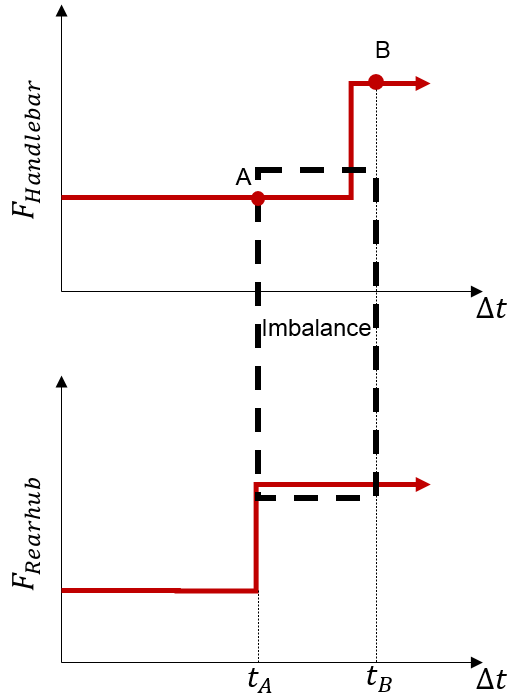
\includegraphics[scale = 0.45]{Contents/Resources/Precontrol/Motivation.png}
	\caption{Imbalance anticipation}
	\label{fig:precontrolMotivation}
\end{figure}

% --------------------------------------------------------------------------
% 		Section 5.2
% --------------------------------------------------------------------------

\section{Varying Pre-Control Gains}
The feedforward controller ($\mathbf{K}_d$) is considered to be decentralised like the feedback controller, and is considered to be constant. $$\mathbf{K}_d = \begin{bmatrix}
	k_1&0&0\\
	0&k_2&0\\
	0&0&k_3
\end{bmatrix}$$
Thus, the controller effort looks like:
\begin{align*}
	&u_x = K_x\Delta x + k_1d_x\\
	&u_y = K_y\Delta y + k_2d_y\\
	&u_z = K_z\Delta \gamma + k_3d_z
\end{align*}

The tabulated controller performance for $k_1 = k_2 = k_3 = 1$ and $k_1 = k_2 = k_3 = -1$ and PD Feedback Control are shown in tables \ref{tab:precontrolA1} to \ref{tab:precontrolC2}.

\begin{table}[h]
	\centering
	\begin{tabular}{ |c|c|c|c| } 
		\hline
		Forces & Mean Error (\%) & RMSE & $R_2$\\ 
		\hline
		FX & 3&128&0.98\\ 
		FY & 101&970&0.01 \\ 
		\hline
	\end{tabular}
	\caption{Load Errors at Point A of CF with PD Control and Pre-control with gains $\{-1,-1,-1\}$}
	\label{tab:precontrolA1}
\end{table}

\begin{table}[h]
	\centering
	\begin{tabular}{ |c|c|c|c| } 
		\hline
		Forces & Mean Error (\%) & RMSE & $R_2$\\ 
		\hline
		FX & 4&15&0.98\\ 
		FY & 4&2&0.98 \\ 
		\hline
	\end{tabular}
	\caption{Load Errors at Point B of CF with PD Control and Pre-control with gains $\{-1,-1,-1\}$}
	\label{tab:precontrolB1}
\end{table}

\begin{table}[h!]
	\centering
	\begin{tabular}{ |c|c|c|c| } 
		\hline
		Forces & Mean Error (\%) & RMSE & $R_2$\\ 
		\hline
		FX & 4&154&0.95\\ 
		FY & 59&972&0.05 \\ 
		\hline
	\end{tabular}
	\caption{Load Errors at Point C of CF with PD Control and Pre-control with gains $\{-1,-1,-1\}$}
	\label{tab:precontrolC1}
\end{table}

\begin{table}[h!]
	\centering
	\begin{tabular}{ |c|c|c|c| } 
		\hline
		Forces & Mean Error (\%) & RMSE & $R_2$\\ 
		\hline
		FX & 3&129&0.98\\ 
		FY & 103&914&0 \\ 
		\hline
	\end{tabular}
	\caption{Load Errors at Point A of CF with PD Control and Pre-control with gains $\{1,1,1\}$}
	\label{tab:precontrolA2}
\end{table}

\begin{table}[h!]
	\centering
	\begin{tabular}{ |c|c|c|c| } 
		\hline
		Forces & Mean Error (\%) & RMSE & $R_2$\\ 
		\hline
		FX & 4&16&0.98\\ 
		FY & 4&2&0.98 \\ 
		\hline
	\end{tabular}
	\caption{Load Errors at Point B of CF with PD Control and Pre-control with gains $\{1,1,1\}$}
	\label{tab:precontrolB2}
\end{table}

\begin{table}[h!]
	\centering
	\begin{tabular}{ |c|c|c|c| } 
		\hline
		Forces & Mean Error (\%) & RMSE & $R_2$\\ 
		\hline
		FX & 4&155&0.95\\ 
		FY & 59&912&0.03 \\ 
		\hline
	\end{tabular}
	\caption{Load Errors at Point C of CF with PD Control and Pre-control with gains $\{1,1,1\}$}
	\label{tab:precontrolC2}
\end{table}

It can be seen that irrespective of the feedforward gains, the results don't improve or degrade by a very significant margin. Infact, it was observed after multiple simulation runs of different feedforward gains combined with different feedback controllers that using pre-control doesn't have a very (positive or negative) significant effect on the performance that pure feedback control was showing. Thus, our hypothesis regarding the perceived benefit of pre-control is more or less proved wrong.

% --------------------------------------------------------------------------
% 		Section 5.3
% --------------------------------------------------------------------------

\section{Eliminating CF Angular Position Feedback}
\label{sec:noFeedback}
As mentioned in Chapter \ref{cha:chap3}, for almost all purely feedback controllers, the control torque ($u_z$) was always significantly less than the net imbalance torque experienced by the bike. This is also true when pre-control is used. The likely reason for this might be the compensation in position provided by the feedback of the rotation of the CF Bike. Thus, the feedback of the angular position of the CF Bike ($\gamma$) is eliminated along with PD Control of the X and Y positions of CF Bike along with pre-control still activated. In this case, we have to be cautious since about the Z axis, a feedforward torque is directly fed without feedback, and as observed in section \ref{sec:chap3sec2} of chapter \ref{cha:chap3}, directly feedforwarding forces or torques without feedback leads to instability of the CF Bike. Thus, the pre-control gain about the Z axis is kept very low. Tables \ref{tab:noZfdkA} to \ref{tab:noZfdkC} show the tabulated performance with no Z-feedback. 

\begin{table}[h!]
	\centering
	\begin{tabular}{ |c|c|c|c| } 
		\hline
		Forces & Mean Error (\%) & RMSE & $R_2$\\ 
		\hline
		FX & 15&324&0.95\\ 
		FY & 13&177&0.94 \\ 
		\hline
	\end{tabular}
	\caption{Load Errors at point A of CF with no Z Feedback and Pre-control with gains $\{0,0,-0.1\}$}
	\label{tab:noZfdkA}
\end{table}

\begin{table}[h!]
	\centering
	\begin{tabular}{ |c|c|c|c| } 
		\hline
		Forces & Mean Error (\%) & RMSE & $R_2$\\ 
		\hline
		FX & 142&359&0.31\\ 
		FY & 142&38&0.31 \\ 
		\hline
	\end{tabular}
	\caption{Load Errors at point B of CF with no Z Feedback and Pre-control with gains $\{0,0,-0.1\}$}
	\label{tab:noZfdkB}
\end{table}

\begin{table}[h!]
	\centering
	\begin{tabular}{ |c|c|c|c| } 
		\hline
		Forces & Mean Error (\%) & RMSE & $R_2$\\ 
		\hline
		FX & 12&192&0.96\\ 
		FY & 25&304&0.89 \\ 
		\hline
	\end{tabular}
	\caption{Load Errors at point C of CF with no Z Feedback and Pre-control with gains $\{0,0,-0.1\}$}
	\label{tab:noZfdkC}
\end{table}

It can be seen that the control performance drastically improves, especially for the Y component of the forces at points A and C but at the same time, it worsens significantly at point B for both X and Y components.

% --------------------------------------------------------------------------
% 		Section 5.3
% --------------------------------------------------------------------------

\section{Unactuated Angular Movement of CF}
Building on the idea introduced in section \ref{sec:noFeedback}, the angular degree of freedom of the CF bike is left unmodified, i.e. there is no Z feedback and no Z pre-control. Figures \ref{fig:noZA} to \ref{fig:noZC}, and tables \ref{tab:noZA} to \ref{tab:noZC} showcase extremely good controller performance as compared to all the controller parameters attempted.
\begin{figure}[h]
	\centering
	\scalebox{0.8}{
		\begin{tikzpicture}
			% This file was created by matlab2tikz.
%
%The latest updates can be retrieved from
%  http://www.mathworks.com/matlabcentral/fileexchange/22022-matlab2tikz-matlab2tikz
%where you can also make suggestions and rate matlab2tikz.
%
\begin{tikzpicture}

\begin{axis}[%
width=4.521in,
height=1.476in,
at={(0.758in,2.571in)},
scale only axis,
xmin=0,
xmax=10,
xlabel style={font=\color{white!15!black}},
xlabel={Time (s)},
ymin=-38.2830467224121,
ymax=6000,
ylabel style={font=\color{white!15!black}},
ylabel={FX (N)},
axis background/.style={fill=white},
xmajorgrids,
ymajorgrids,
legend style={at={(0.85,1)}, anchor=north east, legend cell align=left, align=left, draw=black}
]
\addplot [color=black, dashed, line width=2.0pt]
  table[row sep=crcr]{%
0.0949999988079071	15.8128757476807\\
0.100000001490116	13.5325384140015\\
0.104999996721745	11.553840637207\\
0.109999999403954	9.83138465881348\\
0.115000002086163	8.33064746856689\\
0.119999997317791	241.457473754883\\
0.125	545.687744140625\\
0.129999995231628	782.91650390625\\
0.135000005364418	971.380676269531\\
0.140000000596046	1111.84790039063\\
0.144999995827675	1206.85559082031\\
0.150000005960464	1259.75073242188\\
0.155000001192093	1273.865234375\\
0.159999996423721	1267.48400878906\\
0.165000006556511	1232.30285644531\\
0.170000001788139	1162.44714355469\\
0.174999997019768	1059.94775390625\\
0.180000007152557	929.114501953125\\
0.185000002384186	775.30615234375\\
0.189999997615814	605.3291015625\\
0.194999992847443	507.519195556641\\
0.200000002980232	487.125366210938\\
0.204999998211861	502.143249511719\\
0.209999993443489	656.599975585938\\
0.215000003576279	913.404174804688\\
0.219999998807907	1241.50134277344\\
0.224999994039536	1600.14453125\\
0.230000004172325	1950.97143554688\\
0.234999999403954	2263.14721679688\\
0.239999994635582	2513.54858398438\\
0.245000004768372	2687.57348632813\\
0.25	2780.49365234375\\
0.254999995231628	2801.94165039063\\
0.259999990463257	2800.33056640625\\
0.264999985694885	2747.60107421875\\
0.270000010728836	2646.53955078125\\
0.275000005960464	2522.55908203125\\
0.280000001192093	2403.4287109375\\
0.284999996423721	2311.9716796875\\
0.28999999165535	2261.88549804688\\
0.294999986886978	2274.046875\\
0.300000011920929	2331.79541015625\\
0.305000007152557	2402.70849609375\\
0.310000002384186	2470.48901367188\\
0.314999997615814	2521.54077148438\\
0.319999992847443	2545.62353515625\\
0.324999988079071	2536.87817382813\\
0.330000013113022	2510.89990234375\\
0.33500000834465	2457.54736328125\\
0.340000003576279	2372.53881835938\\
0.344999998807907	2262.09594726563\\
0.349999994039536	2136.60034179688\\
0.354999989271164	2007.76867675781\\
0.360000014305115	1886.05541992188\\
0.365000009536743	1779.15637207031\\
0.370000004768372	1691.68542480469\\
0.375	1623.36535644531\\
0.379999995231628	1571.14392089844\\
0.384999990463257	1529.43896484375\\
0.389999985694885	1492.29345703125\\
0.395000010728836	1452.31481933594\\
0.400000005960464	1404.74157714844\\
0.405000001192093	1345.31884765625\\
0.409999996423721	1273.0029296875\\
0.41499999165535	1188.55444335938\\
0.419999986886978	1095.02856445313\\
0.425000011920929	997.367248535156\\
0.430000007152557	900.260681152344\\
0.435000002384186	808.484313964844\\
0.439999997615814	726.714111328125\\
0.444999992847443	657.466491699219\\
0.449999988079071	601.405578613281\\
0.455000013113022	557.660766601563\\
0.46000000834465	523.948852539063\\
0.465000003576279	497.415161132813\\
0.469999998807907	474.441253662109\\
0.474999994039536	452.282165527344\\
0.479999989271164	428.593688964844\\
0.485000014305115	402.142364501953\\
0.490000009536743	372.830108642578\\
0.495000004768372	342.247314453125\\
0.5	311.842437744141\\
0.504999995231628	283.43017578125\\
0.509999990463257	259.353729248047\\
0.514999985694885	241.675308227539\\
0.519999980926514	231.731582641602\\
0.524999976158142	231.725280761719\\
0.529999971389771	243.398681640625\\
0.535000026226044	259.713195800781\\
0.540000021457672	279.501007080078\\
0.545000016689301	301.19580078125\\
0.550000011920929	323.785949707031\\
0.555000007152557	347.092620849609\\
0.560000002384186	370.847473144531\\
0.564999997615814	394.982513427734\\
0.569999992847443	419.795562744141\\
0.574999988079071	445.720886230469\\
0.579999983310699	473.269683837891\\
0.584999978542328	502.888336181641\\
0.589999973773956	534.819213867188\\
0.595000028610229	569.128356933594\\
0.600000023841858	605.685791015625\\
0.605000019073486	644.196350097656\\
0.610000014305115	684.252075195313\\
0.615000009536743	725.32470703125\\
0.620000004768372	766.879150390625\\
0.625	808.521301269531\\
0.629999995231628	849.854125976563\\
0.634999990463257	890.603149414063\\
0.639999985694885	930.506164550781\\
0.644999980926514	969.407104492188\\
0.649999976158142	1007.24786376953\\
0.654999971389771	1044.009765625\\
0.660000026226044	1079.69921875\\
0.665000021457672	1114.3212890625\\
0.670000016689301	1147.87023925781\\
0.675000011920929	1180.31591796875\\
0.680000007152557	1211.5830078125\\
0.685000002384186	1241.55407714844\\
0.689999997615814	1270.08154296875\\
0.694999992847443	1296.99230957031\\
0.699999988079071	1322.1181640625\\
0.704999983310699	1345.31298828125\\
0.709999978542328	1366.45935058594\\
0.714999973773956	1385.47399902344\\
0.720000028610229	1402.32116699219\\
0.725000023841858	1417.0087890625\\
0.730000019073486	1429.50866699219\\
0.735000014305115	1439.89465332031\\
0.740000009536743	1448.19323730469\\
0.745000004768372	1454.47351074219\\
0.75	1458.77514648438\\
0.754999995231628	1461.15893554688\\
0.759999990463257	1461.66162109375\\
0.764999985694885	1460.9453125\\
0.769999980926514	1458.82690429688\\
0.774999976158142	1454.93518066406\\
0.779999971389771	1449.13818359375\\
0.785000026226044	1441.51635742188\\
0.790000021457672	1432.18530273438\\
0.795000016689301	1421.24914550781\\
0.800000011920929	1408.8095703125\\
0.805000007152557	1394.96813964844\\
0.810000002384186	1379.85229492188\\
0.814999997615814	1363.57409667969\\
0.819999992847443	1346.26379394531\\
0.824999988079071	1328.04174804688\\
0.829999983310699	1309.04211425781\\
0.834999978542328	1289.38647460938\\
0.839999973773956	1269.1904296875\\
0.845000028610229	1248.5751953125\\
0.850000023841858	1227.65014648438\\
0.855000019073486	1206.51721191406\\
0.860000014305115	1185.24890136719\\
0.865000009536743	1163.93676757813\\
0.870000004768372	1142.68041992188\\
0.875	1121.56518554688\\
0.879999995231628	1100.68347167969\\
0.884999990463257	1080.12268066406\\
0.889999985694885	1059.97058105469\\
0.894999980926514	1040.31640625\\
0.899999976158142	1021.23425292969\\
0.904999971389771	1002.79235839844\\
0.910000026226044	985.079162597656\\
0.915000021457672	968.158874511719\\
0.920000016689301	952.072631835938\\
0.925000011920929	936.905944824219\\
0.930000007152557	922.71533203125\\
0.935000002384186	909.507080078125\\
0.939999997615814	897.360412597656\\
0.944999992847443	886.282592773438\\
0.949999988079071	876.221557617188\\
0.954999983310699	867.238037109375\\
0.959999978542328	859.328918457031\\
0.964999973773956	852.488342285156\\
0.970000028610229	846.735595703125\\
0.975000023841858	842.054748535156\\
0.980000019073486	838.443237304688\\
0.985000014305115	835.909423828125\\
0.990000009536743	834.473388671875\\
0.995000004768372	834.134887695313\\
1	834.940368652344\\
1.00499999523163	836.931640625\\
1.00999999046326	840.085693359375\\
1.01499998569489	843.941589355469\\
1.01999998092651	848.52978515625\\
1.02499997615814	853.818969726563\\
1.02999997138977	859.83203125\\
1.0349999666214	866.488647460938\\
1.03999996185303	873.778686523438\\
1.04499995708466	881.638671875\\
1.04999995231628	890.044189453125\\
1.05499994754791	898.933837890625\\
1.05999994277954	908.264404296875\\
1.06500005722046	918.013854980469\\
1.07000005245209	928.100463867188\\
1.07500004768372	938.489135742188\\
1.08000004291534	949.115966796875\\
1.08500003814697	959.931518554688\\
1.0900000333786	970.880981445313\\
1.09500002861023	981.910339355469\\
1.10000002384186	992.965515136719\\
1.10500001907349	1003.99652099609\\
1.11000001430511	1014.96075439453\\
1.11500000953674	1025.80102539063\\
1.12000000476837	1036.46569824219\\
1.125	1046.923828125\\
1.12999999523163	1057.12646484375\\
1.13499999046326	1067.0224609375\\
1.13999998569489	1076.57495117188\\
1.14499998092651	1085.78002929688\\
1.14999997615814	1094.57946777344\\
1.15499997138977	1102.93493652344\\
1.1599999666214	1110.84558105469\\
1.16499996185303	1118.28686523438\\
1.16999995708466	1125.21948242188\\
1.17499995231628	1131.62170410156\\
1.17999994754791	1137.5126953125\\
1.18499994277954	1142.85180664063\\
1.19000005722046	1147.61901855469\\
1.19500005245209	1151.82360839844\\
1.20000004768372	1155.47302246094\\
1.20500004291534	1158.55688476563\\
1.21000003814697	1161.07751464844\\
1.2150000333786	1163.02893066406\\
1.22000002861023	1164.42004394531\\
1.22500002384186	1165.25793457031\\
1.23000001907349	1165.58508300781\\
1.23500001430511	1165.45751953125\\
1.24000000953674	1164.89929199219\\
1.24500000476837	1163.95678710938\\
1.25	1162.47705078125\\
1.25499999523163	1160.52404785156\\
1.25999999046326	1158.08508300781\\
1.26499998569489	1155.18664550781\\
1.26999998092651	1151.88452148438\\
1.27499997615814	1148.15612792969\\
1.27999997138977	1144.03771972656\\
1.2849999666214	1139.64074707031\\
1.28999996185303	1134.95532226563\\
1.29499995708466	1130.01501464844\\
1.29999995231628	1124.86279296875\\
1.30499994754791	1119.52990722656\\
1.30999994277954	1114.05151367188\\
1.31500005722046	1108.42724609375\\
1.32000005245209	1102.69287109375\\
1.32500004768372	1096.87829589844\\
1.33000004291534	1090.99731445313\\
1.33500003814697	1085.07141113281\\
1.3400000333786	1079.12731933594\\
1.34500002861023	1073.19274902344\\
1.35000002384186	1067.29809570313\\
1.35500001907349	1061.46875\\
1.36000001430511	1055.74304199219\\
1.36500000953674	1050.18200683594\\
1.37000000476837	1044.82153320313\\
1.375	1039.6962890625\\
1.37999999523163	1034.73620605469\\
1.38499999046326	1030.00659179688\\
1.38999998569489	1025.52758789063\\
1.39499998092651	1021.24743652344\\
1.39999997615814	1017.19683837891\\
1.40499997138977	1013.38421630859\\
1.4099999666214	1009.83258056641\\
1.41499996185303	1006.54571533203\\
1.41999995708466	1003.53466796875\\
1.42499995231628	1000.81591796875\\
1.42999994754791	998.398681640625\\
1.43499994277954	996.287414550781\\
1.44000005722046	994.474914550781\\
1.44500005245209	992.973999023438\\
1.45000004768372	991.7802734375\\
1.45500004291534	990.884582519531\\
1.46000003814697	990.292724609375\\
1.4650000333786	990.022094726563\\
1.47000002861023	990.094055175781\\
1.47500002384186	990.520568847656\\
1.48000001907349	991.191162109375\\
1.48500001430511	992.031860351563\\
1.49000000953674	992.988342285156\\
1.49500000476837	994.291625976563\\
1.5	995.902587890625\\
1.50499999523163	997.788146972656\\
1.50999999046326	999.869323730469\\
1.51499998569489	1002.16186523438\\
1.51999998092651	1004.63464355469\\
1.52499997615814	1007.26324462891\\
1.52999997138977	1010.03356933594\\
1.5349999666214	1012.96185302734\\
1.53999996185303	1016.02587890625\\
1.54499995708466	1019.19030761719\\
1.54999995231628	1022.41442871094\\
1.55499994754791	1025.68359375\\
1.55999994277954	1028.97814941406\\
1.56500005722046	1032.27331542969\\
1.57000005245209	1024.22045898438\\
1.57500004768372	1027.57092285156\\
1.58000004291534	1031.93737792969\\
1.58500003814697	1036.58154296875\\
1.5900000333786	1041.11889648438\\
1.59500002861023	1045.33557128906\\
1.60000002384186	1049.12194824219\\
1.60500001907349	1052.42443847656\\
1.61000001430511	1055.22058105469\\
1.61500000953674	1057.62829589844\\
1.62000000476837	1059.74792480469\\
1.625	1061.68774414063\\
1.62999999523163	1063.53735351563\\
1.63499999046326	1065.35571289063\\
1.63999998569489	1067.18566894531\\
1.64499998092651	1069.03759765625\\
1.64999997615814	1070.90270996094\\
1.65499997138977	1072.73400878906\\
1.6599999666214	1074.50109863281\\
1.66499996185303	1076.14660644531\\
1.66999995708466	1077.59802246094\\
1.67499995231628	1078.86145019531\\
1.67999994754791	1079.92590332031\\
1.68499994277954	1080.77575683594\\
1.69000005722046	1081.28723144531\\
1.69500005245209	1081.64196777344\\
1.70000004768372	1081.84606933594\\
1.70500004291534	1081.88781738281\\
1.71000003814697	1081.84545898438\\
1.7150000333786	1081.70544433594\\
1.72000002861023	1081.48059082031\\
1.72500002384186	1081.13354492188\\
1.73000001907349	1080.68408203125\\
1.73500001430511	1080.14538574219\\
1.74000000953674	1079.51513671875\\
1.74500000476837	1078.80090332031\\
1.75	1078.02185058594\\
1.75499999523163	1077.16760253906\\
1.75999999046326	1076.24877929688\\
1.76499998569489	1075.26354980469\\
1.76999998092651	1074.21166992188\\
1.77499997615814	1073.0966796875\\
1.77999997138977	1071.91870117188\\
1.7849999666214	1070.68127441406\\
1.78999996185303	1069.38586425781\\
1.79499995708466	1068.04077148438\\
1.79999995231628	1066.66540527344\\
1.80499994754791	1065.26245117188\\
1.80999994277954	1063.84875488281\\
1.81500005722046	1062.43432617188\\
1.82000005245209	1061.029296875\\
1.82500004768372	1059.64306640625\\
1.83000004291534	1058.28674316406\\
1.83500003814697	1056.97631835938\\
1.8400000333786	1055.70642089844\\
1.84500002861023	1054.47631835938\\
1.85000002384186	1053.28942871094\\
1.85500001907349	1052.14404296875\\
1.86000001430511	1051.04272460938\\
1.86500000953674	1049.99194335938\\
1.87000000476837	1048.98791503906\\
1.875	1048.0458984375\\
1.87999999523163	1047.177734375\\
1.88499999046326	1046.37377929688\\
1.88999998569489	1045.63439941406\\
1.89499998092651	1044.96643066406\\
1.89999997615814	1044.36596679688\\
1.90499997138977	1043.8330078125\\
1.9099999666214	1043.37756347656\\
1.91499996185303	1042.99597167969\\
1.91999995708466	1042.6875\\
1.92499995231628	1042.46484375\\
1.92999994754791	1042.32702636719\\
1.93499994277954	1042.27099609375\\
1.94000005722046	1042.28637695313\\
1.94500005245209	1042.36987304688\\
1.95000004768372	1042.52600097656\\
1.95500004291534	1042.75634765625\\
1.96000003814697	1043.0625\\
1.9650000333786	1043.4443359375\\
1.97000002861023	1043.89868164063\\
1.97500002384186	1044.41467285156\\
1.98000001907349	1044.99462890625\\
1.98500001430511	1045.63452148438\\
1.99000000953674	1046.3212890625\\
1.99500000476837	1047.05419921875\\
2	1047.82836914063\\
2.00500011444092	1048.63427734375\\
2.00999999046326	1049.46765136719\\
2.01500010490417	1050.32287597656\\
2.01999998092651	1051.25378417969\\
2.02500009536743	1052.25354003906\\
2.02999997138977	1053.32531738281\\
2.03500008583069	1054.46899414063\\
2.03999996185303	1055.69311523438\\
2.04500007629395	1056.99829101563\\
2.04999995231628	1058.3837890625\\
2.0550000667572	1059.84411621094\\
2.05999994277954	1061.33984375\\
2.06500005722046	1062.8544921875\\
2.0699999332428	1064.29870605469\\
2.07500004768372	1065.63635253906\\
2.07999992370605	1066.76257324219\\
2.08500003814697	1067.6162109375\\
2.08999991416931	1068.08642578125\\
2.09500002861023	1068.09655761719\\
2.09999990463257	1067.56115722656\\
2.10500001907349	1066.408203125\\
2.10999989509583	1064.75561523438\\
2.11500000953674	1062.62475585938\\
2.11999988555908	1059.67736816406\\
2.125	1055.79809570313\\
2.13000011444092	1051.12768554688\\
2.13499999046326	1045.61206054688\\
2.14000010490417	1039.31518554688\\
2.14499998092651	1032.35852050781\\
2.15000009536743	1025.02624511719\\
2.15499997138977	1017.28656005859\\
2.16000008583069	1008.97802734375\\
2.16499996185303	1000.38073730469\\
2.17000007629395	991.520385742188\\
2.17499995231628	982.345825195313\\
2.1800000667572	972.874816894531\\
2.18499994277954	963.105346679688\\
2.19000005722046	953.071899414063\\
2.1949999332428	942.826110839844\\
2.20000004768372	932.4365234375\\
2.20499992370605	921.996276855469\\
2.21000003814697	911.629821777344\\
2.21499991416931	901.491333007813\\
2.22000002861023	891.765625\\
2.22499990463257	882.599243164063\\
2.23000001907349	874.098876953125\\
2.23499989509583	866.323364257813\\
2.24000000953674	859.391662597656\\
2.24499988555908	853.34033203125\\
2.25	848.174499511719\\
2.25500011444092	843.919921875\\
2.25999999046326	840.551147460938\\
2.26500010490417	838.035400390625\\
2.26999998092651	836.423950195313\\
2.27500009536743	835.7587890625\\
2.27999997138977	836.141662597656\\
2.28500008583069	837.817565917969\\
2.28999996185303	840.807189941406\\
2.29500007629395	844.925231933594\\
2.29999995231628	849.341552734375\\
2.3050000667572	854.932495117188\\
2.30999994277954	861.46142578125\\
2.31500005722046	868.740051269531\\
2.3199999332428	876.765014648438\\
2.32500004768372	885.648376464844\\
2.32999992370605	895.385498046875\\
2.33500003814697	905.967407226563\\
2.33999991416931	918.796020507813\\
2.34500002861023	933.480834960938\\
2.34999990463257	947.479797363281\\
2.35500001907349	962.243530273438\\
2.35999989509583	977.635131835938\\
2.36500000953674	993.548645019531\\
2.36999988555908	1010.240234375\\
2.375	1027.57458496094\\
2.38000011444092	1045.59020996094\\
2.38499999046326	1064.40368652344\\
2.39000010490417	1083.9033203125\\
2.39499998092651	1104.10546875\\
2.40000009536743	1125.00427246094\\
2.40499997138977	1146.50329589844\\
2.41000008583069	1168.51538085938\\
2.41499996185303	1190.90661621094\\
2.42000007629395	1213.49743652344\\
2.42499995231628	1236.11437988281\\
2.4300000667572	1258.50659179688\\
2.43499994277954	1280.45861816406\\
2.44000005722046	1301.72631835938\\
2.4449999332428	1321.97277832031\\
2.45000004768372	1341.09020996094\\
2.45499992370605	1358.8095703125\\
2.46000003814697	1374.98742675781\\
2.46499991416931	1389.51354980469\\
2.47000002861023	1402.29553222656\\
2.47499990463257	1413.28405761719\\
2.48000001907349	1422.46899414063\\
2.48499989509583	1429.84887695313\\
2.49000000953674	1435.49633789063\\
2.49499988555908	1439.48315429688\\
2.5	1441.86499023438\\
2.50500011444092	1442.65466308594\\
2.50999999046326	1442.17236328125\\
2.51500010490417	1440.70581054688\\
2.51999998092651	1437.53283691406\\
2.52500009536743	1432.43896484375\\
2.52999997138977	1425.61962890625\\
2.53500008583069	1416.40197753906\\
2.53999996185303	1405.57421875\\
2.54500007629395	1392.89782714844\\
2.54999995231628	1378.4482421875\\
2.5550000667572	1362.36193847656\\
2.55999994277954	1344.71655273438\\
2.56500005722046	1325.74462890625\\
2.5699999332428	1305.54516601563\\
2.57500004768372	1284.29333496094\\
2.57999992370605	1262.18493652344\\
2.58500003814697	1239.43994140625\\
2.58999991416931	1216.25927734375\\
2.59500002861023	1192.62048339844\\
2.59999990463257	1168.64184570313\\
2.60500001907349	1144.39038085938\\
2.60999989509583	1119.83020019531\\
2.61500000953674	1094.9814453125\\
2.61999988555908	1069.89038085938\\
2.625	1044.62609863281\\
2.63000011444092	1019.37463378906\\
2.63499999046326	994.228820800781\\
2.64000010490417	969.17138671875\\
2.64499998092651	944.469970703125\\
2.65000009536743	920.362182617188\\
2.65499997138977	896.796691894531\\
2.66000008583069	873.76220703125\\
2.66499996185303	851.363952636719\\
2.67000007629395	829.406555175781\\
2.67499995231628	807.8388671875\\
2.6800000667572	786.861938476563\\
2.68499994277954	766.275390625\\
2.69000005722046	746.192321777344\\
2.6949999332428	726.553588867188\\
2.70000004768372	707.403198242188\\
2.70499992370605	688.775573730469\\
2.71000003814697	670.74462890625\\
2.71499991416931	653.391723632813\\
2.72000002861023	636.914794921875\\
2.72499990463257	621.422607421875\\
2.73000001907349	607.013122558594\\
2.73499989509583	593.808959960938\\
2.74000000953674	581.963500976563\\
2.74499988555908	571.737121582031\\
2.75	563.006958007813\\
2.75500011444092	555.803100585938\\
2.75999999046326	550.397277832031\\
2.76500010490417	547.299438476563\\
2.76999998092651	546.638793945313\\
2.77500009536743	548.49267578125\\
2.77999997138977	552.589477539063\\
2.78500008583069	559.092590332031\\
2.78999996185303	568.1513671875\\
2.79500007629395	579.890869140625\\
2.79999995231628	594.4130859375\\
2.8050000667572	611.800964355469\\
2.80999994277954	632.122863769531\\
2.81500005722046	655.379821777344\\
2.8199999332428	681.509094238281\\
2.82500004768372	710.400939941406\\
2.82999992370605	741.913269042969\\
2.83500003814697	775.884643554688\\
2.83999991416931	812.127014160156\\
2.84500002861023	850.476989746094\\
2.84999990463257	890.821105957031\\
2.85500001907349	933.011291503906\\
2.85999989509583	976.817749023438\\
2.86500000953674	1022.24786376953\\
2.86999988555908	1069.30798339844\\
2.875	1117.76818847656\\
2.88000011444092	1167.97546386719\\
2.88499999046326	1219.81384277344\\
2.89000010490417	1273.3388671875\\
2.89499998092651	1327.16870117188\\
2.90000009536743	1379.53405761719\\
2.90499997138977	1429.63317871094\\
2.91000008583069	1476.26489257813\\
2.91499996185303	1518.24853515625\\
2.92000007629395	1555.35327148438\\
2.92499995231628	1587.53747558594\\
2.9300000667572	1615.04187011719\\
2.93499994277954	1638.34106445313\\
2.94000005722046	1657.8486328125\\
2.9449999332428	1673.97009277344\\
2.95000004768372	1686.72192382813\\
2.95499992370605	1696.52880859375\\
2.96000003814697	1703.75048828125\\
2.96499991416931	1707.19116210938\\
2.97000002861023	1707.06237792969\\
2.97499990463257	1702.20751953125\\
2.98000001907349	1691.58837890625\\
2.98499989509583	1679.50317382813\\
2.99000000953674	1661.75561523438\\
2.99499988555908	1638.37646484375\\
3	1609.76391601563\\
3.00500011444092	1576.27905273438\\
3.00999999046326	1538.40734863281\\
3.01500010490417	1496.73901367188\\
3.01999998092651	1451.96765136719\\
3.02500009536743	1404.81665039063\\
3.02999997138977	1355.92309570313\\
3.03500008583069	1305.85681152344\\
3.03999996185303	1254.93908691406\\
3.04500007629395	1203.33923339844\\
3.04999995231628	1151.05993652344\\
3.0550000667572	1097.99169921875\\
3.05999994277954	1044.07153320313\\
3.06500005722046	989.247131347656\\
3.0699999332428	933.641784667969\\
3.07500004768372	877.682312011719\\
3.07999992370605	821.753601074219\\
3.08500003814697	766.457336425781\\
3.08999991416931	712.467163085938\\
3.09500002861023	660.497924804688\\
3.09999990463257	611.024841308594\\
3.10500001907349	564.431091308594\\
3.10999989509583	521.263854980469\\
3.11500000953674	482.264465332031\\
3.11999988555908	447.480407714844\\
3.125	417.194610595703\\
3.13000011444092	392.199554443359\\
3.13499999046326	373.150939941406\\
3.14000010490417	360.297821044922\\
3.14499998092651	354.065185546875\\
3.15000009536743	356.539733886719\\
3.15499997138977	368.509887695313\\
3.16000008583069	387.435119628906\\
3.16499996185303	412.961547851563\\
3.17000007629395	444.52001953125\\
3.17499995231628	481.472717285156\\
3.1800000667572	523.169677734375\\
3.18499994277954	568.849792480469\\
3.19000005722046	617.700927734375\\
3.1949999332428	668.632202148438\\
3.20000004768372	720.811645507813\\
3.20499992370605	773.594421386719\\
3.21000003814697	826.24169921875\\
3.21499991416931	878.692687988281\\
3.22000002861023	930.677368164063\\
3.22499990463257	982.299377441406\\
3.23000001907349	1033.49853515625\\
3.23499989509583	1084.05395507813\\
3.24000000953674	1133.82861328125\\
3.24499988555908	1181.68200683594\\
3.25	1228.037109375\\
3.25500011444092	1272.28979492188\\
3.25999999046326	1314.61926269531\\
3.26500010490417	1355.03002929688\\
3.26999998092651	1393.693359375\\
3.27500009536743	1430.59558105469\\
3.27999997138977	1465.75720214844\\
3.28500008583069	1498.89318847656\\
3.28999996185303	1529.49536132813\\
3.29500007629395	1556.96911621094\\
3.29999995231628	1580.71984863281\\
3.3050000667572	1600.17822265625\\
3.30999994277954	1614.84521484375\\
3.31500005722046	1624.52160644531\\
3.3199999332428	1631.31481933594\\
3.32500004768372	1633.71252441406\\
3.32999992370605	1630.31408691406\\
3.33500003814697	1621.31396484375\\
3.33999991416931	1607.298828125\\
3.34500002861023	1588.84069824219\\
3.34999990463257	1566.39086914063\\
3.35500001907349	1540.31909179688\\
3.35999989509583	1510.81652832031\\
3.36500000953674	1477.93115234375\\
3.36999988555908	1441.53430175781\\
3.375	1401.60498046875\\
3.38000011444092	1358.05151367188\\
3.38499999046326	1310.83959960938\\
3.39000010490417	1260.07202148438\\
3.39499998092651	1205.9814453125\\
3.40000009536743	1148.88049316406\\
3.40499997138977	1089.46850585938\\
3.41000008583069	1028.2900390625\\
3.41499996185303	966.00146484375\\
3.42000007629395	903.354553222656\\
3.42499995231628	840.926452636719\\
3.4300000667572	779.432922363281\\
3.43499994277954	719.366821289063\\
3.44000005722046	661.266235351563\\
3.4449999332428	605.891723632813\\
3.45000004768372	554.060119628906\\
3.45499992370605	506.659729003906\\
3.46000003814697	464.779449462891\\
3.46499991416931	429.277069091797\\
3.47000002861023	400.453430175781\\
3.47499990463257	378.839965820313\\
3.48000001907349	364.918518066406\\
3.48499989509583	359.536865234375\\
3.49000000953674	366.757781982422\\
3.49499988555908	381.72509765625\\
3.5	404.279541015625\\
3.50500011444092	434.211456298828\\
3.50999999046326	471.186981201172\\
3.51500010490417	515.648376464844\\
3.51999998092651	567.861877441406\\
3.52500009536743	628.648193359375\\
3.52999997138977	698.199035644531\\
3.53500008583069	777.4716796875\\
3.53999996185303	868.736938476563\\
3.54500007629395	969.425659179688\\
3.54999995231628	1073.322265625\\
3.5550000667572	1169.3525390625\\
3.55999994277954	1250.8896484375\\
3.56500005722046	1313.35729980469\\
3.5699999332428	1361.15832519531\\
3.57500004768372	1395.04736328125\\
3.57999992370605	1424.3037109375\\
3.58500003814697	1447.35400390625\\
3.58999991416931	1466.39208984375\\
3.59500002861023	1488.39636230469\\
3.59999990463257	1519.67443847656\\
3.60500001907349	1554.89001464844\\
3.60999989509583	1591.57592773438\\
3.61500000953674	1626.67407226563\\
3.61999988555908	1655.84606933594\\
3.625	1675.62573242188\\
3.63000011444092	1683.57690429688\\
3.63499999046326	1681.94128417969\\
3.64000010490417	1672.30505371094\\
3.64499998092651	1649.05297851563\\
3.65000009536743	1614.07067871094\\
3.65499997138977	1569.53381347656\\
3.66000008583069	1518.83142089844\\
3.66499996185303	1465.50402832031\\
3.67000007629395	1412.50537109375\\
3.67499995231628	1360.91796875\\
3.6800000667572	1310.80407714844\\
3.68499994277954	1261.18994140625\\
3.69000005722046	1210.47692871094\\
3.6949999332428	1156.77856445313\\
3.70000004768372	1098.42358398438\\
3.70499992370605	1034.94494628906\\
3.71000003814697	965.716796875\\
3.71499991416931	892.542724609375\\
3.72000002861023	816.571716308594\\
3.72499990463257	740.018493652344\\
3.73000001907349	665.057250976563\\
3.73499989509583	594.183959960938\\
3.74000000953674	528.536560058594\\
3.74499988555908	469.7353515625\\
3.75	420.641510009766\\
3.75500011444092	380.961059570313\\
3.75999999046326	352.182159423828\\
3.76500010490417	334.154571533203\\
3.76999998092651	327.182250976563\\
3.77500009536743	335.664733886719\\
3.77999997138977	356.84228515625\\
3.78500008583069	388.046813964844\\
3.78999996185303	427.925140380859\\
3.79500007629395	476.881988525391\\
3.79999995231628	533.878479003906\\
3.8050000667572	598.156127929688\\
3.80999994277954	669.067687988281\\
3.81500005722046	746.486022949219\\
3.8199999332428	830.262084960938\\
3.82500004768372	920.722229003906\\
3.82999992370605	1018.31744384766\\
3.83500003814697	1119.12512207031\\
3.83999991416931	1213.54235839844\\
3.84500002861023	1294.826171875\\
3.84999990463257	1356.16809082031\\
3.85500001907349	1397.00866699219\\
3.85999989509583	1427.89526367188\\
3.86500000953674	1449.94909667969\\
3.86999988555908	1462.10778808594\\
3.875	1471.87329101563\\
3.88000011444092	1486.37817382813\\
3.88499999046326	1518.29467773438\\
3.89000010490417	1562.89318847656\\
3.89499998092651	1612.41296386719\\
3.90000009536743	1662.40368652344\\
3.90499997138977	1705.87744140625\\
3.91000008583069	1737.63977050781\\
3.91499996185303	1754.07775878906\\
3.92000007629395	1756.89221191406\\
3.92499995231628	1750.53759765625\\
3.9300000667572	1727.50378417969\\
3.93499994277954	1689.56701660156\\
3.94000005722046	1640.10681152344\\
3.9449999332428	1583.603515625\\
3.95000004768372	1523.95446777344\\
3.95499992370605	1465.00537109375\\
3.96000003814697	1407.94006347656\\
3.96499991416931	1352.54296875\\
3.97000002861023	1297.19702148438\\
3.97499990463257	1239.84020996094\\
3.98000001907349	1177.61657714844\\
3.98499989509583	1108.61572265625\\
3.99000000953674	1032.00817871094\\
3.99499988555908	948.249938964844\\
4	858.366271972656\\
4.00500011444092	763.957275390625\\
4.01000022888184	668.714172363281\\
4.0149998664856	576.072631835938\\
4.01999998092651	487.542572021484\\
4.02500009536743	405.929870605469\\
4.03000020980835	333.629577636719\\
4.03499984741211	272.285888671875\\
4.03999996185303	222.915954589844\\
4.04500007629395	185.552841186523\\
4.05000019073486	160.414047241211\\
4.05499982833862	146.890625\\
4.05999994277954	145.334106445313\\
4.06500005722046	160.456848144531\\
4.07000017166138	186.130783081055\\
4.07499980926514	222.76887512207\\
4.07999992370605	270.867462158203\\
4.08500003814697	332.312347412109\\
4.09000015258789	410.413757324219\\
4.09499979019165	510.737579345703\\
4.09999990463257	643.526123046875\\
4.10500001907349	828.257202148438\\
4.1100001335144	1057.02758789063\\
4.11499977111816	1276.857421875\\
4.11999988555908	1446.53869628906\\
4.125	1546.84790039063\\
4.13000011444092	1599.06591796875\\
4.13500022888184	1627.34448242188\\
4.1399998664856	1607.11584472656\\
4.14499998092651	1556.96801757813\\
4.15000009536743	1502.912109375\\
4.15500020980835	1468.55908203125\\
4.15999984741211	1474.11767578125\\
4.16499996185303	1541.71569824219\\
4.17000007629395	1633.029296875\\
4.17500019073486	1729.47802734375\\
4.17999982833862	1813.98193359375\\
4.18499994277954	1873.23034667969\\
4.19000005722046	1898.62292480469\\
4.19500017166138	1889.62976074219\\
4.19999980926514	1867.34716796875\\
4.20499992370605	1814.8232421875\\
4.21000003814697	1735.19213867188\\
4.21500015258789	1638.10168457031\\
4.21999979019165	1535.83544921875\\
4.22499990463257	1438.58178710938\\
4.23000001907349	1353.58581542969\\
4.2350001335144	1283.33605957031\\
4.23999977111816	1223.828125\\
4.24499988555908	1169.34313964844\\
4.25	1113.6318359375\\
4.25500011444092	1050.01892089844\\
4.26000022888184	974.773864746094\\
4.2649998664856	885.689025878906\\
4.26999998092651	784.263244628906\\
4.27500009536743	674.471496582031\\
4.28000020980835	562.258911132813\\
4.28499984741211	451.798217773438\\
4.28999996185303	349.127746582031\\
4.29500007629395	258.766754150391\\
4.30000019073486	185.162185668945\\
4.30499982833862	131.81315612793\\
4.30999994277954	98.5380020141602\\
4.31500005722046	84.663215637207\\
4.32000017166138	90.2949600219727\\
4.32499980926514	113.04150390625\\
4.32999992370605	166.440246582031\\
4.33500003814697	228.797882080078\\
4.34000015258789	298.478546142578\\
4.34499979019165	379.844268798828\\
4.34999990463257	475.007293701172\\
4.35500001907349	589.048278808594\\
4.3600001335144	729.229309082031\\
4.36499977111816	914.205810546875\\
4.36999988555908	1148.75073242188\\
4.375	1394.05480957031\\
4.38000011444092	1592.3505859375\\
4.38500022888184	1708.08239746094\\
4.3899998664856	1737.1689453125\\
4.39499998092651	1752.93664550781\\
4.40000009536743	1710.23608398438\\
4.40500020980835	1618.92785644531\\
4.40999984741211	1514.85400390625\\
4.41499996185303	1435.3212890625\\
4.42000007629395	1406.95166015625\\
4.42500019073486	1476.23132324219\\
4.42999982833862	1596.15832519531\\
4.43499994277954	1732.02709960938\\
4.44000005722046	1857.05151367188\\
4.44500017166138	1950.03564453125\\
4.44999980926514	1997.36010742188\\
4.45499992370605	1993.73657226563\\
4.46000003814697	1971.97216796875\\
4.46500015258789	1911.31774902344\\
4.46999979019165	1813.11791992188\\
4.47499990463257	1691.59643554688\\
4.48000001907349	1563.33544921875\\
4.4850001335144	1443.62670898438\\
4.48999977111816	1342.31652832031\\
4.49499988555908	1263.73205566406\\
4.5	1201.59948730469\\
4.50500011444092	1147.51208496094\\
4.51000022888184	1091.8642578125\\
4.5149998664856	1025.78479003906\\
4.51999998092651	943.663024902344\\
4.52500009536743	842.367004394531\\
4.53000020980835	724.800720214844\\
4.53499984741211	595.467529296875\\
4.53999996185303	463.204223632813\\
4.54500007629395	332.930389404297\\
4.55000019073486	211.756439208984\\
4.55499982833862	105.878433227539\\
4.55999994277954	60.9680862426758\\
4.56500005722046	62.1962509155273\\
4.57000017166138	69.8994903564453\\
4.57499980926514	80.4328460693359\\
4.57999992370605	91.4052581787109\\
4.58500003814697	100.681655883789\\
4.59000015258789	107.438613891602\\
4.59499979019165	112.047401428223\\
4.59999990463257	114.459426879883\\
4.60500001907349	112.05241394043\\
4.6100001335144	102.69221496582\\
4.61499977111816	83.4552764892578\\
4.61999988555908	317.652496337891\\
4.625	824.225402832031\\
4.63000011444092	1376.61254882813\\
4.63500022888184	1815.64025878906\\
4.6399998664856	2099.58569335938\\
4.64499998092651	2214.66455078125\\
4.65000009536743	2224.83569335938\\
4.65500020980835	2122.86962890625\\
4.65999984741211	1888.46862792969\\
4.66499996185303	1663.33251953125\\
4.67000007629395	1407.01892089844\\
4.67500019073486	1202.58349609375\\
4.67999982833862	1101.57312011719\\
4.68499994277954	1182.36315917969\\
4.69000005722046	1382.33374023438\\
4.69500017166138	1615.03198242188\\
4.69999980926514	1828.82763671875\\
4.70499992370605	1984.72351074219\\
4.71000003814697	2057.79809570313\\
4.71500015258789	2040.62231445313\\
4.71999979019165	1989.49340820313\\
4.72499990463257	1884.43103027344\\
4.73000001907349	1719.84289550781\\
4.7350001335144	1523.029296875\\
4.73999977111816	1325.07800292969\\
4.74499988555908	1152.40209960938\\
4.75	1019.55267333984\\
4.75500011444092	934.620483398438\\
4.76000022888184	884.010559082031\\
4.7649998664856	855.194763183594\\
4.76999998092651	815.257690429688\\
4.77500009536743	763.955017089844\\
4.78000020980835	685.310546875\\
4.78499984741211	584.172058105469\\
4.78999996185303	464.312255859375\\
4.79500007629395	322.627227783203\\
4.80000019073486	186.124694824219\\
4.80499982833862	57.6118812561035\\
4.80999994277954	54.7035064697266\\
4.81500005722046	76.4421463012695\\
4.82000017166138	101.376220703125\\
4.82499980926514	125.766090393066\\
4.82999992370605	147.659286499023\\
4.83500003814697	163.911499023438\\
4.84000015258789	174.496673583984\\
4.84499979019165	175.949462890625\\
4.84999990463257	163.450912475586\\
4.85500001907349	132.50520324707\\
4.8600001335144	80.9447555541992\\
4.86499977111816	15.9731845855713\\
4.86999988555908	452.451446533203\\
4.875	1012.03656005859\\
4.88000011444092	1558.61865234375\\
4.88500022888184	1974.61828613281\\
4.8899998664856	2223.53344726563\\
4.89499998092651	2299.6494140625\\
4.90000009536743	2292.50952148438\\
4.90500020980835	2142.85620117188\\
4.90999984741211	1859.16162109375\\
4.91499996185303	1477.40625\\
4.92000007629395	1125.15319824219\\
4.92500019073486	833.9677734375\\
4.92999982833862	647.272521972656\\
4.93499994277954	646.439331054688\\
4.94000005722046	884.747009277344\\
4.94500017166138	1214.54809570313\\
4.94999980926514	1562.35864257813\\
4.95499992370605	1869.26086425781\\
4.96000003814697	2094.20727539063\\
4.96500015258789	2214.20727539063\\
4.96999979019165	2225.66577148438\\
4.97499990463257	2190.15991210938\\
4.98000001907349	2097.2392578125\\
4.9850001335144	1936.45043945313\\
4.98999977111816	1741.53039550781\\
4.99499988555908	1546.3837890625\\
5	1379.77001953125\\
5.00500011444092	1257.70056152344\\
5.01000022888184	1185.26843261719\\
5.0149998664856	1158.78894042969\\
5.01999998092651	1169.669921875\\
5.02500009536743	1173.19836425781\\
5.03000020980835	1157.72448730469\\
5.03499984741211	1116.20092773438\\
5.03999996185303	1061.37841796875\\
5.04500007629395	982.32080078125\\
5.05000019073486	878.241271972656\\
5.05499982833862	754.822082519531\\
5.05999994277954	617.544616699219\\
5.06500005722046	473.185638427734\\
5.07000017166138	326.963775634766\\
5.07499980926514	184.053482055664\\
5.07999992370605	48.9029159545898\\
5.08500003814697	15.6395597457886\\
5.09000015258789	4.54384517669678\\
5.09499979019165	-4.47182607650757\\
5.09999990463257	-13.8551483154297\\
5.10500001907349	-18.9757709503174\\
5.1100001335144	-19.4506359100342\\
5.11499977111816	-18.3916110992432\\
5.11999988555908	-16.7593097686768\\
5.125	-15.0208930969238\\
5.13000011444092	-13.3896179199219\\
5.13500022888184	411.320648193359\\
5.1399998664856	769.033935546875\\
5.14499998092651	998.2060546875\\
5.15000009536743	1108.86877441406\\
5.15500020980835	1120.845703125\\
5.15999984741211	1146.70788574219\\
5.16499996185303	1123.23596191406\\
5.17000007629395	1074.43786621094\\
5.17500019073486	1034.40405273438\\
5.17999982833862	1032.32800292969\\
5.18499994277954	1108.23742675781\\
5.19000005722046	1214.40368652344\\
5.19500017166138	1335.75622558594\\
5.19999980926514	1453.54626464844\\
5.20499992370605	1554.11987304688\\
5.21000003814697	1628.86413574219\\
5.21500015258789	1673.60876464844\\
5.21999979019165	1688.95056152344\\
5.22499990463257	1679.4560546875\\
5.23000001907349	1662.00842285156\\
5.2350001335144	1631.939453125\\
5.23999977111816	1588.14611816406\\
5.24499988555908	1539.17138671875\\
5.25	1491.19421386719\\
5.25500011444092	1448.35095214844\\
5.26000022888184	1415.07946777344\\
5.2649998664856	1392.26489257813\\
5.26999998092651	1383.75512695313\\
5.27500009536743	1380.16491699219\\
5.28000020980835	1376.40966796875\\
5.28499984741211	1369.32043457031\\
5.28999996185303	1357.02160644531\\
5.29500007629395	1338.12780761719\\
5.30000019073486	1315.97717285156\\
5.30499982833862	1288.91906738281\\
5.30999994277954	1253.04736328125\\
5.31500005722046	1208.27868652344\\
5.32000017166138	1157.5908203125\\
5.32499980926514	1101.43896484375\\
5.32999992370605	1043.58703613281\\
5.33500003814697	986.912353515625\\
5.34000015258789	933.768920898438\\
5.34499979019165	886.848693847656\\
5.34999990463257	846.240173339844\\
5.35500001907349	810.841918945313\\
5.3600001335144	778.560729980469\\
5.36499977111816	746.47314453125\\
5.36999988555908	711.255920410156\\
5.375	670.278381347656\\
5.38000011444092	621.594909667969\\
5.38500022888184	564.853942871094\\
5.3899998664856	501.482330322266\\
5.39499998092651	434.717163085938\\
5.40000009536743	366.306793212891\\
5.40500020980835	299.507263183594\\
5.40999984741211	238.281112670898\\
5.41499996185303	183.712417602539\\
5.42000007629395	135.60221862793\\
5.42500019073486	92.6330413818359\\
5.42999982833862	54.3288688659668\\
5.43499994277954	26.3126373291016\\
5.44000005722046	0.576142907142639\\
5.44500017166138	-10.6391553878784\\
5.44999980926514	-11.9291973114014\\
5.45499992370605	-11.7547941207886\\
5.46000003814697	-10.9870452880859\\
5.46500015258789	-10.0311164855957\\
5.46999979019165	-9.10385131835938\\
5.47499990463257	-8.25202465057373\\
5.48000001907349	-7.46887922286987\\
5.4850001335144	-6.76615810394287\\
5.48999977111816	-6.14298391342163\\
5.49499988555908	-5.60813760757446\\
5.5	-5.1096978187561\\
5.50500011444092	-4.6788444519043\\
5.51000022888184	-4.31125783920288\\
5.5149998664856	-3.97868132591248\\
5.51999998092651	28.155200958252\\
5.52500009536743	99.8635711669922\\
5.53000020980835	141.901412963867\\
5.53499984741211	174.98811340332\\
5.53999996185303	198.993591308594\\
5.54500007629395	214.349563598633\\
5.55000019073486	221.774719238281\\
5.55499982833862	222.609603881836\\
5.55999994277954	219.656448364258\\
5.56500005722046	212.726272583008\\
5.57000017166138	200.816040039063\\
5.57499980926514	184.919540405273\\
5.57999992370605	165.839904785156\\
5.58500003814697	144.231964111328\\
5.59000015258789	121.083763122559\\
5.59499979019165	97.7242279052734\\
5.59999990463257	75.1830215454102\\
5.60500001907349	54.5372848510742\\
5.6100001335144	36.6168022155762\\
5.61499977111816	21.7925643920898\\
5.61999988555908	10.2144956588745\\
5.625	1.74973106384277\\
5.63000011444092	-3.99846220016479\\
5.63500022888184	-7.68318319320679\\
5.6399998664856	-9.02161026000977\\
5.64499998092651	-9.09969902038574\\
5.65000009536743	-9.07180500030518\\
5.65500020980835	-8.96457099914551\\
5.65999984741211	-8.77997493743896\\
5.66499996185303	-8.58776187896729\\
5.67000007629395	-7.21260404586792\\
5.67500019073486	54.9024772644043\\
5.67999982833862	81.2165069580078\\
5.68499994277954	99.0744400024414\\
5.69000005722046	218.492065429688\\
5.69500017166138	299.077087402344\\
5.69999980926514	361.345855712891\\
5.70499992370605	399.495056152344\\
5.71000003814697	411.451873779297\\
5.71500015258789	405.884033203125\\
5.71999979019165	392.567932128906\\
5.72499990463257	360.577087402344\\
5.73000001907349	317.033050537109\\
5.7350001335144	270.055053710938\\
5.73999977111816	226.688827514648\\
5.74499988555908	192.442459106445\\
5.75	169.629196166992\\
5.75500011444092	157.868591308594\\
5.76000022888184	156.868759155273\\
5.7649998664856	161.205688476563\\
5.76999998092651	166.629058837891\\
5.77500009536743	172.400802612305\\
5.78000020980835	178.548721313477\\
5.78499984741211	185.247650146484\\
5.78999996185303	193.118911743164\\
5.79500007629395	202.226974487305\\
5.80000019073486	212.943588256836\\
5.80499982833862	225.212249755859\\
5.80999994277954	238.833786010742\\
5.81500005722046	253.44189453125\\
5.82000017166138	268.727508544922\\
5.82499980926514	284.561157226563\\
5.82999992370605	300.413146972656\\
5.83500003814697	315.723999023438\\
5.84000015258789	329.899108886719\\
5.84499979019165	341.699340820313\\
5.84999990463257	349.23681640625\\
5.85500001907349	351.0107421875\\
5.8600001335144	346.601501464844\\
5.86499977111816	332.733459472656\\
5.86999988555908	303.34326171875\\
5.875	255.465805053711\\
5.88000011444092	187.495803833008\\
5.88500022888184	103.395927429199\\
5.8899998664856	16.5651798248291\\
5.89499998092651	5.07563877105713\\
5.90000009536743	84.6855239868164\\
5.90500020980835	296.027770996094\\
5.90999984741211	695.457763671875\\
5.91499996185303	1243.24182128906\\
5.92000007629395	1864.1376953125\\
5.92500019073486	2494.55053710938\\
5.92999982833862	3086.91821289063\\
5.93499994277954	3614.81884765625\\
5.94000005722046	4055.095703125\\
5.94500017166138	4397.142578125\\
5.94999980926514	4633.1416015625\\
5.95499992370605	4751.38232421875\\
5.96000003814697	4804.201171875\\
5.96500015258789	4734.146484375\\
5.96999979019165	4502.06494140625\\
5.97499990463257	4093.48974609375\\
5.98000001907349	3512.97119140625\\
5.9850001335144	2872.1767578125\\
5.98999977111816	2280.67163085938\\
5.99499988555908	1871.65625\\
6	1746.19177246094\\
6.00500011444092	2103.05444335938\\
6.01000022888184	2667.900390625\\
6.0149998664856	3326.62939453125\\
6.01999998092651	3983.12548828125\\
6.02500009536743	4553.76318359375\\
6.03000020980835	4976.216796875\\
6.03499984741211	5210.09033203125\\
6.03999996185303	5239.5439453125\\
6.04500007629395	5167.07958984375\\
6.05000019073486	4932.46923828125\\
6.05499982833862	4537.25146484375\\
6.05999994277954	4049.65112304688\\
6.06500005722046	3550.24267578125\\
6.07000017166138	3110.07788085938\\
6.07499980926514	2777.861328125\\
6.07999992370605	2570.330078125\\
6.08500003814697	2480.70678710938\\
6.09000015258789	2523.87329101563\\
6.09499979019165	2615.32421875\\
6.09999990463257	2696.06225585938\\
6.10500001907349	2734.67944335938\\
6.1100001335144	2712.52124023438\\
6.11499977111816	2654.97875976563\\
6.11999988555908	2531.51391601563\\
6.125	2335.40087890625\\
6.13000011444092	2079.94702148438\\
6.13500022888184	1788.90576171875\\
6.1399998664856	1488.27160644531\\
6.14499998092651	1203.06225585938\\
6.15000009536743	953.265563964844\\
6.15500020980835	751.135070800781\\
6.15999984741211	600.183776855469\\
6.16499996185303	496.875427246094\\
6.17000007629395	430.214202880859\\
6.17500019073486	387.124176025391\\
6.17999982833862	353.243103027344\\
6.18499994277954	315.989624023438\\
6.19000005722046	275.782928466797\\
6.19500017166138	226.590698242188\\
6.19999980926514	163.621505737305\\
6.20499992370605	90.3087310791016\\
6.21000003814697	12.9181499481201\\
6.21500015258789	-20.0268058776855\\
6.21999979019165	-23.3345260620117\\
6.22499990463257	-23.20285987854\\
6.23000001907349	-21.6861152648926\\
6.2350001335144	-19.6431465148926\\
6.23999977111816	-17.5441150665283\\
6.24499988555908	-15.5846452713013\\
6.25	-13.8008737564087\\
6.25500011444092	-12.1974973678589\\
6.26000022888184	-10.764518737793\\
6.2649998664856	-9.4924488067627\\
6.26999998092651	-8.36860752105713\\
6.27500009536743	-7.37819385528564\\
6.28000020980835	-6.50318813323975\\
6.28499984741211	-5.73168516159058\\
6.28999996185303	-5.05098342895508\\
6.29500007629395	-4.45027446746826\\
6.30000019073486	-3.91920709609985\\
6.30499982833862	-3.45007610321045\\
6.30999994277954	-3.03709268569946\\
6.31500005722046	-2.67484521865845\\
6.32000017166138	-2.35531735420227\\
6.32499980926514	-2.07514023780823\\
6.32999992370605	-1.82884681224823\\
6.33500003814697	-1.60954833030701\\
6.34000015258789	-1.4134202003479\\
6.34499979019165	-1.24309599399567\\
6.34999990463257	-1.09758853912354\\
6.35500001907349	-0.974028885364532\\
6.3600001335144	35.062126159668\\
6.36499977111816	65.4983978271484\\
6.36999988555908	88.6946105957031\\
6.375	103.274063110352\\
6.38000011444092	109.190017700195\\
6.38500022888184	138.562393188477\\
6.3899998664856	533.832763671875\\
6.39499998092651	768.248291015625\\
6.40000009536743	971.201477050781\\
6.40500020980835	1141.13610839844\\
6.40999984741211	1282.34741210938\\
6.41499996185303	1396.47680664063\\
6.42000007629395	1488.15588378906\\
6.42500019073486	1563.31567382813\\
6.42999982833862	1628.33374023438\\
6.43499994277954	1689.54309082031\\
6.44000005722046	1751.88244628906\\
6.44500017166138	1819.15173339844\\
6.44999980926514	1893.33435058594\\
6.45499992370605	1974.75622558594\\
6.46000003814697	2062.07983398438\\
6.46500015258789	2152.87280273438\\
6.46999979019165	2244.10034179688\\
6.47499990463257	2332.49755859375\\
6.48000001907349	2415.125\\
6.4850001335144	2489.66918945313\\
6.48999977111816	2554.52709960938\\
6.49499988555908	2608.97265625\\
6.5	2653.0625\\
6.50500011444092	2687.45190429688\\
6.51000022888184	2713.3232421875\\
6.5149998664856	2732.15405273438\\
6.51999998092651	2745.51733398438\\
6.52500009536743	2754.8447265625\\
6.53000020980835	2761.28833007813\\
6.53499984741211	2765.6328125\\
6.53999996185303	2768.31225585938\\
6.54500007629395	2769.47802734375\\
6.55000019073486	2768.9384765625\\
6.55499982833862	2766.4658203125\\
6.55999994277954	2762.11083984375\\
6.56500005722046	2755.98413085938\\
6.57000017166138	2747.09790039063\\
6.57499980926514	2734.91748046875\\
6.57999992370605	2719.1318359375\\
6.58500003814697	2699.89013671875\\
6.59000015258789	2677.30615234375\\
6.59499979019165	2651.75634765625\\
6.59999990463257	2623.79614257813\\
6.60500001907349	2594.01953125\\
6.6100001335144	2563.14990234375\\
6.61499977111816	2531.90844726563\\
6.61999988555908	2500.89868164063\\
6.625	2470.7724609375\\
6.63000011444092	2441.9482421875\\
6.63500022888184	2414.69580078125\\
6.6399998664856	2389.51123046875\\
6.64499998092651	2366.2177734375\\
6.65000009536743	2345.0419921875\\
6.65500020980835	2325.86938476563\\
6.65999984741211	2308.48315429688\\
6.66499996185303	2293.0263671875\\
6.67000007629395	2279.76782226563\\
6.67500019073486	2268.1630859375\\
6.67999982833862	2258.50610351563\\
6.68499994277954	2251.16162109375\\
6.69000005722046	2245.4658203125\\
6.69500017166138	2242.62915039063\\
6.69999980926514	2243.45532226563\\
6.70499992370605	2247.20385742188\\
6.71000003814697	2253.083984375\\
6.71500015258789	2261.17041015625\\
6.71999979019165	2271.1953125\\
6.72499990463257	2282.93481445313\\
6.73000001907349	2296.24536132813\\
6.7350001335144	2310.88525390625\\
6.73999977111816	2325.90942382813\\
6.74499988555908	2341.3388671875\\
6.75	2356.70532226563\\
6.75500011444092	2372.140625\\
6.76000022888184	2388.48559570313\\
6.7649998664856	2403.58984375\\
6.76999998092651	2417.89086914063\\
6.77500009536743	2431.13452148438\\
6.78000020980835	2443.82641601563\\
6.78499984741211	2455.88208007813\\
6.78999996185303	2466.75244140625\\
6.79500007629395	2476.97705078125\\
6.80000019073486	2486.52368164063\\
6.80499982833862	2495.37646484375\\
6.80999994277954	2503.63061523438\\
6.81500005722046	2511.23486328125\\
6.82000017166138	2518.02856445313\\
6.82499980926514	2524.19165039063\\
6.82999992370605	2529.59692382813\\
6.83500003814697	2534.90454101563\\
6.84000015258789	2537.52758789063\\
6.84499979019165	2538.97265625\\
6.84999990463257	2538.02685546875\\
6.85500001907349	2534.27490234375\\
6.8600001335144	2527.81958007813\\
6.86499977111816	2516.37670898438\\
6.86999988555908	2500.84643554688\\
6.875	2483.06494140625\\
6.88000011444092	2461.21411132813\\
6.88500022888184	2436.2236328125\\
6.8899998664856	2408.32495117188\\
6.89499998092651	2377.72412109375\\
6.90000009536743	2344.71728515625\\
6.90500020980835	2309.61303710938\\
6.90999984741211	2272.01000976563\\
6.91499996185303	2232.3544921875\\
6.92000007629395	2190.6044921875\\
6.92500019073486	2146.63354492188\\
6.92999982833862	2100.615234375\\
6.93499994277954	2052.298828125\\
6.94000005722046	2001.95056152344\\
6.94500017166138	1949.56469726563\\
6.94999980926514	1895.14013671875\\
6.95499992370605	1837.70849609375\\
6.96000003814697	1778.74975585938\\
6.96500015258789	1719.65930175781\\
6.96999979019165	1659.00732421875\\
6.97499990463257	1597.99975585938\\
6.98000001907349	1536.84619140625\\
6.9850001335144	1476.197265625\\
6.98999977111816	1415.79333496094\\
6.99499988555908	1355.64343261719\\
7	1296.79931640625\\
7.00500011444092	1238.7041015625\\
7.01000022888184	1181.53332519531\\
7.0149998664856	1125.30322265625\\
7.01999998092651	1070.09985351563\\
7.02500009536743	1016.11077880859\\
7.03000020980835	963.348815917969\\
7.03499984741211	911.887145996094\\
7.03999996185303	861.854309082031\\
7.04500007629395	813.403381347656\\
7.05000019073486	766.713195800781\\
7.05499982833862	722.007446289063\\
7.05999994277954	679.26611328125\\
7.06500005722046	638.72705078125\\
7.07000017166138	600.583618164063\\
7.07499980926514	564.879211425781\\
7.07999992370605	531.668395996094\\
7.08500003814697	501.001098632813\\
7.09000015258789	472.900146484375\\
7.09499979019165	447.356750488281\\
7.09999990463257	424.257049560547\\
7.10500001907349	403.514434814453\\
7.1100001335144	385.045288085938\\
7.11499977111816	368.881134033203\\
7.11999988555908	354.917236328125\\
7.125	343.054107666016\\
7.13000011444092	333.310729980469\\
7.13500022888184	325.639434814453\\
7.1399998664856	320.004150390625\\
7.14499998092651	316.415954589844\\
7.15000009536743	314.953735351563\\
7.15500020980835	315.942474365234\\
7.15999984741211	319.282257080078\\
7.16499996185303	324.763610839844\\
7.17000007629395	331.402130126953\\
7.17500019073486	339.349304199219\\
7.17999982833862	348.584075927734\\
7.18499994277954	358.991058349609\\
7.19000005722046	370.430694580078\\
7.19500017166138	382.8330078125\\
7.19999980926514	396.130981445313\\
7.20499992370605	410.129760742188\\
7.21000003814697	424.906372070313\\
7.21500015258789	440.315093994141\\
7.21999979019165	456.071411132813\\
7.22499990463257	472.326965332031\\
7.23000001907349	488.916473388672\\
7.2350001335144	505.734649658203\\
7.23999977111816	522.736145019531\\
7.24499988555908	539.767272949219\\
7.25	556.726867675781\\
7.25500011444092	573.582885742188\\
7.26000022888184	590.132263183594\\
7.2649998664856	606.3544921875\\
7.26999998092651	622.24267578125\\
7.27500009536743	637.614440917969\\
7.28000020980835	652.344848632813\\
7.28499984741211	666.444213867188\\
7.28999996185303	679.845825195313\\
7.29500007629395	692.565063476563\\
7.30000019073486	704.362487792969\\
7.30499982833862	715.31640625\\
7.30999994277954	725.412536621094\\
7.31500005722046	734.649108886719\\
7.32000017166138	742.9599609375\\
7.32499980926514	750.360534667969\\
7.32999992370605	756.775756835938\\
7.33500003814697	762.19677734375\\
7.34000015258789	766.646301269531\\
7.34499979019165	770.106384277344\\
7.34999990463257	772.577026367188\\
7.35500001907349	774.074279785156\\
7.3600001335144	774.694702148438\\
7.36499977111816	774.457885742188\\
7.36999988555908	773.384948730469\\
7.375	771.483764648438\\
7.38000011444092	768.792663574219\\
7.38500022888184	765.184509277344\\
7.3899998664856	760.580810546875\\
7.39499998092651	755.0146484375\\
7.40000009536743	748.686950683594\\
7.40500020980835	741.558044433594\\
7.40999984741211	733.727416992188\\
7.41499996185303	725.250793457031\\
7.42000007629395	716.203491210938\\
7.42500019073486	706.675048828125\\
7.42999982833862	696.716430664063\\
7.43499994277954	686.340026855469\\
7.44000005722046	675.61328125\\
7.44500017166138	664.57666015625\\
7.44999980926514	653.280456542969\\
7.45499992370605	641.762268066406\\
7.46000003814697	630.057983398438\\
7.46500015258789	618.228210449219\\
7.46999979019165	606.374145507813\\
7.47499990463257	594.560241699219\\
7.48000001907349	582.813049316406\\
7.4850001335144	571.2021484375\\
7.48999977111816	559.760192871094\\
7.49499988555908	548.525207519531\\
7.5	537.528930664063\\
7.50500011444092	526.795959472656\\
7.51000022888184	516.359313964844\\
7.5149998664856	506.296234130859\\
7.51999998092651	496.660766601563\\
7.52500009536743	487.707946777344\\
7.53000020980835	478.981872558594\\
7.53499984741211	470.785675048828\\
7.53999996185303	463.068511962891\\
7.54500007629395	455.859313964844\\
7.55000019073486	449.181610107422\\
7.55499982833862	443.054779052734\\
7.55999994277954	437.495941162109\\
7.56500005722046	432.518157958984\\
7.57000017166138	428.128509521484\\
7.57499980926514	424.338836669922\\
7.57999992370605	421.143524169922\\
7.58500003814697	418.553192138672\\
7.59000015258789	416.55126953125\\
7.59499979019165	415.139709472656\\
7.59999990463257	414.311126708984\\
7.60500001907349	414.065399169922\\
7.6100001335144	414.455718994141\\
7.61499977111816	415.540344238281\\
7.61999988555908	417.152648925781\\
7.625	419.099822998047\\
7.63000011444092	421.432922363281\\
7.63500022888184	424.180084228516\\
7.6399998664856	427.313873291016\\
7.64499998092651	430.827087402344\\
7.65000009536743	434.695220947266\\
7.65500020980835	438.902801513672\\
7.65999984741211	443.423126220703\\
7.66499996185303	448.233306884766\\
7.67000007629395	453.301361083984\\
7.67500019073486	458.600341796875\\
7.67999982833862	464.098785400391\\
7.68499994277954	469.767578125\\
7.69000005722046	475.576995849609\\
7.69500017166138	481.494506835938\\
7.69999980926514	487.489959716797\\
7.70499992370605	493.534881591797\\
7.71000003814697	499.604217529297\\
7.71500015258789	505.681335449219\\
7.71999979019165	511.740325927734\\
7.72499990463257	517.757568359375\\
7.73000001907349	523.708251953125\\
7.7350001335144	529.567260742188\\
7.73999977111816	535.311462402344\\
7.74499988555908	540.937255859375\\
7.75	546.410461425781\\
7.75500011444092	551.727478027344\\
7.76000022888184	556.868469238281\\
7.7649998664856	561.798889160156\\
7.76999998092651	566.503967285156\\
7.77500009536743	570.993774414063\\
7.78000020980835	575.265869140625\\
7.78499984741211	579.2998046875\\
7.78999996185303	583.108032226563\\
7.79500007629395	586.6904296875\\
7.80000019073486	590.015441894531\\
7.80499982833862	593.095092773438\\
7.80999994277954	595.931884765625\\
7.81500005722046	598.521057128906\\
7.82000017166138	600.861938476563\\
7.82499980926514	602.956237792969\\
7.82999992370605	604.812622070313\\
7.83500003814697	606.440795898438\\
7.84000015258789	607.832946777344\\
7.84499979019165	608.996215820313\\
7.84999990463257	609.96875\\
7.85500001907349	610.743530273438\\
7.8600001335144	611.329162597656\\
7.86499977111816	611.726501464844\\
7.86999988555908	611.945556640625\\
7.875	611.993469238281\\
7.88000011444092	611.911560058594\\
7.88500022888184	611.71728515625\\
7.8899998664856	611.420104980469\\
7.89499998092651	611.025939941406\\
7.90000009536743	610.538879394531\\
7.90500020980835	609.976684570313\\
7.90999984741211	609.348449707031\\
7.91499996185303	608.656127929688\\
7.92000007629395	607.913391113281\\
7.92500019073486	607.134704589844\\
7.92999982833862	606.404541015625\\
7.93499994277954	605.674438476563\\
7.94000005722046	604.944458007813\\
7.94500017166138	604.326721191406\\
7.94999980926514	603.7900390625\\
7.95499992370605	603.318786621094\\
7.96000003814697	603.005187988281\\
7.96500015258789	602.877868652344\\
7.96999979019165	602.893981933594\\
7.97499990463257	603.0732421875\\
7.98000001907349	603.44677734375\\
7.9850001335144	603.992004394531\\
7.98999977111816	604.71875\\
7.99499988555908	605.692016601563\\
8	606.874328613281\\
8.00500011444092	608.265625\\
8.01000022888184	609.948974609375\\
8.01500034332275	611.918212890625\\
8.02000045776367	614.186584472656\\
8.02499961853027	616.736083984375\\
8.02999973297119	619.567260742188\\
8.03499984741211	622.696594238281\\
8.03999996185303	626.124328613281\\
8.04500007629395	629.847229003906\\
8.05000019073486	633.873291015625\\
8.05500030517578	638.204345703125\\
8.0600004196167	642.836608886719\\
8.0649995803833	647.774780273438\\
8.06999969482422	653.021240234375\\
8.07499980926514	658.641540527344\\
8.07999992370605	664.625061035156\\
8.08500003814697	670.985717773438\\
8.09000015258789	677.66357421875\\
8.09500026702881	684.655212402344\\
8.10000038146973	691.968322753906\\
8.10499954223633	699.620544433594\\
8.10999965667725	707.630187988281\\
8.11499977111816	715.989685058594\\
8.11999988555908	724.694274902344\\
8.125	733.722290039063\\
8.13000011444092	743.08203125\\
8.13500022888184	752.7734375\\
8.14000034332275	762.8310546875\\
8.14500045776367	773.2451171875\\
8.14999961853027	784.0205078125\\
8.15499973297119	795.112426757813\\
8.15999984741211	806.523681640625\\
8.16499996185303	818.252746582031\\
8.17000007629395	830.384704589844\\
8.17500019073486	842.97509765625\\
8.18000030517578	856.015991210938\\
8.1850004196167	869.450561523438\\
8.1899995803833	883.1396484375\\
8.19499969482422	897.132690429688\\
8.19999980926514	911.46240234375\\
8.20499992370605	926.185302734375\\
8.21000003814697	941.275085449219\\
8.21500015258789	956.698608398438\\
8.22000026702881	972.424133300781\\
8.22500038146973	988.456115722656\\
8.22999954223633	1005.18493652344\\
8.23499965667725	1022.83978271484\\
8.23999977111816	1040.94091796875\\
8.24499988555908	1059.13427734375\\
8.25	1077.68786621094\\
8.25500011444092	1096.78271484375\\
8.26000022888184	1116.35083007813\\
8.26500034332275	1136.4228515625\\
8.27000045776367	1157.15551757813\\
8.27499961853027	1178.56066894531\\
8.27999973297119	1200.41357421875\\
8.28499984741211	1222.82727050781\\
8.28999996185303	1246.06225585938\\
8.29500007629395	1269.90014648438\\
8.30000019073486	1294.19836425781\\
8.30500030517578	1318.65551757813\\
8.3100004196167	1343.39245605469\\
8.3149995803833	1372.09838867188\\
8.31999969482422	1399.91772460938\\
8.32499980926514	1428.33020019531\\
8.32999992370605	1457.62182617188\\
8.33500003814697	1488.00134277344\\
8.34000015258789	1519.28161621094\\
8.34500026702881	1551.34399414063\\
8.35000038146973	1584.50695800781\\
8.35499954223633	1617.90637207031\\
8.35999965667725	1653.54516601563\\
8.36499977111816	1691.34509277344\\
8.36999988555908	1729.23107910156\\
8.375	1768.31884765625\\
8.38000011444092	1808.99206542969\\
8.38500022888184	1850.60437011719\\
8.39000034332275	1893.53723144531\\
8.39500045776367	1936.83044433594\\
8.39999961853027	1983.59826660156\\
8.40499973297119	2031.27490234375\\
8.40999984741211	2079.91796875\\
8.41499996185303	2130.2802734375\\
8.42000007629395	2181.57153320313\\
8.42500019073486	2233.69287109375\\
8.43000030517578	2285.85571289063\\
8.4350004196167	2338.27734375\\
8.4399995803833	2391.34033203125\\
8.44499969482422	2442.71826171875\\
8.44999980926514	2492.5\\
8.45499992370605	2540.55053710938\\
8.46000003814697	2585.44018554688\\
8.46500015258789	2628.19506835938\\
8.47000026702881	2668.03881835938\\
8.47500038146973	2704.94702148438\\
8.47999954223633	2738.884765625\\
8.48499965667725	2769.41137695313\\
8.48999977111816	2795.84228515625\\
8.49499988555908	2819.42944335938\\
8.5	2839.36279296875\\
8.50500011444092	2855.85961914063\\
8.51000022888184	2868.68701171875\\
8.51500034332275	2878.78125\\
8.52000045776367	2887.26953125\\
8.52499961853027	2890.49243164063\\
8.52999973297119	2892.23583984375\\
8.53499984741211	2890.72485351563\\
8.53999996185303	2886.4287109375\\
8.54500007629395	2879.78979492188\\
8.55000019073486	2871.26196289063\\
8.55500030517578	2861.09301757813\\
8.5600004196167	2849.6611328125\\
8.5649995803833	2837.7841796875\\
8.56999969482422	2825.79809570313\\
8.57499980926514	2813.7041015625\\
8.57999992370605	2801.8515625\\
8.58500003814697	2790.15063476563\\
8.59000015258789	2779.25708007813\\
8.59500026702881	2769.08837890625\\
8.60000038146973	2759.3974609375\\
8.60499954223633	2749.95239257813\\
8.60999965667725	2740.37719726563\\
8.61499977111816	2730.1591796875\\
8.61999988555908	2718.70556640625\\
8.625	2705.3935546875\\
8.63000011444092	2689.53173828125\\
8.63500022888184	2670.80151367188\\
8.64000034332275	2648.53076171875\\
8.64500045776367	2622.65869140625\\
8.64999961853027	2593.17944335938\\
8.65499973297119	2560.2216796875\\
8.65999984741211	2524.26782226563\\
8.66499996185303	2485.96142578125\\
8.67000007629395	2445.79809570313\\
8.67500019073486	2404.4140625\\
8.68000030517578	2362.42749023438\\
8.6850004196167	2320.19604492188\\
8.6899995803833	2278.03515625\\
8.69499969482422	2236.08862304688\\
8.69999980926514	2194.27612304688\\
8.70499992370605	2152.48046875\\
8.71000003814697	2110.42041015625\\
8.71500015258789	2067.85571289063\\
8.72000026702881	2024.69653320313\\
8.72500038146973	1980.76647949219\\
8.72999954223633	1935.99816894531\\
8.73499965667725	1890.45922851563\\
8.73999977111816	1844.32202148438\\
8.74499988555908	1797.83728027344\\
8.75	1751.41430664063\\
8.75500011444092	1705.46887207031\\
8.76000022888184	1660.38977050781\\
8.76500034332275	1616.53039550781\\
8.77000045776367	1574.16857910156\\
8.77499961853027	1533.48071289063\\
8.77999973297119	1494.55261230469\\
8.78499984741211	1457.37377929688\\
8.78999996185303	1421.85375976563\\
8.79500007629395	1387.89819335938\\
8.80000019073486	1355.38000488281\\
8.80500030517578	1324.16455078125\\
8.8100004196167	1294.13879394531\\
8.8149995803833	1265.24829101563\\
8.81999969482422	1237.47827148438\\
8.82499980926514	1210.89697265625\\
8.82999992370605	1185.62084960938\\
8.83500003814697	1161.78247070313\\
8.84000015258789	1139.53991699219\\
8.84500026702881	1119.05310058594\\
8.85000038146973	1100.44409179688\\
8.85499954223633	1083.77600097656\\
8.85999965667725	1069.05139160156\\
8.86499977111816	1056.21350097656\\
8.86999988555908	1045.15576171875\\
8.875	1035.73022460938\\
8.88000011444092	1027.7626953125\\
8.88500022888184	1021.06854248047\\
8.89000034332275	1015.47387695313\\
8.89500045776367	1010.86474609375\\
8.89999961853027	1007.15576171875\\
8.90499973297119	1004.33929443359\\
8.90999984741211	1002.39471435547\\
8.91499996185303	1001.34692382813\\
8.92000007629395	1001.22357177734\\
8.92500019073486	1002.14056396484\\
8.93000030517578	1004.45782470703\\
8.9350004196167	1007.90124511719\\
8.9399995803833	1011.93817138672\\
8.94499969482422	1016.81384277344\\
8.94999980926514	1022.39349365234\\
8.95499992370605	1028.63256835938\\
8.96000003814697	1035.41259765625\\
8.96500015258789	1042.63879394531\\
8.97000026702881	1050.21411132813\\
8.97500038146973	1058.07006835938\\
8.97999954223633	1066.15417480469\\
8.98499965667725	1074.462890625\\
8.98999977111816	1082.91284179688\\
8.99499988555908	1091.44995117188\\
9	1100.09777832031\\
9.00500011444092	1108.79821777344\\
9.01000022888184	1117.51049804688\\
9.01500034332275	1126.18823242188\\
9.02000045776367	1134.77319335938\\
9.02499961853027	1143.20642089844\\
9.02999973297119	1151.42724609375\\
9.03499984741211	1159.3798828125\\
9.03999996185303	1167.00646972656\\
9.04500007629395	1174.25402832031\\
9.05000019073486	1181.06945800781\\
9.05500030517578	1187.40539550781\\
9.0600004196167	1193.23852539063\\
9.0649995803833	1198.51611328125\\
9.06999969482422	1203.24011230469\\
9.07499980926514	1207.36962890625\\
9.07999992370605	1210.89453125\\
9.08500003814697	1213.80310058594\\
9.09000015258789	1216.08154296875\\
9.09500026702881	1217.74523925781\\
9.10000038146973	1218.77978515625\\
9.10499954223633	1219.2607421875\\
9.10999965667725	1219.15759277344\\
9.11499977111816	1218.53063964844\\
9.11999988555908	1217.39587402344\\
9.125	1215.67309570313\\
9.13000011444092	1213.22521972656\\
9.13500022888184	1210.13073730469\\
9.14000034332275	1206.41467285156\\
9.14500045776367	1202.08129882813\\
9.14999961853027	1197.18664550781\\
9.15499973297119	1191.8046875\\
9.15999984741211	1185.98522949219\\
9.16499996185303	1179.79833984375\\
9.17000007629395	1173.33813476563\\
9.17500019073486	1166.64282226563\\
9.18000030517578	1159.78503417969\\
9.1850004196167	1152.85498046875\\
9.1899995803833	1145.84069824219\\
9.19499969482422	1138.76647949219\\
9.19999980926514	1131.68859863281\\
9.20499992370605	1124.63598632813\\
9.21000003814697	1117.61889648438\\
9.21500015258789	1110.56921386719\\
9.22000026702881	1103.50549316406\\
9.22500038146973	1096.59631347656\\
9.22999954223633	1089.82214355469\\
9.23499965667725	1083.53430175781\\
9.23999977111816	1078.75866699219\\
9.24499988555908	1077.18334960938\\
9.25	1079.49011230469\\
9.25500011444092	1085.20666503906\\
9.26000022888184	1094.74609375\\
9.26500034332275	1108.66882324219\\
9.27000045776367	1126.74865722656\\
9.27499961853027	1149.30529785156\\
9.27999973297119	1176.82641601563\\
9.28499984741211	1209.17810058594\\
9.28999996185303	1247.10986328125\\
9.29500007629395	1291.11303710938\\
9.30000019073486	1341.25256347656\\
9.30500030517578	1402.11193847656\\
9.3100004196167	1468.51989746094\\
9.3149995803833	1543.5361328125\\
9.31999969482422	1627.72485351563\\
9.32499980926514	1721.66198730469\\
9.32999992370605	1827.41430664063\\
9.33500003814697	1943.56726074219\\
9.34000015258789	2069.87280273438\\
9.34500026702881	2215.1611328125\\
9.35000038146973	2370.03881835938\\
9.35499954223633	2536.37451171875\\
9.35999965667725	2722.2509765625\\
9.36499977111816	2916.6689453125\\
9.36999988555908	3119.88598632813\\
9.375	3331.21948242188\\
9.38000011444092	3547.18237304688\\
9.38500022888184	3765.5859375\\
9.39000034332275	3986.373046875\\
9.39500045776367	4206.89599609375\\
9.39999961853027	4424.31689453125\\
9.40499973297119	4635.00244140625\\
9.40999984741211	4835.3115234375\\
9.41499996185303	5018.81005859375\\
9.42000007629395	5178.345703125\\
9.42500019073486	5307.03515625\\
9.43000030517578	5423.2919921875\\
9.4350004196167	5495.5869140625\\
9.4399995803833	5490.76025390625\\
9.44499969482422	5383.4443359375\\
9.44999980926514	5143.04345703125\\
9.45499992370605	4746.44482421875\\
9.46000003814697	4175.76025390625\\
9.46500015258789	3440.32055664063\\
9.47000026702881	2573.86791992188\\
9.47500038146973	1641.27624511719\\
9.47999954223633	730.096313476563\\
9.48499965667725	57.7467193603516\\
9.48999977111816	39.7754173278809\\
9.49499988555908	51.9142608642578\\
9.5	73.9624633789063\\
9.50500011444092	96.1111450195313\\
9.51000022888184	113.349617004395\\
9.51500034332275	123.61491394043\\
9.52000045776367	126.026092529297\\
9.52499961853027	120.73575592041\\
9.52999973297119	107.522903442383\\
9.53499984741211	87.3548431396484\\
9.53999996185303	61.1176643371582\\
9.54500007629395	30.0457611083984\\
9.55000019073486	-4.26555585861206\\
9.55500030517578	-28.9306354522705\\
9.5600004196167	-37.243465423584\\
9.5649995803833	-38.2830467224121\\
9.56999969482422	-36.242130279541\\
9.57499980926514	-33.2177543640137\\
9.57999992370605	-29.8858642578125\\
9.58500003814697	-26.6398448944092\\
9.59000015258789	-23.6589279174805\\
9.59500026702881	-20.9585475921631\\
9.60000038146973	-18.5775890350342\\
9.60499954223633	-16.4479923248291\\
9.60999965667725	-14.5520896911621\\
9.61499977111816	-12.898549079895\\
9.61999988555908	-11.4414443969727\\
9.625	-10.1642389297485\\
9.63000011444092	-9.01381015777588\\
9.63500022888184	-8.01468944549561\\
9.64000034332275	-7.12434339523315\\
9.64500045776367	-6.3423490524292\\
9.64999961853027	-5.68348693847656\\
9.65499973297119	-5.09833812713623\\
9.65999984741211	-4.57870197296143\\
9.66499996185303	-4.12888431549072\\
9.67000007629395	-3.73681020736694\\
9.67500019073486	-3.38611340522766\\
9.68000030517578	-3.07828855514526\\
9.6850004196167	-2.81329202651978\\
9.6899995803833	-2.58115553855896\\
9.69499969482422	-2.3743724822998\\
9.69999980926514	-2.19193267822266\\
9.70499992370605	-2.03091239929199\\
9.71000003814697	-1.888592004776\\
9.71500015258789	-1.76307272911072\\
9.72000026702881	-1.65097641944885\\
9.72500038146973	-1.54959917068481\\
9.72999954223633	-1.45956671237946\\
9.73499965667725	-1.38085579872131\\
9.73999977111816	-1.31443870067596\\
9.74499988555908	-1.26183366775513\\
9.75	-1.21312761306763\\
9.75500011444092	-1.17087614536285\\
9.76000022888184	-1.13333106040955\\
9.76500034332275	-1.10018789768219\\
9.77000045776367	-1.07148969173431\\
9.77499961853027	-1.04549062252045\\
9.77999973297119	-1.02135610580444\\
9.78499984741211	-1.00080406665802\\
9.78999996185303	-0.982936501502991\\
9.79500007629395	-0.96795243024826\\
9.80000019073486	-0.954927802085876\\
9.80500030517578	-0.94278883934021\\
9.8100004196167	-0.931844592094421\\
9.8149995803833	-0.921867728233337\\
9.81999969482422	-0.913391411304474\\
9.82499980926514	-0.906191229820251\\
9.82999992370605	-0.900378167629242\\
9.83500003814697	-0.895473957061768\\
9.84000015258789	-0.890938341617584\\
9.84500026702881	-0.886859834194183\\
9.85000038146973	-0.883102118968964\\
9.85499954223633	-0.880616903305054\\
9.85999965667725	-0.878934323787689\\
9.86499977111816	-0.878066658973694\\
9.86999988555908	-0.876560509204865\\
9.875	-0.873262405395508\\
9.88000011444092	-0.868369877338409\\
9.88500022888184	-0.861863613128662\\
9.89000034332275	-0.85938572883606\\
9.89500045776367	-0.858956277370453\\
9.89999961853027	-0.861206352710724\\
9.90499973297119	-0.863943517208099\\
9.90999984741211	-0.865692913532257\\
9.91499996185303	-0.867404878139496\\
9.92000007629395	-0.86869204044342\\
9.92500019073486	-0.867922425270081\\
9.93000030517578	-0.865157961845398\\
9.9350004196167	-0.85987800359726\\
9.9399995803833	-0.855464398860931\\
9.94499969482422	-0.853158175945282\\
9.94999980926514	-0.8512082695961\\
9.95499992370605	-0.84961473941803\\
9.96000003814697	-0.848377585411072\\
9.96500015258789	-0.847496747970581\\
9.97000026702881	-0.846972227096558\\
9.97500038146973	-0.846731662750244\\
9.97999954223633	-0.846779584884644\\
9.98499965667725	-0.847153425216675\\
9.98999977111816	-0.847853243350983\\
9.99499988555908	-0.848879039287567\\
10	-0.850230872631073\\
};
\addlegendentry{RS}

\addplot [color=red, line width=1.0pt]
  table[row sep=crcr]{%
0.0949999988079071	6.44757747650146\\
0.100000001490116	5.59142017364502\\
0.104999996721745	4.7850170135498\\
0.109999999403954	4.00405359268188\\
0.115000002086163	3.43599581718445\\
0.119999997317791	258.910369873047\\
0.125	558.725158691406\\
0.129999995231628	802.745178222656\\
0.135000005364418	990.132507324219\\
0.140000000596046	1125.42834472656\\
0.144999995827675	1213.63537597656\\
0.150000005960464	1259.89489746094\\
0.155000001192093	1267.97778320313\\
0.159999996423721	1256.95825195313\\
0.165000006556511	1218.07800292969\\
0.170000001788139	1145.390625\\
0.174999997019768	1040.43188476563\\
0.180000007152557	907.558349609375\\
0.185000002384186	752.270935058594\\
0.189999997615814	581.3291015625\\
0.194999992847443	501.644256591797\\
0.200000002980232	509.397521972656\\
0.204999998211861	557.943420410156\\
0.209999993443489	734.328491210938\\
0.215000003576279	1001.55493164063\\
0.219999998807907	1331.62341308594\\
0.224999994039536	1687.400390625\\
0.230000004172325	2028.95446777344\\
0.234999999403954	2326.57983398438\\
0.239999994635582	2559.72387695313\\
0.245000004768372	2716.80444335938\\
0.25	2795.72631835938\\
0.254999995231628	2808.17041015625\\
0.259999990463257	2805.2412109375\\
0.264999985694885	2756.18041992188\\
0.270000010728836	2661.53344726563\\
0.275000005960464	2544.25463867188\\
0.280000001192093	2431.1201171875\\
0.284999996423721	2344.85229492188\\
0.28999999165535	2298.84423828125\\
0.294999986886978	2314.4658203125\\
0.300000011920929	2374.23608398438\\
0.305000007152557	2447.01049804688\\
0.310000002384186	2513.27563476563\\
0.314999997615814	2561.14379882813\\
0.319999992847443	2580.53466796875\\
0.324999988079071	2567.12963867188\\
0.330000013113022	2529.92651367188\\
0.33500000834465	2480.8349609375\\
0.340000003576279	2394.3330078125\\
0.344999998807907	2283.96704101563\\
0.349999994039536	2159.27758789063\\
0.354999989271164	2031.78369140625\\
0.360000014305115	1910.916015625\\
0.365000009536743	1805.20458984375\\
0.370000004768372	1718.52722167969\\
0.375	1651.05517578125\\
0.379999995231628	1599.10864257813\\
0.384999990463257	1556.80358886719\\
0.389999985694885	1518.11450195313\\
0.395000010728836	1475.96704101563\\
0.400000005960464	1425.85620117188\\
0.405000001192093	1363.73303222656\\
0.409999996423721	1288.99377441406\\
0.41499999165535	1202.69775390625\\
0.419999986886978	1107.82397460938\\
0.425000011920929	1009.47698974609\\
0.430000007152557	912.614685058594\\
0.435000002384186	821.333435058594\\
0.439999997615814	740.192138671875\\
0.444999992847443	671.692077636719\\
0.449999988079071	616.206115722656\\
0.455000013113022	572.638732910156\\
0.46000000834465	538.555541992188\\
0.465000003576279	511.338562011719\\
0.469999998807907	487.219085693359\\
0.474999994039536	463.539093017578\\
0.479999989271164	438.39404296875\\
0.485000014305115	410.580047607422\\
0.490000009536743	380.209442138672\\
0.495000004768372	349.087066650391\\
0.5	318.675964355469\\
0.504999995231628	290.691589355469\\
0.509999990463257	267.240692138672\\
0.514999985694885	250.190994262695\\
0.519999980926514	240.836486816406\\
0.524999976158142	241.575256347656\\
0.529999971389771	253.470901489258\\
0.535000026226044	270.325408935547\\
0.540000021457672	290.153442382813\\
0.545000016689301	311.611114501953\\
0.550000011920929	333.776123046875\\
0.555000007152557	356.689880371094\\
0.560000002384186	380.201507568359\\
0.564999997615814	404.302886962891\\
0.569999992847443	429.237457275391\\
0.574999988079071	455.488067626953\\
0.579999983310699	483.479858398438\\
0.584999978542328	513.674255371094\\
0.589999973773956	546.164184570313\\
0.595000028610229	581.100219726563\\
0.600000023841858	618.235290527344\\
0.605000019073486	657.152221679688\\
0.610000014305115	697.700134277344\\
0.615000009536743	739.150817871094\\
0.620000004768372	781.054138183594\\
0.625	822.9482421875\\
0.629999995231628	864.504150390625\\
0.634999990463257	905.540832519531\\
0.639999985694885	945.669311523438\\
0.644999980926514	984.923828125\\
0.649999976158142	1023.13226318359\\
0.654999971389771	1060.29479980469\\
0.660000026226044	1096.35021972656\\
0.665000021457672	1131.36767578125\\
0.670000016689301	1165.33972167969\\
0.675000011920929	1198.21862792969\\
0.680000007152557	1229.84777832031\\
0.685000002384186	1260.1220703125\\
0.689999997615814	1288.9755859375\\
0.694999992847443	1316.13354492188\\
0.699999988079071	1341.52404785156\\
0.704999983310699	1364.91015625\\
0.709999978542328	1386.27526855469\\
0.714999973773956	1405.4384765625\\
0.720000028610229	1422.47180175781\\
0.725000023841858	1437.28137207031\\
0.730000019073486	1449.93725585938\\
0.735000014305115	1460.44287109375\\
0.740000009536743	1468.83947753906\\
0.745000004768372	1475.22338867188\\
0.75	1479.58801269531\\
0.754999995231628	1482.02990722656\\
0.759999990463257	1482.54919433594\\
0.764999985694885	1481.86157226563\\
0.769999980926514	1479.74890136719\\
0.774999976158142	1475.86889648438\\
0.779999971389771	1470.03698730469\\
0.785000026226044	1462.349609375\\
0.790000021457672	1452.9091796875\\
0.795000016689301	1441.84301757813\\
0.800000011920929	1429.2646484375\\
0.805000007152557	1415.25708007813\\
0.810000002384186	1399.97668457031\\
0.814999997615814	1383.56311035156\\
0.819999992847443	1366.04077148438\\
0.824999988079071	1347.63659667969\\
0.829999983310699	1328.48107910156\\
0.834999978542328	1308.59997558594\\
0.839999973773956	1288.20263671875\\
0.845000028610229	1267.38208007813\\
0.850000023841858	1246.24682617188\\
0.855000019073486	1224.92102050781\\
0.860000014305115	1203.43054199219\\
0.865000009536743	1181.89367675781\\
0.870000004768372	1160.39184570313\\
0.875	1139.08447265625\\
0.879999995231628	1117.96118164063\\
0.884999990463257	1097.21765136719\\
0.889999985694885	1076.85266113281\\
0.894999980926514	1056.97485351563\\
0.899999976158142	1037.70568847656\\
0.904999971389771	1019.08197021484\\
0.910000026226044	1001.19274902344\\
0.915000021457672	984.10400390625\\
0.920000016689301	967.858764648438\\
0.925000011920929	952.540283203125\\
0.930000007152557	938.206115722656\\
0.935000002384186	924.865234375\\
0.939999997615814	912.593566894531\\
0.944999992847443	901.400024414063\\
0.949999988079071	891.234436035156\\
0.954999983310699	882.153686523438\\
0.959999978542328	874.15576171875\\
0.964999973773956	867.241149902344\\
0.970000028610229	861.436096191406\\
0.975000023841858	856.693664550781\\
0.980000019073486	853.046325683594\\
0.985000014305115	850.486572265625\\
0.990000009536743	849.03759765625\\
0.995000004768372	848.700073242188\\
1	849.520690917969\\
1.00499999523163	851.537536621094\\
1.00999999046326	854.741333007813\\
1.01499998569489	858.663635253906\\
1.01999998092651	863.293823242188\\
1.02499997615814	868.621398925781\\
1.02999997138977	874.674499511719\\
1.0349999666214	881.380615234375\\
1.03999996185303	888.727233886719\\
1.04499995708466	896.653869628906\\
1.04999995231628	905.133422851563\\
1.05499994754791	914.105529785156\\
1.05999994277954	923.525207519531\\
1.06500005722046	933.367736816406\\
1.07000005245209	943.553771972656\\
1.07500004768372	954.044677734375\\
1.08000004291534	964.776733398438\\
1.08500003814697	975.699157714844\\
1.0900000333786	986.757080078125\\
1.09500002861023	997.896179199219\\
1.10000002384186	1009.06195068359\\
1.10500001907349	1020.20367431641\\
1.11000001430511	1031.27697753906\\
1.11500000953674	1042.22521972656\\
1.12000000476837	1052.99621582031\\
1.125	1063.5576171875\\
1.12999999523163	1073.86108398438\\
1.13499999046326	1083.85583496094\\
1.13999998569489	1093.50402832031\\
1.14499998092651	1102.7998046875\\
1.14999997615814	1111.68774414063\\
1.15499997138977	1120.12890625\\
1.1599999666214	1128.11987304688\\
1.16499996185303	1135.63696289063\\
1.16999995708466	1142.64184570313\\
1.17499995231628	1149.11169433594\\
1.17999994754791	1155.06335449219\\
1.18499994277954	1160.45849609375\\
1.19000005722046	1165.27673339844\\
1.19500005245209	1169.52575683594\\
1.20000004768372	1173.21337890625\\
1.20500004291534	1176.33056640625\\
1.21000003814697	1178.87939453125\\
1.2150000333786	1180.85339355469\\
1.22000002861023	1182.26062011719\\
1.22500002384186	1183.1083984375\\
1.23000001907349	1183.43859863281\\
1.23500001430511	1183.30969238281\\
1.24000000953674	1182.75\\
1.24500000476837	1181.80786132813\\
1.25	1180.33190917969\\
1.25499999523163	1178.37097167969\\
1.25999999046326	1175.90942382813\\
1.26499998569489	1172.97375488281\\
1.26999998092651	1169.6279296875\\
1.27499997615814	1165.85437011719\\
1.27999997138977	1161.68725585938\\
1.2849999666214	1157.234375\\
1.28999996185303	1152.4951171875\\
1.29499995708466	1147.50378417969\\
1.29999995231628	1142.30004882813\\
1.30499994754791	1136.91455078125\\
1.30999994277954	1131.3818359375\\
1.31500005722046	1125.7041015625\\
1.32000005245209	1119.91418457031\\
1.32500004768372	1114.04138183594\\
1.33000004291534	1108.1005859375\\
1.33500003814697	1102.11364746094\\
1.3400000333786	1096.107421875\\
1.34500002861023	1090.10961914063\\
1.35000002384186	1084.15185546875\\
1.35500001907349	1078.26135253906\\
1.36000001430511	1072.4765625\\
1.36500000953674	1066.85876464844\\
1.37000000476837	1061.44592285156\\
1.375	1056.27294921875\\
1.37999999523163	1051.26965332031\\
1.38499999046326	1046.49377441406\\
1.38999998569489	1041.96520996094\\
1.39499998092651	1037.63818359375\\
1.39999997615814	1033.54028320313\\
1.40499997138977	1029.68090820313\\
1.4099999666214	1026.08447265625\\
1.41499996185303	1022.75823974609\\
1.41999995708466	1019.71392822266\\
1.42499995231628	1016.96661376953\\
1.42999994754791	1014.52520751953\\
1.43499994277954	1012.39410400391\\
1.44000005722046	1010.56634521484\\
1.44500005245209	1009.05242919922\\
1.45000004768372	1007.84844970703\\
1.45500004291534	1006.94500732422\\
1.46000003814697	1006.34655761719\\
1.4650000333786	1006.0703125\\
1.47000002861023	1006.13946533203\\
1.47500002384186	1006.56854248047\\
1.48000001907349	1007.24798583984\\
1.48500001430511	1008.09619140625\\
1.49000000953674	1009.05194091797\\
1.49500000476837	1010.35186767578\\
1.5	1011.97467041016\\
1.50499999523163	1013.88763427734\\
1.50999999046326	1015.99792480469\\
1.51499998569489	1018.3134765625\\
1.51999998092651	1020.80950927734\\
1.52499997615814	1023.46472167969\\
1.52999997138977	1026.26403808594\\
1.5349999666214	1029.22082519531\\
1.53999996185303	1032.31640625\\
1.54499995708466	1035.51501464844\\
1.54999995231628	1038.77368164063\\
1.55499994754791	1042.0751953125\\
1.55999994277954	1045.40270996094\\
1.56500005722046	1048.73120117188\\
1.57000005245209	1041.11010742188\\
1.57500004768372	1043.79089355469\\
1.58000004291534	1048.23962402344\\
1.58500003814697	1053.09436035156\\
1.5900000333786	1057.77062988281\\
1.59500002861023	1062.05139160156\\
1.60000002384186	1065.83374023438\\
1.60500001907349	1069.10815429688\\
1.61000001430511	1071.8740234375\\
1.61500000953674	1074.26977539063\\
1.62000000476837	1076.40173339844\\
1.625	1078.38464355469\\
1.62999999523163	1080.29455566406\\
1.63499999046326	1082.17370605469\\
1.63999998569489	1084.04309082031\\
1.64499998092651	1085.92175292969\\
1.64999997615814	1087.81994628906\\
1.65499997138977	1089.68701171875\\
1.6599999666214	1091.4833984375\\
1.66499996185303	1093.14733886719\\
1.66999995708466	1094.60620117188\\
1.67499995231628	1095.86206054688\\
1.67999994754791	1096.91650390625\\
1.68499994277954	1097.76538085938\\
1.69000005722046	1098.28784179688\\
1.69500005245209	1098.64733886719\\
1.70000004768372	1098.85705566406\\
1.70500004291534	1098.90747070313\\
1.71000003814697	1098.87365722656\\
1.7150000333786	1098.74291992188\\
1.72000002861023	1098.52551269531\\
1.72500002384186	1098.18725585938\\
1.73000001907349	1097.74365234375\\
1.73500001430511	1097.20812988281\\
1.74000000953674	1096.580078125\\
1.74500000476837	1095.86633300781\\
1.75	1095.08581542969\\
1.75499999523163	1094.22912597656\\
1.75999999046326	1093.30725097656\\
1.76499998569489	1092.31848144531\\
1.76999998092651	1091.26159667969\\
1.77499997615814	1090.14025878906\\
1.77999997138977	1088.95629882813\\
1.7849999666214	1087.712890625\\
1.78999996185303	1086.4111328125\\
1.79499995708466	1085.05871582031\\
1.79999995231628	1083.67639160156\\
1.80499994754791	1082.26733398438\\
1.80999994277954	1080.84777832031\\
1.81500005722046	1079.42883300781\\
1.82000005245209	1078.02038574219\\
1.82500004768372	1076.63122558594\\
1.83000004291534	1075.27209472656\\
1.83500003814697	1073.95874023438\\
1.8400000333786	1072.6865234375\\
1.84500002861023	1071.45373535156\\
1.85000002384186	1070.26379394531\\
1.85500001907349	1069.11596679688\\
1.86000001430511	1068.01293945313\\
1.86500000953674	1066.96069335938\\
1.87000000476837	1065.9560546875\\
1.875	1065.013671875\\
1.87999999523163	1064.14611816406\\
1.88499999046326	1063.34594726563\\
1.88999998569489	1062.61279296875\\
1.89499998092651	1061.95239257813\\
1.89999997615814	1061.35974121094\\
1.90499997138977	1060.83471679688\\
1.9099999666214	1060.38708496094\\
1.91499996185303	1060.01416015625\\
1.91999995708466	1059.71508789063\\
1.92499995231628	1059.50244140625\\
1.92999994754791	1059.37634277344\\
1.93499994277954	1059.33447265625\\
1.94000005722046	1059.36608886719\\
1.94500005245209	1059.466796875\\
1.95000004768372	1059.64050292969\\
1.95500004291534	1059.88891601563\\
1.96000003814697	1060.21484375\\
1.9650000333786	1060.61962890625\\
1.97000002861023	1061.10034179688\\
1.97500002384186	1061.64501953125\\
1.98000001907349	1062.25158691406\\
1.98500001430511	1062.91455078125\\
1.99000000953674	1063.62219238281\\
1.99500000476837	1064.37573242188\\
2	1065.1708984375\\
2.00500011444092	1065.99780273438\\
2.00999999046326	1066.85290527344\\
2.01500010490417	1067.73510742188\\
2.01999998092651	1068.69641113281\\
2.02500009536743	1069.73303222656\\
2.02999997138977	1070.84997558594\\
2.03500008583069	1072.04455566406\\
2.03999996185303	1073.31140136719\\
2.04500007629395	1074.64440917969\\
2.04999995231628	1076.04541015625\\
2.0550000667572	1077.51354980469\\
2.05999994277954	1079.00842285156\\
2.06500005722046	1080.50891113281\\
2.0699999332428	1081.92517089844\\
2.07500004768372	1083.21313476563\\
2.07999992370605	1084.26904296875\\
2.08500003814697	1085.03063964844\\
2.08999991416931	1085.39013671875\\
2.09500002861023	1085.26916503906\\
2.09999990463257	1084.58972167969\\
2.10500001907349	1083.28076171875\\
2.10999989509583	1081.46508789063\\
2.11500000953674	1079.18127441406\\
2.11999988555908	1076.09289550781\\
2.125	1072.05102539063\\
2.13000011444092	1067.21496582031\\
2.13499999046326	1061.55090332031\\
2.14000010490417	1055.10498046875\\
2.14499998092651	1048.00939941406\\
2.15000009536743	1040.53820800781\\
2.15499997138977	1032.66528320313\\
2.16000008583069	1024.22131347656\\
2.16499996185303	1015.48803710938\\
2.17000007629395	1006.48907470703\\
2.17499995231628	997.142395019531\\
2.1800000667572	987.503295898438\\
2.18499994277954	977.577575683594\\
2.19000005722046	967.40966796875\\
2.1949999332428	957.029907226563\\
2.20000004768372	946.50830078125\\
2.20499992370605	935.956359863281\\
2.21000003814697	925.508850097656\\
2.21499991416931	915.31640625\\
2.22000002861023	905.534484863281\\
2.22499990463257	896.338317871094\\
2.23000001907349	887.831481933594\\
2.23499989509583	880.049743652344\\
2.24000000953674	873.109191894531\\
2.24499988555908	867.050170898438\\
2.25	861.878173828125\\
2.25500011444092	857.623413085938\\
2.25999999046326	854.255615234375\\
2.26500010490417	851.742248535156\\
2.26999998092651	850.151977539063\\
2.27500009536743	849.535034179688\\
2.27999997138977	849.983642578125\\
2.28500008583069	851.758666992188\\
2.28999996185303	854.870971679688\\
2.29500007629395	859.118469238281\\
2.29999995231628	863.653991699219\\
2.3050000667572	869.372619628906\\
2.30999994277954	876.052185058594\\
2.31500005722046	883.463073730469\\
2.3199999332428	891.626098632813\\
2.32500004768372	900.679626464844\\
2.32999992370605	910.601257324219\\
2.33500003814697	921.376708984375\\
2.33999991416931	934.474914550781\\
2.34500002861023	949.381896972656\\
2.34999990463257	963.651794433594\\
2.35500001907349	978.723876953125\\
2.35999989509583	994.347106933594\\
2.36500000953674	1010.54235839844\\
2.36999988555908	1027.58361816406\\
2.375	1045.23498535156\\
2.38000011444092	1063.63513183594\\
2.38499999046326	1082.88061523438\\
2.39000010490417	1102.828125\\
2.39499998092651	1123.47082519531\\
2.40000009536743	1144.806640625\\
2.40499997138977	1166.72204589844\\
2.41000008583069	1189.10864257813\\
2.41499996185303	1211.82958984375\\
2.42000007629395	1234.69750976563\\
2.42499995231628	1257.5419921875\\
2.4300000667572	1280.11352539063\\
2.43499994277954	1302.19348144531\\
2.44000005722046	1323.54296875\\
2.4449999332428	1343.82678222656\\
2.45000004768372	1362.9306640625\\
2.45499992370605	1380.62353515625\\
2.46000003814697	1396.7578125\\
2.46499991416931	1411.23132324219\\
2.47000002861023	1423.95947265625\\
2.47499990463257	1434.8955078125\\
2.48000001907349	1444.02307128906\\
2.48499989509583	1451.33764648438\\
2.49000000953674	1456.919921875\\
2.49499988555908	1460.84973144531\\
2.5	1463.18359375\\
2.50500011444092	1463.91455078125\\
2.50999999046326	1463.33850097656\\
2.51500010490417	1461.77197265625\\
2.51999998092651	1458.44128417969\\
2.52500009536743	1453.16564941406\\
2.52999997138977	1446.12866210938\\
2.53500008583069	1436.64135742188\\
2.53999996185303	1425.54772949219\\
2.54500007629395	1412.58776855469\\
2.54999995231628	1397.85705566406\\
2.5550000667572	1381.49645996094\\
2.55999994277954	1363.57080078125\\
2.56500005722046	1344.32067871094\\
2.5699999332428	1323.84240722656\\
2.57500004768372	1302.28210449219\\
2.57999992370605	1279.89282226563\\
2.58500003814697	1256.87634277344\\
2.58999991416931	1233.40209960938\\
2.59500002861023	1209.46826171875\\
2.59999990463257	1185.19409179688\\
2.60500001907349	1160.65673828125\\
2.60999989509583	1135.80969238281\\
2.61500000953674	1110.67797851563\\
2.61999988555908	1085.31213378906\\
2.625	1059.78747558594\\
2.63000011444092	1034.29333496094\\
2.63499999046326	1008.92156982422\\
2.64000010490417	983.652709960938\\
2.64499998092651	958.763305664063\\
2.65000009536743	934.489807128906\\
2.65499997138977	910.753723144531\\
2.66000008583069	887.536926269531\\
2.66499996185303	864.958557128906\\
2.67000007629395	842.787658691406\\
2.67499995231628	820.985900878906\\
2.6800000667572	799.783630371094\\
2.68499994277954	778.9560546875\\
2.69000005722046	758.640930175781\\
2.6949999332428	738.778930664063\\
2.70000004768372	719.426635742188\\
2.70499992370605	700.617065429688\\
2.71000003814697	682.434204101563\\
2.71499991416931	664.953308105469\\
2.72000002861023	648.374450683594\\
2.72499990463257	632.805236816406\\
2.73000001907349	618.342041015625\\
2.73499989509583	605.102355957031\\
2.74000000953674	593.244384765625\\
2.74499988555908	583.018188476563\\
2.75	574.311096191406\\
2.75500011444092	567.139709472656\\
2.75999999046326	561.799865722656\\
2.76500010490417	558.80615234375\\
2.76999998092651	558.325805664063\\
2.77500009536743	560.4296875\\
2.77999997138977	564.837280273438\\
2.78500008583069	571.698791503906\\
2.78999996185303	581.17041015625\\
2.79500007629395	593.37548828125\\
2.79999995231628	608.410949707031\\
2.8050000667572	626.329772949219\\
2.80999994277954	647.191528320313\\
2.81500005722046	670.969482421875\\
2.8199999332428	697.583312988281\\
2.82500004768372	726.908996582031\\
2.82999992370605	758.796508789063\\
2.83500003814697	793.098693847656\\
2.83999991416931	829.632568359375\\
2.84500002861023	868.262817382813\\
2.84999990463257	908.885375976563\\
2.85500001907349	951.365905761719\\
2.85999989509583	995.472717285156\\
2.86500000953674	1041.21032714844\\
2.86999988555908	1088.56848144531\\
2.875	1137.32177734375\\
2.88000011444092	1187.81665039063\\
2.88499999046326	1239.93212890625\\
2.89000010490417	1293.712890625\\
2.89499998092651	1347.78979492188\\
2.90000009536743	1400.34008789063\\
2.90499997138977	1450.6015625\\
2.91000008583069	1497.30981445313\\
2.91499996185303	1539.37707519531\\
2.92000007629395	1576.55737304688\\
2.92499995231628	1608.83605957031\\
2.9300000667572	1636.45544433594\\
2.93499994277954	1659.93212890625\\
2.94000005722046	1679.59033203125\\
2.9449999332428	1695.88952636719\\
2.95000004768372	1708.73181152344\\
2.95499992370605	1718.6298828125\\
2.96000003814697	1725.83972167969\\
2.96499991416931	1729.20776367188\\
2.97000002861023	1728.98156738281\\
2.97499990463257	1723.89440917969\\
2.98000001907349	1712.95654296875\\
2.98499989509583	1701.6982421875\\
2.99000000953674	1682.63269042969\\
2.99499988555908	1658.65930175781\\
3	1629.40856933594\\
3.00500011444092	1595.36413574219\\
3.00999999046326	1557.02185058594\\
3.01500010490417	1514.89953613281\\
3.01999998092651	1469.73571777344\\
3.02500009536743	1422.24670410156\\
3.02999997138977	1373.0439453125\\
3.03500008583069	1322.6669921875\\
3.03999996185303	1271.39404296875\\
3.04500007629395	1219.35400390625\\
3.04999995231628	1166.64782714844\\
3.0550000667572	1113.04968261719\\
3.05999994277954	1058.54858398438\\
3.06500005722046	1003.11669921875\\
3.0699999332428	946.910583496094\\
3.07500004768372	890.412414550781\\
3.07999992370605	833.990478515625\\
3.08500003814697	778.282104492188\\
3.08999991416931	723.965515136719\\
3.09500002861023	671.7490234375\\
3.09999990463257	622.073852539063\\
3.10500001907349	575.336975097656\\
3.10999989509583	532.092224121094\\
3.11500000953674	493.068206787109\\
3.11999988555908	458.299499511719\\
3.125	428.11181640625\\
3.13000011444092	403.349426269531\\
3.13499999046326	384.731231689453\\
3.14000010490417	372.615112304688\\
3.14499998092651	367.414276123047\\
3.15000009536743	371.163909912109\\
3.15499997138977	384.387817382813\\
3.16000008583069	404.575012207031\\
3.16499996185303	431.063079833984\\
3.17000007629395	463.223815917969\\
3.17499995231628	500.390106201172\\
3.1800000667572	542.023376464844\\
3.18499994277954	587.400146484375\\
3.19000005722046	635.802612304688\\
3.1949999332428	686.22412109375\\
3.20000004768372	737.75830078125\\
3.20499992370605	789.898498535156\\
3.21000003814697	841.954162597656\\
3.21499991416931	893.917419433594\\
3.22000002861023	945.588439941406\\
3.22499990463257	997.127624511719\\
3.23000001907349	1048.35217285156\\
3.23499989509583	1099.21887207031\\
3.24000000953674	1149.35778808594\\
3.24499988555908	1197.70544433594\\
3.25	1244.57141113281\\
3.25500011444092	1289.45593261719\\
3.25999999046326	1332.38439941406\\
3.26500010490417	1373.3955078125\\
3.26999998092651	1412.62768554688\\
3.27500009536743	1450.02526855469\\
3.27999997138977	1485.60510253906\\
3.28500008583069	1519.0595703125\\
3.28999996185303	1549.89379882813\\
3.29500007629395	1577.48669433594\\
3.29999995231628	1601.26147460938\\
3.3050000667572	1620.67883300781\\
3.30999994277954	1635.22424316406\\
3.31500005722046	1644.77746582031\\
3.3199999332428	1651.52575683594\\
3.32500004768372	1653.78454589844\\
3.32999992370605	1650.2939453125\\
3.33500003814697	1641.15808105469\\
3.33999991416931	1626.97888183594\\
3.34500002861023	1608.34204101563\\
3.34999990463257	1585.74475097656\\
3.35500001907349	1559.50463867188\\
3.35999989509583	1529.78833007813\\
3.36500000953674	1496.62902832031\\
3.36999988555908	1459.86193847656\\
3.375	1419.4560546875\\
3.38000011444092	1375.35949707031\\
3.38499999046326	1327.5732421875\\
3.39000010490417	1276.24597167969\\
3.39499998092651	1221.5439453125\\
3.40000009536743	1163.84484863281\\
3.40499997138977	1103.85900878906\\
3.41000008583069	1042.18664550781\\
3.41499996185303	979.461547851563\\
3.42000007629395	916.437255859375\\
3.42499995231628	853.6494140625\\
3.4300000667572	791.854370117188\\
3.43499994277954	731.520751953125\\
3.44000005722046	673.20703125\\
3.4449999332428	617.695922851563\\
3.45000004768372	565.83642578125\\
3.45499992370605	518.562561035156\\
3.46000003814697	477.054046630859\\
3.46499991416931	442.278137207031\\
3.47000002861023	414.504608154297\\
3.47499990463257	394.0986328125\\
3.48000001907349	381.331329345703\\
3.48499989509583	377.027526855469\\
3.49000000953674	385.056182861328\\
3.49499988555908	400.562255859375\\
3.5	423.328796386719\\
3.50500011444092	453.381896972656\\
3.50999999046326	490.236389160156\\
3.51500010490417	534.381591796875\\
3.51999998092651	586.173583984375\\
3.52500009536743	646.410888671875\\
3.52999997138977	715.417053222656\\
3.53500008583069	794.053955078125\\
3.53999996185303	884.892761230469\\
3.54500007629395	985.186218261719\\
3.54999995231628	1088.73132324219\\
3.5550000667572	1184.55920410156\\
3.55999994277954	1265.94079589844\\
3.56500005722046	1328.09155273438\\
3.5699999332428	1375.98547363281\\
3.57500004768372	1410.455078125\\
3.57999992370605	1440.60461425781\\
3.58500003814697	1464.92724609375\\
3.58999991416931	1485.37292480469\\
3.59500002861023	1508.88452148438\\
3.59999990463257	1541.13146972656\\
3.60500001907349	1577.15588378906\\
3.60999989509583	1614.27624511719\\
3.61500000953674	1649.26501464844\\
3.61999988555908	1677.966796875\\
3.625	1696.74975585938\\
3.63000011444092	1703.31213378906\\
3.63499999046326	1700.47631835938\\
3.64000010490417	1689.31579589844\\
3.64499998092651	1665.30517578125\\
3.65000009536743	1629.71313476563\\
3.65499997138977	1584.98181152344\\
3.66000008583069	1534.33410644531\\
3.66499996185303	1481.29333496094\\
3.67000007629395	1428.63793945313\\
3.67499995231628	1377.43176269531\\
3.6800000667572	1327.50634765625\\
3.68499994277954	1277.75500488281\\
3.69000005722046	1226.50366210938\\
3.6949999332428	1171.91931152344\\
3.70000004768372	1112.39990234375\\
3.70499992370605	1047.69067382813\\
3.71000003814697	977.448120117188\\
3.71499991416931	903.162048339844\\
3.72000002861023	826.536865234375\\
3.72499990463257	749.690185546875\\
3.73000001907349	674.797424316406\\
3.73499989509583	604.290405273438\\
3.74000000953674	539.183959960938\\
3.74499988555908	481.078002929688\\
3.75	432.762084960938\\
3.75500011444092	394.249389648438\\
3.75999999046326	367.168670654297\\
3.76500010490417	351.390014648438\\
3.76999998092651	346.863708496094\\
3.77500009536743	357.945922851563\\
3.77999997138977	380.972961425781\\
3.78500008583069	413.264373779297\\
3.78999996185303	453.401458740234\\
3.79500007629395	501.953369140625\\
3.79999995231628	558.196655273438\\
3.8050000667572	621.329406738281\\
3.80999994277954	690.610534667969\\
3.81500005722046	766.181030273438\\
3.8199999332428	848.015502929688\\
3.82500004768372	936.565368652344\\
3.82999992370605	1032.43530273438\\
3.83500003814697	1131.78735351563\\
3.83999991416931	1225.17346191406\\
3.84500002861023	1305.85510253906\\
3.84999990463257	1367.37231445313\\
3.85500001907349	1408.82263183594\\
3.85999989509583	1441.05505371094\\
3.86500000953674	1464.50451660156\\
3.86999988555908	1478.75341796875\\
3.875	1490.63073730469\\
3.88000011444092	1507.04443359375\\
3.88499999046326	1540.82507324219\\
3.89000010490417	1586.74072265625\\
3.89499998092651	1637.076171875\\
3.90000009536743	1687.16650390625\\
3.90499997138977	1730.220703125\\
3.91000008583069	1760.646484375\\
3.91499996185303	1775.294921875\\
3.92000007629395	1776.44567871094\\
3.92499995231628	1768.10046386719\\
3.9300000667572	1744.01586914063\\
3.93499994277954	1705.50427246094\\
3.94000005722046	1655.89440917969\\
3.9449999332428	1599.49816894531\\
3.95000004768372	1540.13208007813\\
3.95499992370605	1481.54064941406\\
3.96000003814697	1424.88940429688\\
3.96499991416931	1369.71215820313\\
3.97000002861023	1314.15832519531\\
3.97499990463257	1256.09851074219\\
3.98000001907349	1192.70263671875\\
3.98499989509583	1122.2109375\\
3.99000000953674	1043.99462890625\\
3.99499988555908	958.662353515625\\
4	867.617126464844\\
4.00500011444092	772.497680664063\\
4.01000022888184	676.918640136719\\
4.0149998664856	584.312561035156\\
4.01999998092651	496.240264892578\\
4.02500009536743	415.388244628906\\
4.03000020980835	343.998657226563\\
4.03499984741211	283.918548583984\\
4.03999996185303	236.426940917969\\
4.04500007629395	201.481842041016\\
4.05000019073486	178.947341918945\\
4.05499982833862	167.8759765625\\
4.05999994277954	168.296340942383\\
4.06500005722046	184.347320556641\\
4.07000017166138	210.602828979492\\
4.07499980926514	247.168441772461\\
4.07999992370605	294.867645263672\\
4.08500003814697	355.379608154297\\
4.09000015258789	432.123870849609\\
4.09499979019165	530.982604980469\\
4.09999990463257	662.3759765625\\
4.10500001907349	846.206665039063\\
4.1100001335144	1073.54260253906\\
4.11499977111816	1292.1015625\\
4.11999988555908	1459.07434082031\\
4.125	1557.20764160156\\
4.13000011444092	1607.13647460938\\
4.13500022888184	1634.12316894531\\
4.1399998664856	1615.91748046875\\
4.14499998092651	1568.91955566406\\
4.15000009536743	1518.58520507813\\
4.15500020980835	1488.30969238281\\
4.15999984741211	1498.67443847656\\
4.16499996185303	1568.81896972656\\
4.17000007629395	1662.74157714844\\
4.17500019073486	1760.68383789063\\
4.17999982833862	1844.21594238281\\
4.18499994277954	1899.95129394531\\
4.19000005722046	1920.35046386719\\
4.19500017166138	1906.28601074219\\
4.19999980926514	1879.28491210938\\
4.20499992370605	1824.46166992188\\
4.21000003814697	1744.42541503906\\
4.21500015258789	1648.11474609375\\
4.21999979019165	1547.27954101563\\
4.22499990463257	1451.72082519531\\
4.23000001907349	1368.58215332031\\
4.2350001335144	1299.78515625\\
4.23999977111816	1241.48657226563\\
4.24499988555908	1186.84289550781\\
4.25	1130.16833496094\\
4.25500011444092	1064.43872070313\\
4.26000022888184	986.268371582031\\
4.2649998664856	894.182373046875\\
4.26999998092651	790.272338867188\\
4.27500009536743	678.875793457031\\
4.28000020980835	566.124389648438\\
4.28499984741211	456.591400146484\\
4.28999996185303	355.516937255859\\
4.29500007629395	267.400817871094\\
4.30000019073486	196.550003051758\\
4.30499982833862	146.965835571289\\
4.30999994277954	118.614540100098\\
4.31500005722046	109.851791381836\\
4.32000017166138	119.376029968262\\
4.32499980926514	145.030715942383\\
4.32999992370605	199.591506958008\\
4.33500003814697	261.570373535156\\
4.34000015258789	330.404724121094\\
4.34499979019165	409.671661376953\\
4.34999990463257	501.945587158203\\
4.35500001907349	612.494079589844\\
4.3600001335144	749.367492675781\\
4.36499977111816	931.618896484375\\
4.36999988555908	1164.05322265625\\
4.375	1407.61352539063\\
4.38000011444092	1605.91162109375\\
4.38500022888184	1718.09582519531\\
4.3899998664856	1740.83874511719\\
4.39499998092651	1749.57482910156\\
4.40000009536743	1709.58557128906\\
4.40500020980835	1624.74035644531\\
4.40999984741211	1527.31530761719\\
4.41499996185303	1454.29992675781\\
4.42000007629395	1432.02380371094\\
4.42500019073486	1506.41906738281\\
4.42999982833862	1630.80554199219\\
4.43499994277954	1769.62487792969\\
4.44000005722046	1893.96606445313\\
4.44500017166138	1982.6474609375\\
4.44999980926514	2023.10095214844\\
4.45499992370605	2011.87316894531\\
4.46000003814697	1983.48852539063\\
4.46500015258789	1918.91809082031\\
4.46999979019165	1819.77160644531\\
4.47499990463257	1699.22290039063\\
4.48000001907349	1572.99682617188\\
4.4850001335144	1455.73754882813\\
4.48999977111816	1356.94409179688\\
4.49499988555908	1280.44946289063\\
4.5	1220.04223632813\\
4.50500011444092	1166.38342285156\\
4.51000022888184	1109.46740722656\\
4.5149998664856	1040.7314453125\\
4.51999998092651	954.840393066406\\
4.52500009536743	849.585693359375\\
4.53000020980835	728.658203125\\
4.53499984741211	597.317199707031\\
4.53999996185303	464.186431884766\\
4.54500007629395	335.120330810547\\
4.55000019073486	216.202819824219\\
4.55499982833862	113.296043395996\\
4.55999994277954	73.7842025756836\\
4.56500005722046	80.4061660766602\\
4.57000017166138	95.4363632202148\\
4.57499980926514	111.232612609863\\
4.57999992370605	124.950172424316\\
4.58500003814697	134.632293701172\\
4.59000015258789	139.943084716797\\
4.59499979019165	142.148574829102\\
4.59999990463257	141.745468139648\\
4.60500001907349	135.899368286133\\
4.6100001335144	122.189125061035\\
4.61499977111816	97.7499923706055\\
4.61999988555908	335.332977294922\\
4.625	846.331176757813\\
4.63000011444092	1405.92053222656\\
4.63500022888184	1851.98974609375\\
4.6399998664856	2132.92431640625\\
4.64499998092651	2234.49340820313\\
4.65000009536743	2228.42797851563\\
4.65500020980835	2108.76049804688\\
4.65999984741211	1860.5107421875\\
4.66499996185303	1625.42163085938\\
4.67000007629395	1389.67797851563\\
4.67500019073486	1207.76928710938\\
4.67999982833862	1124.74609375\\
4.68499994277954	1219.86364746094\\
4.69000005722046	1429.19348144531\\
4.69500017166138	1668.48303222656\\
4.69999980926514	1881.47937011719\\
4.70499992370605	2028.65930175781\\
4.71000003814697	2088.17163085938\\
4.71500015258789	2056.05444335938\\
4.71999979019165	1991.94213867188\\
4.72499990463257	1878.84814453125\\
4.73000001907349	1712.87866210938\\
4.7350001335144	1518.76818847656\\
4.73999977111816	1325.70349121094\\
4.74499988555908	1158.7578125\\
4.75	1031.48229980469\\
4.75500011444092	950.98876953125\\
4.76000022888184	903.949157714844\\
4.7649998664856	876.556762695313\\
4.76999998092651	834.823852539063\\
4.77500009536743	779.069946289063\\
4.78000020980835	693.979248046875\\
4.78499984741211	586.479675292969\\
4.78999996185303	461.405822753906\\
4.79500007629395	317.330261230469\\
4.80000019073486	180.948684692383\\
4.80499982833862	56.3442192077637\\
4.80999994277954	62.2134437561035\\
4.81500005722046	99.8598175048828\\
4.82000017166138	138.441116333008\\
4.82499980926514	170.052352905273\\
4.82999992370605	193.88606262207\\
4.83500003814697	208.302764892578\\
4.84000015258789	214.373138427734\\
4.84499979019165	210.224136352539\\
4.84999990463257	190.987655639648\\
4.85500001907349	151.382202148438\\
4.8600001335144	89.9491577148438\\
4.86499977111816	17.1980895996094\\
4.86999988555908	448.437438964844\\
4.875	1028.47473144531\\
4.88000011444092	1593.42456054688\\
4.88500022888184	2015.98205566406\\
4.8899998664856	2257.30615234375\\
4.89499998092651	2316.8994140625\\
4.90000009536743	2290.11376953125\\
4.90500020980835	2123.34008789063\\
4.90999984741211	1825.48376464844\\
4.91499996185303	1432.02075195313\\
4.92000007629395	1080.26501464844\\
4.92500019073486	816.336975097656\\
4.92999982833862	662.875427246094\\
4.93499994277954	692.698974609375\\
4.94000005722046	945.863403320313\\
4.94500017166138	1287.45031738281\\
4.94999980926514	1639.70422363281\\
4.95499992370605	1940.57055664063\\
4.96000003814697	2150.69653320313\\
4.96500015258789	2251.97436523438\\
4.96999979019165	2245.0322265625\\
4.97499990463257	2196.31909179688\\
4.98000001907349	2095.76586914063\\
4.9850001335144	1935.125\\
4.98999977111816	1743.89233398438\\
4.99499988555908	1554.24609375\\
5	1393.46862792969\\
5.00500011444092	1276.97680664063\\
5.01000022888184	1209.474609375\\
5.0149998664856	1187.09436035156\\
5.01999998092651	1199.57897949219\\
5.02500009536743	1203.28100585938\\
5.03000020980835	1184.91735839844\\
5.03499984741211	1138.21325683594\\
5.03999996185303	1077.55590820313\\
5.04500007629395	993.271484375\\
5.05000019073486	884.685424804688\\
5.05499982833862	757.868774414063\\
5.05999994277954	618.707641601563\\
5.06500005722046	473.407592773438\\
5.07000017166138	327.14013671875\\
5.07499980926514	184.758316040039\\
5.07999992370605	50.710205078125\\
5.08500003814697	18.9521141052246\\
5.09000015258789	11.1240043640137\\
5.09499979019165	4.85455989837646\\
5.09999990463257	-3.81335639953613\\
5.10500001907349	-9.56472969055176\\
5.1100001335144	-10.5484628677368\\
5.11499977111816	-9.56996250152588\\
5.11999988555908	-8.17500305175781\\
5.125	-6.95506572723389\\
5.13000011444092	-6.0214147567749\\
5.13500022888184	427.269989013672\\
5.1399998664856	795.162475585938\\
5.14499998092651	1028.93334960938\\
5.15000009536743	1131.77111816406\\
5.15500020980835	1131.7763671875\\
5.15999984741211	1145.8818359375\\
5.16499996185303	1127.19091796875\\
5.17000007629395	1086.82495117188\\
5.17500019073486	1054.28576660156\\
5.17999982833862	1059.10144042969\\
5.18499994277954	1139.34375\\
5.19000005722046	1249.51574707031\\
5.19500017166138	1372.59924316406\\
5.19999980926514	1489.74365234375\\
5.20499992370605	1587.12780761719\\
5.21000003814697	1656.85766601563\\
5.21500015258789	1696.30041503906\\
5.21999979019165	1706.80419921875\\
5.22499990463257	1694.1494140625\\
5.23000001907349	1675.63073730469\\
5.2350001335144	1646.13562011719\\
5.23999977111816	1603.99938964844\\
5.24499988555908	1556.46411132813\\
5.25	1510.26428222656\\
5.25500011444092	1468.90539550781\\
5.26000022888184	1436.76550292969\\
5.2649998664856	1414.94104003906\\
5.26999998092651	1407.005859375\\
5.27500009536743	1403.36169433594\\
5.28000020980835	1398.76306152344\\
5.28499984741211	1389.86596679688\\
5.28999996185303	1375.33569335938\\
5.29500007629395	1354.17956542969\\
5.30000019073486	1329.82165527344\\
5.30499982833862	1300.83752441406\\
5.30999994277954	1263.72595214844\\
5.31500005722046	1218.0791015625\\
5.32000017166138	1166.84851074219\\
5.32499980926514	1111.15637207031\\
5.32999992370605	1053.98315429688\\
5.33500003814697	998.027160644531\\
5.34000015258789	945.474914550781\\
5.34499979019165	898.934143066406\\
5.34999990463257	858.60693359375\\
5.35500001907349	823.090515136719\\
5.3600001335144	790.132263183594\\
5.36499977111816	756.857177734375\\
5.36999988555908	719.958801269531\\
5.375	676.947814941406\\
5.38000011444092	626.2041015625\\
5.38500022888184	567.676696777344\\
5.3899998664856	502.918914794922\\
5.39499998092651	435.367828369141\\
5.40000009536743	366.903411865234\\
5.40500020980835	300.393005371094\\
5.40999984741211	239.660675048828\\
5.41499996185303	185.679794311523\\
5.42000007629395	137.937759399414\\
5.42500019073486	94.8767166137695\\
5.42999982833862	56.4084205627441\\
5.43499994277954	27.5201435089111\\
5.44000005722046	1.9895783662796\\
5.44500017166138	-8.41836547851563\\
5.44999980926514	-9.12808036804199\\
5.45499992370605	-8.20999526977539\\
5.46000003814697	-7.0715126991272\\
5.46500015258789	-6.09886693954468\\
5.46999979019165	-5.40503120422363\\
5.47499990463257	-4.8569769859314\\
5.48000001907349	-4.46798038482666\\
5.4850001335144	-4.09825658798218\\
5.48999977111816	-3.82463097572327\\
5.49499988555908	-3.58015847206116\\
5.5	-3.37648940086365\\
5.50500011444092	-3.19151926040649\\
5.51000022888184	-3.02175617218018\\
5.5149998664856	-2.88685178756714\\
5.51999998092651	31.51979637146\\
5.52500009536743	101.796669006348\\
5.53000020980835	145.851547241211\\
5.53499984741211	178.617691040039\\
5.53999996185303	201.343460083008\\
5.54500007629395	215.142715454102\\
5.55000019073486	220.957138061523\\
5.55499982833862	220.378494262695\\
5.55999994277954	216.380340576172\\
5.56500005722046	208.562118530273\\
5.57000017166138	196.084289550781\\
5.57499980926514	179.869369506836\\
5.57999992370605	160.422454833984\\
5.58500003814697	138.759582519531\\
5.59000015258789	115.679908752441\\
5.59499979019165	92.5708541870117\\
5.59999990463257	70.3948974609375\\
5.60500001907349	50.2715187072754\\
5.6100001335144	33.0167655944824\\
5.61499977111816	18.892728805542\\
5.61999988555908	8.00813579559326\\
5.625	0.244325026869774\\
5.63000011444092	-4.87106561660767\\
5.63500022888184	-8.1202278137207\\
5.6399998664856	-9.00279712677002\\
5.64499998092651	-8.84202480316162\\
5.65000009536743	-8.62051486968994\\
5.65500020980835	-8.44555187225342\\
5.65999984741211	-8.26204109191895\\
5.66499996185303	-8.10188961029053\\
5.67000007629395	-5.59088468551636\\
5.67500019073486	54.6566352844238\\
5.67999982833862	90.778564453125\\
5.68499994277954	115.95304107666\\
5.69000005722046	235.151641845703\\
5.69500017166138	318.590911865234\\
5.69999980926514	379.474945068359\\
5.70499992370605	413.631744384766\\
5.71000003814697	420.406311035156\\
5.71500015258789	410.993133544922\\
5.71999979019165	394.139221191406\\
5.72499990463257	361.024871826172\\
5.73000001907349	317.875213623047\\
5.7350001335144	271.969207763672\\
5.73999977111816	230.131439208984\\
5.74499988555908	197.661422729492\\
5.75	176.654098510742\\
5.75500011444092	166.70573425293\\
5.76000022888184	167.472686767578\\
5.7649998664856	173.39323425293\\
5.76999998092651	180.551498413086\\
5.77500009536743	188.100250244141\\
5.78000020980835	196.021484375\\
5.78499984741211	204.57746887207\\
5.78999996185303	214.246536254883\\
5.79500007629395	225.332794189453\\
5.80000019073486	237.889953613281\\
5.80499982833862	251.893051147461\\
5.80999994277954	266.990875244141\\
5.81500005722046	282.899047851563\\
5.82000017166138	299.262451171875\\
5.82499980926514	315.945648193359\\
5.82999992370605	332.472412109375\\
5.83500003814697	348.143615722656\\
5.84000015258789	362.291046142578\\
5.84499979019165	373.636596679688\\
5.84999990463257	380.4921875\\
5.85500001907349	381.024017333984\\
5.8600001335144	375.279418945313\\
5.86499977111816	359.376678466797\\
5.86999988555908	326.677947998047\\
5.875	274.092163085938\\
5.88000011444092	199.945922851563\\
5.88500022888184	108.849510192871\\
5.8899998664856	16.9672222137451\\
5.89499998092651	2.17425942420959\\
5.90000009536743	91.3908309936523\\
5.90500020980835	317.380004882813\\
5.90999984741211	731.801391601563\\
5.91499996185303	1294.27856445313\\
5.92000007629395	1927.51342773438\\
5.92500019073486	2564.58056640625\\
5.92999982833862	3156.27612304688\\
5.93499994277954	3676.88818359375\\
5.94000005722046	4105.62353515625\\
5.94500017166138	4434.10009765625\\
5.94999980926514	4655.68896484375\\
5.95499992370605	4760.6650390625\\
5.96000003814697	4802.27197265625\\
5.96500015258789	4722.11572265625\\
5.96999979019165	4480.79638671875\\
5.97499990463257	4061.9921875\\
5.98000001907349	3468.41943359375\\
5.9850001335144	2896.78173828125\\
5.98999977111816	2349.146484375\\
5.99499988555908	1970.77697753906\\
6	1863.0537109375\\
6.00500011444092	2221.81909179688\\
6.01000022888184	2792.02612304688\\
6.0149998664856	3450.15307617188\\
6.01999998092651	4095.427734375\\
6.02500009536743	4646.53271484375\\
6.03000020980835	5046.15234375\\
6.03499984741211	5257.34814453125\\
6.03999996185303	5267.70263671875\\
6.04500007629395	5183.8662109375\\
6.05000019073486	4946.78369140625\\
6.05499982833862	4557.033203125\\
6.05999994277954	4076.18310546875\\
6.06500005722046	3583.09350585938\\
6.07000017166138	3148.89477539063\\
6.07499980926514	2821.43359375\\
6.07999992370605	2617.54809570313\\
6.08500003814697	2532.08837890625\\
6.09000015258789	2579.73266601563\\
6.09499979019165	2670.25170898438\\
6.09999990463257	2749.58276367188\\
6.10500001907349	2781.66625976563\\
6.1100001335144	2751.02270507813\\
6.11499977111816	2684.37353515625\\
6.11999988555908	2552.85424804688\\
6.125	2350.72290039063\\
6.13000011444092	2091.24755859375\\
6.13500022888184	1799.06420898438\\
6.1399998664856	1499.14477539063\\
6.14499998092651	1215.52575683594\\
6.15000009536743	967.877807617188\\
6.15500020980835	768.086608886719\\
6.15999984741211	619.481567382813\\
6.16499996185303	518.402465820313\\
6.17000007629395	452.339263916016\\
6.17500019073486	408.226440429688\\
6.17999982833862	371.376403808594\\
6.18499994277954	329.810363769531\\
6.19000005722046	285.318908691406\\
6.19500017166138	234.884262084961\\
6.19999980926514	171.874786376953\\
6.20499992370605	98.0224380493164\\
6.21000003814697	19.5498905181885\\
6.21500015258789	-13.0713033676147\\
6.21999979019165	-16.1555423736572\\
6.22499990463257	-14.5421361923218\\
6.23000001907349	-12.2235898971558\\
6.2350001335144	-10.1146602630615\\
6.23999977111816	-8.47377777099609\\
6.24499988555908	-7.26959609985352\\
6.25	-6.25170278549194\\
6.25500011444092	-5.51344060897827\\
6.26000022888184	-4.89446067810059\\
6.2649998664856	-4.35987377166748\\
6.26999998092651	-3.89235854148865\\
6.27500009536743	-3.48086071014404\\
6.28000020980835	-3.11410045623779\\
6.28499984741211	-2.78711485862732\\
6.28999996185303	-2.49382448196411\\
6.29500007629395	-2.23151779174805\\
6.30000019073486	-1.99793410301208\\
6.30499982833862	-1.78877604007721\\
6.30999994277954	-1.60180079936981\\
6.31500005722046	-1.43536520004272\\
6.32000017166138	-1.2862936258316\\
6.32499980926514	-1.15408337116241\\
6.32999992370605	-1.03631055355072\\
6.33500003814697	-0.929604113101959\\
6.34000015258789	-0.833851337432861\\
6.34499979019165	-0.749976634979248\\
6.34999990463257	-0.67640209197998\\
6.35500001907349	-0.611751854419708\\
6.3600001335144	35.4095611572266\\
6.36499977111816	75.2730255126953\\
6.36999988555908	104.942695617676\\
6.375	122.10563659668\\
6.38000011444092	127.917861938477\\
6.38500022888184	170.904449462891\\
6.3899998664856	548.775939941406\\
6.39499998092651	795.180541992188\\
6.40000009536743	999.740661621094\\
6.40500020980835	1166.59924316406\\
6.40999984741211	1303.57470703125\\
6.41499996185303	1415.01147460938\\
6.42000007629395	1505.64392089844\\
6.42500019073486	1581.16101074219\\
6.42999982833862	1647.89245605469\\
6.43499994277954	1711.64929199219\\
6.44000005722046	1776.84936523438\\
6.44500017166138	1847.0244140625\\
6.44999980926514	1923.77416992188\\
6.45499992370605	2007.2783203125\\
6.46000003814697	2096.03564453125\\
6.46500015258789	2187.72143554688\\
6.46999979019165	2279.39526367188\\
6.47499990463257	2367.93286132813\\
6.48000001907349	2450.46411132813\\
6.4850001335144	2524.83740234375\\
6.48999977111816	2589.62280273438\\
6.49499988555908	2644.10327148438\\
6.5	2688.41772460938\\
6.50500011444092	2723.22045898438\\
6.51000022888184	2749.6455078125\\
6.5149998664856	2769.19555664063\\
6.51999998092651	2783.33618164063\\
6.52500009536743	2793.4365234375\\
6.53000020980835	2800.59008789063\\
6.53499984741211	2805.57006835938\\
6.53999996185303	2808.78930664063\\
6.54500007629395	2810.3349609375\\
6.55000019073486	2810.09765625\\
6.55499982833862	2807.80737304688\\
6.55999994277954	2803.56201171875\\
6.56500005722046	2797.5078125\\
6.57000017166138	2788.62524414063\\
6.57499980926514	2776.37817382813\\
6.57999992370605	2760.42236328125\\
6.58500003814697	2741.04638671875\\
6.59000015258789	2718.31689453125\\
6.59499979019165	2692.6201171875\\
6.59999990463257	2664.57177734375\\
6.60500001907349	2634.74438476563\\
6.6100001335144	2603.859375\\
6.61499977111816	2572.61865234375\\
6.61999988555908	2541.6435546875\\
6.625	2511.52880859375\\
6.63000011444092	2482.70751953125\\
6.63500022888184	2455.55078125\\
6.6399998664856	2430.23754882813\\
6.64499998092651	2406.89453125\\
6.65000009536743	2385.71997070313\\
6.65500020980835	2366.50634765625\\
6.65999984741211	2349.080078125\\
6.66499996185303	2333.58471679688\\
6.67000007629395	2320.32006835938\\
6.67500019073486	2308.7294921875\\
6.67999982833862	2299.09912109375\\
6.68499994277954	2291.78662109375\\
6.69000005722046	2286.03125\\
6.69500017166138	2283.14404296875\\
6.69999980926514	2283.982421875\\
6.70499992370605	2287.81372070313\\
6.71000003814697	2293.77954101563\\
6.71500015258789	2301.86157226563\\
6.71999979019165	2311.75561523438\\
6.72499990463257	2323.30322265625\\
6.73000001907349	2336.41186523438\\
6.7350001335144	2350.80517578125\\
6.73999977111816	2365.51538085938\\
6.74499988555908	2380.69091796875\\
6.75	2395.82983398438\\
6.75500011444092	2411.06811523438\\
6.76000022888184	2427.27270507813\\
6.7649998664856	2442.05541992188\\
6.76999998092651	2456.24438476563\\
6.77500009536743	2469.36645507813\\
6.78000020980835	2481.96215820313\\
6.78499984741211	2494.0224609375\\
6.78999996185303	2504.87817382813\\
6.79500007629395	2515.12084960938\\
6.80000019073486	2524.65795898438\\
6.80499982833862	2533.56420898438\\
6.80999994277954	2541.85327148438\\
6.81500005722046	2549.47802734375\\
6.82000017166138	2556.31469726563\\
6.82499980926514	2562.47119140625\\
6.82999992370605	2567.84106445313\\
6.83500003814697	2573.08203125\\
6.84000015258789	2575.75244140625\\
6.84499979019165	2577.05883789063\\
6.84999990463257	2575.95336914063\\
6.85500001907349	2572.01147460938\\
6.8600001335144	2565.32275390625\\
6.86499977111816	2553.50122070313\\
6.86999988555908	2537.75610351563\\
6.875	2519.55932617188\\
6.88000011444092	2497.37158203125\\
6.88500022888184	2472.0048828125\\
6.8899998664856	2443.609375\\
6.89499998092651	2412.51391601563\\
6.90000009536743	2379.02856445313\\
6.90500020980835	2343.408203125\\
6.90999984741211	2305.20483398438\\
6.91499996185303	2264.94848632813\\
6.92000007629395	2222.55224609375\\
6.92500019073486	2177.88671875\\
6.92999982833862	2131.14282226563\\
6.93499994277954	2082.09057617188\\
6.94000005722046	2030.99743652344\\
6.94500017166138	1977.86389160156\\
6.94999980926514	1922.67932128906\\
6.95499992370605	1864.44421386719\\
6.96000003814697	1804.74230957031\\
6.96500015258789	1744.93200683594\\
6.96999979019165	1683.46569824219\\
6.97499990463257	1621.8310546875\\
6.98000001907349	1559.92663574219\\
6.9850001335144	1498.52856445313\\
6.98999977111816	1437.35314941406\\
6.99499988555908	1376.46313476563\\
7	1316.86572265625\\
7.00500011444092	1258.01318359375\\
7.01000022888184	1200.09692382813\\
7.0149998664856	1143.11499023438\\
7.01999998092651	1087.17272949219\\
7.02500009536743	1032.46252441406\\
7.03000020980835	979.006286621094\\
7.03499984741211	926.872985839844\\
7.03999996185303	876.20361328125\\
7.04500007629395	827.146850585938\\
7.05000019073486	779.883728027344\\
7.05499982833862	734.636535644531\\
7.05999994277954	691.384460449219\\
7.06500005722046	650.368469238281\\
7.07000017166138	611.779968261719\\
7.07499980926514	575.63232421875\\
7.07999992370605	542.015014648438\\
7.08500003814697	510.984954833984\\
7.09000015258789	482.526794433594\\
7.09499979019165	456.640411376953\\
7.09999990463257	433.215911865234\\
7.10500001907349	412.175628662109\\
7.1100001335144	393.429260253906\\
7.11499977111816	377.014373779297\\
7.11999988555908	362.839538574219\\
7.125	350.7919921875\\
7.13000011444092	340.888549804688\\
7.13500022888184	333.095703125\\
7.1399998664856	327.370941162109\\
7.14499998092651	323.717803955078\\
7.15000009536743	322.222747802734\\
7.15500020980835	323.221374511719\\
7.15999984741211	326.616333007813\\
7.16499996185303	332.130706787109\\
7.17000007629395	338.79736328125\\
7.17500019073486	346.744873046875\\
7.17999982833862	356.016693115234\\
7.18499994277954	366.424591064453\\
7.19000005722046	377.908386230469\\
7.19500017166138	390.393218994141\\
7.19999980926514	403.777404785156\\
7.20499992370605	417.884033203125\\
7.21000003814697	432.757843017578\\
7.21500015258789	448.300598144531\\
7.21999979019165	464.211700439453\\
7.22499990463257	480.586761474609\\
7.23000001907349	497.325561523438\\
7.2350001335144	514.305908203125\\
7.23999977111816	531.458984375\\
7.24499988555908	548.6513671875\\
7.25	565.730773925781\\
7.25500011444092	582.7265625\\
7.26000022888184	599.445129394531\\
7.2649998664856	615.785339355469\\
7.26999998092651	631.828125\\
7.27500009536743	647.334533691406\\
7.28000020980835	662.199462890625\\
7.28499984741211	676.428039550781\\
7.28999996185303	689.953735351563\\
7.29500007629395	702.789489746094\\
7.30000019073486	714.700744628906\\
7.30499982833862	725.751342773438\\
7.30999994277954	735.937133789063\\
7.31500005722046	745.258178710938\\
7.32000017166138	753.648071289063\\
7.32499980926514	761.117858886719\\
7.32999992370605	767.593566894531\\
7.33500003814697	773.062561035156\\
7.34000015258789	777.549926757813\\
7.34499979019165	781.041320800781\\
7.34999990463257	783.531799316406\\
7.35500001907349	785.038818359375\\
7.3600001335144	785.659057617188\\
7.36499977111816	785.417541503906\\
7.36999988555908	784.336975097656\\
7.375	782.423767089844\\
7.38000011444092	779.715393066406\\
7.38500022888184	776.086120605469\\
7.3899998664856	771.4423828125\\
7.39499998092651	765.805297851563\\
7.40000009536743	759.387145996094\\
7.40500020980835	752.171142578125\\
7.40999984741211	744.245544433594\\
7.41499996185303	735.669067382813\\
7.42000007629395	726.519836425781\\
7.42500019073486	716.889587402344\\
7.42999982833862	706.828918457031\\
7.43499994277954	696.349243164063\\
7.44000005722046	685.510314941406\\
7.44500017166138	674.356689453125\\
7.44999980926514	662.939331054688\\
7.45499992370605	651.297241210938\\
7.46000003814697	639.465759277344\\
7.46500015258789	627.50634765625\\
7.46999979019165	615.522033691406\\
7.47499990463257	603.586608886719\\
7.48000001907349	591.720336914063\\
7.4850001335144	579.988952636719\\
7.48999977111816	568.429565429688\\
7.49499988555908	557.079772949219\\
7.5	545.969787597656\\
7.50500011444092	535.122741699219\\
7.51000022888184	524.572448730469\\
7.5149998664856	514.397094726563\\
7.51999998092651	504.656982421875\\
7.52500009536743	495.621551513672\\
7.53000020980835	486.794921875\\
7.53499984741211	478.516723632813\\
7.53999996185303	470.716491699219\\
7.54500007629395	463.427947998047\\
7.55000019073486	456.678192138672\\
7.55499982833862	450.486633300781\\
7.55999994277954	444.870819091797\\
7.56500005722046	439.843414306641\\
7.57000017166138	435.411041259766\\
7.57499980926514	431.583160400391\\
7.57999992370605	428.356536865234\\
7.58500003814697	425.738311767578\\
7.59000015258789	423.714477539063\\
7.59499979019165	422.286529541016\\
7.59999990463257	421.444396972656\\
7.60500001907349	421.193481445313\\
7.6100001335144	421.587219238281\\
7.61499977111816	422.684997558594\\
7.61999988555908	424.328216552734\\
7.625	426.302581787109\\
7.63000011444092	428.652893066406\\
7.63500022888184	431.423767089844\\
7.6399998664856	434.579193115234\\
7.64499998092651	438.120513916016\\
7.65000009536743	442.028442382813\\
7.65500020980835	446.276641845703\\
7.65999984741211	450.844451904297\\
7.66499996185303	455.699981689453\\
7.67000007629395	460.819885253906\\
7.67500019073486	466.175018310547\\
7.67999982833862	471.728271484375\\
7.68499994277954	477.448547363281\\
7.69000005722046	483.316619873047\\
7.69500017166138	489.299072265625\\
7.69999980926514	495.355834960938\\
7.70499992370605	501.463470458984\\
7.71000003814697	507.588989257813\\
7.71500015258789	513.727478027344\\
7.71999979019165	519.857666015625\\
7.72499990463257	525.937377929688\\
7.73000001907349	531.951782226563\\
7.7350001335144	537.875793457031\\
7.73999977111816	543.680725097656\\
7.74499988555908	549.368896484375\\
7.75	554.904541015625\\
7.75500011444092	560.279235839844\\
7.76000022888184	565.475463867188\\
7.7649998664856	570.461669921875\\
7.76999998092651	575.220336914063\\
7.77500009536743	579.759643554688\\
7.78000020980835	584.077087402344\\
7.78499984741211	588.15478515625\\
7.78999996185303	592.005065917969\\
7.79500007629395	595.628845214844\\
7.80000019073486	598.995300292969\\
7.80499982833862	602.113403320313\\
7.80999994277954	604.985656738281\\
7.81500005722046	607.607788085938\\
7.82000017166138	609.979370117188\\
7.82499980926514	612.10205078125\\
7.82999992370605	613.983947753906\\
7.83500003814697	615.635192871094\\
7.84000015258789	617.049438476563\\
7.84499979019165	618.233337402344\\
7.84999990463257	619.223571777344\\
7.85500001907349	620.016174316406\\
7.8600001335144	620.619873046875\\
7.86499977111816	621.033813476563\\
7.86999988555908	621.26708984375\\
7.875	621.326477050781\\
7.88000011444092	621.252685546875\\
7.88500022888184	621.0654296875\\
7.8899998664856	620.775207519531\\
7.89499998092651	620.389038085938\\
7.90000009536743	619.910766601563\\
7.90500020980835	619.357116699219\\
7.90999984741211	618.737426757813\\
7.91499996185303	618.052734375\\
7.92000007629395	617.315368652344\\
7.92500019073486	616.539184570313\\
7.92999982833862	615.807067871094\\
7.93499994277954	615.079162597656\\
7.94000005722046	614.353759765625\\
7.94500017166138	613.738342285156\\
7.94999980926514	613.208801269531\\
7.95499992370605	612.750183105469\\
7.96000003814697	612.449096679688\\
7.96500015258789	612.3369140625\\
7.96999979019165	612.375\\
7.97499990463257	612.578796386719\\
7.98000001907349	612.977844238281\\
7.9850001335144	613.552368164063\\
7.98999977111816	614.310302734375\\
7.99499988555908	615.315124511719\\
8	616.533020019531\\
8.00500011444092	617.963012695313\\
8.01000022888184	619.684753417969\\
8.01500034332275	621.698974609375\\
8.02000045776367	624.017272949219\\
8.02499961853027	626.622863769531\\
8.02999973297119	629.516418457031\\
8.03499984741211	632.705993652344\\
8.03999996185303	636.196716308594\\
8.04500007629395	639.986572265625\\
8.05000019073486	644.083068847656\\
8.05500030517578	648.488525390625\\
8.0600004196167	653.199401855469\\
8.0649995803833	658.221130371094\\
8.06999969482422	663.554748535156\\
8.07499980926514	669.264770507813\\
8.07999992370605	675.345275878906\\
8.08500003814697	681.810791015625\\
8.09000015258789	688.602416992188\\
8.09500026702881	695.711730957031\\
8.10000038146973	703.14306640625\\
8.10499954223633	710.915893554688\\
8.10999965667725	719.049255371094\\
8.11499977111816	727.539672851563\\
8.11999988555908	736.382568359375\\
8.125	745.554382324219\\
8.13000011444092	755.061889648438\\
8.13500022888184	764.904418945313\\
8.14000034332275	775.118225097656\\
8.14500045776367	785.695251464844\\
8.14999961853027	796.643249511719\\
8.15499973297119	807.913146972656\\
8.15999984741211	819.506103515625\\
8.16499996185303	831.419494628906\\
8.17000007629395	843.7373046875\\
8.17500019073486	856.521667480469\\
8.18000030517578	869.769836425781\\
8.1850004196167	883.426086425781\\
8.1899995803833	897.346496582031\\
8.19499969482422	911.563720703125\\
8.19999980926514	926.114929199219\\
8.20499992370605	941.065307617188\\
8.21000003814697	956.393859863281\\
8.21500015258789	972.063598632813\\
8.22000026702881	988.038696289063\\
8.22500038146973	1004.32299804688\\
8.22999954223633	1021.31372070313\\
8.23499965667725	1039.26147460938\\
8.23999977111816	1057.69201660156\\
8.24499988555908	1076.1943359375\\
8.25	1095.02722167969\\
8.25500011444092	1114.42541503906\\
8.26000022888184	1134.31140136719\\
8.26500034332275	1154.70812988281\\
8.27000045776367	1175.77697753906\\
8.27499961853027	1197.53955078125\\
8.27999973297119	1219.76354980469\\
8.28499984741211	1242.546875\\
8.28999996185303	1266.16552734375\\
8.29500007629395	1290.40881347656\\
8.30000019073486	1315.11145019531\\
8.30500030517578	1339.97644042969\\
8.3100004196167	1365.10998535156\\
8.3149995803833	1394.30029296875\\
8.31999969482422	1422.57165527344\\
8.32499980926514	1451.52014160156\\
8.32999992370605	1481.30834960938\\
8.33500003814697	1512.17614746094\\
8.34000015258789	1543.96740722656\\
8.34500026702881	1576.56298828125\\
8.35000038146973	1610.28149414063\\
8.35499954223633	1644.26647949219\\
8.35999965667725	1680.55517578125\\
8.36499977111816	1718.88818359375\\
8.36999988555908	1757.51110839844\\
8.375	1797.2841796875\\
8.38000011444092	1838.6328125\\
8.38500022888184	1880.94006347656\\
8.39000034332275	1924.59252929688\\
8.39500045776367	1968.6220703125\\
8.39999961853027	2016.32495117188\\
8.40499973297119	2064.69604492188\\
8.40999984741211	2114.22534179688\\
8.41499996185303	2165.43432617188\\
8.42000007629395	2217.56030273438\\
8.42500019073486	2270.5615234375\\
8.43000030517578	2323.60083007813\\
8.4350004196167	2376.90502929688\\
8.4399995803833	2430.85131835938\\
8.44499969482422	2483.04760742188\\
8.44999980926514	2533.68310546875\\
8.45499992370605	2582.5693359375\\
8.46000003814697	2628.18017578125\\
8.46500015258789	2671.65893554688\\
8.47000026702881	2712.1044921875\\
8.47500038146973	2749.70434570313\\
8.47999954223633	2784.23999023438\\
8.48499965667725	2815.35571289063\\
8.48999977111816	2842.28295898438\\
8.49499988555908	2866.40893554688\\
8.5	2886.70825195313\\
8.50500011444092	2903.63696289063\\
8.51000022888184	2916.8427734375\\
8.51500034332275	2927.17578125\\
8.52000045776367	2936.02685546875\\
8.52499961853027	2939.48657226563\\
8.52999973297119	2941.40698242188\\
8.53499984741211	2940.00927734375\\
8.53999996185303	2935.87426757813\\
8.54500007629395	2929.21362304688\\
8.55000019073486	2920.74609375\\
8.55500030517578	2910.57397460938\\
8.5600004196167	2899.13525390625\\
8.5649995803833	2887.21118164063\\
8.56999969482422	2875.193359375\\
8.57499980926514	2863.037109375\\
8.57999992370605	2851.16918945313\\
8.58500003814697	2839.36694335938\\
8.59000015258789	2828.4033203125\\
8.59500026702881	2818.14965820313\\
8.60000038146973	2808.31103515625\\
8.60499954223633	2798.63012695313\\
8.60999965667725	2788.72412109375\\
8.61499977111816	2778.044921875\\
8.61999988555908	2766.02783203125\\
8.625	2752.15087890625\\
8.63000011444092	2735.6611328125\\
8.63500022888184	2716.27514648438\\
8.64000034332275	2693.40966796875\\
8.64500045776367	2666.8740234375\\
8.64999961853027	2636.72192382813\\
8.65499973297119	2603.15673828125\\
8.65999984741211	2566.57543945313\\
8.66499996185303	2527.78515625\\
8.67000007629395	2486.99291992188\\
8.67500019073486	2445.0615234375\\
8.68000030517578	2402.45141601563\\
8.6850004196167	2359.62622070313\\
8.6899995803833	2316.83935546875\\
8.69499969482422	2274.2490234375\\
8.69999980926514	2231.73461914063\\
8.70499992370605	2189.23217773438\\
8.71000003814697	2146.43408203125\\
8.71500015258789	2103.10424804688\\
8.72000026702881	2059.1689453125\\
8.72500038146973	2014.45227050781\\
8.72999954223633	1968.92614746094\\
8.73499965667725	1922.65185546875\\
8.73999977111816	1875.81811523438\\
8.74499988555908	1828.67236328125\\
8.75	1781.64123535156\\
8.75500011444092	1735.1103515625\\
8.76000022888184	1689.45739746094\\
8.76500034332275	1645.04284667969\\
8.77000045776367	1602.15869140625\\
8.77499961853027	1560.89929199219\\
8.77999973297119	1521.44799804688\\
8.78499984741211	1483.76037597656\\
8.78999996185303	1447.76220703125\\
8.79500007629395	1413.27319335938\\
8.80000019073486	1380.154296875\\
8.80500030517578	1348.4462890625\\
8.8100004196167	1317.95910644531\\
8.8149995803833	1288.56201171875\\
8.81999969482422	1260.34130859375\\
8.82499980926514	1233.32043457031\\
8.82999992370605	1207.68933105469\\
8.83500003814697	1183.56103515625\\
8.84000015258789	1161.02966308594\\
8.84500026702881	1140.244140625\\
8.85000038146973	1121.42041015625\\
8.85499954223633	1104.46838378906\\
8.85999965667725	1089.52404785156\\
8.86499977111816	1076.4716796875\\
8.86999988555908	1065.193359375\\
8.875	1055.55419921875\\
8.88000011444092	1047.38793945313\\
8.88500022888184	1040.48693847656\\
8.89000034332275	1034.67431640625\\
8.89500045776367	1029.90124511719\\
8.89999961853027	1026.01867675781\\
8.90499973297119	1023.07421875\\
8.90999984741211	1021.02160644531\\
8.91499996185303	1019.89624023438\\
8.92000007629395	1019.70721435547\\
8.92500019073486	1020.55548095703\\
8.93000030517578	1022.8623046875\\
8.9350004196167	1026.31481933594\\
8.9399995803833	1030.33728027344\\
8.94499969482422	1035.15026855469\\
8.94999980926514	1040.69213867188\\
8.95499992370605	1046.88452148438\\
8.96000003814697	1053.62475585938\\
8.96500015258789	1060.82043457031\\
8.97000026702881	1068.39038085938\\
8.97500038146973	1076.25793457031\\
8.97999954223633	1084.345703125\\
8.98499965667725	1092.67248535156\\
8.98999977111816	1101.15771484375\\
8.99499988555908	1109.73474121094\\
9	1118.41552734375\\
9.00500011444092	1127.15747070313\\
9.01000022888184	1135.9189453125\\
9.01500034332275	1144.64184570313\\
9.02000045776367	1153.26831054688\\
9.02499961853027	1161.74243164063\\
9.02999973297119	1169.9990234375\\
9.03499984741211	1177.9833984375\\
9.03999996185303	1185.63513183594\\
9.04500007629395	1192.90283203125\\
9.05000019073486	1199.73718261719\\
9.05500030517578	1206.08813476563\\
9.0600004196167	1211.93591308594\\
9.0649995803833	1217.22619628906\\
9.06999969482422	1221.9560546875\\
9.07499980926514	1226.08374023438\\
9.07999992370605	1229.60656738281\\
9.08500003814697	1232.5087890625\\
9.09000015258789	1234.7783203125\\
9.09500026702881	1236.4287109375\\
9.10000038146973	1237.44494628906\\
9.10499954223633	1237.89672851563\\
9.10999965667725	1237.76708984375\\
9.11499977111816	1237.10827636719\\
9.11999988555908	1235.93994140625\\
9.125	1234.17614746094\\
9.13000011444092	1231.67785644531\\
9.13500022888184	1228.51184082031\\
9.14000034332275	1224.7197265625\\
9.14500045776367	1220.31628417969\\
9.14999961853027	1215.330078125\\
9.15499973297119	1209.87341308594\\
9.15999984741211	1203.99108886719\\
9.16499996185303	1197.7392578125\\
9.17000007629395	1191.21887207031\\
9.17500019073486	1184.46826171875\\
9.18000030517578	1177.55541992188\\
9.1850004196167	1170.56652832031\\
9.1899995803833	1163.49108886719\\
9.19499969482422	1156.35314941406\\
9.19999980926514	1149.2060546875\\
9.20499992370605	1142.078125\\
9.21000003814697	1134.98071289063\\
9.21500015258789	1127.85046386719\\
9.22000026702881	1120.70129394531\\
9.22500038146973	1113.70068359375\\
9.22999954223633	1106.84289550781\\
9.23499965667725	1100.48779296875\\
9.23999977111816	1095.69152832031\\
9.24499988555908	1094.16577148438\\
9.25	1096.60388183594\\
9.25500011444092	1102.54223632813\\
9.26000022888184	1112.37609863281\\
9.26500034332275	1126.64672851563\\
9.27000045776367	1145.09704589844\\
9.27499961853027	1168.138671875\\
9.27999973297119	1196.16809082031\\
9.28499984741211	1229.16540527344\\
9.28999996185303	1267.81030273438\\
9.29500007629395	1312.59594726563\\
9.30000019073486	1363.61682128906\\
9.30500030517578	1425.47082519531\\
9.3100004196167	1493.21704101563\\
9.3149995803833	1569.53784179688\\
9.31999969482422	1655.15209960938\\
9.32499980926514	1750.64770507813\\
9.32999992370605	1858.21887207031\\
9.33500003814697	1976.25708007813\\
9.34000015258789	2104.66064453125\\
9.34500026702881	2252.07153320313\\
9.35000038146973	2409.79150390625\\
9.35499954223633	2578.681640625\\
9.35999965667725	2767.28833007813\\
9.36499977111816	2964.908203125\\
9.36999988555908	3171.03979492188\\
9.375	3385.14184570313\\
9.38000011444092	3603.80639648438\\
9.38500022888184	3825.09814453125\\
9.39000034332275	4048.28735351563\\
9.39500045776367	4271.53662109375\\
9.39999961853027	4491.30859375\\
9.40499973297119	4704.2978515625\\
9.40999984741211	4906.75\\
9.41499996185303	5092.76416015625\\
9.42000007629395	5253.9482421875\\
9.42500019073486	5384.59326171875\\
9.43000030517578	5503.12646484375\\
9.4350004196167	5576.34912109375\\
9.4399995803833	5572.08740234375\\
9.44499969482422	5463.5595703125\\
9.44999980926514	5219.46630859375\\
9.45499992370605	4816.06787109375\\
9.46000003814697	4235.69677734375\\
9.46500015258789	3487.06323242188\\
9.47000026702881	2605.08081054688\\
9.47500038146973	1656.75769042969\\
9.47999954223633	731.774169921875\\
9.48499965667725	79.2167205810547\\
9.48999977111816	37.0978240966797\\
9.49499988555908	67.5680313110352\\
9.5	106.385688781738\\
9.50500011444092	137.646987915039\\
9.51000022888184	157.602676391602\\
9.51500034332275	166.219528198242\\
9.52000045776367	164.211349487305\\
9.52499961853027	153.67546081543\\
9.52999973297119	134.758346557617\\
9.53499984741211	108.5556640625\\
9.53999996185303	76.702507019043\\
9.54500007629395	40.1219863891602\\
9.55000019073486	0.682149887084961\\
9.55500030517578	-27.3667774200439\\
9.5600004196167	-32.4733390808105\\
9.5649995803833	-29.0109272003174\\
9.56999969482422	-24.386251449585\\
9.57499980926514	-20.3934383392334\\
9.57999992370605	-17.4037799835205\\
9.58500003814697	-15.1892108917236\\
9.59000015258789	-13.4503784179688\\
9.59500026702881	-12.1522216796875\\
9.60000038146973	-11.1190729141235\\
9.60499954223633	-10.2496614456177\\
9.60999965667725	-9.5070629119873\\
9.61499977111816	-8.88036918640137\\
9.61999988555908	-8.29904937744141\\
9.625	-7.80547523498535\\
9.63000011444092	-7.34239435195923\\
9.63500022888184	-6.95112371444702\\
9.64000034332275	-6.59150457382202\\
9.64500045776367	-6.27318716049194\\
9.64999961853027	-5.99488258361816\\
9.65499973297119	-5.76564121246338\\
9.65999984741211	-5.53062963485718\\
9.66499996185303	-5.33349418640137\\
9.67000007629395	-5.16074705123901\\
9.67500019073486	-4.98752117156982\\
9.68000030517578	-4.85375118255615\\
9.6850004196167	-4.73674726486206\\
9.6899995803833	-4.62981367111206\\
9.69499969482422	-4.53222274780273\\
9.69999980926514	-4.44376468658447\\
9.70499992370605	-4.36271953582764\\
9.71000003814697	-4.29064607620239\\
9.71500015258789	-4.22787809371948\\
9.72000026702881	-4.17052698135376\\
9.72500038146973	-4.11825847625732\\
9.72999954223633	-4.07214832305908\\
9.73499965667725	-4.03130960464478\\
9.73999977111816	-3.99586343765259\\
9.74499988555908	-3.9638466835022\\
9.75	-3.93351483345032\\
9.75500011444092	-3.90702342987061\\
9.76000022888184	-3.88701915740967\\
9.76500034332275	-3.86944556236267\\
9.77000045776367	-3.85211563110352\\
9.77499961853027	-3.83556437492371\\
9.77999973297119	-3.81916236877441\\
9.78499984741211	-3.80641031265259\\
9.78999996185303	-3.79511070251465\\
9.79500007629395	-3.78500127792358\\
9.80000019073486	-3.77530932426453\\
9.80500030517578	-3.76559972763062\\
9.8100004196167	-3.75679469108582\\
9.8149995803833	-3.74916648864746\\
9.81999969482422	-3.74347758293152\\
9.82499980926514	-3.73879933357239\\
9.82999992370605	-3.73479104042053\\
9.83500003814697	-3.73045945167542\\
9.84000015258789	-3.72520565986633\\
9.84500026702881	-3.7207179069519\\
9.85000038146973	-3.71692633628845\\
9.85499954223633	-3.71507906913757\\
9.85999965667725	-3.71292209625244\\
9.86499977111816	-3.71012949943542\\
9.86999988555908	-3.705899477005\\
9.875	-3.70239591598511\\
9.88000011444092	-3.69963407516479\\
9.88500022888184	-3.69864583015442\\
9.89000034332275	-3.69655704498291\\
9.89500045776367	-3.69402003288269\\
9.89999961853027	-3.69081282615662\\
9.90499973297119	-3.68923997879028\\
9.90999984741211	-3.69053316116333\\
9.91499996185303	-3.6934540271759\\
9.92000007629395	-3.69745016098022\\
9.92500019073486	-3.69445323944092\\
9.93000030517578	-3.68930459022522\\
9.9350004196167	-3.68207597732544\\
9.9399995803833	-3.6779773235321\\
9.94499969482422	-3.67784857749939\\
9.94999980926514	-3.67751121520996\\
9.95499992370605	-3.67682552337646\\
9.96000003814697	-3.67608714103699\\
9.96500015258789	-3.67549228668213\\
9.97000026702881	-3.67478084564209\\
9.97500038146973	-3.67351365089417\\
9.97999954223633	-3.67308926582336\\
9.98499965667725	-3.67210507392883\\
9.98999977111816	-3.67193627357483\\
9.99499988555908	-3.67275142669678\\
10	-3.67204856872559\\
};
\addlegendentry{CF}

\end{axis}

\begin{axis}[%
width=4.521in,
height=1.476in,
at={(0.758in,0.498in)},
scale only axis,
xmin=0,
xmax=10,
xlabel style={font=\color{white!15!black}},
xlabel={Time (s)},
ymin=-7046.70263671875,
ymax=5000,
ylabel style={font=\color{white!15!black}},
ylabel={FY (N)},
axis background/.style={fill=white},
xmajorgrids,
ymajorgrids,
legend style={at={(0.85,1)}, anchor=north east, legend cell align=left, align=left, draw=black}
]
\addplot [color=black, dashed, line width=2.0pt]
  table[row sep=crcr]{%
0.0949999988079071	-33.141674041748\\
0.100000001490116	-28.8333625793457\\
0.104999996721745	-25.1284523010254\\
0.109999999403954	-21.9044704437256\\
0.115000002086163	-19.0829772949219\\
0.119999997317791	413.91015625\\
0.125	648.868957519531\\
0.129999995231628	813.440979003906\\
0.135000005364418	930.81494140625\\
0.140000000596046	1013.95928955078\\
0.144999995827675	1066.2412109375\\
0.150000005960464	1094.09399414063\\
0.155000001192093	1096.58569335938\\
0.159999996423721	1097.78039550781\\
0.165000006556511	1070.97485351563\\
0.170000001788139	1010.70843505859\\
0.174999997019768	919.23681640625\\
0.180000007152557	800.708435058594\\
0.185000002384186	658.2333984375\\
0.189999997615814	498.014709472656\\
0.194999992847443	-794.576416015625\\
0.200000002980232	-2141.81494140625\\
0.204999998211861	-2919.80126953125\\
0.209999993443489	-3054.80712890625\\
0.215000003576279	-2728.19702148438\\
0.219999998807907	-2226.65771484375\\
0.224999994039536	-1480.38037109375\\
0.230000004172325	-582.689147949219\\
0.234999999403954	328.354858398438\\
0.239999994635582	1122.1767578125\\
0.245000004768372	1688.185546875\\
0.25	1941.79638671875\\
0.254999995231628	1757.37451171875\\
0.259999990463257	1371.79626464844\\
0.264999985694885	826.735595703125\\
0.270000010728836	216.59162902832\\
0.275000005960464	-354.055908203125\\
0.280000001192093	-800.110595703125\\
0.284999996423721	-1072.79553222656\\
0.28999999165535	-1153.57543945313\\
0.294999986886978	-1058.72106933594\\
0.300000011920929	-859.800720214844\\
0.305000007152557	-566.993896484375\\
0.310000002384186	-228.05451965332\\
0.314999997615814	103.71630859375\\
0.319999992847443	378.949768066406\\
0.324999988079071	560.99951171875\\
0.330000013113022	658.2861328125\\
0.33500000834465	636.775451660156\\
0.340000003576279	472.018737792969\\
0.344999998807907	246.725006103516\\
0.349999994039536	8.07266712188721\\
0.354999989271164	-204.736022949219\\
0.360000014305115	-362.225982666016\\
0.365000009536743	-456.424957275391\\
0.370000004768372	-498.10400390625\\
0.375	-464.468627929688\\
0.379999995231628	-365.150329589844\\
0.384999990463257	-222.15625\\
0.389999985694885	-58.5236282348633\\
0.395000010728836	93.7428436279297\\
0.400000005960464	213.739776611328\\
0.405000001192093	287.490478515625\\
0.409999996423721	301.021942138672\\
0.41499999165535	261.231353759766\\
0.419999986886978	176.65364074707\\
0.425000011920929	58.7056427001953\\
0.430000007152557	-57.8472747802734\\
0.435000002384186	-153.396789550781\\
0.439999997615814	-225.485443115234\\
0.444999992847443	-259.753295898438\\
0.449999988079071	-253.319564819336\\
0.455000013113022	-209.749664306641\\
0.46000000834465	-139.248977661133\\
0.465000003576279	-53.8835220336914\\
0.469999998807907	29.9722938537598\\
0.474999994039536	100.57218170166\\
0.479999989271164	147.297500610352\\
0.485000014305115	164.394287109375\\
0.490000009536743	151.372421264648\\
0.495000004768372	104.967109680176\\
0.5	43.3970794677734\\
0.504999995231628	-17.7123222351074\\
0.509999990463257	-69.4661865234375\\
0.514999985694885	-104.747077941895\\
0.519999980926514	-120.652374267578\\
0.524999976158142	-114.85311126709\\
0.529999971389771	-93.6966323852539\\
0.535000026226044	-64.1277084350586\\
0.540000021457672	-29.5908908843994\\
0.545000016689301	5.0267972946167\\
0.550000011920929	33.702693939209\\
0.555000007152557	48.9900207519531\\
0.560000002384186	52.2229270935059\\
0.564999997615814	45.8059539794922\\
0.569999992847443	32.3493194580078\\
0.574999988079071	15.1764221191406\\
0.579999983310699	-2.69844722747803\\
0.584999978542328	-18.675802230835\\
0.589999973773956	-30.6484813690186\\
0.595000028610229	-37.8094215393066\\
0.600000023841858	-40.024169921875\\
0.605000019073486	-37.7262229919434\\
0.610000014305115	-32.2730255126953\\
0.615000009536743	-25.0109596252441\\
0.620000004768372	-17.5016212463379\\
0.625	-10.6314992904663\\
0.629999995231628	-5.59968328475952\\
0.634999990463257	-2.50679802894592\\
0.639999985694885	-1.91766166687012\\
0.644999980926514	-3.58746433258057\\
0.649999976158142	-6.96837043762207\\
0.654999971389771	-11.4420251846313\\
0.660000026226044	-16.3197765350342\\
0.665000021457672	-20.9557132720947\\
0.670000016689301	-24.8214435577393\\
0.675000011920929	-27.5049953460693\\
0.680000007152557	-28.8688087463379\\
0.685000002384186	-29.0488948822021\\
0.689999997615814	-28.2933292388916\\
0.694999992847443	-26.9226627349854\\
0.699999988079071	-25.3359184265137\\
0.704999983310699	-24.0574111938477\\
0.709999978542328	-23.2693862915039\\
0.714999973773956	-22.8545989990234\\
0.720000028610229	-23.1009120941162\\
0.725000023841858	-23.9595680236816\\
0.730000019073486	-24.9347248077393\\
0.735000014305115	-26.3030471801758\\
0.740000009536743	-27.5801200866699\\
0.745000004768372	-28.8075351715088\\
0.75	-29.7372226715088\\
0.754999995231628	-30.4086856842041\\
0.759999990463257	-30.68581199646\\
0.764999985694885	-30.2201519012451\\
0.769999980926514	-29.8694744110107\\
0.774999976158142	-29.7026233673096\\
0.779999971389771	-29.5053482055664\\
0.785000026226044	-29.2358818054199\\
0.790000021457672	-28.9236602783203\\
0.795000016689301	-28.613260269165\\
0.800000011920929	-28.3433284759521\\
0.805000007152557	-28.1483516693115\\
0.810000002384186	-28.0261573791504\\
0.814999997615814	-27.9965229034424\\
0.819999992847443	-28.0466384887695\\
0.824999988079071	-28.1585388183594\\
0.829999983310699	-28.1843547821045\\
0.834999978542328	-28.1093082427979\\
0.839999973773956	-27.9409313201904\\
0.845000028610229	-27.6245441436768\\
0.850000023841858	-27.0915985107422\\
0.855000019073486	-26.3708019256592\\
0.860000014305115	-25.6846103668213\\
0.865000009536743	-25.0761756896973\\
0.870000004768372	-24.501501083374\\
0.875	-24.0169811248779\\
0.879999995231628	-23.6149730682373\\
0.884999990463257	-23.2798767089844\\
0.889999985694885	-22.9972991943359\\
0.894999980926514	-22.7584075927734\\
0.899999976158142	-22.5560474395752\\
0.904999971389771	-22.3846988677979\\
0.910000026226044	-22.2330055236816\\
0.915000021457672	-22.0713844299316\\
0.920000016689301	-21.8409805297852\\
0.925000011920929	-21.539400100708\\
0.930000007152557	-21.1465282440186\\
0.935000002384186	-20.6547012329102\\
0.939999997615814	-20.0380535125732\\
0.944999992847443	-19.3633308410645\\
0.949999988079071	-18.8064594268799\\
0.954999983310699	-18.3359260559082\\
0.959999978542328	-17.9598255157471\\
0.964999973773956	-17.6825542449951\\
0.970000028610229	-17.5449028015137\\
0.975000023841858	-17.5036067962646\\
0.980000019073486	-17.5528926849365\\
0.985000014305115	-17.6912956237793\\
0.990000009536743	-17.8082485198975\\
0.995000004768372	-17.9074554443359\\
1	-17.923412322998\\
1.00499999523163	-17.7946453094482\\
1.00999999046326	-17.5087890625\\
1.01499998569489	-17.3588924407959\\
1.01999998092651	-17.2937507629395\\
1.02499997615814	-17.2380428314209\\
1.02999997138977	-17.1880931854248\\
1.0349999666214	-17.1754322052002\\
1.03999996185303	-17.2023010253906\\
1.04499995708466	-17.2609272003174\\
1.04999995231628	-17.3499774932861\\
1.05499994754791	-17.468111038208\\
1.05999994277954	-17.6140251159668\\
1.06500005722046	-17.7896385192871\\
1.07000005245209	-17.9963855743408\\
1.07500004768372	-18.2236366271973\\
1.08000004291534	-18.4502658843994\\
1.08500003814697	-18.6730041503906\\
1.0900000333786	-18.8861083984375\\
1.09500002861023	-19.0804977416992\\
1.10000002384186	-19.248083114624\\
1.10500001907349	-19.3943119049072\\
1.11000001430511	-19.5476303100586\\
1.11500000953674	-19.6903095245361\\
1.12000000476837	-19.8227005004883\\
1.125	-19.9655838012695\\
1.12999999523163	-20.1217460632324\\
1.13499999046326	-20.2920303344727\\
1.13999998569489	-20.4762077331543\\
1.14499998092651	-20.6587734222412\\
1.14999997615814	-20.8492259979248\\
1.15499997138977	-21.0479297637939\\
1.1599999666214	-21.2437877655029\\
1.16499996185303	-21.4330062866211\\
1.16999995708466	-21.6161327362061\\
1.17499995231628	-21.7920207977295\\
1.17999994754791	-21.9682769775391\\
1.18499994277954	-22.1397113800049\\
1.19000005722046	-22.3056468963623\\
1.19500005245209	-22.4487018585205\\
1.20000004768372	-22.5522327423096\\
1.20500004291534	-22.610164642334\\
1.21000003814697	-22.6137218475342\\
1.2150000333786	-22.6319980621338\\
1.22000002861023	-22.6472244262695\\
1.22500002384186	-22.6746311187744\\
1.23000001907349	-22.6985855102539\\
1.23500001430511	-22.6951065063477\\
1.24000000953674	-22.6786422729492\\
1.24500000476837	-22.6459369659424\\
1.25	-22.6564159393311\\
1.25499999523163	-22.703088760376\\
1.25999999046326	-22.8038234710693\\
1.26499998569489	-22.9218559265137\\
1.26999998092651	-22.9904651641846\\
1.27499997615814	-23.0434722900391\\
1.27999997138977	-23.0676765441895\\
1.2849999666214	-23.0348949432373\\
1.28999996185303	-22.941162109375\\
1.29499995708466	-22.7792415618896\\
1.29999995231628	-22.6146869659424\\
1.30499994754791	-22.4206638336182\\
1.30999994277954	-22.2007751464844\\
1.31500005722046	-21.999340057373\\
1.32000005245209	-21.8189754486084\\
1.32500004768372	-21.6695938110352\\
1.33000004291534	-21.5498828887939\\
1.33500003814697	-21.4665908813477\\
1.3400000333786	-21.4316158294678\\
1.34500002861023	-21.4438819885254\\
1.35000002384186	-21.4967365264893\\
1.35500001907349	-21.5937042236328\\
1.36000001430511	-21.7000637054443\\
1.36500000953674	-21.7063980102539\\
1.37000000476837	-21.5867576599121\\
1.375	-21.3061904907227\\
1.37999999523163	-21.0724754333496\\
1.38499999046326	-20.783561706543\\
1.38999998569489	-20.4400157928467\\
1.39499998092651	-20.1483535766602\\
1.39999997615814	-19.8937129974365\\
1.40499997138977	-19.6955108642578\\
1.4099999666214	-19.5666275024414\\
1.41499996185303	-19.5300445556641\\
1.41999995708466	-19.5837326049805\\
1.42499995231628	-19.6387348175049\\
1.42999994754791	-19.7245025634766\\
1.43499994277954	-19.8275737762451\\
1.44000005722046	-19.9283123016357\\
1.44500005245209	-20.0176811218262\\
1.45000004768372	-20.0779514312744\\
1.45500004291534	-20.0889701843262\\
1.46000003814697	-20.0380535125732\\
1.4650000333786	-19.8953227996826\\
1.47000002861023	-19.6274948120117\\
1.47500002384186	-19.209171295166\\
1.48000001907349	-18.8739414215088\\
1.48500001430511	-18.7852439880371\\
1.49000000953674	-19.0702934265137\\
1.49500000476837	-19.0900173187256\\
1.5	-18.9236621856689\\
1.50499999523163	-18.6415214538574\\
1.50999999046326	-18.4585227966309\\
1.51499998569489	-18.3069038391113\\
1.51999998092651	-18.1909198760986\\
1.52499997615814	-18.1231746673584\\
1.52999997138977	-18.1144123077393\\
1.5349999666214	-18.0982799530029\\
1.53999996185303	-18.0920085906982\\
1.54499995708466	-18.1240062713623\\
1.54999995231628	-18.2309341430664\\
1.55499994754791	-18.4104442596436\\
1.55999994277954	-18.629467010498\\
1.56500005722046	-18.9016914367676\\
1.57000005245209	-40.4890670776367\\
1.57500004768372	-34.6272125244141\\
1.58000004291534	-29.474925994873\\
1.58500003814697	-24.426441192627\\
1.5900000333786	-19.9652881622314\\
1.59500002861023	-16.391040802002\\
1.60000002384186	-13.8823680877686\\
1.60500001907349	-12.6513662338257\\
1.61000001430511	-12.9375486373901\\
1.61500000953674	-14.2976408004761\\
1.62000000476837	-16.935432434082\\
1.625	-19.9984531402588\\
1.62999999523163	-22.890043258667\\
1.63499999046326	-24.8079490661621\\
1.63999998569489	-25.2948780059814\\
1.64499998092651	-25.4612426757813\\
1.64999997615814	-25.4065322875977\\
1.65499997138977	-24.9802799224854\\
1.6599999666214	-24.3004760742188\\
1.66499996185303	-23.5399150848389\\
1.66999995708466	-22.4605007171631\\
1.67499995231628	-21.5305824279785\\
1.67999994754791	-21.1439056396484\\
1.68499994277954	-21.0616912841797\\
1.69000005722046	-21.3065490722656\\
1.69500005245209	-21.6650314331055\\
1.70000004768372	-22.1302604675293\\
1.70500004291534	-22.6350116729736\\
1.71000003814697	-23.0472564697266\\
1.7150000333786	-23.469181060791\\
1.72000002861023	-23.8992080688477\\
1.72500002384186	-24.2734375\\
1.73000001907349	-24.6009140014648\\
1.73500001430511	-24.8479328155518\\
1.74000000953674	-25.0198822021484\\
1.74500000476837	-25.1265811920166\\
1.75	-25.1800327301025\\
1.75499999523163	-25.1737060546875\\
1.75999999046326	-25.1464653015137\\
1.76499998569489	-25.0909881591797\\
1.76999998092651	-25.0242729187012\\
1.77499997615814	-25.0105667114258\\
1.77999997138977	-25.0532150268555\\
1.7849999666214	-25.1376075744629\\
1.78999996185303	-25.2770690917969\\
1.79499995708466	-25.4696083068848\\
1.79999995231628	-25.682580947876\\
1.80499994754791	-25.9235248565674\\
1.80999994277954	-26.1641540527344\\
1.81500005722046	-26.3937397003174\\
1.82000005245209	-26.6056118011475\\
1.82500004768372	-26.7995796203613\\
1.83000004291534	-26.9631252288818\\
1.83500003814697	-27.0830764770508\\
1.8400000333786	-27.1640224456787\\
1.84500002861023	-27.2131843566895\\
1.85000002384186	-27.2998008728027\\
1.85500001907349	-27.389139175415\\
1.86000001430511	-27.4829978942871\\
1.86500000953674	-27.5858325958252\\
1.87000000476837	-27.6950283050537\\
1.875	-27.8439273834229\\
1.87999999523163	-28.0583343505859\\
1.88499999046326	-28.3172874450684\\
1.88999998569489	-28.6175174713135\\
1.89499998092651	-28.8499565124512\\
1.89999997615814	-29.0762691497803\\
1.90499997138977	-29.2964534759521\\
1.9099999666214	-29.5011501312256\\
1.91499996185303	-29.6937217712402\\
1.91999995708466	-29.8749866485596\\
1.92499995231628	-30.076810836792\\
1.92999994754791	-30.2966861724854\\
1.93499994277954	-30.5269241333008\\
1.94000005722046	-30.7680931091309\\
1.94500005245209	-31.0203800201416\\
1.95000004768372	-31.2835254669189\\
1.95500004291534	-31.5926399230957\\
1.96000003814697	-32.0025939941406\\
1.9650000333786	-32.5075378417969\\
1.97000002861023	-33.0535430908203\\
1.97500002384186	-33.4464988708496\\
1.98000001907349	-33.735538482666\\
1.98500001430511	-33.908073425293\\
1.99000000953674	-34.0894546508789\\
1.99500000476837	-34.2142028808594\\
2	-34.2878379821777\\
2.00500011444092	-34.492603302002\\
2.00999999046326	-34.795654296875\\
2.01500010490417	-35.2336921691895\\
2.01999998092651	-35.8944320678711\\
2.02500009536743	-36.8135986328125\\
2.02999997138977	-37.9980545043945\\
2.03500008583069	-38.8342704772949\\
2.03999996185303	-39.444393157959\\
2.04500007629395	-39.8244132995605\\
2.04999995231628	-39.9974098205566\\
2.0550000667572	-39.8595123291016\\
2.05999994277954	-39.313549041748\\
2.06500005722046	-38.2978515625\\
2.0699999332428	-36.7001914978027\\
2.07500004768372	-34.4828338623047\\
2.07999992370605	-31.7863216400146\\
2.08500003814697	-28.58962059021\\
2.08999991416931	-25.0545616149902\\
2.09500002861023	-21.2291202545166\\
2.09999990463257	-17.2849884033203\\
2.10500001907349	-13.3060846328735\\
2.10999989509583	-9.31949138641357\\
2.11500000953674	-5.41613721847534\\
2.11999988555908	-2.30170392990112\\
2.125	-0.377265483140945\\
2.13000011444092	0.909476161003113\\
2.13499999046326	1.53501784801483\\
2.14000010490417	1.80871272087097\\
2.14499998092651	2.01908278465271\\
2.15000009536743	2.08483099937439\\
2.15499997138977	2.5770959854126\\
2.16000008583069	4.17579936981201\\
2.16499996185303	5.98323774337769\\
2.17000007629395	7.94416666030884\\
2.17499995231628	10.3355197906494\\
2.1800000667572	12.6183881759644\\
2.18499994277954	14.4298505783081\\
2.19000005722046	15.3468828201294\\
2.1949999332428	15.4128217697144\\
2.20000004768372	14.5844078063965\\
2.20499992370605	12.9421348571777\\
2.21000003814697	10.6996965408325\\
2.21499991416931	8.09325504302979\\
2.22000002861023	5.30000114440918\\
2.22499990463257	2.42935371398926\\
2.23000001907349	-0.023333577439189\\
2.23499989509583	-1.30115234851837\\
2.24000000953674	-2.15743327140808\\
2.24499988555908	-2.55512952804565\\
2.25	-2.43719696998596\\
2.25500011444092	-1.90889120101929\\
2.25999999046326	-1.38289248943329\\
2.26500010490417	-1.46095776557922\\
2.26999998092651	-2.36411118507385\\
2.27500009536743	-4.15334558486938\\
2.27999997138977	-6.47822570800781\\
2.28500008583069	-8.24468898773193\\
2.28999996185303	-9.61035060882568\\
2.29500007629395	-10.9573974609375\\
2.29999995231628	-13.6175870895386\\
2.3050000667572	-15.6351222991943\\
2.30999994277954	-17.5805683135986\\
2.31500005722046	-19.8655033111572\\
2.3199999332428	-22.3405380249023\\
2.32500004768372	-24.7082195281982\\
2.32999992370605	-27.0109348297119\\
2.33500003814697	-29.25803565979\\
2.33999991416931	-29.0647010803223\\
2.34500002861023	-28.1282539367676\\
2.34999990463257	-30.5608692169189\\
2.35500001907349	-32.9446563720703\\
2.35999989509583	-35.9476737976074\\
2.36500000953674	-39.5716323852539\\
2.36999988555908	-43.3145294189453\\
2.375	-47.9076538085938\\
2.38000011444092	-53.1821136474609\\
2.38499999046326	-58.594669342041\\
2.39000010490417	-64.0321350097656\\
2.39499998092651	-69.0490798950195\\
2.40000009536743	-73.1768951416016\\
2.40499997138977	-76.0386047363281\\
2.41000008583069	-77.4756240844727\\
2.41499996185303	-77.4371643066406\\
2.42000007629395	-75.9507369995117\\
2.42499995231628	-73.5322799682617\\
2.4300000667572	-69.936897277832\\
2.43499994277954	-65.5728988647461\\
2.44000005722046	-60.6600685119629\\
2.4449999332428	-54.1868019104004\\
2.45000004768372	-48.6368179321289\\
2.45499992370605	-42.96240234375\\
2.46000003814697	-37.8544311523438\\
2.46499991416931	-33.7108917236328\\
2.47000002861023	-30.354076385498\\
2.47499990463257	-27.6328048706055\\
2.48000001907349	-25.4314136505127\\
2.48499989509583	-23.5243244171143\\
2.49000000953674	-22.0270309448242\\
2.49499988555908	-21.302864074707\\
2.5	-20.8408145904541\\
2.50500011444092	-19.2005004882813\\
2.50999999046326	-15.5915060043335\\
2.51500010490417	-10.5922508239746\\
2.51999998092651	-5.27961444854736\\
2.52500009536743	0.145123422145844\\
2.52999997138977	5.68950748443604\\
2.53500008583069	9.82106304168701\\
2.53999996185303	13.9670114517212\\
2.54500007629395	17.0709896087646\\
2.54999995231628	19.3470878601074\\
2.5550000667572	20.936637878418\\
2.55999994277954	21.9347743988037\\
2.56500005722046	22.8377494812012\\
2.5699999332428	23.6973037719727\\
2.57500004768372	24.7274646759033\\
2.57999992370605	26.046516418457\\
2.58500003814697	27.6793308258057\\
2.58999991416931	30.154411315918\\
2.59500002861023	32.1311531066895\\
2.59999990463257	33.5148086547852\\
2.60500001907349	34.5987815856934\\
2.60999989509583	34.7337341308594\\
2.61500000953674	33.7460136413574\\
2.61999988555908	31.3921642303467\\
2.625	27.6472606658936\\
2.63000011444092	22.7821350097656\\
2.63499999046326	17.4830131530762\\
2.64000010490417	10.6661624908447\\
2.64499998092651	3.31387305259705\\
2.65000009536743	-2.70093870162964\\
2.65499997138977	-8.11319160461426\\
2.66000008583069	-12.8612995147705\\
2.66499996185303	-16.0555038452148\\
2.67000007629395	-18.0651397705078\\
2.67499995231628	-19.8868732452393\\
2.6800000667572	-21.7699966430664\\
2.68499994277954	-23.1477394104004\\
2.69000005722046	-24.9287014007568\\
2.6949999332428	-27.4807891845703\\
2.70000004768372	-30.8611106872559\\
2.70499992370605	-35.1323547363281\\
2.71000003814697	-40.0905838012695\\
2.71499991416931	-45.4922561645508\\
2.72000002861023	-50.9767036437988\\
2.72499990463257	-56.2770042419434\\
2.73000001907349	-61.1386413574219\\
2.73499989509583	-65.3892364501953\\
2.74000000953674	-68.8375015258789\\
2.74499988555908	-71.3099136352539\\
2.75	-73.3836364746094\\
2.75500011444092	-75.4741439819336\\
2.75999999046326	-77.9289703369141\\
2.76500010490417	-80.7639007568359\\
2.76999998092651	-83.8568115234375\\
2.77500009536743	-87.2939529418945\\
2.77999997138977	-91.8607635498047\\
2.78500008583069	-97.6353607177734\\
2.78999996185303	-104.340599060059\\
2.79500007629395	-111.39656829834\\
2.79999995231628	-118.082229614258\\
2.8050000667572	-123.761299133301\\
2.80999994277954	-127.556838989258\\
2.81500005722046	-128.849090576172\\
2.8199999332428	-127.025115966797\\
2.82500004768372	-121.89266204834\\
2.82999992370605	-113.463905334473\\
2.83500003814697	-102.494682312012\\
2.83999991416931	-89.6745986938477\\
2.84500002861023	-75.6550750732422\\
2.84999990463257	-61.3633079528809\\
2.85500001907349	-46.5421104431152\\
2.85999989509583	-31.5965175628662\\
2.86500000953674	-16.2539901733398\\
2.86999988555908	0.35601395368576\\
2.875	18.0743179321289\\
2.88000011444092	38.119213104248\\
2.88499999046326	60.281909942627\\
2.89000010490417	84.07666015625\\
2.89499998092651	106.836471557617\\
2.90000009536743	125.66136932373\\
2.90499997138977	139.031356811523\\
2.91000008583069	145.110610961914\\
2.91499996185303	142.573059082031\\
2.92000007629395	132.199081420898\\
2.92499995231628	115.546890258789\\
2.9300000667572	94.7851638793945\\
2.93499994277954	72.7159805297852\\
2.94000005722046	51.6290321350098\\
2.9449999332428	33.8787040710449\\
2.95000004768372	20.1515865325928\\
2.95499992370605	12.4360628128052\\
2.96000003814697	10.6519498825073\\
2.96499991416931	8.88706016540527\\
2.97000002861023	9.7635326385498\\
2.97499990463257	12.6126375198364\\
2.98000001907349	15.340428352356\\
2.98499989509583	29.7028789520264\\
2.99000000953674	33.9543304443359\\
2.99499988555908	37.1934432983398\\
3	36.5041999816895\\
3.00500011444092	31.4883251190186\\
3.00999999046326	22.4980354309082\\
3.01500010490417	10.5140533447266\\
3.01999998092651	-2.83606266975403\\
3.02500009536743	-15.9833459854126\\
3.02999997138977	-26.9380798339844\\
3.03500008583069	-33.8540306091309\\
3.03999996185303	-36.5384140014648\\
3.04500007629395	-35.1694145202637\\
3.04999995231628	-31.3344631195068\\
3.0550000667572	-26.9632835388184\\
3.05999994277954	-23.0277996063232\\
3.06500005722046	-21.8992958068848\\
3.0699999332428	-25.3890590667725\\
3.07500004768372	-31.7815456390381\\
3.07999992370605	-41.6679420471191\\
3.08500003814697	-53.9573554992676\\
3.08999991416931	-66.6377182006836\\
3.09500002861023	-78.7827224731445\\
3.09999990463257	-89.9570236206055\\
3.10500001907349	-99.3666839599609\\
3.10999989509583	-107.137031555176\\
3.11500000953674	-112.922386169434\\
3.11999988555908	-118.044647216797\\
3.125	-124.410774230957\\
3.13000011444092	-134.723815917969\\
3.13499999046326	-154.303955078125\\
3.14000010490417	-179.570755004883\\
3.14499998092651	-207.647750854492\\
3.15000009536743	-231.897994995117\\
3.15499997138977	-248.705810546875\\
3.16000008583069	-258.405090332031\\
3.16499996185303	-257.99609375\\
3.17000007629395	-245.704849243164\\
3.17499995231628	-221.322875976563\\
3.1800000667572	-187.557357788086\\
3.18499994277954	-147.861740112305\\
3.19000005722046	-104.316955566406\\
3.1949999332428	-55.719783782959\\
3.20000004768372	-5.03936862945557\\
3.20499992370605	43.4184265136719\\
3.21000003814697	89.1335525512695\\
3.21499991416931	128.11213684082\\
3.22000002861023	158.218872070313\\
3.22499990463257	181.0810546875\\
3.23000001907349	195.98323059082\\
3.23499989509583	203.282592773438\\
3.24000000953674	202.63801574707\\
3.24499988555908	193.661819458008\\
3.25	178.574066162109\\
3.25500011444092	158.859451293945\\
3.25999999046326	136.424163818359\\
3.26500010490417	113.851379394531\\
3.26999998092651	93.450080871582\\
3.27500009536743	77.2399520874023\\
3.27999997138977	66.0813522338867\\
3.28500008583069	59.8542289733887\\
3.28999996185303	57.8540229797363\\
3.29500007629395	58.3474388122559\\
3.29999995231628	59.7957191467285\\
3.3050000667572	61.1014137268066\\
3.30999994277954	59.3877716064453\\
3.31500005722046	55.5276260375977\\
3.3199999332428	52.9239234924316\\
3.32500004768372	47.2197418212891\\
3.32999992370605	37.311695098877\\
3.33500003814697	24.3227138519287\\
3.33999991416931	8.90079402923584\\
3.34500002861023	-8.15523719787598\\
3.34999990463257	-23.3672161102295\\
3.35500001907349	-35.2366027832031\\
3.35999989509583	-43.3686599731445\\
3.36500000953674	-47.4905090332031\\
3.36999988555908	-48.6283683776855\\
3.375	-47.7166595458984\\
3.38000011444092	-46.3300018310547\\
3.38499999046326	-46.0927085876465\\
3.39000010490417	-48.0130271911621\\
3.39499998092651	-52.9672775268555\\
3.40000009536743	-61.0824165344238\\
3.40499997138977	-71.513801574707\\
3.41000008583069	-83.6916732788086\\
3.41499996185303	-96.5933532714844\\
3.42000007629395	-109.165550231934\\
3.42499995231628	-120.842353820801\\
3.4300000667572	-131.210464477539\\
3.43499994277954	-140.679016113281\\
3.44000005722046	-150.206985473633\\
3.4449999332428	-160.224731445313\\
3.45000004768372	-171.921752929688\\
3.45499992370605	-187.052719116211\\
3.46000003814697	-212.88948059082\\
3.46499991416931	-248.005355834961\\
3.47000002861023	-283.983703613281\\
3.47499990463257	-316.974731445313\\
3.48000001907349	-342.597290039063\\
3.48499989509583	-356.453460693359\\
3.49000000953674	-346.520721435547\\
3.49499988555908	-327.517578125\\
3.5	-300.649353027344\\
3.50500011444092	-263.818176269531\\
3.50999999046326	-214.845016479492\\
3.51500010490417	-157.856491088867\\
3.51999998092651	-86.3227996826172\\
3.52500009536743	-4.09206914901733\\
3.52999997138977	92.5054321289063\\
3.53500008583069	203.294631958008\\
3.53999996185303	329.162963867188\\
3.54500007629395	458.278839111328\\
3.54999995231628	562.744506835938\\
3.5550000667572	615.170532226563\\
3.55999994277954	612.104736328125\\
3.56500005722046	550.241394042969\\
3.5699999332428	445.744140625\\
3.57500004768372	310.290161132813\\
3.57999992370605	171.81575012207\\
3.58500003814697	37.6119003295898\\
3.58999991416931	-76.3511199951172\\
3.59500002861023	-149.484146118164\\
3.59999990463257	-171.264389038086\\
3.60500001907349	-153.79963684082\\
3.60999989509583	-112.039443969727\\
3.61500000953674	-59.9324836730957\\
3.61999988555908	5.42302751541138\\
3.625	71.0191421508789\\
3.63000011444092	124.754364013672\\
3.63499999046326	162.337524414063\\
3.64000010490417	176.998031616211\\
3.64499998092651	157.43864440918\\
3.65000009536743	103.325477600098\\
3.65499997138977	34.3623580932617\\
3.66000008583069	-33.3363990783691\\
3.66499996185303	-91.3255081176758\\
3.67000007629395	-133.902755737305\\
3.67499995231628	-150.789199829102\\
3.6800000667572	-141.723388671875\\
3.68499994277954	-111.592376708984\\
3.69000005722046	-69.2428817749023\\
3.6949999332428	-25.3620853424072\\
3.70000004768372	8.41794776916504\\
3.70499992370605	26.3535690307617\\
3.71000003814697	21.154109954834\\
3.71499991416931	-3.90348362922668\\
3.72000002861023	-45.5405921936035\\
3.72499990463257	-96.7279815673828\\
3.73000001907349	-149.634719848633\\
3.73499989509583	-196.791137695313\\
3.74000000953674	-234.785781860352\\
3.74499988555908	-261.725128173828\\
3.75	-287.450531005859\\
3.75500011444092	-323.162536621094\\
3.75999999046326	-371.766479492188\\
3.76500010490417	-427.077514648438\\
3.76999998092651	-478.856872558594\\
3.77500009536743	-510.710021972656\\
3.77999997138977	-522.270324707031\\
3.78500008583069	-508.031005859375\\
3.78999996185303	-473.703796386719\\
3.79500007629395	-424.883117675781\\
3.79999995231628	-351.212554931641\\
3.8050000667572	-251.414703369141\\
3.80999994277954	-127.774276733398\\
3.81500005722046	19.0004653930664\\
3.8199999332428	185.218826293945\\
3.82500004768372	365.183013916016\\
3.82999992370605	549.332397460938\\
3.83500003814697	716.183715820313\\
3.83999991416931	825.596984863281\\
3.84500002861023	840.51318359375\\
3.84999990463257	775.572265625\\
3.85500001907349	641.067138671875\\
3.85999989509583	470.282836914063\\
3.86500000953674	278.203094482422\\
3.86999988555908	84.5587310791016\\
3.875	-80.6729354858398\\
3.88000011444092	-194.635696411133\\
3.88499999046326	-230.720352172852\\
3.89000010490417	-206.346649169922\\
3.89499998092651	-141.790252685547\\
3.90000009536743	-68.4819183349609\\
3.90499997138977	21.3784236907959\\
3.91000008583069	108.362815856934\\
3.91499996185303	174.734756469727\\
3.92000007629395	215.205505371094\\
3.92499995231628	225.88444519043\\
3.9300000667572	184.179885864258\\
3.93499994277954	104.634269714355\\
3.94000005722046	13.6596355438232\\
3.9449999332428	-70.8179702758789\\
3.95000004768372	-138.436248779297\\
3.95499992370605	-189.486480712891\\
3.96000003814697	-208.115768432617\\
3.96499991416931	-193.676727294922\\
3.97000002861023	-153.365295410156\\
3.97499990463257	-98.4287719726563\\
3.98000001907349	-43.912956237793\\
3.98499989509583	-2.40236282348633\\
3.99000000953674	17.147970199585\\
3.99499988555908	10.6466693878174\\
4	-21.9032726287842\\
4.00500011444092	-75.4550552368164\\
4.01000022888184	-139.7041015625\\
4.0149998664856	-204.579208374023\\
4.01999998092651	-263.432250976563\\
4.02500009536743	-311.358612060547\\
4.03000020980835	-353.781616210938\\
4.03499984741211	-403.95654296875\\
4.03999996185303	-461.662384033203\\
4.04500007629395	-524.284973144531\\
4.05000019073486	-582.977905273438\\
4.05499982833862	-627.617004394531\\
4.05999994277954	-647.488708496094\\
4.06500005722046	-636.535827636719\\
4.07000017166138	-607.077209472656\\
4.07499980926514	-565.828674316406\\
4.07999992370605	-495.41650390625\\
4.08500003814697	-392.043212890625\\
4.09000015258789	-245.555297851563\\
4.09499979019165	-41.7511100769043\\
4.09999990463257	240.112899780273\\
4.10500001907349	627.363403320313\\
4.1100001335144	1071.61364746094\\
4.11499977111816	1421.80529785156\\
4.11999988555908	1616.6943359375\\
4.125	1585.77075195313\\
4.13000011444092	1284.61120605469\\
4.13500022888184	915.01123046875\\
4.1399998664856	445.380187988281\\
4.14499998092651	-35.9352760314941\\
4.15000009536743	-442.988922119141\\
4.15500020980835	-713.335144042969\\
4.15999984741211	-801.93017578125\\
4.16499996185303	-691.313842773438\\
4.17000007629395	-532.7451171875\\
4.17500019073486	-295.437774658203\\
4.17999982833862	-17.0322761535645\\
4.18499994277954	249.385208129883\\
4.19000005722046	453.352203369141\\
4.19500017166138	563.421142578125\\
4.19999980926514	591.068725585938\\
4.20499992370605	455.322998046875\\
4.21000003814697	236.689758300781\\
4.21500015258789	-0.825659334659576\\
4.21999979019165	-205.869873046875\\
4.22499990463257	-342.539886474609\\
4.23000001907349	-410.896331787109\\
4.2350001335144	-419.355529785156\\
4.23999977111816	-349.367950439453\\
4.24499988555908	-219.492538452148\\
4.25	-71.2606811523438\\
4.25500011444092	67.4064254760742\\
4.26000022888184	164.928985595703\\
4.2649998664856	200.005767822266\\
4.26999998092651	167.364593505859\\
4.27500009536743	73.4910125732422\\
4.28000020980835	-77.0947113037109\\
4.28499984741211	-228.044250488281\\
4.28999996185303	-359.0771484375\\
4.29500007629395	-463.818054199219\\
4.30000019073486	-563.450317382813\\
4.30499982833862	-674.035217285156\\
4.30999994277954	-772.929077148438\\
4.31500005722046	-851.036315917969\\
4.32000017166138	-900.441833496094\\
4.32499980926514	-910.576782226563\\
4.32999992370605	-862.219604492188\\
4.33500003814697	-811.379150390625\\
4.34000015258789	-727.17138671875\\
4.34499979019165	-592.445007324219\\
4.34999990463257	-396.468688964844\\
4.35500001907349	-125.92756652832\\
4.3600001335144	234.03288269043\\
4.36499977111816	705.250305175781\\
4.36999988555908	1211.43322753906\\
4.375	1540.75659179688\\
4.38000011444092	1772.951171875\\
4.38500022888184	1889.708984375\\
4.3899998664856	1908.85693359375\\
4.39499998092651	1466.96887207031\\
4.40000009536743	812.668579101563\\
4.40500020980835	110.304107666016\\
4.40999984741211	-513.858581542969\\
4.41499996185303	-955.041076660156\\
4.42000007629395	-1153.25964355469\\
4.42500019073486	-1035.6337890625\\
4.42999982833862	-810.147155761719\\
4.43499994277954	-481.868865966797\\
4.44000005722046	-88.9337768554688\\
4.44500017166138	294.218017578125\\
4.44999980926514	594.231262207031\\
4.45499992370605	755.303955078125\\
4.46000003814697	805.406677246094\\
4.46500015258789	629.657043457031\\
4.46999979019165	326.471160888672\\
4.47499990463257	-1.24739527702332\\
4.48000001907349	-288.15087890625\\
4.4850001335144	-480.361083984375\\
4.48999977111816	-565.841369628906\\
4.49499988555908	-578.409484863281\\
4.5	-484.347961425781\\
4.50500011444092	-312.919738769531\\
4.51000022888184	-109.327186584473\\
4.5149998664856	79.3351974487305\\
4.51999998092651	213.764450073242\\
4.52500009536743	264.197265625\\
4.53000020980835	227.587463378906\\
4.53499984741211	108.597282409668\\
4.53999996185303	-85.0088043212891\\
4.54500007629395	-277.141174316406\\
4.55000019073486	-446.011962890625\\
4.55499982833862	-589.109497070313\\
4.55999994277954	-663.83056640625\\
4.56500005722046	-721.393737792969\\
4.57000017166138	-787.894226074219\\
4.57499980926514	-851.119934082031\\
4.57999992370605	-902.271545410156\\
4.58500003814697	-932.151672363281\\
4.59000015258789	-944.446655273438\\
4.59499979019165	-951.886596679688\\
4.59999990463257	-939.327514648438\\
4.60500001907349	-887.932983398438\\
4.6100001335144	-785.743286132813\\
4.61499977111816	-612.138305664063\\
4.61999988555908	56.2264556884766\\
4.625	1109.52868652344\\
4.63000011444092	1831.92944335938\\
4.63500022888184	2285.16796875\\
4.6399998664856	2515.66772460938\\
4.64499998092651	2550.96044921875\\
4.65000009536743	2522.20825195313\\
4.65500020980835	2363.78051757813\\
4.65999984741211	2050.43774414063\\
4.66499996185303	227.718978881836\\
4.67000007629395	-1028.29553222656\\
4.67500019073486	-1915.87255859375\\
4.67999982833862	-2315.94165039063\\
4.68499994277954	-2107.05004882813\\
4.69000005722046	-1680.51513671875\\
4.69500017166138	-1026.38232421875\\
4.69999980926514	-237.98210144043\\
4.70499992370605	540.440490722656\\
4.71000003814697	1156.95959472656\\
4.71500015258789	1492.41943359375\\
4.71999979019165	1582.85559082031\\
4.72499990463257	1210.09802246094\\
4.73000001907349	614.822021484375\\
4.7350001335144	-23.5629940032959\\
4.73999977111816	-561.811950683594\\
4.74499988555908	-903.937622070313\\
4.75	-1013.17431640625\\
4.75500011444092	-991.833068847656\\
4.76000022888184	-786.2392578125\\
4.7649998664856	-437.982482910156\\
4.76999998092651	-57.9773216247559\\
4.77500009536743	296.376342773438\\
4.78000020980835	534.357971191406\\
4.78499984741211	584.465454101563\\
4.78999996185303	448.84326171875\\
4.79500007629395	288.412445068359\\
4.80000019073486	-86.6345520019531\\
4.80499982833862	-459.701416015625\\
4.80999994277954	-739.880615234375\\
4.81500005722046	-952.188171386719\\
4.82000017166138	-1113.16455078125\\
4.82499980926514	-1242.39819335938\\
4.82999992370605	-1335.55236816406\\
4.83500003814697	-1385.857421875\\
4.84000015258789	-1407.11865234375\\
4.84499979019165	-1353.48120117188\\
4.84999990463257	-1199.404296875\\
4.85500001907349	-916.32470703125\\
4.8600001335144	-497.339233398438\\
4.86499977111816	-52.648307800293\\
4.86999988555908	651.486328125\\
4.875	1415.68823242188\\
4.88000011444092	2050.56494140625\\
4.88500022888184	2458.91577148438\\
4.8899998664856	2651.51831054688\\
4.89499998092651	2653.72680664063\\
4.90000009536743	2623.88305664063\\
4.90500020980835	2408.93383789063\\
4.90999984741211	2034.99450683594\\
4.91499996185303	1548.38244628906\\
4.92000007629395	-307.983215332031\\
4.92500019073486	-1941.94836425781\\
4.92999982833862	-2928.68774414063\\
4.93499994277954	-3131.19702148438\\
4.94000005722046	-2608.86059570313\\
4.94500017166138	-1930.48034667969\\
4.94999980926514	-1027.59436035156\\
4.95499992370605	-70.6939086914063\\
4.96000003814697	768.1982421875\\
4.96500015258789	1348.07141113281\\
4.96999979019165	1587.86889648438\\
4.97499990463257	1517.74426269531\\
4.98000001907349	1085.95947265625\\
4.9850001335144	483.529754638672\\
4.98999977111816	-141.424453735352\\
4.99499988555908	-673.695983886719\\
5	-1036.53393554688\\
5.00500011444092	-1201.41528320313\\
5.01000022888184	-1210.08898925781\\
5.0149998664856	-1099.19995117188\\
5.01999998092651	-860.869018554688\\
5.02500009536743	-590.957092285156\\
5.03000020980835	-326.133544921875\\
5.03499984741211	-98.9573287963867\\
5.03999996185303	92.0698013305664\\
5.04500007629395	209.618057250977\\
5.05000019073486	249.470962524414\\
5.05499982833862	222.70133972168\\
5.05999994277954	143.57373046875\\
5.06500005722046	32.6786613464355\\
5.07000017166138	-89.5090408325195\\
5.07499980926514	-202.967880249023\\
5.07999992370605	-289.317291259766\\
5.08500003814697	-230.239517211914\\
5.09000015258789	-160.107315063477\\
5.09499979019165	-80.929069519043\\
5.09999990463257	6.32083511352539\\
5.10500001907349	37.8068542480469\\
5.1100001335144	38.9463233947754\\
5.11499977111816	36.6970863342285\\
5.11999988555908	33.2285270690918\\
5.125	29.5429763793945\\
5.13000011444092	26.1026611328125\\
5.13500022888184	882.60595703125\\
5.1399998664856	1230.51818847656\\
5.14499998092651	1388.71801757813\\
5.15000009536743	1407.17895507813\\
5.15500020980835	1335.59240722656\\
5.15999984741211	668.872619628906\\
5.16499996185303	0.882819175720215\\
5.17000007629395	-585.616088867188\\
5.17500019073486	-999.646545410156\\
5.17999982833862	-1186.85888671875\\
5.18499994277954	-1112.22094726563\\
5.19000005722046	-928.546203613281\\
5.19500017166138	-701.182861328125\\
5.19999980926514	-426.076507568359\\
5.20499992370605	-151.577484130859\\
5.21000003814697	79.4617767333984\\
5.21500015258789	236.323272705078\\
5.21999979019165	304.891021728516\\
5.22499990463257	277.255554199219\\
5.23000001907349	183.843765258789\\
5.2350001335144	52.4762268066406\\
5.23999977111816	-96.5844345092773\\
5.24499988555908	-233.987594604492\\
5.25	-339.748016357422\\
5.25500011444092	-404.613891601563\\
5.26000022888184	-439.082885742188\\
5.2649998664856	-429.114624023438\\
5.26999998092651	-361.920501708984\\
5.27500009536743	-257.487701416016\\
5.28000020980835	-127.444244384766\\
5.28499984741211	14.6439619064331\\
5.28999996185303	155.753509521484\\
5.29500007629395	281.590148925781\\
5.30000019073486	384.901123046875\\
5.30499982833862	451.825439453125\\
5.30999994277954	469.458923339844\\
5.31500005722046	443.005004882813\\
5.32000017166138	353.442321777344\\
5.32499980926514	249.330932617188\\
5.32999992370605	145.720001220703\\
5.33500003814697	59.5541648864746\\
5.34000015258789	0.966818869113922\\
5.34499979019165	-35.8803482055664\\
5.34999990463257	-34.1110763549805\\
5.35500001907349	6.73245620727539\\
5.3600001335144	78.4868392944336\\
5.36499977111816	165.603286743164\\
5.36999988555908	250.727966308594\\
5.375	311.969909667969\\
5.38000011444092	338.114868164063\\
5.38500022888184	322.920684814453\\
5.3899998664856	264.493225097656\\
5.39499998092651	170.48112487793\\
5.40000009536743	78.5837020874023\\
5.40500020980835	7.41572999954224\\
5.40999984741211	-44.3492164611816\\
5.41499996185303	-60.9630012512207\\
5.42000007629395	-38.0509223937988\\
5.42500019073486	16.4199829101563\\
5.42999982833862	67.7628860473633\\
5.43499994277954	44.6401138305664\\
5.44000005722046	18.5040950775146\\
5.44500017166138	14.9199657440186\\
5.44999980926514	18.071418762207\\
5.45499992370605	18.0870513916016\\
5.46000003814697	16.7958183288574\\
5.46500015258789	15.0375871658325\\
5.46999979019165	13.3714170455933\\
5.47499990463257	11.6215257644653\\
5.48000001907349	10.5329313278198\\
5.4850001335144	9.04507064819336\\
5.48999977111816	8.0418062210083\\
5.49499988555908	6.93598127365112\\
5.5	6.23961782455444\\
5.50500011444092	5.48604822158813\\
5.51000022888184	4.64939451217651\\
5.5149998664856	4.15526390075684\\
5.51999998092651	71.4525375366211\\
5.52500009536743	168.938201904297\\
5.53000020980835	208.622436523438\\
5.53499984741211	238.995727539063\\
5.53999996185303	260.34326171875\\
5.54500007629395	273.172546386719\\
5.55000019073486	278.219451904297\\
5.55499982833862	277.170562744141\\
5.55999994277954	274.434478759766\\
5.56500005722046	266.887115478516\\
5.57000017166138	252.378326416016\\
5.57499980926514	233.037658691406\\
5.57999992370605	209.561996459961\\
5.58500003814697	182.684127807617\\
5.59000015258789	153.998870849609\\
5.59499979019165	124.882499694824\\
5.59999990463257	97.4388198852539\\
5.60500001907349	72.7767868041992\\
5.6100001335144	51.6067695617676\\
5.61499977111816	34.558235168457\\
5.61999988555908	22.0684108734131\\
5.625	13.0891160964966\\
5.63000011444092	7.25729990005493\\
5.63500022888184	3.93386650085449\\
5.6399998664856	3.42851901054382\\
5.64499998092651	3.68942594528198\\
5.65000009536743	3.75910878181458\\
5.65500020980835	3.66688013076782\\
5.65999984741211	3.34655356407166\\
5.66499996185303	2.94104361534119\\
5.67000007629395	-12.8003454208374\\
5.67500019073486	-492.842163085938\\
5.67999982833862	-638.24853515625\\
5.68499994277954	-653.237487792969\\
5.69000005722046	-382.386383056641\\
5.69500017166138	-211.914169311523\\
5.69999980926514	-43.4344329833984\\
5.70499992370605	81.045295715332\\
5.71000003814697	133.792541503906\\
5.71500015258789	113.098731994629\\
5.71999979019165	27.7015857696533\\
5.72499990463257	-102.438537597656\\
5.73000001907349	-239.444595336914\\
5.7350001335144	-358.425903320313\\
5.73999977111816	-443.58251953125\\
5.74499988555908	-488.916351318359\\
5.75	-500.222717285156\\
5.75500011444092	-491.404449462891\\
5.76000022888184	-474.232299804688\\
5.7649998664856	-469.288177490234\\
5.76999998092651	-482.314239501953\\
5.77500009536743	-513.173278808594\\
5.78000020980835	-554.93896484375\\
5.78499984741211	-602.217346191406\\
5.78999996185303	-652.920227050781\\
5.79500007629395	-703.021362304688\\
5.80000019073486	-752.49462890625\\
5.80499982833862	-801.052062988281\\
5.80999994277954	-849.200317382813\\
5.81500005722046	-897.317626953125\\
5.82000017166138	-947.8701171875\\
5.82499980926514	-1005.24591064453\\
5.82999992370605	-1064.294921875\\
5.83500003814697	-1128.32470703125\\
5.84000015258789	-1194.75476074219\\
5.84499979019165	-1261.22741699219\\
5.84999990463257	-1321.64331054688\\
5.85500001907349	-1385.01770019531\\
5.8600001335144	-1425.55627441406\\
5.86499977111816	-1422.21813964844\\
5.86999988555908	-1352.83068847656\\
5.875	-1186.19885253906\\
5.88000011444092	-902.956726074219\\
5.88500022888184	-495.578918457031\\
5.8899998664856	-27.7191734313965\\
5.89499998092651	91.2663192749023\\
5.90000009536743	191.092132568359\\
5.90500020980835	364.160400390625\\
5.90999984741211	694.6171875\\
5.91499996185303	1132.57653808594\\
5.92000007629395	1599.61962890625\\
5.92500019073486	2049.41088867188\\
5.92999982833862	2462.68481445313\\
5.93499994277954	2834.15234375\\
5.94000005722046	3168.17749023438\\
5.94500017166138	3464.94702148438\\
5.94999980926514	3717.74169921875\\
5.95499992370605	3915.05053710938\\
5.96000003814697	4113.81494140625\\
5.96500015258789	4207.5283203125\\
5.96999979019165	4138.6904296875\\
5.97499990463257	3872.19970703125\\
5.98000001907349	1396.38916015625\\
5.9850001335144	-2610.46875\\
5.98999977111816	-5243.07861328125\\
5.99499988555908	-6731.61083984375\\
6	-7046.70263671875\\
6.00500011444092	-6199.4912109375\\
6.01000022888184	-4900.04736328125\\
6.0149998664856	-3103.20190429688\\
6.01999998092651	-1060.46264648438\\
6.02500009536743	936.017028808594\\
6.03000020980835	2622.46606445313\\
6.03499984741211	3774.42504882813\\
6.03999996185303	4253.25\\
6.04500007629395	3982.3115234375\\
6.05000019073486	3035.64721679688\\
6.05499982833862	1725.02392578125\\
6.05999994277954	318.149169921875\\
6.06500005722046	-939.986877441406\\
6.07000017166138	-1873.50354003906\\
6.07499980926514	-2380.369140625\\
6.07999992370605	-2491.89990234375\\
6.08500003814697	-2351.86669921875\\
6.09000015258789	-1818.60131835938\\
6.09499979019165	-1090.84997558594\\
6.09999990463257	-311.375030517578\\
6.10500001907349	409.509735107422\\
6.1100001335144	976.145080566406\\
6.11499977111816	1381.25646972656\\
6.11999988555908	1526.92785644531\\
6.125	1403.12145996094\\
6.13000011444092	991.791931152344\\
6.13500022888184	462.813995361328\\
6.1399998664856	-62.5901222229004\\
6.14499998092651	-502.467681884766\\
6.15000009536743	-801.450561523438\\
6.15500020980835	-964.837463378906\\
6.15999984741211	-999.069458007813\\
6.16499996185303	-876.264099121094\\
6.17000007629395	-633.478576660156\\
6.17500019073486	-317.621765136719\\
6.17999982833862	14.1557369232178\\
6.18499994277954	310.812042236328\\
6.19000005722046	361.098510742188\\
6.19500017166138	308.857727050781\\
6.19999980926514	229.115844726563\\
6.20499992370605	138.328323364258\\
6.21000003814697	48.085132598877\\
6.21500015258789	36.6758880615234\\
6.21999979019165	44.9567718505859\\
6.22499990463257	45.1729736328125\\
6.23000001907349	42.2373390197754\\
6.2350001335144	38.1079254150391\\
6.23999977111816	33.8572654724121\\
6.24499988555908	29.9042625427246\\
6.25	26.3329792022705\\
6.25500011444092	23.1232662200928\\
6.26000022888184	20.2875499725342\\
6.2649998664856	17.7851276397705\\
6.26999998092651	15.5873908996582\\
6.27500009536743	13.6598320007324\\
6.28000020980835	11.9722728729248\\
6.28499984741211	10.491192817688\\
6.28999996185303	9.1872386932373\\
6.29500007629395	8.04332256317139\\
6.30000019073486	7.04401636123657\\
6.30499982833862	6.16938018798828\\
6.30999994277954	5.39841032028198\\
6.31500005722046	4.72041988372803\\
6.32000017166138	4.12508487701416\\
6.32499980926514	3.6030056476593\\
6.32999992370605	3.14739060401917\\
6.33500003814697	2.75370717048645\\
6.34000015258789	2.41954112052917\\
6.34499979019165	2.1199676990509\\
6.34999990463257	1.84590661525726\\
6.35500001907349	1.59554517269135\\
6.3600001335144	-345.840972900391\\
6.36499977111816	-532.567138671875\\
6.36999988555908	-661.254516601563\\
6.375	-731.143859863281\\
6.38000011444092	-746.409973144531\\
6.38500022888184	-647.648254394531\\
6.3899998664856	-88.1728820800781\\
6.39499998092651	190.226989746094\\
6.40000009536743	415.696014404297\\
6.40500020980835	560.547607421875\\
6.40999984741211	585.068481445313\\
6.41499996185303	526.895568847656\\
6.42000007629395	405.308135986328\\
6.42500019073486	244.687484741211\\
6.42999982833862	71.73583984375\\
6.43499994277954	-91.4276885986328\\
6.44000005722046	-226.362640380859\\
6.44500017166138	-321.460693359375\\
6.44999980926514	-371.24658203125\\
6.45499992370605	-378.211090087891\\
6.46000003814697	-348.487976074219\\
6.46500015258789	-292.109954833984\\
6.46999979019165	-221.591613769531\\
6.47499990463257	-147.885665893555\\
6.48000001907349	-80.6985473632813\\
6.4850001335144	-28.1644287109375\\
6.48999977111816	5.6156268119812\\
6.49499988555908	19.1356449127197\\
6.5	13.6146039962769\\
6.50500011444092	-7.75206232070923\\
6.51000022888184	-40.0940856933594\\
6.5149998664856	-78.2261810302734\\
6.51999998092651	-117.056091308594\\
6.52500009536743	-152.059555053711\\
6.53000020980835	-179.733612060547\\
6.53499984741211	-199.17301940918\\
6.53999996185303	-209.744049072266\\
6.54500007629395	-211.885070800781\\
6.55000019073486	-207.282470703125\\
6.55499982833862	-198.776351928711\\
6.55999994277954	-189.175384521484\\
6.56500005722046	-177.489166259766\\
6.57000017166138	-165.384017944336\\
6.57499980926514	-153.422714233398\\
6.57999992370605	-146.969848632813\\
6.58500003814697	-143.73600769043\\
6.59000015258789	-145.021270751953\\
6.59499979019165	-151.072570800781\\
6.59999990463257	-160.485275268555\\
6.60500001907349	-172.136672973633\\
6.6100001335144	-184.934844970703\\
6.61499977111816	-198.237991333008\\
6.61999988555908	-209.83708190918\\
6.625	-219.089324951172\\
6.63000011444092	-225.382522583008\\
6.63500022888184	-228.703842163086\\
6.6399998664856	-229.792709350586\\
6.64499998092651	-228.590698242188\\
6.65000009536743	-225.136123657227\\
6.65500020980835	-221.114303588867\\
6.65999984741211	-216.979553222656\\
6.66499996185303	-212.829574584961\\
6.67000007629395	-210.177764892578\\
6.67500019073486	-208.960113525391\\
6.67999982833862	-208.864227294922\\
6.68499994277954	-207.918792724609\\
6.69000005722046	-205.977676391602\\
6.69500017166138	-202.22216796875\\
6.69999980926514	-199.696594238281\\
6.70499992370605	-195.143493652344\\
6.71000003814697	-188.406402587891\\
6.71500015258789	-177.500869750977\\
6.71999979019165	-163.05305480957\\
6.72499990463257	-145.629898071289\\
6.73000001907349	-125.034942626953\\
6.7350001335144	-101.444602966309\\
6.73999977111816	-77.6052627563477\\
6.74499988555908	-53.7072944641113\\
6.75	-31.3627376556396\\
6.75500011444092	-9.7929744720459\\
6.76000022888184	14.7198009490967\\
6.7649998664856	34.604549407959\\
6.76999998092651	51.6877479553223\\
6.77500009536743	65.1862564086914\\
6.78000020980835	76.4021759033203\\
6.78499984741211	85.4658432006836\\
6.78999996185303	91.4483261108398\\
6.79500007629395	95.8852386474609\\
6.80000019073486	99.123176574707\\
6.80499982833862	101.655784606934\\
6.80999994277954	103.562812805176\\
6.81500005722046	105.713111877441\\
6.82000017166138	107.558670043945\\
6.82499980926514	109.772125244141\\
6.82999992370605	112.389366149902\\
6.83500003814697	116.563034057617\\
6.84000015258789	118.71452331543\\
6.84499979019165	120.154144287109\\
6.84999990463257	119.644142150879\\
6.85500001907349	116.827072143555\\
6.8600001335144	112.05736541748\\
6.86499977111816	102.655731201172\\
6.86999988555908	90.9891128540039\\
6.875	79.809928894043\\
6.88000011444092	66.9432220458984\\
6.88500022888184	54.4870872497559\\
6.8899998664856	43.2932014465332\\
6.89499998092651	34.1719284057617\\
6.90000009536743	27.6084175109863\\
6.90500020980835	23.9889755249023\\
6.90999984741211	22.4560375213623\\
6.91499996185303	23.3951759338379\\
6.92000007629395	26.081506729126\\
6.92500019073486	29.6296443939209\\
6.92999982833862	33.6305694580078\\
6.93499994277954	36.8178215026855\\
6.94000005722046	39.116527557373\\
6.94500017166138	40.0322074890137\\
6.94999980926514	39.2704429626465\\
6.95499992370605	35.0475769042969\\
6.96000003814697	30.1206474304199\\
6.96500015258789	26.3864307403564\\
6.96999979019165	20.6531391143799\\
6.97499990463257	16.0221004486084\\
6.98000001907349	12.0261011123657\\
6.9850001335144	10.0142908096313\\
6.98999977111816	9.14643001556396\\
6.99499988555908	8.97544002532959\\
7	11.1390600204468\\
7.00500011444092	13.8087329864502\\
7.01000022888184	16.9039154052734\\
7.0149998664856	19.8044834136963\\
7.01999998092651	22.1892757415771\\
7.02500009536743	24.0576667785645\\
7.03000020980835	25.1278648376465\\
7.03499984741211	25.2621021270752\\
7.03999996185303	24.5041942596436\\
7.04500007629395	22.9957828521729\\
7.05000019073486	20.9736251831055\\
7.05499982833862	18.8148040771484\\
7.05999994277954	16.4768943786621\\
7.06500005722046	14.479302406311\\
7.07000017166138	13.1599636077881\\
7.07499980926514	12.4903316497803\\
7.07999992370605	12.5126647949219\\
7.08500003814697	13.2257404327393\\
7.09000015258789	14.5206317901611\\
7.09499979019165	16.240327835083\\
7.09999990463257	17.9943809509277\\
7.10500001907349	19.5235691070557\\
7.1100001335144	20.5837306976318\\
7.11499977111816	21.2849578857422\\
7.11999988555908	21.3311157226563\\
7.125	20.4917106628418\\
7.13000011444092	19.2496929168701\\
7.13500022888184	17.6163921356201\\
7.1399998664856	15.6597852706909\\
7.14499998092651	13.7797765731812\\
7.15000009536743	12.1560153961182\\
7.15500020980835	10.8950996398926\\
7.15999984741211	10.7212629318237\\
7.16499996185303	11.7809476852417\\
7.17000007629395	12.1793489456177\\
7.17500019073486	12.5818862915039\\
7.17999982833862	13.1091346740723\\
7.18499994277954	13.4296522140503\\
7.19000005722046	13.4455966949463\\
7.19500017166138	13.1266355514526\\
7.19999980926514	12.5054054260254\\
7.20499992370605	11.5502462387085\\
7.21000003814697	10.4938650131226\\
7.21500015258789	9.41982269287109\\
7.21999979019165	8.20673751831055\\
7.22499990463257	7.19475173950195\\
7.23000001907349	6.29945230484009\\
7.2350001335144	5.52041578292847\\
7.23999977111816	4.91290187835693\\
7.24499988555908	4.41574716567993\\
7.25	4.01081466674805\\
7.25500011444092	3.71489000320435\\
7.26000022888184	3.44122338294983\\
7.2649998664856	3.18549871444702\\
7.26999998092651	2.93518400192261\\
7.27500009536743	2.5772876739502\\
7.28000020980835	2.14700388908386\\
7.28499984741211	1.64481925964355\\
7.28999996185303	1.12185406684875\\
7.29500007629395	0.561009168624878\\
7.30000019073486	-0.0842484086751938\\
7.30499982833862	-0.790284812450409\\
7.30999994277954	-1.41662979125977\\
7.31500005722046	-2.00894069671631\\
7.32000017166138	-2.54687571525574\\
7.32499980926514	-3.03836393356323\\
7.32999992370605	-3.49335646629333\\
7.33500003814697	-3.90855169296265\\
7.34000015258789	-4.24992513656616\\
7.34499979019165	-4.52160310745239\\
7.34999990463257	-4.75955152511597\\
7.35500001907349	-4.95421314239502\\
7.3600001335144	-5.07625198364258\\
7.36499977111816	-5.12549829483032\\
7.36999988555908	-5.15295219421387\\
7.375	-5.25011348724365\\
7.38000011444092	-5.41589403152466\\
7.38500022888184	-5.64813852310181\\
7.3899998664856	-5.95583343505859\\
7.39499998092651	-6.34870195388794\\
7.40000009536743	-6.65633678436279\\
7.40500020980835	-6.90189218521118\\
7.40999984741211	-7.10528087615967\\
7.41499996185303	-7.25021266937256\\
7.42000007629395	-7.32609033584595\\
7.42500019073486	-7.33009672164917\\
7.42999982833862	-7.26345872879028\\
7.43499994277954	-7.16963005065918\\
7.44000005722046	-7.04589986801147\\
7.44500017166138	-6.89150190353394\\
7.44999980926514	-6.7167272567749\\
7.45499992370605	-6.57703304290771\\
7.46000003814697	-6.53744745254517\\
7.46500015258789	-6.58765697479248\\
7.46999979019165	-6.60759449005127\\
7.47499990463257	-6.58458948135376\\
7.48000001907349	-6.58674764633179\\
7.4850001335144	-6.58114957809448\\
7.48999977111816	-6.56473922729492\\
7.49499988555908	-6.53807401657104\\
7.5	-6.49917078018188\\
7.50500011444092	-6.4446849822998\\
7.51000022888184	-6.37052631378174\\
7.5149998664856	-6.25269174575806\\
7.51999998092651	-6.05895948410034\\
7.52500009536743	-5.47326421737671\\
7.53000020980835	-5.41491222381592\\
7.53499984741211	-5.25583124160767\\
7.53999996185303	-5.11094379425049\\
7.54500007629395	-5.08638525009155\\
7.55000019073486	-5.1121506690979\\
7.55499982833862	-5.15868282318115\\
7.55999994277954	-5.23280715942383\\
7.56500005722046	-5.3111777305603\\
7.57000017166138	-5.36146831512451\\
7.57499980926514	-5.37182712554932\\
7.57999992370605	-5.34323644638062\\
7.58500003814697	-5.25691556930542\\
7.59000015258789	-5.14477586746216\\
7.59499979019165	-5.00183534622192\\
7.59999990463257	-4.8235297203064\\
7.60500001907349	-4.60937404632568\\
7.6100001335144	-4.3894305229187\\
7.61499977111816	-4.19581127166748\\
7.61999988555908	-4.10847806930542\\
7.625	-4.21373081207275\\
7.63000011444092	-4.40327024459839\\
7.63500022888184	-4.53294801712036\\
7.6399998664856	-4.6763596534729\\
7.64499998092651	-4.83396816253662\\
7.65000009536743	-4.95516347885132\\
7.65500020980835	-5.02973699569702\\
7.65999984741211	-5.08377981185913\\
7.66499996185303	-5.10031938552856\\
7.67000007629395	-5.05627202987671\\
7.67500019073486	-4.97310543060303\\
7.67999982833862	-4.9008207321167\\
7.68499994277954	-4.86254501342773\\
7.69000005722046	-4.88300228118896\\
7.69500017166138	-4.89157390594482\\
7.69999980926514	-4.89005851745605\\
7.70499992370605	-4.87265682220459\\
7.71000003814697	-4.8677396774292\\
7.71500015258789	-4.96976041793823\\
7.71999979019165	-5.11190271377563\\
7.72499990463257	-5.22351169586182\\
7.73000001907349	-5.28626346588135\\
7.7350001335144	-5.27791023254395\\
7.73999977111816	-5.35471153259277\\
7.74499988555908	-5.43653106689453\\
7.75	-5.41851806640625\\
7.75500011444092	-5.382004737854\\
7.76000022888184	-5.380615234375\\
7.7649998664856	-5.36254072189331\\
7.76999998092651	-5.31805372238159\\
7.77500009536743	-5.2538013458252\\
7.78000020980835	-5.1765718460083\\
7.78499984741211	-5.14034461975098\\
7.78999996185303	-5.11216878890991\\
7.79500007629395	-5.09202098846436\\
7.80000019073486	-5.05981063842773\\
7.80499982833862	-5.02317047119141\\
7.80999994277954	-4.98372030258179\\
7.81500005722046	-4.9310998916626\\
7.82000017166138	-4.86403608322144\\
7.82499980926514	-4.78622913360596\\
7.82999992370605	-4.70170402526855\\
7.83500003814697	-4.61501884460449\\
7.84000015258789	-4.52248096466064\\
7.84499979019165	-4.42237901687622\\
7.84999990463257	-4.30564069747925\\
7.85500001907349	-4.17391443252563\\
7.8600001335144	-4.02514410018921\\
7.86499977111816	-3.87960195541382\\
7.86999988555908	-3.73131847381592\\
7.875	-3.58237552642822\\
7.88000011444092	-3.42610001564026\\
7.88500022888184	-3.26206994056702\\
7.8899998664856	-3.09193849563599\\
7.89499998092651	-2.91934084892273\\
7.90000009536743	-2.74859404563904\\
7.90500020980835	-2.5790331363678\\
7.90999984741211	-2.41009902954102\\
7.91499996185303	-2.23644423484802\\
7.92000007629395	-2.06071329116821\\
7.92500019073486	-1.88241994380951\\
7.92999982833862	-1.6972348690033\\
7.93499994277954	-1.50758302211761\\
7.94000005722046	-1.31346523761749\\
7.94500017166138	-1.10704600811005\\
7.94999980926514	-0.890502989292145\\
7.95499992370605	-0.664933383464813\\
7.96000003814697	-0.40424644947052\\
7.96500015258789	-0.100351698696613\\
7.96999979019165	0.234653696417809\\
7.97499990463257	0.562553226947784\\
7.98000001907349	0.822800695896149\\
7.9850001335144	1.05937302112579\\
7.98999977111816	1.27962338924408\\
7.99499988555908	1.53161489963531\\
8	1.78755855560303\\
8.00500011444092	2.04745030403137\\
8.01000022888184	2.34050798416138\\
8.01500034332275	2.6645495891571\\
8.02000045776367	3.02423524856567\\
8.02499961853027	3.38044285774231\\
8.02999973297119	3.71787548065186\\
8.03499984741211	4.04132127761841\\
8.03999996185303	4.35305643081665\\
8.04500007629395	4.66073703765869\\
8.05000019073486	4.95464420318604\\
8.05500030517578	5.23456048965454\\
8.0600004196167	5.50932884216309\\
8.0649995803833	5.77410984039307\\
8.06999969482422	6.02944183349609\\
8.07499980926514	6.34252691268921\\
8.07999992370605	6.70016098022461\\
8.08500003814697	7.11516714096069\\
8.09000015258789	7.51139354705811\\
8.09500026702881	7.88086318969727\\
8.10000038146973	8.22879219055176\\
8.10499954223633	8.58402633666992\\
8.10999965667725	8.97712421417236\\
8.11499977111816	9.39362525939941\\
8.11999988555908	9.82612419128418\\
8.125	10.2419996261597\\
8.13000011444092	10.6530914306641\\
8.13500022888184	11.0589618682861\\
8.14000034332275	11.5089817047119\\
8.14500045776367	11.9884815216064\\
8.14999961853027	12.5040273666382\\
8.15499973297119	12.9953212738037\\
8.15999984741211	13.4662637710571\\
8.16499996185303	13.914608001709\\
8.17000007629395	14.4421434402466\\
8.17500019073486	15.1148738861084\\
8.18000030517578	15.9221286773682\\
8.1850004196167	16.7773838043213\\
8.1899995803833	17.4781551361084\\
8.19499969482422	18.0882205963135\\
8.19999980926514	18.6498012542725\\
8.20499992370605	19.2395801544189\\
8.21000003814697	19.8141345977783\\
8.21500015258789	20.3453845977783\\
8.22000026702881	20.8064994812012\\
8.22500038146973	21.1999206542969\\
8.22999954223633	22.0741443634033\\
8.23499965667725	23.7526416778564\\
8.23999977111816	25.3780040740967\\
8.24499988555908	26.2755012512207\\
8.25	26.9983959197998\\
8.25500011444092	27.9583644866943\\
8.26000022888184	28.9131774902344\\
8.26500034332275	29.8799076080322\\
8.27000045776367	31.062198638916\\
8.27499961853027	32.4399452209473\\
8.27999973297119	33.6002616882324\\
8.28499984741211	34.6970825195313\\
8.28999996185303	36.1492042541504\\
8.29500007629395	37.6306343078613\\
8.30000019073486	38.9415817260742\\
8.30500030517578	39.6685371398926\\
8.3100004196167	39.9918441772461\\
8.3149995803833	45.2061386108398\\
8.31999969482422	46.7296600341797\\
8.32499980926514	48.2684440612793\\
8.32999992370605	49.9916305541992\\
8.33500003814697	52.084774017334\\
8.34000015258789	54.1794815063477\\
8.34500026702881	56.0128974914551\\
8.35000038146973	58.0579223632813\\
8.35499954223633	59.0440864562988\\
8.35999965667725	62.1193428039551\\
8.36499977111816	65.9235763549805\\
8.36999988555908	68.0491561889648\\
8.375	70.4265823364258\\
8.38000011444092	73.5086135864258\\
8.38500022888184	76.1086044311523\\
8.39000034332275	78.8328323364258\\
8.39500045776367	80.2567138671875\\
8.39999961853027	85.3933181762695\\
8.40499973297119	88.493049621582\\
8.40999984741211	91.3188934326172\\
8.41499996185303	95.0270843505859\\
8.42000007629395	98.3536529541016\\
8.42500019073486	101.564125061035\\
8.43000030517578	103.776725769043\\
8.4350004196167	105.795837402344\\
8.4399995803833	108.31729888916\\
8.44499969482422	108.053565979004\\
8.44999980926514	106.251182556152\\
8.45499992370605	103.097480773926\\
8.46000003814697	96.7653350830078\\
8.46500015258789	89.703857421875\\
8.47000026702881	81.0935897827148\\
8.47500038146973	71.3432464599609\\
8.47999954223633	60.9078941345215\\
8.48499965667725	48.6009178161621\\
8.48999977111816	33.4898796081543\\
8.49499988555908	19.3908309936523\\
8.5	4.15950965881348\\
8.50500011444092	-11.3752956390381\\
8.51000022888184	-28.0359935760498\\
8.51500034332275	-44.0629043579102\\
8.52000045776367	-58.1766624450684\\
8.52499961853027	-79.3586273193359\\
8.52999973297119	-97.0559616088867\\
8.53499984741211	-116.164741516113\\
8.53999996185303	-135.977035522461\\
8.54500007629395	-155.694305419922\\
8.55000019073486	-175.545791625977\\
8.55500030517578	-194.905090332031\\
8.5600004196167	-214.143203735352\\
8.5649995803833	-231.646530151367\\
8.56999969482422	-247.250015258789\\
8.57499980926514	-261.409545898438\\
8.57999992370605	-273.118530273438\\
8.58500003814697	-282.873931884766\\
8.59000015258789	-290.204620361328\\
8.59500026702881	-292.580413818359\\
8.60000038146973	-289.0087890625\\
8.60499954223633	-280.016510009766\\
8.60999965667725	-265.677429199219\\
8.61499977111816	-247.229232788086\\
8.61999988555908	-226.760360717773\\
8.625	-205.769973754883\\
8.63000011444092	-186.412475585938\\
8.63500022888184	-169.631744384766\\
8.64000034332275	-157.523086547852\\
8.64500045776367	-149.776306152344\\
8.64999961853027	-147.754135131836\\
8.65499973297119	-148.332901000977\\
8.65999984741211	-157.219512939453\\
8.66499996185303	-165.115005493164\\
8.67000007629395	-173.396850585938\\
8.67500019073486	-179.758209228516\\
8.68000030517578	-184.554626464844\\
8.6850004196167	-185.89143371582\\
8.6899995803833	-182.955764770508\\
8.69499969482422	-176.231567382813\\
8.69999980926514	-166.661346435547\\
8.70499992370605	-155.292373657227\\
8.71000003814697	-142.510498046875\\
8.71500015258789	-128.996627807617\\
8.72000026702881	-117.513931274414\\
8.72500038146973	-108.247352600098\\
8.72999954223633	-101.614318847656\\
8.73499965667725	-98.2338180541992\\
8.73999977111816	-98.3633270263672\\
8.74499988555908	-101.188346862793\\
8.75	-105.484397888184\\
8.75500011444092	-108.607299804688\\
8.76000022888184	-112.331069946289\\
8.76500034332275	-114.449272155762\\
8.77000045776367	-114.900581359863\\
8.77499961853027	-113.167655944824\\
8.77999973297119	-109.604354858398\\
8.78499984741211	-104.178756713867\\
8.78999996185303	-97.4209899902344\\
8.79500007629395	-90.0854110717773\\
8.80000019073486	-82.9222564697266\\
8.80500030517578	-76.5760116577148\\
8.8100004196167	-71.6017379760742\\
8.8149995803833	-68.4022674560547\\
8.81999969482422	-67.0009841918945\\
8.82499980926514	-67.3009948730469\\
8.82999992370605	-68.9883651733398\\
8.83500003814697	-71.4097213745117\\
8.84000015258789	-73.9347763061523\\
8.84500026702881	-76.0699615478516\\
8.85000038146973	-77.1208038330078\\
8.85499954223633	-77.0195159912109\\
8.85999965667725	-75.6099243164063\\
8.86499977111816	-72.975700378418\\
8.86999988555908	-69.3837509155273\\
8.875	-65.3179779052734\\
8.88000011444092	-61.3104591369629\\
8.88500022888184	-57.7621116638184\\
8.89000034332275	-55.1126022338867\\
8.89500045776367	-53.5396270751953\\
8.89999961853027	-53.1672325134277\\
8.90499973297119	-54.0738792419434\\
8.90999984741211	-55.6533088684082\\
8.91499996185303	-57.0479164123535\\
8.92000007629395	-58.4822845458984\\
8.92500019073486	-59.7148094177246\\
8.93000030517578	-60.1747093200684\\
8.9350004196167	-59.7632598876953\\
8.9399995803833	-58.3766975402832\\
8.94499969482422	-56.3422889709473\\
8.94999980926514	-53.9200325012207\\
8.95499992370605	-51.4035720825195\\
8.96000003814697	-48.9277534484863\\
8.96500015258789	-46.7328643798828\\
8.97000026702881	-45.1579170227051\\
8.97500038146973	-43.9430122375488\\
8.97999954223633	-42.9765548706055\\
8.98499965667725	-42.956714630127\\
8.98999977111816	-42.8509178161621\\
8.99499988555908	-42.2469291687012\\
9	-42.0877304077148\\
9.00500011444092	-41.8787384033203\\
9.01000022888184	-41.523078918457\\
9.01500034332275	-40.9767990112305\\
9.02000045776367	-40.2705039978027\\
9.02499961853027	-39.4039535522461\\
9.02999973297119	-38.4101219177246\\
9.03499984741211	-37.3646354675293\\
9.03999996185303	-36.3136711120605\\
9.04500007629395	-35.2923011779785\\
9.05000019073486	-34.3377113342285\\
9.05500030517578	-33.4807968139648\\
9.0600004196167	-32.7051582336426\\
9.0649995803833	-32.0498161315918\\
9.06999969482422	-31.4634437561035\\
9.07499980926514	-30.9637107849121\\
9.07999992370605	-30.5535736083984\\
9.08500003814697	-30.2356071472168\\
9.09000015258789	-29.9484729766846\\
9.09500026702881	-29.4866561889648\\
9.10000038146973	-28.8350868225098\\
9.10499954223633	-28.3481941223145\\
9.10999965667725	-27.8865089416504\\
9.11499977111816	-27.1930637359619\\
9.11999988555908	-26.1990032196045\\
9.125	-25.0837020874023\\
9.13000011444092	-24.071704864502\\
9.13500022888184	-23.1336841583252\\
9.14000034332275	-22.5247592926025\\
9.14500045776367	-22.1756477355957\\
9.14999961853027	-22.2347164154053\\
9.15499973297119	-22.6451416015625\\
9.15999984741211	-23.3674259185791\\
9.16499996185303	-24.29616355896\\
9.17000007629395	-25.2503662109375\\
9.17500019073486	-26.1560764312744\\
9.18000030517578	-26.8781452178955\\
9.1850004196167	-27.3258609771729\\
9.1899995803833	-27.5033264160156\\
9.19499969482422	-27.3678436279297\\
9.19999980926514	-26.9277114868164\\
9.20499992370605	-26.2350654602051\\
9.21000003814697	-25.4379425048828\\
9.21500015258789	-24.8160991668701\\
9.22000026702881	-24.2966442108154\\
9.22500038146973	-23.9864501953125\\
9.22999954223633	-23.8730487823486\\
9.23499965667725	-23.5496215820313\\
9.23999977111816	-21.8984088897705\\
9.24499988555908	-16.8673496246338\\
9.25	-8.53031539916992\\
9.25500011444092	1.50164425373077\\
9.26000022888184	13.298659324646\\
9.26500034332275	26.823486328125\\
9.27000045776367	39.1177749633789\\
9.27499961853027	50.7631149291992\\
9.27999973297119	62.2328796386719\\
9.28499984741211	72.9421157836914\\
9.28999996185303	83.5782089233398\\
9.29500007629395	94.1737518310547\\
9.30000019073486	104.146522521973\\
9.30500030517578	120.092582702637\\
9.3100004196167	132.039886474609\\
9.3149995803833	144.565673828125\\
9.31999969482422	157.351196289063\\
9.32499980926514	169.757934570313\\
9.32999992370605	183.699249267578\\
9.33500003814697	194.440368652344\\
9.34000015258789	200.536331176758\\
9.34500026702881	213.958221435547\\
9.35000038146973	215.470306396484\\
9.35499954223633	209.104232788086\\
9.35999965667725	209.418670654297\\
9.36499977111816	203.170684814453\\
9.36999988555908	199.914489746094\\
9.375	205.629486083984\\
9.38000011444092	223.375534057617\\
9.38500022888184	257.425354003906\\
9.39000034332275	312.718170166016\\
9.39500045776367	392.450408935547\\
9.39999961853027	493.654205322266\\
9.40499973297119	615.666809082031\\
9.40999984741211	757.244384765625\\
9.41499996185303	913.30126953125\\
9.42000007629395	1079.56872558594\\
9.42500019073486	1251.85607910156\\
9.43000030517578	1447.98522949219\\
9.4350004196167	1637.85888671875\\
9.4399995803833	1787.54626464844\\
9.44499969482422	1865.58251953125\\
9.44999980926514	1820.14929199219\\
9.45499992370605	1608.0927734375\\
9.46000003814697	1172.79943847656\\
9.46500015258789	505.965515136719\\
9.47000026702881	-376.517486572266\\
9.47500038146973	-1395.36511230469\\
9.47999954223633	-2418.36669921875\\
9.48499965667725	-3075.14111328125\\
9.48999977111816	-2762.3369140625\\
9.49499988555908	-2579.17163085938\\
9.5	-2438.3427734375\\
9.50500011444092	-2297.37548828125\\
9.51000022888184	-2139.07006835938\\
9.51500034332275	-1958.47180175781\\
9.52000045776367	-1749.64453125\\
9.52499961853027	-1514.86828613281\\
9.52999973297119	-1245.4951171875\\
9.53499984741211	-954.570739746094\\
9.53999996185303	-645.6572265625\\
9.54500007629395	-327.547790527344\\
9.55000019073486	-12.758508682251\\
9.55500030517578	69.3888473510742\\
9.5600004196167	87.0533447265625\\
9.5649995803833	88.0324401855469\\
9.56999969482422	82.754997253418\\
9.57499980926514	74.5593948364258\\
9.57999992370605	66.6763076782227\\
9.58500003814697	58.9543571472168\\
9.59000015258789	51.7641487121582\\
9.59500026702881	45.5307769775391\\
9.60000038146973	39.9388999938965\\
9.60499954223633	35.0060577392578\\
9.60999965667725	30.6713008880615\\
9.61499977111816	26.8872833251953\\
9.61999988555908	23.5212879180908\\
9.625	20.5683574676514\\
9.63000011444092	18.0244445800781\\
9.63500022888184	15.8172750473022\\
9.64000034332275	13.8757886886597\\
9.64500045776367	12.1123132705688\\
9.64999961853027	10.5800590515137\\
9.65499973297119	9.31364822387695\\
9.65999984741211	8.16388893127441\\
9.66499996185303	7.15140390396118\\
9.67000007629395	6.26389932632446\\
9.67500019073486	5.5036563873291\\
9.68000030517578	4.8401050567627\\
9.6850004196167	4.24382781982422\\
9.6899995803833	3.72343397140503\\
9.69499969482422	3.28065609931946\\
9.69999980926514	2.8904173374176\\
9.70499992370605	2.53599882125854\\
9.71000003814697	2.22513556480408\\
9.71500015258789	1.96603333950043\\
9.72000026702881	1.74434304237366\\
9.72500038146973	1.55444586277008\\
9.72999954223633	1.38699436187744\\
9.73499965667725	1.23088753223419\\
9.73999977111816	1.0726683139801\\
9.74499988555908	0.898936688899994\\
9.75	0.767601013183594\\
9.75500011444092	0.664968430995941\\
9.76000022888184	0.606030106544495\\
9.76500034332275	0.567673325538635\\
9.77000045776367	0.516899347305298\\
9.77499961853027	0.46599206328392\\
9.77999973297119	0.407031238079071\\
9.78499984741211	0.365289330482483\\
9.78999996185303	0.327881783246994\\
9.79500007629395	0.295027524232864\\
9.80000019073486	0.265797197818756\\
9.80500030517578	0.239317655563354\\
9.8100004196167	0.216670617461205\\
9.8149995803833	0.198231741786003\\
9.81999969482422	0.179994121193886\\
9.82499980926514	0.163080155849457\\
9.82999992370605	0.146892800927162\\
9.83500003814697	0.134121775627136\\
9.84000015258789	0.128075003623962\\
9.84500026702881	0.129180163145065\\
9.85000038146973	0.138030216097832\\
9.85499954223633	0.130682855844498\\
9.85999965667725	0.11513164639473\\
9.86499977111816	0.088552325963974\\
9.86999988555908	0.068922370672226\\
9.875	0.0699675902724266\\
9.88000011444092	0.0862336531281471\\
9.88500022888184	0.117835856974125\\
9.89000034332275	0.115879394114017\\
9.89500045776367	0.0974497050046921\\
9.89999961853027	0.0570298954844475\\
9.90499973297119	0.0273030456155539\\
9.90999984741211	0.0312447529286146\\
9.91499996185303	0.0590214654803276\\
9.92000007629395	0.111245468258858\\
9.92500019073486	0.121744856238365\\
9.93000030517578	0.115242473781109\\
9.9350004196167	0.0852055251598358\\
9.9399995803833	0.0608913786709309\\
9.94499969482422	0.0543415993452072\\
9.94999980926514	0.049847174435854\\
9.95499992370605	0.0474081113934517\\
9.96000003814697	0.0470244064927101\\
9.96500015258789	0.0486960597336292\\
9.97000026702881	0.052423071116209\\
9.97500038146973	0.0543879717588425\\
9.97999954223633	0.0548247396945953\\
9.98499965667725	0.0557149387896061\\
9.98999977111816	0.0570585690438747\\
9.99499988555908	0.0588556304574013\\
10	0.0611061230301857\\
};
\addlegendentry{RS}

\addplot [color=red, line width=1.0pt]
  table[row sep=crcr]{%
0.0949999988079071	-31.0550174713135\\
0.100000001490116	-26.9772071838379\\
0.104999996721745	-23.5523204803467\\
0.109999999403954	-20.4767303466797\\
0.115000002086163	-17.6935520172119\\
0.119999997317791	453.162933349609\\
0.125	645.538391113281\\
0.129999995231628	818.056518554688\\
0.135000005364418	939.04296875\\
0.140000000596046	1025.81787109375\\
0.144999995827675	1078.10864257813\\
0.150000005960464	1105.45434570313\\
0.155000001192093	1106.50866699219\\
0.159999996423721	1106.51953125\\
0.165000006556511	1077.09521484375\\
0.170000001788139	1015.25189208984\\
0.174999997019768	922.682312011719\\
0.180000007152557	803.364685058594\\
0.185000002384186	661.131591796875\\
0.189999997615814	500.819305419922\\
0.194999992847443	-953.368530273438\\
0.200000002980232	-2119.82470703125\\
0.204999998211861	-2912.1279296875\\
0.209999993443489	-3062.29028320313\\
0.215000003576279	-2750.8154296875\\
0.219999998807907	-2260.80224609375\\
0.224999994039536	-1511.46911621094\\
0.230000004172325	-609.515808105469\\
0.234999999403954	308.369598388672\\
0.239999994635582	1109.75659179688\\
0.245000004768372	1681.45544433594\\
0.25	1938.91687011719\\
0.254999995231628	1755.27990722656\\
0.259999990463257	1372.47680664063\\
0.264999985694885	822.370361328125\\
0.270000010728836	208.745193481445\\
0.275000005960464	-365.009582519531\\
0.280000001192093	-814.965576171875\\
0.284999996423721	-1090.12182617188\\
0.28999999165535	-1173.44885253906\\
0.294999986886978	-1082.49450683594\\
0.300000011920929	-881.907165527344\\
0.305000007152557	-582.393188476563\\
0.310000002384186	-249.976165771484\\
0.314999997615814	82.5672988891602\\
0.319999992847443	357.499328613281\\
0.324999988079071	541.093505859375\\
0.330000013113022	544.189147949219\\
0.33500000834465	618.099731445313\\
0.340000003576279	455.22021484375\\
0.344999998807907	230.863388061523\\
0.349999994039536	-6.97612333297729\\
0.354999989271164	-216.184097290039\\
0.360000014305115	-376.482971191406\\
0.365000009536743	-470.751007080078\\
0.370000004768372	-512.728393554688\\
0.375	-478.756134033203\\
0.379999995231628	-379.238891601563\\
0.384999990463257	-235.865264892578\\
0.389999985694885	-71.9537963867188\\
0.395000010728836	81.0729370117188\\
0.400000005960464	202.336456298828\\
0.405000001192093	277.663146972656\\
0.409999996423721	292.391662597656\\
0.41499999165535	254.868194580078\\
0.419999986886978	170.646957397461\\
0.425000011920929	53.2087440490723\\
0.430000007152557	-62.3522415161133\\
0.435000002384186	-157.379699707031\\
0.439999997615814	-229.961395263672\\
0.444999992847443	-264.449768066406\\
0.449999988079071	-257.970428466797\\
0.455000013113022	-214.563217163086\\
0.46000000834465	-144.929244995117\\
0.465000003576279	-58.3362922668457\\
0.469999998807907	26.2171077728271\\
0.474999994039536	97.5671463012695\\
0.479999989271164	145.012603759766\\
0.485000014305115	163.738403320313\\
0.490000009536743	151.231185913086\\
0.495000004768372	104.838874816895\\
0.5	44.2885208129883\\
0.504999995231628	-17.3758544921875\\
0.509999990463257	-69.6188888549805\\
0.514999985694885	-105.401054382324\\
0.519999980926514	-121.993133544922\\
0.524999976158142	-116.396606445313\\
0.529999971389771	-96.0843200683594\\
0.535000026226044	-66.1855392456055\\
0.540000021457672	-31.1561641693115\\
0.545000016689301	3.22969174385071\\
0.550000011920929	32.2446441650391\\
0.555000007152557	47.5535125732422\\
0.560000002384186	51.2657089233398\\
0.564999997615814	45.1382293701172\\
0.569999992847443	31.6015796661377\\
0.574999988079071	14.2542476654053\\
0.579999983310699	-4.08190107345581\\
0.584999978542328	-20.1796951293945\\
0.589999973773956	-32.7129821777344\\
0.595000028610229	-40.3094329833984\\
0.600000023841858	-42.8557052612305\\
0.605000019073486	-40.9163780212402\\
0.610000014305115	-35.6480522155762\\
0.615000009536743	-28.5021419525146\\
0.620000004768372	-21.2610416412354\\
0.625	-14.5165433883667\\
0.629999995231628	-9.61925220489502\\
0.634999990463257	-6.72612237930298\\
0.639999985694885	-6.30647134780884\\
0.644999980926514	-8.19348335266113\\
0.649999976158142	-11.8704023361206\\
0.654999971389771	-16.5470371246338\\
0.660000026226044	-21.8217506408691\\
0.665000021457672	-26.6466045379639\\
0.670000016689301	-30.8070278167725\\
0.675000011920929	-33.8536033630371\\
0.680000007152557	-35.4608001708984\\
0.685000002384186	-35.953182220459\\
0.689999997615814	-35.4087905883789\\
0.694999992847443	-34.2998733520508\\
0.699999988079071	-32.9335594177246\\
0.704999983310699	-31.8904991149902\\
0.709999978542328	-31.2295551300049\\
0.714999973773956	-31.042896270752\\
0.720000028610229	-31.4160270690918\\
0.725000023841858	-32.4783401489258\\
0.730000019073486	-33.5948219299316\\
0.735000014305115	-35.0856323242188\\
0.740000009536743	-36.5476417541504\\
0.745000004768372	-37.8541030883789\\
0.75	-38.9315147399902\\
0.754999995231628	-39.6472282409668\\
0.759999990463257	-40.0133781433105\\
0.764999985694885	-39.5839881896973\\
0.769999980926514	-39.2672157287598\\
0.774999976158142	-39.0880088806152\\
0.779999971389771	-38.8822326660156\\
0.785000026226044	-38.5999298095703\\
0.790000021457672	-38.2589416503906\\
0.795000016689301	-37.9151458740234\\
0.800000011920929	-37.7012786865234\\
0.805000007152557	-37.3350830078125\\
0.810000002384186	-37.1147804260254\\
0.814999997615814	-36.9204139709473\\
0.819999992847443	-36.9410171508789\\
0.824999988079071	-36.914722442627\\
0.829999983310699	-36.7587509155273\\
0.834999978542328	-36.587459564209\\
0.839999973773956	-36.2875671386719\\
0.845000028610229	-35.826961517334\\
0.850000023841858	-35.1255950927734\\
0.855000019073486	-34.2260284423828\\
0.860000014305115	-33.3220481872559\\
0.865000009536743	-32.567699432373\\
0.870000004768372	-31.859992980957\\
0.875	-31.1941566467285\\
0.879999995231628	-30.6310443878174\\
0.884999990463257	-30.0962619781494\\
0.889999985694885	-29.6675987243652\\
0.894999980926514	-29.2700347900391\\
0.899999976158142	-28.9106254577637\\
0.904999971389771	-28.5893611907959\\
0.910000026226044	-28.2927074432373\\
0.915000021457672	-27.9925422668457\\
0.920000016689301	-27.6309089660645\\
0.925000011920929	-27.2016334533691\\
0.930000007152557	-26.6860008239746\\
0.935000002384186	-26.0775966644287\\
0.939999997615814	-25.3519763946533\\
0.944999992847443	-24.5721836090088\\
0.949999988079071	-23.9157562255859\\
0.954999983310699	-23.3666477203369\\
0.959999978542328	-22.9211864471436\\
0.964999973773956	-22.5823078155518\\
0.970000028610229	-22.3747711181641\\
0.975000023841858	-22.2873077392578\\
0.980000019073486	-22.2955513000488\\
0.985000014305115	-22.3998851776123\\
0.990000009536743	-22.4942245483398\\
0.995000004768372	-22.5761833190918\\
1	-22.5814819335938\\
1.00499999523163	-22.4562129974365\\
1.00999999046326	-22.1651344299316\\
1.01499998569489	-22.0208778381348\\
1.01999998092651	-21.9802169799805\\
1.02499997615814	-21.942590713501\\
1.02999997138977	-21.9278869628906\\
1.0349999666214	-21.95068359375\\
1.03999996185303	-22.0179386138916\\
1.04499995708466	-22.1217174530029\\
1.04999995231628	-22.2593631744385\\
1.05499994754791	-22.4297313690186\\
1.05999994277954	-22.6307716369629\\
1.06500005722046	-22.8643569946289\\
1.07000005245209	-23.1321849822998\\
1.07500004768372	-23.4237384796143\\
1.08000004291534	-23.7186527252197\\
1.08500003814697	-24.0125255584717\\
1.0900000333786	-24.297908782959\\
1.09500002861023	-24.5661125183105\\
1.10000002384186	-24.8079566955566\\
1.10500001907349	-25.0283679962158\\
1.11000001430511	-25.2565650939941\\
1.11500000953674	-25.4756889343262\\
1.12000000476837	-25.685022354126\\
1.125	-25.9034938812256\\
1.12999999523163	-26.134765625\\
1.13499999046326	-26.3796997070313\\
1.13999998569489	-26.6375503540039\\
1.14499998092651	-26.8922290802002\\
1.14999997615814	-27.1522884368896\\
1.15499997138977	-27.4180469512939\\
1.1599999666214	-27.6786689758301\\
1.16499996185303	-27.930290222168\\
1.16999995708466	-28.1718120574951\\
1.17499995231628	-28.4026699066162\\
1.17999994754791	-28.6309871673584\\
1.18499994277954	-28.8513851165771\\
1.19000005722046	-29.0635948181152\\
1.19500005245209	-29.2495975494385\\
1.20000004768372	-29.3918304443359\\
1.20500004291534	-29.4835300445557\\
1.21000003814697	-29.515474319458\\
1.2150000333786	-29.5566101074219\\
1.22000002861023	-29.5924549102783\\
1.22500002384186	-29.6371650695801\\
1.23000001907349	-29.6749134063721\\
1.23500001430511	-29.6798038482666\\
1.24000000953674	-29.6657218933105\\
1.24500000476837	-29.6299571990967\\
1.25	-29.6366233825684\\
1.25499999523163	-29.6780681610107\\
1.25999999046326	-29.7712364196777\\
1.26499998569489	-29.879222869873\\
1.26999998092651	-29.9327602386475\\
1.27499997615814	-29.9651107788086\\
1.27999997138977	-29.9653301239014\\
1.2849999666214	-29.9066581726074\\
1.28999996185303	-29.7842082977295\\
1.29499995708466	-29.5910148620605\\
1.29999995231628	-29.3897838592529\\
1.30499994754791	-29.1580181121826\\
1.30999994277954	-28.8982353210449\\
1.31500005722046	-28.6531715393066\\
1.32000005245209	-28.4284000396729\\
1.32500004768372	-28.2341823577881\\
1.33000004291534	-28.0696048736572\\
1.33500003814697	-27.9420032501221\\
1.3400000333786	-27.8629684448242\\
1.34500002861023	-27.8322086334229\\
1.35000002384186	-27.8420581817627\\
1.35500001907349	-27.8951606750488\\
1.36000001430511	-27.9581260681152\\
1.36500000953674	-27.9235038757324\\
1.37000000476837	-27.7594757080078\\
1.375	-27.4325275421143\\
1.37999999523163	-27.1505374908447\\
1.38499999046326	-26.8226413726807\\
1.38999998569489	-26.4450778961182\\
1.39499998092651	-26.1112232208252\\
1.39999997615814	-25.8214321136475\\
1.40499997138977	-25.5924491882324\\
1.4099999666214	-25.4329242706299\\
1.41499996185303	-25.3665046691895\\
1.41999995708466	-25.3919143676758\\
1.42499995231628	-25.4252548217773\\
1.42999994754791	-25.4864368438721\\
1.43499994277954	-25.5662384033203\\
1.44000005722046	-25.6487503051758\\
1.44500005245209	-25.7217025756836\\
1.45000004768372	-25.7683753967285\\
1.45500004291534	-25.7685012817383\\
1.46000003814697	-25.7095279693604\\
1.4650000333786	-25.5598602294922\\
1.47000002861023	-25.2840557098389\\
1.47500002384186	-24.8556823730469\\
1.48000001907349	-24.50758934021\\
1.48500001430511	-24.4178237915039\\
1.49000000953674	-24.7223644256592\\
1.49500000476837	-24.7658042907715\\
1.5	-24.5905437469482\\
1.50499999523163	-24.2825908660889\\
1.50999999046326	-24.096981048584\\
1.51499998569489	-23.965259552002\\
1.51999998092651	-23.865478515625\\
1.52499997615814	-23.8046474456787\\
1.52999997138977	-23.7996311187744\\
1.5349999666214	-23.7943515777588\\
1.53999996185303	-23.7961559295654\\
1.54499995708466	-23.8354930877686\\
1.54999995231628	-23.9523010253906\\
1.55499994754791	-24.1458473205566\\
1.55999994277954	-24.3781185150146\\
1.56500005722046	-24.6608371734619\\
1.57000005245209	-45.3724098205566\\
1.57500004768372	-40.7094688415527\\
1.58000004291534	-35.6162071228027\\
1.58500003814697	-30.4727516174316\\
1.5900000333786	-25.9678134918213\\
1.59500002861023	-22.3304424285889\\
1.60000002384186	-19.7743949890137\\
1.60500001907349	-18.5343570709229\\
1.61000001430511	-18.8776721954346\\
1.61500000953674	-20.1942977905273\\
1.62000000476837	-22.8895893096924\\
1.625	-25.9578189849854\\
1.62999999523163	-28.8493518829346\\
1.63499999046326	-30.8339977264404\\
1.63999998569489	-31.2316474914551\\
1.64499998092651	-31.570821762085\\
1.64999997615814	-31.5253143310547\\
1.65499997138977	-31.0789852142334\\
1.6599999666214	-30.4053726196289\\
1.66499996185303	-29.646240234375\\
1.66999995708466	-28.5629329681396\\
1.67499995231628	-27.6075439453125\\
1.67999994754791	-27.2443428039551\\
1.68499994277954	-27.1576709747314\\
1.69000005722046	-27.3753967285156\\
1.69500005245209	-27.7335109710693\\
1.70000004768372	-28.20436668396\\
1.70500004291534	-28.7062892913818\\
1.71000003814697	-29.1202735900879\\
1.7150000333786	-29.5396938323975\\
1.72000002861023	-29.9678649902344\\
1.72500002384186	-30.3382015228271\\
1.73000001907349	-30.6559963226318\\
1.73500001430511	-30.8929080963135\\
1.74000000953674	-31.0531330108643\\
1.74500000476837	-31.1461715698242\\
1.75	-31.1852340698242\\
1.75499999523163	-31.1660118103027\\
1.75999999046326	-31.1210060119629\\
1.76499998569489	-31.0465259552002\\
1.76999998092651	-30.9619770050049\\
1.77499997615814	-30.9290752410889\\
1.77999997138977	-30.9546985626221\\
1.7849999666214	-31.0215454101563\\
1.78999996185303	-31.1417083740234\\
1.79499995708466	-31.314115524292\\
1.79999995231628	-31.5070095062256\\
1.80499994754791	-31.7267627716064\\
1.80999994277954	-31.947998046875\\
1.81500005722046	-32.158130645752\\
1.82000005245209	-32.3502807617188\\
1.82500004768372	-32.5244178771973\\
1.83000004291534	-32.6686744689941\\
1.83500003814697	-32.7690849304199\\
1.8400000333786	-32.8279228210449\\
1.84500002861023	-32.8556709289551\\
1.85000002384186	-32.9185562133789\\
1.85500001907349	-32.9887771606445\\
1.86000001430511	-33.0643310546875\\
1.86500000953674	-33.1467590332031\\
1.87000000476837	-33.2365417480469\\
1.875	-33.3652381896973\\
1.87999999523163	-33.5600166320801\\
1.88499999046326	-33.8020668029785\\
1.88999998569489	-34.0874977111816\\
1.89499998092651	-34.3078918457031\\
1.89999997615814	-34.5169868469238\\
1.90499997138977	-34.7186126708984\\
1.9099999666214	-34.9071846008301\\
1.91499996185303	-35.0844573974609\\
1.91999995708466	-35.2510414123535\\
1.92499995231628	-35.4367408752441\\
1.92999994754791	-35.6426200866699\\
1.93499994277954	-35.8609428405762\\
1.94000005722046	-36.0909156799316\\
1.94500005245209	-36.3319969177246\\
1.95000004768372	-36.5845718383789\\
1.95500004291534	-36.8822975158691\\
1.96000003814697	-37.2810554504395\\
1.9650000333786	-37.779842376709\\
1.97000002861023	-38.3252983093262\\
1.97500002384186	-38.7214317321777\\
1.98000001907349	-39.0005416870117\\
1.98500001430511	-39.1555099487305\\
1.99000000953674	-39.3190116882324\\
1.99500000476837	-39.4348487854004\\
2	-39.5046348571777\\
2.00500011444092	-39.6967391967773\\
2.00999999046326	-39.9999160766602\\
2.01500010490417	-40.4429092407227\\
2.01999998092651	-41.1076545715332\\
2.02500009536743	-42.025260925293\\
2.02999997138977	-43.2091636657715\\
2.03500008583069	-44.077075958252\\
2.03999996185303	-44.6635246276855\\
2.04500007629395	-45.0139503479004\\
2.04999995231628	-45.1971321105957\\
2.0550000667572	-45.1005477905273\\
2.05999994277954	-44.5805702209473\\
2.06500005722046	-43.5831565856934\\
2.0699999332428	-42.0062065124512\\
2.07500004768372	-39.8161468505859\\
2.07999992370605	-37.1454887390137\\
2.08500003814697	-33.9992866516113\\
2.08999991416931	-30.5003623962402\\
2.09500002861023	-26.7273979187012\\
2.09999990463257	-22.8270301818848\\
2.10500001907349	-18.902946472168\\
2.10999989509583	-14.9617357254028\\
2.11500000953674	-11.0910987854004\\
2.11999988555908	-8.01778602600098\\
2.125	-6.17072105407715\\
2.13000011444092	-4.94980478286743\\
2.13499999046326	-4.32224369049072\\
2.14000010490417	-4.08014011383057\\
2.14499998092651	-3.91479349136353\\
2.15000009536743	-3.9314022064209\\
2.15499997138977	-3.52481746673584\\
2.16000008583069	-1.90797066688538\\
2.16499996185303	-0.132849454879761\\
2.17000007629395	1.73769128322601\\
2.17499995231628	4.1508469581604\\
2.1800000667572	6.45510005950928\\
2.18499994277954	8.27331924438477\\
2.19000005722046	9.17417335510254\\
2.1949999332428	9.24496936798096\\
2.20000004768372	8.45835494995117\\
2.20499992370605	6.85891580581665\\
2.21000003814697	4.63957786560059\\
2.21499991416931	2.0287549495697\\
2.22000002861023	-0.77586555480957\\
2.22499990463257	-3.64793753623962\\
2.23000001907349	-6.06785106658936\\
2.23499989509583	-7.31021642684937\\
2.24000000953674	-8.16779041290283\\
2.24499988555908	-8.61528778076172\\
2.25	-8.44934940338135\\
2.25500011444092	-7.90318489074707\\
2.25999999046326	-7.36558675765991\\
2.26500010490417	-7.43268489837646\\
2.26999998092651	-8.32737731933594\\
2.27500009536743	-10.1106977462769\\
2.27999997138977	-12.4193172454834\\
2.28500008583069	-14.1688241958618\\
2.28999996185303	-15.541259765625\\
2.29500007629395	-16.96901512146\\
2.29999995231628	-19.7272605895996\\
2.3050000667572	-21.7632694244385\\
2.30999994277954	-23.7190742492676\\
2.31500005722046	-26.1139850616455\\
2.3199999332428	-28.6984577178955\\
2.32500004768372	-31.1103458404541\\
2.32999992370605	-33.4718818664551\\
2.33500003814697	-35.8092460632324\\
2.33999991416931	-35.6268539428711\\
2.34500002861023	-34.8754539489746\\
2.34999990463257	-37.3340148925781\\
2.35500001907349	-39.6755981445313\\
2.35999989509583	-42.8419418334961\\
2.36500000953674	-46.547191619873\\
2.36999988555908	-50.2818794250488\\
2.375	-55.0519752502441\\
2.38000011444092	-60.394172668457\\
2.38499999046326	-65.8037490844727\\
2.39000010490417	-71.2686157226563\\
2.39499998092651	-76.3321304321289\\
2.40000009536743	-80.4749221801758\\
2.40499997138977	-83.3312835693359\\
2.41000008583069	-84.7590026855469\\
2.41499996185303	-84.7097396850586\\
2.42000007629395	-83.1921157836914\\
2.42499995231628	-80.7560348510742\\
2.4300000667572	-77.1193923950195\\
2.43499994277954	-72.7031631469727\\
2.44000005722046	-67.7859115600586\\
2.4449999332428	-61.1979713439941\\
2.45000004768372	-55.7675895690918\\
2.45499992370605	-50.0595054626465\\
2.46000003814697	-44.8825492858887\\
2.46499991416931	-40.7938461303711\\
2.47000002861023	-37.4373474121094\\
2.47499990463257	-34.7257614135742\\
2.48000001907349	-32.5591011047363\\
2.48499989509583	-30.6798000335693\\
2.49000000953674	-29.2453002929688\\
2.49499988555908	-28.610538482666\\
2.5	-28.1557884216309\\
2.50500011444092	-26.4668426513672\\
2.50999999046326	-22.8628768920898\\
2.51500010490417	-17.9478549957275\\
2.51999998092651	-12.6701354980469\\
2.52500009536743	-7.21732902526855\\
2.52999997138977	-1.65258848667145\\
2.53500008583069	2.45971989631653\\
2.53999996185303	6.69740009307861\\
2.54500007629395	9.84982585906982\\
2.54999995231628	12.1938714981079\\
2.5550000667572	13.8652458190918\\
2.55999994277954	14.9512557983398\\
2.56500005722046	15.9685897827148\\
2.5699999332428	16.950366973877\\
2.57500004768372	18.130054473877\\
2.57999992370605	19.5791549682617\\
2.58500003814697	21.3721733093262\\
2.58999991416931	24.03293800354\\
2.59500002861023	26.2094917297363\\
2.59999990463257	27.7837371826172\\
2.60500001907349	29.1016216278076\\
2.60999989509583	29.439640045166\\
2.61500000953674	28.6551208496094\\
2.61999988555908	26.4889144897461\\
2.625	22.9189929962158\\
2.63000011444092	18.2175445556641\\
2.63499999046326	13.0629482269287\\
2.64000010490417	6.34085512161255\\
2.64499998092651	-0.901348471641541\\
2.65000009536743	-6.77584362030029\\
2.65499997138977	-12.1631288528442\\
2.66000008583069	-16.9292640686035\\
2.66499996185303	-19.9835205078125\\
2.67000007629395	-21.9853763580322\\
2.67499995231628	-23.8469867706299\\
2.6800000667572	-25.6298217773438\\
2.68499994277954	-26.9361457824707\\
2.69000005722046	-28.7145748138428\\
2.6949999332428	-31.2525253295898\\
2.70000004768372	-34.6123504638672\\
2.70499992370605	-38.8982315063477\\
2.71000003814697	-43.8971099853516\\
2.71499991416931	-49.3098754882813\\
2.72000002861023	-54.8232421875\\
2.72499990463257	-60.1726150512695\\
2.73000001907349	-65.098991394043\\
2.73499989509583	-69.4128112792969\\
2.74000000953674	-72.9190673828125\\
2.74499988555908	-75.4516754150391\\
2.75	-77.5878295898438\\
2.75500011444092	-79.7642364501953\\
2.75999999046326	-82.2751617431641\\
2.76500010490417	-85.1657180786133\\
2.76999998092651	-88.3207244873047\\
2.77500009536743	-91.8249588012695\\
2.77999997138977	-96.4777374267578\\
2.78500008583069	-102.370780944824\\
2.78999996185303	-109.200096130371\\
2.79500007629395	-116.37532043457\\
2.79999995231628	-123.166450500488\\
2.8050000667572	-128.974609375\\
2.80999994277954	-132.867492675781\\
2.81500005722046	-134.270568847656\\
2.8199999332428	-132.540237426758\\
2.82500004768372	-127.486915588379\\
2.82999992370605	-119.100715637207\\
2.83500003814697	-108.237419128418\\
2.83999991416931	-95.3886947631836\\
2.84500002861023	-81.3044281005859\\
2.84999990463257	-66.9907455444336\\
2.85500001907349	-52.0309829711914\\
2.85999989509583	-37.0299301147461\\
2.86500000953674	-21.5544166564941\\
2.86999988555908	-4.88783597946167\\
2.875	12.9064531326294\\
2.88000011444092	33.0918884277344\\
2.88499999046326	55.3762283325195\\
2.89000010490417	79.238899230957\\
2.89499998092651	102.068206787109\\
2.90000009536743	120.903533935547\\
2.90499997138977	134.334167480469\\
2.91000008583069	140.324722290039\\
2.91499996185303	137.684371948242\\
2.92000007629395	127.138298034668\\
2.92499995231628	110.235542297363\\
2.9300000667572	89.0978622436523\\
2.93499994277954	66.6762619018555\\
2.94000005722046	45.0983848571777\\
2.9449999332428	26.9713077545166\\
2.95000004768372	12.6566572189331\\
2.95499992370605	4.65359163284302\\
2.96000003814697	2.43828701972961\\
2.96499991416931	0.137331947684288\\
2.97000002861023	1.02954936027527\\
2.97499990463257	3.54673671722412\\
2.98000001907349	6.14351272583008\\
2.98499989509583	22.9877395629883\\
2.99000000953674	24.2685375213623\\
2.99499988555908	27.6128120422363\\
3	27.0625457763672\\
3.00500011444092	22.1295108795166\\
3.00999999046326	13.1921672821045\\
3.01500010490417	1.34582149982452\\
3.01999998092651	-11.8613233566284\\
3.02500009536743	-24.8403301239014\\
3.02999997138977	-35.6275291442871\\
3.03500008583069	-42.3320007324219\\
3.03999996185303	-44.8278884887695\\
3.04500007629395	-43.1675033569336\\
3.04999995231628	-39.0957832336426\\
3.0550000667572	-34.4150886535645\\
3.05999994277954	-30.0711326599121\\
3.06500005722046	-28.6034183502197\\
3.0699999332428	-31.8162231445313\\
3.07500004768372	-37.7280120849609\\
3.07999992370605	-47.3365058898926\\
3.08500003814697	-59.3815307617188\\
3.08999991416931	-71.723762512207\\
3.09500002861023	-83.6294784545898\\
3.09999990463257	-94.7337188720703\\
3.10500001907349	-103.986701965332\\
3.10999989509583	-111.580375671387\\
3.11500000953674	-117.219184875488\\
3.11999988555908	-122.284896850586\\
3.125	-128.641418457031\\
3.13000011444092	-139.055099487305\\
3.13499999046326	-158.81526184082\\
3.14000010490417	-183.923812866211\\
3.14499998092651	-212.157608032227\\
3.15000009536743	-236.393768310547\\
3.15499997138977	-253.376205444336\\
3.16000008583069	-263.124359130859\\
3.16499996185303	-262.848815917969\\
3.17000007629395	-250.644836425781\\
3.17499995231628	-226.268951416016\\
3.1800000667572	-192.604858398438\\
3.18499994277954	-152.912460327148\\
3.19000005722046	-108.665298461914\\
3.1949999332428	-59.769157409668\\
3.20000004768372	-8.56824684143066\\
3.20499992370605	39.9622344970703\\
3.21000003814697	86.1969833374023\\
3.21499991416931	125.313377380371\\
3.22000002861023	156.064559936523\\
3.22499990463257	179.111968994141\\
3.23000001907349	194.031112670898\\
3.23499989509583	201.545745849609\\
3.24000000953674	200.799789428711\\
3.24499988555908	191.681304931641\\
3.25	176.300277709961\\
3.25500011444092	156.365707397461\\
3.25999999046326	133.489822387695\\
3.26500010490417	110.46940612793\\
3.26999998092651	89.5632476806641\\
3.27500009536743	72.863166809082\\
3.27999997138977	61.2443542480469\\
3.28500008583069	54.5351371765137\\
3.28999996185303	52.1807899475098\\
3.29500007629395	52.1966552734375\\
3.29999995231628	53.4154815673828\\
3.3050000667572	54.624698638916\\
3.30999994277954	52.4338188171387\\
3.31500005722046	48.4401702880859\\
3.3199999332428	45.8211975097656\\
3.32500004768372	39.7292709350586\\
3.32999992370605	29.6004047393799\\
3.33500003814697	16.4263782501221\\
3.33999991416931	0.743875086307526\\
3.34500002861023	-16.4638328552246\\
3.34999990463257	-31.8546924591064\\
3.35500001907349	-43.9156913757324\\
3.35999989509583	-52.1721267700195\\
3.36500000953674	-56.4157600402832\\
3.36999988555908	-57.5959777832031\\
3.375	-56.6249580383301\\
3.38000011444092	-55.182300567627\\
3.38499999046326	-54.8173637390137\\
3.39000010490417	-56.6742362976074\\
3.39499998092651	-61.3774337768555\\
3.40000009536743	-69.3019485473633\\
3.40499997138977	-79.6182861328125\\
3.41000008583069	-91.5773468017578\\
3.41499996185303	-104.257621765137\\
3.42000007629395	-116.625701904297\\
3.42499995231628	-128.135345458984\\
3.4300000667572	-138.298751831055\\
3.43499994277954	-147.567947387695\\
3.44000005722046	-156.903671264648\\
3.4449999332428	-166.724822998047\\
3.45000004768372	-178.290634155273\\
3.45499992370605	-193.324890136719\\
3.46000003814697	-219.709167480469\\
3.46499991416931	-254.32405090332\\
3.47000002861023	-289.987762451172\\
3.47499990463257	-323.077178955078\\
3.48000001907349	-348.787628173828\\
3.48499989509583	-362.638824462891\\
3.49000000953674	-353.534027099609\\
3.49499988555908	-333.828857421875\\
3.5	-307.620452880859\\
3.50500011444092	-269.994140625\\
3.50999999046326	-221.18342590332\\
3.51500010490417	-163.34716796875\\
3.51999998092651	-91.0331039428711\\
3.52500009536743	-8.20234394073486\\
3.52999997138977	89.4420928955078\\
3.53500008583069	201.146041870117\\
3.53999996185303	328.481842041016\\
3.54500007629395	459.014221191406\\
3.54999995231628	563.398254394531\\
3.5550000667572	618.285034179688\\
3.55999994277954	616.067749023438\\
3.56500005722046	554.046691894531\\
3.5699999332428	449.494140625\\
3.57500004768372	313.300750732422\\
3.57999992370605	173.187377929688\\
3.58500003814697	36.8652191162109\\
3.58999991416931	-78.9201583862305\\
3.59500002861023	-153.1806640625\\
3.59999990463257	-177.211273193359\\
3.60500001907349	-160.999847412109\\
3.60999989509583	-121.112930297852\\
3.61500000953674	-68.0930480957031\\
3.61999988555908	-2.88834047317505\\
3.625	62.5478820800781\\
3.63000011444092	116.237922668457\\
3.63499999046326	154.368728637695\\
3.64000010490417	168.481079101563\\
3.64499998092651	149.242309570313\\
3.65000009536743	94.9293441772461\\
3.65499997138977	26.1770153045654\\
3.66000008583069	-41.9437942504883\\
3.66499996185303	-101.016319274902\\
3.67000007629395	-143.574188232422\\
3.67499995231628	-160.749450683594\\
3.6800000667572	-151.822463989258\\
3.68499994277954	-121.634956359863\\
3.69000005722046	-79.131965637207\\
3.6949999332428	-34.7050476074219\\
3.70000004768372	-0.408415347337723\\
3.70499992370605	18.2816505432129\\
3.71000003814697	14.2040090560913\\
3.71499991416931	-10.6935930252075\\
3.72000002861023	-51.9001350402832\\
3.72499990463257	-102.817306518555\\
3.73000001907349	-155.589462280273\\
3.73499989509583	-202.684036254883\\
3.74000000953674	-240.863632202148\\
3.74499988555908	-267.959838867188\\
3.75	-294.563415527344\\
3.75500011444092	-330.72314453125\\
3.75999999046326	-379.079895019531\\
3.76500010490417	-433.775360107422\\
3.76999998092651	-484.804016113281\\
3.77500009536743	-516.932434082031\\
3.77999997138977	-529.242736816406\\
3.78500008583069	-515.209899902344\\
3.78999996185303	-481.903778076172\\
3.79500007629395	-431.886993408203\\
3.79999995231628	-358.113830566406\\
3.8050000667572	-257.986541748047\\
3.80999994277954	-133.582183837891\\
3.81500005722046	14.1355495452881\\
3.8199999332428	181.67854309082\\
3.82500004768372	363.149108886719\\
3.82999992370605	549.064880371094\\
3.83500003814697	717.676696777344\\
3.83999991416931	827.007507324219\\
3.84500002861023	845.530517578125\\
3.84999990463257	781.2294921875\\
3.85500001907349	646.834289550781\\
3.85999989509583	475.573608398438\\
3.86500000953674	281.156036376953\\
3.86999988555908	85.6008682250977\\
3.875	-81.9276733398438\\
3.88000011444092	-198.111587524414\\
3.88499999046326	-235.719818115234\\
3.89000010490417	-213.271209716797\\
3.89499998092651	-150.142395019531\\
3.90000009536743	-76.3511428833008\\
3.90499997138977	13.6854639053345\\
3.91000008583069	100.727783203125\\
3.91499996185303	167.186828613281\\
3.92000007629395	208.413192749023\\
3.92499995231628	218.396102905273\\
3.9300000667572	176.268402099609\\
3.93499994277954	97.3106155395508\\
3.94000005722046	5.94030475616455\\
3.9449999332428	-79.212158203125\\
3.95000004768372	-147.808609008789\\
3.95499992370605	-199.206130981445\\
3.96000003814697	-218.19108581543\\
3.96499991416931	-203.785583496094\\
3.97000002861023	-163.560256958008\\
3.97499990463257	-108.650085449219\\
3.98000001907349	-53.6541976928711\\
3.98499989509583	-11.5427684783936\\
3.99000000953674	8.68310356140137\\
3.99499988555908	2.91153335571289\\
4	-29.102502822876\\
4.00500011444092	-82.0087280273438\\
4.01000022888184	-145.8818359375\\
4.0149998664856	-210.744262695313\\
4.01999998092651	-269.52587890625\\
4.02500009536743	-317.587066650391\\
4.03000020980835	-360.809417724609\\
4.03499984741211	-411.309631347656\\
4.03999996185303	-469.188201904297\\
4.04500007629395	-531.508239746094\\
4.05000019073486	-590.315795898438\\
4.05499982833862	-634.863891601563\\
4.05999994277954	-654.646057128906\\
4.06500005722046	-644.750305175781\\
4.07000017166138	-616.572204589844\\
4.07499980926514	-574.0732421875\\
4.07999992370605	-503.464660644531\\
4.08500003814697	-399.031311035156\\
4.09000015258789	-251.423828125\\
4.09499979019165	-45.8554649353027\\
4.09999990463257	238.586486816406\\
4.10500001907349	629.535339355469\\
4.1100001335144	1076.05908203125\\
4.11499977111816	1427.00817871094\\
4.11999988555908	1633.0849609375\\
4.125	1580.66613769531\\
4.13000011444092	1307.38110351563\\
4.13500022888184	930.512084960938\\
4.1399998664856	457.062316894531\\
4.14499998092651	-28.8430862426758\\
4.15000009536743	-442.870727539063\\
4.15500020980835	-717.307556152344\\
4.15999984741211	-808.709838867188\\
4.16499996185303	-703.438232421875\\
4.17000007629395	-545.25\\
4.17500019073486	-307.069488525391\\
4.17999982833862	-28.8295650482178\\
4.18499994277954	238.377243041992\\
4.19000005722046	443.329040527344\\
4.19500017166138	555.244384765625\\
4.19999980926514	583.086547851563\\
4.20499992370605	448.10888671875\\
4.21000003814697	230.001800537109\\
4.21500015258789	-7.93885087966919\\
4.21999979019165	-214.200988769531\\
4.22499990463257	-352.550262451172\\
4.23000001907349	-424.369445800781\\
4.2350001335144	-430.986114501953\\
4.23999977111816	-361.827758789063\\
4.24499988555908	-231.719573974609\\
4.25	-82.6642608642578\\
4.25500011444092	57.1222457885742\\
4.26000022888184	155.935394287109\\
4.2649998664856	192.726684570313\\
4.26999998092651	161.502227783203\\
4.27500009536743	68.5295181274414\\
4.28000020980835	-80.5416641235352\\
4.28499984741211	-231.965881347656\\
4.28999996185303	-363.388153076172\\
4.29500007629395	-469.709594726563\\
4.30000019073486	-572.095825195313\\
4.30499982833862	-682.783813476563\\
4.30999994277954	-781.101135253906\\
4.31500005722046	-858.948974609375\\
4.32000017166138	-909.078002929688\\
4.32499980926514	-918.910400390625\\
4.32999992370605	-870.829223632813\\
4.33500003814697	-821.111938476563\\
4.34000015258789	-736.337585449219\\
4.34499979019165	-601.013671875\\
4.34999990463257	-403.896209716797\\
4.35500001907349	-131.909225463867\\
4.3600001335144	230.724563598633\\
4.36499977111816	706.84619140625\\
4.36999988555908	1203.75634765625\\
4.375	1553.00756835938\\
4.38000011444092	1791.10925292969\\
4.38500022888184	1910.53198242188\\
4.3899998664856	1932.82531738281\\
4.39499998092651	1476.02221679688\\
4.40000009536743	828.823425292969\\
4.40500020980835	120.958114624023\\
4.40999984741211	-508.828216552734\\
4.41499996185303	-956.220336914063\\
4.42000007629395	-1160.36193847656\\
4.42500019073486	-1047.31237792969\\
4.42999982833862	-825.1005859375\\
4.43499994277954	-495.620880126953\\
4.44000005722046	-101.926750183105\\
4.44500017166138	282.613952636719\\
4.44999980926514	584.543395996094\\
4.45499992370605	747.29638671875\\
4.46000003814697	799.145751953125\\
4.46500015258789	624.18701171875\\
4.46999979019165	321.748291015625\\
4.47499990463257	-7.14384937286377\\
4.48000001907349	-295.493103027344\\
4.4850001335144	-489.508636474609\\
4.48999977111816	-578.651550292969\\
4.49499988555908	-590.219909667969\\
4.5	-496.703521728516\\
4.50500011444092	-325.860290527344\\
4.51000022888184	-121.89176940918\\
4.5149998664856	68.0620422363281\\
4.51999998092651	204.205902099609\\
4.52500009536743	256.653656005859\\
4.53000020980835	222.175109863281\\
4.53499984741211	104.182830810547\\
4.53999996185303	-87.4937057495117\\
4.54500007629395	-279.808166503906\\
4.55000019073486	-449.932678222656\\
4.55499982833862	-595.833435058594\\
4.55999994277954	-669.025451660156\\
4.56500005722046	-729.221130371094\\
4.57000017166138	-795.338500976563\\
4.57499980926514	-858.718933105469\\
4.57999992370605	-910.525268554688\\
4.58500003814697	-941.550231933594\\
4.59000015258789	-954.756896972656\\
4.59499979019165	-964.294860839844\\
4.59999990463257	-949.24853515625\\
4.60500001907349	-898.645324707031\\
4.6100001335144	-796.494445800781\\
4.61499977111816	-622.413696289063\\
4.61999988555908	63.6480522155762\\
4.625	1090.65954589844\\
4.63000011444092	1842.8046875\\
4.63500022888184	2308.45434570313\\
4.6399998664856	2550.40185546875\\
4.64499998092651	2589.16723632813\\
4.65000009536743	2561.07690429688\\
4.65500020980835	2392.966796875\\
4.65999984741211	2072.4951171875\\
4.66499996185303	282.603973388672\\
4.67000007629395	-1018.90783691406\\
4.67500019073486	-1915.07751464844\\
4.67999982833862	-2324.13793945313\\
4.68499994277954	-2122.0810546875\\
4.69000005722046	-1703.30786132813\\
4.69500017166138	-1048.47924804688\\
4.69999980926514	-258.323822021484\\
4.70499992370605	522.816833496094\\
4.71000003814697	1143.61145019531\\
4.71500015258789	1484.05712890625\\
4.71999979019165	1579.20178222656\\
4.72499990463257	1207.830078125\\
4.73000001907349	615.00048828125\\
4.7350001335144	-25.0396556854248\\
4.73999977111816	-565.306884765625\\
4.74499988555908	-912.093505859375\\
4.75	-1025.15185546875\\
4.75500011444092	-1006.0693359375\\
4.76000022888184	-801.531860351563\\
4.7649998664856	-453.40576171875\\
4.76999998092651	-72.231330871582\\
4.77500009536743	285.537078857422\\
4.78000020980835	527.107788085938\\
4.78499984741211	577.729064941406\\
4.78999996185303	451.0966796875\\
4.79500007629395	292.150756835938\\
4.80000019073486	-93.1013717651367\\
4.80499982833862	-469.097351074219\\
4.80999994277954	-736.080322265625\\
4.81500005722046	-950.621704101563\\
4.82000017166138	-1115.16845703125\\
4.82499980926514	-1246.28381347656\\
4.82999992370605	-1342.71020507813\\
4.83500003814697	-1400.22058105469\\
4.84000015258789	-1419.49597167969\\
4.84499979019165	-1370.02966308594\\
4.84999990463257	-1215.26574707031\\
4.85500001907349	-932.25\\
4.8600001335144	-513.009155273438\\
4.86499977111816	-98.9217681884766\\
4.86999988555908	648.6416015625\\
4.875	1426.34033203125\\
4.88000011444092	2069.01440429688\\
4.88500022888184	2488.892578125\\
4.8899998664856	2688.91333007813\\
4.89499998092651	2693.197265625\\
4.90000009536743	2660.00341796875\\
4.90500020980835	2437.23291015625\\
4.90999984741211	2055.44653320313\\
4.91499996185303	1560.96276855469\\
4.92000007629395	-344.624938964844\\
4.92500019073486	-1925.78454589844\\
4.92999982833862	-2919.51928710938\\
4.93499994277954	-3125.52416992188\\
4.94000005722046	-2630.56494140625\\
4.94500017166138	-1950.81848144531\\
4.94999980926514	-1048.66833496094\\
4.95499992370605	-88.8119888305664\\
4.96000003814697	755.437194824219\\
4.96500015258789	1341.50170898438\\
4.96999979019165	1586.13244628906\\
4.97499990463257	1514.87670898438\\
4.98000001907349	1087.8935546875\\
4.9850001335144	484.8740234375\\
4.98999977111816	-142.305328369141\\
4.99499988555908	-677.377563476563\\
5	-1043.33020019531\\
5.00500011444092	-1211.34619140625\\
5.01000022888184	-1227.47973632813\\
5.0149998664856	-1112.28698730469\\
5.01999998092651	-876.827392578125\\
5.02500009536743	-607.028259277344\\
5.03000020980835	-342.086303710938\\
5.03499984741211	-114.550163269043\\
5.03999996185303	77.6376037597656\\
5.04500007629395	196.336334228516\\
5.05000019073486	237.615264892578\\
5.05499982833862	210.188873291016\\
5.05999994277954	134.924346923828\\
5.06500005722046	25.3609466552734\\
5.07000017166138	-95.7435302734375\\
5.07499980926514	-208.48747253418\\
5.07999992370605	-293.704010009766\\
5.08500003814697	-233.085220336914\\
5.09000015258789	-163.120010375977\\
5.09499979019165	-83.2716903686523\\
5.09999990463257	4.70914125442505\\
5.10500001907349	35.4290618896484\\
5.1100001335144	39.2824249267578\\
5.11499977111816	37.407958984375\\
5.11999988555908	34.0716247558594\\
5.125	30.3885707855225\\
5.13000011444092	26.8814182281494\\
5.13500022888184	899.008972167969\\
5.1399998664856	1240.69189453125\\
5.14499998092651	1407.51403808594\\
5.15000009536743	1430.20471191406\\
5.15500020980835	1360.82080078125\\
5.15999984741211	693.041625976563\\
5.16499996185303	15.8375902175903\\
5.17000007629395	-577.794982910156\\
5.17500019073486	-999.403930664063\\
5.17999982833862	-1193.42651367188\\
5.18499994277954	-1125.7548828125\\
5.19000005722046	-947.829223632813\\
5.19500017166138	-715.994079589844\\
5.19999980926514	-440.087432861328\\
5.20499992370605	-164.123886108398\\
5.21000003814697	68.7905426025391\\
5.21500015258789	227.4873046875\\
5.21999979019165	297.200592041016\\
5.22499990463257	268.350128173828\\
5.23000001907349	178.262420654297\\
5.2350001335144	46.0128707885742\\
5.23999977111816	-103.761070251465\\
5.24499988555908	-242.628677368164\\
5.25	-349.199645996094\\
5.25500011444092	-415.060424804688\\
5.26000022888184	-450.984619140625\\
5.2649998664856	-441.241149902344\\
5.26999998092651	-374.436065673828\\
5.27500009536743	-270.454650878906\\
5.28000020980835	-140.364852905273\\
5.28499984741211	1.75571441650391\\
5.28999996185303	143.602310180664\\
5.29500007629395	270.730194091797\\
5.30000019073486	375.306213378906\\
5.30499982833862	443.277618408203\\
5.30999994277954	462.317840576172\\
5.31500005722046	437.317047119141\\
5.32000017166138	350.977600097656\\
5.32499980926514	245.410858154297\\
5.32999992370605	141.916427612305\\
5.33500003814697	55.4888076782227\\
5.34000015258789	-3.71752095222473\\
5.34499979019165	-40.8513984680176\\
5.34999990463257	-39.1569862365723\\
5.35500001907349	1.69284522533417\\
5.3600001335144	73.6344451904297\\
5.36499977111816	161.253601074219\\
5.36999988555908	247.653137207031\\
5.375	310.073364257813\\
5.38000011444092	338.090789794922\\
5.38500022888184	323.37548828125\\
5.3899998664856	266.372131347656\\
5.39499998092651	173.004302978516\\
5.40000009536743	81.1584548950195\\
5.40500020980835	9.47525882720947\\
5.40999984741211	-42.8280296325684\\
5.41499996185303	-60.0230712890625\\
5.42000007629395	-37.1316909790039\\
5.42500019073486	17.5616722106934\\
5.42999982833862	67.573127746582\\
5.43499994277954	47.4306945800781\\
5.44000005722046	21.7167472839355\\
5.44500017166138	18.7846164703369\\
5.44999980926514	21.2365856170654\\
5.45499992370605	21.1888885498047\\
5.46000003814697	19.7724075317383\\
5.46500015258789	17.8602962493896\\
5.46999979019165	15.8927478790283\\
5.47499990463257	14.0178050994873\\
5.48000001907349	12.5488338470459\\
5.4850001335144	10.9542388916016\\
5.48999977111816	9.73166942596436\\
5.49499988555908	8.54177951812744\\
5.5	7.61350393295288\\
5.50500011444092	6.73850631713867\\
5.51000022888184	5.90673875808716\\
5.5149998664856	5.29682970046997\\
5.51999998092651	76.8546447753906\\
5.52500009536743	168.774932861328\\
5.53000020980835	212.005645751953\\
5.53499984741211	243.136077880859\\
5.53999996185303	265.181121826172\\
5.54500007629395	278.402374267578\\
5.55000019073486	283.623199462891\\
5.55499982833862	282.700958251953\\
5.55999994277954	280.270050048828\\
5.56500005722046	272.638397216797\\
5.57000017166138	258.125732421875\\
5.57499980926514	239.11572265625\\
5.57999992370605	215.271057128906\\
5.58500003814697	188.448226928711\\
5.59000015258789	159.580795288086\\
5.59499979019165	130.340209960938\\
5.59999990463257	102.649139404297\\
5.60500001907349	77.7536163330078\\
5.6100001335144	56.3742790222168\\
5.61499977111816	39.1839637756348\\
5.61999988555908	26.4249515533447\\
5.625	17.2605438232422\\
5.63000011444092	11.3770093917847\\
5.63500022888184	7.87274837493896\\
5.6399998664856	7.27500295639038\\
5.64499998092651	7.50550937652588\\
5.65000009536743	7.38414239883423\\
5.65500020980835	7.1979808807373\\
5.65999984741211	6.78793382644653\\
5.66499996185303	6.34646558761597\\
5.67000007629395	-15.6652698516846\\
5.67500019073486	-475.955322265625\\
5.67999982833862	-639.317260742188\\
5.68499994277954	-656.187927246094\\
5.69000005722046	-395.042083740234\\
5.69500017166138	-218.905853271484\\
5.69999980926514	-48.8247108459473\\
5.70499992370605	77.4300689697266\\
5.71000003814697	132.01969909668\\
5.71500015258789	112.137107849121\\
5.71999979019165	27.863130569458\\
5.72499990463257	-102.71996307373\\
5.73000001907349	-241.099151611328\\
5.7350001335144	-361.071197509766\\
5.73999977111816	-447.961212158203\\
5.74499988555908	-494.805786132813\\
5.75	-507.453033447266\\
5.75500011444092	-499.476806640625\\
5.76000022888184	-482.617889404297\\
5.7649998664856	-477.976318359375\\
5.76999998092651	-490.502899169922\\
5.77500009536743	-521.648498535156\\
5.78000020980835	-562.722961425781\\
5.78499984741211	-609.798645019531\\
5.78999996185303	-660.954650878906\\
5.79500007629395	-711.11279296875\\
5.80000019073486	-759.326599121094\\
5.80499982833862	-807.502075195313\\
5.80999994277954	-854.797485351563\\
5.81500005722046	-901.933166503906\\
5.82000017166138	-951.451904296875\\
5.82499980926514	-1006.8740234375\\
5.82999992370605	-1065.23815917969\\
5.83500003814697	-1127.78295898438\\
5.84000015258789	-1193.05993652344\\
5.84499979019165	-1259.04125976563\\
5.84999990463257	-1320.34069824219\\
5.85500001907349	-1381.42236328125\\
5.8600001335144	-1422.46655273438\\
5.86499977111816	-1420.28955078125\\
5.86999988555908	-1351.66748046875\\
5.875	-1187.35766601563\\
5.88000011444092	-906.272521972656\\
5.88500022888184	-500.580749511719\\
5.8899998664856	-68.4300689697266\\
5.89499998092651	91.3447189331055\\
5.90000009536743	195.290222167969\\
5.90500020980835	372.851257324219\\
5.90999984741211	705.716430664063\\
5.91499996185303	1144.84899902344\\
5.92000007629395	1616.73474121094\\
5.92500019073486	2072.90649414063\\
5.92999982833862	2492.56127929688\\
5.93499994277954	2868.02880859375\\
5.94000005722046	3203.68432617188\\
5.94500017166138	3494.15698242188\\
5.94999980926514	3735.50219726563\\
5.95499992370605	3918.05078125\\
5.96000003814697	4102.64013671875\\
5.96500015258789	4178.38720703125\\
5.96999979019165	4095.47778320313\\
5.97499990463257	3820.06469726563\\
5.98000001907349	393.271362304688\\
5.9850001335144	-2594.35766601563\\
5.98999977111816	-5214.93408203125\\
5.99499988555908	-6707.35986328125\\
6	-7031.9267578125\\
6.00500011444092	-6228.705078125\\
6.01000022888184	-4914.375\\
6.0149998664856	-3124.82177734375\\
6.01999998092651	-1087.89184570313\\
6.02500009536743	903.8173828125\\
6.03000020980835	2588.69067382813\\
6.03499984741211	3733.94018554688\\
6.03999996185303	4204.1123046875\\
6.04500007629395	3923.337890625\\
6.05000019073486	2980.86254882813\\
6.05499982833862	1675.33190917969\\
6.05999994277954	276.063507080078\\
6.06500005722046	-974.106567382813\\
6.07000017166138	-1898.80041503906\\
6.07499980926514	-2402.02587890625\\
6.07999992370605	-2519.77978515625\\
6.08500003814697	-2369.501953125\\
6.09000015258789	-1827.21899414063\\
6.09499979019165	-1124.6533203125\\
6.09999990463257	-337.890228271484\\
6.10500001907349	379.644714355469\\
6.1100001335144	946.3740234375\\
6.11499977111816	1352.34143066406\\
6.11999988555908	1499.2724609375\\
6.125	1379.19677734375\\
6.13000011444092	973.450500488281\\
6.13500022888184	451.102935791016\\
6.1399998664856	-69.525032043457\\
6.14499998092651	-506.792846679688\\
6.15000009536743	-804.235961914063\\
6.15500020980835	-970.284118652344\\
6.15999984741211	-1002.2275390625\\
6.16499996185303	-880.171997070313\\
6.17000007629395	-638.914123535156\\
6.17500019073486	-323.618865966797\\
6.17999982833862	8.49184036254883\\
6.18499994277954	306.271026611328\\
6.19000005722046	357.327697753906\\
6.19500017166138	311.947570800781\\
6.19999980926514	233.549758911133\\
6.20499992370605	143.305679321289\\
6.21000003814697	52.5300331115723\\
6.21500015258789	42.7997131347656\\
6.21999979019165	48.3826103210449\\
6.22499990463257	48.5571403503418\\
6.23000001907349	45.4321594238281\\
6.2350001335144	41.0257949829102\\
6.23999977111816	36.4116439819336\\
6.24499988555908	32.133113861084\\
6.25	28.2128086090088\\
6.25500011444092	24.7190914154053\\
6.26000022888184	21.6415710449219\\
6.2649998664856	18.937837600708\\
6.26999998092651	16.571252822876\\
6.27500009536743	14.5062446594238\\
6.28000020980835	12.6991119384766\\
6.28499984741211	11.1162309646606\\
6.28999996185303	9.72773551940918\\
6.29500007629395	8.51155948638916\\
6.30000019073486	7.44770431518555\\
6.30499982833862	6.5159387588501\\
6.30999994277954	5.69877147674561\\
6.31500005722046	4.98364639282227\\
6.32000017166138	4.35791349411011\\
6.32499980926514	3.80976033210754\\
6.32999992370605	3.32924699783325\\
6.33500003814697	2.90654182434082\\
6.34000015258789	2.53682088851929\\
6.34499979019165	2.2180073261261\\
6.34999990463257	1.94290566444397\\
6.35500001907349	1.70484209060669\\
6.3600001335144	-330.254058837891\\
6.36499977111816	-534.1845703125\\
6.36999988555908	-666.35888671875\\
6.375	-739.984313964844\\
6.38000011444092	-757.295532226563\\
6.38500022888184	-632.779479980469\\
6.3899998664856	-113.653770446777\\
6.39499998092651	183.752990722656\\
6.40000009536743	412.862457275391\\
6.40500020980835	559.531066894531\\
6.40999984741211	588.225769042969\\
6.41499996185303	530.684936523438\\
6.42000007629395	408.686431884766\\
6.42500019073486	246.049713134766\\
6.42999982833862	70.9942245483398\\
6.43499994277954	-94.7048187255859\\
6.44000005722046	-232.179718017578\\
6.44500017166138	-329.483184814453\\
6.44999980926514	-381.280303955078\\
6.45499992370605	-389.758605957031\\
6.46000003814697	-361.090881347656\\
6.46500015258789	-305.476715087891\\
6.46999979019165	-235.429336547852\\
6.47499990463257	-161.957595825195\\
6.48000001907349	-95.23388671875\\
6.4850001335144	-42.9608955383301\\
6.48999977111816	-9.57141971588135\\
6.49499988555908	3.48133397102356\\
6.5	-2.56558609008789\\
6.50500011444092	-24.5526084899902\\
6.51000022888184	-57.4852256774902\\
6.5149998664856	-96.2639770507813\\
6.51999998092651	-135.876724243164\\
6.52500009536743	-171.370193481445\\
6.53000020980835	-199.404998779297\\
6.53499984741211	-219.458633422852\\
6.53999996185303	-230.440460205078\\
6.54500007629395	-232.878677368164\\
6.55000019073486	-228.56852722168\\
6.55499982833862	-220.340545654297\\
6.55999994277954	-210.964614868164\\
6.56500005722046	-199.258361816406\\
6.57000017166138	-187.286758422852\\
6.57499980926514	-175.46711730957\\
6.57999992370605	-168.963302612305\\
6.58500003814697	-165.875595092773\\
6.59000015258789	-167.051910400391\\
6.59499979019165	-173.00520324707\\
6.59999990463257	-182.46647644043\\
6.60500001907349	-193.87434387207\\
6.6100001335144	-206.556121826172\\
6.61499977111816	-219.627243041992\\
6.61999988555908	-230.785003662109\\
6.625	-240.109619140625\\
6.63000011444092	-246.134872436523\\
6.63500022888184	-249.093490600586\\
6.6399998664856	-250.216003417969\\
6.64499998092651	-248.720260620117\\
6.65000009536743	-245.092834472656\\
6.65500020980835	-241.234725952148\\
6.65999984741211	-236.703857421875\\
6.66499996185303	-232.280212402344\\
6.67000007629395	-229.576263427734\\
6.67500019073486	-228.136215209961\\
6.67999982833862	-227.869842529297\\
6.68499994277954	-226.405075073242\\
6.69000005722046	-224.485931396484\\
6.69500017166138	-221.087844848633\\
6.69999980926514	-218.192733764648\\
6.70499992370605	-213.652984619141\\
6.71000003814697	-207.056915283203\\
6.71500015258789	-196.138397216797\\
6.71999979019165	-181.986175537109\\
6.72499990463257	-164.832992553711\\
6.73000001907349	-144.313140869141\\
6.7350001335144	-120.928527832031\\
6.73999977111816	-97.6585540771484\\
6.74499988555908	-73.8828887939453\\
6.75	-51.8324508666992\\
6.75500011444092	-30.5430374145508\\
6.76000022888184	-5.96222972869873\\
6.7649998664856	12.8114700317383\\
6.76999998092651	30.1538333892822\\
6.77500009536743	43.3047485351563\\
6.78000020980835	54.1362609863281\\
6.78499984741211	63.1416816711426\\
6.78999996185303	68.7906875610352\\
6.79500007629395	73.0255355834961\\
6.80000019073486	75.9798278808594\\
6.80499982833862	78.3993225097656\\
6.80999994277954	80.0989379882813\\
6.81500005722046	82.1314239501953\\
6.82000017166138	83.9328918457031\\
6.82499980926514	86.0175857543945\\
6.82999992370605	88.5260620117188\\
6.83500003814697	92.6700134277344\\
6.84000015258789	94.9770355224609\\
6.84499979019165	96.2852096557617\\
6.84999990463257	95.7432250976563\\
6.85500001907349	92.9651947021484\\
6.8600001335144	88.2308120727539\\
6.86499977111816	78.6203842163086\\
6.86999988555908	67.382698059082\\
6.875	56.2305030822754\\
6.88000011444092	43.5415878295898\\
6.88500022888184	31.2464065551758\\
6.8899998664856	20.3551807403564\\
6.89499998092651	11.4850702285767\\
6.90000009536743	5.01275157928467\\
6.90500020980835	1.84788930416107\\
6.90999984741211	0.542539000511169\\
6.91499996185303	1.88835978507996\\
6.92000007629395	4.9884614944458\\
6.92500019073486	8.96367835998535\\
6.92999982833862	13.4470834732056\\
6.93499994277954	17.1701736450195\\
6.94000005722046	20.0467872619629\\
6.94500017166138	21.5691776275635\\
6.94999980926514	21.422061920166\\
6.95499992370605	17.7600269317627\\
6.96000003814697	13.5965042114258\\
6.96500015258789	10.5684213638306\\
6.96999979019165	5.33582067489624\\
6.97499990463257	1.44079041481018\\
6.98000001907349	-1.90958642959595\\
6.9850001335144	-3.22298002243042\\
6.98999977111816	-3.50113224983215\\
6.99499988555908	-3.0007791519165\\
7	-0.157459497451782\\
7.00500011444092	3.14650964736938\\
7.01000022888184	6.88744163513184\\
7.0149998664856	10.4204683303833\\
7.01999998092651	13.4215478897095\\
7.02500009536743	15.8879222869873\\
7.03000020980835	17.5340118408203\\
7.03499984741211	18.2158889770508\\
7.03999996185303	17.98362159729\\
7.04500007629395	16.9762630462646\\
7.05000019073486	15.423451423645\\
7.05499982833862	13.7098865509033\\
7.05999994277954	11.7714414596558\\
7.06500005722046	10.14866065979\\
7.07000017166138	9.19232940673828\\
7.07499980926514	8.87261009216309\\
7.07999992370605	9.15860652923584\\
7.08500003814697	10.1153879165649\\
7.09000015258789	11.6639852523804\\
7.09499979019165	13.6308403015137\\
7.09999990463257	15.5852613449097\\
7.10500001907349	17.291482925415\\
7.1100001335144	18.5812664031982\\
7.11499977111816	19.4431285858154\\
7.11999988555908	19.6209678649902\\
7.125	18.8814125061035\\
7.13000011444092	17.76247215271\\
7.13500022888184	16.2305107116699\\
7.1399998664856	14.32106590271\\
7.14499998092651	12.4748315811157\\
7.15000009536743	10.8622941970825\\
7.15500020980835	9.59611320495605\\
7.15999984741211	9.38600254058838\\
7.16499996185303	10.4024972915649\\
7.17000007629395	10.7328195571899\\
7.17500019073486	11.0490026473999\\
7.17999982833862	11.6054172515869\\
7.18499994277954	11.7959814071655\\
7.19000005722046	11.768648147583\\
7.19500017166138	11.4426031112671\\
7.19999980926514	10.743613243103\\
7.20499992370605	9.72704029083252\\
7.21000003814697	8.51123809814453\\
7.21500015258789	7.34807157516479\\
7.21999979019165	6.07501935958862\\
7.22499990463257	4.85254764556885\\
7.23000001907349	3.83630585670471\\
7.2350001335144	2.98237061500549\\
7.23999977111816	2.23878312110901\\
7.24499988555908	1.65657901763916\\
7.25	1.04104995727539\\
7.25500011444092	0.604828059673309\\
7.26000022888184	0.297076523303986\\
7.2649998664856	-0.188804477453232\\
7.26999998092651	-0.499969214200974\\
7.27500009536743	-0.981873452663422\\
7.28000020980835	-1.52830684185028\\
7.28499984741211	-2.14075183868408\\
7.28999996185303	-2.77684760093689\\
7.29500007629395	-3.4424991607666\\
7.30000019073486	-4.19345426559448\\
7.30499982833862	-5.00566625595093\\
7.30999994277954	-5.73400115966797\\
7.31500005722046	-6.41051578521729\\
7.32000017166138	-7.03085565567017\\
7.32499980926514	-7.5979175567627\\
7.32999992370605	-8.12168025970459\\
7.33500003814697	-8.60028266906738\\
7.34000015258789	-8.99592208862305\\
7.34499979019165	-9.31081199645996\\
7.34999990463257	-9.58934211730957\\
7.35500001907349	-9.81606101989746\\
7.3600001335144	-9.95702648162842\\
7.36499977111816	-10.0173025131226\\
7.36999988555908	-10.044921875\\
7.375	-10.136830329895\\
7.38000011444092	-10.2966232299805\\
7.38500022888184	-10.5201864242554\\
7.3899998664856	-10.8145952224731\\
7.39499998092651	-11.1792917251587\\
7.40000009536743	-11.4490165710449\\
7.40500020980835	-11.6558046340942\\
7.40999984741211	-11.8164367675781\\
7.41499996185303	-11.9153270721436\\
7.42000007629395	-11.9381666183472\\
7.42500019073486	-11.8766431808472\\
7.42999982833862	-11.7349061965942\\
7.43499994277954	-11.5615739822388\\
7.44000005722046	-11.3635225296021\\
7.44500017166138	-11.1314926147461\\
7.44999980926514	-10.8726282119751\\
7.45499992370605	-10.6458568572998\\
7.46000003814697	-10.5201940536499\\
7.46500015258789	-10.488429069519\\
7.46999979019165	-10.424111366272\\
7.47499990463257	-10.2968788146973\\
7.48000001907349	-10.2068643569946\\
7.4850001335144	-10.1258020401001\\
7.48999977111816	-10.0266952514648\\
7.49499988555908	-9.91713047027588\\
7.5	-9.79364585876465\\
7.50500011444092	-9.65564918518066\\
7.51000022888184	-9.50164985656738\\
7.5149998664856	-9.30156326293945\\
7.51999998092651	-9.03675174713135\\
7.52500009536743	-8.37864971160889\\
7.53000020980835	-8.27213478088379\\
7.53499984741211	-8.04126739501953\\
7.53999996185303	-7.83034086227417\\
7.54500007629395	-7.7524733543396\\
7.55000019073486	-7.72890615463257\\
7.55499982833862	-7.71789884567261\\
7.55999994277954	-7.74574613571167\\
7.56500005722046	-7.79210948944092\\
7.57000017166138	-7.81036996841431\\
7.57499980926514	-7.79123973846436\\
7.57999992370605	-7.73911809921265\\
7.58500003814697	-7.63746690750122\\
7.59000015258789	-7.50357675552368\\
7.59499979019165	-7.34594821929932\\
7.59999990463257	-7.16347026824951\\
7.60500001907349	-6.94038915634155\\
7.6100001335144	-6.70994424819946\\
7.61499977111816	-6.51384878158569\\
7.61999988555908	-6.43232870101929\\
7.625	-6.55819988250732\\
7.63000011444092	-6.75866174697876\\
7.63500022888184	-6.89111375808716\\
7.6399998664856	-7.06735277175903\\
7.64499998092651	-7.25512742996216\\
7.65000009536743	-7.39194536209106\\
7.65500020980835	-7.492103099823\\
7.65999984741211	-7.56869697570801\\
7.66499996185303	-7.63118314743042\\
7.67000007629395	-7.62289237976074\\
7.67500019073486	-7.56864595413208\\
7.67999982833862	-7.53440380096436\\
7.68499994277954	-7.55247068405151\\
7.69000005722046	-7.60929393768311\\
7.69500017166138	-7.64058446884155\\
7.69999980926514	-7.67584657669067\\
7.70499992370605	-7.68865299224854\\
7.71000003814697	-7.73902273178101\\
7.71500015258789	-7.89115619659424\\
7.71999979019165	-8.0698823928833\\
7.72499990463257	-8.23922061920166\\
7.73000001907349	-8.34253978729248\\
7.7350001335144	-8.34887218475342\\
7.73999977111816	-8.46786403656006\\
7.74499988555908	-8.60869598388672\\
7.75	-8.63501358032227\\
7.75500011444092	-8.62793827056885\\
7.76000022888184	-8.6640453338623\\
7.7649998664856	-8.6892671585083\\
7.76999998092651	-8.68312644958496\\
7.77500009536743	-8.65086364746094\\
7.78000020980835	-8.60135555267334\\
7.78499984741211	-8.58969783782959\\
7.78999996185303	-8.59208393096924\\
7.79500007629395	-8.60216617584229\\
7.80000019073486	-8.59897804260254\\
7.80499982833862	-8.58657455444336\\
7.80999994277954	-8.56652641296387\\
7.81500005722046	-8.53285026550293\\
7.82000017166138	-8.48318290710449\\
7.82499980926514	-8.42150402069092\\
7.82999992370605	-8.35080909729004\\
7.83500003814697	-8.27649784088135\\
7.84000015258789	-8.19546890258789\\
7.84499979019165	-8.10493564605713\\
7.84999990463257	-7.99621343612671\\
7.85500001907349	-7.86920976638794\\
7.8600001335144	-7.72188377380371\\
7.86499977111816	-7.57837772369385\\
7.86999988555908	-7.43037748336792\\
7.875	-7.28072023391724\\
7.88000011444092	-7.121422290802\\
7.88500022888184	-6.95327091217041\\
7.8899998664856	-6.77981281280518\\
7.89499998092651	-6.60255527496338\\
7.90000009536743	-6.42549419403076\\
7.90500020980835	-6.24963045120239\\
7.90999984741211	-6.07410717010498\\
7.91499996185303	-5.89444971084595\\
7.92000007629395	-5.71037864685059\\
7.92500019073486	-5.52193784713745\\
7.92999982833862	-5.32687520980835\\
7.93499994277954	-5.1284761428833\\
7.94000005722046	-4.92694234848022\\
7.94500017166138	-4.71032953262329\\
7.94999980926514	-4.48443746566772\\
7.95499992370605	-4.25063705444336\\
7.96000003814697	-3.98341059684753\\
7.96500015258789	-3.67165684700012\\
7.96999979019165	-3.32836699485779\\
7.97499990463257	-2.99349522590637\\
7.98000001907349	-2.72573375701904\\
7.9850001335144	-2.4867787361145\\
7.98999977111816	-2.26900839805603\\
7.99499988555908	-2.02033019065857\\
8	-1.7658965587616\\
8.00500011444092	-1.50808727741241\\
8.01000022888184	-1.22085499763489\\
8.01500034332275	-0.900272965431213\\
8.02000045776367	-0.549781203269958\\
8.02499961853027	-0.200439304113388\\
8.02999973297119	0.132767081260681\\
8.03499984741211	0.429070681333542\\
8.03999996185303	0.721682965755463\\
8.04500007629395	1.00914800167084\\
8.05000019073486	1.28076219558716\\
8.05500030517578	1.53611445426941\\
8.0600004196167	1.78298878669739\\
8.0649995803833	2.01842761039734\\
8.06999969482422	2.24260425567627\\
8.07499980926514	2.51997900009155\\
8.07999992370605	2.84134864807129\\
8.08500003814697	3.21821928024292\\
8.09000015258789	3.57482981681824\\
8.09500026702881	3.89976644515991\\
8.10000038146973	4.19817781448364\\
8.10499954223633	4.50086736679077\\
8.10999965667725	4.84092235565186\\
8.11499977111816	5.20380640029907\\
8.11999988555908	5.58104705810547\\
8.125	5.93745946884155\\
8.13000011444092	6.28422164916992\\
8.13500022888184	6.62192106246948\\
8.14000034332275	7.00138330459595\\
8.14500045776367	7.40965509414673\\
8.14999961853027	7.85247659683228\\
8.15499973297119	8.26845359802246\\
8.15999984741211	8.65790462493896\\
8.16499996185303	9.01977634429932\\
8.17000007629395	9.45560836791992\\
8.17500019073486	10.0378036499023\\
8.18000030517578	10.7591228485107\\
8.1850004196167	11.5293340682983\\
8.1899995803833	12.1353960037231\\
8.19499969482422	12.6257991790771\\
8.19999980926514	13.0573673248291\\
8.20499992370605	13.5254640579224\\
8.21000003814697	13.9975337982178\\
8.21500015258789	14.4297065734863\\
8.22000026702881	14.7763614654541\\
8.22500038146973	15.0329856872559\\
8.22999954223633	15.7615623474121\\
8.23499965667725	17.3323097229004\\
8.23999977111816	18.8637657165527\\
8.24499988555908	19.5843162536621\\
8.25	20.0955963134766\\
8.25500011444092	20.9204139709473\\
8.26000022888184	21.7384624481201\\
8.26500034332275	22.5448532104492\\
8.27000045776367	23.5562534332275\\
8.27499961853027	24.753303527832\\
8.27999973297119	25.7263774871826\\
8.28499984741211	26.6141414642334\\
8.28999996185303	27.8704414367676\\
8.29500007629395	29.1593322753906\\
8.30000019073486	30.2480983734131\\
8.30500030517578	30.7481460571289\\
8.3100004196167	30.8199310302734\\
8.3149995803833	35.9136657714844\\
8.31999969482422	37.0096778869629\\
8.32499980926514	38.3581924438477\\
8.32999992370605	39.8433876037598\\
8.33500003814697	41.6314315795898\\
8.34000015258789	43.408447265625\\
8.34500026702881	44.9172821044922\\
8.35000038146973	46.6329650878906\\
8.35499954223633	47.2727088928223\\
8.35999965667725	50.0967063903809\\
8.36499977111816	53.2743492126465\\
8.36999988555908	55.1209678649902\\
8.375	57.0899543762207\\
8.38000011444092	59.7192420959473\\
8.38500022888184	61.8330001831055\\
8.39000034332275	64.0630950927734\\
8.39500045776367	64.950309753418\\
8.39999961853027	69.8652572631836\\
8.40499973297119	71.9859848022461\\
8.40999984741211	74.2980575561523\\
8.41499996185303	77.3916473388672\\
8.42000007629395	79.9985427856445\\
8.42500019073486	82.5371017456055\\
8.43000030517578	84.0100708007813\\
8.4350004196167	85.3323364257813\\
8.4399995803833	87.0993347167969\\
8.44499969482422	85.966423034668\\
8.44999980926514	83.4653396606445\\
8.45499992370605	79.7095260620117\\
8.46000003814697	72.446159362793\\
8.46500015258789	64.9241409301758\\
8.47000026702881	55.5927124023438\\
8.47500038146973	45.3524856567383\\
8.47999954223633	34.4193000793457\\
8.48499965667725	21.6240711212158\\
8.48999977111816	6.24472379684448\\
8.49499988555908	-7.81080532073975\\
8.5	-23.5575294494629\\
8.50500011444092	-38.9146995544434\\
8.51000022888184	-55.5122909545898\\
8.51500034332275	-71.6659851074219\\
8.52000045776367	-85.2381286621094\\
8.52499961853027	-106.103439331055\\
8.52999973297119	-123.689224243164\\
8.53499984741211	-142.628189086914\\
8.53999996185303	-161.754791259766\\
8.54500007629395	-181.584121704102\\
8.55000019073486	-200.616943359375\\
8.55500030517578	-219.450012207031\\
8.5600004196167	-238.12467956543\\
8.5649995803833	-255.245941162109\\
8.56999969482422	-270.36962890625\\
8.57499980926514	-284.18798828125\\
8.57999992370605	-295.318054199219\\
8.58500003814697	-304.869079589844\\
8.59000015258789	-311.775360107422\\
8.59500026702881	-313.739776611328\\
8.60000038146973	-309.935546875\\
8.60499954223633	-300.739959716797\\
8.60999965667725	-286.355895996094\\
8.61499977111816	-267.67919921875\\
8.61999988555908	-247.107971191406\\
8.625	-226.077545166016\\
8.63000011444092	-206.662704467773\\
8.63500022888184	-189.534210205078\\
8.64000034332275	-177.042602539063\\
8.64500045776367	-169.119018554688\\
8.64999961853027	-166.917495727539\\
8.65499973297119	-166.905944824219\\
8.65999984741211	-175.702697753906\\
8.66499996185303	-182.805068969727\\
8.67000007629395	-190.996337890625\\
8.67500019073486	-196.743453979492\\
8.68000030517578	-201.097183227539\\
8.6850004196167	-202.114929199219\\
8.6899995803833	-198.671142578125\\
8.69499969482422	-191.518432617188\\
8.69999980926514	-181.735290527344\\
8.70499992370605	-169.91926574707\\
8.71000003814697	-156.736129760742\\
8.71500015258789	-142.81706237793\\
8.72000026702881	-131.030746459961\\
8.72500038146973	-121.298553466797\\
8.72999954223633	-114.175575256348\\
8.73499965667725	-110.496780395508\\
8.73999977111816	-110.11678314209\\
8.74499988555908	-112.420829772949\\
8.75	-116.277549743652\\
8.75500011444092	-118.978034973145\\
8.76000022888184	-122.543998718262\\
8.76500034332275	-124.190795898438\\
8.77000045776367	-124.255187988281\\
8.77499961853027	-122.244186401367\\
8.77999973297119	-118.419700622559\\
8.78499984741211	-112.710388183594\\
8.78999996185303	-105.807929992676\\
8.79500007629395	-98.1723785400391\\
8.80000019073486	-90.7120590209961\\
8.80500030517578	-84.1702346801758\\
8.8100004196167	-78.9779663085938\\
8.8149995803833	-75.5738983154297\\
8.81999969482422	-73.9234008789063\\
8.82499980926514	-74.0261077880859\\
8.82999992370605	-75.5671997070313\\
8.83500003814697	-77.842414855957\\
8.84000015258789	-80.2746429443359\\
8.84500026702881	-82.3273468017578\\
8.85000038146973	-83.2492599487305\\
8.85499954223633	-83.1315307617188\\
8.85999965667725	-81.6800079345703\\
8.86499977111816	-79.0188827514648\\
8.86999988555908	-75.4184646606445\\
8.875	-71.3346481323242\\
8.88000011444092	-67.2632827758789\\
8.88500022888184	-63.7114105224609\\
8.89000034332275	-61.0387687683105\\
8.89500045776367	-59.4357299804688\\
8.89999961853027	-59.0315322875977\\
8.90499973297119	-60.0058364868164\\
8.90999984741211	-61.5494613647461\\
8.91499996185303	-62.9286155700684\\
8.92000007629395	-64.3834075927734\\
8.92500019073486	-65.7724075317383\\
8.93000030517578	-66.2822036743164\\
8.9350004196167	-65.8879623413086\\
8.9399995803833	-64.5276107788086\\
8.94499969482422	-62.5295181274414\\
8.94999980926514	-60.2412986755371\\
8.95499992370605	-57.7537231445313\\
8.96000003814697	-55.2956047058105\\
8.96500015258789	-53.1598358154297\\
8.97000026702881	-51.6114273071289\\
8.97500038146973	-50.4370040893555\\
8.97999954223633	-49.5148429870605\\
8.98499965667725	-49.6081848144531\\
8.98999977111816	-49.5657196044922\\
8.99499988555908	-48.9515724182129\\
9	-48.8984718322754\\
9.00500011444092	-48.8021392822266\\
9.01000022888184	-48.4965667724609\\
9.01500034332275	-47.9818649291992\\
9.02000045776367	-47.3410186767578\\
9.02499961853027	-46.5615348815918\\
9.02999973297119	-45.6409378051758\\
9.03499984741211	-44.6663551330566\\
9.03999996185303	-43.6670036315918\\
9.04500007629395	-42.6946601867676\\
9.05000019073486	-41.7946281433105\\
9.05500030517578	-40.9920425415039\\
9.0600004196167	-40.2722969055176\\
9.0649995803833	-39.6536979675293\\
9.06999969482422	-39.1211395263672\\
9.07499980926514	-38.654670715332\\
9.07999992370605	-38.2723121643066\\
9.08500003814697	-37.9850387573242\\
9.09000015258789	-37.729175567627\\
9.09500026702881	-37.2942771911621\\
9.10000038146973	-36.6465110778809\\
9.10499954223633	-36.1615791320801\\
9.10999965667725	-35.7088928222656\\
9.11499977111816	-35.0393600463867\\
9.11999988555908	-34.0300216674805\\
9.125	-32.8901901245117\\
9.13000011444092	-31.8469047546387\\
9.13500022888184	-30.8895969390869\\
9.14000034332275	-30.2370223999023\\
9.14500045776367	-29.8784484863281\\
9.14999961853027	-29.87819480896\\
9.15499973297119	-30.2612533569336\\
9.15999984741211	-30.9527435302734\\
9.16499996185303	-31.8340530395508\\
9.17000007629395	-32.7443733215332\\
9.17500019073486	-33.6004524230957\\
9.18000030517578	-34.273551940918\\
9.1850004196167	-34.6728706359863\\
9.1899995803833	-34.7952728271484\\
9.19499969482422	-34.6051025390625\\
9.19999980926514	-34.1074867248535\\
9.20499992370605	-33.3545913696289\\
9.21000003814697	-32.4983329772949\\
9.21500015258789	-31.8068351745605\\
9.22000026702881	-31.2301120758057\\
9.22500038146973	-30.8615112304688\\
9.22999954223633	-30.6903343200684\\
9.23499965667725	-30.3041152954102\\
9.23999977111816	-28.5453014373779\\
9.24499988555908	-23.4096851348877\\
9.25	-14.9809427261353\\
9.25500011444092	-4.91488361358643\\
9.26000022888184	7.01060438156128\\
9.26500034332275	20.6246337890625\\
9.27000045776367	32.8300857543945\\
9.27499961853027	44.5626258850098\\
9.27999973297119	55.9094657897949\\
9.28499984741211	66.5646286010742\\
9.28999996185303	77.030158996582\\
9.29500007629395	87.2890777587891\\
9.30000019073486	96.8250274658203\\
9.30500030517578	112.136131286621\\
9.3100004196167	123.840690612793\\
9.3149995803833	135.51904296875\\
9.31999969482422	147.404876708984\\
9.32499980926514	158.608444213867\\
9.32999992370605	171.216003417969\\
9.33500003814697	180.172882080078\\
9.34000015258789	184.16242980957\\
9.34500026702881	194.660568237305\\
9.35000038146973	193.489059448242\\
9.35499954223633	182.91552734375\\
9.35999965667725	178.37532043457\\
9.36499977111816	166.969940185547\\
9.36999988555908	156.751358032227\\
9.375	154.866470336914\\
9.38000011444092	162.160446166992\\
9.38500022888184	190.399780273438\\
9.39000034332275	236.449920654297\\
9.39500045776367	308.661499023438\\
9.39999961853027	401.057342529297\\
9.40499973297119	515.598999023438\\
9.40999984741211	650.082336425781\\
9.41499996185303	802.243408203125\\
9.42000007629395	962.375610351563\\
9.42500019073486	1132.82043457031\\
9.43000030517578	1330.33020019531\\
9.4350004196167	1519.25341796875\\
9.4399995803833	1671.78881835938\\
9.44499969482422	1754.53979492188\\
9.44999980926514	1716.12390136719\\
9.45499992370605	1513.04333496094\\
9.46000003814697	1090.72045898438\\
9.46500015258789	438.231506347656\\
9.47000026702881	-425.694091796875\\
9.47500038146973	-1423.75219726563\\
9.47999954223633	-2422.71655273438\\
9.48499965667725	-2986.17041015625\\
9.48999977111816	-2733.50512695313\\
9.49499988555908	-2530.52221679688\\
9.5	-2384.1806640625\\
9.50500011444092	-2248.22485351563\\
9.51000022888184	-2098.521484375\\
9.51500034332275	-1928.62561035156\\
9.52000045776367	-1730.26904296875\\
9.52499961853027	-1503.97302246094\\
9.52999973297119	-1241.56921386719\\
9.53499984741211	-957.865417480469\\
9.53999996185303	-649.681091308594\\
9.54500007629395	-332.667663574219\\
9.55000019073486	-19.2883338928223\\
9.55500030517578	67.1831588745117\\
9.5600004196167	88.8942108154297\\
9.5649995803833	91.6102676391602\\
9.56999969482422	86.4253921508789\\
9.57499980926514	78.468864440918\\
9.57999992370605	70.0671997070313\\
9.58500003814697	61.7735023498535\\
9.59000015258789	54.3366622924805\\
9.59500026702881	47.7454528808594\\
9.60000038146973	41.8938331604004\\
9.60499954223633	36.7425155639648\\
9.60999965667725	32.1856651306152\\
9.61499977111816	28.1581954956055\\
9.61999988555908	24.8590660095215\\
9.625	21.7220096588135\\
9.63000011444092	19.0394229888916\\
9.63500022888184	16.845329284668\\
9.64000034332275	14.7217988967896\\
9.64500045776367	12.9759197235107\\
9.64999961853027	11.4026861190796\\
9.65499973297119	10.0861129760742\\
9.65999984741211	8.89101219177246\\
9.66499996185303	7.86001682281494\\
9.67000007629395	6.95566034317017\\
9.67500019073486	6.16616535186768\\
9.68000030517578	5.47197103500366\\
9.6850004196167	4.86528778076172\\
9.6899995803833	4.33697080612183\\
9.69499969482422	3.87247586250305\\
9.69999980926514	3.4618239402771\\
9.70499992370605	3.09570121765137\\
9.71000003814697	2.7731659412384\\
9.71500015258789	2.49527525901794\\
9.72000026702881	2.2500274181366\\
9.72500038146973	2.03637194633484\\
9.72999954223633	1.84974229335785\\
9.73499965667725	1.68576514720917\\
9.73999977111816	1.53228616714478\\
9.74499988555908	1.38195323944092\\
9.75	1.26758718490601\\
9.75500011444092	1.16874420642853\\
9.76000022888184	1.09786760807037\\
9.76500034332275	1.03701591491699\\
9.77000045776367	0.974309682846069\\
9.77499961853027	0.915378868579865\\
9.77999973297119	0.856105923652649\\
9.78499984741211	0.81457930803299\\
9.78999996185303	0.776792228221893\\
9.79500007629395	0.742554128170013\\
9.80000019073486	0.710162043571472\\
9.80500030517578	0.680057227611542\\
9.8100004196167	0.655955195426941\\
9.8149995803833	0.638570487499237\\
9.81999969482422	0.622954368591309\\
9.82499980926514	0.606424450874329\\
9.82999992370605	0.588341593742371\\
9.83500003814697	0.571857511997223\\
9.84000015258789	0.563684701919556\\
9.84500026702881	0.561892151832581\\
9.85000038146973	0.569838762283325\\
9.85499954223633	0.562732338905334\\
9.85999965667725	0.550460159778595\\
9.86499977111816	0.530830323696136\\
9.86999988555908	0.519229412078857\\
9.875	0.516133427619934\\
9.88000011444092	0.519214868545532\\
9.88500022888184	0.524916529655457\\
9.89000034332275	0.519284725189209\\
9.89500045776367	0.510606527328491\\
9.89999961853027	0.497171550989151\\
9.90499973297119	0.492153912782669\\
9.90999984741211	0.501224339008331\\
9.91499996185303	0.517074584960938\\
9.92000007629395	0.538426578044891\\
9.92500019073486	0.531697511672974\\
9.93000030517578	0.518423438072205\\
9.9350004196167	0.495754063129425\\
9.9399995803833	0.484832167625427\\
9.94499969482422	0.486798584461212\\
9.94999980926514	0.487590551376343\\
9.95499992370605	0.487486064434052\\
9.96000003814697	0.487018525600433\\
9.96500015258789	0.485828965902328\\
9.97000026702881	0.485663294792175\\
9.97500038146973	0.484641849994659\\
9.97999954223633	0.479835718870163\\
9.98499965667725	0.481422603130341\\
9.98999977111816	0.481584131717682\\
9.99499988555908	0.479486018419266\\
10	0.48701000213623\\
};
\addlegendentry{CF}

\end{axis}

\begin{axis}[%
width=5.833in,
height=4.375in,
at={(0in,0in)},
scale only axis,
xmin=0,
xmax=1,
ymin=0,
ymax=1,
axis line style={draw=none},
ticks=none,
axis x line*=bottom,
axis y line*=left
]
\end{axis}
\end{tikzpicture}%
	\end{tikzpicture}}
	\caption{Loads at point A of CF with no Z Feedback and Pre-control}
	\label{fig:noZA}
\end{figure}

\begin{figure}[h!]
	\centering
	\scalebox{0.8}{
		\begin{tikzpicture}
			% This file was created by matlab2tikz.
%
%The latest updates can be retrieved from
%  http://www.mathworks.com/matlabcentral/fileexchange/22022-matlab2tikz-matlab2tikz
%where you can also make suggestions and rate matlab2tikz.
%
\begin{tikzpicture}

\begin{axis}[%
width=4.521in,
height=1.476in,
at={(0.758in,2.571in)},
scale only axis,
xmin=0,
xmax=10,
xlabel style={font=\color{white!15!black}},
xlabel={Time (s)},
ymin=-500,
ymax=1000,
ylabel style={font=\color{white!15!black}},
ylabel={FX (N)},
axis background/.style={fill=white},
xmajorgrids,
ymajorgrids,
legend style={legend cell align=left, align=left, draw=white!15!black}
]
\addplot [color=black, dashed, line width=2.0pt]
  table[row sep=crcr]{%
0.0949999988079071	2.00570869445801\\
0.100000001490116	1.89491093158722\\
0.104999996721745	1.80077695846558\\
0.109999999403954	1.72017312049866\\
0.115000002086163	1.65045356750488\\
0.119999997317791	3.31705713272095\\
0.125	9.30066204071045\\
0.129999995231628	12.6379013061523\\
0.135000005364418	15.031044960022\\
0.140000000596046	16.648458480835\\
0.144999995827675	17.653865814209\\
0.150000005960464	18.2128238677979\\
0.155000001192093	18.4613170623779\\
0.159999996423721	18.6960277557373\\
0.165000006556511	18.8919277191162\\
0.170000001788139	18.8828105926514\\
0.174999997019768	18.6068382263184\\
0.180000007152557	18.0122547149658\\
0.185000002384186	17.12184715271\\
0.189999997615814	15.8765964508057\\
0.194999992847443	219.090148925781\\
0.200000002980232	344.076721191406\\
0.204999998211861	414.820587158203\\
0.209999993443489	441.413787841797\\
0.215000003576279	436.748596191406\\
0.219999998807907	431.400604248047\\
0.224999994039536	399.495666503906\\
0.230000004172325	346.075988769531\\
0.234999999403954	281.704620361328\\
0.239999994635582	219.60368347168\\
0.245000004768372	172.671371459961\\
0.25	155.471939086914\\
0.254999995231628	187.228012084961\\
0.259999990463257	240.139022827148\\
0.264999985694885	300.491485595703\\
0.270000010728836	357.91162109375\\
0.275000005960464	404.962158203125\\
0.280000001192093	436.891387939453\\
0.284999996423721	453.309051513672\\
0.28999999165535	454.831726074219\\
0.294999986886978	448.932006835938\\
0.300000011920929	436.77587890625\\
0.305000007152557	414.071258544922\\
0.310000002384186	384.729400634766\\
0.314999997615814	353.256378173828\\
0.319999992847443	324.247436523438\\
0.324999988079071	301.532501220703\\
0.330000013113022	287.603790283203\\
0.33500000834465	283.388427734375\\
0.340000003576279	291.562408447266\\
0.344999998807907	301.522674560547\\
0.349999994039536	310.160217285156\\
0.354999989271164	315.057922363281\\
0.360000014305115	314.628509521484\\
0.365000009536743	309.861785888672\\
0.370000004768372	302.006530761719\\
0.375	288.123168945313\\
0.379999995231628	269.010589599609\\
0.384999990463257	246.183563232422\\
0.389999985694885	221.722351074219\\
0.395000010728836	197.795837402344\\
0.400000005960464	176.876647949219\\
0.405000001192093	159.266265869141\\
0.409999996423721	147.165252685547\\
0.41499999165535	139.638900756836\\
0.419999986886978	136.132537841797\\
0.425000011920929	136.124496459961\\
0.430000007152557	135.614196777344\\
0.435000002384186	133.431045532227\\
0.439999997615814	130.358978271484\\
0.444999992847443	124.595504760742\\
0.449999988079071	115.962257385254\\
0.455000013113022	104.813758850098\\
0.46000000834465	91.9112014770508\\
0.465000003576279	78.3416442871094\\
0.469999998807907	65.2714233398438\\
0.474999994039536	53.9079856872559\\
0.479999989271164	45.1242752075195\\
0.485000014305115	39.4535484313965\\
0.490000009536743	36.9612197875977\\
0.495000004768372	38.5592346191406\\
0.5	41.5151519775391\\
0.504999995231628	44.6676292419434\\
0.509999990463257	47.298412322998\\
0.514999985694885	48.9513702392578\\
0.519999980926514	49.4721794128418\\
0.524999976158142	49.0688781738281\\
0.529999971389771	48.5936164855957\\
0.535000026226044	47.3401718139648\\
0.540000021457672	45.8112945556641\\
0.545000016689301	44.5954322814941\\
0.550000011920929	44.1814727783203\\
0.555000007152557	45.6632995605469\\
0.560000002384186	48.5185279846191\\
0.564999997615814	52.5384635925293\\
0.569999992847443	57.499942779541\\
0.574999988079071	63.0450630187988\\
0.579999983310699	68.898551940918\\
0.584999978542328	74.821044921875\\
0.589999973773956	80.583381652832\\
0.595000028610229	86.1193542480469\\
0.600000023841858	91.3947601318359\\
0.605000019073486	96.4056015014648\\
0.610000014305115	101.28466796875\\
0.615000009536743	106.092948913574\\
0.620000004768372	110.959754943848\\
0.625	115.920127868652\\
0.629999995231628	121.076271057129\\
0.634999990463257	126.39249420166\\
0.639999985694885	131.905288696289\\
0.644999980926514	137.56364440918\\
0.649999976158142	143.291564941406\\
0.654999971389771	149.016189575195\\
0.660000026226044	154.655792236328\\
0.665000021457672	160.132339477539\\
0.670000016689301	165.384033203125\\
0.675000011920929	170.356903076172\\
0.680000007152557	175.0224609375\\
0.685000002384186	179.378692626953\\
0.689999997615814	183.433135986328\\
0.694999992847443	187.201950073242\\
0.699999988079071	190.703399658203\\
0.704999983310699	193.976486206055\\
0.709999978542328	197.024200439453\\
0.714999973773956	199.815460205078\\
0.720000028610229	202.375762939453\\
0.725000023841858	204.742172241211\\
0.730000019073486	206.754989624023\\
0.735000014305115	208.55110168457\\
0.740000009536743	210.014190673828\\
0.745000004768372	211.199264526367\\
0.75	212.053085327148\\
0.754999995231628	212.609558105469\\
0.759999990463257	212.830596923828\\
0.764999985694885	212.833297729492\\
0.769999980926514	212.652404785156\\
0.774999976158142	212.186752319336\\
0.779999971389771	211.404907226563\\
0.785000026226044	210.340942382813\\
0.790000021457672	209.024978637695\\
0.795000016689301	207.478149414063\\
0.800000011920929	205.718704223633\\
0.805000007152557	203.764343261719\\
0.810000002384186	201.632858276367\\
0.814999997615814	199.341842651367\\
0.819999992847443	196.907501220703\\
0.824999988079071	194.344421386719\\
0.829999983310699	191.654678344727\\
0.834999978542328	188.854125976563\\
0.839999973773956	185.962921142578\\
0.845000028610229	182.991775512695\\
0.850000023841858	179.946563720703\\
0.855000019073486	176.84602355957\\
0.860000014305115	173.730514526367\\
0.865000009536743	170.618316650391\\
0.870000004768372	167.517166137695\\
0.875	164.446578979492\\
0.879999995231628	161.419296264648\\
0.884999990463257	158.44596862793\\
0.889999985694885	155.53776550293\\
0.894999980926514	152.706619262695\\
0.899999976158142	149.962982177734\\
0.904999971389771	147.316909790039\\
0.910000026226044	144.780075073242\\
0.915000021457672	142.357696533203\\
0.920000016689301	140.046691894531\\
0.925000011920929	137.860107421875\\
0.930000007152557	135.80322265625\\
0.935000002384186	133.874160766602\\
0.939999997615814	132.081512451172\\
0.944999992847443	130.434814453125\\
0.949999988079071	128.94938659668\\
0.954999983310699	127.629615783691\\
0.959999978542328	126.474990844727\\
0.964999973773956	125.484062194824\\
0.970000028610229	124.664642333984\\
0.975000023841858	124.009674072266\\
0.980000019073486	123.518074035645\\
0.985000014305115	123.191101074219\\
0.990000009536743	123.021697998047\\
0.995000004768372	123.010063171387\\
1	123.15705871582\\
1.00499999523163	123.463218688965\\
1.00999999046326	123.922584533691\\
1.01499998569489	124.475692749023\\
1.01999998092651	125.122398376465\\
1.02499997615814	125.876655578613\\
1.02999997138977	126.740592956543\\
1.0349999666214	127.704521179199\\
1.03999996185303	128.767562866211\\
1.04499995708466	129.920043945313\\
1.04999995231628	131.158554077148\\
1.05499994754791	132.473648071289\\
1.05999994277954	133.858856201172\\
1.06500005722046	135.310699462891\\
1.07000005245209	136.816772460938\\
1.07500004768372	138.370498657227\\
1.08000004291534	139.959823608398\\
1.08500003814697	141.57763671875\\
1.0900000333786	143.217056274414\\
1.09500002861023	144.86930847168\\
1.10000002384186	146.526245117188\\
1.10500001907349	148.181045532227\\
1.11000001430511	149.829284667969\\
1.11500000953674	151.461807250977\\
1.12000000476837	153.071334838867\\
1.125	154.654769897461\\
1.12999999523163	156.205368041992\\
1.13499999046326	157.715972900391\\
1.13999998569489	159.181198120117\\
1.14499998092651	160.598907470703\\
1.14999997615814	161.961685180664\\
1.15499997138977	163.264038085938\\
1.1599999666214	164.503723144531\\
1.16499996185303	165.676452636719\\
1.16999995708466	166.77668762207\\
1.17499995231628	167.800857543945\\
1.17999994754791	168.751983642578\\
1.18499994277954	169.623489379883\\
1.19000005722046	170.412155151367\\
1.19500005245209	171.117294311523\\
1.20000004768372	171.738067626953\\
1.20500004291534	172.272079467773\\
1.21000003814697	172.718475341797\\
1.2150000333786	173.082717895508\\
1.22000002861023	173.364059448242\\
1.22500002384186	173.56462097168\\
1.23000001907349	173.690567016602\\
1.23500001430511	173.749771118164\\
1.24000000953674	173.747329711914\\
1.24500000476837	173.690887451172\\
1.25	173.553314208984\\
1.25499999523163	173.345260620117\\
1.25999999046326	173.063842773438\\
1.26499998569489	172.711944580078\\
1.26999998092651	172.29704284668\\
1.27499997615814	171.815002441406\\
1.27999997138977	171.270858764648\\
1.2849999666214	170.682144165039\\
1.28999996185303	170.046203613281\\
1.29499995708466	169.36784362793\\
1.29999995231628	168.656616210938\\
1.30499994754791	167.916122436523\\
1.30999994277954	167.151870727539\\
1.31500005722046	166.366317749023\\
1.32000005245209	165.565078735352\\
1.32500004768372	164.753204345703\\
1.33000004291534	163.932846069336\\
1.33500003814697	163.107727050781\\
1.3400000333786	162.282562255859\\
1.34500002861023	161.461639404297\\
1.35000002384186	160.649383544922\\
1.35500001907349	159.849975585938\\
1.36000001430511	159.066772460938\\
1.36500000953674	158.300933837891\\
1.37000000476837	157.556289672852\\
1.375	156.834777832031\\
1.37999999523163	156.134307861328\\
1.38499999046326	155.458648681641\\
1.38999998569489	154.8095703125\\
1.39499998092651	154.193481445313\\
1.39999997615814	153.611465454102\\
1.40499997138977	153.067001342773\\
1.4099999666214	152.574111938477\\
1.41499996185303	152.134140014648\\
1.41999995708466	151.748840332031\\
1.42499995231628	151.405776977539\\
1.42999994754791	151.111892700195\\
1.43499994277954	150.866088867188\\
1.44000005722046	150.664657592773\\
1.44500005245209	150.508407592773\\
1.45000004768372	150.393188476563\\
1.45500004291534	150.313232421875\\
1.46000003814697	150.267822265625\\
1.4650000333786	150.258651733398\\
1.47000002861023	150.288482666016\\
1.47500002384186	150.357620239258\\
1.48000001907349	150.468887329102\\
1.48500001430511	150.625778198242\\
1.49000000953674	150.832565307617\\
1.49500000476837	151.071243286133\\
1.5	151.343734741211\\
1.50499999523163	151.650650024414\\
1.50999999046326	151.994094848633\\
1.51499998569489	152.371887207031\\
1.51999998092651	152.781005859375\\
1.52499997615814	153.219360351563\\
1.52999997138977	153.685668945313\\
1.5349999666214	154.178085327148\\
1.53999996185303	154.694900512695\\
1.54499995708466	155.231994628906\\
1.54999995231628	155.784713745117\\
1.55499994754791	156.350967407227\\
1.55999994277954	156.924835205078\\
1.56500005722046	157.503295898438\\
1.57000005245209	157.774826049805\\
1.57500004768372	158.106552124023\\
1.58000004291534	158.3349609375\\
1.58500003814697	158.455032348633\\
1.5900000333786	158.562149047852\\
1.59500002861023	158.699279785156\\
1.60000002384186	158.898147583008\\
1.60500001907349	159.194869995117\\
1.61000001430511	159.606918334961\\
1.61500000953674	160.094284057617\\
1.62000000476837	160.673751831055\\
1.625	161.24382019043\\
1.62999999523163	161.758865356445\\
1.63499999046326	162.158660888672\\
1.63999998569489	162.412780761719\\
1.64499998092651	162.656784057617\\
1.64999997615814	162.831069946289\\
1.65499997138977	162.940475463867\\
1.6599999666214	162.999328613281\\
1.66499996185303	163.016067504883\\
1.66999995708466	162.98420715332\\
1.67499995231628	162.943710327148\\
1.67999994754791	162.927841186523\\
1.68499994277954	162.903411865234\\
1.69000005722046	162.856079101563\\
1.69500005245209	162.7939453125\\
1.70000004768372	162.716583251953\\
1.70500004291534	162.610885620117\\
1.71000003814697	162.475875854492\\
1.7150000333786	162.318954467773\\
1.72000002861023	162.143142700195\\
1.72500002384186	161.93359375\\
1.73000001907349	161.695770263672\\
1.73500001430511	161.426498413086\\
1.74000000953674	161.126281738281\\
1.74500000476837	160.798095703125\\
1.75	160.44758605957\\
1.75499999523163	160.071670532227\\
1.75999999046326	159.675231933594\\
1.76499998569489	159.257369995117\\
1.76999998092651	158.820266723633\\
1.77499997615814	158.372222900391\\
1.77999997138977	157.913665771484\\
1.7849999666214	157.442138671875\\
1.78999996185303	156.959197998047\\
1.79499995708466	156.46598815918\\
1.79999995231628	155.962387084961\\
1.80499994754791	155.449401855469\\
1.80999994277954	154.926483154297\\
1.81500005722046	154.394012451172\\
1.82000005245209	153.852462768555\\
1.82500004768372	153.302459716797\\
1.83000004291534	152.744293212891\\
1.83500003814697	152.177612304688\\
1.8400000333786	151.602447509766\\
1.84500002861023	151.019653320313\\
1.85000002384186	150.437591552734\\
1.85500001907349	149.85205078125\\
1.86000001430511	149.26286315918\\
1.86500000953674	148.669616699219\\
1.87000000476837	148.072555541992\\
1.875	147.479461669922\\
1.87999999523163	146.896377563477\\
1.88499999046326	146.318405151367\\
1.88999998569489	145.744964599609\\
1.89499998092651	145.157241821289\\
1.89999997615814	144.565887451172\\
1.90499997138977	143.970886230469\\
1.9099999666214	143.372360229492\\
1.91499996185303	142.770263671875\\
1.91999995708466	142.164611816406\\
1.92499995231628	141.560745239258\\
1.92999994754791	140.958267211914\\
1.93499994277954	140.355850219727\\
1.94000005722046	139.750228881836\\
1.94500005245209	139.14030456543\\
1.95000004768372	138.527603149414\\
1.95500004291534	137.917007446289\\
1.96000003814697	137.31608581543\\
1.9650000333786	136.724044799805\\
1.97000002861023	136.132263183594\\
1.97500002384186	135.510513305664\\
1.98000001907349	134.866073608398\\
1.98500001430511	134.196853637695\\
1.99000000953674	133.522857666016\\
1.99500000476837	132.833511352539\\
2	132.129302978516\\
2.00500011444092	131.42951965332\\
2.00999999046326	130.730575561523\\
2.01500010490417	130.036224365234\\
2.01999998092651	129.383316040039\\
2.02500009536743	128.774993896484\\
2.02999997138977	128.2177734375\\
2.03500008583069	127.676963806152\\
2.03999996185303	127.168975830078\\
2.04500007629395	126.719451904297\\
2.04999995231628	126.360618591309\\
2.0550000667572	126.091903686523\\
2.05999994277954	125.908462524414\\
2.06500005722046	125.818687438965\\
2.0699999332428	125.80638885498\\
2.07500004768372	125.87580871582\\
2.07999992370605	126.029640197754\\
2.08500003814697	126.265434265137\\
2.08999991416931	126.572875976563\\
2.09500002861023	126.948692321777\\
2.09999990463257	127.376487731934\\
2.10500001907349	127.850875854492\\
2.10999989509583	128.378768920898\\
2.11500000953674	128.961013793945\\
2.11999988555908	129.599960327148\\
2.125	130.301727294922\\
2.13000011444092	131.032516479492\\
2.13499999046326	131.775741577148\\
2.14000010490417	132.493850708008\\
2.14499998092651	133.170043945313\\
2.15000009536743	133.862121582031\\
2.15499997138977	134.45329284668\\
2.16000008583069	134.768341064453\\
2.16499996185303	135.033630371094\\
2.17000007629395	135.239944458008\\
2.17499995231628	135.273025512695\\
2.1800000667572	135.223388671875\\
2.18499994277954	135.129776000977\\
2.19000005722046	135.054779052734\\
2.1949999332428	134.975708007813\\
2.20000004768372	134.901565551758\\
2.20499992370605	134.839263916016\\
2.21000003814697	134.788131713867\\
2.21499991416931	134.749771118164\\
2.22000002861023	134.729904174805\\
2.22499990463257	134.736328125\\
2.23000001907349	134.707595825195\\
2.23499989509583	134.540588378906\\
2.24000000953674	134.401718139648\\
2.24499988555908	134.282104492188\\
2.25	134.147979736328\\
2.25500011444092	134.042846679688\\
2.25999999046326	134.017303466797\\
2.26500010490417	134.150909423828\\
2.26999998092651	134.494918823242\\
2.27500009536743	135.060546875\\
2.27999997138977	135.807434082031\\
2.28500008583069	136.623138427734\\
2.28999996185303	137.544418334961\\
2.29500007629395	138.577682495117\\
2.29999995231628	139.680999755859\\
2.3050000667572	140.865921020508\\
2.30999994277954	142.122497558594\\
2.31500005722046	143.438583374023\\
2.3199999332428	144.79997253418\\
2.32500004768372	146.195892333984\\
2.32999992370605	147.614242553711\\
2.33500003814697	149.040710449219\\
2.33999991416931	150.500869750977\\
2.34500002861023	152.005706787109\\
2.34999990463257	153.503601074219\\
2.35500001907349	155.006195068359\\
2.35999989509583	156.482315063477\\
2.36500000953674	157.882125854492\\
2.36999988555908	159.16975402832\\
2.375	160.356262207031\\
2.38000011444092	161.427124023438\\
2.38499999046326	162.318450927734\\
2.39000010490417	163.002487182617\\
2.39499998092651	163.45654296875\\
2.40000009536743	163.692352294922\\
2.40499997138977	163.707122802734\\
2.41000008583069	163.545150756836\\
2.41499996185303	163.263473510742\\
2.42000007629395	162.912399291992\\
2.42499995231628	162.618621826172\\
2.4300000667572	162.350814819336\\
2.43499994277954	162.190048217773\\
2.44000005722046	162.169509887695\\
2.4449999332428	162.082275390625\\
2.45000004768372	162.342514038086\\
2.45499992370605	162.674743652344\\
2.46000003814697	163.177856445313\\
2.46499991416931	163.894439697266\\
2.47000002861023	164.759796142578\\
2.47499990463257	165.755233764648\\
2.48000001907349	166.864761352539\\
2.48499989509583	168.053649902344\\
2.49000000953674	169.347946166992\\
2.49499988555908	170.779647827148\\
2.5	172.273483276367\\
2.50500011444092	173.633651733398\\
2.50999999046326	174.84635925293\\
2.51500010490417	176.045303344727\\
2.51999998092651	177.115234375\\
2.52500009536743	178.057846069336\\
2.52999997138977	178.902954101563\\
2.53500008583069	179.663146972656\\
2.53999996185303	180.325653076172\\
2.54500007629395	180.914276123047\\
2.54999995231628	181.396469116211\\
2.5550000667572	181.761993408203\\
2.55999994277954	181.985565185547\\
2.56500005722046	182.030792236328\\
2.5699999332428	181.876556396484\\
2.57500004768372	181.501770019531\\
2.57999992370605	180.904220581055\\
2.58500003814697	180.101623535156\\
2.58999991416931	179.022338867188\\
2.59500002861023	177.815765380859\\
2.59999990463257	176.477096557617\\
2.60500001907349	174.960906982422\\
2.60999989509583	173.335037231445\\
2.61500000953674	171.605209350586\\
2.61999988555908	169.810455322266\\
2.625	167.958755493164\\
2.63000011444092	166.053192138672\\
2.63499999046326	163.998596191406\\
2.64000010490417	161.952224731445\\
2.64499998092651	159.843841552734\\
2.65000009536743	157.453796386719\\
2.65499997138977	154.894332885742\\
2.66000008583069	152.149215698242\\
2.66499996185303	149.137466430664\\
2.67000007629395	145.870101928711\\
2.67499995231628	142.509796142578\\
2.6800000667572	139.177490234375\\
2.68499994277954	135.663070678711\\
2.69000005722046	132.217254638672\\
2.6949999332428	128.853073120117\\
2.70000004768372	125.592864990234\\
2.70499992370605	122.461578369141\\
2.71000003814697	119.448249816895\\
2.71499991416931	116.53092956543\\
2.72000002861023	113.716567993164\\
2.72499990463257	110.989570617676\\
2.73000001907349	108.326904296875\\
2.73499989509583	105.729782104492\\
2.74000000953674	103.199882507324\\
2.74499988555908	100.759735107422\\
2.75	98.4458999633789\\
2.75500011444092	96.3092727661133\\
2.75999999046326	94.4518356323242\\
2.76500010490417	92.9323806762695\\
2.76999998092651	91.7209167480469\\
2.77500009536743	90.7720260620117\\
2.77999997138977	90.0856094360352\\
2.78500008583069	89.6837921142578\\
2.78999996185303	89.5269012451172\\
2.79500007629395	89.5503997802734\\
2.79999995231628	89.6921920776367\\
2.8050000667572	89.9189300537109\\
2.80999994277954	90.1763534545898\\
2.81500005722046	90.4523773193359\\
2.8199999332428	90.7192611694336\\
2.82500004768372	90.9946594238281\\
2.82999992370605	91.2961044311523\\
2.83500003814697	91.7384490966797\\
2.83999991416931	92.3672103881836\\
2.84500002861023	93.2755889892578\\
2.84999990463257	94.610725402832\\
2.85500001907349	96.3661956787109\\
2.85999989509583	98.6754913330078\\
2.86500000953674	101.631713867188\\
2.86999988555908	105.15941619873\\
2.875	109.419845581055\\
2.88000011444092	114.379676818848\\
2.88499999046326	120.082290649414\\
2.89000010490417	126.568962097168\\
2.89499998092651	133.837432861328\\
2.90000009536743	141.877075195313\\
2.90499997138977	150.7158203125\\
2.91000008583069	160.311569213867\\
2.91499996185303	170.60563659668\\
2.92000007629395	181.464080810547\\
2.92499995231628	192.677062988281\\
2.9300000667572	203.995498657227\\
2.93499994277954	215.127868652344\\
2.94000005722046	225.801071166992\\
2.9449999332428	235.7353515625\\
2.95000004768372	244.759841918945\\
2.95499992370605	252.642822265625\\
2.96000003814697	259.387023925781\\
2.96499991416931	265.459930419922\\
2.97000002861023	270.384338378906\\
2.97499990463257	273.899475097656\\
2.98000001907349	276.094268798828\\
2.98499989509583	277.056640625\\
2.99000000953674	276.963836669922\\
2.99499988555908	275.943084716797\\
3	274.181549072266\\
3.00500011444092	271.777557373047\\
3.00999999046326	268.761413574219\\
3.01500010490417	265.107604980469\\
3.01999998092651	260.725341796875\\
3.02500009536743	255.550659179688\\
3.02999997138977	249.405075073242\\
3.03500008583069	242.138290405273\\
3.03999996185303	233.812759399414\\
3.04500007629395	224.477249145508\\
3.04999995231628	214.40510559082\\
3.0550000667572	203.880615234375\\
3.05999994277954	193.030822753906\\
3.06500005722046	182.28759765625\\
3.0699999332428	171.993270874023\\
3.07500004768372	161.910705566406\\
3.07999992370605	152.33479309082\\
3.08500003814697	143.202926635742\\
3.08999991416931	134.318817138672\\
3.09500002861023	125.753257751465\\
3.09999990463257	117.525001525879\\
3.10500001907349	109.51879119873\\
3.10999989509583	101.875938415527\\
3.11500000953674	94.6744842529297\\
3.11999988555908	88.0386276245117\\
3.125	82.2196731567383\\
3.13000011444092	77.6504669189453\\
3.13499999046326	74.8792190551758\\
3.14000010490417	72.9592514038086\\
3.14499998092651	71.5766830444336\\
3.15000009536743	70.3588027954102\\
3.15499997138977	69.1042404174805\\
3.16000008583069	67.7724761962891\\
3.16499996185303	66.4133911132813\\
3.17000007629395	65.0668563842773\\
3.17499995231628	63.7933540344238\\
3.1800000667572	62.9157867431641\\
3.18499994277954	62.6241683959961\\
3.19000005722046	62.8889999389648\\
3.1949999332428	63.4821281433105\\
3.20000004768372	64.567626953125\\
3.20499992370605	66.4948272705078\\
3.21000003814697	69.0147094726563\\
3.21499991416931	72.6471786499023\\
3.22000002861023	77.4419250488281\\
3.22499990463257	83.3674621582031\\
3.23000001907349	90.4710464477539\\
3.23499989509583	98.7725143432617\\
3.24000000953674	108.256622314453\\
3.24499988555908	118.826103210449\\
3.25	130.334289550781\\
3.25500011444092	142.568481445313\\
3.25999999046326	155.304809570313\\
3.26500010490417	168.24089050293\\
3.26999998092651	181.113037109375\\
3.27500009536743	193.607467651367\\
3.27999997138977	205.565841674805\\
3.28500008583069	216.851181030273\\
3.28999996185303	227.350967407227\\
3.29500007629395	237.104934692383\\
3.29999995231628	246.082183837891\\
3.3050000667572	254.222457885742\\
3.30999994277954	261.817626953125\\
3.31500005722046	268.543701171875\\
3.3199999332428	274.487762451172\\
3.32500004768372	279.643280029297\\
3.32999992370605	283.839813232422\\
3.33500003814697	287.012878417969\\
3.33999991416931	289.255279541016\\
3.34500002861023	290.494812011719\\
3.34999990463257	290.290252685547\\
3.35500001907349	288.497985839844\\
3.35999989509583	285.100952148438\\
3.36500000953674	280.066864013672\\
3.36999988555908	273.527740478516\\
3.375	265.655334472656\\
3.38000011444092	256.694122314453\\
3.38499999046326	246.91015625\\
3.39000010490417	236.523071289063\\
3.39499998092651	225.746704101563\\
3.40000009536743	214.725479125977\\
3.40499997138977	203.505508422852\\
3.41000008583069	192.150650024414\\
3.41499996185303	180.676467895508\\
3.42000007629395	169.108734130859\\
3.42499995231628	157.479522705078\\
3.4300000667572	145.906616210938\\
3.43499994277954	134.534759521484\\
3.44000005722046	123.591552734375\\
3.4449999332428	113.228996276855\\
3.45000004768372	103.662063598633\\
3.45499992370605	95.1396331787109\\
3.46000003814697	88.7467498779297\\
3.46499991416931	83.8145751953125\\
3.47000002861023	79.2780914306641\\
3.47499990463257	75.0530395507813\\
3.48000001907349	70.9610137939453\\
3.48499989509583	67.0062789916992\\
3.49000000953674	62.7481002807617\\
3.49499988555908	58.9881362915039\\
3.5	56.1394424438477\\
3.50500011444092	53.7524185180664\\
3.50999999046326	51.8958854675293\\
3.51500010490417	51.0255317687988\\
3.51999998092651	50.5438766479492\\
3.52500009536743	51.0989151000977\\
3.52999997138977	52.1108779907227\\
3.53500008583069	53.7985610961914\\
3.53999996185303	56.3729019165039\\
3.54500007629395	60.3594512939453\\
3.54999995231628	67.6429824829102\\
3.5550000667572	78.8632965087891\\
3.55999994277954	94.018928527832\\
3.56500005722046	113.096382141113\\
3.5699999332428	135.532867431641\\
3.57500004768372	160.10368347168\\
3.57999992370605	185.335830688477\\
3.58500003814697	209.535339355469\\
3.58999991416931	231.335327148438\\
3.59500002861023	249.646957397461\\
3.59999990463257	263.978271484375\\
3.60500001907349	274.106384277344\\
3.60999989509583	281.633026123047\\
3.61500000953674	286.941253662109\\
3.61999988555908	288.723541259766\\
3.625	288.13525390625\\
3.63000011444092	286.387359619141\\
3.63499999046326	284.921539306641\\
3.64000010490417	284.653900146484\\
3.64499998092651	285.968872070313\\
3.65000009536743	289.674987792969\\
3.65499997138977	293.124053955078\\
3.66000008583069	294.872528076172\\
3.66499996185303	294.624969482422\\
3.67000007629395	291.767303466797\\
3.67499995231628	284.890594482422\\
3.6800000667572	273.902374267578\\
3.68499994277954	259.308929443359\\
3.69000005722046	242.195648193359\\
3.6949999332428	223.844055175781\\
3.70000004768372	205.886276245117\\
3.70499992370605	189.238952636719\\
3.71000003814697	175.049942016602\\
3.71499991416931	163.192321777344\\
3.72000002861023	153.426208496094\\
3.72499990463257	145.046417236328\\
3.73000001907349	137.199890136719\\
3.73499989509583	129.143264770508\\
3.74000000953674	120.389381408691\\
3.74499988555908	110.862342834473\\
3.75	102.324325561523\\
3.75500011444092	95.0264587402344\\
3.75999999046326	88.9060974121094\\
3.76500010490417	82.74609375\\
3.76999998092651	76.2732467651367\\
3.77500009536743	70.1796493530273\\
3.77999997138977	64.7241516113281\\
3.78500008583069	60.0224761962891\\
3.78999996185303	57.0250205993652\\
3.79500007629395	55.8133926391602\\
3.79999995231628	55.4323043823242\\
3.8050000667572	55.5197601318359\\
3.80999994277954	55.5367774963379\\
3.81500005722046	55.1324195861816\\
3.8199999332428	54.0803298950195\\
3.82500004768372	52.6568832397461\\
3.82999992370605	51.7557411193848\\
3.83500003814697	52.7793197631836\\
3.83999991416931	58.9007301330566\\
3.84500002861023	72.8449478149414\\
3.84999990463257	92.6566543579102\\
3.85500001907349	117.798820495605\\
3.85999989509583	146.856430053711\\
3.86500000953674	177.524154663086\\
3.86999988555908	207.449554443359\\
3.875	234.53076171875\\
3.88000011444092	257.220581054688\\
3.88499999046326	274.7412109375\\
3.89000010490417	286.929901123047\\
3.89499998092651	294.727844238281\\
3.90000009536743	301.165893554688\\
3.90499997138977	302.965728759766\\
3.91000008583069	302.093566894531\\
3.91499996185303	300.4208984375\\
3.92000007629395	299.456939697266\\
3.92499995231628	300.475738525391\\
3.9300000667572	305.021667480469\\
3.93499994277954	311.170074462891\\
3.94000005722046	316.144866943359\\
3.9449999332428	318.410125732422\\
3.95000004768372	317.401702880859\\
3.95499992370605	313.976898193359\\
3.96000003814697	305.472839355469\\
3.96499991416931	291.767944335938\\
3.97000002861023	273.617645263672\\
3.97499990463257	252.383743286133\\
3.98000001907349	229.831359863281\\
3.98499989509583	207.732009887695\\
3.99000000953674	187.496734619141\\
3.99499988555908	170.03190612793\\
4	155.590805053711\\
4.00500011444092	143.724563598633\\
4.01000022888184	133.593475341797\\
4.0149998664856	124.2041015625\\
4.01999998092651	114.61979675293\\
4.02500009536743	104.521850585938\\
4.03000020980835	94.8766403198242\\
4.03499984741211	86.8752059936523\\
4.03999996185303	79.5986557006836\\
4.04500007629395	72.4842147827148\\
4.05000019073486	65.2733383178711\\
4.05499982833862	58.016227722168\\
4.05999994277954	50.9921989440918\\
4.06500005722046	45.2315673828125\\
4.07000017166138	41.1755561828613\\
4.07499980926514	39.3788604736328\\
4.07999992370605	38.8784790039063\\
4.08500003814697	39.4177703857422\\
4.09000015258789	40.0131225585938\\
4.09499979019165	39.1825675964355\\
4.09999990463257	35.6866264343262\\
4.10500001907349	29.6143989562988\\
4.1100001335144	22.5737609863281\\
4.11499977111816	21.2202205657959\\
4.11999988555908	24.6610298156738\\
4.125	47.4759635925293\\
4.13000011444092	90.599250793457\\
4.13500022888184	141.384918212891\\
4.1399998664856	196.112731933594\\
4.14499998092651	248.35514831543\\
4.15000009536743	292.986602783203\\
4.15500020980835	326.586303710938\\
4.15999984741211	347.723785400391\\
4.16499996185303	356.948486328125\\
4.17000007629395	364.107238769531\\
4.17500019073486	358.292907714844\\
4.17999982833862	342.119445800781\\
4.18499994277954	320.284057617188\\
4.19000005722046	298.914093017578\\
4.19500017166138	283.652709960938\\
4.19999980926514	278.986938476563\\
4.20499992370605	292.368560791016\\
4.21000003814697	311.120269775391\\
4.21500015258789	328.684509277344\\
4.21999979019165	340.260589599609\\
4.22499990463257	342.410919189453\\
4.23000001907349	337.328125\\
4.2350001335144	324.913970947266\\
4.23999977111816	301.547912597656\\
4.24499988555908	268.183715820313\\
4.25	231.28450012207\\
4.25500011444092	193.524826049805\\
4.26000022888184	159.991180419922\\
4.2649998664856	134.11393737793\\
4.26999998092651	117.400039672852\\
4.27500009536743	109.679107666016\\
4.28000020980835	110.867164611816\\
4.28499984741211	111.867980957031\\
4.28999996185303	110.231956481934\\
4.29500007629395	105.295600891113\\
4.30000019073486	98.8982925415039\\
4.30499982833862	90.5534820556641\\
4.30999994277954	77.5890045166016\\
4.31500005722046	62.8579216003418\\
4.32000017166138	49.737735748291\\
4.32499980926514	40.0819511413574\\
4.32999992370605	34.9606246948242\\
4.33500003814697	34.8547325134277\\
4.34000015258789	37.7982406616211\\
4.34499979019165	42.2776069641113\\
4.34999990463257	45.8519897460938\\
4.35500001907349	45.7499847412109\\
4.3600001335144	39.7116508483887\\
4.36499977111816	27.5075912475586\\
4.36999988555908	17.9860610961914\\
4.375	22.6482486724854\\
4.38000011444092	26.5124740600586\\
4.38500022888184	29.0138893127441\\
4.3899998664856	30.1168537139893\\
4.39499998092651	102.447448730469\\
4.40000009536743	176.54817199707\\
4.40500020980835	248.600723266602\\
4.40999984741211	310.420013427734\\
4.41499996185303	356.309356689453\\
4.42000007629395	384.414764404297\\
4.42500019073486	395.693664550781\\
4.42999982833862	402.540496826172\\
4.43499994277954	394.277160644531\\
4.44000005722046	371.044677734375\\
4.44500017166138	339.197174072266\\
4.44999980926514	307.311553955078\\
4.45499992370605	283.979431152344\\
4.46000003814697	275.610595703125\\
4.46500015258789	292.746887207031\\
4.46999979019165	319.512786865234\\
4.47499990463257	344.446960449219\\
4.48000001907349	361.791870117188\\
4.4850001335144	366.702301025391\\
4.48999977111816	359.838134765625\\
4.49499988555908	346.457946777344\\
4.5	318.3408203125\\
4.50500011444092	278.359558105469\\
4.51000022888184	231.810302734375\\
4.5149998664856	184.896041870117\\
4.51999998092651	143.415618896484\\
4.52500009536743	112.345893859863\\
4.53000020980835	93.1472702026367\\
4.53499984741211	86.0232772827148\\
4.53999996185303	90.7100601196289\\
4.54500007629395	94.569450378418\\
4.55000019073486	95.3938674926758\\
4.55499982833862	92.4172210693359\\
4.55999994277954	87.1980667114258\\
4.56500005722046	77.1299896240234\\
4.57000017166138	62.7049903869629\\
4.57499980926514	47.4546775817871\\
4.57999992370605	34.1531753540039\\
4.58500003814697	24.0710716247559\\
4.59000015258789	18.74196434021\\
4.59499979019165	18.9871234893799\\
4.59999990463257	23.6764621734619\\
4.60500001907349	31.283411026001\\
4.6100001335144	38.2868194580078\\
4.61499977111816	39.0984039306641\\
4.61999988555908	29.2156238555908\\
4.625	15.9044342041016\\
4.63000011444092	27.0273742675781\\
4.63500022888184	35.284969329834\\
4.6399998664856	39.8284797668457\\
4.64499998092651	41.1792030334473\\
4.65000009536743	41.0564918518066\\
4.65500020980835	39.9752388000488\\
4.65999984741211	37.368953704834\\
4.66499996185303	266.228546142578\\
4.67000007629395	380.182861328125\\
4.67500019073486	456.426208496094\\
4.67999982833862	494.932342529297\\
4.68499994277954	500.949737548828\\
4.69000005722046	504.085021972656\\
4.69500017166138	472.275421142578\\
4.69999980926514	408.271057128906\\
4.70499992370605	324.433044433594\\
4.71000003814697	241.131729125977\\
4.71500015258789	180.085815429688\\
4.71999979019165	156.458602905273\\
4.72499990463257	198.494277954102\\
4.73000001907349	259.729064941406\\
4.7350001335144	320.764251708984\\
4.73999977111816	365.496459960938\\
4.74499988555908	384.703552246094\\
4.75	375.578674316406\\
4.75500011444092	357.944122314453\\
4.76000022888184	314.171203613281\\
4.7649998664856	249.163040161133\\
4.76999998092651	173.0859375\\
4.77500009536743	98.9974136352539\\
4.78000020980835	38.891414642334\\
4.78499984741211	9.73081588745117\\
4.78999996185303	8.25672245025635\\
4.79500007629395	6.3941798210144\\
4.80000019073486	48.1665725708008\\
4.80499982833862	75.172119140625\\
4.80999994277954	82.1851348876953\\
4.81500005722046	67.2914733886719\\
4.82000017166138	46.776683807373\\
4.82499980926514	30.6417007446289\\
4.82999992370605	24.5009136199951\\
4.83500003814697	28.8527412414551\\
4.84000015258789	41.7755393981934\\
4.84499979019165	58.3023910522461\\
4.84999990463257	70.6645889282227\\
4.85500001907349	67.8956756591797\\
4.8600001335144	41.6819038391113\\
4.86499977111816	3.50963258743286\\
4.86999988555908	8.72592735290527\\
4.875	19.2996692657471\\
4.88000011444092	30.2236099243164\\
4.88500022888184	38.0127334594727\\
4.8899998664856	42.115837097168\\
4.89499998092651	42.9221725463867\\
4.90000009536743	42.9892883300781\\
4.90500020980835	41.4789276123047\\
4.90999984741211	38.4977531433105\\
4.91499996185303	34.3838844299316\\
4.92000007629395	264.081512451172\\
4.92500019073486	404.044219970703\\
4.92999982833862	479.460296630859\\
4.93499994277954	502.226226806641\\
4.94000005722046	490.668395996094\\
4.94500017166138	477.807983398438\\
4.94999980926514	430.759033203125\\
4.95499992370605	361.606994628906\\
4.96000003814697	286.333221435547\\
4.96500015258789	222.673965454102\\
4.96999979019165	184.696807861328\\
4.97499990463257	187.635223388672\\
4.98000001907349	223.591598510742\\
4.9850001335144	264.617095947266\\
4.98999977111816	300.175506591797\\
4.99499988555908	323.075500488281\\
5	330.795684814453\\
5.00500011444092	323.479064941406\\
5.01000022888184	308.6064453125\\
5.0149998664856	287.122528076172\\
5.01999998092651	256.564300537109\\
5.02500009536743	220.436553955078\\
5.03000020980835	182.640975952148\\
5.03499984741211	146.462509155273\\
5.03999996185303	114.509689331055\\
5.04500007629395	88.2855529785156\\
5.05000019073486	68.5273742675781\\
5.05499982833862	55.0981407165527\\
5.05999994277954	47.1034240722656\\
5.06500005722046	43.0321388244629\\
5.07000017166138	41.0981369018555\\
5.07499980926514	39.5217552185059\\
5.07999992370605	36.739818572998\\
5.08500003814697	32.1769943237305\\
5.09000015258789	24.8106555938721\\
5.09499979019165	14.6214590072632\\
5.09999990463257	2.60986280441284\\
5.10500001907349	-0.315004736185074\\
5.1100001335144	-0.288657367229462\\
5.11499977111816	-0.250287264585495\\
5.11999988555908	-0.20632740855217\\
5.125	-0.160908922553062\\
5.13000011444092	-0.121495857834816\\
5.13500022888184	9.23101329803467\\
5.1399998664856	17.3196296691895\\
5.14499998092651	21.9304885864258\\
5.15000009536743	23.9719581604004\\
5.15500020980835	24.098819732666\\
5.15999984741211	125.03409576416\\
5.16499996185303	194.907958984375\\
5.17000007629395	247.96614074707\\
5.17500019073486	281.864715576172\\
5.17999982833862	297.305389404297\\
5.18499994277954	298.226196289063\\
5.19000005722046	291.115905761719\\
5.19500017166138	279.9345703125\\
5.19999980926514	261.224975585938\\
5.20499992370605	239.421752929688\\
5.21000003814697	218.659240722656\\
5.21500015258789	202.149063110352\\
5.21999979019165	191.712387084961\\
5.22499990463257	189.400054931641\\
5.23000001907349	193.55290222168\\
5.2350001335144	199.318664550781\\
5.23999977111816	204.998870849609\\
5.24499988555908	209.472686767578\\
5.25	211.905899047852\\
5.25500011444092	211.951263427734\\
5.26000022888184	211.859481811523\\
5.2649998664856	209.177429199219\\
5.26999998092651	203.336807250977\\
5.27500009536743	194.377593994141\\
5.28000020980835	182.718063354492\\
5.28499984741211	169.220138549805\\
5.28999996185303	155.050323486328\\
5.29500007629395	141.555068969727\\
5.30000019073486	130.2998046875\\
5.30499982833862	122.449928283691\\
5.30999994277954	119.247909545898\\
5.31500005722046	119.846626281738\\
5.32000017166138	128.466751098633\\
5.32499980926514	137.951446533203\\
5.32999992370605	146.794815063477\\
5.33500003814697	153.419952392578\\
5.34000015258789	156.765350341797\\
5.34499979019165	158.286605834961\\
5.34999990463257	154.658996582031\\
5.35500001907349	145.503143310547\\
5.3600001335144	131.455459594727\\
5.36499977111816	114.205307006836\\
5.36999988555908	95.7335891723633\\
5.375	79.3859710693359\\
5.38000011444092	66.5707702636719\\
5.38500022888184	58.9736595153809\\
5.3899998664856	57.0937881469727\\
5.39499998092651	60.8976898193359\\
5.40000009536743	63.6553192138672\\
5.40500020980835	63.0057640075684\\
5.40999984741211	60.5737113952637\\
5.41499996185303	52.6996765136719\\
5.42000007629395	38.7300262451172\\
5.42500019073486	19.509464263916\\
5.42999982833862	2.40218997001648\\
5.43499994277954	1.91859352588654\\
5.44000005722046	1.41803848743439\\
5.44500017166138	1.14787900447845\\
5.44999980926514	1.08561456203461\\
5.45499992370605	1.03774189949036\\
5.46000003814697	1.00113129615784\\
5.46500015258789	0.974171578884125\\
5.46999979019165	0.948079347610474\\
5.47499990463257	0.940666973590851\\
5.48000001907349	0.903235018253326\\
5.4850001335144	0.904013156890869\\
5.48999977111816	0.883900582790375\\
5.49499988555908	0.876433253288269\\
5.5	0.864398181438446\\
5.50500011444092	0.860158145427704\\
5.51000022888184	0.861392676830292\\
5.5149998664856	0.850037753582001\\
5.51999998092651	1.44086730480194\\
5.52500009536743	3.18753671646118\\
5.53000020980835	4.17417812347412\\
5.53499984741211	5.02417802810669\\
5.53999996185303	5.71588897705078\\
5.54500007629395	6.26162147521973\\
5.55000019073486	6.66233682632446\\
5.55499982833862	6.9447135925293\\
5.55999994277954	7.16957569122314\\
5.56500005722046	7.31390285491943\\
5.57000017166138	7.33972501754761\\
5.57499980926514	7.27773284912109\\
5.57999992370605	7.1020622253418\\
5.58500003814697	6.85220193862915\\
5.59000015258789	6.5023627281189\\
5.59499979019165	6.15174722671509\\
5.59999990463257	5.73155689239502\\
5.60500001907349	5.32458162307739\\
5.6100001335144	4.97348022460938\\
5.61499977111816	4.65623188018799\\
5.61999988555908	4.37753009796143\\
5.625	4.18023109436035\\
5.63000011444092	4.05389213562012\\
5.63500022888184	3.92036390304565\\
5.6399998664856	3.87912154197693\\
5.64499998092651	3.86516547203064\\
5.65000009536743	3.848313331604\\
5.65500020980835	3.83613610267639\\
5.65999984741211	3.82295155525208\\
5.66499996185303	3.81722831726074\\
5.67000007629395	8.42273807525635\\
5.67500019073486	108.884826660156\\
5.67999982833862	131.818023681641\\
5.68499994277954	133.046981811523\\
5.69000005722046	127.265655517578\\
5.69500017166138	116.336921691895\\
5.69999980926514	100.558929443359\\
5.70499992370605	85.6963043212891\\
5.71000003814697	75.7878646850586\\
5.71500015258789	74.6244964599609\\
5.71999979019165	80.0309143066406\\
5.72499990463257	86.1121826171875\\
5.73000001907349	90.2329635620117\\
5.7350001335144	91.1660919189453\\
5.73999977111816	88.7475204467773\\
5.74499988555908	83.4331130981445\\
5.75	76.2499694824219\\
5.75500011444092	68.3889694213867\\
5.76000022888184	60.6371078491211\\
5.7649998664856	53.1919822692871\\
5.76999998092651	45.3028602600098\\
5.77500009536743	36.6014556884766\\
5.78000020980835	25.9125194549561\\
5.78499984741211	12.8845205307007\\
5.78999996185303	-2.59577393531799\\
5.79500007629395	-20.7190589904785\\
5.80000019073486	-41.1919364929199\\
5.80499982833862	-63.3027305603027\\
5.80999994277954	-86.3926086425781\\
5.81500005722046	-109.437438964844\\
5.82000017166138	-131.168075561523\\
5.82499980926514	-150.029663085938\\
5.82999992370605	-164.598190307617\\
5.83500003814697	-173.135314941406\\
5.84000015258789	-174.089019775391\\
5.84499979019165	-166.25\\
5.84999990463257	-149.206817626953\\
5.85500001907349	-124.481506347656\\
5.8600001335144	-90.577033996582\\
5.86499977111816	-50.7368431091309\\
5.86999988555908	-9.68663597106934\\
5.875	24.5480117797852\\
5.88000011444092	43.5589561462402\\
5.88500022888184	40.639533996582\\
5.8899998664856	19.8940353393555\\
5.89499998092651	19.9154376983643\\
5.90000009536743	20.5759658813477\\
5.90500020980835	22.1011772155762\\
5.90999984741211	25.5714302062988\\
5.91499996185303	31.0854110717773\\
5.92000007629395	37.2313995361328\\
5.92500019073486	42.5552635192871\\
5.92999982833862	46.2691535949707\\
5.93499994277954	48.0176239013672\\
5.94000005722046	48.1363792419434\\
5.94500017166138	47.2665061950684\\
5.94999980926514	46.1516227722168\\
5.95499992370605	45.607063293457\\
5.96000003814697	46.889835357666\\
5.96500015258789	49.8283920288086\\
5.96999979019165	54.0823745727539\\
5.97499990463257	59.2559280395508\\
5.98000001907349	476.367401123047\\
5.9850001335144	760.791809082031\\
5.98999977111816	913.1806640625\\
5.99499988555908	956.175048828125\\
6	940.124389648438\\
6.00500011444092	917.226013183594\\
6.01000022888184	886.286376953125\\
6.0149998664856	814.450378417969\\
6.01999998092651	701.931213378906\\
6.02500009536743	563.838562011719\\
6.03000020980835	425.777801513672\\
6.03499984741211	317.043365478516\\
6.03999996185303	264.754547119141\\
6.04500007629395	307.075836181641\\
6.05000019073486	399.521820068359\\
6.05499982833862	500.212249755859\\
6.05999994277954	587.75390625\\
6.06500005722046	647.788757324219\\
6.07000017166138	676.229248046875\\
6.07499980926514	673.713989257813\\
6.07999992370605	651.992309570313\\
6.08500003814697	624.95068359375\\
6.09000015258789	575.867370605469\\
6.09499979019165	509.698333740234\\
6.09999990463257	433.058624267578\\
6.10500001907349	354.100555419922\\
6.1100001335144	283.235076904297\\
6.11499977111816	227.258651733398\\
6.11999988555908	191.658111572266\\
6.125	177.2529296875\\
6.13000011444092	189.721908569336\\
6.13500022888184	207.776718139648\\
6.1399998664856	222.440628051758\\
6.14499998092651	228.95295715332\\
6.15000009536743	224.937133789063\\
6.15500020980835	215.006927490234\\
6.15999984741211	197.365707397461\\
6.16499996185303	169.445205688477\\
6.17000007629395	133.205490112305\\
6.17500019073486	91.8606033325195\\
6.17999982833862	49.3978958129883\\
6.18499994277954	10.1494178771973\\
6.19000005722046	4.19211673736572\\
6.19500017166138	3.67328977584839\\
6.19999980926514	2.83171725273132\\
6.20499992370605	1.75673162937164\\
6.21000003814697	0.561404407024384\\
6.21500015258789	-0.0483319871127605\\
6.21999979019165	-0.105352811515331\\
6.22499990463257	-0.140487089753151\\
6.23000001907349	-0.158906400203705\\
6.2350001335144	-0.165811866521835\\
6.23999977111816	-0.164734423160553\\
6.24499988555908	-0.159442394971848\\
6.25	-0.152413591742516\\
6.25500011444092	-0.143329650163651\\
6.26000022888184	-0.133984833955765\\
6.2649998664856	-0.123582690954208\\
6.26999998092651	-0.113170750439167\\
6.27500009536743	-0.103666186332703\\
6.28000020980835	-0.0947950407862663\\
6.28499984741211	-0.0862003266811371\\
6.28999996185303	-0.0777106881141663\\
6.29500007629395	-0.0697755739092827\\
6.30000019073486	-0.0628884434700012\\
6.30499982833862	-0.0568633340299129\\
6.30999994277954	-0.0511793978512287\\
6.31500005722046	-0.0459954217076302\\
6.32000017166138	-0.0416448377072811\\
6.32499980926514	-0.0380459688603878\\
6.32999992370605	-0.0348630547523499\\
6.33500003814697	-0.0313087441027164\\
6.34000015258789	-0.0270224492996931\\
6.34499979019165	-0.0232679452747107\\
6.34999990463257	-0.0201354827731848\\
6.35500001907349	-0.0179150626063347\\
6.3600001335144	48.4339599609375\\
6.36499977111816	68.6913223266602\\
6.36999988555908	81.7798690795898\\
6.375	88.1875381469727\\
6.38000011444092	88.7521362304688\\
6.38500022888184	86.964469909668\\
6.3899998664856	88.8522415161133\\
6.39499998092651	85.0227813720703\\
6.40000009536743	82.0942230224609\\
6.40500020980835	84.4209671020508\\
6.40999984741211	97.1643447875977\\
6.41499996185303	115.381713867188\\
6.42000007629395	137.724838256836\\
6.42500019073486	162.122451782227\\
6.42999982833862	186.366592407227\\
6.43499994277954	208.980133056641\\
6.44000005722046	228.608474731445\\
6.44500017166138	244.714813232422\\
6.44999980926514	257.045227050781\\
6.45499992370605	266.140899658203\\
6.46000003814697	272.421630859375\\
6.46500015258789	276.593505859375\\
6.46999979019165	279.541717529297\\
6.47499990463257	281.872375488281\\
6.48000001907349	284.118286132813\\
6.4850001335144	286.774810791016\\
6.48999977111816	290.025787353516\\
6.49499988555908	293.872283935547\\
6.5	298.181274414063\\
6.50500011444092	302.699859619141\\
6.51000022888184	307.065093994141\\
6.5149998664856	310.968109130859\\
6.51999998092651	314.120422363281\\
6.52500009536743	316.2841796875\\
6.53000020980835	317.253082275391\\
6.53499984741211	317.182312011719\\
6.53999996185303	316.005920410156\\
6.54500007629395	313.820953369141\\
6.55000019073486	310.788269042969\\
6.55499982833862	307.163940429688\\
6.55999994277954	303.238128662109\\
6.56500005722046	298.819305419922\\
6.57000017166138	293.930969238281\\
6.57499980926514	288.641784667969\\
6.57999992370605	283.374694824219\\
6.58500003814697	277.939392089844\\
6.59000015258789	272.459411621094\\
6.59499979019165	267.006896972656\\
6.59999990463257	261.508178710938\\
6.60500001907349	255.93391418457\\
6.6100001335144	250.311462402344\\
6.61499977111816	244.669967651367\\
6.61999988555908	238.833129882813\\
6.625	232.944961547852\\
6.63000011444092	226.951553344727\\
6.63500022888184	220.898223876953\\
6.6399998664856	214.932922363281\\
6.64499998092651	208.951416015625\\
6.65000009536743	203.077926635742\\
6.65500020980835	197.387054443359\\
6.65999984741211	191.829879760742\\
6.66499996185303	186.505142211914\\
6.67000007629395	181.579193115234\\
6.67500019073486	176.939514160156\\
6.67999982833862	172.757705688477\\
6.68499994277954	169.017562866211\\
6.69000005722046	165.611221313477\\
6.69500017166138	162.902770996094\\
6.69999980926514	161.014556884766\\
6.70499992370605	159.584686279297\\
6.71000003814697	158.6025390625\\
6.71500015258789	157.935546875\\
6.71999979019165	157.648742675781\\
6.72499990463257	157.725997924805\\
6.73000001907349	158.051467895508\\
6.7350001335144	158.677917480469\\
6.73999977111816	159.603485107422\\
6.74499988555908	160.79606628418\\
6.75	162.323974609375\\
6.75500011444092	164.097915649414\\
6.76000022888184	165.936172485352\\
6.7649998664856	168.182052612305\\
6.76999998092651	170.61149597168\\
6.77500009536743	173.31298828125\\
6.78000020980835	176.27099609375\\
6.78499984741211	179.402114868164\\
6.78999996185303	182.728713989258\\
6.79500007629395	186.200775146484\\
6.80000019073486	189.766845703125\\
6.80499982833862	193.390380859375\\
6.80999994277954	197.093643188477\\
6.81500005722046	200.750640869141\\
6.82000017166138	204.40657043457\\
6.82499980926514	208.008605957031\\
6.82999992370605	211.517364501953\\
6.83500003814697	214.899688720703\\
6.84000015258789	218.126602172852\\
6.84499979019165	221.275985717773\\
6.84999990463257	224.265594482422\\
6.85500001907349	227.079833984375\\
6.8600001335144	229.703964233398\\
6.86499977111816	232.029678344727\\
6.86999988555908	234.080795288086\\
6.875	235.812622070313\\
6.88000011444092	237.126571655273\\
6.88500022888184	237.98063659668\\
6.8899998664856	238.308471679688\\
6.89499998092651	238.066970825195\\
6.90000009536743	237.236968994141\\
6.90500020980835	235.817535400391\\
6.90999984741211	233.806335449219\\
6.91499996185303	231.247619628906\\
6.92000007629395	228.190444946289\\
6.92500019073486	224.691040039063\\
6.92999982833862	220.819915771484\\
6.93499994277954	216.649887084961\\
6.94000005722046	212.233688354492\\
6.94500017166138	207.608871459961\\
6.94999980926514	202.804092407227\\
6.95499992370605	197.81982421875\\
6.96000003814697	192.685317993164\\
6.96500015258789	187.414794921875\\
6.96999979019165	181.980728149414\\
6.97499990463257	176.347961425781\\
6.98000001907349	170.563629150391\\
6.9850001335144	164.597213745117\\
6.98999977111816	158.457641601563\\
6.99499988555908	152.194030761719\\
7	145.849761962891\\
7.00500011444092	139.46418762207\\
7.01000022888184	133.091720581055\\
7.0149998664856	126.79679107666\\
7.01999998092651	120.628196716309\\
7.02500009536743	114.616676330566\\
7.03000020980835	108.788452148438\\
7.03499984741211	103.167106628418\\
7.03999996185303	97.7684555053711\\
7.04500007629395	92.5998153686523\\
7.05000019073486	87.6615829467773\\
7.05499982833862	82.9475555419922\\
7.05999994277954	78.4457855224609\\
7.06500005722046	74.1484298706055\\
7.07000017166138	70.0484848022461\\
7.07499980926514	66.144775390625\\
7.07999992370605	62.4408493041992\\
7.08500003814697	58.947338104248\\
7.09000015258789	55.6816825866699\\
7.09499979019165	52.6595840454102\\
7.09999990463257	49.9011154174805\\
7.10500001907349	47.4253082275391\\
7.1100001335144	45.2497711181641\\
7.11499977111816	43.3811683654785\\
7.11999988555908	41.8315200805664\\
7.125	40.6060943603516\\
7.13000011444092	39.6675834655762\\
7.13500022888184	39.0082855224609\\
7.1399998664856	38.6156845092773\\
7.14499998092651	38.4542770385742\\
7.15000009536743	38.5246963500977\\
7.15500020980835	38.8852005004883\\
7.15999984741211	39.3950347900391\\
7.16499996185303	39.983211517334\\
7.17000007629395	40.757381439209\\
7.17500019073486	41.6884155273438\\
7.17999982833862	42.7767562866211\\
7.18499994277954	44.0389976501465\\
7.19000005722046	45.4634971618652\\
7.19500017166138	47.0481643676758\\
7.19999980926514	48.7838859558105\\
7.20499992370605	50.6364288330078\\
7.21000003814697	52.6104698181152\\
7.21500015258789	54.6754760742188\\
7.21999979019165	56.7843704223633\\
7.22499990463257	58.9538154602051\\
7.23000001907349	61.1586418151855\\
7.2350001335144	63.3831024169922\\
7.23999977111816	65.6245269775391\\
7.24499988555908	67.8619079589844\\
7.25	70.0848922729492\\
7.25500011444092	72.2975311279297\\
7.26000022888184	74.4739456176758\\
7.2649998664856	76.6178512573242\\
7.26999998092651	78.7344436645508\\
7.27500009536743	80.7988357543945\\
7.28000020980835	82.797119140625\\
7.28499984741211	84.7305603027344\\
7.28999996185303	86.5858993530273\\
7.29500007629395	88.3665237426758\\
7.30000019073486	90.037841796875\\
7.30499982833862	91.6108093261719\\
7.30999994277954	93.0749893188477\\
7.31500005722046	94.4325408935547\\
7.32000017166138	95.6681518554688\\
7.32499980926514	96.7859573364258\\
7.32999992370605	97.773078918457\\
7.33500003814697	98.6277618408203\\
7.34000015258789	99.3520202636719\\
7.34499979019165	99.9427871704102\\
7.34999990463257	100.401672363281\\
7.35500001907349	100.729957580566\\
7.3600001335144	100.939086914063\\
7.36499977111816	101.031341552734\\
7.36999988555908	101.013664245605\\
7.375	100.894508361816\\
7.38000011444092	100.678894042969\\
7.38500022888184	100.339729309082\\
7.3899998664856	99.8604583740234\\
7.39499998092651	99.2475814819336\\
7.40000009536743	98.5346069335938\\
7.40500020980835	97.7135391235352\\
7.40999984741211	96.7948532104492\\
7.41499996185303	95.7850799560547\\
7.42000007629395	94.692985534668\\
7.42500019073486	93.5287551879883\\
7.42999982833862	92.2984313964844\\
7.43499994277954	91.0040893554688\\
7.44000005722046	89.6535797119141\\
7.44500017166138	88.2558135986328\\
7.44999980926514	86.8171005249023\\
7.45499992370605	85.3490829467773\\
7.46000003814697	83.8643264770508\\
7.46500015258789	82.3708038330078\\
7.46999979019165	80.870849609375\\
7.47499990463257	79.3727188110352\\
7.48000001907349	77.8824157714844\\
7.4850001335144	76.4047317504883\\
7.48999977111816	74.9452743530273\\
7.49499988555908	73.5085296630859\\
7.5	72.0976715087891\\
7.50500011444092	70.7149047851563\\
7.51000022888184	69.3647613525391\\
7.5149998664856	68.0590972900391\\
7.51999998092651	66.8051147460938\\
7.52500009536743	65.6245651245117\\
7.53000020980835	64.4814987182617\\
7.53499984741211	63.4151077270508\\
7.53999996185303	62.4089813232422\\
7.54500007629395	61.4832382202148\\
7.55000019073486	60.6312484741211\\
7.55499982833862	59.8519554138184\\
7.55999994277954	59.149242401123\\
7.56500005722046	58.5219383239746\\
7.57000017166138	57.9667358398438\\
7.57499980926514	57.4840202331543\\
7.57999992370605	57.0736083984375\\
7.58500003814697	56.7346839904785\\
7.59000015258789	56.4684944152832\\
7.59499979019165	56.2747383117676\\
7.59999990463257	56.1517944335938\\
7.60500001907349	56.1019287109375\\
7.6100001335144	56.138744354248\\
7.61499977111816	56.2765884399414\\
7.61999988555908	56.4892616271973\\
7.625	56.7458534240723\\
7.63000011444092	57.0548477172852\\
7.63500022888184	57.4193115234375\\
7.6399998664856	57.836841583252\\
7.64499998092651	58.3069915771484\\
7.65000009536743	58.818431854248\\
7.65500020980835	59.3679351806641\\
7.65999984741211	59.9545021057129\\
7.66499996185303	60.5734596252441\\
7.67000007629395	61.2199859619141\\
7.67500019073486	61.892391204834\\
7.67999982833862	62.5911521911621\\
7.68499994277954	63.3135604858398\\
7.69000005722046	64.0574111938477\\
7.69500017166138	64.8125\\
7.69999980926514	65.5752868652344\\
7.70499992370605	66.3443603515625\\
7.71000003814697	67.1189193725586\\
7.71500015258789	67.9044342041016\\
7.71999979019165	68.689338684082\\
7.72499990463257	69.4609603881836\\
7.73000001907349	70.2180023193359\\
7.7350001335144	70.9559173583984\\
7.73999977111816	71.6854476928711\\
7.74499988555908	72.3982238769531\\
7.75	73.078010559082\\
7.75500011444092	73.7332992553711\\
7.76000022888184	74.3673553466797\\
7.7649998664856	74.9720077514648\\
7.76999998092651	75.5449523925781\\
7.77500009536743	76.0877838134766\\
7.78000020980835	76.6001892089844\\
7.78499984741211	77.0795745849609\\
7.78999996185303	77.5275421142578\\
7.79500007629395	77.9440841674805\\
7.80000019073486	78.3256378173828\\
7.80499982833862	78.6735763549805\\
7.80999994277954	78.9881973266602\\
7.81500005722046	79.2679214477539\\
7.82000017166138	79.5125579833984\\
7.82499980926514	79.7226867675781\\
7.82999992370605	79.8997268676758\\
7.83500003814697	80.0452728271484\\
7.84000015258789	80.1580505371094\\
7.84499979019165	80.2388153076172\\
7.84999990463257	80.2914886474609\\
7.85500001907349	80.3153457641602\\
7.8600001335144	80.3112945556641\\
7.86499977111816	80.2817840576172\\
7.86999988555908	80.2274398803711\\
7.875	80.1494293212891\\
7.88000011444092	80.052734375\\
7.88500022888184	79.9396896362305\\
7.8899998664856	79.8117523193359\\
7.89499998092651	79.6695098876953\\
7.90000009536743	79.5132751464844\\
7.90500020980835	79.3454895019531\\
7.90999984741211	79.1670913696289\\
7.91499996185303	78.9776916503906\\
7.92000007629395	78.7791290283203\\
7.92500019073486	78.5732803344727\\
7.92999982833862	78.3736877441406\\
7.93499994277954	78.1726837158203\\
7.94000005722046	77.9702682495117\\
7.94500017166138	77.7808074951172\\
7.94999980926514	77.6003036499023\\
7.95499992370605	77.4267501831055\\
7.96000003814697	77.2685470581055\\
7.96500015258789	77.1283111572266\\
7.96999979019165	77.0021286010742\\
7.97499990463257	76.8956832885742\\
7.98000001907349	76.8179321289063\\
7.9850001335144	76.7623748779297\\
7.98999977111816	76.7293014526367\\
7.99499988555908	76.7206497192383\\
8	76.7353134155273\\
8.00500011444092	76.7732772827148\\
8.01000022888184	76.8431701660156\\
8.01500034332275	76.9443588256836\\
8.02000045776367	77.0782089233398\\
8.02499961853027	77.2438430786133\\
8.02999973297119	77.4418029785156\\
8.03499984741211	77.6738204956055\\
8.03999996185303	77.9399337768555\\
8.04500007629395	78.2396545410156\\
8.05000019073486	78.5741729736328\\
8.05500030517578	78.9435501098633\\
8.0600004196167	79.3462066650391\\
8.0649995803833	79.7830352783203\\
8.06999969482422	80.2540817260742\\
8.07499980926514	80.7620697021484\\
8.07999992370605	81.3065032958984\\
8.08500003814697	81.8879089355469\\
8.09000015258789	82.5024185180664\\
8.09500026702881	83.149528503418\\
8.10000038146973	83.8293914794922\\
8.10499954223633	84.5427017211914\\
8.10999965667725	85.2901992797852\\
8.11499977111816	86.0711288452148\\
8.11999988555908	86.8848724365234\\
8.125	87.7298431396484\\
8.13000011444092	88.6061859130859\\
8.13500022888184	89.5134506225586\\
8.14000034332275	90.4516830444336\\
8.14500045776367	91.420295715332\\
8.14999961853027	92.4189071655273\\
8.15499973297119	93.4452209472656\\
8.15999984741211	94.498779296875\\
8.16499996185303	95.5789489746094\\
8.17000007629395	96.6879043579102\\
8.17500019073486	97.8268356323242\\
8.18000030517578	98.9948806762695\\
8.1850004196167	100.190361022949\\
8.1899995803833	101.409736633301\\
8.19499969482422	102.653755187988\\
8.19999980926514	103.923377990723\\
8.20499992370605	105.220375061035\\
8.21000003814697	106.543724060059\\
8.21500015258789	107.889045715332\\
8.22000026702881	109.252143859863\\
8.22500038146973	110.632888793945\\
8.22999954223633	112.037300109863\\
8.23499965667725	113.468223571777\\
8.23999977111816	114.921173095703\\
8.24499988555908	116.393936157227\\
8.25	117.889633178711\\
8.25500011444092	119.410972595215\\
8.26000022888184	120.95671081543\\
8.26500034332275	122.527114868164\\
8.27000045776367	124.121681213379\\
8.27499961853027	125.739906311035\\
8.27999973297119	127.378311157227\\
8.28499984741211	129.037673950195\\
8.28999996185303	130.721420288086\\
8.29500007629395	132.418533325195\\
8.30000019073486	134.122787475586\\
8.30500030517578	135.831848144531\\
8.3100004196167	137.548583984375\\
8.3149995803833	139.365051269531\\
8.31999969482422	141.169631958008\\
8.32499980926514	142.995376586914\\
8.32999992370605	144.845840454102\\
8.33500003814697	146.715362548828\\
8.34000015258789	148.602874755859\\
8.34500026702881	150.507843017578\\
8.35000038146973	152.432098388672\\
8.35499954223633	154.352935791016\\
8.35999965667725	156.309326171875\\
8.36499977111816	158.29768371582\\
8.36999988555908	160.275268554688\\
8.375	162.255920410156\\
8.38000011444092	164.23762512207\\
8.38500022888184	166.211944580078\\
8.39000034332275	168.183486938477\\
8.39500045776367	170.130249023438\\
8.39999961853027	172.104690551758\\
8.40499973297119	174.052734375\\
8.40999984741211	175.975967407227\\
8.41499996185303	177.876556396484\\
8.42000007629395	179.747756958008\\
8.42500019073486	181.596710205078\\
8.43000030517578	183.411209106445\\
8.4350004196167	185.193099975586\\
8.4399995803833	186.945068359375\\
8.44499969482422	188.632476806641\\
8.44999980926514	190.252151489258\\
8.45499992370605	191.79035949707\\
8.46000003814697	193.214920043945\\
8.46500015258789	194.530975341797\\
8.47000026702881	195.685623168945\\
8.47500038146973	196.694595336914\\
8.47999954223633	197.561630249023\\
8.48499965667725	198.298126220703\\
8.48999977111816	198.866775512695\\
8.49499988555908	199.313385009766\\
8.5	199.650634765625\\
8.50500011444092	199.863037109375\\
8.51000022888184	200.064758300781\\
8.51500034332275	200.267044067383\\
8.52000045776367	200.464691162109\\
8.52499961853027	200.830429077148\\
8.52999973297119	201.236862182617\\
8.53499984741211	201.830032348633\\
8.53999996185303	202.632583618164\\
8.54500007629395	203.682952880859\\
8.55000019073486	205.028106689453\\
8.55500030517578	206.687194824219\\
8.5600004196167	208.766311645508\\
8.5649995803833	211.224136352539\\
8.56999969482422	214.074996948242\\
8.57499980926514	217.32585144043\\
8.57999992370605	220.838302612305\\
8.58500003814697	224.585021972656\\
8.59000015258789	228.466125488281\\
8.59500026702881	232.161163330078\\
8.60000038146973	235.5341796875\\
8.60499954223633	238.564682006836\\
8.60999965667725	241.185485839844\\
8.61499977111816	243.419403076172\\
8.61999988555908	245.325408935547\\
8.625	246.910263061523\\
8.63000011444092	248.250686645508\\
8.63500022888184	249.353927612305\\
8.64000034332275	250.301376342773\\
8.64500045776367	251.020172119141\\
8.64999961853027	251.721374511719\\
8.65499973297119	251.899810791016\\
8.65999984741211	252.618469238281\\
8.66499996185303	252.539657592773\\
8.67000007629395	252.237243652344\\
8.67500019073486	251.439041137695\\
8.68000030517578	250.374954223633\\
8.6850004196167	248.856658935547\\
8.6899995803833	246.801055908203\\
8.69499969482422	244.298477172852\\
8.69999980926514	241.476608276367\\
8.70499992370605	238.348785400391\\
8.71000003814697	234.895126342773\\
8.71500015258789	231.14289855957\\
8.72000026702881	227.428405761719\\
8.72500038146973	223.654739379883\\
8.72999954223633	219.866149902344\\
8.73499965667725	216.169357299805\\
8.73999977111816	212.617904663086\\
8.74499988555908	209.146301269531\\
8.75	205.699356079102\\
8.75500011444092	202.008712768555\\
8.76000022888184	198.505859375\\
8.76500034332275	194.834884643555\\
8.77000045776367	191.119445800781\\
8.77499961853027	187.312881469727\\
8.77999973297119	183.48503112793\\
8.78499984741211	179.599548339844\\
8.78999996185303	175.720230102539\\
8.79500007629395	171.910125732422\\
8.80000019073486	168.224502563477\\
8.80500030517578	164.712432861328\\
8.8100004196167	161.422866821289\\
8.8149995803833	158.397552490234\\
8.81999969482422	155.631698608398\\
8.82499980926514	153.13606262207\\
8.82999992370605	150.900665283203\\
8.83500003814697	148.871932983398\\
8.84000015258789	147.012573242188\\
8.84500026702881	145.304901123047\\
8.85000038146973	143.677978515625\\
8.85499954223633	142.160217285156\\
8.85999965667725	140.72265625\\
8.86499977111816	139.373672485352\\
8.86999988555908	138.128921508789\\
8.875	137.018707275391\\
8.88000011444092	136.077789306641\\
8.88500022888184	135.335113525391\\
8.89000034332275	134.815979003906\\
8.89500045776367	134.514083862305\\
8.89999961853027	134.439071655273\\
8.90499973297119	134.621459960938\\
8.90999984741211	134.973007202148\\
8.91499996185303	135.383651733398\\
8.92000007629395	135.928756713867\\
8.92500019073486	136.618835449219\\
8.93000030517578	137.423736572266\\
8.9350004196167	138.261947631836\\
8.9399995803833	138.987060546875\\
8.94499969482422	139.775299072266\\
8.94999980926514	140.646057128906\\
8.95499992370605	141.580047607422\\
8.96000003814697	142.592041015625\\
8.96500015258789	143.689315795898\\
8.97000026702881	144.894790649414\\
8.97500038146973	146.164886474609\\
8.97999954223633	147.483016967773\\
8.98499965667725	148.962219238281\\
8.98999977111816	150.426544189453\\
8.99499988555908	151.808898925781\\
9	153.294448852539\\
9.00500011444092	154.773101806641\\
9.01000022888184	156.221405029297\\
9.01500034332275	157.630950927734\\
9.02000045776367	159.008209228516\\
9.02499961853027	160.341781616211\\
9.02999973297119	161.624130249023\\
9.03499984741211	162.855270385742\\
9.03999996185303	164.03108215332\\
9.04500007629395	165.148803710938\\
9.05000019073486	166.205657958984\\
9.05500030517578	167.197448730469\\
9.0600004196167	168.117797851563\\
9.0649995803833	168.963439941406\\
9.06999969482422	169.728652954102\\
9.07499980926514	170.409118652344\\
9.07999992370605	171.00163269043\\
9.08500003814697	171.502853393555\\
9.09000015258789	171.903503417969\\
9.09500026702881	172.18278503418\\
9.10000038146973	172.3359375\\
9.10499954223633	172.423934936523\\
9.10999965667725	172.422653198242\\
9.11499977111816	172.303558349609\\
9.11999988555908	172.058990478516\\
9.125	171.701522827148\\
9.13000011444092	171.239730834961\\
9.13500022888184	170.686233520508\\
9.14000034332275	170.091827392578\\
9.14500045776367	169.442886352539\\
9.14999961853027	168.769500732422\\
9.15499973297119	168.073028564453\\
9.15999984741211	167.355026245117\\
9.16499996185303	166.611297607422\\
9.17000007629395	165.833084106445\\
9.17500019073486	165.017013549805\\
9.18000030517578	164.157165527344\\
9.1850004196167	163.25569152832\\
9.1899995803833	162.311111450195\\
9.19499969482422	161.321487426758\\
9.19999980926514	160.296768188477\\
9.20499992370605	159.248321533203\\
9.21000003814697	158.194229125977\\
9.21500015258789	157.148056030273\\
9.22000026702881	156.106292724609\\
9.22500038146973	155.082626342773\\
9.22999954223633	154.075454711914\\
9.23499965667725	153.08837890625\\
9.23999977111816	152.137588500977\\
9.24499988555908	151.257080078125\\
9.25	150.477676391602\\
9.25500011444092	149.834396362305\\
9.26000022888184	149.39143371582\\
9.26500034332275	149.24382019043\\
9.27000045776367	149.658584594727\\
9.27499961853027	150.544219970703\\
9.27999973297119	151.891632080078\\
9.28499984741211	153.710189819336\\
9.28999996185303	155.994857788086\\
9.29500007629395	158.727722167969\\
9.30000019073486	161.871688842773\\
9.30500030517578	165.465072631836\\
9.3100004196167	169.371459960938\\
9.3149995803833	173.579071044922\\
9.31999969482422	177.999740600586\\
9.32499980926514	182.532455444336\\
9.32999992370605	187.069793701172\\
9.33500003814697	191.425994873047\\
9.34000015258789	195.385162353516\\
9.34500026702881	198.848510742188\\
9.35000038146973	201.411911010742\\
9.35499954223633	202.815811157227\\
9.35999965667725	202.925277709961\\
9.36499977111816	201.458038330078\\
9.36999988555908	198.356155395508\\
9.375	193.827117919922\\
9.38000011444092	188.066635131836\\
9.38500022888184	181.404067993164\\
9.39000034332275	174.384033203125\\
9.39500045776367	167.248519897461\\
9.39999961853027	160.71842956543\\
9.40499973297119	155.056213378906\\
9.40999984741211	150.416946411133\\
9.41499996185303	146.72705078125\\
9.42000007629395	143.524566650391\\
9.42500019073486	140.067276000977\\
9.43000030517578	135.22932434082\\
9.4350004196167	127.676567077637\\
9.4399995803833	115.750984191895\\
9.44499969482422	97.9403991699219\\
9.44999980926514	72.702522277832\\
9.45499992370605	39.1442031860352\\
9.46000003814697	-2.43955445289612\\
9.46500015258789	-50.9143600463867\\
9.47000026702881	-102.740707397461\\
9.47500038146973	-153.678863525391\\
9.47999954223633	-198.554412841797\\
9.48499965667725	-230.644836425781\\
9.48999977111816	-241.606262207031\\
9.49499988555908	-241.685852050781\\
9.5	-227.452987670898\\
9.50500011444092	-201.974456787109\\
9.51000022888184	-169.214492797852\\
9.51500034332275	-132.908157348633\\
9.52000045776367	-96.8308029174805\\
9.52499961853027	-63.4038543701172\\
9.52999973297119	-36.3394660949707\\
9.53499984741211	-15.8066263198853\\
9.53999996185303	-3.1326916217804\\
9.54500007629395	1.35464763641357\\
9.55000019073486	-1.79051518440247\\
9.55500030517578	-1.3484719991684\\
9.5600004196167	-1.23700499534607\\
9.5649995803833	-1.12290644645691\\
9.56999969482422	-0.987666964530945\\
9.57499980926514	-0.841245412826538\\
9.57999992370605	-0.74242490530014\\
9.58500003814697	-0.597982466220856\\
9.59000015258789	-0.47397917509079\\
9.59500026702881	-0.374574065208435\\
9.60000038146973	-0.290358990430832\\
9.60499954223633	-0.206613704562187\\
9.60999965667725	-0.124602638185024\\
9.61499977111816	-0.0598373413085938\\
9.61999988555908	-0.000270512886345387\\
9.625	0.0480994060635567\\
9.63000011444092	0.0988239198923111\\
9.63500022888184	0.135431706905365\\
9.64000034332275	0.171691790223122\\
9.64500045776367	0.211730092763901\\
9.64999961853027	0.239277243614197\\
9.65499973297119	0.258926600217819\\
9.65999984741211	0.284768015146255\\
9.66499996185303	0.305459469556808\\
9.67000007629395	0.322387456893921\\
9.67500019073486	0.338313847780228\\
9.68000030517578	0.352400988340378\\
9.6850004196167	0.365059226751328\\
9.6899995803833	0.37596008181572\\
9.69499969482422	0.384878844022751\\
9.69999980926514	0.393013656139374\\
9.70499992370605	0.401162087917328\\
9.71000003814697	0.408085584640503\\
9.71500015258789	0.412478506565094\\
9.72000026702881	0.416557461023331\\
9.72500038146973	0.421744048595428\\
9.72999954223633	0.426762372255325\\
9.73499965667725	0.431613117456436\\
9.73999977111816	0.435913681983948\\
9.74499988555908	0.439018070697784\\
9.75	0.442071706056595\\
9.75500011444092	0.444036871194839\\
9.76000022888184	0.444481939077377\\
9.76500034332275	0.444396734237671\\
9.77000045776367	0.445190399885178\\
9.77499961853027	0.446731120347977\\
9.77999973297119	0.449579060077667\\
9.78499984741211	0.450949370861053\\
9.78999996185303	0.451823174953461\\
9.79500007629395	0.451838672161102\\
9.80000019073486	0.451670050621033\\
9.80500030517578	0.452192574739456\\
9.8100004196167	0.453167170286179\\
9.8149995803833	0.454828709363937\\
9.81999969482422	0.455675005912781\\
9.82499980926514	0.456137001514435\\
9.82999992370605	0.455936193466187\\
9.83500003814697	0.455537468194962\\
9.84000015258789	0.455504804849625\\
9.84500026702881	0.455656439065933\\
9.85000038146973	0.456152558326721\\
9.85499954223633	0.456454038619995\\
9.85999965667725	0.456872791051865\\
9.86499977111816	0.457439035177231\\
9.86999988555908	0.457760006189346\\
9.875	0.45752939581871\\
9.88000011444092	0.45683091878891\\
9.88500022888184	0.455704689025879\\
9.89000034332275	0.456065326929092\\
9.89500045776367	0.45730397105217\\
9.89999961853027	0.459676086902618\\
9.90499973297119	0.461231142282486\\
9.90999984741211	0.460579186677933\\
9.91499996185303	0.458225071430206\\
9.92000007629395	0.454185426235199\\
9.92500019073486	0.453592270612717\\
9.93000030517578	0.454615563154221\\
9.9350004196167	0.457819283008575\\
9.9399995803833	0.460287302732468\\
9.94499969482422	0.460875481367111\\
9.94999980926514	0.461125493049622\\
9.95499992370605	0.461037367582321\\
9.96000003814697	0.460611045360565\\
9.96500015258789	0.459846585988998\\
9.97000026702881	0.458743959665298\\
9.97500038146973	0.458205312490463\\
9.97999954223633	0.458175390958786\\
9.98499965667725	0.458185851573944\\
9.98999977111816	0.45823672413826\\
9.99499988555908	0.458328008651733\\
10	0.458459734916687\\
};
\addlegendentry{RS}

\addplot [color=red, line width=1.0pt]
  table[row sep=crcr]{%
0.0949999988079071	0.270080804824829\\
0.100000001490116	0.355280458927155\\
0.104999996721745	0.429252982139587\\
0.109999999403954	0.473849177360535\\
0.115000002086163	0.521520674228668\\
0.119999997317791	0.129095733165741\\
0.125	10.6813173294067\\
0.129999995231628	13.3667879104614\\
0.135000005364418	14.8365573883057\\
0.140000000596046	15.6034412384033\\
0.144999995827675	16.0456104278564\\
0.150000005960464	16.2560386657715\\
0.155000001192093	16.3643589019775\\
0.159999996423721	16.5846519470215\\
0.165000006556511	16.9906787872314\\
0.170000001788139	17.1428279876709\\
0.174999997019768	16.9488410949707\\
0.180000007152557	16.3741302490234\\
0.185000002384186	15.4495248794556\\
0.189999997615814	14.1399374008179\\
0.194999992847443	215.304550170898\\
0.200000002980232	346.538787841797\\
0.204999998211861	422.908447265625\\
0.209999993443489	453.969390869141\\
0.215000003576279	452.126068115234\\
0.219999998807907	447.372161865234\\
0.224999994039536	414.399536132813\\
0.230000004172325	358.425659179688\\
0.234999999403954	290.577972412109\\
0.239999994635582	224.856262207031\\
0.245000004768372	174.850692749023\\
0.25	155.671356201172\\
0.254999995231628	186.696304321289\\
0.259999990463257	240.083404541016\\
0.264999985694885	301.966583251953\\
0.270000010728836	361.072113037109\\
0.275000005960464	409.776885986328\\
0.280000001192093	443.128479003906\\
0.284999996423721	460.607574462891\\
0.28999999165535	462.816711425781\\
0.294999986886978	457.129760742188\\
0.300000011920929	445.178680419922\\
0.305000007152557	422.313934326172\\
0.310000002384186	392.550323486328\\
0.314999997615814	360.472412109375\\
0.319999992847443	330.7900390625\\
0.324999988079071	307.386413574219\\
0.330000013113022	292.833282470703\\
0.33500000834465	288.328369140625\\
0.340000003576279	296.363128662109\\
0.344999998807907	306.328399658203\\
0.349999994039536	315.070220947266\\
0.354999989271164	320.126647949219\\
0.360000014305115	319.859527587891\\
0.365000009536743	315.211486816406\\
0.370000004768372	307.452789306641\\
0.375	293.593811035156\\
0.379999995231628	274.395416259766\\
0.384999990463257	251.336898803711\\
0.389999985694885	226.522598266602\\
0.395000010728836	202.134460449219\\
0.400000005960464	180.694076538086\\
0.405000001192093	162.535430908203\\
0.409999996423721	149.94075012207\\
0.41499999165535	142.037155151367\\
0.419999986886978	138.274978637695\\
0.425000011920929	138.165740966797\\
0.430000007152557	137.660568237305\\
0.435000002384186	135.581649780273\\
0.439999997615814	132.634246826172\\
0.444999992847443	127.009567260742\\
0.449999988079071	118.46900177002\\
0.455000013113022	107.317962646484\\
0.46000000834465	94.3161468505859\\
0.465000003576279	80.5232086181641\\
0.469999998807907	67.1605224609375\\
0.474999994039536	55.4414138793945\\
0.479999989271164	46.2983093261719\\
0.485000014305115	40.3027687072754\\
0.490000009536743	37.6120719909668\\
0.495000004768372	39.0949554443359\\
0.5	42.0875282287598\\
0.504999995231628	45.3646469116211\\
0.509999990463257	48.1651992797852\\
0.514999985694885	50.0237197875977\\
0.519999980926514	50.7175788879395\\
0.524999976158142	50.4310722351074\\
0.529999971389771	50.0636711120605\\
0.535000026226044	48.8049736022949\\
0.540000021457672	47.2411155700684\\
0.545000016689301	45.9328193664551\\
0.550000011920929	45.4023132324219\\
0.555000007152557	46.7691535949707\\
0.560000002384186	49.5635452270508\\
0.564999997615814	53.5907936096191\\
0.569999992847443	58.5816040039063\\
0.574999988079071	64.1985092163086\\
0.579999983310699	70.1649703979492\\
0.584999978542328	76.2122497558594\\
0.589999973773956	82.1076736450195\\
0.595000028610229	87.7978210449219\\
0.600000023841858	93.1750030517578\\
0.605000019073486	98.2616500854492\\
0.610000014305115	103.2333984375\\
0.615000009536743	108.109565734863\\
0.620000004768372	113.033638000488\\
0.625	118.04874420166\\
0.629999995231628	123.243911743164\\
0.634999990463257	128.645782470703\\
0.639999985694885	134.16259765625\\
0.644999980926514	139.887802124023\\
0.649999976158142	145.712631225586\\
0.654999971389771	151.526550292969\\
0.660000026226044	157.254608154297\\
0.665000021457672	162.827056884766\\
0.670000016689301	168.173858642578\\
0.675000011920929	173.253631591797\\
0.680000007152557	177.99382019043\\
0.685000002384186	182.426300048828\\
0.689999997615814	186.551956176758\\
0.694999992847443	190.384658813477\\
0.699999988079071	193.945953369141\\
0.704999983310699	197.274322509766\\
0.709999978542328	200.373168945313\\
0.714999973773956	203.212310791016\\
0.720000028610229	205.818206787109\\
0.725000023841858	208.226776123047\\
0.730000019073486	210.282318115234\\
0.735000014305115	212.115234375\\
0.740000009536743	213.609725952148\\
0.745000004768372	214.828475952148\\
0.75	215.704635620117\\
0.754999995231628	216.284072875977\\
0.759999990463257	216.516540527344\\
0.764999985694885	216.529006958008\\
0.769999980926514	216.352966308594\\
0.774999976158142	215.890701293945\\
0.779999971389771	215.102416992188\\
0.785000026226044	214.031524658203\\
0.790000021457672	212.696960449219\\
0.795000016689301	211.132949829102\\
0.800000011920929	209.349212646484\\
0.805000007152557	207.366622924805\\
0.810000002384186	205.204788208008\\
0.814999997615814	202.880798339844\\
0.819999992847443	200.409225463867\\
0.824999988079071	197.807632446289\\
0.829999983310699	195.078063964844\\
0.834999978542328	192.23356628418\\
0.839999973773956	189.297439575195\\
0.845000028610229	186.279983520508\\
0.850000023841858	183.186477661133\\
0.855000019073486	180.039855957031\\
0.860000014305115	176.874771118164\\
0.865000009536743	173.706619262695\\
0.870000004768372	170.554473876953\\
0.875	167.436920166016\\
0.879999995231628	164.355499267578\\
0.884999990463257	161.33625793457\\
0.889999985694885	158.383834838867\\
0.894999980926514	155.497329711914\\
0.899999976158142	152.709228515625\\
0.904999971389771	150.019836425781\\
0.910000026226044	147.441177368164\\
0.915000021457672	144.978546142578\\
0.920000016689301	142.629028320313\\
0.925000011920929	140.406005859375\\
0.930000007152557	138.314636230469\\
0.935000002384186	136.352874755859\\
0.939999997615814	134.529495239258\\
0.944999992847443	132.853897094727\\
0.949999988079071	131.341613769531\\
0.954999983310699	129.997680664063\\
0.959999978542328	128.821640014648\\
0.964999973773956	127.81135559082\\
0.970000028610229	126.976974487305\\
0.975000023841858	126.306159973145\\
0.980000019073486	125.804237365723\\
0.985000014305115	125.46947479248\\
0.990000009536743	125.294860839844\\
0.995000004768372	125.280448913574\\
1	125.427154541016\\
1.00499999523163	125.735717773438\\
1.00999999046326	126.199081420898\\
1.01499998569489	126.758720397949\\
1.01999998092651	127.41478729248\\
1.02499997615814	128.17692565918\\
1.02999997138977	129.049865722656\\
1.0349999666214	130.024032592773\\
1.03999996185303	131.099380493164\\
1.04499995708466	132.265808105469\\
1.04999995231628	133.519989013672\\
1.05499994754791	134.852096557617\\
1.05999994277954	136.255615234375\\
1.06500005722046	137.726989746094\\
1.07000005245209	139.253540039063\\
1.07500004768372	140.828750610352\\
1.08000004291534	142.440307617188\\
1.08500003814697	144.080978393555\\
1.0900000333786	145.74365234375\\
1.09500002861023	147.419464111328\\
1.10000002384186	149.100112915039\\
1.10500001907349	150.778701782227\\
1.11000001430511	152.450775146484\\
1.11500000953674	154.107009887695\\
1.12000000476837	155.740036010742\\
1.125	157.346710205078\\
1.12999999523163	158.920150756836\\
1.13499999046326	160.453155517578\\
1.13999998569489	161.940322875977\\
1.14499998092651	163.379486083984\\
1.14999997615814	164.762908935547\\
1.15499997138977	166.085189819336\\
1.1599999666214	167.34407043457\\
1.16499996185303	168.535095214844\\
1.16999995708466	169.652526855469\\
1.17499995231628	170.692855834961\\
1.17999994754791	171.659210205078\\
1.18499994277954	172.544662475586\\
1.19000005722046	173.346160888672\\
1.19500005245209	174.063034057617\\
1.20000004768372	174.694290161133\\
1.20500004291534	175.237380981445\\
1.21000003814697	175.691467285156\\
1.2150000333786	176.062088012695\\
1.22000002861023	176.348510742188\\
1.22500002384186	176.552856445313\\
1.23000001907349	176.681304931641\\
1.23500001430511	176.741760253906\\
1.24000000953674	176.739410400391\\
1.24500000476837	176.682235717773\\
1.25	176.543228149414\\
1.25499999523163	176.333389282227\\
1.25999999046326	176.049118041992\\
1.26499998569489	175.692764282227\\
1.26999998092651	175.271286010742\\
1.27499997615814	174.781356811523\\
1.27999997138977	174.228378295898\\
1.2849999666214	173.63037109375\\
1.28999996185303	172.983978271484\\
1.29499995708466	172.294586181641\\
1.29999995231628	171.57209777832\\
1.30499994754791	170.819793701172\\
1.30999994277954	170.043273925781\\
1.31500005722046	169.244934082031\\
1.32000005245209	168.430587768555\\
1.32500004768372	167.605377197266\\
1.33000004291534	166.771377563477\\
1.33500003814697	165.932495117188\\
1.3400000333786	165.093505859375\\
1.34500002861023	164.258773803711\\
1.35000002384186	163.432815551758\\
1.35500001907349	162.619934082031\\
1.36000001430511	161.823654174805\\
1.36500000953674	161.045166015625\\
1.37000000476837	160.288070678711\\
1.375	159.554397583008\\
1.37999999523163	158.842056274414\\
1.38499999046326	158.154998779297\\
1.38999998569489	157.494491577148\\
1.39499998092651	156.866622924805\\
1.39999997615814	156.273452758789\\
1.40499997138977	155.718475341797\\
1.4099999666214	155.215682983398\\
1.41499996185303	154.766571044922\\
1.41999995708466	154.373062133789\\
1.42499995231628	154.022888183594\\
1.42999994754791	153.722808837891\\
1.43499994277954	153.471725463867\\
1.44000005722046	153.26579284668\\
1.44500005245209	153.105819702148\\
1.45000004768372	152.987487792969\\
1.45500004291534	152.90495300293\\
1.46000003814697	152.857452392578\\
1.4650000333786	152.846527099609\\
1.47000002861023	152.87483215332\\
1.47500002384186	152.942626953125\\
1.48000001907349	153.053070068359\\
1.48500001430511	153.210189819336\\
1.49000000953674	153.418350219727\\
1.49500000476837	153.658142089844\\
1.5	153.931381225586\\
1.50499999523163	154.239990234375\\
1.50999999046326	154.587158203125\\
1.51499998569489	154.969375610352\\
1.51999998092651	155.382339477539\\
1.52499997615814	155.824279785156\\
1.52999997138977	156.294570922852\\
1.5349999666214	156.791580200195\\
1.53999996185303	157.313079833984\\
1.54499995708466	157.854995727539\\
1.54999995231628	158.412857055664\\
1.55499994754791	158.984603881836\\
1.55999994277954	159.563781738281\\
1.56500005722046	160.147506713867\\
1.57000005245209	160.398864746094\\
1.57500004768372	160.803695678711\\
1.58000004291534	161.037796020508\\
1.58500003814697	161.159484863281\\
1.5900000333786	161.265991210938\\
1.59500002861023	161.397567749023\\
1.60000002384186	161.588256835938\\
1.60500001907349	161.879119873047\\
1.61000001430511	162.287368774414\\
1.61500000953674	162.775634765625\\
1.62000000476837	163.361129760742\\
1.625	163.942276000977\\
1.62999999523163	164.47119140625\\
1.63499999046326	164.884506225586\\
1.63999998569489	165.149841308594\\
1.64499998092651	165.400451660156\\
1.64999997615814	165.580520629883\\
1.65499997138977	165.694030761719\\
1.6599999666214	165.755355834961\\
1.66499996185303	165.773040771484\\
1.66999995708466	165.740646362305\\
1.67499995231628	165.697937011719\\
1.67999994754791	165.679321289063\\
1.68499994277954	165.65315246582\\
1.69000005722046	165.604553222656\\
1.69500005245209	165.542861938477\\
1.70000004768372	165.466049194336\\
1.70500004291534	165.360702514648\\
1.71000003814697	165.226119995117\\
1.7150000333786	165.069534301758\\
1.72000002861023	164.893966674805\\
1.72500002384186	164.684051513672\\
1.73000001907349	164.445602416992\\
1.73500001430511	164.175231933594\\
1.74000000953674	163.873352050781\\
1.74500000476837	163.543045043945\\
1.75	163.190048217773\\
1.75499999523163	162.81120300293\\
1.75999999046326	162.411499023438\\
1.76499998569489	161.989944458008\\
1.76999998092651	161.548934936523\\
1.77499997615814	161.096832275391\\
1.77999997138977	160.634124755859\\
1.7849999666214	160.15837097168\\
1.78999996185303	159.671264648438\\
1.79499995708466	159.173904418945\\
1.79999995231628	158.666198730469\\
1.80499994754791	158.14909362793\\
1.80999994277954	157.622177124023\\
1.81500005722046	157.085784912109\\
1.82000005245209	156.54035949707\\
1.82500004768372	155.986557006836\\
1.83000004291534	155.424575805664\\
1.83500003814697	154.854049682617\\
1.8400000333786	154.274765014648\\
1.84500002861023	153.687881469727\\
1.85000002384186	153.101745605469\\
1.85500001907349	152.512115478516\\
1.86000001430511	151.9189453125\\
1.86500000953674	151.321823120117\\
1.87000000476837	150.720947265625\\
1.875	150.124282836914\\
1.87999999523163	149.537902832031\\
1.88499999046326	148.956878662109\\
1.88999998569489	148.380752563477\\
1.89499998092651	147.79069519043\\
1.89999997615814	147.197052001953\\
1.90499997138977	146.599853515625\\
1.9099999666214	145.999237060547\\
1.91499996185303	145.395095825195\\
1.91999995708466	144.787475585938\\
1.92499995231628	144.181823730469\\
1.92999994754791	143.577743530273\\
1.93499994277954	142.973937988281\\
1.94000005722046	142.367233276367\\
1.94500005245209	141.756469726563\\
1.95000004768372	141.143142700195\\
1.95500004291534	140.532119750977\\
1.96000003814697	139.931121826172\\
1.9650000333786	139.339492797852\\
1.97000002861023	138.748657226563\\
1.97500002384186	138.128067016602\\
1.98000001907349	137.484741210938\\
1.98500001430511	136.816314697266\\
1.99000000953674	136.142761230469\\
1.99500000476837	135.453720092773\\
2	134.749649047852\\
2.00500011444092	134.050170898438\\
2.00999999046326	133.351852416992\\
2.01500010490417	132.658386230469\\
2.01999998092651	132.007232666016\\
2.02500009536743	131.401168823242\\
2.02999997138977	130.848068237305\\
2.03500008583069	130.312728881836\\
2.03999996185303	129.810455322266\\
2.04500007629395	129.365997314453\\
2.04999995231628	129.011856079102\\
2.0550000667572	128.747543334961\\
2.05999994277954	128.567657470703\\
2.06500005722046	128.481063842773\\
2.0699999332428	128.470581054688\\
2.07500004768372	128.541305541992\\
2.07999992370605	128.694091796875\\
2.08500003814697	128.927154541016\\
2.08999991416931	129.229919433594\\
2.09500002861023	129.600128173828\\
2.09999990463257	130.021087646484\\
2.10500001907349	130.487670898438\\
2.10999989509583	131.006790161133\\
2.11500000953674	131.579330444336\\
2.11999988555908	132.210754394531\\
2.125	132.908386230469\\
2.13000011444092	133.633331298828\\
2.13499999046326	134.369567871094\\
2.14000010490417	135.084274291992\\
2.14499998092651	135.759536743164\\
2.15000009536743	136.449844360352\\
2.15499997138977	137.035995483398\\
2.16000008583069	137.347839355469\\
2.16499996185303	137.60888671875\\
2.17000007629395	137.801544189453\\
2.17499995231628	137.819610595703\\
2.1800000667572	137.756317138672\\
2.18499994277954	137.64697265625\\
2.19000005722046	137.551635742188\\
2.1949999332428	137.452697753906\\
2.20000004768372	137.363998413086\\
2.20499992370605	137.292221069336\\
2.21000003814697	137.233352661133\\
2.21499991416931	137.186050415039\\
2.22000002861023	137.161834716797\\
2.22499990463257	137.167190551758\\
2.23000001907349	137.138824462891\\
2.23499989509583	136.972244262695\\
2.24000000953674	136.830490112305\\
2.24499988555908	136.706954956055\\
2.25	136.569793701172\\
2.25500011444092	136.460388183594\\
2.25999999046326	136.430206298828\\
2.26500010490417	136.560974121094\\
2.26999998092651	136.90446472168\\
2.27500009536743	137.474227905273\\
2.27999997138977	138.228988647461\\
2.28500008583069	139.057861328125\\
2.28999996185303	139.996322631836\\
2.29500007629395	141.048980712891\\
2.29999995231628	142.17707824707\\
2.3050000667572	143.379486083984\\
2.30999994277954	144.656768798828\\
2.31500005722046	146.002151489258\\
2.3199999332428	147.392196655273\\
2.32500004768372	148.814163208008\\
2.32999992370605	150.262069702148\\
2.33500003814697	151.721878051758\\
2.33999991416931	153.213760375977\\
2.34500002861023	154.759338378906\\
2.34999990463257	156.287780761719\\
2.35500001907349	157.818328857422\\
2.35999989509583	159.338104248047\\
2.36500000953674	160.777328491211\\
2.36999988555908	162.102676391602\\
2.375	163.340698242188\\
2.38000011444092	164.458297729492\\
2.38499999046326	165.396087646484\\
2.39000010490417	166.132446289063\\
2.39499998092651	166.639694213867\\
2.40000009536743	166.923599243164\\
2.40499997138977	166.980010986328\\
2.41000008583069	166.854614257813\\
2.41499996185303	166.601638793945\\
2.42000007629395	166.271957397461\\
2.42499995231628	165.992858886719\\
2.4300000667572	165.733657836914\\
2.43499994277954	165.577346801758\\
2.44000005722046	165.556549072266\\
2.4449999332428	165.466171264648\\
2.45000004768372	165.716690063477\\
2.45499992370605	166.041015625\\
2.46000003814697	166.537002563477\\
2.46499991416931	167.246673583984\\
2.47000002861023	168.10871887207\\
2.47499990463257	169.103164672852\\
2.48000001907349	170.212783813477\\
2.48499989509583	171.402542114258\\
2.49000000953674	172.6982421875\\
2.49499988555908	174.132858276367\\
2.5	175.630401611328\\
2.50500011444092	176.993453979492\\
2.50999999046326	178.202941894531\\
2.51500010490417	179.393707275391\\
2.51999998092651	180.454544067383\\
2.52500009536743	181.376388549805\\
2.52999997138977	182.192031860352\\
2.53500008583069	182.924835205078\\
2.53999996185303	183.548461914063\\
2.54500007629395	184.101593017578\\
2.54999995231628	184.545959472656\\
2.5550000667572	184.872024536133\\
2.55999994277954	185.054412841797\\
2.56500005722046	185.055557250977\\
2.5699999332428	184.856063842773\\
2.57500004768372	184.425415039063\\
2.57999992370605	183.779067993164\\
2.58500003814697	182.923431396484\\
2.58999991416931	181.783737182617\\
2.59500002861023	180.512145996094\\
2.59999990463257	179.109802246094\\
2.60500001907349	177.528366088867\\
2.60999989509583	175.838104248047\\
2.61500000953674	174.044616699219\\
2.61999988555908	172.189804077148\\
2.625	170.282501220703\\
2.63000011444092	168.326950073242\\
2.63499999046326	166.22737121582\\
2.64000010490417	164.141937255859\\
2.64499998092651	162.000686645508\\
2.65000009536743	159.584365844727\\
2.65499997138977	156.998809814453\\
2.66000008583069	154.229705810547\\
2.66499996185303	151.191757202148\\
2.67000007629395	147.899307250977\\
2.67499995231628	144.507186889648\\
2.6800000667572	141.141952514648\\
2.68499994277954	137.600234985352\\
2.69000005722046	134.1240234375\\
2.6949999332428	130.732574462891\\
2.70000004768372	127.449440002441\\
2.70499992370605	124.301055908203\\
2.71000003814697	121.277359008789\\
2.71499991416931	118.354560852051\\
2.72000002861023	115.538665771484\\
2.72499990463257	112.814292907715\\
2.73000001907349	110.158889770508\\
2.73499989509583	107.57014465332\\
2.74000000953674	105.050170898438\\
2.74499988555908	102.620223999023\\
2.75	100.318649291992\\
2.75500011444092	98.1961288452148\\
2.75999999046326	96.3510513305664\\
2.76500010490417	94.8514785766602\\
2.76999998092651	93.6674575805664\\
2.77500009536743	92.7551193237305\\
2.77999997138977	92.1117324829102\\
2.78500008583069	91.7634124755859\\
2.78999996185303	91.6687393188477\\
2.79500007629395	91.7611618041992\\
2.79999995231628	91.9757385253906\\
2.8050000667572	92.2820358276367\\
2.80999994277954	92.6179809570313\\
2.81500005722046	92.9687347412109\\
2.8199999332428	93.3020248413086\\
2.82500004768372	93.6323776245117\\
2.82999992370605	93.9763259887695\\
2.83500003814697	94.4504470825195\\
2.83999991416931	95.0990905761719\\
2.84500002861023	96.0222625732422\\
2.84999990463257	97.3686981201172\\
2.85500001907349	99.1362075805664\\
2.85999989509583	101.458396911621\\
2.86500000953674	104.427597045898\\
2.86999988555908	107.96817779541\\
2.875	112.242195129395\\
2.88000011444092	117.209129333496\\
2.88499999046326	122.917106628418\\
2.89000010490417	129.404083251953\\
2.89499998092651	136.673873901367\\
2.90000009536743	144.717208862305\\
2.90499997138977	153.557205200195\\
2.91000008583069	163.167465209961\\
2.91499996185303	173.494613647461\\
2.92000007629395	184.402145385742\\
2.92499995231628	195.684677124023\\
2.9300000667572	207.092407226563\\
2.93499994277954	218.326049804688\\
2.94000005722046	229.106582641602\\
2.9449999332428	239.143447875977\\
2.95000004768372	248.266342163086\\
2.95499992370605	256.22265625\\
2.96000003814697	263.030548095703\\
2.96499991416931	269.145782470703\\
2.97000002861023	274.094482421875\\
2.97499990463257	277.635314941406\\
2.98000001907349	279.814758300781\\
2.98499989509583	280.633178710938\\
2.99000000953674	280.709228515625\\
2.99499988555908	279.600341796875\\
3	277.749145507813\\
3.00500011444092	275.272003173828\\
3.00999999046326	272.198913574219\\
3.01500010490417	268.485748291016\\
3.01999998092651	264.049499511719\\
3.02500009536743	258.819244384766\\
3.02999997138977	252.624160766602\\
3.03500008583069	245.298370361328\\
3.03999996185303	236.899337768555\\
3.04500007629395	227.46875\\
3.04999995231628	217.30322265625\\
3.0550000667572	206.662857055664\\
3.05999994277954	195.686462402344\\
3.06500005722046	184.813766479492\\
3.0699999332428	174.390228271484\\
3.07500004768372	164.192626953125\\
3.07999992370605	154.514602661133\\
3.08500003814697	145.297637939453\\
3.08999991416931	136.342498779297\\
3.09500002861023	127.718971252441\\
3.09999990463257	119.44645690918\\
3.10500001907349	111.404350280762\\
3.10999989509583	103.728042602539\\
3.11500000953674	96.4978866577148\\
3.11999988555908	89.8465118408203\\
3.125	84.0197525024414\\
3.13000011444092	79.4568023681641\\
3.13499999046326	76.7340774536133\\
3.14000010490417	74.9109878540039\\
3.14499998092651	73.6664428710938\\
3.15000009536743	72.6155319213867\\
3.15499997138977	71.5441513061523\\
3.16000008583069	70.3880386352539\\
3.16499996185303	69.1607971191406\\
3.17000007629395	67.8945236206055\\
3.17499995231628	66.627311706543\\
3.1800000667572	65.7321701049805\\
3.18499994277954	65.3503112792969\\
3.19000005722046	65.5044403076172\\
3.1949999332428	65.9642562866211\\
3.20000004768372	66.9012451171875\\
3.20499992370605	68.6689453125\\
3.21000003814697	71.0397796630859\\
3.21499991416931	74.5416564941406\\
3.22000002861023	79.2421035766602\\
3.22499990463257	85.1101684570313\\
3.23000001907349	92.2045364379883\\
3.23499989509583	100.511871337891\\
3.24000000953674	110.057235717773\\
3.24499988555908	120.712341308594\\
3.25	132.331924438477\\
3.25500011444092	144.686981201172\\
3.25999999046326	157.574661254883\\
3.26500010490417	170.666687011719\\
3.26999998092651	183.69189453125\\
3.27500009536743	196.331329345703\\
3.27999997138977	208.417388916016\\
3.28500008583069	219.810882568359\\
3.28999996185303	230.395858764648\\
3.29500007629395	240.219131469727\\
3.29999995231628	249.241134643555\\
3.3050000667572	257.412963867188\\
3.30999994277954	265.036987304688\\
3.31500005722046	271.786376953125\\
3.3199999332428	277.744140625\\
3.32500004768372	282.937530517578\\
3.32999992370605	287.162139892578\\
3.33500003814697	290.357757568359\\
3.33999991416931	292.620361328125\\
3.34500002861023	293.887298583984\\
3.34999990463257	293.707702636719\\
3.35500001907349	291.932159423828\\
3.35999989509583	288.537353515625\\
3.36500000953674	283.489166259766\\
3.36999988555908	276.917266845703\\
3.375	268.981994628906\\
3.38000011444092	259.947570800781\\
3.38499999046326	250.079666137695\\
3.39000010490417	239.612945556641\\
3.39499998092651	228.740310668945\\
3.40000009536743	217.623641967773\\
3.40499997138977	206.320098876953\\
3.41000008583069	194.884552001953\\
3.41499996185303	183.334533691406\\
3.42000007629395	171.698181152344\\
3.42499995231628	160.003662109375\\
3.4300000667572	148.366760253906\\
3.43499994277954	136.933792114258\\
3.44000005722046	125.933731079102\\
3.4449999332428	115.515213012695\\
3.45000004768372	105.913612365723\\
3.45499992370605	97.3748550415039\\
3.46000003814697	91.0229568481445\\
3.46499991416931	86.1827011108398\\
3.47000002861023	81.7412719726563\\
3.47499990463257	77.6807861328125\\
3.48000001907349	73.7626571655273\\
3.48499989509583	69.9575653076172\\
3.49000000953674	65.8369369506836\\
3.49499988555908	62.1377296447754\\
3.5	59.305305480957\\
3.50500011444092	56.8749160766602\\
3.50999999046326	54.940185546875\\
3.51500010490417	53.9454612731934\\
3.51999998092651	53.2997894287109\\
3.52500009536743	53.6407203674316\\
3.52999997138977	54.4015655517578\\
3.53500008583069	55.8133697509766\\
3.53999996185303	58.047908782959\\
3.54500007629395	61.6792106628418\\
3.54999995231628	68.6103897094727\\
3.5550000667572	79.5576705932617\\
3.55999994277954	94.5338439941406\\
3.56500005722046	113.617034912109\\
3.5699999332428	136.171829223633\\
3.57500004768372	161.060317993164\\
3.57999992370605	186.766708374023\\
3.58500003814697	211.531845092773\\
3.58999991416931	233.862411499023\\
3.59500002861023	252.64387512207\\
3.59999990463257	267.407958984375\\
3.60500001907349	277.779602050781\\
3.60999989509583	285.405303955078\\
3.61500000953674	290.721405029297\\
3.61999988555908	292.431549072266\\
3.625	291.695281982422\\
3.63000011444092	289.750610351563\\
3.63499999046326	288.064025878906\\
3.64000010490417	287.688232421875\\
3.64499998092651	288.889099121094\\
3.65000009536743	292.590515136719\\
3.65499997138977	296.098083496094\\
3.66000008583069	297.967498779297\\
3.66499996185303	297.855163574219\\
3.67000007629395	295.139953613281\\
3.67499995231628	288.362854003906\\
3.6800000667572	277.408874511719\\
3.68499994277954	262.763854980469\\
3.69000005722046	245.511688232422\\
3.6949999332428	226.944763183594\\
3.70000004768372	208.731079101563\\
3.70499992370605	191.808822631836\\
3.71000003814697	177.356582641602\\
3.71499991416931	165.327941894531\\
3.72000002861023	155.439804077148\\
3.72499990463257	147.011337280273\\
3.73000001907349	139.179840087891\\
3.73499989509583	131.176284790039\\
3.74000000953674	122.518569946289\\
3.74499988555908	113.075820922852\\
3.75	104.614501953125\\
3.75500011444092	97.4861679077148\\
3.75999999046326	91.5337677001953\\
3.76500010490417	85.6540451049805\\
3.76999998092651	79.5199127197266\\
3.77500009536743	73.7315444946289\\
3.77999997138977	68.5877151489258\\
3.78500008583069	64.0550079345703\\
3.78999996185303	61.0880012512207\\
3.79500007629395	59.8291893005371\\
3.79999995231628	59.309513092041\\
3.8050000667572	59.1664695739746\\
3.80999994277954	58.847972869873\\
3.81500005722046	58.0258140563965\\
3.8199999332428	56.4771041870117\\
3.82500004768372	54.5001373291016\\
3.82999992370605	53.0120010375977\\
3.83500003814697	53.4688491821289\\
3.83999991416931	59.0573501586914\\
3.84500002861023	72.6796035766602\\
3.84999990463257	92.4171981811523\\
3.85500001907349	117.718421936035\\
3.85999989509583	147.130828857422\\
3.86500000953674	178.449401855469\\
3.86999988555908	209.070526123047\\
3.875	236.867614746094\\
3.88000011444092	260.201538085938\\
3.88499999046326	278.217102050781\\
3.89000010490417	290.775238037109\\
3.89499998092651	298.705291748047\\
3.90000009536743	305.126129150391\\
3.90499997138977	306.821228027344\\
3.91000008583069	305.689910888672\\
3.91499996185303	303.746704101563\\
3.92000007629395	302.480316162109\\
3.92499995231628	303.346527099609\\
3.9300000667572	307.786102294922\\
3.93499994277954	313.965515136719\\
3.94000005722046	319.058868408203\\
3.9449999332428	321.504760742188\\
3.95000004768372	320.677032470703\\
3.95499992370605	317.419342041016\\
3.96000003814697	309.047332763672\\
3.96499991416931	295.382965087891\\
3.97000002861023	277.181182861328\\
3.97499990463257	255.788864135742\\
3.98000001907349	232.988342285156\\
3.98499989509583	210.58415222168\\
3.99000000953674	190.032119750977\\
3.99499988555908	172.271331787109\\
4	157.624542236328\\
4.00500011444092	145.612731933594\\
4.01000022888184	135.425689697266\\
4.0149998664856	126.057991027832\\
4.01999998092651	116.543663024902\\
4.02500009536743	106.554641723633\\
4.03000020980835	97.0278549194336\\
4.03499984741211	89.1974182128906\\
4.03999996185303	82.1612167358398\\
4.04500007629395	75.3809280395508\\
4.05000019073486	68.5419845581055\\
4.05499982833862	61.6435623168945\\
4.05999994277954	54.9354629516602\\
4.06500005722046	49.3925399780273\\
4.07000017166138	45.4118461608887\\
4.07499980926514	43.604923248291\\
4.07999992370605	42.9906005859375\\
4.08500003814697	43.3195991516113\\
4.09000015258789	43.5637664794922\\
4.09499979019165	42.2583999633789\\
4.09999990463257	38.0735893249512\\
4.10500001907349	31.115421295166\\
4.1100001335144	23.123685836792\\
4.11499977111816	20.5550918579102\\
4.11999988555908	22.7775249481201\\
4.125	44.3576622009277\\
4.13000011444092	87.3414993286133\\
4.13500022888184	138.9208984375\\
4.1399998664856	194.887634277344\\
4.14499998092651	248.693237304688\\
4.15000009536743	294.959747314453\\
4.15500020980835	330.076751708984\\
4.15999984741211	352.348266601563\\
4.16499996185303	362.413726806641\\
4.17000007629395	369.843505859375\\
4.17500019073486	363.936126708984\\
4.17999982833862	347.285766601563\\
4.18499994277954	324.685333251953\\
4.19000005722046	302.418487548828\\
4.19500017166138	286.287414550781\\
4.19999980926514	281.048583984375\\
4.20499992370605	294.154449462891\\
4.21000003814697	313.022918701172\\
4.21500015258789	330.977630615234\\
4.21999979019165	343.072631835938\\
4.22499990463257	345.748443603516\\
4.23000001907349	341.060852050781\\
4.2350001335144	328.983489990234\\
4.23999977111816	305.692565917969\\
4.24499988555908	272.256866455078\\
4.25	234.949325561523\\
4.25500011444092	196.623870849609\\
4.26000022888184	162.448654174805\\
4.2649998664856	135.917755126953\\
4.26999998092651	118.70051574707\\
4.27500009536743	110.648735046387\\
4.28000020980835	111.755699157715\\
4.28499984741211	112.90552520752\\
4.28999996185303	111.617195129395\\
4.29500007629395	107.097442626953\\
4.30000019073486	101.134635925293\\
4.30499982833862	93.3702087402344\\
4.30999994277954	81.091194152832\\
4.31500005722046	67.0604400634766\\
4.32000017166138	54.5556449890137\\
4.32499980926514	45.2804908752441\\
4.32999992370605	40.3465385437012\\
4.33500003814697	40.360969543457\\
4.34000015258789	43.1475067138672\\
4.34499979019165	47.2789459228516\\
4.34999990463257	50.3262977600098\\
4.35500001907349	49.500415802002\\
4.3600001335144	42.5016174316406\\
4.36499977111816	29.0643920898438\\
4.36999988555908	18.2023582458496\\
4.375	21.7030773162842\\
4.38000011444092	24.4741897583008\\
4.38500022888184	26.0053386688232\\
4.3899998664856	26.0441837310791\\
4.39499998092651	97.9648590087891\\
4.40000009536743	173.415374755859\\
4.40500020980835	247.426864624023\\
4.40999984741211	311.516357421875\\
4.41499996185303	359.577423095703\\
4.42000007629395	389.440307617188\\
4.42500019073486	401.824554443359\\
4.42999982833862	409.293121337891\\
4.43499994277954	400.993835449219\\
4.44000005722046	377.162658691406\\
4.44500017166138	344.235321044922\\
4.44999980926514	311.044830322266\\
4.45499992370605	286.497192382813\\
4.46000003814697	277.153442382813\\
4.46500015258789	293.929046630859\\
4.46999979019165	320.817993164063\\
4.47499990463257	346.269348144531\\
4.48000001907349	364.329345703125\\
4.4850001335144	369.944671630859\\
4.48999977111816	363.664978027344\\
4.49499988555908	350.72314453125\\
4.5	322.781860351563\\
4.50500011444092	282.719268798828\\
4.51000022888184	235.761749267578\\
4.5149998664856	188.175964355469\\
4.51999998092651	145.860092163086\\
4.52500009536743	113.948623657227\\
4.53000020980835	94.0649795532227\\
4.53499984741211	86.4975814819336\\
4.53999996185303	91.1110076904297\\
4.54500007629395	95.1877899169922\\
4.55000019073486	96.4545593261719\\
4.55499982833862	94.0291290283203\\
4.55999994277954	89.2952346801758\\
4.56500005722046	80.2947006225586\\
4.57000017166138	66.7183151245117\\
4.57499980926514	52.1561126708984\\
4.57999992370605	39.3453636169434\\
4.58500003814697	29.5206432342529\\
4.59000015258789	24.2213401794434\\
4.59499979019165	24.3532028198242\\
4.59999990463257	28.8817920684814\\
4.60500001907349	36.1936874389648\\
4.6100001335144	42.7862014770508\\
4.61499977111816	42.9749717712402\\
4.61999988555908	30.9619655609131\\
4.625	17.5760498046875\\
4.63000011444092	27.898099899292\\
4.63500022888184	34.3839912414551\\
4.6399998664856	36.5666465759277\\
4.64499998092651	35.8490028381348\\
4.65000009536743	34.2148628234863\\
4.65500020980835	32.9533157348633\\
4.65999984741211	30.429931640625\\
4.66499996185303	261.041107177734\\
4.67000007629395	378.694091796875\\
4.67500019073486	459.203948974609\\
4.67999982833862	501.210723876953\\
4.68499994277954	509.495788574219\\
4.69000005722046	514.045654296875\\
4.69500017166138	482.393524169922\\
4.69999980926514	417.258453369141\\
4.70499992370605	331.304168701172\\
4.71000003814697	245.3515625\\
4.71500015258789	181.780029296875\\
4.71999979019165	156.149642944336\\
4.72499990463257	197.387115478516\\
4.73000001907349	258.928802490234\\
4.7350001335144	320.991485595703\\
4.73999977111816	367.137786865234\\
4.74499988555908	387.758636474609\\
4.75	379.814910888672\\
4.75500011444092	362.938629150391\\
4.76000022888184	319.563629150391\\
4.7649998664856	254.394836425781\\
4.76999998092651	177.582321166992\\
4.77500009536743	102.171531677246\\
4.78000020980835	40.5895652770996\\
4.78499984741211	9.88940620422363\\
4.78999996185303	7.55987596511841\\
4.79500007629395	5.24416255950928\\
4.80000019073486	46.8290328979492\\
4.80499982833862	74.6926574707031\\
4.80999994277954	83.0144882202148\\
4.81500005722046	70.1797027587891\\
4.82000017166138	51.4634780883789\\
4.82499980926514	36.5599670410156\\
4.82999992370605	31.1315059661865\\
4.83500003814697	35.7060852050781\\
4.84000015258789	48.5661125183105\\
4.84499979019165	64.8608245849609\\
4.84999990463257	76.6911849975586\\
4.85500001907349	72.9907989501953\\
4.8600001335144	45.4406433105469\\
4.86499977111816	5.29629039764404\\
4.86999988555908	8.46529102325439\\
4.875	19.0132904052734\\
4.88000011444092	30.079475402832\\
4.88500022888184	36.3516845703125\\
4.8899998664856	38.1961708068848\\
4.89499998092651	37.0584983825684\\
4.90000009536743	35.9204177856445\\
4.90500020980835	34.2486305236816\\
4.90999984741211	31.5123481750488\\
4.91499996185303	27.8606643676758\\
4.92000007629395	257.710083007813\\
4.92500019073486	402.559295654297\\
4.92999982833862	483.189300537109\\
4.93499994277954	510.195343017578\\
4.94000005722046	502.513916015625\\
4.94500017166138	490.871826171875\\
4.94999980926514	443.257843017578\\
4.95499992370605	371.877838134766\\
4.96000003814697	293.313720703125\\
4.96500015258789	226.172882080078\\
4.96999979019165	185.338775634766\\
4.97499990463257	186.359924316406\\
4.98000001907349	222.294250488281\\
4.9850001335144	264.033020019531\\
4.98999977111816	300.861602783203\\
4.99499988555908	325.237548828125\\
5	334.309753417969\\
5.00500011444092	328.131225585938\\
5.01000022888184	314.042419433594\\
5.0149998664856	293.043853759766\\
5.01999998092651	262.773620605469\\
5.02500009536743	226.419158935547\\
5.03000020980835	188.065093994141\\
5.03499984741211	151.110046386719\\
5.03999996185303	118.259986877441\\
5.04500007629395	91.2404022216797\\
5.05000019073486	70.7849197387695\\
5.05499982833862	56.8211860656738\\
5.05999994277954	48.4498062133789\\
5.06500005722046	44.179931640625\\
5.07000017166138	42.1808052062988\\
5.07499980926514	40.6422500610352\\
5.07999992370605	37.901554107666\\
5.08500003814697	33.2671089172363\\
5.09000015258789	26.1958198547363\\
5.09499979019165	16.0841751098633\\
5.09999990463257	3.93198943138123\\
5.10500001907349	0.695226669311523\\
5.1100001335144	0.540579319000244\\
5.11499977111816	0.502820193767548\\
5.11999988555908	0.492815136909485\\
5.125	0.47923144698143\\
5.13000011444092	0.457611858844757\\
5.13500022888184	8.37326049804688\\
5.1399998664856	17.9097003936768\\
5.14499998092651	21.3770236968994\\
5.15000009536743	21.8422756195068\\
5.15500020980835	20.6324710845947\\
5.15999984741211	121.369636535645\\
5.16499996185303	193.115646362305\\
5.17000007629395	248.699447631836\\
5.17500019073486	285.028259277344\\
5.17999982833862	302.369873046875\\
5.18499994277954	304.616912841797\\
5.19000005722046	297.968688964844\\
5.19500017166138	286.696838378906\\
5.19999980926514	267.433380126953\\
5.20499992370605	244.70881652832\\
5.21000003814697	222.906402587891\\
5.21500015258789	205.433044433594\\
5.21999979019165	194.281951904297\\
5.22499990463257	191.568252563477\\
5.23000001907349	195.685562133789\\
5.2350001335144	201.748168945313\\
5.23999977111816	207.854064941406\\
5.24499988555908	212.784698486328\\
5.25	215.626235961914\\
5.25500011444092	216.039047241211\\
5.26000022888184	216.240692138672\\
5.2649998664856	213.773223876953\\
5.26999998092651	208.011764526367\\
5.27500009536743	199.031112670898\\
5.28000020980835	187.191421508789\\
5.28499984741211	173.397338867188\\
5.28999996185303	158.805694580078\\
5.29500007629395	144.839599609375\\
5.30000019073486	133.106674194336\\
5.30499982833862	124.847534179688\\
5.30999994277954	121.277709960938\\
5.31500005722046	121.628143310547\\
5.32000017166138	130.146911621094\\
5.32499980926514	139.611663818359\\
5.32999992370605	148.591552734375\\
5.33500003814697	155.393142700195\\
5.34000015258789	158.901947021484\\
5.34499979019165	160.548034667969\\
5.34999990463257	156.99072265625\\
5.35500001907349	147.793960571289\\
5.3600001335144	133.576995849609\\
5.36499977111816	116.030967712402\\
5.36999988555908	97.136360168457\\
5.375	80.3074798583984\\
5.38000011444092	67.0089721679688\\
5.38500022888184	59.0211029052734\\
5.3899998664856	56.8918876647949\\
5.39499998092651	60.608814239502\\
5.40000009536743	63.4297561645508\\
5.40500020980835	62.9735794067383\\
5.40999984741211	60.6816291809082\\
5.41499996185303	52.9629592895508\\
5.42000007629395	39.0329551696777\\
5.42500019073486	19.7252883911133\\
5.42999982833862	2.33826518058777\\
5.43499994277954	1.66771233081818\\
5.44000005722046	1.12373900413513\\
5.44500017166138	0.86314058303833\\
5.44999980926514	0.939541161060333\\
5.45499992370605	0.975900948047638\\
5.46000003814697	0.998174905776978\\
5.46500015258789	1.00721490383148\\
5.46999979019165	1.00649213790894\\
5.47499990463257	1.00663352012634\\
5.48000001907349	0.980340421199799\\
5.4850001335144	0.983218848705292\\
5.48999977111816	0.964151203632355\\
5.49499988555908	0.955005526542664\\
5.5	0.944998264312744\\
5.50500011444092	0.939351201057434\\
5.51000022888184	0.934051513671875\\
5.5149998664856	0.920875191688538\\
5.51999998092651	1.27707314491272\\
5.52500009536743	3.43605828285217\\
5.53000020980835	4.13427066802979\\
5.53499984741211	4.7838659286499\\
5.53999996185303	5.25043725967407\\
5.54500007629395	5.59229135513306\\
5.55000019073486	5.80936288833618\\
5.55499982833862	5.94748735427856\\
5.55999994277954	6.05700063705444\\
5.56500005722046	6.13900327682495\\
5.57000017166138	6.12347412109375\\
5.57499980926514	6.02185916900635\\
5.57999992370605	5.8631854057312\\
5.58500003814697	5.63300085067749\\
5.59000015258789	5.33529138565063\\
5.59499979019165	5.05581283569336\\
5.59999990463257	4.72362613677979\\
5.60500001907349	4.42332983016968\\
5.6100001335144	4.18988513946533\\
5.61499977111816	3.98300695419312\\
5.61999988555908	3.81697511672974\\
5.625	3.73402857780457\\
5.63000011444092	3.69354891777039\\
5.63500022888184	3.62983250617981\\
5.6399998664856	3.65999674797058\\
5.64499998092651	3.68712592124939\\
5.65000009536743	3.71286010742188\\
5.65500020980835	3.72669291496277\\
5.65999984741211	3.73416352272034\\
5.66499996185303	3.74304509162903\\
5.67000007629395	8.22956848144531\\
5.67500019073486	109.643020629883\\
5.67999982833862	134.087005615234\\
5.68499994277954	136.476898193359\\
5.69000005722046	131.415390014648\\
5.69500017166138	120.154388427734\\
5.69999980926514	103.72241973877\\
5.70499992370605	87.9485168457031\\
5.71000003814697	77.0896606445313\\
5.71500015258789	75.1341552734375\\
5.71999979019165	80.3871688842773\\
5.72499990463257	86.5231857299805\\
5.73000001907349	90.9355850219727\\
5.7350001335144	92.3356246948242\\
5.73999977111816	90.4099197387695\\
5.74499988555908	85.523063659668\\
5.75	78.6657333374023\\
5.75500011444092	71.0107345581055\\
5.76000022888184	63.3721122741699\\
5.7649998664856	56.0170593261719\\
5.76999998092651	48.1846160888672\\
5.77500009536743	39.5638275146484\\
5.78000020980835	28.9984283447266\\
5.78499984741211	16.103343963623\\
5.78999996185303	0.768584549427032\\
5.79500007629395	-17.264196395874\\
5.80000019073486	-37.6648139953613\\
5.80499982833862	-59.762565612793\\
5.80999994277954	-82.89990234375\\
5.81500005722046	-106.053436279297\\
5.82000017166138	-127.957489013672\\
5.82499980926514	-147.036056518555\\
5.82999992370605	-161.835723876953\\
5.83500003814697	-170.644805908203\\
5.84000015258789	-171.856948852539\\
5.84499979019165	-164.265533447266\\
5.84999990463257	-147.454330444336\\
5.85500001907349	-122.906105041504\\
5.8600001335144	-89.1289825439453\\
5.86499977111816	-49.3303108215332\\
5.86999988555908	-8.48887825012207\\
5.875	25.5292301177979\\
5.88000011444092	44.080696105957\\
5.88500022888184	40.4999694824219\\
5.8899998664856	18.8000335693359\\
5.89499998092651	17.9937400817871\\
5.90000009536743	19.1579647064209\\
5.90500020980835	21.4983253479004\\
5.90999984741211	25.9370803833008\\
5.91499996185303	32.3583602905273\\
5.92000007629395	38.5732841491699\\
5.92500019073486	43.1234474182129\\
5.92999982833862	45.4816856384277\\
5.93499994277954	45.7318496704102\\
5.94000005722046	44.8546257019043\\
5.94500017166138	43.9520988464355\\
5.94999980926514	43.8396453857422\\
5.95499992370605	45.0908088684082\\
5.96000003814697	48.4854354858398\\
5.96500015258789	53.8937911987305\\
5.96999979019165	59.9515075683594\\
5.97499990463257	65.9667053222656\\
5.98000001907349	467.316589355469\\
5.9850001335144	765.352722167969\\
5.98999977111816	922.44775390625\\
5.99499988555908	969.991455078125\\
6	957.021362304688\\
6.00500011444092	935.857482910156\\
6.01000022888184	905.425964355469\\
6.0149998664856	832.50732421875\\
6.01999998092651	717.563903808594\\
6.02500009536743	576.336975097656\\
6.03000020980835	435.448516845703\\
6.03499984741211	324.8828125\\
6.03999996185303	271.927825927734\\
6.04500007629395	314.105377197266\\
6.05000019073486	407.738586425781\\
6.05499982833862	509.324462890625\\
6.05999994277954	597.456787109375\\
6.06500005722046	657.74072265625\\
6.07000017166138	686.166625976563\\
6.07499980926514	683.545959472656\\
6.07999992370605	661.714965820313\\
6.08500003814697	634.736328125\\
6.09000015258789	585.771545410156\\
6.09499979019165	519.533874511719\\
6.09999990463257	442.728302001953\\
6.10500001907349	363.053649902344\\
6.1100001335144	291.112243652344\\
6.11499977111816	233.820465087891\\
6.11999988555908	196.939727783203\\
6.125	181.313003540039\\
6.13000011444092	192.786804199219\\
6.13500022888184	210.199630737305\\
6.1399998664856	224.568389892578\\
6.14499998092651	231.098754882813\\
6.15000009536743	227.318023681641\\
6.15500020980835	217.71662902832\\
6.15999984741211	200.558074951172\\
6.16499996185303	173.013336181641\\
6.17000007629395	136.909729003906\\
6.17500019073486	95.3181838989258\\
6.17999982833862	52.2255172729492\\
6.18499994277954	11.9868001937866\\
6.19000005722046	4.95154428482056\\
6.19500017166138	3.89523792266846\\
6.19999980926514	2.80815720558167\\
6.20499992370605	1.62243545055389\\
6.21000003814697	0.428593903779984\\
6.21500015258789	-0.265037029981613\\
6.21999979019165	0.0229898281395435\\
6.22499990463257	0.149194583296776\\
6.23000001907349	0.231583327054977\\
6.2350001335144	0.275275260210037\\
6.23999977111816	0.290201276540756\\
6.24499988555908	0.27798056602478\\
6.25	0.266354948282242\\
6.25500011444092	0.242950066924095\\
6.26000022888184	0.217442363500595\\
6.2649998664856	0.193039536476135\\
6.26999998092651	0.170416355133057\\
6.27500009536743	0.149185061454773\\
6.28000020980835	0.130484253168106\\
6.28499984741211	0.114347346127033\\
6.28999996185303	0.100546360015869\\
6.29500007629395	0.0885030850768089\\
6.30000019073486	0.077702023088932\\
6.30499982833862	0.0681994408369064\\
6.30999994277954	0.0601026006042957\\
6.31500005722046	0.0531217791140079\\
6.32000017166138	0.0468565039336681\\
6.32499980926514	0.041324470192194\\
6.32999992370605	0.0368220917880535\\
6.33500003814697	0.033904030919075\\
6.34000015258789	0.0323676243424416\\
6.34499979019165	0.0300792828202248\\
6.34999990463257	0.0272726695984602\\
6.35500001907349	0.0242391936480999\\
6.3600001335144	49.0025863647461\\
6.36499977111816	70.6514892578125\\
6.36999988555908	85.0394897460938\\
6.375	92.3148651123047\\
6.38000011444092	93.3018112182617\\
6.38500022888184	90.1407470703125\\
6.3899998664856	94.737419128418\\
6.39499998092651	89.2829284667969\\
6.40000009536743	85.3513488769531\\
6.40500020980835	86.4708862304688\\
6.40999984741211	98.308219909668\\
6.41499996185303	116.157218933105\\
6.42000007629395	138.599075317383\\
6.42500019073486	163.49169921875\\
6.42999982833862	188.488800048828\\
6.43499994277954	211.966278076172\\
6.44000005722046	232.464782714844\\
6.44500017166138	249.328063964844\\
6.44999980926514	262.289093017578\\
6.45499992370605	271.836669921875\\
6.46000003814697	278.385498046875\\
6.46500015258789	282.6953125\\
6.46999979019165	285.688262939453\\
6.47499990463257	288.001037597656\\
6.48000001907349	290.211456298828\\
6.4850001335144	292.858764648438\\
6.48999977111816	296.131744384766\\
6.49499988555908	300.052398681641\\
6.5	304.487640380859\\
6.50500011444092	309.174468994141\\
6.51000022888184	313.729736328125\\
6.5149998664856	317.844482421875\\
6.51999998092651	321.219787597656\\
6.52500009536743	323.583679199219\\
6.53000020980835	324.729675292969\\
6.53499984741211	324.812347412109\\
6.53999996185303	323.766082763672\\
6.54500007629395	321.676605224609\\
6.55000019073486	318.711242675781\\
6.55499982833862	315.137573242188\\
6.55999994277954	311.236328125\\
6.56500005722046	306.875335693359\\
6.57000017166138	301.960205078125\\
6.57499980926514	296.684997558594\\
6.57999992370605	291.382904052734\\
6.58500003814697	285.957885742188\\
6.59000015258789	280.459869384766\\
6.59499979019165	274.993255615234\\
6.59999990463257	269.480255126953\\
6.60500001907349	263.895080566406\\
6.6100001335144	258.261383056641\\
6.61499977111816	252.609069824219\\
6.61999988555908	246.75813293457\\
6.625	240.872039794922\\
6.63000011444092	234.851303100586\\
6.63500022888184	228.838027954102\\
6.6399998664856	222.812057495117\\
6.64499998092651	216.805877685547\\
6.65000009536743	210.909622192383\\
6.65500020980835	205.213165283203\\
6.65999984741211	199.632385253906\\
6.66499996185303	194.286773681641\\
6.67000007629395	189.342025756836\\
6.67500019073486	184.702087402344\\
6.67999982833862	180.518463134766\\
6.68499994277954	176.784866333008\\
6.69000005722046	173.379577636719\\
6.69500017166138	170.652328491211\\
6.69999980926514	168.788375854492\\
6.70499992370605	167.397506713867\\
6.71000003814697	166.455520629883\\
6.71500015258789	165.819030761719\\
6.71999979019165	165.556579589844\\
6.72499990463257	165.663360595703\\
6.73000001907349	166.011138916016\\
6.7350001335144	166.657119750977\\
6.73999977111816	167.6064453125\\
6.74499988555908	168.815307617188\\
6.75	170.373046875\\
6.75500011444092	172.175537109375\\
6.76000022888184	174.035552978516\\
6.7649998664856	176.318145751953\\
6.76999998092651	178.757827758789\\
6.77500009536743	181.490737915039\\
6.78000020980835	184.481857299805\\
6.78499984741211	187.637924194336\\
6.78999996185303	191.000411987305\\
6.79500007629395	194.504196166992\\
6.80000019073486	198.112121582031\\
6.80499982833862	201.76042175293\\
6.80999994277954	205.486267089844\\
6.81500005722046	209.163528442383\\
6.82000017166138	212.827163696289\\
6.82499980926514	216.436752319336\\
6.82999992370605	219.94367980957\\
6.83500003814697	223.312927246094\\
6.84000015258789	226.507247924805\\
6.84499979019165	229.644683837891\\
6.84999990463257	232.606323242188\\
6.85500001907349	235.380584716797\\
6.8600001335144	237.956939697266\\
6.86499977111816	240.251754760742\\
6.86999988555908	242.227462768555\\
6.875	243.904235839844\\
6.88000011444092	245.157913208008\\
6.88500022888184	245.947784423828\\
6.8899998664856	246.162475585938\\
6.89499998092651	245.818298339844\\
6.90000009536743	244.931854248047\\
6.90500020980835	243.398941040039\\
6.90999984741211	241.276992797852\\
6.91499996185303	238.587463378906\\
6.92000007629395	235.388092041016\\
6.92500019073486	231.736190795898\\
6.92999982833862	227.700119018555\\
6.93499994277954	223.356140136719\\
6.94000005722046	218.759750366211\\
6.94500017166138	213.951065063477\\
6.94999980926514	208.959136962891\\
6.95499992370605	203.790298461914\\
6.96000003814697	198.45866394043\\
6.96500015258789	192.9970703125\\
6.96999979019165	187.388885498047\\
6.97499990463257	181.578552246094\\
6.98000001907349	175.608261108398\\
6.9850001335144	169.450866699219\\
6.98999977111816	163.124603271484\\
6.99499988555908	156.673675537109\\
7	150.136657714844\\
7.00500011444092	143.562637329102\\
7.01000022888184	137.001266479492\\
7.0149998664856	130.518890380859\\
7.01999998092651	124.166496276855\\
7.02500009536743	117.975708007813\\
7.03000020980835	111.974151611328\\
7.03499984741211	106.186897277832\\
7.03999996185303	100.631034851074\\
7.04500007629395	95.3138427734375\\
7.05000019073486	90.2368087768555\\
7.05499982833862	85.3926391601563\\
7.05999994277954	80.7712097167969\\
7.06500005722046	76.3624114990234\\
7.07000017166138	72.1582412719727\\
7.07499980926514	68.1503372192383\\
7.07999992370605	64.3579177856445\\
7.08500003814697	60.7839202880859\\
7.09000015258789	57.4365425109863\\
7.09499979019165	54.3344841003418\\
7.09999990463257	51.5043106079102\\
7.10500001907349	48.962215423584\\
7.1100001335144	46.7185249328613\\
7.11499977111816	44.7939147949219\\
7.11999988555908	43.198616027832\\
7.125	41.9357452392578\\
7.13000011444092	40.959644317627\\
7.13500022888184	40.2733688354492\\
7.1399998664856	39.8663749694824\\
7.14499998092651	39.6945419311523\\
7.15000009536743	39.7605743408203\\
7.15500020980835	40.1227684020996\\
7.15999984741211	40.6432685852051\\
7.16499996185303	41.2492027282715\\
7.17000007629395	42.0320091247559\\
7.17500019073486	42.9670066833496\\
7.17999982833862	44.0559730529785\\
7.18499994277954	45.333625793457\\
7.19000005722046	46.7702598571777\\
7.19500017166138	48.3691787719727\\
7.19999980926514	50.1263198852539\\
7.20499992370605	52.0030822753906\\
7.21000003814697	54.0079345703125\\
7.21500015258789	56.1011161804199\\
7.21999979019165	58.2417449951172\\
7.22499990463257	60.4491539001465\\
7.23000001907349	62.6884803771973\\
7.2350001335144	64.9470520019531\\
7.23999977111816	67.2251815795898\\
7.24499988555908	69.4964981079102\\
7.25	71.7573623657227\\
7.25500011444092	74.0047836303711\\
7.26000022888184	76.211540222168\\
7.2649998664856	78.3926620483398\\
7.26999998092651	80.5397109985352\\
7.27500009536743	82.6362533569336\\
7.28000020980835	84.6650314331055\\
7.28499984741211	86.6283569335938\\
7.28999996185303	88.5121383666992\\
7.29500007629395	90.3204956054688\\
7.30000019073486	92.0182495117188\\
7.30499982833862	93.6171951293945\\
7.30999994277954	95.104606628418\\
7.31500005722046	96.4835815429688\\
7.32000017166138	97.7386856079102\\
7.32499980926514	98.8744430541992\\
7.32999992370605	99.876953125\\
7.33500003814697	100.744827270508\\
7.34000015258789	101.479698181152\\
7.34499979019165	102.078453063965\\
7.34999990463257	102.543327331543\\
7.35500001907349	102.875144958496\\
7.3600001335144	103.085319519043\\
7.36499977111816	103.176208496094\\
7.36999988555908	103.155067443848\\
7.375	103.031028747559\\
7.38000011444092	102.809257507324\\
7.38500022888184	102.462089538574\\
7.3899998664856	101.973129272461\\
7.39499998092651	101.348266601563\\
7.40000009536743	100.619255065918\\
7.40500020980835	99.7791442871094\\
7.40999984741211	98.8405990600586\\
7.41499996185303	97.8102035522461\\
7.42000007629395	96.6964797973633\\
7.42500019073486	95.5090103149414\\
7.42999982833862	94.2538681030273\\
7.43499994277954	92.9338989257813\\
7.44000005722046	91.5572357177734\\
7.44500017166138	90.1321563720703\\
7.44999980926514	88.6648712158203\\
7.45499992370605	87.1676406860352\\
7.46000003814697	85.6533889770508\\
7.46500015258789	84.1305770874023\\
7.46999979019165	82.6012878417969\\
7.47499990463257	81.0737915039063\\
7.48000001907349	79.5551910400391\\
7.4850001335144	78.0502395629883\\
7.48999977111816	76.5634231567383\\
7.49499988555908	75.1000442504883\\
7.5	73.6628952026367\\
7.50500011444092	72.2541656494141\\
7.51000022888184	70.8787689208984\\
7.5149998664856	69.5482482910156\\
7.51999998092651	68.2703018188477\\
7.52500009536743	67.0664291381836\\
7.53000020980835	65.905647277832\\
7.53499984741211	64.8174819946289\\
7.53999996185303	63.7924919128418\\
7.54500007629395	62.8488311767578\\
7.55000019073486	61.9807968139648\\
7.55499982833862	61.1872024536133\\
7.55999994277954	60.4717903137207\\
7.56500005722046	59.8331489562988\\
7.57000017166138	59.2681312561035\\
7.57499980926514	58.7770957946777\\
7.57999992370605	58.3600845336914\\
7.58500003814697	58.0157127380371\\
7.59000015258789	57.7442092895508\\
7.59499979019165	57.5465774536133\\
7.59999990463257	57.4213371276855\\
7.60500001907349	57.3695449829102\\
7.6100001335144	57.4055862426758\\
7.61499977111816	57.5445938110352\\
7.61999988555908	57.7608871459961\\
7.625	58.0232963562012\\
7.63000011444092	58.3379135131836\\
7.63500022888184	58.7067947387695\\
7.6399998664856	59.1311492919922\\
7.64499998092651	59.6087837219238\\
7.65000009536743	60.128288269043\\
7.65500020980835	60.6875877380371\\
7.65999984741211	61.2846183776855\\
7.66499996185303	61.9151382446289\\
7.67000007629395	62.5724029541016\\
7.67500019073486	63.2555236816406\\
7.67999982833862	63.966007232666\\
7.68499994277954	64.7009429931641\\
7.69000005722046	65.4568634033203\\
7.69500017166138	66.2239990234375\\
7.69999980926514	67.0000152587891\\
7.70499992370605	67.7817840576172\\
7.71000003814697	68.5698623657227\\
7.71500015258789	69.3684844970703\\
7.71999979019165	70.1659088134766\\
7.72499990463257	70.9519882202148\\
7.73000001907349	71.7230377197266\\
7.7350001335144	72.4735717773438\\
7.73999977111816	73.2157897949219\\
7.74499988555908	73.9406967163086\\
7.75	74.6327438354492\\
7.75500011444092	75.2998046875\\
7.76000022888184	75.9450454711914\\
7.7649998664856	76.5604095458984\\
7.76999998092651	77.1434860229492\\
7.77500009536743	77.6959228515625\\
7.78000020980835	78.21728515625\\
7.78499984741211	78.7050247192383\\
7.78999996185303	79.1609649658203\\
7.79500007629395	79.5850830078125\\
7.80000019073486	79.9735717773438\\
7.80499982833862	80.3280792236328\\
7.80999994277954	80.648681640625\\
7.81500005722046	80.933723449707\\
7.82000017166138	81.1830368041992\\
7.82499980926514	81.3972930908203\\
7.82999992370605	81.5778198242188\\
7.83500003814697	81.7262878417969\\
7.84000015258789	81.8414611816406\\
7.84499979019165	81.9240951538086\\
7.84999990463257	81.9782028198242\\
7.85500001907349	82.0028991699219\\
7.8600001335144	81.9992065429688\\
7.86499977111816	81.9697341918945\\
7.86999988555908	81.9149551391602\\
7.875	81.8360824584961\\
7.88000011444092	81.738166809082\\
7.88500022888184	81.6234512329102\\
7.8899998664856	81.493537902832\\
7.89499998092651	81.3490982055664\\
7.90000009536743	81.1904830932617\\
7.90500020980835	81.0202026367188\\
7.90999984741211	80.8391342163086\\
7.91499996185303	80.6469650268555\\
7.92000007629395	80.4454727172852\\
7.92500019073486	80.2364654541016\\
7.92999982833862	80.0336303710938\\
7.93499994277954	79.8290481567383\\
7.94000005722046	79.623176574707\\
7.94500017166138	79.4306869506836\\
7.94999980926514	79.2470626831055\\
7.95499992370605	79.0706558227539\\
7.96000003814697	78.9103088378906\\
7.96500015258789	78.7680358886719\\
7.96999979019165	78.6399612426758\\
7.97499990463257	78.5322494506836\\
7.98000001907349	78.4538955688477\\
7.9850001335144	78.3980178833008\\
7.98999977111816	78.3651809692383\\
7.99499988555908	78.3575134277344\\
8	78.3733215332031\\
8.00500011444092	78.4129180908203\\
8.01000022888184	78.4851150512695\\
8.01500034332275	78.5889587402344\\
8.02000045776367	78.7263870239258\\
8.02499961853027	78.8956680297852\\
8.02999973297119	79.0976028442383\\
8.03499984741211	79.3368530273438\\
8.03999996185303	79.6091842651367\\
8.04500007629395	79.9156723022461\\
8.05000019073486	80.2577362060547\\
8.05500030517578	80.6354141235352\\
8.0600004196167	81.0471725463867\\
8.0649995803833	81.4939575195313\\
8.06999969482422	81.9756546020508\\
8.07499980926514	82.4951705932617\\
8.07999992370605	83.0517349243164\\
8.08500003814697	83.6461563110352\\
8.09000015258789	84.2746200561523\\
8.09500026702881	84.9368591308594\\
8.10000038146973	85.632698059082\\
8.10499954223633	86.3626708984375\\
8.10999965667725	87.1270523071289\\
8.11499977111816	87.9255676269531\\
8.11999988555908	88.7577896118164\\
8.125	89.6223449707031\\
8.13000011444092	90.5193557739258\\
8.13500022888184	91.448112487793\\
8.14000034332275	92.4085464477539\\
8.14500045776367	93.400032043457\\
8.14999961853027	94.4225997924805\\
8.15499973297119	95.4736862182617\\
8.15999984741211	96.5531539916992\\
8.16499996185303	97.6601638793945\\
8.17000007629395	98.7966766357422\\
8.17500019073486	99.9636306762695\\
8.18000030517578	101.160064697266\\
8.1850004196167	102.38516998291\\
8.1899995803833	103.636505126953\\
8.19499969482422	104.914543151855\\
8.19999980926514	106.219062805176\\
8.20499992370605	107.550445556641\\
8.21000003814697	108.907402038574\\
8.21500015258789	110.286582946777\\
8.22000026702881	111.68546295166\\
8.22500038146973	113.10466003418\\
8.22999954223633	114.549537658691\\
8.23499965667725	116.019630432129\\
8.23999977111816	117.513542175293\\
8.24499988555908	119.033638000488\\
8.25	120.576843261719\\
8.25500011444092	122.140502929688\\
8.26000022888184	123.730987548828\\
8.26500034332275	125.349800109863\\
8.27000045776367	126.994049072266\\
8.27499961853027	128.664276123047\\
8.27999973297119	130.357284545898\\
8.28499984741211	132.073577880859\\
8.28999996185303	133.813674926758\\
8.29500007629395	135.568908691406\\
8.30000019073486	137.335189819336\\
8.30500030517578	139.106735229492\\
8.3100004196167	140.888031005859\\
8.3149995803833	142.758941650391\\
8.31999969482422	144.65364074707\\
8.32499980926514	146.548049926758\\
8.32999992370605	148.470001220703\\
8.33500003814697	150.417938232422\\
8.34000015258789	152.386688232422\\
8.34500026702881	154.376037597656\\
8.35000038146973	156.387329101563\\
8.35499954223633	158.401031494141\\
8.35999965667725	160.445068359375\\
8.36499977111816	162.550964355469\\
8.36999988555908	164.626434326172\\
8.375	166.714859008789\\
8.38000011444092	168.808853149414\\
8.38500022888184	170.900497436523\\
8.39000034332275	172.992919921875\\
8.39500045776367	175.067840576172\\
8.39999961853027	177.153564453125\\
8.40499973297119	179.273330688477\\
8.40999984741211	181.334899902344\\
8.41499996185303	183.379547119141\\
8.42000007629395	185.405014038086\\
8.42500019073486	187.407287597656\\
8.43000030517578	189.381408691406\\
8.4350004196167	191.320220947266\\
8.4399995803833	193.228652954102\\
8.44499969482422	195.08415222168\\
8.44999980926514	196.849884033203\\
8.45499992370605	198.526809692383\\
8.46000003814697	200.119720458984\\
8.46500015258789	201.541305541992\\
8.47000026702881	202.808242797852\\
8.47500038146973	203.920547485352\\
8.47999954223633	204.88346862793\\
8.48499965667725	205.695617675781\\
8.48999977111816	206.331466674805\\
8.49499988555908	206.812454223633\\
8.5	207.190505981445\\
8.50500011444092	207.412322998047\\
8.51000022888184	207.619186401367\\
8.51500034332275	207.813842773438\\
8.52000045776367	207.973297119141\\
8.52499961853027	208.313415527344\\
8.52999973297119	208.677505493164\\
8.53499984741211	209.219848632813\\
8.53999996185303	209.955001831055\\
8.54500007629395	210.952270507813\\
8.55000019073486	212.231872558594\\
8.55500030517578	213.827713012695\\
8.5600004196167	215.844848632813\\
8.5649995803833	218.250549316406\\
8.56999969482422	221.052703857422\\
8.57499980926514	224.265579223633\\
8.57999992370605	227.739547729492\\
8.58500003814697	231.463592529297\\
8.59000015258789	235.323669433594\\
8.59500026702881	239.001190185547\\
8.60000038146973	242.369094848633\\
8.60499954223633	245.37809753418\\
8.60999965667725	248.024597167969\\
8.61499977111816	250.173828125\\
8.61999988555908	251.988967895508\\
8.625	253.56510925293\\
8.63000011444092	254.85009765625\\
8.63500022888184	255.821472167969\\
8.64000034332275	256.711883544922\\
8.64500045776367	257.347015380859\\
8.64999961853027	257.95654296875\\
8.65499973297119	258.039245605469\\
8.65999984741211	258.663940429688\\
8.66499996185303	258.509857177734\\
8.67000007629395	258.108581542969\\
8.67500019073486	257.233551025391\\
8.68000030517578	256.077850341797\\
8.6850004196167	254.479583740234\\
8.6899995803833	252.295028686523\\
8.69499969482422	249.735504150391\\
8.69999980926514	246.802032470703\\
8.70499992370605	243.563583374023\\
8.71000003814697	239.995651245117\\
8.71500015258789	236.114669799805\\
8.72000026702881	232.281311035156\\
8.72500038146973	228.37272644043\\
8.72999954223633	224.455444335938\\
8.73499965667725	220.657775878906\\
8.73999977111816	216.959609985352\\
8.74499988555908	213.38362121582\\
8.75	209.834930419922\\
8.75500011444092	206.047515869141\\
8.76000022888184	202.458267211914\\
8.76500034332275	198.709518432617\\
8.77000045776367	194.915740966797\\
8.77499961853027	191.03190612793\\
8.77999973297119	187.133010864258\\
8.78499984741211	183.177276611328\\
8.78999996185303	179.238876342773\\
8.79500007629395	175.355590820313\\
8.80000019073486	171.569915771484\\
8.80500030517578	167.991012573242\\
8.8100004196167	164.647506713867\\
8.8149995803833	161.541275024414\\
8.81999969482422	158.713745117188\\
8.82499980926514	156.160354614258\\
8.82999992370605	153.889938354492\\
8.83500003814697	151.837478637695\\
8.84000015258789	149.960067749023\\
8.84500026702881	148.231185913086\\
8.85000038146973	146.593139648438\\
8.85499954223633	145.061874389648\\
8.85999965667725	143.618728637695\\
8.86499977111816	142.264022827148\\
8.86999988555908	141.010681152344\\
8.875	139.891784667969\\
8.88000011444092	138.940399169922\\
8.88500022888184	138.189468383789\\
8.89000034332275	137.655944824219\\
8.89500045776367	137.350662231445\\
8.89999961853027	137.270919799805\\
8.90499973297119	137.472122192383\\
8.90999984741211	137.817184448242\\
8.91499996185303	138.247344970703\\
8.92000007629395	138.814514160156\\
8.92500019073486	139.523956298828\\
8.93000030517578	140.351623535156\\
8.9350004196167	141.214233398438\\
8.9399995803833	141.962615966797\\
8.94499969482422	142.774032592773\\
8.94999980926514	143.653823852539\\
8.95499992370605	144.603927612305\\
8.96000003814697	145.630889892578\\
8.96500015258789	146.743942260742\\
8.97000026702881	147.962799072266\\
8.97500038146973	149.249359130859\\
8.97999954223633	150.587158203125\\
8.98499965667725	152.094253540039\\
8.98999977111816	153.575927734375\\
8.99499988555908	154.982223510742\\
9	156.492446899414\\
9.00500011444092	157.993026733398\\
9.01000022888184	159.466033935547\\
9.01500034332275	160.900314331055\\
9.02000045776367	162.299865722656\\
9.02499961853027	163.655136108398\\
9.02999973297119	164.956192016602\\
9.03499984741211	166.206497192383\\
9.03999996185303	167.398956298828\\
9.04500007629395	168.53190612793\\
9.05000019073486	169.603164672852\\
9.05500030517578	170.607666015625\\
9.0600004196167	171.541091918945\\
9.0649995803833	172.397125244141\\
9.06999969482422	173.173385620117\\
9.07499980926514	173.860656738281\\
9.07999992370605	174.460479736328\\
9.08500003814697	174.968215942383\\
9.09000015258789	175.374038696289\\
9.09500026702881	175.656967163086\\
9.10000038146973	175.8115234375\\
9.10499954223633	175.899826049805\\
9.10999965667725	175.896041870117\\
9.11499977111816	175.773986816406\\
9.11999988555908	175.523483276367\\
9.125	175.158432006836\\
9.13000011444092	174.685821533203\\
9.13500022888184	174.119995117188\\
9.14000034332275	173.511123657227\\
9.14500045776367	172.849395751953\\
9.14999961853027	172.154876708984\\
9.15499973297119	171.444808959961\\
9.15999984741211	170.714706420898\\
9.16499996185303	169.956558227539\\
9.17000007629395	169.165145874023\\
9.17500019073486	168.33642578125\\
9.18000030517578	167.464157104492\\
9.1850004196167	166.550033569336\\
9.1899995803833	165.591552734375\\
9.19499969482422	164.587310791016\\
9.19999980926514	163.546676635742\\
9.20499992370605	162.48046875\\
9.21000003814697	161.407913208008\\
9.21500015258789	160.343322753906\\
9.22000026702881	159.282928466797\\
9.22500038146973	158.240478515625\\
9.22999954223633	157.215133666992\\
9.23499965667725	156.211471557617\\
9.23999977111816	155.24462890625\\
9.24499988555908	154.351486206055\\
9.25	153.568374633789\\
9.25500011444092	152.926010131836\\
9.26000022888184	152.480560302734\\
9.26500034332275	152.332473754883\\
9.27000045776367	152.757949829102\\
9.27499961853027	153.667358398438\\
9.27999973297119	155.0556640625\\
9.28499984741211	156.924377441406\\
9.28999996185303	159.278701782227\\
9.29500007629395	162.107040405273\\
9.30000019073486	165.371429443359\\
9.30500030517578	169.111953735352\\
9.3100004196167	173.165328979492\\
9.3149995803833	177.587142944336\\
9.31999969482422	182.244613647461\\
9.32499980926514	187.066513061523\\
9.32999992370605	191.942001342773\\
9.33500003814697	196.700958251953\\
9.34000015258789	201.147232055664\\
9.34500026702881	205.187149047852\\
9.35000038146973	208.416458129883\\
9.35499954223633	210.639114379883\\
9.35999965667725	211.695617675781\\
9.36499977111816	211.281555175781\\
9.36999988555908	209.410278320313\\
9.375	206.19792175293\\
9.38000011444092	201.812423706055\\
9.38500022888184	196.501678466797\\
9.39000034332275	190.838668823242\\
9.39500045776367	184.929229736328\\
9.39999961853027	179.579406738281\\
9.40499973297119	174.885620117188\\
9.40999984741211	171.015808105469\\
9.41499996185303	167.839233398438\\
9.42000007629395	164.912796020508\\
9.42500019073486	161.329498291016\\
9.43000030517578	155.938095092773\\
9.4350004196167	147.684005737305\\
9.4399995803833	134.552795410156\\
9.44499969482422	115.092887878418\\
9.44999980926514	87.7069778442383\\
9.45499992370605	51.4697418212891\\
9.46000003814697	6.56292200088501\\
9.46500015258789	-45.5952033996582\\
9.47000026702881	-101.517395019531\\
9.47500038146973	-156.630889892578\\
9.47999954223633	-205.459426879883\\
9.48499965667725	-243.418060302734\\
9.48999977111816	-252.184783935547\\
9.49499988555908	-252.497192382813\\
9.5	-236.782272338867\\
9.50500011444092	-208.914749145508\\
9.51000022888184	-173.589813232422\\
9.51500034332275	-134.941177368164\\
9.52000045776367	-96.8728179931641\\
9.52499961853027	-62.0186882019043\\
9.52999973297119	-33.9436836242676\\
9.53499984741211	-12.883828163147\\
9.53999996185303	-0.0890495479106903\\
9.54500007629395	4.09779262542725\\
9.55000019073486	0.257324457168579\\
9.55500030517578	0.162343412637711\\
9.5600004196167	0.281653940677643\\
9.5649995803833	0.601786136627197\\
9.56999969482422	0.954796612262726\\
9.57499980926514	1.23180198669434\\
9.57999992370605	1.41041767597198\\
9.58500003814697	1.57389235496521\\
9.59000015258789	1.67277038097382\\
9.59500026702881	1.72430300712585\\
9.60000038146973	1.75622355937958\\
9.60499954223633	1.7879821062088\\
9.60999965667725	1.81440496444702\\
9.61499977111816	1.82104289531708\\
9.61999988555908	1.8305139541626\\
9.625	1.83938574790955\\
9.63000011444092	1.85614395141602\\
9.63500022888184	1.85969388484955\\
9.64000034332275	1.87083673477173\\
9.64500045776367	1.88541996479034\\
9.64999961853027	1.88873696327209\\
9.65499973297119	1.8910346031189\\
9.65999984741211	1.90311098098755\\
9.66499996185303	1.91017973423004\\
9.67000007629395	1.91552400588989\\
9.67500019073486	1.92396008968353\\
9.68000030517578	1.92973613739014\\
9.6850004196167	1.93475210666656\\
9.6899995803833	1.93918335437775\\
9.69499969482422	1.94343948364258\\
9.69999980926514	1.94782876968384\\
9.70499992370605	1.95251893997192\\
9.71000003814697	1.95628440380096\\
9.71500015258789	1.95826709270477\\
9.72000026702881	1.96108448505402\\
9.72500038146973	1.9652818441391\\
9.72999954223633	1.96891105175018\\
9.73499965667725	1.97176194190979\\
9.73999977111816	1.97351372241974\\
9.74499988555908	1.97386169433594\\
9.75	1.97513544559479\\
9.75500011444092	1.97590374946594\\
9.76000022888184	1.97641503810883\\
9.76500034332275	1.97719037532806\\
9.77000045776367	1.9787929058075\\
9.77499961853027	1.98082673549652\\
9.77999973297119	1.98338150978088\\
9.78499984741211	1.98387694358826\\
9.78999996185303	1.98400259017944\\
9.79500007629395	1.98362946510315\\
9.80000019073486	1.98355221748352\\
9.80500030517578	1.98437654972076\\
9.8100004196167	1.9853994846344\\
9.8149995803833	1.98668074607849\\
9.81999969482422	1.98677515983582\\
9.82499980926514	1.98660755157471\\
9.82999992370605	1.98609304428101\\
9.83500003814697	1.98576939105988\\
9.84000015258789	1.98589873313904\\
9.84500026702881	1.98623025417328\\
9.85000038146973	1.98670673370361\\
9.85499954223633	1.98676741123199\\
9.85999965667725	1.98674726486206\\
9.86499977111816	1.98685693740845\\
9.86999988555908	1.9864913225174\\
9.875	1.98607194423676\\
9.88000011444092	1.9856778383255\\
9.88500022888184	1.98545742034912\\
9.89000034332275	1.98593688011169\\
9.89500045776367	1.98653316497803\\
9.89999961853027	1.98724126815796\\
9.90499973297119	1.9868757724762\\
9.90999984741211	1.98519444465637\\
9.91499996185303	1.98319447040558\\
9.92000007629395	1.98115682601929\\
9.92500019073486	1.98265278339386\\
9.93000030517578	1.98461472988129\\
9.9350004196167	1.98706710338593\\
9.9399995803833	1.98742473125458\\
9.94499969482422	1.98586547374725\\
9.94999980926514	1.98463118076324\\
9.95499992370605	1.98364853858948\\
9.96000003814697	1.9827618598938\\
9.96500015258789	1.98193919658661\\
9.97000026702881	1.98112893104553\\
9.97500038146973	1.98103284835815\\
9.97999954223633	1.98138892650604\\
9.98499965667725	1.98141241073608\\
9.98999977111816	1.98137581348419\\
9.99499988555908	1.98142826557159\\
10	1.98114943504333\\
};
\addlegendentry{CF}

\end{axis}

\begin{axis}[%
width=4.521in,
height=1.476in,
at={(0.758in,0.498in)},
scale only axis,
xmin=0,
xmax=10,
xlabel style={font=\color{white!15!black}},
xlabel={Time (s)},
ymin=-50,
ymax=101.950210571289,
ylabel style={font=\color{white!15!black}},
ylabel={FY (N)},
axis background/.style={fill=white},
xmajorgrids,
ymajorgrids,
legend style={legend cell align=left, align=left, draw=white!15!black}
]
\addplot [color=black, dashed, line width=2.0pt]
  table[row sep=crcr]{%
0.0949999988079071	0.210808470845222\\
0.100000001490116	0.199163168668747\\
0.104999996721745	0.18926927447319\\
0.109999999403954	0.180797472596169\\
0.115000002086163	0.173469662666321\\
0.119999997317791	0.348636746406555\\
0.125	0.97753894329071\\
0.129999995231628	1.32829701900482\\
0.135000005364418	1.57982647418976\\
0.140000000596046	1.74982357025146\\
0.144999995827675	1.85549604892731\\
0.150000005960464	1.91424489021301\\
0.155000001192093	1.94036269187927\\
0.159999996423721	1.96503162384033\\
0.165000006556511	1.98562169075012\\
0.170000001788139	1.98466336727142\\
0.174999997019768	1.95565736293793\\
0.180000007152557	1.89316427707672\\
0.185000002384186	1.79957854747772\\
0.189999997615814	1.66869747638702\\
0.194999992847443	23.0273017883301\\
0.200000002980232	36.1639213562012\\
0.204999998211861	43.5993995666504\\
0.209999993443489	46.394458770752\\
0.215000003576279	45.9041290283203\\
0.219999998807907	45.3420333862305\\
0.224999994039536	41.9886894226074\\
0.230000004172325	36.3740539550781\\
0.234999999403954	29.6083507537842\\
0.239999994635582	23.0812759399414\\
0.245000004768372	18.1484928131104\\
0.25	16.3407592773438\\
0.254999995231628	19.6784572601318\\
0.259999990463257	25.2396278381348\\
0.264999985694885	31.5829277038574\\
0.270000010728836	37.6180267333984\\
0.275000005960464	42.5632362365723\\
0.280000001192093	45.9191360473633\\
0.284999996423721	47.6446990966797\\
0.28999999165535	47.8047409057617\\
0.294999986886978	47.1846542358398\\
0.300000011920929	45.9069938659668\\
0.305000007152557	43.5206413269043\\
0.310000002384186	40.4366912841797\\
0.314999997615814	37.1287422180176\\
0.319999992847443	34.0797805786133\\
0.324999988079071	31.6923427581787\\
0.330000013113022	30.2283763885498\\
0.33500000834465	29.7853240966797\\
0.340000003576279	30.6444435119629\\
0.344999998807907	31.6913108825684\\
0.349999994039536	32.5991516113281\\
0.354999989271164	33.1139221191406\\
0.360000014305115	33.068790435791\\
0.365000009536743	32.5677871704102\\
0.370000004768372	31.742166519165\\
0.375	30.2829647064209\\
0.379999995231628	28.2741546630859\\
0.384999990463257	25.8749351501465\\
0.389999985694885	23.3039588928223\\
0.395000010728836	20.7891807556152\\
0.400000005960464	18.5904846191406\\
0.405000001192093	16.739559173584\\
0.409999996423721	15.4676923751831\\
0.41499999165535	14.6766405105591\\
0.419999986886978	14.3081064224243\\
0.425000011920929	14.3072605133057\\
0.430000007152557	14.2536268234253\\
0.435000002384186	14.0241680145264\\
0.439999997615814	13.7012805938721\\
0.444999992847443	13.0955152511597\\
0.449999988079071	12.1881246566772\\
0.455000013113022	11.0163707733154\\
0.46000000834465	9.66025638580322\\
0.465000003576279	8.23403835296631\\
0.469999998807907	6.86030292510986\\
0.474999994039536	5.66595792770386\\
0.479999989271164	4.74275255203247\\
0.485000014305115	4.14673519134521\\
0.490000009536743	3.88478088378906\\
0.495000004768372	4.05273866653442\\
0.5	4.3634181022644\\
0.504999995231628	4.69475698471069\\
0.509999990463257	4.97126340866089\\
0.514999985694885	5.14499616622925\\
0.519999980926514	5.19973564147949\\
0.524999976158142	5.15734720230103\\
0.529999971389771	5.10739469528198\\
0.535000026226044	4.97565269470215\\
0.540000021457672	4.81496095657349\\
0.545000016689301	4.68716907501221\\
0.550000011920929	4.64366006851196\\
0.555000007152557	4.79940605163574\\
0.560000002384186	5.09950256347656\\
0.564999997615814	5.52201509475708\\
0.569999992847443	6.04348754882813\\
0.574999988079071	6.62630319595337\\
0.579999983310699	7.24152994155884\\
0.584999978542328	7.86400890350342\\
0.589999973773956	8.46965503692627\\
0.595000028610229	9.05150890350342\\
0.600000023841858	9.60597610473633\\
0.605000019073486	10.1326370239258\\
0.610000014305115	10.6454477310181\\
0.615000009536743	11.1508188247681\\
0.620000004768372	11.6623401641846\\
0.625	12.1836967468262\\
0.629999995231628	12.7256288528442\\
0.634999990463257	13.2843866348267\\
0.639999985694885	13.8638038635254\\
0.644999980926514	14.4585218429565\\
0.649999976158142	15.0605497360229\\
0.654999971389771	15.6622333526611\\
0.660000026226044	16.2549800872803\\
0.665000021457672	16.830587387085\\
0.670000016689301	17.3825626373291\\
0.675000011920929	17.9052314758301\\
0.680000007152557	18.395601272583\\
0.685000002384186	18.8534603118896\\
0.689999997615814	19.2796001434326\\
0.694999992847443	19.6757183074951\\
0.699999988079071	20.0437355041504\\
0.704999983310699	20.3877506256104\\
0.709999978542328	20.7080783843994\\
0.714999973773956	21.0014514923096\\
0.720000028610229	21.2705497741699\\
0.725000023841858	21.5192699432373\\
0.730000019073486	21.7308254241943\\
0.735000014305115	21.9196033477783\\
0.740000009536743	22.0733814239502\\
0.745000004768372	22.1979370117188\\
0.75	22.2876758575439\\
0.754999995231628	22.3461647033691\\
0.759999990463257	22.3693981170654\\
0.764999985694885	22.3696823120117\\
0.769999980926514	22.3506698608398\\
0.774999976158142	22.3017272949219\\
0.779999971389771	22.2195510864258\\
0.785000026226044	22.107723236084\\
0.790000021457672	21.969409942627\\
0.795000016689301	21.8068313598633\\
0.800000011920929	21.6219062805176\\
0.805000007152557	21.4164943695068\\
0.810000002384186	21.1924667358398\\
0.814999997615814	20.9516716003418\\
0.819999992847443	20.6958122253418\\
0.824999988079071	20.4264221191406\\
0.829999983310699	20.1437187194824\\
0.834999978542328	19.8493690490723\\
0.839999973773956	19.5454902648926\\
0.845000028610229	19.2332096099854\\
0.850000023841858	18.9131469726563\\
0.855000019073486	18.5872669219971\\
0.860000014305115	18.2598133087158\\
0.865000009536743	17.9327087402344\\
0.870000004768372	17.6067638397217\\
0.875	17.2840328216553\\
0.879999995231628	16.9658527374268\\
0.884999990463257	16.6533432006836\\
0.889999985694885	16.3476791381836\\
0.894999980926514	16.0501117706299\\
0.899999976158142	15.7617454528809\\
0.904999971389771	15.4836311340332\\
0.910000026226044	15.2169990539551\\
0.915000021457672	14.9623966217041\\
0.920000016689301	14.7195014953613\\
0.925000011920929	14.4896812438965\\
0.930000007152557	14.2734937667847\\
0.935000002384186	14.0707416534424\\
0.939999997615814	13.8823261260986\\
0.944999992847443	13.7092514038086\\
0.949999988079071	13.553126335144\\
0.954999983310699	13.4144124984741\\
0.959999978542328	13.2930574417114\\
0.964999973773956	13.1889066696167\\
0.970000028610229	13.1027822494507\\
0.975000023841858	13.0339412689209\\
0.980000019073486	12.9822731018066\\
0.985000014305115	12.9479064941406\\
0.990000009536743	12.9301013946533\\
0.995000004768372	12.9288778305054\\
1	12.9443292617798\\
1.00499999523163	12.9765071868896\\
1.00999999046326	13.024787902832\\
1.01499998569489	13.0829219818115\\
1.01999998092651	13.1508941650391\\
1.02499997615814	13.2301692962646\\
1.02999997138977	13.3209733963013\\
1.0349999666214	13.4222860336304\\
1.03999996185303	13.5340166091919\\
1.04499995708466	13.6551475524902\\
1.04999995231628	13.7853193283081\\
1.05499994754791	13.9235410690308\\
1.05999994277954	14.0691318511963\\
1.06500005722046	14.2217273712158\\
1.07000005245209	14.3800220489502\\
1.07500004768372	14.5433254241943\\
1.08000004291534	14.7103700637817\\
1.08500003814697	14.8804092407227\\
1.0900000333786	15.0527181625366\\
1.09500002861023	15.2263784408569\\
1.10000002384186	15.4005289077759\\
1.10500001907349	15.5744562149048\\
1.11000001430511	15.7476921081543\\
1.11500000953674	15.9192771911621\\
1.12000000476837	16.0884456634521\\
1.125	16.2548713684082\\
1.12999999523163	16.4178466796875\\
1.13499999046326	16.5766162872314\\
1.13999998569489	16.7306175231934\\
1.14499998092651	16.8796253204346\\
1.14999997615814	17.0228595733643\\
1.15499997138977	17.1597423553467\\
1.1599999666214	17.2900371551514\\
1.16499996185303	17.4132957458496\\
1.16999995708466	17.5289363861084\\
1.17499995231628	17.6365814208984\\
1.17999994754791	17.7365493774414\\
1.18499994277954	17.828145980835\\
1.19000005722046	17.911039352417\\
1.19500005245209	17.9851512908936\\
1.20000004768372	18.0503978729248\\
1.20500004291534	18.1065254211426\\
1.21000003814697	18.1534442901611\\
1.2150000333786	18.1917266845703\\
1.22000002861023	18.2212963104248\\
1.22500002384186	18.2423782348633\\
1.23000001907349	18.2556133270264\\
1.23500001430511	18.2618370056152\\
1.24000000953674	18.2615795135498\\
1.24500000476837	18.2556476593018\\
1.25	18.2411880493164\\
1.25499999523163	18.2193202972412\\
1.25999999046326	18.1897430419922\\
1.26499998569489	18.1527576446533\\
1.26999998092651	18.1091480255127\\
1.27499997615814	18.0584850311279\\
1.27999997138977	18.001293182373\\
1.2849999666214	17.939416885376\\
1.28999996185303	17.8725757598877\\
1.29499995708466	17.8012771606445\\
1.29999995231628	17.7265243530273\\
1.30499994754791	17.6486949920654\\
1.30999994277954	17.5683708190918\\
1.31500005722046	17.4858055114746\\
1.32000005245209	17.40159034729\\
1.32500004768372	17.3162593841553\\
1.33000004291534	17.2300357818604\\
1.33500003814697	17.1433124542236\\
1.3400000333786	17.0565853118896\\
1.34500002861023	16.9703025817871\\
1.35000002384186	16.8849296569824\\
1.35500001907349	16.8009090423584\\
1.36000001430511	16.7185916900635\\
1.36500000953674	16.6380977630615\\
1.37000000476837	16.5598335266113\\
1.375	16.4839992523193\\
1.37999999523163	16.4103755950928\\
1.38499999046326	16.3393611907959\\
1.38999998569489	16.2711429595947\\
1.39499998092651	16.2063884735107\\
1.39999997615814	16.1452159881592\\
1.40499997138977	16.0879898071289\\
1.4099999666214	16.0361862182617\\
1.41499996185303	15.9899415969849\\
1.41999995708466	15.9494457244873\\
1.42499995231628	15.9133882522583\\
1.42999994754791	15.8824996948242\\
1.43499994277954	15.8566646575928\\
1.44000005722046	15.8354940414429\\
1.44500005245209	15.81907081604\\
1.45000004768372	15.806960105896\\
1.45500004291534	15.7985582351685\\
1.46000003814697	15.7937850952148\\
1.4650000333786	15.792820930481\\
1.47000002861023	15.795955657959\\
1.47500002384186	15.8032236099243\\
1.48000001907349	15.8149175643921\\
1.48500001430511	15.8314065933228\\
1.49000000953674	15.8531408309937\\
1.49500000476837	15.878228187561\\
1.5	15.906867980957\\
1.50499999523163	15.9391260147095\\
1.50999999046326	15.9752225875854\\
1.51499998569489	16.0149307250977\\
1.51999998092651	16.0579319000244\\
1.52499997615814	16.10400390625\\
1.52999997138977	16.1530151367188\\
1.5349999666214	16.2047710418701\\
1.53999996185303	16.2590885162354\\
1.54499995708466	16.3155403137207\\
1.54999995231628	16.3736343383789\\
1.55499994754791	16.4331474304199\\
1.55999994277954	16.493465423584\\
1.56500005722046	16.5542640686035\\
1.57000005245209	16.5828037261963\\
1.57500004768372	16.6176681518555\\
1.58000004291534	16.641674041748\\
1.58500003814697	16.6542949676514\\
1.5900000333786	16.6655540466309\\
1.59500002861023	16.6799659729004\\
1.60000002384186	16.7008686065674\\
1.60500001907349	16.7320537567139\\
1.61000001430511	16.7753620147705\\
1.61500000953674	16.826587677002\\
1.62000000476837	16.8874912261963\\
1.625	16.9474086761475\\
1.62999999523163	17.0015430450439\\
1.63499999046326	17.0435619354248\\
1.63999998569489	17.0702705383301\\
1.64499998092651	17.0959167480469\\
1.64999997615814	17.1142349243164\\
1.65499997138977	17.1257343292236\\
1.6599999666214	17.1319198608398\\
1.66499996185303	17.1336784362793\\
1.66999995708466	17.1303310394287\\
1.67499995231628	17.1260738372803\\
1.67999994754791	17.1244068145752\\
1.68499994277954	17.1218395233154\\
1.69000005722046	17.1168632507324\\
1.69500005245209	17.1103324890137\\
1.70000004768372	17.102201461792\\
1.70500004291534	17.0910930633545\\
1.71000003814697	17.0769023895264\\
1.7150000333786	17.0604095458984\\
1.72000002861023	17.0419311523438\\
1.72500002384186	17.0199069976807\\
1.73000001907349	16.994909286499\\
1.73500001430511	16.9666080474854\\
1.74000000953674	16.9350547790527\\
1.74500000476837	16.9005603790283\\
1.75	16.8637199401855\\
1.75499999523163	16.8242092132568\\
1.75999999046326	16.782543182373\\
1.76499998569489	16.7386245727539\\
1.76999998092651	16.6926822662354\\
1.77499997615814	16.6455917358398\\
1.77999997138977	16.5973949432373\\
1.7849999666214	16.5478343963623\\
1.78999996185303	16.4970760345459\\
1.79499995708466	16.4452381134033\\
1.79999995231628	16.3923072814941\\
1.80499994754791	16.3383903503418\\
1.80999994277954	16.2834300994873\\
1.81500005722046	16.2274646759033\\
1.82000005245209	16.1705455780029\\
1.82500004768372	16.1127376556396\\
1.83000004291534	16.0540714263916\\
1.83500003814697	15.9945106506348\\
1.8400000333786	15.9340600967407\\
1.84500002861023	15.8728055953979\\
1.85000002384186	15.8116273880005\\
1.85500001907349	15.7500848770142\\
1.86000001430511	15.6881589889526\\
1.86500000953674	15.6258058547974\\
1.87000000476837	15.5630521774292\\
1.875	15.5007162094116\\
1.87999999523163	15.4394311904907\\
1.88499999046326	15.37868309021\\
1.88999998569489	15.318413734436\\
1.89499998092651	15.2566413879395\\
1.89999997615814	15.194486618042\\
1.90499997138977	15.1319494247437\\
1.9099999666214	15.0690422058105\\
1.91499996185303	15.0057601928711\\
1.91999995708466	14.9421033859253\\
1.92499995231628	14.8786344528198\\
1.92999994754791	14.8153104782104\\
1.93499994277954	14.7519941329956\\
1.94000005722046	14.6883411407471\\
1.94500005245209	14.6242351531982\\
1.95000004768372	14.5598382949829\\
1.95500004291534	14.4956607818604\\
1.96000003814697	14.4325017929077\\
1.9650000333786	14.3702754974365\\
1.97000002861023	14.3080778121948\\
1.97500002384186	14.2427291870117\\
1.98000001907349	14.1749954223633\\
1.98500001430511	14.1046581268311\\
1.99000000953674	14.0338172912598\\
1.99500000476837	13.9613647460938\\
2	13.8873491287231\\
2.00500011444092	13.8137998580933\\
2.00999999046326	13.7403364181519\\
2.01500010490417	13.6673583984375\\
2.01999998092651	13.5987339019775\\
2.02500009536743	13.5347967147827\\
2.02999997138977	13.4762306213379\\
2.03500008583069	13.4193897247314\\
2.03999996185303	13.3659982681274\\
2.04500007629395	13.318751335144\\
2.04999995231628	13.2810363769531\\
2.0550000667572	13.2527933120728\\
2.05999994277954	13.233512878418\\
2.06500005722046	13.2240772247314\\
2.0699999332428	13.2227840423584\\
2.07500004768372	13.2300806045532\\
2.07999992370605	13.2462482452393\\
2.08500003814697	13.271032333374\\
2.08999991416931	13.3033447265625\\
2.09500002861023	13.3428449630737\\
2.09999990463257	13.3878087997437\\
2.10500001907349	13.437668800354\\
2.10999989509583	13.4931526184082\\
2.11500000953674	13.5543479919434\\
2.11999988555908	13.6215047836304\\
2.125	13.6952638626099\\
2.13000011444092	13.7720727920532\\
2.13499999046326	13.8501882553101\\
2.14000010490417	13.9256639480591\\
2.14499998092651	13.9967365264893\\
2.15000009536743	14.0694761276245\\
2.15499997138977	14.1316108703613\\
2.16000008583069	14.1647233963013\\
2.16499996185303	14.19260597229\\
2.17000007629395	14.2142915725708\\
2.17499995231628	14.2177677154541\\
2.1800000667572	14.2125511169434\\
2.18499994277954	14.2027111053467\\
2.19000005722046	14.1948299407959\\
2.1949999332428	14.1865186691284\\
2.20000004768372	14.1787261962891\\
2.20499992370605	14.1721782684326\\
2.21000003814697	14.1668033599854\\
2.21499991416931	14.1627712249756\\
2.22000002861023	14.1606845855713\\
2.22499990463257	14.1613578796387\\
2.23000001907349	14.1583385467529\\
2.23499989509583	14.1407852172852\\
2.24000000953674	14.1261901855469\\
2.24499988555908	14.1136178970337\\
2.25	14.0995206832886\\
2.25500011444092	14.0884704589844\\
2.25999999046326	14.0857858657837\\
2.26500010490417	14.0998287200928\\
2.26999998092651	14.135986328125\\
2.27500009536743	14.1954364776611\\
2.27999997138977	14.2739362716675\\
2.28500008583069	14.3596696853638\\
2.28999996185303	14.4565010070801\\
2.29500007629395	14.5651016235352\\
2.29999995231628	14.6810655593872\\
2.3050000667572	14.8056058883667\\
2.30999994277954	14.9376773834229\\
2.31500005722046	15.076003074646\\
2.3199999332428	15.2190895080566\\
2.32500004768372	15.3658065795898\\
2.32999992370605	15.5148820877075\\
2.33500003814697	15.6648101806641\\
2.33999991416931	15.8182783126831\\
2.34500002861023	15.9764423370361\\
2.34999990463257	16.1338787078857\\
2.35500001907349	16.2918071746826\\
2.35999989509583	16.4469528198242\\
2.36500000953674	16.5940799713135\\
2.36999988555908	16.7294158935547\\
2.375	16.8541221618652\\
2.38000011444092	16.9666748046875\\
2.38499999046326	17.0603561401367\\
2.39000010490417	17.132251739502\\
2.39499998092651	17.1799755096436\\
2.40000009536743	17.2047595977783\\
2.40499997138977	17.2063121795654\\
2.41000008583069	17.1892890930176\\
2.41499996185303	17.1596813201904\\
2.42000007629395	17.1227836608887\\
2.42499995231628	17.0919055938721\\
2.4300000667572	17.063756942749\\
2.43499994277954	17.0468616485596\\
2.44000005722046	17.0447025299072\\
2.4449999332428	17.0355339050293\\
2.45000004768372	17.0628852844238\\
2.45499992370605	17.0978050231934\\
2.46000003814697	17.1506824493408\\
2.46499991416931	17.2259998321533\\
2.47000002861023	17.316951751709\\
2.47499990463257	17.4215774536133\\
2.48000001907349	17.5381927490234\\
2.48499989509583	17.6631507873535\\
2.49000000953674	17.7991847991943\\
2.49499988555908	17.9496650695801\\
2.5	18.1066722869873\\
2.50500011444092	18.2496318817139\\
2.50999999046326	18.3770923614502\\
2.51500010490417	18.5031070709229\\
2.51999998092651	18.6155624389648\\
2.52500009536743	18.7146339416504\\
2.52999997138977	18.8034591674805\\
2.53500008583069	18.8833560943604\\
2.53999996185303	18.9529895782471\\
2.54500007629395	19.014856338501\\
2.54999995231628	19.0655384063721\\
2.5550000667572	19.1039543151855\\
2.55999994277954	19.1274547576904\\
2.56500005722046	19.1322078704834\\
2.5699999332428	19.1159954071045\\
2.57500004768372	19.0766048431396\\
2.57999992370605	19.0137996673584\\
2.58500003814697	18.929443359375\\
2.58999991416931	18.8160057067871\\
2.59500002861023	18.6891899108887\\
2.59999990463257	18.548490524292\\
2.60500001907349	18.3891334533691\\
2.60999989509583	18.2182464599609\\
2.61500000953674	18.036434173584\\
2.61999988555908	17.8477973937988\\
2.625	17.6531772613525\\
2.63000011444092	17.4528942108154\\
2.63499999046326	17.2369480133057\\
2.64000010490417	17.0218658447266\\
2.64499998092651	16.8002643585205\\
2.65000009536743	16.5490608215332\\
2.65499997138977	16.28005027771\\
2.66000008583069	15.9915266036987\\
2.66499996185303	15.6749801635742\\
2.67000007629395	15.3315658569336\\
2.67499995231628	14.97838306427\\
2.6800000667572	14.6281442642212\\
2.68499994277954	14.2587642669678\\
2.69000005722046	13.8965940475464\\
2.6949999332428	13.5430040359497\\
2.70000004768372	13.2003421783447\\
2.70499992370605	12.8712310791016\\
2.71000003814697	12.5545167922974\\
2.71499991416931	12.2478942871094\\
2.72000002861023	11.9520931243896\\
2.72499990463257	11.6654739379883\\
2.73000001907349	11.3856163024902\\
2.73499989509583	11.1126480102539\\
2.74000000953674	10.8467445373535\\
2.74499988555908	10.590274810791\\
2.75	10.3470811843872\\
2.75500011444092	10.1225128173828\\
2.75999999046326	9.92728805541992\\
2.76500010490417	9.76758670806885\\
2.76999998092651	9.64025688171387\\
2.77500009536743	9.54052448272705\\
2.77999997138977	9.46837902069092\\
2.78500008583069	9.42614650726318\\
2.78999996185303	9.4096565246582\\
2.79500007629395	9.41212558746338\\
2.79999995231628	9.42702865600586\\
2.8050000667572	9.45086002349854\\
2.80999994277954	9.4779167175293\\
2.81500005722046	9.50692749023438\\
2.8199999332428	9.53497886657715\\
2.82500004768372	9.56392383575439\\
2.82999992370605	9.59560775756836\\
2.83500003814697	9.64209938049316\\
2.83999991416931	9.70818519592285\\
2.84500002861023	9.80365943908691\\
2.84999990463257	9.94398784637451\\
2.85500001907349	10.1284952163696\\
2.85999989509583	10.3712120056152\\
2.86500000953674	10.681923866272\\
2.86999988555908	11.0527000427246\\
2.875	11.5004892349243\\
2.88000011444092	12.0217885971069\\
2.88499999046326	12.6211576461792\\
2.89000010490417	13.3029336929321\\
2.89499998092651	14.0668802261353\\
2.90000009536743	14.9118814468384\\
2.90499997138977	15.8408718109131\\
2.91000008583069	16.8494262695313\\
2.91499996185303	17.93137550354\\
2.92000007629395	19.0726432800293\\
2.92499995231628	20.2511749267578\\
2.9300000667572	21.4407901763916\\
2.93499994277954	22.6108493804932\\
2.94000005722046	23.7326488494873\\
2.9449999332428	24.776782989502\\
2.95000004768372	25.7252960205078\\
2.95499992370605	26.5538291931152\\
2.96000003814697	27.262674331665\\
2.96499991416931	27.9009628295898\\
2.97000002861023	28.4185390472412\\
2.97499990463257	28.7879943847656\\
2.98000001907349	29.0186767578125\\
2.98499989509583	29.1198272705078\\
2.99000000953674	29.1100730895996\\
2.99499988555908	29.0027866363525\\
3	28.8176422119141\\
3.00500011444092	28.5649719238281\\
3.00999999046326	28.2479629516602\\
3.01500010490417	27.8639316558838\\
3.01999998092651	27.4033374786377\\
3.02500009536743	26.8594570159912\\
3.02999997138977	26.213529586792\\
3.03500008583069	25.4497585296631\\
3.03999996185303	24.5747108459473\\
3.04500007629395	23.5935096740723\\
3.04999995231628	22.5348854064941\\
3.0550000667572	21.4287147521973\\
3.05999994277954	20.2883567810059\\
3.06500005722046	19.1591987609863\\
3.0699999332428	18.077220916748\\
3.07500004768372	17.0174999237061\\
3.07999992370605	16.0110321044922\\
3.08500003814697	15.0512342453003\\
3.08999991416931	14.1174764633179\\
3.09500002861023	13.2172002792358\\
3.09999990463257	12.3523759841919\\
3.10500001907349	11.5108880996704\\
3.10999989509583	10.7075929641724\\
3.11500000953674	9.9506893157959\\
3.11999988555908	9.25323295593262\\
3.125	8.64163589477539\\
3.13000011444092	8.16139316558838\\
3.13499999046326	7.8701229095459\\
3.14000010490417	7.66832590103149\\
3.14499998092651	7.52301216125488\\
3.15000009536743	7.3950080871582\\
3.15499997138977	7.26314783096313\\
3.16000008583069	7.1231746673584\\
3.16499996185303	6.98032855987549\\
3.17000007629395	6.83880233764648\\
3.17499995231628	6.70495176315308\\
3.1800000667572	6.61271572113037\\
3.18499994277954	6.58206558227539\\
3.19000005722046	6.60989999771118\\
3.1949999332428	6.67224073410034\\
3.20000004768372	6.78633117675781\\
3.20499992370605	6.98888826370239\\
3.21000003814697	7.25373792648315\\
3.21499991416931	7.63552618026733\\
3.22000002861023	8.1394739151001\\
3.22499990463257	8.76227378845215\\
3.23000001907349	9.50889015197754\\
3.23499989509583	10.3814096450806\\
3.24000000953674	11.3782291412354\\
3.24499988555908	12.4891271591187\\
3.25	13.6986856460571\\
3.25500011444092	14.9845514297485\\
3.25999999046326	16.3231945037842\\
3.26500010490417	17.6828289031982\\
3.26999998092651	19.0357475280762\\
3.27500009536743	20.3489646911621\\
3.27999997138977	21.6058406829834\\
3.28500008583069	22.7919769287109\\
3.28999996185303	23.8955497741699\\
3.29500007629395	24.9207324981689\\
3.29999995231628	25.8642807006836\\
3.3050000667572	26.719856262207\\
3.30999994277954	27.5181407928467\\
3.31500005722046	28.2250804901123\\
3.3199999332428	28.8498268127441\\
3.32500004768372	29.3916912078857\\
3.32999992370605	29.8327655792236\\
3.33500003814697	30.1662693023682\\
3.33999991416931	30.4019546508789\\
3.34500002861023	30.5322341918945\\
3.34999990463257	30.5107345581055\\
3.35500001907349	30.322359085083\\
3.35999989509583	29.9653186798096\\
3.36500000953674	29.4362144470215\\
3.36999988555908	28.7489242553711\\
3.375	27.921501159668\\
3.38000011444092	26.9796390533447\\
3.38499999046326	25.9513034820557\\
3.39000010490417	24.8595771789551\\
3.39499998092651	23.7269344329834\\
3.40000009536743	22.5685577392578\\
3.40499997138977	21.3892917633057\\
3.41000008583069	20.1958465576172\\
3.41499996185303	18.9898624420166\\
3.42000007629395	17.7740440368652\\
3.42499995231628	16.5517654418945\\
3.4300000667572	15.3354034423828\\
3.43499994277954	14.140172958374\\
3.44000005722046	12.9899959564209\\
3.4449999332428	11.9008474349976\\
3.45000004768372	10.8953218460083\\
3.45499992370605	9.99957847595215\\
3.46000003814697	9.32765865325928\\
3.46499991416931	8.80926609039307\\
3.47000002861023	8.33246326446533\\
3.47499990463257	7.88839244842529\\
3.48000001907349	7.45830297470093\\
3.48499989509583	7.04264354705811\\
3.49000000953674	6.59509134292603\\
3.49499988555908	6.19990301132202\\
3.5	5.90049314498901\\
3.50500011444092	5.64960670471191\\
3.50999999046326	5.45447731018066\\
3.51500010490417	5.3629994392395\\
3.51999998092651	5.31237554550171\\
3.52500009536743	5.37071228027344\\
3.52999997138977	5.47707414627075\\
3.53500008583069	5.654456615448\\
3.53999996185303	5.92503070831299\\
3.54500007629395	6.34403419494629\\
3.54999995231628	7.10956382751465\\
3.5550000667572	8.28886699676514\\
3.55999994277954	9.88178730010986\\
3.56500005722046	11.886908531189\\
3.5699999332428	14.245078086853\\
3.57500004768372	16.8275756835938\\
3.57999992370605	19.4795799255371\\
3.58500003814697	22.0230522155762\\
3.58999991416931	24.314323425293\\
3.59500002861023	26.2389526367188\\
3.59999990463257	27.7452354431152\\
3.60500001907349	28.809741973877\\
3.60999989509583	29.6008243560791\\
3.61500000953674	30.1587390899658\\
3.61999988555908	30.3460655212402\\
3.625	30.284236907959\\
3.63000011444092	30.1005268096924\\
3.63499999046326	29.9464626312256\\
3.64000010490417	29.9183292388916\\
3.64499998092651	30.0565395355225\\
3.65000009536743	30.4460678100586\\
3.65499997138977	30.8085784912109\\
3.66000008583069	30.9923496246338\\
3.66499996185303	30.9663314819336\\
3.67000007629395	30.665979385376\\
3.67499995231628	29.943208694458\\
3.6800000667572	28.7883014678955\\
3.68499994277954	27.254467010498\\
3.69000005722046	25.45578956604\\
3.6949999332428	23.5269584655762\\
3.70000004768372	21.6395206451416\\
3.70499992370605	19.8898162841797\\
3.71000003814697	18.3984909057617\\
3.71499991416931	17.1522045135498\\
3.72000002861023	16.1257457733154\\
3.72499990463257	15.2449932098389\\
3.73000001907349	14.4202899932861\\
3.73499989509583	13.573504447937\\
3.74000000953674	12.6534337997437\\
3.74499988555908	11.6521024703979\\
3.75	10.7547206878662\\
3.75500011444092	9.98768329620361\\
3.75999999046326	9.34440803527832\\
3.76500010490417	8.69696521759033\\
3.76999998092651	8.01664161682129\\
3.77500009536743	7.37617874145508\\
3.77999997138977	6.80278205871582\\
3.78500008583069	6.30861616134644\\
3.78999996185303	5.99357128143311\\
3.79500007629395	5.86622381210327\\
3.79999995231628	5.82616996765137\\
3.8050000667572	5.83536195755005\\
3.80999994277954	5.83715057373047\\
3.81500005722046	5.79465055465698\\
3.8199999332428	5.68407154083252\\
3.82500004768372	5.5344614982605\\
3.82999992370605	5.43974733352661\\
3.83500003814697	5.54732990264893\\
3.83999991416931	6.19071626663208\\
3.84500002861023	7.65631198883057\\
3.84999990463257	9.73860645294189\\
3.85500001907349	12.3811550140381\\
3.85999989509583	15.4352321624756\\
3.86500000953674	18.658540725708\\
3.86999988555908	21.8038272857666\\
3.875	24.6501750946045\\
3.88000011444092	27.0349731445313\\
3.88499999046326	28.87646484375\\
3.89000010490417	30.1575469970703\\
3.89499998092651	30.9771461486816\\
3.90000009536743	31.65380859375\\
3.90499997138977	31.842981338501\\
3.91000008583069	31.7513122558594\\
3.91499996185303	31.5755081176758\\
3.92000007629395	31.4741916656494\\
3.92499995231628	31.5812721252441\\
3.9300000667572	32.0590705871582\\
3.93499994277954	32.7052955627441\\
3.94000005722046	33.2281646728516\\
3.9449999332428	33.466251373291\\
3.95000004768372	33.3602638244629\\
3.95499992370605	33.000301361084\\
3.96000003814697	32.1064910888672\\
3.96499991416931	30.6660480499268\\
3.97000002861023	28.7583713531494\\
3.97499990463257	26.5265998840332\\
3.98000001907349	24.1562480926514\\
3.98499989509583	21.8335132598877\\
3.99000000953674	19.7067012786865\\
3.99499988555908	17.871072769165\\
4	16.3532524108887\\
4.00500011444092	15.1060600280762\\
4.01000022888184	14.0412397384644\\
4.0149998664856	13.0543766021729\\
4.01999998092651	12.047025680542\\
4.02500009536743	10.985689163208\\
4.03000020980835	9.97193717956543\\
4.03499984741211	9.13095188140869\\
4.03999996185303	8.36615562438965\\
4.04500007629395	7.61839818954468\\
4.05000019073486	6.86050415039063\\
4.05499982833862	6.09775114059448\\
4.05999994277954	5.35949611663818\\
4.06500005722046	4.75402927398682\\
4.07000017166138	4.32772541046143\\
4.07499980926514	4.13888502120972\\
4.07999992370605	4.08629274368286\\
4.08500003814697	4.14297485351563\\
4.09000015258789	4.20554876327515\\
4.09499979019165	4.11825370788574\\
4.09999990463257	3.75081562995911\\
4.10500001907349	3.11259889602661\\
4.1100001335144	2.37259793281555\\
4.11499977111816	2.2303352355957\\
4.11999988555908	2.59197854995728\\
4.125	4.98992490768433\\
4.13000011444092	9.52236557006836\\
4.13500022888184	14.8601531982422\\
4.1399998664856	20.6122779846191\\
4.14499998092651	26.103178024292\\
4.15000009536743	30.794132232666\\
4.15500020980835	34.3256034851074\\
4.15999984741211	36.5472412109375\\
4.16499996185303	37.5167999267578\\
4.17000007629395	38.2692108154297\\
4.17500019073486	37.6581039428711\\
4.17999982833862	35.9582023620605\\
4.18499994277954	33.6632118225098\\
4.19000005722046	31.4171371459961\\
4.19500017166138	29.8131008148193\\
4.19999980926514	29.3227100372314\\
4.20499992370605	30.729175567627\\
4.21000003814697	32.7000579833984\\
4.21500015258789	34.5461349487305\\
4.21999979019165	35.7628288269043\\
4.22499990463257	35.9888381958008\\
4.23000001907349	35.4546127319336\\
4.2350001335144	34.1498336791992\\
4.23999977111816	31.693962097168\\
4.24499988555908	28.1872425079346\\
4.25	24.3089809417725\\
4.25500011444092	20.3402786254883\\
4.26000022888184	16.8157501220703\\
4.2649998664856	14.0959424972534\\
4.26999998092651	12.3392419815063\\
4.27500009536743	11.527738571167\\
4.28000020980835	11.65260887146\\
4.28499984741211	11.7577981948853\\
4.28999996185303	11.5858459472656\\
4.29500007629395	11.0670137405396\\
4.30000019073486	10.3946294784546\\
4.30499982833862	9.51755428314209\\
4.30999994277954	8.15493297576904\\
4.31500005722046	6.60663414001465\\
4.32000017166138	5.2276463508606\\
4.32499980926514	4.21278285980225\\
4.32999992370605	3.67450976371765\\
4.33500003814697	3.66338014602661\\
4.34000015258789	3.97275519371033\\
4.34499979019165	4.44355583190918\\
4.34999990463257	4.81923866271973\\
4.35500001907349	4.80851697921753\\
4.3600001335144	4.17386293411255\\
4.36499977111816	2.89116430282593\\
4.36999988555908	1.89041125774384\\
4.375	2.38042688369751\\
4.38000011444092	2.78657341003418\\
4.38500022888184	3.04948282241821\\
4.3899998664856	3.16540884971619\\
4.39499998092651	10.7676610946655\\
4.40000009536743	18.5559616088867\\
4.40500020980835	26.1289901733398\\
4.40999984741211	32.6264572143555\\
4.41499996185303	37.4496231079102\\
4.42000007629395	40.403621673584\\
4.42500019073486	41.5890808105469\\
4.42999982833862	42.3087120056152\\
4.43499994277954	41.4402008056641\\
4.44000005722046	38.9983673095703\\
4.44500017166138	35.6510581970215\\
4.44999980926514	32.2997436523438\\
4.45499992370605	29.8474407196045\\
4.46000003814697	28.9678401947021\\
4.46500015258789	30.7689361572266\\
4.46999979019165	33.582145690918\\
4.47499990463257	36.2028350830078\\
4.48000001907349	38.0258560180664\\
4.4850001335144	38.5419654846191\\
4.48999977111816	37.8205108642578\\
4.49499988555908	36.4141998291016\\
4.5	33.4589691162109\\
4.50500011444092	29.2567691802979\\
4.51000022888184	24.3642444610596\\
4.5149998664856	19.4333572387695\\
4.51999998092651	15.0735893249512\\
4.52500009536743	11.8080291748047\\
4.53000020980835	9.7901725769043\\
4.53499984741211	9.04141139984131\\
4.53999996185303	9.534010887146\\
4.54500007629395	9.93964958190918\\
4.55000019073486	10.0262994766235\\
4.55499982833862	9.71344184875488\\
4.55999994277954	9.16488647460938\\
4.56500005722046	8.10668849945068\\
4.57000017166138	6.59055995941162\\
4.57499980926514	4.98768758773804\\
4.57999992370605	3.58964323997498\\
4.58500003814697	2.52997159957886\\
4.59000015258789	1.96985983848572\\
4.59499979019165	1.9956271648407\\
4.59999990463257	2.48849630355835\\
4.60500001907349	3.28801894187927\\
4.6100001335144	4.02410697937012\\
4.61499977111816	4.10940790176392\\
4.61999988555908	3.07068586349487\\
4.625	1.67162334918976\\
4.63000011444092	2.84069156646729\\
4.63500022888184	3.70859956741333\\
4.6399998664856	4.18614196777344\\
4.64499998092651	4.32810878753662\\
4.65000009536743	4.31521129608154\\
4.65500020980835	4.20156717300415\\
4.65999984741211	3.92763543128967\\
4.66499996185303	27.9817485809326\\
4.67000007629395	39.9588279724121\\
4.67500019073486	47.9723281860352\\
4.67999982833862	52.0194854736328\\
4.68499994277954	52.6519393920898\\
4.69000005722046	52.9814682006836\\
4.69500017166138	49.6381492614746\\
4.69999980926514	42.911018371582\\
4.70499992370605	34.0992851257324\\
4.71000003814697	25.3439655303955\\
4.71500015258789	18.9277820587158\\
4.71999979019165	16.4444618225098\\
4.72499990463257	20.8625888824463\\
4.73000001907349	27.2986259460449\\
4.7350001335144	33.7136840820313\\
4.73999977111816	38.415225982666\\
4.74499988555908	40.4339714050293\\
4.75	39.474910736084\\
4.75500011444092	37.6214447021484\\
4.76000022888184	33.0207214355469\\
4.7649998664856	26.1880912780762\\
4.76999998092651	18.192066192627\\
4.77500009536743	10.405047416687\\
4.78000020980835	4.0876522064209\\
4.78499984741211	1.02275002002716\\
4.78999996185303	0.867816507816315\\
4.79500007629395	0.672055423259735\\
4.80000019073486	5.06251096725464\\
4.80499982833862	7.90090799331665\\
4.80999994277954	8.63800525665283\\
4.81500005722046	7.07261896133423\\
4.82000017166138	4.91642761230469\\
4.82499980926514	3.22057247161865\\
4.82999992370605	2.57514977455139\\
4.83500003814697	3.03254532814026\\
4.84000015258789	4.39078617095947\\
4.84499979019165	6.1278281211853\\
4.84999990463257	7.42714786529541\\
4.85500001907349	7.13612270355225\\
4.8600001335144	4.38094472885132\\
4.86499977111816	0.36887726187706\\
4.86999988555908	0.917131900787354\\
4.875	2.02847695350647\\
4.88000011444092	3.17662954330444\\
4.88500022888184	3.99529933929443\\
4.8899998664856	4.42655277252197\\
4.89499998092651	4.51130199432373\\
4.90000009536743	4.51835632324219\\
4.90500020980835	4.35961103439331\\
4.90999984741211	4.04627656936646\\
4.91499996185303	3.61389183998108\\
4.92000007629395	27.7560844421387\\
4.92500019073486	42.4667587280273\\
4.92999982833862	50.3933067321777\\
4.93499994277954	52.7861022949219\\
4.94000005722046	51.5713272094727\\
4.94500017166138	50.2196426391602\\
4.94999980926514	45.274600982666\\
4.95499992370605	38.0064277648926\\
4.96000003814697	30.0948333740234\\
4.96500015258789	23.4039764404297\\
4.96999979019165	19.4124164581299\\
4.97499990463257	19.7212562561035\\
4.98000001907349	23.5004234313965\\
4.9850001335144	27.8123779296875\\
4.98999977111816	31.5497169494629\\
4.99499988555908	33.956600189209\\
5	34.7680244445801\\
5.00500011444092	33.9990196228027\\
5.01000022888184	32.4358444213867\\
5.0149998664856	30.1777935028076\\
5.01999998092651	26.9659957885742\\
5.02500009536743	23.168815612793\\
5.03000020980835	19.1963405609131\\
5.03499984741211	15.3938302993774\\
5.03999996185303	12.0354537963867\\
5.04500007629395	9.27918529510498\\
5.05000019073486	7.20251750946045\\
5.05499982833862	5.7910475730896\\
5.05999994277954	4.95076942443848\\
5.06500005722046	4.52286005020142\\
5.07000017166138	4.31958818435669\\
5.07499980926514	4.15390396118164\\
5.07999992370605	3.86151051521301\\
5.08500003814697	3.38193845748901\\
5.09000015258789	2.60770511627197\\
5.09499979019165	1.53677725791931\\
5.09999990463257	0.274307608604431\\
5.10500001907349	-0.0331083312630653\\
5.1100001335144	-0.0303391125053167\\
5.11499977111816	-0.0263062529265881\\
5.11999988555908	-0.0216858852654696\\
5.125	-0.0169122088700533\\
5.13000011444092	-0.0127697288990021\\
5.13500022888184	0.970218598842621\\
5.1399998664856	1.82036638259888\\
5.14499998092651	2.30498719215393\\
5.15000009536743	2.51955437660217\\
5.15500020980835	2.53288793563843\\
5.15999984741211	13.1416130065918\\
5.16499996185303	20.4856510162354\\
5.17000007629395	26.0622901916504\\
5.17500019073486	29.6251773834229\\
5.17999982833862	31.2480545043945\\
5.18499994277954	31.3448352813721\\
5.19000005722046	30.5975151062012\\
5.19500017166138	29.4223098754883\\
5.19999980926514	27.4558506011963\\
5.20499992370605	25.1642398834229\\
5.21000003814697	22.9820117950439\\
5.21500015258789	21.2467231750488\\
5.21999979019165	20.1497840881348\\
5.22499990463257	19.9067478179932\\
5.23000001907349	20.3432292938232\\
5.2350001335144	20.9492359161377\\
5.23999977111816	21.5462493896484\\
5.24499988555908	22.0164661407471\\
5.25	22.2722072601318\\
5.25500011444092	22.2769756317139\\
5.26000022888184	22.2673282623291\\
5.2649998664856	21.9854335784912\\
5.26999998092651	21.3715591430664\\
5.27500009536743	20.4299087524414\\
5.28000020980835	19.2044429779053\\
5.28499984741211	17.7857532501221\\
5.28999996185303	16.2964458465576\\
5.29500007629395	14.8780374526978\\
5.30000019073486	13.6950616836548\\
5.30499982833862	12.870005607605\\
5.30999994277954	12.5334606170654\\
5.31500005722046	12.5963878631592\\
5.32000017166138	13.5024003982544\\
5.32499980926514	14.4992809295654\\
5.32999992370605	15.4287567138672\\
5.33500003814697	16.1250877380371\\
5.34000015258789	16.4767017364502\\
5.34499979019165	16.6365928649902\\
5.34999990463257	16.2553157806396\\
5.35500001907349	15.2929964065552\\
5.3600001335144	13.8165245056152\\
5.36499977111816	12.0034618377686\\
5.36999988555908	10.0620059967041\\
5.375	8.34380149841309\\
5.38000011444092	6.99687004089355\\
5.38500022888184	6.1983814239502\\
5.3899998664856	6.00079917907715\\
5.39499998092651	6.40060520172119\\
5.40000009536743	6.69044351577759\\
5.40500020980835	6.62217283248901\\
5.40999984741211	6.36655378341675\\
5.41499996185303	5.53895902633667\\
5.42000007629395	4.07068967819214\\
5.42500019073486	2.05052733421326\\
5.42999982833862	0.252480328083038\\
5.43499994277954	0.201652303338051\\
5.44000005722046	0.149041846394539\\
5.44500017166138	0.120646946132183\\
5.44999980926514	0.114102683961391\\
5.45499992370605	0.10907106846571\\
5.46000003814697	0.105223141610622\\
5.46500015258789	0.102389559149742\\
5.46999979019165	0.099647156894207\\
5.47499990463257	0.0988680794835091\\
5.48000001907349	0.0949338227510452\\
5.4850001335144	0.0950156152248383\\
5.48999977111816	0.0929016917943954\\
5.49499988555908	0.0921168476343155\\
5.5	0.0908519104123116\\
5.50500011444092	0.0904062688350677\\
5.51000022888184	0.0905360206961632\\
5.5149998664856	0.0893425643444061\\
5.51999998092651	0.151441261172295\\
5.52500009536743	0.335023611783981\\
5.53000020980835	0.438723802566528\\
5.53499984741211	0.528062403202057\\
5.53999996185303	0.600764155387878\\
5.54500007629395	0.658122956752777\\
5.55000019073486	0.700239777565002\\
5.55499982833862	0.729918777942657\\
5.55999994277954	0.753552794456482\\
5.56500005722046	0.768722116947174\\
5.57000017166138	0.771436214447021\\
5.57499980926514	0.7649205327034\\
5.57999992370605	0.746456801891327\\
5.58500003814697	0.720195412635803\\
5.59000015258789	0.683425843715668\\
5.59499979019165	0.646574676036835\\
5.59999990463257	0.602410912513733\\
5.60500001907349	0.559636116027832\\
5.6100001335144	0.522733807563782\\
5.61499977111816	0.489389687776566\\
5.61999988555908	0.460096955299377\\
5.625	0.439359992742538\\
5.63000011444092	0.426081210374832\\
5.63500022888184	0.412046849727631\\
5.6399998664856	0.40771210193634\\
5.64499998092651	0.40624526143074\\
5.65000009536743	0.404474020004272\\
5.65500020980835	0.40319412946701\\
5.65999984741211	0.401808381080627\\
5.66499996185303	0.401206851005554\\
5.67000007629395	0.885265469551086\\
5.67500019073486	11.4442567825317\\
5.67999982833862	13.8546323776245\\
5.68499994277954	13.9838008880615\\
5.69000005722046	13.3761596679688\\
5.69500017166138	12.227502822876\\
5.69999980926514	10.5691699981689\\
5.70499992370605	9.00704479217529\\
5.71000003814697	7.96562576293945\\
5.71500015258789	7.84335088729858\\
5.71999979019165	8.41158866882324\\
5.72499990463257	9.05075550079346\\
5.73000001907349	9.48386669158936\\
5.7350001335144	9.58194255828857\\
5.73999977111816	9.32773971557617\\
5.74499988555908	8.76917362213135\\
5.75	8.01419448852539\\
5.75500011444092	7.18797016143799\\
5.76000022888184	6.37321710586548\\
5.7649998664856	5.59070253372192\\
5.76999998092651	4.76152229309082\\
5.77500009536743	3.84696793556213\\
5.78000020980835	2.72351551055908\\
5.78499984741211	1.35421764850616\\
5.78999996185303	-0.272826820611954\\
5.79500007629395	-2.17766094207764\\
5.80000019073486	-4.3294472694397\\
5.80499982833862	-6.65338516235352\\
5.80999994277954	-9.08022975921631\\
5.81500005722046	-11.5023384094238\\
5.82000017166138	-13.786319732666\\
5.82499980926514	-15.7687530517578\\
5.82999992370605	-17.2999668121338\\
5.83500003814697	-18.1972541809082\\
5.84000015258789	-18.297492980957\\
5.84499979019165	-17.4735794067383\\
5.84999990463257	-15.6822690963745\\
5.85500001907349	-13.0835332870483\\
5.8600001335144	-9.52003002166748\\
5.86499977111816	-5.33265733718872\\
5.86999988555908	-1.01810646057129\\
5.875	2.58010005950928\\
5.88000011444092	4.57823085784912\\
5.88500022888184	4.27138710021973\\
5.8899998664856	2.09094738960266\\
5.89499998092651	2.09319686889648\\
5.90000009536743	2.16262125968933\\
5.90500020980835	2.32292747497559\\
5.90999984741211	2.6876654624939\\
5.91499996185303	3.26720833778381\\
5.92000007629395	3.91317772865295\\
5.92500019073486	4.47273874282837\\
5.92999982833862	4.86308431625366\\
5.93499994277954	5.04685544967651\\
5.94000005722046	5.05933713912964\\
5.94500017166138	4.9679102897644\\
5.94999980926514	4.85073089599609\\
5.95499992370605	4.79349517822266\\
5.96000003814697	4.92832040786743\\
5.96500015258789	5.23717498779297\\
5.96999979019165	5.68428659439087\\
5.97499990463257	6.22804880142212\\
5.98000001907349	50.0682334899902\\
5.9850001335144	79.9624404907227\\
5.98999977111816	95.9791564941406\\
5.99499988555908	100.498046875\\
6	98.8110504150391\\
6.00500011444092	96.4043426513672\\
6.01000022888184	93.1524505615234\\
6.0149998664856	85.6021881103516\\
6.01999998092651	73.7759399414063\\
6.02500009536743	59.2618217468262\\
6.03000020980835	44.751049041748\\
6.03499984741211	33.3226013183594\\
6.03999996185303	27.8268222808838\\
6.04500007629395	32.2749710083008\\
6.05000019073486	41.9914360046387\\
6.05499982833862	52.5744247436523\\
6.05999994277954	61.7754249572754\\
6.06500005722046	68.0853424072266\\
6.07000017166138	71.0745620727539\\
6.07499980926514	70.8101959228516\\
6.07999992370605	68.5271530151367\\
6.08500003814697	65.6849594116211\\
6.09000015258789	60.5261039733887\\
6.09499979019165	53.5714530944824\\
6.09999990463257	45.5162963867188\\
6.10500001907349	37.2174682617188\\
6.1100001335144	29.7692070007324\\
6.11499977111816	23.8858470916748\\
6.11999988555908	20.144079208374\\
6.125	18.630033493042\\
6.13000011444092	19.9405765533447\\
6.13500022888184	21.8382129669189\\
6.1399998664856	23.379451751709\\
6.14499998092651	24.0639247894287\\
6.15000009536743	23.641845703125\\
6.15500020980835	22.5981388092041\\
6.15999984741211	20.7439708709717\\
6.16499996185303	17.8094081878662\\
6.17000007629395	14.0004615783691\\
6.17500019073486	9.65493869781494\\
6.17999982833862	5.19192790985107\\
6.18499994277954	1.06674683094025\\
6.19000005722046	0.440609216690063\\
6.19500017166138	0.386078298091888\\
6.19999980926514	0.297625482082367\\
6.20499992370605	0.184639945626259\\
6.21000003814697	0.0590059794485569\\
6.21500015258789	-0.0050798961892724\\
6.21999979019165	-0.0110730268061161\\
6.22499990463257	-0.0147657878696918\\
6.23000001907349	-0.0167017355561256\\
6.2350001335144	-0.0174275301396847\\
6.23999977111816	-0.0173142850399017\\
6.24499988555908	-0.0167580712586641\\
6.25	-0.0160193145275116\\
6.25500011444092	-0.0150645533576608\\
6.26000022888184	-0.0140823740512133\\
6.2649998664856	-0.0129890646785498\\
6.26999998092651	-0.0118947252631187\\
6.27500009536743	-0.0108957551419735\\
6.28000020980835	-0.00996336061507463\\
6.28499984741211	-0.00906001962721348\\
6.28999996185303	-0.00816772226244211\\
6.29500007629395	-0.00733370799571276\\
6.30000019073486	-0.00660984171554446\\
6.30499982833862	-0.00597657728940248\\
6.30999994277954	-0.00537917157635093\\
6.31500005722046	-0.0048343138769269\\
6.32000017166138	-0.00437704892829061\\
6.32499980926514	-0.00399879273027182\\
6.32999992370605	-0.00366425467655063\\
6.33500003814697	-0.00329068140126765\\
6.34000015258789	-0.00284017389640212\\
6.34499979019165	-0.0024455594830215\\
6.34999990463257	-0.00211632461287081\\
6.35500001907349	-0.00188294902909547\\
6.3600001335144	5.09061431884766\\
6.36499977111816	7.21974897384644\\
6.36999988555908	8.59541034698486\\
6.375	9.26888370513916\\
6.38000011444092	9.32822513580322\\
6.38500022888184	9.1403341293335\\
6.3899998664856	9.33874702453613\\
6.39499998092651	8.93625450134277\\
6.40000009536743	8.62845039367676\\
6.40500020980835	8.87300109863281\\
6.40999984741211	10.212384223938\\
6.41499996185303	12.1271076202393\\
6.42000007629395	14.4754638671875\\
6.42500019073486	17.0397567749023\\
6.42999982833862	19.5879173278809\\
6.43499994277954	21.9646968841553\\
6.44000005722046	24.027717590332\\
6.44500017166138	25.7205638885498\\
6.44999980926514	27.0165424346924\\
6.45499992370605	27.9725360870361\\
6.46000003814697	28.6326694488525\\
6.46500015258789	29.0711479187012\\
6.46999979019165	29.3810176849365\\
6.47499990463257	29.6259822845459\\
6.48000001907349	29.8620338439941\\
6.4850001335144	30.1412487030029\\
6.48999977111816	30.4829406738281\\
6.49499988555908	30.8872203826904\\
6.5	31.3401145935059\\
6.50500011444092	31.815034866333\\
6.51000022888184	32.2738418579102\\
6.5149998664856	32.6840629577637\\
6.51999998092651	33.0153846740723\\
6.52500009536743	33.242805480957\\
6.53000020980835	33.3446426391602\\
6.53499984741211	33.3372039794922\\
6.53999996185303	33.2135581970215\\
6.54500007629395	32.9839096069336\\
6.55000019073486	32.6651649475098\\
6.55499982833862	32.2842292785645\\
6.55999994277954	31.8716106414795\\
6.56500005722046	31.4071750640869\\
6.57000017166138	30.8933887481689\\
6.57499980926514	30.337474822998\\
6.57999992370605	29.7838802337646\\
6.58500003814697	29.2126064300537\\
6.59000015258789	28.6366367340088\\
6.59499979019165	28.0635566711426\\
6.59999990463257	27.48561668396\\
6.60500001907349	26.8997383117676\\
6.6100001335144	26.3087940216064\\
6.61499977111816	25.7158508300781\\
6.61999988555908	25.1023750305176\\
6.625	24.4835014343262\\
6.63000011444092	23.8535690307617\\
6.63500022888184	23.2173385620117\\
6.6399998664856	22.5903606414795\\
6.64499998092651	21.9616794586182\\
6.65000009536743	21.3443508148193\\
6.65500020980835	20.7462139129639\\
6.65999984741211	20.1621341705322\\
6.66499996185303	19.6024799346924\\
6.67000007629395	19.0847434997559\\
6.67500019073486	18.5970916748047\\
6.67999982833862	18.1575660705566\\
6.68499994277954	17.764461517334\\
6.69000005722046	17.4064407348633\\
6.69500017166138	17.1217727661133\\
6.69999980926514	16.9233112335205\\
6.70499992370605	16.7730274200439\\
6.71000003814697	16.6697978973389\\
6.71500015258789	16.5996952056885\\
6.71999979019165	16.5695495605469\\
6.72499990463257	16.5776691436768\\
6.73000001907349	16.6118793487549\\
6.7350001335144	16.6777210235596\\
6.73999977111816	16.7750015258789\\
6.74499988555908	16.9003467559814\\
6.75	17.0609378814697\\
6.75500011444092	17.247386932373\\
6.76000022888184	17.4405956268311\\
6.7649998664856	17.6766471862793\\
6.76999998092651	17.9319915771484\\
6.77500009536743	18.2159290313721\\
6.78000020980835	18.5268287658691\\
6.78499984741211	18.8559226989746\\
6.78999996185303	19.2055625915527\\
6.79500007629395	19.5704898834229\\
6.80000019073486	19.9452991485596\\
6.80499982833862	20.3261470794678\\
6.80999994277954	20.7153778076172\\
6.81500005722046	21.0997428894043\\
6.82000017166138	21.4839954376221\\
6.82499980926514	21.862585067749\\
6.82999992370605	22.2313709259033\\
6.83500003814697	22.5868682861328\\
6.84000015258789	22.9260292053223\\
6.84499979019165	23.2570419311523\\
6.84999990463257	23.5712642669678\\
6.85500001907349	23.8670520782471\\
6.8600001335144	24.1428604125977\\
6.86499977111816	24.3873023986816\\
6.86999988555908	24.6028823852539\\
6.875	24.7849063873291\\
6.88000011444092	24.9230079650879\\
6.88500022888184	25.0127735137939\\
6.8899998664856	25.0472297668457\\
6.89499998092651	25.0218467712402\\
6.90000009536743	24.9346103668213\\
6.90500020980835	24.78542137146\\
6.90999984741211	24.5740356445313\\
6.91499996185303	24.305103302002\\
6.92000007629395	23.9837818145752\\
6.92500019073486	23.6159801483154\\
6.92999982833862	23.2091083526611\\
6.93499994277954	22.7708206176758\\
6.94000005722046	22.3066596984863\\
6.94500017166138	21.8205718994141\\
6.94999980926514	21.3155689239502\\
6.95499992370605	20.7917003631592\\
6.96000003814697	20.2520427703857\\
6.96500015258789	19.6980876922607\\
6.96999979019165	19.1269454956055\\
6.97499990463257	18.5349178314209\\
6.98000001907349	17.9269599914551\\
6.9850001335144	17.2998638153076\\
6.98999977111816	16.6545677185059\\
6.99499988555908	15.9962368011475\\
7	15.3294277191162\\
7.00500011444092	14.6582775115967\\
7.01000022888184	13.9885034561157\\
7.0149998664856	13.3268804550171\\
7.01999998092651	12.6785345077515\\
7.02500009536743	12.0466985702515\\
7.03000020980835	11.4341268539429\\
7.03499984741211	10.8432998657227\\
7.03999996185303	10.27587890625\\
7.04500007629395	9.73263263702393\\
7.05000019073486	9.21360397338867\\
7.05499982833862	8.7181396484375\\
7.05999994277954	8.24498462677002\\
7.06500005722046	7.79331398010254\\
7.07000017166138	7.36239242553711\\
7.07499980926514	6.9520959854126\\
7.07999992370605	6.56279754638672\\
7.08500003814697	6.1956148147583\\
7.09000015258789	5.85238075256348\\
7.09499979019165	5.53474521636963\\
7.09999990463257	5.24481868743896\\
7.10500001907349	4.98460054397583\\
7.1100001335144	4.75594282150269\\
7.11499977111816	4.55954456329346\\
7.11999988555908	4.39666986465454\\
7.125	4.26787281036377\\
7.13000011444092	4.16923093795776\\
7.13500022888184	4.09993600845337\\
7.1399998664856	4.05867195129395\\
7.14499998092651	4.04170751571655\\
7.15000009536743	4.04910850524902\\
7.15500020980835	4.08699893951416\\
7.15999984741211	4.14058494567871\\
7.16499996185303	4.20240449905396\\
7.17000007629395	4.28377342224121\\
7.17500019073486	4.38162899017334\\
7.17999982833862	4.496018409729\\
7.18499994277954	4.62868499755859\\
7.19000005722046	4.77840614318848\\
7.19500017166138	4.94496154785156\\
7.19999980926514	5.12739276885986\\
7.20499992370605	5.32210350036621\\
7.21000003814697	5.52958345413208\\
7.21500015258789	5.74662399291992\\
7.21999979019165	5.96827793121338\\
7.22499990463257	6.19629573822021\\
7.23000001907349	6.42803239822388\\
7.2350001335144	6.66183233261108\\
7.23999977111816	6.89741563796997\\
7.24499988555908	7.1325740814209\\
7.25	7.36621904373169\\
7.25500011444092	7.59877681732178\\
7.26000022888184	7.82752704620361\\
7.2649998664856	8.05286026000977\\
7.26999998092651	8.27532291412354\\
7.27500009536743	8.49230003356934\\
7.28000020980835	8.70232772827148\\
7.28499984741211	8.90554046630859\\
7.28999996185303	9.10054492950439\\
7.29500007629395	9.28769588470459\\
7.30000019073486	9.46335792541504\\
7.30499982833862	9.62868404388428\\
7.30999994277954	9.7825756072998\\
7.31500005722046	9.92526054382324\\
7.32000017166138	10.0551280975342\\
7.32499980926514	10.1726140975952\\
7.32999992370605	10.2763643264771\\
7.33500003814697	10.3661956787109\\
7.34000015258789	10.4423179626465\\
7.34499979019165	10.5044097900391\\
7.34999990463257	10.552640914917\\
7.35500001907349	10.5871458053589\\
7.3600001335144	10.6091260910034\\
7.36499977111816	10.618821144104\\
7.36999988555908	10.6169633865356\\
7.375	10.6044406890869\\
7.38000011444092	10.5817775726318\\
7.38500022888184	10.5461301803589\\
7.3899998664856	10.4957571029663\\
7.39499998092651	10.4313411712646\\
7.40000009536743	10.3564052581787\\
7.40500020980835	10.2701072692871\\
7.40999984741211	10.1735486984253\\
7.41499996185303	10.0674180984497\\
7.42000007629395	9.95263385772705\\
7.42500019073486	9.83026790618896\\
7.42999982833862	9.70095634460449\\
7.43499994277954	9.56491470336914\\
7.44000005722046	9.42297172546387\\
7.44500017166138	9.27606010437012\\
7.44999980926514	9.12484455108643\\
7.45499992370605	8.97055053710938\\
7.46000003814697	8.81449604034424\\
7.46500015258789	8.65752029418945\\
7.46999979019165	8.49986934661865\\
7.47499990463257	8.34240913391113\\
7.48000001907349	8.18577194213867\\
7.4850001335144	8.03046131134033\\
7.48999977111816	7.87706613540649\\
7.49499988555908	7.72605752944946\\
7.5	7.57777070999146\\
7.50500011444092	7.43243598937988\\
7.51000022888184	7.29053068161011\\
7.5149998664856	7.1532998085022\\
7.51999998092651	7.02150058746338\\
7.52500009536743	6.89741945266724\\
7.53000020980835	6.77727842330933\\
7.53499984741211	6.66519641876221\\
7.53999996185303	6.5594482421875\\
7.54500007629395	6.46214866638184\\
7.55000019073486	6.37260103225708\\
7.55499982833862	6.29069423675537\\
7.55999994277954	6.21683597564697\\
7.56500005722046	6.15090370178223\\
7.57000017166138	6.09254932403564\\
7.57499980926514	6.04181432723999\\
7.57999992370605	5.99867820739746\\
7.58500003814697	5.96305561065674\\
7.59000015258789	5.93507766723633\\
7.59499979019165	5.91471338272095\\
7.59999990463257	5.9017915725708\\
7.60500001907349	5.89655017852783\\
7.6100001335144	5.90041971206665\\
7.61499977111816	5.91490793228149\\
7.61999988555908	5.93726062774658\\
7.625	5.96422958374023\\
7.63000011444092	5.99670648574829\\
7.63500022888184	6.03501272201538\\
7.6399998664856	6.07889699935913\\
7.64499998092651	6.12831163406372\\
7.65000009536743	6.18206644058228\\
7.65500020980835	6.239821434021\\
7.65999984741211	6.30147218704224\\
7.66499996185303	6.36652755737305\\
7.67000007629395	6.43447971343994\\
7.67500019073486	6.50515270233154\\
7.67999982833862	6.57859516143799\\
7.68499994277954	6.65452337265015\\
7.69000005722046	6.73270559310913\\
7.69500017166138	6.81206798553467\\
7.69999980926514	6.89224004745483\\
7.70499992370605	6.97307348251343\\
7.71000003814697	7.05448293685913\\
7.71500015258789	7.13704347610474\\
7.71999979019165	7.2195405960083\\
7.72499990463257	7.30064153671265\\
7.73000001907349	7.38020944595337\\
7.7350001335144	7.45776748657227\\
7.73999977111816	7.53444385528564\\
7.74499988555908	7.60935974121094\\
7.75	7.68080806732178\\
7.75500011444092	7.74968194961548\\
7.76000022888184	7.81632423400879\\
7.7649998664856	7.87987565994263\\
7.76999998092651	7.94009447097778\\
7.77500009536743	7.99714851379395\\
7.78000020980835	8.05100440979004\\
7.78499984741211	8.10138988494873\\
7.78999996185303	8.14847278594971\\
7.79500007629395	8.19225311279297\\
7.80000019073486	8.23235607147217\\
7.80499982833862	8.26892566680908\\
7.80999994277954	8.30199432373047\\
7.81500005722046	8.33139419555664\\
7.82000017166138	8.35710620880127\\
7.82499980926514	8.37919235229492\\
7.82999992370605	8.39779949188232\\
7.83500003814697	8.4130973815918\\
7.84000015258789	8.42495059967041\\
7.84499979019165	8.43343925476074\\
7.84999990463257	8.43897533416748\\
7.85500001907349	8.44148349761963\\
7.8600001335144	8.4410572052002\\
7.86499977111816	8.43795585632324\\
7.86999988555908	8.43224334716797\\
7.875	8.42404460906982\\
7.88000011444092	8.41388130187988\\
7.88500022888184	8.40200042724609\\
7.8899998664856	8.38855266571045\\
7.89499998092651	8.37360286712646\\
7.90000009536743	8.35718154907227\\
7.90500020980835	8.3395471572876\\
7.90999984741211	8.32079696655273\\
7.91499996185303	8.30088996887207\\
7.92000007629395	8.28002071380615\\
7.92500019073486	8.25838470458984\\
7.92999982833862	8.23740673065186\\
7.93499994277954	8.21627998352051\\
7.94000005722046	8.19500541687012\\
7.94500017166138	8.17509174346924\\
7.94999980926514	8.15612030029297\\
7.95499992370605	8.13787937164307\\
7.96000003814697	8.12125205993652\\
7.96500015258789	8.10651206970215\\
7.96999979019165	8.0932502746582\\
7.97499990463257	8.08206176757813\\
7.98000001907349	8.07389068603516\\
7.9850001335144	8.06805038452148\\
7.98999977111816	8.06457424163818\\
7.99499988555908	8.06366539001465\\
8	8.06520652770996\\
8.00500011444092	8.0691967010498\\
8.01000022888184	8.07654285430908\\
8.01500034332275	8.08717823028564\\
8.02000045776367	8.10124588012695\\
8.02499961853027	8.11865520477295\\
8.02999973297119	8.13946151733398\\
8.03499984741211	8.16384792327881\\
8.03999996185303	8.19181728363037\\
8.04500007629395	8.2233190536499\\
8.05000019073486	8.25847911834717\\
8.05500030517578	8.29730129241943\\
8.0600004196167	8.33962249755859\\
8.0649995803833	8.38553524017334\\
8.06999969482422	8.43504333496094\\
8.07499980926514	8.48843574523926\\
8.07999992370605	8.54565715789795\\
8.08500003814697	8.60676670074463\\
8.09000015258789	8.67135334014893\\
8.09500026702881	8.73936748504639\\
8.10000038146973	8.81082439422607\\
8.10499954223633	8.88579654693604\\
8.10999965667725	8.9643611907959\\
8.11499977111816	9.04644012451172\\
8.11999988555908	9.13196849822998\\
8.125	9.220778465271\\
8.13000011444092	9.31288528442383\\
8.13500022888184	9.40824222564697\\
8.14000034332275	9.50685501098633\\
8.14500045776367	9.60866069793701\\
8.14999961853027	9.71361827850342\\
8.15499973297119	9.82148838043213\\
8.15999984741211	9.93222236633301\\
8.16499996185303	10.0457525253296\\
8.17000007629395	10.1623077392578\\
8.17500019073486	10.2820148468018\\
8.18000030517578	10.4047813415527\\
8.1850004196167	10.5304317474365\\
8.1899995803833	10.6585931777954\\
8.19499969482422	10.7893447875977\\
8.19999980926514	10.9227876663208\\
8.20499992370605	11.0591068267822\\
8.21000003814697	11.1981964111328\\
8.21500015258789	11.3395957946777\\
8.22000026702881	11.4828624725342\\
8.22500038146973	11.6279850006104\\
8.22999954223633	11.7755947113037\\
8.23499965667725	11.9259910583496\\
8.23999977111816	12.0787019729614\\
8.24499988555908	12.2334957122803\\
8.25	12.3906993865967\\
8.25500011444092	12.5505990982056\\
8.26000022888184	12.713062286377\\
8.26500034332275	12.8781185150146\\
8.27000045776367	13.0457143783569\\
8.27499961853027	13.2157964706421\\
8.27999973297119	13.3879995346069\\
8.28499984741211	13.562406539917\\
8.28999996185303	13.7393760681152\\
8.29500007629395	13.9177484512329\\
8.30000019073486	14.0968742370605\\
8.30500030517578	14.2765026092529\\
8.3100004196167	14.4569387435913\\
8.3149995803833	14.6478576660156\\
8.31999969482422	14.8375263214111\\
8.32499980926514	15.0294189453125\\
8.32999992370605	15.2239112854004\\
8.33500003814697	15.4204063415527\\
8.34000015258789	15.6187915802002\\
8.34500026702881	15.8190116882324\\
8.35000038146973	16.0212593078613\\
8.35499954223633	16.2231464385986\\
8.35999965667725	16.4287719726563\\
8.36499977111816	16.6377563476563\\
8.36999988555908	16.845609664917\\
8.375	17.0537853240967\\
8.38000011444092	17.2620697021484\\
8.38500022888184	17.4695796966553\\
8.39000034332275	17.6767959594727\\
8.39500045776367	17.8814105987549\\
8.39999961853027	18.0889320373535\\
8.40499973297119	18.29368019104\\
8.40999984741211	18.4958190917969\\
8.41499996185303	18.6955795288086\\
8.42000007629395	18.8922500610352\\
8.42500019073486	19.0865840911865\\
8.43000030517578	19.2772941589355\\
8.4350004196167	19.46457862854\\
8.4399995803833	19.648717880249\\
8.44499969482422	19.8260726928711\\
8.44999980926514	19.9963054656982\\
8.45499992370605	20.15797996521\\
8.46000003814697	20.3077068328857\\
8.46500015258789	20.4460296630859\\
8.47000026702881	20.5673866271973\\
8.47500038146973	20.6734352111816\\
8.47999954223633	20.7645645141602\\
8.48499965667725	20.8419723510742\\
8.48999977111816	20.9017391204834\\
8.49499988555908	20.9486808776855\\
8.5	20.9841270446777\\
8.50500011444092	21.0064506530762\\
8.51000022888184	21.0276527404785\\
8.51500034332275	21.0489139556885\\
8.52000045776367	21.0696887969971\\
8.52499961853027	21.1081275939941\\
8.52999973297119	21.1508464813232\\
8.53499984741211	21.213191986084\\
8.53999996185303	21.2975425720215\\
8.54500007629395	21.4079418182373\\
8.55000019073486	21.5493240356445\\
8.55500030517578	21.7236995697021\\
8.5600004196167	21.9422245025635\\
8.5649995803833	22.2005500793457\\
8.56999969482422	22.5001888275146\\
8.57499980926514	22.8418674468994\\
8.57999992370605	23.2110404968262\\
8.58500003814697	23.6048374176025\\
8.59000015258789	24.0127563476563\\
8.59500026702881	24.4011211395264\\
8.60000038146973	24.7556381225586\\
8.60499954223633	25.0741577148438\\
8.60999965667725	25.3496150970459\\
8.61499977111816	25.5844097137451\\
8.61999988555908	25.784740447998\\
8.625	25.9513149261475\\
8.63000011444092	26.0921993255615\\
8.63500022888184	26.2081546783447\\
8.64000034332275	26.3077335357666\\
8.64500045776367	26.3832836151123\\
8.64999961853027	26.4569835662842\\
8.65499973297119	26.475736618042\\
8.65999984741211	26.5512714385986\\
8.66499996185303	26.5429878234863\\
8.67000007629395	26.5112037658691\\
8.67500019073486	26.4273071289063\\
8.68000030517578	26.3154678344727\\
8.6850004196167	26.1558876037598\\
8.6899995803833	25.9398365020752\\
8.69499969482422	25.6768035888672\\
8.69999980926514	25.3802146911621\\
8.70499992370605	25.0514659881592\\
8.71000003814697	24.6884727478027\\
8.71500015258789	24.2940979003906\\
8.72000026702881	23.9036884307861\\
8.72500038146973	23.5070610046387\\
8.72999954223633	23.1088638305664\\
8.73499965667725	22.7203140258789\\
8.73999977111816	22.3470420837402\\
8.74499988555908	21.9821624755859\\
8.75	21.619873046875\\
8.75500011444092	21.2319717407227\\
8.76000022888184	20.8638076782227\\
8.76500034332275	20.477970123291\\
8.77000045776367	20.0874633789063\\
8.77499961853027	19.6873779296875\\
8.77999973297119	19.2850532531738\\
8.78499984741211	18.876672744751\\
8.78999996185303	18.4689407348633\\
8.79500007629395	18.0684833526611\\
8.80000019073486	17.6811065673828\\
8.80500030517578	17.311975479126\\
8.8100004196167	16.9662265777588\\
8.8149995803833	16.6482543945313\\
8.81999969482422	16.357551574707\\
8.82499980926514	16.0952491760254\\
8.82999992370605	15.8602981567383\\
8.83500003814697	15.6470699310303\\
8.84000015258789	15.4516439437866\\
8.84500026702881	15.2721614837646\\
8.85000038146973	15.1011638641357\\
8.85499954223633	14.9416408538818\\
8.85999965667725	14.7905473709106\\
8.86499977111816	14.6487636566162\\
8.86999988555908	14.5179347991943\\
8.875	14.4012460708618\\
8.88000011444092	14.3023519515991\\
8.88500022888184	14.2242937088013\\
8.89000034332275	14.1697301864624\\
8.89500045776367	14.1379995346069\\
8.89999961853027	14.1301164627075\\
8.90499973297119	14.1492862701416\\
8.90999984741211	14.1862344741821\\
8.91499996185303	14.2293949127197\\
8.92000007629395	14.2866888046265\\
8.92500019073486	14.3592185974121\\
8.93000030517578	14.4438171386719\\
8.9350004196167	14.5319156646729\\
8.9399995803833	14.6081285476685\\
8.94499969482422	14.6909761428833\\
8.94999980926514	14.7824964523315\\
8.95499992370605	14.8806629180908\\
8.96000003814697	14.9870281219482\\
8.96500015258789	15.1023569107056\\
8.97000026702881	15.2290573120117\\
8.97500038146973	15.3625497817993\\
8.97999954223633	15.5010890960693\\
8.98499965667725	15.6565608978271\\
8.98999977111816	15.8104677200317\\
8.99499988555908	15.9557571411133\\
9	16.1118946075439\\
9.00500011444092	16.2673072814941\\
9.01000022888184	16.4195308685303\\
9.01500034332275	16.5676803588867\\
9.02000045776367	16.7124366760254\\
9.02499961853027	16.8526000976563\\
9.02999973297119	16.9873809814453\\
9.03499984741211	17.1167793273926\\
9.03999996185303	17.2403621673584\\
9.04500007629395	17.3578395843506\\
9.05000019073486	17.4689178466797\\
9.05500030517578	17.5731601715088\\
9.0600004196167	17.6698913574219\\
9.0649995803833	17.7587738037109\\
9.06999969482422	17.8391990661621\\
9.07499980926514	17.9107208251953\\
9.07999992370605	17.9729957580566\\
9.08500003814697	18.0256767272949\\
9.09000015258789	18.0677852630615\\
9.09500026702881	18.0971393585205\\
9.10000038146973	18.1132373809814\\
9.10499954223633	18.122486114502\\
9.10999965667725	18.122350692749\\
9.11499977111816	18.1098327636719\\
9.11999988555908	18.0841293334961\\
9.125	18.046558380127\\
9.13000011444092	17.9980201721191\\
9.13500022888184	17.9398460388184\\
9.14000034332275	17.8773727416992\\
9.14500045776367	17.8091659545898\\
9.14999961853027	17.7383899688721\\
9.15499973297119	17.6651859283447\\
9.15999984741211	17.5897216796875\\
9.16499996185303	17.5115528106689\\
9.17000007629395	17.429759979248\\
9.17500019073486	17.3439865112305\\
9.18000030517578	17.2536144256592\\
9.1850004196167	17.1588649749756\\
9.1899995803833	17.0595855712891\\
9.19499969482422	16.9555721282959\\
9.19999980926514	16.8478698730469\\
9.20499992370605	16.7376728057861\\
9.21000003814697	16.6268844604492\\
9.21500015258789	16.5169258117676\\
9.22000026702881	16.4074325561523\\
9.22500038146973	16.299840927124\\
9.22999954223633	16.1939830780029\\
9.23499965667725	16.0902366638184\\
9.23999977111816	15.9903049468994\\
9.24499988555908	15.8977603912354\\
9.25	15.8158416748047\\
9.25500011444092	15.7482299804688\\
9.26000022888184	15.7016725540161\\
9.26500034332275	15.6861581802368\\
9.27000045776367	15.7297506332397\\
9.27499961853027	15.8228349685669\\
9.27999973297119	15.9644546508789\\
9.28499984741211	16.1555919647217\\
9.28999996185303	16.3957214355469\\
9.29500007629395	16.6829566955566\\
9.30000019073486	17.0133991241455\\
9.30500030517578	17.3910808563232\\
9.3100004196167	17.8016586303711\\
9.3149995803833	18.2438945770264\\
9.31999969482422	18.7085266113281\\
9.32499980926514	19.1849327087402\\
9.32999992370605	19.6618270874023\\
9.33500003814697	20.1196842193604\\
9.34000015258789	20.5358085632324\\
9.34500026702881	20.8998203277588\\
9.35000038146973	21.1692447662354\\
9.35499954223633	21.316801071167\\
9.35999965667725	21.3283061981201\\
9.36499977111816	21.17409324646\\
9.36999988555908	20.848072052002\\
9.375	20.3720512390137\\
9.38000011444092	19.7665996551514\\
9.38500022888184	19.0663356781006\\
9.39000034332275	18.3285007476807\\
9.39500045776367	17.5785274505615\\
9.39999961853027	16.8921871185303\\
9.40499973297119	16.2970638275146\\
9.40999984741211	15.8094577789307\\
9.41499996185303	15.4216346740723\\
9.42000007629395	15.0850400924683\\
9.42500019073486	14.7216634750366\\
9.43000030517578	14.213173866272\\
9.4350004196167	13.4193477630615\\
9.4399995803833	12.1659183502197\\
9.44499969482422	10.2939510345459\\
9.44999980926514	7.64134311676025\\
9.45499992370605	4.11422157287598\\
9.46000003814697	-0.256407499313354\\
9.46500015258789	-5.35131502151489\\
9.47000026702881	-10.7984838485718\\
9.47500038146973	-16.1522998809814\\
9.47999954223633	-20.8689098358154\\
9.48499965667725	-24.2417488098145\\
9.48999977111816	-25.3938426971436\\
9.49499988555908	-25.4022064208984\\
9.5	-23.9062728881836\\
9.50500011444092	-21.2283706665039\\
9.51000022888184	-17.7851600646973\\
9.51500034332275	-13.9692106246948\\
9.52000045776367	-10.1773271560669\\
9.52499961853027	-6.66401338577271\\
9.52999973297119	-3.8194317817688\\
9.53499984741211	-1.66134345531464\\
9.53999996185303	-0.329259157180786\\
9.54500007629395	0.142379194498062\\
9.55000019073486	-0.18819072842598\\
9.55500030517578	-0.141730114817619\\
9.5600004196167	-0.130014464259148\\
9.5649995803833	-0.118022225797176\\
9.56999969482422	-0.103807978332043\\
9.57499980926514	-0.0884184539318085\\
9.57999992370605	-0.0780320018529892\\
9.58500003814697	-0.0628504902124405\\
9.59000015258789	-0.049817219376564\\
9.59500026702881	-0.0393693223595619\\
9.60000038146973	-0.0305179599672556\\
9.60499954223633	-0.0217159762978554\\
9.60999965667725	-0.0130962645635009\\
9.61499977111816	-0.00628915801644325\\
9.61999988555908	-2.84320503851632e-05\\
9.625	0.00505545129999518\\
9.63000011444092	0.0103868125006557\\
9.63500022888184	0.0142344459891319\\
9.64000034332275	0.0180455334484577\\
9.64500045776367	0.022253729403019\\
9.64999961853027	0.0251490511000156\\
9.65499973297119	0.0272142831236124\\
9.65999984741211	0.0299303233623505\\
9.66499996185303	0.0321050845086575\\
9.67000007629395	0.0338842868804932\\
9.67500019073486	0.0355582199990749\\
9.68000030517578	0.0370388366281986\\
9.6850004196167	0.0383692719042301\\
9.6899995803833	0.039514996111393\\
9.69499969482422	0.0404523946344852\\
9.69999980926514	0.0413074009120464\\
9.70499992370605	0.0421638339757919\\
9.71000003814697	0.0428915247321129\\
9.71500015258789	0.0433532372117043\\
9.72000026702881	0.0437819510698318\\
9.72500038146973	0.0443270839750767\\
9.72999954223633	0.0448545329272747\\
9.73499965667725	0.0453643687069416\\
9.73999977111816	0.0458163730800152\\
9.74499988555908	0.0461426563560963\\
9.75	0.0464636087417603\\
9.75500011444092	0.0466701574623585\\
9.76000022888184	0.046716932207346\\
9.76500034332275	0.0467079766094685\\
9.77000045776367	0.0467913970351219\\
9.77499961853027	0.0469533316791058\\
9.77999973297119	0.0472526662051678\\
9.78499984741211	0.0473966896533966\\
9.78999996185303	0.0474885292351246\\
9.79500007629395	0.0474901609122753\\
9.80000019073486	0.0474724359810352\\
9.80500030517578	0.0475273542106152\\
9.8100004196167	0.047629788517952\\
9.8149995803833	0.0478044264018536\\
9.81999969482422	0.0478933714330196\\
9.82499980926514	0.0479419305920601\\
9.82999992370605	0.047920823097229\\
9.83500003814697	0.0478789173066616\\
9.84000015258789	0.0478754825890064\\
9.84500026702881	0.0478914231061935\\
9.85000038146973	0.0479435659945011\\
9.85499954223633	0.0479752533137798\\
9.85999965667725	0.0480192638933659\\
9.86499977111816	0.0480787791311741\\
9.86999988555908	0.048112515360117\\
9.875	0.0480882786214352\\
9.88000011444092	0.0480148643255234\\
9.88500022888184	0.0478964932262897\\
9.89000034332275	0.0479343980550766\\
9.89500045776367	0.0480645820498466\\
9.89999961853027	0.0483139045536518\\
9.90499973297119	0.0484773479402065\\
9.90999984741211	0.0484088249504566\\
9.91499996185303	0.0481613948941231\\
9.92000007629395	0.0477368123829365\\
9.92500019073486	0.0476744696497917\\
9.93000030517578	0.0477820187807083\\
9.9350004196167	0.048118744045496\\
9.9399995803833	0.0483781471848488\\
9.94499969482422	0.0484399646520615\\
9.94999980926514	0.0484662428498268\\
9.95499992370605	0.0484569780528545\\
9.96000003814697	0.0484121739864349\\
9.96500015258789	0.0483318231999874\\
9.97000026702881	0.0482159331440926\\
9.97500038146973	0.0481593199074268\\
9.97999954223633	0.0481561720371246\\
9.98499965667725	0.048157274723053\\
9.98999977111816	0.0481626205146313\\
9.99499988555908	0.0481722168624401\\
10	0.0481860600411892\\
};
\addlegendentry{RS}

\addplot [color=red, line width=1.0pt]
  table[row sep=crcr]{%
0.0949999988079071	0.0283866357058287\\
0.100000001490116	0.0373414792120457\\
0.104999996721745	0.0451163053512573\\
0.109999999403954	0.0498035550117493\\
0.115000002086163	0.0548140294849873\\
0.119999997317791	0.013568508438766\\
0.125	1.12265169620514\\
0.129999995231628	1.4049060344696\\
0.135000005364418	1.55938506126404\\
0.140000000596046	1.63998782634735\\
0.144999995827675	1.68646156787872\\
0.150000005960464	1.70857846736908\\
0.155000001192093	1.71996343135834\\
0.159999996423721	1.74311721324921\\
0.165000006556511	1.78579235076904\\
0.170000001788139	1.80178391933441\\
0.174999997019768	1.78139495849609\\
0.180000007152557	1.72099053859711\\
0.185000002384186	1.62381052970886\\
0.189999997615814	1.4861673116684\\
0.194999992847443	22.6294193267822\\
0.200000002980232	36.4226951599121\\
0.204999998211861	44.4494667053223\\
0.209999993443489	47.7141075134277\\
0.215000003576279	47.5203628540039\\
0.219999998807907	47.0207099914551\\
0.224999994039536	43.5551452636719\\
0.230000004172325	37.6720542907715\\
0.234999999403954	30.5409755706787\\
0.239999994635582	23.6333446502686\\
0.245000004768372	18.3775482177734\\
0.25	16.3617191314697\\
0.254999995231628	19.6225719451904\\
0.259999990463257	25.2337818145752\\
0.264999985694885	31.7379684448242\\
0.270000010728836	37.9502067565918\\
0.275000005960464	43.0692863464355\\
0.280000001192093	46.5746803283691\\
0.284999996423721	48.411808013916\\
0.28999999165535	48.6439971923828\\
0.294999986886978	48.0462760925293\\
0.300000011920929	46.7901649475098\\
0.305000007152557	44.3869819641113\\
0.310000002384186	41.2587013244629\\
0.314999997615814	37.8871765136719\\
0.319999992847443	34.7674331665039\\
0.324999988079071	32.3076133728027\\
0.330000013113022	30.778018951416\\
0.33500000834465	30.3045349121094\\
0.340000003576279	31.149019241333\\
0.344999998807907	32.1964111328125\\
0.349999994039536	33.1152153015137\\
0.354999989271164	33.6466674804688\\
0.360000014305115	33.6185913085938\\
0.365000009536743	33.1300621032715\\
0.370000004768372	32.3145904541016\\
0.375	30.8579540252686\\
0.379999995231628	28.8401203155518\\
0.384999990463257	26.4165725708008\\
0.389999985694885	23.8084831237793\\
0.395000010728836	21.2451877593994\\
0.400000005960464	18.9917125701904\\
0.405000001192093	17.0831623077393\\
0.409999996423721	15.7594079971313\\
0.41499999165535	14.9287061691284\\
0.419999986886978	14.5332870483398\\
0.425000011920929	14.5218048095703\\
0.430000007152557	14.4687089920044\\
0.435000002384186	14.2502059936523\\
0.439999997615814	13.9404211044312\\
0.444999992847443	13.3492431640625\\
0.449999988079071	12.4515943527222\\
0.455000013113022	11.2795724868774\\
0.46000000834465	9.91302680969238\\
0.465000003576279	8.46333026885986\\
0.469999998807907	7.05885553359985\\
0.474999994039536	5.82712745666504\\
0.479999989271164	4.86614847183228\\
0.485000014305115	4.23599147796631\\
0.490000009536743	3.95318794250488\\
0.495000004768372	4.10904550552368\\
0.5	4.42357778549194\\
0.504999995231628	4.76801633834839\\
0.509999990463257	5.0623664855957\\
0.514999985694885	5.2577052116394\\
0.519999980926514	5.33063268661499\\
0.524999976158142	5.30051898956299\\
0.529999971389771	5.26190376281738\\
0.535000026226044	5.12960910797119\\
0.540000021457672	4.96524143218994\\
0.545000016689301	4.82773399353027\\
0.550000011920929	4.77197551727295\\
0.555000007152557	4.91563606262207\\
0.560000002384186	5.20933866500854\\
0.564999997615814	5.63261938095093\\
0.569999992847443	6.15717458724976\\
0.574999988079071	6.74753522872925\\
0.579999983310699	7.37463569641113\\
0.584999978542328	8.01023006439209\\
0.589999973773956	8.62986469268799\\
0.595000028610229	9.2279224395752\\
0.600000023841858	9.79308700561523\\
0.605000019073486	10.3277158737183\\
0.610000014305115	10.8502674102783\\
0.615000009536743	11.3627738952637\\
0.620000004768372	11.880313873291\\
0.625	12.4074230194092\\
0.629999995231628	12.9534578323364\\
0.634999990463257	13.5212173461914\\
0.639999985694885	14.1010580062866\\
0.644999980926514	14.7027997970581\\
0.649999976158142	15.3150148391724\\
0.654999971389771	15.9260816574097\\
0.660000026226044	16.5281257629395\\
0.665000021457672	17.1138134002686\\
0.670000016689301	17.6757850646973\\
0.675000011920929	18.2096900939941\\
0.680000007152557	18.7079029083252\\
0.685000002384186	19.1737766265869\\
0.689999997615814	19.607400894165\\
0.694999992847443	20.0102348327637\\
0.699999988079071	20.3845405578613\\
0.704999983310699	20.7343673706055\\
0.709999978542328	21.0600681304932\\
0.714999973773956	21.3584747314453\\
0.720000028610229	21.6323642730713\\
0.725000023841858	21.8855171203613\\
0.730000019073486	22.1015625\\
0.735000014305115	22.29421043396\\
0.740000009536743	22.451286315918\\
0.745000004768372	22.579381942749\\
0.75	22.6714706420898\\
0.754999995231628	22.7323722839355\\
0.759999990463257	22.7568054199219\\
0.764999985694885	22.7581157684326\\
0.769999980926514	22.7396125793457\\
0.774999976158142	22.6910266876221\\
0.779999971389771	22.60817527771\\
0.785000026226044	22.4956207275391\\
0.790000021457672	22.3553504943848\\
0.795000016689301	22.1909675598145\\
0.800000011920929	22.0034885406494\\
0.805000007152557	21.7951107025146\\
0.810000002384186	21.567892074585\\
0.814999997615814	21.3236312866211\\
0.819999992847443	21.0638599395752\\
0.824999988079071	20.7904205322266\\
0.829999983310699	20.5035305023193\\
0.834999978542328	20.2045612335205\\
0.839999973773956	19.8959636688232\\
0.845000028610229	19.5788154602051\\
0.850000023841858	19.2536754608154\\
0.855000019073486	18.9229526519775\\
0.860000014305115	18.5902862548828\\
0.865000009536743	18.2573013305664\\
0.870000004768372	17.9259967803955\\
0.875	17.5983295440674\\
0.879999995231628	17.2744598388672\\
0.884999990463257	16.9571228027344\\
0.889999985694885	16.6468124389648\\
0.894999980926514	16.3434276580811\\
0.899999976158142	16.050386428833\\
0.904999971389771	15.7677202224731\\
0.910000026226044	15.4966926574707\\
0.915000021457672	15.2378597259521\\
0.920000016689301	14.9909152984619\\
0.925000011920929	14.757266998291\\
0.930000007152557	14.5374536514282\\
0.935000002384186	14.3312644958496\\
0.939999997615814	14.1396198272705\\
0.944999992847443	13.9635066986084\\
0.949999988079071	13.8045606613159\\
0.954999983310699	13.6633071899414\\
0.959999978542328	13.5397005081177\\
0.964999973773956	13.4335145950317\\
0.970000028610229	13.345817565918\\
0.975000023841858	13.2753124237061\\
0.980000019073486	13.2225580215454\\
0.985000014305115	13.1873731613159\\
0.990000009536743	13.169020652771\\
0.995000004768372	13.1675052642822\\
1	13.1829252243042\\
1.00499999523163	13.2153558731079\\
1.00999999046326	13.2640581130981\\
1.01499998569489	13.3228778839111\\
1.01999998092651	13.3918333053589\\
1.02499997615814	13.4719381332397\\
1.02999997138977	13.5636873245239\\
1.0349999666214	13.6660776138306\\
1.03999996185303	13.7790994644165\\
1.04499995708466	13.9016962051392\\
1.04999995231628	14.0335159301758\\
1.05499994754791	14.1735258102417\\
1.05999994277954	14.3210420608521\\
1.06500005722046	14.4756908416748\\
1.07000005245209	14.6361360549927\\
1.07500004768372	14.8016977310181\\
1.08000004291534	14.9710788726807\\
1.08500003814697	15.1435213088989\\
1.0900000333786	15.3182754516602\\
1.09500002861023	15.4944105148315\\
1.10000002384186	15.6710538864136\\
1.10500001907349	15.8474798202515\\
1.11000001430511	16.0232219696045\\
1.11500000953674	16.1972999572754\\
1.12000000476837	16.3689365386963\\
1.125	16.537805557251\\
1.12999999523163	16.7031803131104\\
1.13499999046326	16.8643074035645\\
1.13999998569489	17.0206127166748\\
1.14499998092651	17.171875\\
1.14999997615814	17.3172798156738\\
1.15499997138977	17.4562568664551\\
1.1599999666214	17.5885715484619\\
1.16499996185303	17.713752746582\\
1.16999995708466	17.8311996459961\\
1.17499995231628	17.9405422210693\\
1.17999994754791	18.0421104431152\\
1.18499994277954	18.1351757049561\\
1.19000005722046	18.2194156646729\\
1.19500005245209	18.2947635650635\\
1.20000004768372	18.3611087799072\\
1.20500004291534	18.4181900024414\\
1.21000003814697	18.4659175872803\\
1.2150000333786	18.5048713684082\\
1.22000002861023	18.5349750518799\\
1.22500002384186	18.556453704834\\
1.23000001907349	18.5699520111084\\
1.23500001430511	18.5763072967529\\
1.24000000953674	18.5760612487793\\
1.24500000476837	18.5700511932373\\
1.25	18.55544090271\\
1.25499999523163	18.5333862304688\\
1.25999999046326	18.5035076141357\\
1.26499998569489	18.4660530090332\\
1.26999998092651	18.4217548370361\\
1.27499997615814	18.3702602386475\\
1.27999997138977	18.312141418457\\
1.2849999666214	18.2492866516113\\
1.28999996185303	18.1813488006592\\
1.29499995708466	18.1088905334473\\
1.29999995231628	18.0329551696777\\
1.30499994754791	17.9538841247559\\
1.30999994277954	17.8722686767578\\
1.31500005722046	17.7883586883545\\
1.32000005245209	17.7027683258057\\
1.32500004768372	17.6160335540771\\
1.33000004291534	17.5283794403076\\
1.33500003814697	17.4402084350586\\
1.3400000333786	17.3520278930664\\
1.34500002861023	17.2642917633057\\
1.35000002384186	17.1774806976318\\
1.35500001907349	17.0920429229736\\
1.36000001430511	17.0083522796631\\
1.36500000953674	16.9265289306641\\
1.37000000476837	16.8469562530518\\
1.375	16.7698421478271\\
1.37999999523163	16.6949729919434\\
1.38499999046326	16.6227607727051\\
1.38999998569489	16.5533390045166\\
1.39499998092651	16.4873466491699\\
1.39999997615814	16.4250030517578\\
1.40499997138977	16.3666706085205\\
1.4099999666214	16.3138256072998\\
1.41499996185303	16.266622543335\\
1.41999995708466	16.2252635955811\\
1.42499995231628	16.1884574890137\\
1.42999994754791	16.1569194793701\\
1.43499994277954	16.1305274963379\\
1.44000005722046	16.1088829040527\\
1.44500005245209	16.0920696258545\\
1.45000004768372	16.0796337127686\\
1.45500004291534	16.0709571838379\\
1.46000003814697	16.0659656524658\\
1.4650000333786	16.0648174285889\\
1.47000002861023	16.0677928924561\\
1.47500002384186	16.0749187469482\\
1.48000001907349	16.0865249633789\\
1.48500001430511	16.1030387878418\\
1.49000000953674	16.1249179840088\\
1.49500000476837	16.1501216888428\\
1.5	16.1788387298584\\
1.50499999523163	16.2112770080566\\
1.50999999046326	16.2477645874023\\
1.51499998569489	16.2879390716553\\
1.51999998092651	16.3313426971436\\
1.52499997615814	16.3777923583984\\
1.52999997138977	16.4272212982178\\
1.5349999666214	16.4794597625732\\
1.53999996185303	16.5342712402344\\
1.54499995708466	16.5912284851074\\
1.54999995231628	16.6498622894287\\
1.55499994754791	16.7099552154541\\
1.55999994277954	16.7708301544189\\
1.56500005722046	16.832181930542\\
1.57000005245209	16.8586006164551\\
1.57500004768372	16.9011497497559\\
1.58000004291534	16.9257545471191\\
1.58500003814697	16.9385433197021\\
1.5900000333786	16.9497394561768\\
1.59500002861023	16.9635677337646\\
1.60000002384186	16.9836101531982\\
1.60500001907349	17.014181137085\\
1.61000001430511	17.0570907592773\\
1.61500000953674	17.1084079742432\\
1.62000000476837	17.1699466705322\\
1.625	17.2310276031494\\
1.62999999523163	17.2866172790527\\
1.63499999046326	17.3300590515137\\
1.63999998569489	17.357946395874\\
1.64499998092651	17.3842887878418\\
1.64999997615814	17.4032135009766\\
1.65499997138977	17.4151439666748\\
1.6599999666214	17.4215908050537\\
1.66499996185303	17.4234485626221\\
1.66999995708466	17.4200439453125\\
1.67499995231628	17.4155540466309\\
1.67999994754791	17.4135990142822\\
1.68499994277954	17.4108486175537\\
1.69000005722046	17.405740737915\\
1.69500005245209	17.3992557525635\\
1.70000004768372	17.3911819458008\\
1.70500004291534	17.3801097869873\\
1.71000003814697	17.3659648895264\\
1.7150000333786	17.3495082855225\\
1.72000002861023	17.3310546875\\
1.72500002384186	17.3089904785156\\
1.73000001907349	17.2839298248291\\
1.73500001430511	17.2555122375488\\
1.74000000953674	17.223783493042\\
1.74500000476837	17.1890678405762\\
1.75	17.1519641876221\\
1.75499999523163	17.1121463775635\\
1.75999999046326	17.0701370239258\\
1.76499998569489	17.0258293151855\\
1.76999998092651	16.9794769287109\\
1.77499997615814	16.9319591522217\\
1.77999997138977	16.8833255767822\\
1.7849999666214	16.833324432373\\
1.78999996185303	16.7821254730225\\
1.79499995708466	16.729850769043\\
1.79999995231628	16.6764888763428\\
1.80499994754791	16.6221389770508\\
1.80999994277954	16.5667591094971\\
1.81500005722046	16.5103816986084\\
1.82000005245209	16.4530544281006\\
1.82500004768372	16.394847869873\\
1.83000004291534	16.3357810974121\\
1.83500003814697	16.2758159637451\\
1.8400000333786	16.2149314880371\\
1.84500002861023	16.153247833252\\
1.85000002384186	16.0916423797607\\
1.85500001907349	16.029670715332\\
1.86000001430511	15.967324256897\\
1.86500000953674	15.9045639038086\\
1.87000000476837	15.8414106369019\\
1.875	15.7786989212036\\
1.87999999523163	15.7170667648315\\
1.88499999046326	15.6559982299805\\
1.88999998569489	15.5954456329346\\
1.89499998092651	15.5334272384644\\
1.89999997615814	15.4710340499878\\
1.90499997138977	15.4082651138306\\
1.9099999666214	15.3451385498047\\
1.91499996185303	15.2816400527954\\
1.91999995708466	15.2177762985229\\
1.92499995231628	15.1541204452515\\
1.92999994754791	15.0906286239624\\
1.93499994277954	15.0271673202515\\
1.94000005722046	14.9633989334106\\
1.94500005245209	14.8992042541504\\
1.95000004768372	14.8347425460815\\
1.95500004291534	14.7705211639404\\
1.96000003814697	14.7073526382446\\
1.9650000333786	14.6451711654663\\
1.97000002861023	14.5830707550049\\
1.97500002384186	14.5178442001343\\
1.98000001907349	14.4502277374268\\
1.98500001430511	14.3799734115601\\
1.99000000953674	14.3091802597046\\
1.99500000476837	14.236759185791\\
2	14.1627588272095\\
2.00500011444092	14.0892400741577\\
2.00999999046326	14.0158443450928\\
2.01500010490417	13.9429578781128\\
2.01999998092651	13.8745183944702\\
2.02500009536743	13.8108196258545\\
2.02999997138977	13.7526865005493\\
2.03500008583069	13.6964197158813\\
2.03999996185303	13.6436290740967\\
2.04500007629395	13.5969133377075\\
2.04999995231628	13.5596933364868\\
2.0550000667572	13.5319108963013\\
2.05999994277954	13.5130043029785\\
2.06500005722046	13.5039043426514\\
2.0699999332428	13.5028028488159\\
2.07500004768372	13.510235786438\\
2.07999992370605	13.526294708252\\
2.08500003814697	13.5507898330688\\
2.08999991416931	13.5826110839844\\
2.09500002861023	13.6215219497681\\
2.09999990463257	13.6657676696777\\
2.10500001907349	13.714807510376\\
2.10999989509583	13.7693681716919\\
2.11500000953674	13.8295450210571\\
2.11999988555908	13.8959102630615\\
2.125	13.9692335128784\\
2.13000011444092	14.0454292297363\\
2.13499999046326	14.1228113174438\\
2.14000010490417	14.1979284286499\\
2.14499998092651	14.2689027786255\\
2.15000009536743	14.341456413269\\
2.15499997138977	14.4030637741089\\
2.16000008583069	14.4358386993408\\
2.16499996185303	14.4632768630981\\
2.17000007629395	14.4835262298584\\
2.17499995231628	14.4854259490967\\
2.1800000667572	14.4787721633911\\
2.18499994277954	14.4672803878784\\
2.19000005722046	14.4572591781616\\
2.1949999332428	14.4468603134155\\
2.20000004768372	14.4375371932983\\
2.20499992370605	14.4299936294556\\
2.21000003814697	14.423807144165\\
2.21499991416931	14.4188346862793\\
2.22000002861023	14.4162902832031\\
2.22499990463257	14.4168529510498\\
2.23000001907349	14.4138717651367\\
2.23499989509583	14.3963632583618\\
2.24000000953674	14.3814640045166\\
2.24499988555908	14.368480682373\\
2.25	14.3540630340576\\
2.25500011444092	14.3425645828247\\
2.25999999046326	14.3393926620483\\
2.26500010490417	14.3531370162964\\
2.26999998092651	14.3892393112183\\
2.27500009536743	14.4491233825684\\
2.27999997138977	14.52845287323\\
2.28500008583069	14.6155700683594\\
2.28999996185303	14.7142057418823\\
2.29500007629395	14.8248443603516\\
2.29999995231628	14.9434127807617\\
2.3050000667572	15.0697917938232\\
2.30999994277954	15.2040395736694\\
2.31500005722046	15.3454437255859\\
2.3199999332428	15.4915447235107\\
2.32500004768372	15.6409997940063\\
2.32999992370605	15.7931795120239\\
2.33500003814697	15.9466123580933\\
2.33999991416931	16.1034164428711\\
2.34500002861023	16.2658615112305\\
2.34999990463257	16.4265079498291\\
2.35500001907349	16.5873756408691\\
2.35999989509583	16.7471103668213\\
2.36500000953674	16.8983783721924\\
2.36999988555908	17.0376777648926\\
2.375	17.1677989959717\\
2.38000011444092	17.2852649688721\\
2.38499999046326	17.3838291168213\\
2.39000010490417	17.4612236022949\\
2.39499998092651	17.5145378112793\\
2.40000009536743	17.5443782806396\\
2.40499997138977	17.5503063201904\\
2.41000008583069	17.5371265411377\\
2.41499996185303	17.5105381011963\\
2.42000007629395	17.475887298584\\
2.42499995231628	17.4465522766113\\
2.4300000667572	17.4193096160889\\
2.43499994277954	17.4028816223145\\
2.44000005722046	17.4006938934326\\
2.4449999332428	17.3911952972412\\
2.45000004768372	17.4175243377686\\
2.45499992370605	17.4516143798828\\
2.46000003814697	17.5037441253662\\
2.46499991416931	17.578332901001\\
2.47000002861023	17.6689395904541\\
2.47499990463257	17.773458480835\\
2.48000001907349	17.8900833129883\\
2.48499989509583	18.0151329040527\\
2.49000000953674	18.1513175964355\\
2.49499988555908	18.3021011352539\\
2.5	18.4594993591309\\
2.50500011444092	18.60276222229\\
2.50999999046326	18.7298851013184\\
2.51500010490417	18.855037689209\\
2.51999998092651	18.9665355682373\\
2.52500009536743	19.0634250640869\\
2.52999997138977	19.1491546630859\\
2.53500008583069	19.2261753082275\\
2.53999996185303	19.2917213439941\\
2.54500007629395	19.3498573303223\\
2.54999995231628	19.3965606689453\\
2.5550000667572	19.4308319091797\\
2.55999994277954	19.4500026702881\\
2.56500005722046	19.450122833252\\
2.5699999332428	19.4291553497314\\
2.57500004768372	19.3838920593262\\
2.57999992370605	19.3159580230713\\
2.58500003814697	19.2260265350342\\
2.58999991416931	19.1062412261963\\
2.59500002861023	18.9725914001465\\
2.59999990463257	18.8251991271973\\
2.60500001907349	18.6589832305908\\
2.60999989509583	18.4813289642334\\
2.61500000953674	18.2928276062012\\
2.61999988555908	18.0978775024414\\
2.625	17.8974113464355\\
2.63000011444092	17.6918754577637\\
2.63499999046326	17.4712009429932\\
2.64000010490417	17.2520122528076\\
2.64499998092651	17.0269584655762\\
2.65000009536743	16.7729930877686\\
2.65499997138977	16.5012397766113\\
2.66000008583069	16.2101955413818\\
2.66499996185303	15.8908939361572\\
2.67000007629395	15.5448436737061\\
2.67499995231628	15.1883172988892\\
2.6800000667572	14.8346176147461\\
2.68499994277954	14.4623680114746\\
2.69000005722046	14.0970020294189\\
2.6949999332428	13.7405471801758\\
2.70000004768372	13.3954753875732\\
2.70499992370605	13.064567565918\\
2.71000003814697	12.7467641830444\\
2.71499991416931	12.4395656585693\\
2.72000002861023	12.1436033248901\\
2.72499990463257	11.8572597503662\\
2.73000001907349	11.5781660079956\\
2.73499989509583	11.306077003479\\
2.74000000953674	11.0412178039551\\
2.74499988555908	10.7858209609985\\
2.75	10.5439147949219\\
2.75500011444092	10.3208293914795\\
2.75999999046326	10.1269035339355\\
2.76500010490417	9.96929168701172\\
2.76999998092651	9.84484672546387\\
2.77500009536743	9.74895572662354\\
2.77999997138977	9.6813325881958\\
2.78500008583069	9.64472389221191\\
2.78999996185303	9.63477325439453\\
2.79500007629395	9.64448642730713\\
2.79999995231628	9.66703987121582\\
2.8050000667572	9.69923305511475\\
2.80999994277954	9.73454189300537\\
2.81500005722046	9.77140808105469\\
2.8199999332428	9.80643749237061\\
2.82500004768372	9.84115982055664\\
2.82999992370605	9.87730979919434\\
2.83500003814697	9.92714214324951\\
2.83999991416931	9.99531650543213\\
2.84500002861023	10.0923461914063\\
2.84999990463257	10.2338628768921\\
2.85500001907349	10.4196357727051\\
2.85999989509583	10.6637077331543\\
2.86500000953674	10.9757823944092\\
2.86999988555908	11.3479127883911\\
2.875	11.7971296310425\\
2.88000011444092	12.3191757202148\\
2.88499999046326	12.9191083908081\\
2.89000010490417	13.6009178161621\\
2.89499998092651	14.3650026321411\\
2.90000009536743	15.2103910446167\\
2.90499997138977	16.1395111083984\\
2.91000008583069	17.1495914459229\\
2.91499996185303	18.2350196838379\\
2.92000007629395	19.3814468383789\\
2.92499995231628	20.567289352417\\
2.9300000667572	21.7662887573242\\
2.93499994277954	22.9469928741455\\
2.94000005722046	24.0800724029541\\
2.9449999332428	25.13498878479\\
2.95000004768372	26.0938453674316\\
2.95499992370605	26.9300861358643\\
2.96000003814697	27.6456241607666\\
2.96499991416931	28.2883605957031\\
2.97000002861023	28.8084907531738\\
2.97499990463257	29.1806488037109\\
2.98000001907349	29.4097156524658\\
2.98499989509583	29.495735168457\\
2.99000000953674	29.5037288665771\\
2.99499988555908	29.3871803283691\\
3	29.1926116943359\\
3.00500011444092	28.9322509765625\\
3.00999999046326	28.609260559082\\
3.01500010490417	28.2189903259277\\
3.01999998092651	27.752721786499\\
3.02500009536743	27.2029991149902\\
3.02999997138977	26.5518684387207\\
3.03500008583069	25.7818984985352\\
3.03999996185303	24.8991241455078\\
3.04500007629395	23.9079284667969\\
3.04999995231628	22.8394889831543\\
3.0550000667572	21.7211418151855\\
3.05999994277954	20.567476272583\\
3.06500005722046	19.424711227417\\
3.0699999332428	18.3291511535645\\
3.07500004768372	17.2573413848877\\
3.07999992370605	16.2401390075684\\
3.08500003814697	15.2713966369629\\
3.08999991416931	14.330174446106\\
3.09500002861023	13.4238052368164\\
3.09999990463257	12.5543279647827\\
3.10500001907349	11.7090692520142\\
3.10999989509583	10.9022569656372\\
3.11500000953674	10.1423368453979\\
3.11999988555908	9.44324970245361\\
3.125	8.83083152770996\\
3.13000011444092	8.35124683380127\\
3.13499999046326	8.06507682800293\\
3.14000010490417	7.87346220016479\\
3.14499998092651	7.74265480041504\\
3.15000009536743	7.63219976425171\\
3.15499997138977	7.51959323883057\\
3.16000008583069	7.39808082580566\\
3.16499996185303	7.26909255981445\\
3.17000007629395	7.13600206375122\\
3.17499995231628	7.00281286239624\\
3.1800000667572	6.90872955322266\\
3.18499994277954	6.86859464645386\\
3.19000005722046	6.88479423522949\\
3.1949999332428	6.9331226348877\\
3.20000004768372	7.03160429000854\\
3.20499992370605	7.21739673614502\\
3.21000003814697	7.46658134460449\\
3.21499991416931	7.83464336395264\\
3.22000002861023	8.32868099212646\\
3.22499990463257	8.94543838500977\\
3.23000001907349	9.69108772277832\\
3.23499989509583	10.5642232894897\\
3.24000000953674	11.5674819946289\\
3.24499988555908	12.6873779296875\\
3.25	13.9086465835571\\
3.25500011444092	15.2072143554688\\
3.25999999046326	16.5617656707764\\
3.26500010490417	17.9377918243408\\
3.26999998092651	19.3067970275879\\
3.27500009536743	20.63525390625\\
3.27999997138977	21.9055500030518\\
3.28500008583069	23.1030540466309\\
3.28999996185303	24.2155818939209\\
3.29500007629395	25.248046875\\
3.29999995231628	26.1962985992432\\
3.3050000667572	27.0551910400391\\
3.30999994277954	27.8565101623535\\
3.31500005722046	28.5658988952637\\
3.3199999332428	29.1920852661133\\
3.32500004768372	29.7379341125488\\
3.32999992370605	30.1819591522217\\
3.33500003814697	30.5178298950195\\
3.33999991416931	30.7556381225586\\
3.34500002861023	30.8887977600098\\
3.34999990463257	30.8699245452881\\
3.35500001907349	30.6833076477051\\
3.35999989509583	30.3264961242676\\
3.36500000953674	29.7959098815918\\
3.36999988555908	29.1051788330078\\
3.375	28.2711448669434\\
3.38000011444092	27.321590423584\\
3.38499999046326	26.2844314575195\\
3.39000010490417	25.1843357086182\\
3.39499998092651	24.041576385498\\
3.40000009536743	22.8731670379639\\
3.40499997138977	21.685115814209\\
3.41000008583069	20.483190536499\\
3.41499996185303	19.2692356109619\\
3.42000007629395	18.0462055206299\\
3.42499995231628	16.8170623779297\\
3.4300000667572	15.593976020813\\
3.43499994277954	14.3923206329346\\
3.44000005722046	13.2361688613892\\
3.4449999332428	12.1411380767822\\
3.45000004768372	11.1319694519043\\
3.45499992370605	10.2345094680786\\
3.46000003814697	9.56689834594727\\
3.46499991416931	9.05816745758057\\
3.47000002861023	8.59135341644287\\
3.47499990463257	8.16457939147949\\
3.48000001907349	7.75276756286621\\
3.48499989509583	7.35283613204956\\
3.49000000953674	6.91974067687988\\
3.49499988555908	6.53093862533569\\
3.5	6.233238697052\\
3.50500011444092	5.9777946472168\\
3.50999999046326	5.7744460105896\\
3.51500010490417	5.66989612579346\\
3.51999998092651	5.6020336151123\\
3.52500009536743	5.63786697387695\\
3.52999997138977	5.71783494949341\\
3.53500008583069	5.86622142791748\\
3.53999996185303	6.10108089447021\\
3.54500007629395	6.48274612426758\\
3.54999995231628	7.21124267578125\\
3.5550000667572	8.36184787750244\\
3.55999994277954	9.9359073638916\\
3.56500005722046	11.9416313171387\\
3.5699999332428	14.3122358322144\\
3.57500004768372	16.9281215667725\\
3.57999992370605	19.6299724578857\\
3.58500003814697	22.2328929901123\\
3.58999991416931	24.5799293518066\\
3.59500002861023	26.5539417266846\\
3.59999990463257	28.1057109832764\\
3.60500001907349	29.1958122253418\\
3.60999989509583	29.9973087310791\\
3.61500000953674	30.5560493469238\\
3.61999988555908	30.7357940673828\\
3.625	30.658411026001\\
3.63000011444092	30.4540176391602\\
3.63499999046326	30.2767486572266\\
3.64000010490417	30.2372512817383\\
3.64499998092651	30.3634662628174\\
3.65000009536743	30.7525043487549\\
3.65499997138977	31.1211624145508\\
3.66000008583069	31.3176460266113\\
3.66499996185303	31.3058376312256\\
3.67000007629395	31.0204601287842\\
3.67499995231628	30.3081569671631\\
3.6800000667572	29.1568489074707\\
3.68499994277954	27.6175937652588\\
3.69000005722046	25.8043174743652\\
3.6949999332428	23.852855682373\\
3.70000004768372	21.9385204315186\\
3.70499992370605	20.1599197387695\\
3.71000003814697	18.6409282684326\\
3.71499991416931	17.3766670227051\\
3.72000002861023	16.337381362915\\
3.72499990463257	15.4515132904053\\
3.73000001907349	14.6283912658691\\
3.73499989509583	13.7871837615967\\
3.74000000953674	12.8772211074829\\
3.74499988555908	11.884747505188\\
3.75	10.9954271316528\\
3.75500011444092	10.2462091445923\\
3.75999999046326	9.62058639526367\\
3.76500010490417	9.00260257720947\\
3.76999998092651	8.35787963867188\\
3.77500009536743	7.74949741363525\\
3.77999997138977	7.20885896682739\\
3.78500008583069	6.73245239257813\\
3.78999996185303	6.4206075668335\\
3.79500007629395	6.28830099105835\\
3.79999995231628	6.23368120193481\\
3.8050000667572	6.21864652633667\\
3.80999994277954	6.18517112731934\\
3.81500005722046	6.09875869750977\\
3.8199999332428	5.9359827041626\\
3.82500004768372	5.72819519042969\\
3.82999992370605	5.57178592681885\\
3.83500003814697	5.61980247497559\\
3.83999991416931	6.20717763900757\\
3.84500002861023	7.63893413543701\\
3.84999990463257	9.71343898773193\\
3.85500001907349	12.3727045059204\\
3.85999989509583	15.4640731811523\\
3.86500000953674	18.755786895752\\
3.86999988555908	21.9741973876953\\
3.875	24.895788192749\\
3.88000011444092	27.3482837677002\\
3.88499999046326	29.2417964935303\\
3.89000010490417	30.5617084503174\\
3.89499998092651	31.3951930999756\\
3.90000009536743	32.0700492858887\\
3.90499997138977	32.2482109069824\\
3.91000008583069	32.1293029785156\\
3.91499996185303	31.9250640869141\\
3.92000007629395	31.7919616699219\\
3.92499995231628	31.8830051422119\\
3.9300000667572	32.3496208190918\\
3.93499994277954	32.9991073608398\\
3.94000005722046	33.5344390869141\\
3.9449999332428	33.7915115356445\\
3.95000004768372	33.7045135498047\\
3.95499992370605	33.362117767334\\
3.96000003814697	32.4821853637695\\
3.96499991416931	31.0460014343262\\
3.97000002861023	29.1329174041748\\
3.97499990463257	26.8844928741455\\
3.98000001907349	24.4880619049072\\
3.98499989509583	22.1332855224609\\
3.99000000953674	19.973180770874\\
3.99499988555908	18.1064453125\\
4	16.5670070648193\\
4.00500011444092	15.3045148849487\\
4.01000022888184	14.233814239502\\
4.0149998664856	13.249228477478\\
4.01999998092651	12.2492332458496\\
4.02500009536743	11.1993436813354\\
4.03000020980835	10.1980390548706\\
4.03499984741211	9.37502670288086\\
4.03999996185303	8.6354923248291\\
4.04500007629395	7.92285490036011\\
4.05000019073486	7.20405340194702\\
4.05499982833862	6.47899961471558\\
4.05999994277954	5.77394962310791\\
4.06500005722046	5.19136524200439\\
4.07000017166138	4.77297735214233\\
4.07499980926514	4.58306217193604\\
4.07999992370605	4.51849460601807\\
4.08500003814697	4.55307340621948\\
4.09000015258789	4.57873630523682\\
4.09499979019165	4.44153690338135\\
4.09999990463257	4.00169563293457\\
4.10500001907349	3.27036261558533\\
4.1100001335144	2.43039727210999\\
4.11499977111816	2.16042733192444\\
4.11999988555908	2.39401435852051\\
4.125	4.66217851638794\\
4.13000011444092	9.17996120452881\\
4.13500022888184	14.6011753082275\\
4.1399998664856	20.4835147857666\\
4.14499998092651	26.1387119293213\\
4.15000009536743	31.0015182495117\\
4.15500020980835	34.6924629211426\\
4.15999984741211	37.0332946777344\\
4.16499996185303	38.0912170410156\\
4.17000007629395	38.8721199035645\\
4.17500019073486	38.2512283325195\\
4.17999982833862	36.5012054443359\\
4.18499994277954	34.125804901123\\
4.19000005722046	31.7854652404785\\
4.19500017166138	30.0900211334229\\
4.19999980926514	29.5393981933594\\
4.20499992370605	30.916877746582\\
4.21000003814697	32.9000358581543\\
4.21500015258789	34.7871513366699\\
4.21999979019165	36.0583877563477\\
4.22499990463257	36.3396263122559\\
4.23000001907349	35.8469390869141\\
4.2350001335144	34.5775604248047\\
4.23999977111816	32.1295852661133\\
4.24499988555908	28.615348815918\\
4.25	24.6941699981689\\
4.25500011444092	20.6660003662109\\
4.26000022888184	17.0740413665771\\
4.2649998664856	14.2855319976807\\
4.26999998092651	12.475926399231\\
4.27500009536743	11.6296510696411\\
4.28000020980835	11.745997428894\\
4.28499984741211	11.8668489456177\\
4.28999996185303	11.7314395904541\\
4.29500007629395	11.2563943862915\\
4.30000019073486	10.629677772522\\
4.30499982833862	9.8136043548584\\
4.30999994277954	8.52302742004395\\
4.31500005722046	7.04833602905273\\
4.32000017166138	5.7340292930603\\
4.32499980926514	4.75917148590088\\
4.32999992370605	4.24059247970581\\
4.33500003814697	4.2421088218689\\
4.34000015258789	4.53498601913452\\
4.34499979019165	4.9692177772522\\
4.34999990463257	5.28950691223145\\
4.35500001907349	5.20270299911499\\
4.3600001335144	4.46710014343262\\
4.36499977111816	3.05479073524475\\
4.36999988555908	1.91314494609833\\
4.375	2.28108525276184\\
4.38000011444092	2.572340965271\\
4.38500022888184	2.73327112197876\\
4.3899998664856	2.73735404014587\\
4.39499998092651	10.2965211868286\\
4.40000009536743	18.2266902923584\\
4.40500020980835	26.0056114196777\\
4.40999984741211	32.7416877746582\\
4.41499996185303	37.7931098937988\\
4.42000007629395	40.931827545166\\
4.42500019073486	42.2334632873535\\
4.42999982833862	43.018440246582\\
4.43499994277954	42.1461486816406\\
4.44000005722046	39.6413917541504\\
4.44500017166138	36.1805877685547\\
4.44999980926514	32.6921310424805\\
4.45499992370605	30.1120662689209\\
4.46000003814697	29.1300010681152\\
4.46500015258789	30.8931884765625\\
4.46999979019165	33.7193298339844\\
4.47499990463257	36.3943748474121\\
4.48000001907349	38.2925567626953\\
4.4850001335144	38.8827514648438\\
4.48999977111816	38.222728729248\\
4.49499988555908	36.8624877929688\\
4.5	33.9257392883301\\
4.50500011444092	29.7149906158447\\
4.51000022888184	24.7795581817627\\
4.5149998664856	19.7780895233154\\
4.51999998092651	15.3305130004883\\
4.52500009536743	11.9764833450317\\
4.53000020980835	9.88662815093994\\
4.53499984741211	9.0912618637085\\
4.53999996185303	9.57615280151367\\
4.54500007629395	10.0046405792236\\
4.55000019073486	10.1377820968628\\
4.55499982833862	9.8828592300415\\
4.55999994277954	9.38530731201172\\
4.56500005722046	8.43931293487549\\
4.57000017166138	7.01237726211548\\
4.57499980926514	5.48182821273804\\
4.57999992370605	4.1353645324707\\
4.58500003814697	3.10274457931519\\
4.59000015258789	2.54576539993286\\
4.59499979019165	2.55962467193604\\
4.59999990463257	3.03559875488281\\
4.60500001907349	3.80410981178284\\
4.6100001335144	4.49701070785522\\
4.61499977111816	4.51685190200806\\
4.61999988555908	3.25423383712769\\
4.625	1.84731721878052\\
4.63000011444092	2.93220853805542\\
4.63500022888184	3.61390328407288\\
4.6399998664856	3.84330940246582\\
4.64499998092651	3.76788210868835\\
4.65000009536743	3.59612703323364\\
4.65500020980835	3.46353316307068\\
4.65999984741211	3.19831466674805\\
4.66499996185303	27.4365253448486\\
4.67000007629395	39.8023529052734\\
4.67500019073486	48.2642822265625\\
4.67999982833862	52.679370880127\\
4.68499994277954	53.550163269043\\
4.69000005722046	54.028377532959\\
4.69500017166138	50.701602935791\\
4.69999980926514	43.8556289672852\\
4.70499992370605	34.8214721679688\\
4.71000003814697	25.7874889373779\\
4.71500015258789	19.1058521270752\\
4.71999979019165	16.4119892120361\\
4.72499990463257	20.7462215423584\\
4.73000001907349	27.2145137786865\\
4.7350001335144	33.7375679016113\\
4.73999977111816	38.5877380371094\\
4.74499988555908	40.7550735473633\\
4.75	39.9201545715332\\
4.75500011444092	38.1463851928711\\
4.76000022888184	33.5874938964844\\
4.7649998664856	26.7379741668701\\
4.76999998092651	18.6646537780762\\
4.77500009536743	10.7386608123779\\
4.78000020980835	4.26613521575928\\
4.78499984741211	1.0394184589386\\
4.78999996185303	0.794574975967407\\
4.79500007629395	0.551183700561523\\
4.80000019073486	4.92192983627319\\
4.80499982833862	7.85051441192627\\
4.80999994277954	8.72517395019531\\
4.81500005722046	7.37618398666382\\
4.82000017166138	5.40902948379517\\
4.82499980926514	3.84260749816895\\
4.82999992370605	3.27205300331116\\
4.83500003814697	3.75286102294922\\
4.84000015258789	5.10450410842896\\
4.84499979019165	6.81714725494385\\
4.84999990463257	8.06056785583496\\
4.85500001907349	7.67164182662964\\
4.8600001335144	4.77600431442261\\
4.86499977111816	0.556662559509277\\
4.86999988555908	0.889737904071808\\
4.875	1.99837744235992\\
4.88000011444092	3.16148042678833\\
4.88500022888184	3.82071614265442\\
4.8899998664856	4.01457929611206\\
4.89499998092651	3.89500498771667\\
4.90000009536743	3.77538824081421\\
4.90500020980835	3.59967613220215\\
4.90999984741211	3.31208109855652\\
4.91499996185303	2.92827391624451\\
4.92000007629395	27.0864200592041\\
4.92500019073486	42.3106880187988\\
4.92999982833862	50.7852439880371\\
4.93499994277954	53.6236915588379\\
4.94000005722046	52.8163414001465\\
4.94500017166138	51.5927085876465\\
4.94999980926514	46.5882759094238\\
4.95499992370605	39.0859336853027\\
4.96000003814697	30.8285160064697\\
4.96500015258789	23.771728515625\\
4.96999979019165	19.4798889160156\\
4.97499990463257	19.5872173309326\\
4.98000001907349	23.3640670776367\\
4.9850001335144	27.7509899139404\\
4.98999977111816	31.6218280792236\\
4.99499988555908	34.1838455200195\\
5	35.1373710632324\\
5.00500011444092	34.4879837036133\\
5.01000022888184	33.0071907043457\\
5.0149998664856	30.8001518249512\\
5.01999998092651	27.6186218261719\\
5.02500009536743	23.7976112365723\\
5.03000020980835	19.7664375305176\\
5.03499984741211	15.882306098938\\
5.03999996185303	12.4296255111694\\
5.04500007629395	9.58975315093994\\
5.05000019073486	7.43979454040527\\
5.05499982833862	5.9721474647522\\
5.05999994277954	5.0922794342041\\
5.06500005722046	4.64349794387817\\
5.07000017166138	4.4333815574646\\
5.07499980926514	4.27167224884033\\
5.07999992370605	3.98361396789551\\
5.08500003814697	3.49651384353638\\
5.09000015258789	2.75329160690308\\
5.09499979019165	1.69051492214203\\
5.09999990463257	0.413268744945526\\
5.10500001907349	0.0730712711811066\\
5.1100001335144	0.056817177683115\\
5.11499977111816	0.0528485290706158\\
5.11999988555908	0.0517969578504562\\
5.125	0.0503692552447319\\
5.13000011444092	0.0480969473719597\\
5.13500022888184	0.880065143108368\\
5.1399998664856	1.88238549232483\\
5.14499998092651	2.24681568145752\\
5.15000009536743	2.29571580886841\\
5.15500020980835	2.16856002807617\\
5.15999984741211	12.7564630508423\\
5.16499996185303	20.2972717285156\\
5.17000007629395	26.1393661499023\\
5.17500019073486	29.9576759338379\\
5.17999982833862	31.7803554534912\\
5.18499994277954	32.016529083252\\
5.19000005722046	31.3177719116211\\
5.19500017166138	30.1330528259277\\
5.19999980926514	28.1083812713623\\
5.20499992370605	25.7199325561523\\
5.21000003814697	23.4284076690674\\
5.21500015258789	21.5918827056885\\
5.21999979019165	20.4198551177979\\
5.22499990463257	20.1346340179443\\
5.23000001907349	20.5673809051514\\
5.2350001335144	21.2045879364014\\
5.23999977111816	21.846342086792\\
5.24499988555908	22.364574432373\\
5.25	22.6632308959961\\
5.25500011444092	22.7066192626953\\
5.26000022888184	22.7278118133545\\
5.2649998664856	22.4684715270996\\
5.26999998092651	21.8629169464111\\
5.27500009536743	20.9190139770508\\
5.28000020980835	19.6746101379395\\
5.28499984741211	18.2247943878174\\
5.28999996185303	16.6911506652832\\
5.29500007629395	15.2232551574707\\
5.30000019073486	13.9900760650635\\
5.30499982833862	13.1220045089722\\
5.30999994277954	12.7468013763428\\
5.31500005722046	12.7836332321167\\
5.32000017166138	13.678991317749\\
5.32499980926514	14.6737766265869\\
5.32999992370605	15.6176023483276\\
5.33500003814697	16.3324775695801\\
5.34000015258789	16.7012672424316\\
5.34499979019165	16.8742771148682\\
5.34999990463257	16.5003890991211\\
5.35500001907349	15.5337715148926\\
5.3600001335144	14.0395088195801\\
5.36499977111816	12.1953458786011\\
5.36999988555908	10.2094421386719\\
5.375	8.44065570831299\\
5.38000011444092	7.04292678833008\\
5.38500022888184	6.20336771011353\\
5.3899998664856	5.97957849502563\\
5.39499998092651	6.37024307250977\\
5.40000009536743	6.66673564910889\\
5.40500020980835	6.61879014968872\\
5.40999984741211	6.37789630889893\\
5.41499996185303	5.56663131713867\\
5.42000007629395	4.10252904891968\\
5.42500019073486	2.07321119308472\\
5.42999982833862	0.245761573314667\\
5.43499994277954	0.175283640623093\\
5.44000005722046	0.118109732866287\\
5.44500017166138	0.0907197296619415\\
5.44999980926514	0.0987497568130493\\
5.45499992370605	0.102571323513985\\
5.46000003814697	0.104912415146828\\
5.46500015258789	0.105862557888031\\
5.46999979019165	0.105786591768265\\
5.47499990463257	0.105801440775394\\
5.48000001907349	0.103037931025028\\
5.4850001335144	0.103340469300747\\
5.48999977111816	0.101336374878883\\
5.49499988555908	0.10037512332201\\
5.5	0.0993233174085617\\
5.50500011444092	0.0987297892570496\\
5.51000022888184	0.0981727689504623\\
5.5149998664856	0.0967878848314285\\
5.51999998092651	0.13422580063343\\
5.52500009536743	0.36114427447319\\
5.53000020980835	0.434529364109039\\
5.53499984741211	0.502804577350616\\
5.53999996185303	0.551843166351318\\
5.54500007629395	0.587773501873016\\
5.55000019073486	0.610588669776917\\
5.55499982833862	0.6251060962677\\
5.55999994277954	0.636616468429565\\
5.56500005722046	0.645235240459442\\
5.57000017166138	0.643603026866913\\
5.57499980926514	0.632922887802124\\
5.57999992370605	0.616245627403259\\
5.58500003814697	0.592052280902863\\
5.59000015258789	0.560761690139771\\
5.59499979019165	0.531387329101563\\
5.59999990463257	0.496473103761673\\
5.60500001907349	0.464910715818405\\
5.6100001335144	0.44037464261055\\
5.61499977111816	0.41863089799881\\
5.61999988555908	0.401180267333984\\
5.625	0.392462223768234\\
5.63000011444092	0.388207614421844\\
5.63500022888184	0.381510764360428\\
5.6399998664856	0.384681165218353\\
5.64499998092651	0.387532562017441\\
5.65000009536743	0.390237331390381\\
5.65500020980835	0.391691207885742\\
5.65999984741211	0.392476379871368\\
5.66499996185303	0.393409878015518\\
5.67000007629395	0.864962518215179\\
5.67500019073486	11.5239458084106\\
5.67999982833862	14.0931119918823\\
5.68499994277954	14.3442993164063\\
5.69000005722046	13.8123140335083\\
5.69500017166138	12.628734588623\\
5.69999980926514	10.901665687561\\
5.70499992370605	9.24376201629639\\
5.71000003814697	8.10244941711426\\
5.71500015258789	7.89691734313965\\
5.71999979019165	8.44903182983398\\
5.72499990463257	9.09395313262939\\
5.73000001907349	9.55771541595459\\
5.7350001335144	9.70486545562744\\
5.73999977111816	9.50246524810791\\
5.74499988555908	8.98883628845215\\
5.75	8.26810169219971\\
5.75500011444092	7.46352910995483\\
5.76000022888184	6.66067743301392\\
5.7649998664856	5.88763046264648\\
5.76999998092651	5.06440734863281\\
5.77500009536743	4.15832614898682\\
5.78000020980835	3.04785752296448\\
5.78499984741211	1.69252979755402\\
5.78999996185303	0.080781489610672\\
5.79500007629395	-1.81454014778137\\
5.80000019073486	-3.95873141288757\\
5.80499982833862	-6.28129863739014\\
5.80999994277954	-8.71313095092773\\
5.81500005722046	-11.1466655731201\\
5.82000017166138	-13.4488735198975\\
5.82499980926514	-15.4541120529175\\
5.82999992370605	-17.0096206665039\\
5.83500003814697	-17.9354915618896\\
5.84000015258789	-18.0628929138184\\
5.84499979019165	-17.2650032043457\\
5.84999990463257	-15.4980745315552\\
5.85500001907349	-12.9179525375366\\
5.8600001335144	-9.36783409118652\\
5.86499977111816	-5.18482446670532\\
5.86999988555908	-0.892217040061951\\
5.875	2.68323016166687\\
5.88000011444092	4.63306760787964\\
5.88500022888184	4.25671863555908\\
5.8899998664856	1.97596323490143\\
5.89499998092651	1.8912181854248\\
5.90000009536743	2.01358342170715\\
5.90500020980835	2.25956511497498\\
5.90999984741211	2.72609710693359\\
5.91499996185303	3.40100049972534\\
5.92000007629395	4.05421590805054\\
5.92500019073486	4.53245687484741\\
5.92999982833862	4.78031778335571\\
5.93499994277954	4.80661106109619\\
5.94000005722046	4.71441125869751\\
5.94500017166138	4.61955165863037\\
5.94999980926514	4.60773229598999\\
5.95499992370605	4.73923492431641\\
5.96000003814697	5.09602451324463\\
5.96500015258789	5.66446542739868\\
5.96999979019165	6.30115747451782\\
5.97499990463257	6.93338012695313\\
5.98000001907349	49.1169509887695\\
5.9850001335144	80.4418106079102\\
5.98999977111816	96.9531631469727\\
5.99499988555908	101.950210571289\\
6	100.58699798584\\
6.00500011444092	98.3625869750977\\
6.01000022888184	95.1641082763672\\
6.0149998664856	87.5000457763672\\
6.01999998092651	75.4190063476563\\
6.02500009536743	60.5754547119141\\
6.03000020980835	45.7674827575684\\
6.03499984741211	34.1465606689453\\
6.03999996185303	28.5807666778564\\
6.04500007629395	33.0138053894043\\
6.05000019073486	42.8550491333008\\
6.05499982833862	53.5321578979492\\
6.05999994277954	62.795238494873\\
6.06500005722046	69.1313400268555\\
6.07000017166138	72.1190185546875\\
6.07499980926514	71.8435745239258\\
6.07999992370605	69.5490417480469\\
6.08500003814697	66.7134780883789\\
6.09000015258789	61.5670700073242\\
6.09499979019165	54.6052131652832\\
6.09999990463257	46.5326194763184\\
6.10500001907349	38.1584739685059\\
6.1100001335144	30.5971298217773\\
6.11499977111816	24.5755214691162\\
6.11999988555908	20.6991996765137\\
6.125	19.0567646026611\\
6.13000011444092	20.2627086639404\\
6.13500022888184	22.0928726196289\\
6.1399998664856	23.6030883789063\\
6.14499998092651	24.2894592285156\\
6.15000009536743	23.8920860290527\\
6.15500020980835	22.8829402923584\\
6.15999984741211	21.0795021057129\\
6.16499996185303	18.1844329833984\\
6.17000007629395	14.3897914886475\\
6.17500019073486	10.0183448791504\\
6.17999982833862	5.48912286758423\\
6.18499994277954	1.25986349582672\\
6.19000005722046	0.520428240299225\\
6.19500017166138	0.409406006336212\\
6.19999980926514	0.295149207115173\\
6.20499992370605	0.170524835586548\\
6.21000003814697	0.0450470373034477\\
6.21500015258789	-0.0278565157204866\\
6.21999979019165	0.00241632829420269\\
6.22499990463257	0.0156809836626053\\
6.23000001907349	0.0243403892964125\\
6.2350001335144	0.0289325956255198\\
6.23999977111816	0.0305013842880726\\
6.24499988555908	0.0292169339954853\\
6.25	0.0279950350522995\\
6.25500011444092	0.0255350805819035\\
6.26000022888184	0.0228541139513254\\
6.2649998664856	0.020289272069931\\
6.26999998092651	0.0179114807397127\\
6.27500009536743	0.015679981559515\\
6.28000020980835	0.0137144476175308\\
6.28499984741211	0.0120183899998665\\
6.28999996185303	0.0105678485706449\\
6.29500007629395	0.0093020498752594\\
6.30000019073486	0.00816681142896414\\
6.30499982833862	0.00716805038973689\\
6.30999994277954	0.00631703762337565\\
6.31500005722046	0.00558332400396466\\
6.32000017166138	0.00492481701076031\\
6.32499980926514	0.00434337696060538\\
6.32999992370605	0.00387015799060464\\
6.33500003814697	0.00356345716863871\\
6.34000015258789	0.0034019744489342\\
6.34499979019165	0.00316145992837846\\
6.34999990463257	0.0028664730489254\\
6.35500001907349	0.00254764198325574\\
6.3600001335144	5.1503791809082\\
6.36499977111816	7.42577075958252\\
6.36999988555908	8.93801021575928\\
6.375	9.7026834487915\\
6.38000011444092	9.80641555786133\\
6.38500022888184	9.47417449951172\\
6.3899998664856	9.95730400085449\\
6.39499998092651	9.38401412963867\\
6.40000009536743	8.97078895568848\\
6.40500020980835	9.08845615386963\\
6.40999984741211	10.3326101303101\\
6.41499996185303	12.2086162567139\\
6.42000007629395	14.5673503875732\\
6.42500019073486	17.1836700439453\\
6.42999982833862	19.8109703063965\\
6.43499994277954	22.2785530090332\\
6.44000005722046	24.433032989502\\
6.44500017166138	26.2054347991943\\
6.44999980926514	27.5676956176758\\
6.45499992370605	28.5711841583252\\
6.46000003814697	29.2594947814941\\
6.46500015258789	29.7124767303467\\
6.46999979019165	30.0270462036133\\
6.47499990463257	30.2701301574707\\
6.48000001907349	30.5024528503418\\
6.4850001335144	30.7806949615479\\
6.48999977111816	31.1247024536133\\
6.49499988555908	31.5367774963379\\
6.5	32.0029411315918\\
6.50500011444092	32.4955444335938\\
6.51000022888184	32.9743270874023\\
6.5149998664856	33.4068031311035\\
6.51999998092651	33.7615585327148\\
6.52500009536743	34.0100173950195\\
6.53000020980835	34.1304626464844\\
6.53499984741211	34.1391525268555\\
6.53999996185303	34.0291862487793\\
6.54500007629395	33.8095741271973\\
6.55000019073486	33.4979019165039\\
6.55499982833862	33.1222953796387\\
6.55999994277954	32.7122535705566\\
6.56500005722046	32.2538948059082\\
6.57000017166138	31.7372951507568\\
6.57499980926514	31.1828498840332\\
6.57999992370605	30.6255760192871\\
6.58500003814697	30.0553855895996\\
6.59000015258789	29.477518081665\\
6.59499979019165	28.9029560089111\\
6.59999990463257	28.3235168457031\\
6.60500001907349	27.7364902496338\\
6.6100001335144	27.1443653106689\\
6.61499977111816	26.5502834320068\\
6.61999988555908	25.93532371521\\
6.625	25.31667137146\\
6.63000011444092	24.6838665008545\\
6.63500022888184	24.0518455505371\\
6.6399998664856	23.4184913635254\\
6.64499998092651	22.7872161865234\\
6.65000009536743	22.1674938201904\\
6.65500020980835	21.5687732696533\\
6.65999984741211	20.9822101593018\\
6.66499996185303	20.4203643798828\\
6.67000007629395	19.9006500244141\\
6.67500019073486	19.412971496582\\
6.67999982833862	18.9732551574707\\
6.68499994277954	18.5808391571045\\
6.69000005722046	18.2229270935059\\
6.69500017166138	17.9362812042236\\
6.69999980926514	17.7403736114502\\
6.70499992370605	17.5941867828369\\
6.71000003814697	17.4951801300049\\
6.71500015258789	17.4282817840576\\
6.71999979019165	17.4006977081299\\
6.72499990463257	17.4119205474854\\
6.73000001907349	17.4484729766846\\
6.7350001335144	17.5163688659668\\
6.73999977111816	17.6161460876465\\
6.74499988555908	17.7432041168213\\
6.75	17.9069290161133\\
6.75500011444092	18.096378326416\\
6.76000022888184	18.2918739318848\\
6.7649998664856	18.5317840576172\\
6.76999998092651	18.7882061004639\\
6.77500009536743	19.0754451751709\\
6.78000020980835	19.3898239135742\\
6.78499984741211	19.7215404510498\\
6.78999996185303	20.074951171875\\
6.79500007629395	20.4432163238525\\
6.80000019073486	20.8224239349365\\
6.80499982833862	21.2058753967285\\
6.80999994277954	21.5974769592285\\
6.81500005722046	21.9839725494385\\
6.82000017166138	22.3690357208252\\
6.82499980926514	22.748420715332\\
6.82999992370605	23.1170120239258\\
6.83500003814697	23.471134185791\\
6.84000015258789	23.8068714141846\\
6.84499979019165	24.1366291046143\\
6.84999990463257	24.4479103088379\\
6.85500001907349	24.7394962310791\\
6.8600001335144	25.0102806091309\\
6.86499977111816	25.2514762878418\\
6.86999988555908	25.4591331481934\\
6.875	25.635368347168\\
6.88000011444092	25.7671356201172\\
6.88500022888184	25.850154876709\\
6.8899998664856	25.8727188110352\\
6.89499998092651	25.8365440368652\\
6.90000009536743	25.7433757781982\\
6.90500020980835	25.5822601318359\\
6.90999984741211	25.3592338562012\\
6.91499996185303	25.0765533447266\\
6.92000007629395	24.7402858734131\\
6.92500019073486	24.3564548492432\\
6.92999982833862	23.9322471618652\\
6.93499994277954	23.4756755828857\\
6.94000005722046	22.9925765991211\\
6.94500017166138	22.4871616363525\\
6.94999980926514	21.9624900817871\\
6.95499992370605	21.4192237854004\\
6.96000003814697	20.8588466644287\\
6.96500015258789	20.2848091125488\\
6.96999979019165	19.6953659057617\\
6.97499990463257	19.0846748352051\\
6.98000001907349	18.4571723937988\\
6.9850001335144	17.8100032806396\\
6.98999977111816	17.1450862884521\\
6.99499988555908	16.4670658111572\\
7	15.7799978256226\\
7.00500011444092	15.0890417098999\\
7.01000022888184	14.3994131088257\\
7.0149998664856	13.7180891036987\\
7.01999998092651	13.0504245758057\\
7.02500009536743	12.3997468948364\\
7.03000020980835	11.7689571380615\\
7.03499984741211	11.1606922149658\\
7.03999996185303	10.5767478942871\\
7.04500007629395	10.0178890228271\\
7.05000019073486	9.48427104949951\\
7.05499982833862	8.97512817382813\\
7.05999994277954	8.48939609527588\\
7.06500005722046	8.0260124206543\\
7.07000017166138	7.58413696289063\\
7.07499980926514	7.16288900375366\\
7.07999992370605	6.76428985595703\\
7.08500003814697	6.38864707946777\\
7.09000015258789	6.03682374954224\\
7.09499979019165	5.71078443527222\\
7.09999990463257	5.41332101821899\\
7.10500001907349	5.14613628387451\\
7.1100001335144	4.91031455993652\\
7.11499977111816	4.70803022384644\\
7.11999988555908	4.54035758972168\\
7.125	4.4076247215271\\
7.13000011444092	4.30503225326538\\
7.13500022888184	4.23290157318115\\
7.1399998664856	4.19012451171875\\
7.14499998092651	4.17206478118896\\
7.15000009536743	4.17900466918945\\
7.15500020980835	4.2170729637146\\
7.15999984741211	4.27178001403809\\
7.16499996185303	4.33546590805054\\
7.17000007629395	4.41774225234985\\
7.17500019073486	4.51601409912109\\
7.17999982833862	4.63046932220459\\
7.18499994277954	4.76475620269775\\
7.19000005722046	4.91575241088867\\
7.19500017166138	5.08380556106567\\
7.19999980926514	5.26848840713501\\
7.20499992370605	5.46574449539185\\
7.21000003814697	5.67646265029907\\
7.21500015258789	5.89646482467651\\
7.21999979019165	6.1214542388916\\
7.22499990463257	6.35346174240112\\
7.23000001907349	6.58882474899292\\
7.2350001335144	6.82621002197266\\
7.23999977111816	7.06565093994141\\
7.24499988555908	7.30437660217285\\
7.25	7.54200315475464\\
7.25500011444092	7.77821636199951\\
7.26000022888184	8.01015567779541\\
7.2649998664856	8.23940086364746\\
7.26999998092651	8.46506500244141\\
7.27500009536743	8.68542003631592\\
7.28000020980835	8.89865303039551\\
7.28499984741211	9.10500717163086\\
7.28999996185303	9.30300045013428\\
7.29500007629395	9.49306678771973\\
7.30000019073486	9.67150783538818\\
7.30499982833862	9.83956432342529\\
7.30999994277954	9.9958963394165\\
7.31500005722046	10.140832901001\\
7.32000017166138	10.2727499008179\\
7.32499980926514	10.3921222686768\\
7.32999992370605	10.4974908828735\\
7.33500003814697	10.5887079238892\\
7.34000015258789	10.6659460067749\\
7.34499979019165	10.7288780212402\\
7.34999990463257	10.7777376174927\\
7.35500001907349	10.8126134872437\\
7.3600001335144	10.8347043991089\\
7.36499977111816	10.844256401062\\
7.36999988555908	10.8420343399048\\
7.375	10.8289976119995\\
7.38000011444092	10.8056888580322\\
7.38500022888184	10.7692003250122\\
7.3899998664856	10.7178077697754\\
7.39499998092651	10.6521320343018\\
7.40000009536743	10.5755100250244\\
7.40500020980835	10.487211227417\\
7.40999984741211	10.3885650634766\\
7.41499996185303	10.2802667617798\\
7.42000007629395	10.1632089614868\\
7.42500019073486	10.0384016036987\\
7.42999982833862	9.90648078918457\\
7.43499994277954	9.76774597167969\\
7.44000005722046	9.62305355072021\\
7.44500017166138	9.47327136993408\\
7.44999980926514	9.31905364990234\\
7.45499992370605	9.16168880462646\\
7.46000003814697	9.00253391265869\\
7.46500015258789	8.84247970581055\\
7.46999979019165	8.68174457550049\\
7.47499990463257	8.52119922637939\\
7.48000001907349	8.36158752441406\\
7.4850001335144	8.20341110229492\\
7.48999977111816	8.04714012145996\\
7.49499988555908	7.89333295822144\\
7.5	7.74228191375732\\
7.50500011444092	7.59421873092651\\
7.51000022888184	7.44965887069702\\
7.5149998664856	7.30981540679932\\
7.51999998092651	7.17549800872803\\
7.52500009536743	7.04896593093872\\
7.53000020980835	6.92696285247803\\
7.53499984741211	6.81259202957153\\
7.53999996185303	6.70486116409302\\
7.54500007629395	6.60567855834961\\
7.55000019073486	6.51444435119629\\
7.55499982833862	6.43103408813477\\
7.55999994277954	6.35584163665771\\
7.56500005722046	6.28871726989746\\
7.57000017166138	6.22933149337769\\
7.57499980926514	6.17772150039673\\
7.57999992370605	6.13389205932617\\
7.58500003814697	6.09769678115845\\
7.59000015258789	6.06916093826294\\
7.59499979019165	6.04838895797729\\
7.59999990463257	6.0352258682251\\
7.60500001907349	6.02978181838989\\
7.6100001335144	6.03357028961182\\
7.61499977111816	6.04818058013916\\
7.61999988555908	6.07091379165649\\
7.625	6.09849405288696\\
7.63000011444092	6.13156175613403\\
7.63500022888184	6.17033290863037\\
7.6399998664856	6.2149338722229\\
7.64499998092651	6.26513576507568\\
7.65000009536743	6.31973791122437\\
7.65500020980835	6.37852239608765\\
7.65999984741211	6.4412727355957\\
7.66499996185303	6.50754308700562\\
7.67000007629395	6.57662439346313\\
7.67500019073486	6.64842367172241\\
7.67999982833862	6.72309827804565\\
7.68499994277954	6.80034303665161\\
7.69000005722046	6.87979364395142\\
7.69500017166138	6.9604229927063\\
7.69999980926514	7.04198503494263\\
7.70499992370605	7.12415266036987\\
7.71000003814697	7.20698261260986\\
7.71500015258789	7.29092121124268\\
7.71999979019165	7.37473440170288\\
7.72499990463257	7.45735454559326\\
7.73000001907349	7.53839540481567\\
7.7350001335144	7.61727905273438\\
7.73999977111816	7.69529008865356\\
7.74499988555908	7.77148056030273\\
7.75	7.8442177772522\\
7.75500011444092	7.91432809829712\\
7.76000022888184	7.9821457862854\\
7.7649998664856	8.04682350158691\\
7.76999998092651	8.1081075668335\\
7.77500009536743	8.16617012023926\\
7.78000020980835	8.22096824645996\\
7.78499984741211	8.27223110198975\\
7.78999996185303	8.32015323638916\\
7.79500007629395	8.36472988128662\\
7.80000019073486	8.40556049346924\\
7.80499982833862	8.44282150268555\\
7.80999994277954	8.47651767730713\\
7.81500005722046	8.50647735595703\\
7.82000017166138	8.53268051147461\\
7.82499980926514	8.55520057678223\\
7.82999992370605	8.57417392730713\\
7.83500003814697	8.58977890014648\\
7.84000015258789	8.60188388824463\\
7.84499979019165	8.61056995391846\\
7.84999990463257	8.61625671386719\\
7.85500001907349	8.61885166168213\\
7.8600001335144	8.61846351623535\\
7.86499977111816	8.61536598205566\\
7.86999988555908	8.60960865020752\\
7.875	8.601318359375\\
7.88000011444092	8.59102725982666\\
7.88500022888184	8.57896995544434\\
7.8899998664856	8.56531620025635\\
7.89499998092651	8.55013465881348\\
7.90000009536743	8.53346347808838\\
7.90500020980835	8.51556587219238\\
7.90999984741211	8.4965353012085\\
7.91499996185303	8.47633743286133\\
7.92000007629395	8.45516014099121\\
7.92500019073486	8.43319225311279\\
7.92999982833862	8.41187381744385\\
7.93499994277954	8.39037132263184\\
7.94000005722046	8.36873245239258\\
7.94500017166138	8.34850215911865\\
7.94999980926514	8.32920169830322\\
7.95499992370605	8.31066131591797\\
7.96000003814697	8.29380702972412\\
7.96500015258789	8.27885437011719\\
7.96999979019165	8.26539325714111\\
7.97499990463257	8.25407123565674\\
7.98000001907349	8.24583625793457\\
7.9850001335144	8.23996353149414\\
7.98999977111816	8.23651313781738\\
7.99499988555908	8.2357063293457\\
8	8.23736763000488\\
8.00500011444092	8.24152946472168\\
8.01000022888184	8.24911880493164\\
8.01500034332275	8.26003265380859\\
8.02000045776367	8.27447700500488\\
8.02499961853027	8.29226970672607\\
8.02999973297119	8.31349277496338\\
8.03499984741211	8.33863925933838\\
8.03999996185303	8.367262840271\\
8.04500007629395	8.39947605133057\\
8.05000019073486	8.43542766571045\\
8.05500030517578	8.47512435913086\\
8.0600004196167	8.51840114593506\\
8.0649995803833	8.5653600692749\\
8.06999969482422	8.61598873138428\\
8.07499980926514	8.67059230804443\\
8.07999992370605	8.72908878326416\\
8.08500003814697	8.79156589508057\\
8.09000015258789	8.85762023925781\\
8.09500026702881	8.92722415924072\\
8.10000038146973	9.00035858154297\\
8.10499954223633	9.07708263397217\\
8.10999965667725	9.15742206573486\\
8.11499977111816	9.24134922027588\\
8.11999988555908	9.32881927490234\\
8.125	9.41968822479248\\
8.13000011444092	9.51396751403809\\
8.13500022888184	9.6115837097168\\
8.14000034332275	9.7125301361084\\
8.14500045776367	9.81673812866211\\
8.14999961853027	9.92421531677246\\
8.15499973297119	10.034688949585\\
8.15999984741211	10.1481456756592\\
8.16499996185303	10.2644968032837\\
8.17000007629395	10.3839492797852\\
8.17500019073486	10.5066003799438\\
8.18000030517578	10.6323509216309\\
8.1850004196167	10.7611150741577\\
8.1899995803833	10.892635345459\\
8.19499969482422	11.0269622802734\\
8.19999980926514	11.1640729904175\\
8.20499992370605	11.3040075302124\\
8.21000003814697	11.446629524231\\
8.21500015258789	11.5915870666504\\
8.22000026702881	11.7386150360107\\
8.22500038146973	11.8877782821655\\
8.22999954223633	12.0396423339844\\
8.23499965667725	12.1941537857056\\
8.23999977111816	12.351170539856\\
8.24499988555908	12.5109395980835\\
8.25	12.6731367111206\\
8.25500011444092	12.8374834060669\\
8.26000022888184	13.0046510696411\\
8.26500034332275	13.1747951507568\\
8.27000045776367	13.3476123809814\\
8.27499961853027	13.5231609344482\\
8.27999973297119	13.7011022567749\\
8.28499984741211	13.8814935684204\\
8.28999996185303	14.0643844604492\\
8.29500007629395	14.2488660812378\\
8.30000019073486	14.4345111846924\\
8.30500030517578	14.6207065582275\\
8.3100004196167	14.8079299926758\\
8.3149995803833	15.0045700073242\\
8.31999969482422	15.203709602356\\
8.32499980926514	15.4028205871582\\
8.32999992370605	15.6048259735107\\
8.33500003814697	15.8095617294312\\
8.34000015258789	16.016487121582\\
8.34500026702881	16.2255764007568\\
8.35000038146973	16.4369697570801\\
8.35499954223633	16.6486206054688\\
8.35999965667725	16.8634567260742\\
8.36499977111816	17.0847949981689\\
8.36999988555908	17.3029365539551\\
8.375	17.5224361419678\\
8.38000011444092	17.742525100708\\
8.38500022888184	17.962366104126\\
8.39000034332275	18.1822891235352\\
8.39500045776367	18.4003715515137\\
8.39999961853027	18.6195907592773\\
8.40499973297119	18.8423862457275\\
8.40999984741211	19.0590648651123\\
8.41499996185303	19.2739658355713\\
8.42000007629395	19.486852645874\\
8.42500019073486	19.6972999572754\\
8.43000030517578	19.9047870635986\\
8.4350004196167	20.1085662841797\\
8.4399995803833	20.3091506958008\\
8.44499969482422	20.50417137146\\
8.44999980926514	20.6897563934326\\
8.45499992370605	20.8660087585449\\
8.46000003814697	21.0334300994873\\
8.46500015258789	21.1828441619873\\
8.47000026702881	21.3160057067871\\
8.47500038146973	21.4329147338867\\
8.47999954223633	21.5341205596924\\
8.48499965667725	21.6194801330566\\
8.48999977111816	21.6863098144531\\
8.49499988555908	21.7368659973145\\
8.5	21.7765998840332\\
8.50500011444092	21.7999134063721\\
8.51000022888184	21.8216552734375\\
8.51500034332275	21.8421154022217\\
8.52000045776367	21.8588733673096\\
8.52499961853027	21.8946208953857\\
8.52999973297119	21.9328899383545\\
8.53499984741211	21.9898929595947\\
8.53999996185303	22.06715965271\\
8.54500007629395	22.1719779968262\\
8.55000019073486	22.306468963623\\
8.55500030517578	22.4741973876953\\
8.5600004196167	22.6862087249756\\
8.5649995803833	22.9390563964844\\
8.56999969482422	23.2335758209229\\
8.57499980926514	23.5712623596191\\
8.57999992370605	23.9363899230957\\
8.58500003814697	24.3278045654297\\
8.59000015258789	24.7335147857666\\
8.59500026702881	25.1200370788574\\
8.60000038146973	25.4740180969238\\
8.60499954223633	25.7902774810791\\
8.60999965667725	26.0684356689453\\
8.61499977111816	26.2943286895752\\
8.61999988555908	26.485107421875\\
8.625	26.6507663726807\\
8.63000011444092	26.7858238220215\\
8.63500022888184	26.8879203796387\\
8.64000034332275	26.9815082550049\\
8.64500045776367	27.0482616424561\\
8.64999961853027	27.1123237609863\\
8.65499973297119	27.1210174560547\\
8.65999984741211	27.1866760253906\\
8.66499996185303	27.1704807281494\\
8.67000007629395	27.128303527832\\
8.67500019073486	27.0363349914551\\
8.68000030517578	26.914867401123\\
8.6850004196167	26.746883392334\\
8.6899995803833	26.517276763916\\
8.69499969482422	26.2482585906982\\
8.69999980926514	25.9399394989014\\
8.70499992370605	25.5995635986328\\
8.71000003814697	25.2245597839355\\
8.71500015258789	24.8166522979736\\
8.72000026702881	24.4137496948242\\
8.72500038146973	24.0029411315918\\
8.72999954223633	23.5912170410156\\
8.73499965667725	23.192066192627\\
8.73999977111816	22.803373336792\\
8.74499988555908	22.4275226593018\\
8.75	22.0545406341553\\
8.75500011444092	21.6564674377441\\
8.76000022888184	21.2792224884033\\
8.76500034332275	20.8852119445801\\
8.77000045776367	20.4864692687988\\
8.77499961853027	20.0782623291016\\
8.77999973297119	19.6684722900391\\
8.78499984741211	19.2527084350586\\
8.78999996185303	18.8387660980225\\
8.79500007629395	18.4306163787842\\
8.80000019073486	18.0327262878418\\
8.80500030517578	17.656566619873\\
8.8100004196167	17.3051490783691\\
8.8149995803833	16.9786720275879\\
8.81999969482422	16.6814880371094\\
8.82499980926514	16.4131145477295\\
8.82999992370605	16.1744842529297\\
8.83500003814697	15.9587621688843\\
8.84000015258789	15.7614374160767\\
8.84500026702881	15.5797243118286\\
8.85000038146973	15.4075603485107\\
8.85499954223633	15.2466163635254\\
8.85999965667725	15.0949373245239\\
8.86499977111816	14.9525518417358\\
8.86999988555908	14.8208198547363\\
8.875	14.7032194137573\\
8.88000011444092	14.6032247543335\\
8.88500022888184	14.5242986679077\\
8.89000034332275	14.4682216644287\\
8.89500045776367	14.4361371994019\\
8.89999961853027	14.427755355835\\
8.90499973297119	14.448902130127\\
8.90999984741211	14.4851694107056\\
8.91499996185303	14.5303812026978\\
8.92000007629395	14.5899934768677\\
8.92500019073486	14.6645593643188\\
8.93000030517578	14.7515497207642\\
8.9350004196167	14.8422136306763\\
8.9399995803833	14.9208726882935\\
8.94499969482422	15.0061550140381\\
8.94999980926514	15.0986261367798\\
8.95499992370605	15.1984844207764\\
8.96000003814697	15.3064222335815\\
8.96500015258789	15.4234094619751\\
8.97000026702881	15.5515174865723\\
8.97500038146973	15.6867399215698\\
8.97999954223633	15.8273477554321\\
8.98499965667725	15.9857511520386\\
8.98999977111816	16.1414794921875\\
8.99499988555908	16.2892894744873\\
9	16.44801902771\\
9.00500011444092	16.6057357788086\\
9.01000022888184	16.760555267334\\
9.01500034332275	16.911304473877\\
9.02000045776367	17.0584030151367\\
9.02499961853027	17.2008476257324\\
9.02999973297119	17.3375949859619\\
9.03499984741211	17.4690074920654\\
9.03999996185303	17.5943393707275\\
9.04500007629395	17.7134170532227\\
9.05000019073486	17.8260116577148\\
9.05500030517578	17.9315891265869\\
9.0600004196167	18.0296955108643\\
9.0649995803833	18.1196689605713\\
9.06999969482422	18.2012557983398\\
9.07499980926514	18.2734928131104\\
9.07999992370605	18.3365364074707\\
9.08500003814697	18.3899002075195\\
9.09000015258789	18.4325542449951\\
9.09500026702881	18.4622917175293\\
9.10000038146973	18.478536605835\\
9.10499954223633	18.4878177642822\\
9.10999965667725	18.487419128418\\
9.11499977111816	18.4745903015137\\
9.11999988555908	18.4482612609863\\
9.125	18.4098930358887\\
9.13000011444092	18.3602199554443\\
9.13500022888184	18.3007488250732\\
9.14000034332275	18.2367534637451\\
9.14500045776367	18.1672039031982\\
9.14999961853027	18.0942058563232\\
9.15499973297119	18.0195751190186\\
9.15999984741211	17.9428386688232\\
9.16499996185303	17.8631534576416\\
9.17000007629395	17.7799739837646\\
9.17500019073486	17.69287109375\\
9.18000030517578	17.6011924743652\\
9.1850004196167	17.5051136016846\\
9.1899995803833	17.4043731689453\\
9.19499969482422	17.2988224029541\\
9.19999980926514	17.1894493103027\\
9.20499992370605	17.0773849487305\\
9.21000003814697	16.9646549224854\\
9.21500015258789	16.85276222229\\
9.22000026702881	16.7413101196289\\
9.22500038146973	16.6317443847656\\
9.22999954223633	16.5239753723145\\
9.23499965667725	16.4184856414795\\
9.23999977111816	16.3168678283691\\
9.24499988555908	16.2229957580566\\
9.25	16.1406860351563\\
9.25500011444092	16.0731716156006\\
9.26000022888184	16.0263519287109\\
9.26500034332275	16.0107879638672\\
9.27000045776367	16.0555076599121\\
9.27499961853027	16.1510906219482\\
9.27999973297119	16.2970085144043\\
9.28499984741211	16.4934158325195\\
9.28999996185303	16.7408657073975\\
9.29500007629395	17.0381355285645\\
9.30000019073486	17.3812370300293\\
9.30500030517578	17.7743835449219\\
9.3100004196167	18.2004089355469\\
9.3149995803833	18.6651611328125\\
9.31999969482422	19.1546802520752\\
9.32499980926514	19.6614818572998\\
9.32999992370605	20.1739177703857\\
9.33500003814697	20.6741046905518\\
9.34000015258789	21.1414260864258\\
9.34500026702881	21.5660381317139\\
9.35000038146973	21.9054527282715\\
9.35499954223633	22.1390628814697\\
9.35999965667725	22.2501068115234\\
9.36499977111816	22.2065849304199\\
9.36999988555908	22.0099067687988\\
9.375	21.6722736358643\\
9.38000011444092	21.2113399505615\\
9.38500022888184	20.6531581878662\\
9.39000034332275	20.0579528808594\\
9.39500045776367	19.4368457794189\\
9.39999961853027	18.8745555877686\\
9.40499973297119	18.381217956543\\
9.40999984741211	17.9744853973389\\
9.41499996185303	17.6406135559082\\
9.42000007629395	17.3330345153809\\
9.42500019073486	16.956413269043\\
9.43000030517578	16.3897533416748\\
9.4350004196167	15.5222148895264\\
9.4399995803833	14.142068862915\\
9.44499969482422	12.0967493057251\\
9.44999980926514	9.21837520599365\\
9.45499992370605	5.40968751907349\\
9.46000003814697	0.689790904521942\\
9.46500015258789	-4.79224872589111\\
9.47000026702881	-10.6699075698853\\
9.47500038146973	-16.4625701904297\\
9.47999954223633	-21.5946559906006\\
9.48499965667725	-25.5842685699463\\
9.48999977111816	-26.5056896209717\\
9.49499988555908	-26.5385227203369\\
9.5	-24.8868198394775\\
9.50500011444092	-21.9578247070313\\
9.51000022888184	-18.2450256347656\\
9.51500034332275	-14.1828889846802\\
9.52000045776367	-10.1817436218262\\
9.52499961853027	-6.5184268951416\\
9.52999973297119	-3.56762480735779\\
9.53499984741211	-1.35414493083954\\
9.53999996185303	-0.00935948453843594\\
9.54500007629395	0.430695325136185\\
9.55000019073486	0.0270458925515413\\
9.55500030517578	0.0170629806816578\\
9.5600004196167	0.0296030230820179\\
9.5649995803833	0.0632502660155296\\
9.56999969482422	0.100353166460991\\
9.57499980926514	0.129467606544495\\
9.57999992370605	0.148240864276886\\
9.58500003814697	0.16542275249958\\
9.59000015258789	0.175815254449844\\
9.59500026702881	0.181231558322906\\
9.60000038146973	0.184586524963379\\
9.60499954223633	0.18792450428009\\
9.60999965667725	0.190701633691788\\
9.61499977111816	0.191399320960045\\
9.61999988555908	0.192394763231277\\
9.625	0.193327233195305\\
9.63000011444092	0.19508858025074\\
9.63500022888184	0.195461705327034\\
9.64000034332275	0.196632862091064\\
9.64500045776367	0.198165625333786\\
9.64999961853027	0.198514252901077\\
9.65499973297119	0.198755741119385\\
9.65999984741211	0.200025022029877\\
9.66499996185303	0.200767979025841\\
9.67000007629395	0.201329693198204\\
9.67500019073486	0.202216356992722\\
9.68000030517578	0.20282344520092\\
9.6850004196167	0.203350648283958\\
9.6899995803833	0.203816384077072\\
9.69499969482422	0.204263716936111\\
9.69999980926514	0.204725056886673\\
9.70499992370605	0.205218002200127\\
9.71000003814697	0.205613777041435\\
9.71500015258789	0.205822169780731\\
9.72000026702881	0.206118285655975\\
9.72500038146973	0.206559434533119\\
9.72999954223633	0.206940889358521\\
9.73499965667725	0.207240536808968\\
9.73999977111816	0.207424640655518\\
9.74499988555908	0.207461223006248\\
9.75	0.207595095038414\\
9.75500011444092	0.207675859332085\\
9.76000022888184	0.20772959291935\\
9.76500034332275	0.207811087369919\\
9.77000045776367	0.207979515194893\\
9.77499961853027	0.20819328725338\\
9.77999973297119	0.208461791276932\\
9.78499984741211	0.208513870835304\\
9.78999996185303	0.208527073264122\\
9.79500007629395	0.20848785340786\\
9.80000019073486	0.208479732275009\\
9.80500030517578	0.208566382527351\\
9.8100004196167	0.208673894405365\\
9.8149995803833	0.208808556199074\\
9.81999969482422	0.208818480372429\\
9.82499980926514	0.208800867199898\\
9.82999992370605	0.208746790885925\\
9.83500003814697	0.20871277153492\\
9.84000015258789	0.208726361393929\\
9.84500026702881	0.208761215209961\\
9.85000038146973	0.208811283111572\\
9.85499954223633	0.208817675709724\\
9.85999965667725	0.208815559744835\\
9.86499977111816	0.208827078342438\\
9.86999988555908	0.208788648247719\\
9.875	0.208744570612907\\
9.88000011444092	0.208703145384789\\
9.88500022888184	0.208679988980293\\
9.89000034332275	0.208730384707451\\
9.89500045776367	0.208793044090271\\
9.89999961853027	0.208867475390434\\
9.90499973297119	0.208829060196877\\
9.90999984741211	0.208652347326279\\
9.91499996185303	0.208442136645317\\
9.92000007629395	0.208227977156639\\
9.92500019073486	0.208385199308395\\
9.93000030517578	0.208591401576996\\
9.9350004196167	0.208849161863327\\
9.9399995803833	0.208886757493019\\
9.94499969482422	0.208722874522209\\
9.94999980926514	0.208593145012856\\
9.95499992370605	0.208489865064621\\
9.96000003814697	0.208396673202515\\
9.96500015258789	0.208310216665268\\
9.97000026702881	0.208225041627884\\
9.97500038146973	0.208214953541756\\
9.97999954223633	0.208252370357513\\
9.98499965667725	0.20825482904911\\
9.98999977111816	0.208250984549522\\
9.99499988555908	0.208256497979164\\
10	0.208227187395096\\
};
\addlegendentry{CF}

\end{axis}
\end{tikzpicture}%
	\end{tikzpicture}}
	\caption{Loads at point B of CF with no Z Feedback and Pre-control}
	\label{fig:noZB}
\end{figure}

\begin{figure}[h!]
	\centering
	\scalebox{0.8}{
		\begin{tikzpicture}
			% This file was created by matlab2tikz.
%
%The latest updates can be retrieved from
%  http://www.mathworks.com/matlabcentral/fileexchange/22022-matlab2tikz-matlab2tikz
%where you can also make suggestions and rate matlab2tikz.
%
\begin{tikzpicture}

\begin{axis}[%
width=4.521in,
height=1.476in,
at={(0.758in,2.571in)},
scale only axis,
xmin=0,
xmax=10,
xlabel style={font=\color{white!15!black}},
xlabel={Time (s)},
ymin=-35.8118438720703,
ymax=4118.29345703125,
ylabel style={font=\color{white!15!black}},
ylabel={FX (N)},
axis background/.style={fill=white},
xmajorgrids,
ymajorgrids,
legend style={at={(0.85,1)}, anchor=north east, legend cell align=left, align=left, draw=black}
]
\addplot [color=black, dashed, line width=2.0pt]
  table[row sep=crcr]{%
0.0949999988079071	15.1623277664185\\
0.100000001490116	13.2157039642334\\
0.104999996721745	11.5256834030151\\
0.109999999403954	10.0556793212891\\
0.115000002086163	8.77785968780518\\
0.119999997317791	158.447402954102\\
0.125	358.020935058594\\
0.129999995231628	521.468811035156\\
0.135000005364418	652.920227050781\\
0.140000000596046	753.271728515625\\
0.144999995827675	823.419006347656\\
0.150000005960464	867.019470214844\\
0.155000001192093	885.403076171875\\
0.159999996423721	890.36376953125\\
0.165000006556511	876.576110839844\\
0.170000001788139	839.247741699219\\
0.174999997019768	777.953063964844\\
0.180000007152557	694.513488769531\\
0.185000002384186	591.138732910156\\
0.189999997615814	471.741668701172\\
0.194999992847443	493.009094238281\\
0.200000002980232	570.360046386719\\
0.204999998211861	638.454040527344\\
0.209999993443489	781.938659667969\\
0.215000003576279	979.735656738281\\
0.219999998807907	1224.19946289063\\
0.224999994039536	1472.34008789063\\
0.230000004172325	1696.94323730469\\
0.234999999403954	1882.64575195313\\
0.239999994635582	2022.6640625\\
0.245000004768372	2117.45263671875\\
0.25	2171.58032226563\\
0.254999995231628	2201.37768554688\\
0.259999990463257	2230.07397460938\\
0.264999985694885	2228.59057617188\\
0.270000010728836	2191.095703125\\
0.275000005960464	2130.05126953125\\
0.280000001192093	2062.79296875\\
0.284999996423721	2006.10034179688\\
0.28999999165535	1971.14624023438\\
0.294999986886978	1977.01586914063\\
0.300000011920929	2013.06433105469\\
0.305000007152557	2053.74438476563\\
0.310000002384186	2088.15893554688\\
0.314999997615814	2108.2607421875\\
0.319999992847443	2109.01611328125\\
0.324999988079071	2088.35522460938\\
0.330000013113022	2059.52514648438\\
0.33500000834465	2015.52941894531\\
0.340000003576279	1954.208984375\\
0.344999998807907	1876.16955566406\\
0.349999994039536	1786.75439453125\\
0.354999989271164	1693.07141113281\\
0.360000014305115	1601.96484375\\
0.365000009536743	1519.39196777344\\
0.370000004768372	1449.43029785156\\
0.375	1390.95129394531\\
0.379999995231628	1342.04382324219\\
0.384999990463257	1298.375\\
0.389999985694885	1257.76037597656\\
0.395000010728836	1213.79870605469\\
0.400000005960464	1165.91394042969\\
0.405000001192093	1110.99633789063\\
0.409999996423721	1048.81799316406\\
0.41499999165535	980.244506835938\\
0.419999986886978	907.133911132813\\
0.425000011920929	832.867492675781\\
0.430000007152557	759.200622558594\\
0.435000002384186	688.823486328125\\
0.439999997615814	625.377563476563\\
0.444999992847443	570.013610839844\\
0.449999988079071	522.979248046875\\
0.455000013113022	483.813232421875\\
0.46000000834465	450.929260253906\\
0.465000003576279	423.217926025391\\
0.469999998807907	397.779144287109\\
0.474999994039536	374.042541503906\\
0.479999989271164	350.572540283203\\
0.485000014305115	326.85986328125\\
0.490000009536743	302.944793701172\\
0.495000004768372	280.463775634766\\
0.5	259.315734863281\\
0.504999995231628	239.975814819336\\
0.509999990463257	223.675079345703\\
0.514999985694885	211.615051269531\\
0.519999980926514	204.657836914063\\
0.524999976158142	204.553817749023\\
0.529999971389771	212.891464233398\\
0.535000026226044	224.554046630859\\
0.540000021457672	238.645462036133\\
0.545000016689301	254.294036865234\\
0.550000011920929	271.092926025391\\
0.555000007152557	289.506011962891\\
0.560000002384186	309.199584960938\\
0.564999997615814	329.985412597656\\
0.569999992847443	351.911193847656\\
0.574999988079071	375.092620849609\\
0.579999983310699	399.710418701172\\
0.584999978542328	425.932861328125\\
0.589999973773956	453.812591552734\\
0.595000028610229	483.300048828125\\
0.600000023841858	514.275268554688\\
0.605000019073486	546.546447753906\\
0.610000014305115	579.823974609375\\
0.615000009536743	613.80078125\\
0.620000004768372	648.13427734375\\
0.625	682.603149414063\\
0.629999995231628	716.882690429688\\
0.634999990463257	750.875732421875\\
0.639999985694885	784.325134277344\\
0.644999980926514	817.096252441406\\
0.649999976158142	849.106506347656\\
0.654999971389771	880.29833984375\\
0.660000026226044	910.618896484375\\
0.665000021457672	940.023254394531\\
0.670000016689301	968.464721679688\\
0.675000011920929	995.891479492188\\
0.680000007152557	1022.23004150391\\
0.685000002384186	1047.37585449219\\
0.689999997615814	1071.2255859375\\
0.694999992847443	1093.69372558594\\
0.699999988079071	1114.65368652344\\
0.704999983310699	1133.97998046875\\
0.709999978542328	1151.61291503906\\
0.714999973773956	1167.53173828125\\
0.720000028610229	1181.65979003906\\
0.725000023841858	1194.0263671875\\
0.730000019073486	1204.57470703125\\
0.735000014305115	1213.38488769531\\
0.740000009536743	1220.44506835938\\
0.745000004768372	1225.81066894531\\
0.75	1229.50256347656\\
0.754999995231628	1231.57019042969\\
0.759999990463257	1232.03796386719\\
0.764999985694885	1231.44494628906\\
0.769999980926514	1229.67810058594\\
0.774999976158142	1226.43212890625\\
0.779999971389771	1221.59191894531\\
0.785000026226044	1215.22424316406\\
0.790000021457672	1207.42395019531\\
0.795000016689301	1198.27917480469\\
0.800000011920929	1187.87756347656\\
0.805000007152557	1176.30639648438\\
0.810000002384186	1163.67272949219\\
0.814999997615814	1150.0712890625\\
0.819999992847443	1135.6083984375\\
0.824999988079071	1120.38415527344\\
0.829999983310699	1104.50402832031\\
0.834999978542328	1088.06726074219\\
0.839999973773956	1071.16638183594\\
0.845000028610229	1053.90087890625\\
0.850000023841858	1036.36584472656\\
0.855000019073486	1018.64770507813\\
0.860000014305115	1000.80950927734\\
0.865000009536743	982.931579589844\\
0.870000004768372	965.101379394531\\
0.875	947.394348144531\\
0.879999995231628	929.890930175781\\
0.884999990463257	912.661865234375\\
0.889999985694885	895.776184082031\\
0.894999980926514	879.309326171875\\
0.899999976158142	863.324340820313\\
0.904999971389771	847.880187988281\\
0.910000026226044	833.050354003906\\
0.915000021457672	818.885559082031\\
0.920000016689301	805.411682128906\\
0.925000011920929	792.702575683594\\
0.930000007152557	780.804870605469\\
0.935000002384186	769.727783203125\\
0.939999997615814	759.535217285156\\
0.944999992847443	750.239868164063\\
0.949999988079071	741.813293457031\\
0.954999983310699	734.305419921875\\
0.959999978542328	727.707885742188\\
0.964999973773956	722.00927734375\\
0.970000028610229	717.229736328125\\
0.975000023841858	713.355163574219\\
0.980000019073486	710.382873535156\\
0.985000014305115	708.31982421875\\
0.990000009536743	707.185546875\\
0.995000004768372	706.979125976563\\
1	707.736877441406\\
1.00499999523163	709.491577148438\\
1.00999999046326	712.224182128906\\
1.01499998569489	715.553405761719\\
1.01999998092651	719.503234863281\\
1.02499997615814	724.042724609375\\
1.02999997138977	729.191162109375\\
1.0349999666214	734.879455566406\\
1.03999996185303	741.098693847656\\
1.04499995708466	747.80322265625\\
1.04999995231628	754.974792480469\\
1.05499994754791	762.560852050781\\
1.05999994277954	770.525634765625\\
1.06500005722046	778.846801757813\\
1.07000005245209	787.450866699219\\
1.07500004768372	796.3076171875\\
1.08000004291534	805.363159179688\\
1.08500003814697	814.575927734375\\
1.0900000333786	823.903564453125\\
1.09500002861023	833.300659179688\\
1.10000002384186	842.722595214844\\
1.10500001907349	852.126403808594\\
1.11000001430511	861.471862792969\\
1.11500000953674	870.71337890625\\
1.12000000476837	879.8076171875\\
1.125	888.726806640625\\
1.12999999523163	897.429565429688\\
1.13499999046326	905.872924804688\\
1.13999998569489	914.026123046875\\
1.14499998092651	921.888427734375\\
1.14999997615814	929.409973144531\\
1.15499997138977	936.558959960938\\
1.1599999666214	943.334167480469\\
1.16499996185303	949.714721679688\\
1.16999995708466	955.66845703125\\
1.17499995231628	961.176025390625\\
1.17999994754791	966.247619628906\\
1.18499994277954	970.850524902344\\
1.19000005722046	974.96728515625\\
1.19500005245209	978.608764648438\\
1.20000004768372	981.784729003906\\
1.20500004291534	984.486694335938\\
1.21000003814697	986.71826171875\\
1.2150000333786	988.464538574219\\
1.22000002861023	989.736389160156\\
1.22500002384186	990.538513183594\\
1.23000001907349	990.907287597656\\
1.23500001430511	990.891296386719\\
1.24000000953674	990.509216308594\\
1.24500000476837	989.799743652344\\
1.25	988.642333984375\\
1.25499999523163	987.090576171875\\
1.25999999046326	985.136535644531\\
1.26499998569489	982.796142578125\\
1.26999998092651	980.10400390625\\
1.27499997615814	977.046936035156\\
1.27999997138977	973.6552734375\\
1.2849999666214	970.026977539063\\
1.28999996185303	966.150695800781\\
1.29499995708466	962.055053710938\\
1.29999995231628	957.783447265625\\
1.30499994754791	953.3603515625\\
1.30999994277954	948.816589355469\\
1.31500005722046	944.148864746094\\
1.32000005245209	939.388793945313\\
1.32500004768372	934.561889648438\\
1.33000004291534	929.679870605469\\
1.33500003814697	924.761047363281\\
1.3400000333786	919.828186035156\\
1.34500002861023	914.901306152344\\
1.35000002384186	910.000793457031\\
1.35500001907349	905.146728515625\\
1.36000001430511	900.373901367188\\
1.36500000953674	895.750793457031\\
1.37000000476837	891.306823730469\\
1.375	887.073852539063\\
1.37999999523163	882.965209960938\\
1.38499999046326	879.047119140625\\
1.38999998569489	875.335083007813\\
1.39499998092651	871.790283203125\\
1.39999997615814	868.436218261719\\
1.40499997138977	865.280395507813\\
1.4099999666214	862.355224609375\\
1.41499996185303	859.661926269531\\
1.41999995708466	857.2109375\\
1.42499995231628	855.010131835938\\
1.42999994754791	853.070861816406\\
1.43499994277954	851.395690917969\\
1.44000005722046	849.974365234375\\
1.44500005245209	848.818359375\\
1.45000004768372	847.920166015625\\
1.45500004291534	847.266723632813\\
1.46000003814697	846.861999511719\\
1.4650000333786	846.722778320313\\
1.47000002861023	846.870361328125\\
1.47500002384186	847.315490722656\\
1.48000001907349	847.964538574219\\
1.48500001430511	848.756469726563\\
1.49000000953674	849.648010253906\\
1.49500000476837	850.854187011719\\
1.5	852.344848632813\\
1.50499999523163	854.092529296875\\
1.50999999046326	856.019409179688\\
1.51499998569489	858.1455078125\\
1.51999998092651	860.449890136719\\
1.52499997615814	862.915283203125\\
1.52999997138977	865.531494140625\\
1.5349999666214	868.31298828125\\
1.53999996185303	871.24365234375\\
1.54499995708466	874.291687011719\\
1.54999995231628	877.419555664063\\
1.55499994754791	880.616394042969\\
1.55999994277954	883.859069824219\\
1.56500005722046	887.126342773438\\
1.57000005245209	879.732360839844\\
1.57500004768372	882.239562988281\\
1.58000004291534	885.683654785156\\
1.58500003814697	889.37890625\\
1.5900000333786	893.0234375\\
1.59500002861023	896.453430175781\\
1.60000002384186	899.593078613281\\
1.60500001907349	902.412536621094\\
1.61000001430511	904.897888183594\\
1.61500000953674	907.141662597656\\
1.62000000476837	909.226867675781\\
1.625	911.19091796875\\
1.62999999523163	913.07177734375\\
1.63499999046326	914.855102539063\\
1.63999998569489	916.559936523438\\
1.64499998092651	918.255249023438\\
1.64999997615814	919.923461914063\\
1.65499997138977	921.543640136719\\
1.6599999666214	923.089477539063\\
1.66499996185303	924.517639160156\\
1.66999995708466	925.758361816406\\
1.67499995231628	926.845397949219\\
1.67999994754791	927.794128417969\\
1.68499994277954	928.57763671875\\
1.69000005722046	929.092956542969\\
1.69500005245209	929.48046875\\
1.70000004768372	929.744384765625\\
1.70500004291534	929.869262695313\\
1.71000003814697	929.913635253906\\
1.7150000333786	929.870971679688\\
1.72000002861023	929.752868652344\\
1.72500002384186	929.521850585938\\
1.73000001907349	929.196350097656\\
1.73500001430511	928.783874511719\\
1.74000000953674	928.283264160156\\
1.74500000476837	927.701232910156\\
1.75	927.054565429688\\
1.75499999523163	926.334106445313\\
1.75999999046326	925.55126953125\\
1.76499998569489	924.703857421875\\
1.76999998092651	923.792907714844\\
1.77499997615814	922.825317382813\\
1.77999997138977	921.801574707031\\
1.7849999666214	920.723205566406\\
1.78999996185303	919.592529296875\\
1.79499995708466	918.416198730469\\
1.79999995231628	917.208740234375\\
1.80499994754791	915.97314453125\\
1.80999994277954	914.721313476563\\
1.81500005722046	913.461120605469\\
1.82000005245209	912.200317382813\\
1.82500004768372	910.946228027344\\
1.83000004291534	909.707275390625\\
1.83500003814697	908.495727539063\\
1.8400000333786	907.307312011719\\
1.84500002861023	906.141906738281\\
1.85000002384186	905.006469726563\\
1.85500001907349	903.897583007813\\
1.86000001430511	902.817260742188\\
1.86500000953674	901.770935058594\\
1.87000000476837	900.75537109375\\
1.875	899.784973144531\\
1.87999999523163	898.870727539063\\
1.88499999046326	898.003723144531\\
1.88999998569489	897.183837890625\\
1.89499998092651	896.408081054688\\
1.89999997615814	895.678100585938\\
1.90499997138977	894.993957519531\\
1.9099999666214	894.361389160156\\
1.91499996185303	893.778381347656\\
1.91999995708466	893.244384765625\\
1.92499995231628	892.770751953125\\
1.92999994754791	892.356506347656\\
1.93499994277954	891.9990234375\\
1.94000005722046	891.687866210938\\
1.94500005245209	891.419677734375\\
1.95000004768372	891.19921875\\
1.95500004291534	891.029052734375\\
1.96000003814697	890.913208007813\\
1.9650000333786	890.851135253906\\
1.97000002861023	890.835998535156\\
1.97500002384186	890.844482421875\\
1.98000001907349	890.881469726563\\
1.98500001430511	890.942138671875\\
1.99000000953674	891.023376464844\\
1.99500000476837	891.119567871094\\
2	891.226318359375\\
2.00500011444092	891.347106933594\\
2.00999999046326	891.475708007813\\
2.01500010490417	891.609191894531\\
2.01999998092651	891.799133300781\\
2.02500009536743	892.041320800781\\
2.02999997138977	892.338806152344\\
2.03500008583069	892.650085449219\\
2.03999996185303	892.990173339844\\
2.04500007629395	893.358337402344\\
2.04999995231628	893.754333496094\\
2.0550000667572	894.166442871094\\
2.05999994277954	894.555603027344\\
2.06500005722046	894.903930664063\\
2.0699999332428	895.131530761719\\
2.07500004768372	895.206176757813\\
2.07999992370605	895.052856445313\\
2.08500003814697	894.621215820313\\
2.08999991416931	893.837158203125\\
2.09500002861023	892.642761230469\\
2.09999990463257	890.984680175781\\
2.10500001907349	888.81298828125\\
2.10999989509583	886.236145019531\\
2.11500000953674	883.28466796875\\
2.11999988555908	879.722412109375\\
2.125	875.48388671875\\
2.13000011444092	870.677001953125\\
2.13499999046326	865.269226074219\\
2.14000010490417	859.274047851563\\
2.14499998092651	852.768859863281\\
2.15000009536743	845.97509765625\\
2.15499997138977	838.856323242188\\
2.16000008583069	831.28662109375\\
2.16499996185303	823.466552734375\\
2.17000007629395	815.429321289063\\
2.17499995231628	807.184326171875\\
2.1800000667572	798.741455078125\\
2.18499994277954	790.121398925781\\
2.19000005722046	781.377197265625\\
2.1949999332428	772.577087402344\\
2.20000004768372	763.784912109375\\
2.20499992370605	755.05615234375\\
2.21000003814697	746.466491699219\\
2.21499991416931	738.12548828125\\
2.22000002861023	730.202026367188\\
2.22499990463257	722.768371582031\\
2.23000001907349	715.876953125\\
2.23499989509583	709.539855957031\\
2.24000000953674	703.89501953125\\
2.24499988555908	698.966918945313\\
2.25	694.752563476563\\
2.25500011444092	691.295471191406\\
2.25999999046326	688.598022460938\\
2.26500010490417	686.666809082031\\
2.26999998092651	685.577453613281\\
2.27500009536743	685.363098144531\\
2.27999997138977	686.077392578125\\
2.28500008583069	687.857604980469\\
2.28999996185303	690.76123046875\\
2.29500007629395	694.648132324219\\
2.29999995231628	698.796325683594\\
2.3050000667572	703.957763671875\\
2.30999994277954	709.900573730469\\
2.31500005722046	716.451232910156\\
2.3199999332428	723.623657226563\\
2.32500004768372	731.507690429688\\
2.32999992370605	740.083374023438\\
2.33500003814697	749.34423828125\\
2.33999991416931	760.491821289063\\
2.34500002861023	773.189575195313\\
2.34999990463257	785.441345214844\\
2.35500001907349	798.4189453125\\
2.35999989509583	811.927001953125\\
2.36500000953674	825.942138671875\\
2.36999988555908	840.654113769531\\
2.375	855.931091308594\\
2.38000011444092	871.850769042969\\
2.38499999046326	888.458374023438\\
2.39000010490417	905.62255859375\\
2.39499998092651	923.327697753906\\
2.40000009536743	941.561096191406\\
2.40499997138977	960.197937011719\\
2.41000008583069	979.157043457031\\
2.41499996185303	998.325805664063\\
2.42000007629395	1017.55944824219\\
2.42499995231628	1036.75463867188\\
2.4300000667572	1055.6904296875\\
2.43499994277954	1074.22277832031\\
2.44000005722046	1092.17199707031\\
2.4449999332428	1109.19458007813\\
2.45000004768372	1125.38220214844\\
2.45499992370605	1140.43957519531\\
2.46000003814697	1154.3046875\\
2.46499991416931	1166.92065429688\\
2.47000002861023	1178.20190429688\\
2.47499990463257	1188.10217285156\\
2.48000001907349	1196.60705566406\\
2.48499989509583	1203.70715332031\\
2.49000000953674	1209.46459960938\\
2.49499988555908	1213.96362304688\\
2.5	1217.21557617188\\
2.50500011444092	1219.14013671875\\
2.50999999046326	1219.97436523438\\
2.51500010490417	1219.98522949219\\
2.51999998092651	1218.57971191406\\
2.52500009536743	1215.67077636719\\
2.52999997138977	1211.38208007813\\
2.53500008583069	1205.25280761719\\
2.53999996185303	1197.85693359375\\
2.54500007629395	1189.01953125\\
2.54999995231628	1178.80590820313\\
2.5550000667572	1167.31433105469\\
2.55999994277954	1154.58569335938\\
2.56500005722046	1140.79211425781\\
2.5699999332428	1125.98852539063\\
2.57500004768372	1110.30041503906\\
2.57999992370605	1093.87817382813\\
2.58500003814697	1076.89916992188\\
2.58999991416931	1059.49389648438\\
2.59500002861023	1041.64221191406\\
2.59999990463257	1023.43243408203\\
2.60500001907349	1004.90802001953\\
2.60999989509583	986.01318359375\\
2.61500000953674	966.737365722656\\
2.61999988555908	947.102844238281\\
2.625	927.138610839844\\
2.63000011444092	906.968200683594\\
2.63499999046326	886.61669921875\\
2.64000010490417	866.063171386719\\
2.64499998092651	845.518371582031\\
2.65000009536743	825.128234863281\\
2.65499997138977	804.82080078125\\
2.66000008583069	784.586730957031\\
2.66499996185303	764.579345703125\\
2.67000007629395	744.595153808594\\
2.67499995231628	724.653686523438\\
2.6800000667572	705.108093261719\\
2.68499994277954	685.628601074219\\
2.69000005722046	666.477355957031\\
2.6949999332428	647.627746582031\\
2.70000004768372	629.138000488281\\
2.70499992370605	611.069580078125\\
2.71000003814697	593.490966796875\\
2.71499991416931	576.464233398438\\
2.72000002861023	560.167175292969\\
2.72499990463257	544.691040039063\\
2.73000001907349	530.116821289063\\
2.73499989509583	516.546081542969\\
2.74000000953674	504.1044921875\\
2.74499988555908	493.002563476563\\
2.75	483.180847167969\\
2.75500011444092	474.697845458984\\
2.75999999046326	467.813812255859\\
2.76500010490417	462.946472167969\\
2.76999998092651	460.178344726563\\
2.77500009536743	459.548156738281\\
2.77999997138977	460.861846923828\\
2.78500008583069	464.25146484375\\
2.78999996185303	469.791534423828\\
2.79500007629395	477.517852783203\\
2.79999995231628	487.440032958984\\
2.8050000667572	499.562255859375\\
2.80999994277954	513.866088867188\\
2.81500005722046	530.291687011719\\
2.8199999332428	548.756774902344\\
2.82500004768372	569.18017578125\\
2.82999992370605	591.483581542969\\
2.83500003814697	615.663635253906\\
2.83999991416931	641.693420410156\\
2.84500002861023	669.601196289063\\
2.84999990463257	699.483581542969\\
2.85500001907349	731.337097167969\\
2.85999989509583	765.180541992188\\
2.86500000953674	801.23291015625\\
2.86999988555908	839.428649902344\\
2.875	880.011047363281\\
2.88000011444092	923.284790039063\\
2.88499999046326	969.336181640625\\
2.89000010490417	1018.12872314453\\
2.89499998092651	1068.63830566406\\
2.90000009536743	1119.54919433594\\
2.90499997138977	1169.8935546875\\
2.91000008583069	1218.5244140625\\
2.91499996185303	1264.27087402344\\
2.92000007629395	1306.55834960938\\
2.92499995231628	1344.97436523438\\
2.9300000667572	1379.33605957031\\
2.93499994277954	1409.69702148438\\
2.94000005722046	1436.09130859375\\
2.9449999332428	1458.65222167969\\
2.95000004768372	1477.25012207031\\
2.95499992370605	1492.18627929688\\
2.96000003814697	1503.74841308594\\
2.96499991416931	1511.25512695313\\
2.97000002861023	1514.86730957031\\
2.97499990463257	1513.31127929688\\
2.98000001907349	1505.78088378906\\
2.98499989509583	1497.517578125\\
2.99000000953674	1481.93786621094\\
2.99499988555908	1461.85461425781\\
3	1436.89758300781\\
3.00500011444092	1407.4443359375\\
3.00999999046326	1373.94055175781\\
3.01500010490417	1336.88720703125\\
3.01999998092651	1296.83959960938\\
3.02500009536743	1254.38635253906\\
3.02999997138977	1210.00671386719\\
3.03500008583069	1164.11108398438\\
3.03999996185303	1117.03564453125\\
3.04500007629395	1068.94909667969\\
3.04999995231628	1019.99810791016\\
3.0550000667572	970.26025390625\\
3.05999994277954	919.766357421875\\
3.06500005722046	868.71240234375\\
3.0699999332428	817.394287109375\\
3.07500004768372	766.073608398438\\
3.07999992370605	715.233764648438\\
3.08500003814697	665.359191894531\\
3.08999991416931	616.916809082031\\
3.09500002861023	570.485412597656\\
3.09999990463257	526.471740722656\\
3.10500001907349	485.155822753906\\
3.10999989509583	447.003265380859\\
3.11500000953674	412.548553466797\\
3.11999988555908	381.916351318359\\
3.125	355.453826904297\\
3.13000011444092	333.936157226563\\
3.13499999046326	318.208526611328\\
3.14000010490417	308.161834716797\\
3.14499998092651	303.885070800781\\
3.15000009536743	306.517944335938\\
3.15499997138977	316.194763183594\\
3.16000008583069	330.890899658203\\
3.16499996185303	349.973419189453\\
3.17000007629395	372.820678710938\\
3.17499995231628	398.850280761719\\
3.1800000667572	427.744354248047\\
3.18499994277954	459.256683349609\\
3.19000005722046	493.025451660156\\
3.1949999332428	528.266052246094\\
3.20000004768372	564.669921875\\
3.20499992370605	602.565673828125\\
3.21000003814697	641.393493652344\\
3.21499991416931	681.706604003906\\
3.22000002861023	723.753784179688\\
3.22499990463257	767.709228515625\\
3.23000001907349	813.529235839844\\
3.23499989509583	861.003601074219\\
3.24000000953674	909.732666015625\\
3.24499988555908	958.718566894531\\
3.25	1007.7626953125\\
3.25500011444092	1056.10095214844\\
3.25999999046326	1103.45935058594\\
3.26500010490417	1149.47375488281\\
3.26999998092651	1193.96618652344\\
3.27500009536743	1236.65856933594\\
3.27999997138977	1277.41931152344\\
3.28500008583069	1315.89880371094\\
3.28999996185303	1351.60461425781\\
3.29500007629395	1384.01330566406\\
3.29999995231628	1412.57629394531\\
3.3050000667572	1436.74072265625\\
3.30999994277954	1456.14208984375\\
3.31500005722046	1470.43249511719\\
3.3199999332428	1481.34887695313\\
3.32500004768372	1487.54516601563\\
3.32999992370605	1487.85961914063\\
3.33500003814697	1482.37707519531\\
3.33999991416931	1471.59765625\\
3.34500002861023	1455.931640625\\
3.34999990463257	1435.65490722656\\
3.35500001907349	1411.03662109375\\
3.35999989509583	1382.29675292969\\
3.36500000953674	1349.51306152344\\
3.36999988555908	1312.74401855469\\
3.375	1272.16638183594\\
3.38000011444092	1227.88940429688\\
3.38499999046326	1180.11279296875\\
3.39000010490417	1129.13464355469\\
3.39499998092651	1075.33703613281\\
3.40000009536743	1019.19287109375\\
3.40499997138977	961.361083984375\\
3.41000008583069	902.414855957031\\
3.41499996185303	842.985778808594\\
3.42000007629395	783.751831054688\\
3.42499995231628	725.266784667969\\
3.4300000667572	668.170349121094\\
3.43499994277954	612.969482421875\\
3.44000005722046	560.2177734375\\
3.4449999332428	510.596343994141\\
3.45000004768372	464.821655273438\\
3.45499992370605	423.680419921875\\
3.46000003814697	388.501342773438\\
3.46499991416931	359.73974609375\\
3.47000002861023	336.981597900391\\
3.47499990463257	320.203704833984\\
3.48000001907349	309.266387939453\\
3.48499989509583	304.309600830078\\
3.49000000953674	307.230224609375\\
3.49499988555908	315.271881103516\\
3.5	328.363800048828\\
3.50500011444092	346.247772216797\\
3.50999999046326	368.592864990234\\
3.51500010490417	396.373596191406\\
3.51999998092651	429.720886230469\\
3.52500009536743	470.257507324219\\
3.52999997138977	519.095886230469\\
3.53500008583069	578.344482421875\\
3.53999996185303	651.167236328125\\
3.54500007629395	736.7451171875\\
3.54999995231628	830.906372070313\\
3.5550000667572	925.279724121094\\
3.55999994277954	1012.68743896484\\
3.56500005722046	1088.07678222656\\
3.5699999332428	1152.77416992188\\
3.57500004768372	1206.07824707031\\
3.57999992370605	1253.80688476563\\
3.58500003814697	1293.77575683594\\
3.58999991416931	1327.181640625\\
3.59500002861023	1359.34387207031\\
3.59999990463257	1395.1943359375\\
3.60500001907349	1430.98852539063\\
3.60999989509583	1465.51818847656\\
3.61500000953674	1496.75231933594\\
3.61999988555908	1520.76721191406\\
3.625	1535.25024414063\\
3.63000011444092	1538.83959960938\\
3.63499999046326	1534.18139648438\\
3.64000010490417	1522.78063964844\\
3.64499998092651	1500.69970703125\\
3.65000009536743	1469.44030761719\\
3.65499997138977	1430.10009765625\\
3.66000008583069	1384.79138183594\\
3.66499996185303	1336.22436523438\\
3.67000007629395	1286.67224121094\\
3.67499995231628	1236.54150390625\\
3.6800000667572	1185.89904785156\\
3.68499994277954	1134.17370605469\\
3.69000005722046	1080.57336425781\\
3.6949999332428	1024.22387695313\\
3.70000004768372	964.541687011719\\
3.70499992370605	901.714050292969\\
3.71000003814697	835.887268066406\\
3.71499991416931	768.63818359375\\
3.72000002861023	700.925170898438\\
3.72499990463257	634.257202148438\\
3.73000001907349	570.050659179688\\
3.73499989509583	509.84765625\\
3.74000000953674	454.374359130859\\
3.74499988555908	404.736358642578\\
3.75	363.633972167969\\
3.75500011444092	331.534759521484\\
3.75999999046326	309.669158935547\\
3.76500010490417	297.362121582031\\
3.76999998092651	293.921752929688\\
3.77500009536743	301.395843505859\\
3.77999997138977	316.966186523438\\
3.78500008583069	338.070648193359\\
3.78999996185303	363.919738769531\\
3.79500007629395	395.034973144531\\
3.79999995231628	430.048980712891\\
3.8050000667572	468.843292236328\\
3.80999994277954	511.001831054688\\
3.81500005722046	558.144470214844\\
3.8199999332428	611.75341796875\\
3.82500004768372	674.3115234375\\
3.82999992370605	748.501647949219\\
3.83500003814697	832.689880371094\\
3.83999991416931	921.069213867188\\
3.84500002861023	1008.45166015625\\
3.84999990463257	1086.32434082031\\
3.85500001907349	1151.5986328125\\
3.85999989509583	1209.87219238281\\
3.86500000953674	1259.87048339844\\
3.86999988555908	1299.35485839844\\
3.875	1332.77758789063\\
3.88000011444092	1365.39208984375\\
3.88499999046326	1407.81762695313\\
3.89000010490417	1456.54064941406\\
3.89499998092651	1506.10375976563\\
3.90000009536743	1554.10437011719\\
3.90499997138977	1593.63415527344\\
3.91000008583069	1620.99682617188\\
3.91499996185303	1633.95043945313\\
3.92000007629395	1634.77893066406\\
3.92499995231628	1627.45471191406\\
3.9300000667572	1606.63684082031\\
3.93499994277954	1573.17431640625\\
3.94000005722046	1528.87048339844\\
3.9449999332428	1476.94213867188\\
3.95000004768372	1420.48352050781\\
3.95499992370605	1363.10595703125\\
3.96000003814697	1305.06201171875\\
3.96499991416931	1246.19909667969\\
3.97000002861023	1185.51708984375\\
3.97499990463257	1121.92687988281\\
3.98000001907349	1054.07592773438\\
3.98499989509583	981.325805664063\\
3.99000000953674	903.88330078125\\
3.99499988555908	822.79296875\\
4	739.305480957031\\
4.00500011444092	654.850952148438\\
4.01000022888184	572.085083007813\\
4.0149998664856	493.281616210938\\
4.01999998092651	419.332977294922\\
4.02500009536743	352.071136474609\\
4.03000020980835	293.568939208984\\
4.03499984741211	245.80485534668\\
4.03999996185303	209.336563110352\\
4.04500007629395	183.766708374023\\
4.05000019073486	168.306945800781\\
4.05499982833862	161.368103027344\\
4.05999994277954	161.894332885742\\
4.06500005722046	172.004150390625\\
4.07000017166138	187.840209960938\\
4.07499980926514	209.889419555664\\
4.07999992370605	237.154937744141\\
4.08500003814697	270.808563232422\\
4.09000015258789	313.445434570313\\
4.09499979019165	370.648620605469\\
4.09999990463257	454.524963378906\\
4.10500001907349	588.256225585938\\
4.1100001335144	770.647155761719\\
4.11499977111816	962.587158203125\\
4.11999988555908	1126.20629882813\\
4.125	1246.02429199219\\
4.13000011444092	1338.88879394531\\
4.13500022888184	1410.99365234375\\
4.1399998664856	1441.31628417969\\
4.14499998092651	1439.99450683594\\
4.15000009536743	1425.89196777344\\
4.15500020980835	1418.15673828125\\
4.15999984741211	1435.15551757813\\
4.16499996185303	1496.46044921875\\
4.17000007629395	1574.83190917969\\
4.17500019073486	1651.04235839844\\
4.17999982833862	1711.45544433594\\
4.18499994277954	1747.01196289063\\
4.19000005722046	1753.38586425781\\
4.19500017166138	1732.97387695313\\
4.19999980926514	1705.33630371094\\
4.20499992370605	1659.06726074219\\
4.21000003814697	1592.72741699219\\
4.21500015258789	1511.68090820313\\
4.21999979019165	1424.05627441406\\
4.22499990463257	1337.07019042969\\
4.23000001907349	1257.27990722656\\
4.2350001335144	1186.83154296875\\
4.23999977111816	1121.32373046875\\
4.24499988555908	1056.25256347656\\
4.25	988.864624023438\\
4.25500011444092	915.188415527344\\
4.26000022888184	834.513244628906\\
4.2649998664856	747.024597167969\\
4.26999998092651	655.028442382813\\
4.27500009536743	561.979370117188\\
4.28000020980835	472.856872558594\\
4.28499984741211	387.607757568359\\
4.28999996185303	309.570343017578\\
4.29500007629395	241.698959350586\\
4.30000019073486	188.588638305664\\
4.30499982833862	153.698608398438\\
4.30999994277954	135.047103881836\\
4.31500005722046	131.008270263672\\
4.32000017166138	140.34147644043\\
4.32499980926514	159.694686889648\\
4.32999992370605	196.174530029297\\
4.33500003814697	237.22673034668\\
4.34000015258789	279.681915283203\\
4.34499979019165	325.107116699219\\
4.34999990463257	374.982208251953\\
4.35500001907349	434.293090820313\\
4.3600001335144	513.724426269531\\
4.36499977111816	636.161437988281\\
4.36999988555908	816.233276367188\\
4.375	1032.2548828125\\
4.38000011444092	1222.71643066406\\
4.38500022888184	1352.43359375\\
4.3899998664856	1412.1767578125\\
4.39499998092651	1486.71484375\\
4.40000009536743	1515.32702636719\\
4.40500020980835	1495.533203125\\
4.40999984741211	1451.8974609375\\
4.41499996185303	1414.62731933594\\
4.42000007629395	1408.27087402344\\
4.42500019073486	1476.33410644531\\
4.42999982833862	1583.28356933594\\
4.43499994277954	1696.46325683594\\
4.44000005722046	1792.17346191406\\
4.44500017166138	1854.68103027344\\
4.44999980926514	1876.29028320313\\
4.45499992370605	1856.45874023438\\
4.46000003814697	1826.79858398438\\
4.46500015258789	1772.61669921875\\
4.46999979019165	1690.626953125\\
4.47499990463257	1588.44323730469\\
4.48000001907349	1477.80639648438\\
4.4850001335144	1369.94152832031\\
4.48999977111816	1273.19653320313\\
4.49499988555908	1192.86694335938\\
4.5	1121.11328125\\
4.50500011444092	1051.70678710938\\
4.51000022888184	978.390930175781\\
4.5149998664856	896.764953613281\\
4.51999998092651	805.203552246094\\
4.52500009536743	704.071533203125\\
4.53000020980835	597.122314453125\\
4.53499984741211	488.744415283203\\
4.53999996185303	386.266967773438\\
4.54500007629395	288.916107177734\\
4.55000019073486	200.764984130859\\
4.55499982833862	126.081741333008\\
4.55999994277954	97.0110244750977\\
4.56500005722046	102.197052001953\\
4.57000017166138	113.846527099609\\
4.57499980926514	127.935905456543\\
4.57999992370605	141.749542236328\\
4.58500003814697	152.849685668945\\
4.59000015258789	160.817932128906\\
4.59499979019165	166.874114990234\\
4.59999990463257	169.958038330078\\
4.60500001907349	166.570205688477\\
4.6100001335144	153.80924987793\\
4.61499977111816	127.341033935547\\
4.61999988555908	237.676467895508\\
4.625	607.538452148438\\
4.63000011444092	1074.50720214844\\
4.63500022888184	1465.181640625\\
4.6399998664856	1731.15063476563\\
4.64499998092651	1858.06433105469\\
4.65000009536743	1896.65600585938\\
4.65500020980835	1838.3681640625\\
4.65999984741211	1664.5234375\\
4.66499996185303	1576.95434570313\\
4.67000007629395	1413.45446777344\\
4.67500019073486	1269.87121582031\\
4.67999982833862	1196.44262695313\\
4.68499994277954	1269.73583984375\\
4.69000005722046	1441.66052246094\\
4.69500017166138	1625.96179199219\\
4.69999980926514	1776.53198242188\\
4.70499992370605	1865.2109375\\
4.71000003814697	1881.19189453125\\
4.71500015258789	1829.15307617188\\
4.71999979019165	1764.74768066406\\
4.72499990463257	1679.44543457031\\
4.73000001907349	1554.60668945313\\
4.7350001335144	1404.326171875\\
4.73999977111816	1247.85693359375\\
4.74499988555908	1103.93786621094\\
4.75	983.807312011719\\
4.75500011444092	899.834411621094\\
4.76000022888184	835.232727050781\\
4.7649998664856	780.034423828125\\
4.76999998092651	711.475158691406\\
4.77500009536743	634.00048828125\\
4.78000020980835	541.520751953125\\
4.78499984741211	444.810089111328\\
4.78999996185303	348.1240234375\\
4.79500007629395	239.236831665039\\
4.80000019073486	154.040618896484\\
4.80499982833862	77.7313766479492\\
4.80999994277954	95.5549621582031\\
4.81500005722046	128.674392700195\\
4.82000017166138	161.624114990234\\
4.82499980926514	192.264617919922\\
4.82999992370605	218.724182128906\\
4.83500003814697	237.773559570313\\
4.84000015258789	250.951812744141\\
4.84499979019165	251.64143371582\\
4.84999990463257	233.778335571289\\
4.85500001907349	190.950958251953\\
4.8600001335144	119.808647155762\\
4.86499977111816	34.2377090454102\\
4.86999988555908	291.652923583984\\
4.875	740.9296875\\
4.88000011444092	1217.72546386719\\
4.88500022888184	1601.74169921875\\
4.8899998664856	1850.32287597656\\
4.89499998092651	1953.73095703125\\
4.90000009536743	1984.30969238281\\
4.90500020980835	1890.04431152344\\
4.90999984741211	1673.4990234375\\
4.91499996185303	1358.60473632813\\
4.92000007629395	1133.74206542969\\
4.92500019073486	934.336120605469\\
4.92999982833862	798.070678710938\\
4.93499994277954	815.016723632813\\
4.94000005722046	1036.02075195313\\
4.94500017166138	1336.93139648438\\
4.94999980926514	1632.54602050781\\
4.95499992370605	1870.82238769531\\
4.96000003814697	2023.634765625\\
4.96500015258789	2083.10961914063\\
4.96999979019165	2057.13598632813\\
4.97499990463257	2009.67578125\\
4.98000001907349	1929.171875\\
4.9850001335144	1798.064453125\\
4.98999977111816	1638.68591308594\\
4.99499988555908	1474.80578613281\\
5	1329.5634765625\\
5.00500011444092	1215.43151855469\\
5.01000022888184	1138.060546875\\
5.0149998664856	1094.41235351563\\
5.01999998092651	1073.19506835938\\
5.02500009536743	1040.54064941406\\
5.03000020980835	989.502197265625\\
5.03499984741211	917.959045410156\\
5.03999996185303	838.342163085938\\
5.04500007629395	746.190124511719\\
5.05000019073486	643.874572753906\\
5.05499982833862	537.057739257813\\
5.05999994277954	430.056732177734\\
5.06500005722046	326.882751464844\\
5.07000017166138	229.807464599609\\
5.07499980926514	140.30256652832\\
5.07999992370605	59.5021324157715\\
5.08500003814697	31.1821479797363\\
5.09000015258789	17.004581451416\\
5.09499979019165	3.92091274261475\\
5.09999990463257	-10.265251159668\\
5.10500001907349	-16.9192485809326\\
5.1100001335144	-17.5985774993896\\
5.11499977111816	-16.6732330322266\\
5.11999988555908	-15.1461458206177\\
5.125	-13.5032548904419\\
5.13000011444092	-11.9508676528931\\
5.13500022888184	373.347625732422\\
5.1399998664856	686.819091796875\\
5.14499998092651	891.010009765625\\
5.15000009536743	991.037048339844\\
5.15500020980835	1005.21490478516\\
5.15999984741211	1073.04431152344\\
5.16499996185303	1089.09680175781\\
5.17000007629395	1074.2841796875\\
5.17500019073486	1056.32666015625\\
5.17999982833862	1061.14587402344\\
5.18499994277954	1123.62072753906\\
5.19000005722046	1204.74304199219\\
5.19500017166138	1293.60424804688\\
5.19999980926514	1372.2021484375\\
5.20499992370605	1431.62878417969\\
5.21000003814697	1468.00744628906\\
5.21500015258789	1481.08850097656\\
5.21999979019165	1473.72924804688\\
5.22499990463257	1451.72082519531\\
5.23000001907349	1428.41674804688\\
5.2350001335144	1397.82983398438\\
5.23999977111816	1358.13635253906\\
5.24499988555908	1314.60107421875\\
5.25	1271.19750976563\\
5.25500011444092	1230.34411621094\\
5.26000022888184	1196.13879394531\\
5.2649998664856	1168.33825683594\\
5.26999998092651	1149.12524414063\\
5.27500009536743	1132.01647949219\\
5.28000020980835	1113.94445800781\\
5.28499984741211	1093.50439453125\\
5.28999996185303	1070.7158203125\\
5.29500007629395	1045.67346191406\\
5.30000019073486	1021.32739257813\\
5.30499982833862	997.419555664063\\
5.30999994277954	971.382141113281\\
5.31500005722046	942.40673828125\\
5.32000017166138	913.285583496094\\
5.32499980926514	881.181518554688\\
5.32999992370605	847.048278808594\\
5.33500003814697	811.930419921875\\
5.34000015258789	776.972229003906\\
5.34499979019165	744.83203125\\
5.34999990463257	714.618347167969\\
5.35500001907349	685.497375488281\\
5.3600001335144	656.35009765625\\
5.36499977111816	625.83154296875\\
5.36999988555908	592.346008300781\\
5.375	555.19677734375\\
5.38000011444092	513.479614257813\\
5.38500022888184	467.437896728516\\
5.3899998664856	418.137176513672\\
5.39499998092651	367.898345947266\\
5.40000009536743	315.650421142578\\
5.40500020980835	262.896484375\\
5.40999984741211	213.460815429688\\
5.41499996185303	166.653259277344\\
5.42000007629395	122.921508789063\\
5.42500019073486	81.1771774291992\\
5.42999982833862	43.8336219787598\\
5.43499994277954	20.5535259246826\\
5.44000005722046	-0.594296395778656\\
5.44500017166138	-9.85066699981689\\
5.44999980926514	-11.1231870651245\\
5.45499992370605	-10.8680429458618\\
5.46000003814697	-10.0037574768066\\
5.46500015258789	-8.95816707611084\\
5.46999979019165	-7.94244003295898\\
5.47499990463257	-7.04852724075317\\
5.48000001907349	-6.16009998321533\\
5.4850001335144	-5.43950366973877\\
5.48999977111816	-4.75594711303711\\
5.49499988555908	-4.187912940979\\
5.5	-3.65646982192993\\
5.50500011444092	-3.20947074890137\\
5.51000022888184	-2.83590698242188\\
5.5149998664856	-2.4737401008606\\
5.51999998092651	26.818078994751\\
5.52500009536743	89.2800521850586\\
5.53000020980835	128.353485107422\\
5.53499984741211	159.950714111328\\
5.53999996185303	183.827606201172\\
5.54500007629395	200.173736572266\\
5.55000019073486	209.490905761719\\
5.55499982833862	212.81999206543\\
5.55999994277954	212.67073059082\\
5.56500005722046	208.621566772461\\
5.57000017166138	199.57698059082\\
5.57499980926514	186.447784423828\\
5.57999992370605	169.66389465332\\
5.58500003814697	149.889205932617\\
5.59000015258789	128.091384887695\\
5.59499979019165	105.489067077637\\
5.59999990463257	83.3498153686523\\
5.60500001907349	62.7643966674805\\
5.6100001335144	44.6070518493652\\
5.61499977111816	29.4445114135742\\
5.61999988555908	17.5396900177002\\
5.625	8.72833633422852\\
5.63000011444092	2.68395066261292\\
5.63500022888184	-1.0991142988205\\
5.6399998664856	-2.43565964698792\\
5.64499998092651	-2.47264647483826\\
5.65000009536743	-2.3966748714447\\
5.65500020980835	-2.24327397346497\\
5.65999984741211	-2.00757551193237\\
5.66499996185303	-1.78036606311798\\
5.67000007629395	1.25866401195526\\
5.67500019073486	92.8151473999023\\
5.67999982833862	126.02473449707\\
5.68499994277954	146.795135498047\\
5.69000005722046	276.904418945313\\
5.69500017166138	360.000366210938\\
5.69999980926514	420.709655761719\\
5.70499992370605	454.570953369141\\
5.71000003814697	461.218353271484\\
5.71500015258789	452.475219726563\\
5.71999979019165	436.931610107422\\
5.72499990463257	402.991149902344\\
5.73000001907349	358.00146484375\\
5.7350001335144	309.3330078125\\
5.73999977111816	264.308258056641\\
5.74499988555908	228.310333251953\\
5.75	203.608215332031\\
5.75500011444092	189.891128540039\\
5.76000022888184	187.077407836914\\
5.7649998664856	189.86164855957\\
5.76999998092651	194.517227172852\\
5.77500009536743	200.216796875\\
5.78000020980835	206.748672485352\\
5.78499984741211	213.991409301758\\
5.78999996185303	222.428756713867\\
5.79500007629395	231.848739624023\\
5.80000019073486	242.46875\\
5.80499982833862	254.119995117188\\
5.80999994277954	266.716522216797\\
5.81500005722046	279.838317871094\\
5.82000017166138	293.409484863281\\
5.82499980926514	307.728332519531\\
5.82999992370605	321.932891845703\\
5.83500003814697	336.069000244141\\
5.84000015258789	349.610778808594\\
5.84499979019165	361.664764404297\\
5.84999990463257	370.723022460938\\
5.85500001907349	376.534545898438\\
5.8600001335144	377.927795410156\\
5.86499977111816	370.61474609375\\
5.86999988555908	349.465362548828\\
5.875	309.602478027344\\
5.88000011444092	247.715774536133\\
5.88500022888184	162.97526550293\\
5.8899998664856	64.9621200561523\\
5.89499998092651	28.0643711090088\\
5.90000009536743	35.9130592346191\\
5.90500020980835	104.890907287598\\
5.90999984741211	282.585723876953\\
5.91499996185303	567.259521484375\\
5.92000007629395	916.498718261719\\
5.92500019073486	1287.00805664063\\
5.92999982833862	1648.04821777344\\
5.93499994277954	1978.12255859375\\
5.94000005722046	2269.88427734375\\
5.94500017166138	2518.09326171875\\
5.94999980926514	2719.32568359375\\
5.95499992370605	2869.72241210938\\
5.96000003814697	2994.81909179688\\
5.96500015258789	3061.29467773438\\
5.96999979019165	3032.33740234375\\
5.97499990463257	2881.71166992188\\
5.98000001907349	2684.47705078125\\
5.9850001335144	2420.75561523438\\
5.98999977111816	2109.71240234375\\
5.99499988555908	1863.26513671875\\
6	1789.53918457031\\
6.00500011444092	2068.93237304688\\
6.01000022888184	2495.89794921875\\
6.0149998664856	2966.29907226563\\
6.01999998092651	3402.28051757813\\
6.02500009536743	3749.92456054688\\
6.03000020980835	3983.90234375\\
6.03499984741211	4092.56713867188\\
6.03999996185303	4084.43139648438\\
6.04500007629395	4039.8623046875\\
6.05000019073486	3904.7529296875\\
6.05499982833862	3659.34765625\\
6.05999994277954	3337.49267578125\\
6.06500005722046	2991.32885742188\\
6.07000017166138	2673.6875\\
6.07499980926514	2426.041015625\\
6.07999992370605	2264.22119140625\\
6.08500003814697	2188.31396484375\\
6.09000015258789	2206.47583007813\\
6.09499979019165	2252.490234375\\
6.09999990463257	2282.33203125\\
6.10500001907349	2275.45483398438\\
6.1100001335144	2222.9453125\\
6.11499977111816	2148.55786132813\\
6.11999988555908	2033.26416015625\\
6.125	1873.45385742188\\
6.13000011444092	1680.001953125\\
6.13500022888184	1464.70947265625\\
6.1399998664856	1242.29235839844\\
6.14499998092651	1028.53674316406\\
6.15000009536743	837.560119628906\\
6.15500020980835	680.6923828125\\
6.15999984741211	557.414794921875\\
6.16499996185303	467.105346679688\\
6.17000007629395	399.632232666016\\
6.17500019073486	346.494964599609\\
6.17999982833862	297.834869384766\\
6.18499994277954	247.133651733398\\
6.19000005722046	208.254089355469\\
6.19500017166138	168.816665649414\\
6.19999980926514	120.60523223877\\
6.20499992370605	65.1201248168945\\
6.21000003814697	6.64842176437378\\
6.21500015258789	-19.1262683868408\\
6.21999979019165	-22.727632522583\\
6.22499990463257	-22.6688365936279\\
6.23000001907349	-21.1603851318359\\
6.2350001335144	-19.1070365905762\\
6.23999977111816	-17.00315284729\\
6.24499988555908	-15.0480880737305\\
6.25	-13.2739400863647\\
6.25500011444092	-11.6873617172241\\
6.26000022888184	-10.2742757797241\\
6.2649998664856	-9.02722454071045\\
6.26999998092651	-7.93045234680176\\
6.27500009536743	-6.96630620956421\\
6.28000020980835	-6.11773729324341\\
6.28499984741211	-5.37273979187012\\
6.28999996185303	-4.7184624671936\\
6.29500007629395	-4.14330673217773\\
6.30000019073486	-3.63606071472168\\
6.30499982833862	-3.1890127658844\\
6.30999994277954	-2.79681873321533\\
6.31500005722046	-2.45377135276794\\
6.32000017166138	-2.15119767189026\\
6.32499980926514	-1.88578772544861\\
6.32999992370605	-1.65311050415039\\
6.33500003814697	-1.44871640205383\\
6.34000015258789	-1.27002918720245\\
6.34499979019165	-1.11476719379425\\
6.34999990463257	-0.981365561485291\\
6.35500001907349	-0.866477489471436\\
6.3600001335144	57.4189186096191\\
6.36499977111816	97.9559936523438\\
6.36999988555908	127.756080627441\\
6.375	145.683242797852\\
6.38000011444092	152.10514831543\\
6.38500022888184	177.213638305664\\
6.3899998664856	450.963012695313\\
6.39499998092651	617.627380371094\\
6.40000009536743	761.492980957031\\
6.40500020980835	884.860473632813\\
6.40999984741211	994.91259765625\\
6.41499996185303	1090.46569824219\\
6.42000007629395	1173.64978027344\\
6.42500019073486	1246.759765625\\
6.42999982833862	1312.80200195313\\
6.43499994277954	1374.80090332031\\
6.44000005722046	1435.17736816406\\
6.44500017166138	1496.05310058594\\
6.44999980926514	1558.59521484375\\
6.45499992370605	1623.26989746094\\
6.46000003814697	1689.45764160156\\
6.46500015258789	1755.95007324219\\
6.46999979019165	1821.27563476563\\
6.47499990463257	1883.69714355469\\
6.48000001907349	1941.62255859375\\
6.4850001335144	1993.92248535156\\
6.48999977111816	2039.7265625\\
6.49499988555908	2078.65087890625\\
6.5	2110.70947265625\\
6.50500011444092	2136.23217773438\\
6.51000022888184	2155.82690429688\\
6.5149998664856	2170.29223632813\\
6.51999998092651	2180.4912109375\\
6.52500009536743	2187.23217773438\\
6.53000020980835	2191.1552734375\\
6.53499984741211	2192.78491210938\\
6.53999996185303	2192.4013671875\\
6.54500007629395	2190.15283203125\\
6.55000019073486	2185.966796875\\
6.55499982833862	2179.82739257813\\
6.55999994277954	2171.953125\\
6.56500005722046	2162.44116210938\\
6.57000017166138	2150.64331054688\\
6.57499980926514	2136.29345703125\\
6.57999992370605	2119.32397460938\\
6.58500003814697	2099.85717773438\\
6.59000015258789	2078.09521484375\\
6.59499979019165	2054.30029296875\\
6.59999990463257	2028.86059570313\\
6.60500001907349	2002.18444824219\\
6.6100001335144	1974.75634765625\\
6.61499977111816	1947.06713867188\\
6.61999988555908	1919.45703125\\
6.625	1892.35217285156\\
6.63000011444092	1866.02734375\\
6.63500022888184	1840.66198730469\\
6.6399998664856	1816.66772460938\\
6.64499998092651	1793.86938476563\\
6.65000009536743	1772.47875976563\\
6.65500020980835	1752.44396972656\\
6.65999984741211	1733.65625\\
6.66499996185303	1716.2470703125\\
6.67000007629395	1700.47692871094\\
6.67500019073486	1685.93688964844\\
6.67999982833862	1672.8671875\\
6.68499994277954	1661.42309570313\\
6.69000005722046	1650.96813964844\\
6.69500017166138	1642.66357421875\\
6.69999980926514	1636.84313964844\\
6.70499992370605	1633.06005859375\\
6.71000003814697	1630.70458984375\\
6.71500015258789	1629.67004394531\\
6.71999979019165	1629.830078125\\
6.72499990463257	1631.06457519531\\
6.73000001907349	1633.236328125\\
6.7350001335144	1636.33862304688\\
6.73999977111816	1639.84448242188\\
6.74499988555908	1643.96960449219\\
6.75	1648.41809082031\\
6.75500011444092	1653.35754394531\\
6.76000022888184	1659.15100097656\\
6.7649998664856	1664.90539550781\\
6.76999998092651	1670.95324707031\\
6.77500009536743	1677.10864257813\\
6.78000020980835	1683.78149414063\\
6.78499984741211	1690.90148925781\\
6.78999996185303	1698.15051269531\\
6.79500007629395	1705.83166503906\\
6.80000019073486	1713.91223144531\\
6.80499982833862	1722.33764648438\\
6.80999994277954	1731.13928222656\\
6.81500005722046	1740.25354003906\\
6.82000017166138	1749.54602050781\\
6.82499980926514	1759.05004882813\\
6.82999992370605	1768.61962890625\\
6.83500003814697	1778.60632324219\\
6.84000015258789	1787.26904296875\\
6.84499979019165	1795.33349609375\\
6.84999990463257	1802.00012207031\\
6.85500001907349	1806.85852050781\\
6.8600001335144	1809.85754394531\\
6.86499977111816	1809.41442871094\\
6.86999988555908	1805.98974609375\\
6.875	1800.66723632813\\
6.88000011444092	1792.27160644531\\
6.88500022888184	1781.26904296875\\
6.8899998664856	1767.744140625\\
6.89499998092651	1751.82238769531\\
6.90000009536743	1733.63293457031\\
6.90500020980835	1713.39074707031\\
6.90999984741211	1690.7958984375\\
6.91499996185303	1666.19885253906\\
6.92000007629395	1639.587890625\\
6.92500019073486	1610.92150878906\\
6.92999982833862	1580.39526367188\\
6.93499994277954	1547.85375976563\\
6.94000005722046	1513.57116699219\\
6.94500017166138	1477.55773925781\\
6.94999980926514	1439.8359375\\
6.95499992370605	1399.57141113281\\
6.96000003814697	1357.98010253906\\
6.96500015258789	1316.12231445313\\
6.96999979019165	1272.68298339844\\
6.97499990463257	1228.82250976563\\
6.98000001907349	1184.43310546875\\
6.9850001335144	1140.15258789063\\
6.98999977111816	1095.70678710938\\
6.99499988555908	1051.07214355469\\
7	1007.19976806641\\
7.00500011444092	963.599243164063\\
7.01000022888184	920.492004394531\\
7.0149998664856	877.914428710938\\
7.01999998092651	835.965270996094\\
7.02500009536743	794.851806640625\\
7.03000020980835	754.592712402344\\
7.03499984741211	715.263793945313\\
7.03999996185303	676.981628417969\\
7.04500007629395	639.866455078125\\
7.05000019073486	604.050598144531\\
7.05499982833862	569.706970214844\\
7.05999994277954	536.786315917969\\
7.06500005722046	505.493316650391\\
7.07000017166138	475.973571777344\\
7.07499980926514	448.242065429688\\
7.07999992370605	422.350555419922\\
7.08500003814697	398.355712890625\\
7.09000015258789	376.302551269531\\
7.09499979019165	356.203704833984\\
7.09999990463257	337.982940673828\\
7.10500001907349	321.602691650391\\
7.1100001335144	307.027038574219\\
7.11499977111816	294.325866699219\\
7.11999988555908	283.401702880859\\
7.125	274.154998779297\\
7.13000011444092	266.660675048828\\
7.13500022888184	260.86083984375\\
7.1399998664856	256.685180664063\\
7.14499998092651	254.146057128906\\
7.15000009536743	253.294952392578\\
7.15500020980835	254.386260986328\\
7.15999984741211	257.297119140625\\
7.16499996185303	261.846343994141\\
7.17000007629395	267.339874267578\\
7.17500019073486	273.905639648438\\
7.17999982833862	281.532928466797\\
7.18499994277954	290.112335205078\\
7.19000005722046	299.560119628906\\
7.19500017166138	309.821380615234\\
7.19999980926514	320.839965820313\\
7.20499992370605	332.466979980469\\
7.21000003814697	344.737213134766\\
7.21500015258789	357.528717041016\\
7.21999979019165	370.633575439453\\
7.22499990463257	384.133728027344\\
7.23000001907349	397.906463623047\\
7.2350001335144	411.865081787109\\
7.23999977111816	425.957763671875\\
7.24499988555908	440.079559326172\\
7.25	454.149108886719\\
7.25500011444092	468.120758056641\\
7.26000022888184	481.865661621094\\
7.2649998664856	495.347839355469\\
7.26999998092651	508.539916992188\\
7.27500009536743	521.326538085938\\
7.28000020980835	533.607360839844\\
7.28499984741211	545.390380859375\\
7.28999996185303	556.597473144531\\
7.29500007629395	567.249145507813\\
7.30000019073486	577.1708984375\\
7.30499982833862	586.418762207031\\
7.30999994277954	594.955261230469\\
7.31500005722046	602.787536621094\\
7.32000017166138	609.851440429688\\
7.32499980926514	616.164123535156\\
7.32999992370605	621.66845703125\\
7.33500003814697	626.356994628906\\
7.34000015258789	630.240234375\\
7.34499979019165	633.30419921875\\
7.34999990463257	635.551879882813\\
7.35500001907349	636.994750976563\\
7.3600001335144	637.709655761719\\
7.36499977111816	637.711853027344\\
7.36999988555908	637.021850585938\\
7.375	635.652099609375\\
7.38000011444092	633.633239746094\\
7.38500022888184	630.859924316406\\
7.3899998664856	627.267639160156\\
7.39499998092651	622.883911132813\\
7.40000009536743	617.864868164063\\
7.40500020980835	612.178588867188\\
7.40999984741211	605.903991699219\\
7.41499996185303	599.08447265625\\
7.42000007629395	591.781799316406\\
7.42500019073486	584.0703125\\
7.42999982833862	575.991027832031\\
7.43499994277954	567.556640625\\
7.44000005722046	558.822204589844\\
7.44500017166138	549.827026367188\\
7.44999980926514	540.613220214844\\
7.45499992370605	531.211059570313\\
7.46000003814697	521.648620605469\\
7.46500015258789	511.976654052734\\
7.46999979019165	502.28125\\
7.47499990463257	492.615356445313\\
7.48000001907349	482.998626708984\\
7.4850001335144	473.488006591797\\
7.48999977111816	464.111419677734\\
7.49499988555908	454.900024414063\\
7.5	445.877075195313\\
7.50500011444092	437.057861328125\\
7.51000022888184	428.46923828125\\
7.5149998664856	420.183319091797\\
7.51999998092651	412.247192382813\\
7.52500009536743	404.891174316406\\
7.53000020980835	397.683746337891\\
7.53499984741211	390.9423828125\\
7.53999996185303	384.587890625\\
7.54500007629395	378.656127929688\\
7.55000019073486	373.165374755859\\
7.55499982833862	368.130889892578\\
7.55999994277954	363.56640625\\
7.56500005722046	359.481109619141\\
7.57000017166138	355.878021240234\\
7.57499980926514	352.766143798828\\
7.57999992370605	350.141510009766\\
7.58500003814697	348.011383056641\\
7.59000015258789	346.364715576172\\
7.59499979019165	345.202789306641\\
7.59999990463257	344.519500732422\\
7.60500001907349	344.314422607422\\
7.6100001335144	344.634613037109\\
7.61499977111816	345.53173828125\\
7.61999988555908	346.871215820313\\
7.625	348.496765136719\\
7.63000011444092	350.447052001953\\
7.63500022888184	352.739715576172\\
7.6399998664856	355.351715087891\\
7.64499998092651	358.274963378906\\
7.65000009536743	361.487335205078\\
7.65500020980835	364.974609375\\
7.65999984741211	368.716979980469\\
7.66499996185303	372.694152832031\\
7.67000007629395	376.877777099609\\
7.67500019073486	381.246856689453\\
7.67999982833862	385.778381347656\\
7.68499994277954	390.450469970703\\
7.69000005722046	395.240478515625\\
7.69500017166138	400.115875244141\\
7.69999980926514	405.051818847656\\
7.70499992370605	410.0244140625\\
7.71000003814697	415.014801025391\\
7.71500015258789	420.015869140625\\
7.71999979019165	425.001190185547\\
7.72499990463257	429.945892333984\\
7.73000001907349	434.828125\\
7.7350001335144	439.62548828125\\
7.73999977111816	444.329925537109\\
7.74499988555908	448.932830810547\\
7.75	453.398590087891\\
7.75500011444092	457.72900390625\\
7.76000022888184	461.910430908203\\
7.7649998664856	465.913055419922\\
7.76999998092651	469.724670410156\\
7.77500009536743	473.353698730469\\
7.78000020980835	476.798370361328\\
7.78499984741211	480.043914794922\\
7.78999996185303	483.099365234375\\
7.79500007629395	485.964752197266\\
7.80000019073486	488.612915039063\\
7.80499982833862	491.054260253906\\
7.80999994277954	493.291107177734\\
7.81500005722046	495.318817138672\\
7.82000017166138	497.136901855469\\
7.82499980926514	498.747039794922\\
7.82999992370605	500.156799316406\\
7.83500003814697	501.374603271484\\
7.84000015258789	502.393707275391\\
7.84499979019165	503.220123291016\\
7.84999990463257	503.885498046875\\
7.85500001907349	504.384063720703\\
7.8600001335144	504.722991943359\\
7.86499977111816	504.902587890625\\
7.86999988555908	504.931213378906\\
7.875	504.814758300781\\
7.88000011444092	504.588317871094\\
7.88500022888184	504.266479492188\\
7.8899998664856	503.857116699219\\
7.89499998092651	503.365264892578\\
7.90000009536743	502.794403076172\\
7.90500020980835	502.159454345703\\
7.90999984741211	501.467559814453\\
7.91499996185303	500.718627929688\\
7.92000007629395	499.924499511719\\
7.92500019073486	499.096954345703\\
7.92999982833862	498.306518554688\\
7.93499994277954	497.512847900391\\
7.94000005722046	496.715911865234\\
7.94500017166138	496.006469726563\\
7.94999980926514	495.359283447266\\
7.95499992370605	494.761688232422\\
7.96000003814697	494.286743164063\\
7.96500015258789	493.957122802734\\
7.96999979019165	493.738922119141\\
7.97499990463257	493.650451660156\\
7.98000001907349	493.720550537109\\
7.9850001335144	493.928283691406\\
7.98999977111816	494.281005859375\\
7.99499988555908	494.826751708984\\
8	495.537780761719\\
8.00500011444092	496.4140625\\
8.01000022888184	497.519134521484\\
8.01500034332275	498.848205566406\\
8.02000045776367	500.411468505859\\
8.02499961853027	502.195953369141\\
8.02999973297119	504.20263671875\\
8.03499984741211	506.444061279297\\
8.03999996185303	508.919982910156\\
8.04500007629395	511.627197265625\\
8.05000019073486	514.572204589844\\
8.05500030517578	517.755432128906\\
8.0600004196167	521.170349121094\\
8.0649995803833	524.821044921875\\
8.06999969482422	528.708374023438\\
8.07499980926514	532.883728027344\\
8.07999992370605	537.337524414063\\
8.08500003814697	542.079833984375\\
8.09000015258789	547.062438964844\\
8.09500026702881	552.28173828125\\
8.10000038146973	557.742858886719\\
8.10499954223633	563.457763671875\\
8.10999965667725	569.439086914063\\
8.11499977111816	575.679809570313\\
8.11999988555908	582.174987792969\\
8.125	588.906311035156\\
8.13000011444092	595.878723144531\\
8.13500022888184	603.090942382813\\
8.14000034332275	610.566772460938\\
8.14500045776367	618.297485351563\\
8.14999961853027	626.285278320313\\
8.15499973297119	634.494323730469\\
8.15999984741211	642.925109863281\\
8.16499996185303	651.574768066406\\
8.17000007629395	660.504150390625\\
8.17500019073486	669.752258300781\\
8.18000030517578	679.311462402344\\
8.1850004196167	689.144592285156\\
8.1899995803833	699.160888671875\\
8.19499969482422	709.392700195313\\
8.19999980926514	719.843566894531\\
8.20499992370605	730.524719238281\\
8.21000003814697	741.420227050781\\
8.21500015258789	752.515197753906\\
8.22000026702881	763.795227050781\\
8.22500038146973	775.254638671875\\
8.22999954223633	787.182678222656\\
8.23499965667725	799.74853515625\\
8.23999977111816	812.587890625\\
8.24499988555908	825.429931640625\\
8.25	838.473815917969\\
8.25500011444092	851.853088378906\\
8.26000022888184	865.501586914063\\
8.26500034332275	879.433288574219\\
8.27000045776367	893.769836425781\\
8.27499961853027	908.513244628906\\
8.27999973297119	923.484680175781\\
8.28499984741211	938.760314941406\\
8.28999996185303	954.521057128906\\
8.29500007629395	970.610534667969\\
8.30000019073486	986.930114746094\\
8.30500030517578	1003.17724609375\\
8.3100004196167	1019.44439697266\\
8.3149995803833	1038.56811523438\\
8.31999969482422	1056.80639648438\\
8.32499980926514	1075.35229492188\\
8.32999992370605	1094.34375\\
8.33500003814697	1113.93701171875\\
8.34000015258789	1133.9775390625\\
8.34500026702881	1154.357421875\\
8.35000038146973	1175.29772949219\\
8.35499954223633	1196.10021972656\\
8.35999965667725	1218.27099609375\\
8.36499977111816	1241.71520996094\\
8.36999988555908	1264.94421386719\\
8.375	1288.70446777344\\
8.38000011444092	1313.28625488281\\
8.38500022888184	1338.1708984375\\
8.39000034332275	1363.62756347656\\
8.39500045776367	1388.89892578125\\
8.39999961853027	1416.27624511719\\
8.40499973297119	1443.84106445313\\
8.40999984741211	1471.76953125\\
8.41499996185303	1500.64501953125\\
8.42000007629395	1530.01647949219\\
8.42500019073486	1559.98181152344\\
8.43000030517578	1590.10620117188\\
8.4350004196167	1620.76208496094\\
8.4399995803833	1652.42321777344\\
8.44499969482422	1683.50927734375\\
8.44999980926514	1714.21643066406\\
8.45499992370605	1744.54296875\\
8.46000003814697	1773.50463867188\\
8.46500015258789	1801.85498046875\\
8.47000026702881	1829.15612792969\\
8.47500038146973	1855.36389160156\\
8.47999954223633	1880.47473144531\\
8.48499965667725	1904.20178222656\\
8.48999977111816	1926.07348632813\\
8.49499988555908	1946.85314941406\\
8.5	1965.986328125\\
8.50500011444092	1983.44458007813\\
8.51000022888184	1999.19482421875\\
8.51500034332275	2013.61511230469\\
8.52000045776367	2027.26611328125\\
8.52499961853027	2038.20092773438\\
8.52999973297119	2048.33862304688\\
8.53499984741211	2056.57788085938\\
8.53999996185303	2063.15795898438\\
8.54500007629395	2068.19384765625\\
8.55000019073486	2071.9384765625\\
8.55500030517578	2074.4765625\\
8.5600004196167	2076.03100585938\\
8.5649995803833	2077.009765625\\
8.56999969482422	2077.59741210938\\
8.57499980926514	2077.7822265625\\
8.57999992370605	2077.70849609375\\
8.58500003814697	2077.3955078125\\
8.59000015258789	2077.11547851563\\
8.59500026702881	2076.80395507813\\
8.60000038146973	2076.21704101563\\
8.60499954223633	2075.18530273438\\
8.60999965667725	2073.45483398438\\
8.61499977111816	2070.74072265625\\
8.61999988555908	2066.7314453125\\
8.625	2061.044921875\\
8.63000011444092	2053.3076171875\\
8.63500022888184	2043.32043457031\\
8.64000034332275	2030.77075195313\\
8.64500045776367	2015.50170898438\\
8.64999961853027	1997.64831542969\\
8.65499973297119	1977.08215332031\\
8.65999984741211	1954.48852539063\\
8.66499996185303	1929.78662109375\\
8.67000007629395	1903.50939941406\\
8.67500019073486	1875.91662597656\\
8.68000030517578	1847.50085449219\\
8.6850004196167	1818.48022460938\\
8.6899995803833	1788.998046875\\
8.69499969482422	1759.21899414063\\
8.69999980926514	1729.16687011719\\
8.70499992370605	1698.78234863281\\
8.71000003814697	1667.9306640625\\
8.71500015258789	1636.46655273438\\
8.72000026702881	1604.45178222656\\
8.72500038146973	1571.79956054688\\
8.72999954223633	1538.50122070313\\
8.73499965667725	1504.64025878906\\
8.73999977111816	1470.376953125\\
8.74499988555908	1435.89599609375\\
8.75	1401.416015625\\
8.75500011444092	1367.10900878906\\
8.76000022888184	1333.39709472656\\
8.76500034332275	1300.43176269531\\
8.77000045776367	1268.43090820313\\
8.77499961853027	1237.50549316406\\
8.77999973297119	1207.74536132813\\
8.78499984741211	1179.14660644531\\
8.78999996185303	1151.69409179688\\
8.79500007629395	1125.36291503906\\
8.80000019073486	1100.10083007813\\
8.80500030517578	1075.85095214844\\
8.8100004196167	1052.5712890625\\
8.8149995803833	1030.2568359375\\
8.81999969482422	1008.90814208984\\
8.82499980926514	988.573364257813\\
8.82999992370605	969.338317871094\\
8.83500003814697	951.267150878906\\
8.84000015258789	934.454772949219\\
8.84500026702881	919.005004882813\\
8.85000038146973	904.947570800781\\
8.85499954223633	892.364013671875\\
8.85999965667725	881.227233886719\\
8.86499977111816	871.509643554688\\
8.86999988555908	863.148071289063\\
8.875	856.055725097656\\
8.88000011444092	850.130249023438\\
8.88500022888184	845.263610839844\\
8.89000034332275	841.346923828125\\
8.89500045776367	838.295349121094\\
8.89999961853027	836.0556640625\\
8.90499973297119	834.644958496094\\
8.90999984741211	833.997680664063\\
8.91499996185303	834.066650390625\\
8.92000007629395	834.893981933594\\
8.92500019073486	836.554443359375\\
8.93000030517578	839.306213378906\\
8.9350004196167	842.885009765625\\
8.9399995803833	846.79833984375\\
8.94499969482422	851.362976074219\\
8.94999980926514	856.484191894531\\
8.95499992370605	862.056335449219\\
8.96000003814697	868.052856445313\\
8.96500015258789	874.420593261719\\
8.97000026702881	881.081848144531\\
8.97500038146973	887.978088378906\\
8.97999954223633	895.063293457031\\
8.98499965667725	902.373168945313\\
8.98999977111816	909.764526367188\\
8.99499988555908	917.165344238281\\
9	924.679504394531\\
9.00500011444092	932.208374023438\\
9.01000022888184	939.709594726563\\
9.01500034332275	947.145385742188\\
9.02000045776367	954.473937988281\\
9.02499961853027	961.644287109375\\
9.02999973297119	968.60693359375\\
9.03499984741211	975.322631835938\\
9.03999996185303	981.746704101563\\
9.04500007629395	987.838989257813\\
9.05000019073486	993.55908203125\\
9.05500030517578	998.870666503906\\
9.0600004196167	1003.75421142578\\
9.0649995803833	1008.16961669922\\
9.06999969482422	1012.1171875\\
9.07499980926514	1015.56512451172\\
9.07999992370605	1018.50360107422\\
9.08500003814697	1020.92150878906\\
9.09000015258789	1022.80651855469\\
9.09500026702881	1024.16564941406\\
9.10000038146973	1024.98657226563\\
9.10499954223633	1025.34875488281\\
9.10999965667725	1025.22045898438\\
9.11499977111816	1024.63842773438\\
9.11999988555908	1023.61212158203\\
9.125	1022.08654785156\\
9.13000011444092	1019.96368408203\\
9.13500022888184	1017.30737304688\\
9.14000034332275	1014.15911865234\\
9.14500045776367	1010.51635742188\\
9.14999961853027	1006.43676757813\\
9.15499973297119	1001.97766113281\\
9.15999984741211	997.177917480469\\
9.16499996185303	992.088928222656\\
9.17000007629395	986.775756835938\\
9.17500019073486	981.265258789063\\
9.18000030517578	975.608215332031\\
9.1850004196167	969.872985839844\\
9.1899995803833	964.050598144531\\
9.19499969482422	958.159362792969\\
9.19999980926514	952.241394042969\\
9.20499992370605	946.325561523438\\
9.21000003814697	940.429321289063\\
9.21500015258789	934.500183105469\\
9.22000026702881	928.55224609375\\
9.22500038146973	922.575744628906\\
9.22999954223633	916.571838378906\\
9.23499965667725	910.734680175781\\
9.23999977111816	905.634582519531\\
9.24499988555908	902.507446289063\\
9.25	901.837585449219\\
9.25500011444092	903.30029296875\\
9.26000022888184	907.203125\\
9.26500034332275	913.962646484375\\
9.27000045776367	923.420166015625\\
9.27499961853027	935.743591308594\\
9.27999973297119	951.133728027344\\
9.28499984741211	969.315124511719\\
9.28999996185303	990.619689941406\\
9.29500007629395	1015.10522460938\\
9.30000019073486	1042.46252441406\\
9.30500030517578	1075.85705566406\\
9.3100004196167	1110.67333984375\\
9.3149995803833	1148.47583007813\\
9.31999969482422	1188.86645507813\\
9.32499980926514	1231.14611816406\\
9.32999992370605	1275.54602050781\\
9.33500003814697	1319.37939453125\\
9.34000015258789	1360.46130371094\\
9.34500026702881	1402.95007324219\\
9.35000038146973	1437.65222167969\\
9.35499954223633	1463.29809570313\\
9.35999965667725	1485.07897949219\\
9.36499977111816	1496.92590332031\\
9.36999988555908	1502.11743164063\\
9.375	1503.75622558594\\
9.38000011444092	1504.74694824219\\
9.38500022888184	1508.88232421875\\
9.39000034332275	1521.81628417969\\
9.39500045776367	1547.66674804688\\
9.39999961853027	1590.29577636719\\
9.40499973297119	1653.06945800781\\
9.40999984741211	1738.88061523438\\
9.41499996185303	1848.05847167969\\
9.42000007629395	1980.33349609375\\
9.42500019073486	2133.85083007813\\
9.43000030517578	2312.13598632813\\
9.4350004196167	2504.724609375\\
9.4399995803833	2689.28125\\
9.44499969482422	2841.22094726563\\
9.44999980926514	2923.9765625\\
9.45499992370605	2903.42456054688\\
9.46000003814697	2739.51123046875\\
9.46500015258789	2415.779296875\\
9.47000026702881	1933.2392578125\\
9.47500038146973	1329.0439453125\\
9.47999954223633	674.556701660156\\
9.48499965667725	152.675994873047\\
9.48999977111816	121.226570129395\\
9.49499988555908	129.014389038086\\
9.5	150.286468505859\\
9.50500011444092	171.912689208984\\
9.51000022888184	187.518829345703\\
9.51500034332275	195.044479370117\\
9.52000045776367	193.183013916016\\
9.52499961853027	182.2861328125\\
9.52999973297119	161.49250793457\\
9.53499984741211	131.986282348633\\
9.53999996185303	94.5654754638672\\
9.54500007629395	50.6394882202148\\
9.55000019073486	2.31766510009766\\
9.55500030517578	-25.472261428833\\
9.5600004196167	-34.5400009155273\\
9.5649995803833	-35.8118438720703\\
9.56999969482422	-33.899730682373\\
9.57499980926514	-30.9543743133545\\
9.57999992370605	-27.6238174438477\\
9.58500003814697	-24.5062274932861\\
9.59000015258789	-21.6296787261963\\
9.59500026702881	-19.0063667297363\\
9.60000038146973	-16.6855201721191\\
9.60499954223633	-14.63942527771\\
9.60999965667725	-12.8436012268066\\
9.61499977111816	-11.2587652206421\\
9.61999988555908	-9.87175750732422\\
9.625	-8.64572238922119\\
9.63000011444092	-7.56859159469604\\
9.63500022888184	-6.61389017105103\\
9.64000034332275	-5.77581596374512\\
9.64500045776367	-5.06001758575439\\
9.64999961853027	-4.43587970733643\\
9.65499973297119	-3.87515354156494\\
9.65999984741211	-3.3982880115509\\
9.66499996185303	-2.98085236549377\\
9.67000007629395	-2.61452198028564\\
9.67500019073486	-2.29132127761841\\
9.68000030517578	-2.0083339214325\\
9.6850004196167	-1.76448142528534\\
9.6899995803833	-1.55051100254059\\
9.69499969482422	-1.35920894145966\\
9.69999980926514	-1.19150447845459\\
9.70499992370605	-1.04603028297424\\
9.71000003814697	-0.916996359825134\\
9.71500015258789	-0.799171090126038\\
9.72000026702881	-0.694994688034058\\
9.72500038146973	-0.605665266513824\\
9.72999954223633	-0.527653753757477\\
9.73499965667725	-0.460395455360413\\
9.73999977111816	-0.403071790933609\\
9.74499988555908	-0.354637235403061\\
9.75	-0.311594933271408\\
9.75500011444092	-0.27276200056076\\
9.76000022888184	-0.235925078392029\\
9.76500034332275	-0.202673867344856\\
9.77000045776367	-0.17571547627449\\
9.77499961853027	-0.153629019856453\\
9.77999973297119	-0.136958330869675\\
9.78499984741211	-0.120036870241165\\
9.78999996185303	-0.104396246373653\\
9.79500007629395	-0.0891327932476997\\
9.80000019073486	-0.0752721801400185\\
9.80500030517578	-0.0642856508493423\\
9.8100004196167	-0.0557514429092407\\
9.8149995803833	-0.0501282215118408\\
9.81999969482422	-0.043894037604332\\
9.82499980926514	-0.038077674806118\\
9.82999992370605	-0.0321159362792969\\
9.83500003814697	-0.0265634004026651\\
9.84000015258789	-0.0221318323165178\\
9.84500026702881	-0.0184308178722858\\
9.85000038146973	-0.0156457889825106\\
9.85499954223633	-0.0137485126033425\\
9.85999965667725	-0.0128561146557331\\
9.86499977111816	-0.0130512472242117\\
9.86999988555908	-0.0122885210439563\\
9.875	-0.00895760115236044\\
9.88000011444092	-0.00341031071729958\\
9.88500022888184	0.00429784413427114\\
9.89000034332275	0.00565160997211933\\
9.89500045776367	0.00352487061172724\\
9.89999961853027	-0.00310997245833278\\
9.90499973297119	-0.00839851517230272\\
9.90999984741211	-0.00823531579226255\\
9.91499996185303	-0.00442573381587863\\
9.92000007629395	0.00328513444401324\\
9.92500019073486	0.00507023325189948\\
9.93000030517578	0.00482437154278159\\
9.9350004196167	0.00172387750353664\\
9.9399995803833	-0.000258364743785933\\
9.94499969482422	0.000472034531412646\\
9.94999980926514	0.00179940578527749\\
9.95499992370605	0.00372374686412513\\
9.96000003814697	0.00624505523592234\\
9.96500015258789	0.00936332996934652\\
9.97000026702881	0.0130785694345832\\
9.97500038146973	0.0148602537810802\\
9.97999954223633	0.014863483607769\\
9.98499965667725	0.014401794411242\\
9.98999977111816	0.0134751861914992\\
9.99499988555908	0.0120836589485407\\
10	0.0102272126823664\\
};
\addlegendentry{RS}

\addplot [color=red, line width=1.0pt]
  table[row sep=crcr]{%
0.0949999988079071	8.00134372711182\\
0.100000001490116	7.07399415969849\\
0.104999996721745	6.22395944595337\\
0.109999999403954	5.44269323348999\\
0.115000002086163	4.8659348487854\\
0.119999997317791	172.226776123047\\
0.125	368.637969970703\\
0.129999995231628	542.016418457031\\
0.135000005364418	675.49951171875\\
0.140000000596046	773.090270996094\\
0.144999995827675	837.823974609375\\
0.150000005960464	875.511535644531\\
0.155000001192093	888.1162109375\\
0.159999996423721	888.275390625\\
0.165000006556511	870.589721679688\\
0.170000001788139	830.341491699219\\
0.174999997019768	766.571350097656\\
0.180000007152557	681.157897949219\\
0.185000002384186	576.509765625\\
0.189999997615814	456.397888183594\\
0.194999992847443	491.795989990234\\
0.200000002980232	590.809448242188\\
0.204999998211861	678.656433105469\\
0.209999993443489	831.608337402344\\
0.215000003576279	1032.49816894531\\
0.219999998807907	1276.18530273438\\
0.224999994039536	1524.13610839844\\
0.230000004172325	1745.67456054688\\
0.234999999403954	1925.07214355469\\
0.239999994635582	2056.58276367188\\
0.245000004768372	2141.78393554688\\
0.25	2186.68627929688\\
0.254999995231628	2209.046875\\
0.259999990463257	2235.39404296875\\
0.264999985694885	2234.39379882813\\
0.270000010728836	2199.193359375\\
0.275000005960464	2140.52465820313\\
0.280000001192093	2075.3388671875\\
0.284999996423721	2020.84155273438\\
0.28999999165535	1987.9375\\
0.294999986886978	1996.28979492188\\
0.300000011920929	2034.39733886719\\
0.305000007152557	2078.30932617188\\
0.310000002384186	2111.54272460938\\
0.314999997615814	2129.90307617188\\
0.319999992847443	2127.46899414063\\
0.324999988079071	2103.65234375\\
0.330000013113022	2054.32836914063\\
0.33500000834465	2026.171875\\
0.340000003576279	1963.95715332031\\
0.344999998807907	1886.1455078125\\
0.349999994039536	1797.31372070313\\
0.354999989271164	1704.86486816406\\
0.360000014305115	1613.84545898438\\
0.365000009536743	1532.35278320313\\
0.370000004768372	1462.75671386719\\
0.375	1405.16235351563\\
0.379999995231628	1356.80078125\\
0.384999990463257	1313.15112304688\\
0.389999985694885	1271.90979003906\\
0.395000010728836	1226.98095703125\\
0.400000005960464	1177.88647460938\\
0.405000001192093	1121.72998046875\\
0.409999996423721	1058.38037109375\\
0.41499999165535	989.041259765625\\
0.419999986886978	915.167358398438\\
0.425000011920929	840.515808105469\\
0.430000007152557	767.042175292969\\
0.435000002384186	696.986572265625\\
0.439999997615814	633.787902832031\\
0.444999992847443	578.828857421875\\
0.449999988079071	532.134460449219\\
0.455000013113022	493.145294189453\\
0.46000000834465	460.08740234375\\
0.465000003576279	432.333190917969\\
0.469999998807907	406.514770507813\\
0.474999994039536	382.188598632813\\
0.479999989271164	358.133636474609\\
0.485000014305115	333.958984375\\
0.490000009536743	309.529876708984\\
0.495000004768372	286.774505615234\\
0.5	265.548919677734\\
0.504999995231628	246.286254882813\\
0.509999990463257	230.073455810547\\
0.514999985694885	218.137298583984\\
0.519999980926514	211.305603027344\\
0.524999976158142	211.55192565918\\
0.529999971389771	219.987701416016\\
0.535000026226044	232.186141967773\\
0.540000021457672	246.452453613281\\
0.545000016689301	262.100952148438\\
0.550000011920929	278.774017333984\\
0.555000007152557	297.065399169922\\
0.560000002384186	316.684417724609\\
0.564999997615814	337.491882324219\\
0.569999992847443	359.454895019531\\
0.574999988079071	382.740814208984\\
0.579999983310699	407.515960693359\\
0.584999978542328	434.006256103516\\
0.589999973773956	462.093658447266\\
0.595000028610229	491.886566162109\\
0.600000023841858	523.108764648438\\
0.605000019073486	555.544311523438\\
0.610000014305115	589.145751953125\\
0.615000009536743	623.367919921875\\
0.620000004768372	657.892761230469\\
0.625	692.569152832031\\
0.629999995231628	726.967407226563\\
0.634999990463257	761.229064941406\\
0.639999985694885	794.593688964844\\
0.644999980926514	827.485290527344\\
0.649999976158142	859.6806640625\\
0.654999971389771	891.074279785156\\
0.660000026226044	921.506958007813\\
0.665000021457672	951.096069335938\\
0.670000016689301	979.739379882813\\
0.675000011920929	1007.31488037109\\
0.680000007152557	1033.78344726563\\
0.685000002384186	1059.04016113281\\
0.689999997615814	1083.02368164063\\
0.694999992847443	1105.58190917969\\
0.699999988079071	1126.63513183594\\
0.704999983310699	1146.02185058594\\
0.709999978542328	1163.72338867188\\
0.714999973773956	1179.6796875\\
0.720000028610229	1193.85583496094\\
0.725000023841858	1206.2353515625\\
0.730000019073486	1216.82214355469\\
0.735000014305115	1225.65246582031\\
0.740000009536743	1232.71215820313\\
0.745000004768372	1238.10095214844\\
0.75	1241.78125\\
0.754999995231628	1243.85461425781\\
0.759999990463257	1244.30004882813\\
0.764999985694885	1243.70227050781\\
0.769999980926514	1241.9365234375\\
0.774999976158142	1238.69409179688\\
0.779999971389771	1233.83154296875\\
0.785000026226044	1227.41821289063\\
0.790000021457672	1219.54345703125\\
0.795000016689301	1210.31311035156\\
0.800000011920929	1199.80249023438\\
0.805000007152557	1188.14892578125\\
0.810000002384186	1175.43713378906\\
0.814999997615814	1161.79284667969\\
0.819999992847443	1147.1923828125\\
0.824999988079071	1131.890625\\
0.829999983310699	1115.96166992188\\
0.834999978542328	1099.40295410156\\
0.839999973773956	1082.41479492188\\
0.845000028610229	1065.06433105469\\
0.850000023841858	1047.443359375\\
0.855000019073486	1029.6484375\\
0.860000014305115	1011.72943115234\\
0.865000009536743	993.748657226563\\
0.870000004768372	975.816284179688\\
0.875	958.041198730469\\
0.879999995231628	940.436889648438\\
0.884999990463257	923.146606445313\\
0.889999985694885	906.187194824219\\
0.894999980926514	889.610595703125\\
0.899999976158142	873.555236816406\\
0.904999971389771	858.041564941406\\
0.910000026226044	843.144470214844\\
0.915000021457672	828.91552734375\\
0.920000016689301	815.382019042969\\
0.925000011920929	802.615539550781\\
0.930000007152557	790.663879394531\\
0.935000002384186	779.538146972656\\
0.939999997615814	769.299926757813\\
0.944999992847443	759.9638671875\\
0.949999988079071	751.501770019531\\
0.954999983310699	743.9599609375\\
0.959999978542328	737.33544921875\\
0.964999973773956	731.612609863281\\
0.970000028610229	726.819213867188\\
0.975000023841858	722.921813964844\\
0.980000019073486	719.941162109375\\
0.985000014305115	717.873474121094\\
0.990000009536743	716.740783691406\\
0.995000004768372	716.543518066406\\
1	717.318603515625\\
1.00499999523163	719.099548339844\\
1.00999999046326	721.872863769531\\
1.01499998569489	725.251098632813\\
1.01999998092651	729.226501464844\\
1.02499997615814	733.78515625\\
1.02999997138977	738.950866699219\\
1.0349999666214	744.660461425781\\
1.03999996185303	750.903991699219\\
1.04499995708466	757.638732910156\\
1.04999995231628	764.844482421875\\
1.05499994754791	772.469848632813\\
1.05999994277954	780.4775390625\\
1.06500005722046	788.843383789063\\
1.07000005245209	797.495422363281\\
1.07500004768372	806.40087890625\\
1.08000004291534	815.505920410156\\
1.08500003814697	824.768310546875\\
1.0900000333786	834.145812988281\\
1.09500002861023	843.5927734375\\
1.10000002384186	853.064880371094\\
1.10500001907349	862.518615722656\\
1.11000001430511	871.912414550781\\
1.11500000953674	881.201416015625\\
1.12000000476837	890.341918945313\\
1.125	899.305114746094\\
1.12999999523163	908.05029296875\\
1.13499999046326	916.534729003906\\
1.13999998569489	924.72705078125\\
1.14499998092651	932.625549316406\\
1.14999997615814	940.182250976563\\
1.15499997138977	947.364990234375\\
1.1599999666214	954.171020507813\\
1.16499996185303	960.580383300781\\
1.16999995708466	966.561462402344\\
1.17499995231628	972.094299316406\\
1.17999994754791	977.187377929688\\
1.18499994277954	981.809936523438\\
1.19000005722046	985.943420410156\\
1.19500005245209	989.598449707031\\
1.20000004768372	992.784973144531\\
1.20500004291534	995.495849609375\\
1.21000003814697	997.734558105469\\
1.2150000333786	999.48583984375\\
1.22000002861023	1000.75982666016\\
1.22500002384186	1001.56115722656\\
1.23000001907349	1001.92614746094\\
1.23500001430511	1001.90533447266\\
1.24000000953674	1001.52056884766\\
1.24500000476837	1000.81170654297\\
1.25	999.658752441406\\
1.25499999523163	998.103210449219\\
1.25999999046326	996.135559082031\\
1.26499998569489	993.771423339844\\
1.26999998092651	991.052124023438\\
1.27499997615814	987.968017578125\\
1.27999997138977	984.547546386719\\
1.2849999666214	980.886474609375\\
1.28999996185303	976.981201171875\\
1.29499995708466	972.860778808594\\
1.29999995231628	968.566101074219\\
1.30499994754791	964.120483398438\\
1.30999994277954	959.554382324219\\
1.31500005722046	954.866088867188\\
1.32000005245209	950.084411621094\\
1.32500004768372	945.234130859375\\
1.33000004291534	940.327514648438\\
1.33500003814697	935.383056640625\\
1.3400000333786	930.423400878906\\
1.34500002861023	925.468688964844\\
1.35000002384186	920.540344238281\\
1.35500001907349	915.659118652344\\
1.36000001430511	910.860473632813\\
1.36500000953674	906.213073730469\\
1.37000000476837	901.748229980469\\
1.375	897.498168945313\\
1.37999999523163	893.375854492188\\
1.38499999046326	889.441650390625\\
1.38999998569489	885.711303710938\\
1.39499998092651	882.150024414063\\
1.39999997615814	878.777709960938\\
1.40499997138977	875.602783203125\\
1.4099999666214	872.658508300781\\
1.41499996185303	869.94921875\\
1.41999995708466	867.485656738281\\
1.42499995231628	865.274841308594\\
1.42999994754791	863.327819824219\\
1.43499994277954	861.646911621094\\
1.44000005722046	860.222290039063\\
1.44500005245209	859.063659667969\\
1.45000004768372	858.163818359375\\
1.45500004291534	857.509643554688\\
1.46000003814697	857.104187011719\\
1.4650000333786	856.964477539063\\
1.47000002861023	857.113464355469\\
1.47500002384186	857.564270019531\\
1.48000001907349	858.223327636719\\
1.48500001430511	859.022766113281\\
1.49000000953674	859.913818359375\\
1.49500000476837	861.117553710938\\
1.5	862.617370605469\\
1.50499999523163	864.384460449219\\
1.50999999046326	866.33056640625\\
1.51499998569489	868.471862792969\\
1.51999998092651	870.792785644531\\
1.52499997615814	873.277099609375\\
1.52999997138977	875.912780761719\\
1.5349999666214	878.71240234375\\
1.53999996185303	881.663696289063\\
1.54499995708466	884.734619140625\\
1.54999995231628	887.885437011719\\
1.55499994754791	891.103088378906\\
1.55999994277954	894.366760253906\\
1.56500005722046	897.655090332031\\
1.57000005245209	890.478271484375\\
1.57500004768372	892.308532714844\\
1.58000004291534	895.84912109375\\
1.58500003814697	899.779174804688\\
1.5900000333786	903.586608886719\\
1.59500002861023	907.106750488281\\
1.60000002384186	910.261291503906\\
1.60500001907349	913.067321777344\\
1.61000001430511	915.528076171875\\
1.61500000953674	917.754760742188\\
1.62000000476837	919.835510253906\\
1.625	921.81591796875\\
1.62999999523163	923.723327636719\\
1.63499999046326	925.533569335938\\
1.63999998569489	927.249877929688\\
1.64499998092651	928.950561523438\\
1.64999997615814	930.637939453125\\
1.65499997138977	932.284973144531\\
1.6599999666214	933.854919433594\\
1.66499996185303	935.300170898438\\
1.66999995708466	936.550598144531\\
1.67499995231628	937.634704589844\\
1.67999994754791	938.579040527344\\
1.68499994277954	939.366088867188\\
1.69000005722046	939.891357421875\\
1.69500005245209	940.283508300781\\
1.70000004768372	940.552795410156\\
1.70500004291534	940.68505859375\\
1.71000003814697	940.737426757813\\
1.7150000333786	940.7041015625\\
1.72000002861023	940.595275878906\\
1.72500002384186	940.375061035156\\
1.73000001907349	940.058532714844\\
1.73500001430511	939.653686523438\\
1.74000000953674	939.160461425781\\
1.74500000476837	938.585388183594\\
1.75	937.945129394531\\
1.75499999523163	937.231262207031\\
1.75999999046326	936.454956054688\\
1.76499998569489	935.614196777344\\
1.76999998092651	934.709289550781\\
1.77499997615814	933.747131347656\\
1.77999997138977	932.729187011719\\
1.7849999666214	931.656860351563\\
1.78999996185303	930.531616210938\\
1.79499995708466	929.359985351563\\
1.79999995231628	928.157775878906\\
1.80499994754791	926.927490234375\\
1.80999994277954	925.681335449219\\
1.81500005722046	924.427795410156\\
1.82000005245209	923.174499511719\\
1.82500004768372	921.928466796875\\
1.83000004291534	920.697998046875\\
1.83500003814697	919.495300292969\\
1.8400000333786	918.316101074219\\
1.84500002861023	917.159912109375\\
1.85000002384186	916.033569335938\\
1.85500001907349	914.934143066406\\
1.86000001430511	913.863708496094\\
1.86500000953674	912.827453613281\\
1.87000000476837	911.822387695313\\
1.875	910.862426757813\\
1.87999999523163	909.959289550781\\
1.88499999046326	909.105285644531\\
1.88999998569489	908.299743652344\\
1.89499998092651	907.539306640625\\
1.89999997615814	906.824584960938\\
1.90499997138977	906.1552734375\\
1.9099999666214	905.537536621094\\
1.91499996185303	904.969848632813\\
1.91999995708466	904.451721191406\\
1.92499995231628	903.994262695313\\
1.92999994754791	903.597412109375\\
1.93499994277954	903.258911132813\\
1.94000005722046	902.968200683594\\
1.94500005245209	902.720825195313\\
1.95000004768372	902.521118164063\\
1.95500004291534	902.371826171875\\
1.96000003814697	902.277526855469\\
1.9650000333786	902.238952636719\\
1.97000002861023	902.249267578125\\
1.97500002384186	902.284851074219\\
1.98000001907349	902.347229003906\\
1.98500001430511	902.430480957031\\
1.99000000953674	902.532470703125\\
1.99500000476837	902.649291992188\\
2	902.77734375\\
2.00500011444092	902.919372558594\\
2.00999999046326	903.068786621094\\
2.01500010490417	903.228454589844\\
2.01999998092651	903.446655273438\\
2.02500009536743	903.720886230469\\
2.02999997138977	904.054138183594\\
2.03500008583069	904.404052734375\\
2.03999996185303	904.773132324219\\
2.04500007629395	905.154724121094\\
2.04999995231628	905.551086425781\\
2.0550000667572	905.956115722656\\
2.05999994277954	906.330139160156\\
2.06500005722046	906.650573730469\\
2.0699999332428	906.837280273438\\
2.07500004768372	906.851196289063\\
2.07999992370605	906.618896484375\\
2.08500003814697	906.090087890625\\
2.08999991416931	905.192993164063\\
2.09500002861023	903.868103027344\\
2.09999990463257	902.067993164063\\
2.10500001907349	899.744567871094\\
2.10999989509583	897.011413574219\\
2.11500000953674	893.913269042969\\
2.11999988555908	890.212646484375\\
2.125	885.817626953125\\
2.13000011444092	880.852600097656\\
2.13499999046326	875.295349121094\\
2.14000010490417	869.137634277344\\
2.14499998092651	862.477416992188\\
2.15000009536743	855.538818359375\\
2.15499997138977	848.293334960938\\
2.16000008583069	840.595397949219\\
2.16499996185303	832.638854980469\\
2.17000007629395	824.475341796875\\
2.17499995231628	816.094360351563\\
2.1800000667572	807.517272949219\\
2.18499994277954	798.773620605469\\
2.19000005722046	789.930603027344\\
2.1949999332428	781.039428710938\\
2.20000004768372	772.156005859375\\
2.20499992370605	763.342041015625\\
2.21000003814697	754.6875\\
2.21499991416931	746.305786132813\\
2.22000002861023	738.341247558594\\
2.22499990463257	730.882446289063\\
2.23000001907349	723.985534667969\\
2.23499989509583	717.646789550781\\
2.24000000953674	711.999450683594\\
2.24499988555908	707.073913574219\\
2.25	702.866577148438\\
2.25500011444092	699.4228515625\\
2.25999999046326	696.741088867188\\
2.26500010490417	694.825439453125\\
2.26999998092651	693.7626953125\\
2.27500009536743	693.589416503906\\
2.27999997138977	694.353820800781\\
2.28500008583069	696.204956054688\\
2.28999996185303	699.193969726563\\
2.29500007629395	703.169921875\\
2.29999995231628	707.396057128906\\
2.3050000667572	712.637512207031\\
2.30999994277954	718.671447753906\\
2.31500005722046	725.292907714844\\
2.3199999332428	732.543518066406\\
2.32500004768372	740.531555175781\\
2.32999992370605	749.21875\\
2.33500003814697	758.59716796875\\
2.33999991416931	769.929565429688\\
2.34500002861023	782.794555664063\\
2.34999990463257	795.256530761719\\
2.35500001907349	808.456970214844\\
2.35999989509583	822.115234375\\
2.36500000953674	836.326538085938\\
2.36999988555908	851.289855957031\\
2.375	866.791076660156\\
2.38000011444092	882.997131347656\\
2.38499999046326	899.932861328125\\
2.39000010490417	917.436828613281\\
2.39499998092651	935.480163574219\\
2.40000009536743	954.055236816406\\
2.40499997138977	973.023498535156\\
2.41000008583069	992.285949707031\\
2.41499996185303	1011.72827148438\\
2.42000007629395	1031.19934082031\\
2.42499995231628	1050.59558105469\\
2.4300000667572	1069.69555664063\\
2.43499994277954	1088.35009765625\\
2.44000005722046	1106.3818359375\\
2.4449999332428	1123.44812011719\\
2.45000004768372	1139.63464355469\\
2.45499992370605	1154.67687988281\\
2.46000003814697	1168.50695800781\\
2.46499991416931	1181.07397460938\\
2.47000002861023	1192.29858398438\\
2.47499990463257	1202.13720703125\\
2.48000001907349	1210.57104492188\\
2.48499989509583	1217.5908203125\\
2.49000000953674	1223.26721191406\\
2.49499988555908	1227.68994140625\\
2.5	1230.87548828125\\
2.50500011444092	1232.72729492188\\
2.50999999046326	1233.46374511719\\
2.51500010490417	1233.37780761719\\
2.51999998092651	1231.83947753906\\
2.52500009536743	1228.79077148438\\
2.52999997138977	1224.33605957031\\
2.53500008583069	1218.00036621094\\
2.53999996185303	1210.40966796875\\
2.54500007629395	1201.36608886719\\
2.54999995231628	1190.95568847656\\
2.5550000667572	1179.27978515625\\
2.55999994277954	1166.36791992188\\
2.56500005722046	1152.39965820313\\
2.5699999332428	1137.42761230469\\
2.57500004768372	1121.560546875\\
2.57999992370605	1104.98486328125\\
2.58500003814697	1087.86767578125\\
2.58999991416931	1070.32238769531\\
2.59500002861023	1052.33666992188\\
2.59999990463257	1034\\
2.60500001907349	1015.36077880859\\
2.60999989509583	996.350830078125\\
2.61500000953674	976.957946777344\\
2.61999988555908	957.206970214844\\
2.625	937.128173828125\\
2.63000011444092	916.847961425781\\
2.63499999046326	896.386962890625\\
2.64000010490417	875.724731445313\\
2.64499998092651	855.075988769531\\
2.65000009536743	834.58935546875\\
2.65499997138977	814.172973632813\\
2.66000008583069	793.818786621094\\
2.66499996185303	773.6884765625\\
2.67000007629395	753.555541992188\\
2.67499995231628	733.447814941406\\
2.6800000667572	713.742797851563\\
2.68499994277954	694.08837890625\\
2.69000005722046	674.770141601563\\
2.6949999332428	655.7548828125\\
2.70000004768372	637.110168457031\\
2.70499992370605	618.892578125\\
2.71000003814697	601.177734375\\
2.71499991416931	584.0263671875\\
2.72000002861023	567.621032714844\\
2.72499990463257	552.049560546875\\
2.73000001907349	537.394775390625\\
2.73499989509583	523.756958007813\\
2.74000000953674	511.271118164063\\
2.74499988555908	500.136657714844\\
2.75	490.304412841797\\
2.75500011444092	481.822113037109\\
2.75999999046326	474.969390869141\\
2.76500010490417	470.161865234375\\
2.76999998092651	467.513092041016\\
2.77500009536743	467.056549072266\\
2.77999997138977	468.589782714844\\
2.78500008583069	472.227142333984\\
2.78999996185303	478.048767089844\\
2.79500007629395	486.0908203125\\
2.79999995231628	496.36328125\\
2.8050000667572	508.843048095703\\
2.80999994277954	523.512878417969\\
2.81500005722046	540.294311523438\\
2.8199999332428	559.097778320313\\
2.82500004768372	579.835876464844\\
2.82999992370605	602.423522949219\\
2.83500003814697	626.874328613281\\
2.83999991416931	653.15771484375\\
2.84500002861023	681.325988769531\\
2.84999990463257	711.474426269531\\
2.85500001907349	743.607055664063\\
2.85999989509583	777.735778808594\\
2.86500000953674	814.078186035156\\
2.86999988555908	852.553466796875\\
2.875	893.406982421875\\
2.88000011444092	936.955810546875\\
2.88499999046326	983.285339355469\\
2.89000010490417	1032.34851074219\\
2.89499998092651	1083.13049316406\\
2.90000009536743	1134.25317382813\\
2.90499997138977	1184.76525878906\\
2.91000008583069	1233.443359375\\
2.91499996185303	1279.18664550781\\
2.92000007629395	1321.3994140625\\
2.92499995231628	1359.70458984375\\
2.9300000667572	1393.92517089844\\
2.93499994277954	1424.15991210938\\
2.94000005722046	1450.40344238281\\
2.9449999332428	1472.83703613281\\
2.95000004768372	1491.255859375\\
2.95499992370605	1506.04565429688\\
2.96000003814697	1517.40490722656\\
2.96499991416931	1524.70336914063\\
2.97000002861023	1528.12463378906\\
2.97499990463257	1526.29138183594\\
2.98000001907349	1518.40100097656\\
2.98499989509583	1510.6875\\
2.99000000953674	1493.90661621094\\
2.99499988555908	1473.41613769531\\
3	1448.02416992188\\
3.00500011444092	1418.17004394531\\
3.00999999046326	1384.3251953125\\
3.01500010490417	1346.94445800781\\
3.01999998092651	1306.62194824219\\
3.02500009536743	1263.94470214844\\
3.02999997138977	1219.38195800781\\
3.03500008583069	1173.32482910156\\
3.03999996185303	1126.0771484375\\
3.04500007629395	1077.79064941406\\
3.04999995231628	1028.65478515625\\
3.0550000667572	978.682800292969\\
3.05999994277954	927.927307128906\\
3.06500005722046	876.594970703125\\
3.0699999332428	824.99609375\\
3.07500004768372	773.426818847656\\
3.07999992370605	722.353149414063\\
3.08500003814697	672.286071777344\\
3.08999991416931	623.695068359375\\
3.09500002861023	577.163696289063\\
3.09999990463257	533.074096679688\\
3.10500001907349	491.724243164063\\
3.10999989509583	453.587249755859\\
3.11500000953674	419.193572998047\\
3.11999988555908	388.644592285156\\
3.125	362.333282470703\\
3.13000011444092	341.064392089844\\
3.13499999046326	325.715393066406\\
3.14000010490417	316.245178222656\\
3.14499998092651	312.731719970703\\
3.15000009536743	316.263488769531\\
3.15499997138977	326.844207763672\\
3.16000008583069	342.462677001953\\
3.16499996185303	362.221557617188\\
3.17000007629395	385.49658203125\\
3.17499995231628	411.692016601563\\
3.1800000667572	440.6044921875\\
3.18499994277954	472.012634277344\\
3.19000005722046	505.607788085938\\
3.1949999332428	540.655822753906\\
3.20000004768372	576.767456054688\\
3.20499992370605	614.385437011719\\
3.21000003814697	652.971984863281\\
3.21499991416931	693.103576660156\\
3.22000002861023	735.068664550781\\
3.22499990463257	779.085205078125\\
3.23000001907349	825.004333496094\\
3.23499989509583	872.760314941406\\
3.24000000953674	921.740051269531\\
3.24499988555908	971.029052734375\\
3.25	1020.33892822266\\
3.25500011444092	1068.97900390625\\
3.25999999046326	1116.56286621094\\
3.26500010490417	1162.77587890625\\
3.26999998092651	1207.43212890625\\
3.27500009536743	1250.236328125\\
3.27999997138977	1291.06970214844\\
3.28500008583069	1329.57348632813\\
3.28999996185303	1365.26928710938\\
3.29500007629395	1397.59790039063\\
3.29999995231628	1426.04333496094\\
3.3050000667572	1450.05419921875\\
3.30999994277954	1469.23388671875\\
3.31500005722046	1483.30920410156\\
3.3199999332428	1494.07836914063\\
3.32500004768372	1500.06555175781\\
3.32999992370605	1500.19750976563\\
3.33500003814697	1494.4873046875\\
3.33999991416931	1483.44311523438\\
3.34500002861023	1467.49230957031\\
3.34999990463257	1446.97546386719\\
3.35500001907349	1422.11694335938\\
3.35999989509583	1393.12731933594\\
3.36500000953674	1360.07080078125\\
3.36999988555908	1322.99108886719\\
3.375	1282.04956054688\\
3.38000011444092	1237.39489746094\\
3.38499999046326	1189.23107910156\\
3.39000010490417	1137.88488769531\\
3.39499998092651	1083.68249511719\\
3.40000009536743	1027.1484375\\
3.40499997138977	968.944885253906\\
3.41000008583069	909.69580078125\\
3.41499996185303	850.008178710938\\
3.42000007629395	790.561279296875\\
3.42499995231628	731.887023925781\\
3.4300000667572	674.656005859375\\
3.43499994277954	619.355773925781\\
3.44000005722046	566.554809570313\\
3.4449999332428	516.950134277344\\
3.45000004768372	471.269744873047\\
3.45499992370605	430.34228515625\\
3.46000003814697	395.540710449219\\
3.46499991416931	367.41015625\\
3.47000002861023	345.488067626953\\
3.47499990463257	329.608917236328\\
3.48000001907349	319.469116210938\\
3.48499989509583	315.245452880859\\
3.49000000953674	318.743988037109\\
3.49499988555908	327.213500976563\\
3.5	340.528930664063\\
3.50500011444092	358.635864257813\\
3.50999999046326	381.072082519531\\
3.51500010490417	408.845581054688\\
3.51999998092651	442.179443359375\\
3.52500009536743	482.681823730469\\
3.52999997138977	531.603881835938\\
3.53500008583069	590.962036132813\\
3.53999996185303	664.205749511719\\
3.54500007629395	750.385070800781\\
3.54999995231628	845.264099121094\\
3.5550000667572	940.328002929688\\
3.55999994277954	1028.14672851563\\
3.56500005722046	1103.28845214844\\
3.5699999332428	1167.62963867188\\
3.57500004768372	1220.5048828125\\
3.57999992370605	1267.80261230469\\
3.58500003814697	1307.54138183594\\
3.58999991416931	1340.8837890625\\
3.59500002861023	1373.13110351563\\
3.59999990463257	1408.89245605469\\
3.60500001907349	1444.86279296875\\
3.60999989509583	1479.53759765625\\
3.61500000953674	1510.6728515625\\
3.61999988555908	1534.38415527344\\
3.625	1548.17846679688\\
3.63000011444092	1550.77233886719\\
3.63499999046326	1545.22473144531\\
3.64000010490417	1532.65686035156\\
3.64499998092651	1509.97900390625\\
3.65000009536743	1478.09338378906\\
3.65499997138977	1438.33654785156\\
3.66000008583069	1392.7265625\\
3.66499996185303	1344.02746582031\\
3.67000007629395	1294.4609375\\
3.67499995231628	1244.462890625\\
3.6800000667572	1193.93835449219\\
3.68499994277954	1142.21545410156\\
3.69000005722046	1088.435546875\\
3.6949999332428	1031.73400878906\\
3.70000004768372	971.526977539063\\
3.70499992370605	908.126586914063\\
3.71000003814697	841.844177246094\\
3.71499991416931	773.970520019531\\
3.72000002861023	705.912841796875\\
3.72499990463257	639.084777832031\\
3.73000001907349	574.926147460938\\
3.73499989509583	514.982971191406\\
3.74000000953674	459.889892578125\\
3.74499988555908	410.743530273438\\
3.75	370.291168212891\\
3.75500011444092	339.101959228516\\
3.75999999046326	318.684722900391\\
3.76500010490417	308.155517578125\\
3.76999998092651	306.568786621094\\
3.77500009536743	315.973205566406\\
3.77999997138977	332.862548828125\\
3.78500008583069	354.727691650391\\
3.78999996185303	380.737701416016\\
3.79500007629395	411.544067382813\\
3.79999995231628	446.090545654297\\
3.8050000667572	484.22509765625\\
3.80999994277954	525.502136230469\\
3.81500005722046	571.720581054688\\
3.8199999332428	624.524108886719\\
3.82500004768372	686.483764648438\\
3.82999992370605	760.415161132813\\
3.83500003814697	844.683044433594\\
3.83999991416931	933.501281738281\\
3.84500002861023	1021.31121826172\\
3.84999990463257	1099.66638183594\\
3.85500001907349	1165.14416503906\\
3.85999989509583	1223.65087890625\\
3.86500000953674	1273.51672363281\\
3.86999988555908	1313.22436523438\\
3.875	1346.7900390625\\
3.88000011444092	1379.54174804688\\
3.88499999046326	1422.4208984375\\
3.89000010490417	1471.64086914063\\
3.89499998092651	1521.73803710938\\
3.90000009536743	1569.93139648438\\
3.90499997138977	1609.4345703125\\
3.91000008583069	1635.94177246094\\
3.91499996185303	1647.68200683594\\
3.92000007629395	1647.28771972656\\
3.92499995231628	1638.39868164063\\
3.9300000667572	1616.6923828125\\
3.93499994277954	1582.525390625\\
3.94000005722046	1537.681640625\\
3.9449999332428	1485.3115234375\\
3.95000004768372	1428.58813476563\\
3.95499992370605	1371.10424804688\\
3.96000003814697	1313.15234375\\
3.96499991416931	1254.41418457031\\
3.97000002861023	1193.66918945313\\
3.97499990463257	1129.77014160156\\
3.98000001907349	1061.36462402344\\
3.98499989509583	987.859313964844\\
3.99000000953674	909.563659667969\\
3.99499988555908	827.605224609375\\
4	743.465026855469\\
4.00500011444092	658.618713378906\\
4.01000022888184	575.650390625\\
4.0149998664856	496.86669921875\\
4.01999998092651	423.232452392578\\
4.02500009536743	356.501129150391\\
4.03000020980835	298.683990478516\\
4.03499984741211	251.895034790039\\
4.03999996185303	216.893188476563\\
4.04500007629395	193.166946411133\\
4.05000019073486	179.634811401367\\
4.05499982833862	174.473648071289\\
4.05999994277954	176.299255371094\\
4.06500005722046	186.954803466797\\
4.07000017166138	203.196273803711\\
4.07499980926514	225.226409912109\\
4.07999992370605	252.348419189453\\
4.08500003814697	285.523742675781\\
4.09000015258789	327.552276611328\\
4.09499979019165	384.319854736328\\
4.09999990463257	468.308929443359\\
4.10500001907349	603.231689453125\\
4.1100001335144	787.361206054688\\
4.11499977111816	981.890991210938\\
4.11999988555908	1146.60144042969\\
4.125	1266.53344726563\\
4.13000011444092	1357.27795410156\\
4.13500022888184	1426.38000488281\\
4.1399998664856	1455.26171875\\
4.14499998092651	1452.61877441406\\
4.15000009536743	1437.52416992188\\
4.15500020980835	1429.61645507813\\
4.15999984741211	1447.97131347656\\
4.16499996185303	1510.27331542969\\
4.17000007629395	1590.9267578125\\
4.17500019073486	1669.24096679688\\
4.17999982833862	1729.98828125\\
4.18499994277954	1763.88903808594\\
4.19000005722046	1767.24328613281\\
4.19500017166138	1743.44799804688\\
4.19999980926514	1712.40246582031\\
4.20499992370605	1664.32800292969\\
4.21000003814697	1597.17224121094\\
4.21500015258789	1515.80078125\\
4.21999979019165	1428.17346191406\\
4.22499990463257	1341.49768066406\\
4.23000001907349	1262.46899414063\\
4.2350001335144	1192.86071777344\\
4.23999977111816	1128.42102050781\\
4.24499988555908	1063.65930175781\\
4.25	996.280944824219\\
4.25500011444092	921.893859863281\\
4.26000022888184	839.906066894531\\
4.2649998664856	750.99853515625\\
4.26999998092651	657.727233886719\\
4.27500009536743	563.818786621094\\
4.28000020980835	474.350708007813\\
4.28499984741211	389.625701904297\\
4.28999996185303	312.421325683594\\
4.29500007629395	245.838348388672\\
4.30000019073486	194.511703491211\\
4.30499982833862	162.303268432617\\
4.30999994277954	147.349014282227\\
4.31500005722046	147.141067504883\\
4.32000017166138	159.318893432617\\
4.32499980926514	180.686904907227\\
4.32999992370605	217.847412109375\\
4.33500003814697	258.460174560547\\
4.34000015258789	300.329040527344\\
4.34499979019165	344.321990966797\\
4.34999990463257	392.337615966797\\
4.35500001907349	449.647613525391\\
4.3600001335144	527.770385742188\\
4.36499977111816	650.24609375\\
4.36999988555908	831.917846679688\\
4.375	1050.48608398438\\
4.38000011444092	1244.48974609375\\
4.38500022888184	1373.45471191406\\
4.3899998664856	1428.4658203125\\
4.39499998092651	1496.04113769531\\
4.40000009536743	1524.43518066406\\
4.40500020980835	1505.828125\\
4.40999984741211	1462.54895019531\\
4.41499996185303	1425.76013183594\\
4.42000007629395	1420.7607421875\\
4.42500019073486	1491.26867675781\\
4.42999982833862	1601.83520507813\\
4.43499994277954	1718.66381835938\\
4.44000005722046	1815.55590820313\\
4.44500017166138	1876.40856933594\\
4.44999980926514	1894.060546875\\
4.45499992370605	1869.14697265625\\
4.46000003814697	1834.73852539063\\
4.46500015258789	1777.4111328125\\
4.46999979019165	1693.9716796875\\
4.47499990463257	1591.25061035156\\
4.48000001907349	1480.66479492188\\
4.4850001335144	1373.34997558594\\
4.48999977111816	1277.60424804688\\
4.49499988555908	1198.51184082031\\
4.5	1128.21142578125\\
4.50500011444092	1059.64697265625\\
4.51000022888184	986.222229003906\\
4.5149998664856	903.621154785156\\
4.51999998092651	810.336181640625\\
4.52500009536743	707.229125976563\\
4.53000020980835	598.512939453125\\
4.53499984741211	489.073181152344\\
4.53999996185303	385.961456298828\\
4.54500007629395	289.268981933594\\
4.55000019073486	202.349258422852\\
4.55499982833862	129.360961914063\\
4.55999994277954	104.184265136719\\
4.56500005722046	113.518829345703\\
4.57000017166138	131.128692626953\\
4.57499980926514	149.248016357422\\
4.57999992370605	164.837768554688\\
4.58500003814697	175.706527709961\\
4.59000015258789	181.989181518555\\
4.59499979019165	185.677642822266\\
4.59999990463257	186.171920776367\\
4.60500001907349	179.810623168945\\
4.6100001335144	163.370956420898\\
4.61499977111816	132.837768554688\\
4.61999988555908	247.222961425781\\
4.625	625.139587402344\\
4.63000011444092	1105.91003417969\\
4.63500022888184	1510.75073242188\\
4.6399998664856	1780.11254882813\\
4.64499998092651	1897.68444824219\\
4.65000009536743	1921.32287597656\\
4.65500020980835	1844.92797851563\\
4.65999984741211	1655.36706542969\\
4.66499996185303	1553.46765136719\\
4.67000007629395	1399.65588378906\\
4.67500019073486	1267.65832519531\\
4.67999982833862	1203.11547851563\\
4.68499994277954	1284.814453125\\
4.69000005722046	1464.03515625\\
4.69500017166138	1655.76867675781\\
4.69999980926514	1809.0478515625\\
4.70499992370605	1894.51196289063\\
4.71000003814697	1903.22375488281\\
4.71500015258789	1841.90417480469\\
4.71999979019165	1768.75756835938\\
4.72499990463257	1677.35717773438\\
4.73000001907349	1550.30615234375\\
4.7350001335144	1399.8115234375\\
4.73999977111816	1244.45324707031\\
4.74499988555908	1102.30407714844\\
4.75	984.715454101563\\
4.75500011444092	903.383666992188\\
4.76000022888184	841.688781738281\\
4.7649998664856	788.608276367188\\
4.76999998092651	720.420837402344\\
4.77500009536743	641.708312988281\\
4.78000020980835	546.58056640625\\
4.78499984741211	447.070037841797\\
4.78999996185303	347.643829345703\\
4.79500007629395	237.412200927734\\
4.80000019073486	152.081451416016\\
4.80499982833862	77.9694519042969\\
4.80999994277954	101.703620910645\\
4.81500005722046	146.954711914063\\
4.82000017166138	189.905166625977\\
4.82499980926514	224.883666992188\\
4.82999992370605	251.169509887695\\
4.83500003814697	267.144439697266\\
4.84000015258789	275.212432861328\\
4.84499979019165	269.829650878906\\
4.84999990463257	245.8505859375\\
4.85500001907349	195.863204956055\\
4.8600001335144	117.324859619141\\
4.86499977111816	27.7559852600098\\
4.86999988555908	286.134155273438\\
4.875	758.650451660156\\
4.88000011444092	1258.22143554688\\
4.88500022888184	1654.89807128906\\
4.8899998664856	1901.7578125\\
4.89499998092651	1992.36145019531\\
4.90000009536743	2004.6923828125\\
4.90500020980835	1892.44226074219\\
4.90999984741211	1659.51208496094\\
4.91499996185303	1330.1162109375\\
4.92000007629395	1099.88781738281\\
4.92500019073486	918.954956054688\\
4.92999982833862	803.759826660156\\
4.93499994277954	839.345458984375\\
4.94000005722046	1068.86572265625\\
4.94500017166138	1380.10656738281\\
4.94999980926514	1682.74877929688\\
4.95499992370605	1920.9482421875\\
4.96000003814697	2066.921875\\
4.96500015258789	2115.435546875\\
4.96999979019165	2076.93212890625\\
4.97499990463257	2019.29614257813\\
4.98000001907349	1931.73999023438\\
4.9850001335144	1798.85778808594\\
4.98999977111816	1639.63891601563\\
4.99499988555908	1477.16650390625\\
5	1334.17663574219\\
5.00500011444092	1222.79504394531\\
5.01000022888184	1148.43737792969\\
5.0149998664856	1107.91625976563\\
5.01999998092651	1088.32116699219\\
5.02500009536743	1056.52490234375\\
5.03000020980835	1003.84838867188\\
5.03499984741211	928.766357421875\\
5.03999996185303	845.137634277344\\
5.04500007629395	749.478881835938\\
5.05000019073486	644.226379394531\\
5.05499982833862	534.96630859375\\
5.05999994277954	427.162109375\\
5.06500005722046	323.539489746094\\
5.07000017166138	226.627960205078\\
5.07499980926514	137.662750244141\\
5.07999992370605	57.804759979248\\
5.08500003814697	31.2020740509033\\
5.09000015258789	20.3596363067627\\
5.09499979019165	10.1689424514771\\
5.09999990463257	-2.80449438095093\\
5.10500001907349	-9.36946964263916\\
5.1100001335144	-9.97578907012939\\
5.11499977111816	-8.88673114776611\\
5.11999988555908	-7.47144603729248\\
5.125	-6.25265550613403\\
5.13000011444092	-5.32336950302124\\
5.13500022888184	389.480407714844\\
5.1399998664856	716.362060546875\\
5.14499998092651	929.190795898438\\
5.15000009536743	1025.0625\\
5.15500020980835	1029.08935546875\\
5.15999984741211	1084.70031738281\\
5.16499996185303	1100.51721191406\\
5.17000007629395	1087.18835449219\\
5.17500019073486	1069.88586425781\\
5.17999982833862	1075.78588867188\\
5.18499994277954	1139.38879394531\\
5.19000005722046	1223.44201660156\\
5.19500017166138	1314.60314941406\\
5.19999980926514	1394.16772460938\\
5.20499992370605	1452.677734375\\
5.21000003814697	1486.54943847656\\
5.21500015258789	1496.46032714844\\
5.21999979019165	1485.82177734375\\
5.22499990463257	1461.39575195313\\
5.23000001907349	1437.0029296875\\
5.2350001335144	1406.38244628906\\
5.23999977111816	1367.28723144531\\
5.24499988555908	1324.0791015625\\
5.25	1281.23388671875\\
5.25500011444092	1240.7978515625\\
5.26000022888184	1206.90979003906\\
5.2649998664856	1179.55529785156\\
5.26999998092651	1160.6865234375\\
5.27500009536743	1143.60375976563\\
5.28000020980835	1125.08544921875\\
5.28499984741211	1103.568359375\\
5.28999996185303	1079.53186035156\\
5.29500007629395	1053.31530761719\\
5.30000019073486	1027.93603515625\\
5.30499982833862	1003.29040527344\\
5.30999994277954	977.045104980469\\
5.31500005722046	947.980224609375\\
5.32000017166138	918.786865234375\\
5.32499980926514	887.197021484375\\
5.32999992370605	853.476013183594\\
5.33500003814697	818.652587890625\\
5.34000015258789	783.857116699219\\
5.34499979019165	751.774536132813\\
5.34999990463257	721.679565429688\\
5.35500001907349	692.5693359375\\
5.3600001335144	663.217529296875\\
5.36499977111816	632.304626464844\\
5.36999988555908	598.239379882813\\
5.375	560.323059082031\\
5.38000011444092	517.810302734375\\
5.38500022888184	470.959167480469\\
5.3899998664856	420.916931152344\\
5.39499998092651	370.107391357422\\
5.40000009536743	317.61083984375\\
5.40500020980835	264.732574462891\\
5.40999984741211	215.301177978516\\
5.41499996185303	168.696762084961\\
5.42000007629395	125.273094177246\\
5.42500019073486	83.7373123168945\\
5.42999982833862	46.8060188293457\\
5.43499994277954	23.3651294708252\\
5.44000005722046	2.60943746566772\\
5.44500017166138	-5.94484949111938\\
5.44999980926514	-6.74051713943481\\
5.45499992370605	-5.86713981628418\\
5.46000003814697	-4.74944114685059\\
5.46500015258789	-3.78675079345703\\
5.46999979019165	-3.10692167282104\\
5.47499990463257	-2.58677363395691\\
5.48000001907349	-2.15486574172974\\
5.4850001335144	-1.8241868019104\\
5.48999977111816	-1.52959227561951\\
5.49499988555908	-1.28937971591949\\
5.5	-1.08460259437561\\
5.50500011444092	-0.908696115016937\\
5.51000022888184	-0.747235536575317\\
5.5149998664856	-0.596211433410645\\
5.51999998092651	30.5738353729248\\
5.52500009536743	92.3572158813477\\
5.53000020980835	134.090682983398\\
5.53499984741211	165.973983764648\\
5.53999996185303	189.157730102539\\
5.54500007629395	204.429092407227\\
5.55000019073486	212.545227050781\\
5.55499982833862	214.791091918945\\
5.55999994277954	213.844268798828\\
5.56500005722046	209.130676269531\\
5.57000017166138	199.663421630859\\
5.57499980926514	186.305023193359\\
5.57999992370605	169.195693969727\\
5.58500003814697	149.33757019043\\
5.59000015258789	127.51481628418\\
5.59499979019165	105.015029907227\\
5.59999990463257	83.0712738037109\\
5.60500001907349	62.7891807556152\\
5.6100001335144	45.0498085021973\\
5.61499977111816	30.3748836517334\\
5.61999988555908	18.9503421783447\\
5.625	10.629771232605\\
5.63000011444092	5.06534576416016\\
5.63500022888184	1.60911810398102\\
5.6399998664856	0.599322617053986\\
5.64499998092651	0.766352474689484\\
5.65000009536743	0.94199013710022\\
5.65500020980835	1.11170768737793\\
5.65999984741211	1.31075954437256\\
5.66499996185303	1.47715210914612\\
5.67000007629395	5.4015040397644\\
5.67500019073486	94.4978561401367\\
5.67999982833862	132.93830871582\\
5.68499994277954	157.043075561523\\
5.69000005722046	286.167053222656\\
5.69500017166138	372.750183105469\\
5.69999980926514	433.922119140625\\
5.70499992370605	466.054809570313\\
5.71000003814697	469.712310791016\\
5.71500015258789	458.429626464844\\
5.71999979019165	439.978973388672\\
5.72499990463257	404.648132324219\\
5.73000001907349	358.842010498047\\
5.7350001335144	309.803619384766\\
5.73999977111816	264.762939453125\\
5.74499988555908	229.25439453125\\
5.75	205.433502197266\\
5.75500011444092	192.947631835938\\
5.76000022888184	191.614715576172\\
5.7649998664856	195.884918212891\\
5.76999998092651	202.161682128906\\
5.77500009536743	209.420715332031\\
5.78000020980835	217.402908325195\\
5.78499984741211	226.118743896484\\
5.78999996185303	235.966186523438\\
5.79500007629395	247.114761352539\\
5.80000019073486	259.324554443359\\
5.80499982833862	272.611694335938\\
5.80999994277954	286.753936767578\\
5.81500005722046	301.380828857422\\
5.82000017166138	316.350189208984\\
5.82499980926514	331.910034179688\\
5.82999992370605	347.170104980469\\
5.83500003814697	362.064483642578\\
5.84000015258789	375.884155273438\\
5.84499979019165	387.684295654297\\
5.84999990463257	396.076080322266\\
5.85500001907349	400.391357421875\\
5.8600001335144	399.966430664063\\
5.86499977111816	389.904632568359\\
5.86999988555908	364.862609863281\\
5.875	319.639495849609\\
5.88000011444092	251.45817565918\\
5.88500022888184	160.230255126953\\
5.8899998664856	58.968994140625\\
5.89499998092651	20.2703266143799\\
5.90000009536743	37.3281211853027\\
5.90500020980835	119.566604614258\\
5.90999984741211	311.230346679688\\
5.91499996185303	611.020935058594\\
5.92000007629395	974.887817382813\\
5.92500019073486	1355.9404296875\\
5.92999982833862	1720.98156738281\\
5.93499994277954	2047.99011230469\\
5.94000005722046	2330.79541015625\\
5.94500017166138	2565.24560546875\\
5.94999980926514	2749.4814453125\\
5.95499992370605	2882.12817382813\\
5.96000003814697	2990.72387695313\\
5.96500015258789	3042.05078125\\
5.96999979019165	3000.12744140625\\
5.97499990463257	2837.43408203125\\
5.98000001907349	2615.7763671875\\
5.9850001335144	2431.134765625\\
5.98999977111816	2157.18237304688\\
5.99499988555908	1931.92944335938\\
6	1868.09265136719\\
6.00500011444092	2146.66235351563\\
6.01000022888184	2579.45849609375\\
6.0149998664856	3052.1982421875\\
6.01999998092651	3481.95458984375\\
6.02500009536743	3815.45776367188\\
6.03000020980835	4030.84448242188\\
6.03499984741211	4118.29345703125\\
6.03999996185303	4089.9248046875\\
6.04500007629395	4030.953125\\
6.05000019073486	3891.09912109375\\
6.05499982833862	3649.34326171875\\
6.05999994277954	3333.41088867188\\
6.06500005722046	2993.88696289063\\
6.07000017166138	2683.5888671875\\
6.07499980926514	2442.27416992188\\
6.07999992370605	2285.74340820313\\
6.08500003814697	2215.27709960938\\
6.09000015258789	2239.90673828125\\
6.09499979019165	2283.44799804688\\
6.09999990463257	2313.74291992188\\
6.10500001907349	2301.4296875\\
6.1100001335144	2241.96850585938\\
6.11499977111816	2160.53125\\
6.11999988555908	2039.74780273438\\
6.125	1876.46044921875\\
6.13000011444092	1681.24633789063\\
6.13500022888184	1466.57897949219\\
6.1399998664856	1246.01037597656\\
6.14499998092651	1034.25720214844\\
6.15000009536743	845.367919921875\\
6.15500020980835	690.473999023438\\
6.15999984741211	569.134704589844\\
6.16499996185303	480.598937988281\\
6.17000007629395	413.775299072266\\
6.17500019073486	360.376739501953\\
6.17999982833862	310.389404296875\\
6.18499994277954	257.680206298828\\
6.19000005722046	216.977508544922\\
6.19500017166138	177.980941772461\\
6.19999980926514	130.418594360352\\
6.20499992370605	74.5686721801758\\
6.21000003814697	14.7871084213257\\
6.21500015258789	-11.1393918991089\\
6.21999979019165	-14.7624101638794\\
6.22499990463257	-13.4530925750732\\
6.23000001907349	-11.3394422531128\\
6.2350001335144	-9.37336158752441\\
6.23999977111816	-7.84440565109253\\
6.24499988555908	-6.72271728515625\\
6.25	-5.77161884307861\\
6.25500011444092	-5.08036851882935\\
6.26000022888184	-4.49486827850342\\
6.2649998664856	-3.98711204528809\\
6.26999998092651	-3.54203939437866\\
6.27500009536743	-3.14814281463623\\
6.28000020980835	-2.79774618148804\\
6.28499984741211	-2.48692417144775\\
6.28999996185303	-2.20969653129578\\
6.29500007629395	-1.96234822273254\\
6.30000019073486	-1.74212098121643\\
6.30499982833862	-1.54535984992981\\
6.30999994277954	-1.37041056156158\\
6.31500005722046	-1.21542859077454\\
6.32000017166138	-1.07653093338013\\
6.32499980926514	-0.95379763841629\\
6.32999992370605	-0.845847129821777\\
6.33500003814697	-0.750976979732513\\
6.34000015258789	-0.668934285640717\\
6.34499979019165	-0.594941794872284\\
6.34999990463257	-0.527944087982178\\
6.35500001907349	-0.467640906572342\\
6.3600001335144	56.9772338867188\\
6.36499977111816	103.926818847656\\
6.36999988555908	137.418090820313\\
6.375	155.843399047852\\
6.38000011444092	161.115600585938\\
6.38500022888184	195.398300170898\\
6.3899998664856	456.200317382813\\
6.39499998092651	637.65185546875\\
6.40000009536743	786.088317871094\\
6.40500020980835	909.171875\\
6.40999984741211	1016.80133056641\\
6.41499996185303	1110.11743164063\\
6.42000007629395	1191.58337402344\\
6.42500019073486	1263.43225097656\\
6.42999982833862	1329.07141113281\\
6.43499994277954	1391.27734375\\
6.44000005722046	1452.31225585938\\
6.44500017166138	1514.20043945313\\
6.44999980926514	1577.82458496094\\
6.45499992370605	1643.55004882813\\
6.46000003814697	1710.58142089844\\
6.46500015258789	1777.6845703125\\
6.46999979019165	1843.37951660156\\
6.47499990463257	1905.96875\\
6.48000001907349	1963.83056640625\\
6.4850001335144	2015.89831542969\\
6.48999977111816	2061.4580078125\\
6.49499988555908	2100.12158203125\\
6.5	2131.99072265625\\
6.50500011444092	2157.41943359375\\
6.51000022888184	2177.01733398438\\
6.5149998664856	2191.61206054688\\
6.51999998092651	2202.01049804688\\
6.52500009536743	2209.04296875\\
6.53000020980835	2213.25122070313\\
6.53499984741211	2215.16772460938\\
6.53999996185303	2215.05102539063\\
6.54500007629395	2212.97802734375\\
6.55000019073486	2208.9462890625\\
6.55499982833862	2202.89111328125\\
6.55999994277954	2195.0712890625\\
6.56500005722046	2185.60791015625\\
6.57000017166138	2173.82348632813\\
6.57499980926514	2159.412109375\\
6.57999992370605	2142.29321289063\\
6.58500003814697	2122.75390625\\
6.59000015258789	2100.93017578125\\
6.59499979019165	2077.0556640625\\
6.59999990463257	2051.6201171875\\
6.60500001907349	2025.00354003906\\
6.6100001335144	1997.67114257813\\
6.61499977111816	1970.10266113281\\
6.61999988555908	1942.65161132813\\
6.625	1915.69860839844\\
6.63000011444092	1889.52661132813\\
6.63500022888184	1864.47082519531\\
6.6399998664856	1840.46826171875\\
6.64499998092651	1817.798828125\\
6.65000009536743	1796.56982421875\\
6.65500020980835	1776.61608886719\\
6.65999984741211	1757.97436523438\\
6.66499996185303	1740.69213867188\\
6.67000007629395	1725.05944824219\\
6.67500019073486	1710.66931152344\\
6.67999982833862	1697.74914550781\\
6.68499994277954	1686.44445800781\\
6.69000005722046	1676.05065917969\\
6.69500017166138	1667.76831054688\\
6.69999980926514	1662.00207519531\\
6.70499992370605	1658.30908203125\\
6.71000003814697	1656.02954101563\\
6.71500015258789	1654.96813964844\\
6.71999979019165	1654.96362304688\\
6.72499990463257	1655.96179199219\\
6.73000001907349	1657.87878417969\\
6.7350001335144	1660.673828125\\
6.73999977111816	1663.79711914063\\
6.74499988555908	1667.58898925781\\
6.75	1671.69128417969\\
6.75500011444092	1676.31323242188\\
6.76000022888184	1681.83752441406\\
6.7649998664856	1687.15844726563\\
6.76999998092651	1692.97900390625\\
6.77500009536743	1698.87731933594\\
6.78000020980835	1705.31970214844\\
6.78499984741211	1712.30517578125\\
6.78999996185303	1719.37902832031\\
6.79500007629395	1726.94165039063\\
6.80000019073486	1734.8740234375\\
6.80499982833862	1743.21911621094\\
6.80999994277954	1751.93347167969\\
6.81500005722046	1760.96228027344\\
6.82000017166138	1770.19958496094\\
6.82499980926514	1779.619140625\\
6.82999992370605	1789.10131835938\\
6.83500003814697	1799.00122070313\\
6.84000015258789	1807.66418457031\\
6.84499979019165	1815.5634765625\\
6.84999990463257	1822.07678222656\\
6.85500001907349	1826.77758789063\\
6.8600001335144	1829.57446289063\\
6.86499977111816	1828.81323242188\\
6.86999988555908	1825.21472167969\\
6.875	1819.56018066406\\
6.88000011444092	1810.91040039063\\
6.88500022888184	1799.63818359375\\
6.8899998664856	1785.81604003906\\
6.89499998092651	1769.59948730469\\
6.90000009536743	1751.11828613281\\
6.90500020980835	1730.61987304688\\
6.90999984741211	1707.69091796875\\
6.91499996185303	1682.78955078125\\
6.92000007629395	1655.85852050781\\
6.92500019073486	1626.8564453125\\
6.92999982833862	1595.99291992188\\
6.93499994277954	1563.12158203125\\
6.94000005722046	1528.51635742188\\
6.94500017166138	1492.19079589844\\
6.94999980926514	1454.15698242188\\
6.95499992370605	1413.54809570313\\
6.96000003814697	1371.66345214844\\
6.96500015258789	1329.52844238281\\
6.96999979019165	1285.75476074219\\
6.97499990463257	1241.68103027344\\
6.98000001907349	1197.00146484375\\
6.9850001335144	1152.45288085938\\
6.98999977111816	1107.71472167969\\
6.99499988555908	1062.80639648438\\
7	1018.65423583984\\
7.00500011444092	974.768249511719\\
7.01000022888184	931.381591796875\\
7.0149998664856	888.513549804688\\
7.01999998092651	846.275817871094\\
7.02500009536743	804.8779296875\\
7.03000020980835	764.344970703125\\
7.03499984741211	724.746276855469\\
7.03999996185303	686.207397460938\\
7.04500007629395	648.845275878906\\
7.05000019073486	612.792053222656\\
7.05499982833862	578.221496582031\\
7.05999994277954	545.082092285156\\
7.06500005722046	513.580017089844\\
7.07000017166138	483.868072509766\\
7.07499980926514	455.942962646484\\
7.07999992370605	429.862152099609\\
7.08500003814697	405.696838378906\\
7.09000015258789	383.481201171875\\
7.09499979019165	363.225646972656\\
7.09999990463257	344.850799560547\\
7.10500001907349	328.329986572266\\
7.1100001335144	313.627136230469\\
7.11499977111816	300.799926757813\\
7.11999988555908	289.761657714844\\
7.125	280.412231445313\\
7.13000011444092	272.839904785156\\
7.13500022888184	266.972625732422\\
7.1399998664856	262.733856201172\\
7.14499998092651	260.146728515625\\
7.15000009536743	259.263305664063\\
7.15500020980835	260.350006103516\\
7.15999984741211	263.283813476563\\
7.16499996185303	267.836029052734\\
7.17000007629395	273.341003417969\\
7.17500019073486	279.891174316406\\
7.17999982833862	287.524871826172\\
7.18499994277954	296.065002441406\\
7.19000005722046	305.511505126953\\
7.19500017166138	315.800811767578\\
7.19999980926514	326.841247558594\\
7.20499992370605	338.503753662109\\
7.21000003814697	350.791595458984\\
7.21500015258789	363.631713867188\\
7.21999979019165	376.800933837891\\
7.22499990463257	390.3251953125\\
7.23000001907349	404.149353027344\\
7.2350001335144	418.172454833984\\
7.23999977111816	432.316436767578\\
7.24499988555908	446.502319335938\\
7.25	460.596130371094\\
7.25500011444092	474.611633300781\\
7.26000022888184	488.430145263672\\
7.2649998664856	501.932403564453\\
7.26999998092651	515.186340332031\\
7.27500009536743	528.016174316406\\
7.28000020980835	540.340759277344\\
7.28499984741211	552.164489746094\\
7.28999996185303	563.408508300781\\
7.29500007629395	574.092712402344\\
7.30000019073486	584.045043945313\\
7.30499982833862	593.312438964844\\
7.30999994277954	601.865356445313\\
7.31500005722046	609.713623046875\\
7.32000017166138	616.792053222656\\
7.32499980926514	623.115417480469\\
7.32999992370605	628.627380371094\\
7.33500003814697	633.317749023438\\
7.34000015258789	637.198669433594\\
7.34499979019165	640.259094238281\\
7.34999990463257	642.497680664063\\
7.35500001907349	643.927978515625\\
7.3600001335144	644.627685546875\\
7.36499977111816	644.615478515625\\
7.36999988555908	643.912963867188\\
7.375	642.530578613281\\
7.38000011444092	640.49755859375\\
7.38500022888184	637.7099609375\\
7.3899998664856	634.090026855469\\
7.39499998092651	629.65625\\
7.40000009536743	624.575622558594\\
7.40500020980835	618.832702636719\\
7.40999984741211	612.498352050781\\
7.41499996185303	605.618469238281\\
7.42000007629395	598.257446289063\\
7.42500019073486	590.492309570313\\
7.42999982833862	582.362976074219\\
7.43499994277954	573.880310058594\\
7.44000005722046	565.091979980469\\
7.44500017166138	556.040405273438\\
7.44999980926514	546.768798828125\\
7.45499992370605	537.307739257813\\
7.46000003814697	527.684204101563\\
7.46500015258789	517.948974609375\\
7.46999979019165	508.190338134766\\
7.47499990463257	498.468933105469\\
7.48000001907349	488.797790527344\\
7.4850001335144	479.231353759766\\
7.48999977111816	469.802062988281\\
7.49499988555908	460.539489746094\\
7.5	451.46533203125\\
7.50500011444092	442.593780517578\\
7.51000022888184	433.951293945313\\
7.5149998664856	425.611846923828\\
7.51999998092651	417.627349853516\\
7.52500009536743	410.2392578125\\
7.53000020980835	402.985656738281\\
7.53499984741211	396.210998535156\\
7.53999996185303	389.818878173828\\
7.54500007629395	383.851226806641\\
7.55000019073486	378.327941894531\\
7.55499982833862	373.264038085938\\
7.55999994277954	368.67431640625\\
7.56500005722046	364.568023681641\\
7.57000017166138	360.947235107422\\
7.57499980926514	357.818969726563\\
7.57999992370605	355.180236816406\\
7.58500003814697	353.037353515625\\
7.59000015258789	351.383239746094\\
7.59499979019165	350.215881347656\\
7.59999990463257	349.527160644531\\
7.60500001907349	349.322875976563\\
7.6100001335144	349.649078369141\\
7.61499977111816	350.558197021484\\
7.61999988555908	351.920013427734\\
7.625	353.562316894531\\
7.63000011444092	355.520660400391\\
7.63500022888184	357.824371337891\\
7.6399998664856	360.440704345703\\
7.64499998092651	363.373779296875\\
7.65000009536743	366.605438232422\\
7.65500020980835	370.1103515625\\
7.65999984741211	373.874633789063\\
7.66499996185303	377.870574951172\\
7.67000007629395	382.079925537109\\
7.67500019073486	386.477783203125\\
7.67999982833862	391.035278320313\\
7.68499994277954	395.729187011719\\
7.69000005722046	400.547637939453\\
7.69500017166138	405.456756591797\\
7.69999980926514	410.4208984375\\
7.70499992370605	415.422668457031\\
7.71000003814697	420.435455322266\\
7.71500015258789	425.463623046875\\
7.71999979019165	430.485870361328\\
7.72499990463257	435.457305908203\\
7.73000001907349	440.367248535156\\
7.7350001335144	445.195373535156\\
7.73999977111816	449.925750732422\\
7.74499988555908	454.557678222656\\
7.75	459.052337646484\\
7.75500011444092	463.408203125\\
7.76000022888184	467.613586425781\\
7.7649998664856	471.641082763672\\
7.76999998092651	475.476257324219\\
7.77500009536743	479.126403808594\\
7.78000020980835	482.589721679688\\
7.78499984741211	485.852935791016\\
7.78999996185303	488.92578125\\
7.79500007629395	491.809265136719\\
7.80000019073486	494.476196289063\\
7.80499982833862	496.934539794922\\
7.80999994277954	499.186859130859\\
7.81500005722046	501.228820800781\\
7.82000017166138	503.060241699219\\
7.82499980926514	504.682800292969\\
7.82999992370605	506.103668212891\\
7.83500003814697	507.331390380859\\
7.84000015258789	508.360504150391\\
7.84499979019165	509.196746826172\\
7.84999990463257	509.870483398438\\
7.85500001907349	510.378540039063\\
7.8600001335144	510.727844238281\\
7.86499977111816	510.917388916016\\
7.86999988555908	510.954772949219\\
7.875	510.845397949219\\
7.88000011444092	510.623992919922\\
7.88500022888184	510.306976318359\\
7.8899998664856	509.902862548828\\
7.89499998092651	509.417449951172\\
7.90000009536743	508.853942871094\\
7.90500020980835	508.226409912109\\
7.90999984741211	507.542083740234\\
7.91499996185303	506.800201416016\\
7.92000007629395	506.011352539063\\
7.92500019073486	505.186828613281\\
7.92999982833862	504.396484375\\
7.93499994277954	503.606109619141\\
7.94000005722046	502.813995361328\\
7.94500017166138	502.108093261719\\
7.94999980926514	501.468200683594\\
7.95499992370605	500.881622314453\\
7.96000003814697	500.417663574219\\
7.96500015258789	500.101470947266\\
7.96999979019165	499.901306152344\\
7.97499990463257	499.832275390625\\
7.98000001907349	499.922149658203\\
7.9850001335144	500.151702880859\\
7.98999977111816	500.526519775391\\
7.99499988555908	501.094024658203\\
8	501.8291015625\\
8.00500011444092	502.730529785156\\
8.01000022888184	503.859893798828\\
8.01500034332275	505.217895507813\\
8.02000045776367	506.812133789063\\
8.02499961853027	508.632904052734\\
8.02999973297119	510.680236816406\\
8.03499984741211	512.956237792969\\
8.03999996185303	515.470153808594\\
8.04500007629395	518.216857910156\\
8.05000019073486	521.202575683594\\
8.05500030517578	524.428161621094\\
8.0600004196167	527.88720703125\\
8.0649995803833	531.584533691406\\
8.06999969482422	535.520080566406\\
8.07499980926514	539.74462890625\\
8.07999992370605	544.252502441406\\
8.08500003814697	549.054260253906\\
8.09000015258789	554.101867675781\\
8.09500026702881	559.387573242188\\
8.10000038146973	564.9140625\\
8.10499954223633	570.69482421875\\
8.10999965667725	576.743103027344\\
8.11499977111816	583.055053710938\\
8.11999988555908	589.625671386719\\
8.125	596.434936523438\\
8.13000011444092	603.486755371094\\
8.13500022888184	610.779541015625\\
8.14000034332275	618.338500976563\\
8.14500045776367	626.156311035156\\
8.14999961853027	634.237060546875\\
8.15499973297119	642.54150390625\\
8.15999984741211	651.068603515625\\
8.16499996185303	659.814880371094\\
8.17000007629395	668.840759277344\\
8.17500019073486	678.190612792969\\
8.18000030517578	687.861083984375\\
8.1850004196167	697.814880371094\\
8.1899995803833	707.955871582031\\
8.19499969482422	718.302978515625\\
8.19999980926514	728.864135742188\\
8.20499992370605	739.658874511719\\
8.21000003814697	750.676879882813\\
8.21500015258789	761.900146484375\\
8.22000026702881	773.308410644531\\
8.22500038146973	784.893493652344\\
8.22999954223633	796.951171875\\
8.23499965667725	809.672119140625\\
8.23999977111816	822.694519042969\\
8.24499988555908	835.698547363281\\
8.25	848.877014160156\\
8.25500011444092	862.405822753906\\
8.26000022888184	876.209594726563\\
8.26500034332275	890.298767089844\\
8.27000045776367	904.801147460938\\
8.27499961853027	919.723937988281\\
8.27999973297119	934.881042480469\\
8.28499984741211	950.336547851563\\
8.28999996185303	966.284423828125\\
8.29500007629395	982.573120117188\\
8.30000019073486	999.085876464844\\
8.30500030517578	1015.52264404297\\
8.3100004196167	1031.96142578125\\
8.3149995803833	1051.33190917969\\
8.31999969482422	1069.78540039063\\
8.32499980926514	1088.609375\\
8.32999992370605	1107.83081054688\\
8.33500003814697	1127.63500976563\\
8.34000015258789	1147.90014648438\\
8.34500026702881	1168.51647949219\\
8.35000038146973	1189.70166015625\\
8.35499954223633	1210.75793457031\\
8.35999965667725	1233.22509765625\\
8.36499977111816	1256.86865234375\\
8.36999988555908	1280.45812988281\\
8.375	1304.50988769531\\
8.38000011444092	1329.36083984375\\
8.38500022888184	1354.5205078125\\
8.39000034332275	1380.25854492188\\
8.39500045776367	1405.80480957031\\
8.39999961853027	1433.60107421875\\
8.40499973297119	1461.37072753906\\
8.40999984741211	1489.66137695313\\
8.41499996185303	1518.84460449219\\
8.42000007629395	1548.49523925781\\
8.42500019073486	1578.76049804688\\
8.43000030517578	1609.16027832031\\
8.4350004196167	1640.09008789063\\
8.4399995803833	1672.01708984375\\
8.44499969482422	1703.32067871094\\
8.44999980926514	1734.26452636719\\
8.45499992370605	1764.83093261719\\
8.46000003814697	1793.90002441406\\
8.46500015258789	1822.4482421875\\
8.47000026702881	1849.86535644531\\
8.47500038146973	1876.26770019531\\
8.47999954223633	1901.57434082031\\
8.48499965667725	1925.47875976563\\
8.48999977111816	1947.56628417969\\
8.49499988555908	1968.62658691406\\
8.5	1987.91943359375\\
8.50500011444092	2005.66064453125\\
8.51000022888184	2021.68225097656\\
8.51500034332275	2036.28637695313\\
8.52000045776367	2050.31689453125\\
8.52499961853027	2061.52392578125\\
8.52999973297119	2071.96313476563\\
8.53499984741211	2080.48291015625\\
8.53999996185303	2087.40795898438\\
8.54500007629395	2092.6455078125\\
8.55000019073486	2096.69677734375\\
8.55500030517578	2099.50390625\\
8.5600004196167	2101.33422851563\\
8.5649995803833	2102.56591796875\\
8.56999969482422	2103.41796875\\
8.57499980926514	2103.83471679688\\
8.57999992370605	2104.02807617188\\
8.58500003814697	2103.89672851563\\
8.59000015258789	2103.82104492188\\
8.59500026702881	2103.68359375\\
8.60000038146973	2103.2001953125\\
8.60499954223633	2102.15258789063\\
8.60999965667725	2100.30932617188\\
8.61499977111816	2097.3408203125\\
8.61999988555908	2093.009765625\\
8.625	2087.01831054688\\
8.63000011444092	2078.884765625\\
8.63500022888184	2068.49926757813\\
8.64000034332275	2055.6708984375\\
8.64500045776367	2040.00854492188\\
8.64999961853027	2021.78820800781\\
8.65499973297119	2000.94067382813\\
8.65999984741211	1978.04638671875\\
8.66499996185303	1953.17639160156\\
8.67000007629395	1926.62121582031\\
8.67500019073486	1898.81872558594\\
8.68000030517578	1870.1318359375\\
8.6850004196167	1840.8916015625\\
8.6899995803833	1811.14050292969\\
8.69499969482422	1781.12158203125\\
8.69999980926514	1750.75952148438\\
8.70499992370605	1720.06481933594\\
8.71000003814697	1688.88134765625\\
8.71500015258789	1657.05285644531\\
8.72000026702881	1624.67517089844\\
8.72500038146973	1591.64331054688\\
8.72999954223633	1557.98986816406\\
8.73499965667725	1523.80212402344\\
8.73999977111816	1489.21105957031\\
8.74499988555908	1454.44177246094\\
8.75	1419.69714355469\\
8.75500011444092	1385.13586425781\\
8.76000022888184	1351.17602539063\\
8.76500034332275	1317.97351074219\\
8.77000045776367	1285.75915527344\\
8.77499961853027	1254.57275390625\\
8.77999973297119	1224.57739257813\\
8.78499984741211	1195.74877929688\\
8.78999996185303	1168.05627441406\\
8.79500007629395	1141.49060058594\\
8.80000019073486	1115.9296875\\
8.80500030517578	1091.42834472656\\
8.8100004196167	1067.92456054688\\
8.8149995803833	1045.34350585938\\
8.81999969482422	1023.76397705078\\
8.82499980926514	1003.18908691406\\
8.82999992370605	983.759338378906\\
8.83500003814697	965.539123535156\\
8.84000015258789	948.566040039063\\
8.84500026702881	932.941223144531\\
8.85000038146973	918.769714355469\\
8.85499954223633	906.017333984375\\
8.85999965667725	894.751953125\\
8.86499977111816	884.90869140625\\
8.86999988555908	876.41748046875\\
8.875	869.199096679688\\
8.88000011444092	863.16455078125\\
8.88500022888184	858.177368164063\\
8.89000034332275	854.12255859375\\
8.89500045776367	850.972412109375\\
8.89999961853027	848.614562988281\\
8.90499973297119	847.112426757813\\
8.90999984741211	846.387023925781\\
8.91499996185303	846.387451171875\\
8.92000007629395	847.153564453125\\
8.92500019073486	848.745788574219\\
8.93000030517578	851.483825683594\\
8.9350004196167	855.061950683594\\
8.9399995803833	858.947021484375\\
8.94499969482422	863.47607421875\\
8.94999980926514	868.568542480469\\
8.95499992370605	874.095275878906\\
8.96000003814697	880.05810546875\\
8.96500015258789	886.401184082031\\
8.97000026702881	893.054382324219\\
8.97500038146973	899.951904296875\\
8.97999954223633	907.02392578125\\
8.98499965667725	914.327880859375\\
8.98999977111816	921.723205566406\\
8.99499988555908	929.132751464844\\
9	936.650207519531\\
9.00500011444092	944.185729980469\\
9.01000022888184	951.699829101563\\
9.01500034332275	959.1455078125\\
9.02000045776367	966.481201171875\\
9.02499961853027	973.659240722656\\
9.02999973297119	980.627197265625\\
9.03499984741211	987.343566894531\\
9.03999996185303	993.765380859375\\
9.04500007629395	999.850952148438\\
9.05000019073486	1005.56549072266\\
9.05500030517578	1010.86743164063\\
9.0600004196167	1015.7412109375\\
9.0649995803833	1020.14794921875\\
9.06999969482422	1024.07934570313\\
9.07499980926514	1027.51342773438\\
9.07999992370605	1030.4345703125\\
9.08500003814697	1032.83276367188\\
9.09000015258789	1034.69787597656\\
9.09500026702881	1036.03662109375\\
9.10000038146973	1036.83520507813\\
9.10499954223633	1037.16748046875\\
9.10999965667725	1037.01708984375\\
9.11499977111816	1036.41015625\\
9.11999988555908	1035.36303710938\\
9.125	1033.81127929688\\
9.13000011444092	1031.65881347656\\
9.13500022888184	1028.95703125\\
9.14000034332275	1025.76086425781\\
9.14500045776367	1022.06909179688\\
9.14999961853027	1017.94360351563\\
9.15499973297119	1013.43969726563\\
9.15999984741211	1008.60211181641\\
9.16499996185303	1003.48217773438\\
9.17000007629395	998.142700195313\\
9.17500019073486	992.610412597656\\
9.18000030517578	986.932922363281\\
9.1850004196167	981.176513671875\\
9.1899995803833	975.332763671875\\
9.19499969482422	969.41943359375\\
9.19999980926514	963.476745605469\\
9.20499992370605	957.5341796875\\
9.21000003814697	951.608337402344\\
9.21500015258789	945.6484375\\
9.22000026702881	939.665832519531\\
9.22500038146973	933.65087890625\\
9.22999954223633	927.611328125\\
9.23499965667725	921.74853515625\\
9.23999977111816	916.658264160156\\
9.24499988555908	913.592956542969\\
9.25	913.080078125\\
9.25500011444092	914.757568359375\\
9.26000022888184	918.955139160156\\
9.26500034332275	926.025146484375\\
9.27000045776367	935.792114257813\\
9.27499961853027	948.479736328125\\
9.27999973297119	964.223693847656\\
9.28499984741211	982.82275390625\\
9.28999996185303	1004.5537109375\\
9.29500007629395	1029.46899414063\\
9.30000019073486	1057.2802734375\\
9.30500030517578	1091.17272949219\\
9.3100004196167	1126.69299316406\\
9.3149995803833	1165.05090332031\\
9.31999969482422	1206.01452636719\\
9.32499980926514	1248.84716796875\\
9.32999992370605	1293.85913085938\\
9.33500003814697	1338.20935058594\\
9.34000015258789	1379.73767089844\\
9.34500026702881	1422.46936035156\\
9.35000038146973	1457.666015625\\
9.35499954223633	1483.18347167969\\
9.35999965667725	1504.59399414063\\
9.36499977111816	1516.05981445313\\
9.36999988555908	1520.14428710938\\
9.375	1520.21533203125\\
9.38000011444092	1518.95739746094\\
9.38500022888184	1521.44482421875\\
9.39000034332275	1531.90759277344\\
9.39500045776367	1555.65515136719\\
9.39999961853027	1595.88940429688\\
9.40499973297119	1656.59545898438\\
9.40999984741211	1740.51879882813\\
9.41499996185303	1848.69458007813\\
9.42000007629395	1979.49548339844\\
9.42500019073486	2132.62280273438\\
9.43000030517578	2311.5849609375\\
9.4350004196167	2504.3837890625\\
9.4399995803833	2689.76586914063\\
9.44499969482422	2841.76147460938\\
9.44999980926514	2923.54809570313\\
9.45499992370605	2900.65795898438\\
9.46000003814697	2733.51098632813\\
9.46500015258789	2405.29321289063\\
9.47000026702881	1918.31188964844\\
9.47500038146973	1311.14855957031\\
9.47999954223633	656.930236816406\\
9.48499965667725	163.872406005859\\
9.48999977111816	123.657562255859\\
9.49499988555908	158.564346313477\\
9.5	199.493682861328\\
9.50500011444092	228.88232421875\\
9.51000022888184	243.934051513672\\
9.51500034332275	246.026473999023\\
9.52000045776367	236.321502685547\\
9.52499961853027	217.711654663086\\
9.52999973297119	189.504058837891\\
9.53499984741211	152.690811157227\\
9.53999996185303	109.749282836914\\
9.54500007629395	60.8934593200684\\
9.55000019073486	8.61817836761475\\
9.55500030517578	-21.3399410247803\\
9.5600004196167	-26.1430034637451\\
9.5649995803833	-22.5591564178467\\
9.56999969482422	-18.1418285369873\\
9.57499980926514	-14.3621377944946\\
9.57999992370605	-11.5177764892578\\
9.58500003814697	-9.53027629852295\\
9.59000015258789	-7.90556716918945\\
9.59500026702881	-6.65362405776978\\
9.60000038146973	-5.62649059295654\\
9.60499954223633	-4.78827571868896\\
9.60999965667725	-4.07645177841187\\
9.61499977111816	-3.44768166542053\\
9.61999988555908	-2.86002373695374\\
9.625	-2.35956120491028\\
9.63000011444092	-1.91857600212097\\
9.63500022888184	-1.51275539398193\\
9.64000034332275	-1.1642233133316\\
9.64500045776367	-0.867457509040833\\
9.64999961853027	-0.587017297744751\\
9.65499973297119	-0.348634988069534\\
9.65999984741211	-0.137490272521973\\
9.66499996185303	0.049292016774416\\
9.67000007629395	0.216887101531029\\
9.67500019073486	0.376624882221222\\
9.68000030517578	0.499560177326202\\
9.6850004196167	0.608029544353485\\
9.6899995803833	0.707370698451996\\
9.69499969482422	0.797583878040314\\
9.69999980926514	0.877516567707062\\
9.70499992370605	0.948564946651459\\
9.71000003814697	1.01279950141907\\
9.71500015258789	1.0721070766449\\
9.72000026702881	1.12344431877136\\
9.72500038146973	1.16531336307526\\
9.72999954223633	1.20222735404968\\
9.73499965667725	1.23555123806\\
9.73999977111816	1.26640391349792\\
9.74499988555908	1.29736065864563\\
9.75	1.3239723443985\\
9.75500011444092	1.34794628620148\\
9.76000022888184	1.36639893054962\\
9.76500034332275	1.3813202381134\\
9.77000045776367	1.39331388473511\\
9.77499961853027	1.40311574935913\\
9.77999973297119	1.41118896007538\\
9.78499984741211	1.42138636112213\\
9.78999996185303	1.43122255802155\\
9.79500007629395	1.44121181964874\\
9.80000019073486	1.44991660118103\\
9.80500030517578	1.45603156089783\\
9.8100004196167	1.46059358119965\\
9.8149995803833	1.46319401264191\\
9.81999969482422	1.46704053878784\\
9.82499980926514	1.47061121463776\\
9.82999992370605	1.474405169487\\
9.83500003814697	1.47810256481171\\
9.84000015258789	1.48155629634857\\
9.84500026702881	1.48375689983368\\
9.85000038146973	1.48480546474457\\
9.85499954223633	1.48461890220642\\
9.85999965667725	1.48492741584778\\
9.86499977111816	1.48570799827576\\
9.86999988555908	1.4889931678772\\
9.875	1.4921612739563\\
9.88000011444092	1.49460065364838\\
9.88500022888184	1.49508583545685\\
9.89000034332275	1.49408257007599\\
9.89500045776367	1.49315202236176\\
9.89999961853027	1.49259734153748\\
9.90499973297119	1.49347507953644\\
9.90999984741211	1.49526977539063\\
9.91499996185303	1.49632489681244\\
9.92000007629395	1.49632084369659\\
9.92500019073486	1.49347496032715\\
9.93000030517578	1.49130523204803\\
9.9350004196167	1.48995065689087\\
9.9399995803833	1.49135315418243\\
9.94499969482422	1.49428582191467\\
9.94999980926514	1.49660110473633\\
9.95499992370605	1.49851059913635\\
9.96000003814697	1.5001882314682\\
9.96500015258789	1.50157821178436\\
9.97000026702881	1.50299608707428\\
9.97500038146973	1.50268030166626\\
9.97999954223633	1.50046741962433\\
9.98499965667725	1.49946272373199\\
9.98999977111816	1.49808359146118\\
9.99499988555908	1.49580490589142\\
10	1.49535930156708\\
};
\addlegendentry{CF}

\end{axis}

\begin{axis}[%
width=4.521in,
height=1.476in,
at={(0.758in,0.498in)},
scale only axis,
xmin=0,
xmax=10,
xlabel style={font=\color{white!15!black}},
xlabel={Time (s)},
ymin=-10000,
ymax=2012.3505859375,
ylabel style={font=\color{white!15!black}},
ylabel={FY (N)},
axis background/.style={fill=white},
xmajorgrids,
ymajorgrids,
legend style={at={(0.85,0.6)}, anchor=north east, legend cell align=left, align=left, draw=black}
]
\addplot [color=black, dashed, line width=2.0pt]
  table[row sep=crcr]{%
0.0949999988079071	-45.0914001464844\\
0.100000001490116	-39.0320129394531\\
0.104999996721745	-33.7944679260254\\
0.109999999403954	-29.2313060760498\\
0.115000002086163	-25.2414703369141\\
0.119999997317791	306.117919921875\\
0.125	382.132293701172\\
0.129999995231628	417.609649658203\\
0.135000005364418	431.298095703125\\
0.140000000596046	437.015625\\
0.144999995827675	436.909027099609\\
0.150000005960464	435.663909912109\\
0.155000001192093	430.265319824219\\
0.159999996423721	436.149597167969\\
0.165000006556511	428.588653564453\\
0.170000001788139	404.961669921875\\
0.174999997019768	366.59375\\
0.180000007152557	315.569519042969\\
0.185000002384186	252.283401489258\\
0.189999997615814	179.566314697266\\
0.194999992847443	-1019.24212646484\\
0.200000002980232	-2328.83227539063\\
0.204999998211861	-3111.01977539063\\
0.209999993443489	-3319.92602539063\\
0.215000003576279	-3124.99243164063\\
0.219999998807907	-2790.08715820313\\
0.224999994039536	-2232.21264648438\\
0.230000004172325	-1521.60729980469\\
0.234999999403954	-776.625427246094\\
0.239999994635582	-114.111953735352\\
0.245000004768372	363.480621337891\\
0.25	572.282043457031\\
0.254999995231628	382.398101806641\\
0.259999990463257	3.63624572753906\\
0.264999985694885	-515.918395996094\\
0.270000010728836	-1080.85534667969\\
0.275000005960464	-1596.22534179688\\
0.280000001192093	-1988.31018066406\\
0.284999996423721	-2218.24487304688\\
0.28999999165535	-2273.7060546875\\
0.294999986886978	-2179.18334960938\\
0.300000011920929	-2002.87744140625\\
0.305000007152557	-1740.86975097656\\
0.310000002384186	-1431.78881835938\\
0.314999997615814	-1122.03552246094\\
0.319999992847443	-856.153747558594\\
0.324999988079071	-668.262084960938\\
0.330000013113022	-555.862976074219\\
0.33500000834465	-551.417602539063\\
0.340000003576279	-676.924987792969\\
0.344999998807907	-852.397766113281\\
0.349999994039536	-1034.25744628906\\
0.354999989271164	-1187.86560058594\\
0.360000014305115	-1288.23266601563\\
0.365000009536743	-1330.90539550781\\
0.370000004768372	-1329.06823730469\\
0.375	-1260.734375\\
0.379999995231628	-1134.17199707031\\
0.384999990463257	-969.066833496094\\
0.389999985694885	-785.730834960938\\
0.395000010728836	-613.063842773438\\
0.400000005960464	-469.520904541016\\
0.405000001192093	-366.957214355469\\
0.409999996423721	-318.871795654297\\
0.41499999165535	-318.431610107422\\
0.419999986886978	-358.279296875\\
0.425000011920929	-429.120208740234\\
0.430000007152557	-498.675354003906\\
0.435000002384186	-549.444580078125\\
0.439999997615814	-580.989990234375\\
0.444999992847443	-580.643859863281\\
0.449999988079071	-546.031127929688\\
0.455000013113022	-480.483459472656\\
0.46000000834465	-393.218292236328\\
0.465000003576279	-294.872955322266\\
0.469999998807907	-200.157211303711\\
0.474999994039536	-119.207229614258\\
0.479999989271164	-61.4049644470215\\
0.485000014305115	-31.737756729126\\
0.490000009536743	-30.5302753448486\\
0.495000004768372	-61.5294418334961\\
0.5	-107.616065979004\\
0.504999995231628	-154.264266967773\\
0.509999990463257	-193.578567504883\\
0.514999985694885	-219.61360168457\\
0.519999980926514	-230.186370849609\\
0.524999976158142	-223.967910766602\\
0.529999971389771	-208.242965698242\\
0.535000026226044	-187.076217651367\\
0.540000021457672	-162.933090209961\\
0.545000016689301	-139.795013427734\\
0.550000011920929	-122.96656036377\\
0.555000007152557	-119.589141845703\\
0.560000002384186	-128.303604125977\\
0.564999997615814	-146.739974975586\\
0.569999992847443	-172.441452026367\\
0.574999988079071	-202.328720092773\\
0.579999983310699	-233.680160522461\\
0.584999978542328	-264.160675048828\\
0.589999973773956	-291.822631835938\\
0.595000028610229	-315.914764404297\\
0.600000023841858	-336.243255615234\\
0.605000019073486	-353.086608886719\\
0.610000014305115	-367.591125488281\\
0.615000009536743	-380.814483642578\\
0.620000004768372	-394.031677246094\\
0.625	-407.910064697266\\
0.629999995231628	-423.449493408203\\
0.634999990463257	-440.588226318359\\
0.639999985694885	-459.769714355469\\
0.644999980926514	-480.670379638672\\
0.649999976158142	-502.717803955078\\
0.654999971389771	-525.29150390625\\
0.660000026226044	-547.715637207031\\
0.665000021457672	-569.354797363281\\
0.670000016689301	-589.6845703125\\
0.675000011920929	-608.282653808594\\
0.680000007152557	-624.976257324219\\
0.685000002384186	-639.84521484375\\
0.689999997615814	-653.064208984375\\
0.694999992847443	-664.864501953125\\
0.699999988079071	-675.562927246094\\
0.704999983310699	-685.611572265625\\
0.709999978542328	-695.1298828125\\
0.714999973773956	-703.964904785156\\
0.720000028610229	-712.383850097656\\
0.725000023841858	-720.356140136719\\
0.730000019073486	-727.353149414063\\
0.735000014305115	-733.708801269531\\
0.740000009536743	-738.943298339844\\
0.745000004768372	-743.141174316406\\
0.75	-746.069396972656\\
0.754999995231628	-747.803649902344\\
0.759999990463257	-748.221374511719\\
0.764999985694885	-747.258972167969\\
0.769999980926514	-745.720886230469\\
0.774999976158142	-743.543518066406\\
0.779999971389771	-740.445617675781\\
0.785000026226044	-736.396545410156\\
0.790000021457672	-731.468078613281\\
0.795000016689301	-725.752807617188\\
0.800000011920929	-719.340393066406\\
0.805000007152557	-712.315979003906\\
0.810000002384186	-704.740356445313\\
0.814999997615814	-696.689025878906\\
0.819999992847443	-688.215026855469\\
0.824999988079071	-679.359985351563\\
0.829999983310699	-670.040893554688\\
0.834999978542328	-660.302978515625\\
0.839999973773956	-650.209655761719\\
0.845000028610229	-639.765319824219\\
0.850000023841858	-628.954040527344\\
0.855000019073486	-617.854370117188\\
0.860000014305115	-606.726318359375\\
0.865000009536743	-595.657287597656\\
0.870000004768372	-584.650573730469\\
0.875	-573.803894042969\\
0.879999995231628	-563.153442382813\\
0.884999990463257	-552.726745605469\\
0.889999985694885	-542.55322265625\\
0.894999980926514	-532.667358398438\\
0.899999976158142	-523.09814453125\\
0.904999971389771	-513.873229980469\\
0.910000026226044	-505.024841308594\\
0.915000021457672	-496.55517578125\\
0.920000016689301	-488.426452636719\\
0.925000011920929	-480.678344726563\\
0.930000007152557	-473.318634033203\\
0.935000002384186	-466.342468261719\\
0.939999997615814	-459.763427734375\\
0.944999992847443	-453.652252197266\\
0.949999988079071	-448.159973144531\\
0.954999983310699	-443.284942626953\\
0.959999978542328	-439.033416748047\\
0.964999973773956	-435.406707763672\\
0.970000028610229	-432.455200195313\\
0.975000023841858	-430.127807617188\\
0.980000019073486	-428.417510986328\\
0.985000014305115	-427.326538085938\\
0.990000009536743	-426.751556396484\\
0.995000004768372	-426.696258544922\\
1	-427.116363525391\\
1.00499999523163	-427.969360351563\\
1.00999999046326	-429.233123779297\\
1.01499998569489	-431.003570556641\\
1.01999998092651	-433.242889404297\\
1.02499997615814	-435.832855224609\\
1.02999997138977	-438.781585693359\\
1.0349999666214	-442.080505371094\\
1.03999996185303	-445.726165771484\\
1.04499995708466	-449.680541992188\\
1.04999995231628	-453.930206298828\\
1.05499994754791	-458.444519042969\\
1.05999994277954	-463.201385498047\\
1.06500005722046	-468.192108154297\\
1.07000005245209	-473.378875732422\\
1.07500004768372	-478.733642578125\\
1.08000004291534	-484.203704833984\\
1.08500003814697	-489.761322021484\\
1.0900000333786	-495.372802734375\\
1.09500002861023	-501.002410888672\\
1.10000002384186	-506.615051269531\\
1.10500001907349	-512.191772460938\\
1.11000001430511	-517.741149902344\\
1.11500000953674	-523.216552734375\\
1.12000000476837	-528.592956542969\\
1.125	-533.876098632813\\
1.12999999523163	-539.044616699219\\
1.13499999046326	-544.074279785156\\
1.13999998569489	-548.946594238281\\
1.14499998092651	-553.643920898438\\
1.14999997615814	-558.147216796875\\
1.15499997138977	-562.438049316406\\
1.1599999666214	-566.505310058594\\
1.16499996185303	-570.333251953125\\
1.16999995708466	-573.903137207031\\
1.17499995231628	-577.203308105469\\
1.17999994754791	-580.252380371094\\
1.18499994277954	-583.024780273438\\
1.19000005722046	-585.510498046875\\
1.19500005245209	-587.695922851563\\
1.20000004768372	-589.567626953125\\
1.20500004291534	-591.114562988281\\
1.21000003814697	-592.32861328125\\
1.2150000333786	-593.278869628906\\
1.22000002861023	-593.951293945313\\
1.22500002384186	-594.365295410156\\
1.23000001907349	-594.524291992188\\
1.23500001430511	-594.42919921875\\
1.24000000953674	-594.106506347656\\
1.24500000476837	-593.574401855469\\
1.25	-592.829284667969\\
1.25499999523163	-591.893676757813\\
1.25999999046326	-590.782348632813\\
1.26499998569489	-589.468017578125\\
1.26999998092651	-587.903381347656\\
1.27499997615814	-586.1162109375\\
1.27999997138977	-584.109802246094\\
1.2849999666214	-581.905700683594\\
1.28999996185303	-579.495666503906\\
1.29499995708466	-576.888244628906\\
1.29999995231628	-574.176208496094\\
1.30499994754791	-571.345397949219\\
1.30999994277954	-568.416870117188\\
1.31500005722046	-565.437194824219\\
1.32000005245209	-562.426818847656\\
1.32500004768372	-559.410766601563\\
1.33000004291534	-556.393310546875\\
1.33500003814697	-553.391784667969\\
1.3400000333786	-550.431701660156\\
1.34500002861023	-547.525024414063\\
1.35000002384186	-544.67919921875\\
1.35500001907349	-541.909973144531\\
1.36000001430511	-539.200439453125\\
1.36500000953674	-536.469421386719\\
1.37000000476837	-533.707580566406\\
1.375	-530.896667480469\\
1.37999999523163	-528.219360351563\\
1.38499999046326	-525.602478027344\\
1.38999998569489	-523.057556152344\\
1.39499998092651	-520.663452148438\\
1.39999997615814	-518.421936035156\\
1.40499997138977	-516.356384277344\\
1.4099999666214	-514.485717773438\\
1.41499996185303	-512.835693359375\\
1.41999995708466	-511.409362792969\\
1.42499995231628	-510.128051757813\\
1.42999994754791	-509.024505615234\\
1.43499994277954	-508.087890625\\
1.44000005722046	-507.296600341797\\
1.44500005245209	-506.647644042969\\
1.45000004768372	-506.121520996094\\
1.45500004291534	-505.693908691406\\
1.46000003814697	-505.35546875\\
1.4650000333786	-505.082946777344\\
1.47000002861023	-504.851104736328\\
1.47500002384186	-504.639282226563\\
1.48000001907349	-504.633453369141\\
1.48500001430511	-504.964660644531\\
1.49000000953674	-505.735778808594\\
1.49500000476837	-506.400054931641\\
1.5	-507.018737792969\\
1.50499999523163	-507.648803710938\\
1.50999999046326	-508.478881835938\\
1.51499998569489	-509.445434570313\\
1.51999998092651	-510.535278320313\\
1.52499997615814	-511.748474121094\\
1.52999997138977	-513.089294433594\\
1.5349999666214	-514.495910644531\\
1.53999996185303	-515.974670410156\\
1.54499995708466	-517.538635253906\\
1.54999995231628	-519.206970214844\\
1.55499994754791	-520.969604492188\\
1.55999994277954	-522.782165527344\\
1.56500005722046	-524.646850585938\\
1.57000005245209	-543.278564453125\\
1.57500004768372	-538.383605957031\\
1.58000004291534	-535.096435546875\\
1.58500003814697	-532.251647949219\\
1.5900000333786	-530.028198242188\\
1.59500002861023	-528.570861816406\\
1.60000002384186	-527.976440429688\\
1.60500001907349	-528.412475585938\\
1.61000001430511	-530.095275878906\\
1.61500000953674	-532.640197753906\\
1.62000000476837	-536.291076660156\\
1.625	-540.272399902344\\
1.62999999523163	-544.044494628906\\
1.63499999046326	-546.846923828125\\
1.63999998569489	-548.238159179688\\
1.64499998092651	-549.292602539063\\
1.64999997615814	-550.1171875\\
1.65499997138977	-550.566528320313\\
1.6599999666214	-550.740295410156\\
1.66499996185303	-550.778747558594\\
1.66999995708466	-550.418579101563\\
1.67499995231628	-550.112670898438\\
1.67999994754791	-550.235473632813\\
1.68499994277954	-550.557067871094\\
1.69000005722046	-551.039733886719\\
1.69500005245209	-551.558837890625\\
1.70000004768372	-552.109985351563\\
1.70500004291534	-552.619689941406\\
1.71000003814697	-552.992980957031\\
1.7150000333786	-553.328430175781\\
1.72000002861023	-553.631591796875\\
1.72500002384186	-553.82080078125\\
1.73000001907349	-553.914672851563\\
1.73500001430511	-553.884216308594\\
1.74000000953674	-553.734130859375\\
1.74500000476837	-553.477722167969\\
1.75	-553.136352539063\\
1.75499999523163	-552.698486328125\\
1.75999999046326	-552.208923339844\\
1.76499998569489	-551.659118652344\\
1.76999998092651	-551.065979003906\\
1.77499997615814	-550.495178222656\\
1.77999997138977	-549.9501953125\\
1.7849999666214	-549.418579101563\\
1.78999996185303	-548.91455078125\\
1.79499995708466	-548.439758300781\\
1.79999995231628	-547.970458984375\\
1.80499994754791	-547.515747070313\\
1.80999994277954	-547.055419921875\\
1.81500005722046	-546.583557128906\\
1.82000005245209	-546.098510742188\\
1.82500004768372	-545.605285644531\\
1.83000004291534	-545.0966796875\\
1.83500003814697	-544.568298339844\\
1.8400000333786	-544.021667480469\\
1.84500002861023	-543.463684082031\\
1.85000002384186	-542.965026855469\\
1.85500001907349	-542.490173339844\\
1.86000001430511	-542.042297363281\\
1.86500000953674	-541.628845214844\\
1.87000000476837	-541.245422363281\\
1.875	-540.932312011719\\
1.87999999523163	-540.720703125\\
1.88499999046326	-540.585266113281\\
1.88999998569489	-540.522888183594\\
1.89499998092651	-540.429748535156\\
1.89999997615814	-540.364624023438\\
1.90499997138977	-540.327514648438\\
1.9099999666214	-540.313415527344\\
1.91499996185303	-540.32421875\\
1.91999995708466	-540.360290527344\\
1.92499995231628	-540.458984375\\
1.92999994754791	-540.617431640625\\
1.93499994277954	-540.826599121094\\
1.94000005722046	-541.082763671875\\
1.94500005245209	-541.384765625\\
1.95000004768372	-541.734252929688\\
1.95500004291534	-542.166442871094\\
1.96000003814697	-542.736267089844\\
1.9650000333786	-543.437866210938\\
1.97000002861023	-544.216674804688\\
1.97500002384186	-544.87646484375\\
1.98000001907349	-545.466796875\\
1.98500001430511	-545.973083496094\\
1.99000000953674	-546.511291503906\\
1.99500000476837	-547.016906738281\\
2	-547.49267578125\\
2.00500011444092	-548.1142578125\\
2.00999999046326	-548.846984863281\\
2.01500010490417	-549.72412109375\\
2.01999998092651	-550.860046386719\\
2.02500009536743	-552.28662109375\\
2.02999997138977	-554.012878417969\\
2.03500008583069	-555.442199707031\\
2.03999996185303	-556.698608398438\\
2.04500007629395	-557.775512695313\\
2.04999995231628	-558.690979003906\\
2.0550000667572	-559.341613769531\\
2.05999994277954	-559.612854003906\\
2.06500005722046	-559.435974121094\\
2.0699999332428	-558.658813476563\\
2.07500004768372	-557.226196289063\\
2.07999992370605	-555.222106933594\\
2.08500003814697	-552.595825195313\\
2.08999991416931	-549.450988769531\\
2.09500002861023	-545.796325683594\\
2.09999990463257	-541.757263183594\\
2.10500001907349	-537.379089355469\\
2.10999989509583	-532.733032226563\\
2.11500000953674	-527.912963867188\\
2.11999988555908	-523.487426757813\\
2.125	-519.810485839844\\
2.13000011444092	-516.372802734375\\
2.13499999046326	-513.172485351563\\
2.14000010490417	-509.933532714844\\
2.14499998092651	-506.418548583984\\
2.15000009536743	-502.832946777344\\
2.15499997138977	-498.612945556641\\
2.16000008583069	-493.041442871094\\
2.16499996185303	-487.101745605469\\
2.17000007629395	-480.861328125\\
2.17499995231628	-474.033905029297\\
2.1800000667572	-467.163208007813\\
2.18499994277954	-460.610565185547\\
2.19000005722046	-454.80810546875\\
2.1949999332428	-449.73876953125\\
2.20000004768372	-445.478942871094\\
2.20499992370605	-441.996856689453\\
2.21000003814697	-439.140594482422\\
2.21499991416931	-436.749267578125\\
2.22000002861023	-434.732147216797\\
2.22499990463257	-433.053680419922\\
2.23000001907349	-431.28369140625\\
2.23499989509583	-428.715545654297\\
2.24000000953674	-426.136535644531\\
2.24499988555908	-423.529235839844\\
2.25	-420.843109130859\\
2.25500011444092	-418.199920654297\\
2.25999999046326	-415.997131347656\\
2.26500010490417	-414.813293457031\\
2.26999998092651	-414.886535644531\\
2.27500009536743	-416.298370361328\\
2.27999997138977	-418.752288818359\\
2.28500008583069	-421.27587890625\\
2.28999996185303	-424.041107177734\\
2.29500007629395	-427.356231689453\\
2.29999995231628	-432.198669433594\\
2.3050000667572	-436.928558349609\\
2.30999994277954	-442.034698486328\\
2.31500005722046	-447.863403320313\\
2.3199999332428	-454.254547119141\\
2.32500004768372	-460.943939208984\\
2.32999992370605	-467.978576660156\\
2.33500003814697	-475.367797851563\\
2.33999991416931	-481.306304931641\\
2.34500002861023	-487.423095703125\\
2.34999990463257	-496.737182617188\\
2.35500001907349	-506.294891357422\\
2.35999989509583	-516.753967285156\\
2.36500000953674	-528.074645996094\\
2.36999988555908	-539.853271484375\\
2.375	-552.787841796875\\
2.38000011444092	-566.711242675781\\
2.38499999046326	-581.143432617188\\
2.39000010490417	-595.945617675781\\
2.39499998092651	-610.688720703125\\
2.40000009536743	-624.902282714844\\
2.40499997138977	-638.171508789063\\
2.41000008583069	-650.296264648438\\
2.41499996185303	-661.159362792969\\
2.42000007629395	-670.69921875\\
2.42499995231628	-679.336486816406\\
2.4300000667572	-686.712097167969\\
2.43499994277954	-693.119384765625\\
2.44000005722046	-698.652954101563\\
2.4449999332428	-702.158569335938\\
2.45000004768372	-705.999755859375\\
2.45499992370605	-709.028015136719\\
2.46000003814697	-711.85595703125\\
2.46499991416931	-714.822937011719\\
2.47000002861023	-717.708740234375\\
2.47499990463257	-720.343933105469\\
2.48000001907349	-722.605712890625\\
2.48499989509583	-724.269165039063\\
2.49000000953674	-725.475280761719\\
2.49499988555908	-726.615112304688\\
2.5	-727.224487304688\\
2.50500011444092	-725.904357910156\\
2.50999999046326	-721.989624023438\\
2.51500010490417	-716.156616210938\\
2.51999998092651	-709.219421386719\\
2.52500009536743	-701.256591796875\\
2.52999997138977	-692.3203125\\
2.53500008583069	-683.653503417969\\
2.53999996185303	-674.134887695313\\
2.54500007629395	-664.751098632813\\
2.54999995231628	-655.326110839844\\
2.5550000667572	-645.781860351563\\
2.55999994277954	-636.066467285156\\
2.56500005722046	-625.786376953125\\
2.5699999332428	-614.942932128906\\
2.57500004768372	-603.406860351563\\
2.57999992370605	-591.152404785156\\
2.58500003814697	-578.255493164063\\
2.58999991416931	-564.28759765625\\
2.59500002861023	-550.596374511719\\
2.59999990463257	-537.338439941406\\
2.60500001907349	-524.251403808594\\
2.60999989509583	-511.976837158203\\
2.61500000953674	-500.697631835938\\
2.61999988555908	-490.677978515625\\
2.625	-481.975830078125\\
2.63000011444092	-474.406768798828\\
2.63499999046326	-467.339324951172\\
2.64000010490417	-461.850067138672\\
2.64499998092651	-457.075134277344\\
2.65000009536743	-451.267333984375\\
2.65499997138977	-445.155975341797\\
2.66000008583069	-438.669891357422\\
2.66499996185303	-430.953735351563\\
2.67000007629395	-422.314971923828\\
2.67499995231628	-413.7001953125\\
2.6800000667572	-405.404632568359\\
2.68499994277954	-396.837158203125\\
2.69000005722046	-388.919799804688\\
2.6949999332428	-381.990173339844\\
2.70000004768372	-376.124114990234\\
2.70499992370605	-371.4033203125\\
2.71000003814697	-367.657135009766\\
2.71499991416931	-364.678131103516\\
2.72000002861023	-362.202362060547\\
2.72499990463257	-360.0166015625\\
2.73000001907349	-357.919860839844\\
2.73499989509583	-355.799957275391\\
2.74000000953674	-353.540161132813\\
2.74499988555908	-351.087097167969\\
2.75	-348.97216796875\\
2.75500011444092	-347.624755859375\\
2.75999999046326	-347.492370605469\\
2.76500010490417	-348.828186035156\\
2.76999998092651	-351.584625244141\\
2.77500009536743	-355.910888671875\\
2.77999997138977	-362.482452392578\\
2.78500008583069	-371.431640625\\
2.78999996185303	-382.557678222656\\
2.79500007629395	-395.360443115234\\
2.79999995231628	-409.189147949219\\
2.8050000667572	-423.463256835938\\
2.80999994277954	-437.356750488281\\
2.81500005722046	-450.262512207031\\
2.8199999332428	-461.541961669922\\
2.82500004768372	-470.940551757813\\
2.82999992370605	-478.383850097656\\
2.83500003814697	-484.515960693359\\
2.83999991416931	-489.906158447266\\
2.84500002861023	-495.109985351563\\
2.84999990463257	-500.967437744141\\
2.85500001907349	-507.160705566406\\
2.85999989509583	-513.970520019531\\
2.86500000953674	-521.093994140625\\
2.86999988555908	-527.68212890625\\
2.875	-533.744323730469\\
2.88000011444092	-538.201904296875\\
2.88499999046326	-541.2001953125\\
2.89000010490417	-543.25048828125\\
2.89499998092651	-546.416748046875\\
2.90000009536743	-552.800109863281\\
2.90499997138977	-563.46826171875\\
2.91000008583069	-579.713317871094\\
2.91499996185303	-602.307861328125\\
2.92000007629395	-630.351379394531\\
2.92499995231628	-662.282592773438\\
2.9300000667572	-696.066711425781\\
2.93499994277954	-729.128784179688\\
2.94000005722046	-759.405456542969\\
2.9449999332428	-784.727600097656\\
2.95000004768372	-804.451965332031\\
2.95499992370605	-816.728210449219\\
2.96000003814697	-821.805847167969\\
2.96499991416931	-825.077270507813\\
2.97000002861023	-823.980346679688\\
2.97499990463257	-818.799011230469\\
2.98000001907349	-811.036682128906\\
2.98499989509583	-790.116271972656\\
2.99000000953674	-777.599548339844\\
2.99499988555908	-763.10107421875\\
3	-749.953552246094\\
3.00500011444092	-738.746154785156\\
3.00999999046326	-729.367492675781\\
3.01500010490417	-721.124633789063\\
3.01999998092651	-712.721862792969\\
3.02500009536743	-702.934692382813\\
3.02999997138977	-690.083374023438\\
3.03500008583069	-672.608703613281\\
3.03999996185303	-650.478515625\\
3.04500007629395	-623.960754394531\\
3.04999995231628	-594.657104492188\\
3.0550000667572	-564.448364257813\\
3.05999994277954	-534.2783203125\\
3.06500005722046	-506.483337402344\\
3.0699999332428	-482.902008056641\\
3.07500004768372	-462.011901855469\\
3.07999992370605	-444.596954345703\\
3.08500003814697	-429.823913574219\\
3.08999991416931	-416.003814697266\\
3.09500002861023	-402.573059082031\\
3.09999990463257	-389.337646484375\\
3.10500001907349	-375.694427490234\\
3.10999989509583	-362.027984619141\\
3.11500000953674	-348.358795166016\\
3.11999988555908	-336.063232421875\\
3.125	-327.14892578125\\
3.13000011444092	-324.611297607422\\
3.13499999046326	-333.995208740234\\
3.14000010490417	-352.011596679688\\
3.14499998092651	-376.097869873047\\
3.15000009536743	-400.615814208984\\
3.15499997138977	-422.619506835938\\
3.16000008583069	-441.41455078125\\
3.16499996185303	-453.77685546875\\
3.17000007629395	-457.606292724609\\
3.17499995231628	-452.316375732422\\
3.1800000667572	-440.169494628906\\
3.18499994277954	-424.124633789063\\
3.19000005722046	-405.859375\\
3.1949999332428	-383.726806640625\\
3.20000004768372	-360.103179931641\\
3.20499992370605	-338.7333984375\\
3.21000003814697	-319.892700195313\\
3.21499991416931	-307.352630615234\\
3.22000002861023	-303.082763671875\\
3.22499990463257	-305.624298095703\\
3.23000001907349	-315.663391113281\\
3.23499989509583	-332.745727539063\\
3.24000000953674	-357.224609375\\
3.24499988555908	-389.02392578125\\
3.25	-426.122802734375\\
3.25500011444092	-466.770599365234\\
3.25999999046326	-509.209899902344\\
3.26500010490417	-550.885314941406\\
3.26999998092651	-589.568725585938\\
3.27500009536743	-623.253723144531\\
3.27999997138977	-651.068115234375\\
3.28500008583069	-673.006652832031\\
3.28999996185303	-689.534240722656\\
3.29500007629395	-702.093872070313\\
3.29999995231628	-711.923706054688\\
3.3050000667572	-719.858947753906\\
3.30999994277954	-728.529724121094\\
3.31500005722046	-736.95458984375\\
3.3199999332428	-742.569885253906\\
3.32500004768372	-749.297546386719\\
3.32999992370605	-757.582092285156\\
3.33500003814697	-766.301086425781\\
3.33999991416931	-775.014465332031\\
3.34500002861023	-783.193786621094\\
3.34999990463257	-787.622314453125\\
3.35500001907349	-786.973266601563\\
3.35999989509583	-780.935607910156\\
3.36500000953674	-769.268005371094\\
3.36999988555908	-752.937683105469\\
3.375	-732.855285644531\\
3.38000011444092	-710.5517578125\\
3.38499999046326	-687.622619628906\\
3.39000010490417	-665.122680664063\\
3.39499998092651	-644.0126953125\\
3.40000009536743	-624.573181152344\\
3.40499997138977	-606.272216796875\\
3.41000008583069	-588.792419433594\\
3.41499996185303	-571.421875\\
3.42000007629395	-553.461181640625\\
3.42499995231628	-534.64501953125\\
3.4300000667572	-514.879089355469\\
3.43499994277954	-494.819702148438\\
3.44000005722046	-475.670837402344\\
3.4449999332428	-458.214080810547\\
3.45000004768372	-444.013092041016\\
3.45499992370605	-435.224975585938\\
3.46000003814697	-439.506683349609\\
3.46499991416931	-455.958679199219\\
3.47000002861023	-476.666290283203\\
3.47499990463257	-498.068359375\\
3.48000001907349	-516.085388183594\\
3.48499989509583	-526.772644042969\\
3.49000000953674	-520.16357421875\\
3.49499988555908	-508.744689941406\\
3.5	-493.472106933594\\
3.50500011444092	-472.116058349609\\
3.50999999046326	-442.463226318359\\
3.51500010490417	-408.519439697266\\
3.51999998092651	-364.123565673828\\
3.52500009536743	-313.126190185547\\
3.52999997138977	-251.992065429688\\
3.53500008583069	-181.135406494141\\
3.53999996185303	-100.445503234863\\
3.54500007629395	-20.6481399536133\\
3.54999995231628	33.4491996765137\\
3.5550000667572	39.5352935791016\\
3.55999994277954	-2.88752388954163\\
3.56500005722046	-94.8046646118164\\
3.5699999332428	-221.79508972168\\
3.57500004768372	-372.906585693359\\
3.57999992370605	-524.53076171875\\
3.58500003814697	-669.41064453125\\
3.58999991416931	-792.380737304688\\
3.59500002861023	-875.762939453125\\
3.59999990463257	-912.186340332031\\
3.60500001907349	-911.662475585938\\
3.60999989509583	-887.691162109375\\
3.61500000953674	-852.677001953125\\
3.61999988555908	-801.993469238281\\
3.625	-746.659729003906\\
3.63000011444092	-697.445434570313\\
3.63499999046326	-659.2578125\\
3.64000010490417	-640.001586914063\\
3.64499998092651	-648.65966796875\\
3.65000009536743	-686.206481933594\\
3.65499997138977	-733.990112304688\\
3.66000008583069	-777.421142578125\\
3.66499996185303	-809.623474121094\\
3.67000007629395	-826.305114746094\\
3.67499995231628	-817.934387207031\\
3.6800000667572	-784.318786621094\\
3.68499994277954	-729.935974121094\\
3.69000005722046	-662.918212890625\\
3.6949999332428	-593.032775878906\\
3.70000004768372	-531.105773925781\\
3.70499992370605	-482.525939941406\\
3.71000003814697	-454.222015380859\\
3.71499991416931	-443.755523681641\\
3.72000002861023	-448.271850585938\\
3.72499990463257	-461.787780761719\\
3.73000001907349	-477.536865234375\\
3.73499989509583	-489.263122558594\\
3.74000000953674	-494.2431640625\\
3.74499988555908	-491.3203125\\
3.75	-491.478546142578\\
3.75500011444092	-505.783325195313\\
3.75999999046326	-537.924377441406\\
3.76500010490417	-582.130065917969\\
3.76999998092651	-628.744262695313\\
3.77500009536743	-663.438598632813\\
3.77999997138977	-685.230834960938\\
3.78500008583069	-687.244812011719\\
3.78999996185303	-673.887817382813\\
3.79500007629395	-650.65673828125\\
3.79999995231628	-607.284362792969\\
3.8050000667572	-541.788208007813\\
3.80999994277954	-455.932556152344\\
3.81500005722046	-350.022644042969\\
3.8199999332428	-227.413787841797\\
3.82500004768372	-93.6096725463867\\
3.82999992370605	41.9209403991699\\
3.83500003814697	159.463317871094\\
3.83999991416931	223.571380615234\\
3.84500002861023	200.646636962891\\
3.84999990463257	107.28515625\\
3.85500001907349	-45.6513175964355\\
3.85999989509583	-229.446502685547\\
3.86500000953674	-430.789642333984\\
3.86999988555908	-629.4833984375\\
3.875	-798.795227050781\\
3.88000011444092	-919.127746582031\\
3.88499999046326	-969.281372070313\\
3.89000010490417	-965.698791503906\\
3.89499998092651	-924.852722167969\\
3.90000009536743	-875.596069335938\\
3.90499997138977	-807.355651855469\\
3.91000008583069	-736.611267089844\\
3.91499996185303	-679.124206542969\\
3.92000007629395	-640.465087890625\\
3.92499995231628	-626.880798339844\\
3.9300000667572	-658.003540039063\\
3.93499994277954	-719.957763671875\\
3.94000005722046	-787.826477050781\\
3.9449999332428	-845.595275878906\\
3.95000004768372	-884.651123046875\\
3.95499992370605	-907.043518066406\\
3.96000003814697	-897.836608886719\\
3.96499991416931	-856.361267089844\\
3.97000002861023	-789.134643554688\\
3.97499990463257	-706.435180664063\\
3.98000001907349	-621.965576171875\\
3.98499989509583	-547.335754394531\\
3.99000000953674	-490.987457275391\\
3.99499988555908	-457.087982177734\\
4	-446.068695068359\\
4.00500011444092	-453.536895751953\\
4.01000022888184	-470.870910644531\\
4.0149998664856	-489.665679931641\\
4.01999998092651	-504.136810302734\\
4.02500009536743	-510.706939697266\\
4.03000020980835	-515.858459472656\\
4.03499984741211	-533.457153320313\\
4.03999996185303	-564.061096191406\\
4.04500007629395	-605.447265625\\
4.05000019073486	-649.292663574219\\
4.05499982833862	-685.589660644531\\
4.05999994277954	-703.908264160156\\
4.06500005722046	-700.122497558594\\
4.07000017166138	-683.921020507813\\
4.07499980926514	-661.636901855469\\
4.07999992370605	-616.981872558594\\
4.08500003814697	-546.636474609375\\
4.09000015258789	-441.947723388672\\
4.09499979019165	-291.114410400391\\
4.09999990463257	-77.5299987792969\\
4.10500001907349	218.15315246582\\
4.1100001335144	550.132751464844\\
4.11499977111816	792.046325683594\\
4.11999988555908	901.708374023438\\
4.125	821.100219726563\\
4.13000011444092	498.527374267578\\
4.13500022888184	117.872848510742\\
4.1399998664856	-341.196472167969\\
4.14499998092651	-797.996704101563\\
4.15000009536743	-1178.26574707031\\
4.15500020980835	-1430.73559570313\\
4.15999984741211	-1519.65600585938\\
4.16499996185303	-1438.49194335938\\
4.17000007629395	-1322.314453125\\
4.17500019073486	-1132.41271972656\\
4.17999982833862	-897.035339355469\\
4.18499994277954	-661.767272949219\\
4.19000005722046	-472.378387451172\\
4.19500017166138	-359.516296386719\\
4.19999980926514	-320.7255859375\\
4.20499992370605	-431.691497802734\\
4.21000003814697	-613.384948730469\\
4.21500015258789	-805.542602539063\\
4.21999979019165	-961.994750976563\\
4.22499990463257	-1051.53564453125\\
4.23000001907349	-1077.75610351563\\
4.2350001335144	-1050.57958984375\\
4.23999977111816	-950.554077148438\\
4.24499988555908	-793.604187011719\\
4.25	-618.063415527344\\
4.25500011444092	-448.831848144531\\
4.26000022888184	-315.402557373047\\
4.2649998664856	-237.753540039063\\
4.26999998092651	-221.499893188477\\
4.27500009536743	-261.773071289063\\
4.28000020980835	-356.463348388672\\
4.28499984741211	-451.950622558594\\
4.28999996185303	-530.627746582031\\
4.29500007629395	-588.2646484375\\
4.30000019073486	-647.541137695313\\
4.30499982833862	-726.291931152344\\
4.30999994277954	-803.778991699219\\
4.31500005722046	-871.445617675781\\
4.32000017166138	-921.827209472656\\
4.32499980926514	-942.994140625\\
4.32999992370605	-921.450012207031\\
4.33500003814697	-903.380493164063\\
4.34000015258789	-857.126770019531\\
4.34499979019165	-767.187255859375\\
4.34999990463257	-623.527282714844\\
4.35500001907349	-414.813781738281\\
4.3600001335144	-128.829635620117\\
4.36499977111816	248.955718994141\\
4.36999988555908	641.400817871094\\
4.375	855.00830078125\\
4.38000011444092	988.441284179688\\
4.38500022888184	1043.83630371094\\
4.3899998664856	1044.16027832031\\
4.39499998092651	607.332580566406\\
4.40000009536743	-23.3214092254639\\
4.40500020980835	-681.424621582031\\
4.40999984741211	-1255.26745605469\\
4.41499996185303	-1656.68017578125\\
4.42000007629395	-1838.59155273438\\
4.42500019073486	-1748.30126953125\\
4.42999982833862	-1576.95483398438\\
4.43499994277954	-1314.28039550781\\
4.44000005722046	-984.203308105469\\
4.44500017166138	-649.361877441406\\
4.44999980926514	-375.548309326172\\
4.45499992370605	-215.606674194336\\
4.46000003814697	-154.644927978516\\
4.46500015258789	-302.232971191406\\
4.46999979019165	-560.574401855469\\
4.47499990463257	-832.243347167969\\
4.48000001907349	-1058.77856445313\\
4.4850001335144	-1193.23901367188\\
4.48999977111816	-1228.47229003906\\
4.49499988555908	-1200.71057128906\\
4.5	-1074.74487304688\\
4.50500011444092	-876.060363769531\\
4.51000022888184	-645.25244140625\\
4.5149998664856	-425.041534423828\\
4.51999998092651	-251.716567993164\\
4.52500009536743	-153.211135864258\\
4.53000020980835	-133.278579711914\\
4.53499984741211	-189.122695922852\\
4.53999996185303	-316.605773925781\\
4.54500007629395	-442.922821044922\\
4.55000019073486	-549.434631347656\\
4.55499982833862	-636.312255859375\\
4.55999994277954	-679.833984375\\
4.56500005722046	-731.16650390625\\
4.57000017166138	-798.256774902344\\
4.57499980926514	-865.726989746094\\
4.57999992370605	-922.8505859375\\
4.58500003814697	-958.930541992188\\
4.59000015258789	-976.45751953125\\
4.59499979019165	-987.370239257813\\
4.59999990463257	-977.98193359375\\
4.60500001907349	-928.49365234375\\
4.6100001335144	-825.692993164063\\
4.61499977111816	-647.778747558594\\
4.61999988555908	-85.4923553466797\\
4.625	726.259826660156\\
4.63000011444092	1184.59851074219\\
4.63500022888184	1413.58337402344\\
4.6399998664856	1491.03283691406\\
4.64499998092651	1456.21472167969\\
4.65000009536743	1416.1650390625\\
4.65500020980835	1301.64807128906\\
4.65999984741211	1096.74487304688\\
4.66499996185303	-591.809631347656\\
4.67000007629395	-1722.58361816406\\
4.67500019073486	-2508.90307617188\\
4.67999982833862	-2854.984375\\
4.68499994277954	-2673.0751953125\\
4.69000005722046	-2334.62158203125\\
4.69500017166138	-1793.16198730469\\
4.69999980926514	-1113.37805175781\\
4.70499992370605	-417.194213867188\\
4.71000003814697	157.601806640625\\
4.71500015258789	496.253143310547\\
4.71999979019165	611.955688476563\\
4.72499990463257	288.768859863281\\
4.73000001907349	-231.090789794922\\
4.7350001335144	-778.393737792969\\
4.73999977111816	-1222.74963378906\\
4.74499988555908	-1480.32336425781\\
4.75	-1522.01916503906\\
4.75500011444092	-1454.50659179688\\
4.76000022888184	-1220.64282226563\\
4.7649998664856	-856.201477050781\\
4.76999998092651	-457.695495605469\\
4.77500009536743	-79.6690521240234\\
4.78000020980835	194.123245239258\\
4.78499984741211	291.989562988281\\
4.78999996185303	214.77783203125\\
4.79500007629395	123.091506958008\\
4.80000019073486	-179.863906860352\\
4.80499982833862	-482.684997558594\\
4.80999994277954	-739.575134277344\\
4.81500005722046	-955.088928222656\\
4.82000017166138	-1127.45373535156\\
4.82499980926514	-1270.35473632813\\
4.82999992370605	-1377.8857421875\\
4.83500003814697	-1440.37609863281\\
4.84000015258789	-1470.49743652344\\
4.84499979019165	-1423.00854492188\\
4.84999990463257	-1269.47338867188\\
4.85500001907349	-979.068359375\\
4.8600001335144	-543.358520507813\\
4.86499977111816	-71.0103530883789\\
4.86999988555908	449.224700927734\\
4.875	951.948852539063\\
4.88000011444092	1316.06005859375\\
4.88500022888184	1508.38073730469\\
4.8899998664856	1564.61645507813\\
4.89499998092651	1516.40234375\\
4.90000009536743	1485.64111328125\\
4.90500020980835	1337.14880371094\\
4.90999984741211	1095.31750488281\\
4.91499996185303	790.574890136719\\
4.92000007629395	-862.891967773438\\
4.92500019073486	-2344.74633789063\\
4.92999982833862	-3234.29223632813\\
4.93499994277954	-3423.55200195313\\
4.94000005722046	-3003.5009765625\\
4.94500017166138	-2478.49438476563\\
4.94999980926514	-1749.24658203125\\
4.95499992370605	-951.81396484375\\
4.96000003814697	-233.729232788086\\
4.96500015258789	277.866180419922\\
4.96999979019165	504.619506835938\\
4.97499990463257	452.371185302734\\
4.98000001907349	64.6684799194336\\
4.9850001335144	-464.458190917969\\
4.98999977111816	-999.425354003906\\
4.99499988555908	-1439.65185546875\\
5	-1721.77026367188\\
5.00500011444092	-1825.43786621094\\
5.01000022888184	-1795.28405761719\\
5.0149998664856	-1667.61291503906\\
5.01999998092651	-1432.76843261719\\
5.02500009536743	-1166.25012207031\\
5.03000020980835	-896.979248046875\\
5.03499984741211	-652.948303222656\\
5.03999996185303	-437.033508300781\\
5.04500007629395	-282.769744873047\\
5.05000019073486	-193.468170166016\\
5.05499982833862	-160.303695678711\\
5.05999994277954	-171.643035888672\\
5.06500005722046	-210.194183349609\\
5.07000017166138	-258.198791503906\\
5.07499980926514	-298.330078125\\
5.07999992370605	-314.489593505859\\
5.08500003814697	-231.151489257813\\
5.09000015258789	-153.372604370117\\
5.09499979019165	-70.3730773925781\\
5.09999990463257	19.8613948822021\\
5.10500001907349	54.1461067199707\\
5.1100001335144	55.8288612365723\\
5.11499977111816	52.6579246520996\\
5.11999988555908	47.7257690429688\\
5.125	42.4817390441895\\
5.13000011444092	37.5847473144531\\
5.13500022888184	722.248596191406\\
5.1399998664856	883.451965332031\\
5.14499998092651	913.475646972656\\
5.15000009536743	863.067626953125\\
5.15500020980835	774.92919921875\\
5.15999984741211	112.713241577148\\
5.16499996185303	-540.559692382813\\
5.17000007629395	-1101.68115234375\\
5.17500019073486	-1494.68579101563\\
5.17999982833862	-1678.92346191406\\
5.18499994277954	-1638.27075195313\\
5.19000005722046	-1506.72509765625\\
5.19500017166138	-1340.35278320313\\
5.19999980926514	-1127.19738769531\\
5.20499992370605	-906.955688476563\\
5.21000003814697	-717.056213378906\\
5.21500015258789	-585.555725097656\\
5.21999979019165	-526.696411132813\\
5.22499990463257	-550.422180175781\\
5.23000001907349	-634.141418457031\\
5.2350001335144	-750.792846679688\\
5.23999977111816	-879.082580566406\\
5.24499988555908	-993.142700195313\\
5.25	-1075.72521972656\\
5.25500011444092	-1119.80651855469\\
5.26000022888184	-1137.55773925781\\
5.2649998664856	-1116.1650390625\\
5.26999998092651	-1044.43151855469\\
5.27500009536743	-938.542846679688\\
5.28000020980835	-807.212158203125\\
5.28499984741211	-662.214782714844\\
5.28999996185303	-515.366821289063\\
5.29500007629395	-380.223419189453\\
5.30000019073486	-265.443908691406\\
5.30499982833862	-184.614486694336\\
5.30999994277954	-148.90412902832\\
5.31500005722046	-153.060363769531\\
5.32000017166138	-217.030181884766\\
5.32499980926514	-293.495422363281\\
5.32999992370605	-368.596801757813\\
5.33500003814697	-426.798034667969\\
5.34000015258789	-459.057739257813\\
5.34499979019165	-472.305541992188\\
5.34999990463257	-450.20166015625\\
5.35500001907349	-391.800476074219\\
5.3600001335144	-304.249481201172\\
5.36499977111816	-201.653533935547\\
5.36999988555908	-99.7173767089844\\
5.375	-18.8914012908936\\
5.38000011444092	30.6410121917725\\
5.38500022888184	42.9427833557129\\
5.3899998664856	15.6696014404297\\
5.39499998092651	-45.0415725708008\\
5.40000009536743	-102.719543457031\\
5.40500020980835	-140.362976074219\\
5.40999984741211	-161.037887573242\\
5.41499996185303	-150.02571105957\\
5.42000007629395	-103.019371032715\\
5.42500019073486	-27.4546089172363\\
5.42999982833862	42.5746955871582\\
5.43499994277954	34.4290008544922\\
5.44000005722046	21.5460166931152\\
5.44500017166138	24.6453018188477\\
5.44999980926514	29.0163841247559\\
5.45499992370605	28.8581676483154\\
5.46000003814697	26.8350467681885\\
5.46500015258789	24.1753540039063\\
5.46999979019165	21.6348705291748\\
5.47499990463257	19.1067123413086\\
5.48000001907349	17.2656059265137\\
5.4850001335144	15.1462535858154\\
5.48999977111816	13.5609540939331\\
5.49499988555908	11.9736404418945\\
5.5	10.813196182251\\
5.50500011444092	9.67001247406006\\
5.51000022888184	8.51384735107422\\
5.5149998664856	7.71457290649414\\
5.51999998092651	61.7477912902832\\
5.52500009536743	124.940254211426\\
5.53000020980835	141.979278564453\\
5.53499984741211	154.403869628906\\
5.53999996185303	162.597778320313\\
5.54500007629395	166.875244140625\\
5.55000019073486	167.602981567383\\
5.55499982833862	165.802444458008\\
5.55999994277954	164.581893920898\\
5.56500005722046	160.618179321289\\
5.57000017166138	152.118026733398\\
5.57499980926514	140.878753662109\\
5.57999992370605	127.096961975098\\
5.58500003814697	111.247741699219\\
5.59000015258789	94.3695678710938\\
5.59499979019165	77.244514465332\\
5.59999990463257	61.4129447937012\\
5.60500001907349	47.4507255554199\\
5.6100001335144	35.6649055480957\\
5.61499977111816	26.4417552947998\\
5.61999988555908	20.0868911743164\\
5.625	15.6651039123535\\
5.63000011444092	12.9601097106934\\
5.63500022888184	11.6289319992065\\
5.6399998664856	11.9240379333496\\
5.64499998092651	12.2405261993408\\
5.65000009536743	12.2744245529175\\
5.65500020980835	12.0666046142578\\
5.65999984741211	11.5696582794189\\
5.66499996185303	10.9824781417847\\
5.67000007629395	-5.34082746505737\\
5.67500019073486	-500.670501708984\\
5.67999982833862	-658.853942871094\\
5.68499994277954	-684.221984863281\\
5.69000005722046	-467.106384277344\\
5.69500017166138	-339.407745361328\\
5.69999980926514	-206.157165527344\\
5.70499992370605	-105.213623046875\\
5.71000003814697	-62.2781105041504\\
5.71500015258789	-81.7753448486328\\
5.71999979019165	-160.353302001953\\
5.72499990463257	-274.903656005859\\
5.73000001907349	-390.27490234375\\
5.7350001335144	-485.591918945313\\
5.73999977111816	-548.491333007813\\
5.74499988555908	-575.852478027344\\
5.75	-574.768249511719\\
5.75500011444092	-558.996337890625\\
5.76000022888184	-540.001037597656\\
5.7649998664856	-535.969787597656\\
5.76999998092651	-550.480163574219\\
5.77500009536743	-582.754150390625\\
5.78000020980835	-626.031616210938\\
5.78499984741211	-675.051513671875\\
5.78999996185303	-727.913818359375\\
5.79500007629395	-780.810974121094\\
5.80000019073486	-833.913513183594\\
5.80499982833862	-886.924621582031\\
5.80999994277954	-940.306457519531\\
5.81500005722046	-994.343444824219\\
5.82000017166138	-1051.2587890625\\
5.82499980926514	-1115.24401855469\\
5.82999992370605	-1181.38623046875\\
5.83500003814697	-1252.39294433594\\
5.84000015258789	-1325.6494140625\\
5.84499979019165	-1398.15515136719\\
5.84999990463257	-1462.95886230469\\
5.85500001907349	-1527.11254882813\\
5.8600001335144	-1566.83544921875\\
5.86499977111816	-1559.26293945313\\
5.86999988555908	-1479.32019042969\\
5.875	-1294.33569335938\\
5.88000011444092	-983.731079101563\\
5.88500022888184	-541.735168457031\\
5.8899998664856	-35.2216415405273\\
5.89499998092651	106.680313110352\\
5.90000009536743	173.817016601563\\
5.90500020980835	243.232452392578\\
5.90999984741211	374.159027099609\\
5.91499996185303	534.771240234375\\
5.92000007629395	684.592407226563\\
5.92500019073486	811.856750488281\\
5.92999982833862	924.332275390625\\
5.93499994277954	1032.81872558594\\
5.94000005722046	1154.3408203125\\
5.94500017166138	1294.46337890625\\
5.94999980926514	1448.7490234375\\
5.95499992370605	1608.65014648438\\
5.96000003814697	1808.42321777344\\
5.96500015258789	1957.07275390625\\
5.96999979019165	2012.3505859375\\
5.97499990463257	1944.04541015625\\
5.98000001907349	-297.992279052734\\
5.9850001335144	-4034.92114257813\\
5.98999977111816	-6455.13525390625\\
5.99499988555908	-7785.66943359375\\
6	-8041.5166015625\\
6.00500011444092	-7321.52734375\\
6.01000022888184	-6255.5732421875\\
6.0149998664856	-4742.4970703125\\
6.01999998092651	-2980.44458007813\\
6.02500009536743	-1219.20227050781\\
6.03000020980835	305.339141845703\\
6.03499984741211	1381.32482910156\\
6.03999996185303	1868.16174316406\\
6.04500007629395	1643.23950195313\\
6.05000019073486	784.439514160156\\
6.05499982833862	-386.462554931641\\
6.05999994277954	-1617.84460449219\\
6.06500005722046	-2688.31323242188\\
6.07000017166138	-3446.11376953125\\
6.07499980926514	-3808.43041992188\\
6.07999992370605	-3817.3916015625\\
6.08500003814697	-3619.7734375\\
6.09000015258789	-3081.1591796875\\
6.09499979019165	-2372.96362304688\\
6.09999990463257	-1611.31469726563\\
6.10500001907349	-892.194030761719\\
6.1100001335144	-303.380676269531\\
6.11499977111816	139.144165039063\\
6.11999988555908	345.069671630859\\
6.125	308.738250732422\\
6.13000011444092	8.18753719329834\\
6.13500022888184	-395.218353271484\\
6.1399998664856	-788.591430664063\\
6.14499998092651	-1099.37231445313\\
6.15000009536743	-1280.93762207031\\
6.15500020980835	-1344.84350585938\\
6.15999984741211	-1301.67456054688\\
6.16499996185303	-1123.43188476563\\
6.17000007629395	-843.338562011719\\
6.17500019073486	-502.808227539063\\
6.17999982833862	-152.684356689453\\
6.18499994277954	162.329345703125\\
6.19000005722046	235.064331054688\\
6.19500017166138	206.901733398438\\
6.19999980926514	156.077377319336\\
6.20499992370605	99.4274139404297\\
6.21000003814697	46.2111206054688\\
6.21500015258789	54.2791938781738\\
6.21999979019165	65.8905944824219\\
6.22499990463257	66.0036239624023\\
6.23000001907349	61.6230964660645\\
6.2350001335144	55.5583724975586\\
6.23999977111816	49.3388023376465\\
6.24499988555908	43.5666694641113\\
6.25	38.3540840148926\\
6.25500011444092	33.6833534240723\\
6.26000022888184	29.5518817901611\\
6.2649998664856	25.908821105957\\
6.26999998092651	22.7109146118164\\
6.27500009536743	19.9077816009521\\
6.28000020980835	17.4519157409668\\
6.28499984741211	15.2976093292236\\
6.28999996185303	13.4030103683472\\
6.29500007629395	11.740743637085\\
6.30000019073486	10.2856578826904\\
6.30499982833862	9.01039505004883\\
6.30999994277954	7.8882884979248\\
6.31500005722046	6.9036865234375\\
6.32000017166138	6.03891658782959\\
6.32499980926514	5.28151798248291\\
6.32999992370605	4.61994028091431\\
6.33500003814697	4.0438346862793\\
6.34000015258789	3.54764318466187\\
6.34499979019165	3.1079409122467\\
6.34999990463257	2.71472811698914\\
6.35500001907349	2.36362528800964\\
6.3600001335144	-346.261779785156\\
6.36499977111816	-546.023986816406\\
6.36999988555908	-686.328857421875\\
6.375	-764.912902832031\\
6.38000011444092	-785.369995117188\\
6.38500022888184	-699.475891113281\\
6.3899998664856	-328.133270263672\\
6.39499998092651	-175.683120727539\\
6.40000009536743	-60.0681457519531\\
6.40500020980835	-5.9901704788208\\
6.40999984741211	-53.7278137207031\\
6.41499996185303	-168.913711547852\\
6.42000007629395	-334.977294921875\\
6.42500019073486	-531.102966308594\\
6.42999982833862	-734.248229980469\\
6.43499994277954	-925.7978515625\\
6.44000005722046	-1089.9619140625\\
6.44500017166138	-1217.06909179688\\
6.44999980926514	-1302.58288574219\\
6.45499992370605	-1349.03820800781\\
6.46000003814697	-1361.79016113281\\
6.46500015258789	-1349.5595703125\\
6.46999979019165	-1323.24938964844\\
6.47499990463257	-1292.205078125\\
6.48000001907349	-1264.67236328125\\
6.4850001335144	-1247.66918945313\\
6.48999977111816	-1244.60632324219\\
6.49499988555908	-1256.69653320313\\
6.5	-1282.82055664063\\
6.50500011444092	-1320.15002441406\\
6.51000022888184	-1364.40893554688\\
6.5149998664856	-1411.11999511719\\
6.51999998092651	-1455.9248046875\\
6.52500009536743	-1494.95922851563\\
6.53000020980835	-1525.23645019531\\
6.53499984741211	-1546.20568847656\\
6.53999996185303	-1557.41967773438\\
6.54500007629395	-1559.40173339844\\
6.55000019073486	-1553.76818847656\\
6.55499982833862	-1543.25329589844\\
6.55999994277954	-1530.68786621094\\
6.56500005722046	-1515.20434570313\\
6.57000017166138	-1498.10510253906\\
6.57499980926514	-1479.6923828125\\
6.57999992370605	-1465.09350585938\\
6.58500003814697	-1452.18151855469\\
6.59000015258789	-1442.29418945313\\
6.59499979019165	-1435.84387207031\\
6.59999990463257	-1431.68859863281\\
6.60500001907349	-1428.970703125\\
6.6100001335144	-1426.90466308594\\
6.61499977111816	-1425.17346191406\\
6.61999988555908	-1421.87219238281\\
6.625	-1416.62927246094\\
6.63000011444092	-1409.017578125\\
6.63500022888184	-1399.16186523438\\
6.6399998664856	-1387.99597167969\\
6.64499998092651	-1375.48168945313\\
6.65000009536743	-1361.73449707031\\
6.65500020980835	-1348.359375\\
6.65999984741211	-1335.79138183594\\
6.66499996185303	-1324.15502929688\\
6.67000007629395	-1315.04418945313\\
6.67500019073486	-1308.28308105469\\
6.67999982833862	-1303.6396484375\\
6.68499994277954	-1299.33898925781\\
6.69000005722046	-1294.9521484375\\
6.69500017166138	-1289.89794921875\\
6.69999980926514	-1287.73461914063\\
6.70499992370605	-1285.11926269531\\
6.71000003814697	-1281.45703125\\
6.71500015258789	-1274.69958496094\\
6.71999979019165	-1265.29272460938\\
6.72499990463257	-1253.67919921875\\
6.73000001907349	-1239.58874511719\\
6.7350001335144	-1223.1162109375\\
6.73999977111816	-1206.55493164063\\
6.74499988555908	-1190.05822753906\\
6.75	-1175.06591796875\\
6.75500011444092	-1160.85229492188\\
6.76000022888184	-1144.09069824219\\
6.7649998664856	-1131.388671875\\
6.76999998092651	-1121.03796386719\\
6.77500009536743	-1113.79467773438\\
6.78000020980835	-1108.55969238281\\
6.78499984741211	-1105.14050292969\\
6.78999996185303	-1104.2822265625\\
6.79500007629395	-1104.64758300781\\
6.80000019073486	-1105.88586425781\\
6.80499982833862	-1107.48986816406\\
6.80999994277954	-1109.41479492188\\
6.81500005722046	-1110.77258300781\\
6.82000017166138	-1112.02770996094\\
6.82499980926514	-1112.60229492188\\
6.82999992370605	-1112.40844726563\\
6.83500003814697	-1110.54699707031\\
6.84000015258789	-1109.5517578125\\
6.84499979019165	-1108.67883300781\\
6.84999990463257	-1108.70190429688\\
6.85500001907349	-1109.76525878906\\
6.8600001335144	-1111.52478027344\\
6.86499977111816	-1115.79772949219\\
6.86999988555908	-1120.33435058594\\
6.875	-1123.19445800781\\
6.88000011444092	-1125.92590332031\\
6.88500022888184	-1126.7216796875\\
6.8899998664856	-1124.86010742188\\
6.89499998092651	-1119.57763671875\\
6.90000009536743	-1110.537109375\\
6.90500020980835	-1097.4853515625\\
6.90999984741211	-1081.15270996094\\
6.91499996185303	-1061.29992675781\\
6.92000007629395	-1038.65979003906\\
6.92500019073486	-1014.08282470703\\
6.92999982833862	-988.050109863281\\
6.93499994277954	-961.737915039063\\
6.94000005722046	-935.325805664063\\
6.94500017166138	-909.327514648438\\
6.94999980926514	-884.042053222656\\
6.95499992370605	-860.896484375\\
6.96000003814697	-837.603759765625\\
6.96500015258789	-812.900329589844\\
6.96999979019165	-789.556945800781\\
6.97499990463257	-764.845031738281\\
6.98000001907349	-739.387573242188\\
6.9850001335144	-712.103515625\\
6.98999977111816	-683.794677734375\\
6.99499988555908	-654.8857421875\\
7	-624.165466308594\\
7.00500011444092	-593.298278808594\\
7.01000022888184	-562.426574707031\\
7.0149998664856	-532.186767578125\\
7.01999998092651	-502.936798095703\\
7.02500009536743	-474.759185791016\\
7.03000020980835	-447.952362060547\\
7.03499984741211	-422.692169189453\\
7.03999996185303	-398.994232177734\\
7.04500007629395	-376.790313720703\\
7.05000019073486	-355.930755615234\\
7.05499982833862	-336.145660400391\\
7.05999994277954	-317.490905761719\\
7.06500005722046	-299.548706054688\\
7.07000017166138	-282.077667236328\\
7.07499980926514	-265.145812988281\\
7.07999992370605	-248.743743896484\\
7.08500003814697	-232.898666381836\\
7.09000015258789	-217.731475830078\\
7.09499979019165	-203.3984375\\
7.09999990463257	-190.243011474609\\
7.10500001907349	-178.48046875\\
7.1100001335144	-168.312194824219\\
7.11499977111816	-159.633712768555\\
7.11999988555908	-152.692642211914\\
7.125	-147.67399597168\\
7.13000011444092	-144.10466003418\\
7.13500022888184	-141.950164794922\\
7.1399998664856	-141.124633789063\\
7.14499998092651	-141.241973876953\\
7.15000009536743	-142.155258178711\\
7.15500020980835	-143.885986328125\\
7.15999984741211	-145.710540771484\\
7.16499996185303	-147.417037963867\\
7.17000007629395	-150.442840576172\\
7.17500019073486	-154.122055053711\\
7.17999982833862	-158.287170410156\\
7.18499994277954	-163.232040405273\\
7.19000005722046	-168.984451293945\\
7.19500017166138	-175.54118347168\\
7.19999980926514	-182.840667724609\\
7.20499992370605	-190.821258544922\\
7.21000003814697	-199.278839111328\\
7.21500015258789	-208.06184387207\\
7.21999979019165	-217.167037963867\\
7.22499990463257	-226.308334350586\\
7.23000001907349	-235.496765136719\\
7.2350001335144	-244.682678222656\\
7.23999977111816	-253.783889770508\\
7.24499988555908	-262.789855957031\\
7.25	-271.667633056641\\
7.25500011444092	-280.376953125\\
7.26000022888184	-288.907165527344\\
7.2649998664856	-297.248992919922\\
7.26999998092651	-305.409454345703\\
7.27500009536743	-313.419769287109\\
7.28000020980835	-321.177276611328\\
7.28499984741211	-328.686981201172\\
7.28999996185303	-335.865631103516\\
7.29500007629395	-342.737945556641\\
7.30000019073486	-349.235687255859\\
7.30499982833862	-355.372741699219\\
7.30999994277954	-360.996276855469\\
7.31500005722046	-366.153472900391\\
7.32000017166138	-370.795257568359\\
7.32499980926514	-374.936096191406\\
7.32999992370605	-378.551605224609\\
7.33500003814697	-381.634155273438\\
7.34000015258789	-384.158447265625\\
7.34499979019165	-386.120330810547\\
7.34999990463257	-387.557373046875\\
7.35500001907349	-388.46728515625\\
7.3600001335144	-388.866180419922\\
7.36499977111816	-388.763244628906\\
7.36999988555908	-388.221130371094\\
7.375	-387.337738037109\\
7.38000011444092	-386.13037109375\\
7.38500022888184	-384.544860839844\\
7.3899998664856	-382.558990478516\\
7.39499998092651	-380.197509765625\\
7.40000009536743	-377.363616943359\\
7.40500020980835	-374.066040039063\\
7.40999984741211	-370.376342773438\\
7.41499996185303	-366.303924560547\\
7.42000007629395	-361.875793457031\\
7.42500019073486	-357.13525390625\\
7.42999982833862	-352.109527587891\\
7.43499994277954	-346.854278564453\\
7.44000005722046	-341.400909423828\\
7.44500017166138	-335.763549804688\\
7.44999980926514	-329.979156494141\\
7.45499992370605	-324.121429443359\\
7.46000003814697	-318.272644042969\\
7.46500015258789	-312.451110839844\\
7.46999979019165	-306.583374023438\\
7.47499990463257	-300.687377929688\\
7.48000001907349	-294.849639892578\\
7.4850001335144	-289.072174072266\\
7.48999977111816	-283.368316650391\\
7.49499988555908	-277.759429931641\\
7.5	-272.259918212891\\
7.50500011444092	-266.878265380859\\
7.51000022888184	-261.626403808594\\
7.5149998664856	-256.513610839844\\
7.51999998092651	-251.530364990234\\
7.52500009536743	-246.468185424805\\
7.53000020980835	-242.088851928711\\
7.53499984741211	-237.857833862305\\
7.53999996185303	-233.88200378418\\
7.54500007629395	-230.274597167969\\
7.55000019073486	-226.979736328125\\
7.55499982833862	-223.978744506836\\
7.55999994277954	-221.28694152832\\
7.56500005722046	-218.888366699219\\
7.57000017166138	-216.755249023438\\
7.57499980926514	-214.882080078125\\
7.57999992370605	-213.266067504883\\
7.58500003814697	-211.894378662109\\
7.59000015258789	-210.790084838867\\
7.59499979019165	-209.949172973633\\
7.59999990463257	-209.364105224609\\
7.60500001907349	-209.032592773438\\
7.6100001335144	-209.006881713867\\
7.61499977111816	-209.34391784668\\
7.61999988555908	-210.053207397461\\
7.625	-211.139526367188\\
7.63000011444092	-212.509521484375\\
7.63500022888184	-214.022338867188\\
7.6399998664856	-215.738189697266\\
7.64499998092651	-217.650588989258\\
7.65000009536743	-219.703262329102\\
7.65500020980835	-221.877731323242\\
7.65999984741211	-224.187133789063\\
7.66499996185303	-226.604125976563\\
7.67000007629395	-229.090774536133\\
7.67500019073486	-231.654449462891\\
7.67999982833862	-234.327072143555\\
7.68499994277954	-237.11701965332\\
7.69000005722046	-240.033584594727\\
7.69500017166138	-242.993438720703\\
7.69999980926514	-245.983413696289\\
7.70499992370605	-248.982666015625\\
7.71000003814697	-252.005599975586\\
7.71500015258789	-255.133361816406\\
7.71999979019165	-258.290069580078\\
7.72499990463257	-261.3974609375\\
7.73000001907349	-264.424682617188\\
7.7350001335144	-267.337738037109\\
7.73999977111816	-270.273345947266\\
7.74499988555908	-273.153564453125\\
7.75	-275.861267089844\\
7.75500011444092	-278.47265625\\
7.76000022888184	-281.029510498047\\
7.7649998664856	-283.465148925781\\
7.76999998092651	-285.762939453125\\
7.77500009536743	-287.934295654297\\
7.78000020980835	-289.984344482422\\
7.78499984741211	-291.953979492188\\
7.78999996185303	-293.818267822266\\
7.79500007629395	-295.577209472656\\
7.80000019073486	-297.196960449219\\
7.80499982833862	-298.690399169922\\
7.80999994277954	-300.060333251953\\
7.81500005722046	-301.294006347656\\
7.82000017166138	-302.389892578125\\
7.82499980926514	-303.352508544922\\
7.82999992370605	-304.190032958984\\
7.83500003814697	-304.911651611328\\
7.84000015258789	-305.509948730469\\
7.84499979019165	-305.986663818359\\
7.84999990463257	-306.351196289063\\
7.85500001907349	-306.601837158203\\
7.8600001335144	-306.740661621094\\
7.86499977111816	-306.790679931641\\
7.86999988555908	-306.750274658203\\
7.875	-306.625457763672\\
7.88000011444092	-306.428436279297\\
7.88500022888184	-306.167144775391\\
7.8899998664856	-305.848175048828\\
7.89499998092651	-305.478393554688\\
7.90000009536743	-305.064605712891\\
7.90500020980835	-304.61474609375\\
7.90999984741211	-304.133148193359\\
7.91499996185303	-303.617095947266\\
7.92000007629395	-303.075775146484\\
7.92500019073486	-302.516082763672\\
7.92999982833862	-301.971588134766\\
7.93499994277954	-301.422729492188\\
7.94000005722046	-300.869567871094\\
7.94500017166138	-300.358306884766\\
7.94999980926514	-299.876098632813\\
7.95499992370605	-299.416442871094\\
7.96000003814697	-298.999450683594\\
7.96500015258789	-298.631225585938\\
7.96999979019165	-298.302551269531\\
7.97499990463257	-298.062225341797\\
7.98000001907349	-297.987518310547\\
7.9850001335144	-298.022338867188\\
7.98999977111816	-298.164245605469\\
7.99499988555908	-298.397735595703\\
8	-298.731781005859\\
8.00500011444092	-299.166412353516\\
8.01000022888184	-299.711669921875\\
8.01500034332275	-300.366790771484\\
8.02000045776367	-301.133453369141\\
8.02499961853027	-302.044189453125\\
8.02999973297119	-303.115570068359\\
8.03499984741211	-304.350646972656\\
8.03999996185303	-305.746673583984\\
8.04500007629395	-307.293273925781\\
8.05000019073486	-309.004730224609\\
8.05500030517578	-310.882110595703\\
8.0600004196167	-312.914245605469\\
8.0649995803833	-315.1083984375\\
8.06999969482422	-317.464996337891\\
8.07499980926514	-319.947052001953\\
8.07999992370605	-322.562774658203\\
8.08500003814697	-325.305725097656\\
8.09000015258789	-328.226806640625\\
8.09500026702881	-331.332946777344\\
8.10000038146973	-334.622650146484\\
8.10499954223633	-338.073455810547\\
8.10999965667725	-341.661529541016\\
8.11499977111816	-345.398559570313\\
8.11999988555908	-349.289886474609\\
8.125	-353.359039306641\\
8.13000011444092	-357.597442626953\\
8.13500022888184	-362.005432128906\\
8.14000034332275	-366.548950195313\\
8.14500045776367	-371.238250732422\\
8.14999961853027	-376.068786621094\\
8.15499973297119	-381.081329345703\\
8.15999984741211	-386.273193359375\\
8.16499996185303	-391.645874023438\\
8.17000007629395	-397.135833740234\\
8.17500019073486	-402.701904296875\\
8.18000030517578	-408.351165771484\\
8.1850004196167	-414.145172119141\\
8.1899995803833	-420.225402832031\\
8.19499969482422	-426.550109863281\\
8.19999980926514	-433.09033203125\\
8.20499992370605	-439.792449951172\\
8.21000003814697	-446.688568115234\\
8.21500015258789	-453.791870117188\\
8.22000026702881	-461.114990234375\\
8.22500038146973	-468.657012939453\\
8.22999954223633	-476.042388916016\\
8.23499965667725	-483.048553466797\\
8.23999977111816	-490.337768554688\\
8.24499988555908	-498.445678710938\\
8.25	-506.912750244141\\
8.25500011444092	-515.383239746094\\
8.26000022888184	-524.084289550781\\
8.26500034332275	-533.01220703125\\
8.27000045776367	-542.039916992188\\
8.27499961853027	-551.19482421875\\
8.27999973297119	-560.797485351563\\
8.28499984741211	-570.742553710938\\
8.28999996185303	-580.7158203125\\
8.29500007629395	-590.955200195313\\
8.30000019073486	-601.602111816406\\
8.30500030517578	-612.929138183594\\
8.3100004196167	-624.804809570313\\
8.3149995803833	-633.447875976563\\
8.31999969482422	-645.633056640625\\
8.32499980926514	-658.061157226563\\
8.32999992370605	-670.696105957031\\
8.33500003814697	-683.467041015625\\
8.34000015258789	-696.666259765625\\
8.34500026702881	-710.508972167969\\
8.35000038146973	-724.649169921875\\
8.35499954223633	-740.002380371094\\
8.35999965667725	-754.200439453125\\
8.36499977111816	-768.73583984375\\
8.36999988555908	-785.08447265625\\
8.375	-801.715270996094\\
8.38000011444092	-818.349243164063\\
8.38500022888184	-835.926208496094\\
8.39000034332275	-853.976318359375\\
8.39500045776367	-873.534851074219\\
8.39999961853027	-890.7490234375\\
8.40499973297119	-910.655456542969\\
8.40999984741211	-931.241333007813\\
8.41499996185303	-951.666931152344\\
8.42000007629395	-972.894409179688\\
8.42500019073486	-994.552185058594\\
8.43000030517578	-1017.19396972656\\
8.4350004196167	-1040.02966308594\\
8.4399995803833	-1062.50952148438\\
8.44499969482422	-1087.03369140625\\
8.44999980926514	-1112.23486328125\\
8.45499992370605	-1137.84399414063\\
8.46000003814697	-1165.13781738281\\
8.46500015258789	-1191.95922851563\\
8.47000026702881	-1218.91967773438\\
8.47500038146973	-1245.55834960938\\
8.47999954223633	-1271.42236328125\\
8.48499965667725	-1297.50769042969\\
8.48999977111816	-1324.47143554688\\
8.49499988555908	-1349.03161621094\\
8.5	-1373.02612304688\\
8.50500011444092	-1395.69262695313\\
8.51000022888184	-1417.79309082031\\
8.51500034332275	-1437.95678710938\\
8.52000045776367	-1455.36804199219\\
8.52499961853027	-1477.60888671875\\
8.52999973297119	-1495.66479492188\\
8.53499984741211	-1513.7275390625\\
8.53999996185303	-1531.2080078125\\
8.54500007629395	-1547.57214355469\\
8.55000019073486	-1563.19555664063\\
8.55500030517578	-1577.6181640625\\
8.5600004196167	-1591.35180664063\\
8.5649995803833	-1603.16174316406\\
8.56999969482422	-1613.02783203125\\
8.57499980926514	-1621.43420410156\\
8.57999992370605	-1627.48706054688\\
8.58500003814697	-1631.67736816406\\
8.59000015258789	-1633.76086425781\\
8.59500026702881	-1631.236328125\\
8.60000038146973	-1622.98376464844\\
8.60499954223633	-1609.3486328125\\
8.60999965667725	-1590.24462890625\\
8.61499977111816	-1566.67724609375\\
8.61999988555908	-1540.45385742188\\
8.625	-1512.82104492188\\
8.63000011444092	-1485.6474609375\\
8.63500022888184	-1459.73522949219\\
8.64000034332275	-1436.90686035156\\
8.64500045776367	-1416.8154296875\\
8.64999961853027	-1400.828125\\
8.65499973297119	-1385.84521484375\\
8.65999984741211	-1377.8056640625\\
8.66499996185303	-1367.70544433594\\
8.67000007629395	-1357.11083984375\\
8.67500019073486	-1343.94787597656\\
8.68000030517578	-1328.85827636719\\
8.6850004196167	-1310.13720703125\\
8.6899995803833	-1287.09216308594\\
8.69499969482422	-1260.2939453125\\
8.69999980926514	-1230.65930175781\\
8.70499992370605	-1199.1962890625\\
8.71000003814697	-1166.19348144531\\
8.71500015258789	-1132.22253417969\\
8.72000026702881	-1099.99230957031\\
8.72500038146973	-1069.63159179688\\
8.72999954223633	-1041.53881835938\\
8.73499965667725	-1016.357421875\\
8.73999977111816	-994.408508300781\\
8.74499988555908	-974.995544433594\\
8.75	-957.081970214844\\
8.75500011444092	-938.211853027344\\
8.76000022888184	-920.301208496094\\
8.76500034332275	-901.3232421875\\
8.77000045776367	-881.37158203125\\
8.77499961853027	-860.016906738281\\
8.77999973297119	-837.651916503906\\
8.78499984741211	-814.252746582031\\
8.78999996185303	-790.318908691406\\
8.79500007629395	-766.559875488281\\
8.80000019073486	-743.664733886719\\
8.80500030517578	-722.219421386719\\
8.8100004196167	-702.729553222656\\
8.8149995803833	-685.568298339844\\
8.81999969482422	-670.74853515625\\
8.82499980926514	-658.201538085938\\
8.82999992370605	-647.665893554688\\
8.83500003814697	-638.554626464844\\
8.84000015258789	-630.313781738281\\
8.84500026702881	-622.524230957031\\
8.85000038146973	-614.559326171875\\
8.85499954223633	-606.383178710938\\
8.85999965667725	-597.844909667969\\
8.86499977111816	-589.008361816406\\
8.86999988555908	-580.091857910156\\
8.875	-571.502746582031\\
8.88000011444092	-563.684387207031\\
8.88500022888184	-556.9541015625\\
8.89000034332275	-551.662902832031\\
8.89500045776367	-547.926513671875\\
8.89999961853027	-545.825256347656\\
8.90499973297119	-545.428039550781\\
8.90999984741211	-546.125915527344\\
8.91499996185303	-547.084533691406\\
8.92000007629395	-548.529235839844\\
8.92500019073486	-550.26416015625\\
8.93000030517578	-551.86767578125\\
8.9350004196167	-553.157104492188\\
8.9399995803833	-553.855773925781\\
8.94499969482422	-554.309692382813\\
8.94999980926514	-554.701843261719\\
8.95499992370605	-555.305358886719\\
8.96000003814697	-556.209899902344\\
8.96500015258789	-557.618041992188\\
8.97000026702881	-559.8095703125\\
8.97500038146973	-562.502136230469\\
8.97999954223633	-565.55908203125\\
8.98499965667725	-569.651489257813\\
8.98999977111816	-573.730163574219\\
8.99499988555908	-577.364562988281\\
9	-581.482971191406\\
9.00500011444092	-585.572937011719\\
9.01000022888184	-589.520141601563\\
9.01500034332275	-593.261352539063\\
9.02000045776367	-596.798522949219\\
9.02499961853027	-600.101379394531\\
9.02999973297119	-603.171447753906\\
9.03499984741211	-606.056640625\\
9.03999996185303	-608.773742675781\\
9.04500007629395	-611.332336425781\\
9.05000019073486	-613.743713378906\\
9.05500030517578	-616.015319824219\\
9.0600004196167	-618.119506835938\\
9.0649995803833	-620.069458007813\\
9.06999969482422	-621.814331054688\\
9.07499980926514	-623.351684570313\\
9.07999992370605	-624.679626464844\\
9.08500003814697	-625.795043945313\\
9.09000015258789	-626.630432128906\\
9.09500026702881	-626.989440917969\\
9.10000038146973	-626.85009765625\\
9.10499954223633	-626.596740722656\\
9.10999965667725	-626.078002929688\\
9.11499977111816	-625.06982421875\\
9.11999988555908	-623.512145996094\\
9.125	-621.548095703125\\
9.13000011444092	-619.343994140625\\
9.13500022888184	-616.900817871094\\
9.14000034332275	-614.475708007813\\
9.14500045776367	-612.004699707031\\
9.14999961853027	-609.659240722656\\
9.15499973297119	-607.420471191406\\
9.15999984741211	-605.273864746094\\
9.16499996185303	-603.149963378906\\
9.17000007629395	-600.916076660156\\
9.17500019073486	-598.517822265625\\
9.18000030517578	-595.856872558594\\
9.1850004196167	-592.887817382813\\
9.1899995803833	-589.609252929688\\
9.19499969482422	-585.991638183594\\
9.19999980926514	-582.069091796875\\
9.20499992370605	-577.908203125\\
9.21000003814697	-573.6630859375\\
9.21500015258789	-569.583312988281\\
9.22000026702881	-565.604064941406\\
9.22500038146973	-561.917602539063\\
9.22999954223633	-558.501586914063\\
9.23499965667725	-555.106262207031\\
9.23999977111816	-551.076843261719\\
9.24499988555908	-545.137573242188\\
9.25	-537.776489257813\\
9.25500011444092	-530.470947265625\\
9.26000022888184	-523.321594238281\\
9.26500034332275	-516.608154296875\\
9.27000045776367	-513.22119140625\\
9.27499961853027	-512.721801757813\\
9.27999973297119	-514.910278320313\\
9.28499984741211	-520.296752929688\\
9.28999996185303	-528.539978027344\\
9.29500007629395	-539.872619628906\\
9.30000019073486	-554.960754394531\\
9.30500030517578	-569.169555664063\\
9.3100004196167	-590.464172363281\\
9.3149995803833	-615.489501953125\\
9.31999969482422	-644.882202148438\\
9.32499980926514	-679.61376953125\\
9.32999992370605	-718.668640136719\\
9.33500003814697	-766.382446289063\\
9.34000015258789	-824.043579101563\\
9.34500026702881	-883.28515625\\
9.35000038146973	-959.911010742188\\
9.35499954223633	-1050.23498535156\\
9.35999965667725	-1142.61962890625\\
9.36499977111816	-1245.64331054688\\
9.36999988555908	-1348.91674804688\\
9.375	-1445.35363769531\\
9.38000011444092	-1529.7236328125\\
9.38500022888184	-1596.0498046875\\
9.39000034332275	-1638.79846191406\\
9.39500045776367	-1653.07116699219\\
9.39999961853027	-1640.72180175781\\
9.40499973297119	-1600.63537597656\\
9.40999984741211	-1532.74438476563\\
9.41499996185303	-1439.87609863281\\
9.42000007629395	-1324.17028808594\\
9.42500019073486	-1187.50744628906\\
9.43000030517578	-1019.41949462891\\
9.4350004196167	-840.914794921875\\
9.4399995803833	-673.315368652344\\
9.44499969482422	-538.884216308594\\
9.44999980926514	-478.982208251953\\
9.45499992370605	-527.72607421875\\
9.46000003814697	-733.987243652344\\
9.46500015258789	-1105.9521484375\\
9.47000026702881	-1635.50463867188\\
9.47500038146973	-2262.716796875\\
9.47999954223633	-2885.21240234375\\
9.48499965667725	-3204.34057617188\\
9.48999977111816	-2823.4912109375\\
9.49499988555908	-2620.943359375\\
9.5	-2481.333984375\\
9.50500011444092	-2347.7978515625\\
9.51000022888184	-2196.66137695313\\
9.51500034332275	-2020.34887695313\\
9.52000045776367	-1811.97583007813\\
9.52499961853027	-1573.92004394531\\
9.52999973297119	-1297.68017578125\\
9.53499984741211	-996.584838867188\\
9.53999996185303	-674.842163085938\\
9.54500007629395	-341.83544921875\\
9.55000019073486	-10.7475099563599\\
9.55500030517578	93.9508895874023\\
9.5600004196167	119.991500854492\\
9.5649995803833	122.045059204102\\
9.56999969482422	114.846755981445\\
9.57499980926514	103.817977905273\\
9.57999992370605	92.8202438354492\\
9.58500003814697	82.1155776977539\\
9.59000015258789	72.2184448242188\\
9.59500026702881	63.5441398620605\\
9.60000038146973	55.8182907104492\\
9.60499954223633	48.9992256164551\\
9.60999965667725	43.0015525817871\\
9.61499977111816	37.7714691162109\\
9.61999988555908	33.1441955566406\\
9.625	29.0893707275391\\
9.63000011444092	25.5616340637207\\
9.63500022888184	22.5001220703125\\
9.64000034332275	19.8040084838867\\
9.64500045776367	17.3870296478271\\
9.64999961853027	15.2999887466431\\
9.65499973297119	13.5409555435181\\
9.65999984741211	11.9604225158691\\
9.66499996185303	10.5760917663574\\
9.67000007629395	9.36545658111572\\
9.67500019073486	8.31750583648682\\
9.68000030517578	7.40217876434326\\
9.6850004196167	6.58992338180542\\
9.6899995803833	5.88073682785034\\
9.69499969482422	5.26991558074951\\
9.69999980926514	4.73231792449951\\
9.70499992370605	4.24934196472168\\
9.71000003814697	3.82514905929565\\
9.71500015258789	3.46498441696167\\
9.72000026702881	3.1530864238739\\
9.72500038146973	2.88226556777954\\
9.72999954223633	2.64334344863892\\
9.73499965667725	2.4255964756012\\
9.73999977111816	2.21676754951477\\
9.74499988555908	2.00502729415894\\
9.75	1.83722734451294\\
9.75500011444092	1.70201897621155\\
9.76000022888184	1.61187434196472\\
9.76500034332275	1.54515314102173\\
9.77000045776367	1.47139513492584\\
9.77499961853027	1.40076506137848\\
9.77999973297119	1.32541227340698\\
9.78499984741211	1.26854526996613\\
9.78999996185303	1.21788036823273\\
9.79500007629395	1.17345523834229\\
9.80000019073486	1.1340012550354\\
9.80500030517578	1.09831643104553\\
9.8100004196167	1.06742811203003\\
9.8149995803833	1.04162073135376\\
9.81999969482422	1.01734709739685\\
9.82499980926514	0.995693147182465\\
9.82999992370605	0.976282954216003\\
9.83500003814697	0.960774779319763\\
9.84000015258789	0.951257944107056\\
9.84500026702881	0.948152124881744\\
9.85000038146973	0.951705753803253\\
9.85499954223633	0.942520380020142\\
9.85999965667725	0.926800608634949\\
9.86499977111816	0.902075052261353\\
9.86999988555908	0.8832927942276\\
9.875	0.881842255592346\\
9.88000011444092	0.893049299716949\\
9.88500022888184	0.916947424411774\\
9.89000034332275	0.913069725036621\\
9.89500045776367	0.895473301410675\\
9.89999961853027	0.859537243843079\\
9.90499973297119	0.833877563476563\\
9.90999984741211	0.838663935661316\\
9.91499996185303	0.865519642829895\\
9.92000007629395	0.914748966693878\\
9.92500019073486	0.924092710018158\\
9.93000030517578	0.916442036628723\\
9.9350004196167	0.885407626628876\\
9.9399995803833	0.859995007514954\\
9.94499969482422	0.852085888385773\\
9.94999980926514	0.846130549907684\\
9.95499992370605	0.842129111289978\\
9.96000003814697	0.840081453323364\\
9.96500015258789	0.839987635612488\\
9.97000026702881	0.841847658157349\\
9.97500038146973	0.842938542366028\\
9.97999954223633	0.843427121639252\\
9.98499965667725	0.844726920127869\\
9.98999977111816	0.846837878227234\\
9.99499988555908	0.849759995937347\\
10	0.853493332862854\\
};
\addlegendentry{RS}

\addplot [color=red, line width=1.0pt]
  table[row sep=crcr]{%
0.0949999988079071	-31.9668292999268\\
0.100000001490116	-27.7817668914795\\
0.104999996721745	-24.2007732391357\\
0.109999999403954	-20.8881988525391\\
0.115000002086163	-18.0357666015625\\
0.119999997317791	335.175933837891\\
0.125	361.495239257813\\
0.129999995231628	394.546783447266\\
0.135000005364418	411.632507324219\\
0.140000000596046	426.445068359375\\
0.144999995827675	434.496215820313\\
0.150000005960464	441.148834228516\\
0.155000001192093	442.151031494141\\
0.159999996423721	453.310180664063\\
0.165000006556511	447.944519042969\\
0.170000001788139	426.4794921875\\
0.174999997019768	390.3505859375\\
0.180000007152557	341.352294921875\\
0.185000002384186	280.323608398438\\
0.189999997615814	208.842651367188\\
0.194999992847443	-1146.51135253906\\
0.200000002980232	-2334.95434570313\\
0.204999998211861	-3167.51977539063\\
0.209999993443489	-3413.53564453125\\
0.215000003576279	-3244.79077148438\\
0.219999998807907	-2923.22192382813\\
0.224999994039536	-2360.55639648438\\
0.230000004172325	-1636.2705078125\\
0.234999999403954	-868.518737792969\\
0.239999994635582	-179.163619995117\\
0.245000004768372	323.445465087891\\
0.25	552.11865234375\\
0.254999995231628	373.5595703125\\
0.259999990463257	-0.934264838695526\\
0.264999985694885	-530.023803710938\\
0.270000010728836	-1105.39880371094\\
0.275000005960464	-1630.88391113281\\
0.280000001192093	-2033.05895996094\\
0.284999996423721	-2270.96020507813\\
0.28999999165535	-2333.37915039063\\
0.294999986886978	-2246.20385742188\\
0.300000011920929	-2071.67016601563\\
0.305000007152557	-1805.86389160156\\
0.310000002384186	-1501.09216308594\\
0.314999997615814	-1186.58740234375\\
0.319999992847443	-915.209533691406\\
0.324999988079071	-719.947875976563\\
0.330000013113022	-682.776000976563\\
0.33500000834465	-593.773254394531\\
0.340000003576279	-716.253967285156\\
0.344999998807907	-891.287353515625\\
0.349999994039536	-1073.49279785156\\
0.354999989271164	-1225.30993652344\\
0.360000014305115	-1329.3369140625\\
0.365000009536743	-1373.47680664063\\
0.370000004768372	-1372.96472167969\\
0.375	-1305.37768554688\\
0.379999995231628	-1178.95629882813\\
0.384999990463257	-1012.76080322266\\
0.389999985694885	-827.374084472656\\
0.395000010728836	-651.484252929688\\
0.400000005960464	-503.847320556641\\
0.405000001192093	-396.787933349609\\
0.409999996423721	-344.914978027344\\
0.41499999165535	-340.401336669922\\
0.419999986886978	-378.484985351563\\
0.425000011920929	-448.242889404297\\
0.430000007152557	-517.142211914063\\
0.435000002384186	-568.031066894531\\
0.439999997615814	-600.672058105469\\
0.444999992847443	-601.341735839844\\
0.449999988079071	-567.304870605469\\
0.455000013113022	-502.068969726563\\
0.46000000834465	-415.186157226563\\
0.465000003576279	-314.952728271484\\
0.469999998807907	-218.370101928711\\
0.474999994039536	-135.129165649414\\
0.479999989271164	-75.0757446289063\\
0.485000014305115	-42.4894485473633\\
0.490000009536743	-39.7400207519531\\
0.495000004768372	-70.1198883056641\\
0.5	-115.314743041992\\
0.504999995231628	-162.871276855469\\
0.509999990463257	-203.177642822266\\
0.514999985694885	-230.310440063477\\
0.519999980926514	-242.09587097168\\
0.524999976158142	-236.724182128906\\
0.529999971389771	-222.196762084961\\
0.535000026226044	-201.32568359375\\
0.540000021457672	-176.861907958984\\
0.545000016689301	-153.693359375\\
0.550000011920929	-136.121215820313\\
0.555000007152557	-132.286056518555\\
0.560000002384186	-140.340133666992\\
0.564999997615814	-158.489501953125\\
0.569999992847443	-184.417984008789\\
0.574999988079071	-214.810287475586\\
0.579999983310699	-247.037033081055\\
0.584999978542328	-278.227447509766\\
0.589999973773956	-307.026397705078\\
0.595000028610229	-332.168609619141\\
0.600000023841858	-353.417144775391\\
0.605000019073486	-371.066528320313\\
0.610000014305115	-386.253295898438\\
0.615000009536743	-399.964630126953\\
0.620000004768372	-413.782135009766\\
0.625	-428.090454101563\\
0.629999995231628	-444.075592041016\\
0.634999990463257	-461.649291992188\\
0.639999985694885	-481.404296875\\
0.644999980926514	-502.868927001953\\
0.649999976158142	-525.567687988281\\
0.654999971389771	-548.704406738281\\
0.660000026226044	-571.909240722656\\
0.665000021457672	-594.177673339844\\
0.670000016689301	-615.20654296875\\
0.675000011920929	-634.5869140625\\
0.680000007152557	-651.916015625\\
0.685000002384186	-667.411560058594\\
0.689999997615814	-681.168823242188\\
0.694999992847443	-693.487670898438\\
0.699999988079071	-704.665893554688\\
0.704999983310699	-715.148986816406\\
0.709999978542328	-725.007385253906\\
0.714999973773956	-734.225219726563\\
0.720000028610229	-742.947082519531\\
0.725000023841858	-751.252197265625\\
0.730000019073486	-758.529541015625\\
0.735000014305115	-765.125366210938\\
0.740000009536743	-770.634338378906\\
0.745000004768372	-775.010620117188\\
0.75	-778.142395019531\\
0.754999995231628	-779.973937988281\\
0.759999990463257	-780.497375488281\\
0.764999985694885	-779.582641601563\\
0.769999980926514	-778.090759277344\\
0.774999976158142	-775.918518066406\\
0.779999971389771	-772.786865234375\\
0.785000026226044	-768.6416015625\\
0.790000021457672	-763.566040039063\\
0.795000016689301	-757.662780761719\\
0.800000011920929	-751.147399902344\\
0.805000007152557	-743.774658203125\\
0.810000002384186	-735.920471191406\\
0.814999997615814	-727.549011230469\\
0.819999992847443	-718.828308105469\\
0.824999988079071	-709.645935058594\\
0.829999983310699	-699.974792480469\\
0.834999978542328	-689.910522460938\\
0.839999973773956	-679.4765625\\
0.845000028610229	-668.673400878906\\
0.850000023841858	-657.476196289063\\
0.855000019073486	-645.998718261719\\
0.860000014305115	-634.424926757813\\
0.865000009536743	-622.962219238281\\
0.870000004768372	-611.584350585938\\
0.875	-600.356628417969\\
0.879999995231628	-589.298400878906\\
0.884999990463257	-578.482055664063\\
0.889999985694885	-567.933776855469\\
0.894999980926514	-557.670715332031\\
0.899999976158142	-547.75341796875\\
0.904999971389771	-538.192260742188\\
0.910000026226044	-529.018920898438\\
0.915000021457672	-520.238647460938\\
0.920000016689301	-511.815795898438\\
0.925000011920929	-503.785461425781\\
0.930000007152557	-496.157318115234\\
0.935000002384186	-488.928924560547\\
0.939999997615814	-482.114135742188\\
0.944999992847443	-475.781097412109\\
0.949999988079071	-470.083374023438\\
0.954999983310699	-465.032165527344\\
0.959999978542328	-460.623596191406\\
0.964999973773956	-456.860412597656\\
0.970000028610229	-453.78125\\
0.975000023841858	-451.354431152344\\
0.980000019073486	-449.567443847656\\
0.985000014305115	-448.418823242188\\
0.990000009536743	-447.810211181641\\
0.995000004768372	-447.741638183594\\
1	-448.170471191406\\
1.00499999523163	-449.060760498047\\
1.00999999046326	-450.376007080078\\
1.01499998569489	-452.223510742188\\
1.01999998092651	-454.541320800781\\
1.02499997615814	-457.191833496094\\
1.02999997138977	-460.216491699219\\
1.0349999666214	-463.599243164063\\
1.03999996185303	-467.342407226563\\
1.04499995708466	-471.409759521484\\
1.04999995231628	-475.78515625\\
1.05499994754791	-480.437957763672\\
1.05999994277954	-485.343688964844\\
1.06500005722046	-490.491455078125\\
1.07000005245209	-495.843994140625\\
1.07500004768372	-501.371154785156\\
1.08000004291534	-507.020202636719\\
1.08500003814697	-512.761291503906\\
1.0900000333786	-518.558715820313\\
1.09500002861023	-524.376708984375\\
1.10000002384186	-530.178833007813\\
1.10500001907349	-535.944946289063\\
1.11000001430511	-541.683044433594\\
1.11500000953674	-547.34716796875\\
1.12000000476837	-552.910705566406\\
1.125	-558.376770019531\\
1.12999999523163	-563.724975585938\\
1.13499999046326	-568.930969238281\\
1.13999998569489	-573.975341796875\\
1.14499998092651	-578.838745117188\\
1.14999997615814	-583.50244140625\\
1.15499997138977	-587.947509765625\\
1.1599999666214	-592.162048339844\\
1.16499996185303	-596.130187988281\\
1.16999995708466	-599.831909179688\\
1.17499995231628	-603.255676269531\\
1.17999994754791	-606.419067382813\\
1.18499994277954	-609.297180175781\\
1.19000005722046	-611.880065917969\\
1.19500005245209	-614.15283203125\\
1.20000004768372	-616.101318359375\\
1.20500004291534	-617.714599609375\\
1.21000003814697	-618.984497070313\\
1.2150000333786	-619.9794921875\\
1.22000002861023	-620.68798828125\\
1.22500002384186	-621.128173828125\\
1.23000001907349	-621.303344726563\\
1.23500001430511	-621.214904785156\\
1.24000000953674	-620.892272949219\\
1.24500000476837	-620.356567382813\\
1.25	-619.609008789063\\
1.25499999523163	-618.660278320313\\
1.25999999046326	-617.520202636719\\
1.26499998569489	-616.159362792969\\
1.26999998092651	-614.533325195313\\
1.27499997615814	-612.675231933594\\
1.27999997138977	-610.589904785156\\
1.2849999666214	-608.299499511719\\
1.28999996185303	-605.801696777344\\
1.29499995708466	-603.106872558594\\
1.29999995231628	-600.303894042969\\
1.30499994754791	-597.380432128906\\
1.30999994277954	-594.356689453125\\
1.31500005722046	-591.278503417969\\
1.32000005245209	-588.167114257813\\
1.32500004768372	-585.047180175781\\
1.33000004291534	-581.923645019531\\
1.33500003814697	-578.81494140625\\
1.3400000333786	-575.74658203125\\
1.34500002861023	-572.731567382813\\
1.35000002384186	-569.77734375\\
1.35500001907349	-566.900451660156\\
1.36000001430511	-564.086120605469\\
1.36500000953674	-561.255310058594\\
1.37000000476837	-558.394775390625\\
1.375	-555.488403320313\\
1.37999999523163	-552.718444824219\\
1.38499999046326	-550.016418457031\\
1.38999998569489	-547.388916015625\\
1.39499998092651	-544.905517578125\\
1.39999997615814	-542.581115722656\\
1.40499997138977	-540.437194824219\\
1.4099999666214	-538.490112304688\\
1.41499996185303	-536.769348144531\\
1.41999995708466	-535.280151367188\\
1.42499995231628	-533.947998046875\\
1.42999994754791	-532.795959472656\\
1.43499994277954	-531.817016601563\\
1.44000005722046	-530.992736816406\\
1.44500005245209	-530.315551757813\\
1.45000004768372	-529.7666015625\\
1.45500004291534	-529.321044921875\\
1.46000003814697	-528.968627929688\\
1.4650000333786	-528.684387207031\\
1.47000002861023	-528.442504882813\\
1.47500002384186	-528.223754882813\\
1.48000001907349	-528.214416503906\\
1.48500001430511	-528.553649902344\\
1.49000000953674	-529.346984863281\\
1.49500000476837	-530.034729003906\\
1.5	-530.657287597656\\
1.50499999523163	-531.288696289063\\
1.50999999046326	-532.147399902344\\
1.51499998569489	-533.162109375\\
1.51999998092651	-534.296997070313\\
1.52499997615814	-535.548461914063\\
1.52999997138977	-536.926025390625\\
1.5349999666214	-538.376281738281\\
1.53999996185303	-539.899169921875\\
1.54499995708466	-541.509399414063\\
1.54999995231628	-543.227722167969\\
1.55499994754791	-545.043151855469\\
1.55999994277954	-546.907470703125\\
1.56500005722046	-548.821350097656\\
1.57000005245209	-566.76025390625\\
1.57500004768372	-562.445007324219\\
1.58000004291534	-559.348449707031\\
1.58500003814697	-556.694030761719\\
1.5900000333786	-554.619934082031\\
1.59500002861023	-553.193725585938\\
1.60000002384186	-552.56103515625\\
1.60500001907349	-552.954467773438\\
1.61000001430511	-554.653137207031\\
1.61500000953674	-557.142822265625\\
1.62000000476837	-560.857421875\\
1.625	-564.893249511719\\
1.62999999523163	-568.7333984375\\
1.63499999046326	-571.663269042969\\
1.63999998569489	-573.016418457031\\
1.64499998092651	-574.250793457031\\
1.64999997615814	-575.122619628906\\
1.65499997138977	-575.597534179688\\
1.6599999666214	-575.8125\\
1.66499996185303	-575.876159667969\\
1.66999995708466	-575.524169921875\\
1.67499995231628	-575.186645507813\\
1.67999994754791	-575.320373535156\\
1.68499994277954	-575.639526367188\\
1.69000005722046	-576.107666015625\\
1.69500005245209	-576.635070800781\\
1.70000004768372	-577.200805664063\\
1.70500004291534	-577.719482421875\\
1.71000003814697	-578.1064453125\\
1.7150000333786	-578.453002929688\\
1.72000002861023	-578.767150878906\\
1.72500002384186	-578.965209960938\\
1.73000001907349	-579.059753417969\\
1.73500001430511	-579.026489257813\\
1.74000000953674	-578.870239257813\\
1.74500000476837	-578.604248046875\\
1.75	-578.250915527344\\
1.75499999523163	-577.801879882813\\
1.75999999046326	-577.295227050781\\
1.76499998569489	-576.726257324219\\
1.76999998092651	-576.114135742188\\
1.77499997615814	-575.522399902344\\
1.77999997138977	-574.9580078125\\
1.7849999666214	-574.406494140625\\
1.78999996185303	-573.880981445313\\
1.79499995708466	-573.383422851563\\
1.79999995231628	-572.890991210938\\
1.80499994754791	-572.412902832031\\
1.80999994277954	-571.931518554688\\
1.81500005722046	-571.439636230469\\
1.82000005245209	-570.935485839844\\
1.82500004768372	-570.423889160156\\
1.83000004291534	-569.89794921875\\
1.83500003814697	-569.352111816406\\
1.8400000333786	-568.786193847656\\
1.84500002861023	-568.209167480469\\
1.85000002384186	-567.689086914063\\
1.85500001907349	-567.197692871094\\
1.86000001430511	-566.734680175781\\
1.86500000953674	-566.304748535156\\
1.87000000476837	-565.906494140625\\
1.875	-565.578430175781\\
1.87999999523163	-565.353820800781\\
1.88499999046326	-565.210632324219\\
1.88999998569489	-565.145202636719\\
1.89499998092651	-565.053283691406\\
1.89999997615814	-564.984924316406\\
1.90499997138977	-564.943237304688\\
1.9099999666214	-564.927062988281\\
1.91499996185303	-564.937255859375\\
1.91999995708466	-564.974182128906\\
1.92499995231628	-565.073364257813\\
1.92999994754791	-565.236083984375\\
1.93499994277954	-565.453857421875\\
1.94000005722046	-565.721618652344\\
1.94500005245209	-566.036560058594\\
1.95000004768372	-566.400268554688\\
1.95500004291534	-566.8466796875\\
1.96000003814697	-567.432739257813\\
1.9650000333786	-568.158569335938\\
1.97000002861023	-568.970520019531\\
1.97500002384186	-569.669189453125\\
1.98000001907349	-570.284301757813\\
1.98500001430511	-570.8046875\\
1.99000000953674	-571.353515625\\
1.99500000476837	-571.877380371094\\
2	-572.376281738281\\
2.00500011444092	-573.013549804688\\
2.00999999046326	-573.77392578125\\
2.01500010490417	-574.68994140625\\
2.01999998092651	-575.869262695313\\
2.02500009536743	-577.34033203125\\
2.02999997138977	-579.120300292969\\
2.03500008583069	-580.638488769531\\
2.03999996185303	-581.923767089844\\
2.04500007629395	-583.0048828125\\
2.04999995231628	-583.943664550781\\
2.0550000667572	-584.635314941406\\
2.05999994277954	-584.923095703125\\
2.06500005722046	-584.739562988281\\
2.0699999332428	-583.93896484375\\
2.07500004768372	-582.462707519531\\
2.07999992370605	-580.386657714844\\
2.08500003814697	-577.684448242188\\
2.08999991416931	-574.427001953125\\
2.09500002861023	-570.651184082031\\
2.09999990463257	-566.465454101563\\
2.10500001907349	-561.93603515625\\
2.10999989509583	-557.121826171875\\
2.11500000953674	-552.128112792969\\
2.11999988555908	-547.552001953125\\
2.125	-543.750366210938\\
2.13000011444092	-540.169006347656\\
2.13499999046326	-536.766479492188\\
2.14000010490417	-533.34814453125\\
2.14499998092651	-529.681274414063\\
2.15000009536743	-525.989562988281\\
2.15499997138977	-521.680480957031\\
2.16000008583069	-515.929260253906\\
2.16499996185303	-509.839996337891\\
2.17000007629395	-503.486145019531\\
2.17499995231628	-496.438049316406\\
2.1800000667572	-489.351379394531\\
2.18499994277954	-482.601287841797\\
2.19000005722046	-476.6357421875\\
2.1949999332428	-471.397247314453\\
2.20000004768372	-466.951232910156\\
2.20499992370605	-463.303649902344\\
2.21000003814697	-460.324584960938\\
2.21499991416931	-457.858489990234\\
2.22000002861023	-455.787902832031\\
2.22499990463257	-454.074645996094\\
2.23000001907349	-452.263214111328\\
2.23499989509583	-449.656219482422\\
2.24000000953674	-447.064331054688\\
2.24499988555908	-444.490386962891\\
2.25	-441.757141113281\\
2.25500011444092	-439.098876953125\\
2.25999999046326	-436.888519287109\\
2.26500010490417	-435.704254150391\\
2.26999998092651	-435.797973632813\\
2.27500009536743	-437.261444091797\\
2.27999997138977	-439.778289794922\\
2.28500008583069	-442.40087890625\\
2.28999996185303	-445.313415527344\\
2.29500007629395	-448.857940673828\\
2.29999995231628	-453.944030761719\\
2.3050000667572	-458.827514648438\\
2.30999994277954	-464.095947265625\\
2.31500005722046	-470.186706542969\\
2.3199999332428	-476.847625732422\\
2.32500004768372	-483.764831542969\\
2.32999992370605	-491.058990478516\\
2.33500003814697	-498.755126953125\\
2.33999991416931	-504.997497558594\\
2.34500002861023	-511.599334716797\\
2.34999990463257	-521.262878417969\\
2.35500001907349	-531.110717773438\\
2.35999989509583	-542.01708984375\\
2.36500000953674	-553.751037597656\\
2.36999988555908	-565.911193847656\\
2.375	-579.415954589844\\
2.38000011444092	-593.86474609375\\
2.38499999046326	-608.80615234375\\
2.39000010490417	-624.174255371094\\
2.39499998092651	-639.505920410156\\
2.40000009536743	-654.269287109375\\
2.40499997138977	-668.043823242188\\
2.41000008583069	-680.625061035156\\
2.41499996185303	-691.889465332031\\
2.42000007629395	-701.75146484375\\
2.42499995231628	-710.662109375\\
2.4300000667572	-718.233337402344\\
2.43499994277954	-724.764526367188\\
2.44000005722046	-730.408325195313\\
2.4449999332428	-733.869018554688\\
2.45000004768372	-737.808776855469\\
2.45499992370605	-740.783569335938\\
2.46000003814697	-743.503967285156\\
2.46499991416931	-746.458435058594\\
2.47000002861023	-749.282409667969\\
2.47499990463257	-751.862060546875\\
2.48000001907349	-754.082641601563\\
2.48499989509583	-755.685913085938\\
2.49000000953674	-756.863464355469\\
2.49499988555908	-758.008972167969\\
2.5	-758.559265136719\\
2.50500011444092	-757.117797851563\\
2.50999999046326	-753.083984375\\
2.51500010490417	-747.191040039063\\
2.51999998092651	-740.109008789063\\
2.52500009536743	-731.902587890625\\
2.52999997138977	-722.676452636719\\
2.53500008583069	-713.715087890625\\
2.53999996185303	-703.779602050781\\
2.54500007629395	-694.01513671875\\
2.54999995231628	-684.198852539063\\
2.5550000667572	-674.256408691406\\
2.55999994277954	-664.1357421875\\
2.56500005722046	-653.426330566406\\
2.5699999332428	-642.146118164063\\
2.57500004768372	-630.116821289063\\
2.57999992370605	-617.430053710938\\
2.58500003814697	-604.077026367188\\
2.58999991416931	-589.607299804688\\
2.59500002861023	-575.406433105469\\
2.59999990463257	-561.654907226563\\
2.60500001907349	-548.04345703125\\
2.60999989509583	-535.273681640625\\
2.61500000953674	-523.504638671875\\
2.61999988555908	-513.016235351563\\
2.625	-503.870849609375\\
2.63000011444092	-495.886260986328\\
2.63499999046326	-488.439819335938\\
2.64000010490417	-482.629913330078\\
2.64499998092651	-477.542175292969\\
2.65000009536743	-471.413665771484\\
2.65499997138977	-465.081207275391\\
2.66000008583069	-458.401580810547\\
2.66499996185303	-450.338165283203\\
2.67000007629395	-441.441802978516\\
2.67499995231628	-432.583251953125\\
2.6800000667572	-423.914123535156\\
2.68499994277954	-415.002014160156\\
2.69000005722046	-406.801422119141\\
2.6949999332428	-399.588439941406\\
2.70000004768372	-393.45654296875\\
2.70499992370605	-388.525543212891\\
2.71000003814697	-384.623382568359\\
2.71499991416931	-381.489562988281\\
2.72000002861023	-378.901245117188\\
2.72499990463257	-376.648651123047\\
2.73000001907349	-374.527557373047\\
2.73499989509583	-372.404083251953\\
2.74000000953674	-370.158630371094\\
2.74499988555908	-367.741546630859\\
2.75	-365.693023681641\\
2.75500011444092	-364.454345703125\\
2.75999999046326	-364.434783935547\\
2.76500010490417	-365.934997558594\\
2.76999998092651	-368.947387695313\\
2.77500009536743	-373.622772216797\\
2.77999997138977	-380.634185791016\\
2.78500008583069	-390.108367919922\\
2.78999996185303	-401.825897216797\\
2.79500007629395	-415.277252197266\\
2.79999995231628	-429.793121337891\\
2.8050000667572	-444.801910400391\\
2.80999994277954	-459.408721923828\\
2.81500005722046	-473.019836425781\\
2.8199999332428	-484.948333740234\\
2.82500004768372	-494.925262451172\\
2.82999992370605	-502.851715087891\\
2.83500003814697	-509.471862792969\\
2.83999991416931	-515.195007324219\\
2.84500002861023	-520.686950683594\\
2.84999990463257	-526.873596191406\\
2.85500001907349	-533.310363769531\\
2.85999989509583	-540.447265625\\
2.86500000953674	-547.830749511719\\
2.86999988555908	-554.741943359375\\
2.875	-561.102233886719\\
2.88000011444092	-565.785522460938\\
2.88499999046326	-569.018005371094\\
2.89000010490417	-571.346374511719\\
2.89499998092651	-574.790832519531\\
2.90000009536743	-581.454711914063\\
2.90499997138977	-592.283203125\\
2.91000008583069	-608.742248535156\\
2.91499996185303	-631.536437988281\\
2.92000007629395	-659.80859375\\
2.92499995231628	-692.048095703125\\
2.9300000667572	-726.274597167969\\
2.93499994277954	-759.794250488281\\
2.94000005722046	-790.650512695313\\
2.9449999332428	-816.450073242188\\
2.95000004768372	-836.784484863281\\
2.95499992370605	-849.348999023438\\
2.96000003814697	-854.764282226563\\
2.96499991416931	-858.4052734375\\
2.97000002861023	-857.138549804688\\
2.97499990463257	-852.011535644531\\
2.98000001907349	-843.925598144531\\
2.98499989509583	-820.725036621094\\
2.99000000953674	-810.212463378906\\
2.99499988555908	-794.925964355469\\
3	-780.908081054688\\
3.00500011444092	-768.962890625\\
3.00999999046326	-758.982849121094\\
3.01500010490417	-750.072387695313\\
3.01999998092651	-741.075500488281\\
3.02500009536743	-730.73486328125\\
3.02999997138977	-717.368957519531\\
3.03500008583069	-699.339599609375\\
3.03999996185303	-676.632629394531\\
3.04500007629395	-649.344177246094\\
3.04999995231628	-619.346862792969\\
3.0550000667572	-588.260559082031\\
3.05999994277954	-557.068054199219\\
3.06500005722046	-528.285522460938\\
3.0699999332428	-503.785095214844\\
3.07500004768372	-481.852325439453\\
3.07999992370605	-463.639038085938\\
3.08500003814697	-448.182891845703\\
3.08999991416931	-433.687622070313\\
3.09500002861023	-419.756439208984\\
3.09999990463257	-406.241607666016\\
3.10500001907349	-392.307373046875\\
3.10999989509583	-378.3916015625\\
3.11500000953674	-364.563446044922\\
3.11999988555908	-352.2607421875\\
3.125	-343.47021484375\\
3.13000011444092	-341.301971435547\\
3.13499999046326	-351.382354736328\\
3.14000010490417	-370.164428710938\\
3.14499998092651	-395.616149902344\\
3.15000009536743	-421.580047607422\\
3.15499997138977	-445.264251708984\\
3.16000008583069	-465.576477050781\\
3.16499996185303	-479.1845703125\\
3.17000007629395	-483.782379150391\\
3.17499995231628	-478.743499755859\\
3.1800000667572	-466.588195800781\\
3.18499994277954	-450.200134277344\\
3.19000005722046	-430.832550048828\\
3.1949999332428	-407.868957519531\\
3.20000004768372	-383.076629638672\\
3.20499992370605	-360.906799316406\\
3.21000003814697	-340.956573486328\\
3.21499991416931	-327.762969970703\\
3.22000002861023	-322.600067138672\\
3.22499990463257	-324.914520263672\\
3.23000001907349	-335.066650390625\\
3.23499989509583	-352.29638671875\\
3.24000000953674	-377.342041015625\\
3.24499988555908	-409.860931396484\\
3.25	-447.844116210938\\
3.25500011444092	-489.366760253906\\
3.25999999046326	-532.877563476563\\
3.26500010490417	-575.61181640625\\
3.26999998092651	-615.353149414063\\
3.27500009536743	-650.009155273438\\
3.27999997138977	-678.673583984375\\
3.28500008583069	-701.381164550781\\
3.28999996185303	-718.4599609375\\
3.29500007629395	-731.565673828125\\
3.29999995231628	-741.602416992188\\
3.3050000667572	-749.54931640625\\
3.30999994277954	-758.494934082031\\
3.31500005722046	-766.868774414063\\
3.3199999332428	-772.35888671875\\
3.32500004768372	-779.320861816406\\
3.32999992370605	-787.686401367188\\
3.33500003814697	-796.383911132813\\
3.33999991416931	-805.093078613281\\
3.34500002861023	-813.167663574219\\
3.34999990463257	-817.545715332031\\
3.35500001907349	-816.840148925781\\
3.35999989509583	-810.630493164063\\
3.36500000953674	-798.715148925781\\
3.36999988555908	-781.966003417969\\
3.375	-761.236083984375\\
3.38000011444092	-738.228637695313\\
3.38499999046326	-714.4970703125\\
3.39000010490417	-691.280029296875\\
3.39499998092651	-669.205017089844\\
3.40000009536743	-648.883361816406\\
3.40499997138977	-629.817016601563\\
3.41000008583069	-611.552368164063\\
3.41499996185303	-593.462219238281\\
3.42000007629395	-574.866577148438\\
3.42499995231628	-555.495544433594\\
3.4300000667572	-535.194030761719\\
3.43499994277954	-514.65283203125\\
3.44000005722046	-495.095001220703\\
3.4449999332428	-477.316467285156\\
3.45000004768372	-462.9873046875\\
3.45499992370605	-454.288726806641\\
3.46000003814697	-459.539978027344\\
3.46499991416931	-476.457122802734\\
3.47000002861023	-498.157653808594\\
3.47499990463257	-521.072448730469\\
3.48000001907349	-540.520874023438\\
3.48499989509583	-552.3935546875\\
3.49000000953674	-547.4853515625\\
3.49499988555908	-536.051879882813\\
3.5	-521.654357910156\\
3.50500011444092	-499.700531005859\\
3.50999999046326	-470.074554443359\\
3.51500010490417	-435.030517578125\\
3.51999998092651	-389.480377197266\\
3.52500009536743	-337.344818115234\\
3.52999997138977	-274.709381103516\\
3.53500008583069	-202.468551635742\\
3.53999996185303	-120.061752319336\\
3.54500007629395	-38.8074340820313\\
3.54999995231628	15.216682434082\\
3.5550000667572	23.3012542724609\\
3.55999994277954	-18.4839153289795\\
3.56500005722046	-110.412071228027\\
3.5699999332428	-237.390808105469\\
3.57500004768372	-389.501525878906\\
3.57999992370605	-543.348754882813\\
3.58500003814697	-691.367065429688\\
3.58999991416931	-817.273254394531\\
3.59500002861023	-902.931701660156\\
3.59999990463257	-942.444580078125\\
3.60500001907349	-943.908569335938\\
3.60999989509583	-922.077575683594\\
3.61500000953674	-886.1640625\\
3.61999988555908	-835.0947265625\\
3.625	-778.73974609375\\
3.63000011444092	-727.90234375\\
3.63499999046326	-687.564636230469\\
3.64000010490417	-667.24951171875\\
3.64499998092651	-674.614929199219\\
3.65000009536743	-711.65087890625\\
3.65499997138977	-758.917541503906\\
3.66000008583069	-802.701171875\\
3.66499996185303	-836.081909179688\\
3.67000007629395	-853.083129882813\\
3.67499995231628	-845.362243652344\\
3.6800000667572	-812.0654296875\\
3.68499994277954	-757.463928222656\\
3.69000005722046	-689.705871582031\\
3.6949999332428	-618.329345703125\\
3.70000004768372	-554.646728515625\\
3.70499992370605	-503.993591308594\\
3.71000003814697	-473.420562744141\\
3.71499991416931	-461.692840576172\\
3.72000002861023	-465.102294921875\\
3.72499990463257	-478.059509277344\\
3.73000001907349	-493.764984130859\\
3.73499989509583	-505.831756591797\\
3.74000000953674	-511.606903076172\\
3.74499988555908	-509.603149414063\\
3.75	-511.481231689453\\
3.75500011444092	-527.639465332031\\
3.75999999046326	-561.603698730469\\
3.76500010490417	-607.9951171875\\
3.76999998092651	-656.916442871094\\
3.77500009536743	-694.778625488281\\
3.77999997138977	-719.563171386719\\
3.78500008583069	-723.050109863281\\
3.78999996185303	-710.837219238281\\
3.79500007629395	-686.055908203125\\
3.79999995231628	-641.682861328125\\
3.8050000667572	-574.509460449219\\
3.80999994277954	-486.058990478516\\
3.81500005722046	-377.126037597656\\
3.8199999332428	-251.07844543457\\
3.82500004768372	-113.791549682617\\
3.82999992370605	25.1268100738525\\
3.83500003814697	145.556182861328\\
3.83999991416931	210.3603515625\\
3.84500002861023	190.838638305664\\
3.84999990463257	97.5468063354492\\
3.85500001907349	-56.0390472412109\\
3.85999989509583	-241.440612792969\\
3.86500000953674	-446.533843994141\\
3.86999988555908	-649.003723144531\\
3.875	-822.384948730469\\
3.88000011444092	-946.531799316406\\
3.88499999046326	-999.818420410156\\
3.89000010490417	-999.564636230469\\
3.89499998092651	-961.00634765625\\
3.90000009536743	-911.525085449219\\
3.90499997138977	-842.701110839844\\
3.91000008583069	-770.409545898438\\
3.91499996185303	-710.753112792969\\
3.92000007629395	-669.154602050781\\
3.92499995231628	-654.083984375\\
3.9300000667572	-684.323852539063\\
3.93499994277954	-745.036499023438\\
3.94000005722046	-812.961730957031\\
3.9449999332428	-871.299438476563\\
3.95000004768372	-911.393188476563\\
3.95499992370605	-934.388488769531\\
3.96000003814697	-925.922180175781\\
3.96499991416931	-884.6689453125\\
3.97000002861023	-817.264526367188\\
3.97499990463257	-733.784606933594\\
3.98000001907349	-647.556701660156\\
3.98499989509583	-570.694763183594\\
3.99000000953674	-511.9111328125\\
3.99499988555908	-475.581329345703\\
4	-462.793151855469\\
4.00500011444092	-468.827087402344\\
4.01000022888184	-485.426818847656\\
4.0149998664856	-504.280120849609\\
4.01999998092651	-519.187072753906\\
4.02500009536743	-526.715515136719\\
4.03000020980835	-533.630249023438\\
4.03499984741211	-553.045593261719\\
4.03999996185303	-586.062866210938\\
4.04500007629395	-630.112182617188\\
4.05000019073486	-677.182312011719\\
4.05499982833862	-716.291442871094\\
4.05999994277954	-736.768615722656\\
4.06500005722046	-735.089904785156\\
4.07000017166138	-720.622924804688\\
4.07499980926514	-697.13671875\\
4.07999992370605	-651.792541503906\\
4.08500003814697	-579.356994628906\\
4.09000015258789	-471.992980957031\\
4.09499979019165	-317.754699707031\\
4.09999990463257	-100.09553527832\\
4.10500001907349	199.951293945313\\
4.1100001335144	534.240295410156\\
4.11499977111816	776.730285644531\\
4.11999988555908	897.881652832031\\
4.125	800.913330078125\\
4.13000011444092	505.94775390625\\
4.13500022888184	119.757759094238\\
4.1399998664856	-344.265228271484\\
4.14499998092651	-807.556762695313\\
4.15000009536743	-1197.02770996094\\
4.15500020980835	-1456.76538085938\\
4.15999984741211	-1552.48132324219\\
4.16499996185303	-1479.70654296875\\
4.17000007629395	-1367.30871582031\\
4.17500019073486	-1178.86364746094\\
4.17999982833862	-942.793823242188\\
4.18499994277954	-702.905517578125\\
4.19000005722046	-506.794982910156\\
4.19500017166138	-386.009796142578\\
4.19999980926514	-341.731475830078\\
4.20499992370605	-449.292022705078\\
4.21000003814697	-629.93701171875\\
4.21500015258789	-823.128295898438\\
4.21999979019165	-982.0029296875\\
4.22499990463257	-1074.75024414063\\
4.23000001907349	-1105.99011230469\\
4.2350001335144	-1078.91845703125\\
4.23999977111816	-980.994018554688\\
4.24499988555908	-823.981323242188\\
4.25	-646.532897949219\\
4.25500011444092	-473.942535400391\\
4.26000022888184	-336.177154541016\\
4.2649998664856	-253.677490234375\\
4.26999998092651	-233.419555664063\\
4.27500009536743	-271.077117919922\\
4.28000020980835	-363.813507080078\\
4.28499984741211	-460.684356689453\\
4.28999996185303	-541.537902832031\\
4.29500007629395	-603.080505371094\\
4.30000019073486	-667.917175292969\\
4.30499982833862	-751.2822265625\\
4.30999994277954	-834.183654785156\\
4.31500005722046	-907.743896484375\\
4.32000017166138	-963.593200683594\\
4.32499980926514	-987.666870117188\\
4.32999992370605	-967.570251464844\\
4.33500003814697	-950.383361816406\\
4.34000015258789	-902.500915527344\\
4.34499979019165	-809.4345703125\\
4.34999990463257	-661.146667480469\\
4.35500001907349	-446.874603271484\\
4.3600001335144	-154.32780456543\\
4.36499977111816	231.282806396484\\
4.36999988555908	617.178161621094\\
4.375	848.090454101563\\
4.38000011444092	985.234619140625\\
4.38500022888184	1045.99853515625\\
4.3899998664856	1057.37585449219\\
4.39499998092651	615.537902832031\\
4.40000009536743	-12.2084617614746\\
4.40500020980835	-681.473510742188\\
4.40999984741211	-1266.30847167969\\
4.41499996185303	-1679.20617675781\\
4.42000007629395	-1872.45288085938\\
4.42500019073486	-1792.02307128906\\
4.42999982833862	-1629.63952636719\\
4.43499994277954	-1370.08764648438\\
4.44000005722046	-1039.19750976563\\
4.44500017166138	-698.363647460938\\
4.44999980926514	-414.821807861328\\
4.45499992370605	-244.338485717773\\
4.46000003814697	-173.800567626953\\
4.46500015258789	-316.308441162109\\
4.46999979019165	-572.712158203125\\
4.47499990463257	-846.193176269531\\
4.48000001907349	-1075.88171386719\\
4.4850001335144	-1214.36083984375\\
4.48999977111816	-1255.55358886719\\
4.49499988555908	-1229.35620117188\\
4.5	-1105.92102050781\\
4.50500011444092	-908.452453613281\\
4.51000022888184	-676.036071777344\\
4.5149998664856	-451.730499267578\\
4.51999998092651	-272.692352294922\\
4.52500009536743	-167.942855834961\\
4.53000020980835	-142.315155029297\\
4.53499984741211	-194.933837890625\\
4.53999996185303	-319.828704833984\\
4.54500007629395	-447.590393066406\\
4.55000019073486	-557.723999023438\\
4.55499982833862	-650.424865722656\\
4.55999994277954	-697.908325195313\\
4.56500005722046	-759.337341308594\\
4.57000017166138	-835.034362792969\\
4.57499980926514	-908.982604980469\\
4.57999992370605	-969.943298339844\\
4.58500003814697	-1007.41638183594\\
4.59000015258789	-1023.88256835938\\
4.59499979019165	-1033.62158203125\\
4.59999990463257	-1018.65606689453\\
4.60500001907349	-965.614196777344\\
4.6100001335144	-857.539123535156\\
4.61499977111816	-672.790466308594\\
4.61999988555908	-92.4748916625977\\
4.625	687.169372558594\\
4.63000011444092	1157.14965820313\\
4.63500022888184	1384.89794921875\\
4.6399998664856	1474.42932128906\\
4.64499998092651	1458.45678710938\\
4.65000009536743	1440.41015625\\
4.65500020980835	1338.13916015625\\
4.65999984741211	1144.87658691406\\
4.66499996185303	-500.984222412109\\
4.67000007629395	-1693.21472167969\\
4.67500019073486	-2511.21459960938\\
4.67999982833862	-2884.83837890625\\
4.68499994277954	-2725.16162109375\\
4.69000005722046	-2406.83447265625\\
4.69500017166138	-1874.23645019531\\
4.69999980926514	-1193.13781738281\\
4.70499992370605	-485.060424804688\\
4.71000003814697	109.313339233398\\
4.71500015258789	470.127319335938\\
4.71999979019165	605.65283203125\\
4.72499990463257	292.532989501953\\
4.73000001907349	-223.458343505859\\
4.7350001335144	-774.675903320313\\
4.73999977111816	-1225.61145019531\\
4.74499988555908	-1493.22094726563\\
4.75	-1544.41577148438\\
4.75500011444092	-1484.07690429688\\
4.76000022888184	-1255.61462402344\\
4.7649998664856	-893.303833007813\\
4.76999998092651	-492.187194824219\\
4.77500009536743	-106.014083862305\\
4.78000020980835	177.943801879883\\
4.78499984741211	283.430908203125\\
4.78999996185303	219.525985717773\\
4.79500007629395	131.851135253906\\
4.80000019073486	-179.769088745117\\
4.80499982833862	-490.114990234375\\
4.80999994277954	-745.269165039063\\
4.81500005722046	-982.187683105469\\
4.82000017166138	-1174.00439453125\\
4.82499980926514	-1326.97192382813\\
4.82999992370605	-1439.36499023438\\
4.83500003814697	-1505.609375\\
4.84000015258789	-1528.31237792969\\
4.84499979019165	-1477.48083496094\\
4.84999990463257	-1314.79516601563\\
4.85500001907349	-1013.72503662109\\
4.8600001335144	-565.582641601563\\
4.86499977111816	-109.346588134766\\
4.86999988555908	453.417938232422\\
4.875	941.99853515625\\
4.88000011444092	1286.2392578125\\
4.88500022888184	1478.07629394531\\
4.8899998664856	1548.61767578125\\
4.89499998092651	1522.12939453125\\
4.90000009536743	1512.82592773438\\
4.90500020980835	1378.71313476563\\
4.90999984741211	1148.58898925781\\
4.91499996185303	852.8115234375\\
4.92000007629395	-840.993225097656\\
4.92500019073486	-2307.2294921875\\
4.92999982833862	-3239.9892578125\\
4.93499994277954	-3464.17724609375\\
4.94000005722046	-3090.67333984375\\
4.94500017166138	-2580.40185546875\\
4.94999980926514	-1859.05200195313\\
4.95499992370605	-1053.22680664063\\
4.96000003814697	-313.706176757813\\
4.96500015258789	225.466094970703\\
4.96999979019165	478.644989013672\\
4.97499990463257	442.192169189453\\
4.98000001907349	66.5029983520508\\
4.9850001335144	-463.138977050781\\
4.98999977111816	-1003.64099121094\\
4.99499988555908	-1451.77587890625\\
5	-1742.80895996094\\
5.00500011444092	-1855.47229003906\\
5.01000022888184	-1837.75012207031\\
5.0149998664856	-1710.96569824219\\
5.01999998092651	-1481.50732421875\\
5.02500009536743	-1215.36779785156\\
5.03000020980835	-942.472351074219\\
5.03499984741211	-691.864990234375\\
5.03999996185303	-467.740509033203\\
5.04500007629395	-306.210021972656\\
5.05000019073486	-210.371322631836\\
5.05499982833862	-173.861343383789\\
5.05999994277954	-179.528533935547\\
5.06500005722046	-215.866546630859\\
5.07000017166138	-262.933898925781\\
5.07499980926514	-303.159149169922\\
5.07999992370605	-319.422973632813\\
5.08500003814697	-236.396072387695\\
5.09000015258789	-163.447525024414\\
5.09499979019165	-83.3254699707031\\
5.09999990463257	6.57061147689819\\
5.10500001907349	40.9034118652344\\
5.1100001335144	45.3263511657715\\
5.11499977111816	42.4747276306152\\
5.11999988555908	37.9153289794922\\
5.125	33.3021507263184\\
5.13000011444092	29.2082080841064\\
5.13500022888184	722.071960449219\\
5.1399998664856	856.981384277344\\
5.14499998092651	887.774230957031\\
5.15000009536743	850.0263671875\\
5.15500020980835	779.358093261719\\
5.15999984741211	130.182037353516\\
5.16499996185303	-535.826599121094\\
5.17000007629395	-1111.2958984375\\
5.17500019073486	-1517.9130859375\\
5.17999982833862	-1714.38305664063\\
5.18499994277954	-1685.060546875\\
5.19000005722046	-1563.4921875\\
5.19500017166138	-1395.78308105469\\
5.19999980926514	-1181.74462890625\\
5.20499992370605	-956.790710449219\\
5.21000003814697	-759.594116210938\\
5.21500015258789	-620.203247070313\\
5.21999979019165	-554.622924804688\\
5.22499990463257	-575.585205078125\\
5.23000001907349	-654.903076171875\\
5.2350001335144	-773.148193359375\\
5.23999977111816	-903.896728515625\\
5.24499988555908	-1020.92272949219\\
5.25	-1105.9365234375\\
5.25500011444092	-1152.36633300781\\
5.26000022888184	-1172.60375976563\\
5.2649998664856	-1152.51599121094\\
5.26999998092651	-1081.72595214844\\
5.27500009536743	-976.191101074219\\
5.28000020980835	-843.743469238281\\
5.28499984741211	-696.623962402344\\
5.28999996185303	-546.440979003906\\
5.29500007629395	-407.388427734375\\
5.30000019073486	-288.911254882813\\
5.30499982833862	-205.177261352539\\
5.30999994277954	-166.943450927734\\
5.31500005722046	-169.030517578125\\
5.32000017166138	-229.752456665039\\
5.32499980926514	-308.085418701172\\
5.32999992370605	-383.91748046875\\
5.33500003814697	-443.140014648438\\
5.34000015258789	-476.548522949219\\
5.34499979019165	-490.427520751953\\
5.34999990463257	-468.679138183594\\
5.35500001907349	-410.139007568359\\
5.3600001335144	-321.702819824219\\
5.36499977111816	-217.397232055664\\
5.36999988555908	-112.506988525391\\
5.375	-28.4728164672852\\
5.38000011444092	24.9317893981934\\
5.38500022888184	39.5939102172852\\
5.3899998664856	15.0852651596069\\
5.39499998092651	-44.1741638183594\\
5.40000009536743	-101.653411865234\\
5.40500020980835	-140.005584716797\\
5.40999984741211	-161.579208374023\\
5.41499996185303	-151.693801879883\\
5.42000007629395	-105.131813049316\\
5.42500019073486	-29.3726978302002\\
5.42999982833862	39.7615966796875\\
5.43499994277954	34.8402976989746\\
5.44000005722046	21.981164932251\\
5.44500017166138	24.9117031097412\\
5.44999980926514	27.7040767669678\\
5.45499992370605	26.5775375366211\\
5.46000003814697	24.0215625762939\\
5.46500015258789	21.2490425109863\\
5.46999979019165	18.7759017944336\\
5.47499990463257	16.5691566467285\\
5.48000001907349	14.8824214935303\\
5.4850001335144	13.1288900375366\\
5.48999977111816	11.7962961196899\\
5.49499988555908	10.5279893875122\\
5.5	9.52921009063721\\
5.50500011444092	8.59829711914063\\
5.51000022888184	7.71951532363892\\
5.5149998664856	7.06557512283325\\
5.51999998092651	63.8528060913086\\
5.52500009536743	121.144233703613\\
5.53000020980835	139.208267211914\\
5.53499984741211	152.517440795898\\
5.53999996185303	162.754943847656\\
5.54500007629395	169.190841674805\\
5.55000019073486	171.970764160156\\
5.55499982833862	171.953414916992\\
5.55999994277954	172.300643920898\\
5.56500005722046	169.233291625977\\
5.57000017166138	161.379119873047\\
5.57499980926514	150.896667480469\\
5.57999992370605	137.153854370117\\
5.58500003814697	121.477096557617\\
5.59000015258789	104.392669677734\\
5.59499979019165	86.9239807128906\\
5.59999990463257	70.472770690918\\
5.60500001907349	55.7351226806641\\
5.6100001335144	43.0350914001465\\
5.61499977111816	32.8874206542969\\
5.61999988555908	25.4862670898438\\
5.625	20.0763130187988\\
5.63000011444092	16.6044692993164\\
5.63500022888184	14.5786304473877\\
5.6399998664856	14.2820692062378\\
5.64499998092651	14.2500057220459\\
5.65000009536743	13.9033908843994\\
5.65500020980835	13.5496997833252\\
5.65999984741211	12.9860515594482\\
5.66499996185303	12.4271278381348\\
5.67000007629395	-9.93973541259766\\
5.67500019073486	-487.795806884766\\
5.67999982833862	-671.253173828125\\
5.68499994277954	-704.692260742188\\
5.69000005722046	-497.614227294922\\
5.69500017166138	-368.033966064453\\
5.69999980926514	-232.346954345703\\
5.70499992370605	-125.616065979004\\
5.71000003814697	-75.2468338012695\\
5.71500015258789	-88.9463653564453\\
5.71999979019165	-163.03791809082\\
5.72499990463257	-276.58544921875\\
5.73000001907349	-393.013061523438\\
5.7350001335144	-489.92431640625\\
5.73999977111816	-555.656799316406\\
5.74499988555908	-586.096252441406\\
5.75	-588.180603027344\\
5.75500011444092	-575.241943359375\\
5.76000022888184	-558.669189453125\\
5.7649998664856	-557.051940917969\\
5.76999998092651	-573.303771972656\\
5.77500009536743	-607.998291015625\\
5.78000020980835	-652.875854492188\\
5.78499984741211	-703.974548339844\\
5.78999996185303	-759.504333496094\\
5.79500007629395	-814.902282714844\\
5.80000019073486	-869.212829589844\\
5.80499982833862	-924.132446289063\\
5.80999994277954	-978.790649414063\\
5.81500005722046	-1033.814453125\\
5.82000017166138	-1091.41491699219\\
5.82499980926514	-1155.02880859375\\
5.82999992370605	-1221.69885253906\\
5.83500003814697	-1292.11572265625\\
5.84000015258789	-1364.61828613281\\
5.84499979019165	-1436.39611816406\\
5.84999990463257	-1501.18041992188\\
5.85500001907349	-1561.83215332031\\
5.8600001335144	-1600.28161621094\\
5.86499977111816	-1591.04858398438\\
5.86999988555908	-1507.24047851563\\
5.875	-1317.96105957031\\
5.88000011444092	-1000.95916748047\\
5.88500022888184	-551.113403320313\\
5.8899998664856	-68.1072387695313\\
5.89499998092651	113.319869995117\\
5.90000009536743	172.517868041992\\
5.90500020980835	229.059692382813\\
5.90999984741211	344.049835205078\\
5.91499996185303	486.252777099609\\
5.92000007629395	623.830871582031\\
5.92500019073486	747.149658203125\\
5.92999982833862	864.947143554688\\
5.93499994277954	985.423461914063\\
5.94000005722046	1122.94982910156\\
5.94500017166138	1275.11804199219\\
5.94999980926514	1438.13513183594\\
5.95499992370605	1602.62036132813\\
5.96000003814697	1805.40026855469\\
5.96500015258789	1950.05700683594\\
5.96999979019165	2003.68627929688\\
5.97499990463257	1939.57446289063\\
5.98000001907349	-1192.01647949219\\
5.9850001335144	-4047.42211914063\\
5.98999977111816	-6511.19091796875\\
5.99499988555908	-7883.11474609375\\
6	-8169.4619140625\\
6.00500011444092	-7497.70458984375\\
6.01000022888184	-6426.22265625\\
6.0149998664856	-4918.8828125\\
6.01999998092651	-3145.791015625\\
6.02500009536743	-1360.48901367188\\
6.03000020980835	195.985824584961\\
6.03499984741211	1297.88134765625\\
6.03999996185303	1802.609375\\
6.04500007629395	1583.79602050781\\
6.05000019073486	728.518371582031\\
6.05499982833862	-446.918731689453\\
6.05999994277954	-1681.82348632813\\
6.06500005722046	-2754.82055664063\\
6.07000017166138	-3513.49365234375\\
6.07499980926514	-3880.06787109375\\
6.07999992370605	-3901.09252929688\\
6.08500003814697	-3699.1669921875\\
6.09000015258789	-3157.0087890625\\
6.09499979019165	-2472.0419921875\\
6.09999990463257	-1700.0126953125\\
6.10500001907349	-974.4658203125\\
6.1100001335144	-373.380676269531\\
6.11499977111816	82.1560897827148\\
6.11999988555908	298.790802001953\\
6.125	272.541076660156\\
6.13000011444092	-19.0007438659668\\
6.13500022888184	-416.041656494141\\
6.1399998664856	-806.828063964844\\
6.14499998092651	-1117.76147460938\\
6.15000009536743	-1300.75305175781\\
6.15500020980835	-1369.95239257813\\
6.15999984741211	-1327.65991210938\\
6.16499996185303	-1152.56689453125\\
6.17000007629395	-874.444580078125\\
6.17500019073486	-532.981201171875\\
6.17999982833862	-179.064636230469\\
6.18499994277954	141.930221557617\\
6.19000005722046	220.115295410156\\
6.19500017166138	198.826202392578\\
6.19999980926514	148.939895629883\\
6.20499992370605	93.4272079467773\\
6.21000003814697	41.2114906311035\\
6.21500015258789	51.4462471008301\\
6.21999979019165	59.556224822998\\
6.22499990463257	57.7861061096191\\
6.23000001907349	52.2929077148438\\
6.2350001335144	45.961856842041\\
6.23999977111816	40.0476036071777\\
6.24499988555908	34.9959449768066\\
6.25	30.4618759155273\\
6.25500011444092	26.6482124328613\\
6.26000022888184	23.3379058837891\\
6.2649998664856	20.4501953125\\
6.26999998092651	17.9314460754395\\
6.27500009536743	15.7364797592163\\
6.28000020980835	13.8138484954834\\
6.28499984741211	12.1282005310059\\
6.28999996185303	10.6463317871094\\
6.29500007629395	9.34542751312256\\
6.30000019073486	8.20572280883789\\
6.30499982833862	7.20489358901978\\
6.30999994277954	6.32512187957764\\
6.31500005722046	5.55386543273926\\
6.32000017166138	4.87671279907227\\
6.32499980926514	4.28310251235962\\
6.32999992370605	3.76206707954407\\
6.33500003814697	3.3018171787262\\
6.34000015258789	2.89834499359131\\
6.34499979019165	2.54956746101379\\
6.34999990463257	2.24751687049866\\
6.35500001907349	1.98531806468964\\
6.3600001335144	-333.540435791016\\
6.36499977111816	-558.836242675781\\
6.36999988555908	-709.426086425781\\
6.375	-793.843994140625\\
6.38000011444092	-815.570251464844\\
6.38500022888184	-710.63330078125\\
6.3899998664856	-370.894104003906\\
6.39499998092651	-213.405502319336\\
6.40000009536743	-97.5537414550781\\
6.40500020980835	-38.7755737304688\\
6.40999984741211	-78.0690765380859\\
6.41499996185303	-189.48210144043\\
6.42000007629395	-354.396057128906\\
6.42500019073486	-552.305236816406\\
6.42999982833862	-758.796264648438\\
6.43499994277954	-955.063293457031\\
6.44000005722046	-1124.47802734375\\
6.44500017166138	-1256.64428710938\\
6.44999980926514	-1346.82897949219\\
6.45499992370605	-1397.03759765625\\
6.46000003814697	-1412.43530273438\\
6.46500015258789	-1402.00402832031\\
6.46999979019165	-1376.70947265625\\
6.47499990463257	-1346.08837890625\\
6.48000001907349	-1318.89172363281\\
6.4850001335144	-1301.92541503906\\
6.48999977111816	-1299.07470703125\\
6.49499988555908	-1311.58020019531\\
6.5	-1338.3876953125\\
6.50500011444092	-1376.70617675781\\
6.51000022888184	-1422.09777832031\\
6.5149998664856	-1470.19287109375\\
6.51999998092651	-1516.6279296875\\
6.52500009536743	-1557.01916503906\\
6.53000020980835	-1588.46557617188\\
6.53499984741211	-1610.77136230469\\
6.53999996185303	-1623.03247070313\\
6.54500007629395	-1625.73876953125\\
6.55000019073486	-1620.74584960938\\
6.55499982833862	-1610.71069335938\\
6.55999994277954	-1598.48022460938\\
6.56500005722046	-1583.08471679688\\
6.57000017166138	-1566.11938476563\\
6.57499980926514	-1547.76318359375\\
6.57999992370605	-1532.91027832031\\
6.58500003814697	-1519.97143554688\\
6.59000015258789	-1509.82141113281\\
6.59499979019165	-1503.1455078125\\
6.59999990463257	-1498.96118164063\\
6.60500001907349	-1495.99951171875\\
6.6100001335144	-1493.84338378906\\
6.61499977111816	-1491.94848632813\\
6.61999988555908	-1488.31945800781\\
6.625	-1483.21032714844\\
6.63000011444092	-1475.39904785156\\
6.63500022888184	-1465.28247070313\\
6.6399998664856	-1454.11926269531\\
6.64499998092651	-1441.33654785156\\
6.65000009536743	-1427.44067382813\\
6.65500020980835	-1414.18444824219\\
6.65999984741211	-1401.23889160156\\
6.66499996185303	-1389.32507324219\\
6.67000007629395	-1380.16455078125\\
6.67500019073486	-1373.255859375\\
6.67999982833862	-1368.51599121094\\
6.68499994277954	-1363.77685546875\\
6.69000005722046	-1359.35290527344\\
6.69500017166138	-1354.5283203125\\
6.69999980926514	-1352.02722167969\\
6.70499992370605	-1349.54235839844\\
6.71000003814697	-1346.09008789063\\
6.71500015258789	-1339.25964355469\\
6.71999979019165	-1329.91064453125\\
6.72499990463257	-1318.24108886719\\
6.73000001907349	-1303.8720703125\\
6.7350001335144	-1287.18823242188\\
6.73999977111816	-1270.69982910156\\
6.74499988555908	-1253.88757324219\\
6.75	-1238.77416992188\\
6.75500011444092	-1224.46655273438\\
6.76000022888184	-1207.32202148438\\
6.7649998664856	-1195.25280761719\\
6.76999998092651	-1184.39172363281\\
6.77500009536743	-1177.2470703125\\
6.78000020980835	-1172.19311523438\\
6.78499984741211	-1168.73425292969\\
6.78999996185303	-1168.11633300781\\
6.79500007629395	-1168.642578125\\
6.80000019073486	-1170.11560058594\\
6.80499982833862	-1171.82971191406\\
6.80999994277954	-1173.94702148438\\
6.81500005722046	-1175.41772460938\\
6.82000017166138	-1176.71826171875\\
6.82499980926514	-1177.39575195313\\
6.82999992370605	-1177.26586914063\\
6.83500003814697	-1175.36706542969\\
6.84000015258789	-1174.1962890625\\
6.84499979019165	-1173.31237792969\\
6.84999990463257	-1173.20141601563\\
6.85500001907349	-1174.02172851563\\
6.8600001335144	-1175.49768066406\\
6.86499977111816	-1179.62817382813\\
6.86999988555908	-1183.41784667969\\
6.875	-1185.80798339844\\
6.88000011444092	-1187.98803710938\\
6.88500022888184	-1188.21252441406\\
6.8899998664856	-1185.55163574219\\
6.89499998092651	-1179.47900390625\\
6.90000009536743	-1169.83068847656\\
6.90500020980835	-1155.76171875\\
6.90999984741211	-1138.56457519531\\
6.91499996185303	-1117.64282226563\\
6.92000007629395	-1093.88171386719\\
6.92500019073486	-1068.13061523438\\
6.92999982833862	-1040.84020996094\\
6.93499994277954	-1013.20568847656\\
6.94000005722046	-985.424926757813\\
6.94500017166138	-958.034729003906\\
6.94999980926514	-931.347473144531\\
6.95499992370605	-906.823486328125\\
6.96000003814697	-881.965148925781\\
6.96500015258789	-855.787475585938\\
6.96999979019165	-831.1640625\\
6.97499990463257	-805.050842285156\\
6.98000001907349	-778.17822265625\\
6.9850001335144	-749.433349609375\\
6.98999977111816	-719.763244628906\\
6.99499988555908	-689.421325683594\\
7	-657.239929199219\\
7.00500011444092	-624.963745117188\\
7.01000022888184	-592.68017578125\\
7.0149998664856	-561.039733886719\\
7.01999998092651	-530.41552734375\\
7.02500009536743	-500.900177001953\\
7.03000020980835	-472.806457519531\\
7.03499984741211	-446.315399169922\\
7.03999996185303	-421.441986083984\\
7.04500007629395	-398.118896484375\\
7.05000019073486	-376.205017089844\\
7.05499982833862	-355.42333984375\\
7.05999994277954	-335.849884033203\\
7.06500005722046	-317.042572021484\\
7.07000017166138	-298.745849609375\\
7.07499980926514	-281.007751464844\\
7.07999992370605	-263.923980712891\\
7.08500003814697	-247.457748413086\\
7.09000015258789	-231.665786743164\\
7.09499979019165	-216.729339599609\\
7.09999990463257	-203.041397094727\\
7.10500001907349	-190.794998168945\\
7.1100001335144	-180.105422973633\\
7.11499977111816	-171.005126953125\\
7.11999988555908	-163.707641601563\\
7.125	-158.395767211914\\
7.13000011444092	-154.537902832031\\
7.13500022888184	-152.151641845703\\
7.1399998664856	-151.179962158203\\
7.14499998092651	-151.189346313477\\
7.15000009536743	-152.045333862305\\
7.15500020980835	-153.777450561523\\
7.15999984741211	-155.688522338867\\
7.16499996185303	-157.493362426758\\
7.17000007629395	-160.62321472168\\
7.17500019073486	-164.379989624023\\
7.17999982833862	-168.524749755859\\
7.18499994277954	-173.591598510742\\
7.19000005722046	-179.421920776367\\
7.19500017166138	-186.054611206055\\
7.19999980926514	-193.510299682617\\
7.20499992370605	-201.65364074707\\
7.21000003814697	-210.362365722656\\
7.21500015258789	-219.362197875977\\
7.21999979019165	-228.676834106445\\
7.22499990463257	-238.144149780273\\
7.23000001907349	-247.597579956055\\
7.2350001335144	-257.013916015625\\
7.23999977111816	-266.396942138672\\
7.24499988555908	-275.643615722656\\
7.25	-284.852203369141\\
7.25500011444092	-293.836517333984\\
7.26000022888184	-302.560394287109\\
7.2649998664856	-311.245086669922\\
7.26999998092651	-319.614685058594\\
7.27500009536743	-327.880187988281\\
7.28000020980835	-335.882507324219\\
7.28499984741211	-343.625946044922\\
7.28999996185303	-351.034790039063\\
7.29500007629395	-358.123077392578\\
7.30000019073486	-364.832122802734\\
7.30499982833862	-371.166900634766\\
7.30999994277954	-376.974365234375\\
7.31500005722046	-382.293121337891\\
7.32000017166138	-387.088409423828\\
7.32499980926514	-391.367614746094\\
7.32999992370605	-395.105682373047\\
7.33500003814697	-398.293609619141\\
7.34000015258789	-400.903228759766\\
7.34499979019165	-402.931427001953\\
7.34999990463257	-404.421752929688\\
7.35500001907349	-405.367004394531\\
7.3600001335144	-405.779754638672\\
7.36499977111816	-405.677886962891\\
7.36999988555908	-405.123504638672\\
7.375	-404.219085693359\\
7.38000011444092	-402.985198974609\\
7.38500022888184	-401.365020751953\\
7.3899998664856	-399.321899414063\\
7.39499998092651	-396.859008789063\\
7.40000009536743	-393.889587402344\\
7.40500020980835	-390.450988769531\\
7.40999984741211	-386.611694335938\\
7.41499996185303	-382.383911132813\\
7.42000007629395	-377.793426513672\\
7.42500019073486	-372.879760742188\\
7.42999982833862	-367.672302246094\\
7.43499994277954	-362.230407714844\\
7.44000005722046	-356.588134765625\\
7.44500017166138	-350.752746582031\\
7.44999980926514	-344.759582519531\\
7.45499992370605	-338.686462402344\\
7.46000003814697	-332.619750976563\\
7.46500015258789	-326.581848144531\\
7.46999979019165	-320.495849609375\\
7.47499990463257	-314.369659423828\\
7.48000001907349	-308.317016601563\\
7.4850001335144	-302.341583251953\\
7.48999977111816	-296.436370849609\\
7.49499988555908	-290.628265380859\\
7.5	-284.928375244141\\
7.50500011444092	-279.346649169922\\
7.51000022888184	-273.897918701172\\
7.5149998664856	-268.587463378906\\
7.51999998092651	-263.423828125\\
7.52500009536743	-258.198974609375\\
7.53000020980835	-253.682754516602\\
7.53499984741211	-249.292999267578\\
7.53999996185303	-245.166580200195\\
7.54500007629395	-241.424224853516\\
7.55000019073486	-238.006607055664\\
7.55499982833862	-234.883666992188\\
7.55999994277954	-232.087966918945\\
7.56500005722046	-229.606323242188\\
7.57000017166138	-227.397659301758\\
7.57499980926514	-225.45686340332\\
7.57999992370605	-223.785018920898\\
7.58500003814697	-222.369766235352\\
7.59000015258789	-221.222137451172\\
7.59499979019165	-220.350494384766\\
7.59999990463257	-219.749053955078\\
7.60500001907349	-219.404052734375\\
7.6100001335144	-219.372131347656\\
7.61499977111816	-219.722381591797\\
7.61999988555908	-220.469711303711\\
7.625	-221.608764648438\\
7.63000011444092	-223.012802124023\\
7.63500022888184	-224.550018310547\\
7.6399998664856	-226.317489624023\\
7.64499998092651	-228.286315917969\\
7.65000009536743	-230.393264770508\\
7.65500020980835	-232.635360717773\\
7.65999984741211	-235.015563964844\\
7.66499996185303	-237.52571105957\\
7.67000007629395	-240.10090637207\\
7.67500019073486	-242.749969482422\\
7.67999982833862	-245.516464233398\\
7.68499994277954	-248.41650390625\\
7.69000005722046	-251.430068969727\\
7.69500017166138	-254.479187011719\\
7.69999980926514	-257.569488525391\\
7.70499992370605	-260.662872314453\\
7.71000003814697	-263.798919677734\\
7.71500015258789	-267.038391113281\\
7.71999979019165	-270.301971435547\\
7.72499990463257	-273.533020019531\\
7.73000001907349	-276.667541503906\\
7.7350001335144	-279.662780761719\\
7.73999977111816	-282.701354980469\\
7.74499988555908	-285.701690673828\\
7.75	-288.517120361328\\
7.75500011444092	-291.218231201172\\
7.76000022888184	-293.868957519531\\
7.7649998664856	-296.403381347656\\
7.76999998092651	-298.79345703125\\
7.77500009536743	-301.047454833984\\
7.78000020980835	-303.172088623047\\
7.78499984741211	-305.210998535156\\
7.78999996185303	-307.148834228516\\
7.79500007629395	-308.98046875\\
7.80000019073486	-310.671356201172\\
7.80499982833862	-312.228851318359\\
7.80999994277954	-313.655212402344\\
7.81500005722046	-314.941986083984\\
7.82000017166138	-316.087036132813\\
7.82499980926514	-317.095062255859\\
7.82999992370605	-317.973083496094\\
7.83500003814697	-318.731414794922\\
7.84000015258789	-319.364135742188\\
7.84499979019165	-319.871887207031\\
7.84999990463257	-320.263793945313\\
7.85500001907349	-320.538269042969\\
7.8600001335144	-320.697692871094\\
7.86499977111816	-320.767730712891\\
7.86999988555908	-320.743469238281\\
7.875	-320.631164550781\\
7.88000011444092	-320.441558837891\\
7.88500022888184	-320.185363769531\\
7.8899998664856	-319.872009277344\\
7.89499998092651	-319.50732421875\\
7.90000009536743	-319.097686767578\\
7.90500020980835	-318.651794433594\\
7.90999984741211	-318.173889160156\\
7.91499996185303	-317.661315917969\\
7.92000007629395	-317.119201660156\\
7.92500019073486	-316.554229736328\\
7.92999982833862	-316.001525878906\\
7.93499994277954	-315.447814941406\\
7.94000005722046	-314.892974853516\\
7.94500017166138	-314.377685546875\\
7.94999980926514	-313.895904541016\\
7.95499992370605	-313.442535400391\\
7.96000003814697	-313.035614013672\\
7.96500015258789	-312.679534912109\\
7.96999979019165	-312.368072509766\\
7.97499990463257	-312.149841308594\\
7.98000001907349	-312.099029541016\\
7.9850001335144	-312.165313720703\\
7.98999977111816	-312.345520019531\\
7.99499988555908	-312.619659423828\\
8	-312.995758056641\\
8.00500011444092	-313.475830078125\\
8.01000022888184	-314.071502685547\\
8.01500034332275	-314.780609130859\\
8.02000045776367	-315.609222412109\\
8.02499961853027	-316.590087890625\\
8.02999973297119	-317.734008789063\\
8.03499984741211	-319.064666748047\\
8.03999996185303	-320.550445556641\\
8.04500007629395	-322.191040039063\\
8.05000019073486	-324.002166748047\\
8.05500030517578	-325.985260009766\\
8.0600004196167	-328.130432128906\\
8.0649995803833	-330.443817138672\\
8.06999969482422	-332.925537109375\\
8.07499980926514	-335.541046142578\\
8.07999992370605	-338.298065185547\\
8.08500003814697	-341.192535400391\\
8.09000015258789	-344.275726318359\\
8.09500026702881	-347.5537109375\\
8.10000038146973	-351.021636962891\\
8.10499954223633	-354.655578613281\\
8.10999965667725	-358.430328369141\\
8.11499977111816	-362.361358642578\\
8.11999988555908	-366.455688476563\\
8.125	-370.738220214844\\
8.13000011444092	-375.199523925781\\
8.13500022888184	-379.83837890625\\
8.14000034332275	-384.620208740234\\
8.14500045776367	-389.555267333984\\
8.14999961853027	-394.641754150391\\
8.15499973297119	-399.919372558594\\
8.15999984741211	-405.386993408203\\
8.16499996185303	-411.043701171875\\
8.17000007629395	-416.825408935547\\
8.17500019073486	-422.689849853516\\
8.18000030517578	-428.645782470703\\
8.1850004196167	-434.760009765625\\
8.1899995803833	-441.179992675781\\
8.19499969482422	-447.865478515625\\
8.19999980926514	-454.773986816406\\
8.20499992370605	-461.839660644531\\
8.21000003814697	-469.090209960938\\
8.21500015258789	-476.553009033203\\
8.22000026702881	-484.256225585938\\
8.22500038146973	-492.204132080078\\
8.22999954223633	-500.013000488281\\
8.23499965667725	-507.434356689453\\
8.23999977111816	-515.163269042969\\
8.24499988555908	-523.786926269531\\
8.25	-532.774841308594\\
8.25500011444092	-541.695007324219\\
8.26000022888184	-550.860534667969\\
8.26500034332275	-560.289306640625\\
8.27000045776367	-569.843444824219\\
8.27499961853027	-579.5556640625\\
8.27999973297119	-589.738952636719\\
8.28499984741211	-600.287536621094\\
8.28999996185303	-610.859497070313\\
8.29500007629395	-621.714172363281\\
8.30000019073486	-633.010803222656\\
8.30500030517578	-644.990600585938\\
8.3100004196167	-657.529296875\\
8.3149995803833	-666.764099121094\\
8.31999969482422	-679.9140625\\
8.32499980926514	-693.085327148438\\
8.32999992370605	-706.463745117188\\
8.33500003814697	-720.043701171875\\
8.34000015258789	-734.091003417969\\
8.34500026702881	-748.81298828125\\
8.35000038146973	-763.855712890625\\
8.35499954223633	-780.152221679688\\
8.35999965667725	-795.235534667969\\
8.36499977111816	-811.010620117188\\
8.36999988555908	-828.383972167969\\
8.375	-846.116394042969\\
8.38000011444092	-863.886352539063\\
8.38500022888184	-882.657104492188\\
8.39000034332275	-901.928894042969\\
8.39500045776367	-922.765197753906\\
8.39999961853027	-941.055786132813\\
8.40499973297119	-962.731628417969\\
8.40999984741211	-984.7138671875\\
8.41499996185303	-1006.59460449219\\
8.42000007629395	-1029.38293457031\\
8.42500019073486	-1052.57922363281\\
8.43000030517578	-1076.8232421875\\
8.4350004196167	-1101.21350097656\\
8.4399995803833	-1125.30725097656\\
8.44499969482422	-1151.54370117188\\
8.44999980926514	-1178.27014160156\\
8.45499992370605	-1205.27185058594\\
8.46000003814697	-1234.22668457031\\
8.46500015258789	-1262.20654296875\\
8.47000026702881	-1290.53295898438\\
8.47500038146973	-1318.36376953125\\
8.47999954223633	-1345.36401367188\\
8.48499965667725	-1372.57202148438\\
8.48999977111816	-1400.39819335938\\
8.49499988555908	-1425.54125976563\\
8.5	-1450.53601074219\\
8.50500011444092	-1473.57482910156\\
8.51000022888184	-1496.09094238281\\
8.51500034332275	-1516.78466796875\\
8.52000045776367	-1534.13073730469\\
8.52499961853027	-1556.51281738281\\
8.52999973297119	-1574.84643554688\\
8.53499984741211	-1593.06848144531\\
8.53999996185303	-1610.19958496094\\
8.54500007629395	-1626.86499023438\\
8.55000019073486	-1641.93359375\\
8.55500030517578	-1656.02795410156\\
8.5600004196167	-1669.38037109375\\
8.5649995803833	-1680.96105957031\\
8.56999969482422	-1690.50378417969\\
8.57499980926514	-1698.69152832031\\
8.57999992370605	-1704.30004882813\\
8.58500003814697	-1708.33935546875\\
8.59000015258789	-1710.05871582031\\
8.59500026702881	-1707.15588378906\\
8.60000038146973	-1698.59985351563\\
8.60499954223633	-1684.53601074219\\
8.60999965667725	-1665.01989746094\\
8.61499977111816	-1640.69970703125\\
8.61999988555908	-1613.73120117188\\
8.625	-1585.38696289063\\
8.63000011444092	-1557.41137695313\\
8.63500022888184	-1530.38464355469\\
8.64000034332275	-1506.44201660156\\
8.64500045776367	-1485.42041015625\\
8.64999961853027	-1468.51293945313\\
8.65499973297119	-1452.28588867188\\
8.65999984741211	-1443.4853515625\\
8.66499996185303	-1432.13073730469\\
8.67000007629395	-1420.78845214844\\
8.67500019073486	-1406.43127441406\\
8.68000030517578	-1390.2529296875\\
8.6850004196167	-1370.57922363281\\
8.6899995803833	-1346.35656738281\\
8.69499969482422	-1318.43713378906\\
8.69999980926514	-1287.80590820313\\
8.70499992370605	-1255.1103515625\\
8.71000003814697	-1220.88708496094\\
8.71500015258789	-1185.65270996094\\
8.72000026702881	-1152.23669433594\\
8.72500038146973	-1120.54931640625\\
8.72999954223633	-1091.13427734375\\
8.73499965667725	-1064.85119628906\\
8.73999977111816	-1041.6298828125\\
8.74499988555908	-1021.00091552734\\
8.75	-1001.99780273438\\
8.75500011444092	-982.078125\\
8.76000022888184	-963.36962890625\\
8.76500034332275	-943.343688964844\\
8.77000045776367	-922.438415527344\\
8.77499961853027	-900.189086914063\\
8.77999973297119	-876.988830566406\\
8.78499984741211	-852.744018554688\\
8.78999996185303	-828.129333496094\\
8.79500007629395	-803.486328125\\
8.80000019073486	-779.612548828125\\
8.80500030517578	-757.422058105469\\
8.8100004196167	-737.197387695313\\
8.8149995803833	-719.265625\\
8.81999969482422	-703.700134277344\\
8.82499980926514	-690.464477539063\\
8.82999992370605	-679.390625\\
8.83500003814697	-669.800842285156\\
8.84000015258789	-661.129821777344\\
8.84500026702881	-652.930603027344\\
8.85000038146973	-644.573120117188\\
8.85499954223633	-636.067932128906\\
8.85999965667725	-627.23046875\\
8.86499977111816	-618.115905761719\\
8.86999988555908	-608.931701660156\\
8.875	-600.074890136719\\
8.88000011444092	-591.954650878906\\
8.88500022888184	-584.970947265625\\
8.89000034332275	-579.40966796875\\
8.89500045776367	-575.44287109375\\
8.89999961853027	-573.112609863281\\
8.90499973297119	-572.6240234375\\
8.90999984741211	-573.155029296875\\
8.91499996185303	-574.001953125\\
8.92000007629395	-575.375244140625\\
8.92500019073486	-577.166198730469\\
8.93000030517578	-578.779541015625\\
8.9350004196167	-580.085021972656\\
8.9399995803833	-580.803344726563\\
8.94499969482422	-581.226196289063\\
8.94999980926514	-581.6689453125\\
8.95499992370605	-582.23779296875\\
8.96000003814697	-583.111450195313\\
8.96500015258789	-584.541687011719\\
8.97000026702881	-586.743103027344\\
8.97500038146973	-589.47607421875\\
8.97999954223633	-592.5771484375\\
8.98499965667725	-596.788757324219\\
8.98999977111816	-600.958068847656\\
8.99499988555908	-604.62451171875\\
9	-608.870300292969\\
9.00500011444092	-613.103210449219\\
9.01000022888184	-617.147521972656\\
9.01500034332275	-620.966674804688\\
9.02000045776367	-624.606262207031\\
9.02499961853027	-628.028625488281\\
9.02999973297119	-631.200378417969\\
9.03499984741211	-634.180908203125\\
9.03999996185303	-636.9697265625\\
9.04500007629395	-639.592407226563\\
9.05000019073486	-642.070556640625\\
9.05500030517578	-644.404479980469\\
9.0600004196167	-646.5712890625\\
9.0649995803833	-648.562622070313\\
9.06999969482422	-650.359375\\
9.07499980926514	-651.923645019531\\
9.07999992370605	-653.270202636719\\
9.08500003814697	-654.402770996094\\
9.09000015258789	-655.252807617188\\
9.09500026702881	-655.618469238281\\
9.10000038146973	-655.457153320313\\
9.10499954223633	-655.170654296875\\
9.10999965667725	-654.6259765625\\
9.11499977111816	-653.603759765625\\
9.11999988555908	-651.992980957031\\
9.125	-649.95849609375\\
9.13000011444092	-647.666137695313\\
9.13500022888184	-645.125915527344\\
9.14000034332275	-642.572387695313\\
9.14500045776367	-640.008117675781\\
9.14999961853027	-637.506896972656\\
9.15499973297119	-635.159790039063\\
9.15999984741211	-632.912414550781\\
9.16499996185303	-630.673522949219\\
9.17000007629395	-628.334533691406\\
9.17500019073486	-625.830383300781\\
9.18000030517578	-623.065185546875\\
9.1850004196167	-619.989562988281\\
9.1899995803833	-616.594909667969\\
9.19499969482422	-612.857543945313\\
9.19999980926514	-608.806579589844\\
9.20499992370605	-604.508422851563\\
9.21000003814697	-600.122436523438\\
9.21500015258789	-595.890563964844\\
9.22000026702881	-591.76611328125\\
9.22500038146973	-587.928833007813\\
9.22999954223633	-584.36767578125\\
9.23499965667725	-580.835754394531\\
9.23999977111816	-576.667114257813\\
9.24499988555908	-570.676696777344\\
9.25	-563.393127441406\\
9.25500011444092	-556.340881347656\\
9.26000022888184	-549.417785644531\\
9.26500034332275	-543.02001953125\\
9.27000045776367	-540.164001464844\\
9.27499961853027	-540.136108398438\\
9.27999973297119	-543.042907714844\\
9.28499984741211	-549.18359375\\
9.28999996185303	-558.360717773438\\
9.29500007629395	-570.871276855469\\
9.30000019073486	-587.333923339844\\
9.30500030517578	-603.2431640625\\
9.3100004196167	-626.093322753906\\
9.3149995803833	-653.276672363281\\
9.31999969482422	-684.963928222656\\
9.32499980926514	-722.404479980469\\
9.32999992370605	-764.485778808594\\
9.33500003814697	-815.729309082031\\
9.34000015258789	-877.357482910156\\
9.34500026702881	-941.356384277344\\
9.35000038146973	-1022.9814453125\\
9.35499954223633	-1119.47204589844\\
9.35999965667725	-1218.64599609375\\
9.36499977111816	-1328.96667480469\\
9.36999988555908	-1440.91931152344\\
9.375	-1546.32556152344\\
9.38000011444092	-1642.01867675781\\
9.38500022888184	-1715.41809082031\\
9.39000034332275	-1767.99230957031\\
9.39500045776367	-1790.54235839844\\
9.39999961853027	-1787.53161621094\\
9.40499973297119	-1755.52270507813\\
9.40999984741211	-1695.357421875\\
9.41499996185303	-1607.54260253906\\
9.42000007629395	-1498.67614746094\\
9.42500019073486	-1364.99279785156\\
9.43000030517578	-1197.06018066406\\
9.4350004196167	-1020.95343017578\\
9.4399995803833	-851.734008789063\\
9.44499969482422	-712.309326171875\\
9.44999980926514	-643.053771972656\\
9.45499992370605	-677.822448730469\\
9.46000003814697	-863.378173828125\\
9.46500015258789	-1210.45056152344\\
9.47000026702881	-1708.68640136719\\
9.47500038146973	-2302.21459960938\\
9.47999954223633	-2889.96899414063\\
9.48499965667725	-3126.45336914063\\
9.48999977111816	-2801.43579101563\\
9.49499988555908	-2606.67114257813\\
9.5	-2484.345703125\\
9.50500011444092	-2366.580078125\\
9.51000022888184	-2225.34643554688\\
9.51500034332275	-2054.93432617188\\
9.52000045776367	-1848.91674804688\\
9.52499961853027	-1610.41101074219\\
9.52999973297119	-1331.97546386719\\
9.53499984741211	-1028.66516113281\\
9.53999996185303	-699.589050292969\\
9.54500007629395	-360.045104980469\\
9.55000019073486	-23.4436988830566\\
9.55500030517578	89.3697052001953\\
9.5600004196167	114.376770019531\\
9.5649995803833	112.084732055664\\
9.56999969482422	101.693084716797\\
9.57499980926514	89.7779998779297\\
9.57999992370605	78.7923965454102\\
9.58500003814697	68.9253692626953\\
9.59000015258789	60.4126167297363\\
9.59500026702881	53.1897201538086\\
9.60000038146973	46.9187431335449\\
9.60499954223633	41.4862213134766\\
9.60999965667725	36.7264823913574\\
9.61499977111816	32.564697265625\\
9.61999988555908	29.0963897705078\\
9.625	25.8434238433838\\
9.63000011444092	23.0378074645996\\
9.63500022888184	20.7365055084229\\
9.64000034332275	18.5242710113525\\
9.64500045776367	16.6972332000732\\
9.64999961853027	15.0563430786133\\
9.65499973297119	13.6833562850952\\
9.65999984741211	12.4253454208374\\
9.66499996185303	11.3425941467285\\
9.67000007629395	10.3913059234619\\
9.67500019073486	9.5383939743042\\
9.68000030517578	8.81372261047363\\
9.6850004196167	8.17966365814209\\
9.6899995803833	7.62276792526245\\
9.69499969482422	7.12938356399536\\
9.69999980926514	6.69173288345337\\
9.70499992370605	6.29999876022339\\
9.71000003814697	5.95407629013062\\
9.71500015258789	5.65521335601807\\
9.72000026702881	5.3900294303894\\
9.72500038146973	5.15815210342407\\
9.72999954223633	4.95537757873535\\
9.73499965667725	4.77721786499023\\
9.73999977111816	4.61244249343872\\
9.74499988555908	4.45284271240234\\
9.75	4.32668399810791\\
9.75500011444092	4.21738433837891\\
9.76000022888184	4.13817834854126\\
9.76500034332275	4.07030725479126\\
9.77000045776367	4.00164890289307\\
9.77499961853027	3.93720316886902\\
9.77999973297119	3.87270331382751\\
9.78499984741211	3.82590961456299\\
9.78999996185303	3.78325724601746\\
9.79500007629395	3.74441409111023\\
9.80000019073486	3.70760083198547\\
9.80500030517578	3.67323756217957\\
9.8100004196167	3.64515256881714\\
9.8149995803833	3.62426805496216\\
9.81999969482422	3.60628008842468\\
9.82499980926514	3.58822274208069\\
9.82999992370605	3.56927704811096\\
9.83500003814697	3.55119037628174\\
9.84000015258789	3.53949856758118\\
9.84500026702881	3.5340313911438\\
9.85000038146973	3.53791213035583\\
9.85499954223633	3.53097009658813\\
9.85999965667725	3.51909065246582\\
9.86499977111816	3.49987864494324\\
9.86999988555908	3.48635935783386\\
9.875	3.48017549514771\\
9.88000011444092	3.48008871078491\\
9.88500022888184	3.48354530334473\\
9.89000034332275	3.47741889953613\\
9.89500045776367	3.46827626228333\\
9.89999961853027	3.45430445671082\\
9.90499973297119	3.44867658615112\\
9.90999984741211	3.45742535591125\\
9.91499996185303	3.4735848903656\\
9.92000007629395	3.49572038650513\\
9.92500019073486	3.48789238929749\\
9.93000030517578	3.47259330749512\\
9.9350004196167	3.44703340530396\\
9.9399995803833	3.43379735946655\\
9.94499969482422	3.43467402458191\\
9.94999980926514	3.43438935279846\\
9.95499992370605	3.43317365646362\\
9.96000003814697	3.43165564537048\\
9.96500015258789	3.42959523200989\\
9.97000026702881	3.42843818664551\\
9.97500038146973	3.42693495750427\\
9.97999954223633	3.42284941673279\\
9.98499965667725	3.42413592338562\\
9.98999977111816	3.42446088790894\\
9.99499988555908	3.42326688766479\\
10	3.4300000667572\\
};
\addlegendentry{CF}

\end{axis}
\end{tikzpicture}%
	\end{tikzpicture}}
	\caption{Loads at point C of CF with no Z Feedback and Pre-control}
	\label{fig:noZC}
\end{figure}

\begin{table}[h!]
	\centering
	\begin{tabular}{ |c|c|c|c| } 
		\hline
		Forces & Mean Error (\%) & RMSE & $R_2$\\ 
		\hline
		FX & 2&118&0.98\\ 
		FY & 1&30&1 \\ 
		\hline
	\end{tabular}
	\caption{Load Errors at point A of CF with no Z Feedback and Pre-control}
	\label{tab:noZA}
\end{table}

\begin{table}[h!]
	\centering
	\begin{tabular}{ |c|c|c|c| } 
		\hline
		Forces & Mean Error (\%) & RMSE & $R_2$\\ 
		\hline
		FX & 2&15&0.98\\ 
		FY & 2&2&0.98 \\ 
		\hline
	\end{tabular}
	\caption{Load Errors at point B of CF with no Z Feedback and Pre-control}
	\label{tab:noZB}
\end{table}

\begin{table}[h!]
	\centering
	\begin{tabular}{ |c|c|c|c| } 
		\hline
		Forces & Mean Error (\%) & RMSE & $R_2$\\ 
		\hline
		FX & 1&89&0.98\\ 
		FY & 4&147&0.96 \\ 
		\hline
	\end{tabular}
	\caption{Load Errors at point C of CF with no Z Feedback and Pre-control}
	\label{tab:noZC}
\end{table}

Thus, it can be said that SAA works extremely well when a position control algorithm only for the translational degrees of freedom of the bike, while the rotational degreee of freedom is left unactuated. Additionally, while the idea of pre-control was promising, using it had no significant effect on the controller performance.
The good functioning of the SAA with no rotational degree of freedom actuation was reflected by the PID Controller introduced in section \ref{sec:chap3sec3} of chapter \ref{cha:chap3}. There the integral action for the rotational degree of freedom dominated as compared to the derivative and proportional actions, and since the integral action produces actuation based on the accumulated error over time, the overall control torque produced was quite low as compared to the PD controller introduced a section before. Thus, for a low actuated rotational degree of the freedom, the PID Controller was showing quite good results.

The possible explanation for no Z-actuation showing such a good controller performance may be attributed to that fact that in the reference simulation, the RS Bike might have significant rotary inertia, which as mentioned in section \ref{sec:chap4sec1} can't be explicitly compared with the rider rotary inertia in SAA. When the angular movement of the CF Bike is left completely unconstrained, the neglected rotary inertia might be getting compensated for, and thus leading to extremely good controller results. It should also be noted that when real-time measurement of loads are used, rotary inertia of the bike may play a very important role depending on the track on which the bike is ridden. Thus, it would be prudent to leave the angular movement of the CF Bike unactuated.



\changefontsizes{20pt}
\chapter{Future Scope and Summary}
\label{cha:chap6}
\changefontsizes{12pt}
This chapter outlines the future scope and possible work packages which can be derived from the work covered in this thesis. There are three main ideas which can be pursued in order to improve SAA for the CF loadcase; \emph{Feedforward Control for ideal disturbance rejection}, \emph{Application of controller forces on multiple bike frame points} and \emph{using an elastic bike frame}.
% --------------------------------------------------------------------------
% 		Section 6.1
% --------------------------------------------------------------------------

\section{Ideal Disturbance Rejection}
For the feedforward part introduced in the previous chapter, only constant gain values were used. While not in the scope of this thesis, it is interesting to explore the case when the feedforward gains are transfer functions.
Figure \ref{fig:idealdistrej} illustrates the control system designed for disturbance rejection. $\mathbf{d}$ is the vector of excitations fed to the CF bike, which in this context is taken as the disturbance signal.
\begin{figure}[h!]
	\centering
	\tikzstyle{block}     = [draw, rectangle, minimum height=1.5cm, minimum width=1.6cm]
	\tikzstyle{envp}     = [draw, rectangle, minimum height=4cm, minimum width=2.5cm,dotted]
	\tikzstyle{branch}    = [circle, inner sep=0pt, minimum size=0.01mm, fill=black, draw=black]
	\tikzstyle{connector} = [->, thick]
	\tikzstyle{dummy}     = [inner sep=0pt, minimum size=0pt]
	\tikzstyle{inout}     = []
	\tikzstyle{sum}       = [circle, inner sep=0pt, minimum size=2mm, draw=black, thick]
	\begin{tikzpicture}[auto, node distance=3cm, >=stealth']
		\node[block] (G) {$\mathbf{G}$};
		\node[block, left of = G, node distance = 7cm] (PD) {$\begin{matrix}
				K_x&&\\
				&K_y&\\
				&&K_z
			\end{matrix}$};
		\node[inout, above of = G,node distance = 5cm] (d) {\textbf{d}};
		\node[block, above of = G,node distance = 2cm] (Gd) {$\mathbf{G}_d$};
		\node[envp,above of = G,node distance = 1cm] (bike) {};
		\node[block, left of = Gd] (precontrol) {$\mathbf{K}_d$};
		\node[inout,right of = G] (y) {\textbf{y}};
		\node[sum,left of = PD,node distance = 2cm] (s) {};
		\node[sum,left of = G] (s1) {};
		\node[sum,right of = G, node distance = 1.5cm] (s2) {};
		\node[branch,right of = G, node distance = 2cm] (b1) {};
		\node[branch,below of = b1] (b2) {};
		\node[dummy] (CF) [above right = 0.1cm and 0.05cm of bike] {CF};
		
		\draw[thick] (b1) -- (b2);
		\draw[connector] (b2) -| (s);
		\draw[connector] (s) -- (PD);
		\draw[connector] (d) -| (precontrol);
		\draw[connector] (d) -- (Gd);
		\draw[connector] (precontrol) -- (s1);
		\draw[connector] (PD) -- (s1);
		\draw[connector] (s1) -- node{\textbf{u}} (G);
		\draw[connector] (Gd) -| (s2);
		\draw[connector] (G) -- (s2);
		\draw[connector] (s2) -- (y);
		
	\end{tikzpicture}
	\caption{Ideal Disturbance Rejection}
	\label{fig:idealdistrej}
\end{figure}
The feedback controller is decentralized as before, and $\mathbf{K}_d$ is the feedforward transfer function matrix. It is important to note that for this control system design, the dynamic model of the CF Bike needs to be linearized. Once a linearized model is obtained, the plant transfer function matrix ($\mathbf{G}$) and the disturbance dynamics transfer function matrix ($\mathbf{G}_d$) can be obtained. Then, for ideal disturbance rejection, i.e. the output $\mathbf{y}$ doesn't get affected by $\mathbf{d}$, $\mathbf{K}_d$ can be derived as:
\begin{align*}
	\bm{y} &= \bm{G}_d\bm{d} + \bm{G}\bm{u}\\
	\bm{u} &= \bm{K}\bm{y} + \bm{K}_d\bm{d}\\
	\implies \bm{y} &= \bm{G}_d\bm{d} + \bm{GK}\bm{y} + \bm{GK}_d\bm{d}\\
	\implies \bm{y} &= (\bm{I - GK})^{-1}(\bm{G}_d + \bm{GK}_d)\bm{d}
\end{align*}
For $\mathbf{K}_d = -\mathbf{G}^{-1}\mathbf{G}_d$, ideal disturbance rejection is achieved theoretically. 

\subsection*{System Modelling}
For obtaining the plant and disturbance dynamics, system modelling needs to be carried out of the CF Bike. To that end, a simplistic dynamic model of the CF Bike can be made, from which the equations of motion can be derived and the state-space matrices can be obtained. Alternatively, Simpack also has a functionality where it linearizes the model about an equilibrium point, and directly gives out the state-space matrices. In this section, a brief overview of the state-space modeling and the subsequent transfer function matrix calculation is given.

The outputs of the system are assumed to be the CF Bike CoG planar degrees of freedom (translations along X and Y, and rotation about Z), the system inputs are considered to be the controller/actuation effort on the CoG of the bike frame, and the excitations fed to the CF Bike at the 4 points (handlebar, pedal, front frame, rear frame). 10 states are recognised by Simpack for the state space modelling, effectively meaning 5 independent minimal degrees of freedom and their corresponding velocities. Then, the dynamics of the bike can be derived as:
\begin{align*}
	\dot{\bm{x}} &= \bm{Ax} + \bm{Bu}\\
	\bm{y} &= \bm{Cx} + \bm{Du}\\
	\bm{G}_{CF} &= \bm{C}(s\bm{I} - \bm{A})^{-1}\bm{B} + \bm{D}
\end{align*}
The transfer function matrix $\mathbf{G}_{CF}$ can be decomposed as,
\begin{align*}
	\bm{G}_{CF} = \begin{bmatrix}
		\bm{G}&\bm{G}_d
	\end{bmatrix}
\end{align*}
 
 While such an approach looks extremely promising theorectically, there are few plausible bottlenecks which can appear while implementation. For instance, for perfect disturbance rejection, we need to invert the plant dynamics transfer function matrix $\mathbf{G}$ and depending on the transfer funcion matrix zeros, that might not be possible at every point. Additionally, the state-space matrices given out by Simpack are of a very high order which makes the simulation time extremely long and sometimes even leads to convergence issues. Thus, model reduction needs to be carried out on the model extracted from Simpack, or alternatively, a simplified dynamic model needs to be constructed of the CF Bike and the state-space matirces need to be computed manually from the subsequent equations of motion.
 
 \section{Modifying application of control forces}
 For the entirety of the work carried out in this thesis, the control forces were applied only at a singular point of the bike; the centre of gravity. Another interesting research direction would be exploring if there are better ways of feeding the controller forces to the bike frame by means of increasing the number of points at which the controller force is applied, or even making use of elements like RBE2/RBE3 in case flexible bodies are used to model the bike.
 
 \section{Modelling the bike using flexible bodies}
 To capture the real behaviour of the bike frame and its components better, elastic bodies may be used to model the bike. This kind of modelling would also be suitable for the CF bike loadcase, since there are no external constraints on the bike in this loadcase, and the standard external contrainsts can not be used with elastic bodies. Additionally, if elastic bodies are used, we would need to use standard FEM elements like RBE2 or RBE3 for the application of the control forces to the bike frame. 
 
 \section{Summary}
 In this thesis, the \emph{Controlled Frame} loadcase in SAA was studied in order to obtain the best performing controller, with the performance metrics being how well internal loads from a reference simulation are reflected in the SAA Bike model. Classical control methods are used, and the concept of pre-control using feedforward controllers is explored. It is concluded that while pre-control has no sigificant effect on pure feedback control, leaving the angular rotation of the bike model unconstrained and unactuated leads to be best controller performance.
 
 Along with controller design, possible pitfalls of SAA are also explored, namely negligence of bike inertia and measurement noises. Based on inertia and noise analysis, it is found out that while bike translational inertia plays a negligible role in the total inertia, the controller performance would be significantly dependent on how well the noise from the sensors measuring the loads on a real bike are filtered out.
 


%\chapter{Zusammenfassung}
\label{cha:zusammenfassung}


%\cleardoublepage
%
%\chapter{Ausblick}
\label{cha:ausblick}

%\cleardoublepage

\pagenumbering{Roman}
% --------------------------------------------------------------------------
%		Literaturverzeichnis / List of literature	
% -------------------------------------------------------------------------- 
\printbibliography[heading=bibintoc]
%\printbibliography

% --------------------------------------------------------------------------
%		Tabellenverzeichnis / List of tables
% -------------------------------------------------------------------------- 
\listoftables						% Tabellenverzeichnis / List of tables
\cleardoublepage

% --------------------------------------------------------------------------
%		Abbildungsverzeichnis / Register of illustrations
% -------------------------------------------------------------------------- 
\listoffigures						% Abbildungsverzeichnis / Register of illustrations
\cleardoublepage

% --------------------------------------------------------------------------
%		Anhang / Attachment
%
%		Der Anhnag enthält weitere Dokumente, welche nicht direkt zur Arbeit
%		gehören oder aus Platzgründen ausgelagert werden müssen. Die Kapitel
%		des Anhangs werden mit Großbuchstaben bezeichnet
%
%		The attachment contains further documents which are not related to work directly or
%		had to be outsourced due to a lack of space. The different chapters of the attachment 
%		are labeled with a captital letter.
% -------------------------------------------------------------------------- 
%\appendix

% Inhalt des Anhangs (Beispiel) / List of contents of attachment (Example) 
%\chapter{Abbildungen}
\label{cha:anhang_abbildungen}

%\cleardoublepage
%\chapter{Tabellen}
\label{cha:anhang_tabellen}
\begin{figure}[h!]
	\centering
	\scalebox{0.8}{
		\begin{tikzpicture}
			% This file was created by matlab2tikz.
%
%The latest updates can be retrieved from
%  http://www.mathworks.com/matlabcentral/fileexchange/22022-matlab2tikz-matlab2tikz
%where you can also make suggestions and rate matlab2tikz.
%
\begin{tikzpicture}

\begin{axis}[%
width=4.521in,
height=1.476in,
at={(0.758in,2.571in)},
scale only axis,
xmin=0,
xmax=10,
xlabel style={font=\color{white!15!black}},
xlabel={Time (s)},
ymin=-35.8118438720703,
ymax=4118.29345703125,
ylabel style={font=\color{white!15!black}},
ylabel={FX (N)},
axis background/.style={fill=white},
xmajorgrids,
ymajorgrids,
legend style={at={(0.85,1)}, anchor=north east, legend cell align=left, align=left, draw=black}
]
\addplot [color=black, dashed, line width=2.0pt]
  table[row sep=crcr]{%
0.0949999988079071	15.1623277664185\\
0.100000001490116	13.2157039642334\\
0.104999996721745	11.5256834030151\\
0.109999999403954	10.0556793212891\\
0.115000002086163	8.77785968780518\\
0.119999997317791	158.447402954102\\
0.125	358.020935058594\\
0.129999995231628	521.468811035156\\
0.135000005364418	652.920227050781\\
0.140000000596046	753.271728515625\\
0.144999995827675	823.419006347656\\
0.150000005960464	867.019470214844\\
0.155000001192093	885.403076171875\\
0.159999996423721	890.36376953125\\
0.165000006556511	876.576110839844\\
0.170000001788139	839.247741699219\\
0.174999997019768	777.953063964844\\
0.180000007152557	694.513488769531\\
0.185000002384186	591.138732910156\\
0.189999997615814	471.741668701172\\
0.194999992847443	493.009094238281\\
0.200000002980232	570.360046386719\\
0.204999998211861	638.454040527344\\
0.209999993443489	781.938659667969\\
0.215000003576279	979.735656738281\\
0.219999998807907	1224.19946289063\\
0.224999994039536	1472.34008789063\\
0.230000004172325	1696.94323730469\\
0.234999999403954	1882.64575195313\\
0.239999994635582	2022.6640625\\
0.245000004768372	2117.45263671875\\
0.25	2171.58032226563\\
0.254999995231628	2201.37768554688\\
0.259999990463257	2230.07397460938\\
0.264999985694885	2228.59057617188\\
0.270000010728836	2191.095703125\\
0.275000005960464	2130.05126953125\\
0.280000001192093	2062.79296875\\
0.284999996423721	2006.10034179688\\
0.28999999165535	1971.14624023438\\
0.294999986886978	1977.01586914063\\
0.300000011920929	2013.06433105469\\
0.305000007152557	2053.74438476563\\
0.310000002384186	2088.15893554688\\
0.314999997615814	2108.2607421875\\
0.319999992847443	2109.01611328125\\
0.324999988079071	2088.35522460938\\
0.330000013113022	2059.52514648438\\
0.33500000834465	2015.52941894531\\
0.340000003576279	1954.208984375\\
0.344999998807907	1876.16955566406\\
0.349999994039536	1786.75439453125\\
0.354999989271164	1693.07141113281\\
0.360000014305115	1601.96484375\\
0.365000009536743	1519.39196777344\\
0.370000004768372	1449.43029785156\\
0.375	1390.95129394531\\
0.379999995231628	1342.04382324219\\
0.384999990463257	1298.375\\
0.389999985694885	1257.76037597656\\
0.395000010728836	1213.79870605469\\
0.400000005960464	1165.91394042969\\
0.405000001192093	1110.99633789063\\
0.409999996423721	1048.81799316406\\
0.41499999165535	980.244506835938\\
0.419999986886978	907.133911132813\\
0.425000011920929	832.867492675781\\
0.430000007152557	759.200622558594\\
0.435000002384186	688.823486328125\\
0.439999997615814	625.377563476563\\
0.444999992847443	570.013610839844\\
0.449999988079071	522.979248046875\\
0.455000013113022	483.813232421875\\
0.46000000834465	450.929260253906\\
0.465000003576279	423.217926025391\\
0.469999998807907	397.779144287109\\
0.474999994039536	374.042541503906\\
0.479999989271164	350.572540283203\\
0.485000014305115	326.85986328125\\
0.490000009536743	302.944793701172\\
0.495000004768372	280.463775634766\\
0.5	259.315734863281\\
0.504999995231628	239.975814819336\\
0.509999990463257	223.675079345703\\
0.514999985694885	211.615051269531\\
0.519999980926514	204.657836914063\\
0.524999976158142	204.553817749023\\
0.529999971389771	212.891464233398\\
0.535000026226044	224.554046630859\\
0.540000021457672	238.645462036133\\
0.545000016689301	254.294036865234\\
0.550000011920929	271.092926025391\\
0.555000007152557	289.506011962891\\
0.560000002384186	309.199584960938\\
0.564999997615814	329.985412597656\\
0.569999992847443	351.911193847656\\
0.574999988079071	375.092620849609\\
0.579999983310699	399.710418701172\\
0.584999978542328	425.932861328125\\
0.589999973773956	453.812591552734\\
0.595000028610229	483.300048828125\\
0.600000023841858	514.275268554688\\
0.605000019073486	546.546447753906\\
0.610000014305115	579.823974609375\\
0.615000009536743	613.80078125\\
0.620000004768372	648.13427734375\\
0.625	682.603149414063\\
0.629999995231628	716.882690429688\\
0.634999990463257	750.875732421875\\
0.639999985694885	784.325134277344\\
0.644999980926514	817.096252441406\\
0.649999976158142	849.106506347656\\
0.654999971389771	880.29833984375\\
0.660000026226044	910.618896484375\\
0.665000021457672	940.023254394531\\
0.670000016689301	968.464721679688\\
0.675000011920929	995.891479492188\\
0.680000007152557	1022.23004150391\\
0.685000002384186	1047.37585449219\\
0.689999997615814	1071.2255859375\\
0.694999992847443	1093.69372558594\\
0.699999988079071	1114.65368652344\\
0.704999983310699	1133.97998046875\\
0.709999978542328	1151.61291503906\\
0.714999973773956	1167.53173828125\\
0.720000028610229	1181.65979003906\\
0.725000023841858	1194.0263671875\\
0.730000019073486	1204.57470703125\\
0.735000014305115	1213.38488769531\\
0.740000009536743	1220.44506835938\\
0.745000004768372	1225.81066894531\\
0.75	1229.50256347656\\
0.754999995231628	1231.57019042969\\
0.759999990463257	1232.03796386719\\
0.764999985694885	1231.44494628906\\
0.769999980926514	1229.67810058594\\
0.774999976158142	1226.43212890625\\
0.779999971389771	1221.59191894531\\
0.785000026226044	1215.22424316406\\
0.790000021457672	1207.42395019531\\
0.795000016689301	1198.27917480469\\
0.800000011920929	1187.87756347656\\
0.805000007152557	1176.30639648438\\
0.810000002384186	1163.67272949219\\
0.814999997615814	1150.0712890625\\
0.819999992847443	1135.6083984375\\
0.824999988079071	1120.38415527344\\
0.829999983310699	1104.50402832031\\
0.834999978542328	1088.06726074219\\
0.839999973773956	1071.16638183594\\
0.845000028610229	1053.90087890625\\
0.850000023841858	1036.36584472656\\
0.855000019073486	1018.64770507813\\
0.860000014305115	1000.80950927734\\
0.865000009536743	982.931579589844\\
0.870000004768372	965.101379394531\\
0.875	947.394348144531\\
0.879999995231628	929.890930175781\\
0.884999990463257	912.661865234375\\
0.889999985694885	895.776184082031\\
0.894999980926514	879.309326171875\\
0.899999976158142	863.324340820313\\
0.904999971389771	847.880187988281\\
0.910000026226044	833.050354003906\\
0.915000021457672	818.885559082031\\
0.920000016689301	805.411682128906\\
0.925000011920929	792.702575683594\\
0.930000007152557	780.804870605469\\
0.935000002384186	769.727783203125\\
0.939999997615814	759.535217285156\\
0.944999992847443	750.239868164063\\
0.949999988079071	741.813293457031\\
0.954999983310699	734.305419921875\\
0.959999978542328	727.707885742188\\
0.964999973773956	722.00927734375\\
0.970000028610229	717.229736328125\\
0.975000023841858	713.355163574219\\
0.980000019073486	710.382873535156\\
0.985000014305115	708.31982421875\\
0.990000009536743	707.185546875\\
0.995000004768372	706.979125976563\\
1	707.736877441406\\
1.00499999523163	709.491577148438\\
1.00999999046326	712.224182128906\\
1.01499998569489	715.553405761719\\
1.01999998092651	719.503234863281\\
1.02499997615814	724.042724609375\\
1.02999997138977	729.191162109375\\
1.0349999666214	734.879455566406\\
1.03999996185303	741.098693847656\\
1.04499995708466	747.80322265625\\
1.04999995231628	754.974792480469\\
1.05499994754791	762.560852050781\\
1.05999994277954	770.525634765625\\
1.06500005722046	778.846801757813\\
1.07000005245209	787.450866699219\\
1.07500004768372	796.3076171875\\
1.08000004291534	805.363159179688\\
1.08500003814697	814.575927734375\\
1.0900000333786	823.903564453125\\
1.09500002861023	833.300659179688\\
1.10000002384186	842.722595214844\\
1.10500001907349	852.126403808594\\
1.11000001430511	861.471862792969\\
1.11500000953674	870.71337890625\\
1.12000000476837	879.8076171875\\
1.125	888.726806640625\\
1.12999999523163	897.429565429688\\
1.13499999046326	905.872924804688\\
1.13999998569489	914.026123046875\\
1.14499998092651	921.888427734375\\
1.14999997615814	929.409973144531\\
1.15499997138977	936.558959960938\\
1.1599999666214	943.334167480469\\
1.16499996185303	949.714721679688\\
1.16999995708466	955.66845703125\\
1.17499995231628	961.176025390625\\
1.17999994754791	966.247619628906\\
1.18499994277954	970.850524902344\\
1.19000005722046	974.96728515625\\
1.19500005245209	978.608764648438\\
1.20000004768372	981.784729003906\\
1.20500004291534	984.486694335938\\
1.21000003814697	986.71826171875\\
1.2150000333786	988.464538574219\\
1.22000002861023	989.736389160156\\
1.22500002384186	990.538513183594\\
1.23000001907349	990.907287597656\\
1.23500001430511	990.891296386719\\
1.24000000953674	990.509216308594\\
1.24500000476837	989.799743652344\\
1.25	988.642333984375\\
1.25499999523163	987.090576171875\\
1.25999999046326	985.136535644531\\
1.26499998569489	982.796142578125\\
1.26999998092651	980.10400390625\\
1.27499997615814	977.046936035156\\
1.27999997138977	973.6552734375\\
1.2849999666214	970.026977539063\\
1.28999996185303	966.150695800781\\
1.29499995708466	962.055053710938\\
1.29999995231628	957.783447265625\\
1.30499994754791	953.3603515625\\
1.30999994277954	948.816589355469\\
1.31500005722046	944.148864746094\\
1.32000005245209	939.388793945313\\
1.32500004768372	934.561889648438\\
1.33000004291534	929.679870605469\\
1.33500003814697	924.761047363281\\
1.3400000333786	919.828186035156\\
1.34500002861023	914.901306152344\\
1.35000002384186	910.000793457031\\
1.35500001907349	905.146728515625\\
1.36000001430511	900.373901367188\\
1.36500000953674	895.750793457031\\
1.37000000476837	891.306823730469\\
1.375	887.073852539063\\
1.37999999523163	882.965209960938\\
1.38499999046326	879.047119140625\\
1.38999998569489	875.335083007813\\
1.39499998092651	871.790283203125\\
1.39999997615814	868.436218261719\\
1.40499997138977	865.280395507813\\
1.4099999666214	862.355224609375\\
1.41499996185303	859.661926269531\\
1.41999995708466	857.2109375\\
1.42499995231628	855.010131835938\\
1.42999994754791	853.070861816406\\
1.43499994277954	851.395690917969\\
1.44000005722046	849.974365234375\\
1.44500005245209	848.818359375\\
1.45000004768372	847.920166015625\\
1.45500004291534	847.266723632813\\
1.46000003814697	846.861999511719\\
1.4650000333786	846.722778320313\\
1.47000002861023	846.870361328125\\
1.47500002384186	847.315490722656\\
1.48000001907349	847.964538574219\\
1.48500001430511	848.756469726563\\
1.49000000953674	849.648010253906\\
1.49500000476837	850.854187011719\\
1.5	852.344848632813\\
1.50499999523163	854.092529296875\\
1.50999999046326	856.019409179688\\
1.51499998569489	858.1455078125\\
1.51999998092651	860.449890136719\\
1.52499997615814	862.915283203125\\
1.52999997138977	865.531494140625\\
1.5349999666214	868.31298828125\\
1.53999996185303	871.24365234375\\
1.54499995708466	874.291687011719\\
1.54999995231628	877.419555664063\\
1.55499994754791	880.616394042969\\
1.55999994277954	883.859069824219\\
1.56500005722046	887.126342773438\\
1.57000005245209	879.732360839844\\
1.57500004768372	882.239562988281\\
1.58000004291534	885.683654785156\\
1.58500003814697	889.37890625\\
1.5900000333786	893.0234375\\
1.59500002861023	896.453430175781\\
1.60000002384186	899.593078613281\\
1.60500001907349	902.412536621094\\
1.61000001430511	904.897888183594\\
1.61500000953674	907.141662597656\\
1.62000000476837	909.226867675781\\
1.625	911.19091796875\\
1.62999999523163	913.07177734375\\
1.63499999046326	914.855102539063\\
1.63999998569489	916.559936523438\\
1.64499998092651	918.255249023438\\
1.64999997615814	919.923461914063\\
1.65499997138977	921.543640136719\\
1.6599999666214	923.089477539063\\
1.66499996185303	924.517639160156\\
1.66999995708466	925.758361816406\\
1.67499995231628	926.845397949219\\
1.67999994754791	927.794128417969\\
1.68499994277954	928.57763671875\\
1.69000005722046	929.092956542969\\
1.69500005245209	929.48046875\\
1.70000004768372	929.744384765625\\
1.70500004291534	929.869262695313\\
1.71000003814697	929.913635253906\\
1.7150000333786	929.870971679688\\
1.72000002861023	929.752868652344\\
1.72500002384186	929.521850585938\\
1.73000001907349	929.196350097656\\
1.73500001430511	928.783874511719\\
1.74000000953674	928.283264160156\\
1.74500000476837	927.701232910156\\
1.75	927.054565429688\\
1.75499999523163	926.334106445313\\
1.75999999046326	925.55126953125\\
1.76499998569489	924.703857421875\\
1.76999998092651	923.792907714844\\
1.77499997615814	922.825317382813\\
1.77999997138977	921.801574707031\\
1.7849999666214	920.723205566406\\
1.78999996185303	919.592529296875\\
1.79499995708466	918.416198730469\\
1.79999995231628	917.208740234375\\
1.80499994754791	915.97314453125\\
1.80999994277954	914.721313476563\\
1.81500005722046	913.461120605469\\
1.82000005245209	912.200317382813\\
1.82500004768372	910.946228027344\\
1.83000004291534	909.707275390625\\
1.83500003814697	908.495727539063\\
1.8400000333786	907.307312011719\\
1.84500002861023	906.141906738281\\
1.85000002384186	905.006469726563\\
1.85500001907349	903.897583007813\\
1.86000001430511	902.817260742188\\
1.86500000953674	901.770935058594\\
1.87000000476837	900.75537109375\\
1.875	899.784973144531\\
1.87999999523163	898.870727539063\\
1.88499999046326	898.003723144531\\
1.88999998569489	897.183837890625\\
1.89499998092651	896.408081054688\\
1.89999997615814	895.678100585938\\
1.90499997138977	894.993957519531\\
1.9099999666214	894.361389160156\\
1.91499996185303	893.778381347656\\
1.91999995708466	893.244384765625\\
1.92499995231628	892.770751953125\\
1.92999994754791	892.356506347656\\
1.93499994277954	891.9990234375\\
1.94000005722046	891.687866210938\\
1.94500005245209	891.419677734375\\
1.95000004768372	891.19921875\\
1.95500004291534	891.029052734375\\
1.96000003814697	890.913208007813\\
1.9650000333786	890.851135253906\\
1.97000002861023	890.835998535156\\
1.97500002384186	890.844482421875\\
1.98000001907349	890.881469726563\\
1.98500001430511	890.942138671875\\
1.99000000953674	891.023376464844\\
1.99500000476837	891.119567871094\\
2	891.226318359375\\
2.00500011444092	891.347106933594\\
2.00999999046326	891.475708007813\\
2.01500010490417	891.609191894531\\
2.01999998092651	891.799133300781\\
2.02500009536743	892.041320800781\\
2.02999997138977	892.338806152344\\
2.03500008583069	892.650085449219\\
2.03999996185303	892.990173339844\\
2.04500007629395	893.358337402344\\
2.04999995231628	893.754333496094\\
2.0550000667572	894.166442871094\\
2.05999994277954	894.555603027344\\
2.06500005722046	894.903930664063\\
2.0699999332428	895.131530761719\\
2.07500004768372	895.206176757813\\
2.07999992370605	895.052856445313\\
2.08500003814697	894.621215820313\\
2.08999991416931	893.837158203125\\
2.09500002861023	892.642761230469\\
2.09999990463257	890.984680175781\\
2.10500001907349	888.81298828125\\
2.10999989509583	886.236145019531\\
2.11500000953674	883.28466796875\\
2.11999988555908	879.722412109375\\
2.125	875.48388671875\\
2.13000011444092	870.677001953125\\
2.13499999046326	865.269226074219\\
2.14000010490417	859.274047851563\\
2.14499998092651	852.768859863281\\
2.15000009536743	845.97509765625\\
2.15499997138977	838.856323242188\\
2.16000008583069	831.28662109375\\
2.16499996185303	823.466552734375\\
2.17000007629395	815.429321289063\\
2.17499995231628	807.184326171875\\
2.1800000667572	798.741455078125\\
2.18499994277954	790.121398925781\\
2.19000005722046	781.377197265625\\
2.1949999332428	772.577087402344\\
2.20000004768372	763.784912109375\\
2.20499992370605	755.05615234375\\
2.21000003814697	746.466491699219\\
2.21499991416931	738.12548828125\\
2.22000002861023	730.202026367188\\
2.22499990463257	722.768371582031\\
2.23000001907349	715.876953125\\
2.23499989509583	709.539855957031\\
2.24000000953674	703.89501953125\\
2.24499988555908	698.966918945313\\
2.25	694.752563476563\\
2.25500011444092	691.295471191406\\
2.25999999046326	688.598022460938\\
2.26500010490417	686.666809082031\\
2.26999998092651	685.577453613281\\
2.27500009536743	685.363098144531\\
2.27999997138977	686.077392578125\\
2.28500008583069	687.857604980469\\
2.28999996185303	690.76123046875\\
2.29500007629395	694.648132324219\\
2.29999995231628	698.796325683594\\
2.3050000667572	703.957763671875\\
2.30999994277954	709.900573730469\\
2.31500005722046	716.451232910156\\
2.3199999332428	723.623657226563\\
2.32500004768372	731.507690429688\\
2.32999992370605	740.083374023438\\
2.33500003814697	749.34423828125\\
2.33999991416931	760.491821289063\\
2.34500002861023	773.189575195313\\
2.34999990463257	785.441345214844\\
2.35500001907349	798.4189453125\\
2.35999989509583	811.927001953125\\
2.36500000953674	825.942138671875\\
2.36999988555908	840.654113769531\\
2.375	855.931091308594\\
2.38000011444092	871.850769042969\\
2.38499999046326	888.458374023438\\
2.39000010490417	905.62255859375\\
2.39499998092651	923.327697753906\\
2.40000009536743	941.561096191406\\
2.40499997138977	960.197937011719\\
2.41000008583069	979.157043457031\\
2.41499996185303	998.325805664063\\
2.42000007629395	1017.55944824219\\
2.42499995231628	1036.75463867188\\
2.4300000667572	1055.6904296875\\
2.43499994277954	1074.22277832031\\
2.44000005722046	1092.17199707031\\
2.4449999332428	1109.19458007813\\
2.45000004768372	1125.38220214844\\
2.45499992370605	1140.43957519531\\
2.46000003814697	1154.3046875\\
2.46499991416931	1166.92065429688\\
2.47000002861023	1178.20190429688\\
2.47499990463257	1188.10217285156\\
2.48000001907349	1196.60705566406\\
2.48499989509583	1203.70715332031\\
2.49000000953674	1209.46459960938\\
2.49499988555908	1213.96362304688\\
2.5	1217.21557617188\\
2.50500011444092	1219.14013671875\\
2.50999999046326	1219.97436523438\\
2.51500010490417	1219.98522949219\\
2.51999998092651	1218.57971191406\\
2.52500009536743	1215.67077636719\\
2.52999997138977	1211.38208007813\\
2.53500008583069	1205.25280761719\\
2.53999996185303	1197.85693359375\\
2.54500007629395	1189.01953125\\
2.54999995231628	1178.80590820313\\
2.5550000667572	1167.31433105469\\
2.55999994277954	1154.58569335938\\
2.56500005722046	1140.79211425781\\
2.5699999332428	1125.98852539063\\
2.57500004768372	1110.30041503906\\
2.57999992370605	1093.87817382813\\
2.58500003814697	1076.89916992188\\
2.58999991416931	1059.49389648438\\
2.59500002861023	1041.64221191406\\
2.59999990463257	1023.43243408203\\
2.60500001907349	1004.90802001953\\
2.60999989509583	986.01318359375\\
2.61500000953674	966.737365722656\\
2.61999988555908	947.102844238281\\
2.625	927.138610839844\\
2.63000011444092	906.968200683594\\
2.63499999046326	886.61669921875\\
2.64000010490417	866.063171386719\\
2.64499998092651	845.518371582031\\
2.65000009536743	825.128234863281\\
2.65499997138977	804.82080078125\\
2.66000008583069	784.586730957031\\
2.66499996185303	764.579345703125\\
2.67000007629395	744.595153808594\\
2.67499995231628	724.653686523438\\
2.6800000667572	705.108093261719\\
2.68499994277954	685.628601074219\\
2.69000005722046	666.477355957031\\
2.6949999332428	647.627746582031\\
2.70000004768372	629.138000488281\\
2.70499992370605	611.069580078125\\
2.71000003814697	593.490966796875\\
2.71499991416931	576.464233398438\\
2.72000002861023	560.167175292969\\
2.72499990463257	544.691040039063\\
2.73000001907349	530.116821289063\\
2.73499989509583	516.546081542969\\
2.74000000953674	504.1044921875\\
2.74499988555908	493.002563476563\\
2.75	483.180847167969\\
2.75500011444092	474.697845458984\\
2.75999999046326	467.813812255859\\
2.76500010490417	462.946472167969\\
2.76999998092651	460.178344726563\\
2.77500009536743	459.548156738281\\
2.77999997138977	460.861846923828\\
2.78500008583069	464.25146484375\\
2.78999996185303	469.791534423828\\
2.79500007629395	477.517852783203\\
2.79999995231628	487.440032958984\\
2.8050000667572	499.562255859375\\
2.80999994277954	513.866088867188\\
2.81500005722046	530.291687011719\\
2.8199999332428	548.756774902344\\
2.82500004768372	569.18017578125\\
2.82999992370605	591.483581542969\\
2.83500003814697	615.663635253906\\
2.83999991416931	641.693420410156\\
2.84500002861023	669.601196289063\\
2.84999990463257	699.483581542969\\
2.85500001907349	731.337097167969\\
2.85999989509583	765.180541992188\\
2.86500000953674	801.23291015625\\
2.86999988555908	839.428649902344\\
2.875	880.011047363281\\
2.88000011444092	923.284790039063\\
2.88499999046326	969.336181640625\\
2.89000010490417	1018.12872314453\\
2.89499998092651	1068.63830566406\\
2.90000009536743	1119.54919433594\\
2.90499997138977	1169.8935546875\\
2.91000008583069	1218.5244140625\\
2.91499996185303	1264.27087402344\\
2.92000007629395	1306.55834960938\\
2.92499995231628	1344.97436523438\\
2.9300000667572	1379.33605957031\\
2.93499994277954	1409.69702148438\\
2.94000005722046	1436.09130859375\\
2.9449999332428	1458.65222167969\\
2.95000004768372	1477.25012207031\\
2.95499992370605	1492.18627929688\\
2.96000003814697	1503.74841308594\\
2.96499991416931	1511.25512695313\\
2.97000002861023	1514.86730957031\\
2.97499990463257	1513.31127929688\\
2.98000001907349	1505.78088378906\\
2.98499989509583	1497.517578125\\
2.99000000953674	1481.93786621094\\
2.99499988555908	1461.85461425781\\
3	1436.89758300781\\
3.00500011444092	1407.4443359375\\
3.00999999046326	1373.94055175781\\
3.01500010490417	1336.88720703125\\
3.01999998092651	1296.83959960938\\
3.02500009536743	1254.38635253906\\
3.02999997138977	1210.00671386719\\
3.03500008583069	1164.11108398438\\
3.03999996185303	1117.03564453125\\
3.04500007629395	1068.94909667969\\
3.04999995231628	1019.99810791016\\
3.0550000667572	970.26025390625\\
3.05999994277954	919.766357421875\\
3.06500005722046	868.71240234375\\
3.0699999332428	817.394287109375\\
3.07500004768372	766.073608398438\\
3.07999992370605	715.233764648438\\
3.08500003814697	665.359191894531\\
3.08999991416931	616.916809082031\\
3.09500002861023	570.485412597656\\
3.09999990463257	526.471740722656\\
3.10500001907349	485.155822753906\\
3.10999989509583	447.003265380859\\
3.11500000953674	412.548553466797\\
3.11999988555908	381.916351318359\\
3.125	355.453826904297\\
3.13000011444092	333.936157226563\\
3.13499999046326	318.208526611328\\
3.14000010490417	308.161834716797\\
3.14499998092651	303.885070800781\\
3.15000009536743	306.517944335938\\
3.15499997138977	316.194763183594\\
3.16000008583069	330.890899658203\\
3.16499996185303	349.973419189453\\
3.17000007629395	372.820678710938\\
3.17499995231628	398.850280761719\\
3.1800000667572	427.744354248047\\
3.18499994277954	459.256683349609\\
3.19000005722046	493.025451660156\\
3.1949999332428	528.266052246094\\
3.20000004768372	564.669921875\\
3.20499992370605	602.565673828125\\
3.21000003814697	641.393493652344\\
3.21499991416931	681.706604003906\\
3.22000002861023	723.753784179688\\
3.22499990463257	767.709228515625\\
3.23000001907349	813.529235839844\\
3.23499989509583	861.003601074219\\
3.24000000953674	909.732666015625\\
3.24499988555908	958.718566894531\\
3.25	1007.7626953125\\
3.25500011444092	1056.10095214844\\
3.25999999046326	1103.45935058594\\
3.26500010490417	1149.47375488281\\
3.26999998092651	1193.96618652344\\
3.27500009536743	1236.65856933594\\
3.27999997138977	1277.41931152344\\
3.28500008583069	1315.89880371094\\
3.28999996185303	1351.60461425781\\
3.29500007629395	1384.01330566406\\
3.29999995231628	1412.57629394531\\
3.3050000667572	1436.74072265625\\
3.30999994277954	1456.14208984375\\
3.31500005722046	1470.43249511719\\
3.3199999332428	1481.34887695313\\
3.32500004768372	1487.54516601563\\
3.32999992370605	1487.85961914063\\
3.33500003814697	1482.37707519531\\
3.33999991416931	1471.59765625\\
3.34500002861023	1455.931640625\\
3.34999990463257	1435.65490722656\\
3.35500001907349	1411.03662109375\\
3.35999989509583	1382.29675292969\\
3.36500000953674	1349.51306152344\\
3.36999988555908	1312.74401855469\\
3.375	1272.16638183594\\
3.38000011444092	1227.88940429688\\
3.38499999046326	1180.11279296875\\
3.39000010490417	1129.13464355469\\
3.39499998092651	1075.33703613281\\
3.40000009536743	1019.19287109375\\
3.40499997138977	961.361083984375\\
3.41000008583069	902.414855957031\\
3.41499996185303	842.985778808594\\
3.42000007629395	783.751831054688\\
3.42499995231628	725.266784667969\\
3.4300000667572	668.170349121094\\
3.43499994277954	612.969482421875\\
3.44000005722046	560.2177734375\\
3.4449999332428	510.596343994141\\
3.45000004768372	464.821655273438\\
3.45499992370605	423.680419921875\\
3.46000003814697	388.501342773438\\
3.46499991416931	359.73974609375\\
3.47000002861023	336.981597900391\\
3.47499990463257	320.203704833984\\
3.48000001907349	309.266387939453\\
3.48499989509583	304.309600830078\\
3.49000000953674	307.230224609375\\
3.49499988555908	315.271881103516\\
3.5	328.363800048828\\
3.50500011444092	346.247772216797\\
3.50999999046326	368.592864990234\\
3.51500010490417	396.373596191406\\
3.51999998092651	429.720886230469\\
3.52500009536743	470.257507324219\\
3.52999997138977	519.095886230469\\
3.53500008583069	578.344482421875\\
3.53999996185303	651.167236328125\\
3.54500007629395	736.7451171875\\
3.54999995231628	830.906372070313\\
3.5550000667572	925.279724121094\\
3.55999994277954	1012.68743896484\\
3.56500005722046	1088.07678222656\\
3.5699999332428	1152.77416992188\\
3.57500004768372	1206.07824707031\\
3.57999992370605	1253.80688476563\\
3.58500003814697	1293.77575683594\\
3.58999991416931	1327.181640625\\
3.59500002861023	1359.34387207031\\
3.59999990463257	1395.1943359375\\
3.60500001907349	1430.98852539063\\
3.60999989509583	1465.51818847656\\
3.61500000953674	1496.75231933594\\
3.61999988555908	1520.76721191406\\
3.625	1535.25024414063\\
3.63000011444092	1538.83959960938\\
3.63499999046326	1534.18139648438\\
3.64000010490417	1522.78063964844\\
3.64499998092651	1500.69970703125\\
3.65000009536743	1469.44030761719\\
3.65499997138977	1430.10009765625\\
3.66000008583069	1384.79138183594\\
3.66499996185303	1336.22436523438\\
3.67000007629395	1286.67224121094\\
3.67499995231628	1236.54150390625\\
3.6800000667572	1185.89904785156\\
3.68499994277954	1134.17370605469\\
3.69000005722046	1080.57336425781\\
3.6949999332428	1024.22387695313\\
3.70000004768372	964.541687011719\\
3.70499992370605	901.714050292969\\
3.71000003814697	835.887268066406\\
3.71499991416931	768.63818359375\\
3.72000002861023	700.925170898438\\
3.72499990463257	634.257202148438\\
3.73000001907349	570.050659179688\\
3.73499989509583	509.84765625\\
3.74000000953674	454.374359130859\\
3.74499988555908	404.736358642578\\
3.75	363.633972167969\\
3.75500011444092	331.534759521484\\
3.75999999046326	309.669158935547\\
3.76500010490417	297.362121582031\\
3.76999998092651	293.921752929688\\
3.77500009536743	301.395843505859\\
3.77999997138977	316.966186523438\\
3.78500008583069	338.070648193359\\
3.78999996185303	363.919738769531\\
3.79500007629395	395.034973144531\\
3.79999995231628	430.048980712891\\
3.8050000667572	468.843292236328\\
3.80999994277954	511.001831054688\\
3.81500005722046	558.144470214844\\
3.8199999332428	611.75341796875\\
3.82500004768372	674.3115234375\\
3.82999992370605	748.501647949219\\
3.83500003814697	832.689880371094\\
3.83999991416931	921.069213867188\\
3.84500002861023	1008.45166015625\\
3.84999990463257	1086.32434082031\\
3.85500001907349	1151.5986328125\\
3.85999989509583	1209.87219238281\\
3.86500000953674	1259.87048339844\\
3.86999988555908	1299.35485839844\\
3.875	1332.77758789063\\
3.88000011444092	1365.39208984375\\
3.88499999046326	1407.81762695313\\
3.89000010490417	1456.54064941406\\
3.89499998092651	1506.10375976563\\
3.90000009536743	1554.10437011719\\
3.90499997138977	1593.63415527344\\
3.91000008583069	1620.99682617188\\
3.91499996185303	1633.95043945313\\
3.92000007629395	1634.77893066406\\
3.92499995231628	1627.45471191406\\
3.9300000667572	1606.63684082031\\
3.93499994277954	1573.17431640625\\
3.94000005722046	1528.87048339844\\
3.9449999332428	1476.94213867188\\
3.95000004768372	1420.48352050781\\
3.95499992370605	1363.10595703125\\
3.96000003814697	1305.06201171875\\
3.96499991416931	1246.19909667969\\
3.97000002861023	1185.51708984375\\
3.97499990463257	1121.92687988281\\
3.98000001907349	1054.07592773438\\
3.98499989509583	981.325805664063\\
3.99000000953674	903.88330078125\\
3.99499988555908	822.79296875\\
4	739.305480957031\\
4.00500011444092	654.850952148438\\
4.01000022888184	572.085083007813\\
4.0149998664856	493.281616210938\\
4.01999998092651	419.332977294922\\
4.02500009536743	352.071136474609\\
4.03000020980835	293.568939208984\\
4.03499984741211	245.80485534668\\
4.03999996185303	209.336563110352\\
4.04500007629395	183.766708374023\\
4.05000019073486	168.306945800781\\
4.05499982833862	161.368103027344\\
4.05999994277954	161.894332885742\\
4.06500005722046	172.004150390625\\
4.07000017166138	187.840209960938\\
4.07499980926514	209.889419555664\\
4.07999992370605	237.154937744141\\
4.08500003814697	270.808563232422\\
4.09000015258789	313.445434570313\\
4.09499979019165	370.648620605469\\
4.09999990463257	454.524963378906\\
4.10500001907349	588.256225585938\\
4.1100001335144	770.647155761719\\
4.11499977111816	962.587158203125\\
4.11999988555908	1126.20629882813\\
4.125	1246.02429199219\\
4.13000011444092	1338.88879394531\\
4.13500022888184	1410.99365234375\\
4.1399998664856	1441.31628417969\\
4.14499998092651	1439.99450683594\\
4.15000009536743	1425.89196777344\\
4.15500020980835	1418.15673828125\\
4.15999984741211	1435.15551757813\\
4.16499996185303	1496.46044921875\\
4.17000007629395	1574.83190917969\\
4.17500019073486	1651.04235839844\\
4.17999982833862	1711.45544433594\\
4.18499994277954	1747.01196289063\\
4.19000005722046	1753.38586425781\\
4.19500017166138	1732.97387695313\\
4.19999980926514	1705.33630371094\\
4.20499992370605	1659.06726074219\\
4.21000003814697	1592.72741699219\\
4.21500015258789	1511.68090820313\\
4.21999979019165	1424.05627441406\\
4.22499990463257	1337.07019042969\\
4.23000001907349	1257.27990722656\\
4.2350001335144	1186.83154296875\\
4.23999977111816	1121.32373046875\\
4.24499988555908	1056.25256347656\\
4.25	988.864624023438\\
4.25500011444092	915.188415527344\\
4.26000022888184	834.513244628906\\
4.2649998664856	747.024597167969\\
4.26999998092651	655.028442382813\\
4.27500009536743	561.979370117188\\
4.28000020980835	472.856872558594\\
4.28499984741211	387.607757568359\\
4.28999996185303	309.570343017578\\
4.29500007629395	241.698959350586\\
4.30000019073486	188.588638305664\\
4.30499982833862	153.698608398438\\
4.30999994277954	135.047103881836\\
4.31500005722046	131.008270263672\\
4.32000017166138	140.34147644043\\
4.32499980926514	159.694686889648\\
4.32999992370605	196.174530029297\\
4.33500003814697	237.22673034668\\
4.34000015258789	279.681915283203\\
4.34499979019165	325.107116699219\\
4.34999990463257	374.982208251953\\
4.35500001907349	434.293090820313\\
4.3600001335144	513.724426269531\\
4.36499977111816	636.161437988281\\
4.36999988555908	816.233276367188\\
4.375	1032.2548828125\\
4.38000011444092	1222.71643066406\\
4.38500022888184	1352.43359375\\
4.3899998664856	1412.1767578125\\
4.39499998092651	1486.71484375\\
4.40000009536743	1515.32702636719\\
4.40500020980835	1495.533203125\\
4.40999984741211	1451.8974609375\\
4.41499996185303	1414.62731933594\\
4.42000007629395	1408.27087402344\\
4.42500019073486	1476.33410644531\\
4.42999982833862	1583.28356933594\\
4.43499994277954	1696.46325683594\\
4.44000005722046	1792.17346191406\\
4.44500017166138	1854.68103027344\\
4.44999980926514	1876.29028320313\\
4.45499992370605	1856.45874023438\\
4.46000003814697	1826.79858398438\\
4.46500015258789	1772.61669921875\\
4.46999979019165	1690.626953125\\
4.47499990463257	1588.44323730469\\
4.48000001907349	1477.80639648438\\
4.4850001335144	1369.94152832031\\
4.48999977111816	1273.19653320313\\
4.49499988555908	1192.86694335938\\
4.5	1121.11328125\\
4.50500011444092	1051.70678710938\\
4.51000022888184	978.390930175781\\
4.5149998664856	896.764953613281\\
4.51999998092651	805.203552246094\\
4.52500009536743	704.071533203125\\
4.53000020980835	597.122314453125\\
4.53499984741211	488.744415283203\\
4.53999996185303	386.266967773438\\
4.54500007629395	288.916107177734\\
4.55000019073486	200.764984130859\\
4.55499982833862	126.081741333008\\
4.55999994277954	97.0110244750977\\
4.56500005722046	102.197052001953\\
4.57000017166138	113.846527099609\\
4.57499980926514	127.935905456543\\
4.57999992370605	141.749542236328\\
4.58500003814697	152.849685668945\\
4.59000015258789	160.817932128906\\
4.59499979019165	166.874114990234\\
4.59999990463257	169.958038330078\\
4.60500001907349	166.570205688477\\
4.6100001335144	153.80924987793\\
4.61499977111816	127.341033935547\\
4.61999988555908	237.676467895508\\
4.625	607.538452148438\\
4.63000011444092	1074.50720214844\\
4.63500022888184	1465.181640625\\
4.6399998664856	1731.15063476563\\
4.64499998092651	1858.06433105469\\
4.65000009536743	1896.65600585938\\
4.65500020980835	1838.3681640625\\
4.65999984741211	1664.5234375\\
4.66499996185303	1576.95434570313\\
4.67000007629395	1413.45446777344\\
4.67500019073486	1269.87121582031\\
4.67999982833862	1196.44262695313\\
4.68499994277954	1269.73583984375\\
4.69000005722046	1441.66052246094\\
4.69500017166138	1625.96179199219\\
4.69999980926514	1776.53198242188\\
4.70499992370605	1865.2109375\\
4.71000003814697	1881.19189453125\\
4.71500015258789	1829.15307617188\\
4.71999979019165	1764.74768066406\\
4.72499990463257	1679.44543457031\\
4.73000001907349	1554.60668945313\\
4.7350001335144	1404.326171875\\
4.73999977111816	1247.85693359375\\
4.74499988555908	1103.93786621094\\
4.75	983.807312011719\\
4.75500011444092	899.834411621094\\
4.76000022888184	835.232727050781\\
4.7649998664856	780.034423828125\\
4.76999998092651	711.475158691406\\
4.77500009536743	634.00048828125\\
4.78000020980835	541.520751953125\\
4.78499984741211	444.810089111328\\
4.78999996185303	348.1240234375\\
4.79500007629395	239.236831665039\\
4.80000019073486	154.040618896484\\
4.80499982833862	77.7313766479492\\
4.80999994277954	95.5549621582031\\
4.81500005722046	128.674392700195\\
4.82000017166138	161.624114990234\\
4.82499980926514	192.264617919922\\
4.82999992370605	218.724182128906\\
4.83500003814697	237.773559570313\\
4.84000015258789	250.951812744141\\
4.84499979019165	251.64143371582\\
4.84999990463257	233.778335571289\\
4.85500001907349	190.950958251953\\
4.8600001335144	119.808647155762\\
4.86499977111816	34.2377090454102\\
4.86999988555908	291.652923583984\\
4.875	740.9296875\\
4.88000011444092	1217.72546386719\\
4.88500022888184	1601.74169921875\\
4.8899998664856	1850.32287597656\\
4.89499998092651	1953.73095703125\\
4.90000009536743	1984.30969238281\\
4.90500020980835	1890.04431152344\\
4.90999984741211	1673.4990234375\\
4.91499996185303	1358.60473632813\\
4.92000007629395	1133.74206542969\\
4.92500019073486	934.336120605469\\
4.92999982833862	798.070678710938\\
4.93499994277954	815.016723632813\\
4.94000005722046	1036.02075195313\\
4.94500017166138	1336.93139648438\\
4.94999980926514	1632.54602050781\\
4.95499992370605	1870.82238769531\\
4.96000003814697	2023.634765625\\
4.96500015258789	2083.10961914063\\
4.96999979019165	2057.13598632813\\
4.97499990463257	2009.67578125\\
4.98000001907349	1929.171875\\
4.9850001335144	1798.064453125\\
4.98999977111816	1638.68591308594\\
4.99499988555908	1474.80578613281\\
5	1329.5634765625\\
5.00500011444092	1215.43151855469\\
5.01000022888184	1138.060546875\\
5.0149998664856	1094.41235351563\\
5.01999998092651	1073.19506835938\\
5.02500009536743	1040.54064941406\\
5.03000020980835	989.502197265625\\
5.03499984741211	917.959045410156\\
5.03999996185303	838.342163085938\\
5.04500007629395	746.190124511719\\
5.05000019073486	643.874572753906\\
5.05499982833862	537.057739257813\\
5.05999994277954	430.056732177734\\
5.06500005722046	326.882751464844\\
5.07000017166138	229.807464599609\\
5.07499980926514	140.30256652832\\
5.07999992370605	59.5021324157715\\
5.08500003814697	31.1821479797363\\
5.09000015258789	17.004581451416\\
5.09499979019165	3.92091274261475\\
5.09999990463257	-10.265251159668\\
5.10500001907349	-16.9192485809326\\
5.1100001335144	-17.5985774993896\\
5.11499977111816	-16.6732330322266\\
5.11999988555908	-15.1461458206177\\
5.125	-13.5032548904419\\
5.13000011444092	-11.9508676528931\\
5.13500022888184	373.347625732422\\
5.1399998664856	686.819091796875\\
5.14499998092651	891.010009765625\\
5.15000009536743	991.037048339844\\
5.15500020980835	1005.21490478516\\
5.15999984741211	1073.04431152344\\
5.16499996185303	1089.09680175781\\
5.17000007629395	1074.2841796875\\
5.17500019073486	1056.32666015625\\
5.17999982833862	1061.14587402344\\
5.18499994277954	1123.62072753906\\
5.19000005722046	1204.74304199219\\
5.19500017166138	1293.60424804688\\
5.19999980926514	1372.2021484375\\
5.20499992370605	1431.62878417969\\
5.21000003814697	1468.00744628906\\
5.21500015258789	1481.08850097656\\
5.21999979019165	1473.72924804688\\
5.22499990463257	1451.72082519531\\
5.23000001907349	1428.41674804688\\
5.2350001335144	1397.82983398438\\
5.23999977111816	1358.13635253906\\
5.24499988555908	1314.60107421875\\
5.25	1271.19750976563\\
5.25500011444092	1230.34411621094\\
5.26000022888184	1196.13879394531\\
5.2649998664856	1168.33825683594\\
5.26999998092651	1149.12524414063\\
5.27500009536743	1132.01647949219\\
5.28000020980835	1113.94445800781\\
5.28499984741211	1093.50439453125\\
5.28999996185303	1070.7158203125\\
5.29500007629395	1045.67346191406\\
5.30000019073486	1021.32739257813\\
5.30499982833862	997.419555664063\\
5.30999994277954	971.382141113281\\
5.31500005722046	942.40673828125\\
5.32000017166138	913.285583496094\\
5.32499980926514	881.181518554688\\
5.32999992370605	847.048278808594\\
5.33500003814697	811.930419921875\\
5.34000015258789	776.972229003906\\
5.34499979019165	744.83203125\\
5.34999990463257	714.618347167969\\
5.35500001907349	685.497375488281\\
5.3600001335144	656.35009765625\\
5.36499977111816	625.83154296875\\
5.36999988555908	592.346008300781\\
5.375	555.19677734375\\
5.38000011444092	513.479614257813\\
5.38500022888184	467.437896728516\\
5.3899998664856	418.137176513672\\
5.39499998092651	367.898345947266\\
5.40000009536743	315.650421142578\\
5.40500020980835	262.896484375\\
5.40999984741211	213.460815429688\\
5.41499996185303	166.653259277344\\
5.42000007629395	122.921508789063\\
5.42500019073486	81.1771774291992\\
5.42999982833862	43.8336219787598\\
5.43499994277954	20.5535259246826\\
5.44000005722046	-0.594296395778656\\
5.44500017166138	-9.85066699981689\\
5.44999980926514	-11.1231870651245\\
5.45499992370605	-10.8680429458618\\
5.46000003814697	-10.0037574768066\\
5.46500015258789	-8.95816707611084\\
5.46999979019165	-7.94244003295898\\
5.47499990463257	-7.04852724075317\\
5.48000001907349	-6.16009998321533\\
5.4850001335144	-5.43950366973877\\
5.48999977111816	-4.75594711303711\\
5.49499988555908	-4.187912940979\\
5.5	-3.65646982192993\\
5.50500011444092	-3.20947074890137\\
5.51000022888184	-2.83590698242188\\
5.5149998664856	-2.4737401008606\\
5.51999998092651	26.818078994751\\
5.52500009536743	89.2800521850586\\
5.53000020980835	128.353485107422\\
5.53499984741211	159.950714111328\\
5.53999996185303	183.827606201172\\
5.54500007629395	200.173736572266\\
5.55000019073486	209.490905761719\\
5.55499982833862	212.81999206543\\
5.55999994277954	212.67073059082\\
5.56500005722046	208.621566772461\\
5.57000017166138	199.57698059082\\
5.57499980926514	186.447784423828\\
5.57999992370605	169.66389465332\\
5.58500003814697	149.889205932617\\
5.59000015258789	128.091384887695\\
5.59499979019165	105.489067077637\\
5.59999990463257	83.3498153686523\\
5.60500001907349	62.7643966674805\\
5.6100001335144	44.6070518493652\\
5.61499977111816	29.4445114135742\\
5.61999988555908	17.5396900177002\\
5.625	8.72833633422852\\
5.63000011444092	2.68395066261292\\
5.63500022888184	-1.0991142988205\\
5.6399998664856	-2.43565964698792\\
5.64499998092651	-2.47264647483826\\
5.65000009536743	-2.3966748714447\\
5.65500020980835	-2.24327397346497\\
5.65999984741211	-2.00757551193237\\
5.66499996185303	-1.78036606311798\\
5.67000007629395	1.25866401195526\\
5.67500019073486	92.8151473999023\\
5.67999982833862	126.02473449707\\
5.68499994277954	146.795135498047\\
5.69000005722046	276.904418945313\\
5.69500017166138	360.000366210938\\
5.69999980926514	420.709655761719\\
5.70499992370605	454.570953369141\\
5.71000003814697	461.218353271484\\
5.71500015258789	452.475219726563\\
5.71999979019165	436.931610107422\\
5.72499990463257	402.991149902344\\
5.73000001907349	358.00146484375\\
5.7350001335144	309.3330078125\\
5.73999977111816	264.308258056641\\
5.74499988555908	228.310333251953\\
5.75	203.608215332031\\
5.75500011444092	189.891128540039\\
5.76000022888184	187.077407836914\\
5.7649998664856	189.86164855957\\
5.76999998092651	194.517227172852\\
5.77500009536743	200.216796875\\
5.78000020980835	206.748672485352\\
5.78499984741211	213.991409301758\\
5.78999996185303	222.428756713867\\
5.79500007629395	231.848739624023\\
5.80000019073486	242.46875\\
5.80499982833862	254.119995117188\\
5.80999994277954	266.716522216797\\
5.81500005722046	279.838317871094\\
5.82000017166138	293.409484863281\\
5.82499980926514	307.728332519531\\
5.82999992370605	321.932891845703\\
5.83500003814697	336.069000244141\\
5.84000015258789	349.610778808594\\
5.84499979019165	361.664764404297\\
5.84999990463257	370.723022460938\\
5.85500001907349	376.534545898438\\
5.8600001335144	377.927795410156\\
5.86499977111816	370.61474609375\\
5.86999988555908	349.465362548828\\
5.875	309.602478027344\\
5.88000011444092	247.715774536133\\
5.88500022888184	162.97526550293\\
5.8899998664856	64.9621200561523\\
5.89499998092651	28.0643711090088\\
5.90000009536743	35.9130592346191\\
5.90500020980835	104.890907287598\\
5.90999984741211	282.585723876953\\
5.91499996185303	567.259521484375\\
5.92000007629395	916.498718261719\\
5.92500019073486	1287.00805664063\\
5.92999982833862	1648.04821777344\\
5.93499994277954	1978.12255859375\\
5.94000005722046	2269.88427734375\\
5.94500017166138	2518.09326171875\\
5.94999980926514	2719.32568359375\\
5.95499992370605	2869.72241210938\\
5.96000003814697	2994.81909179688\\
5.96500015258789	3061.29467773438\\
5.96999979019165	3032.33740234375\\
5.97499990463257	2881.71166992188\\
5.98000001907349	2684.47705078125\\
5.9850001335144	2420.75561523438\\
5.98999977111816	2109.71240234375\\
5.99499988555908	1863.26513671875\\
6	1789.53918457031\\
6.00500011444092	2068.93237304688\\
6.01000022888184	2495.89794921875\\
6.0149998664856	2966.29907226563\\
6.01999998092651	3402.28051757813\\
6.02500009536743	3749.92456054688\\
6.03000020980835	3983.90234375\\
6.03499984741211	4092.56713867188\\
6.03999996185303	4084.43139648438\\
6.04500007629395	4039.8623046875\\
6.05000019073486	3904.7529296875\\
6.05499982833862	3659.34765625\\
6.05999994277954	3337.49267578125\\
6.06500005722046	2991.32885742188\\
6.07000017166138	2673.6875\\
6.07499980926514	2426.041015625\\
6.07999992370605	2264.22119140625\\
6.08500003814697	2188.31396484375\\
6.09000015258789	2206.47583007813\\
6.09499979019165	2252.490234375\\
6.09999990463257	2282.33203125\\
6.10500001907349	2275.45483398438\\
6.1100001335144	2222.9453125\\
6.11499977111816	2148.55786132813\\
6.11999988555908	2033.26416015625\\
6.125	1873.45385742188\\
6.13000011444092	1680.001953125\\
6.13500022888184	1464.70947265625\\
6.1399998664856	1242.29235839844\\
6.14499998092651	1028.53674316406\\
6.15000009536743	837.560119628906\\
6.15500020980835	680.6923828125\\
6.15999984741211	557.414794921875\\
6.16499996185303	467.105346679688\\
6.17000007629395	399.632232666016\\
6.17500019073486	346.494964599609\\
6.17999982833862	297.834869384766\\
6.18499994277954	247.133651733398\\
6.19000005722046	208.254089355469\\
6.19500017166138	168.816665649414\\
6.19999980926514	120.60523223877\\
6.20499992370605	65.1201248168945\\
6.21000003814697	6.64842176437378\\
6.21500015258789	-19.1262683868408\\
6.21999979019165	-22.727632522583\\
6.22499990463257	-22.6688365936279\\
6.23000001907349	-21.1603851318359\\
6.2350001335144	-19.1070365905762\\
6.23999977111816	-17.00315284729\\
6.24499988555908	-15.0480880737305\\
6.25	-13.2739400863647\\
6.25500011444092	-11.6873617172241\\
6.26000022888184	-10.2742757797241\\
6.2649998664856	-9.02722454071045\\
6.26999998092651	-7.93045234680176\\
6.27500009536743	-6.96630620956421\\
6.28000020980835	-6.11773729324341\\
6.28499984741211	-5.37273979187012\\
6.28999996185303	-4.7184624671936\\
6.29500007629395	-4.14330673217773\\
6.30000019073486	-3.63606071472168\\
6.30499982833862	-3.1890127658844\\
6.30999994277954	-2.79681873321533\\
6.31500005722046	-2.45377135276794\\
6.32000017166138	-2.15119767189026\\
6.32499980926514	-1.88578772544861\\
6.32999992370605	-1.65311050415039\\
6.33500003814697	-1.44871640205383\\
6.34000015258789	-1.27002918720245\\
6.34499979019165	-1.11476719379425\\
6.34999990463257	-0.981365561485291\\
6.35500001907349	-0.866477489471436\\
6.3600001335144	57.4189186096191\\
6.36499977111816	97.9559936523438\\
6.36999988555908	127.756080627441\\
6.375	145.683242797852\\
6.38000011444092	152.10514831543\\
6.38500022888184	177.213638305664\\
6.3899998664856	450.963012695313\\
6.39499998092651	617.627380371094\\
6.40000009536743	761.492980957031\\
6.40500020980835	884.860473632813\\
6.40999984741211	994.91259765625\\
6.41499996185303	1090.46569824219\\
6.42000007629395	1173.64978027344\\
6.42500019073486	1246.759765625\\
6.42999982833862	1312.80200195313\\
6.43499994277954	1374.80090332031\\
6.44000005722046	1435.17736816406\\
6.44500017166138	1496.05310058594\\
6.44999980926514	1558.59521484375\\
6.45499992370605	1623.26989746094\\
6.46000003814697	1689.45764160156\\
6.46500015258789	1755.95007324219\\
6.46999979019165	1821.27563476563\\
6.47499990463257	1883.69714355469\\
6.48000001907349	1941.62255859375\\
6.4850001335144	1993.92248535156\\
6.48999977111816	2039.7265625\\
6.49499988555908	2078.65087890625\\
6.5	2110.70947265625\\
6.50500011444092	2136.23217773438\\
6.51000022888184	2155.82690429688\\
6.5149998664856	2170.29223632813\\
6.51999998092651	2180.4912109375\\
6.52500009536743	2187.23217773438\\
6.53000020980835	2191.1552734375\\
6.53499984741211	2192.78491210938\\
6.53999996185303	2192.4013671875\\
6.54500007629395	2190.15283203125\\
6.55000019073486	2185.966796875\\
6.55499982833862	2179.82739257813\\
6.55999994277954	2171.953125\\
6.56500005722046	2162.44116210938\\
6.57000017166138	2150.64331054688\\
6.57499980926514	2136.29345703125\\
6.57999992370605	2119.32397460938\\
6.58500003814697	2099.85717773438\\
6.59000015258789	2078.09521484375\\
6.59499979019165	2054.30029296875\\
6.59999990463257	2028.86059570313\\
6.60500001907349	2002.18444824219\\
6.6100001335144	1974.75634765625\\
6.61499977111816	1947.06713867188\\
6.61999988555908	1919.45703125\\
6.625	1892.35217285156\\
6.63000011444092	1866.02734375\\
6.63500022888184	1840.66198730469\\
6.6399998664856	1816.66772460938\\
6.64499998092651	1793.86938476563\\
6.65000009536743	1772.47875976563\\
6.65500020980835	1752.44396972656\\
6.65999984741211	1733.65625\\
6.66499996185303	1716.2470703125\\
6.67000007629395	1700.47692871094\\
6.67500019073486	1685.93688964844\\
6.67999982833862	1672.8671875\\
6.68499994277954	1661.42309570313\\
6.69000005722046	1650.96813964844\\
6.69500017166138	1642.66357421875\\
6.69999980926514	1636.84313964844\\
6.70499992370605	1633.06005859375\\
6.71000003814697	1630.70458984375\\
6.71500015258789	1629.67004394531\\
6.71999979019165	1629.830078125\\
6.72499990463257	1631.06457519531\\
6.73000001907349	1633.236328125\\
6.7350001335144	1636.33862304688\\
6.73999977111816	1639.84448242188\\
6.74499988555908	1643.96960449219\\
6.75	1648.41809082031\\
6.75500011444092	1653.35754394531\\
6.76000022888184	1659.15100097656\\
6.7649998664856	1664.90539550781\\
6.76999998092651	1670.95324707031\\
6.77500009536743	1677.10864257813\\
6.78000020980835	1683.78149414063\\
6.78499984741211	1690.90148925781\\
6.78999996185303	1698.15051269531\\
6.79500007629395	1705.83166503906\\
6.80000019073486	1713.91223144531\\
6.80499982833862	1722.33764648438\\
6.80999994277954	1731.13928222656\\
6.81500005722046	1740.25354003906\\
6.82000017166138	1749.54602050781\\
6.82499980926514	1759.05004882813\\
6.82999992370605	1768.61962890625\\
6.83500003814697	1778.60632324219\\
6.84000015258789	1787.26904296875\\
6.84499979019165	1795.33349609375\\
6.84999990463257	1802.00012207031\\
6.85500001907349	1806.85852050781\\
6.8600001335144	1809.85754394531\\
6.86499977111816	1809.41442871094\\
6.86999988555908	1805.98974609375\\
6.875	1800.66723632813\\
6.88000011444092	1792.27160644531\\
6.88500022888184	1781.26904296875\\
6.8899998664856	1767.744140625\\
6.89499998092651	1751.82238769531\\
6.90000009536743	1733.63293457031\\
6.90500020980835	1713.39074707031\\
6.90999984741211	1690.7958984375\\
6.91499996185303	1666.19885253906\\
6.92000007629395	1639.587890625\\
6.92500019073486	1610.92150878906\\
6.92999982833862	1580.39526367188\\
6.93499994277954	1547.85375976563\\
6.94000005722046	1513.57116699219\\
6.94500017166138	1477.55773925781\\
6.94999980926514	1439.8359375\\
6.95499992370605	1399.57141113281\\
6.96000003814697	1357.98010253906\\
6.96500015258789	1316.12231445313\\
6.96999979019165	1272.68298339844\\
6.97499990463257	1228.82250976563\\
6.98000001907349	1184.43310546875\\
6.9850001335144	1140.15258789063\\
6.98999977111816	1095.70678710938\\
6.99499988555908	1051.07214355469\\
7	1007.19976806641\\
7.00500011444092	963.599243164063\\
7.01000022888184	920.492004394531\\
7.0149998664856	877.914428710938\\
7.01999998092651	835.965270996094\\
7.02500009536743	794.851806640625\\
7.03000020980835	754.592712402344\\
7.03499984741211	715.263793945313\\
7.03999996185303	676.981628417969\\
7.04500007629395	639.866455078125\\
7.05000019073486	604.050598144531\\
7.05499982833862	569.706970214844\\
7.05999994277954	536.786315917969\\
7.06500005722046	505.493316650391\\
7.07000017166138	475.973571777344\\
7.07499980926514	448.242065429688\\
7.07999992370605	422.350555419922\\
7.08500003814697	398.355712890625\\
7.09000015258789	376.302551269531\\
7.09499979019165	356.203704833984\\
7.09999990463257	337.982940673828\\
7.10500001907349	321.602691650391\\
7.1100001335144	307.027038574219\\
7.11499977111816	294.325866699219\\
7.11999988555908	283.401702880859\\
7.125	274.154998779297\\
7.13000011444092	266.660675048828\\
7.13500022888184	260.86083984375\\
7.1399998664856	256.685180664063\\
7.14499998092651	254.146057128906\\
7.15000009536743	253.294952392578\\
7.15500020980835	254.386260986328\\
7.15999984741211	257.297119140625\\
7.16499996185303	261.846343994141\\
7.17000007629395	267.339874267578\\
7.17500019073486	273.905639648438\\
7.17999982833862	281.532928466797\\
7.18499994277954	290.112335205078\\
7.19000005722046	299.560119628906\\
7.19500017166138	309.821380615234\\
7.19999980926514	320.839965820313\\
7.20499992370605	332.466979980469\\
7.21000003814697	344.737213134766\\
7.21500015258789	357.528717041016\\
7.21999979019165	370.633575439453\\
7.22499990463257	384.133728027344\\
7.23000001907349	397.906463623047\\
7.2350001335144	411.865081787109\\
7.23999977111816	425.957763671875\\
7.24499988555908	440.079559326172\\
7.25	454.149108886719\\
7.25500011444092	468.120758056641\\
7.26000022888184	481.865661621094\\
7.2649998664856	495.347839355469\\
7.26999998092651	508.539916992188\\
7.27500009536743	521.326538085938\\
7.28000020980835	533.607360839844\\
7.28499984741211	545.390380859375\\
7.28999996185303	556.597473144531\\
7.29500007629395	567.249145507813\\
7.30000019073486	577.1708984375\\
7.30499982833862	586.418762207031\\
7.30999994277954	594.955261230469\\
7.31500005722046	602.787536621094\\
7.32000017166138	609.851440429688\\
7.32499980926514	616.164123535156\\
7.32999992370605	621.66845703125\\
7.33500003814697	626.356994628906\\
7.34000015258789	630.240234375\\
7.34499979019165	633.30419921875\\
7.34999990463257	635.551879882813\\
7.35500001907349	636.994750976563\\
7.3600001335144	637.709655761719\\
7.36499977111816	637.711853027344\\
7.36999988555908	637.021850585938\\
7.375	635.652099609375\\
7.38000011444092	633.633239746094\\
7.38500022888184	630.859924316406\\
7.3899998664856	627.267639160156\\
7.39499998092651	622.883911132813\\
7.40000009536743	617.864868164063\\
7.40500020980835	612.178588867188\\
7.40999984741211	605.903991699219\\
7.41499996185303	599.08447265625\\
7.42000007629395	591.781799316406\\
7.42500019073486	584.0703125\\
7.42999982833862	575.991027832031\\
7.43499994277954	567.556640625\\
7.44000005722046	558.822204589844\\
7.44500017166138	549.827026367188\\
7.44999980926514	540.613220214844\\
7.45499992370605	531.211059570313\\
7.46000003814697	521.648620605469\\
7.46500015258789	511.976654052734\\
7.46999979019165	502.28125\\
7.47499990463257	492.615356445313\\
7.48000001907349	482.998626708984\\
7.4850001335144	473.488006591797\\
7.48999977111816	464.111419677734\\
7.49499988555908	454.900024414063\\
7.5	445.877075195313\\
7.50500011444092	437.057861328125\\
7.51000022888184	428.46923828125\\
7.5149998664856	420.183319091797\\
7.51999998092651	412.247192382813\\
7.52500009536743	404.891174316406\\
7.53000020980835	397.683746337891\\
7.53499984741211	390.9423828125\\
7.53999996185303	384.587890625\\
7.54500007629395	378.656127929688\\
7.55000019073486	373.165374755859\\
7.55499982833862	368.130889892578\\
7.55999994277954	363.56640625\\
7.56500005722046	359.481109619141\\
7.57000017166138	355.878021240234\\
7.57499980926514	352.766143798828\\
7.57999992370605	350.141510009766\\
7.58500003814697	348.011383056641\\
7.59000015258789	346.364715576172\\
7.59499979019165	345.202789306641\\
7.59999990463257	344.519500732422\\
7.60500001907349	344.314422607422\\
7.6100001335144	344.634613037109\\
7.61499977111816	345.53173828125\\
7.61999988555908	346.871215820313\\
7.625	348.496765136719\\
7.63000011444092	350.447052001953\\
7.63500022888184	352.739715576172\\
7.6399998664856	355.351715087891\\
7.64499998092651	358.274963378906\\
7.65000009536743	361.487335205078\\
7.65500020980835	364.974609375\\
7.65999984741211	368.716979980469\\
7.66499996185303	372.694152832031\\
7.67000007629395	376.877777099609\\
7.67500019073486	381.246856689453\\
7.67999982833862	385.778381347656\\
7.68499994277954	390.450469970703\\
7.69000005722046	395.240478515625\\
7.69500017166138	400.115875244141\\
7.69999980926514	405.051818847656\\
7.70499992370605	410.0244140625\\
7.71000003814697	415.014801025391\\
7.71500015258789	420.015869140625\\
7.71999979019165	425.001190185547\\
7.72499990463257	429.945892333984\\
7.73000001907349	434.828125\\
7.7350001335144	439.62548828125\\
7.73999977111816	444.329925537109\\
7.74499988555908	448.932830810547\\
7.75	453.398590087891\\
7.75500011444092	457.72900390625\\
7.76000022888184	461.910430908203\\
7.7649998664856	465.913055419922\\
7.76999998092651	469.724670410156\\
7.77500009536743	473.353698730469\\
7.78000020980835	476.798370361328\\
7.78499984741211	480.043914794922\\
7.78999996185303	483.099365234375\\
7.79500007629395	485.964752197266\\
7.80000019073486	488.612915039063\\
7.80499982833862	491.054260253906\\
7.80999994277954	493.291107177734\\
7.81500005722046	495.318817138672\\
7.82000017166138	497.136901855469\\
7.82499980926514	498.747039794922\\
7.82999992370605	500.156799316406\\
7.83500003814697	501.374603271484\\
7.84000015258789	502.393707275391\\
7.84499979019165	503.220123291016\\
7.84999990463257	503.885498046875\\
7.85500001907349	504.384063720703\\
7.8600001335144	504.722991943359\\
7.86499977111816	504.902587890625\\
7.86999988555908	504.931213378906\\
7.875	504.814758300781\\
7.88000011444092	504.588317871094\\
7.88500022888184	504.266479492188\\
7.8899998664856	503.857116699219\\
7.89499998092651	503.365264892578\\
7.90000009536743	502.794403076172\\
7.90500020980835	502.159454345703\\
7.90999984741211	501.467559814453\\
7.91499996185303	500.718627929688\\
7.92000007629395	499.924499511719\\
7.92500019073486	499.096954345703\\
7.92999982833862	498.306518554688\\
7.93499994277954	497.512847900391\\
7.94000005722046	496.715911865234\\
7.94500017166138	496.006469726563\\
7.94999980926514	495.359283447266\\
7.95499992370605	494.761688232422\\
7.96000003814697	494.286743164063\\
7.96500015258789	493.957122802734\\
7.96999979019165	493.738922119141\\
7.97499990463257	493.650451660156\\
7.98000001907349	493.720550537109\\
7.9850001335144	493.928283691406\\
7.98999977111816	494.281005859375\\
7.99499988555908	494.826751708984\\
8	495.537780761719\\
8.00500011444092	496.4140625\\
8.01000022888184	497.519134521484\\
8.01500034332275	498.848205566406\\
8.02000045776367	500.411468505859\\
8.02499961853027	502.195953369141\\
8.02999973297119	504.20263671875\\
8.03499984741211	506.444061279297\\
8.03999996185303	508.919982910156\\
8.04500007629395	511.627197265625\\
8.05000019073486	514.572204589844\\
8.05500030517578	517.755432128906\\
8.0600004196167	521.170349121094\\
8.0649995803833	524.821044921875\\
8.06999969482422	528.708374023438\\
8.07499980926514	532.883728027344\\
8.07999992370605	537.337524414063\\
8.08500003814697	542.079833984375\\
8.09000015258789	547.062438964844\\
8.09500026702881	552.28173828125\\
8.10000038146973	557.742858886719\\
8.10499954223633	563.457763671875\\
8.10999965667725	569.439086914063\\
8.11499977111816	575.679809570313\\
8.11999988555908	582.174987792969\\
8.125	588.906311035156\\
8.13000011444092	595.878723144531\\
8.13500022888184	603.090942382813\\
8.14000034332275	610.566772460938\\
8.14500045776367	618.297485351563\\
8.14999961853027	626.285278320313\\
8.15499973297119	634.494323730469\\
8.15999984741211	642.925109863281\\
8.16499996185303	651.574768066406\\
8.17000007629395	660.504150390625\\
8.17500019073486	669.752258300781\\
8.18000030517578	679.311462402344\\
8.1850004196167	689.144592285156\\
8.1899995803833	699.160888671875\\
8.19499969482422	709.392700195313\\
8.19999980926514	719.843566894531\\
8.20499992370605	730.524719238281\\
8.21000003814697	741.420227050781\\
8.21500015258789	752.515197753906\\
8.22000026702881	763.795227050781\\
8.22500038146973	775.254638671875\\
8.22999954223633	787.182678222656\\
8.23499965667725	799.74853515625\\
8.23999977111816	812.587890625\\
8.24499988555908	825.429931640625\\
8.25	838.473815917969\\
8.25500011444092	851.853088378906\\
8.26000022888184	865.501586914063\\
8.26500034332275	879.433288574219\\
8.27000045776367	893.769836425781\\
8.27499961853027	908.513244628906\\
8.27999973297119	923.484680175781\\
8.28499984741211	938.760314941406\\
8.28999996185303	954.521057128906\\
8.29500007629395	970.610534667969\\
8.30000019073486	986.930114746094\\
8.30500030517578	1003.17724609375\\
8.3100004196167	1019.44439697266\\
8.3149995803833	1038.56811523438\\
8.31999969482422	1056.80639648438\\
8.32499980926514	1075.35229492188\\
8.32999992370605	1094.34375\\
8.33500003814697	1113.93701171875\\
8.34000015258789	1133.9775390625\\
8.34500026702881	1154.357421875\\
8.35000038146973	1175.29772949219\\
8.35499954223633	1196.10021972656\\
8.35999965667725	1218.27099609375\\
8.36499977111816	1241.71520996094\\
8.36999988555908	1264.94421386719\\
8.375	1288.70446777344\\
8.38000011444092	1313.28625488281\\
8.38500022888184	1338.1708984375\\
8.39000034332275	1363.62756347656\\
8.39500045776367	1388.89892578125\\
8.39999961853027	1416.27624511719\\
8.40499973297119	1443.84106445313\\
8.40999984741211	1471.76953125\\
8.41499996185303	1500.64501953125\\
8.42000007629395	1530.01647949219\\
8.42500019073486	1559.98181152344\\
8.43000030517578	1590.10620117188\\
8.4350004196167	1620.76208496094\\
8.4399995803833	1652.42321777344\\
8.44499969482422	1683.50927734375\\
8.44999980926514	1714.21643066406\\
8.45499992370605	1744.54296875\\
8.46000003814697	1773.50463867188\\
8.46500015258789	1801.85498046875\\
8.47000026702881	1829.15612792969\\
8.47500038146973	1855.36389160156\\
8.47999954223633	1880.47473144531\\
8.48499965667725	1904.20178222656\\
8.48999977111816	1926.07348632813\\
8.49499988555908	1946.85314941406\\
8.5	1965.986328125\\
8.50500011444092	1983.44458007813\\
8.51000022888184	1999.19482421875\\
8.51500034332275	2013.61511230469\\
8.52000045776367	2027.26611328125\\
8.52499961853027	2038.20092773438\\
8.52999973297119	2048.33862304688\\
8.53499984741211	2056.57788085938\\
8.53999996185303	2063.15795898438\\
8.54500007629395	2068.19384765625\\
8.55000019073486	2071.9384765625\\
8.55500030517578	2074.4765625\\
8.5600004196167	2076.03100585938\\
8.5649995803833	2077.009765625\\
8.56999969482422	2077.59741210938\\
8.57499980926514	2077.7822265625\\
8.57999992370605	2077.70849609375\\
8.58500003814697	2077.3955078125\\
8.59000015258789	2077.11547851563\\
8.59500026702881	2076.80395507813\\
8.60000038146973	2076.21704101563\\
8.60499954223633	2075.18530273438\\
8.60999965667725	2073.45483398438\\
8.61499977111816	2070.74072265625\\
8.61999988555908	2066.7314453125\\
8.625	2061.044921875\\
8.63000011444092	2053.3076171875\\
8.63500022888184	2043.32043457031\\
8.64000034332275	2030.77075195313\\
8.64500045776367	2015.50170898438\\
8.64999961853027	1997.64831542969\\
8.65499973297119	1977.08215332031\\
8.65999984741211	1954.48852539063\\
8.66499996185303	1929.78662109375\\
8.67000007629395	1903.50939941406\\
8.67500019073486	1875.91662597656\\
8.68000030517578	1847.50085449219\\
8.6850004196167	1818.48022460938\\
8.6899995803833	1788.998046875\\
8.69499969482422	1759.21899414063\\
8.69999980926514	1729.16687011719\\
8.70499992370605	1698.78234863281\\
8.71000003814697	1667.9306640625\\
8.71500015258789	1636.46655273438\\
8.72000026702881	1604.45178222656\\
8.72500038146973	1571.79956054688\\
8.72999954223633	1538.50122070313\\
8.73499965667725	1504.64025878906\\
8.73999977111816	1470.376953125\\
8.74499988555908	1435.89599609375\\
8.75	1401.416015625\\
8.75500011444092	1367.10900878906\\
8.76000022888184	1333.39709472656\\
8.76500034332275	1300.43176269531\\
8.77000045776367	1268.43090820313\\
8.77499961853027	1237.50549316406\\
8.77999973297119	1207.74536132813\\
8.78499984741211	1179.14660644531\\
8.78999996185303	1151.69409179688\\
8.79500007629395	1125.36291503906\\
8.80000019073486	1100.10083007813\\
8.80500030517578	1075.85095214844\\
8.8100004196167	1052.5712890625\\
8.8149995803833	1030.2568359375\\
8.81999969482422	1008.90814208984\\
8.82499980926514	988.573364257813\\
8.82999992370605	969.338317871094\\
8.83500003814697	951.267150878906\\
8.84000015258789	934.454772949219\\
8.84500026702881	919.005004882813\\
8.85000038146973	904.947570800781\\
8.85499954223633	892.364013671875\\
8.85999965667725	881.227233886719\\
8.86499977111816	871.509643554688\\
8.86999988555908	863.148071289063\\
8.875	856.055725097656\\
8.88000011444092	850.130249023438\\
8.88500022888184	845.263610839844\\
8.89000034332275	841.346923828125\\
8.89500045776367	838.295349121094\\
8.89999961853027	836.0556640625\\
8.90499973297119	834.644958496094\\
8.90999984741211	833.997680664063\\
8.91499996185303	834.066650390625\\
8.92000007629395	834.893981933594\\
8.92500019073486	836.554443359375\\
8.93000030517578	839.306213378906\\
8.9350004196167	842.885009765625\\
8.9399995803833	846.79833984375\\
8.94499969482422	851.362976074219\\
8.94999980926514	856.484191894531\\
8.95499992370605	862.056335449219\\
8.96000003814697	868.052856445313\\
8.96500015258789	874.420593261719\\
8.97000026702881	881.081848144531\\
8.97500038146973	887.978088378906\\
8.97999954223633	895.063293457031\\
8.98499965667725	902.373168945313\\
8.98999977111816	909.764526367188\\
8.99499988555908	917.165344238281\\
9	924.679504394531\\
9.00500011444092	932.208374023438\\
9.01000022888184	939.709594726563\\
9.01500034332275	947.145385742188\\
9.02000045776367	954.473937988281\\
9.02499961853027	961.644287109375\\
9.02999973297119	968.60693359375\\
9.03499984741211	975.322631835938\\
9.03999996185303	981.746704101563\\
9.04500007629395	987.838989257813\\
9.05000019073486	993.55908203125\\
9.05500030517578	998.870666503906\\
9.0600004196167	1003.75421142578\\
9.0649995803833	1008.16961669922\\
9.06999969482422	1012.1171875\\
9.07499980926514	1015.56512451172\\
9.07999992370605	1018.50360107422\\
9.08500003814697	1020.92150878906\\
9.09000015258789	1022.80651855469\\
9.09500026702881	1024.16564941406\\
9.10000038146973	1024.98657226563\\
9.10499954223633	1025.34875488281\\
9.10999965667725	1025.22045898438\\
9.11499977111816	1024.63842773438\\
9.11999988555908	1023.61212158203\\
9.125	1022.08654785156\\
9.13000011444092	1019.96368408203\\
9.13500022888184	1017.30737304688\\
9.14000034332275	1014.15911865234\\
9.14500045776367	1010.51635742188\\
9.14999961853027	1006.43676757813\\
9.15499973297119	1001.97766113281\\
9.15999984741211	997.177917480469\\
9.16499996185303	992.088928222656\\
9.17000007629395	986.775756835938\\
9.17500019073486	981.265258789063\\
9.18000030517578	975.608215332031\\
9.1850004196167	969.872985839844\\
9.1899995803833	964.050598144531\\
9.19499969482422	958.159362792969\\
9.19999980926514	952.241394042969\\
9.20499992370605	946.325561523438\\
9.21000003814697	940.429321289063\\
9.21500015258789	934.500183105469\\
9.22000026702881	928.55224609375\\
9.22500038146973	922.575744628906\\
9.22999954223633	916.571838378906\\
9.23499965667725	910.734680175781\\
9.23999977111816	905.634582519531\\
9.24499988555908	902.507446289063\\
9.25	901.837585449219\\
9.25500011444092	903.30029296875\\
9.26000022888184	907.203125\\
9.26500034332275	913.962646484375\\
9.27000045776367	923.420166015625\\
9.27499961853027	935.743591308594\\
9.27999973297119	951.133728027344\\
9.28499984741211	969.315124511719\\
9.28999996185303	990.619689941406\\
9.29500007629395	1015.10522460938\\
9.30000019073486	1042.46252441406\\
9.30500030517578	1075.85705566406\\
9.3100004196167	1110.67333984375\\
9.3149995803833	1148.47583007813\\
9.31999969482422	1188.86645507813\\
9.32499980926514	1231.14611816406\\
9.32999992370605	1275.54602050781\\
9.33500003814697	1319.37939453125\\
9.34000015258789	1360.46130371094\\
9.34500026702881	1402.95007324219\\
9.35000038146973	1437.65222167969\\
9.35499954223633	1463.29809570313\\
9.35999965667725	1485.07897949219\\
9.36499977111816	1496.92590332031\\
9.36999988555908	1502.11743164063\\
9.375	1503.75622558594\\
9.38000011444092	1504.74694824219\\
9.38500022888184	1508.88232421875\\
9.39000034332275	1521.81628417969\\
9.39500045776367	1547.66674804688\\
9.39999961853027	1590.29577636719\\
9.40499973297119	1653.06945800781\\
9.40999984741211	1738.88061523438\\
9.41499996185303	1848.05847167969\\
9.42000007629395	1980.33349609375\\
9.42500019073486	2133.85083007813\\
9.43000030517578	2312.13598632813\\
9.4350004196167	2504.724609375\\
9.4399995803833	2689.28125\\
9.44499969482422	2841.22094726563\\
9.44999980926514	2923.9765625\\
9.45499992370605	2903.42456054688\\
9.46000003814697	2739.51123046875\\
9.46500015258789	2415.779296875\\
9.47000026702881	1933.2392578125\\
9.47500038146973	1329.0439453125\\
9.47999954223633	674.556701660156\\
9.48499965667725	152.675994873047\\
9.48999977111816	121.226570129395\\
9.49499988555908	129.014389038086\\
9.5	150.286468505859\\
9.50500011444092	171.912689208984\\
9.51000022888184	187.518829345703\\
9.51500034332275	195.044479370117\\
9.52000045776367	193.183013916016\\
9.52499961853027	182.2861328125\\
9.52999973297119	161.49250793457\\
9.53499984741211	131.986282348633\\
9.53999996185303	94.5654754638672\\
9.54500007629395	50.6394882202148\\
9.55000019073486	2.31766510009766\\
9.55500030517578	-25.472261428833\\
9.5600004196167	-34.5400009155273\\
9.5649995803833	-35.8118438720703\\
9.56999969482422	-33.899730682373\\
9.57499980926514	-30.9543743133545\\
9.57999992370605	-27.6238174438477\\
9.58500003814697	-24.5062274932861\\
9.59000015258789	-21.6296787261963\\
9.59500026702881	-19.0063667297363\\
9.60000038146973	-16.6855201721191\\
9.60499954223633	-14.63942527771\\
9.60999965667725	-12.8436012268066\\
9.61499977111816	-11.2587652206421\\
9.61999988555908	-9.87175750732422\\
9.625	-8.64572238922119\\
9.63000011444092	-7.56859159469604\\
9.63500022888184	-6.61389017105103\\
9.64000034332275	-5.77581596374512\\
9.64500045776367	-5.06001758575439\\
9.64999961853027	-4.43587970733643\\
9.65499973297119	-3.87515354156494\\
9.65999984741211	-3.3982880115509\\
9.66499996185303	-2.98085236549377\\
9.67000007629395	-2.61452198028564\\
9.67500019073486	-2.29132127761841\\
9.68000030517578	-2.0083339214325\\
9.6850004196167	-1.76448142528534\\
9.6899995803833	-1.55051100254059\\
9.69499969482422	-1.35920894145966\\
9.69999980926514	-1.19150447845459\\
9.70499992370605	-1.04603028297424\\
9.71000003814697	-0.916996359825134\\
9.71500015258789	-0.799171090126038\\
9.72000026702881	-0.694994688034058\\
9.72500038146973	-0.605665266513824\\
9.72999954223633	-0.527653753757477\\
9.73499965667725	-0.460395455360413\\
9.73999977111816	-0.403071790933609\\
9.74499988555908	-0.354637235403061\\
9.75	-0.311594933271408\\
9.75500011444092	-0.27276200056076\\
9.76000022888184	-0.235925078392029\\
9.76500034332275	-0.202673867344856\\
9.77000045776367	-0.17571547627449\\
9.77499961853027	-0.153629019856453\\
9.77999973297119	-0.136958330869675\\
9.78499984741211	-0.120036870241165\\
9.78999996185303	-0.104396246373653\\
9.79500007629395	-0.0891327932476997\\
9.80000019073486	-0.0752721801400185\\
9.80500030517578	-0.0642856508493423\\
9.8100004196167	-0.0557514429092407\\
9.8149995803833	-0.0501282215118408\\
9.81999969482422	-0.043894037604332\\
9.82499980926514	-0.038077674806118\\
9.82999992370605	-0.0321159362792969\\
9.83500003814697	-0.0265634004026651\\
9.84000015258789	-0.0221318323165178\\
9.84500026702881	-0.0184308178722858\\
9.85000038146973	-0.0156457889825106\\
9.85499954223633	-0.0137485126033425\\
9.85999965667725	-0.0128561146557331\\
9.86499977111816	-0.0130512472242117\\
9.86999988555908	-0.0122885210439563\\
9.875	-0.00895760115236044\\
9.88000011444092	-0.00341031071729958\\
9.88500022888184	0.00429784413427114\\
9.89000034332275	0.00565160997211933\\
9.89500045776367	0.00352487061172724\\
9.89999961853027	-0.00310997245833278\\
9.90499973297119	-0.00839851517230272\\
9.90999984741211	-0.00823531579226255\\
9.91499996185303	-0.00442573381587863\\
9.92000007629395	0.00328513444401324\\
9.92500019073486	0.00507023325189948\\
9.93000030517578	0.00482437154278159\\
9.9350004196167	0.00172387750353664\\
9.9399995803833	-0.000258364743785933\\
9.94499969482422	0.000472034531412646\\
9.94999980926514	0.00179940578527749\\
9.95499992370605	0.00372374686412513\\
9.96000003814697	0.00624505523592234\\
9.96500015258789	0.00936332996934652\\
9.97000026702881	0.0130785694345832\\
9.97500038146973	0.0148602537810802\\
9.97999954223633	0.014863483607769\\
9.98499965667725	0.014401794411242\\
9.98999977111816	0.0134751861914992\\
9.99499988555908	0.0120836589485407\\
10	0.0102272126823664\\
};
\addlegendentry{RS}

\addplot [color=red, line width=1.0pt]
  table[row sep=crcr]{%
0.0949999988079071	8.00134372711182\\
0.100000001490116	7.07399415969849\\
0.104999996721745	6.22395944595337\\
0.109999999403954	5.44269323348999\\
0.115000002086163	4.8659348487854\\
0.119999997317791	172.226776123047\\
0.125	368.637969970703\\
0.129999995231628	542.016418457031\\
0.135000005364418	675.49951171875\\
0.140000000596046	773.090270996094\\
0.144999995827675	837.823974609375\\
0.150000005960464	875.511535644531\\
0.155000001192093	888.1162109375\\
0.159999996423721	888.275390625\\
0.165000006556511	870.589721679688\\
0.170000001788139	830.341491699219\\
0.174999997019768	766.571350097656\\
0.180000007152557	681.157897949219\\
0.185000002384186	576.509765625\\
0.189999997615814	456.397888183594\\
0.194999992847443	491.795989990234\\
0.200000002980232	590.809448242188\\
0.204999998211861	678.656433105469\\
0.209999993443489	831.608337402344\\
0.215000003576279	1032.49816894531\\
0.219999998807907	1276.18530273438\\
0.224999994039536	1524.13610839844\\
0.230000004172325	1745.67456054688\\
0.234999999403954	1925.07214355469\\
0.239999994635582	2056.58276367188\\
0.245000004768372	2141.78393554688\\
0.25	2186.68627929688\\
0.254999995231628	2209.046875\\
0.259999990463257	2235.39404296875\\
0.264999985694885	2234.39379882813\\
0.270000010728836	2199.193359375\\
0.275000005960464	2140.52465820313\\
0.280000001192093	2075.3388671875\\
0.284999996423721	2020.84155273438\\
0.28999999165535	1987.9375\\
0.294999986886978	1996.28979492188\\
0.300000011920929	2034.39733886719\\
0.305000007152557	2078.30932617188\\
0.310000002384186	2111.54272460938\\
0.314999997615814	2129.90307617188\\
0.319999992847443	2127.46899414063\\
0.324999988079071	2103.65234375\\
0.330000013113022	2054.32836914063\\
0.33500000834465	2026.171875\\
0.340000003576279	1963.95715332031\\
0.344999998807907	1886.1455078125\\
0.349999994039536	1797.31372070313\\
0.354999989271164	1704.86486816406\\
0.360000014305115	1613.84545898438\\
0.365000009536743	1532.35278320313\\
0.370000004768372	1462.75671386719\\
0.375	1405.16235351563\\
0.379999995231628	1356.80078125\\
0.384999990463257	1313.15112304688\\
0.389999985694885	1271.90979003906\\
0.395000010728836	1226.98095703125\\
0.400000005960464	1177.88647460938\\
0.405000001192093	1121.72998046875\\
0.409999996423721	1058.38037109375\\
0.41499999165535	989.041259765625\\
0.419999986886978	915.167358398438\\
0.425000011920929	840.515808105469\\
0.430000007152557	767.042175292969\\
0.435000002384186	696.986572265625\\
0.439999997615814	633.787902832031\\
0.444999992847443	578.828857421875\\
0.449999988079071	532.134460449219\\
0.455000013113022	493.145294189453\\
0.46000000834465	460.08740234375\\
0.465000003576279	432.333190917969\\
0.469999998807907	406.514770507813\\
0.474999994039536	382.188598632813\\
0.479999989271164	358.133636474609\\
0.485000014305115	333.958984375\\
0.490000009536743	309.529876708984\\
0.495000004768372	286.774505615234\\
0.5	265.548919677734\\
0.504999995231628	246.286254882813\\
0.509999990463257	230.073455810547\\
0.514999985694885	218.137298583984\\
0.519999980926514	211.305603027344\\
0.524999976158142	211.55192565918\\
0.529999971389771	219.987701416016\\
0.535000026226044	232.186141967773\\
0.540000021457672	246.452453613281\\
0.545000016689301	262.100952148438\\
0.550000011920929	278.774017333984\\
0.555000007152557	297.065399169922\\
0.560000002384186	316.684417724609\\
0.564999997615814	337.491882324219\\
0.569999992847443	359.454895019531\\
0.574999988079071	382.740814208984\\
0.579999983310699	407.515960693359\\
0.584999978542328	434.006256103516\\
0.589999973773956	462.093658447266\\
0.595000028610229	491.886566162109\\
0.600000023841858	523.108764648438\\
0.605000019073486	555.544311523438\\
0.610000014305115	589.145751953125\\
0.615000009536743	623.367919921875\\
0.620000004768372	657.892761230469\\
0.625	692.569152832031\\
0.629999995231628	726.967407226563\\
0.634999990463257	761.229064941406\\
0.639999985694885	794.593688964844\\
0.644999980926514	827.485290527344\\
0.649999976158142	859.6806640625\\
0.654999971389771	891.074279785156\\
0.660000026226044	921.506958007813\\
0.665000021457672	951.096069335938\\
0.670000016689301	979.739379882813\\
0.675000011920929	1007.31488037109\\
0.680000007152557	1033.78344726563\\
0.685000002384186	1059.04016113281\\
0.689999997615814	1083.02368164063\\
0.694999992847443	1105.58190917969\\
0.699999988079071	1126.63513183594\\
0.704999983310699	1146.02185058594\\
0.709999978542328	1163.72338867188\\
0.714999973773956	1179.6796875\\
0.720000028610229	1193.85583496094\\
0.725000023841858	1206.2353515625\\
0.730000019073486	1216.82214355469\\
0.735000014305115	1225.65246582031\\
0.740000009536743	1232.71215820313\\
0.745000004768372	1238.10095214844\\
0.75	1241.78125\\
0.754999995231628	1243.85461425781\\
0.759999990463257	1244.30004882813\\
0.764999985694885	1243.70227050781\\
0.769999980926514	1241.9365234375\\
0.774999976158142	1238.69409179688\\
0.779999971389771	1233.83154296875\\
0.785000026226044	1227.41821289063\\
0.790000021457672	1219.54345703125\\
0.795000016689301	1210.31311035156\\
0.800000011920929	1199.80249023438\\
0.805000007152557	1188.14892578125\\
0.810000002384186	1175.43713378906\\
0.814999997615814	1161.79284667969\\
0.819999992847443	1147.1923828125\\
0.824999988079071	1131.890625\\
0.829999983310699	1115.96166992188\\
0.834999978542328	1099.40295410156\\
0.839999973773956	1082.41479492188\\
0.845000028610229	1065.06433105469\\
0.850000023841858	1047.443359375\\
0.855000019073486	1029.6484375\\
0.860000014305115	1011.72943115234\\
0.865000009536743	993.748657226563\\
0.870000004768372	975.816284179688\\
0.875	958.041198730469\\
0.879999995231628	940.436889648438\\
0.884999990463257	923.146606445313\\
0.889999985694885	906.187194824219\\
0.894999980926514	889.610595703125\\
0.899999976158142	873.555236816406\\
0.904999971389771	858.041564941406\\
0.910000026226044	843.144470214844\\
0.915000021457672	828.91552734375\\
0.920000016689301	815.382019042969\\
0.925000011920929	802.615539550781\\
0.930000007152557	790.663879394531\\
0.935000002384186	779.538146972656\\
0.939999997615814	769.299926757813\\
0.944999992847443	759.9638671875\\
0.949999988079071	751.501770019531\\
0.954999983310699	743.9599609375\\
0.959999978542328	737.33544921875\\
0.964999973773956	731.612609863281\\
0.970000028610229	726.819213867188\\
0.975000023841858	722.921813964844\\
0.980000019073486	719.941162109375\\
0.985000014305115	717.873474121094\\
0.990000009536743	716.740783691406\\
0.995000004768372	716.543518066406\\
1	717.318603515625\\
1.00499999523163	719.099548339844\\
1.00999999046326	721.872863769531\\
1.01499998569489	725.251098632813\\
1.01999998092651	729.226501464844\\
1.02499997615814	733.78515625\\
1.02999997138977	738.950866699219\\
1.0349999666214	744.660461425781\\
1.03999996185303	750.903991699219\\
1.04499995708466	757.638732910156\\
1.04999995231628	764.844482421875\\
1.05499994754791	772.469848632813\\
1.05999994277954	780.4775390625\\
1.06500005722046	788.843383789063\\
1.07000005245209	797.495422363281\\
1.07500004768372	806.40087890625\\
1.08000004291534	815.505920410156\\
1.08500003814697	824.768310546875\\
1.0900000333786	834.145812988281\\
1.09500002861023	843.5927734375\\
1.10000002384186	853.064880371094\\
1.10500001907349	862.518615722656\\
1.11000001430511	871.912414550781\\
1.11500000953674	881.201416015625\\
1.12000000476837	890.341918945313\\
1.125	899.305114746094\\
1.12999999523163	908.05029296875\\
1.13499999046326	916.534729003906\\
1.13999998569489	924.72705078125\\
1.14499998092651	932.625549316406\\
1.14999997615814	940.182250976563\\
1.15499997138977	947.364990234375\\
1.1599999666214	954.171020507813\\
1.16499996185303	960.580383300781\\
1.16999995708466	966.561462402344\\
1.17499995231628	972.094299316406\\
1.17999994754791	977.187377929688\\
1.18499994277954	981.809936523438\\
1.19000005722046	985.943420410156\\
1.19500005245209	989.598449707031\\
1.20000004768372	992.784973144531\\
1.20500004291534	995.495849609375\\
1.21000003814697	997.734558105469\\
1.2150000333786	999.48583984375\\
1.22000002861023	1000.75982666016\\
1.22500002384186	1001.56115722656\\
1.23000001907349	1001.92614746094\\
1.23500001430511	1001.90533447266\\
1.24000000953674	1001.52056884766\\
1.24500000476837	1000.81170654297\\
1.25	999.658752441406\\
1.25499999523163	998.103210449219\\
1.25999999046326	996.135559082031\\
1.26499998569489	993.771423339844\\
1.26999998092651	991.052124023438\\
1.27499997615814	987.968017578125\\
1.27999997138977	984.547546386719\\
1.2849999666214	980.886474609375\\
1.28999996185303	976.981201171875\\
1.29499995708466	972.860778808594\\
1.29999995231628	968.566101074219\\
1.30499994754791	964.120483398438\\
1.30999994277954	959.554382324219\\
1.31500005722046	954.866088867188\\
1.32000005245209	950.084411621094\\
1.32500004768372	945.234130859375\\
1.33000004291534	940.327514648438\\
1.33500003814697	935.383056640625\\
1.3400000333786	930.423400878906\\
1.34500002861023	925.468688964844\\
1.35000002384186	920.540344238281\\
1.35500001907349	915.659118652344\\
1.36000001430511	910.860473632813\\
1.36500000953674	906.213073730469\\
1.37000000476837	901.748229980469\\
1.375	897.498168945313\\
1.37999999523163	893.375854492188\\
1.38499999046326	889.441650390625\\
1.38999998569489	885.711303710938\\
1.39499998092651	882.150024414063\\
1.39999997615814	878.777709960938\\
1.40499997138977	875.602783203125\\
1.4099999666214	872.658508300781\\
1.41499996185303	869.94921875\\
1.41999995708466	867.485656738281\\
1.42499995231628	865.274841308594\\
1.42999994754791	863.327819824219\\
1.43499994277954	861.646911621094\\
1.44000005722046	860.222290039063\\
1.44500005245209	859.063659667969\\
1.45000004768372	858.163818359375\\
1.45500004291534	857.509643554688\\
1.46000003814697	857.104187011719\\
1.4650000333786	856.964477539063\\
1.47000002861023	857.113464355469\\
1.47500002384186	857.564270019531\\
1.48000001907349	858.223327636719\\
1.48500001430511	859.022766113281\\
1.49000000953674	859.913818359375\\
1.49500000476837	861.117553710938\\
1.5	862.617370605469\\
1.50499999523163	864.384460449219\\
1.50999999046326	866.33056640625\\
1.51499998569489	868.471862792969\\
1.51999998092651	870.792785644531\\
1.52499997615814	873.277099609375\\
1.52999997138977	875.912780761719\\
1.5349999666214	878.71240234375\\
1.53999996185303	881.663696289063\\
1.54499995708466	884.734619140625\\
1.54999995231628	887.885437011719\\
1.55499994754791	891.103088378906\\
1.55999994277954	894.366760253906\\
1.56500005722046	897.655090332031\\
1.57000005245209	890.478271484375\\
1.57500004768372	892.308532714844\\
1.58000004291534	895.84912109375\\
1.58500003814697	899.779174804688\\
1.5900000333786	903.586608886719\\
1.59500002861023	907.106750488281\\
1.60000002384186	910.261291503906\\
1.60500001907349	913.067321777344\\
1.61000001430511	915.528076171875\\
1.61500000953674	917.754760742188\\
1.62000000476837	919.835510253906\\
1.625	921.81591796875\\
1.62999999523163	923.723327636719\\
1.63499999046326	925.533569335938\\
1.63999998569489	927.249877929688\\
1.64499998092651	928.950561523438\\
1.64999997615814	930.637939453125\\
1.65499997138977	932.284973144531\\
1.6599999666214	933.854919433594\\
1.66499996185303	935.300170898438\\
1.66999995708466	936.550598144531\\
1.67499995231628	937.634704589844\\
1.67999994754791	938.579040527344\\
1.68499994277954	939.366088867188\\
1.69000005722046	939.891357421875\\
1.69500005245209	940.283508300781\\
1.70000004768372	940.552795410156\\
1.70500004291534	940.68505859375\\
1.71000003814697	940.737426757813\\
1.7150000333786	940.7041015625\\
1.72000002861023	940.595275878906\\
1.72500002384186	940.375061035156\\
1.73000001907349	940.058532714844\\
1.73500001430511	939.653686523438\\
1.74000000953674	939.160461425781\\
1.74500000476837	938.585388183594\\
1.75	937.945129394531\\
1.75499999523163	937.231262207031\\
1.75999999046326	936.454956054688\\
1.76499998569489	935.614196777344\\
1.76999998092651	934.709289550781\\
1.77499997615814	933.747131347656\\
1.77999997138977	932.729187011719\\
1.7849999666214	931.656860351563\\
1.78999996185303	930.531616210938\\
1.79499995708466	929.359985351563\\
1.79999995231628	928.157775878906\\
1.80499994754791	926.927490234375\\
1.80999994277954	925.681335449219\\
1.81500005722046	924.427795410156\\
1.82000005245209	923.174499511719\\
1.82500004768372	921.928466796875\\
1.83000004291534	920.697998046875\\
1.83500003814697	919.495300292969\\
1.8400000333786	918.316101074219\\
1.84500002861023	917.159912109375\\
1.85000002384186	916.033569335938\\
1.85500001907349	914.934143066406\\
1.86000001430511	913.863708496094\\
1.86500000953674	912.827453613281\\
1.87000000476837	911.822387695313\\
1.875	910.862426757813\\
1.87999999523163	909.959289550781\\
1.88499999046326	909.105285644531\\
1.88999998569489	908.299743652344\\
1.89499998092651	907.539306640625\\
1.89999997615814	906.824584960938\\
1.90499997138977	906.1552734375\\
1.9099999666214	905.537536621094\\
1.91499996185303	904.969848632813\\
1.91999995708466	904.451721191406\\
1.92499995231628	903.994262695313\\
1.92999994754791	903.597412109375\\
1.93499994277954	903.258911132813\\
1.94000005722046	902.968200683594\\
1.94500005245209	902.720825195313\\
1.95000004768372	902.521118164063\\
1.95500004291534	902.371826171875\\
1.96000003814697	902.277526855469\\
1.9650000333786	902.238952636719\\
1.97000002861023	902.249267578125\\
1.97500002384186	902.284851074219\\
1.98000001907349	902.347229003906\\
1.98500001430511	902.430480957031\\
1.99000000953674	902.532470703125\\
1.99500000476837	902.649291992188\\
2	902.77734375\\
2.00500011444092	902.919372558594\\
2.00999999046326	903.068786621094\\
2.01500010490417	903.228454589844\\
2.01999998092651	903.446655273438\\
2.02500009536743	903.720886230469\\
2.02999997138977	904.054138183594\\
2.03500008583069	904.404052734375\\
2.03999996185303	904.773132324219\\
2.04500007629395	905.154724121094\\
2.04999995231628	905.551086425781\\
2.0550000667572	905.956115722656\\
2.05999994277954	906.330139160156\\
2.06500005722046	906.650573730469\\
2.0699999332428	906.837280273438\\
2.07500004768372	906.851196289063\\
2.07999992370605	906.618896484375\\
2.08500003814697	906.090087890625\\
2.08999991416931	905.192993164063\\
2.09500002861023	903.868103027344\\
2.09999990463257	902.067993164063\\
2.10500001907349	899.744567871094\\
2.10999989509583	897.011413574219\\
2.11500000953674	893.913269042969\\
2.11999988555908	890.212646484375\\
2.125	885.817626953125\\
2.13000011444092	880.852600097656\\
2.13499999046326	875.295349121094\\
2.14000010490417	869.137634277344\\
2.14499998092651	862.477416992188\\
2.15000009536743	855.538818359375\\
2.15499997138977	848.293334960938\\
2.16000008583069	840.595397949219\\
2.16499996185303	832.638854980469\\
2.17000007629395	824.475341796875\\
2.17499995231628	816.094360351563\\
2.1800000667572	807.517272949219\\
2.18499994277954	798.773620605469\\
2.19000005722046	789.930603027344\\
2.1949999332428	781.039428710938\\
2.20000004768372	772.156005859375\\
2.20499992370605	763.342041015625\\
2.21000003814697	754.6875\\
2.21499991416931	746.305786132813\\
2.22000002861023	738.341247558594\\
2.22499990463257	730.882446289063\\
2.23000001907349	723.985534667969\\
2.23499989509583	717.646789550781\\
2.24000000953674	711.999450683594\\
2.24499988555908	707.073913574219\\
2.25	702.866577148438\\
2.25500011444092	699.4228515625\\
2.25999999046326	696.741088867188\\
2.26500010490417	694.825439453125\\
2.26999998092651	693.7626953125\\
2.27500009536743	693.589416503906\\
2.27999997138977	694.353820800781\\
2.28500008583069	696.204956054688\\
2.28999996185303	699.193969726563\\
2.29500007629395	703.169921875\\
2.29999995231628	707.396057128906\\
2.3050000667572	712.637512207031\\
2.30999994277954	718.671447753906\\
2.31500005722046	725.292907714844\\
2.3199999332428	732.543518066406\\
2.32500004768372	740.531555175781\\
2.32999992370605	749.21875\\
2.33500003814697	758.59716796875\\
2.33999991416931	769.929565429688\\
2.34500002861023	782.794555664063\\
2.34999990463257	795.256530761719\\
2.35500001907349	808.456970214844\\
2.35999989509583	822.115234375\\
2.36500000953674	836.326538085938\\
2.36999988555908	851.289855957031\\
2.375	866.791076660156\\
2.38000011444092	882.997131347656\\
2.38499999046326	899.932861328125\\
2.39000010490417	917.436828613281\\
2.39499998092651	935.480163574219\\
2.40000009536743	954.055236816406\\
2.40499997138977	973.023498535156\\
2.41000008583069	992.285949707031\\
2.41499996185303	1011.72827148438\\
2.42000007629395	1031.19934082031\\
2.42499995231628	1050.59558105469\\
2.4300000667572	1069.69555664063\\
2.43499994277954	1088.35009765625\\
2.44000005722046	1106.3818359375\\
2.4449999332428	1123.44812011719\\
2.45000004768372	1139.63464355469\\
2.45499992370605	1154.67687988281\\
2.46000003814697	1168.50695800781\\
2.46499991416931	1181.07397460938\\
2.47000002861023	1192.29858398438\\
2.47499990463257	1202.13720703125\\
2.48000001907349	1210.57104492188\\
2.48499989509583	1217.5908203125\\
2.49000000953674	1223.26721191406\\
2.49499988555908	1227.68994140625\\
2.5	1230.87548828125\\
2.50500011444092	1232.72729492188\\
2.50999999046326	1233.46374511719\\
2.51500010490417	1233.37780761719\\
2.51999998092651	1231.83947753906\\
2.52500009536743	1228.79077148438\\
2.52999997138977	1224.33605957031\\
2.53500008583069	1218.00036621094\\
2.53999996185303	1210.40966796875\\
2.54500007629395	1201.36608886719\\
2.54999995231628	1190.95568847656\\
2.5550000667572	1179.27978515625\\
2.55999994277954	1166.36791992188\\
2.56500005722046	1152.39965820313\\
2.5699999332428	1137.42761230469\\
2.57500004768372	1121.560546875\\
2.57999992370605	1104.98486328125\\
2.58500003814697	1087.86767578125\\
2.58999991416931	1070.32238769531\\
2.59500002861023	1052.33666992188\\
2.59999990463257	1034\\
2.60500001907349	1015.36077880859\\
2.60999989509583	996.350830078125\\
2.61500000953674	976.957946777344\\
2.61999988555908	957.206970214844\\
2.625	937.128173828125\\
2.63000011444092	916.847961425781\\
2.63499999046326	896.386962890625\\
2.64000010490417	875.724731445313\\
2.64499998092651	855.075988769531\\
2.65000009536743	834.58935546875\\
2.65499997138977	814.172973632813\\
2.66000008583069	793.818786621094\\
2.66499996185303	773.6884765625\\
2.67000007629395	753.555541992188\\
2.67499995231628	733.447814941406\\
2.6800000667572	713.742797851563\\
2.68499994277954	694.08837890625\\
2.69000005722046	674.770141601563\\
2.6949999332428	655.7548828125\\
2.70000004768372	637.110168457031\\
2.70499992370605	618.892578125\\
2.71000003814697	601.177734375\\
2.71499991416931	584.0263671875\\
2.72000002861023	567.621032714844\\
2.72499990463257	552.049560546875\\
2.73000001907349	537.394775390625\\
2.73499989509583	523.756958007813\\
2.74000000953674	511.271118164063\\
2.74499988555908	500.136657714844\\
2.75	490.304412841797\\
2.75500011444092	481.822113037109\\
2.75999999046326	474.969390869141\\
2.76500010490417	470.161865234375\\
2.76999998092651	467.513092041016\\
2.77500009536743	467.056549072266\\
2.77999997138977	468.589782714844\\
2.78500008583069	472.227142333984\\
2.78999996185303	478.048767089844\\
2.79500007629395	486.0908203125\\
2.79999995231628	496.36328125\\
2.8050000667572	508.843048095703\\
2.80999994277954	523.512878417969\\
2.81500005722046	540.294311523438\\
2.8199999332428	559.097778320313\\
2.82500004768372	579.835876464844\\
2.82999992370605	602.423522949219\\
2.83500003814697	626.874328613281\\
2.83999991416931	653.15771484375\\
2.84500002861023	681.325988769531\\
2.84999990463257	711.474426269531\\
2.85500001907349	743.607055664063\\
2.85999989509583	777.735778808594\\
2.86500000953674	814.078186035156\\
2.86999988555908	852.553466796875\\
2.875	893.406982421875\\
2.88000011444092	936.955810546875\\
2.88499999046326	983.285339355469\\
2.89000010490417	1032.34851074219\\
2.89499998092651	1083.13049316406\\
2.90000009536743	1134.25317382813\\
2.90499997138977	1184.76525878906\\
2.91000008583069	1233.443359375\\
2.91499996185303	1279.18664550781\\
2.92000007629395	1321.3994140625\\
2.92499995231628	1359.70458984375\\
2.9300000667572	1393.92517089844\\
2.93499994277954	1424.15991210938\\
2.94000005722046	1450.40344238281\\
2.9449999332428	1472.83703613281\\
2.95000004768372	1491.255859375\\
2.95499992370605	1506.04565429688\\
2.96000003814697	1517.40490722656\\
2.96499991416931	1524.70336914063\\
2.97000002861023	1528.12463378906\\
2.97499990463257	1526.29138183594\\
2.98000001907349	1518.40100097656\\
2.98499989509583	1510.6875\\
2.99000000953674	1493.90661621094\\
2.99499988555908	1473.41613769531\\
3	1448.02416992188\\
3.00500011444092	1418.17004394531\\
3.00999999046326	1384.3251953125\\
3.01500010490417	1346.94445800781\\
3.01999998092651	1306.62194824219\\
3.02500009536743	1263.94470214844\\
3.02999997138977	1219.38195800781\\
3.03500008583069	1173.32482910156\\
3.03999996185303	1126.0771484375\\
3.04500007629395	1077.79064941406\\
3.04999995231628	1028.65478515625\\
3.0550000667572	978.682800292969\\
3.05999994277954	927.927307128906\\
3.06500005722046	876.594970703125\\
3.0699999332428	824.99609375\\
3.07500004768372	773.426818847656\\
3.07999992370605	722.353149414063\\
3.08500003814697	672.286071777344\\
3.08999991416931	623.695068359375\\
3.09500002861023	577.163696289063\\
3.09999990463257	533.074096679688\\
3.10500001907349	491.724243164063\\
3.10999989509583	453.587249755859\\
3.11500000953674	419.193572998047\\
3.11999988555908	388.644592285156\\
3.125	362.333282470703\\
3.13000011444092	341.064392089844\\
3.13499999046326	325.715393066406\\
3.14000010490417	316.245178222656\\
3.14499998092651	312.731719970703\\
3.15000009536743	316.263488769531\\
3.15499997138977	326.844207763672\\
3.16000008583069	342.462677001953\\
3.16499996185303	362.221557617188\\
3.17000007629395	385.49658203125\\
3.17499995231628	411.692016601563\\
3.1800000667572	440.6044921875\\
3.18499994277954	472.012634277344\\
3.19000005722046	505.607788085938\\
3.1949999332428	540.655822753906\\
3.20000004768372	576.767456054688\\
3.20499992370605	614.385437011719\\
3.21000003814697	652.971984863281\\
3.21499991416931	693.103576660156\\
3.22000002861023	735.068664550781\\
3.22499990463257	779.085205078125\\
3.23000001907349	825.004333496094\\
3.23499989509583	872.760314941406\\
3.24000000953674	921.740051269531\\
3.24499988555908	971.029052734375\\
3.25	1020.33892822266\\
3.25500011444092	1068.97900390625\\
3.25999999046326	1116.56286621094\\
3.26500010490417	1162.77587890625\\
3.26999998092651	1207.43212890625\\
3.27500009536743	1250.236328125\\
3.27999997138977	1291.06970214844\\
3.28500008583069	1329.57348632813\\
3.28999996185303	1365.26928710938\\
3.29500007629395	1397.59790039063\\
3.29999995231628	1426.04333496094\\
3.3050000667572	1450.05419921875\\
3.30999994277954	1469.23388671875\\
3.31500005722046	1483.30920410156\\
3.3199999332428	1494.07836914063\\
3.32500004768372	1500.06555175781\\
3.32999992370605	1500.19750976563\\
3.33500003814697	1494.4873046875\\
3.33999991416931	1483.44311523438\\
3.34500002861023	1467.49230957031\\
3.34999990463257	1446.97546386719\\
3.35500001907349	1422.11694335938\\
3.35999989509583	1393.12731933594\\
3.36500000953674	1360.07080078125\\
3.36999988555908	1322.99108886719\\
3.375	1282.04956054688\\
3.38000011444092	1237.39489746094\\
3.38499999046326	1189.23107910156\\
3.39000010490417	1137.88488769531\\
3.39499998092651	1083.68249511719\\
3.40000009536743	1027.1484375\\
3.40499997138977	968.944885253906\\
3.41000008583069	909.69580078125\\
3.41499996185303	850.008178710938\\
3.42000007629395	790.561279296875\\
3.42499995231628	731.887023925781\\
3.4300000667572	674.656005859375\\
3.43499994277954	619.355773925781\\
3.44000005722046	566.554809570313\\
3.4449999332428	516.950134277344\\
3.45000004768372	471.269744873047\\
3.45499992370605	430.34228515625\\
3.46000003814697	395.540710449219\\
3.46499991416931	367.41015625\\
3.47000002861023	345.488067626953\\
3.47499990463257	329.608917236328\\
3.48000001907349	319.469116210938\\
3.48499989509583	315.245452880859\\
3.49000000953674	318.743988037109\\
3.49499988555908	327.213500976563\\
3.5	340.528930664063\\
3.50500011444092	358.635864257813\\
3.50999999046326	381.072082519531\\
3.51500010490417	408.845581054688\\
3.51999998092651	442.179443359375\\
3.52500009536743	482.681823730469\\
3.52999997138977	531.603881835938\\
3.53500008583069	590.962036132813\\
3.53999996185303	664.205749511719\\
3.54500007629395	750.385070800781\\
3.54999995231628	845.264099121094\\
3.5550000667572	940.328002929688\\
3.55999994277954	1028.14672851563\\
3.56500005722046	1103.28845214844\\
3.5699999332428	1167.62963867188\\
3.57500004768372	1220.5048828125\\
3.57999992370605	1267.80261230469\\
3.58500003814697	1307.54138183594\\
3.58999991416931	1340.8837890625\\
3.59500002861023	1373.13110351563\\
3.59999990463257	1408.89245605469\\
3.60500001907349	1444.86279296875\\
3.60999989509583	1479.53759765625\\
3.61500000953674	1510.6728515625\\
3.61999988555908	1534.38415527344\\
3.625	1548.17846679688\\
3.63000011444092	1550.77233886719\\
3.63499999046326	1545.22473144531\\
3.64000010490417	1532.65686035156\\
3.64499998092651	1509.97900390625\\
3.65000009536743	1478.09338378906\\
3.65499997138977	1438.33654785156\\
3.66000008583069	1392.7265625\\
3.66499996185303	1344.02746582031\\
3.67000007629395	1294.4609375\\
3.67499995231628	1244.462890625\\
3.6800000667572	1193.93835449219\\
3.68499994277954	1142.21545410156\\
3.69000005722046	1088.435546875\\
3.6949999332428	1031.73400878906\\
3.70000004768372	971.526977539063\\
3.70499992370605	908.126586914063\\
3.71000003814697	841.844177246094\\
3.71499991416931	773.970520019531\\
3.72000002861023	705.912841796875\\
3.72499990463257	639.084777832031\\
3.73000001907349	574.926147460938\\
3.73499989509583	514.982971191406\\
3.74000000953674	459.889892578125\\
3.74499988555908	410.743530273438\\
3.75	370.291168212891\\
3.75500011444092	339.101959228516\\
3.75999999046326	318.684722900391\\
3.76500010490417	308.155517578125\\
3.76999998092651	306.568786621094\\
3.77500009536743	315.973205566406\\
3.77999997138977	332.862548828125\\
3.78500008583069	354.727691650391\\
3.78999996185303	380.737701416016\\
3.79500007629395	411.544067382813\\
3.79999995231628	446.090545654297\\
3.8050000667572	484.22509765625\\
3.80999994277954	525.502136230469\\
3.81500005722046	571.720581054688\\
3.8199999332428	624.524108886719\\
3.82500004768372	686.483764648438\\
3.82999992370605	760.415161132813\\
3.83500003814697	844.683044433594\\
3.83999991416931	933.501281738281\\
3.84500002861023	1021.31121826172\\
3.84999990463257	1099.66638183594\\
3.85500001907349	1165.14416503906\\
3.85999989509583	1223.65087890625\\
3.86500000953674	1273.51672363281\\
3.86999988555908	1313.22436523438\\
3.875	1346.7900390625\\
3.88000011444092	1379.54174804688\\
3.88499999046326	1422.4208984375\\
3.89000010490417	1471.64086914063\\
3.89499998092651	1521.73803710938\\
3.90000009536743	1569.93139648438\\
3.90499997138977	1609.4345703125\\
3.91000008583069	1635.94177246094\\
3.91499996185303	1647.68200683594\\
3.92000007629395	1647.28771972656\\
3.92499995231628	1638.39868164063\\
3.9300000667572	1616.6923828125\\
3.93499994277954	1582.525390625\\
3.94000005722046	1537.681640625\\
3.9449999332428	1485.3115234375\\
3.95000004768372	1428.58813476563\\
3.95499992370605	1371.10424804688\\
3.96000003814697	1313.15234375\\
3.96499991416931	1254.41418457031\\
3.97000002861023	1193.66918945313\\
3.97499990463257	1129.77014160156\\
3.98000001907349	1061.36462402344\\
3.98499989509583	987.859313964844\\
3.99000000953674	909.563659667969\\
3.99499988555908	827.605224609375\\
4	743.465026855469\\
4.00500011444092	658.618713378906\\
4.01000022888184	575.650390625\\
4.0149998664856	496.86669921875\\
4.01999998092651	423.232452392578\\
4.02500009536743	356.501129150391\\
4.03000020980835	298.683990478516\\
4.03499984741211	251.895034790039\\
4.03999996185303	216.893188476563\\
4.04500007629395	193.166946411133\\
4.05000019073486	179.634811401367\\
4.05499982833862	174.473648071289\\
4.05999994277954	176.299255371094\\
4.06500005722046	186.954803466797\\
4.07000017166138	203.196273803711\\
4.07499980926514	225.226409912109\\
4.07999992370605	252.348419189453\\
4.08500003814697	285.523742675781\\
4.09000015258789	327.552276611328\\
4.09499979019165	384.319854736328\\
4.09999990463257	468.308929443359\\
4.10500001907349	603.231689453125\\
4.1100001335144	787.361206054688\\
4.11499977111816	981.890991210938\\
4.11999988555908	1146.60144042969\\
4.125	1266.53344726563\\
4.13000011444092	1357.27795410156\\
4.13500022888184	1426.38000488281\\
4.1399998664856	1455.26171875\\
4.14499998092651	1452.61877441406\\
4.15000009536743	1437.52416992188\\
4.15500020980835	1429.61645507813\\
4.15999984741211	1447.97131347656\\
4.16499996185303	1510.27331542969\\
4.17000007629395	1590.9267578125\\
4.17500019073486	1669.24096679688\\
4.17999982833862	1729.98828125\\
4.18499994277954	1763.88903808594\\
4.19000005722046	1767.24328613281\\
4.19500017166138	1743.44799804688\\
4.19999980926514	1712.40246582031\\
4.20499992370605	1664.32800292969\\
4.21000003814697	1597.17224121094\\
4.21500015258789	1515.80078125\\
4.21999979019165	1428.17346191406\\
4.22499990463257	1341.49768066406\\
4.23000001907349	1262.46899414063\\
4.2350001335144	1192.86071777344\\
4.23999977111816	1128.42102050781\\
4.24499988555908	1063.65930175781\\
4.25	996.280944824219\\
4.25500011444092	921.893859863281\\
4.26000022888184	839.906066894531\\
4.2649998664856	750.99853515625\\
4.26999998092651	657.727233886719\\
4.27500009536743	563.818786621094\\
4.28000020980835	474.350708007813\\
4.28499984741211	389.625701904297\\
4.28999996185303	312.421325683594\\
4.29500007629395	245.838348388672\\
4.30000019073486	194.511703491211\\
4.30499982833862	162.303268432617\\
4.30999994277954	147.349014282227\\
4.31500005722046	147.141067504883\\
4.32000017166138	159.318893432617\\
4.32499980926514	180.686904907227\\
4.32999992370605	217.847412109375\\
4.33500003814697	258.460174560547\\
4.34000015258789	300.329040527344\\
4.34499979019165	344.321990966797\\
4.34999990463257	392.337615966797\\
4.35500001907349	449.647613525391\\
4.3600001335144	527.770385742188\\
4.36499977111816	650.24609375\\
4.36999988555908	831.917846679688\\
4.375	1050.48608398438\\
4.38000011444092	1244.48974609375\\
4.38500022888184	1373.45471191406\\
4.3899998664856	1428.4658203125\\
4.39499998092651	1496.04113769531\\
4.40000009536743	1524.43518066406\\
4.40500020980835	1505.828125\\
4.40999984741211	1462.54895019531\\
4.41499996185303	1425.76013183594\\
4.42000007629395	1420.7607421875\\
4.42500019073486	1491.26867675781\\
4.42999982833862	1601.83520507813\\
4.43499994277954	1718.66381835938\\
4.44000005722046	1815.55590820313\\
4.44500017166138	1876.40856933594\\
4.44999980926514	1894.060546875\\
4.45499992370605	1869.14697265625\\
4.46000003814697	1834.73852539063\\
4.46500015258789	1777.4111328125\\
4.46999979019165	1693.9716796875\\
4.47499990463257	1591.25061035156\\
4.48000001907349	1480.66479492188\\
4.4850001335144	1373.34997558594\\
4.48999977111816	1277.60424804688\\
4.49499988555908	1198.51184082031\\
4.5	1128.21142578125\\
4.50500011444092	1059.64697265625\\
4.51000022888184	986.222229003906\\
4.5149998664856	903.621154785156\\
4.51999998092651	810.336181640625\\
4.52500009536743	707.229125976563\\
4.53000020980835	598.512939453125\\
4.53499984741211	489.073181152344\\
4.53999996185303	385.961456298828\\
4.54500007629395	289.268981933594\\
4.55000019073486	202.349258422852\\
4.55499982833862	129.360961914063\\
4.55999994277954	104.184265136719\\
4.56500005722046	113.518829345703\\
4.57000017166138	131.128692626953\\
4.57499980926514	149.248016357422\\
4.57999992370605	164.837768554688\\
4.58500003814697	175.706527709961\\
4.59000015258789	181.989181518555\\
4.59499979019165	185.677642822266\\
4.59999990463257	186.171920776367\\
4.60500001907349	179.810623168945\\
4.6100001335144	163.370956420898\\
4.61499977111816	132.837768554688\\
4.61999988555908	247.222961425781\\
4.625	625.139587402344\\
4.63000011444092	1105.91003417969\\
4.63500022888184	1510.75073242188\\
4.6399998664856	1780.11254882813\\
4.64499998092651	1897.68444824219\\
4.65000009536743	1921.32287597656\\
4.65500020980835	1844.92797851563\\
4.65999984741211	1655.36706542969\\
4.66499996185303	1553.46765136719\\
4.67000007629395	1399.65588378906\\
4.67500019073486	1267.65832519531\\
4.67999982833862	1203.11547851563\\
4.68499994277954	1284.814453125\\
4.69000005722046	1464.03515625\\
4.69500017166138	1655.76867675781\\
4.69999980926514	1809.0478515625\\
4.70499992370605	1894.51196289063\\
4.71000003814697	1903.22375488281\\
4.71500015258789	1841.90417480469\\
4.71999979019165	1768.75756835938\\
4.72499990463257	1677.35717773438\\
4.73000001907349	1550.30615234375\\
4.7350001335144	1399.8115234375\\
4.73999977111816	1244.45324707031\\
4.74499988555908	1102.30407714844\\
4.75	984.715454101563\\
4.75500011444092	903.383666992188\\
4.76000022888184	841.688781738281\\
4.7649998664856	788.608276367188\\
4.76999998092651	720.420837402344\\
4.77500009536743	641.708312988281\\
4.78000020980835	546.58056640625\\
4.78499984741211	447.070037841797\\
4.78999996185303	347.643829345703\\
4.79500007629395	237.412200927734\\
4.80000019073486	152.081451416016\\
4.80499982833862	77.9694519042969\\
4.80999994277954	101.703620910645\\
4.81500005722046	146.954711914063\\
4.82000017166138	189.905166625977\\
4.82499980926514	224.883666992188\\
4.82999992370605	251.169509887695\\
4.83500003814697	267.144439697266\\
4.84000015258789	275.212432861328\\
4.84499979019165	269.829650878906\\
4.84999990463257	245.8505859375\\
4.85500001907349	195.863204956055\\
4.8600001335144	117.324859619141\\
4.86499977111816	27.7559852600098\\
4.86999988555908	286.134155273438\\
4.875	758.650451660156\\
4.88000011444092	1258.22143554688\\
4.88500022888184	1654.89807128906\\
4.8899998664856	1901.7578125\\
4.89499998092651	1992.36145019531\\
4.90000009536743	2004.6923828125\\
4.90500020980835	1892.44226074219\\
4.90999984741211	1659.51208496094\\
4.91499996185303	1330.1162109375\\
4.92000007629395	1099.88781738281\\
4.92500019073486	918.954956054688\\
4.92999982833862	803.759826660156\\
4.93499994277954	839.345458984375\\
4.94000005722046	1068.86572265625\\
4.94500017166138	1380.10656738281\\
4.94999980926514	1682.74877929688\\
4.95499992370605	1920.9482421875\\
4.96000003814697	2066.921875\\
4.96500015258789	2115.435546875\\
4.96999979019165	2076.93212890625\\
4.97499990463257	2019.29614257813\\
4.98000001907349	1931.73999023438\\
4.9850001335144	1798.85778808594\\
4.98999977111816	1639.63891601563\\
4.99499988555908	1477.16650390625\\
5	1334.17663574219\\
5.00500011444092	1222.79504394531\\
5.01000022888184	1148.43737792969\\
5.0149998664856	1107.91625976563\\
5.01999998092651	1088.32116699219\\
5.02500009536743	1056.52490234375\\
5.03000020980835	1003.84838867188\\
5.03499984741211	928.766357421875\\
5.03999996185303	845.137634277344\\
5.04500007629395	749.478881835938\\
5.05000019073486	644.226379394531\\
5.05499982833862	534.96630859375\\
5.05999994277954	427.162109375\\
5.06500005722046	323.539489746094\\
5.07000017166138	226.627960205078\\
5.07499980926514	137.662750244141\\
5.07999992370605	57.804759979248\\
5.08500003814697	31.2020740509033\\
5.09000015258789	20.3596363067627\\
5.09499979019165	10.1689424514771\\
5.09999990463257	-2.80449438095093\\
5.10500001907349	-9.36946964263916\\
5.1100001335144	-9.97578907012939\\
5.11499977111816	-8.88673114776611\\
5.11999988555908	-7.47144603729248\\
5.125	-6.25265550613403\\
5.13000011444092	-5.32336950302124\\
5.13500022888184	389.480407714844\\
5.1399998664856	716.362060546875\\
5.14499998092651	929.190795898438\\
5.15000009536743	1025.0625\\
5.15500020980835	1029.08935546875\\
5.15999984741211	1084.70031738281\\
5.16499996185303	1100.51721191406\\
5.17000007629395	1087.18835449219\\
5.17500019073486	1069.88586425781\\
5.17999982833862	1075.78588867188\\
5.18499994277954	1139.38879394531\\
5.19000005722046	1223.44201660156\\
5.19500017166138	1314.60314941406\\
5.19999980926514	1394.16772460938\\
5.20499992370605	1452.677734375\\
5.21000003814697	1486.54943847656\\
5.21500015258789	1496.46032714844\\
5.21999979019165	1485.82177734375\\
5.22499990463257	1461.39575195313\\
5.23000001907349	1437.0029296875\\
5.2350001335144	1406.38244628906\\
5.23999977111816	1367.28723144531\\
5.24499988555908	1324.0791015625\\
5.25	1281.23388671875\\
5.25500011444092	1240.7978515625\\
5.26000022888184	1206.90979003906\\
5.2649998664856	1179.55529785156\\
5.26999998092651	1160.6865234375\\
5.27500009536743	1143.60375976563\\
5.28000020980835	1125.08544921875\\
5.28499984741211	1103.568359375\\
5.28999996185303	1079.53186035156\\
5.29500007629395	1053.31530761719\\
5.30000019073486	1027.93603515625\\
5.30499982833862	1003.29040527344\\
5.30999994277954	977.045104980469\\
5.31500005722046	947.980224609375\\
5.32000017166138	918.786865234375\\
5.32499980926514	887.197021484375\\
5.32999992370605	853.476013183594\\
5.33500003814697	818.652587890625\\
5.34000015258789	783.857116699219\\
5.34499979019165	751.774536132813\\
5.34999990463257	721.679565429688\\
5.35500001907349	692.5693359375\\
5.3600001335144	663.217529296875\\
5.36499977111816	632.304626464844\\
5.36999988555908	598.239379882813\\
5.375	560.323059082031\\
5.38000011444092	517.810302734375\\
5.38500022888184	470.959167480469\\
5.3899998664856	420.916931152344\\
5.39499998092651	370.107391357422\\
5.40000009536743	317.61083984375\\
5.40500020980835	264.732574462891\\
5.40999984741211	215.301177978516\\
5.41499996185303	168.696762084961\\
5.42000007629395	125.273094177246\\
5.42500019073486	83.7373123168945\\
5.42999982833862	46.8060188293457\\
5.43499994277954	23.3651294708252\\
5.44000005722046	2.60943746566772\\
5.44500017166138	-5.94484949111938\\
5.44999980926514	-6.74051713943481\\
5.45499992370605	-5.86713981628418\\
5.46000003814697	-4.74944114685059\\
5.46500015258789	-3.78675079345703\\
5.46999979019165	-3.10692167282104\\
5.47499990463257	-2.58677363395691\\
5.48000001907349	-2.15486574172974\\
5.4850001335144	-1.8241868019104\\
5.48999977111816	-1.52959227561951\\
5.49499988555908	-1.28937971591949\\
5.5	-1.08460259437561\\
5.50500011444092	-0.908696115016937\\
5.51000022888184	-0.747235536575317\\
5.5149998664856	-0.596211433410645\\
5.51999998092651	30.5738353729248\\
5.52500009536743	92.3572158813477\\
5.53000020980835	134.090682983398\\
5.53499984741211	165.973983764648\\
5.53999996185303	189.157730102539\\
5.54500007629395	204.429092407227\\
5.55000019073486	212.545227050781\\
5.55499982833862	214.791091918945\\
5.55999994277954	213.844268798828\\
5.56500005722046	209.130676269531\\
5.57000017166138	199.663421630859\\
5.57499980926514	186.305023193359\\
5.57999992370605	169.195693969727\\
5.58500003814697	149.33757019043\\
5.59000015258789	127.51481628418\\
5.59499979019165	105.015029907227\\
5.59999990463257	83.0712738037109\\
5.60500001907349	62.7891807556152\\
5.6100001335144	45.0498085021973\\
5.61499977111816	30.3748836517334\\
5.61999988555908	18.9503421783447\\
5.625	10.629771232605\\
5.63000011444092	5.06534576416016\\
5.63500022888184	1.60911810398102\\
5.6399998664856	0.599322617053986\\
5.64499998092651	0.766352474689484\\
5.65000009536743	0.94199013710022\\
5.65500020980835	1.11170768737793\\
5.65999984741211	1.31075954437256\\
5.66499996185303	1.47715210914612\\
5.67000007629395	5.4015040397644\\
5.67500019073486	94.4978561401367\\
5.67999982833862	132.93830871582\\
5.68499994277954	157.043075561523\\
5.69000005722046	286.167053222656\\
5.69500017166138	372.750183105469\\
5.69999980926514	433.922119140625\\
5.70499992370605	466.054809570313\\
5.71000003814697	469.712310791016\\
5.71500015258789	458.429626464844\\
5.71999979019165	439.978973388672\\
5.72499990463257	404.648132324219\\
5.73000001907349	358.842010498047\\
5.7350001335144	309.803619384766\\
5.73999977111816	264.762939453125\\
5.74499988555908	229.25439453125\\
5.75	205.433502197266\\
5.75500011444092	192.947631835938\\
5.76000022888184	191.614715576172\\
5.7649998664856	195.884918212891\\
5.76999998092651	202.161682128906\\
5.77500009536743	209.420715332031\\
5.78000020980835	217.402908325195\\
5.78499984741211	226.118743896484\\
5.78999996185303	235.966186523438\\
5.79500007629395	247.114761352539\\
5.80000019073486	259.324554443359\\
5.80499982833862	272.611694335938\\
5.80999994277954	286.753936767578\\
5.81500005722046	301.380828857422\\
5.82000017166138	316.350189208984\\
5.82499980926514	331.910034179688\\
5.82999992370605	347.170104980469\\
5.83500003814697	362.064483642578\\
5.84000015258789	375.884155273438\\
5.84499979019165	387.684295654297\\
5.84999990463257	396.076080322266\\
5.85500001907349	400.391357421875\\
5.8600001335144	399.966430664063\\
5.86499977111816	389.904632568359\\
5.86999988555908	364.862609863281\\
5.875	319.639495849609\\
5.88000011444092	251.45817565918\\
5.88500022888184	160.230255126953\\
5.8899998664856	58.968994140625\\
5.89499998092651	20.2703266143799\\
5.90000009536743	37.3281211853027\\
5.90500020980835	119.566604614258\\
5.90999984741211	311.230346679688\\
5.91499996185303	611.020935058594\\
5.92000007629395	974.887817382813\\
5.92500019073486	1355.9404296875\\
5.92999982833862	1720.98156738281\\
5.93499994277954	2047.99011230469\\
5.94000005722046	2330.79541015625\\
5.94500017166138	2565.24560546875\\
5.94999980926514	2749.4814453125\\
5.95499992370605	2882.12817382813\\
5.96000003814697	2990.72387695313\\
5.96500015258789	3042.05078125\\
5.96999979019165	3000.12744140625\\
5.97499990463257	2837.43408203125\\
5.98000001907349	2615.7763671875\\
5.9850001335144	2431.134765625\\
5.98999977111816	2157.18237304688\\
5.99499988555908	1931.92944335938\\
6	1868.09265136719\\
6.00500011444092	2146.66235351563\\
6.01000022888184	2579.45849609375\\
6.0149998664856	3052.1982421875\\
6.01999998092651	3481.95458984375\\
6.02500009536743	3815.45776367188\\
6.03000020980835	4030.84448242188\\
6.03499984741211	4118.29345703125\\
6.03999996185303	4089.9248046875\\
6.04500007629395	4030.953125\\
6.05000019073486	3891.09912109375\\
6.05499982833862	3649.34326171875\\
6.05999994277954	3333.41088867188\\
6.06500005722046	2993.88696289063\\
6.07000017166138	2683.5888671875\\
6.07499980926514	2442.27416992188\\
6.07999992370605	2285.74340820313\\
6.08500003814697	2215.27709960938\\
6.09000015258789	2239.90673828125\\
6.09499979019165	2283.44799804688\\
6.09999990463257	2313.74291992188\\
6.10500001907349	2301.4296875\\
6.1100001335144	2241.96850585938\\
6.11499977111816	2160.53125\\
6.11999988555908	2039.74780273438\\
6.125	1876.46044921875\\
6.13000011444092	1681.24633789063\\
6.13500022888184	1466.57897949219\\
6.1399998664856	1246.01037597656\\
6.14499998092651	1034.25720214844\\
6.15000009536743	845.367919921875\\
6.15500020980835	690.473999023438\\
6.15999984741211	569.134704589844\\
6.16499996185303	480.598937988281\\
6.17000007629395	413.775299072266\\
6.17500019073486	360.376739501953\\
6.17999982833862	310.389404296875\\
6.18499994277954	257.680206298828\\
6.19000005722046	216.977508544922\\
6.19500017166138	177.980941772461\\
6.19999980926514	130.418594360352\\
6.20499992370605	74.5686721801758\\
6.21000003814697	14.7871084213257\\
6.21500015258789	-11.1393918991089\\
6.21999979019165	-14.7624101638794\\
6.22499990463257	-13.4530925750732\\
6.23000001907349	-11.3394422531128\\
6.2350001335144	-9.37336158752441\\
6.23999977111816	-7.84440565109253\\
6.24499988555908	-6.72271728515625\\
6.25	-5.77161884307861\\
6.25500011444092	-5.08036851882935\\
6.26000022888184	-4.49486827850342\\
6.2649998664856	-3.98711204528809\\
6.26999998092651	-3.54203939437866\\
6.27500009536743	-3.14814281463623\\
6.28000020980835	-2.79774618148804\\
6.28499984741211	-2.48692417144775\\
6.28999996185303	-2.20969653129578\\
6.29500007629395	-1.96234822273254\\
6.30000019073486	-1.74212098121643\\
6.30499982833862	-1.54535984992981\\
6.30999994277954	-1.37041056156158\\
6.31500005722046	-1.21542859077454\\
6.32000017166138	-1.07653093338013\\
6.32499980926514	-0.95379763841629\\
6.32999992370605	-0.845847129821777\\
6.33500003814697	-0.750976979732513\\
6.34000015258789	-0.668934285640717\\
6.34499979019165	-0.594941794872284\\
6.34999990463257	-0.527944087982178\\
6.35500001907349	-0.467640906572342\\
6.3600001335144	56.9772338867188\\
6.36499977111816	103.926818847656\\
6.36999988555908	137.418090820313\\
6.375	155.843399047852\\
6.38000011444092	161.115600585938\\
6.38500022888184	195.398300170898\\
6.3899998664856	456.200317382813\\
6.39499998092651	637.65185546875\\
6.40000009536743	786.088317871094\\
6.40500020980835	909.171875\\
6.40999984741211	1016.80133056641\\
6.41499996185303	1110.11743164063\\
6.42000007629395	1191.58337402344\\
6.42500019073486	1263.43225097656\\
6.42999982833862	1329.07141113281\\
6.43499994277954	1391.27734375\\
6.44000005722046	1452.31225585938\\
6.44500017166138	1514.20043945313\\
6.44999980926514	1577.82458496094\\
6.45499992370605	1643.55004882813\\
6.46000003814697	1710.58142089844\\
6.46500015258789	1777.6845703125\\
6.46999979019165	1843.37951660156\\
6.47499990463257	1905.96875\\
6.48000001907349	1963.83056640625\\
6.4850001335144	2015.89831542969\\
6.48999977111816	2061.4580078125\\
6.49499988555908	2100.12158203125\\
6.5	2131.99072265625\\
6.50500011444092	2157.41943359375\\
6.51000022888184	2177.01733398438\\
6.5149998664856	2191.61206054688\\
6.51999998092651	2202.01049804688\\
6.52500009536743	2209.04296875\\
6.53000020980835	2213.25122070313\\
6.53499984741211	2215.16772460938\\
6.53999996185303	2215.05102539063\\
6.54500007629395	2212.97802734375\\
6.55000019073486	2208.9462890625\\
6.55499982833862	2202.89111328125\\
6.55999994277954	2195.0712890625\\
6.56500005722046	2185.60791015625\\
6.57000017166138	2173.82348632813\\
6.57499980926514	2159.412109375\\
6.57999992370605	2142.29321289063\\
6.58500003814697	2122.75390625\\
6.59000015258789	2100.93017578125\\
6.59499979019165	2077.0556640625\\
6.59999990463257	2051.6201171875\\
6.60500001907349	2025.00354003906\\
6.6100001335144	1997.67114257813\\
6.61499977111816	1970.10266113281\\
6.61999988555908	1942.65161132813\\
6.625	1915.69860839844\\
6.63000011444092	1889.52661132813\\
6.63500022888184	1864.47082519531\\
6.6399998664856	1840.46826171875\\
6.64499998092651	1817.798828125\\
6.65000009536743	1796.56982421875\\
6.65500020980835	1776.61608886719\\
6.65999984741211	1757.97436523438\\
6.66499996185303	1740.69213867188\\
6.67000007629395	1725.05944824219\\
6.67500019073486	1710.66931152344\\
6.67999982833862	1697.74914550781\\
6.68499994277954	1686.44445800781\\
6.69000005722046	1676.05065917969\\
6.69500017166138	1667.76831054688\\
6.69999980926514	1662.00207519531\\
6.70499992370605	1658.30908203125\\
6.71000003814697	1656.02954101563\\
6.71500015258789	1654.96813964844\\
6.71999979019165	1654.96362304688\\
6.72499990463257	1655.96179199219\\
6.73000001907349	1657.87878417969\\
6.7350001335144	1660.673828125\\
6.73999977111816	1663.79711914063\\
6.74499988555908	1667.58898925781\\
6.75	1671.69128417969\\
6.75500011444092	1676.31323242188\\
6.76000022888184	1681.83752441406\\
6.7649998664856	1687.15844726563\\
6.76999998092651	1692.97900390625\\
6.77500009536743	1698.87731933594\\
6.78000020980835	1705.31970214844\\
6.78499984741211	1712.30517578125\\
6.78999996185303	1719.37902832031\\
6.79500007629395	1726.94165039063\\
6.80000019073486	1734.8740234375\\
6.80499982833862	1743.21911621094\\
6.80999994277954	1751.93347167969\\
6.81500005722046	1760.96228027344\\
6.82000017166138	1770.19958496094\\
6.82499980926514	1779.619140625\\
6.82999992370605	1789.10131835938\\
6.83500003814697	1799.00122070313\\
6.84000015258789	1807.66418457031\\
6.84499979019165	1815.5634765625\\
6.84999990463257	1822.07678222656\\
6.85500001907349	1826.77758789063\\
6.8600001335144	1829.57446289063\\
6.86499977111816	1828.81323242188\\
6.86999988555908	1825.21472167969\\
6.875	1819.56018066406\\
6.88000011444092	1810.91040039063\\
6.88500022888184	1799.63818359375\\
6.8899998664856	1785.81604003906\\
6.89499998092651	1769.59948730469\\
6.90000009536743	1751.11828613281\\
6.90500020980835	1730.61987304688\\
6.90999984741211	1707.69091796875\\
6.91499996185303	1682.78955078125\\
6.92000007629395	1655.85852050781\\
6.92500019073486	1626.8564453125\\
6.92999982833862	1595.99291992188\\
6.93499994277954	1563.12158203125\\
6.94000005722046	1528.51635742188\\
6.94500017166138	1492.19079589844\\
6.94999980926514	1454.15698242188\\
6.95499992370605	1413.54809570313\\
6.96000003814697	1371.66345214844\\
6.96500015258789	1329.52844238281\\
6.96999979019165	1285.75476074219\\
6.97499990463257	1241.68103027344\\
6.98000001907349	1197.00146484375\\
6.9850001335144	1152.45288085938\\
6.98999977111816	1107.71472167969\\
6.99499988555908	1062.80639648438\\
7	1018.65423583984\\
7.00500011444092	974.768249511719\\
7.01000022888184	931.381591796875\\
7.0149998664856	888.513549804688\\
7.01999998092651	846.275817871094\\
7.02500009536743	804.8779296875\\
7.03000020980835	764.344970703125\\
7.03499984741211	724.746276855469\\
7.03999996185303	686.207397460938\\
7.04500007629395	648.845275878906\\
7.05000019073486	612.792053222656\\
7.05499982833862	578.221496582031\\
7.05999994277954	545.082092285156\\
7.06500005722046	513.580017089844\\
7.07000017166138	483.868072509766\\
7.07499980926514	455.942962646484\\
7.07999992370605	429.862152099609\\
7.08500003814697	405.696838378906\\
7.09000015258789	383.481201171875\\
7.09499979019165	363.225646972656\\
7.09999990463257	344.850799560547\\
7.10500001907349	328.329986572266\\
7.1100001335144	313.627136230469\\
7.11499977111816	300.799926757813\\
7.11999988555908	289.761657714844\\
7.125	280.412231445313\\
7.13000011444092	272.839904785156\\
7.13500022888184	266.972625732422\\
7.1399998664856	262.733856201172\\
7.14499998092651	260.146728515625\\
7.15000009536743	259.263305664063\\
7.15500020980835	260.350006103516\\
7.15999984741211	263.283813476563\\
7.16499996185303	267.836029052734\\
7.17000007629395	273.341003417969\\
7.17500019073486	279.891174316406\\
7.17999982833862	287.524871826172\\
7.18499994277954	296.065002441406\\
7.19000005722046	305.511505126953\\
7.19500017166138	315.800811767578\\
7.19999980926514	326.841247558594\\
7.20499992370605	338.503753662109\\
7.21000003814697	350.791595458984\\
7.21500015258789	363.631713867188\\
7.21999979019165	376.800933837891\\
7.22499990463257	390.3251953125\\
7.23000001907349	404.149353027344\\
7.2350001335144	418.172454833984\\
7.23999977111816	432.316436767578\\
7.24499988555908	446.502319335938\\
7.25	460.596130371094\\
7.25500011444092	474.611633300781\\
7.26000022888184	488.430145263672\\
7.2649998664856	501.932403564453\\
7.26999998092651	515.186340332031\\
7.27500009536743	528.016174316406\\
7.28000020980835	540.340759277344\\
7.28499984741211	552.164489746094\\
7.28999996185303	563.408508300781\\
7.29500007629395	574.092712402344\\
7.30000019073486	584.045043945313\\
7.30499982833862	593.312438964844\\
7.30999994277954	601.865356445313\\
7.31500005722046	609.713623046875\\
7.32000017166138	616.792053222656\\
7.32499980926514	623.115417480469\\
7.32999992370605	628.627380371094\\
7.33500003814697	633.317749023438\\
7.34000015258789	637.198669433594\\
7.34499979019165	640.259094238281\\
7.34999990463257	642.497680664063\\
7.35500001907349	643.927978515625\\
7.3600001335144	644.627685546875\\
7.36499977111816	644.615478515625\\
7.36999988555908	643.912963867188\\
7.375	642.530578613281\\
7.38000011444092	640.49755859375\\
7.38500022888184	637.7099609375\\
7.3899998664856	634.090026855469\\
7.39499998092651	629.65625\\
7.40000009536743	624.575622558594\\
7.40500020980835	618.832702636719\\
7.40999984741211	612.498352050781\\
7.41499996185303	605.618469238281\\
7.42000007629395	598.257446289063\\
7.42500019073486	590.492309570313\\
7.42999982833862	582.362976074219\\
7.43499994277954	573.880310058594\\
7.44000005722046	565.091979980469\\
7.44500017166138	556.040405273438\\
7.44999980926514	546.768798828125\\
7.45499992370605	537.307739257813\\
7.46000003814697	527.684204101563\\
7.46500015258789	517.948974609375\\
7.46999979019165	508.190338134766\\
7.47499990463257	498.468933105469\\
7.48000001907349	488.797790527344\\
7.4850001335144	479.231353759766\\
7.48999977111816	469.802062988281\\
7.49499988555908	460.539489746094\\
7.5	451.46533203125\\
7.50500011444092	442.593780517578\\
7.51000022888184	433.951293945313\\
7.5149998664856	425.611846923828\\
7.51999998092651	417.627349853516\\
7.52500009536743	410.2392578125\\
7.53000020980835	402.985656738281\\
7.53499984741211	396.210998535156\\
7.53999996185303	389.818878173828\\
7.54500007629395	383.851226806641\\
7.55000019073486	378.327941894531\\
7.55499982833862	373.264038085938\\
7.55999994277954	368.67431640625\\
7.56500005722046	364.568023681641\\
7.57000017166138	360.947235107422\\
7.57499980926514	357.818969726563\\
7.57999992370605	355.180236816406\\
7.58500003814697	353.037353515625\\
7.59000015258789	351.383239746094\\
7.59499979019165	350.215881347656\\
7.59999990463257	349.527160644531\\
7.60500001907349	349.322875976563\\
7.6100001335144	349.649078369141\\
7.61499977111816	350.558197021484\\
7.61999988555908	351.920013427734\\
7.625	353.562316894531\\
7.63000011444092	355.520660400391\\
7.63500022888184	357.824371337891\\
7.6399998664856	360.440704345703\\
7.64499998092651	363.373779296875\\
7.65000009536743	366.605438232422\\
7.65500020980835	370.1103515625\\
7.65999984741211	373.874633789063\\
7.66499996185303	377.870574951172\\
7.67000007629395	382.079925537109\\
7.67500019073486	386.477783203125\\
7.67999982833862	391.035278320313\\
7.68499994277954	395.729187011719\\
7.69000005722046	400.547637939453\\
7.69500017166138	405.456756591797\\
7.69999980926514	410.4208984375\\
7.70499992370605	415.422668457031\\
7.71000003814697	420.435455322266\\
7.71500015258789	425.463623046875\\
7.71999979019165	430.485870361328\\
7.72499990463257	435.457305908203\\
7.73000001907349	440.367248535156\\
7.7350001335144	445.195373535156\\
7.73999977111816	449.925750732422\\
7.74499988555908	454.557678222656\\
7.75	459.052337646484\\
7.75500011444092	463.408203125\\
7.76000022888184	467.613586425781\\
7.7649998664856	471.641082763672\\
7.76999998092651	475.476257324219\\
7.77500009536743	479.126403808594\\
7.78000020980835	482.589721679688\\
7.78499984741211	485.852935791016\\
7.78999996185303	488.92578125\\
7.79500007629395	491.809265136719\\
7.80000019073486	494.476196289063\\
7.80499982833862	496.934539794922\\
7.80999994277954	499.186859130859\\
7.81500005722046	501.228820800781\\
7.82000017166138	503.060241699219\\
7.82499980926514	504.682800292969\\
7.82999992370605	506.103668212891\\
7.83500003814697	507.331390380859\\
7.84000015258789	508.360504150391\\
7.84499979019165	509.196746826172\\
7.84999990463257	509.870483398438\\
7.85500001907349	510.378540039063\\
7.8600001335144	510.727844238281\\
7.86499977111816	510.917388916016\\
7.86999988555908	510.954772949219\\
7.875	510.845397949219\\
7.88000011444092	510.623992919922\\
7.88500022888184	510.306976318359\\
7.8899998664856	509.902862548828\\
7.89499998092651	509.417449951172\\
7.90000009536743	508.853942871094\\
7.90500020980835	508.226409912109\\
7.90999984741211	507.542083740234\\
7.91499996185303	506.800201416016\\
7.92000007629395	506.011352539063\\
7.92500019073486	505.186828613281\\
7.92999982833862	504.396484375\\
7.93499994277954	503.606109619141\\
7.94000005722046	502.813995361328\\
7.94500017166138	502.108093261719\\
7.94999980926514	501.468200683594\\
7.95499992370605	500.881622314453\\
7.96000003814697	500.417663574219\\
7.96500015258789	500.101470947266\\
7.96999979019165	499.901306152344\\
7.97499990463257	499.832275390625\\
7.98000001907349	499.922149658203\\
7.9850001335144	500.151702880859\\
7.98999977111816	500.526519775391\\
7.99499988555908	501.094024658203\\
8	501.8291015625\\
8.00500011444092	502.730529785156\\
8.01000022888184	503.859893798828\\
8.01500034332275	505.217895507813\\
8.02000045776367	506.812133789063\\
8.02499961853027	508.632904052734\\
8.02999973297119	510.680236816406\\
8.03499984741211	512.956237792969\\
8.03999996185303	515.470153808594\\
8.04500007629395	518.216857910156\\
8.05000019073486	521.202575683594\\
8.05500030517578	524.428161621094\\
8.0600004196167	527.88720703125\\
8.0649995803833	531.584533691406\\
8.06999969482422	535.520080566406\\
8.07499980926514	539.74462890625\\
8.07999992370605	544.252502441406\\
8.08500003814697	549.054260253906\\
8.09000015258789	554.101867675781\\
8.09500026702881	559.387573242188\\
8.10000038146973	564.9140625\\
8.10499954223633	570.69482421875\\
8.10999965667725	576.743103027344\\
8.11499977111816	583.055053710938\\
8.11999988555908	589.625671386719\\
8.125	596.434936523438\\
8.13000011444092	603.486755371094\\
8.13500022888184	610.779541015625\\
8.14000034332275	618.338500976563\\
8.14500045776367	626.156311035156\\
8.14999961853027	634.237060546875\\
8.15499973297119	642.54150390625\\
8.15999984741211	651.068603515625\\
8.16499996185303	659.814880371094\\
8.17000007629395	668.840759277344\\
8.17500019073486	678.190612792969\\
8.18000030517578	687.861083984375\\
8.1850004196167	697.814880371094\\
8.1899995803833	707.955871582031\\
8.19499969482422	718.302978515625\\
8.19999980926514	728.864135742188\\
8.20499992370605	739.658874511719\\
8.21000003814697	750.676879882813\\
8.21500015258789	761.900146484375\\
8.22000026702881	773.308410644531\\
8.22500038146973	784.893493652344\\
8.22999954223633	796.951171875\\
8.23499965667725	809.672119140625\\
8.23999977111816	822.694519042969\\
8.24499988555908	835.698547363281\\
8.25	848.877014160156\\
8.25500011444092	862.405822753906\\
8.26000022888184	876.209594726563\\
8.26500034332275	890.298767089844\\
8.27000045776367	904.801147460938\\
8.27499961853027	919.723937988281\\
8.27999973297119	934.881042480469\\
8.28499984741211	950.336547851563\\
8.28999996185303	966.284423828125\\
8.29500007629395	982.573120117188\\
8.30000019073486	999.085876464844\\
8.30500030517578	1015.52264404297\\
8.3100004196167	1031.96142578125\\
8.3149995803833	1051.33190917969\\
8.31999969482422	1069.78540039063\\
8.32499980926514	1088.609375\\
8.32999992370605	1107.83081054688\\
8.33500003814697	1127.63500976563\\
8.34000015258789	1147.90014648438\\
8.34500026702881	1168.51647949219\\
8.35000038146973	1189.70166015625\\
8.35499954223633	1210.75793457031\\
8.35999965667725	1233.22509765625\\
8.36499977111816	1256.86865234375\\
8.36999988555908	1280.45812988281\\
8.375	1304.50988769531\\
8.38000011444092	1329.36083984375\\
8.38500022888184	1354.5205078125\\
8.39000034332275	1380.25854492188\\
8.39500045776367	1405.80480957031\\
8.39999961853027	1433.60107421875\\
8.40499973297119	1461.37072753906\\
8.40999984741211	1489.66137695313\\
8.41499996185303	1518.84460449219\\
8.42000007629395	1548.49523925781\\
8.42500019073486	1578.76049804688\\
8.43000030517578	1609.16027832031\\
8.4350004196167	1640.09008789063\\
8.4399995803833	1672.01708984375\\
8.44499969482422	1703.32067871094\\
8.44999980926514	1734.26452636719\\
8.45499992370605	1764.83093261719\\
8.46000003814697	1793.90002441406\\
8.46500015258789	1822.4482421875\\
8.47000026702881	1849.86535644531\\
8.47500038146973	1876.26770019531\\
8.47999954223633	1901.57434082031\\
8.48499965667725	1925.47875976563\\
8.48999977111816	1947.56628417969\\
8.49499988555908	1968.62658691406\\
8.5	1987.91943359375\\
8.50500011444092	2005.66064453125\\
8.51000022888184	2021.68225097656\\
8.51500034332275	2036.28637695313\\
8.52000045776367	2050.31689453125\\
8.52499961853027	2061.52392578125\\
8.52999973297119	2071.96313476563\\
8.53499984741211	2080.48291015625\\
8.53999996185303	2087.40795898438\\
8.54500007629395	2092.6455078125\\
8.55000019073486	2096.69677734375\\
8.55500030517578	2099.50390625\\
8.5600004196167	2101.33422851563\\
8.5649995803833	2102.56591796875\\
8.56999969482422	2103.41796875\\
8.57499980926514	2103.83471679688\\
8.57999992370605	2104.02807617188\\
8.58500003814697	2103.89672851563\\
8.59000015258789	2103.82104492188\\
8.59500026702881	2103.68359375\\
8.60000038146973	2103.2001953125\\
8.60499954223633	2102.15258789063\\
8.60999965667725	2100.30932617188\\
8.61499977111816	2097.3408203125\\
8.61999988555908	2093.009765625\\
8.625	2087.01831054688\\
8.63000011444092	2078.884765625\\
8.63500022888184	2068.49926757813\\
8.64000034332275	2055.6708984375\\
8.64500045776367	2040.00854492188\\
8.64999961853027	2021.78820800781\\
8.65499973297119	2000.94067382813\\
8.65999984741211	1978.04638671875\\
8.66499996185303	1953.17639160156\\
8.67000007629395	1926.62121582031\\
8.67500019073486	1898.81872558594\\
8.68000030517578	1870.1318359375\\
8.6850004196167	1840.8916015625\\
8.6899995803833	1811.14050292969\\
8.69499969482422	1781.12158203125\\
8.69999980926514	1750.75952148438\\
8.70499992370605	1720.06481933594\\
8.71000003814697	1688.88134765625\\
8.71500015258789	1657.05285644531\\
8.72000026702881	1624.67517089844\\
8.72500038146973	1591.64331054688\\
8.72999954223633	1557.98986816406\\
8.73499965667725	1523.80212402344\\
8.73999977111816	1489.21105957031\\
8.74499988555908	1454.44177246094\\
8.75	1419.69714355469\\
8.75500011444092	1385.13586425781\\
8.76000022888184	1351.17602539063\\
8.76500034332275	1317.97351074219\\
8.77000045776367	1285.75915527344\\
8.77499961853027	1254.57275390625\\
8.77999973297119	1224.57739257813\\
8.78499984741211	1195.74877929688\\
8.78999996185303	1168.05627441406\\
8.79500007629395	1141.49060058594\\
8.80000019073486	1115.9296875\\
8.80500030517578	1091.42834472656\\
8.8100004196167	1067.92456054688\\
8.8149995803833	1045.34350585938\\
8.81999969482422	1023.76397705078\\
8.82499980926514	1003.18908691406\\
8.82999992370605	983.759338378906\\
8.83500003814697	965.539123535156\\
8.84000015258789	948.566040039063\\
8.84500026702881	932.941223144531\\
8.85000038146973	918.769714355469\\
8.85499954223633	906.017333984375\\
8.85999965667725	894.751953125\\
8.86499977111816	884.90869140625\\
8.86999988555908	876.41748046875\\
8.875	869.199096679688\\
8.88000011444092	863.16455078125\\
8.88500022888184	858.177368164063\\
8.89000034332275	854.12255859375\\
8.89500045776367	850.972412109375\\
8.89999961853027	848.614562988281\\
8.90499973297119	847.112426757813\\
8.90999984741211	846.387023925781\\
8.91499996185303	846.387451171875\\
8.92000007629395	847.153564453125\\
8.92500019073486	848.745788574219\\
8.93000030517578	851.483825683594\\
8.9350004196167	855.061950683594\\
8.9399995803833	858.947021484375\\
8.94499969482422	863.47607421875\\
8.94999980926514	868.568542480469\\
8.95499992370605	874.095275878906\\
8.96000003814697	880.05810546875\\
8.96500015258789	886.401184082031\\
8.97000026702881	893.054382324219\\
8.97500038146973	899.951904296875\\
8.97999954223633	907.02392578125\\
8.98499965667725	914.327880859375\\
8.98999977111816	921.723205566406\\
8.99499988555908	929.132751464844\\
9	936.650207519531\\
9.00500011444092	944.185729980469\\
9.01000022888184	951.699829101563\\
9.01500034332275	959.1455078125\\
9.02000045776367	966.481201171875\\
9.02499961853027	973.659240722656\\
9.02999973297119	980.627197265625\\
9.03499984741211	987.343566894531\\
9.03999996185303	993.765380859375\\
9.04500007629395	999.850952148438\\
9.05000019073486	1005.56549072266\\
9.05500030517578	1010.86743164063\\
9.0600004196167	1015.7412109375\\
9.0649995803833	1020.14794921875\\
9.06999969482422	1024.07934570313\\
9.07499980926514	1027.51342773438\\
9.07999992370605	1030.4345703125\\
9.08500003814697	1032.83276367188\\
9.09000015258789	1034.69787597656\\
9.09500026702881	1036.03662109375\\
9.10000038146973	1036.83520507813\\
9.10499954223633	1037.16748046875\\
9.10999965667725	1037.01708984375\\
9.11499977111816	1036.41015625\\
9.11999988555908	1035.36303710938\\
9.125	1033.81127929688\\
9.13000011444092	1031.65881347656\\
9.13500022888184	1028.95703125\\
9.14000034332275	1025.76086425781\\
9.14500045776367	1022.06909179688\\
9.14999961853027	1017.94360351563\\
9.15499973297119	1013.43969726563\\
9.15999984741211	1008.60211181641\\
9.16499996185303	1003.48217773438\\
9.17000007629395	998.142700195313\\
9.17500019073486	992.610412597656\\
9.18000030517578	986.932922363281\\
9.1850004196167	981.176513671875\\
9.1899995803833	975.332763671875\\
9.19499969482422	969.41943359375\\
9.19999980926514	963.476745605469\\
9.20499992370605	957.5341796875\\
9.21000003814697	951.608337402344\\
9.21500015258789	945.6484375\\
9.22000026702881	939.665832519531\\
9.22500038146973	933.65087890625\\
9.22999954223633	927.611328125\\
9.23499965667725	921.74853515625\\
9.23999977111816	916.658264160156\\
9.24499988555908	913.592956542969\\
9.25	913.080078125\\
9.25500011444092	914.757568359375\\
9.26000022888184	918.955139160156\\
9.26500034332275	926.025146484375\\
9.27000045776367	935.792114257813\\
9.27499961853027	948.479736328125\\
9.27999973297119	964.223693847656\\
9.28499984741211	982.82275390625\\
9.28999996185303	1004.5537109375\\
9.29500007629395	1029.46899414063\\
9.30000019073486	1057.2802734375\\
9.30500030517578	1091.17272949219\\
9.3100004196167	1126.69299316406\\
9.3149995803833	1165.05090332031\\
9.31999969482422	1206.01452636719\\
9.32499980926514	1248.84716796875\\
9.32999992370605	1293.85913085938\\
9.33500003814697	1338.20935058594\\
9.34000015258789	1379.73767089844\\
9.34500026702881	1422.46936035156\\
9.35000038146973	1457.666015625\\
9.35499954223633	1483.18347167969\\
9.35999965667725	1504.59399414063\\
9.36499977111816	1516.05981445313\\
9.36999988555908	1520.14428710938\\
9.375	1520.21533203125\\
9.38000011444092	1518.95739746094\\
9.38500022888184	1521.44482421875\\
9.39000034332275	1531.90759277344\\
9.39500045776367	1555.65515136719\\
9.39999961853027	1595.88940429688\\
9.40499973297119	1656.59545898438\\
9.40999984741211	1740.51879882813\\
9.41499996185303	1848.69458007813\\
9.42000007629395	1979.49548339844\\
9.42500019073486	2132.62280273438\\
9.43000030517578	2311.5849609375\\
9.4350004196167	2504.3837890625\\
9.4399995803833	2689.76586914063\\
9.44499969482422	2841.76147460938\\
9.44999980926514	2923.54809570313\\
9.45499992370605	2900.65795898438\\
9.46000003814697	2733.51098632813\\
9.46500015258789	2405.29321289063\\
9.47000026702881	1918.31188964844\\
9.47500038146973	1311.14855957031\\
9.47999954223633	656.930236816406\\
9.48499965667725	163.872406005859\\
9.48999977111816	123.657562255859\\
9.49499988555908	158.564346313477\\
9.5	199.493682861328\\
9.50500011444092	228.88232421875\\
9.51000022888184	243.934051513672\\
9.51500034332275	246.026473999023\\
9.52000045776367	236.321502685547\\
9.52499961853027	217.711654663086\\
9.52999973297119	189.504058837891\\
9.53499984741211	152.690811157227\\
9.53999996185303	109.749282836914\\
9.54500007629395	60.8934593200684\\
9.55000019073486	8.61817836761475\\
9.55500030517578	-21.3399410247803\\
9.5600004196167	-26.1430034637451\\
9.5649995803833	-22.5591564178467\\
9.56999969482422	-18.1418285369873\\
9.57499980926514	-14.3621377944946\\
9.57999992370605	-11.5177764892578\\
9.58500003814697	-9.53027629852295\\
9.59000015258789	-7.90556716918945\\
9.59500026702881	-6.65362405776978\\
9.60000038146973	-5.62649059295654\\
9.60499954223633	-4.78827571868896\\
9.60999965667725	-4.07645177841187\\
9.61499977111816	-3.44768166542053\\
9.61999988555908	-2.86002373695374\\
9.625	-2.35956120491028\\
9.63000011444092	-1.91857600212097\\
9.63500022888184	-1.51275539398193\\
9.64000034332275	-1.1642233133316\\
9.64500045776367	-0.867457509040833\\
9.64999961853027	-0.587017297744751\\
9.65499973297119	-0.348634988069534\\
9.65999984741211	-0.137490272521973\\
9.66499996185303	0.049292016774416\\
9.67000007629395	0.216887101531029\\
9.67500019073486	0.376624882221222\\
9.68000030517578	0.499560177326202\\
9.6850004196167	0.608029544353485\\
9.6899995803833	0.707370698451996\\
9.69499969482422	0.797583878040314\\
9.69999980926514	0.877516567707062\\
9.70499992370605	0.948564946651459\\
9.71000003814697	1.01279950141907\\
9.71500015258789	1.0721070766449\\
9.72000026702881	1.12344431877136\\
9.72500038146973	1.16531336307526\\
9.72999954223633	1.20222735404968\\
9.73499965667725	1.23555123806\\
9.73999977111816	1.26640391349792\\
9.74499988555908	1.29736065864563\\
9.75	1.3239723443985\\
9.75500011444092	1.34794628620148\\
9.76000022888184	1.36639893054962\\
9.76500034332275	1.3813202381134\\
9.77000045776367	1.39331388473511\\
9.77499961853027	1.40311574935913\\
9.77999973297119	1.41118896007538\\
9.78499984741211	1.42138636112213\\
9.78999996185303	1.43122255802155\\
9.79500007629395	1.44121181964874\\
9.80000019073486	1.44991660118103\\
9.80500030517578	1.45603156089783\\
9.8100004196167	1.46059358119965\\
9.8149995803833	1.46319401264191\\
9.81999969482422	1.46704053878784\\
9.82499980926514	1.47061121463776\\
9.82999992370605	1.474405169487\\
9.83500003814697	1.47810256481171\\
9.84000015258789	1.48155629634857\\
9.84500026702881	1.48375689983368\\
9.85000038146973	1.48480546474457\\
9.85499954223633	1.48461890220642\\
9.85999965667725	1.48492741584778\\
9.86499977111816	1.48570799827576\\
9.86999988555908	1.4889931678772\\
9.875	1.4921612739563\\
9.88000011444092	1.49460065364838\\
9.88500022888184	1.49508583545685\\
9.89000034332275	1.49408257007599\\
9.89500045776367	1.49315202236176\\
9.89999961853027	1.49259734153748\\
9.90499973297119	1.49347507953644\\
9.90999984741211	1.49526977539063\\
9.91499996185303	1.49632489681244\\
9.92000007629395	1.49632084369659\\
9.92500019073486	1.49347496032715\\
9.93000030517578	1.49130523204803\\
9.9350004196167	1.48995065689087\\
9.9399995803833	1.49135315418243\\
9.94499969482422	1.49428582191467\\
9.94999980926514	1.49660110473633\\
9.95499992370605	1.49851059913635\\
9.96000003814697	1.5001882314682\\
9.96500015258789	1.50157821178436\\
9.97000026702881	1.50299608707428\\
9.97500038146973	1.50268030166626\\
9.97999954223633	1.50046741962433\\
9.98499965667725	1.49946272373199\\
9.98999977111816	1.49808359146118\\
9.99499988555908	1.49580490589142\\
10	1.49535930156708\\
};
\addlegendentry{CF}

\end{axis}

\begin{axis}[%
width=4.521in,
height=1.476in,
at={(0.758in,0.498in)},
scale only axis,
xmin=0,
xmax=10,
xlabel style={font=\color{white!15!black}},
xlabel={Time (s)},
ymin=-10000,
ymax=2012.3505859375,
ylabel style={font=\color{white!15!black}},
ylabel={FY (N)},
axis background/.style={fill=white},
xmajorgrids,
ymajorgrids,
legend style={at={(0.85,0.6)}, anchor=north east, legend cell align=left, align=left, draw=black}
]
\addplot [color=black, dashed, line width=2.0pt]
  table[row sep=crcr]{%
0.0949999988079071	-45.0914001464844\\
0.100000001490116	-39.0320129394531\\
0.104999996721745	-33.7944679260254\\
0.109999999403954	-29.2313060760498\\
0.115000002086163	-25.2414703369141\\
0.119999997317791	306.117919921875\\
0.125	382.132293701172\\
0.129999995231628	417.609649658203\\
0.135000005364418	431.298095703125\\
0.140000000596046	437.015625\\
0.144999995827675	436.909027099609\\
0.150000005960464	435.663909912109\\
0.155000001192093	430.265319824219\\
0.159999996423721	436.149597167969\\
0.165000006556511	428.588653564453\\
0.170000001788139	404.961669921875\\
0.174999997019768	366.59375\\
0.180000007152557	315.569519042969\\
0.185000002384186	252.283401489258\\
0.189999997615814	179.566314697266\\
0.194999992847443	-1019.24212646484\\
0.200000002980232	-2328.83227539063\\
0.204999998211861	-3111.01977539063\\
0.209999993443489	-3319.92602539063\\
0.215000003576279	-3124.99243164063\\
0.219999998807907	-2790.08715820313\\
0.224999994039536	-2232.21264648438\\
0.230000004172325	-1521.60729980469\\
0.234999999403954	-776.625427246094\\
0.239999994635582	-114.111953735352\\
0.245000004768372	363.480621337891\\
0.25	572.282043457031\\
0.254999995231628	382.398101806641\\
0.259999990463257	3.63624572753906\\
0.264999985694885	-515.918395996094\\
0.270000010728836	-1080.85534667969\\
0.275000005960464	-1596.22534179688\\
0.280000001192093	-1988.31018066406\\
0.284999996423721	-2218.24487304688\\
0.28999999165535	-2273.7060546875\\
0.294999986886978	-2179.18334960938\\
0.300000011920929	-2002.87744140625\\
0.305000007152557	-1740.86975097656\\
0.310000002384186	-1431.78881835938\\
0.314999997615814	-1122.03552246094\\
0.319999992847443	-856.153747558594\\
0.324999988079071	-668.262084960938\\
0.330000013113022	-555.862976074219\\
0.33500000834465	-551.417602539063\\
0.340000003576279	-676.924987792969\\
0.344999998807907	-852.397766113281\\
0.349999994039536	-1034.25744628906\\
0.354999989271164	-1187.86560058594\\
0.360000014305115	-1288.23266601563\\
0.365000009536743	-1330.90539550781\\
0.370000004768372	-1329.06823730469\\
0.375	-1260.734375\\
0.379999995231628	-1134.17199707031\\
0.384999990463257	-969.066833496094\\
0.389999985694885	-785.730834960938\\
0.395000010728836	-613.063842773438\\
0.400000005960464	-469.520904541016\\
0.405000001192093	-366.957214355469\\
0.409999996423721	-318.871795654297\\
0.41499999165535	-318.431610107422\\
0.419999986886978	-358.279296875\\
0.425000011920929	-429.120208740234\\
0.430000007152557	-498.675354003906\\
0.435000002384186	-549.444580078125\\
0.439999997615814	-580.989990234375\\
0.444999992847443	-580.643859863281\\
0.449999988079071	-546.031127929688\\
0.455000013113022	-480.483459472656\\
0.46000000834465	-393.218292236328\\
0.465000003576279	-294.872955322266\\
0.469999998807907	-200.157211303711\\
0.474999994039536	-119.207229614258\\
0.479999989271164	-61.4049644470215\\
0.485000014305115	-31.737756729126\\
0.490000009536743	-30.5302753448486\\
0.495000004768372	-61.5294418334961\\
0.5	-107.616065979004\\
0.504999995231628	-154.264266967773\\
0.509999990463257	-193.578567504883\\
0.514999985694885	-219.61360168457\\
0.519999980926514	-230.186370849609\\
0.524999976158142	-223.967910766602\\
0.529999971389771	-208.242965698242\\
0.535000026226044	-187.076217651367\\
0.540000021457672	-162.933090209961\\
0.545000016689301	-139.795013427734\\
0.550000011920929	-122.96656036377\\
0.555000007152557	-119.589141845703\\
0.560000002384186	-128.303604125977\\
0.564999997615814	-146.739974975586\\
0.569999992847443	-172.441452026367\\
0.574999988079071	-202.328720092773\\
0.579999983310699	-233.680160522461\\
0.584999978542328	-264.160675048828\\
0.589999973773956	-291.822631835938\\
0.595000028610229	-315.914764404297\\
0.600000023841858	-336.243255615234\\
0.605000019073486	-353.086608886719\\
0.610000014305115	-367.591125488281\\
0.615000009536743	-380.814483642578\\
0.620000004768372	-394.031677246094\\
0.625	-407.910064697266\\
0.629999995231628	-423.449493408203\\
0.634999990463257	-440.588226318359\\
0.639999985694885	-459.769714355469\\
0.644999980926514	-480.670379638672\\
0.649999976158142	-502.717803955078\\
0.654999971389771	-525.29150390625\\
0.660000026226044	-547.715637207031\\
0.665000021457672	-569.354797363281\\
0.670000016689301	-589.6845703125\\
0.675000011920929	-608.282653808594\\
0.680000007152557	-624.976257324219\\
0.685000002384186	-639.84521484375\\
0.689999997615814	-653.064208984375\\
0.694999992847443	-664.864501953125\\
0.699999988079071	-675.562927246094\\
0.704999983310699	-685.611572265625\\
0.709999978542328	-695.1298828125\\
0.714999973773956	-703.964904785156\\
0.720000028610229	-712.383850097656\\
0.725000023841858	-720.356140136719\\
0.730000019073486	-727.353149414063\\
0.735000014305115	-733.708801269531\\
0.740000009536743	-738.943298339844\\
0.745000004768372	-743.141174316406\\
0.75	-746.069396972656\\
0.754999995231628	-747.803649902344\\
0.759999990463257	-748.221374511719\\
0.764999985694885	-747.258972167969\\
0.769999980926514	-745.720886230469\\
0.774999976158142	-743.543518066406\\
0.779999971389771	-740.445617675781\\
0.785000026226044	-736.396545410156\\
0.790000021457672	-731.468078613281\\
0.795000016689301	-725.752807617188\\
0.800000011920929	-719.340393066406\\
0.805000007152557	-712.315979003906\\
0.810000002384186	-704.740356445313\\
0.814999997615814	-696.689025878906\\
0.819999992847443	-688.215026855469\\
0.824999988079071	-679.359985351563\\
0.829999983310699	-670.040893554688\\
0.834999978542328	-660.302978515625\\
0.839999973773956	-650.209655761719\\
0.845000028610229	-639.765319824219\\
0.850000023841858	-628.954040527344\\
0.855000019073486	-617.854370117188\\
0.860000014305115	-606.726318359375\\
0.865000009536743	-595.657287597656\\
0.870000004768372	-584.650573730469\\
0.875	-573.803894042969\\
0.879999995231628	-563.153442382813\\
0.884999990463257	-552.726745605469\\
0.889999985694885	-542.55322265625\\
0.894999980926514	-532.667358398438\\
0.899999976158142	-523.09814453125\\
0.904999971389771	-513.873229980469\\
0.910000026226044	-505.024841308594\\
0.915000021457672	-496.55517578125\\
0.920000016689301	-488.426452636719\\
0.925000011920929	-480.678344726563\\
0.930000007152557	-473.318634033203\\
0.935000002384186	-466.342468261719\\
0.939999997615814	-459.763427734375\\
0.944999992847443	-453.652252197266\\
0.949999988079071	-448.159973144531\\
0.954999983310699	-443.284942626953\\
0.959999978542328	-439.033416748047\\
0.964999973773956	-435.406707763672\\
0.970000028610229	-432.455200195313\\
0.975000023841858	-430.127807617188\\
0.980000019073486	-428.417510986328\\
0.985000014305115	-427.326538085938\\
0.990000009536743	-426.751556396484\\
0.995000004768372	-426.696258544922\\
1	-427.116363525391\\
1.00499999523163	-427.969360351563\\
1.00999999046326	-429.233123779297\\
1.01499998569489	-431.003570556641\\
1.01999998092651	-433.242889404297\\
1.02499997615814	-435.832855224609\\
1.02999997138977	-438.781585693359\\
1.0349999666214	-442.080505371094\\
1.03999996185303	-445.726165771484\\
1.04499995708466	-449.680541992188\\
1.04999995231628	-453.930206298828\\
1.05499994754791	-458.444519042969\\
1.05999994277954	-463.201385498047\\
1.06500005722046	-468.192108154297\\
1.07000005245209	-473.378875732422\\
1.07500004768372	-478.733642578125\\
1.08000004291534	-484.203704833984\\
1.08500003814697	-489.761322021484\\
1.0900000333786	-495.372802734375\\
1.09500002861023	-501.002410888672\\
1.10000002384186	-506.615051269531\\
1.10500001907349	-512.191772460938\\
1.11000001430511	-517.741149902344\\
1.11500000953674	-523.216552734375\\
1.12000000476837	-528.592956542969\\
1.125	-533.876098632813\\
1.12999999523163	-539.044616699219\\
1.13499999046326	-544.074279785156\\
1.13999998569489	-548.946594238281\\
1.14499998092651	-553.643920898438\\
1.14999997615814	-558.147216796875\\
1.15499997138977	-562.438049316406\\
1.1599999666214	-566.505310058594\\
1.16499996185303	-570.333251953125\\
1.16999995708466	-573.903137207031\\
1.17499995231628	-577.203308105469\\
1.17999994754791	-580.252380371094\\
1.18499994277954	-583.024780273438\\
1.19000005722046	-585.510498046875\\
1.19500005245209	-587.695922851563\\
1.20000004768372	-589.567626953125\\
1.20500004291534	-591.114562988281\\
1.21000003814697	-592.32861328125\\
1.2150000333786	-593.278869628906\\
1.22000002861023	-593.951293945313\\
1.22500002384186	-594.365295410156\\
1.23000001907349	-594.524291992188\\
1.23500001430511	-594.42919921875\\
1.24000000953674	-594.106506347656\\
1.24500000476837	-593.574401855469\\
1.25	-592.829284667969\\
1.25499999523163	-591.893676757813\\
1.25999999046326	-590.782348632813\\
1.26499998569489	-589.468017578125\\
1.26999998092651	-587.903381347656\\
1.27499997615814	-586.1162109375\\
1.27999997138977	-584.109802246094\\
1.2849999666214	-581.905700683594\\
1.28999996185303	-579.495666503906\\
1.29499995708466	-576.888244628906\\
1.29999995231628	-574.176208496094\\
1.30499994754791	-571.345397949219\\
1.30999994277954	-568.416870117188\\
1.31500005722046	-565.437194824219\\
1.32000005245209	-562.426818847656\\
1.32500004768372	-559.410766601563\\
1.33000004291534	-556.393310546875\\
1.33500003814697	-553.391784667969\\
1.3400000333786	-550.431701660156\\
1.34500002861023	-547.525024414063\\
1.35000002384186	-544.67919921875\\
1.35500001907349	-541.909973144531\\
1.36000001430511	-539.200439453125\\
1.36500000953674	-536.469421386719\\
1.37000000476837	-533.707580566406\\
1.375	-530.896667480469\\
1.37999999523163	-528.219360351563\\
1.38499999046326	-525.602478027344\\
1.38999998569489	-523.057556152344\\
1.39499998092651	-520.663452148438\\
1.39999997615814	-518.421936035156\\
1.40499997138977	-516.356384277344\\
1.4099999666214	-514.485717773438\\
1.41499996185303	-512.835693359375\\
1.41999995708466	-511.409362792969\\
1.42499995231628	-510.128051757813\\
1.42999994754791	-509.024505615234\\
1.43499994277954	-508.087890625\\
1.44000005722046	-507.296600341797\\
1.44500005245209	-506.647644042969\\
1.45000004768372	-506.121520996094\\
1.45500004291534	-505.693908691406\\
1.46000003814697	-505.35546875\\
1.4650000333786	-505.082946777344\\
1.47000002861023	-504.851104736328\\
1.47500002384186	-504.639282226563\\
1.48000001907349	-504.633453369141\\
1.48500001430511	-504.964660644531\\
1.49000000953674	-505.735778808594\\
1.49500000476837	-506.400054931641\\
1.5	-507.018737792969\\
1.50499999523163	-507.648803710938\\
1.50999999046326	-508.478881835938\\
1.51499998569489	-509.445434570313\\
1.51999998092651	-510.535278320313\\
1.52499997615814	-511.748474121094\\
1.52999997138977	-513.089294433594\\
1.5349999666214	-514.495910644531\\
1.53999996185303	-515.974670410156\\
1.54499995708466	-517.538635253906\\
1.54999995231628	-519.206970214844\\
1.55499994754791	-520.969604492188\\
1.55999994277954	-522.782165527344\\
1.56500005722046	-524.646850585938\\
1.57000005245209	-543.278564453125\\
1.57500004768372	-538.383605957031\\
1.58000004291534	-535.096435546875\\
1.58500003814697	-532.251647949219\\
1.5900000333786	-530.028198242188\\
1.59500002861023	-528.570861816406\\
1.60000002384186	-527.976440429688\\
1.60500001907349	-528.412475585938\\
1.61000001430511	-530.095275878906\\
1.61500000953674	-532.640197753906\\
1.62000000476837	-536.291076660156\\
1.625	-540.272399902344\\
1.62999999523163	-544.044494628906\\
1.63499999046326	-546.846923828125\\
1.63999998569489	-548.238159179688\\
1.64499998092651	-549.292602539063\\
1.64999997615814	-550.1171875\\
1.65499997138977	-550.566528320313\\
1.6599999666214	-550.740295410156\\
1.66499996185303	-550.778747558594\\
1.66999995708466	-550.418579101563\\
1.67499995231628	-550.112670898438\\
1.67999994754791	-550.235473632813\\
1.68499994277954	-550.557067871094\\
1.69000005722046	-551.039733886719\\
1.69500005245209	-551.558837890625\\
1.70000004768372	-552.109985351563\\
1.70500004291534	-552.619689941406\\
1.71000003814697	-552.992980957031\\
1.7150000333786	-553.328430175781\\
1.72000002861023	-553.631591796875\\
1.72500002384186	-553.82080078125\\
1.73000001907349	-553.914672851563\\
1.73500001430511	-553.884216308594\\
1.74000000953674	-553.734130859375\\
1.74500000476837	-553.477722167969\\
1.75	-553.136352539063\\
1.75499999523163	-552.698486328125\\
1.75999999046326	-552.208923339844\\
1.76499998569489	-551.659118652344\\
1.76999998092651	-551.065979003906\\
1.77499997615814	-550.495178222656\\
1.77999997138977	-549.9501953125\\
1.7849999666214	-549.418579101563\\
1.78999996185303	-548.91455078125\\
1.79499995708466	-548.439758300781\\
1.79999995231628	-547.970458984375\\
1.80499994754791	-547.515747070313\\
1.80999994277954	-547.055419921875\\
1.81500005722046	-546.583557128906\\
1.82000005245209	-546.098510742188\\
1.82500004768372	-545.605285644531\\
1.83000004291534	-545.0966796875\\
1.83500003814697	-544.568298339844\\
1.8400000333786	-544.021667480469\\
1.84500002861023	-543.463684082031\\
1.85000002384186	-542.965026855469\\
1.85500001907349	-542.490173339844\\
1.86000001430511	-542.042297363281\\
1.86500000953674	-541.628845214844\\
1.87000000476837	-541.245422363281\\
1.875	-540.932312011719\\
1.87999999523163	-540.720703125\\
1.88499999046326	-540.585266113281\\
1.88999998569489	-540.522888183594\\
1.89499998092651	-540.429748535156\\
1.89999997615814	-540.364624023438\\
1.90499997138977	-540.327514648438\\
1.9099999666214	-540.313415527344\\
1.91499996185303	-540.32421875\\
1.91999995708466	-540.360290527344\\
1.92499995231628	-540.458984375\\
1.92999994754791	-540.617431640625\\
1.93499994277954	-540.826599121094\\
1.94000005722046	-541.082763671875\\
1.94500005245209	-541.384765625\\
1.95000004768372	-541.734252929688\\
1.95500004291534	-542.166442871094\\
1.96000003814697	-542.736267089844\\
1.9650000333786	-543.437866210938\\
1.97000002861023	-544.216674804688\\
1.97500002384186	-544.87646484375\\
1.98000001907349	-545.466796875\\
1.98500001430511	-545.973083496094\\
1.99000000953674	-546.511291503906\\
1.99500000476837	-547.016906738281\\
2	-547.49267578125\\
2.00500011444092	-548.1142578125\\
2.00999999046326	-548.846984863281\\
2.01500010490417	-549.72412109375\\
2.01999998092651	-550.860046386719\\
2.02500009536743	-552.28662109375\\
2.02999997138977	-554.012878417969\\
2.03500008583069	-555.442199707031\\
2.03999996185303	-556.698608398438\\
2.04500007629395	-557.775512695313\\
2.04999995231628	-558.690979003906\\
2.0550000667572	-559.341613769531\\
2.05999994277954	-559.612854003906\\
2.06500005722046	-559.435974121094\\
2.0699999332428	-558.658813476563\\
2.07500004768372	-557.226196289063\\
2.07999992370605	-555.222106933594\\
2.08500003814697	-552.595825195313\\
2.08999991416931	-549.450988769531\\
2.09500002861023	-545.796325683594\\
2.09999990463257	-541.757263183594\\
2.10500001907349	-537.379089355469\\
2.10999989509583	-532.733032226563\\
2.11500000953674	-527.912963867188\\
2.11999988555908	-523.487426757813\\
2.125	-519.810485839844\\
2.13000011444092	-516.372802734375\\
2.13499999046326	-513.172485351563\\
2.14000010490417	-509.933532714844\\
2.14499998092651	-506.418548583984\\
2.15000009536743	-502.832946777344\\
2.15499997138977	-498.612945556641\\
2.16000008583069	-493.041442871094\\
2.16499996185303	-487.101745605469\\
2.17000007629395	-480.861328125\\
2.17499995231628	-474.033905029297\\
2.1800000667572	-467.163208007813\\
2.18499994277954	-460.610565185547\\
2.19000005722046	-454.80810546875\\
2.1949999332428	-449.73876953125\\
2.20000004768372	-445.478942871094\\
2.20499992370605	-441.996856689453\\
2.21000003814697	-439.140594482422\\
2.21499991416931	-436.749267578125\\
2.22000002861023	-434.732147216797\\
2.22499990463257	-433.053680419922\\
2.23000001907349	-431.28369140625\\
2.23499989509583	-428.715545654297\\
2.24000000953674	-426.136535644531\\
2.24499988555908	-423.529235839844\\
2.25	-420.843109130859\\
2.25500011444092	-418.199920654297\\
2.25999999046326	-415.997131347656\\
2.26500010490417	-414.813293457031\\
2.26999998092651	-414.886535644531\\
2.27500009536743	-416.298370361328\\
2.27999997138977	-418.752288818359\\
2.28500008583069	-421.27587890625\\
2.28999996185303	-424.041107177734\\
2.29500007629395	-427.356231689453\\
2.29999995231628	-432.198669433594\\
2.3050000667572	-436.928558349609\\
2.30999994277954	-442.034698486328\\
2.31500005722046	-447.863403320313\\
2.3199999332428	-454.254547119141\\
2.32500004768372	-460.943939208984\\
2.32999992370605	-467.978576660156\\
2.33500003814697	-475.367797851563\\
2.33999991416931	-481.306304931641\\
2.34500002861023	-487.423095703125\\
2.34999990463257	-496.737182617188\\
2.35500001907349	-506.294891357422\\
2.35999989509583	-516.753967285156\\
2.36500000953674	-528.074645996094\\
2.36999988555908	-539.853271484375\\
2.375	-552.787841796875\\
2.38000011444092	-566.711242675781\\
2.38499999046326	-581.143432617188\\
2.39000010490417	-595.945617675781\\
2.39499998092651	-610.688720703125\\
2.40000009536743	-624.902282714844\\
2.40499997138977	-638.171508789063\\
2.41000008583069	-650.296264648438\\
2.41499996185303	-661.159362792969\\
2.42000007629395	-670.69921875\\
2.42499995231628	-679.336486816406\\
2.4300000667572	-686.712097167969\\
2.43499994277954	-693.119384765625\\
2.44000005722046	-698.652954101563\\
2.4449999332428	-702.158569335938\\
2.45000004768372	-705.999755859375\\
2.45499992370605	-709.028015136719\\
2.46000003814697	-711.85595703125\\
2.46499991416931	-714.822937011719\\
2.47000002861023	-717.708740234375\\
2.47499990463257	-720.343933105469\\
2.48000001907349	-722.605712890625\\
2.48499989509583	-724.269165039063\\
2.49000000953674	-725.475280761719\\
2.49499988555908	-726.615112304688\\
2.5	-727.224487304688\\
2.50500011444092	-725.904357910156\\
2.50999999046326	-721.989624023438\\
2.51500010490417	-716.156616210938\\
2.51999998092651	-709.219421386719\\
2.52500009536743	-701.256591796875\\
2.52999997138977	-692.3203125\\
2.53500008583069	-683.653503417969\\
2.53999996185303	-674.134887695313\\
2.54500007629395	-664.751098632813\\
2.54999995231628	-655.326110839844\\
2.5550000667572	-645.781860351563\\
2.55999994277954	-636.066467285156\\
2.56500005722046	-625.786376953125\\
2.5699999332428	-614.942932128906\\
2.57500004768372	-603.406860351563\\
2.57999992370605	-591.152404785156\\
2.58500003814697	-578.255493164063\\
2.58999991416931	-564.28759765625\\
2.59500002861023	-550.596374511719\\
2.59999990463257	-537.338439941406\\
2.60500001907349	-524.251403808594\\
2.60999989509583	-511.976837158203\\
2.61500000953674	-500.697631835938\\
2.61999988555908	-490.677978515625\\
2.625	-481.975830078125\\
2.63000011444092	-474.406768798828\\
2.63499999046326	-467.339324951172\\
2.64000010490417	-461.850067138672\\
2.64499998092651	-457.075134277344\\
2.65000009536743	-451.267333984375\\
2.65499997138977	-445.155975341797\\
2.66000008583069	-438.669891357422\\
2.66499996185303	-430.953735351563\\
2.67000007629395	-422.314971923828\\
2.67499995231628	-413.7001953125\\
2.6800000667572	-405.404632568359\\
2.68499994277954	-396.837158203125\\
2.69000005722046	-388.919799804688\\
2.6949999332428	-381.990173339844\\
2.70000004768372	-376.124114990234\\
2.70499992370605	-371.4033203125\\
2.71000003814697	-367.657135009766\\
2.71499991416931	-364.678131103516\\
2.72000002861023	-362.202362060547\\
2.72499990463257	-360.0166015625\\
2.73000001907349	-357.919860839844\\
2.73499989509583	-355.799957275391\\
2.74000000953674	-353.540161132813\\
2.74499988555908	-351.087097167969\\
2.75	-348.97216796875\\
2.75500011444092	-347.624755859375\\
2.75999999046326	-347.492370605469\\
2.76500010490417	-348.828186035156\\
2.76999998092651	-351.584625244141\\
2.77500009536743	-355.910888671875\\
2.77999997138977	-362.482452392578\\
2.78500008583069	-371.431640625\\
2.78999996185303	-382.557678222656\\
2.79500007629395	-395.360443115234\\
2.79999995231628	-409.189147949219\\
2.8050000667572	-423.463256835938\\
2.80999994277954	-437.356750488281\\
2.81500005722046	-450.262512207031\\
2.8199999332428	-461.541961669922\\
2.82500004768372	-470.940551757813\\
2.82999992370605	-478.383850097656\\
2.83500003814697	-484.515960693359\\
2.83999991416931	-489.906158447266\\
2.84500002861023	-495.109985351563\\
2.84999990463257	-500.967437744141\\
2.85500001907349	-507.160705566406\\
2.85999989509583	-513.970520019531\\
2.86500000953674	-521.093994140625\\
2.86999988555908	-527.68212890625\\
2.875	-533.744323730469\\
2.88000011444092	-538.201904296875\\
2.88499999046326	-541.2001953125\\
2.89000010490417	-543.25048828125\\
2.89499998092651	-546.416748046875\\
2.90000009536743	-552.800109863281\\
2.90499997138977	-563.46826171875\\
2.91000008583069	-579.713317871094\\
2.91499996185303	-602.307861328125\\
2.92000007629395	-630.351379394531\\
2.92499995231628	-662.282592773438\\
2.9300000667572	-696.066711425781\\
2.93499994277954	-729.128784179688\\
2.94000005722046	-759.405456542969\\
2.9449999332428	-784.727600097656\\
2.95000004768372	-804.451965332031\\
2.95499992370605	-816.728210449219\\
2.96000003814697	-821.805847167969\\
2.96499991416931	-825.077270507813\\
2.97000002861023	-823.980346679688\\
2.97499990463257	-818.799011230469\\
2.98000001907349	-811.036682128906\\
2.98499989509583	-790.116271972656\\
2.99000000953674	-777.599548339844\\
2.99499988555908	-763.10107421875\\
3	-749.953552246094\\
3.00500011444092	-738.746154785156\\
3.00999999046326	-729.367492675781\\
3.01500010490417	-721.124633789063\\
3.01999998092651	-712.721862792969\\
3.02500009536743	-702.934692382813\\
3.02999997138977	-690.083374023438\\
3.03500008583069	-672.608703613281\\
3.03999996185303	-650.478515625\\
3.04500007629395	-623.960754394531\\
3.04999995231628	-594.657104492188\\
3.0550000667572	-564.448364257813\\
3.05999994277954	-534.2783203125\\
3.06500005722046	-506.483337402344\\
3.0699999332428	-482.902008056641\\
3.07500004768372	-462.011901855469\\
3.07999992370605	-444.596954345703\\
3.08500003814697	-429.823913574219\\
3.08999991416931	-416.003814697266\\
3.09500002861023	-402.573059082031\\
3.09999990463257	-389.337646484375\\
3.10500001907349	-375.694427490234\\
3.10999989509583	-362.027984619141\\
3.11500000953674	-348.358795166016\\
3.11999988555908	-336.063232421875\\
3.125	-327.14892578125\\
3.13000011444092	-324.611297607422\\
3.13499999046326	-333.995208740234\\
3.14000010490417	-352.011596679688\\
3.14499998092651	-376.097869873047\\
3.15000009536743	-400.615814208984\\
3.15499997138977	-422.619506835938\\
3.16000008583069	-441.41455078125\\
3.16499996185303	-453.77685546875\\
3.17000007629395	-457.606292724609\\
3.17499995231628	-452.316375732422\\
3.1800000667572	-440.169494628906\\
3.18499994277954	-424.124633789063\\
3.19000005722046	-405.859375\\
3.1949999332428	-383.726806640625\\
3.20000004768372	-360.103179931641\\
3.20499992370605	-338.7333984375\\
3.21000003814697	-319.892700195313\\
3.21499991416931	-307.352630615234\\
3.22000002861023	-303.082763671875\\
3.22499990463257	-305.624298095703\\
3.23000001907349	-315.663391113281\\
3.23499989509583	-332.745727539063\\
3.24000000953674	-357.224609375\\
3.24499988555908	-389.02392578125\\
3.25	-426.122802734375\\
3.25500011444092	-466.770599365234\\
3.25999999046326	-509.209899902344\\
3.26500010490417	-550.885314941406\\
3.26999998092651	-589.568725585938\\
3.27500009536743	-623.253723144531\\
3.27999997138977	-651.068115234375\\
3.28500008583069	-673.006652832031\\
3.28999996185303	-689.534240722656\\
3.29500007629395	-702.093872070313\\
3.29999995231628	-711.923706054688\\
3.3050000667572	-719.858947753906\\
3.30999994277954	-728.529724121094\\
3.31500005722046	-736.95458984375\\
3.3199999332428	-742.569885253906\\
3.32500004768372	-749.297546386719\\
3.32999992370605	-757.582092285156\\
3.33500003814697	-766.301086425781\\
3.33999991416931	-775.014465332031\\
3.34500002861023	-783.193786621094\\
3.34999990463257	-787.622314453125\\
3.35500001907349	-786.973266601563\\
3.35999989509583	-780.935607910156\\
3.36500000953674	-769.268005371094\\
3.36999988555908	-752.937683105469\\
3.375	-732.855285644531\\
3.38000011444092	-710.5517578125\\
3.38499999046326	-687.622619628906\\
3.39000010490417	-665.122680664063\\
3.39499998092651	-644.0126953125\\
3.40000009536743	-624.573181152344\\
3.40499997138977	-606.272216796875\\
3.41000008583069	-588.792419433594\\
3.41499996185303	-571.421875\\
3.42000007629395	-553.461181640625\\
3.42499995231628	-534.64501953125\\
3.4300000667572	-514.879089355469\\
3.43499994277954	-494.819702148438\\
3.44000005722046	-475.670837402344\\
3.4449999332428	-458.214080810547\\
3.45000004768372	-444.013092041016\\
3.45499992370605	-435.224975585938\\
3.46000003814697	-439.506683349609\\
3.46499991416931	-455.958679199219\\
3.47000002861023	-476.666290283203\\
3.47499990463257	-498.068359375\\
3.48000001907349	-516.085388183594\\
3.48499989509583	-526.772644042969\\
3.49000000953674	-520.16357421875\\
3.49499988555908	-508.744689941406\\
3.5	-493.472106933594\\
3.50500011444092	-472.116058349609\\
3.50999999046326	-442.463226318359\\
3.51500010490417	-408.519439697266\\
3.51999998092651	-364.123565673828\\
3.52500009536743	-313.126190185547\\
3.52999997138977	-251.992065429688\\
3.53500008583069	-181.135406494141\\
3.53999996185303	-100.445503234863\\
3.54500007629395	-20.6481399536133\\
3.54999995231628	33.4491996765137\\
3.5550000667572	39.5352935791016\\
3.55999994277954	-2.88752388954163\\
3.56500005722046	-94.8046646118164\\
3.5699999332428	-221.79508972168\\
3.57500004768372	-372.906585693359\\
3.57999992370605	-524.53076171875\\
3.58500003814697	-669.41064453125\\
3.58999991416931	-792.380737304688\\
3.59500002861023	-875.762939453125\\
3.59999990463257	-912.186340332031\\
3.60500001907349	-911.662475585938\\
3.60999989509583	-887.691162109375\\
3.61500000953674	-852.677001953125\\
3.61999988555908	-801.993469238281\\
3.625	-746.659729003906\\
3.63000011444092	-697.445434570313\\
3.63499999046326	-659.2578125\\
3.64000010490417	-640.001586914063\\
3.64499998092651	-648.65966796875\\
3.65000009536743	-686.206481933594\\
3.65499997138977	-733.990112304688\\
3.66000008583069	-777.421142578125\\
3.66499996185303	-809.623474121094\\
3.67000007629395	-826.305114746094\\
3.67499995231628	-817.934387207031\\
3.6800000667572	-784.318786621094\\
3.68499994277954	-729.935974121094\\
3.69000005722046	-662.918212890625\\
3.6949999332428	-593.032775878906\\
3.70000004768372	-531.105773925781\\
3.70499992370605	-482.525939941406\\
3.71000003814697	-454.222015380859\\
3.71499991416931	-443.755523681641\\
3.72000002861023	-448.271850585938\\
3.72499990463257	-461.787780761719\\
3.73000001907349	-477.536865234375\\
3.73499989509583	-489.263122558594\\
3.74000000953674	-494.2431640625\\
3.74499988555908	-491.3203125\\
3.75	-491.478546142578\\
3.75500011444092	-505.783325195313\\
3.75999999046326	-537.924377441406\\
3.76500010490417	-582.130065917969\\
3.76999998092651	-628.744262695313\\
3.77500009536743	-663.438598632813\\
3.77999997138977	-685.230834960938\\
3.78500008583069	-687.244812011719\\
3.78999996185303	-673.887817382813\\
3.79500007629395	-650.65673828125\\
3.79999995231628	-607.284362792969\\
3.8050000667572	-541.788208007813\\
3.80999994277954	-455.932556152344\\
3.81500005722046	-350.022644042969\\
3.8199999332428	-227.413787841797\\
3.82500004768372	-93.6096725463867\\
3.82999992370605	41.9209403991699\\
3.83500003814697	159.463317871094\\
3.83999991416931	223.571380615234\\
3.84500002861023	200.646636962891\\
3.84999990463257	107.28515625\\
3.85500001907349	-45.6513175964355\\
3.85999989509583	-229.446502685547\\
3.86500000953674	-430.789642333984\\
3.86999988555908	-629.4833984375\\
3.875	-798.795227050781\\
3.88000011444092	-919.127746582031\\
3.88499999046326	-969.281372070313\\
3.89000010490417	-965.698791503906\\
3.89499998092651	-924.852722167969\\
3.90000009536743	-875.596069335938\\
3.90499997138977	-807.355651855469\\
3.91000008583069	-736.611267089844\\
3.91499996185303	-679.124206542969\\
3.92000007629395	-640.465087890625\\
3.92499995231628	-626.880798339844\\
3.9300000667572	-658.003540039063\\
3.93499994277954	-719.957763671875\\
3.94000005722046	-787.826477050781\\
3.9449999332428	-845.595275878906\\
3.95000004768372	-884.651123046875\\
3.95499992370605	-907.043518066406\\
3.96000003814697	-897.836608886719\\
3.96499991416931	-856.361267089844\\
3.97000002861023	-789.134643554688\\
3.97499990463257	-706.435180664063\\
3.98000001907349	-621.965576171875\\
3.98499989509583	-547.335754394531\\
3.99000000953674	-490.987457275391\\
3.99499988555908	-457.087982177734\\
4	-446.068695068359\\
4.00500011444092	-453.536895751953\\
4.01000022888184	-470.870910644531\\
4.0149998664856	-489.665679931641\\
4.01999998092651	-504.136810302734\\
4.02500009536743	-510.706939697266\\
4.03000020980835	-515.858459472656\\
4.03499984741211	-533.457153320313\\
4.03999996185303	-564.061096191406\\
4.04500007629395	-605.447265625\\
4.05000019073486	-649.292663574219\\
4.05499982833862	-685.589660644531\\
4.05999994277954	-703.908264160156\\
4.06500005722046	-700.122497558594\\
4.07000017166138	-683.921020507813\\
4.07499980926514	-661.636901855469\\
4.07999992370605	-616.981872558594\\
4.08500003814697	-546.636474609375\\
4.09000015258789	-441.947723388672\\
4.09499979019165	-291.114410400391\\
4.09999990463257	-77.5299987792969\\
4.10500001907349	218.15315246582\\
4.1100001335144	550.132751464844\\
4.11499977111816	792.046325683594\\
4.11999988555908	901.708374023438\\
4.125	821.100219726563\\
4.13000011444092	498.527374267578\\
4.13500022888184	117.872848510742\\
4.1399998664856	-341.196472167969\\
4.14499998092651	-797.996704101563\\
4.15000009536743	-1178.26574707031\\
4.15500020980835	-1430.73559570313\\
4.15999984741211	-1519.65600585938\\
4.16499996185303	-1438.49194335938\\
4.17000007629395	-1322.314453125\\
4.17500019073486	-1132.41271972656\\
4.17999982833862	-897.035339355469\\
4.18499994277954	-661.767272949219\\
4.19000005722046	-472.378387451172\\
4.19500017166138	-359.516296386719\\
4.19999980926514	-320.7255859375\\
4.20499992370605	-431.691497802734\\
4.21000003814697	-613.384948730469\\
4.21500015258789	-805.542602539063\\
4.21999979019165	-961.994750976563\\
4.22499990463257	-1051.53564453125\\
4.23000001907349	-1077.75610351563\\
4.2350001335144	-1050.57958984375\\
4.23999977111816	-950.554077148438\\
4.24499988555908	-793.604187011719\\
4.25	-618.063415527344\\
4.25500011444092	-448.831848144531\\
4.26000022888184	-315.402557373047\\
4.2649998664856	-237.753540039063\\
4.26999998092651	-221.499893188477\\
4.27500009536743	-261.773071289063\\
4.28000020980835	-356.463348388672\\
4.28499984741211	-451.950622558594\\
4.28999996185303	-530.627746582031\\
4.29500007629395	-588.2646484375\\
4.30000019073486	-647.541137695313\\
4.30499982833862	-726.291931152344\\
4.30999994277954	-803.778991699219\\
4.31500005722046	-871.445617675781\\
4.32000017166138	-921.827209472656\\
4.32499980926514	-942.994140625\\
4.32999992370605	-921.450012207031\\
4.33500003814697	-903.380493164063\\
4.34000015258789	-857.126770019531\\
4.34499979019165	-767.187255859375\\
4.34999990463257	-623.527282714844\\
4.35500001907349	-414.813781738281\\
4.3600001335144	-128.829635620117\\
4.36499977111816	248.955718994141\\
4.36999988555908	641.400817871094\\
4.375	855.00830078125\\
4.38000011444092	988.441284179688\\
4.38500022888184	1043.83630371094\\
4.3899998664856	1044.16027832031\\
4.39499998092651	607.332580566406\\
4.40000009536743	-23.3214092254639\\
4.40500020980835	-681.424621582031\\
4.40999984741211	-1255.26745605469\\
4.41499996185303	-1656.68017578125\\
4.42000007629395	-1838.59155273438\\
4.42500019073486	-1748.30126953125\\
4.42999982833862	-1576.95483398438\\
4.43499994277954	-1314.28039550781\\
4.44000005722046	-984.203308105469\\
4.44500017166138	-649.361877441406\\
4.44999980926514	-375.548309326172\\
4.45499992370605	-215.606674194336\\
4.46000003814697	-154.644927978516\\
4.46500015258789	-302.232971191406\\
4.46999979019165	-560.574401855469\\
4.47499990463257	-832.243347167969\\
4.48000001907349	-1058.77856445313\\
4.4850001335144	-1193.23901367188\\
4.48999977111816	-1228.47229003906\\
4.49499988555908	-1200.71057128906\\
4.5	-1074.74487304688\\
4.50500011444092	-876.060363769531\\
4.51000022888184	-645.25244140625\\
4.5149998664856	-425.041534423828\\
4.51999998092651	-251.716567993164\\
4.52500009536743	-153.211135864258\\
4.53000020980835	-133.278579711914\\
4.53499984741211	-189.122695922852\\
4.53999996185303	-316.605773925781\\
4.54500007629395	-442.922821044922\\
4.55000019073486	-549.434631347656\\
4.55499982833862	-636.312255859375\\
4.55999994277954	-679.833984375\\
4.56500005722046	-731.16650390625\\
4.57000017166138	-798.256774902344\\
4.57499980926514	-865.726989746094\\
4.57999992370605	-922.8505859375\\
4.58500003814697	-958.930541992188\\
4.59000015258789	-976.45751953125\\
4.59499979019165	-987.370239257813\\
4.59999990463257	-977.98193359375\\
4.60500001907349	-928.49365234375\\
4.6100001335144	-825.692993164063\\
4.61499977111816	-647.778747558594\\
4.61999988555908	-85.4923553466797\\
4.625	726.259826660156\\
4.63000011444092	1184.59851074219\\
4.63500022888184	1413.58337402344\\
4.6399998664856	1491.03283691406\\
4.64499998092651	1456.21472167969\\
4.65000009536743	1416.1650390625\\
4.65500020980835	1301.64807128906\\
4.65999984741211	1096.74487304688\\
4.66499996185303	-591.809631347656\\
4.67000007629395	-1722.58361816406\\
4.67500019073486	-2508.90307617188\\
4.67999982833862	-2854.984375\\
4.68499994277954	-2673.0751953125\\
4.69000005722046	-2334.62158203125\\
4.69500017166138	-1793.16198730469\\
4.69999980926514	-1113.37805175781\\
4.70499992370605	-417.194213867188\\
4.71000003814697	157.601806640625\\
4.71500015258789	496.253143310547\\
4.71999979019165	611.955688476563\\
4.72499990463257	288.768859863281\\
4.73000001907349	-231.090789794922\\
4.7350001335144	-778.393737792969\\
4.73999977111816	-1222.74963378906\\
4.74499988555908	-1480.32336425781\\
4.75	-1522.01916503906\\
4.75500011444092	-1454.50659179688\\
4.76000022888184	-1220.64282226563\\
4.7649998664856	-856.201477050781\\
4.76999998092651	-457.695495605469\\
4.77500009536743	-79.6690521240234\\
4.78000020980835	194.123245239258\\
4.78499984741211	291.989562988281\\
4.78999996185303	214.77783203125\\
4.79500007629395	123.091506958008\\
4.80000019073486	-179.863906860352\\
4.80499982833862	-482.684997558594\\
4.80999994277954	-739.575134277344\\
4.81500005722046	-955.088928222656\\
4.82000017166138	-1127.45373535156\\
4.82499980926514	-1270.35473632813\\
4.82999992370605	-1377.8857421875\\
4.83500003814697	-1440.37609863281\\
4.84000015258789	-1470.49743652344\\
4.84499979019165	-1423.00854492188\\
4.84999990463257	-1269.47338867188\\
4.85500001907349	-979.068359375\\
4.8600001335144	-543.358520507813\\
4.86499977111816	-71.0103530883789\\
4.86999988555908	449.224700927734\\
4.875	951.948852539063\\
4.88000011444092	1316.06005859375\\
4.88500022888184	1508.38073730469\\
4.8899998664856	1564.61645507813\\
4.89499998092651	1516.40234375\\
4.90000009536743	1485.64111328125\\
4.90500020980835	1337.14880371094\\
4.90999984741211	1095.31750488281\\
4.91499996185303	790.574890136719\\
4.92000007629395	-862.891967773438\\
4.92500019073486	-2344.74633789063\\
4.92999982833862	-3234.29223632813\\
4.93499994277954	-3423.55200195313\\
4.94000005722046	-3003.5009765625\\
4.94500017166138	-2478.49438476563\\
4.94999980926514	-1749.24658203125\\
4.95499992370605	-951.81396484375\\
4.96000003814697	-233.729232788086\\
4.96500015258789	277.866180419922\\
4.96999979019165	504.619506835938\\
4.97499990463257	452.371185302734\\
4.98000001907349	64.6684799194336\\
4.9850001335144	-464.458190917969\\
4.98999977111816	-999.425354003906\\
4.99499988555908	-1439.65185546875\\
5	-1721.77026367188\\
5.00500011444092	-1825.43786621094\\
5.01000022888184	-1795.28405761719\\
5.0149998664856	-1667.61291503906\\
5.01999998092651	-1432.76843261719\\
5.02500009536743	-1166.25012207031\\
5.03000020980835	-896.979248046875\\
5.03499984741211	-652.948303222656\\
5.03999996185303	-437.033508300781\\
5.04500007629395	-282.769744873047\\
5.05000019073486	-193.468170166016\\
5.05499982833862	-160.303695678711\\
5.05999994277954	-171.643035888672\\
5.06500005722046	-210.194183349609\\
5.07000017166138	-258.198791503906\\
5.07499980926514	-298.330078125\\
5.07999992370605	-314.489593505859\\
5.08500003814697	-231.151489257813\\
5.09000015258789	-153.372604370117\\
5.09499979019165	-70.3730773925781\\
5.09999990463257	19.8613948822021\\
5.10500001907349	54.1461067199707\\
5.1100001335144	55.8288612365723\\
5.11499977111816	52.6579246520996\\
5.11999988555908	47.7257690429688\\
5.125	42.4817390441895\\
5.13000011444092	37.5847473144531\\
5.13500022888184	722.248596191406\\
5.1399998664856	883.451965332031\\
5.14499998092651	913.475646972656\\
5.15000009536743	863.067626953125\\
5.15500020980835	774.92919921875\\
5.15999984741211	112.713241577148\\
5.16499996185303	-540.559692382813\\
5.17000007629395	-1101.68115234375\\
5.17500019073486	-1494.68579101563\\
5.17999982833862	-1678.92346191406\\
5.18499994277954	-1638.27075195313\\
5.19000005722046	-1506.72509765625\\
5.19500017166138	-1340.35278320313\\
5.19999980926514	-1127.19738769531\\
5.20499992370605	-906.955688476563\\
5.21000003814697	-717.056213378906\\
5.21500015258789	-585.555725097656\\
5.21999979019165	-526.696411132813\\
5.22499990463257	-550.422180175781\\
5.23000001907349	-634.141418457031\\
5.2350001335144	-750.792846679688\\
5.23999977111816	-879.082580566406\\
5.24499988555908	-993.142700195313\\
5.25	-1075.72521972656\\
5.25500011444092	-1119.80651855469\\
5.26000022888184	-1137.55773925781\\
5.2649998664856	-1116.1650390625\\
5.26999998092651	-1044.43151855469\\
5.27500009536743	-938.542846679688\\
5.28000020980835	-807.212158203125\\
5.28499984741211	-662.214782714844\\
5.28999996185303	-515.366821289063\\
5.29500007629395	-380.223419189453\\
5.30000019073486	-265.443908691406\\
5.30499982833862	-184.614486694336\\
5.30999994277954	-148.90412902832\\
5.31500005722046	-153.060363769531\\
5.32000017166138	-217.030181884766\\
5.32499980926514	-293.495422363281\\
5.32999992370605	-368.596801757813\\
5.33500003814697	-426.798034667969\\
5.34000015258789	-459.057739257813\\
5.34499979019165	-472.305541992188\\
5.34999990463257	-450.20166015625\\
5.35500001907349	-391.800476074219\\
5.3600001335144	-304.249481201172\\
5.36499977111816	-201.653533935547\\
5.36999988555908	-99.7173767089844\\
5.375	-18.8914012908936\\
5.38000011444092	30.6410121917725\\
5.38500022888184	42.9427833557129\\
5.3899998664856	15.6696014404297\\
5.39499998092651	-45.0415725708008\\
5.40000009536743	-102.719543457031\\
5.40500020980835	-140.362976074219\\
5.40999984741211	-161.037887573242\\
5.41499996185303	-150.02571105957\\
5.42000007629395	-103.019371032715\\
5.42500019073486	-27.4546089172363\\
5.42999982833862	42.5746955871582\\
5.43499994277954	34.4290008544922\\
5.44000005722046	21.5460166931152\\
5.44500017166138	24.6453018188477\\
5.44999980926514	29.0163841247559\\
5.45499992370605	28.8581676483154\\
5.46000003814697	26.8350467681885\\
5.46500015258789	24.1753540039063\\
5.46999979019165	21.6348705291748\\
5.47499990463257	19.1067123413086\\
5.48000001907349	17.2656059265137\\
5.4850001335144	15.1462535858154\\
5.48999977111816	13.5609540939331\\
5.49499988555908	11.9736404418945\\
5.5	10.813196182251\\
5.50500011444092	9.67001247406006\\
5.51000022888184	8.51384735107422\\
5.5149998664856	7.71457290649414\\
5.51999998092651	61.7477912902832\\
5.52500009536743	124.940254211426\\
5.53000020980835	141.979278564453\\
5.53499984741211	154.403869628906\\
5.53999996185303	162.597778320313\\
5.54500007629395	166.875244140625\\
5.55000019073486	167.602981567383\\
5.55499982833862	165.802444458008\\
5.55999994277954	164.581893920898\\
5.56500005722046	160.618179321289\\
5.57000017166138	152.118026733398\\
5.57499980926514	140.878753662109\\
5.57999992370605	127.096961975098\\
5.58500003814697	111.247741699219\\
5.59000015258789	94.3695678710938\\
5.59499979019165	77.244514465332\\
5.59999990463257	61.4129447937012\\
5.60500001907349	47.4507255554199\\
5.6100001335144	35.6649055480957\\
5.61499977111816	26.4417552947998\\
5.61999988555908	20.0868911743164\\
5.625	15.6651039123535\\
5.63000011444092	12.9601097106934\\
5.63500022888184	11.6289319992065\\
5.6399998664856	11.9240379333496\\
5.64499998092651	12.2405261993408\\
5.65000009536743	12.2744245529175\\
5.65500020980835	12.0666046142578\\
5.65999984741211	11.5696582794189\\
5.66499996185303	10.9824781417847\\
5.67000007629395	-5.34082746505737\\
5.67500019073486	-500.670501708984\\
5.67999982833862	-658.853942871094\\
5.68499994277954	-684.221984863281\\
5.69000005722046	-467.106384277344\\
5.69500017166138	-339.407745361328\\
5.69999980926514	-206.157165527344\\
5.70499992370605	-105.213623046875\\
5.71000003814697	-62.2781105041504\\
5.71500015258789	-81.7753448486328\\
5.71999979019165	-160.353302001953\\
5.72499990463257	-274.903656005859\\
5.73000001907349	-390.27490234375\\
5.7350001335144	-485.591918945313\\
5.73999977111816	-548.491333007813\\
5.74499988555908	-575.852478027344\\
5.75	-574.768249511719\\
5.75500011444092	-558.996337890625\\
5.76000022888184	-540.001037597656\\
5.7649998664856	-535.969787597656\\
5.76999998092651	-550.480163574219\\
5.77500009536743	-582.754150390625\\
5.78000020980835	-626.031616210938\\
5.78499984741211	-675.051513671875\\
5.78999996185303	-727.913818359375\\
5.79500007629395	-780.810974121094\\
5.80000019073486	-833.913513183594\\
5.80499982833862	-886.924621582031\\
5.80999994277954	-940.306457519531\\
5.81500005722046	-994.343444824219\\
5.82000017166138	-1051.2587890625\\
5.82499980926514	-1115.24401855469\\
5.82999992370605	-1181.38623046875\\
5.83500003814697	-1252.39294433594\\
5.84000015258789	-1325.6494140625\\
5.84499979019165	-1398.15515136719\\
5.84999990463257	-1462.95886230469\\
5.85500001907349	-1527.11254882813\\
5.8600001335144	-1566.83544921875\\
5.86499977111816	-1559.26293945313\\
5.86999988555908	-1479.32019042969\\
5.875	-1294.33569335938\\
5.88000011444092	-983.731079101563\\
5.88500022888184	-541.735168457031\\
5.8899998664856	-35.2216415405273\\
5.89499998092651	106.680313110352\\
5.90000009536743	173.817016601563\\
5.90500020980835	243.232452392578\\
5.90999984741211	374.159027099609\\
5.91499996185303	534.771240234375\\
5.92000007629395	684.592407226563\\
5.92500019073486	811.856750488281\\
5.92999982833862	924.332275390625\\
5.93499994277954	1032.81872558594\\
5.94000005722046	1154.3408203125\\
5.94500017166138	1294.46337890625\\
5.94999980926514	1448.7490234375\\
5.95499992370605	1608.65014648438\\
5.96000003814697	1808.42321777344\\
5.96500015258789	1957.07275390625\\
5.96999979019165	2012.3505859375\\
5.97499990463257	1944.04541015625\\
5.98000001907349	-297.992279052734\\
5.9850001335144	-4034.92114257813\\
5.98999977111816	-6455.13525390625\\
5.99499988555908	-7785.66943359375\\
6	-8041.5166015625\\
6.00500011444092	-7321.52734375\\
6.01000022888184	-6255.5732421875\\
6.0149998664856	-4742.4970703125\\
6.01999998092651	-2980.44458007813\\
6.02500009536743	-1219.20227050781\\
6.03000020980835	305.339141845703\\
6.03499984741211	1381.32482910156\\
6.03999996185303	1868.16174316406\\
6.04500007629395	1643.23950195313\\
6.05000019073486	784.439514160156\\
6.05499982833862	-386.462554931641\\
6.05999994277954	-1617.84460449219\\
6.06500005722046	-2688.31323242188\\
6.07000017166138	-3446.11376953125\\
6.07499980926514	-3808.43041992188\\
6.07999992370605	-3817.3916015625\\
6.08500003814697	-3619.7734375\\
6.09000015258789	-3081.1591796875\\
6.09499979019165	-2372.96362304688\\
6.09999990463257	-1611.31469726563\\
6.10500001907349	-892.194030761719\\
6.1100001335144	-303.380676269531\\
6.11499977111816	139.144165039063\\
6.11999988555908	345.069671630859\\
6.125	308.738250732422\\
6.13000011444092	8.18753719329834\\
6.13500022888184	-395.218353271484\\
6.1399998664856	-788.591430664063\\
6.14499998092651	-1099.37231445313\\
6.15000009536743	-1280.93762207031\\
6.15500020980835	-1344.84350585938\\
6.15999984741211	-1301.67456054688\\
6.16499996185303	-1123.43188476563\\
6.17000007629395	-843.338562011719\\
6.17500019073486	-502.808227539063\\
6.17999982833862	-152.684356689453\\
6.18499994277954	162.329345703125\\
6.19000005722046	235.064331054688\\
6.19500017166138	206.901733398438\\
6.19999980926514	156.077377319336\\
6.20499992370605	99.4274139404297\\
6.21000003814697	46.2111206054688\\
6.21500015258789	54.2791938781738\\
6.21999979019165	65.8905944824219\\
6.22499990463257	66.0036239624023\\
6.23000001907349	61.6230964660645\\
6.2350001335144	55.5583724975586\\
6.23999977111816	49.3388023376465\\
6.24499988555908	43.5666694641113\\
6.25	38.3540840148926\\
6.25500011444092	33.6833534240723\\
6.26000022888184	29.5518817901611\\
6.2649998664856	25.908821105957\\
6.26999998092651	22.7109146118164\\
6.27500009536743	19.9077816009521\\
6.28000020980835	17.4519157409668\\
6.28499984741211	15.2976093292236\\
6.28999996185303	13.4030103683472\\
6.29500007629395	11.740743637085\\
6.30000019073486	10.2856578826904\\
6.30499982833862	9.01039505004883\\
6.30999994277954	7.8882884979248\\
6.31500005722046	6.9036865234375\\
6.32000017166138	6.03891658782959\\
6.32499980926514	5.28151798248291\\
6.32999992370605	4.61994028091431\\
6.33500003814697	4.0438346862793\\
6.34000015258789	3.54764318466187\\
6.34499979019165	3.1079409122467\\
6.34999990463257	2.71472811698914\\
6.35500001907349	2.36362528800964\\
6.3600001335144	-346.261779785156\\
6.36499977111816	-546.023986816406\\
6.36999988555908	-686.328857421875\\
6.375	-764.912902832031\\
6.38000011444092	-785.369995117188\\
6.38500022888184	-699.475891113281\\
6.3899998664856	-328.133270263672\\
6.39499998092651	-175.683120727539\\
6.40000009536743	-60.0681457519531\\
6.40500020980835	-5.9901704788208\\
6.40999984741211	-53.7278137207031\\
6.41499996185303	-168.913711547852\\
6.42000007629395	-334.977294921875\\
6.42500019073486	-531.102966308594\\
6.42999982833862	-734.248229980469\\
6.43499994277954	-925.7978515625\\
6.44000005722046	-1089.9619140625\\
6.44500017166138	-1217.06909179688\\
6.44999980926514	-1302.58288574219\\
6.45499992370605	-1349.03820800781\\
6.46000003814697	-1361.79016113281\\
6.46500015258789	-1349.5595703125\\
6.46999979019165	-1323.24938964844\\
6.47499990463257	-1292.205078125\\
6.48000001907349	-1264.67236328125\\
6.4850001335144	-1247.66918945313\\
6.48999977111816	-1244.60632324219\\
6.49499988555908	-1256.69653320313\\
6.5	-1282.82055664063\\
6.50500011444092	-1320.15002441406\\
6.51000022888184	-1364.40893554688\\
6.5149998664856	-1411.11999511719\\
6.51999998092651	-1455.9248046875\\
6.52500009536743	-1494.95922851563\\
6.53000020980835	-1525.23645019531\\
6.53499984741211	-1546.20568847656\\
6.53999996185303	-1557.41967773438\\
6.54500007629395	-1559.40173339844\\
6.55000019073486	-1553.76818847656\\
6.55499982833862	-1543.25329589844\\
6.55999994277954	-1530.68786621094\\
6.56500005722046	-1515.20434570313\\
6.57000017166138	-1498.10510253906\\
6.57499980926514	-1479.6923828125\\
6.57999992370605	-1465.09350585938\\
6.58500003814697	-1452.18151855469\\
6.59000015258789	-1442.29418945313\\
6.59499979019165	-1435.84387207031\\
6.59999990463257	-1431.68859863281\\
6.60500001907349	-1428.970703125\\
6.6100001335144	-1426.90466308594\\
6.61499977111816	-1425.17346191406\\
6.61999988555908	-1421.87219238281\\
6.625	-1416.62927246094\\
6.63000011444092	-1409.017578125\\
6.63500022888184	-1399.16186523438\\
6.6399998664856	-1387.99597167969\\
6.64499998092651	-1375.48168945313\\
6.65000009536743	-1361.73449707031\\
6.65500020980835	-1348.359375\\
6.65999984741211	-1335.79138183594\\
6.66499996185303	-1324.15502929688\\
6.67000007629395	-1315.04418945313\\
6.67500019073486	-1308.28308105469\\
6.67999982833862	-1303.6396484375\\
6.68499994277954	-1299.33898925781\\
6.69000005722046	-1294.9521484375\\
6.69500017166138	-1289.89794921875\\
6.69999980926514	-1287.73461914063\\
6.70499992370605	-1285.11926269531\\
6.71000003814697	-1281.45703125\\
6.71500015258789	-1274.69958496094\\
6.71999979019165	-1265.29272460938\\
6.72499990463257	-1253.67919921875\\
6.73000001907349	-1239.58874511719\\
6.7350001335144	-1223.1162109375\\
6.73999977111816	-1206.55493164063\\
6.74499988555908	-1190.05822753906\\
6.75	-1175.06591796875\\
6.75500011444092	-1160.85229492188\\
6.76000022888184	-1144.09069824219\\
6.7649998664856	-1131.388671875\\
6.76999998092651	-1121.03796386719\\
6.77500009536743	-1113.79467773438\\
6.78000020980835	-1108.55969238281\\
6.78499984741211	-1105.14050292969\\
6.78999996185303	-1104.2822265625\\
6.79500007629395	-1104.64758300781\\
6.80000019073486	-1105.88586425781\\
6.80499982833862	-1107.48986816406\\
6.80999994277954	-1109.41479492188\\
6.81500005722046	-1110.77258300781\\
6.82000017166138	-1112.02770996094\\
6.82499980926514	-1112.60229492188\\
6.82999992370605	-1112.40844726563\\
6.83500003814697	-1110.54699707031\\
6.84000015258789	-1109.5517578125\\
6.84499979019165	-1108.67883300781\\
6.84999990463257	-1108.70190429688\\
6.85500001907349	-1109.76525878906\\
6.8600001335144	-1111.52478027344\\
6.86499977111816	-1115.79772949219\\
6.86999988555908	-1120.33435058594\\
6.875	-1123.19445800781\\
6.88000011444092	-1125.92590332031\\
6.88500022888184	-1126.7216796875\\
6.8899998664856	-1124.86010742188\\
6.89499998092651	-1119.57763671875\\
6.90000009536743	-1110.537109375\\
6.90500020980835	-1097.4853515625\\
6.90999984741211	-1081.15270996094\\
6.91499996185303	-1061.29992675781\\
6.92000007629395	-1038.65979003906\\
6.92500019073486	-1014.08282470703\\
6.92999982833862	-988.050109863281\\
6.93499994277954	-961.737915039063\\
6.94000005722046	-935.325805664063\\
6.94500017166138	-909.327514648438\\
6.94999980926514	-884.042053222656\\
6.95499992370605	-860.896484375\\
6.96000003814697	-837.603759765625\\
6.96500015258789	-812.900329589844\\
6.96999979019165	-789.556945800781\\
6.97499990463257	-764.845031738281\\
6.98000001907349	-739.387573242188\\
6.9850001335144	-712.103515625\\
6.98999977111816	-683.794677734375\\
6.99499988555908	-654.8857421875\\
7	-624.165466308594\\
7.00500011444092	-593.298278808594\\
7.01000022888184	-562.426574707031\\
7.0149998664856	-532.186767578125\\
7.01999998092651	-502.936798095703\\
7.02500009536743	-474.759185791016\\
7.03000020980835	-447.952362060547\\
7.03499984741211	-422.692169189453\\
7.03999996185303	-398.994232177734\\
7.04500007629395	-376.790313720703\\
7.05000019073486	-355.930755615234\\
7.05499982833862	-336.145660400391\\
7.05999994277954	-317.490905761719\\
7.06500005722046	-299.548706054688\\
7.07000017166138	-282.077667236328\\
7.07499980926514	-265.145812988281\\
7.07999992370605	-248.743743896484\\
7.08500003814697	-232.898666381836\\
7.09000015258789	-217.731475830078\\
7.09499979019165	-203.3984375\\
7.09999990463257	-190.243011474609\\
7.10500001907349	-178.48046875\\
7.1100001335144	-168.312194824219\\
7.11499977111816	-159.633712768555\\
7.11999988555908	-152.692642211914\\
7.125	-147.67399597168\\
7.13000011444092	-144.10466003418\\
7.13500022888184	-141.950164794922\\
7.1399998664856	-141.124633789063\\
7.14499998092651	-141.241973876953\\
7.15000009536743	-142.155258178711\\
7.15500020980835	-143.885986328125\\
7.15999984741211	-145.710540771484\\
7.16499996185303	-147.417037963867\\
7.17000007629395	-150.442840576172\\
7.17500019073486	-154.122055053711\\
7.17999982833862	-158.287170410156\\
7.18499994277954	-163.232040405273\\
7.19000005722046	-168.984451293945\\
7.19500017166138	-175.54118347168\\
7.19999980926514	-182.840667724609\\
7.20499992370605	-190.821258544922\\
7.21000003814697	-199.278839111328\\
7.21500015258789	-208.06184387207\\
7.21999979019165	-217.167037963867\\
7.22499990463257	-226.308334350586\\
7.23000001907349	-235.496765136719\\
7.2350001335144	-244.682678222656\\
7.23999977111816	-253.783889770508\\
7.24499988555908	-262.789855957031\\
7.25	-271.667633056641\\
7.25500011444092	-280.376953125\\
7.26000022888184	-288.907165527344\\
7.2649998664856	-297.248992919922\\
7.26999998092651	-305.409454345703\\
7.27500009536743	-313.419769287109\\
7.28000020980835	-321.177276611328\\
7.28499984741211	-328.686981201172\\
7.28999996185303	-335.865631103516\\
7.29500007629395	-342.737945556641\\
7.30000019073486	-349.235687255859\\
7.30499982833862	-355.372741699219\\
7.30999994277954	-360.996276855469\\
7.31500005722046	-366.153472900391\\
7.32000017166138	-370.795257568359\\
7.32499980926514	-374.936096191406\\
7.32999992370605	-378.551605224609\\
7.33500003814697	-381.634155273438\\
7.34000015258789	-384.158447265625\\
7.34499979019165	-386.120330810547\\
7.34999990463257	-387.557373046875\\
7.35500001907349	-388.46728515625\\
7.3600001335144	-388.866180419922\\
7.36499977111816	-388.763244628906\\
7.36999988555908	-388.221130371094\\
7.375	-387.337738037109\\
7.38000011444092	-386.13037109375\\
7.38500022888184	-384.544860839844\\
7.3899998664856	-382.558990478516\\
7.39499998092651	-380.197509765625\\
7.40000009536743	-377.363616943359\\
7.40500020980835	-374.066040039063\\
7.40999984741211	-370.376342773438\\
7.41499996185303	-366.303924560547\\
7.42000007629395	-361.875793457031\\
7.42500019073486	-357.13525390625\\
7.42999982833862	-352.109527587891\\
7.43499994277954	-346.854278564453\\
7.44000005722046	-341.400909423828\\
7.44500017166138	-335.763549804688\\
7.44999980926514	-329.979156494141\\
7.45499992370605	-324.121429443359\\
7.46000003814697	-318.272644042969\\
7.46500015258789	-312.451110839844\\
7.46999979019165	-306.583374023438\\
7.47499990463257	-300.687377929688\\
7.48000001907349	-294.849639892578\\
7.4850001335144	-289.072174072266\\
7.48999977111816	-283.368316650391\\
7.49499988555908	-277.759429931641\\
7.5	-272.259918212891\\
7.50500011444092	-266.878265380859\\
7.51000022888184	-261.626403808594\\
7.5149998664856	-256.513610839844\\
7.51999998092651	-251.530364990234\\
7.52500009536743	-246.468185424805\\
7.53000020980835	-242.088851928711\\
7.53499984741211	-237.857833862305\\
7.53999996185303	-233.88200378418\\
7.54500007629395	-230.274597167969\\
7.55000019073486	-226.979736328125\\
7.55499982833862	-223.978744506836\\
7.55999994277954	-221.28694152832\\
7.56500005722046	-218.888366699219\\
7.57000017166138	-216.755249023438\\
7.57499980926514	-214.882080078125\\
7.57999992370605	-213.266067504883\\
7.58500003814697	-211.894378662109\\
7.59000015258789	-210.790084838867\\
7.59499979019165	-209.949172973633\\
7.59999990463257	-209.364105224609\\
7.60500001907349	-209.032592773438\\
7.6100001335144	-209.006881713867\\
7.61499977111816	-209.34391784668\\
7.61999988555908	-210.053207397461\\
7.625	-211.139526367188\\
7.63000011444092	-212.509521484375\\
7.63500022888184	-214.022338867188\\
7.6399998664856	-215.738189697266\\
7.64499998092651	-217.650588989258\\
7.65000009536743	-219.703262329102\\
7.65500020980835	-221.877731323242\\
7.65999984741211	-224.187133789063\\
7.66499996185303	-226.604125976563\\
7.67000007629395	-229.090774536133\\
7.67500019073486	-231.654449462891\\
7.67999982833862	-234.327072143555\\
7.68499994277954	-237.11701965332\\
7.69000005722046	-240.033584594727\\
7.69500017166138	-242.993438720703\\
7.69999980926514	-245.983413696289\\
7.70499992370605	-248.982666015625\\
7.71000003814697	-252.005599975586\\
7.71500015258789	-255.133361816406\\
7.71999979019165	-258.290069580078\\
7.72499990463257	-261.3974609375\\
7.73000001907349	-264.424682617188\\
7.7350001335144	-267.337738037109\\
7.73999977111816	-270.273345947266\\
7.74499988555908	-273.153564453125\\
7.75	-275.861267089844\\
7.75500011444092	-278.47265625\\
7.76000022888184	-281.029510498047\\
7.7649998664856	-283.465148925781\\
7.76999998092651	-285.762939453125\\
7.77500009536743	-287.934295654297\\
7.78000020980835	-289.984344482422\\
7.78499984741211	-291.953979492188\\
7.78999996185303	-293.818267822266\\
7.79500007629395	-295.577209472656\\
7.80000019073486	-297.196960449219\\
7.80499982833862	-298.690399169922\\
7.80999994277954	-300.060333251953\\
7.81500005722046	-301.294006347656\\
7.82000017166138	-302.389892578125\\
7.82499980926514	-303.352508544922\\
7.82999992370605	-304.190032958984\\
7.83500003814697	-304.911651611328\\
7.84000015258789	-305.509948730469\\
7.84499979019165	-305.986663818359\\
7.84999990463257	-306.351196289063\\
7.85500001907349	-306.601837158203\\
7.8600001335144	-306.740661621094\\
7.86499977111816	-306.790679931641\\
7.86999988555908	-306.750274658203\\
7.875	-306.625457763672\\
7.88000011444092	-306.428436279297\\
7.88500022888184	-306.167144775391\\
7.8899998664856	-305.848175048828\\
7.89499998092651	-305.478393554688\\
7.90000009536743	-305.064605712891\\
7.90500020980835	-304.61474609375\\
7.90999984741211	-304.133148193359\\
7.91499996185303	-303.617095947266\\
7.92000007629395	-303.075775146484\\
7.92500019073486	-302.516082763672\\
7.92999982833862	-301.971588134766\\
7.93499994277954	-301.422729492188\\
7.94000005722046	-300.869567871094\\
7.94500017166138	-300.358306884766\\
7.94999980926514	-299.876098632813\\
7.95499992370605	-299.416442871094\\
7.96000003814697	-298.999450683594\\
7.96500015258789	-298.631225585938\\
7.96999979019165	-298.302551269531\\
7.97499990463257	-298.062225341797\\
7.98000001907349	-297.987518310547\\
7.9850001335144	-298.022338867188\\
7.98999977111816	-298.164245605469\\
7.99499988555908	-298.397735595703\\
8	-298.731781005859\\
8.00500011444092	-299.166412353516\\
8.01000022888184	-299.711669921875\\
8.01500034332275	-300.366790771484\\
8.02000045776367	-301.133453369141\\
8.02499961853027	-302.044189453125\\
8.02999973297119	-303.115570068359\\
8.03499984741211	-304.350646972656\\
8.03999996185303	-305.746673583984\\
8.04500007629395	-307.293273925781\\
8.05000019073486	-309.004730224609\\
8.05500030517578	-310.882110595703\\
8.0600004196167	-312.914245605469\\
8.0649995803833	-315.1083984375\\
8.06999969482422	-317.464996337891\\
8.07499980926514	-319.947052001953\\
8.07999992370605	-322.562774658203\\
8.08500003814697	-325.305725097656\\
8.09000015258789	-328.226806640625\\
8.09500026702881	-331.332946777344\\
8.10000038146973	-334.622650146484\\
8.10499954223633	-338.073455810547\\
8.10999965667725	-341.661529541016\\
8.11499977111816	-345.398559570313\\
8.11999988555908	-349.289886474609\\
8.125	-353.359039306641\\
8.13000011444092	-357.597442626953\\
8.13500022888184	-362.005432128906\\
8.14000034332275	-366.548950195313\\
8.14500045776367	-371.238250732422\\
8.14999961853027	-376.068786621094\\
8.15499973297119	-381.081329345703\\
8.15999984741211	-386.273193359375\\
8.16499996185303	-391.645874023438\\
8.17000007629395	-397.135833740234\\
8.17500019073486	-402.701904296875\\
8.18000030517578	-408.351165771484\\
8.1850004196167	-414.145172119141\\
8.1899995803833	-420.225402832031\\
8.19499969482422	-426.550109863281\\
8.19999980926514	-433.09033203125\\
8.20499992370605	-439.792449951172\\
8.21000003814697	-446.688568115234\\
8.21500015258789	-453.791870117188\\
8.22000026702881	-461.114990234375\\
8.22500038146973	-468.657012939453\\
8.22999954223633	-476.042388916016\\
8.23499965667725	-483.048553466797\\
8.23999977111816	-490.337768554688\\
8.24499988555908	-498.445678710938\\
8.25	-506.912750244141\\
8.25500011444092	-515.383239746094\\
8.26000022888184	-524.084289550781\\
8.26500034332275	-533.01220703125\\
8.27000045776367	-542.039916992188\\
8.27499961853027	-551.19482421875\\
8.27999973297119	-560.797485351563\\
8.28499984741211	-570.742553710938\\
8.28999996185303	-580.7158203125\\
8.29500007629395	-590.955200195313\\
8.30000019073486	-601.602111816406\\
8.30500030517578	-612.929138183594\\
8.3100004196167	-624.804809570313\\
8.3149995803833	-633.447875976563\\
8.31999969482422	-645.633056640625\\
8.32499980926514	-658.061157226563\\
8.32999992370605	-670.696105957031\\
8.33500003814697	-683.467041015625\\
8.34000015258789	-696.666259765625\\
8.34500026702881	-710.508972167969\\
8.35000038146973	-724.649169921875\\
8.35499954223633	-740.002380371094\\
8.35999965667725	-754.200439453125\\
8.36499977111816	-768.73583984375\\
8.36999988555908	-785.08447265625\\
8.375	-801.715270996094\\
8.38000011444092	-818.349243164063\\
8.38500022888184	-835.926208496094\\
8.39000034332275	-853.976318359375\\
8.39500045776367	-873.534851074219\\
8.39999961853027	-890.7490234375\\
8.40499973297119	-910.655456542969\\
8.40999984741211	-931.241333007813\\
8.41499996185303	-951.666931152344\\
8.42000007629395	-972.894409179688\\
8.42500019073486	-994.552185058594\\
8.43000030517578	-1017.19396972656\\
8.4350004196167	-1040.02966308594\\
8.4399995803833	-1062.50952148438\\
8.44499969482422	-1087.03369140625\\
8.44999980926514	-1112.23486328125\\
8.45499992370605	-1137.84399414063\\
8.46000003814697	-1165.13781738281\\
8.46500015258789	-1191.95922851563\\
8.47000026702881	-1218.91967773438\\
8.47500038146973	-1245.55834960938\\
8.47999954223633	-1271.42236328125\\
8.48499965667725	-1297.50769042969\\
8.48999977111816	-1324.47143554688\\
8.49499988555908	-1349.03161621094\\
8.5	-1373.02612304688\\
8.50500011444092	-1395.69262695313\\
8.51000022888184	-1417.79309082031\\
8.51500034332275	-1437.95678710938\\
8.52000045776367	-1455.36804199219\\
8.52499961853027	-1477.60888671875\\
8.52999973297119	-1495.66479492188\\
8.53499984741211	-1513.7275390625\\
8.53999996185303	-1531.2080078125\\
8.54500007629395	-1547.57214355469\\
8.55000019073486	-1563.19555664063\\
8.55500030517578	-1577.6181640625\\
8.5600004196167	-1591.35180664063\\
8.5649995803833	-1603.16174316406\\
8.56999969482422	-1613.02783203125\\
8.57499980926514	-1621.43420410156\\
8.57999992370605	-1627.48706054688\\
8.58500003814697	-1631.67736816406\\
8.59000015258789	-1633.76086425781\\
8.59500026702881	-1631.236328125\\
8.60000038146973	-1622.98376464844\\
8.60499954223633	-1609.3486328125\\
8.60999965667725	-1590.24462890625\\
8.61499977111816	-1566.67724609375\\
8.61999988555908	-1540.45385742188\\
8.625	-1512.82104492188\\
8.63000011444092	-1485.6474609375\\
8.63500022888184	-1459.73522949219\\
8.64000034332275	-1436.90686035156\\
8.64500045776367	-1416.8154296875\\
8.64999961853027	-1400.828125\\
8.65499973297119	-1385.84521484375\\
8.65999984741211	-1377.8056640625\\
8.66499996185303	-1367.70544433594\\
8.67000007629395	-1357.11083984375\\
8.67500019073486	-1343.94787597656\\
8.68000030517578	-1328.85827636719\\
8.6850004196167	-1310.13720703125\\
8.6899995803833	-1287.09216308594\\
8.69499969482422	-1260.2939453125\\
8.69999980926514	-1230.65930175781\\
8.70499992370605	-1199.1962890625\\
8.71000003814697	-1166.19348144531\\
8.71500015258789	-1132.22253417969\\
8.72000026702881	-1099.99230957031\\
8.72500038146973	-1069.63159179688\\
8.72999954223633	-1041.53881835938\\
8.73499965667725	-1016.357421875\\
8.73999977111816	-994.408508300781\\
8.74499988555908	-974.995544433594\\
8.75	-957.081970214844\\
8.75500011444092	-938.211853027344\\
8.76000022888184	-920.301208496094\\
8.76500034332275	-901.3232421875\\
8.77000045776367	-881.37158203125\\
8.77499961853027	-860.016906738281\\
8.77999973297119	-837.651916503906\\
8.78499984741211	-814.252746582031\\
8.78999996185303	-790.318908691406\\
8.79500007629395	-766.559875488281\\
8.80000019073486	-743.664733886719\\
8.80500030517578	-722.219421386719\\
8.8100004196167	-702.729553222656\\
8.8149995803833	-685.568298339844\\
8.81999969482422	-670.74853515625\\
8.82499980926514	-658.201538085938\\
8.82999992370605	-647.665893554688\\
8.83500003814697	-638.554626464844\\
8.84000015258789	-630.313781738281\\
8.84500026702881	-622.524230957031\\
8.85000038146973	-614.559326171875\\
8.85499954223633	-606.383178710938\\
8.85999965667725	-597.844909667969\\
8.86499977111816	-589.008361816406\\
8.86999988555908	-580.091857910156\\
8.875	-571.502746582031\\
8.88000011444092	-563.684387207031\\
8.88500022888184	-556.9541015625\\
8.89000034332275	-551.662902832031\\
8.89500045776367	-547.926513671875\\
8.89999961853027	-545.825256347656\\
8.90499973297119	-545.428039550781\\
8.90999984741211	-546.125915527344\\
8.91499996185303	-547.084533691406\\
8.92000007629395	-548.529235839844\\
8.92500019073486	-550.26416015625\\
8.93000030517578	-551.86767578125\\
8.9350004196167	-553.157104492188\\
8.9399995803833	-553.855773925781\\
8.94499969482422	-554.309692382813\\
8.94999980926514	-554.701843261719\\
8.95499992370605	-555.305358886719\\
8.96000003814697	-556.209899902344\\
8.96500015258789	-557.618041992188\\
8.97000026702881	-559.8095703125\\
8.97500038146973	-562.502136230469\\
8.97999954223633	-565.55908203125\\
8.98499965667725	-569.651489257813\\
8.98999977111816	-573.730163574219\\
8.99499988555908	-577.364562988281\\
9	-581.482971191406\\
9.00500011444092	-585.572937011719\\
9.01000022888184	-589.520141601563\\
9.01500034332275	-593.261352539063\\
9.02000045776367	-596.798522949219\\
9.02499961853027	-600.101379394531\\
9.02999973297119	-603.171447753906\\
9.03499984741211	-606.056640625\\
9.03999996185303	-608.773742675781\\
9.04500007629395	-611.332336425781\\
9.05000019073486	-613.743713378906\\
9.05500030517578	-616.015319824219\\
9.0600004196167	-618.119506835938\\
9.0649995803833	-620.069458007813\\
9.06999969482422	-621.814331054688\\
9.07499980926514	-623.351684570313\\
9.07999992370605	-624.679626464844\\
9.08500003814697	-625.795043945313\\
9.09000015258789	-626.630432128906\\
9.09500026702881	-626.989440917969\\
9.10000038146973	-626.85009765625\\
9.10499954223633	-626.596740722656\\
9.10999965667725	-626.078002929688\\
9.11499977111816	-625.06982421875\\
9.11999988555908	-623.512145996094\\
9.125	-621.548095703125\\
9.13000011444092	-619.343994140625\\
9.13500022888184	-616.900817871094\\
9.14000034332275	-614.475708007813\\
9.14500045776367	-612.004699707031\\
9.14999961853027	-609.659240722656\\
9.15499973297119	-607.420471191406\\
9.15999984741211	-605.273864746094\\
9.16499996185303	-603.149963378906\\
9.17000007629395	-600.916076660156\\
9.17500019073486	-598.517822265625\\
9.18000030517578	-595.856872558594\\
9.1850004196167	-592.887817382813\\
9.1899995803833	-589.609252929688\\
9.19499969482422	-585.991638183594\\
9.19999980926514	-582.069091796875\\
9.20499992370605	-577.908203125\\
9.21000003814697	-573.6630859375\\
9.21500015258789	-569.583312988281\\
9.22000026702881	-565.604064941406\\
9.22500038146973	-561.917602539063\\
9.22999954223633	-558.501586914063\\
9.23499965667725	-555.106262207031\\
9.23999977111816	-551.076843261719\\
9.24499988555908	-545.137573242188\\
9.25	-537.776489257813\\
9.25500011444092	-530.470947265625\\
9.26000022888184	-523.321594238281\\
9.26500034332275	-516.608154296875\\
9.27000045776367	-513.22119140625\\
9.27499961853027	-512.721801757813\\
9.27999973297119	-514.910278320313\\
9.28499984741211	-520.296752929688\\
9.28999996185303	-528.539978027344\\
9.29500007629395	-539.872619628906\\
9.30000019073486	-554.960754394531\\
9.30500030517578	-569.169555664063\\
9.3100004196167	-590.464172363281\\
9.3149995803833	-615.489501953125\\
9.31999969482422	-644.882202148438\\
9.32499980926514	-679.61376953125\\
9.32999992370605	-718.668640136719\\
9.33500003814697	-766.382446289063\\
9.34000015258789	-824.043579101563\\
9.34500026702881	-883.28515625\\
9.35000038146973	-959.911010742188\\
9.35499954223633	-1050.23498535156\\
9.35999965667725	-1142.61962890625\\
9.36499977111816	-1245.64331054688\\
9.36999988555908	-1348.91674804688\\
9.375	-1445.35363769531\\
9.38000011444092	-1529.7236328125\\
9.38500022888184	-1596.0498046875\\
9.39000034332275	-1638.79846191406\\
9.39500045776367	-1653.07116699219\\
9.39999961853027	-1640.72180175781\\
9.40499973297119	-1600.63537597656\\
9.40999984741211	-1532.74438476563\\
9.41499996185303	-1439.87609863281\\
9.42000007629395	-1324.17028808594\\
9.42500019073486	-1187.50744628906\\
9.43000030517578	-1019.41949462891\\
9.4350004196167	-840.914794921875\\
9.4399995803833	-673.315368652344\\
9.44499969482422	-538.884216308594\\
9.44999980926514	-478.982208251953\\
9.45499992370605	-527.72607421875\\
9.46000003814697	-733.987243652344\\
9.46500015258789	-1105.9521484375\\
9.47000026702881	-1635.50463867188\\
9.47500038146973	-2262.716796875\\
9.47999954223633	-2885.21240234375\\
9.48499965667725	-3204.34057617188\\
9.48999977111816	-2823.4912109375\\
9.49499988555908	-2620.943359375\\
9.5	-2481.333984375\\
9.50500011444092	-2347.7978515625\\
9.51000022888184	-2196.66137695313\\
9.51500034332275	-2020.34887695313\\
9.52000045776367	-1811.97583007813\\
9.52499961853027	-1573.92004394531\\
9.52999973297119	-1297.68017578125\\
9.53499984741211	-996.584838867188\\
9.53999996185303	-674.842163085938\\
9.54500007629395	-341.83544921875\\
9.55000019073486	-10.7475099563599\\
9.55500030517578	93.9508895874023\\
9.5600004196167	119.991500854492\\
9.5649995803833	122.045059204102\\
9.56999969482422	114.846755981445\\
9.57499980926514	103.817977905273\\
9.57999992370605	92.8202438354492\\
9.58500003814697	82.1155776977539\\
9.59000015258789	72.2184448242188\\
9.59500026702881	63.5441398620605\\
9.60000038146973	55.8182907104492\\
9.60499954223633	48.9992256164551\\
9.60999965667725	43.0015525817871\\
9.61499977111816	37.7714691162109\\
9.61999988555908	33.1441955566406\\
9.625	29.0893707275391\\
9.63000011444092	25.5616340637207\\
9.63500022888184	22.5001220703125\\
9.64000034332275	19.8040084838867\\
9.64500045776367	17.3870296478271\\
9.64999961853027	15.2999887466431\\
9.65499973297119	13.5409555435181\\
9.65999984741211	11.9604225158691\\
9.66499996185303	10.5760917663574\\
9.67000007629395	9.36545658111572\\
9.67500019073486	8.31750583648682\\
9.68000030517578	7.40217876434326\\
9.6850004196167	6.58992338180542\\
9.6899995803833	5.88073682785034\\
9.69499969482422	5.26991558074951\\
9.69999980926514	4.73231792449951\\
9.70499992370605	4.24934196472168\\
9.71000003814697	3.82514905929565\\
9.71500015258789	3.46498441696167\\
9.72000026702881	3.1530864238739\\
9.72500038146973	2.88226556777954\\
9.72999954223633	2.64334344863892\\
9.73499965667725	2.4255964756012\\
9.73999977111816	2.21676754951477\\
9.74499988555908	2.00502729415894\\
9.75	1.83722734451294\\
9.75500011444092	1.70201897621155\\
9.76000022888184	1.61187434196472\\
9.76500034332275	1.54515314102173\\
9.77000045776367	1.47139513492584\\
9.77499961853027	1.40076506137848\\
9.77999973297119	1.32541227340698\\
9.78499984741211	1.26854526996613\\
9.78999996185303	1.21788036823273\\
9.79500007629395	1.17345523834229\\
9.80000019073486	1.1340012550354\\
9.80500030517578	1.09831643104553\\
9.8100004196167	1.06742811203003\\
9.8149995803833	1.04162073135376\\
9.81999969482422	1.01734709739685\\
9.82499980926514	0.995693147182465\\
9.82999992370605	0.976282954216003\\
9.83500003814697	0.960774779319763\\
9.84000015258789	0.951257944107056\\
9.84500026702881	0.948152124881744\\
9.85000038146973	0.951705753803253\\
9.85499954223633	0.942520380020142\\
9.85999965667725	0.926800608634949\\
9.86499977111816	0.902075052261353\\
9.86999988555908	0.8832927942276\\
9.875	0.881842255592346\\
9.88000011444092	0.893049299716949\\
9.88500022888184	0.916947424411774\\
9.89000034332275	0.913069725036621\\
9.89500045776367	0.895473301410675\\
9.89999961853027	0.859537243843079\\
9.90499973297119	0.833877563476563\\
9.90999984741211	0.838663935661316\\
9.91499996185303	0.865519642829895\\
9.92000007629395	0.914748966693878\\
9.92500019073486	0.924092710018158\\
9.93000030517578	0.916442036628723\\
9.9350004196167	0.885407626628876\\
9.9399995803833	0.859995007514954\\
9.94499969482422	0.852085888385773\\
9.94999980926514	0.846130549907684\\
9.95499992370605	0.842129111289978\\
9.96000003814697	0.840081453323364\\
9.96500015258789	0.839987635612488\\
9.97000026702881	0.841847658157349\\
9.97500038146973	0.842938542366028\\
9.97999954223633	0.843427121639252\\
9.98499965667725	0.844726920127869\\
9.98999977111816	0.846837878227234\\
9.99499988555908	0.849759995937347\\
10	0.853493332862854\\
};
\addlegendentry{RS}

\addplot [color=red, line width=1.0pt]
  table[row sep=crcr]{%
0.0949999988079071	-31.9668292999268\\
0.100000001490116	-27.7817668914795\\
0.104999996721745	-24.2007732391357\\
0.109999999403954	-20.8881988525391\\
0.115000002086163	-18.0357666015625\\
0.119999997317791	335.175933837891\\
0.125	361.495239257813\\
0.129999995231628	394.546783447266\\
0.135000005364418	411.632507324219\\
0.140000000596046	426.445068359375\\
0.144999995827675	434.496215820313\\
0.150000005960464	441.148834228516\\
0.155000001192093	442.151031494141\\
0.159999996423721	453.310180664063\\
0.165000006556511	447.944519042969\\
0.170000001788139	426.4794921875\\
0.174999997019768	390.3505859375\\
0.180000007152557	341.352294921875\\
0.185000002384186	280.323608398438\\
0.189999997615814	208.842651367188\\
0.194999992847443	-1146.51135253906\\
0.200000002980232	-2334.95434570313\\
0.204999998211861	-3167.51977539063\\
0.209999993443489	-3413.53564453125\\
0.215000003576279	-3244.79077148438\\
0.219999998807907	-2923.22192382813\\
0.224999994039536	-2360.55639648438\\
0.230000004172325	-1636.2705078125\\
0.234999999403954	-868.518737792969\\
0.239999994635582	-179.163619995117\\
0.245000004768372	323.445465087891\\
0.25	552.11865234375\\
0.254999995231628	373.5595703125\\
0.259999990463257	-0.934264838695526\\
0.264999985694885	-530.023803710938\\
0.270000010728836	-1105.39880371094\\
0.275000005960464	-1630.88391113281\\
0.280000001192093	-2033.05895996094\\
0.284999996423721	-2270.96020507813\\
0.28999999165535	-2333.37915039063\\
0.294999986886978	-2246.20385742188\\
0.300000011920929	-2071.67016601563\\
0.305000007152557	-1805.86389160156\\
0.310000002384186	-1501.09216308594\\
0.314999997615814	-1186.58740234375\\
0.319999992847443	-915.209533691406\\
0.324999988079071	-719.947875976563\\
0.330000013113022	-682.776000976563\\
0.33500000834465	-593.773254394531\\
0.340000003576279	-716.253967285156\\
0.344999998807907	-891.287353515625\\
0.349999994039536	-1073.49279785156\\
0.354999989271164	-1225.30993652344\\
0.360000014305115	-1329.3369140625\\
0.365000009536743	-1373.47680664063\\
0.370000004768372	-1372.96472167969\\
0.375	-1305.37768554688\\
0.379999995231628	-1178.95629882813\\
0.384999990463257	-1012.76080322266\\
0.389999985694885	-827.374084472656\\
0.395000010728836	-651.484252929688\\
0.400000005960464	-503.847320556641\\
0.405000001192093	-396.787933349609\\
0.409999996423721	-344.914978027344\\
0.41499999165535	-340.401336669922\\
0.419999986886978	-378.484985351563\\
0.425000011920929	-448.242889404297\\
0.430000007152557	-517.142211914063\\
0.435000002384186	-568.031066894531\\
0.439999997615814	-600.672058105469\\
0.444999992847443	-601.341735839844\\
0.449999988079071	-567.304870605469\\
0.455000013113022	-502.068969726563\\
0.46000000834465	-415.186157226563\\
0.465000003576279	-314.952728271484\\
0.469999998807907	-218.370101928711\\
0.474999994039536	-135.129165649414\\
0.479999989271164	-75.0757446289063\\
0.485000014305115	-42.4894485473633\\
0.490000009536743	-39.7400207519531\\
0.495000004768372	-70.1198883056641\\
0.5	-115.314743041992\\
0.504999995231628	-162.871276855469\\
0.509999990463257	-203.177642822266\\
0.514999985694885	-230.310440063477\\
0.519999980926514	-242.09587097168\\
0.524999976158142	-236.724182128906\\
0.529999971389771	-222.196762084961\\
0.535000026226044	-201.32568359375\\
0.540000021457672	-176.861907958984\\
0.545000016689301	-153.693359375\\
0.550000011920929	-136.121215820313\\
0.555000007152557	-132.286056518555\\
0.560000002384186	-140.340133666992\\
0.564999997615814	-158.489501953125\\
0.569999992847443	-184.417984008789\\
0.574999988079071	-214.810287475586\\
0.579999983310699	-247.037033081055\\
0.584999978542328	-278.227447509766\\
0.589999973773956	-307.026397705078\\
0.595000028610229	-332.168609619141\\
0.600000023841858	-353.417144775391\\
0.605000019073486	-371.066528320313\\
0.610000014305115	-386.253295898438\\
0.615000009536743	-399.964630126953\\
0.620000004768372	-413.782135009766\\
0.625	-428.090454101563\\
0.629999995231628	-444.075592041016\\
0.634999990463257	-461.649291992188\\
0.639999985694885	-481.404296875\\
0.644999980926514	-502.868927001953\\
0.649999976158142	-525.567687988281\\
0.654999971389771	-548.704406738281\\
0.660000026226044	-571.909240722656\\
0.665000021457672	-594.177673339844\\
0.670000016689301	-615.20654296875\\
0.675000011920929	-634.5869140625\\
0.680000007152557	-651.916015625\\
0.685000002384186	-667.411560058594\\
0.689999997615814	-681.168823242188\\
0.694999992847443	-693.487670898438\\
0.699999988079071	-704.665893554688\\
0.704999983310699	-715.148986816406\\
0.709999978542328	-725.007385253906\\
0.714999973773956	-734.225219726563\\
0.720000028610229	-742.947082519531\\
0.725000023841858	-751.252197265625\\
0.730000019073486	-758.529541015625\\
0.735000014305115	-765.125366210938\\
0.740000009536743	-770.634338378906\\
0.745000004768372	-775.010620117188\\
0.75	-778.142395019531\\
0.754999995231628	-779.973937988281\\
0.759999990463257	-780.497375488281\\
0.764999985694885	-779.582641601563\\
0.769999980926514	-778.090759277344\\
0.774999976158142	-775.918518066406\\
0.779999971389771	-772.786865234375\\
0.785000026226044	-768.6416015625\\
0.790000021457672	-763.566040039063\\
0.795000016689301	-757.662780761719\\
0.800000011920929	-751.147399902344\\
0.805000007152557	-743.774658203125\\
0.810000002384186	-735.920471191406\\
0.814999997615814	-727.549011230469\\
0.819999992847443	-718.828308105469\\
0.824999988079071	-709.645935058594\\
0.829999983310699	-699.974792480469\\
0.834999978542328	-689.910522460938\\
0.839999973773956	-679.4765625\\
0.845000028610229	-668.673400878906\\
0.850000023841858	-657.476196289063\\
0.855000019073486	-645.998718261719\\
0.860000014305115	-634.424926757813\\
0.865000009536743	-622.962219238281\\
0.870000004768372	-611.584350585938\\
0.875	-600.356628417969\\
0.879999995231628	-589.298400878906\\
0.884999990463257	-578.482055664063\\
0.889999985694885	-567.933776855469\\
0.894999980926514	-557.670715332031\\
0.899999976158142	-547.75341796875\\
0.904999971389771	-538.192260742188\\
0.910000026226044	-529.018920898438\\
0.915000021457672	-520.238647460938\\
0.920000016689301	-511.815795898438\\
0.925000011920929	-503.785461425781\\
0.930000007152557	-496.157318115234\\
0.935000002384186	-488.928924560547\\
0.939999997615814	-482.114135742188\\
0.944999992847443	-475.781097412109\\
0.949999988079071	-470.083374023438\\
0.954999983310699	-465.032165527344\\
0.959999978542328	-460.623596191406\\
0.964999973773956	-456.860412597656\\
0.970000028610229	-453.78125\\
0.975000023841858	-451.354431152344\\
0.980000019073486	-449.567443847656\\
0.985000014305115	-448.418823242188\\
0.990000009536743	-447.810211181641\\
0.995000004768372	-447.741638183594\\
1	-448.170471191406\\
1.00499999523163	-449.060760498047\\
1.00999999046326	-450.376007080078\\
1.01499998569489	-452.223510742188\\
1.01999998092651	-454.541320800781\\
1.02499997615814	-457.191833496094\\
1.02999997138977	-460.216491699219\\
1.0349999666214	-463.599243164063\\
1.03999996185303	-467.342407226563\\
1.04499995708466	-471.409759521484\\
1.04999995231628	-475.78515625\\
1.05499994754791	-480.437957763672\\
1.05999994277954	-485.343688964844\\
1.06500005722046	-490.491455078125\\
1.07000005245209	-495.843994140625\\
1.07500004768372	-501.371154785156\\
1.08000004291534	-507.020202636719\\
1.08500003814697	-512.761291503906\\
1.0900000333786	-518.558715820313\\
1.09500002861023	-524.376708984375\\
1.10000002384186	-530.178833007813\\
1.10500001907349	-535.944946289063\\
1.11000001430511	-541.683044433594\\
1.11500000953674	-547.34716796875\\
1.12000000476837	-552.910705566406\\
1.125	-558.376770019531\\
1.12999999523163	-563.724975585938\\
1.13499999046326	-568.930969238281\\
1.13999998569489	-573.975341796875\\
1.14499998092651	-578.838745117188\\
1.14999997615814	-583.50244140625\\
1.15499997138977	-587.947509765625\\
1.1599999666214	-592.162048339844\\
1.16499996185303	-596.130187988281\\
1.16999995708466	-599.831909179688\\
1.17499995231628	-603.255676269531\\
1.17999994754791	-606.419067382813\\
1.18499994277954	-609.297180175781\\
1.19000005722046	-611.880065917969\\
1.19500005245209	-614.15283203125\\
1.20000004768372	-616.101318359375\\
1.20500004291534	-617.714599609375\\
1.21000003814697	-618.984497070313\\
1.2150000333786	-619.9794921875\\
1.22000002861023	-620.68798828125\\
1.22500002384186	-621.128173828125\\
1.23000001907349	-621.303344726563\\
1.23500001430511	-621.214904785156\\
1.24000000953674	-620.892272949219\\
1.24500000476837	-620.356567382813\\
1.25	-619.609008789063\\
1.25499999523163	-618.660278320313\\
1.25999999046326	-617.520202636719\\
1.26499998569489	-616.159362792969\\
1.26999998092651	-614.533325195313\\
1.27499997615814	-612.675231933594\\
1.27999997138977	-610.589904785156\\
1.2849999666214	-608.299499511719\\
1.28999996185303	-605.801696777344\\
1.29499995708466	-603.106872558594\\
1.29999995231628	-600.303894042969\\
1.30499994754791	-597.380432128906\\
1.30999994277954	-594.356689453125\\
1.31500005722046	-591.278503417969\\
1.32000005245209	-588.167114257813\\
1.32500004768372	-585.047180175781\\
1.33000004291534	-581.923645019531\\
1.33500003814697	-578.81494140625\\
1.3400000333786	-575.74658203125\\
1.34500002861023	-572.731567382813\\
1.35000002384186	-569.77734375\\
1.35500001907349	-566.900451660156\\
1.36000001430511	-564.086120605469\\
1.36500000953674	-561.255310058594\\
1.37000000476837	-558.394775390625\\
1.375	-555.488403320313\\
1.37999999523163	-552.718444824219\\
1.38499999046326	-550.016418457031\\
1.38999998569489	-547.388916015625\\
1.39499998092651	-544.905517578125\\
1.39999997615814	-542.581115722656\\
1.40499997138977	-540.437194824219\\
1.4099999666214	-538.490112304688\\
1.41499996185303	-536.769348144531\\
1.41999995708466	-535.280151367188\\
1.42499995231628	-533.947998046875\\
1.42999994754791	-532.795959472656\\
1.43499994277954	-531.817016601563\\
1.44000005722046	-530.992736816406\\
1.44500005245209	-530.315551757813\\
1.45000004768372	-529.7666015625\\
1.45500004291534	-529.321044921875\\
1.46000003814697	-528.968627929688\\
1.4650000333786	-528.684387207031\\
1.47000002861023	-528.442504882813\\
1.47500002384186	-528.223754882813\\
1.48000001907349	-528.214416503906\\
1.48500001430511	-528.553649902344\\
1.49000000953674	-529.346984863281\\
1.49500000476837	-530.034729003906\\
1.5	-530.657287597656\\
1.50499999523163	-531.288696289063\\
1.50999999046326	-532.147399902344\\
1.51499998569489	-533.162109375\\
1.51999998092651	-534.296997070313\\
1.52499997615814	-535.548461914063\\
1.52999997138977	-536.926025390625\\
1.5349999666214	-538.376281738281\\
1.53999996185303	-539.899169921875\\
1.54499995708466	-541.509399414063\\
1.54999995231628	-543.227722167969\\
1.55499994754791	-545.043151855469\\
1.55999994277954	-546.907470703125\\
1.56500005722046	-548.821350097656\\
1.57000005245209	-566.76025390625\\
1.57500004768372	-562.445007324219\\
1.58000004291534	-559.348449707031\\
1.58500003814697	-556.694030761719\\
1.5900000333786	-554.619934082031\\
1.59500002861023	-553.193725585938\\
1.60000002384186	-552.56103515625\\
1.60500001907349	-552.954467773438\\
1.61000001430511	-554.653137207031\\
1.61500000953674	-557.142822265625\\
1.62000000476837	-560.857421875\\
1.625	-564.893249511719\\
1.62999999523163	-568.7333984375\\
1.63499999046326	-571.663269042969\\
1.63999998569489	-573.016418457031\\
1.64499998092651	-574.250793457031\\
1.64999997615814	-575.122619628906\\
1.65499997138977	-575.597534179688\\
1.6599999666214	-575.8125\\
1.66499996185303	-575.876159667969\\
1.66999995708466	-575.524169921875\\
1.67499995231628	-575.186645507813\\
1.67999994754791	-575.320373535156\\
1.68499994277954	-575.639526367188\\
1.69000005722046	-576.107666015625\\
1.69500005245209	-576.635070800781\\
1.70000004768372	-577.200805664063\\
1.70500004291534	-577.719482421875\\
1.71000003814697	-578.1064453125\\
1.7150000333786	-578.453002929688\\
1.72000002861023	-578.767150878906\\
1.72500002384186	-578.965209960938\\
1.73000001907349	-579.059753417969\\
1.73500001430511	-579.026489257813\\
1.74000000953674	-578.870239257813\\
1.74500000476837	-578.604248046875\\
1.75	-578.250915527344\\
1.75499999523163	-577.801879882813\\
1.75999999046326	-577.295227050781\\
1.76499998569489	-576.726257324219\\
1.76999998092651	-576.114135742188\\
1.77499997615814	-575.522399902344\\
1.77999997138977	-574.9580078125\\
1.7849999666214	-574.406494140625\\
1.78999996185303	-573.880981445313\\
1.79499995708466	-573.383422851563\\
1.79999995231628	-572.890991210938\\
1.80499994754791	-572.412902832031\\
1.80999994277954	-571.931518554688\\
1.81500005722046	-571.439636230469\\
1.82000005245209	-570.935485839844\\
1.82500004768372	-570.423889160156\\
1.83000004291534	-569.89794921875\\
1.83500003814697	-569.352111816406\\
1.8400000333786	-568.786193847656\\
1.84500002861023	-568.209167480469\\
1.85000002384186	-567.689086914063\\
1.85500001907349	-567.197692871094\\
1.86000001430511	-566.734680175781\\
1.86500000953674	-566.304748535156\\
1.87000000476837	-565.906494140625\\
1.875	-565.578430175781\\
1.87999999523163	-565.353820800781\\
1.88499999046326	-565.210632324219\\
1.88999998569489	-565.145202636719\\
1.89499998092651	-565.053283691406\\
1.89999997615814	-564.984924316406\\
1.90499997138977	-564.943237304688\\
1.9099999666214	-564.927062988281\\
1.91499996185303	-564.937255859375\\
1.91999995708466	-564.974182128906\\
1.92499995231628	-565.073364257813\\
1.92999994754791	-565.236083984375\\
1.93499994277954	-565.453857421875\\
1.94000005722046	-565.721618652344\\
1.94500005245209	-566.036560058594\\
1.95000004768372	-566.400268554688\\
1.95500004291534	-566.8466796875\\
1.96000003814697	-567.432739257813\\
1.9650000333786	-568.158569335938\\
1.97000002861023	-568.970520019531\\
1.97500002384186	-569.669189453125\\
1.98000001907349	-570.284301757813\\
1.98500001430511	-570.8046875\\
1.99000000953674	-571.353515625\\
1.99500000476837	-571.877380371094\\
2	-572.376281738281\\
2.00500011444092	-573.013549804688\\
2.00999999046326	-573.77392578125\\
2.01500010490417	-574.68994140625\\
2.01999998092651	-575.869262695313\\
2.02500009536743	-577.34033203125\\
2.02999997138977	-579.120300292969\\
2.03500008583069	-580.638488769531\\
2.03999996185303	-581.923767089844\\
2.04500007629395	-583.0048828125\\
2.04999995231628	-583.943664550781\\
2.0550000667572	-584.635314941406\\
2.05999994277954	-584.923095703125\\
2.06500005722046	-584.739562988281\\
2.0699999332428	-583.93896484375\\
2.07500004768372	-582.462707519531\\
2.07999992370605	-580.386657714844\\
2.08500003814697	-577.684448242188\\
2.08999991416931	-574.427001953125\\
2.09500002861023	-570.651184082031\\
2.09999990463257	-566.465454101563\\
2.10500001907349	-561.93603515625\\
2.10999989509583	-557.121826171875\\
2.11500000953674	-552.128112792969\\
2.11999988555908	-547.552001953125\\
2.125	-543.750366210938\\
2.13000011444092	-540.169006347656\\
2.13499999046326	-536.766479492188\\
2.14000010490417	-533.34814453125\\
2.14499998092651	-529.681274414063\\
2.15000009536743	-525.989562988281\\
2.15499997138977	-521.680480957031\\
2.16000008583069	-515.929260253906\\
2.16499996185303	-509.839996337891\\
2.17000007629395	-503.486145019531\\
2.17499995231628	-496.438049316406\\
2.1800000667572	-489.351379394531\\
2.18499994277954	-482.601287841797\\
2.19000005722046	-476.6357421875\\
2.1949999332428	-471.397247314453\\
2.20000004768372	-466.951232910156\\
2.20499992370605	-463.303649902344\\
2.21000003814697	-460.324584960938\\
2.21499991416931	-457.858489990234\\
2.22000002861023	-455.787902832031\\
2.22499990463257	-454.074645996094\\
2.23000001907349	-452.263214111328\\
2.23499989509583	-449.656219482422\\
2.24000000953674	-447.064331054688\\
2.24499988555908	-444.490386962891\\
2.25	-441.757141113281\\
2.25500011444092	-439.098876953125\\
2.25999999046326	-436.888519287109\\
2.26500010490417	-435.704254150391\\
2.26999998092651	-435.797973632813\\
2.27500009536743	-437.261444091797\\
2.27999997138977	-439.778289794922\\
2.28500008583069	-442.40087890625\\
2.28999996185303	-445.313415527344\\
2.29500007629395	-448.857940673828\\
2.29999995231628	-453.944030761719\\
2.3050000667572	-458.827514648438\\
2.30999994277954	-464.095947265625\\
2.31500005722046	-470.186706542969\\
2.3199999332428	-476.847625732422\\
2.32500004768372	-483.764831542969\\
2.32999992370605	-491.058990478516\\
2.33500003814697	-498.755126953125\\
2.33999991416931	-504.997497558594\\
2.34500002861023	-511.599334716797\\
2.34999990463257	-521.262878417969\\
2.35500001907349	-531.110717773438\\
2.35999989509583	-542.01708984375\\
2.36500000953674	-553.751037597656\\
2.36999988555908	-565.911193847656\\
2.375	-579.415954589844\\
2.38000011444092	-593.86474609375\\
2.38499999046326	-608.80615234375\\
2.39000010490417	-624.174255371094\\
2.39499998092651	-639.505920410156\\
2.40000009536743	-654.269287109375\\
2.40499997138977	-668.043823242188\\
2.41000008583069	-680.625061035156\\
2.41499996185303	-691.889465332031\\
2.42000007629395	-701.75146484375\\
2.42499995231628	-710.662109375\\
2.4300000667572	-718.233337402344\\
2.43499994277954	-724.764526367188\\
2.44000005722046	-730.408325195313\\
2.4449999332428	-733.869018554688\\
2.45000004768372	-737.808776855469\\
2.45499992370605	-740.783569335938\\
2.46000003814697	-743.503967285156\\
2.46499991416931	-746.458435058594\\
2.47000002861023	-749.282409667969\\
2.47499990463257	-751.862060546875\\
2.48000001907349	-754.082641601563\\
2.48499989509583	-755.685913085938\\
2.49000000953674	-756.863464355469\\
2.49499988555908	-758.008972167969\\
2.5	-758.559265136719\\
2.50500011444092	-757.117797851563\\
2.50999999046326	-753.083984375\\
2.51500010490417	-747.191040039063\\
2.51999998092651	-740.109008789063\\
2.52500009536743	-731.902587890625\\
2.52999997138977	-722.676452636719\\
2.53500008583069	-713.715087890625\\
2.53999996185303	-703.779602050781\\
2.54500007629395	-694.01513671875\\
2.54999995231628	-684.198852539063\\
2.5550000667572	-674.256408691406\\
2.55999994277954	-664.1357421875\\
2.56500005722046	-653.426330566406\\
2.5699999332428	-642.146118164063\\
2.57500004768372	-630.116821289063\\
2.57999992370605	-617.430053710938\\
2.58500003814697	-604.077026367188\\
2.58999991416931	-589.607299804688\\
2.59500002861023	-575.406433105469\\
2.59999990463257	-561.654907226563\\
2.60500001907349	-548.04345703125\\
2.60999989509583	-535.273681640625\\
2.61500000953674	-523.504638671875\\
2.61999988555908	-513.016235351563\\
2.625	-503.870849609375\\
2.63000011444092	-495.886260986328\\
2.63499999046326	-488.439819335938\\
2.64000010490417	-482.629913330078\\
2.64499998092651	-477.542175292969\\
2.65000009536743	-471.413665771484\\
2.65499997138977	-465.081207275391\\
2.66000008583069	-458.401580810547\\
2.66499996185303	-450.338165283203\\
2.67000007629395	-441.441802978516\\
2.67499995231628	-432.583251953125\\
2.6800000667572	-423.914123535156\\
2.68499994277954	-415.002014160156\\
2.69000005722046	-406.801422119141\\
2.6949999332428	-399.588439941406\\
2.70000004768372	-393.45654296875\\
2.70499992370605	-388.525543212891\\
2.71000003814697	-384.623382568359\\
2.71499991416931	-381.489562988281\\
2.72000002861023	-378.901245117188\\
2.72499990463257	-376.648651123047\\
2.73000001907349	-374.527557373047\\
2.73499989509583	-372.404083251953\\
2.74000000953674	-370.158630371094\\
2.74499988555908	-367.741546630859\\
2.75	-365.693023681641\\
2.75500011444092	-364.454345703125\\
2.75999999046326	-364.434783935547\\
2.76500010490417	-365.934997558594\\
2.76999998092651	-368.947387695313\\
2.77500009536743	-373.622772216797\\
2.77999997138977	-380.634185791016\\
2.78500008583069	-390.108367919922\\
2.78999996185303	-401.825897216797\\
2.79500007629395	-415.277252197266\\
2.79999995231628	-429.793121337891\\
2.8050000667572	-444.801910400391\\
2.80999994277954	-459.408721923828\\
2.81500005722046	-473.019836425781\\
2.8199999332428	-484.948333740234\\
2.82500004768372	-494.925262451172\\
2.82999992370605	-502.851715087891\\
2.83500003814697	-509.471862792969\\
2.83999991416931	-515.195007324219\\
2.84500002861023	-520.686950683594\\
2.84999990463257	-526.873596191406\\
2.85500001907349	-533.310363769531\\
2.85999989509583	-540.447265625\\
2.86500000953674	-547.830749511719\\
2.86999988555908	-554.741943359375\\
2.875	-561.102233886719\\
2.88000011444092	-565.785522460938\\
2.88499999046326	-569.018005371094\\
2.89000010490417	-571.346374511719\\
2.89499998092651	-574.790832519531\\
2.90000009536743	-581.454711914063\\
2.90499997138977	-592.283203125\\
2.91000008583069	-608.742248535156\\
2.91499996185303	-631.536437988281\\
2.92000007629395	-659.80859375\\
2.92499995231628	-692.048095703125\\
2.9300000667572	-726.274597167969\\
2.93499994277954	-759.794250488281\\
2.94000005722046	-790.650512695313\\
2.9449999332428	-816.450073242188\\
2.95000004768372	-836.784484863281\\
2.95499992370605	-849.348999023438\\
2.96000003814697	-854.764282226563\\
2.96499991416931	-858.4052734375\\
2.97000002861023	-857.138549804688\\
2.97499990463257	-852.011535644531\\
2.98000001907349	-843.925598144531\\
2.98499989509583	-820.725036621094\\
2.99000000953674	-810.212463378906\\
2.99499988555908	-794.925964355469\\
3	-780.908081054688\\
3.00500011444092	-768.962890625\\
3.00999999046326	-758.982849121094\\
3.01500010490417	-750.072387695313\\
3.01999998092651	-741.075500488281\\
3.02500009536743	-730.73486328125\\
3.02999997138977	-717.368957519531\\
3.03500008583069	-699.339599609375\\
3.03999996185303	-676.632629394531\\
3.04500007629395	-649.344177246094\\
3.04999995231628	-619.346862792969\\
3.0550000667572	-588.260559082031\\
3.05999994277954	-557.068054199219\\
3.06500005722046	-528.285522460938\\
3.0699999332428	-503.785095214844\\
3.07500004768372	-481.852325439453\\
3.07999992370605	-463.639038085938\\
3.08500003814697	-448.182891845703\\
3.08999991416931	-433.687622070313\\
3.09500002861023	-419.756439208984\\
3.09999990463257	-406.241607666016\\
3.10500001907349	-392.307373046875\\
3.10999989509583	-378.3916015625\\
3.11500000953674	-364.563446044922\\
3.11999988555908	-352.2607421875\\
3.125	-343.47021484375\\
3.13000011444092	-341.301971435547\\
3.13499999046326	-351.382354736328\\
3.14000010490417	-370.164428710938\\
3.14499998092651	-395.616149902344\\
3.15000009536743	-421.580047607422\\
3.15499997138977	-445.264251708984\\
3.16000008583069	-465.576477050781\\
3.16499996185303	-479.1845703125\\
3.17000007629395	-483.782379150391\\
3.17499995231628	-478.743499755859\\
3.1800000667572	-466.588195800781\\
3.18499994277954	-450.200134277344\\
3.19000005722046	-430.832550048828\\
3.1949999332428	-407.868957519531\\
3.20000004768372	-383.076629638672\\
3.20499992370605	-360.906799316406\\
3.21000003814697	-340.956573486328\\
3.21499991416931	-327.762969970703\\
3.22000002861023	-322.600067138672\\
3.22499990463257	-324.914520263672\\
3.23000001907349	-335.066650390625\\
3.23499989509583	-352.29638671875\\
3.24000000953674	-377.342041015625\\
3.24499988555908	-409.860931396484\\
3.25	-447.844116210938\\
3.25500011444092	-489.366760253906\\
3.25999999046326	-532.877563476563\\
3.26500010490417	-575.61181640625\\
3.26999998092651	-615.353149414063\\
3.27500009536743	-650.009155273438\\
3.27999997138977	-678.673583984375\\
3.28500008583069	-701.381164550781\\
3.28999996185303	-718.4599609375\\
3.29500007629395	-731.565673828125\\
3.29999995231628	-741.602416992188\\
3.3050000667572	-749.54931640625\\
3.30999994277954	-758.494934082031\\
3.31500005722046	-766.868774414063\\
3.3199999332428	-772.35888671875\\
3.32500004768372	-779.320861816406\\
3.32999992370605	-787.686401367188\\
3.33500003814697	-796.383911132813\\
3.33999991416931	-805.093078613281\\
3.34500002861023	-813.167663574219\\
3.34999990463257	-817.545715332031\\
3.35500001907349	-816.840148925781\\
3.35999989509583	-810.630493164063\\
3.36500000953674	-798.715148925781\\
3.36999988555908	-781.966003417969\\
3.375	-761.236083984375\\
3.38000011444092	-738.228637695313\\
3.38499999046326	-714.4970703125\\
3.39000010490417	-691.280029296875\\
3.39499998092651	-669.205017089844\\
3.40000009536743	-648.883361816406\\
3.40499997138977	-629.817016601563\\
3.41000008583069	-611.552368164063\\
3.41499996185303	-593.462219238281\\
3.42000007629395	-574.866577148438\\
3.42499995231628	-555.495544433594\\
3.4300000667572	-535.194030761719\\
3.43499994277954	-514.65283203125\\
3.44000005722046	-495.095001220703\\
3.4449999332428	-477.316467285156\\
3.45000004768372	-462.9873046875\\
3.45499992370605	-454.288726806641\\
3.46000003814697	-459.539978027344\\
3.46499991416931	-476.457122802734\\
3.47000002861023	-498.157653808594\\
3.47499990463257	-521.072448730469\\
3.48000001907349	-540.520874023438\\
3.48499989509583	-552.3935546875\\
3.49000000953674	-547.4853515625\\
3.49499988555908	-536.051879882813\\
3.5	-521.654357910156\\
3.50500011444092	-499.700531005859\\
3.50999999046326	-470.074554443359\\
3.51500010490417	-435.030517578125\\
3.51999998092651	-389.480377197266\\
3.52500009536743	-337.344818115234\\
3.52999997138977	-274.709381103516\\
3.53500008583069	-202.468551635742\\
3.53999996185303	-120.061752319336\\
3.54500007629395	-38.8074340820313\\
3.54999995231628	15.216682434082\\
3.5550000667572	23.3012542724609\\
3.55999994277954	-18.4839153289795\\
3.56500005722046	-110.412071228027\\
3.5699999332428	-237.390808105469\\
3.57500004768372	-389.501525878906\\
3.57999992370605	-543.348754882813\\
3.58500003814697	-691.367065429688\\
3.58999991416931	-817.273254394531\\
3.59500002861023	-902.931701660156\\
3.59999990463257	-942.444580078125\\
3.60500001907349	-943.908569335938\\
3.60999989509583	-922.077575683594\\
3.61500000953674	-886.1640625\\
3.61999988555908	-835.0947265625\\
3.625	-778.73974609375\\
3.63000011444092	-727.90234375\\
3.63499999046326	-687.564636230469\\
3.64000010490417	-667.24951171875\\
3.64499998092651	-674.614929199219\\
3.65000009536743	-711.65087890625\\
3.65499997138977	-758.917541503906\\
3.66000008583069	-802.701171875\\
3.66499996185303	-836.081909179688\\
3.67000007629395	-853.083129882813\\
3.67499995231628	-845.362243652344\\
3.6800000667572	-812.0654296875\\
3.68499994277954	-757.463928222656\\
3.69000005722046	-689.705871582031\\
3.6949999332428	-618.329345703125\\
3.70000004768372	-554.646728515625\\
3.70499992370605	-503.993591308594\\
3.71000003814697	-473.420562744141\\
3.71499991416931	-461.692840576172\\
3.72000002861023	-465.102294921875\\
3.72499990463257	-478.059509277344\\
3.73000001907349	-493.764984130859\\
3.73499989509583	-505.831756591797\\
3.74000000953674	-511.606903076172\\
3.74499988555908	-509.603149414063\\
3.75	-511.481231689453\\
3.75500011444092	-527.639465332031\\
3.75999999046326	-561.603698730469\\
3.76500010490417	-607.9951171875\\
3.76999998092651	-656.916442871094\\
3.77500009536743	-694.778625488281\\
3.77999997138977	-719.563171386719\\
3.78500008583069	-723.050109863281\\
3.78999996185303	-710.837219238281\\
3.79500007629395	-686.055908203125\\
3.79999995231628	-641.682861328125\\
3.8050000667572	-574.509460449219\\
3.80999994277954	-486.058990478516\\
3.81500005722046	-377.126037597656\\
3.8199999332428	-251.07844543457\\
3.82500004768372	-113.791549682617\\
3.82999992370605	25.1268100738525\\
3.83500003814697	145.556182861328\\
3.83999991416931	210.3603515625\\
3.84500002861023	190.838638305664\\
3.84999990463257	97.5468063354492\\
3.85500001907349	-56.0390472412109\\
3.85999989509583	-241.440612792969\\
3.86500000953674	-446.533843994141\\
3.86999988555908	-649.003723144531\\
3.875	-822.384948730469\\
3.88000011444092	-946.531799316406\\
3.88499999046326	-999.818420410156\\
3.89000010490417	-999.564636230469\\
3.89499998092651	-961.00634765625\\
3.90000009536743	-911.525085449219\\
3.90499997138977	-842.701110839844\\
3.91000008583069	-770.409545898438\\
3.91499996185303	-710.753112792969\\
3.92000007629395	-669.154602050781\\
3.92499995231628	-654.083984375\\
3.9300000667572	-684.323852539063\\
3.93499994277954	-745.036499023438\\
3.94000005722046	-812.961730957031\\
3.9449999332428	-871.299438476563\\
3.95000004768372	-911.393188476563\\
3.95499992370605	-934.388488769531\\
3.96000003814697	-925.922180175781\\
3.96499991416931	-884.6689453125\\
3.97000002861023	-817.264526367188\\
3.97499990463257	-733.784606933594\\
3.98000001907349	-647.556701660156\\
3.98499989509583	-570.694763183594\\
3.99000000953674	-511.9111328125\\
3.99499988555908	-475.581329345703\\
4	-462.793151855469\\
4.00500011444092	-468.827087402344\\
4.01000022888184	-485.426818847656\\
4.0149998664856	-504.280120849609\\
4.01999998092651	-519.187072753906\\
4.02500009536743	-526.715515136719\\
4.03000020980835	-533.630249023438\\
4.03499984741211	-553.045593261719\\
4.03999996185303	-586.062866210938\\
4.04500007629395	-630.112182617188\\
4.05000019073486	-677.182312011719\\
4.05499982833862	-716.291442871094\\
4.05999994277954	-736.768615722656\\
4.06500005722046	-735.089904785156\\
4.07000017166138	-720.622924804688\\
4.07499980926514	-697.13671875\\
4.07999992370605	-651.792541503906\\
4.08500003814697	-579.356994628906\\
4.09000015258789	-471.992980957031\\
4.09499979019165	-317.754699707031\\
4.09999990463257	-100.09553527832\\
4.10500001907349	199.951293945313\\
4.1100001335144	534.240295410156\\
4.11499977111816	776.730285644531\\
4.11999988555908	897.881652832031\\
4.125	800.913330078125\\
4.13000011444092	505.94775390625\\
4.13500022888184	119.757759094238\\
4.1399998664856	-344.265228271484\\
4.14499998092651	-807.556762695313\\
4.15000009536743	-1197.02770996094\\
4.15500020980835	-1456.76538085938\\
4.15999984741211	-1552.48132324219\\
4.16499996185303	-1479.70654296875\\
4.17000007629395	-1367.30871582031\\
4.17500019073486	-1178.86364746094\\
4.17999982833862	-942.793823242188\\
4.18499994277954	-702.905517578125\\
4.19000005722046	-506.794982910156\\
4.19500017166138	-386.009796142578\\
4.19999980926514	-341.731475830078\\
4.20499992370605	-449.292022705078\\
4.21000003814697	-629.93701171875\\
4.21500015258789	-823.128295898438\\
4.21999979019165	-982.0029296875\\
4.22499990463257	-1074.75024414063\\
4.23000001907349	-1105.99011230469\\
4.2350001335144	-1078.91845703125\\
4.23999977111816	-980.994018554688\\
4.24499988555908	-823.981323242188\\
4.25	-646.532897949219\\
4.25500011444092	-473.942535400391\\
4.26000022888184	-336.177154541016\\
4.2649998664856	-253.677490234375\\
4.26999998092651	-233.419555664063\\
4.27500009536743	-271.077117919922\\
4.28000020980835	-363.813507080078\\
4.28499984741211	-460.684356689453\\
4.28999996185303	-541.537902832031\\
4.29500007629395	-603.080505371094\\
4.30000019073486	-667.917175292969\\
4.30499982833862	-751.2822265625\\
4.30999994277954	-834.183654785156\\
4.31500005722046	-907.743896484375\\
4.32000017166138	-963.593200683594\\
4.32499980926514	-987.666870117188\\
4.32999992370605	-967.570251464844\\
4.33500003814697	-950.383361816406\\
4.34000015258789	-902.500915527344\\
4.34499979019165	-809.4345703125\\
4.34999990463257	-661.146667480469\\
4.35500001907349	-446.874603271484\\
4.3600001335144	-154.32780456543\\
4.36499977111816	231.282806396484\\
4.36999988555908	617.178161621094\\
4.375	848.090454101563\\
4.38000011444092	985.234619140625\\
4.38500022888184	1045.99853515625\\
4.3899998664856	1057.37585449219\\
4.39499998092651	615.537902832031\\
4.40000009536743	-12.2084617614746\\
4.40500020980835	-681.473510742188\\
4.40999984741211	-1266.30847167969\\
4.41499996185303	-1679.20617675781\\
4.42000007629395	-1872.45288085938\\
4.42500019073486	-1792.02307128906\\
4.42999982833862	-1629.63952636719\\
4.43499994277954	-1370.08764648438\\
4.44000005722046	-1039.19750976563\\
4.44500017166138	-698.363647460938\\
4.44999980926514	-414.821807861328\\
4.45499992370605	-244.338485717773\\
4.46000003814697	-173.800567626953\\
4.46500015258789	-316.308441162109\\
4.46999979019165	-572.712158203125\\
4.47499990463257	-846.193176269531\\
4.48000001907349	-1075.88171386719\\
4.4850001335144	-1214.36083984375\\
4.48999977111816	-1255.55358886719\\
4.49499988555908	-1229.35620117188\\
4.5	-1105.92102050781\\
4.50500011444092	-908.452453613281\\
4.51000022888184	-676.036071777344\\
4.5149998664856	-451.730499267578\\
4.51999998092651	-272.692352294922\\
4.52500009536743	-167.942855834961\\
4.53000020980835	-142.315155029297\\
4.53499984741211	-194.933837890625\\
4.53999996185303	-319.828704833984\\
4.54500007629395	-447.590393066406\\
4.55000019073486	-557.723999023438\\
4.55499982833862	-650.424865722656\\
4.55999994277954	-697.908325195313\\
4.56500005722046	-759.337341308594\\
4.57000017166138	-835.034362792969\\
4.57499980926514	-908.982604980469\\
4.57999992370605	-969.943298339844\\
4.58500003814697	-1007.41638183594\\
4.59000015258789	-1023.88256835938\\
4.59499979019165	-1033.62158203125\\
4.59999990463257	-1018.65606689453\\
4.60500001907349	-965.614196777344\\
4.6100001335144	-857.539123535156\\
4.61499977111816	-672.790466308594\\
4.61999988555908	-92.4748916625977\\
4.625	687.169372558594\\
4.63000011444092	1157.14965820313\\
4.63500022888184	1384.89794921875\\
4.6399998664856	1474.42932128906\\
4.64499998092651	1458.45678710938\\
4.65000009536743	1440.41015625\\
4.65500020980835	1338.13916015625\\
4.65999984741211	1144.87658691406\\
4.66499996185303	-500.984222412109\\
4.67000007629395	-1693.21472167969\\
4.67500019073486	-2511.21459960938\\
4.67999982833862	-2884.83837890625\\
4.68499994277954	-2725.16162109375\\
4.69000005722046	-2406.83447265625\\
4.69500017166138	-1874.23645019531\\
4.69999980926514	-1193.13781738281\\
4.70499992370605	-485.060424804688\\
4.71000003814697	109.313339233398\\
4.71500015258789	470.127319335938\\
4.71999979019165	605.65283203125\\
4.72499990463257	292.532989501953\\
4.73000001907349	-223.458343505859\\
4.7350001335144	-774.675903320313\\
4.73999977111816	-1225.61145019531\\
4.74499988555908	-1493.22094726563\\
4.75	-1544.41577148438\\
4.75500011444092	-1484.07690429688\\
4.76000022888184	-1255.61462402344\\
4.7649998664856	-893.303833007813\\
4.76999998092651	-492.187194824219\\
4.77500009536743	-106.014083862305\\
4.78000020980835	177.943801879883\\
4.78499984741211	283.430908203125\\
4.78999996185303	219.525985717773\\
4.79500007629395	131.851135253906\\
4.80000019073486	-179.769088745117\\
4.80499982833862	-490.114990234375\\
4.80999994277954	-745.269165039063\\
4.81500005722046	-982.187683105469\\
4.82000017166138	-1174.00439453125\\
4.82499980926514	-1326.97192382813\\
4.82999992370605	-1439.36499023438\\
4.83500003814697	-1505.609375\\
4.84000015258789	-1528.31237792969\\
4.84499979019165	-1477.48083496094\\
4.84999990463257	-1314.79516601563\\
4.85500001907349	-1013.72503662109\\
4.8600001335144	-565.582641601563\\
4.86499977111816	-109.346588134766\\
4.86999988555908	453.417938232422\\
4.875	941.99853515625\\
4.88000011444092	1286.2392578125\\
4.88500022888184	1478.07629394531\\
4.8899998664856	1548.61767578125\\
4.89499998092651	1522.12939453125\\
4.90000009536743	1512.82592773438\\
4.90500020980835	1378.71313476563\\
4.90999984741211	1148.58898925781\\
4.91499996185303	852.8115234375\\
4.92000007629395	-840.993225097656\\
4.92500019073486	-2307.2294921875\\
4.92999982833862	-3239.9892578125\\
4.93499994277954	-3464.17724609375\\
4.94000005722046	-3090.67333984375\\
4.94500017166138	-2580.40185546875\\
4.94999980926514	-1859.05200195313\\
4.95499992370605	-1053.22680664063\\
4.96000003814697	-313.706176757813\\
4.96500015258789	225.466094970703\\
4.96999979019165	478.644989013672\\
4.97499990463257	442.192169189453\\
4.98000001907349	66.5029983520508\\
4.9850001335144	-463.138977050781\\
4.98999977111816	-1003.64099121094\\
4.99499988555908	-1451.77587890625\\
5	-1742.80895996094\\
5.00500011444092	-1855.47229003906\\
5.01000022888184	-1837.75012207031\\
5.0149998664856	-1710.96569824219\\
5.01999998092651	-1481.50732421875\\
5.02500009536743	-1215.36779785156\\
5.03000020980835	-942.472351074219\\
5.03499984741211	-691.864990234375\\
5.03999996185303	-467.740509033203\\
5.04500007629395	-306.210021972656\\
5.05000019073486	-210.371322631836\\
5.05499982833862	-173.861343383789\\
5.05999994277954	-179.528533935547\\
5.06500005722046	-215.866546630859\\
5.07000017166138	-262.933898925781\\
5.07499980926514	-303.159149169922\\
5.07999992370605	-319.422973632813\\
5.08500003814697	-236.396072387695\\
5.09000015258789	-163.447525024414\\
5.09499979019165	-83.3254699707031\\
5.09999990463257	6.57061147689819\\
5.10500001907349	40.9034118652344\\
5.1100001335144	45.3263511657715\\
5.11499977111816	42.4747276306152\\
5.11999988555908	37.9153289794922\\
5.125	33.3021507263184\\
5.13000011444092	29.2082080841064\\
5.13500022888184	722.071960449219\\
5.1399998664856	856.981384277344\\
5.14499998092651	887.774230957031\\
5.15000009536743	850.0263671875\\
5.15500020980835	779.358093261719\\
5.15999984741211	130.182037353516\\
5.16499996185303	-535.826599121094\\
5.17000007629395	-1111.2958984375\\
5.17500019073486	-1517.9130859375\\
5.17999982833862	-1714.38305664063\\
5.18499994277954	-1685.060546875\\
5.19000005722046	-1563.4921875\\
5.19500017166138	-1395.78308105469\\
5.19999980926514	-1181.74462890625\\
5.20499992370605	-956.790710449219\\
5.21000003814697	-759.594116210938\\
5.21500015258789	-620.203247070313\\
5.21999979019165	-554.622924804688\\
5.22499990463257	-575.585205078125\\
5.23000001907349	-654.903076171875\\
5.2350001335144	-773.148193359375\\
5.23999977111816	-903.896728515625\\
5.24499988555908	-1020.92272949219\\
5.25	-1105.9365234375\\
5.25500011444092	-1152.36633300781\\
5.26000022888184	-1172.60375976563\\
5.2649998664856	-1152.51599121094\\
5.26999998092651	-1081.72595214844\\
5.27500009536743	-976.191101074219\\
5.28000020980835	-843.743469238281\\
5.28499984741211	-696.623962402344\\
5.28999996185303	-546.440979003906\\
5.29500007629395	-407.388427734375\\
5.30000019073486	-288.911254882813\\
5.30499982833862	-205.177261352539\\
5.30999994277954	-166.943450927734\\
5.31500005722046	-169.030517578125\\
5.32000017166138	-229.752456665039\\
5.32499980926514	-308.085418701172\\
5.32999992370605	-383.91748046875\\
5.33500003814697	-443.140014648438\\
5.34000015258789	-476.548522949219\\
5.34499979019165	-490.427520751953\\
5.34999990463257	-468.679138183594\\
5.35500001907349	-410.139007568359\\
5.3600001335144	-321.702819824219\\
5.36499977111816	-217.397232055664\\
5.36999988555908	-112.506988525391\\
5.375	-28.4728164672852\\
5.38000011444092	24.9317893981934\\
5.38500022888184	39.5939102172852\\
5.3899998664856	15.0852651596069\\
5.39499998092651	-44.1741638183594\\
5.40000009536743	-101.653411865234\\
5.40500020980835	-140.005584716797\\
5.40999984741211	-161.579208374023\\
5.41499996185303	-151.693801879883\\
5.42000007629395	-105.131813049316\\
5.42500019073486	-29.3726978302002\\
5.42999982833862	39.7615966796875\\
5.43499994277954	34.8402976989746\\
5.44000005722046	21.981164932251\\
5.44500017166138	24.9117031097412\\
5.44999980926514	27.7040767669678\\
5.45499992370605	26.5775375366211\\
5.46000003814697	24.0215625762939\\
5.46500015258789	21.2490425109863\\
5.46999979019165	18.7759017944336\\
5.47499990463257	16.5691566467285\\
5.48000001907349	14.8824214935303\\
5.4850001335144	13.1288900375366\\
5.48999977111816	11.7962961196899\\
5.49499988555908	10.5279893875122\\
5.5	9.52921009063721\\
5.50500011444092	8.59829711914063\\
5.51000022888184	7.71951532363892\\
5.5149998664856	7.06557512283325\\
5.51999998092651	63.8528060913086\\
5.52500009536743	121.144233703613\\
5.53000020980835	139.208267211914\\
5.53499984741211	152.517440795898\\
5.53999996185303	162.754943847656\\
5.54500007629395	169.190841674805\\
5.55000019073486	171.970764160156\\
5.55499982833862	171.953414916992\\
5.55999994277954	172.300643920898\\
5.56500005722046	169.233291625977\\
5.57000017166138	161.379119873047\\
5.57499980926514	150.896667480469\\
5.57999992370605	137.153854370117\\
5.58500003814697	121.477096557617\\
5.59000015258789	104.392669677734\\
5.59499979019165	86.9239807128906\\
5.59999990463257	70.472770690918\\
5.60500001907349	55.7351226806641\\
5.6100001335144	43.0350914001465\\
5.61499977111816	32.8874206542969\\
5.61999988555908	25.4862670898438\\
5.625	20.0763130187988\\
5.63000011444092	16.6044692993164\\
5.63500022888184	14.5786304473877\\
5.6399998664856	14.2820692062378\\
5.64499998092651	14.2500057220459\\
5.65000009536743	13.9033908843994\\
5.65500020980835	13.5496997833252\\
5.65999984741211	12.9860515594482\\
5.66499996185303	12.4271278381348\\
5.67000007629395	-9.93973541259766\\
5.67500019073486	-487.795806884766\\
5.67999982833862	-671.253173828125\\
5.68499994277954	-704.692260742188\\
5.69000005722046	-497.614227294922\\
5.69500017166138	-368.033966064453\\
5.69999980926514	-232.346954345703\\
5.70499992370605	-125.616065979004\\
5.71000003814697	-75.2468338012695\\
5.71500015258789	-88.9463653564453\\
5.71999979019165	-163.03791809082\\
5.72499990463257	-276.58544921875\\
5.73000001907349	-393.013061523438\\
5.7350001335144	-489.92431640625\\
5.73999977111816	-555.656799316406\\
5.74499988555908	-586.096252441406\\
5.75	-588.180603027344\\
5.75500011444092	-575.241943359375\\
5.76000022888184	-558.669189453125\\
5.7649998664856	-557.051940917969\\
5.76999998092651	-573.303771972656\\
5.77500009536743	-607.998291015625\\
5.78000020980835	-652.875854492188\\
5.78499984741211	-703.974548339844\\
5.78999996185303	-759.504333496094\\
5.79500007629395	-814.902282714844\\
5.80000019073486	-869.212829589844\\
5.80499982833862	-924.132446289063\\
5.80999994277954	-978.790649414063\\
5.81500005722046	-1033.814453125\\
5.82000017166138	-1091.41491699219\\
5.82499980926514	-1155.02880859375\\
5.82999992370605	-1221.69885253906\\
5.83500003814697	-1292.11572265625\\
5.84000015258789	-1364.61828613281\\
5.84499979019165	-1436.39611816406\\
5.84999990463257	-1501.18041992188\\
5.85500001907349	-1561.83215332031\\
5.8600001335144	-1600.28161621094\\
5.86499977111816	-1591.04858398438\\
5.86999988555908	-1507.24047851563\\
5.875	-1317.96105957031\\
5.88000011444092	-1000.95916748047\\
5.88500022888184	-551.113403320313\\
5.8899998664856	-68.1072387695313\\
5.89499998092651	113.319869995117\\
5.90000009536743	172.517868041992\\
5.90500020980835	229.059692382813\\
5.90999984741211	344.049835205078\\
5.91499996185303	486.252777099609\\
5.92000007629395	623.830871582031\\
5.92500019073486	747.149658203125\\
5.92999982833862	864.947143554688\\
5.93499994277954	985.423461914063\\
5.94000005722046	1122.94982910156\\
5.94500017166138	1275.11804199219\\
5.94999980926514	1438.13513183594\\
5.95499992370605	1602.62036132813\\
5.96000003814697	1805.40026855469\\
5.96500015258789	1950.05700683594\\
5.96999979019165	2003.68627929688\\
5.97499990463257	1939.57446289063\\
5.98000001907349	-1192.01647949219\\
5.9850001335144	-4047.42211914063\\
5.98999977111816	-6511.19091796875\\
5.99499988555908	-7883.11474609375\\
6	-8169.4619140625\\
6.00500011444092	-7497.70458984375\\
6.01000022888184	-6426.22265625\\
6.0149998664856	-4918.8828125\\
6.01999998092651	-3145.791015625\\
6.02500009536743	-1360.48901367188\\
6.03000020980835	195.985824584961\\
6.03499984741211	1297.88134765625\\
6.03999996185303	1802.609375\\
6.04500007629395	1583.79602050781\\
6.05000019073486	728.518371582031\\
6.05499982833862	-446.918731689453\\
6.05999994277954	-1681.82348632813\\
6.06500005722046	-2754.82055664063\\
6.07000017166138	-3513.49365234375\\
6.07499980926514	-3880.06787109375\\
6.07999992370605	-3901.09252929688\\
6.08500003814697	-3699.1669921875\\
6.09000015258789	-3157.0087890625\\
6.09499979019165	-2472.0419921875\\
6.09999990463257	-1700.0126953125\\
6.10500001907349	-974.4658203125\\
6.1100001335144	-373.380676269531\\
6.11499977111816	82.1560897827148\\
6.11999988555908	298.790802001953\\
6.125	272.541076660156\\
6.13000011444092	-19.0007438659668\\
6.13500022888184	-416.041656494141\\
6.1399998664856	-806.828063964844\\
6.14499998092651	-1117.76147460938\\
6.15000009536743	-1300.75305175781\\
6.15500020980835	-1369.95239257813\\
6.15999984741211	-1327.65991210938\\
6.16499996185303	-1152.56689453125\\
6.17000007629395	-874.444580078125\\
6.17500019073486	-532.981201171875\\
6.17999982833862	-179.064636230469\\
6.18499994277954	141.930221557617\\
6.19000005722046	220.115295410156\\
6.19500017166138	198.826202392578\\
6.19999980926514	148.939895629883\\
6.20499992370605	93.4272079467773\\
6.21000003814697	41.2114906311035\\
6.21500015258789	51.4462471008301\\
6.21999979019165	59.556224822998\\
6.22499990463257	57.7861061096191\\
6.23000001907349	52.2929077148438\\
6.2350001335144	45.961856842041\\
6.23999977111816	40.0476036071777\\
6.24499988555908	34.9959449768066\\
6.25	30.4618759155273\\
6.25500011444092	26.6482124328613\\
6.26000022888184	23.3379058837891\\
6.2649998664856	20.4501953125\\
6.26999998092651	17.9314460754395\\
6.27500009536743	15.7364797592163\\
6.28000020980835	13.8138484954834\\
6.28499984741211	12.1282005310059\\
6.28999996185303	10.6463317871094\\
6.29500007629395	9.34542751312256\\
6.30000019073486	8.20572280883789\\
6.30499982833862	7.20489358901978\\
6.30999994277954	6.32512187957764\\
6.31500005722046	5.55386543273926\\
6.32000017166138	4.87671279907227\\
6.32499980926514	4.28310251235962\\
6.32999992370605	3.76206707954407\\
6.33500003814697	3.3018171787262\\
6.34000015258789	2.89834499359131\\
6.34499979019165	2.54956746101379\\
6.34999990463257	2.24751687049866\\
6.35500001907349	1.98531806468964\\
6.3600001335144	-333.540435791016\\
6.36499977111816	-558.836242675781\\
6.36999988555908	-709.426086425781\\
6.375	-793.843994140625\\
6.38000011444092	-815.570251464844\\
6.38500022888184	-710.63330078125\\
6.3899998664856	-370.894104003906\\
6.39499998092651	-213.405502319336\\
6.40000009536743	-97.5537414550781\\
6.40500020980835	-38.7755737304688\\
6.40999984741211	-78.0690765380859\\
6.41499996185303	-189.48210144043\\
6.42000007629395	-354.396057128906\\
6.42500019073486	-552.305236816406\\
6.42999982833862	-758.796264648438\\
6.43499994277954	-955.063293457031\\
6.44000005722046	-1124.47802734375\\
6.44500017166138	-1256.64428710938\\
6.44999980926514	-1346.82897949219\\
6.45499992370605	-1397.03759765625\\
6.46000003814697	-1412.43530273438\\
6.46500015258789	-1402.00402832031\\
6.46999979019165	-1376.70947265625\\
6.47499990463257	-1346.08837890625\\
6.48000001907349	-1318.89172363281\\
6.4850001335144	-1301.92541503906\\
6.48999977111816	-1299.07470703125\\
6.49499988555908	-1311.58020019531\\
6.5	-1338.3876953125\\
6.50500011444092	-1376.70617675781\\
6.51000022888184	-1422.09777832031\\
6.5149998664856	-1470.19287109375\\
6.51999998092651	-1516.6279296875\\
6.52500009536743	-1557.01916503906\\
6.53000020980835	-1588.46557617188\\
6.53499984741211	-1610.77136230469\\
6.53999996185303	-1623.03247070313\\
6.54500007629395	-1625.73876953125\\
6.55000019073486	-1620.74584960938\\
6.55499982833862	-1610.71069335938\\
6.55999994277954	-1598.48022460938\\
6.56500005722046	-1583.08471679688\\
6.57000017166138	-1566.11938476563\\
6.57499980926514	-1547.76318359375\\
6.57999992370605	-1532.91027832031\\
6.58500003814697	-1519.97143554688\\
6.59000015258789	-1509.82141113281\\
6.59499979019165	-1503.1455078125\\
6.59999990463257	-1498.96118164063\\
6.60500001907349	-1495.99951171875\\
6.6100001335144	-1493.84338378906\\
6.61499977111816	-1491.94848632813\\
6.61999988555908	-1488.31945800781\\
6.625	-1483.21032714844\\
6.63000011444092	-1475.39904785156\\
6.63500022888184	-1465.28247070313\\
6.6399998664856	-1454.11926269531\\
6.64499998092651	-1441.33654785156\\
6.65000009536743	-1427.44067382813\\
6.65500020980835	-1414.18444824219\\
6.65999984741211	-1401.23889160156\\
6.66499996185303	-1389.32507324219\\
6.67000007629395	-1380.16455078125\\
6.67500019073486	-1373.255859375\\
6.67999982833862	-1368.51599121094\\
6.68499994277954	-1363.77685546875\\
6.69000005722046	-1359.35290527344\\
6.69500017166138	-1354.5283203125\\
6.69999980926514	-1352.02722167969\\
6.70499992370605	-1349.54235839844\\
6.71000003814697	-1346.09008789063\\
6.71500015258789	-1339.25964355469\\
6.71999979019165	-1329.91064453125\\
6.72499990463257	-1318.24108886719\\
6.73000001907349	-1303.8720703125\\
6.7350001335144	-1287.18823242188\\
6.73999977111816	-1270.69982910156\\
6.74499988555908	-1253.88757324219\\
6.75	-1238.77416992188\\
6.75500011444092	-1224.46655273438\\
6.76000022888184	-1207.32202148438\\
6.7649998664856	-1195.25280761719\\
6.76999998092651	-1184.39172363281\\
6.77500009536743	-1177.2470703125\\
6.78000020980835	-1172.19311523438\\
6.78499984741211	-1168.73425292969\\
6.78999996185303	-1168.11633300781\\
6.79500007629395	-1168.642578125\\
6.80000019073486	-1170.11560058594\\
6.80499982833862	-1171.82971191406\\
6.80999994277954	-1173.94702148438\\
6.81500005722046	-1175.41772460938\\
6.82000017166138	-1176.71826171875\\
6.82499980926514	-1177.39575195313\\
6.82999992370605	-1177.26586914063\\
6.83500003814697	-1175.36706542969\\
6.84000015258789	-1174.1962890625\\
6.84499979019165	-1173.31237792969\\
6.84999990463257	-1173.20141601563\\
6.85500001907349	-1174.02172851563\\
6.8600001335144	-1175.49768066406\\
6.86499977111816	-1179.62817382813\\
6.86999988555908	-1183.41784667969\\
6.875	-1185.80798339844\\
6.88000011444092	-1187.98803710938\\
6.88500022888184	-1188.21252441406\\
6.8899998664856	-1185.55163574219\\
6.89499998092651	-1179.47900390625\\
6.90000009536743	-1169.83068847656\\
6.90500020980835	-1155.76171875\\
6.90999984741211	-1138.56457519531\\
6.91499996185303	-1117.64282226563\\
6.92000007629395	-1093.88171386719\\
6.92500019073486	-1068.13061523438\\
6.92999982833862	-1040.84020996094\\
6.93499994277954	-1013.20568847656\\
6.94000005722046	-985.424926757813\\
6.94500017166138	-958.034729003906\\
6.94999980926514	-931.347473144531\\
6.95499992370605	-906.823486328125\\
6.96000003814697	-881.965148925781\\
6.96500015258789	-855.787475585938\\
6.96999979019165	-831.1640625\\
6.97499990463257	-805.050842285156\\
6.98000001907349	-778.17822265625\\
6.9850001335144	-749.433349609375\\
6.98999977111816	-719.763244628906\\
6.99499988555908	-689.421325683594\\
7	-657.239929199219\\
7.00500011444092	-624.963745117188\\
7.01000022888184	-592.68017578125\\
7.0149998664856	-561.039733886719\\
7.01999998092651	-530.41552734375\\
7.02500009536743	-500.900177001953\\
7.03000020980835	-472.806457519531\\
7.03499984741211	-446.315399169922\\
7.03999996185303	-421.441986083984\\
7.04500007629395	-398.118896484375\\
7.05000019073486	-376.205017089844\\
7.05499982833862	-355.42333984375\\
7.05999994277954	-335.849884033203\\
7.06500005722046	-317.042572021484\\
7.07000017166138	-298.745849609375\\
7.07499980926514	-281.007751464844\\
7.07999992370605	-263.923980712891\\
7.08500003814697	-247.457748413086\\
7.09000015258789	-231.665786743164\\
7.09499979019165	-216.729339599609\\
7.09999990463257	-203.041397094727\\
7.10500001907349	-190.794998168945\\
7.1100001335144	-180.105422973633\\
7.11499977111816	-171.005126953125\\
7.11999988555908	-163.707641601563\\
7.125	-158.395767211914\\
7.13000011444092	-154.537902832031\\
7.13500022888184	-152.151641845703\\
7.1399998664856	-151.179962158203\\
7.14499998092651	-151.189346313477\\
7.15000009536743	-152.045333862305\\
7.15500020980835	-153.777450561523\\
7.15999984741211	-155.688522338867\\
7.16499996185303	-157.493362426758\\
7.17000007629395	-160.62321472168\\
7.17500019073486	-164.379989624023\\
7.17999982833862	-168.524749755859\\
7.18499994277954	-173.591598510742\\
7.19000005722046	-179.421920776367\\
7.19500017166138	-186.054611206055\\
7.19999980926514	-193.510299682617\\
7.20499992370605	-201.65364074707\\
7.21000003814697	-210.362365722656\\
7.21500015258789	-219.362197875977\\
7.21999979019165	-228.676834106445\\
7.22499990463257	-238.144149780273\\
7.23000001907349	-247.597579956055\\
7.2350001335144	-257.013916015625\\
7.23999977111816	-266.396942138672\\
7.24499988555908	-275.643615722656\\
7.25	-284.852203369141\\
7.25500011444092	-293.836517333984\\
7.26000022888184	-302.560394287109\\
7.2649998664856	-311.245086669922\\
7.26999998092651	-319.614685058594\\
7.27500009536743	-327.880187988281\\
7.28000020980835	-335.882507324219\\
7.28499984741211	-343.625946044922\\
7.28999996185303	-351.034790039063\\
7.29500007629395	-358.123077392578\\
7.30000019073486	-364.832122802734\\
7.30499982833862	-371.166900634766\\
7.30999994277954	-376.974365234375\\
7.31500005722046	-382.293121337891\\
7.32000017166138	-387.088409423828\\
7.32499980926514	-391.367614746094\\
7.32999992370605	-395.105682373047\\
7.33500003814697	-398.293609619141\\
7.34000015258789	-400.903228759766\\
7.34499979019165	-402.931427001953\\
7.34999990463257	-404.421752929688\\
7.35500001907349	-405.367004394531\\
7.3600001335144	-405.779754638672\\
7.36499977111816	-405.677886962891\\
7.36999988555908	-405.123504638672\\
7.375	-404.219085693359\\
7.38000011444092	-402.985198974609\\
7.38500022888184	-401.365020751953\\
7.3899998664856	-399.321899414063\\
7.39499998092651	-396.859008789063\\
7.40000009536743	-393.889587402344\\
7.40500020980835	-390.450988769531\\
7.40999984741211	-386.611694335938\\
7.41499996185303	-382.383911132813\\
7.42000007629395	-377.793426513672\\
7.42500019073486	-372.879760742188\\
7.42999982833862	-367.672302246094\\
7.43499994277954	-362.230407714844\\
7.44000005722046	-356.588134765625\\
7.44500017166138	-350.752746582031\\
7.44999980926514	-344.759582519531\\
7.45499992370605	-338.686462402344\\
7.46000003814697	-332.619750976563\\
7.46500015258789	-326.581848144531\\
7.46999979019165	-320.495849609375\\
7.47499990463257	-314.369659423828\\
7.48000001907349	-308.317016601563\\
7.4850001335144	-302.341583251953\\
7.48999977111816	-296.436370849609\\
7.49499988555908	-290.628265380859\\
7.5	-284.928375244141\\
7.50500011444092	-279.346649169922\\
7.51000022888184	-273.897918701172\\
7.5149998664856	-268.587463378906\\
7.51999998092651	-263.423828125\\
7.52500009536743	-258.198974609375\\
7.53000020980835	-253.682754516602\\
7.53499984741211	-249.292999267578\\
7.53999996185303	-245.166580200195\\
7.54500007629395	-241.424224853516\\
7.55000019073486	-238.006607055664\\
7.55499982833862	-234.883666992188\\
7.55999994277954	-232.087966918945\\
7.56500005722046	-229.606323242188\\
7.57000017166138	-227.397659301758\\
7.57499980926514	-225.45686340332\\
7.57999992370605	-223.785018920898\\
7.58500003814697	-222.369766235352\\
7.59000015258789	-221.222137451172\\
7.59499979019165	-220.350494384766\\
7.59999990463257	-219.749053955078\\
7.60500001907349	-219.404052734375\\
7.6100001335144	-219.372131347656\\
7.61499977111816	-219.722381591797\\
7.61999988555908	-220.469711303711\\
7.625	-221.608764648438\\
7.63000011444092	-223.012802124023\\
7.63500022888184	-224.550018310547\\
7.6399998664856	-226.317489624023\\
7.64499998092651	-228.286315917969\\
7.65000009536743	-230.393264770508\\
7.65500020980835	-232.635360717773\\
7.65999984741211	-235.015563964844\\
7.66499996185303	-237.52571105957\\
7.67000007629395	-240.10090637207\\
7.67500019073486	-242.749969482422\\
7.67999982833862	-245.516464233398\\
7.68499994277954	-248.41650390625\\
7.69000005722046	-251.430068969727\\
7.69500017166138	-254.479187011719\\
7.69999980926514	-257.569488525391\\
7.70499992370605	-260.662872314453\\
7.71000003814697	-263.798919677734\\
7.71500015258789	-267.038391113281\\
7.71999979019165	-270.301971435547\\
7.72499990463257	-273.533020019531\\
7.73000001907349	-276.667541503906\\
7.7350001335144	-279.662780761719\\
7.73999977111816	-282.701354980469\\
7.74499988555908	-285.701690673828\\
7.75	-288.517120361328\\
7.75500011444092	-291.218231201172\\
7.76000022888184	-293.868957519531\\
7.7649998664856	-296.403381347656\\
7.76999998092651	-298.79345703125\\
7.77500009536743	-301.047454833984\\
7.78000020980835	-303.172088623047\\
7.78499984741211	-305.210998535156\\
7.78999996185303	-307.148834228516\\
7.79500007629395	-308.98046875\\
7.80000019073486	-310.671356201172\\
7.80499982833862	-312.228851318359\\
7.80999994277954	-313.655212402344\\
7.81500005722046	-314.941986083984\\
7.82000017166138	-316.087036132813\\
7.82499980926514	-317.095062255859\\
7.82999992370605	-317.973083496094\\
7.83500003814697	-318.731414794922\\
7.84000015258789	-319.364135742188\\
7.84499979019165	-319.871887207031\\
7.84999990463257	-320.263793945313\\
7.85500001907349	-320.538269042969\\
7.8600001335144	-320.697692871094\\
7.86499977111816	-320.767730712891\\
7.86999988555908	-320.743469238281\\
7.875	-320.631164550781\\
7.88000011444092	-320.441558837891\\
7.88500022888184	-320.185363769531\\
7.8899998664856	-319.872009277344\\
7.89499998092651	-319.50732421875\\
7.90000009536743	-319.097686767578\\
7.90500020980835	-318.651794433594\\
7.90999984741211	-318.173889160156\\
7.91499996185303	-317.661315917969\\
7.92000007629395	-317.119201660156\\
7.92500019073486	-316.554229736328\\
7.92999982833862	-316.001525878906\\
7.93499994277954	-315.447814941406\\
7.94000005722046	-314.892974853516\\
7.94500017166138	-314.377685546875\\
7.94999980926514	-313.895904541016\\
7.95499992370605	-313.442535400391\\
7.96000003814697	-313.035614013672\\
7.96500015258789	-312.679534912109\\
7.96999979019165	-312.368072509766\\
7.97499990463257	-312.149841308594\\
7.98000001907349	-312.099029541016\\
7.9850001335144	-312.165313720703\\
7.98999977111816	-312.345520019531\\
7.99499988555908	-312.619659423828\\
8	-312.995758056641\\
8.00500011444092	-313.475830078125\\
8.01000022888184	-314.071502685547\\
8.01500034332275	-314.780609130859\\
8.02000045776367	-315.609222412109\\
8.02499961853027	-316.590087890625\\
8.02999973297119	-317.734008789063\\
8.03499984741211	-319.064666748047\\
8.03999996185303	-320.550445556641\\
8.04500007629395	-322.191040039063\\
8.05000019073486	-324.002166748047\\
8.05500030517578	-325.985260009766\\
8.0600004196167	-328.130432128906\\
8.0649995803833	-330.443817138672\\
8.06999969482422	-332.925537109375\\
8.07499980926514	-335.541046142578\\
8.07999992370605	-338.298065185547\\
8.08500003814697	-341.192535400391\\
8.09000015258789	-344.275726318359\\
8.09500026702881	-347.5537109375\\
8.10000038146973	-351.021636962891\\
8.10499954223633	-354.655578613281\\
8.10999965667725	-358.430328369141\\
8.11499977111816	-362.361358642578\\
8.11999988555908	-366.455688476563\\
8.125	-370.738220214844\\
8.13000011444092	-375.199523925781\\
8.13500022888184	-379.83837890625\\
8.14000034332275	-384.620208740234\\
8.14500045776367	-389.555267333984\\
8.14999961853027	-394.641754150391\\
8.15499973297119	-399.919372558594\\
8.15999984741211	-405.386993408203\\
8.16499996185303	-411.043701171875\\
8.17000007629395	-416.825408935547\\
8.17500019073486	-422.689849853516\\
8.18000030517578	-428.645782470703\\
8.1850004196167	-434.760009765625\\
8.1899995803833	-441.179992675781\\
8.19499969482422	-447.865478515625\\
8.19999980926514	-454.773986816406\\
8.20499992370605	-461.839660644531\\
8.21000003814697	-469.090209960938\\
8.21500015258789	-476.553009033203\\
8.22000026702881	-484.256225585938\\
8.22500038146973	-492.204132080078\\
8.22999954223633	-500.013000488281\\
8.23499965667725	-507.434356689453\\
8.23999977111816	-515.163269042969\\
8.24499988555908	-523.786926269531\\
8.25	-532.774841308594\\
8.25500011444092	-541.695007324219\\
8.26000022888184	-550.860534667969\\
8.26500034332275	-560.289306640625\\
8.27000045776367	-569.843444824219\\
8.27499961853027	-579.5556640625\\
8.27999973297119	-589.738952636719\\
8.28499984741211	-600.287536621094\\
8.28999996185303	-610.859497070313\\
8.29500007629395	-621.714172363281\\
8.30000019073486	-633.010803222656\\
8.30500030517578	-644.990600585938\\
8.3100004196167	-657.529296875\\
8.3149995803833	-666.764099121094\\
8.31999969482422	-679.9140625\\
8.32499980926514	-693.085327148438\\
8.32999992370605	-706.463745117188\\
8.33500003814697	-720.043701171875\\
8.34000015258789	-734.091003417969\\
8.34500026702881	-748.81298828125\\
8.35000038146973	-763.855712890625\\
8.35499954223633	-780.152221679688\\
8.35999965667725	-795.235534667969\\
8.36499977111816	-811.010620117188\\
8.36999988555908	-828.383972167969\\
8.375	-846.116394042969\\
8.38000011444092	-863.886352539063\\
8.38500022888184	-882.657104492188\\
8.39000034332275	-901.928894042969\\
8.39500045776367	-922.765197753906\\
8.39999961853027	-941.055786132813\\
8.40499973297119	-962.731628417969\\
8.40999984741211	-984.7138671875\\
8.41499996185303	-1006.59460449219\\
8.42000007629395	-1029.38293457031\\
8.42500019073486	-1052.57922363281\\
8.43000030517578	-1076.8232421875\\
8.4350004196167	-1101.21350097656\\
8.4399995803833	-1125.30725097656\\
8.44499969482422	-1151.54370117188\\
8.44999980926514	-1178.27014160156\\
8.45499992370605	-1205.27185058594\\
8.46000003814697	-1234.22668457031\\
8.46500015258789	-1262.20654296875\\
8.47000026702881	-1290.53295898438\\
8.47500038146973	-1318.36376953125\\
8.47999954223633	-1345.36401367188\\
8.48499965667725	-1372.57202148438\\
8.48999977111816	-1400.39819335938\\
8.49499988555908	-1425.54125976563\\
8.5	-1450.53601074219\\
8.50500011444092	-1473.57482910156\\
8.51000022888184	-1496.09094238281\\
8.51500034332275	-1516.78466796875\\
8.52000045776367	-1534.13073730469\\
8.52499961853027	-1556.51281738281\\
8.52999973297119	-1574.84643554688\\
8.53499984741211	-1593.06848144531\\
8.53999996185303	-1610.19958496094\\
8.54500007629395	-1626.86499023438\\
8.55000019073486	-1641.93359375\\
8.55500030517578	-1656.02795410156\\
8.5600004196167	-1669.38037109375\\
8.5649995803833	-1680.96105957031\\
8.56999969482422	-1690.50378417969\\
8.57499980926514	-1698.69152832031\\
8.57999992370605	-1704.30004882813\\
8.58500003814697	-1708.33935546875\\
8.59000015258789	-1710.05871582031\\
8.59500026702881	-1707.15588378906\\
8.60000038146973	-1698.59985351563\\
8.60499954223633	-1684.53601074219\\
8.60999965667725	-1665.01989746094\\
8.61499977111816	-1640.69970703125\\
8.61999988555908	-1613.73120117188\\
8.625	-1585.38696289063\\
8.63000011444092	-1557.41137695313\\
8.63500022888184	-1530.38464355469\\
8.64000034332275	-1506.44201660156\\
8.64500045776367	-1485.42041015625\\
8.64999961853027	-1468.51293945313\\
8.65499973297119	-1452.28588867188\\
8.65999984741211	-1443.4853515625\\
8.66499996185303	-1432.13073730469\\
8.67000007629395	-1420.78845214844\\
8.67500019073486	-1406.43127441406\\
8.68000030517578	-1390.2529296875\\
8.6850004196167	-1370.57922363281\\
8.6899995803833	-1346.35656738281\\
8.69499969482422	-1318.43713378906\\
8.69999980926514	-1287.80590820313\\
8.70499992370605	-1255.1103515625\\
8.71000003814697	-1220.88708496094\\
8.71500015258789	-1185.65270996094\\
8.72000026702881	-1152.23669433594\\
8.72500038146973	-1120.54931640625\\
8.72999954223633	-1091.13427734375\\
8.73499965667725	-1064.85119628906\\
8.73999977111816	-1041.6298828125\\
8.74499988555908	-1021.00091552734\\
8.75	-1001.99780273438\\
8.75500011444092	-982.078125\\
8.76000022888184	-963.36962890625\\
8.76500034332275	-943.343688964844\\
8.77000045776367	-922.438415527344\\
8.77499961853027	-900.189086914063\\
8.77999973297119	-876.988830566406\\
8.78499984741211	-852.744018554688\\
8.78999996185303	-828.129333496094\\
8.79500007629395	-803.486328125\\
8.80000019073486	-779.612548828125\\
8.80500030517578	-757.422058105469\\
8.8100004196167	-737.197387695313\\
8.8149995803833	-719.265625\\
8.81999969482422	-703.700134277344\\
8.82499980926514	-690.464477539063\\
8.82999992370605	-679.390625\\
8.83500003814697	-669.800842285156\\
8.84000015258789	-661.129821777344\\
8.84500026702881	-652.930603027344\\
8.85000038146973	-644.573120117188\\
8.85499954223633	-636.067932128906\\
8.85999965667725	-627.23046875\\
8.86499977111816	-618.115905761719\\
8.86999988555908	-608.931701660156\\
8.875	-600.074890136719\\
8.88000011444092	-591.954650878906\\
8.88500022888184	-584.970947265625\\
8.89000034332275	-579.40966796875\\
8.89500045776367	-575.44287109375\\
8.89999961853027	-573.112609863281\\
8.90499973297119	-572.6240234375\\
8.90999984741211	-573.155029296875\\
8.91499996185303	-574.001953125\\
8.92000007629395	-575.375244140625\\
8.92500019073486	-577.166198730469\\
8.93000030517578	-578.779541015625\\
8.9350004196167	-580.085021972656\\
8.9399995803833	-580.803344726563\\
8.94499969482422	-581.226196289063\\
8.94999980926514	-581.6689453125\\
8.95499992370605	-582.23779296875\\
8.96000003814697	-583.111450195313\\
8.96500015258789	-584.541687011719\\
8.97000026702881	-586.743103027344\\
8.97500038146973	-589.47607421875\\
8.97999954223633	-592.5771484375\\
8.98499965667725	-596.788757324219\\
8.98999977111816	-600.958068847656\\
8.99499988555908	-604.62451171875\\
9	-608.870300292969\\
9.00500011444092	-613.103210449219\\
9.01000022888184	-617.147521972656\\
9.01500034332275	-620.966674804688\\
9.02000045776367	-624.606262207031\\
9.02499961853027	-628.028625488281\\
9.02999973297119	-631.200378417969\\
9.03499984741211	-634.180908203125\\
9.03999996185303	-636.9697265625\\
9.04500007629395	-639.592407226563\\
9.05000019073486	-642.070556640625\\
9.05500030517578	-644.404479980469\\
9.0600004196167	-646.5712890625\\
9.0649995803833	-648.562622070313\\
9.06999969482422	-650.359375\\
9.07499980926514	-651.923645019531\\
9.07999992370605	-653.270202636719\\
9.08500003814697	-654.402770996094\\
9.09000015258789	-655.252807617188\\
9.09500026702881	-655.618469238281\\
9.10000038146973	-655.457153320313\\
9.10499954223633	-655.170654296875\\
9.10999965667725	-654.6259765625\\
9.11499977111816	-653.603759765625\\
9.11999988555908	-651.992980957031\\
9.125	-649.95849609375\\
9.13000011444092	-647.666137695313\\
9.13500022888184	-645.125915527344\\
9.14000034332275	-642.572387695313\\
9.14500045776367	-640.008117675781\\
9.14999961853027	-637.506896972656\\
9.15499973297119	-635.159790039063\\
9.15999984741211	-632.912414550781\\
9.16499996185303	-630.673522949219\\
9.17000007629395	-628.334533691406\\
9.17500019073486	-625.830383300781\\
9.18000030517578	-623.065185546875\\
9.1850004196167	-619.989562988281\\
9.1899995803833	-616.594909667969\\
9.19499969482422	-612.857543945313\\
9.19999980926514	-608.806579589844\\
9.20499992370605	-604.508422851563\\
9.21000003814697	-600.122436523438\\
9.21500015258789	-595.890563964844\\
9.22000026702881	-591.76611328125\\
9.22500038146973	-587.928833007813\\
9.22999954223633	-584.36767578125\\
9.23499965667725	-580.835754394531\\
9.23999977111816	-576.667114257813\\
9.24499988555908	-570.676696777344\\
9.25	-563.393127441406\\
9.25500011444092	-556.340881347656\\
9.26000022888184	-549.417785644531\\
9.26500034332275	-543.02001953125\\
9.27000045776367	-540.164001464844\\
9.27499961853027	-540.136108398438\\
9.27999973297119	-543.042907714844\\
9.28499984741211	-549.18359375\\
9.28999996185303	-558.360717773438\\
9.29500007629395	-570.871276855469\\
9.30000019073486	-587.333923339844\\
9.30500030517578	-603.2431640625\\
9.3100004196167	-626.093322753906\\
9.3149995803833	-653.276672363281\\
9.31999969482422	-684.963928222656\\
9.32499980926514	-722.404479980469\\
9.32999992370605	-764.485778808594\\
9.33500003814697	-815.729309082031\\
9.34000015258789	-877.357482910156\\
9.34500026702881	-941.356384277344\\
9.35000038146973	-1022.9814453125\\
9.35499954223633	-1119.47204589844\\
9.35999965667725	-1218.64599609375\\
9.36499977111816	-1328.96667480469\\
9.36999988555908	-1440.91931152344\\
9.375	-1546.32556152344\\
9.38000011444092	-1642.01867675781\\
9.38500022888184	-1715.41809082031\\
9.39000034332275	-1767.99230957031\\
9.39500045776367	-1790.54235839844\\
9.39999961853027	-1787.53161621094\\
9.40499973297119	-1755.52270507813\\
9.40999984741211	-1695.357421875\\
9.41499996185303	-1607.54260253906\\
9.42000007629395	-1498.67614746094\\
9.42500019073486	-1364.99279785156\\
9.43000030517578	-1197.06018066406\\
9.4350004196167	-1020.95343017578\\
9.4399995803833	-851.734008789063\\
9.44499969482422	-712.309326171875\\
9.44999980926514	-643.053771972656\\
9.45499992370605	-677.822448730469\\
9.46000003814697	-863.378173828125\\
9.46500015258789	-1210.45056152344\\
9.47000026702881	-1708.68640136719\\
9.47500038146973	-2302.21459960938\\
9.47999954223633	-2889.96899414063\\
9.48499965667725	-3126.45336914063\\
9.48999977111816	-2801.43579101563\\
9.49499988555908	-2606.67114257813\\
9.5	-2484.345703125\\
9.50500011444092	-2366.580078125\\
9.51000022888184	-2225.34643554688\\
9.51500034332275	-2054.93432617188\\
9.52000045776367	-1848.91674804688\\
9.52499961853027	-1610.41101074219\\
9.52999973297119	-1331.97546386719\\
9.53499984741211	-1028.66516113281\\
9.53999996185303	-699.589050292969\\
9.54500007629395	-360.045104980469\\
9.55000019073486	-23.4436988830566\\
9.55500030517578	89.3697052001953\\
9.5600004196167	114.376770019531\\
9.5649995803833	112.084732055664\\
9.56999969482422	101.693084716797\\
9.57499980926514	89.7779998779297\\
9.57999992370605	78.7923965454102\\
9.58500003814697	68.9253692626953\\
9.59000015258789	60.4126167297363\\
9.59500026702881	53.1897201538086\\
9.60000038146973	46.9187431335449\\
9.60499954223633	41.4862213134766\\
9.60999965667725	36.7264823913574\\
9.61499977111816	32.564697265625\\
9.61999988555908	29.0963897705078\\
9.625	25.8434238433838\\
9.63000011444092	23.0378074645996\\
9.63500022888184	20.7365055084229\\
9.64000034332275	18.5242710113525\\
9.64500045776367	16.6972332000732\\
9.64999961853027	15.0563430786133\\
9.65499973297119	13.6833562850952\\
9.65999984741211	12.4253454208374\\
9.66499996185303	11.3425941467285\\
9.67000007629395	10.3913059234619\\
9.67500019073486	9.5383939743042\\
9.68000030517578	8.81372261047363\\
9.6850004196167	8.17966365814209\\
9.6899995803833	7.62276792526245\\
9.69499969482422	7.12938356399536\\
9.69999980926514	6.69173288345337\\
9.70499992370605	6.29999876022339\\
9.71000003814697	5.95407629013062\\
9.71500015258789	5.65521335601807\\
9.72000026702881	5.3900294303894\\
9.72500038146973	5.15815210342407\\
9.72999954223633	4.95537757873535\\
9.73499965667725	4.77721786499023\\
9.73999977111816	4.61244249343872\\
9.74499988555908	4.45284271240234\\
9.75	4.32668399810791\\
9.75500011444092	4.21738433837891\\
9.76000022888184	4.13817834854126\\
9.76500034332275	4.07030725479126\\
9.77000045776367	4.00164890289307\\
9.77499961853027	3.93720316886902\\
9.77999973297119	3.87270331382751\\
9.78499984741211	3.82590961456299\\
9.78999996185303	3.78325724601746\\
9.79500007629395	3.74441409111023\\
9.80000019073486	3.70760083198547\\
9.80500030517578	3.67323756217957\\
9.8100004196167	3.64515256881714\\
9.8149995803833	3.62426805496216\\
9.81999969482422	3.60628008842468\\
9.82499980926514	3.58822274208069\\
9.82999992370605	3.56927704811096\\
9.83500003814697	3.55119037628174\\
9.84000015258789	3.53949856758118\\
9.84500026702881	3.5340313911438\\
9.85000038146973	3.53791213035583\\
9.85499954223633	3.53097009658813\\
9.85999965667725	3.51909065246582\\
9.86499977111816	3.49987864494324\\
9.86999988555908	3.48635935783386\\
9.875	3.48017549514771\\
9.88000011444092	3.48008871078491\\
9.88500022888184	3.48354530334473\\
9.89000034332275	3.47741889953613\\
9.89500045776367	3.46827626228333\\
9.89999961853027	3.45430445671082\\
9.90499973297119	3.44867658615112\\
9.90999984741211	3.45742535591125\\
9.91499996185303	3.4735848903656\\
9.92000007629395	3.49572038650513\\
9.92500019073486	3.48789238929749\\
9.93000030517578	3.47259330749512\\
9.9350004196167	3.44703340530396\\
9.9399995803833	3.43379735946655\\
9.94499969482422	3.43467402458191\\
9.94999980926514	3.43438935279846\\
9.95499992370605	3.43317365646362\\
9.96000003814697	3.43165564537048\\
9.96500015258789	3.42959523200989\\
9.97000026702881	3.42843818664551\\
9.97500038146973	3.42693495750427\\
9.97999954223633	3.42284941673279\\
9.98499965667725	3.42413592338562\\
9.98999977111816	3.42446088790894\\
9.99499988555908	3.42326688766479\\
10	3.4300000667572\\
};
\addlegendentry{CF}

\end{axis}
\end{tikzpicture}%
	\end{tikzpicture}}
	\caption{Loads at point C of CF with no Z Feedback and Pre-control}
	\label{fig:noZC}
\end{figure}
test chapter


%\cleardoublepage

% \backmatter
\end{document}